\newenvironment{texto}{%
  \begin{center} % so the minipage is centered
  \begin{varwidth}[t]{\textwidth}
  \raggedright % so the minipage's text is left justified
}{%
  \end{varwidth}
  \end{center}
}

\vspace{0.3cm}
%
  \begin{center} % so the minipage is centered
  \begin{varwidth}[t]{\textwidth}
  \raggedright % so the minipage's text is left justified

  \textsc{Student ID:} 1907314\\
  \textsc{Supervisor:} Prof. David Oswald\\
  \textsc{Programme:} 610C - BSc Com Sc w DTP FT DA (PwC)\\
  \textsc{Word Count:} 0
%
  \end{varwidth}
  \end{center}

\vspace{0.8cm}

\begin{abstract}
  Embedded systems utilising microcontrollers are ubiquitous and even connected to the Internet, in everything from watches to washing machines.
  Manufacturers of devices containing microcontrollers typically enable some form of code readout protection to protect their intellectual property, hiding their firmware and disabling a level of debugging access within these microcontrollers.
  Voltage glitching is often a successful fault injection method used to bypass this readout protection and allow an adversary, security researcher or consumer to extract the firmware from the microcontroller's internal memory.

  This report explores how "crowbar" voltage glitches---momentarily shorting the CPU core of a microcontroller to ground---can be used to this effect on members of two families of microcontrollers: Nordic Semiconductor's nRF52 series and Texas Instruments' CC253x/4x series.
  A successful glitch attempt is replicated on the nRF52832, faulting the CRP data and allowing the extraction of firmware.
  Unsuccessful glitch attempts are made on the CC2541---for which there are no crowbar glitches leading to a CRP bypass published at the time of writing---with a repeatable outcome of full flash memory erasure documented.
  A consistent methodology for both glitching attempts is outlined, starting with identifying a suitable glitch width and moving on to describe identifying potential critical sections in power traces.
  Two different glitch generators are used: the Pico Debug'n'Dump and an FPGA-based board using GIAnT, the Generic Implementation Analysis Toolkit.
  Finally, improvements to the ease of use of voltage glitching hardware are proposed; these intend to apply some direction to the problem of making voltage glitching kits more consumer-friendly, increasing the ease with which defunct consumer devices may be repurposed.
\end{abstract}

\newpage
\tableofcontents

\hypertarget{introduction}{%
\section{Introduction}\label{introduction}}

Embedded systems based around microcontroller units (MCUs) are
ubiquitous due to their low cost and versatility when compared to
purpose-built circuits. Microcontroller firmware is often protected from
being read by the consumer with code readout protection (CRP), usually
in the form of disabling debugging access to the microcontroller. This
means that independent security researchers cannot easily extract the
firmware to assess it for security vulnerabilities and consumers of many
Internet of Things (IoT) devices are left with e-waste: devices which
cannot be repurposed if the manufacturer goes bankrupt and can no longer
provide the service they paid for. This service, in the current age of
IoT, is often a webserver which augments or authorises the capabilities
of the embedded system, which would need to be changed if the webserver
goes dark---something which cannot be done if the original firmware
cannot be read and modified.

There are many methods to remedy this problem and allow consumers and
researchers to access the MCU firmware, but this report focuses on a
fault injection method called voltage glitching. Fault injection is an
active implementation attack whereby a fault in the operation of a
computer is caused by putting it under unusual operating conditions.
This fault may then propagate to an observable failure such as skipping
the CRP check of a microcontroller under stress, and enabling its
debugging capabilities when ordinarily they would be disabled. Voltage
glitching is a method of fault injection where a fault is caused by
changing the operating voltage of a device to be outside of its
recommended value.

Voltage glitching was chosen as the area of research as opposed to
invasive implementation attacks and legislative solutions---for example,
forcing manufacturers to publish source code or allow debugging access
to consumers---for the following reasons. Legislative solutions are
slow, expensive and require many people in order for them to gain
traction and, even then, can fail easily. Right to repair, for example,
is a movement that's gained more traction over the last year, but it is
not a new idea. Fault injection methods, on the other hand, can be done
quickly and relatively cheaply by one person; they can be a very
reliable way to change the behaviour of a microcontroller. Voltage
glitching is an inexpensive and quickly repeatable active implementation
attack, especially when compared to invasive implementation attacks such
as using laser or UV-C light to flip bits.

There are a variety of voltage glitching techniques including
overvolting and undervolting, but this report researches the feasibility
of a ``crowbar'' voltage glitch @oflynnFaultInjectionUsing2016 on two
MCUs: Nordic Semiconductor's nRF52832 and Texas Instruments' CC2541. A
crowbar voltage glitch involves momentarily shorting the CPU voltage to
ground in order force the CPU to miscalculate or skip an instruction. In
order to learn more about voltage glitching, the first chip for which a
crowbar glitch to bypass CRP will be attempted is the nRF52832, due to
the existence of documentation relating to executing this type of
glitch. The second experiment will be to apply the same techniques
learned during work on the nRF52832 to the CC2541, to see whether there
is a similar vulnerability present on a microcontroller with a different
CPU core from a different manufacturer. Any methods which bypass CRP are
assumed to also be applicable to the rest of the microcontroller family
of each target: nRF52 and CC253x/4x. This report also outlines ways in
which voltage glitching techniques could be made more accessible to the
consumer who is trying to repurpose defunct hardware with CRP enabled.

\hypertarget{related-work}{%
\subsection{Related work}\label{related-work}}

The nRF52832, used in Apple AirTags, is susceptible to a crowbar glitch
to skip its CRP check, demonstrated by Roth @rothHowAppleAirTags2021.
Roth also cites earlier work from a blog, LimitedResults
@limitedresultsNRF52DebugResurrection2020, which focuses on a similar
system-on-a-chip (SoC), the nRF52840, and presents information from the
nRF52 family in the context of voltage glitching and CRP. Replicating
Roth's and LimitedResults' work is the first experiment of this project
and was used as a framework for learning about many aspects of voltage
glitching for the first time before moving onto a novel experiment:
applying a similar glitch to the Texas Instruments CC2541.

Voltage glitching can also be used in conjunction with binary
analysis---a so-called grey-box approach---on embedded bootloaders
@vandenherrewegenFillYourBoots2020. Although the nRF52832---the target
of this report's first voltage glitch experiment---has a CRP check
before any bootloader (which, if present, would be stored on flash
memory), Van Den Herrewegen et al.~outline voltage glitches on three
different MCUs, which is useful information for learning about voltage
glitching. In the aforementioned paper the GIAnT
@oswaldGiantrevBGIAnTFault is also used for the attacks. GIAnT is used
throughout this report as the primary glitching system for glitching the
nRF52832 and CC2541, although the Pico Debug'n'Dump @rothPicoDebugDump
was also used against the nRF52832 for comparison.

O'Flynn details the application of crowbar circuits---which are used to
short-circuit a component to ground---in voltage glitching methods
@oflynnFaultInjectionUsing2016. Similar to O'Flynn's usage of the
n-channel MOSFET on the ChipWhisperer, both the Pico Debug'n'Dump and
GIAnT boards utilise an n-channel MOSFET in their implementations of a
crowbar circuit.

The exploratory experiments on the CC2541 outlined later in this report
(power analysis, glitching anything to find reasonable parameters, etc.)
were inspired by a glitch campaign carried out by GitHub user
debug-silicon against the SiLabs C8051F340
@debug-siliconSiLabsC8051F34xCode2021. Much like the Texas Instruments
CC2541, the SiLabs C8051F340 is also an 8051-based chip. Methods
outlined by Wouters et al. @woutersSusceptibilityTexasInstruments,
although applied to Texas Instruments microcontrollers based around ARM
Cortex-M CPUs rather than 8051 CPUs, were also helpful in compiling this
report. Reading both of these works also helped in understanding what
often makes a voltage glitch targeting CRP checks possible---neither the
similarities between CPUs or manufacturers, but rather the nature of the
CRP check itself (which could be done outside the CPU) or the copying of
CRP data.

\hypertarget{success-criteria}{%
\subsection{Success criteria}\label{success-criteria}}

The success criteria, or aims of this project, have changed since the
project proposal, but settled on the following:

\begin{itemize}
\tightlist
\item
  Replicate the crowbar attack Roth carried out on an nRF52832 on a
  development board @rothHowAppleAirTags2021.
\item
  Add to the knowledge of which chips are vulnerable to crowbar voltage
  glitch attacks.

  \begin{itemize}
  \tightlist
  \item
    Answer whether same crowbar technique applied to the nRF52 series by
    both Roth @rothHowAppleAirTags2021 and LimitedResults
    @limitedresultsNRF52DebugResurrection2020 could be replicated and
    applied to another family of microcontrollers, the CC253x/4x series
    from Texas Instruments.
  \end{itemize}
\item
  Evaluate how it might be made easier and more reliable to carry out
  crowbar attacks.
\end{itemize}

Previously, this project's success criteria were focused on successfully
glitching and then dumping the firmware of the nRF52832 and, later, the
CC2541. In contrast, the bullet points above are more learning-oriented,
focusing on investigation and the various activities that need to be
executed to find a voltage glitch vulnerability, should one exist.

\hypertarget{replicating-a-crowbar-attack-on-the-nrf52832}{%
\section{Replicating a crowbar attack on the
nRF52832}\label{replicating-a-crowbar-attack-on-the-nrf52832}}

The nRF52832 is a member of the nRF52 series from Nordic Semiconductor,
a series based around the ARM Cortex-M4 processor and a 2.4GHz
transceiver. This section outlines a successful attempt at replicating
the crowbar voltage glitch attack on the nRF52832---initially
demonstrated by Roth @rothHowAppleAirTags2021---to fault its CRP check
and allow debugging access in the serial bootloader. Roth showed how the
nRF52832 could be glitched in situ on the AirTag PCB and built on the
efforts of LimitedResults @limitedresultsNRF52DebugResurrection2020 who
used the nRF52840, but the following experiment aims to glitch the
nRF52832 on a development board. It is likely that, due to the
similarities in features, processors and memory layouts, a voltage
glitch which allows CRP bypass on one member of the nRF52 series is also
applicable, with little to no adjustments, to any other member of the
nRF52 series of microcontrollers. These similarities are why
LimitedResults' method can also be applied to the nRF52832.

Without a background in electronics and fault injection, the
reproduction of Roth's and LimitedResults' experiments proved to be a
learning experience. This process would go on to provide knowledge and
practise in preparation for investigating whether similar attacks would
be possible on the CC2541.

\hypertarget{glitch-method}{%
\subsection{Glitch method}\label{glitch-method}}

The glitch method for nRF52 microcontrollers, similar to the method
outlined by LimitedResults @limitedresultsNRF52DebugResurrection2020, is
to:

\begin{enumerate}
\def\labelenumi{\arabic{enumi}.}
\tightlist
\item
  Power on the microcontroller.
\item
  Wait until the memory controller starts transferring the user
  information configuration register values---including APPROTECT, the
  value of which determines whether the debug access port is
  protected---to the core. This time period is called the \emph{glitch
  offset}.
\item
  Short the CPU power to ground for a time period, the \emph{glitch
  width}.
\end{enumerate}

\hypertarget{generic-setup}{%
\subsubsection{Generic setup}\label{generic-setup}}

Before using a glitch generator such as the Pico Debug'n'Dump or GIAnT,
it is important to identify which pins will need to be accessed for the
experiment. The following pins must be identified on the target:

\begin{itemize}
\tightlist
\item
  Power supply and ground connections because the microcontroller needs
  to be powered and operational while glitching.
\item
  Debug access pins, for dumping firmware and sending other commands to
  the target.
\item
  A decoupling circuit for the target, if not glitching the power supply
  voltage.
\end{itemize}

A general purpose computer is used to configure the glitch parameters on
the glitch generator and communicate with the nRF52832 over a debugging
interface---in the case of the nRF52832, an ST-LINK V2, connected over
USB to the general purpose computer.

\hypertarget{benchmarking-a-successful-glitch}{%
\subsubsection{Benchmarking a successful
glitch}\label{benchmarking-a-successful-glitch}}

Before running a glitch campaign against the nRF52832, the following
console command is used while the nRF52832 is connected to the general
purpose computer over an ST-LINK V2. This command enables CRP by writing
\texttt{0x01} to the user information configuration register (UICR)
APPROTECT, which is used to enable access port protection, disabling
debug access. Any value other than 0xFF will enable the protection.

\begin{verbatim}
openocd -f interface/stlink.cfg \
  -f target/nrf52.cfg \
  -c 'init;halt;flash fillw 0x10001208 0xFFFFFF00 0x01;exit'
\end{verbatim}

A crowbar glitch applied to the CPU of the nRF52832 which causes a
bypass of CRP is considered a successful glitch. This is checked using
the following command:

\begin{verbatim}
openocd -f interface/stlink.cfg \
  -f target/nrf52.cfg \
  -c 'init;dump_image nrf52_dump.bin 0x0 0x1000;exit'
\end{verbatim}

This command reads the flash memory and code RAM contents to
\texttt{nrf52\_dump.bin}, and unlike in Roth's example
@rothAirtagglitcher2021, the command was always found to be successful
even if CRP was still enabled. There is still hope however, because
\texttt{nrf52\_dump.bin} will start with a certain sequence if the
binary is empty, indicating that CRP is still enabled. This sequence,
\texttt{b"\textbackslash{}x00\textbackslash{}x00\textbackslash{}x00\#"}
when matched in Python, is checked against the first four bytes of
\texttt{nrf52\_dump.bin} and if it doesn't exist, CRP is disabled and
real flash memory has been dumped.

\hypertarget{modifications}{%
\subsubsection{Modifications}\label{modifications}}

A number of wires needed to be attached to the nRF52832 development
board for easy connection to other jumper wires. These wires had to be
connected to the following pins on the nRF52832 chip itself:

\begin{itemize}
\tightlist
\item
  VDD: Power supply
\item
  VSS: Ground
\item
  SWDCLK: Serial wire debug clock input, for debugging
\item
  SWDIO: Serial wire debug I/O, for debugging
\item
  DEC1: \(0.9V\) digital supply decoupling (CPU voltage regulator)
\end{itemize}

Identifying which pins these are requires referring to the nRF52832
Product Specification and using a multimeter to find the development
board pins they are attached to. The pins on the nRF52832 development
board were too narrow and close together for any of the jumper wires
available, so jumper wires were cut and soldered onto them for easier
access.

Glitching the CPU voltage regulator decoupling circuit allows an
attacker to specifically target the CPU, rather than the full system,
which prevents the glitch being ``absorbed'' by other circuitry. The
decoupling capacitor was also removed from the DEC1, to prevent damping
of the glitch and the traces when reading the oscilloscope.

\hypertarget{using-pico-debugndump}{%
\subsection{\texorpdfstring{Using Pico
Debug'n'Dump\label{section_nrf52832_debugndump}}{Using Pico Debug'n'Dump}}\label{using-pico-debugndump}}

The video demonstrating the nRF52832 glitch, uploaded by Roth
@rothHowAppleAirTags2021, introduces the Pico Debug'n'Dump, a \$25
commercially available device Roth created to make crowbar voltage
glitching cheaper and easier.

The glitching application Roth published @rothAirtagglitcher2021 was
flashed to the Debug'n'Dump by the general purpose computer. Below is a
table of the wiring setup.

\begin{longtable}[]{@{}llll@{}}
\toprule
Debug'n'Dump & nRF52832 & ST-LINK & Description \\
\midrule
\endhead
Trig & VDD & & Supplies nRF52832 with 3.3V \\
Glitch & DEC1 & & For shorting the CPU \\
GND & GND & & Grounds the nRF52832 \\
& SWDIO & SWDIO & Serial wire debug I/O \\
& SWCLK & SWCLK & Serial wire clock input from ST-LINK \\
\bottomrule
\end{longtable}

The first run didn't seem to have any effect on the nRF52832, but an
oscilloscope wasn't available for troubleshooting at the time. After
acquiring an oscilloscope and connecting it to the Glitch-DEC1 wire, it
was observed that there was only a small pulse happening on DEC1 at the
glitch offset; the short circuit wasn't being applied. An issue was
created on the airtag-glitcher GitHub repo documenting these findings
@GlitchPinNot.

It was established during communication on the GitHub issue that there
was a manufacturing issue with some Debug'n'Dump units, where a
pull-down resistor for the Glitch pin was rated at \(10k \Omega\) rather
than \(100 \Omega\), preventing the short circuit from being applied.
This resistor could be removed due to the fact that the Pico pins are
internally pulled down; it was redundant. In the meantime, the approach
had changed to use GIAnT, an FPGA-based glitching board and
implementation analysis toolkit, to replicate the attack. Returning to
the Debug'n'Dump---after succeeding with GIAnT---and removing its
redundant resistor fixed the issue and not only was the short circuit of
DEC1 clearly visible on an oscilloscope, but CRP was bypassed within a
few minutes.

\hypertarget{using-giant}{%
\subsection{\texorpdfstring{Using
GIAnT\label{section_nrf52832_giant}}{Using GIAnT}}\label{using-giant}}

GIAnT, an implementation analysis toolkit based around an FPGA board
@oswaldGiantrevBGIAnTFault, was used as the glitch generator for
attacking the nRF52832 after experimenting with the Pico Debug'n'Dump.
Boards used by GIAnT are custom and cannot currently be found
commercially; the one used in this experiment extends the ZTEX USB-FPGA
Module 2.04, which costs €129 alone. The GIAnT board used for this
experiment didn't originally have a transistor soldered to it (but had
the solder pads available) for the purposes of a crowbar circuit, so a
MOSFET had to be added to the trace leading to pin T1, along with the
capability to use it in the FPGA bytestream.

Wiring the nRF52832 to the GIAnT is similar to the Pico Debug'n'Dump
configuration: VDD on the MCU is plugged into the DAC output on the
GIAnT and DEC1 is wired to T1 on the GIAnT for the CPU crowbar.

After flashing the firmware to the GIAnT development board, a Python
library is used to interact with the board over USB and configure DAC
voltage and the glitching parameters: the pin address for triggering the
glitch, the glitch offset and the glitch width.

The application @rudmanNRF52832FullGIAnT configures the GIAnT board to
keep shorting the nRF52832's CPU to ground momentarily at an increasing
offset and with multiple pulse widths, to increase the likelihood of
finding a successful glitch---that is, a glitch causing the bypass of
CRP. The initial offset is configured to be immediately before the
critical section (see ``Finding a suitable glitch offset''). Once there
is a glitch success---defined as the firmware read command being allowed
by the MCU---the application on the controlling computer stops running,
and a dump of the nRF52832's firmware is left in the working directory.

\hypertarget{finding-a-suitable-glitch-width}{%
\subsubsection{\texorpdfstring{Finding a suitable glitch
width\label{section_nrf52832_suitable_width}}{Finding a suitable glitch width}}\label{finding-a-suitable-glitch-width}}

Although the parameters will change, a suitable minimum glitch width
should be found. This is defined in this case as the smallest glitch
width at which a CPU instruction will be skipped or miscalculated. If
the glitch width is too small, there is a chance that it will have no
effect (or is too small for the glitch generator), but if it is too
large, the microcontroller might reset or the CPU might not start up
again.

On each iteration, the glitch width is increased by \(10ns\) to increase
the likelihood of a successful glitch, should it require a longer glitch
width. The difference between the smallest and largest glitch width is
not large, because it could extend runtime unnecessarily, given the fact
that the minimum glitch width should already reliably glitch a test
application.

This step can also be used to diagnose any problems with the glitching
setup because in most cases where the CPU voltage is glitched, a fault
should occur in the execution of the running application. O'Flynn uses a
\texttt{for} loop containing a counter incrementation, nested in another
\texttt{for} loop, to show how the counter incrementation is skipped
when both loops are complete and the counter is printed
@oflynnFaultInjectionUsing2016. Due to the added complexity of relying
on printing to a buffer---requiring some use of another serial
connection in this case---a simple GPIO pin toggling application was
used and an oscilloscope was connected to that pin to observe the effect
of a glitch @rudmanNRF52832BlinkPin. Normal operation of this
application is shown in figure \ref{img_nrf52832_blink_no_glitch}.

\begin{figure}
\centering
\includegraphics[width=4.16667in,height=\textheight]{res/nrf52832_blink_no_glitch.png}
\caption{The pin toggling application functioning normally, with no
glitch. Trace 1 (yellow) is the CPU core voltage and trace 2 (blue) is
the pin being toggled by the application. Trigger \emph{T} points to the
moment the nRF52832 becomes
powered.\label{img_nrf52832_blink_no_glitch}}
\end{figure}

After creating a simple script to try a given glitch width over a rough
range of offsets @rudmanNRF52832MinimumGlitch, the script was run
against the nRF52832 running its pin toggling application. Manually
increasing the value of \texttt{width} in the script from \(10ns\)---the
GIAnT board cannot produce glitches shorter than \(10ns\)---showed that
the minimum glitch width to successfully fault the CPU execution, at
least in the case of application execution, is \(50ns\), as shown in
figure \ref{img_nrf52832_blink_glitch}. The result of the fault is that
the application jumps out of the \texttt{while} loop altogether, even at
different offsets. This could be due to skipping a jump instruction, but
it is likely that the fault occurs during the 5ms delay routine---which
doesn't just use \texttt{NOP}s in the case of the nRF52832---and jumps
out of it, especially because the glitch will work at many offsets. At
widths as large as \(140ns\), the CPU would permanently fail until the
next reset, as shown in figure \ref{img_nrf52832_blink_permafail}.

\begin{figure}
\centering
\includegraphics[width=4.16667in,height=\textheight]{res/nrf52832_blink_glitch.png}
\caption{The pin toggling application being faulted, with a \(50ns\)
glitch applied to the CPU core at trigger \emph{T}. Trace 1 (yellow) is
the CPU core voltage and trace 2 (blue) is the pin being toggled by the
application. Normal operation shown in figure
\ref{img_nrf52832_blink_no_glitch}.\label{img_nrf52832_blink_glitch}}
\end{figure}

\begin{figure}
\centering
\includegraphics[width=4.16667in,height=\textheight]{res/nrf52832_blink_permafail.png}
\caption{The pin toggling application being faulted, with a \(140ns\)
glitch applied to the CPU core at trigger \emph{T}, causing the CPU to
permanently fail until next reset. Trace 1 (yellow) is the CPU core
voltage and trace 2 (blue) is the pin being toggled by the application.
Normal operation shown in figure
\ref{img_nrf52832_blink_no_glitch}.\label{img_nrf52832_blink_permafail}}
\end{figure}

Later investigation has found that a width of \(50ns\) is typically too
short to reliably fault the NVMC activity and therefore the CRP, and
glitch widths as large as \(180ns\) do not cause the CPU to permanently
fail until reset when targeting the critical section. This is why it is
important to cycle through a number of glitch widths when approaching a
critical section.

After applying a successful glitch (see section
\ref{section_nrf52832_observations}), widths for 399 successful glitches
were recorded and the proportion of glitch successes for each glitch
width is shown in figure \ref{img_nrf52832_offset_vs_success}. A
successful glitch is a glitch on the NVMC activity outlined in section
\ref{section_nrf52832_suitable_offset} which bypasses CRP and allows the
firmware to be dumped. Figure \ref{img_nrf52832_width_vs_success} shows
that the optimal glitch width is between \(80ns\) and \(120ns\). It's
important, for future glitch campaigns on the nRF52832 CPU core using a
crowbar technique, that the glitch width range used is reduced to this
identified range because it can reduce the time needed for a successful
glitch. Although there have been successes outside of the \(80-120ns\)
range, successful glitches can still be made more likely in the
\(80-120ns\) range by repeating with the same parameters, which is
especially useful at counteracting jitter.

\begin{figure}
\centering
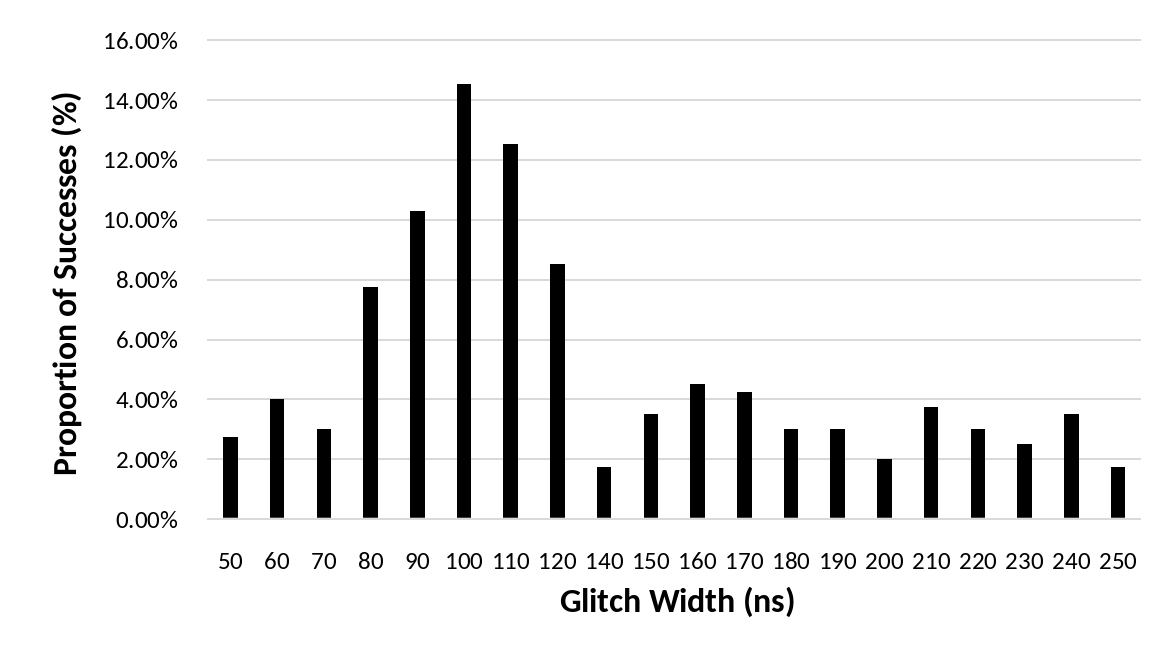
\includegraphics[width=4.16667in,height=\textheight]{res/nrf52832_width_vs_success.png}
\caption{Glitch width vs.~proportion of successes (out of 399 successes)
for the nRF52832.\label{img_nrf52832_width_vs_success}}
\end{figure}

\hypertarget{finding-a-suitable-glitch-offset}{%
\subsubsection{\texorpdfstring{Finding a suitable glitch
offset\label{section_nrf52832_suitable_offset}}{Finding a suitable glitch offset}}\label{finding-a-suitable-glitch-offset}}

The glitch offset for the nRF52832 is the amount of time after supplying
power to its development board until the glitch is applied. In practise,
this makes it the amount of time until immediately before the start of
the critical section to make sure a glitching opportunity isn't missed
and to compensate for any jitter (the critical section occurring earlier
or later on the next power cycle).

Because this experiment was carried out to replicate work by Limited
Results @limitedresultsNRF52DebugResurrection2020 and Roth
@rothHowAppleAirTags2021 and apply a successful glitch, the focus was to
find the same critical sections that they have highlighted in their
work. For example, LimitedResults identified the section of non-volatile
memory controller (NVMC) activity in figure
\ref{img_nrf52832_limitedresults_crit_section}, before the CPU core
voltage drops and execution of the application starts
@limitedresultsNRF52DebugResurrection2020. This NVMC activity, according
to LimitedResults, is likely to contain the transfer of user information
configuration register (UICR) data, including the CRP value APPROTECT,
to the CPU core. A similar section was identified for the nRF52832 and
has been highlighted in figure \ref{img_nrf52832_crit_section_no_zoom},
and is shown, zoomed-in, in figure \ref{img_nrf52832_crit_section_zoom}.
The noise present in figures \ref{img_nrf52832_crit_section_no_zoom} and
\ref{img_nrf52832_crit_section_zoom} is due to the nRF52832 VDD being
connected to the GIAnT DAC, rather than the ST-LINK V2.

\begin{figure}
\centering
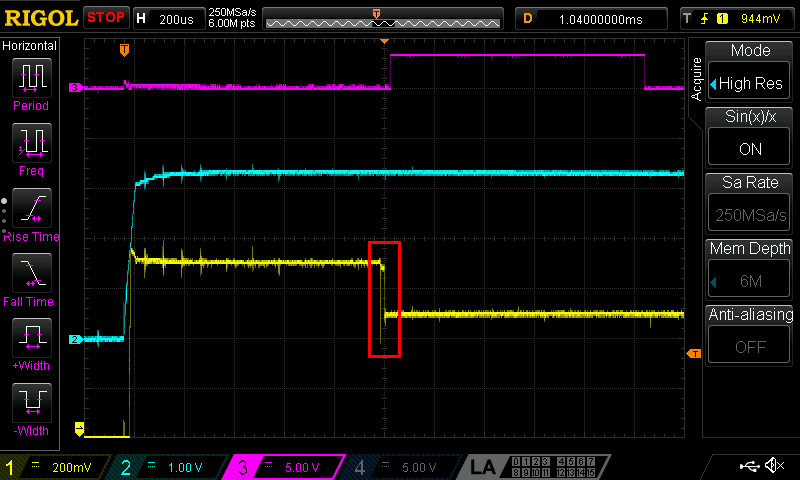
\includegraphics[width=4.16667in,height=\textheight]{res/nrf52832_crit_section_no_zoom_highlight.png}
\caption{Red box highlighting critical section after nRF52832 power-on.
Trace 1 (yellow) is the CPU core voltage, trace 2 (blue) is the voltage
of VDD, trace 3 (purple) is the pin being toggled by the application on
the nRF52832.\label{img_nrf52832_crit_section_no_zoom}}
\end{figure}

\begin{figure}
\centering
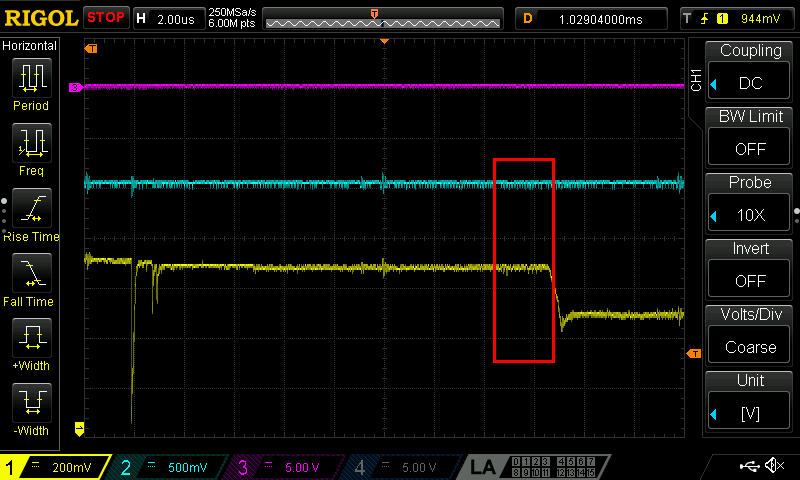
\includegraphics[width=4.16667in,height=\textheight]{res/nrf52832_crit_section_zoom_highlight.png}
\caption{Zoomed-in version of the traces in figure
\ref{img_nrf52832_crit_section_no_zoom}. Critical section (NVMC
activity) highlighted in red box.\label{img_nrf52832_crit_section_zoom}}
\end{figure}

\begin{figure}
\centering
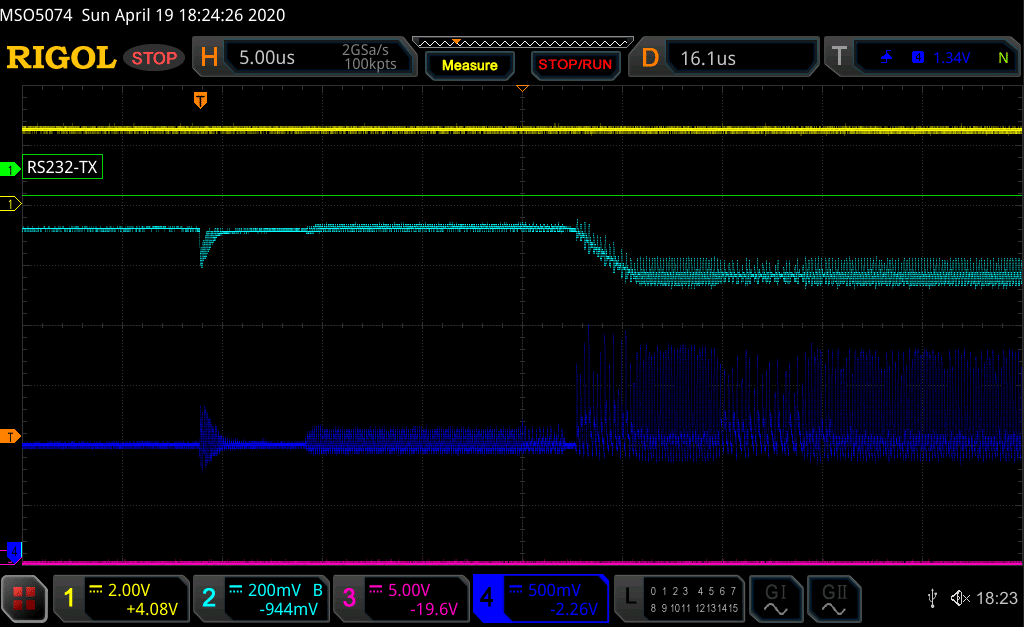
\includegraphics[width=4.16667in,height=\textheight]{res/nrf52832_limitedresults_crit_section.png}
\caption{Screenshot of the nRF52840 critical section, captured by
LimitedResults @limitedresultsNRF52DebugResurrection2020. Trace 2 (light
blue) is the CPU core voltage at DEC1 and trace 4 (dark blue) is the
system power voltage at DEC4. Compare with figure
\ref{img_nrf52832_crit_section_zoom}.\label{img_nrf52832_limitedresults_crit_section}}
\end{figure}

This critical section lasts for about \(2\mu s\), although glitches are
usually successful in the later part of the critical section. To account
for jitter---the changing location of the critical section between power
cycles---the glitch offset can be said to start at \(1029\mu s\) after
supplying power to the nRF52832, and increase by \(1\mu s\) until
\(1044\mu s\). The offsets for 399 successful glitches were recorded and
the proportion of glitch successes for each glitch offset is shown in
figure \ref{img_nrf52832_offset_vs_success}.

\begin{figure}
\centering
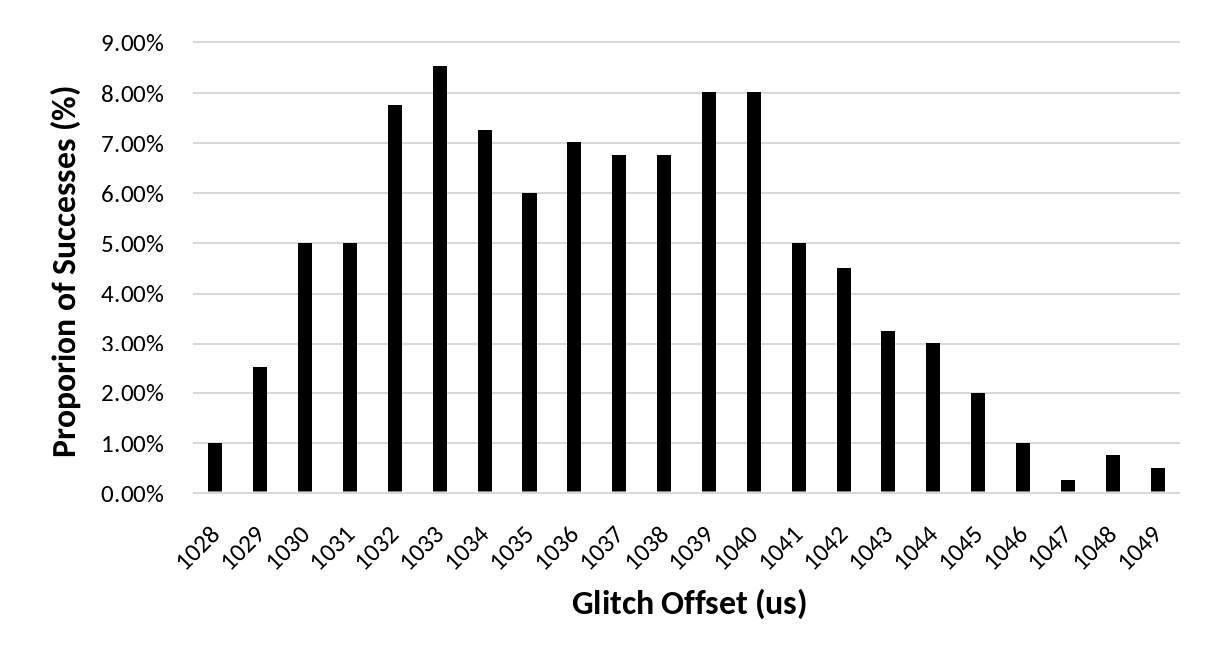
\includegraphics[width=4.16667in,height=\textheight]{res/nrf52832_offset_vs_success.png}
\caption{Glitch offset vs.~proportion of successes (out of 399
successes) for the nRF52832.\label{img_nrf52832_offset_vs_success}}
\end{figure}

\hypertarget{observations}{%
\subsection{\texorpdfstring{Observations\label{section_nrf52832_observations}}{Observations}}\label{observations}}

A script @rudmanNRF52832FullGIAnT was written to control the GIAnT board
using the parameters discussed in sections
\ref{section_cc2541_suitable_width} and
\ref{section_nrf52832_suitable_offset}. The finalised code for this
script iterates over an offset range of \(1027\mu s - 1100\mu s\) at an
interval of \(1\mu s\) and over a width range of \(50ns - 200ns\) at an
interval of \(10ns\). The reason for the large offset range is that over
the course of a few months, the critical section has been at varying
offsets; successful glitches months apart have occurred at offsets of
\(1029\mu s - 1045\mu s\), \(1057\mu s\) during project demonstration
week and \(1071\mu s\) in December.

Using the aforementioned script, a successful glitch was achieved and an
example is shown in figure \ref{img_nrf52832_successful}. Compare this
to figure \ref{img_nrf52832_crit_section_zoom}; notice how the CPU core
voltage does not drop after the glitch. LimitedResults calls the CRP
check a ``pure hardware process'' due to the absence of boot ROM
@limitedresultsNRF52DebugResurrection2020, but the successful glitch
seems to also bypass the whole section of slightly dropped voltage
before the voltage drops more steeply for application execution. There
is no mention of boot ROM---where code will be retrieved from and
executed by the CPU---in the user guide but the lack of a voltage drop
after the successful glitch looks more like a branch, and thus a section
of code, has been skipped. Much of this can only be speculation, without
details provided by the manufacturer.

If some of the Pico Debug'n'Dump shipments had not had the resistor
specification issue mentioned in section
\ref{section_nrf52832_debugndump}, a successful crowbar voltage glitch
would have been much more quickly and cheaply attained. On the other
hand, focusing on using GIAnT allowed the development and testing of
dormant crowbar glitch capabilities, which proved equally useful in
replicating glitch attacks on nRF52 MCUs by LimitedResults
@limitedresultsNRF52DebugResurrection2020 and Roth
@rothHowAppleAirTags2021.

\begin{figure}
\centering
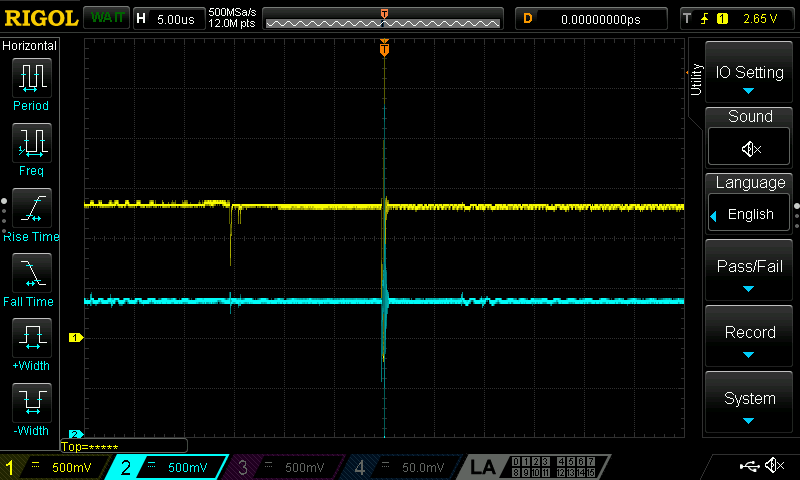
\includegraphics[width=4.16667in,height=\textheight]{res/nrf52832_successful.png}
\caption{A successful glitch on the nRF52832. Trace 1 (yellow) is the
CPU core voltage through DEC1 and trace 2 (blue) is the system voltage.
\label{img_nrf52832_successful}}
\end{figure}

\hypertarget{cc2541-glitch-attempts}{%
\section{CC2541 glitch attempts}\label{cc2541-glitch-attempts}}

The CC2541 microcontroller sits within Texas Instruments' CC253x/4x
line-up of SoCs, which are all based on a modified 8051 microcontroller,
differing from the nRF52832 which uses an ARM Cortex-M4. The main
difference between the CC253x and CC254x series is that CC253x SoCs are
intended for applications which implement IEEE 802.15.4-based protocols
and the CC254x series is intended for bluetooth low-energy applications.
As previously stated, the CC2541 is based around a different processor
than the nRF52832, but the two chips are similar in that they don't
contain boot ROM; there's no read-only bootloader by default on either
of the devices. This means that, for a crowbar glitch applied to the CPU
to be successful, there needs to be some handling of the CRP data by the
CPU.

There were three lessons learned during the nRF52832 glitch attempts,
which informed the exploratory glitch campaign on the CC2541:

\begin{itemize}
\tightlist
\item
  When looking for a suitable glitch offset, use an oscilloscope from
  the beginning; study the power traces for notable features when using
  the SoC for various activities, especially immediately after reset and
  power-on. This is known generally as simple power analysis (SPA).
\item
  Read the data sheet and user guide more thoroughly before attempting a
  voltage glitch, especially for information about bootloaders, which
  have logic commonly executed by the CPU and as a result can be
  glitched using the crowbar technique on the CPU decoupling circuit.
\item
  Use the debugging interface to get used to reading the flash contents
  from the target and define a benchmark against which to check whether
  CRP is still enabled.
\end{itemize}

These learning outcomes encouraged a deeper analysis of how the SoC or
microcontroller functions \emph{before} leaving the glitch generator
running to brute-force search the glitch parameter space.

\hypertarget{modifications-1}{%
\subsection{Modifications}\label{modifications-1}}

The CC2541 is similar to the nRF52832 in that it also has a digital
supply decoupling pin, DCOUPL, for use with a decoupling capacitor.
Decoupling capacitors are intended to smooth out any sudden changes in
voltage, so it's important that the decoupling capacitors are removed in
order to see useful voltage traces when using an oscilloscope, and
because they might prevent a successful voltage glitch. See figure
\ref{img_cc2541_cap_comparison} for a comparison of DCOUPL traces before
and after removing the decoupling capacitor. Initially the removal of
the capacitor connected to DCOUPL was neglected and the voltage trace on
DCOUPL looked very featureless; voltage trace readings were repeated
after removing it.

For easy connection to jumper wires and oscilloscope probes, wires were
connected to the following areas on the CC2541 development board:

\begin{itemize}
\tightlist
\item
  VDD: Power supply---there was already a header pin for this
\item
  GND: Ground---there was already a header pin for this
\item
  DD: Debug data pin, for debugging
\item
  DC: Debug clock pin, for debugging
\item
  RESET\_N: Reset pin, for debugging
\item
  DCOUPL: \(1.8V\) digital supply decoupling circuit
\end{itemize}

For all pins other than VDD and GND, a solder pad on the development
board was used to reduce mechanical strain on the chip legs, requiring
continuity testing between legs and pads. DCOUPL was only one decoupling
circuit listed in the data sheet, so it was assumed that if a successful
crowbar voltage glitch would be possible, it would be on DCOUPL due to
the lack of alternatives.

\begin{figure}
  \begin{center}
      %% Creator: Matplotlib, PGF backend
%%
%% To include the figure in your LaTeX document, write
%%   \input{<filename>.pgf}
%%
%% Make sure the required packages are loaded in your preamble
%%   \usepackage{pgf}
%%
%% Figures using additional raster images can only be included by \input if
%% they are in the same directory as the main LaTeX file. For loading figures
%% from other directories you can use the `import` package
%%   \usepackage{import}
%%
%% and then include the figures with
%%   \import{<path to file>}{<filename>.pgf}
%%
%% Matplotlib used the following preamble
%%
\begingroup%
\makeatletter%
\begin{pgfpicture}%
\pgfpathrectangle{\pgfpointorigin}{\pgfqpoint{6.400000in}{4.800000in}}%
\pgfusepath{use as bounding box, clip}%
\begin{pgfscope}%
\pgfsetbuttcap%
\pgfsetmiterjoin%
\definecolor{currentfill}{rgb}{1.000000,1.000000,1.000000}%
\pgfsetfillcolor{currentfill}%
\pgfsetlinewidth{0.000000pt}%
\definecolor{currentstroke}{rgb}{1.000000,1.000000,1.000000}%
\pgfsetstrokecolor{currentstroke}%
\pgfsetdash{}{0pt}%
\pgfpathmoveto{\pgfqpoint{0.000000in}{0.000000in}}%
\pgfpathlineto{\pgfqpoint{6.400000in}{0.000000in}}%
\pgfpathlineto{\pgfqpoint{6.400000in}{4.800000in}}%
\pgfpathlineto{\pgfqpoint{0.000000in}{4.800000in}}%
\pgfpathclose%
\pgfusepath{fill}%
\end{pgfscope}%
\begin{pgfscope}%
\pgfsetbuttcap%
\pgfsetmiterjoin%
\definecolor{currentfill}{rgb}{1.000000,1.000000,1.000000}%
\pgfsetfillcolor{currentfill}%
\pgfsetlinewidth{0.000000pt}%
\definecolor{currentstroke}{rgb}{0.000000,0.000000,0.000000}%
\pgfsetstrokecolor{currentstroke}%
\pgfsetstrokeopacity{0.000000}%
\pgfsetdash{}{0pt}%
\pgfpathmoveto{\pgfqpoint{0.800000in}{0.528000in}}%
\pgfpathlineto{\pgfqpoint{5.760000in}{0.528000in}}%
\pgfpathlineto{\pgfqpoint{5.760000in}{4.224000in}}%
\pgfpathlineto{\pgfqpoint{0.800000in}{4.224000in}}%
\pgfpathclose%
\pgfusepath{fill}%
\end{pgfscope}%
\begin{pgfscope}%
\pgfsetbuttcap%
\pgfsetroundjoin%
\definecolor{currentfill}{rgb}{0.000000,0.000000,0.000000}%
\pgfsetfillcolor{currentfill}%
\pgfsetlinewidth{0.803000pt}%
\definecolor{currentstroke}{rgb}{0.000000,0.000000,0.000000}%
\pgfsetstrokecolor{currentstroke}%
\pgfsetdash{}{0pt}%
\pgfsys@defobject{currentmarker}{\pgfqpoint{0.000000in}{-0.048611in}}{\pgfqpoint{0.000000in}{0.000000in}}{%
\pgfpathmoveto{\pgfqpoint{0.000000in}{0.000000in}}%
\pgfpathlineto{\pgfqpoint{0.000000in}{-0.048611in}}%
\pgfusepath{stroke,fill}%
}%
\begin{pgfscope}%
\pgfsys@transformshift{1.025455in}{0.528000in}%
\pgfsys@useobject{currentmarker}{}%
\end{pgfscope}%
\end{pgfscope}%
\begin{pgfscope}%
\definecolor{textcolor}{rgb}{0.000000,0.000000,0.000000}%
\pgfsetstrokecolor{textcolor}%
\pgfsetfillcolor{textcolor}%
\pgftext[x=1.025455in,y=0.430778in,,top]{\color{textcolor}\rmfamily\fontsize{10.000000}{12.000000}\selectfont \(\displaystyle {0.00}\)}%
\end{pgfscope}%
\begin{pgfscope}%
\pgfsetbuttcap%
\pgfsetroundjoin%
\definecolor{currentfill}{rgb}{0.000000,0.000000,0.000000}%
\pgfsetfillcolor{currentfill}%
\pgfsetlinewidth{0.803000pt}%
\definecolor{currentstroke}{rgb}{0.000000,0.000000,0.000000}%
\pgfsetstrokecolor{currentstroke}%
\pgfsetdash{}{0pt}%
\pgfsys@defobject{currentmarker}{\pgfqpoint{0.000000in}{-0.048611in}}{\pgfqpoint{0.000000in}{0.000000in}}{%
\pgfpathmoveto{\pgfqpoint{0.000000in}{0.000000in}}%
\pgfpathlineto{\pgfqpoint{0.000000in}{-0.048611in}}%
\pgfusepath{stroke,fill}%
}%
\begin{pgfscope}%
\pgfsys@transformshift{1.927309in}{0.528000in}%
\pgfsys@useobject{currentmarker}{}%
\end{pgfscope}%
\end{pgfscope}%
\begin{pgfscope}%
\definecolor{textcolor}{rgb}{0.000000,0.000000,0.000000}%
\pgfsetstrokecolor{textcolor}%
\pgfsetfillcolor{textcolor}%
\pgftext[x=1.927309in,y=0.430778in,,top]{\color{textcolor}\rmfamily\fontsize{10.000000}{12.000000}\selectfont \(\displaystyle {0.02}\)}%
\end{pgfscope}%
\begin{pgfscope}%
\pgfsetbuttcap%
\pgfsetroundjoin%
\definecolor{currentfill}{rgb}{0.000000,0.000000,0.000000}%
\pgfsetfillcolor{currentfill}%
\pgfsetlinewidth{0.803000pt}%
\definecolor{currentstroke}{rgb}{0.000000,0.000000,0.000000}%
\pgfsetstrokecolor{currentstroke}%
\pgfsetdash{}{0pt}%
\pgfsys@defobject{currentmarker}{\pgfqpoint{0.000000in}{-0.048611in}}{\pgfqpoint{0.000000in}{0.000000in}}{%
\pgfpathmoveto{\pgfqpoint{0.000000in}{0.000000in}}%
\pgfpathlineto{\pgfqpoint{0.000000in}{-0.048611in}}%
\pgfusepath{stroke,fill}%
}%
\begin{pgfscope}%
\pgfsys@transformshift{2.829163in}{0.528000in}%
\pgfsys@useobject{currentmarker}{}%
\end{pgfscope}%
\end{pgfscope}%
\begin{pgfscope}%
\definecolor{textcolor}{rgb}{0.000000,0.000000,0.000000}%
\pgfsetstrokecolor{textcolor}%
\pgfsetfillcolor{textcolor}%
\pgftext[x=2.829163in,y=0.430778in,,top]{\color{textcolor}\rmfamily\fontsize{10.000000}{12.000000}\selectfont \(\displaystyle {0.04}\)}%
\end{pgfscope}%
\begin{pgfscope}%
\pgfsetbuttcap%
\pgfsetroundjoin%
\definecolor{currentfill}{rgb}{0.000000,0.000000,0.000000}%
\pgfsetfillcolor{currentfill}%
\pgfsetlinewidth{0.803000pt}%
\definecolor{currentstroke}{rgb}{0.000000,0.000000,0.000000}%
\pgfsetstrokecolor{currentstroke}%
\pgfsetdash{}{0pt}%
\pgfsys@defobject{currentmarker}{\pgfqpoint{0.000000in}{-0.048611in}}{\pgfqpoint{0.000000in}{0.000000in}}{%
\pgfpathmoveto{\pgfqpoint{0.000000in}{0.000000in}}%
\pgfpathlineto{\pgfqpoint{0.000000in}{-0.048611in}}%
\pgfusepath{stroke,fill}%
}%
\begin{pgfscope}%
\pgfsys@transformshift{3.731017in}{0.528000in}%
\pgfsys@useobject{currentmarker}{}%
\end{pgfscope}%
\end{pgfscope}%
\begin{pgfscope}%
\definecolor{textcolor}{rgb}{0.000000,0.000000,0.000000}%
\pgfsetstrokecolor{textcolor}%
\pgfsetfillcolor{textcolor}%
\pgftext[x=3.731017in,y=0.430778in,,top]{\color{textcolor}\rmfamily\fontsize{10.000000}{12.000000}\selectfont \(\displaystyle {0.06}\)}%
\end{pgfscope}%
\begin{pgfscope}%
\pgfsetbuttcap%
\pgfsetroundjoin%
\definecolor{currentfill}{rgb}{0.000000,0.000000,0.000000}%
\pgfsetfillcolor{currentfill}%
\pgfsetlinewidth{0.803000pt}%
\definecolor{currentstroke}{rgb}{0.000000,0.000000,0.000000}%
\pgfsetstrokecolor{currentstroke}%
\pgfsetdash{}{0pt}%
\pgfsys@defobject{currentmarker}{\pgfqpoint{0.000000in}{-0.048611in}}{\pgfqpoint{0.000000in}{0.000000in}}{%
\pgfpathmoveto{\pgfqpoint{0.000000in}{0.000000in}}%
\pgfpathlineto{\pgfqpoint{0.000000in}{-0.048611in}}%
\pgfusepath{stroke,fill}%
}%
\begin{pgfscope}%
\pgfsys@transformshift{4.632872in}{0.528000in}%
\pgfsys@useobject{currentmarker}{}%
\end{pgfscope}%
\end{pgfscope}%
\begin{pgfscope}%
\definecolor{textcolor}{rgb}{0.000000,0.000000,0.000000}%
\pgfsetstrokecolor{textcolor}%
\pgfsetfillcolor{textcolor}%
\pgftext[x=4.632872in,y=0.430778in,,top]{\color{textcolor}\rmfamily\fontsize{10.000000}{12.000000}\selectfont \(\displaystyle {0.08}\)}%
\end{pgfscope}%
\begin{pgfscope}%
\pgfsetbuttcap%
\pgfsetroundjoin%
\definecolor{currentfill}{rgb}{0.000000,0.000000,0.000000}%
\pgfsetfillcolor{currentfill}%
\pgfsetlinewidth{0.803000pt}%
\definecolor{currentstroke}{rgb}{0.000000,0.000000,0.000000}%
\pgfsetstrokecolor{currentstroke}%
\pgfsetdash{}{0pt}%
\pgfsys@defobject{currentmarker}{\pgfqpoint{0.000000in}{-0.048611in}}{\pgfqpoint{0.000000in}{0.000000in}}{%
\pgfpathmoveto{\pgfqpoint{0.000000in}{0.000000in}}%
\pgfpathlineto{\pgfqpoint{0.000000in}{-0.048611in}}%
\pgfusepath{stroke,fill}%
}%
\begin{pgfscope}%
\pgfsys@transformshift{5.534726in}{0.528000in}%
\pgfsys@useobject{currentmarker}{}%
\end{pgfscope}%
\end{pgfscope}%
\begin{pgfscope}%
\definecolor{textcolor}{rgb}{0.000000,0.000000,0.000000}%
\pgfsetstrokecolor{textcolor}%
\pgfsetfillcolor{textcolor}%
\pgftext[x=5.534726in,y=0.430778in,,top]{\color{textcolor}\rmfamily\fontsize{10.000000}{12.000000}\selectfont \(\displaystyle {0.10}\)}%
\end{pgfscope}%
\begin{pgfscope}%
\definecolor{textcolor}{rgb}{0.000000,0.000000,0.000000}%
\pgfsetstrokecolor{textcolor}%
\pgfsetfillcolor{textcolor}%
\pgftext[x=3.280000in,y=0.251766in,,top]{\color{textcolor}\rmfamily\fontsize{10.000000}{12.000000}\selectfont Time (ms)}%
\end{pgfscope}%
\begin{pgfscope}%
\pgfpathrectangle{\pgfqpoint{0.800000in}{0.528000in}}{\pgfqpoint{4.960000in}{3.696000in}}%
\pgfusepath{clip}%
\pgfsetrectcap%
\pgfsetroundjoin%
\pgfsetlinewidth{1.505625pt}%
\definecolor{currentstroke}{rgb}{0.121569,0.466667,0.705882}%
\pgfsetstrokecolor{currentstroke}%
\pgfsetdash{}{0pt}%
\pgfpathmoveto{\pgfqpoint{1.025455in}{3.535437in}}%
\pgfpathlineto{\pgfqpoint{1.025635in}{3.535437in}}%
\pgfpathlineto{\pgfqpoint{1.026717in}{3.630085in}}%
\pgfpathlineto{\pgfqpoint{1.026898in}{3.582761in}}%
\pgfpathlineto{\pgfqpoint{1.027258in}{3.582761in}}%
\pgfpathlineto{\pgfqpoint{1.028160in}{3.630085in}}%
\pgfpathlineto{\pgfqpoint{1.028340in}{3.582761in}}%
\pgfpathlineto{\pgfqpoint{1.028521in}{3.535437in}}%
\pgfpathlineto{\pgfqpoint{1.029423in}{3.582761in}}%
\pgfpathlineto{\pgfqpoint{1.029783in}{3.582761in}}%
\pgfpathlineto{\pgfqpoint{1.030144in}{3.440789in}}%
\pgfpathlineto{\pgfqpoint{1.031046in}{3.488113in}}%
\pgfpathlineto{\pgfqpoint{1.031226in}{3.535437in}}%
\pgfpathlineto{\pgfqpoint{1.031587in}{3.393465in}}%
\pgfpathlineto{\pgfqpoint{1.032128in}{3.488113in}}%
\pgfpathlineto{\pgfqpoint{1.033210in}{3.298817in}}%
\pgfpathlineto{\pgfqpoint{1.033571in}{3.393465in}}%
\pgfpathlineto{\pgfqpoint{1.033752in}{3.393465in}}%
\pgfpathlineto{\pgfqpoint{1.034653in}{3.251493in}}%
\pgfpathlineto{\pgfqpoint{1.035014in}{3.298817in}}%
\pgfpathlineto{\pgfqpoint{1.035195in}{3.346141in}}%
\pgfpathlineto{\pgfqpoint{1.035916in}{3.298817in}}%
\pgfpathlineto{\pgfqpoint{1.037179in}{3.204169in}}%
\pgfpathlineto{\pgfqpoint{1.037359in}{3.251493in}}%
\pgfpathlineto{\pgfqpoint{1.037720in}{3.156845in}}%
\pgfpathlineto{\pgfqpoint{1.038261in}{3.204169in}}%
\pgfpathlineto{\pgfqpoint{1.038441in}{3.204169in}}%
\pgfpathlineto{\pgfqpoint{1.039343in}{3.062197in}}%
\pgfpathlineto{\pgfqpoint{1.039704in}{3.156845in}}%
\pgfpathlineto{\pgfqpoint{1.039884in}{3.156845in}}%
\pgfpathlineto{\pgfqpoint{1.040786in}{3.014873in}}%
\pgfpathlineto{\pgfqpoint{1.041147in}{3.062197in}}%
\pgfpathlineto{\pgfqpoint{1.041327in}{3.109521in}}%
\pgfpathlineto{\pgfqpoint{1.041688in}{3.014873in}}%
\pgfpathlineto{\pgfqpoint{1.042049in}{3.062197in}}%
\pgfpathlineto{\pgfqpoint{1.043311in}{2.967549in}}%
\pgfpathlineto{\pgfqpoint{1.043492in}{3.014873in}}%
\pgfpathlineto{\pgfqpoint{1.043672in}{2.920225in}}%
\pgfpathlineto{\pgfqpoint{1.044393in}{2.967549in}}%
\pgfpathlineto{\pgfqpoint{1.045295in}{2.825577in}}%
\pgfpathlineto{\pgfqpoint{1.045656in}{2.872901in}}%
\pgfpathlineto{\pgfqpoint{1.046558in}{2.920225in}}%
\pgfpathlineto{\pgfqpoint{1.046919in}{2.778254in}}%
\pgfpathlineto{\pgfqpoint{1.047821in}{2.825577in}}%
\pgfpathlineto{\pgfqpoint{1.048001in}{2.825577in}}%
\pgfpathlineto{\pgfqpoint{1.049263in}{2.730930in}}%
\pgfpathlineto{\pgfqpoint{1.049624in}{2.778254in}}%
\pgfpathlineto{\pgfqpoint{1.049985in}{2.683606in}}%
\pgfpathlineto{\pgfqpoint{1.050346in}{2.730930in}}%
\pgfpathlineto{\pgfqpoint{1.050706in}{2.730930in}}%
\pgfpathlineto{\pgfqpoint{1.051608in}{2.636282in}}%
\pgfpathlineto{\pgfqpoint{1.051969in}{2.683606in}}%
\pgfpathlineto{\pgfqpoint{1.052149in}{2.683606in}}%
\pgfpathlineto{\pgfqpoint{1.053051in}{2.588958in}}%
\pgfpathlineto{\pgfqpoint{1.053412in}{2.636282in}}%
\pgfpathlineto{\pgfqpoint{1.053592in}{2.636282in}}%
\pgfpathlineto{\pgfqpoint{1.054675in}{2.541634in}}%
\pgfpathlineto{\pgfqpoint{1.054855in}{2.588958in}}%
\pgfpathlineto{\pgfqpoint{1.055216in}{2.588958in}}%
\pgfpathlineto{\pgfqpoint{1.056118in}{2.494310in}}%
\pgfpathlineto{\pgfqpoint{1.056478in}{2.541634in}}%
\pgfpathlineto{\pgfqpoint{1.056659in}{2.541634in}}%
\pgfpathlineto{\pgfqpoint{1.057561in}{2.399662in}}%
\pgfpathlineto{\pgfqpoint{1.057921in}{2.494310in}}%
\pgfpathlineto{\pgfqpoint{1.058102in}{2.494310in}}%
\pgfpathlineto{\pgfqpoint{1.059184in}{2.399662in}}%
\pgfpathlineto{\pgfqpoint{1.059364in}{2.446986in}}%
\pgfpathlineto{\pgfqpoint{1.059725in}{2.446986in}}%
\pgfpathlineto{\pgfqpoint{1.060807in}{2.352338in}}%
\pgfpathlineto{\pgfqpoint{1.060988in}{2.399662in}}%
\pgfpathlineto{\pgfqpoint{1.061168in}{2.399662in}}%
\pgfpathlineto{\pgfqpoint{1.062250in}{2.305014in}}%
\pgfpathlineto{\pgfqpoint{1.062431in}{2.352338in}}%
\pgfpathlineto{\pgfqpoint{1.062791in}{2.352338in}}%
\pgfpathlineto{\pgfqpoint{1.063874in}{2.257690in}}%
\pgfpathlineto{\pgfqpoint{1.064054in}{2.305014in}}%
\pgfpathlineto{\pgfqpoint{1.064234in}{2.305014in}}%
\pgfpathlineto{\pgfqpoint{1.065317in}{2.210366in}}%
\pgfpathlineto{\pgfqpoint{1.065497in}{2.257690in}}%
\pgfpathlineto{\pgfqpoint{1.065858in}{2.257690in}}%
\pgfpathlineto{\pgfqpoint{1.066759in}{2.163042in}}%
\pgfpathlineto{\pgfqpoint{1.067120in}{2.210366in}}%
\pgfpathlineto{\pgfqpoint{1.067842in}{2.210366in}}%
\pgfpathlineto{\pgfqpoint{1.068202in}{2.115718in}}%
\pgfpathlineto{\pgfqpoint{1.069104in}{2.163042in}}%
\pgfpathlineto{\pgfqpoint{1.069465in}{2.163042in}}%
\pgfpathlineto{\pgfqpoint{1.070728in}{2.115718in}}%
\pgfpathlineto{\pgfqpoint{1.070908in}{2.163042in}}%
\pgfpathlineto{\pgfqpoint{1.071269in}{2.068394in}}%
\pgfpathlineto{\pgfqpoint{1.071810in}{2.115718in}}%
\pgfpathlineto{\pgfqpoint{1.072531in}{2.115718in}}%
\pgfpathlineto{\pgfqpoint{1.073614in}{2.068394in}}%
\pgfpathlineto{\pgfqpoint{1.074335in}{2.021070in}}%
\pgfpathlineto{\pgfqpoint{1.074876in}{2.115718in}}%
\pgfpathlineto{\pgfqpoint{1.075057in}{2.115718in}}%
\pgfpathlineto{\pgfqpoint{1.075778in}{2.021070in}}%
\pgfpathlineto{\pgfqpoint{1.076139in}{2.068394in}}%
\pgfpathlineto{\pgfqpoint{1.077041in}{2.115718in}}%
\pgfpathlineto{\pgfqpoint{1.077221in}{2.068394in}}%
\pgfpathlineto{\pgfqpoint{1.077582in}{2.068394in}}%
\pgfpathlineto{\pgfqpoint{1.078484in}{2.163042in}}%
\pgfpathlineto{\pgfqpoint{1.078664in}{2.115718in}}%
\pgfpathlineto{\pgfqpoint{1.078844in}{2.068394in}}%
\pgfpathlineto{\pgfqpoint{1.079385in}{2.163042in}}%
\pgfpathlineto{\pgfqpoint{1.079566in}{2.163042in}}%
\pgfpathlineto{\pgfqpoint{1.080468in}{2.163042in}}%
\pgfpathlineto{\pgfqpoint{1.081550in}{2.257690in}}%
\pgfpathlineto{\pgfqpoint{1.081730in}{2.210366in}}%
\pgfpathlineto{\pgfqpoint{1.082091in}{2.210366in}}%
\pgfpathlineto{\pgfqpoint{1.083895in}{2.399662in}}%
\pgfpathlineto{\pgfqpoint{1.084255in}{2.399662in}}%
\pgfpathlineto{\pgfqpoint{1.086240in}{2.636282in}}%
\pgfpathlineto{\pgfqpoint{1.086600in}{2.588958in}}%
\pgfpathlineto{\pgfqpoint{1.086961in}{2.730930in}}%
\pgfpathlineto{\pgfqpoint{1.087322in}{2.730930in}}%
\pgfpathlineto{\pgfqpoint{1.089125in}{3.014873in}}%
\pgfpathlineto{\pgfqpoint{1.089306in}{2.967549in}}%
\pgfpathlineto{\pgfqpoint{1.089486in}{2.967549in}}%
\pgfpathlineto{\pgfqpoint{1.092192in}{3.440789in}}%
\pgfpathlineto{\pgfqpoint{1.092553in}{3.393465in}}%
\pgfpathlineto{\pgfqpoint{1.092913in}{3.488113in}}%
\pgfpathlineto{\pgfqpoint{1.094356in}{3.582761in}}%
\pgfpathlineto{\pgfqpoint{1.095078in}{3.582761in}}%
\pgfpathlineto{\pgfqpoint{1.096160in}{3.630085in}}%
\pgfpathlineto{\pgfqpoint{1.097242in}{3.535437in}}%
\pgfpathlineto{\pgfqpoint{1.097423in}{3.582761in}}%
\pgfpathlineto{\pgfqpoint{1.097783in}{3.582761in}}%
\pgfpathlineto{\pgfqpoint{1.098865in}{3.488113in}}%
\pgfpathlineto{\pgfqpoint{1.099046in}{3.535437in}}%
\pgfpathlineto{\pgfqpoint{1.099226in}{3.535437in}}%
\pgfpathlineto{\pgfqpoint{1.100308in}{3.393465in}}%
\pgfpathlineto{\pgfqpoint{1.100669in}{3.440789in}}%
\pgfpathlineto{\pgfqpoint{1.100850in}{3.440789in}}%
\pgfpathlineto{\pgfqpoint{1.101932in}{3.346141in}}%
\pgfpathlineto{\pgfqpoint{1.102112in}{3.393465in}}%
\pgfpathlineto{\pgfqpoint{1.102293in}{3.393465in}}%
\pgfpathlineto{\pgfqpoint{1.103194in}{3.251493in}}%
\pgfpathlineto{\pgfqpoint{1.103555in}{3.298817in}}%
\pgfpathlineto{\pgfqpoint{1.103735in}{3.346141in}}%
\pgfpathlineto{\pgfqpoint{1.104457in}{3.298817in}}%
\pgfpathlineto{\pgfqpoint{1.105720in}{3.204169in}}%
\pgfpathlineto{\pgfqpoint{1.105900in}{3.251493in}}%
\pgfpathlineto{\pgfqpoint{1.106261in}{3.109521in}}%
\pgfpathlineto{\pgfqpoint{1.106802in}{3.204169in}}%
\pgfpathlineto{\pgfqpoint{1.106982in}{3.204169in}}%
\pgfpathlineto{\pgfqpoint{1.108064in}{3.109521in}}%
\pgfpathlineto{\pgfqpoint{1.108245in}{3.156845in}}%
\pgfpathlineto{\pgfqpoint{1.108425in}{3.156845in}}%
\pgfpathlineto{\pgfqpoint{1.109327in}{3.014873in}}%
\pgfpathlineto{\pgfqpoint{1.109688in}{3.062197in}}%
\pgfpathlineto{\pgfqpoint{1.109868in}{3.109521in}}%
\pgfpathlineto{\pgfqpoint{1.110229in}{3.014873in}}%
\pgfpathlineto{\pgfqpoint{1.110590in}{3.062197in}}%
\pgfpathlineto{\pgfqpoint{1.111672in}{2.967549in}}%
\pgfpathlineto{\pgfqpoint{1.112033in}{3.014873in}}%
\pgfpathlineto{\pgfqpoint{1.112213in}{2.920225in}}%
\pgfpathlineto{\pgfqpoint{1.112754in}{2.967549in}}%
\pgfpathlineto{\pgfqpoint{1.112934in}{2.967549in}}%
\pgfpathlineto{\pgfqpoint{1.114197in}{2.872901in}}%
\pgfpathlineto{\pgfqpoint{1.114558in}{2.920225in}}%
\pgfpathlineto{\pgfqpoint{1.115099in}{2.872901in}}%
\pgfpathlineto{\pgfqpoint{1.115460in}{2.778254in}}%
\pgfpathlineto{\pgfqpoint{1.116361in}{2.825577in}}%
\pgfpathlineto{\pgfqpoint{1.116722in}{2.825577in}}%
\pgfpathlineto{\pgfqpoint{1.116903in}{2.730930in}}%
\pgfpathlineto{\pgfqpoint{1.117804in}{2.778254in}}%
\pgfpathlineto{\pgfqpoint{1.118165in}{2.778254in}}%
\pgfpathlineto{\pgfqpoint{1.119428in}{2.683606in}}%
\pgfpathlineto{\pgfqpoint{1.119608in}{2.730930in}}%
\pgfpathlineto{\pgfqpoint{1.119969in}{2.636282in}}%
\pgfpathlineto{\pgfqpoint{1.120510in}{2.683606in}}%
\pgfpathlineto{\pgfqpoint{1.120690in}{2.683606in}}%
\pgfpathlineto{\pgfqpoint{1.121592in}{2.588958in}}%
\pgfpathlineto{\pgfqpoint{1.121953in}{2.636282in}}%
\pgfpathlineto{\pgfqpoint{1.122133in}{2.636282in}}%
\pgfpathlineto{\pgfqpoint{1.123216in}{2.541634in}}%
\pgfpathlineto{\pgfqpoint{1.123396in}{2.588958in}}%
\pgfpathlineto{\pgfqpoint{1.123757in}{2.588958in}}%
\pgfpathlineto{\pgfqpoint{1.124839in}{2.494310in}}%
\pgfpathlineto{\pgfqpoint{1.125019in}{2.541634in}}%
\pgfpathlineto{\pgfqpoint{1.125200in}{2.541634in}}%
\pgfpathlineto{\pgfqpoint{1.126282in}{2.446986in}}%
\pgfpathlineto{\pgfqpoint{1.126462in}{2.494310in}}%
\pgfpathlineto{\pgfqpoint{1.126823in}{2.494310in}}%
\pgfpathlineto{\pgfqpoint{1.127905in}{2.399662in}}%
\pgfpathlineto{\pgfqpoint{1.128086in}{2.446986in}}%
\pgfpathlineto{\pgfqpoint{1.128266in}{2.446986in}}%
\pgfpathlineto{\pgfqpoint{1.129348in}{2.352338in}}%
\pgfpathlineto{\pgfqpoint{1.129529in}{2.399662in}}%
\pgfpathlineto{\pgfqpoint{1.129709in}{2.399662in}}%
\pgfpathlineto{\pgfqpoint{1.130971in}{2.305014in}}%
\pgfpathlineto{\pgfqpoint{1.131873in}{2.352338in}}%
\pgfpathlineto{\pgfqpoint{1.133136in}{2.257690in}}%
\pgfpathlineto{\pgfqpoint{1.133316in}{2.305014in}}%
\pgfpathlineto{\pgfqpoint{1.133677in}{2.210366in}}%
\pgfpathlineto{\pgfqpoint{1.134218in}{2.257690in}}%
\pgfpathlineto{\pgfqpoint{1.134399in}{2.257690in}}%
\pgfpathlineto{\pgfqpoint{1.135300in}{2.163042in}}%
\pgfpathlineto{\pgfqpoint{1.135661in}{2.210366in}}%
\pgfpathlineto{\pgfqpoint{1.136383in}{2.210366in}}%
\pgfpathlineto{\pgfqpoint{1.136743in}{2.115718in}}%
\pgfpathlineto{\pgfqpoint{1.137645in}{2.163042in}}%
\pgfpathlineto{\pgfqpoint{1.138006in}{2.163042in}}%
\pgfpathlineto{\pgfqpoint{1.139269in}{2.115718in}}%
\pgfpathlineto{\pgfqpoint{1.139449in}{2.163042in}}%
\pgfpathlineto{\pgfqpoint{1.139810in}{2.068394in}}%
\pgfpathlineto{\pgfqpoint{1.140351in}{2.115718in}}%
\pgfpathlineto{\pgfqpoint{1.141072in}{2.115718in}}%
\pgfpathlineto{\pgfqpoint{1.142154in}{2.068394in}}%
\pgfpathlineto{\pgfqpoint{1.142876in}{2.021070in}}%
\pgfpathlineto{\pgfqpoint{1.143417in}{2.115718in}}%
\pgfpathlineto{\pgfqpoint{1.144319in}{2.021070in}}%
\pgfpathlineto{\pgfqpoint{1.144680in}{2.068394in}}%
\pgfpathlineto{\pgfqpoint{1.145582in}{2.115718in}}%
\pgfpathlineto{\pgfqpoint{1.145762in}{2.068394in}}%
\pgfpathlineto{\pgfqpoint{1.146123in}{2.068394in}}%
\pgfpathlineto{\pgfqpoint{1.147024in}{2.163042in}}%
\pgfpathlineto{\pgfqpoint{1.147205in}{2.115718in}}%
\pgfpathlineto{\pgfqpoint{1.147385in}{2.068394in}}%
\pgfpathlineto{\pgfqpoint{1.147746in}{2.163042in}}%
\pgfpathlineto{\pgfqpoint{1.148107in}{2.163042in}}%
\pgfpathlineto{\pgfqpoint{1.148648in}{2.163042in}}%
\pgfpathlineto{\pgfqpoint{1.149009in}{2.115718in}}%
\pgfpathlineto{\pgfqpoint{1.149369in}{2.210366in}}%
\pgfpathlineto{\pgfqpoint{1.149550in}{2.210366in}}%
\pgfpathlineto{\pgfqpoint{1.149910in}{2.210366in}}%
\pgfpathlineto{\pgfqpoint{1.151534in}{2.352338in}}%
\pgfpathlineto{\pgfqpoint{1.151714in}{2.352338in}}%
\pgfpathlineto{\pgfqpoint{1.152075in}{2.305014in}}%
\pgfpathlineto{\pgfqpoint{1.152436in}{2.399662in}}%
\pgfpathlineto{\pgfqpoint{1.152616in}{2.399662in}}%
\pgfpathlineto{\pgfqpoint{1.152796in}{2.399662in}}%
\pgfpathlineto{\pgfqpoint{1.154600in}{2.588958in}}%
\pgfpathlineto{\pgfqpoint{1.155141in}{2.588958in}}%
\pgfpathlineto{\pgfqpoint{1.156584in}{2.778254in}}%
\pgfpathlineto{\pgfqpoint{1.159290in}{3.204169in}}%
\pgfpathlineto{\pgfqpoint{1.159470in}{3.156845in}}%
\pgfpathlineto{\pgfqpoint{1.160011in}{3.298817in}}%
\pgfpathlineto{\pgfqpoint{1.161815in}{3.488113in}}%
\pgfpathlineto{\pgfqpoint{1.161995in}{3.488113in}}%
\pgfpathlineto{\pgfqpoint{1.163438in}{3.582761in}}%
\pgfpathlineto{\pgfqpoint{1.163619in}{3.582761in}}%
\pgfpathlineto{\pgfqpoint{1.164160in}{3.535437in}}%
\pgfpathlineto{\pgfqpoint{1.164701in}{3.630085in}}%
\pgfpathlineto{\pgfqpoint{1.165783in}{3.535437in}}%
\pgfpathlineto{\pgfqpoint{1.165963in}{3.582761in}}%
\pgfpathlineto{\pgfqpoint{1.166324in}{3.582761in}}%
\pgfpathlineto{\pgfqpoint{1.167226in}{3.440789in}}%
\pgfpathlineto{\pgfqpoint{1.167587in}{3.535437in}}%
\pgfpathlineto{\pgfqpoint{1.167767in}{3.535437in}}%
\pgfpathlineto{\pgfqpoint{1.168849in}{3.393465in}}%
\pgfpathlineto{\pgfqpoint{1.169210in}{3.440789in}}%
\pgfpathlineto{\pgfqpoint{1.169390in}{3.440789in}}%
\pgfpathlineto{\pgfqpoint{1.170292in}{3.298817in}}%
\pgfpathlineto{\pgfqpoint{1.170653in}{3.393465in}}%
\pgfpathlineto{\pgfqpoint{1.170833in}{3.393465in}}%
\pgfpathlineto{\pgfqpoint{1.171735in}{3.251493in}}%
\pgfpathlineto{\pgfqpoint{1.172096in}{3.298817in}}%
\pgfpathlineto{\pgfqpoint{1.172276in}{3.346141in}}%
\pgfpathlineto{\pgfqpoint{1.172998in}{3.298817in}}%
\pgfpathlineto{\pgfqpoint{1.174260in}{3.204169in}}%
\pgfpathlineto{\pgfqpoint{1.174441in}{3.251493in}}%
\pgfpathlineto{\pgfqpoint{1.174802in}{3.156845in}}%
\pgfpathlineto{\pgfqpoint{1.175343in}{3.204169in}}%
\pgfpathlineto{\pgfqpoint{1.175523in}{3.204169in}}%
\pgfpathlineto{\pgfqpoint{1.176425in}{3.062197in}}%
\pgfpathlineto{\pgfqpoint{1.176966in}{3.109521in}}%
\pgfpathlineto{\pgfqpoint{1.177327in}{3.109521in}}%
\pgfpathlineto{\pgfqpoint{1.177507in}{3.156845in}}%
\pgfpathlineto{\pgfqpoint{1.177868in}{3.014873in}}%
\pgfpathlineto{\pgfqpoint{1.178409in}{3.109521in}}%
\pgfpathlineto{\pgfqpoint{1.179491in}{2.967549in}}%
\pgfpathlineto{\pgfqpoint{1.179852in}{3.014873in}}%
\pgfpathlineto{\pgfqpoint{1.180032in}{3.014873in}}%
\pgfpathlineto{\pgfqpoint{1.181115in}{2.920225in}}%
\pgfpathlineto{\pgfqpoint{1.181295in}{2.967549in}}%
\pgfpathlineto{\pgfqpoint{1.181475in}{2.967549in}}%
\pgfpathlineto{\pgfqpoint{1.182377in}{2.825577in}}%
\pgfpathlineto{\pgfqpoint{1.182738in}{2.872901in}}%
\pgfpathlineto{\pgfqpoint{1.183099in}{2.920225in}}%
\pgfpathlineto{\pgfqpoint{1.183640in}{2.872901in}}%
\pgfpathlineto{\pgfqpoint{1.184001in}{2.778254in}}%
\pgfpathlineto{\pgfqpoint{1.184902in}{2.825577in}}%
\pgfpathlineto{\pgfqpoint{1.185083in}{2.825577in}}%
\pgfpathlineto{\pgfqpoint{1.186345in}{2.730930in}}%
\pgfpathlineto{\pgfqpoint{1.186706in}{2.778254in}}%
\pgfpathlineto{\pgfqpoint{1.187067in}{2.683606in}}%
\pgfpathlineto{\pgfqpoint{1.187428in}{2.730930in}}%
\pgfpathlineto{\pgfqpoint{1.188149in}{2.730930in}}%
\pgfpathlineto{\pgfqpoint{1.189412in}{2.636282in}}%
\pgfpathlineto{\pgfqpoint{1.189772in}{2.683606in}}%
\pgfpathlineto{\pgfqpoint{1.189953in}{2.588958in}}%
\pgfpathlineto{\pgfqpoint{1.190494in}{2.636282in}}%
\pgfpathlineto{\pgfqpoint{1.190674in}{2.636282in}}%
\pgfpathlineto{\pgfqpoint{1.191756in}{2.541634in}}%
\pgfpathlineto{\pgfqpoint{1.191937in}{2.588958in}}%
\pgfpathlineto{\pgfqpoint{1.192117in}{2.588958in}}%
\pgfpathlineto{\pgfqpoint{1.193199in}{2.494310in}}%
\pgfpathlineto{\pgfqpoint{1.193380in}{2.541634in}}%
\pgfpathlineto{\pgfqpoint{1.193741in}{2.541634in}}%
\pgfpathlineto{\pgfqpoint{1.194823in}{2.446986in}}%
\pgfpathlineto{\pgfqpoint{1.195003in}{2.494310in}}%
\pgfpathlineto{\pgfqpoint{1.195184in}{2.494310in}}%
\pgfpathlineto{\pgfqpoint{1.196266in}{2.399662in}}%
\pgfpathlineto{\pgfqpoint{1.196446in}{2.446986in}}%
\pgfpathlineto{\pgfqpoint{1.196807in}{2.446986in}}%
\pgfpathlineto{\pgfqpoint{1.197889in}{2.352338in}}%
\pgfpathlineto{\pgfqpoint{1.198069in}{2.399662in}}%
\pgfpathlineto{\pgfqpoint{1.198250in}{2.399662in}}%
\pgfpathlineto{\pgfqpoint{1.199332in}{2.305014in}}%
\pgfpathlineto{\pgfqpoint{1.199512in}{2.352338in}}%
\pgfpathlineto{\pgfqpoint{1.199873in}{2.352338in}}%
\pgfpathlineto{\pgfqpoint{1.200955in}{2.257690in}}%
\pgfpathlineto{\pgfqpoint{1.201136in}{2.305014in}}%
\pgfpathlineto{\pgfqpoint{1.201316in}{2.305014in}}%
\pgfpathlineto{\pgfqpoint{1.202398in}{2.210366in}}%
\pgfpathlineto{\pgfqpoint{1.202579in}{2.257690in}}%
\pgfpathlineto{\pgfqpoint{1.202939in}{2.257690in}}%
\pgfpathlineto{\pgfqpoint{1.203841in}{2.163042in}}%
\pgfpathlineto{\pgfqpoint{1.204202in}{2.210366in}}%
\pgfpathlineto{\pgfqpoint{1.204382in}{2.210366in}}%
\pgfpathlineto{\pgfqpoint{1.205284in}{2.115718in}}%
\pgfpathlineto{\pgfqpoint{1.205645in}{2.163042in}}%
\pgfpathlineto{\pgfqpoint{1.205825in}{2.210366in}}%
\pgfpathlineto{\pgfqpoint{1.206547in}{2.163042in}}%
\pgfpathlineto{\pgfqpoint{1.207809in}{2.115718in}}%
\pgfpathlineto{\pgfqpoint{1.207990in}{2.163042in}}%
\pgfpathlineto{\pgfqpoint{1.208351in}{2.068394in}}%
\pgfpathlineto{\pgfqpoint{1.208892in}{2.115718in}}%
\pgfpathlineto{\pgfqpoint{1.209613in}{2.115718in}}%
\pgfpathlineto{\pgfqpoint{1.210695in}{2.068394in}}%
\pgfpathlineto{\pgfqpoint{1.211958in}{2.115718in}}%
\pgfpathlineto{\pgfqpoint{1.212860in}{2.021070in}}%
\pgfpathlineto{\pgfqpoint{1.213221in}{2.068394in}}%
\pgfpathlineto{\pgfqpoint{1.214122in}{2.115718in}}%
\pgfpathlineto{\pgfqpoint{1.214303in}{2.068394in}}%
\pgfpathlineto{\pgfqpoint{1.214664in}{2.068394in}}%
\pgfpathlineto{\pgfqpoint{1.215565in}{2.163042in}}%
\pgfpathlineto{\pgfqpoint{1.215746in}{2.115718in}}%
\pgfpathlineto{\pgfqpoint{1.215926in}{2.068394in}}%
\pgfpathlineto{\pgfqpoint{1.216287in}{2.163042in}}%
\pgfpathlineto{\pgfqpoint{1.216828in}{2.115718in}}%
\pgfpathlineto{\pgfqpoint{1.218271in}{2.210366in}}%
\pgfpathlineto{\pgfqpoint{1.218451in}{2.210366in}}%
\pgfpathlineto{\pgfqpoint{1.220075in}{2.352338in}}%
\pgfpathlineto{\pgfqpoint{1.220255in}{2.352338in}}%
\pgfpathlineto{\pgfqpoint{1.220435in}{2.305014in}}%
\pgfpathlineto{\pgfqpoint{1.220977in}{2.399662in}}%
\pgfpathlineto{\pgfqpoint{1.221157in}{2.399662in}}%
\pgfpathlineto{\pgfqpoint{1.221337in}{2.399662in}}%
\pgfpathlineto{\pgfqpoint{1.223141in}{2.636282in}}%
\pgfpathlineto{\pgfqpoint{1.223502in}{2.588958in}}%
\pgfpathlineto{\pgfqpoint{1.223862in}{2.683606in}}%
\pgfpathlineto{\pgfqpoint{1.224043in}{2.683606in}}%
\pgfpathlineto{\pgfqpoint{1.226207in}{3.014873in}}%
\pgfpathlineto{\pgfqpoint{1.226568in}{2.967549in}}%
\pgfpathlineto{\pgfqpoint{1.226929in}{3.062197in}}%
\pgfpathlineto{\pgfqpoint{1.229274in}{3.440789in}}%
\pgfpathlineto{\pgfqpoint{1.229634in}{3.393465in}}%
\pgfpathlineto{\pgfqpoint{1.229995in}{3.488113in}}%
\pgfpathlineto{\pgfqpoint{1.231438in}{3.582761in}}%
\pgfpathlineto{\pgfqpoint{1.232160in}{3.582761in}}%
\pgfpathlineto{\pgfqpoint{1.233242in}{3.630085in}}%
\pgfpathlineto{\pgfqpoint{1.234324in}{3.535437in}}%
\pgfpathlineto{\pgfqpoint{1.234504in}{3.582761in}}%
\pgfpathlineto{\pgfqpoint{1.234865in}{3.582761in}}%
\pgfpathlineto{\pgfqpoint{1.235947in}{3.488113in}}%
\pgfpathlineto{\pgfqpoint{1.236128in}{3.535437in}}%
\pgfpathlineto{\pgfqpoint{1.236308in}{3.535437in}}%
\pgfpathlineto{\pgfqpoint{1.237390in}{3.393465in}}%
\pgfpathlineto{\pgfqpoint{1.237751in}{3.440789in}}%
\pgfpathlineto{\pgfqpoint{1.237931in}{3.440789in}}%
\pgfpathlineto{\pgfqpoint{1.239014in}{3.346141in}}%
\pgfpathlineto{\pgfqpoint{1.239194in}{3.393465in}}%
\pgfpathlineto{\pgfqpoint{1.239374in}{3.393465in}}%
\pgfpathlineto{\pgfqpoint{1.240276in}{3.251493in}}%
\pgfpathlineto{\pgfqpoint{1.240637in}{3.298817in}}%
\pgfpathlineto{\pgfqpoint{1.240817in}{3.346141in}}%
\pgfpathlineto{\pgfqpoint{1.241539in}{3.298817in}}%
\pgfpathlineto{\pgfqpoint{1.242801in}{3.204169in}}%
\pgfpathlineto{\pgfqpoint{1.242982in}{3.251493in}}%
\pgfpathlineto{\pgfqpoint{1.243343in}{3.109521in}}%
\pgfpathlineto{\pgfqpoint{1.243884in}{3.204169in}}%
\pgfpathlineto{\pgfqpoint{1.244064in}{3.204169in}}%
\pgfpathlineto{\pgfqpoint{1.244966in}{3.062197in}}%
\pgfpathlineto{\pgfqpoint{1.245327in}{3.156845in}}%
\pgfpathlineto{\pgfqpoint{1.245507in}{3.156845in}}%
\pgfpathlineto{\pgfqpoint{1.246409in}{3.014873in}}%
\pgfpathlineto{\pgfqpoint{1.246770in}{3.062197in}}%
\pgfpathlineto{\pgfqpoint{1.246950in}{3.109521in}}%
\pgfpathlineto{\pgfqpoint{1.247311in}{3.014873in}}%
\pgfpathlineto{\pgfqpoint{1.247671in}{3.062197in}}%
\pgfpathlineto{\pgfqpoint{1.248754in}{2.967549in}}%
\pgfpathlineto{\pgfqpoint{1.249114in}{3.014873in}}%
\pgfpathlineto{\pgfqpoint{1.249475in}{2.872901in}}%
\pgfpathlineto{\pgfqpoint{1.249836in}{2.967549in}}%
\pgfpathlineto{\pgfqpoint{1.250016in}{2.967549in}}%
\pgfpathlineto{\pgfqpoint{1.251279in}{2.872901in}}%
\pgfpathlineto{\pgfqpoint{1.251640in}{2.920225in}}%
\pgfpathlineto{\pgfqpoint{1.252181in}{2.872901in}}%
\pgfpathlineto{\pgfqpoint{1.252541in}{2.778254in}}%
\pgfpathlineto{\pgfqpoint{1.253443in}{2.825577in}}%
\pgfpathlineto{\pgfqpoint{1.253624in}{2.825577in}}%
\pgfpathlineto{\pgfqpoint{1.253984in}{2.730930in}}%
\pgfpathlineto{\pgfqpoint{1.254886in}{2.778254in}}%
\pgfpathlineto{\pgfqpoint{1.255247in}{2.778254in}}%
\pgfpathlineto{\pgfqpoint{1.256510in}{2.683606in}}%
\pgfpathlineto{\pgfqpoint{1.256690in}{2.730930in}}%
\pgfpathlineto{\pgfqpoint{1.257051in}{2.636282in}}%
\pgfpathlineto{\pgfqpoint{1.257592in}{2.683606in}}%
\pgfpathlineto{\pgfqpoint{1.257772in}{2.683606in}}%
\pgfpathlineto{\pgfqpoint{1.258674in}{2.588958in}}%
\pgfpathlineto{\pgfqpoint{1.259035in}{2.636282in}}%
\pgfpathlineto{\pgfqpoint{1.259215in}{2.636282in}}%
\pgfpathlineto{\pgfqpoint{1.260297in}{2.541634in}}%
\pgfpathlineto{\pgfqpoint{1.260478in}{2.588958in}}%
\pgfpathlineto{\pgfqpoint{1.260658in}{2.588958in}}%
\pgfpathlineto{\pgfqpoint{1.261560in}{2.446986in}}%
\pgfpathlineto{\pgfqpoint{1.261921in}{2.494310in}}%
\pgfpathlineto{\pgfqpoint{1.262823in}{2.541634in}}%
\pgfpathlineto{\pgfqpoint{1.264085in}{2.446986in}}%
\pgfpathlineto{\pgfqpoint{1.264266in}{2.494310in}}%
\pgfpathlineto{\pgfqpoint{1.264626in}{2.399662in}}%
\pgfpathlineto{\pgfqpoint{1.265167in}{2.446986in}}%
\pgfpathlineto{\pgfqpoint{1.266430in}{2.352338in}}%
\pgfpathlineto{\pgfqpoint{1.267332in}{2.399662in}}%
\pgfpathlineto{\pgfqpoint{1.267512in}{2.352338in}}%
\pgfpathlineto{\pgfqpoint{1.268775in}{2.305014in}}%
\pgfpathlineto{\pgfqpoint{1.268955in}{2.352338in}}%
\pgfpathlineto{\pgfqpoint{1.269136in}{2.257690in}}%
\pgfpathlineto{\pgfqpoint{1.269857in}{2.305014in}}%
\pgfpathlineto{\pgfqpoint{1.270939in}{2.210366in}}%
\pgfpathlineto{\pgfqpoint{1.271120in}{2.257690in}}%
\pgfpathlineto{\pgfqpoint{1.271480in}{2.257690in}}%
\pgfpathlineto{\pgfqpoint{1.272382in}{2.163042in}}%
\pgfpathlineto{\pgfqpoint{1.272743in}{2.210366in}}%
\pgfpathlineto{\pgfqpoint{1.273464in}{2.210366in}}%
\pgfpathlineto{\pgfqpoint{1.273825in}{2.115718in}}%
\pgfpathlineto{\pgfqpoint{1.274727in}{2.163042in}}%
\pgfpathlineto{\pgfqpoint{1.275088in}{2.163042in}}%
\pgfpathlineto{\pgfqpoint{1.276350in}{2.115718in}}%
\pgfpathlineto{\pgfqpoint{1.276531in}{2.163042in}}%
\pgfpathlineto{\pgfqpoint{1.276711in}{2.068394in}}%
\pgfpathlineto{\pgfqpoint{1.277433in}{2.115718in}}%
\pgfpathlineto{\pgfqpoint{1.278515in}{2.068394in}}%
\pgfpathlineto{\pgfqpoint{1.279597in}{2.115718in}}%
\pgfpathlineto{\pgfqpoint{1.279958in}{2.021070in}}%
\pgfpathlineto{\pgfqpoint{1.280679in}{2.115718in}}%
\pgfpathlineto{\pgfqpoint{1.281040in}{2.115718in}}%
\pgfpathlineto{\pgfqpoint{1.281401in}{2.021070in}}%
\pgfpathlineto{\pgfqpoint{1.282303in}{2.068394in}}%
\pgfpathlineto{\pgfqpoint{1.283565in}{2.115718in}}%
\pgfpathlineto{\pgfqpoint{1.283926in}{2.115718in}}%
\pgfpathlineto{\pgfqpoint{1.284467in}{2.068394in}}%
\pgfpathlineto{\pgfqpoint{1.285189in}{2.163042in}}%
\pgfpathlineto{\pgfqpoint{1.285369in}{2.163042in}}%
\pgfpathlineto{\pgfqpoint{1.285910in}{2.115718in}}%
\pgfpathlineto{\pgfqpoint{1.286632in}{2.210366in}}%
\pgfpathlineto{\pgfqpoint{1.286992in}{2.210366in}}%
\pgfpathlineto{\pgfqpoint{1.288616in}{2.352338in}}%
\pgfpathlineto{\pgfqpoint{1.288796in}{2.352338in}}%
\pgfpathlineto{\pgfqpoint{1.288976in}{2.305014in}}%
\pgfpathlineto{\pgfqpoint{1.289517in}{2.399662in}}%
\pgfpathlineto{\pgfqpoint{1.289698in}{2.399662in}}%
\pgfpathlineto{\pgfqpoint{1.289878in}{2.399662in}}%
\pgfpathlineto{\pgfqpoint{1.291682in}{2.636282in}}%
\pgfpathlineto{\pgfqpoint{1.292043in}{2.588958in}}%
\pgfpathlineto{\pgfqpoint{1.292403in}{2.683606in}}%
\pgfpathlineto{\pgfqpoint{1.294748in}{3.014873in}}%
\pgfpathlineto{\pgfqpoint{1.295109in}{2.967549in}}%
\pgfpathlineto{\pgfqpoint{1.295470in}{3.062197in}}%
\pgfpathlineto{\pgfqpoint{1.297093in}{3.346141in}}%
\pgfpathlineto{\pgfqpoint{1.297454in}{3.346141in}}%
\pgfpathlineto{\pgfqpoint{1.299257in}{3.582761in}}%
\pgfpathlineto{\pgfqpoint{1.299799in}{3.535437in}}%
\pgfpathlineto{\pgfqpoint{1.300159in}{3.582761in}}%
\pgfpathlineto{\pgfqpoint{1.300881in}{3.630085in}}%
\pgfpathlineto{\pgfqpoint{1.301242in}{3.582761in}}%
\pgfpathlineto{\pgfqpoint{1.301422in}{3.582761in}}%
\pgfpathlineto{\pgfqpoint{1.302324in}{3.630085in}}%
\pgfpathlineto{\pgfqpoint{1.302504in}{3.582761in}}%
\pgfpathlineto{\pgfqpoint{1.303586in}{3.535437in}}%
\pgfpathlineto{\pgfqpoint{1.303947in}{3.582761in}}%
\pgfpathlineto{\pgfqpoint{1.304128in}{3.440789in}}%
\pgfpathlineto{\pgfqpoint{1.304669in}{3.535437in}}%
\pgfpathlineto{\pgfqpoint{1.304849in}{3.535437in}}%
\pgfpathlineto{\pgfqpoint{1.305751in}{3.393465in}}%
\pgfpathlineto{\pgfqpoint{1.306112in}{3.488113in}}%
\pgfpathlineto{\pgfqpoint{1.306292in}{3.488113in}}%
\pgfpathlineto{\pgfqpoint{1.307374in}{3.298817in}}%
\pgfpathlineto{\pgfqpoint{1.307735in}{3.393465in}}%
\pgfpathlineto{\pgfqpoint{1.307915in}{3.393465in}}%
\pgfpathlineto{\pgfqpoint{1.308817in}{3.251493in}}%
\pgfpathlineto{\pgfqpoint{1.309178in}{3.298817in}}%
\pgfpathlineto{\pgfqpoint{1.309358in}{3.346141in}}%
\pgfpathlineto{\pgfqpoint{1.309719in}{3.251493in}}%
\pgfpathlineto{\pgfqpoint{1.310080in}{3.298817in}}%
\pgfpathlineto{\pgfqpoint{1.311342in}{3.204169in}}%
\pgfpathlineto{\pgfqpoint{1.311523in}{3.251493in}}%
\pgfpathlineto{\pgfqpoint{1.311883in}{3.109521in}}%
\pgfpathlineto{\pgfqpoint{1.312425in}{3.204169in}}%
\pgfpathlineto{\pgfqpoint{1.312605in}{3.204169in}}%
\pgfpathlineto{\pgfqpoint{1.314228in}{3.062197in}}%
\pgfpathlineto{\pgfqpoint{1.314950in}{3.014873in}}%
\pgfpathlineto{\pgfqpoint{1.315491in}{3.109521in}}%
\pgfpathlineto{\pgfqpoint{1.316573in}{2.967549in}}%
\pgfpathlineto{\pgfqpoint{1.316934in}{3.014873in}}%
\pgfpathlineto{\pgfqpoint{1.317114in}{3.014873in}}%
\pgfpathlineto{\pgfqpoint{1.318196in}{2.920225in}}%
\pgfpathlineto{\pgfqpoint{1.318377in}{2.967549in}}%
\pgfpathlineto{\pgfqpoint{1.318557in}{2.967549in}}%
\pgfpathlineto{\pgfqpoint{1.319459in}{2.825577in}}%
\pgfpathlineto{\pgfqpoint{1.319820in}{2.872901in}}%
\pgfpathlineto{\pgfqpoint{1.320000in}{2.920225in}}%
\pgfpathlineto{\pgfqpoint{1.320722in}{2.872901in}}%
\pgfpathlineto{\pgfqpoint{1.321082in}{2.778254in}}%
\pgfpathlineto{\pgfqpoint{1.321984in}{2.825577in}}%
\pgfpathlineto{\pgfqpoint{1.322165in}{2.825577in}}%
\pgfpathlineto{\pgfqpoint{1.323427in}{2.730930in}}%
\pgfpathlineto{\pgfqpoint{1.323788in}{2.778254in}}%
\pgfpathlineto{\pgfqpoint{1.323968in}{2.683606in}}%
\pgfpathlineto{\pgfqpoint{1.324509in}{2.730930in}}%
\pgfpathlineto{\pgfqpoint{1.325231in}{2.730930in}}%
\pgfpathlineto{\pgfqpoint{1.326493in}{2.636282in}}%
\pgfpathlineto{\pgfqpoint{1.326674in}{2.683606in}}%
\pgfpathlineto{\pgfqpoint{1.327035in}{2.588958in}}%
\pgfpathlineto{\pgfqpoint{1.327576in}{2.636282in}}%
\pgfpathlineto{\pgfqpoint{1.327756in}{2.636282in}}%
\pgfpathlineto{\pgfqpoint{1.328838in}{2.541634in}}%
\pgfpathlineto{\pgfqpoint{1.329019in}{2.588958in}}%
\pgfpathlineto{\pgfqpoint{1.329199in}{2.588958in}}%
\pgfpathlineto{\pgfqpoint{1.330101in}{2.446986in}}%
\pgfpathlineto{\pgfqpoint{1.330462in}{2.541634in}}%
\pgfpathlineto{\pgfqpoint{1.330822in}{2.541634in}}%
\pgfpathlineto{\pgfqpoint{1.331905in}{2.446986in}}%
\pgfpathlineto{\pgfqpoint{1.332085in}{2.494310in}}%
\pgfpathlineto{\pgfqpoint{1.332265in}{2.494310in}}%
\pgfpathlineto{\pgfqpoint{1.333348in}{2.399662in}}%
\pgfpathlineto{\pgfqpoint{1.333528in}{2.446986in}}%
\pgfpathlineto{\pgfqpoint{1.333889in}{2.446986in}}%
\pgfpathlineto{\pgfqpoint{1.334791in}{2.305014in}}%
\pgfpathlineto{\pgfqpoint{1.335151in}{2.399662in}}%
\pgfpathlineto{\pgfqpoint{1.335332in}{2.399662in}}%
\pgfpathlineto{\pgfqpoint{1.336414in}{2.305014in}}%
\pgfpathlineto{\pgfqpoint{1.336594in}{2.352338in}}%
\pgfpathlineto{\pgfqpoint{1.336955in}{2.352338in}}%
\pgfpathlineto{\pgfqpoint{1.337857in}{2.257690in}}%
\pgfpathlineto{\pgfqpoint{1.338218in}{2.305014in}}%
\pgfpathlineto{\pgfqpoint{1.338398in}{2.305014in}}%
\pgfpathlineto{\pgfqpoint{1.339480in}{2.210366in}}%
\pgfpathlineto{\pgfqpoint{1.339661in}{2.257690in}}%
\pgfpathlineto{\pgfqpoint{1.340021in}{2.257690in}}%
\pgfpathlineto{\pgfqpoint{1.340923in}{2.163042in}}%
\pgfpathlineto{\pgfqpoint{1.341284in}{2.210366in}}%
\pgfpathlineto{\pgfqpoint{1.341464in}{2.210366in}}%
\pgfpathlineto{\pgfqpoint{1.342366in}{2.115718in}}%
\pgfpathlineto{\pgfqpoint{1.342727in}{2.163042in}}%
\pgfpathlineto{\pgfqpoint{1.342907in}{2.210366in}}%
\pgfpathlineto{\pgfqpoint{1.343629in}{2.163042in}}%
\pgfpathlineto{\pgfqpoint{1.344891in}{2.115718in}}%
\pgfpathlineto{\pgfqpoint{1.345072in}{2.163042in}}%
\pgfpathlineto{\pgfqpoint{1.345432in}{2.068394in}}%
\pgfpathlineto{\pgfqpoint{1.345974in}{2.115718in}}%
\pgfpathlineto{\pgfqpoint{1.346695in}{2.115718in}}%
\pgfpathlineto{\pgfqpoint{1.347777in}{2.068394in}}%
\pgfpathlineto{\pgfqpoint{1.349040in}{2.115718in}}%
\pgfpathlineto{\pgfqpoint{1.349942in}{2.021070in}}%
\pgfpathlineto{\pgfqpoint{1.350302in}{2.068394in}}%
\pgfpathlineto{\pgfqpoint{1.351204in}{2.115718in}}%
\pgfpathlineto{\pgfqpoint{1.351385in}{2.068394in}}%
\pgfpathlineto{\pgfqpoint{1.351565in}{2.068394in}}%
\pgfpathlineto{\pgfqpoint{1.352647in}{2.163042in}}%
\pgfpathlineto{\pgfqpoint{1.352828in}{2.115718in}}%
\pgfpathlineto{\pgfqpoint{1.353008in}{2.068394in}}%
\pgfpathlineto{\pgfqpoint{1.353369in}{2.163042in}}%
\pgfpathlineto{\pgfqpoint{1.353729in}{2.163042in}}%
\pgfpathlineto{\pgfqpoint{1.353910in}{2.163042in}}%
\pgfpathlineto{\pgfqpoint{1.355172in}{2.210366in}}%
\pgfpathlineto{\pgfqpoint{1.355353in}{2.210366in}}%
\pgfpathlineto{\pgfqpoint{1.356796in}{2.305014in}}%
\pgfpathlineto{\pgfqpoint{1.356976in}{2.305014in}}%
\pgfpathlineto{\pgfqpoint{1.358780in}{2.494310in}}%
\pgfpathlineto{\pgfqpoint{1.359141in}{2.446986in}}%
\pgfpathlineto{\pgfqpoint{1.359501in}{2.541634in}}%
\pgfpathlineto{\pgfqpoint{1.361305in}{2.730930in}}%
\pgfpathlineto{\pgfqpoint{1.361485in}{2.730930in}}%
\pgfpathlineto{\pgfqpoint{1.363470in}{3.014873in}}%
\pgfpathlineto{\pgfqpoint{1.363650in}{2.967549in}}%
\pgfpathlineto{\pgfqpoint{1.364011in}{3.109521in}}%
\pgfpathlineto{\pgfqpoint{1.366355in}{3.440789in}}%
\pgfpathlineto{\pgfqpoint{1.366716in}{3.393465in}}%
\pgfpathlineto{\pgfqpoint{1.367077in}{3.535437in}}%
\pgfpathlineto{\pgfqpoint{1.367618in}{3.535437in}}%
\pgfpathlineto{\pgfqpoint{1.368881in}{3.582761in}}%
\pgfpathlineto{\pgfqpoint{1.369061in}{3.582761in}}%
\pgfpathlineto{\pgfqpoint{1.370324in}{3.630085in}}%
\pgfpathlineto{\pgfqpoint{1.371406in}{3.535437in}}%
\pgfpathlineto{\pgfqpoint{1.371586in}{3.582761in}}%
\pgfpathlineto{\pgfqpoint{1.371947in}{3.582761in}}%
\pgfpathlineto{\pgfqpoint{1.373029in}{3.488113in}}%
\pgfpathlineto{\pgfqpoint{1.373210in}{3.535437in}}%
\pgfpathlineto{\pgfqpoint{1.373390in}{3.535437in}}%
\pgfpathlineto{\pgfqpoint{1.374472in}{3.393465in}}%
\pgfpathlineto{\pgfqpoint{1.374833in}{3.440789in}}%
\pgfpathlineto{\pgfqpoint{1.375013in}{3.440789in}}%
\pgfpathlineto{\pgfqpoint{1.376095in}{3.346141in}}%
\pgfpathlineto{\pgfqpoint{1.376276in}{3.393465in}}%
\pgfpathlineto{\pgfqpoint{1.376456in}{3.393465in}}%
\pgfpathlineto{\pgfqpoint{1.377358in}{3.251493in}}%
\pgfpathlineto{\pgfqpoint{1.377719in}{3.298817in}}%
\pgfpathlineto{\pgfqpoint{1.377899in}{3.346141in}}%
\pgfpathlineto{\pgfqpoint{1.378260in}{3.251493in}}%
\pgfpathlineto{\pgfqpoint{1.378621in}{3.298817in}}%
\pgfpathlineto{\pgfqpoint{1.379883in}{3.204169in}}%
\pgfpathlineto{\pgfqpoint{1.380064in}{3.251493in}}%
\pgfpathlineto{\pgfqpoint{1.380424in}{3.109521in}}%
\pgfpathlineto{\pgfqpoint{1.380965in}{3.204169in}}%
\pgfpathlineto{\pgfqpoint{1.382048in}{3.062197in}}%
\pgfpathlineto{\pgfqpoint{1.382228in}{3.109521in}}%
\pgfpathlineto{\pgfqpoint{1.382408in}{3.156845in}}%
\pgfpathlineto{\pgfqpoint{1.382769in}{3.062197in}}%
\pgfpathlineto{\pgfqpoint{1.383130in}{3.109521in}}%
\pgfpathlineto{\pgfqpoint{1.384393in}{3.014873in}}%
\pgfpathlineto{\pgfqpoint{1.384573in}{3.062197in}}%
\pgfpathlineto{\pgfqpoint{1.384934in}{2.967549in}}%
\pgfpathlineto{\pgfqpoint{1.385475in}{3.014873in}}%
\pgfpathlineto{\pgfqpoint{1.385655in}{3.014873in}}%
\pgfpathlineto{\pgfqpoint{1.386557in}{2.872901in}}%
\pgfpathlineto{\pgfqpoint{1.386918in}{2.967549in}}%
\pgfpathlineto{\pgfqpoint{1.387098in}{2.967549in}}%
\pgfpathlineto{\pgfqpoint{1.388000in}{2.825577in}}%
\pgfpathlineto{\pgfqpoint{1.388361in}{2.872901in}}%
\pgfpathlineto{\pgfqpoint{1.388541in}{2.920225in}}%
\pgfpathlineto{\pgfqpoint{1.389263in}{2.872901in}}%
\pgfpathlineto{\pgfqpoint{1.390345in}{2.778254in}}%
\pgfpathlineto{\pgfqpoint{1.390525in}{2.825577in}}%
\pgfpathlineto{\pgfqpoint{1.390706in}{2.825577in}}%
\pgfpathlineto{\pgfqpoint{1.391968in}{2.730930in}}%
\pgfpathlineto{\pgfqpoint{1.392509in}{2.683606in}}%
\pgfpathlineto{\pgfqpoint{1.392870in}{2.778254in}}%
\pgfpathlineto{\pgfqpoint{1.393050in}{2.257690in}}%
\pgfpathlineto{\pgfqpoint{1.393591in}{3.062197in}}%
\pgfpathlineto{\pgfqpoint{1.393952in}{2.352338in}}%
\pgfpathlineto{\pgfqpoint{1.395215in}{2.778254in}}%
\pgfpathlineto{\pgfqpoint{1.395576in}{2.494310in}}%
\pgfpathlineto{\pgfqpoint{1.396658in}{2.588958in}}%
\pgfpathlineto{\pgfqpoint{1.396838in}{2.636282in}}%
\pgfpathlineto{\pgfqpoint{1.397199in}{2.494310in}}%
\pgfpathlineto{\pgfqpoint{1.397740in}{2.588958in}}%
\pgfpathlineto{\pgfqpoint{1.398822in}{2.446986in}}%
\pgfpathlineto{\pgfqpoint{1.399003in}{2.494310in}}%
\pgfpathlineto{\pgfqpoint{1.399904in}{2.541634in}}%
\pgfpathlineto{\pgfqpoint{1.400085in}{2.494310in}}%
\pgfpathlineto{\pgfqpoint{1.401167in}{2.446986in}}%
\pgfpathlineto{\pgfqpoint{1.401347in}{2.494310in}}%
\pgfpathlineto{\pgfqpoint{1.401708in}{2.399662in}}%
\pgfpathlineto{\pgfqpoint{1.402249in}{2.446986in}}%
\pgfpathlineto{\pgfqpoint{1.403512in}{2.352338in}}%
\pgfpathlineto{\pgfqpoint{1.404414in}{2.399662in}}%
\pgfpathlineto{\pgfqpoint{1.404594in}{2.352338in}}%
\pgfpathlineto{\pgfqpoint{1.404774in}{2.257690in}}%
\pgfpathlineto{\pgfqpoint{1.405676in}{2.305014in}}%
\pgfpathlineto{\pgfqpoint{1.405857in}{2.352338in}}%
\pgfpathlineto{\pgfqpoint{1.406217in}{2.257690in}}%
\pgfpathlineto{\pgfqpoint{1.406759in}{2.305014in}}%
\pgfpathlineto{\pgfqpoint{1.406939in}{2.305014in}}%
\pgfpathlineto{\pgfqpoint{1.408021in}{2.210366in}}%
\pgfpathlineto{\pgfqpoint{1.408201in}{2.257690in}}%
\pgfpathlineto{\pgfqpoint{1.408562in}{2.257690in}}%
\pgfpathlineto{\pgfqpoint{1.409464in}{2.163042in}}%
\pgfpathlineto{\pgfqpoint{1.409825in}{2.210366in}}%
\pgfpathlineto{\pgfqpoint{1.410546in}{2.210366in}}%
\pgfpathlineto{\pgfqpoint{1.410907in}{2.115718in}}%
\pgfpathlineto{\pgfqpoint{1.411809in}{2.163042in}}%
\pgfpathlineto{\pgfqpoint{1.412170in}{2.163042in}}%
\pgfpathlineto{\pgfqpoint{1.413432in}{2.115718in}}%
\pgfpathlineto{\pgfqpoint{1.413613in}{2.163042in}}%
\pgfpathlineto{\pgfqpoint{1.413793in}{2.068394in}}%
\pgfpathlineto{\pgfqpoint{1.414514in}{2.115718in}}%
\pgfpathlineto{\pgfqpoint{1.415236in}{2.115718in}}%
\pgfpathlineto{\pgfqpoint{1.416318in}{2.068394in}}%
\pgfpathlineto{\pgfqpoint{1.417040in}{2.021070in}}%
\pgfpathlineto{\pgfqpoint{1.417581in}{2.115718in}}%
\pgfpathlineto{\pgfqpoint{1.418483in}{2.021070in}}%
\pgfpathlineto{\pgfqpoint{1.418663in}{2.068394in}}%
\pgfpathlineto{\pgfqpoint{1.419745in}{2.115718in}}%
\pgfpathlineto{\pgfqpoint{1.420106in}{2.068394in}}%
\pgfpathlineto{\pgfqpoint{1.420827in}{2.115718in}}%
\pgfpathlineto{\pgfqpoint{1.421008in}{2.115718in}}%
\pgfpathlineto{\pgfqpoint{1.421549in}{2.068394in}}%
\pgfpathlineto{\pgfqpoint{1.422270in}{2.163042in}}%
\pgfpathlineto{\pgfqpoint{1.422451in}{2.163042in}}%
\pgfpathlineto{\pgfqpoint{1.422992in}{2.115718in}}%
\pgfpathlineto{\pgfqpoint{1.423713in}{2.210366in}}%
\pgfpathlineto{\pgfqpoint{1.423894in}{2.210366in}}%
\pgfpathlineto{\pgfqpoint{1.425337in}{2.305014in}}%
\pgfpathlineto{\pgfqpoint{1.425517in}{2.305014in}}%
\pgfpathlineto{\pgfqpoint{1.427321in}{2.494310in}}%
\pgfpathlineto{\pgfqpoint{1.427682in}{2.446986in}}%
\pgfpathlineto{\pgfqpoint{1.428042in}{2.541634in}}%
\pgfpathlineto{\pgfqpoint{1.430207in}{2.825577in}}%
\pgfpathlineto{\pgfqpoint{1.430748in}{2.825577in}}%
\pgfpathlineto{\pgfqpoint{1.433453in}{3.251493in}}%
\pgfpathlineto{\pgfqpoint{1.433634in}{3.204169in}}%
\pgfpathlineto{\pgfqpoint{1.434175in}{3.346141in}}%
\pgfpathlineto{\pgfqpoint{1.434355in}{3.346141in}}%
\pgfpathlineto{\pgfqpoint{1.436339in}{3.582761in}}%
\pgfpathlineto{\pgfqpoint{1.436520in}{3.582761in}}%
\pgfpathlineto{\pgfqpoint{1.436880in}{3.535437in}}%
\pgfpathlineto{\pgfqpoint{1.437241in}{3.630085in}}%
\pgfpathlineto{\pgfqpoint{1.437602in}{3.582761in}}%
\pgfpathlineto{\pgfqpoint{1.438865in}{3.630085in}}%
\pgfpathlineto{\pgfqpoint{1.439947in}{3.535437in}}%
\pgfpathlineto{\pgfqpoint{1.440127in}{3.582761in}}%
\pgfpathlineto{\pgfqpoint{1.440488in}{3.582761in}}%
\pgfpathlineto{\pgfqpoint{1.441390in}{3.440789in}}%
\pgfpathlineto{\pgfqpoint{1.441931in}{3.488113in}}%
\pgfpathlineto{\pgfqpoint{1.442292in}{3.488113in}}%
\pgfpathlineto{\pgfqpoint{1.442472in}{3.535437in}}%
\pgfpathlineto{\pgfqpoint{1.442833in}{3.393465in}}%
\pgfpathlineto{\pgfqpoint{1.443193in}{3.440789in}}%
\pgfpathlineto{\pgfqpoint{1.443554in}{3.440789in}}%
\pgfpathlineto{\pgfqpoint{1.444456in}{3.298817in}}%
\pgfpathlineto{\pgfqpoint{1.444817in}{3.393465in}}%
\pgfpathlineto{\pgfqpoint{1.444997in}{3.393465in}}%
\pgfpathlineto{\pgfqpoint{1.445899in}{3.251493in}}%
\pgfpathlineto{\pgfqpoint{1.446260in}{3.298817in}}%
\pgfpathlineto{\pgfqpoint{1.446440in}{3.346141in}}%
\pgfpathlineto{\pgfqpoint{1.447162in}{3.298817in}}%
\pgfpathlineto{\pgfqpoint{1.448424in}{3.204169in}}%
\pgfpathlineto{\pgfqpoint{1.448605in}{3.251493in}}%
\pgfpathlineto{\pgfqpoint{1.448785in}{3.156845in}}%
\pgfpathlineto{\pgfqpoint{1.449506in}{3.204169in}}%
\pgfpathlineto{\pgfqpoint{1.450589in}{3.062197in}}%
\pgfpathlineto{\pgfqpoint{1.450769in}{3.109521in}}%
\pgfpathlineto{\pgfqpoint{1.450949in}{3.156845in}}%
\pgfpathlineto{\pgfqpoint{1.451310in}{3.062197in}}%
\pgfpathlineto{\pgfqpoint{1.451671in}{3.109521in}}%
\pgfpathlineto{\pgfqpoint{1.452933in}{3.014873in}}%
\pgfpathlineto{\pgfqpoint{1.453114in}{3.062197in}}%
\pgfpathlineto{\pgfqpoint{1.453475in}{2.967549in}}%
\pgfpathlineto{\pgfqpoint{1.454016in}{3.014873in}}%
\pgfpathlineto{\pgfqpoint{1.455278in}{2.920225in}}%
\pgfpathlineto{\pgfqpoint{1.456180in}{2.967549in}}%
\pgfpathlineto{\pgfqpoint{1.456541in}{2.825577in}}%
\pgfpathlineto{\pgfqpoint{1.457443in}{2.872901in}}%
\pgfpathlineto{\pgfqpoint{1.457803in}{2.872901in}}%
\pgfpathlineto{\pgfqpoint{1.458164in}{2.778254in}}%
\pgfpathlineto{\pgfqpoint{1.459066in}{2.825577in}}%
\pgfpathlineto{\pgfqpoint{1.459246in}{2.825577in}}%
\pgfpathlineto{\pgfqpoint{1.460509in}{2.730930in}}%
\pgfpathlineto{\pgfqpoint{1.460870in}{2.778254in}}%
\pgfpathlineto{\pgfqpoint{1.461050in}{2.683606in}}%
\pgfpathlineto{\pgfqpoint{1.461591in}{2.730930in}}%
\pgfpathlineto{\pgfqpoint{1.461772in}{2.730930in}}%
\pgfpathlineto{\pgfqpoint{1.462854in}{2.636282in}}%
\pgfpathlineto{\pgfqpoint{1.463034in}{2.683606in}}%
\pgfpathlineto{\pgfqpoint{1.463215in}{2.683606in}}%
\pgfpathlineto{\pgfqpoint{1.464297in}{2.588958in}}%
\pgfpathlineto{\pgfqpoint{1.464477in}{2.636282in}}%
\pgfpathlineto{\pgfqpoint{1.464838in}{2.636282in}}%
\pgfpathlineto{\pgfqpoint{1.465740in}{2.494310in}}%
\pgfpathlineto{\pgfqpoint{1.466101in}{2.588958in}}%
\pgfpathlineto{\pgfqpoint{1.466281in}{2.588958in}}%
\pgfpathlineto{\pgfqpoint{1.467544in}{2.494310in}}%
\pgfpathlineto{\pgfqpoint{1.467724in}{2.541634in}}%
\pgfpathlineto{\pgfqpoint{1.468445in}{2.494310in}}%
\pgfpathlineto{\pgfqpoint{1.469708in}{2.446986in}}%
\pgfpathlineto{\pgfqpoint{1.469888in}{2.494310in}}%
\pgfpathlineto{\pgfqpoint{1.470069in}{2.399662in}}%
\pgfpathlineto{\pgfqpoint{1.470790in}{2.446986in}}%
\pgfpathlineto{\pgfqpoint{1.471872in}{2.305014in}}%
\pgfpathlineto{\pgfqpoint{1.472053in}{2.352338in}}%
\pgfpathlineto{\pgfqpoint{1.472955in}{2.399662in}}%
\pgfpathlineto{\pgfqpoint{1.473135in}{2.352338in}}%
\pgfpathlineto{\pgfqpoint{1.474217in}{2.305014in}}%
\pgfpathlineto{\pgfqpoint{1.474398in}{2.352338in}}%
\pgfpathlineto{\pgfqpoint{1.474758in}{2.257690in}}%
\pgfpathlineto{\pgfqpoint{1.475299in}{2.305014in}}%
\pgfpathlineto{\pgfqpoint{1.475480in}{2.305014in}}%
\pgfpathlineto{\pgfqpoint{1.476562in}{2.210366in}}%
\pgfpathlineto{\pgfqpoint{1.476742in}{2.257690in}}%
\pgfpathlineto{\pgfqpoint{1.477103in}{2.257690in}}%
\pgfpathlineto{\pgfqpoint{1.478005in}{2.163042in}}%
\pgfpathlineto{\pgfqpoint{1.478366in}{2.210366in}}%
\pgfpathlineto{\pgfqpoint{1.478546in}{2.210366in}}%
\pgfpathlineto{\pgfqpoint{1.479448in}{2.115718in}}%
\pgfpathlineto{\pgfqpoint{1.479809in}{2.163042in}}%
\pgfpathlineto{\pgfqpoint{1.479989in}{2.210366in}}%
\pgfpathlineto{\pgfqpoint{1.480711in}{2.163042in}}%
\pgfpathlineto{\pgfqpoint{1.481973in}{2.115718in}}%
\pgfpathlineto{\pgfqpoint{1.482154in}{2.163042in}}%
\pgfpathlineto{\pgfqpoint{1.482334in}{2.068394in}}%
\pgfpathlineto{\pgfqpoint{1.483055in}{2.115718in}}%
\pgfpathlineto{\pgfqpoint{1.483597in}{2.115718in}}%
\pgfpathlineto{\pgfqpoint{1.484859in}{2.068394in}}%
\pgfpathlineto{\pgfqpoint{1.486122in}{2.115718in}}%
\pgfpathlineto{\pgfqpoint{1.487024in}{2.021070in}}%
\pgfpathlineto{\pgfqpoint{1.487204in}{2.068394in}}%
\pgfpathlineto{\pgfqpoint{1.488286in}{2.115718in}}%
\pgfpathlineto{\pgfqpoint{1.488647in}{2.068394in}}%
\pgfpathlineto{\pgfqpoint{1.489368in}{2.115718in}}%
\pgfpathlineto{\pgfqpoint{1.489549in}{2.115718in}}%
\pgfpathlineto{\pgfqpoint{1.490090in}{2.068394in}}%
\pgfpathlineto{\pgfqpoint{1.490811in}{2.163042in}}%
\pgfpathlineto{\pgfqpoint{1.490992in}{2.163042in}}%
\pgfpathlineto{\pgfqpoint{1.492254in}{2.257690in}}%
\pgfpathlineto{\pgfqpoint{1.493156in}{2.210366in}}%
\pgfpathlineto{\pgfqpoint{1.493337in}{2.257690in}}%
\pgfpathlineto{\pgfqpoint{1.495140in}{2.446986in}}%
\pgfpathlineto{\pgfqpoint{1.495501in}{2.446986in}}%
\pgfpathlineto{\pgfqpoint{1.497305in}{2.636282in}}%
\pgfpathlineto{\pgfqpoint{1.497665in}{2.636282in}}%
\pgfpathlineto{\pgfqpoint{1.500010in}{2.967549in}}%
\pgfpathlineto{\pgfqpoint{1.500191in}{2.967549in}}%
\pgfpathlineto{\pgfqpoint{1.502716in}{3.346141in}}%
\pgfpathlineto{\pgfqpoint{1.503077in}{3.346141in}}%
\pgfpathlineto{\pgfqpoint{1.504880in}{3.582761in}}%
\pgfpathlineto{\pgfqpoint{1.505421in}{3.535437in}}%
\pgfpathlineto{\pgfqpoint{1.505782in}{3.630085in}}%
\pgfpathlineto{\pgfqpoint{1.505962in}{3.630085in}}%
\pgfpathlineto{\pgfqpoint{1.506864in}{3.582761in}}%
\pgfpathlineto{\pgfqpoint{1.507045in}{3.630085in}}%
\pgfpathlineto{\pgfqpoint{1.507405in}{3.630085in}}%
\pgfpathlineto{\pgfqpoint{1.508488in}{3.535437in}}%
\pgfpathlineto{\pgfqpoint{1.508668in}{3.582761in}}%
\pgfpathlineto{\pgfqpoint{1.508848in}{3.582761in}}%
\pgfpathlineto{\pgfqpoint{1.509750in}{3.440789in}}%
\pgfpathlineto{\pgfqpoint{1.510111in}{3.488113in}}%
\pgfpathlineto{\pgfqpoint{1.511013in}{3.535437in}}%
\pgfpathlineto{\pgfqpoint{1.512275in}{3.393465in}}%
\pgfpathlineto{\pgfqpoint{1.512456in}{3.440789in}}%
\pgfpathlineto{\pgfqpoint{1.512817in}{3.346141in}}%
\pgfpathlineto{\pgfqpoint{1.513358in}{3.393465in}}%
\pgfpathlineto{\pgfqpoint{1.513538in}{3.393465in}}%
\pgfpathlineto{\pgfqpoint{1.515161in}{3.251493in}}%
\pgfpathlineto{\pgfqpoint{1.515342in}{3.251493in}}%
\pgfpathlineto{\pgfqpoint{1.515522in}{3.298817in}}%
\pgfpathlineto{\pgfqpoint{1.515883in}{3.204169in}}%
\pgfpathlineto{\pgfqpoint{1.516424in}{3.251493in}}%
\pgfpathlineto{\pgfqpoint{1.516604in}{3.251493in}}%
\pgfpathlineto{\pgfqpoint{1.517506in}{3.109521in}}%
\pgfpathlineto{\pgfqpoint{1.517867in}{3.204169in}}%
\pgfpathlineto{\pgfqpoint{1.518047in}{3.204169in}}%
\pgfpathlineto{\pgfqpoint{1.518949in}{3.062197in}}%
\pgfpathlineto{\pgfqpoint{1.519310in}{3.109521in}}%
\pgfpathlineto{\pgfqpoint{1.519490in}{3.156845in}}%
\pgfpathlineto{\pgfqpoint{1.519851in}{3.062197in}}%
\pgfpathlineto{\pgfqpoint{1.520212in}{3.109521in}}%
\pgfpathlineto{\pgfqpoint{1.521474in}{3.014873in}}%
\pgfpathlineto{\pgfqpoint{1.521655in}{3.062197in}}%
\pgfpathlineto{\pgfqpoint{1.522015in}{2.967549in}}%
\pgfpathlineto{\pgfqpoint{1.522557in}{3.014873in}}%
\pgfpathlineto{\pgfqpoint{1.523639in}{2.872901in}}%
\pgfpathlineto{\pgfqpoint{1.523819in}{2.920225in}}%
\pgfpathlineto{\pgfqpoint{1.524721in}{2.967549in}}%
\pgfpathlineto{\pgfqpoint{1.525082in}{2.825577in}}%
\pgfpathlineto{\pgfqpoint{1.525984in}{2.872901in}}%
\pgfpathlineto{\pgfqpoint{1.526344in}{2.872901in}}%
\pgfpathlineto{\pgfqpoint{1.527427in}{2.778254in}}%
\pgfpathlineto{\pgfqpoint{1.527787in}{2.825577in}}%
\pgfpathlineto{\pgfqpoint{1.528148in}{2.730930in}}%
\pgfpathlineto{\pgfqpoint{1.528509in}{2.778254in}}%
\pgfpathlineto{\pgfqpoint{1.528870in}{2.778254in}}%
\pgfpathlineto{\pgfqpoint{1.529771in}{2.683606in}}%
\pgfpathlineto{\pgfqpoint{1.530132in}{2.730930in}}%
\pgfpathlineto{\pgfqpoint{1.530313in}{2.730930in}}%
\pgfpathlineto{\pgfqpoint{1.531395in}{2.636282in}}%
\pgfpathlineto{\pgfqpoint{1.531575in}{2.683606in}}%
\pgfpathlineto{\pgfqpoint{1.531756in}{2.683606in}}%
\pgfpathlineto{\pgfqpoint{1.532838in}{2.588958in}}%
\pgfpathlineto{\pgfqpoint{1.533018in}{2.636282in}}%
\pgfpathlineto{\pgfqpoint{1.533379in}{2.636282in}}%
\pgfpathlineto{\pgfqpoint{1.534461in}{2.541634in}}%
\pgfpathlineto{\pgfqpoint{1.534641in}{2.588958in}}%
\pgfpathlineto{\pgfqpoint{1.534822in}{2.588958in}}%
\pgfpathlineto{\pgfqpoint{1.535724in}{2.446986in}}%
\pgfpathlineto{\pgfqpoint{1.536084in}{2.494310in}}%
\pgfpathlineto{\pgfqpoint{1.536265in}{2.541634in}}%
\pgfpathlineto{\pgfqpoint{1.536986in}{2.494310in}}%
\pgfpathlineto{\pgfqpoint{1.538249in}{2.446986in}}%
\pgfpathlineto{\pgfqpoint{1.538429in}{2.494310in}}%
\pgfpathlineto{\pgfqpoint{1.538790in}{2.352338in}}%
\pgfpathlineto{\pgfqpoint{1.539331in}{2.446986in}}%
\pgfpathlineto{\pgfqpoint{1.540594in}{2.352338in}}%
\pgfpathlineto{\pgfqpoint{1.540954in}{2.399662in}}%
\pgfpathlineto{\pgfqpoint{1.541496in}{2.352338in}}%
\pgfpathlineto{\pgfqpoint{1.542758in}{2.305014in}}%
\pgfpathlineto{\pgfqpoint{1.542939in}{2.352338in}}%
\pgfpathlineto{\pgfqpoint{1.543299in}{2.257690in}}%
\pgfpathlineto{\pgfqpoint{1.543840in}{2.305014in}}%
\pgfpathlineto{\pgfqpoint{1.544021in}{2.305014in}}%
\pgfpathlineto{\pgfqpoint{1.545103in}{2.210366in}}%
\pgfpathlineto{\pgfqpoint{1.545283in}{2.257690in}}%
\pgfpathlineto{\pgfqpoint{1.545464in}{2.257690in}}%
\pgfpathlineto{\pgfqpoint{1.546546in}{2.163042in}}%
\pgfpathlineto{\pgfqpoint{1.546726in}{2.210366in}}%
\pgfpathlineto{\pgfqpoint{1.547087in}{2.210366in}}%
\pgfpathlineto{\pgfqpoint{1.547989in}{2.115718in}}%
\pgfpathlineto{\pgfqpoint{1.548350in}{2.163042in}}%
\pgfpathlineto{\pgfqpoint{1.549251in}{2.163042in}}%
\pgfpathlineto{\pgfqpoint{1.550334in}{2.115718in}}%
\pgfpathlineto{\pgfqpoint{1.550514in}{2.163042in}}%
\pgfpathlineto{\pgfqpoint{1.550875in}{2.068394in}}%
\pgfpathlineto{\pgfqpoint{1.551416in}{2.115718in}}%
\pgfpathlineto{\pgfqpoint{1.552318in}{2.115718in}}%
\pgfpathlineto{\pgfqpoint{1.553400in}{2.068394in}}%
\pgfpathlineto{\pgfqpoint{1.553761in}{2.115718in}}%
\pgfpathlineto{\pgfqpoint{1.554122in}{2.068394in}}%
\pgfpathlineto{\pgfqpoint{1.554482in}{1.784451in}}%
\pgfpathlineto{\pgfqpoint{1.554843in}{2.352338in}}%
\pgfpathlineto{\pgfqpoint{1.555204in}{2.305014in}}%
\pgfpathlineto{\pgfqpoint{1.555925in}{1.879099in}}%
\pgfpathlineto{\pgfqpoint{1.556286in}{2.068394in}}%
\pgfpathlineto{\pgfqpoint{1.556647in}{2.210366in}}%
\pgfpathlineto{\pgfqpoint{1.557007in}{2.021070in}}%
\pgfpathlineto{\pgfqpoint{1.557368in}{2.068394in}}%
\pgfpathlineto{\pgfqpoint{1.557549in}{2.068394in}}%
\pgfpathlineto{\pgfqpoint{1.558270in}{2.210366in}}%
\pgfpathlineto{\pgfqpoint{1.558811in}{2.115718in}}%
\pgfpathlineto{\pgfqpoint{1.558992in}{2.115718in}}%
\pgfpathlineto{\pgfqpoint{1.559893in}{2.210366in}}%
\pgfpathlineto{\pgfqpoint{1.560074in}{2.115718in}}%
\pgfpathlineto{\pgfqpoint{1.560254in}{2.115718in}}%
\pgfpathlineto{\pgfqpoint{1.561336in}{2.305014in}}%
\pgfpathlineto{\pgfqpoint{1.561877in}{2.257690in}}%
\pgfpathlineto{\pgfqpoint{1.562058in}{2.257690in}}%
\pgfpathlineto{\pgfqpoint{1.563862in}{2.446986in}}%
\pgfpathlineto{\pgfqpoint{1.564042in}{2.446986in}}%
\pgfpathlineto{\pgfqpoint{1.565846in}{2.683606in}}%
\pgfpathlineto{\pgfqpoint{1.566206in}{2.636282in}}%
\pgfpathlineto{\pgfqpoint{1.566567in}{2.730930in}}%
\pgfpathlineto{\pgfqpoint{1.566747in}{2.730930in}}%
\pgfpathlineto{\pgfqpoint{1.568912in}{3.062197in}}%
\pgfpathlineto{\pgfqpoint{1.569273in}{3.014873in}}%
\pgfpathlineto{\pgfqpoint{1.569633in}{3.109521in}}%
\pgfpathlineto{\pgfqpoint{1.571978in}{3.488113in}}%
\pgfpathlineto{\pgfqpoint{1.572159in}{3.393465in}}%
\pgfpathlineto{\pgfqpoint{1.572700in}{3.535437in}}%
\pgfpathlineto{\pgfqpoint{1.572880in}{3.535437in}}%
\pgfpathlineto{\pgfqpoint{1.573241in}{3.535437in}}%
\pgfpathlineto{\pgfqpoint{1.574503in}{3.630085in}}%
\pgfpathlineto{\pgfqpoint{1.575405in}{3.582761in}}%
\pgfpathlineto{\pgfqpoint{1.575586in}{3.630085in}}%
\pgfpathlineto{\pgfqpoint{1.575946in}{3.630085in}}%
\pgfpathlineto{\pgfqpoint{1.577029in}{3.535437in}}%
\pgfpathlineto{\pgfqpoint{1.577209in}{3.582761in}}%
\pgfpathlineto{\pgfqpoint{1.577570in}{3.582761in}}%
\pgfpathlineto{\pgfqpoint{1.578472in}{3.440789in}}%
\pgfpathlineto{\pgfqpoint{1.579013in}{3.488113in}}%
\pgfpathlineto{\pgfqpoint{1.579373in}{3.488113in}}%
\pgfpathlineto{\pgfqpoint{1.579554in}{3.535437in}}%
\pgfpathlineto{\pgfqpoint{1.579915in}{3.393465in}}%
\pgfpathlineto{\pgfqpoint{1.580275in}{3.440789in}}%
\pgfpathlineto{\pgfqpoint{1.580636in}{3.440789in}}%
\pgfpathlineto{\pgfqpoint{1.581538in}{3.298817in}}%
\pgfpathlineto{\pgfqpoint{1.581899in}{3.393465in}}%
\pgfpathlineto{\pgfqpoint{1.582079in}{3.393465in}}%
\pgfpathlineto{\pgfqpoint{1.582981in}{3.251493in}}%
\pgfpathlineto{\pgfqpoint{1.583342in}{3.298817in}}%
\pgfpathlineto{\pgfqpoint{1.583522in}{3.346141in}}%
\pgfpathlineto{\pgfqpoint{1.583883in}{3.251493in}}%
\pgfpathlineto{\pgfqpoint{1.584243in}{3.298817in}}%
\pgfpathlineto{\pgfqpoint{1.584424in}{3.156845in}}%
\pgfpathlineto{\pgfqpoint{1.585326in}{3.204169in}}%
\pgfpathlineto{\pgfqpoint{1.585506in}{3.204169in}}%
\pgfpathlineto{\pgfqpoint{1.585686in}{3.251493in}}%
\pgfpathlineto{\pgfqpoint{1.585867in}{3.156845in}}%
\pgfpathlineto{\pgfqpoint{1.586588in}{3.204169in}}%
\pgfpathlineto{\pgfqpoint{1.587670in}{3.062197in}}%
\pgfpathlineto{\pgfqpoint{1.587851in}{3.109521in}}%
\pgfpathlineto{\pgfqpoint{1.588031in}{3.156845in}}%
\pgfpathlineto{\pgfqpoint{1.588392in}{3.062197in}}%
\pgfpathlineto{\pgfqpoint{1.588753in}{3.109521in}}%
\pgfpathlineto{\pgfqpoint{1.590015in}{3.014873in}}%
\pgfpathlineto{\pgfqpoint{1.590196in}{3.062197in}}%
\pgfpathlineto{\pgfqpoint{1.590556in}{2.920225in}}%
\pgfpathlineto{\pgfqpoint{1.591098in}{3.014873in}}%
\pgfpathlineto{\pgfqpoint{1.592360in}{2.920225in}}%
\pgfpathlineto{\pgfqpoint{1.593262in}{2.967549in}}%
\pgfpathlineto{\pgfqpoint{1.593623in}{2.825577in}}%
\pgfpathlineto{\pgfqpoint{1.594525in}{2.872901in}}%
\pgfpathlineto{\pgfqpoint{1.594885in}{2.872901in}}%
\pgfpathlineto{\pgfqpoint{1.595246in}{2.778254in}}%
\pgfpathlineto{\pgfqpoint{1.596148in}{2.825577in}}%
\pgfpathlineto{\pgfqpoint{1.596328in}{2.825577in}}%
\pgfpathlineto{\pgfqpoint{1.597591in}{2.730930in}}%
\pgfpathlineto{\pgfqpoint{1.597952in}{2.778254in}}%
\pgfpathlineto{\pgfqpoint{1.598132in}{2.683606in}}%
\pgfpathlineto{\pgfqpoint{1.598673in}{2.730930in}}%
\pgfpathlineto{\pgfqpoint{1.599395in}{2.730930in}}%
\pgfpathlineto{\pgfqpoint{1.600657in}{2.636282in}}%
\pgfpathlineto{\pgfqpoint{1.600838in}{2.683606in}}%
\pgfpathlineto{\pgfqpoint{1.601198in}{2.588958in}}%
\pgfpathlineto{\pgfqpoint{1.601739in}{2.636282in}}%
\pgfpathlineto{\pgfqpoint{1.601920in}{2.636282in}}%
\pgfpathlineto{\pgfqpoint{1.602822in}{2.494310in}}%
\pgfpathlineto{\pgfqpoint{1.603182in}{2.588958in}}%
\pgfpathlineto{\pgfqpoint{1.603363in}{2.588958in}}%
\pgfpathlineto{\pgfqpoint{1.604445in}{2.494310in}}%
\pgfpathlineto{\pgfqpoint{1.604625in}{2.541634in}}%
\pgfpathlineto{\pgfqpoint{1.604986in}{2.541634in}}%
\pgfpathlineto{\pgfqpoint{1.606068in}{2.446986in}}%
\pgfpathlineto{\pgfqpoint{1.606249in}{2.494310in}}%
\pgfpathlineto{\pgfqpoint{1.606429in}{2.494310in}}%
\pgfpathlineto{\pgfqpoint{1.607511in}{2.399662in}}%
\pgfpathlineto{\pgfqpoint{1.607692in}{2.446986in}}%
\pgfpathlineto{\pgfqpoint{1.608052in}{2.446986in}}%
\pgfpathlineto{\pgfqpoint{1.609135in}{2.352338in}}%
\pgfpathlineto{\pgfqpoint{1.609315in}{2.399662in}}%
\pgfpathlineto{\pgfqpoint{1.609495in}{2.399662in}}%
\pgfpathlineto{\pgfqpoint{1.610578in}{2.305014in}}%
\pgfpathlineto{\pgfqpoint{1.610758in}{2.352338in}}%
\pgfpathlineto{\pgfqpoint{1.610938in}{2.352338in}}%
\pgfpathlineto{\pgfqpoint{1.612201in}{2.257690in}}%
\pgfpathlineto{\pgfqpoint{1.613103in}{2.305014in}}%
\pgfpathlineto{\pgfqpoint{1.613283in}{2.257690in}}%
\pgfpathlineto{\pgfqpoint{1.614365in}{2.210366in}}%
\pgfpathlineto{\pgfqpoint{1.614546in}{2.257690in}}%
\pgfpathlineto{\pgfqpoint{1.614906in}{2.163042in}}%
\pgfpathlineto{\pgfqpoint{1.615448in}{2.210366in}}%
\pgfpathlineto{\pgfqpoint{1.615628in}{2.210366in}}%
\pgfpathlineto{\pgfqpoint{1.616530in}{2.115718in}}%
\pgfpathlineto{\pgfqpoint{1.616891in}{2.163042in}}%
\pgfpathlineto{\pgfqpoint{1.617071in}{2.210366in}}%
\pgfpathlineto{\pgfqpoint{1.617792in}{2.163042in}}%
\pgfpathlineto{\pgfqpoint{1.618875in}{2.115718in}}%
\pgfpathlineto{\pgfqpoint{1.619235in}{2.163042in}}%
\pgfpathlineto{\pgfqpoint{1.619596in}{2.068394in}}%
\pgfpathlineto{\pgfqpoint{1.619957in}{2.115718in}}%
\pgfpathlineto{\pgfqpoint{1.620859in}{2.115718in}}%
\pgfpathlineto{\pgfqpoint{1.621941in}{2.068394in}}%
\pgfpathlineto{\pgfqpoint{1.623204in}{2.115718in}}%
\pgfpathlineto{\pgfqpoint{1.624105in}{2.021070in}}%
\pgfpathlineto{\pgfqpoint{1.624286in}{2.068394in}}%
\pgfpathlineto{\pgfqpoint{1.625368in}{2.115718in}}%
\pgfpathlineto{\pgfqpoint{1.625909in}{2.068394in}}%
\pgfpathlineto{\pgfqpoint{1.626450in}{2.115718in}}%
\pgfpathlineto{\pgfqpoint{1.626631in}{2.115718in}}%
\pgfpathlineto{\pgfqpoint{1.627172in}{2.068394in}}%
\pgfpathlineto{\pgfqpoint{1.627893in}{2.163042in}}%
\pgfpathlineto{\pgfqpoint{1.628434in}{2.163042in}}%
\pgfpathlineto{\pgfqpoint{1.628795in}{2.115718in}}%
\pgfpathlineto{\pgfqpoint{1.629156in}{2.210366in}}%
\pgfpathlineto{\pgfqpoint{1.629336in}{2.210366in}}%
\pgfpathlineto{\pgfqpoint{1.629697in}{2.210366in}}%
\pgfpathlineto{\pgfqpoint{1.631320in}{2.352338in}}%
\pgfpathlineto{\pgfqpoint{1.631501in}{2.352338in}}%
\pgfpathlineto{\pgfqpoint{1.631681in}{2.305014in}}%
\pgfpathlineto{\pgfqpoint{1.632222in}{2.399662in}}%
\pgfpathlineto{\pgfqpoint{1.632402in}{2.399662in}}%
\pgfpathlineto{\pgfqpoint{1.632583in}{2.399662in}}%
\pgfpathlineto{\pgfqpoint{1.634387in}{2.636282in}}%
\pgfpathlineto{\pgfqpoint{1.634747in}{2.588958in}}%
\pgfpathlineto{\pgfqpoint{1.635108in}{2.683606in}}%
\pgfpathlineto{\pgfqpoint{1.637092in}{2.920225in}}%
\pgfpathlineto{\pgfqpoint{1.637272in}{2.920225in}}%
\pgfpathlineto{\pgfqpoint{1.638896in}{3.204169in}}%
\pgfpathlineto{\pgfqpoint{1.639076in}{3.204169in}}%
\pgfpathlineto{\pgfqpoint{1.639257in}{3.156845in}}%
\pgfpathlineto{\pgfqpoint{1.639798in}{3.298817in}}%
\pgfpathlineto{\pgfqpoint{1.641601in}{3.535437in}}%
\pgfpathlineto{\pgfqpoint{1.641782in}{3.488113in}}%
\pgfpathlineto{\pgfqpoint{1.641962in}{3.582761in}}%
\pgfpathlineto{\pgfqpoint{1.642503in}{3.535437in}}%
\pgfpathlineto{\pgfqpoint{1.643585in}{3.630085in}}%
\pgfpathlineto{\pgfqpoint{1.643766in}{3.582761in}}%
\pgfpathlineto{\pgfqpoint{1.644127in}{3.582761in}}%
\pgfpathlineto{\pgfqpoint{1.645028in}{3.630085in}}%
\pgfpathlineto{\pgfqpoint{1.645209in}{3.582761in}}%
\pgfpathlineto{\pgfqpoint{1.645570in}{3.535437in}}%
\pgfpathlineto{\pgfqpoint{1.646291in}{3.582761in}}%
\pgfpathlineto{\pgfqpoint{1.646652in}{3.582761in}}%
\pgfpathlineto{\pgfqpoint{1.647914in}{3.488113in}}%
\pgfpathlineto{\pgfqpoint{1.648095in}{3.535437in}}%
\pgfpathlineto{\pgfqpoint{1.648455in}{3.393465in}}%
\pgfpathlineto{\pgfqpoint{1.648997in}{3.488113in}}%
\pgfpathlineto{\pgfqpoint{1.650079in}{3.346141in}}%
\pgfpathlineto{\pgfqpoint{1.650440in}{3.393465in}}%
\pgfpathlineto{\pgfqpoint{1.650620in}{3.393465in}}%
\pgfpathlineto{\pgfqpoint{1.651522in}{3.251493in}}%
\pgfpathlineto{\pgfqpoint{1.651883in}{3.346141in}}%
\pgfpathlineto{\pgfqpoint{1.652063in}{3.346141in}}%
\pgfpathlineto{\pgfqpoint{1.653145in}{3.204169in}}%
\pgfpathlineto{\pgfqpoint{1.653325in}{3.251493in}}%
\pgfpathlineto{\pgfqpoint{1.653506in}{3.298817in}}%
\pgfpathlineto{\pgfqpoint{1.654227in}{3.251493in}}%
\pgfpathlineto{\pgfqpoint{1.655490in}{3.156845in}}%
\pgfpathlineto{\pgfqpoint{1.655670in}{3.204169in}}%
\pgfpathlineto{\pgfqpoint{1.656031in}{3.109521in}}%
\pgfpathlineto{\pgfqpoint{1.656572in}{3.156845in}}%
\pgfpathlineto{\pgfqpoint{1.656753in}{3.156845in}}%
\pgfpathlineto{\pgfqpoint{1.657654in}{3.014873in}}%
\pgfpathlineto{\pgfqpoint{1.658015in}{3.062197in}}%
\pgfpathlineto{\pgfqpoint{1.658195in}{3.109521in}}%
\pgfpathlineto{\pgfqpoint{1.658917in}{3.062197in}}%
\pgfpathlineto{\pgfqpoint{1.659999in}{2.967549in}}%
\pgfpathlineto{\pgfqpoint{1.660360in}{3.014873in}}%
\pgfpathlineto{\pgfqpoint{1.660540in}{2.920225in}}%
\pgfpathlineto{\pgfqpoint{1.661081in}{2.967549in}}%
\pgfpathlineto{\pgfqpoint{1.661262in}{2.967549in}}%
\pgfpathlineto{\pgfqpoint{1.662344in}{2.872901in}}%
\pgfpathlineto{\pgfqpoint{1.662524in}{2.920225in}}%
\pgfpathlineto{\pgfqpoint{1.662885in}{2.920225in}}%
\pgfpathlineto{\pgfqpoint{1.663787in}{2.778254in}}%
\pgfpathlineto{\pgfqpoint{1.664148in}{2.872901in}}%
\pgfpathlineto{\pgfqpoint{1.664328in}{2.872901in}}%
\pgfpathlineto{\pgfqpoint{1.665230in}{2.730930in}}%
\pgfpathlineto{\pgfqpoint{1.665591in}{2.778254in}}%
\pgfpathlineto{\pgfqpoint{1.665771in}{2.825577in}}%
\pgfpathlineto{\pgfqpoint{1.666493in}{2.778254in}}%
\pgfpathlineto{\pgfqpoint{1.666853in}{2.683606in}}%
\pgfpathlineto{\pgfqpoint{1.667575in}{2.730930in}}%
\pgfpathlineto{\pgfqpoint{1.667755in}{2.730930in}}%
\pgfpathlineto{\pgfqpoint{1.667936in}{2.778254in}}%
\pgfpathlineto{\pgfqpoint{1.668296in}{2.636282in}}%
\pgfpathlineto{\pgfqpoint{1.668837in}{2.730930in}}%
\pgfpathlineto{\pgfqpoint{1.669920in}{2.588958in}}%
\pgfpathlineto{\pgfqpoint{1.670280in}{2.636282in}}%
\pgfpathlineto{\pgfqpoint{1.670461in}{2.636282in}}%
\pgfpathlineto{\pgfqpoint{1.671363in}{2.541634in}}%
\pgfpathlineto{\pgfqpoint{1.671723in}{2.588958in}}%
\pgfpathlineto{\pgfqpoint{1.672084in}{2.588958in}}%
\pgfpathlineto{\pgfqpoint{1.672986in}{2.494310in}}%
\pgfpathlineto{\pgfqpoint{1.673347in}{2.541634in}}%
\pgfpathlineto{\pgfqpoint{1.673527in}{2.541634in}}%
\pgfpathlineto{\pgfqpoint{1.674609in}{2.446986in}}%
\pgfpathlineto{\pgfqpoint{1.674790in}{2.494310in}}%
\pgfpathlineto{\pgfqpoint{1.675150in}{2.494310in}}%
\pgfpathlineto{\pgfqpoint{1.676052in}{2.399662in}}%
\pgfpathlineto{\pgfqpoint{1.676413in}{2.446986in}}%
\pgfpathlineto{\pgfqpoint{1.676593in}{2.446986in}}%
\pgfpathlineto{\pgfqpoint{1.677495in}{2.352338in}}%
\pgfpathlineto{\pgfqpoint{1.677856in}{2.399662in}}%
\pgfpathlineto{\pgfqpoint{1.678217in}{2.399662in}}%
\pgfpathlineto{\pgfqpoint{1.679119in}{2.305014in}}%
\pgfpathlineto{\pgfqpoint{1.679479in}{2.352338in}}%
\pgfpathlineto{\pgfqpoint{1.679660in}{2.352338in}}%
\pgfpathlineto{\pgfqpoint{1.680561in}{2.257690in}}%
\pgfpathlineto{\pgfqpoint{1.680922in}{2.305014in}}%
\pgfpathlineto{\pgfqpoint{1.681283in}{2.305014in}}%
\pgfpathlineto{\pgfqpoint{1.682185in}{2.210366in}}%
\pgfpathlineto{\pgfqpoint{1.682546in}{2.257690in}}%
\pgfpathlineto{\pgfqpoint{1.683267in}{2.257690in}}%
\pgfpathlineto{\pgfqpoint{1.684530in}{2.210366in}}%
\pgfpathlineto{\pgfqpoint{1.684710in}{2.257690in}}%
\pgfpathlineto{\pgfqpoint{1.685071in}{2.115718in}}%
\pgfpathlineto{\pgfqpoint{1.685612in}{2.210366in}}%
\pgfpathlineto{\pgfqpoint{1.685792in}{2.210366in}}%
\pgfpathlineto{\pgfqpoint{1.685973in}{2.257690in}}%
\pgfpathlineto{\pgfqpoint{1.686153in}{1.689803in}}%
\pgfpathlineto{\pgfqpoint{1.686694in}{2.494310in}}%
\pgfpathlineto{\pgfqpoint{1.687055in}{1.879099in}}%
\pgfpathlineto{\pgfqpoint{1.688317in}{2.210366in}}%
\pgfpathlineto{\pgfqpoint{1.688498in}{2.210366in}}%
\pgfpathlineto{\pgfqpoint{1.689760in}{2.068394in}}%
\pgfpathlineto{\pgfqpoint{1.690843in}{2.115718in}}%
\pgfpathlineto{\pgfqpoint{1.692105in}{2.068394in}}%
\pgfpathlineto{\pgfqpoint{1.692646in}{2.021070in}}%
\pgfpathlineto{\pgfqpoint{1.693368in}{2.115718in}}%
\pgfpathlineto{\pgfqpoint{1.694089in}{2.021070in}}%
\pgfpathlineto{\pgfqpoint{1.694450in}{2.068394in}}%
\pgfpathlineto{\pgfqpoint{1.695352in}{2.163042in}}%
\pgfpathlineto{\pgfqpoint{1.695532in}{2.115718in}}%
\pgfpathlineto{\pgfqpoint{1.695713in}{2.068394in}}%
\pgfpathlineto{\pgfqpoint{1.696254in}{2.163042in}}%
\pgfpathlineto{\pgfqpoint{1.696614in}{2.115718in}}%
\pgfpathlineto{\pgfqpoint{1.697877in}{2.210366in}}%
\pgfpathlineto{\pgfqpoint{1.698057in}{2.163042in}}%
\pgfpathlineto{\pgfqpoint{1.698779in}{2.210366in}}%
\pgfpathlineto{\pgfqpoint{1.700042in}{2.305014in}}%
\pgfpathlineto{\pgfqpoint{1.700222in}{2.257690in}}%
\pgfpathlineto{\pgfqpoint{1.700763in}{2.399662in}}%
\pgfpathlineto{\pgfqpoint{1.701304in}{2.399662in}}%
\pgfpathlineto{\pgfqpoint{1.703108in}{2.588958in}}%
\pgfpathlineto{\pgfqpoint{1.703288in}{2.541634in}}%
\pgfpathlineto{\pgfqpoint{1.703829in}{2.683606in}}%
\pgfpathlineto{\pgfqpoint{1.704190in}{2.683606in}}%
\pgfpathlineto{\pgfqpoint{1.705994in}{2.967549in}}%
\pgfpathlineto{\pgfqpoint{1.706174in}{2.920225in}}%
\pgfpathlineto{\pgfqpoint{1.706355in}{2.920225in}}%
\pgfpathlineto{\pgfqpoint{1.709060in}{3.393465in}}%
\pgfpathlineto{\pgfqpoint{1.709421in}{3.346141in}}%
\pgfpathlineto{\pgfqpoint{1.709782in}{3.440789in}}%
\pgfpathlineto{\pgfqpoint{1.711405in}{3.582761in}}%
\pgfpathlineto{\pgfqpoint{1.711946in}{3.582761in}}%
\pgfpathlineto{\pgfqpoint{1.712487in}{3.535437in}}%
\pgfpathlineto{\pgfqpoint{1.713028in}{3.630085in}}%
\pgfpathlineto{\pgfqpoint{1.713930in}{3.535437in}}%
\pgfpathlineto{\pgfqpoint{1.714291in}{3.582761in}}%
\pgfpathlineto{\pgfqpoint{1.714471in}{3.630085in}}%
\pgfpathlineto{\pgfqpoint{1.715193in}{3.582761in}}%
\pgfpathlineto{\pgfqpoint{1.716455in}{3.488113in}}%
\pgfpathlineto{\pgfqpoint{1.716636in}{3.535437in}}%
\pgfpathlineto{\pgfqpoint{1.716996in}{3.393465in}}%
\pgfpathlineto{\pgfqpoint{1.717538in}{3.488113in}}%
\pgfpathlineto{\pgfqpoint{1.717718in}{3.488113in}}%
\pgfpathlineto{\pgfqpoint{1.719341in}{3.346141in}}%
\pgfpathlineto{\pgfqpoint{1.719702in}{3.393465in}}%
\pgfpathlineto{\pgfqpoint{1.720063in}{3.298817in}}%
\pgfpathlineto{\pgfqpoint{1.720423in}{3.346141in}}%
\pgfpathlineto{\pgfqpoint{1.720784in}{3.346141in}}%
\pgfpathlineto{\pgfqpoint{1.721686in}{3.204169in}}%
\pgfpathlineto{\pgfqpoint{1.722047in}{3.298817in}}%
\pgfpathlineto{\pgfqpoint{1.722227in}{3.298817in}}%
\pgfpathlineto{\pgfqpoint{1.723129in}{3.156845in}}%
\pgfpathlineto{\pgfqpoint{1.723490in}{3.204169in}}%
\pgfpathlineto{\pgfqpoint{1.723670in}{3.251493in}}%
\pgfpathlineto{\pgfqpoint{1.724031in}{3.156845in}}%
\pgfpathlineto{\pgfqpoint{1.724392in}{3.204169in}}%
\pgfpathlineto{\pgfqpoint{1.725654in}{3.109521in}}%
\pgfpathlineto{\pgfqpoint{1.725835in}{3.156845in}}%
\pgfpathlineto{\pgfqpoint{1.726195in}{3.062197in}}%
\pgfpathlineto{\pgfqpoint{1.726736in}{3.109521in}}%
\pgfpathlineto{\pgfqpoint{1.727638in}{2.967549in}}%
\pgfpathlineto{\pgfqpoint{1.727999in}{3.014873in}}%
\pgfpathlineto{\pgfqpoint{1.728901in}{3.062197in}}%
\pgfpathlineto{\pgfqpoint{1.729262in}{2.920225in}}%
\pgfpathlineto{\pgfqpoint{1.730163in}{2.967549in}}%
\pgfpathlineto{\pgfqpoint{1.730344in}{2.967549in}}%
\pgfpathlineto{\pgfqpoint{1.731606in}{2.872901in}}%
\pgfpathlineto{\pgfqpoint{1.731967in}{2.920225in}}%
\pgfpathlineto{\pgfqpoint{1.732148in}{2.825577in}}%
\pgfpathlineto{\pgfqpoint{1.732689in}{2.872901in}}%
\pgfpathlineto{\pgfqpoint{1.732869in}{2.872901in}}%
\pgfpathlineto{\pgfqpoint{1.733771in}{2.730930in}}%
\pgfpathlineto{\pgfqpoint{1.734132in}{2.825577in}}%
\pgfpathlineto{\pgfqpoint{1.734312in}{2.825577in}}%
\pgfpathlineto{\pgfqpoint{1.735575in}{2.730930in}}%
\pgfpathlineto{\pgfqpoint{1.736476in}{2.778254in}}%
\pgfpathlineto{\pgfqpoint{1.736837in}{2.636282in}}%
\pgfpathlineto{\pgfqpoint{1.737739in}{2.683606in}}%
\pgfpathlineto{\pgfqpoint{1.738100in}{2.683606in}}%
\pgfpathlineto{\pgfqpoint{1.738461in}{2.588958in}}%
\pgfpathlineto{\pgfqpoint{1.739362in}{2.636282in}}%
\pgfpathlineto{\pgfqpoint{1.739543in}{2.636282in}}%
\pgfpathlineto{\pgfqpoint{1.739903in}{2.541634in}}%
\pgfpathlineto{\pgfqpoint{1.740805in}{2.588958in}}%
\pgfpathlineto{\pgfqpoint{1.741166in}{2.588958in}}%
\pgfpathlineto{\pgfqpoint{1.741527in}{2.494310in}}%
\pgfpathlineto{\pgfqpoint{1.742248in}{2.541634in}}%
\pgfpathlineto{\pgfqpoint{1.742609in}{2.541634in}}%
\pgfpathlineto{\pgfqpoint{1.743872in}{2.446986in}}%
\pgfpathlineto{\pgfqpoint{1.744052in}{2.494310in}}%
\pgfpathlineto{\pgfqpoint{1.744413in}{2.399662in}}%
\pgfpathlineto{\pgfqpoint{1.744954in}{2.446986in}}%
\pgfpathlineto{\pgfqpoint{1.745134in}{2.446986in}}%
\pgfpathlineto{\pgfqpoint{1.746036in}{2.352338in}}%
\pgfpathlineto{\pgfqpoint{1.746397in}{2.399662in}}%
\pgfpathlineto{\pgfqpoint{1.747118in}{2.399662in}}%
\pgfpathlineto{\pgfqpoint{1.747479in}{2.305014in}}%
\pgfpathlineto{\pgfqpoint{1.748381in}{2.352338in}}%
\pgfpathlineto{\pgfqpoint{1.748742in}{2.352338in}}%
\pgfpathlineto{\pgfqpoint{1.749102in}{2.257690in}}%
\pgfpathlineto{\pgfqpoint{1.749824in}{2.305014in}}%
\pgfpathlineto{\pgfqpoint{1.750185in}{2.305014in}}%
\pgfpathlineto{\pgfqpoint{1.751447in}{2.257690in}}%
\pgfpathlineto{\pgfqpoint{1.751808in}{2.257690in}}%
\pgfpathlineto{\pgfqpoint{1.753071in}{2.210366in}}%
\pgfpathlineto{\pgfqpoint{1.753251in}{2.257690in}}%
\pgfpathlineto{\pgfqpoint{1.753612in}{2.163042in}}%
\pgfpathlineto{\pgfqpoint{1.754153in}{2.210366in}}%
\pgfpathlineto{\pgfqpoint{1.754333in}{2.210366in}}%
\pgfpathlineto{\pgfqpoint{1.755235in}{2.115718in}}%
\pgfpathlineto{\pgfqpoint{1.755596in}{2.163042in}}%
\pgfpathlineto{\pgfqpoint{1.755776in}{2.163042in}}%
\pgfpathlineto{\pgfqpoint{1.756858in}{2.115718in}}%
\pgfpathlineto{\pgfqpoint{1.757760in}{2.163042in}}%
\pgfpathlineto{\pgfqpoint{1.757941in}{2.115718in}}%
\pgfpathlineto{\pgfqpoint{1.758301in}{2.068394in}}%
\pgfpathlineto{\pgfqpoint{1.759023in}{2.115718in}}%
\pgfpathlineto{\pgfqpoint{1.759384in}{2.115718in}}%
\pgfpathlineto{\pgfqpoint{1.760646in}{2.068394in}}%
\pgfpathlineto{\pgfqpoint{1.761187in}{2.021070in}}%
\pgfpathlineto{\pgfqpoint{1.761909in}{2.115718in}}%
\pgfpathlineto{\pgfqpoint{1.762991in}{2.068394in}}%
\pgfpathlineto{\pgfqpoint{1.764073in}{2.115718in}}%
\pgfpathlineto{\pgfqpoint{1.764434in}{2.068394in}}%
\pgfpathlineto{\pgfqpoint{1.765155in}{2.115718in}}%
\pgfpathlineto{\pgfqpoint{1.766418in}{2.210366in}}%
\pgfpathlineto{\pgfqpoint{1.767139in}{1.879099in}}%
\pgfpathlineto{\pgfqpoint{1.766779in}{2.305014in}}%
\pgfpathlineto{\pgfqpoint{1.767320in}{2.115718in}}%
\pgfpathlineto{\pgfqpoint{1.767500in}{2.541634in}}%
\pgfpathlineto{\pgfqpoint{1.768041in}{2.068394in}}%
\pgfpathlineto{\pgfqpoint{1.768402in}{2.399662in}}%
\pgfpathlineto{\pgfqpoint{1.768763in}{2.163042in}}%
\pgfpathlineto{\pgfqpoint{1.769484in}{2.305014in}}%
\pgfpathlineto{\pgfqpoint{1.769665in}{2.305014in}}%
\pgfpathlineto{\pgfqpoint{1.770927in}{2.494310in}}%
\pgfpathlineto{\pgfqpoint{1.771108in}{2.446986in}}%
\pgfpathlineto{\pgfqpoint{1.771468in}{2.541634in}}%
\pgfpathlineto{\pgfqpoint{1.771829in}{2.494310in}}%
\pgfpathlineto{\pgfqpoint{1.773092in}{2.730930in}}%
\pgfpathlineto{\pgfqpoint{1.773272in}{2.636282in}}%
\pgfpathlineto{\pgfqpoint{1.773813in}{2.825577in}}%
\pgfpathlineto{\pgfqpoint{1.773994in}{2.825577in}}%
\pgfpathlineto{\pgfqpoint{1.774354in}{2.825577in}}%
\pgfpathlineto{\pgfqpoint{1.775978in}{3.109521in}}%
\pgfpathlineto{\pgfqpoint{1.776158in}{3.109521in}}%
\pgfpathlineto{\pgfqpoint{1.776338in}{3.062197in}}%
\pgfpathlineto{\pgfqpoint{1.776880in}{3.204169in}}%
\pgfpathlineto{\pgfqpoint{1.779044in}{3.488113in}}%
\pgfpathlineto{\pgfqpoint{1.779224in}{3.488113in}}%
\pgfpathlineto{\pgfqpoint{1.779405in}{3.440789in}}%
\pgfpathlineto{\pgfqpoint{1.779946in}{3.582761in}}%
\pgfpathlineto{\pgfqpoint{1.780487in}{3.582761in}}%
\pgfpathlineto{\pgfqpoint{1.781028in}{3.535437in}}%
\pgfpathlineto{\pgfqpoint{1.781750in}{3.630085in}}%
\pgfpathlineto{\pgfqpoint{1.782832in}{3.582761in}}%
\pgfpathlineto{\pgfqpoint{1.783734in}{3.630085in}}%
\pgfpathlineto{\pgfqpoint{1.784996in}{3.535437in}}%
\pgfpathlineto{\pgfqpoint{1.785177in}{3.582761in}}%
\pgfpathlineto{\pgfqpoint{1.785537in}{3.440789in}}%
\pgfpathlineto{\pgfqpoint{1.785898in}{3.488113in}}%
\pgfpathlineto{\pgfqpoint{1.786259in}{3.488113in}}%
\pgfpathlineto{\pgfqpoint{1.787161in}{3.346141in}}%
\pgfpathlineto{\pgfqpoint{1.787521in}{3.440789in}}%
\pgfpathlineto{\pgfqpoint{1.787702in}{3.440789in}}%
\pgfpathlineto{\pgfqpoint{1.788604in}{3.298817in}}%
\pgfpathlineto{\pgfqpoint{1.788964in}{3.346141in}}%
\pgfpathlineto{\pgfqpoint{1.789145in}{3.393465in}}%
\pgfpathlineto{\pgfqpoint{1.789505in}{3.298817in}}%
\pgfpathlineto{\pgfqpoint{1.789866in}{3.346141in}}%
\pgfpathlineto{\pgfqpoint{1.791129in}{3.251493in}}%
\pgfpathlineto{\pgfqpoint{1.791309in}{3.298817in}}%
\pgfpathlineto{\pgfqpoint{1.791670in}{3.156845in}}%
\pgfpathlineto{\pgfqpoint{1.792211in}{3.251493in}}%
\pgfpathlineto{\pgfqpoint{1.793293in}{3.109521in}}%
\pgfpathlineto{\pgfqpoint{1.793474in}{3.156845in}}%
\pgfpathlineto{\pgfqpoint{1.793654in}{3.204169in}}%
\pgfpathlineto{\pgfqpoint{1.794375in}{3.156845in}}%
\pgfpathlineto{\pgfqpoint{1.795638in}{3.062197in}}%
\pgfpathlineto{\pgfqpoint{1.795818in}{3.109521in}}%
\pgfpathlineto{\pgfqpoint{1.796179in}{3.014873in}}%
\pgfpathlineto{\pgfqpoint{1.796720in}{3.062197in}}%
\pgfpathlineto{\pgfqpoint{1.796901in}{3.062197in}}%
\pgfpathlineto{\pgfqpoint{1.797803in}{2.920225in}}%
\pgfpathlineto{\pgfqpoint{1.798163in}{3.014873in}}%
\pgfpathlineto{\pgfqpoint{1.798344in}{3.014873in}}%
\pgfpathlineto{\pgfqpoint{1.799245in}{2.872901in}}%
\pgfpathlineto{\pgfqpoint{1.799606in}{2.920225in}}%
\pgfpathlineto{\pgfqpoint{1.799787in}{2.967549in}}%
\pgfpathlineto{\pgfqpoint{1.800508in}{2.920225in}}%
\pgfpathlineto{\pgfqpoint{1.801771in}{2.825577in}}%
\pgfpathlineto{\pgfqpoint{1.801951in}{2.872901in}}%
\pgfpathlineto{\pgfqpoint{1.802312in}{2.778254in}}%
\pgfpathlineto{\pgfqpoint{1.802853in}{2.825577in}}%
\pgfpathlineto{\pgfqpoint{1.803033in}{2.825577in}}%
\pgfpathlineto{\pgfqpoint{1.803935in}{2.730930in}}%
\pgfpathlineto{\pgfqpoint{1.804296in}{2.778254in}}%
\pgfpathlineto{\pgfqpoint{1.804476in}{2.778254in}}%
\pgfpathlineto{\pgfqpoint{1.805558in}{2.683606in}}%
\pgfpathlineto{\pgfqpoint{1.805739in}{2.730930in}}%
\pgfpathlineto{\pgfqpoint{1.806100in}{2.730930in}}%
\pgfpathlineto{\pgfqpoint{1.807182in}{2.636282in}}%
\pgfpathlineto{\pgfqpoint{1.807362in}{2.683606in}}%
\pgfpathlineto{\pgfqpoint{1.807543in}{2.683606in}}%
\pgfpathlineto{\pgfqpoint{1.808625in}{2.588958in}}%
\pgfpathlineto{\pgfqpoint{1.808805in}{2.636282in}}%
\pgfpathlineto{\pgfqpoint{1.808986in}{2.636282in}}%
\pgfpathlineto{\pgfqpoint{1.809887in}{2.494310in}}%
\pgfpathlineto{\pgfqpoint{1.810248in}{2.541634in}}%
\pgfpathlineto{\pgfqpoint{1.810428in}{2.588958in}}%
\pgfpathlineto{\pgfqpoint{1.811150in}{2.541634in}}%
\pgfpathlineto{\pgfqpoint{1.812413in}{2.494310in}}%
\pgfpathlineto{\pgfqpoint{1.812773in}{2.494310in}}%
\pgfpathlineto{\pgfqpoint{1.812954in}{2.399662in}}%
\pgfpathlineto{\pgfqpoint{1.813856in}{2.446986in}}%
\pgfpathlineto{\pgfqpoint{1.814216in}{2.446986in}}%
\pgfpathlineto{\pgfqpoint{1.814577in}{2.352338in}}%
\pgfpathlineto{\pgfqpoint{1.815479in}{2.399662in}}%
\pgfpathlineto{\pgfqpoint{1.815840in}{2.399662in}}%
\pgfpathlineto{\pgfqpoint{1.816020in}{2.305014in}}%
\pgfpathlineto{\pgfqpoint{1.816922in}{2.352338in}}%
\pgfpathlineto{\pgfqpoint{1.817283in}{2.352338in}}%
\pgfpathlineto{\pgfqpoint{1.818545in}{2.305014in}}%
\pgfpathlineto{\pgfqpoint{1.818726in}{2.352338in}}%
\pgfpathlineto{\pgfqpoint{1.818906in}{2.257690in}}%
\pgfpathlineto{\pgfqpoint{1.819627in}{2.305014in}}%
\pgfpathlineto{\pgfqpoint{1.820710in}{2.210366in}}%
\pgfpathlineto{\pgfqpoint{1.820890in}{2.257690in}}%
\pgfpathlineto{\pgfqpoint{1.821251in}{2.257690in}}%
\pgfpathlineto{\pgfqpoint{1.822333in}{2.163042in}}%
\pgfpathlineto{\pgfqpoint{1.822513in}{2.210366in}}%
\pgfpathlineto{\pgfqpoint{1.822874in}{2.210366in}}%
\pgfpathlineto{\pgfqpoint{1.823596in}{2.115718in}}%
\pgfpathlineto{\pgfqpoint{1.823956in}{2.163042in}}%
\pgfpathlineto{\pgfqpoint{1.824137in}{2.210366in}}%
\pgfpathlineto{\pgfqpoint{1.824858in}{2.163042in}}%
\pgfpathlineto{\pgfqpoint{1.826121in}{2.115718in}}%
\pgfpathlineto{\pgfqpoint{1.826301in}{2.163042in}}%
\pgfpathlineto{\pgfqpoint{1.826662in}{2.068394in}}%
\pgfpathlineto{\pgfqpoint{1.827203in}{2.115718in}}%
\pgfpathlineto{\pgfqpoint{1.827924in}{2.115718in}}%
\pgfpathlineto{\pgfqpoint{1.829007in}{2.068394in}}%
\pgfpathlineto{\pgfqpoint{1.830269in}{2.115718in}}%
\pgfpathlineto{\pgfqpoint{1.830450in}{2.115718in}}%
\pgfpathlineto{\pgfqpoint{1.831532in}{2.068394in}}%
\pgfpathlineto{\pgfqpoint{1.832434in}{2.115718in}}%
\pgfpathlineto{\pgfqpoint{1.832614in}{2.068394in}}%
\pgfpathlineto{\pgfqpoint{1.832975in}{2.068394in}}%
\pgfpathlineto{\pgfqpoint{1.834057in}{2.163042in}}%
\pgfpathlineto{\pgfqpoint{1.834237in}{2.115718in}}%
\pgfpathlineto{\pgfqpoint{1.834418in}{2.115718in}}%
\pgfpathlineto{\pgfqpoint{1.835680in}{2.210366in}}%
\pgfpathlineto{\pgfqpoint{1.835861in}{2.163042in}}%
\pgfpathlineto{\pgfqpoint{1.836402in}{2.257690in}}%
\pgfpathlineto{\pgfqpoint{1.836582in}{2.257690in}}%
\pgfpathlineto{\pgfqpoint{1.836763in}{2.257690in}}%
\pgfpathlineto{\pgfqpoint{1.837304in}{2.210366in}}%
\pgfpathlineto{\pgfqpoint{1.838025in}{2.352338in}}%
\pgfpathlineto{\pgfqpoint{1.838206in}{2.305014in}}%
\pgfpathlineto{\pgfqpoint{1.838566in}{2.399662in}}%
\pgfpathlineto{\pgfqpoint{1.839107in}{2.352338in}}%
\pgfpathlineto{\pgfqpoint{1.841092in}{2.588958in}}%
\pgfpathlineto{\pgfqpoint{1.841272in}{2.588958in}}%
\pgfpathlineto{\pgfqpoint{1.843076in}{2.872901in}}%
\pgfpathlineto{\pgfqpoint{1.843256in}{2.825577in}}%
\pgfpathlineto{\pgfqpoint{1.843436in}{2.825577in}}%
\pgfpathlineto{\pgfqpoint{1.846142in}{3.298817in}}%
\pgfpathlineto{\pgfqpoint{1.846503in}{3.251493in}}%
\pgfpathlineto{\pgfqpoint{1.846863in}{3.346141in}}%
\pgfpathlineto{\pgfqpoint{1.847224in}{3.393465in}}%
\pgfpathlineto{\pgfqpoint{1.847405in}{3.251493in}}%
\pgfpathlineto{\pgfqpoint{1.847585in}{3.109521in}}%
\pgfpathlineto{\pgfqpoint{1.847765in}{3.440789in}}%
\pgfpathlineto{\pgfqpoint{1.848126in}{3.819380in}}%
\pgfpathlineto{\pgfqpoint{1.848487in}{3.298817in}}%
\pgfpathlineto{\pgfqpoint{1.848847in}{3.535437in}}%
\pgfpathlineto{\pgfqpoint{1.849208in}{3.440789in}}%
\pgfpathlineto{\pgfqpoint{1.849569in}{3.630085in}}%
\pgfpathlineto{\pgfqpoint{1.849749in}{3.677408in}}%
\pgfpathlineto{\pgfqpoint{1.850471in}{3.630085in}}%
\pgfpathlineto{\pgfqpoint{1.851192in}{3.582761in}}%
\pgfpathlineto{\pgfqpoint{1.851553in}{3.630085in}}%
\pgfpathlineto{\pgfqpoint{1.851733in}{3.630085in}}%
\pgfpathlineto{\pgfqpoint{1.852635in}{3.535437in}}%
\pgfpathlineto{\pgfqpoint{1.852996in}{3.582761in}}%
\pgfpathlineto{\pgfqpoint{1.853176in}{3.582761in}}%
\pgfpathlineto{\pgfqpoint{1.854078in}{3.440789in}}%
\pgfpathlineto{\pgfqpoint{1.854439in}{3.535437in}}%
\pgfpathlineto{\pgfqpoint{1.854800in}{3.535437in}}%
\pgfpathlineto{\pgfqpoint{1.855882in}{3.393465in}}%
\pgfpathlineto{\pgfqpoint{1.856062in}{3.440789in}}%
\pgfpathlineto{\pgfqpoint{1.856243in}{3.440789in}}%
\pgfpathlineto{\pgfqpoint{1.857145in}{3.298817in}}%
\pgfpathlineto{\pgfqpoint{1.857505in}{3.346141in}}%
\pgfpathlineto{\pgfqpoint{1.857686in}{3.393465in}}%
\pgfpathlineto{\pgfqpoint{1.858407in}{3.346141in}}%
\pgfpathlineto{\pgfqpoint{1.859670in}{3.251493in}}%
\pgfpathlineto{\pgfqpoint{1.859850in}{3.298817in}}%
\pgfpathlineto{\pgfqpoint{1.860211in}{3.204169in}}%
\pgfpathlineto{\pgfqpoint{1.860752in}{3.251493in}}%
\pgfpathlineto{\pgfqpoint{1.860932in}{3.251493in}}%
\pgfpathlineto{\pgfqpoint{1.861834in}{3.109521in}}%
\pgfpathlineto{\pgfqpoint{1.862195in}{3.204169in}}%
\pgfpathlineto{\pgfqpoint{1.862375in}{3.204169in}}%
\pgfpathlineto{\pgfqpoint{1.863277in}{3.062197in}}%
\pgfpathlineto{\pgfqpoint{1.863818in}{3.109521in}}%
\pgfpathlineto{\pgfqpoint{1.864359in}{3.109521in}}%
\pgfpathlineto{\pgfqpoint{1.865802in}{3.014873in}}%
\pgfpathlineto{\pgfqpoint{1.865983in}{3.062197in}}%
\pgfpathlineto{\pgfqpoint{1.866163in}{2.967549in}}%
\pgfpathlineto{\pgfqpoint{1.866885in}{3.014873in}}%
\pgfpathlineto{\pgfqpoint{1.867065in}{3.014873in}}%
\pgfpathlineto{\pgfqpoint{1.867967in}{2.920225in}}%
\pgfpathlineto{\pgfqpoint{1.868328in}{2.967549in}}%
\pgfpathlineto{\pgfqpoint{1.868508in}{2.967549in}}%
\pgfpathlineto{\pgfqpoint{1.869410in}{2.825577in}}%
\pgfpathlineto{\pgfqpoint{1.869951in}{2.872901in}}%
\pgfpathlineto{\pgfqpoint{1.870312in}{2.872901in}}%
\pgfpathlineto{\pgfqpoint{1.870492in}{2.920225in}}%
\pgfpathlineto{\pgfqpoint{1.870853in}{2.778254in}}%
\pgfpathlineto{\pgfqpoint{1.871213in}{2.825577in}}%
\pgfpathlineto{\pgfqpoint{1.871574in}{2.825577in}}%
\pgfpathlineto{\pgfqpoint{1.872476in}{2.730930in}}%
\pgfpathlineto{\pgfqpoint{1.872656in}{2.778254in}}%
\pgfpathlineto{\pgfqpoint{1.872837in}{2.825577in}}%
\pgfpathlineto{\pgfqpoint{1.873558in}{2.778254in}}%
\pgfpathlineto{\pgfqpoint{1.874821in}{2.683606in}}%
\pgfpathlineto{\pgfqpoint{1.875182in}{2.730930in}}%
\pgfpathlineto{\pgfqpoint{1.875362in}{2.636282in}}%
\pgfpathlineto{\pgfqpoint{1.875903in}{2.683606in}}%
\pgfpathlineto{\pgfqpoint{1.876083in}{2.683606in}}%
\pgfpathlineto{\pgfqpoint{1.877166in}{2.588958in}}%
\pgfpathlineto{\pgfqpoint{1.877346in}{2.636282in}}%
\pgfpathlineto{\pgfqpoint{1.877526in}{2.636282in}}%
\pgfpathlineto{\pgfqpoint{1.878789in}{2.541634in}}%
\pgfpathlineto{\pgfqpoint{1.879691in}{2.588958in}}%
\pgfpathlineto{\pgfqpoint{1.880953in}{2.494310in}}%
\pgfpathlineto{\pgfqpoint{1.881134in}{2.541634in}}%
\pgfpathlineto{\pgfqpoint{1.881495in}{2.446986in}}%
\pgfpathlineto{\pgfqpoint{1.882036in}{2.494310in}}%
\pgfpathlineto{\pgfqpoint{1.882216in}{2.494310in}}%
\pgfpathlineto{\pgfqpoint{1.883298in}{2.399662in}}%
\pgfpathlineto{\pgfqpoint{1.883479in}{2.446986in}}%
\pgfpathlineto{\pgfqpoint{1.883659in}{2.446986in}}%
\pgfpathlineto{\pgfqpoint{1.884741in}{2.352338in}}%
\pgfpathlineto{\pgfqpoint{1.884922in}{2.399662in}}%
\pgfpathlineto{\pgfqpoint{1.885282in}{2.399662in}}%
\pgfpathlineto{\pgfqpoint{1.886365in}{2.305014in}}%
\pgfpathlineto{\pgfqpoint{1.886545in}{2.352338in}}%
\pgfpathlineto{\pgfqpoint{1.886725in}{2.352338in}}%
\pgfpathlineto{\pgfqpoint{1.887808in}{2.257690in}}%
\pgfpathlineto{\pgfqpoint{1.887988in}{2.305014in}}%
\pgfpathlineto{\pgfqpoint{1.888349in}{2.305014in}}%
\pgfpathlineto{\pgfqpoint{1.889251in}{2.210366in}}%
\pgfpathlineto{\pgfqpoint{1.889611in}{2.257690in}}%
\pgfpathlineto{\pgfqpoint{1.889792in}{2.257690in}}%
\pgfpathlineto{\pgfqpoint{1.890694in}{2.163042in}}%
\pgfpathlineto{\pgfqpoint{1.891054in}{2.210366in}}%
\pgfpathlineto{\pgfqpoint{1.891956in}{2.210366in}}%
\pgfpathlineto{\pgfqpoint{1.892136in}{2.115718in}}%
\pgfpathlineto{\pgfqpoint{1.893038in}{2.163042in}}%
\pgfpathlineto{\pgfqpoint{1.893219in}{2.163042in}}%
\pgfpathlineto{\pgfqpoint{1.893399in}{2.210366in}}%
\pgfpathlineto{\pgfqpoint{1.893579in}{2.115718in}}%
\pgfpathlineto{\pgfqpoint{1.894301in}{2.163042in}}%
\pgfpathlineto{\pgfqpoint{1.894481in}{2.163042in}}%
\pgfpathlineto{\pgfqpoint{1.895383in}{2.068394in}}%
\pgfpathlineto{\pgfqpoint{1.895744in}{2.115718in}}%
\pgfpathlineto{\pgfqpoint{1.896465in}{2.115718in}}%
\pgfpathlineto{\pgfqpoint{1.896826in}{2.068394in}}%
\pgfpathlineto{\pgfqpoint{1.897548in}{2.115718in}}%
\pgfpathlineto{\pgfqpoint{1.898089in}{2.115718in}}%
\pgfpathlineto{\pgfqpoint{1.898269in}{2.021070in}}%
\pgfpathlineto{\pgfqpoint{1.899171in}{2.068394in}}%
\pgfpathlineto{\pgfqpoint{1.900434in}{2.115718in}}%
\pgfpathlineto{\pgfqpoint{1.900975in}{2.115718in}}%
\pgfpathlineto{\pgfqpoint{1.901516in}{2.068394in}}%
\pgfpathlineto{\pgfqpoint{1.902057in}{2.115718in}}%
\pgfpathlineto{\pgfqpoint{1.902237in}{2.115718in}}%
\pgfpathlineto{\pgfqpoint{1.903500in}{2.163042in}}%
\pgfpathlineto{\pgfqpoint{1.903861in}{2.163042in}}%
\pgfpathlineto{\pgfqpoint{1.904402in}{2.115718in}}%
\pgfpathlineto{\pgfqpoint{1.905123in}{2.210366in}}%
\pgfpathlineto{\pgfqpoint{1.905304in}{2.210366in}}%
\pgfpathlineto{\pgfqpoint{1.906747in}{2.305014in}}%
\pgfpathlineto{\pgfqpoint{1.906927in}{2.305014in}}%
\pgfpathlineto{\pgfqpoint{1.908731in}{2.494310in}}%
\pgfpathlineto{\pgfqpoint{1.908911in}{2.446986in}}%
\pgfpathlineto{\pgfqpoint{1.909272in}{2.541634in}}%
\pgfpathlineto{\pgfqpoint{1.909452in}{2.541634in}}%
\pgfpathlineto{\pgfqpoint{1.911617in}{2.825577in}}%
\pgfpathlineto{\pgfqpoint{1.911797in}{2.825577in}}%
\pgfpathlineto{\pgfqpoint{1.911977in}{2.778254in}}%
\pgfpathlineto{\pgfqpoint{1.912518in}{2.920225in}}%
\pgfpathlineto{\pgfqpoint{1.912699in}{2.920225in}}%
\pgfpathlineto{\pgfqpoint{1.914683in}{3.251493in}}%
\pgfpathlineto{\pgfqpoint{1.914863in}{3.204169in}}%
\pgfpathlineto{\pgfqpoint{1.915044in}{3.204169in}}%
\pgfpathlineto{\pgfqpoint{1.917388in}{3.535437in}}%
\pgfpathlineto{\pgfqpoint{1.917569in}{3.535437in}}%
\pgfpathlineto{\pgfqpoint{1.918651in}{3.630085in}}%
\pgfpathlineto{\pgfqpoint{1.918831in}{3.582761in}}%
\pgfpathlineto{\pgfqpoint{1.919012in}{3.582761in}}%
\pgfpathlineto{\pgfqpoint{1.920274in}{3.630085in}}%
\pgfpathlineto{\pgfqpoint{1.920815in}{3.630085in}}%
\pgfpathlineto{\pgfqpoint{1.922078in}{3.535437in}}%
\pgfpathlineto{\pgfqpoint{1.922258in}{3.582761in}}%
\pgfpathlineto{\pgfqpoint{1.922619in}{3.440789in}}%
\pgfpathlineto{\pgfqpoint{1.923160in}{3.535437in}}%
\pgfpathlineto{\pgfqpoint{1.923341in}{3.535437in}}%
\pgfpathlineto{\pgfqpoint{1.924242in}{3.393465in}}%
\pgfpathlineto{\pgfqpoint{1.924603in}{3.440789in}}%
\pgfpathlineto{\pgfqpoint{1.924784in}{3.488113in}}%
\pgfpathlineto{\pgfqpoint{1.925505in}{3.393465in}}%
\pgfpathlineto{\pgfqpoint{1.925685in}{3.298817in}}%
\pgfpathlineto{\pgfqpoint{1.926587in}{3.346141in}}%
\pgfpathlineto{\pgfqpoint{1.926948in}{3.393465in}}%
\pgfpathlineto{\pgfqpoint{1.927128in}{3.298817in}}%
\pgfpathlineto{\pgfqpoint{1.927670in}{3.346141in}}%
\pgfpathlineto{\pgfqpoint{1.927850in}{3.346141in}}%
\pgfpathlineto{\pgfqpoint{1.928932in}{3.204169in}}%
\pgfpathlineto{\pgfqpoint{1.929113in}{3.251493in}}%
\pgfpathlineto{\pgfqpoint{1.929293in}{3.298817in}}%
\pgfpathlineto{\pgfqpoint{1.929654in}{3.204169in}}%
\pgfpathlineto{\pgfqpoint{1.930014in}{3.251493in}}%
\pgfpathlineto{\pgfqpoint{1.931277in}{3.156845in}}%
\pgfpathlineto{\pgfqpoint{1.931457in}{3.204169in}}%
\pgfpathlineto{\pgfqpoint{1.931818in}{3.062197in}}%
\pgfpathlineto{\pgfqpoint{1.932359in}{3.156845in}}%
\pgfpathlineto{\pgfqpoint{1.933261in}{3.014873in}}%
\pgfpathlineto{\pgfqpoint{1.933622in}{3.062197in}}%
\pgfpathlineto{\pgfqpoint{1.934524in}{3.109521in}}%
\pgfpathlineto{\pgfqpoint{1.935786in}{2.967549in}}%
\pgfpathlineto{\pgfqpoint{1.935967in}{3.014873in}}%
\pgfpathlineto{\pgfqpoint{1.936327in}{2.920225in}}%
\pgfpathlineto{\pgfqpoint{1.936868in}{2.967549in}}%
\pgfpathlineto{\pgfqpoint{1.937049in}{2.967549in}}%
\pgfpathlineto{\pgfqpoint{1.937951in}{2.825577in}}%
\pgfpathlineto{\pgfqpoint{1.938311in}{2.920225in}}%
\pgfpathlineto{\pgfqpoint{1.938492in}{2.920225in}}%
\pgfpathlineto{\pgfqpoint{1.939754in}{2.825577in}}%
\pgfpathlineto{\pgfqpoint{1.939935in}{2.872901in}}%
\pgfpathlineto{\pgfqpoint{1.940656in}{2.825577in}}%
\pgfpathlineto{\pgfqpoint{1.941017in}{2.730930in}}%
\pgfpathlineto{\pgfqpoint{1.941919in}{2.778254in}}%
\pgfpathlineto{\pgfqpoint{1.942099in}{2.825577in}}%
\pgfpathlineto{\pgfqpoint{1.942460in}{2.683606in}}%
\pgfpathlineto{\pgfqpoint{1.943001in}{2.778254in}}%
\pgfpathlineto{\pgfqpoint{1.944083in}{2.636282in}}%
\pgfpathlineto{\pgfqpoint{1.944444in}{2.683606in}}%
\pgfpathlineto{\pgfqpoint{1.944624in}{2.683606in}}%
\pgfpathlineto{\pgfqpoint{1.945526in}{2.588958in}}%
\pgfpathlineto{\pgfqpoint{1.945887in}{2.636282in}}%
\pgfpathlineto{\pgfqpoint{1.946248in}{2.636282in}}%
\pgfpathlineto{\pgfqpoint{1.947150in}{2.541634in}}%
\pgfpathlineto{\pgfqpoint{1.947510in}{2.588958in}}%
\pgfpathlineto{\pgfqpoint{1.947691in}{2.588958in}}%
\pgfpathlineto{\pgfqpoint{1.948773in}{2.494310in}}%
\pgfpathlineto{\pgfqpoint{1.948953in}{2.541634in}}%
\pgfpathlineto{\pgfqpoint{1.949314in}{2.541634in}}%
\pgfpathlineto{\pgfqpoint{1.950216in}{2.446986in}}%
\pgfpathlineto{\pgfqpoint{1.950577in}{2.494310in}}%
\pgfpathlineto{\pgfqpoint{1.950757in}{2.494310in}}%
\pgfpathlineto{\pgfqpoint{1.951839in}{2.399662in}}%
\pgfpathlineto{\pgfqpoint{1.952020in}{2.446986in}}%
\pgfpathlineto{\pgfqpoint{1.952380in}{2.446986in}}%
\pgfpathlineto{\pgfqpoint{1.953282in}{2.352338in}}%
\pgfpathlineto{\pgfqpoint{1.953643in}{2.399662in}}%
\pgfpathlineto{\pgfqpoint{1.953823in}{2.399662in}}%
\pgfpathlineto{\pgfqpoint{1.954906in}{2.305014in}}%
\pgfpathlineto{\pgfqpoint{1.955086in}{2.352338in}}%
\pgfpathlineto{\pgfqpoint{1.955447in}{2.352338in}}%
\pgfpathlineto{\pgfqpoint{1.956349in}{2.257690in}}%
\pgfpathlineto{\pgfqpoint{1.956709in}{2.305014in}}%
\pgfpathlineto{\pgfqpoint{1.956890in}{2.305014in}}%
\pgfpathlineto{\pgfqpoint{1.957791in}{2.210366in}}%
\pgfpathlineto{\pgfqpoint{1.958152in}{2.257690in}}%
\pgfpathlineto{\pgfqpoint{1.958874in}{2.257690in}}%
\pgfpathlineto{\pgfqpoint{1.959234in}{2.163042in}}%
\pgfpathlineto{\pgfqpoint{1.960136in}{2.210366in}}%
\pgfpathlineto{\pgfqpoint{1.960497in}{2.210366in}}%
\pgfpathlineto{\pgfqpoint{1.961760in}{2.163042in}}%
\pgfpathlineto{\pgfqpoint{1.961940in}{2.210366in}}%
\pgfpathlineto{\pgfqpoint{1.962301in}{2.115718in}}%
\pgfpathlineto{\pgfqpoint{1.962842in}{2.163042in}}%
\pgfpathlineto{\pgfqpoint{1.963022in}{2.163042in}}%
\pgfpathlineto{\pgfqpoint{1.964285in}{2.115718in}}%
\pgfpathlineto{\pgfqpoint{1.965006in}{2.163042in}}%
\pgfpathlineto{\pgfqpoint{1.965187in}{2.068394in}}%
\pgfpathlineto{\pgfqpoint{1.965547in}{2.068394in}}%
\pgfpathlineto{\pgfqpoint{1.966630in}{2.115718in}}%
\pgfpathlineto{\pgfqpoint{1.967712in}{2.068394in}}%
\pgfpathlineto{\pgfqpoint{1.968974in}{2.115718in}}%
\pgfpathlineto{\pgfqpoint{1.969155in}{2.115718in}}%
\pgfpathlineto{\pgfqpoint{1.970057in}{2.068394in}}%
\pgfpathlineto{\pgfqpoint{1.970237in}{2.115718in}}%
\pgfpathlineto{\pgfqpoint{1.970959in}{2.115718in}}%
\pgfpathlineto{\pgfqpoint{1.971500in}{2.068394in}}%
\pgfpathlineto{\pgfqpoint{1.972221in}{2.163042in}}%
\pgfpathlineto{\pgfqpoint{1.972762in}{2.163042in}}%
\pgfpathlineto{\pgfqpoint{1.972943in}{2.115718in}}%
\pgfpathlineto{\pgfqpoint{1.973303in}{2.210366in}}%
\pgfpathlineto{\pgfqpoint{1.973664in}{2.210366in}}%
\pgfpathlineto{\pgfqpoint{1.974025in}{2.210366in}}%
\pgfpathlineto{\pgfqpoint{1.974386in}{2.163042in}}%
\pgfpathlineto{\pgfqpoint{1.975648in}{2.352338in}}%
\pgfpathlineto{\pgfqpoint{1.976189in}{2.305014in}}%
\pgfpathlineto{\pgfqpoint{1.976550in}{2.399662in}}%
\pgfpathlineto{\pgfqpoint{1.976911in}{2.399662in}}%
\pgfpathlineto{\pgfqpoint{1.978714in}{2.588958in}}%
\pgfpathlineto{\pgfqpoint{1.978895in}{2.588958in}}%
\pgfpathlineto{\pgfqpoint{1.979797in}{2.967549in}}%
\pgfpathlineto{\pgfqpoint{1.979256in}{2.305014in}}%
\pgfpathlineto{\pgfqpoint{1.979977in}{2.920225in}}%
\pgfpathlineto{\pgfqpoint{1.980157in}{2.588958in}}%
\pgfpathlineto{\pgfqpoint{1.981059in}{2.778254in}}%
\pgfpathlineto{\pgfqpoint{1.982502in}{3.062197in}}%
\pgfpathlineto{\pgfqpoint{1.984847in}{3.393465in}}%
\pgfpathlineto{\pgfqpoint{1.985208in}{3.346141in}}%
\pgfpathlineto{\pgfqpoint{1.985388in}{3.440789in}}%
\pgfpathlineto{\pgfqpoint{1.985569in}{3.440789in}}%
\pgfpathlineto{\pgfqpoint{1.987192in}{3.630085in}}%
\pgfpathlineto{\pgfqpoint{1.988274in}{3.582761in}}%
\pgfpathlineto{\pgfqpoint{1.989356in}{3.630085in}}%
\pgfpathlineto{\pgfqpoint{1.989717in}{3.535437in}}%
\pgfpathlineto{\pgfqpoint{1.990619in}{3.582761in}}%
\pgfpathlineto{\pgfqpoint{1.990799in}{3.630085in}}%
\pgfpathlineto{\pgfqpoint{1.991160in}{3.488113in}}%
\pgfpathlineto{\pgfqpoint{1.991521in}{3.535437in}}%
\pgfpathlineto{\pgfqpoint{1.992423in}{3.535437in}}%
\pgfpathlineto{\pgfqpoint{1.992783in}{3.393465in}}%
\pgfpathlineto{\pgfqpoint{1.993685in}{3.440789in}}%
\pgfpathlineto{\pgfqpoint{1.993866in}{3.488113in}}%
\pgfpathlineto{\pgfqpoint{1.994226in}{3.346141in}}%
\pgfpathlineto{\pgfqpoint{1.994767in}{3.440789in}}%
\pgfpathlineto{\pgfqpoint{1.996030in}{3.298817in}}%
\pgfpathlineto{\pgfqpoint{1.996210in}{3.346141in}}%
\pgfpathlineto{\pgfqpoint{1.996571in}{3.346141in}}%
\pgfpathlineto{\pgfqpoint{1.997473in}{3.251493in}}%
\pgfpathlineto{\pgfqpoint{1.997834in}{3.298817in}}%
\pgfpathlineto{\pgfqpoint{1.998014in}{3.298817in}}%
\pgfpathlineto{\pgfqpoint{1.998916in}{3.156845in}}%
\pgfpathlineto{\pgfqpoint{1.999277in}{3.204169in}}%
\pgfpathlineto{\pgfqpoint{1.999457in}{3.251493in}}%
\pgfpathlineto{\pgfqpoint{2.000179in}{3.204169in}}%
\pgfpathlineto{\pgfqpoint{2.001261in}{3.109521in}}%
\pgfpathlineto{\pgfqpoint{2.001622in}{3.156845in}}%
\pgfpathlineto{\pgfqpoint{2.001802in}{3.062197in}}%
\pgfpathlineto{\pgfqpoint{2.002343in}{3.109521in}}%
\pgfpathlineto{\pgfqpoint{2.002523in}{3.109521in}}%
\pgfpathlineto{\pgfqpoint{2.003425in}{2.967549in}}%
\pgfpathlineto{\pgfqpoint{2.003786in}{3.062197in}}%
\pgfpathlineto{\pgfqpoint{2.004147in}{3.062197in}}%
\pgfpathlineto{\pgfqpoint{2.005049in}{2.920225in}}%
\pgfpathlineto{\pgfqpoint{2.005590in}{2.967549in}}%
\pgfpathlineto{\pgfqpoint{2.006131in}{2.967549in}}%
\pgfpathlineto{\pgfqpoint{2.007393in}{2.872901in}}%
\pgfpathlineto{\pgfqpoint{2.007754in}{2.920225in}}%
\pgfpathlineto{\pgfqpoint{2.007935in}{2.825577in}}%
\pgfpathlineto{\pgfqpoint{2.008476in}{2.872901in}}%
\pgfpathlineto{\pgfqpoint{2.008656in}{2.872901in}}%
\pgfpathlineto{\pgfqpoint{2.009738in}{2.778254in}}%
\pgfpathlineto{\pgfqpoint{2.009919in}{2.825577in}}%
\pgfpathlineto{\pgfqpoint{2.010279in}{2.825577in}}%
\pgfpathlineto{\pgfqpoint{2.011362in}{2.730930in}}%
\pgfpathlineto{\pgfqpoint{2.011542in}{2.778254in}}%
\pgfpathlineto{\pgfqpoint{2.011722in}{2.778254in}}%
\pgfpathlineto{\pgfqpoint{2.012805in}{2.683606in}}%
\pgfpathlineto{\pgfqpoint{2.012985in}{2.730930in}}%
\pgfpathlineto{\pgfqpoint{2.013165in}{2.730930in}}%
\pgfpathlineto{\pgfqpoint{2.014067in}{2.588958in}}%
\pgfpathlineto{\pgfqpoint{2.014428in}{2.636282in}}%
\pgfpathlineto{\pgfqpoint{2.015330in}{2.683606in}}%
\pgfpathlineto{\pgfqpoint{2.015691in}{2.541634in}}%
\pgfpathlineto{\pgfqpoint{2.016592in}{2.588958in}}%
\pgfpathlineto{\pgfqpoint{2.016773in}{2.588958in}}%
\pgfpathlineto{\pgfqpoint{2.017314in}{2.494310in}}%
\pgfpathlineto{\pgfqpoint{2.018035in}{2.541634in}}%
\pgfpathlineto{\pgfqpoint{2.018396in}{2.541634in}}%
\pgfpathlineto{\pgfqpoint{2.018757in}{2.446986in}}%
\pgfpathlineto{\pgfqpoint{2.019659in}{2.494310in}}%
\pgfpathlineto{\pgfqpoint{2.019839in}{2.494310in}}%
\pgfpathlineto{\pgfqpoint{2.020380in}{2.399662in}}%
\pgfpathlineto{\pgfqpoint{2.021102in}{2.446986in}}%
\pgfpathlineto{\pgfqpoint{2.021462in}{2.446986in}}%
\pgfpathlineto{\pgfqpoint{2.021823in}{2.352338in}}%
\pgfpathlineto{\pgfqpoint{2.022725in}{2.399662in}}%
\pgfpathlineto{\pgfqpoint{2.022905in}{2.399662in}}%
\pgfpathlineto{\pgfqpoint{2.023266in}{2.305014in}}%
\pgfpathlineto{\pgfqpoint{2.024168in}{2.352338in}}%
\pgfpathlineto{\pgfqpoint{2.024529in}{2.352338in}}%
\pgfpathlineto{\pgfqpoint{2.025791in}{2.305014in}}%
\pgfpathlineto{\pgfqpoint{2.025972in}{2.305014in}}%
\pgfpathlineto{\pgfqpoint{2.026332in}{2.210366in}}%
\pgfpathlineto{\pgfqpoint{2.027234in}{2.257690in}}%
\pgfpathlineto{\pgfqpoint{2.027595in}{2.257690in}}%
\pgfpathlineto{\pgfqpoint{2.028858in}{2.210366in}}%
\pgfpathlineto{\pgfqpoint{2.029038in}{2.257690in}}%
\pgfpathlineto{\pgfqpoint{2.029218in}{2.163042in}}%
\pgfpathlineto{\pgfqpoint{2.029940in}{2.210366in}}%
\pgfpathlineto{\pgfqpoint{2.030120in}{2.210366in}}%
\pgfpathlineto{\pgfqpoint{2.031022in}{2.115718in}}%
\pgfpathlineto{\pgfqpoint{2.031383in}{2.163042in}}%
\pgfpathlineto{\pgfqpoint{2.032104in}{2.163042in}}%
\pgfpathlineto{\pgfqpoint{2.033367in}{2.115718in}}%
\pgfpathlineto{\pgfqpoint{2.033547in}{2.163042in}}%
\pgfpathlineto{\pgfqpoint{2.033908in}{2.068394in}}%
\pgfpathlineto{\pgfqpoint{2.034449in}{2.115718in}}%
\pgfpathlineto{\pgfqpoint{2.035171in}{2.115718in}}%
\pgfpathlineto{\pgfqpoint{2.036433in}{2.068394in}}%
\pgfpathlineto{\pgfqpoint{2.037696in}{2.115718in}}%
\pgfpathlineto{\pgfqpoint{2.038778in}{2.068394in}}%
\pgfpathlineto{\pgfqpoint{2.039680in}{2.163042in}}%
\pgfpathlineto{\pgfqpoint{2.039860in}{2.115718in}}%
\pgfpathlineto{\pgfqpoint{2.040041in}{2.068394in}}%
\pgfpathlineto{\pgfqpoint{2.040582in}{2.163042in}}%
\pgfpathlineto{\pgfqpoint{2.040762in}{2.163042in}}%
\pgfpathlineto{\pgfqpoint{2.041303in}{2.163042in}}%
\pgfpathlineto{\pgfqpoint{2.041664in}{2.115718in}}%
\pgfpathlineto{\pgfqpoint{2.042025in}{2.210366in}}%
\pgfpathlineto{\pgfqpoint{2.042385in}{2.163042in}}%
\pgfpathlineto{\pgfqpoint{2.043828in}{2.257690in}}%
\pgfpathlineto{\pgfqpoint{2.044009in}{2.257690in}}%
\pgfpathlineto{\pgfqpoint{2.045812in}{2.446986in}}%
\pgfpathlineto{\pgfqpoint{2.046173in}{2.399662in}}%
\pgfpathlineto{\pgfqpoint{2.046534in}{2.494310in}}%
\pgfpathlineto{\pgfqpoint{2.046714in}{2.494310in}}%
\pgfpathlineto{\pgfqpoint{2.047075in}{2.494310in}}%
\pgfpathlineto{\pgfqpoint{2.048879in}{2.730930in}}%
\pgfpathlineto{\pgfqpoint{2.049059in}{2.683606in}}%
\pgfpathlineto{\pgfqpoint{2.049600in}{2.825577in}}%
\pgfpathlineto{\pgfqpoint{2.049961in}{2.825577in}}%
\pgfpathlineto{\pgfqpoint{2.052125in}{3.109521in}}%
\pgfpathlineto{\pgfqpoint{2.052306in}{3.109521in}}%
\pgfpathlineto{\pgfqpoint{2.055011in}{3.535437in}}%
\pgfpathlineto{\pgfqpoint{2.055372in}{3.488113in}}%
\pgfpathlineto{\pgfqpoint{2.055733in}{3.582761in}}%
\pgfpathlineto{\pgfqpoint{2.055913in}{3.582761in}}%
\pgfpathlineto{\pgfqpoint{2.056274in}{3.582761in}}%
\pgfpathlineto{\pgfqpoint{2.057537in}{3.630085in}}%
\pgfpathlineto{\pgfqpoint{2.058078in}{3.630085in}}%
\pgfpathlineto{\pgfqpoint{2.059160in}{3.582761in}}%
\pgfpathlineto{\pgfqpoint{2.059521in}{3.630085in}}%
\pgfpathlineto{\pgfqpoint{2.059701in}{3.535437in}}%
\pgfpathlineto{\pgfqpoint{2.059881in}{3.251493in}}%
\pgfpathlineto{\pgfqpoint{2.060422in}{4.056000in}}%
\pgfpathlineto{\pgfqpoint{2.060783in}{3.393465in}}%
\pgfpathlineto{\pgfqpoint{2.060964in}{3.393465in}}%
\pgfpathlineto{\pgfqpoint{2.061505in}{3.251493in}}%
\pgfpathlineto{\pgfqpoint{2.062046in}{3.630085in}}%
\pgfpathlineto{\pgfqpoint{2.062948in}{3.298817in}}%
\pgfpathlineto{\pgfqpoint{2.063308in}{3.440789in}}%
\pgfpathlineto{\pgfqpoint{2.063489in}{3.440789in}}%
\pgfpathlineto{\pgfqpoint{2.064571in}{3.298817in}}%
\pgfpathlineto{\pgfqpoint{2.064751in}{3.346141in}}%
\pgfpathlineto{\pgfqpoint{2.065112in}{3.393465in}}%
\pgfpathlineto{\pgfqpoint{2.065653in}{3.346141in}}%
\pgfpathlineto{\pgfqpoint{2.066014in}{3.204169in}}%
\pgfpathlineto{\pgfqpoint{2.066735in}{3.298817in}}%
\pgfpathlineto{\pgfqpoint{2.067096in}{3.298817in}}%
\pgfpathlineto{\pgfqpoint{2.067637in}{3.156845in}}%
\pgfpathlineto{\pgfqpoint{2.068359in}{3.204169in}}%
\pgfpathlineto{\pgfqpoint{2.068720in}{3.251493in}}%
\pgfpathlineto{\pgfqpoint{2.068900in}{3.109521in}}%
\pgfpathlineto{\pgfqpoint{2.069261in}{3.156845in}}%
\pgfpathlineto{\pgfqpoint{2.070163in}{3.156845in}}%
\pgfpathlineto{\pgfqpoint{2.071425in}{3.062197in}}%
\pgfpathlineto{\pgfqpoint{2.071786in}{3.109521in}}%
\pgfpathlineto{\pgfqpoint{2.072147in}{2.967549in}}%
\pgfpathlineto{\pgfqpoint{2.072507in}{3.062197in}}%
\pgfpathlineto{\pgfqpoint{2.072688in}{3.062197in}}%
\pgfpathlineto{\pgfqpoint{2.073590in}{2.920225in}}%
\pgfpathlineto{\pgfqpoint{2.073950in}{2.967549in}}%
\pgfpathlineto{\pgfqpoint{2.074672in}{3.014873in}}%
\pgfpathlineto{\pgfqpoint{2.074852in}{2.967549in}}%
\pgfpathlineto{\pgfqpoint{2.075213in}{2.872901in}}%
\pgfpathlineto{\pgfqpoint{2.075934in}{2.920225in}}%
\pgfpathlineto{\pgfqpoint{2.076295in}{2.920225in}}%
\pgfpathlineto{\pgfqpoint{2.077558in}{2.825577in}}%
\pgfpathlineto{\pgfqpoint{2.077738in}{2.872901in}}%
\pgfpathlineto{\pgfqpoint{2.078099in}{2.778254in}}%
\pgfpathlineto{\pgfqpoint{2.078640in}{2.825577in}}%
\pgfpathlineto{\pgfqpoint{2.078820in}{2.825577in}}%
\pgfpathlineto{\pgfqpoint{2.079722in}{2.730930in}}%
\pgfpathlineto{\pgfqpoint{2.080083in}{2.778254in}}%
\pgfpathlineto{\pgfqpoint{2.080263in}{2.778254in}}%
\pgfpathlineto{\pgfqpoint{2.081346in}{2.683606in}}%
\pgfpathlineto{\pgfqpoint{2.081526in}{2.730930in}}%
\pgfpathlineto{\pgfqpoint{2.081887in}{2.730930in}}%
\pgfpathlineto{\pgfqpoint{2.082969in}{2.636282in}}%
\pgfpathlineto{\pgfqpoint{2.083149in}{2.683606in}}%
\pgfpathlineto{\pgfqpoint{2.083330in}{2.683606in}}%
\pgfpathlineto{\pgfqpoint{2.084231in}{2.541634in}}%
\pgfpathlineto{\pgfqpoint{2.084592in}{2.588958in}}%
\pgfpathlineto{\pgfqpoint{2.084953in}{2.636282in}}%
\pgfpathlineto{\pgfqpoint{2.085494in}{2.588958in}}%
\pgfpathlineto{\pgfqpoint{2.086757in}{2.541634in}}%
\pgfpathlineto{\pgfqpoint{2.086937in}{2.588958in}}%
\pgfpathlineto{\pgfqpoint{2.087298in}{2.446986in}}%
\pgfpathlineto{\pgfqpoint{2.087839in}{2.541634in}}%
\pgfpathlineto{\pgfqpoint{2.089101in}{2.446986in}}%
\pgfpathlineto{\pgfqpoint{2.090003in}{2.494310in}}%
\pgfpathlineto{\pgfqpoint{2.090364in}{2.352338in}}%
\pgfpathlineto{\pgfqpoint{2.091266in}{2.399662in}}%
\pgfpathlineto{\pgfqpoint{2.091627in}{2.399662in}}%
\pgfpathlineto{\pgfqpoint{2.092889in}{2.352338in}}%
\pgfpathlineto{\pgfqpoint{2.093070in}{2.352338in}}%
\pgfpathlineto{\pgfqpoint{2.093430in}{2.257690in}}%
\pgfpathlineto{\pgfqpoint{2.094332in}{2.305014in}}%
\pgfpathlineto{\pgfqpoint{2.094693in}{2.305014in}}%
\pgfpathlineto{\pgfqpoint{2.095956in}{2.257690in}}%
\pgfpathlineto{\pgfqpoint{2.096136in}{2.305014in}}%
\pgfpathlineto{\pgfqpoint{2.096316in}{2.210366in}}%
\pgfpathlineto{\pgfqpoint{2.097038in}{2.257690in}}%
\pgfpathlineto{\pgfqpoint{2.097218in}{2.257690in}}%
\pgfpathlineto{\pgfqpoint{2.098120in}{2.163042in}}%
\pgfpathlineto{\pgfqpoint{2.098481in}{2.210366in}}%
\pgfpathlineto{\pgfqpoint{2.098661in}{2.210366in}}%
\pgfpathlineto{\pgfqpoint{2.099563in}{2.115718in}}%
\pgfpathlineto{\pgfqpoint{2.099924in}{2.163042in}}%
\pgfpathlineto{\pgfqpoint{2.100826in}{2.163042in}}%
\pgfpathlineto{\pgfqpoint{2.102088in}{2.115718in}}%
\pgfpathlineto{\pgfqpoint{2.102269in}{2.163042in}}%
\pgfpathlineto{\pgfqpoint{2.102449in}{2.068394in}}%
\pgfpathlineto{\pgfqpoint{2.103170in}{2.115718in}}%
\pgfpathlineto{\pgfqpoint{2.103531in}{2.115718in}}%
\pgfpathlineto{\pgfqpoint{2.103711in}{2.163042in}}%
\pgfpathlineto{\pgfqpoint{2.104072in}{2.068394in}}%
\pgfpathlineto{\pgfqpoint{2.104613in}{2.115718in}}%
\pgfpathlineto{\pgfqpoint{2.104794in}{2.115718in}}%
\pgfpathlineto{\pgfqpoint{2.105876in}{2.068394in}}%
\pgfpathlineto{\pgfqpoint{2.106778in}{2.115718in}}%
\pgfpathlineto{\pgfqpoint{2.106958in}{2.068394in}}%
\pgfpathlineto{\pgfqpoint{2.107319in}{2.068394in}}%
\pgfpathlineto{\pgfqpoint{2.108401in}{2.115718in}}%
\pgfpathlineto{\pgfqpoint{2.108762in}{2.068394in}}%
\pgfpathlineto{\pgfqpoint{2.109123in}{2.163042in}}%
\pgfpathlineto{\pgfqpoint{2.109483in}{2.115718in}}%
\pgfpathlineto{\pgfqpoint{2.109664in}{2.115718in}}%
\pgfpathlineto{\pgfqpoint{2.110926in}{2.163042in}}%
\pgfpathlineto{\pgfqpoint{2.111107in}{2.163042in}}%
\pgfpathlineto{\pgfqpoint{2.112550in}{2.257690in}}%
\pgfpathlineto{\pgfqpoint{2.112730in}{2.257690in}}%
\pgfpathlineto{\pgfqpoint{2.114353in}{2.399662in}}%
\pgfpathlineto{\pgfqpoint{2.114714in}{2.352338in}}%
\pgfpathlineto{\pgfqpoint{2.115075in}{2.446986in}}%
\pgfpathlineto{\pgfqpoint{2.115255in}{2.446986in}}%
\pgfpathlineto{\pgfqpoint{2.115616in}{2.446986in}}%
\pgfpathlineto{\pgfqpoint{2.117600in}{2.683606in}}%
\pgfpathlineto{\pgfqpoint{2.117780in}{2.636282in}}%
\pgfpathlineto{\pgfqpoint{2.118141in}{2.778254in}}%
\pgfpathlineto{\pgfqpoint{2.118322in}{2.778254in}}%
\pgfpathlineto{\pgfqpoint{2.118502in}{2.778254in}}%
\pgfpathlineto{\pgfqpoint{2.120666in}{3.062197in}}%
\pgfpathlineto{\pgfqpoint{2.120847in}{3.062197in}}%
\pgfpathlineto{\pgfqpoint{2.123552in}{3.488113in}}%
\pgfpathlineto{\pgfqpoint{2.123913in}{3.440789in}}%
\pgfpathlineto{\pgfqpoint{2.124274in}{3.582761in}}%
\pgfpathlineto{\pgfqpoint{2.124815in}{3.582761in}}%
\pgfpathlineto{\pgfqpoint{2.126077in}{3.630085in}}%
\pgfpathlineto{\pgfqpoint{2.126979in}{3.582761in}}%
\pgfpathlineto{\pgfqpoint{2.127160in}{3.630085in}}%
\pgfpathlineto{\pgfqpoint{2.127520in}{3.630085in}}%
\pgfpathlineto{\pgfqpoint{2.128603in}{3.535437in}}%
\pgfpathlineto{\pgfqpoint{2.128783in}{3.582761in}}%
\pgfpathlineto{\pgfqpoint{2.129144in}{3.582761in}}%
\pgfpathlineto{\pgfqpoint{2.130046in}{3.440789in}}%
\pgfpathlineto{\pgfqpoint{2.130587in}{3.488113in}}%
\pgfpathlineto{\pgfqpoint{2.130947in}{3.488113in}}%
\pgfpathlineto{\pgfqpoint{2.131128in}{3.535437in}}%
\pgfpathlineto{\pgfqpoint{2.131489in}{3.393465in}}%
\pgfpathlineto{\pgfqpoint{2.131849in}{3.440789in}}%
\pgfpathlineto{\pgfqpoint{2.132210in}{3.440789in}}%
\pgfpathlineto{\pgfqpoint{2.133112in}{3.298817in}}%
\pgfpathlineto{\pgfqpoint{2.133473in}{3.393465in}}%
\pgfpathlineto{\pgfqpoint{2.133653in}{3.393465in}}%
\pgfpathlineto{\pgfqpoint{2.134555in}{3.251493in}}%
\pgfpathlineto{\pgfqpoint{2.134916in}{3.298817in}}%
\pgfpathlineto{\pgfqpoint{2.135096in}{3.346141in}}%
\pgfpathlineto{\pgfqpoint{2.135818in}{3.298817in}}%
\pgfpathlineto{\pgfqpoint{2.137080in}{3.204169in}}%
\pgfpathlineto{\pgfqpoint{2.137260in}{3.251493in}}%
\pgfpathlineto{\pgfqpoint{2.137441in}{3.156845in}}%
\pgfpathlineto{\pgfqpoint{2.138162in}{3.204169in}}%
\pgfpathlineto{\pgfqpoint{2.139245in}{3.062197in}}%
\pgfpathlineto{\pgfqpoint{2.139425in}{3.109521in}}%
\pgfpathlineto{\pgfqpoint{2.139605in}{3.156845in}}%
\pgfpathlineto{\pgfqpoint{2.139966in}{3.062197in}}%
\pgfpathlineto{\pgfqpoint{2.140327in}{3.109521in}}%
\pgfpathlineto{\pgfqpoint{2.140688in}{2.683606in}}%
\pgfpathlineto{\pgfqpoint{2.141048in}{3.298817in}}%
\pgfpathlineto{\pgfqpoint{2.141229in}{3.298817in}}%
\pgfpathlineto{\pgfqpoint{2.141409in}{3.251493in}}%
\pgfpathlineto{\pgfqpoint{2.142130in}{2.730930in}}%
\pgfpathlineto{\pgfqpoint{2.142491in}{2.967549in}}%
\pgfpathlineto{\pgfqpoint{2.142672in}{3.109521in}}%
\pgfpathlineto{\pgfqpoint{2.143393in}{3.014873in}}%
\pgfpathlineto{\pgfqpoint{2.143754in}{2.825577in}}%
\pgfpathlineto{\pgfqpoint{2.144656in}{2.920225in}}%
\pgfpathlineto{\pgfqpoint{2.144836in}{2.920225in}}%
\pgfpathlineto{\pgfqpoint{2.145377in}{2.825577in}}%
\pgfpathlineto{\pgfqpoint{2.146099in}{2.872901in}}%
\pgfpathlineto{\pgfqpoint{2.146279in}{2.872901in}}%
\pgfpathlineto{\pgfqpoint{2.146820in}{2.730930in}}%
\pgfpathlineto{\pgfqpoint{2.147542in}{2.825577in}}%
\pgfpathlineto{\pgfqpoint{2.147902in}{2.825577in}}%
\pgfpathlineto{\pgfqpoint{2.148263in}{2.683606in}}%
\pgfpathlineto{\pgfqpoint{2.149165in}{2.730930in}}%
\pgfpathlineto{\pgfqpoint{2.149526in}{2.778254in}}%
\pgfpathlineto{\pgfqpoint{2.149706in}{2.683606in}}%
\pgfpathlineto{\pgfqpoint{2.150247in}{2.730930in}}%
\pgfpathlineto{\pgfqpoint{2.150428in}{2.730930in}}%
\pgfpathlineto{\pgfqpoint{2.151510in}{2.636282in}}%
\pgfpathlineto{\pgfqpoint{2.151690in}{2.683606in}}%
\pgfpathlineto{\pgfqpoint{2.151871in}{2.683606in}}%
\pgfpathlineto{\pgfqpoint{2.153133in}{2.588958in}}%
\pgfpathlineto{\pgfqpoint{2.154035in}{2.636282in}}%
\pgfpathlineto{\pgfqpoint{2.154396in}{2.494310in}}%
\pgfpathlineto{\pgfqpoint{2.155298in}{2.541634in}}%
\pgfpathlineto{\pgfqpoint{2.155478in}{2.588958in}}%
\pgfpathlineto{\pgfqpoint{2.155839in}{2.494310in}}%
\pgfpathlineto{\pgfqpoint{2.156380in}{2.541634in}}%
\pgfpathlineto{\pgfqpoint{2.157462in}{2.399662in}}%
\pgfpathlineto{\pgfqpoint{2.157642in}{2.446986in}}%
\pgfpathlineto{\pgfqpoint{2.158544in}{2.494310in}}%
\pgfpathlineto{\pgfqpoint{2.158725in}{2.446986in}}%
\pgfpathlineto{\pgfqpoint{2.159987in}{2.399662in}}%
\pgfpathlineto{\pgfqpoint{2.160168in}{2.399662in}}%
\pgfpathlineto{\pgfqpoint{2.160528in}{2.305014in}}%
\pgfpathlineto{\pgfqpoint{2.161430in}{2.352338in}}%
\pgfpathlineto{\pgfqpoint{2.161611in}{2.399662in}}%
\pgfpathlineto{\pgfqpoint{2.161971in}{2.305014in}}%
\pgfpathlineto{\pgfqpoint{2.162512in}{2.352338in}}%
\pgfpathlineto{\pgfqpoint{2.163775in}{2.257690in}}%
\pgfpathlineto{\pgfqpoint{2.164677in}{2.305014in}}%
\pgfpathlineto{\pgfqpoint{2.164857in}{2.257690in}}%
\pgfpathlineto{\pgfqpoint{2.165939in}{2.210366in}}%
\pgfpathlineto{\pgfqpoint{2.166120in}{2.257690in}}%
\pgfpathlineto{\pgfqpoint{2.166481in}{2.163042in}}%
\pgfpathlineto{\pgfqpoint{2.167022in}{2.210366in}}%
\pgfpathlineto{\pgfqpoint{2.167202in}{2.210366in}}%
\pgfpathlineto{\pgfqpoint{2.168104in}{2.115718in}}%
\pgfpathlineto{\pgfqpoint{2.168465in}{2.163042in}}%
\pgfpathlineto{\pgfqpoint{2.168645in}{2.210366in}}%
\pgfpathlineto{\pgfqpoint{2.169366in}{2.163042in}}%
\pgfpathlineto{\pgfqpoint{2.170629in}{2.115718in}}%
\pgfpathlineto{\pgfqpoint{2.170809in}{2.163042in}}%
\pgfpathlineto{\pgfqpoint{2.171170in}{2.068394in}}%
\pgfpathlineto{\pgfqpoint{2.171711in}{2.115718in}}%
\pgfpathlineto{\pgfqpoint{2.172072in}{2.115718in}}%
\pgfpathlineto{\pgfqpoint{2.172252in}{2.163042in}}%
\pgfpathlineto{\pgfqpoint{2.172613in}{2.068394in}}%
\pgfpathlineto{\pgfqpoint{2.173154in}{2.115718in}}%
\pgfpathlineto{\pgfqpoint{2.173335in}{2.115718in}}%
\pgfpathlineto{\pgfqpoint{2.174417in}{2.068394in}}%
\pgfpathlineto{\pgfqpoint{2.175319in}{2.115718in}}%
\pgfpathlineto{\pgfqpoint{2.175499in}{2.068394in}}%
\pgfpathlineto{\pgfqpoint{2.175679in}{2.021070in}}%
\pgfpathlineto{\pgfqpoint{2.176040in}{2.115718in}}%
\pgfpathlineto{\pgfqpoint{2.176401in}{2.115718in}}%
\pgfpathlineto{\pgfqpoint{2.176942in}{2.115718in}}%
\pgfpathlineto{\pgfqpoint{2.177303in}{2.068394in}}%
\pgfpathlineto{\pgfqpoint{2.178024in}{2.115718in}}%
\pgfpathlineto{\pgfqpoint{2.178205in}{2.115718in}}%
\pgfpathlineto{\pgfqpoint{2.179467in}{2.163042in}}%
\pgfpathlineto{\pgfqpoint{2.179648in}{2.163042in}}%
\pgfpathlineto{\pgfqpoint{2.180910in}{2.257690in}}%
\pgfpathlineto{\pgfqpoint{2.181812in}{2.210366in}}%
\pgfpathlineto{\pgfqpoint{2.181451in}{2.305014in}}%
\pgfpathlineto{\pgfqpoint{2.181992in}{2.257690in}}%
\pgfpathlineto{\pgfqpoint{2.183796in}{2.446986in}}%
\pgfpathlineto{\pgfqpoint{2.184157in}{2.446986in}}%
\pgfpathlineto{\pgfqpoint{2.185961in}{2.636282in}}%
\pgfpathlineto{\pgfqpoint{2.186321in}{2.636282in}}%
\pgfpathlineto{\pgfqpoint{2.188666in}{2.967549in}}%
\pgfpathlineto{\pgfqpoint{2.188847in}{2.967549in}}%
\pgfpathlineto{\pgfqpoint{2.190470in}{3.251493in}}%
\pgfpathlineto{\pgfqpoint{2.190650in}{3.251493in}}%
\pgfpathlineto{\pgfqpoint{2.190831in}{3.204169in}}%
\pgfpathlineto{\pgfqpoint{2.191372in}{3.346141in}}%
\pgfpathlineto{\pgfqpoint{2.192995in}{3.582761in}}%
\pgfpathlineto{\pgfqpoint{2.193175in}{3.535437in}}%
\pgfpathlineto{\pgfqpoint{2.193356in}{3.535437in}}%
\pgfpathlineto{\pgfqpoint{2.194618in}{3.630085in}}%
\pgfpathlineto{\pgfqpoint{2.195520in}{3.582761in}}%
\pgfpathlineto{\pgfqpoint{2.195701in}{3.630085in}}%
\pgfpathlineto{\pgfqpoint{2.196602in}{3.630085in}}%
\pgfpathlineto{\pgfqpoint{2.198045in}{3.535437in}}%
\pgfpathlineto{\pgfqpoint{2.198226in}{3.582761in}}%
\pgfpathlineto{\pgfqpoint{2.198406in}{3.488113in}}%
\pgfpathlineto{\pgfqpoint{2.199128in}{3.535437in}}%
\pgfpathlineto{\pgfqpoint{2.200210in}{3.393465in}}%
\pgfpathlineto{\pgfqpoint{2.200390in}{3.440789in}}%
\pgfpathlineto{\pgfqpoint{2.200571in}{3.488113in}}%
\pgfpathlineto{\pgfqpoint{2.200931in}{3.393465in}}%
\pgfpathlineto{\pgfqpoint{2.201292in}{3.440789in}}%
\pgfpathlineto{\pgfqpoint{2.201653in}{3.298817in}}%
\pgfpathlineto{\pgfqpoint{2.202555in}{3.346141in}}%
\pgfpathlineto{\pgfqpoint{2.202735in}{3.393465in}}%
\pgfpathlineto{\pgfqpoint{2.203096in}{3.251493in}}%
\pgfpathlineto{\pgfqpoint{2.203637in}{3.346141in}}%
\pgfpathlineto{\pgfqpoint{2.204719in}{3.204169in}}%
\pgfpathlineto{\pgfqpoint{2.205080in}{3.251493in}}%
\pgfpathlineto{\pgfqpoint{2.205441in}{3.251493in}}%
\pgfpathlineto{\pgfqpoint{2.206162in}{3.109521in}}%
\pgfpathlineto{\pgfqpoint{2.206703in}{3.204169in}}%
\pgfpathlineto{\pgfqpoint{2.206884in}{3.204169in}}%
\pgfpathlineto{\pgfqpoint{2.207785in}{3.062197in}}%
\pgfpathlineto{\pgfqpoint{2.208146in}{3.156845in}}%
\pgfpathlineto{\pgfqpoint{2.208327in}{3.156845in}}%
\pgfpathlineto{\pgfqpoint{2.209228in}{3.014873in}}%
\pgfpathlineto{\pgfqpoint{2.209589in}{3.062197in}}%
\pgfpathlineto{\pgfqpoint{2.209770in}{3.109521in}}%
\pgfpathlineto{\pgfqpoint{2.210130in}{3.014873in}}%
\pgfpathlineto{\pgfqpoint{2.210491in}{3.062197in}}%
\pgfpathlineto{\pgfqpoint{2.211573in}{2.967549in}}%
\pgfpathlineto{\pgfqpoint{2.211934in}{3.014873in}}%
\pgfpathlineto{\pgfqpoint{2.212295in}{2.872901in}}%
\pgfpathlineto{\pgfqpoint{2.212655in}{2.967549in}}%
\pgfpathlineto{\pgfqpoint{2.212836in}{2.967549in}}%
\pgfpathlineto{\pgfqpoint{2.214098in}{2.872901in}}%
\pgfpathlineto{\pgfqpoint{2.214459in}{2.920225in}}%
\pgfpathlineto{\pgfqpoint{2.215000in}{2.872901in}}%
\pgfpathlineto{\pgfqpoint{2.215361in}{2.778254in}}%
\pgfpathlineto{\pgfqpoint{2.216263in}{2.825577in}}%
\pgfpathlineto{\pgfqpoint{2.216443in}{2.872901in}}%
\pgfpathlineto{\pgfqpoint{2.216804in}{2.730930in}}%
\pgfpathlineto{\pgfqpoint{2.217345in}{2.825577in}}%
\pgfpathlineto{\pgfqpoint{2.218427in}{2.683606in}}%
\pgfpathlineto{\pgfqpoint{2.218788in}{2.730930in}}%
\pgfpathlineto{\pgfqpoint{2.219149in}{2.730930in}}%
\pgfpathlineto{\pgfqpoint{2.220051in}{2.636282in}}%
\pgfpathlineto{\pgfqpoint{2.220411in}{2.683606in}}%
\pgfpathlineto{\pgfqpoint{2.220592in}{2.683606in}}%
\pgfpathlineto{\pgfqpoint{2.221494in}{2.588958in}}%
\pgfpathlineto{\pgfqpoint{2.221854in}{2.636282in}}%
\pgfpathlineto{\pgfqpoint{2.222035in}{2.636282in}}%
\pgfpathlineto{\pgfqpoint{2.223117in}{2.541634in}}%
\pgfpathlineto{\pgfqpoint{2.223297in}{2.588958in}}%
\pgfpathlineto{\pgfqpoint{2.223658in}{2.588958in}}%
\pgfpathlineto{\pgfqpoint{2.224560in}{2.494310in}}%
\pgfpathlineto{\pgfqpoint{2.224921in}{2.541634in}}%
\pgfpathlineto{\pgfqpoint{2.225101in}{2.541634in}}%
\pgfpathlineto{\pgfqpoint{2.226183in}{2.446986in}}%
\pgfpathlineto{\pgfqpoint{2.226364in}{2.494310in}}%
\pgfpathlineto{\pgfqpoint{2.226724in}{2.494310in}}%
\pgfpathlineto{\pgfqpoint{2.227626in}{2.399662in}}%
\pgfpathlineto{\pgfqpoint{2.227987in}{2.446986in}}%
\pgfpathlineto{\pgfqpoint{2.228167in}{2.446986in}}%
\pgfpathlineto{\pgfqpoint{2.229250in}{2.352338in}}%
\pgfpathlineto{\pgfqpoint{2.229430in}{2.399662in}}%
\pgfpathlineto{\pgfqpoint{2.229610in}{2.399662in}}%
\pgfpathlineto{\pgfqpoint{2.230693in}{2.305014in}}%
\pgfpathlineto{\pgfqpoint{2.230873in}{2.352338in}}%
\pgfpathlineto{\pgfqpoint{2.231234in}{2.352338in}}%
\pgfpathlineto{\pgfqpoint{2.232136in}{2.257690in}}%
\pgfpathlineto{\pgfqpoint{2.232496in}{2.305014in}}%
\pgfpathlineto{\pgfqpoint{2.232857in}{2.305014in}}%
\pgfpathlineto{\pgfqpoint{2.233759in}{2.210366in}}%
\pgfpathlineto{\pgfqpoint{2.234120in}{2.257690in}}%
\pgfpathlineto{\pgfqpoint{2.234300in}{2.257690in}}%
\pgfpathlineto{\pgfqpoint{2.235202in}{2.163042in}}%
\pgfpathlineto{\pgfqpoint{2.235563in}{2.210366in}}%
\pgfpathlineto{\pgfqpoint{2.236464in}{2.210366in}}%
\pgfpathlineto{\pgfqpoint{2.236645in}{2.115718in}}%
\pgfpathlineto{\pgfqpoint{2.237547in}{2.163042in}}%
\pgfpathlineto{\pgfqpoint{2.237727in}{2.163042in}}%
\pgfpathlineto{\pgfqpoint{2.237907in}{2.210366in}}%
\pgfpathlineto{\pgfqpoint{2.238088in}{2.115718in}}%
\pgfpathlineto{\pgfqpoint{2.238809in}{2.163042in}}%
\pgfpathlineto{\pgfqpoint{2.238990in}{2.163042in}}%
\pgfpathlineto{\pgfqpoint{2.239711in}{2.068394in}}%
\pgfpathlineto{\pgfqpoint{2.240072in}{2.115718in}}%
\pgfpathlineto{\pgfqpoint{2.240252in}{2.163042in}}%
\pgfpathlineto{\pgfqpoint{2.240974in}{2.115718in}}%
\pgfpathlineto{\pgfqpoint{2.241334in}{2.068394in}}%
\pgfpathlineto{\pgfqpoint{2.242056in}{2.115718in}}%
\pgfpathlineto{\pgfqpoint{2.242417in}{2.115718in}}%
\pgfpathlineto{\pgfqpoint{2.243499in}{2.068394in}}%
\pgfpathlineto{\pgfqpoint{2.244761in}{2.115718in}}%
\pgfpathlineto{\pgfqpoint{2.245483in}{2.115718in}}%
\pgfpathlineto{\pgfqpoint{2.246024in}{2.068394in}}%
\pgfpathlineto{\pgfqpoint{2.246565in}{2.115718in}}%
\pgfpathlineto{\pgfqpoint{2.246746in}{2.115718in}}%
\pgfpathlineto{\pgfqpoint{2.248008in}{2.163042in}}%
\pgfpathlineto{\pgfqpoint{2.248369in}{2.163042in}}%
\pgfpathlineto{\pgfqpoint{2.249451in}{2.257690in}}%
\pgfpathlineto{\pgfqpoint{2.249632in}{2.210366in}}%
\pgfpathlineto{\pgfqpoint{2.249812in}{2.210366in}}%
\pgfpathlineto{\pgfqpoint{2.251435in}{2.352338in}}%
\pgfpathlineto{\pgfqpoint{2.251616in}{2.352338in}}%
\pgfpathlineto{\pgfqpoint{2.251976in}{2.305014in}}%
\pgfpathlineto{\pgfqpoint{2.252337in}{2.399662in}}%
\pgfpathlineto{\pgfqpoint{2.252517in}{2.399662in}}%
\pgfpathlineto{\pgfqpoint{2.252698in}{2.399662in}}%
\pgfpathlineto{\pgfqpoint{2.254682in}{2.636282in}}%
\pgfpathlineto{\pgfqpoint{2.254862in}{2.588958in}}%
\pgfpathlineto{\pgfqpoint{2.255403in}{2.730930in}}%
\pgfpathlineto{\pgfqpoint{2.255764in}{2.730930in}}%
\pgfpathlineto{\pgfqpoint{2.257748in}{3.014873in}}%
\pgfpathlineto{\pgfqpoint{2.257929in}{2.967549in}}%
\pgfpathlineto{\pgfqpoint{2.258470in}{3.109521in}}%
\pgfpathlineto{\pgfqpoint{2.260634in}{3.440789in}}%
\pgfpathlineto{\pgfqpoint{2.260995in}{3.393465in}}%
\pgfpathlineto{\pgfqpoint{2.261356in}{3.488113in}}%
\pgfpathlineto{\pgfqpoint{2.262799in}{3.582761in}}%
\pgfpathlineto{\pgfqpoint{2.262979in}{3.582761in}}%
\pgfpathlineto{\pgfqpoint{2.263700in}{3.630085in}}%
\pgfpathlineto{\pgfqpoint{2.264061in}{3.582761in}}%
\pgfpathlineto{\pgfqpoint{2.264242in}{3.582761in}}%
\pgfpathlineto{\pgfqpoint{2.265324in}{3.630085in}}%
\pgfpathlineto{\pgfqpoint{2.265504in}{3.535437in}}%
\pgfpathlineto{\pgfqpoint{2.266406in}{3.582761in}}%
\pgfpathlineto{\pgfqpoint{2.266767in}{3.582761in}}%
\pgfpathlineto{\pgfqpoint{2.267127in}{3.440789in}}%
\pgfpathlineto{\pgfqpoint{2.268029in}{3.488113in}}%
\pgfpathlineto{\pgfqpoint{2.268210in}{3.535437in}}%
\pgfpathlineto{\pgfqpoint{2.268751in}{3.393465in}}%
\pgfpathlineto{\pgfqpoint{2.269112in}{3.488113in}}%
\pgfpathlineto{\pgfqpoint{2.269292in}{3.488113in}}%
\pgfpathlineto{\pgfqpoint{2.270374in}{3.346141in}}%
\pgfpathlineto{\pgfqpoint{2.270735in}{3.393465in}}%
\pgfpathlineto{\pgfqpoint{2.270915in}{3.393465in}}%
\pgfpathlineto{\pgfqpoint{2.271817in}{3.298817in}}%
\pgfpathlineto{\pgfqpoint{2.271997in}{3.346141in}}%
\pgfpathlineto{\pgfqpoint{2.272899in}{3.724732in}}%
\pgfpathlineto{\pgfqpoint{2.272358in}{2.872901in}}%
\pgfpathlineto{\pgfqpoint{2.273080in}{3.488113in}}%
\pgfpathlineto{\pgfqpoint{2.273260in}{2.967549in}}%
\pgfpathlineto{\pgfqpoint{2.274162in}{3.156845in}}%
\pgfpathlineto{\pgfqpoint{2.274342in}{3.346141in}}%
\pgfpathlineto{\pgfqpoint{2.274883in}{3.109521in}}%
\pgfpathlineto{\pgfqpoint{2.275244in}{3.251493in}}%
\pgfpathlineto{\pgfqpoint{2.276326in}{3.062197in}}%
\pgfpathlineto{\pgfqpoint{2.276687in}{3.109521in}}%
\pgfpathlineto{\pgfqpoint{2.277409in}{3.156845in}}%
\pgfpathlineto{\pgfqpoint{2.277589in}{3.109521in}}%
\pgfpathlineto{\pgfqpoint{2.278671in}{3.014873in}}%
\pgfpathlineto{\pgfqpoint{2.278852in}{3.062197in}}%
\pgfpathlineto{\pgfqpoint{2.279032in}{3.109521in}}%
\pgfpathlineto{\pgfqpoint{2.279393in}{2.967549in}}%
\pgfpathlineto{\pgfqpoint{2.279753in}{3.014873in}}%
\pgfpathlineto{\pgfqpoint{2.279934in}{3.014873in}}%
\pgfpathlineto{\pgfqpoint{2.281016in}{2.920225in}}%
\pgfpathlineto{\pgfqpoint{2.281196in}{2.967549in}}%
\pgfpathlineto{\pgfqpoint{2.281557in}{2.967549in}}%
\pgfpathlineto{\pgfqpoint{2.282459in}{2.825577in}}%
\pgfpathlineto{\pgfqpoint{2.282820in}{2.920225in}}%
\pgfpathlineto{\pgfqpoint{2.283000in}{2.920225in}}%
\pgfpathlineto{\pgfqpoint{2.284263in}{2.825577in}}%
\pgfpathlineto{\pgfqpoint{2.284443in}{2.872901in}}%
\pgfpathlineto{\pgfqpoint{2.285165in}{2.825577in}}%
\pgfpathlineto{\pgfqpoint{2.285345in}{2.730930in}}%
\pgfpathlineto{\pgfqpoint{2.286247in}{2.778254in}}%
\pgfpathlineto{\pgfqpoint{2.286427in}{2.778254in}}%
\pgfpathlineto{\pgfqpoint{2.286608in}{2.825577in}}%
\pgfpathlineto{\pgfqpoint{2.286968in}{2.683606in}}%
\pgfpathlineto{\pgfqpoint{2.287509in}{2.778254in}}%
\pgfpathlineto{\pgfqpoint{2.288592in}{2.636282in}}%
\pgfpathlineto{\pgfqpoint{2.288952in}{2.683606in}}%
\pgfpathlineto{\pgfqpoint{2.289133in}{2.683606in}}%
\pgfpathlineto{\pgfqpoint{2.290035in}{2.588958in}}%
\pgfpathlineto{\pgfqpoint{2.290395in}{2.636282in}}%
\pgfpathlineto{\pgfqpoint{2.290756in}{2.636282in}}%
\pgfpathlineto{\pgfqpoint{2.291658in}{2.541634in}}%
\pgfpathlineto{\pgfqpoint{2.292019in}{2.588958in}}%
\pgfpathlineto{\pgfqpoint{2.292199in}{2.588958in}}%
\pgfpathlineto{\pgfqpoint{2.293101in}{2.494310in}}%
\pgfpathlineto{\pgfqpoint{2.293462in}{2.541634in}}%
\pgfpathlineto{\pgfqpoint{2.293822in}{2.541634in}}%
\pgfpathlineto{\pgfqpoint{2.294724in}{2.446986in}}%
\pgfpathlineto{\pgfqpoint{2.295085in}{2.494310in}}%
\pgfpathlineto{\pgfqpoint{2.295265in}{2.494310in}}%
\pgfpathlineto{\pgfqpoint{2.296167in}{2.399662in}}%
\pgfpathlineto{\pgfqpoint{2.296528in}{2.446986in}}%
\pgfpathlineto{\pgfqpoint{2.296708in}{2.446986in}}%
\pgfpathlineto{\pgfqpoint{2.297791in}{2.352338in}}%
\pgfpathlineto{\pgfqpoint{2.297971in}{2.399662in}}%
\pgfpathlineto{\pgfqpoint{2.298332in}{2.399662in}}%
\pgfpathlineto{\pgfqpoint{2.299233in}{2.305014in}}%
\pgfpathlineto{\pgfqpoint{2.299594in}{2.352338in}}%
\pgfpathlineto{\pgfqpoint{2.300316in}{2.352338in}}%
\pgfpathlineto{\pgfqpoint{2.301578in}{2.257690in}}%
\pgfpathlineto{\pgfqpoint{2.301939in}{2.305014in}}%
\pgfpathlineto{\pgfqpoint{2.302300in}{2.210366in}}%
\pgfpathlineto{\pgfqpoint{2.302661in}{2.257690in}}%
\pgfpathlineto{\pgfqpoint{2.303382in}{2.257690in}}%
\pgfpathlineto{\pgfqpoint{2.303743in}{2.163042in}}%
\pgfpathlineto{\pgfqpoint{2.304645in}{2.210366in}}%
\pgfpathlineto{\pgfqpoint{2.305005in}{2.210366in}}%
\pgfpathlineto{\pgfqpoint{2.306268in}{2.163042in}}%
\pgfpathlineto{\pgfqpoint{2.306448in}{2.210366in}}%
\pgfpathlineto{\pgfqpoint{2.306809in}{2.115718in}}%
\pgfpathlineto{\pgfqpoint{2.307350in}{2.163042in}}%
\pgfpathlineto{\pgfqpoint{2.307531in}{2.163042in}}%
\pgfpathlineto{\pgfqpoint{2.308432in}{2.115718in}}%
\pgfpathlineto{\pgfqpoint{2.308613in}{2.163042in}}%
\pgfpathlineto{\pgfqpoint{2.308793in}{2.163042in}}%
\pgfpathlineto{\pgfqpoint{2.309875in}{2.068394in}}%
\pgfpathlineto{\pgfqpoint{2.310056in}{2.115718in}}%
\pgfpathlineto{\pgfqpoint{2.311138in}{2.115718in}}%
\pgfpathlineto{\pgfqpoint{2.311499in}{2.068394in}}%
\pgfpathlineto{\pgfqpoint{2.312220in}{2.115718in}}%
\pgfpathlineto{\pgfqpoint{2.312581in}{2.115718in}}%
\pgfpathlineto{\pgfqpoint{2.312942in}{2.068394in}}%
\pgfpathlineto{\pgfqpoint{2.313663in}{2.115718in}}%
\pgfpathlineto{\pgfqpoint{2.314204in}{2.115718in}}%
\pgfpathlineto{\pgfqpoint{2.314565in}{2.068394in}}%
\pgfpathlineto{\pgfqpoint{2.315287in}{2.115718in}}%
\pgfpathlineto{\pgfqpoint{2.316549in}{2.163042in}}%
\pgfpathlineto{\pgfqpoint{2.316910in}{2.163042in}}%
\pgfpathlineto{\pgfqpoint{2.317992in}{2.257690in}}%
\pgfpathlineto{\pgfqpoint{2.317451in}{2.115718in}}%
\pgfpathlineto{\pgfqpoint{2.318172in}{2.210366in}}%
\pgfpathlineto{\pgfqpoint{2.318353in}{2.210366in}}%
\pgfpathlineto{\pgfqpoint{2.319976in}{2.352338in}}%
\pgfpathlineto{\pgfqpoint{2.320157in}{2.352338in}}%
\pgfpathlineto{\pgfqpoint{2.320517in}{2.305014in}}%
\pgfpathlineto{\pgfqpoint{2.320878in}{2.399662in}}%
\pgfpathlineto{\pgfqpoint{2.322682in}{2.588958in}}%
\pgfpathlineto{\pgfqpoint{2.322862in}{2.541634in}}%
\pgfpathlineto{\pgfqpoint{2.323223in}{2.636282in}}%
\pgfpathlineto{\pgfqpoint{2.323584in}{2.636282in}}%
\pgfpathlineto{\pgfqpoint{2.325748in}{2.920225in}}%
\pgfpathlineto{\pgfqpoint{2.325928in}{2.920225in}}%
\pgfpathlineto{\pgfqpoint{2.328634in}{3.346141in}}%
\pgfpathlineto{\pgfqpoint{2.328995in}{3.346141in}}%
\pgfpathlineto{\pgfqpoint{2.330438in}{3.535437in}}%
\pgfpathlineto{\pgfqpoint{2.330618in}{3.535437in}}%
\pgfpathlineto{\pgfqpoint{2.332061in}{3.630085in}}%
\pgfpathlineto{\pgfqpoint{2.332422in}{3.630085in}}%
\pgfpathlineto{\pgfqpoint{2.332782in}{3.582761in}}%
\pgfpathlineto{\pgfqpoint{2.333504in}{3.630085in}}%
\pgfpathlineto{\pgfqpoint{2.333865in}{3.630085in}}%
\pgfpathlineto{\pgfqpoint{2.334225in}{3.535437in}}%
\pgfpathlineto{\pgfqpoint{2.335127in}{3.582761in}}%
\pgfpathlineto{\pgfqpoint{2.335308in}{3.582761in}}%
\pgfpathlineto{\pgfqpoint{2.336570in}{3.488113in}}%
\pgfpathlineto{\pgfqpoint{2.336751in}{3.535437in}}%
\pgfpathlineto{\pgfqpoint{2.337292in}{3.393465in}}%
\pgfpathlineto{\pgfqpoint{2.337652in}{3.488113in}}%
\pgfpathlineto{\pgfqpoint{2.337833in}{3.488113in}}%
\pgfpathlineto{\pgfqpoint{2.338915in}{3.346141in}}%
\pgfpathlineto{\pgfqpoint{2.339276in}{3.393465in}}%
\pgfpathlineto{\pgfqpoint{2.339456in}{3.393465in}}%
\pgfpathlineto{\pgfqpoint{2.340538in}{3.298817in}}%
\pgfpathlineto{\pgfqpoint{2.340719in}{3.346141in}}%
\pgfpathlineto{\pgfqpoint{2.340899in}{3.346141in}}%
\pgfpathlineto{\pgfqpoint{2.341801in}{3.204169in}}%
\pgfpathlineto{\pgfqpoint{2.342162in}{3.251493in}}%
\pgfpathlineto{\pgfqpoint{2.342342in}{3.298817in}}%
\pgfpathlineto{\pgfqpoint{2.342703in}{3.204169in}}%
\pgfpathlineto{\pgfqpoint{2.343064in}{3.251493in}}%
\pgfpathlineto{\pgfqpoint{2.344146in}{3.156845in}}%
\pgfpathlineto{\pgfqpoint{2.344507in}{3.204169in}}%
\pgfpathlineto{\pgfqpoint{2.344867in}{3.109521in}}%
\pgfpathlineto{\pgfqpoint{2.345228in}{3.156845in}}%
\pgfpathlineto{\pgfqpoint{2.345408in}{3.156845in}}%
\pgfpathlineto{\pgfqpoint{2.346310in}{3.014873in}}%
\pgfpathlineto{\pgfqpoint{2.346671in}{3.062197in}}%
\pgfpathlineto{\pgfqpoint{2.347573in}{3.109521in}}%
\pgfpathlineto{\pgfqpoint{2.347934in}{2.967549in}}%
\pgfpathlineto{\pgfqpoint{2.348835in}{3.014873in}}%
\pgfpathlineto{\pgfqpoint{2.349016in}{3.014873in}}%
\pgfpathlineto{\pgfqpoint{2.350278in}{2.920225in}}%
\pgfpathlineto{\pgfqpoint{2.350639in}{2.967549in}}%
\pgfpathlineto{\pgfqpoint{2.351000in}{2.872901in}}%
\pgfpathlineto{\pgfqpoint{2.351361in}{2.920225in}}%
\pgfpathlineto{\pgfqpoint{2.351541in}{2.920225in}}%
\pgfpathlineto{\pgfqpoint{2.352443in}{2.778254in}}%
\pgfpathlineto{\pgfqpoint{2.352804in}{2.872901in}}%
\pgfpathlineto{\pgfqpoint{2.353705in}{3.156845in}}%
\pgfpathlineto{\pgfqpoint{2.353345in}{2.494310in}}%
\pgfpathlineto{\pgfqpoint{2.353886in}{3.062197in}}%
\pgfpathlineto{\pgfqpoint{2.354247in}{2.541634in}}%
\pgfpathlineto{\pgfqpoint{2.355148in}{2.778254in}}%
\pgfpathlineto{\pgfqpoint{2.355329in}{2.825577in}}%
\pgfpathlineto{\pgfqpoint{2.355690in}{2.683606in}}%
\pgfpathlineto{\pgfqpoint{2.356231in}{2.778254in}}%
\pgfpathlineto{\pgfqpoint{2.357313in}{2.636282in}}%
\pgfpathlineto{\pgfqpoint{2.357493in}{2.683606in}}%
\pgfpathlineto{\pgfqpoint{2.358215in}{2.730930in}}%
\pgfpathlineto{\pgfqpoint{2.358395in}{2.683606in}}%
\pgfpathlineto{\pgfqpoint{2.359477in}{2.588958in}}%
\pgfpathlineto{\pgfqpoint{2.359838in}{2.636282in}}%
\pgfpathlineto{\pgfqpoint{2.360560in}{2.588958in}}%
\pgfpathlineto{\pgfqpoint{2.361281in}{2.588958in}}%
\pgfpathlineto{\pgfqpoint{2.362544in}{2.494310in}}%
\pgfpathlineto{\pgfqpoint{2.362904in}{2.541634in}}%
\pgfpathlineto{\pgfqpoint{2.363085in}{2.446986in}}%
\pgfpathlineto{\pgfqpoint{2.363626in}{2.494310in}}%
\pgfpathlineto{\pgfqpoint{2.364347in}{2.494310in}}%
\pgfpathlineto{\pgfqpoint{2.365610in}{2.399662in}}%
\pgfpathlineto{\pgfqpoint{2.365971in}{2.446986in}}%
\pgfpathlineto{\pgfqpoint{2.366151in}{2.352338in}}%
\pgfpathlineto{\pgfqpoint{2.366692in}{2.399662in}}%
\pgfpathlineto{\pgfqpoint{2.366873in}{2.399662in}}%
\pgfpathlineto{\pgfqpoint{2.367955in}{2.305014in}}%
\pgfpathlineto{\pgfqpoint{2.368135in}{2.352338in}}%
\pgfpathlineto{\pgfqpoint{2.368857in}{2.352338in}}%
\pgfpathlineto{\pgfqpoint{2.370119in}{2.257690in}}%
\pgfpathlineto{\pgfqpoint{2.370480in}{2.305014in}}%
\pgfpathlineto{\pgfqpoint{2.370841in}{2.210366in}}%
\pgfpathlineto{\pgfqpoint{2.371201in}{2.257690in}}%
\pgfpathlineto{\pgfqpoint{2.372103in}{2.257690in}}%
\pgfpathlineto{\pgfqpoint{2.373366in}{2.210366in}}%
\pgfpathlineto{\pgfqpoint{2.373546in}{2.210366in}}%
\pgfpathlineto{\pgfqpoint{2.374809in}{2.163042in}}%
\pgfpathlineto{\pgfqpoint{2.374989in}{2.210366in}}%
\pgfpathlineto{\pgfqpoint{2.375350in}{2.115718in}}%
\pgfpathlineto{\pgfqpoint{2.375891in}{2.163042in}}%
\pgfpathlineto{\pgfqpoint{2.376071in}{2.163042in}}%
\pgfpathlineto{\pgfqpoint{2.377334in}{2.115718in}}%
\pgfpathlineto{\pgfqpoint{2.377875in}{2.115718in}}%
\pgfpathlineto{\pgfqpoint{2.378056in}{2.163042in}}%
\pgfpathlineto{\pgfqpoint{2.378416in}{2.068394in}}%
\pgfpathlineto{\pgfqpoint{2.378957in}{2.115718in}}%
\pgfpathlineto{\pgfqpoint{2.379679in}{2.115718in}}%
\pgfpathlineto{\pgfqpoint{2.380761in}{2.068394in}}%
\pgfpathlineto{\pgfqpoint{2.382024in}{2.115718in}}%
\pgfpathlineto{\pgfqpoint{2.382745in}{2.115718in}}%
\pgfpathlineto{\pgfqpoint{2.383106in}{2.068394in}}%
\pgfpathlineto{\pgfqpoint{2.383827in}{2.115718in}}%
\pgfpathlineto{\pgfqpoint{2.384008in}{2.115718in}}%
\pgfpathlineto{\pgfqpoint{2.385270in}{2.163042in}}%
\pgfpathlineto{\pgfqpoint{2.385812in}{2.163042in}}%
\pgfpathlineto{\pgfqpoint{2.385992in}{2.115718in}}%
\pgfpathlineto{\pgfqpoint{2.386533in}{2.210366in}}%
\pgfpathlineto{\pgfqpoint{2.386713in}{2.210366in}}%
\pgfpathlineto{\pgfqpoint{2.387074in}{2.210366in}}%
\pgfpathlineto{\pgfqpoint{2.388697in}{2.352338in}}%
\pgfpathlineto{\pgfqpoint{2.389239in}{2.305014in}}%
\pgfpathlineto{\pgfqpoint{2.389599in}{2.399662in}}%
\pgfpathlineto{\pgfqpoint{2.389960in}{2.399662in}}%
\pgfpathlineto{\pgfqpoint{2.391764in}{2.588958in}}%
\pgfpathlineto{\pgfqpoint{2.391944in}{2.588958in}}%
\pgfpathlineto{\pgfqpoint{2.392124in}{2.541634in}}%
\pgfpathlineto{\pgfqpoint{2.392666in}{2.683606in}}%
\pgfpathlineto{\pgfqpoint{2.392846in}{2.683606in}}%
\pgfpathlineto{\pgfqpoint{2.394830in}{2.967549in}}%
\pgfpathlineto{\pgfqpoint{2.395191in}{2.920225in}}%
\pgfpathlineto{\pgfqpoint{2.395552in}{3.062197in}}%
\pgfpathlineto{\pgfqpoint{2.397896in}{3.393465in}}%
\pgfpathlineto{\pgfqpoint{2.398257in}{3.346141in}}%
\pgfpathlineto{\pgfqpoint{2.398618in}{3.488113in}}%
\pgfpathlineto{\pgfqpoint{2.400241in}{3.630085in}}%
\pgfpathlineto{\pgfqpoint{2.400422in}{3.630085in}}%
\pgfpathlineto{\pgfqpoint{2.401504in}{3.582761in}}%
\pgfpathlineto{\pgfqpoint{2.402406in}{3.630085in}}%
\pgfpathlineto{\pgfqpoint{2.402586in}{3.582761in}}%
\pgfpathlineto{\pgfqpoint{2.402766in}{3.535437in}}%
\pgfpathlineto{\pgfqpoint{2.403127in}{3.630085in}}%
\pgfpathlineto{\pgfqpoint{2.403668in}{3.582761in}}%
\pgfpathlineto{\pgfqpoint{2.403849in}{3.630085in}}%
\pgfpathlineto{\pgfqpoint{2.404209in}{3.488113in}}%
\pgfpathlineto{\pgfqpoint{2.404570in}{3.535437in}}%
\pgfpathlineto{\pgfqpoint{2.405472in}{3.535437in}}%
\pgfpathlineto{\pgfqpoint{2.406735in}{3.440789in}}%
\pgfpathlineto{\pgfqpoint{2.406915in}{3.488113in}}%
\pgfpathlineto{\pgfqpoint{2.407276in}{3.346141in}}%
\pgfpathlineto{\pgfqpoint{2.407817in}{3.440789in}}%
\pgfpathlineto{\pgfqpoint{2.407997in}{3.440789in}}%
\pgfpathlineto{\pgfqpoint{2.409079in}{3.298817in}}%
\pgfpathlineto{\pgfqpoint{2.409440in}{3.346141in}}%
\pgfpathlineto{\pgfqpoint{2.409620in}{3.346141in}}%
\pgfpathlineto{\pgfqpoint{2.410342in}{3.204169in}}%
\pgfpathlineto{\pgfqpoint{2.410883in}{3.298817in}}%
\pgfpathlineto{\pgfqpoint{2.411063in}{3.298817in}}%
\pgfpathlineto{\pgfqpoint{2.411965in}{3.156845in}}%
\pgfpathlineto{\pgfqpoint{2.412326in}{3.251493in}}%
\pgfpathlineto{\pgfqpoint{2.412506in}{3.251493in}}%
\pgfpathlineto{\pgfqpoint{2.413589in}{3.109521in}}%
\pgfpathlineto{\pgfqpoint{2.413949in}{3.156845in}}%
\pgfpathlineto{\pgfqpoint{2.414130in}{3.156845in}}%
\pgfpathlineto{\pgfqpoint{2.415212in}{3.062197in}}%
\pgfpathlineto{\pgfqpoint{2.415392in}{3.109521in}}%
\pgfpathlineto{\pgfqpoint{2.415753in}{3.109521in}}%
\pgfpathlineto{\pgfqpoint{2.416475in}{2.967549in}}%
\pgfpathlineto{\pgfqpoint{2.417196in}{3.014873in}}%
\pgfpathlineto{\pgfqpoint{2.417737in}{3.014873in}}%
\pgfpathlineto{\pgfqpoint{2.418098in}{2.920225in}}%
\pgfpathlineto{\pgfqpoint{2.419000in}{2.967549in}}%
\pgfpathlineto{\pgfqpoint{2.419180in}{2.967549in}}%
\pgfpathlineto{\pgfqpoint{2.420443in}{2.872901in}}%
\pgfpathlineto{\pgfqpoint{2.420803in}{2.920225in}}%
\pgfpathlineto{\pgfqpoint{2.420984in}{2.825577in}}%
\pgfpathlineto{\pgfqpoint{2.421525in}{2.872901in}}%
\pgfpathlineto{\pgfqpoint{2.421886in}{2.872901in}}%
\pgfpathlineto{\pgfqpoint{2.422788in}{2.778254in}}%
\pgfpathlineto{\pgfqpoint{2.423148in}{2.825577in}}%
\pgfpathlineto{\pgfqpoint{2.423329in}{2.825577in}}%
\pgfpathlineto{\pgfqpoint{2.424411in}{2.730930in}}%
\pgfpathlineto{\pgfqpoint{2.424591in}{2.778254in}}%
\pgfpathlineto{\pgfqpoint{2.424772in}{2.778254in}}%
\pgfpathlineto{\pgfqpoint{2.425673in}{2.636282in}}%
\pgfpathlineto{\pgfqpoint{2.426034in}{2.730930in}}%
\pgfpathlineto{\pgfqpoint{2.426215in}{2.730930in}}%
\pgfpathlineto{\pgfqpoint{2.427297in}{2.588958in}}%
\pgfpathlineto{\pgfqpoint{2.427477in}{2.636282in}}%
\pgfpathlineto{\pgfqpoint{2.427658in}{2.683606in}}%
\pgfpathlineto{\pgfqpoint{2.428379in}{2.636282in}}%
\pgfpathlineto{\pgfqpoint{2.428740in}{2.541634in}}%
\pgfpathlineto{\pgfqpoint{2.429642in}{2.588958in}}%
\pgfpathlineto{\pgfqpoint{2.430002in}{2.588958in}}%
\pgfpathlineto{\pgfqpoint{2.430183in}{2.494310in}}%
\pgfpathlineto{\pgfqpoint{2.431085in}{2.541634in}}%
\pgfpathlineto{\pgfqpoint{2.431445in}{2.588958in}}%
\pgfpathlineto{\pgfqpoint{2.431806in}{2.446986in}}%
\pgfpathlineto{\pgfqpoint{2.431986in}{2.446986in}}%
\pgfpathlineto{\pgfqpoint{2.433069in}{2.494310in}}%
\pgfpathlineto{\pgfqpoint{2.433790in}{2.115718in}}%
\pgfpathlineto{\pgfqpoint{2.433971in}{2.399662in}}%
\pgfpathlineto{\pgfqpoint{2.434331in}{2.825577in}}%
\pgfpathlineto{\pgfqpoint{2.434692in}{2.163042in}}%
\pgfpathlineto{\pgfqpoint{2.435053in}{2.399662in}}%
\pgfpathlineto{\pgfqpoint{2.435413in}{2.257690in}}%
\pgfpathlineto{\pgfqpoint{2.435955in}{2.494310in}}%
\pgfpathlineto{\pgfqpoint{2.436315in}{2.305014in}}%
\pgfpathlineto{\pgfqpoint{2.436676in}{2.399662in}}%
\pgfpathlineto{\pgfqpoint{2.437578in}{2.352338in}}%
\pgfpathlineto{\pgfqpoint{2.437939in}{2.257690in}}%
\pgfpathlineto{\pgfqpoint{2.438660in}{2.305014in}}%
\pgfpathlineto{\pgfqpoint{2.438841in}{2.305014in}}%
\pgfpathlineto{\pgfqpoint{2.439021in}{2.352338in}}%
\pgfpathlineto{\pgfqpoint{2.439382in}{2.210366in}}%
\pgfpathlineto{\pgfqpoint{2.439742in}{2.257690in}}%
\pgfpathlineto{\pgfqpoint{2.440464in}{2.257690in}}%
\pgfpathlineto{\pgfqpoint{2.440644in}{2.305014in}}%
\pgfpathlineto{\pgfqpoint{2.440825in}{2.210366in}}%
\pgfpathlineto{\pgfqpoint{2.441366in}{2.210366in}}%
\pgfpathlineto{\pgfqpoint{2.441907in}{2.210366in}}%
\pgfpathlineto{\pgfqpoint{2.442087in}{2.257690in}}%
\pgfpathlineto{\pgfqpoint{2.442448in}{2.163042in}}%
\pgfpathlineto{\pgfqpoint{2.442989in}{2.210366in}}%
\pgfpathlineto{\pgfqpoint{2.443169in}{2.210366in}}%
\pgfpathlineto{\pgfqpoint{2.444071in}{2.115718in}}%
\pgfpathlineto{\pgfqpoint{2.444432in}{2.163042in}}%
\pgfpathlineto{\pgfqpoint{2.445154in}{2.163042in}}%
\pgfpathlineto{\pgfqpoint{2.445514in}{2.068394in}}%
\pgfpathlineto{\pgfqpoint{2.446416in}{2.115718in}}%
\pgfpathlineto{\pgfqpoint{2.446596in}{2.163042in}}%
\pgfpathlineto{\pgfqpoint{2.446957in}{2.068394in}}%
\pgfpathlineto{\pgfqpoint{2.447498in}{2.115718in}}%
\pgfpathlineto{\pgfqpoint{2.447679in}{2.115718in}}%
\pgfpathlineto{\pgfqpoint{2.448761in}{2.068394in}}%
\pgfpathlineto{\pgfqpoint{2.449663in}{2.115718in}}%
\pgfpathlineto{\pgfqpoint{2.449843in}{2.068394in}}%
\pgfpathlineto{\pgfqpoint{2.450024in}{2.021070in}}%
\pgfpathlineto{\pgfqpoint{2.450565in}{2.115718in}}%
\pgfpathlineto{\pgfqpoint{2.450925in}{2.068394in}}%
\pgfpathlineto{\pgfqpoint{2.452188in}{2.115718in}}%
\pgfpathlineto{\pgfqpoint{2.452909in}{2.115718in}}%
\pgfpathlineto{\pgfqpoint{2.453090in}{2.068394in}}%
\pgfpathlineto{\pgfqpoint{2.453631in}{2.163042in}}%
\pgfpathlineto{\pgfqpoint{2.453992in}{2.115718in}}%
\pgfpathlineto{\pgfqpoint{2.455254in}{2.210366in}}%
\pgfpathlineto{\pgfqpoint{2.456156in}{2.163042in}}%
\pgfpathlineto{\pgfqpoint{2.456337in}{2.210366in}}%
\pgfpathlineto{\pgfqpoint{2.457419in}{2.305014in}}%
\pgfpathlineto{\pgfqpoint{2.457599in}{2.257690in}}%
\pgfpathlineto{\pgfqpoint{2.457779in}{2.257690in}}%
\pgfpathlineto{\pgfqpoint{2.459042in}{2.399662in}}%
\pgfpathlineto{\pgfqpoint{2.459403in}{2.399662in}}%
\pgfpathlineto{\pgfqpoint{2.461567in}{2.683606in}}%
\pgfpathlineto{\pgfqpoint{2.461748in}{2.683606in}}%
\pgfpathlineto{\pgfqpoint{2.463551in}{2.920225in}}%
\pgfpathlineto{\pgfqpoint{2.463732in}{2.872901in}}%
\pgfpathlineto{\pgfqpoint{2.464273in}{3.014873in}}%
\pgfpathlineto{\pgfqpoint{2.466437in}{3.346141in}}%
\pgfpathlineto{\pgfqpoint{2.466798in}{3.298817in}}%
\pgfpathlineto{\pgfqpoint{2.467159in}{3.440789in}}%
\pgfpathlineto{\pgfqpoint{2.468782in}{3.582761in}}%
\pgfpathlineto{\pgfqpoint{2.469323in}{3.582761in}}%
\pgfpathlineto{\pgfqpoint{2.470586in}{3.630085in}}%
\pgfpathlineto{\pgfqpoint{2.471127in}{3.630085in}}%
\pgfpathlineto{\pgfqpoint{2.472209in}{3.582761in}}%
\pgfpathlineto{\pgfqpoint{2.472570in}{3.630085in}}%
\pgfpathlineto{\pgfqpoint{2.472750in}{3.535437in}}%
\pgfpathlineto{\pgfqpoint{2.473291in}{3.582761in}}%
\pgfpathlineto{\pgfqpoint{2.473472in}{3.582761in}}%
\pgfpathlineto{\pgfqpoint{2.474554in}{3.440789in}}%
\pgfpathlineto{\pgfqpoint{2.474734in}{3.488113in}}%
\pgfpathlineto{\pgfqpoint{2.474915in}{3.535437in}}%
\pgfpathlineto{\pgfqpoint{2.475275in}{3.440789in}}%
\pgfpathlineto{\pgfqpoint{2.475636in}{3.488113in}}%
\pgfpathlineto{\pgfqpoint{2.476899in}{3.393465in}}%
\pgfpathlineto{\pgfqpoint{2.477079in}{3.440789in}}%
\pgfpathlineto{\pgfqpoint{2.477440in}{3.298817in}}%
\pgfpathlineto{\pgfqpoint{2.477981in}{3.393465in}}%
\pgfpathlineto{\pgfqpoint{2.479063in}{3.251493in}}%
\pgfpathlineto{\pgfqpoint{2.479424in}{3.298817in}}%
\pgfpathlineto{\pgfqpoint{2.479604in}{3.298817in}}%
\pgfpathlineto{\pgfqpoint{2.480506in}{3.156845in}}%
\pgfpathlineto{\pgfqpoint{2.480867in}{3.251493in}}%
\pgfpathlineto{\pgfqpoint{2.481047in}{3.251493in}}%
\pgfpathlineto{\pgfqpoint{2.482310in}{3.156845in}}%
\pgfpathlineto{\pgfqpoint{2.483212in}{3.204169in}}%
\pgfpathlineto{\pgfqpoint{2.484474in}{3.062197in}}%
\pgfpathlineto{\pgfqpoint{2.484835in}{3.109521in}}%
\pgfpathlineto{\pgfqpoint{2.485015in}{3.014873in}}%
\pgfpathlineto{\pgfqpoint{2.485557in}{3.062197in}}%
\pgfpathlineto{\pgfqpoint{2.485737in}{3.062197in}}%
\pgfpathlineto{\pgfqpoint{2.486639in}{2.920225in}}%
\pgfpathlineto{\pgfqpoint{2.487000in}{3.014873in}}%
\pgfpathlineto{\pgfqpoint{2.487180in}{3.014873in}}%
\pgfpathlineto{\pgfqpoint{2.488082in}{2.872901in}}%
\pgfpathlineto{\pgfqpoint{2.488443in}{2.920225in}}%
\pgfpathlineto{\pgfqpoint{2.488803in}{2.967549in}}%
\pgfpathlineto{\pgfqpoint{2.489344in}{2.920225in}}%
\pgfpathlineto{\pgfqpoint{2.490607in}{2.825577in}}%
\pgfpathlineto{\pgfqpoint{2.490968in}{2.872901in}}%
\pgfpathlineto{\pgfqpoint{2.491148in}{2.778254in}}%
\pgfpathlineto{\pgfqpoint{2.491689in}{2.825577in}}%
\pgfpathlineto{\pgfqpoint{2.491870in}{2.825577in}}%
\pgfpathlineto{\pgfqpoint{2.492952in}{2.730930in}}%
\pgfpathlineto{\pgfqpoint{2.493132in}{2.778254in}}%
\pgfpathlineto{\pgfqpoint{2.493313in}{2.778254in}}%
\pgfpathlineto{\pgfqpoint{2.494395in}{2.683606in}}%
\pgfpathlineto{\pgfqpoint{2.494575in}{2.730930in}}%
\pgfpathlineto{\pgfqpoint{2.494936in}{2.730930in}}%
\pgfpathlineto{\pgfqpoint{2.496018in}{2.636282in}}%
\pgfpathlineto{\pgfqpoint{2.496198in}{2.683606in}}%
\pgfpathlineto{\pgfqpoint{2.496379in}{2.683606in}}%
\pgfpathlineto{\pgfqpoint{2.497461in}{2.588958in}}%
\pgfpathlineto{\pgfqpoint{2.497641in}{2.636282in}}%
\pgfpathlineto{\pgfqpoint{2.498002in}{2.636282in}}%
\pgfpathlineto{\pgfqpoint{2.499084in}{2.541634in}}%
\pgfpathlineto{\pgfqpoint{2.499265in}{2.588958in}}%
\pgfpathlineto{\pgfqpoint{2.499445in}{2.588958in}}%
\pgfpathlineto{\pgfqpoint{2.500347in}{2.446986in}}%
\pgfpathlineto{\pgfqpoint{2.500708in}{2.494310in}}%
\pgfpathlineto{\pgfqpoint{2.500888in}{2.541634in}}%
\pgfpathlineto{\pgfqpoint{2.501610in}{2.494310in}}%
\pgfpathlineto{\pgfqpoint{2.501790in}{2.399662in}}%
\pgfpathlineto{\pgfqpoint{2.502692in}{2.446986in}}%
\pgfpathlineto{\pgfqpoint{2.502872in}{2.446986in}}%
\pgfpathlineto{\pgfqpoint{2.503053in}{2.494310in}}%
\pgfpathlineto{\pgfqpoint{2.503233in}{2.399662in}}%
\pgfpathlineto{\pgfqpoint{2.503954in}{2.446986in}}%
\pgfpathlineto{\pgfqpoint{2.505217in}{2.352338in}}%
\pgfpathlineto{\pgfqpoint{2.506119in}{2.399662in}}%
\pgfpathlineto{\pgfqpoint{2.507381in}{2.305014in}}%
\pgfpathlineto{\pgfqpoint{2.507562in}{2.352338in}}%
\pgfpathlineto{\pgfqpoint{2.507923in}{2.257690in}}%
\pgfpathlineto{\pgfqpoint{2.508464in}{2.305014in}}%
\pgfpathlineto{\pgfqpoint{2.508644in}{2.305014in}}%
\pgfpathlineto{\pgfqpoint{2.509726in}{2.210366in}}%
\pgfpathlineto{\pgfqpoint{2.509907in}{2.257690in}}%
\pgfpathlineto{\pgfqpoint{2.510267in}{2.257690in}}%
\pgfpathlineto{\pgfqpoint{2.511169in}{2.163042in}}%
\pgfpathlineto{\pgfqpoint{2.511530in}{2.210366in}}%
\pgfpathlineto{\pgfqpoint{2.511710in}{2.210366in}}%
\pgfpathlineto{\pgfqpoint{2.512612in}{2.115718in}}%
\pgfpathlineto{\pgfqpoint{2.512973in}{2.163042in}}%
\pgfpathlineto{\pgfqpoint{2.513153in}{2.210366in}}%
\pgfpathlineto{\pgfqpoint{2.513875in}{2.163042in}}%
\pgfpathlineto{\pgfqpoint{2.514957in}{2.115718in}}%
\pgfpathlineto{\pgfqpoint{2.515318in}{2.163042in}}%
\pgfpathlineto{\pgfqpoint{2.515498in}{2.068394in}}%
\pgfpathlineto{\pgfqpoint{2.516039in}{2.115718in}}%
\pgfpathlineto{\pgfqpoint{2.516580in}{2.115718in}}%
\pgfpathlineto{\pgfqpoint{2.516761in}{2.163042in}}%
\pgfpathlineto{\pgfqpoint{2.517121in}{2.068394in}}%
\pgfpathlineto{\pgfqpoint{2.517663in}{2.115718in}}%
\pgfpathlineto{\pgfqpoint{2.517843in}{2.115718in}}%
\pgfpathlineto{\pgfqpoint{2.518745in}{2.068394in}}%
\pgfpathlineto{\pgfqpoint{2.518925in}{2.115718in}}%
\pgfpathlineto{\pgfqpoint{2.519286in}{2.115718in}}%
\pgfpathlineto{\pgfqpoint{2.520188in}{2.021070in}}%
\pgfpathlineto{\pgfqpoint{2.520368in}{2.068394in}}%
\pgfpathlineto{\pgfqpoint{2.521450in}{2.115718in}}%
\pgfpathlineto{\pgfqpoint{2.521811in}{2.068394in}}%
\pgfpathlineto{\pgfqpoint{2.522533in}{2.115718in}}%
\pgfpathlineto{\pgfqpoint{2.522713in}{2.115718in}}%
\pgfpathlineto{\pgfqpoint{2.523976in}{2.163042in}}%
\pgfpathlineto{\pgfqpoint{2.524156in}{2.163042in}}%
\pgfpathlineto{\pgfqpoint{2.525599in}{2.257690in}}%
\pgfpathlineto{\pgfqpoint{2.525779in}{2.257690in}}%
\pgfpathlineto{\pgfqpoint{2.527403in}{2.399662in}}%
\pgfpathlineto{\pgfqpoint{2.527944in}{2.352338in}}%
\pgfpathlineto{\pgfqpoint{2.528304in}{2.446986in}}%
\pgfpathlineto{\pgfqpoint{2.528665in}{2.446986in}}%
\pgfpathlineto{\pgfqpoint{2.530469in}{2.683606in}}%
\pgfpathlineto{\pgfqpoint{2.530830in}{2.636282in}}%
\pgfpathlineto{\pgfqpoint{2.531190in}{2.730930in}}%
\pgfpathlineto{\pgfqpoint{2.533535in}{3.062197in}}%
\pgfpathlineto{\pgfqpoint{2.533716in}{3.062197in}}%
\pgfpathlineto{\pgfqpoint{2.533896in}{3.014873in}}%
\pgfpathlineto{\pgfqpoint{2.534257in}{3.156845in}}%
\pgfpathlineto{\pgfqpoint{2.536602in}{3.488113in}}%
\pgfpathlineto{\pgfqpoint{2.536962in}{3.440789in}}%
\pgfpathlineto{\pgfqpoint{2.537323in}{3.535437in}}%
\pgfpathlineto{\pgfqpoint{2.538766in}{3.630085in}}%
\pgfpathlineto{\pgfqpoint{2.539127in}{3.630085in}}%
\pgfpathlineto{\pgfqpoint{2.540029in}{3.582761in}}%
\pgfpathlineto{\pgfqpoint{2.540209in}{3.630085in}}%
\pgfpathlineto{\pgfqpoint{2.541111in}{3.630085in}}%
\pgfpathlineto{\pgfqpoint{2.542373in}{3.535437in}}%
\pgfpathlineto{\pgfqpoint{2.542734in}{3.582761in}}%
\pgfpathlineto{\pgfqpoint{2.543095in}{3.440789in}}%
\pgfpathlineto{\pgfqpoint{2.543456in}{3.535437in}}%
\pgfpathlineto{\pgfqpoint{2.543636in}{3.535437in}}%
\pgfpathlineto{\pgfqpoint{2.544718in}{3.393465in}}%
\pgfpathlineto{\pgfqpoint{2.545079in}{3.440789in}}%
\pgfpathlineto{\pgfqpoint{2.545259in}{3.440789in}}%
\pgfpathlineto{\pgfqpoint{2.546161in}{3.346141in}}%
\pgfpathlineto{\pgfqpoint{2.546522in}{3.393465in}}%
\pgfpathlineto{\pgfqpoint{2.546702in}{3.393465in}}%
\pgfpathlineto{\pgfqpoint{2.547604in}{3.251493in}}%
\pgfpathlineto{\pgfqpoint{2.547965in}{3.298817in}}%
\pgfpathlineto{\pgfqpoint{2.548145in}{3.346141in}}%
\pgfpathlineto{\pgfqpoint{2.548506in}{3.251493in}}%
\pgfpathlineto{\pgfqpoint{2.548867in}{3.298817in}}%
\pgfpathlineto{\pgfqpoint{2.549227in}{3.204169in}}%
\pgfpathlineto{\pgfqpoint{2.549949in}{3.251493in}}%
\pgfpathlineto{\pgfqpoint{2.550310in}{3.251493in}}%
\pgfpathlineto{\pgfqpoint{2.550670in}{3.109521in}}%
\pgfpathlineto{\pgfqpoint{2.551572in}{3.156845in}}%
\pgfpathlineto{\pgfqpoint{2.551753in}{3.204169in}}%
\pgfpathlineto{\pgfqpoint{2.552113in}{3.109521in}}%
\pgfpathlineto{\pgfqpoint{2.552655in}{3.156845in}}%
\pgfpathlineto{\pgfqpoint{2.552835in}{3.156845in}}%
\pgfpathlineto{\pgfqpoint{2.553737in}{3.014873in}}%
\pgfpathlineto{\pgfqpoint{2.554098in}{3.062197in}}%
\pgfpathlineto{\pgfqpoint{2.554278in}{3.109521in}}%
\pgfpathlineto{\pgfqpoint{2.554999in}{3.014873in}}%
\pgfpathlineto{\pgfqpoint{2.555721in}{3.062197in}}%
\pgfpathlineto{\pgfqpoint{2.556082in}{2.967549in}}%
\pgfpathlineto{\pgfqpoint{2.556442in}{3.014873in}}%
\pgfpathlineto{\pgfqpoint{2.556623in}{2.920225in}}%
\pgfpathlineto{\pgfqpoint{2.557164in}{2.967549in}}%
\pgfpathlineto{\pgfqpoint{2.557344in}{2.967549in}}%
\pgfpathlineto{\pgfqpoint{2.558426in}{2.872901in}}%
\pgfpathlineto{\pgfqpoint{2.558607in}{2.920225in}}%
\pgfpathlineto{\pgfqpoint{2.558968in}{2.920225in}}%
\pgfpathlineto{\pgfqpoint{2.559869in}{2.778254in}}%
\pgfpathlineto{\pgfqpoint{2.560230in}{2.872901in}}%
\pgfpathlineto{\pgfqpoint{2.560410in}{2.872901in}}%
\pgfpathlineto{\pgfqpoint{2.561312in}{2.730930in}}%
\pgfpathlineto{\pgfqpoint{2.561673in}{2.778254in}}%
\pgfpathlineto{\pgfqpoint{2.561853in}{2.825577in}}%
\pgfpathlineto{\pgfqpoint{2.562575in}{2.778254in}}%
\pgfpathlineto{\pgfqpoint{2.563657in}{2.683606in}}%
\pgfpathlineto{\pgfqpoint{2.564018in}{2.730930in}}%
\pgfpathlineto{\pgfqpoint{2.564379in}{2.636282in}}%
\pgfpathlineto{\pgfqpoint{2.564739in}{2.683606in}}%
\pgfpathlineto{\pgfqpoint{2.565100in}{2.683606in}}%
\pgfpathlineto{\pgfqpoint{2.565641in}{2.399662in}}%
\pgfpathlineto{\pgfqpoint{2.566182in}{2.872901in}}%
\pgfpathlineto{\pgfqpoint{2.567265in}{2.494310in}}%
\pgfpathlineto{\pgfqpoint{2.567445in}{2.541634in}}%
\pgfpathlineto{\pgfqpoint{2.567806in}{2.636282in}}%
\pgfpathlineto{\pgfqpoint{2.568527in}{2.588958in}}%
\pgfpathlineto{\pgfqpoint{2.569790in}{2.494310in}}%
\pgfpathlineto{\pgfqpoint{2.570151in}{2.541634in}}%
\pgfpathlineto{\pgfqpoint{2.570331in}{2.446986in}}%
\pgfpathlineto{\pgfqpoint{2.570872in}{2.494310in}}%
\pgfpathlineto{\pgfqpoint{2.571052in}{2.494310in}}%
\pgfpathlineto{\pgfqpoint{2.571954in}{2.352338in}}%
\pgfpathlineto{\pgfqpoint{2.572315in}{2.446986in}}%
\pgfpathlineto{\pgfqpoint{2.572676in}{2.446986in}}%
\pgfpathlineto{\pgfqpoint{2.573758in}{2.352338in}}%
\pgfpathlineto{\pgfqpoint{2.573938in}{2.399662in}}%
\pgfpathlineto{\pgfqpoint{2.574119in}{2.399662in}}%
\pgfpathlineto{\pgfqpoint{2.575201in}{2.305014in}}%
\pgfpathlineto{\pgfqpoint{2.575381in}{2.352338in}}%
\pgfpathlineto{\pgfqpoint{2.575562in}{2.352338in}}%
\pgfpathlineto{\pgfqpoint{2.576644in}{2.257690in}}%
\pgfpathlineto{\pgfqpoint{2.576824in}{2.305014in}}%
\pgfpathlineto{\pgfqpoint{2.577185in}{2.305014in}}%
\pgfpathlineto{\pgfqpoint{2.578087in}{2.210366in}}%
\pgfpathlineto{\pgfqpoint{2.578448in}{2.257690in}}%
\pgfpathlineto{\pgfqpoint{2.578808in}{2.257690in}}%
\pgfpathlineto{\pgfqpoint{2.579710in}{2.163042in}}%
\pgfpathlineto{\pgfqpoint{2.579891in}{2.210366in}}%
\pgfpathlineto{\pgfqpoint{2.580792in}{2.257690in}}%
\pgfpathlineto{\pgfqpoint{2.581153in}{2.115718in}}%
\pgfpathlineto{\pgfqpoint{2.582055in}{2.163042in}}%
\pgfpathlineto{\pgfqpoint{2.582235in}{2.210366in}}%
\pgfpathlineto{\pgfqpoint{2.582596in}{2.115718in}}%
\pgfpathlineto{\pgfqpoint{2.583137in}{2.163042in}}%
\pgfpathlineto{\pgfqpoint{2.583318in}{2.163042in}}%
\pgfpathlineto{\pgfqpoint{2.584219in}{2.068394in}}%
\pgfpathlineto{\pgfqpoint{2.584580in}{2.115718in}}%
\pgfpathlineto{\pgfqpoint{2.585302in}{2.163042in}}%
\pgfpathlineto{\pgfqpoint{2.585482in}{2.115718in}}%
\pgfpathlineto{\pgfqpoint{2.585843in}{2.068394in}}%
\pgfpathlineto{\pgfqpoint{2.586564in}{2.115718in}}%
\pgfpathlineto{\pgfqpoint{2.586925in}{2.115718in}}%
\pgfpathlineto{\pgfqpoint{2.588007in}{2.068394in}}%
\pgfpathlineto{\pgfqpoint{2.589270in}{2.115718in}}%
\pgfpathlineto{\pgfqpoint{2.589991in}{2.115718in}}%
\pgfpathlineto{\pgfqpoint{2.590352in}{2.068394in}}%
\pgfpathlineto{\pgfqpoint{2.591074in}{2.115718in}}%
\pgfpathlineto{\pgfqpoint{2.591254in}{2.115718in}}%
\pgfpathlineto{\pgfqpoint{2.592517in}{2.163042in}}%
\pgfpathlineto{\pgfqpoint{2.592697in}{2.163042in}}%
\pgfpathlineto{\pgfqpoint{2.593959in}{2.257690in}}%
\pgfpathlineto{\pgfqpoint{2.594861in}{2.210366in}}%
\pgfpathlineto{\pgfqpoint{2.595042in}{2.257690in}}%
\pgfpathlineto{\pgfqpoint{2.596845in}{2.446986in}}%
\pgfpathlineto{\pgfqpoint{2.597387in}{2.446986in}}%
\pgfpathlineto{\pgfqpoint{2.599190in}{2.636282in}}%
\pgfpathlineto{\pgfqpoint{2.599371in}{2.588958in}}%
\pgfpathlineto{\pgfqpoint{2.599912in}{2.730930in}}%
\pgfpathlineto{\pgfqpoint{2.600272in}{2.730930in}}%
\pgfpathlineto{\pgfqpoint{2.602257in}{3.014873in}}%
\pgfpathlineto{\pgfqpoint{2.602437in}{2.967549in}}%
\pgfpathlineto{\pgfqpoint{2.602798in}{3.109521in}}%
\pgfpathlineto{\pgfqpoint{2.605142in}{3.488113in}}%
\pgfpathlineto{\pgfqpoint{2.605503in}{3.393465in}}%
\pgfpathlineto{\pgfqpoint{2.605864in}{3.535437in}}%
\pgfpathlineto{\pgfqpoint{2.606044in}{3.535437in}}%
\pgfpathlineto{\pgfqpoint{2.606405in}{3.535437in}}%
\pgfpathlineto{\pgfqpoint{2.607668in}{3.630085in}}%
\pgfpathlineto{\pgfqpoint{2.608570in}{3.582761in}}%
\pgfpathlineto{\pgfqpoint{2.608750in}{3.630085in}}%
\pgfpathlineto{\pgfqpoint{2.609832in}{3.630085in}}%
\pgfpathlineto{\pgfqpoint{2.610012in}{3.535437in}}%
\pgfpathlineto{\pgfqpoint{2.610914in}{3.582761in}}%
\pgfpathlineto{\pgfqpoint{2.611275in}{3.582761in}}%
\pgfpathlineto{\pgfqpoint{2.612538in}{3.488113in}}%
\pgfpathlineto{\pgfqpoint{2.612718in}{3.535437in}}%
\pgfpathlineto{\pgfqpoint{2.613079in}{3.393465in}}%
\pgfpathlineto{\pgfqpoint{2.613620in}{3.488113in}}%
\pgfpathlineto{\pgfqpoint{2.613800in}{3.488113in}}%
\pgfpathlineto{\pgfqpoint{2.615424in}{3.346141in}}%
\pgfpathlineto{\pgfqpoint{2.615604in}{3.346141in}}%
\pgfpathlineto{\pgfqpoint{2.615784in}{3.393465in}}%
\pgfpathlineto{\pgfqpoint{2.616145in}{3.251493in}}%
\pgfpathlineto{\pgfqpoint{2.616686in}{3.346141in}}%
\pgfpathlineto{\pgfqpoint{2.616867in}{3.346141in}}%
\pgfpathlineto{\pgfqpoint{2.617768in}{3.204169in}}%
\pgfpathlineto{\pgfqpoint{2.618129in}{3.298817in}}%
\pgfpathlineto{\pgfqpoint{2.618310in}{3.298817in}}%
\pgfpathlineto{\pgfqpoint{2.619211in}{3.156845in}}%
\pgfpathlineto{\pgfqpoint{2.619752in}{3.204169in}}%
\pgfpathlineto{\pgfqpoint{2.619933in}{3.204169in}}%
\pgfpathlineto{\pgfqpoint{2.620835in}{3.109521in}}%
\pgfpathlineto{\pgfqpoint{2.621195in}{3.156845in}}%
\pgfpathlineto{\pgfqpoint{2.621376in}{3.156845in}}%
\pgfpathlineto{\pgfqpoint{2.622278in}{3.014873in}}%
\pgfpathlineto{\pgfqpoint{2.622638in}{3.062197in}}%
\pgfpathlineto{\pgfqpoint{2.623360in}{3.109521in}}%
\pgfpathlineto{\pgfqpoint{2.623540in}{3.062197in}}%
\pgfpathlineto{\pgfqpoint{2.623901in}{2.967549in}}%
\pgfpathlineto{\pgfqpoint{2.624623in}{3.014873in}}%
\pgfpathlineto{\pgfqpoint{2.624803in}{3.014873in}}%
\pgfpathlineto{\pgfqpoint{2.624983in}{3.062197in}}%
\pgfpathlineto{\pgfqpoint{2.625344in}{2.920225in}}%
\pgfpathlineto{\pgfqpoint{2.625705in}{2.967549in}}%
\pgfpathlineto{\pgfqpoint{2.626065in}{2.967549in}}%
\pgfpathlineto{\pgfqpoint{2.626967in}{2.872901in}}%
\pgfpathlineto{\pgfqpoint{2.627328in}{2.920225in}}%
\pgfpathlineto{\pgfqpoint{2.627508in}{2.920225in}}%
\pgfpathlineto{\pgfqpoint{2.628591in}{2.825577in}}%
\pgfpathlineto{\pgfqpoint{2.628771in}{2.872901in}}%
\pgfpathlineto{\pgfqpoint{2.628951in}{2.872901in}}%
\pgfpathlineto{\pgfqpoint{2.629853in}{2.730930in}}%
\pgfpathlineto{\pgfqpoint{2.630214in}{2.778254in}}%
\pgfpathlineto{\pgfqpoint{2.630394in}{2.825577in}}%
\pgfpathlineto{\pgfqpoint{2.631116in}{2.778254in}}%
\pgfpathlineto{\pgfqpoint{2.632378in}{2.730930in}}%
\pgfpathlineto{\pgfqpoint{2.632559in}{2.778254in}}%
\pgfpathlineto{\pgfqpoint{2.632920in}{2.636282in}}%
\pgfpathlineto{\pgfqpoint{2.633461in}{2.730930in}}%
\pgfpathlineto{\pgfqpoint{2.634543in}{2.588958in}}%
\pgfpathlineto{\pgfqpoint{2.634904in}{2.636282in}}%
\pgfpathlineto{\pgfqpoint{2.635625in}{2.636282in}}%
\pgfpathlineto{\pgfqpoint{2.636888in}{2.541634in}}%
\pgfpathlineto{\pgfqpoint{2.637248in}{2.588958in}}%
\pgfpathlineto{\pgfqpoint{2.637429in}{2.494310in}}%
\pgfpathlineto{\pgfqpoint{2.637970in}{2.541634in}}%
\pgfpathlineto{\pgfqpoint{2.638691in}{2.541634in}}%
\pgfpathlineto{\pgfqpoint{2.639954in}{2.446986in}}%
\pgfpathlineto{\pgfqpoint{2.640315in}{2.494310in}}%
\pgfpathlineto{\pgfqpoint{2.640495in}{2.399662in}}%
\pgfpathlineto{\pgfqpoint{2.641036in}{2.446986in}}%
\pgfpathlineto{\pgfqpoint{2.641217in}{2.446986in}}%
\pgfpathlineto{\pgfqpoint{2.642118in}{2.352338in}}%
\pgfpathlineto{\pgfqpoint{2.642479in}{2.399662in}}%
\pgfpathlineto{\pgfqpoint{2.643201in}{2.399662in}}%
\pgfpathlineto{\pgfqpoint{2.643561in}{2.305014in}}%
\pgfpathlineto{\pgfqpoint{2.644463in}{2.352338in}}%
\pgfpathlineto{\pgfqpoint{2.644824in}{2.352338in}}%
\pgfpathlineto{\pgfqpoint{2.646267in}{2.068394in}}%
\pgfpathlineto{\pgfqpoint{2.646628in}{2.730930in}}%
\pgfpathlineto{\pgfqpoint{2.647349in}{2.305014in}}%
\pgfpathlineto{\pgfqpoint{2.647710in}{2.021070in}}%
\pgfpathlineto{\pgfqpoint{2.648431in}{2.305014in}}%
\pgfpathlineto{\pgfqpoint{2.649694in}{2.163042in}}%
\pgfpathlineto{\pgfqpoint{2.650957in}{2.210366in}}%
\pgfpathlineto{\pgfqpoint{2.652219in}{2.115718in}}%
\pgfpathlineto{\pgfqpoint{2.653301in}{2.163042in}}%
\pgfpathlineto{\pgfqpoint{2.654384in}{2.068394in}}%
\pgfpathlineto{\pgfqpoint{2.654564in}{2.115718in}}%
\pgfpathlineto{\pgfqpoint{2.655466in}{2.115718in}}%
\pgfpathlineto{\pgfqpoint{2.656007in}{2.068394in}}%
\pgfpathlineto{\pgfqpoint{2.656548in}{2.115718in}}%
\pgfpathlineto{\pgfqpoint{2.657089in}{2.115718in}}%
\pgfpathlineto{\pgfqpoint{2.658171in}{2.068394in}}%
\pgfpathlineto{\pgfqpoint{2.659434in}{2.115718in}}%
\pgfpathlineto{\pgfqpoint{2.659795in}{2.115718in}}%
\pgfpathlineto{\pgfqpoint{2.660336in}{2.068394in}}%
\pgfpathlineto{\pgfqpoint{2.661057in}{2.163042in}}%
\pgfpathlineto{\pgfqpoint{2.661418in}{2.163042in}}%
\pgfpathlineto{\pgfqpoint{2.661959in}{2.115718in}}%
\pgfpathlineto{\pgfqpoint{2.662681in}{2.210366in}}%
\pgfpathlineto{\pgfqpoint{2.662861in}{2.210366in}}%
\pgfpathlineto{\pgfqpoint{2.664304in}{2.305014in}}%
\pgfpathlineto{\pgfqpoint{2.664484in}{2.305014in}}%
\pgfpathlineto{\pgfqpoint{2.666108in}{2.446986in}}%
\pgfpathlineto{\pgfqpoint{2.666649in}{2.446986in}}%
\pgfpathlineto{\pgfqpoint{2.668813in}{2.730930in}}%
\pgfpathlineto{\pgfqpoint{2.668994in}{2.730930in}}%
\pgfpathlineto{\pgfqpoint{2.671519in}{3.109521in}}%
\pgfpathlineto{\pgfqpoint{2.671880in}{3.109521in}}%
\pgfpathlineto{\pgfqpoint{2.674044in}{3.393465in}}%
\pgfpathlineto{\pgfqpoint{2.674224in}{3.393465in}}%
\pgfpathlineto{\pgfqpoint{2.675307in}{3.582761in}}%
\pgfpathlineto{\pgfqpoint{2.675487in}{3.535437in}}%
\pgfpathlineto{\pgfqpoint{2.675667in}{3.535437in}}%
\pgfpathlineto{\pgfqpoint{2.676930in}{3.630085in}}%
\pgfpathlineto{\pgfqpoint{2.677110in}{3.582761in}}%
\pgfpathlineto{\pgfqpoint{2.677652in}{3.677408in}}%
\pgfpathlineto{\pgfqpoint{2.678012in}{3.630085in}}%
\pgfpathlineto{\pgfqpoint{2.678373in}{3.630085in}}%
\pgfpathlineto{\pgfqpoint{2.679636in}{3.582761in}}%
\pgfpathlineto{\pgfqpoint{2.679816in}{3.630085in}}%
\pgfpathlineto{\pgfqpoint{2.680177in}{3.488113in}}%
\pgfpathlineto{\pgfqpoint{2.680718in}{3.582761in}}%
\pgfpathlineto{\pgfqpoint{2.681980in}{3.440789in}}%
\pgfpathlineto{\pgfqpoint{2.682161in}{3.488113in}}%
\pgfpathlineto{\pgfqpoint{2.682341in}{3.488113in}}%
\pgfpathlineto{\pgfqpoint{2.683243in}{3.346141in}}%
\pgfpathlineto{\pgfqpoint{2.683604in}{3.393465in}}%
\pgfpathlineto{\pgfqpoint{2.683784in}{3.440789in}}%
\pgfpathlineto{\pgfqpoint{2.684506in}{3.393465in}}%
\pgfpathlineto{\pgfqpoint{2.685768in}{3.298817in}}%
\pgfpathlineto{\pgfqpoint{2.685949in}{3.346141in}}%
\pgfpathlineto{\pgfqpoint{2.686309in}{3.251493in}}%
\pgfpathlineto{\pgfqpoint{2.686850in}{3.298817in}}%
\pgfpathlineto{\pgfqpoint{2.687933in}{3.156845in}}%
\pgfpathlineto{\pgfqpoint{2.688113in}{3.204169in}}%
\pgfpathlineto{\pgfqpoint{2.688293in}{3.251493in}}%
\pgfpathlineto{\pgfqpoint{2.688654in}{3.156845in}}%
\pgfpathlineto{\pgfqpoint{2.689015in}{3.204169in}}%
\pgfpathlineto{\pgfqpoint{2.690278in}{3.109521in}}%
\pgfpathlineto{\pgfqpoint{2.690458in}{3.156845in}}%
\pgfpathlineto{\pgfqpoint{2.690819in}{3.062197in}}%
\pgfpathlineto{\pgfqpoint{2.691360in}{3.109521in}}%
\pgfpathlineto{\pgfqpoint{2.691540in}{3.109521in}}%
\pgfpathlineto{\pgfqpoint{2.692622in}{3.014873in}}%
\pgfpathlineto{\pgfqpoint{2.692803in}{3.062197in}}%
\pgfpathlineto{\pgfqpoint{2.692983in}{3.062197in}}%
\pgfpathlineto{\pgfqpoint{2.694065in}{2.920225in}}%
\pgfpathlineto{\pgfqpoint{2.694246in}{2.967549in}}%
\pgfpathlineto{\pgfqpoint{2.694426in}{3.014873in}}%
\pgfpathlineto{\pgfqpoint{2.694787in}{2.920225in}}%
\pgfpathlineto{\pgfqpoint{2.695148in}{2.967549in}}%
\pgfpathlineto{\pgfqpoint{2.695508in}{2.872901in}}%
\pgfpathlineto{\pgfqpoint{2.696410in}{2.920225in}}%
\pgfpathlineto{\pgfqpoint{2.696590in}{2.920225in}}%
\pgfpathlineto{\pgfqpoint{2.697853in}{2.825577in}}%
\pgfpathlineto{\pgfqpoint{2.698214in}{2.872901in}}%
\pgfpathlineto{\pgfqpoint{2.698394in}{2.778254in}}%
\pgfpathlineto{\pgfqpoint{2.698935in}{2.825577in}}%
\pgfpathlineto{\pgfqpoint{2.699116in}{2.825577in}}%
\pgfpathlineto{\pgfqpoint{2.700018in}{2.683606in}}%
\pgfpathlineto{\pgfqpoint{2.700378in}{2.778254in}}%
\pgfpathlineto{\pgfqpoint{2.700559in}{2.778254in}}%
\pgfpathlineto{\pgfqpoint{2.701821in}{2.683606in}}%
\pgfpathlineto{\pgfqpoint{2.702723in}{2.730930in}}%
\pgfpathlineto{\pgfqpoint{2.703084in}{2.588958in}}%
\pgfpathlineto{\pgfqpoint{2.703986in}{2.636282in}}%
\pgfpathlineto{\pgfqpoint{2.704346in}{2.636282in}}%
\pgfpathlineto{\pgfqpoint{2.704527in}{2.541634in}}%
\pgfpathlineto{\pgfqpoint{2.705429in}{2.588958in}}%
\pgfpathlineto{\pgfqpoint{2.705609in}{2.588958in}}%
\pgfpathlineto{\pgfqpoint{2.705789in}{2.636282in}}%
\pgfpathlineto{\pgfqpoint{2.706150in}{2.494310in}}%
\pgfpathlineto{\pgfqpoint{2.706691in}{2.588958in}}%
\pgfpathlineto{\pgfqpoint{2.707593in}{2.446986in}}%
\pgfpathlineto{\pgfqpoint{2.708134in}{2.494310in}}%
\pgfpathlineto{\pgfqpoint{2.708856in}{2.494310in}}%
\pgfpathlineto{\pgfqpoint{2.710118in}{2.399662in}}%
\pgfpathlineto{\pgfqpoint{2.710659in}{2.352338in}}%
\pgfpathlineto{\pgfqpoint{2.711201in}{2.446986in}}%
\pgfpathlineto{\pgfqpoint{2.712283in}{2.305014in}}%
\pgfpathlineto{\pgfqpoint{2.712643in}{2.352338in}}%
\pgfpathlineto{\pgfqpoint{2.713545in}{2.352338in}}%
\pgfpathlineto{\pgfqpoint{2.714808in}{2.305014in}}%
\pgfpathlineto{\pgfqpoint{2.714988in}{2.305014in}}%
\pgfpathlineto{\pgfqpoint{2.716251in}{2.257690in}}%
\pgfpathlineto{\pgfqpoint{2.716431in}{2.305014in}}%
\pgfpathlineto{\pgfqpoint{2.716792in}{2.210366in}}%
\pgfpathlineto{\pgfqpoint{2.717333in}{2.257690in}}%
\pgfpathlineto{\pgfqpoint{2.717514in}{2.257690in}}%
\pgfpathlineto{\pgfqpoint{2.718596in}{2.163042in}}%
\pgfpathlineto{\pgfqpoint{2.718776in}{2.210366in}}%
\pgfpathlineto{\pgfqpoint{2.718956in}{2.210366in}}%
\pgfpathlineto{\pgfqpoint{2.719858in}{2.115718in}}%
\pgfpathlineto{\pgfqpoint{2.720219in}{2.163042in}}%
\pgfpathlineto{\pgfqpoint{2.721121in}{2.163042in}}%
\pgfpathlineto{\pgfqpoint{2.722384in}{2.115718in}}%
\pgfpathlineto{\pgfqpoint{2.722564in}{2.163042in}}%
\pgfpathlineto{\pgfqpoint{2.722925in}{2.068394in}}%
\pgfpathlineto{\pgfqpoint{2.723466in}{2.115718in}}%
\pgfpathlineto{\pgfqpoint{2.724187in}{2.115718in}}%
\pgfpathlineto{\pgfqpoint{2.725269in}{2.068394in}}%
\pgfpathlineto{\pgfqpoint{2.726532in}{2.115718in}}%
\pgfpathlineto{\pgfqpoint{2.726893in}{1.737127in}}%
\pgfpathlineto{\pgfqpoint{2.727073in}{2.163042in}}%
\pgfpathlineto{\pgfqpoint{2.727254in}{2.305014in}}%
\pgfpathlineto{\pgfqpoint{2.727795in}{1.926423in}}%
\pgfpathlineto{\pgfqpoint{2.727975in}{2.115718in}}%
\pgfpathlineto{\pgfqpoint{2.728155in}{2.115718in}}%
\pgfpathlineto{\pgfqpoint{2.728336in}{1.926423in}}%
\pgfpathlineto{\pgfqpoint{2.728696in}{2.163042in}}%
\pgfpathlineto{\pgfqpoint{2.729057in}{2.163042in}}%
\pgfpathlineto{\pgfqpoint{2.729238in}{2.163042in}}%
\pgfpathlineto{\pgfqpoint{2.729959in}{2.068394in}}%
\pgfpathlineto{\pgfqpoint{2.730500in}{2.115718in}}%
\pgfpathlineto{\pgfqpoint{2.731763in}{2.257690in}}%
\pgfpathlineto{\pgfqpoint{2.731943in}{2.210366in}}%
\pgfpathlineto{\pgfqpoint{2.732124in}{2.210366in}}%
\pgfpathlineto{\pgfqpoint{2.733386in}{2.305014in}}%
\pgfpathlineto{\pgfqpoint{2.733567in}{2.257690in}}%
\pgfpathlineto{\pgfqpoint{2.734108in}{2.399662in}}%
\pgfpathlineto{\pgfqpoint{2.734288in}{2.352338in}}%
\pgfpathlineto{\pgfqpoint{2.734468in}{2.352338in}}%
\pgfpathlineto{\pgfqpoint{2.736272in}{2.541634in}}%
\pgfpathlineto{\pgfqpoint{2.736633in}{2.541634in}}%
\pgfpathlineto{\pgfqpoint{2.738797in}{2.825577in}}%
\pgfpathlineto{\pgfqpoint{2.738978in}{2.825577in}}%
\pgfpathlineto{\pgfqpoint{2.741683in}{3.251493in}}%
\pgfpathlineto{\pgfqpoint{2.742044in}{3.251493in}}%
\pgfpathlineto{\pgfqpoint{2.744028in}{3.535437in}}%
\pgfpathlineto{\pgfqpoint{2.744208in}{3.488113in}}%
\pgfpathlineto{\pgfqpoint{2.744569in}{3.582761in}}%
\pgfpathlineto{\pgfqpoint{2.744930in}{3.582761in}}%
\pgfpathlineto{\pgfqpoint{2.745110in}{3.582761in}}%
\pgfpathlineto{\pgfqpoint{2.746373in}{3.630085in}}%
\pgfpathlineto{\pgfqpoint{2.747094in}{3.630085in}}%
\pgfpathlineto{\pgfqpoint{2.748177in}{3.582761in}}%
\pgfpathlineto{\pgfqpoint{2.748357in}{3.630085in}}%
\pgfpathlineto{\pgfqpoint{2.748718in}{3.488113in}}%
\pgfpathlineto{\pgfqpoint{2.749259in}{3.582761in}}%
\pgfpathlineto{\pgfqpoint{2.749439in}{3.582761in}}%
\pgfpathlineto{\pgfqpoint{2.750341in}{3.440789in}}%
\pgfpathlineto{\pgfqpoint{2.750702in}{3.488113in}}%
\pgfpathlineto{\pgfqpoint{2.750882in}{3.535437in}}%
\pgfpathlineto{\pgfqpoint{2.751243in}{3.440789in}}%
\pgfpathlineto{\pgfqpoint{2.751604in}{3.488113in}}%
\pgfpathlineto{\pgfqpoint{2.751784in}{3.346141in}}%
\pgfpathlineto{\pgfqpoint{2.752686in}{3.393465in}}%
\pgfpathlineto{\pgfqpoint{2.752866in}{3.393465in}}%
\pgfpathlineto{\pgfqpoint{2.753047in}{3.440789in}}%
\pgfpathlineto{\pgfqpoint{2.753407in}{3.298817in}}%
\pgfpathlineto{\pgfqpoint{2.753948in}{3.393465in}}%
\pgfpathlineto{\pgfqpoint{2.755031in}{3.251493in}}%
\pgfpathlineto{\pgfqpoint{2.755391in}{3.298817in}}%
\pgfpathlineto{\pgfqpoint{2.755572in}{3.298817in}}%
\pgfpathlineto{\pgfqpoint{2.756654in}{3.204169in}}%
\pgfpathlineto{\pgfqpoint{2.756834in}{3.251493in}}%
\pgfpathlineto{\pgfqpoint{2.757015in}{3.251493in}}%
\pgfpathlineto{\pgfqpoint{2.758097in}{3.109521in}}%
\pgfpathlineto{\pgfqpoint{2.758277in}{3.156845in}}%
\pgfpathlineto{\pgfqpoint{2.758458in}{3.204169in}}%
\pgfpathlineto{\pgfqpoint{2.759179in}{3.156845in}}%
\pgfpathlineto{\pgfqpoint{2.759540in}{3.062197in}}%
\pgfpathlineto{\pgfqpoint{2.760442in}{3.109521in}}%
\pgfpathlineto{\pgfqpoint{2.760622in}{3.109521in}}%
\pgfpathlineto{\pgfqpoint{2.761885in}{3.014873in}}%
\pgfpathlineto{\pgfqpoint{2.762245in}{3.062197in}}%
\pgfpathlineto{\pgfqpoint{2.762426in}{2.967549in}}%
\pgfpathlineto{\pgfqpoint{2.762967in}{3.014873in}}%
\pgfpathlineto{\pgfqpoint{2.763147in}{3.014873in}}%
\pgfpathlineto{\pgfqpoint{2.764049in}{2.872901in}}%
\pgfpathlineto{\pgfqpoint{2.764410in}{2.920225in}}%
\pgfpathlineto{\pgfqpoint{2.764590in}{2.967549in}}%
\pgfpathlineto{\pgfqpoint{2.765312in}{2.920225in}}%
\pgfpathlineto{\pgfqpoint{2.765673in}{2.825577in}}%
\pgfpathlineto{\pgfqpoint{2.766394in}{2.872901in}}%
\pgfpathlineto{\pgfqpoint{2.766755in}{2.872901in}}%
\pgfpathlineto{\pgfqpoint{2.768017in}{2.778254in}}%
\pgfpathlineto{\pgfqpoint{2.768378in}{2.825577in}}%
\pgfpathlineto{\pgfqpoint{2.768558in}{2.730930in}}%
\pgfpathlineto{\pgfqpoint{2.769100in}{2.778254in}}%
\pgfpathlineto{\pgfqpoint{2.769280in}{2.778254in}}%
\pgfpathlineto{\pgfqpoint{2.770182in}{2.636282in}}%
\pgfpathlineto{\pgfqpoint{2.770543in}{2.730930in}}%
\pgfpathlineto{\pgfqpoint{2.770723in}{2.730930in}}%
\pgfpathlineto{\pgfqpoint{2.771805in}{2.636282in}}%
\pgfpathlineto{\pgfqpoint{2.771985in}{2.683606in}}%
\pgfpathlineto{\pgfqpoint{2.772346in}{2.683606in}}%
\pgfpathlineto{\pgfqpoint{2.773428in}{2.588958in}}%
\pgfpathlineto{\pgfqpoint{2.773609in}{2.636282in}}%
\pgfpathlineto{\pgfqpoint{2.773789in}{2.636282in}}%
\pgfpathlineto{\pgfqpoint{2.774871in}{2.541634in}}%
\pgfpathlineto{\pgfqpoint{2.775052in}{2.588958in}}%
\pgfpathlineto{\pgfqpoint{2.775413in}{2.588958in}}%
\pgfpathlineto{\pgfqpoint{2.776314in}{2.446986in}}%
\pgfpathlineto{\pgfqpoint{2.776675in}{2.494310in}}%
\pgfpathlineto{\pgfqpoint{2.777397in}{2.541634in}}%
\pgfpathlineto{\pgfqpoint{2.777577in}{2.494310in}}%
\pgfpathlineto{\pgfqpoint{2.777757in}{2.399662in}}%
\pgfpathlineto{\pgfqpoint{2.778659in}{2.446986in}}%
\pgfpathlineto{\pgfqpoint{2.779020in}{2.446986in}}%
\pgfpathlineto{\pgfqpoint{2.779381in}{2.352338in}}%
\pgfpathlineto{\pgfqpoint{2.780283in}{2.399662in}}%
\pgfpathlineto{\pgfqpoint{2.780463in}{2.446986in}}%
\pgfpathlineto{\pgfqpoint{2.780824in}{2.352338in}}%
\pgfpathlineto{\pgfqpoint{2.781365in}{2.399662in}}%
\pgfpathlineto{\pgfqpoint{2.782447in}{2.257690in}}%
\pgfpathlineto{\pgfqpoint{2.782627in}{2.305014in}}%
\pgfpathlineto{\pgfqpoint{2.783529in}{2.352338in}}%
\pgfpathlineto{\pgfqpoint{2.783710in}{2.305014in}}%
\pgfpathlineto{\pgfqpoint{2.784792in}{2.257690in}}%
\pgfpathlineto{\pgfqpoint{2.784972in}{2.305014in}}%
\pgfpathlineto{\pgfqpoint{2.785333in}{2.210366in}}%
\pgfpathlineto{\pgfqpoint{2.785874in}{2.257690in}}%
\pgfpathlineto{\pgfqpoint{2.786054in}{2.257690in}}%
\pgfpathlineto{\pgfqpoint{2.787137in}{2.163042in}}%
\pgfpathlineto{\pgfqpoint{2.787317in}{2.210366in}}%
\pgfpathlineto{\pgfqpoint{2.787678in}{2.210366in}}%
\pgfpathlineto{\pgfqpoint{2.788580in}{2.115718in}}%
\pgfpathlineto{\pgfqpoint{2.788940in}{2.163042in}}%
\pgfpathlineto{\pgfqpoint{2.789662in}{2.163042in}}%
\pgfpathlineto{\pgfqpoint{2.790924in}{2.115718in}}%
\pgfpathlineto{\pgfqpoint{2.791105in}{2.163042in}}%
\pgfpathlineto{\pgfqpoint{2.791466in}{2.068394in}}%
\pgfpathlineto{\pgfqpoint{2.792007in}{2.115718in}}%
\pgfpathlineto{\pgfqpoint{2.792728in}{2.115718in}}%
\pgfpathlineto{\pgfqpoint{2.793269in}{2.068394in}}%
\pgfpathlineto{\pgfqpoint{2.793810in}{2.115718in}}%
\pgfpathlineto{\pgfqpoint{2.794351in}{2.115718in}}%
\pgfpathlineto{\pgfqpoint{2.795434in}{2.068394in}}%
\pgfpathlineto{\pgfqpoint{2.796696in}{2.115718in}}%
\pgfpathlineto{\pgfqpoint{2.797057in}{2.115718in}}%
\pgfpathlineto{\pgfqpoint{2.797598in}{2.068394in}}%
\pgfpathlineto{\pgfqpoint{2.798139in}{2.163042in}}%
\pgfpathlineto{\pgfqpoint{2.799221in}{2.115718in}}%
\pgfpathlineto{\pgfqpoint{2.800484in}{2.210366in}}%
\pgfpathlineto{\pgfqpoint{2.800664in}{2.163042in}}%
\pgfpathlineto{\pgfqpoint{2.801025in}{2.257690in}}%
\pgfpathlineto{\pgfqpoint{2.801386in}{2.257690in}}%
\pgfpathlineto{\pgfqpoint{2.801566in}{2.257690in}}%
\pgfpathlineto{\pgfqpoint{2.803009in}{2.352338in}}%
\pgfpathlineto{\pgfqpoint{2.803190in}{2.352338in}}%
\pgfpathlineto{\pgfqpoint{2.804993in}{2.541634in}}%
\pgfpathlineto{\pgfqpoint{2.805174in}{2.494310in}}%
\pgfpathlineto{\pgfqpoint{2.805715in}{2.636282in}}%
\pgfpathlineto{\pgfqpoint{2.806076in}{2.636282in}}%
\pgfpathlineto{\pgfqpoint{2.808060in}{2.872901in}}%
\pgfpathlineto{\pgfqpoint{2.808240in}{2.872901in}}%
\pgfpathlineto{\pgfqpoint{2.810946in}{3.298817in}}%
\pgfpathlineto{\pgfqpoint{2.811306in}{3.298817in}}%
\pgfpathlineto{\pgfqpoint{2.813471in}{3.582761in}}%
\pgfpathlineto{\pgfqpoint{2.813832in}{3.582761in}}%
\pgfpathlineto{\pgfqpoint{2.815094in}{3.630085in}}%
\pgfpathlineto{\pgfqpoint{2.815635in}{3.630085in}}%
\pgfpathlineto{\pgfqpoint{2.816717in}{3.582761in}}%
\pgfpathlineto{\pgfqpoint{2.817078in}{3.630085in}}%
\pgfpathlineto{\pgfqpoint{2.817259in}{3.535437in}}%
\pgfpathlineto{\pgfqpoint{2.817800in}{3.582761in}}%
\pgfpathlineto{\pgfqpoint{2.817980in}{3.582761in}}%
\pgfpathlineto{\pgfqpoint{2.819062in}{3.440789in}}%
\pgfpathlineto{\pgfqpoint{2.819243in}{3.488113in}}%
\pgfpathlineto{\pgfqpoint{2.819423in}{3.535437in}}%
\pgfpathlineto{\pgfqpoint{2.819784in}{3.440789in}}%
\pgfpathlineto{\pgfqpoint{2.820145in}{3.488113in}}%
\pgfpathlineto{\pgfqpoint{2.821407in}{3.393465in}}%
\pgfpathlineto{\pgfqpoint{2.821587in}{3.440789in}}%
\pgfpathlineto{\pgfqpoint{2.821948in}{3.298817in}}%
\pgfpathlineto{\pgfqpoint{2.822489in}{3.393465in}}%
\pgfpathlineto{\pgfqpoint{2.823572in}{3.251493in}}%
\pgfpathlineto{\pgfqpoint{2.823932in}{3.298817in}}%
\pgfpathlineto{\pgfqpoint{2.824113in}{3.346141in}}%
\pgfpathlineto{\pgfqpoint{2.824834in}{3.251493in}}%
\pgfpathlineto{\pgfqpoint{2.826097in}{3.204169in}}%
\pgfpathlineto{\pgfqpoint{2.826277in}{3.251493in}}%
\pgfpathlineto{\pgfqpoint{2.826638in}{3.109521in}}%
\pgfpathlineto{\pgfqpoint{2.827179in}{3.204169in}}%
\pgfpathlineto{\pgfqpoint{2.828261in}{3.062197in}}%
\pgfpathlineto{\pgfqpoint{2.828442in}{3.109521in}}%
\pgfpathlineto{\pgfqpoint{2.828622in}{3.156845in}}%
\pgfpathlineto{\pgfqpoint{2.828983in}{3.062197in}}%
\pgfpathlineto{\pgfqpoint{2.829343in}{3.109521in}}%
\pgfpathlineto{\pgfqpoint{2.830426in}{3.014873in}}%
\pgfpathlineto{\pgfqpoint{2.830786in}{3.062197in}}%
\pgfpathlineto{\pgfqpoint{2.831147in}{2.967549in}}%
\pgfpathlineto{\pgfqpoint{2.831508in}{3.014873in}}%
\pgfpathlineto{\pgfqpoint{2.831869in}{3.014873in}}%
\pgfpathlineto{\pgfqpoint{2.832951in}{2.920225in}}%
\pgfpathlineto{\pgfqpoint{2.833131in}{2.967549in}}%
\pgfpathlineto{\pgfqpoint{2.833312in}{2.967549in}}%
\pgfpathlineto{\pgfqpoint{2.834213in}{2.825577in}}%
\pgfpathlineto{\pgfqpoint{2.834574in}{2.920225in}}%
\pgfpathlineto{\pgfqpoint{2.834755in}{2.920225in}}%
\pgfpathlineto{\pgfqpoint{2.835837in}{2.778254in}}%
\pgfpathlineto{\pgfqpoint{2.836198in}{2.825577in}}%
\pgfpathlineto{\pgfqpoint{2.836919in}{2.825577in}}%
\pgfpathlineto{\pgfqpoint{2.838182in}{2.730930in}}%
\pgfpathlineto{\pgfqpoint{2.838542in}{2.778254in}}%
\pgfpathlineto{\pgfqpoint{2.838723in}{2.683606in}}%
\pgfpathlineto{\pgfqpoint{2.839264in}{2.730930in}}%
\pgfpathlineto{\pgfqpoint{2.839444in}{2.730930in}}%
\pgfpathlineto{\pgfqpoint{2.840526in}{2.636282in}}%
\pgfpathlineto{\pgfqpoint{2.840707in}{2.683606in}}%
\pgfpathlineto{\pgfqpoint{2.840887in}{2.683606in}}%
\pgfpathlineto{\pgfqpoint{2.841969in}{2.588958in}}%
\pgfpathlineto{\pgfqpoint{2.842150in}{2.636282in}}%
\pgfpathlineto{\pgfqpoint{2.842511in}{2.636282in}}%
\pgfpathlineto{\pgfqpoint{2.843593in}{2.541634in}}%
\pgfpathlineto{\pgfqpoint{2.843773in}{2.588958in}}%
\pgfpathlineto{\pgfqpoint{2.843953in}{2.588958in}}%
\pgfpathlineto{\pgfqpoint{2.845036in}{2.494310in}}%
\pgfpathlineto{\pgfqpoint{2.845216in}{2.541634in}}%
\pgfpathlineto{\pgfqpoint{2.845396in}{2.541634in}}%
\pgfpathlineto{\pgfqpoint{2.846659in}{2.446986in}}%
\pgfpathlineto{\pgfqpoint{2.847561in}{2.494310in}}%
\pgfpathlineto{\pgfqpoint{2.847741in}{2.446986in}}%
\pgfpathlineto{\pgfqpoint{2.849004in}{2.399662in}}%
\pgfpathlineto{\pgfqpoint{2.849184in}{2.399662in}}%
\pgfpathlineto{\pgfqpoint{2.850447in}{2.352338in}}%
\pgfpathlineto{\pgfqpoint{2.850627in}{2.399662in}}%
\pgfpathlineto{\pgfqpoint{2.850988in}{2.305014in}}%
\pgfpathlineto{\pgfqpoint{2.851529in}{2.352338in}}%
\pgfpathlineto{\pgfqpoint{2.851709in}{2.352338in}}%
\pgfpathlineto{\pgfqpoint{2.852611in}{2.257690in}}%
\pgfpathlineto{\pgfqpoint{2.852972in}{2.305014in}}%
\pgfpathlineto{\pgfqpoint{2.853152in}{2.305014in}}%
\pgfpathlineto{\pgfqpoint{2.854054in}{2.210366in}}%
\pgfpathlineto{\pgfqpoint{2.854415in}{2.257690in}}%
\pgfpathlineto{\pgfqpoint{2.854776in}{2.257690in}}%
\pgfpathlineto{\pgfqpoint{2.855678in}{2.163042in}}%
\pgfpathlineto{\pgfqpoint{2.856038in}{2.210366in}}%
\pgfpathlineto{\pgfqpoint{2.856760in}{2.210366in}}%
\pgfpathlineto{\pgfqpoint{2.858022in}{2.163042in}}%
\pgfpathlineto{\pgfqpoint{2.858383in}{2.305014in}}%
\pgfpathlineto{\pgfqpoint{2.858564in}{1.689803in}}%
\pgfpathlineto{\pgfqpoint{2.859105in}{2.588958in}}%
\pgfpathlineto{\pgfqpoint{2.859465in}{1.926423in}}%
\pgfpathlineto{\pgfqpoint{2.860908in}{2.210366in}}%
\pgfpathlineto{\pgfqpoint{2.860187in}{1.879099in}}%
\pgfpathlineto{\pgfqpoint{2.861449in}{2.163042in}}%
\pgfpathlineto{\pgfqpoint{2.861810in}{2.021070in}}%
\pgfpathlineto{\pgfqpoint{2.862532in}{2.068394in}}%
\pgfpathlineto{\pgfqpoint{2.863253in}{2.021070in}}%
\pgfpathlineto{\pgfqpoint{2.863794in}{2.163042in}}%
\pgfpathlineto{\pgfqpoint{2.864696in}{2.021070in}}%
\pgfpathlineto{\pgfqpoint{2.865057in}{2.115718in}}%
\pgfpathlineto{\pgfqpoint{2.865237in}{2.163042in}}%
\pgfpathlineto{\pgfqpoint{2.865959in}{2.115718in}}%
\pgfpathlineto{\pgfqpoint{2.866319in}{2.068394in}}%
\pgfpathlineto{\pgfqpoint{2.867041in}{2.115718in}}%
\pgfpathlineto{\pgfqpoint{2.868304in}{2.163042in}}%
\pgfpathlineto{\pgfqpoint{2.868664in}{2.163042in}}%
\pgfpathlineto{\pgfqpoint{2.870107in}{2.257690in}}%
\pgfpathlineto{\pgfqpoint{2.870288in}{2.257690in}}%
\pgfpathlineto{\pgfqpoint{2.870829in}{2.210366in}}%
\pgfpathlineto{\pgfqpoint{2.871911in}{2.399662in}}%
\pgfpathlineto{\pgfqpoint{2.872091in}{2.399662in}}%
\pgfpathlineto{\pgfqpoint{2.872452in}{2.352338in}}%
\pgfpathlineto{\pgfqpoint{2.872813in}{2.446986in}}%
\pgfpathlineto{\pgfqpoint{2.872993in}{2.446986in}}%
\pgfpathlineto{\pgfqpoint{2.873174in}{2.446986in}}%
\pgfpathlineto{\pgfqpoint{2.874977in}{2.683606in}}%
\pgfpathlineto{\pgfqpoint{2.875338in}{2.636282in}}%
\pgfpathlineto{\pgfqpoint{2.875699in}{2.730930in}}%
\pgfpathlineto{\pgfqpoint{2.878044in}{3.062197in}}%
\pgfpathlineto{\pgfqpoint{2.878224in}{3.062197in}}%
\pgfpathlineto{\pgfqpoint{2.878404in}{3.014873in}}%
\pgfpathlineto{\pgfqpoint{2.878765in}{3.156845in}}%
\pgfpathlineto{\pgfqpoint{2.881110in}{3.488113in}}%
\pgfpathlineto{\pgfqpoint{2.881471in}{3.440789in}}%
\pgfpathlineto{\pgfqpoint{2.881831in}{3.535437in}}%
\pgfpathlineto{\pgfqpoint{2.883274in}{3.630085in}}%
\pgfpathlineto{\pgfqpoint{2.883635in}{3.630085in}}%
\pgfpathlineto{\pgfqpoint{2.884537in}{3.582761in}}%
\pgfpathlineto{\pgfqpoint{2.884717in}{3.630085in}}%
\pgfpathlineto{\pgfqpoint{2.885619in}{3.630085in}}%
\pgfpathlineto{\pgfqpoint{2.886882in}{3.535437in}}%
\pgfpathlineto{\pgfqpoint{2.887242in}{3.582761in}}%
\pgfpathlineto{\pgfqpoint{2.887423in}{3.488113in}}%
\pgfpathlineto{\pgfqpoint{2.887964in}{3.535437in}}%
\pgfpathlineto{\pgfqpoint{2.888144in}{3.535437in}}%
\pgfpathlineto{\pgfqpoint{2.889227in}{3.393465in}}%
\pgfpathlineto{\pgfqpoint{2.889407in}{3.440789in}}%
\pgfpathlineto{\pgfqpoint{2.889587in}{3.488113in}}%
\pgfpathlineto{\pgfqpoint{2.889948in}{3.393465in}}%
\pgfpathlineto{\pgfqpoint{2.890309in}{3.440789in}}%
\pgfpathlineto{\pgfqpoint{2.891571in}{3.346141in}}%
\pgfpathlineto{\pgfqpoint{2.891752in}{3.393465in}}%
\pgfpathlineto{\pgfqpoint{2.892112in}{3.251493in}}%
\pgfpathlineto{\pgfqpoint{2.892654in}{3.346141in}}%
\pgfpathlineto{\pgfqpoint{2.893736in}{3.204169in}}%
\pgfpathlineto{\pgfqpoint{2.893916in}{3.251493in}}%
\pgfpathlineto{\pgfqpoint{2.894097in}{3.298817in}}%
\pgfpathlineto{\pgfqpoint{2.894818in}{3.251493in}}%
\pgfpathlineto{\pgfqpoint{2.896081in}{3.156845in}}%
\pgfpathlineto{\pgfqpoint{2.896261in}{3.204169in}}%
\pgfpathlineto{\pgfqpoint{2.896622in}{3.109521in}}%
\pgfpathlineto{\pgfqpoint{2.897163in}{3.156845in}}%
\pgfpathlineto{\pgfqpoint{2.897343in}{3.156845in}}%
\pgfpathlineto{\pgfqpoint{2.898245in}{3.014873in}}%
\pgfpathlineto{\pgfqpoint{2.898606in}{3.109521in}}%
\pgfpathlineto{\pgfqpoint{2.898786in}{3.109521in}}%
\pgfpathlineto{\pgfqpoint{2.899868in}{2.967549in}}%
\pgfpathlineto{\pgfqpoint{2.900049in}{3.014873in}}%
\pgfpathlineto{\pgfqpoint{2.900229in}{3.062197in}}%
\pgfpathlineto{\pgfqpoint{2.900590in}{2.967549in}}%
\pgfpathlineto{\pgfqpoint{2.900951in}{3.014873in}}%
\pgfpathlineto{\pgfqpoint{2.902213in}{2.920225in}}%
\pgfpathlineto{\pgfqpoint{2.902394in}{2.967549in}}%
\pgfpathlineto{\pgfqpoint{2.902754in}{2.872901in}}%
\pgfpathlineto{\pgfqpoint{2.903295in}{2.920225in}}%
\pgfpathlineto{\pgfqpoint{2.903476in}{2.920225in}}%
\pgfpathlineto{\pgfqpoint{2.904378in}{2.778254in}}%
\pgfpathlineto{\pgfqpoint{2.904738in}{2.872901in}}%
\pgfpathlineto{\pgfqpoint{2.904919in}{2.872901in}}%
\pgfpathlineto{\pgfqpoint{2.905821in}{2.730930in}}%
\pgfpathlineto{\pgfqpoint{2.906181in}{2.778254in}}%
\pgfpathlineto{\pgfqpoint{2.906362in}{2.825577in}}%
\pgfpathlineto{\pgfqpoint{2.907083in}{2.778254in}}%
\pgfpathlineto{\pgfqpoint{2.907444in}{2.683606in}}%
\pgfpathlineto{\pgfqpoint{2.908165in}{2.730930in}}%
\pgfpathlineto{\pgfqpoint{2.908526in}{2.730930in}}%
\pgfpathlineto{\pgfqpoint{2.909789in}{2.636282in}}%
\pgfpathlineto{\pgfqpoint{2.910150in}{2.683606in}}%
\pgfpathlineto{\pgfqpoint{2.910330in}{2.588958in}}%
\pgfpathlineto{\pgfqpoint{2.910871in}{2.636282in}}%
\pgfpathlineto{\pgfqpoint{2.911051in}{2.636282in}}%
\pgfpathlineto{\pgfqpoint{2.912134in}{2.541634in}}%
\pgfpathlineto{\pgfqpoint{2.912314in}{2.588958in}}%
\pgfpathlineto{\pgfqpoint{2.912675in}{2.588958in}}%
\pgfpathlineto{\pgfqpoint{2.913577in}{2.494310in}}%
\pgfpathlineto{\pgfqpoint{2.913937in}{2.541634in}}%
\pgfpathlineto{\pgfqpoint{2.914118in}{2.541634in}}%
\pgfpathlineto{\pgfqpoint{2.915200in}{2.446986in}}%
\pgfpathlineto{\pgfqpoint{2.915380in}{2.494310in}}%
\pgfpathlineto{\pgfqpoint{2.915561in}{2.494310in}}%
\pgfpathlineto{\pgfqpoint{2.916643in}{2.399662in}}%
\pgfpathlineto{\pgfqpoint{2.916823in}{2.446986in}}%
\pgfpathlineto{\pgfqpoint{2.917184in}{2.446986in}}%
\pgfpathlineto{\pgfqpoint{2.918086in}{2.352338in}}%
\pgfpathlineto{\pgfqpoint{2.918447in}{2.399662in}}%
\pgfpathlineto{\pgfqpoint{2.918627in}{2.399662in}}%
\pgfpathlineto{\pgfqpoint{2.919709in}{2.305014in}}%
\pgfpathlineto{\pgfqpoint{2.919890in}{2.352338in}}%
\pgfpathlineto{\pgfqpoint{2.920250in}{2.352338in}}%
\pgfpathlineto{\pgfqpoint{2.921152in}{2.257690in}}%
\pgfpathlineto{\pgfqpoint{2.921513in}{2.305014in}}%
\pgfpathlineto{\pgfqpoint{2.922234in}{2.305014in}}%
\pgfpathlineto{\pgfqpoint{2.923497in}{2.210366in}}%
\pgfpathlineto{\pgfqpoint{2.924760in}{2.257690in}}%
\pgfpathlineto{\pgfqpoint{2.926022in}{2.163042in}}%
\pgfpathlineto{\pgfqpoint{2.926744in}{2.210366in}}%
\pgfpathlineto{\pgfqpoint{2.926924in}{2.163042in}}%
\pgfpathlineto{\pgfqpoint{2.927285in}{2.115718in}}%
\pgfpathlineto{\pgfqpoint{2.928006in}{2.163042in}}%
\pgfpathlineto{\pgfqpoint{2.928367in}{2.163042in}}%
\pgfpathlineto{\pgfqpoint{2.928728in}{2.068394in}}%
\pgfpathlineto{\pgfqpoint{2.929630in}{2.115718in}}%
\pgfpathlineto{\pgfqpoint{2.929810in}{2.163042in}}%
\pgfpathlineto{\pgfqpoint{2.930171in}{2.068394in}}%
\pgfpathlineto{\pgfqpoint{2.930712in}{2.115718in}}%
\pgfpathlineto{\pgfqpoint{2.931253in}{2.115718in}}%
\pgfpathlineto{\pgfqpoint{2.931433in}{2.163042in}}%
\pgfpathlineto{\pgfqpoint{2.931614in}{2.068394in}}%
\pgfpathlineto{\pgfqpoint{2.932335in}{2.115718in}}%
\pgfpathlineto{\pgfqpoint{2.932516in}{2.115718in}}%
\pgfpathlineto{\pgfqpoint{2.933417in}{2.068394in}}%
\pgfpathlineto{\pgfqpoint{2.933598in}{2.115718in}}%
\pgfpathlineto{\pgfqpoint{2.934500in}{2.115718in}}%
\pgfpathlineto{\pgfqpoint{2.934860in}{2.068394in}}%
\pgfpathlineto{\pgfqpoint{2.935401in}{2.163042in}}%
\pgfpathlineto{\pgfqpoint{2.935582in}{2.115718in}}%
\pgfpathlineto{\pgfqpoint{2.935762in}{2.115718in}}%
\pgfpathlineto{\pgfqpoint{2.937025in}{2.163042in}}%
\pgfpathlineto{\pgfqpoint{2.937205in}{2.163042in}}%
\pgfpathlineto{\pgfqpoint{2.938468in}{2.257690in}}%
\pgfpathlineto{\pgfqpoint{2.938648in}{2.210366in}}%
\pgfpathlineto{\pgfqpoint{2.939009in}{2.257690in}}%
\pgfpathlineto{\pgfqpoint{2.940091in}{2.636282in}}%
\pgfpathlineto{\pgfqpoint{2.939550in}{1.879099in}}%
\pgfpathlineto{\pgfqpoint{2.940272in}{2.446986in}}%
\pgfpathlineto{\pgfqpoint{2.940452in}{2.115718in}}%
\pgfpathlineto{\pgfqpoint{2.941354in}{2.399662in}}%
\pgfpathlineto{\pgfqpoint{2.942436in}{2.541634in}}%
\pgfpathlineto{\pgfqpoint{2.942616in}{2.494310in}}%
\pgfpathlineto{\pgfqpoint{2.944961in}{2.825577in}}%
\pgfpathlineto{\pgfqpoint{2.945502in}{2.825577in}}%
\pgfpathlineto{\pgfqpoint{2.948208in}{3.251493in}}%
\pgfpathlineto{\pgfqpoint{2.948388in}{3.204169in}}%
\pgfpathlineto{\pgfqpoint{2.948929in}{3.346141in}}%
\pgfpathlineto{\pgfqpoint{2.949290in}{3.346141in}}%
\pgfpathlineto{\pgfqpoint{2.951094in}{3.630085in}}%
\pgfpathlineto{\pgfqpoint{2.951274in}{3.582761in}}%
\pgfpathlineto{\pgfqpoint{2.951635in}{3.535437in}}%
\pgfpathlineto{\pgfqpoint{2.952176in}{3.630085in}}%
\pgfpathlineto{\pgfqpoint{2.952356in}{3.582761in}}%
\pgfpathlineto{\pgfqpoint{2.952717in}{3.677408in}}%
\pgfpathlineto{\pgfqpoint{2.953619in}{3.630085in}}%
\pgfpathlineto{\pgfqpoint{2.954340in}{3.630085in}}%
\pgfpathlineto{\pgfqpoint{2.954521in}{3.535437in}}%
\pgfpathlineto{\pgfqpoint{2.955423in}{3.582761in}}%
\pgfpathlineto{\pgfqpoint{2.955603in}{3.582761in}}%
\pgfpathlineto{\pgfqpoint{2.955783in}{3.630085in}}%
\pgfpathlineto{\pgfqpoint{2.956144in}{3.440789in}}%
\pgfpathlineto{\pgfqpoint{2.956505in}{3.535437in}}%
\pgfpathlineto{\pgfqpoint{2.956866in}{3.535437in}}%
\pgfpathlineto{\pgfqpoint{2.957948in}{3.440789in}}%
\pgfpathlineto{\pgfqpoint{2.958128in}{3.488113in}}%
\pgfpathlineto{\pgfqpoint{2.958309in}{3.488113in}}%
\pgfpathlineto{\pgfqpoint{2.959210in}{3.346141in}}%
\pgfpathlineto{\pgfqpoint{2.959571in}{3.393465in}}%
\pgfpathlineto{\pgfqpoint{2.959752in}{3.440789in}}%
\pgfpathlineto{\pgfqpoint{2.960112in}{3.346141in}}%
\pgfpathlineto{\pgfqpoint{2.960473in}{3.393465in}}%
\pgfpathlineto{\pgfqpoint{2.961736in}{3.298817in}}%
\pgfpathlineto{\pgfqpoint{2.961916in}{3.346141in}}%
\pgfpathlineto{\pgfqpoint{2.962277in}{3.204169in}}%
\pgfpathlineto{\pgfqpoint{2.962818in}{3.298817in}}%
\pgfpathlineto{\pgfqpoint{2.963900in}{3.156845in}}%
\pgfpathlineto{\pgfqpoint{2.964080in}{3.204169in}}%
\pgfpathlineto{\pgfqpoint{2.964261in}{3.251493in}}%
\pgfpathlineto{\pgfqpoint{2.964622in}{3.156845in}}%
\pgfpathlineto{\pgfqpoint{2.964982in}{3.204169in}}%
\pgfpathlineto{\pgfqpoint{2.966245in}{3.109521in}}%
\pgfpathlineto{\pgfqpoint{2.966425in}{3.156845in}}%
\pgfpathlineto{\pgfqpoint{2.966786in}{3.014873in}}%
\pgfpathlineto{\pgfqpoint{2.967327in}{3.109521in}}%
\pgfpathlineto{\pgfqpoint{2.968409in}{2.967549in}}%
\pgfpathlineto{\pgfqpoint{2.968590in}{3.014873in}}%
\pgfpathlineto{\pgfqpoint{2.969492in}{3.062197in}}%
\pgfpathlineto{\pgfqpoint{2.970754in}{2.920225in}}%
\pgfpathlineto{\pgfqpoint{2.971115in}{2.967549in}}%
\pgfpathlineto{\pgfqpoint{2.971295in}{2.872901in}}%
\pgfpathlineto{\pgfqpoint{2.971836in}{2.920225in}}%
\pgfpathlineto{\pgfqpoint{2.972017in}{2.920225in}}%
\pgfpathlineto{\pgfqpoint{2.973099in}{2.825577in}}%
\pgfpathlineto{\pgfqpoint{2.973279in}{2.872901in}}%
\pgfpathlineto{\pgfqpoint{2.973460in}{2.872901in}}%
\pgfpathlineto{\pgfqpoint{2.974362in}{2.730930in}}%
\pgfpathlineto{\pgfqpoint{2.974722in}{2.825577in}}%
\pgfpathlineto{\pgfqpoint{2.974903in}{2.825577in}}%
\pgfpathlineto{\pgfqpoint{2.975985in}{2.683606in}}%
\pgfpathlineto{\pgfqpoint{2.976165in}{2.730930in}}%
\pgfpathlineto{\pgfqpoint{2.977067in}{2.778254in}}%
\pgfpathlineto{\pgfqpoint{2.977248in}{2.730930in}}%
\pgfpathlineto{\pgfqpoint{2.978330in}{2.636282in}}%
\pgfpathlineto{\pgfqpoint{2.978510in}{2.683606in}}%
\pgfpathlineto{\pgfqpoint{2.978690in}{2.683606in}}%
\pgfpathlineto{\pgfqpoint{2.979051in}{2.588958in}}%
\pgfpathlineto{\pgfqpoint{2.979773in}{2.636282in}}%
\pgfpathlineto{\pgfqpoint{2.980133in}{2.636282in}}%
\pgfpathlineto{\pgfqpoint{2.981396in}{2.541634in}}%
\pgfpathlineto{\pgfqpoint{2.981757in}{2.588958in}}%
\pgfpathlineto{\pgfqpoint{2.982478in}{2.541634in}}%
\pgfpathlineto{\pgfqpoint{2.983200in}{2.541634in}}%
\pgfpathlineto{\pgfqpoint{2.983741in}{2.446986in}}%
\pgfpathlineto{\pgfqpoint{2.984462in}{2.494310in}}%
\pgfpathlineto{\pgfqpoint{2.984823in}{2.494310in}}%
\pgfpathlineto{\pgfqpoint{2.985184in}{2.399662in}}%
\pgfpathlineto{\pgfqpoint{2.986086in}{2.446986in}}%
\pgfpathlineto{\pgfqpoint{2.986266in}{2.446986in}}%
\pgfpathlineto{\pgfqpoint{2.987529in}{2.352338in}}%
\pgfpathlineto{\pgfqpoint{2.988070in}{2.305014in}}%
\pgfpathlineto{\pgfqpoint{2.988611in}{2.399662in}}%
\pgfpathlineto{\pgfqpoint{2.989693in}{2.257690in}}%
\pgfpathlineto{\pgfqpoint{2.990054in}{2.305014in}}%
\pgfpathlineto{\pgfqpoint{2.990956in}{2.305014in}}%
\pgfpathlineto{\pgfqpoint{2.992218in}{2.257690in}}%
\pgfpathlineto{\pgfqpoint{2.992399in}{2.257690in}}%
\pgfpathlineto{\pgfqpoint{2.992759in}{2.163042in}}%
\pgfpathlineto{\pgfqpoint{2.993661in}{2.210366in}}%
\pgfpathlineto{\pgfqpoint{2.993842in}{2.257690in}}%
\pgfpathlineto{\pgfqpoint{2.994202in}{2.163042in}}%
\pgfpathlineto{\pgfqpoint{2.994743in}{2.210366in}}%
\pgfpathlineto{\pgfqpoint{2.994924in}{2.210366in}}%
\pgfpathlineto{\pgfqpoint{2.995826in}{2.115718in}}%
\pgfpathlineto{\pgfqpoint{2.996186in}{2.163042in}}%
\pgfpathlineto{\pgfqpoint{2.997088in}{2.163042in}}%
\pgfpathlineto{\pgfqpoint{2.998171in}{2.115718in}}%
\pgfpathlineto{\pgfqpoint{2.998531in}{2.163042in}}%
\pgfpathlineto{\pgfqpoint{2.998712in}{2.068394in}}%
\pgfpathlineto{\pgfqpoint{2.999253in}{2.115718in}}%
\pgfpathlineto{\pgfqpoint{3.000155in}{2.115718in}}%
\pgfpathlineto{\pgfqpoint{3.000515in}{2.068394in}}%
\pgfpathlineto{\pgfqpoint{3.001237in}{2.115718in}}%
\pgfpathlineto{\pgfqpoint{3.001598in}{2.115718in}}%
\pgfpathlineto{\pgfqpoint{3.002139in}{2.068394in}}%
\pgfpathlineto{\pgfqpoint{3.002680in}{2.115718in}}%
\pgfpathlineto{\pgfqpoint{3.003221in}{2.115718in}}%
\pgfpathlineto{\pgfqpoint{3.003401in}{2.068394in}}%
\pgfpathlineto{\pgfqpoint{3.004303in}{2.115718in}}%
\pgfpathlineto{\pgfqpoint{3.005566in}{2.163042in}}%
\pgfpathlineto{\pgfqpoint{3.006287in}{2.163042in}}%
\pgfpathlineto{\pgfqpoint{3.006468in}{2.115718in}}%
\pgfpathlineto{\pgfqpoint{3.006828in}{2.210366in}}%
\pgfpathlineto{\pgfqpoint{3.007189in}{2.210366in}}%
\pgfpathlineto{\pgfqpoint{3.007369in}{2.210366in}}%
\pgfpathlineto{\pgfqpoint{3.008812in}{2.305014in}}%
\pgfpathlineto{\pgfqpoint{3.008993in}{2.305014in}}%
\pgfpathlineto{\pgfqpoint{3.010616in}{2.446986in}}%
\pgfpathlineto{\pgfqpoint{3.010797in}{2.446986in}}%
\pgfpathlineto{\pgfqpoint{3.010977in}{2.399662in}}%
\pgfpathlineto{\pgfqpoint{3.011518in}{2.541634in}}%
\pgfpathlineto{\pgfqpoint{3.011879in}{2.541634in}}%
\pgfpathlineto{\pgfqpoint{3.013863in}{2.778254in}}%
\pgfpathlineto{\pgfqpoint{3.014043in}{2.730930in}}%
\pgfpathlineto{\pgfqpoint{3.014584in}{2.872901in}}%
\pgfpathlineto{\pgfqpoint{3.014765in}{2.872901in}}%
\pgfpathlineto{\pgfqpoint{3.016749in}{3.204169in}}%
\pgfpathlineto{\pgfqpoint{3.016929in}{3.156845in}}%
\pgfpathlineto{\pgfqpoint{3.017109in}{3.156845in}}%
\pgfpathlineto{\pgfqpoint{3.019635in}{3.535437in}}%
\pgfpathlineto{\pgfqpoint{3.019815in}{3.535437in}}%
\pgfpathlineto{\pgfqpoint{3.019995in}{3.204169in}}%
\pgfpathlineto{\pgfqpoint{3.020537in}{4.008676in}}%
\pgfpathlineto{\pgfqpoint{3.020897in}{3.440789in}}%
\pgfpathlineto{\pgfqpoint{3.022160in}{3.772056in}}%
\pgfpathlineto{\pgfqpoint{3.021619in}{3.393465in}}%
\pgfpathlineto{\pgfqpoint{3.022340in}{3.677408in}}%
\pgfpathlineto{\pgfqpoint{3.023062in}{3.535437in}}%
\pgfpathlineto{\pgfqpoint{3.023422in}{3.582761in}}%
\pgfpathlineto{\pgfqpoint{3.024324in}{3.630085in}}%
\pgfpathlineto{\pgfqpoint{3.025587in}{3.488113in}}%
\pgfpathlineto{\pgfqpoint{3.026308in}{3.393465in}}%
\pgfpathlineto{\pgfqpoint{3.026850in}{3.535437in}}%
\pgfpathlineto{\pgfqpoint{3.027751in}{3.346141in}}%
\pgfpathlineto{\pgfqpoint{3.028473in}{3.393465in}}%
\pgfpathlineto{\pgfqpoint{3.028653in}{3.393465in}}%
\pgfpathlineto{\pgfqpoint{3.029014in}{3.440789in}}%
\pgfpathlineto{\pgfqpoint{3.029194in}{3.298817in}}%
\pgfpathlineto{\pgfqpoint{3.029555in}{3.346141in}}%
\pgfpathlineto{\pgfqpoint{3.029916in}{3.346141in}}%
\pgfpathlineto{\pgfqpoint{3.030998in}{3.251493in}}%
\pgfpathlineto{\pgfqpoint{3.031178in}{3.298817in}}%
\pgfpathlineto{\pgfqpoint{3.031539in}{3.298817in}}%
\pgfpathlineto{\pgfqpoint{3.032441in}{3.156845in}}%
\pgfpathlineto{\pgfqpoint{3.032802in}{3.251493in}}%
\pgfpathlineto{\pgfqpoint{3.032982in}{3.251493in}}%
\pgfpathlineto{\pgfqpoint{3.033884in}{3.109521in}}%
\pgfpathlineto{\pgfqpoint{3.034245in}{3.156845in}}%
\pgfpathlineto{\pgfqpoint{3.034425in}{3.204169in}}%
\pgfpathlineto{\pgfqpoint{3.035147in}{3.156845in}}%
\pgfpathlineto{\pgfqpoint{3.036409in}{3.062197in}}%
\pgfpathlineto{\pgfqpoint{3.036590in}{3.109521in}}%
\pgfpathlineto{\pgfqpoint{3.036770in}{3.014873in}}%
\pgfpathlineto{\pgfqpoint{3.037491in}{3.062197in}}%
\pgfpathlineto{\pgfqpoint{3.037672in}{3.062197in}}%
\pgfpathlineto{\pgfqpoint{3.038393in}{2.920225in}}%
\pgfpathlineto{\pgfqpoint{3.038934in}{3.014873in}}%
\pgfpathlineto{\pgfqpoint{3.039115in}{3.014873in}}%
\pgfpathlineto{\pgfqpoint{3.040017in}{2.872901in}}%
\pgfpathlineto{\pgfqpoint{3.040377in}{2.967549in}}%
\pgfpathlineto{\pgfqpoint{3.040558in}{2.967549in}}%
\pgfpathlineto{\pgfqpoint{3.041640in}{2.825577in}}%
\pgfpathlineto{\pgfqpoint{3.042001in}{2.872901in}}%
\pgfpathlineto{\pgfqpoint{3.042181in}{2.872901in}}%
\pgfpathlineto{\pgfqpoint{3.043083in}{2.778254in}}%
\pgfpathlineto{\pgfqpoint{3.043444in}{2.825577in}}%
\pgfpathlineto{\pgfqpoint{3.043804in}{2.825577in}}%
\pgfpathlineto{\pgfqpoint{3.044706in}{2.730930in}}%
\pgfpathlineto{\pgfqpoint{3.045067in}{2.778254in}}%
\pgfpathlineto{\pgfqpoint{3.045247in}{2.778254in}}%
\pgfpathlineto{\pgfqpoint{3.046330in}{2.683606in}}%
\pgfpathlineto{\pgfqpoint{3.046510in}{2.730930in}}%
\pgfpathlineto{\pgfqpoint{3.046690in}{2.730930in}}%
\pgfpathlineto{\pgfqpoint{3.047592in}{2.588958in}}%
\pgfpathlineto{\pgfqpoint{3.047953in}{2.683606in}}%
\pgfpathlineto{\pgfqpoint{3.048133in}{2.683606in}}%
\pgfpathlineto{\pgfqpoint{3.049396in}{2.588958in}}%
\pgfpathlineto{\pgfqpoint{3.050298in}{2.636282in}}%
\pgfpathlineto{\pgfqpoint{3.050658in}{2.494310in}}%
\pgfpathlineto{\pgfqpoint{3.051560in}{2.541634in}}%
\pgfpathlineto{\pgfqpoint{3.051741in}{2.588958in}}%
\pgfpathlineto{\pgfqpoint{3.052101in}{2.494310in}}%
\pgfpathlineto{\pgfqpoint{3.052643in}{2.541634in}}%
\pgfpathlineto{\pgfqpoint{3.053725in}{2.399662in}}%
\pgfpathlineto{\pgfqpoint{3.054086in}{2.446986in}}%
\pgfpathlineto{\pgfqpoint{3.054266in}{2.494310in}}%
\pgfpathlineto{\pgfqpoint{3.054987in}{2.446986in}}%
\pgfpathlineto{\pgfqpoint{3.056250in}{2.399662in}}%
\pgfpathlineto{\pgfqpoint{3.056430in}{2.446986in}}%
\pgfpathlineto{\pgfqpoint{3.056791in}{2.305014in}}%
\pgfpathlineto{\pgfqpoint{3.057332in}{2.399662in}}%
\pgfpathlineto{\pgfqpoint{3.058595in}{2.305014in}}%
\pgfpathlineto{\pgfqpoint{3.058956in}{2.352338in}}%
\pgfpathlineto{\pgfqpoint{3.059497in}{2.305014in}}%
\pgfpathlineto{\pgfqpoint{3.060759in}{2.257690in}}%
\pgfpathlineto{\pgfqpoint{3.060940in}{2.305014in}}%
\pgfpathlineto{\pgfqpoint{3.061300in}{2.210366in}}%
\pgfpathlineto{\pgfqpoint{3.061841in}{2.257690in}}%
\pgfpathlineto{\pgfqpoint{3.062022in}{2.257690in}}%
\pgfpathlineto{\pgfqpoint{3.062924in}{2.163042in}}%
\pgfpathlineto{\pgfqpoint{3.063284in}{2.210366in}}%
\pgfpathlineto{\pgfqpoint{3.063645in}{2.210366in}}%
\pgfpathlineto{\pgfqpoint{3.064367in}{2.115718in}}%
\pgfpathlineto{\pgfqpoint{3.064727in}{2.163042in}}%
\pgfpathlineto{\pgfqpoint{3.064908in}{2.210366in}}%
\pgfpathlineto{\pgfqpoint{3.065629in}{2.163042in}}%
\pgfpathlineto{\pgfqpoint{3.066892in}{2.115718in}}%
\pgfpathlineto{\pgfqpoint{3.067072in}{2.163042in}}%
\pgfpathlineto{\pgfqpoint{3.067433in}{2.068394in}}%
\pgfpathlineto{\pgfqpoint{3.067974in}{2.115718in}}%
\pgfpathlineto{\pgfqpoint{3.068696in}{2.115718in}}%
\pgfpathlineto{\pgfqpoint{3.069778in}{2.068394in}}%
\pgfpathlineto{\pgfqpoint{3.071040in}{2.115718in}}%
\pgfpathlineto{\pgfqpoint{3.071762in}{2.115718in}}%
\pgfpathlineto{\pgfqpoint{3.072123in}{2.068394in}}%
\pgfpathlineto{\pgfqpoint{3.072844in}{2.115718in}}%
\pgfpathlineto{\pgfqpoint{3.073024in}{2.115718in}}%
\pgfpathlineto{\pgfqpoint{3.073566in}{2.068394in}}%
\pgfpathlineto{\pgfqpoint{3.074287in}{2.163042in}}%
\pgfpathlineto{\pgfqpoint{3.074828in}{2.163042in}}%
\pgfpathlineto{\pgfqpoint{3.075189in}{2.115718in}}%
\pgfpathlineto{\pgfqpoint{3.075550in}{2.210366in}}%
\pgfpathlineto{\pgfqpoint{3.075730in}{2.210366in}}%
\pgfpathlineto{\pgfqpoint{3.076451in}{2.210366in}}%
\pgfpathlineto{\pgfqpoint{3.076632in}{2.163042in}}%
\pgfpathlineto{\pgfqpoint{3.076993in}{2.257690in}}%
\pgfpathlineto{\pgfqpoint{3.077353in}{2.257690in}}%
\pgfpathlineto{\pgfqpoint{3.077534in}{2.257690in}}%
\pgfpathlineto{\pgfqpoint{3.079157in}{2.399662in}}%
\pgfpathlineto{\pgfqpoint{3.079698in}{2.399662in}}%
\pgfpathlineto{\pgfqpoint{3.081682in}{2.636282in}}%
\pgfpathlineto{\pgfqpoint{3.082043in}{2.636282in}}%
\pgfpathlineto{\pgfqpoint{3.083847in}{2.920225in}}%
\pgfpathlineto{\pgfqpoint{3.084027in}{2.872901in}}%
\pgfpathlineto{\pgfqpoint{3.084207in}{2.872901in}}%
\pgfpathlineto{\pgfqpoint{3.086913in}{3.298817in}}%
\pgfpathlineto{\pgfqpoint{3.087274in}{3.298817in}}%
\pgfpathlineto{\pgfqpoint{3.088356in}{3.535437in}}%
\pgfpathlineto{\pgfqpoint{3.088717in}{3.488113in}}%
\pgfpathlineto{\pgfqpoint{3.089979in}{3.630085in}}%
\pgfpathlineto{\pgfqpoint{3.090160in}{3.582761in}}%
\pgfpathlineto{\pgfqpoint{3.090340in}{3.582761in}}%
\pgfpathlineto{\pgfqpoint{3.091422in}{3.677408in}}%
\pgfpathlineto{\pgfqpoint{3.091603in}{3.630085in}}%
\pgfpathlineto{\pgfqpoint{3.092685in}{3.582761in}}%
\pgfpathlineto{\pgfqpoint{3.093046in}{3.630085in}}%
\pgfpathlineto{\pgfqpoint{3.093226in}{3.535437in}}%
\pgfpathlineto{\pgfqpoint{3.093767in}{3.582761in}}%
\pgfpathlineto{\pgfqpoint{3.093947in}{3.582761in}}%
\pgfpathlineto{\pgfqpoint{3.094849in}{3.440789in}}%
\pgfpathlineto{\pgfqpoint{3.095210in}{3.488113in}}%
\pgfpathlineto{\pgfqpoint{3.095390in}{3.535437in}}%
\pgfpathlineto{\pgfqpoint{3.096112in}{3.488113in}}%
\pgfpathlineto{\pgfqpoint{3.097375in}{3.393465in}}%
\pgfpathlineto{\pgfqpoint{3.097555in}{3.440789in}}%
\pgfpathlineto{\pgfqpoint{3.097916in}{3.298817in}}%
\pgfpathlineto{\pgfqpoint{3.098457in}{3.393465in}}%
\pgfpathlineto{\pgfqpoint{3.099539in}{3.251493in}}%
\pgfpathlineto{\pgfqpoint{3.099900in}{3.298817in}}%
\pgfpathlineto{\pgfqpoint{3.100080in}{3.298817in}}%
\pgfpathlineto{\pgfqpoint{3.101162in}{3.204169in}}%
\pgfpathlineto{\pgfqpoint{3.101343in}{3.251493in}}%
\pgfpathlineto{\pgfqpoint{3.101523in}{3.251493in}}%
\pgfpathlineto{\pgfqpoint{3.102425in}{3.109521in}}%
\pgfpathlineto{\pgfqpoint{3.102786in}{3.156845in}}%
\pgfpathlineto{\pgfqpoint{3.103687in}{3.204169in}}%
\pgfpathlineto{\pgfqpoint{3.104048in}{3.062197in}}%
\pgfpathlineto{\pgfqpoint{3.104950in}{3.109521in}}%
\pgfpathlineto{\pgfqpoint{3.105130in}{3.109521in}}%
\pgfpathlineto{\pgfqpoint{3.106393in}{3.014873in}}%
\pgfpathlineto{\pgfqpoint{3.106754in}{3.062197in}}%
\pgfpathlineto{\pgfqpoint{3.106934in}{2.967549in}}%
\pgfpathlineto{\pgfqpoint{3.107475in}{3.014873in}}%
\pgfpathlineto{\pgfqpoint{3.107656in}{3.014873in}}%
\pgfpathlineto{\pgfqpoint{3.108558in}{2.872901in}}%
\pgfpathlineto{\pgfqpoint{3.108918in}{2.967549in}}%
\pgfpathlineto{\pgfqpoint{3.109099in}{2.967549in}}%
\pgfpathlineto{\pgfqpoint{3.110361in}{2.872901in}}%
\pgfpathlineto{\pgfqpoint{3.111263in}{2.920225in}}%
\pgfpathlineto{\pgfqpoint{3.112526in}{2.778254in}}%
\pgfpathlineto{\pgfqpoint{3.112886in}{2.825577in}}%
\pgfpathlineto{\pgfqpoint{3.113067in}{2.730930in}}%
\pgfpathlineto{\pgfqpoint{3.113608in}{2.778254in}}%
\pgfpathlineto{\pgfqpoint{3.114329in}{2.778254in}}%
\pgfpathlineto{\pgfqpoint{3.115592in}{2.683606in}}%
\pgfpathlineto{\pgfqpoint{3.115772in}{2.730930in}}%
\pgfpathlineto{\pgfqpoint{3.116133in}{2.636282in}}%
\pgfpathlineto{\pgfqpoint{3.116674in}{2.683606in}}%
\pgfpathlineto{\pgfqpoint{3.116855in}{2.683606in}}%
\pgfpathlineto{\pgfqpoint{3.117937in}{2.588958in}}%
\pgfpathlineto{\pgfqpoint{3.118117in}{2.636282in}}%
\pgfpathlineto{\pgfqpoint{3.118298in}{2.636282in}}%
\pgfpathlineto{\pgfqpoint{3.119380in}{2.541634in}}%
\pgfpathlineto{\pgfqpoint{3.119560in}{2.588958in}}%
\pgfpathlineto{\pgfqpoint{3.119921in}{2.588958in}}%
\pgfpathlineto{\pgfqpoint{3.121003in}{2.494310in}}%
\pgfpathlineto{\pgfqpoint{3.121183in}{2.541634in}}%
\pgfpathlineto{\pgfqpoint{3.121364in}{2.541634in}}%
\pgfpathlineto{\pgfqpoint{3.122446in}{2.446986in}}%
\pgfpathlineto{\pgfqpoint{3.122626in}{2.494310in}}%
\pgfpathlineto{\pgfqpoint{3.122987in}{2.494310in}}%
\pgfpathlineto{\pgfqpoint{3.124069in}{2.399662in}}%
\pgfpathlineto{\pgfqpoint{3.124250in}{2.446986in}}%
\pgfpathlineto{\pgfqpoint{3.124430in}{2.446986in}}%
\pgfpathlineto{\pgfqpoint{3.125512in}{2.352338in}}%
\pgfpathlineto{\pgfqpoint{3.125693in}{2.399662in}}%
\pgfpathlineto{\pgfqpoint{3.126053in}{2.399662in}}%
\pgfpathlineto{\pgfqpoint{3.127136in}{2.305014in}}%
\pgfpathlineto{\pgfqpoint{3.127316in}{2.352338in}}%
\pgfpathlineto{\pgfqpoint{3.127496in}{2.352338in}}%
\pgfpathlineto{\pgfqpoint{3.128579in}{2.257690in}}%
\pgfpathlineto{\pgfqpoint{3.128759in}{2.305014in}}%
\pgfpathlineto{\pgfqpoint{3.129120in}{2.305014in}}%
\pgfpathlineto{\pgfqpoint{3.130022in}{2.210366in}}%
\pgfpathlineto{\pgfqpoint{3.130382in}{2.257690in}}%
\pgfpathlineto{\pgfqpoint{3.130563in}{2.257690in}}%
\pgfpathlineto{\pgfqpoint{3.131465in}{2.163042in}}%
\pgfpathlineto{\pgfqpoint{3.131825in}{2.210366in}}%
\pgfpathlineto{\pgfqpoint{3.132727in}{2.210366in}}%
\pgfpathlineto{\pgfqpoint{3.132908in}{2.115718in}}%
\pgfpathlineto{\pgfqpoint{3.133809in}{2.163042in}}%
\pgfpathlineto{\pgfqpoint{3.133990in}{2.163042in}}%
\pgfpathlineto{\pgfqpoint{3.134170in}{2.210366in}}%
\pgfpathlineto{\pgfqpoint{3.134531in}{2.115718in}}%
\pgfpathlineto{\pgfqpoint{3.135072in}{2.163042in}}%
\pgfpathlineto{\pgfqpoint{3.135613in}{2.163042in}}%
\pgfpathlineto{\pgfqpoint{3.135974in}{2.068394in}}%
\pgfpathlineto{\pgfqpoint{3.136876in}{2.115718in}}%
\pgfpathlineto{\pgfqpoint{3.137056in}{2.115718in}}%
\pgfpathlineto{\pgfqpoint{3.137236in}{2.163042in}}%
\pgfpathlineto{\pgfqpoint{3.137417in}{2.068394in}}%
\pgfpathlineto{\pgfqpoint{3.138138in}{2.115718in}}%
\pgfpathlineto{\pgfqpoint{3.138679in}{2.115718in}}%
\pgfpathlineto{\pgfqpoint{3.139942in}{2.068394in}}%
\pgfpathlineto{\pgfqpoint{3.141205in}{2.115718in}}%
\pgfpathlineto{\pgfqpoint{3.141565in}{2.115718in}}%
\pgfpathlineto{\pgfqpoint{3.142106in}{2.068394in}}%
\pgfpathlineto{\pgfqpoint{3.142828in}{2.163042in}}%
\pgfpathlineto{\pgfqpoint{3.143730in}{2.115718in}}%
\pgfpathlineto{\pgfqpoint{3.143910in}{2.163042in}}%
\pgfpathlineto{\pgfqpoint{3.144091in}{2.163042in}}%
\pgfpathlineto{\pgfqpoint{3.145534in}{2.257690in}}%
\pgfpathlineto{\pgfqpoint{3.146075in}{2.257690in}}%
\pgfpathlineto{\pgfqpoint{3.147518in}{2.352338in}}%
\pgfpathlineto{\pgfqpoint{3.147698in}{2.352338in}}%
\pgfpathlineto{\pgfqpoint{3.149502in}{2.541634in}}%
\pgfpathlineto{\pgfqpoint{3.149682in}{2.494310in}}%
\pgfpathlineto{\pgfqpoint{3.150223in}{2.636282in}}%
\pgfpathlineto{\pgfqpoint{3.150764in}{2.636282in}}%
\pgfpathlineto{\pgfqpoint{3.151486in}{2.872901in}}%
\pgfpathlineto{\pgfqpoint{3.151666in}{2.588958in}}%
\pgfpathlineto{\pgfqpoint{3.151847in}{2.541634in}}%
\pgfpathlineto{\pgfqpoint{3.152027in}{2.778254in}}%
\pgfpathlineto{\pgfqpoint{3.152388in}{3.109521in}}%
\pgfpathlineto{\pgfqpoint{3.152748in}{2.683606in}}%
\pgfpathlineto{\pgfqpoint{3.153109in}{3.062197in}}%
\pgfpathlineto{\pgfqpoint{3.153289in}{2.872901in}}%
\pgfpathlineto{\pgfqpoint{3.153831in}{3.109521in}}%
\pgfpathlineto{\pgfqpoint{3.154191in}{2.967549in}}%
\pgfpathlineto{\pgfqpoint{3.155634in}{3.298817in}}%
\pgfpathlineto{\pgfqpoint{3.155815in}{3.251493in}}%
\pgfpathlineto{\pgfqpoint{3.157979in}{3.582761in}}%
\pgfpathlineto{\pgfqpoint{3.158159in}{3.535437in}}%
\pgfpathlineto{\pgfqpoint{3.158520in}{3.630085in}}%
\pgfpathlineto{\pgfqpoint{3.159061in}{3.582761in}}%
\pgfpathlineto{\pgfqpoint{3.160144in}{3.630085in}}%
\pgfpathlineto{\pgfqpoint{3.160324in}{3.582761in}}%
\pgfpathlineto{\pgfqpoint{3.161226in}{3.630085in}}%
\pgfpathlineto{\pgfqpoint{3.161587in}{3.630085in}}%
\pgfpathlineto{\pgfqpoint{3.161947in}{3.535437in}}%
\pgfpathlineto{\pgfqpoint{3.162669in}{3.582761in}}%
\pgfpathlineto{\pgfqpoint{3.163030in}{3.582761in}}%
\pgfpathlineto{\pgfqpoint{3.163390in}{3.440789in}}%
\pgfpathlineto{\pgfqpoint{3.164292in}{3.488113in}}%
\pgfpathlineto{\pgfqpoint{3.164653in}{3.535437in}}%
\pgfpathlineto{\pgfqpoint{3.165014in}{3.393465in}}%
\pgfpathlineto{\pgfqpoint{3.165374in}{3.488113in}}%
\pgfpathlineto{\pgfqpoint{3.166457in}{3.298817in}}%
\pgfpathlineto{\pgfqpoint{3.166817in}{3.393465in}}%
\pgfpathlineto{\pgfqpoint{3.167178in}{3.393465in}}%
\pgfpathlineto{\pgfqpoint{3.168260in}{3.298817in}}%
\pgfpathlineto{\pgfqpoint{3.168441in}{3.346141in}}%
\pgfpathlineto{\pgfqpoint{3.168621in}{3.346141in}}%
\pgfpathlineto{\pgfqpoint{3.169523in}{3.204169in}}%
\pgfpathlineto{\pgfqpoint{3.169884in}{3.251493in}}%
\pgfpathlineto{\pgfqpoint{3.170064in}{3.298817in}}%
\pgfpathlineto{\pgfqpoint{3.170425in}{3.204169in}}%
\pgfpathlineto{\pgfqpoint{3.170785in}{3.251493in}}%
\pgfpathlineto{\pgfqpoint{3.172048in}{3.156845in}}%
\pgfpathlineto{\pgfqpoint{3.172228in}{3.204169in}}%
\pgfpathlineto{\pgfqpoint{3.172589in}{3.062197in}}%
\pgfpathlineto{\pgfqpoint{3.173130in}{3.156845in}}%
\pgfpathlineto{\pgfqpoint{3.174212in}{3.014873in}}%
\pgfpathlineto{\pgfqpoint{3.174393in}{3.062197in}}%
\pgfpathlineto{\pgfqpoint{3.174754in}{3.109521in}}%
\pgfpathlineto{\pgfqpoint{3.175295in}{3.062197in}}%
\pgfpathlineto{\pgfqpoint{3.176557in}{2.967549in}}%
\pgfpathlineto{\pgfqpoint{3.176738in}{3.014873in}}%
\pgfpathlineto{\pgfqpoint{3.177098in}{2.920225in}}%
\pgfpathlineto{\pgfqpoint{3.177640in}{2.967549in}}%
\pgfpathlineto{\pgfqpoint{3.177820in}{2.967549in}}%
\pgfpathlineto{\pgfqpoint{3.178902in}{2.872901in}}%
\pgfpathlineto{\pgfqpoint{3.179083in}{2.920225in}}%
\pgfpathlineto{\pgfqpoint{3.179263in}{2.920225in}}%
\pgfpathlineto{\pgfqpoint{3.180345in}{2.825577in}}%
\pgfpathlineto{\pgfqpoint{3.180525in}{2.872901in}}%
\pgfpathlineto{\pgfqpoint{3.180706in}{2.872901in}}%
\pgfpathlineto{\pgfqpoint{3.181788in}{2.730930in}}%
\pgfpathlineto{\pgfqpoint{3.181968in}{2.778254in}}%
\pgfpathlineto{\pgfqpoint{3.182329in}{2.825577in}}%
\pgfpathlineto{\pgfqpoint{3.183051in}{2.778254in}}%
\pgfpathlineto{\pgfqpoint{3.183231in}{2.683606in}}%
\pgfpathlineto{\pgfqpoint{3.184133in}{2.730930in}}%
\pgfpathlineto{\pgfqpoint{3.184494in}{2.730930in}}%
\pgfpathlineto{\pgfqpoint{3.184854in}{2.636282in}}%
\pgfpathlineto{\pgfqpoint{3.185576in}{2.683606in}}%
\pgfpathlineto{\pgfqpoint{3.185937in}{2.683606in}}%
\pgfpathlineto{\pgfqpoint{3.187199in}{2.588958in}}%
\pgfpathlineto{\pgfqpoint{3.187560in}{2.636282in}}%
\pgfpathlineto{\pgfqpoint{3.187740in}{2.541634in}}%
\pgfpathlineto{\pgfqpoint{3.188281in}{2.588958in}}%
\pgfpathlineto{\pgfqpoint{3.188462in}{2.588958in}}%
\pgfpathlineto{\pgfqpoint{3.189364in}{2.494310in}}%
\pgfpathlineto{\pgfqpoint{3.189724in}{2.541634in}}%
\pgfpathlineto{\pgfqpoint{3.190085in}{2.541634in}}%
\pgfpathlineto{\pgfqpoint{3.190987in}{2.446986in}}%
\pgfpathlineto{\pgfqpoint{3.191348in}{2.494310in}}%
\pgfpathlineto{\pgfqpoint{3.191528in}{2.494310in}}%
\pgfpathlineto{\pgfqpoint{3.192430in}{2.399662in}}%
\pgfpathlineto{\pgfqpoint{3.192791in}{2.446986in}}%
\pgfpathlineto{\pgfqpoint{3.193151in}{2.446986in}}%
\pgfpathlineto{\pgfqpoint{3.194053in}{2.352338in}}%
\pgfpathlineto{\pgfqpoint{3.194414in}{2.399662in}}%
\pgfpathlineto{\pgfqpoint{3.194594in}{2.399662in}}%
\pgfpathlineto{\pgfqpoint{3.195496in}{2.305014in}}%
\pgfpathlineto{\pgfqpoint{3.195857in}{2.352338in}}%
\pgfpathlineto{\pgfqpoint{3.196578in}{2.352338in}}%
\pgfpathlineto{\pgfqpoint{3.197841in}{2.257690in}}%
\pgfpathlineto{\pgfqpoint{3.198202in}{2.305014in}}%
\pgfpathlineto{\pgfqpoint{3.198563in}{2.210366in}}%
\pgfpathlineto{\pgfqpoint{3.198923in}{2.257690in}}%
\pgfpathlineto{\pgfqpoint{3.199645in}{2.257690in}}%
\pgfpathlineto{\pgfqpoint{3.200006in}{2.163042in}}%
\pgfpathlineto{\pgfqpoint{3.200907in}{2.210366in}}%
\pgfpathlineto{\pgfqpoint{3.201268in}{2.210366in}}%
\pgfpathlineto{\pgfqpoint{3.202531in}{2.163042in}}%
\pgfpathlineto{\pgfqpoint{3.202711in}{2.210366in}}%
\pgfpathlineto{\pgfqpoint{3.203072in}{2.115718in}}%
\pgfpathlineto{\pgfqpoint{3.203613in}{2.163042in}}%
\pgfpathlineto{\pgfqpoint{3.204334in}{2.163042in}}%
\pgfpathlineto{\pgfqpoint{3.205597in}{2.115718in}}%
\pgfpathlineto{\pgfqpoint{3.205777in}{2.163042in}}%
\pgfpathlineto{\pgfqpoint{3.205958in}{2.068394in}}%
\pgfpathlineto{\pgfqpoint{3.206679in}{2.115718in}}%
\pgfpathlineto{\pgfqpoint{3.207401in}{2.115718in}}%
\pgfpathlineto{\pgfqpoint{3.207761in}{2.068394in}}%
\pgfpathlineto{\pgfqpoint{3.208483in}{2.115718in}}%
\pgfpathlineto{\pgfqpoint{3.208844in}{2.115718in}}%
\pgfpathlineto{\pgfqpoint{3.209385in}{2.068394in}}%
\pgfpathlineto{\pgfqpoint{3.209926in}{2.115718in}}%
\pgfpathlineto{\pgfqpoint{3.210467in}{2.115718in}}%
\pgfpathlineto{\pgfqpoint{3.210828in}{2.068394in}}%
\pgfpathlineto{\pgfqpoint{3.211189in}{2.163042in}}%
\pgfpathlineto{\pgfqpoint{3.211549in}{2.115718in}}%
\pgfpathlineto{\pgfqpoint{3.212812in}{2.163042in}}%
\pgfpathlineto{\pgfqpoint{3.213173in}{2.163042in}}%
\pgfpathlineto{\pgfqpoint{3.214255in}{2.257690in}}%
\pgfpathlineto{\pgfqpoint{3.214435in}{2.210366in}}%
\pgfpathlineto{\pgfqpoint{3.214616in}{2.210366in}}%
\pgfpathlineto{\pgfqpoint{3.216059in}{2.305014in}}%
\pgfpathlineto{\pgfqpoint{3.216239in}{2.305014in}}%
\pgfpathlineto{\pgfqpoint{3.218043in}{2.494310in}}%
\pgfpathlineto{\pgfqpoint{3.218403in}{2.446986in}}%
\pgfpathlineto{\pgfqpoint{3.218764in}{2.588958in}}%
\pgfpathlineto{\pgfqpoint{3.219305in}{2.588958in}}%
\pgfpathlineto{\pgfqpoint{3.220929in}{2.825577in}}%
\pgfpathlineto{\pgfqpoint{3.221109in}{2.778254in}}%
\pgfpathlineto{\pgfqpoint{3.221289in}{2.778254in}}%
\pgfpathlineto{\pgfqpoint{3.223995in}{3.251493in}}%
\pgfpathlineto{\pgfqpoint{3.224356in}{3.204169in}}%
\pgfpathlineto{\pgfqpoint{3.224716in}{3.298817in}}%
\pgfpathlineto{\pgfqpoint{3.226700in}{3.535437in}}%
\pgfpathlineto{\pgfqpoint{3.226881in}{3.535437in}}%
\pgfpathlineto{\pgfqpoint{3.228324in}{3.630085in}}%
\pgfpathlineto{\pgfqpoint{3.228684in}{3.630085in}}%
\pgfpathlineto{\pgfqpoint{3.229045in}{3.582761in}}%
\pgfpathlineto{\pgfqpoint{3.229767in}{3.630085in}}%
\pgfpathlineto{\pgfqpoint{3.229947in}{3.630085in}}%
\pgfpathlineto{\pgfqpoint{3.230127in}{3.677408in}}%
\pgfpathlineto{\pgfqpoint{3.230488in}{3.535437in}}%
\pgfpathlineto{\pgfqpoint{3.231029in}{3.630085in}}%
\pgfpathlineto{\pgfqpoint{3.232472in}{3.298817in}}%
\pgfpathlineto{\pgfqpoint{3.232833in}{4.008676in}}%
\pgfpathlineto{\pgfqpoint{3.233374in}{3.204169in}}%
\pgfpathlineto{\pgfqpoint{3.233555in}{3.440789in}}%
\pgfpathlineto{\pgfqpoint{3.233915in}{3.251493in}}%
\pgfpathlineto{\pgfqpoint{3.234276in}{3.440789in}}%
\pgfpathlineto{\pgfqpoint{3.234456in}{3.582761in}}%
\pgfpathlineto{\pgfqpoint{3.234997in}{3.346141in}}%
\pgfpathlineto{\pgfqpoint{3.235178in}{3.393465in}}%
\pgfpathlineto{\pgfqpoint{3.236260in}{3.393465in}}%
\pgfpathlineto{\pgfqpoint{3.236621in}{3.251493in}}%
\pgfpathlineto{\pgfqpoint{3.237342in}{3.346141in}}%
\pgfpathlineto{\pgfqpoint{3.237523in}{3.346141in}}%
\pgfpathlineto{\pgfqpoint{3.237703in}{3.393465in}}%
\pgfpathlineto{\pgfqpoint{3.238064in}{3.204169in}}%
\pgfpathlineto{\pgfqpoint{3.238244in}{3.204169in}}%
\pgfpathlineto{\pgfqpoint{3.239326in}{3.298817in}}%
\pgfpathlineto{\pgfqpoint{3.240589in}{3.156845in}}%
\pgfpathlineto{\pgfqpoint{3.240769in}{3.251493in}}%
\pgfpathlineto{\pgfqpoint{3.241130in}{3.109521in}}%
\pgfpathlineto{\pgfqpoint{3.241671in}{3.156845in}}%
\pgfpathlineto{\pgfqpoint{3.241852in}{3.156845in}}%
\pgfpathlineto{\pgfqpoint{3.242753in}{3.014873in}}%
\pgfpathlineto{\pgfqpoint{3.243114in}{3.109521in}}%
\pgfpathlineto{\pgfqpoint{3.243295in}{3.109521in}}%
\pgfpathlineto{\pgfqpoint{3.244196in}{2.967549in}}%
\pgfpathlineto{\pgfqpoint{3.244557in}{3.014873in}}%
\pgfpathlineto{\pgfqpoint{3.245279in}{3.062197in}}%
\pgfpathlineto{\pgfqpoint{3.245459in}{3.014873in}}%
\pgfpathlineto{\pgfqpoint{3.246541in}{2.920225in}}%
\pgfpathlineto{\pgfqpoint{3.246902in}{2.967549in}}%
\pgfpathlineto{\pgfqpoint{3.247263in}{2.872901in}}%
\pgfpathlineto{\pgfqpoint{3.247623in}{2.920225in}}%
\pgfpathlineto{\pgfqpoint{3.247984in}{2.920225in}}%
\pgfpathlineto{\pgfqpoint{3.248886in}{2.825577in}}%
\pgfpathlineto{\pgfqpoint{3.249247in}{2.872901in}}%
\pgfpathlineto{\pgfqpoint{3.249427in}{2.872901in}}%
\pgfpathlineto{\pgfqpoint{3.250329in}{2.730930in}}%
\pgfpathlineto{\pgfqpoint{3.250690in}{2.825577in}}%
\pgfpathlineto{\pgfqpoint{3.250870in}{2.825577in}}%
\pgfpathlineto{\pgfqpoint{3.252133in}{2.730930in}}%
\pgfpathlineto{\pgfqpoint{3.253035in}{2.778254in}}%
\pgfpathlineto{\pgfqpoint{3.254297in}{2.683606in}}%
\pgfpathlineto{\pgfqpoint{3.254478in}{2.730930in}}%
\pgfpathlineto{\pgfqpoint{3.254838in}{2.588958in}}%
\pgfpathlineto{\pgfqpoint{3.255379in}{2.683606in}}%
\pgfpathlineto{\pgfqpoint{3.256462in}{2.541634in}}%
\pgfpathlineto{\pgfqpoint{3.256822in}{2.588958in}}%
\pgfpathlineto{\pgfqpoint{3.257003in}{2.636282in}}%
\pgfpathlineto{\pgfqpoint{3.257724in}{2.541634in}}%
\pgfpathlineto{\pgfqpoint{3.258446in}{2.588958in}}%
\pgfpathlineto{\pgfqpoint{3.258806in}{2.494310in}}%
\pgfpathlineto{\pgfqpoint{3.259167in}{2.541634in}}%
\pgfpathlineto{\pgfqpoint{3.259528in}{2.446986in}}%
\pgfpathlineto{\pgfqpoint{3.259889in}{2.494310in}}%
\pgfpathlineto{\pgfqpoint{3.260610in}{2.494310in}}%
\pgfpathlineto{\pgfqpoint{3.261873in}{2.399662in}}%
\pgfpathlineto{\pgfqpoint{3.262233in}{2.446986in}}%
\pgfpathlineto{\pgfqpoint{3.262594in}{2.352338in}}%
\pgfpathlineto{\pgfqpoint{3.262955in}{2.399662in}}%
\pgfpathlineto{\pgfqpoint{3.263676in}{2.399662in}}%
\pgfpathlineto{\pgfqpoint{3.264037in}{2.305014in}}%
\pgfpathlineto{\pgfqpoint{3.264939in}{2.352338in}}%
\pgfpathlineto{\pgfqpoint{3.265300in}{2.352338in}}%
\pgfpathlineto{\pgfqpoint{3.266562in}{2.305014in}}%
\pgfpathlineto{\pgfqpoint{3.266743in}{2.352338in}}%
\pgfpathlineto{\pgfqpoint{3.267103in}{2.210366in}}%
\pgfpathlineto{\pgfqpoint{3.267645in}{2.305014in}}%
\pgfpathlineto{\pgfqpoint{3.268907in}{2.210366in}}%
\pgfpathlineto{\pgfqpoint{3.269809in}{2.257690in}}%
\pgfpathlineto{\pgfqpoint{3.271072in}{2.163042in}}%
\pgfpathlineto{\pgfqpoint{3.271432in}{2.210366in}}%
\pgfpathlineto{\pgfqpoint{3.271613in}{2.115718in}}%
\pgfpathlineto{\pgfqpoint{3.272154in}{2.163042in}}%
\pgfpathlineto{\pgfqpoint{3.272875in}{2.163042in}}%
\pgfpathlineto{\pgfqpoint{3.274138in}{2.115718in}}%
\pgfpathlineto{\pgfqpoint{3.274679in}{2.068394in}}%
\pgfpathlineto{\pgfqpoint{3.275220in}{2.163042in}}%
\pgfpathlineto{\pgfqpoint{3.276302in}{2.068394in}}%
\pgfpathlineto{\pgfqpoint{3.276483in}{2.115718in}}%
\pgfpathlineto{\pgfqpoint{3.277565in}{2.115718in}}%
\pgfpathlineto{\pgfqpoint{3.277926in}{2.068394in}}%
\pgfpathlineto{\pgfqpoint{3.278647in}{2.115718in}}%
\pgfpathlineto{\pgfqpoint{3.279008in}{2.115718in}}%
\pgfpathlineto{\pgfqpoint{3.279369in}{2.068394in}}%
\pgfpathlineto{\pgfqpoint{3.280090in}{2.115718in}}%
\pgfpathlineto{\pgfqpoint{3.280271in}{2.115718in}}%
\pgfpathlineto{\pgfqpoint{3.281533in}{2.163042in}}%
\pgfpathlineto{\pgfqpoint{3.281714in}{2.163042in}}%
\pgfpathlineto{\pgfqpoint{3.282255in}{2.115718in}}%
\pgfpathlineto{\pgfqpoint{3.282976in}{2.210366in}}%
\pgfpathlineto{\pgfqpoint{3.283156in}{2.210366in}}%
\pgfpathlineto{\pgfqpoint{3.284599in}{2.305014in}}%
\pgfpathlineto{\pgfqpoint{3.284780in}{2.305014in}}%
\pgfpathlineto{\pgfqpoint{3.286584in}{2.494310in}}%
\pgfpathlineto{\pgfqpoint{3.286944in}{2.446986in}}%
\pgfpathlineto{\pgfqpoint{3.287305in}{2.541634in}}%
\pgfpathlineto{\pgfqpoint{3.287485in}{2.541634in}}%
\pgfpathlineto{\pgfqpoint{3.287666in}{2.541634in}}%
\pgfpathlineto{\pgfqpoint{3.289650in}{2.778254in}}%
\pgfpathlineto{\pgfqpoint{3.290011in}{2.778254in}}%
\pgfpathlineto{\pgfqpoint{3.292716in}{3.204169in}}%
\pgfpathlineto{\pgfqpoint{3.292897in}{3.156845in}}%
\pgfpathlineto{\pgfqpoint{3.293438in}{3.298817in}}%
\pgfpathlineto{\pgfqpoint{3.295602in}{3.582761in}}%
\pgfpathlineto{\pgfqpoint{3.295782in}{3.582761in}}%
\pgfpathlineto{\pgfqpoint{3.296143in}{3.535437in}}%
\pgfpathlineto{\pgfqpoint{3.296504in}{3.630085in}}%
\pgfpathlineto{\pgfqpoint{3.296865in}{3.582761in}}%
\pgfpathlineto{\pgfqpoint{3.298127in}{3.677408in}}%
\pgfpathlineto{\pgfqpoint{3.299209in}{3.582761in}}%
\pgfpathlineto{\pgfqpoint{3.299390in}{3.630085in}}%
\pgfpathlineto{\pgfqpoint{3.299751in}{3.630085in}}%
\pgfpathlineto{\pgfqpoint{3.300652in}{3.488113in}}%
\pgfpathlineto{\pgfqpoint{3.301194in}{3.535437in}}%
\pgfpathlineto{\pgfqpoint{3.301735in}{3.535437in}}%
\pgfpathlineto{\pgfqpoint{3.302997in}{3.440789in}}%
\pgfpathlineto{\pgfqpoint{3.303358in}{3.488113in}}%
\pgfpathlineto{\pgfqpoint{3.303719in}{3.346141in}}%
\pgfpathlineto{\pgfqpoint{3.304080in}{3.440789in}}%
\pgfpathlineto{\pgfqpoint{3.304260in}{3.440789in}}%
\pgfpathlineto{\pgfqpoint{3.305162in}{3.298817in}}%
\pgfpathlineto{\pgfqpoint{3.305522in}{3.346141in}}%
\pgfpathlineto{\pgfqpoint{3.305703in}{3.393465in}}%
\pgfpathlineto{\pgfqpoint{3.306064in}{3.298817in}}%
\pgfpathlineto{\pgfqpoint{3.306424in}{3.346141in}}%
\pgfpathlineto{\pgfqpoint{3.307687in}{3.251493in}}%
\pgfpathlineto{\pgfqpoint{3.307867in}{3.298817in}}%
\pgfpathlineto{\pgfqpoint{3.308228in}{3.156845in}}%
\pgfpathlineto{\pgfqpoint{3.308769in}{3.251493in}}%
\pgfpathlineto{\pgfqpoint{3.309851in}{3.109521in}}%
\pgfpathlineto{\pgfqpoint{3.310212in}{3.156845in}}%
\pgfpathlineto{\pgfqpoint{3.310392in}{3.156845in}}%
\pgfpathlineto{\pgfqpoint{3.311475in}{3.062197in}}%
\pgfpathlineto{\pgfqpoint{3.311655in}{3.109521in}}%
\pgfpathlineto{\pgfqpoint{3.312016in}{3.109521in}}%
\pgfpathlineto{\pgfqpoint{3.313098in}{2.730930in}}%
\pgfpathlineto{\pgfqpoint{3.313278in}{3.014873in}}%
\pgfpathlineto{\pgfqpoint{3.313820in}{3.251493in}}%
\pgfpathlineto{\pgfqpoint{3.314000in}{2.920225in}}%
\pgfpathlineto{\pgfqpoint{3.314180in}{2.967549in}}%
\pgfpathlineto{\pgfqpoint{3.314541in}{2.778254in}}%
\pgfpathlineto{\pgfqpoint{3.314902in}{3.014873in}}%
\pgfpathlineto{\pgfqpoint{3.315082in}{3.014873in}}%
\pgfpathlineto{\pgfqpoint{3.315443in}{3.062197in}}%
\pgfpathlineto{\pgfqpoint{3.315623in}{2.920225in}}%
\pgfpathlineto{\pgfqpoint{3.316164in}{2.825577in}}%
\pgfpathlineto{\pgfqpoint{3.316705in}{2.920225in}}%
\pgfpathlineto{\pgfqpoint{3.317066in}{2.920225in}}%
\pgfpathlineto{\pgfqpoint{3.317788in}{2.825577in}}%
\pgfpathlineto{\pgfqpoint{3.318148in}{2.872901in}}%
\pgfpathlineto{\pgfqpoint{3.318329in}{2.872901in}}%
\pgfpathlineto{\pgfqpoint{3.318509in}{2.920225in}}%
\pgfpathlineto{\pgfqpoint{3.318870in}{2.730930in}}%
\pgfpathlineto{\pgfqpoint{3.319050in}{2.778254in}}%
\pgfpathlineto{\pgfqpoint{3.319231in}{2.778254in}}%
\pgfpathlineto{\pgfqpoint{3.320133in}{2.825577in}}%
\pgfpathlineto{\pgfqpoint{3.321395in}{2.730930in}}%
\pgfpathlineto{\pgfqpoint{3.321575in}{2.778254in}}%
\pgfpathlineto{\pgfqpoint{3.321936in}{2.683606in}}%
\pgfpathlineto{\pgfqpoint{3.322477in}{2.730930in}}%
\pgfpathlineto{\pgfqpoint{3.323560in}{2.588958in}}%
\pgfpathlineto{\pgfqpoint{3.323740in}{2.636282in}}%
\pgfpathlineto{\pgfqpoint{3.324642in}{2.683606in}}%
\pgfpathlineto{\pgfqpoint{3.325003in}{2.541634in}}%
\pgfpathlineto{\pgfqpoint{3.325904in}{2.588958in}}%
\pgfpathlineto{\pgfqpoint{3.326265in}{2.588958in}}%
\pgfpathlineto{\pgfqpoint{3.327528in}{2.541634in}}%
\pgfpathlineto{\pgfqpoint{3.327708in}{2.541634in}}%
\pgfpathlineto{\pgfqpoint{3.328069in}{2.446986in}}%
\pgfpathlineto{\pgfqpoint{3.328971in}{2.494310in}}%
\pgfpathlineto{\pgfqpoint{3.329331in}{2.494310in}}%
\pgfpathlineto{\pgfqpoint{3.329692in}{2.399662in}}%
\pgfpathlineto{\pgfqpoint{3.330594in}{2.446986in}}%
\pgfpathlineto{\pgfqpoint{3.330774in}{2.446986in}}%
\pgfpathlineto{\pgfqpoint{3.331135in}{2.352338in}}%
\pgfpathlineto{\pgfqpoint{3.332037in}{2.399662in}}%
\pgfpathlineto{\pgfqpoint{3.332398in}{2.399662in}}%
\pgfpathlineto{\pgfqpoint{3.333660in}{2.352338in}}%
\pgfpathlineto{\pgfqpoint{3.333841in}{2.352338in}}%
\pgfpathlineto{\pgfqpoint{3.334201in}{2.257690in}}%
\pgfpathlineto{\pgfqpoint{3.335103in}{2.305014in}}%
\pgfpathlineto{\pgfqpoint{3.335464in}{2.305014in}}%
\pgfpathlineto{\pgfqpoint{3.336727in}{2.257690in}}%
\pgfpathlineto{\pgfqpoint{3.336907in}{2.257690in}}%
\pgfpathlineto{\pgfqpoint{3.338170in}{2.210366in}}%
\pgfpathlineto{\pgfqpoint{3.338350in}{2.257690in}}%
\pgfpathlineto{\pgfqpoint{3.338711in}{2.163042in}}%
\pgfpathlineto{\pgfqpoint{3.339252in}{2.210366in}}%
\pgfpathlineto{\pgfqpoint{3.339432in}{2.210366in}}%
\pgfpathlineto{\pgfqpoint{3.340334in}{2.115718in}}%
\pgfpathlineto{\pgfqpoint{3.340695in}{2.163042in}}%
\pgfpathlineto{\pgfqpoint{3.341416in}{2.163042in}}%
\pgfpathlineto{\pgfqpoint{3.342679in}{2.115718in}}%
\pgfpathlineto{\pgfqpoint{3.343040in}{2.163042in}}%
\pgfpathlineto{\pgfqpoint{3.343220in}{2.068394in}}%
\pgfpathlineto{\pgfqpoint{3.343761in}{2.115718in}}%
\pgfpathlineto{\pgfqpoint{3.344663in}{2.115718in}}%
\pgfpathlineto{\pgfqpoint{3.345024in}{2.068394in}}%
\pgfpathlineto{\pgfqpoint{3.345745in}{2.115718in}}%
\pgfpathlineto{\pgfqpoint{3.346106in}{2.115718in}}%
\pgfpathlineto{\pgfqpoint{3.347188in}{2.068394in}}%
\pgfpathlineto{\pgfqpoint{3.348451in}{2.163042in}}%
\pgfpathlineto{\pgfqpoint{3.349353in}{2.068394in}}%
\pgfpathlineto{\pgfqpoint{3.349713in}{2.115718in}}%
\pgfpathlineto{\pgfqpoint{3.350796in}{2.163042in}}%
\pgfpathlineto{\pgfqpoint{3.350976in}{2.115718in}}%
\pgfpathlineto{\pgfqpoint{3.351337in}{2.210366in}}%
\pgfpathlineto{\pgfqpoint{3.351697in}{2.210366in}}%
\pgfpathlineto{\pgfqpoint{3.351878in}{2.210366in}}%
\pgfpathlineto{\pgfqpoint{3.352960in}{2.305014in}}%
\pgfpathlineto{\pgfqpoint{3.353140in}{2.257690in}}%
\pgfpathlineto{\pgfqpoint{3.353321in}{2.257690in}}%
\pgfpathlineto{\pgfqpoint{3.355124in}{2.446986in}}%
\pgfpathlineto{\pgfqpoint{3.355485in}{2.399662in}}%
\pgfpathlineto{\pgfqpoint{3.355846in}{2.494310in}}%
\pgfpathlineto{\pgfqpoint{3.357650in}{2.683606in}}%
\pgfpathlineto{\pgfqpoint{3.357830in}{2.683606in}}%
\pgfpathlineto{\pgfqpoint{3.359814in}{2.967549in}}%
\pgfpathlineto{\pgfqpoint{3.359994in}{2.920225in}}%
\pgfpathlineto{\pgfqpoint{3.360536in}{3.062197in}}%
\pgfpathlineto{\pgfqpoint{3.360896in}{3.062197in}}%
\pgfpathlineto{\pgfqpoint{3.363602in}{3.488113in}}%
\pgfpathlineto{\pgfqpoint{3.363963in}{3.488113in}}%
\pgfpathlineto{\pgfqpoint{3.365225in}{3.630085in}}%
\pgfpathlineto{\pgfqpoint{3.365406in}{3.582761in}}%
\pgfpathlineto{\pgfqpoint{3.365586in}{3.582761in}}%
\pgfpathlineto{\pgfqpoint{3.366849in}{3.630085in}}%
\pgfpathlineto{\pgfqpoint{3.367390in}{3.630085in}}%
\pgfpathlineto{\pgfqpoint{3.368652in}{3.582761in}}%
\pgfpathlineto{\pgfqpoint{3.368833in}{3.630085in}}%
\pgfpathlineto{\pgfqpoint{3.369193in}{3.535437in}}%
\pgfpathlineto{\pgfqpoint{3.369734in}{3.582761in}}%
\pgfpathlineto{\pgfqpoint{3.370817in}{3.440789in}}%
\pgfpathlineto{\pgfqpoint{3.371177in}{3.488113in}}%
\pgfpathlineto{\pgfqpoint{3.371358in}{3.488113in}}%
\pgfpathlineto{\pgfqpoint{3.372260in}{3.346141in}}%
\pgfpathlineto{\pgfqpoint{3.372620in}{3.440789in}}%
\pgfpathlineto{\pgfqpoint{3.372981in}{3.440789in}}%
\pgfpathlineto{\pgfqpoint{3.373883in}{3.298817in}}%
\pgfpathlineto{\pgfqpoint{3.374424in}{3.346141in}}%
\pgfpathlineto{\pgfqpoint{3.374785in}{3.346141in}}%
\pgfpathlineto{\pgfqpoint{3.374965in}{3.393465in}}%
\pgfpathlineto{\pgfqpoint{3.375326in}{3.251493in}}%
\pgfpathlineto{\pgfqpoint{3.375687in}{3.298817in}}%
\pgfpathlineto{\pgfqpoint{3.376047in}{3.298817in}}%
\pgfpathlineto{\pgfqpoint{3.376949in}{3.204169in}}%
\pgfpathlineto{\pgfqpoint{3.377310in}{3.251493in}}%
\pgfpathlineto{\pgfqpoint{3.377490in}{3.251493in}}%
\pgfpathlineto{\pgfqpoint{3.378392in}{3.109521in}}%
\pgfpathlineto{\pgfqpoint{3.378753in}{3.204169in}}%
\pgfpathlineto{\pgfqpoint{3.378933in}{3.204169in}}%
\pgfpathlineto{\pgfqpoint{3.380016in}{3.062197in}}%
\pgfpathlineto{\pgfqpoint{3.380196in}{3.109521in}}%
\pgfpathlineto{\pgfqpoint{3.380376in}{3.156845in}}%
\pgfpathlineto{\pgfqpoint{3.380737in}{3.062197in}}%
\pgfpathlineto{\pgfqpoint{3.381098in}{3.109521in}}%
\pgfpathlineto{\pgfqpoint{3.382360in}{3.014873in}}%
\pgfpathlineto{\pgfqpoint{3.382541in}{3.062197in}}%
\pgfpathlineto{\pgfqpoint{3.382902in}{2.920225in}}%
\pgfpathlineto{\pgfqpoint{3.383443in}{3.014873in}}%
\pgfpathlineto{\pgfqpoint{3.384525in}{2.872901in}}%
\pgfpathlineto{\pgfqpoint{3.384705in}{2.920225in}}%
\pgfpathlineto{\pgfqpoint{3.385607in}{2.967549in}}%
\pgfpathlineto{\pgfqpoint{3.386870in}{2.825577in}}%
\pgfpathlineto{\pgfqpoint{3.387411in}{2.778254in}}%
\pgfpathlineto{\pgfqpoint{3.387952in}{2.872901in}}%
\pgfpathlineto{\pgfqpoint{3.389215in}{2.730930in}}%
\pgfpathlineto{\pgfqpoint{3.389395in}{2.778254in}}%
\pgfpathlineto{\pgfqpoint{3.389756in}{2.778254in}}%
\pgfpathlineto{\pgfqpoint{3.390658in}{2.683606in}}%
\pgfpathlineto{\pgfqpoint{3.391018in}{2.730930in}}%
\pgfpathlineto{\pgfqpoint{3.391199in}{2.730930in}}%
\pgfpathlineto{\pgfqpoint{3.392100in}{2.588958in}}%
\pgfpathlineto{\pgfqpoint{3.392461in}{2.683606in}}%
\pgfpathlineto{\pgfqpoint{3.392642in}{2.683606in}}%
\pgfpathlineto{\pgfqpoint{3.393724in}{2.588958in}}%
\pgfpathlineto{\pgfqpoint{3.393904in}{2.636282in}}%
\pgfpathlineto{\pgfqpoint{3.394265in}{2.636282in}}%
\pgfpathlineto{\pgfqpoint{3.395347in}{2.541634in}}%
\pgfpathlineto{\pgfqpoint{3.395528in}{2.588958in}}%
\pgfpathlineto{\pgfqpoint{3.395708in}{2.588958in}}%
\pgfpathlineto{\pgfqpoint{3.396790in}{2.494310in}}%
\pgfpathlineto{\pgfqpoint{3.396970in}{2.541634in}}%
\pgfpathlineto{\pgfqpoint{3.397331in}{2.541634in}}%
\pgfpathlineto{\pgfqpoint{3.398233in}{2.399662in}}%
\pgfpathlineto{\pgfqpoint{3.398594in}{2.494310in}}%
\pgfpathlineto{\pgfqpoint{3.398774in}{2.494310in}}%
\pgfpathlineto{\pgfqpoint{3.399676in}{2.352338in}}%
\pgfpathlineto{\pgfqpoint{3.400037in}{2.399662in}}%
\pgfpathlineto{\pgfqpoint{3.400217in}{2.446986in}}%
\pgfpathlineto{\pgfqpoint{3.400939in}{2.399662in}}%
\pgfpathlineto{\pgfqpoint{3.402201in}{2.352338in}}%
\pgfpathlineto{\pgfqpoint{3.402382in}{2.399662in}}%
\pgfpathlineto{\pgfqpoint{3.402562in}{2.305014in}}%
\pgfpathlineto{\pgfqpoint{3.403283in}{2.352338in}}%
\pgfpathlineto{\pgfqpoint{3.403464in}{2.352338in}}%
\pgfpathlineto{\pgfqpoint{3.404366in}{2.257690in}}%
\pgfpathlineto{\pgfqpoint{3.404726in}{2.305014in}}%
\pgfpathlineto{\pgfqpoint{3.404907in}{2.305014in}}%
\pgfpathlineto{\pgfqpoint{3.405989in}{2.210366in}}%
\pgfpathlineto{\pgfqpoint{3.406169in}{2.257690in}}%
\pgfpathlineto{\pgfqpoint{3.406530in}{2.257690in}}%
\pgfpathlineto{\pgfqpoint{3.407432in}{2.163042in}}%
\pgfpathlineto{\pgfqpoint{3.407793in}{2.210366in}}%
\pgfpathlineto{\pgfqpoint{3.408514in}{2.210366in}}%
\pgfpathlineto{\pgfqpoint{3.408875in}{2.115718in}}%
\pgfpathlineto{\pgfqpoint{3.409777in}{2.163042in}}%
\pgfpathlineto{\pgfqpoint{3.410138in}{2.163042in}}%
\pgfpathlineto{\pgfqpoint{3.411220in}{2.115718in}}%
\pgfpathlineto{\pgfqpoint{3.411941in}{2.068394in}}%
\pgfpathlineto{\pgfqpoint{3.412482in}{2.163042in}}%
\pgfpathlineto{\pgfqpoint{3.413565in}{2.068394in}}%
\pgfpathlineto{\pgfqpoint{3.413745in}{2.115718in}}%
\pgfpathlineto{\pgfqpoint{3.414647in}{2.115718in}}%
\pgfpathlineto{\pgfqpoint{3.415008in}{2.068394in}}%
\pgfpathlineto{\pgfqpoint{3.415729in}{2.115718in}}%
\pgfpathlineto{\pgfqpoint{3.416090in}{2.115718in}}%
\pgfpathlineto{\pgfqpoint{3.416631in}{2.068394in}}%
\pgfpathlineto{\pgfqpoint{3.417172in}{2.115718in}}%
\pgfpathlineto{\pgfqpoint{3.417713in}{2.115718in}}%
\pgfpathlineto{\pgfqpoint{3.417894in}{2.068394in}}%
\pgfpathlineto{\pgfqpoint{3.418435in}{2.163042in}}%
\pgfpathlineto{\pgfqpoint{3.418795in}{2.115718in}}%
\pgfpathlineto{\pgfqpoint{3.420058in}{2.210366in}}%
\pgfpathlineto{\pgfqpoint{3.420960in}{2.163042in}}%
\pgfpathlineto{\pgfqpoint{3.421140in}{2.210366in}}%
\pgfpathlineto{\pgfqpoint{3.421321in}{2.210366in}}%
\pgfpathlineto{\pgfqpoint{3.422944in}{2.352338in}}%
\pgfpathlineto{\pgfqpoint{3.423485in}{2.352338in}}%
\pgfpathlineto{\pgfqpoint{3.425289in}{2.541634in}}%
\pgfpathlineto{\pgfqpoint{3.425469in}{2.494310in}}%
\pgfpathlineto{\pgfqpoint{3.425830in}{2.588958in}}%
\pgfpathlineto{\pgfqpoint{3.426010in}{2.588958in}}%
\pgfpathlineto{\pgfqpoint{3.428175in}{2.872901in}}%
\pgfpathlineto{\pgfqpoint{3.428716in}{2.872901in}}%
\pgfpathlineto{\pgfqpoint{3.431421in}{3.298817in}}%
\pgfpathlineto{\pgfqpoint{3.431782in}{3.298817in}}%
\pgfpathlineto{\pgfqpoint{3.432864in}{3.535437in}}%
\pgfpathlineto{\pgfqpoint{3.433225in}{3.488113in}}%
\pgfpathlineto{\pgfqpoint{3.434307in}{3.630085in}}%
\pgfpathlineto{\pgfqpoint{3.434488in}{3.582761in}}%
\pgfpathlineto{\pgfqpoint{3.434668in}{3.535437in}}%
\pgfpathlineto{\pgfqpoint{3.435029in}{3.630085in}}%
\pgfpathlineto{\pgfqpoint{3.435389in}{3.630085in}}%
\pgfpathlineto{\pgfqpoint{3.435931in}{3.630085in}}%
\pgfpathlineto{\pgfqpoint{3.436291in}{3.582761in}}%
\pgfpathlineto{\pgfqpoint{3.437013in}{3.630085in}}%
\pgfpathlineto{\pgfqpoint{3.437374in}{3.630085in}}%
\pgfpathlineto{\pgfqpoint{3.438636in}{3.535437in}}%
\pgfpathlineto{\pgfqpoint{3.438817in}{3.582761in}}%
\pgfpathlineto{\pgfqpoint{3.439358in}{3.440789in}}%
\pgfpathlineto{\pgfqpoint{3.439718in}{3.535437in}}%
\pgfpathlineto{\pgfqpoint{3.439899in}{3.535437in}}%
\pgfpathlineto{\pgfqpoint{3.440801in}{3.346141in}}%
\pgfpathlineto{\pgfqpoint{3.441342in}{3.440789in}}%
\pgfpathlineto{\pgfqpoint{3.441522in}{3.440789in}}%
\pgfpathlineto{\pgfqpoint{3.442604in}{3.346141in}}%
\pgfpathlineto{\pgfqpoint{3.442785in}{3.393465in}}%
\pgfpathlineto{\pgfqpoint{3.442965in}{3.393465in}}%
\pgfpathlineto{\pgfqpoint{3.444047in}{3.251493in}}%
\pgfpathlineto{\pgfqpoint{3.444228in}{3.298817in}}%
\pgfpathlineto{\pgfqpoint{3.444588in}{3.488113in}}%
\pgfpathlineto{\pgfqpoint{3.444769in}{2.920225in}}%
\pgfpathlineto{\pgfqpoint{3.445310in}{3.630085in}}%
\pgfpathlineto{\pgfqpoint{3.445671in}{3.109521in}}%
\pgfpathlineto{\pgfqpoint{3.446392in}{3.014873in}}%
\pgfpathlineto{\pgfqpoint{3.446031in}{3.298817in}}%
\pgfpathlineto{\pgfqpoint{3.446572in}{3.156845in}}%
\pgfpathlineto{\pgfqpoint{3.447114in}{3.251493in}}%
\pgfpathlineto{\pgfqpoint{3.447655in}{3.204169in}}%
\pgfpathlineto{\pgfqpoint{3.449098in}{3.109521in}}%
\pgfpathlineto{\pgfqpoint{3.449639in}{3.109521in}}%
\pgfpathlineto{\pgfqpoint{3.450901in}{3.014873in}}%
\pgfpathlineto{\pgfqpoint{3.451082in}{3.062197in}}%
\pgfpathlineto{\pgfqpoint{3.451442in}{2.967549in}}%
\pgfpathlineto{\pgfqpoint{3.451984in}{3.014873in}}%
\pgfpathlineto{\pgfqpoint{3.452164in}{3.014873in}}%
\pgfpathlineto{\pgfqpoint{3.453066in}{2.872901in}}%
\pgfpathlineto{\pgfqpoint{3.453427in}{2.967549in}}%
\pgfpathlineto{\pgfqpoint{3.453607in}{2.967549in}}%
\pgfpathlineto{\pgfqpoint{3.454509in}{2.825577in}}%
\pgfpathlineto{\pgfqpoint{3.454870in}{2.872901in}}%
\pgfpathlineto{\pgfqpoint{3.455050in}{2.920225in}}%
\pgfpathlineto{\pgfqpoint{3.455771in}{2.872901in}}%
\pgfpathlineto{\pgfqpoint{3.457034in}{2.778254in}}%
\pgfpathlineto{\pgfqpoint{3.457575in}{2.730930in}}%
\pgfpathlineto{\pgfqpoint{3.458116in}{2.825577in}}%
\pgfpathlineto{\pgfqpoint{3.459198in}{2.683606in}}%
\pgfpathlineto{\pgfqpoint{3.459559in}{2.730930in}}%
\pgfpathlineto{\pgfqpoint{3.459740in}{2.730930in}}%
\pgfpathlineto{\pgfqpoint{3.460822in}{2.636282in}}%
\pgfpathlineto{\pgfqpoint{3.461002in}{2.683606in}}%
\pgfpathlineto{\pgfqpoint{3.461363in}{2.683606in}}%
\pgfpathlineto{\pgfqpoint{3.462445in}{2.588958in}}%
\pgfpathlineto{\pgfqpoint{3.462625in}{2.636282in}}%
\pgfpathlineto{\pgfqpoint{3.462806in}{2.636282in}}%
\pgfpathlineto{\pgfqpoint{3.463888in}{2.541634in}}%
\pgfpathlineto{\pgfqpoint{3.464068in}{2.588958in}}%
\pgfpathlineto{\pgfqpoint{3.464249in}{2.588958in}}%
\pgfpathlineto{\pgfqpoint{3.465511in}{2.494310in}}%
\pgfpathlineto{\pgfqpoint{3.466413in}{2.541634in}}%
\pgfpathlineto{\pgfqpoint{3.467676in}{2.446986in}}%
\pgfpathlineto{\pgfqpoint{3.467856in}{2.494310in}}%
\pgfpathlineto{\pgfqpoint{3.468217in}{2.352338in}}%
\pgfpathlineto{\pgfqpoint{3.468758in}{2.446986in}}%
\pgfpathlineto{\pgfqpoint{3.470021in}{2.352338in}}%
\pgfpathlineto{\pgfqpoint{3.470923in}{2.399662in}}%
\pgfpathlineto{\pgfqpoint{3.471103in}{2.352338in}}%
\pgfpathlineto{\pgfqpoint{3.472185in}{2.305014in}}%
\pgfpathlineto{\pgfqpoint{3.472546in}{2.352338in}}%
\pgfpathlineto{\pgfqpoint{3.472726in}{2.257690in}}%
\pgfpathlineto{\pgfqpoint{3.473267in}{2.305014in}}%
\pgfpathlineto{\pgfqpoint{3.473448in}{2.305014in}}%
\pgfpathlineto{\pgfqpoint{3.474530in}{2.210366in}}%
\pgfpathlineto{\pgfqpoint{3.474710in}{2.257690in}}%
\pgfpathlineto{\pgfqpoint{3.475071in}{2.257690in}}%
\pgfpathlineto{\pgfqpoint{3.475793in}{2.163042in}}%
\pgfpathlineto{\pgfqpoint{3.476334in}{2.210366in}}%
\pgfpathlineto{\pgfqpoint{3.477055in}{2.210366in}}%
\pgfpathlineto{\pgfqpoint{3.477416in}{2.115718in}}%
\pgfpathlineto{\pgfqpoint{3.478318in}{2.163042in}}%
\pgfpathlineto{\pgfqpoint{3.478678in}{2.163042in}}%
\pgfpathlineto{\pgfqpoint{3.479761in}{2.115718in}}%
\pgfpathlineto{\pgfqpoint{3.480482in}{2.068394in}}%
\pgfpathlineto{\pgfqpoint{3.481023in}{2.163042in}}%
\pgfpathlineto{\pgfqpoint{3.482106in}{2.068394in}}%
\pgfpathlineto{\pgfqpoint{3.482286in}{2.115718in}}%
\pgfpathlineto{\pgfqpoint{3.483188in}{2.115718in}}%
\pgfpathlineto{\pgfqpoint{3.483729in}{2.068394in}}%
\pgfpathlineto{\pgfqpoint{3.484270in}{2.115718in}}%
\pgfpathlineto{\pgfqpoint{3.484450in}{2.115718in}}%
\pgfpathlineto{\pgfqpoint{3.484631in}{2.163042in}}%
\pgfpathlineto{\pgfqpoint{3.484991in}{2.068394in}}%
\pgfpathlineto{\pgfqpoint{3.485533in}{2.115718in}}%
\pgfpathlineto{\pgfqpoint{3.486074in}{2.115718in}}%
\pgfpathlineto{\pgfqpoint{3.486615in}{2.068394in}}%
\pgfpathlineto{\pgfqpoint{3.487156in}{2.163042in}}%
\pgfpathlineto{\pgfqpoint{3.488058in}{2.115718in}}%
\pgfpathlineto{\pgfqpoint{3.488238in}{2.163042in}}%
\pgfpathlineto{\pgfqpoint{3.488419in}{2.163042in}}%
\pgfpathlineto{\pgfqpoint{3.489320in}{2.257690in}}%
\pgfpathlineto{\pgfqpoint{3.489681in}{2.210366in}}%
\pgfpathlineto{\pgfqpoint{3.489861in}{2.210366in}}%
\pgfpathlineto{\pgfqpoint{3.491485in}{2.352338in}}%
\pgfpathlineto{\pgfqpoint{3.491665in}{2.352338in}}%
\pgfpathlineto{\pgfqpoint{3.493289in}{2.494310in}}%
\pgfpathlineto{\pgfqpoint{3.493469in}{2.494310in}}%
\pgfpathlineto{\pgfqpoint{3.495273in}{2.683606in}}%
\pgfpathlineto{\pgfqpoint{3.495453in}{2.683606in}}%
\pgfpathlineto{\pgfqpoint{3.495633in}{2.636282in}}%
\pgfpathlineto{\pgfqpoint{3.495994in}{2.778254in}}%
\pgfpathlineto{\pgfqpoint{3.498339in}{3.109521in}}%
\pgfpathlineto{\pgfqpoint{3.498700in}{3.109521in}}%
\pgfpathlineto{\pgfqpoint{3.501405in}{3.535437in}}%
\pgfpathlineto{\pgfqpoint{3.501766in}{3.488113in}}%
\pgfpathlineto{\pgfqpoint{3.502127in}{3.582761in}}%
\pgfpathlineto{\pgfqpoint{3.502307in}{3.582761in}}%
\pgfpathlineto{\pgfqpoint{3.502668in}{3.582761in}}%
\pgfpathlineto{\pgfqpoint{3.503930in}{3.630085in}}%
\pgfpathlineto{\pgfqpoint{3.504291in}{3.630085in}}%
\pgfpathlineto{\pgfqpoint{3.504472in}{3.677408in}}%
\pgfpathlineto{\pgfqpoint{3.504652in}{3.582761in}}%
\pgfpathlineto{\pgfqpoint{3.505373in}{3.630085in}}%
\pgfpathlineto{\pgfqpoint{3.505554in}{3.630085in}}%
\pgfpathlineto{\pgfqpoint{3.506456in}{3.535437in}}%
\pgfpathlineto{\pgfqpoint{3.506816in}{3.582761in}}%
\pgfpathlineto{\pgfqpoint{3.506997in}{3.582761in}}%
\pgfpathlineto{\pgfqpoint{3.507899in}{3.440789in}}%
\pgfpathlineto{\pgfqpoint{3.508259in}{3.535437in}}%
\pgfpathlineto{\pgfqpoint{3.508440in}{3.535437in}}%
\pgfpathlineto{\pgfqpoint{3.509522in}{3.393465in}}%
\pgfpathlineto{\pgfqpoint{3.509883in}{3.440789in}}%
\pgfpathlineto{\pgfqpoint{3.510063in}{3.440789in}}%
\pgfpathlineto{\pgfqpoint{3.510965in}{3.298817in}}%
\pgfpathlineto{\pgfqpoint{3.511326in}{3.393465in}}%
\pgfpathlineto{\pgfqpoint{3.511506in}{3.393465in}}%
\pgfpathlineto{\pgfqpoint{3.512588in}{3.251493in}}%
\pgfpathlineto{\pgfqpoint{3.512769in}{3.298817in}}%
\pgfpathlineto{\pgfqpoint{3.512949in}{3.346141in}}%
\pgfpathlineto{\pgfqpoint{3.513310in}{3.251493in}}%
\pgfpathlineto{\pgfqpoint{3.513670in}{3.298817in}}%
\pgfpathlineto{\pgfqpoint{3.514031in}{3.156845in}}%
\pgfpathlineto{\pgfqpoint{3.514933in}{3.204169in}}%
\pgfpathlineto{\pgfqpoint{3.515113in}{3.251493in}}%
\pgfpathlineto{\pgfqpoint{3.515474in}{3.109521in}}%
\pgfpathlineto{\pgfqpoint{3.516015in}{3.204169in}}%
\pgfpathlineto{\pgfqpoint{3.517097in}{3.062197in}}%
\pgfpathlineto{\pgfqpoint{3.517278in}{3.109521in}}%
\pgfpathlineto{\pgfqpoint{3.517458in}{3.156845in}}%
\pgfpathlineto{\pgfqpoint{3.517999in}{3.062197in}}%
\pgfpathlineto{\pgfqpoint{3.518180in}{3.109521in}}%
\pgfpathlineto{\pgfqpoint{3.519442in}{3.014873in}}%
\pgfpathlineto{\pgfqpoint{3.519623in}{3.062197in}}%
\pgfpathlineto{\pgfqpoint{3.519983in}{2.967549in}}%
\pgfpathlineto{\pgfqpoint{3.520525in}{3.014873in}}%
\pgfpathlineto{\pgfqpoint{3.520705in}{3.014873in}}%
\pgfpathlineto{\pgfqpoint{3.521607in}{2.872901in}}%
\pgfpathlineto{\pgfqpoint{3.521967in}{2.967549in}}%
\pgfpathlineto{\pgfqpoint{3.522328in}{2.967549in}}%
\pgfpathlineto{\pgfqpoint{3.523771in}{2.872901in}}%
\pgfpathlineto{\pgfqpoint{3.524312in}{2.872901in}}%
\pgfpathlineto{\pgfqpoint{3.524673in}{2.778254in}}%
\pgfpathlineto{\pgfqpoint{3.525214in}{2.872901in}}%
\pgfpathlineto{\pgfqpoint{3.525755in}{2.446986in}}%
\pgfpathlineto{\pgfqpoint{3.526296in}{3.062197in}}%
\pgfpathlineto{\pgfqpoint{3.526657in}{2.541634in}}%
\pgfpathlineto{\pgfqpoint{3.527739in}{2.730930in}}%
\pgfpathlineto{\pgfqpoint{3.528641in}{2.778254in}}%
\pgfpathlineto{\pgfqpoint{3.528280in}{2.683606in}}%
\pgfpathlineto{\pgfqpoint{3.528822in}{2.730930in}}%
\pgfpathlineto{\pgfqpoint{3.530084in}{2.636282in}}%
\pgfpathlineto{\pgfqpoint{3.530445in}{2.683606in}}%
\pgfpathlineto{\pgfqpoint{3.530806in}{2.588958in}}%
\pgfpathlineto{\pgfqpoint{3.531166in}{2.636282in}}%
\pgfpathlineto{\pgfqpoint{3.531347in}{2.636282in}}%
\pgfpathlineto{\pgfqpoint{3.532249in}{2.494310in}}%
\pgfpathlineto{\pgfqpoint{3.532609in}{2.588958in}}%
\pgfpathlineto{\pgfqpoint{3.532970in}{2.588958in}}%
\pgfpathlineto{\pgfqpoint{3.534052in}{2.494310in}}%
\pgfpathlineto{\pgfqpoint{3.534233in}{2.541634in}}%
\pgfpathlineto{\pgfqpoint{3.534413in}{2.541634in}}%
\pgfpathlineto{\pgfqpoint{3.535315in}{2.399662in}}%
\pgfpathlineto{\pgfqpoint{3.535676in}{2.446986in}}%
\pgfpathlineto{\pgfqpoint{3.536397in}{2.494310in}}%
\pgfpathlineto{\pgfqpoint{3.536578in}{2.446986in}}%
\pgfpathlineto{\pgfqpoint{3.537840in}{2.399662in}}%
\pgfpathlineto{\pgfqpoint{3.538021in}{2.446986in}}%
\pgfpathlineto{\pgfqpoint{3.538201in}{2.352338in}}%
\pgfpathlineto{\pgfqpoint{3.538922in}{2.399662in}}%
\pgfpathlineto{\pgfqpoint{3.539103in}{2.399662in}}%
\pgfpathlineto{\pgfqpoint{3.540005in}{2.305014in}}%
\pgfpathlineto{\pgfqpoint{3.540365in}{2.352338in}}%
\pgfpathlineto{\pgfqpoint{3.540546in}{2.352338in}}%
\pgfpathlineto{\pgfqpoint{3.541628in}{2.257690in}}%
\pgfpathlineto{\pgfqpoint{3.541808in}{2.305014in}}%
\pgfpathlineto{\pgfqpoint{3.541989in}{2.305014in}}%
\pgfpathlineto{\pgfqpoint{3.543071in}{2.210366in}}%
\pgfpathlineto{\pgfqpoint{3.543251in}{2.257690in}}%
\pgfpathlineto{\pgfqpoint{3.544153in}{2.257690in}}%
\pgfpathlineto{\pgfqpoint{3.544514in}{2.163042in}}%
\pgfpathlineto{\pgfqpoint{3.545416in}{2.210366in}}%
\pgfpathlineto{\pgfqpoint{3.545776in}{2.210366in}}%
\pgfpathlineto{\pgfqpoint{3.547039in}{2.163042in}}%
\pgfpathlineto{\pgfqpoint{3.547219in}{2.163042in}}%
\pgfpathlineto{\pgfqpoint{3.548482in}{2.115718in}}%
\pgfpathlineto{\pgfqpoint{3.549023in}{2.068394in}}%
\pgfpathlineto{\pgfqpoint{3.549564in}{2.163042in}}%
\pgfpathlineto{\pgfqpoint{3.550646in}{2.068394in}}%
\pgfpathlineto{\pgfqpoint{3.550827in}{2.115718in}}%
\pgfpathlineto{\pgfqpoint{3.551729in}{2.115718in}}%
\pgfpathlineto{\pgfqpoint{3.552270in}{2.068394in}}%
\pgfpathlineto{\pgfqpoint{3.552811in}{2.115718in}}%
\pgfpathlineto{\pgfqpoint{3.553352in}{2.115718in}}%
\pgfpathlineto{\pgfqpoint{3.553713in}{2.068394in}}%
\pgfpathlineto{\pgfqpoint{3.554434in}{2.115718in}}%
\pgfpathlineto{\pgfqpoint{3.554615in}{2.115718in}}%
\pgfpathlineto{\pgfqpoint{3.555156in}{2.068394in}}%
\pgfpathlineto{\pgfqpoint{3.555877in}{2.163042in}}%
\pgfpathlineto{\pgfqpoint{3.556779in}{2.115718in}}%
\pgfpathlineto{\pgfqpoint{3.556959in}{2.163042in}}%
\pgfpathlineto{\pgfqpoint{3.557861in}{2.210366in}}%
\pgfpathlineto{\pgfqpoint{3.558042in}{2.163042in}}%
\pgfpathlineto{\pgfqpoint{3.558222in}{2.163042in}}%
\pgfpathlineto{\pgfqpoint{3.559304in}{2.305014in}}%
\pgfpathlineto{\pgfqpoint{3.559665in}{2.257690in}}%
\pgfpathlineto{\pgfqpoint{3.559845in}{2.257690in}}%
\pgfpathlineto{\pgfqpoint{3.561829in}{2.494310in}}%
\pgfpathlineto{\pgfqpoint{3.562010in}{2.446986in}}%
\pgfpathlineto{\pgfqpoint{3.562371in}{2.541634in}}%
\pgfpathlineto{\pgfqpoint{3.562731in}{2.494310in}}%
\pgfpathlineto{\pgfqpoint{3.564896in}{2.778254in}}%
\pgfpathlineto{\pgfqpoint{3.565076in}{2.778254in}}%
\pgfpathlineto{\pgfqpoint{3.567241in}{3.062197in}}%
\pgfpathlineto{\pgfqpoint{3.567421in}{3.062197in}}%
\pgfpathlineto{\pgfqpoint{3.570127in}{3.488113in}}%
\pgfpathlineto{\pgfqpoint{3.570307in}{3.440789in}}%
\pgfpathlineto{\pgfqpoint{3.570848in}{3.582761in}}%
\pgfpathlineto{\pgfqpoint{3.571389in}{3.582761in}}%
\pgfpathlineto{\pgfqpoint{3.572652in}{3.630085in}}%
\pgfpathlineto{\pgfqpoint{3.572832in}{3.630085in}}%
\pgfpathlineto{\pgfqpoint{3.573373in}{3.582761in}}%
\pgfpathlineto{\pgfqpoint{3.573914in}{3.677408in}}%
\pgfpathlineto{\pgfqpoint{3.574997in}{3.535437in}}%
\pgfpathlineto{\pgfqpoint{3.575357in}{3.582761in}}%
\pgfpathlineto{\pgfqpoint{3.575538in}{3.582761in}}%
\pgfpathlineto{\pgfqpoint{3.576439in}{3.440789in}}%
\pgfpathlineto{\pgfqpoint{3.576800in}{3.535437in}}%
\pgfpathlineto{\pgfqpoint{3.576981in}{3.535437in}}%
\pgfpathlineto{\pgfqpoint{3.578063in}{3.393465in}}%
\pgfpathlineto{\pgfqpoint{3.578243in}{3.440789in}}%
\pgfpathlineto{\pgfqpoint{3.579145in}{3.488113in}}%
\pgfpathlineto{\pgfqpoint{3.580408in}{3.346141in}}%
\pgfpathlineto{\pgfqpoint{3.580588in}{3.393465in}}%
\pgfpathlineto{\pgfqpoint{3.580949in}{3.251493in}}%
\pgfpathlineto{\pgfqpoint{3.581490in}{3.346141in}}%
\pgfpathlineto{\pgfqpoint{3.581670in}{3.346141in}}%
\pgfpathlineto{\pgfqpoint{3.582572in}{3.204169in}}%
\pgfpathlineto{\pgfqpoint{3.582933in}{3.251493in}}%
\pgfpathlineto{\pgfqpoint{3.583113in}{3.298817in}}%
\pgfpathlineto{\pgfqpoint{3.583835in}{3.251493in}}%
\pgfpathlineto{\pgfqpoint{3.585097in}{3.156845in}}%
\pgfpathlineto{\pgfqpoint{3.585278in}{3.204169in}}%
\pgfpathlineto{\pgfqpoint{3.585458in}{3.109521in}}%
\pgfpathlineto{\pgfqpoint{3.586180in}{3.156845in}}%
\pgfpathlineto{\pgfqpoint{3.587081in}{3.014873in}}%
\pgfpathlineto{\pgfqpoint{3.587442in}{3.062197in}}%
\pgfpathlineto{\pgfqpoint{3.587622in}{3.109521in}}%
\pgfpathlineto{\pgfqpoint{3.587983in}{3.014873in}}%
\pgfpathlineto{\pgfqpoint{3.588344in}{3.062197in}}%
\pgfpathlineto{\pgfqpoint{3.588705in}{2.967549in}}%
\pgfpathlineto{\pgfqpoint{3.589607in}{3.014873in}}%
\pgfpathlineto{\pgfqpoint{3.589787in}{3.014873in}}%
\pgfpathlineto{\pgfqpoint{3.591050in}{2.920225in}}%
\pgfpathlineto{\pgfqpoint{3.591410in}{2.967549in}}%
\pgfpathlineto{\pgfqpoint{3.591591in}{2.872901in}}%
\pgfpathlineto{\pgfqpoint{3.592132in}{2.920225in}}%
\pgfpathlineto{\pgfqpoint{3.592312in}{2.920225in}}%
\pgfpathlineto{\pgfqpoint{3.593214in}{2.778254in}}%
\pgfpathlineto{\pgfqpoint{3.593575in}{2.872901in}}%
\pgfpathlineto{\pgfqpoint{3.593755in}{2.872901in}}%
\pgfpathlineto{\pgfqpoint{3.595018in}{2.778254in}}%
\pgfpathlineto{\pgfqpoint{3.595920in}{2.825577in}}%
\pgfpathlineto{\pgfqpoint{3.597182in}{2.683606in}}%
\pgfpathlineto{\pgfqpoint{3.597543in}{2.730930in}}%
\pgfpathlineto{\pgfqpoint{3.597723in}{2.636282in}}%
\pgfpathlineto{\pgfqpoint{3.598264in}{2.683606in}}%
\pgfpathlineto{\pgfqpoint{3.598986in}{2.683606in}}%
\pgfpathlineto{\pgfqpoint{3.600248in}{2.588958in}}%
\pgfpathlineto{\pgfqpoint{3.600429in}{2.636282in}}%
\pgfpathlineto{\pgfqpoint{3.600790in}{2.541634in}}%
\pgfpathlineto{\pgfqpoint{3.601331in}{2.588958in}}%
\pgfpathlineto{\pgfqpoint{3.601511in}{2.588958in}}%
\pgfpathlineto{\pgfqpoint{3.602413in}{2.494310in}}%
\pgfpathlineto{\pgfqpoint{3.602774in}{2.541634in}}%
\pgfpathlineto{\pgfqpoint{3.603134in}{2.541634in}}%
\pgfpathlineto{\pgfqpoint{3.603856in}{2.446986in}}%
\pgfpathlineto{\pgfqpoint{3.604397in}{2.494310in}}%
\pgfpathlineto{\pgfqpoint{3.604577in}{2.494310in}}%
\pgfpathlineto{\pgfqpoint{3.605479in}{2.399662in}}%
\pgfpathlineto{\pgfqpoint{3.605840in}{2.446986in}}%
\pgfpathlineto{\pgfqpoint{3.606020in}{2.446986in}}%
\pgfpathlineto{\pgfqpoint{3.606201in}{2.115718in}}%
\pgfpathlineto{\pgfqpoint{3.606742in}{2.825577in}}%
\pgfpathlineto{\pgfqpoint{3.607103in}{2.257690in}}%
\pgfpathlineto{\pgfqpoint{3.608365in}{2.399662in}}%
\pgfpathlineto{\pgfqpoint{3.607824in}{2.163042in}}%
\pgfpathlineto{\pgfqpoint{3.608546in}{2.352338in}}%
\pgfpathlineto{\pgfqpoint{3.608906in}{2.399662in}}%
\pgfpathlineto{\pgfqpoint{3.609988in}{2.257690in}}%
\pgfpathlineto{\pgfqpoint{3.610169in}{2.257690in}}%
\pgfpathlineto{\pgfqpoint{3.611251in}{2.305014in}}%
\pgfpathlineto{\pgfqpoint{3.612514in}{2.210366in}}%
\pgfpathlineto{\pgfqpoint{3.613416in}{2.257690in}}%
\pgfpathlineto{\pgfqpoint{3.613596in}{2.210366in}}%
\pgfpathlineto{\pgfqpoint{3.613776in}{2.210366in}}%
\pgfpathlineto{\pgfqpoint{3.614678in}{2.163042in}}%
\pgfpathlineto{\pgfqpoint{3.614858in}{2.210366in}}%
\pgfpathlineto{\pgfqpoint{3.615219in}{2.210366in}}%
\pgfpathlineto{\pgfqpoint{3.616301in}{2.115718in}}%
\pgfpathlineto{\pgfqpoint{3.616482in}{2.163042in}}%
\pgfpathlineto{\pgfqpoint{3.617384in}{2.163042in}}%
\pgfpathlineto{\pgfqpoint{3.617564in}{2.068394in}}%
\pgfpathlineto{\pgfqpoint{3.618466in}{2.115718in}}%
\pgfpathlineto{\pgfqpoint{3.618646in}{2.115718in}}%
\pgfpathlineto{\pgfqpoint{3.618827in}{2.163042in}}%
\pgfpathlineto{\pgfqpoint{3.619187in}{2.068394in}}%
\pgfpathlineto{\pgfqpoint{3.619728in}{2.115718in}}%
\pgfpathlineto{\pgfqpoint{3.620270in}{2.115718in}}%
\pgfpathlineto{\pgfqpoint{3.620630in}{2.021070in}}%
\pgfpathlineto{\pgfqpoint{3.621352in}{2.115718in}}%
\pgfpathlineto{\pgfqpoint{3.621893in}{2.115718in}}%
\pgfpathlineto{\pgfqpoint{3.622434in}{2.068394in}}%
\pgfpathlineto{\pgfqpoint{3.622975in}{2.115718in}}%
\pgfpathlineto{\pgfqpoint{3.623516in}{2.115718in}}%
\pgfpathlineto{\pgfqpoint{3.623697in}{2.068394in}}%
\pgfpathlineto{\pgfqpoint{3.624599in}{2.115718in}}%
\pgfpathlineto{\pgfqpoint{3.625861in}{2.163042in}}%
\pgfpathlineto{\pgfqpoint{3.626222in}{2.163042in}}%
\pgfpathlineto{\pgfqpoint{3.627484in}{2.257690in}}%
\pgfpathlineto{\pgfqpoint{3.628206in}{2.210366in}}%
\pgfpathlineto{\pgfqpoint{3.628386in}{2.257690in}}%
\pgfpathlineto{\pgfqpoint{3.629649in}{2.352338in}}%
\pgfpathlineto{\pgfqpoint{3.629829in}{2.305014in}}%
\pgfpathlineto{\pgfqpoint{3.630370in}{2.446986in}}%
\pgfpathlineto{\pgfqpoint{3.630731in}{2.446986in}}%
\pgfpathlineto{\pgfqpoint{3.632535in}{2.636282in}}%
\pgfpathlineto{\pgfqpoint{3.632715in}{2.588958in}}%
\pgfpathlineto{\pgfqpoint{3.633256in}{2.730930in}}%
\pgfpathlineto{\pgfqpoint{3.633617in}{2.730930in}}%
\pgfpathlineto{\pgfqpoint{3.635782in}{3.014873in}}%
\pgfpathlineto{\pgfqpoint{3.635962in}{3.014873in}}%
\pgfpathlineto{\pgfqpoint{3.638667in}{3.440789in}}%
\pgfpathlineto{\pgfqpoint{3.638848in}{3.393465in}}%
\pgfpathlineto{\pgfqpoint{3.639389in}{3.535437in}}%
\pgfpathlineto{\pgfqpoint{3.639750in}{3.535437in}}%
\pgfpathlineto{\pgfqpoint{3.641193in}{3.630085in}}%
\pgfpathlineto{\pgfqpoint{3.641373in}{3.630085in}}%
\pgfpathlineto{\pgfqpoint{3.641553in}{3.677408in}}%
\pgfpathlineto{\pgfqpoint{3.641914in}{3.582761in}}%
\pgfpathlineto{\pgfqpoint{3.642455in}{3.630085in}}%
\pgfpathlineto{\pgfqpoint{3.643177in}{3.630085in}}%
\pgfpathlineto{\pgfqpoint{3.644439in}{3.582761in}}%
\pgfpathlineto{\pgfqpoint{3.644620in}{3.582761in}}%
\pgfpathlineto{\pgfqpoint{3.644980in}{3.440789in}}%
\pgfpathlineto{\pgfqpoint{3.645882in}{3.488113in}}%
\pgfpathlineto{\pgfqpoint{3.646243in}{3.535437in}}%
\pgfpathlineto{\pgfqpoint{3.646604in}{3.393465in}}%
\pgfpathlineto{\pgfqpoint{3.646964in}{3.488113in}}%
\pgfpathlineto{\pgfqpoint{3.647145in}{3.488113in}}%
\pgfpathlineto{\pgfqpoint{3.648227in}{3.346141in}}%
\pgfpathlineto{\pgfqpoint{3.648588in}{3.393465in}}%
\pgfpathlineto{\pgfqpoint{3.648768in}{3.393465in}}%
\pgfpathlineto{\pgfqpoint{3.649670in}{3.298817in}}%
\pgfpathlineto{\pgfqpoint{3.650031in}{3.346141in}}%
\pgfpathlineto{\pgfqpoint{3.650211in}{3.346141in}}%
\pgfpathlineto{\pgfqpoint{3.651113in}{3.204169in}}%
\pgfpathlineto{\pgfqpoint{3.651474in}{3.251493in}}%
\pgfpathlineto{\pgfqpoint{3.651654in}{3.298817in}}%
\pgfpathlineto{\pgfqpoint{3.652376in}{3.251493in}}%
\pgfpathlineto{\pgfqpoint{3.652736in}{3.156845in}}%
\pgfpathlineto{\pgfqpoint{3.653458in}{3.204169in}}%
\pgfpathlineto{\pgfqpoint{3.653819in}{3.204169in}}%
\pgfpathlineto{\pgfqpoint{3.655081in}{3.109521in}}%
\pgfpathlineto{\pgfqpoint{3.655262in}{3.156845in}}%
\pgfpathlineto{\pgfqpoint{3.655622in}{3.062197in}}%
\pgfpathlineto{\pgfqpoint{3.656163in}{3.109521in}}%
\pgfpathlineto{\pgfqpoint{3.656344in}{3.109521in}}%
\pgfpathlineto{\pgfqpoint{3.657246in}{2.967549in}}%
\pgfpathlineto{\pgfqpoint{3.657606in}{3.014873in}}%
\pgfpathlineto{\pgfqpoint{3.657787in}{3.062197in}}%
\pgfpathlineto{\pgfqpoint{3.658508in}{3.014873in}}%
\pgfpathlineto{\pgfqpoint{3.658869in}{2.920225in}}%
\pgfpathlineto{\pgfqpoint{3.659590in}{2.967549in}}%
\pgfpathlineto{\pgfqpoint{3.659951in}{2.967549in}}%
\pgfpathlineto{\pgfqpoint{3.661214in}{2.872901in}}%
\pgfpathlineto{\pgfqpoint{3.661394in}{2.920225in}}%
\pgfpathlineto{\pgfqpoint{3.661755in}{2.825577in}}%
\pgfpathlineto{\pgfqpoint{3.662296in}{2.872901in}}%
\pgfpathlineto{\pgfqpoint{3.662476in}{2.872901in}}%
\pgfpathlineto{\pgfqpoint{3.663559in}{2.778254in}}%
\pgfpathlineto{\pgfqpoint{3.663739in}{2.825577in}}%
\pgfpathlineto{\pgfqpoint{3.663919in}{2.825577in}}%
\pgfpathlineto{\pgfqpoint{3.664821in}{2.683606in}}%
\pgfpathlineto{\pgfqpoint{3.665182in}{2.730930in}}%
\pgfpathlineto{\pgfqpoint{3.665362in}{2.778254in}}%
\pgfpathlineto{\pgfqpoint{3.666084in}{2.730930in}}%
\pgfpathlineto{\pgfqpoint{3.666445in}{2.636282in}}%
\pgfpathlineto{\pgfqpoint{3.667166in}{2.683606in}}%
\pgfpathlineto{\pgfqpoint{3.667527in}{2.683606in}}%
\pgfpathlineto{\pgfqpoint{3.667888in}{2.588958in}}%
\pgfpathlineto{\pgfqpoint{3.668789in}{2.636282in}}%
\pgfpathlineto{\pgfqpoint{3.669150in}{2.636282in}}%
\pgfpathlineto{\pgfqpoint{3.670232in}{2.541634in}}%
\pgfpathlineto{\pgfqpoint{3.670954in}{2.494310in}}%
\pgfpathlineto{\pgfqpoint{3.671495in}{2.588958in}}%
\pgfpathlineto{\pgfqpoint{3.672577in}{2.446986in}}%
\pgfpathlineto{\pgfqpoint{3.672938in}{2.494310in}}%
\pgfpathlineto{\pgfqpoint{3.673118in}{2.494310in}}%
\pgfpathlineto{\pgfqpoint{3.674020in}{2.399662in}}%
\pgfpathlineto{\pgfqpoint{3.674381in}{2.446986in}}%
\pgfpathlineto{\pgfqpoint{3.674742in}{2.446986in}}%
\pgfpathlineto{\pgfqpoint{3.675643in}{2.352338in}}%
\pgfpathlineto{\pgfqpoint{3.676004in}{2.399662in}}%
\pgfpathlineto{\pgfqpoint{3.676185in}{2.399662in}}%
\pgfpathlineto{\pgfqpoint{3.677086in}{2.305014in}}%
\pgfpathlineto{\pgfqpoint{3.677447in}{2.352338in}}%
\pgfpathlineto{\pgfqpoint{3.678169in}{2.352338in}}%
\pgfpathlineto{\pgfqpoint{3.678710in}{2.257690in}}%
\pgfpathlineto{\pgfqpoint{3.679431in}{2.305014in}}%
\pgfpathlineto{\pgfqpoint{3.679792in}{2.305014in}}%
\pgfpathlineto{\pgfqpoint{3.681055in}{2.257690in}}%
\pgfpathlineto{\pgfqpoint{3.681235in}{2.305014in}}%
\pgfpathlineto{\pgfqpoint{3.681596in}{2.163042in}}%
\pgfpathlineto{\pgfqpoint{3.682137in}{2.257690in}}%
\pgfpathlineto{\pgfqpoint{3.683399in}{2.163042in}}%
\pgfpathlineto{\pgfqpoint{3.684301in}{2.210366in}}%
\pgfpathlineto{\pgfqpoint{3.684482in}{2.163042in}}%
\pgfpathlineto{\pgfqpoint{3.685564in}{2.115718in}}%
\pgfpathlineto{\pgfqpoint{3.686826in}{2.163042in}}%
\pgfpathlineto{\pgfqpoint{3.687909in}{2.068394in}}%
\pgfpathlineto{\pgfqpoint{3.688089in}{2.115718in}}%
\pgfpathlineto{\pgfqpoint{3.688991in}{2.115718in}}%
\pgfpathlineto{\pgfqpoint{3.690073in}{2.068394in}}%
\pgfpathlineto{\pgfqpoint{3.691336in}{2.115718in}}%
\pgfpathlineto{\pgfqpoint{3.692057in}{2.115718in}}%
\pgfpathlineto{\pgfqpoint{3.692418in}{2.068394in}}%
\pgfpathlineto{\pgfqpoint{3.693139in}{2.115718in}}%
\pgfpathlineto{\pgfqpoint{3.693320in}{2.115718in}}%
\pgfpathlineto{\pgfqpoint{3.693681in}{2.068394in}}%
\pgfpathlineto{\pgfqpoint{3.694582in}{2.163042in}}%
\pgfpathlineto{\pgfqpoint{3.694763in}{2.163042in}}%
\pgfpathlineto{\pgfqpoint{3.695304in}{2.115718in}}%
\pgfpathlineto{\pgfqpoint{3.696025in}{2.210366in}}%
\pgfpathlineto{\pgfqpoint{3.696206in}{2.210366in}}%
\pgfpathlineto{\pgfqpoint{3.697649in}{2.305014in}}%
\pgfpathlineto{\pgfqpoint{3.697829in}{2.305014in}}%
\pgfpathlineto{\pgfqpoint{3.699452in}{2.446986in}}%
\pgfpathlineto{\pgfqpoint{3.699633in}{2.446986in}}%
\pgfpathlineto{\pgfqpoint{3.699813in}{2.399662in}}%
\pgfpathlineto{\pgfqpoint{3.700354in}{2.541634in}}%
\pgfpathlineto{\pgfqpoint{3.700715in}{2.541634in}}%
\pgfpathlineto{\pgfqpoint{3.702699in}{2.778254in}}%
\pgfpathlineto{\pgfqpoint{3.702879in}{2.730930in}}%
\pgfpathlineto{\pgfqpoint{3.703421in}{2.872901in}}%
\pgfpathlineto{\pgfqpoint{3.705585in}{3.204169in}}%
\pgfpathlineto{\pgfqpoint{3.705946in}{3.156845in}}%
\pgfpathlineto{\pgfqpoint{3.706307in}{3.251493in}}%
\pgfpathlineto{\pgfqpoint{3.708651in}{3.582761in}}%
\pgfpathlineto{\pgfqpoint{3.709012in}{3.535437in}}%
\pgfpathlineto{\pgfqpoint{3.709373in}{3.630085in}}%
\pgfpathlineto{\pgfqpoint{3.709553in}{3.630085in}}%
\pgfpathlineto{\pgfqpoint{3.709734in}{3.630085in}}%
\pgfpathlineto{\pgfqpoint{3.710635in}{3.582761in}}%
\pgfpathlineto{\pgfqpoint{3.710816in}{3.630085in}}%
\pgfpathlineto{\pgfqpoint{3.711718in}{3.630085in}}%
\pgfpathlineto{\pgfqpoint{3.712980in}{3.582761in}}%
\pgfpathlineto{\pgfqpoint{3.713161in}{3.630085in}}%
\pgfpathlineto{\pgfqpoint{3.713521in}{3.488113in}}%
\pgfpathlineto{\pgfqpoint{3.714062in}{3.582761in}}%
\pgfpathlineto{\pgfqpoint{3.715325in}{3.440789in}}%
\pgfpathlineto{\pgfqpoint{3.715505in}{3.488113in}}%
\pgfpathlineto{\pgfqpoint{3.715866in}{3.488113in}}%
\pgfpathlineto{\pgfqpoint{3.716588in}{3.346141in}}%
\pgfpathlineto{\pgfqpoint{3.717129in}{3.440789in}}%
\pgfpathlineto{\pgfqpoint{3.717309in}{3.440789in}}%
\pgfpathlineto{\pgfqpoint{3.718211in}{3.298817in}}%
\pgfpathlineto{\pgfqpoint{3.718572in}{3.346141in}}%
\pgfpathlineto{\pgfqpoint{3.718752in}{3.393465in}}%
\pgfpathlineto{\pgfqpoint{3.718932in}{3.298817in}}%
\pgfpathlineto{\pgfqpoint{3.719474in}{3.298817in}}%
\pgfpathlineto{\pgfqpoint{3.720556in}{3.251493in}}%
\pgfpathlineto{\pgfqpoint{3.720917in}{3.298817in}}%
\pgfpathlineto{\pgfqpoint{3.721277in}{3.156845in}}%
\pgfpathlineto{\pgfqpoint{3.721638in}{3.251493in}}%
\pgfpathlineto{\pgfqpoint{3.721818in}{3.251493in}}%
\pgfpathlineto{\pgfqpoint{3.722901in}{3.109521in}}%
\pgfpathlineto{\pgfqpoint{3.723081in}{3.156845in}}%
\pgfpathlineto{\pgfqpoint{3.723261in}{3.204169in}}%
\pgfpathlineto{\pgfqpoint{3.723622in}{3.109521in}}%
\pgfpathlineto{\pgfqpoint{3.723983in}{3.156845in}}%
\pgfpathlineto{\pgfqpoint{3.725245in}{3.062197in}}%
\pgfpathlineto{\pgfqpoint{3.725426in}{3.109521in}}%
\pgfpathlineto{\pgfqpoint{3.725787in}{2.967549in}}%
\pgfpathlineto{\pgfqpoint{3.726328in}{3.062197in}}%
\pgfpathlineto{\pgfqpoint{3.727410in}{2.920225in}}%
\pgfpathlineto{\pgfqpoint{3.727590in}{2.967549in}}%
\pgfpathlineto{\pgfqpoint{3.728492in}{3.014873in}}%
\pgfpathlineto{\pgfqpoint{3.728853in}{2.872901in}}%
\pgfpathlineto{\pgfqpoint{3.729755in}{2.920225in}}%
\pgfpathlineto{\pgfqpoint{3.729935in}{2.920225in}}%
\pgfpathlineto{\pgfqpoint{3.731198in}{2.825577in}}%
\pgfpathlineto{\pgfqpoint{3.731558in}{2.872901in}}%
\pgfpathlineto{\pgfqpoint{3.731919in}{2.778254in}}%
\pgfpathlineto{\pgfqpoint{3.732280in}{2.825577in}}%
\pgfpathlineto{\pgfqpoint{3.732460in}{2.825577in}}%
\pgfpathlineto{\pgfqpoint{3.733362in}{2.683606in}}%
\pgfpathlineto{\pgfqpoint{3.733723in}{2.778254in}}%
\pgfpathlineto{\pgfqpoint{3.734084in}{2.778254in}}%
\pgfpathlineto{\pgfqpoint{3.735166in}{2.683606in}}%
\pgfpathlineto{\pgfqpoint{3.735346in}{2.730930in}}%
\pgfpathlineto{\pgfqpoint{3.735527in}{2.730930in}}%
\pgfpathlineto{\pgfqpoint{3.736428in}{2.588958in}}%
\pgfpathlineto{\pgfqpoint{3.736789in}{2.683606in}}%
\pgfpathlineto{\pgfqpoint{3.736970in}{2.683606in}}%
\pgfpathlineto{\pgfqpoint{3.738232in}{2.588958in}}%
\pgfpathlineto{\pgfqpoint{3.739134in}{2.636282in}}%
\pgfpathlineto{\pgfqpoint{3.739495in}{2.494310in}}%
\pgfpathlineto{\pgfqpoint{3.740397in}{2.541634in}}%
\pgfpathlineto{\pgfqpoint{3.740757in}{2.541634in}}%
\pgfpathlineto{\pgfqpoint{3.742020in}{2.494310in}}%
\pgfpathlineto{\pgfqpoint{3.742200in}{2.541634in}}%
\pgfpathlineto{\pgfqpoint{3.742561in}{2.399662in}}%
\pgfpathlineto{\pgfqpoint{3.743102in}{2.494310in}}%
\pgfpathlineto{\pgfqpoint{3.744365in}{2.399662in}}%
\pgfpathlineto{\pgfqpoint{3.744545in}{2.446986in}}%
\pgfpathlineto{\pgfqpoint{3.745267in}{2.399662in}}%
\pgfpathlineto{\pgfqpoint{3.745627in}{2.305014in}}%
\pgfpathlineto{\pgfqpoint{3.746529in}{2.352338in}}%
\pgfpathlineto{\pgfqpoint{3.746890in}{2.352338in}}%
\pgfpathlineto{\pgfqpoint{3.748153in}{2.305014in}}%
\pgfpathlineto{\pgfqpoint{3.748333in}{2.305014in}}%
\pgfpathlineto{\pgfqpoint{3.749596in}{2.257690in}}%
\pgfpathlineto{\pgfqpoint{3.749776in}{2.305014in}}%
\pgfpathlineto{\pgfqpoint{3.750137in}{2.210366in}}%
\pgfpathlineto{\pgfqpoint{3.750678in}{2.257690in}}%
\pgfpathlineto{\pgfqpoint{3.750858in}{2.257690in}}%
\pgfpathlineto{\pgfqpoint{3.751940in}{2.163042in}}%
\pgfpathlineto{\pgfqpoint{3.752121in}{2.210366in}}%
\pgfpathlineto{\pgfqpoint{3.752301in}{2.210366in}}%
\pgfpathlineto{\pgfqpoint{3.753203in}{2.115718in}}%
\pgfpathlineto{\pgfqpoint{3.753564in}{2.163042in}}%
\pgfpathlineto{\pgfqpoint{3.753744in}{2.210366in}}%
\pgfpathlineto{\pgfqpoint{3.754466in}{2.163042in}}%
\pgfpathlineto{\pgfqpoint{3.755728in}{2.115718in}}%
\pgfpathlineto{\pgfqpoint{3.755908in}{2.163042in}}%
\pgfpathlineto{\pgfqpoint{3.756269in}{2.068394in}}%
\pgfpathlineto{\pgfqpoint{3.756810in}{2.115718in}}%
\pgfpathlineto{\pgfqpoint{3.757532in}{2.115718in}}%
\pgfpathlineto{\pgfqpoint{3.758614in}{2.068394in}}%
\pgfpathlineto{\pgfqpoint{3.759877in}{2.115718in}}%
\pgfpathlineto{\pgfqpoint{3.760598in}{2.115718in}}%
\pgfpathlineto{\pgfqpoint{3.760959in}{2.068394in}}%
\pgfpathlineto{\pgfqpoint{3.761680in}{2.115718in}}%
\pgfpathlineto{\pgfqpoint{3.761861in}{2.115718in}}%
\pgfpathlineto{\pgfqpoint{3.762402in}{2.068394in}}%
\pgfpathlineto{\pgfqpoint{3.763123in}{2.163042in}}%
\pgfpathlineto{\pgfqpoint{3.764025in}{2.115718in}}%
\pgfpathlineto{\pgfqpoint{3.764206in}{2.163042in}}%
\pgfpathlineto{\pgfqpoint{3.765468in}{2.210366in}}%
\pgfpathlineto{\pgfqpoint{3.765649in}{2.210366in}}%
\pgfpathlineto{\pgfqpoint{3.767272in}{2.352338in}}%
\pgfpathlineto{\pgfqpoint{3.767813in}{2.352338in}}%
\pgfpathlineto{\pgfqpoint{3.769617in}{2.588958in}}%
\pgfpathlineto{\pgfqpoint{3.769977in}{2.541634in}}%
\pgfpathlineto{\pgfqpoint{3.770338in}{2.636282in}}%
\pgfpathlineto{\pgfqpoint{3.770519in}{2.636282in}}%
\pgfpathlineto{\pgfqpoint{3.770879in}{2.636282in}}%
\pgfpathlineto{\pgfqpoint{3.772142in}{2.872901in}}%
\pgfpathlineto{\pgfqpoint{3.772322in}{2.825577in}}%
\pgfpathlineto{\pgfqpoint{3.775028in}{3.251493in}}%
\pgfpathlineto{\pgfqpoint{3.775389in}{3.251493in}}%
\pgfpathlineto{\pgfqpoint{3.777192in}{3.535437in}}%
\pgfpathlineto{\pgfqpoint{3.777373in}{3.488113in}}%
\pgfpathlineto{\pgfqpoint{3.777553in}{3.488113in}}%
\pgfpathlineto{\pgfqpoint{3.778816in}{3.630085in}}%
\pgfpathlineto{\pgfqpoint{3.778996in}{3.582761in}}%
\pgfpathlineto{\pgfqpoint{3.779176in}{3.582761in}}%
\pgfpathlineto{\pgfqpoint{3.780439in}{3.630085in}}%
\pgfpathlineto{\pgfqpoint{3.780619in}{3.582761in}}%
\pgfpathlineto{\pgfqpoint{3.781521in}{3.630085in}}%
\pgfpathlineto{\pgfqpoint{3.781702in}{3.630085in}}%
\pgfpathlineto{\pgfqpoint{3.782062in}{3.488113in}}%
\pgfpathlineto{\pgfqpoint{3.783144in}{3.535437in}}%
\pgfpathlineto{\pgfqpoint{3.783325in}{3.582761in}}%
\pgfpathlineto{\pgfqpoint{3.783686in}{3.440789in}}%
\pgfpathlineto{\pgfqpoint{3.784227in}{3.535437in}}%
\pgfpathlineto{\pgfqpoint{3.785309in}{3.393465in}}%
\pgfpathlineto{\pgfqpoint{3.785670in}{3.440789in}}%
\pgfpathlineto{\pgfqpoint{3.785850in}{3.440789in}}%
\pgfpathlineto{\pgfqpoint{3.786752in}{3.298817in}}%
\pgfpathlineto{\pgfqpoint{3.787113in}{3.393465in}}%
\pgfpathlineto{\pgfqpoint{3.787293in}{3.393465in}}%
\pgfpathlineto{\pgfqpoint{3.788375in}{3.251493in}}%
\pgfpathlineto{\pgfqpoint{3.788736in}{3.298817in}}%
\pgfpathlineto{\pgfqpoint{3.788916in}{3.298817in}}%
\pgfpathlineto{\pgfqpoint{3.789818in}{3.204169in}}%
\pgfpathlineto{\pgfqpoint{3.790179in}{3.251493in}}%
\pgfpathlineto{\pgfqpoint{3.790359in}{3.251493in}}%
\pgfpathlineto{\pgfqpoint{3.791261in}{3.109521in}}%
\pgfpathlineto{\pgfqpoint{3.791622in}{3.156845in}}%
\pgfpathlineto{\pgfqpoint{3.792163in}{3.346141in}}%
\pgfpathlineto{\pgfqpoint{3.792524in}{2.872901in}}%
\pgfpathlineto{\pgfqpoint{3.793065in}{3.393465in}}%
\pgfpathlineto{\pgfqpoint{3.793426in}{2.920225in}}%
\pgfpathlineto{\pgfqpoint{3.793786in}{3.204169in}}%
\pgfpathlineto{\pgfqpoint{3.794688in}{3.109521in}}%
\pgfpathlineto{\pgfqpoint{3.796131in}{2.967549in}}%
\pgfpathlineto{\pgfqpoint{3.797033in}{3.014873in}}%
\pgfpathlineto{\pgfqpoint{3.797394in}{2.872901in}}%
\pgfpathlineto{\pgfqpoint{3.798296in}{2.920225in}}%
\pgfpathlineto{\pgfqpoint{3.798476in}{2.967549in}}%
\pgfpathlineto{\pgfqpoint{3.798837in}{2.825577in}}%
\pgfpathlineto{\pgfqpoint{3.799378in}{2.920225in}}%
\pgfpathlineto{\pgfqpoint{3.799558in}{2.920225in}}%
\pgfpathlineto{\pgfqpoint{3.800460in}{2.778254in}}%
\pgfpathlineto{\pgfqpoint{3.801001in}{2.825577in}}%
\pgfpathlineto{\pgfqpoint{3.801723in}{2.825577in}}%
\pgfpathlineto{\pgfqpoint{3.802805in}{2.730930in}}%
\pgfpathlineto{\pgfqpoint{3.803166in}{2.778254in}}%
\pgfpathlineto{\pgfqpoint{3.803346in}{2.683606in}}%
\pgfpathlineto{\pgfqpoint{3.803887in}{2.730930in}}%
\pgfpathlineto{\pgfqpoint{3.804068in}{2.730930in}}%
\pgfpathlineto{\pgfqpoint{3.805150in}{2.636282in}}%
\pgfpathlineto{\pgfqpoint{3.805330in}{2.683606in}}%
\pgfpathlineto{\pgfqpoint{3.805691in}{2.683606in}}%
\pgfpathlineto{\pgfqpoint{3.806593in}{2.541634in}}%
\pgfpathlineto{\pgfqpoint{3.806953in}{2.636282in}}%
\pgfpathlineto{\pgfqpoint{3.807134in}{2.636282in}}%
\pgfpathlineto{\pgfqpoint{3.808216in}{2.541634in}}%
\pgfpathlineto{\pgfqpoint{3.808396in}{2.588958in}}%
\pgfpathlineto{\pgfqpoint{3.808757in}{2.588958in}}%
\pgfpathlineto{\pgfqpoint{3.809839in}{2.494310in}}%
\pgfpathlineto{\pgfqpoint{3.810020in}{2.541634in}}%
\pgfpathlineto{\pgfqpoint{3.810200in}{2.541634in}}%
\pgfpathlineto{\pgfqpoint{3.811102in}{2.399662in}}%
\pgfpathlineto{\pgfqpoint{3.811463in}{2.494310in}}%
\pgfpathlineto{\pgfqpoint{3.811823in}{2.494310in}}%
\pgfpathlineto{\pgfqpoint{3.812906in}{2.399662in}}%
\pgfpathlineto{\pgfqpoint{3.813086in}{2.446986in}}%
\pgfpathlineto{\pgfqpoint{3.813266in}{2.446986in}}%
\pgfpathlineto{\pgfqpoint{3.814168in}{2.305014in}}%
\pgfpathlineto{\pgfqpoint{3.814529in}{2.399662in}}%
\pgfpathlineto{\pgfqpoint{3.814709in}{2.399662in}}%
\pgfpathlineto{\pgfqpoint{3.815972in}{2.305014in}}%
\pgfpathlineto{\pgfqpoint{3.816874in}{2.352338in}}%
\pgfpathlineto{\pgfqpoint{3.817054in}{2.305014in}}%
\pgfpathlineto{\pgfqpoint{3.818136in}{2.257690in}}%
\pgfpathlineto{\pgfqpoint{3.818317in}{2.305014in}}%
\pgfpathlineto{\pgfqpoint{3.818678in}{2.210366in}}%
\pgfpathlineto{\pgfqpoint{3.819219in}{2.257690in}}%
\pgfpathlineto{\pgfqpoint{3.819399in}{2.257690in}}%
\pgfpathlineto{\pgfqpoint{3.820301in}{2.163042in}}%
\pgfpathlineto{\pgfqpoint{3.820662in}{2.210366in}}%
\pgfpathlineto{\pgfqpoint{3.821563in}{2.210366in}}%
\pgfpathlineto{\pgfqpoint{3.821744in}{2.115718in}}%
\pgfpathlineto{\pgfqpoint{3.822646in}{2.163042in}}%
\pgfpathlineto{\pgfqpoint{3.822826in}{2.163042in}}%
\pgfpathlineto{\pgfqpoint{3.823006in}{2.210366in}}%
\pgfpathlineto{\pgfqpoint{3.823187in}{2.115718in}}%
\pgfpathlineto{\pgfqpoint{3.823908in}{2.163042in}}%
\pgfpathlineto{\pgfqpoint{3.824089in}{2.163042in}}%
\pgfpathlineto{\pgfqpoint{3.824810in}{2.068394in}}%
\pgfpathlineto{\pgfqpoint{3.825351in}{2.115718in}}%
\pgfpathlineto{\pgfqpoint{3.826073in}{2.115718in}}%
\pgfpathlineto{\pgfqpoint{3.826433in}{2.068394in}}%
\pgfpathlineto{\pgfqpoint{3.827155in}{2.115718in}}%
\pgfpathlineto{\pgfqpoint{3.827696in}{2.115718in}}%
\pgfpathlineto{\pgfqpoint{3.828057in}{2.068394in}}%
\pgfpathlineto{\pgfqpoint{3.828778in}{2.115718in}}%
\pgfpathlineto{\pgfqpoint{3.829139in}{2.115718in}}%
\pgfpathlineto{\pgfqpoint{3.829500in}{2.068394in}}%
\pgfpathlineto{\pgfqpoint{3.830221in}{2.115718in}}%
\pgfpathlineto{\pgfqpoint{3.830402in}{2.115718in}}%
\pgfpathlineto{\pgfqpoint{3.830943in}{2.068394in}}%
\pgfpathlineto{\pgfqpoint{3.831664in}{2.163042in}}%
\pgfpathlineto{\pgfqpoint{3.832566in}{2.115718in}}%
\pgfpathlineto{\pgfqpoint{3.832746in}{2.163042in}}%
\pgfpathlineto{\pgfqpoint{3.833648in}{2.257690in}}%
\pgfpathlineto{\pgfqpoint{3.833829in}{2.210366in}}%
\pgfpathlineto{\pgfqpoint{3.834009in}{2.163042in}}%
\pgfpathlineto{\pgfqpoint{3.834370in}{2.257690in}}%
\pgfpathlineto{\pgfqpoint{3.834731in}{2.257690in}}%
\pgfpathlineto{\pgfqpoint{3.834911in}{2.257690in}}%
\pgfpathlineto{\pgfqpoint{3.836715in}{2.446986in}}%
\pgfpathlineto{\pgfqpoint{3.837256in}{2.399662in}}%
\pgfpathlineto{\pgfqpoint{3.837436in}{2.494310in}}%
\pgfpathlineto{\pgfqpoint{3.837616in}{2.494310in}}%
\pgfpathlineto{\pgfqpoint{3.837977in}{2.494310in}}%
\pgfpathlineto{\pgfqpoint{3.839781in}{2.730930in}}%
\pgfpathlineto{\pgfqpoint{3.840142in}{2.683606in}}%
\pgfpathlineto{\pgfqpoint{3.840502in}{2.825577in}}%
\pgfpathlineto{\pgfqpoint{3.840863in}{2.825577in}}%
\pgfpathlineto{\pgfqpoint{3.842847in}{3.109521in}}%
\pgfpathlineto{\pgfqpoint{3.843028in}{3.062197in}}%
\pgfpathlineto{\pgfqpoint{3.843388in}{3.156845in}}%
\pgfpathlineto{\pgfqpoint{3.845012in}{3.440789in}}%
\pgfpathlineto{\pgfqpoint{3.845372in}{3.440789in}}%
\pgfpathlineto{\pgfqpoint{3.847176in}{3.630085in}}%
\pgfpathlineto{\pgfqpoint{3.847357in}{3.630085in}}%
\pgfpathlineto{\pgfqpoint{3.847717in}{3.582761in}}%
\pgfpathlineto{\pgfqpoint{3.848258in}{3.677408in}}%
\pgfpathlineto{\pgfqpoint{3.848439in}{3.630085in}}%
\pgfpathlineto{\pgfqpoint{3.848980in}{3.630085in}}%
\pgfpathlineto{\pgfqpoint{3.849160in}{3.582761in}}%
\pgfpathlineto{\pgfqpoint{3.850062in}{3.630085in}}%
\pgfpathlineto{\pgfqpoint{3.850423in}{3.630085in}}%
\pgfpathlineto{\pgfqpoint{3.851685in}{3.535437in}}%
\pgfpathlineto{\pgfqpoint{3.851866in}{3.582761in}}%
\pgfpathlineto{\pgfqpoint{3.852227in}{3.440789in}}%
\pgfpathlineto{\pgfqpoint{3.852768in}{3.535437in}}%
\pgfpathlineto{\pgfqpoint{3.853850in}{3.393465in}}%
\pgfpathlineto{\pgfqpoint{3.854211in}{3.440789in}}%
\pgfpathlineto{\pgfqpoint{3.854391in}{3.440789in}}%
\pgfpathlineto{\pgfqpoint{3.855293in}{3.298817in}}%
\pgfpathlineto{\pgfqpoint{3.855654in}{3.393465in}}%
\pgfpathlineto{\pgfqpoint{3.855834in}{3.393465in}}%
\pgfpathlineto{\pgfqpoint{3.856916in}{3.251493in}}%
\pgfpathlineto{\pgfqpoint{3.857097in}{3.298817in}}%
\pgfpathlineto{\pgfqpoint{3.857277in}{3.346141in}}%
\pgfpathlineto{\pgfqpoint{3.857998in}{3.298817in}}%
\pgfpathlineto{\pgfqpoint{3.859261in}{3.204169in}}%
\pgfpathlineto{\pgfqpoint{3.859622in}{3.251493in}}%
\pgfpathlineto{\pgfqpoint{3.859802in}{3.156845in}}%
\pgfpathlineto{\pgfqpoint{3.860343in}{3.204169in}}%
\pgfpathlineto{\pgfqpoint{3.860524in}{3.204169in}}%
\pgfpathlineto{\pgfqpoint{3.861425in}{3.062197in}}%
\pgfpathlineto{\pgfqpoint{3.861786in}{3.109521in}}%
\pgfpathlineto{\pgfqpoint{3.861967in}{3.156845in}}%
\pgfpathlineto{\pgfqpoint{3.862688in}{3.109521in}}%
\pgfpathlineto{\pgfqpoint{3.863770in}{3.014873in}}%
\pgfpathlineto{\pgfqpoint{3.864131in}{3.062197in}}%
\pgfpathlineto{\pgfqpoint{3.864311in}{2.967549in}}%
\pgfpathlineto{\pgfqpoint{3.864852in}{3.014873in}}%
\pgfpathlineto{\pgfqpoint{3.865213in}{3.014873in}}%
\pgfpathlineto{\pgfqpoint{3.866115in}{2.920225in}}%
\pgfpathlineto{\pgfqpoint{3.866476in}{2.967549in}}%
\pgfpathlineto{\pgfqpoint{3.866656in}{2.967549in}}%
\pgfpathlineto{\pgfqpoint{3.867558in}{2.825577in}}%
\pgfpathlineto{\pgfqpoint{3.867919in}{2.920225in}}%
\pgfpathlineto{\pgfqpoint{3.868099in}{2.920225in}}%
\pgfpathlineto{\pgfqpoint{3.869001in}{2.778254in}}%
\pgfpathlineto{\pgfqpoint{3.869362in}{2.825577in}}%
\pgfpathlineto{\pgfqpoint{3.869542in}{2.872901in}}%
\pgfpathlineto{\pgfqpoint{3.870264in}{2.825577in}}%
\pgfpathlineto{\pgfqpoint{3.871526in}{2.730930in}}%
\pgfpathlineto{\pgfqpoint{3.871707in}{2.778254in}}%
\pgfpathlineto{\pgfqpoint{3.872067in}{2.683606in}}%
\pgfpathlineto{\pgfqpoint{3.872608in}{2.730930in}}%
\pgfpathlineto{\pgfqpoint{3.872789in}{2.730930in}}%
\pgfpathlineto{\pgfqpoint{3.873510in}{3.109521in}}%
\pgfpathlineto{\pgfqpoint{3.874051in}{2.399662in}}%
\pgfpathlineto{\pgfqpoint{3.875134in}{2.730930in}}%
\pgfpathlineto{\pgfqpoint{3.875314in}{2.683606in}}%
\pgfpathlineto{\pgfqpoint{3.876937in}{2.541634in}}%
\pgfpathlineto{\pgfqpoint{3.877839in}{2.588958in}}%
\pgfpathlineto{\pgfqpoint{3.878020in}{2.541634in}}%
\pgfpathlineto{\pgfqpoint{3.879102in}{2.446986in}}%
\pgfpathlineto{\pgfqpoint{3.879282in}{2.494310in}}%
\pgfpathlineto{\pgfqpoint{3.879463in}{2.494310in}}%
\pgfpathlineto{\pgfqpoint{3.880725in}{2.446986in}}%
\pgfpathlineto{\pgfqpoint{3.880905in}{2.446986in}}%
\pgfpathlineto{\pgfqpoint{3.882168in}{2.399662in}}%
\pgfpathlineto{\pgfqpoint{3.882348in}{2.446986in}}%
\pgfpathlineto{\pgfqpoint{3.882709in}{2.305014in}}%
\pgfpathlineto{\pgfqpoint{3.883250in}{2.399662in}}%
\pgfpathlineto{\pgfqpoint{3.884513in}{2.305014in}}%
\pgfpathlineto{\pgfqpoint{3.885415in}{2.352338in}}%
\pgfpathlineto{\pgfqpoint{3.885595in}{2.305014in}}%
\pgfpathlineto{\pgfqpoint{3.886677in}{2.257690in}}%
\pgfpathlineto{\pgfqpoint{3.887038in}{2.305014in}}%
\pgfpathlineto{\pgfqpoint{3.887218in}{2.210366in}}%
\pgfpathlineto{\pgfqpoint{3.887760in}{2.257690in}}%
\pgfpathlineto{\pgfqpoint{3.888481in}{2.257690in}}%
\pgfpathlineto{\pgfqpoint{3.889022in}{2.163042in}}%
\pgfpathlineto{\pgfqpoint{3.889744in}{2.210366in}}%
\pgfpathlineto{\pgfqpoint{3.890104in}{2.210366in}}%
\pgfpathlineto{\pgfqpoint{3.891367in}{2.163042in}}%
\pgfpathlineto{\pgfqpoint{3.891547in}{2.210366in}}%
\pgfpathlineto{\pgfqpoint{3.891908in}{2.115718in}}%
\pgfpathlineto{\pgfqpoint{3.892449in}{2.163042in}}%
\pgfpathlineto{\pgfqpoint{3.892630in}{2.163042in}}%
\pgfpathlineto{\pgfqpoint{3.893892in}{2.115718in}}%
\pgfpathlineto{\pgfqpoint{3.894614in}{2.163042in}}%
\pgfpathlineto{\pgfqpoint{3.894794in}{2.068394in}}%
\pgfpathlineto{\pgfqpoint{3.894974in}{2.068394in}}%
\pgfpathlineto{\pgfqpoint{3.896237in}{2.115718in}}%
\pgfpathlineto{\pgfqpoint{3.896598in}{2.068394in}}%
\pgfpathlineto{\pgfqpoint{3.897319in}{2.115718in}}%
\pgfpathlineto{\pgfqpoint{3.897680in}{2.115718in}}%
\pgfpathlineto{\pgfqpoint{3.898221in}{2.068394in}}%
\pgfpathlineto{\pgfqpoint{3.898762in}{2.115718in}}%
\pgfpathlineto{\pgfqpoint{3.898943in}{2.115718in}}%
\pgfpathlineto{\pgfqpoint{3.899484in}{2.068394in}}%
\pgfpathlineto{\pgfqpoint{3.900205in}{2.163042in}}%
\pgfpathlineto{\pgfqpoint{3.901107in}{2.115718in}}%
\pgfpathlineto{\pgfqpoint{3.901287in}{2.163042in}}%
\pgfpathlineto{\pgfqpoint{3.901468in}{2.163042in}}%
\pgfpathlineto{\pgfqpoint{3.902730in}{2.210366in}}%
\pgfpathlineto{\pgfqpoint{3.902911in}{2.210366in}}%
\pgfpathlineto{\pgfqpoint{3.904534in}{2.352338in}}%
\pgfpathlineto{\pgfqpoint{3.905075in}{2.352338in}}%
\pgfpathlineto{\pgfqpoint{3.906699in}{2.494310in}}%
\pgfpathlineto{\pgfqpoint{3.907240in}{2.494310in}}%
\pgfpathlineto{\pgfqpoint{3.908502in}{2.683606in}}%
\pgfpathlineto{\pgfqpoint{3.908683in}{2.636282in}}%
\pgfpathlineto{\pgfqpoint{3.909224in}{2.778254in}}%
\pgfpathlineto{\pgfqpoint{3.909404in}{2.778254in}}%
\pgfpathlineto{\pgfqpoint{3.911569in}{3.062197in}}%
\pgfpathlineto{\pgfqpoint{3.911749in}{3.062197in}}%
\pgfpathlineto{\pgfqpoint{3.914454in}{3.488113in}}%
\pgfpathlineto{\pgfqpoint{3.914815in}{3.440789in}}%
\pgfpathlineto{\pgfqpoint{3.915176in}{3.582761in}}%
\pgfpathlineto{\pgfqpoint{3.915717in}{3.582761in}}%
\pgfpathlineto{\pgfqpoint{3.916258in}{3.535437in}}%
\pgfpathlineto{\pgfqpoint{3.916980in}{3.630085in}}%
\pgfpathlineto{\pgfqpoint{3.917521in}{3.630085in}}%
\pgfpathlineto{\pgfqpoint{3.917701in}{3.582761in}}%
\pgfpathlineto{\pgfqpoint{3.918603in}{3.630085in}}%
\pgfpathlineto{\pgfqpoint{3.918964in}{3.630085in}}%
\pgfpathlineto{\pgfqpoint{3.920226in}{3.535437in}}%
\pgfpathlineto{\pgfqpoint{3.920407in}{3.582761in}}%
\pgfpathlineto{\pgfqpoint{3.920767in}{3.488113in}}%
\pgfpathlineto{\pgfqpoint{3.921309in}{3.535437in}}%
\pgfpathlineto{\pgfqpoint{3.921489in}{3.535437in}}%
\pgfpathlineto{\pgfqpoint{3.922391in}{3.393465in}}%
\pgfpathlineto{\pgfqpoint{3.922752in}{3.440789in}}%
\pgfpathlineto{\pgfqpoint{3.922932in}{3.488113in}}%
\pgfpathlineto{\pgfqpoint{3.923653in}{3.393465in}}%
\pgfpathlineto{\pgfqpoint{3.924736in}{3.346141in}}%
\pgfpathlineto{\pgfqpoint{3.925096in}{3.393465in}}%
\pgfpathlineto{\pgfqpoint{3.925457in}{3.251493in}}%
\pgfpathlineto{\pgfqpoint{3.925818in}{3.346141in}}%
\pgfpathlineto{\pgfqpoint{3.925998in}{3.346141in}}%
\pgfpathlineto{\pgfqpoint{3.926900in}{3.204169in}}%
\pgfpathlineto{\pgfqpoint{3.927261in}{3.251493in}}%
\pgfpathlineto{\pgfqpoint{3.927441in}{3.298817in}}%
\pgfpathlineto{\pgfqpoint{3.927802in}{3.204169in}}%
\pgfpathlineto{\pgfqpoint{3.928163in}{3.251493in}}%
\pgfpathlineto{\pgfqpoint{3.929425in}{3.156845in}}%
\pgfpathlineto{\pgfqpoint{3.929606in}{3.204169in}}%
\pgfpathlineto{\pgfqpoint{3.929966in}{3.109521in}}%
\pgfpathlineto{\pgfqpoint{3.930507in}{3.156845in}}%
\pgfpathlineto{\pgfqpoint{3.931590in}{3.014873in}}%
\pgfpathlineto{\pgfqpoint{3.931770in}{3.062197in}}%
\pgfpathlineto{\pgfqpoint{3.931950in}{3.109521in}}%
\pgfpathlineto{\pgfqpoint{3.932672in}{3.062197in}}%
\pgfpathlineto{\pgfqpoint{3.933935in}{2.967549in}}%
\pgfpathlineto{\pgfqpoint{3.934115in}{3.014873in}}%
\pgfpathlineto{\pgfqpoint{3.934476in}{2.920225in}}%
\pgfpathlineto{\pgfqpoint{3.935017in}{2.967549in}}%
\pgfpathlineto{\pgfqpoint{3.935197in}{2.967549in}}%
\pgfpathlineto{\pgfqpoint{3.936279in}{2.872901in}}%
\pgfpathlineto{\pgfqpoint{3.936460in}{2.920225in}}%
\pgfpathlineto{\pgfqpoint{3.936640in}{2.920225in}}%
\pgfpathlineto{\pgfqpoint{3.937542in}{2.778254in}}%
\pgfpathlineto{\pgfqpoint{3.937903in}{2.825577in}}%
\pgfpathlineto{\pgfqpoint{3.938805in}{2.872901in}}%
\pgfpathlineto{\pgfqpoint{3.939165in}{2.730930in}}%
\pgfpathlineto{\pgfqpoint{3.940067in}{2.778254in}}%
\pgfpathlineto{\pgfqpoint{3.940248in}{2.825577in}}%
\pgfpathlineto{\pgfqpoint{3.940608in}{2.683606in}}%
\pgfpathlineto{\pgfqpoint{3.941149in}{2.778254in}}%
\pgfpathlineto{\pgfqpoint{3.942232in}{2.636282in}}%
\pgfpathlineto{\pgfqpoint{3.942592in}{2.683606in}}%
\pgfpathlineto{\pgfqpoint{3.943314in}{2.683606in}}%
\pgfpathlineto{\pgfqpoint{3.944576in}{2.588958in}}%
\pgfpathlineto{\pgfqpoint{3.944937in}{2.636282in}}%
\pgfpathlineto{\pgfqpoint{3.945298in}{2.541634in}}%
\pgfpathlineto{\pgfqpoint{3.945659in}{2.588958in}}%
\pgfpathlineto{\pgfqpoint{3.946019in}{2.588958in}}%
\pgfpathlineto{\pgfqpoint{3.946921in}{2.494310in}}%
\pgfpathlineto{\pgfqpoint{3.947282in}{2.541634in}}%
\pgfpathlineto{\pgfqpoint{3.947462in}{2.541634in}}%
\pgfpathlineto{\pgfqpoint{3.948364in}{2.446986in}}%
\pgfpathlineto{\pgfqpoint{3.948725in}{2.494310in}}%
\pgfpathlineto{\pgfqpoint{3.948905in}{2.494310in}}%
\pgfpathlineto{\pgfqpoint{3.949988in}{2.399662in}}%
\pgfpathlineto{\pgfqpoint{3.950168in}{2.446986in}}%
\pgfpathlineto{\pgfqpoint{3.950348in}{2.446986in}}%
\pgfpathlineto{\pgfqpoint{3.951430in}{2.352338in}}%
\pgfpathlineto{\pgfqpoint{3.951611in}{2.399662in}}%
\pgfpathlineto{\pgfqpoint{3.951972in}{2.399662in}}%
\pgfpathlineto{\pgfqpoint{3.953054in}{2.305014in}}%
\pgfpathlineto{\pgfqpoint{3.953234in}{2.352338in}}%
\pgfpathlineto{\pgfqpoint{3.953595in}{2.352338in}}%
\pgfpathlineto{\pgfqpoint{3.953775in}{2.021070in}}%
\pgfpathlineto{\pgfqpoint{3.954316in}{2.541634in}}%
\pgfpathlineto{\pgfqpoint{3.954677in}{2.305014in}}%
\pgfpathlineto{\pgfqpoint{3.955399in}{2.115718in}}%
\pgfpathlineto{\pgfqpoint{3.955038in}{2.352338in}}%
\pgfpathlineto{\pgfqpoint{3.955759in}{2.257690in}}%
\pgfpathlineto{\pgfqpoint{3.956120in}{2.352338in}}%
\pgfpathlineto{\pgfqpoint{3.956661in}{2.257690in}}%
\pgfpathlineto{\pgfqpoint{3.956842in}{2.163042in}}%
\pgfpathlineto{\pgfqpoint{3.957743in}{2.257690in}}%
\pgfpathlineto{\pgfqpoint{3.959006in}{2.163042in}}%
\pgfpathlineto{\pgfqpoint{3.959367in}{2.210366in}}%
\pgfpathlineto{\pgfqpoint{3.960088in}{2.163042in}}%
\pgfpathlineto{\pgfqpoint{3.960269in}{2.163042in}}%
\pgfpathlineto{\pgfqpoint{3.960990in}{2.210366in}}%
\pgfpathlineto{\pgfqpoint{3.961351in}{2.115718in}}%
\pgfpathlineto{\pgfqpoint{3.962072in}{2.068394in}}%
\pgfpathlineto{\pgfqpoint{3.962613in}{2.163042in}}%
\pgfpathlineto{\pgfqpoint{3.963696in}{2.068394in}}%
\pgfpathlineto{\pgfqpoint{3.963876in}{2.115718in}}%
\pgfpathlineto{\pgfqpoint{3.964778in}{2.115718in}}%
\pgfpathlineto{\pgfqpoint{3.965860in}{2.068394in}}%
\pgfpathlineto{\pgfqpoint{3.967123in}{2.115718in}}%
\pgfpathlineto{\pgfqpoint{3.967844in}{2.115718in}}%
\pgfpathlineto{\pgfqpoint{3.968205in}{2.068394in}}%
\pgfpathlineto{\pgfqpoint{3.968566in}{2.163042in}}%
\pgfpathlineto{\pgfqpoint{3.968926in}{2.115718in}}%
\pgfpathlineto{\pgfqpoint{3.969107in}{2.115718in}}%
\pgfpathlineto{\pgfqpoint{3.970369in}{2.163042in}}%
\pgfpathlineto{\pgfqpoint{3.970550in}{2.163042in}}%
\pgfpathlineto{\pgfqpoint{3.971632in}{2.257690in}}%
\pgfpathlineto{\pgfqpoint{3.971812in}{2.210366in}}%
\pgfpathlineto{\pgfqpoint{3.971993in}{2.210366in}}%
\pgfpathlineto{\pgfqpoint{3.973255in}{2.352338in}}%
\pgfpathlineto{\pgfqpoint{3.973436in}{2.305014in}}%
\pgfpathlineto{\pgfqpoint{3.973616in}{2.305014in}}%
\pgfpathlineto{\pgfqpoint{3.975420in}{2.494310in}}%
\pgfpathlineto{\pgfqpoint{3.975600in}{2.446986in}}%
\pgfpathlineto{\pgfqpoint{3.976141in}{2.588958in}}%
\pgfpathlineto{\pgfqpoint{3.976682in}{2.588958in}}%
\pgfpathlineto{\pgfqpoint{3.978486in}{2.825577in}}%
\pgfpathlineto{\pgfqpoint{3.978666in}{2.778254in}}%
\pgfpathlineto{\pgfqpoint{3.979208in}{2.920225in}}%
\pgfpathlineto{\pgfqpoint{3.981552in}{3.251493in}}%
\pgfpathlineto{\pgfqpoint{3.981733in}{3.204169in}}%
\pgfpathlineto{\pgfqpoint{3.982274in}{3.346141in}}%
\pgfpathlineto{\pgfqpoint{3.984078in}{3.535437in}}%
\pgfpathlineto{\pgfqpoint{3.984258in}{3.535437in}}%
\pgfpathlineto{\pgfqpoint{3.985701in}{3.630085in}}%
\pgfpathlineto{\pgfqpoint{3.986062in}{3.630085in}}%
\pgfpathlineto{\pgfqpoint{3.986422in}{3.582761in}}%
\pgfpathlineto{\pgfqpoint{3.987144in}{3.630085in}}%
\pgfpathlineto{\pgfqpoint{3.987324in}{3.630085in}}%
\pgfpathlineto{\pgfqpoint{3.987505in}{3.677408in}}%
\pgfpathlineto{\pgfqpoint{3.987865in}{3.535437in}}%
\pgfpathlineto{\pgfqpoint{3.988407in}{3.630085in}}%
\pgfpathlineto{\pgfqpoint{3.989489in}{3.488113in}}%
\pgfpathlineto{\pgfqpoint{3.989849in}{3.535437in}}%
\pgfpathlineto{\pgfqpoint{3.990030in}{3.535437in}}%
\pgfpathlineto{\pgfqpoint{3.990932in}{3.393465in}}%
\pgfpathlineto{\pgfqpoint{3.991292in}{3.488113in}}%
\pgfpathlineto{\pgfqpoint{3.991473in}{3.488113in}}%
\pgfpathlineto{\pgfqpoint{3.992555in}{3.346141in}}%
\pgfpathlineto{\pgfqpoint{3.992735in}{3.393465in}}%
\pgfpathlineto{\pgfqpoint{3.992916in}{3.440789in}}%
\pgfpathlineto{\pgfqpoint{3.993277in}{3.346141in}}%
\pgfpathlineto{\pgfqpoint{3.993637in}{3.393465in}}%
\pgfpathlineto{\pgfqpoint{3.994900in}{3.298817in}}%
\pgfpathlineto{\pgfqpoint{3.995080in}{3.346141in}}%
\pgfpathlineto{\pgfqpoint{3.995441in}{3.204169in}}%
\pgfpathlineto{\pgfqpoint{3.995982in}{3.298817in}}%
\pgfpathlineto{\pgfqpoint{3.997064in}{3.156845in}}%
\pgfpathlineto{\pgfqpoint{3.997425in}{3.204169in}}%
\pgfpathlineto{\pgfqpoint{3.997605in}{3.251493in}}%
\pgfpathlineto{\pgfqpoint{3.997966in}{3.156845in}}%
\pgfpathlineto{\pgfqpoint{3.998327in}{3.156845in}}%
\pgfpathlineto{\pgfqpoint{3.998507in}{3.062197in}}%
\pgfpathlineto{\pgfqpoint{3.999409in}{3.109521in}}%
\pgfpathlineto{\pgfqpoint{3.999770in}{3.156845in}}%
\pgfpathlineto{\pgfqpoint{3.999950in}{3.062197in}}%
\pgfpathlineto{\pgfqpoint{4.000491in}{3.109521in}}%
\pgfpathlineto{\pgfqpoint{4.000672in}{3.109521in}}%
\pgfpathlineto{\pgfqpoint{4.001574in}{2.967549in}}%
\pgfpathlineto{\pgfqpoint{4.001934in}{3.014873in}}%
\pgfpathlineto{\pgfqpoint{4.002115in}{3.062197in}}%
\pgfpathlineto{\pgfqpoint{4.002475in}{2.967549in}}%
\pgfpathlineto{\pgfqpoint{4.002836in}{3.014873in}}%
\pgfpathlineto{\pgfqpoint{4.003197in}{2.920225in}}%
\pgfpathlineto{\pgfqpoint{4.003918in}{2.967549in}}%
\pgfpathlineto{\pgfqpoint{4.004279in}{2.967549in}}%
\pgfpathlineto{\pgfqpoint{4.005542in}{2.872901in}}%
\pgfpathlineto{\pgfqpoint{4.005902in}{2.920225in}}%
\pgfpathlineto{\pgfqpoint{4.006083in}{2.825577in}}%
\pgfpathlineto{\pgfqpoint{4.006624in}{2.872901in}}%
\pgfpathlineto{\pgfqpoint{4.006804in}{2.872901in}}%
\pgfpathlineto{\pgfqpoint{4.007706in}{2.730930in}}%
\pgfpathlineto{\pgfqpoint{4.008067in}{2.825577in}}%
\pgfpathlineto{\pgfqpoint{4.008247in}{2.825577in}}%
\pgfpathlineto{\pgfqpoint{4.009510in}{2.730930in}}%
\pgfpathlineto{\pgfqpoint{4.009871in}{2.778254in}}%
\pgfpathlineto{\pgfqpoint{4.010412in}{2.730930in}}%
\pgfpathlineto{\pgfqpoint{4.010773in}{2.636282in}}%
\pgfpathlineto{\pgfqpoint{4.011674in}{2.683606in}}%
\pgfpathlineto{\pgfqpoint{4.012035in}{2.683606in}}%
\pgfpathlineto{\pgfqpoint{4.012396in}{2.588958in}}%
\pgfpathlineto{\pgfqpoint{4.013117in}{2.636282in}}%
\pgfpathlineto{\pgfqpoint{4.013478in}{2.636282in}}%
\pgfpathlineto{\pgfqpoint{4.014741in}{2.541634in}}%
\pgfpathlineto{\pgfqpoint{4.014921in}{2.588958in}}%
\pgfpathlineto{\pgfqpoint{4.015282in}{2.494310in}}%
\pgfpathlineto{\pgfqpoint{4.015823in}{2.541634in}}%
\pgfpathlineto{\pgfqpoint{4.016003in}{2.541634in}}%
\pgfpathlineto{\pgfqpoint{4.016905in}{2.446986in}}%
\pgfpathlineto{\pgfqpoint{4.017266in}{2.494310in}}%
\pgfpathlineto{\pgfqpoint{4.017446in}{2.494310in}}%
\pgfpathlineto{\pgfqpoint{4.018528in}{2.399662in}}%
\pgfpathlineto{\pgfqpoint{4.018709in}{2.446986in}}%
\pgfpathlineto{\pgfqpoint{4.019611in}{2.446986in}}%
\pgfpathlineto{\pgfqpoint{4.020873in}{2.352338in}}%
\pgfpathlineto{\pgfqpoint{4.021054in}{2.399662in}}%
\pgfpathlineto{\pgfqpoint{4.021414in}{2.305014in}}%
\pgfpathlineto{\pgfqpoint{4.021955in}{2.352338in}}%
\pgfpathlineto{\pgfqpoint{4.022677in}{2.352338in}}%
\pgfpathlineto{\pgfqpoint{4.023038in}{2.257690in}}%
\pgfpathlineto{\pgfqpoint{4.023759in}{2.305014in}}%
\pgfpathlineto{\pgfqpoint{4.024120in}{2.305014in}}%
\pgfpathlineto{\pgfqpoint{4.024481in}{2.210366in}}%
\pgfpathlineto{\pgfqpoint{4.025383in}{2.257690in}}%
\pgfpathlineto{\pgfqpoint{4.025743in}{2.257690in}}%
\pgfpathlineto{\pgfqpoint{4.027006in}{2.210366in}}%
\pgfpathlineto{\pgfqpoint{4.027186in}{2.257690in}}%
\pgfpathlineto{\pgfqpoint{4.027367in}{2.163042in}}%
\pgfpathlineto{\pgfqpoint{4.028088in}{2.210366in}}%
\pgfpathlineto{\pgfqpoint{4.029170in}{2.115718in}}%
\pgfpathlineto{\pgfqpoint{4.029351in}{2.163042in}}%
\pgfpathlineto{\pgfqpoint{4.029711in}{2.163042in}}%
\pgfpathlineto{\pgfqpoint{4.030794in}{2.115718in}}%
\pgfpathlineto{\pgfqpoint{4.031696in}{2.163042in}}%
\pgfpathlineto{\pgfqpoint{4.031876in}{2.115718in}}%
\pgfpathlineto{\pgfqpoint{4.032237in}{2.068394in}}%
\pgfpathlineto{\pgfqpoint{4.032958in}{2.115718in}}%
\pgfpathlineto{\pgfqpoint{4.033319in}{2.115718in}}%
\pgfpathlineto{\pgfqpoint{4.033860in}{2.068394in}}%
\pgfpathlineto{\pgfqpoint{4.034401in}{2.115718in}}%
\pgfpathlineto{\pgfqpoint{4.034762in}{2.115718in}}%
\pgfpathlineto{\pgfqpoint{4.035303in}{2.068394in}}%
\pgfpathlineto{\pgfqpoint{4.035844in}{2.115718in}}%
\pgfpathlineto{\pgfqpoint{4.036385in}{2.115718in}}%
\pgfpathlineto{\pgfqpoint{4.036746in}{2.068394in}}%
\pgfpathlineto{\pgfqpoint{4.037467in}{2.115718in}}%
\pgfpathlineto{\pgfqpoint{4.037648in}{2.115718in}}%
\pgfpathlineto{\pgfqpoint{4.038189in}{2.068394in}}%
\pgfpathlineto{\pgfqpoint{4.038910in}{2.163042in}}%
\pgfpathlineto{\pgfqpoint{4.039451in}{2.163042in}}%
\pgfpathlineto{\pgfqpoint{4.039812in}{2.115718in}}%
\pgfpathlineto{\pgfqpoint{4.040173in}{2.210366in}}%
\pgfpathlineto{\pgfqpoint{4.040353in}{2.210366in}}%
\pgfpathlineto{\pgfqpoint{4.040714in}{2.210366in}}%
\pgfpathlineto{\pgfqpoint{4.041977in}{2.305014in}}%
\pgfpathlineto{\pgfqpoint{4.042157in}{2.257690in}}%
\pgfpathlineto{\pgfqpoint{4.042879in}{2.305014in}}%
\pgfpathlineto{\pgfqpoint{4.044863in}{2.541634in}}%
\pgfpathlineto{\pgfqpoint{4.045223in}{2.541634in}}%
\pgfpathlineto{\pgfqpoint{4.047027in}{2.778254in}}%
\pgfpathlineto{\pgfqpoint{4.047207in}{2.730930in}}%
\pgfpathlineto{\pgfqpoint{4.047749in}{2.872901in}}%
\pgfpathlineto{\pgfqpoint{4.047929in}{2.872901in}}%
\pgfpathlineto{\pgfqpoint{4.050093in}{3.156845in}}%
\pgfpathlineto{\pgfqpoint{4.050274in}{3.156845in}}%
\pgfpathlineto{\pgfqpoint{4.052979in}{3.582761in}}%
\pgfpathlineto{\pgfqpoint{4.053340in}{3.488113in}}%
\pgfpathlineto{\pgfqpoint{4.053881in}{3.630085in}}%
\pgfpathlineto{\pgfqpoint{4.054062in}{3.630085in}}%
\pgfpathlineto{\pgfqpoint{4.054963in}{3.582761in}}%
\pgfpathlineto{\pgfqpoint{4.055144in}{3.630085in}}%
\pgfpathlineto{\pgfqpoint{4.055865in}{3.630085in}}%
\pgfpathlineto{\pgfqpoint{4.056046in}{3.677408in}}%
\pgfpathlineto{\pgfqpoint{4.056226in}{3.582761in}}%
\pgfpathlineto{\pgfqpoint{4.056947in}{3.630085in}}%
\pgfpathlineto{\pgfqpoint{4.058030in}{3.488113in}}%
\pgfpathlineto{\pgfqpoint{4.058390in}{3.535437in}}%
\pgfpathlineto{\pgfqpoint{4.058571in}{3.582761in}}%
\pgfpathlineto{\pgfqpoint{4.059292in}{3.488113in}}%
\pgfpathlineto{\pgfqpoint{4.059473in}{3.393465in}}%
\pgfpathlineto{\pgfqpoint{4.060374in}{3.440789in}}%
\pgfpathlineto{\pgfqpoint{4.060735in}{3.488113in}}%
\pgfpathlineto{\pgfqpoint{4.061096in}{3.346141in}}%
\pgfpathlineto{\pgfqpoint{4.061457in}{3.440789in}}%
\pgfpathlineto{\pgfqpoint{4.061637in}{3.440789in}}%
\pgfpathlineto{\pgfqpoint{4.062719in}{3.298817in}}%
\pgfpathlineto{\pgfqpoint{4.063080in}{3.346141in}}%
\pgfpathlineto{\pgfqpoint{4.063260in}{3.346141in}}%
\pgfpathlineto{\pgfqpoint{4.064162in}{3.251493in}}%
\pgfpathlineto{\pgfqpoint{4.064523in}{3.298817in}}%
\pgfpathlineto{\pgfqpoint{4.064703in}{3.298817in}}%
\pgfpathlineto{\pgfqpoint{4.065605in}{3.156845in}}%
\pgfpathlineto{\pgfqpoint{4.065966in}{3.204169in}}%
\pgfpathlineto{\pgfqpoint{4.066146in}{3.251493in}}%
\pgfpathlineto{\pgfqpoint{4.066868in}{3.204169in}}%
\pgfpathlineto{\pgfqpoint{4.068130in}{3.156845in}}%
\pgfpathlineto{\pgfqpoint{4.068311in}{3.156845in}}%
\pgfpathlineto{\pgfqpoint{4.068672in}{3.014873in}}%
\pgfpathlineto{\pgfqpoint{4.069573in}{3.062197in}}%
\pgfpathlineto{\pgfqpoint{4.069934in}{3.109521in}}%
\pgfpathlineto{\pgfqpoint{4.070115in}{3.014873in}}%
\pgfpathlineto{\pgfqpoint{4.070656in}{3.062197in}}%
\pgfpathlineto{\pgfqpoint{4.071738in}{2.920225in}}%
\pgfpathlineto{\pgfqpoint{4.071918in}{2.967549in}}%
\pgfpathlineto{\pgfqpoint{4.072279in}{3.014873in}}%
\pgfpathlineto{\pgfqpoint{4.073000in}{2.967549in}}%
\pgfpathlineto{\pgfqpoint{4.073361in}{2.872901in}}%
\pgfpathlineto{\pgfqpoint{4.074083in}{2.920225in}}%
\pgfpathlineto{\pgfqpoint{4.074443in}{2.920225in}}%
\pgfpathlineto{\pgfqpoint{4.075706in}{2.825577in}}%
\pgfpathlineto{\pgfqpoint{4.075886in}{2.872901in}}%
\pgfpathlineto{\pgfqpoint{4.076247in}{2.778254in}}%
\pgfpathlineto{\pgfqpoint{4.076788in}{2.825577in}}%
\pgfpathlineto{\pgfqpoint{4.076969in}{2.825577in}}%
\pgfpathlineto{\pgfqpoint{4.078051in}{2.730930in}}%
\pgfpathlineto{\pgfqpoint{4.078231in}{2.778254in}}%
\pgfpathlineto{\pgfqpoint{4.078412in}{2.778254in}}%
\pgfpathlineto{\pgfqpoint{4.079494in}{2.683606in}}%
\pgfpathlineto{\pgfqpoint{4.079674in}{2.730930in}}%
\pgfpathlineto{\pgfqpoint{4.079855in}{2.730930in}}%
\pgfpathlineto{\pgfqpoint{4.080756in}{2.588958in}}%
\pgfpathlineto{\pgfqpoint{4.081117in}{2.636282in}}%
\pgfpathlineto{\pgfqpoint{4.082019in}{2.683606in}}%
\pgfpathlineto{\pgfqpoint{4.083282in}{2.588958in}}%
\pgfpathlineto{\pgfqpoint{4.083642in}{2.588958in}}%
\pgfpathlineto{\pgfqpoint{4.084003in}{2.494310in}}%
\pgfpathlineto{\pgfqpoint{4.084725in}{2.541634in}}%
\pgfpathlineto{\pgfqpoint{4.084905in}{2.541634in}}%
\pgfpathlineto{\pgfqpoint{4.085266in}{2.730930in}}%
\pgfpathlineto{\pgfqpoint{4.085626in}{2.068394in}}%
\pgfpathlineto{\pgfqpoint{4.085987in}{2.920225in}}%
\pgfpathlineto{\pgfqpoint{4.086528in}{2.210366in}}%
\pgfpathlineto{\pgfqpoint{4.087791in}{2.541634in}}%
\pgfpathlineto{\pgfqpoint{4.088693in}{2.352338in}}%
\pgfpathlineto{\pgfqpoint{4.088873in}{2.399662in}}%
\pgfpathlineto{\pgfqpoint{4.089053in}{2.446986in}}%
\pgfpathlineto{\pgfqpoint{4.089775in}{2.352338in}}%
\pgfpathlineto{\pgfqpoint{4.090136in}{2.305014in}}%
\pgfpathlineto{\pgfqpoint{4.090496in}{2.399662in}}%
\pgfpathlineto{\pgfqpoint{4.090857in}{2.352338in}}%
\pgfpathlineto{\pgfqpoint{4.091218in}{2.352338in}}%
\pgfpathlineto{\pgfqpoint{4.091579in}{2.257690in}}%
\pgfpathlineto{\pgfqpoint{4.092480in}{2.305014in}}%
\pgfpathlineto{\pgfqpoint{4.092661in}{2.352338in}}%
\pgfpathlineto{\pgfqpoint{4.093022in}{2.210366in}}%
\pgfpathlineto{\pgfqpoint{4.093563in}{2.305014in}}%
\pgfpathlineto{\pgfqpoint{4.094825in}{2.210366in}}%
\pgfpathlineto{\pgfqpoint{4.095727in}{2.257690in}}%
\pgfpathlineto{\pgfqpoint{4.095908in}{2.210366in}}%
\pgfpathlineto{\pgfqpoint{4.096990in}{2.163042in}}%
\pgfpathlineto{\pgfqpoint{4.097531in}{2.115718in}}%
\pgfpathlineto{\pgfqpoint{4.098252in}{2.210366in}}%
\pgfpathlineto{\pgfqpoint{4.099154in}{2.068394in}}%
\pgfpathlineto{\pgfqpoint{4.099515in}{2.115718in}}%
\pgfpathlineto{\pgfqpoint{4.100417in}{2.163042in}}%
\pgfpathlineto{\pgfqpoint{4.100597in}{2.068394in}}%
\pgfpathlineto{\pgfqpoint{4.101499in}{2.115718in}}%
\pgfpathlineto{\pgfqpoint{4.101860in}{2.115718in}}%
\pgfpathlineto{\pgfqpoint{4.103122in}{2.068394in}}%
\pgfpathlineto{\pgfqpoint{4.104385in}{2.115718in}}%
\pgfpathlineto{\pgfqpoint{4.104926in}{2.115718in}}%
\pgfpathlineto{\pgfqpoint{4.105467in}{2.068394in}}%
\pgfpathlineto{\pgfqpoint{4.106008in}{2.115718in}}%
\pgfpathlineto{\pgfqpoint{4.106189in}{2.115718in}}%
\pgfpathlineto{\pgfqpoint{4.106730in}{2.068394in}}%
\pgfpathlineto{\pgfqpoint{4.107451in}{2.163042in}}%
\pgfpathlineto{\pgfqpoint{4.107992in}{2.163042in}}%
\pgfpathlineto{\pgfqpoint{4.108353in}{2.115718in}}%
\pgfpathlineto{\pgfqpoint{4.108714in}{2.210366in}}%
\pgfpathlineto{\pgfqpoint{4.108894in}{2.210366in}}%
\pgfpathlineto{\pgfqpoint{4.109255in}{2.210366in}}%
\pgfpathlineto{\pgfqpoint{4.109796in}{2.163042in}}%
\pgfpathlineto{\pgfqpoint{4.110518in}{2.305014in}}%
\pgfpathlineto{\pgfqpoint{4.111239in}{2.257690in}}%
\pgfpathlineto{\pgfqpoint{4.111600in}{2.305014in}}%
\pgfpathlineto{\pgfqpoint{4.113404in}{2.494310in}}%
\pgfpathlineto{\pgfqpoint{4.113764in}{2.494310in}}%
\pgfpathlineto{\pgfqpoint{4.115748in}{2.730930in}}%
\pgfpathlineto{\pgfqpoint{4.115929in}{2.730930in}}%
\pgfpathlineto{\pgfqpoint{4.118634in}{3.156845in}}%
\pgfpathlineto{\pgfqpoint{4.118995in}{3.109521in}}%
\pgfpathlineto{\pgfqpoint{4.119356in}{3.251493in}}%
\pgfpathlineto{\pgfqpoint{4.119536in}{3.251493in}}%
\pgfpathlineto{\pgfqpoint{4.121701in}{3.535437in}}%
\pgfpathlineto{\pgfqpoint{4.121881in}{3.488113in}}%
\pgfpathlineto{\pgfqpoint{4.122242in}{3.582761in}}%
\pgfpathlineto{\pgfqpoint{4.122422in}{3.582761in}}%
\pgfpathlineto{\pgfqpoint{4.123685in}{3.630085in}}%
\pgfpathlineto{\pgfqpoint{4.124767in}{3.630085in}}%
\pgfpathlineto{\pgfqpoint{4.125849in}{3.582761in}}%
\pgfpathlineto{\pgfqpoint{4.126210in}{3.630085in}}%
\pgfpathlineto{\pgfqpoint{4.126571in}{3.488113in}}%
\pgfpathlineto{\pgfqpoint{4.126931in}{3.582761in}}%
\pgfpathlineto{\pgfqpoint{4.127112in}{3.582761in}}%
\pgfpathlineto{\pgfqpoint{4.128194in}{3.440789in}}%
\pgfpathlineto{\pgfqpoint{4.128374in}{3.488113in}}%
\pgfpathlineto{\pgfqpoint{4.128555in}{3.535437in}}%
\pgfpathlineto{\pgfqpoint{4.129276in}{3.488113in}}%
\pgfpathlineto{\pgfqpoint{4.129637in}{3.346141in}}%
\pgfpathlineto{\pgfqpoint{4.130539in}{3.393465in}}%
\pgfpathlineto{\pgfqpoint{4.130719in}{3.440789in}}%
\pgfpathlineto{\pgfqpoint{4.131080in}{3.346141in}}%
\pgfpathlineto{\pgfqpoint{4.131621in}{3.393465in}}%
\pgfpathlineto{\pgfqpoint{4.131801in}{3.393465in}}%
\pgfpathlineto{\pgfqpoint{4.133425in}{3.251493in}}%
\pgfpathlineto{\pgfqpoint{4.133605in}{3.251493in}}%
\pgfpathlineto{\pgfqpoint{4.133785in}{3.298817in}}%
\pgfpathlineto{\pgfqpoint{4.134146in}{3.204169in}}%
\pgfpathlineto{\pgfqpoint{4.134687in}{3.251493in}}%
\pgfpathlineto{\pgfqpoint{4.134868in}{3.251493in}}%
\pgfpathlineto{\pgfqpoint{4.135770in}{3.109521in}}%
\pgfpathlineto{\pgfqpoint{4.136130in}{3.204169in}}%
\pgfpathlineto{\pgfqpoint{4.136311in}{3.204169in}}%
\pgfpathlineto{\pgfqpoint{4.137393in}{3.062197in}}%
\pgfpathlineto{\pgfqpoint{4.137573in}{3.109521in}}%
\pgfpathlineto{\pgfqpoint{4.137754in}{3.156845in}}%
\pgfpathlineto{\pgfqpoint{4.138114in}{3.062197in}}%
\pgfpathlineto{\pgfqpoint{4.138475in}{3.109521in}}%
\pgfpathlineto{\pgfqpoint{4.139738in}{3.014873in}}%
\pgfpathlineto{\pgfqpoint{4.139918in}{3.062197in}}%
\pgfpathlineto{\pgfqpoint{4.140279in}{2.967549in}}%
\pgfpathlineto{\pgfqpoint{4.140820in}{3.014873in}}%
\pgfpathlineto{\pgfqpoint{4.141902in}{2.872901in}}%
\pgfpathlineto{\pgfqpoint{4.142082in}{2.920225in}}%
\pgfpathlineto{\pgfqpoint{4.142984in}{2.967549in}}%
\pgfpathlineto{\pgfqpoint{4.143345in}{2.825577in}}%
\pgfpathlineto{\pgfqpoint{4.144247in}{2.872901in}}%
\pgfpathlineto{\pgfqpoint{4.144608in}{2.872901in}}%
\pgfpathlineto{\pgfqpoint{4.145690in}{2.778254in}}%
\pgfpathlineto{\pgfqpoint{4.146051in}{2.825577in}}%
\pgfpathlineto{\pgfqpoint{4.146411in}{2.730930in}}%
\pgfpathlineto{\pgfqpoint{4.146772in}{2.778254in}}%
\pgfpathlineto{\pgfqpoint{4.147133in}{2.778254in}}%
\pgfpathlineto{\pgfqpoint{4.148035in}{2.683606in}}%
\pgfpathlineto{\pgfqpoint{4.148395in}{2.730930in}}%
\pgfpathlineto{\pgfqpoint{4.148576in}{2.730930in}}%
\pgfpathlineto{\pgfqpoint{4.149658in}{2.636282in}}%
\pgfpathlineto{\pgfqpoint{4.149838in}{2.683606in}}%
\pgfpathlineto{\pgfqpoint{4.150019in}{2.683606in}}%
\pgfpathlineto{\pgfqpoint{4.151101in}{2.588958in}}%
\pgfpathlineto{\pgfqpoint{4.151281in}{2.636282in}}%
\pgfpathlineto{\pgfqpoint{4.151642in}{2.636282in}}%
\pgfpathlineto{\pgfqpoint{4.152724in}{2.541634in}}%
\pgfpathlineto{\pgfqpoint{4.152905in}{2.588958in}}%
\pgfpathlineto{\pgfqpoint{4.153085in}{2.588958in}}%
\pgfpathlineto{\pgfqpoint{4.153987in}{2.446986in}}%
\pgfpathlineto{\pgfqpoint{4.154348in}{2.494310in}}%
\pgfpathlineto{\pgfqpoint{4.155250in}{2.541634in}}%
\pgfpathlineto{\pgfqpoint{4.156512in}{2.446986in}}%
\pgfpathlineto{\pgfqpoint{4.156693in}{2.494310in}}%
\pgfpathlineto{\pgfqpoint{4.156873in}{2.399662in}}%
\pgfpathlineto{\pgfqpoint{4.157594in}{2.446986in}}%
\pgfpathlineto{\pgfqpoint{4.158857in}{2.352338in}}%
\pgfpathlineto{\pgfqpoint{4.159759in}{2.399662in}}%
\pgfpathlineto{\pgfqpoint{4.159939in}{2.352338in}}%
\pgfpathlineto{\pgfqpoint{4.161021in}{2.305014in}}%
\pgfpathlineto{\pgfqpoint{4.161202in}{2.352338in}}%
\pgfpathlineto{\pgfqpoint{4.161563in}{2.257690in}}%
\pgfpathlineto{\pgfqpoint{4.162104in}{2.305014in}}%
\pgfpathlineto{\pgfqpoint{4.162284in}{2.305014in}}%
\pgfpathlineto{\pgfqpoint{4.163366in}{2.210366in}}%
\pgfpathlineto{\pgfqpoint{4.163547in}{2.257690in}}%
\pgfpathlineto{\pgfqpoint{4.163907in}{2.257690in}}%
\pgfpathlineto{\pgfqpoint{4.164809in}{2.163042in}}%
\pgfpathlineto{\pgfqpoint{4.165170in}{2.210366in}}%
\pgfpathlineto{\pgfqpoint{4.165891in}{2.210366in}}%
\pgfpathlineto{\pgfqpoint{4.166252in}{2.115718in}}%
\pgfpathlineto{\pgfqpoint{4.167154in}{2.163042in}}%
\pgfpathlineto{\pgfqpoint{4.167515in}{2.163042in}}%
\pgfpathlineto{\pgfqpoint{4.167876in}{2.115718in}}%
\pgfpathlineto{\pgfqpoint{4.168597in}{2.163042in}}%
\pgfpathlineto{\pgfqpoint{4.168958in}{2.163042in}}%
\pgfpathlineto{\pgfqpoint{4.169318in}{2.068394in}}%
\pgfpathlineto{\pgfqpoint{4.170220in}{2.115718in}}%
\pgfpathlineto{\pgfqpoint{4.170401in}{2.163042in}}%
\pgfpathlineto{\pgfqpoint{4.170761in}{2.068394in}}%
\pgfpathlineto{\pgfqpoint{4.171303in}{2.115718in}}%
\pgfpathlineto{\pgfqpoint{4.172024in}{2.115718in}}%
\pgfpathlineto{\pgfqpoint{4.173106in}{2.068394in}}%
\pgfpathlineto{\pgfqpoint{4.174369in}{2.115718in}}%
\pgfpathlineto{\pgfqpoint{4.175090in}{2.115718in}}%
\pgfpathlineto{\pgfqpoint{4.175451in}{2.068394in}}%
\pgfpathlineto{\pgfqpoint{4.175812in}{2.163042in}}%
\pgfpathlineto{\pgfqpoint{4.176173in}{2.115718in}}%
\pgfpathlineto{\pgfqpoint{4.176353in}{2.115718in}}%
\pgfpathlineto{\pgfqpoint{4.177435in}{2.210366in}}%
\pgfpathlineto{\pgfqpoint{4.177616in}{2.163042in}}%
\pgfpathlineto{\pgfqpoint{4.177796in}{2.163042in}}%
\pgfpathlineto{\pgfqpoint{4.179239in}{2.257690in}}%
\pgfpathlineto{\pgfqpoint{4.179419in}{2.257690in}}%
\pgfpathlineto{\pgfqpoint{4.181043in}{2.399662in}}%
\pgfpathlineto{\pgfqpoint{4.181223in}{2.399662in}}%
\pgfpathlineto{\pgfqpoint{4.181403in}{2.352338in}}%
\pgfpathlineto{\pgfqpoint{4.181944in}{2.494310in}}%
\pgfpathlineto{\pgfqpoint{4.182486in}{2.494310in}}%
\pgfpathlineto{\pgfqpoint{4.184289in}{2.683606in}}%
\pgfpathlineto{\pgfqpoint{4.184470in}{2.683606in}}%
\pgfpathlineto{\pgfqpoint{4.187175in}{3.109521in}}%
\pgfpathlineto{\pgfqpoint{4.187536in}{3.062197in}}%
\pgfpathlineto{\pgfqpoint{4.187897in}{3.156845in}}%
\pgfpathlineto{\pgfqpoint{4.190242in}{3.535437in}}%
\pgfpathlineto{\pgfqpoint{4.190783in}{3.488113in}}%
\pgfpathlineto{\pgfqpoint{4.190963in}{3.582761in}}%
\pgfpathlineto{\pgfqpoint{4.191143in}{3.582761in}}%
\pgfpathlineto{\pgfqpoint{4.191504in}{3.582761in}}%
\pgfpathlineto{\pgfqpoint{4.192767in}{3.630085in}}%
\pgfpathlineto{\pgfqpoint{4.193308in}{3.630085in}}%
\pgfpathlineto{\pgfqpoint{4.193669in}{3.582761in}}%
\pgfpathlineto{\pgfqpoint{4.194390in}{3.630085in}}%
\pgfpathlineto{\pgfqpoint{4.194931in}{3.630085in}}%
\pgfpathlineto{\pgfqpoint{4.196013in}{3.535437in}}%
\pgfpathlineto{\pgfqpoint{4.196374in}{3.582761in}}%
\pgfpathlineto{\pgfqpoint{4.196735in}{3.440789in}}%
\pgfpathlineto{\pgfqpoint{4.197096in}{3.535437in}}%
\pgfpathlineto{\pgfqpoint{4.197276in}{3.535437in}}%
\pgfpathlineto{\pgfqpoint{4.198358in}{3.393465in}}%
\pgfpathlineto{\pgfqpoint{4.198719in}{3.440789in}}%
\pgfpathlineto{\pgfqpoint{4.198899in}{3.440789in}}%
\pgfpathlineto{\pgfqpoint{4.199982in}{3.346141in}}%
\pgfpathlineto{\pgfqpoint{4.200162in}{3.393465in}}%
\pgfpathlineto{\pgfqpoint{4.200342in}{3.393465in}}%
\pgfpathlineto{\pgfqpoint{4.201244in}{3.251493in}}%
\pgfpathlineto{\pgfqpoint{4.201605in}{3.346141in}}%
\pgfpathlineto{\pgfqpoint{4.201785in}{3.346141in}}%
\pgfpathlineto{\pgfqpoint{4.202867in}{3.204169in}}%
\pgfpathlineto{\pgfqpoint{4.203228in}{3.251493in}}%
\pgfpathlineto{\pgfqpoint{4.203409in}{3.251493in}}%
\pgfpathlineto{\pgfqpoint{4.204491in}{3.156845in}}%
\pgfpathlineto{\pgfqpoint{4.204671in}{3.204169in}}%
\pgfpathlineto{\pgfqpoint{4.205032in}{3.204169in}}%
\pgfpathlineto{\pgfqpoint{4.205934in}{3.062197in}}%
\pgfpathlineto{\pgfqpoint{4.206295in}{3.156845in}}%
\pgfpathlineto{\pgfqpoint{4.206475in}{3.156845in}}%
\pgfpathlineto{\pgfqpoint{4.207377in}{3.014873in}}%
\pgfpathlineto{\pgfqpoint{4.207737in}{3.062197in}}%
\pgfpathlineto{\pgfqpoint{4.207918in}{3.109521in}}%
\pgfpathlineto{\pgfqpoint{4.208639in}{3.062197in}}%
\pgfpathlineto{\pgfqpoint{4.209722in}{2.967549in}}%
\pgfpathlineto{\pgfqpoint{4.210082in}{3.014873in}}%
\pgfpathlineto{\pgfqpoint{4.210263in}{2.920225in}}%
\pgfpathlineto{\pgfqpoint{4.210804in}{2.967549in}}%
\pgfpathlineto{\pgfqpoint{4.210984in}{2.967549in}}%
\pgfpathlineto{\pgfqpoint{4.211886in}{2.825577in}}%
\pgfpathlineto{\pgfqpoint{4.212247in}{2.872901in}}%
\pgfpathlineto{\pgfqpoint{4.212607in}{2.920225in}}%
\pgfpathlineto{\pgfqpoint{4.213149in}{2.872901in}}%
\pgfpathlineto{\pgfqpoint{4.213509in}{2.778254in}}%
\pgfpathlineto{\pgfqpoint{4.214411in}{2.825577in}}%
\pgfpathlineto{\pgfqpoint{4.214592in}{2.872901in}}%
\pgfpathlineto{\pgfqpoint{4.214952in}{2.730930in}}%
\pgfpathlineto{\pgfqpoint{4.215493in}{2.825577in}}%
\pgfpathlineto{\pgfqpoint{4.216576in}{2.683606in}}%
\pgfpathlineto{\pgfqpoint{4.216936in}{2.730930in}}%
\pgfpathlineto{\pgfqpoint{4.217658in}{2.730930in}}%
\pgfpathlineto{\pgfqpoint{4.218920in}{2.636282in}}%
\pgfpathlineto{\pgfqpoint{4.219281in}{2.683606in}}%
\pgfpathlineto{\pgfqpoint{4.219462in}{2.588958in}}%
\pgfpathlineto{\pgfqpoint{4.220003in}{2.636282in}}%
\pgfpathlineto{\pgfqpoint{4.220724in}{2.636282in}}%
\pgfpathlineto{\pgfqpoint{4.221987in}{2.541634in}}%
\pgfpathlineto{\pgfqpoint{4.222348in}{2.588958in}}%
\pgfpathlineto{\pgfqpoint{4.222528in}{2.494310in}}%
\pgfpathlineto{\pgfqpoint{4.223069in}{2.541634in}}%
\pgfpathlineto{\pgfqpoint{4.223249in}{2.541634in}}%
\pgfpathlineto{\pgfqpoint{4.224332in}{2.446986in}}%
\pgfpathlineto{\pgfqpoint{4.224512in}{2.494310in}}%
\pgfpathlineto{\pgfqpoint{4.224873in}{2.494310in}}%
\pgfpathlineto{\pgfqpoint{4.225775in}{2.399662in}}%
\pgfpathlineto{\pgfqpoint{4.226135in}{2.446986in}}%
\pgfpathlineto{\pgfqpoint{4.226316in}{2.446986in}}%
\pgfpathlineto{\pgfqpoint{4.227398in}{2.352338in}}%
\pgfpathlineto{\pgfqpoint{4.227578in}{2.399662in}}%
\pgfpathlineto{\pgfqpoint{4.227759in}{2.399662in}}%
\pgfpathlineto{\pgfqpoint{4.228841in}{2.305014in}}%
\pgfpathlineto{\pgfqpoint{4.229021in}{2.352338in}}%
\pgfpathlineto{\pgfqpoint{4.229382in}{2.352338in}}%
\pgfpathlineto{\pgfqpoint{4.230284in}{2.257690in}}%
\pgfpathlineto{\pgfqpoint{4.230645in}{2.305014in}}%
\pgfpathlineto{\pgfqpoint{4.231005in}{2.305014in}}%
\pgfpathlineto{\pgfqpoint{4.231907in}{2.210366in}}%
\pgfpathlineto{\pgfqpoint{4.232268in}{2.257690in}}%
\pgfpathlineto{\pgfqpoint{4.232989in}{2.257690in}}%
\pgfpathlineto{\pgfqpoint{4.233350in}{2.163042in}}%
\pgfpathlineto{\pgfqpoint{4.234252in}{2.210366in}}%
\pgfpathlineto{\pgfqpoint{4.234432in}{2.257690in}}%
\pgfpathlineto{\pgfqpoint{4.234793in}{2.163042in}}%
\pgfpathlineto{\pgfqpoint{4.235334in}{2.210366in}}%
\pgfpathlineto{\pgfqpoint{4.236597in}{2.115718in}}%
\pgfpathlineto{\pgfqpoint{4.237499in}{2.163042in}}%
\pgfpathlineto{\pgfqpoint{4.237679in}{2.115718in}}%
\pgfpathlineto{\pgfqpoint{4.238220in}{2.115718in}}%
\pgfpathlineto{\pgfqpoint{4.238942in}{2.163042in}}%
\pgfpathlineto{\pgfqpoint{4.239122in}{2.115718in}}%
\pgfpathlineto{\pgfqpoint{4.239483in}{2.068394in}}%
\pgfpathlineto{\pgfqpoint{4.240204in}{2.115718in}}%
\pgfpathlineto{\pgfqpoint{4.240565in}{2.115718in}}%
\pgfpathlineto{\pgfqpoint{4.241106in}{2.068394in}}%
\pgfpathlineto{\pgfqpoint{4.241647in}{2.115718in}}%
\pgfpathlineto{\pgfqpoint{4.242188in}{2.115718in}}%
\pgfpathlineto{\pgfqpoint{4.242549in}{2.068394in}}%
\pgfpathlineto{\pgfqpoint{4.243271in}{2.115718in}}%
\pgfpathlineto{\pgfqpoint{4.243451in}{2.115718in}}%
\pgfpathlineto{\pgfqpoint{4.243992in}{2.068394in}}%
\pgfpathlineto{\pgfqpoint{4.244533in}{2.163042in}}%
\pgfpathlineto{\pgfqpoint{4.245615in}{2.115718in}}%
\pgfpathlineto{\pgfqpoint{4.246698in}{2.210366in}}%
\pgfpathlineto{\pgfqpoint{4.246878in}{1.879099in}}%
\pgfpathlineto{\pgfqpoint{4.247419in}{2.494310in}}%
\pgfpathlineto{\pgfqpoint{4.247780in}{2.257690in}}%
\pgfpathlineto{\pgfqpoint{4.248501in}{2.021070in}}%
\pgfpathlineto{\pgfqpoint{4.248141in}{2.352338in}}%
\pgfpathlineto{\pgfqpoint{4.248682in}{2.257690in}}%
\pgfpathlineto{\pgfqpoint{4.249042in}{2.446986in}}%
\pgfpathlineto{\pgfqpoint{4.249764in}{2.399662in}}%
\pgfpathlineto{\pgfqpoint{4.249944in}{2.257690in}}%
\pgfpathlineto{\pgfqpoint{4.250485in}{2.446986in}}%
\pgfpathlineto{\pgfqpoint{4.250666in}{2.446986in}}%
\pgfpathlineto{\pgfqpoint{4.251026in}{2.446986in}}%
\pgfpathlineto{\pgfqpoint{4.252830in}{2.636282in}}%
\pgfpathlineto{\pgfqpoint{4.253011in}{2.588958in}}%
\pgfpathlineto{\pgfqpoint{4.253371in}{2.730930in}}%
\pgfpathlineto{\pgfqpoint{4.255716in}{3.062197in}}%
\pgfpathlineto{\pgfqpoint{4.255896in}{3.062197in}}%
\pgfpathlineto{\pgfqpoint{4.256077in}{3.014873in}}%
\pgfpathlineto{\pgfqpoint{4.256618in}{3.156845in}}%
\pgfpathlineto{\pgfqpoint{4.256798in}{3.156845in}}%
\pgfpathlineto{\pgfqpoint{4.258782in}{3.488113in}}%
\pgfpathlineto{\pgfqpoint{4.258963in}{3.440789in}}%
\pgfpathlineto{\pgfqpoint{4.259143in}{3.440789in}}%
\pgfpathlineto{\pgfqpoint{4.260767in}{3.582761in}}%
\pgfpathlineto{\pgfqpoint{4.260947in}{3.582761in}}%
\pgfpathlineto{\pgfqpoint{4.262029in}{3.630085in}}%
\pgfpathlineto{\pgfqpoint{4.262209in}{3.582761in}}%
\pgfpathlineto{\pgfqpoint{4.262751in}{3.677408in}}%
\pgfpathlineto{\pgfqpoint{4.263111in}{3.630085in}}%
\pgfpathlineto{\pgfqpoint{4.263472in}{3.630085in}}%
\pgfpathlineto{\pgfqpoint{4.263833in}{3.535437in}}%
\pgfpathlineto{\pgfqpoint{4.264554in}{3.582761in}}%
\pgfpathlineto{\pgfqpoint{4.264915in}{3.582761in}}%
\pgfpathlineto{\pgfqpoint{4.266178in}{3.488113in}}%
\pgfpathlineto{\pgfqpoint{4.266358in}{3.535437in}}%
\pgfpathlineto{\pgfqpoint{4.266719in}{3.393465in}}%
\pgfpathlineto{\pgfqpoint{4.267260in}{3.488113in}}%
\pgfpathlineto{\pgfqpoint{4.268522in}{3.346141in}}%
\pgfpathlineto{\pgfqpoint{4.268703in}{3.393465in}}%
\pgfpathlineto{\pgfqpoint{4.268883in}{3.393465in}}%
\pgfpathlineto{\pgfqpoint{4.269785in}{3.251493in}}%
\pgfpathlineto{\pgfqpoint{4.270146in}{3.298817in}}%
\pgfpathlineto{\pgfqpoint{4.271048in}{3.346141in}}%
\pgfpathlineto{\pgfqpoint{4.271408in}{3.204169in}}%
\pgfpathlineto{\pgfqpoint{4.272310in}{3.251493in}}%
\pgfpathlineto{\pgfqpoint{4.272491in}{3.251493in}}%
\pgfpathlineto{\pgfqpoint{4.273753in}{3.156845in}}%
\pgfpathlineto{\pgfqpoint{4.274114in}{3.204169in}}%
\pgfpathlineto{\pgfqpoint{4.274294in}{3.109521in}}%
\pgfpathlineto{\pgfqpoint{4.274835in}{3.156845in}}%
\pgfpathlineto{\pgfqpoint{4.275016in}{3.156845in}}%
\pgfpathlineto{\pgfqpoint{4.275918in}{3.014873in}}%
\pgfpathlineto{\pgfqpoint{4.276278in}{3.062197in}}%
\pgfpathlineto{\pgfqpoint{4.276459in}{3.109521in}}%
\pgfpathlineto{\pgfqpoint{4.277180in}{3.062197in}}%
\pgfpathlineto{\pgfqpoint{4.277541in}{2.967549in}}%
\pgfpathlineto{\pgfqpoint{4.278262in}{3.014873in}}%
\pgfpathlineto{\pgfqpoint{4.278443in}{3.014873in}}%
\pgfpathlineto{\pgfqpoint{4.278623in}{3.062197in}}%
\pgfpathlineto{\pgfqpoint{4.278984in}{2.920225in}}%
\pgfpathlineto{\pgfqpoint{4.279345in}{2.967549in}}%
\pgfpathlineto{\pgfqpoint{4.279705in}{2.967549in}}%
\pgfpathlineto{\pgfqpoint{4.280607in}{2.872901in}}%
\pgfpathlineto{\pgfqpoint{4.280968in}{2.920225in}}%
\pgfpathlineto{\pgfqpoint{4.281148in}{2.920225in}}%
\pgfpathlineto{\pgfqpoint{4.282050in}{2.778254in}}%
\pgfpathlineto{\pgfqpoint{4.282411in}{2.872901in}}%
\pgfpathlineto{\pgfqpoint{4.282591in}{2.872901in}}%
\pgfpathlineto{\pgfqpoint{4.283493in}{2.730930in}}%
\pgfpathlineto{\pgfqpoint{4.283854in}{2.778254in}}%
\pgfpathlineto{\pgfqpoint{4.284756in}{2.825577in}}%
\pgfpathlineto{\pgfqpoint{4.285117in}{2.683606in}}%
\pgfpathlineto{\pgfqpoint{4.286018in}{2.730930in}}%
\pgfpathlineto{\pgfqpoint{4.286379in}{2.730930in}}%
\pgfpathlineto{\pgfqpoint{4.287461in}{2.636282in}}%
\pgfpathlineto{\pgfqpoint{4.287822in}{2.683606in}}%
\pgfpathlineto{\pgfqpoint{4.288183in}{2.588958in}}%
\pgfpathlineto{\pgfqpoint{4.288544in}{2.636282in}}%
\pgfpathlineto{\pgfqpoint{4.288904in}{2.636282in}}%
\pgfpathlineto{\pgfqpoint{4.289806in}{2.541634in}}%
\pgfpathlineto{\pgfqpoint{4.290167in}{2.588958in}}%
\pgfpathlineto{\pgfqpoint{4.290347in}{2.588958in}}%
\pgfpathlineto{\pgfqpoint{4.291430in}{2.494310in}}%
\pgfpathlineto{\pgfqpoint{4.291610in}{2.541634in}}%
\pgfpathlineto{\pgfqpoint{4.291790in}{2.541634in}}%
\pgfpathlineto{\pgfqpoint{4.292873in}{2.446986in}}%
\pgfpathlineto{\pgfqpoint{4.293053in}{2.494310in}}%
\pgfpathlineto{\pgfqpoint{4.293414in}{2.494310in}}%
\pgfpathlineto{\pgfqpoint{4.294315in}{2.399662in}}%
\pgfpathlineto{\pgfqpoint{4.294676in}{2.446986in}}%
\pgfpathlineto{\pgfqpoint{4.294857in}{2.446986in}}%
\pgfpathlineto{\pgfqpoint{4.295939in}{2.352338in}}%
\pgfpathlineto{\pgfqpoint{4.296119in}{2.399662in}}%
\pgfpathlineto{\pgfqpoint{4.296480in}{2.399662in}}%
\pgfpathlineto{\pgfqpoint{4.297382in}{2.305014in}}%
\pgfpathlineto{\pgfqpoint{4.297743in}{2.352338in}}%
\pgfpathlineto{\pgfqpoint{4.297923in}{2.352338in}}%
\pgfpathlineto{\pgfqpoint{4.298825in}{2.257690in}}%
\pgfpathlineto{\pgfqpoint{4.299185in}{2.305014in}}%
\pgfpathlineto{\pgfqpoint{4.299546in}{2.305014in}}%
\pgfpathlineto{\pgfqpoint{4.300448in}{2.210366in}}%
\pgfpathlineto{\pgfqpoint{4.300809in}{2.257690in}}%
\pgfpathlineto{\pgfqpoint{4.301530in}{2.257690in}}%
\pgfpathlineto{\pgfqpoint{4.301891in}{2.163042in}}%
\pgfpathlineto{\pgfqpoint{4.302793in}{2.210366in}}%
\pgfpathlineto{\pgfqpoint{4.302973in}{2.257690in}}%
\pgfpathlineto{\pgfqpoint{4.303334in}{2.115718in}}%
\pgfpathlineto{\pgfqpoint{4.303875in}{2.210366in}}%
\pgfpathlineto{\pgfqpoint{4.304056in}{2.210366in}}%
\pgfpathlineto{\pgfqpoint{4.304957in}{2.115718in}}%
\pgfpathlineto{\pgfqpoint{4.305318in}{2.163042in}}%
\pgfpathlineto{\pgfqpoint{4.306040in}{2.163042in}}%
\pgfpathlineto{\pgfqpoint{4.306400in}{2.068394in}}%
\pgfpathlineto{\pgfqpoint{4.307302in}{2.115718in}}%
\pgfpathlineto{\pgfqpoint{4.307483in}{2.115718in}}%
\pgfpathlineto{\pgfqpoint{4.307663in}{2.163042in}}%
\pgfpathlineto{\pgfqpoint{4.307843in}{2.068394in}}%
\pgfpathlineto{\pgfqpoint{4.308565in}{2.115718in}}%
\pgfpathlineto{\pgfqpoint{4.309286in}{2.115718in}}%
\pgfpathlineto{\pgfqpoint{4.310368in}{2.068394in}}%
\pgfpathlineto{\pgfqpoint{4.311631in}{2.115718in}}%
\pgfpathlineto{\pgfqpoint{4.311992in}{2.115718in}}%
\pgfpathlineto{\pgfqpoint{4.312172in}{2.163042in}}%
\pgfpathlineto{\pgfqpoint{4.312533in}{2.068394in}}%
\pgfpathlineto{\pgfqpoint{4.313074in}{2.115718in}}%
\pgfpathlineto{\pgfqpoint{4.313435in}{2.115718in}}%
\pgfpathlineto{\pgfqpoint{4.314697in}{2.163042in}}%
\pgfpathlineto{\pgfqpoint{4.315058in}{2.163042in}}%
\pgfpathlineto{\pgfqpoint{4.316140in}{2.257690in}}%
\pgfpathlineto{\pgfqpoint{4.315599in}{2.115718in}}%
\pgfpathlineto{\pgfqpoint{4.316321in}{2.210366in}}%
\pgfpathlineto{\pgfqpoint{4.316501in}{2.210366in}}%
\pgfpathlineto{\pgfqpoint{4.318124in}{2.352338in}}%
\pgfpathlineto{\pgfqpoint{4.318305in}{2.352338in}}%
\pgfpathlineto{\pgfqpoint{4.318666in}{2.305014in}}%
\pgfpathlineto{\pgfqpoint{4.319026in}{2.399662in}}%
\pgfpathlineto{\pgfqpoint{4.320830in}{2.588958in}}%
\pgfpathlineto{\pgfqpoint{4.321010in}{2.588958in}}%
\pgfpathlineto{\pgfqpoint{4.322994in}{2.825577in}}%
\pgfpathlineto{\pgfqpoint{4.323175in}{2.778254in}}%
\pgfpathlineto{\pgfqpoint{4.323716in}{2.920225in}}%
\pgfpathlineto{\pgfqpoint{4.323896in}{2.920225in}}%
\pgfpathlineto{\pgfqpoint{4.325880in}{3.251493in}}%
\pgfpathlineto{\pgfqpoint{4.326061in}{3.204169in}}%
\pgfpathlineto{\pgfqpoint{4.326241in}{3.204169in}}%
\pgfpathlineto{\pgfqpoint{4.328766in}{3.582761in}}%
\pgfpathlineto{\pgfqpoint{4.329127in}{3.582761in}}%
\pgfpathlineto{\pgfqpoint{4.329307in}{3.535437in}}%
\pgfpathlineto{\pgfqpoint{4.329668in}{3.630085in}}%
\pgfpathlineto{\pgfqpoint{4.330029in}{3.630085in}}%
\pgfpathlineto{\pgfqpoint{4.330570in}{3.630085in}}%
\pgfpathlineto{\pgfqpoint{4.330931in}{3.582761in}}%
\pgfpathlineto{\pgfqpoint{4.331292in}{3.677408in}}%
\pgfpathlineto{\pgfqpoint{4.331652in}{3.630085in}}%
\pgfpathlineto{\pgfqpoint{4.332013in}{3.630085in}}%
\pgfpathlineto{\pgfqpoint{4.333276in}{3.582761in}}%
\pgfpathlineto{\pgfqpoint{4.333456in}{3.582761in}}%
\pgfpathlineto{\pgfqpoint{4.334719in}{3.488113in}}%
\pgfpathlineto{\pgfqpoint{4.335079in}{3.535437in}}%
\pgfpathlineto{\pgfqpoint{4.335440in}{3.393465in}}%
\pgfpathlineto{\pgfqpoint{4.335801in}{3.488113in}}%
\pgfpathlineto{\pgfqpoint{4.335981in}{3.488113in}}%
\pgfpathlineto{\pgfqpoint{4.337063in}{3.346141in}}%
\pgfpathlineto{\pgfqpoint{4.337244in}{3.393465in}}%
\pgfpathlineto{\pgfqpoint{4.337424in}{3.440789in}}%
\pgfpathlineto{\pgfqpoint{4.337785in}{3.346141in}}%
\pgfpathlineto{\pgfqpoint{4.338146in}{3.393465in}}%
\pgfpathlineto{\pgfqpoint{4.339408in}{3.298817in}}%
\pgfpathlineto{\pgfqpoint{4.339589in}{3.346141in}}%
\pgfpathlineto{\pgfqpoint{4.339949in}{3.204169in}}%
\pgfpathlineto{\pgfqpoint{4.340490in}{3.298817in}}%
\pgfpathlineto{\pgfqpoint{4.341573in}{3.156845in}}%
\pgfpathlineto{\pgfqpoint{4.341933in}{3.204169in}}%
\pgfpathlineto{\pgfqpoint{4.342114in}{3.204169in}}%
\pgfpathlineto{\pgfqpoint{4.343016in}{3.062197in}}%
\pgfpathlineto{\pgfqpoint{4.343376in}{3.156845in}}%
\pgfpathlineto{\pgfqpoint{4.343557in}{3.156845in}}%
\pgfpathlineto{\pgfqpoint{4.344819in}{3.062197in}}%
\pgfpathlineto{\pgfqpoint{4.345721in}{3.109521in}}%
\pgfpathlineto{\pgfqpoint{4.346082in}{2.967549in}}%
\pgfpathlineto{\pgfqpoint{4.346984in}{3.014873in}}%
\pgfpathlineto{\pgfqpoint{4.347345in}{3.014873in}}%
\pgfpathlineto{\pgfqpoint{4.348427in}{2.920225in}}%
\pgfpathlineto{\pgfqpoint{4.348787in}{2.967549in}}%
\pgfpathlineto{\pgfqpoint{4.348968in}{2.872901in}}%
\pgfpathlineto{\pgfqpoint{4.349509in}{2.920225in}}%
\pgfpathlineto{\pgfqpoint{4.349689in}{2.920225in}}%
\pgfpathlineto{\pgfqpoint{4.350772in}{2.825577in}}%
\pgfpathlineto{\pgfqpoint{4.350952in}{2.872901in}}%
\pgfpathlineto{\pgfqpoint{4.351313in}{2.872901in}}%
\pgfpathlineto{\pgfqpoint{4.352395in}{2.778254in}}%
\pgfpathlineto{\pgfqpoint{4.352575in}{2.825577in}}%
\pgfpathlineto{\pgfqpoint{4.352756in}{2.825577in}}%
\pgfpathlineto{\pgfqpoint{4.354018in}{2.730930in}}%
\pgfpathlineto{\pgfqpoint{4.354199in}{2.778254in}}%
\pgfpathlineto{\pgfqpoint{4.354920in}{2.730930in}}%
\pgfpathlineto{\pgfqpoint{4.355281in}{2.636282in}}%
\pgfpathlineto{\pgfqpoint{4.356002in}{2.683606in}}%
\pgfpathlineto{\pgfqpoint{4.356363in}{2.683606in}}%
\pgfpathlineto{\pgfqpoint{4.356724in}{2.588958in}}%
\pgfpathlineto{\pgfqpoint{4.357626in}{2.636282in}}%
\pgfpathlineto{\pgfqpoint{4.357986in}{2.636282in}}%
\pgfpathlineto{\pgfqpoint{4.359069in}{2.541634in}}%
\pgfpathlineto{\pgfqpoint{4.359429in}{2.588958in}}%
\pgfpathlineto{\pgfqpoint{4.359790in}{2.494310in}}%
\pgfpathlineto{\pgfqpoint{4.360151in}{2.541634in}}%
\pgfpathlineto{\pgfqpoint{4.360512in}{2.541634in}}%
\pgfpathlineto{\pgfqpoint{4.361413in}{2.446986in}}%
\pgfpathlineto{\pgfqpoint{4.361774in}{2.494310in}}%
\pgfpathlineto{\pgfqpoint{4.361955in}{2.494310in}}%
\pgfpathlineto{\pgfqpoint{4.362856in}{2.399662in}}%
\pgfpathlineto{\pgfqpoint{4.363217in}{2.446986in}}%
\pgfpathlineto{\pgfqpoint{4.363939in}{2.446986in}}%
\pgfpathlineto{\pgfqpoint{4.365201in}{2.352338in}}%
\pgfpathlineto{\pgfqpoint{4.365562in}{2.399662in}}%
\pgfpathlineto{\pgfqpoint{4.365923in}{2.305014in}}%
\pgfpathlineto{\pgfqpoint{4.366283in}{2.352338in}}%
\pgfpathlineto{\pgfqpoint{4.367005in}{2.352338in}}%
\pgfpathlineto{\pgfqpoint{4.368268in}{2.257690in}}%
\pgfpathlineto{\pgfqpoint{4.369530in}{2.305014in}}%
\pgfpathlineto{\pgfqpoint{4.370432in}{2.163042in}}%
\pgfpathlineto{\pgfqpoint{4.370793in}{2.210366in}}%
\pgfpathlineto{\pgfqpoint{4.370973in}{2.257690in}}%
\pgfpathlineto{\pgfqpoint{4.371695in}{2.210366in}}%
\pgfpathlineto{\pgfqpoint{4.372957in}{2.163042in}}%
\pgfpathlineto{\pgfqpoint{4.373138in}{2.210366in}}%
\pgfpathlineto{\pgfqpoint{4.373498in}{2.115718in}}%
\pgfpathlineto{\pgfqpoint{4.374039in}{2.163042in}}%
\pgfpathlineto{\pgfqpoint{4.374761in}{2.163042in}}%
\pgfpathlineto{\pgfqpoint{4.376023in}{2.115718in}}%
\pgfpathlineto{\pgfqpoint{4.376204in}{2.163042in}}%
\pgfpathlineto{\pgfqpoint{4.376565in}{2.068394in}}%
\pgfpathlineto{\pgfqpoint{4.377106in}{2.115718in}}%
\pgfpathlineto{\pgfqpoint{4.377827in}{2.115718in}}%
\pgfpathlineto{\pgfqpoint{4.378188in}{2.068394in}}%
\pgfpathlineto{\pgfqpoint{4.379090in}{2.494310in}}%
\pgfpathlineto{\pgfqpoint{4.378729in}{1.689803in}}%
\pgfpathlineto{\pgfqpoint{4.379270in}{2.446986in}}%
\pgfpathlineto{\pgfqpoint{4.379631in}{1.737127in}}%
\pgfpathlineto{\pgfqpoint{4.380533in}{2.115718in}}%
\pgfpathlineto{\pgfqpoint{4.380893in}{2.210366in}}%
\pgfpathlineto{\pgfqpoint{4.381254in}{2.021070in}}%
\pgfpathlineto{\pgfqpoint{4.381615in}{2.163042in}}%
\pgfpathlineto{\pgfqpoint{4.382697in}{2.068394in}}%
\pgfpathlineto{\pgfqpoint{4.383779in}{2.210366in}}%
\pgfpathlineto{\pgfqpoint{4.383960in}{2.163042in}}%
\pgfpathlineto{\pgfqpoint{4.384140in}{2.115718in}}%
\pgfpathlineto{\pgfqpoint{4.384681in}{2.210366in}}%
\pgfpathlineto{\pgfqpoint{4.385042in}{2.163042in}}%
\pgfpathlineto{\pgfqpoint{4.386305in}{2.305014in}}%
\pgfpathlineto{\pgfqpoint{4.386485in}{2.257690in}}%
\pgfpathlineto{\pgfqpoint{4.386846in}{2.352338in}}%
\pgfpathlineto{\pgfqpoint{4.387206in}{2.305014in}}%
\pgfpathlineto{\pgfqpoint{4.389191in}{2.541634in}}%
\pgfpathlineto{\pgfqpoint{4.389551in}{2.541634in}}%
\pgfpathlineto{\pgfqpoint{4.391535in}{2.778254in}}%
\pgfpathlineto{\pgfqpoint{4.391716in}{2.730930in}}%
\pgfpathlineto{\pgfqpoint{4.392257in}{2.872901in}}%
\pgfpathlineto{\pgfqpoint{4.392618in}{2.872901in}}%
\pgfpathlineto{\pgfqpoint{4.395504in}{3.346141in}}%
\pgfpathlineto{\pgfqpoint{4.395684in}{3.346141in}}%
\pgfpathlineto{\pgfqpoint{4.397488in}{3.582761in}}%
\pgfpathlineto{\pgfqpoint{4.397848in}{3.535437in}}%
\pgfpathlineto{\pgfqpoint{4.398389in}{3.630085in}}%
\pgfpathlineto{\pgfqpoint{4.398570in}{3.582761in}}%
\pgfpathlineto{\pgfqpoint{4.398750in}{3.582761in}}%
\pgfpathlineto{\pgfqpoint{4.399832in}{3.677408in}}%
\pgfpathlineto{\pgfqpoint{4.400013in}{3.630085in}}%
\pgfpathlineto{\pgfqpoint{4.400374in}{3.630085in}}%
\pgfpathlineto{\pgfqpoint{4.400554in}{3.677408in}}%
\pgfpathlineto{\pgfqpoint{4.400734in}{3.582761in}}%
\pgfpathlineto{\pgfqpoint{4.401456in}{3.630085in}}%
\pgfpathlineto{\pgfqpoint{4.402538in}{3.488113in}}%
\pgfpathlineto{\pgfqpoint{4.402899in}{3.535437in}}%
\pgfpathlineto{\pgfqpoint{4.403620in}{3.535437in}}%
\pgfpathlineto{\pgfqpoint{4.403981in}{3.393465in}}%
\pgfpathlineto{\pgfqpoint{4.404883in}{3.440789in}}%
\pgfpathlineto{\pgfqpoint{4.405063in}{3.488113in}}%
\pgfpathlineto{\pgfqpoint{4.405424in}{3.346141in}}%
\pgfpathlineto{\pgfqpoint{4.405965in}{3.440789in}}%
\pgfpathlineto{\pgfqpoint{4.407047in}{3.298817in}}%
\pgfpathlineto{\pgfqpoint{4.407408in}{3.346141in}}%
\pgfpathlineto{\pgfqpoint{4.407769in}{3.346141in}}%
\pgfpathlineto{\pgfqpoint{4.408671in}{3.251493in}}%
\pgfpathlineto{\pgfqpoint{4.409031in}{3.298817in}}%
\pgfpathlineto{\pgfqpoint{4.409212in}{3.298817in}}%
\pgfpathlineto{\pgfqpoint{4.410114in}{3.156845in}}%
\pgfpathlineto{\pgfqpoint{4.410474in}{3.204169in}}%
\pgfpathlineto{\pgfqpoint{4.411196in}{3.251493in}}%
\pgfpathlineto{\pgfqpoint{4.411376in}{3.156845in}}%
\pgfpathlineto{\pgfqpoint{4.412098in}{3.204169in}}%
\pgfpathlineto{\pgfqpoint{4.412458in}{3.109521in}}%
\pgfpathlineto{\pgfqpoint{4.412819in}{3.156845in}}%
\pgfpathlineto{\pgfqpoint{4.413000in}{3.062197in}}%
\pgfpathlineto{\pgfqpoint{4.413541in}{3.109521in}}%
\pgfpathlineto{\pgfqpoint{4.413721in}{3.109521in}}%
\pgfpathlineto{\pgfqpoint{4.414623in}{2.967549in}}%
\pgfpathlineto{\pgfqpoint{4.414984in}{3.062197in}}%
\pgfpathlineto{\pgfqpoint{4.415164in}{3.062197in}}%
\pgfpathlineto{\pgfqpoint{4.416246in}{2.920225in}}%
\pgfpathlineto{\pgfqpoint{4.416427in}{2.967549in}}%
\pgfpathlineto{\pgfqpoint{4.416787in}{3.014873in}}%
\pgfpathlineto{\pgfqpoint{4.417328in}{2.967549in}}%
\pgfpathlineto{\pgfqpoint{4.417689in}{2.872901in}}%
\pgfpathlineto{\pgfqpoint{4.418591in}{2.920225in}}%
\pgfpathlineto{\pgfqpoint{4.418771in}{2.920225in}}%
\pgfpathlineto{\pgfqpoint{4.420034in}{2.825577in}}%
\pgfpathlineto{\pgfqpoint{4.420395in}{2.872901in}}%
\pgfpathlineto{\pgfqpoint{4.420575in}{2.778254in}}%
\pgfpathlineto{\pgfqpoint{4.421116in}{2.825577in}}%
\pgfpathlineto{\pgfqpoint{4.421477in}{2.825577in}}%
\pgfpathlineto{\pgfqpoint{4.422379in}{2.730930in}}%
\pgfpathlineto{\pgfqpoint{4.422740in}{2.778254in}}%
\pgfpathlineto{\pgfqpoint{4.422920in}{2.778254in}}%
\pgfpathlineto{\pgfqpoint{4.424002in}{2.683606in}}%
\pgfpathlineto{\pgfqpoint{4.424182in}{2.730930in}}%
\pgfpathlineto{\pgfqpoint{4.424363in}{2.730930in}}%
\pgfpathlineto{\pgfqpoint{4.425265in}{2.588958in}}%
\pgfpathlineto{\pgfqpoint{4.425625in}{2.636282in}}%
\pgfpathlineto{\pgfqpoint{4.425806in}{2.683606in}}%
\pgfpathlineto{\pgfqpoint{4.426527in}{2.636282in}}%
\pgfpathlineto{\pgfqpoint{4.427790in}{2.588958in}}%
\pgfpathlineto{\pgfqpoint{4.427970in}{2.636282in}}%
\pgfpathlineto{\pgfqpoint{4.428331in}{2.494310in}}%
\pgfpathlineto{\pgfqpoint{4.428872in}{2.588958in}}%
\pgfpathlineto{\pgfqpoint{4.429954in}{2.446986in}}%
\pgfpathlineto{\pgfqpoint{4.430315in}{2.494310in}}%
\pgfpathlineto{\pgfqpoint{4.431037in}{2.494310in}}%
\pgfpathlineto{\pgfqpoint{4.431397in}{2.399662in}}%
\pgfpathlineto{\pgfqpoint{4.432299in}{2.446986in}}%
\pgfpathlineto{\pgfqpoint{4.432660in}{2.446986in}}%
\pgfpathlineto{\pgfqpoint{4.432840in}{2.352338in}}%
\pgfpathlineto{\pgfqpoint{4.433742in}{2.399662in}}%
\pgfpathlineto{\pgfqpoint{4.434103in}{2.399662in}}%
\pgfpathlineto{\pgfqpoint{4.434464in}{2.305014in}}%
\pgfpathlineto{\pgfqpoint{4.435365in}{2.352338in}}%
\pgfpathlineto{\pgfqpoint{4.435726in}{2.352338in}}%
\pgfpathlineto{\pgfqpoint{4.436989in}{2.305014in}}%
\pgfpathlineto{\pgfqpoint{4.437169in}{2.305014in}}%
\pgfpathlineto{\pgfqpoint{4.437530in}{2.210366in}}%
\pgfpathlineto{\pgfqpoint{4.438432in}{2.257690in}}%
\pgfpathlineto{\pgfqpoint{4.438793in}{2.257690in}}%
\pgfpathlineto{\pgfqpoint{4.440055in}{2.210366in}}%
\pgfpathlineto{\pgfqpoint{4.440236in}{2.257690in}}%
\pgfpathlineto{\pgfqpoint{4.440416in}{2.163042in}}%
\pgfpathlineto{\pgfqpoint{4.441137in}{2.210366in}}%
\pgfpathlineto{\pgfqpoint{4.442039in}{2.115718in}}%
\pgfpathlineto{\pgfqpoint{4.442400in}{2.163042in}}%
\pgfpathlineto{\pgfqpoint{4.443302in}{2.163042in}}%
\pgfpathlineto{\pgfqpoint{4.444564in}{2.115718in}}%
\pgfpathlineto{\pgfqpoint{4.445106in}{2.068394in}}%
\pgfpathlineto{\pgfqpoint{4.445647in}{2.163042in}}%
\pgfpathlineto{\pgfqpoint{4.446729in}{2.068394in}}%
\pgfpathlineto{\pgfqpoint{4.446909in}{2.115718in}}%
\pgfpathlineto{\pgfqpoint{4.447811in}{2.115718in}}%
\pgfpathlineto{\pgfqpoint{4.448352in}{2.068394in}}%
\pgfpathlineto{\pgfqpoint{4.448893in}{2.115718in}}%
\pgfpathlineto{\pgfqpoint{4.449434in}{2.115718in}}%
\pgfpathlineto{\pgfqpoint{4.449795in}{2.068394in}}%
\pgfpathlineto{\pgfqpoint{4.450517in}{2.115718in}}%
\pgfpathlineto{\pgfqpoint{4.450697in}{2.115718in}}%
\pgfpathlineto{\pgfqpoint{4.451238in}{2.068394in}}%
\pgfpathlineto{\pgfqpoint{4.451960in}{2.163042in}}%
\pgfpathlineto{\pgfqpoint{4.452501in}{2.163042in}}%
\pgfpathlineto{\pgfqpoint{4.452681in}{2.115718in}}%
\pgfpathlineto{\pgfqpoint{4.453222in}{2.210366in}}%
\pgfpathlineto{\pgfqpoint{4.453403in}{2.210366in}}%
\pgfpathlineto{\pgfqpoint{4.453763in}{2.210366in}}%
\pgfpathlineto{\pgfqpoint{4.455206in}{2.305014in}}%
\pgfpathlineto{\pgfqpoint{4.455567in}{2.305014in}}%
\pgfpathlineto{\pgfqpoint{4.455747in}{2.257690in}}%
\pgfpathlineto{\pgfqpoint{4.456289in}{2.399662in}}%
\pgfpathlineto{\pgfqpoint{4.456469in}{2.399662in}}%
\pgfpathlineto{\pgfqpoint{4.456649in}{2.352338in}}%
\pgfpathlineto{\pgfqpoint{4.457010in}{2.446986in}}%
\pgfpathlineto{\pgfqpoint{4.457371in}{2.399662in}}%
\pgfpathlineto{\pgfqpoint{4.459535in}{2.683606in}}%
\pgfpathlineto{\pgfqpoint{4.459716in}{2.683606in}}%
\pgfpathlineto{\pgfqpoint{4.461519in}{2.967549in}}%
\pgfpathlineto{\pgfqpoint{4.461700in}{2.920225in}}%
\pgfpathlineto{\pgfqpoint{4.461880in}{2.920225in}}%
\pgfpathlineto{\pgfqpoint{4.464586in}{3.346141in}}%
\pgfpathlineto{\pgfqpoint{4.464946in}{3.346141in}}%
\pgfpathlineto{\pgfqpoint{4.466930in}{3.630085in}}%
\pgfpathlineto{\pgfqpoint{4.468013in}{3.582761in}}%
\pgfpathlineto{\pgfqpoint{4.469095in}{3.677408in}}%
\pgfpathlineto{\pgfqpoint{4.469275in}{3.630085in}}%
\pgfpathlineto{\pgfqpoint{4.470357in}{3.582761in}}%
\pgfpathlineto{\pgfqpoint{4.470538in}{3.630085in}}%
\pgfpathlineto{\pgfqpoint{4.471079in}{3.488113in}}%
\pgfpathlineto{\pgfqpoint{4.471440in}{3.582761in}}%
\pgfpathlineto{\pgfqpoint{4.471620in}{3.582761in}}%
\pgfpathlineto{\pgfqpoint{4.472522in}{3.440789in}}%
\pgfpathlineto{\pgfqpoint{4.472883in}{3.488113in}}%
\pgfpathlineto{\pgfqpoint{4.473063in}{3.535437in}}%
\pgfpathlineto{\pgfqpoint{4.473424in}{3.440789in}}%
\pgfpathlineto{\pgfqpoint{4.473784in}{3.488113in}}%
\pgfpathlineto{\pgfqpoint{4.475047in}{3.393465in}}%
\pgfpathlineto{\pgfqpoint{4.475227in}{3.440789in}}%
\pgfpathlineto{\pgfqpoint{4.475588in}{3.298817in}}%
\pgfpathlineto{\pgfqpoint{4.476129in}{3.393465in}}%
\pgfpathlineto{\pgfqpoint{4.477212in}{3.251493in}}%
\pgfpathlineto{\pgfqpoint{4.477572in}{3.298817in}}%
\pgfpathlineto{\pgfqpoint{4.477753in}{3.298817in}}%
\pgfpathlineto{\pgfqpoint{4.478835in}{3.204169in}}%
\pgfpathlineto{\pgfqpoint{4.479015in}{3.251493in}}%
\pgfpathlineto{\pgfqpoint{4.479196in}{3.251493in}}%
\pgfpathlineto{\pgfqpoint{4.480097in}{3.109521in}}%
\pgfpathlineto{\pgfqpoint{4.480458in}{3.156845in}}%
\pgfpathlineto{\pgfqpoint{4.481360in}{3.204169in}}%
\pgfpathlineto{\pgfqpoint{4.481721in}{3.062197in}}%
\pgfpathlineto{\pgfqpoint{4.482623in}{3.109521in}}%
\pgfpathlineto{\pgfqpoint{4.482803in}{3.109521in}}%
\pgfpathlineto{\pgfqpoint{4.484066in}{3.014873in}}%
\pgfpathlineto{\pgfqpoint{4.484426in}{3.062197in}}%
\pgfpathlineto{\pgfqpoint{4.484607in}{2.967549in}}%
\pgfpathlineto{\pgfqpoint{4.485148in}{3.014873in}}%
\pgfpathlineto{\pgfqpoint{4.485328in}{3.014873in}}%
\pgfpathlineto{\pgfqpoint{4.486230in}{2.872901in}}%
\pgfpathlineto{\pgfqpoint{4.486591in}{2.920225in}}%
\pgfpathlineto{\pgfqpoint{4.486771in}{2.967549in}}%
\pgfpathlineto{\pgfqpoint{4.487493in}{2.920225in}}%
\pgfpathlineto{\pgfqpoint{4.487853in}{2.825577in}}%
\pgfpathlineto{\pgfqpoint{4.488575in}{2.872901in}}%
\pgfpathlineto{\pgfqpoint{4.488755in}{2.872901in}}%
\pgfpathlineto{\pgfqpoint{4.488936in}{2.920225in}}%
\pgfpathlineto{\pgfqpoint{4.489296in}{2.778254in}}%
\pgfpathlineto{\pgfqpoint{4.489657in}{2.825577in}}%
\pgfpathlineto{\pgfqpoint{4.490018in}{2.825577in}}%
\pgfpathlineto{\pgfqpoint{4.490920in}{2.730930in}}%
\pgfpathlineto{\pgfqpoint{4.491280in}{2.778254in}}%
\pgfpathlineto{\pgfqpoint{4.491461in}{2.778254in}}%
\pgfpathlineto{\pgfqpoint{4.492543in}{2.683606in}}%
\pgfpathlineto{\pgfqpoint{4.492723in}{2.730930in}}%
\pgfpathlineto{\pgfqpoint{4.492904in}{2.730930in}}%
\pgfpathlineto{\pgfqpoint{4.494166in}{2.636282in}}%
\pgfpathlineto{\pgfqpoint{4.495068in}{2.683606in}}%
\pgfpathlineto{\pgfqpoint{4.496331in}{2.588958in}}%
\pgfpathlineto{\pgfqpoint{4.496511in}{2.636282in}}%
\pgfpathlineto{\pgfqpoint{4.496872in}{2.541634in}}%
\pgfpathlineto{\pgfqpoint{4.497413in}{2.588958in}}%
\pgfpathlineto{\pgfqpoint{4.497593in}{2.588958in}}%
\pgfpathlineto{\pgfqpoint{4.498495in}{2.446986in}}%
\pgfpathlineto{\pgfqpoint{4.498856in}{2.541634in}}%
\pgfpathlineto{\pgfqpoint{4.499036in}{2.541634in}}%
\pgfpathlineto{\pgfqpoint{4.499938in}{2.399662in}}%
\pgfpathlineto{\pgfqpoint{4.500299in}{2.446986in}}%
\pgfpathlineto{\pgfqpoint{4.500479in}{2.494310in}}%
\pgfpathlineto{\pgfqpoint{4.501201in}{2.446986in}}%
\pgfpathlineto{\pgfqpoint{4.502463in}{2.399662in}}%
\pgfpathlineto{\pgfqpoint{4.502644in}{2.446986in}}%
\pgfpathlineto{\pgfqpoint{4.503005in}{2.352338in}}%
\pgfpathlineto{\pgfqpoint{4.503546in}{2.399662in}}%
\pgfpathlineto{\pgfqpoint{4.504808in}{2.305014in}}%
\pgfpathlineto{\pgfqpoint{4.505710in}{2.352338in}}%
\pgfpathlineto{\pgfqpoint{4.505890in}{2.305014in}}%
\pgfpathlineto{\pgfqpoint{4.506973in}{2.257690in}}%
\pgfpathlineto{\pgfqpoint{4.507153in}{2.305014in}}%
\pgfpathlineto{\pgfqpoint{4.507514in}{2.210366in}}%
\pgfpathlineto{\pgfqpoint{4.508055in}{2.257690in}}%
\pgfpathlineto{\pgfqpoint{4.508235in}{2.257690in}}%
\pgfpathlineto{\pgfqpoint{4.509137in}{2.163042in}}%
\pgfpathlineto{\pgfqpoint{4.509498in}{2.210366in}}%
\pgfpathlineto{\pgfqpoint{4.509859in}{2.210366in}}%
\pgfpathlineto{\pgfqpoint{4.510761in}{2.115718in}}%
\pgfpathlineto{\pgfqpoint{4.511121in}{2.163042in}}%
\pgfpathlineto{\pgfqpoint{4.511843in}{2.163042in}}%
\pgfpathlineto{\pgfqpoint{4.513105in}{2.115718in}}%
\pgfpathlineto{\pgfqpoint{4.513286in}{2.163042in}}%
\pgfpathlineto{\pgfqpoint{4.513646in}{2.068394in}}%
\pgfpathlineto{\pgfqpoint{4.514188in}{2.115718in}}%
\pgfpathlineto{\pgfqpoint{4.514729in}{2.115718in}}%
\pgfpathlineto{\pgfqpoint{4.514909in}{2.163042in}}%
\pgfpathlineto{\pgfqpoint{4.515089in}{2.068394in}}%
\pgfpathlineto{\pgfqpoint{4.515811in}{2.115718in}}%
\pgfpathlineto{\pgfqpoint{4.516352in}{2.115718in}}%
\pgfpathlineto{\pgfqpoint{4.516713in}{2.021070in}}%
\pgfpathlineto{\pgfqpoint{4.517615in}{2.068394in}}%
\pgfpathlineto{\pgfqpoint{4.518877in}{2.115718in}}%
\pgfpathlineto{\pgfqpoint{4.519238in}{2.115718in}}%
\pgfpathlineto{\pgfqpoint{4.519779in}{2.068394in}}%
\pgfpathlineto{\pgfqpoint{4.520501in}{2.163042in}}%
\pgfpathlineto{\pgfqpoint{4.521402in}{2.115718in}}%
\pgfpathlineto{\pgfqpoint{4.521583in}{2.163042in}}%
\pgfpathlineto{\pgfqpoint{4.522485in}{2.257690in}}%
\pgfpathlineto{\pgfqpoint{4.522665in}{2.210366in}}%
\pgfpathlineto{\pgfqpoint{4.522845in}{2.163042in}}%
\pgfpathlineto{\pgfqpoint{4.523206in}{2.257690in}}%
\pgfpathlineto{\pgfqpoint{4.523567in}{2.257690in}}%
\pgfpathlineto{\pgfqpoint{4.523747in}{2.257690in}}%
\pgfpathlineto{\pgfqpoint{4.525371in}{2.399662in}}%
\pgfpathlineto{\pgfqpoint{4.525731in}{2.399662in}}%
\pgfpathlineto{\pgfqpoint{4.525912in}{2.352338in}}%
\pgfpathlineto{\pgfqpoint{4.526453in}{2.494310in}}%
\pgfpathlineto{\pgfqpoint{4.526814in}{2.494310in}}%
\pgfpathlineto{\pgfqpoint{4.528617in}{2.730930in}}%
\pgfpathlineto{\pgfqpoint{4.528978in}{2.683606in}}%
\pgfpathlineto{\pgfqpoint{4.529339in}{2.778254in}}%
\pgfpathlineto{\pgfqpoint{4.531684in}{3.109521in}}%
\pgfpathlineto{\pgfqpoint{4.531864in}{3.062197in}}%
\pgfpathlineto{\pgfqpoint{4.532405in}{3.204169in}}%
\pgfpathlineto{\pgfqpoint{4.534569in}{3.488113in}}%
\pgfpathlineto{\pgfqpoint{4.534750in}{3.488113in}}%
\pgfpathlineto{\pgfqpoint{4.534930in}{3.440789in}}%
\pgfpathlineto{\pgfqpoint{4.535471in}{3.582761in}}%
\pgfpathlineto{\pgfqpoint{4.536012in}{3.582761in}}%
\pgfpathlineto{\pgfqpoint{4.537275in}{3.630085in}}%
\pgfpathlineto{\pgfqpoint{4.537816in}{3.630085in}}%
\pgfpathlineto{\pgfqpoint{4.538177in}{3.582761in}}%
\pgfpathlineto{\pgfqpoint{4.538898in}{3.630085in}}%
\pgfpathlineto{\pgfqpoint{4.539259in}{3.630085in}}%
\pgfpathlineto{\pgfqpoint{4.539981in}{3.298817in}}%
\pgfpathlineto{\pgfqpoint{4.540161in}{3.393465in}}%
\pgfpathlineto{\pgfqpoint{4.540702in}{3.819380in}}%
\pgfpathlineto{\pgfqpoint{4.541063in}{3.298817in}}%
\pgfpathlineto{\pgfqpoint{4.541243in}{3.535437in}}%
\pgfpathlineto{\pgfqpoint{4.541604in}{3.346141in}}%
\pgfpathlineto{\pgfqpoint{4.542145in}{3.582761in}}%
\pgfpathlineto{\pgfqpoint{4.542325in}{3.582761in}}%
\pgfpathlineto{\pgfqpoint{4.543047in}{3.393465in}}%
\pgfpathlineto{\pgfqpoint{4.543408in}{3.440789in}}%
\pgfpathlineto{\pgfqpoint{4.543588in}{3.440789in}}%
\pgfpathlineto{\pgfqpoint{4.543768in}{3.488113in}}%
\pgfpathlineto{\pgfqpoint{4.544129in}{3.298817in}}%
\pgfpathlineto{\pgfqpoint{4.544309in}{3.298817in}}%
\pgfpathlineto{\pgfqpoint{4.545392in}{3.393465in}}%
\pgfpathlineto{\pgfqpoint{4.546474in}{3.251493in}}%
\pgfpathlineto{\pgfqpoint{4.546654in}{3.298817in}}%
\pgfpathlineto{\pgfqpoint{4.546835in}{3.346141in}}%
\pgfpathlineto{\pgfqpoint{4.547195in}{3.204169in}}%
\pgfpathlineto{\pgfqpoint{4.547556in}{3.251493in}}%
\pgfpathlineto{\pgfqpoint{4.547737in}{3.251493in}}%
\pgfpathlineto{\pgfqpoint{4.548999in}{3.156845in}}%
\pgfpathlineto{\pgfqpoint{4.549901in}{3.204169in}}%
\pgfpathlineto{\pgfqpoint{4.550442in}{3.062197in}}%
\pgfpathlineto{\pgfqpoint{4.551164in}{3.109521in}}%
\pgfpathlineto{\pgfqpoint{4.551524in}{3.109521in}}%
\pgfpathlineto{\pgfqpoint{4.552607in}{3.014873in}}%
\pgfpathlineto{\pgfqpoint{4.552967in}{3.062197in}}%
\pgfpathlineto{\pgfqpoint{4.553328in}{2.967549in}}%
\pgfpathlineto{\pgfqpoint{4.553689in}{3.014873in}}%
\pgfpathlineto{\pgfqpoint{4.553869in}{3.014873in}}%
\pgfpathlineto{\pgfqpoint{4.554951in}{2.920225in}}%
\pgfpathlineto{\pgfqpoint{4.555132in}{2.967549in}}%
\pgfpathlineto{\pgfqpoint{4.555492in}{2.967549in}}%
\pgfpathlineto{\pgfqpoint{4.556394in}{2.825577in}}%
\pgfpathlineto{\pgfqpoint{4.556755in}{2.920225in}}%
\pgfpathlineto{\pgfqpoint{4.556935in}{2.920225in}}%
\pgfpathlineto{\pgfqpoint{4.558018in}{2.778254in}}%
\pgfpathlineto{\pgfqpoint{4.558198in}{2.825577in}}%
\pgfpathlineto{\pgfqpoint{4.558378in}{2.872901in}}%
\pgfpathlineto{\pgfqpoint{4.559100in}{2.825577in}}%
\pgfpathlineto{\pgfqpoint{4.560182in}{2.730930in}}%
\pgfpathlineto{\pgfqpoint{4.560362in}{2.778254in}}%
\pgfpathlineto{\pgfqpoint{4.560543in}{2.778254in}}%
\pgfpathlineto{\pgfqpoint{4.561805in}{2.683606in}}%
\pgfpathlineto{\pgfqpoint{4.562166in}{2.730930in}}%
\pgfpathlineto{\pgfqpoint{4.562347in}{2.636282in}}%
\pgfpathlineto{\pgfqpoint{4.562888in}{2.683606in}}%
\pgfpathlineto{\pgfqpoint{4.563248in}{2.683606in}}%
\pgfpathlineto{\pgfqpoint{4.564150in}{2.588958in}}%
\pgfpathlineto{\pgfqpoint{4.564511in}{2.636282in}}%
\pgfpathlineto{\pgfqpoint{4.564691in}{2.636282in}}%
\pgfpathlineto{\pgfqpoint{4.565774in}{2.541634in}}%
\pgfpathlineto{\pgfqpoint{4.565954in}{2.588958in}}%
\pgfpathlineto{\pgfqpoint{4.566134in}{2.588958in}}%
\pgfpathlineto{\pgfqpoint{4.567217in}{2.494310in}}%
\pgfpathlineto{\pgfqpoint{4.567397in}{2.541634in}}%
\pgfpathlineto{\pgfqpoint{4.567577in}{2.541634in}}%
\pgfpathlineto{\pgfqpoint{4.568840in}{2.446986in}}%
\pgfpathlineto{\pgfqpoint{4.569742in}{2.494310in}}%
\pgfpathlineto{\pgfqpoint{4.569922in}{2.446986in}}%
\pgfpathlineto{\pgfqpoint{4.571004in}{2.399662in}}%
\pgfpathlineto{\pgfqpoint{4.571185in}{2.446986in}}%
\pgfpathlineto{\pgfqpoint{4.571545in}{2.352338in}}%
\pgfpathlineto{\pgfqpoint{4.572087in}{2.399662in}}%
\pgfpathlineto{\pgfqpoint{4.572267in}{2.399662in}}%
\pgfpathlineto{\pgfqpoint{4.573349in}{2.305014in}}%
\pgfpathlineto{\pgfqpoint{4.573530in}{2.352338in}}%
\pgfpathlineto{\pgfqpoint{4.573710in}{2.352338in}}%
\pgfpathlineto{\pgfqpoint{4.574792in}{2.257690in}}%
\pgfpathlineto{\pgfqpoint{4.574973in}{2.305014in}}%
\pgfpathlineto{\pgfqpoint{4.575333in}{2.305014in}}%
\pgfpathlineto{\pgfqpoint{4.576235in}{2.210366in}}%
\pgfpathlineto{\pgfqpoint{4.576596in}{2.257690in}}%
\pgfpathlineto{\pgfqpoint{4.577317in}{2.257690in}}%
\pgfpathlineto{\pgfqpoint{4.578580in}{2.163042in}}%
\pgfpathlineto{\pgfqpoint{4.579843in}{2.210366in}}%
\pgfpathlineto{\pgfqpoint{4.580925in}{2.115718in}}%
\pgfpathlineto{\pgfqpoint{4.581105in}{2.163042in}}%
\pgfpathlineto{\pgfqpoint{4.581466in}{2.163042in}}%
\pgfpathlineto{\pgfqpoint{4.582548in}{2.115718in}}%
\pgfpathlineto{\pgfqpoint{4.583450in}{2.163042in}}%
\pgfpathlineto{\pgfqpoint{4.584713in}{2.068394in}}%
\pgfpathlineto{\pgfqpoint{4.585975in}{2.115718in}}%
\pgfpathlineto{\pgfqpoint{4.586516in}{2.115718in}}%
\pgfpathlineto{\pgfqpoint{4.587057in}{2.068394in}}%
\pgfpathlineto{\pgfqpoint{4.587418in}{2.163042in}}%
\pgfpathlineto{\pgfqpoint{4.587598in}{2.115718in}}%
\pgfpathlineto{\pgfqpoint{4.588140in}{2.115718in}}%
\pgfpathlineto{\pgfqpoint{4.588320in}{2.068394in}}%
\pgfpathlineto{\pgfqpoint{4.588861in}{2.163042in}}%
\pgfpathlineto{\pgfqpoint{4.589222in}{2.115718in}}%
\pgfpathlineto{\pgfqpoint{4.590484in}{2.210366in}}%
\pgfpathlineto{\pgfqpoint{4.591386in}{2.163042in}}%
\pgfpathlineto{\pgfqpoint{4.591567in}{2.210366in}}%
\pgfpathlineto{\pgfqpoint{4.591747in}{2.210366in}}%
\pgfpathlineto{\pgfqpoint{4.593370in}{2.352338in}}%
\pgfpathlineto{\pgfqpoint{4.593911in}{2.352338in}}%
\pgfpathlineto{\pgfqpoint{4.595715in}{2.541634in}}%
\pgfpathlineto{\pgfqpoint{4.595896in}{2.494310in}}%
\pgfpathlineto{\pgfqpoint{4.596256in}{2.588958in}}%
\pgfpathlineto{\pgfqpoint{4.596437in}{2.588958in}}%
\pgfpathlineto{\pgfqpoint{4.598601in}{2.872901in}}%
\pgfpathlineto{\pgfqpoint{4.598781in}{2.872901in}}%
\pgfpathlineto{\pgfqpoint{4.598962in}{2.825577in}}%
\pgfpathlineto{\pgfqpoint{4.599503in}{2.967549in}}%
\pgfpathlineto{\pgfqpoint{4.601848in}{3.298817in}}%
\pgfpathlineto{\pgfqpoint{4.602028in}{3.251493in}}%
\pgfpathlineto{\pgfqpoint{4.602389in}{3.346141in}}%
\pgfpathlineto{\pgfqpoint{4.603832in}{3.535437in}}%
\pgfpathlineto{\pgfqpoint{4.604734in}{3.630085in}}%
\pgfpathlineto{\pgfqpoint{4.604914in}{3.582761in}}%
\pgfpathlineto{\pgfqpoint{4.605094in}{3.535437in}}%
\pgfpathlineto{\pgfqpoint{4.605455in}{3.630085in}}%
\pgfpathlineto{\pgfqpoint{4.605996in}{3.582761in}}%
\pgfpathlineto{\pgfqpoint{4.607259in}{3.630085in}}%
\pgfpathlineto{\pgfqpoint{4.607800in}{3.630085in}}%
\pgfpathlineto{\pgfqpoint{4.609063in}{3.535437in}}%
\pgfpathlineto{\pgfqpoint{4.609243in}{3.582761in}}%
\pgfpathlineto{\pgfqpoint{4.609604in}{3.440789in}}%
\pgfpathlineto{\pgfqpoint{4.610145in}{3.535437in}}%
\pgfpathlineto{\pgfqpoint{4.610325in}{3.535437in}}%
\pgfpathlineto{\pgfqpoint{4.611407in}{3.393465in}}%
\pgfpathlineto{\pgfqpoint{4.611768in}{3.440789in}}%
\pgfpathlineto{\pgfqpoint{4.612490in}{3.440789in}}%
\pgfpathlineto{\pgfqpoint{4.613752in}{3.346141in}}%
\pgfpathlineto{\pgfqpoint{4.613933in}{3.346141in}}%
\pgfpathlineto{\pgfqpoint{4.614293in}{3.251493in}}%
\pgfpathlineto{\pgfqpoint{4.615015in}{3.298817in}}%
\pgfpathlineto{\pgfqpoint{4.615556in}{3.298817in}}%
\pgfpathlineto{\pgfqpoint{4.616638in}{3.204169in}}%
\pgfpathlineto{\pgfqpoint{4.616999in}{3.251493in}}%
\pgfpathlineto{\pgfqpoint{4.617179in}{3.156845in}}%
\pgfpathlineto{\pgfqpoint{4.617720in}{3.204169in}}%
\pgfpathlineto{\pgfqpoint{4.617901in}{3.204169in}}%
\pgfpathlineto{\pgfqpoint{4.618803in}{3.062197in}}%
\pgfpathlineto{\pgfqpoint{4.619163in}{3.109521in}}%
\pgfpathlineto{\pgfqpoint{4.619524in}{3.156845in}}%
\pgfpathlineto{\pgfqpoint{4.620065in}{3.109521in}}%
\pgfpathlineto{\pgfqpoint{4.621328in}{3.014873in}}%
\pgfpathlineto{\pgfqpoint{4.621508in}{3.062197in}}%
\pgfpathlineto{\pgfqpoint{4.621869in}{2.967549in}}%
\pgfpathlineto{\pgfqpoint{4.622410in}{3.014873in}}%
\pgfpathlineto{\pgfqpoint{4.622590in}{3.014873in}}%
\pgfpathlineto{\pgfqpoint{4.623673in}{2.920225in}}%
\pgfpathlineto{\pgfqpoint{4.623853in}{2.967549in}}%
\pgfpathlineto{\pgfqpoint{4.624033in}{2.967549in}}%
\pgfpathlineto{\pgfqpoint{4.624935in}{2.825577in}}%
\pgfpathlineto{\pgfqpoint{4.625296in}{2.920225in}}%
\pgfpathlineto{\pgfqpoint{4.625476in}{2.920225in}}%
\pgfpathlineto{\pgfqpoint{4.626559in}{2.778254in}}%
\pgfpathlineto{\pgfqpoint{4.626739in}{2.825577in}}%
\pgfpathlineto{\pgfqpoint{4.627100in}{2.872901in}}%
\pgfpathlineto{\pgfqpoint{4.627641in}{2.825577in}}%
\pgfpathlineto{\pgfqpoint{4.628002in}{2.730930in}}%
\pgfpathlineto{\pgfqpoint{4.628903in}{2.778254in}}%
\pgfpathlineto{\pgfqpoint{4.629264in}{2.778254in}}%
\pgfpathlineto{\pgfqpoint{4.630527in}{2.683606in}}%
\pgfpathlineto{\pgfqpoint{4.630707in}{2.730930in}}%
\pgfpathlineto{\pgfqpoint{4.631068in}{2.636282in}}%
\pgfpathlineto{\pgfqpoint{4.631609in}{2.683606in}}%
\pgfpathlineto{\pgfqpoint{4.631789in}{2.683606in}}%
\pgfpathlineto{\pgfqpoint{4.632691in}{2.588958in}}%
\pgfpathlineto{\pgfqpoint{4.633052in}{2.636282in}}%
\pgfpathlineto{\pgfqpoint{4.633232in}{2.636282in}}%
\pgfpathlineto{\pgfqpoint{4.634315in}{2.541634in}}%
\pgfpathlineto{\pgfqpoint{4.634495in}{2.588958in}}%
\pgfpathlineto{\pgfqpoint{4.634675in}{2.588958in}}%
\pgfpathlineto{\pgfqpoint{4.635758in}{2.494310in}}%
\pgfpathlineto{\pgfqpoint{4.635938in}{2.541634in}}%
\pgfpathlineto{\pgfqpoint{4.636118in}{2.541634in}}%
\pgfpathlineto{\pgfqpoint{4.637381in}{2.446986in}}%
\pgfpathlineto{\pgfqpoint{4.638283in}{2.494310in}}%
\pgfpathlineto{\pgfqpoint{4.638463in}{2.446986in}}%
\pgfpathlineto{\pgfqpoint{4.639726in}{2.399662in}}%
\pgfpathlineto{\pgfqpoint{4.639906in}{2.446986in}}%
\pgfpathlineto{\pgfqpoint{4.640086in}{2.352338in}}%
\pgfpathlineto{\pgfqpoint{4.640808in}{2.399662in}}%
\pgfpathlineto{\pgfqpoint{4.641890in}{2.305014in}}%
\pgfpathlineto{\pgfqpoint{4.642070in}{2.352338in}}%
\pgfpathlineto{\pgfqpoint{4.642251in}{2.352338in}}%
\pgfpathlineto{\pgfqpoint{4.643333in}{2.257690in}}%
\pgfpathlineto{\pgfqpoint{4.643513in}{2.305014in}}%
\pgfpathlineto{\pgfqpoint{4.644055in}{2.305014in}}%
\pgfpathlineto{\pgfqpoint{4.644776in}{2.210366in}}%
\pgfpathlineto{\pgfqpoint{4.645317in}{2.257690in}}%
\pgfpathlineto{\pgfqpoint{4.645498in}{2.257690in}}%
\pgfpathlineto{\pgfqpoint{4.646399in}{2.163042in}}%
\pgfpathlineto{\pgfqpoint{4.646580in}{2.210366in}}%
\pgfpathlineto{\pgfqpoint{4.646760in}{2.257690in}}%
\pgfpathlineto{\pgfqpoint{4.647482in}{2.210366in}}%
\pgfpathlineto{\pgfqpoint{4.647842in}{2.115718in}}%
\pgfpathlineto{\pgfqpoint{4.648744in}{2.163042in}}%
\pgfpathlineto{\pgfqpoint{4.649105in}{2.163042in}}%
\pgfpathlineto{\pgfqpoint{4.650187in}{2.115718in}}%
\pgfpathlineto{\pgfqpoint{4.650909in}{2.068394in}}%
\pgfpathlineto{\pgfqpoint{4.651450in}{2.163042in}}%
\pgfpathlineto{\pgfqpoint{4.652532in}{2.068394in}}%
\pgfpathlineto{\pgfqpoint{4.652712in}{2.115718in}}%
\pgfpathlineto{\pgfqpoint{4.653614in}{2.115718in}}%
\pgfpathlineto{\pgfqpoint{4.654696in}{2.068394in}}%
\pgfpathlineto{\pgfqpoint{4.655959in}{2.115718in}}%
\pgfpathlineto{\pgfqpoint{4.656681in}{2.115718in}}%
\pgfpathlineto{\pgfqpoint{4.657041in}{2.068394in}}%
\pgfpathlineto{\pgfqpoint{4.657763in}{2.115718in}}%
\pgfpathlineto{\pgfqpoint{4.657943in}{2.115718in}}%
\pgfpathlineto{\pgfqpoint{4.659206in}{2.163042in}}%
\pgfpathlineto{\pgfqpoint{4.659386in}{2.163042in}}%
\pgfpathlineto{\pgfqpoint{4.660649in}{2.257690in}}%
\pgfpathlineto{\pgfqpoint{4.660829in}{2.210366in}}%
\pgfpathlineto{\pgfqpoint{4.661190in}{2.305014in}}%
\pgfpathlineto{\pgfqpoint{4.661731in}{2.257690in}}%
\pgfpathlineto{\pgfqpoint{4.663535in}{2.446986in}}%
\pgfpathlineto{\pgfqpoint{4.663895in}{2.446986in}}%
\pgfpathlineto{\pgfqpoint{4.665699in}{2.683606in}}%
\pgfpathlineto{\pgfqpoint{4.666060in}{2.636282in}}%
\pgfpathlineto{\pgfqpoint{4.666421in}{2.730930in}}%
\pgfpathlineto{\pgfqpoint{4.668765in}{3.062197in}}%
\pgfpathlineto{\pgfqpoint{4.669126in}{3.014873in}}%
\pgfpathlineto{\pgfqpoint{4.669487in}{3.156845in}}%
\pgfpathlineto{\pgfqpoint{4.669848in}{3.156845in}}%
\pgfpathlineto{\pgfqpoint{4.671471in}{3.630085in}}%
\pgfpathlineto{\pgfqpoint{4.671832in}{3.014873in}}%
\pgfpathlineto{\pgfqpoint{4.672192in}{3.819380in}}%
\pgfpathlineto{\pgfqpoint{4.672734in}{3.251493in}}%
\pgfpathlineto{\pgfqpoint{4.673996in}{3.724732in}}%
\pgfpathlineto{\pgfqpoint{4.675078in}{3.582761in}}%
\pgfpathlineto{\pgfqpoint{4.675259in}{3.630085in}}%
\pgfpathlineto{\pgfqpoint{4.675800in}{3.630085in}}%
\pgfpathlineto{\pgfqpoint{4.676882in}{3.582761in}}%
\pgfpathlineto{\pgfqpoint{4.677243in}{3.630085in}}%
\pgfpathlineto{\pgfqpoint{4.677604in}{3.535437in}}%
\pgfpathlineto{\pgfqpoint{4.677784in}{3.582761in}}%
\pgfpathlineto{\pgfqpoint{4.678145in}{3.440789in}}%
\pgfpathlineto{\pgfqpoint{4.679227in}{3.488113in}}%
\pgfpathlineto{\pgfqpoint{4.679407in}{3.535437in}}%
\pgfpathlineto{\pgfqpoint{4.679768in}{3.393465in}}%
\pgfpathlineto{\pgfqpoint{4.680309in}{3.488113in}}%
\pgfpathlineto{\pgfqpoint{4.681391in}{3.346141in}}%
\pgfpathlineto{\pgfqpoint{4.681752in}{3.393465in}}%
\pgfpathlineto{\pgfqpoint{4.681932in}{3.393465in}}%
\pgfpathlineto{\pgfqpoint{4.683015in}{3.298817in}}%
\pgfpathlineto{\pgfqpoint{4.683195in}{3.346141in}}%
\pgfpathlineto{\pgfqpoint{4.683375in}{3.346141in}}%
\pgfpathlineto{\pgfqpoint{4.684458in}{3.204169in}}%
\pgfpathlineto{\pgfqpoint{4.684638in}{3.251493in}}%
\pgfpathlineto{\pgfqpoint{4.684818in}{3.298817in}}%
\pgfpathlineto{\pgfqpoint{4.685540in}{3.251493in}}%
\pgfpathlineto{\pgfqpoint{4.686802in}{3.156845in}}%
\pgfpathlineto{\pgfqpoint{4.686983in}{3.204169in}}%
\pgfpathlineto{\pgfqpoint{4.687344in}{3.109521in}}%
\pgfpathlineto{\pgfqpoint{4.687885in}{3.156845in}}%
\pgfpathlineto{\pgfqpoint{4.688065in}{3.156845in}}%
\pgfpathlineto{\pgfqpoint{4.688967in}{3.014873in}}%
\pgfpathlineto{\pgfqpoint{4.689328in}{3.109521in}}%
\pgfpathlineto{\pgfqpoint{4.689508in}{3.109521in}}%
\pgfpathlineto{\pgfqpoint{4.690590in}{2.967549in}}%
\pgfpathlineto{\pgfqpoint{4.690771in}{3.014873in}}%
\pgfpathlineto{\pgfqpoint{4.690951in}{3.062197in}}%
\pgfpathlineto{\pgfqpoint{4.691312in}{2.967549in}}%
\pgfpathlineto{\pgfqpoint{4.691672in}{3.014873in}}%
\pgfpathlineto{\pgfqpoint{4.692935in}{2.920225in}}%
\pgfpathlineto{\pgfqpoint{4.693115in}{2.967549in}}%
\pgfpathlineto{\pgfqpoint{4.693476in}{2.825577in}}%
\pgfpathlineto{\pgfqpoint{4.694017in}{2.920225in}}%
\pgfpathlineto{\pgfqpoint{4.694198in}{2.920225in}}%
\pgfpathlineto{\pgfqpoint{4.695280in}{2.825577in}}%
\pgfpathlineto{\pgfqpoint{4.695460in}{2.872901in}}%
\pgfpathlineto{\pgfqpoint{4.695641in}{2.872901in}}%
\pgfpathlineto{\pgfqpoint{4.696542in}{2.730930in}}%
\pgfpathlineto{\pgfqpoint{4.696903in}{2.778254in}}%
\pgfpathlineto{\pgfqpoint{4.697084in}{2.825577in}}%
\pgfpathlineto{\pgfqpoint{4.697805in}{2.778254in}}%
\pgfpathlineto{\pgfqpoint{4.698166in}{2.683606in}}%
\pgfpathlineto{\pgfqpoint{4.698887in}{2.730930in}}%
\pgfpathlineto{\pgfqpoint{4.699068in}{2.730930in}}%
\pgfpathlineto{\pgfqpoint{4.699248in}{2.778254in}}%
\pgfpathlineto{\pgfqpoint{4.699609in}{2.636282in}}%
\pgfpathlineto{\pgfqpoint{4.699970in}{2.683606in}}%
\pgfpathlineto{\pgfqpoint{4.700330in}{2.683606in}}%
\pgfpathlineto{\pgfqpoint{4.701232in}{2.588958in}}%
\pgfpathlineto{\pgfqpoint{4.701593in}{2.636282in}}%
\pgfpathlineto{\pgfqpoint{4.701773in}{2.636282in}}%
\pgfpathlineto{\pgfqpoint{4.702675in}{2.541634in}}%
\pgfpathlineto{\pgfqpoint{4.703036in}{2.588958in}}%
\pgfpathlineto{\pgfqpoint{4.703397in}{2.588958in}}%
\pgfpathlineto{\pgfqpoint{4.704298in}{2.494310in}}%
\pgfpathlineto{\pgfqpoint{4.704659in}{2.541634in}}%
\pgfpathlineto{\pgfqpoint{4.704840in}{2.541634in}}%
\pgfpathlineto{\pgfqpoint{4.705741in}{2.446986in}}%
\pgfpathlineto{\pgfqpoint{4.706102in}{2.494310in}}%
\pgfpathlineto{\pgfqpoint{4.706283in}{2.494310in}}%
\pgfpathlineto{\pgfqpoint{4.707365in}{2.399662in}}%
\pgfpathlineto{\pgfqpoint{4.707545in}{2.446986in}}%
\pgfpathlineto{\pgfqpoint{4.707906in}{2.446986in}}%
\pgfpathlineto{\pgfqpoint{4.708808in}{2.352338in}}%
\pgfpathlineto{\pgfqpoint{4.709168in}{2.399662in}}%
\pgfpathlineto{\pgfqpoint{4.709349in}{2.399662in}}%
\pgfpathlineto{\pgfqpoint{4.710431in}{2.305014in}}%
\pgfpathlineto{\pgfqpoint{4.710611in}{2.352338in}}%
\pgfpathlineto{\pgfqpoint{4.710972in}{2.352338in}}%
\pgfpathlineto{\pgfqpoint{4.711874in}{2.257690in}}%
\pgfpathlineto{\pgfqpoint{4.712235in}{2.305014in}}%
\pgfpathlineto{\pgfqpoint{4.712956in}{2.305014in}}%
\pgfpathlineto{\pgfqpoint{4.713317in}{2.210366in}}%
\pgfpathlineto{\pgfqpoint{4.714219in}{2.257690in}}%
\pgfpathlineto{\pgfqpoint{4.714580in}{2.257690in}}%
\pgfpathlineto{\pgfqpoint{4.714940in}{2.163042in}}%
\pgfpathlineto{\pgfqpoint{4.715662in}{2.210366in}}%
\pgfpathlineto{\pgfqpoint{4.716203in}{2.210366in}}%
\pgfpathlineto{\pgfqpoint{4.717285in}{2.163042in}}%
\pgfpathlineto{\pgfqpoint{4.717465in}{2.210366in}}%
\pgfpathlineto{\pgfqpoint{4.717826in}{2.115718in}}%
\pgfpathlineto{\pgfqpoint{4.718367in}{2.163042in}}%
\pgfpathlineto{\pgfqpoint{4.718548in}{2.163042in}}%
\pgfpathlineto{\pgfqpoint{4.719450in}{2.068394in}}%
\pgfpathlineto{\pgfqpoint{4.719810in}{2.115718in}}%
\pgfpathlineto{\pgfqpoint{4.720532in}{2.163042in}}%
\pgfpathlineto{\pgfqpoint{4.720712in}{2.115718in}}%
\pgfpathlineto{\pgfqpoint{4.721073in}{2.068394in}}%
\pgfpathlineto{\pgfqpoint{4.721794in}{2.115718in}}%
\pgfpathlineto{\pgfqpoint{4.722155in}{2.115718in}}%
\pgfpathlineto{\pgfqpoint{4.722696in}{2.068394in}}%
\pgfpathlineto{\pgfqpoint{4.723237in}{2.115718in}}%
\pgfpathlineto{\pgfqpoint{4.723778in}{2.115718in}}%
\pgfpathlineto{\pgfqpoint{4.724139in}{2.068394in}}%
\pgfpathlineto{\pgfqpoint{4.724861in}{2.115718in}}%
\pgfpathlineto{\pgfqpoint{4.725221in}{2.115718in}}%
\pgfpathlineto{\pgfqpoint{4.725582in}{2.068394in}}%
\pgfpathlineto{\pgfqpoint{4.726304in}{2.115718in}}%
\pgfpathlineto{\pgfqpoint{4.726484in}{2.115718in}}%
\pgfpathlineto{\pgfqpoint{4.727025in}{2.068394in}}%
\pgfpathlineto{\pgfqpoint{4.727747in}{2.163042in}}%
\pgfpathlineto{\pgfqpoint{4.728107in}{2.163042in}}%
\pgfpathlineto{\pgfqpoint{4.729550in}{2.257690in}}%
\pgfpathlineto{\pgfqpoint{4.729731in}{2.257690in}}%
\pgfpathlineto{\pgfqpoint{4.730091in}{2.210366in}}%
\pgfpathlineto{\pgfqpoint{4.730452in}{2.305014in}}%
\pgfpathlineto{\pgfqpoint{4.730633in}{2.305014in}}%
\pgfpathlineto{\pgfqpoint{4.730993in}{2.305014in}}%
\pgfpathlineto{\pgfqpoint{4.732797in}{2.494310in}}%
\pgfpathlineto{\pgfqpoint{4.733158in}{2.446986in}}%
\pgfpathlineto{\pgfqpoint{4.733519in}{2.541634in}}%
\pgfpathlineto{\pgfqpoint{4.733699in}{2.541634in}}%
\pgfpathlineto{\pgfqpoint{4.733879in}{2.541634in}}%
\pgfpathlineto{\pgfqpoint{4.735863in}{2.825577in}}%
\pgfpathlineto{\pgfqpoint{4.736224in}{2.778254in}}%
\pgfpathlineto{\pgfqpoint{4.736585in}{2.872901in}}%
\pgfpathlineto{\pgfqpoint{4.738930in}{3.204169in}}%
\pgfpathlineto{\pgfqpoint{4.739110in}{3.156845in}}%
\pgfpathlineto{\pgfqpoint{4.739471in}{3.251493in}}%
\pgfpathlineto{\pgfqpoint{4.740914in}{3.440789in}}%
\pgfpathlineto{\pgfqpoint{4.742717in}{3.630085in}}%
\pgfpathlineto{\pgfqpoint{4.742898in}{3.630085in}}%
\pgfpathlineto{\pgfqpoint{4.743800in}{3.582761in}}%
\pgfpathlineto{\pgfqpoint{4.743980in}{3.630085in}}%
\pgfpathlineto{\pgfqpoint{4.744160in}{3.630085in}}%
\pgfpathlineto{\pgfqpoint{4.744341in}{3.677408in}}%
\pgfpathlineto{\pgfqpoint{4.745062in}{3.630085in}}%
\pgfpathlineto{\pgfqpoint{4.745243in}{3.535437in}}%
\pgfpathlineto{\pgfqpoint{4.746144in}{3.582761in}}%
\pgfpathlineto{\pgfqpoint{4.746325in}{3.582761in}}%
\pgfpathlineto{\pgfqpoint{4.746505in}{3.630085in}}%
\pgfpathlineto{\pgfqpoint{4.746866in}{3.488113in}}%
\pgfpathlineto{\pgfqpoint{4.747227in}{3.535437in}}%
\pgfpathlineto{\pgfqpoint{4.747587in}{3.535437in}}%
\pgfpathlineto{\pgfqpoint{4.748489in}{3.440789in}}%
\pgfpathlineto{\pgfqpoint{4.748850in}{3.488113in}}%
\pgfpathlineto{\pgfqpoint{4.749030in}{3.488113in}}%
\pgfpathlineto{\pgfqpoint{4.749932in}{3.346141in}}%
\pgfpathlineto{\pgfqpoint{4.750293in}{3.440789in}}%
\pgfpathlineto{\pgfqpoint{4.750473in}{3.440789in}}%
\pgfpathlineto{\pgfqpoint{4.751375in}{3.251493in}}%
\pgfpathlineto{\pgfqpoint{4.751916in}{3.346141in}}%
\pgfpathlineto{\pgfqpoint{4.752097in}{3.346141in}}%
\pgfpathlineto{\pgfqpoint{4.753179in}{3.251493in}}%
\pgfpathlineto{\pgfqpoint{4.753359in}{3.298817in}}%
\pgfpathlineto{\pgfqpoint{4.753540in}{3.298817in}}%
\pgfpathlineto{\pgfqpoint{4.754622in}{3.156845in}}%
\pgfpathlineto{\pgfqpoint{4.754802in}{3.204169in}}%
\pgfpathlineto{\pgfqpoint{4.754983in}{3.251493in}}%
\pgfpathlineto{\pgfqpoint{4.755343in}{3.156845in}}%
\pgfpathlineto{\pgfqpoint{4.755704in}{3.204169in}}%
\pgfpathlineto{\pgfqpoint{4.756967in}{3.109521in}}%
\pgfpathlineto{\pgfqpoint{4.757147in}{3.156845in}}%
\pgfpathlineto{\pgfqpoint{4.757508in}{3.014873in}}%
\pgfpathlineto{\pgfqpoint{4.758049in}{3.109521in}}%
\pgfpathlineto{\pgfqpoint{4.759312in}{3.014873in}}%
\pgfpathlineto{\pgfqpoint{4.760213in}{3.062197in}}%
\pgfpathlineto{\pgfqpoint{4.760574in}{2.920225in}}%
\pgfpathlineto{\pgfqpoint{4.761476in}{2.967549in}}%
\pgfpathlineto{\pgfqpoint{4.761837in}{2.967549in}}%
\pgfpathlineto{\pgfqpoint{4.762919in}{2.872901in}}%
\pgfpathlineto{\pgfqpoint{4.763280in}{2.920225in}}%
\pgfpathlineto{\pgfqpoint{4.763640in}{2.825577in}}%
\pgfpathlineto{\pgfqpoint{4.764001in}{2.872901in}}%
\pgfpathlineto{\pgfqpoint{4.764182in}{2.872901in}}%
\pgfpathlineto{\pgfqpoint{4.765264in}{2.778254in}}%
\pgfpathlineto{\pgfqpoint{4.765444in}{2.825577in}}%
\pgfpathlineto{\pgfqpoint{4.765805in}{2.825577in}}%
\pgfpathlineto{\pgfqpoint{4.766707in}{2.683606in}}%
\pgfpathlineto{\pgfqpoint{4.767067in}{2.778254in}}%
\pgfpathlineto{\pgfqpoint{4.767248in}{2.778254in}}%
\pgfpathlineto{\pgfqpoint{4.768510in}{2.683606in}}%
\pgfpathlineto{\pgfqpoint{4.768691in}{2.730930in}}%
\pgfpathlineto{\pgfqpoint{4.769412in}{2.683606in}}%
\pgfpathlineto{\pgfqpoint{4.769773in}{2.588958in}}%
\pgfpathlineto{\pgfqpoint{4.770675in}{2.636282in}}%
\pgfpathlineto{\pgfqpoint{4.771036in}{2.636282in}}%
\pgfpathlineto{\pgfqpoint{4.771216in}{2.541634in}}%
\pgfpathlineto{\pgfqpoint{4.772118in}{2.588958in}}%
\pgfpathlineto{\pgfqpoint{4.772479in}{2.588958in}}%
\pgfpathlineto{\pgfqpoint{4.772839in}{2.494310in}}%
\pgfpathlineto{\pgfqpoint{4.773561in}{2.541634in}}%
\pgfpathlineto{\pgfqpoint{4.773922in}{2.541634in}}%
\pgfpathlineto{\pgfqpoint{4.774282in}{2.446986in}}%
\pgfpathlineto{\pgfqpoint{4.775184in}{2.494310in}}%
\pgfpathlineto{\pgfqpoint{4.775545in}{2.494310in}}%
\pgfpathlineto{\pgfqpoint{4.776627in}{2.399662in}}%
\pgfpathlineto{\pgfqpoint{4.776988in}{2.446986in}}%
\pgfpathlineto{\pgfqpoint{4.777349in}{2.352338in}}%
\pgfpathlineto{\pgfqpoint{4.777709in}{2.399662in}}%
\pgfpathlineto{\pgfqpoint{4.778611in}{2.399662in}}%
\pgfpathlineto{\pgfqpoint{4.778972in}{2.305014in}}%
\pgfpathlineto{\pgfqpoint{4.779693in}{2.352338in}}%
\pgfpathlineto{\pgfqpoint{4.780054in}{2.352338in}}%
\pgfpathlineto{\pgfqpoint{4.781317in}{2.305014in}}%
\pgfpathlineto{\pgfqpoint{4.781678in}{2.305014in}}%
\pgfpathlineto{\pgfqpoint{4.781858in}{2.210366in}}%
\pgfpathlineto{\pgfqpoint{4.782760in}{2.257690in}}%
\pgfpathlineto{\pgfqpoint{4.782940in}{2.257690in}}%
\pgfpathlineto{\pgfqpoint{4.783120in}{2.305014in}}%
\pgfpathlineto{\pgfqpoint{4.783301in}{2.210366in}}%
\pgfpathlineto{\pgfqpoint{4.784022in}{2.257690in}}%
\pgfpathlineto{\pgfqpoint{4.785105in}{2.163042in}}%
\pgfpathlineto{\pgfqpoint{4.785285in}{2.210366in}}%
\pgfpathlineto{\pgfqpoint{4.785646in}{2.210366in}}%
\pgfpathlineto{\pgfqpoint{4.786548in}{2.115718in}}%
\pgfpathlineto{\pgfqpoint{4.786908in}{2.163042in}}%
\pgfpathlineto{\pgfqpoint{4.787449in}{2.163042in}}%
\pgfpathlineto{\pgfqpoint{4.787630in}{2.210366in}}%
\pgfpathlineto{\pgfqpoint{4.787810in}{2.115718in}}%
\pgfpathlineto{\pgfqpoint{4.788532in}{2.163042in}}%
\pgfpathlineto{\pgfqpoint{4.789614in}{2.068394in}}%
\pgfpathlineto{\pgfqpoint{4.789794in}{2.115718in}}%
\pgfpathlineto{\pgfqpoint{4.790696in}{2.115718in}}%
\pgfpathlineto{\pgfqpoint{4.791959in}{2.068394in}}%
\pgfpathlineto{\pgfqpoint{4.793221in}{2.115718in}}%
\pgfpathlineto{\pgfqpoint{4.793762in}{2.115718in}}%
\pgfpathlineto{\pgfqpoint{4.794303in}{2.068394in}}%
\pgfpathlineto{\pgfqpoint{4.794845in}{2.115718in}}%
\pgfpathlineto{\pgfqpoint{4.795025in}{2.115718in}}%
\pgfpathlineto{\pgfqpoint{4.795566in}{2.068394in}}%
\pgfpathlineto{\pgfqpoint{4.796288in}{2.163042in}}%
\pgfpathlineto{\pgfqpoint{4.797009in}{2.163042in}}%
\pgfpathlineto{\pgfqpoint{4.797189in}{2.115718in}}%
\pgfpathlineto{\pgfqpoint{4.797550in}{2.210366in}}%
\pgfpathlineto{\pgfqpoint{4.797911in}{2.210366in}}%
\pgfpathlineto{\pgfqpoint{4.798091in}{2.210366in}}%
\pgfpathlineto{\pgfqpoint{4.799354in}{2.305014in}}%
\pgfpathlineto{\pgfqpoint{4.799534in}{2.257690in}}%
\pgfpathlineto{\pgfqpoint{4.799895in}{2.352338in}}%
\pgfpathlineto{\pgfqpoint{4.800436in}{2.305014in}}%
\pgfpathlineto{\pgfqpoint{4.802420in}{2.541634in}}%
\pgfpathlineto{\pgfqpoint{4.802601in}{2.541634in}}%
\pgfpathlineto{\pgfqpoint{4.804404in}{2.778254in}}%
\pgfpathlineto{\pgfqpoint{4.804765in}{2.730930in}}%
\pgfpathlineto{\pgfqpoint{4.805126in}{2.825577in}}%
\pgfpathlineto{\pgfqpoint{4.807471in}{3.156845in}}%
\pgfpathlineto{\pgfqpoint{4.807831in}{3.156845in}}%
\pgfpathlineto{\pgfqpoint{4.810537in}{3.582761in}}%
\pgfpathlineto{\pgfqpoint{4.810898in}{3.535437in}}%
\pgfpathlineto{\pgfqpoint{4.811439in}{3.630085in}}%
\pgfpathlineto{\pgfqpoint{4.811619in}{3.582761in}}%
\pgfpathlineto{\pgfqpoint{4.811799in}{3.582761in}}%
\pgfpathlineto{\pgfqpoint{4.812882in}{3.677408in}}%
\pgfpathlineto{\pgfqpoint{4.813062in}{3.630085in}}%
\pgfpathlineto{\pgfqpoint{4.813603in}{3.630085in}}%
\pgfpathlineto{\pgfqpoint{4.814866in}{3.582761in}}%
\pgfpathlineto{\pgfqpoint{4.815046in}{3.630085in}}%
\pgfpathlineto{\pgfqpoint{4.815407in}{3.488113in}}%
\pgfpathlineto{\pgfqpoint{4.815948in}{3.582761in}}%
\pgfpathlineto{\pgfqpoint{4.817030in}{3.440789in}}%
\pgfpathlineto{\pgfqpoint{4.817391in}{3.488113in}}%
\pgfpathlineto{\pgfqpoint{4.818112in}{3.488113in}}%
\pgfpathlineto{\pgfqpoint{4.818473in}{3.346141in}}%
\pgfpathlineto{\pgfqpoint{4.819375in}{3.393465in}}%
\pgfpathlineto{\pgfqpoint{4.819555in}{3.440789in}}%
\pgfpathlineto{\pgfqpoint{4.819916in}{3.298817in}}%
\pgfpathlineto{\pgfqpoint{4.820457in}{3.393465in}}%
\pgfpathlineto{\pgfqpoint{4.821720in}{3.251493in}}%
\pgfpathlineto{\pgfqpoint{4.821900in}{3.298817in}}%
\pgfpathlineto{\pgfqpoint{4.822261in}{3.298817in}}%
\pgfpathlineto{\pgfqpoint{4.823163in}{3.204169in}}%
\pgfpathlineto{\pgfqpoint{4.823524in}{3.251493in}}%
\pgfpathlineto{\pgfqpoint{4.823704in}{3.251493in}}%
\pgfpathlineto{\pgfqpoint{4.824606in}{3.109521in}}%
\pgfpathlineto{\pgfqpoint{4.824967in}{3.156845in}}%
\pgfpathlineto{\pgfqpoint{4.825147in}{3.204169in}}%
\pgfpathlineto{\pgfqpoint{4.825868in}{3.156845in}}%
\pgfpathlineto{\pgfqpoint{4.826049in}{3.062197in}}%
\pgfpathlineto{\pgfqpoint{4.826951in}{3.109521in}}%
\pgfpathlineto{\pgfqpoint{4.827311in}{3.109521in}}%
\pgfpathlineto{\pgfqpoint{4.828574in}{3.014873in}}%
\pgfpathlineto{\pgfqpoint{4.828754in}{3.062197in}}%
\pgfpathlineto{\pgfqpoint{4.829115in}{2.967549in}}%
\pgfpathlineto{\pgfqpoint{4.829656in}{3.014873in}}%
\pgfpathlineto{\pgfqpoint{4.829837in}{3.014873in}}%
\pgfpathlineto{\pgfqpoint{4.830738in}{2.872901in}}%
\pgfpathlineto{\pgfqpoint{4.831099in}{2.967549in}}%
\pgfpathlineto{\pgfqpoint{4.831280in}{2.967549in}}%
\pgfpathlineto{\pgfqpoint{4.832181in}{2.825577in}}%
\pgfpathlineto{\pgfqpoint{4.832542in}{2.872901in}}%
\pgfpathlineto{\pgfqpoint{4.832722in}{2.920225in}}%
\pgfpathlineto{\pgfqpoint{4.832903in}{2.872901in}}%
\pgfpathlineto{\pgfqpoint{4.833083in}{2.588958in}}%
\pgfpathlineto{\pgfqpoint{4.833624in}{3.062197in}}%
\pgfpathlineto{\pgfqpoint{4.833985in}{2.872901in}}%
\pgfpathlineto{\pgfqpoint{4.834707in}{2.588958in}}%
\pgfpathlineto{\pgfqpoint{4.834346in}{2.920225in}}%
\pgfpathlineto{\pgfqpoint{4.835067in}{2.778254in}}%
\pgfpathlineto{\pgfqpoint{4.835428in}{2.825577in}}%
\pgfpathlineto{\pgfqpoint{4.835969in}{2.778254in}}%
\pgfpathlineto{\pgfqpoint{4.836871in}{2.683606in}}%
\pgfpathlineto{\pgfqpoint{4.837051in}{2.730930in}}%
\pgfpathlineto{\pgfqpoint{4.837232in}{2.730930in}}%
\pgfpathlineto{\pgfqpoint{4.838314in}{2.636282in}}%
\pgfpathlineto{\pgfqpoint{4.838494in}{2.683606in}}%
\pgfpathlineto{\pgfqpoint{4.838855in}{2.683606in}}%
\pgfpathlineto{\pgfqpoint{4.839937in}{2.588958in}}%
\pgfpathlineto{\pgfqpoint{4.840118in}{2.636282in}}%
\pgfpathlineto{\pgfqpoint{4.840298in}{2.636282in}}%
\pgfpathlineto{\pgfqpoint{4.841561in}{2.541634in}}%
\pgfpathlineto{\pgfqpoint{4.841921in}{2.588958in}}%
\pgfpathlineto{\pgfqpoint{4.842462in}{2.541634in}}%
\pgfpathlineto{\pgfqpoint{4.843004in}{2.446986in}}%
\pgfpathlineto{\pgfqpoint{4.843725in}{2.494310in}}%
\pgfpathlineto{\pgfqpoint{4.844086in}{2.494310in}}%
\pgfpathlineto{\pgfqpoint{4.844447in}{2.399662in}}%
\pgfpathlineto{\pgfqpoint{4.845348in}{2.446986in}}%
\pgfpathlineto{\pgfqpoint{4.845529in}{2.446986in}}%
\pgfpathlineto{\pgfqpoint{4.845890in}{2.352338in}}%
\pgfpathlineto{\pgfqpoint{4.846791in}{2.399662in}}%
\pgfpathlineto{\pgfqpoint{4.847152in}{2.399662in}}%
\pgfpathlineto{\pgfqpoint{4.847513in}{2.305014in}}%
\pgfpathlineto{\pgfqpoint{4.848415in}{2.352338in}}%
\pgfpathlineto{\pgfqpoint{4.848595in}{2.399662in}}%
\pgfpathlineto{\pgfqpoint{4.848956in}{2.257690in}}%
\pgfpathlineto{\pgfqpoint{4.849497in}{2.352338in}}%
\pgfpathlineto{\pgfqpoint{4.850579in}{2.257690in}}%
\pgfpathlineto{\pgfqpoint{4.850760in}{2.305014in}}%
\pgfpathlineto{\pgfqpoint{4.851120in}{2.305014in}}%
\pgfpathlineto{\pgfqpoint{4.852203in}{2.210366in}}%
\pgfpathlineto{\pgfqpoint{4.852383in}{2.257690in}}%
\pgfpathlineto{\pgfqpoint{4.852563in}{2.257690in}}%
\pgfpathlineto{\pgfqpoint{4.853645in}{2.163042in}}%
\pgfpathlineto{\pgfqpoint{4.853826in}{2.210366in}}%
\pgfpathlineto{\pgfqpoint{4.854728in}{2.210366in}}%
\pgfpathlineto{\pgfqpoint{4.855088in}{2.115718in}}%
\pgfpathlineto{\pgfqpoint{4.855990in}{2.163042in}}%
\pgfpathlineto{\pgfqpoint{4.856351in}{2.163042in}}%
\pgfpathlineto{\pgfqpoint{4.857433in}{2.115718in}}%
\pgfpathlineto{\pgfqpoint{4.857794in}{2.163042in}}%
\pgfpathlineto{\pgfqpoint{4.858155in}{2.068394in}}%
\pgfpathlineto{\pgfqpoint{4.858516in}{2.115718in}}%
\pgfpathlineto{\pgfqpoint{4.859417in}{2.115718in}}%
\pgfpathlineto{\pgfqpoint{4.859778in}{2.068394in}}%
\pgfpathlineto{\pgfqpoint{4.860500in}{2.115718in}}%
\pgfpathlineto{\pgfqpoint{4.860860in}{2.115718in}}%
\pgfpathlineto{\pgfqpoint{4.861401in}{2.068394in}}%
\pgfpathlineto{\pgfqpoint{4.861943in}{2.115718in}}%
\pgfpathlineto{\pgfqpoint{4.862484in}{2.115718in}}%
\pgfpathlineto{\pgfqpoint{4.862844in}{2.068394in}}%
\pgfpathlineto{\pgfqpoint{4.863566in}{2.115718in}}%
\pgfpathlineto{\pgfqpoint{4.863927in}{2.115718in}}%
\pgfpathlineto{\pgfqpoint{4.864287in}{2.068394in}}%
\pgfpathlineto{\pgfqpoint{4.864648in}{2.163042in}}%
\pgfpathlineto{\pgfqpoint{4.865009in}{2.115718in}}%
\pgfpathlineto{\pgfqpoint{4.866452in}{2.210366in}}%
\pgfpathlineto{\pgfqpoint{4.866993in}{2.210366in}}%
\pgfpathlineto{\pgfqpoint{4.867173in}{2.163042in}}%
\pgfpathlineto{\pgfqpoint{4.867714in}{2.257690in}}%
\pgfpathlineto{\pgfqpoint{4.867895in}{2.257690in}}%
\pgfpathlineto{\pgfqpoint{4.868256in}{2.257690in}}%
\pgfpathlineto{\pgfqpoint{4.869879in}{2.399662in}}%
\pgfpathlineto{\pgfqpoint{4.870059in}{2.399662in}}%
\pgfpathlineto{\pgfqpoint{4.870240in}{2.352338in}}%
\pgfpathlineto{\pgfqpoint{4.870781in}{2.494310in}}%
\pgfpathlineto{\pgfqpoint{4.871141in}{2.494310in}}%
\pgfpathlineto{\pgfqpoint{4.873126in}{2.730930in}}%
\pgfpathlineto{\pgfqpoint{4.873306in}{2.683606in}}%
\pgfpathlineto{\pgfqpoint{4.873847in}{2.825577in}}%
\pgfpathlineto{\pgfqpoint{4.874208in}{2.825577in}}%
\pgfpathlineto{\pgfqpoint{4.876192in}{3.109521in}}%
\pgfpathlineto{\pgfqpoint{4.876372in}{3.062197in}}%
\pgfpathlineto{\pgfqpoint{4.876733in}{3.204169in}}%
\pgfpathlineto{\pgfqpoint{4.879078in}{3.535437in}}%
\pgfpathlineto{\pgfqpoint{4.879439in}{3.488113in}}%
\pgfpathlineto{\pgfqpoint{4.879799in}{3.582761in}}%
\pgfpathlineto{\pgfqpoint{4.879980in}{3.582761in}}%
\pgfpathlineto{\pgfqpoint{4.880340in}{3.582761in}}%
\pgfpathlineto{\pgfqpoint{4.881423in}{3.677408in}}%
\pgfpathlineto{\pgfqpoint{4.881603in}{3.630085in}}%
\pgfpathlineto{\pgfqpoint{4.882144in}{3.630085in}}%
\pgfpathlineto{\pgfqpoint{4.883407in}{3.582761in}}%
\pgfpathlineto{\pgfqpoint{4.883587in}{3.630085in}}%
\pgfpathlineto{\pgfqpoint{4.883948in}{3.535437in}}%
\pgfpathlineto{\pgfqpoint{4.884489in}{3.582761in}}%
\pgfpathlineto{\pgfqpoint{4.884669in}{3.582761in}}%
\pgfpathlineto{\pgfqpoint{4.885571in}{3.440789in}}%
\pgfpathlineto{\pgfqpoint{4.885932in}{3.488113in}}%
\pgfpathlineto{\pgfqpoint{4.886112in}{3.535437in}}%
\pgfpathlineto{\pgfqpoint{4.886834in}{3.440789in}}%
\pgfpathlineto{\pgfqpoint{4.887555in}{3.488113in}}%
\pgfpathlineto{\pgfqpoint{4.887916in}{3.393465in}}%
\pgfpathlineto{\pgfqpoint{4.888277in}{3.440789in}}%
\pgfpathlineto{\pgfqpoint{4.888637in}{3.298817in}}%
\pgfpathlineto{\pgfqpoint{4.888998in}{3.393465in}}%
\pgfpathlineto{\pgfqpoint{4.889179in}{3.393465in}}%
\pgfpathlineto{\pgfqpoint{4.890080in}{3.251493in}}%
\pgfpathlineto{\pgfqpoint{4.890441in}{3.298817in}}%
\pgfpathlineto{\pgfqpoint{4.890622in}{3.346141in}}%
\pgfpathlineto{\pgfqpoint{4.890982in}{3.251493in}}%
\pgfpathlineto{\pgfqpoint{4.891343in}{3.298817in}}%
\pgfpathlineto{\pgfqpoint{4.892606in}{3.204169in}}%
\pgfpathlineto{\pgfqpoint{4.892786in}{3.251493in}}%
\pgfpathlineto{\pgfqpoint{4.893147in}{3.109521in}}%
\pgfpathlineto{\pgfqpoint{4.893688in}{3.204169in}}%
\pgfpathlineto{\pgfqpoint{4.894770in}{3.062197in}}%
\pgfpathlineto{\pgfqpoint{4.894950in}{3.109521in}}%
\pgfpathlineto{\pgfqpoint{4.895852in}{3.156845in}}%
\pgfpathlineto{\pgfqpoint{4.897115in}{3.014873in}}%
\pgfpathlineto{\pgfqpoint{4.897295in}{3.062197in}}%
\pgfpathlineto{\pgfqpoint{4.897656in}{2.967549in}}%
\pgfpathlineto{\pgfqpoint{4.898197in}{3.014873in}}%
\pgfpathlineto{\pgfqpoint{4.898377in}{3.014873in}}%
\pgfpathlineto{\pgfqpoint{4.899460in}{2.920225in}}%
\pgfpathlineto{\pgfqpoint{4.899640in}{2.967549in}}%
\pgfpathlineto{\pgfqpoint{4.899820in}{2.967549in}}%
\pgfpathlineto{\pgfqpoint{4.900722in}{2.825577in}}%
\pgfpathlineto{\pgfqpoint{4.901083in}{2.872901in}}%
\pgfpathlineto{\pgfqpoint{4.901263in}{2.920225in}}%
\pgfpathlineto{\pgfqpoint{4.901985in}{2.872901in}}%
\pgfpathlineto{\pgfqpoint{4.902346in}{2.778254in}}%
\pgfpathlineto{\pgfqpoint{4.903247in}{2.825577in}}%
\pgfpathlineto{\pgfqpoint{4.903428in}{2.872901in}}%
\pgfpathlineto{\pgfqpoint{4.903789in}{2.730930in}}%
\pgfpathlineto{\pgfqpoint{4.904330in}{2.825577in}}%
\pgfpathlineto{\pgfqpoint{4.905412in}{2.683606in}}%
\pgfpathlineto{\pgfqpoint{4.905773in}{2.730930in}}%
\pgfpathlineto{\pgfqpoint{4.906494in}{2.730930in}}%
\pgfpathlineto{\pgfqpoint{4.907757in}{2.636282in}}%
\pgfpathlineto{\pgfqpoint{4.908117in}{2.683606in}}%
\pgfpathlineto{\pgfqpoint{4.908298in}{2.588958in}}%
\pgfpathlineto{\pgfqpoint{4.908839in}{2.636282in}}%
\pgfpathlineto{\pgfqpoint{4.909019in}{2.636282in}}%
\pgfpathlineto{\pgfqpoint{4.910102in}{2.541634in}}%
\pgfpathlineto{\pgfqpoint{4.910282in}{2.588958in}}%
\pgfpathlineto{\pgfqpoint{4.910643in}{2.588958in}}%
\pgfpathlineto{\pgfqpoint{4.911545in}{2.494310in}}%
\pgfpathlineto{\pgfqpoint{4.911905in}{2.541634in}}%
\pgfpathlineto{\pgfqpoint{4.912086in}{2.541634in}}%
\pgfpathlineto{\pgfqpoint{4.912988in}{2.399662in}}%
\pgfpathlineto{\pgfqpoint{4.913348in}{2.494310in}}%
\pgfpathlineto{\pgfqpoint{4.913529in}{2.494310in}}%
\pgfpathlineto{\pgfqpoint{4.914791in}{2.399662in}}%
\pgfpathlineto{\pgfqpoint{4.915693in}{2.446986in}}%
\pgfpathlineto{\pgfqpoint{4.916956in}{2.352338in}}%
\pgfpathlineto{\pgfqpoint{4.917136in}{2.399662in}}%
\pgfpathlineto{\pgfqpoint{4.917497in}{2.305014in}}%
\pgfpathlineto{\pgfqpoint{4.918038in}{2.352338in}}%
\pgfpathlineto{\pgfqpoint{4.918218in}{2.352338in}}%
\pgfpathlineto{\pgfqpoint{4.919120in}{2.257690in}}%
\pgfpathlineto{\pgfqpoint{4.919481in}{2.305014in}}%
\pgfpathlineto{\pgfqpoint{4.919661in}{2.305014in}}%
\pgfpathlineto{\pgfqpoint{4.920743in}{2.210366in}}%
\pgfpathlineto{\pgfqpoint{4.920924in}{2.257690in}}%
\pgfpathlineto{\pgfqpoint{4.921285in}{2.257690in}}%
\pgfpathlineto{\pgfqpoint{4.922186in}{2.163042in}}%
\pgfpathlineto{\pgfqpoint{4.922547in}{2.210366in}}%
\pgfpathlineto{\pgfqpoint{4.923269in}{2.210366in}}%
\pgfpathlineto{\pgfqpoint{4.924531in}{2.163042in}}%
\pgfpathlineto{\pgfqpoint{4.924892in}{2.163042in}}%
\pgfpathlineto{\pgfqpoint{4.926155in}{2.115718in}}%
\pgfpathlineto{\pgfqpoint{4.926335in}{2.163042in}}%
\pgfpathlineto{\pgfqpoint{4.926696in}{2.068394in}}%
\pgfpathlineto{\pgfqpoint{4.927237in}{2.115718in}}%
\pgfpathlineto{\pgfqpoint{4.927958in}{2.115718in}}%
\pgfpathlineto{\pgfqpoint{4.928319in}{2.068394in}}%
\pgfpathlineto{\pgfqpoint{4.929041in}{2.115718in}}%
\pgfpathlineto{\pgfqpoint{4.929401in}{2.115718in}}%
\pgfpathlineto{\pgfqpoint{4.929942in}{2.068394in}}%
\pgfpathlineto{\pgfqpoint{4.930483in}{2.115718in}}%
\pgfpathlineto{\pgfqpoint{4.931025in}{2.115718in}}%
\pgfpathlineto{\pgfqpoint{4.931385in}{2.068394in}}%
\pgfpathlineto{\pgfqpoint{4.932107in}{2.115718in}}%
\pgfpathlineto{\pgfqpoint{4.932287in}{2.115718in}}%
\pgfpathlineto{\pgfqpoint{4.932828in}{2.068394in}}%
\pgfpathlineto{\pgfqpoint{4.933369in}{2.163042in}}%
\pgfpathlineto{\pgfqpoint{4.934452in}{2.115718in}}%
\pgfpathlineto{\pgfqpoint{4.935534in}{2.210366in}}%
\pgfpathlineto{\pgfqpoint{4.935714in}{2.163042in}}%
\pgfpathlineto{\pgfqpoint{4.935895in}{2.163042in}}%
\pgfpathlineto{\pgfqpoint{4.936977in}{2.305014in}}%
\pgfpathlineto{\pgfqpoint{4.937338in}{2.257690in}}%
\pgfpathlineto{\pgfqpoint{4.937518in}{2.257690in}}%
\pgfpathlineto{\pgfqpoint{4.939322in}{2.446986in}}%
\pgfpathlineto{\pgfqpoint{4.939682in}{2.446986in}}%
\pgfpathlineto{\pgfqpoint{4.941666in}{2.683606in}}%
\pgfpathlineto{\pgfqpoint{4.941847in}{2.636282in}}%
\pgfpathlineto{\pgfqpoint{4.942388in}{2.778254in}}%
\pgfpathlineto{\pgfqpoint{4.942749in}{2.778254in}}%
\pgfpathlineto{\pgfqpoint{4.944733in}{3.062197in}}%
\pgfpathlineto{\pgfqpoint{4.944913in}{3.014873in}}%
\pgfpathlineto{\pgfqpoint{4.945274in}{3.156845in}}%
\pgfpathlineto{\pgfqpoint{4.947619in}{3.488113in}}%
\pgfpathlineto{\pgfqpoint{4.947799in}{3.488113in}}%
\pgfpathlineto{\pgfqpoint{4.947979in}{3.440789in}}%
\pgfpathlineto{\pgfqpoint{4.948521in}{3.582761in}}%
\pgfpathlineto{\pgfqpoint{4.949242in}{3.582761in}}%
\pgfpathlineto{\pgfqpoint{4.949422in}{3.535437in}}%
\pgfpathlineto{\pgfqpoint{4.949964in}{3.630085in}}%
\pgfpathlineto{\pgfqpoint{4.950144in}{3.630085in}}%
\pgfpathlineto{\pgfqpoint{4.950685in}{3.630085in}}%
\pgfpathlineto{\pgfqpoint{4.951046in}{3.582761in}}%
\pgfpathlineto{\pgfqpoint{4.951767in}{3.630085in}}%
\pgfpathlineto{\pgfqpoint{4.952308in}{3.630085in}}%
\pgfpathlineto{\pgfqpoint{4.953391in}{3.535437in}}%
\pgfpathlineto{\pgfqpoint{4.953751in}{3.582761in}}%
\pgfpathlineto{\pgfqpoint{4.954112in}{3.488113in}}%
\pgfpathlineto{\pgfqpoint{4.954473in}{3.535437in}}%
\pgfpathlineto{\pgfqpoint{4.954653in}{3.535437in}}%
\pgfpathlineto{\pgfqpoint{4.955735in}{3.393465in}}%
\pgfpathlineto{\pgfqpoint{4.955916in}{3.440789in}}%
\pgfpathlineto{\pgfqpoint{4.956457in}{3.393465in}}%
\pgfpathlineto{\pgfqpoint{4.956818in}{3.488113in}}%
\pgfpathlineto{\pgfqpoint{4.958080in}{3.346141in}}%
\pgfpathlineto{\pgfqpoint{4.958261in}{3.393465in}}%
\pgfpathlineto{\pgfqpoint{4.958621in}{3.251493in}}%
\pgfpathlineto{\pgfqpoint{4.959162in}{3.346141in}}%
\pgfpathlineto{\pgfqpoint{4.960245in}{3.204169in}}%
\pgfpathlineto{\pgfqpoint{4.960605in}{3.251493in}}%
\pgfpathlineto{\pgfqpoint{4.960786in}{3.298817in}}%
\pgfpathlineto{\pgfqpoint{4.961507in}{3.204169in}}%
\pgfpathlineto{\pgfqpoint{4.962589in}{3.156845in}}%
\pgfpathlineto{\pgfqpoint{4.962950in}{3.204169in}}%
\pgfpathlineto{\pgfqpoint{4.963131in}{3.109521in}}%
\pgfpathlineto{\pgfqpoint{4.963672in}{3.156845in}}%
\pgfpathlineto{\pgfqpoint{4.963852in}{3.156845in}}%
\pgfpathlineto{\pgfqpoint{4.964574in}{3.251493in}}%
\pgfpathlineto{\pgfqpoint{4.964754in}{2.920225in}}%
\pgfpathlineto{\pgfqpoint{4.964934in}{2.541634in}}%
\pgfpathlineto{\pgfqpoint{4.965295in}{3.488113in}}%
\pgfpathlineto{\pgfqpoint{4.965836in}{2.730930in}}%
\pgfpathlineto{\pgfqpoint{4.966918in}{3.109521in}}%
\pgfpathlineto{\pgfqpoint{4.967099in}{3.062197in}}%
\pgfpathlineto{\pgfqpoint{4.968001in}{2.872901in}}%
\pgfpathlineto{\pgfqpoint{4.968722in}{2.920225in}}%
\pgfpathlineto{\pgfqpoint{4.969083in}{2.920225in}}%
\pgfpathlineto{\pgfqpoint{4.970345in}{2.872901in}}%
\pgfpathlineto{\pgfqpoint{4.970526in}{2.920225in}}%
\pgfpathlineto{\pgfqpoint{4.970887in}{2.778254in}}%
\pgfpathlineto{\pgfqpoint{4.971428in}{2.872901in}}%
\pgfpathlineto{\pgfqpoint{4.971608in}{2.872901in}}%
\pgfpathlineto{\pgfqpoint{4.972510in}{2.730930in}}%
\pgfpathlineto{\pgfqpoint{4.973051in}{2.778254in}}%
\pgfpathlineto{\pgfqpoint{4.973412in}{2.778254in}}%
\pgfpathlineto{\pgfqpoint{4.973592in}{2.825577in}}%
\pgfpathlineto{\pgfqpoint{4.973953in}{2.683606in}}%
\pgfpathlineto{\pgfqpoint{4.974314in}{2.730930in}}%
\pgfpathlineto{\pgfqpoint{4.974494in}{2.730930in}}%
\pgfpathlineto{\pgfqpoint{4.975396in}{2.636282in}}%
\pgfpathlineto{\pgfqpoint{4.975757in}{2.683606in}}%
\pgfpathlineto{\pgfqpoint{4.975937in}{2.730930in}}%
\pgfpathlineto{\pgfqpoint{4.976658in}{2.683606in}}%
\pgfpathlineto{\pgfqpoint{4.977921in}{2.588958in}}%
\pgfpathlineto{\pgfqpoint{4.978101in}{2.636282in}}%
\pgfpathlineto{\pgfqpoint{4.978462in}{2.541634in}}%
\pgfpathlineto{\pgfqpoint{4.979003in}{2.588958in}}%
\pgfpathlineto{\pgfqpoint{4.979184in}{2.588958in}}%
\pgfpathlineto{\pgfqpoint{4.980085in}{2.494310in}}%
\pgfpathlineto{\pgfqpoint{4.980446in}{2.541634in}}%
\pgfpathlineto{\pgfqpoint{4.980627in}{2.541634in}}%
\pgfpathlineto{\pgfqpoint{4.981709in}{2.446986in}}%
\pgfpathlineto{\pgfqpoint{4.981889in}{2.494310in}}%
\pgfpathlineto{\pgfqpoint{4.982250in}{2.494310in}}%
\pgfpathlineto{\pgfqpoint{4.983332in}{2.399662in}}%
\pgfpathlineto{\pgfqpoint{4.983513in}{2.446986in}}%
\pgfpathlineto{\pgfqpoint{4.983693in}{2.446986in}}%
\pgfpathlineto{\pgfqpoint{4.984775in}{2.352338in}}%
\pgfpathlineto{\pgfqpoint{4.984955in}{2.399662in}}%
\pgfpathlineto{\pgfqpoint{4.985316in}{2.399662in}}%
\pgfpathlineto{\pgfqpoint{4.986218in}{2.305014in}}%
\pgfpathlineto{\pgfqpoint{4.986579in}{2.352338in}}%
\pgfpathlineto{\pgfqpoint{4.986759in}{2.352338in}}%
\pgfpathlineto{\pgfqpoint{4.987661in}{2.257690in}}%
\pgfpathlineto{\pgfqpoint{4.988022in}{2.305014in}}%
\pgfpathlineto{\pgfqpoint{4.988743in}{2.305014in}}%
\pgfpathlineto{\pgfqpoint{4.989284in}{2.210366in}}%
\pgfpathlineto{\pgfqpoint{4.990006in}{2.257690in}}%
\pgfpathlineto{\pgfqpoint{4.990367in}{2.257690in}}%
\pgfpathlineto{\pgfqpoint{4.991629in}{2.210366in}}%
\pgfpathlineto{\pgfqpoint{4.991810in}{2.257690in}}%
\pgfpathlineto{\pgfqpoint{4.992170in}{2.163042in}}%
\pgfpathlineto{\pgfqpoint{4.992711in}{2.210366in}}%
\pgfpathlineto{\pgfqpoint{4.992892in}{2.210366in}}%
\pgfpathlineto{\pgfqpoint{4.993794in}{2.115718in}}%
\pgfpathlineto{\pgfqpoint{4.994154in}{2.163042in}}%
\pgfpathlineto{\pgfqpoint{4.994876in}{2.163042in}}%
\pgfpathlineto{\pgfqpoint{4.995237in}{2.068394in}}%
\pgfpathlineto{\pgfqpoint{4.996138in}{2.115718in}}%
\pgfpathlineto{\pgfqpoint{4.996319in}{2.115718in}}%
\pgfpathlineto{\pgfqpoint{4.996499in}{2.163042in}}%
\pgfpathlineto{\pgfqpoint{4.996680in}{2.068394in}}%
\pgfpathlineto{\pgfqpoint{4.997401in}{2.115718in}}%
\pgfpathlineto{\pgfqpoint{4.997942in}{2.115718in}}%
\pgfpathlineto{\pgfqpoint{4.998483in}{2.068394in}}%
\pgfpathlineto{\pgfqpoint{4.999024in}{2.115718in}}%
\pgfpathlineto{\pgfqpoint{4.999566in}{2.115718in}}%
\pgfpathlineto{\pgfqpoint{4.999926in}{2.068394in}}%
\pgfpathlineto{\pgfqpoint{5.000648in}{2.115718in}}%
\pgfpathlineto{\pgfqpoint{5.000828in}{2.115718in}}%
\pgfpathlineto{\pgfqpoint{5.001369in}{2.068394in}}%
\pgfpathlineto{\pgfqpoint{5.001910in}{2.163042in}}%
\pgfpathlineto{\pgfqpoint{5.002993in}{2.115718in}}%
\pgfpathlineto{\pgfqpoint{5.004075in}{2.210366in}}%
\pgfpathlineto{\pgfqpoint{5.004255in}{2.163042in}}%
\pgfpathlineto{\pgfqpoint{5.004436in}{2.163042in}}%
\pgfpathlineto{\pgfqpoint{5.005518in}{2.305014in}}%
\pgfpathlineto{\pgfqpoint{5.005878in}{2.257690in}}%
\pgfpathlineto{\pgfqpoint{5.006059in}{2.257690in}}%
\pgfpathlineto{\pgfqpoint{5.007863in}{2.446986in}}%
\pgfpathlineto{\pgfqpoint{5.008404in}{2.446986in}}%
\pgfpathlineto{\pgfqpoint{5.010207in}{2.683606in}}%
\pgfpathlineto{\pgfqpoint{5.010568in}{2.636282in}}%
\pgfpathlineto{\pgfqpoint{5.010929in}{2.730930in}}%
\pgfpathlineto{\pgfqpoint{5.013274in}{3.062197in}}%
\pgfpathlineto{\pgfqpoint{5.013454in}{3.014873in}}%
\pgfpathlineto{\pgfqpoint{5.013995in}{3.156845in}}%
\pgfpathlineto{\pgfqpoint{5.016160in}{3.488113in}}%
\pgfpathlineto{\pgfqpoint{5.016520in}{3.440789in}}%
\pgfpathlineto{\pgfqpoint{5.016881in}{3.535437in}}%
\pgfpathlineto{\pgfqpoint{5.017783in}{3.630085in}}%
\pgfpathlineto{\pgfqpoint{5.018144in}{3.582761in}}%
\pgfpathlineto{\pgfqpoint{5.018324in}{3.582761in}}%
\pgfpathlineto{\pgfqpoint{5.019226in}{3.677408in}}%
\pgfpathlineto{\pgfqpoint{5.019406in}{3.630085in}}%
\pgfpathlineto{\pgfqpoint{5.019767in}{3.582761in}}%
\pgfpathlineto{\pgfqpoint{5.020489in}{3.630085in}}%
\pgfpathlineto{\pgfqpoint{5.020849in}{3.630085in}}%
\pgfpathlineto{\pgfqpoint{5.021210in}{3.535437in}}%
\pgfpathlineto{\pgfqpoint{5.022112in}{3.582761in}}%
\pgfpathlineto{\pgfqpoint{5.022292in}{3.582761in}}%
\pgfpathlineto{\pgfqpoint{5.022653in}{3.440789in}}%
\pgfpathlineto{\pgfqpoint{5.023735in}{3.488113in}}%
\pgfpathlineto{\pgfqpoint{5.023916in}{3.535437in}}%
\pgfpathlineto{\pgfqpoint{5.024096in}{3.393465in}}%
\pgfpathlineto{\pgfqpoint{5.024637in}{3.488113in}}%
\pgfpathlineto{\pgfqpoint{5.025900in}{3.346141in}}%
\pgfpathlineto{\pgfqpoint{5.026080in}{3.393465in}}%
\pgfpathlineto{\pgfqpoint{5.026441in}{3.393465in}}%
\pgfpathlineto{\pgfqpoint{5.027523in}{3.298817in}}%
\pgfpathlineto{\pgfqpoint{5.027703in}{3.346141in}}%
\pgfpathlineto{\pgfqpoint{5.027884in}{3.346141in}}%
\pgfpathlineto{\pgfqpoint{5.028786in}{3.204169in}}%
\pgfpathlineto{\pgfqpoint{5.029146in}{3.251493in}}%
\pgfpathlineto{\pgfqpoint{5.029327in}{3.298817in}}%
\pgfpathlineto{\pgfqpoint{5.029687in}{3.204169in}}%
\pgfpathlineto{\pgfqpoint{5.030048in}{3.251493in}}%
\pgfpathlineto{\pgfqpoint{5.031311in}{3.156845in}}%
\pgfpathlineto{\pgfqpoint{5.031491in}{3.204169in}}%
\pgfpathlineto{\pgfqpoint{5.031852in}{3.062197in}}%
\pgfpathlineto{\pgfqpoint{5.032393in}{3.156845in}}%
\pgfpathlineto{\pgfqpoint{5.033475in}{3.014873in}}%
\pgfpathlineto{\pgfqpoint{5.033656in}{3.062197in}}%
\pgfpathlineto{\pgfqpoint{5.034016in}{3.109521in}}%
\pgfpathlineto{\pgfqpoint{5.034557in}{3.062197in}}%
\pgfpathlineto{\pgfqpoint{5.034918in}{2.967549in}}%
\pgfpathlineto{\pgfqpoint{5.035820in}{3.014873in}}%
\pgfpathlineto{\pgfqpoint{5.036000in}{3.014873in}}%
\pgfpathlineto{\pgfqpoint{5.037263in}{2.920225in}}%
\pgfpathlineto{\pgfqpoint{5.037624in}{2.967549in}}%
\pgfpathlineto{\pgfqpoint{5.037804in}{2.872901in}}%
\pgfpathlineto{\pgfqpoint{5.038345in}{2.920225in}}%
\pgfpathlineto{\pgfqpoint{5.038526in}{2.920225in}}%
\pgfpathlineto{\pgfqpoint{5.039608in}{2.825577in}}%
\pgfpathlineto{\pgfqpoint{5.039788in}{2.872901in}}%
\pgfpathlineto{\pgfqpoint{5.040149in}{2.872901in}}%
\pgfpathlineto{\pgfqpoint{5.041051in}{2.730930in}}%
\pgfpathlineto{\pgfqpoint{5.041412in}{2.825577in}}%
\pgfpathlineto{\pgfqpoint{5.041592in}{2.825577in}}%
\pgfpathlineto{\pgfqpoint{5.042494in}{2.683606in}}%
\pgfpathlineto{\pgfqpoint{5.042855in}{2.730930in}}%
\pgfpathlineto{\pgfqpoint{5.043035in}{2.778254in}}%
\pgfpathlineto{\pgfqpoint{5.043756in}{2.730930in}}%
\pgfpathlineto{\pgfqpoint{5.044117in}{2.636282in}}%
\pgfpathlineto{\pgfqpoint{5.044839in}{2.683606in}}%
\pgfpathlineto{\pgfqpoint{5.045019in}{2.683606in}}%
\pgfpathlineto{\pgfqpoint{5.045199in}{2.730930in}}%
\pgfpathlineto{\pgfqpoint{5.045560in}{2.588958in}}%
\pgfpathlineto{\pgfqpoint{5.045921in}{2.636282in}}%
\pgfpathlineto{\pgfqpoint{5.046282in}{2.636282in}}%
\pgfpathlineto{\pgfqpoint{5.047183in}{2.541634in}}%
\pgfpathlineto{\pgfqpoint{5.047544in}{2.588958in}}%
\pgfpathlineto{\pgfqpoint{5.047725in}{2.588958in}}%
\pgfpathlineto{\pgfqpoint{5.048626in}{2.494310in}}%
\pgfpathlineto{\pgfqpoint{5.048987in}{2.541634in}}%
\pgfpathlineto{\pgfqpoint{5.049348in}{2.541634in}}%
\pgfpathlineto{\pgfqpoint{5.050250in}{2.446986in}}%
\pgfpathlineto{\pgfqpoint{5.050610in}{2.494310in}}%
\pgfpathlineto{\pgfqpoint{5.050791in}{2.494310in}}%
\pgfpathlineto{\pgfqpoint{5.051873in}{2.399662in}}%
\pgfpathlineto{\pgfqpoint{5.052053in}{2.446986in}}%
\pgfpathlineto{\pgfqpoint{5.052414in}{2.446986in}}%
\pgfpathlineto{\pgfqpoint{5.053316in}{2.352338in}}%
\pgfpathlineto{\pgfqpoint{5.053677in}{2.399662in}}%
\pgfpathlineto{\pgfqpoint{5.053857in}{2.399662in}}%
\pgfpathlineto{\pgfqpoint{5.054759in}{2.305014in}}%
\pgfpathlineto{\pgfqpoint{5.055120in}{2.352338in}}%
\pgfpathlineto{\pgfqpoint{5.055841in}{2.352338in}}%
\pgfpathlineto{\pgfqpoint{5.057104in}{2.257690in}}%
\pgfpathlineto{\pgfqpoint{5.057465in}{2.305014in}}%
\pgfpathlineto{\pgfqpoint{5.057825in}{2.210366in}}%
\pgfpathlineto{\pgfqpoint{5.058186in}{2.257690in}}%
\pgfpathlineto{\pgfqpoint{5.058908in}{2.257690in}}%
\pgfpathlineto{\pgfqpoint{5.059268in}{2.163042in}}%
\pgfpathlineto{\pgfqpoint{5.060170in}{2.210366in}}%
\pgfpathlineto{\pgfqpoint{5.060531in}{2.210366in}}%
\pgfpathlineto{\pgfqpoint{5.061793in}{2.163042in}}%
\pgfpathlineto{\pgfqpoint{5.061974in}{2.210366in}}%
\pgfpathlineto{\pgfqpoint{5.062335in}{2.115718in}}%
\pgfpathlineto{\pgfqpoint{5.062876in}{2.163042in}}%
\pgfpathlineto{\pgfqpoint{5.063056in}{2.163042in}}%
\pgfpathlineto{\pgfqpoint{5.064138in}{2.115718in}}%
\pgfpathlineto{\pgfqpoint{5.065040in}{2.163042in}}%
\pgfpathlineto{\pgfqpoint{5.065401in}{2.068394in}}%
\pgfpathlineto{\pgfqpoint{5.066122in}{2.115718in}}%
\pgfpathlineto{\pgfqpoint{5.066663in}{2.115718in}}%
\pgfpathlineto{\pgfqpoint{5.067024in}{2.068394in}}%
\pgfpathlineto{\pgfqpoint{5.067746in}{2.115718in}}%
\pgfpathlineto{\pgfqpoint{5.068106in}{2.115718in}}%
\pgfpathlineto{\pgfqpoint{5.068648in}{2.068394in}}%
\pgfpathlineto{\pgfqpoint{5.069189in}{2.115718in}}%
\pgfpathlineto{\pgfqpoint{5.069730in}{2.115718in}}%
\pgfpathlineto{\pgfqpoint{5.070091in}{2.068394in}}%
\pgfpathlineto{\pgfqpoint{5.070451in}{2.163042in}}%
\pgfpathlineto{\pgfqpoint{5.070812in}{2.115718in}}%
\pgfpathlineto{\pgfqpoint{5.072075in}{2.163042in}}%
\pgfpathlineto{\pgfqpoint{5.072435in}{2.163042in}}%
\pgfpathlineto{\pgfqpoint{5.073698in}{2.257690in}}%
\pgfpathlineto{\pgfqpoint{5.074600in}{2.210366in}}%
\pgfpathlineto{\pgfqpoint{5.074780in}{2.257690in}}%
\pgfpathlineto{\pgfqpoint{5.076584in}{2.446986in}}%
\pgfpathlineto{\pgfqpoint{5.076764in}{2.399662in}}%
\pgfpathlineto{\pgfqpoint{5.077125in}{2.494310in}}%
\pgfpathlineto{\pgfqpoint{5.077486in}{2.446986in}}%
\pgfpathlineto{\pgfqpoint{5.079650in}{2.730930in}}%
\pgfpathlineto{\pgfqpoint{5.079831in}{2.730930in}}%
\pgfpathlineto{\pgfqpoint{5.081995in}{3.014873in}}%
\pgfpathlineto{\pgfqpoint{5.082175in}{3.014873in}}%
\pgfpathlineto{\pgfqpoint{5.084881in}{3.440789in}}%
\pgfpathlineto{\pgfqpoint{5.085061in}{3.393465in}}%
\pgfpathlineto{\pgfqpoint{5.085602in}{3.535437in}}%
\pgfpathlineto{\pgfqpoint{5.086144in}{3.535437in}}%
\pgfpathlineto{\pgfqpoint{5.087406in}{3.630085in}}%
\pgfpathlineto{\pgfqpoint{5.088308in}{3.582761in}}%
\pgfpathlineto{\pgfqpoint{5.088488in}{3.630085in}}%
\pgfpathlineto{\pgfqpoint{5.089390in}{3.630085in}}%
\pgfpathlineto{\pgfqpoint{5.089751in}{3.535437in}}%
\pgfpathlineto{\pgfqpoint{5.090653in}{3.582761in}}%
\pgfpathlineto{\pgfqpoint{5.091014in}{3.582761in}}%
\pgfpathlineto{\pgfqpoint{5.092096in}{3.488113in}}%
\pgfpathlineto{\pgfqpoint{5.092456in}{3.535437in}}%
\pgfpathlineto{\pgfqpoint{5.092817in}{3.393465in}}%
\pgfpathlineto{\pgfqpoint{5.093178in}{3.488113in}}%
\pgfpathlineto{\pgfqpoint{5.093358in}{3.488113in}}%
\pgfpathlineto{\pgfqpoint{5.094441in}{3.346141in}}%
\pgfpathlineto{\pgfqpoint{5.094621in}{3.393465in}}%
\pgfpathlineto{\pgfqpoint{5.094801in}{3.440789in}}%
\pgfpathlineto{\pgfqpoint{5.095162in}{3.346141in}}%
\pgfpathlineto{\pgfqpoint{5.095523in}{3.393465in}}%
\pgfpathlineto{\pgfqpoint{5.096785in}{3.298817in}}%
\pgfpathlineto{\pgfqpoint{5.096966in}{3.346141in}}%
\pgfpathlineto{\pgfqpoint{5.097327in}{3.204169in}}%
\pgfpathlineto{\pgfqpoint{5.097868in}{3.298817in}}%
\pgfpathlineto{\pgfqpoint{5.098950in}{3.156845in}}%
\pgfpathlineto{\pgfqpoint{5.099311in}{3.204169in}}%
\pgfpathlineto{\pgfqpoint{5.099671in}{3.204169in}}%
\pgfpathlineto{\pgfqpoint{5.100573in}{3.109521in}}%
\pgfpathlineto{\pgfqpoint{5.100934in}{3.156845in}}%
\pgfpathlineto{\pgfqpoint{5.101114in}{3.156845in}}%
\pgfpathlineto{\pgfqpoint{5.102016in}{3.014873in}}%
\pgfpathlineto{\pgfqpoint{5.102377in}{3.109521in}}%
\pgfpathlineto{\pgfqpoint{5.102557in}{3.109521in}}%
\pgfpathlineto{\pgfqpoint{5.103459in}{2.967549in}}%
\pgfpathlineto{\pgfqpoint{5.103820in}{3.014873in}}%
\pgfpathlineto{\pgfqpoint{5.104000in}{3.062197in}}%
\pgfpathlineto{\pgfqpoint{5.104722in}{3.014873in}}%
\pgfpathlineto{\pgfqpoint{5.105804in}{2.920225in}}%
\pgfpathlineto{\pgfqpoint{5.106165in}{2.967549in}}%
\pgfpathlineto{\pgfqpoint{5.106525in}{2.872901in}}%
\pgfpathlineto{\pgfqpoint{5.106886in}{2.920225in}}%
\pgfpathlineto{\pgfqpoint{5.107247in}{2.920225in}}%
\pgfpathlineto{\pgfqpoint{5.108149in}{2.825577in}}%
\pgfpathlineto{\pgfqpoint{5.108510in}{2.872901in}}%
\pgfpathlineto{\pgfqpoint{5.108690in}{2.872901in}}%
\pgfpathlineto{\pgfqpoint{5.109772in}{2.778254in}}%
\pgfpathlineto{\pgfqpoint{5.109952in}{2.825577in}}%
\pgfpathlineto{\pgfqpoint{5.110133in}{2.825577in}}%
\pgfpathlineto{\pgfqpoint{5.111035in}{2.683606in}}%
\pgfpathlineto{\pgfqpoint{5.111395in}{2.730930in}}%
\pgfpathlineto{\pgfqpoint{5.112297in}{2.778254in}}%
\pgfpathlineto{\pgfqpoint{5.112658in}{2.636282in}}%
\pgfpathlineto{\pgfqpoint{5.113560in}{2.683606in}}%
\pgfpathlineto{\pgfqpoint{5.113740in}{2.730930in}}%
\pgfpathlineto{\pgfqpoint{5.114101in}{2.588958in}}%
\pgfpathlineto{\pgfqpoint{5.114462in}{2.636282in}}%
\pgfpathlineto{\pgfqpoint{5.114822in}{2.636282in}}%
\pgfpathlineto{\pgfqpoint{5.115724in}{2.541634in}}%
\pgfpathlineto{\pgfqpoint{5.116085in}{2.588958in}}%
\pgfpathlineto{\pgfqpoint{5.116807in}{2.588958in}}%
\pgfpathlineto{\pgfqpoint{5.118069in}{2.494310in}}%
\pgfpathlineto{\pgfqpoint{5.118430in}{2.541634in}}%
\pgfpathlineto{\pgfqpoint{5.118610in}{2.446986in}}%
\pgfpathlineto{\pgfqpoint{5.119151in}{2.494310in}}%
\pgfpathlineto{\pgfqpoint{5.119512in}{2.494310in}}%
\pgfpathlineto{\pgfqpoint{5.120234in}{2.399662in}}%
\pgfpathlineto{\pgfqpoint{5.120775in}{2.446986in}}%
\pgfpathlineto{\pgfqpoint{5.120955in}{2.446986in}}%
\pgfpathlineto{\pgfqpoint{5.121857in}{2.352338in}}%
\pgfpathlineto{\pgfqpoint{5.122218in}{2.399662in}}%
\pgfpathlineto{\pgfqpoint{5.122398in}{2.399662in}}%
\pgfpathlineto{\pgfqpoint{5.123300in}{2.305014in}}%
\pgfpathlineto{\pgfqpoint{5.123661in}{2.352338in}}%
\pgfpathlineto{\pgfqpoint{5.123841in}{2.399662in}}%
\pgfpathlineto{\pgfqpoint{5.124563in}{2.352338in}}%
\pgfpathlineto{\pgfqpoint{5.124743in}{2.257690in}}%
\pgfpathlineto{\pgfqpoint{5.125645in}{2.305014in}}%
\pgfpathlineto{\pgfqpoint{5.125825in}{2.305014in}}%
\pgfpathlineto{\pgfqpoint{5.126005in}{2.352338in}}%
\pgfpathlineto{\pgfqpoint{5.126186in}{1.973746in}}%
\pgfpathlineto{\pgfqpoint{5.126727in}{2.541634in}}%
\pgfpathlineto{\pgfqpoint{5.127268in}{2.021070in}}%
\pgfpathlineto{\pgfqpoint{5.127448in}{2.352338in}}%
\pgfpathlineto{\pgfqpoint{5.127809in}{1.926423in}}%
\pgfpathlineto{\pgfqpoint{5.128531in}{2.305014in}}%
\pgfpathlineto{\pgfqpoint{5.129433in}{2.115718in}}%
\pgfpathlineto{\pgfqpoint{5.129793in}{2.210366in}}%
\pgfpathlineto{\pgfqpoint{5.129974in}{2.210366in}}%
\pgfpathlineto{\pgfqpoint{5.131056in}{2.115718in}}%
\pgfpathlineto{\pgfqpoint{5.131597in}{2.210366in}}%
\pgfpathlineto{\pgfqpoint{5.132138in}{2.115718in}}%
\pgfpathlineto{\pgfqpoint{5.132499in}{2.068394in}}%
\pgfpathlineto{\pgfqpoint{5.132860in}{2.163042in}}%
\pgfpathlineto{\pgfqpoint{5.133040in}{2.163042in}}%
\pgfpathlineto{\pgfqpoint{5.133581in}{2.163042in}}%
\pgfpathlineto{\pgfqpoint{5.134122in}{2.068394in}}%
\pgfpathlineto{\pgfqpoint{5.134844in}{2.115718in}}%
\pgfpathlineto{\pgfqpoint{5.135204in}{2.115718in}}%
\pgfpathlineto{\pgfqpoint{5.135746in}{2.068394in}}%
\pgfpathlineto{\pgfqpoint{5.136287in}{2.115718in}}%
\pgfpathlineto{\pgfqpoint{5.136647in}{2.115718in}}%
\pgfpathlineto{\pgfqpoint{5.137188in}{2.068394in}}%
\pgfpathlineto{\pgfqpoint{5.137730in}{2.115718in}}%
\pgfpathlineto{\pgfqpoint{5.138271in}{2.115718in}}%
\pgfpathlineto{\pgfqpoint{5.138631in}{2.068394in}}%
\pgfpathlineto{\pgfqpoint{5.139353in}{2.115718in}}%
\pgfpathlineto{\pgfqpoint{5.139533in}{2.115718in}}%
\pgfpathlineto{\pgfqpoint{5.140796in}{2.163042in}}%
\pgfpathlineto{\pgfqpoint{5.140976in}{2.163042in}}%
\pgfpathlineto{\pgfqpoint{5.141517in}{2.115718in}}%
\pgfpathlineto{\pgfqpoint{5.142239in}{2.210366in}}%
\pgfpathlineto{\pgfqpoint{5.142600in}{2.210366in}}%
\pgfpathlineto{\pgfqpoint{5.144223in}{2.352338in}}%
\pgfpathlineto{\pgfqpoint{5.144584in}{2.305014in}}%
\pgfpathlineto{\pgfqpoint{5.145125in}{2.399662in}}%
\pgfpathlineto{\pgfqpoint{5.145486in}{2.399662in}}%
\pgfpathlineto{\pgfqpoint{5.147289in}{2.588958in}}%
\pgfpathlineto{\pgfqpoint{5.147830in}{2.588958in}}%
\pgfpathlineto{\pgfqpoint{5.149273in}{2.778254in}}%
\pgfpathlineto{\pgfqpoint{5.151979in}{3.204169in}}%
\pgfpathlineto{\pgfqpoint{5.152159in}{3.156845in}}%
\pgfpathlineto{\pgfqpoint{5.152700in}{3.298817in}}%
\pgfpathlineto{\pgfqpoint{5.154865in}{3.582761in}}%
\pgfpathlineto{\pgfqpoint{5.155045in}{3.582761in}}%
\pgfpathlineto{\pgfqpoint{5.155226in}{3.535437in}}%
\pgfpathlineto{\pgfqpoint{5.155586in}{3.630085in}}%
\pgfpathlineto{\pgfqpoint{5.156127in}{3.582761in}}%
\pgfpathlineto{\pgfqpoint{5.156849in}{3.582761in}}%
\pgfpathlineto{\pgfqpoint{5.157390in}{3.677408in}}%
\pgfpathlineto{\pgfqpoint{5.157931in}{3.630085in}}%
\pgfpathlineto{\pgfqpoint{5.158292in}{3.535437in}}%
\pgfpathlineto{\pgfqpoint{5.159194in}{3.582761in}}%
\pgfpathlineto{\pgfqpoint{5.159374in}{3.630085in}}%
\pgfpathlineto{\pgfqpoint{5.159915in}{3.488113in}}%
\pgfpathlineto{\pgfqpoint{5.160096in}{3.535437in}}%
\pgfpathlineto{\pgfqpoint{5.160456in}{3.535437in}}%
\pgfpathlineto{\pgfqpoint{5.161539in}{3.440789in}}%
\pgfpathlineto{\pgfqpoint{5.161719in}{3.488113in}}%
\pgfpathlineto{\pgfqpoint{5.162080in}{3.488113in}}%
\pgfpathlineto{\pgfqpoint{5.162982in}{3.346141in}}%
\pgfpathlineto{\pgfqpoint{5.163342in}{3.440789in}}%
\pgfpathlineto{\pgfqpoint{5.163523in}{3.440789in}}%
\pgfpathlineto{\pgfqpoint{5.164605in}{3.298817in}}%
\pgfpathlineto{\pgfqpoint{5.164966in}{3.346141in}}%
\pgfpathlineto{\pgfqpoint{5.165146in}{3.346141in}}%
\pgfpathlineto{\pgfqpoint{5.165867in}{3.204169in}}%
\pgfpathlineto{\pgfqpoint{5.166409in}{3.298817in}}%
\pgfpathlineto{\pgfqpoint{5.166589in}{3.298817in}}%
\pgfpathlineto{\pgfqpoint{5.167491in}{3.156845in}}%
\pgfpathlineto{\pgfqpoint{5.167852in}{3.251493in}}%
\pgfpathlineto{\pgfqpoint{5.168032in}{3.251493in}}%
\pgfpathlineto{\pgfqpoint{5.169114in}{3.109521in}}%
\pgfpathlineto{\pgfqpoint{5.169475in}{3.156845in}}%
\pgfpathlineto{\pgfqpoint{5.169655in}{3.156845in}}%
\pgfpathlineto{\pgfqpoint{5.170737in}{3.062197in}}%
\pgfpathlineto{\pgfqpoint{5.170918in}{3.109521in}}%
\pgfpathlineto{\pgfqpoint{5.171098in}{3.109521in}}%
\pgfpathlineto{\pgfqpoint{5.172000in}{2.967549in}}%
\pgfpathlineto{\pgfqpoint{5.172361in}{3.014873in}}%
\pgfpathlineto{\pgfqpoint{5.172541in}{3.062197in}}%
\pgfpathlineto{\pgfqpoint{5.173263in}{3.014873in}}%
\pgfpathlineto{\pgfqpoint{5.174525in}{2.967549in}}%
\pgfpathlineto{\pgfqpoint{5.174706in}{3.014873in}}%
\pgfpathlineto{\pgfqpoint{5.175066in}{2.872901in}}%
\pgfpathlineto{\pgfqpoint{5.175427in}{2.920225in}}%
\pgfpathlineto{\pgfqpoint{5.175788in}{2.920225in}}%
\pgfpathlineto{\pgfqpoint{5.176690in}{2.825577in}}%
\pgfpathlineto{\pgfqpoint{5.177050in}{2.872901in}}%
\pgfpathlineto{\pgfqpoint{5.177231in}{2.872901in}}%
\pgfpathlineto{\pgfqpoint{5.178313in}{2.778254in}}%
\pgfpathlineto{\pgfqpoint{5.178493in}{2.825577in}}%
\pgfpathlineto{\pgfqpoint{5.178674in}{2.825577in}}%
\pgfpathlineto{\pgfqpoint{5.179936in}{2.730930in}}%
\pgfpathlineto{\pgfqpoint{5.180838in}{2.778254in}}%
\pgfpathlineto{\pgfqpoint{5.181199in}{2.636282in}}%
\pgfpathlineto{\pgfqpoint{5.182101in}{2.683606in}}%
\pgfpathlineto{\pgfqpoint{5.182281in}{2.730930in}}%
\pgfpathlineto{\pgfqpoint{5.182642in}{2.636282in}}%
\pgfpathlineto{\pgfqpoint{5.183183in}{2.683606in}}%
\pgfpathlineto{\pgfqpoint{5.183363in}{2.683606in}}%
\pgfpathlineto{\pgfqpoint{5.184265in}{2.541634in}}%
\pgfpathlineto{\pgfqpoint{5.184626in}{2.588958in}}%
\pgfpathlineto{\pgfqpoint{5.184806in}{2.636282in}}%
\pgfpathlineto{\pgfqpoint{5.185528in}{2.588958in}}%
\pgfpathlineto{\pgfqpoint{5.185708in}{2.494310in}}%
\pgfpathlineto{\pgfqpoint{5.186610in}{2.541634in}}%
\pgfpathlineto{\pgfqpoint{5.186971in}{2.541634in}}%
\pgfpathlineto{\pgfqpoint{5.187332in}{2.446986in}}%
\pgfpathlineto{\pgfqpoint{5.188233in}{2.494310in}}%
\pgfpathlineto{\pgfqpoint{5.188414in}{2.494310in}}%
\pgfpathlineto{\pgfqpoint{5.188775in}{2.399662in}}%
\pgfpathlineto{\pgfqpoint{5.189676in}{2.446986in}}%
\pgfpathlineto{\pgfqpoint{5.190037in}{2.446986in}}%
\pgfpathlineto{\pgfqpoint{5.190398in}{2.352338in}}%
\pgfpathlineto{\pgfqpoint{5.191300in}{2.399662in}}%
\pgfpathlineto{\pgfqpoint{5.191660in}{2.399662in}}%
\pgfpathlineto{\pgfqpoint{5.191841in}{2.305014in}}%
\pgfpathlineto{\pgfqpoint{5.192743in}{2.352338in}}%
\pgfpathlineto{\pgfqpoint{5.193103in}{2.352338in}}%
\pgfpathlineto{\pgfqpoint{5.193464in}{2.257690in}}%
\pgfpathlineto{\pgfqpoint{5.194366in}{2.305014in}}%
\pgfpathlineto{\pgfqpoint{5.194546in}{2.352338in}}%
\pgfpathlineto{\pgfqpoint{5.194727in}{2.257690in}}%
\pgfpathlineto{\pgfqpoint{5.195448in}{2.305014in}}%
\pgfpathlineto{\pgfqpoint{5.196711in}{2.210366in}}%
\pgfpathlineto{\pgfqpoint{5.197613in}{2.257690in}}%
\pgfpathlineto{\pgfqpoint{5.197793in}{2.210366in}}%
\pgfpathlineto{\pgfqpoint{5.198875in}{2.163042in}}%
\pgfpathlineto{\pgfqpoint{5.199236in}{2.210366in}}%
\pgfpathlineto{\pgfqpoint{5.199416in}{2.115718in}}%
\pgfpathlineto{\pgfqpoint{5.199958in}{2.163042in}}%
\pgfpathlineto{\pgfqpoint{5.200679in}{2.163042in}}%
\pgfpathlineto{\pgfqpoint{5.201942in}{2.115718in}}%
\pgfpathlineto{\pgfqpoint{5.202122in}{2.163042in}}%
\pgfpathlineto{\pgfqpoint{5.202483in}{2.068394in}}%
\pgfpathlineto{\pgfqpoint{5.203024in}{2.115718in}}%
\pgfpathlineto{\pgfqpoint{5.203745in}{2.115718in}}%
\pgfpathlineto{\pgfqpoint{5.204286in}{2.068394in}}%
\pgfpathlineto{\pgfqpoint{5.204828in}{2.115718in}}%
\pgfpathlineto{\pgfqpoint{5.205188in}{2.115718in}}%
\pgfpathlineto{\pgfqpoint{5.205549in}{2.021070in}}%
\pgfpathlineto{\pgfqpoint{5.206451in}{2.068394in}}%
\pgfpathlineto{\pgfqpoint{5.207713in}{2.115718in}}%
\pgfpathlineto{\pgfqpoint{5.208074in}{2.115718in}}%
\pgfpathlineto{\pgfqpoint{5.208615in}{2.068394in}}%
\pgfpathlineto{\pgfqpoint{5.209337in}{2.163042in}}%
\pgfpathlineto{\pgfqpoint{5.210058in}{2.115718in}}%
\pgfpathlineto{\pgfqpoint{5.210419in}{2.163042in}}%
\pgfpathlineto{\pgfqpoint{5.211321in}{2.257690in}}%
\pgfpathlineto{\pgfqpoint{5.211501in}{2.210366in}}%
\pgfpathlineto{\pgfqpoint{5.211682in}{2.163042in}}%
\pgfpathlineto{\pgfqpoint{5.212223in}{2.305014in}}%
\pgfpathlineto{\pgfqpoint{5.212403in}{2.257690in}}%
\pgfpathlineto{\pgfqpoint{5.212583in}{2.257690in}}%
\pgfpathlineto{\pgfqpoint{5.214387in}{2.446986in}}%
\pgfpathlineto{\pgfqpoint{5.214748in}{2.399662in}}%
\pgfpathlineto{\pgfqpoint{5.215109in}{2.494310in}}%
\pgfpathlineto{\pgfqpoint{5.215289in}{2.494310in}}%
\pgfpathlineto{\pgfqpoint{5.215650in}{2.494310in}}%
\pgfpathlineto{\pgfqpoint{5.217093in}{2.683606in}}%
\pgfpathlineto{\pgfqpoint{5.219077in}{2.920225in}}%
\pgfpathlineto{\pgfqpoint{5.219257in}{2.920225in}}%
\pgfpathlineto{\pgfqpoint{5.221963in}{3.393465in}}%
\pgfpathlineto{\pgfqpoint{5.222324in}{3.346141in}}%
\pgfpathlineto{\pgfqpoint{5.222684in}{3.440789in}}%
\pgfpathlineto{\pgfqpoint{5.224488in}{3.630085in}}%
\pgfpathlineto{\pgfqpoint{5.225390in}{3.582761in}}%
\pgfpathlineto{\pgfqpoint{5.225570in}{3.630085in}}%
\pgfpathlineto{\pgfqpoint{5.226652in}{3.630085in}}%
\pgfpathlineto{\pgfqpoint{5.227915in}{3.582761in}}%
\pgfpathlineto{\pgfqpoint{5.228095in}{3.630085in}}%
\pgfpathlineto{\pgfqpoint{5.228276in}{3.535437in}}%
\pgfpathlineto{\pgfqpoint{5.228997in}{3.582761in}}%
\pgfpathlineto{\pgfqpoint{5.230079in}{3.440789in}}%
\pgfpathlineto{\pgfqpoint{5.230440in}{3.488113in}}%
\pgfpathlineto{\pgfqpoint{5.230621in}{3.488113in}}%
\pgfpathlineto{\pgfqpoint{5.231522in}{3.346141in}}%
\pgfpathlineto{\pgfqpoint{5.231883in}{3.440789in}}%
\pgfpathlineto{\pgfqpoint{5.232064in}{3.440789in}}%
\pgfpathlineto{\pgfqpoint{5.233146in}{3.298817in}}%
\pgfpathlineto{\pgfqpoint{5.233326in}{3.346141in}}%
\pgfpathlineto{\pgfqpoint{5.233507in}{3.393465in}}%
\pgfpathlineto{\pgfqpoint{5.233867in}{3.298817in}}%
\pgfpathlineto{\pgfqpoint{5.234228in}{3.346141in}}%
\pgfpathlineto{\pgfqpoint{5.235491in}{3.251493in}}%
\pgfpathlineto{\pgfqpoint{5.235671in}{3.298817in}}%
\pgfpathlineto{\pgfqpoint{5.236032in}{3.156845in}}%
\pgfpathlineto{\pgfqpoint{5.236573in}{3.251493in}}%
\pgfpathlineto{\pgfqpoint{5.237655in}{3.109521in}}%
\pgfpathlineto{\pgfqpoint{5.237835in}{3.156845in}}%
\pgfpathlineto{\pgfqpoint{5.238737in}{3.204169in}}%
\pgfpathlineto{\pgfqpoint{5.240000in}{3.062197in}}%
\pgfpathlineto{\pgfqpoint{5.240361in}{3.109521in}}%
\pgfpathlineto{\pgfqpoint{5.240541in}{3.014873in}}%
\pgfpathlineto{\pgfqpoint{5.241082in}{3.062197in}}%
\pgfpathlineto{\pgfqpoint{5.241262in}{3.062197in}}%
\pgfpathlineto{\pgfqpoint{5.242164in}{2.920225in}}%
\pgfpathlineto{\pgfqpoint{5.242525in}{3.014873in}}%
\pgfpathlineto{\pgfqpoint{5.242705in}{3.014873in}}%
\pgfpathlineto{\pgfqpoint{5.243788in}{2.872901in}}%
\pgfpathlineto{\pgfqpoint{5.243968in}{2.920225in}}%
\pgfpathlineto{\pgfqpoint{5.244329in}{2.967549in}}%
\pgfpathlineto{\pgfqpoint{5.244870in}{2.920225in}}%
\pgfpathlineto{\pgfqpoint{5.246132in}{2.825577in}}%
\pgfpathlineto{\pgfqpoint{5.246674in}{2.778254in}}%
\pgfpathlineto{\pgfqpoint{5.247215in}{2.872901in}}%
\pgfpathlineto{\pgfqpoint{5.248477in}{2.730930in}}%
\pgfpathlineto{\pgfqpoint{5.248658in}{2.778254in}}%
\pgfpathlineto{\pgfqpoint{5.248838in}{2.778254in}}%
\pgfpathlineto{\pgfqpoint{5.249920in}{2.683606in}}%
\pgfpathlineto{\pgfqpoint{5.250101in}{2.730930in}}%
\pgfpathlineto{\pgfqpoint{5.250461in}{2.730930in}}%
\pgfpathlineto{\pgfqpoint{5.251363in}{2.588958in}}%
\pgfpathlineto{\pgfqpoint{5.251724in}{2.683606in}}%
\pgfpathlineto{\pgfqpoint{5.251904in}{2.683606in}}%
\pgfpathlineto{\pgfqpoint{5.252987in}{2.588958in}}%
\pgfpathlineto{\pgfqpoint{5.253167in}{2.636282in}}%
\pgfpathlineto{\pgfqpoint{5.253347in}{2.636282in}}%
\pgfpathlineto{\pgfqpoint{5.254610in}{2.541634in}}%
\pgfpathlineto{\pgfqpoint{5.255512in}{2.588958in}}%
\pgfpathlineto{\pgfqpoint{5.256774in}{2.494310in}}%
\pgfpathlineto{\pgfqpoint{5.257135in}{2.494310in}}%
\pgfpathlineto{\pgfqpoint{5.258037in}{1.973746in}}%
\pgfpathlineto{\pgfqpoint{5.257676in}{2.636282in}}%
\pgfpathlineto{\pgfqpoint{5.258217in}{2.446986in}}%
\pgfpathlineto{\pgfqpoint{5.258578in}{2.825577in}}%
\pgfpathlineto{\pgfqpoint{5.258939in}{2.021070in}}%
\pgfpathlineto{\pgfqpoint{5.259300in}{2.494310in}}%
\pgfpathlineto{\pgfqpoint{5.260021in}{2.541634in}}%
\pgfpathlineto{\pgfqpoint{5.260562in}{2.257690in}}%
\pgfpathlineto{\pgfqpoint{5.260923in}{2.446986in}}%
\pgfpathlineto{\pgfqpoint{5.261644in}{2.352338in}}%
\pgfpathlineto{\pgfqpoint{5.262005in}{2.257690in}}%
\pgfpathlineto{\pgfqpoint{5.262907in}{2.305014in}}%
\pgfpathlineto{\pgfqpoint{5.263087in}{2.352338in}}%
\pgfpathlineto{\pgfqpoint{5.263448in}{2.257690in}}%
\pgfpathlineto{\pgfqpoint{5.263989in}{2.305014in}}%
\pgfpathlineto{\pgfqpoint{5.265252in}{2.210366in}}%
\pgfpathlineto{\pgfqpoint{5.266154in}{2.257690in}}%
\pgfpathlineto{\pgfqpoint{5.266334in}{2.210366in}}%
\pgfpathlineto{\pgfqpoint{5.267416in}{2.163042in}}%
\pgfpathlineto{\pgfqpoint{5.267777in}{2.210366in}}%
\pgfpathlineto{\pgfqpoint{5.268138in}{2.115718in}}%
\pgfpathlineto{\pgfqpoint{5.268498in}{2.163042in}}%
\pgfpathlineto{\pgfqpoint{5.269400in}{2.163042in}}%
\pgfpathlineto{\pgfqpoint{5.270483in}{2.115718in}}%
\pgfpathlineto{\pgfqpoint{5.270843in}{2.163042in}}%
\pgfpathlineto{\pgfqpoint{5.271204in}{2.068394in}}%
\pgfpathlineto{\pgfqpoint{5.271565in}{2.115718in}}%
\pgfpathlineto{\pgfqpoint{5.272467in}{2.115718in}}%
\pgfpathlineto{\pgfqpoint{5.272827in}{2.068394in}}%
\pgfpathlineto{\pgfqpoint{5.273549in}{2.115718in}}%
\pgfpathlineto{\pgfqpoint{5.273910in}{2.115718in}}%
\pgfpathlineto{\pgfqpoint{5.274451in}{2.068394in}}%
\pgfpathlineto{\pgfqpoint{5.274992in}{2.115718in}}%
\pgfpathlineto{\pgfqpoint{5.275172in}{2.115718in}}%
\pgfpathlineto{\pgfqpoint{5.275353in}{2.163042in}}%
\pgfpathlineto{\pgfqpoint{5.275533in}{2.068394in}}%
\pgfpathlineto{\pgfqpoint{5.276254in}{2.115718in}}%
\pgfpathlineto{\pgfqpoint{5.276976in}{2.115718in}}%
\pgfpathlineto{\pgfqpoint{5.277156in}{2.068394in}}%
\pgfpathlineto{\pgfqpoint{5.277697in}{2.163042in}}%
\pgfpathlineto{\pgfqpoint{5.278058in}{2.115718in}}%
\pgfpathlineto{\pgfqpoint{5.279321in}{2.210366in}}%
\pgfpathlineto{\pgfqpoint{5.280223in}{2.163042in}}%
\pgfpathlineto{\pgfqpoint{5.280403in}{2.210366in}}%
\pgfpathlineto{\pgfqpoint{5.280583in}{2.210366in}}%
\pgfpathlineto{\pgfqpoint{5.282207in}{2.352338in}}%
\pgfpathlineto{\pgfqpoint{5.282748in}{2.352338in}}%
\pgfpathlineto{\pgfqpoint{5.284010in}{2.494310in}}%
\pgfpathlineto{\pgfqpoint{5.284191in}{2.494310in}}%
\pgfpathlineto{\pgfqpoint{5.285994in}{2.730930in}}%
\pgfpathlineto{\pgfqpoint{5.286355in}{2.683606in}}%
\pgfpathlineto{\pgfqpoint{5.286716in}{2.778254in}}%
\pgfpathlineto{\pgfqpoint{5.289061in}{3.109521in}}%
\pgfpathlineto{\pgfqpoint{5.289421in}{3.109521in}}%
\pgfpathlineto{\pgfqpoint{5.292127in}{3.535437in}}%
\pgfpathlineto{\pgfqpoint{5.292488in}{3.488113in}}%
\pgfpathlineto{\pgfqpoint{5.292849in}{3.582761in}}%
\pgfpathlineto{\pgfqpoint{5.293029in}{3.582761in}}%
\pgfpathlineto{\pgfqpoint{5.293390in}{3.582761in}}%
\pgfpathlineto{\pgfqpoint{5.294652in}{3.630085in}}%
\pgfpathlineto{\pgfqpoint{5.295193in}{3.630085in}}%
\pgfpathlineto{\pgfqpoint{5.296456in}{3.582761in}}%
\pgfpathlineto{\pgfqpoint{5.296636in}{3.630085in}}%
\pgfpathlineto{\pgfqpoint{5.296997in}{3.535437in}}%
\pgfpathlineto{\pgfqpoint{5.297538in}{3.582761in}}%
\pgfpathlineto{\pgfqpoint{5.297719in}{3.582761in}}%
\pgfpathlineto{\pgfqpoint{5.298620in}{3.440789in}}%
\pgfpathlineto{\pgfqpoint{5.298981in}{3.488113in}}%
\pgfpathlineto{\pgfqpoint{5.299703in}{3.535437in}}%
\pgfpathlineto{\pgfqpoint{5.299883in}{3.440789in}}%
\pgfpathlineto{\pgfqpoint{5.300063in}{3.346141in}}%
\pgfpathlineto{\pgfqpoint{5.300965in}{3.393465in}}%
\pgfpathlineto{\pgfqpoint{5.301326in}{3.440789in}}%
\pgfpathlineto{\pgfqpoint{5.301506in}{3.346141in}}%
\pgfpathlineto{\pgfqpoint{5.302047in}{3.393465in}}%
\pgfpathlineto{\pgfqpoint{5.302228in}{3.393465in}}%
\pgfpathlineto{\pgfqpoint{5.303310in}{3.251493in}}%
\pgfpathlineto{\pgfqpoint{5.303490in}{3.298817in}}%
\pgfpathlineto{\pgfqpoint{5.303671in}{3.346141in}}%
\pgfpathlineto{\pgfqpoint{5.304032in}{3.251493in}}%
\pgfpathlineto{\pgfqpoint{5.304392in}{3.298817in}}%
\pgfpathlineto{\pgfqpoint{5.305655in}{3.204169in}}%
\pgfpathlineto{\pgfqpoint{5.305835in}{3.251493in}}%
\pgfpathlineto{\pgfqpoint{5.306196in}{3.109521in}}%
\pgfpathlineto{\pgfqpoint{5.306737in}{3.204169in}}%
\pgfpathlineto{\pgfqpoint{5.307639in}{3.062197in}}%
\pgfpathlineto{\pgfqpoint{5.308000in}{3.109521in}}%
\pgfpathlineto{\pgfqpoint{5.308180in}{3.156845in}}%
\pgfpathlineto{\pgfqpoint{5.308902in}{3.109521in}}%
\pgfpathlineto{\pgfqpoint{5.310164in}{3.014873in}}%
\pgfpathlineto{\pgfqpoint{5.310344in}{3.062197in}}%
\pgfpathlineto{\pgfqpoint{5.310705in}{2.967549in}}%
\pgfpathlineto{\pgfqpoint{5.311246in}{3.014873in}}%
\pgfpathlineto{\pgfqpoint{5.311427in}{3.014873in}}%
\pgfpathlineto{\pgfqpoint{5.312329in}{2.872901in}}%
\pgfpathlineto{\pgfqpoint{5.312689in}{2.967549in}}%
\pgfpathlineto{\pgfqpoint{5.312870in}{2.967549in}}%
\pgfpathlineto{\pgfqpoint{5.313772in}{2.825577in}}%
\pgfpathlineto{\pgfqpoint{5.314132in}{2.872901in}}%
\pgfpathlineto{\pgfqpoint{5.314313in}{2.920225in}}%
\pgfpathlineto{\pgfqpoint{5.315034in}{2.872901in}}%
\pgfpathlineto{\pgfqpoint{5.315395in}{2.778254in}}%
\pgfpathlineto{\pgfqpoint{5.316116in}{2.825577in}}%
\pgfpathlineto{\pgfqpoint{5.316477in}{2.825577in}}%
\pgfpathlineto{\pgfqpoint{5.317740in}{2.730930in}}%
\pgfpathlineto{\pgfqpoint{5.318100in}{2.778254in}}%
\pgfpathlineto{\pgfqpoint{5.318281in}{2.683606in}}%
\pgfpathlineto{\pgfqpoint{5.318822in}{2.730930in}}%
\pgfpathlineto{\pgfqpoint{5.319002in}{2.730930in}}%
\pgfpathlineto{\pgfqpoint{5.320085in}{2.636282in}}%
\pgfpathlineto{\pgfqpoint{5.320265in}{2.683606in}}%
\pgfpathlineto{\pgfqpoint{5.320626in}{2.683606in}}%
\pgfpathlineto{\pgfqpoint{5.321708in}{2.588958in}}%
\pgfpathlineto{\pgfqpoint{5.321888in}{2.636282in}}%
\pgfpathlineto{\pgfqpoint{5.322069in}{2.636282in}}%
\pgfpathlineto{\pgfqpoint{5.323151in}{2.541634in}}%
\pgfpathlineto{\pgfqpoint{5.323331in}{2.588958in}}%
\pgfpathlineto{\pgfqpoint{5.323512in}{2.588958in}}%
\pgfpathlineto{\pgfqpoint{5.324774in}{2.494310in}}%
\pgfpathlineto{\pgfqpoint{5.325676in}{2.541634in}}%
\pgfpathlineto{\pgfqpoint{5.326939in}{2.446986in}}%
\pgfpathlineto{\pgfqpoint{5.327119in}{2.494310in}}%
\pgfpathlineto{\pgfqpoint{5.327480in}{2.352338in}}%
\pgfpathlineto{\pgfqpoint{5.328021in}{2.446986in}}%
\pgfpathlineto{\pgfqpoint{5.329283in}{2.352338in}}%
\pgfpathlineto{\pgfqpoint{5.330185in}{2.399662in}}%
\pgfpathlineto{\pgfqpoint{5.330366in}{2.352338in}}%
\pgfpathlineto{\pgfqpoint{5.331448in}{2.305014in}}%
\pgfpathlineto{\pgfqpoint{5.331809in}{2.352338in}}%
\pgfpathlineto{\pgfqpoint{5.331989in}{2.257690in}}%
\pgfpathlineto{\pgfqpoint{5.332530in}{2.305014in}}%
\pgfpathlineto{\pgfqpoint{5.332710in}{2.305014in}}%
\pgfpathlineto{\pgfqpoint{5.333793in}{2.210366in}}%
\pgfpathlineto{\pgfqpoint{5.333973in}{2.257690in}}%
\pgfpathlineto{\pgfqpoint{5.334334in}{2.257690in}}%
\pgfpathlineto{\pgfqpoint{5.335236in}{2.163042in}}%
\pgfpathlineto{\pgfqpoint{5.335596in}{2.210366in}}%
\pgfpathlineto{\pgfqpoint{5.336318in}{2.210366in}}%
\pgfpathlineto{\pgfqpoint{5.336679in}{2.115718in}}%
\pgfpathlineto{\pgfqpoint{5.337580in}{2.163042in}}%
\pgfpathlineto{\pgfqpoint{5.337941in}{2.163042in}}%
\pgfpathlineto{\pgfqpoint{5.339023in}{2.115718in}}%
\pgfpathlineto{\pgfqpoint{5.339745in}{2.068394in}}%
\pgfpathlineto{\pgfqpoint{5.340286in}{2.163042in}}%
\pgfpathlineto{\pgfqpoint{5.341368in}{2.068394in}}%
\pgfpathlineto{\pgfqpoint{5.341549in}{2.115718in}}%
\pgfpathlineto{\pgfqpoint{5.342450in}{2.115718in}}%
\pgfpathlineto{\pgfqpoint{5.343713in}{2.068394in}}%
\pgfpathlineto{\pgfqpoint{5.344976in}{2.115718in}}%
\pgfpathlineto{\pgfqpoint{5.345517in}{2.115718in}}%
\pgfpathlineto{\pgfqpoint{5.345878in}{2.068394in}}%
\pgfpathlineto{\pgfqpoint{5.346419in}{2.163042in}}%
\pgfpathlineto{\pgfqpoint{5.346599in}{2.115718in}}%
\pgfpathlineto{\pgfqpoint{5.346779in}{2.115718in}}%
\pgfpathlineto{\pgfqpoint{5.347862in}{2.210366in}}%
\pgfpathlineto{\pgfqpoint{5.348042in}{2.163042in}}%
\pgfpathlineto{\pgfqpoint{5.348222in}{2.163042in}}%
\pgfpathlineto{\pgfqpoint{5.349665in}{2.257690in}}%
\pgfpathlineto{\pgfqpoint{5.349846in}{2.257690in}}%
\pgfpathlineto{\pgfqpoint{5.351469in}{2.399662in}}%
\pgfpathlineto{\pgfqpoint{5.351649in}{2.399662in}}%
\pgfpathlineto{\pgfqpoint{5.352010in}{2.352338in}}%
\pgfpathlineto{\pgfqpoint{5.352191in}{2.446986in}}%
\pgfpathlineto{\pgfqpoint{5.352371in}{2.446986in}}%
\pgfpathlineto{\pgfqpoint{5.354175in}{2.636282in}}%
\pgfpathlineto{\pgfqpoint{5.354355in}{2.636282in}}%
\pgfpathlineto{\pgfqpoint{5.356159in}{2.872901in}}%
\pgfpathlineto{\pgfqpoint{5.356339in}{2.825577in}}%
\pgfpathlineto{\pgfqpoint{5.356880in}{2.967549in}}%
\pgfpathlineto{\pgfqpoint{5.359225in}{3.298817in}}%
\pgfpathlineto{\pgfqpoint{5.359405in}{3.251493in}}%
\pgfpathlineto{\pgfqpoint{5.359946in}{3.393465in}}%
\pgfpathlineto{\pgfqpoint{5.361750in}{3.582761in}}%
\pgfpathlineto{\pgfqpoint{5.362652in}{3.582761in}}%
\pgfpathlineto{\pgfqpoint{5.363734in}{3.677408in}}%
\pgfpathlineto{\pgfqpoint{5.364275in}{3.582761in}}%
\pgfpathlineto{\pgfqpoint{5.364816in}{3.630085in}}%
\pgfpathlineto{\pgfqpoint{5.365177in}{3.630085in}}%
\pgfpathlineto{\pgfqpoint{5.366440in}{3.535437in}}%
\pgfpathlineto{\pgfqpoint{5.366801in}{3.582761in}}%
\pgfpathlineto{\pgfqpoint{5.367161in}{3.440789in}}%
\pgfpathlineto{\pgfqpoint{5.367522in}{3.535437in}}%
\pgfpathlineto{\pgfqpoint{5.367702in}{3.535437in}}%
\pgfpathlineto{\pgfqpoint{5.368785in}{3.393465in}}%
\pgfpathlineto{\pgfqpoint{5.368965in}{3.440789in}}%
\pgfpathlineto{\pgfqpoint{5.369145in}{3.488113in}}%
\pgfpathlineto{\pgfqpoint{5.369506in}{3.393465in}}%
\pgfpathlineto{\pgfqpoint{5.369867in}{3.440789in}}%
\pgfpathlineto{\pgfqpoint{5.371129in}{3.346141in}}%
\pgfpathlineto{\pgfqpoint{5.371310in}{3.393465in}}%
\pgfpathlineto{\pgfqpoint{5.371671in}{3.251493in}}%
\pgfpathlineto{\pgfqpoint{5.372212in}{3.346141in}}%
\pgfpathlineto{\pgfqpoint{5.373294in}{3.204169in}}%
\pgfpathlineto{\pgfqpoint{5.373655in}{3.251493in}}%
\pgfpathlineto{\pgfqpoint{5.373835in}{3.251493in}}%
\pgfpathlineto{\pgfqpoint{5.374917in}{3.156845in}}%
\pgfpathlineto{\pgfqpoint{5.375098in}{3.204169in}}%
\pgfpathlineto{\pgfqpoint{5.375278in}{3.204169in}}%
\pgfpathlineto{\pgfqpoint{5.376360in}{3.062197in}}%
\pgfpathlineto{\pgfqpoint{5.376541in}{3.109521in}}%
\pgfpathlineto{\pgfqpoint{5.377442in}{3.156845in}}%
\pgfpathlineto{\pgfqpoint{5.377803in}{3.014873in}}%
\pgfpathlineto{\pgfqpoint{5.378705in}{3.062197in}}%
\pgfpathlineto{\pgfqpoint{5.379066in}{3.062197in}}%
\pgfpathlineto{\pgfqpoint{5.380328in}{2.967549in}}%
\pgfpathlineto{\pgfqpoint{5.380509in}{3.014873in}}%
\pgfpathlineto{\pgfqpoint{5.380869in}{2.920225in}}%
\pgfpathlineto{\pgfqpoint{5.381411in}{2.967549in}}%
\pgfpathlineto{\pgfqpoint{5.382312in}{2.825577in}}%
\pgfpathlineto{\pgfqpoint{5.382673in}{2.872901in}}%
\pgfpathlineto{\pgfqpoint{5.383575in}{2.920225in}}%
\pgfpathlineto{\pgfqpoint{5.383936in}{2.778254in}}%
\pgfpathlineto{\pgfqpoint{5.384838in}{2.825577in}}%
\pgfpathlineto{\pgfqpoint{5.385198in}{2.825577in}}%
\pgfpathlineto{\pgfqpoint{5.386281in}{2.730930in}}%
\pgfpathlineto{\pgfqpoint{5.386641in}{2.778254in}}%
\pgfpathlineto{\pgfqpoint{5.387002in}{2.683606in}}%
\pgfpathlineto{\pgfqpoint{5.387363in}{2.730930in}}%
\pgfpathlineto{\pgfqpoint{5.388084in}{2.730930in}}%
\pgfpathlineto{\pgfqpoint{5.389347in}{2.636282in}}%
\pgfpathlineto{\pgfqpoint{5.389708in}{2.683606in}}%
\pgfpathlineto{\pgfqpoint{5.389888in}{2.588958in}}%
\pgfpathlineto{\pgfqpoint{5.390429in}{2.636282in}}%
\pgfpathlineto{\pgfqpoint{5.390790in}{2.636282in}}%
\pgfpathlineto{\pgfqpoint{5.391692in}{2.541634in}}%
\pgfpathlineto{\pgfqpoint{5.392052in}{2.588958in}}%
\pgfpathlineto{\pgfqpoint{5.392233in}{2.588958in}}%
\pgfpathlineto{\pgfqpoint{5.393315in}{2.494310in}}%
\pgfpathlineto{\pgfqpoint{5.393495in}{2.541634in}}%
\pgfpathlineto{\pgfqpoint{5.393676in}{2.541634in}}%
\pgfpathlineto{\pgfqpoint{5.394758in}{2.446986in}}%
\pgfpathlineto{\pgfqpoint{5.394938in}{2.494310in}}%
\pgfpathlineto{\pgfqpoint{5.395119in}{2.494310in}}%
\pgfpathlineto{\pgfqpoint{5.396201in}{2.399662in}}%
\pgfpathlineto{\pgfqpoint{5.396381in}{2.446986in}}%
\pgfpathlineto{\pgfqpoint{5.396742in}{2.446986in}}%
\pgfpathlineto{\pgfqpoint{5.397824in}{2.352338in}}%
\pgfpathlineto{\pgfqpoint{5.398005in}{2.399662in}}%
\pgfpathlineto{\pgfqpoint{5.398365in}{2.399662in}}%
\pgfpathlineto{\pgfqpoint{5.399267in}{2.305014in}}%
\pgfpathlineto{\pgfqpoint{5.399628in}{2.352338in}}%
\pgfpathlineto{\pgfqpoint{5.399808in}{2.352338in}}%
\pgfpathlineto{\pgfqpoint{5.400891in}{2.257690in}}%
\pgfpathlineto{\pgfqpoint{5.401071in}{2.305014in}}%
\pgfpathlineto{\pgfqpoint{5.401251in}{2.305014in}}%
\pgfpathlineto{\pgfqpoint{5.402334in}{2.210366in}}%
\pgfpathlineto{\pgfqpoint{5.402514in}{2.257690in}}%
\pgfpathlineto{\pgfqpoint{5.403416in}{2.257690in}}%
\pgfpathlineto{\pgfqpoint{5.403777in}{2.163042in}}%
\pgfpathlineto{\pgfqpoint{5.404498in}{2.210366in}}%
\pgfpathlineto{\pgfqpoint{5.405039in}{2.210366in}}%
\pgfpathlineto{\pgfqpoint{5.406302in}{2.163042in}}%
\pgfpathlineto{\pgfqpoint{5.406482in}{2.163042in}}%
\pgfpathlineto{\pgfqpoint{5.407564in}{2.115718in}}%
\pgfpathlineto{\pgfqpoint{5.408286in}{2.068394in}}%
\pgfpathlineto{\pgfqpoint{5.408827in}{2.163042in}}%
\pgfpathlineto{\pgfqpoint{5.409909in}{2.068394in}}%
\pgfpathlineto{\pgfqpoint{5.410090in}{2.115718in}}%
\pgfpathlineto{\pgfqpoint{5.410991in}{2.115718in}}%
\pgfpathlineto{\pgfqpoint{5.412254in}{2.068394in}}%
\pgfpathlineto{\pgfqpoint{5.413517in}{2.115718in}}%
\pgfpathlineto{\pgfqpoint{5.414418in}{2.068394in}}%
\pgfpathlineto{\pgfqpoint{5.414599in}{2.115718in}}%
\pgfpathlineto{\pgfqpoint{5.414779in}{2.115718in}}%
\pgfpathlineto{\pgfqpoint{5.415501in}{2.163042in}}%
\pgfpathlineto{\pgfqpoint{5.415681in}{2.115718in}}%
\pgfpathlineto{\pgfqpoint{5.415861in}{2.068394in}}%
\pgfpathlineto{\pgfqpoint{5.416222in}{2.163042in}}%
\pgfpathlineto{\pgfqpoint{5.416583in}{2.163042in}}%
\pgfpathlineto{\pgfqpoint{5.416763in}{2.163042in}}%
\pgfpathlineto{\pgfqpoint{5.418206in}{2.257690in}}%
\pgfpathlineto{\pgfqpoint{5.418747in}{2.257690in}}%
\pgfpathlineto{\pgfqpoint{5.419288in}{2.021070in}}%
\pgfpathlineto{\pgfqpoint{5.419469in}{2.068394in}}%
\pgfpathlineto{\pgfqpoint{5.420010in}{2.588958in}}%
\pgfpathlineto{\pgfqpoint{5.420551in}{2.446986in}}%
\pgfpathlineto{\pgfqpoint{5.420912in}{2.210366in}}%
\pgfpathlineto{\pgfqpoint{5.421453in}{2.541634in}}%
\pgfpathlineto{\pgfqpoint{5.421994in}{2.446986in}}%
\pgfpathlineto{\pgfqpoint{5.422896in}{2.636282in}}%
\pgfpathlineto{\pgfqpoint{5.423076in}{2.636282in}}%
\pgfpathlineto{\pgfqpoint{5.424700in}{2.872901in}}%
\pgfpathlineto{\pgfqpoint{5.424880in}{2.825577in}}%
\pgfpathlineto{\pgfqpoint{5.425060in}{2.778254in}}%
\pgfpathlineto{\pgfqpoint{5.425421in}{2.920225in}}%
\pgfpathlineto{\pgfqpoint{5.425601in}{2.920225in}}%
\pgfpathlineto{\pgfqpoint{5.427946in}{3.251493in}}%
\pgfpathlineto{\pgfqpoint{5.428127in}{3.251493in}}%
\pgfpathlineto{\pgfqpoint{5.430291in}{3.582761in}}%
\pgfpathlineto{\pgfqpoint{5.431013in}{3.535437in}}%
\pgfpathlineto{\pgfqpoint{5.431373in}{3.582761in}}%
\pgfpathlineto{\pgfqpoint{5.432275in}{3.677408in}}%
\pgfpathlineto{\pgfqpoint{5.432456in}{3.630085in}}%
\pgfpathlineto{\pgfqpoint{5.433538in}{3.582761in}}%
\pgfpathlineto{\pgfqpoint{5.433899in}{3.630085in}}%
\pgfpathlineto{\pgfqpoint{5.434079in}{3.535437in}}%
\pgfpathlineto{\pgfqpoint{5.434620in}{3.582761in}}%
\pgfpathlineto{\pgfqpoint{5.435341in}{3.582761in}}%
\pgfpathlineto{\pgfqpoint{5.435702in}{3.440789in}}%
\pgfpathlineto{\pgfqpoint{5.436604in}{3.488113in}}%
\pgfpathlineto{\pgfqpoint{5.436784in}{3.535437in}}%
\pgfpathlineto{\pgfqpoint{5.437145in}{3.393465in}}%
\pgfpathlineto{\pgfqpoint{5.437686in}{3.488113in}}%
\pgfpathlineto{\pgfqpoint{5.437867in}{3.488113in}}%
\pgfpathlineto{\pgfqpoint{5.438949in}{3.346141in}}%
\pgfpathlineto{\pgfqpoint{5.439310in}{3.393465in}}%
\pgfpathlineto{\pgfqpoint{5.439490in}{3.393465in}}%
\pgfpathlineto{\pgfqpoint{5.440392in}{3.251493in}}%
\pgfpathlineto{\pgfqpoint{5.440753in}{3.346141in}}%
\pgfpathlineto{\pgfqpoint{5.440933in}{3.346141in}}%
\pgfpathlineto{\pgfqpoint{5.441835in}{3.204169in}}%
\pgfpathlineto{\pgfqpoint{5.442196in}{3.251493in}}%
\pgfpathlineto{\pgfqpoint{5.442376in}{3.298817in}}%
\pgfpathlineto{\pgfqpoint{5.443097in}{3.251493in}}%
\pgfpathlineto{\pgfqpoint{5.444360in}{3.156845in}}%
\pgfpathlineto{\pgfqpoint{5.444540in}{3.204169in}}%
\pgfpathlineto{\pgfqpoint{5.444901in}{3.062197in}}%
\pgfpathlineto{\pgfqpoint{5.445442in}{3.156845in}}%
\pgfpathlineto{\pgfqpoint{5.446524in}{3.014873in}}%
\pgfpathlineto{\pgfqpoint{5.446705in}{3.062197in}}%
\pgfpathlineto{\pgfqpoint{5.446885in}{3.109521in}}%
\pgfpathlineto{\pgfqpoint{5.447607in}{3.062197in}}%
\pgfpathlineto{\pgfqpoint{5.447967in}{2.967549in}}%
\pgfpathlineto{\pgfqpoint{5.448869in}{3.014873in}}%
\pgfpathlineto{\pgfqpoint{5.449050in}{3.014873in}}%
\pgfpathlineto{\pgfqpoint{5.450312in}{2.920225in}}%
\pgfpathlineto{\pgfqpoint{5.450673in}{2.967549in}}%
\pgfpathlineto{\pgfqpoint{5.450853in}{2.872901in}}%
\pgfpathlineto{\pgfqpoint{5.451394in}{2.920225in}}%
\pgfpathlineto{\pgfqpoint{5.451575in}{2.920225in}}%
\pgfpathlineto{\pgfqpoint{5.452477in}{2.778254in}}%
\pgfpathlineto{\pgfqpoint{5.452837in}{2.872901in}}%
\pgfpathlineto{\pgfqpoint{5.453018in}{2.872901in}}%
\pgfpathlineto{\pgfqpoint{5.454100in}{2.730930in}}%
\pgfpathlineto{\pgfqpoint{5.454280in}{2.778254in}}%
\pgfpathlineto{\pgfqpoint{5.454641in}{2.825577in}}%
\pgfpathlineto{\pgfqpoint{5.455182in}{2.778254in}}%
\pgfpathlineto{\pgfqpoint{5.455543in}{2.683606in}}%
\pgfpathlineto{\pgfqpoint{5.456445in}{2.730930in}}%
\pgfpathlineto{\pgfqpoint{5.456806in}{2.730930in}}%
\pgfpathlineto{\pgfqpoint{5.457166in}{2.636282in}}%
\pgfpathlineto{\pgfqpoint{5.457888in}{2.683606in}}%
\pgfpathlineto{\pgfqpoint{5.458249in}{2.683606in}}%
\pgfpathlineto{\pgfqpoint{5.459511in}{2.588958in}}%
\pgfpathlineto{\pgfqpoint{5.459692in}{2.636282in}}%
\pgfpathlineto{\pgfqpoint{5.460052in}{2.541634in}}%
\pgfpathlineto{\pgfqpoint{5.460593in}{2.588958in}}%
\pgfpathlineto{\pgfqpoint{5.460774in}{2.588958in}}%
\pgfpathlineto{\pgfqpoint{5.461856in}{2.494310in}}%
\pgfpathlineto{\pgfqpoint{5.462036in}{2.541634in}}%
\pgfpathlineto{\pgfqpoint{5.462217in}{2.541634in}}%
\pgfpathlineto{\pgfqpoint{5.463299in}{2.446986in}}%
\pgfpathlineto{\pgfqpoint{5.463479in}{2.494310in}}%
\pgfpathlineto{\pgfqpoint{5.463840in}{2.494310in}}%
\pgfpathlineto{\pgfqpoint{5.464922in}{2.399662in}}%
\pgfpathlineto{\pgfqpoint{5.465103in}{2.446986in}}%
\pgfpathlineto{\pgfqpoint{5.465283in}{2.446986in}}%
\pgfpathlineto{\pgfqpoint{5.466365in}{2.352338in}}%
\pgfpathlineto{\pgfqpoint{5.466546in}{2.399662in}}%
\pgfpathlineto{\pgfqpoint{5.466906in}{2.399662in}}%
\pgfpathlineto{\pgfqpoint{5.467808in}{2.305014in}}%
\pgfpathlineto{\pgfqpoint{5.468169in}{2.352338in}}%
\pgfpathlineto{\pgfqpoint{5.468349in}{2.352338in}}%
\pgfpathlineto{\pgfqpoint{5.469432in}{2.257690in}}%
\pgfpathlineto{\pgfqpoint{5.469612in}{2.305014in}}%
\pgfpathlineto{\pgfqpoint{5.469973in}{2.305014in}}%
\pgfpathlineto{\pgfqpoint{5.470875in}{2.210366in}}%
\pgfpathlineto{\pgfqpoint{5.471235in}{2.257690in}}%
\pgfpathlineto{\pgfqpoint{5.471957in}{2.257690in}}%
\pgfpathlineto{\pgfqpoint{5.473219in}{2.210366in}}%
\pgfpathlineto{\pgfqpoint{5.473580in}{2.210366in}}%
\pgfpathlineto{\pgfqpoint{5.474843in}{2.163042in}}%
\pgfpathlineto{\pgfqpoint{5.475023in}{2.210366in}}%
\pgfpathlineto{\pgfqpoint{5.475384in}{2.115718in}}%
\pgfpathlineto{\pgfqpoint{5.475925in}{2.163042in}}%
\pgfpathlineto{\pgfqpoint{5.476466in}{2.163042in}}%
\pgfpathlineto{\pgfqpoint{5.476827in}{2.068394in}}%
\pgfpathlineto{\pgfqpoint{5.477729in}{2.115718in}}%
\pgfpathlineto{\pgfqpoint{5.477909in}{2.115718in}}%
\pgfpathlineto{\pgfqpoint{5.478089in}{2.163042in}}%
\pgfpathlineto{\pgfqpoint{5.478450in}{2.068394in}}%
\pgfpathlineto{\pgfqpoint{5.478991in}{2.115718in}}%
\pgfpathlineto{\pgfqpoint{5.479532in}{2.115718in}}%
\pgfpathlineto{\pgfqpoint{5.480795in}{2.068394in}}%
\pgfpathlineto{\pgfqpoint{5.482058in}{2.115718in}}%
\pgfpathlineto{\pgfqpoint{5.482779in}{2.115718in}}%
\pgfpathlineto{\pgfqpoint{5.483140in}{2.068394in}}%
\pgfpathlineto{\pgfqpoint{5.483861in}{2.115718in}}%
\pgfpathlineto{\pgfqpoint{5.485124in}{2.163042in}}%
\pgfpathlineto{\pgfqpoint{5.485485in}{2.163042in}}%
\pgfpathlineto{\pgfqpoint{5.486026in}{2.115718in}}%
\pgfpathlineto{\pgfqpoint{5.486747in}{2.210366in}}%
\pgfpathlineto{\pgfqpoint{5.486928in}{2.210366in}}%
\pgfpathlineto{\pgfqpoint{5.488551in}{2.352338in}}%
\pgfpathlineto{\pgfqpoint{5.488731in}{2.352338in}}%
\pgfpathlineto{\pgfqpoint{5.489092in}{2.305014in}}%
\pgfpathlineto{\pgfqpoint{5.489453in}{2.399662in}}%
\pgfpathlineto{\pgfqpoint{5.491076in}{2.541634in}}%
\pgfpathlineto{\pgfqpoint{5.491256in}{2.541634in}}%
\pgfpathlineto{\pgfqpoint{5.493241in}{2.825577in}}%
\pgfpathlineto{\pgfqpoint{5.493601in}{2.778254in}}%
\pgfpathlineto{\pgfqpoint{5.493962in}{2.872901in}}%
\pgfpathlineto{\pgfqpoint{5.496307in}{3.204169in}}%
\pgfpathlineto{\pgfqpoint{5.496668in}{3.204169in}}%
\pgfpathlineto{\pgfqpoint{5.499012in}{3.535437in}}%
\pgfpathlineto{\pgfqpoint{5.499193in}{3.535437in}}%
\pgfpathlineto{\pgfqpoint{5.500636in}{3.630085in}}%
\pgfpathlineto{\pgfqpoint{5.500996in}{3.630085in}}%
\pgfpathlineto{\pgfqpoint{5.501357in}{3.582761in}}%
\pgfpathlineto{\pgfqpoint{5.502079in}{3.630085in}}%
\pgfpathlineto{\pgfqpoint{5.502439in}{3.630085in}}%
\pgfpathlineto{\pgfqpoint{5.503702in}{3.582761in}}%
\pgfpathlineto{\pgfqpoint{5.503882in}{3.630085in}}%
\pgfpathlineto{\pgfqpoint{5.504243in}{3.488113in}}%
\pgfpathlineto{\pgfqpoint{5.504784in}{3.582761in}}%
\pgfpathlineto{\pgfqpoint{5.506047in}{3.440789in}}%
\pgfpathlineto{\pgfqpoint{5.506227in}{3.488113in}}%
\pgfpathlineto{\pgfqpoint{5.506408in}{3.488113in}}%
\pgfpathlineto{\pgfqpoint{5.507309in}{3.346141in}}%
\pgfpathlineto{\pgfqpoint{5.507670in}{3.393465in}}%
\pgfpathlineto{\pgfqpoint{5.507851in}{3.440789in}}%
\pgfpathlineto{\pgfqpoint{5.508211in}{3.346141in}}%
\pgfpathlineto{\pgfqpoint{5.508572in}{3.393465in}}%
\pgfpathlineto{\pgfqpoint{5.509835in}{3.298817in}}%
\pgfpathlineto{\pgfqpoint{5.510015in}{3.346141in}}%
\pgfpathlineto{\pgfqpoint{5.510376in}{3.204169in}}%
\pgfpathlineto{\pgfqpoint{5.510917in}{3.298817in}}%
\pgfpathlineto{\pgfqpoint{5.511819in}{3.156845in}}%
\pgfpathlineto{\pgfqpoint{5.512179in}{3.204169in}}%
\pgfpathlineto{\pgfqpoint{5.512360in}{3.251493in}}%
\pgfpathlineto{\pgfqpoint{5.513081in}{3.204169in}}%
\pgfpathlineto{\pgfqpoint{5.514344in}{3.109521in}}%
\pgfpathlineto{\pgfqpoint{5.514524in}{3.156845in}}%
\pgfpathlineto{\pgfqpoint{5.514885in}{3.062197in}}%
\pgfpathlineto{\pgfqpoint{5.515426in}{3.109521in}}%
\pgfpathlineto{\pgfqpoint{5.515607in}{3.109521in}}%
\pgfpathlineto{\pgfqpoint{5.516508in}{2.967549in}}%
\pgfpathlineto{\pgfqpoint{5.516869in}{3.062197in}}%
\pgfpathlineto{\pgfqpoint{5.517049in}{3.062197in}}%
\pgfpathlineto{\pgfqpoint{5.517951in}{2.920225in}}%
\pgfpathlineto{\pgfqpoint{5.518312in}{2.967549in}}%
\pgfpathlineto{\pgfqpoint{5.518492in}{3.014873in}}%
\pgfpathlineto{\pgfqpoint{5.519214in}{2.967549in}}%
\pgfpathlineto{\pgfqpoint{5.520477in}{2.872901in}}%
\pgfpathlineto{\pgfqpoint{5.520657in}{2.920225in}}%
\pgfpathlineto{\pgfqpoint{5.521018in}{2.825577in}}%
\pgfpathlineto{\pgfqpoint{5.521559in}{2.872901in}}%
\pgfpathlineto{\pgfqpoint{5.521739in}{2.872901in}}%
\pgfpathlineto{\pgfqpoint{5.522821in}{2.778254in}}%
\pgfpathlineto{\pgfqpoint{5.523002in}{2.825577in}}%
\pgfpathlineto{\pgfqpoint{5.523182in}{2.825577in}}%
\pgfpathlineto{\pgfqpoint{5.524084in}{2.683606in}}%
\pgfpathlineto{\pgfqpoint{5.524445in}{2.778254in}}%
\pgfpathlineto{\pgfqpoint{5.524625in}{2.778254in}}%
\pgfpathlineto{\pgfqpoint{5.525707in}{2.636282in}}%
\pgfpathlineto{\pgfqpoint{5.525888in}{2.683606in}}%
\pgfpathlineto{\pgfqpoint{5.526790in}{2.730930in}}%
\pgfpathlineto{\pgfqpoint{5.527150in}{2.588958in}}%
\pgfpathlineto{\pgfqpoint{5.528052in}{2.636282in}}%
\pgfpathlineto{\pgfqpoint{5.528413in}{2.636282in}}%
\pgfpathlineto{\pgfqpoint{5.529495in}{2.541634in}}%
\pgfpathlineto{\pgfqpoint{5.530217in}{2.494310in}}%
\pgfpathlineto{\pgfqpoint{5.530758in}{2.588958in}}%
\pgfpathlineto{\pgfqpoint{5.531660in}{2.446986in}}%
\pgfpathlineto{\pgfqpoint{5.532201in}{2.494310in}}%
\pgfpathlineto{\pgfqpoint{5.532381in}{2.494310in}}%
\pgfpathlineto{\pgfqpoint{5.533283in}{2.399662in}}%
\pgfpathlineto{\pgfqpoint{5.533644in}{2.446986in}}%
\pgfpathlineto{\pgfqpoint{5.534004in}{2.446986in}}%
\pgfpathlineto{\pgfqpoint{5.534545in}{2.399662in}}%
\pgfpathlineto{\pgfqpoint{5.534545in}{2.399662in}}%
\pgfusepath{stroke}%
\end{pgfscope}%
\begin{pgfscope}%
\pgfpathrectangle{\pgfqpoint{0.800000in}{0.528000in}}{\pgfqpoint{4.960000in}{3.696000in}}%
\pgfusepath{clip}%
\pgfsetrectcap%
\pgfsetroundjoin%
\pgfsetlinewidth{1.505625pt}%
\definecolor{currentstroke}{rgb}{1.000000,0.498039,0.054902}%
\pgfsetstrokecolor{currentstroke}%
\pgfsetdash{}{0pt}%
\pgfpathmoveto{\pgfqpoint{1.025455in}{0.837972in}}%
\pgfpathlineto{\pgfqpoint{1.025996in}{0.932620in}}%
\pgfpathlineto{\pgfqpoint{1.026717in}{0.885296in}}%
\pgfpathlineto{\pgfqpoint{1.026898in}{0.885296in}}%
\pgfpathlineto{\pgfqpoint{1.027258in}{0.790648in}}%
\pgfpathlineto{\pgfqpoint{1.027980in}{0.837972in}}%
\pgfpathlineto{\pgfqpoint{1.028340in}{0.837972in}}%
\pgfpathlineto{\pgfqpoint{1.028882in}{0.885296in}}%
\pgfpathlineto{\pgfqpoint{1.029423in}{0.837972in}}%
\pgfpathlineto{\pgfqpoint{1.031587in}{0.837972in}}%
\pgfpathlineto{\pgfqpoint{1.031768in}{0.885296in}}%
\pgfpathlineto{\pgfqpoint{1.032128in}{0.743324in}}%
\pgfpathlineto{\pgfqpoint{1.032309in}{0.743324in}}%
\pgfpathlineto{\pgfqpoint{1.032489in}{0.743324in}}%
\pgfpathlineto{\pgfqpoint{1.032669in}{0.932620in}}%
\pgfpathlineto{\pgfqpoint{1.033571in}{0.885296in}}%
\pgfpathlineto{\pgfqpoint{1.033752in}{0.885296in}}%
\pgfpathlineto{\pgfqpoint{1.033932in}{0.932620in}}%
\pgfpathlineto{\pgfqpoint{1.034112in}{0.837972in}}%
\pgfpathlineto{\pgfqpoint{1.034653in}{0.837972in}}%
\pgfpathlineto{\pgfqpoint{1.035195in}{0.790648in}}%
\pgfpathlineto{\pgfqpoint{1.035736in}{0.837972in}}%
\pgfpathlineto{\pgfqpoint{1.036096in}{0.837972in}}%
\pgfpathlineto{\pgfqpoint{1.036818in}{0.885296in}}%
\pgfpathlineto{\pgfqpoint{1.037179in}{0.837972in}}%
\pgfpathlineto{\pgfqpoint{1.037359in}{0.790648in}}%
\pgfpathlineto{\pgfqpoint{1.038261in}{0.837972in}}%
\pgfpathlineto{\pgfqpoint{1.038441in}{0.837972in}}%
\pgfpathlineto{\pgfqpoint{1.038982in}{0.885296in}}%
\pgfpathlineto{\pgfqpoint{1.039523in}{0.837972in}}%
\pgfpathlineto{\pgfqpoint{1.171014in}{0.837972in}}%
\pgfpathlineto{\pgfqpoint{1.171194in}{0.979944in}}%
\pgfpathlineto{\pgfqpoint{1.171555in}{0.743324in}}%
\pgfpathlineto{\pgfqpoint{1.172096in}{0.932620in}}%
\pgfpathlineto{\pgfqpoint{1.172457in}{0.932620in}}%
\pgfpathlineto{\pgfqpoint{1.173719in}{0.790648in}}%
\pgfpathlineto{\pgfqpoint{1.175162in}{0.885296in}}%
\pgfpathlineto{\pgfqpoint{1.175343in}{0.885296in}}%
\pgfpathlineto{\pgfqpoint{1.176605in}{0.837972in}}%
\pgfpathlineto{\pgfqpoint{1.185985in}{0.837972in}}%
\pgfpathlineto{\pgfqpoint{1.186526in}{0.743324in}}%
\pgfpathlineto{\pgfqpoint{1.186706in}{0.932620in}}%
\pgfpathlineto{\pgfqpoint{1.187067in}{0.837972in}}%
\pgfpathlineto{\pgfqpoint{1.187969in}{0.932620in}}%
\pgfpathlineto{\pgfqpoint{1.188149in}{0.837972in}}%
\pgfpathlineto{\pgfqpoint{1.188871in}{0.837972in}}%
\pgfpathlineto{\pgfqpoint{1.189231in}{0.790648in}}%
\pgfpathlineto{\pgfqpoint{1.189772in}{0.837972in}}%
\pgfpathlineto{\pgfqpoint{1.190855in}{0.885296in}}%
\pgfpathlineto{\pgfqpoint{1.192117in}{0.837972in}}%
\pgfpathlineto{\pgfqpoint{1.192658in}{0.837972in}}%
\pgfpathlineto{\pgfqpoint{1.193019in}{0.885296in}}%
\pgfpathlineto{\pgfqpoint{1.193741in}{0.837972in}}%
\pgfpathlineto{\pgfqpoint{1.197168in}{0.837972in}}%
\pgfpathlineto{\pgfqpoint{1.197528in}{0.979944in}}%
\pgfpathlineto{\pgfqpoint{1.197709in}{0.743324in}}%
\pgfpathlineto{\pgfqpoint{1.198611in}{0.932620in}}%
\pgfpathlineto{\pgfqpoint{1.198791in}{0.932620in}}%
\pgfpathlineto{\pgfqpoint{1.199873in}{0.790648in}}%
\pgfpathlineto{\pgfqpoint{1.200054in}{0.837972in}}%
\pgfpathlineto{\pgfqpoint{1.201136in}{0.837972in}}%
\pgfpathlineto{\pgfqpoint{1.201677in}{0.885296in}}%
\pgfpathlineto{\pgfqpoint{1.202218in}{0.837972in}}%
\pgfpathlineto{\pgfqpoint{1.240457in}{0.837972in}}%
\pgfpathlineto{\pgfqpoint{1.241358in}{0.885296in}}%
\pgfpathlineto{\pgfqpoint{1.241539in}{0.837972in}}%
\pgfpathlineto{\pgfqpoint{1.241900in}{0.837972in}}%
\pgfpathlineto{\pgfqpoint{1.242080in}{0.790648in}}%
\pgfpathlineto{\pgfqpoint{1.242982in}{0.837972in}}%
\pgfpathlineto{\pgfqpoint{1.243343in}{0.837972in}}%
\pgfpathlineto{\pgfqpoint{1.243884in}{0.885296in}}%
\pgfpathlineto{\pgfqpoint{1.244425in}{0.837972in}}%
\pgfpathlineto{\pgfqpoint{1.246048in}{0.837972in}}%
\pgfpathlineto{\pgfqpoint{1.246228in}{0.885296in}}%
\pgfpathlineto{\pgfqpoint{1.247130in}{0.837972in}}%
\pgfpathlineto{\pgfqpoint{1.248032in}{0.837972in}}%
\pgfpathlineto{\pgfqpoint{1.248573in}{0.696000in}}%
\pgfpathlineto{\pgfqpoint{1.249295in}{0.932620in}}%
\pgfpathlineto{\pgfqpoint{1.249475in}{0.932620in}}%
\pgfpathlineto{\pgfqpoint{1.250738in}{0.790648in}}%
\pgfpathlineto{\pgfqpoint{1.252181in}{0.885296in}}%
\pgfpathlineto{\pgfqpoint{1.252541in}{0.885296in}}%
\pgfpathlineto{\pgfqpoint{1.253804in}{0.790648in}}%
\pgfpathlineto{\pgfqpoint{1.255247in}{0.885296in}}%
\pgfpathlineto{\pgfqpoint{1.256149in}{0.696000in}}%
\pgfpathlineto{\pgfqpoint{1.255788in}{0.932620in}}%
\pgfpathlineto{\pgfqpoint{1.256510in}{0.790648in}}%
\pgfpathlineto{\pgfqpoint{1.257051in}{0.932620in}}%
\pgfpathlineto{\pgfqpoint{1.257772in}{0.885296in}}%
\pgfpathlineto{\pgfqpoint{1.257953in}{0.885296in}}%
\pgfpathlineto{\pgfqpoint{1.258854in}{0.790648in}}%
\pgfpathlineto{\pgfqpoint{1.259215in}{0.837972in}}%
\pgfpathlineto{\pgfqpoint{1.259576in}{0.837972in}}%
\pgfpathlineto{\pgfqpoint{1.260117in}{0.885296in}}%
\pgfpathlineto{\pgfqpoint{1.260658in}{0.837972in}}%
\pgfpathlineto{\pgfqpoint{1.262642in}{0.837972in}}%
\pgfpathlineto{\pgfqpoint{1.262823in}{0.885296in}}%
\pgfpathlineto{\pgfqpoint{1.263183in}{0.743324in}}%
\pgfpathlineto{\pgfqpoint{1.263364in}{0.743324in}}%
\pgfpathlineto{\pgfqpoint{1.263544in}{0.743324in}}%
\pgfpathlineto{\pgfqpoint{1.264807in}{0.885296in}}%
\pgfpathlineto{\pgfqpoint{1.264987in}{0.932620in}}%
\pgfpathlineto{\pgfqpoint{1.265348in}{0.837972in}}%
\pgfpathlineto{\pgfqpoint{1.265709in}{0.837972in}}%
\pgfpathlineto{\pgfqpoint{1.265889in}{0.837972in}}%
\pgfpathlineto{\pgfqpoint{1.266430in}{0.790648in}}%
\pgfpathlineto{\pgfqpoint{1.266791in}{0.837972in}}%
\pgfpathlineto{\pgfqpoint{1.267873in}{0.885296in}}%
\pgfpathlineto{\pgfqpoint{1.269136in}{0.837972in}}%
\pgfpathlineto{\pgfqpoint{1.269677in}{0.837972in}}%
\pgfpathlineto{\pgfqpoint{1.270037in}{0.885296in}}%
\pgfpathlineto{\pgfqpoint{1.270759in}{0.837972in}}%
\pgfpathlineto{\pgfqpoint{1.272382in}{0.837972in}}%
\pgfpathlineto{\pgfqpoint{1.272563in}{0.932620in}}%
\pgfpathlineto{\pgfqpoint{1.272923in}{0.696000in}}%
\pgfpathlineto{\pgfqpoint{1.273464in}{0.885296in}}%
\pgfpathlineto{\pgfqpoint{1.273645in}{0.885296in}}%
\pgfpathlineto{\pgfqpoint{1.273825in}{0.932620in}}%
\pgfpathlineto{\pgfqpoint{1.274186in}{0.837972in}}%
\pgfpathlineto{\pgfqpoint{1.274727in}{0.885296in}}%
\pgfpathlineto{\pgfqpoint{1.275088in}{0.790648in}}%
\pgfpathlineto{\pgfqpoint{1.275990in}{0.837972in}}%
\pgfpathlineto{\pgfqpoint{1.276350in}{0.837972in}}%
\pgfpathlineto{\pgfqpoint{1.276892in}{0.885296in}}%
\pgfpathlineto{\pgfqpoint{1.277433in}{0.837972in}}%
\pgfpathlineto{\pgfqpoint{1.279958in}{0.837972in}}%
\pgfpathlineto{\pgfqpoint{1.280499in}{0.743324in}}%
\pgfpathlineto{\pgfqpoint{1.280860in}{0.932620in}}%
\pgfpathlineto{\pgfqpoint{1.282303in}{0.837972in}}%
\pgfpathlineto{\pgfqpoint{1.342186in}{0.837972in}}%
\pgfpathlineto{\pgfqpoint{1.343088in}{0.885296in}}%
\pgfpathlineto{\pgfqpoint{1.343268in}{0.837972in}}%
\pgfpathlineto{\pgfqpoint{1.343448in}{0.837972in}}%
\pgfpathlineto{\pgfqpoint{1.343629in}{0.790648in}}%
\pgfpathlineto{\pgfqpoint{1.344531in}{0.837972in}}%
\pgfpathlineto{\pgfqpoint{1.344711in}{0.837972in}}%
\pgfpathlineto{\pgfqpoint{1.345252in}{0.885296in}}%
\pgfpathlineto{\pgfqpoint{1.345793in}{0.837972in}}%
\pgfpathlineto{\pgfqpoint{1.349401in}{0.837972in}}%
\pgfpathlineto{\pgfqpoint{1.349761in}{0.932620in}}%
\pgfpathlineto{\pgfqpoint{1.349942in}{0.743324in}}%
\pgfpathlineto{\pgfqpoint{1.350483in}{0.837972in}}%
\pgfpathlineto{\pgfqpoint{1.350844in}{0.932620in}}%
\pgfpathlineto{\pgfqpoint{1.351745in}{0.885296in}}%
\pgfpathlineto{\pgfqpoint{1.352106in}{0.790648in}}%
\pgfpathlineto{\pgfqpoint{1.353008in}{0.837972in}}%
\pgfpathlineto{\pgfqpoint{1.353369in}{0.837972in}}%
\pgfpathlineto{\pgfqpoint{1.353910in}{0.885296in}}%
\pgfpathlineto{\pgfqpoint{1.354451in}{0.837972in}}%
\pgfpathlineto{\pgfqpoint{1.356976in}{0.837972in}}%
\pgfpathlineto{\pgfqpoint{1.357517in}{0.743324in}}%
\pgfpathlineto{\pgfqpoint{1.357878in}{0.932620in}}%
\pgfpathlineto{\pgfqpoint{1.359321in}{0.837972in}}%
\pgfpathlineto{\pgfqpoint{1.359682in}{0.837972in}}%
\pgfpathlineto{\pgfqpoint{1.360223in}{0.790648in}}%
\pgfpathlineto{\pgfqpoint{1.360584in}{0.837972in}}%
\pgfpathlineto{\pgfqpoint{1.361846in}{0.885296in}}%
\pgfpathlineto{\pgfqpoint{1.362387in}{0.790648in}}%
\pgfpathlineto{\pgfqpoint{1.363109in}{0.837972in}}%
\pgfpathlineto{\pgfqpoint{1.363650in}{0.837972in}}%
\pgfpathlineto{\pgfqpoint{1.364011in}{0.885296in}}%
\pgfpathlineto{\pgfqpoint{1.364552in}{0.837972in}}%
\pgfpathlineto{\pgfqpoint{1.364732in}{0.696000in}}%
\pgfpathlineto{\pgfqpoint{1.365093in}{0.885296in}}%
\pgfpathlineto{\pgfqpoint{1.365634in}{0.837972in}}%
\pgfpathlineto{\pgfqpoint{1.366536in}{0.885296in}}%
\pgfpathlineto{\pgfqpoint{1.366716in}{0.837972in}}%
\pgfpathlineto{\pgfqpoint{1.367798in}{0.790648in}}%
\pgfpathlineto{\pgfqpoint{1.369061in}{0.885296in}}%
\pgfpathlineto{\pgfqpoint{1.369963in}{0.790648in}}%
\pgfpathlineto{\pgfqpoint{1.370324in}{0.837972in}}%
\pgfpathlineto{\pgfqpoint{1.371045in}{0.837972in}}%
\pgfpathlineto{\pgfqpoint{1.371586in}{0.885296in}}%
\pgfpathlineto{\pgfqpoint{1.372127in}{0.837972in}}%
\pgfpathlineto{\pgfqpoint{1.548530in}{0.837972in}}%
\pgfpathlineto{\pgfqpoint{1.549612in}{0.885296in}}%
\pgfpathlineto{\pgfqpoint{1.550334in}{0.790648in}}%
\pgfpathlineto{\pgfqpoint{1.550875in}{0.837972in}}%
\pgfpathlineto{\pgfqpoint{1.551416in}{0.837972in}}%
\pgfpathlineto{\pgfqpoint{1.551777in}{0.885296in}}%
\pgfpathlineto{\pgfqpoint{1.552498in}{0.837972in}}%
\pgfpathlineto{\pgfqpoint{1.554302in}{0.837972in}}%
\pgfpathlineto{\pgfqpoint{1.554843in}{0.696000in}}%
\pgfpathlineto{\pgfqpoint{1.555564in}{0.932620in}}%
\pgfpathlineto{\pgfqpoint{1.555745in}{0.932620in}}%
\pgfpathlineto{\pgfqpoint{1.557007in}{0.790648in}}%
\pgfpathlineto{\pgfqpoint{1.558450in}{0.885296in}}%
\pgfpathlineto{\pgfqpoint{1.558811in}{0.885296in}}%
\pgfpathlineto{\pgfqpoint{1.559893in}{0.790648in}}%
\pgfpathlineto{\pgfqpoint{1.560074in}{0.837972in}}%
\pgfpathlineto{\pgfqpoint{1.561336in}{0.837972in}}%
\pgfpathlineto{\pgfqpoint{1.561517in}{0.885296in}}%
\pgfpathlineto{\pgfqpoint{1.562419in}{0.837972in}}%
\pgfpathlineto{\pgfqpoint{1.569273in}{0.837972in}}%
\pgfpathlineto{\pgfqpoint{1.569453in}{0.743324in}}%
\pgfpathlineto{\pgfqpoint{1.570175in}{0.932620in}}%
\pgfpathlineto{\pgfqpoint{1.571617in}{0.790648in}}%
\pgfpathlineto{\pgfqpoint{1.572880in}{0.837972in}}%
\pgfpathlineto{\pgfqpoint{1.573060in}{0.837972in}}%
\pgfpathlineto{\pgfqpoint{1.573962in}{0.885296in}}%
\pgfpathlineto{\pgfqpoint{1.574143in}{0.837972in}}%
\pgfpathlineto{\pgfqpoint{1.574503in}{0.837972in}}%
\pgfpathlineto{\pgfqpoint{1.574684in}{0.790648in}}%
\pgfpathlineto{\pgfqpoint{1.575586in}{0.837972in}}%
\pgfpathlineto{\pgfqpoint{1.575946in}{0.837972in}}%
\pgfpathlineto{\pgfqpoint{1.576487in}{0.885296in}}%
\pgfpathlineto{\pgfqpoint{1.577029in}{0.837972in}}%
\pgfpathlineto{\pgfqpoint{1.580636in}{0.837972in}}%
\pgfpathlineto{\pgfqpoint{1.580816in}{0.979944in}}%
\pgfpathlineto{\pgfqpoint{1.580997in}{0.696000in}}%
\pgfpathlineto{\pgfqpoint{1.581718in}{0.932620in}}%
\pgfpathlineto{\pgfqpoint{1.582079in}{0.932620in}}%
\pgfpathlineto{\pgfqpoint{1.583161in}{0.790648in}}%
\pgfpathlineto{\pgfqpoint{1.583342in}{0.837972in}}%
\pgfpathlineto{\pgfqpoint{1.583522in}{0.837972in}}%
\pgfpathlineto{\pgfqpoint{1.584063in}{0.790648in}}%
\pgfpathlineto{\pgfqpoint{1.584604in}{0.837972in}}%
\pgfpathlineto{\pgfqpoint{1.585506in}{0.885296in}}%
\pgfpathlineto{\pgfqpoint{1.585686in}{0.837972in}}%
\pgfpathlineto{\pgfqpoint{1.586228in}{0.837972in}}%
\pgfpathlineto{\pgfqpoint{1.586408in}{0.790648in}}%
\pgfpathlineto{\pgfqpoint{1.587310in}{0.837972in}}%
\pgfpathlineto{\pgfqpoint{1.697156in}{0.837972in}}%
\pgfpathlineto{\pgfqpoint{1.697336in}{0.743324in}}%
\pgfpathlineto{\pgfqpoint{1.698238in}{0.790648in}}%
\pgfpathlineto{\pgfqpoint{1.698418in}{0.885296in}}%
\pgfpathlineto{\pgfqpoint{1.699320in}{0.837972in}}%
\pgfpathlineto{\pgfqpoint{1.699500in}{0.837972in}}%
\pgfpathlineto{\pgfqpoint{1.699681in}{0.885296in}}%
\pgfpathlineto{\pgfqpoint{1.699861in}{0.790648in}}%
\pgfpathlineto{\pgfqpoint{1.700583in}{0.837972in}}%
\pgfpathlineto{\pgfqpoint{1.714110in}{0.837972in}}%
\pgfpathlineto{\pgfqpoint{1.714291in}{0.885296in}}%
\pgfpathlineto{\pgfqpoint{1.715012in}{0.837972in}}%
\pgfpathlineto{\pgfqpoint{1.715914in}{0.790648in}}%
\pgfpathlineto{\pgfqpoint{1.716095in}{0.837972in}}%
\pgfpathlineto{\pgfqpoint{1.716275in}{0.837972in}}%
\pgfpathlineto{\pgfqpoint{1.716455in}{0.790648in}}%
\pgfpathlineto{\pgfqpoint{1.717357in}{0.837972in}}%
\pgfpathlineto{\pgfqpoint{1.751988in}{0.837972in}}%
\pgfpathlineto{\pgfqpoint{1.752169in}{0.932620in}}%
\pgfpathlineto{\pgfqpoint{1.753071in}{0.885296in}}%
\pgfpathlineto{\pgfqpoint{1.754333in}{0.837972in}}%
\pgfpathlineto{\pgfqpoint{1.859850in}{0.837972in}}%
\pgfpathlineto{\pgfqpoint{1.860030in}{0.932620in}}%
\pgfpathlineto{\pgfqpoint{1.860932in}{0.885296in}}%
\pgfpathlineto{\pgfqpoint{1.861113in}{0.885296in}}%
\pgfpathlineto{\pgfqpoint{1.861293in}{0.790648in}}%
\pgfpathlineto{\pgfqpoint{1.862195in}{0.837972in}}%
\pgfpathlineto{\pgfqpoint{1.862736in}{0.837972in}}%
\pgfpathlineto{\pgfqpoint{1.862916in}{0.885296in}}%
\pgfpathlineto{\pgfqpoint{1.863818in}{0.837972in}}%
\pgfpathlineto{\pgfqpoint{1.905664in}{0.837972in}}%
\pgfpathlineto{\pgfqpoint{1.905845in}{0.979944in}}%
\pgfpathlineto{\pgfqpoint{1.906205in}{0.696000in}}%
\pgfpathlineto{\pgfqpoint{1.906747in}{0.885296in}}%
\pgfpathlineto{\pgfqpoint{1.907288in}{0.837972in}}%
\pgfpathlineto{\pgfqpoint{1.908009in}{0.932620in}}%
\pgfpathlineto{\pgfqpoint{1.908370in}{0.790648in}}%
\pgfpathlineto{\pgfqpoint{1.909091in}{0.837972in}}%
\pgfpathlineto{\pgfqpoint{1.909632in}{0.837972in}}%
\pgfpathlineto{\pgfqpoint{1.909993in}{0.885296in}}%
\pgfpathlineto{\pgfqpoint{1.910715in}{0.837972in}}%
\pgfpathlineto{\pgfqpoint{1.911797in}{0.837972in}}%
\pgfpathlineto{\pgfqpoint{1.911977in}{0.885296in}}%
\pgfpathlineto{\pgfqpoint{1.912879in}{0.837972in}}%
\pgfpathlineto{\pgfqpoint{1.913060in}{0.837972in}}%
\pgfpathlineto{\pgfqpoint{1.913420in}{0.696000in}}%
\pgfpathlineto{\pgfqpoint{1.913781in}{0.885296in}}%
\pgfpathlineto{\pgfqpoint{1.913961in}{0.979944in}}%
\pgfpathlineto{\pgfqpoint{1.914863in}{0.885296in}}%
\pgfpathlineto{\pgfqpoint{1.915224in}{0.885296in}}%
\pgfpathlineto{\pgfqpoint{1.916306in}{0.790648in}}%
\pgfpathlineto{\pgfqpoint{1.916487in}{0.837972in}}%
\pgfpathlineto{\pgfqpoint{1.916847in}{0.837972in}}%
\pgfpathlineto{\pgfqpoint{1.917930in}{0.885296in}}%
\pgfpathlineto{\pgfqpoint{1.918651in}{0.790648in}}%
\pgfpathlineto{\pgfqpoint{1.919192in}{0.837972in}}%
\pgfpathlineto{\pgfqpoint{1.919733in}{0.837972in}}%
\pgfpathlineto{\pgfqpoint{1.920094in}{0.885296in}}%
\pgfpathlineto{\pgfqpoint{1.920815in}{0.837972in}}%
\pgfpathlineto{\pgfqpoint{1.928211in}{0.837972in}}%
\pgfpathlineto{\pgfqpoint{1.928391in}{0.979944in}}%
\pgfpathlineto{\pgfqpoint{1.928752in}{0.696000in}}%
\pgfpathlineto{\pgfqpoint{1.929293in}{0.885296in}}%
\pgfpathlineto{\pgfqpoint{1.929473in}{0.885296in}}%
\pgfpathlineto{\pgfqpoint{1.929834in}{0.790648in}}%
\pgfpathlineto{\pgfqpoint{1.930555in}{0.932620in}}%
\pgfpathlineto{\pgfqpoint{1.930916in}{0.790648in}}%
\pgfpathlineto{\pgfqpoint{1.931638in}{0.837972in}}%
\pgfpathlineto{\pgfqpoint{1.932179in}{0.837972in}}%
\pgfpathlineto{\pgfqpoint{1.932540in}{0.885296in}}%
\pgfpathlineto{\pgfqpoint{1.933261in}{0.837972in}}%
\pgfpathlineto{\pgfqpoint{2.104794in}{0.837972in}}%
\pgfpathlineto{\pgfqpoint{2.104974in}{0.979944in}}%
\pgfpathlineto{\pgfqpoint{2.105335in}{0.696000in}}%
\pgfpathlineto{\pgfqpoint{2.105876in}{0.885296in}}%
\pgfpathlineto{\pgfqpoint{2.106237in}{0.979944in}}%
\pgfpathlineto{\pgfqpoint{2.106417in}{0.837972in}}%
\pgfpathlineto{\pgfqpoint{2.106778in}{0.837972in}}%
\pgfpathlineto{\pgfqpoint{2.106958in}{0.837972in}}%
\pgfpathlineto{\pgfqpoint{2.107139in}{0.932620in}}%
\pgfpathlineto{\pgfqpoint{2.107499in}{0.790648in}}%
\pgfpathlineto{\pgfqpoint{2.107860in}{0.837972in}}%
\pgfpathlineto{\pgfqpoint{2.108040in}{0.790648in}}%
\pgfpathlineto{\pgfqpoint{2.108762in}{0.837972in}}%
\pgfpathlineto{\pgfqpoint{2.109303in}{0.885296in}}%
\pgfpathlineto{\pgfqpoint{2.109844in}{0.837972in}}%
\pgfpathlineto{\pgfqpoint{2.176221in}{0.837972in}}%
\pgfpathlineto{\pgfqpoint{2.176401in}{0.979944in}}%
\pgfpathlineto{\pgfqpoint{2.176762in}{0.696000in}}%
\pgfpathlineto{\pgfqpoint{2.177303in}{0.932620in}}%
\pgfpathlineto{\pgfqpoint{2.177483in}{0.932620in}}%
\pgfpathlineto{\pgfqpoint{2.177664in}{0.979944in}}%
\pgfpathlineto{\pgfqpoint{2.177844in}{0.837972in}}%
\pgfpathlineto{\pgfqpoint{2.178205in}{0.837972in}}%
\pgfpathlineto{\pgfqpoint{2.178385in}{0.837972in}}%
\pgfpathlineto{\pgfqpoint{2.178565in}{0.932620in}}%
\pgfpathlineto{\pgfqpoint{2.178746in}{0.790648in}}%
\pgfpathlineto{\pgfqpoint{2.179287in}{0.837972in}}%
\pgfpathlineto{\pgfqpoint{2.179467in}{0.790648in}}%
\pgfpathlineto{\pgfqpoint{2.180189in}{0.837972in}}%
\pgfpathlineto{\pgfqpoint{2.180730in}{0.885296in}}%
\pgfpathlineto{\pgfqpoint{2.181271in}{0.837972in}}%
\pgfpathlineto{\pgfqpoint{2.182353in}{0.837972in}}%
\pgfpathlineto{\pgfqpoint{2.183616in}{0.885296in}}%
\pgfpathlineto{\pgfqpoint{2.183977in}{0.696000in}}%
\pgfpathlineto{\pgfqpoint{2.184698in}{0.885296in}}%
\pgfpathlineto{\pgfqpoint{2.185780in}{0.885296in}}%
\pgfpathlineto{\pgfqpoint{2.186862in}{0.790648in}}%
\pgfpathlineto{\pgfqpoint{2.187043in}{0.837972in}}%
\pgfpathlineto{\pgfqpoint{2.187404in}{0.837972in}}%
\pgfpathlineto{\pgfqpoint{2.188486in}{0.885296in}}%
\pgfpathlineto{\pgfqpoint{2.189207in}{0.790648in}}%
\pgfpathlineto{\pgfqpoint{2.189748in}{0.837972in}}%
\pgfpathlineto{\pgfqpoint{2.190290in}{0.837972in}}%
\pgfpathlineto{\pgfqpoint{2.190650in}{0.885296in}}%
\pgfpathlineto{\pgfqpoint{2.191372in}{0.837972in}}%
\pgfpathlineto{\pgfqpoint{2.198767in}{0.837972in}}%
\pgfpathlineto{\pgfqpoint{2.198947in}{0.979944in}}%
\pgfpathlineto{\pgfqpoint{2.199308in}{0.696000in}}%
\pgfpathlineto{\pgfqpoint{2.199849in}{0.932620in}}%
\pgfpathlineto{\pgfqpoint{2.200030in}{0.932620in}}%
\pgfpathlineto{\pgfqpoint{2.200210in}{0.979944in}}%
\pgfpathlineto{\pgfqpoint{2.200390in}{0.837972in}}%
\pgfpathlineto{\pgfqpoint{2.201112in}{0.932620in}}%
\pgfpathlineto{\pgfqpoint{2.202014in}{0.790648in}}%
\pgfpathlineto{\pgfqpoint{2.202194in}{0.837972in}}%
\pgfpathlineto{\pgfqpoint{2.202735in}{0.837972in}}%
\pgfpathlineto{\pgfqpoint{2.203096in}{0.885296in}}%
\pgfpathlineto{\pgfqpoint{2.203817in}{0.837972in}}%
\pgfpathlineto{\pgfqpoint{2.597026in}{0.837972in}}%
\pgfpathlineto{\pgfqpoint{2.597206in}{0.932620in}}%
\pgfpathlineto{\pgfqpoint{2.597567in}{0.743324in}}%
\pgfpathlineto{\pgfqpoint{2.598108in}{0.885296in}}%
\pgfpathlineto{\pgfqpoint{2.598288in}{0.885296in}}%
\pgfpathlineto{\pgfqpoint{2.598469in}{0.932620in}}%
\pgfpathlineto{\pgfqpoint{2.598829in}{0.837972in}}%
\pgfpathlineto{\pgfqpoint{2.599371in}{0.885296in}}%
\pgfpathlineto{\pgfqpoint{2.599731in}{0.790648in}}%
\pgfpathlineto{\pgfqpoint{2.600633in}{0.837972in}}%
\pgfpathlineto{\pgfqpoint{2.600994in}{0.837972in}}%
\pgfpathlineto{\pgfqpoint{2.601535in}{0.885296in}}%
\pgfpathlineto{\pgfqpoint{2.602076in}{0.837972in}}%
\pgfpathlineto{\pgfqpoint{2.603339in}{0.837972in}}%
\pgfpathlineto{\pgfqpoint{2.603519in}{0.885296in}}%
\pgfpathlineto{\pgfqpoint{2.604421in}{0.837972in}}%
\pgfpathlineto{\pgfqpoint{2.604601in}{0.837972in}}%
\pgfpathlineto{\pgfqpoint{2.605142in}{0.743324in}}%
\pgfpathlineto{\pgfqpoint{2.605503in}{0.932620in}}%
\pgfpathlineto{\pgfqpoint{2.606946in}{0.837972in}}%
\pgfpathlineto{\pgfqpoint{2.642118in}{0.837972in}}%
\pgfpathlineto{\pgfqpoint{2.643381in}{0.885296in}}%
\pgfpathlineto{\pgfqpoint{2.644644in}{0.837972in}}%
\pgfpathlineto{\pgfqpoint{2.645004in}{0.837972in}}%
\pgfpathlineto{\pgfqpoint{2.645365in}{0.885296in}}%
\pgfpathlineto{\pgfqpoint{2.646087in}{0.837972in}}%
\pgfpathlineto{\pgfqpoint{2.647710in}{0.837972in}}%
\pgfpathlineto{\pgfqpoint{2.648071in}{0.979944in}}%
\pgfpathlineto{\pgfqpoint{2.648251in}{0.743324in}}%
\pgfpathlineto{\pgfqpoint{2.649153in}{0.932620in}}%
\pgfpathlineto{\pgfqpoint{2.649333in}{0.932620in}}%
\pgfpathlineto{\pgfqpoint{2.650416in}{0.790648in}}%
\pgfpathlineto{\pgfqpoint{2.650596in}{0.837972in}}%
\pgfpathlineto{\pgfqpoint{2.651678in}{0.837972in}}%
\pgfpathlineto{\pgfqpoint{2.652219in}{0.885296in}}%
\pgfpathlineto{\pgfqpoint{2.652760in}{0.837972in}}%
\pgfpathlineto{\pgfqpoint{2.654023in}{0.837972in}}%
\pgfpathlineto{\pgfqpoint{2.655105in}{0.885296in}}%
\pgfpathlineto{\pgfqpoint{2.655646in}{0.743324in}}%
\pgfpathlineto{\pgfqpoint{2.656007in}{0.837972in}}%
\pgfpathlineto{\pgfqpoint{2.656187in}{0.932620in}}%
\pgfpathlineto{\pgfqpoint{2.657089in}{0.837972in}}%
\pgfpathlineto{\pgfqpoint{2.692803in}{0.837972in}}%
\pgfpathlineto{\pgfqpoint{2.694065in}{0.885296in}}%
\pgfpathlineto{\pgfqpoint{2.694606in}{0.790648in}}%
\pgfpathlineto{\pgfqpoint{2.695328in}{0.837972in}}%
\pgfpathlineto{\pgfqpoint{2.695689in}{0.837972in}}%
\pgfpathlineto{\pgfqpoint{2.696230in}{0.885296in}}%
\pgfpathlineto{\pgfqpoint{2.696771in}{0.837972in}}%
\pgfpathlineto{\pgfqpoint{2.698575in}{0.837972in}}%
\pgfpathlineto{\pgfqpoint{2.698755in}{0.979944in}}%
\pgfpathlineto{\pgfqpoint{2.699116in}{0.743324in}}%
\pgfpathlineto{\pgfqpoint{2.699657in}{0.885296in}}%
\pgfpathlineto{\pgfqpoint{2.700018in}{0.932620in}}%
\pgfpathlineto{\pgfqpoint{2.700198in}{0.837972in}}%
\pgfpathlineto{\pgfqpoint{2.700739in}{0.885296in}}%
\pgfpathlineto{\pgfqpoint{2.700919in}{0.885296in}}%
\pgfpathlineto{\pgfqpoint{2.701280in}{0.790648in}}%
\pgfpathlineto{\pgfqpoint{2.702002in}{0.837972in}}%
\pgfpathlineto{\pgfqpoint{2.702543in}{0.837972in}}%
\pgfpathlineto{\pgfqpoint{2.703084in}{0.885296in}}%
\pgfpathlineto{\pgfqpoint{2.703625in}{0.837972in}}%
\pgfpathlineto{\pgfqpoint{2.704707in}{0.837972in}}%
\pgfpathlineto{\pgfqpoint{2.704888in}{0.885296in}}%
\pgfpathlineto{\pgfqpoint{2.705789in}{0.837972in}}%
\pgfpathlineto{\pgfqpoint{2.706150in}{0.837972in}}%
\pgfpathlineto{\pgfqpoint{2.706331in}{0.696000in}}%
\pgfpathlineto{\pgfqpoint{2.706872in}{0.932620in}}%
\pgfpathlineto{\pgfqpoint{2.707232in}{0.837972in}}%
\pgfpathlineto{\pgfqpoint{2.743667in}{0.837972in}}%
\pgfpathlineto{\pgfqpoint{2.744749in}{0.885296in}}%
\pgfpathlineto{\pgfqpoint{2.746012in}{0.837972in}}%
\pgfpathlineto{\pgfqpoint{2.746553in}{0.837972in}}%
\pgfpathlineto{\pgfqpoint{2.746914in}{0.885296in}}%
\pgfpathlineto{\pgfqpoint{2.747635in}{0.837972in}}%
\pgfpathlineto{\pgfqpoint{2.749259in}{0.837972in}}%
\pgfpathlineto{\pgfqpoint{2.749439in}{0.932620in}}%
\pgfpathlineto{\pgfqpoint{2.749800in}{0.743324in}}%
\pgfpathlineto{\pgfqpoint{2.750341in}{0.885296in}}%
\pgfpathlineto{\pgfqpoint{2.750521in}{0.885296in}}%
\pgfpathlineto{\pgfqpoint{2.750702in}{0.932620in}}%
\pgfpathlineto{\pgfqpoint{2.750882in}{0.837972in}}%
\pgfpathlineto{\pgfqpoint{2.751604in}{0.885296in}}%
\pgfpathlineto{\pgfqpoint{2.751964in}{0.790648in}}%
\pgfpathlineto{\pgfqpoint{2.752866in}{0.837972in}}%
\pgfpathlineto{\pgfqpoint{2.753227in}{0.837972in}}%
\pgfpathlineto{\pgfqpoint{2.753768in}{0.885296in}}%
\pgfpathlineto{\pgfqpoint{2.754309in}{0.837972in}}%
\pgfpathlineto{\pgfqpoint{2.755572in}{0.837972in}}%
\pgfpathlineto{\pgfqpoint{2.756474in}{0.885296in}}%
\pgfpathlineto{\pgfqpoint{2.756654in}{0.837972in}}%
\pgfpathlineto{\pgfqpoint{2.764230in}{0.837972in}}%
\pgfpathlineto{\pgfqpoint{2.764771in}{0.743324in}}%
\pgfpathlineto{\pgfqpoint{2.765131in}{0.932620in}}%
\pgfpathlineto{\pgfqpoint{2.765312in}{0.837972in}}%
\pgfpathlineto{\pgfqpoint{2.766214in}{0.932620in}}%
\pgfpathlineto{\pgfqpoint{2.766394in}{0.885296in}}%
\pgfpathlineto{\pgfqpoint{2.767657in}{0.790648in}}%
\pgfpathlineto{\pgfqpoint{2.769100in}{0.885296in}}%
\pgfpathlineto{\pgfqpoint{2.769280in}{0.885296in}}%
\pgfpathlineto{\pgfqpoint{2.770543in}{0.837972in}}%
\pgfpathlineto{\pgfqpoint{2.770903in}{0.837972in}}%
\pgfpathlineto{\pgfqpoint{2.771264in}{0.885296in}}%
\pgfpathlineto{\pgfqpoint{2.771985in}{0.837972in}}%
\pgfpathlineto{\pgfqpoint{2.775593in}{0.837972in}}%
\pgfpathlineto{\pgfqpoint{2.776134in}{0.743324in}}%
\pgfpathlineto{\pgfqpoint{2.776675in}{0.932620in}}%
\pgfpathlineto{\pgfqpoint{2.778298in}{0.790648in}}%
\pgfpathlineto{\pgfqpoint{2.779741in}{0.885296in}}%
\pgfpathlineto{\pgfqpoint{2.779922in}{0.885296in}}%
\pgfpathlineto{\pgfqpoint{2.781184in}{0.837972in}}%
\pgfpathlineto{\pgfqpoint{2.783168in}{0.837972in}}%
\pgfpathlineto{\pgfqpoint{2.783349in}{0.696000in}}%
\pgfpathlineto{\pgfqpoint{2.783890in}{0.932620in}}%
\pgfpathlineto{\pgfqpoint{2.784070in}{0.885296in}}%
\pgfpathlineto{\pgfqpoint{2.785153in}{0.885296in}}%
\pgfpathlineto{\pgfqpoint{2.786415in}{0.790648in}}%
\pgfpathlineto{\pgfqpoint{2.787858in}{0.885296in}}%
\pgfpathlineto{\pgfqpoint{2.788580in}{0.790648in}}%
\pgfpathlineto{\pgfqpoint{2.789121in}{0.837972in}}%
\pgfpathlineto{\pgfqpoint{2.789662in}{0.837972in}}%
\pgfpathlineto{\pgfqpoint{2.790203in}{0.885296in}}%
\pgfpathlineto{\pgfqpoint{2.790564in}{0.837972in}}%
\pgfpathlineto{\pgfqpoint{2.790744in}{0.743324in}}%
\pgfpathlineto{\pgfqpoint{2.791466in}{0.932620in}}%
\pgfpathlineto{\pgfqpoint{2.792909in}{0.790648in}}%
\pgfpathlineto{\pgfqpoint{2.794351in}{0.885296in}}%
\pgfpathlineto{\pgfqpoint{2.795253in}{0.885296in}}%
\pgfpathlineto{\pgfqpoint{2.795975in}{0.790648in}}%
\pgfpathlineto{\pgfqpoint{2.796516in}{0.837972in}}%
\pgfpathlineto{\pgfqpoint{2.797057in}{0.837972in}}%
\pgfpathlineto{\pgfqpoint{2.797598in}{0.885296in}}%
\pgfpathlineto{\pgfqpoint{2.798139in}{0.837972in}}%
\pgfpathlineto{\pgfqpoint{2.948749in}{0.837972in}}%
\pgfpathlineto{\pgfqpoint{2.949470in}{0.885296in}}%
\pgfpathlineto{\pgfqpoint{2.949831in}{0.837972in}}%
\pgfpathlineto{\pgfqpoint{2.950012in}{0.837972in}}%
\pgfpathlineto{\pgfqpoint{2.950192in}{0.790648in}}%
\pgfpathlineto{\pgfqpoint{2.951094in}{0.837972in}}%
\pgfpathlineto{\pgfqpoint{2.951274in}{0.837972in}}%
\pgfpathlineto{\pgfqpoint{2.951815in}{0.885296in}}%
\pgfpathlineto{\pgfqpoint{2.952356in}{0.837972in}}%
\pgfpathlineto{\pgfqpoint{2.955964in}{0.837972in}}%
\pgfpathlineto{\pgfqpoint{2.956144in}{0.932620in}}%
\pgfpathlineto{\pgfqpoint{2.956505in}{0.743324in}}%
\pgfpathlineto{\pgfqpoint{2.957046in}{0.885296in}}%
\pgfpathlineto{\pgfqpoint{2.957226in}{0.885296in}}%
\pgfpathlineto{\pgfqpoint{2.957407in}{0.932620in}}%
\pgfpathlineto{\pgfqpoint{2.957587in}{0.837972in}}%
\pgfpathlineto{\pgfqpoint{2.958309in}{0.885296in}}%
\pgfpathlineto{\pgfqpoint{2.958669in}{0.790648in}}%
\pgfpathlineto{\pgfqpoint{2.959571in}{0.837972in}}%
\pgfpathlineto{\pgfqpoint{2.959932in}{0.837972in}}%
\pgfpathlineto{\pgfqpoint{2.960473in}{0.885296in}}%
\pgfpathlineto{\pgfqpoint{2.961014in}{0.837972in}}%
\pgfpathlineto{\pgfqpoint{2.962277in}{0.837972in}}%
\pgfpathlineto{\pgfqpoint{2.962457in}{0.885296in}}%
\pgfpathlineto{\pgfqpoint{2.963359in}{0.837972in}}%
\pgfpathlineto{\pgfqpoint{2.970935in}{0.837972in}}%
\pgfpathlineto{\pgfqpoint{2.971476in}{0.743324in}}%
\pgfpathlineto{\pgfqpoint{2.971656in}{0.885296in}}%
\pgfpathlineto{\pgfqpoint{2.972017in}{0.837972in}}%
\pgfpathlineto{\pgfqpoint{2.972919in}{0.932620in}}%
\pgfpathlineto{\pgfqpoint{2.973099in}{0.885296in}}%
\pgfpathlineto{\pgfqpoint{2.974362in}{0.790648in}}%
\pgfpathlineto{\pgfqpoint{2.975805in}{0.885296in}}%
\pgfpathlineto{\pgfqpoint{2.977067in}{0.837972in}}%
\pgfpathlineto{\pgfqpoint{2.977608in}{0.837972in}}%
\pgfpathlineto{\pgfqpoint{2.977969in}{0.885296in}}%
\pgfpathlineto{\pgfqpoint{2.978690in}{0.837972in}}%
\pgfpathlineto{\pgfqpoint{2.980314in}{0.837972in}}%
\pgfpathlineto{\pgfqpoint{2.980494in}{0.932620in}}%
\pgfpathlineto{\pgfqpoint{2.980855in}{0.743324in}}%
\pgfpathlineto{\pgfqpoint{2.981396in}{0.885296in}}%
\pgfpathlineto{\pgfqpoint{2.981576in}{0.885296in}}%
\pgfpathlineto{\pgfqpoint{2.981757in}{0.932620in}}%
\pgfpathlineto{\pgfqpoint{2.982118in}{0.837972in}}%
\pgfpathlineto{\pgfqpoint{2.982659in}{0.885296in}}%
\pgfpathlineto{\pgfqpoint{2.983019in}{0.790648in}}%
\pgfpathlineto{\pgfqpoint{2.983921in}{0.837972in}}%
\pgfpathlineto{\pgfqpoint{2.984282in}{0.837972in}}%
\pgfpathlineto{\pgfqpoint{2.984823in}{0.885296in}}%
\pgfpathlineto{\pgfqpoint{2.985364in}{0.837972in}}%
\pgfpathlineto{\pgfqpoint{2.986627in}{0.837972in}}%
\pgfpathlineto{\pgfqpoint{2.986807in}{0.885296in}}%
\pgfpathlineto{\pgfqpoint{2.987709in}{0.837972in}}%
\pgfpathlineto{\pgfqpoint{2.995465in}{0.837972in}}%
\pgfpathlineto{\pgfqpoint{2.995645in}{0.696000in}}%
\pgfpathlineto{\pgfqpoint{2.996186in}{0.932620in}}%
\pgfpathlineto{\pgfqpoint{2.996367in}{0.837972in}}%
\pgfpathlineto{\pgfqpoint{2.997449in}{0.885296in}}%
\pgfpathlineto{\pgfqpoint{2.998712in}{0.790648in}}%
\pgfpathlineto{\pgfqpoint{3.000155in}{0.885296in}}%
\pgfpathlineto{\pgfqpoint{3.000335in}{0.885296in}}%
\pgfpathlineto{\pgfqpoint{3.001598in}{0.837972in}}%
\pgfpathlineto{\pgfqpoint{3.002139in}{0.837972in}}%
\pgfpathlineto{\pgfqpoint{3.002499in}{0.885296in}}%
\pgfpathlineto{\pgfqpoint{3.003221in}{0.837972in}}%
\pgfpathlineto{\pgfqpoint{3.006648in}{0.837972in}}%
\pgfpathlineto{\pgfqpoint{3.006828in}{0.932620in}}%
\pgfpathlineto{\pgfqpoint{3.007189in}{0.743324in}}%
\pgfpathlineto{\pgfqpoint{3.007730in}{0.885296in}}%
\pgfpathlineto{\pgfqpoint{3.007911in}{0.885296in}}%
\pgfpathlineto{\pgfqpoint{3.008091in}{0.932620in}}%
\pgfpathlineto{\pgfqpoint{3.008452in}{0.837972in}}%
\pgfpathlineto{\pgfqpoint{3.008993in}{0.885296in}}%
\pgfpathlineto{\pgfqpoint{3.009354in}{0.790648in}}%
\pgfpathlineto{\pgfqpoint{3.010255in}{0.837972in}}%
\pgfpathlineto{\pgfqpoint{3.010616in}{0.837972in}}%
\pgfpathlineto{\pgfqpoint{3.011157in}{0.885296in}}%
\pgfpathlineto{\pgfqpoint{3.011698in}{0.837972in}}%
\pgfpathlineto{\pgfqpoint{3.012961in}{0.837972in}}%
\pgfpathlineto{\pgfqpoint{3.013141in}{0.885296in}}%
\pgfpathlineto{\pgfqpoint{3.014043in}{0.837972in}}%
\pgfpathlineto{\pgfqpoint{3.076632in}{0.837972in}}%
\pgfpathlineto{\pgfqpoint{3.077353in}{0.885296in}}%
\pgfpathlineto{\pgfqpoint{3.077714in}{0.837972in}}%
\pgfpathlineto{\pgfqpoint{3.079157in}{0.837972in}}%
\pgfpathlineto{\pgfqpoint{3.079518in}{0.885296in}}%
\pgfpathlineto{\pgfqpoint{3.080239in}{0.837972in}}%
\pgfpathlineto{\pgfqpoint{3.081863in}{0.837972in}}%
\pgfpathlineto{\pgfqpoint{3.082043in}{0.932620in}}%
\pgfpathlineto{\pgfqpoint{3.082404in}{0.743324in}}%
\pgfpathlineto{\pgfqpoint{3.082945in}{0.885296in}}%
\pgfpathlineto{\pgfqpoint{3.083125in}{0.885296in}}%
\pgfpathlineto{\pgfqpoint{3.083306in}{0.932620in}}%
\pgfpathlineto{\pgfqpoint{3.083486in}{0.837972in}}%
\pgfpathlineto{\pgfqpoint{3.084207in}{0.885296in}}%
\pgfpathlineto{\pgfqpoint{3.084568in}{0.790648in}}%
\pgfpathlineto{\pgfqpoint{3.085470in}{0.837972in}}%
\pgfpathlineto{\pgfqpoint{3.085831in}{0.837972in}}%
\pgfpathlineto{\pgfqpoint{3.086372in}{0.885296in}}%
\pgfpathlineto{\pgfqpoint{3.086913in}{0.837972in}}%
\pgfpathlineto{\pgfqpoint{3.088897in}{0.837972in}}%
\pgfpathlineto{\pgfqpoint{3.089077in}{0.885296in}}%
\pgfpathlineto{\pgfqpoint{3.089438in}{0.837972in}}%
\pgfpathlineto{\pgfqpoint{3.089619in}{0.696000in}}%
\pgfpathlineto{\pgfqpoint{3.090160in}{0.932620in}}%
\pgfpathlineto{\pgfqpoint{3.090340in}{0.885296in}}%
\pgfpathlineto{\pgfqpoint{3.091422in}{0.885296in}}%
\pgfpathlineto{\pgfqpoint{3.092685in}{0.790648in}}%
\pgfpathlineto{\pgfqpoint{3.094128in}{0.885296in}}%
\pgfpathlineto{\pgfqpoint{3.094669in}{0.790648in}}%
\pgfpathlineto{\pgfqpoint{3.095390in}{0.837972in}}%
\pgfpathlineto{\pgfqpoint{3.095932in}{0.837972in}}%
\pgfpathlineto{\pgfqpoint{3.096473in}{0.885296in}}%
\pgfpathlineto{\pgfqpoint{3.096833in}{0.837972in}}%
\pgfpathlineto{\pgfqpoint{3.097014in}{0.743324in}}%
\pgfpathlineto{\pgfqpoint{3.097735in}{0.932620in}}%
\pgfpathlineto{\pgfqpoint{3.099178in}{0.790648in}}%
\pgfpathlineto{\pgfqpoint{3.100621in}{0.885296in}}%
\pgfpathlineto{\pgfqpoint{3.101523in}{0.885296in}}%
\pgfpathlineto{\pgfqpoint{3.102245in}{0.790648in}}%
\pgfpathlineto{\pgfqpoint{3.102786in}{0.837972in}}%
\pgfpathlineto{\pgfqpoint{3.103507in}{0.837972in}}%
\pgfpathlineto{\pgfqpoint{3.103868in}{0.885296in}}%
\pgfpathlineto{\pgfqpoint{3.104589in}{0.837972in}}%
\pgfpathlineto{\pgfqpoint{3.108197in}{0.837972in}}%
\pgfpathlineto{\pgfqpoint{3.108377in}{0.979944in}}%
\pgfpathlineto{\pgfqpoint{3.108558in}{0.696000in}}%
\pgfpathlineto{\pgfqpoint{3.109279in}{0.932620in}}%
\pgfpathlineto{\pgfqpoint{3.109640in}{0.932620in}}%
\pgfpathlineto{\pgfqpoint{3.110722in}{0.790648in}}%
\pgfpathlineto{\pgfqpoint{3.110902in}{0.837972in}}%
\pgfpathlineto{\pgfqpoint{3.111083in}{0.837972in}}%
\pgfpathlineto{\pgfqpoint{3.111624in}{0.790648in}}%
\pgfpathlineto{\pgfqpoint{3.112165in}{0.837972in}}%
\pgfpathlineto{\pgfqpoint{3.113067in}{0.885296in}}%
\pgfpathlineto{\pgfqpoint{3.113247in}{0.837972in}}%
\pgfpathlineto{\pgfqpoint{3.115051in}{0.837972in}}%
\pgfpathlineto{\pgfqpoint{3.115953in}{0.932620in}}%
\pgfpathlineto{\pgfqpoint{3.116313in}{0.743324in}}%
\pgfpathlineto{\pgfqpoint{3.117035in}{0.932620in}}%
\pgfpathlineto{\pgfqpoint{3.117215in}{0.932620in}}%
\pgfpathlineto{\pgfqpoint{3.118478in}{0.790648in}}%
\pgfpathlineto{\pgfqpoint{3.119921in}{0.885296in}}%
\pgfpathlineto{\pgfqpoint{3.120282in}{0.885296in}}%
\pgfpathlineto{\pgfqpoint{3.121544in}{0.837972in}}%
\pgfpathlineto{\pgfqpoint{3.122807in}{0.837972in}}%
\pgfpathlineto{\pgfqpoint{3.122987in}{0.885296in}}%
\pgfpathlineto{\pgfqpoint{3.123348in}{0.743324in}}%
\pgfpathlineto{\pgfqpoint{3.123528in}{0.743324in}}%
\pgfpathlineto{\pgfqpoint{3.123709in}{0.743324in}}%
\pgfpathlineto{\pgfqpoint{3.123889in}{0.932620in}}%
\pgfpathlineto{\pgfqpoint{3.124791in}{0.885296in}}%
\pgfpathlineto{\pgfqpoint{3.124971in}{0.885296in}}%
\pgfpathlineto{\pgfqpoint{3.125152in}{0.932620in}}%
\pgfpathlineto{\pgfqpoint{3.125332in}{0.837972in}}%
\pgfpathlineto{\pgfqpoint{3.125873in}{0.837972in}}%
\pgfpathlineto{\pgfqpoint{3.126414in}{0.790648in}}%
\pgfpathlineto{\pgfqpoint{3.126955in}{0.837972in}}%
\pgfpathlineto{\pgfqpoint{3.127136in}{0.837972in}}%
\pgfpathlineto{\pgfqpoint{3.128038in}{0.885296in}}%
\pgfpathlineto{\pgfqpoint{3.128218in}{0.837972in}}%
\pgfpathlineto{\pgfqpoint{3.129841in}{0.837972in}}%
\pgfpathlineto{\pgfqpoint{3.130202in}{0.885296in}}%
\pgfpathlineto{\pgfqpoint{3.130923in}{0.837972in}}%
\pgfpathlineto{\pgfqpoint{3.262233in}{0.837972in}}%
\pgfpathlineto{\pgfqpoint{3.262775in}{0.743324in}}%
\pgfpathlineto{\pgfqpoint{3.263496in}{0.932620in}}%
\pgfpathlineto{\pgfqpoint{3.263676in}{0.932620in}}%
\pgfpathlineto{\pgfqpoint{3.264939in}{0.790648in}}%
\pgfpathlineto{\pgfqpoint{3.266382in}{0.885296in}}%
\pgfpathlineto{\pgfqpoint{3.266562in}{0.885296in}}%
\pgfpathlineto{\pgfqpoint{3.267825in}{0.837972in}}%
\pgfpathlineto{\pgfqpoint{3.268366in}{0.837972in}}%
\pgfpathlineto{\pgfqpoint{3.269448in}{0.885296in}}%
\pgfpathlineto{\pgfqpoint{3.270711in}{0.837972in}}%
\pgfpathlineto{\pgfqpoint{3.277204in}{0.837972in}}%
\pgfpathlineto{\pgfqpoint{3.277745in}{0.743324in}}%
\pgfpathlineto{\pgfqpoint{3.277926in}{0.885296in}}%
\pgfpathlineto{\pgfqpoint{3.278286in}{0.837972in}}%
\pgfpathlineto{\pgfqpoint{3.279188in}{0.932620in}}%
\pgfpathlineto{\pgfqpoint{3.279369in}{0.885296in}}%
\pgfpathlineto{\pgfqpoint{3.280631in}{0.790648in}}%
\pgfpathlineto{\pgfqpoint{3.282074in}{0.885296in}}%
\pgfpathlineto{\pgfqpoint{3.282255in}{0.885296in}}%
\pgfpathlineto{\pgfqpoint{3.283517in}{0.837972in}}%
\pgfpathlineto{\pgfqpoint{3.283878in}{0.837972in}}%
\pgfpathlineto{\pgfqpoint{3.284239in}{0.885296in}}%
\pgfpathlineto{\pgfqpoint{3.284960in}{0.837972in}}%
\pgfpathlineto{\pgfqpoint{3.288568in}{0.837972in}}%
\pgfpathlineto{\pgfqpoint{3.288748in}{0.979944in}}%
\pgfpathlineto{\pgfqpoint{3.289109in}{0.743324in}}%
\pgfpathlineto{\pgfqpoint{3.289650in}{0.885296in}}%
\pgfpathlineto{\pgfqpoint{3.290011in}{0.932620in}}%
\pgfpathlineto{\pgfqpoint{3.290191in}{0.837972in}}%
\pgfpathlineto{\pgfqpoint{3.290732in}{0.885296in}}%
\pgfpathlineto{\pgfqpoint{3.290912in}{0.885296in}}%
\pgfpathlineto{\pgfqpoint{3.291093in}{0.790648in}}%
\pgfpathlineto{\pgfqpoint{3.291995in}{0.837972in}}%
\pgfpathlineto{\pgfqpoint{3.292355in}{0.837972in}}%
\pgfpathlineto{\pgfqpoint{3.292897in}{0.885296in}}%
\pgfpathlineto{\pgfqpoint{3.293438in}{0.837972in}}%
\pgfpathlineto{\pgfqpoint{3.294700in}{0.837972in}}%
\pgfpathlineto{\pgfqpoint{3.294881in}{0.885296in}}%
\pgfpathlineto{\pgfqpoint{3.295782in}{0.837972in}}%
\pgfpathlineto{\pgfqpoint{3.433225in}{0.837972in}}%
\pgfpathlineto{\pgfqpoint{3.434307in}{0.885296in}}%
\pgfpathlineto{\pgfqpoint{3.435570in}{0.837972in}}%
\pgfpathlineto{\pgfqpoint{3.436111in}{0.837972in}}%
\pgfpathlineto{\pgfqpoint{3.436472in}{0.885296in}}%
\pgfpathlineto{\pgfqpoint{3.437193in}{0.837972in}}%
\pgfpathlineto{\pgfqpoint{3.440620in}{0.837972in}}%
\pgfpathlineto{\pgfqpoint{3.441161in}{0.743324in}}%
\pgfpathlineto{\pgfqpoint{3.442063in}{0.932620in}}%
\pgfpathlineto{\pgfqpoint{3.442244in}{0.932620in}}%
\pgfpathlineto{\pgfqpoint{3.443326in}{0.790648in}}%
\pgfpathlineto{\pgfqpoint{3.443506in}{0.837972in}}%
\pgfpathlineto{\pgfqpoint{3.444588in}{0.837972in}}%
\pgfpathlineto{\pgfqpoint{3.445310in}{0.885296in}}%
\pgfpathlineto{\pgfqpoint{3.445671in}{0.837972in}}%
\pgfpathlineto{\pgfqpoint{3.455771in}{0.837972in}}%
\pgfpathlineto{\pgfqpoint{3.456132in}{0.743324in}}%
\pgfpathlineto{\pgfqpoint{3.456493in}{0.979944in}}%
\pgfpathlineto{\pgfqpoint{3.456673in}{0.885296in}}%
\pgfpathlineto{\pgfqpoint{3.457575in}{0.885296in}}%
\pgfpathlineto{\pgfqpoint{3.457755in}{0.932620in}}%
\pgfpathlineto{\pgfqpoint{3.457936in}{0.837972in}}%
\pgfpathlineto{\pgfqpoint{3.458477in}{0.837972in}}%
\pgfpathlineto{\pgfqpoint{3.458657in}{0.837972in}}%
\pgfpathlineto{\pgfqpoint{3.459018in}{0.790648in}}%
\pgfpathlineto{\pgfqpoint{3.459559in}{0.885296in}}%
\pgfpathlineto{\pgfqpoint{3.460641in}{0.885296in}}%
\pgfpathlineto{\pgfqpoint{3.461904in}{0.837972in}}%
\pgfpathlineto{\pgfqpoint{3.462265in}{0.837972in}}%
\pgfpathlineto{\pgfqpoint{3.462806in}{0.885296in}}%
\pgfpathlineto{\pgfqpoint{3.463347in}{0.837972in}}%
\pgfpathlineto{\pgfqpoint{3.466954in}{0.837972in}}%
\pgfpathlineto{\pgfqpoint{3.467135in}{0.885296in}}%
\pgfpathlineto{\pgfqpoint{3.468037in}{0.837972in}}%
\pgfpathlineto{\pgfqpoint{3.510424in}{0.837972in}}%
\pgfpathlineto{\pgfqpoint{3.510604in}{0.743324in}}%
\pgfpathlineto{\pgfqpoint{3.510965in}{0.885296in}}%
\pgfpathlineto{\pgfqpoint{3.511506in}{0.837972in}}%
\pgfpathlineto{\pgfqpoint{3.511686in}{0.885296in}}%
\pgfpathlineto{\pgfqpoint{3.511867in}{0.790648in}}%
\pgfpathlineto{\pgfqpoint{3.512588in}{0.837972in}}%
\pgfpathlineto{\pgfqpoint{3.512769in}{0.790648in}}%
\pgfpathlineto{\pgfqpoint{3.513670in}{0.837972in}}%
\pgfpathlineto{\pgfqpoint{3.514212in}{0.837972in}}%
\pgfpathlineto{\pgfqpoint{3.514392in}{0.885296in}}%
\pgfpathlineto{\pgfqpoint{3.515294in}{0.837972in}}%
\pgfpathlineto{\pgfqpoint{3.617384in}{0.837972in}}%
\pgfpathlineto{\pgfqpoint{3.617564in}{0.979944in}}%
\pgfpathlineto{\pgfqpoint{3.617925in}{0.696000in}}%
\pgfpathlineto{\pgfqpoint{3.618466in}{0.885296in}}%
\pgfpathlineto{\pgfqpoint{3.619007in}{0.790648in}}%
\pgfpathlineto{\pgfqpoint{3.619728in}{0.932620in}}%
\pgfpathlineto{\pgfqpoint{3.619909in}{0.790648in}}%
\pgfpathlineto{\pgfqpoint{3.620811in}{0.837972in}}%
\pgfpathlineto{\pgfqpoint{3.621352in}{0.837972in}}%
\pgfpathlineto{\pgfqpoint{3.621713in}{0.885296in}}%
\pgfpathlineto{\pgfqpoint{3.622434in}{0.837972in}}%
\pgfpathlineto{\pgfqpoint{3.624779in}{0.837972in}}%
\pgfpathlineto{\pgfqpoint{3.625140in}{0.696000in}}%
\pgfpathlineto{\pgfqpoint{3.625681in}{0.932620in}}%
\pgfpathlineto{\pgfqpoint{3.627304in}{0.790648in}}%
\pgfpathlineto{\pgfqpoint{3.628747in}{0.885296in}}%
\pgfpathlineto{\pgfqpoint{3.629649in}{0.885296in}}%
\pgfpathlineto{\pgfqpoint{3.630370in}{0.790648in}}%
\pgfpathlineto{\pgfqpoint{3.630911in}{0.837972in}}%
\pgfpathlineto{\pgfqpoint{3.631453in}{0.837972in}}%
\pgfpathlineto{\pgfqpoint{3.631813in}{0.885296in}}%
\pgfpathlineto{\pgfqpoint{3.632535in}{0.837972in}}%
\pgfpathlineto{\pgfqpoint{3.639930in}{0.837972in}}%
\pgfpathlineto{\pgfqpoint{3.640110in}{0.979944in}}%
\pgfpathlineto{\pgfqpoint{3.640471in}{0.696000in}}%
\pgfpathlineto{\pgfqpoint{3.641012in}{0.885296in}}%
\pgfpathlineto{\pgfqpoint{3.641373in}{0.932620in}}%
\pgfpathlineto{\pgfqpoint{3.641553in}{0.790648in}}%
\pgfpathlineto{\pgfqpoint{3.642094in}{0.885296in}}%
\pgfpathlineto{\pgfqpoint{3.642275in}{0.885296in}}%
\pgfpathlineto{\pgfqpoint{3.642455in}{0.790648in}}%
\pgfpathlineto{\pgfqpoint{3.643357in}{0.837972in}}%
\pgfpathlineto{\pgfqpoint{3.643898in}{0.837972in}}%
\pgfpathlineto{\pgfqpoint{3.644259in}{0.885296in}}%
\pgfpathlineto{\pgfqpoint{3.644980in}{0.837972in}}%
\pgfpathlineto{\pgfqpoint{3.646964in}{0.837972in}}%
\pgfpathlineto{\pgfqpoint{3.647145in}{0.885296in}}%
\pgfpathlineto{\pgfqpoint{3.647506in}{0.743324in}}%
\pgfpathlineto{\pgfqpoint{3.647686in}{0.696000in}}%
\pgfpathlineto{\pgfqpoint{3.648047in}{0.885296in}}%
\pgfpathlineto{\pgfqpoint{3.648588in}{0.932620in}}%
\pgfpathlineto{\pgfqpoint{3.649129in}{0.885296in}}%
\pgfpathlineto{\pgfqpoint{3.649490in}{0.885296in}}%
\pgfpathlineto{\pgfqpoint{3.650572in}{0.790648in}}%
\pgfpathlineto{\pgfqpoint{3.650752in}{0.837972in}}%
\pgfpathlineto{\pgfqpoint{3.651113in}{0.837972in}}%
\pgfpathlineto{\pgfqpoint{3.652195in}{0.885296in}}%
\pgfpathlineto{\pgfqpoint{3.652917in}{0.790648in}}%
\pgfpathlineto{\pgfqpoint{3.653458in}{0.837972in}}%
\pgfpathlineto{\pgfqpoint{3.712439in}{0.837972in}}%
\pgfpathlineto{\pgfqpoint{3.712800in}{0.932620in}}%
\pgfpathlineto{\pgfqpoint{3.712980in}{0.790648in}}%
\pgfpathlineto{\pgfqpoint{3.713521in}{0.885296in}}%
\pgfpathlineto{\pgfqpoint{3.713702in}{0.885296in}}%
\pgfpathlineto{\pgfqpoint{3.713882in}{0.790648in}}%
\pgfpathlineto{\pgfqpoint{3.714784in}{0.837972in}}%
\pgfpathlineto{\pgfqpoint{3.715325in}{0.837972in}}%
\pgfpathlineto{\pgfqpoint{3.715686in}{0.885296in}}%
\pgfpathlineto{\pgfqpoint{3.716407in}{0.837972in}}%
\pgfpathlineto{\pgfqpoint{3.718391in}{0.837972in}}%
\pgfpathlineto{\pgfqpoint{3.718572in}{0.885296in}}%
\pgfpathlineto{\pgfqpoint{3.718932in}{0.696000in}}%
\pgfpathlineto{\pgfqpoint{3.719113in}{0.696000in}}%
\pgfpathlineto{\pgfqpoint{3.720015in}{0.932620in}}%
\pgfpathlineto{\pgfqpoint{3.720556in}{0.885296in}}%
\pgfpathlineto{\pgfqpoint{3.720917in}{0.885296in}}%
\pgfpathlineto{\pgfqpoint{3.721999in}{0.790648in}}%
\pgfpathlineto{\pgfqpoint{3.723442in}{0.885296in}}%
\pgfpathlineto{\pgfqpoint{3.723622in}{0.885296in}}%
\pgfpathlineto{\pgfqpoint{3.724163in}{0.790648in}}%
\pgfpathlineto{\pgfqpoint{3.724885in}{0.837972in}}%
\pgfpathlineto{\pgfqpoint{3.725245in}{0.837972in}}%
\pgfpathlineto{\pgfqpoint{3.725787in}{0.885296in}}%
\pgfpathlineto{\pgfqpoint{3.726328in}{0.837972in}}%
\pgfpathlineto{\pgfqpoint{3.733723in}{0.837972in}}%
\pgfpathlineto{\pgfqpoint{3.734084in}{0.979944in}}%
\pgfpathlineto{\pgfqpoint{3.734264in}{0.696000in}}%
\pgfpathlineto{\pgfqpoint{3.735166in}{0.932620in}}%
\pgfpathlineto{\pgfqpoint{3.735346in}{0.932620in}}%
\pgfpathlineto{\pgfqpoint{3.736428in}{0.790648in}}%
\pgfpathlineto{\pgfqpoint{3.737691in}{0.837972in}}%
\pgfpathlineto{\pgfqpoint{3.737871in}{0.837972in}}%
\pgfpathlineto{\pgfqpoint{3.738232in}{0.885296in}}%
\pgfpathlineto{\pgfqpoint{3.738954in}{0.837972in}}%
\pgfpathlineto{\pgfqpoint{3.741298in}{0.837972in}}%
\pgfpathlineto{\pgfqpoint{3.741659in}{0.696000in}}%
\pgfpathlineto{\pgfqpoint{3.742200in}{0.932620in}}%
\pgfpathlineto{\pgfqpoint{3.743643in}{0.790648in}}%
\pgfpathlineto{\pgfqpoint{3.744906in}{0.837972in}}%
\pgfpathlineto{\pgfqpoint{3.745086in}{0.837972in}}%
\pgfpathlineto{\pgfqpoint{3.746168in}{0.885296in}}%
\pgfpathlineto{\pgfqpoint{3.746710in}{0.790648in}}%
\pgfpathlineto{\pgfqpoint{3.747431in}{0.837972in}}%
\pgfpathlineto{\pgfqpoint{3.981733in}{0.837972in}}%
\pgfpathlineto{\pgfqpoint{3.982094in}{0.979944in}}%
\pgfpathlineto{\pgfqpoint{3.982274in}{0.696000in}}%
\pgfpathlineto{\pgfqpoint{3.982454in}{0.696000in}}%
\pgfpathlineto{\pgfqpoint{3.983356in}{0.932620in}}%
\pgfpathlineto{\pgfqpoint{3.983717in}{0.885296in}}%
\pgfpathlineto{\pgfqpoint{3.984619in}{0.790648in}}%
\pgfpathlineto{\pgfqpoint{3.984979in}{0.837972in}}%
\pgfpathlineto{\pgfqpoint{3.985701in}{0.837972in}}%
\pgfpathlineto{\pgfqpoint{3.986242in}{0.885296in}}%
\pgfpathlineto{\pgfqpoint{3.986783in}{0.837972in}}%
\pgfpathlineto{\pgfqpoint{3.989308in}{0.837972in}}%
\pgfpathlineto{\pgfqpoint{3.989669in}{0.743324in}}%
\pgfpathlineto{\pgfqpoint{3.990210in}{0.932620in}}%
\pgfpathlineto{\pgfqpoint{3.991653in}{0.790648in}}%
\pgfpathlineto{\pgfqpoint{3.992916in}{0.837972in}}%
\pgfpathlineto{\pgfqpoint{3.993096in}{0.837972in}}%
\pgfpathlineto{\pgfqpoint{3.993998in}{0.885296in}}%
\pgfpathlineto{\pgfqpoint{3.994178in}{0.837972in}}%
\pgfpathlineto{\pgfqpoint{3.994539in}{0.837972in}}%
\pgfpathlineto{\pgfqpoint{3.994719in}{0.790648in}}%
\pgfpathlineto{\pgfqpoint{3.995621in}{0.837972in}}%
\pgfpathlineto{\pgfqpoint{3.995802in}{0.837972in}}%
\pgfpathlineto{\pgfqpoint{3.996343in}{0.885296in}}%
\pgfpathlineto{\pgfqpoint{3.996884in}{0.837972in}}%
\pgfpathlineto{\pgfqpoint{4.004279in}{0.837972in}}%
\pgfpathlineto{\pgfqpoint{4.004640in}{0.979944in}}%
\pgfpathlineto{\pgfqpoint{4.004820in}{0.696000in}}%
\pgfpathlineto{\pgfqpoint{4.005001in}{0.696000in}}%
\pgfpathlineto{\pgfqpoint{4.005902in}{0.932620in}}%
\pgfpathlineto{\pgfqpoint{4.006263in}{0.885296in}}%
\pgfpathlineto{\pgfqpoint{4.007706in}{0.790648in}}%
\pgfpathlineto{\pgfqpoint{4.008788in}{0.885296in}}%
\pgfpathlineto{\pgfqpoint{4.008969in}{0.837972in}}%
\pgfpathlineto{\pgfqpoint{4.010592in}{0.837972in}}%
\pgfpathlineto{\pgfqpoint{4.010773in}{0.885296in}}%
\pgfpathlineto{\pgfqpoint{4.011674in}{0.837972in}}%
\pgfpathlineto{\pgfqpoint{4.430856in}{0.837972in}}%
\pgfpathlineto{\pgfqpoint{4.431037in}{0.932620in}}%
\pgfpathlineto{\pgfqpoint{4.431397in}{0.743324in}}%
\pgfpathlineto{\pgfqpoint{4.431938in}{0.885296in}}%
\pgfpathlineto{\pgfqpoint{4.432119in}{0.885296in}}%
\pgfpathlineto{\pgfqpoint{4.432299in}{0.932620in}}%
\pgfpathlineto{\pgfqpoint{4.432660in}{0.837972in}}%
\pgfpathlineto{\pgfqpoint{4.433201in}{0.885296in}}%
\pgfpathlineto{\pgfqpoint{4.433562in}{0.790648in}}%
\pgfpathlineto{\pgfqpoint{4.434464in}{0.837972in}}%
\pgfpathlineto{\pgfqpoint{4.434824in}{0.837972in}}%
\pgfpathlineto{\pgfqpoint{4.435365in}{0.885296in}}%
\pgfpathlineto{\pgfqpoint{4.435907in}{0.837972in}}%
\pgfpathlineto{\pgfqpoint{4.436989in}{0.837972in}}%
\pgfpathlineto{\pgfqpoint{4.438251in}{0.885296in}}%
\pgfpathlineto{\pgfqpoint{4.438973in}{0.743324in}}%
\pgfpathlineto{\pgfqpoint{4.439153in}{0.885296in}}%
\pgfpathlineto{\pgfqpoint{4.439334in}{0.932620in}}%
\pgfpathlineto{\pgfqpoint{4.439694in}{0.837972in}}%
\pgfpathlineto{\pgfqpoint{4.440055in}{0.837972in}}%
\pgfpathlineto{\pgfqpoint{4.475949in}{0.837972in}}%
\pgfpathlineto{\pgfqpoint{4.477212in}{0.885296in}}%
\pgfpathlineto{\pgfqpoint{4.478474in}{0.837972in}}%
\pgfpathlineto{\pgfqpoint{4.478835in}{0.837972in}}%
\pgfpathlineto{\pgfqpoint{4.479376in}{0.885296in}}%
\pgfpathlineto{\pgfqpoint{4.479917in}{0.837972in}}%
\pgfpathlineto{\pgfqpoint{4.481540in}{0.837972in}}%
\pgfpathlineto{\pgfqpoint{4.482082in}{0.743324in}}%
\pgfpathlineto{\pgfqpoint{4.482983in}{0.932620in}}%
\pgfpathlineto{\pgfqpoint{4.483164in}{0.932620in}}%
\pgfpathlineto{\pgfqpoint{4.484246in}{0.790648in}}%
\pgfpathlineto{\pgfqpoint{4.484426in}{0.837972in}}%
\pgfpathlineto{\pgfqpoint{4.485509in}{0.837972in}}%
\pgfpathlineto{\pgfqpoint{4.486230in}{0.885296in}}%
\pgfpathlineto{\pgfqpoint{4.486591in}{0.837972in}}%
\pgfpathlineto{\pgfqpoint{4.487853in}{0.837972in}}%
\pgfpathlineto{\pgfqpoint{4.488034in}{0.885296in}}%
\pgfpathlineto{\pgfqpoint{4.488936in}{0.837972in}}%
\pgfpathlineto{\pgfqpoint{4.489116in}{0.837972in}}%
\pgfpathlineto{\pgfqpoint{4.489657in}{0.743324in}}%
\pgfpathlineto{\pgfqpoint{4.490018in}{0.932620in}}%
\pgfpathlineto{\pgfqpoint{4.491461in}{0.837972in}}%
\pgfpathlineto{\pgfqpoint{4.527174in}{0.837972in}}%
\pgfpathlineto{\pgfqpoint{4.527896in}{0.885296in}}%
\pgfpathlineto{\pgfqpoint{4.528256in}{0.837972in}}%
\pgfpathlineto{\pgfqpoint{4.529519in}{0.837972in}}%
\pgfpathlineto{\pgfqpoint{4.530060in}{0.885296in}}%
\pgfpathlineto{\pgfqpoint{4.530601in}{0.837972in}}%
\pgfpathlineto{\pgfqpoint{4.532405in}{0.837972in}}%
\pgfpathlineto{\pgfqpoint{4.532946in}{0.743324in}}%
\pgfpathlineto{\pgfqpoint{4.533668in}{0.932620in}}%
\pgfpathlineto{\pgfqpoint{4.533848in}{0.932620in}}%
\pgfpathlineto{\pgfqpoint{4.535111in}{0.790648in}}%
\pgfpathlineto{\pgfqpoint{4.536554in}{0.885296in}}%
\pgfpathlineto{\pgfqpoint{4.536734in}{0.885296in}}%
\pgfpathlineto{\pgfqpoint{4.537997in}{0.837972in}}%
\pgfpathlineto{\pgfqpoint{4.538538in}{0.837972in}}%
\pgfpathlineto{\pgfqpoint{4.538898in}{0.885296in}}%
\pgfpathlineto{\pgfqpoint{4.539620in}{0.837972in}}%
\pgfpathlineto{\pgfqpoint{4.539981in}{0.837972in}}%
\pgfpathlineto{\pgfqpoint{4.540161in}{0.696000in}}%
\pgfpathlineto{\pgfqpoint{4.540702in}{0.979944in}}%
\pgfpathlineto{\pgfqpoint{4.541063in}{0.837972in}}%
\pgfpathlineto{\pgfqpoint{4.577858in}{0.837972in}}%
\pgfpathlineto{\pgfqpoint{4.578580in}{0.885296in}}%
\pgfpathlineto{\pgfqpoint{4.578941in}{0.837972in}}%
\pgfpathlineto{\pgfqpoint{4.579121in}{0.790648in}}%
\pgfpathlineto{\pgfqpoint{4.580023in}{0.837972in}}%
\pgfpathlineto{\pgfqpoint{4.580203in}{0.837972in}}%
\pgfpathlineto{\pgfqpoint{4.580744in}{0.885296in}}%
\pgfpathlineto{\pgfqpoint{4.581286in}{0.837972in}}%
\pgfpathlineto{\pgfqpoint{4.583089in}{0.837972in}}%
\pgfpathlineto{\pgfqpoint{4.583270in}{0.932620in}}%
\pgfpathlineto{\pgfqpoint{4.583630in}{0.743324in}}%
\pgfpathlineto{\pgfqpoint{4.584171in}{0.885296in}}%
\pgfpathlineto{\pgfqpoint{4.584352in}{0.885296in}}%
\pgfpathlineto{\pgfqpoint{4.584532in}{0.932620in}}%
\pgfpathlineto{\pgfqpoint{4.584713in}{0.837972in}}%
\pgfpathlineto{\pgfqpoint{4.585434in}{0.885296in}}%
\pgfpathlineto{\pgfqpoint{4.585795in}{0.790648in}}%
\pgfpathlineto{\pgfqpoint{4.586697in}{0.837972in}}%
\pgfpathlineto{\pgfqpoint{4.587057in}{0.837972in}}%
\pgfpathlineto{\pgfqpoint{4.587598in}{0.885296in}}%
\pgfpathlineto{\pgfqpoint{4.588140in}{0.837972in}}%
\pgfpathlineto{\pgfqpoint{4.589222in}{0.837972in}}%
\pgfpathlineto{\pgfqpoint{4.589402in}{0.885296in}}%
\pgfpathlineto{\pgfqpoint{4.590304in}{0.837972in}}%
\pgfpathlineto{\pgfqpoint{4.598060in}{0.837972in}}%
\pgfpathlineto{\pgfqpoint{4.598601in}{0.743324in}}%
\pgfpathlineto{\pgfqpoint{4.598962in}{0.932620in}}%
\pgfpathlineto{\pgfqpoint{4.599142in}{0.837972in}}%
\pgfpathlineto{\pgfqpoint{4.600044in}{0.932620in}}%
\pgfpathlineto{\pgfqpoint{4.600224in}{0.885296in}}%
\pgfpathlineto{\pgfqpoint{4.601487in}{0.790648in}}%
\pgfpathlineto{\pgfqpoint{4.602930in}{0.885296in}}%
\pgfpathlineto{\pgfqpoint{4.603110in}{0.885296in}}%
\pgfpathlineto{\pgfqpoint{4.604373in}{0.837972in}}%
\pgfpathlineto{\pgfqpoint{4.609423in}{0.837972in}}%
\pgfpathlineto{\pgfqpoint{4.609604in}{0.932620in}}%
\pgfpathlineto{\pgfqpoint{4.609964in}{0.743324in}}%
\pgfpathlineto{\pgfqpoint{4.610506in}{0.885296in}}%
\pgfpathlineto{\pgfqpoint{4.610686in}{0.885296in}}%
\pgfpathlineto{\pgfqpoint{4.610866in}{0.932620in}}%
\pgfpathlineto{\pgfqpoint{4.611047in}{0.837972in}}%
\pgfpathlineto{\pgfqpoint{4.611768in}{0.885296in}}%
\pgfpathlineto{\pgfqpoint{4.612129in}{0.790648in}}%
\pgfpathlineto{\pgfqpoint{4.613031in}{0.837972in}}%
\pgfpathlineto{\pgfqpoint{4.613392in}{0.837972in}}%
\pgfpathlineto{\pgfqpoint{4.613933in}{0.885296in}}%
\pgfpathlineto{\pgfqpoint{4.614474in}{0.837972in}}%
\pgfpathlineto{\pgfqpoint{4.615556in}{0.837972in}}%
\pgfpathlineto{\pgfqpoint{4.615736in}{0.885296in}}%
\pgfpathlineto{\pgfqpoint{4.616638in}{0.837972in}}%
\pgfpathlineto{\pgfqpoint{4.616999in}{0.837972in}}%
\pgfpathlineto{\pgfqpoint{4.617179in}{0.696000in}}%
\pgfpathlineto{\pgfqpoint{4.617720in}{0.932620in}}%
\pgfpathlineto{\pgfqpoint{4.617901in}{0.885296in}}%
\pgfpathlineto{\pgfqpoint{4.618983in}{0.885296in}}%
\pgfpathlineto{\pgfqpoint{4.620246in}{0.790648in}}%
\pgfpathlineto{\pgfqpoint{4.621689in}{0.885296in}}%
\pgfpathlineto{\pgfqpoint{4.622410in}{0.790648in}}%
\pgfpathlineto{\pgfqpoint{4.622951in}{0.837972in}}%
\pgfpathlineto{\pgfqpoint{4.623492in}{0.837972in}}%
\pgfpathlineto{\pgfqpoint{4.624033in}{0.885296in}}%
\pgfpathlineto{\pgfqpoint{4.624394in}{0.837972in}}%
\pgfpathlineto{\pgfqpoint{4.624575in}{0.743324in}}%
\pgfpathlineto{\pgfqpoint{4.625116in}{0.885296in}}%
\pgfpathlineto{\pgfqpoint{4.625296in}{0.885296in}}%
\pgfpathlineto{\pgfqpoint{4.626559in}{0.885296in}}%
\pgfpathlineto{\pgfqpoint{4.627460in}{0.790648in}}%
\pgfpathlineto{\pgfqpoint{4.627641in}{0.837972in}}%
\pgfpathlineto{\pgfqpoint{4.628002in}{0.837972in}}%
\pgfpathlineto{\pgfqpoint{4.629084in}{0.885296in}}%
\pgfpathlineto{\pgfqpoint{4.629805in}{0.790648in}}%
\pgfpathlineto{\pgfqpoint{4.630346in}{0.837972in}}%
\pgfpathlineto{\pgfqpoint{4.631068in}{0.837972in}}%
\pgfpathlineto{\pgfqpoint{4.631429in}{0.885296in}}%
\pgfpathlineto{\pgfqpoint{4.632150in}{0.837972in}}%
\pgfpathlineto{\pgfqpoint{4.782579in}{0.837972in}}%
\pgfpathlineto{\pgfqpoint{4.783301in}{0.885296in}}%
\pgfpathlineto{\pgfqpoint{4.783662in}{0.837972in}}%
\pgfpathlineto{\pgfqpoint{4.783842in}{0.837972in}}%
\pgfpathlineto{\pgfqpoint{4.784022in}{0.790648in}}%
\pgfpathlineto{\pgfqpoint{4.784924in}{0.837972in}}%
\pgfpathlineto{\pgfqpoint{4.785105in}{0.837972in}}%
\pgfpathlineto{\pgfqpoint{4.785285in}{0.885296in}}%
\pgfpathlineto{\pgfqpoint{4.786187in}{0.837972in}}%
\pgfpathlineto{\pgfqpoint{4.789794in}{0.837972in}}%
\pgfpathlineto{\pgfqpoint{4.789975in}{0.932620in}}%
\pgfpathlineto{\pgfqpoint{4.790335in}{0.743324in}}%
\pgfpathlineto{\pgfqpoint{4.790876in}{0.885296in}}%
\pgfpathlineto{\pgfqpoint{4.791057in}{0.885296in}}%
\pgfpathlineto{\pgfqpoint{4.791237in}{0.932620in}}%
\pgfpathlineto{\pgfqpoint{4.791418in}{0.837972in}}%
\pgfpathlineto{\pgfqpoint{4.792139in}{0.885296in}}%
\pgfpathlineto{\pgfqpoint{4.792500in}{0.790648in}}%
\pgfpathlineto{\pgfqpoint{4.793402in}{0.837972in}}%
\pgfpathlineto{\pgfqpoint{4.793762in}{0.837972in}}%
\pgfpathlineto{\pgfqpoint{4.794303in}{0.885296in}}%
\pgfpathlineto{\pgfqpoint{4.794845in}{0.837972in}}%
\pgfpathlineto{\pgfqpoint{4.795927in}{0.837972in}}%
\pgfpathlineto{\pgfqpoint{4.796107in}{0.885296in}}%
\pgfpathlineto{\pgfqpoint{4.797009in}{0.837972in}}%
\pgfpathlineto{\pgfqpoint{4.804765in}{0.837972in}}%
\pgfpathlineto{\pgfqpoint{4.805306in}{0.743324in}}%
\pgfpathlineto{\pgfqpoint{4.805486in}{0.885296in}}%
\pgfpathlineto{\pgfqpoint{4.805847in}{0.837972in}}%
\pgfpathlineto{\pgfqpoint{4.806749in}{0.932620in}}%
\pgfpathlineto{\pgfqpoint{4.806929in}{0.885296in}}%
\pgfpathlineto{\pgfqpoint{4.808192in}{0.790648in}}%
\pgfpathlineto{\pgfqpoint{4.809635in}{0.885296in}}%
\pgfpathlineto{\pgfqpoint{4.809815in}{0.885296in}}%
\pgfpathlineto{\pgfqpoint{4.811078in}{0.837972in}}%
\pgfpathlineto{\pgfqpoint{4.811439in}{0.837972in}}%
\pgfpathlineto{\pgfqpoint{4.811980in}{0.885296in}}%
\pgfpathlineto{\pgfqpoint{4.812521in}{0.837972in}}%
\pgfpathlineto{\pgfqpoint{4.814144in}{0.837972in}}%
\pgfpathlineto{\pgfqpoint{4.814325in}{0.932620in}}%
\pgfpathlineto{\pgfqpoint{4.814685in}{0.743324in}}%
\pgfpathlineto{\pgfqpoint{4.815226in}{0.885296in}}%
\pgfpathlineto{\pgfqpoint{4.815407in}{0.885296in}}%
\pgfpathlineto{\pgfqpoint{4.815587in}{0.932620in}}%
\pgfpathlineto{\pgfqpoint{4.815948in}{0.837972in}}%
\pgfpathlineto{\pgfqpoint{4.816489in}{0.885296in}}%
\pgfpathlineto{\pgfqpoint{4.816850in}{0.790648in}}%
\pgfpathlineto{\pgfqpoint{4.817752in}{0.837972in}}%
\pgfpathlineto{\pgfqpoint{4.818112in}{0.837972in}}%
\pgfpathlineto{\pgfqpoint{4.818654in}{0.885296in}}%
\pgfpathlineto{\pgfqpoint{4.819195in}{0.837972in}}%
\pgfpathlineto{\pgfqpoint{4.820457in}{0.837972in}}%
\pgfpathlineto{\pgfqpoint{4.820638in}{0.885296in}}%
\pgfpathlineto{\pgfqpoint{4.821539in}{0.837972in}}%
\pgfpathlineto{\pgfqpoint{4.829295in}{0.837972in}}%
\pgfpathlineto{\pgfqpoint{4.829476in}{0.696000in}}%
\pgfpathlineto{\pgfqpoint{4.830017in}{0.932620in}}%
\pgfpathlineto{\pgfqpoint{4.830197in}{0.837972in}}%
\pgfpathlineto{\pgfqpoint{4.831280in}{0.885296in}}%
\pgfpathlineto{\pgfqpoint{4.832542in}{0.790648in}}%
\pgfpathlineto{\pgfqpoint{4.833985in}{0.885296in}}%
\pgfpathlineto{\pgfqpoint{4.834165in}{0.885296in}}%
\pgfpathlineto{\pgfqpoint{4.835428in}{0.837972in}}%
\pgfpathlineto{\pgfqpoint{4.835969in}{0.837972in}}%
\pgfpathlineto{\pgfqpoint{4.836330in}{0.885296in}}%
\pgfpathlineto{\pgfqpoint{4.837051in}{0.837972in}}%
\pgfpathlineto{\pgfqpoint{4.840478in}{0.837972in}}%
\pgfpathlineto{\pgfqpoint{4.840659in}{0.932620in}}%
\pgfpathlineto{\pgfqpoint{4.841020in}{0.743324in}}%
\pgfpathlineto{\pgfqpoint{4.841561in}{0.885296in}}%
\pgfpathlineto{\pgfqpoint{4.841741in}{0.885296in}}%
\pgfpathlineto{\pgfqpoint{4.841921in}{0.932620in}}%
\pgfpathlineto{\pgfqpoint{4.842282in}{0.837972in}}%
\pgfpathlineto{\pgfqpoint{4.842823in}{0.885296in}}%
\pgfpathlineto{\pgfqpoint{4.843184in}{0.790648in}}%
\pgfpathlineto{\pgfqpoint{4.844086in}{0.837972in}}%
\pgfpathlineto{\pgfqpoint{4.844447in}{0.837972in}}%
\pgfpathlineto{\pgfqpoint{4.844988in}{0.885296in}}%
\pgfpathlineto{\pgfqpoint{4.845529in}{0.837972in}}%
\pgfpathlineto{\pgfqpoint{4.846791in}{0.837972in}}%
\pgfpathlineto{\pgfqpoint{4.846972in}{0.885296in}}%
\pgfpathlineto{\pgfqpoint{4.847874in}{0.837972in}}%
\pgfpathlineto{\pgfqpoint{4.909921in}{0.837972in}}%
\pgfpathlineto{\pgfqpoint{4.911184in}{0.885296in}}%
\pgfpathlineto{\pgfqpoint{4.911725in}{0.790648in}}%
\pgfpathlineto{\pgfqpoint{4.912446in}{0.837972in}}%
\pgfpathlineto{\pgfqpoint{4.912807in}{0.837972in}}%
\pgfpathlineto{\pgfqpoint{4.913348in}{0.885296in}}%
\pgfpathlineto{\pgfqpoint{4.913889in}{0.837972in}}%
\pgfpathlineto{\pgfqpoint{4.915693in}{0.837972in}}%
\pgfpathlineto{\pgfqpoint{4.916234in}{0.743324in}}%
\pgfpathlineto{\pgfqpoint{4.916956in}{0.932620in}}%
\pgfpathlineto{\pgfqpoint{4.917136in}{0.932620in}}%
\pgfpathlineto{\pgfqpoint{4.918399in}{0.790648in}}%
\pgfpathlineto{\pgfqpoint{4.919842in}{0.885296in}}%
\pgfpathlineto{\pgfqpoint{4.920022in}{0.885296in}}%
\pgfpathlineto{\pgfqpoint{4.921285in}{0.837972in}}%
\pgfpathlineto{\pgfqpoint{4.921826in}{0.837972in}}%
\pgfpathlineto{\pgfqpoint{4.922006in}{0.885296in}}%
\pgfpathlineto{\pgfqpoint{4.922908in}{0.837972in}}%
\pgfpathlineto{\pgfqpoint{4.923269in}{0.837972in}}%
\pgfpathlineto{\pgfqpoint{4.923449in}{0.696000in}}%
\pgfpathlineto{\pgfqpoint{4.923990in}{0.932620in}}%
\pgfpathlineto{\pgfqpoint{4.924170in}{0.885296in}}%
\pgfpathlineto{\pgfqpoint{4.925253in}{0.885296in}}%
\pgfpathlineto{\pgfqpoint{4.926515in}{0.790648in}}%
\pgfpathlineto{\pgfqpoint{4.927958in}{0.885296in}}%
\pgfpathlineto{\pgfqpoint{4.928139in}{0.885296in}}%
\pgfpathlineto{\pgfqpoint{4.928680in}{0.790648in}}%
\pgfpathlineto{\pgfqpoint{4.929401in}{0.837972in}}%
\pgfpathlineto{\pgfqpoint{4.929762in}{0.837972in}}%
\pgfpathlineto{\pgfqpoint{4.930303in}{0.885296in}}%
\pgfpathlineto{\pgfqpoint{4.930664in}{0.837972in}}%
\pgfpathlineto{\pgfqpoint{4.930844in}{0.696000in}}%
\pgfpathlineto{\pgfqpoint{4.931566in}{0.932620in}}%
\pgfpathlineto{\pgfqpoint{4.933009in}{0.790648in}}%
\pgfpathlineto{\pgfqpoint{4.934452in}{0.885296in}}%
\pgfpathlineto{\pgfqpoint{4.935353in}{0.885296in}}%
\pgfpathlineto{\pgfqpoint{4.936075in}{0.790648in}}%
\pgfpathlineto{\pgfqpoint{4.936616in}{0.837972in}}%
\pgfpathlineto{\pgfqpoint{4.937338in}{0.837972in}}%
\pgfpathlineto{\pgfqpoint{4.937698in}{0.885296in}}%
\pgfpathlineto{\pgfqpoint{4.938420in}{0.837972in}}%
\pgfpathlineto{\pgfqpoint{4.942027in}{0.837972in}}%
\pgfpathlineto{\pgfqpoint{4.942208in}{0.979944in}}%
\pgfpathlineto{\pgfqpoint{4.942388in}{0.696000in}}%
\pgfpathlineto{\pgfqpoint{4.943109in}{0.932620in}}%
\pgfpathlineto{\pgfqpoint{4.943470in}{0.932620in}}%
\pgfpathlineto{\pgfqpoint{4.944552in}{0.790648in}}%
\pgfpathlineto{\pgfqpoint{4.944733in}{0.837972in}}%
\pgfpathlineto{\pgfqpoint{4.944913in}{0.837972in}}%
\pgfpathlineto{\pgfqpoint{4.945274in}{0.790648in}}%
\pgfpathlineto{\pgfqpoint{4.945995in}{0.837972in}}%
\pgfpathlineto{\pgfqpoint{4.946897in}{0.885296in}}%
\pgfpathlineto{\pgfqpoint{4.947078in}{0.837972in}}%
\pgfpathlineto{\pgfqpoint{4.947438in}{0.837972in}}%
\pgfpathlineto{\pgfqpoint{4.947799in}{0.790648in}}%
\pgfpathlineto{\pgfqpoint{4.948521in}{0.837972in}}%
\pgfpathlineto{\pgfqpoint{4.948881in}{0.837972in}}%
\pgfpathlineto{\pgfqpoint{4.949783in}{0.932620in}}%
\pgfpathlineto{\pgfqpoint{4.950144in}{0.743324in}}%
\pgfpathlineto{\pgfqpoint{4.950865in}{0.932620in}}%
\pgfpathlineto{\pgfqpoint{4.951046in}{0.932620in}}%
\pgfpathlineto{\pgfqpoint{4.952308in}{0.790648in}}%
\pgfpathlineto{\pgfqpoint{4.953751in}{0.885296in}}%
\pgfpathlineto{\pgfqpoint{4.954112in}{0.885296in}}%
\pgfpathlineto{\pgfqpoint{4.955375in}{0.837972in}}%
\pgfpathlineto{\pgfqpoint{4.955735in}{0.837972in}}%
\pgfpathlineto{\pgfqpoint{4.955916in}{0.885296in}}%
\pgfpathlineto{\pgfqpoint{4.956818in}{0.837972in}}%
\pgfpathlineto{\pgfqpoint{4.956998in}{0.837972in}}%
\pgfpathlineto{\pgfqpoint{4.957539in}{0.696000in}}%
\pgfpathlineto{\pgfqpoint{4.957719in}{0.932620in}}%
\pgfpathlineto{\pgfqpoint{4.958080in}{0.837972in}}%
\pgfpathlineto{\pgfqpoint{4.958982in}{0.932620in}}%
\pgfpathlineto{\pgfqpoint{4.959162in}{0.885296in}}%
\pgfpathlineto{\pgfqpoint{4.960425in}{0.790648in}}%
\pgfpathlineto{\pgfqpoint{4.961868in}{0.885296in}}%
\pgfpathlineto{\pgfqpoint{4.963131in}{0.837972in}}%
\pgfpathlineto{\pgfqpoint{4.963672in}{0.837972in}}%
\pgfpathlineto{\pgfqpoint{4.964032in}{0.885296in}}%
\pgfpathlineto{\pgfqpoint{4.964754in}{0.837972in}}%
\pgfpathlineto{\pgfqpoint{5.096064in}{0.837972in}}%
\pgfpathlineto{\pgfqpoint{5.096605in}{0.743324in}}%
\pgfpathlineto{\pgfqpoint{5.097327in}{0.932620in}}%
\pgfpathlineto{\pgfqpoint{5.097507in}{0.932620in}}%
\pgfpathlineto{\pgfqpoint{5.098769in}{0.790648in}}%
\pgfpathlineto{\pgfqpoint{5.100212in}{0.885296in}}%
\pgfpathlineto{\pgfqpoint{5.100573in}{0.885296in}}%
\pgfpathlineto{\pgfqpoint{5.101836in}{0.837972in}}%
\pgfpathlineto{\pgfqpoint{5.102197in}{0.837972in}}%
\pgfpathlineto{\pgfqpoint{5.102377in}{0.885296in}}%
\pgfpathlineto{\pgfqpoint{5.103279in}{0.837972in}}%
\pgfpathlineto{\pgfqpoint{5.111035in}{0.837972in}}%
\pgfpathlineto{\pgfqpoint{5.111576in}{0.743324in}}%
\pgfpathlineto{\pgfqpoint{5.111756in}{0.885296in}}%
\pgfpathlineto{\pgfqpoint{5.112117in}{0.837972in}}%
\pgfpathlineto{\pgfqpoint{5.113019in}{0.932620in}}%
\pgfpathlineto{\pgfqpoint{5.113199in}{0.885296in}}%
\pgfpathlineto{\pgfqpoint{5.114462in}{0.790648in}}%
\pgfpathlineto{\pgfqpoint{5.115905in}{0.885296in}}%
\pgfpathlineto{\pgfqpoint{5.116085in}{0.885296in}}%
\pgfpathlineto{\pgfqpoint{5.117348in}{0.837972in}}%
\pgfpathlineto{\pgfqpoint{5.117708in}{0.837972in}}%
\pgfpathlineto{\pgfqpoint{5.118069in}{0.885296in}}%
\pgfpathlineto{\pgfqpoint{5.118791in}{0.837972in}}%
\pgfpathlineto{\pgfqpoint{5.122398in}{0.837972in}}%
\pgfpathlineto{\pgfqpoint{5.122578in}{0.979944in}}%
\pgfpathlineto{\pgfqpoint{5.122939in}{0.743324in}}%
\pgfpathlineto{\pgfqpoint{5.123480in}{0.932620in}}%
\pgfpathlineto{\pgfqpoint{5.123841in}{0.932620in}}%
\pgfpathlineto{\pgfqpoint{5.125104in}{0.790648in}}%
\pgfpathlineto{\pgfqpoint{5.126547in}{0.885296in}}%
\pgfpathlineto{\pgfqpoint{5.126727in}{0.885296in}}%
\pgfpathlineto{\pgfqpoint{5.127990in}{0.837972in}}%
\pgfpathlineto{\pgfqpoint{5.128531in}{0.837972in}}%
\pgfpathlineto{\pgfqpoint{5.128711in}{0.885296in}}%
\pgfpathlineto{\pgfqpoint{5.129613in}{0.837972in}}%
\pgfpathlineto{\pgfqpoint{5.266514in}{0.837972in}}%
\pgfpathlineto{\pgfqpoint{5.266695in}{0.790648in}}%
\pgfpathlineto{\pgfqpoint{5.267416in}{0.837972in}}%
\pgfpathlineto{\pgfqpoint{5.268138in}{0.885296in}}%
\pgfpathlineto{\pgfqpoint{5.268498in}{0.837972in}}%
\pgfpathlineto{\pgfqpoint{5.269941in}{0.837972in}}%
\pgfpathlineto{\pgfqpoint{5.270122in}{0.885296in}}%
\pgfpathlineto{\pgfqpoint{5.271024in}{0.837972in}}%
\pgfpathlineto{\pgfqpoint{5.274451in}{0.837972in}}%
\pgfpathlineto{\pgfqpoint{5.274992in}{0.743324in}}%
\pgfpathlineto{\pgfqpoint{5.275894in}{0.932620in}}%
\pgfpathlineto{\pgfqpoint{5.277156in}{0.790648in}}%
\pgfpathlineto{\pgfqpoint{5.277337in}{0.837972in}}%
\pgfpathlineto{\pgfqpoint{5.278599in}{0.837972in}}%
\pgfpathlineto{\pgfqpoint{5.278960in}{0.885296in}}%
\pgfpathlineto{\pgfqpoint{5.279681in}{0.837972in}}%
\pgfpathlineto{\pgfqpoint{5.282026in}{0.837972in}}%
\pgfpathlineto{\pgfqpoint{5.282567in}{0.743324in}}%
\pgfpathlineto{\pgfqpoint{5.282748in}{0.837972in}}%
\pgfpathlineto{\pgfqpoint{5.282928in}{0.979944in}}%
\pgfpathlineto{\pgfqpoint{5.283830in}{0.885296in}}%
\pgfpathlineto{\pgfqpoint{5.284010in}{0.932620in}}%
\pgfpathlineto{\pgfqpoint{5.284371in}{0.837972in}}%
\pgfpathlineto{\pgfqpoint{5.284732in}{0.837972in}}%
\pgfpathlineto{\pgfqpoint{5.285453in}{0.790648in}}%
\pgfpathlineto{\pgfqpoint{5.285814in}{0.837972in}}%
\pgfpathlineto{\pgfqpoint{5.286896in}{0.885296in}}%
\pgfpathlineto{\pgfqpoint{5.287618in}{0.790648in}}%
\pgfpathlineto{\pgfqpoint{5.288159in}{0.837972in}}%
\pgfpathlineto{\pgfqpoint{5.288700in}{0.837972in}}%
\pgfpathlineto{\pgfqpoint{5.289241in}{0.885296in}}%
\pgfpathlineto{\pgfqpoint{5.289602in}{0.837972in}}%
\pgfpathlineto{\pgfqpoint{5.289782in}{0.696000in}}%
\pgfpathlineto{\pgfqpoint{5.290684in}{0.743324in}}%
\pgfpathlineto{\pgfqpoint{5.291586in}{0.885296in}}%
\pgfpathlineto{\pgfqpoint{5.291766in}{0.837972in}}%
\pgfpathlineto{\pgfqpoint{5.292488in}{0.790648in}}%
\pgfpathlineto{\pgfqpoint{5.292127in}{0.885296in}}%
\pgfpathlineto{\pgfqpoint{5.292849in}{0.837972in}}%
\pgfpathlineto{\pgfqpoint{5.344435in}{0.837972in}}%
\pgfpathlineto{\pgfqpoint{5.345517in}{0.885296in}}%
\pgfpathlineto{\pgfqpoint{5.346779in}{0.837972in}}%
\pgfpathlineto{\pgfqpoint{5.473760in}{0.837972in}}%
\pgfpathlineto{\pgfqpoint{5.473941in}{0.979944in}}%
\pgfpathlineto{\pgfqpoint{5.474302in}{0.696000in}}%
\pgfpathlineto{\pgfqpoint{5.474843in}{0.885296in}}%
\pgfpathlineto{\pgfqpoint{5.475203in}{0.932620in}}%
\pgfpathlineto{\pgfqpoint{5.475384in}{0.790648in}}%
\pgfpathlineto{\pgfqpoint{5.475925in}{0.885296in}}%
\pgfpathlineto{\pgfqpoint{5.476105in}{0.885296in}}%
\pgfpathlineto{\pgfqpoint{5.476466in}{0.790648in}}%
\pgfpathlineto{\pgfqpoint{5.477188in}{0.837972in}}%
\pgfpathlineto{\pgfqpoint{5.477729in}{0.837972in}}%
\pgfpathlineto{\pgfqpoint{5.477909in}{0.885296in}}%
\pgfpathlineto{\pgfqpoint{5.478811in}{0.837972in}}%
\pgfpathlineto{\pgfqpoint{5.481156in}{0.837972in}}%
\pgfpathlineto{\pgfqpoint{5.481516in}{0.696000in}}%
\pgfpathlineto{\pgfqpoint{5.482058in}{0.932620in}}%
\pgfpathlineto{\pgfqpoint{5.483501in}{0.837972in}}%
\pgfpathlineto{\pgfqpoint{5.483861in}{0.837972in}}%
\pgfpathlineto{\pgfqpoint{5.484583in}{0.790648in}}%
\pgfpathlineto{\pgfqpoint{5.484943in}{0.837972in}}%
\pgfpathlineto{\pgfqpoint{5.486026in}{0.885296in}}%
\pgfpathlineto{\pgfqpoint{5.486747in}{0.790648in}}%
\pgfpathlineto{\pgfqpoint{5.487288in}{0.837972in}}%
\pgfpathlineto{\pgfqpoint{5.524625in}{0.837972in}}%
\pgfpathlineto{\pgfqpoint{5.525166in}{0.885296in}}%
\pgfpathlineto{\pgfqpoint{5.525707in}{0.837972in}}%
\pgfpathlineto{\pgfqpoint{5.528232in}{0.837972in}}%
\pgfpathlineto{\pgfqpoint{5.528413in}{0.696000in}}%
\pgfpathlineto{\pgfqpoint{5.528954in}{0.932620in}}%
\pgfpathlineto{\pgfqpoint{5.529134in}{0.885296in}}%
\pgfpathlineto{\pgfqpoint{5.529495in}{0.885296in}}%
\pgfpathlineto{\pgfqpoint{5.530577in}{0.790648in}}%
\pgfpathlineto{\pgfqpoint{5.530758in}{0.837972in}}%
\pgfpathlineto{\pgfqpoint{5.530938in}{0.837972in}}%
\pgfpathlineto{\pgfqpoint{5.531479in}{0.790648in}}%
\pgfpathlineto{\pgfqpoint{5.531840in}{0.837972in}}%
\pgfpathlineto{\pgfqpoint{5.532922in}{0.885296in}}%
\pgfpathlineto{\pgfqpoint{5.533644in}{0.790648in}}%
\pgfpathlineto{\pgfqpoint{5.534185in}{0.837972in}}%
\pgfpathlineto{\pgfqpoint{5.534545in}{0.837972in}}%
\pgfpathlineto{\pgfqpoint{5.534545in}{0.837972in}}%
\pgfusepath{stroke}%
\end{pgfscope}%
\begin{pgfscope}%
\pgfsetrectcap%
\pgfsetmiterjoin%
\pgfsetlinewidth{0.803000pt}%
\definecolor{currentstroke}{rgb}{0.000000,0.000000,0.000000}%
\pgfsetstrokecolor{currentstroke}%
\pgfsetdash{}{0pt}%
\pgfpathmoveto{\pgfqpoint{0.800000in}{0.528000in}}%
\pgfpathlineto{\pgfqpoint{0.800000in}{4.224000in}}%
\pgfusepath{stroke}%
\end{pgfscope}%
\begin{pgfscope}%
\pgfsetrectcap%
\pgfsetmiterjoin%
\pgfsetlinewidth{0.803000pt}%
\definecolor{currentstroke}{rgb}{0.000000,0.000000,0.000000}%
\pgfsetstrokecolor{currentstroke}%
\pgfsetdash{}{0pt}%
\pgfpathmoveto{\pgfqpoint{5.760000in}{0.528000in}}%
\pgfpathlineto{\pgfqpoint{5.760000in}{4.224000in}}%
\pgfusepath{stroke}%
\end{pgfscope}%
\begin{pgfscope}%
\pgfsetrectcap%
\pgfsetmiterjoin%
\pgfsetlinewidth{0.803000pt}%
\definecolor{currentstroke}{rgb}{0.000000,0.000000,0.000000}%
\pgfsetstrokecolor{currentstroke}%
\pgfsetdash{}{0pt}%
\pgfpathmoveto{\pgfqpoint{0.800000in}{0.528000in}}%
\pgfpathlineto{\pgfqpoint{5.760000in}{0.528000in}}%
\pgfusepath{stroke}%
\end{pgfscope}%
\begin{pgfscope}%
\pgfsetrectcap%
\pgfsetmiterjoin%
\pgfsetlinewidth{0.803000pt}%
\definecolor{currentstroke}{rgb}{0.000000,0.000000,0.000000}%
\pgfsetstrokecolor{currentstroke}%
\pgfsetdash{}{0pt}%
\pgfpathmoveto{\pgfqpoint{0.800000in}{4.224000in}}%
\pgfpathlineto{\pgfqpoint{5.760000in}{4.224000in}}%
\pgfusepath{stroke}%
\end{pgfscope}%
\end{pgfpicture}%
\makeatother%
\endgroup%

  \end{center}
  \caption{A comparison of the DCOUPL power trace before (orange, bottom) and after (blue, top) removing the decoupling capacitor connected to DCOUPL. Captured at $250MSa/s$.\label{img_cc2541_cap_comparison}}
\end{figure}

\hypertarget{wiring}{%
\subsection{Wiring}\label{wiring}}

After soldering work to attach jumper wires, the following connections
were made between the GIAnT board, the CC2541 development board and the
CC Debugger. The CC Debugger is required for debugging and flashing, due
to the lack of bootloader and reliance on proprietary debugging
circuits. It can be seen as taking the place of the ST-LINK V2 from the
nRF52832 glitch campaign.

\begin{longtable}[]{@{}
  >{\raggedright\arraybackslash}p{(\columnwidth - 6\tabcolsep) * \real{0.18}}
  >{\raggedright\arraybackslash}p{(\columnwidth - 6\tabcolsep) * \real{0.13}}
  >{\raggedright\arraybackslash}p{(\columnwidth - 6\tabcolsep) * \real{0.17}}
  >{\raggedright\arraybackslash}p{(\columnwidth - 6\tabcolsep) * \real{0.51}}@{}}
\toprule
\begin{minipage}[b]{\linewidth}\raggedright
GIAnT
\end{minipage} & \begin{minipage}[b]{\linewidth}\raggedright
CC2541
\end{minipage} & \begin{minipage}[b]{\linewidth}\raggedright
CC Debugger
\end{minipage} & \begin{minipage}[b]{\linewidth}\raggedright
Description
\end{minipage} \\
\midrule
\endhead
DAC out & VDD & SENSE & Supplies CC2541 with \(3.3V\) and the CC
Debugger senses it \\
T1 & DCOUPL & & Applies the glitch \\
GND & GND & GND & Grounds the CC2541 \\
& DD & DD & Debug data connection \\
& DC & DC & Debug clock connection \\
GPIO1\_6 & RESET\_N & RST & Allows the CC Debugger to reset CC2541 and
GIAnT to sense it \\
\bottomrule
\end{longtable}

Initially, the CC2541 was powered exclusively by the CC Debugger, with
DCOUPL and RESET\_N being connected to the GIAnT from the CC2541. This
was done so the CC Debugger could have full control over the CC2541,
while allowing GIAnT to trigger when RESET\_N was pulled high. After
unsuccessful glitch attempts during and after reset it became apparent
that it would be impossible, in this configuration, to apply a glitch
after powering on the CC2541---like the nRF52832 attack---because VDD
would always remain high if powered by the CC Debugger. The finalised
configuration in the table above allows the GIAnT to power up or down
the CC2541, while allowing the CC Debugger to reset the CC2541. Even
though power is supplied by the GIAnT DAC, the CC Debugger still needs
to be connected with the SENSE pin---used when power is supplied to the
target by another device---in order to preserve debugging functionality.
When the target is being supplied with power by another device, the
power supply on the CC Debugger breakout board must be turned off.

Preserving debugging functionality required the following connections to
be present for the CC Debugger:

\begin{itemize}
\tightlist
\item
  VDD or SENSE
\item
  GND
\item
  DD
\item
  DC
\item
  RST
\end{itemize}

As long as SENSE is high (i.e.~GIAnT DAC is supplying power to CC2541)
when the CC Debugger is first manually reset with its reset button and
is high when CC Debugger next communicates with the CC2541, the CC
Debugger will correctly interface with the CC2541.

\hypertarget{glitch-experiments-plan}{%
\subsection{Glitch experiments plan}\label{glitch-experiments-plan}}

For the CC2541, the CRP data is stored as a ``debug lock bit'': bit 127
(zero-indexed) in the ``upper available flash page'', according to the
user guide. The following experiments will be attempted:

\begin{enumerate}
\def\labelenumi{\arabic{enumi}.}
\tightlist
\item
  Try to glitch a simple application while it's running on the CC2541 to
  find suitable parameters.
\item
  Use simple power analysis (SPA) to look for potential critical
  sections---areas where a voltage glitch might cause a CRP bypass.
\item
  Attempt to glitch the potential critical sections using parameters
  found in experiment 1.
\item
  If experiment 3 is unsuccessful, apply differential power analysis
  (DPA) to look for more definitive critical sections to glitch.
\end{enumerate}

Differential power analysis has been placed last in the list of
experiments due to its time-consuming nature; thousands of traces need
to be recorded from the oscilloscope, which also must be interfaced with
the general purpose computer.

\hypertarget{benchmarking-a-successful-glitch-1}{%
\subsubsection{Benchmarking a successful
glitch}\label{benchmarking-a-successful-glitch-1}}

When setting up the CC2541 for a CRP bypass glitch campaign, the console
command \texttt{cc-tool\ -e\ -f\ -w\ application.bin} erases the flash
and writes a test application \texttt{application.bin} to it, in fast
mode. The command \texttt{cc-tool\ -l\ debug} enables the debug lock
bit, enforcing CRP by disabling most debugging functionality, including
reading the flash memory to retrieve the application.

A crowbar glitch on DCOUPL which causes a bypass of CRP is considered a
successful glitch. In the glitch helper applications
{[}@rudmanCC2541CommandTriggeredGlitch; @rudmanCC2541ColdBoot{]}, which
control the GIAnT board, CRP is considered to be disabled if, and only
if, the output from the console command
\texttt{cc-tool\ -f\ -r\ dump.bin\ -\/-log} contains ``Reading flash''.
Otherwise CRP is assumed to still be enabled. The flag \texttt{-\/-log}
is useful for printing more detailed log messages if there is any
unusual response (an example log for CRP enabled is listed in appendix
\ref{appendix_crp_enabled} and a log for CRP disabled is listed in
appendix \ref{appendix_crp_disabled}), such as an exception or the text
``Target is locked'' is not in the output. If
\texttt{cc-tool\ -f\ -r\ dump.bin\ -\/-log} succeeds and CRP is disabled
then the contents of the flash memory are read into \texttt{dump.bin} in
the working directory. If \texttt{dump.bin} is the same as the
application written to flash memory before the glitch campaign, the
flash memory has been preserved throughout the glitch attempts, and the
glitch is considered successful.

\hypertarget{finding-a-suitable-glitch-width-1}{%
\subsection{\texorpdfstring{Finding a suitable glitch
width\label{section_cc2541_suitable_width}}{Finding a suitable glitch width}}\label{finding-a-suitable-glitch-width-1}}

The reasoning behind finding a suitable minimum glitch width is outlined
in section \ref{section_nrf52832_suitable_width}. Much like the code
written for finding the minimum glitch width for the nRF52832, a test
application was written to toggle a pin on the CC2541 at \(5ms\)
intervals @rudmanCC2541BlinkPin, and a script was created for using the
GIAnT board to glitch the CC2541 at an increasing offset
@rudmanCC2541MinimumGlitch. The pin toggling application is configured
to toggle pin 0.2 on the CC2541, which is connected to a header pin on
its development board labelled ``state''. The first two pin toggles are
only \(1ms\) apart to show more clearly when the application starts.
Normal operation of the pin toggling application is shown in figure
\ref{img_cc2541_blink_no_glitch}.

\begin{figure}
\centering
\includegraphics[width=4.16667in,height=\textheight]{res/cc2541_blink_no_glitch.png}
\caption{The CC2541 pin toggling application without a glitch. Trace 1
(yellow): DCOUPL, trace 2 (light blue): RESET\_N, trace 3 (purple):
STATE on the development board (the pin being toggled), trace 4 (dark
blue): Debug Data. \label{img_cc2541_blink_no_glitch}}
\end{figure}

Due to the use of \texttt{NOP}s in the \texttt{delay\_ms} function
written by Grapsus @grapsusCc254xSdcc for the CC2541 and used by the
application, most offsets will not show a discernible glitch outcome,
unlike for the nRF52832. This means that, unless the glitch occurs
within a single clock cycle, or about \(31ns\), before the ``state'' pin
toggles, the trace will continue to look like the application is running
as expected, because only a \texttt{NOP} or two are skipped. The most
that will happen is that the next pin toggle may come a couple of cycles
sooner, which isn't very visible. Glitching within a cycle or two before
the ``state'' pin toggles does however show a successful glitch in the
application, seen in figure \ref{img_cc2541_blink_glitch}. The smallest
glitch width for a successful glitch to the pin toggling application was
\(50ns\). \(80ns\) is the maximum glitch width before the
microcontroller resets, as seen in figure \ref{img_cc2541_blink_reset},
where a \(90ns\) width was used. The initialisation pattern is visible
in trace 1 (DCOUPL) in figure \ref{img_cc2541_blink_reset} and figure
\ref{img_cc2541_blink_no_glitch}, which shows the same pattern when
powered on.

The reason there are no success rates listed is because the success of
each glitch can't easily be determined for the test application (pin
toggling) and there was no success with a CRP bypass to be measured.

\begin{figure}
\centering
\includegraphics[width=4.16667in,height=\textheight]{res/cc2541_blink_glitch.png}
\caption{The CC2541 pin toggling application with a \(50ns\) crowbar
glitch at trigger \emph{T}, causing the pin toggle instruction to be
skipped and the STATE pin remains high for another \(5ms\). Trace 1
(yellow): DCOUPL, trace 2 (light blue): RESET\_N, trace 3 (purple):
STATE on the development board (the pin being toggled).
\label{img_cc2541_blink_glitch}}
\end{figure}

\begin{figure}
\centering
\includegraphics[width=4.16667in,height=\textheight]{res/cc2541_blink_reset.png}
\caption{The CC2541 pin toggling application with a \(90ns\) crowbar
glitch at trigger \emph{T}, causing a reset, visible in the pattern in
trace 1 and the initial \(1ms\) pin toggle in trace 3, at the start of
the application. Trace 1 (yellow): DCOUPL, trace 2 (light blue):
RESET\_N, trace 3 (purple): STATE on the development board (the pin
being toggled), trace 4 (dark blue): Debug Data.
\label{img_cc2541_blink_reset}}
\end{figure}

\hypertarget{finding-a-suitable-glitch-offset-1}{%
\subsection{\texorpdfstring{Finding a suitable glitch
offset\label{section_cc2541_suitable_offset}}{Finding a suitable glitch offset}}\label{finding-a-suitable-glitch-offset-1}}

Generally speaking, potential critical sections for bypassing CRP are
found before the application starts running. This is because, even
without boot ROM, any CRP check or movement of CRP data to the CPU is an
initialisation step, which would need to occur before normal CPU
execution and potential debug connection.

In order to identify these potential critical sections and infer more
about how the CC2541 works, an oscilloscope was connected to measure the
voltages of DCOUPL, VDD, RESET\_N and the state pin used by the pin
toggling application. The voltage traces should be analysed during the
most likely areas in which a CRP check might exist:

\begin{itemize}
\tightlist
\item
  powering on the CC2541 (cold boot, figure
  \ref{img_cc2541_blink_no_glitch}) or after reset;
\item
  debugging communication using \texttt{cc-tool} from the general
  purpose computer with the CC Debugger (figure
  \ref{img_cc2541_debugging}).
\end{itemize}

\begin{figure}
\centering
\includegraphics[width=4.16667in,height=\textheight]{res/cc2541_basic_info_debug.png}
\caption{Using \texttt{cc-tool} to read basic info about the CC2541:
what its debug status is and its name and flags. Trace 1 (yellow):
DCOUPL, trace 2 (light blue): RESET\_N, trace 3 (purple): STATE on the
development board (the pin being toggled), trace 4 (dark blue): Debug
Data. \label{img_cc2541_debugging}}
\end{figure}

In figure \ref{img_cc2541_debugging}, it can be seen that before and
after every debugging command is sent to the CC2541 by the CC Debugger,
RESET\_N is held low while two falling edge transitions are forced on
Debug Clock. It can be assumed that after every reset out of debug mode,
the CC2541 MCU reinitialises and CRP data is moved from flash again, if
it is read by the CPU at all. This is a fair assumption because setting
the debug lock with \texttt{cc-tool\ -\/-lock\ debug} enables CRP for
all subsequent debug commands, as seen below.

\begin{verbatim}
$ cc-tool -r out.bin
  Programmer: CC Debugger
  Target: CC2540
  Target is locked.
  No operations allowed on locked target without erasing
\end{verbatim}

In order to check whether a glitch has been successful at bypassing CRP,
a non-error response from \texttt{cc-tool} which does not contain
``Target is locked'' is used as the benchmark in the GIAnT scripts
{[}@rudmanCC2541CommandTriggeredGlitch; @rudmanCC2541ColdBoot{]}. Unless
the area of memory containing the debug lock bit is permanently
changed---something not likely with a crowbar glitch on the CPU---any
outcome from a glitch before \texttt{cc-tool} is used will be reverted
by the reset before each debug command, which includes the check to see
whether the glitch has been successful. Therefore any glitch on a cold
boot is unlikely to bypass CRP in a meaningful way, because checking the
debug lock bit will reset the chip and re-enable the CRP.

The result of this is that the best chance of a successful glitch on CRP
is during the time from the reset before the debug command is sent to
the CC2541, until the debug command is processed by the CC2541. This is
the period of time between trigger \emph{T} on figure
\ref{img_cc2541_debugging} and \(8ms\) later.

\hypertarget{glitch-attempts}{%
\subsection{\texorpdfstring{Glitch
attempts\label{section_cc2541_glitch_attempts}}{Glitch attempts}}\label{glitch-attempts}}

Before carrying out differential power analysis (DPA), glitch attempts
were made across the offset space outlined in section
\ref{section_cc2541_suitable_offset}, cold boot and during and
immediately after a debugging-triggered reset. Glitch attempts were made
using GIAnT interface scripts on both the reset caused by debugging
command execution @rudmanCC2541CommandTriggeredGlitch and cold boot
@rudmanCC2541ColdBoot. Both scripts cycled, for every glitch offset,
through glitch widths of \(50ns\) to \(80ns\) at \(10ns\) intervals,
based on the findings presented in section
\ref{section_cc2541_suitable_width} and repeated each glitch width 2
times.

Debugging command-triggered glitches were triggered by falling edge
transitions on RESET\_N, connected to GPIO1\_6 on the GIAnT board. The
actual crowbar glitches were applied at offsets ranging from \(1\mu s\)
to \(8.1ms\) at intervals of \(0.5\mu s\) after the trigger (reset being
pulled low), in order to attempt glitches during both reset and debug
command handling. Cold boot-triggered glitches were triggered by
enabling the DAC on the GIAnT board, supplying VDD on the CC2541, and
glitches were applied at offsets ranging from \(100\mu s\) to
\(700\mu s\) at intervals of \(0.5\mu s\) after the trigger (CC2541
receiving power). Glitching on a cold boot---not during the reset and
subsequent debug communication---was never likely to produce a CRP
bypass, as described in section \ref{section_cc2541_suitable_offset},
but was carried out as a fallback after glitching during debug
communication didn't produce a CRP bypass.

For all of the offsets at which a glitch was applied, no CRP bypass was
achieved. There were two times at which the microcontroller didn't reset
and there was no ``Target is locked'' message, but neither of these were
a CRP bypass. Neither of these outcomes happened on a cold boot glitch
described occurred on a cold boot glitch.

\hypertarget{outcome-corrupted-debug-status}{%
\subsubsection{Outcome: Corrupted debug
status}\label{outcome-corrupted-debug-status}}

The first time time there was no ``Target is locked'' message was when
the glitch was applied during debug communications (after RESET\_N has
been pulled high again and during Debug Data activity); the
\texttt{cc-tool} logs show that glitches during debug communications
often cause the response or the processing of a request to be corrupted.
Notice, in the log message in appendix
\ref{appendix_corrupted_debug_status}, the following lines:

\begin{verbatim}
[21.02 13:29:34:99695] programmer, debug status, 00h
[21.02 13:29:34:99695] programmer, halt failed
\end{verbatim}

See how the debug status returned is \texttt{00h} and not \texttt{26h}
(CRP enabled) or \texttt{22h} (CRP disabled). When glitching around the
time of this USB read, the value sent back to the CC Debugger can be
corrupted and be any other value. This isn't helpful, because even if it
is corrupted to \texttt{22h}, that doesn't mean that CRP has actually
been disabled for subsequent flash reads, only that the message has been
corrupted.

\hypertarget{outcome-erased-flash}{%
\subsubsection{Outcome: Erased flash}\label{outcome-erased-flash}}

The second time \texttt{cc-tool} did not print a ``Target is locked''
message after glitching was also when the glitch was applied during
debug communications, specifically around the section of activity on
trace 4 (Debug Data) and marked by trigger \emph{T} in figure
\ref{img_cc2541_glitch_success}. CRP was only disabled at the expense of
erasing the flash, which defeats the purpose of the attack because the
flash containing the original application can't then be dumped. Figure
\ref{img_cc2541_glitch_success} shows that after the second time
RESET\_N is pulled low, the pin toggling application doesn't start
again. Future power cycles also don't restart the pin toggling
application and the device remains unlocked, and any dump of the flash
produces an empty binary.

There are two possible reasons that this happened. The first is that
repeated glitching for long enough might corrupt the flash, causing it
to be wiped. This isn't likely because this outcome only seems to happen
during handling of debug commands. The second, more likely reason is
that a debug command gets corrupted and interpreted as an erase command,
or that erasing is the default operation when receiving such a corrupted
command.

\begin{figure}
\centering
\includegraphics[width=5.20833in,height=\textheight]{res/cc2541_glitch_success.png}
\caption{The CC2541 glitch during debug communication which was
initially thought to be successful. Notice how trace 3 doesn't start
toggling again because the application has been wiped. Trace 1 (yellow):
DCOUPL, trace 2 (light blue): RESET\_N, trace 3 (purple): STATE on the
development board (the pin being toggled), trace 4 (dark blue): Debug
Data. \label{img_cc2541_glitch_success}}
\end{figure}

\hypertarget{differential-power-analysis}{%
\subsection{\texorpdfstring{Differential power
analysis\label{section_cc2541_dpa}}{Differential power analysis}}\label{differential-power-analysis}}

According to Kocher et al., differential power analysis (DPA) is a
``statistical method for analyzing sets of measurements to identify
data-dependent correlation'', and involves splitting a set of power
traces into subsets, then computing the difference of the average of
these subsets @kocherIntroductionDifferentialPower2011. In this case,
the initial set of power traces is a set of power traces for a given
time period of the CC2541's power consumption, and there are two
subsets: traces where CRP is disabled and traces where CRP is enabled.
After applying glitches throughout offsets covering all of the potential
critical sections as described in section
\ref{section_cc2541_glitch_attempts}, DPA was applied in an effort to
reduce the search space, thus focusing glitch attempts on a more likely
critical section. Looking for differences between the averages of these
two sets could help identify a critical section for a crowbar glitch; a
pattern being different in one subset when compared to the other could
indicate a glitch-able branch related to CRP checking or handling of CRP
data.

\hypertarget{interfacing-with-the-ds1074z-oscilloscope}{%
\subsubsection{Interfacing with the DS1074Z
oscilloscope}\label{interfacing-with-the-ds1074z-oscilloscope}}

In order to record accurate power traces and average them, it was
necessary to record the points on the trace directly from the
oscilloscope, the Rigol DS1074Z Plus, to the general purpose computer
for data processing. After experiencing issues with a variety of Python
USB interfaces for Rigol oscilloscopes, success at transferring traces
over USB was found in the PyVisa interface class at the website
\emph{Rocking Wombat} @riesterDS1074ZUndPyVisa, which has also been
adapted for the purposes of this project @riesterDS1074ZInterfaceClass.

For a single trace of 3 million points to transfer over USB took around
18 minutes. 3 million points were needed for the time period captured
for analysis, because the sample rate needed to be \(250MSa/s\) to
capture the details of a CPU running at \(32MHz\). DPA requires,
ideally, thousands of traces for each subset being compared, in order to
average the constituent traces without removing important features from
the average trace, especially when there is jitter between each trace. A
thousand traces would therefore take 300 hours to capture, which makes
accurate DPA prohibitively time-expensive for this particular
oscilloscope.

\hypertarget{results}{%
\subsubsection{Results}\label{results}}

The results of the DPA were inconclusive; due to time constraints only
149 traces were recorded for during and after reset, and 1,246 for cold
boot (both counts include CRP disabled and enabled). Graphs displaying
the difference between CRP disabled and enabled are shown for during
reset and after---when processing debug commands---in figure
\ref{img_cc2541_reset_comparison} and during power on in figure
\ref{img_cc2541_coldboot_comparison}. The desired outcome of DPA is for
there to be one or a few prominent peaks, but there are many
similarly-sized peaks in most places on both graphs. This is due to a
combination of factors, which couldn't be explored and eliminated due to
time constraints:

\begin{itemize}
\tightlist
\item
  Time period of the trace recording: while the cold boot recordings
  were shorter than the reset recordings (accounting for the increased
  number of traces) because they focused on a section of initialisation
  activity about \(0.8ms\) long, it is still a long period of time and
  clock cycles aren't clearly visible on the graph yet.
\item
  Too few recordings: for cold boot and reset recordings, less than 1000
  traces were recorded for each CRP setting. Peaks on the difference
  trace for cold boot are more prominent than for reset, and even then,
  it indicates very little.
\item
  It is possible there is no difference between CRP disabled and CRP
  enabled activity.
\end{itemize}

The next steps would have started with reducing the trace capture period
for the reset to purely the debug communication section (starting at
about \(7ms\) in figure \ref{img_cc2541_reset_comparison}), skipping the
flat line where RESET\_N is low and allowing for more traces to be
recorded in the same amount of time. The glitch which causes a flash
erase, found in section \ref{section_cc2541_glitch_attempts}, encourages
deeper exploration of the debug communication time period of the voltage
traces. Following on from that, recording more of both cold boot and
debug communication traces would help eliminate more of the
aforementioned limitations.

\begin{figure}
  \begin{center}
      %% Creator: Matplotlib, PGF backend
%%
%% To include the figure in your LaTeX document, write
%%   \input{<filename>.pgf}
%%
%% Make sure the required packages are loaded in your preamble
%%   \usepackage{pgf}
%%
%% Figures using additional raster images can only be included by \input if
%% they are in the same directory as the main LaTeX file. For loading figures
%% from other directories you can use the `import` package
%%   \usepackage{import}
%%
%% and then include the figures with
%%   \import{<path to file>}{<filename>.pgf}
%%
%% Matplotlib used the following preamble
%%
\begingroup%
\makeatletter%
\begin{pgfpicture}%
\pgfpathrectangle{\pgfpointorigin}{\pgfqpoint{6.400000in}{4.800000in}}%
\pgfusepath{use as bounding box, clip}%
\begin{pgfscope}%
\pgfsetbuttcap%
\pgfsetmiterjoin%
\definecolor{currentfill}{rgb}{1.000000,1.000000,1.000000}%
\pgfsetfillcolor{currentfill}%
\pgfsetlinewidth{0.000000pt}%
\definecolor{currentstroke}{rgb}{1.000000,1.000000,1.000000}%
\pgfsetstrokecolor{currentstroke}%
\pgfsetdash{}{0pt}%
\pgfpathmoveto{\pgfqpoint{0.000000in}{0.000000in}}%
\pgfpathlineto{\pgfqpoint{6.400000in}{0.000000in}}%
\pgfpathlineto{\pgfqpoint{6.400000in}{4.800000in}}%
\pgfpathlineto{\pgfqpoint{0.000000in}{4.800000in}}%
\pgfpathclose%
\pgfusepath{fill}%
\end{pgfscope}%
\begin{pgfscope}%
\pgfsetbuttcap%
\pgfsetmiterjoin%
\definecolor{currentfill}{rgb}{1.000000,1.000000,1.000000}%
\pgfsetfillcolor{currentfill}%
\pgfsetlinewidth{0.000000pt}%
\definecolor{currentstroke}{rgb}{0.000000,0.000000,0.000000}%
\pgfsetstrokecolor{currentstroke}%
\pgfsetstrokeopacity{0.000000}%
\pgfsetdash{}{0pt}%
\pgfpathmoveto{\pgfqpoint{0.800000in}{0.528000in}}%
\pgfpathlineto{\pgfqpoint{5.760000in}{0.528000in}}%
\pgfpathlineto{\pgfqpoint{5.760000in}{4.224000in}}%
\pgfpathlineto{\pgfqpoint{0.800000in}{4.224000in}}%
\pgfpathclose%
\pgfusepath{fill}%
\end{pgfscope}%
\begin{pgfscope}%
\pgfsetbuttcap%
\pgfsetroundjoin%
\definecolor{currentfill}{rgb}{0.000000,0.000000,0.000000}%
\pgfsetfillcolor{currentfill}%
\pgfsetlinewidth{0.803000pt}%
\definecolor{currentstroke}{rgb}{0.000000,0.000000,0.000000}%
\pgfsetstrokecolor{currentstroke}%
\pgfsetdash{}{0pt}%
\pgfsys@defobject{currentmarker}{\pgfqpoint{0.000000in}{-0.048611in}}{\pgfqpoint{0.000000in}{0.000000in}}{%
\pgfpathmoveto{\pgfqpoint{0.000000in}{0.000000in}}%
\pgfpathlineto{\pgfqpoint{0.000000in}{-0.048611in}}%
\pgfusepath{stroke,fill}%
}%
\begin{pgfscope}%
\pgfsys@transformshift{1.025455in}{0.528000in}%
\pgfsys@useobject{currentmarker}{}%
\end{pgfscope}%
\end{pgfscope}%
\begin{pgfscope}%
\definecolor{textcolor}{rgb}{0.000000,0.000000,0.000000}%
\pgfsetstrokecolor{textcolor}%
\pgfsetfillcolor{textcolor}%
\pgftext[x=1.025455in,y=0.430778in,,top]{\color{textcolor}\rmfamily\fontsize{10.000000}{12.000000}\selectfont \(\displaystyle {0}\)}%
\end{pgfscope}%
\begin{pgfscope}%
\pgfsetbuttcap%
\pgfsetroundjoin%
\definecolor{currentfill}{rgb}{0.000000,0.000000,0.000000}%
\pgfsetfillcolor{currentfill}%
\pgfsetlinewidth{0.803000pt}%
\definecolor{currentstroke}{rgb}{0.000000,0.000000,0.000000}%
\pgfsetstrokecolor{currentstroke}%
\pgfsetdash{}{0pt}%
\pgfsys@defobject{currentmarker}{\pgfqpoint{0.000000in}{-0.048611in}}{\pgfqpoint{0.000000in}{0.000000in}}{%
\pgfpathmoveto{\pgfqpoint{0.000000in}{0.000000in}}%
\pgfpathlineto{\pgfqpoint{0.000000in}{-0.048611in}}%
\pgfusepath{stroke,fill}%
}%
\begin{pgfscope}%
\pgfsys@transformshift{1.776970in}{0.528000in}%
\pgfsys@useobject{currentmarker}{}%
\end{pgfscope}%
\end{pgfscope}%
\begin{pgfscope}%
\definecolor{textcolor}{rgb}{0.000000,0.000000,0.000000}%
\pgfsetstrokecolor{textcolor}%
\pgfsetfillcolor{textcolor}%
\pgftext[x=1.776970in,y=0.430778in,,top]{\color{textcolor}\rmfamily\fontsize{10.000000}{12.000000}\selectfont \(\displaystyle {2}\)}%
\end{pgfscope}%
\begin{pgfscope}%
\pgfsetbuttcap%
\pgfsetroundjoin%
\definecolor{currentfill}{rgb}{0.000000,0.000000,0.000000}%
\pgfsetfillcolor{currentfill}%
\pgfsetlinewidth{0.803000pt}%
\definecolor{currentstroke}{rgb}{0.000000,0.000000,0.000000}%
\pgfsetstrokecolor{currentstroke}%
\pgfsetdash{}{0pt}%
\pgfsys@defobject{currentmarker}{\pgfqpoint{0.000000in}{-0.048611in}}{\pgfqpoint{0.000000in}{0.000000in}}{%
\pgfpathmoveto{\pgfqpoint{0.000000in}{0.000000in}}%
\pgfpathlineto{\pgfqpoint{0.000000in}{-0.048611in}}%
\pgfusepath{stroke,fill}%
}%
\begin{pgfscope}%
\pgfsys@transformshift{2.528485in}{0.528000in}%
\pgfsys@useobject{currentmarker}{}%
\end{pgfscope}%
\end{pgfscope}%
\begin{pgfscope}%
\definecolor{textcolor}{rgb}{0.000000,0.000000,0.000000}%
\pgfsetstrokecolor{textcolor}%
\pgfsetfillcolor{textcolor}%
\pgftext[x=2.528485in,y=0.430778in,,top]{\color{textcolor}\rmfamily\fontsize{10.000000}{12.000000}\selectfont \(\displaystyle {4}\)}%
\end{pgfscope}%
\begin{pgfscope}%
\pgfsetbuttcap%
\pgfsetroundjoin%
\definecolor{currentfill}{rgb}{0.000000,0.000000,0.000000}%
\pgfsetfillcolor{currentfill}%
\pgfsetlinewidth{0.803000pt}%
\definecolor{currentstroke}{rgb}{0.000000,0.000000,0.000000}%
\pgfsetstrokecolor{currentstroke}%
\pgfsetdash{}{0pt}%
\pgfsys@defobject{currentmarker}{\pgfqpoint{0.000000in}{-0.048611in}}{\pgfqpoint{0.000000in}{0.000000in}}{%
\pgfpathmoveto{\pgfqpoint{0.000000in}{0.000000in}}%
\pgfpathlineto{\pgfqpoint{0.000000in}{-0.048611in}}%
\pgfusepath{stroke,fill}%
}%
\begin{pgfscope}%
\pgfsys@transformshift{3.280001in}{0.528000in}%
\pgfsys@useobject{currentmarker}{}%
\end{pgfscope}%
\end{pgfscope}%
\begin{pgfscope}%
\definecolor{textcolor}{rgb}{0.000000,0.000000,0.000000}%
\pgfsetstrokecolor{textcolor}%
\pgfsetfillcolor{textcolor}%
\pgftext[x=3.280001in,y=0.430778in,,top]{\color{textcolor}\rmfamily\fontsize{10.000000}{12.000000}\selectfont \(\displaystyle {6}\)}%
\end{pgfscope}%
\begin{pgfscope}%
\pgfsetbuttcap%
\pgfsetroundjoin%
\definecolor{currentfill}{rgb}{0.000000,0.000000,0.000000}%
\pgfsetfillcolor{currentfill}%
\pgfsetlinewidth{0.803000pt}%
\definecolor{currentstroke}{rgb}{0.000000,0.000000,0.000000}%
\pgfsetstrokecolor{currentstroke}%
\pgfsetdash{}{0pt}%
\pgfsys@defobject{currentmarker}{\pgfqpoint{0.000000in}{-0.048611in}}{\pgfqpoint{0.000000in}{0.000000in}}{%
\pgfpathmoveto{\pgfqpoint{0.000000in}{0.000000in}}%
\pgfpathlineto{\pgfqpoint{0.000000in}{-0.048611in}}%
\pgfusepath{stroke,fill}%
}%
\begin{pgfscope}%
\pgfsys@transformshift{4.031516in}{0.528000in}%
\pgfsys@useobject{currentmarker}{}%
\end{pgfscope}%
\end{pgfscope}%
\begin{pgfscope}%
\definecolor{textcolor}{rgb}{0.000000,0.000000,0.000000}%
\pgfsetstrokecolor{textcolor}%
\pgfsetfillcolor{textcolor}%
\pgftext[x=4.031516in,y=0.430778in,,top]{\color{textcolor}\rmfamily\fontsize{10.000000}{12.000000}\selectfont \(\displaystyle {8}\)}%
\end{pgfscope}%
\begin{pgfscope}%
\pgfsetbuttcap%
\pgfsetroundjoin%
\definecolor{currentfill}{rgb}{0.000000,0.000000,0.000000}%
\pgfsetfillcolor{currentfill}%
\pgfsetlinewidth{0.803000pt}%
\definecolor{currentstroke}{rgb}{0.000000,0.000000,0.000000}%
\pgfsetstrokecolor{currentstroke}%
\pgfsetdash{}{0pt}%
\pgfsys@defobject{currentmarker}{\pgfqpoint{0.000000in}{-0.048611in}}{\pgfqpoint{0.000000in}{0.000000in}}{%
\pgfpathmoveto{\pgfqpoint{0.000000in}{0.000000in}}%
\pgfpathlineto{\pgfqpoint{0.000000in}{-0.048611in}}%
\pgfusepath{stroke,fill}%
}%
\begin{pgfscope}%
\pgfsys@transformshift{4.783032in}{0.528000in}%
\pgfsys@useobject{currentmarker}{}%
\end{pgfscope}%
\end{pgfscope}%
\begin{pgfscope}%
\definecolor{textcolor}{rgb}{0.000000,0.000000,0.000000}%
\pgfsetstrokecolor{textcolor}%
\pgfsetfillcolor{textcolor}%
\pgftext[x=4.783032in,y=0.430778in,,top]{\color{textcolor}\rmfamily\fontsize{10.000000}{12.000000}\selectfont \(\displaystyle {10}\)}%
\end{pgfscope}%
\begin{pgfscope}%
\pgfsetbuttcap%
\pgfsetroundjoin%
\definecolor{currentfill}{rgb}{0.000000,0.000000,0.000000}%
\pgfsetfillcolor{currentfill}%
\pgfsetlinewidth{0.803000pt}%
\definecolor{currentstroke}{rgb}{0.000000,0.000000,0.000000}%
\pgfsetstrokecolor{currentstroke}%
\pgfsetdash{}{0pt}%
\pgfsys@defobject{currentmarker}{\pgfqpoint{0.000000in}{-0.048611in}}{\pgfqpoint{0.000000in}{0.000000in}}{%
\pgfpathmoveto{\pgfqpoint{0.000000in}{0.000000in}}%
\pgfpathlineto{\pgfqpoint{0.000000in}{-0.048611in}}%
\pgfusepath{stroke,fill}%
}%
\begin{pgfscope}%
\pgfsys@transformshift{5.534547in}{0.528000in}%
\pgfsys@useobject{currentmarker}{}%
\end{pgfscope}%
\end{pgfscope}%
\begin{pgfscope}%
\definecolor{textcolor}{rgb}{0.000000,0.000000,0.000000}%
\pgfsetstrokecolor{textcolor}%
\pgfsetfillcolor{textcolor}%
\pgftext[x=5.534547in,y=0.430778in,,top]{\color{textcolor}\rmfamily\fontsize{10.000000}{12.000000}\selectfont \(\displaystyle {12}\)}%
\end{pgfscope}%
\begin{pgfscope}%
\definecolor{textcolor}{rgb}{0.000000,0.000000,0.000000}%
\pgfsetstrokecolor{textcolor}%
\pgfsetfillcolor{textcolor}%
\pgftext[x=3.280000in,y=0.251766in,,top]{\color{textcolor}\rmfamily\fontsize{10.000000}{12.000000}\selectfont Time (ms)}%
\end{pgfscope}%
\begin{pgfscope}%
\pgfpathrectangle{\pgfqpoint{0.800000in}{0.528000in}}{\pgfqpoint{4.960000in}{3.696000in}}%
\pgfusepath{clip}%
\pgfsetrectcap%
\pgfsetroundjoin%
\pgfsetlinewidth{0.501875pt}%
\definecolor{currentstroke}{rgb}{0.121569,0.466667,0.705882}%
\pgfsetstrokecolor{currentstroke}%
\pgfsetdash{}{0pt}%
\pgfpathmoveto{\pgfqpoint{1.025455in}{3.867696in}}%
\pgfpathlineto{\pgfqpoint{1.025456in}{3.867696in}}%
\pgfpathlineto{\pgfqpoint{1.026323in}{3.912003in}}%
\pgfpathlineto{\pgfqpoint{1.025703in}{3.524317in}}%
\pgfpathlineto{\pgfqpoint{1.026529in}{3.590777in}}%
\pgfpathlineto{\pgfqpoint{1.026532in}{3.590777in}}%
\pgfpathlineto{\pgfqpoint{1.027563in}{3.912003in}}%
\pgfpathlineto{\pgfqpoint{1.026950in}{3.524317in}}%
\pgfpathlineto{\pgfqpoint{1.027659in}{3.723698in}}%
\pgfpathlineto{\pgfqpoint{1.028731in}{3.524317in}}%
\pgfpathlineto{\pgfqpoint{1.027971in}{3.912003in}}%
\pgfpathlineto{\pgfqpoint{1.028775in}{3.601854in}}%
\pgfpathlineto{\pgfqpoint{1.028776in}{3.601854in}}%
\pgfpathlineto{\pgfqpoint{1.029689in}{3.912003in}}%
\pgfpathlineto{\pgfqpoint{1.029493in}{3.524317in}}%
\pgfpathlineto{\pgfqpoint{1.029887in}{3.601854in}}%
\pgfpathlineto{\pgfqpoint{1.029888in}{3.601854in}}%
\pgfpathlineto{\pgfqpoint{1.030527in}{3.923079in}}%
\pgfpathlineto{\pgfqpoint{1.030357in}{3.513240in}}%
\pgfpathlineto{\pgfqpoint{1.031031in}{3.834465in}}%
\pgfpathlineto{\pgfqpoint{1.032089in}{3.513240in}}%
\pgfpathlineto{\pgfqpoint{1.031417in}{3.912003in}}%
\pgfpathlineto{\pgfqpoint{1.032167in}{3.646161in}}%
\pgfpathlineto{\pgfqpoint{1.032695in}{3.923079in}}%
\pgfpathlineto{\pgfqpoint{1.032546in}{3.524317in}}%
\pgfpathlineto{\pgfqpoint{1.033269in}{3.579701in}}%
\pgfpathlineto{\pgfqpoint{1.033360in}{3.513240in}}%
\pgfpathlineto{\pgfqpoint{1.033503in}{3.912003in}}%
\pgfpathlineto{\pgfqpoint{1.034340in}{3.867696in}}%
\pgfpathlineto{\pgfqpoint{1.035176in}{3.912003in}}%
\pgfpathlineto{\pgfqpoint{1.034632in}{3.513240in}}%
\pgfpathlineto{\pgfqpoint{1.035409in}{3.557547in}}%
\pgfpathlineto{\pgfqpoint{1.035411in}{3.557547in}}%
\pgfpathlineto{\pgfqpoint{1.035615in}{3.923079in}}%
\pgfpathlineto{\pgfqpoint{1.035445in}{3.524317in}}%
\pgfpathlineto{\pgfqpoint{1.036560in}{3.845542in}}%
\pgfpathlineto{\pgfqpoint{1.036562in}{3.845542in}}%
\pgfpathlineto{\pgfqpoint{1.037177in}{3.513240in}}%
\pgfpathlineto{\pgfqpoint{1.036900in}{3.912003in}}%
\pgfpathlineto{\pgfqpoint{1.037685in}{3.546471in}}%
\pgfpathlineto{\pgfqpoint{1.038642in}{3.912003in}}%
\pgfpathlineto{\pgfqpoint{1.038447in}{3.524317in}}%
\pgfpathlineto{\pgfqpoint{1.038809in}{3.646161in}}%
\pgfpathlineto{\pgfqpoint{1.039771in}{3.513240in}}%
\pgfpathlineto{\pgfqpoint{1.039075in}{3.912003in}}%
\pgfpathlineto{\pgfqpoint{1.039890in}{3.867696in}}%
\pgfpathlineto{\pgfqpoint{1.039891in}{3.867696in}}%
\pgfpathlineto{\pgfqpoint{1.039920in}{3.923079in}}%
\pgfpathlineto{\pgfqpoint{1.040202in}{3.524317in}}%
\pgfpathlineto{\pgfqpoint{1.040964in}{3.601854in}}%
\pgfpathlineto{\pgfqpoint{1.041959in}{3.524317in}}%
\pgfpathlineto{\pgfqpoint{1.041212in}{3.923079in}}%
\pgfpathlineto{\pgfqpoint{1.042054in}{3.756928in}}%
\pgfpathlineto{\pgfqpoint{1.042909in}{3.912003in}}%
\pgfpathlineto{\pgfqpoint{1.042721in}{3.524317in}}%
\pgfpathlineto{\pgfqpoint{1.043139in}{3.579701in}}%
\pgfpathlineto{\pgfqpoint{1.043589in}{3.513240in}}%
\pgfpathlineto{\pgfqpoint{1.043757in}{3.923079in}}%
\pgfpathlineto{\pgfqpoint{1.044205in}{3.900926in}}%
\pgfpathlineto{\pgfqpoint{1.045007in}{3.912003in}}%
\pgfpathlineto{\pgfqpoint{1.044502in}{3.524317in}}%
\pgfpathlineto{\pgfqpoint{1.045264in}{3.546471in}}%
\pgfpathlineto{\pgfqpoint{1.045317in}{3.513240in}}%
\pgfpathlineto{\pgfqpoint{1.046300in}{3.923079in}}%
\pgfpathlineto{\pgfqpoint{1.046356in}{3.834465in}}%
\pgfpathlineto{\pgfqpoint{1.046357in}{3.834465in}}%
\pgfpathlineto{\pgfqpoint{1.047047in}{3.524317in}}%
\pgfpathlineto{\pgfqpoint{1.046737in}{3.912003in}}%
\pgfpathlineto{\pgfqpoint{1.047480in}{3.635084in}}%
\pgfpathlineto{\pgfqpoint{1.048454in}{3.912003in}}%
\pgfpathlineto{\pgfqpoint{1.047860in}{3.513240in}}%
\pgfpathlineto{\pgfqpoint{1.048594in}{3.657238in}}%
\pgfpathlineto{\pgfqpoint{1.048595in}{3.657238in}}%
\pgfpathlineto{\pgfqpoint{1.049590in}{3.524317in}}%
\pgfpathlineto{\pgfqpoint{1.048830in}{3.912003in}}%
\pgfpathlineto{\pgfqpoint{1.049695in}{3.801235in}}%
\pgfpathlineto{\pgfqpoint{1.049698in}{3.801235in}}%
\pgfpathlineto{\pgfqpoint{1.050552in}{3.912003in}}%
\pgfpathlineto{\pgfqpoint{1.050354in}{3.524317in}}%
\pgfpathlineto{\pgfqpoint{1.050779in}{3.579701in}}%
\pgfpathlineto{\pgfqpoint{1.050782in}{3.579701in}}%
\pgfpathlineto{\pgfqpoint{1.051676in}{3.524317in}}%
\pgfpathlineto{\pgfqpoint{1.051386in}{3.923079in}}%
\pgfpathlineto{\pgfqpoint{1.051848in}{3.912003in}}%
\pgfpathlineto{\pgfqpoint{1.051849in}{3.912003in}}%
\pgfpathlineto{\pgfqpoint{1.052948in}{3.513240in}}%
\pgfpathlineto{\pgfqpoint{1.053005in}{3.579701in}}%
\pgfpathlineto{\pgfqpoint{1.053935in}{3.912003in}}%
\pgfpathlineto{\pgfqpoint{1.053405in}{3.524317in}}%
\pgfpathlineto{\pgfqpoint{1.054120in}{3.612931in}}%
\pgfpathlineto{\pgfqpoint{1.054122in}{3.612931in}}%
\pgfpathlineto{\pgfqpoint{1.054220in}{3.513240in}}%
\pgfpathlineto{\pgfqpoint{1.054380in}{3.912003in}}%
\pgfpathlineto{\pgfqpoint{1.055198in}{3.856619in}}%
\pgfpathlineto{\pgfqpoint{1.056124in}{3.912003in}}%
\pgfpathlineto{\pgfqpoint{1.055491in}{3.513240in}}%
\pgfpathlineto{\pgfqpoint{1.056282in}{3.657238in}}%
\pgfpathlineto{\pgfqpoint{1.056285in}{3.657238in}}%
\pgfpathlineto{\pgfqpoint{1.057247in}{3.524317in}}%
\pgfpathlineto{\pgfqpoint{1.056963in}{3.923079in}}%
\pgfpathlineto{\pgfqpoint{1.057373in}{3.823389in}}%
\pgfpathlineto{\pgfqpoint{1.058255in}{3.923079in}}%
\pgfpathlineto{\pgfqpoint{1.058085in}{3.513240in}}%
\pgfpathlineto{\pgfqpoint{1.058452in}{3.601854in}}%
\pgfpathlineto{\pgfqpoint{1.058544in}{3.524317in}}%
\pgfpathlineto{\pgfqpoint{1.058687in}{3.912003in}}%
\pgfpathlineto{\pgfqpoint{1.059524in}{3.889849in}}%
\pgfpathlineto{\pgfqpoint{1.059527in}{3.889849in}}%
\pgfpathlineto{\pgfqpoint{1.059817in}{3.524317in}}%
\pgfpathlineto{\pgfqpoint{1.059951in}{3.912003in}}%
\pgfpathlineto{\pgfqpoint{1.060680in}{3.568624in}}%
\pgfpathlineto{\pgfqpoint{1.060798in}{3.923079in}}%
\pgfpathlineto{\pgfqpoint{1.061087in}{3.524317in}}%
\pgfpathlineto{\pgfqpoint{1.061805in}{3.679391in}}%
\pgfpathlineto{\pgfqpoint{1.061807in}{3.679391in}}%
\pgfpathlineto{\pgfqpoint{1.062901in}{3.912003in}}%
\pgfpathlineto{\pgfqpoint{1.062307in}{3.524317in}}%
\pgfpathlineto{\pgfqpoint{1.062940in}{3.845542in}}%
\pgfpathlineto{\pgfqpoint{1.063632in}{3.524317in}}%
\pgfpathlineto{\pgfqpoint{1.063341in}{3.923079in}}%
\pgfpathlineto{\pgfqpoint{1.064070in}{3.546471in}}%
\pgfpathlineto{\pgfqpoint{1.064072in}{3.546471in}}%
\pgfpathlineto{\pgfqpoint{1.064902in}{3.524317in}}%
\pgfpathlineto{\pgfqpoint{1.064219in}{3.912003in}}%
\pgfpathlineto{\pgfqpoint{1.065162in}{3.701545in}}%
\pgfpathlineto{\pgfqpoint{1.065166in}{3.701545in}}%
\pgfpathlineto{\pgfqpoint{1.065728in}{3.513240in}}%
\pgfpathlineto{\pgfqpoint{1.065885in}{3.923079in}}%
\pgfpathlineto{\pgfqpoint{1.066274in}{3.723698in}}%
\pgfpathlineto{\pgfqpoint{1.066277in}{3.723698in}}%
\pgfpathlineto{\pgfqpoint{1.066780in}{3.923079in}}%
\pgfpathlineto{\pgfqpoint{1.066632in}{3.524317in}}%
\pgfpathlineto{\pgfqpoint{1.067367in}{3.568624in}}%
\pgfpathlineto{\pgfqpoint{1.067446in}{3.524317in}}%
\pgfpathlineto{\pgfqpoint{1.067581in}{3.912003in}}%
\pgfpathlineto{\pgfqpoint{1.068431in}{3.912003in}}%
\pgfpathlineto{\pgfqpoint{1.068432in}{3.912003in}}%
\pgfpathlineto{\pgfqpoint{1.069324in}{3.923079in}}%
\pgfpathlineto{\pgfqpoint{1.068716in}{3.524317in}}%
\pgfpathlineto{\pgfqpoint{1.069504in}{3.624008in}}%
\pgfpathlineto{\pgfqpoint{1.069989in}{3.513240in}}%
\pgfpathlineto{\pgfqpoint{1.069687in}{3.912003in}}%
\pgfpathlineto{\pgfqpoint{1.070577in}{3.900926in}}%
\pgfpathlineto{\pgfqpoint{1.071410in}{3.912003in}}%
\pgfpathlineto{\pgfqpoint{1.071210in}{3.524317in}}%
\pgfpathlineto{\pgfqpoint{1.071641in}{3.568624in}}%
\pgfpathlineto{\pgfqpoint{1.072076in}{3.513240in}}%
\pgfpathlineto{\pgfqpoint{1.072250in}{3.923079in}}%
\pgfpathlineto{\pgfqpoint{1.072705in}{3.912003in}}%
\pgfpathlineto{\pgfqpoint{1.072708in}{3.912003in}}%
\pgfpathlineto{\pgfqpoint{1.073806in}{3.513240in}}%
\pgfpathlineto{\pgfqpoint{1.073866in}{3.568624in}}%
\pgfpathlineto{\pgfqpoint{1.073867in}{3.568624in}}%
\pgfpathlineto{\pgfqpoint{1.074276in}{3.524317in}}%
\pgfpathlineto{\pgfqpoint{1.073968in}{3.912003in}}%
\pgfpathlineto{\pgfqpoint{1.074966in}{3.657238in}}%
\pgfpathlineto{\pgfqpoint{1.074969in}{3.657238in}}%
\pgfpathlineto{\pgfqpoint{1.075561in}{3.524317in}}%
\pgfpathlineto{\pgfqpoint{1.075245in}{3.912003in}}%
\pgfpathlineto{\pgfqpoint{1.076060in}{3.790159in}}%
\pgfpathlineto{\pgfqpoint{1.076550in}{3.923079in}}%
\pgfpathlineto{\pgfqpoint{1.076401in}{3.513240in}}%
\pgfpathlineto{\pgfqpoint{1.077157in}{3.690468in}}%
\pgfpathlineto{\pgfqpoint{1.077159in}{3.690468in}}%
\pgfpathlineto{\pgfqpoint{1.078131in}{3.524317in}}%
\pgfpathlineto{\pgfqpoint{1.078300in}{3.912003in}}%
\pgfpathlineto{\pgfqpoint{1.079379in}{3.524317in}}%
\pgfpathlineto{\pgfqpoint{1.079446in}{3.646161in}}%
\pgfpathlineto{\pgfqpoint{1.079449in}{3.646161in}}%
\pgfpathlineto{\pgfqpoint{1.080386in}{3.923079in}}%
\pgfpathlineto{\pgfqpoint{1.080216in}{3.513240in}}%
\pgfpathlineto{\pgfqpoint{1.080559in}{3.635084in}}%
\pgfpathlineto{\pgfqpoint{1.080562in}{3.635084in}}%
\pgfpathlineto{\pgfqpoint{1.081638in}{3.912003in}}%
\pgfpathlineto{\pgfqpoint{1.080674in}{3.524317in}}%
\pgfpathlineto{\pgfqpoint{1.081696in}{3.812312in}}%
\pgfpathlineto{\pgfqpoint{1.082762in}{3.513240in}}%
\pgfpathlineto{\pgfqpoint{1.082071in}{3.912003in}}%
\pgfpathlineto{\pgfqpoint{1.082836in}{3.601854in}}%
\pgfpathlineto{\pgfqpoint{1.082837in}{3.601854in}}%
\pgfpathlineto{\pgfqpoint{1.082935in}{3.923079in}}%
\pgfpathlineto{\pgfqpoint{1.083219in}{3.524317in}}%
\pgfpathlineto{\pgfqpoint{1.083960in}{3.690468in}}%
\pgfpathlineto{\pgfqpoint{1.083966in}{3.690468in}}%
\pgfpathlineto{\pgfqpoint{1.084492in}{3.513240in}}%
\pgfpathlineto{\pgfqpoint{1.084660in}{3.923079in}}%
\pgfpathlineto{\pgfqpoint{1.085063in}{3.779082in}}%
\pgfpathlineto{\pgfqpoint{1.085950in}{3.912003in}}%
\pgfpathlineto{\pgfqpoint{1.085764in}{3.513240in}}%
\pgfpathlineto{\pgfqpoint{1.086150in}{3.601854in}}%
\pgfpathlineto{\pgfqpoint{1.086153in}{3.601854in}}%
\pgfpathlineto{\pgfqpoint{1.087235in}{3.912003in}}%
\pgfpathlineto{\pgfqpoint{1.086221in}{3.524317in}}%
\pgfpathlineto{\pgfqpoint{1.087289in}{3.790159in}}%
\pgfpathlineto{\pgfqpoint{1.087291in}{3.790159in}}%
\pgfpathlineto{\pgfqpoint{1.088057in}{3.912003in}}%
\pgfpathlineto{\pgfqpoint{1.088358in}{3.513240in}}%
\pgfpathlineto{\pgfqpoint{1.088365in}{3.524317in}}%
\pgfpathlineto{\pgfqpoint{1.088367in}{3.524317in}}%
\pgfpathlineto{\pgfqpoint{1.088520in}{3.923079in}}%
\pgfpathlineto{\pgfqpoint{1.089502in}{3.701545in}}%
\pgfpathlineto{\pgfqpoint{1.089505in}{3.701545in}}%
\pgfpathlineto{\pgfqpoint{1.090246in}{3.912003in}}%
\pgfpathlineto{\pgfqpoint{1.090062in}{3.524317in}}%
\pgfpathlineto{\pgfqpoint{1.090621in}{3.745852in}}%
\pgfpathlineto{\pgfqpoint{1.090623in}{3.745852in}}%
\pgfpathlineto{\pgfqpoint{1.091523in}{3.912003in}}%
\pgfpathlineto{\pgfqpoint{1.091361in}{3.524317in}}%
\pgfpathlineto{\pgfqpoint{1.091725in}{3.612931in}}%
\pgfpathlineto{\pgfqpoint{1.091726in}{3.612931in}}%
\pgfpathlineto{\pgfqpoint{1.092633in}{3.524317in}}%
\pgfpathlineto{\pgfqpoint{1.091950in}{3.912003in}}%
\pgfpathlineto{\pgfqpoint{1.092811in}{3.801235in}}%
\pgfpathlineto{\pgfqpoint{1.093622in}{3.923079in}}%
\pgfpathlineto{\pgfqpoint{1.093447in}{3.513240in}}%
\pgfpathlineto{\pgfqpoint{1.093888in}{3.546471in}}%
\pgfpathlineto{\pgfqpoint{1.093891in}{3.546471in}}%
\pgfpathlineto{\pgfqpoint{1.094364in}{3.524317in}}%
\pgfpathlineto{\pgfqpoint{1.094054in}{3.912003in}}%
\pgfpathlineto{\pgfqpoint{1.094974in}{3.734775in}}%
\pgfpathlineto{\pgfqpoint{1.095771in}{3.912003in}}%
\pgfpathlineto{\pgfqpoint{1.095177in}{3.513240in}}%
\pgfpathlineto{\pgfqpoint{1.096073in}{3.646161in}}%
\pgfpathlineto{\pgfqpoint{1.096076in}{3.646161in}}%
\pgfpathlineto{\pgfqpoint{1.097057in}{3.912003in}}%
\pgfpathlineto{\pgfqpoint{1.096425in}{3.524317in}}%
\pgfpathlineto{\pgfqpoint{1.097191in}{3.679391in}}%
\pgfpathlineto{\pgfqpoint{1.097193in}{3.679391in}}%
\pgfpathlineto{\pgfqpoint{1.097722in}{3.513240in}}%
\pgfpathlineto{\pgfqpoint{1.097412in}{3.912003in}}%
\pgfpathlineto{\pgfqpoint{1.098281in}{3.845542in}}%
\pgfpathlineto{\pgfqpoint{1.098705in}{3.923079in}}%
\pgfpathlineto{\pgfqpoint{1.098993in}{3.524317in}}%
\pgfpathlineto{\pgfqpoint{1.099374in}{3.590777in}}%
\pgfpathlineto{\pgfqpoint{1.100266in}{3.513240in}}%
\pgfpathlineto{\pgfqpoint{1.099589in}{3.912003in}}%
\pgfpathlineto{\pgfqpoint{1.100451in}{3.823389in}}%
\pgfpathlineto{\pgfqpoint{1.101249in}{3.923079in}}%
\pgfpathlineto{\pgfqpoint{1.101080in}{3.524317in}}%
\pgfpathlineto{\pgfqpoint{1.101523in}{3.546471in}}%
\pgfpathlineto{\pgfqpoint{1.101998in}{3.524317in}}%
\pgfpathlineto{\pgfqpoint{1.101694in}{3.912003in}}%
\pgfpathlineto{\pgfqpoint{1.102601in}{3.790159in}}%
\pgfpathlineto{\pgfqpoint{1.102979in}{3.923079in}}%
\pgfpathlineto{\pgfqpoint{1.102810in}{3.513240in}}%
\pgfpathlineto{\pgfqpoint{1.103684in}{3.590777in}}%
\pgfpathlineto{\pgfqpoint{1.104565in}{3.524317in}}%
\pgfpathlineto{\pgfqpoint{1.103806in}{3.912003in}}%
\pgfpathlineto{\pgfqpoint{1.104769in}{3.779082in}}%
\pgfpathlineto{\pgfqpoint{1.105554in}{3.912003in}}%
\pgfpathlineto{\pgfqpoint{1.105354in}{3.524317in}}%
\pgfpathlineto{\pgfqpoint{1.105847in}{3.546471in}}%
\pgfpathlineto{\pgfqpoint{1.106678in}{3.513240in}}%
\pgfpathlineto{\pgfqpoint{1.105985in}{3.912003in}}%
\pgfpathlineto{\pgfqpoint{1.106925in}{3.779082in}}%
\pgfpathlineto{\pgfqpoint{1.107729in}{3.912003in}}%
\pgfpathlineto{\pgfqpoint{1.107134in}{3.524317in}}%
\pgfpathlineto{\pgfqpoint{1.108016in}{3.635084in}}%
\pgfpathlineto{\pgfqpoint{1.108019in}{3.635084in}}%
\pgfpathlineto{\pgfqpoint{1.108987in}{3.912003in}}%
\pgfpathlineto{\pgfqpoint{1.108407in}{3.513240in}}%
\pgfpathlineto{\pgfqpoint{1.109130in}{3.646161in}}%
\pgfpathlineto{\pgfqpoint{1.109678in}{3.524317in}}%
\pgfpathlineto{\pgfqpoint{1.109376in}{3.912003in}}%
\pgfpathlineto{\pgfqpoint{1.110225in}{3.745852in}}%
\pgfpathlineto{\pgfqpoint{1.111087in}{3.912003in}}%
\pgfpathlineto{\pgfqpoint{1.110899in}{3.524317in}}%
\pgfpathlineto{\pgfqpoint{1.111324in}{3.579701in}}%
\pgfpathlineto{\pgfqpoint{1.111777in}{3.513240in}}%
\pgfpathlineto{\pgfqpoint{1.111925in}{3.923079in}}%
\pgfpathlineto{\pgfqpoint{1.112390in}{3.912003in}}%
\pgfpathlineto{\pgfqpoint{1.112391in}{3.912003in}}%
\pgfpathlineto{\pgfqpoint{1.113495in}{3.524317in}}%
\pgfpathlineto{\pgfqpoint{1.113540in}{3.624008in}}%
\pgfpathlineto{\pgfqpoint{1.114482in}{3.923079in}}%
\pgfpathlineto{\pgfqpoint{1.114308in}{3.513240in}}%
\pgfpathlineto{\pgfqpoint{1.114653in}{3.646161in}}%
\pgfpathlineto{\pgfqpoint{1.114661in}{3.646161in}}%
\pgfpathlineto{\pgfqpoint{1.115225in}{3.524317in}}%
\pgfpathlineto{\pgfqpoint{1.114922in}{3.912003in}}%
\pgfpathlineto{\pgfqpoint{1.115760in}{3.889849in}}%
\pgfpathlineto{\pgfqpoint{1.116645in}{3.912003in}}%
\pgfpathlineto{\pgfqpoint{1.116038in}{3.513240in}}%
\pgfpathlineto{\pgfqpoint{1.116836in}{3.635084in}}%
\pgfpathlineto{\pgfqpoint{1.117311in}{3.513240in}}%
\pgfpathlineto{\pgfqpoint{1.117021in}{3.912003in}}%
\pgfpathlineto{\pgfqpoint{1.117910in}{3.900926in}}%
\pgfpathlineto{\pgfqpoint{1.117915in}{3.900926in}}%
\pgfpathlineto{\pgfqpoint{1.118769in}{3.912003in}}%
\pgfpathlineto{\pgfqpoint{1.118582in}{3.513240in}}%
\pgfpathlineto{\pgfqpoint{1.118984in}{3.590777in}}%
\pgfpathlineto{\pgfqpoint{1.118985in}{3.590777in}}%
\pgfpathlineto{\pgfqpoint{1.119905in}{3.524317in}}%
\pgfpathlineto{\pgfqpoint{1.120048in}{3.923079in}}%
\pgfpathlineto{\pgfqpoint{1.120052in}{3.912003in}}%
\pgfpathlineto{\pgfqpoint{1.120054in}{3.912003in}}%
\pgfpathlineto{\pgfqpoint{1.121178in}{3.513240in}}%
\pgfpathlineto{\pgfqpoint{1.121190in}{3.524317in}}%
\pgfpathlineto{\pgfqpoint{1.122236in}{3.912003in}}%
\pgfpathlineto{\pgfqpoint{1.122326in}{3.712621in}}%
\pgfpathlineto{\pgfqpoint{1.122908in}{3.524317in}}%
\pgfpathlineto{\pgfqpoint{1.122597in}{3.912003in}}%
\pgfpathlineto{\pgfqpoint{1.123434in}{3.734775in}}%
\pgfpathlineto{\pgfqpoint{1.124340in}{3.912003in}}%
\pgfpathlineto{\pgfqpoint{1.124153in}{3.524317in}}%
\pgfpathlineto{\pgfqpoint{1.124531in}{3.646161in}}%
\pgfpathlineto{\pgfqpoint{1.125451in}{3.513240in}}%
\pgfpathlineto{\pgfqpoint{1.124755in}{3.912003in}}%
\pgfpathlineto{\pgfqpoint{1.125606in}{3.900926in}}%
\pgfpathlineto{\pgfqpoint{1.126421in}{3.912003in}}%
\pgfpathlineto{\pgfqpoint{1.125857in}{3.535394in}}%
\pgfpathlineto{\pgfqpoint{1.126669in}{3.557547in}}%
\pgfpathlineto{\pgfqpoint{1.127537in}{3.524317in}}%
\pgfpathlineto{\pgfqpoint{1.126858in}{3.912003in}}%
\pgfpathlineto{\pgfqpoint{1.127760in}{3.834465in}}%
\pgfpathlineto{\pgfqpoint{1.128602in}{3.912003in}}%
\pgfpathlineto{\pgfqpoint{1.127994in}{3.524317in}}%
\pgfpathlineto{\pgfqpoint{1.128839in}{3.612931in}}%
\pgfpathlineto{\pgfqpoint{1.129266in}{3.524317in}}%
\pgfpathlineto{\pgfqpoint{1.128952in}{3.912003in}}%
\pgfpathlineto{\pgfqpoint{1.129944in}{3.657238in}}%
\pgfpathlineto{\pgfqpoint{1.129945in}{3.657238in}}%
\pgfpathlineto{\pgfqpoint{1.130093in}{3.513240in}}%
\pgfpathlineto{\pgfqpoint{1.130250in}{3.923079in}}%
\pgfpathlineto{\pgfqpoint{1.131060in}{3.612931in}}%
\pgfpathlineto{\pgfqpoint{1.131979in}{3.912003in}}%
\pgfpathlineto{\pgfqpoint{1.131809in}{3.513240in}}%
\pgfpathlineto{\pgfqpoint{1.132171in}{3.612931in}}%
\pgfpathlineto{\pgfqpoint{1.133082in}{3.513240in}}%
\pgfpathlineto{\pgfqpoint{1.132400in}{3.912003in}}%
\pgfpathlineto{\pgfqpoint{1.133247in}{3.856619in}}%
\pgfpathlineto{\pgfqpoint{1.134077in}{3.912003in}}%
\pgfpathlineto{\pgfqpoint{1.133488in}{3.535394in}}%
\pgfpathlineto{\pgfqpoint{1.134318in}{3.557547in}}%
\pgfpathlineto{\pgfqpoint{1.134321in}{3.557547in}}%
\pgfpathlineto{\pgfqpoint{1.134812in}{3.524317in}}%
\pgfpathlineto{\pgfqpoint{1.134510in}{3.912003in}}%
\pgfpathlineto{\pgfqpoint{1.135398in}{3.801235in}}%
\pgfpathlineto{\pgfqpoint{1.136232in}{3.912003in}}%
\pgfpathlineto{\pgfqpoint{1.135625in}{3.513240in}}%
\pgfpathlineto{\pgfqpoint{1.136482in}{3.601854in}}%
\pgfpathlineto{\pgfqpoint{1.136485in}{3.601854in}}%
\pgfpathlineto{\pgfqpoint{1.137504in}{3.912003in}}%
\pgfpathlineto{\pgfqpoint{1.136897in}{3.513240in}}%
\pgfpathlineto{\pgfqpoint{1.137614in}{3.734775in}}%
\pgfpathlineto{\pgfqpoint{1.138170in}{3.513240in}}%
\pgfpathlineto{\pgfqpoint{1.137880in}{3.912003in}}%
\pgfpathlineto{\pgfqpoint{1.138730in}{3.690468in}}%
\pgfpathlineto{\pgfqpoint{1.139623in}{3.923079in}}%
\pgfpathlineto{\pgfqpoint{1.139441in}{3.524317in}}%
\pgfpathlineto{\pgfqpoint{1.139834in}{3.601854in}}%
\pgfpathlineto{\pgfqpoint{1.140766in}{3.513240in}}%
\pgfpathlineto{\pgfqpoint{1.140068in}{3.912003in}}%
\pgfpathlineto{\pgfqpoint{1.140904in}{3.900926in}}%
\pgfpathlineto{\pgfqpoint{1.140913in}{3.923079in}}%
\pgfpathlineto{\pgfqpoint{1.141222in}{3.524317in}}%
\pgfpathlineto{\pgfqpoint{1.141977in}{3.624008in}}%
\pgfpathlineto{\pgfqpoint{1.141979in}{3.624008in}}%
\pgfpathlineto{\pgfqpoint{1.142496in}{3.524317in}}%
\pgfpathlineto{\pgfqpoint{1.142186in}{3.912003in}}%
\pgfpathlineto{\pgfqpoint{1.143058in}{3.845542in}}%
\pgfpathlineto{\pgfqpoint{1.143916in}{3.912003in}}%
\pgfpathlineto{\pgfqpoint{1.143728in}{3.524317in}}%
\pgfpathlineto{\pgfqpoint{1.144132in}{3.601854in}}%
\pgfpathlineto{\pgfqpoint{1.145040in}{3.524317in}}%
\pgfpathlineto{\pgfqpoint{1.144743in}{3.923079in}}%
\pgfpathlineto{\pgfqpoint{1.145225in}{3.867696in}}%
\pgfpathlineto{\pgfqpoint{1.146002in}{3.912003in}}%
\pgfpathlineto{\pgfqpoint{1.146261in}{3.524317in}}%
\pgfpathlineto{\pgfqpoint{1.146291in}{3.535394in}}%
\pgfpathlineto{\pgfqpoint{1.146294in}{3.535394in}}%
\pgfpathlineto{\pgfqpoint{1.147295in}{3.923079in}}%
\pgfpathlineto{\pgfqpoint{1.147126in}{3.513240in}}%
\pgfpathlineto{\pgfqpoint{1.147429in}{3.734775in}}%
\pgfpathlineto{\pgfqpoint{1.148042in}{3.524317in}}%
\pgfpathlineto{\pgfqpoint{1.147740in}{3.912003in}}%
\pgfpathlineto{\pgfqpoint{1.148530in}{3.867696in}}%
\pgfpathlineto{\pgfqpoint{1.148532in}{3.867696in}}%
\pgfpathlineto{\pgfqpoint{1.149425in}{3.912003in}}%
\pgfpathlineto{\pgfqpoint{1.148805in}{3.524317in}}%
\pgfpathlineto{\pgfqpoint{1.149608in}{3.612931in}}%
\pgfpathlineto{\pgfqpoint{1.149615in}{3.612931in}}%
\pgfpathlineto{\pgfqpoint{1.150585in}{3.524317in}}%
\pgfpathlineto{\pgfqpoint{1.149838in}{3.923079in}}%
\pgfpathlineto{\pgfqpoint{1.150696in}{3.834465in}}%
\pgfpathlineto{\pgfqpoint{1.150698in}{3.834465in}}%
\pgfpathlineto{\pgfqpoint{1.151400in}{3.524317in}}%
\pgfpathlineto{\pgfqpoint{1.150734in}{3.923079in}}%
\pgfpathlineto{\pgfqpoint{1.151841in}{3.590777in}}%
\pgfpathlineto{\pgfqpoint{1.151844in}{3.590777in}}%
\pgfpathlineto{\pgfqpoint{1.152387in}{3.923079in}}%
\pgfpathlineto{\pgfqpoint{1.152213in}{3.524317in}}%
\pgfpathlineto{\pgfqpoint{1.152973in}{3.723698in}}%
\pgfpathlineto{\pgfqpoint{1.153943in}{3.513240in}}%
\pgfpathlineto{\pgfqpoint{1.153265in}{3.912003in}}%
\pgfpathlineto{\pgfqpoint{1.154076in}{3.889849in}}%
\pgfpathlineto{\pgfqpoint{1.154078in}{3.889849in}}%
\pgfpathlineto{\pgfqpoint{1.154918in}{3.912003in}}%
\pgfpathlineto{\pgfqpoint{1.154350in}{3.535394in}}%
\pgfpathlineto{\pgfqpoint{1.155144in}{3.568624in}}%
\pgfpathlineto{\pgfqpoint{1.155214in}{3.513240in}}%
\pgfpathlineto{\pgfqpoint{1.155357in}{3.912003in}}%
\pgfpathlineto{\pgfqpoint{1.156211in}{3.889849in}}%
\pgfpathlineto{\pgfqpoint{1.156212in}{3.889849in}}%
\pgfpathlineto{\pgfqpoint{1.156946in}{3.524317in}}%
\pgfpathlineto{\pgfqpoint{1.156635in}{3.912003in}}%
\pgfpathlineto{\pgfqpoint{1.157359in}{3.624008in}}%
\pgfpathlineto{\pgfqpoint{1.158289in}{3.912003in}}%
\pgfpathlineto{\pgfqpoint{1.157708in}{3.524317in}}%
\pgfpathlineto{\pgfqpoint{1.158468in}{3.624008in}}%
\pgfpathlineto{\pgfqpoint{1.158573in}{3.513240in}}%
\pgfpathlineto{\pgfqpoint{1.158742in}{3.923079in}}%
\pgfpathlineto{\pgfqpoint{1.159571in}{3.679391in}}%
\pgfpathlineto{\pgfqpoint{1.159573in}{3.679391in}}%
\pgfpathlineto{\pgfqpoint{1.160478in}{3.912003in}}%
\pgfpathlineto{\pgfqpoint{1.160303in}{3.513240in}}%
\pgfpathlineto{\pgfqpoint{1.160675in}{3.612931in}}%
\pgfpathlineto{\pgfqpoint{1.160676in}{3.612931in}}%
\pgfpathlineto{\pgfqpoint{1.161575in}{3.513240in}}%
\pgfpathlineto{\pgfqpoint{1.160903in}{3.912003in}}%
\pgfpathlineto{\pgfqpoint{1.161748in}{3.900926in}}%
\pgfpathlineto{\pgfqpoint{1.162563in}{3.912003in}}%
\pgfpathlineto{\pgfqpoint{1.162032in}{3.524317in}}%
\pgfpathlineto{\pgfqpoint{1.162809in}{3.535394in}}%
\pgfpathlineto{\pgfqpoint{1.162811in}{3.535394in}}%
\pgfpathlineto{\pgfqpoint{1.163836in}{3.912003in}}%
\pgfpathlineto{\pgfqpoint{1.162847in}{3.513240in}}%
\pgfpathlineto{\pgfqpoint{1.163950in}{3.745852in}}%
\pgfpathlineto{\pgfqpoint{1.164120in}{3.513240in}}%
\pgfpathlineto{\pgfqpoint{1.164276in}{3.912003in}}%
\pgfpathlineto{\pgfqpoint{1.165064in}{3.723698in}}%
\pgfpathlineto{\pgfqpoint{1.165067in}{3.723698in}}%
\pgfpathlineto{\pgfqpoint{1.166022in}{3.912003in}}%
\pgfpathlineto{\pgfqpoint{1.165391in}{3.513240in}}%
\pgfpathlineto{\pgfqpoint{1.166171in}{3.679391in}}%
\pgfpathlineto{\pgfqpoint{1.166714in}{3.513240in}}%
\pgfpathlineto{\pgfqpoint{1.166404in}{3.912003in}}%
\pgfpathlineto{\pgfqpoint{1.167267in}{3.790159in}}%
\pgfpathlineto{\pgfqpoint{1.168160in}{3.923079in}}%
\pgfpathlineto{\pgfqpoint{1.167985in}{3.524317in}}%
\pgfpathlineto{\pgfqpoint{1.168352in}{3.612931in}}%
\pgfpathlineto{\pgfqpoint{1.168902in}{3.524317in}}%
\pgfpathlineto{\pgfqpoint{1.168593in}{3.912003in}}%
\pgfpathlineto{\pgfqpoint{1.169430in}{3.856619in}}%
\pgfpathlineto{\pgfqpoint{1.170246in}{3.912003in}}%
\pgfpathlineto{\pgfqpoint{1.169664in}{3.524317in}}%
\pgfpathlineto{\pgfqpoint{1.170499in}{3.546471in}}%
\pgfpathlineto{\pgfqpoint{1.170502in}{3.546471in}}%
\pgfpathlineto{\pgfqpoint{1.170542in}{3.513240in}}%
\pgfpathlineto{\pgfqpoint{1.170698in}{3.923079in}}%
\pgfpathlineto{\pgfqpoint{1.171569in}{3.867696in}}%
\pgfpathlineto{\pgfqpoint{1.171573in}{3.867696in}}%
\pgfpathlineto{\pgfqpoint{1.172409in}{3.912003in}}%
\pgfpathlineto{\pgfqpoint{1.172260in}{3.513240in}}%
\pgfpathlineto{\pgfqpoint{1.172663in}{3.568624in}}%
\pgfpathlineto{\pgfqpoint{1.173544in}{3.524317in}}%
\pgfpathlineto{\pgfqpoint{1.173231in}{3.923079in}}%
\pgfpathlineto{\pgfqpoint{1.173738in}{3.834465in}}%
\pgfpathlineto{\pgfqpoint{1.174133in}{3.923079in}}%
\pgfpathlineto{\pgfqpoint{1.173990in}{3.524317in}}%
\pgfpathlineto{\pgfqpoint{1.174809in}{3.546471in}}%
\pgfpathlineto{\pgfqpoint{1.174811in}{3.546471in}}%
\pgfpathlineto{\pgfqpoint{1.175786in}{3.923079in}}%
\pgfpathlineto{\pgfqpoint{1.175616in}{3.513240in}}%
\pgfpathlineto{\pgfqpoint{1.175939in}{3.679391in}}%
\pgfpathlineto{\pgfqpoint{1.175944in}{3.679391in}}%
\pgfpathlineto{\pgfqpoint{1.176533in}{3.524317in}}%
\pgfpathlineto{\pgfqpoint{1.176231in}{3.912003in}}%
\pgfpathlineto{\pgfqpoint{1.177029in}{3.867696in}}%
\pgfpathlineto{\pgfqpoint{1.177942in}{3.912003in}}%
\pgfpathlineto{\pgfqpoint{1.177348in}{3.513240in}}%
\pgfpathlineto{\pgfqpoint{1.178120in}{3.612931in}}%
\pgfpathlineto{\pgfqpoint{1.178619in}{3.513240in}}%
\pgfpathlineto{\pgfqpoint{1.178310in}{3.912003in}}%
\pgfpathlineto{\pgfqpoint{1.179212in}{3.900926in}}%
\pgfpathlineto{\pgfqpoint{1.180040in}{3.912003in}}%
\pgfpathlineto{\pgfqpoint{1.179891in}{3.513240in}}%
\pgfpathlineto{\pgfqpoint{1.180279in}{3.579701in}}%
\pgfpathlineto{\pgfqpoint{1.181166in}{3.524317in}}%
\pgfpathlineto{\pgfqpoint{1.180461in}{3.912003in}}%
\pgfpathlineto{\pgfqpoint{1.181353in}{3.845542in}}%
\pgfpathlineto{\pgfqpoint{1.181355in}{3.845542in}}%
\pgfpathlineto{\pgfqpoint{1.182139in}{3.912003in}}%
\pgfpathlineto{\pgfqpoint{1.182410in}{3.524317in}}%
\pgfpathlineto{\pgfqpoint{1.182424in}{3.535394in}}%
\pgfpathlineto{\pgfqpoint{1.182425in}{3.535394in}}%
\pgfpathlineto{\pgfqpoint{1.183425in}{3.912003in}}%
\pgfpathlineto{\pgfqpoint{1.182434in}{3.524317in}}%
\pgfpathlineto{\pgfqpoint{1.183555in}{3.679391in}}%
\pgfpathlineto{\pgfqpoint{1.183560in}{3.679391in}}%
\pgfpathlineto{\pgfqpoint{1.183709in}{3.524317in}}%
\pgfpathlineto{\pgfqpoint{1.183851in}{3.912003in}}%
\pgfpathlineto{\pgfqpoint{1.184650in}{3.834465in}}%
\pgfpathlineto{\pgfqpoint{1.185562in}{3.912003in}}%
\pgfpathlineto{\pgfqpoint{1.184953in}{3.524317in}}%
\pgfpathlineto{\pgfqpoint{1.185732in}{3.624008in}}%
\pgfpathlineto{\pgfqpoint{1.185739in}{3.624008in}}%
\pgfpathlineto{\pgfqpoint{1.186253in}{3.524317in}}%
\pgfpathlineto{\pgfqpoint{1.185950in}{3.912003in}}%
\pgfpathlineto{\pgfqpoint{1.186814in}{3.878772in}}%
\pgfpathlineto{\pgfqpoint{1.187684in}{3.912003in}}%
\pgfpathlineto{\pgfqpoint{1.187498in}{3.524317in}}%
\pgfpathlineto{\pgfqpoint{1.187889in}{3.612931in}}%
\pgfpathlineto{\pgfqpoint{1.188796in}{3.524317in}}%
\pgfpathlineto{\pgfqpoint{1.188099in}{3.912003in}}%
\pgfpathlineto{\pgfqpoint{1.188984in}{3.823389in}}%
\pgfpathlineto{\pgfqpoint{1.188986in}{3.823389in}}%
\pgfpathlineto{\pgfqpoint{1.189784in}{3.912003in}}%
\pgfpathlineto{\pgfqpoint{1.189202in}{3.535394in}}%
\pgfpathlineto{\pgfqpoint{1.190059in}{3.546471in}}%
\pgfpathlineto{\pgfqpoint{1.190062in}{3.546471in}}%
\pgfpathlineto{\pgfqpoint{1.191030in}{3.912003in}}%
\pgfpathlineto{\pgfqpoint{1.190066in}{3.524317in}}%
\pgfpathlineto{\pgfqpoint{1.191188in}{3.657238in}}%
\pgfpathlineto{\pgfqpoint{1.192154in}{3.513240in}}%
\pgfpathlineto{\pgfqpoint{1.191463in}{3.912003in}}%
\pgfpathlineto{\pgfqpoint{1.192276in}{3.823389in}}%
\pgfpathlineto{\pgfqpoint{1.192323in}{3.923079in}}%
\pgfpathlineto{\pgfqpoint{1.192611in}{3.524317in}}%
\pgfpathlineto{\pgfqpoint{1.193363in}{3.646161in}}%
\pgfpathlineto{\pgfqpoint{1.193364in}{3.646161in}}%
\pgfpathlineto{\pgfqpoint{1.194401in}{3.912003in}}%
\pgfpathlineto{\pgfqpoint{1.193832in}{3.524317in}}%
\pgfpathlineto{\pgfqpoint{1.194491in}{3.779082in}}%
\pgfpathlineto{\pgfqpoint{1.194699in}{3.513240in}}%
\pgfpathlineto{\pgfqpoint{1.194860in}{3.923079in}}%
\pgfpathlineto{\pgfqpoint{1.195617in}{3.557547in}}%
\pgfpathlineto{\pgfqpoint{1.196429in}{3.524317in}}%
\pgfpathlineto{\pgfqpoint{1.195743in}{3.912003in}}%
\pgfpathlineto{\pgfqpoint{1.196710in}{3.679391in}}%
\pgfpathlineto{\pgfqpoint{1.197424in}{3.912003in}}%
\pgfpathlineto{\pgfqpoint{1.197242in}{3.513240in}}%
\pgfpathlineto{\pgfqpoint{1.197849in}{3.889849in}}%
\pgfpathlineto{\pgfqpoint{1.198972in}{3.513240in}}%
\pgfpathlineto{\pgfqpoint{1.197869in}{3.923079in}}%
\pgfpathlineto{\pgfqpoint{1.199008in}{3.535394in}}%
\pgfpathlineto{\pgfqpoint{1.199010in}{3.535394in}}%
\pgfpathlineto{\pgfqpoint{1.199973in}{3.912003in}}%
\pgfpathlineto{\pgfqpoint{1.199429in}{3.524317in}}%
\pgfpathlineto{\pgfqpoint{1.200135in}{3.646161in}}%
\pgfpathlineto{\pgfqpoint{1.200137in}{3.646161in}}%
\pgfpathlineto{\pgfqpoint{1.201266in}{3.912003in}}%
\pgfpathlineto{\pgfqpoint{1.200244in}{3.524317in}}%
\pgfpathlineto{\pgfqpoint{1.201279in}{3.889849in}}%
\pgfpathlineto{\pgfqpoint{1.201568in}{3.513240in}}%
\pgfpathlineto{\pgfqpoint{1.201728in}{3.923079in}}%
\pgfpathlineto{\pgfqpoint{1.202435in}{3.546471in}}%
\pgfpathlineto{\pgfqpoint{1.203466in}{3.912003in}}%
\pgfpathlineto{\pgfqpoint{1.203272in}{3.524317in}}%
\pgfpathlineto{\pgfqpoint{1.203573in}{3.745852in}}%
\pgfpathlineto{\pgfqpoint{1.203574in}{3.745852in}}%
\pgfpathlineto{\pgfqpoint{1.204569in}{3.524317in}}%
\pgfpathlineto{\pgfqpoint{1.203887in}{3.912003in}}%
\pgfpathlineto{\pgfqpoint{1.204677in}{3.856619in}}%
\pgfpathlineto{\pgfqpoint{1.205557in}{3.923079in}}%
\pgfpathlineto{\pgfqpoint{1.205382in}{3.513240in}}%
\pgfpathlineto{\pgfqpoint{1.205754in}{3.601854in}}%
\pgfpathlineto{\pgfqpoint{1.205755in}{3.601854in}}%
\pgfpathlineto{\pgfqpoint{1.206830in}{3.912003in}}%
\pgfpathlineto{\pgfqpoint{1.205841in}{3.524317in}}%
\pgfpathlineto{\pgfqpoint{1.206894in}{3.812312in}}%
\pgfpathlineto{\pgfqpoint{1.207114in}{3.513240in}}%
\pgfpathlineto{\pgfqpoint{1.207275in}{3.912003in}}%
\pgfpathlineto{\pgfqpoint{1.208031in}{3.612931in}}%
\pgfpathlineto{\pgfqpoint{1.209026in}{3.912003in}}%
\pgfpathlineto{\pgfqpoint{1.208384in}{3.524317in}}%
\pgfpathlineto{\pgfqpoint{1.209153in}{3.701545in}}%
\pgfpathlineto{\pgfqpoint{1.209708in}{3.513240in}}%
\pgfpathlineto{\pgfqpoint{1.209857in}{3.923079in}}%
\pgfpathlineto{\pgfqpoint{1.210260in}{3.756928in}}%
\pgfpathlineto{\pgfqpoint{1.211156in}{3.912003in}}%
\pgfpathlineto{\pgfqpoint{1.210572in}{3.535394in}}%
\pgfpathlineto{\pgfqpoint{1.211348in}{3.590777in}}%
\pgfpathlineto{\pgfqpoint{1.211351in}{3.590777in}}%
\pgfpathlineto{\pgfqpoint{1.212402in}{3.912003in}}%
\pgfpathlineto{\pgfqpoint{1.211438in}{3.524317in}}%
\pgfpathlineto{\pgfqpoint{1.212486in}{3.768005in}}%
\pgfpathlineto{\pgfqpoint{1.213536in}{3.513240in}}%
\pgfpathlineto{\pgfqpoint{1.212833in}{3.912003in}}%
\pgfpathlineto{\pgfqpoint{1.213611in}{3.657238in}}%
\pgfpathlineto{\pgfqpoint{1.213613in}{3.657238in}}%
\pgfpathlineto{\pgfqpoint{1.213699in}{3.923079in}}%
\pgfpathlineto{\pgfqpoint{1.213981in}{3.524317in}}%
\pgfpathlineto{\pgfqpoint{1.214727in}{3.679391in}}%
\pgfpathlineto{\pgfqpoint{1.214728in}{3.679391in}}%
\pgfpathlineto{\pgfqpoint{1.215861in}{3.912003in}}%
\pgfpathlineto{\pgfqpoint{1.215254in}{3.513240in}}%
\pgfpathlineto{\pgfqpoint{1.215868in}{3.889849in}}%
\pgfpathlineto{\pgfqpoint{1.215874in}{3.889849in}}%
\pgfpathlineto{\pgfqpoint{1.216527in}{3.513240in}}%
\pgfpathlineto{\pgfqpoint{1.216237in}{3.912003in}}%
\pgfpathlineto{\pgfqpoint{1.217029in}{3.557547in}}%
\pgfpathlineto{\pgfqpoint{1.217997in}{3.912003in}}%
\pgfpathlineto{\pgfqpoint{1.217797in}{3.524317in}}%
\pgfpathlineto{\pgfqpoint{1.218154in}{3.657238in}}%
\pgfpathlineto{\pgfqpoint{1.219122in}{3.513240in}}%
\pgfpathlineto{\pgfqpoint{1.218426in}{3.912003in}}%
\pgfpathlineto{\pgfqpoint{1.219240in}{3.834465in}}%
\pgfpathlineto{\pgfqpoint{1.219242in}{3.834465in}}%
\pgfpathlineto{\pgfqpoint{1.219278in}{3.923079in}}%
\pgfpathlineto{\pgfqpoint{1.219578in}{3.524317in}}%
\pgfpathlineto{\pgfqpoint{1.220327in}{3.646161in}}%
\pgfpathlineto{\pgfqpoint{1.220852in}{3.524317in}}%
\pgfpathlineto{\pgfqpoint{1.220536in}{3.912003in}}%
\pgfpathlineto{\pgfqpoint{1.221403in}{3.900926in}}%
\pgfpathlineto{\pgfqpoint{1.221406in}{3.900926in}}%
\pgfpathlineto{\pgfqpoint{1.222123in}{3.524317in}}%
\pgfpathlineto{\pgfqpoint{1.221833in}{3.923079in}}%
\pgfpathlineto{\pgfqpoint{1.222541in}{3.546471in}}%
\pgfpathlineto{\pgfqpoint{1.222542in}{3.546471in}}%
\pgfpathlineto{\pgfqpoint{1.223568in}{3.912003in}}%
\pgfpathlineto{\pgfqpoint{1.223393in}{3.513240in}}%
\pgfpathlineto{\pgfqpoint{1.223679in}{3.734775in}}%
\pgfpathlineto{\pgfqpoint{1.224666in}{3.513240in}}%
\pgfpathlineto{\pgfqpoint{1.223994in}{3.912003in}}%
\pgfpathlineto{\pgfqpoint{1.224782in}{3.779082in}}%
\pgfpathlineto{\pgfqpoint{1.225661in}{3.912003in}}%
\pgfpathlineto{\pgfqpoint{1.225123in}{3.524317in}}%
\pgfpathlineto{\pgfqpoint{1.225866in}{3.590777in}}%
\pgfpathlineto{\pgfqpoint{1.225938in}{3.513240in}}%
\pgfpathlineto{\pgfqpoint{1.226099in}{3.912003in}}%
\pgfpathlineto{\pgfqpoint{1.226936in}{3.878772in}}%
\pgfpathlineto{\pgfqpoint{1.227391in}{3.923079in}}%
\pgfpathlineto{\pgfqpoint{1.227209in}{3.524317in}}%
\pgfpathlineto{\pgfqpoint{1.228017in}{3.657238in}}%
\pgfpathlineto{\pgfqpoint{1.228020in}{3.657238in}}%
\pgfpathlineto{\pgfqpoint{1.228534in}{3.513240in}}%
\pgfpathlineto{\pgfqpoint{1.228688in}{3.923079in}}%
\pgfpathlineto{\pgfqpoint{1.229108in}{3.823389in}}%
\pgfpathlineto{\pgfqpoint{1.229966in}{3.912003in}}%
\pgfpathlineto{\pgfqpoint{1.229396in}{3.535394in}}%
\pgfpathlineto{\pgfqpoint{1.230184in}{3.568624in}}%
\pgfpathlineto{\pgfqpoint{1.230188in}{3.568624in}}%
\pgfpathlineto{\pgfqpoint{1.231221in}{3.912003in}}%
\pgfpathlineto{\pgfqpoint{1.230236in}{3.524317in}}%
\pgfpathlineto{\pgfqpoint{1.231323in}{3.745852in}}%
\pgfpathlineto{\pgfqpoint{1.231325in}{3.745852in}}%
\pgfpathlineto{\pgfqpoint{1.232064in}{3.912003in}}%
\pgfpathlineto{\pgfqpoint{1.232347in}{3.513240in}}%
\pgfpathlineto{\pgfqpoint{1.232414in}{3.590777in}}%
\pgfpathlineto{\pgfqpoint{1.232419in}{3.590777in}}%
\pgfpathlineto{\pgfqpoint{1.233412in}{3.923079in}}%
\pgfpathlineto{\pgfqpoint{1.232805in}{3.524317in}}%
\pgfpathlineto{\pgfqpoint{1.233542in}{3.679391in}}%
\pgfpathlineto{\pgfqpoint{1.233543in}{3.679391in}}%
\pgfpathlineto{\pgfqpoint{1.234077in}{3.513240in}}%
\pgfpathlineto{\pgfqpoint{1.234684in}{3.912003in}}%
\pgfpathlineto{\pgfqpoint{1.235350in}{3.513240in}}%
\pgfpathlineto{\pgfqpoint{1.235844in}{3.546471in}}%
\pgfpathlineto{\pgfqpoint{1.236815in}{3.912003in}}%
\pgfpathlineto{\pgfqpoint{1.236620in}{3.524317in}}%
\pgfpathlineto{\pgfqpoint{1.236973in}{3.679391in}}%
\pgfpathlineto{\pgfqpoint{1.237944in}{3.513240in}}%
\pgfpathlineto{\pgfqpoint{1.237247in}{3.912003in}}%
\pgfpathlineto{\pgfqpoint{1.238058in}{3.845542in}}%
\pgfpathlineto{\pgfqpoint{1.238093in}{3.923079in}}%
\pgfpathlineto{\pgfqpoint{1.238375in}{3.524317in}}%
\pgfpathlineto{\pgfqpoint{1.239151in}{3.579701in}}%
\pgfpathlineto{\pgfqpoint{1.239152in}{3.579701in}}%
\pgfpathlineto{\pgfqpoint{1.239390in}{3.923079in}}%
\pgfpathlineto{\pgfqpoint{1.239216in}{3.524317in}}%
\pgfpathlineto{\pgfqpoint{1.240301in}{3.856619in}}%
\pgfpathlineto{\pgfqpoint{1.240947in}{3.524317in}}%
\pgfpathlineto{\pgfqpoint{1.240631in}{3.912003in}}%
\pgfpathlineto{\pgfqpoint{1.241430in}{3.723698in}}%
\pgfpathlineto{\pgfqpoint{1.241935in}{3.923079in}}%
\pgfpathlineto{\pgfqpoint{1.241760in}{3.513240in}}%
\pgfpathlineto{\pgfqpoint{1.242534in}{3.690468in}}%
\pgfpathlineto{\pgfqpoint{1.243490in}{3.513240in}}%
\pgfpathlineto{\pgfqpoint{1.242820in}{3.923079in}}%
\pgfpathlineto{\pgfqpoint{1.243621in}{3.867696in}}%
\pgfpathlineto{\pgfqpoint{1.243624in}{3.867696in}}%
\pgfpathlineto{\pgfqpoint{1.244097in}{3.912003in}}%
\pgfpathlineto{\pgfqpoint{1.243947in}{3.524317in}}%
\pgfpathlineto{\pgfqpoint{1.244693in}{3.557547in}}%
\pgfpathlineto{\pgfqpoint{1.244696in}{3.557547in}}%
\pgfpathlineto{\pgfqpoint{1.244762in}{3.513240in}}%
\pgfpathlineto{\pgfqpoint{1.244905in}{3.912003in}}%
\pgfpathlineto{\pgfqpoint{1.245761in}{3.878772in}}%
\pgfpathlineto{\pgfqpoint{1.246641in}{3.912003in}}%
\pgfpathlineto{\pgfqpoint{1.246033in}{3.513240in}}%
\pgfpathlineto{\pgfqpoint{1.246837in}{3.624008in}}%
\pgfpathlineto{\pgfqpoint{1.246840in}{3.624008in}}%
\pgfpathlineto{\pgfqpoint{1.247306in}{3.513240in}}%
\pgfpathlineto{\pgfqpoint{1.247016in}{3.912003in}}%
\pgfpathlineto{\pgfqpoint{1.247915in}{3.889849in}}%
\pgfpathlineto{\pgfqpoint{1.247918in}{3.889849in}}%
\pgfpathlineto{\pgfqpoint{1.248764in}{3.912003in}}%
\pgfpathlineto{\pgfqpoint{1.248578in}{3.513240in}}%
\pgfpathlineto{\pgfqpoint{1.248984in}{3.557547in}}%
\pgfpathlineto{\pgfqpoint{1.249901in}{3.524317in}}%
\pgfpathlineto{\pgfqpoint{1.249203in}{3.912003in}}%
\pgfpathlineto{\pgfqpoint{1.250046in}{3.900926in}}%
\pgfpathlineto{\pgfqpoint{1.250482in}{3.912003in}}%
\pgfpathlineto{\pgfqpoint{1.250308in}{3.524317in}}%
\pgfpathlineto{\pgfqpoint{1.251111in}{3.557547in}}%
\pgfpathlineto{\pgfqpoint{1.251118in}{3.557547in}}%
\pgfpathlineto{\pgfqpoint{1.251172in}{3.513240in}}%
\pgfpathlineto{\pgfqpoint{1.251329in}{3.923079in}}%
\pgfpathlineto{\pgfqpoint{1.252190in}{3.834465in}}%
\pgfpathlineto{\pgfqpoint{1.253063in}{3.912003in}}%
\pgfpathlineto{\pgfqpoint{1.252875in}{3.524317in}}%
\pgfpathlineto{\pgfqpoint{1.253282in}{3.568624in}}%
\pgfpathlineto{\pgfqpoint{1.253284in}{3.568624in}}%
\pgfpathlineto{\pgfqpoint{1.254335in}{3.912003in}}%
\pgfpathlineto{\pgfqpoint{1.254160in}{3.524317in}}%
\pgfpathlineto{\pgfqpoint{1.254423in}{3.779082in}}%
\pgfpathlineto{\pgfqpoint{1.254425in}{3.779082in}}%
\pgfpathlineto{\pgfqpoint{1.255445in}{3.524317in}}%
\pgfpathlineto{\pgfqpoint{1.254761in}{3.912003in}}%
\pgfpathlineto{\pgfqpoint{1.255535in}{3.779082in}}%
\pgfpathlineto{\pgfqpoint{1.256433in}{3.923079in}}%
\pgfpathlineto{\pgfqpoint{1.256258in}{3.513240in}}%
\pgfpathlineto{\pgfqpoint{1.256634in}{3.601854in}}%
\pgfpathlineto{\pgfqpoint{1.256637in}{3.601854in}}%
\pgfpathlineto{\pgfqpoint{1.257175in}{3.524317in}}%
\pgfpathlineto{\pgfqpoint{1.256873in}{3.912003in}}%
\pgfpathlineto{\pgfqpoint{1.257709in}{3.878772in}}%
\pgfpathlineto{\pgfqpoint{1.258596in}{3.912003in}}%
\pgfpathlineto{\pgfqpoint{1.257988in}{3.513240in}}%
\pgfpathlineto{\pgfqpoint{1.258785in}{3.624008in}}%
\pgfpathlineto{\pgfqpoint{1.258787in}{3.624008in}}%
\pgfpathlineto{\pgfqpoint{1.259272in}{3.513240in}}%
\pgfpathlineto{\pgfqpoint{1.258970in}{3.912003in}}%
\pgfpathlineto{\pgfqpoint{1.259860in}{3.889849in}}%
\pgfpathlineto{\pgfqpoint{1.260719in}{3.912003in}}%
\pgfpathlineto{\pgfqpoint{1.260532in}{3.513240in}}%
\pgfpathlineto{\pgfqpoint{1.260930in}{3.590777in}}%
\pgfpathlineto{\pgfqpoint{1.260936in}{3.590777in}}%
\pgfpathlineto{\pgfqpoint{1.261854in}{3.524317in}}%
\pgfpathlineto{\pgfqpoint{1.261158in}{3.912003in}}%
\pgfpathlineto{\pgfqpoint{1.262035in}{3.845542in}}%
\pgfpathlineto{\pgfqpoint{1.262038in}{3.845542in}}%
\pgfpathlineto{\pgfqpoint{1.263127in}{3.513240in}}%
\pgfpathlineto{\pgfqpoint{1.262430in}{3.912003in}}%
\pgfpathlineto{\pgfqpoint{1.263183in}{3.590777in}}%
\pgfpathlineto{\pgfqpoint{1.263184in}{3.590777in}}%
\pgfpathlineto{\pgfqpoint{1.263284in}{3.923079in}}%
\pgfpathlineto{\pgfqpoint{1.263584in}{3.524317in}}%
\pgfpathlineto{\pgfqpoint{1.264306in}{3.668315in}}%
\pgfpathlineto{\pgfqpoint{1.265314in}{3.524317in}}%
\pgfpathlineto{\pgfqpoint{1.264554in}{3.912003in}}%
\pgfpathlineto{\pgfqpoint{1.265404in}{3.745852in}}%
\pgfpathlineto{\pgfqpoint{1.265463in}{3.923079in}}%
\pgfpathlineto{\pgfqpoint{1.266076in}{3.524317in}}%
\pgfpathlineto{\pgfqpoint{1.266493in}{3.579701in}}%
\pgfpathlineto{\pgfqpoint{1.266494in}{3.579701in}}%
\pgfpathlineto{\pgfqpoint{1.266943in}{3.513240in}}%
\pgfpathlineto{\pgfqpoint{1.267104in}{3.923079in}}%
\pgfpathlineto{\pgfqpoint{1.267560in}{3.900926in}}%
\pgfpathlineto{\pgfqpoint{1.268388in}{3.912003in}}%
\pgfpathlineto{\pgfqpoint{1.267857in}{3.524317in}}%
\pgfpathlineto{\pgfqpoint{1.268624in}{3.557547in}}%
\pgfpathlineto{\pgfqpoint{1.268627in}{3.557547in}}%
\pgfpathlineto{\pgfqpoint{1.268672in}{3.513240in}}%
\pgfpathlineto{\pgfqpoint{1.268828in}{3.912003in}}%
\pgfpathlineto{\pgfqpoint{1.269697in}{3.845542in}}%
\pgfpathlineto{\pgfqpoint{1.270576in}{3.912003in}}%
\pgfpathlineto{\pgfqpoint{1.269944in}{3.513240in}}%
\pgfpathlineto{\pgfqpoint{1.270776in}{3.612931in}}%
\pgfpathlineto{\pgfqpoint{1.270781in}{3.612931in}}%
\pgfpathlineto{\pgfqpoint{1.271699in}{3.524317in}}%
\pgfpathlineto{\pgfqpoint{1.271403in}{3.923079in}}%
\pgfpathlineto{\pgfqpoint{1.271852in}{3.900926in}}%
\pgfpathlineto{\pgfqpoint{1.272687in}{3.923079in}}%
\pgfpathlineto{\pgfqpoint{1.272538in}{3.513240in}}%
\pgfpathlineto{\pgfqpoint{1.272918in}{3.568624in}}%
\pgfpathlineto{\pgfqpoint{1.272996in}{3.524317in}}%
\pgfpathlineto{\pgfqpoint{1.273137in}{3.912003in}}%
\pgfpathlineto{\pgfqpoint{1.273982in}{3.912003in}}%
\pgfpathlineto{\pgfqpoint{1.273984in}{3.912003in}}%
\pgfpathlineto{\pgfqpoint{1.274268in}{3.524317in}}%
\pgfpathlineto{\pgfqpoint{1.275137in}{3.601854in}}%
\pgfpathlineto{\pgfqpoint{1.275140in}{3.601854in}}%
\pgfpathlineto{\pgfqpoint{1.276121in}{3.912003in}}%
\pgfpathlineto{\pgfqpoint{1.275514in}{3.524317in}}%
\pgfpathlineto{\pgfqpoint{1.276258in}{3.657238in}}%
\pgfpathlineto{\pgfqpoint{1.276259in}{3.657238in}}%
\pgfpathlineto{\pgfqpoint{1.277400in}{3.912003in}}%
\pgfpathlineto{\pgfqpoint{1.276785in}{3.524317in}}%
\pgfpathlineto{\pgfqpoint{1.277403in}{3.900926in}}%
\pgfpathlineto{\pgfqpoint{1.277406in}{3.900926in}}%
\pgfpathlineto{\pgfqpoint{1.278084in}{3.524317in}}%
\pgfpathlineto{\pgfqpoint{1.277780in}{3.912003in}}%
\pgfpathlineto{\pgfqpoint{1.278541in}{3.535394in}}%
\pgfpathlineto{\pgfqpoint{1.279503in}{3.912003in}}%
\pgfpathlineto{\pgfqpoint{1.279316in}{3.524317in}}%
\pgfpathlineto{\pgfqpoint{1.279668in}{3.657238in}}%
\pgfpathlineto{\pgfqpoint{1.279670in}{3.657238in}}%
\pgfpathlineto{\pgfqpoint{1.280627in}{3.524317in}}%
\pgfpathlineto{\pgfqpoint{1.280337in}{3.923079in}}%
\pgfpathlineto{\pgfqpoint{1.280765in}{3.867696in}}%
\pgfpathlineto{\pgfqpoint{1.281597in}{3.912003in}}%
\pgfpathlineto{\pgfqpoint{1.281084in}{3.524317in}}%
\pgfpathlineto{\pgfqpoint{1.281833in}{3.546471in}}%
\pgfpathlineto{\pgfqpoint{1.281834in}{3.546471in}}%
\pgfpathlineto{\pgfqpoint{1.282880in}{3.923079in}}%
\pgfpathlineto{\pgfqpoint{1.281860in}{3.524317in}}%
\pgfpathlineto{\pgfqpoint{1.282975in}{3.779082in}}%
\pgfpathlineto{\pgfqpoint{1.283627in}{3.524317in}}%
\pgfpathlineto{\pgfqpoint{1.283770in}{3.923079in}}%
\pgfpathlineto{\pgfqpoint{1.284089in}{3.745852in}}%
\pgfpathlineto{\pgfqpoint{1.284996in}{3.912003in}}%
\pgfpathlineto{\pgfqpoint{1.284391in}{3.524317in}}%
\pgfpathlineto{\pgfqpoint{1.285180in}{3.601854in}}%
\pgfpathlineto{\pgfqpoint{1.285181in}{3.601854in}}%
\pgfpathlineto{\pgfqpoint{1.285429in}{3.923079in}}%
\pgfpathlineto{\pgfqpoint{1.285712in}{3.524317in}}%
\pgfpathlineto{\pgfqpoint{1.286331in}{3.889849in}}%
\pgfpathlineto{\pgfqpoint{1.286985in}{3.513240in}}%
\pgfpathlineto{\pgfqpoint{1.286683in}{3.912003in}}%
\pgfpathlineto{\pgfqpoint{1.287481in}{3.601854in}}%
\pgfpathlineto{\pgfqpoint{1.288417in}{3.912003in}}%
\pgfpathlineto{\pgfqpoint{1.288256in}{3.513240in}}%
\pgfpathlineto{\pgfqpoint{1.288598in}{3.646161in}}%
\pgfpathlineto{\pgfqpoint{1.289530in}{3.524317in}}%
\pgfpathlineto{\pgfqpoint{1.288850in}{3.923079in}}%
\pgfpathlineto{\pgfqpoint{1.289672in}{3.912003in}}%
\pgfpathlineto{\pgfqpoint{1.289677in}{3.912003in}}%
\pgfpathlineto{\pgfqpoint{1.290801in}{3.524317in}}%
\pgfpathlineto{\pgfqpoint{1.290511in}{3.923079in}}%
\pgfpathlineto{\pgfqpoint{1.290804in}{3.546471in}}%
\pgfpathlineto{\pgfqpoint{1.291260in}{3.524317in}}%
\pgfpathlineto{\pgfqpoint{1.290956in}{3.912003in}}%
\pgfpathlineto{\pgfqpoint{1.291888in}{3.745852in}}%
\pgfpathlineto{\pgfqpoint{1.292678in}{3.912003in}}%
\pgfpathlineto{\pgfqpoint{1.292071in}{3.513240in}}%
\pgfpathlineto{\pgfqpoint{1.292985in}{3.646161in}}%
\pgfpathlineto{\pgfqpoint{1.293344in}{3.513240in}}%
\pgfpathlineto{\pgfqpoint{1.293519in}{3.923079in}}%
\pgfpathlineto{\pgfqpoint{1.294088in}{3.701545in}}%
\pgfpathlineto{\pgfqpoint{1.294810in}{3.912003in}}%
\pgfpathlineto{\pgfqpoint{1.294616in}{3.524317in}}%
\pgfpathlineto{\pgfqpoint{1.295223in}{3.889849in}}%
\pgfpathlineto{\pgfqpoint{1.296371in}{3.524317in}}%
\pgfpathlineto{\pgfqpoint{1.296083in}{3.923079in}}%
\pgfpathlineto{\pgfqpoint{1.296380in}{3.546471in}}%
\pgfpathlineto{\pgfqpoint{1.296382in}{3.546471in}}%
\pgfpathlineto{\pgfqpoint{1.297212in}{3.513240in}}%
\pgfpathlineto{\pgfqpoint{1.296520in}{3.912003in}}%
\pgfpathlineto{\pgfqpoint{1.297460in}{3.790159in}}%
\pgfpathlineto{\pgfqpoint{1.298276in}{3.912003in}}%
\pgfpathlineto{\pgfqpoint{1.297668in}{3.524317in}}%
\pgfpathlineto{\pgfqpoint{1.298551in}{3.646161in}}%
\pgfpathlineto{\pgfqpoint{1.298554in}{3.646161in}}%
\pgfpathlineto{\pgfqpoint{1.299492in}{3.912003in}}%
\pgfpathlineto{\pgfqpoint{1.298890in}{3.524317in}}%
\pgfpathlineto{\pgfqpoint{1.299660in}{3.612931in}}%
\pgfpathlineto{\pgfqpoint{1.299661in}{3.612931in}}%
\pgfpathlineto{\pgfqpoint{1.299925in}{3.923079in}}%
\pgfpathlineto{\pgfqpoint{1.299755in}{3.524317in}}%
\pgfpathlineto{\pgfqpoint{1.300813in}{3.912003in}}%
\pgfpathlineto{\pgfqpoint{1.300820in}{3.912003in}}%
\pgfpathlineto{\pgfqpoint{1.301486in}{3.524317in}}%
\pgfpathlineto{\pgfqpoint{1.301969in}{3.624008in}}%
\pgfpathlineto{\pgfqpoint{1.302474in}{3.923079in}}%
\pgfpathlineto{\pgfqpoint{1.302758in}{3.524317in}}%
\pgfpathlineto{\pgfqpoint{1.303085in}{3.679391in}}%
\pgfpathlineto{\pgfqpoint{1.304029in}{3.524317in}}%
\pgfpathlineto{\pgfqpoint{1.303347in}{3.912003in}}%
\pgfpathlineto{\pgfqpoint{1.304184in}{3.856619in}}%
\pgfpathlineto{\pgfqpoint{1.305018in}{3.923079in}}%
\pgfpathlineto{\pgfqpoint{1.304844in}{3.513240in}}%
\pgfpathlineto{\pgfqpoint{1.305256in}{3.568624in}}%
\pgfpathlineto{\pgfqpoint{1.305761in}{3.524317in}}%
\pgfpathlineto{\pgfqpoint{1.305459in}{3.912003in}}%
\pgfpathlineto{\pgfqpoint{1.306333in}{3.812312in}}%
\pgfpathlineto{\pgfqpoint{1.307181in}{3.912003in}}%
\pgfpathlineto{\pgfqpoint{1.306574in}{3.513240in}}%
\pgfpathlineto{\pgfqpoint{1.307417in}{3.612931in}}%
\pgfpathlineto{\pgfqpoint{1.307845in}{3.513240in}}%
\pgfpathlineto{\pgfqpoint{1.307536in}{3.912003in}}%
\pgfpathlineto{\pgfqpoint{1.308514in}{3.712621in}}%
\pgfpathlineto{\pgfqpoint{1.308828in}{3.923079in}}%
\pgfpathlineto{\pgfqpoint{1.309117in}{3.524317in}}%
\pgfpathlineto{\pgfqpoint{1.309604in}{3.557547in}}%
\pgfpathlineto{\pgfqpoint{1.309607in}{3.557547in}}%
\pgfpathlineto{\pgfqpoint{1.310558in}{3.912003in}}%
\pgfpathlineto{\pgfqpoint{1.310389in}{3.513240in}}%
\pgfpathlineto{\pgfqpoint{1.310730in}{3.657238in}}%
\pgfpathlineto{\pgfqpoint{1.311662in}{3.513240in}}%
\pgfpathlineto{\pgfqpoint{1.310984in}{3.912003in}}%
\pgfpathlineto{\pgfqpoint{1.311807in}{3.900926in}}%
\pgfpathlineto{\pgfqpoint{1.312637in}{3.912003in}}%
\pgfpathlineto{\pgfqpoint{1.312067in}{3.535394in}}%
\pgfpathlineto{\pgfqpoint{1.312873in}{3.568624in}}%
\pgfpathlineto{\pgfqpoint{1.312933in}{3.513240in}}%
\pgfpathlineto{\pgfqpoint{1.313082in}{3.912003in}}%
\pgfpathlineto{\pgfqpoint{1.313951in}{3.801235in}}%
\pgfpathlineto{\pgfqpoint{1.314773in}{3.912003in}}%
\pgfpathlineto{\pgfqpoint{1.314205in}{3.513240in}}%
\pgfpathlineto{\pgfqpoint{1.315028in}{3.557547in}}%
\pgfpathlineto{\pgfqpoint{1.315935in}{3.524317in}}%
\pgfpathlineto{\pgfqpoint{1.315188in}{3.923079in}}%
\pgfpathlineto{\pgfqpoint{1.316097in}{3.867696in}}%
\pgfpathlineto{\pgfqpoint{1.316102in}{3.867696in}}%
\pgfpathlineto{\pgfqpoint{1.316910in}{3.912003in}}%
\pgfpathlineto{\pgfqpoint{1.316748in}{3.513240in}}%
\pgfpathlineto{\pgfqpoint{1.317167in}{3.535394in}}%
\pgfpathlineto{\pgfqpoint{1.317169in}{3.535394in}}%
\pgfpathlineto{\pgfqpoint{1.318168in}{3.912003in}}%
\pgfpathlineto{\pgfqpoint{1.317206in}{3.524317in}}%
\pgfpathlineto{\pgfqpoint{1.318298in}{3.690468in}}%
\pgfpathlineto{\pgfqpoint{1.318834in}{3.513240in}}%
\pgfpathlineto{\pgfqpoint{1.319008in}{3.923079in}}%
\pgfpathlineto{\pgfqpoint{1.319405in}{3.734775in}}%
\pgfpathlineto{\pgfqpoint{1.319461in}{3.923079in}}%
\pgfpathlineto{\pgfqpoint{1.319749in}{3.524317in}}%
\pgfpathlineto{\pgfqpoint{1.320495in}{3.579701in}}%
\pgfpathlineto{\pgfqpoint{1.320498in}{3.579701in}}%
\pgfpathlineto{\pgfqpoint{1.320564in}{3.513240in}}%
\pgfpathlineto{\pgfqpoint{1.320738in}{3.923079in}}%
\pgfpathlineto{\pgfqpoint{1.321564in}{3.900926in}}%
\pgfpathlineto{\pgfqpoint{1.322468in}{3.912003in}}%
\pgfpathlineto{\pgfqpoint{1.321836in}{3.524317in}}%
\pgfpathlineto{\pgfqpoint{1.322641in}{3.657238in}}%
\pgfpathlineto{\pgfqpoint{1.323566in}{3.524317in}}%
\pgfpathlineto{\pgfqpoint{1.323303in}{3.923079in}}%
\pgfpathlineto{\pgfqpoint{1.323722in}{3.878772in}}%
\pgfpathlineto{\pgfqpoint{1.324574in}{3.923079in}}%
\pgfpathlineto{\pgfqpoint{1.324430in}{3.513240in}}%
\pgfpathlineto{\pgfqpoint{1.324794in}{3.590777in}}%
\pgfpathlineto{\pgfqpoint{1.324797in}{3.590777in}}%
\pgfpathlineto{\pgfqpoint{1.324888in}{3.524317in}}%
\pgfpathlineto{\pgfqpoint{1.325025in}{3.912003in}}%
\pgfpathlineto{\pgfqpoint{1.325862in}{3.900926in}}%
\pgfpathlineto{\pgfqpoint{1.325871in}{3.923079in}}%
\pgfpathlineto{\pgfqpoint{1.326160in}{3.524317in}}%
\pgfpathlineto{\pgfqpoint{1.326952in}{3.601854in}}%
\pgfpathlineto{\pgfqpoint{1.326954in}{3.601854in}}%
\pgfpathlineto{\pgfqpoint{1.327433in}{3.524317in}}%
\pgfpathlineto{\pgfqpoint{1.327123in}{3.912003in}}%
\pgfpathlineto{\pgfqpoint{1.328025in}{3.878772in}}%
\pgfpathlineto{\pgfqpoint{1.328416in}{3.923079in}}%
\pgfpathlineto{\pgfqpoint{1.328703in}{3.524317in}}%
\pgfpathlineto{\pgfqpoint{1.329095in}{3.579701in}}%
\pgfpathlineto{\pgfqpoint{1.329976in}{3.524317in}}%
\pgfpathlineto{\pgfqpoint{1.329292in}{3.912003in}}%
\pgfpathlineto{\pgfqpoint{1.330175in}{3.812312in}}%
\pgfpathlineto{\pgfqpoint{1.330176in}{3.812312in}}%
\pgfpathlineto{\pgfqpoint{1.331249in}{3.524317in}}%
\pgfpathlineto{\pgfqpoint{1.330959in}{3.923079in}}%
\pgfpathlineto{\pgfqpoint{1.331302in}{3.579701in}}%
\pgfpathlineto{\pgfqpoint{1.331855in}{3.923079in}}%
\pgfpathlineto{\pgfqpoint{1.331706in}{3.524317in}}%
\pgfpathlineto{\pgfqpoint{1.332416in}{3.612931in}}%
\pgfpathlineto{\pgfqpoint{1.332521in}{3.513240in}}%
\pgfpathlineto{\pgfqpoint{1.332664in}{3.912003in}}%
\pgfpathlineto{\pgfqpoint{1.333508in}{3.878772in}}%
\pgfpathlineto{\pgfqpoint{1.334631in}{3.524317in}}%
\pgfpathlineto{\pgfqpoint{1.333923in}{3.912003in}}%
\pgfpathlineto{\pgfqpoint{1.334663in}{3.546471in}}%
\pgfpathlineto{\pgfqpoint{1.334775in}{3.923079in}}%
\pgfpathlineto{\pgfqpoint{1.335064in}{3.524317in}}%
\pgfpathlineto{\pgfqpoint{1.335796in}{3.712621in}}%
\pgfpathlineto{\pgfqpoint{1.335797in}{3.712621in}}%
\pgfpathlineto{\pgfqpoint{1.336505in}{3.923079in}}%
\pgfpathlineto{\pgfqpoint{1.336335in}{3.513240in}}%
\pgfpathlineto{\pgfqpoint{1.336926in}{3.845542in}}%
\pgfpathlineto{\pgfqpoint{1.336928in}{3.845542in}}%
\pgfpathlineto{\pgfqpoint{1.337796in}{3.912003in}}%
\pgfpathlineto{\pgfqpoint{1.337607in}{3.524317in}}%
\pgfpathlineto{\pgfqpoint{1.338005in}{3.601854in}}%
\pgfpathlineto{\pgfqpoint{1.338007in}{3.601854in}}%
\pgfpathlineto{\pgfqpoint{1.338931in}{3.524317in}}%
\pgfpathlineto{\pgfqpoint{1.338234in}{3.912003in}}%
\pgfpathlineto{\pgfqpoint{1.339075in}{3.912003in}}%
\pgfpathlineto{\pgfqpoint{1.339077in}{3.912003in}}%
\pgfpathlineto{\pgfqpoint{1.339078in}{3.923079in}}%
\pgfpathlineto{\pgfqpoint{1.339363in}{3.524317in}}%
\pgfpathlineto{\pgfqpoint{1.340140in}{3.557547in}}%
\pgfpathlineto{\pgfqpoint{1.340141in}{3.557547in}}%
\pgfpathlineto{\pgfqpoint{1.340373in}{4.011693in}}%
\pgfpathlineto{\pgfqpoint{1.340362in}{3.435703in}}%
\pgfpathlineto{\pgfqpoint{1.341286in}{3.812312in}}%
\pgfpathlineto{\pgfqpoint{1.341288in}{3.812312in}}%
\pgfpathlineto{\pgfqpoint{1.341500in}{3.557547in}}%
\pgfpathlineto{\pgfqpoint{1.341623in}{3.900926in}}%
\pgfpathlineto{\pgfqpoint{1.342391in}{3.867696in}}%
\pgfpathlineto{\pgfqpoint{1.342575in}{3.867696in}}%
\pgfpathlineto{\pgfqpoint{1.343690in}{3.834465in}}%
\pgfpathlineto{\pgfqpoint{1.343708in}{3.834465in}}%
\pgfpathlineto{\pgfqpoint{1.344813in}{3.790159in}}%
\pgfpathlineto{\pgfqpoint{1.344823in}{3.801235in}}%
\pgfpathlineto{\pgfqpoint{1.344844in}{3.801235in}}%
\pgfpathlineto{\pgfqpoint{1.345959in}{3.768005in}}%
\pgfpathlineto{\pgfqpoint{1.346001in}{3.768005in}}%
\pgfpathlineto{\pgfqpoint{1.347117in}{3.734775in}}%
\pgfpathlineto{\pgfqpoint{1.347240in}{3.734775in}}%
\pgfpathlineto{\pgfqpoint{1.348355in}{3.701545in}}%
\pgfpathlineto{\pgfqpoint{1.348530in}{3.701545in}}%
\pgfpathlineto{\pgfqpoint{1.349645in}{3.668315in}}%
\pgfpathlineto{\pgfqpoint{1.349655in}{3.668315in}}%
\pgfpathlineto{\pgfqpoint{1.349657in}{3.679391in}}%
\pgfpathlineto{\pgfqpoint{1.350434in}{3.646161in}}%
\pgfpathlineto{\pgfqpoint{1.350763in}{3.646161in}}%
\pgfpathlineto{\pgfqpoint{1.350958in}{3.646161in}}%
\pgfpathlineto{\pgfqpoint{1.352072in}{3.624008in}}%
\pgfpathlineto{\pgfqpoint{1.352129in}{3.624008in}}%
\pgfpathlineto{\pgfqpoint{1.352131in}{3.635084in}}%
\pgfpathlineto{\pgfqpoint{1.352821in}{3.612931in}}%
\pgfpathlineto{\pgfqpoint{1.353239in}{3.612931in}}%
\pgfpathlineto{\pgfqpoint{1.353892in}{3.612931in}}%
\pgfpathlineto{\pgfqpoint{1.355005in}{3.601854in}}%
\pgfpathlineto{\pgfqpoint{1.355009in}{3.601854in}}%
\pgfpathlineto{\pgfqpoint{1.355254in}{3.612931in}}%
\pgfpathlineto{\pgfqpoint{1.356120in}{3.601854in}}%
\pgfpathlineto{\pgfqpoint{1.357370in}{3.601854in}}%
\pgfpathlineto{\pgfqpoint{1.358481in}{3.590777in}}%
\pgfpathlineto{\pgfqpoint{1.359592in}{3.601854in}}%
\pgfpathlineto{\pgfqpoint{1.360704in}{3.590777in}}%
\pgfpathlineto{\pgfqpoint{1.360733in}{3.590777in}}%
\pgfpathlineto{\pgfqpoint{1.361783in}{3.601854in}}%
\pgfpathlineto{\pgfqpoint{1.361843in}{3.590777in}}%
\pgfpathlineto{\pgfqpoint{1.361977in}{3.590777in}}%
\pgfpathlineto{\pgfqpoint{1.362715in}{3.601854in}}%
\pgfpathlineto{\pgfqpoint{1.363088in}{3.590777in}}%
\pgfpathlineto{\pgfqpoint{1.363143in}{3.590777in}}%
\pgfpathlineto{\pgfqpoint{1.363536in}{3.601854in}}%
\pgfpathlineto{\pgfqpoint{1.364254in}{3.590777in}}%
\pgfpathlineto{\pgfqpoint{1.367989in}{3.590777in}}%
\pgfpathlineto{\pgfqpoint{1.368216in}{3.601854in}}%
\pgfpathlineto{\pgfqpoint{1.369100in}{3.590777in}}%
\pgfpathlineto{\pgfqpoint{1.372682in}{3.590777in}}%
\pgfpathlineto{\pgfqpoint{1.372685in}{3.579701in}}%
\pgfpathlineto{\pgfqpoint{1.372694in}{3.601854in}}%
\pgfpathlineto{\pgfqpoint{1.373792in}{3.590777in}}%
\pgfpathlineto{\pgfqpoint{1.377437in}{3.590777in}}%
\pgfpathlineto{\pgfqpoint{1.377706in}{3.601854in}}%
\pgfpathlineto{\pgfqpoint{1.378548in}{3.590777in}}%
\pgfpathlineto{\pgfqpoint{1.382196in}{3.590777in}}%
\pgfpathlineto{\pgfqpoint{1.382430in}{3.601854in}}%
\pgfpathlineto{\pgfqpoint{1.383307in}{3.590777in}}%
\pgfpathlineto{\pgfqpoint{1.386932in}{3.590777in}}%
\pgfpathlineto{\pgfqpoint{1.386933in}{3.579701in}}%
\pgfpathlineto{\pgfqpoint{1.386944in}{3.601854in}}%
\pgfpathlineto{\pgfqpoint{1.388043in}{3.590777in}}%
\pgfpathlineto{\pgfqpoint{1.391691in}{3.590777in}}%
\pgfpathlineto{\pgfqpoint{1.391692in}{3.579701in}}%
\pgfpathlineto{\pgfqpoint{1.391703in}{3.601854in}}%
\pgfpathlineto{\pgfqpoint{1.392801in}{3.590777in}}%
\pgfpathlineto{\pgfqpoint{1.396502in}{3.590777in}}%
\pgfpathlineto{\pgfqpoint{1.396762in}{3.601854in}}%
\pgfpathlineto{\pgfqpoint{1.397612in}{3.590777in}}%
\pgfpathlineto{\pgfqpoint{1.401286in}{3.590777in}}%
\pgfpathlineto{\pgfqpoint{1.401287in}{3.579701in}}%
\pgfpathlineto{\pgfqpoint{1.401298in}{3.601854in}}%
\pgfpathlineto{\pgfqpoint{1.402397in}{3.590777in}}%
\pgfpathlineto{\pgfqpoint{1.406099in}{3.590777in}}%
\pgfpathlineto{\pgfqpoint{1.406100in}{3.579701in}}%
\pgfpathlineto{\pgfqpoint{1.406330in}{3.601854in}}%
\pgfpathlineto{\pgfqpoint{1.407209in}{3.590777in}}%
\pgfpathlineto{\pgfqpoint{1.410916in}{3.590777in}}%
\pgfpathlineto{\pgfqpoint{1.410917in}{3.579701in}}%
\pgfpathlineto{\pgfqpoint{1.411149in}{3.601854in}}%
\pgfpathlineto{\pgfqpoint{1.412027in}{3.590777in}}%
\pgfpathlineto{\pgfqpoint{1.415730in}{3.590777in}}%
\pgfpathlineto{\pgfqpoint{1.415732in}{3.579701in}}%
\pgfpathlineto{\pgfqpoint{1.415742in}{3.601854in}}%
\pgfpathlineto{\pgfqpoint{1.416841in}{3.590777in}}%
\pgfpathlineto{\pgfqpoint{1.420550in}{3.590777in}}%
\pgfpathlineto{\pgfqpoint{1.420801in}{3.601854in}}%
\pgfpathlineto{\pgfqpoint{1.421661in}{3.590777in}}%
\pgfpathlineto{\pgfqpoint{1.425360in}{3.590777in}}%
\pgfpathlineto{\pgfqpoint{1.425609in}{3.601854in}}%
\pgfpathlineto{\pgfqpoint{1.426471in}{3.590777in}}%
\pgfpathlineto{\pgfqpoint{1.430152in}{3.590777in}}%
\pgfpathlineto{\pgfqpoint{1.430153in}{3.579701in}}%
\pgfpathlineto{\pgfqpoint{1.430385in}{3.601854in}}%
\pgfpathlineto{\pgfqpoint{1.431262in}{3.590777in}}%
\pgfpathlineto{\pgfqpoint{1.434918in}{3.590777in}}%
\pgfpathlineto{\pgfqpoint{1.434919in}{3.579701in}}%
\pgfpathlineto{\pgfqpoint{1.435151in}{3.601854in}}%
\pgfpathlineto{\pgfqpoint{1.436028in}{3.590777in}}%
\pgfpathlineto{\pgfqpoint{1.439679in}{3.590777in}}%
\pgfpathlineto{\pgfqpoint{1.439681in}{3.579701in}}%
\pgfpathlineto{\pgfqpoint{1.439691in}{3.601854in}}%
\pgfpathlineto{\pgfqpoint{1.440790in}{3.590777in}}%
\pgfpathlineto{\pgfqpoint{1.444653in}{3.590777in}}%
\pgfpathlineto{\pgfqpoint{1.444672in}{3.601854in}}%
\pgfpathlineto{\pgfqpoint{1.445764in}{3.590777in}}%
\pgfpathlineto{\pgfqpoint{1.449172in}{3.590777in}}%
\pgfpathlineto{\pgfqpoint{1.449404in}{3.601854in}}%
\pgfpathlineto{\pgfqpoint{1.450283in}{3.590777in}}%
\pgfpathlineto{\pgfqpoint{1.453901in}{3.590777in}}%
\pgfpathlineto{\pgfqpoint{1.453902in}{3.579701in}}%
\pgfpathlineto{\pgfqpoint{1.454141in}{3.601854in}}%
\pgfpathlineto{\pgfqpoint{1.455012in}{3.590777in}}%
\pgfpathlineto{\pgfqpoint{1.458599in}{3.590777in}}%
\pgfpathlineto{\pgfqpoint{1.458601in}{3.579701in}}%
\pgfpathlineto{\pgfqpoint{1.458611in}{3.601854in}}%
\pgfpathlineto{\pgfqpoint{1.459710in}{3.590777in}}%
\pgfpathlineto{\pgfqpoint{1.463305in}{3.590777in}}%
\pgfpathlineto{\pgfqpoint{1.463532in}{3.601854in}}%
\pgfpathlineto{\pgfqpoint{1.464416in}{3.590777in}}%
\pgfpathlineto{\pgfqpoint{1.467993in}{3.590777in}}%
\pgfpathlineto{\pgfqpoint{1.467995in}{3.579701in}}%
\pgfpathlineto{\pgfqpoint{1.468004in}{3.601854in}}%
\pgfpathlineto{\pgfqpoint{1.469104in}{3.590777in}}%
\pgfpathlineto{\pgfqpoint{1.472708in}{3.590777in}}%
\pgfpathlineto{\pgfqpoint{1.472953in}{3.601854in}}%
\pgfpathlineto{\pgfqpoint{1.473819in}{3.590777in}}%
\pgfpathlineto{\pgfqpoint{1.477353in}{3.590777in}}%
\pgfpathlineto{\pgfqpoint{1.477596in}{3.601854in}}%
\pgfpathlineto{\pgfqpoint{1.478464in}{3.590777in}}%
\pgfpathlineto{\pgfqpoint{1.481990in}{3.590777in}}%
\pgfpathlineto{\pgfqpoint{1.482233in}{3.601854in}}%
\pgfpathlineto{\pgfqpoint{1.483100in}{3.590777in}}%
\pgfpathlineto{\pgfqpoint{1.486856in}{3.590777in}}%
\pgfpathlineto{\pgfqpoint{1.486861in}{3.601854in}}%
\pgfpathlineto{\pgfqpoint{1.487967in}{3.590777in}}%
\pgfpathlineto{\pgfqpoint{1.491284in}{3.590777in}}%
\pgfpathlineto{\pgfqpoint{1.491525in}{3.601854in}}%
\pgfpathlineto{\pgfqpoint{1.492395in}{3.590777in}}%
\pgfpathlineto{\pgfqpoint{1.495981in}{3.590777in}}%
\pgfpathlineto{\pgfqpoint{1.496223in}{3.601854in}}%
\pgfpathlineto{\pgfqpoint{1.497092in}{3.590777in}}%
\pgfpathlineto{\pgfqpoint{1.500686in}{3.590777in}}%
\pgfpathlineto{\pgfqpoint{1.500687in}{3.579701in}}%
\pgfpathlineto{\pgfqpoint{1.500916in}{3.601854in}}%
\pgfpathlineto{\pgfqpoint{1.501797in}{3.590777in}}%
\pgfpathlineto{\pgfqpoint{1.505402in}{3.590777in}}%
\pgfpathlineto{\pgfqpoint{1.505626in}{3.601854in}}%
\pgfpathlineto{\pgfqpoint{1.506513in}{3.590777in}}%
\pgfpathlineto{\pgfqpoint{1.510365in}{3.590777in}}%
\pgfpathlineto{\pgfqpoint{1.510391in}{3.601854in}}%
\pgfpathlineto{\pgfqpoint{1.511476in}{3.590777in}}%
\pgfpathlineto{\pgfqpoint{1.515085in}{3.590777in}}%
\pgfpathlineto{\pgfqpoint{1.515092in}{3.601854in}}%
\pgfpathlineto{\pgfqpoint{1.516196in}{3.590777in}}%
\pgfpathlineto{\pgfqpoint{1.519543in}{3.590777in}}%
\pgfpathlineto{\pgfqpoint{1.519771in}{3.601854in}}%
\pgfpathlineto{\pgfqpoint{1.520654in}{3.590777in}}%
\pgfpathlineto{\pgfqpoint{1.524208in}{3.590777in}}%
\pgfpathlineto{\pgfqpoint{1.524435in}{3.601854in}}%
\pgfpathlineto{\pgfqpoint{1.525319in}{3.590777in}}%
\pgfpathlineto{\pgfqpoint{1.529099in}{3.590777in}}%
\pgfpathlineto{\pgfqpoint{1.529105in}{3.601854in}}%
\pgfpathlineto{\pgfqpoint{1.530210in}{3.590777in}}%
\pgfpathlineto{\pgfqpoint{1.533500in}{3.590777in}}%
\pgfpathlineto{\pgfqpoint{1.533724in}{3.601854in}}%
\pgfpathlineto{\pgfqpoint{1.534611in}{3.590777in}}%
\pgfpathlineto{\pgfqpoint{1.538122in}{3.590777in}}%
\pgfpathlineto{\pgfqpoint{1.538123in}{3.579701in}}%
\pgfpathlineto{\pgfqpoint{1.538134in}{3.601854in}}%
\pgfpathlineto{\pgfqpoint{1.539233in}{3.590777in}}%
\pgfpathlineto{\pgfqpoint{1.542736in}{3.590777in}}%
\pgfpathlineto{\pgfqpoint{1.542738in}{3.579701in}}%
\pgfpathlineto{\pgfqpoint{1.542748in}{3.601854in}}%
\pgfpathlineto{\pgfqpoint{1.543847in}{3.590777in}}%
\pgfpathlineto{\pgfqpoint{1.547359in}{3.590777in}}%
\pgfpathlineto{\pgfqpoint{1.547361in}{3.579701in}}%
\pgfpathlineto{\pgfqpoint{1.547592in}{3.601854in}}%
\pgfpathlineto{\pgfqpoint{1.548470in}{3.590777in}}%
\pgfpathlineto{\pgfqpoint{1.551975in}{3.590777in}}%
\pgfpathlineto{\pgfqpoint{1.552211in}{3.601854in}}%
\pgfpathlineto{\pgfqpoint{1.553086in}{3.590777in}}%
\pgfpathlineto{\pgfqpoint{1.556588in}{3.590777in}}%
\pgfpathlineto{\pgfqpoint{1.556832in}{3.601854in}}%
\pgfpathlineto{\pgfqpoint{1.557699in}{3.590777in}}%
\pgfpathlineto{\pgfqpoint{1.561181in}{3.590777in}}%
\pgfpathlineto{\pgfqpoint{1.561183in}{3.579701in}}%
\pgfpathlineto{\pgfqpoint{1.561192in}{3.601854in}}%
\pgfpathlineto{\pgfqpoint{1.562292in}{3.590777in}}%
\pgfpathlineto{\pgfqpoint{1.565743in}{3.590777in}}%
\pgfpathlineto{\pgfqpoint{1.565962in}{3.601854in}}%
\pgfpathlineto{\pgfqpoint{1.566854in}{3.590777in}}%
\pgfpathlineto{\pgfqpoint{1.570303in}{3.590777in}}%
\pgfpathlineto{\pgfqpoint{1.570539in}{3.601854in}}%
\pgfpathlineto{\pgfqpoint{1.571414in}{3.590777in}}%
\pgfpathlineto{\pgfqpoint{1.574869in}{3.590777in}}%
\pgfpathlineto{\pgfqpoint{1.575089in}{3.601854in}}%
\pgfpathlineto{\pgfqpoint{1.575980in}{3.590777in}}%
\pgfpathlineto{\pgfqpoint{1.579442in}{3.590777in}}%
\pgfpathlineto{\pgfqpoint{1.579663in}{3.601854in}}%
\pgfpathlineto{\pgfqpoint{1.580552in}{3.590777in}}%
\pgfpathlineto{\pgfqpoint{1.584145in}{3.590777in}}%
\pgfpathlineto{\pgfqpoint{1.584391in}{3.601854in}}%
\pgfpathlineto{\pgfqpoint{1.585255in}{3.590777in}}%
\pgfpathlineto{\pgfqpoint{1.588849in}{3.590777in}}%
\pgfpathlineto{\pgfqpoint{1.589093in}{3.601854in}}%
\pgfpathlineto{\pgfqpoint{1.589960in}{3.590777in}}%
\pgfpathlineto{\pgfqpoint{1.593570in}{3.590777in}}%
\pgfpathlineto{\pgfqpoint{1.593812in}{3.601854in}}%
\pgfpathlineto{\pgfqpoint{1.594681in}{3.590777in}}%
\pgfpathlineto{\pgfqpoint{1.598294in}{3.590777in}}%
\pgfpathlineto{\pgfqpoint{1.598521in}{3.601854in}}%
\pgfpathlineto{\pgfqpoint{1.598530in}{3.579701in}}%
\pgfpathlineto{\pgfqpoint{1.599405in}{3.590777in}}%
\pgfpathlineto{\pgfqpoint{1.602973in}{3.590777in}}%
\pgfpathlineto{\pgfqpoint{1.603200in}{3.601854in}}%
\pgfpathlineto{\pgfqpoint{1.604084in}{3.590777in}}%
\pgfpathlineto{\pgfqpoint{1.607626in}{3.590777in}}%
\pgfpathlineto{\pgfqpoint{1.607859in}{3.601854in}}%
\pgfpathlineto{\pgfqpoint{1.608737in}{3.590777in}}%
\pgfpathlineto{\pgfqpoint{1.612289in}{3.590777in}}%
\pgfpathlineto{\pgfqpoint{1.612555in}{3.601854in}}%
\pgfpathlineto{\pgfqpoint{1.613400in}{3.590777in}}%
\pgfpathlineto{\pgfqpoint{1.616936in}{3.590777in}}%
\pgfpathlineto{\pgfqpoint{1.617181in}{3.601854in}}%
\pgfpathlineto{\pgfqpoint{1.618047in}{3.590777in}}%
\pgfpathlineto{\pgfqpoint{1.621591in}{3.590777in}}%
\pgfpathlineto{\pgfqpoint{1.621593in}{3.579701in}}%
\pgfpathlineto{\pgfqpoint{1.621603in}{3.601854in}}%
\pgfpathlineto{\pgfqpoint{1.622702in}{3.590777in}}%
\pgfpathlineto{\pgfqpoint{1.626242in}{3.590777in}}%
\pgfpathlineto{\pgfqpoint{1.626243in}{3.579701in}}%
\pgfpathlineto{\pgfqpoint{1.626254in}{3.601854in}}%
\pgfpathlineto{\pgfqpoint{1.627352in}{3.590777in}}%
\pgfpathlineto{\pgfqpoint{1.630863in}{3.590777in}}%
\pgfpathlineto{\pgfqpoint{1.631086in}{3.601854in}}%
\pgfpathlineto{\pgfqpoint{1.631974in}{3.590777in}}%
\pgfpathlineto{\pgfqpoint{1.635478in}{3.590777in}}%
\pgfpathlineto{\pgfqpoint{1.635699in}{3.601854in}}%
\pgfpathlineto{\pgfqpoint{1.636588in}{3.590777in}}%
\pgfpathlineto{\pgfqpoint{1.640072in}{3.590777in}}%
\pgfpathlineto{\pgfqpoint{1.640074in}{3.579701in}}%
\pgfpathlineto{\pgfqpoint{1.640084in}{3.601854in}}%
\pgfpathlineto{\pgfqpoint{1.641183in}{3.590777in}}%
\pgfpathlineto{\pgfqpoint{1.644679in}{3.590777in}}%
\pgfpathlineto{\pgfqpoint{1.644918in}{3.601854in}}%
\pgfpathlineto{\pgfqpoint{1.645790in}{3.590777in}}%
\pgfpathlineto{\pgfqpoint{1.649245in}{3.590777in}}%
\pgfpathlineto{\pgfqpoint{1.649463in}{3.601854in}}%
\pgfpathlineto{\pgfqpoint{1.650356in}{3.590777in}}%
\pgfpathlineto{\pgfqpoint{1.652585in}{3.590777in}}%
\pgfpathlineto{\pgfqpoint{1.652587in}{3.601854in}}%
\pgfpathlineto{\pgfqpoint{1.653696in}{3.590777in}}%
\pgfpathlineto{\pgfqpoint{1.654034in}{3.590777in}}%
\pgfpathlineto{\pgfqpoint{1.654039in}{3.601854in}}%
\pgfpathlineto{\pgfqpoint{1.655145in}{3.590777in}}%
\pgfpathlineto{\pgfqpoint{1.658381in}{3.590777in}}%
\pgfpathlineto{\pgfqpoint{1.658611in}{3.601854in}}%
\pgfpathlineto{\pgfqpoint{1.659492in}{3.590777in}}%
\pgfpathlineto{\pgfqpoint{1.662971in}{3.590777in}}%
\pgfpathlineto{\pgfqpoint{1.663204in}{3.601854in}}%
\pgfpathlineto{\pgfqpoint{1.664082in}{3.590777in}}%
\pgfpathlineto{\pgfqpoint{1.667596in}{3.590777in}}%
\pgfpathlineto{\pgfqpoint{1.667815in}{3.601854in}}%
\pgfpathlineto{\pgfqpoint{1.668707in}{3.590777in}}%
\pgfpathlineto{\pgfqpoint{1.672230in}{3.590777in}}%
\pgfpathlineto{\pgfqpoint{1.672454in}{3.601854in}}%
\pgfpathlineto{\pgfqpoint{1.673340in}{3.590777in}}%
\pgfpathlineto{\pgfqpoint{1.676856in}{3.590777in}}%
\pgfpathlineto{\pgfqpoint{1.677085in}{3.601854in}}%
\pgfpathlineto{\pgfqpoint{1.677967in}{3.590777in}}%
\pgfpathlineto{\pgfqpoint{1.681472in}{3.590777in}}%
\pgfpathlineto{\pgfqpoint{1.681473in}{3.579701in}}%
\pgfpathlineto{\pgfqpoint{1.681484in}{3.601854in}}%
\pgfpathlineto{\pgfqpoint{1.682583in}{3.590777in}}%
\pgfpathlineto{\pgfqpoint{1.686071in}{3.590777in}}%
\pgfpathlineto{\pgfqpoint{1.686306in}{3.601854in}}%
\pgfpathlineto{\pgfqpoint{1.687182in}{3.590777in}}%
\pgfpathlineto{\pgfqpoint{1.690630in}{3.590777in}}%
\pgfpathlineto{\pgfqpoint{1.690631in}{3.579701in}}%
\pgfpathlineto{\pgfqpoint{1.690640in}{3.601854in}}%
\pgfpathlineto{\pgfqpoint{1.691741in}{3.590777in}}%
\pgfpathlineto{\pgfqpoint{1.695160in}{3.590777in}}%
\pgfpathlineto{\pgfqpoint{1.695437in}{3.601854in}}%
\pgfpathlineto{\pgfqpoint{1.695196in}{3.579701in}}%
\pgfpathlineto{\pgfqpoint{1.696271in}{3.590777in}}%
\pgfpathlineto{\pgfqpoint{1.699771in}{3.590777in}}%
\pgfpathlineto{\pgfqpoint{1.699995in}{3.601854in}}%
\pgfpathlineto{\pgfqpoint{1.700882in}{3.590777in}}%
\pgfpathlineto{\pgfqpoint{1.704324in}{3.590777in}}%
\pgfpathlineto{\pgfqpoint{1.704567in}{3.601854in}}%
\pgfpathlineto{\pgfqpoint{1.705435in}{3.590777in}}%
\pgfpathlineto{\pgfqpoint{1.707521in}{3.590777in}}%
\pgfpathlineto{\pgfqpoint{1.707522in}{3.601854in}}%
\pgfpathlineto{\pgfqpoint{1.708632in}{3.590777in}}%
\pgfpathlineto{\pgfqpoint{1.708845in}{3.590777in}}%
\pgfpathlineto{\pgfqpoint{1.709089in}{3.601854in}}%
\pgfpathlineto{\pgfqpoint{1.709956in}{3.590777in}}%
\pgfpathlineto{\pgfqpoint{1.713330in}{3.590777in}}%
\pgfpathlineto{\pgfqpoint{1.713637in}{3.601854in}}%
\pgfpathlineto{\pgfqpoint{1.714441in}{3.590777in}}%
\pgfpathlineto{\pgfqpoint{1.717913in}{3.590777in}}%
\pgfpathlineto{\pgfqpoint{1.718146in}{3.601854in}}%
\pgfpathlineto{\pgfqpoint{1.719024in}{3.590777in}}%
\pgfpathlineto{\pgfqpoint{1.722451in}{3.590777in}}%
\pgfpathlineto{\pgfqpoint{1.722676in}{3.601854in}}%
\pgfpathlineto{\pgfqpoint{1.723561in}{3.590777in}}%
\pgfpathlineto{\pgfqpoint{1.726990in}{3.590777in}}%
\pgfpathlineto{\pgfqpoint{1.727209in}{3.601854in}}%
\pgfpathlineto{\pgfqpoint{1.728100in}{3.590777in}}%
\pgfpathlineto{\pgfqpoint{1.731446in}{3.590777in}}%
\pgfpathlineto{\pgfqpoint{1.731729in}{3.601854in}}%
\pgfpathlineto{\pgfqpoint{1.731482in}{3.579701in}}%
\pgfpathlineto{\pgfqpoint{1.732557in}{3.590777in}}%
\pgfpathlineto{\pgfqpoint{1.735982in}{3.590777in}}%
\pgfpathlineto{\pgfqpoint{1.736215in}{3.601854in}}%
\pgfpathlineto{\pgfqpoint{1.737093in}{3.590777in}}%
\pgfpathlineto{\pgfqpoint{1.740681in}{3.590777in}}%
\pgfpathlineto{\pgfqpoint{1.740700in}{3.601854in}}%
\pgfpathlineto{\pgfqpoint{1.741792in}{3.590777in}}%
\pgfpathlineto{\pgfqpoint{1.744942in}{3.590777in}}%
\pgfpathlineto{\pgfqpoint{1.745185in}{3.601854in}}%
\pgfpathlineto{\pgfqpoint{1.746053in}{3.590777in}}%
\pgfpathlineto{\pgfqpoint{1.749416in}{3.590777in}}%
\pgfpathlineto{\pgfqpoint{1.749654in}{3.601854in}}%
\pgfpathlineto{\pgfqpoint{1.750527in}{3.590777in}}%
\pgfpathlineto{\pgfqpoint{1.753895in}{3.590777in}}%
\pgfpathlineto{\pgfqpoint{1.754134in}{3.601854in}}%
\pgfpathlineto{\pgfqpoint{1.755006in}{3.590777in}}%
\pgfpathlineto{\pgfqpoint{1.758355in}{3.590777in}}%
\pgfpathlineto{\pgfqpoint{1.758576in}{3.601854in}}%
\pgfpathlineto{\pgfqpoint{1.759466in}{3.590777in}}%
\pgfpathlineto{\pgfqpoint{1.771857in}{3.590777in}}%
\pgfpathlineto{\pgfqpoint{1.772085in}{3.601854in}}%
\pgfpathlineto{\pgfqpoint{1.772967in}{3.590777in}}%
\pgfpathlineto{\pgfqpoint{1.776412in}{3.590777in}}%
\pgfpathlineto{\pgfqpoint{1.776662in}{3.601854in}}%
\pgfpathlineto{\pgfqpoint{1.777523in}{3.590777in}}%
\pgfpathlineto{\pgfqpoint{1.780971in}{3.590777in}}%
\pgfpathlineto{\pgfqpoint{1.781237in}{3.601854in}}%
\pgfpathlineto{\pgfqpoint{1.782082in}{3.590777in}}%
\pgfpathlineto{\pgfqpoint{1.785525in}{3.590777in}}%
\pgfpathlineto{\pgfqpoint{1.785751in}{3.601854in}}%
\pgfpathlineto{\pgfqpoint{1.786636in}{3.590777in}}%
\pgfpathlineto{\pgfqpoint{1.790052in}{3.590777in}}%
\pgfpathlineto{\pgfqpoint{1.790055in}{3.579701in}}%
\pgfpathlineto{\pgfqpoint{1.790064in}{3.601854in}}%
\pgfpathlineto{\pgfqpoint{1.791163in}{3.590777in}}%
\pgfpathlineto{\pgfqpoint{1.794619in}{3.590777in}}%
\pgfpathlineto{\pgfqpoint{1.794839in}{3.601854in}}%
\pgfpathlineto{\pgfqpoint{1.795729in}{3.590777in}}%
\pgfpathlineto{\pgfqpoint{1.799186in}{3.590777in}}%
\pgfpathlineto{\pgfqpoint{1.799454in}{3.601854in}}%
\pgfpathlineto{\pgfqpoint{1.800297in}{3.590777in}}%
\pgfpathlineto{\pgfqpoint{1.803751in}{3.590777in}}%
\pgfpathlineto{\pgfqpoint{1.803973in}{3.601854in}}%
\pgfpathlineto{\pgfqpoint{1.804862in}{3.590777in}}%
\pgfpathlineto{\pgfqpoint{1.808275in}{3.590777in}}%
\pgfpathlineto{\pgfqpoint{1.808538in}{3.601854in}}%
\pgfpathlineto{\pgfqpoint{1.808311in}{3.579701in}}%
\pgfpathlineto{\pgfqpoint{1.809386in}{3.590777in}}%
\pgfpathlineto{\pgfqpoint{1.812871in}{3.590777in}}%
\pgfpathlineto{\pgfqpoint{1.813095in}{3.601854in}}%
\pgfpathlineto{\pgfqpoint{1.813982in}{3.590777in}}%
\pgfpathlineto{\pgfqpoint{1.817692in}{3.590777in}}%
\pgfpathlineto{\pgfqpoint{1.817698in}{3.601854in}}%
\pgfpathlineto{\pgfqpoint{1.817705in}{3.579701in}}%
\pgfpathlineto{\pgfqpoint{1.818802in}{3.590777in}}%
\pgfpathlineto{\pgfqpoint{1.822083in}{3.590777in}}%
\pgfpathlineto{\pgfqpoint{1.822321in}{3.601854in}}%
\pgfpathlineto{\pgfqpoint{1.823194in}{3.590777in}}%
\pgfpathlineto{\pgfqpoint{1.826689in}{3.590777in}}%
\pgfpathlineto{\pgfqpoint{1.826690in}{3.579701in}}%
\pgfpathlineto{\pgfqpoint{1.826922in}{3.601854in}}%
\pgfpathlineto{\pgfqpoint{1.827799in}{3.590777in}}%
\pgfpathlineto{\pgfqpoint{1.831533in}{3.590777in}}%
\pgfpathlineto{\pgfqpoint{1.831540in}{3.601854in}}%
\pgfpathlineto{\pgfqpoint{1.832644in}{3.590777in}}%
\pgfpathlineto{\pgfqpoint{1.836119in}{3.590777in}}%
\pgfpathlineto{\pgfqpoint{1.836122in}{3.601854in}}%
\pgfpathlineto{\pgfqpoint{1.837229in}{3.590777in}}%
\pgfpathlineto{\pgfqpoint{1.840482in}{3.590777in}}%
\pgfpathlineto{\pgfqpoint{1.840703in}{3.601854in}}%
\pgfpathlineto{\pgfqpoint{1.841593in}{3.590777in}}%
\pgfpathlineto{\pgfqpoint{1.845063in}{3.590777in}}%
\pgfpathlineto{\pgfqpoint{1.845305in}{3.601854in}}%
\pgfpathlineto{\pgfqpoint{1.846174in}{3.590777in}}%
\pgfpathlineto{\pgfqpoint{1.849641in}{3.590777in}}%
\pgfpathlineto{\pgfqpoint{1.849865in}{3.601854in}}%
\pgfpathlineto{\pgfqpoint{1.850752in}{3.590777in}}%
\pgfpathlineto{\pgfqpoint{1.854478in}{3.590777in}}%
\pgfpathlineto{\pgfqpoint{1.854483in}{3.601854in}}%
\pgfpathlineto{\pgfqpoint{1.855589in}{3.590777in}}%
\pgfpathlineto{\pgfqpoint{1.858869in}{3.590777in}}%
\pgfpathlineto{\pgfqpoint{1.858870in}{3.579701in}}%
\pgfpathlineto{\pgfqpoint{1.858881in}{3.601854in}}%
\pgfpathlineto{\pgfqpoint{1.859979in}{3.590777in}}%
\pgfpathlineto{\pgfqpoint{1.863719in}{3.590777in}}%
\pgfpathlineto{\pgfqpoint{1.863741in}{3.601854in}}%
\pgfpathlineto{\pgfqpoint{1.864830in}{3.590777in}}%
\pgfpathlineto{\pgfqpoint{1.868117in}{3.590777in}}%
\pgfpathlineto{\pgfqpoint{1.868348in}{3.601854in}}%
\pgfpathlineto{\pgfqpoint{1.869227in}{3.590777in}}%
\pgfpathlineto{\pgfqpoint{1.872736in}{3.590777in}}%
\pgfpathlineto{\pgfqpoint{1.872955in}{3.601854in}}%
\pgfpathlineto{\pgfqpoint{1.873846in}{3.590777in}}%
\pgfpathlineto{\pgfqpoint{1.877384in}{3.590777in}}%
\pgfpathlineto{\pgfqpoint{1.877644in}{3.601854in}}%
\pgfpathlineto{\pgfqpoint{1.878495in}{3.590777in}}%
\pgfpathlineto{\pgfqpoint{1.882027in}{3.590777in}}%
\pgfpathlineto{\pgfqpoint{1.882262in}{3.601854in}}%
\pgfpathlineto{\pgfqpoint{1.883138in}{3.590777in}}%
\pgfpathlineto{\pgfqpoint{1.886658in}{3.590777in}}%
\pgfpathlineto{\pgfqpoint{1.886882in}{3.601854in}}%
\pgfpathlineto{\pgfqpoint{1.887769in}{3.590777in}}%
\pgfpathlineto{\pgfqpoint{1.891302in}{3.590777in}}%
\pgfpathlineto{\pgfqpoint{1.891547in}{3.601854in}}%
\pgfpathlineto{\pgfqpoint{1.892413in}{3.590777in}}%
\pgfpathlineto{\pgfqpoint{1.895993in}{3.590777in}}%
\pgfpathlineto{\pgfqpoint{1.896237in}{3.601854in}}%
\pgfpathlineto{\pgfqpoint{1.897104in}{3.590777in}}%
\pgfpathlineto{\pgfqpoint{1.900699in}{3.590777in}}%
\pgfpathlineto{\pgfqpoint{1.900943in}{3.601854in}}%
\pgfpathlineto{\pgfqpoint{1.901810in}{3.590777in}}%
\pgfpathlineto{\pgfqpoint{1.905380in}{3.590777in}}%
\pgfpathlineto{\pgfqpoint{1.905650in}{3.601854in}}%
\pgfpathlineto{\pgfqpoint{1.906491in}{3.590777in}}%
\pgfpathlineto{\pgfqpoint{1.910132in}{3.590777in}}%
\pgfpathlineto{\pgfqpoint{1.910377in}{3.601854in}}%
\pgfpathlineto{\pgfqpoint{1.911243in}{3.590777in}}%
\pgfpathlineto{\pgfqpoint{1.914732in}{3.590777in}}%
\pgfpathlineto{\pgfqpoint{1.914957in}{3.601854in}}%
\pgfpathlineto{\pgfqpoint{1.915842in}{3.590777in}}%
\pgfpathlineto{\pgfqpoint{1.919307in}{3.590777in}}%
\pgfpathlineto{\pgfqpoint{1.919543in}{3.601854in}}%
\pgfpathlineto{\pgfqpoint{1.920418in}{3.590777in}}%
\pgfpathlineto{\pgfqpoint{1.923840in}{3.590777in}}%
\pgfpathlineto{\pgfqpoint{1.924124in}{3.601854in}}%
\pgfpathlineto{\pgfqpoint{1.924951in}{3.590777in}}%
\pgfpathlineto{\pgfqpoint{1.928460in}{3.590777in}}%
\pgfpathlineto{\pgfqpoint{1.928462in}{3.579701in}}%
\pgfpathlineto{\pgfqpoint{1.928471in}{3.601854in}}%
\pgfpathlineto{\pgfqpoint{1.929571in}{3.590777in}}%
\pgfpathlineto{\pgfqpoint{1.933079in}{3.590777in}}%
\pgfpathlineto{\pgfqpoint{1.933081in}{3.579701in}}%
\pgfpathlineto{\pgfqpoint{1.933091in}{3.601854in}}%
\pgfpathlineto{\pgfqpoint{1.934190in}{3.590777in}}%
\pgfpathlineto{\pgfqpoint{1.937716in}{3.590777in}}%
\pgfpathlineto{\pgfqpoint{1.937955in}{3.601854in}}%
\pgfpathlineto{\pgfqpoint{1.938827in}{3.590777in}}%
\pgfpathlineto{\pgfqpoint{1.942333in}{3.590777in}}%
\pgfpathlineto{\pgfqpoint{1.942554in}{3.601854in}}%
\pgfpathlineto{\pgfqpoint{1.943444in}{3.590777in}}%
\pgfpathlineto{\pgfqpoint{1.946942in}{3.590777in}}%
\pgfpathlineto{\pgfqpoint{1.947175in}{3.601854in}}%
\pgfpathlineto{\pgfqpoint{1.948052in}{3.590777in}}%
\pgfpathlineto{\pgfqpoint{1.951766in}{3.590777in}}%
\pgfpathlineto{\pgfqpoint{1.951789in}{3.601854in}}%
\pgfpathlineto{\pgfqpoint{1.952877in}{3.590777in}}%
\pgfpathlineto{\pgfqpoint{1.956203in}{3.590777in}}%
\pgfpathlineto{\pgfqpoint{1.956433in}{3.601854in}}%
\pgfpathlineto{\pgfqpoint{1.957314in}{3.590777in}}%
\pgfpathlineto{\pgfqpoint{1.960845in}{3.590777in}}%
\pgfpathlineto{\pgfqpoint{1.961072in}{3.601854in}}%
\pgfpathlineto{\pgfqpoint{1.961955in}{3.590777in}}%
\pgfpathlineto{\pgfqpoint{1.965479in}{3.590777in}}%
\pgfpathlineto{\pgfqpoint{1.965704in}{3.601854in}}%
\pgfpathlineto{\pgfqpoint{1.966589in}{3.590777in}}%
\pgfpathlineto{\pgfqpoint{1.970127in}{3.590777in}}%
\pgfpathlineto{\pgfqpoint{1.970353in}{3.601854in}}%
\pgfpathlineto{\pgfqpoint{1.971238in}{3.590777in}}%
\pgfpathlineto{\pgfqpoint{1.974821in}{3.590777in}}%
\pgfpathlineto{\pgfqpoint{1.975050in}{3.601854in}}%
\pgfpathlineto{\pgfqpoint{1.975932in}{3.590777in}}%
\pgfpathlineto{\pgfqpoint{1.979524in}{3.590777in}}%
\pgfpathlineto{\pgfqpoint{1.979756in}{3.601854in}}%
\pgfpathlineto{\pgfqpoint{1.980635in}{3.590777in}}%
\pgfpathlineto{\pgfqpoint{1.984224in}{3.590777in}}%
\pgfpathlineto{\pgfqpoint{1.984226in}{3.579701in}}%
\pgfpathlineto{\pgfqpoint{1.984236in}{3.601854in}}%
\pgfpathlineto{\pgfqpoint{1.985335in}{3.590777in}}%
\pgfpathlineto{\pgfqpoint{1.988929in}{3.590777in}}%
\pgfpathlineto{\pgfqpoint{1.988932in}{3.579701in}}%
\pgfpathlineto{\pgfqpoint{1.988941in}{3.601854in}}%
\pgfpathlineto{\pgfqpoint{1.990040in}{3.590777in}}%
\pgfpathlineto{\pgfqpoint{1.993615in}{3.590777in}}%
\pgfpathlineto{\pgfqpoint{1.993868in}{3.601854in}}%
\pgfpathlineto{\pgfqpoint{1.994726in}{3.590777in}}%
\pgfpathlineto{\pgfqpoint{1.998266in}{3.590777in}}%
\pgfpathlineto{\pgfqpoint{1.998496in}{3.601854in}}%
\pgfpathlineto{\pgfqpoint{1.999376in}{3.590777in}}%
\pgfpathlineto{\pgfqpoint{2.002913in}{3.590777in}}%
\pgfpathlineto{\pgfqpoint{2.002915in}{3.579701in}}%
\pgfpathlineto{\pgfqpoint{2.002925in}{3.601854in}}%
\pgfpathlineto{\pgfqpoint{2.004024in}{3.590777in}}%
\pgfpathlineto{\pgfqpoint{2.007583in}{3.590777in}}%
\pgfpathlineto{\pgfqpoint{2.007829in}{3.579701in}}%
\pgfpathlineto{\pgfqpoint{2.007819in}{3.601854in}}%
\pgfpathlineto{\pgfqpoint{2.008694in}{3.590777in}}%
\pgfpathlineto{\pgfqpoint{2.012292in}{3.590777in}}%
\pgfpathlineto{\pgfqpoint{2.012293in}{3.579701in}}%
\pgfpathlineto{\pgfqpoint{2.012304in}{3.601854in}}%
\pgfpathlineto{\pgfqpoint{2.013403in}{3.590777in}}%
\pgfpathlineto{\pgfqpoint{2.017234in}{3.590777in}}%
\pgfpathlineto{\pgfqpoint{2.017258in}{3.601854in}}%
\pgfpathlineto{\pgfqpoint{2.018345in}{3.590777in}}%
\pgfpathlineto{\pgfqpoint{2.021725in}{3.590777in}}%
\pgfpathlineto{\pgfqpoint{2.021968in}{3.601854in}}%
\pgfpathlineto{\pgfqpoint{2.022836in}{3.590777in}}%
\pgfpathlineto{\pgfqpoint{2.026426in}{3.590777in}}%
\pgfpathlineto{\pgfqpoint{2.026428in}{3.579701in}}%
\pgfpathlineto{\pgfqpoint{2.026667in}{3.601854in}}%
\pgfpathlineto{\pgfqpoint{2.027537in}{3.590777in}}%
\pgfpathlineto{\pgfqpoint{2.031134in}{3.590777in}}%
\pgfpathlineto{\pgfqpoint{2.031135in}{3.579701in}}%
\pgfpathlineto{\pgfqpoint{2.031146in}{3.601854in}}%
\pgfpathlineto{\pgfqpoint{2.032245in}{3.590777in}}%
\pgfpathlineto{\pgfqpoint{2.035844in}{3.590777in}}%
\pgfpathlineto{\pgfqpoint{2.035846in}{3.579701in}}%
\pgfpathlineto{\pgfqpoint{2.036079in}{3.601854in}}%
\pgfpathlineto{\pgfqpoint{2.036955in}{3.590777in}}%
\pgfpathlineto{\pgfqpoint{2.040574in}{3.590777in}}%
\pgfpathlineto{\pgfqpoint{2.040576in}{3.579701in}}%
\pgfpathlineto{\pgfqpoint{2.040587in}{3.601854in}}%
\pgfpathlineto{\pgfqpoint{2.041685in}{3.590777in}}%
\pgfpathlineto{\pgfqpoint{2.045302in}{3.590777in}}%
\pgfpathlineto{\pgfqpoint{2.045303in}{3.579701in}}%
\pgfpathlineto{\pgfqpoint{2.045314in}{3.601854in}}%
\pgfpathlineto{\pgfqpoint{2.046412in}{3.590777in}}%
\pgfpathlineto{\pgfqpoint{2.050053in}{3.590777in}}%
\pgfpathlineto{\pgfqpoint{2.050281in}{3.601854in}}%
\pgfpathlineto{\pgfqpoint{2.051163in}{3.590777in}}%
\pgfpathlineto{\pgfqpoint{2.054772in}{3.590777in}}%
\pgfpathlineto{\pgfqpoint{2.055034in}{3.601854in}}%
\pgfpathlineto{\pgfqpoint{2.055883in}{3.590777in}}%
\pgfpathlineto{\pgfqpoint{2.059537in}{3.590777in}}%
\pgfpathlineto{\pgfqpoint{2.059785in}{3.601854in}}%
\pgfpathlineto{\pgfqpoint{2.060647in}{3.590777in}}%
\pgfpathlineto{\pgfqpoint{2.064264in}{3.590777in}}%
\pgfpathlineto{\pgfqpoint{2.064265in}{3.579701in}}%
\pgfpathlineto{\pgfqpoint{2.064274in}{3.601854in}}%
\pgfpathlineto{\pgfqpoint{2.065375in}{3.590777in}}%
\pgfpathlineto{\pgfqpoint{2.069045in}{3.590777in}}%
\pgfpathlineto{\pgfqpoint{2.069293in}{3.601854in}}%
\pgfpathlineto{\pgfqpoint{2.070156in}{3.590777in}}%
\pgfpathlineto{\pgfqpoint{2.073817in}{3.590777in}}%
\pgfpathlineto{\pgfqpoint{2.073819in}{3.579701in}}%
\pgfpathlineto{\pgfqpoint{2.073829in}{3.601854in}}%
\pgfpathlineto{\pgfqpoint{2.074928in}{3.590777in}}%
\pgfpathlineto{\pgfqpoint{2.078610in}{3.590777in}}%
\pgfpathlineto{\pgfqpoint{2.078882in}{3.601854in}}%
\pgfpathlineto{\pgfqpoint{2.078875in}{3.579701in}}%
\pgfpathlineto{\pgfqpoint{2.079721in}{3.590777in}}%
\pgfpathlineto{\pgfqpoint{2.083382in}{3.590777in}}%
\pgfpathlineto{\pgfqpoint{2.083384in}{3.579701in}}%
\pgfpathlineto{\pgfqpoint{2.083394in}{3.601854in}}%
\pgfpathlineto{\pgfqpoint{2.084493in}{3.590777in}}%
\pgfpathlineto{\pgfqpoint{2.088162in}{3.590777in}}%
\pgfpathlineto{\pgfqpoint{2.088163in}{3.579701in}}%
\pgfpathlineto{\pgfqpoint{2.088396in}{3.601854in}}%
\pgfpathlineto{\pgfqpoint{2.089273in}{3.590777in}}%
\pgfpathlineto{\pgfqpoint{2.092940in}{3.590777in}}%
\pgfpathlineto{\pgfqpoint{2.092942in}{3.579701in}}%
\pgfpathlineto{\pgfqpoint{2.092952in}{3.601854in}}%
\pgfpathlineto{\pgfqpoint{2.094051in}{3.590777in}}%
\pgfpathlineto{\pgfqpoint{2.097714in}{3.590777in}}%
\pgfpathlineto{\pgfqpoint{2.097717in}{3.579701in}}%
\pgfpathlineto{\pgfqpoint{2.097948in}{3.601854in}}%
\pgfpathlineto{\pgfqpoint{2.098824in}{3.590777in}}%
\pgfpathlineto{\pgfqpoint{2.102489in}{3.590777in}}%
\pgfpathlineto{\pgfqpoint{2.102741in}{3.579701in}}%
\pgfpathlineto{\pgfqpoint{2.102729in}{3.601854in}}%
\pgfpathlineto{\pgfqpoint{2.103600in}{3.590777in}}%
\pgfpathlineto{\pgfqpoint{2.107234in}{3.590777in}}%
\pgfpathlineto{\pgfqpoint{2.107237in}{3.579701in}}%
\pgfpathlineto{\pgfqpoint{2.107246in}{3.601854in}}%
\pgfpathlineto{\pgfqpoint{2.108345in}{3.590777in}}%
\pgfpathlineto{\pgfqpoint{2.110873in}{3.590777in}}%
\pgfpathlineto{\pgfqpoint{2.110880in}{3.646161in}}%
\pgfpathlineto{\pgfqpoint{2.110877in}{3.524317in}}%
\pgfpathlineto{\pgfqpoint{2.111983in}{3.590777in}}%
\pgfpathlineto{\pgfqpoint{2.112188in}{3.590777in}}%
\pgfpathlineto{\pgfqpoint{2.112195in}{3.646161in}}%
\pgfpathlineto{\pgfqpoint{2.112192in}{3.524317in}}%
\pgfpathlineto{\pgfqpoint{2.113299in}{3.590777in}}%
\pgfpathlineto{\pgfqpoint{2.116706in}{3.590777in}}%
\pgfpathlineto{\pgfqpoint{2.116708in}{3.579701in}}%
\pgfpathlineto{\pgfqpoint{2.116939in}{3.601854in}}%
\pgfpathlineto{\pgfqpoint{2.117817in}{3.590777in}}%
\pgfpathlineto{\pgfqpoint{2.121448in}{3.590777in}}%
\pgfpathlineto{\pgfqpoint{2.121450in}{3.579701in}}%
\pgfpathlineto{\pgfqpoint{2.121460in}{3.601854in}}%
\pgfpathlineto{\pgfqpoint{2.122559in}{3.590777in}}%
\pgfpathlineto{\pgfqpoint{2.126171in}{3.590777in}}%
\pgfpathlineto{\pgfqpoint{2.126440in}{3.579701in}}%
\pgfpathlineto{\pgfqpoint{2.126426in}{3.601854in}}%
\pgfpathlineto{\pgfqpoint{2.127281in}{3.590777in}}%
\pgfpathlineto{\pgfqpoint{2.130892in}{3.590777in}}%
\pgfpathlineto{\pgfqpoint{2.131131in}{3.601854in}}%
\pgfpathlineto{\pgfqpoint{2.132002in}{3.590777in}}%
\pgfpathlineto{\pgfqpoint{2.135610in}{3.590777in}}%
\pgfpathlineto{\pgfqpoint{2.135877in}{3.601854in}}%
\pgfpathlineto{\pgfqpoint{2.136720in}{3.590777in}}%
\pgfpathlineto{\pgfqpoint{2.140323in}{3.590777in}}%
\pgfpathlineto{\pgfqpoint{2.140552in}{3.601854in}}%
\pgfpathlineto{\pgfqpoint{2.141434in}{3.590777in}}%
\pgfpathlineto{\pgfqpoint{2.144992in}{3.590777in}}%
\pgfpathlineto{\pgfqpoint{2.144993in}{3.579701in}}%
\pgfpathlineto{\pgfqpoint{2.145005in}{3.601854in}}%
\pgfpathlineto{\pgfqpoint{2.146102in}{3.590777in}}%
\pgfpathlineto{\pgfqpoint{2.149667in}{3.590777in}}%
\pgfpathlineto{\pgfqpoint{2.149921in}{3.601854in}}%
\pgfpathlineto{\pgfqpoint{2.150778in}{3.590777in}}%
\pgfpathlineto{\pgfqpoint{2.154330in}{3.590777in}}%
\pgfpathlineto{\pgfqpoint{2.154333in}{3.579701in}}%
\pgfpathlineto{\pgfqpoint{2.154342in}{3.601854in}}%
\pgfpathlineto{\pgfqpoint{2.155441in}{3.590777in}}%
\pgfpathlineto{\pgfqpoint{2.158988in}{3.590777in}}%
\pgfpathlineto{\pgfqpoint{2.158991in}{3.579701in}}%
\pgfpathlineto{\pgfqpoint{2.159222in}{3.601854in}}%
\pgfpathlineto{\pgfqpoint{2.160099in}{3.590777in}}%
\pgfpathlineto{\pgfqpoint{2.163698in}{3.590777in}}%
\pgfpathlineto{\pgfqpoint{2.163930in}{3.601854in}}%
\pgfpathlineto{\pgfqpoint{2.164809in}{3.590777in}}%
\pgfpathlineto{\pgfqpoint{2.168379in}{3.590777in}}%
\pgfpathlineto{\pgfqpoint{2.168380in}{3.579701in}}%
\pgfpathlineto{\pgfqpoint{2.168389in}{3.601854in}}%
\pgfpathlineto{\pgfqpoint{2.169489in}{3.590777in}}%
\pgfpathlineto{\pgfqpoint{2.173088in}{3.590777in}}%
\pgfpathlineto{\pgfqpoint{2.173346in}{3.579701in}}%
\pgfpathlineto{\pgfqpoint{2.173100in}{3.601854in}}%
\pgfpathlineto{\pgfqpoint{2.174198in}{3.590777in}}%
\pgfpathlineto{\pgfqpoint{2.177801in}{3.590777in}}%
\pgfpathlineto{\pgfqpoint{2.178045in}{3.601854in}}%
\pgfpathlineto{\pgfqpoint{2.178912in}{3.590777in}}%
\pgfpathlineto{\pgfqpoint{2.182489in}{3.590777in}}%
\pgfpathlineto{\pgfqpoint{2.182492in}{3.579701in}}%
\pgfpathlineto{\pgfqpoint{2.182501in}{3.601854in}}%
\pgfpathlineto{\pgfqpoint{2.183600in}{3.590777in}}%
\pgfpathlineto{\pgfqpoint{2.187194in}{3.590777in}}%
\pgfpathlineto{\pgfqpoint{2.187195in}{3.579701in}}%
\pgfpathlineto{\pgfqpoint{2.187434in}{3.601854in}}%
\pgfpathlineto{\pgfqpoint{2.188304in}{3.590777in}}%
\pgfpathlineto{\pgfqpoint{2.191871in}{3.590777in}}%
\pgfpathlineto{\pgfqpoint{2.192103in}{3.601854in}}%
\pgfpathlineto{\pgfqpoint{2.192982in}{3.590777in}}%
\pgfpathlineto{\pgfqpoint{2.196514in}{3.590777in}}%
\pgfpathlineto{\pgfqpoint{2.196747in}{3.601854in}}%
\pgfpathlineto{\pgfqpoint{2.197625in}{3.590777in}}%
\pgfpathlineto{\pgfqpoint{2.201158in}{3.590777in}}%
\pgfpathlineto{\pgfqpoint{2.201403in}{3.601854in}}%
\pgfpathlineto{\pgfqpoint{2.202269in}{3.590777in}}%
\pgfpathlineto{\pgfqpoint{2.205797in}{3.590777in}}%
\pgfpathlineto{\pgfqpoint{2.206037in}{3.601854in}}%
\pgfpathlineto{\pgfqpoint{2.206907in}{3.590777in}}%
\pgfpathlineto{\pgfqpoint{2.210449in}{3.590777in}}%
\pgfpathlineto{\pgfqpoint{2.210677in}{3.601854in}}%
\pgfpathlineto{\pgfqpoint{2.211559in}{3.590777in}}%
\pgfpathlineto{\pgfqpoint{2.215061in}{3.590777in}}%
\pgfpathlineto{\pgfqpoint{2.215303in}{3.601854in}}%
\pgfpathlineto{\pgfqpoint{2.216172in}{3.590777in}}%
\pgfpathlineto{\pgfqpoint{2.219688in}{3.590777in}}%
\pgfpathlineto{\pgfqpoint{2.219939in}{3.601854in}}%
\pgfpathlineto{\pgfqpoint{2.220798in}{3.590777in}}%
\pgfpathlineto{\pgfqpoint{2.224320in}{3.590777in}}%
\pgfpathlineto{\pgfqpoint{2.224548in}{3.601854in}}%
\pgfpathlineto{\pgfqpoint{2.225431in}{3.590777in}}%
\pgfpathlineto{\pgfqpoint{2.228939in}{3.590777in}}%
\pgfpathlineto{\pgfqpoint{2.228940in}{3.579701in}}%
\pgfpathlineto{\pgfqpoint{2.228951in}{3.601854in}}%
\pgfpathlineto{\pgfqpoint{2.230050in}{3.590777in}}%
\pgfpathlineto{\pgfqpoint{2.233755in}{3.590777in}}%
\pgfpathlineto{\pgfqpoint{2.233762in}{3.601854in}}%
\pgfpathlineto{\pgfqpoint{2.234865in}{3.590777in}}%
\pgfpathlineto{\pgfqpoint{2.238110in}{3.590777in}}%
\pgfpathlineto{\pgfqpoint{2.238112in}{3.579701in}}%
\pgfpathlineto{\pgfqpoint{2.238337in}{3.601854in}}%
\pgfpathlineto{\pgfqpoint{2.239221in}{3.590777in}}%
\pgfpathlineto{\pgfqpoint{2.242686in}{3.590777in}}%
\pgfpathlineto{\pgfqpoint{2.242687in}{3.579701in}}%
\pgfpathlineto{\pgfqpoint{2.242698in}{3.601854in}}%
\pgfpathlineto{\pgfqpoint{2.243796in}{3.590777in}}%
\pgfpathlineto{\pgfqpoint{2.247261in}{3.590777in}}%
\pgfpathlineto{\pgfqpoint{2.247482in}{3.601854in}}%
\pgfpathlineto{\pgfqpoint{2.248372in}{3.590777in}}%
\pgfpathlineto{\pgfqpoint{2.251937in}{3.590777in}}%
\pgfpathlineto{\pgfqpoint{2.252155in}{3.601854in}}%
\pgfpathlineto{\pgfqpoint{2.253047in}{3.590777in}}%
\pgfpathlineto{\pgfqpoint{2.256632in}{3.590777in}}%
\pgfpathlineto{\pgfqpoint{2.256634in}{3.579701in}}%
\pgfpathlineto{\pgfqpoint{2.256865in}{3.601854in}}%
\pgfpathlineto{\pgfqpoint{2.257743in}{3.590777in}}%
\pgfpathlineto{\pgfqpoint{2.261568in}{3.590777in}}%
\pgfpathlineto{\pgfqpoint{2.261573in}{3.601854in}}%
\pgfpathlineto{\pgfqpoint{2.262679in}{3.590777in}}%
\pgfpathlineto{\pgfqpoint{2.266022in}{3.590777in}}%
\pgfpathlineto{\pgfqpoint{2.266023in}{3.579701in}}%
\pgfpathlineto{\pgfqpoint{2.266034in}{3.601854in}}%
\pgfpathlineto{\pgfqpoint{2.267132in}{3.590777in}}%
\pgfpathlineto{\pgfqpoint{2.270717in}{3.590777in}}%
\pgfpathlineto{\pgfqpoint{2.270719in}{3.579701in}}%
\pgfpathlineto{\pgfqpoint{2.270729in}{3.601854in}}%
\pgfpathlineto{\pgfqpoint{2.271828in}{3.590777in}}%
\pgfpathlineto{\pgfqpoint{2.275375in}{3.590777in}}%
\pgfpathlineto{\pgfqpoint{2.275621in}{3.579701in}}%
\pgfpathlineto{\pgfqpoint{2.275608in}{3.601854in}}%
\pgfpathlineto{\pgfqpoint{2.276486in}{3.590777in}}%
\pgfpathlineto{\pgfqpoint{2.280245in}{3.590777in}}%
\pgfpathlineto{\pgfqpoint{2.280267in}{3.601854in}}%
\pgfpathlineto{\pgfqpoint{2.281356in}{3.590777in}}%
\pgfpathlineto{\pgfqpoint{2.284883in}{3.590777in}}%
\pgfpathlineto{\pgfqpoint{2.284888in}{3.601854in}}%
\pgfpathlineto{\pgfqpoint{2.284895in}{3.579701in}}%
\pgfpathlineto{\pgfqpoint{2.285994in}{3.590777in}}%
\pgfpathlineto{\pgfqpoint{2.289295in}{3.590777in}}%
\pgfpathlineto{\pgfqpoint{2.289296in}{3.579701in}}%
\pgfpathlineto{\pgfqpoint{2.289307in}{3.601854in}}%
\pgfpathlineto{\pgfqpoint{2.290405in}{3.590777in}}%
\pgfpathlineto{\pgfqpoint{2.293945in}{3.590777in}}%
\pgfpathlineto{\pgfqpoint{2.294190in}{3.579701in}}%
\pgfpathlineto{\pgfqpoint{2.293957in}{3.601854in}}%
\pgfpathlineto{\pgfqpoint{2.295056in}{3.590777in}}%
\pgfpathlineto{\pgfqpoint{2.298567in}{3.590777in}}%
\pgfpathlineto{\pgfqpoint{2.298809in}{3.579701in}}%
\pgfpathlineto{\pgfqpoint{2.298797in}{3.601854in}}%
\pgfpathlineto{\pgfqpoint{2.299677in}{3.590777in}}%
\pgfpathlineto{\pgfqpoint{2.303198in}{3.590777in}}%
\pgfpathlineto{\pgfqpoint{2.303199in}{3.579701in}}%
\pgfpathlineto{\pgfqpoint{2.303210in}{3.601854in}}%
\pgfpathlineto{\pgfqpoint{2.304308in}{3.590777in}}%
\pgfpathlineto{\pgfqpoint{2.307824in}{3.590777in}}%
\pgfpathlineto{\pgfqpoint{2.307825in}{3.579701in}}%
\pgfpathlineto{\pgfqpoint{2.307836in}{3.601854in}}%
\pgfpathlineto{\pgfqpoint{2.308935in}{3.590777in}}%
\pgfpathlineto{\pgfqpoint{2.312405in}{3.590777in}}%
\pgfpathlineto{\pgfqpoint{2.312407in}{3.579701in}}%
\pgfpathlineto{\pgfqpoint{2.312637in}{3.601854in}}%
\pgfpathlineto{\pgfqpoint{2.313516in}{3.590777in}}%
\pgfpathlineto{\pgfqpoint{2.316985in}{3.590777in}}%
\pgfpathlineto{\pgfqpoint{2.316986in}{3.579701in}}%
\pgfpathlineto{\pgfqpoint{2.316997in}{3.601854in}}%
\pgfpathlineto{\pgfqpoint{2.318096in}{3.590777in}}%
\pgfpathlineto{\pgfqpoint{2.321565in}{3.590777in}}%
\pgfpathlineto{\pgfqpoint{2.321566in}{3.579701in}}%
\pgfpathlineto{\pgfqpoint{2.321577in}{3.601854in}}%
\pgfpathlineto{\pgfqpoint{2.322675in}{3.590777in}}%
\pgfpathlineto{\pgfqpoint{2.326143in}{3.590777in}}%
\pgfpathlineto{\pgfqpoint{2.326146in}{3.579701in}}%
\pgfpathlineto{\pgfqpoint{2.326368in}{3.601854in}}%
\pgfpathlineto{\pgfqpoint{2.327254in}{3.590777in}}%
\pgfpathlineto{\pgfqpoint{2.330718in}{3.590777in}}%
\pgfpathlineto{\pgfqpoint{2.330720in}{3.579701in}}%
\pgfpathlineto{\pgfqpoint{2.330730in}{3.601854in}}%
\pgfpathlineto{\pgfqpoint{2.331829in}{3.590777in}}%
\pgfpathlineto{\pgfqpoint{2.335326in}{3.590777in}}%
\pgfpathlineto{\pgfqpoint{2.335328in}{3.579701in}}%
\pgfpathlineto{\pgfqpoint{2.335338in}{3.601854in}}%
\pgfpathlineto{\pgfqpoint{2.336437in}{3.590777in}}%
\pgfpathlineto{\pgfqpoint{2.339951in}{3.590777in}}%
\pgfpathlineto{\pgfqpoint{2.340180in}{3.601854in}}%
\pgfpathlineto{\pgfqpoint{2.341062in}{3.590777in}}%
\pgfpathlineto{\pgfqpoint{2.344565in}{3.590777in}}%
\pgfpathlineto{\pgfqpoint{2.344783in}{3.601854in}}%
\pgfpathlineto{\pgfqpoint{2.345676in}{3.590777in}}%
\pgfpathlineto{\pgfqpoint{2.349163in}{3.590777in}}%
\pgfpathlineto{\pgfqpoint{2.349165in}{3.579701in}}%
\pgfpathlineto{\pgfqpoint{2.349174in}{3.601854in}}%
\pgfpathlineto{\pgfqpoint{2.350274in}{3.590777in}}%
\pgfpathlineto{\pgfqpoint{2.353767in}{3.590777in}}%
\pgfpathlineto{\pgfqpoint{2.353986in}{3.601854in}}%
\pgfpathlineto{\pgfqpoint{2.354878in}{3.590777in}}%
\pgfpathlineto{\pgfqpoint{2.358320in}{3.590777in}}%
\pgfpathlineto{\pgfqpoint{2.358565in}{3.579701in}}%
\pgfpathlineto{\pgfqpoint{2.358332in}{3.601854in}}%
\pgfpathlineto{\pgfqpoint{2.359430in}{3.590777in}}%
\pgfpathlineto{\pgfqpoint{2.362890in}{3.590777in}}%
\pgfpathlineto{\pgfqpoint{2.363111in}{3.601854in}}%
\pgfpathlineto{\pgfqpoint{2.364001in}{3.590777in}}%
\pgfpathlineto{\pgfqpoint{2.367460in}{3.590777in}}%
\pgfpathlineto{\pgfqpoint{2.367696in}{3.601854in}}%
\pgfpathlineto{\pgfqpoint{2.368570in}{3.590777in}}%
\pgfpathlineto{\pgfqpoint{2.372038in}{3.590777in}}%
\pgfpathlineto{\pgfqpoint{2.372283in}{3.601854in}}%
\pgfpathlineto{\pgfqpoint{2.373149in}{3.590777in}}%
\pgfpathlineto{\pgfqpoint{2.376560in}{3.590777in}}%
\pgfpathlineto{\pgfqpoint{2.376562in}{3.579701in}}%
\pgfpathlineto{\pgfqpoint{2.376573in}{3.601854in}}%
\pgfpathlineto{\pgfqpoint{2.377671in}{3.590777in}}%
\pgfpathlineto{\pgfqpoint{2.381065in}{3.590777in}}%
\pgfpathlineto{\pgfqpoint{2.381349in}{3.601854in}}%
\pgfpathlineto{\pgfqpoint{2.381101in}{3.579701in}}%
\pgfpathlineto{\pgfqpoint{2.382176in}{3.590777in}}%
\pgfpathlineto{\pgfqpoint{2.385642in}{3.590777in}}%
\pgfpathlineto{\pgfqpoint{2.385643in}{3.579701in}}%
\pgfpathlineto{\pgfqpoint{2.385654in}{3.601854in}}%
\pgfpathlineto{\pgfqpoint{2.386753in}{3.590777in}}%
\pgfpathlineto{\pgfqpoint{2.390193in}{3.590777in}}%
\pgfpathlineto{\pgfqpoint{2.390427in}{3.601854in}}%
\pgfpathlineto{\pgfqpoint{2.391304in}{3.590777in}}%
\pgfpathlineto{\pgfqpoint{2.394680in}{3.590777in}}%
\pgfpathlineto{\pgfqpoint{2.394916in}{3.601854in}}%
\pgfpathlineto{\pgfqpoint{2.395790in}{3.590777in}}%
\pgfpathlineto{\pgfqpoint{2.399151in}{3.590777in}}%
\pgfpathlineto{\pgfqpoint{2.399390in}{3.579701in}}%
\pgfpathlineto{\pgfqpoint{2.399378in}{3.601854in}}%
\pgfpathlineto{\pgfqpoint{2.400262in}{3.590777in}}%
\pgfpathlineto{\pgfqpoint{2.403630in}{3.590777in}}%
\pgfpathlineto{\pgfqpoint{2.403633in}{3.579701in}}%
\pgfpathlineto{\pgfqpoint{2.403642in}{3.601854in}}%
\pgfpathlineto{\pgfqpoint{2.404741in}{3.590777in}}%
\pgfpathlineto{\pgfqpoint{2.408112in}{3.590777in}}%
\pgfpathlineto{\pgfqpoint{2.408350in}{3.601854in}}%
\pgfpathlineto{\pgfqpoint{2.409223in}{3.590777in}}%
\pgfpathlineto{\pgfqpoint{2.412579in}{3.590777in}}%
\pgfpathlineto{\pgfqpoint{2.412581in}{3.579701in}}%
\pgfpathlineto{\pgfqpoint{2.412591in}{3.601854in}}%
\pgfpathlineto{\pgfqpoint{2.413690in}{3.590777in}}%
\pgfpathlineto{\pgfqpoint{2.417058in}{3.590777in}}%
\pgfpathlineto{\pgfqpoint{2.417060in}{3.579701in}}%
\pgfpathlineto{\pgfqpoint{2.417070in}{3.601854in}}%
\pgfpathlineto{\pgfqpoint{2.418169in}{3.590777in}}%
\pgfpathlineto{\pgfqpoint{2.421554in}{3.590777in}}%
\pgfpathlineto{\pgfqpoint{2.421799in}{3.601854in}}%
\pgfpathlineto{\pgfqpoint{2.422664in}{3.590777in}}%
\pgfpathlineto{\pgfqpoint{2.426028in}{3.590777in}}%
\pgfpathlineto{\pgfqpoint{2.426030in}{3.579701in}}%
\pgfpathlineto{\pgfqpoint{2.426040in}{3.601854in}}%
\pgfpathlineto{\pgfqpoint{2.427139in}{3.590777in}}%
\pgfpathlineto{\pgfqpoint{2.430745in}{3.590777in}}%
\pgfpathlineto{\pgfqpoint{2.430751in}{3.601854in}}%
\pgfpathlineto{\pgfqpoint{2.431855in}{3.590777in}}%
\pgfpathlineto{\pgfqpoint{2.435016in}{3.590777in}}%
\pgfpathlineto{\pgfqpoint{2.435252in}{3.579701in}}%
\pgfpathlineto{\pgfqpoint{2.435028in}{3.601854in}}%
\pgfpathlineto{\pgfqpoint{2.436127in}{3.590777in}}%
\pgfpathlineto{\pgfqpoint{2.439544in}{3.590777in}}%
\pgfpathlineto{\pgfqpoint{2.439784in}{3.579701in}}%
\pgfpathlineto{\pgfqpoint{2.439772in}{3.601854in}}%
\pgfpathlineto{\pgfqpoint{2.440654in}{3.590777in}}%
\pgfpathlineto{\pgfqpoint{2.453129in}{3.590777in}}%
\pgfpathlineto{\pgfqpoint{2.453131in}{3.579701in}}%
\pgfpathlineto{\pgfqpoint{2.453140in}{3.601854in}}%
\pgfpathlineto{\pgfqpoint{2.454240in}{3.590777in}}%
\pgfpathlineto{\pgfqpoint{2.457667in}{3.590777in}}%
\pgfpathlineto{\pgfqpoint{2.457926in}{3.579701in}}%
\pgfpathlineto{\pgfqpoint{2.457911in}{3.601854in}}%
\pgfpathlineto{\pgfqpoint{2.458778in}{3.590777in}}%
\pgfpathlineto{\pgfqpoint{2.462233in}{3.590777in}}%
\pgfpathlineto{\pgfqpoint{2.462235in}{3.579701in}}%
\pgfpathlineto{\pgfqpoint{2.462244in}{3.601854in}}%
\pgfpathlineto{\pgfqpoint{2.463344in}{3.590777in}}%
\pgfpathlineto{\pgfqpoint{2.466805in}{3.590777in}}%
\pgfpathlineto{\pgfqpoint{2.466807in}{3.579701in}}%
\pgfpathlineto{\pgfqpoint{2.466817in}{3.601854in}}%
\pgfpathlineto{\pgfqpoint{2.467916in}{3.590777in}}%
\pgfpathlineto{\pgfqpoint{2.471372in}{3.590777in}}%
\pgfpathlineto{\pgfqpoint{2.471373in}{3.579701in}}%
\pgfpathlineto{\pgfqpoint{2.471384in}{3.601854in}}%
\pgfpathlineto{\pgfqpoint{2.472482in}{3.590777in}}%
\pgfpathlineto{\pgfqpoint{2.475956in}{3.590777in}}%
\pgfpathlineto{\pgfqpoint{2.476186in}{3.601854in}}%
\pgfpathlineto{\pgfqpoint{2.477067in}{3.590777in}}%
\pgfpathlineto{\pgfqpoint{2.480575in}{3.590777in}}%
\pgfpathlineto{\pgfqpoint{2.480826in}{3.601854in}}%
\pgfpathlineto{\pgfqpoint{2.481685in}{3.590777in}}%
\pgfpathlineto{\pgfqpoint{2.485195in}{3.590777in}}%
\pgfpathlineto{\pgfqpoint{2.485437in}{3.601854in}}%
\pgfpathlineto{\pgfqpoint{2.486306in}{3.590777in}}%
\pgfpathlineto{\pgfqpoint{2.489827in}{3.590777in}}%
\pgfpathlineto{\pgfqpoint{2.490048in}{3.601854in}}%
\pgfpathlineto{\pgfqpoint{2.490938in}{3.590777in}}%
\pgfpathlineto{\pgfqpoint{2.494449in}{3.590777in}}%
\pgfpathlineto{\pgfqpoint{2.494451in}{3.579701in}}%
\pgfpathlineto{\pgfqpoint{2.494461in}{3.601854in}}%
\pgfpathlineto{\pgfqpoint{2.495560in}{3.590777in}}%
\pgfpathlineto{\pgfqpoint{2.499041in}{3.590777in}}%
\pgfpathlineto{\pgfqpoint{2.499286in}{3.601854in}}%
\pgfpathlineto{\pgfqpoint{2.500152in}{3.590777in}}%
\pgfpathlineto{\pgfqpoint{2.503609in}{3.590777in}}%
\pgfpathlineto{\pgfqpoint{2.503610in}{3.579701in}}%
\pgfpathlineto{\pgfqpoint{2.503621in}{3.601854in}}%
\pgfpathlineto{\pgfqpoint{2.504719in}{3.590777in}}%
\pgfpathlineto{\pgfqpoint{2.508193in}{3.590777in}}%
\pgfpathlineto{\pgfqpoint{2.508430in}{3.601854in}}%
\pgfpathlineto{\pgfqpoint{2.509304in}{3.590777in}}%
\pgfpathlineto{\pgfqpoint{2.512756in}{3.590777in}}%
\pgfpathlineto{\pgfqpoint{2.513001in}{3.601854in}}%
\pgfpathlineto{\pgfqpoint{2.513867in}{3.590777in}}%
\pgfpathlineto{\pgfqpoint{2.517321in}{3.590777in}}%
\pgfpathlineto{\pgfqpoint{2.517558in}{3.601854in}}%
\pgfpathlineto{\pgfqpoint{2.518432in}{3.590777in}}%
\pgfpathlineto{\pgfqpoint{2.521919in}{3.590777in}}%
\pgfpathlineto{\pgfqpoint{2.521920in}{3.579701in}}%
\pgfpathlineto{\pgfqpoint{2.522147in}{3.601854in}}%
\pgfpathlineto{\pgfqpoint{2.523029in}{3.590777in}}%
\pgfpathlineto{\pgfqpoint{2.526527in}{3.590777in}}%
\pgfpathlineto{\pgfqpoint{2.526528in}{3.579701in}}%
\pgfpathlineto{\pgfqpoint{2.526539in}{3.601854in}}%
\pgfpathlineto{\pgfqpoint{2.527638in}{3.590777in}}%
\pgfpathlineto{\pgfqpoint{2.531132in}{3.590777in}}%
\pgfpathlineto{\pgfqpoint{2.531134in}{3.579701in}}%
\pgfpathlineto{\pgfqpoint{2.531143in}{3.601854in}}%
\pgfpathlineto{\pgfqpoint{2.532243in}{3.590777in}}%
\pgfpathlineto{\pgfqpoint{2.535760in}{3.590777in}}%
\pgfpathlineto{\pgfqpoint{2.535984in}{3.601854in}}%
\pgfpathlineto{\pgfqpoint{2.536871in}{3.590777in}}%
\pgfpathlineto{\pgfqpoint{2.540403in}{3.590777in}}%
\pgfpathlineto{\pgfqpoint{2.540406in}{3.579701in}}%
\pgfpathlineto{\pgfqpoint{2.540415in}{3.601854in}}%
\pgfpathlineto{\pgfqpoint{2.541514in}{3.590777in}}%
\pgfpathlineto{\pgfqpoint{2.545062in}{3.590777in}}%
\pgfpathlineto{\pgfqpoint{2.545316in}{3.579701in}}%
\pgfpathlineto{\pgfqpoint{2.545074in}{3.601854in}}%
\pgfpathlineto{\pgfqpoint{2.546173in}{3.590777in}}%
\pgfpathlineto{\pgfqpoint{2.549728in}{3.590777in}}%
\pgfpathlineto{\pgfqpoint{2.549729in}{3.579701in}}%
\pgfpathlineto{\pgfqpoint{2.549968in}{3.601854in}}%
\pgfpathlineto{\pgfqpoint{2.550838in}{3.590777in}}%
\pgfpathlineto{\pgfqpoint{2.554393in}{3.590777in}}%
\pgfpathlineto{\pgfqpoint{2.554395in}{3.579701in}}%
\pgfpathlineto{\pgfqpoint{2.554405in}{3.601854in}}%
\pgfpathlineto{\pgfqpoint{2.555504in}{3.590777in}}%
\pgfpathlineto{\pgfqpoint{2.559066in}{3.590777in}}%
\pgfpathlineto{\pgfqpoint{2.559299in}{3.601854in}}%
\pgfpathlineto{\pgfqpoint{2.560177in}{3.590777in}}%
\pgfpathlineto{\pgfqpoint{2.563774in}{3.590777in}}%
\pgfpathlineto{\pgfqpoint{2.564003in}{3.601854in}}%
\pgfpathlineto{\pgfqpoint{2.564884in}{3.590777in}}%
\pgfpathlineto{\pgfqpoint{2.568476in}{3.590777in}}%
\pgfpathlineto{\pgfqpoint{2.568478in}{3.579701in}}%
\pgfpathlineto{\pgfqpoint{2.568489in}{3.601854in}}%
\pgfpathlineto{\pgfqpoint{2.569587in}{3.590777in}}%
\pgfpathlineto{\pgfqpoint{2.573432in}{3.590777in}}%
\pgfpathlineto{\pgfqpoint{2.573438in}{3.601854in}}%
\pgfpathlineto{\pgfqpoint{2.573447in}{3.579701in}}%
\pgfpathlineto{\pgfqpoint{2.574543in}{3.590777in}}%
\pgfpathlineto{\pgfqpoint{2.577917in}{3.590777in}}%
\pgfpathlineto{\pgfqpoint{2.578183in}{3.601854in}}%
\pgfpathlineto{\pgfqpoint{2.579028in}{3.590777in}}%
\pgfpathlineto{\pgfqpoint{2.582513in}{3.590777in}}%
\pgfpathlineto{\pgfqpoint{2.582781in}{3.579701in}}%
\pgfpathlineto{\pgfqpoint{2.582525in}{3.601854in}}%
\pgfpathlineto{\pgfqpoint{2.583624in}{3.590777in}}%
\pgfpathlineto{\pgfqpoint{2.587095in}{3.590777in}}%
\pgfpathlineto{\pgfqpoint{2.587335in}{3.579701in}}%
\pgfpathlineto{\pgfqpoint{2.587107in}{3.601854in}}%
\pgfpathlineto{\pgfqpoint{2.588205in}{3.590777in}}%
\pgfpathlineto{\pgfqpoint{2.591626in}{3.590777in}}%
\pgfpathlineto{\pgfqpoint{2.591900in}{3.601854in}}%
\pgfpathlineto{\pgfqpoint{2.591664in}{3.579701in}}%
\pgfpathlineto{\pgfqpoint{2.592737in}{3.590777in}}%
\pgfpathlineto{\pgfqpoint{2.596231in}{3.590777in}}%
\pgfpathlineto{\pgfqpoint{2.596233in}{3.579701in}}%
\pgfpathlineto{\pgfqpoint{2.596242in}{3.601854in}}%
\pgfpathlineto{\pgfqpoint{2.597342in}{3.590777in}}%
\pgfpathlineto{\pgfqpoint{2.600795in}{3.590777in}}%
\pgfpathlineto{\pgfqpoint{2.601023in}{3.601854in}}%
\pgfpathlineto{\pgfqpoint{2.601905in}{3.590777in}}%
\pgfpathlineto{\pgfqpoint{2.605379in}{3.590777in}}%
\pgfpathlineto{\pgfqpoint{2.605380in}{3.579701in}}%
\pgfpathlineto{\pgfqpoint{2.605394in}{3.601854in}}%
\pgfpathlineto{\pgfqpoint{2.606490in}{3.590777in}}%
\pgfpathlineto{\pgfqpoint{2.610004in}{3.590777in}}%
\pgfpathlineto{\pgfqpoint{2.610222in}{3.601854in}}%
\pgfpathlineto{\pgfqpoint{2.611114in}{3.590777in}}%
\pgfpathlineto{\pgfqpoint{2.614605in}{3.590777in}}%
\pgfpathlineto{\pgfqpoint{2.614606in}{3.579701in}}%
\pgfpathlineto{\pgfqpoint{2.614617in}{3.601854in}}%
\pgfpathlineto{\pgfqpoint{2.615715in}{3.590777in}}%
\pgfpathlineto{\pgfqpoint{2.619231in}{3.590777in}}%
\pgfpathlineto{\pgfqpoint{2.619473in}{3.579701in}}%
\pgfpathlineto{\pgfqpoint{2.619243in}{3.601854in}}%
\pgfpathlineto{\pgfqpoint{2.620342in}{3.590777in}}%
\pgfpathlineto{\pgfqpoint{2.623889in}{3.590777in}}%
\pgfpathlineto{\pgfqpoint{2.623892in}{3.579701in}}%
\pgfpathlineto{\pgfqpoint{2.623901in}{3.601854in}}%
\pgfpathlineto{\pgfqpoint{2.624999in}{3.590777in}}%
\pgfpathlineto{\pgfqpoint{2.628566in}{3.590777in}}%
\pgfpathlineto{\pgfqpoint{2.628796in}{3.601854in}}%
\pgfpathlineto{\pgfqpoint{2.629677in}{3.590777in}}%
\pgfpathlineto{\pgfqpoint{2.633451in}{3.590777in}}%
\pgfpathlineto{\pgfqpoint{2.633460in}{3.601854in}}%
\pgfpathlineto{\pgfqpoint{2.634562in}{3.590777in}}%
\pgfpathlineto{\pgfqpoint{2.637932in}{3.590777in}}%
\pgfpathlineto{\pgfqpoint{2.637933in}{3.579701in}}%
\pgfpathlineto{\pgfqpoint{2.637944in}{3.601854in}}%
\pgfpathlineto{\pgfqpoint{2.639042in}{3.590777in}}%
\pgfpathlineto{\pgfqpoint{2.642650in}{3.590777in}}%
\pgfpathlineto{\pgfqpoint{2.642651in}{3.579701in}}%
\pgfpathlineto{\pgfqpoint{2.642895in}{3.601854in}}%
\pgfpathlineto{\pgfqpoint{2.643760in}{3.590777in}}%
\pgfpathlineto{\pgfqpoint{2.647365in}{3.590777in}}%
\pgfpathlineto{\pgfqpoint{2.647366in}{3.579701in}}%
\pgfpathlineto{\pgfqpoint{2.647377in}{3.601854in}}%
\pgfpathlineto{\pgfqpoint{2.648475in}{3.590777in}}%
\pgfpathlineto{\pgfqpoint{2.652087in}{3.590777in}}%
\pgfpathlineto{\pgfqpoint{2.652089in}{3.579701in}}%
\pgfpathlineto{\pgfqpoint{2.652099in}{3.601854in}}%
\pgfpathlineto{\pgfqpoint{2.653198in}{3.590777in}}%
\pgfpathlineto{\pgfqpoint{2.657043in}{3.590777in}}%
\pgfpathlineto{\pgfqpoint{2.657047in}{3.601854in}}%
\pgfpathlineto{\pgfqpoint{2.658153in}{3.590777in}}%
\pgfpathlineto{\pgfqpoint{2.661481in}{3.590777in}}%
\pgfpathlineto{\pgfqpoint{2.661703in}{3.601854in}}%
\pgfpathlineto{\pgfqpoint{2.662592in}{3.590777in}}%
\pgfpathlineto{\pgfqpoint{2.666142in}{3.590777in}}%
\pgfpathlineto{\pgfqpoint{2.666394in}{3.601854in}}%
\pgfpathlineto{\pgfqpoint{2.667253in}{3.590777in}}%
\pgfpathlineto{\pgfqpoint{2.670779in}{3.590777in}}%
\pgfpathlineto{\pgfqpoint{2.671018in}{3.579701in}}%
\pgfpathlineto{\pgfqpoint{2.670791in}{3.601854in}}%
\pgfpathlineto{\pgfqpoint{2.671890in}{3.590777in}}%
\pgfpathlineto{\pgfqpoint{2.675429in}{3.590777in}}%
\pgfpathlineto{\pgfqpoint{2.675431in}{3.579701in}}%
\pgfpathlineto{\pgfqpoint{2.675441in}{3.601854in}}%
\pgfpathlineto{\pgfqpoint{2.676540in}{3.590777in}}%
\pgfpathlineto{\pgfqpoint{2.680089in}{3.590777in}}%
\pgfpathlineto{\pgfqpoint{2.680090in}{3.579701in}}%
\pgfpathlineto{\pgfqpoint{2.680101in}{3.601854in}}%
\pgfpathlineto{\pgfqpoint{2.681199in}{3.590777in}}%
\pgfpathlineto{\pgfqpoint{2.684731in}{3.590777in}}%
\pgfpathlineto{\pgfqpoint{2.684733in}{3.579701in}}%
\pgfpathlineto{\pgfqpoint{2.684961in}{3.601854in}}%
\pgfpathlineto{\pgfqpoint{2.685842in}{3.590777in}}%
\pgfpathlineto{\pgfqpoint{2.689412in}{3.590777in}}%
\pgfpathlineto{\pgfqpoint{2.689413in}{3.579701in}}%
\pgfpathlineto{\pgfqpoint{2.689425in}{3.601854in}}%
\pgfpathlineto{\pgfqpoint{2.690523in}{3.590777in}}%
\pgfpathlineto{\pgfqpoint{2.694101in}{3.590777in}}%
\pgfpathlineto{\pgfqpoint{2.694354in}{3.579701in}}%
\pgfpathlineto{\pgfqpoint{2.694115in}{3.601854in}}%
\pgfpathlineto{\pgfqpoint{2.695212in}{3.590777in}}%
\pgfpathlineto{\pgfqpoint{2.698804in}{3.590777in}}%
\pgfpathlineto{\pgfqpoint{2.698806in}{3.579701in}}%
\pgfpathlineto{\pgfqpoint{2.699051in}{3.601854in}}%
\pgfpathlineto{\pgfqpoint{2.699915in}{3.590777in}}%
\pgfpathlineto{\pgfqpoint{2.703516in}{3.590777in}}%
\pgfpathlineto{\pgfqpoint{2.703748in}{3.601854in}}%
\pgfpathlineto{\pgfqpoint{2.704627in}{3.590777in}}%
\pgfpathlineto{\pgfqpoint{2.708260in}{3.590777in}}%
\pgfpathlineto{\pgfqpoint{2.708490in}{3.601854in}}%
\pgfpathlineto{\pgfqpoint{2.709371in}{3.590777in}}%
\pgfpathlineto{\pgfqpoint{2.713011in}{3.590777in}}%
\pgfpathlineto{\pgfqpoint{2.713012in}{3.579701in}}%
\pgfpathlineto{\pgfqpoint{2.713247in}{3.601854in}}%
\pgfpathlineto{\pgfqpoint{2.714122in}{3.590777in}}%
\pgfpathlineto{\pgfqpoint{2.717765in}{3.590777in}}%
\pgfpathlineto{\pgfqpoint{2.718012in}{3.579701in}}%
\pgfpathlineto{\pgfqpoint{2.717998in}{3.601854in}}%
\pgfpathlineto{\pgfqpoint{2.718876in}{3.590777in}}%
\pgfpathlineto{\pgfqpoint{2.722525in}{3.590777in}}%
\pgfpathlineto{\pgfqpoint{2.722528in}{3.579701in}}%
\pgfpathlineto{\pgfqpoint{2.722537in}{3.601854in}}%
\pgfpathlineto{\pgfqpoint{2.723636in}{3.590777in}}%
\pgfpathlineto{\pgfqpoint{2.727326in}{3.590777in}}%
\pgfpathlineto{\pgfqpoint{2.727327in}{3.579701in}}%
\pgfpathlineto{\pgfqpoint{2.727338in}{3.601854in}}%
\pgfpathlineto{\pgfqpoint{2.728437in}{3.590777in}}%
\pgfpathlineto{\pgfqpoint{2.732129in}{3.590777in}}%
\pgfpathlineto{\pgfqpoint{2.732361in}{3.601854in}}%
\pgfpathlineto{\pgfqpoint{2.732368in}{3.579701in}}%
\pgfpathlineto{\pgfqpoint{2.733240in}{3.590777in}}%
\pgfpathlineto{\pgfqpoint{2.736930in}{3.590777in}}%
\pgfpathlineto{\pgfqpoint{2.736932in}{3.579701in}}%
\pgfpathlineto{\pgfqpoint{2.737162in}{3.601854in}}%
\pgfpathlineto{\pgfqpoint{2.738041in}{3.590777in}}%
\pgfpathlineto{\pgfqpoint{2.741746in}{3.590777in}}%
\pgfpathlineto{\pgfqpoint{2.741749in}{3.579701in}}%
\pgfpathlineto{\pgfqpoint{2.741986in}{3.601854in}}%
\pgfpathlineto{\pgfqpoint{2.742857in}{3.590777in}}%
\pgfpathlineto{\pgfqpoint{2.746560in}{3.590777in}}%
\pgfpathlineto{\pgfqpoint{2.746563in}{3.579701in}}%
\pgfpathlineto{\pgfqpoint{2.746574in}{3.601854in}}%
\pgfpathlineto{\pgfqpoint{2.747671in}{3.590777in}}%
\pgfpathlineto{\pgfqpoint{2.751376in}{3.590777in}}%
\pgfpathlineto{\pgfqpoint{2.751639in}{3.601854in}}%
\pgfpathlineto{\pgfqpoint{2.752487in}{3.590777in}}%
\pgfpathlineto{\pgfqpoint{2.756131in}{3.590777in}}%
\pgfpathlineto{\pgfqpoint{2.756421in}{3.601854in}}%
\pgfpathlineto{\pgfqpoint{2.756167in}{3.579701in}}%
\pgfpathlineto{\pgfqpoint{2.757242in}{3.590777in}}%
\pgfpathlineto{\pgfqpoint{2.761194in}{3.590777in}}%
\pgfpathlineto{\pgfqpoint{2.761201in}{3.601854in}}%
\pgfpathlineto{\pgfqpoint{2.762304in}{3.590777in}}%
\pgfpathlineto{\pgfqpoint{2.765725in}{3.590777in}}%
\pgfpathlineto{\pgfqpoint{2.765976in}{3.579701in}}%
\pgfpathlineto{\pgfqpoint{2.765963in}{3.601854in}}%
\pgfpathlineto{\pgfqpoint{2.766836in}{3.590777in}}%
\pgfpathlineto{\pgfqpoint{2.770485in}{3.590777in}}%
\pgfpathlineto{\pgfqpoint{2.770753in}{3.579701in}}%
\pgfpathlineto{\pgfqpoint{2.770496in}{3.601854in}}%
\pgfpathlineto{\pgfqpoint{2.771596in}{3.590777in}}%
\pgfpathlineto{\pgfqpoint{2.775238in}{3.590777in}}%
\pgfpathlineto{\pgfqpoint{2.775489in}{3.601854in}}%
\pgfpathlineto{\pgfqpoint{2.776349in}{3.590777in}}%
\pgfpathlineto{\pgfqpoint{2.779977in}{3.590777in}}%
\pgfpathlineto{\pgfqpoint{2.780208in}{3.601854in}}%
\pgfpathlineto{\pgfqpoint{2.781088in}{3.590777in}}%
\pgfpathlineto{\pgfqpoint{2.784706in}{3.590777in}}%
\pgfpathlineto{\pgfqpoint{2.784941in}{3.601854in}}%
\pgfpathlineto{\pgfqpoint{2.784951in}{3.579701in}}%
\pgfpathlineto{\pgfqpoint{2.785816in}{3.590777in}}%
\pgfpathlineto{\pgfqpoint{2.789637in}{3.590777in}}%
\pgfpathlineto{\pgfqpoint{2.789643in}{3.601854in}}%
\pgfpathlineto{\pgfqpoint{2.789649in}{3.579701in}}%
\pgfpathlineto{\pgfqpoint{2.790748in}{3.590777in}}%
\pgfpathlineto{\pgfqpoint{2.794095in}{3.590777in}}%
\pgfpathlineto{\pgfqpoint{2.794096in}{3.579701in}}%
\pgfpathlineto{\pgfqpoint{2.794107in}{3.601854in}}%
\pgfpathlineto{\pgfqpoint{2.795206in}{3.590777in}}%
\pgfpathlineto{\pgfqpoint{2.798801in}{3.590777in}}%
\pgfpathlineto{\pgfqpoint{2.799061in}{3.579701in}}%
\pgfpathlineto{\pgfqpoint{2.798811in}{3.601854in}}%
\pgfpathlineto{\pgfqpoint{2.799912in}{3.590777in}}%
\pgfpathlineto{\pgfqpoint{2.803513in}{3.590777in}}%
\pgfpathlineto{\pgfqpoint{2.803743in}{3.601854in}}%
\pgfpathlineto{\pgfqpoint{2.804624in}{3.590777in}}%
\pgfpathlineto{\pgfqpoint{2.808160in}{3.590777in}}%
\pgfpathlineto{\pgfqpoint{2.808387in}{3.601854in}}%
\pgfpathlineto{\pgfqpoint{2.809271in}{3.590777in}}%
\pgfpathlineto{\pgfqpoint{2.813021in}{3.590777in}}%
\pgfpathlineto{\pgfqpoint{2.813023in}{3.601854in}}%
\pgfpathlineto{\pgfqpoint{2.814132in}{3.590777in}}%
\pgfpathlineto{\pgfqpoint{2.817671in}{3.590777in}}%
\pgfpathlineto{\pgfqpoint{2.817676in}{3.601854in}}%
\pgfpathlineto{\pgfqpoint{2.818782in}{3.590777in}}%
\pgfpathlineto{\pgfqpoint{2.822089in}{3.590777in}}%
\pgfpathlineto{\pgfqpoint{2.822090in}{3.579701in}}%
\pgfpathlineto{\pgfqpoint{2.822101in}{3.601854in}}%
\pgfpathlineto{\pgfqpoint{2.823200in}{3.590777in}}%
\pgfpathlineto{\pgfqpoint{2.826783in}{3.590777in}}%
\pgfpathlineto{\pgfqpoint{2.827032in}{3.579701in}}%
\pgfpathlineto{\pgfqpoint{2.826793in}{3.601854in}}%
\pgfpathlineto{\pgfqpoint{2.827894in}{3.590777in}}%
\pgfpathlineto{\pgfqpoint{2.831502in}{3.590777in}}%
\pgfpathlineto{\pgfqpoint{2.831777in}{3.601854in}}%
\pgfpathlineto{\pgfqpoint{2.832613in}{3.590777in}}%
\pgfpathlineto{\pgfqpoint{2.836208in}{3.590777in}}%
\pgfpathlineto{\pgfqpoint{2.836453in}{3.601854in}}%
\pgfpathlineto{\pgfqpoint{2.837319in}{3.590777in}}%
\pgfpathlineto{\pgfqpoint{2.840877in}{3.590777in}}%
\pgfpathlineto{\pgfqpoint{2.841131in}{3.579701in}}%
\pgfpathlineto{\pgfqpoint{2.841117in}{3.601854in}}%
\pgfpathlineto{\pgfqpoint{2.841988in}{3.590777in}}%
\pgfpathlineto{\pgfqpoint{2.845541in}{3.590777in}}%
\pgfpathlineto{\pgfqpoint{2.845786in}{3.601854in}}%
\pgfpathlineto{\pgfqpoint{2.846651in}{3.590777in}}%
\pgfpathlineto{\pgfqpoint{2.850196in}{3.590777in}}%
\pgfpathlineto{\pgfqpoint{2.850447in}{3.579701in}}%
\pgfpathlineto{\pgfqpoint{2.850208in}{3.601854in}}%
\pgfpathlineto{\pgfqpoint{2.851306in}{3.590777in}}%
\pgfpathlineto{\pgfqpoint{2.854867in}{3.590777in}}%
\pgfpathlineto{\pgfqpoint{2.854868in}{3.579701in}}%
\pgfpathlineto{\pgfqpoint{2.854879in}{3.601854in}}%
\pgfpathlineto{\pgfqpoint{2.855978in}{3.590777in}}%
\pgfpathlineto{\pgfqpoint{2.859535in}{3.590777in}}%
\pgfpathlineto{\pgfqpoint{2.859537in}{3.579701in}}%
\pgfpathlineto{\pgfqpoint{2.859547in}{3.601854in}}%
\pgfpathlineto{\pgfqpoint{2.860646in}{3.590777in}}%
\pgfpathlineto{\pgfqpoint{2.864398in}{3.590777in}}%
\pgfpathlineto{\pgfqpoint{2.864401in}{3.601854in}}%
\pgfpathlineto{\pgfqpoint{2.865508in}{3.590777in}}%
\pgfpathlineto{\pgfqpoint{2.868794in}{3.590777in}}%
\pgfpathlineto{\pgfqpoint{2.868796in}{3.579701in}}%
\pgfpathlineto{\pgfqpoint{2.868806in}{3.601854in}}%
\pgfpathlineto{\pgfqpoint{2.869905in}{3.590777in}}%
\pgfpathlineto{\pgfqpoint{2.873414in}{3.590777in}}%
\pgfpathlineto{\pgfqpoint{2.873416in}{3.579701in}}%
\pgfpathlineto{\pgfqpoint{2.873426in}{3.601854in}}%
\pgfpathlineto{\pgfqpoint{2.874525in}{3.590777in}}%
\pgfpathlineto{\pgfqpoint{2.878035in}{3.590777in}}%
\pgfpathlineto{\pgfqpoint{2.878271in}{3.601854in}}%
\pgfpathlineto{\pgfqpoint{2.879145in}{3.590777in}}%
\pgfpathlineto{\pgfqpoint{2.882867in}{3.590777in}}%
\pgfpathlineto{\pgfqpoint{2.883937in}{3.889849in}}%
\pgfpathlineto{\pgfqpoint{2.883984in}{3.646161in}}%
\pgfpathlineto{\pgfqpoint{2.885100in}{3.601854in}}%
\pgfpathlineto{\pgfqpoint{2.885146in}{3.601854in}}%
\pgfpathlineto{\pgfqpoint{2.886208in}{3.845542in}}%
\pgfpathlineto{\pgfqpoint{2.886080in}{3.480010in}}%
\pgfpathlineto{\pgfqpoint{2.886274in}{3.734775in}}%
\pgfpathlineto{\pgfqpoint{2.886276in}{3.734775in}}%
\pgfpathlineto{\pgfqpoint{2.886885in}{3.945233in}}%
\pgfpathlineto{\pgfqpoint{2.886659in}{3.435703in}}%
\pgfpathlineto{\pgfqpoint{2.887355in}{3.502164in}}%
\pgfpathlineto{\pgfqpoint{2.887459in}{3.457857in}}%
\pgfpathlineto{\pgfqpoint{2.887615in}{3.956309in}}%
\pgfpathlineto{\pgfqpoint{2.888445in}{3.801235in}}%
\pgfpathlineto{\pgfqpoint{2.888446in}{3.801235in}}%
\pgfpathlineto{\pgfqpoint{2.888804in}{3.524317in}}%
\pgfpathlineto{\pgfqpoint{2.888959in}{3.956309in}}%
\pgfpathlineto{\pgfqpoint{2.889552in}{3.867696in}}%
\pgfpathlineto{\pgfqpoint{2.890196in}{3.956309in}}%
\pgfpathlineto{\pgfqpoint{2.889996in}{3.546471in}}%
\pgfpathlineto{\pgfqpoint{2.890642in}{3.568624in}}%
\pgfpathlineto{\pgfqpoint{2.890645in}{3.568624in}}%
\pgfpathlineto{\pgfqpoint{2.891376in}{3.956309in}}%
\pgfpathlineto{\pgfqpoint{2.891176in}{3.557547in}}%
\pgfpathlineto{\pgfqpoint{2.891757in}{3.579701in}}%
\pgfpathlineto{\pgfqpoint{2.891786in}{3.557547in}}%
\pgfpathlineto{\pgfqpoint{2.891942in}{3.945233in}}%
\pgfpathlineto{\pgfqpoint{2.892865in}{3.601854in}}%
\pgfpathlineto{\pgfqpoint{2.893698in}{3.945233in}}%
\pgfpathlineto{\pgfqpoint{2.892901in}{3.568624in}}%
\pgfpathlineto{\pgfqpoint{2.893979in}{3.635084in}}%
\pgfpathlineto{\pgfqpoint{2.894679in}{3.568624in}}%
\pgfpathlineto{\pgfqpoint{2.894243in}{3.945233in}}%
\pgfpathlineto{\pgfqpoint{2.895085in}{3.657238in}}%
\pgfpathlineto{\pgfqpoint{2.895982in}{3.945233in}}%
\pgfpathlineto{\pgfqpoint{2.895211in}{3.568624in}}%
\pgfpathlineto{\pgfqpoint{2.896199in}{3.690468in}}%
\pgfpathlineto{\pgfqpoint{2.896962in}{3.568624in}}%
\pgfpathlineto{\pgfqpoint{2.896536in}{3.945233in}}%
\pgfpathlineto{\pgfqpoint{2.897305in}{3.712621in}}%
\pgfpathlineto{\pgfqpoint{2.898267in}{3.945233in}}%
\pgfpathlineto{\pgfqpoint{2.897494in}{3.568624in}}%
\pgfpathlineto{\pgfqpoint{2.898420in}{3.756928in}}%
\pgfpathlineto{\pgfqpoint{2.899247in}{3.568624in}}%
\pgfpathlineto{\pgfqpoint{2.898819in}{3.945233in}}%
\pgfpathlineto{\pgfqpoint{2.899527in}{3.779082in}}%
\pgfpathlineto{\pgfqpoint{2.900550in}{3.945233in}}%
\pgfpathlineto{\pgfqpoint{2.899767in}{3.568624in}}%
\pgfpathlineto{\pgfqpoint{2.900640in}{3.823389in}}%
\pgfpathlineto{\pgfqpoint{2.901532in}{3.568624in}}%
\pgfpathlineto{\pgfqpoint{2.901103in}{3.945233in}}%
\pgfpathlineto{\pgfqpoint{2.901748in}{3.856619in}}%
\pgfpathlineto{\pgfqpoint{2.902835in}{3.945233in}}%
\pgfpathlineto{\pgfqpoint{2.902052in}{3.568624in}}%
\pgfpathlineto{\pgfqpoint{2.902862in}{3.889849in}}%
\pgfpathlineto{\pgfqpoint{2.903789in}{3.557547in}}%
\pgfpathlineto{\pgfqpoint{2.903388in}{3.945233in}}%
\pgfpathlineto{\pgfqpoint{2.903966in}{3.923079in}}%
\pgfpathlineto{\pgfqpoint{2.904530in}{3.945233in}}%
\pgfpathlineto{\pgfqpoint{2.904336in}{3.568624in}}%
\pgfpathlineto{\pgfqpoint{2.905068in}{3.856619in}}%
\pgfpathlineto{\pgfqpoint{2.905071in}{3.856619in}}%
\pgfpathlineto{\pgfqpoint{2.905672in}{3.945233in}}%
\pgfpathlineto{\pgfqpoint{2.905479in}{3.568624in}}%
\pgfpathlineto{\pgfqpoint{2.906156in}{3.668315in}}%
\pgfpathlineto{\pgfqpoint{2.906159in}{3.668315in}}%
\pgfpathlineto{\pgfqpoint{2.906821in}{3.945233in}}%
\pgfpathlineto{\pgfqpoint{2.906621in}{3.568624in}}%
\pgfpathlineto{\pgfqpoint{2.907260in}{3.601854in}}%
\pgfpathlineto{\pgfqpoint{2.908360in}{3.557547in}}%
\pgfpathlineto{\pgfqpoint{2.907963in}{3.945233in}}%
\pgfpathlineto{\pgfqpoint{2.908373in}{3.568624in}}%
\pgfpathlineto{\pgfqpoint{2.909119in}{3.934156in}}%
\pgfpathlineto{\pgfqpoint{2.909486in}{3.579701in}}%
\pgfpathlineto{\pgfqpoint{2.909487in}{3.579701in}}%
\pgfpathlineto{\pgfqpoint{2.910087in}{3.557547in}}%
\pgfpathlineto{\pgfqpoint{2.909664in}{3.934156in}}%
\pgfpathlineto{\pgfqpoint{2.910596in}{3.590777in}}%
\pgfpathlineto{\pgfqpoint{2.910601in}{3.590777in}}%
\pgfpathlineto{\pgfqpoint{2.911229in}{3.557547in}}%
\pgfpathlineto{\pgfqpoint{2.910807in}{3.934156in}}%
\pgfpathlineto{\pgfqpoint{2.911707in}{3.612931in}}%
\pgfpathlineto{\pgfqpoint{2.912547in}{3.934156in}}%
\pgfpathlineto{\pgfqpoint{2.911788in}{3.557547in}}%
\pgfpathlineto{\pgfqpoint{2.912821in}{3.646161in}}%
\pgfpathlineto{\pgfqpoint{2.913490in}{3.557547in}}%
\pgfpathlineto{\pgfqpoint{2.913093in}{3.934156in}}%
\pgfpathlineto{\pgfqpoint{2.913929in}{3.657238in}}%
\pgfpathlineto{\pgfqpoint{2.914832in}{3.934156in}}%
\pgfpathlineto{\pgfqpoint{2.914073in}{3.557547in}}%
\pgfpathlineto{\pgfqpoint{2.915044in}{3.690468in}}%
\pgfpathlineto{\pgfqpoint{2.915215in}{3.557547in}}%
\pgfpathlineto{\pgfqpoint{2.915373in}{3.934156in}}%
\pgfpathlineto{\pgfqpoint{2.916150in}{3.723698in}}%
\pgfpathlineto{\pgfqpoint{2.916153in}{3.723698in}}%
\pgfpathlineto{\pgfqpoint{2.916942in}{3.557547in}}%
\pgfpathlineto{\pgfqpoint{2.916521in}{3.934156in}}%
\pgfpathlineto{\pgfqpoint{2.917261in}{3.745852in}}%
\pgfpathlineto{\pgfqpoint{2.918260in}{3.934156in}}%
\pgfpathlineto{\pgfqpoint{2.917476in}{3.568624in}}%
\pgfpathlineto{\pgfqpoint{2.918376in}{3.779082in}}%
\pgfpathlineto{\pgfqpoint{2.919228in}{3.557547in}}%
\pgfpathlineto{\pgfqpoint{2.918806in}{3.934156in}}%
\pgfpathlineto{\pgfqpoint{2.919482in}{3.812312in}}%
\pgfpathlineto{\pgfqpoint{2.919484in}{3.812312in}}%
\pgfpathlineto{\pgfqpoint{2.920546in}{3.934156in}}%
\pgfpathlineto{\pgfqpoint{2.919787in}{3.557547in}}%
\pgfpathlineto{\pgfqpoint{2.920599in}{3.845542in}}%
\pgfpathlineto{\pgfqpoint{2.920602in}{3.845542in}}%
\pgfpathlineto{\pgfqpoint{2.921689in}{3.934156in}}%
\pgfpathlineto{\pgfqpoint{2.920930in}{3.557547in}}%
\pgfpathlineto{\pgfqpoint{2.921716in}{3.878772in}}%
\pgfpathlineto{\pgfqpoint{2.922074in}{3.557547in}}%
\pgfpathlineto{\pgfqpoint{2.922230in}{3.934156in}}%
\pgfpathlineto{\pgfqpoint{2.922821in}{3.923079in}}%
\pgfpathlineto{\pgfqpoint{2.922824in}{3.923079in}}%
\pgfpathlineto{\pgfqpoint{2.923398in}{3.934156in}}%
\pgfpathlineto{\pgfqpoint{2.923775in}{3.557547in}}%
\pgfpathlineto{\pgfqpoint{2.923925in}{3.867696in}}%
\pgfpathlineto{\pgfqpoint{2.924943in}{3.557547in}}%
\pgfpathlineto{\pgfqpoint{2.923949in}{3.934156in}}%
\pgfpathlineto{\pgfqpoint{2.925046in}{3.779082in}}%
\pgfpathlineto{\pgfqpoint{2.925690in}{3.934156in}}%
\pgfpathlineto{\pgfqpoint{2.926061in}{3.557547in}}%
\pgfpathlineto{\pgfqpoint{2.926136in}{3.624008in}}%
\pgfpathlineto{\pgfqpoint{2.926139in}{3.624008in}}%
\pgfpathlineto{\pgfqpoint{2.926828in}{3.934156in}}%
\pgfpathlineto{\pgfqpoint{2.926646in}{3.557547in}}%
\pgfpathlineto{\pgfqpoint{2.927242in}{3.568624in}}%
\pgfpathlineto{\pgfqpoint{2.927244in}{3.568624in}}%
\pgfpathlineto{\pgfqpoint{2.927971in}{3.934156in}}%
\pgfpathlineto{\pgfqpoint{2.927790in}{3.557547in}}%
\pgfpathlineto{\pgfqpoint{2.928355in}{3.568624in}}%
\pgfpathlineto{\pgfqpoint{2.928356in}{3.568624in}}%
\pgfpathlineto{\pgfqpoint{2.929114in}{3.934156in}}%
\pgfpathlineto{\pgfqpoint{2.928361in}{3.557547in}}%
\pgfpathlineto{\pgfqpoint{2.929468in}{3.579701in}}%
\pgfpathlineto{\pgfqpoint{2.929476in}{3.579701in}}%
\pgfpathlineto{\pgfqpoint{2.930076in}{3.557547in}}%
\pgfpathlineto{\pgfqpoint{2.929665in}{3.934156in}}%
\pgfpathlineto{\pgfqpoint{2.930585in}{3.590777in}}%
\pgfpathlineto{\pgfqpoint{2.931394in}{3.934156in}}%
\pgfpathlineto{\pgfqpoint{2.930635in}{3.557547in}}%
\pgfpathlineto{\pgfqpoint{2.931699in}{3.624008in}}%
\pgfpathlineto{\pgfqpoint{2.932362in}{3.557547in}}%
\pgfpathlineto{\pgfqpoint{2.931951in}{3.934156in}}%
\pgfpathlineto{\pgfqpoint{2.932808in}{3.635084in}}%
\pgfpathlineto{\pgfqpoint{2.933680in}{3.934156in}}%
\pgfpathlineto{\pgfqpoint{2.932921in}{3.557547in}}%
\pgfpathlineto{\pgfqpoint{2.933922in}{3.679391in}}%
\pgfpathlineto{\pgfqpoint{2.934649in}{3.557547in}}%
\pgfpathlineto{\pgfqpoint{2.934239in}{3.934156in}}%
\pgfpathlineto{\pgfqpoint{2.935031in}{3.690468in}}%
\pgfpathlineto{\pgfqpoint{2.935974in}{3.934156in}}%
\pgfpathlineto{\pgfqpoint{2.935208in}{3.557547in}}%
\pgfpathlineto{\pgfqpoint{2.936146in}{3.723698in}}%
\pgfpathlineto{\pgfqpoint{2.936935in}{3.557547in}}%
\pgfpathlineto{\pgfqpoint{2.936525in}{3.934156in}}%
\pgfpathlineto{\pgfqpoint{2.937253in}{3.756928in}}%
\pgfpathlineto{\pgfqpoint{2.938254in}{3.934156in}}%
\pgfpathlineto{\pgfqpoint{2.937493in}{3.557547in}}%
\pgfpathlineto{\pgfqpoint{2.938368in}{3.812312in}}%
\pgfpathlineto{\pgfqpoint{2.939223in}{3.557547in}}%
\pgfpathlineto{\pgfqpoint{2.938819in}{3.934156in}}%
\pgfpathlineto{\pgfqpoint{2.939477in}{3.823389in}}%
\pgfpathlineto{\pgfqpoint{2.940547in}{3.934156in}}%
\pgfpathlineto{\pgfqpoint{2.939781in}{3.557547in}}%
\pgfpathlineto{\pgfqpoint{2.940592in}{3.856619in}}%
\pgfpathlineto{\pgfqpoint{2.941509in}{3.557547in}}%
\pgfpathlineto{\pgfqpoint{2.941099in}{3.934156in}}%
\pgfpathlineto{\pgfqpoint{2.941694in}{3.923079in}}%
\pgfpathlineto{\pgfqpoint{2.941696in}{3.923079in}}%
\pgfpathlineto{\pgfqpoint{2.942651in}{3.557547in}}%
\pgfpathlineto{\pgfqpoint{2.942247in}{3.934156in}}%
\pgfpathlineto{\pgfqpoint{2.942806in}{3.912003in}}%
\pgfpathlineto{\pgfqpoint{2.943405in}{3.934156in}}%
\pgfpathlineto{\pgfqpoint{2.943211in}{3.557547in}}%
\pgfpathlineto{\pgfqpoint{2.943888in}{3.712621in}}%
\pgfpathlineto{\pgfqpoint{2.944938in}{3.557547in}}%
\pgfpathlineto{\pgfqpoint{2.943964in}{3.934156in}}%
\pgfpathlineto{\pgfqpoint{2.945008in}{3.635084in}}%
\pgfpathlineto{\pgfqpoint{2.945692in}{3.934156in}}%
\pgfpathlineto{\pgfqpoint{2.945497in}{3.557547in}}%
\pgfpathlineto{\pgfqpoint{2.946111in}{3.579701in}}%
\pgfpathlineto{\pgfqpoint{2.946114in}{3.579701in}}%
\pgfpathlineto{\pgfqpoint{2.946834in}{3.934156in}}%
\pgfpathlineto{\pgfqpoint{2.946653in}{3.557547in}}%
\pgfpathlineto{\pgfqpoint{2.947222in}{3.579701in}}%
\pgfpathlineto{\pgfqpoint{2.947810in}{3.557547in}}%
\pgfpathlineto{\pgfqpoint{2.947394in}{3.934156in}}%
\pgfpathlineto{\pgfqpoint{2.948333in}{3.579701in}}%
\pgfpathlineto{\pgfqpoint{2.949122in}{3.934156in}}%
\pgfpathlineto{\pgfqpoint{2.948368in}{3.557547in}}%
\pgfpathlineto{\pgfqpoint{2.949445in}{3.601854in}}%
\pgfpathlineto{\pgfqpoint{2.950096in}{3.557547in}}%
\pgfpathlineto{\pgfqpoint{2.949681in}{3.934156in}}%
\pgfpathlineto{\pgfqpoint{2.950554in}{3.612931in}}%
\pgfpathlineto{\pgfqpoint{2.951402in}{3.934156in}}%
\pgfpathlineto{\pgfqpoint{2.950630in}{3.557547in}}%
\pgfpathlineto{\pgfqpoint{2.951670in}{3.646161in}}%
\pgfpathlineto{\pgfqpoint{2.952384in}{3.557547in}}%
\pgfpathlineto{\pgfqpoint{2.951967in}{3.934156in}}%
\pgfpathlineto{\pgfqpoint{2.952777in}{3.668315in}}%
\pgfpathlineto{\pgfqpoint{2.952779in}{3.668315in}}%
\pgfpathlineto{\pgfqpoint{2.953696in}{3.934156in}}%
\pgfpathlineto{\pgfqpoint{2.952929in}{3.557547in}}%
\pgfpathlineto{\pgfqpoint{2.953894in}{3.701545in}}%
\pgfpathlineto{\pgfqpoint{2.954670in}{3.557547in}}%
\pgfpathlineto{\pgfqpoint{2.954247in}{3.934156in}}%
\pgfpathlineto{\pgfqpoint{2.955000in}{3.723698in}}%
\pgfpathlineto{\pgfqpoint{2.955976in}{3.934156in}}%
\pgfpathlineto{\pgfqpoint{2.955217in}{3.557547in}}%
\pgfpathlineto{\pgfqpoint{2.956116in}{3.779082in}}%
\pgfpathlineto{\pgfqpoint{2.956956in}{3.557547in}}%
\pgfpathlineto{\pgfqpoint{2.956541in}{3.934156in}}%
\pgfpathlineto{\pgfqpoint{2.957225in}{3.801235in}}%
\pgfpathlineto{\pgfqpoint{2.958262in}{3.934156in}}%
\pgfpathlineto{\pgfqpoint{2.957503in}{3.557547in}}%
\pgfpathlineto{\pgfqpoint{2.958339in}{3.845542in}}%
\pgfpathlineto{\pgfqpoint{2.959230in}{3.557547in}}%
\pgfpathlineto{\pgfqpoint{2.958827in}{3.934156in}}%
\pgfpathlineto{\pgfqpoint{2.959446in}{3.867696in}}%
\pgfpathlineto{\pgfqpoint{2.960548in}{3.934156in}}%
\pgfpathlineto{\pgfqpoint{2.959789in}{3.557547in}}%
\pgfpathlineto{\pgfqpoint{2.960562in}{3.923079in}}%
\pgfpathlineto{\pgfqpoint{2.961530in}{3.557547in}}%
\pgfpathlineto{\pgfqpoint{2.961107in}{3.934156in}}%
\pgfpathlineto{\pgfqpoint{2.961672in}{3.923079in}}%
\pgfpathlineto{\pgfqpoint{2.961674in}{3.923079in}}%
\pgfpathlineto{\pgfqpoint{2.962672in}{3.557547in}}%
\pgfpathlineto{\pgfqpoint{2.961686in}{3.934156in}}%
\pgfpathlineto{\pgfqpoint{2.962795in}{3.845542in}}%
\pgfpathlineto{\pgfqpoint{2.963419in}{3.934156in}}%
\pgfpathlineto{\pgfqpoint{2.963219in}{3.557547in}}%
\pgfpathlineto{\pgfqpoint{2.963895in}{3.690468in}}%
\pgfpathlineto{\pgfqpoint{2.964561in}{3.934156in}}%
\pgfpathlineto{\pgfqpoint{2.964361in}{3.557547in}}%
\pgfpathlineto{\pgfqpoint{2.964994in}{3.601854in}}%
\pgfpathlineto{\pgfqpoint{2.966102in}{3.557547in}}%
\pgfpathlineto{\pgfqpoint{2.965114in}{3.934156in}}%
\pgfpathlineto{\pgfqpoint{2.966109in}{3.568624in}}%
\pgfpathlineto{\pgfqpoint{2.966843in}{3.934156in}}%
\pgfpathlineto{\pgfqpoint{2.966661in}{3.557547in}}%
\pgfpathlineto{\pgfqpoint{2.967219in}{3.568624in}}%
\pgfpathlineto{\pgfqpoint{2.967805in}{3.557547in}}%
\pgfpathlineto{\pgfqpoint{2.967402in}{3.934156in}}%
\pgfpathlineto{\pgfqpoint{2.968326in}{3.579701in}}%
\pgfpathlineto{\pgfqpoint{2.969129in}{3.934156in}}%
\pgfpathlineto{\pgfqpoint{2.968376in}{3.557547in}}%
\pgfpathlineto{\pgfqpoint{2.969440in}{3.624008in}}%
\pgfpathlineto{\pgfqpoint{2.970091in}{3.557547in}}%
\pgfpathlineto{\pgfqpoint{2.969688in}{3.934156in}}%
\pgfpathlineto{\pgfqpoint{2.970549in}{3.635084in}}%
\pgfpathlineto{\pgfqpoint{2.970551in}{3.635084in}}%
\pgfpathlineto{\pgfqpoint{2.971415in}{3.934156in}}%
\pgfpathlineto{\pgfqpoint{2.970662in}{3.557547in}}%
\pgfpathlineto{\pgfqpoint{2.971663in}{3.668315in}}%
\pgfpathlineto{\pgfqpoint{2.972377in}{3.557547in}}%
\pgfpathlineto{\pgfqpoint{2.971974in}{3.934156in}}%
\pgfpathlineto{\pgfqpoint{2.972772in}{3.690468in}}%
\pgfpathlineto{\pgfqpoint{2.973707in}{3.934156in}}%
\pgfpathlineto{\pgfqpoint{2.972948in}{3.557547in}}%
\pgfpathlineto{\pgfqpoint{2.973886in}{3.734775in}}%
\pgfpathlineto{\pgfqpoint{2.974677in}{3.557547in}}%
\pgfpathlineto{\pgfqpoint{2.974266in}{3.934156in}}%
\pgfpathlineto{\pgfqpoint{2.974995in}{3.756928in}}%
\pgfpathlineto{\pgfqpoint{2.975000in}{3.756928in}}%
\pgfpathlineto{\pgfqpoint{2.975832in}{3.557547in}}%
\pgfpathlineto{\pgfqpoint{2.975404in}{3.934156in}}%
\pgfpathlineto{\pgfqpoint{2.976106in}{3.790159in}}%
\pgfpathlineto{\pgfqpoint{2.977137in}{3.934156in}}%
\pgfpathlineto{\pgfqpoint{2.976378in}{3.557547in}}%
\pgfpathlineto{\pgfqpoint{2.977221in}{3.834465in}}%
\pgfpathlineto{\pgfqpoint{2.978106in}{3.557547in}}%
\pgfpathlineto{\pgfqpoint{2.977696in}{3.934156in}}%
\pgfpathlineto{\pgfqpoint{2.978327in}{3.867696in}}%
\pgfpathlineto{\pgfqpoint{2.978330in}{3.867696in}}%
\pgfpathlineto{\pgfqpoint{2.979423in}{3.934156in}}%
\pgfpathlineto{\pgfqpoint{2.978652in}{3.557547in}}%
\pgfpathlineto{\pgfqpoint{2.979446in}{3.900926in}}%
\pgfpathlineto{\pgfqpoint{2.980393in}{3.557547in}}%
\pgfpathlineto{\pgfqpoint{2.979982in}{3.934156in}}%
\pgfpathlineto{\pgfqpoint{2.980553in}{3.923079in}}%
\pgfpathlineto{\pgfqpoint{2.980555in}{3.923079in}}%
\pgfpathlineto{\pgfqpoint{2.981548in}{3.557547in}}%
\pgfpathlineto{\pgfqpoint{2.980561in}{3.934156in}}%
\pgfpathlineto{\pgfqpoint{2.981672in}{3.878772in}}%
\pgfpathlineto{\pgfqpoint{2.981673in}{3.878772in}}%
\pgfpathlineto{\pgfqpoint{2.982692in}{3.557547in}}%
\pgfpathlineto{\pgfqpoint{2.981705in}{3.934156in}}%
\pgfpathlineto{\pgfqpoint{2.982794in}{3.779082in}}%
\pgfpathlineto{\pgfqpoint{2.983426in}{3.934156in}}%
\pgfpathlineto{\pgfqpoint{2.983226in}{3.557547in}}%
\pgfpathlineto{\pgfqpoint{2.983896in}{3.668315in}}%
\pgfpathlineto{\pgfqpoint{2.984980in}{3.557547in}}%
\pgfpathlineto{\pgfqpoint{2.983985in}{3.934156in}}%
\pgfpathlineto{\pgfqpoint{2.985016in}{3.601854in}}%
\pgfpathlineto{\pgfqpoint{2.985017in}{3.601854in}}%
\pgfpathlineto{\pgfqpoint{2.985141in}{3.934156in}}%
\pgfpathlineto{\pgfqpoint{2.985513in}{3.557547in}}%
\pgfpathlineto{\pgfqpoint{2.986124in}{3.568624in}}%
\pgfpathlineto{\pgfqpoint{2.986125in}{3.568624in}}%
\pgfpathlineto{\pgfqpoint{2.986851in}{3.934156in}}%
\pgfpathlineto{\pgfqpoint{2.986656in}{3.557547in}}%
\pgfpathlineto{\pgfqpoint{2.987237in}{3.579701in}}%
\pgfpathlineto{\pgfqpoint{2.987839in}{3.557547in}}%
\pgfpathlineto{\pgfqpoint{2.987422in}{3.934156in}}%
\pgfpathlineto{\pgfqpoint{2.988348in}{3.579701in}}%
\pgfpathlineto{\pgfqpoint{2.988350in}{3.579701in}}%
\pgfpathlineto{\pgfqpoint{2.989143in}{3.934156in}}%
\pgfpathlineto{\pgfqpoint{2.988384in}{3.557547in}}%
\pgfpathlineto{\pgfqpoint{2.989463in}{3.601854in}}%
\pgfpathlineto{\pgfqpoint{2.990113in}{3.557547in}}%
\pgfpathlineto{\pgfqpoint{2.989698in}{3.934156in}}%
\pgfpathlineto{\pgfqpoint{2.990571in}{3.612931in}}%
\pgfpathlineto{\pgfqpoint{2.991426in}{3.934156in}}%
\pgfpathlineto{\pgfqpoint{2.990672in}{3.557547in}}%
\pgfpathlineto{\pgfqpoint{2.991686in}{3.657238in}}%
\pgfpathlineto{\pgfqpoint{2.992400in}{3.557547in}}%
\pgfpathlineto{\pgfqpoint{2.991990in}{3.934156in}}%
\pgfpathlineto{\pgfqpoint{2.992796in}{3.679391in}}%
\pgfpathlineto{\pgfqpoint{2.993718in}{3.934156in}}%
\pgfpathlineto{\pgfqpoint{2.992959in}{3.557547in}}%
\pgfpathlineto{\pgfqpoint{2.993909in}{3.723698in}}%
\pgfpathlineto{\pgfqpoint{2.994688in}{3.557547in}}%
\pgfpathlineto{\pgfqpoint{2.994278in}{3.934156in}}%
\pgfpathlineto{\pgfqpoint{2.995019in}{3.734775in}}%
\pgfpathlineto{\pgfqpoint{2.996000in}{3.934156in}}%
\pgfpathlineto{\pgfqpoint{2.995234in}{3.557547in}}%
\pgfpathlineto{\pgfqpoint{2.996134in}{3.779082in}}%
\pgfpathlineto{\pgfqpoint{2.996976in}{3.557547in}}%
\pgfpathlineto{\pgfqpoint{2.996573in}{3.934156in}}%
\pgfpathlineto{\pgfqpoint{2.997243in}{3.801235in}}%
\pgfpathlineto{\pgfqpoint{2.998292in}{3.934156in}}%
\pgfpathlineto{\pgfqpoint{2.997521in}{3.557547in}}%
\pgfpathlineto{\pgfqpoint{2.998358in}{3.834465in}}%
\pgfpathlineto{\pgfqpoint{2.999262in}{3.557547in}}%
\pgfpathlineto{\pgfqpoint{2.998851in}{3.934156in}}%
\pgfpathlineto{\pgfqpoint{2.999460in}{3.889849in}}%
\pgfpathlineto{\pgfqpoint{3.000574in}{3.934156in}}%
\pgfpathlineto{\pgfqpoint{2.999821in}{3.557547in}}%
\pgfpathlineto{\pgfqpoint{3.000575in}{3.923079in}}%
\pgfpathlineto{\pgfqpoint{3.000578in}{3.923079in}}%
\pgfpathlineto{\pgfqpoint{3.001151in}{3.934156in}}%
\pgfpathlineto{\pgfqpoint{3.000951in}{3.557547in}}%
\pgfpathlineto{\pgfqpoint{3.001685in}{3.889849in}}%
\pgfpathlineto{\pgfqpoint{3.001689in}{3.889849in}}%
\pgfpathlineto{\pgfqpoint{3.002290in}{3.934156in}}%
\pgfpathlineto{\pgfqpoint{3.002095in}{3.557547in}}%
\pgfpathlineto{\pgfqpoint{3.002773in}{3.690468in}}%
\pgfpathlineto{\pgfqpoint{3.002776in}{3.690468in}}%
\pgfpathlineto{\pgfqpoint{3.003439in}{3.934156in}}%
\pgfpathlineto{\pgfqpoint{3.003239in}{3.557547in}}%
\pgfpathlineto{\pgfqpoint{3.003873in}{3.590777in}}%
\pgfpathlineto{\pgfqpoint{3.003876in}{3.590777in}}%
\pgfpathlineto{\pgfqpoint{3.004569in}{3.934156in}}%
\pgfpathlineto{\pgfqpoint{3.004395in}{3.557547in}}%
\pgfpathlineto{\pgfqpoint{3.004984in}{3.579701in}}%
\pgfpathlineto{\pgfqpoint{3.005142in}{3.934156in}}%
\pgfpathlineto{\pgfqpoint{3.006097in}{3.557547in}}%
\pgfpathlineto{\pgfqpoint{3.006865in}{3.934156in}}%
\pgfpathlineto{\pgfqpoint{3.007213in}{3.590777in}}%
\pgfpathlineto{\pgfqpoint{3.007839in}{3.557547in}}%
\pgfpathlineto{\pgfqpoint{3.007429in}{3.934156in}}%
\pgfpathlineto{\pgfqpoint{3.008322in}{3.590777in}}%
\pgfpathlineto{\pgfqpoint{3.009152in}{3.934156in}}%
\pgfpathlineto{\pgfqpoint{3.008385in}{3.557547in}}%
\pgfpathlineto{\pgfqpoint{3.009437in}{3.635084in}}%
\pgfpathlineto{\pgfqpoint{3.010114in}{3.557547in}}%
\pgfpathlineto{\pgfqpoint{3.009717in}{3.934156in}}%
\pgfpathlineto{\pgfqpoint{3.010546in}{3.646161in}}%
\pgfpathlineto{\pgfqpoint{3.011432in}{3.934156in}}%
\pgfpathlineto{\pgfqpoint{3.010673in}{3.557547in}}%
\pgfpathlineto{\pgfqpoint{3.011662in}{3.690468in}}%
\pgfpathlineto{\pgfqpoint{3.012413in}{3.557547in}}%
\pgfpathlineto{\pgfqpoint{3.011998in}{3.934156in}}%
\pgfpathlineto{\pgfqpoint{3.012771in}{3.712621in}}%
\pgfpathlineto{\pgfqpoint{3.012772in}{3.712621in}}%
\pgfpathlineto{\pgfqpoint{3.013719in}{3.934156in}}%
\pgfpathlineto{\pgfqpoint{3.012960in}{3.557547in}}%
\pgfpathlineto{\pgfqpoint{3.013886in}{3.734775in}}%
\pgfpathlineto{\pgfqpoint{3.013889in}{3.734775in}}%
\pgfpathlineto{\pgfqpoint{3.014871in}{3.934156in}}%
\pgfpathlineto{\pgfqpoint{3.014104in}{3.557547in}}%
\pgfpathlineto{\pgfqpoint{3.015004in}{3.768005in}}%
\pgfpathlineto{\pgfqpoint{3.015833in}{3.557547in}}%
\pgfpathlineto{\pgfqpoint{3.015428in}{3.934156in}}%
\pgfpathlineto{\pgfqpoint{3.016111in}{3.790159in}}%
\pgfpathlineto{\pgfqpoint{3.017149in}{3.934156in}}%
\pgfpathlineto{\pgfqpoint{3.016390in}{3.557547in}}%
\pgfpathlineto{\pgfqpoint{3.017227in}{3.834465in}}%
\pgfpathlineto{\pgfqpoint{3.018119in}{3.557547in}}%
\pgfpathlineto{\pgfqpoint{3.017708in}{3.934156in}}%
\pgfpathlineto{\pgfqpoint{3.018331in}{3.889849in}}%
\pgfpathlineto{\pgfqpoint{3.018332in}{3.889849in}}%
\pgfpathlineto{\pgfqpoint{3.019262in}{3.557547in}}%
\pgfpathlineto{\pgfqpoint{3.018858in}{3.934156in}}%
\pgfpathlineto{\pgfqpoint{3.019440in}{3.912003in}}%
\pgfpathlineto{\pgfqpoint{3.020017in}{3.934156in}}%
\pgfpathlineto{\pgfqpoint{3.019834in}{3.557547in}}%
\pgfpathlineto{\pgfqpoint{3.020543in}{3.867696in}}%
\pgfpathlineto{\pgfqpoint{3.021562in}{3.557547in}}%
\pgfpathlineto{\pgfqpoint{3.020576in}{3.934156in}}%
\pgfpathlineto{\pgfqpoint{3.021666in}{3.779082in}}%
\pgfpathlineto{\pgfqpoint{3.022303in}{3.934156in}}%
\pgfpathlineto{\pgfqpoint{3.022109in}{3.557547in}}%
\pgfpathlineto{\pgfqpoint{3.022756in}{3.624008in}}%
\pgfpathlineto{\pgfqpoint{3.023850in}{3.557547in}}%
\pgfpathlineto{\pgfqpoint{3.022864in}{3.934156in}}%
\pgfpathlineto{\pgfqpoint{3.023871in}{3.579701in}}%
\pgfpathlineto{\pgfqpoint{3.024583in}{3.934156in}}%
\pgfpathlineto{\pgfqpoint{3.024397in}{3.557547in}}%
\pgfpathlineto{\pgfqpoint{3.024980in}{3.568624in}}%
\pgfpathlineto{\pgfqpoint{3.025565in}{3.557547in}}%
\pgfpathlineto{\pgfqpoint{3.025150in}{3.934156in}}%
\pgfpathlineto{\pgfqpoint{3.026089in}{3.579701in}}%
\pgfpathlineto{\pgfqpoint{3.026097in}{3.579701in}}%
\pgfpathlineto{\pgfqpoint{3.026710in}{3.557547in}}%
\pgfpathlineto{\pgfqpoint{3.026294in}{3.934156in}}%
\pgfpathlineto{\pgfqpoint{3.027206in}{3.590777in}}%
\pgfpathlineto{\pgfqpoint{3.027208in}{3.590777in}}%
\pgfpathlineto{\pgfqpoint{3.028015in}{3.934156in}}%
\pgfpathlineto{\pgfqpoint{3.027256in}{3.557547in}}%
\pgfpathlineto{\pgfqpoint{3.028321in}{3.624008in}}%
\pgfpathlineto{\pgfqpoint{3.028998in}{3.557547in}}%
\pgfpathlineto{\pgfqpoint{3.028581in}{3.934156in}}%
\pgfpathlineto{\pgfqpoint{3.029430in}{3.635084in}}%
\pgfpathlineto{\pgfqpoint{3.030302in}{3.934156in}}%
\pgfpathlineto{\pgfqpoint{3.029543in}{3.557547in}}%
\pgfpathlineto{\pgfqpoint{3.030546in}{3.668315in}}%
\pgfpathlineto{\pgfqpoint{3.031284in}{3.557547in}}%
\pgfpathlineto{\pgfqpoint{3.030869in}{3.934156in}}%
\pgfpathlineto{\pgfqpoint{3.031653in}{3.690468in}}%
\pgfpathlineto{\pgfqpoint{3.032597in}{3.934156in}}%
\pgfpathlineto{\pgfqpoint{3.031817in}{3.557547in}}%
\pgfpathlineto{\pgfqpoint{3.032769in}{3.734775in}}%
\pgfpathlineto{\pgfqpoint{3.033571in}{3.557547in}}%
\pgfpathlineto{\pgfqpoint{3.033156in}{3.934156in}}%
\pgfpathlineto{\pgfqpoint{3.033878in}{3.756928in}}%
\pgfpathlineto{\pgfqpoint{3.034876in}{3.934156in}}%
\pgfpathlineto{\pgfqpoint{3.034105in}{3.557547in}}%
\pgfpathlineto{\pgfqpoint{3.034992in}{3.801235in}}%
\pgfpathlineto{\pgfqpoint{3.035859in}{3.557547in}}%
\pgfpathlineto{\pgfqpoint{3.035443in}{3.934156in}}%
\pgfpathlineto{\pgfqpoint{3.036101in}{3.823389in}}%
\pgfpathlineto{\pgfqpoint{3.037164in}{3.934156in}}%
\pgfpathlineto{\pgfqpoint{3.036405in}{3.557547in}}%
\pgfpathlineto{\pgfqpoint{3.037216in}{3.867696in}}%
\pgfpathlineto{\pgfqpoint{3.038145in}{3.557547in}}%
\pgfpathlineto{\pgfqpoint{3.037736in}{3.934156in}}%
\pgfpathlineto{\pgfqpoint{3.038319in}{3.923079in}}%
\pgfpathlineto{\pgfqpoint{3.038321in}{3.923079in}}%
\pgfpathlineto{\pgfqpoint{3.039289in}{3.557547in}}%
\pgfpathlineto{\pgfqpoint{3.038874in}{3.934156in}}%
\pgfpathlineto{\pgfqpoint{3.039432in}{3.912003in}}%
\pgfpathlineto{\pgfqpoint{3.040022in}{3.934156in}}%
\pgfpathlineto{\pgfqpoint{3.039836in}{3.557547in}}%
\pgfpathlineto{\pgfqpoint{3.040514in}{3.701545in}}%
\pgfpathlineto{\pgfqpoint{3.040517in}{3.701545in}}%
\pgfpathlineto{\pgfqpoint{3.041174in}{3.934156in}}%
\pgfpathlineto{\pgfqpoint{3.040992in}{3.557547in}}%
\pgfpathlineto{\pgfqpoint{3.041622in}{3.612931in}}%
\pgfpathlineto{\pgfqpoint{3.041623in}{3.612931in}}%
\pgfpathlineto{\pgfqpoint{3.042310in}{3.934156in}}%
\pgfpathlineto{\pgfqpoint{3.042136in}{3.557547in}}%
\pgfpathlineto{\pgfqpoint{3.042729in}{3.579701in}}%
\pgfpathlineto{\pgfqpoint{3.042731in}{3.579701in}}%
\pgfpathlineto{\pgfqpoint{3.043839in}{3.557547in}}%
\pgfpathlineto{\pgfqpoint{3.042869in}{3.934156in}}%
\pgfpathlineto{\pgfqpoint{3.043842in}{3.579701in}}%
\pgfpathlineto{\pgfqpoint{3.043843in}{3.579701in}}%
\pgfpathlineto{\pgfqpoint{3.044423in}{3.557547in}}%
\pgfpathlineto{\pgfqpoint{3.044013in}{3.934156in}}%
\pgfpathlineto{\pgfqpoint{3.044952in}{3.590777in}}%
\pgfpathlineto{\pgfqpoint{3.044954in}{3.590777in}}%
\pgfpathlineto{\pgfqpoint{3.045579in}{3.557547in}}%
\pgfpathlineto{\pgfqpoint{3.045163in}{3.934156in}}%
\pgfpathlineto{\pgfqpoint{3.046063in}{3.601854in}}%
\pgfpathlineto{\pgfqpoint{3.046072in}{3.601854in}}%
\pgfpathlineto{\pgfqpoint{3.046709in}{3.557547in}}%
\pgfpathlineto{\pgfqpoint{3.046307in}{3.934156in}}%
\pgfpathlineto{\pgfqpoint{3.047181in}{3.612931in}}%
\pgfpathlineto{\pgfqpoint{3.048027in}{3.934156in}}%
\pgfpathlineto{\pgfqpoint{3.047268in}{3.557547in}}%
\pgfpathlineto{\pgfqpoint{3.048297in}{3.646161in}}%
\pgfpathlineto{\pgfqpoint{3.049009in}{3.557547in}}%
\pgfpathlineto{\pgfqpoint{3.048594in}{3.934156in}}%
\pgfpathlineto{\pgfqpoint{3.049404in}{3.668315in}}%
\pgfpathlineto{\pgfqpoint{3.050315in}{3.934156in}}%
\pgfpathlineto{\pgfqpoint{3.049556in}{3.557547in}}%
\pgfpathlineto{\pgfqpoint{3.050520in}{3.712621in}}%
\pgfpathlineto{\pgfqpoint{3.051297in}{3.557547in}}%
\pgfpathlineto{\pgfqpoint{3.050882in}{3.934156in}}%
\pgfpathlineto{\pgfqpoint{3.051629in}{3.734775in}}%
\pgfpathlineto{\pgfqpoint{3.051630in}{3.734775in}}%
\pgfpathlineto{\pgfqpoint{3.052603in}{3.934156in}}%
\pgfpathlineto{\pgfqpoint{3.051844in}{3.557547in}}%
\pgfpathlineto{\pgfqpoint{3.052744in}{3.756928in}}%
\pgfpathlineto{\pgfqpoint{3.052747in}{3.756928in}}%
\pgfpathlineto{\pgfqpoint{3.053741in}{3.934156in}}%
\pgfpathlineto{\pgfqpoint{3.052986in}{3.557547in}}%
\pgfpathlineto{\pgfqpoint{3.053862in}{3.790159in}}%
\pgfpathlineto{\pgfqpoint{3.054716in}{3.557547in}}%
\pgfpathlineto{\pgfqpoint{3.054313in}{3.934156in}}%
\pgfpathlineto{\pgfqpoint{3.054965in}{3.845542in}}%
\pgfpathlineto{\pgfqpoint{3.054967in}{3.845542in}}%
\pgfpathlineto{\pgfqpoint{3.055860in}{3.557547in}}%
\pgfpathlineto{\pgfqpoint{3.055455in}{3.934156in}}%
\pgfpathlineto{\pgfqpoint{3.056075in}{3.867696in}}%
\pgfpathlineto{\pgfqpoint{3.057184in}{3.934156in}}%
\pgfpathlineto{\pgfqpoint{3.056417in}{3.557547in}}%
\pgfpathlineto{\pgfqpoint{3.057190in}{3.923079in}}%
\pgfpathlineto{\pgfqpoint{3.058146in}{3.557547in}}%
\pgfpathlineto{\pgfqpoint{3.057743in}{3.934156in}}%
\pgfpathlineto{\pgfqpoint{3.058301in}{3.912003in}}%
\pgfpathlineto{\pgfqpoint{3.058891in}{3.934156in}}%
\pgfpathlineto{\pgfqpoint{3.058704in}{3.557547in}}%
\pgfpathlineto{\pgfqpoint{3.059383in}{3.701545in}}%
\pgfpathlineto{\pgfqpoint{3.059386in}{3.701545in}}%
\pgfpathlineto{\pgfqpoint{3.060043in}{3.934156in}}%
\pgfpathlineto{\pgfqpoint{3.059849in}{3.557547in}}%
\pgfpathlineto{\pgfqpoint{3.060482in}{3.601854in}}%
\pgfpathlineto{\pgfqpoint{3.061589in}{3.557547in}}%
\pgfpathlineto{\pgfqpoint{3.060602in}{3.934156in}}%
\pgfpathlineto{\pgfqpoint{3.061597in}{3.568624in}}%
\pgfpathlineto{\pgfqpoint{3.062330in}{3.934156in}}%
\pgfpathlineto{\pgfqpoint{3.062135in}{3.557547in}}%
\pgfpathlineto{\pgfqpoint{3.062706in}{3.568624in}}%
\pgfpathlineto{\pgfqpoint{3.063306in}{3.557547in}}%
\pgfpathlineto{\pgfqpoint{3.062889in}{3.934156in}}%
\pgfpathlineto{\pgfqpoint{3.063814in}{3.579701in}}%
\pgfpathlineto{\pgfqpoint{3.064610in}{3.934156in}}%
\pgfpathlineto{\pgfqpoint{3.063851in}{3.557547in}}%
\pgfpathlineto{\pgfqpoint{3.064929in}{3.612931in}}%
\pgfpathlineto{\pgfqpoint{3.065592in}{3.557547in}}%
\pgfpathlineto{\pgfqpoint{3.065177in}{3.934156in}}%
\pgfpathlineto{\pgfqpoint{3.066038in}{3.624008in}}%
\pgfpathlineto{\pgfqpoint{3.066906in}{3.934156in}}%
\pgfpathlineto{\pgfqpoint{3.066139in}{3.557547in}}%
\pgfpathlineto{\pgfqpoint{3.067154in}{3.657238in}}%
\pgfpathlineto{\pgfqpoint{3.067880in}{3.557547in}}%
\pgfpathlineto{\pgfqpoint{3.067465in}{3.934156in}}%
\pgfpathlineto{\pgfqpoint{3.068261in}{3.679391in}}%
\pgfpathlineto{\pgfqpoint{3.069193in}{3.934156in}}%
\pgfpathlineto{\pgfqpoint{3.068439in}{3.557547in}}%
\pgfpathlineto{\pgfqpoint{3.069377in}{3.723698in}}%
\pgfpathlineto{\pgfqpoint{3.070167in}{3.557547in}}%
\pgfpathlineto{\pgfqpoint{3.069752in}{3.934156in}}%
\pgfpathlineto{\pgfqpoint{3.070486in}{3.745852in}}%
\pgfpathlineto{\pgfqpoint{3.071472in}{3.934156in}}%
\pgfpathlineto{\pgfqpoint{3.070713in}{3.557547in}}%
\pgfpathlineto{\pgfqpoint{3.071601in}{3.779082in}}%
\pgfpathlineto{\pgfqpoint{3.072453in}{3.557547in}}%
\pgfpathlineto{\pgfqpoint{3.072037in}{3.934156in}}%
\pgfpathlineto{\pgfqpoint{3.072707in}{3.812312in}}%
\pgfpathlineto{\pgfqpoint{3.072709in}{3.812312in}}%
\pgfpathlineto{\pgfqpoint{3.073765in}{3.934156in}}%
\pgfpathlineto{\pgfqpoint{3.073012in}{3.557547in}}%
\pgfpathlineto{\pgfqpoint{3.073824in}{3.845542in}}%
\pgfpathlineto{\pgfqpoint{3.074741in}{3.557547in}}%
\pgfpathlineto{\pgfqpoint{3.074325in}{3.934156in}}%
\pgfpathlineto{\pgfqpoint{3.074926in}{3.900926in}}%
\pgfpathlineto{\pgfqpoint{3.075298in}{3.557547in}}%
\pgfpathlineto{\pgfqpoint{3.076041in}{3.934156in}}%
\pgfpathlineto{\pgfqpoint{3.077027in}{3.557547in}}%
\pgfpathlineto{\pgfqpoint{3.077158in}{3.889849in}}%
\pgfpathlineto{\pgfqpoint{3.077161in}{3.889849in}}%
\pgfpathlineto{\pgfqpoint{3.077760in}{3.934156in}}%
\pgfpathlineto{\pgfqpoint{3.077586in}{3.557547in}}%
\pgfpathlineto{\pgfqpoint{3.078243in}{3.679391in}}%
\pgfpathlineto{\pgfqpoint{3.078244in}{3.679391in}}%
\pgfpathlineto{\pgfqpoint{3.079313in}{3.557547in}}%
\pgfpathlineto{\pgfqpoint{3.078327in}{3.934156in}}%
\pgfpathlineto{\pgfqpoint{3.079364in}{3.612931in}}%
\pgfpathlineto{\pgfqpoint{3.080054in}{3.934156in}}%
\pgfpathlineto{\pgfqpoint{3.079860in}{3.557547in}}%
\pgfpathlineto{\pgfqpoint{3.080469in}{3.568624in}}%
\pgfpathlineto{\pgfqpoint{3.080470in}{3.568624in}}%
\pgfpathlineto{\pgfqpoint{3.081190in}{3.934156in}}%
\pgfpathlineto{\pgfqpoint{3.081016in}{3.557547in}}%
\pgfpathlineto{\pgfqpoint{3.081581in}{3.568624in}}%
\pgfpathlineto{\pgfqpoint{3.081583in}{3.568624in}}%
\pgfpathlineto{\pgfqpoint{3.082334in}{3.934156in}}%
\pgfpathlineto{\pgfqpoint{3.081587in}{3.557547in}}%
\pgfpathlineto{\pgfqpoint{3.082695in}{3.579701in}}%
\pgfpathlineto{\pgfqpoint{3.082701in}{3.579701in}}%
\pgfpathlineto{\pgfqpoint{3.083484in}{3.934156in}}%
\pgfpathlineto{\pgfqpoint{3.082719in}{3.557547in}}%
\pgfpathlineto{\pgfqpoint{3.083815in}{3.601854in}}%
\pgfpathlineto{\pgfqpoint{3.084446in}{3.557547in}}%
\pgfpathlineto{\pgfqpoint{3.084043in}{3.934156in}}%
\pgfpathlineto{\pgfqpoint{3.084922in}{3.624008in}}%
\pgfpathlineto{\pgfqpoint{3.084925in}{3.624008in}}%
\pgfpathlineto{\pgfqpoint{3.085602in}{3.557547in}}%
\pgfpathlineto{\pgfqpoint{3.085187in}{3.934156in}}%
\pgfpathlineto{\pgfqpoint{3.086035in}{3.635084in}}%
\pgfpathlineto{\pgfqpoint{3.086920in}{3.934156in}}%
\pgfpathlineto{\pgfqpoint{3.086149in}{3.557547in}}%
\pgfpathlineto{\pgfqpoint{3.087150in}{3.679391in}}%
\pgfpathlineto{\pgfqpoint{3.087889in}{3.557547in}}%
\pgfpathlineto{\pgfqpoint{3.087473in}{3.934156in}}%
\pgfpathlineto{\pgfqpoint{3.088259in}{3.701545in}}%
\pgfpathlineto{\pgfqpoint{3.088264in}{3.701545in}}%
\pgfpathlineto{\pgfqpoint{3.089045in}{3.557547in}}%
\pgfpathlineto{\pgfqpoint{3.088617in}{3.934156in}}%
\pgfpathlineto{\pgfqpoint{3.089370in}{3.734775in}}%
\pgfpathlineto{\pgfqpoint{3.089373in}{3.734775in}}%
\pgfpathlineto{\pgfqpoint{3.090175in}{3.557547in}}%
\pgfpathlineto{\pgfqpoint{3.089761in}{3.934156in}}%
\pgfpathlineto{\pgfqpoint{3.090481in}{3.756928in}}%
\pgfpathlineto{\pgfqpoint{3.091480in}{3.934156in}}%
\pgfpathlineto{\pgfqpoint{3.090721in}{3.557547in}}%
\pgfpathlineto{\pgfqpoint{3.091596in}{3.801235in}}%
\pgfpathlineto{\pgfqpoint{3.092451in}{3.557547in}}%
\pgfpathlineto{\pgfqpoint{3.092053in}{3.934156in}}%
\pgfpathlineto{\pgfqpoint{3.092699in}{3.845542in}}%
\pgfpathlineto{\pgfqpoint{3.093768in}{3.934156in}}%
\pgfpathlineto{\pgfqpoint{3.093009in}{3.557547in}}%
\pgfpathlineto{\pgfqpoint{3.093814in}{3.889849in}}%
\pgfpathlineto{\pgfqpoint{3.094751in}{3.557547in}}%
\pgfpathlineto{\pgfqpoint{3.094340in}{3.934156in}}%
\pgfpathlineto{\pgfqpoint{3.094921in}{3.923079in}}%
\pgfpathlineto{\pgfqpoint{3.094925in}{3.923079in}}%
\pgfpathlineto{\pgfqpoint{3.095895in}{3.557547in}}%
\pgfpathlineto{\pgfqpoint{3.095484in}{3.934156in}}%
\pgfpathlineto{\pgfqpoint{3.096037in}{3.912003in}}%
\pgfpathlineto{\pgfqpoint{3.096636in}{3.934156in}}%
\pgfpathlineto{\pgfqpoint{3.096440in}{3.557547in}}%
\pgfpathlineto{\pgfqpoint{3.097119in}{3.701545in}}%
\pgfpathlineto{\pgfqpoint{3.097121in}{3.701545in}}%
\pgfpathlineto{\pgfqpoint{3.097772in}{3.934156in}}%
\pgfpathlineto{\pgfqpoint{3.097584in}{3.557547in}}%
\pgfpathlineto{\pgfqpoint{3.098217in}{3.601854in}}%
\pgfpathlineto{\pgfqpoint{3.099312in}{3.557547in}}%
\pgfpathlineto{\pgfqpoint{3.098911in}{3.934156in}}%
\pgfpathlineto{\pgfqpoint{3.099332in}{3.568624in}}%
\pgfpathlineto{\pgfqpoint{3.099333in}{3.568624in}}%
\pgfpathlineto{\pgfqpoint{3.100059in}{3.934156in}}%
\pgfpathlineto{\pgfqpoint{3.099872in}{3.557547in}}%
\pgfpathlineto{\pgfqpoint{3.100443in}{3.568624in}}%
\pgfpathlineto{\pgfqpoint{3.101041in}{3.557547in}}%
\pgfpathlineto{\pgfqpoint{3.100631in}{3.934156in}}%
\pgfpathlineto{\pgfqpoint{3.101550in}{3.579701in}}%
\pgfpathlineto{\pgfqpoint{3.102341in}{3.934156in}}%
\pgfpathlineto{\pgfqpoint{3.101600in}{3.557547in}}%
\pgfpathlineto{\pgfqpoint{3.102664in}{3.612931in}}%
\pgfpathlineto{\pgfqpoint{3.103328in}{3.557547in}}%
\pgfpathlineto{\pgfqpoint{3.102918in}{3.934156in}}%
\pgfpathlineto{\pgfqpoint{3.103773in}{3.624008in}}%
\pgfpathlineto{\pgfqpoint{3.104641in}{3.934156in}}%
\pgfpathlineto{\pgfqpoint{3.103874in}{3.557547in}}%
\pgfpathlineto{\pgfqpoint{3.104889in}{3.657238in}}%
\pgfpathlineto{\pgfqpoint{3.105615in}{3.557547in}}%
\pgfpathlineto{\pgfqpoint{3.105200in}{3.934156in}}%
\pgfpathlineto{\pgfqpoint{3.105996in}{3.679391in}}%
\pgfpathlineto{\pgfqpoint{3.106928in}{3.934156in}}%
\pgfpathlineto{\pgfqpoint{3.106174in}{3.557547in}}%
\pgfpathlineto{\pgfqpoint{3.107112in}{3.723698in}}%
\pgfpathlineto{\pgfqpoint{3.107902in}{3.557547in}}%
\pgfpathlineto{\pgfqpoint{3.107487in}{3.934156in}}%
\pgfpathlineto{\pgfqpoint{3.108216in}{3.756928in}}%
\pgfpathlineto{\pgfqpoint{3.109216in}{3.934156in}}%
\pgfpathlineto{\pgfqpoint{3.108449in}{3.557547in}}%
\pgfpathlineto{\pgfqpoint{3.109332in}{3.790159in}}%
\pgfpathlineto{\pgfqpoint{3.109336in}{3.790159in}}%
\pgfpathlineto{\pgfqpoint{3.110191in}{3.557547in}}%
\pgfpathlineto{\pgfqpoint{3.109775in}{3.934156in}}%
\pgfpathlineto{\pgfqpoint{3.110444in}{3.801235in}}%
\pgfpathlineto{\pgfqpoint{3.111496in}{3.934156in}}%
\pgfpathlineto{\pgfqpoint{3.110737in}{3.557547in}}%
\pgfpathlineto{\pgfqpoint{3.111561in}{3.856619in}}%
\pgfpathlineto{\pgfqpoint{3.112477in}{3.557547in}}%
\pgfpathlineto{\pgfqpoint{3.112063in}{3.934156in}}%
\pgfpathlineto{\pgfqpoint{3.112668in}{3.878772in}}%
\pgfpathlineto{\pgfqpoint{3.113782in}{3.934156in}}%
\pgfpathlineto{\pgfqpoint{3.113037in}{3.557547in}}%
\pgfpathlineto{\pgfqpoint{3.113784in}{3.923079in}}%
\pgfpathlineto{\pgfqpoint{3.114764in}{3.557547in}}%
\pgfpathlineto{\pgfqpoint{3.114349in}{3.934156in}}%
\pgfpathlineto{\pgfqpoint{3.114897in}{3.889849in}}%
\pgfpathlineto{\pgfqpoint{3.115497in}{3.934156in}}%
\pgfpathlineto{\pgfqpoint{3.115311in}{3.557547in}}%
\pgfpathlineto{\pgfqpoint{3.115980in}{3.679391in}}%
\pgfpathlineto{\pgfqpoint{3.115981in}{3.679391in}}%
\pgfpathlineto{\pgfqpoint{3.117050in}{3.557547in}}%
\pgfpathlineto{\pgfqpoint{3.116064in}{3.934156in}}%
\pgfpathlineto{\pgfqpoint{3.117101in}{3.612931in}}%
\pgfpathlineto{\pgfqpoint{3.117102in}{3.612931in}}%
\pgfpathlineto{\pgfqpoint{3.117783in}{3.934156in}}%
\pgfpathlineto{\pgfqpoint{3.117597in}{3.557547in}}%
\pgfpathlineto{\pgfqpoint{3.118212in}{3.590777in}}%
\pgfpathlineto{\pgfqpoint{3.119324in}{3.557547in}}%
\pgfpathlineto{\pgfqpoint{3.118350in}{3.934156in}}%
\pgfpathlineto{\pgfqpoint{3.119325in}{3.568624in}}%
\pgfpathlineto{\pgfqpoint{3.119327in}{3.568624in}}%
\pgfpathlineto{\pgfqpoint{3.120071in}{3.934156in}}%
\pgfpathlineto{\pgfqpoint{3.119337in}{3.557547in}}%
\pgfpathlineto{\pgfqpoint{3.120439in}{3.579701in}}%
\pgfpathlineto{\pgfqpoint{3.120441in}{3.579701in}}%
\pgfpathlineto{\pgfqpoint{3.121040in}{3.557547in}}%
\pgfpathlineto{\pgfqpoint{3.120636in}{3.934156in}}%
\pgfpathlineto{\pgfqpoint{3.121550in}{3.590777in}}%
\pgfpathlineto{\pgfqpoint{3.122364in}{3.934156in}}%
\pgfpathlineto{\pgfqpoint{3.121598in}{3.557547in}}%
\pgfpathlineto{\pgfqpoint{3.122663in}{3.612931in}}%
\pgfpathlineto{\pgfqpoint{3.123326in}{3.557547in}}%
\pgfpathlineto{\pgfqpoint{3.122924in}{3.934156in}}%
\pgfpathlineto{\pgfqpoint{3.123771in}{3.635084in}}%
\pgfpathlineto{\pgfqpoint{3.124643in}{3.934156in}}%
\pgfpathlineto{\pgfqpoint{3.123884in}{3.557547in}}%
\pgfpathlineto{\pgfqpoint{3.124886in}{3.668315in}}%
\pgfpathlineto{\pgfqpoint{3.125612in}{3.557547in}}%
\pgfpathlineto{\pgfqpoint{3.125210in}{3.934156in}}%
\pgfpathlineto{\pgfqpoint{3.125994in}{3.690468in}}%
\pgfpathlineto{\pgfqpoint{3.126938in}{3.934156in}}%
\pgfpathlineto{\pgfqpoint{3.126172in}{3.557547in}}%
\pgfpathlineto{\pgfqpoint{3.127109in}{3.734775in}}%
\pgfpathlineto{\pgfqpoint{3.127912in}{3.557547in}}%
\pgfpathlineto{\pgfqpoint{3.127496in}{3.934156in}}%
\pgfpathlineto{\pgfqpoint{3.128217in}{3.756928in}}%
\pgfpathlineto{\pgfqpoint{3.128219in}{3.756928in}}%
\pgfpathlineto{\pgfqpoint{3.129230in}{3.934156in}}%
\pgfpathlineto{\pgfqpoint{3.128459in}{3.557547in}}%
\pgfpathlineto{\pgfqpoint{3.129334in}{3.790159in}}%
\pgfpathlineto{\pgfqpoint{3.130200in}{3.557547in}}%
\pgfpathlineto{\pgfqpoint{3.129783in}{3.934156in}}%
\pgfpathlineto{\pgfqpoint{3.130436in}{3.845542in}}%
\pgfpathlineto{\pgfqpoint{3.131512in}{3.934156in}}%
\pgfpathlineto{\pgfqpoint{3.130745in}{3.557547in}}%
\pgfpathlineto{\pgfqpoint{3.131551in}{3.878772in}}%
\pgfpathlineto{\pgfqpoint{3.132472in}{3.557547in}}%
\pgfpathlineto{\pgfqpoint{3.132071in}{3.934156in}}%
\pgfpathlineto{\pgfqpoint{3.132656in}{3.923079in}}%
\pgfpathlineto{\pgfqpoint{3.132660in}{3.923079in}}%
\pgfpathlineto{\pgfqpoint{3.133630in}{3.557547in}}%
\pgfpathlineto{\pgfqpoint{3.133213in}{3.934156in}}%
\pgfpathlineto{\pgfqpoint{3.133771in}{3.912003in}}%
\pgfpathlineto{\pgfqpoint{3.134363in}{3.934156in}}%
\pgfpathlineto{\pgfqpoint{3.134175in}{3.557547in}}%
\pgfpathlineto{\pgfqpoint{3.134855in}{3.712621in}}%
\pgfpathlineto{\pgfqpoint{3.135905in}{3.557547in}}%
\pgfpathlineto{\pgfqpoint{3.134922in}{3.934156in}}%
\pgfpathlineto{\pgfqpoint{3.135974in}{3.635084in}}%
\pgfpathlineto{\pgfqpoint{3.136651in}{3.934156in}}%
\pgfpathlineto{\pgfqpoint{3.136463in}{3.557547in}}%
\pgfpathlineto{\pgfqpoint{3.137079in}{3.590777in}}%
\pgfpathlineto{\pgfqpoint{3.138191in}{3.557547in}}%
\pgfpathlineto{\pgfqpoint{3.137210in}{3.934156in}}%
\pgfpathlineto{\pgfqpoint{3.138193in}{3.568624in}}%
\pgfpathlineto{\pgfqpoint{3.138194in}{3.568624in}}%
\pgfpathlineto{\pgfqpoint{3.138938in}{3.934156in}}%
\pgfpathlineto{\pgfqpoint{3.138750in}{3.557547in}}%
\pgfpathlineto{\pgfqpoint{3.139307in}{3.579701in}}%
\pgfpathlineto{\pgfqpoint{3.139308in}{3.579701in}}%
\pgfpathlineto{\pgfqpoint{3.139894in}{3.557547in}}%
\pgfpathlineto{\pgfqpoint{3.139497in}{3.934156in}}%
\pgfpathlineto{\pgfqpoint{3.140417in}{3.590777in}}%
\pgfpathlineto{\pgfqpoint{3.141224in}{3.934156in}}%
\pgfpathlineto{\pgfqpoint{3.140453in}{3.557547in}}%
\pgfpathlineto{\pgfqpoint{3.141531in}{3.624008in}}%
\pgfpathlineto{\pgfqpoint{3.142207in}{3.557547in}}%
\pgfpathlineto{\pgfqpoint{3.141793in}{3.934156in}}%
\pgfpathlineto{\pgfqpoint{3.142640in}{3.635084in}}%
\pgfpathlineto{\pgfqpoint{3.143512in}{3.934156in}}%
\pgfpathlineto{\pgfqpoint{3.142741in}{3.557547in}}%
\pgfpathlineto{\pgfqpoint{3.143756in}{3.668315in}}%
\pgfpathlineto{\pgfqpoint{3.144495in}{3.557547in}}%
\pgfpathlineto{\pgfqpoint{3.144080in}{3.934156in}}%
\pgfpathlineto{\pgfqpoint{3.144863in}{3.690468in}}%
\pgfpathlineto{\pgfqpoint{3.145800in}{3.934156in}}%
\pgfpathlineto{\pgfqpoint{3.145041in}{3.557547in}}%
\pgfpathlineto{\pgfqpoint{3.145979in}{3.734775in}}%
\pgfpathlineto{\pgfqpoint{3.146781in}{3.557547in}}%
\pgfpathlineto{\pgfqpoint{3.146366in}{3.934156in}}%
\pgfpathlineto{\pgfqpoint{3.147088in}{3.756928in}}%
\pgfpathlineto{\pgfqpoint{3.148087in}{3.934156in}}%
\pgfpathlineto{\pgfqpoint{3.147327in}{3.557547in}}%
\pgfpathlineto{\pgfqpoint{3.148201in}{3.801235in}}%
\pgfpathlineto{\pgfqpoint{3.149069in}{3.557547in}}%
\pgfpathlineto{\pgfqpoint{3.148652in}{3.934156in}}%
\pgfpathlineto{\pgfqpoint{3.149311in}{3.823389in}}%
\pgfpathlineto{\pgfqpoint{3.150369in}{3.934156in}}%
\pgfpathlineto{\pgfqpoint{3.149628in}{3.557547in}}%
\pgfpathlineto{\pgfqpoint{3.150426in}{3.878772in}}%
\pgfpathlineto{\pgfqpoint{3.151356in}{3.557547in}}%
\pgfpathlineto{\pgfqpoint{3.150940in}{3.934156in}}%
\pgfpathlineto{\pgfqpoint{3.151535in}{3.900926in}}%
\pgfpathlineto{\pgfqpoint{3.151915in}{3.557547in}}%
\pgfpathlineto{\pgfqpoint{3.152649in}{3.934156in}}%
\pgfpathlineto{\pgfqpoint{3.153630in}{3.557547in}}%
\pgfpathlineto{\pgfqpoint{3.153770in}{3.856619in}}%
\pgfpathlineto{\pgfqpoint{3.154376in}{3.934156in}}%
\pgfpathlineto{\pgfqpoint{3.154202in}{3.557547in}}%
\pgfpathlineto{\pgfqpoint{3.154872in}{3.723698in}}%
\pgfpathlineto{\pgfqpoint{3.154876in}{3.723698in}}%
\pgfpathlineto{\pgfqpoint{3.155521in}{3.934156in}}%
\pgfpathlineto{\pgfqpoint{3.155333in}{3.557547in}}%
\pgfpathlineto{\pgfqpoint{3.155972in}{3.612931in}}%
\pgfpathlineto{\pgfqpoint{3.155977in}{3.612931in}}%
\pgfpathlineto{\pgfqpoint{3.156665in}{3.934156in}}%
\pgfpathlineto{\pgfqpoint{3.156489in}{3.557547in}}%
\pgfpathlineto{\pgfqpoint{3.157083in}{3.579701in}}%
\pgfpathlineto{\pgfqpoint{3.157086in}{3.579701in}}%
\pgfpathlineto{\pgfqpoint{3.158192in}{3.557547in}}%
\pgfpathlineto{\pgfqpoint{3.157232in}{3.934156in}}%
\pgfpathlineto{\pgfqpoint{3.158198in}{3.568624in}}%
\pgfpathlineto{\pgfqpoint{3.158201in}{3.568624in}}%
\pgfpathlineto{\pgfqpoint{3.158951in}{3.934156in}}%
\pgfpathlineto{\pgfqpoint{3.158204in}{3.557547in}}%
\pgfpathlineto{\pgfqpoint{3.159313in}{3.579701in}}%
\pgfpathlineto{\pgfqpoint{3.159321in}{3.579701in}}%
\pgfpathlineto{\pgfqpoint{3.159933in}{3.557547in}}%
\pgfpathlineto{\pgfqpoint{3.159522in}{3.934156in}}%
\pgfpathlineto{\pgfqpoint{3.160430in}{3.590777in}}%
\pgfpathlineto{\pgfqpoint{3.160432in}{3.590777in}}%
\pgfpathlineto{\pgfqpoint{3.161239in}{3.934156in}}%
\pgfpathlineto{\pgfqpoint{3.160480in}{3.557547in}}%
\pgfpathlineto{\pgfqpoint{3.161544in}{3.624008in}}%
\pgfpathlineto{\pgfqpoint{3.162220in}{3.557547in}}%
\pgfpathlineto{\pgfqpoint{3.161805in}{3.934156in}}%
\pgfpathlineto{\pgfqpoint{3.162653in}{3.635084in}}%
\pgfpathlineto{\pgfqpoint{3.163520in}{3.934156in}}%
\pgfpathlineto{\pgfqpoint{3.162766in}{3.557547in}}%
\pgfpathlineto{\pgfqpoint{3.163768in}{3.668315in}}%
\pgfpathlineto{\pgfqpoint{3.164496in}{3.557547in}}%
\pgfpathlineto{\pgfqpoint{3.164092in}{3.934156in}}%
\pgfpathlineto{\pgfqpoint{3.164876in}{3.690468in}}%
\pgfpathlineto{\pgfqpoint{3.165806in}{3.934156in}}%
\pgfpathlineto{\pgfqpoint{3.165053in}{3.557547in}}%
\pgfpathlineto{\pgfqpoint{3.165991in}{3.723698in}}%
\pgfpathlineto{\pgfqpoint{3.166794in}{3.557547in}}%
\pgfpathlineto{\pgfqpoint{3.166379in}{3.934156in}}%
\pgfpathlineto{\pgfqpoint{3.167095in}{3.779082in}}%
\pgfpathlineto{\pgfqpoint{3.167096in}{3.779082in}}%
\pgfpathlineto{\pgfqpoint{3.167924in}{3.557547in}}%
\pgfpathlineto{\pgfqpoint{3.167521in}{3.934156in}}%
\pgfpathlineto{\pgfqpoint{3.168205in}{3.801235in}}%
\pgfpathlineto{\pgfqpoint{3.169241in}{3.934156in}}%
\pgfpathlineto{\pgfqpoint{3.168483in}{3.557547in}}%
\pgfpathlineto{\pgfqpoint{3.169319in}{3.845542in}}%
\pgfpathlineto{\pgfqpoint{3.170210in}{3.557547in}}%
\pgfpathlineto{\pgfqpoint{3.169814in}{3.934156in}}%
\pgfpathlineto{\pgfqpoint{3.170427in}{3.867696in}}%
\pgfpathlineto{\pgfqpoint{3.171529in}{3.934156in}}%
\pgfpathlineto{\pgfqpoint{3.170769in}{3.557547in}}%
\pgfpathlineto{\pgfqpoint{3.171542in}{3.912003in}}%
\pgfpathlineto{\pgfqpoint{3.172510in}{3.557547in}}%
\pgfpathlineto{\pgfqpoint{3.172094in}{3.934156in}}%
\pgfpathlineto{\pgfqpoint{3.172653in}{3.912003in}}%
\pgfpathlineto{\pgfqpoint{3.172657in}{3.912003in}}%
\pgfpathlineto{\pgfqpoint{3.173251in}{3.934156in}}%
\pgfpathlineto{\pgfqpoint{3.173056in}{3.557547in}}%
\pgfpathlineto{\pgfqpoint{3.173739in}{3.712621in}}%
\pgfpathlineto{\pgfqpoint{3.174784in}{3.557547in}}%
\pgfpathlineto{\pgfqpoint{3.173810in}{3.934156in}}%
\pgfpathlineto{\pgfqpoint{3.174861in}{3.635084in}}%
\pgfpathlineto{\pgfqpoint{3.175539in}{3.934156in}}%
\pgfpathlineto{\pgfqpoint{3.175355in}{3.557547in}}%
\pgfpathlineto{\pgfqpoint{3.175964in}{3.579701in}}%
\pgfpathlineto{\pgfqpoint{3.175967in}{3.579701in}}%
\pgfpathlineto{\pgfqpoint{3.176681in}{3.934156in}}%
\pgfpathlineto{\pgfqpoint{3.176487in}{3.557547in}}%
\pgfpathlineto{\pgfqpoint{3.177076in}{3.568624in}}%
\pgfpathlineto{\pgfqpoint{3.177079in}{3.568624in}}%
\pgfpathlineto{\pgfqpoint{3.177823in}{3.934156in}}%
\pgfpathlineto{\pgfqpoint{3.177084in}{3.557547in}}%
\pgfpathlineto{\pgfqpoint{3.178190in}{3.568624in}}%
\pgfpathlineto{\pgfqpoint{3.178191in}{3.568624in}}%
\pgfpathlineto{\pgfqpoint{3.178969in}{3.934156in}}%
\pgfpathlineto{\pgfqpoint{3.178202in}{3.557547in}}%
\pgfpathlineto{\pgfqpoint{3.179305in}{3.590777in}}%
\pgfpathlineto{\pgfqpoint{3.179942in}{3.557547in}}%
\pgfpathlineto{\pgfqpoint{3.179528in}{3.934156in}}%
\pgfpathlineto{\pgfqpoint{3.180413in}{3.601854in}}%
\pgfpathlineto{\pgfqpoint{3.181256in}{3.934156in}}%
\pgfpathlineto{\pgfqpoint{3.180490in}{3.557547in}}%
\pgfpathlineto{\pgfqpoint{3.181528in}{3.646161in}}%
\pgfpathlineto{\pgfqpoint{3.182230in}{3.557547in}}%
\pgfpathlineto{\pgfqpoint{3.181815in}{3.934156in}}%
\pgfpathlineto{\pgfqpoint{3.182637in}{3.657238in}}%
\pgfpathlineto{\pgfqpoint{3.183530in}{3.934156in}}%
\pgfpathlineto{\pgfqpoint{3.182789in}{3.557547in}}%
\pgfpathlineto{\pgfqpoint{3.183753in}{3.701545in}}%
\pgfpathlineto{\pgfqpoint{3.184518in}{3.557547in}}%
\pgfpathlineto{\pgfqpoint{3.184103in}{3.934156in}}%
\pgfpathlineto{\pgfqpoint{3.184862in}{3.723698in}}%
\pgfpathlineto{\pgfqpoint{3.184863in}{3.723698in}}%
\pgfpathlineto{\pgfqpoint{3.185836in}{3.934156in}}%
\pgfpathlineto{\pgfqpoint{3.185077in}{3.557547in}}%
\pgfpathlineto{\pgfqpoint{3.185977in}{3.745852in}}%
\pgfpathlineto{\pgfqpoint{3.185980in}{3.745852in}}%
\pgfpathlineto{\pgfqpoint{3.186974in}{3.934156in}}%
\pgfpathlineto{\pgfqpoint{3.186207in}{3.557547in}}%
\pgfpathlineto{\pgfqpoint{3.187095in}{3.779082in}}%
\pgfpathlineto{\pgfqpoint{3.187948in}{3.557547in}}%
\pgfpathlineto{\pgfqpoint{3.187533in}{3.934156in}}%
\pgfpathlineto{\pgfqpoint{3.188202in}{3.801235in}}%
\pgfpathlineto{\pgfqpoint{3.189261in}{3.934156in}}%
\pgfpathlineto{\pgfqpoint{3.188507in}{3.557547in}}%
\pgfpathlineto{\pgfqpoint{3.189318in}{3.856619in}}%
\pgfpathlineto{\pgfqpoint{3.190235in}{3.557547in}}%
\pgfpathlineto{\pgfqpoint{3.189820in}{3.934156in}}%
\pgfpathlineto{\pgfqpoint{3.190426in}{3.878772in}}%
\pgfpathlineto{\pgfqpoint{3.191541in}{3.934156in}}%
\pgfpathlineto{\pgfqpoint{3.190782in}{3.557547in}}%
\pgfpathlineto{\pgfqpoint{3.191543in}{3.923079in}}%
\pgfpathlineto{\pgfqpoint{3.192523in}{3.557547in}}%
\pgfpathlineto{\pgfqpoint{3.191549in}{3.934156in}}%
\pgfpathlineto{\pgfqpoint{3.192657in}{3.889849in}}%
\pgfpathlineto{\pgfqpoint{3.193256in}{3.934156in}}%
\pgfpathlineto{\pgfqpoint{3.193070in}{3.557547in}}%
\pgfpathlineto{\pgfqpoint{3.193737in}{3.668315in}}%
\pgfpathlineto{\pgfqpoint{3.193739in}{3.668315in}}%
\pgfpathlineto{\pgfqpoint{3.194414in}{3.934156in}}%
\pgfpathlineto{\pgfqpoint{3.194214in}{3.557547in}}%
\pgfpathlineto{\pgfqpoint{3.194839in}{3.590777in}}%
\pgfpathlineto{\pgfqpoint{3.194844in}{3.590777in}}%
\pgfpathlineto{\pgfqpoint{3.195544in}{3.934156in}}%
\pgfpathlineto{\pgfqpoint{3.195358in}{3.557547in}}%
\pgfpathlineto{\pgfqpoint{3.195951in}{3.579701in}}%
\pgfpathlineto{\pgfqpoint{3.196515in}{3.557547in}}%
\pgfpathlineto{\pgfqpoint{3.196112in}{3.934156in}}%
\pgfpathlineto{\pgfqpoint{3.197062in}{3.568624in}}%
\pgfpathlineto{\pgfqpoint{3.197832in}{3.934156in}}%
\pgfpathlineto{\pgfqpoint{3.197073in}{3.557547in}}%
\pgfpathlineto{\pgfqpoint{3.198176in}{3.601854in}}%
\pgfpathlineto{\pgfqpoint{3.198801in}{3.557547in}}%
\pgfpathlineto{\pgfqpoint{3.198398in}{3.934156in}}%
\pgfpathlineto{\pgfqpoint{3.199285in}{3.601854in}}%
\pgfpathlineto{\pgfqpoint{3.200119in}{3.934156in}}%
\pgfpathlineto{\pgfqpoint{3.199360in}{3.557547in}}%
\pgfpathlineto{\pgfqpoint{3.200400in}{3.635084in}}%
\pgfpathlineto{\pgfqpoint{3.201101in}{3.557547in}}%
\pgfpathlineto{\pgfqpoint{3.200690in}{3.934156in}}%
\pgfpathlineto{\pgfqpoint{3.201508in}{3.657238in}}%
\pgfpathlineto{\pgfqpoint{3.202401in}{3.934156in}}%
\pgfpathlineto{\pgfqpoint{3.201646in}{3.557547in}}%
\pgfpathlineto{\pgfqpoint{3.202623in}{3.701545in}}%
\pgfpathlineto{\pgfqpoint{3.203388in}{3.557547in}}%
\pgfpathlineto{\pgfqpoint{3.202972in}{3.934156in}}%
\pgfpathlineto{\pgfqpoint{3.203732in}{3.723698in}}%
\pgfpathlineto{\pgfqpoint{3.203734in}{3.723698in}}%
\pgfpathlineto{\pgfqpoint{3.204700in}{3.934156in}}%
\pgfpathlineto{\pgfqpoint{3.203934in}{3.557547in}}%
\pgfpathlineto{\pgfqpoint{3.204848in}{3.745852in}}%
\pgfpathlineto{\pgfqpoint{3.205676in}{3.557547in}}%
\pgfpathlineto{\pgfqpoint{3.205260in}{3.934156in}}%
\pgfpathlineto{\pgfqpoint{3.205951in}{3.801235in}}%
\pgfpathlineto{\pgfqpoint{3.205952in}{3.801235in}}%
\pgfpathlineto{\pgfqpoint{3.206818in}{3.557547in}}%
\pgfpathlineto{\pgfqpoint{3.206403in}{3.934156in}}%
\pgfpathlineto{\pgfqpoint{3.207060in}{3.823389in}}%
\pgfpathlineto{\pgfqpoint{3.208121in}{3.934156in}}%
\pgfpathlineto{\pgfqpoint{3.207364in}{3.557547in}}%
\pgfpathlineto{\pgfqpoint{3.208175in}{3.856619in}}%
\pgfpathlineto{\pgfqpoint{3.208178in}{3.856619in}}%
\pgfpathlineto{\pgfqpoint{3.209273in}{3.934156in}}%
\pgfpathlineto{\pgfqpoint{3.208506in}{3.557547in}}%
\pgfpathlineto{\pgfqpoint{3.209292in}{3.889849in}}%
\pgfpathlineto{\pgfqpoint{3.210247in}{3.557547in}}%
\pgfpathlineto{\pgfqpoint{3.209832in}{3.934156in}}%
\pgfpathlineto{\pgfqpoint{3.210398in}{3.912003in}}%
\pgfpathlineto{\pgfqpoint{3.210980in}{3.934156in}}%
\pgfpathlineto{\pgfqpoint{3.210794in}{3.557547in}}%
\pgfpathlineto{\pgfqpoint{3.211490in}{3.768005in}}%
\pgfpathlineto{\pgfqpoint{3.212522in}{3.557547in}}%
\pgfpathlineto{\pgfqpoint{3.211547in}{3.934156in}}%
\pgfpathlineto{\pgfqpoint{3.212611in}{3.679391in}}%
\pgfpathlineto{\pgfqpoint{3.213268in}{3.934156in}}%
\pgfpathlineto{\pgfqpoint{3.213080in}{3.557547in}}%
\pgfpathlineto{\pgfqpoint{3.213711in}{3.601854in}}%
\pgfpathlineto{\pgfqpoint{3.213713in}{3.601854in}}%
\pgfpathlineto{\pgfqpoint{3.214820in}{3.557547in}}%
\pgfpathlineto{\pgfqpoint{3.213839in}{3.934156in}}%
\pgfpathlineto{\pgfqpoint{3.214826in}{3.579701in}}%
\pgfpathlineto{\pgfqpoint{3.214831in}{3.579701in}}%
\pgfpathlineto{\pgfqpoint{3.215939in}{3.557547in}}%
\pgfpathlineto{\pgfqpoint{3.214978in}{3.934156in}}%
\pgfpathlineto{\pgfqpoint{3.215942in}{3.568624in}}%
\pgfpathlineto{\pgfqpoint{3.216698in}{3.934156in}}%
\pgfpathlineto{\pgfqpoint{3.215951in}{3.557547in}}%
\pgfpathlineto{\pgfqpoint{3.217054in}{3.590777in}}%
\pgfpathlineto{\pgfqpoint{3.217679in}{3.557547in}}%
\pgfpathlineto{\pgfqpoint{3.217269in}{3.934156in}}%
\pgfpathlineto{\pgfqpoint{3.218163in}{3.601854in}}%
\pgfpathlineto{\pgfqpoint{3.218168in}{3.601854in}}%
\pgfpathlineto{\pgfqpoint{3.218821in}{3.557547in}}%
\pgfpathlineto{\pgfqpoint{3.218413in}{3.934156in}}%
\pgfpathlineto{\pgfqpoint{3.219274in}{3.624008in}}%
\pgfpathlineto{\pgfqpoint{3.220128in}{3.934156in}}%
\pgfpathlineto{\pgfqpoint{3.219368in}{3.557547in}}%
\pgfpathlineto{\pgfqpoint{3.220389in}{3.657238in}}%
\pgfpathlineto{\pgfqpoint{3.221109in}{3.557547in}}%
\pgfpathlineto{\pgfqpoint{3.220687in}{3.934156in}}%
\pgfpathlineto{\pgfqpoint{3.221497in}{3.679391in}}%
\pgfpathlineto{\pgfqpoint{3.221498in}{3.679391in}}%
\pgfpathlineto{\pgfqpoint{3.222415in}{3.934156in}}%
\pgfpathlineto{\pgfqpoint{3.221643in}{3.557547in}}%
\pgfpathlineto{\pgfqpoint{3.222614in}{3.712621in}}%
\pgfpathlineto{\pgfqpoint{3.223397in}{3.557547in}}%
\pgfpathlineto{\pgfqpoint{3.222980in}{3.934156in}}%
\pgfpathlineto{\pgfqpoint{3.223720in}{3.745852in}}%
\pgfpathlineto{\pgfqpoint{3.223724in}{3.745852in}}%
\pgfpathlineto{\pgfqpoint{3.224540in}{3.557547in}}%
\pgfpathlineto{\pgfqpoint{3.224124in}{3.934156in}}%
\pgfpathlineto{\pgfqpoint{3.224834in}{3.768005in}}%
\pgfpathlineto{\pgfqpoint{3.225853in}{3.934156in}}%
\pgfpathlineto{\pgfqpoint{3.225086in}{3.557547in}}%
\pgfpathlineto{\pgfqpoint{3.225949in}{3.801235in}}%
\pgfpathlineto{\pgfqpoint{3.226827in}{3.557547in}}%
\pgfpathlineto{\pgfqpoint{3.226416in}{3.934156in}}%
\pgfpathlineto{\pgfqpoint{3.227050in}{3.856619in}}%
\pgfpathlineto{\pgfqpoint{3.228145in}{3.934156in}}%
\pgfpathlineto{\pgfqpoint{3.227360in}{3.557547in}}%
\pgfpathlineto{\pgfqpoint{3.228166in}{3.900926in}}%
\pgfpathlineto{\pgfqpoint{3.229114in}{3.557547in}}%
\pgfpathlineto{\pgfqpoint{3.228698in}{3.934156in}}%
\pgfpathlineto{\pgfqpoint{3.229273in}{3.923079in}}%
\pgfpathlineto{\pgfqpoint{3.229846in}{3.934156in}}%
\pgfpathlineto{\pgfqpoint{3.229660in}{3.557547in}}%
\pgfpathlineto{\pgfqpoint{3.230369in}{3.812312in}}%
\pgfpathlineto{\pgfqpoint{3.231400in}{3.557547in}}%
\pgfpathlineto{\pgfqpoint{3.230419in}{3.934156in}}%
\pgfpathlineto{\pgfqpoint{3.231490in}{3.723698in}}%
\pgfpathlineto{\pgfqpoint{3.232146in}{3.934156in}}%
\pgfpathlineto{\pgfqpoint{3.231946in}{3.557547in}}%
\pgfpathlineto{\pgfqpoint{3.232586in}{3.612931in}}%
\pgfpathlineto{\pgfqpoint{3.232589in}{3.612931in}}%
\pgfpathlineto{\pgfqpoint{3.233282in}{3.934156in}}%
\pgfpathlineto{\pgfqpoint{3.233076in}{3.557547in}}%
\pgfpathlineto{\pgfqpoint{3.233695in}{3.579701in}}%
\pgfpathlineto{\pgfqpoint{3.234803in}{3.557547in}}%
\pgfpathlineto{\pgfqpoint{3.233847in}{3.934156in}}%
\pgfpathlineto{\pgfqpoint{3.234806in}{3.568624in}}%
\pgfpathlineto{\pgfqpoint{3.235570in}{3.934156in}}%
\pgfpathlineto{\pgfqpoint{3.234817in}{3.557547in}}%
\pgfpathlineto{\pgfqpoint{3.235918in}{3.590777in}}%
\pgfpathlineto{\pgfqpoint{3.236544in}{3.557547in}}%
\pgfpathlineto{\pgfqpoint{3.236129in}{3.934156in}}%
\pgfpathlineto{\pgfqpoint{3.237028in}{3.601854in}}%
\pgfpathlineto{\pgfqpoint{3.237029in}{3.601854in}}%
\pgfpathlineto{\pgfqpoint{3.237850in}{3.934156in}}%
\pgfpathlineto{\pgfqpoint{3.237091in}{3.557547in}}%
\pgfpathlineto{\pgfqpoint{3.238143in}{3.635084in}}%
\pgfpathlineto{\pgfqpoint{3.238819in}{3.557547in}}%
\pgfpathlineto{\pgfqpoint{3.238416in}{3.934156in}}%
\pgfpathlineto{\pgfqpoint{3.239252in}{3.646161in}}%
\pgfpathlineto{\pgfqpoint{3.240137in}{3.934156in}}%
\pgfpathlineto{\pgfqpoint{3.239378in}{3.557547in}}%
\pgfpathlineto{\pgfqpoint{3.240367in}{3.679391in}}%
\pgfpathlineto{\pgfqpoint{3.241107in}{3.557547in}}%
\pgfpathlineto{\pgfqpoint{3.240704in}{3.934156in}}%
\pgfpathlineto{\pgfqpoint{3.241475in}{3.701545in}}%
\pgfpathlineto{\pgfqpoint{3.242432in}{3.934156in}}%
\pgfpathlineto{\pgfqpoint{3.241666in}{3.557547in}}%
\pgfpathlineto{\pgfqpoint{3.242590in}{3.756928in}}%
\pgfpathlineto{\pgfqpoint{3.243406in}{3.557547in}}%
\pgfpathlineto{\pgfqpoint{3.242996in}{3.934156in}}%
\pgfpathlineto{\pgfqpoint{3.243700in}{3.768005in}}%
\pgfpathlineto{\pgfqpoint{3.244720in}{3.934156in}}%
\pgfpathlineto{\pgfqpoint{3.243952in}{3.557547in}}%
\pgfpathlineto{\pgfqpoint{3.244815in}{3.812312in}}%
\pgfpathlineto{\pgfqpoint{3.245694in}{3.557547in}}%
\pgfpathlineto{\pgfqpoint{3.245284in}{3.934156in}}%
\pgfpathlineto{\pgfqpoint{3.245918in}{3.867696in}}%
\pgfpathlineto{\pgfqpoint{3.245920in}{3.867696in}}%
\pgfpathlineto{\pgfqpoint{3.246836in}{3.557547in}}%
\pgfpathlineto{\pgfqpoint{3.246422in}{3.934156in}}%
\pgfpathlineto{\pgfqpoint{3.247029in}{3.889849in}}%
\pgfpathlineto{\pgfqpoint{3.248141in}{3.934156in}}%
\pgfpathlineto{\pgfqpoint{3.247383in}{3.557547in}}%
\pgfpathlineto{\pgfqpoint{3.248144in}{3.923079in}}%
\pgfpathlineto{\pgfqpoint{3.249124in}{3.557547in}}%
\pgfpathlineto{\pgfqpoint{3.248150in}{3.934156in}}%
\pgfpathlineto{\pgfqpoint{3.249259in}{3.889849in}}%
\pgfpathlineto{\pgfqpoint{3.249869in}{3.934156in}}%
\pgfpathlineto{\pgfqpoint{3.249670in}{3.557547in}}%
\pgfpathlineto{\pgfqpoint{3.250340in}{3.668315in}}%
\pgfpathlineto{\pgfqpoint{3.250341in}{3.668315in}}%
\pgfpathlineto{\pgfqpoint{3.251398in}{3.557547in}}%
\pgfpathlineto{\pgfqpoint{3.250429in}{3.934156in}}%
\pgfpathlineto{\pgfqpoint{3.251461in}{3.601854in}}%
\pgfpathlineto{\pgfqpoint{3.252157in}{3.934156in}}%
\pgfpathlineto{\pgfqpoint{3.251957in}{3.557547in}}%
\pgfpathlineto{\pgfqpoint{3.252567in}{3.568624in}}%
\pgfpathlineto{\pgfqpoint{3.252569in}{3.568624in}}%
\pgfpathlineto{\pgfqpoint{3.253299in}{3.934156in}}%
\pgfpathlineto{\pgfqpoint{3.253101in}{3.557547in}}%
\pgfpathlineto{\pgfqpoint{3.253681in}{3.579701in}}%
\pgfpathlineto{\pgfqpoint{3.254269in}{3.557547in}}%
\pgfpathlineto{\pgfqpoint{3.253859in}{3.934156in}}%
\pgfpathlineto{\pgfqpoint{3.254792in}{3.579701in}}%
\pgfpathlineto{\pgfqpoint{3.255587in}{3.934156in}}%
\pgfpathlineto{\pgfqpoint{3.254816in}{3.557547in}}%
\pgfpathlineto{\pgfqpoint{3.255906in}{3.612931in}}%
\pgfpathlineto{\pgfqpoint{3.256556in}{3.557547in}}%
\pgfpathlineto{\pgfqpoint{3.256146in}{3.934156in}}%
\pgfpathlineto{\pgfqpoint{3.257015in}{3.612931in}}%
\pgfpathlineto{\pgfqpoint{3.257875in}{3.934156in}}%
\pgfpathlineto{\pgfqpoint{3.257116in}{3.557547in}}%
\pgfpathlineto{\pgfqpoint{3.258130in}{3.657238in}}%
\pgfpathlineto{\pgfqpoint{3.258844in}{3.557547in}}%
\pgfpathlineto{\pgfqpoint{3.258434in}{3.934156in}}%
\pgfpathlineto{\pgfqpoint{3.259239in}{3.679391in}}%
\pgfpathlineto{\pgfqpoint{3.259241in}{3.679391in}}%
\pgfpathlineto{\pgfqpoint{3.260156in}{3.934156in}}%
\pgfpathlineto{\pgfqpoint{3.259402in}{3.557547in}}%
\pgfpathlineto{\pgfqpoint{3.260355in}{3.701545in}}%
\pgfpathlineto{\pgfqpoint{3.261132in}{3.557547in}}%
\pgfpathlineto{\pgfqpoint{3.260715in}{3.934156in}}%
\pgfpathlineto{\pgfqpoint{3.261461in}{3.734775in}}%
\pgfpathlineto{\pgfqpoint{3.261462in}{3.734775in}}%
\pgfpathlineto{\pgfqpoint{3.262444in}{3.934156in}}%
\pgfpathlineto{\pgfqpoint{3.261689in}{3.557547in}}%
\pgfpathlineto{\pgfqpoint{3.262576in}{3.779082in}}%
\pgfpathlineto{\pgfqpoint{3.263418in}{3.557547in}}%
\pgfpathlineto{\pgfqpoint{3.263007in}{3.934156in}}%
\pgfpathlineto{\pgfqpoint{3.263685in}{3.801235in}}%
\pgfpathlineto{\pgfqpoint{3.264731in}{3.934156in}}%
\pgfpathlineto{\pgfqpoint{3.263963in}{3.557547in}}%
\pgfpathlineto{\pgfqpoint{3.264801in}{3.845542in}}%
\pgfpathlineto{\pgfqpoint{3.265705in}{3.557547in}}%
\pgfpathlineto{\pgfqpoint{3.265291in}{3.934156in}}%
\pgfpathlineto{\pgfqpoint{3.265908in}{3.867696in}}%
\pgfpathlineto{\pgfqpoint{3.267010in}{3.934156in}}%
\pgfpathlineto{\pgfqpoint{3.266251in}{3.557547in}}%
\pgfpathlineto{\pgfqpoint{3.267025in}{3.912003in}}%
\pgfpathlineto{\pgfqpoint{3.267993in}{3.557547in}}%
\pgfpathlineto{\pgfqpoint{3.267595in}{3.934156in}}%
\pgfpathlineto{\pgfqpoint{3.268136in}{3.912003in}}%
\pgfpathlineto{\pgfqpoint{3.268139in}{3.912003in}}%
\pgfpathlineto{\pgfqpoint{3.268739in}{3.934156in}}%
\pgfpathlineto{\pgfqpoint{3.268539in}{3.557547in}}%
\pgfpathlineto{\pgfqpoint{3.269223in}{3.712621in}}%
\pgfpathlineto{\pgfqpoint{3.270279in}{3.557547in}}%
\pgfpathlineto{\pgfqpoint{3.269292in}{3.934156in}}%
\pgfpathlineto{\pgfqpoint{3.270342in}{3.635084in}}%
\pgfpathlineto{\pgfqpoint{3.270447in}{3.934156in}}%
\pgfpathlineto{\pgfqpoint{3.270825in}{3.557547in}}%
\pgfpathlineto{\pgfqpoint{3.271446in}{3.579701in}}%
\pgfpathlineto{\pgfqpoint{3.272552in}{3.557547in}}%
\pgfpathlineto{\pgfqpoint{3.271584in}{3.934156in}}%
\pgfpathlineto{\pgfqpoint{3.272558in}{3.568624in}}%
\pgfpathlineto{\pgfqpoint{3.272562in}{3.568624in}}%
\pgfpathlineto{\pgfqpoint{3.273124in}{3.557547in}}%
\pgfpathlineto{\pgfqpoint{3.272722in}{3.934156in}}%
\pgfpathlineto{\pgfqpoint{3.273671in}{3.568624in}}%
\pgfpathlineto{\pgfqpoint{3.274441in}{3.934156in}}%
\pgfpathlineto{\pgfqpoint{3.273682in}{3.557547in}}%
\pgfpathlineto{\pgfqpoint{3.274785in}{3.590777in}}%
\pgfpathlineto{\pgfqpoint{3.275423in}{3.557547in}}%
\pgfpathlineto{\pgfqpoint{3.275014in}{3.934156in}}%
\pgfpathlineto{\pgfqpoint{3.275893in}{3.601854in}}%
\pgfpathlineto{\pgfqpoint{3.276741in}{3.934156in}}%
\pgfpathlineto{\pgfqpoint{3.275970in}{3.557547in}}%
\pgfpathlineto{\pgfqpoint{3.277008in}{3.646161in}}%
\pgfpathlineto{\pgfqpoint{3.277698in}{3.557547in}}%
\pgfpathlineto{\pgfqpoint{3.277294in}{3.934156in}}%
\pgfpathlineto{\pgfqpoint{3.278117in}{3.657238in}}%
\pgfpathlineto{\pgfqpoint{3.279022in}{3.934156in}}%
\pgfpathlineto{\pgfqpoint{3.278256in}{3.557547in}}%
\pgfpathlineto{\pgfqpoint{3.279233in}{3.690468in}}%
\pgfpathlineto{\pgfqpoint{3.279984in}{3.557547in}}%
\pgfpathlineto{\pgfqpoint{3.279580in}{3.934156in}}%
\pgfpathlineto{\pgfqpoint{3.280339in}{3.712621in}}%
\pgfpathlineto{\pgfqpoint{3.281301in}{3.934156in}}%
\pgfpathlineto{\pgfqpoint{3.280542in}{3.557547in}}%
\pgfpathlineto{\pgfqpoint{3.281454in}{3.768005in}}%
\pgfpathlineto{\pgfqpoint{3.282270in}{3.557547in}}%
\pgfpathlineto{\pgfqpoint{3.281868in}{3.934156in}}%
\pgfpathlineto{\pgfqpoint{3.282563in}{3.790159in}}%
\pgfpathlineto{\pgfqpoint{3.282565in}{3.790159in}}%
\pgfpathlineto{\pgfqpoint{3.283601in}{3.934156in}}%
\pgfpathlineto{\pgfqpoint{3.282829in}{3.557547in}}%
\pgfpathlineto{\pgfqpoint{3.283679in}{3.812312in}}%
\pgfpathlineto{\pgfqpoint{3.283680in}{3.812312in}}%
\pgfpathlineto{\pgfqpoint{3.284731in}{3.934156in}}%
\pgfpathlineto{\pgfqpoint{3.283972in}{3.557547in}}%
\pgfpathlineto{\pgfqpoint{3.284795in}{3.856619in}}%
\pgfpathlineto{\pgfqpoint{3.285712in}{3.557547in}}%
\pgfpathlineto{\pgfqpoint{3.285297in}{3.934156in}}%
\pgfpathlineto{\pgfqpoint{3.285899in}{3.900926in}}%
\pgfpathlineto{\pgfqpoint{3.286259in}{3.557547in}}%
\pgfpathlineto{\pgfqpoint{3.287012in}{3.934156in}}%
\pgfpathlineto{\pgfqpoint{3.288000in}{3.557547in}}%
\pgfpathlineto{\pgfqpoint{3.288129in}{3.889849in}}%
\pgfpathlineto{\pgfqpoint{3.288741in}{3.934156in}}%
\pgfpathlineto{\pgfqpoint{3.288545in}{3.557547in}}%
\pgfpathlineto{\pgfqpoint{3.289205in}{3.646161in}}%
\pgfpathlineto{\pgfqpoint{3.290274in}{3.557547in}}%
\pgfpathlineto{\pgfqpoint{3.289300in}{3.934156in}}%
\pgfpathlineto{\pgfqpoint{3.290324in}{3.590777in}}%
\pgfpathlineto{\pgfqpoint{3.290325in}{3.590777in}}%
\pgfpathlineto{\pgfqpoint{3.291019in}{3.934156in}}%
\pgfpathlineto{\pgfqpoint{3.290833in}{3.557547in}}%
\pgfpathlineto{\pgfqpoint{3.291434in}{3.579701in}}%
\pgfpathlineto{\pgfqpoint{3.291436in}{3.579701in}}%
\pgfpathlineto{\pgfqpoint{3.291588in}{3.934156in}}%
\pgfpathlineto{\pgfqpoint{3.292548in}{3.557547in}}%
\pgfpathlineto{\pgfqpoint{3.293316in}{3.934156in}}%
\pgfpathlineto{\pgfqpoint{3.293663in}{3.590777in}}%
\pgfpathlineto{\pgfqpoint{3.293665in}{3.590777in}}%
\pgfpathlineto{\pgfqpoint{3.294290in}{3.557547in}}%
\pgfpathlineto{\pgfqpoint{3.293874in}{3.934156in}}%
\pgfpathlineto{\pgfqpoint{3.294774in}{3.601854in}}%
\pgfpathlineto{\pgfqpoint{3.294783in}{3.601854in}}%
\pgfpathlineto{\pgfqpoint{3.295432in}{3.557547in}}%
\pgfpathlineto{\pgfqpoint{3.295018in}{3.934156in}}%
\pgfpathlineto{\pgfqpoint{3.295892in}{3.612931in}}%
\pgfpathlineto{\pgfqpoint{3.296739in}{3.934156in}}%
\pgfpathlineto{\pgfqpoint{3.295979in}{3.557547in}}%
\pgfpathlineto{\pgfqpoint{3.297006in}{3.646161in}}%
\pgfpathlineto{\pgfqpoint{3.297720in}{3.557547in}}%
\pgfpathlineto{\pgfqpoint{3.297305in}{3.934156in}}%
\pgfpathlineto{\pgfqpoint{3.298114in}{3.668315in}}%
\pgfpathlineto{\pgfqpoint{3.298115in}{3.668315in}}%
\pgfpathlineto{\pgfqpoint{3.299025in}{3.934156in}}%
\pgfpathlineto{\pgfqpoint{3.298254in}{3.557547in}}%
\pgfpathlineto{\pgfqpoint{3.299231in}{3.701545in}}%
\pgfpathlineto{\pgfqpoint{3.300008in}{3.557547in}}%
\pgfpathlineto{\pgfqpoint{3.299591in}{3.934156in}}%
\pgfpathlineto{\pgfqpoint{3.300337in}{3.723698in}}%
\pgfpathlineto{\pgfqpoint{3.301320in}{3.934156in}}%
\pgfpathlineto{\pgfqpoint{3.300553in}{3.557547in}}%
\pgfpathlineto{\pgfqpoint{3.301454in}{3.768005in}}%
\pgfpathlineto{\pgfqpoint{3.302294in}{3.557547in}}%
\pgfpathlineto{\pgfqpoint{3.301871in}{3.934156in}}%
\pgfpathlineto{\pgfqpoint{3.302561in}{3.790159in}}%
\pgfpathlineto{\pgfqpoint{3.303600in}{3.934156in}}%
\pgfpathlineto{\pgfqpoint{3.302853in}{3.557547in}}%
\pgfpathlineto{\pgfqpoint{3.303676in}{3.845542in}}%
\pgfpathlineto{\pgfqpoint{3.304581in}{3.557547in}}%
\pgfpathlineto{\pgfqpoint{3.304159in}{3.934156in}}%
\pgfpathlineto{\pgfqpoint{3.304786in}{3.867696in}}%
\pgfpathlineto{\pgfqpoint{3.305886in}{3.934156in}}%
\pgfpathlineto{\pgfqpoint{3.305127in}{3.557547in}}%
\pgfpathlineto{\pgfqpoint{3.305899in}{3.923079in}}%
\pgfpathlineto{\pgfqpoint{3.306867in}{3.557547in}}%
\pgfpathlineto{\pgfqpoint{3.306445in}{3.934156in}}%
\pgfpathlineto{\pgfqpoint{3.307010in}{3.923079in}}%
\pgfpathlineto{\pgfqpoint{3.307018in}{3.923079in}}%
\pgfpathlineto{\pgfqpoint{3.308011in}{3.557547in}}%
\pgfpathlineto{\pgfqpoint{3.307024in}{3.934156in}}%
\pgfpathlineto{\pgfqpoint{3.308134in}{3.878772in}}%
\pgfpathlineto{\pgfqpoint{3.308136in}{3.878772in}}%
\pgfpathlineto{\pgfqpoint{3.309129in}{3.557547in}}%
\pgfpathlineto{\pgfqpoint{3.308160in}{3.934156in}}%
\pgfpathlineto{\pgfqpoint{3.309257in}{3.779082in}}%
\pgfpathlineto{\pgfqpoint{3.309889in}{3.934156in}}%
\pgfpathlineto{\pgfqpoint{3.309689in}{3.557547in}}%
\pgfpathlineto{\pgfqpoint{3.310359in}{3.668315in}}%
\pgfpathlineto{\pgfqpoint{3.311429in}{3.557547in}}%
\pgfpathlineto{\pgfqpoint{3.310448in}{3.934156in}}%
\pgfpathlineto{\pgfqpoint{3.311479in}{3.601854in}}%
\pgfpathlineto{\pgfqpoint{3.311480in}{3.601854in}}%
\pgfpathlineto{\pgfqpoint{3.312176in}{3.934156in}}%
\pgfpathlineto{\pgfqpoint{3.311988in}{3.557547in}}%
\pgfpathlineto{\pgfqpoint{3.312588in}{3.579701in}}%
\pgfpathlineto{\pgfqpoint{3.312594in}{3.579701in}}%
\pgfpathlineto{\pgfqpoint{3.313318in}{3.934156in}}%
\pgfpathlineto{\pgfqpoint{3.313132in}{3.557547in}}%
\pgfpathlineto{\pgfqpoint{3.313702in}{3.568624in}}%
\pgfpathlineto{\pgfqpoint{3.314288in}{3.557547in}}%
\pgfpathlineto{\pgfqpoint{3.313878in}{3.934156in}}%
\pgfpathlineto{\pgfqpoint{3.314811in}{3.579701in}}%
\pgfpathlineto{\pgfqpoint{3.315606in}{3.934156in}}%
\pgfpathlineto{\pgfqpoint{3.314847in}{3.557547in}}%
\pgfpathlineto{\pgfqpoint{3.315925in}{3.612931in}}%
\pgfpathlineto{\pgfqpoint{3.316588in}{3.557547in}}%
\pgfpathlineto{\pgfqpoint{3.316159in}{3.934156in}}%
\pgfpathlineto{\pgfqpoint{3.317034in}{3.624008in}}%
\pgfpathlineto{\pgfqpoint{3.317035in}{3.624008in}}%
\pgfpathlineto{\pgfqpoint{3.317894in}{3.934156in}}%
\pgfpathlineto{\pgfqpoint{3.317135in}{3.557547in}}%
\pgfpathlineto{\pgfqpoint{3.318149in}{3.646161in}}%
\pgfpathlineto{\pgfqpoint{3.318154in}{3.646161in}}%
\pgfpathlineto{\pgfqpoint{3.319036in}{3.934156in}}%
\pgfpathlineto{\pgfqpoint{3.318277in}{3.557547in}}%
\pgfpathlineto{\pgfqpoint{3.319267in}{3.668315in}}%
\pgfpathlineto{\pgfqpoint{3.319270in}{3.668315in}}%
\pgfpathlineto{\pgfqpoint{3.320180in}{3.934156in}}%
\pgfpathlineto{\pgfqpoint{3.319421in}{3.557547in}}%
\pgfpathlineto{\pgfqpoint{3.320384in}{3.712621in}}%
\pgfpathlineto{\pgfqpoint{3.321149in}{3.557547in}}%
\pgfpathlineto{\pgfqpoint{3.320746in}{3.934156in}}%
\pgfpathlineto{\pgfqpoint{3.321493in}{3.734775in}}%
\pgfpathlineto{\pgfqpoint{3.321498in}{3.734775in}}%
\pgfpathlineto{\pgfqpoint{3.322305in}{3.557547in}}%
\pgfpathlineto{\pgfqpoint{3.321883in}{3.934156in}}%
\pgfpathlineto{\pgfqpoint{3.322604in}{3.768005in}}%
\pgfpathlineto{\pgfqpoint{3.322606in}{3.768005in}}%
\pgfpathlineto{\pgfqpoint{3.323610in}{3.934156in}}%
\pgfpathlineto{\pgfqpoint{3.322851in}{3.557547in}}%
\pgfpathlineto{\pgfqpoint{3.323721in}{3.801235in}}%
\pgfpathlineto{\pgfqpoint{3.324581in}{3.557547in}}%
\pgfpathlineto{\pgfqpoint{3.324176in}{3.934156in}}%
\pgfpathlineto{\pgfqpoint{3.324824in}{3.845542in}}%
\pgfpathlineto{\pgfqpoint{3.325897in}{3.934156in}}%
\pgfpathlineto{\pgfqpoint{3.325138in}{3.557547in}}%
\pgfpathlineto{\pgfqpoint{3.325938in}{3.867696in}}%
\pgfpathlineto{\pgfqpoint{3.325941in}{3.867696in}}%
\pgfpathlineto{\pgfqpoint{3.327041in}{3.934156in}}%
\pgfpathlineto{\pgfqpoint{3.326282in}{3.557547in}}%
\pgfpathlineto{\pgfqpoint{3.327056in}{3.900926in}}%
\pgfpathlineto{\pgfqpoint{3.328011in}{3.557547in}}%
\pgfpathlineto{\pgfqpoint{3.327608in}{3.934156in}}%
\pgfpathlineto{\pgfqpoint{3.328164in}{3.912003in}}%
\pgfpathlineto{\pgfqpoint{3.328758in}{3.934156in}}%
\pgfpathlineto{\pgfqpoint{3.328570in}{3.557547in}}%
\pgfpathlineto{\pgfqpoint{3.329249in}{3.723698in}}%
\pgfpathlineto{\pgfqpoint{3.329251in}{3.723698in}}%
\pgfpathlineto{\pgfqpoint{3.329888in}{3.934156in}}%
\pgfpathlineto{\pgfqpoint{3.329713in}{3.557547in}}%
\pgfpathlineto{\pgfqpoint{3.330345in}{3.612931in}}%
\pgfpathlineto{\pgfqpoint{3.331442in}{3.557547in}}%
\pgfpathlineto{\pgfqpoint{3.330459in}{3.934156in}}%
\pgfpathlineto{\pgfqpoint{3.331460in}{3.579701in}}%
\pgfpathlineto{\pgfqpoint{3.331465in}{3.579701in}}%
\pgfpathlineto{\pgfqpoint{3.332572in}{3.557547in}}%
\pgfpathlineto{\pgfqpoint{3.331603in}{3.934156in}}%
\pgfpathlineto{\pgfqpoint{3.332577in}{3.568624in}}%
\pgfpathlineto{\pgfqpoint{3.332580in}{3.568624in}}%
\pgfpathlineto{\pgfqpoint{3.333330in}{3.934156in}}%
\pgfpathlineto{\pgfqpoint{3.332584in}{3.557547in}}%
\pgfpathlineto{\pgfqpoint{3.333692in}{3.579701in}}%
\pgfpathlineto{\pgfqpoint{3.333700in}{3.579701in}}%
\pgfpathlineto{\pgfqpoint{3.334313in}{3.557547in}}%
\pgfpathlineto{\pgfqpoint{3.333902in}{3.934156in}}%
\pgfpathlineto{\pgfqpoint{3.334809in}{3.579701in}}%
\pgfpathlineto{\pgfqpoint{3.335617in}{3.934156in}}%
\pgfpathlineto{\pgfqpoint{3.334858in}{3.557547in}}%
\pgfpathlineto{\pgfqpoint{3.335924in}{3.612931in}}%
\pgfpathlineto{\pgfqpoint{3.336599in}{3.557547in}}%
\pgfpathlineto{\pgfqpoint{3.336177in}{3.934156in}}%
\pgfpathlineto{\pgfqpoint{3.337032in}{3.635084in}}%
\pgfpathlineto{\pgfqpoint{3.337033in}{3.635084in}}%
\pgfpathlineto{\pgfqpoint{3.337904in}{3.934156in}}%
\pgfpathlineto{\pgfqpoint{3.337132in}{3.557547in}}%
\pgfpathlineto{\pgfqpoint{3.338147in}{3.657238in}}%
\pgfpathlineto{\pgfqpoint{3.338885in}{3.557547in}}%
\pgfpathlineto{\pgfqpoint{3.338470in}{3.934156in}}%
\pgfpathlineto{\pgfqpoint{3.339253in}{3.690468in}}%
\pgfpathlineto{\pgfqpoint{3.339256in}{3.690468in}}%
\pgfpathlineto{\pgfqpoint{3.340190in}{3.934156in}}%
\pgfpathlineto{\pgfqpoint{3.339419in}{3.557547in}}%
\pgfpathlineto{\pgfqpoint{3.340370in}{3.723698in}}%
\pgfpathlineto{\pgfqpoint{3.341173in}{3.557547in}}%
\pgfpathlineto{\pgfqpoint{3.340750in}{3.934156in}}%
\pgfpathlineto{\pgfqpoint{3.341478in}{3.745852in}}%
\pgfpathlineto{\pgfqpoint{3.342477in}{3.934156in}}%
\pgfpathlineto{\pgfqpoint{3.341706in}{3.557547in}}%
\pgfpathlineto{\pgfqpoint{3.342593in}{3.801235in}}%
\pgfpathlineto{\pgfqpoint{3.343447in}{3.557547in}}%
\pgfpathlineto{\pgfqpoint{3.343036in}{3.934156in}}%
\pgfpathlineto{\pgfqpoint{3.343702in}{3.823389in}}%
\pgfpathlineto{\pgfqpoint{3.344765in}{3.934156in}}%
\pgfpathlineto{\pgfqpoint{3.344006in}{3.557547in}}%
\pgfpathlineto{\pgfqpoint{3.344817in}{3.856619in}}%
\pgfpathlineto{\pgfqpoint{3.345734in}{3.557547in}}%
\pgfpathlineto{\pgfqpoint{3.345324in}{3.934156in}}%
\pgfpathlineto{\pgfqpoint{3.345919in}{3.912003in}}%
\pgfpathlineto{\pgfqpoint{3.346475in}{3.934156in}}%
\pgfpathlineto{\pgfqpoint{3.346293in}{3.557547in}}%
\pgfpathlineto{\pgfqpoint{3.347031in}{3.923079in}}%
\pgfpathlineto{\pgfqpoint{3.347037in}{3.923079in}}%
\pgfpathlineto{\pgfqpoint{3.347624in}{3.934156in}}%
\pgfpathlineto{\pgfqpoint{3.347424in}{3.557547in}}%
\pgfpathlineto{\pgfqpoint{3.348127in}{3.768005in}}%
\pgfpathlineto{\pgfqpoint{3.348130in}{3.768005in}}%
\pgfpathlineto{\pgfqpoint{3.348767in}{3.934156in}}%
\pgfpathlineto{\pgfqpoint{3.348580in}{3.557547in}}%
\pgfpathlineto{\pgfqpoint{3.349232in}{3.646161in}}%
\pgfpathlineto{\pgfqpoint{3.349235in}{3.646161in}}%
\pgfpathlineto{\pgfqpoint{3.349911in}{3.934156in}}%
\pgfpathlineto{\pgfqpoint{3.349723in}{3.557547in}}%
\pgfpathlineto{\pgfqpoint{3.350338in}{3.590777in}}%
\pgfpathlineto{\pgfqpoint{3.350476in}{3.934156in}}%
\pgfpathlineto{\pgfqpoint{3.351452in}{3.557547in}}%
\pgfpathlineto{\pgfqpoint{3.352197in}{3.934156in}}%
\pgfpathlineto{\pgfqpoint{3.352566in}{3.579701in}}%
\pgfpathlineto{\pgfqpoint{3.352567in}{3.579701in}}%
\pgfpathlineto{\pgfqpoint{3.353167in}{3.557547in}}%
\pgfpathlineto{\pgfqpoint{3.352764in}{3.934156in}}%
\pgfpathlineto{\pgfqpoint{3.353676in}{3.590777in}}%
\pgfpathlineto{\pgfqpoint{3.353685in}{3.590777in}}%
\pgfpathlineto{\pgfqpoint{3.354323in}{3.557547in}}%
\pgfpathlineto{\pgfqpoint{3.353900in}{3.934156in}}%
\pgfpathlineto{\pgfqpoint{3.354795in}{3.601854in}}%
\pgfpathlineto{\pgfqpoint{3.355623in}{3.934156in}}%
\pgfpathlineto{\pgfqpoint{3.354870in}{3.557547in}}%
\pgfpathlineto{\pgfqpoint{3.355908in}{3.646161in}}%
\pgfpathlineto{\pgfqpoint{3.356610in}{3.557547in}}%
\pgfpathlineto{\pgfqpoint{3.356188in}{3.934156in}}%
\pgfpathlineto{\pgfqpoint{3.357018in}{3.657238in}}%
\pgfpathlineto{\pgfqpoint{3.357019in}{3.657238in}}%
\pgfpathlineto{\pgfqpoint{3.357915in}{3.934156in}}%
\pgfpathlineto{\pgfqpoint{3.357156in}{3.557547in}}%
\pgfpathlineto{\pgfqpoint{3.358133in}{3.690468in}}%
\pgfpathlineto{\pgfqpoint{3.358886in}{3.557547in}}%
\pgfpathlineto{\pgfqpoint{3.358482in}{3.934156in}}%
\pgfpathlineto{\pgfqpoint{3.359241in}{3.712621in}}%
\pgfpathlineto{\pgfqpoint{3.360202in}{3.934156in}}%
\pgfpathlineto{\pgfqpoint{3.359443in}{3.557547in}}%
\pgfpathlineto{\pgfqpoint{3.360356in}{3.756928in}}%
\pgfpathlineto{\pgfqpoint{3.361172in}{3.557547in}}%
\pgfpathlineto{\pgfqpoint{3.360769in}{3.934156in}}%
\pgfpathlineto{\pgfqpoint{3.361459in}{3.801235in}}%
\pgfpathlineto{\pgfqpoint{3.362489in}{3.934156in}}%
\pgfpathlineto{\pgfqpoint{3.361731in}{3.557547in}}%
\pgfpathlineto{\pgfqpoint{3.362574in}{3.834465in}}%
\pgfpathlineto{\pgfqpoint{3.363458in}{3.557547in}}%
\pgfpathlineto{\pgfqpoint{3.363060in}{3.934156in}}%
\pgfpathlineto{\pgfqpoint{3.363680in}{3.867696in}}%
\pgfpathlineto{\pgfqpoint{3.364776in}{3.934156in}}%
\pgfpathlineto{\pgfqpoint{3.364017in}{3.557547in}}%
\pgfpathlineto{\pgfqpoint{3.364797in}{3.912003in}}%
\pgfpathlineto{\pgfqpoint{3.365746in}{3.557547in}}%
\pgfpathlineto{\pgfqpoint{3.365335in}{3.934156in}}%
\pgfpathlineto{\pgfqpoint{3.365906in}{3.923079in}}%
\pgfpathlineto{\pgfqpoint{3.365908in}{3.923079in}}%
\pgfpathlineto{\pgfqpoint{3.366889in}{3.557547in}}%
\pgfpathlineto{\pgfqpoint{3.365914in}{3.934156in}}%
\pgfpathlineto{\pgfqpoint{3.367026in}{3.867696in}}%
\pgfpathlineto{\pgfqpoint{3.367029in}{3.867696in}}%
\pgfpathlineto{\pgfqpoint{3.367635in}{3.934156in}}%
\pgfpathlineto{\pgfqpoint{3.367461in}{3.557547in}}%
\pgfpathlineto{\pgfqpoint{3.368129in}{3.712621in}}%
\pgfpathlineto{\pgfqpoint{3.368786in}{3.934156in}}%
\pgfpathlineto{\pgfqpoint{3.368592in}{3.557547in}}%
\pgfpathlineto{\pgfqpoint{3.369225in}{3.601854in}}%
\pgfpathlineto{\pgfqpoint{3.370319in}{3.557547in}}%
\pgfpathlineto{\pgfqpoint{3.369345in}{3.934156in}}%
\pgfpathlineto{\pgfqpoint{3.370339in}{3.579701in}}%
\pgfpathlineto{\pgfqpoint{3.370343in}{3.579701in}}%
\pgfpathlineto{\pgfqpoint{3.371451in}{3.557547in}}%
\pgfpathlineto{\pgfqpoint{3.370482in}{3.934156in}}%
\pgfpathlineto{\pgfqpoint{3.371454in}{3.579701in}}%
\pgfpathlineto{\pgfqpoint{3.371456in}{3.579701in}}%
\pgfpathlineto{\pgfqpoint{3.372048in}{3.557547in}}%
\pgfpathlineto{\pgfqpoint{3.371626in}{3.934156in}}%
\pgfpathlineto{\pgfqpoint{3.372565in}{3.590777in}}%
\pgfpathlineto{\pgfqpoint{3.372566in}{3.590777in}}%
\pgfpathlineto{\pgfqpoint{3.373192in}{3.557547in}}%
\pgfpathlineto{\pgfqpoint{3.372769in}{3.934156in}}%
\pgfpathlineto{\pgfqpoint{3.373676in}{3.590777in}}%
\pgfpathlineto{\pgfqpoint{3.374498in}{3.934156in}}%
\pgfpathlineto{\pgfqpoint{3.373739in}{3.557547in}}%
\pgfpathlineto{\pgfqpoint{3.374791in}{3.635084in}}%
\pgfpathlineto{\pgfqpoint{3.375479in}{3.557547in}}%
\pgfpathlineto{\pgfqpoint{3.375057in}{3.934156in}}%
\pgfpathlineto{\pgfqpoint{3.375900in}{3.646161in}}%
\pgfpathlineto{\pgfqpoint{3.376785in}{3.934156in}}%
\pgfpathlineto{\pgfqpoint{3.376026in}{3.557547in}}%
\pgfpathlineto{\pgfqpoint{3.377015in}{3.679391in}}%
\pgfpathlineto{\pgfqpoint{3.377767in}{3.557547in}}%
\pgfpathlineto{\pgfqpoint{3.377345in}{3.934156in}}%
\pgfpathlineto{\pgfqpoint{3.378123in}{3.701545in}}%
\pgfpathlineto{\pgfqpoint{3.379072in}{3.934156in}}%
\pgfpathlineto{\pgfqpoint{3.378326in}{3.557547in}}%
\pgfpathlineto{\pgfqpoint{3.379238in}{3.745852in}}%
\pgfpathlineto{\pgfqpoint{3.380053in}{3.557547in}}%
\pgfpathlineto{\pgfqpoint{3.379638in}{3.934156in}}%
\pgfpathlineto{\pgfqpoint{3.380346in}{3.768005in}}%
\pgfpathlineto{\pgfqpoint{3.381359in}{3.934156in}}%
\pgfpathlineto{\pgfqpoint{3.380587in}{3.557547in}}%
\pgfpathlineto{\pgfqpoint{3.381461in}{3.812312in}}%
\pgfpathlineto{\pgfqpoint{3.382315in}{3.557547in}}%
\pgfpathlineto{\pgfqpoint{3.381918in}{3.934156in}}%
\pgfpathlineto{\pgfqpoint{3.382571in}{3.834465in}}%
\pgfpathlineto{\pgfqpoint{3.383645in}{3.934156in}}%
\pgfpathlineto{\pgfqpoint{3.382874in}{3.557547in}}%
\pgfpathlineto{\pgfqpoint{3.383686in}{3.867696in}}%
\pgfpathlineto{\pgfqpoint{3.384627in}{3.557547in}}%
\pgfpathlineto{\pgfqpoint{3.384204in}{3.934156in}}%
\pgfpathlineto{\pgfqpoint{3.384788in}{3.923079in}}%
\pgfpathlineto{\pgfqpoint{3.385360in}{3.934156in}}%
\pgfpathlineto{\pgfqpoint{3.385160in}{3.557547in}}%
\pgfpathlineto{\pgfqpoint{3.385894in}{3.889849in}}%
\pgfpathlineto{\pgfqpoint{3.385895in}{3.889849in}}%
\pgfpathlineto{\pgfqpoint{3.386889in}{3.557547in}}%
\pgfpathlineto{\pgfqpoint{3.385915in}{3.934156in}}%
\pgfpathlineto{\pgfqpoint{3.387017in}{3.801235in}}%
\pgfpathlineto{\pgfqpoint{3.387648in}{3.934156in}}%
\pgfpathlineto{\pgfqpoint{3.387448in}{3.557547in}}%
\pgfpathlineto{\pgfqpoint{3.388105in}{3.635084in}}%
\pgfpathlineto{\pgfqpoint{3.388109in}{3.635084in}}%
\pgfpathlineto{\pgfqpoint{3.388786in}{3.934156in}}%
\pgfpathlineto{\pgfqpoint{3.388590in}{3.557547in}}%
\pgfpathlineto{\pgfqpoint{3.389212in}{3.579701in}}%
\pgfpathlineto{\pgfqpoint{3.389214in}{3.579701in}}%
\pgfpathlineto{\pgfqpoint{3.389934in}{3.934156in}}%
\pgfpathlineto{\pgfqpoint{3.389734in}{3.557547in}}%
\pgfpathlineto{\pgfqpoint{3.390323in}{3.579701in}}%
\pgfpathlineto{\pgfqpoint{3.390902in}{3.557547in}}%
\pgfpathlineto{\pgfqpoint{3.390487in}{3.934156in}}%
\pgfpathlineto{\pgfqpoint{3.391435in}{3.568624in}}%
\pgfpathlineto{\pgfqpoint{3.391437in}{3.568624in}}%
\pgfpathlineto{\pgfqpoint{3.392216in}{3.934156in}}%
\pgfpathlineto{\pgfqpoint{3.391461in}{3.557547in}}%
\pgfpathlineto{\pgfqpoint{3.392551in}{3.601854in}}%
\pgfpathlineto{\pgfqpoint{3.393189in}{3.557547in}}%
\pgfpathlineto{\pgfqpoint{3.392773in}{3.934156in}}%
\pgfpathlineto{\pgfqpoint{3.393660in}{3.601854in}}%
\pgfpathlineto{\pgfqpoint{3.394503in}{3.934156in}}%
\pgfpathlineto{\pgfqpoint{3.393749in}{3.557547in}}%
\pgfpathlineto{\pgfqpoint{3.394775in}{3.646161in}}%
\pgfpathlineto{\pgfqpoint{3.395476in}{3.557547in}}%
\pgfpathlineto{\pgfqpoint{3.395061in}{3.934156in}}%
\pgfpathlineto{\pgfqpoint{3.395884in}{3.668315in}}%
\pgfpathlineto{\pgfqpoint{3.395889in}{3.668315in}}%
\pgfpathlineto{\pgfqpoint{3.396619in}{3.557547in}}%
\pgfpathlineto{\pgfqpoint{3.396205in}{3.934156in}}%
\pgfpathlineto{\pgfqpoint{3.396995in}{3.701545in}}%
\pgfpathlineto{\pgfqpoint{3.396998in}{3.701545in}}%
\pgfpathlineto{\pgfqpoint{3.397763in}{3.557547in}}%
\pgfpathlineto{\pgfqpoint{3.397347in}{3.934156in}}%
\pgfpathlineto{\pgfqpoint{3.398107in}{3.723698in}}%
\pgfpathlineto{\pgfqpoint{3.399075in}{3.934156in}}%
\pgfpathlineto{\pgfqpoint{3.398321in}{3.557547in}}%
\pgfpathlineto{\pgfqpoint{3.399221in}{3.768005in}}%
\pgfpathlineto{\pgfqpoint{3.400049in}{3.557547in}}%
\pgfpathlineto{\pgfqpoint{3.399634in}{3.934156in}}%
\pgfpathlineto{\pgfqpoint{3.400330in}{3.790159in}}%
\pgfpathlineto{\pgfqpoint{3.401361in}{3.934156in}}%
\pgfpathlineto{\pgfqpoint{3.400608in}{3.557547in}}%
\pgfpathlineto{\pgfqpoint{3.401444in}{3.834465in}}%
\pgfpathlineto{\pgfqpoint{3.402335in}{3.557547in}}%
\pgfpathlineto{\pgfqpoint{3.401921in}{3.934156in}}%
\pgfpathlineto{\pgfqpoint{3.402553in}{3.856619in}}%
\pgfpathlineto{\pgfqpoint{3.403654in}{3.934156in}}%
\pgfpathlineto{\pgfqpoint{3.402883in}{3.557547in}}%
\pgfpathlineto{\pgfqpoint{3.403669in}{3.889849in}}%
\pgfpathlineto{\pgfqpoint{3.404623in}{3.557547in}}%
\pgfpathlineto{\pgfqpoint{3.404207in}{3.934156in}}%
\pgfpathlineto{\pgfqpoint{3.404775in}{3.912003in}}%
\pgfpathlineto{\pgfqpoint{3.405355in}{3.934156in}}%
\pgfpathlineto{\pgfqpoint{3.405169in}{3.557547in}}%
\pgfpathlineto{\pgfqpoint{3.405865in}{3.768005in}}%
\pgfpathlineto{\pgfqpoint{3.406909in}{3.557547in}}%
\pgfpathlineto{\pgfqpoint{3.405923in}{3.934156in}}%
\pgfpathlineto{\pgfqpoint{3.406986in}{3.679391in}}%
\pgfpathlineto{\pgfqpoint{3.407643in}{3.934156in}}%
\pgfpathlineto{\pgfqpoint{3.407455in}{3.557547in}}%
\pgfpathlineto{\pgfqpoint{3.408086in}{3.601854in}}%
\pgfpathlineto{\pgfqpoint{3.408088in}{3.601854in}}%
\pgfpathlineto{\pgfqpoint{3.409195in}{3.557547in}}%
\pgfpathlineto{\pgfqpoint{3.408208in}{3.934156in}}%
\pgfpathlineto{\pgfqpoint{3.409203in}{3.568624in}}%
\pgfpathlineto{\pgfqpoint{3.409924in}{3.934156in}}%
\pgfpathlineto{\pgfqpoint{3.409742in}{3.557547in}}%
\pgfpathlineto{\pgfqpoint{3.410312in}{3.579701in}}%
\pgfpathlineto{\pgfqpoint{3.410900in}{3.557547in}}%
\pgfpathlineto{\pgfqpoint{3.410495in}{3.934156in}}%
\pgfpathlineto{\pgfqpoint{3.411421in}{3.579701in}}%
\pgfpathlineto{\pgfqpoint{3.412216in}{3.934156in}}%
\pgfpathlineto{\pgfqpoint{3.411457in}{3.557547in}}%
\pgfpathlineto{\pgfqpoint{3.412535in}{3.612931in}}%
\pgfpathlineto{\pgfqpoint{3.413186in}{3.557547in}}%
\pgfpathlineto{\pgfqpoint{3.412783in}{3.934156in}}%
\pgfpathlineto{\pgfqpoint{3.413644in}{3.624008in}}%
\pgfpathlineto{\pgfqpoint{3.414504in}{3.934156in}}%
\pgfpathlineto{\pgfqpoint{3.413745in}{3.557547in}}%
\pgfpathlineto{\pgfqpoint{3.414758in}{3.668315in}}%
\pgfpathlineto{\pgfqpoint{3.415485in}{3.557547in}}%
\pgfpathlineto{\pgfqpoint{3.415069in}{3.934156in}}%
\pgfpathlineto{\pgfqpoint{3.415867in}{3.679391in}}%
\pgfpathlineto{\pgfqpoint{3.416798in}{3.934156in}}%
\pgfpathlineto{\pgfqpoint{3.416031in}{3.557547in}}%
\pgfpathlineto{\pgfqpoint{3.416982in}{3.712621in}}%
\pgfpathlineto{\pgfqpoint{3.417772in}{3.557547in}}%
\pgfpathlineto{\pgfqpoint{3.417357in}{3.934156in}}%
\pgfpathlineto{\pgfqpoint{3.418089in}{3.745852in}}%
\pgfpathlineto{\pgfqpoint{3.418092in}{3.745852in}}%
\pgfpathlineto{\pgfqpoint{3.419078in}{3.934156in}}%
\pgfpathlineto{\pgfqpoint{3.418319in}{3.557547in}}%
\pgfpathlineto{\pgfqpoint{3.419205in}{3.779082in}}%
\pgfpathlineto{\pgfqpoint{3.420046in}{3.557547in}}%
\pgfpathlineto{\pgfqpoint{3.419643in}{3.934156in}}%
\pgfpathlineto{\pgfqpoint{3.420309in}{3.834465in}}%
\pgfpathlineto{\pgfqpoint{3.420310in}{3.834465in}}%
\pgfpathlineto{\pgfqpoint{3.421189in}{3.557547in}}%
\pgfpathlineto{\pgfqpoint{3.420793in}{3.934156in}}%
\pgfpathlineto{\pgfqpoint{3.421419in}{3.856619in}}%
\pgfpathlineto{\pgfqpoint{3.421421in}{3.856619in}}%
\pgfpathlineto{\pgfqpoint{3.422508in}{3.934156in}}%
\pgfpathlineto{\pgfqpoint{3.421749in}{3.557547in}}%
\pgfpathlineto{\pgfqpoint{3.422535in}{3.889849in}}%
\pgfpathlineto{\pgfqpoint{3.423476in}{3.557547in}}%
\pgfpathlineto{\pgfqpoint{3.423067in}{3.934156in}}%
\pgfpathlineto{\pgfqpoint{3.423641in}{3.912003in}}%
\pgfpathlineto{\pgfqpoint{3.424223in}{3.934156in}}%
\pgfpathlineto{\pgfqpoint{3.424035in}{3.557547in}}%
\pgfpathlineto{\pgfqpoint{3.424732in}{3.779082in}}%
\pgfpathlineto{\pgfqpoint{3.425763in}{3.557547in}}%
\pgfpathlineto{\pgfqpoint{3.424782in}{3.934156in}}%
\pgfpathlineto{\pgfqpoint{3.425853in}{3.690468in}}%
\pgfpathlineto{\pgfqpoint{3.426509in}{3.934156in}}%
\pgfpathlineto{\pgfqpoint{3.426322in}{3.557547in}}%
\pgfpathlineto{\pgfqpoint{3.426952in}{3.601854in}}%
\pgfpathlineto{\pgfqpoint{3.426955in}{3.601854in}}%
\pgfpathlineto{\pgfqpoint{3.428051in}{3.557547in}}%
\pgfpathlineto{\pgfqpoint{3.427075in}{3.934156in}}%
\pgfpathlineto{\pgfqpoint{3.428069in}{3.579701in}}%
\pgfpathlineto{\pgfqpoint{3.428073in}{3.579701in}}%
\pgfpathlineto{\pgfqpoint{3.428634in}{3.557547in}}%
\pgfpathlineto{\pgfqpoint{3.428212in}{3.934156in}}%
\pgfpathlineto{\pgfqpoint{3.429184in}{3.579701in}}%
\pgfpathlineto{\pgfqpoint{3.429186in}{3.579701in}}%
\pgfpathlineto{\pgfqpoint{3.429778in}{3.557547in}}%
\pgfpathlineto{\pgfqpoint{3.429355in}{3.934156in}}%
\pgfpathlineto{\pgfqpoint{3.430295in}{3.590777in}}%
\pgfpathlineto{\pgfqpoint{3.430296in}{3.590777in}}%
\pgfpathlineto{\pgfqpoint{3.430920in}{3.557547in}}%
\pgfpathlineto{\pgfqpoint{3.430505in}{3.934156in}}%
\pgfpathlineto{\pgfqpoint{3.431406in}{3.601854in}}%
\pgfpathlineto{\pgfqpoint{3.432226in}{3.934156in}}%
\pgfpathlineto{\pgfqpoint{3.431467in}{3.557547in}}%
\pgfpathlineto{\pgfqpoint{3.432519in}{3.624008in}}%
\pgfpathlineto{\pgfqpoint{3.433208in}{3.557547in}}%
\pgfpathlineto{\pgfqpoint{3.432785in}{3.934156in}}%
\pgfpathlineto{\pgfqpoint{3.433627in}{3.646161in}}%
\pgfpathlineto{\pgfqpoint{3.433629in}{3.646161in}}%
\pgfpathlineto{\pgfqpoint{3.434514in}{3.934156in}}%
\pgfpathlineto{\pgfqpoint{3.433767in}{3.557547in}}%
\pgfpathlineto{\pgfqpoint{3.434744in}{3.679391in}}%
\pgfpathlineto{\pgfqpoint{3.435495in}{3.557547in}}%
\pgfpathlineto{\pgfqpoint{3.435079in}{3.934156in}}%
\pgfpathlineto{\pgfqpoint{3.435852in}{3.701545in}}%
\pgfpathlineto{\pgfqpoint{3.436807in}{3.934156in}}%
\pgfpathlineto{\pgfqpoint{3.436053in}{3.557547in}}%
\pgfpathlineto{\pgfqpoint{3.436967in}{3.734775in}}%
\pgfpathlineto{\pgfqpoint{3.437781in}{3.557547in}}%
\pgfpathlineto{\pgfqpoint{3.437367in}{3.934156in}}%
\pgfpathlineto{\pgfqpoint{3.438073in}{3.768005in}}%
\pgfpathlineto{\pgfqpoint{3.438075in}{3.768005in}}%
\pgfpathlineto{\pgfqpoint{3.439094in}{3.934156in}}%
\pgfpathlineto{\pgfqpoint{3.438315in}{3.557547in}}%
\pgfpathlineto{\pgfqpoint{3.439190in}{3.812312in}}%
\pgfpathlineto{\pgfqpoint{3.440068in}{3.557547in}}%
\pgfpathlineto{\pgfqpoint{3.439645in}{3.934156in}}%
\pgfpathlineto{\pgfqpoint{3.440297in}{3.834465in}}%
\pgfpathlineto{\pgfqpoint{3.441386in}{3.934156in}}%
\pgfpathlineto{\pgfqpoint{3.440615in}{3.557547in}}%
\pgfpathlineto{\pgfqpoint{3.441413in}{3.878772in}}%
\pgfpathlineto{\pgfqpoint{3.442355in}{3.557547in}}%
\pgfpathlineto{\pgfqpoint{3.441939in}{3.934156in}}%
\pgfpathlineto{\pgfqpoint{3.442519in}{3.912003in}}%
\pgfpathlineto{\pgfqpoint{3.442520in}{3.912003in}}%
\pgfpathlineto{\pgfqpoint{3.443096in}{3.934156in}}%
\pgfpathlineto{\pgfqpoint{3.442902in}{3.557547in}}%
\pgfpathlineto{\pgfqpoint{3.443624in}{3.856619in}}%
\pgfpathlineto{\pgfqpoint{3.443625in}{3.856619in}}%
\pgfpathlineto{\pgfqpoint{3.444232in}{3.934156in}}%
\pgfpathlineto{\pgfqpoint{3.444058in}{3.557547in}}%
\pgfpathlineto{\pgfqpoint{3.444710in}{3.668315in}}%
\pgfpathlineto{\pgfqpoint{3.444713in}{3.668315in}}%
\pgfpathlineto{\pgfqpoint{3.445376in}{3.934156in}}%
\pgfpathlineto{\pgfqpoint{3.445188in}{3.557547in}}%
\pgfpathlineto{\pgfqpoint{3.445814in}{3.590777in}}%
\pgfpathlineto{\pgfqpoint{3.445818in}{3.590777in}}%
\pgfpathlineto{\pgfqpoint{3.446514in}{3.934156in}}%
\pgfpathlineto{\pgfqpoint{3.446332in}{3.557547in}}%
\pgfpathlineto{\pgfqpoint{3.446926in}{3.579701in}}%
\pgfpathlineto{\pgfqpoint{3.447488in}{3.557547in}}%
\pgfpathlineto{\pgfqpoint{3.447085in}{3.934156in}}%
\pgfpathlineto{\pgfqpoint{3.448037in}{3.579701in}}%
\pgfpathlineto{\pgfqpoint{3.448044in}{3.579701in}}%
\pgfpathlineto{\pgfqpoint{3.448644in}{3.557547in}}%
\pgfpathlineto{\pgfqpoint{3.448221in}{3.934156in}}%
\pgfpathlineto{\pgfqpoint{3.449153in}{3.579701in}}%
\pgfpathlineto{\pgfqpoint{3.449950in}{3.934156in}}%
\pgfpathlineto{\pgfqpoint{3.449191in}{3.557547in}}%
\pgfpathlineto{\pgfqpoint{3.450267in}{3.612931in}}%
\pgfpathlineto{\pgfqpoint{3.450918in}{3.557547in}}%
\pgfpathlineto{\pgfqpoint{3.450515in}{3.934156in}}%
\pgfpathlineto{\pgfqpoint{3.451376in}{3.624008in}}%
\pgfpathlineto{\pgfqpoint{3.452244in}{3.934156in}}%
\pgfpathlineto{\pgfqpoint{3.451477in}{3.557547in}}%
\pgfpathlineto{\pgfqpoint{3.452492in}{3.657238in}}%
\pgfpathlineto{\pgfqpoint{3.453206in}{3.557547in}}%
\pgfpathlineto{\pgfqpoint{3.452803in}{3.934156in}}%
\pgfpathlineto{\pgfqpoint{3.453599in}{3.679391in}}%
\pgfpathlineto{\pgfqpoint{3.454522in}{3.934156in}}%
\pgfpathlineto{\pgfqpoint{3.453763in}{3.557547in}}%
\pgfpathlineto{\pgfqpoint{3.454715in}{3.723698in}}%
\pgfpathlineto{\pgfqpoint{3.455492in}{3.557547in}}%
\pgfpathlineto{\pgfqpoint{3.455089in}{3.934156in}}%
\pgfpathlineto{\pgfqpoint{3.455824in}{3.745852in}}%
\pgfpathlineto{\pgfqpoint{3.456810in}{3.934156in}}%
\pgfpathlineto{\pgfqpoint{3.456051in}{3.557547in}}%
\pgfpathlineto{\pgfqpoint{3.456938in}{3.790159in}}%
\pgfpathlineto{\pgfqpoint{3.457791in}{3.557547in}}%
\pgfpathlineto{\pgfqpoint{3.457375in}{3.934156in}}%
\pgfpathlineto{\pgfqpoint{3.458047in}{3.812312in}}%
\pgfpathlineto{\pgfqpoint{3.459103in}{3.934156in}}%
\pgfpathlineto{\pgfqpoint{3.458337in}{3.557547in}}%
\pgfpathlineto{\pgfqpoint{3.459161in}{3.856619in}}%
\pgfpathlineto{\pgfqpoint{3.460077in}{3.557547in}}%
\pgfpathlineto{\pgfqpoint{3.459663in}{3.934156in}}%
\pgfpathlineto{\pgfqpoint{3.460268in}{3.878772in}}%
\pgfpathlineto{\pgfqpoint{3.461382in}{3.934156in}}%
\pgfpathlineto{\pgfqpoint{3.460623in}{3.557547in}}%
\pgfpathlineto{\pgfqpoint{3.461384in}{3.923079in}}%
\pgfpathlineto{\pgfqpoint{3.462363in}{3.557547in}}%
\pgfpathlineto{\pgfqpoint{3.461390in}{3.934156in}}%
\pgfpathlineto{\pgfqpoint{3.462499in}{3.889849in}}%
\pgfpathlineto{\pgfqpoint{3.463104in}{3.934156in}}%
\pgfpathlineto{\pgfqpoint{3.462911in}{3.557547in}}%
\pgfpathlineto{\pgfqpoint{3.463581in}{3.679391in}}%
\pgfpathlineto{\pgfqpoint{3.463584in}{3.679391in}}%
\pgfpathlineto{\pgfqpoint{3.464248in}{3.934156in}}%
\pgfpathlineto{\pgfqpoint{3.464053in}{3.557547in}}%
\pgfpathlineto{\pgfqpoint{3.464684in}{3.601854in}}%
\pgfpathlineto{\pgfqpoint{3.464686in}{3.601854in}}%
\pgfpathlineto{\pgfqpoint{3.465793in}{3.557547in}}%
\pgfpathlineto{\pgfqpoint{3.464806in}{3.934156in}}%
\pgfpathlineto{\pgfqpoint{3.465801in}{3.568624in}}%
\pgfpathlineto{\pgfqpoint{3.466534in}{3.934156in}}%
\pgfpathlineto{\pgfqpoint{3.466353in}{3.557547in}}%
\pgfpathlineto{\pgfqpoint{3.466912in}{3.568624in}}%
\pgfpathlineto{\pgfqpoint{3.466913in}{3.568624in}}%
\pgfpathlineto{\pgfqpoint{3.467677in}{3.934156in}}%
\pgfpathlineto{\pgfqpoint{3.466924in}{3.557547in}}%
\pgfpathlineto{\pgfqpoint{3.468025in}{3.590777in}}%
\pgfpathlineto{\pgfqpoint{3.468651in}{3.557547in}}%
\pgfpathlineto{\pgfqpoint{3.468236in}{3.934156in}}%
\pgfpathlineto{\pgfqpoint{3.469135in}{3.590777in}}%
\pgfpathlineto{\pgfqpoint{3.469969in}{3.934156in}}%
\pgfpathlineto{\pgfqpoint{3.469198in}{3.557547in}}%
\pgfpathlineto{\pgfqpoint{3.470250in}{3.624008in}}%
\pgfpathlineto{\pgfqpoint{3.470938in}{3.557547in}}%
\pgfpathlineto{\pgfqpoint{3.470526in}{3.934156in}}%
\pgfpathlineto{\pgfqpoint{3.471358in}{3.646161in}}%
\pgfpathlineto{\pgfqpoint{3.472255in}{3.934156in}}%
\pgfpathlineto{\pgfqpoint{3.471484in}{3.557547in}}%
\pgfpathlineto{\pgfqpoint{3.472473in}{3.679391in}}%
\pgfpathlineto{\pgfqpoint{3.473224in}{3.557547in}}%
\pgfpathlineto{\pgfqpoint{3.472810in}{3.934156in}}%
\pgfpathlineto{\pgfqpoint{3.473581in}{3.701545in}}%
\pgfpathlineto{\pgfqpoint{3.474543in}{3.934156in}}%
\pgfpathlineto{\pgfqpoint{3.473784in}{3.557547in}}%
\pgfpathlineto{\pgfqpoint{3.474696in}{3.745852in}}%
\pgfpathlineto{\pgfqpoint{3.475510in}{3.557547in}}%
\pgfpathlineto{\pgfqpoint{3.475096in}{3.934156in}}%
\pgfpathlineto{\pgfqpoint{3.475804in}{3.768005in}}%
\pgfpathlineto{\pgfqpoint{3.476824in}{3.934156in}}%
\pgfpathlineto{\pgfqpoint{3.476058in}{3.557547in}}%
\pgfpathlineto{\pgfqpoint{3.476919in}{3.823389in}}%
\pgfpathlineto{\pgfqpoint{3.477798in}{3.557547in}}%
\pgfpathlineto{\pgfqpoint{3.477383in}{3.934156in}}%
\pgfpathlineto{\pgfqpoint{3.478028in}{3.845542in}}%
\pgfpathlineto{\pgfqpoint{3.478030in}{3.845542in}}%
\pgfpathlineto{\pgfqpoint{3.479110in}{3.934156in}}%
\pgfpathlineto{\pgfqpoint{3.478357in}{3.557547in}}%
\pgfpathlineto{\pgfqpoint{3.479143in}{3.878772in}}%
\pgfpathlineto{\pgfqpoint{3.480084in}{3.557547in}}%
\pgfpathlineto{\pgfqpoint{3.479669in}{3.934156in}}%
\pgfpathlineto{\pgfqpoint{3.480250in}{3.912003in}}%
\pgfpathlineto{\pgfqpoint{3.480825in}{3.934156in}}%
\pgfpathlineto{\pgfqpoint{3.480631in}{3.557547in}}%
\pgfpathlineto{\pgfqpoint{3.481353in}{3.856619in}}%
\pgfpathlineto{\pgfqpoint{3.481356in}{3.856619in}}%
\pgfpathlineto{\pgfqpoint{3.481961in}{3.934156in}}%
\pgfpathlineto{\pgfqpoint{3.481762in}{3.557547in}}%
\pgfpathlineto{\pgfqpoint{3.482457in}{3.723698in}}%
\pgfpathlineto{\pgfqpoint{3.483516in}{3.557547in}}%
\pgfpathlineto{\pgfqpoint{3.482528in}{3.934156in}}%
\pgfpathlineto{\pgfqpoint{3.483579in}{3.635084in}}%
\pgfpathlineto{\pgfqpoint{3.484243in}{3.934156in}}%
\pgfpathlineto{\pgfqpoint{3.484061in}{3.557547in}}%
\pgfpathlineto{\pgfqpoint{3.484682in}{3.579701in}}%
\pgfpathlineto{\pgfqpoint{3.485790in}{3.557547in}}%
\pgfpathlineto{\pgfqpoint{3.484814in}{3.934156in}}%
\pgfpathlineto{\pgfqpoint{3.485794in}{3.568624in}}%
\pgfpathlineto{\pgfqpoint{3.485797in}{3.568624in}}%
\pgfpathlineto{\pgfqpoint{3.486535in}{3.934156in}}%
\pgfpathlineto{\pgfqpoint{3.485802in}{3.557547in}}%
\pgfpathlineto{\pgfqpoint{3.486909in}{3.579701in}}%
\pgfpathlineto{\pgfqpoint{3.486912in}{3.579701in}}%
\pgfpathlineto{\pgfqpoint{3.487517in}{3.557547in}}%
\pgfpathlineto{\pgfqpoint{3.487100in}{3.934156in}}%
\pgfpathlineto{\pgfqpoint{3.488020in}{3.590777in}}%
\pgfpathlineto{\pgfqpoint{3.488829in}{3.934156in}}%
\pgfpathlineto{\pgfqpoint{3.488062in}{3.557547in}}%
\pgfpathlineto{\pgfqpoint{3.489134in}{3.624008in}}%
\pgfpathlineto{\pgfqpoint{3.489803in}{3.557547in}}%
\pgfpathlineto{\pgfqpoint{3.489388in}{3.934156in}}%
\pgfpathlineto{\pgfqpoint{3.490242in}{3.635084in}}%
\pgfpathlineto{\pgfqpoint{3.491116in}{3.934156in}}%
\pgfpathlineto{\pgfqpoint{3.490350in}{3.557547in}}%
\pgfpathlineto{\pgfqpoint{3.491357in}{3.668315in}}%
\pgfpathlineto{\pgfqpoint{3.491363in}{3.668315in}}%
\pgfpathlineto{\pgfqpoint{3.492090in}{3.557547in}}%
\pgfpathlineto{\pgfqpoint{3.491674in}{3.934156in}}%
\pgfpathlineto{\pgfqpoint{3.492472in}{3.679391in}}%
\pgfpathlineto{\pgfqpoint{3.493409in}{3.934156in}}%
\pgfpathlineto{\pgfqpoint{3.492636in}{3.557547in}}%
\pgfpathlineto{\pgfqpoint{3.493587in}{3.723698in}}%
\pgfpathlineto{\pgfqpoint{3.494365in}{3.557547in}}%
\pgfpathlineto{\pgfqpoint{3.493962in}{3.934156in}}%
\pgfpathlineto{\pgfqpoint{3.494695in}{3.745852in}}%
\pgfpathlineto{\pgfqpoint{3.494697in}{3.745852in}}%
\pgfpathlineto{\pgfqpoint{3.495695in}{3.934156in}}%
\pgfpathlineto{\pgfqpoint{3.494924in}{3.557547in}}%
\pgfpathlineto{\pgfqpoint{3.495810in}{3.790159in}}%
\pgfpathlineto{\pgfqpoint{3.496651in}{3.557547in}}%
\pgfpathlineto{\pgfqpoint{3.496248in}{3.934156in}}%
\pgfpathlineto{\pgfqpoint{3.496918in}{3.812312in}}%
\pgfpathlineto{\pgfqpoint{3.497981in}{3.934156in}}%
\pgfpathlineto{\pgfqpoint{3.497210in}{3.557547in}}%
\pgfpathlineto{\pgfqpoint{3.498033in}{3.867696in}}%
\pgfpathlineto{\pgfqpoint{3.498938in}{3.557547in}}%
\pgfpathlineto{\pgfqpoint{3.498535in}{3.934156in}}%
\pgfpathlineto{\pgfqpoint{3.499143in}{3.889849in}}%
\pgfpathlineto{\pgfqpoint{3.500255in}{3.934156in}}%
\pgfpathlineto{\pgfqpoint{3.499497in}{3.557547in}}%
\pgfpathlineto{\pgfqpoint{3.500256in}{3.923079in}}%
\pgfpathlineto{\pgfqpoint{3.501224in}{3.557547in}}%
\pgfpathlineto{\pgfqpoint{3.500262in}{3.934156in}}%
\pgfpathlineto{\pgfqpoint{3.501372in}{3.889849in}}%
\pgfpathlineto{\pgfqpoint{3.501982in}{3.934156in}}%
\pgfpathlineto{\pgfqpoint{3.501795in}{3.557547in}}%
\pgfpathlineto{\pgfqpoint{3.502452in}{3.668315in}}%
\pgfpathlineto{\pgfqpoint{3.502457in}{3.668315in}}%
\pgfpathlineto{\pgfqpoint{3.503126in}{3.934156in}}%
\pgfpathlineto{\pgfqpoint{3.502926in}{3.557547in}}%
\pgfpathlineto{\pgfqpoint{3.503559in}{3.601854in}}%
\pgfpathlineto{\pgfqpoint{3.504654in}{3.557547in}}%
\pgfpathlineto{\pgfqpoint{3.503679in}{3.934156in}}%
\pgfpathlineto{\pgfqpoint{3.504674in}{3.568624in}}%
\pgfpathlineto{\pgfqpoint{3.505412in}{3.934156in}}%
\pgfpathlineto{\pgfqpoint{3.505225in}{3.557547in}}%
\pgfpathlineto{\pgfqpoint{3.505785in}{3.568624in}}%
\pgfpathlineto{\pgfqpoint{3.505786in}{3.568624in}}%
\pgfpathlineto{\pgfqpoint{3.506556in}{3.934156in}}%
\pgfpathlineto{\pgfqpoint{3.505797in}{3.557547in}}%
\pgfpathlineto{\pgfqpoint{3.506900in}{3.590777in}}%
\pgfpathlineto{\pgfqpoint{3.507525in}{3.557547in}}%
\pgfpathlineto{\pgfqpoint{3.507109in}{3.934156in}}%
\pgfpathlineto{\pgfqpoint{3.508009in}{3.601854in}}%
\pgfpathlineto{\pgfqpoint{3.508842in}{3.934156in}}%
\pgfpathlineto{\pgfqpoint{3.508071in}{3.557547in}}%
\pgfpathlineto{\pgfqpoint{3.509123in}{3.635084in}}%
\pgfpathlineto{\pgfqpoint{3.509811in}{3.557547in}}%
\pgfpathlineto{\pgfqpoint{3.509396in}{3.934156in}}%
\pgfpathlineto{\pgfqpoint{3.510232in}{3.657238in}}%
\pgfpathlineto{\pgfqpoint{3.510237in}{3.657238in}}%
\pgfpathlineto{\pgfqpoint{3.510955in}{3.557547in}}%
\pgfpathlineto{\pgfqpoint{3.510540in}{3.934156in}}%
\pgfpathlineto{\pgfqpoint{3.511343in}{3.679391in}}%
\pgfpathlineto{\pgfqpoint{3.512267in}{3.934156in}}%
\pgfpathlineto{\pgfqpoint{3.511501in}{3.557547in}}%
\pgfpathlineto{\pgfqpoint{3.512458in}{3.723698in}}%
\pgfpathlineto{\pgfqpoint{3.513241in}{3.557547in}}%
\pgfpathlineto{\pgfqpoint{3.512826in}{3.934156in}}%
\pgfpathlineto{\pgfqpoint{3.513566in}{3.745852in}}%
\pgfpathlineto{\pgfqpoint{3.514553in}{3.934156in}}%
\pgfpathlineto{\pgfqpoint{3.513799in}{3.557547in}}%
\pgfpathlineto{\pgfqpoint{3.514681in}{3.779082in}}%
\pgfpathlineto{\pgfqpoint{3.514682in}{3.779082in}}%
\pgfpathlineto{\pgfqpoint{3.515529in}{3.557547in}}%
\pgfpathlineto{\pgfqpoint{3.515112in}{3.934156in}}%
\pgfpathlineto{\pgfqpoint{3.515789in}{3.812312in}}%
\pgfpathlineto{\pgfqpoint{3.516845in}{3.934156in}}%
\pgfpathlineto{\pgfqpoint{3.516086in}{3.557547in}}%
\pgfpathlineto{\pgfqpoint{3.516904in}{3.856619in}}%
\pgfpathlineto{\pgfqpoint{3.517815in}{3.557547in}}%
\pgfpathlineto{\pgfqpoint{3.517404in}{3.934156in}}%
\pgfpathlineto{\pgfqpoint{3.518007in}{3.900926in}}%
\pgfpathlineto{\pgfqpoint{3.519119in}{3.934156in}}%
\pgfpathlineto{\pgfqpoint{3.518372in}{3.557547in}}%
\pgfpathlineto{\pgfqpoint{3.519121in}{3.923079in}}%
\pgfpathlineto{\pgfqpoint{3.519124in}{3.923079in}}%
\pgfpathlineto{\pgfqpoint{3.519703in}{3.934156in}}%
\pgfpathlineto{\pgfqpoint{3.519516in}{3.557547in}}%
\pgfpathlineto{\pgfqpoint{3.520220in}{3.812312in}}%
\pgfpathlineto{\pgfqpoint{3.520221in}{3.812312in}}%
\pgfpathlineto{\pgfqpoint{3.520846in}{3.934156in}}%
\pgfpathlineto{\pgfqpoint{3.520660in}{3.557547in}}%
\pgfpathlineto{\pgfqpoint{3.521306in}{3.624008in}}%
\pgfpathlineto{\pgfqpoint{3.521308in}{3.624008in}}%
\pgfpathlineto{\pgfqpoint{3.521990in}{3.934156in}}%
\pgfpathlineto{\pgfqpoint{3.521804in}{3.557547in}}%
\pgfpathlineto{\pgfqpoint{3.522411in}{3.579701in}}%
\pgfpathlineto{\pgfqpoint{3.523519in}{3.557547in}}%
\pgfpathlineto{\pgfqpoint{3.522549in}{3.934156in}}%
\pgfpathlineto{\pgfqpoint{3.523522in}{3.568624in}}%
\pgfpathlineto{\pgfqpoint{3.524278in}{3.934156in}}%
\pgfpathlineto{\pgfqpoint{3.523531in}{3.557547in}}%
\pgfpathlineto{\pgfqpoint{3.524634in}{3.579701in}}%
\pgfpathlineto{\pgfqpoint{3.525259in}{3.557547in}}%
\pgfpathlineto{\pgfqpoint{3.524843in}{3.934156in}}%
\pgfpathlineto{\pgfqpoint{3.525742in}{3.590777in}}%
\pgfpathlineto{\pgfqpoint{3.526571in}{3.934156in}}%
\pgfpathlineto{\pgfqpoint{3.525805in}{3.557547in}}%
\pgfpathlineto{\pgfqpoint{3.526857in}{3.624008in}}%
\pgfpathlineto{\pgfqpoint{3.527545in}{3.557547in}}%
\pgfpathlineto{\pgfqpoint{3.527131in}{3.934156in}}%
\pgfpathlineto{\pgfqpoint{3.527965in}{3.646161in}}%
\pgfpathlineto{\pgfqpoint{3.527966in}{3.646161in}}%
\pgfpathlineto{\pgfqpoint{3.528850in}{3.934156in}}%
\pgfpathlineto{\pgfqpoint{3.528079in}{3.557547in}}%
\pgfpathlineto{\pgfqpoint{3.529080in}{3.690468in}}%
\pgfpathlineto{\pgfqpoint{3.529833in}{3.557547in}}%
\pgfpathlineto{\pgfqpoint{3.529421in}{3.934156in}}%
\pgfpathlineto{\pgfqpoint{3.530189in}{3.701545in}}%
\pgfpathlineto{\pgfqpoint{3.531138in}{3.934156in}}%
\pgfpathlineto{\pgfqpoint{3.530379in}{3.557547in}}%
\pgfpathlineto{\pgfqpoint{3.531304in}{3.734775in}}%
\pgfpathlineto{\pgfqpoint{3.532119in}{3.557547in}}%
\pgfpathlineto{\pgfqpoint{3.531704in}{3.934156in}}%
\pgfpathlineto{\pgfqpoint{3.532411in}{3.768005in}}%
\pgfpathlineto{\pgfqpoint{3.532412in}{3.768005in}}%
\pgfpathlineto{\pgfqpoint{3.533431in}{3.934156in}}%
\pgfpathlineto{\pgfqpoint{3.532665in}{3.557547in}}%
\pgfpathlineto{\pgfqpoint{3.533527in}{3.801235in}}%
\pgfpathlineto{\pgfqpoint{3.534405in}{3.557547in}}%
\pgfpathlineto{\pgfqpoint{3.533990in}{3.934156in}}%
\pgfpathlineto{\pgfqpoint{3.534629in}{3.856619in}}%
\pgfpathlineto{\pgfqpoint{3.535719in}{3.934156in}}%
\pgfpathlineto{\pgfqpoint{3.534952in}{3.557547in}}%
\pgfpathlineto{\pgfqpoint{3.535744in}{3.900926in}}%
\pgfpathlineto{\pgfqpoint{3.536693in}{3.557547in}}%
\pgfpathlineto{\pgfqpoint{3.536278in}{3.934156in}}%
\pgfpathlineto{\pgfqpoint{3.536852in}{3.923079in}}%
\pgfpathlineto{\pgfqpoint{3.536854in}{3.923079in}}%
\pgfpathlineto{\pgfqpoint{3.537434in}{3.934156in}}%
\pgfpathlineto{\pgfqpoint{3.537252in}{3.557547in}}%
\pgfpathlineto{\pgfqpoint{3.537948in}{3.812312in}}%
\pgfpathlineto{\pgfqpoint{3.538980in}{3.557547in}}%
\pgfpathlineto{\pgfqpoint{3.537991in}{3.934156in}}%
\pgfpathlineto{\pgfqpoint{3.539071in}{3.723698in}}%
\pgfpathlineto{\pgfqpoint{3.539714in}{3.934156in}}%
\pgfpathlineto{\pgfqpoint{3.539540in}{3.557547in}}%
\pgfpathlineto{\pgfqpoint{3.540174in}{3.612931in}}%
\pgfpathlineto{\pgfqpoint{3.540175in}{3.612931in}}%
\pgfpathlineto{\pgfqpoint{3.540865in}{3.934156in}}%
\pgfpathlineto{\pgfqpoint{3.540682in}{3.557547in}}%
\pgfpathlineto{\pgfqpoint{3.541282in}{3.579701in}}%
\pgfpathlineto{\pgfqpoint{3.541288in}{3.579701in}}%
\pgfpathlineto{\pgfqpoint{3.542008in}{3.934156in}}%
\pgfpathlineto{\pgfqpoint{3.541826in}{3.557547in}}%
\pgfpathlineto{\pgfqpoint{3.542395in}{3.579701in}}%
\pgfpathlineto{\pgfqpoint{3.542982in}{3.557547in}}%
\pgfpathlineto{\pgfqpoint{3.542567in}{3.934156in}}%
\pgfpathlineto{\pgfqpoint{3.543506in}{3.579701in}}%
\pgfpathlineto{\pgfqpoint{3.543511in}{3.579701in}}%
\pgfpathlineto{\pgfqpoint{3.544300in}{3.934156in}}%
\pgfpathlineto{\pgfqpoint{3.543541in}{3.557547in}}%
\pgfpathlineto{\pgfqpoint{3.544624in}{3.601854in}}%
\pgfpathlineto{\pgfqpoint{3.544626in}{3.601854in}}%
\pgfpathlineto{\pgfqpoint{3.545269in}{3.557547in}}%
\pgfpathlineto{\pgfqpoint{3.544854in}{3.934156in}}%
\pgfpathlineto{\pgfqpoint{3.545734in}{3.624008in}}%
\pgfpathlineto{\pgfqpoint{3.545737in}{3.624008in}}%
\pgfpathlineto{\pgfqpoint{3.546425in}{3.557547in}}%
\pgfpathlineto{\pgfqpoint{3.545997in}{3.934156in}}%
\pgfpathlineto{\pgfqpoint{3.546844in}{3.635084in}}%
\pgfpathlineto{\pgfqpoint{3.547725in}{3.934156in}}%
\pgfpathlineto{\pgfqpoint{3.546959in}{3.557547in}}%
\pgfpathlineto{\pgfqpoint{3.547960in}{3.690468in}}%
\pgfpathlineto{\pgfqpoint{3.548699in}{3.557547in}}%
\pgfpathlineto{\pgfqpoint{3.548284in}{3.934156in}}%
\pgfpathlineto{\pgfqpoint{3.549069in}{3.701545in}}%
\pgfpathlineto{\pgfqpoint{3.549070in}{3.701545in}}%
\pgfpathlineto{\pgfqpoint{3.550017in}{3.934156in}}%
\pgfpathlineto{\pgfqpoint{3.549246in}{3.557547in}}%
\pgfpathlineto{\pgfqpoint{3.550184in}{3.734775in}}%
\pgfpathlineto{\pgfqpoint{3.550987in}{3.557547in}}%
\pgfpathlineto{\pgfqpoint{3.550572in}{3.934156in}}%
\pgfpathlineto{\pgfqpoint{3.551292in}{3.756928in}}%
\pgfpathlineto{\pgfqpoint{3.552305in}{3.934156in}}%
\pgfpathlineto{\pgfqpoint{3.551534in}{3.557547in}}%
\pgfpathlineto{\pgfqpoint{3.552409in}{3.801235in}}%
\pgfpathlineto{\pgfqpoint{3.553286in}{3.557547in}}%
\pgfpathlineto{\pgfqpoint{3.552859in}{3.934156in}}%
\pgfpathlineto{\pgfqpoint{3.553515in}{3.834465in}}%
\pgfpathlineto{\pgfqpoint{3.553516in}{3.834465in}}%
\pgfpathlineto{\pgfqpoint{3.554592in}{3.934156in}}%
\pgfpathlineto{\pgfqpoint{3.553820in}{3.557547in}}%
\pgfpathlineto{\pgfqpoint{3.554632in}{3.878772in}}%
\pgfpathlineto{\pgfqpoint{3.555574in}{3.557547in}}%
\pgfpathlineto{\pgfqpoint{3.555152in}{3.934156in}}%
\pgfpathlineto{\pgfqpoint{3.555739in}{3.912003in}}%
\pgfpathlineto{\pgfqpoint{3.556307in}{3.934156in}}%
\pgfpathlineto{\pgfqpoint{3.556133in}{3.557547in}}%
\pgfpathlineto{\pgfqpoint{3.556849in}{3.900926in}}%
\pgfpathlineto{\pgfqpoint{3.556852in}{3.900926in}}%
\pgfpathlineto{\pgfqpoint{3.557451in}{3.934156in}}%
\pgfpathlineto{\pgfqpoint{3.557263in}{3.557547in}}%
\pgfpathlineto{\pgfqpoint{3.557934in}{3.690468in}}%
\pgfpathlineto{\pgfqpoint{3.557935in}{3.690468in}}%
\pgfpathlineto{\pgfqpoint{3.558992in}{3.557547in}}%
\pgfpathlineto{\pgfqpoint{3.558010in}{3.934156in}}%
\pgfpathlineto{\pgfqpoint{3.559055in}{3.612931in}}%
\pgfpathlineto{\pgfqpoint{3.559739in}{3.934156in}}%
\pgfpathlineto{\pgfqpoint{3.559563in}{3.557547in}}%
\pgfpathlineto{\pgfqpoint{3.560160in}{3.579701in}}%
\pgfpathlineto{\pgfqpoint{3.560720in}{3.557547in}}%
\pgfpathlineto{\pgfqpoint{3.560304in}{3.934156in}}%
\pgfpathlineto{\pgfqpoint{3.561270in}{3.579701in}}%
\pgfpathlineto{\pgfqpoint{3.561272in}{3.579701in}}%
\pgfpathlineto{\pgfqpoint{3.561864in}{3.557547in}}%
\pgfpathlineto{\pgfqpoint{3.561442in}{3.934156in}}%
\pgfpathlineto{\pgfqpoint{3.562384in}{3.568624in}}%
\pgfpathlineto{\pgfqpoint{3.563176in}{3.934156in}}%
\pgfpathlineto{\pgfqpoint{3.562423in}{3.557547in}}%
\pgfpathlineto{\pgfqpoint{3.563499in}{3.601854in}}%
\pgfpathlineto{\pgfqpoint{3.563501in}{3.601854in}}%
\pgfpathlineto{\pgfqpoint{3.564138in}{3.557547in}}%
\pgfpathlineto{\pgfqpoint{3.563735in}{3.934156in}}%
\pgfpathlineto{\pgfqpoint{3.564610in}{3.624008in}}%
\pgfpathlineto{\pgfqpoint{3.564618in}{3.624008in}}%
\pgfpathlineto{\pgfqpoint{3.565294in}{3.557547in}}%
\pgfpathlineto{\pgfqpoint{3.564878in}{3.934156in}}%
\pgfpathlineto{\pgfqpoint{3.565727in}{3.635084in}}%
\pgfpathlineto{\pgfqpoint{3.566606in}{3.934156in}}%
\pgfpathlineto{\pgfqpoint{3.565840in}{3.557547in}}%
\pgfpathlineto{\pgfqpoint{3.566842in}{3.668315in}}%
\pgfpathlineto{\pgfqpoint{3.567568in}{3.557547in}}%
\pgfpathlineto{\pgfqpoint{3.567165in}{3.934156in}}%
\pgfpathlineto{\pgfqpoint{3.567950in}{3.690468in}}%
\pgfpathlineto{\pgfqpoint{3.568898in}{3.934156in}}%
\pgfpathlineto{\pgfqpoint{3.568127in}{3.557547in}}%
\pgfpathlineto{\pgfqpoint{3.569065in}{3.734775in}}%
\pgfpathlineto{\pgfqpoint{3.569856in}{3.557547in}}%
\pgfpathlineto{\pgfqpoint{3.569453in}{3.934156in}}%
\pgfpathlineto{\pgfqpoint{3.570173in}{3.756928in}}%
\pgfpathlineto{\pgfqpoint{3.571172in}{3.934156in}}%
\pgfpathlineto{\pgfqpoint{3.570413in}{3.557547in}}%
\pgfpathlineto{\pgfqpoint{3.571288in}{3.812312in}}%
\pgfpathlineto{\pgfqpoint{3.572143in}{3.557547in}}%
\pgfpathlineto{\pgfqpoint{3.571739in}{3.934156in}}%
\pgfpathlineto{\pgfqpoint{3.572397in}{3.823389in}}%
\pgfpathlineto{\pgfqpoint{3.573460in}{3.934156in}}%
\pgfpathlineto{\pgfqpoint{3.572701in}{3.557547in}}%
\pgfpathlineto{\pgfqpoint{3.573513in}{3.867696in}}%
\pgfpathlineto{\pgfqpoint{3.574441in}{3.557547in}}%
\pgfpathlineto{\pgfqpoint{3.574027in}{3.934156in}}%
\pgfpathlineto{\pgfqpoint{3.574620in}{3.900926in}}%
\pgfpathlineto{\pgfqpoint{3.575182in}{3.934156in}}%
\pgfpathlineto{\pgfqpoint{3.574989in}{3.557547in}}%
\pgfpathlineto{\pgfqpoint{3.575734in}{3.923079in}}%
\pgfpathlineto{\pgfqpoint{3.575736in}{3.923079in}}%
\pgfpathlineto{\pgfqpoint{3.576716in}{3.557547in}}%
\pgfpathlineto{\pgfqpoint{3.575742in}{3.934156in}}%
\pgfpathlineto{\pgfqpoint{3.576855in}{3.845542in}}%
\pgfpathlineto{\pgfqpoint{3.577470in}{3.934156in}}%
\pgfpathlineto{\pgfqpoint{3.577275in}{3.557547in}}%
\pgfpathlineto{\pgfqpoint{3.577941in}{3.657238in}}%
\pgfpathlineto{\pgfqpoint{3.577942in}{3.657238in}}%
\pgfpathlineto{\pgfqpoint{3.578612in}{3.934156in}}%
\pgfpathlineto{\pgfqpoint{3.578431in}{3.557547in}}%
\pgfpathlineto{\pgfqpoint{3.579044in}{3.590777in}}%
\pgfpathlineto{\pgfqpoint{3.579048in}{3.590777in}}%
\pgfpathlineto{\pgfqpoint{3.579758in}{3.934156in}}%
\pgfpathlineto{\pgfqpoint{3.579574in}{3.557547in}}%
\pgfpathlineto{\pgfqpoint{3.580156in}{3.579701in}}%
\pgfpathlineto{\pgfqpoint{3.580732in}{3.557547in}}%
\pgfpathlineto{\pgfqpoint{3.580315in}{3.934156in}}%
\pgfpathlineto{\pgfqpoint{3.581267in}{3.568624in}}%
\pgfpathlineto{\pgfqpoint{3.582044in}{3.934156in}}%
\pgfpathlineto{\pgfqpoint{3.581289in}{3.557547in}}%
\pgfpathlineto{\pgfqpoint{3.582380in}{3.590777in}}%
\pgfpathlineto{\pgfqpoint{3.583018in}{3.557547in}}%
\pgfpathlineto{\pgfqpoint{3.582607in}{3.934156in}}%
\pgfpathlineto{\pgfqpoint{3.583488in}{3.601854in}}%
\pgfpathlineto{\pgfqpoint{3.584336in}{3.934156in}}%
\pgfpathlineto{\pgfqpoint{3.583577in}{3.557547in}}%
\pgfpathlineto{\pgfqpoint{3.584603in}{3.646161in}}%
\pgfpathlineto{\pgfqpoint{3.585305in}{3.557547in}}%
\pgfpathlineto{\pgfqpoint{3.584891in}{3.934156in}}%
\pgfpathlineto{\pgfqpoint{3.585713in}{3.657238in}}%
\pgfpathlineto{\pgfqpoint{3.586624in}{3.934156in}}%
\pgfpathlineto{\pgfqpoint{3.585865in}{3.557547in}}%
\pgfpathlineto{\pgfqpoint{3.586828in}{3.701545in}}%
\pgfpathlineto{\pgfqpoint{3.587593in}{3.557547in}}%
\pgfpathlineto{\pgfqpoint{3.587177in}{3.934156in}}%
\pgfpathlineto{\pgfqpoint{3.587937in}{3.723698in}}%
\pgfpathlineto{\pgfqpoint{3.588910in}{3.934156in}}%
\pgfpathlineto{\pgfqpoint{3.588152in}{3.557547in}}%
\pgfpathlineto{\pgfqpoint{3.589052in}{3.756928in}}%
\pgfpathlineto{\pgfqpoint{3.589879in}{3.557547in}}%
\pgfpathlineto{\pgfqpoint{3.589464in}{3.934156in}}%
\pgfpathlineto{\pgfqpoint{3.590159in}{3.779082in}}%
\pgfpathlineto{\pgfqpoint{3.591193in}{3.934156in}}%
\pgfpathlineto{\pgfqpoint{3.590438in}{3.557547in}}%
\pgfpathlineto{\pgfqpoint{3.591275in}{3.823389in}}%
\pgfpathlineto{\pgfqpoint{3.592167in}{3.557547in}}%
\pgfpathlineto{\pgfqpoint{3.591752in}{3.934156in}}%
\pgfpathlineto{\pgfqpoint{3.592379in}{3.878772in}}%
\pgfpathlineto{\pgfqpoint{3.592380in}{3.878772in}}%
\pgfpathlineto{\pgfqpoint{3.593311in}{3.557547in}}%
\pgfpathlineto{\pgfqpoint{3.592894in}{3.934156in}}%
\pgfpathlineto{\pgfqpoint{3.593488in}{3.900926in}}%
\pgfpathlineto{\pgfqpoint{3.594056in}{3.934156in}}%
\pgfpathlineto{\pgfqpoint{3.593868in}{3.557547in}}%
\pgfpathlineto{\pgfqpoint{3.594602in}{3.923079in}}%
\pgfpathlineto{\pgfqpoint{3.595597in}{3.557547in}}%
\pgfpathlineto{\pgfqpoint{3.594609in}{3.934156in}}%
\pgfpathlineto{\pgfqpoint{3.595723in}{3.834465in}}%
\pgfpathlineto{\pgfqpoint{3.596342in}{3.934156in}}%
\pgfpathlineto{\pgfqpoint{3.596154in}{3.557547in}}%
\pgfpathlineto{\pgfqpoint{3.596808in}{3.657238in}}%
\pgfpathlineto{\pgfqpoint{3.597883in}{3.557547in}}%
\pgfpathlineto{\pgfqpoint{3.596901in}{3.934156in}}%
\pgfpathlineto{\pgfqpoint{3.597925in}{3.601854in}}%
\pgfpathlineto{\pgfqpoint{3.598630in}{3.934156in}}%
\pgfpathlineto{\pgfqpoint{3.598442in}{3.557547in}}%
\pgfpathlineto{\pgfqpoint{3.599033in}{3.579701in}}%
\pgfpathlineto{\pgfqpoint{3.599183in}{3.934156in}}%
\pgfpathlineto{\pgfqpoint{3.600145in}{3.557547in}}%
\pgfpathlineto{\pgfqpoint{3.600916in}{3.934156in}}%
\pgfpathlineto{\pgfqpoint{3.601260in}{3.590777in}}%
\pgfpathlineto{\pgfqpoint{3.601872in}{3.557547in}}%
\pgfpathlineto{\pgfqpoint{3.601470in}{3.934156in}}%
\pgfpathlineto{\pgfqpoint{3.602369in}{3.601854in}}%
\pgfpathlineto{\pgfqpoint{3.603203in}{3.934156in}}%
\pgfpathlineto{\pgfqpoint{3.602431in}{3.557547in}}%
\pgfpathlineto{\pgfqpoint{3.603483in}{3.635084in}}%
\pgfpathlineto{\pgfqpoint{3.604159in}{3.557547in}}%
\pgfpathlineto{\pgfqpoint{3.603763in}{3.934156in}}%
\pgfpathlineto{\pgfqpoint{3.604592in}{3.646161in}}%
\pgfpathlineto{\pgfqpoint{3.605490in}{3.934156in}}%
\pgfpathlineto{\pgfqpoint{3.604719in}{3.557547in}}%
\pgfpathlineto{\pgfqpoint{3.605708in}{3.679391in}}%
\pgfpathlineto{\pgfqpoint{3.606446in}{3.557547in}}%
\pgfpathlineto{\pgfqpoint{3.606043in}{3.934156in}}%
\pgfpathlineto{\pgfqpoint{3.606814in}{3.712621in}}%
\pgfpathlineto{\pgfqpoint{3.606815in}{3.712621in}}%
\pgfpathlineto{\pgfqpoint{3.607776in}{3.934156in}}%
\pgfpathlineto{\pgfqpoint{3.607005in}{3.557547in}}%
\pgfpathlineto{\pgfqpoint{3.607929in}{3.756928in}}%
\pgfpathlineto{\pgfqpoint{3.608732in}{3.557547in}}%
\pgfpathlineto{\pgfqpoint{3.608330in}{3.934156in}}%
\pgfpathlineto{\pgfqpoint{3.609038in}{3.768005in}}%
\pgfpathlineto{\pgfqpoint{3.610057in}{3.934156in}}%
\pgfpathlineto{\pgfqpoint{3.609291in}{3.557547in}}%
\pgfpathlineto{\pgfqpoint{3.610153in}{3.812312in}}%
\pgfpathlineto{\pgfqpoint{3.611019in}{3.557547in}}%
\pgfpathlineto{\pgfqpoint{3.610616in}{3.934156in}}%
\pgfpathlineto{\pgfqpoint{3.611261in}{3.845542in}}%
\pgfpathlineto{\pgfqpoint{3.611263in}{3.845542in}}%
\pgfpathlineto{\pgfqpoint{3.612337in}{3.934156in}}%
\pgfpathlineto{\pgfqpoint{3.611578in}{3.557547in}}%
\pgfpathlineto{\pgfqpoint{3.612376in}{3.889849in}}%
\pgfpathlineto{\pgfqpoint{3.613307in}{3.557547in}}%
\pgfpathlineto{\pgfqpoint{3.612903in}{3.934156in}}%
\pgfpathlineto{\pgfqpoint{3.613484in}{3.912003in}}%
\pgfpathlineto{\pgfqpoint{3.614060in}{3.934156in}}%
\pgfpathlineto{\pgfqpoint{3.613864in}{3.557547in}}%
\pgfpathlineto{\pgfqpoint{3.614587in}{3.856619in}}%
\pgfpathlineto{\pgfqpoint{3.614589in}{3.856619in}}%
\pgfpathlineto{\pgfqpoint{3.615204in}{3.934156in}}%
\pgfpathlineto{\pgfqpoint{3.615008in}{3.557547in}}%
\pgfpathlineto{\pgfqpoint{3.615674in}{3.668315in}}%
\pgfpathlineto{\pgfqpoint{3.615677in}{3.668315in}}%
\pgfpathlineto{\pgfqpoint{3.616347in}{3.934156in}}%
\pgfpathlineto{\pgfqpoint{3.616152in}{3.557547in}}%
\pgfpathlineto{\pgfqpoint{3.616777in}{3.590777in}}%
\pgfpathlineto{\pgfqpoint{3.616782in}{3.590777in}}%
\pgfpathlineto{\pgfqpoint{3.617490in}{3.934156in}}%
\pgfpathlineto{\pgfqpoint{3.617296in}{3.557547in}}%
\pgfpathlineto{\pgfqpoint{3.617890in}{3.579701in}}%
\pgfpathlineto{\pgfqpoint{3.618465in}{3.557547in}}%
\pgfpathlineto{\pgfqpoint{3.618049in}{3.934156in}}%
\pgfpathlineto{\pgfqpoint{3.619000in}{3.579701in}}%
\pgfpathlineto{\pgfqpoint{3.619003in}{3.579701in}}%
\pgfpathlineto{\pgfqpoint{3.619608in}{3.557547in}}%
\pgfpathlineto{\pgfqpoint{3.619191in}{3.934156in}}%
\pgfpathlineto{\pgfqpoint{3.620111in}{3.590777in}}%
\pgfpathlineto{\pgfqpoint{3.620920in}{3.934156in}}%
\pgfpathlineto{\pgfqpoint{3.620167in}{3.557547in}}%
\pgfpathlineto{\pgfqpoint{3.621225in}{3.624008in}}%
\pgfpathlineto{\pgfqpoint{3.621894in}{3.557547in}}%
\pgfpathlineto{\pgfqpoint{3.621479in}{3.934156in}}%
\pgfpathlineto{\pgfqpoint{3.622333in}{3.635084in}}%
\pgfpathlineto{\pgfqpoint{3.623206in}{3.934156in}}%
\pgfpathlineto{\pgfqpoint{3.622453in}{3.557547in}}%
\pgfpathlineto{\pgfqpoint{3.623448in}{3.668315in}}%
\pgfpathlineto{\pgfqpoint{3.623449in}{3.668315in}}%
\pgfpathlineto{\pgfqpoint{3.624180in}{3.557547in}}%
\pgfpathlineto{\pgfqpoint{3.623765in}{3.934156in}}%
\pgfpathlineto{\pgfqpoint{3.624556in}{3.701545in}}%
\pgfpathlineto{\pgfqpoint{3.624559in}{3.701545in}}%
\pgfpathlineto{\pgfqpoint{3.625324in}{3.557547in}}%
\pgfpathlineto{\pgfqpoint{3.624909in}{3.934156in}}%
\pgfpathlineto{\pgfqpoint{3.625668in}{3.723698in}}%
\pgfpathlineto{\pgfqpoint{3.626640in}{3.934156in}}%
\pgfpathlineto{\pgfqpoint{3.625883in}{3.557547in}}%
\pgfpathlineto{\pgfqpoint{3.626782in}{3.768005in}}%
\pgfpathlineto{\pgfqpoint{3.627610in}{3.557547in}}%
\pgfpathlineto{\pgfqpoint{3.627193in}{3.934156in}}%
\pgfpathlineto{\pgfqpoint{3.627891in}{3.790159in}}%
\pgfpathlineto{\pgfqpoint{3.628928in}{3.934156in}}%
\pgfpathlineto{\pgfqpoint{3.628169in}{3.557547in}}%
\pgfpathlineto{\pgfqpoint{3.629006in}{3.823389in}}%
\pgfpathlineto{\pgfqpoint{3.629897in}{3.557547in}}%
\pgfpathlineto{\pgfqpoint{3.629481in}{3.934156in}}%
\pgfpathlineto{\pgfqpoint{3.630108in}{3.878772in}}%
\pgfpathlineto{\pgfqpoint{3.631215in}{3.934156in}}%
\pgfpathlineto{\pgfqpoint{3.630456in}{3.557547in}}%
\pgfpathlineto{\pgfqpoint{3.631223in}{3.923079in}}%
\pgfpathlineto{\pgfqpoint{3.632171in}{3.557547in}}%
\pgfpathlineto{\pgfqpoint{3.631769in}{3.934156in}}%
\pgfpathlineto{\pgfqpoint{3.632332in}{3.923079in}}%
\pgfpathlineto{\pgfqpoint{3.632926in}{3.934156in}}%
\pgfpathlineto{\pgfqpoint{3.632744in}{3.557547in}}%
\pgfpathlineto{\pgfqpoint{3.633414in}{3.712621in}}%
\pgfpathlineto{\pgfqpoint{3.633416in}{3.712621in}}%
\pgfpathlineto{\pgfqpoint{3.634473in}{3.557547in}}%
\pgfpathlineto{\pgfqpoint{3.633485in}{3.934156in}}%
\pgfpathlineto{\pgfqpoint{3.634536in}{3.635084in}}%
\pgfpathlineto{\pgfqpoint{3.635214in}{3.934156in}}%
\pgfpathlineto{\pgfqpoint{3.635032in}{3.557547in}}%
\pgfpathlineto{\pgfqpoint{3.635639in}{3.590777in}}%
\pgfpathlineto{\pgfqpoint{3.636747in}{3.557547in}}%
\pgfpathlineto{\pgfqpoint{3.635773in}{3.934156in}}%
\pgfpathlineto{\pgfqpoint{3.636753in}{3.568624in}}%
\pgfpathlineto{\pgfqpoint{3.636754in}{3.568624in}}%
\pgfpathlineto{\pgfqpoint{3.637501in}{3.934156in}}%
\pgfpathlineto{\pgfqpoint{3.636759in}{3.557547in}}%
\pgfpathlineto{\pgfqpoint{3.637865in}{3.568624in}}%
\pgfpathlineto{\pgfqpoint{3.637866in}{3.568624in}}%
\pgfpathlineto{\pgfqpoint{3.638643in}{3.934156in}}%
\pgfpathlineto{\pgfqpoint{3.637877in}{3.557547in}}%
\pgfpathlineto{\pgfqpoint{3.638980in}{3.601854in}}%
\pgfpathlineto{\pgfqpoint{3.639617in}{3.557547in}}%
\pgfpathlineto{\pgfqpoint{3.639203in}{3.934156in}}%
\pgfpathlineto{\pgfqpoint{3.640089in}{3.612931in}}%
\pgfpathlineto{\pgfqpoint{3.640091in}{3.612931in}}%
\pgfpathlineto{\pgfqpoint{3.640936in}{3.934156in}}%
\pgfpathlineto{\pgfqpoint{3.640177in}{3.557547in}}%
\pgfpathlineto{\pgfqpoint{3.641203in}{3.646161in}}%
\pgfpathlineto{\pgfqpoint{3.641905in}{3.557547in}}%
\pgfpathlineto{\pgfqpoint{3.641489in}{3.934156in}}%
\pgfpathlineto{\pgfqpoint{3.642312in}{3.657238in}}%
\pgfpathlineto{\pgfqpoint{3.643217in}{3.934156in}}%
\pgfpathlineto{\pgfqpoint{3.642451in}{3.557547in}}%
\pgfpathlineto{\pgfqpoint{3.643428in}{3.690468in}}%
\pgfpathlineto{\pgfqpoint{3.644191in}{3.557547in}}%
\pgfpathlineto{\pgfqpoint{3.643776in}{3.934156in}}%
\pgfpathlineto{\pgfqpoint{3.644534in}{3.712621in}}%
\pgfpathlineto{\pgfqpoint{3.645509in}{3.934156in}}%
\pgfpathlineto{\pgfqpoint{3.644737in}{3.557547in}}%
\pgfpathlineto{\pgfqpoint{3.645651in}{3.756928in}}%
\pgfpathlineto{\pgfqpoint{3.646465in}{3.557547in}}%
\pgfpathlineto{\pgfqpoint{3.646062in}{3.934156in}}%
\pgfpathlineto{\pgfqpoint{3.646757in}{3.779082in}}%
\pgfpathlineto{\pgfqpoint{3.647795in}{3.934156in}}%
\pgfpathlineto{\pgfqpoint{3.647024in}{3.557547in}}%
\pgfpathlineto{\pgfqpoint{3.647874in}{3.823389in}}%
\pgfpathlineto{\pgfqpoint{3.648751in}{3.557547in}}%
\pgfpathlineto{\pgfqpoint{3.648350in}{3.934156in}}%
\pgfpathlineto{\pgfqpoint{3.648975in}{3.878772in}}%
\pgfpathlineto{\pgfqpoint{3.650077in}{3.934156in}}%
\pgfpathlineto{\pgfqpoint{3.649310in}{3.557547in}}%
\pgfpathlineto{\pgfqpoint{3.650091in}{3.912003in}}%
\pgfpathlineto{\pgfqpoint{3.651039in}{3.557547in}}%
\pgfpathlineto{\pgfqpoint{3.650636in}{3.934156in}}%
\pgfpathlineto{\pgfqpoint{3.651200in}{3.923079in}}%
\pgfpathlineto{\pgfqpoint{3.651201in}{3.923079in}}%
\pgfpathlineto{\pgfqpoint{3.652183in}{3.557547in}}%
\pgfpathlineto{\pgfqpoint{3.651207in}{3.934156in}}%
\pgfpathlineto{\pgfqpoint{3.652321in}{3.856619in}}%
\pgfpathlineto{\pgfqpoint{3.652323in}{3.856619in}}%
\pgfpathlineto{\pgfqpoint{3.652928in}{3.934156in}}%
\pgfpathlineto{\pgfqpoint{3.652754in}{3.557547in}}%
\pgfpathlineto{\pgfqpoint{3.653424in}{3.723698in}}%
\pgfpathlineto{\pgfqpoint{3.654470in}{3.557547in}}%
\pgfpathlineto{\pgfqpoint{3.653487in}{3.934156in}}%
\pgfpathlineto{\pgfqpoint{3.654546in}{3.635084in}}%
\pgfpathlineto{\pgfqpoint{3.655223in}{3.934156in}}%
\pgfpathlineto{\pgfqpoint{3.655025in}{3.491087in}}%
\pgfpathlineto{\pgfqpoint{3.655649in}{3.590777in}}%
\pgfpathlineto{\pgfqpoint{3.656199in}{3.557547in}}%
\pgfpathlineto{\pgfqpoint{3.656373in}{3.978463in}}%
\pgfpathlineto{\pgfqpoint{3.656761in}{3.579701in}}%
\pgfpathlineto{\pgfqpoint{3.656767in}{3.579701in}}%
\pgfpathlineto{\pgfqpoint{3.657343in}{3.557547in}}%
\pgfpathlineto{\pgfqpoint{3.657472in}{3.978463in}}%
\pgfpathlineto{\pgfqpoint{3.657878in}{3.568624in}}%
\pgfpathlineto{\pgfqpoint{3.658661in}{3.934156in}}%
\pgfpathlineto{\pgfqpoint{3.657888in}{3.557547in}}%
\pgfpathlineto{\pgfqpoint{3.658991in}{3.601854in}}%
\pgfpathlineto{\pgfqpoint{3.659642in}{3.557547in}}%
\pgfpathlineto{\pgfqpoint{3.659226in}{3.934156in}}%
\pgfpathlineto{\pgfqpoint{3.660099in}{3.624008in}}%
\pgfpathlineto{\pgfqpoint{3.660101in}{3.624008in}}%
\pgfpathlineto{\pgfqpoint{3.660966in}{3.934156in}}%
\pgfpathlineto{\pgfqpoint{3.660213in}{3.557547in}}%
\pgfpathlineto{\pgfqpoint{3.661214in}{3.668315in}}%
\pgfpathlineto{\pgfqpoint{3.661255in}{3.546471in}}%
\pgfpathlineto{\pgfqpoint{3.661526in}{3.934156in}}%
\pgfpathlineto{\pgfqpoint{3.662322in}{3.690468in}}%
\pgfpathlineto{\pgfqpoint{3.663271in}{3.934156in}}%
\pgfpathlineto{\pgfqpoint{3.663027in}{3.513240in}}%
\pgfpathlineto{\pgfqpoint{3.663437in}{3.723698in}}%
\pgfpathlineto{\pgfqpoint{3.663699in}{3.513240in}}%
\pgfpathlineto{\pgfqpoint{3.663822in}{3.934156in}}%
\pgfpathlineto{\pgfqpoint{3.664539in}{3.779082in}}%
\pgfpathlineto{\pgfqpoint{3.665569in}{3.934156in}}%
\pgfpathlineto{\pgfqpoint{3.664796in}{3.513240in}}%
\pgfpathlineto{\pgfqpoint{3.665656in}{3.823389in}}%
\pgfpathlineto{\pgfqpoint{3.665659in}{3.823389in}}%
\pgfpathlineto{\pgfqpoint{3.666538in}{3.557547in}}%
\pgfpathlineto{\pgfqpoint{3.666144in}{3.978463in}}%
\pgfpathlineto{\pgfqpoint{3.666762in}{3.878772in}}%
\pgfpathlineto{\pgfqpoint{3.666764in}{3.878772in}}%
\pgfpathlineto{\pgfqpoint{3.667097in}{3.557547in}}%
\pgfpathlineto{\pgfqpoint{3.667242in}{3.945233in}}%
\pgfpathlineto{\pgfqpoint{3.667871in}{3.912003in}}%
\pgfpathlineto{\pgfqpoint{3.667873in}{3.912003in}}%
\pgfpathlineto{\pgfqpoint{3.668440in}{3.934156in}}%
\pgfpathlineto{\pgfqpoint{3.668824in}{3.557547in}}%
\pgfpathlineto{\pgfqpoint{3.668982in}{3.900926in}}%
\pgfpathlineto{\pgfqpoint{3.668984in}{3.900926in}}%
\pgfpathlineto{\pgfqpoint{3.669591in}{3.934156in}}%
\pgfpathlineto{\pgfqpoint{3.669409in}{3.557547in}}%
\pgfpathlineto{\pgfqpoint{3.670063in}{3.668315in}}%
\pgfpathlineto{\pgfqpoint{3.670064in}{3.668315in}}%
\pgfpathlineto{\pgfqpoint{3.670739in}{3.934156in}}%
\pgfpathlineto{\pgfqpoint{3.671124in}{3.557547in}}%
\pgfpathlineto{\pgfqpoint{3.671163in}{3.579701in}}%
\pgfpathlineto{\pgfqpoint{3.671165in}{3.579701in}}%
\pgfpathlineto{\pgfqpoint{3.671895in}{3.934156in}}%
\pgfpathlineto{\pgfqpoint{3.671721in}{3.557547in}}%
\pgfpathlineto{\pgfqpoint{3.672275in}{3.579701in}}%
\pgfpathlineto{\pgfqpoint{3.672277in}{3.579701in}}%
\pgfpathlineto{\pgfqpoint{3.672797in}{3.524317in}}%
\pgfpathlineto{\pgfqpoint{3.672448in}{3.934156in}}%
\pgfpathlineto{\pgfqpoint{3.673386in}{3.579701in}}%
\pgfpathlineto{\pgfqpoint{3.674195in}{3.934156in}}%
\pgfpathlineto{\pgfqpoint{3.673469in}{3.513240in}}%
\pgfpathlineto{\pgfqpoint{3.674501in}{3.612931in}}%
\pgfpathlineto{\pgfqpoint{3.675151in}{3.557547in}}%
\pgfpathlineto{\pgfqpoint{3.674748in}{3.934156in}}%
\pgfpathlineto{\pgfqpoint{3.675609in}{3.635084in}}%
\pgfpathlineto{\pgfqpoint{3.676494in}{3.934156in}}%
\pgfpathlineto{\pgfqpoint{3.675692in}{3.502164in}}%
\pgfpathlineto{\pgfqpoint{3.676724in}{3.668315in}}%
\pgfpathlineto{\pgfqpoint{3.677462in}{3.446780in}}%
\pgfpathlineto{\pgfqpoint{3.677046in}{3.934156in}}%
\pgfpathlineto{\pgfqpoint{3.677826in}{3.723698in}}%
\pgfpathlineto{\pgfqpoint{3.678810in}{3.967386in}}%
\pgfpathlineto{\pgfqpoint{3.677996in}{3.568624in}}%
\pgfpathlineto{\pgfqpoint{3.678941in}{3.756928in}}%
\pgfpathlineto{\pgfqpoint{3.679762in}{3.557547in}}%
\pgfpathlineto{\pgfqpoint{3.679909in}{4.000616in}}%
\pgfpathlineto{\pgfqpoint{3.680044in}{3.812312in}}%
\pgfpathlineto{\pgfqpoint{3.680046in}{3.812312in}}%
\pgfpathlineto{\pgfqpoint{3.680892in}{3.557547in}}%
\pgfpathlineto{\pgfqpoint{3.680495in}{3.934156in}}%
\pgfpathlineto{\pgfqpoint{3.681151in}{3.856619in}}%
\pgfpathlineto{\pgfqpoint{3.681152in}{3.856619in}}%
\pgfpathlineto{\pgfqpoint{3.682060in}{3.557547in}}%
\pgfpathlineto{\pgfqpoint{3.681645in}{3.934156in}}%
\pgfpathlineto{\pgfqpoint{3.682257in}{3.900926in}}%
\pgfpathlineto{\pgfqpoint{3.682258in}{3.900926in}}%
\pgfpathlineto{\pgfqpoint{3.682619in}{3.557547in}}%
\pgfpathlineto{\pgfqpoint{3.683374in}{3.934156in}}%
\pgfpathlineto{\pgfqpoint{3.683692in}{3.535394in}}%
\pgfpathlineto{\pgfqpoint{3.684492in}{3.867696in}}%
\pgfpathlineto{\pgfqpoint{3.685117in}{3.934156in}}%
\pgfpathlineto{\pgfqpoint{3.684789in}{3.535394in}}%
\pgfpathlineto{\pgfqpoint{3.685571in}{3.635084in}}%
\pgfpathlineto{\pgfqpoint{3.685573in}{3.635084in}}%
\pgfpathlineto{\pgfqpoint{3.686259in}{3.934156in}}%
\pgfpathlineto{\pgfqpoint{3.686135in}{3.535394in}}%
\pgfpathlineto{\pgfqpoint{3.686676in}{3.579701in}}%
\pgfpathlineto{\pgfqpoint{3.686677in}{3.579701in}}%
\pgfpathlineto{\pgfqpoint{3.687411in}{3.934156in}}%
\pgfpathlineto{\pgfqpoint{3.687232in}{3.468933in}}%
\pgfpathlineto{\pgfqpoint{3.687787in}{3.568624in}}%
\pgfpathlineto{\pgfqpoint{3.687790in}{3.568624in}}%
\pgfpathlineto{\pgfqpoint{3.688580in}{3.967386in}}%
\pgfpathlineto{\pgfqpoint{3.687800in}{3.557547in}}%
\pgfpathlineto{\pgfqpoint{3.688903in}{3.590777in}}%
\pgfpathlineto{\pgfqpoint{3.689527in}{3.557547in}}%
\pgfpathlineto{\pgfqpoint{3.689679in}{4.000616in}}%
\pgfpathlineto{\pgfqpoint{3.690011in}{3.612931in}}%
\pgfpathlineto{\pgfqpoint{3.690013in}{3.612931in}}%
\pgfpathlineto{\pgfqpoint{3.690859in}{3.934156in}}%
\pgfpathlineto{\pgfqpoint{3.690112in}{3.557547in}}%
\pgfpathlineto{\pgfqpoint{3.691126in}{3.646161in}}%
\pgfpathlineto{\pgfqpoint{3.691256in}{3.557547in}}%
\pgfpathlineto{\pgfqpoint{3.691412in}{3.934156in}}%
\pgfpathlineto{\pgfqpoint{3.692234in}{3.668315in}}%
\pgfpathlineto{\pgfqpoint{3.693157in}{3.934156in}}%
\pgfpathlineto{\pgfqpoint{3.692983in}{3.557547in}}%
\pgfpathlineto{\pgfqpoint{3.693349in}{3.712621in}}%
\pgfpathlineto{\pgfqpoint{3.693462in}{3.546471in}}%
\pgfpathlineto{\pgfqpoint{3.693716in}{3.934156in}}%
\pgfpathlineto{\pgfqpoint{3.694455in}{3.734775in}}%
\pgfpathlineto{\pgfqpoint{3.695457in}{3.934156in}}%
\pgfpathlineto{\pgfqpoint{3.694697in}{3.557547in}}%
\pgfpathlineto{\pgfqpoint{3.695572in}{3.790159in}}%
\pgfpathlineto{\pgfqpoint{3.696412in}{3.557547in}}%
\pgfpathlineto{\pgfqpoint{3.696010in}{3.934156in}}%
\pgfpathlineto{\pgfqpoint{3.696680in}{3.823389in}}%
\pgfpathlineto{\pgfqpoint{3.696681in}{3.823389in}}%
\pgfpathlineto{\pgfqpoint{3.697750in}{3.934156in}}%
\pgfpathlineto{\pgfqpoint{3.696969in}{3.502164in}}%
\pgfpathlineto{\pgfqpoint{3.697797in}{3.856619in}}%
\pgfpathlineto{\pgfqpoint{3.697798in}{3.856619in}}%
\pgfpathlineto{\pgfqpoint{3.698898in}{3.934156in}}%
\pgfpathlineto{\pgfqpoint{3.698145in}{3.480010in}}%
\pgfpathlineto{\pgfqpoint{3.698913in}{3.900926in}}%
\pgfpathlineto{\pgfqpoint{3.699868in}{3.557547in}}%
\pgfpathlineto{\pgfqpoint{3.699432in}{3.978463in}}%
\pgfpathlineto{\pgfqpoint{3.700021in}{3.912003in}}%
\pgfpathlineto{\pgfqpoint{3.700607in}{4.000616in}}%
\pgfpathlineto{\pgfqpoint{3.700439in}{3.557547in}}%
\pgfpathlineto{\pgfqpoint{3.701099in}{3.668315in}}%
\pgfpathlineto{\pgfqpoint{3.701100in}{3.668315in}}%
\pgfpathlineto{\pgfqpoint{3.701769in}{3.934156in}}%
\pgfpathlineto{\pgfqpoint{3.701595in}{3.557547in}}%
\pgfpathlineto{\pgfqpoint{3.702201in}{3.590777in}}%
\pgfpathlineto{\pgfqpoint{3.702204in}{3.590777in}}%
\pgfpathlineto{\pgfqpoint{3.702328in}{3.934156in}}%
\pgfpathlineto{\pgfqpoint{3.703317in}{3.568624in}}%
\pgfpathlineto{\pgfqpoint{3.704069in}{3.934156in}}%
\pgfpathlineto{\pgfqpoint{3.704344in}{3.546471in}}%
\pgfpathlineto{\pgfqpoint{3.704430in}{3.579701in}}%
\pgfpathlineto{\pgfqpoint{3.704436in}{3.579701in}}%
\pgfpathlineto{\pgfqpoint{3.705225in}{3.934156in}}%
\pgfpathlineto{\pgfqpoint{3.705519in}{3.546471in}}%
\pgfpathlineto{\pgfqpoint{3.705549in}{3.601854in}}%
\pgfpathlineto{\pgfqpoint{3.705552in}{3.601854in}}%
\pgfpathlineto{\pgfqpoint{3.706194in}{3.557547in}}%
\pgfpathlineto{\pgfqpoint{3.705778in}{3.934156in}}%
\pgfpathlineto{\pgfqpoint{3.706659in}{3.635084in}}%
\pgfpathlineto{\pgfqpoint{3.706660in}{3.635084in}}%
\pgfpathlineto{\pgfqpoint{3.706801in}{3.502164in}}%
\pgfpathlineto{\pgfqpoint{3.706926in}{3.934156in}}%
\pgfpathlineto{\pgfqpoint{3.707768in}{3.657238in}}%
\pgfpathlineto{\pgfqpoint{3.707772in}{3.657238in}}%
\pgfpathlineto{\pgfqpoint{3.708668in}{3.934156in}}%
\pgfpathlineto{\pgfqpoint{3.707978in}{3.535394in}}%
\pgfpathlineto{\pgfqpoint{3.708886in}{3.679391in}}%
\pgfpathlineto{\pgfqpoint{3.708888in}{3.679391in}}%
\pgfpathlineto{\pgfqpoint{3.709265in}{4.000616in}}%
\pgfpathlineto{\pgfqpoint{3.709065in}{3.557547in}}%
\pgfpathlineto{\pgfqpoint{3.710003in}{3.723698in}}%
\pgfpathlineto{\pgfqpoint{3.710817in}{3.568624in}}%
\pgfpathlineto{\pgfqpoint{3.710440in}{3.945233in}}%
\pgfpathlineto{\pgfqpoint{3.711111in}{3.756928in}}%
\pgfpathlineto{\pgfqpoint{3.711112in}{3.756928in}}%
\pgfpathlineto{\pgfqpoint{3.712118in}{3.934156in}}%
\pgfpathlineto{\pgfqpoint{3.711351in}{3.557547in}}%
\pgfpathlineto{\pgfqpoint{3.712226in}{3.801235in}}%
\pgfpathlineto{\pgfqpoint{3.713080in}{3.557547in}}%
\pgfpathlineto{\pgfqpoint{3.712669in}{3.934156in}}%
\pgfpathlineto{\pgfqpoint{3.713334in}{3.834465in}}%
\pgfpathlineto{\pgfqpoint{3.714422in}{3.934156in}}%
\pgfpathlineto{\pgfqpoint{3.714189in}{3.502164in}}%
\pgfpathlineto{\pgfqpoint{3.714449in}{3.889849in}}%
\pgfpathlineto{\pgfqpoint{3.715391in}{3.557547in}}%
\pgfpathlineto{\pgfqpoint{3.714975in}{3.934156in}}%
\pgfpathlineto{\pgfqpoint{3.715557in}{3.923079in}}%
\pgfpathlineto{\pgfqpoint{3.716149in}{3.934156in}}%
\pgfpathlineto{\pgfqpoint{3.715962in}{3.557547in}}%
\pgfpathlineto{\pgfqpoint{3.716645in}{3.756928in}}%
\pgfpathlineto{\pgfqpoint{3.716648in}{3.756928in}}%
\pgfpathlineto{\pgfqpoint{3.717293in}{3.934156in}}%
\pgfpathlineto{\pgfqpoint{3.717118in}{3.557547in}}%
\pgfpathlineto{\pgfqpoint{3.717737in}{3.612931in}}%
\pgfpathlineto{\pgfqpoint{3.718820in}{3.557547in}}%
\pgfpathlineto{\pgfqpoint{3.717846in}{3.934156in}}%
\pgfpathlineto{\pgfqpoint{3.718853in}{3.579701in}}%
\pgfpathlineto{\pgfqpoint{3.719591in}{3.934156in}}%
\pgfpathlineto{\pgfqpoint{3.719403in}{3.557547in}}%
\pgfpathlineto{\pgfqpoint{3.719960in}{3.568624in}}%
\pgfpathlineto{\pgfqpoint{3.719987in}{3.557547in}}%
\pgfpathlineto{\pgfqpoint{3.720144in}{3.934156in}}%
\pgfpathlineto{\pgfqpoint{3.721068in}{3.590777in}}%
\pgfpathlineto{\pgfqpoint{3.721883in}{3.945233in}}%
\pgfpathlineto{\pgfqpoint{3.721130in}{3.557547in}}%
\pgfpathlineto{\pgfqpoint{3.722182in}{3.624008in}}%
\pgfpathlineto{\pgfqpoint{3.722271in}{3.502164in}}%
\pgfpathlineto{\pgfqpoint{3.722440in}{3.934156in}}%
\pgfpathlineto{\pgfqpoint{3.723290in}{3.646161in}}%
\pgfpathlineto{\pgfqpoint{3.724187in}{3.934156in}}%
\pgfpathlineto{\pgfqpoint{3.723447in}{3.480010in}}%
\pgfpathlineto{\pgfqpoint{3.724405in}{3.679391in}}%
\pgfpathlineto{\pgfqpoint{3.724408in}{3.679391in}}%
\pgfpathlineto{\pgfqpoint{3.724733in}{4.000616in}}%
\pgfpathlineto{\pgfqpoint{3.724546in}{3.568624in}}%
\pgfpathlineto{\pgfqpoint{3.725522in}{3.712621in}}%
\pgfpathlineto{\pgfqpoint{3.726311in}{3.557547in}}%
\pgfpathlineto{\pgfqpoint{3.725909in}{4.022770in}}%
\pgfpathlineto{\pgfqpoint{3.726623in}{3.768005in}}%
\pgfpathlineto{\pgfqpoint{3.727641in}{3.934156in}}%
\pgfpathlineto{\pgfqpoint{3.726870in}{3.557547in}}%
\pgfpathlineto{\pgfqpoint{3.727739in}{3.812312in}}%
\pgfpathlineto{\pgfqpoint{3.728597in}{3.557547in}}%
\pgfpathlineto{\pgfqpoint{3.728188in}{3.934156in}}%
\pgfpathlineto{\pgfqpoint{3.728842in}{3.856619in}}%
\pgfpathlineto{\pgfqpoint{3.729935in}{3.934156in}}%
\pgfpathlineto{\pgfqpoint{3.729646in}{3.557547in}}%
\pgfpathlineto{\pgfqpoint{3.729959in}{3.900926in}}%
\pgfpathlineto{\pgfqpoint{3.729960in}{3.900926in}}%
\pgfpathlineto{\pgfqpoint{3.730821in}{3.513240in}}%
\pgfpathlineto{\pgfqpoint{3.730486in}{3.934156in}}%
\pgfpathlineto{\pgfqpoint{3.731066in}{3.934156in}}%
\pgfpathlineto{\pgfqpoint{3.731071in}{3.934156in}}%
\pgfpathlineto{\pgfqpoint{3.732103in}{3.524317in}}%
\pgfpathlineto{\pgfqpoint{3.732191in}{3.867696in}}%
\pgfpathlineto{\pgfqpoint{3.732810in}{3.934156in}}%
\pgfpathlineto{\pgfqpoint{3.733195in}{3.557547in}}%
\pgfpathlineto{\pgfqpoint{3.733270in}{3.635084in}}%
\pgfpathlineto{\pgfqpoint{3.733271in}{3.635084in}}%
\pgfpathlineto{\pgfqpoint{3.733954in}{3.934156in}}%
\pgfpathlineto{\pgfqpoint{3.734337in}{3.557547in}}%
\pgfpathlineto{\pgfqpoint{3.734374in}{3.579701in}}%
\pgfpathlineto{\pgfqpoint{3.735482in}{3.568624in}}%
\pgfpathlineto{\pgfqpoint{3.734565in}{3.945233in}}%
\pgfpathlineto{\pgfqpoint{3.735485in}{3.579701in}}%
\pgfpathlineto{\pgfqpoint{3.735487in}{3.579701in}}%
\pgfpathlineto{\pgfqpoint{3.736091in}{3.568624in}}%
\pgfpathlineto{\pgfqpoint{3.735655in}{3.934156in}}%
\pgfpathlineto{\pgfqpoint{3.736597in}{3.579701in}}%
\pgfpathlineto{\pgfqpoint{3.736599in}{3.579701in}}%
\pgfpathlineto{\pgfqpoint{3.737408in}{3.934156in}}%
\pgfpathlineto{\pgfqpoint{3.736649in}{3.557547in}}%
\pgfpathlineto{\pgfqpoint{3.737713in}{3.624008in}}%
\pgfpathlineto{\pgfqpoint{3.738376in}{3.557547in}}%
\pgfpathlineto{\pgfqpoint{3.737953in}{3.934156in}}%
\pgfpathlineto{\pgfqpoint{3.738822in}{3.646161in}}%
\pgfpathlineto{\pgfqpoint{3.738829in}{3.646161in}}%
\pgfpathlineto{\pgfqpoint{3.739557in}{3.568624in}}%
\pgfpathlineto{\pgfqpoint{3.739109in}{3.934156in}}%
\pgfpathlineto{\pgfqpoint{3.739937in}{3.668315in}}%
\pgfpathlineto{\pgfqpoint{3.739940in}{3.668315in}}%
\pgfpathlineto{\pgfqpoint{3.740862in}{3.934156in}}%
\pgfpathlineto{\pgfqpoint{3.740103in}{3.557547in}}%
\pgfpathlineto{\pgfqpoint{3.741054in}{3.701545in}}%
\pgfpathlineto{\pgfqpoint{3.741843in}{3.568624in}}%
\pgfpathlineto{\pgfqpoint{3.741407in}{3.934156in}}%
\pgfpathlineto{\pgfqpoint{3.742156in}{3.756928in}}%
\pgfpathlineto{\pgfqpoint{3.743160in}{3.934156in}}%
\pgfpathlineto{\pgfqpoint{3.742363in}{3.568624in}}%
\pgfpathlineto{\pgfqpoint{3.743271in}{3.790159in}}%
\pgfpathlineto{\pgfqpoint{3.743272in}{3.790159in}}%
\pgfpathlineto{\pgfqpoint{3.744297in}{3.945233in}}%
\pgfpathlineto{\pgfqpoint{3.743556in}{3.557547in}}%
\pgfpathlineto{\pgfqpoint{3.744388in}{3.834465in}}%
\pgfpathlineto{\pgfqpoint{3.745297in}{3.568624in}}%
\pgfpathlineto{\pgfqpoint{3.744857in}{3.934156in}}%
\pgfpathlineto{\pgfqpoint{3.745492in}{3.878772in}}%
\pgfpathlineto{\pgfqpoint{3.745495in}{3.878772in}}%
\pgfpathlineto{\pgfqpoint{3.745817in}{3.568624in}}%
\pgfpathlineto{\pgfqpoint{3.746614in}{3.934156in}}%
\pgfpathlineto{\pgfqpoint{3.747010in}{3.557547in}}%
\pgfpathlineto{\pgfqpoint{3.747724in}{3.912003in}}%
\pgfpathlineto{\pgfqpoint{3.748335in}{3.934156in}}%
\pgfpathlineto{\pgfqpoint{3.748712in}{3.557547in}}%
\pgfpathlineto{\pgfqpoint{3.748799in}{3.657238in}}%
\pgfpathlineto{\pgfqpoint{3.749905in}{3.568624in}}%
\pgfpathlineto{\pgfqpoint{3.748894in}{3.945233in}}%
\pgfpathlineto{\pgfqpoint{3.749919in}{3.590777in}}%
\pgfpathlineto{\pgfqpoint{3.750042in}{3.945233in}}%
\pgfpathlineto{\pgfqpoint{3.750413in}{3.568624in}}%
\pgfpathlineto{\pgfqpoint{3.751028in}{3.579701in}}%
\pgfpathlineto{\pgfqpoint{3.751034in}{3.579701in}}%
\pgfpathlineto{\pgfqpoint{3.752140in}{3.568624in}}%
\pgfpathlineto{\pgfqpoint{3.751180in}{3.934156in}}%
\pgfpathlineto{\pgfqpoint{3.752143in}{3.579701in}}%
\pgfpathlineto{\pgfqpoint{3.752925in}{3.945233in}}%
\pgfpathlineto{\pgfqpoint{3.752152in}{3.568624in}}%
\pgfpathlineto{\pgfqpoint{3.753256in}{3.612931in}}%
\pgfpathlineto{\pgfqpoint{3.753918in}{3.568624in}}%
\pgfpathlineto{\pgfqpoint{3.753496in}{3.945233in}}%
\pgfpathlineto{\pgfqpoint{3.754365in}{3.635084in}}%
\pgfpathlineto{\pgfqpoint{3.754374in}{3.635084in}}%
\pgfpathlineto{\pgfqpoint{3.755074in}{3.568624in}}%
\pgfpathlineto{\pgfqpoint{3.755219in}{3.945233in}}%
\pgfpathlineto{\pgfqpoint{3.755483in}{3.657238in}}%
\pgfpathlineto{\pgfqpoint{3.756379in}{3.934156in}}%
\pgfpathlineto{\pgfqpoint{3.755594in}{3.568624in}}%
\pgfpathlineto{\pgfqpoint{3.756597in}{3.690468in}}%
\pgfpathlineto{\pgfqpoint{3.757374in}{3.568624in}}%
\pgfpathlineto{\pgfqpoint{3.756932in}{3.934156in}}%
\pgfpathlineto{\pgfqpoint{3.757703in}{3.723698in}}%
\pgfpathlineto{\pgfqpoint{3.757705in}{3.723698in}}%
\pgfpathlineto{\pgfqpoint{3.758684in}{3.934156in}}%
\pgfpathlineto{\pgfqpoint{3.757931in}{3.557547in}}%
\pgfpathlineto{\pgfqpoint{3.758820in}{3.756928in}}%
\pgfpathlineto{\pgfqpoint{3.758821in}{3.756928in}}%
\pgfpathlineto{\pgfqpoint{3.759821in}{3.945233in}}%
\pgfpathlineto{\pgfqpoint{3.759074in}{3.557547in}}%
\pgfpathlineto{\pgfqpoint{3.759937in}{3.801235in}}%
\pgfpathlineto{\pgfqpoint{3.760826in}{3.568624in}}%
\pgfpathlineto{\pgfqpoint{3.760392in}{3.945233in}}%
\pgfpathlineto{\pgfqpoint{3.761038in}{3.856619in}}%
\pgfpathlineto{\pgfqpoint{3.762132in}{3.934156in}}%
\pgfpathlineto{\pgfqpoint{3.761945in}{3.557547in}}%
\pgfpathlineto{\pgfqpoint{3.762153in}{3.900926in}}%
\pgfpathlineto{\pgfqpoint{3.763114in}{3.568624in}}%
\pgfpathlineto{\pgfqpoint{3.762684in}{3.934156in}}%
\pgfpathlineto{\pgfqpoint{3.763260in}{3.923079in}}%
\pgfpathlineto{\pgfqpoint{3.763846in}{3.945233in}}%
\pgfpathlineto{\pgfqpoint{3.763646in}{3.568624in}}%
\pgfpathlineto{\pgfqpoint{3.764342in}{3.712621in}}%
\pgfpathlineto{\pgfqpoint{3.764343in}{3.712621in}}%
\pgfpathlineto{\pgfqpoint{3.765399in}{3.557547in}}%
\pgfpathlineto{\pgfqpoint{3.764405in}{3.934156in}}%
\pgfpathlineto{\pgfqpoint{3.765465in}{3.635084in}}%
\pgfpathlineto{\pgfqpoint{3.765568in}{3.945233in}}%
\pgfpathlineto{\pgfqpoint{3.765946in}{3.568624in}}%
\pgfpathlineto{\pgfqpoint{3.766566in}{3.568624in}}%
\pgfpathlineto{\pgfqpoint{3.766568in}{3.568624in}}%
\pgfpathlineto{\pgfqpoint{3.766717in}{3.945233in}}%
\pgfpathlineto{\pgfqpoint{3.767682in}{3.590777in}}%
\pgfpathlineto{\pgfqpoint{3.768295in}{3.568624in}}%
\pgfpathlineto{\pgfqpoint{3.767854in}{3.934156in}}%
\pgfpathlineto{\pgfqpoint{3.768791in}{3.590777in}}%
\pgfpathlineto{\pgfqpoint{3.769600in}{3.945233in}}%
\pgfpathlineto{\pgfqpoint{3.768827in}{3.568624in}}%
\pgfpathlineto{\pgfqpoint{3.769905in}{3.624008in}}%
\pgfpathlineto{\pgfqpoint{3.770593in}{3.568624in}}%
\pgfpathlineto{\pgfqpoint{3.770171in}{3.945233in}}%
\pgfpathlineto{\pgfqpoint{3.771012in}{3.646161in}}%
\pgfpathlineto{\pgfqpoint{3.771910in}{3.934156in}}%
\pgfpathlineto{\pgfqpoint{3.771113in}{3.568624in}}%
\pgfpathlineto{\pgfqpoint{3.772128in}{3.679391in}}%
\pgfpathlineto{\pgfqpoint{3.772893in}{3.568624in}}%
\pgfpathlineto{\pgfqpoint{3.772455in}{3.934156in}}%
\pgfpathlineto{\pgfqpoint{3.773229in}{3.734775in}}%
\pgfpathlineto{\pgfqpoint{3.774196in}{3.945233in}}%
\pgfpathlineto{\pgfqpoint{3.773423in}{3.568624in}}%
\pgfpathlineto{\pgfqpoint{3.774345in}{3.768005in}}%
\pgfpathlineto{\pgfqpoint{3.774346in}{3.768005in}}%
\pgfpathlineto{\pgfqpoint{3.775338in}{3.945233in}}%
\pgfpathlineto{\pgfqpoint{3.774567in}{3.568624in}}%
\pgfpathlineto{\pgfqpoint{3.775461in}{3.812312in}}%
\pgfpathlineto{\pgfqpoint{3.776345in}{3.568624in}}%
\pgfpathlineto{\pgfqpoint{3.775930in}{3.945233in}}%
\pgfpathlineto{\pgfqpoint{3.776566in}{3.856619in}}%
\pgfpathlineto{\pgfqpoint{3.776571in}{3.856619in}}%
\pgfpathlineto{\pgfqpoint{3.777501in}{3.568624in}}%
\pgfpathlineto{\pgfqpoint{3.777073in}{3.945233in}}%
\pgfpathlineto{\pgfqpoint{3.777678in}{3.889849in}}%
\pgfpathlineto{\pgfqpoint{3.778792in}{3.945233in}}%
\pgfpathlineto{\pgfqpoint{3.778021in}{3.568624in}}%
\pgfpathlineto{\pgfqpoint{3.778794in}{3.923079in}}%
\pgfpathlineto{\pgfqpoint{3.778795in}{3.923079in}}%
\pgfpathlineto{\pgfqpoint{3.778804in}{3.945233in}}%
\pgfpathlineto{\pgfqpoint{3.779163in}{3.568624in}}%
\pgfpathlineto{\pgfqpoint{3.779885in}{3.768005in}}%
\pgfpathlineto{\pgfqpoint{3.779888in}{3.768005in}}%
\pgfpathlineto{\pgfqpoint{3.780519in}{3.945233in}}%
\pgfpathlineto{\pgfqpoint{3.780306in}{3.568624in}}%
\pgfpathlineto{\pgfqpoint{3.780977in}{3.612931in}}%
\pgfpathlineto{\pgfqpoint{3.782085in}{3.568624in}}%
\pgfpathlineto{\pgfqpoint{3.781098in}{3.945233in}}%
\pgfpathlineto{\pgfqpoint{3.782093in}{3.579701in}}%
\pgfpathlineto{\pgfqpoint{3.782094in}{3.579701in}}%
\pgfpathlineto{\pgfqpoint{3.783202in}{3.568624in}}%
\pgfpathlineto{\pgfqpoint{3.782258in}{3.945233in}}%
\pgfpathlineto{\pgfqpoint{3.783205in}{3.579701in}}%
\pgfpathlineto{\pgfqpoint{3.783211in}{3.579701in}}%
\pgfpathlineto{\pgfqpoint{3.783226in}{3.557547in}}%
\pgfpathlineto{\pgfqpoint{3.783400in}{3.945233in}}%
\pgfpathlineto{\pgfqpoint{3.784320in}{3.590777in}}%
\pgfpathlineto{\pgfqpoint{3.784322in}{3.590777in}}%
\pgfpathlineto{\pgfqpoint{3.785115in}{3.945233in}}%
\pgfpathlineto{\pgfqpoint{3.784344in}{3.568624in}}%
\pgfpathlineto{\pgfqpoint{3.785435in}{3.612931in}}%
\pgfpathlineto{\pgfqpoint{3.785437in}{3.612931in}}%
\pgfpathlineto{\pgfqpoint{3.786283in}{3.945233in}}%
\pgfpathlineto{\pgfqpoint{3.785499in}{3.568624in}}%
\pgfpathlineto{\pgfqpoint{3.786551in}{3.657238in}}%
\pgfpathlineto{\pgfqpoint{3.787277in}{3.568624in}}%
\pgfpathlineto{\pgfqpoint{3.786854in}{3.945233in}}%
\pgfpathlineto{\pgfqpoint{3.787658in}{3.679391in}}%
\pgfpathlineto{\pgfqpoint{3.787997in}{3.945233in}}%
\pgfpathlineto{\pgfqpoint{3.788407in}{3.557547in}}%
\pgfpathlineto{\pgfqpoint{3.788774in}{3.712621in}}%
\pgfpathlineto{\pgfqpoint{3.789549in}{3.557547in}}%
\pgfpathlineto{\pgfqpoint{3.789134in}{3.934156in}}%
\pgfpathlineto{\pgfqpoint{3.789880in}{3.745852in}}%
\pgfpathlineto{\pgfqpoint{3.790891in}{3.934156in}}%
\pgfpathlineto{\pgfqpoint{3.790692in}{3.557547in}}%
\pgfpathlineto{\pgfqpoint{3.790995in}{3.790159in}}%
\pgfpathlineto{\pgfqpoint{3.791885in}{3.568624in}}%
\pgfpathlineto{\pgfqpoint{3.791451in}{3.945233in}}%
\pgfpathlineto{\pgfqpoint{3.792097in}{3.856619in}}%
\pgfpathlineto{\pgfqpoint{3.793190in}{3.934156in}}%
\pgfpathlineto{\pgfqpoint{3.793003in}{3.557547in}}%
\pgfpathlineto{\pgfqpoint{3.793212in}{3.900926in}}%
\pgfpathlineto{\pgfqpoint{3.794185in}{3.568624in}}%
\pgfpathlineto{\pgfqpoint{3.793737in}{3.934156in}}%
\pgfpathlineto{\pgfqpoint{3.794318in}{3.923079in}}%
\pgfpathlineto{\pgfqpoint{3.794918in}{3.934156in}}%
\pgfpathlineto{\pgfqpoint{3.794693in}{3.568624in}}%
\pgfpathlineto{\pgfqpoint{3.795401in}{3.723698in}}%
\pgfpathlineto{\pgfqpoint{3.796471in}{3.568624in}}%
\pgfpathlineto{\pgfqpoint{3.795464in}{3.934156in}}%
\pgfpathlineto{\pgfqpoint{3.796523in}{3.635084in}}%
\pgfpathlineto{\pgfqpoint{3.797216in}{3.934156in}}%
\pgfpathlineto{\pgfqpoint{3.797016in}{3.557547in}}%
\pgfpathlineto{\pgfqpoint{3.797625in}{3.568624in}}%
\pgfpathlineto{\pgfqpoint{3.797627in}{3.568624in}}%
\pgfpathlineto{\pgfqpoint{3.798354in}{3.945233in}}%
\pgfpathlineto{\pgfqpoint{3.798739in}{3.579701in}}%
\pgfpathlineto{\pgfqpoint{3.798740in}{3.579701in}}%
\pgfpathlineto{\pgfqpoint{3.799354in}{3.568624in}}%
\pgfpathlineto{\pgfqpoint{3.798912in}{3.934156in}}%
\pgfpathlineto{\pgfqpoint{3.799850in}{3.590777in}}%
\pgfpathlineto{\pgfqpoint{3.799851in}{3.590777in}}%
\pgfpathlineto{\pgfqpoint{3.800670in}{3.934156in}}%
\pgfpathlineto{\pgfqpoint{3.800470in}{3.557547in}}%
\pgfpathlineto{\pgfqpoint{3.800965in}{3.612931in}}%
\pgfpathlineto{\pgfqpoint{3.800968in}{3.612931in}}%
\pgfpathlineto{\pgfqpoint{3.801800in}{3.945233in}}%
\pgfpathlineto{\pgfqpoint{3.801028in}{3.568624in}}%
\pgfpathlineto{\pgfqpoint{3.802082in}{3.635084in}}%
\pgfpathlineto{\pgfqpoint{3.802085in}{3.635084in}}%
\pgfpathlineto{\pgfqpoint{3.802384in}{3.945233in}}%
\pgfpathlineto{\pgfqpoint{3.802172in}{3.568624in}}%
\pgfpathlineto{\pgfqpoint{3.803198in}{3.679391in}}%
\pgfpathlineto{\pgfqpoint{3.803950in}{3.568624in}}%
\pgfpathlineto{\pgfqpoint{3.803514in}{3.934156in}}%
\pgfpathlineto{\pgfqpoint{3.804306in}{3.701545in}}%
\pgfpathlineto{\pgfqpoint{3.805248in}{3.945233in}}%
\pgfpathlineto{\pgfqpoint{3.804482in}{3.568624in}}%
\pgfpathlineto{\pgfqpoint{3.805421in}{3.745852in}}%
\pgfpathlineto{\pgfqpoint{3.806249in}{3.568624in}}%
\pgfpathlineto{\pgfqpoint{3.806410in}{3.945233in}}%
\pgfpathlineto{\pgfqpoint{3.806523in}{3.801235in}}%
\pgfpathlineto{\pgfqpoint{3.806981in}{3.945233in}}%
\pgfpathlineto{\pgfqpoint{3.807378in}{3.557547in}}%
\pgfpathlineto{\pgfqpoint{3.807638in}{3.845542in}}%
\pgfpathlineto{\pgfqpoint{3.807963in}{3.557547in}}%
\pgfpathlineto{\pgfqpoint{3.808125in}{3.945233in}}%
\pgfpathlineto{\pgfqpoint{3.808741in}{3.900926in}}%
\pgfpathlineto{\pgfqpoint{3.808743in}{3.900926in}}%
\pgfpathlineto{\pgfqpoint{3.809703in}{3.568624in}}%
\pgfpathlineto{\pgfqpoint{3.809267in}{3.934156in}}%
\pgfpathlineto{\pgfqpoint{3.809849in}{3.923079in}}%
\pgfpathlineto{\pgfqpoint{3.810443in}{3.934156in}}%
\pgfpathlineto{\pgfqpoint{3.810249in}{3.557547in}}%
\pgfpathlineto{\pgfqpoint{3.810933in}{3.723698in}}%
\pgfpathlineto{\pgfqpoint{3.810934in}{3.723698in}}%
\pgfpathlineto{\pgfqpoint{3.811591in}{3.934156in}}%
\pgfpathlineto{\pgfqpoint{3.811379in}{3.568624in}}%
\pgfpathlineto{\pgfqpoint{3.812030in}{3.612931in}}%
\pgfpathlineto{\pgfqpoint{3.812032in}{3.612931in}}%
\pgfpathlineto{\pgfqpoint{3.813145in}{3.568624in}}%
\pgfpathlineto{\pgfqpoint{3.812721in}{3.945233in}}%
\pgfpathlineto{\pgfqpoint{3.813147in}{3.579701in}}%
\pgfpathlineto{\pgfqpoint{3.813154in}{3.579701in}}%
\pgfpathlineto{\pgfqpoint{3.813703in}{3.557547in}}%
\pgfpathlineto{\pgfqpoint{3.813293in}{3.934156in}}%
\pgfpathlineto{\pgfqpoint{3.814265in}{3.579701in}}%
\pgfpathlineto{\pgfqpoint{3.814267in}{3.579701in}}%
\pgfpathlineto{\pgfqpoint{3.814883in}{3.568624in}}%
\pgfpathlineto{\pgfqpoint{3.814448in}{3.945233in}}%
\pgfpathlineto{\pgfqpoint{3.815374in}{3.601854in}}%
\pgfpathlineto{\pgfqpoint{3.815376in}{3.601854in}}%
\pgfpathlineto{\pgfqpoint{3.816027in}{3.568624in}}%
\pgfpathlineto{\pgfqpoint{3.816187in}{3.945233in}}%
\pgfpathlineto{\pgfqpoint{3.816484in}{3.612931in}}%
\pgfpathlineto{\pgfqpoint{3.817330in}{3.945233in}}%
\pgfpathlineto{\pgfqpoint{3.816547in}{3.568624in}}%
\pgfpathlineto{\pgfqpoint{3.817599in}{3.646161in}}%
\pgfpathlineto{\pgfqpoint{3.817602in}{3.646161in}}%
\pgfpathlineto{\pgfqpoint{3.818493in}{3.934156in}}%
\pgfpathlineto{\pgfqpoint{3.817740in}{3.557547in}}%
\pgfpathlineto{\pgfqpoint{3.818716in}{3.679391in}}%
\pgfpathlineto{\pgfqpoint{3.818882in}{3.557547in}}%
\pgfpathlineto{\pgfqpoint{3.819635in}{3.945233in}}%
\pgfpathlineto{\pgfqpoint{3.819817in}{3.734775in}}%
\pgfpathlineto{\pgfqpoint{3.820784in}{3.945233in}}%
\pgfpathlineto{\pgfqpoint{3.819999in}{3.568624in}}%
\pgfpathlineto{\pgfqpoint{3.820933in}{3.768005in}}%
\pgfpathlineto{\pgfqpoint{3.820937in}{3.768005in}}%
\pgfpathlineto{\pgfqpoint{3.821777in}{3.568624in}}%
\pgfpathlineto{\pgfqpoint{3.821355in}{3.945233in}}%
\pgfpathlineto{\pgfqpoint{3.822045in}{3.801235in}}%
\pgfpathlineto{\pgfqpoint{3.822046in}{3.801235in}}%
\pgfpathlineto{\pgfqpoint{3.823077in}{3.945233in}}%
\pgfpathlineto{\pgfqpoint{3.822336in}{3.557547in}}%
\pgfpathlineto{\pgfqpoint{3.823162in}{3.834465in}}%
\pgfpathlineto{\pgfqpoint{3.823163in}{3.834465in}}%
\pgfpathlineto{\pgfqpoint{3.824238in}{3.945233in}}%
\pgfpathlineto{\pgfqpoint{3.823453in}{3.568624in}}%
\pgfpathlineto{\pgfqpoint{3.824278in}{3.867696in}}%
\pgfpathlineto{\pgfqpoint{3.824280in}{3.867696in}}%
\pgfpathlineto{\pgfqpoint{3.825380in}{3.945233in}}%
\pgfpathlineto{\pgfqpoint{3.824597in}{3.568624in}}%
\pgfpathlineto{\pgfqpoint{3.825398in}{3.923079in}}%
\pgfpathlineto{\pgfqpoint{3.825401in}{3.923079in}}%
\pgfpathlineto{\pgfqpoint{3.826375in}{3.568624in}}%
\pgfpathlineto{\pgfqpoint{3.825939in}{3.934156in}}%
\pgfpathlineto{\pgfqpoint{3.826513in}{3.912003in}}%
\pgfpathlineto{\pgfqpoint{3.827107in}{3.945233in}}%
\pgfpathlineto{\pgfqpoint{3.826933in}{3.557547in}}%
\pgfpathlineto{\pgfqpoint{3.827591in}{3.668315in}}%
\pgfpathlineto{\pgfqpoint{3.827592in}{3.668315in}}%
\pgfpathlineto{\pgfqpoint{3.827686in}{3.945233in}}%
\pgfpathlineto{\pgfqpoint{3.828049in}{3.568624in}}%
\pgfpathlineto{\pgfqpoint{3.828693in}{3.590777in}}%
\pgfpathlineto{\pgfqpoint{3.828696in}{3.590777in}}%
\pgfpathlineto{\pgfqpoint{3.828828in}{3.945233in}}%
\pgfpathlineto{\pgfqpoint{3.829809in}{3.568624in}}%
\pgfpathlineto{\pgfqpoint{3.830561in}{3.945233in}}%
\pgfpathlineto{\pgfqpoint{3.830923in}{3.590777in}}%
\pgfpathlineto{\pgfqpoint{3.830925in}{3.590777in}}%
\pgfpathlineto{\pgfqpoint{3.831554in}{3.568624in}}%
\pgfpathlineto{\pgfqpoint{3.831128in}{3.945233in}}%
\pgfpathlineto{\pgfqpoint{3.832032in}{3.612931in}}%
\pgfpathlineto{\pgfqpoint{3.832035in}{3.612931in}}%
\pgfpathlineto{\pgfqpoint{3.832710in}{3.568624in}}%
\pgfpathlineto{\pgfqpoint{3.832276in}{3.945233in}}%
\pgfpathlineto{\pgfqpoint{3.833145in}{3.635084in}}%
\pgfpathlineto{\pgfqpoint{3.833146in}{3.635084in}}%
\pgfpathlineto{\pgfqpoint{3.834003in}{3.945233in}}%
\pgfpathlineto{\pgfqpoint{3.833232in}{3.568624in}}%
\pgfpathlineto{\pgfqpoint{3.834260in}{3.657238in}}%
\pgfpathlineto{\pgfqpoint{3.834261in}{3.657238in}}%
\pgfpathlineto{\pgfqpoint{3.834588in}{3.945233in}}%
\pgfpathlineto{\pgfqpoint{3.834376in}{3.568624in}}%
\pgfpathlineto{\pgfqpoint{3.835377in}{3.701545in}}%
\pgfpathlineto{\pgfqpoint{3.836154in}{3.568624in}}%
\pgfpathlineto{\pgfqpoint{3.836310in}{3.945233in}}%
\pgfpathlineto{\pgfqpoint{3.836483in}{3.723698in}}%
\pgfpathlineto{\pgfqpoint{3.837458in}{3.945233in}}%
\pgfpathlineto{\pgfqpoint{3.836686in}{3.568624in}}%
\pgfpathlineto{\pgfqpoint{3.837600in}{3.768005in}}%
\pgfpathlineto{\pgfqpoint{3.838452in}{3.568624in}}%
\pgfpathlineto{\pgfqpoint{3.838029in}{3.945233in}}%
\pgfpathlineto{\pgfqpoint{3.838701in}{3.834465in}}%
\pgfpathlineto{\pgfqpoint{3.838703in}{3.834465in}}%
\pgfpathlineto{\pgfqpoint{3.839582in}{3.557547in}}%
\pgfpathlineto{\pgfqpoint{3.839179in}{3.945233in}}%
\pgfpathlineto{\pgfqpoint{3.839806in}{3.889849in}}%
\pgfpathlineto{\pgfqpoint{3.839808in}{3.889849in}}%
\pgfpathlineto{\pgfqpoint{3.840751in}{3.568624in}}%
\pgfpathlineto{\pgfqpoint{3.840316in}{3.934156in}}%
\pgfpathlineto{\pgfqpoint{3.840911in}{3.934156in}}%
\pgfpathlineto{\pgfqpoint{3.840912in}{3.945233in}}%
\pgfpathlineto{\pgfqpoint{3.841284in}{3.568624in}}%
\pgfpathlineto{\pgfqpoint{3.842005in}{3.812312in}}%
\pgfpathlineto{\pgfqpoint{3.842008in}{3.812312in}}%
\pgfpathlineto{\pgfqpoint{3.842639in}{3.945233in}}%
\pgfpathlineto{\pgfqpoint{3.843036in}{3.557547in}}%
\pgfpathlineto{\pgfqpoint{3.843093in}{3.624008in}}%
\pgfpathlineto{\pgfqpoint{3.843095in}{3.624008in}}%
\pgfpathlineto{\pgfqpoint{3.843210in}{3.945233in}}%
\pgfpathlineto{\pgfqpoint{3.843570in}{3.568624in}}%
\pgfpathlineto{\pgfqpoint{3.844199in}{3.579701in}}%
\pgfpathlineto{\pgfqpoint{3.844202in}{3.579701in}}%
\pgfpathlineto{\pgfqpoint{3.845309in}{3.568624in}}%
\pgfpathlineto{\pgfqpoint{3.844348in}{3.945233in}}%
\pgfpathlineto{\pgfqpoint{3.845313in}{3.579701in}}%
\pgfpathlineto{\pgfqpoint{3.845319in}{3.579701in}}%
\pgfpathlineto{\pgfqpoint{3.845931in}{3.568624in}}%
\pgfpathlineto{\pgfqpoint{3.845509in}{3.945233in}}%
\pgfpathlineto{\pgfqpoint{3.846428in}{3.590777in}}%
\pgfpathlineto{\pgfqpoint{3.847236in}{3.945233in}}%
\pgfpathlineto{\pgfqpoint{3.846463in}{3.568624in}}%
\pgfpathlineto{\pgfqpoint{3.847542in}{3.624008in}}%
\pgfpathlineto{\pgfqpoint{3.848231in}{3.568624in}}%
\pgfpathlineto{\pgfqpoint{3.847802in}{3.945233in}}%
\pgfpathlineto{\pgfqpoint{3.848650in}{3.646161in}}%
\pgfpathlineto{\pgfqpoint{3.849529in}{3.945233in}}%
\pgfpathlineto{\pgfqpoint{3.848751in}{3.568624in}}%
\pgfpathlineto{\pgfqpoint{3.849765in}{3.679391in}}%
\pgfpathlineto{\pgfqpoint{3.849768in}{3.679391in}}%
\pgfpathlineto{\pgfqpoint{3.850685in}{3.945233in}}%
\pgfpathlineto{\pgfqpoint{3.849906in}{3.568624in}}%
\pgfpathlineto{\pgfqpoint{3.850882in}{3.712621in}}%
\pgfpathlineto{\pgfqpoint{3.851671in}{3.568624in}}%
\pgfpathlineto{\pgfqpoint{3.851256in}{3.945233in}}%
\pgfpathlineto{\pgfqpoint{3.851988in}{3.745852in}}%
\pgfpathlineto{\pgfqpoint{3.852988in}{3.945233in}}%
\pgfpathlineto{\pgfqpoint{3.852203in}{3.568624in}}%
\pgfpathlineto{\pgfqpoint{3.853103in}{3.790159in}}%
\pgfpathlineto{\pgfqpoint{3.853981in}{3.568624in}}%
\pgfpathlineto{\pgfqpoint{3.853553in}{3.945233in}}%
\pgfpathlineto{\pgfqpoint{3.854205in}{3.856619in}}%
\pgfpathlineto{\pgfqpoint{3.854207in}{3.856619in}}%
\pgfpathlineto{\pgfqpoint{3.855125in}{3.568624in}}%
\pgfpathlineto{\pgfqpoint{3.854689in}{3.934156in}}%
\pgfpathlineto{\pgfqpoint{3.855310in}{3.912003in}}%
\pgfpathlineto{\pgfqpoint{3.855857in}{3.945233in}}%
\pgfpathlineto{\pgfqpoint{3.855657in}{3.568624in}}%
\pgfpathlineto{\pgfqpoint{3.856424in}{3.934156in}}%
\pgfpathlineto{\pgfqpoint{3.856430in}{3.934156in}}%
\pgfpathlineto{\pgfqpoint{3.857435in}{3.568624in}}%
\pgfpathlineto{\pgfqpoint{3.857007in}{3.945233in}}%
\pgfpathlineto{\pgfqpoint{3.857549in}{3.867696in}}%
\pgfpathlineto{\pgfqpoint{3.858155in}{3.945233in}}%
\pgfpathlineto{\pgfqpoint{3.858552in}{3.557547in}}%
\pgfpathlineto{\pgfqpoint{3.858630in}{3.646161in}}%
\pgfpathlineto{\pgfqpoint{3.858632in}{3.646161in}}%
\pgfpathlineto{\pgfqpoint{3.859306in}{3.945233in}}%
\pgfpathlineto{\pgfqpoint{3.859137in}{3.557547in}}%
\pgfpathlineto{\pgfqpoint{3.859732in}{3.579701in}}%
\pgfpathlineto{\pgfqpoint{3.860839in}{3.568624in}}%
\pgfpathlineto{\pgfqpoint{3.859878in}{3.945233in}}%
\pgfpathlineto{\pgfqpoint{3.860842in}{3.579701in}}%
\pgfpathlineto{\pgfqpoint{3.860849in}{3.579701in}}%
\pgfpathlineto{\pgfqpoint{3.861460in}{3.568624in}}%
\pgfpathlineto{\pgfqpoint{3.861038in}{3.945233in}}%
\pgfpathlineto{\pgfqpoint{3.861958in}{3.590777in}}%
\pgfpathlineto{\pgfqpoint{3.862180in}{3.945233in}}%
\pgfpathlineto{\pgfqpoint{3.861980in}{3.568624in}}%
\pgfpathlineto{\pgfqpoint{3.863071in}{3.612931in}}%
\pgfpathlineto{\pgfqpoint{3.863758in}{3.568624in}}%
\pgfpathlineto{\pgfqpoint{3.863903in}{3.945233in}}%
\pgfpathlineto{\pgfqpoint{3.864178in}{3.646161in}}%
\pgfpathlineto{\pgfqpoint{3.864179in}{3.646161in}}%
\pgfpathlineto{\pgfqpoint{3.865075in}{3.934156in}}%
\pgfpathlineto{\pgfqpoint{3.864290in}{3.568624in}}%
\pgfpathlineto{\pgfqpoint{3.865293in}{3.679391in}}%
\pgfpathlineto{\pgfqpoint{3.866057in}{3.568624in}}%
\pgfpathlineto{\pgfqpoint{3.865634in}{3.945233in}}%
\pgfpathlineto{\pgfqpoint{3.866399in}{3.712621in}}%
\pgfpathlineto{\pgfqpoint{3.867361in}{3.945233in}}%
\pgfpathlineto{\pgfqpoint{3.867187in}{3.557547in}}%
\pgfpathlineto{\pgfqpoint{3.867514in}{3.756928in}}%
\pgfpathlineto{\pgfqpoint{3.868356in}{3.568624in}}%
\pgfpathlineto{\pgfqpoint{3.867919in}{3.934156in}}%
\pgfpathlineto{\pgfqpoint{3.868616in}{3.812312in}}%
\pgfpathlineto{\pgfqpoint{3.869659in}{3.945233in}}%
\pgfpathlineto{\pgfqpoint{3.868887in}{3.568624in}}%
\pgfpathlineto{\pgfqpoint{3.869731in}{3.856619in}}%
\pgfpathlineto{\pgfqpoint{3.870665in}{3.568624in}}%
\pgfpathlineto{\pgfqpoint{3.870230in}{3.945233in}}%
\pgfpathlineto{\pgfqpoint{3.870835in}{3.912003in}}%
\pgfpathlineto{\pgfqpoint{3.870836in}{3.912003in}}%
\pgfpathlineto{\pgfqpoint{3.871809in}{3.568624in}}%
\pgfpathlineto{\pgfqpoint{3.871367in}{3.934156in}}%
\pgfpathlineto{\pgfqpoint{3.871944in}{3.934156in}}%
\pgfpathlineto{\pgfqpoint{3.871945in}{3.934156in}}%
\pgfpathlineto{\pgfqpoint{3.872951in}{3.568624in}}%
\pgfpathlineto{\pgfqpoint{3.872536in}{3.945233in}}%
\pgfpathlineto{\pgfqpoint{3.873067in}{3.856619in}}%
\pgfpathlineto{\pgfqpoint{3.873678in}{3.945233in}}%
\pgfpathlineto{\pgfqpoint{3.873483in}{3.568624in}}%
\pgfpathlineto{\pgfqpoint{3.874147in}{3.635084in}}%
\pgfpathlineto{\pgfqpoint{3.874152in}{3.635084in}}%
\pgfpathlineto{\pgfqpoint{3.874839in}{3.945233in}}%
\pgfpathlineto{\pgfqpoint{3.874627in}{3.568624in}}%
\pgfpathlineto{\pgfqpoint{3.875255in}{3.579701in}}%
\pgfpathlineto{\pgfqpoint{3.875257in}{3.579701in}}%
\pgfpathlineto{\pgfqpoint{3.875981in}{3.945233in}}%
\pgfpathlineto{\pgfqpoint{3.875261in}{3.568624in}}%
\pgfpathlineto{\pgfqpoint{3.876366in}{3.568624in}}%
\pgfpathlineto{\pgfqpoint{3.876367in}{3.568624in}}%
\pgfpathlineto{\pgfqpoint{3.877132in}{3.945233in}}%
\pgfpathlineto{\pgfqpoint{3.876963in}{3.557547in}}%
\pgfpathlineto{\pgfqpoint{3.877481in}{3.601854in}}%
\pgfpathlineto{\pgfqpoint{3.878132in}{3.568624in}}%
\pgfpathlineto{\pgfqpoint{3.877703in}{3.945233in}}%
\pgfpathlineto{\pgfqpoint{3.878590in}{3.624008in}}%
\pgfpathlineto{\pgfqpoint{3.878593in}{3.624008in}}%
\pgfpathlineto{\pgfqpoint{3.879286in}{3.568624in}}%
\pgfpathlineto{\pgfqpoint{3.878864in}{3.945233in}}%
\pgfpathlineto{\pgfqpoint{3.879700in}{3.657238in}}%
\pgfpathlineto{\pgfqpoint{3.879703in}{3.657238in}}%
\pgfpathlineto{\pgfqpoint{3.880416in}{3.557547in}}%
\pgfpathlineto{\pgfqpoint{3.880006in}{3.945233in}}%
\pgfpathlineto{\pgfqpoint{3.880810in}{3.679391in}}%
\pgfpathlineto{\pgfqpoint{3.881729in}{3.945233in}}%
\pgfpathlineto{\pgfqpoint{3.880950in}{3.568624in}}%
\pgfpathlineto{\pgfqpoint{3.881926in}{3.734775in}}%
\pgfpathlineto{\pgfqpoint{3.882728in}{3.568624in}}%
\pgfpathlineto{\pgfqpoint{3.882300in}{3.945233in}}%
\pgfpathlineto{\pgfqpoint{3.883033in}{3.756928in}}%
\pgfpathlineto{\pgfqpoint{3.884028in}{3.945233in}}%
\pgfpathlineto{\pgfqpoint{3.883262in}{3.568624in}}%
\pgfpathlineto{\pgfqpoint{3.884148in}{3.812312in}}%
\pgfpathlineto{\pgfqpoint{3.885028in}{3.568624in}}%
\pgfpathlineto{\pgfqpoint{3.885177in}{3.945233in}}%
\pgfpathlineto{\pgfqpoint{3.885256in}{3.834465in}}%
\pgfpathlineto{\pgfqpoint{3.885760in}{3.945233in}}%
\pgfpathlineto{\pgfqpoint{3.885548in}{3.568624in}}%
\pgfpathlineto{\pgfqpoint{3.886373in}{3.878772in}}%
\pgfpathlineto{\pgfqpoint{3.886374in}{3.878772in}}%
\pgfpathlineto{\pgfqpoint{3.887482in}{3.945233in}}%
\pgfpathlineto{\pgfqpoint{3.886741in}{3.557547in}}%
\pgfpathlineto{\pgfqpoint{3.887491in}{3.923079in}}%
\pgfpathlineto{\pgfqpoint{3.887493in}{3.923079in}}%
\pgfpathlineto{\pgfqpoint{3.888059in}{3.945233in}}%
\pgfpathlineto{\pgfqpoint{3.887859in}{3.568624in}}%
\pgfpathlineto{\pgfqpoint{3.888594in}{3.856619in}}%
\pgfpathlineto{\pgfqpoint{3.888596in}{3.856619in}}%
\pgfpathlineto{\pgfqpoint{3.888631in}{3.945233in}}%
\pgfpathlineto{\pgfqpoint{3.889002in}{3.568624in}}%
\pgfpathlineto{\pgfqpoint{3.889678in}{3.646161in}}%
\pgfpathlineto{\pgfqpoint{3.889681in}{3.646161in}}%
\pgfpathlineto{\pgfqpoint{3.890370in}{3.934156in}}%
\pgfpathlineto{\pgfqpoint{3.890146in}{3.568624in}}%
\pgfpathlineto{\pgfqpoint{3.890784in}{3.590777in}}%
\pgfpathlineto{\pgfqpoint{3.891513in}{3.945233in}}%
\pgfpathlineto{\pgfqpoint{3.891898in}{3.568624in}}%
\pgfpathlineto{\pgfqpoint{3.891900in}{3.568624in}}%
\pgfpathlineto{\pgfqpoint{3.892656in}{3.945233in}}%
\pgfpathlineto{\pgfqpoint{3.892481in}{3.557547in}}%
\pgfpathlineto{\pgfqpoint{3.893012in}{3.601854in}}%
\pgfpathlineto{\pgfqpoint{3.893651in}{3.568624in}}%
\pgfpathlineto{\pgfqpoint{3.893221in}{3.934156in}}%
\pgfpathlineto{\pgfqpoint{3.894121in}{3.612931in}}%
\pgfpathlineto{\pgfqpoint{3.894967in}{3.934156in}}%
\pgfpathlineto{\pgfqpoint{3.894208in}{3.557547in}}%
\pgfpathlineto{\pgfqpoint{3.895235in}{3.646161in}}%
\pgfpathlineto{\pgfqpoint{3.895910in}{3.557547in}}%
\pgfpathlineto{\pgfqpoint{3.895538in}{3.945233in}}%
\pgfpathlineto{\pgfqpoint{3.896341in}{3.668315in}}%
\pgfpathlineto{\pgfqpoint{3.896681in}{3.945233in}}%
\pgfpathlineto{\pgfqpoint{3.896481in}{3.568624in}}%
\pgfpathlineto{\pgfqpoint{3.897458in}{3.712621in}}%
\pgfpathlineto{\pgfqpoint{3.898259in}{3.568624in}}%
\pgfpathlineto{\pgfqpoint{3.897832in}{3.945233in}}%
\pgfpathlineto{\pgfqpoint{3.898564in}{3.745852in}}%
\pgfpathlineto{\pgfqpoint{3.899564in}{3.945233in}}%
\pgfpathlineto{\pgfqpoint{3.898779in}{3.568624in}}%
\pgfpathlineto{\pgfqpoint{3.899679in}{3.801235in}}%
\pgfpathlineto{\pgfqpoint{3.900559in}{3.568624in}}%
\pgfpathlineto{\pgfqpoint{3.900117in}{3.934156in}}%
\pgfpathlineto{\pgfqpoint{3.900787in}{3.834465in}}%
\pgfpathlineto{\pgfqpoint{3.901857in}{3.945233in}}%
\pgfpathlineto{\pgfqpoint{3.901116in}{3.557547in}}%
\pgfpathlineto{\pgfqpoint{3.901902in}{3.878772in}}%
\pgfpathlineto{\pgfqpoint{3.902857in}{3.568624in}}%
\pgfpathlineto{\pgfqpoint{3.902428in}{3.945233in}}%
\pgfpathlineto{\pgfqpoint{3.903004in}{3.934156in}}%
\pgfpathlineto{\pgfqpoint{3.903577in}{3.945233in}}%
\pgfpathlineto{\pgfqpoint{3.903987in}{3.557547in}}%
\pgfpathlineto{\pgfqpoint{3.904086in}{3.734775in}}%
\pgfpathlineto{\pgfqpoint{3.905155in}{3.568624in}}%
\pgfpathlineto{\pgfqpoint{3.904142in}{3.934156in}}%
\pgfpathlineto{\pgfqpoint{3.905207in}{3.646161in}}%
\pgfpathlineto{\pgfqpoint{3.905888in}{3.945233in}}%
\pgfpathlineto{\pgfqpoint{3.905687in}{3.568624in}}%
\pgfpathlineto{\pgfqpoint{3.906309in}{3.579701in}}%
\pgfpathlineto{\pgfqpoint{3.907417in}{3.568624in}}%
\pgfpathlineto{\pgfqpoint{3.906459in}{3.945233in}}%
\pgfpathlineto{\pgfqpoint{3.907420in}{3.579701in}}%
\pgfpathlineto{\pgfqpoint{3.907426in}{3.579701in}}%
\pgfpathlineto{\pgfqpoint{3.908026in}{3.568624in}}%
\pgfpathlineto{\pgfqpoint{3.907602in}{3.945233in}}%
\pgfpathlineto{\pgfqpoint{3.908535in}{3.590777in}}%
\pgfpathlineto{\pgfqpoint{3.908543in}{3.590777in}}%
\pgfpathlineto{\pgfqpoint{3.908583in}{3.557547in}}%
\pgfpathlineto{\pgfqpoint{3.908744in}{3.934156in}}%
\pgfpathlineto{\pgfqpoint{3.909650in}{3.601854in}}%
\pgfpathlineto{\pgfqpoint{3.910485in}{3.945233in}}%
\pgfpathlineto{\pgfqpoint{3.909714in}{3.568624in}}%
\pgfpathlineto{\pgfqpoint{3.910766in}{3.635084in}}%
\pgfpathlineto{\pgfqpoint{3.911478in}{3.568624in}}%
\pgfpathlineto{\pgfqpoint{3.911056in}{3.945233in}}%
\pgfpathlineto{\pgfqpoint{3.911872in}{3.668315in}}%
\pgfpathlineto{\pgfqpoint{3.912212in}{3.945233in}}%
\pgfpathlineto{\pgfqpoint{3.912012in}{3.568624in}}%
\pgfpathlineto{\pgfqpoint{3.912987in}{3.723698in}}%
\pgfpathlineto{\pgfqpoint{3.913790in}{3.568624in}}%
\pgfpathlineto{\pgfqpoint{3.913355in}{3.945233in}}%
\pgfpathlineto{\pgfqpoint{3.914096in}{3.745852in}}%
\pgfpathlineto{\pgfqpoint{3.914498in}{3.945233in}}%
\pgfpathlineto{\pgfqpoint{3.914298in}{3.568624in}}%
\pgfpathlineto{\pgfqpoint{3.915212in}{3.779082in}}%
\pgfpathlineto{\pgfqpoint{3.915213in}{3.779082in}}%
\pgfpathlineto{\pgfqpoint{3.916232in}{3.945233in}}%
\pgfpathlineto{\pgfqpoint{3.915466in}{3.568624in}}%
\pgfpathlineto{\pgfqpoint{3.916328in}{3.823389in}}%
\pgfpathlineto{\pgfqpoint{3.917232in}{3.568624in}}%
\pgfpathlineto{\pgfqpoint{3.916803in}{3.945233in}}%
\pgfpathlineto{\pgfqpoint{3.917430in}{3.889849in}}%
\pgfpathlineto{\pgfqpoint{3.917432in}{3.889849in}}%
\pgfpathlineto{\pgfqpoint{3.918388in}{3.568624in}}%
\pgfpathlineto{\pgfqpoint{3.917959in}{3.945233in}}%
\pgfpathlineto{\pgfqpoint{3.918535in}{3.934156in}}%
\pgfpathlineto{\pgfqpoint{3.919103in}{3.945233in}}%
\pgfpathlineto{\pgfqpoint{3.918909in}{3.568624in}}%
\pgfpathlineto{\pgfqpoint{3.919626in}{3.790159in}}%
\pgfpathlineto{\pgfqpoint{3.919628in}{3.790159in}}%
\pgfpathlineto{\pgfqpoint{3.920251in}{3.945233in}}%
\pgfpathlineto{\pgfqpoint{3.920063in}{3.568624in}}%
\pgfpathlineto{\pgfqpoint{3.920714in}{3.612931in}}%
\pgfpathlineto{\pgfqpoint{3.920716in}{3.612931in}}%
\pgfpathlineto{\pgfqpoint{3.921415in}{3.945233in}}%
\pgfpathlineto{\pgfqpoint{3.921207in}{3.568624in}}%
\pgfpathlineto{\pgfqpoint{3.921822in}{3.579701in}}%
\pgfpathlineto{\pgfqpoint{3.921825in}{3.579701in}}%
\pgfpathlineto{\pgfqpoint{3.922563in}{3.945233in}}%
\pgfpathlineto{\pgfqpoint{3.921829in}{3.568624in}}%
\pgfpathlineto{\pgfqpoint{3.922936in}{3.579701in}}%
\pgfpathlineto{\pgfqpoint{3.922937in}{3.579701in}}%
\pgfpathlineto{\pgfqpoint{3.923705in}{3.945233in}}%
\pgfpathlineto{\pgfqpoint{3.922946in}{3.568624in}}%
\pgfpathlineto{\pgfqpoint{3.924049in}{3.601854in}}%
\pgfpathlineto{\pgfqpoint{3.924712in}{3.568624in}}%
\pgfpathlineto{\pgfqpoint{3.924276in}{3.945233in}}%
\pgfpathlineto{\pgfqpoint{3.925157in}{3.624008in}}%
\pgfpathlineto{\pgfqpoint{3.926011in}{3.945233in}}%
\pgfpathlineto{\pgfqpoint{3.925232in}{3.568624in}}%
\pgfpathlineto{\pgfqpoint{3.926272in}{3.657238in}}%
\pgfpathlineto{\pgfqpoint{3.927010in}{3.568624in}}%
\pgfpathlineto{\pgfqpoint{3.926588in}{3.945233in}}%
\pgfpathlineto{\pgfqpoint{3.927379in}{3.690468in}}%
\pgfpathlineto{\pgfqpoint{3.927380in}{3.690468in}}%
\pgfpathlineto{\pgfqpoint{3.927730in}{3.945233in}}%
\pgfpathlineto{\pgfqpoint{3.928141in}{3.557547in}}%
\pgfpathlineto{\pgfqpoint{3.928494in}{3.734775in}}%
\pgfpathlineto{\pgfqpoint{3.929309in}{3.568624in}}%
\pgfpathlineto{\pgfqpoint{3.928880in}{3.945233in}}%
\pgfpathlineto{\pgfqpoint{3.929602in}{3.779082in}}%
\pgfpathlineto{\pgfqpoint{3.929605in}{3.779082in}}%
\pgfpathlineto{\pgfqpoint{3.930451in}{3.568624in}}%
\pgfpathlineto{\pgfqpoint{3.930612in}{3.945233in}}%
\pgfpathlineto{\pgfqpoint{3.930709in}{3.823389in}}%
\pgfpathlineto{\pgfqpoint{3.930714in}{3.823389in}}%
\pgfpathlineto{\pgfqpoint{3.931605in}{3.568624in}}%
\pgfpathlineto{\pgfqpoint{3.931762in}{3.945233in}}%
\pgfpathlineto{\pgfqpoint{3.931822in}{3.856619in}}%
\pgfpathlineto{\pgfqpoint{3.932922in}{3.945233in}}%
\pgfpathlineto{\pgfqpoint{3.932735in}{3.557547in}}%
\pgfpathlineto{\pgfqpoint{3.932937in}{3.900926in}}%
\pgfpathlineto{\pgfqpoint{3.933903in}{3.568624in}}%
\pgfpathlineto{\pgfqpoint{3.933481in}{3.945233in}}%
\pgfpathlineto{\pgfqpoint{3.934045in}{3.923079in}}%
\pgfpathlineto{\pgfqpoint{3.934649in}{3.934156in}}%
\pgfpathlineto{\pgfqpoint{3.934435in}{3.568624in}}%
\pgfpathlineto{\pgfqpoint{3.935121in}{3.679391in}}%
\pgfpathlineto{\pgfqpoint{3.936189in}{3.557547in}}%
\pgfpathlineto{\pgfqpoint{3.935203in}{3.945233in}}%
\pgfpathlineto{\pgfqpoint{3.936241in}{3.601854in}}%
\pgfpathlineto{\pgfqpoint{3.936935in}{3.945233in}}%
\pgfpathlineto{\pgfqpoint{3.937345in}{3.557547in}}%
\pgfpathlineto{\pgfqpoint{3.937347in}{3.568624in}}%
\pgfpathlineto{\pgfqpoint{3.937348in}{3.568624in}}%
\pgfpathlineto{\pgfqpoint{3.938086in}{3.945233in}}%
\pgfpathlineto{\pgfqpoint{3.938461in}{3.590777in}}%
\pgfpathlineto{\pgfqpoint{3.939086in}{3.568624in}}%
\pgfpathlineto{\pgfqpoint{3.938657in}{3.945233in}}%
\pgfpathlineto{\pgfqpoint{3.939570in}{3.601854in}}%
\pgfpathlineto{\pgfqpoint{3.939579in}{3.601854in}}%
\pgfpathlineto{\pgfqpoint{3.940230in}{3.568624in}}%
\pgfpathlineto{\pgfqpoint{3.939806in}{3.945233in}}%
\pgfpathlineto{\pgfqpoint{3.940686in}{3.624008in}}%
\pgfpathlineto{\pgfqpoint{3.940688in}{3.624008in}}%
\pgfpathlineto{\pgfqpoint{3.941540in}{3.945233in}}%
\pgfpathlineto{\pgfqpoint{3.940762in}{3.568624in}}%
\pgfpathlineto{\pgfqpoint{3.941802in}{3.646161in}}%
\pgfpathlineto{\pgfqpoint{3.941805in}{3.646161in}}%
\pgfpathlineto{\pgfqpoint{3.942689in}{3.945233in}}%
\pgfpathlineto{\pgfqpoint{3.941904in}{3.568624in}}%
\pgfpathlineto{\pgfqpoint{3.942918in}{3.690468in}}%
\pgfpathlineto{\pgfqpoint{3.943684in}{3.568624in}}%
\pgfpathlineto{\pgfqpoint{3.943260in}{3.945233in}}%
\pgfpathlineto{\pgfqpoint{3.944026in}{3.723698in}}%
\pgfpathlineto{\pgfqpoint{3.944031in}{3.723698in}}%
\pgfpathlineto{\pgfqpoint{3.944241in}{3.557547in}}%
\pgfpathlineto{\pgfqpoint{3.944982in}{3.945233in}}%
\pgfpathlineto{\pgfqpoint{3.945137in}{3.756928in}}%
\pgfpathlineto{\pgfqpoint{3.946136in}{3.945233in}}%
\pgfpathlineto{\pgfqpoint{3.945383in}{3.557547in}}%
\pgfpathlineto{\pgfqpoint{3.946254in}{3.801235in}}%
\pgfpathlineto{\pgfqpoint{3.946255in}{3.801235in}}%
\pgfpathlineto{\pgfqpoint{3.947285in}{3.945233in}}%
\pgfpathlineto{\pgfqpoint{3.946500in}{3.568624in}}%
\pgfpathlineto{\pgfqpoint{3.947370in}{3.834465in}}%
\pgfpathlineto{\pgfqpoint{3.947372in}{3.834465in}}%
\pgfpathlineto{\pgfqpoint{3.948435in}{3.945233in}}%
\pgfpathlineto{\pgfqpoint{3.947656in}{3.568624in}}%
\pgfpathlineto{\pgfqpoint{3.948487in}{3.878772in}}%
\pgfpathlineto{\pgfqpoint{3.949434in}{3.568624in}}%
\pgfpathlineto{\pgfqpoint{3.949007in}{3.945233in}}%
\pgfpathlineto{\pgfqpoint{3.949590in}{3.934156in}}%
\pgfpathlineto{\pgfqpoint{3.949596in}{3.934156in}}%
\pgfpathlineto{\pgfqpoint{3.949980in}{3.557547in}}%
\pgfpathlineto{\pgfqpoint{3.950150in}{3.945233in}}%
\pgfpathlineto{\pgfqpoint{3.950709in}{3.912003in}}%
\pgfpathlineto{\pgfqpoint{3.950712in}{3.912003in}}%
\pgfpathlineto{\pgfqpoint{3.951304in}{3.945233in}}%
\pgfpathlineto{\pgfqpoint{3.951110in}{3.568624in}}%
\pgfpathlineto{\pgfqpoint{3.951789in}{3.668315in}}%
\pgfpathlineto{\pgfqpoint{3.951791in}{3.668315in}}%
\pgfpathlineto{\pgfqpoint{3.951881in}{3.945233in}}%
\pgfpathlineto{\pgfqpoint{3.952252in}{3.568624in}}%
\pgfpathlineto{\pgfqpoint{3.952891in}{3.590777in}}%
\pgfpathlineto{\pgfqpoint{3.952896in}{3.590777in}}%
\pgfpathlineto{\pgfqpoint{3.953608in}{3.945233in}}%
\pgfpathlineto{\pgfqpoint{3.953434in}{3.557547in}}%
\pgfpathlineto{\pgfqpoint{3.954003in}{3.579701in}}%
\pgfpathlineto{\pgfqpoint{3.954603in}{3.568624in}}%
\pgfpathlineto{\pgfqpoint{3.954187in}{3.945233in}}%
\pgfpathlineto{\pgfqpoint{3.955113in}{3.590777in}}%
\pgfpathlineto{\pgfqpoint{3.955116in}{3.590777in}}%
\pgfpathlineto{\pgfqpoint{3.955757in}{3.568624in}}%
\pgfpathlineto{\pgfqpoint{3.955335in}{3.945233in}}%
\pgfpathlineto{\pgfqpoint{3.956222in}{3.612931in}}%
\pgfpathlineto{\pgfqpoint{3.957062in}{3.945233in}}%
\pgfpathlineto{\pgfqpoint{3.956888in}{3.557547in}}%
\pgfpathlineto{\pgfqpoint{3.957337in}{3.646161in}}%
\pgfpathlineto{\pgfqpoint{3.957342in}{3.646161in}}%
\pgfpathlineto{\pgfqpoint{3.958030in}{3.557547in}}%
\pgfpathlineto{\pgfqpoint{3.957633in}{3.945233in}}%
\pgfpathlineto{\pgfqpoint{3.958449in}{3.668315in}}%
\pgfpathlineto{\pgfqpoint{3.958451in}{3.668315in}}%
\pgfpathlineto{\pgfqpoint{3.959354in}{3.945233in}}%
\pgfpathlineto{\pgfqpoint{3.959172in}{3.557547in}}%
\pgfpathlineto{\pgfqpoint{3.959566in}{3.701545in}}%
\pgfpathlineto{\pgfqpoint{3.959569in}{3.701545in}}%
\pgfpathlineto{\pgfqpoint{3.959931in}{3.945233in}}%
\pgfpathlineto{\pgfqpoint{3.959731in}{3.568624in}}%
\pgfpathlineto{\pgfqpoint{3.960684in}{3.734775in}}%
\pgfpathlineto{\pgfqpoint{3.960686in}{3.734775in}}%
\pgfpathlineto{\pgfqpoint{3.961658in}{3.945233in}}%
\pgfpathlineto{\pgfqpoint{3.960874in}{3.568624in}}%
\pgfpathlineto{\pgfqpoint{3.961801in}{3.768005in}}%
\pgfpathlineto{\pgfqpoint{3.961803in}{3.768005in}}%
\pgfpathlineto{\pgfqpoint{3.962814in}{3.945233in}}%
\pgfpathlineto{\pgfqpoint{3.962030in}{3.568624in}}%
\pgfpathlineto{\pgfqpoint{3.962918in}{3.801235in}}%
\pgfpathlineto{\pgfqpoint{3.962919in}{3.801235in}}%
\pgfpathlineto{\pgfqpoint{3.963956in}{3.945233in}}%
\pgfpathlineto{\pgfqpoint{3.963185in}{3.568624in}}%
\pgfpathlineto{\pgfqpoint{3.964035in}{3.834465in}}%
\pgfpathlineto{\pgfqpoint{3.964036in}{3.834465in}}%
\pgfpathlineto{\pgfqpoint{3.965111in}{3.945233in}}%
\pgfpathlineto{\pgfqpoint{3.964328in}{3.568624in}}%
\pgfpathlineto{\pgfqpoint{3.965151in}{3.878772in}}%
\pgfpathlineto{\pgfqpoint{3.966106in}{3.568624in}}%
\pgfpathlineto{\pgfqpoint{3.965670in}{3.934156in}}%
\pgfpathlineto{\pgfqpoint{3.966255in}{3.934156in}}%
\pgfpathlineto{\pgfqpoint{3.966256in}{3.934156in}}%
\pgfpathlineto{\pgfqpoint{3.966663in}{3.557547in}}%
\pgfpathlineto{\pgfqpoint{3.966833in}{3.945233in}}%
\pgfpathlineto{\pgfqpoint{3.967376in}{3.867696in}}%
\pgfpathlineto{\pgfqpoint{3.967982in}{3.945233in}}%
\pgfpathlineto{\pgfqpoint{3.967782in}{3.568624in}}%
\pgfpathlineto{\pgfqpoint{3.968453in}{3.635084in}}%
\pgfpathlineto{\pgfqpoint{3.969560in}{3.568624in}}%
\pgfpathlineto{\pgfqpoint{3.968547in}{3.934156in}}%
\pgfpathlineto{\pgfqpoint{3.969572in}{3.579701in}}%
\pgfpathlineto{\pgfqpoint{3.970292in}{3.945233in}}%
\pgfpathlineto{\pgfqpoint{3.970092in}{3.568624in}}%
\pgfpathlineto{\pgfqpoint{3.970682in}{3.579701in}}%
\pgfpathlineto{\pgfqpoint{3.970687in}{3.579701in}}%
\pgfpathlineto{\pgfqpoint{3.971260in}{3.557547in}}%
\pgfpathlineto{\pgfqpoint{3.970845in}{3.934156in}}%
\pgfpathlineto{\pgfqpoint{3.971796in}{3.590777in}}%
\pgfpathlineto{\pgfqpoint{3.971799in}{3.590777in}}%
\pgfpathlineto{\pgfqpoint{3.972441in}{3.568624in}}%
\pgfpathlineto{\pgfqpoint{3.972007in}{3.945233in}}%
\pgfpathlineto{\pgfqpoint{3.972907in}{3.612931in}}%
\pgfpathlineto{\pgfqpoint{3.972908in}{3.612931in}}%
\pgfpathlineto{\pgfqpoint{3.973583in}{3.568624in}}%
\pgfpathlineto{\pgfqpoint{3.973161in}{3.945233in}}%
\pgfpathlineto{\pgfqpoint{3.974016in}{3.635084in}}%
\pgfpathlineto{\pgfqpoint{3.974888in}{3.945233in}}%
\pgfpathlineto{\pgfqpoint{3.974117in}{3.568624in}}%
\pgfpathlineto{\pgfqpoint{3.975131in}{3.668315in}}%
\pgfpathlineto{\pgfqpoint{3.975881in}{3.568624in}}%
\pgfpathlineto{\pgfqpoint{3.975459in}{3.945233in}}%
\pgfpathlineto{\pgfqpoint{3.976238in}{3.701545in}}%
\pgfpathlineto{\pgfqpoint{3.977186in}{3.945233in}}%
\pgfpathlineto{\pgfqpoint{3.976415in}{3.568624in}}%
\pgfpathlineto{\pgfqpoint{3.977353in}{3.745852in}}%
\pgfpathlineto{\pgfqpoint{3.978181in}{3.568624in}}%
\pgfpathlineto{\pgfqpoint{3.978328in}{3.945233in}}%
\pgfpathlineto{\pgfqpoint{3.978455in}{3.801235in}}%
\pgfpathlineto{\pgfqpoint{3.979483in}{3.945233in}}%
\pgfpathlineto{\pgfqpoint{3.978713in}{3.568624in}}%
\pgfpathlineto{\pgfqpoint{3.979570in}{3.834465in}}%
\pgfpathlineto{\pgfqpoint{3.979571in}{3.834465in}}%
\pgfpathlineto{\pgfqpoint{3.980634in}{3.945233in}}%
\pgfpathlineto{\pgfqpoint{3.979855in}{3.568624in}}%
\pgfpathlineto{\pgfqpoint{3.980690in}{3.889849in}}%
\pgfpathlineto{\pgfqpoint{3.981035in}{3.557547in}}%
\pgfpathlineto{\pgfqpoint{3.981205in}{3.945233in}}%
\pgfpathlineto{\pgfqpoint{3.981797in}{3.912003in}}%
\pgfpathlineto{\pgfqpoint{3.982366in}{3.945233in}}%
\pgfpathlineto{\pgfqpoint{3.982166in}{3.568624in}}%
\pgfpathlineto{\pgfqpoint{3.982907in}{3.900926in}}%
\pgfpathlineto{\pgfqpoint{3.983930in}{3.568624in}}%
\pgfpathlineto{\pgfqpoint{3.982937in}{3.945233in}}%
\pgfpathlineto{\pgfqpoint{3.984032in}{3.790159in}}%
\pgfpathlineto{\pgfqpoint{3.984650in}{3.945233in}}%
\pgfpathlineto{\pgfqpoint{3.984450in}{3.568624in}}%
\pgfpathlineto{\pgfqpoint{3.985133in}{3.646161in}}%
\pgfpathlineto{\pgfqpoint{3.985137in}{3.646161in}}%
\pgfpathlineto{\pgfqpoint{3.985233in}{3.945233in}}%
\pgfpathlineto{\pgfqpoint{3.985605in}{3.568624in}}%
\pgfpathlineto{\pgfqpoint{3.986239in}{3.579701in}}%
\pgfpathlineto{\pgfqpoint{3.986242in}{3.579701in}}%
\pgfpathlineto{\pgfqpoint{3.986960in}{3.945233in}}%
\pgfpathlineto{\pgfqpoint{3.986760in}{3.568624in}}%
\pgfpathlineto{\pgfqpoint{3.987353in}{3.579701in}}%
\pgfpathlineto{\pgfqpoint{3.987354in}{3.579701in}}%
\pgfpathlineto{\pgfqpoint{3.987357in}{3.557547in}}%
\pgfpathlineto{\pgfqpoint{3.987539in}{3.945233in}}%
\pgfpathlineto{\pgfqpoint{3.988463in}{3.579701in}}%
\pgfpathlineto{\pgfqpoint{3.988687in}{3.945233in}}%
\pgfpathlineto{\pgfqpoint{3.988475in}{3.568624in}}%
\pgfpathlineto{\pgfqpoint{3.989579in}{3.612931in}}%
\pgfpathlineto{\pgfqpoint{3.990253in}{3.568624in}}%
\pgfpathlineto{\pgfqpoint{3.989839in}{3.945233in}}%
\pgfpathlineto{\pgfqpoint{3.990685in}{3.635084in}}%
\pgfpathlineto{\pgfqpoint{3.991570in}{3.945233in}}%
\pgfpathlineto{\pgfqpoint{3.990786in}{3.568624in}}%
\pgfpathlineto{\pgfqpoint{3.991800in}{3.679391in}}%
\pgfpathlineto{\pgfqpoint{3.992564in}{3.568624in}}%
\pgfpathlineto{\pgfqpoint{3.992129in}{3.945233in}}%
\pgfpathlineto{\pgfqpoint{3.992906in}{3.712621in}}%
\pgfpathlineto{\pgfqpoint{3.992908in}{3.712621in}}%
\pgfpathlineto{\pgfqpoint{3.993864in}{3.945233in}}%
\pgfpathlineto{\pgfqpoint{3.993084in}{3.568624in}}%
\pgfpathlineto{\pgfqpoint{3.994023in}{3.745852in}}%
\pgfpathlineto{\pgfqpoint{3.994862in}{3.568624in}}%
\pgfpathlineto{\pgfqpoint{3.994435in}{3.945233in}}%
\pgfpathlineto{\pgfqpoint{3.995125in}{3.812312in}}%
\pgfpathlineto{\pgfqpoint{3.995126in}{3.812312in}}%
\pgfpathlineto{\pgfqpoint{3.996018in}{3.568624in}}%
\pgfpathlineto{\pgfqpoint{3.995595in}{3.945233in}}%
\pgfpathlineto{\pgfqpoint{3.996234in}{3.834465in}}%
\pgfpathlineto{\pgfqpoint{3.996738in}{3.945233in}}%
\pgfpathlineto{\pgfqpoint{3.997134in}{3.557547in}}%
\pgfpathlineto{\pgfqpoint{3.997351in}{3.878772in}}%
\pgfpathlineto{\pgfqpoint{3.997352in}{3.878772in}}%
\pgfpathlineto{\pgfqpoint{3.998465in}{3.945233in}}%
\pgfpathlineto{\pgfqpoint{3.997719in}{3.557547in}}%
\pgfpathlineto{\pgfqpoint{3.998469in}{3.923079in}}%
\pgfpathlineto{\pgfqpoint{3.998471in}{3.923079in}}%
\pgfpathlineto{\pgfqpoint{3.999049in}{3.934156in}}%
\pgfpathlineto{\pgfqpoint{3.998861in}{3.557547in}}%
\pgfpathlineto{\pgfqpoint{3.999571in}{3.845542in}}%
\pgfpathlineto{\pgfqpoint{3.999572in}{3.845542in}}%
\pgfpathlineto{\pgfqpoint{4.000191in}{3.934156in}}%
\pgfpathlineto{\pgfqpoint{4.000004in}{3.557547in}}%
\pgfpathlineto{\pgfqpoint{4.000656in}{3.646161in}}%
\pgfpathlineto{\pgfqpoint{4.000660in}{3.646161in}}%
\pgfpathlineto{\pgfqpoint{4.000763in}{3.945233in}}%
\pgfpathlineto{\pgfqpoint{4.001122in}{3.568624in}}%
\pgfpathlineto{\pgfqpoint{4.001762in}{3.579701in}}%
\pgfpathlineto{\pgfqpoint{4.001765in}{3.579701in}}%
\pgfpathlineto{\pgfqpoint{4.002490in}{3.945233in}}%
\pgfpathlineto{\pgfqpoint{4.002315in}{3.557547in}}%
\pgfpathlineto{\pgfqpoint{4.002874in}{3.568624in}}%
\pgfpathlineto{\pgfqpoint{4.002876in}{3.568624in}}%
\pgfpathlineto{\pgfqpoint{4.003645in}{3.934156in}}%
\pgfpathlineto{\pgfqpoint{4.003990in}{3.590777in}}%
\pgfpathlineto{\pgfqpoint{4.004639in}{3.568624in}}%
\pgfpathlineto{\pgfqpoint{4.004197in}{3.934156in}}%
\pgfpathlineto{\pgfqpoint{4.005097in}{3.612931in}}%
\pgfpathlineto{\pgfqpoint{4.005099in}{3.612931in}}%
\pgfpathlineto{\pgfqpoint{4.005951in}{3.934156in}}%
\pgfpathlineto{\pgfqpoint{4.005159in}{3.568624in}}%
\pgfpathlineto{\pgfqpoint{4.006213in}{3.646161in}}%
\pgfpathlineto{\pgfqpoint{4.006927in}{3.568624in}}%
\pgfpathlineto{\pgfqpoint{4.007087in}{3.945233in}}%
\pgfpathlineto{\pgfqpoint{4.007319in}{3.668315in}}%
\pgfpathlineto{\pgfqpoint{4.007659in}{3.945233in}}%
\pgfpathlineto{\pgfqpoint{4.007459in}{3.568624in}}%
\pgfpathlineto{\pgfqpoint{4.008436in}{3.712621in}}%
\pgfpathlineto{\pgfqpoint{4.009237in}{3.568624in}}%
\pgfpathlineto{\pgfqpoint{4.008810in}{3.945233in}}%
\pgfpathlineto{\pgfqpoint{4.009542in}{3.745852in}}%
\pgfpathlineto{\pgfqpoint{4.010537in}{3.945233in}}%
\pgfpathlineto{\pgfqpoint{4.009758in}{3.568624in}}%
\pgfpathlineto{\pgfqpoint{4.010659in}{3.790159in}}%
\pgfpathlineto{\pgfqpoint{4.011535in}{3.568624in}}%
\pgfpathlineto{\pgfqpoint{4.011108in}{3.945233in}}%
\pgfpathlineto{\pgfqpoint{4.011760in}{3.856619in}}%
\pgfpathlineto{\pgfqpoint{4.011762in}{3.856619in}}%
\pgfpathlineto{\pgfqpoint{4.012680in}{3.568624in}}%
\pgfpathlineto{\pgfqpoint{4.012256in}{3.945233in}}%
\pgfpathlineto{\pgfqpoint{4.012870in}{3.878772in}}%
\pgfpathlineto{\pgfqpoint{4.013983in}{3.945233in}}%
\pgfpathlineto{\pgfqpoint{4.013212in}{3.568624in}}%
\pgfpathlineto{\pgfqpoint{4.013988in}{3.934156in}}%
\pgfpathlineto{\pgfqpoint{4.013995in}{3.934156in}}%
\pgfpathlineto{\pgfqpoint{4.014977in}{3.568624in}}%
\pgfpathlineto{\pgfqpoint{4.014554in}{3.945233in}}%
\pgfpathlineto{\pgfqpoint{4.015109in}{3.912003in}}%
\pgfpathlineto{\pgfqpoint{4.015111in}{3.912003in}}%
\pgfpathlineto{\pgfqpoint{4.015710in}{3.945233in}}%
\pgfpathlineto{\pgfqpoint{4.015510in}{3.568624in}}%
\pgfpathlineto{\pgfqpoint{4.016188in}{3.668315in}}%
\pgfpathlineto{\pgfqpoint{4.016191in}{3.668315in}}%
\pgfpathlineto{\pgfqpoint{4.016860in}{3.945233in}}%
\pgfpathlineto{\pgfqpoint{4.016665in}{3.568624in}}%
\pgfpathlineto{\pgfqpoint{4.017291in}{3.590777in}}%
\pgfpathlineto{\pgfqpoint{4.017296in}{3.590777in}}%
\pgfpathlineto{\pgfqpoint{4.018008in}{3.945233in}}%
\pgfpathlineto{\pgfqpoint{4.017809in}{3.568624in}}%
\pgfpathlineto{\pgfqpoint{4.018404in}{3.579701in}}%
\pgfpathlineto{\pgfqpoint{4.019003in}{3.568624in}}%
\pgfpathlineto{\pgfqpoint{4.018580in}{3.945233in}}%
\pgfpathlineto{\pgfqpoint{4.019513in}{3.590777in}}%
\pgfpathlineto{\pgfqpoint{4.019520in}{3.590777in}}%
\pgfpathlineto{\pgfqpoint{4.019561in}{3.557547in}}%
\pgfpathlineto{\pgfqpoint{4.019731in}{3.945233in}}%
\pgfpathlineto{\pgfqpoint{4.020628in}{3.601854in}}%
\pgfpathlineto{\pgfqpoint{4.021462in}{3.945233in}}%
\pgfpathlineto{\pgfqpoint{4.020679in}{3.568624in}}%
\pgfpathlineto{\pgfqpoint{4.021743in}{3.635084in}}%
\pgfpathlineto{\pgfqpoint{4.022456in}{3.568624in}}%
\pgfpathlineto{\pgfqpoint{4.022029in}{3.945233in}}%
\pgfpathlineto{\pgfqpoint{4.022850in}{3.668315in}}%
\pgfpathlineto{\pgfqpoint{4.022851in}{3.668315in}}%
\pgfpathlineto{\pgfqpoint{4.023756in}{3.945233in}}%
\pgfpathlineto{\pgfqpoint{4.022989in}{3.568624in}}%
\pgfpathlineto{\pgfqpoint{4.023966in}{3.701545in}}%
\pgfpathlineto{\pgfqpoint{4.023969in}{3.701545in}}%
\pgfpathlineto{\pgfqpoint{4.024904in}{3.945233in}}%
\pgfpathlineto{\pgfqpoint{4.024132in}{3.568624in}}%
\pgfpathlineto{\pgfqpoint{4.025085in}{3.734775in}}%
\pgfpathlineto{\pgfqpoint{4.025088in}{3.734775in}}%
\pgfpathlineto{\pgfqpoint{4.026056in}{3.945233in}}%
\pgfpathlineto{\pgfqpoint{4.025276in}{3.568624in}}%
\pgfpathlineto{\pgfqpoint{4.026201in}{3.768005in}}%
\pgfpathlineto{\pgfqpoint{4.027054in}{3.568624in}}%
\pgfpathlineto{\pgfqpoint{4.026624in}{3.945233in}}%
\pgfpathlineto{\pgfqpoint{4.027303in}{3.834465in}}%
\pgfpathlineto{\pgfqpoint{4.027305in}{3.834465in}}%
\pgfpathlineto{\pgfqpoint{4.028197in}{3.568624in}}%
\pgfpathlineto{\pgfqpoint{4.027781in}{3.945233in}}%
\pgfpathlineto{\pgfqpoint{4.028412in}{3.856619in}}%
\pgfpathlineto{\pgfqpoint{4.029513in}{3.945233in}}%
\pgfpathlineto{\pgfqpoint{4.028730in}{3.568624in}}%
\pgfpathlineto{\pgfqpoint{4.029531in}{3.912003in}}%
\pgfpathlineto{\pgfqpoint{4.029535in}{3.912003in}}%
\pgfpathlineto{\pgfqpoint{4.030494in}{3.568624in}}%
\pgfpathlineto{\pgfqpoint{4.030072in}{3.945233in}}%
\pgfpathlineto{\pgfqpoint{4.030643in}{3.934156in}}%
\pgfpathlineto{\pgfqpoint{4.030644in}{3.934156in}}%
\pgfpathlineto{\pgfqpoint{4.031650in}{3.568624in}}%
\pgfpathlineto{\pgfqpoint{4.030650in}{3.945233in}}%
\pgfpathlineto{\pgfqpoint{4.031766in}{3.856619in}}%
\pgfpathlineto{\pgfqpoint{4.032383in}{3.945233in}}%
\pgfpathlineto{\pgfqpoint{4.032183in}{3.568624in}}%
\pgfpathlineto{\pgfqpoint{4.032848in}{3.646161in}}%
\pgfpathlineto{\pgfqpoint{4.032852in}{3.646161in}}%
\pgfpathlineto{\pgfqpoint{4.033533in}{3.945233in}}%
\pgfpathlineto{\pgfqpoint{4.033326in}{3.568624in}}%
\pgfpathlineto{\pgfqpoint{4.033954in}{3.579701in}}%
\pgfpathlineto{\pgfqpoint{4.033956in}{3.579701in}}%
\pgfpathlineto{\pgfqpoint{4.034682in}{3.945233in}}%
\pgfpathlineto{\pgfqpoint{4.034482in}{3.568624in}}%
\pgfpathlineto{\pgfqpoint{4.035065in}{3.579701in}}%
\pgfpathlineto{\pgfqpoint{4.035675in}{3.568624in}}%
\pgfpathlineto{\pgfqpoint{4.035248in}{3.945233in}}%
\pgfpathlineto{\pgfqpoint{4.036173in}{3.590777in}}%
\pgfpathlineto{\pgfqpoint{4.036980in}{3.945233in}}%
\pgfpathlineto{\pgfqpoint{4.036197in}{3.568624in}}%
\pgfpathlineto{\pgfqpoint{4.037286in}{3.624008in}}%
\pgfpathlineto{\pgfqpoint{4.037975in}{3.568624in}}%
\pgfpathlineto{\pgfqpoint{4.037551in}{3.945233in}}%
\pgfpathlineto{\pgfqpoint{4.038393in}{3.646161in}}%
\pgfpathlineto{\pgfqpoint{4.039278in}{3.945233in}}%
\pgfpathlineto{\pgfqpoint{4.038507in}{3.568624in}}%
\pgfpathlineto{\pgfqpoint{4.039508in}{3.701545in}}%
\pgfpathlineto{\pgfqpoint{4.040273in}{3.568624in}}%
\pgfpathlineto{\pgfqpoint{4.039856in}{3.945233in}}%
\pgfpathlineto{\pgfqpoint{4.040616in}{3.723698in}}%
\pgfpathlineto{\pgfqpoint{4.041571in}{3.945233in}}%
\pgfpathlineto{\pgfqpoint{4.040793in}{3.568624in}}%
\pgfpathlineto{\pgfqpoint{4.041731in}{3.756928in}}%
\pgfpathlineto{\pgfqpoint{4.042571in}{3.568624in}}%
\pgfpathlineto{\pgfqpoint{4.042156in}{3.945233in}}%
\pgfpathlineto{\pgfqpoint{4.042832in}{3.823389in}}%
\pgfpathlineto{\pgfqpoint{4.042834in}{3.823389in}}%
\pgfpathlineto{\pgfqpoint{4.043725in}{3.568624in}}%
\pgfpathlineto{\pgfqpoint{4.043298in}{3.945233in}}%
\pgfpathlineto{\pgfqpoint{4.043942in}{3.845542in}}%
\pgfpathlineto{\pgfqpoint{4.045030in}{3.945233in}}%
\pgfpathlineto{\pgfqpoint{4.044245in}{3.568624in}}%
\pgfpathlineto{\pgfqpoint{4.045060in}{3.900926in}}%
\pgfpathlineto{\pgfqpoint{4.045063in}{3.900926in}}%
\pgfpathlineto{\pgfqpoint{4.046023in}{3.568624in}}%
\pgfpathlineto{\pgfqpoint{4.045595in}{3.945233in}}%
\pgfpathlineto{\pgfqpoint{4.046169in}{3.934156in}}%
\pgfpathlineto{\pgfqpoint{4.046171in}{3.934156in}}%
\pgfpathlineto{\pgfqpoint{4.046743in}{3.945233in}}%
\pgfpathlineto{\pgfqpoint{4.046543in}{3.568624in}}%
\pgfpathlineto{\pgfqpoint{4.047253in}{3.723698in}}%
\pgfpathlineto{\pgfqpoint{4.047254in}{3.723698in}}%
\pgfpathlineto{\pgfqpoint{4.047327in}{3.945233in}}%
\pgfpathlineto{\pgfqpoint{4.047698in}{3.568624in}}%
\pgfpathlineto{\pgfqpoint{4.048350in}{3.612931in}}%
\pgfpathlineto{\pgfqpoint{4.048359in}{3.612931in}}%
\pgfpathlineto{\pgfqpoint{4.049054in}{3.945233in}}%
\pgfpathlineto{\pgfqpoint{4.048840in}{3.568624in}}%
\pgfpathlineto{\pgfqpoint{4.049465in}{3.579701in}}%
\pgfpathlineto{\pgfqpoint{4.049471in}{3.579701in}}%
\pgfpathlineto{\pgfqpoint{4.050203in}{3.945233in}}%
\pgfpathlineto{\pgfqpoint{4.049474in}{3.568624in}}%
\pgfpathlineto{\pgfqpoint{4.050582in}{3.579701in}}%
\pgfpathlineto{\pgfqpoint{4.050591in}{3.579701in}}%
\pgfpathlineto{\pgfqpoint{4.051203in}{3.568624in}}%
\pgfpathlineto{\pgfqpoint{4.050774in}{3.945233in}}%
\pgfpathlineto{\pgfqpoint{4.051700in}{3.590777in}}%
\pgfpathlineto{\pgfqpoint{4.051708in}{3.590777in}}%
\pgfpathlineto{\pgfqpoint{4.052345in}{3.568624in}}%
\pgfpathlineto{\pgfqpoint{4.051923in}{3.945233in}}%
\pgfpathlineto{\pgfqpoint{4.052816in}{3.612931in}}%
\pgfpathlineto{\pgfqpoint{4.052825in}{3.612931in}}%
\pgfpathlineto{\pgfqpoint{4.053499in}{3.568624in}}%
\pgfpathlineto{\pgfqpoint{4.053071in}{3.945233in}}%
\pgfpathlineto{\pgfqpoint{4.053934in}{3.635084in}}%
\pgfpathlineto{\pgfqpoint{4.054804in}{3.934156in}}%
\pgfpathlineto{\pgfqpoint{4.054045in}{3.557547in}}%
\pgfpathlineto{\pgfqpoint{4.055048in}{3.657238in}}%
\pgfpathlineto{\pgfqpoint{4.055049in}{3.657238in}}%
\pgfpathlineto{\pgfqpoint{4.055958in}{3.934156in}}%
\pgfpathlineto{\pgfqpoint{4.055201in}{3.557547in}}%
\pgfpathlineto{\pgfqpoint{4.056164in}{3.690468in}}%
\pgfpathlineto{\pgfqpoint{4.056167in}{3.690468in}}%
\pgfpathlineto{\pgfqpoint{4.057102in}{3.934156in}}%
\pgfpathlineto{\pgfqpoint{4.056355in}{3.557547in}}%
\pgfpathlineto{\pgfqpoint{4.057281in}{3.723698in}}%
\pgfpathlineto{\pgfqpoint{4.057498in}{3.557547in}}%
\pgfpathlineto{\pgfqpoint{4.057667in}{3.945233in}}%
\pgfpathlineto{\pgfqpoint{4.058387in}{3.756928in}}%
\pgfpathlineto{\pgfqpoint{4.059400in}{3.934156in}}%
\pgfpathlineto{\pgfqpoint{4.058616in}{3.568624in}}%
\pgfpathlineto{\pgfqpoint{4.059503in}{3.801235in}}%
\pgfpathlineto{\pgfqpoint{4.060392in}{3.568624in}}%
\pgfpathlineto{\pgfqpoint{4.059952in}{3.934156in}}%
\pgfpathlineto{\pgfqpoint{4.060604in}{3.867696in}}%
\pgfpathlineto{\pgfqpoint{4.060606in}{3.867696in}}%
\pgfpathlineto{\pgfqpoint{4.061536in}{3.568624in}}%
\pgfpathlineto{\pgfqpoint{4.061100in}{3.934156in}}%
\pgfpathlineto{\pgfqpoint{4.061709in}{3.923079in}}%
\pgfpathlineto{\pgfqpoint{4.061711in}{3.923079in}}%
\pgfpathlineto{\pgfqpoint{4.062680in}{3.568624in}}%
\pgfpathlineto{\pgfqpoint{4.062252in}{3.934156in}}%
\pgfpathlineto{\pgfqpoint{4.062821in}{3.923079in}}%
\pgfpathlineto{\pgfqpoint{4.063406in}{3.945233in}}%
\pgfpathlineto{\pgfqpoint{4.063212in}{3.568624in}}%
\pgfpathlineto{\pgfqpoint{4.063896in}{3.657238in}}%
\pgfpathlineto{\pgfqpoint{4.063897in}{3.657238in}}%
\pgfpathlineto{\pgfqpoint{4.064566in}{3.945233in}}%
\pgfpathlineto{\pgfqpoint{4.064354in}{3.568624in}}%
\pgfpathlineto{\pgfqpoint{4.064999in}{3.590777in}}%
\pgfpathlineto{\pgfqpoint{4.065137in}{3.945233in}}%
\pgfpathlineto{\pgfqpoint{4.066113in}{3.568624in}}%
\pgfpathlineto{\pgfqpoint{4.066863in}{3.945233in}}%
\pgfpathlineto{\pgfqpoint{4.067227in}{3.590777in}}%
\pgfpathlineto{\pgfqpoint{4.067856in}{3.568624in}}%
\pgfpathlineto{\pgfqpoint{4.067434in}{3.945233in}}%
\pgfpathlineto{\pgfqpoint{4.068334in}{3.612931in}}%
\pgfpathlineto{\pgfqpoint{4.069175in}{3.934156in}}%
\pgfpathlineto{\pgfqpoint{4.068389in}{3.568624in}}%
\pgfpathlineto{\pgfqpoint{4.069448in}{3.646161in}}%
\pgfpathlineto{\pgfqpoint{4.069558in}{3.557547in}}%
\pgfpathlineto{\pgfqpoint{4.070311in}{3.945233in}}%
\pgfpathlineto{\pgfqpoint{4.070554in}{3.679391in}}%
\pgfpathlineto{\pgfqpoint{4.070557in}{3.679391in}}%
\pgfpathlineto{\pgfqpoint{4.071310in}{3.568624in}}%
\pgfpathlineto{\pgfqpoint{4.070882in}{3.945233in}}%
\pgfpathlineto{\pgfqpoint{4.071665in}{3.701545in}}%
\pgfpathlineto{\pgfqpoint{4.072614in}{3.945233in}}%
\pgfpathlineto{\pgfqpoint{4.071842in}{3.568624in}}%
\pgfpathlineto{\pgfqpoint{4.072780in}{3.745852in}}%
\pgfpathlineto{\pgfqpoint{4.073595in}{3.557547in}}%
\pgfpathlineto{\pgfqpoint{4.073173in}{3.934156in}}%
\pgfpathlineto{\pgfqpoint{4.073882in}{3.801235in}}%
\pgfpathlineto{\pgfqpoint{4.074912in}{3.945233in}}%
\pgfpathlineto{\pgfqpoint{4.074141in}{3.568624in}}%
\pgfpathlineto{\pgfqpoint{4.074997in}{3.845542in}}%
\pgfpathlineto{\pgfqpoint{4.075907in}{3.568624in}}%
\pgfpathlineto{\pgfqpoint{4.075478in}{3.945233in}}%
\pgfpathlineto{\pgfqpoint{4.076102in}{3.889849in}}%
\pgfpathlineto{\pgfqpoint{4.076107in}{3.889849in}}%
\pgfpathlineto{\pgfqpoint{4.077061in}{3.568624in}}%
\pgfpathlineto{\pgfqpoint{4.076627in}{3.945233in}}%
\pgfpathlineto{\pgfqpoint{4.077214in}{3.923079in}}%
\pgfpathlineto{\pgfqpoint{4.077794in}{3.934156in}}%
\pgfpathlineto{\pgfqpoint{4.077583in}{3.568624in}}%
\pgfpathlineto{\pgfqpoint{4.078312in}{3.823389in}}%
\pgfpathlineto{\pgfqpoint{4.078313in}{3.823389in}}%
\pgfpathlineto{\pgfqpoint{4.078938in}{3.945233in}}%
\pgfpathlineto{\pgfqpoint{4.078738in}{3.568624in}}%
\pgfpathlineto{\pgfqpoint{4.079397in}{3.624008in}}%
\pgfpathlineto{\pgfqpoint{4.079400in}{3.624008in}}%
\pgfpathlineto{\pgfqpoint{4.079509in}{3.945233in}}%
\pgfpathlineto{\pgfqpoint{4.079881in}{3.568624in}}%
\pgfpathlineto{\pgfqpoint{4.080503in}{3.568624in}}%
\pgfpathlineto{\pgfqpoint{4.080504in}{3.568624in}}%
\pgfpathlineto{\pgfqpoint{4.081232in}{3.945233in}}%
\pgfpathlineto{\pgfqpoint{4.081617in}{3.579701in}}%
\pgfpathlineto{\pgfqpoint{4.081620in}{3.579701in}}%
\pgfpathlineto{\pgfqpoint{4.082231in}{3.568624in}}%
\pgfpathlineto{\pgfqpoint{4.081803in}{3.945233in}}%
\pgfpathlineto{\pgfqpoint{4.082727in}{3.590777in}}%
\pgfpathlineto{\pgfqpoint{4.082951in}{3.945233in}}%
\pgfpathlineto{\pgfqpoint{4.082751in}{3.568624in}}%
\pgfpathlineto{\pgfqpoint{4.083841in}{3.624008in}}%
\pgfpathlineto{\pgfqpoint{4.084528in}{3.568624in}}%
\pgfpathlineto{\pgfqpoint{4.084094in}{3.934156in}}%
\pgfpathlineto{\pgfqpoint{4.084947in}{3.646161in}}%
\pgfpathlineto{\pgfqpoint{4.085256in}{3.945233in}}%
\pgfpathlineto{\pgfqpoint{4.085048in}{3.568624in}}%
\pgfpathlineto{\pgfqpoint{4.086063in}{3.679391in}}%
\pgfpathlineto{\pgfqpoint{4.086826in}{3.568624in}}%
\pgfpathlineto{\pgfqpoint{4.086390in}{3.934156in}}%
\pgfpathlineto{\pgfqpoint{4.087167in}{3.712621in}}%
\pgfpathlineto{\pgfqpoint{4.088128in}{3.945233in}}%
\pgfpathlineto{\pgfqpoint{4.087357in}{3.568624in}}%
\pgfpathlineto{\pgfqpoint{4.088283in}{3.756928in}}%
\pgfpathlineto{\pgfqpoint{4.089121in}{3.568624in}}%
\pgfpathlineto{\pgfqpoint{4.088699in}{3.945233in}}%
\pgfpathlineto{\pgfqpoint{4.089387in}{3.801235in}}%
\pgfpathlineto{\pgfqpoint{4.089389in}{3.801235in}}%
\pgfpathlineto{\pgfqpoint{4.089849in}{3.945233in}}%
\pgfpathlineto{\pgfqpoint{4.089641in}{3.568624in}}%
\pgfpathlineto{\pgfqpoint{4.090504in}{3.834465in}}%
\pgfpathlineto{\pgfqpoint{4.090506in}{3.834465in}}%
\pgfpathlineto{\pgfqpoint{4.091592in}{3.934156in}}%
\pgfpathlineto{\pgfqpoint{4.090808in}{3.568624in}}%
\pgfpathlineto{\pgfqpoint{4.091624in}{3.889849in}}%
\pgfpathlineto{\pgfqpoint{4.091625in}{3.889849in}}%
\pgfpathlineto{\pgfqpoint{4.092572in}{3.568624in}}%
\pgfpathlineto{\pgfqpoint{4.092721in}{3.945233in}}%
\pgfpathlineto{\pgfqpoint{4.092730in}{3.934156in}}%
\pgfpathlineto{\pgfqpoint{4.092735in}{3.934156in}}%
\pgfpathlineto{\pgfqpoint{4.093728in}{3.568624in}}%
\pgfpathlineto{\pgfqpoint{4.093848in}{3.912003in}}%
\pgfpathlineto{\pgfqpoint{4.093850in}{3.912003in}}%
\pgfpathlineto{\pgfqpoint{4.094460in}{3.934156in}}%
\pgfpathlineto{\pgfqpoint{4.094235in}{3.568624in}}%
\pgfpathlineto{\pgfqpoint{4.094926in}{3.657238in}}%
\pgfpathlineto{\pgfqpoint{4.094928in}{3.657238in}}%
\pgfpathlineto{\pgfqpoint{4.095610in}{3.934156in}}%
\pgfpathlineto{\pgfqpoint{4.095402in}{3.568624in}}%
\pgfpathlineto{\pgfqpoint{4.096029in}{3.590777in}}%
\pgfpathlineto{\pgfqpoint{4.096032in}{3.590777in}}%
\pgfpathlineto{\pgfqpoint{4.096757in}{3.934156in}}%
\pgfpathlineto{\pgfqpoint{4.096570in}{3.557547in}}%
\pgfpathlineto{\pgfqpoint{4.097140in}{3.568624in}}%
\pgfpathlineto{\pgfqpoint{4.097143in}{3.568624in}}%
\pgfpathlineto{\pgfqpoint{4.097907in}{3.934156in}}%
\pgfpathlineto{\pgfqpoint{4.097154in}{3.557547in}}%
\pgfpathlineto{\pgfqpoint{4.098255in}{3.590777in}}%
\pgfpathlineto{\pgfqpoint{4.098879in}{3.557547in}}%
\pgfpathlineto{\pgfqpoint{4.098452in}{3.934156in}}%
\pgfpathlineto{\pgfqpoint{4.099363in}{3.601854in}}%
\pgfpathlineto{\pgfqpoint{4.099620in}{3.945233in}}%
\pgfpathlineto{\pgfqpoint{4.100021in}{3.557547in}}%
\pgfpathlineto{\pgfqpoint{4.100477in}{3.635084in}}%
\pgfpathlineto{\pgfqpoint{4.101164in}{3.557547in}}%
\pgfpathlineto{\pgfqpoint{4.100753in}{3.934156in}}%
\pgfpathlineto{\pgfqpoint{4.101583in}{3.668315in}}%
\pgfpathlineto{\pgfqpoint{4.101584in}{3.668315in}}%
\pgfpathlineto{\pgfqpoint{4.102494in}{3.945233in}}%
\pgfpathlineto{\pgfqpoint{4.101723in}{3.568624in}}%
\pgfpathlineto{\pgfqpoint{4.102698in}{3.712621in}}%
\pgfpathlineto{\pgfqpoint{4.102891in}{3.557547in}}%
\pgfpathlineto{\pgfqpoint{4.103065in}{3.945233in}}%
\pgfpathlineto{\pgfqpoint{4.103806in}{3.745852in}}%
\pgfpathlineto{\pgfqpoint{4.104207in}{3.945233in}}%
\pgfpathlineto{\pgfqpoint{4.104007in}{3.568624in}}%
\pgfpathlineto{\pgfqpoint{4.104920in}{3.790159in}}%
\pgfpathlineto{\pgfqpoint{4.105787in}{3.568624in}}%
\pgfpathlineto{\pgfqpoint{4.105930in}{3.945233in}}%
\pgfpathlineto{\pgfqpoint{4.106027in}{3.823389in}}%
\pgfpathlineto{\pgfqpoint{4.107090in}{3.945233in}}%
\pgfpathlineto{\pgfqpoint{4.106317in}{3.568624in}}%
\pgfpathlineto{\pgfqpoint{4.107143in}{3.867696in}}%
\pgfpathlineto{\pgfqpoint{4.108072in}{3.557547in}}%
\pgfpathlineto{\pgfqpoint{4.107661in}{3.945233in}}%
\pgfpathlineto{\pgfqpoint{4.108244in}{3.934156in}}%
\pgfpathlineto{\pgfqpoint{4.108246in}{3.934156in}}%
\pgfpathlineto{\pgfqpoint{4.109214in}{3.557547in}}%
\pgfpathlineto{\pgfqpoint{4.109361in}{3.900926in}}%
\pgfpathlineto{\pgfqpoint{4.109384in}{3.945233in}}%
\pgfpathlineto{\pgfqpoint{4.109759in}{3.568624in}}%
\pgfpathlineto{\pgfqpoint{4.110439in}{3.657238in}}%
\pgfpathlineto{\pgfqpoint{4.110440in}{3.657238in}}%
\pgfpathlineto{\pgfqpoint{4.111115in}{3.934156in}}%
\pgfpathlineto{\pgfqpoint{4.110915in}{3.568624in}}%
\pgfpathlineto{\pgfqpoint{4.111542in}{3.590777in}}%
\pgfpathlineto{\pgfqpoint{4.111548in}{3.590777in}}%
\pgfpathlineto{\pgfqpoint{4.112263in}{3.945233in}}%
\pgfpathlineto{\pgfqpoint{4.112662in}{3.568624in}}%
\pgfpathlineto{\pgfqpoint{4.113413in}{3.945233in}}%
\pgfpathlineto{\pgfqpoint{4.113776in}{3.590777in}}%
\pgfpathlineto{\pgfqpoint{4.113777in}{3.590777in}}%
\pgfpathlineto{\pgfqpoint{4.113810in}{3.557547in}}%
\pgfpathlineto{\pgfqpoint{4.113984in}{3.945233in}}%
\pgfpathlineto{\pgfqpoint{4.114885in}{3.612931in}}%
\pgfpathlineto{\pgfqpoint{4.114886in}{3.612931in}}%
\pgfpathlineto{\pgfqpoint{4.115537in}{3.557547in}}%
\pgfpathlineto{\pgfqpoint{4.115134in}{3.945233in}}%
\pgfpathlineto{\pgfqpoint{4.115994in}{3.624008in}}%
\pgfpathlineto{\pgfqpoint{4.116295in}{3.945233in}}%
\pgfpathlineto{\pgfqpoint{4.116083in}{3.568624in}}%
\pgfpathlineto{\pgfqpoint{4.117109in}{3.668315in}}%
\pgfpathlineto{\pgfqpoint{4.117861in}{3.568624in}}%
\pgfpathlineto{\pgfqpoint{4.118010in}{3.945233in}}%
\pgfpathlineto{\pgfqpoint{4.118215in}{3.701545in}}%
\pgfpathlineto{\pgfqpoint{4.118217in}{3.701545in}}%
\pgfpathlineto{\pgfqpoint{4.119159in}{3.945233in}}%
\pgfpathlineto{\pgfqpoint{4.118990in}{3.557547in}}%
\pgfpathlineto{\pgfqpoint{4.119332in}{3.734775in}}%
\pgfpathlineto{\pgfqpoint{4.119334in}{3.734775in}}%
\pgfpathlineto{\pgfqpoint{4.120302in}{3.945233in}}%
\pgfpathlineto{\pgfqpoint{4.119537in}{3.568624in}}%
\pgfpathlineto{\pgfqpoint{4.120449in}{3.768005in}}%
\pgfpathlineto{\pgfqpoint{4.120450in}{3.768005in}}%
\pgfpathlineto{\pgfqpoint{4.120891in}{3.945233in}}%
\pgfpathlineto{\pgfqpoint{4.120691in}{3.568624in}}%
\pgfpathlineto{\pgfqpoint{4.121566in}{3.801235in}}%
\pgfpathlineto{\pgfqpoint{4.121569in}{3.801235in}}%
\pgfpathlineto{\pgfqpoint{4.122604in}{3.945233in}}%
\pgfpathlineto{\pgfqpoint{4.121833in}{3.568624in}}%
\pgfpathlineto{\pgfqpoint{4.122685in}{3.845542in}}%
\pgfpathlineto{\pgfqpoint{4.122687in}{3.845542in}}%
\pgfpathlineto{\pgfqpoint{4.123760in}{3.945233in}}%
\pgfpathlineto{\pgfqpoint{4.122976in}{3.568624in}}%
\pgfpathlineto{\pgfqpoint{4.123802in}{3.878772in}}%
\pgfpathlineto{\pgfqpoint{4.123804in}{3.878772in}}%
\pgfpathlineto{\pgfqpoint{4.124916in}{3.945233in}}%
\pgfpathlineto{\pgfqpoint{4.124119in}{3.568624in}}%
\pgfpathlineto{\pgfqpoint{4.124920in}{3.923079in}}%
\pgfpathlineto{\pgfqpoint{4.124925in}{3.923079in}}%
\pgfpathlineto{\pgfqpoint{4.125899in}{3.568624in}}%
\pgfpathlineto{\pgfqpoint{4.125475in}{3.945233in}}%
\pgfpathlineto{\pgfqpoint{4.126037in}{3.912003in}}%
\pgfpathlineto{\pgfqpoint{4.126644in}{3.934156in}}%
\pgfpathlineto{\pgfqpoint{4.126431in}{3.568624in}}%
\pgfpathlineto{\pgfqpoint{4.127113in}{3.668315in}}%
\pgfpathlineto{\pgfqpoint{4.128209in}{3.568624in}}%
\pgfpathlineto{\pgfqpoint{4.127210in}{3.945233in}}%
\pgfpathlineto{\pgfqpoint{4.128233in}{3.590777in}}%
\pgfpathlineto{\pgfqpoint{4.128941in}{3.945233in}}%
\pgfpathlineto{\pgfqpoint{4.129326in}{3.557547in}}%
\pgfpathlineto{\pgfqpoint{4.129342in}{3.579701in}}%
\pgfpathlineto{\pgfqpoint{4.129348in}{3.579701in}}%
\pgfpathlineto{\pgfqpoint{4.130456in}{3.568624in}}%
\pgfpathlineto{\pgfqpoint{4.129500in}{3.945233in}}%
\pgfpathlineto{\pgfqpoint{4.130459in}{3.579701in}}%
\pgfpathlineto{\pgfqpoint{4.130464in}{3.579701in}}%
\pgfpathlineto{\pgfqpoint{4.131247in}{3.934156in}}%
\pgfpathlineto{\pgfqpoint{4.130468in}{3.568624in}}%
\pgfpathlineto{\pgfqpoint{4.131577in}{3.601854in}}%
\pgfpathlineto{\pgfqpoint{4.132233in}{3.568624in}}%
\pgfpathlineto{\pgfqpoint{4.131810in}{3.945233in}}%
\pgfpathlineto{\pgfqpoint{4.132685in}{3.624008in}}%
\pgfpathlineto{\pgfqpoint{4.133531in}{3.945233in}}%
\pgfpathlineto{\pgfqpoint{4.132753in}{3.568624in}}%
\pgfpathlineto{\pgfqpoint{4.133799in}{3.657238in}}%
\pgfpathlineto{\pgfqpoint{4.134531in}{3.568624in}}%
\pgfpathlineto{\pgfqpoint{4.134103in}{3.945233in}}%
\pgfpathlineto{\pgfqpoint{4.134905in}{3.690468in}}%
\pgfpathlineto{\pgfqpoint{4.134907in}{3.690468in}}%
\pgfpathlineto{\pgfqpoint{4.135826in}{4.033847in}}%
\pgfpathlineto{\pgfqpoint{4.135039in}{3.491087in}}%
\pgfpathlineto{\pgfqpoint{4.136022in}{3.723698in}}%
\pgfpathlineto{\pgfqpoint{4.136246in}{3.513240in}}%
\pgfpathlineto{\pgfqpoint{4.136407in}{4.022770in}}%
\pgfpathlineto{\pgfqpoint{4.137128in}{3.745852in}}%
\pgfpathlineto{\pgfqpoint{4.137597in}{3.956309in}}%
\pgfpathlineto{\pgfqpoint{4.137985in}{3.502164in}}%
\pgfpathlineto{\pgfqpoint{4.138243in}{3.779082in}}%
\pgfpathlineto{\pgfqpoint{4.138245in}{3.779082in}}%
\pgfpathlineto{\pgfqpoint{4.138643in}{3.945233in}}%
\pgfpathlineto{\pgfqpoint{4.139031in}{3.513240in}}%
\pgfpathlineto{\pgfqpoint{4.139360in}{3.812312in}}%
\pgfpathlineto{\pgfqpoint{4.140146in}{3.513240in}}%
\pgfpathlineto{\pgfqpoint{4.139817in}{3.945233in}}%
\pgfpathlineto{\pgfqpoint{4.140463in}{3.867696in}}%
\pgfpathlineto{\pgfqpoint{4.140465in}{3.867696in}}%
\pgfpathlineto{\pgfqpoint{4.141388in}{3.568624in}}%
\pgfpathlineto{\pgfqpoint{4.141549in}{3.945233in}}%
\pgfpathlineto{\pgfqpoint{4.141571in}{3.900926in}}%
\pgfpathlineto{\pgfqpoint{4.141573in}{3.900926in}}%
\pgfpathlineto{\pgfqpoint{4.141920in}{3.568624in}}%
\pgfpathlineto{\pgfqpoint{4.142688in}{3.934156in}}%
\pgfpathlineto{\pgfqpoint{4.142691in}{3.934156in}}%
\pgfpathlineto{\pgfqpoint{4.142692in}{3.945233in}}%
\pgfpathlineto{\pgfqpoint{4.143064in}{3.568624in}}%
\pgfpathlineto{\pgfqpoint{4.143779in}{3.768005in}}%
\pgfpathlineto{\pgfqpoint{4.143782in}{3.768005in}}%
\pgfpathlineto{\pgfqpoint{4.144413in}{3.945233in}}%
\pgfpathlineto{\pgfqpoint{4.144206in}{3.568624in}}%
\pgfpathlineto{\pgfqpoint{4.144872in}{3.612931in}}%
\pgfpathlineto{\pgfqpoint{4.144875in}{3.612931in}}%
\pgfpathlineto{\pgfqpoint{4.145574in}{3.945233in}}%
\pgfpathlineto{\pgfqpoint{4.145362in}{3.568624in}}%
\pgfpathlineto{\pgfqpoint{4.145981in}{3.579701in}}%
\pgfpathlineto{\pgfqpoint{4.147089in}{3.568624in}}%
\pgfpathlineto{\pgfqpoint{4.146145in}{3.945233in}}%
\pgfpathlineto{\pgfqpoint{4.147090in}{3.579701in}}%
\pgfpathlineto{\pgfqpoint{4.147879in}{3.934156in}}%
\pgfpathlineto{\pgfqpoint{4.147101in}{3.568624in}}%
\pgfpathlineto{\pgfqpoint{4.148202in}{3.601854in}}%
\pgfpathlineto{\pgfqpoint{4.148269in}{3.557547in}}%
\pgfpathlineto{\pgfqpoint{4.149010in}{3.945233in}}%
\pgfpathlineto{\pgfqpoint{4.149310in}{3.624008in}}%
\pgfpathlineto{\pgfqpoint{4.149312in}{3.624008in}}%
\pgfpathlineto{\pgfqpoint{4.150170in}{3.945233in}}%
\pgfpathlineto{\pgfqpoint{4.149411in}{3.557547in}}%
\pgfpathlineto{\pgfqpoint{4.150425in}{3.657238in}}%
\pgfpathlineto{\pgfqpoint{4.151163in}{3.568624in}}%
\pgfpathlineto{\pgfqpoint{4.150741in}{3.945233in}}%
\pgfpathlineto{\pgfqpoint{4.151532in}{3.690468in}}%
\pgfpathlineto{\pgfqpoint{4.151533in}{3.690468in}}%
\pgfpathlineto{\pgfqpoint{4.152480in}{3.934156in}}%
\pgfpathlineto{\pgfqpoint{4.151723in}{3.557547in}}%
\pgfpathlineto{\pgfqpoint{4.152648in}{3.723698in}}%
\pgfpathlineto{\pgfqpoint{4.152650in}{3.723698in}}%
\pgfpathlineto{\pgfqpoint{4.153606in}{3.945233in}}%
\pgfpathlineto{\pgfqpoint{4.152865in}{3.557547in}}%
\pgfpathlineto{\pgfqpoint{4.153765in}{3.756928in}}%
\pgfpathlineto{\pgfqpoint{4.154617in}{3.568624in}}%
\pgfpathlineto{\pgfqpoint{4.154766in}{3.945233in}}%
\pgfpathlineto{\pgfqpoint{4.154867in}{3.823389in}}%
\pgfpathlineto{\pgfqpoint{4.154868in}{3.823389in}}%
\pgfpathlineto{\pgfqpoint{4.155760in}{3.568624in}}%
\pgfpathlineto{\pgfqpoint{4.155337in}{3.945233in}}%
\pgfpathlineto{\pgfqpoint{4.155976in}{3.856619in}}%
\pgfpathlineto{\pgfqpoint{4.155978in}{3.856619in}}%
\pgfpathlineto{\pgfqpoint{4.157064in}{3.945233in}}%
\pgfpathlineto{\pgfqpoint{4.156292in}{3.568624in}}%
\pgfpathlineto{\pgfqpoint{4.157093in}{3.889849in}}%
\pgfpathlineto{\pgfqpoint{4.157094in}{3.889849in}}%
\pgfpathlineto{\pgfqpoint{4.157631in}{3.945233in}}%
\pgfpathlineto{\pgfqpoint{4.157436in}{3.568624in}}%
\pgfpathlineto{\pgfqpoint{4.158211in}{3.934156in}}%
\pgfpathlineto{\pgfqpoint{4.158213in}{3.934156in}}%
\pgfpathlineto{\pgfqpoint{4.158791in}{3.945233in}}%
\pgfpathlineto{\pgfqpoint{4.158591in}{3.568624in}}%
\pgfpathlineto{\pgfqpoint{4.159301in}{3.768005in}}%
\pgfpathlineto{\pgfqpoint{4.159302in}{3.768005in}}%
\pgfpathlineto{\pgfqpoint{4.159947in}{3.945233in}}%
\pgfpathlineto{\pgfqpoint{4.159746in}{3.568624in}}%
\pgfpathlineto{\pgfqpoint{4.160392in}{3.612931in}}%
\pgfpathlineto{\pgfqpoint{4.160394in}{3.612931in}}%
\pgfpathlineto{\pgfqpoint{4.161501in}{3.568624in}}%
\pgfpathlineto{\pgfqpoint{4.160518in}{3.945233in}}%
\pgfpathlineto{\pgfqpoint{4.161507in}{3.579701in}}%
\pgfpathlineto{\pgfqpoint{4.162245in}{3.945233in}}%
\pgfpathlineto{\pgfqpoint{4.161512in}{3.568624in}}%
\pgfpathlineto{\pgfqpoint{4.162617in}{3.568624in}}%
\pgfpathlineto{\pgfqpoint{4.162618in}{3.568624in}}%
\pgfpathlineto{\pgfqpoint{4.163388in}{3.945233in}}%
\pgfpathlineto{\pgfqpoint{4.163732in}{3.601854in}}%
\pgfpathlineto{\pgfqpoint{4.164383in}{3.568624in}}%
\pgfpathlineto{\pgfqpoint{4.163959in}{3.945233in}}%
\pgfpathlineto{\pgfqpoint{4.164839in}{3.612931in}}%
\pgfpathlineto{\pgfqpoint{4.165681in}{3.945233in}}%
\pgfpathlineto{\pgfqpoint{4.164915in}{3.568624in}}%
\pgfpathlineto{\pgfqpoint{4.165955in}{3.646161in}}%
\pgfpathlineto{\pgfqpoint{4.165958in}{3.646161in}}%
\pgfpathlineto{\pgfqpoint{4.166842in}{3.945233in}}%
\pgfpathlineto{\pgfqpoint{4.166070in}{3.568624in}}%
\pgfpathlineto{\pgfqpoint{4.167071in}{3.690468in}}%
\pgfpathlineto{\pgfqpoint{4.167835in}{3.568624in}}%
\pgfpathlineto{\pgfqpoint{4.167401in}{3.945233in}}%
\pgfpathlineto{\pgfqpoint{4.168179in}{3.712621in}}%
\pgfpathlineto{\pgfqpoint{4.169140in}{3.945233in}}%
\pgfpathlineto{\pgfqpoint{4.168357in}{3.568624in}}%
\pgfpathlineto{\pgfqpoint{4.169294in}{3.745852in}}%
\pgfpathlineto{\pgfqpoint{4.169296in}{3.745852in}}%
\pgfpathlineto{\pgfqpoint{4.169706in}{3.945233in}}%
\pgfpathlineto{\pgfqpoint{4.169499in}{3.568624in}}%
\pgfpathlineto{\pgfqpoint{4.170411in}{3.790159in}}%
\pgfpathlineto{\pgfqpoint{4.171277in}{3.568624in}}%
\pgfpathlineto{\pgfqpoint{4.170867in}{3.945233in}}%
\pgfpathlineto{\pgfqpoint{4.171513in}{3.845542in}}%
\pgfpathlineto{\pgfqpoint{4.172594in}{3.934156in}}%
\pgfpathlineto{\pgfqpoint{4.171809in}{3.568624in}}%
\pgfpathlineto{\pgfqpoint{4.172628in}{3.889849in}}%
\pgfpathlineto{\pgfqpoint{4.173587in}{3.568624in}}%
\pgfpathlineto{\pgfqpoint{4.173160in}{3.945233in}}%
\pgfpathlineto{\pgfqpoint{4.173733in}{3.934156in}}%
\pgfpathlineto{\pgfqpoint{4.173737in}{3.934156in}}%
\pgfpathlineto{\pgfqpoint{4.174731in}{3.568624in}}%
\pgfpathlineto{\pgfqpoint{4.174303in}{3.945233in}}%
\pgfpathlineto{\pgfqpoint{4.174853in}{3.889849in}}%
\pgfpathlineto{\pgfqpoint{4.175463in}{3.945233in}}%
\pgfpathlineto{\pgfqpoint{4.175263in}{3.568624in}}%
\pgfpathlineto{\pgfqpoint{4.175930in}{3.646161in}}%
\pgfpathlineto{\pgfqpoint{4.175932in}{3.646161in}}%
\pgfpathlineto{\pgfqpoint{4.176619in}{3.934156in}}%
\pgfpathlineto{\pgfqpoint{4.177016in}{3.557547in}}%
\pgfpathlineto{\pgfqpoint{4.177034in}{3.590777in}}%
\pgfpathlineto{\pgfqpoint{4.177178in}{3.945233in}}%
\pgfpathlineto{\pgfqpoint{4.178147in}{3.568624in}}%
\pgfpathlineto{\pgfqpoint{4.178905in}{3.945233in}}%
\pgfpathlineto{\pgfqpoint{4.179261in}{3.590777in}}%
\pgfpathlineto{\pgfqpoint{4.179898in}{3.568624in}}%
\pgfpathlineto{\pgfqpoint{4.179476in}{3.945233in}}%
\pgfpathlineto{\pgfqpoint{4.180369in}{3.612931in}}%
\pgfpathlineto{\pgfqpoint{4.180370in}{3.612931in}}%
\pgfpathlineto{\pgfqpoint{4.181217in}{3.934156in}}%
\pgfpathlineto{\pgfqpoint{4.180432in}{3.568624in}}%
\pgfpathlineto{\pgfqpoint{4.181484in}{3.646161in}}%
\pgfpathlineto{\pgfqpoint{4.182198in}{3.568624in}}%
\pgfpathlineto{\pgfqpoint{4.181782in}{3.945233in}}%
\pgfpathlineto{\pgfqpoint{4.182590in}{3.679391in}}%
\pgfpathlineto{\pgfqpoint{4.182592in}{3.679391in}}%
\pgfpathlineto{\pgfqpoint{4.183510in}{3.945233in}}%
\pgfpathlineto{\pgfqpoint{4.182730in}{3.568624in}}%
\pgfpathlineto{\pgfqpoint{4.183707in}{3.712621in}}%
\pgfpathlineto{\pgfqpoint{4.184508in}{3.568624in}}%
\pgfpathlineto{\pgfqpoint{4.184074in}{3.945233in}}%
\pgfpathlineto{\pgfqpoint{4.184809in}{3.768005in}}%
\pgfpathlineto{\pgfqpoint{4.185813in}{3.945233in}}%
\pgfpathlineto{\pgfqpoint{4.185030in}{3.568624in}}%
\pgfpathlineto{\pgfqpoint{4.185924in}{3.801235in}}%
\pgfpathlineto{\pgfqpoint{4.185929in}{3.801235in}}%
\pgfpathlineto{\pgfqpoint{4.186796in}{3.568624in}}%
\pgfpathlineto{\pgfqpoint{4.186372in}{3.945233in}}%
\pgfpathlineto{\pgfqpoint{4.187036in}{3.834465in}}%
\pgfpathlineto{\pgfqpoint{4.188106in}{3.945233in}}%
\pgfpathlineto{\pgfqpoint{4.187326in}{3.568624in}}%
\pgfpathlineto{\pgfqpoint{4.188152in}{3.878772in}}%
\pgfpathlineto{\pgfqpoint{4.189106in}{3.568624in}}%
\pgfpathlineto{\pgfqpoint{4.188678in}{3.945233in}}%
\pgfpathlineto{\pgfqpoint{4.189253in}{3.934156in}}%
\pgfpathlineto{\pgfqpoint{4.189826in}{3.945233in}}%
\pgfpathlineto{\pgfqpoint{4.189626in}{3.568624in}}%
\pgfpathlineto{\pgfqpoint{4.190343in}{3.779082in}}%
\pgfpathlineto{\pgfqpoint{4.190344in}{3.779082in}}%
\pgfpathlineto{\pgfqpoint{4.190397in}{3.945233in}}%
\pgfpathlineto{\pgfqpoint{4.190780in}{3.568624in}}%
\pgfpathlineto{\pgfqpoint{4.191434in}{3.624008in}}%
\pgfpathlineto{\pgfqpoint{4.192546in}{3.568624in}}%
\pgfpathlineto{\pgfqpoint{4.191551in}{3.945233in}}%
\pgfpathlineto{\pgfqpoint{4.192549in}{3.579701in}}%
\pgfpathlineto{\pgfqpoint{4.193274in}{3.945233in}}%
\pgfpathlineto{\pgfqpoint{4.193066in}{3.568624in}}%
\pgfpathlineto{\pgfqpoint{4.193660in}{3.579701in}}%
\pgfpathlineto{\pgfqpoint{4.193662in}{3.579701in}}%
\pgfpathlineto{\pgfqpoint{4.194273in}{3.568624in}}%
\pgfpathlineto{\pgfqpoint{4.193845in}{3.945233in}}%
\pgfpathlineto{\pgfqpoint{4.194769in}{3.590777in}}%
\pgfpathlineto{\pgfqpoint{4.194993in}{3.945233in}}%
\pgfpathlineto{\pgfqpoint{4.194793in}{3.568624in}}%
\pgfpathlineto{\pgfqpoint{4.195883in}{3.624008in}}%
\pgfpathlineto{\pgfqpoint{4.196571in}{3.568624in}}%
\pgfpathlineto{\pgfqpoint{4.196732in}{3.945233in}}%
\pgfpathlineto{\pgfqpoint{4.196991in}{3.646161in}}%
\pgfpathlineto{\pgfqpoint{4.197299in}{3.945233in}}%
\pgfpathlineto{\pgfqpoint{4.197129in}{3.557547in}}%
\pgfpathlineto{\pgfqpoint{4.198106in}{3.679391in}}%
\pgfpathlineto{\pgfqpoint{4.198109in}{3.679391in}}%
\pgfpathlineto{\pgfqpoint{4.199030in}{3.945233in}}%
\pgfpathlineto{\pgfqpoint{4.198271in}{3.557547in}}%
\pgfpathlineto{\pgfqpoint{4.199223in}{3.712621in}}%
\pgfpathlineto{\pgfqpoint{4.200025in}{3.568624in}}%
\pgfpathlineto{\pgfqpoint{4.199584in}{3.934156in}}%
\pgfpathlineto{\pgfqpoint{4.200325in}{3.768005in}}%
\pgfpathlineto{\pgfqpoint{4.201336in}{3.934156in}}%
\pgfpathlineto{\pgfqpoint{4.200558in}{3.568624in}}%
\pgfpathlineto{\pgfqpoint{4.201440in}{3.801235in}}%
\pgfpathlineto{\pgfqpoint{4.201441in}{3.801235in}}%
\pgfpathlineto{\pgfqpoint{4.202472in}{3.945233in}}%
\pgfpathlineto{\pgfqpoint{4.201700in}{3.568624in}}%
\pgfpathlineto{\pgfqpoint{4.202557in}{3.845542in}}%
\pgfpathlineto{\pgfqpoint{4.203467in}{3.568624in}}%
\pgfpathlineto{\pgfqpoint{4.203622in}{3.945233in}}%
\pgfpathlineto{\pgfqpoint{4.203660in}{3.900926in}}%
\pgfpathlineto{\pgfqpoint{4.203661in}{3.900926in}}%
\pgfpathlineto{\pgfqpoint{4.204596in}{3.557547in}}%
\pgfpathlineto{\pgfqpoint{4.204199in}{3.945233in}}%
\pgfpathlineto{\pgfqpoint{4.204768in}{3.934156in}}%
\pgfpathlineto{\pgfqpoint{4.204769in}{3.934156in}}%
\pgfpathlineto{\pgfqpoint{4.205355in}{3.945233in}}%
\pgfpathlineto{\pgfqpoint{4.205740in}{3.557547in}}%
\pgfpathlineto{\pgfqpoint{4.205853in}{3.734775in}}%
\pgfpathlineto{\pgfqpoint{4.205854in}{3.734775in}}%
\pgfpathlineto{\pgfqpoint{4.205914in}{3.945233in}}%
\pgfpathlineto{\pgfqpoint{4.206298in}{3.568624in}}%
\pgfpathlineto{\pgfqpoint{4.206945in}{3.590777in}}%
\pgfpathlineto{\pgfqpoint{4.206947in}{3.590777in}}%
\pgfpathlineto{\pgfqpoint{4.207653in}{3.945233in}}%
\pgfpathlineto{\pgfqpoint{4.207441in}{3.568624in}}%
\pgfpathlineto{\pgfqpoint{4.208056in}{3.579701in}}%
\pgfpathlineto{\pgfqpoint{4.208062in}{3.579701in}}%
\pgfpathlineto{\pgfqpoint{4.209168in}{3.568624in}}%
\pgfpathlineto{\pgfqpoint{4.208220in}{3.945233in}}%
\pgfpathlineto{\pgfqpoint{4.209171in}{3.579701in}}%
\pgfpathlineto{\pgfqpoint{4.209947in}{3.945233in}}%
\pgfpathlineto{\pgfqpoint{4.209180in}{3.568624in}}%
\pgfpathlineto{\pgfqpoint{4.210284in}{3.612931in}}%
\pgfpathlineto{\pgfqpoint{4.210946in}{3.568624in}}%
\pgfpathlineto{\pgfqpoint{4.210520in}{3.945233in}}%
\pgfpathlineto{\pgfqpoint{4.211393in}{3.635084in}}%
\pgfpathlineto{\pgfqpoint{4.211396in}{3.635084in}}%
\pgfpathlineto{\pgfqpoint{4.212090in}{3.568624in}}%
\pgfpathlineto{\pgfqpoint{4.211674in}{3.945233in}}%
\pgfpathlineto{\pgfqpoint{4.212502in}{3.668315in}}%
\pgfpathlineto{\pgfqpoint{4.212505in}{3.668315in}}%
\pgfpathlineto{\pgfqpoint{4.213245in}{3.568624in}}%
\pgfpathlineto{\pgfqpoint{4.212822in}{3.945233in}}%
\pgfpathlineto{\pgfqpoint{4.213608in}{3.712621in}}%
\pgfpathlineto{\pgfqpoint{4.213978in}{3.945233in}}%
\pgfpathlineto{\pgfqpoint{4.214375in}{3.557547in}}%
\pgfpathlineto{\pgfqpoint{4.214724in}{3.745852in}}%
\pgfpathlineto{\pgfqpoint{4.214728in}{3.745852in}}%
\pgfpathlineto{\pgfqpoint{4.215544in}{3.568624in}}%
\pgfpathlineto{\pgfqpoint{4.215122in}{3.945233in}}%
\pgfpathlineto{\pgfqpoint{4.215836in}{3.768005in}}%
\pgfpathlineto{\pgfqpoint{4.216861in}{3.934156in}}%
\pgfpathlineto{\pgfqpoint{4.216076in}{3.568624in}}%
\pgfpathlineto{\pgfqpoint{4.216951in}{3.823389in}}%
\pgfpathlineto{\pgfqpoint{4.217842in}{3.568624in}}%
\pgfpathlineto{\pgfqpoint{4.217432in}{3.945233in}}%
\pgfpathlineto{\pgfqpoint{4.218059in}{3.856619in}}%
\pgfpathlineto{\pgfqpoint{4.219147in}{3.945233in}}%
\pgfpathlineto{\pgfqpoint{4.218374in}{3.568624in}}%
\pgfpathlineto{\pgfqpoint{4.219174in}{3.900926in}}%
\pgfpathlineto{\pgfqpoint{4.220141in}{3.568624in}}%
\pgfpathlineto{\pgfqpoint{4.219718in}{3.945233in}}%
\pgfpathlineto{\pgfqpoint{4.220282in}{3.923079in}}%
\pgfpathlineto{\pgfqpoint{4.220868in}{3.945233in}}%
\pgfpathlineto{\pgfqpoint{4.220674in}{3.568624in}}%
\pgfpathlineto{\pgfqpoint{4.221358in}{3.668315in}}%
\pgfpathlineto{\pgfqpoint{4.221359in}{3.668315in}}%
\pgfpathlineto{\pgfqpoint{4.222012in}{3.945233in}}%
\pgfpathlineto{\pgfqpoint{4.221816in}{3.568624in}}%
\pgfpathlineto{\pgfqpoint{4.222461in}{3.601854in}}%
\pgfpathlineto{\pgfqpoint{4.223570in}{3.568624in}}%
\pgfpathlineto{\pgfqpoint{4.222595in}{3.945233in}}%
\pgfpathlineto{\pgfqpoint{4.223575in}{3.579701in}}%
\pgfpathlineto{\pgfqpoint{4.223579in}{3.579701in}}%
\pgfpathlineto{\pgfqpoint{4.224686in}{3.568624in}}%
\pgfpathlineto{\pgfqpoint{4.223743in}{3.945233in}}%
\pgfpathlineto{\pgfqpoint{4.224689in}{3.579701in}}%
\pgfpathlineto{\pgfqpoint{4.225470in}{3.945233in}}%
\pgfpathlineto{\pgfqpoint{4.224699in}{3.568624in}}%
\pgfpathlineto{\pgfqpoint{4.225802in}{3.601854in}}%
\pgfpathlineto{\pgfqpoint{4.226464in}{3.568624in}}%
\pgfpathlineto{\pgfqpoint{4.226041in}{3.945233in}}%
\pgfpathlineto{\pgfqpoint{4.226909in}{3.635084in}}%
\pgfpathlineto{\pgfqpoint{4.226910in}{3.635084in}}%
\pgfpathlineto{\pgfqpoint{4.227780in}{3.945233in}}%
\pgfpathlineto{\pgfqpoint{4.226996in}{3.568624in}}%
\pgfpathlineto{\pgfqpoint{4.228024in}{3.668315in}}%
\pgfpathlineto{\pgfqpoint{4.228763in}{3.568624in}}%
\pgfpathlineto{\pgfqpoint{4.228340in}{3.945233in}}%
\pgfpathlineto{\pgfqpoint{4.229130in}{3.690468in}}%
\pgfpathlineto{\pgfqpoint{4.229494in}{3.945233in}}%
\pgfpathlineto{\pgfqpoint{4.229295in}{3.568624in}}%
\pgfpathlineto{\pgfqpoint{4.230245in}{3.734775in}}%
\pgfpathlineto{\pgfqpoint{4.231062in}{3.568624in}}%
\pgfpathlineto{\pgfqpoint{4.230638in}{3.945233in}}%
\pgfpathlineto{\pgfqpoint{4.231347in}{3.790159in}}%
\pgfpathlineto{\pgfqpoint{4.232377in}{3.945233in}}%
\pgfpathlineto{\pgfqpoint{4.231594in}{3.568624in}}%
\pgfpathlineto{\pgfqpoint{4.232462in}{3.834465in}}%
\pgfpathlineto{\pgfqpoint{4.233360in}{3.568624in}}%
\pgfpathlineto{\pgfqpoint{4.232936in}{3.945233in}}%
\pgfpathlineto{\pgfqpoint{4.233566in}{3.889849in}}%
\pgfpathlineto{\pgfqpoint{4.233567in}{3.889849in}}%
\pgfpathlineto{\pgfqpoint{4.234515in}{3.568624in}}%
\pgfpathlineto{\pgfqpoint{4.234092in}{3.945233in}}%
\pgfpathlineto{\pgfqpoint{4.234672in}{3.934156in}}%
\pgfpathlineto{\pgfqpoint{4.234675in}{3.934156in}}%
\pgfpathlineto{\pgfqpoint{4.235247in}{3.945233in}}%
\pgfpathlineto{\pgfqpoint{4.235048in}{3.568624in}}%
\pgfpathlineto{\pgfqpoint{4.235771in}{3.823389in}}%
\pgfpathlineto{\pgfqpoint{4.235772in}{3.823389in}}%
\pgfpathlineto{\pgfqpoint{4.235819in}{3.945233in}}%
\pgfpathlineto{\pgfqpoint{4.236190in}{3.568624in}}%
\pgfpathlineto{\pgfqpoint{4.236856in}{3.635084in}}%
\pgfpathlineto{\pgfqpoint{4.237969in}{3.568624in}}%
\pgfpathlineto{\pgfqpoint{4.236962in}{3.945233in}}%
\pgfpathlineto{\pgfqpoint{4.237972in}{3.590777in}}%
\pgfpathlineto{\pgfqpoint{4.237977in}{3.590777in}}%
\pgfpathlineto{\pgfqpoint{4.238689in}{3.945233in}}%
\pgfpathlineto{\pgfqpoint{4.238490in}{3.568624in}}%
\pgfpathlineto{\pgfqpoint{4.239085in}{3.579701in}}%
\pgfpathlineto{\pgfqpoint{4.239684in}{3.568624in}}%
\pgfpathlineto{\pgfqpoint{4.239261in}{3.945233in}}%
\pgfpathlineto{\pgfqpoint{4.240194in}{3.590777in}}%
\pgfpathlineto{\pgfqpoint{4.240201in}{3.590777in}}%
\pgfpathlineto{\pgfqpoint{4.240839in}{3.568624in}}%
\pgfpathlineto{\pgfqpoint{4.240416in}{3.945233in}}%
\pgfpathlineto{\pgfqpoint{4.241309in}{3.601854in}}%
\pgfpathlineto{\pgfqpoint{4.242143in}{3.945233in}}%
\pgfpathlineto{\pgfqpoint{4.241372in}{3.568624in}}%
\pgfpathlineto{\pgfqpoint{4.242424in}{3.635084in}}%
\pgfpathlineto{\pgfqpoint{4.243137in}{3.568624in}}%
\pgfpathlineto{\pgfqpoint{4.242710in}{3.945233in}}%
\pgfpathlineto{\pgfqpoint{4.243531in}{3.668315in}}%
\pgfpathlineto{\pgfqpoint{4.243532in}{3.668315in}}%
\pgfpathlineto{\pgfqpoint{4.244437in}{3.945233in}}%
\pgfpathlineto{\pgfqpoint{4.243658in}{3.568624in}}%
\pgfpathlineto{\pgfqpoint{4.244647in}{3.701545in}}%
\pgfpathlineto{\pgfqpoint{4.245437in}{3.568624in}}%
\pgfpathlineto{\pgfqpoint{4.245008in}{3.945233in}}%
\pgfpathlineto{\pgfqpoint{4.245749in}{3.756928in}}%
\pgfpathlineto{\pgfqpoint{4.246741in}{3.945233in}}%
\pgfpathlineto{\pgfqpoint{4.245957in}{3.568624in}}%
\pgfpathlineto{\pgfqpoint{4.246864in}{3.790159in}}%
\pgfpathlineto{\pgfqpoint{4.246866in}{3.790159in}}%
\pgfpathlineto{\pgfqpoint{4.247897in}{3.945233in}}%
\pgfpathlineto{\pgfqpoint{4.247138in}{3.557547in}}%
\pgfpathlineto{\pgfqpoint{4.247981in}{3.834465in}}%
\pgfpathlineto{\pgfqpoint{4.248890in}{3.568624in}}%
\pgfpathlineto{\pgfqpoint{4.248456in}{3.945233in}}%
\pgfpathlineto{\pgfqpoint{4.249084in}{3.889849in}}%
\pgfpathlineto{\pgfqpoint{4.249087in}{3.889849in}}%
\pgfpathlineto{\pgfqpoint{4.250034in}{3.568624in}}%
\pgfpathlineto{\pgfqpoint{4.250191in}{3.945233in}}%
\pgfpathlineto{\pgfqpoint{4.250192in}{3.934156in}}%
\pgfpathlineto{\pgfqpoint{4.250197in}{3.934156in}}%
\pgfpathlineto{\pgfqpoint{4.251190in}{3.568624in}}%
\pgfpathlineto{\pgfqpoint{4.250762in}{3.945233in}}%
\pgfpathlineto{\pgfqpoint{4.251312in}{3.900926in}}%
\pgfpathlineto{\pgfqpoint{4.251910in}{3.945233in}}%
\pgfpathlineto{\pgfqpoint{4.252320in}{3.557547in}}%
\pgfpathlineto{\pgfqpoint{4.252390in}{3.657238in}}%
\pgfpathlineto{\pgfqpoint{4.252391in}{3.657238in}}%
\pgfpathlineto{\pgfqpoint{4.253066in}{3.945233in}}%
\pgfpathlineto{\pgfqpoint{4.252866in}{3.568624in}}%
\pgfpathlineto{\pgfqpoint{4.253493in}{3.590777in}}%
\pgfpathlineto{\pgfqpoint{4.253494in}{3.590777in}}%
\pgfpathlineto{\pgfqpoint{4.253633in}{3.945233in}}%
\pgfpathlineto{\pgfqpoint{4.254608in}{3.568624in}}%
\pgfpathlineto{\pgfqpoint{4.255360in}{3.945233in}}%
\pgfpathlineto{\pgfqpoint{4.255722in}{3.590777in}}%
\pgfpathlineto{\pgfqpoint{4.256359in}{3.568624in}}%
\pgfpathlineto{\pgfqpoint{4.255949in}{3.945233in}}%
\pgfpathlineto{\pgfqpoint{4.256829in}{3.612931in}}%
\pgfpathlineto{\pgfqpoint{4.256831in}{3.612931in}}%
\pgfpathlineto{\pgfqpoint{4.257664in}{3.945233in}}%
\pgfpathlineto{\pgfqpoint{4.256891in}{3.568624in}}%
\pgfpathlineto{\pgfqpoint{4.257945in}{3.635084in}}%
\pgfpathlineto{\pgfqpoint{4.257948in}{3.635084in}}%
\pgfpathlineto{\pgfqpoint{4.258813in}{3.945233in}}%
\pgfpathlineto{\pgfqpoint{4.258035in}{3.568624in}}%
\pgfpathlineto{\pgfqpoint{4.259061in}{3.679391in}}%
\pgfpathlineto{\pgfqpoint{4.259813in}{3.568624in}}%
\pgfpathlineto{\pgfqpoint{4.259385in}{3.945233in}}%
\pgfpathlineto{\pgfqpoint{4.260169in}{3.701545in}}%
\pgfpathlineto{\pgfqpoint{4.260540in}{3.945233in}}%
\pgfpathlineto{\pgfqpoint{4.260333in}{3.568624in}}%
\pgfpathlineto{\pgfqpoint{4.261284in}{3.734775in}}%
\pgfpathlineto{\pgfqpoint{4.261287in}{3.734775in}}%
\pgfpathlineto{\pgfqpoint{4.262260in}{3.945233in}}%
\pgfpathlineto{\pgfqpoint{4.261489in}{3.568624in}}%
\pgfpathlineto{\pgfqpoint{4.262401in}{3.779082in}}%
\pgfpathlineto{\pgfqpoint{4.263241in}{3.557547in}}%
\pgfpathlineto{\pgfqpoint{4.263411in}{3.945233in}}%
\pgfpathlineto{\pgfqpoint{4.263509in}{3.812312in}}%
\pgfpathlineto{\pgfqpoint{4.264560in}{3.945233in}}%
\pgfpathlineto{\pgfqpoint{4.263787in}{3.568624in}}%
\pgfpathlineto{\pgfqpoint{4.264624in}{3.867696in}}%
\pgfpathlineto{\pgfqpoint{4.265567in}{3.568624in}}%
\pgfpathlineto{\pgfqpoint{4.265131in}{3.945233in}}%
\pgfpathlineto{\pgfqpoint{4.265732in}{3.900926in}}%
\pgfpathlineto{\pgfqpoint{4.266300in}{3.934156in}}%
\pgfpathlineto{\pgfqpoint{4.266112in}{3.557547in}}%
\pgfpathlineto{\pgfqpoint{4.266846in}{3.923079in}}%
\pgfpathlineto{\pgfqpoint{4.266847in}{3.923079in}}%
\pgfpathlineto{\pgfqpoint{4.267841in}{3.557547in}}%
\pgfpathlineto{\pgfqpoint{4.266852in}{3.934156in}}%
\pgfpathlineto{\pgfqpoint{4.267968in}{3.823389in}}%
\pgfpathlineto{\pgfqpoint{4.268600in}{3.934156in}}%
\pgfpathlineto{\pgfqpoint{4.268374in}{3.568624in}}%
\pgfpathlineto{\pgfqpoint{4.269069in}{3.668315in}}%
\pgfpathlineto{\pgfqpoint{4.269073in}{3.668315in}}%
\pgfpathlineto{\pgfqpoint{4.269742in}{3.945233in}}%
\pgfpathlineto{\pgfqpoint{4.269530in}{3.568624in}}%
\pgfpathlineto{\pgfqpoint{4.270173in}{3.590777in}}%
\pgfpathlineto{\pgfqpoint{4.270175in}{3.590777in}}%
\pgfpathlineto{\pgfqpoint{4.271283in}{3.557547in}}%
\pgfpathlineto{\pgfqpoint{4.270892in}{3.945233in}}%
\pgfpathlineto{\pgfqpoint{4.271287in}{3.579701in}}%
\pgfpathlineto{\pgfqpoint{4.271289in}{3.579701in}}%
\pgfpathlineto{\pgfqpoint{4.271854in}{3.557547in}}%
\pgfpathlineto{\pgfqpoint{4.271465in}{3.945233in}}%
\pgfpathlineto{\pgfqpoint{4.272399in}{3.579701in}}%
\pgfpathlineto{\pgfqpoint{4.272402in}{3.579701in}}%
\pgfpathlineto{\pgfqpoint{4.273184in}{3.945233in}}%
\pgfpathlineto{\pgfqpoint{4.272413in}{3.568624in}}%
\pgfpathlineto{\pgfqpoint{4.273516in}{3.601854in}}%
\pgfpathlineto{\pgfqpoint{4.273521in}{3.601854in}}%
\pgfpathlineto{\pgfqpoint{4.274352in}{3.934156in}}%
\pgfpathlineto{\pgfqpoint{4.273581in}{3.557547in}}%
\pgfpathlineto{\pgfqpoint{4.274634in}{3.624008in}}%
\pgfpathlineto{\pgfqpoint{4.274637in}{3.624008in}}%
\pgfpathlineto{\pgfqpoint{4.275496in}{3.934156in}}%
\pgfpathlineto{\pgfqpoint{4.274749in}{3.557547in}}%
\pgfpathlineto{\pgfqpoint{4.275751in}{3.657238in}}%
\pgfpathlineto{\pgfqpoint{4.276489in}{3.568624in}}%
\pgfpathlineto{\pgfqpoint{4.276067in}{3.945233in}}%
\pgfpathlineto{\pgfqpoint{4.276857in}{3.690468in}}%
\pgfpathlineto{\pgfqpoint{4.276859in}{3.690468in}}%
\pgfpathlineto{\pgfqpoint{4.277209in}{3.945233in}}%
\pgfpathlineto{\pgfqpoint{4.277009in}{3.568624in}}%
\pgfpathlineto{\pgfqpoint{4.277973in}{3.734775in}}%
\pgfpathlineto{\pgfqpoint{4.278787in}{3.568624in}}%
\pgfpathlineto{\pgfqpoint{4.278347in}{3.934156in}}%
\pgfpathlineto{\pgfqpoint{4.279080in}{3.768005in}}%
\pgfpathlineto{\pgfqpoint{4.280092in}{3.945233in}}%
\pgfpathlineto{\pgfqpoint{4.279319in}{3.568624in}}%
\pgfpathlineto{\pgfqpoint{4.280196in}{3.801235in}}%
\pgfpathlineto{\pgfqpoint{4.280197in}{3.801235in}}%
\pgfpathlineto{\pgfqpoint{4.281234in}{3.945233in}}%
\pgfpathlineto{\pgfqpoint{4.280463in}{3.568624in}}%
\pgfpathlineto{\pgfqpoint{4.281312in}{3.856619in}}%
\pgfpathlineto{\pgfqpoint{4.282241in}{3.568624in}}%
\pgfpathlineto{\pgfqpoint{4.281814in}{3.945233in}}%
\pgfpathlineto{\pgfqpoint{4.282420in}{3.889849in}}%
\pgfpathlineto{\pgfqpoint{4.283534in}{3.945233in}}%
\pgfpathlineto{\pgfqpoint{4.282763in}{3.568624in}}%
\pgfpathlineto{\pgfqpoint{4.283535in}{3.934156in}}%
\pgfpathlineto{\pgfqpoint{4.284529in}{3.568624in}}%
\pgfpathlineto{\pgfqpoint{4.284655in}{3.867696in}}%
\pgfpathlineto{\pgfqpoint{4.285268in}{3.945233in}}%
\pgfpathlineto{\pgfqpoint{4.285061in}{3.568624in}}%
\pgfpathlineto{\pgfqpoint{4.285737in}{3.657238in}}%
\pgfpathlineto{\pgfqpoint{4.285742in}{3.657238in}}%
\pgfpathlineto{\pgfqpoint{4.286417in}{3.945233in}}%
\pgfpathlineto{\pgfqpoint{4.286217in}{3.568624in}}%
\pgfpathlineto{\pgfqpoint{4.286844in}{3.590777in}}%
\pgfpathlineto{\pgfqpoint{4.286988in}{3.945233in}}%
\pgfpathlineto{\pgfqpoint{4.287957in}{3.568624in}}%
\pgfpathlineto{\pgfqpoint{4.288710in}{3.945233in}}%
\pgfpathlineto{\pgfqpoint{4.289071in}{3.601854in}}%
\pgfpathlineto{\pgfqpoint{4.289710in}{3.568624in}}%
\pgfpathlineto{\pgfqpoint{4.289281in}{3.945233in}}%
\pgfpathlineto{\pgfqpoint{4.290180in}{3.601854in}}%
\pgfpathlineto{\pgfqpoint{4.290430in}{3.945233in}}%
\pgfpathlineto{\pgfqpoint{4.290230in}{3.568624in}}%
\pgfpathlineto{\pgfqpoint{4.291295in}{3.635084in}}%
\pgfpathlineto{\pgfqpoint{4.292008in}{3.568624in}}%
\pgfpathlineto{\pgfqpoint{4.291586in}{3.945233in}}%
\pgfpathlineto{\pgfqpoint{4.292402in}{3.668315in}}%
\pgfpathlineto{\pgfqpoint{4.292403in}{3.668315in}}%
\pgfpathlineto{\pgfqpoint{4.293313in}{3.945233in}}%
\pgfpathlineto{\pgfqpoint{4.292528in}{3.568624in}}%
\pgfpathlineto{\pgfqpoint{4.293517in}{3.712621in}}%
\pgfpathlineto{\pgfqpoint{4.293709in}{3.557547in}}%
\pgfpathlineto{\pgfqpoint{4.293884in}{3.945233in}}%
\pgfpathlineto{\pgfqpoint{4.294625in}{3.745852in}}%
\pgfpathlineto{\pgfqpoint{4.295026in}{3.945233in}}%
\pgfpathlineto{\pgfqpoint{4.294838in}{3.568624in}}%
\pgfpathlineto{\pgfqpoint{4.295738in}{3.790159in}}%
\pgfpathlineto{\pgfqpoint{4.296007in}{3.557547in}}%
\pgfpathlineto{\pgfqpoint{4.296767in}{3.945233in}}%
\pgfpathlineto{\pgfqpoint{4.296846in}{3.812312in}}%
\pgfpathlineto{\pgfqpoint{4.297909in}{3.945233in}}%
\pgfpathlineto{\pgfqpoint{4.297126in}{3.568624in}}%
\pgfpathlineto{\pgfqpoint{4.297963in}{3.856619in}}%
\pgfpathlineto{\pgfqpoint{4.297964in}{3.856619in}}%
\pgfpathlineto{\pgfqpoint{4.299051in}{4.044923in}}%
\pgfpathlineto{\pgfqpoint{4.298319in}{3.557547in}}%
\pgfpathlineto{\pgfqpoint{4.299080in}{3.900926in}}%
\pgfpathlineto{\pgfqpoint{4.299409in}{3.480010in}}%
\pgfpathlineto{\pgfqpoint{4.299631in}{4.033847in}}%
\pgfpathlineto{\pgfqpoint{4.300177in}{3.956309in}}%
\pgfpathlineto{\pgfqpoint{4.300178in}{4.011693in}}%
\pgfpathlineto{\pgfqpoint{4.300598in}{3.502164in}}%
\pgfpathlineto{\pgfqpoint{4.301283in}{3.779082in}}%
\pgfpathlineto{\pgfqpoint{4.301285in}{3.779082in}}%
\pgfpathlineto{\pgfqpoint{4.301981in}{3.967386in}}%
\pgfpathlineto{\pgfqpoint{4.302304in}{3.502164in}}%
\pgfpathlineto{\pgfqpoint{4.302374in}{3.624008in}}%
\pgfpathlineto{\pgfqpoint{4.302377in}{3.624008in}}%
\pgfpathlineto{\pgfqpoint{4.302465in}{4.022770in}}%
\pgfpathlineto{\pgfqpoint{4.302822in}{3.502164in}}%
\pgfpathlineto{\pgfqpoint{4.303484in}{3.590777in}}%
\pgfpathlineto{\pgfqpoint{4.303485in}{3.590777in}}%
\pgfpathlineto{\pgfqpoint{4.304495in}{3.557547in}}%
\pgfpathlineto{\pgfqpoint{4.303623in}{3.945233in}}%
\pgfpathlineto{\pgfqpoint{4.304599in}{3.568624in}}%
\pgfpathlineto{\pgfqpoint{4.304830in}{3.967386in}}%
\pgfpathlineto{\pgfqpoint{4.304638in}{3.491087in}}%
\pgfpathlineto{\pgfqpoint{4.305713in}{3.590777in}}%
\pgfpathlineto{\pgfqpoint{4.305716in}{3.590777in}}%
\pgfpathlineto{\pgfqpoint{4.306320in}{3.557547in}}%
\pgfpathlineto{\pgfqpoint{4.305915in}{3.945233in}}%
\pgfpathlineto{\pgfqpoint{4.306823in}{3.601854in}}%
\pgfpathlineto{\pgfqpoint{4.307645in}{3.945233in}}%
\pgfpathlineto{\pgfqpoint{4.306877in}{3.480010in}}%
\pgfpathlineto{\pgfqpoint{4.307939in}{3.635084in}}%
\pgfpathlineto{\pgfqpoint{4.307943in}{3.635084in}}%
\pgfpathlineto{\pgfqpoint{4.308633in}{3.568624in}}%
\pgfpathlineto{\pgfqpoint{4.308217in}{3.945233in}}%
\pgfpathlineto{\pgfqpoint{4.309052in}{3.657238in}}%
\pgfpathlineto{\pgfqpoint{4.309942in}{3.945233in}}%
\pgfpathlineto{\pgfqpoint{4.309774in}{3.557547in}}%
\pgfpathlineto{\pgfqpoint{4.310166in}{3.690468in}}%
\pgfpathlineto{\pgfqpoint{4.310942in}{3.568624in}}%
\pgfpathlineto{\pgfqpoint{4.310501in}{3.934156in}}%
\pgfpathlineto{\pgfqpoint{4.311272in}{3.723698in}}%
\pgfpathlineto{\pgfqpoint{4.311274in}{3.723698in}}%
\pgfpathlineto{\pgfqpoint{4.311671in}{3.945233in}}%
\pgfpathlineto{\pgfqpoint{4.311463in}{3.568624in}}%
\pgfpathlineto{\pgfqpoint{4.312389in}{3.756928in}}%
\pgfpathlineto{\pgfqpoint{4.312391in}{3.756928in}}%
\pgfpathlineto{\pgfqpoint{4.313390in}{3.945233in}}%
\pgfpathlineto{\pgfqpoint{4.312617in}{3.568624in}}%
\pgfpathlineto{\pgfqpoint{4.313506in}{3.801235in}}%
\pgfpathlineto{\pgfqpoint{4.314385in}{3.568624in}}%
\pgfpathlineto{\pgfqpoint{4.313949in}{3.934156in}}%
\pgfpathlineto{\pgfqpoint{4.314607in}{3.856619in}}%
\pgfpathlineto{\pgfqpoint{4.315696in}{3.945233in}}%
\pgfpathlineto{\pgfqpoint{4.314917in}{3.568624in}}%
\pgfpathlineto{\pgfqpoint{4.315723in}{3.900926in}}%
\pgfpathlineto{\pgfqpoint{4.316683in}{3.568624in}}%
\pgfpathlineto{\pgfqpoint{4.316267in}{3.945233in}}%
\pgfpathlineto{\pgfqpoint{4.316829in}{3.934156in}}%
\pgfpathlineto{\pgfqpoint{4.316830in}{3.934156in}}%
\pgfpathlineto{\pgfqpoint{4.316839in}{3.945233in}}%
\pgfpathlineto{\pgfqpoint{4.317215in}{3.568624in}}%
\pgfpathlineto{\pgfqpoint{4.317911in}{3.712621in}}%
\pgfpathlineto{\pgfqpoint{4.317916in}{3.712621in}}%
\pgfpathlineto{\pgfqpoint{4.318566in}{3.945233in}}%
\pgfpathlineto{\pgfqpoint{4.318359in}{3.568624in}}%
\pgfpathlineto{\pgfqpoint{4.319019in}{3.601854in}}%
\pgfpathlineto{\pgfqpoint{4.319020in}{3.601854in}}%
\pgfpathlineto{\pgfqpoint{4.319715in}{3.945233in}}%
\pgfpathlineto{\pgfqpoint{4.319515in}{3.568624in}}%
\pgfpathlineto{\pgfqpoint{4.320128in}{3.579701in}}%
\pgfpathlineto{\pgfqpoint{4.320133in}{3.579701in}}%
\pgfpathlineto{\pgfqpoint{4.320857in}{3.945233in}}%
\pgfpathlineto{\pgfqpoint{4.320137in}{3.568624in}}%
\pgfpathlineto{\pgfqpoint{4.321243in}{3.579701in}}%
\pgfpathlineto{\pgfqpoint{4.321245in}{3.579701in}}%
\pgfpathlineto{\pgfqpoint{4.322020in}{3.945233in}}%
\pgfpathlineto{\pgfqpoint{4.321254in}{3.568624in}}%
\pgfpathlineto{\pgfqpoint{4.322357in}{3.601854in}}%
\pgfpathlineto{\pgfqpoint{4.323008in}{3.568624in}}%
\pgfpathlineto{\pgfqpoint{4.322592in}{3.945233in}}%
\pgfpathlineto{\pgfqpoint{4.323465in}{3.612931in}}%
\pgfpathlineto{\pgfqpoint{4.324311in}{3.945233in}}%
\pgfpathlineto{\pgfqpoint{4.323540in}{3.568624in}}%
\pgfpathlineto{\pgfqpoint{4.324580in}{3.646161in}}%
\pgfpathlineto{\pgfqpoint{4.324583in}{3.646161in}}%
\pgfpathlineto{\pgfqpoint{4.325467in}{3.945233in}}%
\pgfpathlineto{\pgfqpoint{4.324696in}{3.568624in}}%
\pgfpathlineto{\pgfqpoint{4.325697in}{3.690468in}}%
\pgfpathlineto{\pgfqpoint{4.326462in}{3.568624in}}%
\pgfpathlineto{\pgfqpoint{4.326034in}{3.945233in}}%
\pgfpathlineto{\pgfqpoint{4.326805in}{3.712621in}}%
\pgfpathlineto{\pgfqpoint{4.327761in}{3.945233in}}%
\pgfpathlineto{\pgfqpoint{4.326982in}{3.568624in}}%
\pgfpathlineto{\pgfqpoint{4.327920in}{3.756928in}}%
\pgfpathlineto{\pgfqpoint{4.328760in}{3.568624in}}%
\pgfpathlineto{\pgfqpoint{4.328909in}{3.945233in}}%
\pgfpathlineto{\pgfqpoint{4.329022in}{3.812312in}}%
\pgfpathlineto{\pgfqpoint{4.330059in}{3.945233in}}%
\pgfpathlineto{\pgfqpoint{4.329280in}{3.568624in}}%
\pgfpathlineto{\pgfqpoint{4.330137in}{3.856619in}}%
\pgfpathlineto{\pgfqpoint{4.331058in}{3.568624in}}%
\pgfpathlineto{\pgfqpoint{4.330636in}{3.945233in}}%
\pgfpathlineto{\pgfqpoint{4.331240in}{3.912003in}}%
\pgfpathlineto{\pgfqpoint{4.331242in}{3.912003in}}%
\pgfpathlineto{\pgfqpoint{4.332202in}{3.568624in}}%
\pgfpathlineto{\pgfqpoint{4.331774in}{3.934156in}}%
\pgfpathlineto{\pgfqpoint{4.332349in}{3.934156in}}%
\pgfpathlineto{\pgfqpoint{4.332351in}{3.934156in}}%
\pgfpathlineto{\pgfqpoint{4.332760in}{3.557547in}}%
\pgfpathlineto{\pgfqpoint{4.332363in}{3.945233in}}%
\pgfpathlineto{\pgfqpoint{4.333472in}{3.845542in}}%
\pgfpathlineto{\pgfqpoint{4.334090in}{3.945233in}}%
\pgfpathlineto{\pgfqpoint{4.334487in}{3.557547in}}%
\pgfpathlineto{\pgfqpoint{4.334554in}{3.635084in}}%
\pgfpathlineto{\pgfqpoint{4.334557in}{3.635084in}}%
\pgfpathlineto{\pgfqpoint{4.335253in}{3.934156in}}%
\pgfpathlineto{\pgfqpoint{4.335046in}{3.568624in}}%
\pgfpathlineto{\pgfqpoint{4.335660in}{3.579701in}}%
\pgfpathlineto{\pgfqpoint{4.335663in}{3.579701in}}%
\pgfpathlineto{\pgfqpoint{4.336401in}{3.934156in}}%
\pgfpathlineto{\pgfqpoint{4.336188in}{3.568624in}}%
\pgfpathlineto{\pgfqpoint{4.336773in}{3.568624in}}%
\pgfpathlineto{\pgfqpoint{4.336774in}{3.568624in}}%
\pgfpathlineto{\pgfqpoint{4.337544in}{3.945233in}}%
\pgfpathlineto{\pgfqpoint{4.337888in}{3.601854in}}%
\pgfpathlineto{\pgfqpoint{4.338527in}{3.568624in}}%
\pgfpathlineto{\pgfqpoint{4.338110in}{3.945233in}}%
\pgfpathlineto{\pgfqpoint{4.338997in}{3.612931in}}%
\pgfpathlineto{\pgfqpoint{4.339837in}{3.945233in}}%
\pgfpathlineto{\pgfqpoint{4.339059in}{3.568624in}}%
\pgfpathlineto{\pgfqpoint{4.340111in}{3.657238in}}%
\pgfpathlineto{\pgfqpoint{4.340837in}{3.568624in}}%
\pgfpathlineto{\pgfqpoint{4.340409in}{3.945233in}}%
\pgfpathlineto{\pgfqpoint{4.341219in}{3.679391in}}%
\pgfpathlineto{\pgfqpoint{4.342142in}{3.945233in}}%
\pgfpathlineto{\pgfqpoint{4.341369in}{3.568624in}}%
\pgfpathlineto{\pgfqpoint{4.342334in}{3.712621in}}%
\pgfpathlineto{\pgfqpoint{4.342337in}{3.712621in}}%
\pgfpathlineto{\pgfqpoint{4.343291in}{3.945233in}}%
\pgfpathlineto{\pgfqpoint{4.342513in}{3.568624in}}%
\pgfpathlineto{\pgfqpoint{4.343451in}{3.745852in}}%
\pgfpathlineto{\pgfqpoint{4.344277in}{3.568624in}}%
\pgfpathlineto{\pgfqpoint{4.343855in}{3.945233in}}%
\pgfpathlineto{\pgfqpoint{4.344552in}{3.812312in}}%
\pgfpathlineto{\pgfqpoint{4.344554in}{3.812312in}}%
\pgfpathlineto{\pgfqpoint{4.345433in}{3.568624in}}%
\pgfpathlineto{\pgfqpoint{4.345005in}{3.945233in}}%
\pgfpathlineto{\pgfqpoint{4.345662in}{3.834465in}}%
\pgfpathlineto{\pgfqpoint{4.346736in}{3.945233in}}%
\pgfpathlineto{\pgfqpoint{4.345965in}{3.568624in}}%
\pgfpathlineto{\pgfqpoint{4.346777in}{3.878772in}}%
\pgfpathlineto{\pgfqpoint{4.347731in}{3.568624in}}%
\pgfpathlineto{\pgfqpoint{4.347291in}{3.934156in}}%
\pgfpathlineto{\pgfqpoint{4.347879in}{3.934156in}}%
\pgfpathlineto{\pgfqpoint{4.348459in}{3.945233in}}%
\pgfpathlineto{\pgfqpoint{4.348251in}{3.568624in}}%
\pgfpathlineto{\pgfqpoint{4.348961in}{3.734775in}}%
\pgfpathlineto{\pgfqpoint{4.350029in}{3.568624in}}%
\pgfpathlineto{\pgfqpoint{4.349030in}{3.945233in}}%
\pgfpathlineto{\pgfqpoint{4.350082in}{3.646161in}}%
\pgfpathlineto{\pgfqpoint{4.350761in}{3.945233in}}%
\pgfpathlineto{\pgfqpoint{4.350561in}{3.568624in}}%
\pgfpathlineto{\pgfqpoint{4.351184in}{3.579701in}}%
\pgfpathlineto{\pgfqpoint{4.351187in}{3.579701in}}%
\pgfpathlineto{\pgfqpoint{4.351905in}{3.945233in}}%
\pgfpathlineto{\pgfqpoint{4.351705in}{3.568624in}}%
\pgfpathlineto{\pgfqpoint{4.352297in}{3.579701in}}%
\pgfpathlineto{\pgfqpoint{4.352299in}{3.579701in}}%
\pgfpathlineto{\pgfqpoint{4.352900in}{3.568624in}}%
\pgfpathlineto{\pgfqpoint{4.352476in}{3.945233in}}%
\pgfpathlineto{\pgfqpoint{4.353408in}{3.590777in}}%
\pgfpathlineto{\pgfqpoint{4.353417in}{3.590777in}}%
\pgfpathlineto{\pgfqpoint{4.354055in}{3.568624in}}%
\pgfpathlineto{\pgfqpoint{4.353626in}{3.945233in}}%
\pgfpathlineto{\pgfqpoint{4.354525in}{3.612931in}}%
\pgfpathlineto{\pgfqpoint{4.354534in}{3.612931in}}%
\pgfpathlineto{\pgfqpoint{4.355209in}{3.568624in}}%
\pgfpathlineto{\pgfqpoint{4.354774in}{3.945233in}}%
\pgfpathlineto{\pgfqpoint{4.355642in}{3.624008in}}%
\pgfpathlineto{\pgfqpoint{4.356521in}{3.934156in}}%
\pgfpathlineto{\pgfqpoint{4.356327in}{3.557547in}}%
\pgfpathlineto{\pgfqpoint{4.356757in}{3.668315in}}%
\pgfpathlineto{\pgfqpoint{4.357496in}{3.568624in}}%
\pgfpathlineto{\pgfqpoint{4.357657in}{3.945233in}}%
\pgfpathlineto{\pgfqpoint{4.357863in}{3.701545in}}%
\pgfpathlineto{\pgfqpoint{4.357865in}{3.701545in}}%
\pgfpathlineto{\pgfqpoint{4.358807in}{3.945233in}}%
\pgfpathlineto{\pgfqpoint{4.358029in}{3.568624in}}%
\pgfpathlineto{\pgfqpoint{4.358980in}{3.734775in}}%
\pgfpathlineto{\pgfqpoint{4.358983in}{3.734775in}}%
\pgfpathlineto{\pgfqpoint{4.359955in}{3.945233in}}%
\pgfpathlineto{\pgfqpoint{4.359171in}{3.568624in}}%
\pgfpathlineto{\pgfqpoint{4.360098in}{3.768005in}}%
\pgfpathlineto{\pgfqpoint{4.360100in}{3.768005in}}%
\pgfpathlineto{\pgfqpoint{4.360534in}{3.945233in}}%
\pgfpathlineto{\pgfqpoint{4.360327in}{3.568624in}}%
\pgfpathlineto{\pgfqpoint{4.361215in}{3.801235in}}%
\pgfpathlineto{\pgfqpoint{4.361218in}{3.801235in}}%
\pgfpathlineto{\pgfqpoint{4.362254in}{3.945233in}}%
\pgfpathlineto{\pgfqpoint{4.361483in}{3.568624in}}%
\pgfpathlineto{\pgfqpoint{4.362333in}{3.834465in}}%
\pgfpathlineto{\pgfqpoint{4.362335in}{3.834465in}}%
\pgfpathlineto{\pgfqpoint{4.363405in}{3.945233in}}%
\pgfpathlineto{\pgfqpoint{4.362626in}{3.568624in}}%
\pgfpathlineto{\pgfqpoint{4.363450in}{3.878772in}}%
\pgfpathlineto{\pgfqpoint{4.364404in}{3.568624in}}%
\pgfpathlineto{\pgfqpoint{4.363976in}{3.945233in}}%
\pgfpathlineto{\pgfqpoint{4.364552in}{3.934156in}}%
\pgfpathlineto{\pgfqpoint{4.365133in}{3.945233in}}%
\pgfpathlineto{\pgfqpoint{4.364926in}{3.568624in}}%
\pgfpathlineto{\pgfqpoint{4.365635in}{3.734775in}}%
\pgfpathlineto{\pgfqpoint{4.365637in}{3.734775in}}%
\pgfpathlineto{\pgfqpoint{4.366282in}{3.945233in}}%
\pgfpathlineto{\pgfqpoint{4.366082in}{3.568624in}}%
\pgfpathlineto{\pgfqpoint{4.366728in}{3.590777in}}%
\pgfpathlineto{\pgfqpoint{4.366730in}{3.590777in}}%
\pgfpathlineto{\pgfqpoint{4.367432in}{3.945233in}}%
\pgfpathlineto{\pgfqpoint{4.367224in}{3.568624in}}%
\pgfpathlineto{\pgfqpoint{4.367839in}{3.579701in}}%
\pgfpathlineto{\pgfqpoint{4.367845in}{3.579701in}}%
\pgfpathlineto{\pgfqpoint{4.368951in}{3.568624in}}%
\pgfpathlineto{\pgfqpoint{4.368004in}{3.945233in}}%
\pgfpathlineto{\pgfqpoint{4.368954in}{3.579701in}}%
\pgfpathlineto{\pgfqpoint{4.369736in}{3.945233in}}%
\pgfpathlineto{\pgfqpoint{4.368965in}{3.568624in}}%
\pgfpathlineto{\pgfqpoint{4.370066in}{3.612931in}}%
\pgfpathlineto{\pgfqpoint{4.370729in}{3.568624in}}%
\pgfpathlineto{\pgfqpoint{4.370307in}{3.945233in}}%
\pgfpathlineto{\pgfqpoint{4.371176in}{3.624008in}}%
\pgfpathlineto{\pgfqpoint{4.372029in}{3.945233in}}%
\pgfpathlineto{\pgfqpoint{4.371251in}{3.568624in}}%
\pgfpathlineto{\pgfqpoint{4.372291in}{3.657238in}}%
\pgfpathlineto{\pgfqpoint{4.373029in}{3.568624in}}%
\pgfpathlineto{\pgfqpoint{4.372600in}{3.945233in}}%
\pgfpathlineto{\pgfqpoint{4.373397in}{3.690468in}}%
\pgfpathlineto{\pgfqpoint{4.373399in}{3.690468in}}%
\pgfpathlineto{\pgfqpoint{4.374329in}{3.945233in}}%
\pgfpathlineto{\pgfqpoint{4.373562in}{3.568624in}}%
\pgfpathlineto{\pgfqpoint{4.374514in}{3.723698in}}%
\pgfpathlineto{\pgfqpoint{4.374517in}{3.723698in}}%
\pgfpathlineto{\pgfqpoint{4.375489in}{3.945233in}}%
\pgfpathlineto{\pgfqpoint{4.374705in}{3.568624in}}%
\pgfpathlineto{\pgfqpoint{4.375631in}{3.768005in}}%
\pgfpathlineto{\pgfqpoint{4.376483in}{3.568624in}}%
\pgfpathlineto{\pgfqpoint{4.376054in}{3.945233in}}%
\pgfpathlineto{\pgfqpoint{4.376738in}{3.812312in}}%
\pgfpathlineto{\pgfqpoint{4.377783in}{3.945233in}}%
\pgfpathlineto{\pgfqpoint{4.377003in}{3.568624in}}%
\pgfpathlineto{\pgfqpoint{4.377852in}{3.856619in}}%
\pgfpathlineto{\pgfqpoint{4.378781in}{3.568624in}}%
\pgfpathlineto{\pgfqpoint{4.378354in}{3.945233in}}%
\pgfpathlineto{\pgfqpoint{4.378960in}{3.889849in}}%
\pgfpathlineto{\pgfqpoint{4.379514in}{3.945233in}}%
\pgfpathlineto{\pgfqpoint{4.379314in}{3.568624in}}%
\pgfpathlineto{\pgfqpoint{4.380075in}{3.923079in}}%
\pgfpathlineto{\pgfqpoint{4.380077in}{3.923079in}}%
\pgfpathlineto{\pgfqpoint{4.380657in}{3.945233in}}%
\pgfpathlineto{\pgfqpoint{4.380457in}{3.568624in}}%
\pgfpathlineto{\pgfqpoint{4.381166in}{3.779082in}}%
\pgfpathlineto{\pgfqpoint{4.382223in}{3.568624in}}%
\pgfpathlineto{\pgfqpoint{4.381800in}{3.945233in}}%
\pgfpathlineto{\pgfqpoint{4.382289in}{3.679391in}}%
\pgfpathlineto{\pgfqpoint{4.382956in}{3.945233in}}%
\pgfpathlineto{\pgfqpoint{4.382743in}{3.568624in}}%
\pgfpathlineto{\pgfqpoint{4.383388in}{3.590777in}}%
\pgfpathlineto{\pgfqpoint{4.383389in}{3.590777in}}%
\pgfpathlineto{\pgfqpoint{4.384498in}{3.568624in}}%
\pgfpathlineto{\pgfqpoint{4.383527in}{3.945233in}}%
\pgfpathlineto{\pgfqpoint{4.384501in}{3.579701in}}%
\pgfpathlineto{\pgfqpoint{4.384507in}{3.579701in}}%
\pgfpathlineto{\pgfqpoint{4.385106in}{3.568624in}}%
\pgfpathlineto{\pgfqpoint{4.384679in}{3.945233in}}%
\pgfpathlineto{\pgfqpoint{4.385617in}{3.590777in}}%
\pgfpathlineto{\pgfqpoint{4.385620in}{3.590777in}}%
\pgfpathlineto{\pgfqpoint{4.386249in}{3.568624in}}%
\pgfpathlineto{\pgfqpoint{4.385821in}{3.945233in}}%
\pgfpathlineto{\pgfqpoint{4.386727in}{3.612931in}}%
\pgfpathlineto{\pgfqpoint{4.386729in}{3.612931in}}%
\pgfpathlineto{\pgfqpoint{4.387404in}{3.568624in}}%
\pgfpathlineto{\pgfqpoint{4.386969in}{3.945233in}}%
\pgfpathlineto{\pgfqpoint{4.387837in}{3.635084in}}%
\pgfpathlineto{\pgfqpoint{4.388704in}{3.945233in}}%
\pgfpathlineto{\pgfqpoint{4.387925in}{3.568624in}}%
\pgfpathlineto{\pgfqpoint{4.388952in}{3.668315in}}%
\pgfpathlineto{\pgfqpoint{4.389703in}{3.568624in}}%
\pgfpathlineto{\pgfqpoint{4.389275in}{3.945233in}}%
\pgfpathlineto{\pgfqpoint{4.390058in}{3.701545in}}%
\pgfpathlineto{\pgfqpoint{4.390060in}{3.701545in}}%
\pgfpathlineto{\pgfqpoint{4.391008in}{3.945233in}}%
\pgfpathlineto{\pgfqpoint{4.390235in}{3.557547in}}%
\pgfpathlineto{\pgfqpoint{4.391175in}{3.734775in}}%
\pgfpathlineto{\pgfqpoint{4.391176in}{3.734775in}}%
\pgfpathlineto{\pgfqpoint{4.392158in}{3.945233in}}%
\pgfpathlineto{\pgfqpoint{4.391379in}{3.568624in}}%
\pgfpathlineto{\pgfqpoint{4.392292in}{3.779082in}}%
\pgfpathlineto{\pgfqpoint{4.393145in}{3.568624in}}%
\pgfpathlineto{\pgfqpoint{4.392729in}{3.945233in}}%
\pgfpathlineto{\pgfqpoint{4.393393in}{3.834465in}}%
\pgfpathlineto{\pgfqpoint{4.394448in}{3.945233in}}%
\pgfpathlineto{\pgfqpoint{4.393677in}{3.568624in}}%
\pgfpathlineto{\pgfqpoint{4.394509in}{3.878772in}}%
\pgfpathlineto{\pgfqpoint{4.395443in}{3.568624in}}%
\pgfpathlineto{\pgfqpoint{4.395020in}{3.945233in}}%
\pgfpathlineto{\pgfqpoint{4.395612in}{3.934156in}}%
\pgfpathlineto{\pgfqpoint{4.395616in}{3.934156in}}%
\pgfpathlineto{\pgfqpoint{4.396598in}{3.568624in}}%
\pgfpathlineto{\pgfqpoint{4.396171in}{3.945233in}}%
\pgfpathlineto{\pgfqpoint{4.396729in}{3.912003in}}%
\pgfpathlineto{\pgfqpoint{4.397331in}{3.945233in}}%
\pgfpathlineto{\pgfqpoint{4.397131in}{3.568624in}}%
\pgfpathlineto{\pgfqpoint{4.397802in}{3.646161in}}%
\pgfpathlineto{\pgfqpoint{4.398896in}{3.568624in}}%
\pgfpathlineto{\pgfqpoint{4.397896in}{3.945233in}}%
\pgfpathlineto{\pgfqpoint{4.398920in}{3.590777in}}%
\pgfpathlineto{\pgfqpoint{4.398923in}{3.590777in}}%
\pgfpathlineto{\pgfqpoint{4.399625in}{3.945233in}}%
\pgfpathlineto{\pgfqpoint{4.399430in}{3.568624in}}%
\pgfpathlineto{\pgfqpoint{4.400032in}{3.579701in}}%
\pgfpathlineto{\pgfqpoint{4.400037in}{3.579701in}}%
\pgfpathlineto{\pgfqpoint{4.400623in}{3.568624in}}%
\pgfpathlineto{\pgfqpoint{4.400201in}{3.945233in}}%
\pgfpathlineto{\pgfqpoint{4.401146in}{3.579701in}}%
\pgfpathlineto{\pgfqpoint{4.401928in}{3.945233in}}%
\pgfpathlineto{\pgfqpoint{4.401157in}{3.568624in}}%
\pgfpathlineto{\pgfqpoint{4.402260in}{3.601854in}}%
\pgfpathlineto{\pgfqpoint{4.402933in}{3.568624in}}%
\pgfpathlineto{\pgfqpoint{4.402499in}{3.945233in}}%
\pgfpathlineto{\pgfqpoint{4.403366in}{3.624008in}}%
\pgfpathlineto{\pgfqpoint{4.404245in}{3.934156in}}%
\pgfpathlineto{\pgfqpoint{4.403441in}{3.568624in}}%
\pgfpathlineto{\pgfqpoint{4.404481in}{3.657238in}}%
\pgfpathlineto{\pgfqpoint{4.404484in}{3.657238in}}%
\pgfpathlineto{\pgfqpoint{4.405376in}{3.945233in}}%
\pgfpathlineto{\pgfqpoint{4.404609in}{3.568624in}}%
\pgfpathlineto{\pgfqpoint{4.405598in}{3.701545in}}%
\pgfpathlineto{\pgfqpoint{4.406375in}{3.568624in}}%
\pgfpathlineto{\pgfqpoint{4.406524in}{3.945233in}}%
\pgfpathlineto{\pgfqpoint{4.406706in}{3.734775in}}%
\pgfpathlineto{\pgfqpoint{4.407674in}{3.945233in}}%
\pgfpathlineto{\pgfqpoint{4.406895in}{3.568624in}}%
\pgfpathlineto{\pgfqpoint{4.407821in}{3.768005in}}%
\pgfpathlineto{\pgfqpoint{4.407824in}{3.768005in}}%
\pgfpathlineto{\pgfqpoint{4.408842in}{3.934156in}}%
\pgfpathlineto{\pgfqpoint{4.408051in}{3.568624in}}%
\pgfpathlineto{\pgfqpoint{4.408939in}{3.801235in}}%
\pgfpathlineto{\pgfqpoint{4.408941in}{3.801235in}}%
\pgfpathlineto{\pgfqpoint{4.409990in}{3.945233in}}%
\pgfpathlineto{\pgfqpoint{4.409205in}{3.568624in}}%
\pgfpathlineto{\pgfqpoint{4.410056in}{3.834465in}}%
\pgfpathlineto{\pgfqpoint{4.410057in}{3.834465in}}%
\pgfpathlineto{\pgfqpoint{4.411132in}{3.945233in}}%
\pgfpathlineto{\pgfqpoint{4.410349in}{3.568624in}}%
\pgfpathlineto{\pgfqpoint{4.411173in}{3.878772in}}%
\pgfpathlineto{\pgfqpoint{4.412127in}{3.568624in}}%
\pgfpathlineto{\pgfqpoint{4.411687in}{3.934156in}}%
\pgfpathlineto{\pgfqpoint{4.412277in}{3.923079in}}%
\pgfpathlineto{\pgfqpoint{4.412279in}{3.923079in}}%
\pgfpathlineto{\pgfqpoint{4.412847in}{3.945233in}}%
\pgfpathlineto{\pgfqpoint{4.412673in}{3.557547in}}%
\pgfpathlineto{\pgfqpoint{4.413375in}{3.812312in}}%
\pgfpathlineto{\pgfqpoint{4.413378in}{3.812312in}}%
\pgfpathlineto{\pgfqpoint{4.413997in}{3.945233in}}%
\pgfpathlineto{\pgfqpoint{4.413803in}{3.568624in}}%
\pgfpathlineto{\pgfqpoint{4.414461in}{3.612931in}}%
\pgfpathlineto{\pgfqpoint{4.414464in}{3.612931in}}%
\pgfpathlineto{\pgfqpoint{4.414574in}{3.945233in}}%
\pgfpathlineto{\pgfqpoint{4.414945in}{3.568624in}}%
\pgfpathlineto{\pgfqpoint{4.415571in}{3.579701in}}%
\pgfpathlineto{\pgfqpoint{4.415577in}{3.579701in}}%
\pgfpathlineto{\pgfqpoint{4.416309in}{3.945233in}}%
\pgfpathlineto{\pgfqpoint{4.415581in}{3.568624in}}%
\pgfpathlineto{\pgfqpoint{4.416686in}{3.568624in}}%
\pgfpathlineto{\pgfqpoint{4.416687in}{3.568624in}}%
\pgfpathlineto{\pgfqpoint{4.417457in}{3.945233in}}%
\pgfpathlineto{\pgfqpoint{4.417801in}{3.601854in}}%
\pgfpathlineto{\pgfqpoint{4.418426in}{3.557547in}}%
\pgfpathlineto{\pgfqpoint{4.418601in}{3.945233in}}%
\pgfpathlineto{\pgfqpoint{4.418910in}{3.612931in}}%
\pgfpathlineto{\pgfqpoint{4.419757in}{3.945233in}}%
\pgfpathlineto{\pgfqpoint{4.418972in}{3.568624in}}%
\pgfpathlineto{\pgfqpoint{4.420024in}{3.657238in}}%
\pgfpathlineto{\pgfqpoint{4.420153in}{3.557547in}}%
\pgfpathlineto{\pgfqpoint{4.420328in}{3.945233in}}%
\pgfpathlineto{\pgfqpoint{4.421132in}{3.679391in}}%
\pgfpathlineto{\pgfqpoint{4.421484in}{3.945233in}}%
\pgfpathlineto{\pgfqpoint{4.421880in}{3.557547in}}%
\pgfpathlineto{\pgfqpoint{4.422247in}{3.723698in}}%
\pgfpathlineto{\pgfqpoint{4.423050in}{3.568624in}}%
\pgfpathlineto{\pgfqpoint{4.423198in}{3.945233in}}%
\pgfpathlineto{\pgfqpoint{4.423353in}{3.756928in}}%
\pgfpathlineto{\pgfqpoint{4.423356in}{3.756928in}}%
\pgfpathlineto{\pgfqpoint{4.424366in}{3.934156in}}%
\pgfpathlineto{\pgfqpoint{4.423607in}{3.557547in}}%
\pgfpathlineto{\pgfqpoint{4.424473in}{3.801235in}}%
\pgfpathlineto{\pgfqpoint{4.424476in}{3.801235in}}%
\pgfpathlineto{\pgfqpoint{4.425348in}{3.568624in}}%
\pgfpathlineto{\pgfqpoint{4.424925in}{3.945233in}}%
\pgfpathlineto{\pgfqpoint{4.425579in}{3.856619in}}%
\pgfpathlineto{\pgfqpoint{4.425581in}{3.856619in}}%
\pgfpathlineto{\pgfqpoint{4.426504in}{3.568624in}}%
\pgfpathlineto{\pgfqpoint{4.426075in}{3.945233in}}%
\pgfpathlineto{\pgfqpoint{4.426684in}{3.900926in}}%
\pgfpathlineto{\pgfqpoint{4.427796in}{3.934156in}}%
\pgfpathlineto{\pgfqpoint{4.427024in}{3.568624in}}%
\pgfpathlineto{\pgfqpoint{4.427798in}{3.923079in}}%
\pgfpathlineto{\pgfqpoint{4.427799in}{3.923079in}}%
\pgfpathlineto{\pgfqpoint{4.428379in}{3.945233in}}%
\pgfpathlineto{\pgfqpoint{4.428205in}{3.557547in}}%
\pgfpathlineto{\pgfqpoint{4.428887in}{3.756928in}}%
\pgfpathlineto{\pgfqpoint{4.429958in}{3.568624in}}%
\pgfpathlineto{\pgfqpoint{4.428951in}{3.945233in}}%
\pgfpathlineto{\pgfqpoint{4.430010in}{3.657238in}}%
\pgfpathlineto{\pgfqpoint{4.430678in}{3.945233in}}%
\pgfpathlineto{\pgfqpoint{4.430478in}{3.568624in}}%
\pgfpathlineto{\pgfqpoint{4.431110in}{3.590777in}}%
\pgfpathlineto{\pgfqpoint{4.432220in}{3.568624in}}%
\pgfpathlineto{\pgfqpoint{4.431829in}{3.945233in}}%
\pgfpathlineto{\pgfqpoint{4.432223in}{3.579701in}}%
\pgfpathlineto{\pgfqpoint{4.432224in}{3.579701in}}%
\pgfpathlineto{\pgfqpoint{4.432828in}{3.568624in}}%
\pgfpathlineto{\pgfqpoint{4.432400in}{3.945233in}}%
\pgfpathlineto{\pgfqpoint{4.433335in}{3.579701in}}%
\pgfpathlineto{\pgfqpoint{4.433336in}{3.579701in}}%
\pgfpathlineto{\pgfqpoint{4.433560in}{3.945233in}}%
\pgfpathlineto{\pgfqpoint{4.433348in}{3.568624in}}%
\pgfpathlineto{\pgfqpoint{4.434452in}{3.612931in}}%
\pgfpathlineto{\pgfqpoint{4.435128in}{3.568624in}}%
\pgfpathlineto{\pgfqpoint{4.434704in}{3.945233in}}%
\pgfpathlineto{\pgfqpoint{4.435559in}{3.635084in}}%
\pgfpathlineto{\pgfqpoint{4.436431in}{3.945233in}}%
\pgfpathlineto{\pgfqpoint{4.435648in}{3.568624in}}%
\pgfpathlineto{\pgfqpoint{4.436675in}{3.668315in}}%
\pgfpathlineto{\pgfqpoint{4.436678in}{3.668315in}}%
\pgfpathlineto{\pgfqpoint{4.437587in}{3.945233in}}%
\pgfpathlineto{\pgfqpoint{4.436802in}{3.568624in}}%
\pgfpathlineto{\pgfqpoint{4.437793in}{3.701545in}}%
\pgfpathlineto{\pgfqpoint{4.438537in}{3.502164in}}%
\pgfpathlineto{\pgfqpoint{4.438698in}{3.978463in}}%
\pgfpathlineto{\pgfqpoint{4.438893in}{3.756928in}}%
\pgfpathlineto{\pgfqpoint{4.439870in}{4.000616in}}%
\pgfpathlineto{\pgfqpoint{4.439117in}{3.468933in}}%
\pgfpathlineto{\pgfqpoint{4.440005in}{3.790159in}}%
\pgfpathlineto{\pgfqpoint{4.440008in}{3.790159in}}%
\pgfpathlineto{\pgfqpoint{4.440867in}{3.568624in}}%
\pgfpathlineto{\pgfqpoint{4.440444in}{3.945233in}}%
\pgfpathlineto{\pgfqpoint{4.441115in}{3.823389in}}%
\pgfpathlineto{\pgfqpoint{4.441116in}{3.823389in}}%
\pgfpathlineto{\pgfqpoint{4.441593in}{4.011693in}}%
\pgfpathlineto{\pgfqpoint{4.441465in}{3.491087in}}%
\pgfpathlineto{\pgfqpoint{4.442234in}{3.878772in}}%
\pgfpathlineto{\pgfqpoint{4.442514in}{3.491087in}}%
\pgfpathlineto{\pgfqpoint{4.442738in}{4.033847in}}%
\pgfpathlineto{\pgfqpoint{4.443344in}{3.878772in}}%
\pgfpathlineto{\pgfqpoint{4.444451in}{3.945233in}}%
\pgfpathlineto{\pgfqpoint{4.444266in}{3.468933in}}%
\pgfpathlineto{\pgfqpoint{4.444453in}{3.900926in}}%
\pgfpathlineto{\pgfqpoint{4.445440in}{3.468933in}}%
\pgfpathlineto{\pgfqpoint{4.444457in}{4.022770in}}%
\pgfpathlineto{\pgfqpoint{4.445564in}{3.878772in}}%
\pgfpathlineto{\pgfqpoint{4.446521in}{3.502164in}}%
\pgfpathlineto{\pgfqpoint{4.445583in}{3.934156in}}%
\pgfpathlineto{\pgfqpoint{4.446686in}{3.779082in}}%
\pgfpathlineto{\pgfqpoint{4.447307in}{4.000616in}}%
\pgfpathlineto{\pgfqpoint{4.447695in}{3.491087in}}%
\pgfpathlineto{\pgfqpoint{4.447788in}{3.646161in}}%
\pgfpathlineto{\pgfqpoint{4.447790in}{3.646161in}}%
\pgfpathlineto{\pgfqpoint{4.448472in}{3.934156in}}%
\pgfpathlineto{\pgfqpoint{4.448298in}{3.557547in}}%
\pgfpathlineto{\pgfqpoint{4.448891in}{3.590777in}}%
\pgfpathlineto{\pgfqpoint{4.449440in}{3.557547in}}%
\pgfpathlineto{\pgfqpoint{4.449039in}{3.945233in}}%
\pgfpathlineto{\pgfqpoint{4.450004in}{3.579701in}}%
\pgfpathlineto{\pgfqpoint{4.450005in}{3.579701in}}%
\pgfpathlineto{\pgfqpoint{4.451108in}{3.513240in}}%
\pgfpathlineto{\pgfqpoint{4.450169in}{3.934156in}}%
\pgfpathlineto{\pgfqpoint{4.451110in}{3.601854in}}%
\pgfpathlineto{\pgfqpoint{4.451896in}{4.044923in}}%
\pgfpathlineto{\pgfqpoint{4.451204in}{3.491087in}}%
\pgfpathlineto{\pgfqpoint{4.452220in}{3.612931in}}%
\pgfpathlineto{\pgfqpoint{4.452261in}{3.524317in}}%
\pgfpathlineto{\pgfqpoint{4.452470in}{3.978463in}}%
\pgfpathlineto{\pgfqpoint{4.453328in}{3.635084in}}%
\pgfpathlineto{\pgfqpoint{4.454183in}{3.978463in}}%
\pgfpathlineto{\pgfqpoint{4.453984in}{3.535394in}}%
\pgfpathlineto{\pgfqpoint{4.454443in}{3.668315in}}%
\pgfpathlineto{\pgfqpoint{4.454601in}{3.468933in}}%
\pgfpathlineto{\pgfqpoint{4.455371in}{3.978463in}}%
\pgfpathlineto{\pgfqpoint{4.455550in}{3.701545in}}%
\pgfpathlineto{\pgfqpoint{4.455551in}{3.701545in}}%
\pgfpathlineto{\pgfqpoint{4.456531in}{3.945233in}}%
\pgfpathlineto{\pgfqpoint{4.456324in}{3.557547in}}%
\pgfpathlineto{\pgfqpoint{4.456665in}{3.723698in}}%
\pgfpathlineto{\pgfqpoint{4.457435in}{3.502164in}}%
\pgfpathlineto{\pgfqpoint{4.457077in}{3.978463in}}%
\pgfpathlineto{\pgfqpoint{4.457773in}{3.768005in}}%
\pgfpathlineto{\pgfqpoint{4.458760in}{3.934156in}}%
\pgfpathlineto{\pgfqpoint{4.458076in}{3.513240in}}%
\pgfpathlineto{\pgfqpoint{4.458886in}{3.790159in}}%
\pgfpathlineto{\pgfqpoint{4.459736in}{3.468933in}}%
\pgfpathlineto{\pgfqpoint{4.459348in}{3.989540in}}%
\pgfpathlineto{\pgfqpoint{4.459991in}{3.823389in}}%
\pgfpathlineto{\pgfqpoint{4.460462in}{4.011693in}}%
\pgfpathlineto{\pgfqpoint{4.460331in}{3.491087in}}%
\pgfpathlineto{\pgfqpoint{4.461106in}{3.856619in}}%
\pgfpathlineto{\pgfqpoint{4.461108in}{3.856619in}}%
\pgfpathlineto{\pgfqpoint{4.462198in}{4.000616in}}%
\pgfpathlineto{\pgfqpoint{4.461990in}{3.480010in}}%
\pgfpathlineto{\pgfqpoint{4.462223in}{3.912003in}}%
\pgfpathlineto{\pgfqpoint{4.462585in}{3.491087in}}%
\pgfpathlineto{\pgfqpoint{4.462776in}{3.978463in}}%
\pgfpathlineto{\pgfqpoint{4.463332in}{3.934156in}}%
\pgfpathlineto{\pgfqpoint{4.463334in}{3.934156in}}%
\pgfpathlineto{\pgfqpoint{4.464302in}{3.557547in}}%
\pgfpathlineto{\pgfqpoint{4.464451in}{3.889849in}}%
\pgfpathlineto{\pgfqpoint{4.464452in}{3.889849in}}%
\pgfpathlineto{\pgfqpoint{4.465483in}{3.568624in}}%
\pgfpathlineto{\pgfqpoint{4.464470in}{3.934156in}}%
\pgfpathlineto{\pgfqpoint{4.465576in}{3.790159in}}%
\pgfpathlineto{\pgfqpoint{4.465578in}{3.790159in}}%
\pgfpathlineto{\pgfqpoint{4.466217in}{3.934156in}}%
\pgfpathlineto{\pgfqpoint{4.466609in}{3.491087in}}%
\pgfpathlineto{\pgfqpoint{4.466663in}{3.612931in}}%
\pgfpathlineto{\pgfqpoint{4.467173in}{3.491087in}}%
\pgfpathlineto{\pgfqpoint{4.467335in}{4.022770in}}%
\pgfpathlineto{\pgfqpoint{4.467777in}{3.590777in}}%
\pgfpathlineto{\pgfqpoint{4.467780in}{3.590777in}}%
\pgfpathlineto{\pgfqpoint{4.468889in}{3.568624in}}%
\pgfpathlineto{\pgfqpoint{4.467881in}{3.934156in}}%
\pgfpathlineto{\pgfqpoint{4.468892in}{3.579701in}}%
\pgfpathlineto{\pgfqpoint{4.468894in}{3.579701in}}%
\pgfpathlineto{\pgfqpoint{4.470006in}{3.513240in}}%
\pgfpathlineto{\pgfqpoint{4.469103in}{3.978463in}}%
\pgfpathlineto{\pgfqpoint{4.470007in}{3.546471in}}%
\pgfpathlineto{\pgfqpoint{4.470230in}{4.011693in}}%
\pgfpathlineto{\pgfqpoint{4.470102in}{3.502164in}}%
\pgfpathlineto{\pgfqpoint{4.471120in}{3.612931in}}%
\pgfpathlineto{\pgfqpoint{4.471817in}{3.557547in}}%
\pgfpathlineto{\pgfqpoint{4.471936in}{4.000616in}}%
\pgfpathlineto{\pgfqpoint{4.472227in}{3.624008in}}%
\pgfpathlineto{\pgfqpoint{4.473081in}{4.033847in}}%
\pgfpathlineto{\pgfqpoint{4.472874in}{3.468933in}}%
\pgfpathlineto{\pgfqpoint{4.473338in}{3.668315in}}%
\pgfpathlineto{\pgfqpoint{4.473419in}{3.535394in}}%
\pgfpathlineto{\pgfqpoint{4.473634in}{3.934156in}}%
\pgfpathlineto{\pgfqpoint{4.474444in}{3.701545in}}%
\pgfpathlineto{\pgfqpoint{4.474449in}{3.701545in}}%
\pgfpathlineto{\pgfqpoint{4.474580in}{3.480010in}}%
\pgfpathlineto{\pgfqpoint{4.474804in}{4.033847in}}%
\pgfpathlineto{\pgfqpoint{4.475552in}{3.801235in}}%
\pgfpathlineto{\pgfqpoint{4.475554in}{3.801235in}}%
\pgfpathlineto{\pgfqpoint{4.475768in}{3.502164in}}%
\pgfpathlineto{\pgfqpoint{4.475976in}{3.956309in}}%
\pgfpathlineto{\pgfqpoint{4.476664in}{3.768005in}}%
\pgfpathlineto{\pgfqpoint{4.477674in}{3.934156in}}%
\pgfpathlineto{\pgfqpoint{4.477539in}{3.524317in}}%
\pgfpathlineto{\pgfqpoint{4.477778in}{3.790159in}}%
\pgfpathlineto{\pgfqpoint{4.477991in}{3.502164in}}%
\pgfpathlineto{\pgfqpoint{4.478778in}{4.044923in}}%
\pgfpathlineto{\pgfqpoint{4.478880in}{3.845542in}}%
\pgfpathlineto{\pgfqpoint{4.479986in}{3.989540in}}%
\pgfpathlineto{\pgfqpoint{4.479794in}{3.491087in}}%
\pgfpathlineto{\pgfqpoint{4.479987in}{3.956309in}}%
\pgfpathlineto{\pgfqpoint{4.480374in}{3.491087in}}%
\pgfpathlineto{\pgfqpoint{4.481098in}{3.923079in}}%
\pgfpathlineto{\pgfqpoint{4.481677in}{3.934156in}}%
\pgfpathlineto{\pgfqpoint{4.481408in}{3.502164in}}%
\pgfpathlineto{\pgfqpoint{4.482198in}{3.856619in}}%
\pgfpathlineto{\pgfqpoint{4.483243in}{3.568624in}}%
\pgfpathlineto{\pgfqpoint{4.482224in}{3.934156in}}%
\pgfpathlineto{\pgfqpoint{4.483323in}{3.756928in}}%
\pgfpathlineto{\pgfqpoint{4.483324in}{3.756928in}}%
\pgfpathlineto{\pgfqpoint{4.483980in}{3.967386in}}%
\pgfpathlineto{\pgfqpoint{4.484334in}{3.457857in}}%
\pgfpathlineto{\pgfqpoint{4.484409in}{3.624008in}}%
\pgfpathlineto{\pgfqpoint{4.484881in}{3.502164in}}%
\pgfpathlineto{\pgfqpoint{4.485089in}{4.000616in}}%
\pgfpathlineto{\pgfqpoint{4.485522in}{3.579701in}}%
\pgfpathlineto{\pgfqpoint{4.485525in}{3.579701in}}%
\pgfpathlineto{\pgfqpoint{4.486263in}{3.934156in}}%
\pgfpathlineto{\pgfqpoint{4.486587in}{3.524317in}}%
\pgfpathlineto{\pgfqpoint{4.486634in}{3.568624in}}%
\pgfpathlineto{\pgfqpoint{4.486637in}{3.568624in}}%
\pgfpathlineto{\pgfqpoint{4.486811in}{3.978463in}}%
\pgfpathlineto{\pgfqpoint{4.487229in}{3.502164in}}%
\pgfpathlineto{\pgfqpoint{4.487751in}{3.601854in}}%
\pgfpathlineto{\pgfqpoint{4.487794in}{3.502164in}}%
\pgfpathlineto{\pgfqpoint{4.487955in}{4.011693in}}%
\pgfpathlineto{\pgfqpoint{4.488860in}{3.612931in}}%
\pgfpathlineto{\pgfqpoint{4.489662in}{3.978463in}}%
\pgfpathlineto{\pgfqpoint{4.489517in}{3.502164in}}%
\pgfpathlineto{\pgfqpoint{4.489974in}{3.646161in}}%
\pgfpathlineto{\pgfqpoint{4.490080in}{3.468933in}}%
\pgfpathlineto{\pgfqpoint{4.490850in}{4.022770in}}%
\pgfpathlineto{\pgfqpoint{4.491081in}{3.657238in}}%
\pgfpathlineto{\pgfqpoint{4.491995in}{3.967386in}}%
\pgfpathlineto{\pgfqpoint{4.491208in}{3.568624in}}%
\pgfpathlineto{\pgfqpoint{4.492192in}{3.756928in}}%
\pgfpathlineto{\pgfqpoint{4.492390in}{3.513240in}}%
\pgfpathlineto{\pgfqpoint{4.493169in}{3.967386in}}%
\pgfpathlineto{\pgfqpoint{4.493303in}{3.734775in}}%
\pgfpathlineto{\pgfqpoint{4.493443in}{3.502164in}}%
\pgfpathlineto{\pgfqpoint{4.494250in}{4.022770in}}%
\pgfpathlineto{\pgfqpoint{4.494411in}{3.756928in}}%
\pgfpathlineto{\pgfqpoint{4.495424in}{4.022770in}}%
\pgfpathlineto{\pgfqpoint{4.494638in}{3.491087in}}%
\pgfpathlineto{\pgfqpoint{4.495526in}{3.812312in}}%
\pgfpathlineto{\pgfqpoint{4.496392in}{3.557547in}}%
\pgfpathlineto{\pgfqpoint{4.495963in}{3.934156in}}%
\pgfpathlineto{\pgfqpoint{4.496635in}{3.834465in}}%
\pgfpathlineto{\pgfqpoint{4.497710in}{3.945233in}}%
\pgfpathlineto{\pgfqpoint{4.496925in}{3.568624in}}%
\pgfpathlineto{\pgfqpoint{4.497752in}{3.878772in}}%
\pgfpathlineto{\pgfqpoint{4.497753in}{3.878772in}}%
\pgfpathlineto{\pgfqpoint{4.498281in}{3.945233in}}%
\pgfpathlineto{\pgfqpoint{4.498081in}{3.568624in}}%
\pgfpathlineto{\pgfqpoint{4.498869in}{3.912003in}}%
\pgfpathlineto{\pgfqpoint{4.498870in}{3.912003in}}%
\pgfpathlineto{\pgfqpoint{4.499462in}{4.011693in}}%
\pgfpathlineto{\pgfqpoint{4.499193in}{3.480010in}}%
\pgfpathlineto{\pgfqpoint{4.499984in}{3.934156in}}%
\pgfpathlineto{\pgfqpoint{4.500366in}{3.502164in}}%
\pgfpathlineto{\pgfqpoint{4.500042in}{3.989540in}}%
\pgfpathlineto{\pgfqpoint{4.501105in}{3.856619in}}%
\pgfpathlineto{\pgfqpoint{4.501748in}{4.000616in}}%
\pgfpathlineto{\pgfqpoint{4.502088in}{3.502164in}}%
\pgfpathlineto{\pgfqpoint{4.502187in}{3.646161in}}%
\pgfpathlineto{\pgfqpoint{4.503232in}{3.502164in}}%
\pgfpathlineto{\pgfqpoint{4.502295in}{4.022770in}}%
\pgfpathlineto{\pgfqpoint{4.503298in}{3.601854in}}%
\pgfpathlineto{\pgfqpoint{4.504010in}{3.945233in}}%
\pgfpathlineto{\pgfqpoint{4.503304in}{3.535394in}}%
\pgfpathlineto{\pgfqpoint{4.504407in}{3.568624in}}%
\pgfpathlineto{\pgfqpoint{4.504409in}{3.568624in}}%
\pgfpathlineto{\pgfqpoint{4.505162in}{4.033847in}}%
\pgfpathlineto{\pgfqpoint{4.504939in}{3.468933in}}%
\pgfpathlineto{\pgfqpoint{4.505522in}{3.590777in}}%
\pgfpathlineto{\pgfqpoint{4.505581in}{3.468933in}}%
\pgfpathlineto{\pgfqpoint{4.505709in}{3.978463in}}%
\pgfpathlineto{\pgfqpoint{4.506632in}{3.590777in}}%
\pgfpathlineto{\pgfqpoint{4.507479in}{3.967386in}}%
\pgfpathlineto{\pgfqpoint{4.507280in}{3.491087in}}%
\pgfpathlineto{\pgfqpoint{4.507747in}{3.624008in}}%
\pgfpathlineto{\pgfqpoint{4.508320in}{3.502164in}}%
\pgfpathlineto{\pgfqpoint{4.508058in}{3.945233in}}%
\pgfpathlineto{\pgfqpoint{4.508856in}{3.646161in}}%
\pgfpathlineto{\pgfqpoint{4.508859in}{3.646161in}}%
\pgfpathlineto{\pgfqpoint{4.509527in}{3.468933in}}%
\pgfpathlineto{\pgfqpoint{4.509734in}{4.033847in}}%
\pgfpathlineto{\pgfqpoint{4.509967in}{3.668315in}}%
\pgfpathlineto{\pgfqpoint{4.510314in}{3.989540in}}%
\pgfpathlineto{\pgfqpoint{4.510122in}{3.480010in}}%
\pgfpathlineto{\pgfqpoint{4.511079in}{3.701545in}}%
\pgfpathlineto{\pgfqpoint{4.511087in}{3.701545in}}%
\pgfpathlineto{\pgfqpoint{4.511865in}{3.568624in}}%
\pgfpathlineto{\pgfqpoint{4.511995in}{3.945233in}}%
\pgfpathlineto{\pgfqpoint{4.512191in}{3.745852in}}%
\pgfpathlineto{\pgfqpoint{4.512193in}{3.745852in}}%
\pgfpathlineto{\pgfqpoint{4.513009in}{3.568624in}}%
\pgfpathlineto{\pgfqpoint{4.512573in}{3.934156in}}%
\pgfpathlineto{\pgfqpoint{4.513301in}{3.768005in}}%
\pgfpathlineto{\pgfqpoint{4.514321in}{4.022770in}}%
\pgfpathlineto{\pgfqpoint{4.513541in}{3.568624in}}%
\pgfpathlineto{\pgfqpoint{4.514416in}{3.823389in}}%
\pgfpathlineto{\pgfqpoint{4.515319in}{3.491087in}}%
\pgfpathlineto{\pgfqpoint{4.515447in}{4.011693in}}%
\pgfpathlineto{\pgfqpoint{4.515525in}{3.845542in}}%
\pgfpathlineto{\pgfqpoint{4.516600in}{3.945233in}}%
\pgfpathlineto{\pgfqpoint{4.515866in}{3.491087in}}%
\pgfpathlineto{\pgfqpoint{4.516637in}{3.912003in}}%
\pgfpathlineto{\pgfqpoint{4.517572in}{3.513240in}}%
\pgfpathlineto{\pgfqpoint{4.517736in}{4.000616in}}%
\pgfpathlineto{\pgfqpoint{4.517747in}{3.923079in}}%
\pgfpathlineto{\pgfqpoint{4.518298in}{4.011693in}}%
\pgfpathlineto{\pgfqpoint{4.518091in}{3.480010in}}%
\pgfpathlineto{\pgfqpoint{4.518854in}{3.878772in}}%
\pgfpathlineto{\pgfqpoint{4.518857in}{3.878772in}}%
\pgfpathlineto{\pgfqpoint{4.519483in}{3.934156in}}%
\pgfpathlineto{\pgfqpoint{4.519798in}{3.513240in}}%
\pgfpathlineto{\pgfqpoint{4.519928in}{3.657238in}}%
\pgfpathlineto{\pgfqpoint{4.520986in}{3.502164in}}%
\pgfpathlineto{\pgfqpoint{4.520021in}{4.011693in}}%
\pgfpathlineto{\pgfqpoint{4.521038in}{3.579701in}}%
\pgfpathlineto{\pgfqpoint{4.521193in}{4.011693in}}%
\pgfpathlineto{\pgfqpoint{4.521065in}{3.524317in}}%
\pgfpathlineto{\pgfqpoint{4.522149in}{3.579701in}}%
\pgfpathlineto{\pgfqpoint{4.522788in}{3.502164in}}%
\pgfpathlineto{\pgfqpoint{4.522916in}{4.011693in}}%
\pgfpathlineto{\pgfqpoint{4.523258in}{3.579701in}}%
\pgfpathlineto{\pgfqpoint{4.523481in}{4.022770in}}%
\pgfpathlineto{\pgfqpoint{4.523335in}{3.513240in}}%
\pgfpathlineto{\pgfqpoint{4.524372in}{3.601854in}}%
\pgfpathlineto{\pgfqpoint{4.524464in}{3.557547in}}%
\pgfpathlineto{\pgfqpoint{4.524638in}{3.945233in}}%
\pgfpathlineto{\pgfqpoint{4.525480in}{3.624008in}}%
\pgfpathlineto{\pgfqpoint{4.525481in}{3.624008in}}%
\pgfpathlineto{\pgfqpoint{4.526315in}{4.000616in}}%
\pgfpathlineto{\pgfqpoint{4.525589in}{3.468933in}}%
\pgfpathlineto{\pgfqpoint{4.526595in}{3.657238in}}%
\pgfpathlineto{\pgfqpoint{4.526763in}{3.468933in}}%
\pgfpathlineto{\pgfqpoint{4.526887in}{3.934156in}}%
\pgfpathlineto{\pgfqpoint{4.527703in}{3.679391in}}%
\pgfpathlineto{\pgfqpoint{4.527704in}{3.679391in}}%
\pgfpathlineto{\pgfqpoint{4.528630in}{4.000616in}}%
\pgfpathlineto{\pgfqpoint{4.527844in}{3.491087in}}%
\pgfpathlineto{\pgfqpoint{4.528813in}{3.668315in}}%
\pgfpathlineto{\pgfqpoint{4.529018in}{3.480010in}}%
\pgfpathlineto{\pgfqpoint{4.529180in}{3.934156in}}%
\pgfpathlineto{\pgfqpoint{4.529917in}{3.779082in}}%
\pgfpathlineto{\pgfqpoint{4.530764in}{3.568624in}}%
\pgfpathlineto{\pgfqpoint{4.530328in}{3.934156in}}%
\pgfpathlineto{\pgfqpoint{4.531021in}{3.823389in}}%
\pgfpathlineto{\pgfqpoint{4.531023in}{3.823389in}}%
\pgfpathlineto{\pgfqpoint{4.531901in}{3.457857in}}%
\pgfpathlineto{\pgfqpoint{4.532102in}{3.956309in}}%
\pgfpathlineto{\pgfqpoint{4.532126in}{3.867696in}}%
\pgfpathlineto{\pgfqpoint{4.532654in}{3.989540in}}%
\pgfpathlineto{\pgfqpoint{4.533011in}{3.491087in}}%
\pgfpathlineto{\pgfqpoint{4.533238in}{3.923079in}}%
\pgfpathlineto{\pgfqpoint{4.534193in}{3.557547in}}%
\pgfpathlineto{\pgfqpoint{4.533782in}{3.945233in}}%
\pgfpathlineto{\pgfqpoint{4.534349in}{3.934156in}}%
\pgfpathlineto{\pgfqpoint{4.534355in}{3.934156in}}%
\pgfpathlineto{\pgfqpoint{4.535298in}{3.491087in}}%
\pgfpathlineto{\pgfqpoint{4.535003in}{3.956309in}}%
\pgfpathlineto{\pgfqpoint{4.535472in}{3.889849in}}%
\pgfpathlineto{\pgfqpoint{4.535475in}{3.889849in}}%
\pgfpathlineto{\pgfqpoint{4.535521in}{4.011693in}}%
\pgfpathlineto{\pgfqpoint{4.535845in}{3.502164in}}%
\pgfpathlineto{\pgfqpoint{4.536565in}{3.734775in}}%
\pgfpathlineto{\pgfqpoint{4.537608in}{3.491087in}}%
\pgfpathlineto{\pgfqpoint{4.537212in}{4.000616in}}%
\pgfpathlineto{\pgfqpoint{4.537686in}{3.646161in}}%
\pgfpathlineto{\pgfqpoint{4.537808in}{3.978463in}}%
\pgfpathlineto{\pgfqpoint{4.538203in}{3.513240in}}%
\pgfpathlineto{\pgfqpoint{4.538789in}{3.590777in}}%
\pgfpathlineto{\pgfqpoint{4.538791in}{3.590777in}}%
\pgfpathlineto{\pgfqpoint{4.539467in}{4.000616in}}%
\pgfpathlineto{\pgfqpoint{4.539862in}{3.524317in}}%
\pgfpathlineto{\pgfqpoint{4.539900in}{3.579701in}}%
\pgfpathlineto{\pgfqpoint{4.540457in}{3.491087in}}%
\pgfpathlineto{\pgfqpoint{4.540062in}{4.022770in}}%
\pgfpathlineto{\pgfqpoint{4.541011in}{3.579701in}}%
\pgfpathlineto{\pgfqpoint{4.541012in}{3.579701in}}%
\pgfpathlineto{\pgfqpoint{4.541637in}{3.568624in}}%
\pgfpathlineto{\pgfqpoint{4.541201in}{3.945233in}}%
\pgfpathlineto{\pgfqpoint{4.542120in}{3.590777in}}%
\pgfpathlineto{\pgfqpoint{4.542942in}{3.934156in}}%
\pgfpathlineto{\pgfqpoint{4.542157in}{3.568624in}}%
\pgfpathlineto{\pgfqpoint{4.543235in}{3.635084in}}%
\pgfpathlineto{\pgfqpoint{4.543339in}{3.557547in}}%
\pgfpathlineto{\pgfqpoint{4.543495in}{3.934156in}}%
\pgfpathlineto{\pgfqpoint{4.544344in}{3.657238in}}%
\pgfpathlineto{\pgfqpoint{4.545212in}{4.022770in}}%
\pgfpathlineto{\pgfqpoint{4.544520in}{3.457857in}}%
\pgfpathlineto{\pgfqpoint{4.545458in}{3.701545in}}%
\pgfpathlineto{\pgfqpoint{4.545631in}{3.502164in}}%
\pgfpathlineto{\pgfqpoint{4.545792in}{4.011693in}}%
\pgfpathlineto{\pgfqpoint{4.546567in}{3.712621in}}%
\pgfpathlineto{\pgfqpoint{4.547499in}{4.011693in}}%
\pgfpathlineto{\pgfqpoint{4.547353in}{3.491087in}}%
\pgfpathlineto{\pgfqpoint{4.547682in}{3.745852in}}%
\pgfpathlineto{\pgfqpoint{4.547918in}{3.491087in}}%
\pgfpathlineto{\pgfqpoint{4.548688in}{3.989540in}}%
\pgfpathlineto{\pgfqpoint{4.548789in}{3.779082in}}%
\pgfpathlineto{\pgfqpoint{4.549832in}{3.978463in}}%
\pgfpathlineto{\pgfqpoint{4.549029in}{3.568624in}}%
\pgfpathlineto{\pgfqpoint{4.549904in}{3.834465in}}%
\pgfpathlineto{\pgfqpoint{4.550227in}{3.502164in}}%
\pgfpathlineto{\pgfqpoint{4.550373in}{3.945233in}}%
\pgfpathlineto{\pgfqpoint{4.551012in}{3.845542in}}%
\pgfpathlineto{\pgfqpoint{4.552086in}{4.022770in}}%
\pgfpathlineto{\pgfqpoint{4.551279in}{3.502164in}}%
\pgfpathlineto{\pgfqpoint{4.552125in}{3.923079in}}%
\pgfpathlineto{\pgfqpoint{4.553077in}{3.491087in}}%
\pgfpathlineto{\pgfqpoint{4.552682in}{4.011693in}}%
\pgfpathlineto{\pgfqpoint{4.553235in}{3.923079in}}%
\pgfpathlineto{\pgfqpoint{4.553254in}{3.967386in}}%
\pgfpathlineto{\pgfqpoint{4.554212in}{3.557547in}}%
\pgfpathlineto{\pgfqpoint{4.554332in}{3.823389in}}%
\pgfpathlineto{\pgfqpoint{4.554333in}{3.823389in}}%
\pgfpathlineto{\pgfqpoint{4.554971in}{3.934156in}}%
\pgfpathlineto{\pgfqpoint{4.555355in}{3.557547in}}%
\pgfpathlineto{\pgfqpoint{4.555417in}{3.624008in}}%
\pgfpathlineto{\pgfqpoint{4.556528in}{3.502164in}}%
\pgfpathlineto{\pgfqpoint{4.555518in}{3.934156in}}%
\pgfpathlineto{\pgfqpoint{4.556529in}{3.568624in}}%
\pgfpathlineto{\pgfqpoint{4.557254in}{4.022770in}}%
\pgfpathlineto{\pgfqpoint{4.557091in}{3.502164in}}%
\pgfpathlineto{\pgfqpoint{4.557640in}{3.568624in}}%
\pgfpathlineto{\pgfqpoint{4.557672in}{3.491087in}}%
\pgfpathlineto{\pgfqpoint{4.557799in}{4.011693in}}%
\pgfpathlineto{\pgfqpoint{4.558748in}{3.579701in}}%
\pgfpathlineto{\pgfqpoint{4.558960in}{3.989540in}}%
\pgfpathlineto{\pgfqpoint{4.559387in}{3.513240in}}%
\pgfpathlineto{\pgfqpoint{4.559863in}{3.612931in}}%
\pgfpathlineto{\pgfqpoint{4.560443in}{3.491087in}}%
\pgfpathlineto{\pgfqpoint{4.560149in}{3.967386in}}%
\pgfpathlineto{\pgfqpoint{4.560972in}{3.624008in}}%
\pgfpathlineto{\pgfqpoint{4.560981in}{3.624008in}}%
\pgfpathlineto{\pgfqpoint{4.561632in}{3.557547in}}%
\pgfpathlineto{\pgfqpoint{4.561776in}{3.989540in}}%
\pgfpathlineto{\pgfqpoint{4.562091in}{3.635084in}}%
\pgfpathlineto{\pgfqpoint{4.562094in}{3.635084in}}%
\pgfpathlineto{\pgfqpoint{4.562164in}{3.468933in}}%
\pgfpathlineto{\pgfqpoint{4.562372in}{4.022770in}}%
\pgfpathlineto{\pgfqpoint{4.563201in}{3.657238in}}%
\pgfpathlineto{\pgfqpoint{4.564174in}{3.934156in}}%
\pgfpathlineto{\pgfqpoint{4.563966in}{3.491087in}}%
\pgfpathlineto{\pgfqpoint{4.564317in}{3.701545in}}%
\pgfpathlineto{\pgfqpoint{4.565014in}{3.502164in}}%
\pgfpathlineto{\pgfqpoint{4.565205in}{3.956309in}}%
\pgfpathlineto{\pgfqpoint{4.565421in}{3.734775in}}%
\pgfpathlineto{\pgfqpoint{4.566398in}{3.934156in}}%
\pgfpathlineto{\pgfqpoint{4.566204in}{3.557547in}}%
\pgfpathlineto{\pgfqpoint{4.566532in}{3.745852in}}%
\pgfpathlineto{\pgfqpoint{4.566533in}{3.745852in}}%
\pgfpathlineto{\pgfqpoint{4.567547in}{3.934156in}}%
\pgfpathlineto{\pgfqpoint{4.567347in}{3.557547in}}%
\pgfpathlineto{\pgfqpoint{4.567650in}{3.801235in}}%
\pgfpathlineto{\pgfqpoint{4.568516in}{3.557547in}}%
\pgfpathlineto{\pgfqpoint{4.568100in}{3.934156in}}%
\pgfpathlineto{\pgfqpoint{4.568752in}{3.856619in}}%
\pgfpathlineto{\pgfqpoint{4.569827in}{4.000616in}}%
\pgfpathlineto{\pgfqpoint{4.569672in}{3.513240in}}%
\pgfpathlineto{\pgfqpoint{4.569867in}{3.900926in}}%
\pgfpathlineto{\pgfqpoint{4.570183in}{3.513240in}}%
\pgfpathlineto{\pgfqpoint{4.570390in}{3.978463in}}%
\pgfpathlineto{\pgfqpoint{4.570973in}{3.934156in}}%
\pgfpathlineto{\pgfqpoint{4.570976in}{3.934156in}}%
\pgfpathlineto{\pgfqpoint{4.571896in}{3.535394in}}%
\pgfpathlineto{\pgfqpoint{4.572093in}{3.889849in}}%
\pgfpathlineto{\pgfqpoint{4.572738in}{3.989540in}}%
\pgfpathlineto{\pgfqpoint{4.573076in}{3.502164in}}%
\pgfpathlineto{\pgfqpoint{4.573156in}{3.590777in}}%
\pgfpathlineto{\pgfqpoint{4.573157in}{3.524317in}}%
\pgfpathlineto{\pgfqpoint{4.573285in}{4.000616in}}%
\pgfpathlineto{\pgfqpoint{4.574267in}{3.590777in}}%
\pgfpathlineto{\pgfqpoint{4.575301in}{3.513240in}}%
\pgfpathlineto{\pgfqpoint{4.574418in}{3.945233in}}%
\pgfpathlineto{\pgfqpoint{4.575379in}{3.579701in}}%
\pgfpathlineto{\pgfqpoint{4.575380in}{3.579701in}}%
\pgfpathlineto{\pgfqpoint{4.575879in}{3.524317in}}%
\pgfpathlineto{\pgfqpoint{4.576087in}{3.967386in}}%
\pgfpathlineto{\pgfqpoint{4.576491in}{3.579701in}}%
\pgfpathlineto{\pgfqpoint{4.576494in}{3.579701in}}%
\pgfpathlineto{\pgfqpoint{4.577295in}{4.011693in}}%
\pgfpathlineto{\pgfqpoint{4.577103in}{3.457857in}}%
\pgfpathlineto{\pgfqpoint{4.577608in}{3.601854in}}%
\pgfpathlineto{\pgfqpoint{4.577681in}{3.502164in}}%
\pgfpathlineto{\pgfqpoint{4.577883in}{3.956309in}}%
\pgfpathlineto{\pgfqpoint{4.578716in}{3.579701in}}%
\pgfpathlineto{\pgfqpoint{4.579575in}{3.934156in}}%
\pgfpathlineto{\pgfqpoint{4.578816in}{3.557547in}}%
\pgfpathlineto{\pgfqpoint{4.579828in}{3.657238in}}%
\pgfpathlineto{\pgfqpoint{4.580731in}{3.934156in}}%
\pgfpathlineto{\pgfqpoint{4.579935in}{3.568624in}}%
\pgfpathlineto{\pgfqpoint{4.580943in}{3.690468in}}%
\pgfpathlineto{\pgfqpoint{4.580946in}{3.690468in}}%
\pgfpathlineto{\pgfqpoint{4.581287in}{4.000616in}}%
\pgfpathlineto{\pgfqpoint{4.581643in}{3.480010in}}%
\pgfpathlineto{\pgfqpoint{4.582060in}{3.723698in}}%
\pgfpathlineto{\pgfqpoint{4.582278in}{3.524317in}}%
\pgfpathlineto{\pgfqpoint{4.582396in}{3.945233in}}%
\pgfpathlineto{\pgfqpoint{4.583165in}{3.768005in}}%
\pgfpathlineto{\pgfqpoint{4.583166in}{3.768005in}}%
\pgfpathlineto{\pgfqpoint{4.584000in}{3.524317in}}%
\pgfpathlineto{\pgfqpoint{4.584199in}{3.989540in}}%
\pgfpathlineto{\pgfqpoint{4.584272in}{3.801235in}}%
\pgfpathlineto{\pgfqpoint{4.584274in}{3.801235in}}%
\pgfpathlineto{\pgfqpoint{4.584746in}{3.978463in}}%
\pgfpathlineto{\pgfqpoint{4.584538in}{3.491087in}}%
\pgfpathlineto{\pgfqpoint{4.585382in}{3.834465in}}%
\pgfpathlineto{\pgfqpoint{4.586294in}{3.491087in}}%
\pgfpathlineto{\pgfqpoint{4.586420in}{3.967386in}}%
\pgfpathlineto{\pgfqpoint{4.586491in}{3.889849in}}%
\pgfpathlineto{\pgfqpoint{4.586494in}{3.889849in}}%
\pgfpathlineto{\pgfqpoint{4.587358in}{3.480010in}}%
\pgfpathlineto{\pgfqpoint{4.587565in}{4.011693in}}%
\pgfpathlineto{\pgfqpoint{4.587600in}{3.923079in}}%
\pgfpathlineto{\pgfqpoint{4.587603in}{3.945233in}}%
\pgfpathlineto{\pgfqpoint{4.587904in}{3.557547in}}%
\pgfpathlineto{\pgfqpoint{4.588708in}{3.900926in}}%
\pgfpathlineto{\pgfqpoint{4.589659in}{3.491087in}}%
\pgfpathlineto{\pgfqpoint{4.588727in}{3.934156in}}%
\pgfpathlineto{\pgfqpoint{4.589830in}{3.812312in}}%
\pgfpathlineto{\pgfqpoint{4.589883in}{4.022770in}}%
\pgfpathlineto{\pgfqpoint{4.590301in}{3.491087in}}%
\pgfpathlineto{\pgfqpoint{4.590919in}{3.657238in}}%
\pgfpathlineto{\pgfqpoint{4.592022in}{3.491087in}}%
\pgfpathlineto{\pgfqpoint{4.591574in}{3.989540in}}%
\pgfpathlineto{\pgfqpoint{4.592035in}{3.568624in}}%
\pgfpathlineto{\pgfqpoint{4.592742in}{3.989540in}}%
\pgfpathlineto{\pgfqpoint{4.592564in}{3.513240in}}%
\pgfpathlineto{\pgfqpoint{4.593146in}{3.579701in}}%
\pgfpathlineto{\pgfqpoint{4.593152in}{3.579701in}}%
\pgfpathlineto{\pgfqpoint{4.593889in}{4.000616in}}%
\pgfpathlineto{\pgfqpoint{4.594224in}{3.491087in}}%
\pgfpathlineto{\pgfqpoint{4.594261in}{3.568624in}}%
\pgfpathlineto{\pgfqpoint{4.594264in}{3.568624in}}%
\pgfpathlineto{\pgfqpoint{4.594424in}{4.011693in}}%
\pgfpathlineto{\pgfqpoint{4.594872in}{3.468933in}}%
\pgfpathlineto{\pgfqpoint{4.595377in}{3.590777in}}%
\pgfpathlineto{\pgfqpoint{4.596015in}{3.568624in}}%
\pgfpathlineto{\pgfqpoint{4.595644in}{3.945233in}}%
\pgfpathlineto{\pgfqpoint{4.596486in}{3.601854in}}%
\pgfpathlineto{\pgfqpoint{4.597334in}{3.934156in}}%
\pgfpathlineto{\pgfqpoint{4.597146in}{3.557547in}}%
\pgfpathlineto{\pgfqpoint{4.597601in}{3.646161in}}%
\pgfpathlineto{\pgfqpoint{4.598270in}{3.502164in}}%
\pgfpathlineto{\pgfqpoint{4.598476in}{3.989540in}}%
\pgfpathlineto{\pgfqpoint{4.598709in}{3.679391in}}%
\pgfpathlineto{\pgfqpoint{4.598710in}{3.679391in}}%
\pgfpathlineto{\pgfqpoint{4.598834in}{3.502164in}}%
\pgfpathlineto{\pgfqpoint{4.599059in}{3.967386in}}%
\pgfpathlineto{\pgfqpoint{4.599817in}{3.712621in}}%
\pgfpathlineto{\pgfqpoint{4.599818in}{3.712621in}}%
\pgfpathlineto{\pgfqpoint{4.600017in}{3.557547in}}%
\pgfpathlineto{\pgfqpoint{4.600764in}{4.022770in}}%
\pgfpathlineto{\pgfqpoint{4.600918in}{3.712621in}}%
\pgfpathlineto{\pgfqpoint{4.601891in}{4.000616in}}%
\pgfpathlineto{\pgfqpoint{4.601763in}{3.491087in}}%
\pgfpathlineto{\pgfqpoint{4.602031in}{3.845542in}}%
\pgfpathlineto{\pgfqpoint{4.602477in}{3.945233in}}%
\pgfpathlineto{\pgfqpoint{4.602309in}{3.491087in}}%
\pgfpathlineto{\pgfqpoint{4.603140in}{3.812312in}}%
\pgfpathlineto{\pgfqpoint{4.603141in}{3.812312in}}%
\pgfpathlineto{\pgfqpoint{4.604178in}{4.000616in}}%
\pgfpathlineto{\pgfqpoint{4.603469in}{3.524317in}}%
\pgfpathlineto{\pgfqpoint{4.604257in}{3.867696in}}%
\pgfpathlineto{\pgfqpoint{4.604533in}{3.513240in}}%
\pgfpathlineto{\pgfqpoint{4.604742in}{3.989540in}}%
\pgfpathlineto{\pgfqpoint{4.605364in}{3.889849in}}%
\pgfpathlineto{\pgfqpoint{4.606478in}{3.934156in}}%
\pgfpathlineto{\pgfqpoint{4.606209in}{3.513240in}}%
\pgfpathlineto{\pgfqpoint{4.606480in}{3.923079in}}%
\pgfpathlineto{\pgfqpoint{4.606481in}{3.923079in}}%
\pgfpathlineto{\pgfqpoint{4.607058in}{4.022770in}}%
\pgfpathlineto{\pgfqpoint{4.607478in}{3.457857in}}%
\pgfpathlineto{\pgfqpoint{4.607578in}{3.823389in}}%
\pgfpathlineto{\pgfqpoint{4.607580in}{3.823389in}}%
\pgfpathlineto{\pgfqpoint{4.607628in}{3.945233in}}%
\pgfpathlineto{\pgfqpoint{4.607992in}{3.557547in}}%
\pgfpathlineto{\pgfqpoint{4.608671in}{3.679391in}}%
\pgfpathlineto{\pgfqpoint{4.608672in}{3.679391in}}%
\pgfpathlineto{\pgfqpoint{4.609344in}{3.978463in}}%
\pgfpathlineto{\pgfqpoint{4.609740in}{3.491087in}}%
\pgfpathlineto{\pgfqpoint{4.609773in}{3.601854in}}%
\pgfpathlineto{\pgfqpoint{4.609779in}{3.601854in}}%
\pgfpathlineto{\pgfqpoint{4.609918in}{3.967386in}}%
\pgfpathlineto{\pgfqpoint{4.610185in}{3.535394in}}%
\pgfpathlineto{\pgfqpoint{4.610885in}{3.579701in}}%
\pgfpathlineto{\pgfqpoint{4.611987in}{3.457857in}}%
\pgfpathlineto{\pgfqpoint{4.611599in}{3.989540in}}%
\pgfpathlineto{\pgfqpoint{4.611990in}{3.601854in}}%
\pgfpathlineto{\pgfqpoint{4.612179in}{3.978463in}}%
\pgfpathlineto{\pgfqpoint{4.612047in}{3.513240in}}%
\pgfpathlineto{\pgfqpoint{4.613100in}{3.590777in}}%
\pgfpathlineto{\pgfqpoint{4.613921in}{3.934156in}}%
\pgfpathlineto{\pgfqpoint{4.613733in}{3.557547in}}%
\pgfpathlineto{\pgfqpoint{4.614214in}{3.635084in}}%
\pgfpathlineto{\pgfqpoint{4.615322in}{3.535394in}}%
\pgfpathlineto{\pgfqpoint{4.614474in}{3.934156in}}%
\pgfpathlineto{\pgfqpoint{4.615323in}{3.657238in}}%
\pgfpathlineto{\pgfqpoint{4.616171in}{3.967386in}}%
\pgfpathlineto{\pgfqpoint{4.615445in}{3.491087in}}%
\pgfpathlineto{\pgfqpoint{4.616434in}{3.679391in}}%
\pgfpathlineto{\pgfqpoint{4.617363in}{3.934156in}}%
\pgfpathlineto{\pgfqpoint{4.616598in}{3.513240in}}%
\pgfpathlineto{\pgfqpoint{4.617549in}{3.723698in}}%
\pgfpathlineto{\pgfqpoint{4.618304in}{3.524317in}}%
\pgfpathlineto{\pgfqpoint{4.618519in}{3.967386in}}%
\pgfpathlineto{\pgfqpoint{4.618642in}{3.812312in}}%
\pgfpathlineto{\pgfqpoint{4.619066in}{4.022770in}}%
\pgfpathlineto{\pgfqpoint{4.618938in}{3.491087in}}%
\pgfpathlineto{\pgfqpoint{4.619751in}{3.812312in}}%
\pgfpathlineto{\pgfqpoint{4.620614in}{3.468933in}}%
\pgfpathlineto{\pgfqpoint{4.620821in}{3.967386in}}%
\pgfpathlineto{\pgfqpoint{4.620859in}{3.845542in}}%
\pgfpathlineto{\pgfqpoint{4.620861in}{3.845542in}}%
\pgfpathlineto{\pgfqpoint{4.621367in}{3.989540in}}%
\pgfpathlineto{\pgfqpoint{4.621786in}{3.491087in}}%
\pgfpathlineto{\pgfqpoint{4.621974in}{3.889849in}}%
\pgfpathlineto{\pgfqpoint{4.622346in}{3.557547in}}%
\pgfpathlineto{\pgfqpoint{4.622488in}{3.934156in}}%
\pgfpathlineto{\pgfqpoint{4.623082in}{3.923079in}}%
\pgfpathlineto{\pgfqpoint{4.623085in}{3.923079in}}%
\pgfpathlineto{\pgfqpoint{4.623607in}{3.945233in}}%
\pgfpathlineto{\pgfqpoint{4.623414in}{3.502164in}}%
\pgfpathlineto{\pgfqpoint{4.624194in}{3.912003in}}%
\pgfpathlineto{\pgfqpoint{4.624196in}{3.912003in}}%
\pgfpathlineto{\pgfqpoint{4.624602in}{3.480010in}}%
\pgfpathlineto{\pgfqpoint{4.624202in}{4.011693in}}%
\pgfpathlineto{\pgfqpoint{4.625308in}{3.790159in}}%
\pgfpathlineto{\pgfqpoint{4.625409in}{3.978463in}}%
\pgfpathlineto{\pgfqpoint{4.625796in}{3.491087in}}%
\pgfpathlineto{\pgfqpoint{4.626390in}{3.590777in}}%
\pgfpathlineto{\pgfqpoint{4.626843in}{3.524317in}}%
\pgfpathlineto{\pgfqpoint{4.626489in}{3.934156in}}%
\pgfpathlineto{\pgfqpoint{4.627501in}{3.579701in}}%
\pgfpathlineto{\pgfqpoint{4.628609in}{3.568624in}}%
\pgfpathlineto{\pgfqpoint{4.627639in}{3.934156in}}%
\pgfpathlineto{\pgfqpoint{4.628612in}{3.579701in}}%
\pgfpathlineto{\pgfqpoint{4.628613in}{3.579701in}}%
\pgfpathlineto{\pgfqpoint{4.629219in}{3.568624in}}%
\pgfpathlineto{\pgfqpoint{4.628783in}{3.934156in}}%
\pgfpathlineto{\pgfqpoint{4.629721in}{3.590777in}}%
\pgfpathlineto{\pgfqpoint{4.630536in}{3.934156in}}%
\pgfpathlineto{\pgfqpoint{4.629739in}{3.568624in}}%
\pgfpathlineto{\pgfqpoint{4.630836in}{3.624008in}}%
\pgfpathlineto{\pgfqpoint{4.631519in}{3.568624in}}%
\pgfpathlineto{\pgfqpoint{4.631089in}{3.934156in}}%
\pgfpathlineto{\pgfqpoint{4.631942in}{3.657238in}}%
\pgfpathlineto{\pgfqpoint{4.631947in}{3.657238in}}%
\pgfpathlineto{\pgfqpoint{4.632076in}{3.557547in}}%
\pgfpathlineto{\pgfqpoint{4.632238in}{3.934156in}}%
\pgfpathlineto{\pgfqpoint{4.633055in}{3.679391in}}%
\pgfpathlineto{\pgfqpoint{4.633991in}{3.934156in}}%
\pgfpathlineto{\pgfqpoint{4.633803in}{3.557547in}}%
\pgfpathlineto{\pgfqpoint{4.634170in}{3.734775in}}%
\pgfpathlineto{\pgfqpoint{4.634947in}{3.557547in}}%
\pgfpathlineto{\pgfqpoint{4.634537in}{3.934156in}}%
\pgfpathlineto{\pgfqpoint{4.635279in}{3.756928in}}%
\pgfpathlineto{\pgfqpoint{4.636291in}{3.934156in}}%
\pgfpathlineto{\pgfqpoint{4.635506in}{3.568624in}}%
\pgfpathlineto{\pgfqpoint{4.636394in}{3.790159in}}%
\pgfpathlineto{\pgfqpoint{4.636396in}{3.790159in}}%
\pgfpathlineto{\pgfqpoint{4.637440in}{3.934156in}}%
\pgfpathlineto{\pgfqpoint{4.637259in}{3.557547in}}%
\pgfpathlineto{\pgfqpoint{4.637511in}{3.834465in}}%
\pgfpathlineto{\pgfqpoint{4.638428in}{3.568624in}}%
\pgfpathlineto{\pgfqpoint{4.638006in}{3.945233in}}%
\pgfpathlineto{\pgfqpoint{4.638613in}{3.889849in}}%
\pgfpathlineto{\pgfqpoint{4.638987in}{3.557547in}}%
\pgfpathlineto{\pgfqpoint{4.639730in}{3.934156in}}%
\pgfpathlineto{\pgfqpoint{4.639734in}{3.934156in}}%
\pgfpathlineto{\pgfqpoint{4.640728in}{3.568624in}}%
\pgfpathlineto{\pgfqpoint{4.640849in}{3.900926in}}%
\pgfpathlineto{\pgfqpoint{4.641448in}{3.945233in}}%
\pgfpathlineto{\pgfqpoint{4.641248in}{3.568624in}}%
\pgfpathlineto{\pgfqpoint{4.641926in}{3.646161in}}%
\pgfpathlineto{\pgfqpoint{4.641927in}{3.646161in}}%
\pgfpathlineto{\pgfqpoint{4.642615in}{3.934156in}}%
\pgfpathlineto{\pgfqpoint{4.642403in}{3.568624in}}%
\pgfpathlineto{\pgfqpoint{4.643030in}{3.590777in}}%
\pgfpathlineto{\pgfqpoint{4.643759in}{3.945233in}}%
\pgfpathlineto{\pgfqpoint{4.644144in}{3.568624in}}%
\pgfpathlineto{\pgfqpoint{4.644145in}{3.568624in}}%
\pgfpathlineto{\pgfqpoint{4.644902in}{3.945233in}}%
\pgfpathlineto{\pgfqpoint{4.644727in}{3.557547in}}%
\pgfpathlineto{\pgfqpoint{4.645258in}{3.590777in}}%
\pgfpathlineto{\pgfqpoint{4.645897in}{3.568624in}}%
\pgfpathlineto{\pgfqpoint{4.645461in}{3.934156in}}%
\pgfpathlineto{\pgfqpoint{4.646365in}{3.612931in}}%
\pgfpathlineto{\pgfqpoint{4.646367in}{3.612931in}}%
\pgfpathlineto{\pgfqpoint{4.647213in}{3.934156in}}%
\pgfpathlineto{\pgfqpoint{4.646454in}{3.557547in}}%
\pgfpathlineto{\pgfqpoint{4.647481in}{3.646161in}}%
\pgfpathlineto{\pgfqpoint{4.648207in}{3.568624in}}%
\pgfpathlineto{\pgfqpoint{4.648355in}{3.945233in}}%
\pgfpathlineto{\pgfqpoint{4.648587in}{3.668315in}}%
\pgfpathlineto{\pgfqpoint{4.648927in}{3.945233in}}%
\pgfpathlineto{\pgfqpoint{4.648727in}{3.568624in}}%
\pgfpathlineto{\pgfqpoint{4.649702in}{3.723698in}}%
\pgfpathlineto{\pgfqpoint{4.649908in}{3.557547in}}%
\pgfpathlineto{\pgfqpoint{4.650082in}{3.945233in}}%
\pgfpathlineto{\pgfqpoint{4.650810in}{3.745852in}}%
\pgfpathlineto{\pgfqpoint{4.651797in}{3.945233in}}%
\pgfpathlineto{\pgfqpoint{4.651026in}{3.568624in}}%
\pgfpathlineto{\pgfqpoint{4.651927in}{3.790159in}}%
\pgfpathlineto{\pgfqpoint{4.652804in}{3.568624in}}%
\pgfpathlineto{\pgfqpoint{4.652363in}{3.934156in}}%
\pgfpathlineto{\pgfqpoint{4.653028in}{3.845542in}}%
\pgfpathlineto{\pgfqpoint{4.654109in}{3.934156in}}%
\pgfpathlineto{\pgfqpoint{4.653325in}{3.568624in}}%
\pgfpathlineto{\pgfqpoint{4.654145in}{3.889849in}}%
\pgfpathlineto{\pgfqpoint{4.654148in}{3.889849in}}%
\pgfpathlineto{\pgfqpoint{4.655103in}{3.568624in}}%
\pgfpathlineto{\pgfqpoint{4.654680in}{3.945233in}}%
\pgfpathlineto{\pgfqpoint{4.655256in}{3.923079in}}%
\pgfpathlineto{\pgfqpoint{4.655836in}{3.934156in}}%
\pgfpathlineto{\pgfqpoint{4.656233in}{3.557547in}}%
\pgfpathlineto{\pgfqpoint{4.656353in}{3.823389in}}%
\pgfpathlineto{\pgfqpoint{4.656355in}{3.823389in}}%
\pgfpathlineto{\pgfqpoint{4.656974in}{3.945233in}}%
\pgfpathlineto{\pgfqpoint{4.656766in}{3.568624in}}%
\pgfpathlineto{\pgfqpoint{4.657437in}{3.635084in}}%
\pgfpathlineto{\pgfqpoint{4.658545in}{3.568624in}}%
\pgfpathlineto{\pgfqpoint{4.658122in}{3.945233in}}%
\pgfpathlineto{\pgfqpoint{4.658551in}{3.579701in}}%
\pgfpathlineto{\pgfqpoint{4.658552in}{3.579701in}}%
\pgfpathlineto{\pgfqpoint{4.659292in}{3.934156in}}%
\pgfpathlineto{\pgfqpoint{4.659078in}{3.568624in}}%
\pgfpathlineto{\pgfqpoint{4.659661in}{3.568624in}}%
\pgfpathlineto{\pgfqpoint{4.659663in}{3.568624in}}%
\pgfpathlineto{\pgfqpoint{4.660434in}{3.945233in}}%
\pgfpathlineto{\pgfqpoint{4.660777in}{3.601854in}}%
\pgfpathlineto{\pgfqpoint{4.661427in}{3.568624in}}%
\pgfpathlineto{\pgfqpoint{4.661005in}{3.945233in}}%
\pgfpathlineto{\pgfqpoint{4.661886in}{3.612931in}}%
\pgfpathlineto{\pgfqpoint{4.662727in}{3.945233in}}%
\pgfpathlineto{\pgfqpoint{4.661947in}{3.568624in}}%
\pgfpathlineto{\pgfqpoint{4.663001in}{3.646161in}}%
\pgfpathlineto{\pgfqpoint{4.663727in}{3.568624in}}%
\pgfpathlineto{\pgfqpoint{4.663299in}{3.945233in}}%
\pgfpathlineto{\pgfqpoint{4.664107in}{3.679391in}}%
\pgfpathlineto{\pgfqpoint{4.664109in}{3.679391in}}%
\pgfpathlineto{\pgfqpoint{4.665032in}{3.945233in}}%
\pgfpathlineto{\pgfqpoint{4.664247in}{3.568624in}}%
\pgfpathlineto{\pgfqpoint{4.665224in}{3.712621in}}%
\pgfpathlineto{\pgfqpoint{4.665227in}{3.712621in}}%
\pgfpathlineto{\pgfqpoint{4.666169in}{3.945233in}}%
\pgfpathlineto{\pgfqpoint{4.665403in}{3.568624in}}%
\pgfpathlineto{\pgfqpoint{4.666341in}{3.756928in}}%
\pgfpathlineto{\pgfqpoint{4.667181in}{3.568624in}}%
\pgfpathlineto{\pgfqpoint{4.666759in}{3.945233in}}%
\pgfpathlineto{\pgfqpoint{4.667448in}{3.790159in}}%
\pgfpathlineto{\pgfqpoint{4.668472in}{3.945233in}}%
\pgfpathlineto{\pgfqpoint{4.667701in}{3.568624in}}%
\pgfpathlineto{\pgfqpoint{4.668564in}{3.823389in}}%
\pgfpathlineto{\pgfqpoint{4.668565in}{3.823389in}}%
\pgfpathlineto{\pgfqpoint{4.669623in}{3.945233in}}%
\pgfpathlineto{\pgfqpoint{4.668882in}{3.557547in}}%
\pgfpathlineto{\pgfqpoint{4.669680in}{3.878772in}}%
\pgfpathlineto{\pgfqpoint{4.670623in}{3.568624in}}%
\pgfpathlineto{\pgfqpoint{4.670195in}{3.945233in}}%
\pgfpathlineto{\pgfqpoint{4.670788in}{3.923079in}}%
\pgfpathlineto{\pgfqpoint{4.671355in}{3.945233in}}%
\pgfpathlineto{\pgfqpoint{4.671155in}{3.568624in}}%
\pgfpathlineto{\pgfqpoint{4.671890in}{3.856619in}}%
\pgfpathlineto{\pgfqpoint{4.671891in}{3.856619in}}%
\pgfpathlineto{\pgfqpoint{4.671926in}{3.945233in}}%
\pgfpathlineto{\pgfqpoint{4.672309in}{3.568624in}}%
\pgfpathlineto{\pgfqpoint{4.672975in}{3.657238in}}%
\pgfpathlineto{\pgfqpoint{4.674075in}{3.568624in}}%
\pgfpathlineto{\pgfqpoint{4.673082in}{3.945233in}}%
\pgfpathlineto{\pgfqpoint{4.674095in}{3.590777in}}%
\pgfpathlineto{\pgfqpoint{4.674096in}{3.590777in}}%
\pgfpathlineto{\pgfqpoint{4.674220in}{3.945233in}}%
\pgfpathlineto{\pgfqpoint{4.674597in}{3.568624in}}%
\pgfpathlineto{\pgfqpoint{4.675204in}{3.568624in}}%
\pgfpathlineto{\pgfqpoint{4.675207in}{3.568624in}}%
\pgfpathlineto{\pgfqpoint{4.675965in}{3.934156in}}%
\pgfpathlineto{\pgfqpoint{4.676321in}{3.590777in}}%
\pgfpathlineto{\pgfqpoint{4.676933in}{3.557547in}}%
\pgfpathlineto{\pgfqpoint{4.677102in}{3.945233in}}%
\pgfpathlineto{\pgfqpoint{4.677430in}{3.601854in}}%
\pgfpathlineto{\pgfqpoint{4.678251in}{3.945233in}}%
\pgfpathlineto{\pgfqpoint{4.677478in}{3.568624in}}%
\pgfpathlineto{\pgfqpoint{4.678544in}{3.635084in}}%
\pgfpathlineto{\pgfqpoint{4.679244in}{3.568624in}}%
\pgfpathlineto{\pgfqpoint{4.678822in}{3.945233in}}%
\pgfpathlineto{\pgfqpoint{4.679652in}{3.657238in}}%
\pgfpathlineto{\pgfqpoint{4.680561in}{3.934156in}}%
\pgfpathlineto{\pgfqpoint{4.679776in}{3.568624in}}%
\pgfpathlineto{\pgfqpoint{4.680767in}{3.690468in}}%
\pgfpathlineto{\pgfqpoint{4.680768in}{3.690468in}}%
\pgfpathlineto{\pgfqpoint{4.681717in}{3.934156in}}%
\pgfpathlineto{\pgfqpoint{4.680946in}{3.557547in}}%
\pgfpathlineto{\pgfqpoint{4.681884in}{3.734775in}}%
\pgfpathlineto{\pgfqpoint{4.682698in}{3.568624in}}%
\pgfpathlineto{\pgfqpoint{4.682276in}{3.945233in}}%
\pgfpathlineto{\pgfqpoint{4.682991in}{3.768005in}}%
\pgfpathlineto{\pgfqpoint{4.684016in}{3.934156in}}%
\pgfpathlineto{\pgfqpoint{4.683257in}{3.557547in}}%
\pgfpathlineto{\pgfqpoint{4.684107in}{3.812312in}}%
\pgfpathlineto{\pgfqpoint{4.685010in}{3.568624in}}%
\pgfpathlineto{\pgfqpoint{4.684570in}{3.945233in}}%
\pgfpathlineto{\pgfqpoint{4.685208in}{3.867696in}}%
\pgfpathlineto{\pgfqpoint{4.686315in}{3.934156in}}%
\pgfpathlineto{\pgfqpoint{4.685518in}{3.568624in}}%
\pgfpathlineto{\pgfqpoint{4.686325in}{3.912003in}}%
\pgfpathlineto{\pgfqpoint{4.686328in}{3.912003in}}%
\pgfpathlineto{\pgfqpoint{4.687296in}{3.568624in}}%
\pgfpathlineto{\pgfqpoint{4.686860in}{3.934156in}}%
\pgfpathlineto{\pgfqpoint{4.687437in}{3.934156in}}%
\pgfpathlineto{\pgfqpoint{4.687446in}{3.934156in}}%
\pgfpathlineto{\pgfqpoint{4.688440in}{3.568624in}}%
\pgfpathlineto{\pgfqpoint{4.688566in}{3.867696in}}%
\pgfpathlineto{\pgfqpoint{4.689172in}{3.945233in}}%
\pgfpathlineto{\pgfqpoint{4.688972in}{3.568624in}}%
\pgfpathlineto{\pgfqpoint{4.689645in}{3.635084in}}%
\pgfpathlineto{\pgfqpoint{4.689647in}{3.635084in}}%
\pgfpathlineto{\pgfqpoint{4.690328in}{3.945233in}}%
\pgfpathlineto{\pgfqpoint{4.690116in}{3.568624in}}%
\pgfpathlineto{\pgfqpoint{4.690748in}{3.579701in}}%
\pgfpathlineto{\pgfqpoint{4.691856in}{3.568624in}}%
\pgfpathlineto{\pgfqpoint{4.690894in}{3.945233in}}%
\pgfpathlineto{\pgfqpoint{4.691859in}{3.579701in}}%
\pgfpathlineto{\pgfqpoint{4.691865in}{3.579701in}}%
\pgfpathlineto{\pgfqpoint{4.692477in}{3.568624in}}%
\pgfpathlineto{\pgfqpoint{4.692043in}{3.945233in}}%
\pgfpathlineto{\pgfqpoint{4.692974in}{3.590777in}}%
\pgfpathlineto{\pgfqpoint{4.692976in}{3.590777in}}%
\pgfpathlineto{\pgfqpoint{4.693198in}{3.945233in}}%
\pgfpathlineto{\pgfqpoint{4.692999in}{3.568624in}}%
\pgfpathlineto{\pgfqpoint{4.694088in}{3.624008in}}%
\pgfpathlineto{\pgfqpoint{4.694765in}{3.568624in}}%
\pgfpathlineto{\pgfqpoint{4.694348in}{3.945233in}}%
\pgfpathlineto{\pgfqpoint{4.695197in}{3.646161in}}%
\pgfpathlineto{\pgfqpoint{4.696068in}{3.945233in}}%
\pgfpathlineto{\pgfqpoint{4.695297in}{3.568624in}}%
\pgfpathlineto{\pgfqpoint{4.696311in}{3.679391in}}%
\pgfpathlineto{\pgfqpoint{4.697049in}{3.557547in}}%
\pgfpathlineto{\pgfqpoint{4.697219in}{3.945233in}}%
\pgfpathlineto{\pgfqpoint{4.697417in}{3.712621in}}%
\pgfpathlineto{\pgfqpoint{4.697419in}{3.712621in}}%
\pgfpathlineto{\pgfqpoint{4.698379in}{3.945233in}}%
\pgfpathlineto{\pgfqpoint{4.697595in}{3.568624in}}%
\pgfpathlineto{\pgfqpoint{4.698534in}{3.745852in}}%
\pgfpathlineto{\pgfqpoint{4.698537in}{3.745852in}}%
\pgfpathlineto{\pgfqpoint{4.698951in}{3.945233in}}%
\pgfpathlineto{\pgfqpoint{4.698751in}{3.568624in}}%
\pgfpathlineto{\pgfqpoint{4.699651in}{3.779082in}}%
\pgfpathlineto{\pgfqpoint{4.700517in}{3.568624in}}%
\pgfpathlineto{\pgfqpoint{4.700081in}{3.934156in}}%
\pgfpathlineto{\pgfqpoint{4.700753in}{3.845542in}}%
\pgfpathlineto{\pgfqpoint{4.701815in}{3.945233in}}%
\pgfpathlineto{\pgfqpoint{4.701037in}{3.568624in}}%
\pgfpathlineto{\pgfqpoint{4.701868in}{3.878772in}}%
\pgfpathlineto{\pgfqpoint{4.701869in}{3.878772in}}%
\pgfpathlineto{\pgfqpoint{4.702983in}{3.934156in}}%
\pgfpathlineto{\pgfqpoint{4.702193in}{3.568624in}}%
\pgfpathlineto{\pgfqpoint{4.702986in}{3.923079in}}%
\pgfpathlineto{\pgfqpoint{4.702988in}{3.923079in}}%
\pgfpathlineto{\pgfqpoint{4.703969in}{3.568624in}}%
\pgfpathlineto{\pgfqpoint{4.703547in}{3.945233in}}%
\pgfpathlineto{\pgfqpoint{4.704098in}{3.923079in}}%
\pgfpathlineto{\pgfqpoint{4.704104in}{3.923079in}}%
\pgfpathlineto{\pgfqpoint{4.704118in}{3.945233in}}%
\pgfpathlineto{\pgfqpoint{4.705099in}{3.557547in}}%
\pgfpathlineto{\pgfqpoint{4.705185in}{3.701545in}}%
\pgfpathlineto{\pgfqpoint{4.705190in}{3.701545in}}%
\pgfpathlineto{\pgfqpoint{4.705854in}{3.934156in}}%
\pgfpathlineto{\pgfqpoint{4.706242in}{3.557547in}}%
\pgfpathlineto{\pgfqpoint{4.706285in}{3.601854in}}%
\pgfpathlineto{\pgfqpoint{4.706404in}{3.934156in}}%
\pgfpathlineto{\pgfqpoint{4.707399in}{3.568624in}}%
\pgfpathlineto{\pgfqpoint{4.708157in}{3.934156in}}%
\pgfpathlineto{\pgfqpoint{4.708513in}{3.590777in}}%
\pgfpathlineto{\pgfqpoint{4.709138in}{3.568624in}}%
\pgfpathlineto{\pgfqpoint{4.708702in}{3.934156in}}%
\pgfpathlineto{\pgfqpoint{4.709622in}{3.601854in}}%
\pgfpathlineto{\pgfqpoint{4.709624in}{3.601854in}}%
\pgfpathlineto{\pgfqpoint{4.710443in}{3.945233in}}%
\pgfpathlineto{\pgfqpoint{4.709696in}{3.557547in}}%
\pgfpathlineto{\pgfqpoint{4.710737in}{3.624008in}}%
\pgfpathlineto{\pgfqpoint{4.710739in}{3.624008in}}%
\pgfpathlineto{\pgfqpoint{4.711593in}{3.945233in}}%
\pgfpathlineto{\pgfqpoint{4.710814in}{3.568624in}}%
\pgfpathlineto{\pgfqpoint{4.711854in}{3.657238in}}%
\pgfpathlineto{\pgfqpoint{4.712566in}{3.557547in}}%
\pgfpathlineto{\pgfqpoint{4.712170in}{3.945233in}}%
\pgfpathlineto{\pgfqpoint{4.712960in}{3.690468in}}%
\pgfpathlineto{\pgfqpoint{4.713897in}{3.945233in}}%
\pgfpathlineto{\pgfqpoint{4.713124in}{3.568624in}}%
\pgfpathlineto{\pgfqpoint{4.714076in}{3.745852in}}%
\pgfpathlineto{\pgfqpoint{4.714892in}{3.568624in}}%
\pgfpathlineto{\pgfqpoint{4.714468in}{3.945233in}}%
\pgfpathlineto{\pgfqpoint{4.715183in}{3.768005in}}%
\pgfpathlineto{\pgfqpoint{4.716196in}{3.945233in}}%
\pgfpathlineto{\pgfqpoint{4.715412in}{3.568624in}}%
\pgfpathlineto{\pgfqpoint{4.716298in}{3.823389in}}%
\pgfpathlineto{\pgfqpoint{4.717190in}{3.568624in}}%
\pgfpathlineto{\pgfqpoint{4.716767in}{3.945233in}}%
\pgfpathlineto{\pgfqpoint{4.717406in}{3.856619in}}%
\pgfpathlineto{\pgfqpoint{4.718506in}{3.934156in}}%
\pgfpathlineto{\pgfqpoint{4.717710in}{3.568624in}}%
\pgfpathlineto{\pgfqpoint{4.718521in}{3.900926in}}%
\pgfpathlineto{\pgfqpoint{4.718891in}{3.557547in}}%
\pgfpathlineto{\pgfqpoint{4.719073in}{3.945233in}}%
\pgfpathlineto{\pgfqpoint{4.719629in}{3.923079in}}%
\pgfpathlineto{\pgfqpoint{4.720221in}{3.945233in}}%
\pgfpathlineto{\pgfqpoint{4.720021in}{3.568624in}}%
\pgfpathlineto{\pgfqpoint{4.720707in}{3.679391in}}%
\pgfpathlineto{\pgfqpoint{4.720708in}{3.679391in}}%
\pgfpathlineto{\pgfqpoint{4.721385in}{3.934156in}}%
\pgfpathlineto{\pgfqpoint{4.721203in}{3.557547in}}%
\pgfpathlineto{\pgfqpoint{4.721809in}{3.601854in}}%
\pgfpathlineto{\pgfqpoint{4.721810in}{3.601854in}}%
\pgfpathlineto{\pgfqpoint{4.721944in}{3.945233in}}%
\pgfpathlineto{\pgfqpoint{4.722925in}{3.568624in}}%
\pgfpathlineto{\pgfqpoint{4.723092in}{3.945233in}}%
\pgfpathlineto{\pgfqpoint{4.724039in}{3.590777in}}%
\pgfpathlineto{\pgfqpoint{4.724041in}{3.590777in}}%
\pgfpathlineto{\pgfqpoint{4.724074in}{3.557547in}}%
\pgfpathlineto{\pgfqpoint{4.724244in}{3.945233in}}%
\pgfpathlineto{\pgfqpoint{4.725148in}{3.601854in}}%
\pgfpathlineto{\pgfqpoint{4.725392in}{3.945233in}}%
\pgfpathlineto{\pgfqpoint{4.725192in}{3.568624in}}%
\pgfpathlineto{\pgfqpoint{4.726264in}{3.646161in}}%
\pgfpathlineto{\pgfqpoint{4.726970in}{3.568624in}}%
\pgfpathlineto{\pgfqpoint{4.726548in}{3.945233in}}%
\pgfpathlineto{\pgfqpoint{4.727371in}{3.668315in}}%
\pgfpathlineto{\pgfqpoint{4.728275in}{3.945233in}}%
\pgfpathlineto{\pgfqpoint{4.727502in}{3.568624in}}%
\pgfpathlineto{\pgfqpoint{4.728487in}{3.712621in}}%
\pgfpathlineto{\pgfqpoint{4.729268in}{3.568624in}}%
\pgfpathlineto{\pgfqpoint{4.728846in}{3.945233in}}%
\pgfpathlineto{\pgfqpoint{4.729593in}{3.745852in}}%
\pgfpathlineto{\pgfqpoint{4.729594in}{3.745852in}}%
\pgfpathlineto{\pgfqpoint{4.730568in}{3.945233in}}%
\pgfpathlineto{\pgfqpoint{4.729802in}{3.568624in}}%
\pgfpathlineto{\pgfqpoint{4.730710in}{3.779082in}}%
\pgfpathlineto{\pgfqpoint{4.730711in}{3.779082in}}%
\pgfpathlineto{\pgfqpoint{4.731729in}{3.945233in}}%
\pgfpathlineto{\pgfqpoint{4.730946in}{3.568624in}}%
\pgfpathlineto{\pgfqpoint{4.731826in}{3.823389in}}%
\pgfpathlineto{\pgfqpoint{4.732710in}{3.568624in}}%
\pgfpathlineto{\pgfqpoint{4.732300in}{3.945233in}}%
\pgfpathlineto{\pgfqpoint{4.732930in}{3.878772in}}%
\pgfpathlineto{\pgfqpoint{4.732931in}{3.878772in}}%
\pgfpathlineto{\pgfqpoint{4.733866in}{3.568624in}}%
\pgfpathlineto{\pgfqpoint{4.733444in}{3.945233in}}%
\pgfpathlineto{\pgfqpoint{4.734034in}{3.934156in}}%
\pgfpathlineto{\pgfqpoint{4.734036in}{3.934156in}}%
\pgfpathlineto{\pgfqpoint{4.735022in}{3.568624in}}%
\pgfpathlineto{\pgfqpoint{4.734593in}{3.945233in}}%
\pgfpathlineto{\pgfqpoint{4.735150in}{3.912003in}}%
\pgfpathlineto{\pgfqpoint{4.735749in}{3.945233in}}%
\pgfpathlineto{\pgfqpoint{4.735554in}{3.568624in}}%
\pgfpathlineto{\pgfqpoint{4.736226in}{3.668315in}}%
\pgfpathlineto{\pgfqpoint{4.737320in}{3.568624in}}%
\pgfpathlineto{\pgfqpoint{4.736320in}{3.945233in}}%
\pgfpathlineto{\pgfqpoint{4.737345in}{3.590777in}}%
\pgfpathlineto{\pgfqpoint{4.738053in}{3.945233in}}%
\pgfpathlineto{\pgfqpoint{4.737841in}{3.568624in}}%
\pgfpathlineto{\pgfqpoint{4.738455in}{3.579701in}}%
\pgfpathlineto{\pgfqpoint{4.738459in}{3.579701in}}%
\pgfpathlineto{\pgfqpoint{4.739205in}{3.945233in}}%
\pgfpathlineto{\pgfqpoint{4.738462in}{3.568624in}}%
\pgfpathlineto{\pgfqpoint{4.739571in}{3.590777in}}%
\pgfpathlineto{\pgfqpoint{4.739573in}{3.590777in}}%
\pgfpathlineto{\pgfqpoint{4.740203in}{3.568624in}}%
\pgfpathlineto{\pgfqpoint{4.739776in}{3.945233in}}%
\pgfpathlineto{\pgfqpoint{4.740681in}{3.612931in}}%
\pgfpathlineto{\pgfqpoint{4.740682in}{3.612931in}}%
\pgfpathlineto{\pgfqpoint{4.741345in}{3.568624in}}%
\pgfpathlineto{\pgfqpoint{4.740918in}{3.945233in}}%
\pgfpathlineto{\pgfqpoint{4.741790in}{3.624008in}}%
\pgfpathlineto{\pgfqpoint{4.742650in}{3.945233in}}%
\pgfpathlineto{\pgfqpoint{4.741879in}{3.568624in}}%
\pgfpathlineto{\pgfqpoint{4.742905in}{3.668315in}}%
\pgfpathlineto{\pgfqpoint{4.743643in}{3.568624in}}%
\pgfpathlineto{\pgfqpoint{4.743221in}{3.945233in}}%
\pgfpathlineto{\pgfqpoint{4.744013in}{3.690468in}}%
\pgfpathlineto{\pgfqpoint{4.744948in}{3.945233in}}%
\pgfpathlineto{\pgfqpoint{4.744177in}{3.568624in}}%
\pgfpathlineto{\pgfqpoint{4.745128in}{3.723698in}}%
\pgfpathlineto{\pgfqpoint{4.745130in}{3.723698in}}%
\pgfpathlineto{\pgfqpoint{4.746104in}{3.945233in}}%
\pgfpathlineto{\pgfqpoint{4.745331in}{3.568624in}}%
\pgfpathlineto{\pgfqpoint{4.746245in}{3.768005in}}%
\pgfpathlineto{\pgfqpoint{4.747087in}{3.568624in}}%
\pgfpathlineto{\pgfqpoint{4.746663in}{3.945233in}}%
\pgfpathlineto{\pgfqpoint{4.747347in}{3.823389in}}%
\pgfpathlineto{\pgfqpoint{4.748397in}{3.945233in}}%
\pgfpathlineto{\pgfqpoint{4.747619in}{3.568624in}}%
\pgfpathlineto{\pgfqpoint{4.748462in}{3.867696in}}%
\pgfpathlineto{\pgfqpoint{4.749397in}{3.568624in}}%
\pgfpathlineto{\pgfqpoint{4.748968in}{3.945233in}}%
\pgfpathlineto{\pgfqpoint{4.749565in}{3.923079in}}%
\pgfpathlineto{\pgfqpoint{4.749567in}{3.923079in}}%
\pgfpathlineto{\pgfqpoint{4.750541in}{3.568624in}}%
\pgfpathlineto{\pgfqpoint{4.750117in}{3.945233in}}%
\pgfpathlineto{\pgfqpoint{4.750679in}{3.912003in}}%
\pgfpathlineto{\pgfqpoint{4.751268in}{3.945233in}}%
\pgfpathlineto{\pgfqpoint{4.751098in}{3.557547in}}%
\pgfpathlineto{\pgfqpoint{4.751756in}{3.679391in}}%
\pgfpathlineto{\pgfqpoint{4.752851in}{3.568624in}}%
\pgfpathlineto{\pgfqpoint{4.751839in}{3.945233in}}%
\pgfpathlineto{\pgfqpoint{4.752876in}{3.601854in}}%
\pgfpathlineto{\pgfqpoint{4.752999in}{3.945233in}}%
\pgfpathlineto{\pgfqpoint{4.753372in}{3.568624in}}%
\pgfpathlineto{\pgfqpoint{4.753984in}{3.579701in}}%
\pgfpathlineto{\pgfqpoint{4.753990in}{3.579701in}}%
\pgfpathlineto{\pgfqpoint{4.754722in}{3.945233in}}%
\pgfpathlineto{\pgfqpoint{4.753993in}{3.568624in}}%
\pgfpathlineto{\pgfqpoint{4.755101in}{3.579701in}}%
\pgfpathlineto{\pgfqpoint{4.755102in}{3.579701in}}%
\pgfpathlineto{\pgfqpoint{4.755870in}{3.945233in}}%
\pgfpathlineto{\pgfqpoint{4.755111in}{3.568624in}}%
\pgfpathlineto{\pgfqpoint{4.756214in}{3.601854in}}%
\pgfpathlineto{\pgfqpoint{4.756865in}{3.568624in}}%
\pgfpathlineto{\pgfqpoint{4.756450in}{3.945233in}}%
\pgfpathlineto{\pgfqpoint{4.757322in}{3.612931in}}%
\pgfpathlineto{\pgfqpoint{4.758164in}{3.945233in}}%
\pgfpathlineto{\pgfqpoint{4.757397in}{3.568624in}}%
\pgfpathlineto{\pgfqpoint{4.758437in}{3.657238in}}%
\pgfpathlineto{\pgfqpoint{4.759175in}{3.568624in}}%
\pgfpathlineto{\pgfqpoint{4.758741in}{3.945233in}}%
\pgfpathlineto{\pgfqpoint{4.759544in}{3.690468in}}%
\pgfpathlineto{\pgfqpoint{4.759547in}{3.690468in}}%
\pgfpathlineto{\pgfqpoint{4.760476in}{3.945233in}}%
\pgfpathlineto{\pgfqpoint{4.759735in}{3.557547in}}%
\pgfpathlineto{\pgfqpoint{4.760660in}{3.723698in}}%
\pgfpathlineto{\pgfqpoint{4.761475in}{3.568624in}}%
\pgfpathlineto{\pgfqpoint{4.761047in}{3.945233in}}%
\pgfpathlineto{\pgfqpoint{4.761762in}{3.779082in}}%
\pgfpathlineto{\pgfqpoint{4.762775in}{3.945233in}}%
\pgfpathlineto{\pgfqpoint{4.762605in}{3.557547in}}%
\pgfpathlineto{\pgfqpoint{4.762877in}{3.823389in}}%
\pgfpathlineto{\pgfqpoint{4.763748in}{3.557547in}}%
\pgfpathlineto{\pgfqpoint{4.763918in}{3.945233in}}%
\pgfpathlineto{\pgfqpoint{4.763982in}{3.867696in}}%
\pgfpathlineto{\pgfqpoint{4.763987in}{3.867696in}}%
\pgfpathlineto{\pgfqpoint{4.764917in}{3.568624in}}%
\pgfpathlineto{\pgfqpoint{4.764507in}{3.945233in}}%
\pgfpathlineto{\pgfqpoint{4.765090in}{3.923079in}}%
\pgfpathlineto{\pgfqpoint{4.765091in}{3.923079in}}%
\pgfpathlineto{\pgfqpoint{4.766073in}{3.568624in}}%
\pgfpathlineto{\pgfqpoint{4.765632in}{3.934156in}}%
\pgfpathlineto{\pgfqpoint{4.766202in}{3.923079in}}%
\pgfpathlineto{\pgfqpoint{4.766210in}{3.923079in}}%
\pgfpathlineto{\pgfqpoint{4.767229in}{3.568624in}}%
\pgfpathlineto{\pgfqpoint{4.766222in}{3.945233in}}%
\pgfpathlineto{\pgfqpoint{4.767331in}{3.834465in}}%
\pgfpathlineto{\pgfqpoint{4.767949in}{3.945233in}}%
\pgfpathlineto{\pgfqpoint{4.767749in}{3.568624in}}%
\pgfpathlineto{\pgfqpoint{4.768430in}{3.657238in}}%
\pgfpathlineto{\pgfqpoint{4.769100in}{3.945233in}}%
\pgfpathlineto{\pgfqpoint{4.768905in}{3.568624in}}%
\pgfpathlineto{\pgfqpoint{4.769531in}{3.590777in}}%
\pgfpathlineto{\pgfqpoint{4.769539in}{3.590777in}}%
\pgfpathlineto{\pgfqpoint{4.770647in}{3.568624in}}%
\pgfpathlineto{\pgfqpoint{4.769671in}{3.945233in}}%
\pgfpathlineto{\pgfqpoint{4.770651in}{3.579701in}}%
\pgfpathlineto{\pgfqpoint{4.770656in}{3.579701in}}%
\pgfpathlineto{\pgfqpoint{4.771242in}{3.568624in}}%
\pgfpathlineto{\pgfqpoint{4.770819in}{3.945233in}}%
\pgfpathlineto{\pgfqpoint{4.771765in}{3.590777in}}%
\pgfpathlineto{\pgfqpoint{4.771768in}{3.590777in}}%
\pgfpathlineto{\pgfqpoint{4.772398in}{3.568624in}}%
\pgfpathlineto{\pgfqpoint{4.772546in}{3.945233in}}%
\pgfpathlineto{\pgfqpoint{4.772876in}{3.612931in}}%
\pgfpathlineto{\pgfqpoint{4.772877in}{3.612931in}}%
\pgfpathlineto{\pgfqpoint{4.773552in}{3.568624in}}%
\pgfpathlineto{\pgfqpoint{4.773125in}{3.945233in}}%
\pgfpathlineto{\pgfqpoint{4.773985in}{3.635084in}}%
\pgfpathlineto{\pgfqpoint{4.773986in}{3.635084in}}%
\pgfpathlineto{\pgfqpoint{4.774857in}{3.945233in}}%
\pgfpathlineto{\pgfqpoint{4.774073in}{3.568624in}}%
\pgfpathlineto{\pgfqpoint{4.775100in}{3.668315in}}%
\pgfpathlineto{\pgfqpoint{4.775852in}{3.568624in}}%
\pgfpathlineto{\pgfqpoint{4.775428in}{3.945233in}}%
\pgfpathlineto{\pgfqpoint{4.776206in}{3.701545in}}%
\pgfpathlineto{\pgfqpoint{4.776208in}{3.701545in}}%
\pgfpathlineto{\pgfqpoint{4.777156in}{3.945233in}}%
\pgfpathlineto{\pgfqpoint{4.776372in}{3.568624in}}%
\pgfpathlineto{\pgfqpoint{4.777323in}{3.734775in}}%
\pgfpathlineto{\pgfqpoint{4.777325in}{3.734775in}}%
\pgfpathlineto{\pgfqpoint{4.778299in}{3.945233in}}%
\pgfpathlineto{\pgfqpoint{4.777527in}{3.568624in}}%
\pgfpathlineto{\pgfqpoint{4.778440in}{3.779082in}}%
\pgfpathlineto{\pgfqpoint{4.779306in}{3.568624in}}%
\pgfpathlineto{\pgfqpoint{4.778877in}{3.945233in}}%
\pgfpathlineto{\pgfqpoint{4.779542in}{3.834465in}}%
\pgfpathlineto{\pgfqpoint{4.780604in}{3.945233in}}%
\pgfpathlineto{\pgfqpoint{4.779851in}{3.557547in}}%
\pgfpathlineto{\pgfqpoint{4.780657in}{3.878772in}}%
\pgfpathlineto{\pgfqpoint{4.781604in}{3.568624in}}%
\pgfpathlineto{\pgfqpoint{4.781175in}{3.945233in}}%
\pgfpathlineto{\pgfqpoint{4.781760in}{3.934156in}}%
\pgfpathlineto{\pgfqpoint{4.781761in}{3.934156in}}%
\pgfpathlineto{\pgfqpoint{4.782747in}{3.568624in}}%
\pgfpathlineto{\pgfqpoint{4.782324in}{3.945233in}}%
\pgfpathlineto{\pgfqpoint{4.782875in}{3.900926in}}%
\pgfpathlineto{\pgfqpoint{4.782895in}{3.945233in}}%
\pgfpathlineto{\pgfqpoint{4.783305in}{3.557547in}}%
\pgfpathlineto{\pgfqpoint{4.783950in}{3.646161in}}%
\pgfpathlineto{\pgfqpoint{4.785058in}{3.568624in}}%
\pgfpathlineto{\pgfqpoint{4.784046in}{3.945233in}}%
\pgfpathlineto{\pgfqpoint{4.785070in}{3.579701in}}%
\pgfpathlineto{\pgfqpoint{4.785778in}{3.945233in}}%
\pgfpathlineto{\pgfqpoint{4.785578in}{3.568624in}}%
\pgfpathlineto{\pgfqpoint{4.786180in}{3.579701in}}%
\pgfpathlineto{\pgfqpoint{4.786759in}{3.557547in}}%
\pgfpathlineto{\pgfqpoint{4.786933in}{3.945233in}}%
\pgfpathlineto{\pgfqpoint{4.787291in}{3.579701in}}%
\pgfpathlineto{\pgfqpoint{4.787294in}{3.579701in}}%
\pgfpathlineto{\pgfqpoint{4.787512in}{3.945233in}}%
\pgfpathlineto{\pgfqpoint{4.787901in}{3.557547in}}%
\pgfpathlineto{\pgfqpoint{4.788408in}{3.601854in}}%
\pgfpathlineto{\pgfqpoint{4.789083in}{3.568624in}}%
\pgfpathlineto{\pgfqpoint{4.788654in}{3.945233in}}%
\pgfpathlineto{\pgfqpoint{4.789514in}{3.635084in}}%
\pgfpathlineto{\pgfqpoint{4.789516in}{3.635084in}}%
\pgfpathlineto{\pgfqpoint{4.790386in}{3.945233in}}%
\pgfpathlineto{\pgfqpoint{4.790212in}{3.557547in}}%
\pgfpathlineto{\pgfqpoint{4.790629in}{3.668315in}}%
\pgfpathlineto{\pgfqpoint{4.791379in}{3.568624in}}%
\pgfpathlineto{\pgfqpoint{4.790957in}{3.945233in}}%
\pgfpathlineto{\pgfqpoint{4.791736in}{3.701545in}}%
\pgfpathlineto{\pgfqpoint{4.792680in}{3.945233in}}%
\pgfpathlineto{\pgfqpoint{4.791939in}{3.557547in}}%
\pgfpathlineto{\pgfqpoint{4.792851in}{3.756928in}}%
\pgfpathlineto{\pgfqpoint{4.793679in}{3.568624in}}%
\pgfpathlineto{\pgfqpoint{4.793251in}{3.945233in}}%
\pgfpathlineto{\pgfqpoint{4.793959in}{3.779082in}}%
\pgfpathlineto{\pgfqpoint{4.794982in}{3.945233in}}%
\pgfpathlineto{\pgfqpoint{4.794199in}{3.568624in}}%
\pgfpathlineto{\pgfqpoint{4.795075in}{3.823389in}}%
\pgfpathlineto{\pgfqpoint{4.795077in}{3.823389in}}%
\pgfpathlineto{\pgfqpoint{4.796133in}{3.945233in}}%
\pgfpathlineto{\pgfqpoint{4.795392in}{3.557547in}}%
\pgfpathlineto{\pgfqpoint{4.796192in}{3.856619in}}%
\pgfpathlineto{\pgfqpoint{4.796194in}{3.856619in}}%
\pgfpathlineto{\pgfqpoint{4.797282in}{3.945233in}}%
\pgfpathlineto{\pgfqpoint{4.796535in}{3.557547in}}%
\pgfpathlineto{\pgfqpoint{4.797309in}{3.900926in}}%
\pgfpathlineto{\pgfqpoint{4.798287in}{3.568624in}}%
\pgfpathlineto{\pgfqpoint{4.797853in}{3.945233in}}%
\pgfpathlineto{\pgfqpoint{4.798417in}{3.923079in}}%
\pgfpathlineto{\pgfqpoint{4.799021in}{3.934156in}}%
\pgfpathlineto{\pgfqpoint{4.798809in}{3.568624in}}%
\pgfpathlineto{\pgfqpoint{4.799493in}{3.668315in}}%
\pgfpathlineto{\pgfqpoint{4.799494in}{3.668315in}}%
\pgfpathlineto{\pgfqpoint{4.800165in}{3.945233in}}%
\pgfpathlineto{\pgfqpoint{4.799963in}{3.568624in}}%
\pgfpathlineto{\pgfqpoint{4.800596in}{3.601854in}}%
\pgfpathlineto{\pgfqpoint{4.801705in}{3.568624in}}%
\pgfpathlineto{\pgfqpoint{4.800736in}{3.945233in}}%
\pgfpathlineto{\pgfqpoint{4.801710in}{3.579701in}}%
\pgfpathlineto{\pgfqpoint{4.801714in}{3.579701in}}%
\pgfpathlineto{\pgfqpoint{4.802275in}{3.557547in}}%
\pgfpathlineto{\pgfqpoint{4.801878in}{3.945233in}}%
\pgfpathlineto{\pgfqpoint{4.802823in}{3.579701in}}%
\pgfpathlineto{\pgfqpoint{4.803613in}{3.945233in}}%
\pgfpathlineto{\pgfqpoint{4.802834in}{3.568624in}}%
\pgfpathlineto{\pgfqpoint{4.803937in}{3.612931in}}%
\pgfpathlineto{\pgfqpoint{4.804612in}{3.568624in}}%
\pgfpathlineto{\pgfqpoint{4.804190in}{3.945233in}}%
\pgfpathlineto{\pgfqpoint{4.805045in}{3.635084in}}%
\pgfpathlineto{\pgfqpoint{4.805917in}{3.945233in}}%
\pgfpathlineto{\pgfqpoint{4.805132in}{3.568624in}}%
\pgfpathlineto{\pgfqpoint{4.806160in}{3.668315in}}%
\pgfpathlineto{\pgfqpoint{4.806314in}{3.557547in}}%
\pgfpathlineto{\pgfqpoint{4.806483in}{3.945233in}}%
\pgfpathlineto{\pgfqpoint{4.807266in}{3.701545in}}%
\pgfpathlineto{\pgfqpoint{4.807632in}{3.945233in}}%
\pgfpathlineto{\pgfqpoint{4.807432in}{3.568624in}}%
\pgfpathlineto{\pgfqpoint{4.808382in}{3.756928in}}%
\pgfpathlineto{\pgfqpoint{4.809210in}{3.568624in}}%
\pgfpathlineto{\pgfqpoint{4.808774in}{3.945233in}}%
\pgfpathlineto{\pgfqpoint{4.809489in}{3.790159in}}%
\pgfpathlineto{\pgfqpoint{4.809491in}{3.790159in}}%
\pgfpathlineto{\pgfqpoint{4.810514in}{3.945233in}}%
\pgfpathlineto{\pgfqpoint{4.809767in}{3.557547in}}%
\pgfpathlineto{\pgfqpoint{4.810605in}{3.823389in}}%
\pgfpathlineto{\pgfqpoint{4.811520in}{3.568624in}}%
\pgfpathlineto{\pgfqpoint{4.811086in}{3.945233in}}%
\pgfpathlineto{\pgfqpoint{4.811705in}{3.889849in}}%
\pgfpathlineto{\pgfqpoint{4.812240in}{3.945233in}}%
\pgfpathlineto{\pgfqpoint{4.812028in}{3.568624in}}%
\pgfpathlineto{\pgfqpoint{4.812822in}{3.934156in}}%
\pgfpathlineto{\pgfqpoint{4.812823in}{3.934156in}}%
\pgfpathlineto{\pgfqpoint{4.812825in}{3.945233in}}%
\pgfpathlineto{\pgfqpoint{4.813194in}{3.568624in}}%
\pgfpathlineto{\pgfqpoint{4.813923in}{3.856619in}}%
\pgfpathlineto{\pgfqpoint{4.813926in}{3.856619in}}%
\pgfpathlineto{\pgfqpoint{4.814546in}{3.945233in}}%
\pgfpathlineto{\pgfqpoint{4.814364in}{3.557547in}}%
\pgfpathlineto{\pgfqpoint{4.815009in}{3.646161in}}%
\pgfpathlineto{\pgfqpoint{4.816091in}{3.557547in}}%
\pgfpathlineto{\pgfqpoint{4.815117in}{3.945233in}}%
\pgfpathlineto{\pgfqpoint{4.816128in}{3.579701in}}%
\pgfpathlineto{\pgfqpoint{4.816130in}{3.579701in}}%
\pgfpathlineto{\pgfqpoint{4.816845in}{3.945233in}}%
\pgfpathlineto{\pgfqpoint{4.816648in}{3.568624in}}%
\pgfpathlineto{\pgfqpoint{4.817239in}{3.579701in}}%
\pgfpathlineto{\pgfqpoint{4.817843in}{3.568624in}}%
\pgfpathlineto{\pgfqpoint{4.817416in}{3.945233in}}%
\pgfpathlineto{\pgfqpoint{4.818347in}{3.590777in}}%
\pgfpathlineto{\pgfqpoint{4.819148in}{3.945233in}}%
\pgfpathlineto{\pgfqpoint{4.818375in}{3.568624in}}%
\pgfpathlineto{\pgfqpoint{4.819461in}{3.624008in}}%
\pgfpathlineto{\pgfqpoint{4.820141in}{3.568624in}}%
\pgfpathlineto{\pgfqpoint{4.819713in}{3.945233in}}%
\pgfpathlineto{\pgfqpoint{4.820568in}{3.646161in}}%
\pgfpathlineto{\pgfqpoint{4.821442in}{3.945233in}}%
\pgfpathlineto{\pgfqpoint{4.820661in}{3.568624in}}%
\pgfpathlineto{\pgfqpoint{4.821683in}{3.679391in}}%
\pgfpathlineto{\pgfqpoint{4.821688in}{3.679391in}}%
\pgfpathlineto{\pgfqpoint{4.821831in}{3.557547in}}%
\pgfpathlineto{\pgfqpoint{4.822013in}{3.945233in}}%
\pgfpathlineto{\pgfqpoint{4.822796in}{3.701545in}}%
\pgfpathlineto{\pgfqpoint{4.822797in}{3.701545in}}%
\pgfpathlineto{\pgfqpoint{4.823173in}{3.945233in}}%
\pgfpathlineto{\pgfqpoint{4.822973in}{3.568624in}}%
\pgfpathlineto{\pgfqpoint{4.823912in}{3.745852in}}%
\pgfpathlineto{\pgfqpoint{4.824142in}{3.557547in}}%
\pgfpathlineto{\pgfqpoint{4.824895in}{3.945233in}}%
\pgfpathlineto{\pgfqpoint{4.825014in}{3.801235in}}%
\pgfpathlineto{\pgfqpoint{4.825473in}{3.945233in}}%
\pgfpathlineto{\pgfqpoint{4.825261in}{3.568624in}}%
\pgfpathlineto{\pgfqpoint{4.826129in}{3.845542in}}%
\pgfpathlineto{\pgfqpoint{4.827039in}{3.568624in}}%
\pgfpathlineto{\pgfqpoint{4.826624in}{3.945233in}}%
\pgfpathlineto{\pgfqpoint{4.827233in}{3.900926in}}%
\pgfpathlineto{\pgfqpoint{4.827234in}{3.900926in}}%
\pgfpathlineto{\pgfqpoint{4.828195in}{3.568624in}}%
\pgfpathlineto{\pgfqpoint{4.827766in}{3.945233in}}%
\pgfpathlineto{\pgfqpoint{4.828340in}{3.934156in}}%
\pgfpathlineto{\pgfqpoint{4.828342in}{3.934156in}}%
\pgfpathlineto{\pgfqpoint{4.828927in}{3.945233in}}%
\pgfpathlineto{\pgfqpoint{4.828715in}{3.568624in}}%
\pgfpathlineto{\pgfqpoint{4.829430in}{3.768005in}}%
\pgfpathlineto{\pgfqpoint{4.829432in}{3.768005in}}%
\pgfpathlineto{\pgfqpoint{4.829492in}{3.945233in}}%
\pgfpathlineto{\pgfqpoint{4.829869in}{3.568624in}}%
\pgfpathlineto{\pgfqpoint{4.830521in}{3.612931in}}%
\pgfpathlineto{\pgfqpoint{4.830524in}{3.612931in}}%
\pgfpathlineto{\pgfqpoint{4.831220in}{3.945233in}}%
\pgfpathlineto{\pgfqpoint{4.831025in}{3.568624in}}%
\pgfpathlineto{\pgfqpoint{4.831631in}{3.579701in}}%
\pgfpathlineto{\pgfqpoint{4.831632in}{3.579701in}}%
\pgfpathlineto{\pgfqpoint{4.832218in}{3.568624in}}%
\pgfpathlineto{\pgfqpoint{4.831784in}{3.945233in}}%
\pgfpathlineto{\pgfqpoint{4.832743in}{3.579701in}}%
\pgfpathlineto{\pgfqpoint{4.833523in}{3.945233in}}%
\pgfpathlineto{\pgfqpoint{4.832752in}{3.568624in}}%
\pgfpathlineto{\pgfqpoint{4.833855in}{3.601854in}}%
\pgfpathlineto{\pgfqpoint{4.834516in}{3.568624in}}%
\pgfpathlineto{\pgfqpoint{4.834094in}{3.945233in}}%
\pgfpathlineto{\pgfqpoint{4.834963in}{3.624008in}}%
\pgfpathlineto{\pgfqpoint{4.835816in}{3.945233in}}%
\pgfpathlineto{\pgfqpoint{4.835038in}{3.568624in}}%
\pgfpathlineto{\pgfqpoint{4.836078in}{3.657238in}}%
\pgfpathlineto{\pgfqpoint{4.836816in}{3.568624in}}%
\pgfpathlineto{\pgfqpoint{4.836388in}{3.945233in}}%
\pgfpathlineto{\pgfqpoint{4.837184in}{3.690468in}}%
\pgfpathlineto{\pgfqpoint{4.837536in}{3.945233in}}%
\pgfpathlineto{\pgfqpoint{4.837933in}{3.557547in}}%
\pgfpathlineto{\pgfqpoint{4.838300in}{3.734775in}}%
\pgfpathlineto{\pgfqpoint{4.839114in}{3.568624in}}%
\pgfpathlineto{\pgfqpoint{4.838678in}{3.934156in}}%
\pgfpathlineto{\pgfqpoint{4.839406in}{3.768005in}}%
\pgfpathlineto{\pgfqpoint{4.839407in}{3.768005in}}%
\pgfpathlineto{\pgfqpoint{4.840419in}{3.945233in}}%
\pgfpathlineto{\pgfqpoint{4.840244in}{3.557547in}}%
\pgfpathlineto{\pgfqpoint{4.840522in}{3.801235in}}%
\pgfpathlineto{\pgfqpoint{4.840525in}{3.801235in}}%
\pgfpathlineto{\pgfqpoint{4.841575in}{3.945233in}}%
\pgfpathlineto{\pgfqpoint{4.840790in}{3.568624in}}%
\pgfpathlineto{\pgfqpoint{4.841641in}{3.834465in}}%
\pgfpathlineto{\pgfqpoint{4.841642in}{3.834465in}}%
\pgfpathlineto{\pgfqpoint{4.842712in}{3.945233in}}%
\pgfpathlineto{\pgfqpoint{4.841971in}{3.557547in}}%
\pgfpathlineto{\pgfqpoint{4.842757in}{3.878772in}}%
\pgfpathlineto{\pgfqpoint{4.843724in}{3.568624in}}%
\pgfpathlineto{\pgfqpoint{4.843276in}{3.934156in}}%
\pgfpathlineto{\pgfqpoint{4.843862in}{3.923079in}}%
\pgfpathlineto{\pgfqpoint{4.843864in}{3.923079in}}%
\pgfpathlineto{\pgfqpoint{4.844444in}{3.945233in}}%
\pgfpathlineto{\pgfqpoint{4.844232in}{3.568624in}}%
\pgfpathlineto{\pgfqpoint{4.844952in}{3.768005in}}%
\pgfpathlineto{\pgfqpoint{4.846009in}{3.557547in}}%
\pgfpathlineto{\pgfqpoint{4.845015in}{3.945233in}}%
\pgfpathlineto{\pgfqpoint{4.846075in}{3.668315in}}%
\pgfpathlineto{\pgfqpoint{4.846742in}{3.945233in}}%
\pgfpathlineto{\pgfqpoint{4.846542in}{3.568624in}}%
\pgfpathlineto{\pgfqpoint{4.847175in}{3.590777in}}%
\pgfpathlineto{\pgfqpoint{4.847321in}{3.945233in}}%
\pgfpathlineto{\pgfqpoint{4.848289in}{3.568624in}}%
\pgfpathlineto{\pgfqpoint{4.849040in}{3.945233in}}%
\pgfpathlineto{\pgfqpoint{4.849402in}{3.590777in}}%
\pgfpathlineto{\pgfqpoint{4.849410in}{3.590777in}}%
\pgfpathlineto{\pgfqpoint{4.850022in}{3.557547in}}%
\pgfpathlineto{\pgfqpoint{4.850196in}{3.945233in}}%
\pgfpathlineto{\pgfqpoint{4.850519in}{3.601854in}}%
\pgfpathlineto{\pgfqpoint{4.851352in}{3.934156in}}%
\pgfpathlineto{\pgfqpoint{4.850567in}{3.568624in}}%
\pgfpathlineto{\pgfqpoint{4.851633in}{3.635084in}}%
\pgfpathlineto{\pgfqpoint{4.852345in}{3.568624in}}%
\pgfpathlineto{\pgfqpoint{4.851911in}{3.945233in}}%
\pgfpathlineto{\pgfqpoint{4.852739in}{3.657238in}}%
\pgfpathlineto{\pgfqpoint{4.853651in}{3.934156in}}%
\pgfpathlineto{\pgfqpoint{4.852892in}{3.557547in}}%
\pgfpathlineto{\pgfqpoint{4.853856in}{3.701545in}}%
\pgfpathlineto{\pgfqpoint{4.854645in}{3.568624in}}%
\pgfpathlineto{\pgfqpoint{4.854223in}{3.945233in}}%
\pgfpathlineto{\pgfqpoint{4.854962in}{3.734775in}}%
\pgfpathlineto{\pgfqpoint{4.855372in}{3.945233in}}%
\pgfpathlineto{\pgfqpoint{4.855165in}{3.568624in}}%
\pgfpathlineto{\pgfqpoint{4.856079in}{3.779082in}}%
\pgfpathlineto{\pgfqpoint{4.856945in}{3.568624in}}%
\pgfpathlineto{\pgfqpoint{4.856516in}{3.945233in}}%
\pgfpathlineto{\pgfqpoint{4.857181in}{3.845542in}}%
\pgfpathlineto{\pgfqpoint{4.857182in}{3.845542in}}%
\pgfpathlineto{\pgfqpoint{4.858087in}{3.568624in}}%
\pgfpathlineto{\pgfqpoint{4.857665in}{3.945233in}}%
\pgfpathlineto{\pgfqpoint{4.858290in}{3.867696in}}%
\pgfpathlineto{\pgfqpoint{4.859387in}{3.945233in}}%
\pgfpathlineto{\pgfqpoint{4.859217in}{3.557547in}}%
\pgfpathlineto{\pgfqpoint{4.859407in}{3.912003in}}%
\pgfpathlineto{\pgfqpoint{4.859410in}{3.912003in}}%
\pgfpathlineto{\pgfqpoint{4.859958in}{3.945233in}}%
\pgfpathlineto{\pgfqpoint{4.859775in}{3.568624in}}%
\pgfpathlineto{\pgfqpoint{4.860522in}{3.923079in}}%
\pgfpathlineto{\pgfqpoint{4.860523in}{3.923079in}}%
\pgfpathlineto{\pgfqpoint{4.861541in}{3.568624in}}%
\pgfpathlineto{\pgfqpoint{4.860547in}{3.945233in}}%
\pgfpathlineto{\pgfqpoint{4.861646in}{3.834465in}}%
\pgfpathlineto{\pgfqpoint{4.862270in}{3.945233in}}%
\pgfpathlineto{\pgfqpoint{4.862671in}{3.557547in}}%
\pgfpathlineto{\pgfqpoint{4.862728in}{3.624008in}}%
\pgfpathlineto{\pgfqpoint{4.862730in}{3.624008in}}%
\pgfpathlineto{\pgfqpoint{4.863412in}{3.945233in}}%
\pgfpathlineto{\pgfqpoint{4.863218in}{3.568624in}}%
\pgfpathlineto{\pgfqpoint{4.863834in}{3.579701in}}%
\pgfpathlineto{\pgfqpoint{4.863837in}{3.579701in}}%
\pgfpathlineto{\pgfqpoint{4.864945in}{3.568624in}}%
\pgfpathlineto{\pgfqpoint{4.863989in}{3.945233in}}%
\pgfpathlineto{\pgfqpoint{4.864948in}{3.579701in}}%
\pgfpathlineto{\pgfqpoint{4.864953in}{3.579701in}}%
\pgfpathlineto{\pgfqpoint{4.865715in}{3.945233in}}%
\pgfpathlineto{\pgfqpoint{4.864956in}{3.568624in}}%
\pgfpathlineto{\pgfqpoint{4.866065in}{3.601854in}}%
\pgfpathlineto{\pgfqpoint{4.866710in}{3.568624in}}%
\pgfpathlineto{\pgfqpoint{4.866865in}{3.945233in}}%
\pgfpathlineto{\pgfqpoint{4.867173in}{3.624008in}}%
\pgfpathlineto{\pgfqpoint{4.867176in}{3.624008in}}%
\pgfpathlineto{\pgfqpoint{4.867267in}{3.557547in}}%
\pgfpathlineto{\pgfqpoint{4.867442in}{3.945233in}}%
\pgfpathlineto{\pgfqpoint{4.868283in}{3.635084in}}%
\pgfpathlineto{\pgfqpoint{4.869163in}{3.945233in}}%
\pgfpathlineto{\pgfqpoint{4.868384in}{3.568624in}}%
\pgfpathlineto{\pgfqpoint{4.869399in}{3.679391in}}%
\pgfpathlineto{\pgfqpoint{4.870162in}{3.568624in}}%
\pgfpathlineto{\pgfqpoint{4.869740in}{3.945233in}}%
\pgfpathlineto{\pgfqpoint{4.870505in}{3.712621in}}%
\pgfpathlineto{\pgfqpoint{4.871465in}{3.945233in}}%
\pgfpathlineto{\pgfqpoint{4.870682in}{3.568624in}}%
\pgfpathlineto{\pgfqpoint{4.871620in}{3.756928in}}%
\pgfpathlineto{\pgfqpoint{4.872459in}{3.568624in}}%
\pgfpathlineto{\pgfqpoint{4.872025in}{3.934156in}}%
\pgfpathlineto{\pgfqpoint{4.872726in}{3.790159in}}%
\pgfpathlineto{\pgfqpoint{4.873759in}{3.945233in}}%
\pgfpathlineto{\pgfqpoint{4.872980in}{3.568624in}}%
\pgfpathlineto{\pgfqpoint{4.873842in}{3.834465in}}%
\pgfpathlineto{\pgfqpoint{4.874759in}{3.568624in}}%
\pgfpathlineto{\pgfqpoint{4.874919in}{3.945233in}}%
\pgfpathlineto{\pgfqpoint{4.874943in}{3.900926in}}%
\pgfpathlineto{\pgfqpoint{4.875490in}{3.945233in}}%
\pgfpathlineto{\pgfqpoint{4.875291in}{3.568624in}}%
\pgfpathlineto{\pgfqpoint{4.876059in}{3.934156in}}%
\pgfpathlineto{\pgfqpoint{4.876063in}{3.934156in}}%
\pgfpathlineto{\pgfqpoint{4.877057in}{3.568624in}}%
\pgfpathlineto{\pgfqpoint{4.876634in}{3.945233in}}%
\pgfpathlineto{\pgfqpoint{4.877178in}{3.878772in}}%
\pgfpathlineto{\pgfqpoint{4.877790in}{3.945233in}}%
\pgfpathlineto{\pgfqpoint{4.877577in}{3.568624in}}%
\pgfpathlineto{\pgfqpoint{4.878276in}{3.679391in}}%
\pgfpathlineto{\pgfqpoint{4.878361in}{3.945233in}}%
\pgfpathlineto{\pgfqpoint{4.878733in}{3.568624in}}%
\pgfpathlineto{\pgfqpoint{4.879374in}{3.590777in}}%
\pgfpathlineto{\pgfqpoint{4.879376in}{3.590777in}}%
\pgfpathlineto{\pgfqpoint{4.880084in}{3.945233in}}%
\pgfpathlineto{\pgfqpoint{4.879888in}{3.568624in}}%
\pgfpathlineto{\pgfqpoint{4.880484in}{3.579701in}}%
\pgfpathlineto{\pgfqpoint{4.881083in}{3.568624in}}%
\pgfpathlineto{\pgfqpoint{4.880655in}{3.945233in}}%
\pgfpathlineto{\pgfqpoint{4.881593in}{3.579701in}}%
\pgfpathlineto{\pgfqpoint{4.882388in}{3.945233in}}%
\pgfpathlineto{\pgfqpoint{4.881603in}{3.568624in}}%
\pgfpathlineto{\pgfqpoint{4.882707in}{3.612931in}}%
\pgfpathlineto{\pgfqpoint{4.883381in}{3.568624in}}%
\pgfpathlineto{\pgfqpoint{4.882959in}{3.945233in}}%
\pgfpathlineto{\pgfqpoint{4.883814in}{3.635084in}}%
\pgfpathlineto{\pgfqpoint{4.884686in}{3.945233in}}%
\pgfpathlineto{\pgfqpoint{4.884512in}{3.557547in}}%
\pgfpathlineto{\pgfqpoint{4.884930in}{3.668315in}}%
\pgfpathlineto{\pgfqpoint{4.885681in}{3.568624in}}%
\pgfpathlineto{\pgfqpoint{4.885245in}{3.934156in}}%
\pgfpathlineto{\pgfqpoint{4.886031in}{3.723698in}}%
\pgfpathlineto{\pgfqpoint{4.886413in}{3.945233in}}%
\pgfpathlineto{\pgfqpoint{4.886798in}{3.557547in}}%
\pgfpathlineto{\pgfqpoint{4.887146in}{3.756928in}}%
\pgfpathlineto{\pgfqpoint{4.887151in}{3.756928in}}%
\pgfpathlineto{\pgfqpoint{4.887991in}{3.568624in}}%
\pgfpathlineto{\pgfqpoint{4.887557in}{3.945233in}}%
\pgfpathlineto{\pgfqpoint{4.888259in}{3.790159in}}%
\pgfpathlineto{\pgfqpoint{4.888260in}{3.790159in}}%
\pgfpathlineto{\pgfqpoint{4.889291in}{3.945233in}}%
\pgfpathlineto{\pgfqpoint{4.889109in}{3.557547in}}%
\pgfpathlineto{\pgfqpoint{4.889375in}{3.823389in}}%
\pgfpathlineto{\pgfqpoint{4.889377in}{3.823389in}}%
\pgfpathlineto{\pgfqpoint{4.890440in}{3.945233in}}%
\pgfpathlineto{\pgfqpoint{4.889657in}{3.568624in}}%
\pgfpathlineto{\pgfqpoint{4.890492in}{3.867696in}}%
\pgfpathlineto{\pgfqpoint{4.890836in}{3.557547in}}%
\pgfpathlineto{\pgfqpoint{4.890999in}{3.934156in}}%
\pgfpathlineto{\pgfqpoint{4.891594in}{3.934156in}}%
\pgfpathlineto{\pgfqpoint{4.891595in}{3.934156in}}%
\pgfpathlineto{\pgfqpoint{4.892563in}{3.557547in}}%
\pgfpathlineto{\pgfqpoint{4.892162in}{3.945233in}}%
\pgfpathlineto{\pgfqpoint{4.892711in}{3.889849in}}%
\pgfpathlineto{\pgfqpoint{4.893322in}{3.945233in}}%
\pgfpathlineto{\pgfqpoint{4.893111in}{3.568624in}}%
\pgfpathlineto{\pgfqpoint{4.893788in}{3.646161in}}%
\pgfpathlineto{\pgfqpoint{4.893790in}{3.646161in}}%
\pgfpathlineto{\pgfqpoint{4.894460in}{3.945233in}}%
\pgfpathlineto{\pgfqpoint{4.894265in}{3.568624in}}%
\pgfpathlineto{\pgfqpoint{4.894893in}{3.590777in}}%
\pgfpathlineto{\pgfqpoint{4.895037in}{3.945233in}}%
\pgfpathlineto{\pgfqpoint{4.896007in}{3.568624in}}%
\pgfpathlineto{\pgfqpoint{4.896776in}{3.945233in}}%
\pgfpathlineto{\pgfqpoint{4.897121in}{3.601854in}}%
\pgfpathlineto{\pgfqpoint{4.897759in}{3.568624in}}%
\pgfpathlineto{\pgfqpoint{4.897336in}{3.945233in}}%
\pgfpathlineto{\pgfqpoint{4.898230in}{3.612931in}}%
\pgfpathlineto{\pgfqpoint{4.899076in}{3.945233in}}%
\pgfpathlineto{\pgfqpoint{4.898291in}{3.568624in}}%
\pgfpathlineto{\pgfqpoint{4.899344in}{3.657238in}}%
\pgfpathlineto{\pgfqpoint{4.900070in}{3.568624in}}%
\pgfpathlineto{\pgfqpoint{4.899635in}{3.945233in}}%
\pgfpathlineto{\pgfqpoint{4.900453in}{3.679391in}}%
\pgfpathlineto{\pgfqpoint{4.901370in}{3.945233in}}%
\pgfpathlineto{\pgfqpoint{4.900590in}{3.568624in}}%
\pgfpathlineto{\pgfqpoint{4.901567in}{3.723698in}}%
\pgfpathlineto{\pgfqpoint{4.902357in}{3.568624in}}%
\pgfpathlineto{\pgfqpoint{4.901941in}{3.945233in}}%
\pgfpathlineto{\pgfqpoint{4.902674in}{3.745852in}}%
\pgfpathlineto{\pgfqpoint{4.903674in}{3.945233in}}%
\pgfpathlineto{\pgfqpoint{4.902889in}{3.568624in}}%
\pgfpathlineto{\pgfqpoint{4.903790in}{3.790159in}}%
\pgfpathlineto{\pgfqpoint{4.904667in}{3.568624in}}%
\pgfpathlineto{\pgfqpoint{4.904240in}{3.945233in}}%
\pgfpathlineto{\pgfqpoint{4.904891in}{3.845542in}}%
\pgfpathlineto{\pgfqpoint{4.905972in}{3.945233in}}%
\pgfpathlineto{\pgfqpoint{4.905187in}{3.568624in}}%
\pgfpathlineto{\pgfqpoint{4.906005in}{3.900926in}}%
\pgfpathlineto{\pgfqpoint{4.906965in}{3.568624in}}%
\pgfpathlineto{\pgfqpoint{4.906537in}{3.945233in}}%
\pgfpathlineto{\pgfqpoint{4.907111in}{3.934156in}}%
\pgfpathlineto{\pgfqpoint{4.907113in}{3.934156in}}%
\pgfpathlineto{\pgfqpoint{4.907697in}{3.945233in}}%
\pgfpathlineto{\pgfqpoint{4.907498in}{3.568624in}}%
\pgfpathlineto{\pgfqpoint{4.908195in}{3.734775in}}%
\pgfpathlineto{\pgfqpoint{4.909265in}{3.568624in}}%
\pgfpathlineto{\pgfqpoint{4.908270in}{3.945233in}}%
\pgfpathlineto{\pgfqpoint{4.909316in}{3.646161in}}%
\pgfpathlineto{\pgfqpoint{4.909997in}{3.945233in}}%
\pgfpathlineto{\pgfqpoint{4.909785in}{3.568624in}}%
\pgfpathlineto{\pgfqpoint{4.910418in}{3.579701in}}%
\pgfpathlineto{\pgfqpoint{4.911526in}{3.568624in}}%
\pgfpathlineto{\pgfqpoint{4.910556in}{3.945233in}}%
\pgfpathlineto{\pgfqpoint{4.911529in}{3.579701in}}%
\pgfpathlineto{\pgfqpoint{4.911535in}{3.579701in}}%
\pgfpathlineto{\pgfqpoint{4.912146in}{3.568624in}}%
\pgfpathlineto{\pgfqpoint{4.911720in}{3.945233in}}%
\pgfpathlineto{\pgfqpoint{4.912644in}{3.590777in}}%
\pgfpathlineto{\pgfqpoint{4.913451in}{3.945233in}}%
\pgfpathlineto{\pgfqpoint{4.912678in}{3.568624in}}%
\pgfpathlineto{\pgfqpoint{4.913758in}{3.624008in}}%
\pgfpathlineto{\pgfqpoint{4.914434in}{3.568624in}}%
\pgfpathlineto{\pgfqpoint{4.914595in}{3.945233in}}%
\pgfpathlineto{\pgfqpoint{4.914867in}{3.646161in}}%
\pgfpathlineto{\pgfqpoint{4.915751in}{3.945233in}}%
\pgfpathlineto{\pgfqpoint{4.914966in}{3.568624in}}%
\pgfpathlineto{\pgfqpoint{4.915981in}{3.690468in}}%
\pgfpathlineto{\pgfqpoint{4.916744in}{3.568624in}}%
\pgfpathlineto{\pgfqpoint{4.916310in}{3.945233in}}%
\pgfpathlineto{\pgfqpoint{4.917088in}{3.712621in}}%
\pgfpathlineto{\pgfqpoint{4.918044in}{3.945233in}}%
\pgfpathlineto{\pgfqpoint{4.917278in}{3.568624in}}%
\pgfpathlineto{\pgfqpoint{4.918204in}{3.756928in}}%
\pgfpathlineto{\pgfqpoint{4.919044in}{3.568624in}}%
\pgfpathlineto{\pgfqpoint{4.918615in}{3.945233in}}%
\pgfpathlineto{\pgfqpoint{4.919305in}{3.812312in}}%
\pgfpathlineto{\pgfqpoint{4.920348in}{3.945233in}}%
\pgfpathlineto{\pgfqpoint{4.920174in}{3.557547in}}%
\pgfpathlineto{\pgfqpoint{4.920421in}{3.856619in}}%
\pgfpathlineto{\pgfqpoint{4.921342in}{3.568624in}}%
\pgfpathlineto{\pgfqpoint{4.920915in}{3.945233in}}%
\pgfpathlineto{\pgfqpoint{4.921524in}{3.912003in}}%
\pgfpathlineto{\pgfqpoint{4.921525in}{3.912003in}}%
\pgfpathlineto{\pgfqpoint{4.922486in}{3.568624in}}%
\pgfpathlineto{\pgfqpoint{4.922063in}{3.945233in}}%
\pgfpathlineto{\pgfqpoint{4.922633in}{3.934156in}}%
\pgfpathlineto{\pgfqpoint{4.923219in}{3.945233in}}%
\pgfpathlineto{\pgfqpoint{4.923018in}{3.568624in}}%
\pgfpathlineto{\pgfqpoint{4.923715in}{3.723698in}}%
\pgfpathlineto{\pgfqpoint{4.924785in}{3.568624in}}%
\pgfpathlineto{\pgfqpoint{4.923790in}{3.945233in}}%
\pgfpathlineto{\pgfqpoint{4.924836in}{3.635084in}}%
\pgfpathlineto{\pgfqpoint{4.925517in}{3.945233in}}%
\pgfpathlineto{\pgfqpoint{4.925317in}{3.568624in}}%
\pgfpathlineto{\pgfqpoint{4.925938in}{3.579701in}}%
\pgfpathlineto{\pgfqpoint{4.927046in}{3.568624in}}%
\pgfpathlineto{\pgfqpoint{4.926089in}{3.945233in}}%
\pgfpathlineto{\pgfqpoint{4.927049in}{3.579701in}}%
\pgfpathlineto{\pgfqpoint{4.927055in}{3.579701in}}%
\pgfpathlineto{\pgfqpoint{4.927667in}{3.568624in}}%
\pgfpathlineto{\pgfqpoint{4.927244in}{3.945233in}}%
\pgfpathlineto{\pgfqpoint{4.928164in}{3.590777in}}%
\pgfpathlineto{\pgfqpoint{4.928971in}{3.945233in}}%
\pgfpathlineto{\pgfqpoint{4.928187in}{3.568624in}}%
\pgfpathlineto{\pgfqpoint{4.929278in}{3.612931in}}%
\pgfpathlineto{\pgfqpoint{4.929282in}{3.612931in}}%
\pgfpathlineto{\pgfqpoint{4.929542in}{3.945233in}}%
\pgfpathlineto{\pgfqpoint{4.929343in}{3.568624in}}%
\pgfpathlineto{\pgfqpoint{4.930396in}{3.635084in}}%
\pgfpathlineto{\pgfqpoint{4.930399in}{3.635084in}}%
\pgfpathlineto{\pgfqpoint{4.931271in}{3.945233in}}%
\pgfpathlineto{\pgfqpoint{4.930512in}{3.557547in}}%
\pgfpathlineto{\pgfqpoint{4.931514in}{3.668315in}}%
\pgfpathlineto{\pgfqpoint{4.932264in}{3.568624in}}%
\pgfpathlineto{\pgfqpoint{4.931842in}{3.945233in}}%
\pgfpathlineto{\pgfqpoint{4.932621in}{3.701545in}}%
\pgfpathlineto{\pgfqpoint{4.933565in}{3.945233in}}%
\pgfpathlineto{\pgfqpoint{4.932798in}{3.568624in}}%
\pgfpathlineto{\pgfqpoint{4.933736in}{3.756928in}}%
\pgfpathlineto{\pgfqpoint{4.934564in}{3.568624in}}%
\pgfpathlineto{\pgfqpoint{4.934136in}{3.945233in}}%
\pgfpathlineto{\pgfqpoint{4.934844in}{3.779082in}}%
\pgfpathlineto{\pgfqpoint{4.935284in}{3.945233in}}%
\pgfpathlineto{\pgfqpoint{4.935084in}{3.568624in}}%
\pgfpathlineto{\pgfqpoint{4.935959in}{3.823389in}}%
\pgfpathlineto{\pgfqpoint{4.936862in}{3.568624in}}%
\pgfpathlineto{\pgfqpoint{4.936422in}{3.934156in}}%
\pgfpathlineto{\pgfqpoint{4.937061in}{3.889849in}}%
\pgfpathlineto{\pgfqpoint{4.937062in}{3.889849in}}%
\pgfpathlineto{\pgfqpoint{4.938006in}{3.568624in}}%
\pgfpathlineto{\pgfqpoint{4.938167in}{3.945233in}}%
\pgfpathlineto{\pgfqpoint{4.938170in}{3.923079in}}%
\pgfpathlineto{\pgfqpoint{4.938171in}{3.923079in}}%
\pgfpathlineto{\pgfqpoint{4.938738in}{3.945233in}}%
\pgfpathlineto{\pgfqpoint{4.939147in}{3.557547in}}%
\pgfpathlineto{\pgfqpoint{4.939272in}{3.856619in}}%
\pgfpathlineto{\pgfqpoint{4.940291in}{3.557547in}}%
\pgfpathlineto{\pgfqpoint{4.939309in}{3.945233in}}%
\pgfpathlineto{\pgfqpoint{4.940396in}{3.756928in}}%
\pgfpathlineto{\pgfqpoint{4.940399in}{3.756928in}}%
\pgfpathlineto{\pgfqpoint{4.941032in}{3.945233in}}%
\pgfpathlineto{\pgfqpoint{4.940838in}{3.568624in}}%
\pgfpathlineto{\pgfqpoint{4.941489in}{3.612931in}}%
\pgfpathlineto{\pgfqpoint{4.942602in}{3.568624in}}%
\pgfpathlineto{\pgfqpoint{4.941595in}{3.934156in}}%
\pgfpathlineto{\pgfqpoint{4.942604in}{3.579701in}}%
\pgfpathlineto{\pgfqpoint{4.942610in}{3.579701in}}%
\pgfpathlineto{\pgfqpoint{4.942763in}{3.945233in}}%
\pgfpathlineto{\pgfqpoint{4.942614in}{3.568624in}}%
\pgfpathlineto{\pgfqpoint{4.943719in}{3.568624in}}%
\pgfpathlineto{\pgfqpoint{4.943721in}{3.568624in}}%
\pgfpathlineto{\pgfqpoint{4.944486in}{3.945233in}}%
\pgfpathlineto{\pgfqpoint{4.943745in}{3.557547in}}%
\pgfpathlineto{\pgfqpoint{4.944834in}{3.601854in}}%
\pgfpathlineto{\pgfqpoint{4.945485in}{3.568624in}}%
\pgfpathlineto{\pgfqpoint{4.945057in}{3.945233in}}%
\pgfpathlineto{\pgfqpoint{4.945944in}{3.624008in}}%
\pgfpathlineto{\pgfqpoint{4.945951in}{3.624008in}}%
\pgfpathlineto{\pgfqpoint{4.946639in}{3.568624in}}%
\pgfpathlineto{\pgfqpoint{4.946205in}{3.945233in}}%
\pgfpathlineto{\pgfqpoint{4.947059in}{3.635084in}}%
\pgfpathlineto{\pgfqpoint{4.947932in}{3.945233in}}%
\pgfpathlineto{\pgfqpoint{4.947161in}{3.568624in}}%
\pgfpathlineto{\pgfqpoint{4.948174in}{3.690468in}}%
\pgfpathlineto{\pgfqpoint{4.948927in}{3.568624in}}%
\pgfpathlineto{\pgfqpoint{4.948503in}{3.945233in}}%
\pgfpathlineto{\pgfqpoint{4.949282in}{3.712621in}}%
\pgfpathlineto{\pgfqpoint{4.950238in}{3.945233in}}%
\pgfpathlineto{\pgfqpoint{4.949459in}{3.568624in}}%
\pgfpathlineto{\pgfqpoint{4.950397in}{3.745852in}}%
\pgfpathlineto{\pgfqpoint{4.951237in}{3.568624in}}%
\pgfpathlineto{\pgfqpoint{4.950801in}{3.945233in}}%
\pgfpathlineto{\pgfqpoint{4.951499in}{3.812312in}}%
\pgfpathlineto{\pgfqpoint{4.951500in}{3.812312in}}%
\pgfpathlineto{\pgfqpoint{4.952381in}{3.568624in}}%
\pgfpathlineto{\pgfqpoint{4.951957in}{3.945233in}}%
\pgfpathlineto{\pgfqpoint{4.952603in}{3.856619in}}%
\pgfpathlineto{\pgfqpoint{4.953684in}{3.945233in}}%
\pgfpathlineto{\pgfqpoint{4.952913in}{3.568624in}}%
\pgfpathlineto{\pgfqpoint{4.953720in}{3.900926in}}%
\pgfpathlineto{\pgfqpoint{4.953723in}{3.900926in}}%
\pgfpathlineto{\pgfqpoint{4.954679in}{3.568624in}}%
\pgfpathlineto{\pgfqpoint{4.954243in}{3.934156in}}%
\pgfpathlineto{\pgfqpoint{4.954831in}{3.923079in}}%
\pgfpathlineto{\pgfqpoint{4.955411in}{3.945233in}}%
\pgfpathlineto{\pgfqpoint{4.955808in}{3.557547in}}%
\pgfpathlineto{\pgfqpoint{4.955919in}{3.756928in}}%
\pgfpathlineto{\pgfqpoint{4.955922in}{3.756928in}}%
\pgfpathlineto{\pgfqpoint{4.956567in}{3.945233in}}%
\pgfpathlineto{\pgfqpoint{4.956367in}{3.568624in}}%
\pgfpathlineto{\pgfqpoint{4.957012in}{3.612931in}}%
\pgfpathlineto{\pgfqpoint{4.958121in}{3.568624in}}%
\pgfpathlineto{\pgfqpoint{4.957134in}{3.945233in}}%
\pgfpathlineto{\pgfqpoint{4.958127in}{3.579701in}}%
\pgfpathlineto{\pgfqpoint{4.958130in}{3.579701in}}%
\pgfpathlineto{\pgfqpoint{4.959238in}{3.568624in}}%
\pgfpathlineto{\pgfqpoint{4.958294in}{3.945233in}}%
\pgfpathlineto{\pgfqpoint{4.959241in}{3.579701in}}%
\pgfpathlineto{\pgfqpoint{4.959245in}{3.579701in}}%
\pgfpathlineto{\pgfqpoint{4.960021in}{3.945233in}}%
\pgfpathlineto{\pgfqpoint{4.959248in}{3.568624in}}%
\pgfpathlineto{\pgfqpoint{4.960359in}{3.601854in}}%
\pgfpathlineto{\pgfqpoint{4.961014in}{3.568624in}}%
\pgfpathlineto{\pgfqpoint{4.960592in}{3.945233in}}%
\pgfpathlineto{\pgfqpoint{4.961467in}{3.624008in}}%
\pgfpathlineto{\pgfqpoint{4.962327in}{3.934156in}}%
\pgfpathlineto{\pgfqpoint{4.961536in}{3.568624in}}%
\pgfpathlineto{\pgfqpoint{4.962582in}{3.657238in}}%
\pgfpathlineto{\pgfqpoint{4.962587in}{3.657238in}}%
\pgfpathlineto{\pgfqpoint{4.963314in}{3.568624in}}%
\pgfpathlineto{\pgfqpoint{4.962886in}{3.945233in}}%
\pgfpathlineto{\pgfqpoint{4.963694in}{3.679391in}}%
\pgfpathlineto{\pgfqpoint{4.963696in}{3.679391in}}%
\pgfpathlineto{\pgfqpoint{4.964619in}{3.945233in}}%
\pgfpathlineto{\pgfqpoint{4.963834in}{3.568624in}}%
\pgfpathlineto{\pgfqpoint{4.964811in}{3.712621in}}%
\pgfpathlineto{\pgfqpoint{4.964814in}{3.712621in}}%
\pgfpathlineto{\pgfqpoint{4.965769in}{3.945233in}}%
\pgfpathlineto{\pgfqpoint{4.965587in}{3.557547in}}%
\pgfpathlineto{\pgfqpoint{4.965929in}{3.745852in}}%
\pgfpathlineto{\pgfqpoint{4.965931in}{3.745852in}}%
\pgfpathlineto{\pgfqpoint{4.966917in}{3.945233in}}%
\pgfpathlineto{\pgfqpoint{4.966146in}{3.568624in}}%
\pgfpathlineto{\pgfqpoint{4.967046in}{3.779082in}}%
\pgfpathlineto{\pgfqpoint{4.967048in}{3.779082in}}%
\pgfpathlineto{\pgfqpoint{4.968071in}{3.945233in}}%
\pgfpathlineto{\pgfqpoint{4.967288in}{3.568624in}}%
\pgfpathlineto{\pgfqpoint{4.968163in}{3.812312in}}%
\pgfpathlineto{\pgfqpoint{4.968164in}{3.812312in}}%
\pgfpathlineto{\pgfqpoint{4.969213in}{3.945233in}}%
\pgfpathlineto{\pgfqpoint{4.968430in}{3.568624in}}%
\pgfpathlineto{\pgfqpoint{4.969280in}{3.856619in}}%
\pgfpathlineto{\pgfqpoint{4.969624in}{3.557547in}}%
\pgfpathlineto{\pgfqpoint{4.969794in}{3.945233in}}%
\pgfpathlineto{\pgfqpoint{4.970380in}{3.923079in}}%
\pgfpathlineto{\pgfqpoint{4.970936in}{3.945233in}}%
\pgfpathlineto{\pgfqpoint{4.970741in}{3.568624in}}%
\pgfpathlineto{\pgfqpoint{4.971488in}{3.900926in}}%
\pgfpathlineto{\pgfqpoint{4.972493in}{3.557547in}}%
\pgfpathlineto{\pgfqpoint{4.971507in}{3.945233in}}%
\pgfpathlineto{\pgfqpoint{4.972610in}{3.801235in}}%
\pgfpathlineto{\pgfqpoint{4.973239in}{3.945233in}}%
\pgfpathlineto{\pgfqpoint{4.973039in}{3.568624in}}%
\pgfpathlineto{\pgfqpoint{4.973697in}{3.624008in}}%
\pgfpathlineto{\pgfqpoint{4.974220in}{3.557547in}}%
\pgfpathlineto{\pgfqpoint{4.973810in}{3.945233in}}%
\pgfpathlineto{\pgfqpoint{4.974812in}{3.579701in}}%
\pgfpathlineto{\pgfqpoint{4.975532in}{3.945233in}}%
\pgfpathlineto{\pgfqpoint{4.974817in}{3.568624in}}%
\pgfpathlineto{\pgfqpoint{4.975922in}{3.568624in}}%
\pgfpathlineto{\pgfqpoint{4.975923in}{3.568624in}}%
\pgfpathlineto{\pgfqpoint{4.976693in}{3.945233in}}%
\pgfpathlineto{\pgfqpoint{4.977037in}{3.601854in}}%
\pgfpathlineto{\pgfqpoint{4.977688in}{3.568624in}}%
\pgfpathlineto{\pgfqpoint{4.977835in}{3.945233in}}%
\pgfpathlineto{\pgfqpoint{4.978146in}{3.624008in}}%
\pgfpathlineto{\pgfqpoint{4.978154in}{3.624008in}}%
\pgfpathlineto{\pgfqpoint{4.978816in}{3.557547in}}%
\pgfpathlineto{\pgfqpoint{4.978420in}{3.945233in}}%
\pgfpathlineto{\pgfqpoint{4.979261in}{3.635084in}}%
\pgfpathlineto{\pgfqpoint{4.980135in}{3.945233in}}%
\pgfpathlineto{\pgfqpoint{4.979363in}{3.568624in}}%
\pgfpathlineto{\pgfqpoint{4.980376in}{3.690468in}}%
\pgfpathlineto{\pgfqpoint{4.981140in}{3.568624in}}%
\pgfpathlineto{\pgfqpoint{4.980706in}{3.945233in}}%
\pgfpathlineto{\pgfqpoint{4.981484in}{3.712621in}}%
\pgfpathlineto{\pgfqpoint{4.982440in}{3.945233in}}%
\pgfpathlineto{\pgfqpoint{4.981662in}{3.568624in}}%
\pgfpathlineto{\pgfqpoint{4.982599in}{3.745852in}}%
\pgfpathlineto{\pgfqpoint{4.982602in}{3.745852in}}%
\pgfpathlineto{\pgfqpoint{4.983588in}{3.945233in}}%
\pgfpathlineto{\pgfqpoint{4.982804in}{3.568624in}}%
\pgfpathlineto{\pgfqpoint{4.983718in}{3.779082in}}%
\pgfpathlineto{\pgfqpoint{4.983719in}{3.779082in}}%
\pgfpathlineto{\pgfqpoint{4.984743in}{3.945233in}}%
\pgfpathlineto{\pgfqpoint{4.983997in}{3.557547in}}%
\pgfpathlineto{\pgfqpoint{4.984834in}{3.812312in}}%
\pgfpathlineto{\pgfqpoint{4.984836in}{3.812312in}}%
\pgfpathlineto{\pgfqpoint{4.985899in}{3.934156in}}%
\pgfpathlineto{\pgfqpoint{4.985114in}{3.568624in}}%
\pgfpathlineto{\pgfqpoint{4.985951in}{3.856619in}}%
\pgfpathlineto{\pgfqpoint{4.986867in}{3.557547in}}%
\pgfpathlineto{\pgfqpoint{4.986444in}{3.934156in}}%
\pgfpathlineto{\pgfqpoint{4.987053in}{3.923079in}}%
\pgfpathlineto{\pgfqpoint{4.987626in}{3.934156in}}%
\pgfpathlineto{\pgfqpoint{4.988009in}{3.557547in}}%
\pgfpathlineto{\pgfqpoint{4.988159in}{3.900926in}}%
\pgfpathlineto{\pgfqpoint{4.989190in}{3.568624in}}%
\pgfpathlineto{\pgfqpoint{4.988171in}{3.934156in}}%
\pgfpathlineto{\pgfqpoint{4.989282in}{3.801235in}}%
\pgfpathlineto{\pgfqpoint{4.989339in}{3.945233in}}%
\pgfpathlineto{\pgfqpoint{4.989698in}{3.568624in}}%
\pgfpathlineto{\pgfqpoint{4.990369in}{3.624008in}}%
\pgfpathlineto{\pgfqpoint{4.990880in}{3.557547in}}%
\pgfpathlineto{\pgfqpoint{4.990469in}{3.934156in}}%
\pgfpathlineto{\pgfqpoint{4.991484in}{3.579701in}}%
\pgfpathlineto{\pgfqpoint{4.992210in}{3.945233in}}%
\pgfpathlineto{\pgfqpoint{4.991488in}{3.568624in}}%
\pgfpathlineto{\pgfqpoint{4.992593in}{3.568624in}}%
\pgfpathlineto{\pgfqpoint{4.992595in}{3.568624in}}%
\pgfpathlineto{\pgfqpoint{4.992781in}{3.945233in}}%
\pgfpathlineto{\pgfqpoint{4.993708in}{3.601854in}}%
\pgfpathlineto{\pgfqpoint{4.994334in}{3.557547in}}%
\pgfpathlineto{\pgfqpoint{4.993937in}{3.945233in}}%
\pgfpathlineto{\pgfqpoint{4.994818in}{3.612931in}}%
\pgfpathlineto{\pgfqpoint{4.995664in}{3.945233in}}%
\pgfpathlineto{\pgfqpoint{4.994879in}{3.568624in}}%
\pgfpathlineto{\pgfqpoint{4.995931in}{3.657238in}}%
\pgfpathlineto{\pgfqpoint{4.996061in}{3.557547in}}%
\pgfpathlineto{\pgfqpoint{4.996235in}{3.945233in}}%
\pgfpathlineto{\pgfqpoint{4.997039in}{3.679391in}}%
\pgfpathlineto{\pgfqpoint{4.997377in}{3.945233in}}%
\pgfpathlineto{\pgfqpoint{4.997177in}{3.568624in}}%
\pgfpathlineto{\pgfqpoint{4.998154in}{3.712621in}}%
\pgfpathlineto{\pgfqpoint{4.998157in}{3.712621in}}%
\pgfpathlineto{\pgfqpoint{4.999112in}{3.945233in}}%
\pgfpathlineto{\pgfqpoint{4.998930in}{3.557547in}}%
\pgfpathlineto{\pgfqpoint{4.999271in}{3.745852in}}%
\pgfpathlineto{\pgfqpoint{5.000099in}{3.568624in}}%
\pgfpathlineto{\pgfqpoint{4.999683in}{3.945233in}}%
\pgfpathlineto{\pgfqpoint{5.000373in}{3.801235in}}%
\pgfpathlineto{\pgfqpoint{5.001414in}{3.934156in}}%
\pgfpathlineto{\pgfqpoint{5.000631in}{3.568624in}}%
\pgfpathlineto{\pgfqpoint{5.001488in}{3.834465in}}%
\pgfpathlineto{\pgfqpoint{5.001490in}{3.834465in}}%
\pgfpathlineto{\pgfqpoint{5.002564in}{3.934156in}}%
\pgfpathlineto{\pgfqpoint{5.001799in}{3.557547in}}%
\pgfpathlineto{\pgfqpoint{5.002605in}{3.878772in}}%
\pgfpathlineto{\pgfqpoint{5.003553in}{3.568624in}}%
\pgfpathlineto{\pgfqpoint{5.003111in}{3.934156in}}%
\pgfpathlineto{\pgfqpoint{5.003710in}{3.923079in}}%
\pgfpathlineto{\pgfqpoint{5.004284in}{3.934156in}}%
\pgfpathlineto{\pgfqpoint{5.004109in}{3.557547in}}%
\pgfpathlineto{\pgfqpoint{5.004811in}{3.856619in}}%
\pgfpathlineto{\pgfqpoint{5.004813in}{3.856619in}}%
\pgfpathlineto{\pgfqpoint{5.005440in}{3.934156in}}%
\pgfpathlineto{\pgfqpoint{5.005252in}{3.557547in}}%
\pgfpathlineto{\pgfqpoint{5.005892in}{3.635084in}}%
\pgfpathlineto{\pgfqpoint{5.007004in}{3.568624in}}%
\pgfpathlineto{\pgfqpoint{5.005985in}{3.934156in}}%
\pgfpathlineto{\pgfqpoint{5.007009in}{3.590777in}}%
\pgfpathlineto{\pgfqpoint{5.007015in}{3.590777in}}%
\pgfpathlineto{\pgfqpoint{5.008121in}{3.568624in}}%
\pgfpathlineto{\pgfqpoint{5.007153in}{3.945233in}}%
\pgfpathlineto{\pgfqpoint{5.008125in}{3.579701in}}%
\pgfpathlineto{\pgfqpoint{5.008874in}{3.945233in}}%
\pgfpathlineto{\pgfqpoint{5.008134in}{3.557547in}}%
\pgfpathlineto{\pgfqpoint{5.009236in}{3.590777in}}%
\pgfpathlineto{\pgfqpoint{5.009873in}{3.568624in}}%
\pgfpathlineto{\pgfqpoint{5.009451in}{3.945233in}}%
\pgfpathlineto{\pgfqpoint{5.010344in}{3.601854in}}%
\pgfpathlineto{\pgfqpoint{5.011178in}{3.945233in}}%
\pgfpathlineto{\pgfqpoint{5.010406in}{3.568624in}}%
\pgfpathlineto{\pgfqpoint{5.011459in}{3.635084in}}%
\pgfpathlineto{\pgfqpoint{5.012172in}{3.568624in}}%
\pgfpathlineto{\pgfqpoint{5.011749in}{3.945233in}}%
\pgfpathlineto{\pgfqpoint{5.012565in}{3.668315in}}%
\pgfpathlineto{\pgfqpoint{5.012567in}{3.668315in}}%
\pgfpathlineto{\pgfqpoint{5.013476in}{3.945233in}}%
\pgfpathlineto{\pgfqpoint{5.012731in}{3.557547in}}%
\pgfpathlineto{\pgfqpoint{5.013682in}{3.701545in}}%
\pgfpathlineto{\pgfqpoint{5.014471in}{3.568624in}}%
\pgfpathlineto{\pgfqpoint{5.014049in}{3.945233in}}%
\pgfpathlineto{\pgfqpoint{5.014784in}{3.756928in}}%
\pgfpathlineto{\pgfqpoint{5.015191in}{3.945233in}}%
\pgfpathlineto{\pgfqpoint{5.014991in}{3.568624in}}%
\pgfpathlineto{\pgfqpoint{5.015899in}{3.790159in}}%
\pgfpathlineto{\pgfqpoint{5.015901in}{3.790159in}}%
\pgfpathlineto{\pgfqpoint{5.016926in}{3.945233in}}%
\pgfpathlineto{\pgfqpoint{5.016173in}{3.557547in}}%
\pgfpathlineto{\pgfqpoint{5.017016in}{3.834465in}}%
\pgfpathlineto{\pgfqpoint{5.017925in}{3.568624in}}%
\pgfpathlineto{\pgfqpoint{5.017483in}{3.934156in}}%
\pgfpathlineto{\pgfqpoint{5.018119in}{3.889849in}}%
\pgfpathlineto{\pgfqpoint{5.018121in}{3.889849in}}%
\pgfpathlineto{\pgfqpoint{5.018484in}{3.557547in}}%
\pgfpathlineto{\pgfqpoint{5.018633in}{3.934156in}}%
\pgfpathlineto{\pgfqpoint{5.019225in}{3.934156in}}%
\pgfpathlineto{\pgfqpoint{5.019230in}{3.934156in}}%
\pgfpathlineto{\pgfqpoint{5.019627in}{3.557547in}}%
\pgfpathlineto{\pgfqpoint{5.020345in}{3.900926in}}%
\pgfpathlineto{\pgfqpoint{5.020957in}{3.934156in}}%
\pgfpathlineto{\pgfqpoint{5.020769in}{3.557547in}}%
\pgfpathlineto{\pgfqpoint{5.021423in}{3.657238in}}%
\pgfpathlineto{\pgfqpoint{5.021424in}{3.657238in}}%
\pgfpathlineto{\pgfqpoint{5.022099in}{3.945233in}}%
\pgfpathlineto{\pgfqpoint{5.021887in}{3.568624in}}%
\pgfpathlineto{\pgfqpoint{5.022526in}{3.590777in}}%
\pgfpathlineto{\pgfqpoint{5.022527in}{3.590777in}}%
\pgfpathlineto{\pgfqpoint{5.023081in}{3.557547in}}%
\pgfpathlineto{\pgfqpoint{5.022658in}{3.934156in}}%
\pgfpathlineto{\pgfqpoint{5.023641in}{3.568624in}}%
\pgfpathlineto{\pgfqpoint{5.024393in}{3.945233in}}%
\pgfpathlineto{\pgfqpoint{5.024755in}{3.590777in}}%
\pgfpathlineto{\pgfqpoint{5.025392in}{3.568624in}}%
\pgfpathlineto{\pgfqpoint{5.024970in}{3.945233in}}%
\pgfpathlineto{\pgfqpoint{5.025863in}{3.601854in}}%
\pgfpathlineto{\pgfqpoint{5.026695in}{3.945233in}}%
\pgfpathlineto{\pgfqpoint{5.025912in}{3.568624in}}%
\pgfpathlineto{\pgfqpoint{5.026978in}{3.635084in}}%
\pgfpathlineto{\pgfqpoint{5.026981in}{3.635084in}}%
\pgfpathlineto{\pgfqpoint{5.027851in}{3.934156in}}%
\pgfpathlineto{\pgfqpoint{5.027067in}{3.568624in}}%
\pgfpathlineto{\pgfqpoint{5.028095in}{3.657238in}}%
\pgfpathlineto{\pgfqpoint{5.028098in}{3.657238in}}%
\pgfpathlineto{\pgfqpoint{5.028994in}{3.945233in}}%
\pgfpathlineto{\pgfqpoint{5.028222in}{3.568624in}}%
\pgfpathlineto{\pgfqpoint{5.029211in}{3.701545in}}%
\pgfpathlineto{\pgfqpoint{5.029989in}{3.568624in}}%
\pgfpathlineto{\pgfqpoint{5.029565in}{3.945233in}}%
\pgfpathlineto{\pgfqpoint{5.030319in}{3.734775in}}%
\pgfpathlineto{\pgfqpoint{5.031292in}{3.945233in}}%
\pgfpathlineto{\pgfqpoint{5.030521in}{3.568624in}}%
\pgfpathlineto{\pgfqpoint{5.031433in}{3.779082in}}%
\pgfpathlineto{\pgfqpoint{5.031688in}{3.557547in}}%
\pgfpathlineto{\pgfqpoint{5.031851in}{3.934156in}}%
\pgfpathlineto{\pgfqpoint{5.032541in}{3.812312in}}%
\pgfpathlineto{\pgfqpoint{5.033585in}{3.945233in}}%
\pgfpathlineto{\pgfqpoint{5.032819in}{3.568624in}}%
\pgfpathlineto{\pgfqpoint{5.033656in}{3.845542in}}%
\pgfpathlineto{\pgfqpoint{5.033657in}{3.845542in}}%
\pgfpathlineto{\pgfqpoint{5.034746in}{3.945233in}}%
\pgfpathlineto{\pgfqpoint{5.033961in}{3.568624in}}%
\pgfpathlineto{\pgfqpoint{5.034773in}{3.900926in}}%
\pgfpathlineto{\pgfqpoint{5.035142in}{3.557547in}}%
\pgfpathlineto{\pgfqpoint{5.035311in}{3.945233in}}%
\pgfpathlineto{\pgfqpoint{5.035880in}{3.923079in}}%
\pgfpathlineto{\pgfqpoint{5.036473in}{3.934156in}}%
\pgfpathlineto{\pgfqpoint{5.036259in}{3.568624in}}%
\pgfpathlineto{\pgfqpoint{5.036967in}{3.745852in}}%
\pgfpathlineto{\pgfqpoint{5.036972in}{3.745852in}}%
\pgfpathlineto{\pgfqpoint{5.037610in}{3.945233in}}%
\pgfpathlineto{\pgfqpoint{5.037403in}{3.568624in}}%
\pgfpathlineto{\pgfqpoint{5.038061in}{3.601854in}}%
\pgfpathlineto{\pgfqpoint{5.039169in}{3.568624in}}%
\pgfpathlineto{\pgfqpoint{5.038759in}{3.945233in}}%
\pgfpathlineto{\pgfqpoint{5.039175in}{3.579701in}}%
\pgfpathlineto{\pgfqpoint{5.039178in}{3.579701in}}%
\pgfpathlineto{\pgfqpoint{5.039752in}{3.557547in}}%
\pgfpathlineto{\pgfqpoint{5.039342in}{3.945233in}}%
\pgfpathlineto{\pgfqpoint{5.040289in}{3.579701in}}%
\pgfpathlineto{\pgfqpoint{5.041064in}{3.945233in}}%
\pgfpathlineto{\pgfqpoint{5.040883in}{3.557547in}}%
\pgfpathlineto{\pgfqpoint{5.041401in}{3.601854in}}%
\pgfpathlineto{\pgfqpoint{5.042064in}{3.568624in}}%
\pgfpathlineto{\pgfqpoint{5.041636in}{3.945233in}}%
\pgfpathlineto{\pgfqpoint{5.042509in}{3.612931in}}%
\pgfpathlineto{\pgfqpoint{5.043369in}{3.934156in}}%
\pgfpathlineto{\pgfqpoint{5.042584in}{3.568624in}}%
\pgfpathlineto{\pgfqpoint{5.043624in}{3.657238in}}%
\pgfpathlineto{\pgfqpoint{5.044362in}{3.568624in}}%
\pgfpathlineto{\pgfqpoint{5.043935in}{3.945233in}}%
\pgfpathlineto{\pgfqpoint{5.044730in}{3.690468in}}%
\pgfpathlineto{\pgfqpoint{5.044733in}{3.690468in}}%
\pgfpathlineto{\pgfqpoint{5.045655in}{3.945233in}}%
\pgfpathlineto{\pgfqpoint{5.044884in}{3.568624in}}%
\pgfpathlineto{\pgfqpoint{5.045847in}{3.723698in}}%
\pgfpathlineto{\pgfqpoint{5.046650in}{3.568624in}}%
\pgfpathlineto{\pgfqpoint{5.046226in}{3.945233in}}%
\pgfpathlineto{\pgfqpoint{5.046949in}{3.779082in}}%
\pgfpathlineto{\pgfqpoint{5.047960in}{3.945233in}}%
\pgfpathlineto{\pgfqpoint{5.047182in}{3.568624in}}%
\pgfpathlineto{\pgfqpoint{5.048064in}{3.812312in}}%
\pgfpathlineto{\pgfqpoint{5.048065in}{3.812312in}}%
\pgfpathlineto{\pgfqpoint{5.049121in}{3.945233in}}%
\pgfpathlineto{\pgfqpoint{5.048324in}{3.568624in}}%
\pgfpathlineto{\pgfqpoint{5.049184in}{3.867696in}}%
\pgfpathlineto{\pgfqpoint{5.050102in}{3.568624in}}%
\pgfpathlineto{\pgfqpoint{5.049692in}{3.945233in}}%
\pgfpathlineto{\pgfqpoint{5.050288in}{3.912003in}}%
\pgfpathlineto{\pgfqpoint{5.050290in}{3.912003in}}%
\pgfpathlineto{\pgfqpoint{5.051258in}{3.568624in}}%
\pgfpathlineto{\pgfqpoint{5.050836in}{3.945233in}}%
\pgfpathlineto{\pgfqpoint{5.051399in}{3.934156in}}%
\pgfpathlineto{\pgfqpoint{5.051405in}{3.934156in}}%
\pgfpathlineto{\pgfqpoint{5.051985in}{3.945233in}}%
\pgfpathlineto{\pgfqpoint{5.051778in}{3.568624in}}%
\pgfpathlineto{\pgfqpoint{5.052487in}{3.734775in}}%
\pgfpathlineto{\pgfqpoint{5.053556in}{3.568624in}}%
\pgfpathlineto{\pgfqpoint{5.052557in}{3.945233in}}%
\pgfpathlineto{\pgfqpoint{5.053609in}{3.646161in}}%
\pgfpathlineto{\pgfqpoint{5.053705in}{3.945233in}}%
\pgfpathlineto{\pgfqpoint{5.054088in}{3.568624in}}%
\pgfpathlineto{\pgfqpoint{5.054710in}{3.579701in}}%
\pgfpathlineto{\pgfqpoint{5.054713in}{3.579701in}}%
\pgfpathlineto{\pgfqpoint{5.055427in}{3.945233in}}%
\pgfpathlineto{\pgfqpoint{5.055232in}{3.568624in}}%
\pgfpathlineto{\pgfqpoint{5.055824in}{3.579701in}}%
\pgfpathlineto{\pgfqpoint{5.055827in}{3.579701in}}%
\pgfpathlineto{\pgfqpoint{5.056427in}{3.568624in}}%
\pgfpathlineto{\pgfqpoint{5.056011in}{3.945233in}}%
\pgfpathlineto{\pgfqpoint{5.056936in}{3.590777in}}%
\pgfpathlineto{\pgfqpoint{5.056944in}{3.590777in}}%
\pgfpathlineto{\pgfqpoint{5.057581in}{3.568624in}}%
\pgfpathlineto{\pgfqpoint{5.057153in}{3.945233in}}%
\pgfpathlineto{\pgfqpoint{5.058052in}{3.601854in}}%
\pgfpathlineto{\pgfqpoint{5.058886in}{3.945233in}}%
\pgfpathlineto{\pgfqpoint{5.058101in}{3.568624in}}%
\pgfpathlineto{\pgfqpoint{5.059167in}{3.635084in}}%
\pgfpathlineto{\pgfqpoint{5.059879in}{3.568624in}}%
\pgfpathlineto{\pgfqpoint{5.059452in}{3.945233in}}%
\pgfpathlineto{\pgfqpoint{5.060273in}{3.668315in}}%
\pgfpathlineto{\pgfqpoint{5.060275in}{3.668315in}}%
\pgfpathlineto{\pgfqpoint{5.061184in}{3.945233in}}%
\pgfpathlineto{\pgfqpoint{5.060413in}{3.568624in}}%
\pgfpathlineto{\pgfqpoint{5.061390in}{3.701545in}}%
\pgfpathlineto{\pgfqpoint{5.061393in}{3.701545in}}%
\pgfpathlineto{\pgfqpoint{5.062326in}{3.945233in}}%
\pgfpathlineto{\pgfqpoint{5.061555in}{3.568624in}}%
\pgfpathlineto{\pgfqpoint{5.062507in}{3.745852in}}%
\pgfpathlineto{\pgfqpoint{5.063333in}{3.568624in}}%
\pgfpathlineto{\pgfqpoint{5.062899in}{3.945233in}}%
\pgfpathlineto{\pgfqpoint{5.063614in}{3.779082in}}%
\pgfpathlineto{\pgfqpoint{5.063616in}{3.779082in}}%
\pgfpathlineto{\pgfqpoint{5.064626in}{3.945233in}}%
\pgfpathlineto{\pgfqpoint{5.063855in}{3.568624in}}%
\pgfpathlineto{\pgfqpoint{5.064731in}{3.812312in}}%
\pgfpathlineto{\pgfqpoint{5.064733in}{3.812312in}}%
\pgfpathlineto{\pgfqpoint{5.065794in}{3.934156in}}%
\pgfpathlineto{\pgfqpoint{5.065009in}{3.568624in}}%
\pgfpathlineto{\pgfqpoint{5.065848in}{3.845542in}}%
\pgfpathlineto{\pgfqpoint{5.065849in}{3.845542in}}%
\pgfpathlineto{\pgfqpoint{5.066938in}{3.945233in}}%
\pgfpathlineto{\pgfqpoint{5.066153in}{3.568624in}}%
\pgfpathlineto{\pgfqpoint{5.066965in}{3.889849in}}%
\pgfpathlineto{\pgfqpoint{5.067931in}{3.568624in}}%
\pgfpathlineto{\pgfqpoint{5.067503in}{3.945233in}}%
\pgfpathlineto{\pgfqpoint{5.068071in}{3.923079in}}%
\pgfpathlineto{\pgfqpoint{5.068080in}{3.945233in}}%
\pgfpathlineto{\pgfqpoint{5.068453in}{3.568624in}}%
\pgfpathlineto{\pgfqpoint{5.069156in}{3.734775in}}%
\pgfpathlineto{\pgfqpoint{5.069158in}{3.734775in}}%
\pgfpathlineto{\pgfqpoint{5.069802in}{3.945233in}}%
\pgfpathlineto{\pgfqpoint{5.069632in}{3.557547in}}%
\pgfpathlineto{\pgfqpoint{5.070252in}{3.612931in}}%
\pgfpathlineto{\pgfqpoint{5.071361in}{3.568624in}}%
\pgfpathlineto{\pgfqpoint{5.070945in}{3.945233in}}%
\pgfpathlineto{\pgfqpoint{5.071367in}{3.579701in}}%
\pgfpathlineto{\pgfqpoint{5.071370in}{3.579701in}}%
\pgfpathlineto{\pgfqpoint{5.072478in}{3.568624in}}%
\pgfpathlineto{\pgfqpoint{5.071522in}{3.945233in}}%
\pgfpathlineto{\pgfqpoint{5.072481in}{3.579701in}}%
\pgfpathlineto{\pgfqpoint{5.072485in}{3.579701in}}%
\pgfpathlineto{\pgfqpoint{5.073247in}{3.945233in}}%
\pgfpathlineto{\pgfqpoint{5.072488in}{3.568624in}}%
\pgfpathlineto{\pgfqpoint{5.073599in}{3.601854in}}%
\pgfpathlineto{\pgfqpoint{5.074229in}{3.557547in}}%
\pgfpathlineto{\pgfqpoint{5.073827in}{3.945233in}}%
\pgfpathlineto{\pgfqpoint{5.074707in}{3.624008in}}%
\pgfpathlineto{\pgfqpoint{5.075559in}{3.945233in}}%
\pgfpathlineto{\pgfqpoint{5.074774in}{3.568624in}}%
\pgfpathlineto{\pgfqpoint{5.075822in}{3.657238in}}%
\pgfpathlineto{\pgfqpoint{5.076552in}{3.568624in}}%
\pgfpathlineto{\pgfqpoint{5.076130in}{3.945233in}}%
\pgfpathlineto{\pgfqpoint{5.076928in}{3.690468in}}%
\pgfpathlineto{\pgfqpoint{5.076931in}{3.690468in}}%
\pgfpathlineto{\pgfqpoint{5.077683in}{3.557547in}}%
\pgfpathlineto{\pgfqpoint{5.077272in}{3.945233in}}%
\pgfpathlineto{\pgfqpoint{5.078039in}{3.712621in}}%
\pgfpathlineto{\pgfqpoint{5.078995in}{3.945233in}}%
\pgfpathlineto{\pgfqpoint{5.078216in}{3.568624in}}%
\pgfpathlineto{\pgfqpoint{5.079154in}{3.756928in}}%
\pgfpathlineto{\pgfqpoint{5.079994in}{3.568624in}}%
\pgfpathlineto{\pgfqpoint{5.079566in}{3.945233in}}%
\pgfpathlineto{\pgfqpoint{5.080256in}{3.812312in}}%
\pgfpathlineto{\pgfqpoint{5.081311in}{3.934156in}}%
\pgfpathlineto{\pgfqpoint{5.080514in}{3.568624in}}%
\pgfpathlineto{\pgfqpoint{5.081371in}{3.856619in}}%
\pgfpathlineto{\pgfqpoint{5.082293in}{3.568624in}}%
\pgfpathlineto{\pgfqpoint{5.081870in}{3.945233in}}%
\pgfpathlineto{\pgfqpoint{5.082474in}{3.912003in}}%
\pgfpathlineto{\pgfqpoint{5.082476in}{3.912003in}}%
\pgfpathlineto{\pgfqpoint{5.083448in}{3.568624in}}%
\pgfpathlineto{\pgfqpoint{5.083026in}{3.945233in}}%
\pgfpathlineto{\pgfqpoint{5.083584in}{3.934156in}}%
\pgfpathlineto{\pgfqpoint{5.083585in}{3.934156in}}%
\pgfpathlineto{\pgfqpoint{5.084591in}{3.568624in}}%
\pgfpathlineto{\pgfqpoint{5.083597in}{3.945233in}}%
\pgfpathlineto{\pgfqpoint{5.084706in}{3.856619in}}%
\pgfpathlineto{\pgfqpoint{5.084739in}{3.945233in}}%
\pgfpathlineto{\pgfqpoint{5.085721in}{3.557547in}}%
\pgfpathlineto{\pgfqpoint{5.085789in}{3.646161in}}%
\pgfpathlineto{\pgfqpoint{5.086292in}{3.557547in}}%
\pgfpathlineto{\pgfqpoint{5.085882in}{3.934156in}}%
\pgfpathlineto{\pgfqpoint{5.086907in}{3.590777in}}%
\pgfpathlineto{\pgfqpoint{5.086910in}{3.590777in}}%
\pgfpathlineto{\pgfqpoint{5.087622in}{3.945233in}}%
\pgfpathlineto{\pgfqpoint{5.087410in}{3.568624in}}%
\pgfpathlineto{\pgfqpoint{5.088018in}{3.568624in}}%
\pgfpathlineto{\pgfqpoint{5.088604in}{3.557547in}}%
\pgfpathlineto{\pgfqpoint{5.088181in}{3.934156in}}%
\pgfpathlineto{\pgfqpoint{5.089125in}{3.579701in}}%
\pgfpathlineto{\pgfqpoint{5.089932in}{3.934156in}}%
\pgfpathlineto{\pgfqpoint{5.089746in}{3.557547in}}%
\pgfpathlineto{\pgfqpoint{5.090239in}{3.612931in}}%
\pgfpathlineto{\pgfqpoint{5.090914in}{3.568624in}}%
\pgfpathlineto{\pgfqpoint{5.090478in}{3.934156in}}%
\pgfpathlineto{\pgfqpoint{5.091345in}{3.635084in}}%
\pgfpathlineto{\pgfqpoint{5.092229in}{3.934156in}}%
\pgfpathlineto{\pgfqpoint{5.092055in}{3.557547in}}%
\pgfpathlineto{\pgfqpoint{5.092459in}{3.679391in}}%
\pgfpathlineto{\pgfqpoint{5.093211in}{3.568624in}}%
\pgfpathlineto{\pgfqpoint{5.092775in}{3.934156in}}%
\pgfpathlineto{\pgfqpoint{5.093567in}{3.712621in}}%
\pgfpathlineto{\pgfqpoint{5.094526in}{3.934156in}}%
\pgfpathlineto{\pgfqpoint{5.093729in}{3.568624in}}%
\pgfpathlineto{\pgfqpoint{5.094682in}{3.745852in}}%
\pgfpathlineto{\pgfqpoint{5.094683in}{3.745852in}}%
\pgfpathlineto{\pgfqpoint{5.095680in}{3.934156in}}%
\pgfpathlineto{\pgfqpoint{5.094895in}{3.568624in}}%
\pgfpathlineto{\pgfqpoint{5.095799in}{3.779082in}}%
\pgfpathlineto{\pgfqpoint{5.095800in}{3.779082in}}%
\pgfpathlineto{\pgfqpoint{5.096822in}{3.934156in}}%
\pgfpathlineto{\pgfqpoint{5.096065in}{3.557547in}}%
\pgfpathlineto{\pgfqpoint{5.096915in}{3.812312in}}%
\pgfpathlineto{\pgfqpoint{5.096917in}{3.812312in}}%
\pgfpathlineto{\pgfqpoint{5.097389in}{3.945233in}}%
\pgfpathlineto{\pgfqpoint{5.097207in}{3.557547in}}%
\pgfpathlineto{\pgfqpoint{5.098032in}{3.845542in}}%
\pgfpathlineto{\pgfqpoint{5.098034in}{3.845542in}}%
\pgfpathlineto{\pgfqpoint{5.098537in}{3.945233in}}%
\pgfpathlineto{\pgfqpoint{5.098375in}{3.557547in}}%
\pgfpathlineto{\pgfqpoint{5.099150in}{3.889849in}}%
\pgfpathlineto{\pgfqpoint{5.099152in}{3.889849in}}%
\pgfpathlineto{\pgfqpoint{5.100264in}{3.945233in}}%
\pgfpathlineto{\pgfqpoint{5.099492in}{3.568624in}}%
\pgfpathlineto{\pgfqpoint{5.100269in}{3.934156in}}%
\pgfpathlineto{\pgfqpoint{5.100273in}{3.934156in}}%
\pgfpathlineto{\pgfqpoint{5.100661in}{3.557547in}}%
\pgfpathlineto{\pgfqpoint{5.100835in}{3.945233in}}%
\pgfpathlineto{\pgfqpoint{5.101387in}{3.912003in}}%
\pgfpathlineto{\pgfqpoint{5.101389in}{3.912003in}}%
\pgfpathlineto{\pgfqpoint{5.101991in}{3.945233in}}%
\pgfpathlineto{\pgfqpoint{5.101779in}{3.568624in}}%
\pgfpathlineto{\pgfqpoint{5.102463in}{3.646161in}}%
\pgfpathlineto{\pgfqpoint{5.102465in}{3.646161in}}%
\pgfpathlineto{\pgfqpoint{5.103146in}{3.945233in}}%
\pgfpathlineto{\pgfqpoint{5.102935in}{3.568624in}}%
\pgfpathlineto{\pgfqpoint{5.103566in}{3.590777in}}%
\pgfpathlineto{\pgfqpoint{5.104676in}{3.568624in}}%
\pgfpathlineto{\pgfqpoint{5.104285in}{3.945233in}}%
\pgfpathlineto{\pgfqpoint{5.104679in}{3.579701in}}%
\pgfpathlineto{\pgfqpoint{5.104680in}{3.579701in}}%
\pgfpathlineto{\pgfqpoint{5.105284in}{3.568624in}}%
\pgfpathlineto{\pgfqpoint{5.104856in}{3.945233in}}%
\pgfpathlineto{\pgfqpoint{5.105791in}{3.579701in}}%
\pgfpathlineto{\pgfqpoint{5.105792in}{3.579701in}}%
\pgfpathlineto{\pgfqpoint{5.106583in}{3.945233in}}%
\pgfpathlineto{\pgfqpoint{5.105804in}{3.568624in}}%
\pgfpathlineto{\pgfqpoint{5.106908in}{3.612931in}}%
\pgfpathlineto{\pgfqpoint{5.107583in}{3.568624in}}%
\pgfpathlineto{\pgfqpoint{5.107154in}{3.945233in}}%
\pgfpathlineto{\pgfqpoint{5.108015in}{3.635084in}}%
\pgfpathlineto{\pgfqpoint{5.108881in}{3.945233in}}%
\pgfpathlineto{\pgfqpoint{5.108103in}{3.568624in}}%
\pgfpathlineto{\pgfqpoint{5.109131in}{3.668315in}}%
\pgfpathlineto{\pgfqpoint{5.109140in}{3.668315in}}%
\pgfpathlineto{\pgfqpoint{5.109458in}{3.945233in}}%
\pgfpathlineto{\pgfqpoint{5.109258in}{3.568624in}}%
\pgfpathlineto{\pgfqpoint{5.110255in}{3.701545in}}%
\pgfpathlineto{\pgfqpoint{5.111024in}{3.568624in}}%
\pgfpathlineto{\pgfqpoint{5.111185in}{3.945233in}}%
\pgfpathlineto{\pgfqpoint{5.111361in}{3.734775in}}%
\pgfpathlineto{\pgfqpoint{5.112328in}{3.945233in}}%
\pgfpathlineto{\pgfqpoint{5.111557in}{3.568624in}}%
\pgfpathlineto{\pgfqpoint{5.112476in}{3.779082in}}%
\pgfpathlineto{\pgfqpoint{5.113335in}{3.568624in}}%
\pgfpathlineto{\pgfqpoint{5.113477in}{3.945233in}}%
\pgfpathlineto{\pgfqpoint{5.113583in}{3.812312in}}%
\pgfpathlineto{\pgfqpoint{5.114055in}{3.945233in}}%
\pgfpathlineto{\pgfqpoint{5.113855in}{3.568624in}}%
\pgfpathlineto{\pgfqpoint{5.114699in}{3.856619in}}%
\pgfpathlineto{\pgfqpoint{5.114701in}{3.856619in}}%
\pgfpathlineto{\pgfqpoint{5.115795in}{3.934156in}}%
\pgfpathlineto{\pgfqpoint{5.115010in}{3.568624in}}%
\pgfpathlineto{\pgfqpoint{5.115816in}{3.900926in}}%
\pgfpathlineto{\pgfqpoint{5.116777in}{3.568624in}}%
\pgfpathlineto{\pgfqpoint{5.116360in}{3.945233in}}%
\pgfpathlineto{\pgfqpoint{5.116922in}{3.923079in}}%
\pgfpathlineto{\pgfqpoint{5.116937in}{3.945233in}}%
\pgfpathlineto{\pgfqpoint{5.117297in}{3.568624in}}%
\pgfpathlineto{\pgfqpoint{5.118005in}{3.723698in}}%
\pgfpathlineto{\pgfqpoint{5.119076in}{3.568624in}}%
\pgfpathlineto{\pgfqpoint{5.118081in}{3.945233in}}%
\pgfpathlineto{\pgfqpoint{5.119127in}{3.635084in}}%
\pgfpathlineto{\pgfqpoint{5.119808in}{3.945233in}}%
\pgfpathlineto{\pgfqpoint{5.119608in}{3.568624in}}%
\pgfpathlineto{\pgfqpoint{5.120229in}{3.579701in}}%
\pgfpathlineto{\pgfqpoint{5.121337in}{3.568624in}}%
\pgfpathlineto{\pgfqpoint{5.120379in}{3.945233in}}%
\pgfpathlineto{\pgfqpoint{5.121340in}{3.579701in}}%
\pgfpathlineto{\pgfqpoint{5.121341in}{3.579701in}}%
\pgfpathlineto{\pgfqpoint{5.121947in}{3.568624in}}%
\pgfpathlineto{\pgfqpoint{5.121529in}{3.945233in}}%
\pgfpathlineto{\pgfqpoint{5.122449in}{3.601854in}}%
\pgfpathlineto{\pgfqpoint{5.122450in}{3.601854in}}%
\pgfpathlineto{\pgfqpoint{5.123113in}{3.568624in}}%
\pgfpathlineto{\pgfqpoint{5.122691in}{3.945233in}}%
\pgfpathlineto{\pgfqpoint{5.123558in}{3.612931in}}%
\pgfpathlineto{\pgfqpoint{5.124406in}{3.945233in}}%
\pgfpathlineto{\pgfqpoint{5.123621in}{3.568624in}}%
\pgfpathlineto{\pgfqpoint{5.124673in}{3.657238in}}%
\pgfpathlineto{\pgfqpoint{5.125401in}{3.568624in}}%
\pgfpathlineto{\pgfqpoint{5.124977in}{3.945233in}}%
\pgfpathlineto{\pgfqpoint{5.125781in}{3.679391in}}%
\pgfpathlineto{\pgfqpoint{5.126704in}{3.945233in}}%
\pgfpathlineto{\pgfqpoint{5.125933in}{3.568624in}}%
\pgfpathlineto{\pgfqpoint{5.126896in}{3.723698in}}%
\pgfpathlineto{\pgfqpoint{5.127699in}{3.568624in}}%
\pgfpathlineto{\pgfqpoint{5.127275in}{3.945233in}}%
\pgfpathlineto{\pgfqpoint{5.127998in}{3.779082in}}%
\pgfpathlineto{\pgfqpoint{5.129010in}{3.945233in}}%
\pgfpathlineto{\pgfqpoint{5.128828in}{3.557547in}}%
\pgfpathlineto{\pgfqpoint{5.129113in}{3.812312in}}%
\pgfpathlineto{\pgfqpoint{5.129118in}{3.812312in}}%
\pgfpathlineto{\pgfqpoint{5.130009in}{3.568624in}}%
\pgfpathlineto{\pgfqpoint{5.129581in}{3.945233in}}%
\pgfpathlineto{\pgfqpoint{5.130226in}{3.845542in}}%
\pgfpathlineto{\pgfqpoint{5.130729in}{3.945233in}}%
\pgfpathlineto{\pgfqpoint{5.130529in}{3.568624in}}%
\pgfpathlineto{\pgfqpoint{5.131341in}{3.878772in}}%
\pgfpathlineto{\pgfqpoint{5.131342in}{3.878772in}}%
\pgfpathlineto{\pgfqpoint{5.131885in}{3.945233in}}%
\pgfpathlineto{\pgfqpoint{5.131685in}{3.568624in}}%
\pgfpathlineto{\pgfqpoint{5.132461in}{3.934156in}}%
\pgfpathlineto{\pgfqpoint{5.132464in}{3.934156in}}%
\pgfpathlineto{\pgfqpoint{5.132865in}{3.557547in}}%
\pgfpathlineto{\pgfqpoint{5.133027in}{3.945233in}}%
\pgfpathlineto{\pgfqpoint{5.133579in}{3.900926in}}%
\pgfpathlineto{\pgfqpoint{5.134177in}{3.945233in}}%
\pgfpathlineto{\pgfqpoint{5.133982in}{3.568624in}}%
\pgfpathlineto{\pgfqpoint{5.134654in}{3.646161in}}%
\pgfpathlineto{\pgfqpoint{5.135760in}{3.568624in}}%
\pgfpathlineto{\pgfqpoint{5.134748in}{3.945233in}}%
\pgfpathlineto{\pgfqpoint{5.135772in}{3.590777in}}%
\pgfpathlineto{\pgfqpoint{5.135773in}{3.590777in}}%
\pgfpathlineto{\pgfqpoint{5.136481in}{3.945233in}}%
\pgfpathlineto{\pgfqpoint{5.136281in}{3.568624in}}%
\pgfpathlineto{\pgfqpoint{5.136883in}{3.579701in}}%
\pgfpathlineto{\pgfqpoint{5.136889in}{3.579701in}}%
\pgfpathlineto{\pgfqpoint{5.137475in}{3.568624in}}%
\pgfpathlineto{\pgfqpoint{5.137060in}{3.945233in}}%
\pgfpathlineto{\pgfqpoint{5.137998in}{3.579701in}}%
\pgfpathlineto{\pgfqpoint{5.138779in}{3.945233in}}%
\pgfpathlineto{\pgfqpoint{5.138008in}{3.568624in}}%
\pgfpathlineto{\pgfqpoint{5.139112in}{3.601854in}}%
\pgfpathlineto{\pgfqpoint{5.139773in}{3.568624in}}%
\pgfpathlineto{\pgfqpoint{5.139351in}{3.945233in}}%
\pgfpathlineto{\pgfqpoint{5.140218in}{3.624008in}}%
\pgfpathlineto{\pgfqpoint{5.141090in}{3.945233in}}%
\pgfpathlineto{\pgfqpoint{5.140306in}{3.568624in}}%
\pgfpathlineto{\pgfqpoint{5.141333in}{3.668315in}}%
\pgfpathlineto{\pgfqpoint{5.142083in}{3.568624in}}%
\pgfpathlineto{\pgfqpoint{5.141656in}{3.945233in}}%
\pgfpathlineto{\pgfqpoint{5.142439in}{3.701545in}}%
\pgfpathlineto{\pgfqpoint{5.142441in}{3.701545in}}%
\pgfpathlineto{\pgfqpoint{5.142797in}{4.022770in}}%
\pgfpathlineto{\pgfqpoint{5.143216in}{3.480010in}}%
\pgfpathlineto{\pgfqpoint{5.143553in}{3.768005in}}%
\pgfpathlineto{\pgfqpoint{5.143762in}{3.491087in}}%
\pgfpathlineto{\pgfqpoint{5.143969in}{3.978463in}}%
\pgfpathlineto{\pgfqpoint{5.144664in}{3.779082in}}%
\pgfpathlineto{\pgfqpoint{5.144667in}{3.779082in}}%
\pgfpathlineto{\pgfqpoint{5.145564in}{3.524317in}}%
\pgfpathlineto{\pgfqpoint{5.145692in}{3.978463in}}%
\pgfpathlineto{\pgfqpoint{5.145769in}{3.723698in}}%
\pgfpathlineto{\pgfqpoint{5.146837in}{3.989540in}}%
\pgfpathlineto{\pgfqpoint{5.146613in}{3.468933in}}%
\pgfpathlineto{\pgfqpoint{5.146881in}{3.856619in}}%
\pgfpathlineto{\pgfqpoint{5.147772in}{3.557547in}}%
\pgfpathlineto{\pgfqpoint{5.147371in}{3.934156in}}%
\pgfpathlineto{\pgfqpoint{5.147988in}{3.878772in}}%
\pgfpathlineto{\pgfqpoint{5.148557in}{3.989540in}}%
\pgfpathlineto{\pgfqpoint{5.148366in}{3.480010in}}%
\pgfpathlineto{\pgfqpoint{5.149105in}{3.923079in}}%
\pgfpathlineto{\pgfqpoint{5.149107in}{3.923079in}}%
\pgfpathlineto{\pgfqpoint{5.149540in}{3.491087in}}%
\pgfpathlineto{\pgfqpoint{5.149111in}{3.945233in}}%
\pgfpathlineto{\pgfqpoint{5.150217in}{3.912003in}}%
\pgfpathlineto{\pgfqpoint{5.150219in}{3.912003in}}%
\pgfpathlineto{\pgfqpoint{5.150811in}{4.011693in}}%
\pgfpathlineto{\pgfqpoint{5.150620in}{3.502164in}}%
\pgfpathlineto{\pgfqpoint{5.151300in}{3.701545in}}%
\pgfpathlineto{\pgfqpoint{5.151794in}{3.491087in}}%
\pgfpathlineto{\pgfqpoint{5.151406in}{3.978463in}}%
\pgfpathlineto{\pgfqpoint{5.152421in}{3.612931in}}%
\pgfpathlineto{\pgfqpoint{5.153115in}{3.934156in}}%
\pgfpathlineto{\pgfqpoint{5.152903in}{3.568624in}}%
\pgfpathlineto{\pgfqpoint{5.153526in}{3.568624in}}%
\pgfpathlineto{\pgfqpoint{5.153527in}{3.568624in}}%
\pgfpathlineto{\pgfqpoint{5.154267in}{3.934156in}}%
\pgfpathlineto{\pgfqpoint{5.154639in}{3.579701in}}%
\pgfpathlineto{\pgfqpoint{5.154641in}{3.579701in}}%
\pgfpathlineto{\pgfqpoint{5.155726in}{3.491087in}}%
\pgfpathlineto{\pgfqpoint{5.155430in}{3.967386in}}%
\pgfpathlineto{\pgfqpoint{5.155749in}{3.590777in}}%
\pgfpathlineto{\pgfqpoint{5.155995in}{4.000616in}}%
\pgfpathlineto{\pgfqpoint{5.155849in}{3.513240in}}%
\pgfpathlineto{\pgfqpoint{5.156862in}{3.624008in}}%
\pgfpathlineto{\pgfqpoint{5.157525in}{3.557547in}}%
\pgfpathlineto{\pgfqpoint{5.157688in}{3.945233in}}%
\pgfpathlineto{\pgfqpoint{5.157972in}{3.635084in}}%
\pgfpathlineto{\pgfqpoint{5.158828in}{3.989540in}}%
\pgfpathlineto{\pgfqpoint{5.158701in}{3.468933in}}%
\pgfpathlineto{\pgfqpoint{5.159085in}{3.679391in}}%
\pgfpathlineto{\pgfqpoint{5.159246in}{3.513240in}}%
\pgfpathlineto{\pgfqpoint{5.159410in}{4.000616in}}%
\pgfpathlineto{\pgfqpoint{5.160195in}{3.701545in}}%
\pgfpathlineto{\pgfqpoint{5.160202in}{3.701545in}}%
\pgfpathlineto{\pgfqpoint{5.160969in}{3.502164in}}%
\pgfpathlineto{\pgfqpoint{5.160552in}{3.945233in}}%
\pgfpathlineto{\pgfqpoint{5.161310in}{3.723698in}}%
\pgfpathlineto{\pgfqpoint{5.161311in}{3.723698in}}%
\pgfpathlineto{\pgfqpoint{5.161695in}{4.022770in}}%
\pgfpathlineto{\pgfqpoint{5.161534in}{3.502164in}}%
\pgfpathlineto{\pgfqpoint{5.162425in}{3.756928in}}%
\pgfpathlineto{\pgfqpoint{5.163241in}{3.557547in}}%
\pgfpathlineto{\pgfqpoint{5.163386in}{3.967386in}}%
\pgfpathlineto{\pgfqpoint{5.163534in}{3.779082in}}%
\pgfpathlineto{\pgfqpoint{5.163536in}{3.779082in}}%
\pgfpathlineto{\pgfqpoint{5.163975in}{4.000616in}}%
\pgfpathlineto{\pgfqpoint{5.163835in}{3.491087in}}%
\pgfpathlineto{\pgfqpoint{5.164650in}{3.812312in}}%
\pgfpathlineto{\pgfqpoint{5.164821in}{3.546471in}}%
\pgfpathlineto{\pgfqpoint{5.165702in}{4.000616in}}%
\pgfpathlineto{\pgfqpoint{5.165757in}{3.845542in}}%
\pgfpathlineto{\pgfqpoint{5.165759in}{3.845542in}}%
\pgfpathlineto{\pgfqpoint{5.166815in}{4.011693in}}%
\pgfpathlineto{\pgfqpoint{5.166623in}{3.480010in}}%
\pgfpathlineto{\pgfqpoint{5.166870in}{3.900926in}}%
\pgfpathlineto{\pgfqpoint{5.167815in}{3.557547in}}%
\pgfpathlineto{\pgfqpoint{5.166876in}{3.956309in}}%
\pgfpathlineto{\pgfqpoint{5.167979in}{3.923079in}}%
\pgfpathlineto{\pgfqpoint{5.167982in}{3.923079in}}%
\pgfpathlineto{\pgfqpoint{5.168569in}{3.934156in}}%
\pgfpathlineto{\pgfqpoint{5.168374in}{3.557547in}}%
\pgfpathlineto{\pgfqpoint{5.169071in}{3.768005in}}%
\pgfpathlineto{\pgfqpoint{5.169073in}{3.768005in}}%
\pgfpathlineto{\pgfqpoint{5.169718in}{3.934156in}}%
\pgfpathlineto{\pgfqpoint{5.169530in}{3.557547in}}%
\pgfpathlineto{\pgfqpoint{5.170163in}{3.612931in}}%
\pgfpathlineto{\pgfqpoint{5.171272in}{3.502164in}}%
\pgfpathlineto{\pgfqpoint{5.170854in}{4.011693in}}%
\pgfpathlineto{\pgfqpoint{5.171273in}{3.524317in}}%
\pgfpathlineto{\pgfqpoint{5.171980in}{4.011693in}}%
\pgfpathlineto{\pgfqpoint{5.172384in}{3.579701in}}%
\pgfpathlineto{\pgfqpoint{5.173480in}{3.513240in}}%
\pgfpathlineto{\pgfqpoint{5.173140in}{4.000616in}}%
\pgfpathlineto{\pgfqpoint{5.173481in}{3.590777in}}%
\pgfpathlineto{\pgfqpoint{5.174269in}{3.978463in}}%
\pgfpathlineto{\pgfqpoint{5.173567in}{3.513240in}}%
\pgfpathlineto{\pgfqpoint{5.174592in}{3.624008in}}%
\pgfpathlineto{\pgfqpoint{5.174594in}{3.624008in}}%
\pgfpathlineto{\pgfqpoint{5.174624in}{3.480010in}}%
\pgfpathlineto{\pgfqpoint{5.174848in}{3.934156in}}%
\pgfpathlineto{\pgfqpoint{5.175701in}{3.646161in}}%
\pgfpathlineto{\pgfqpoint{5.175704in}{3.646161in}}%
\pgfpathlineto{\pgfqpoint{5.176035in}{4.000616in}}%
\pgfpathlineto{\pgfqpoint{5.176331in}{3.513240in}}%
\pgfpathlineto{\pgfqpoint{5.176814in}{3.635084in}}%
\pgfpathlineto{\pgfqpoint{5.176973in}{3.457857in}}%
\pgfpathlineto{\pgfqpoint{5.177180in}{4.000616in}}%
\pgfpathlineto{\pgfqpoint{5.177918in}{3.723698in}}%
\pgfpathlineto{\pgfqpoint{5.177920in}{3.723698in}}%
\pgfpathlineto{\pgfqpoint{5.178903in}{3.978463in}}%
\pgfpathlineto{\pgfqpoint{5.178679in}{3.468933in}}%
\pgfpathlineto{\pgfqpoint{5.179032in}{3.768005in}}%
\pgfpathlineto{\pgfqpoint{5.179321in}{3.491087in}}%
\pgfpathlineto{\pgfqpoint{5.179448in}{3.989540in}}%
\pgfpathlineto{\pgfqpoint{5.180141in}{3.790159in}}%
\pgfpathlineto{\pgfqpoint{5.181172in}{3.934156in}}%
\pgfpathlineto{\pgfqpoint{5.180401in}{3.557547in}}%
\pgfpathlineto{\pgfqpoint{5.181257in}{3.834465in}}%
\pgfpathlineto{\pgfqpoint{5.182091in}{3.468933in}}%
\pgfpathlineto{\pgfqpoint{5.182283in}{4.000616in}}%
\pgfpathlineto{\pgfqpoint{5.182364in}{3.856619in}}%
\pgfpathlineto{\pgfqpoint{5.182877in}{4.056000in}}%
\pgfpathlineto{\pgfqpoint{5.182669in}{3.502164in}}%
\pgfpathlineto{\pgfqpoint{5.183481in}{3.900926in}}%
\pgfpathlineto{\pgfqpoint{5.183484in}{3.900926in}}%
\pgfpathlineto{\pgfqpoint{5.183893in}{3.491087in}}%
\pgfpathlineto{\pgfqpoint{5.184012in}{3.934156in}}%
\pgfpathlineto{\pgfqpoint{5.184590in}{3.934156in}}%
\pgfpathlineto{\pgfqpoint{5.184592in}{3.934156in}}%
\pgfpathlineto{\pgfqpoint{5.185507in}{3.502164in}}%
\pgfpathlineto{\pgfqpoint{5.185131in}{3.967386in}}%
\pgfpathlineto{\pgfqpoint{5.185709in}{3.889849in}}%
\pgfpathlineto{\pgfqpoint{5.185712in}{3.889849in}}%
\pgfpathlineto{\pgfqpoint{5.186319in}{3.934156in}}%
\pgfpathlineto{\pgfqpoint{5.186131in}{3.557547in}}%
\pgfpathlineto{\pgfqpoint{5.186789in}{3.646161in}}%
\pgfpathlineto{\pgfqpoint{5.186791in}{3.646161in}}%
\pgfpathlineto{\pgfqpoint{5.187473in}{3.934156in}}%
\pgfpathlineto{\pgfqpoint{5.187853in}{3.502164in}}%
\pgfpathlineto{\pgfqpoint{5.187894in}{3.590777in}}%
\pgfpathlineto{\pgfqpoint{5.188434in}{3.457857in}}%
\pgfpathlineto{\pgfqpoint{5.188014in}{4.000616in}}%
\pgfpathlineto{\pgfqpoint{5.189006in}{3.579701in}}%
\pgfpathlineto{\pgfqpoint{5.189012in}{3.579701in}}%
\pgfpathlineto{\pgfqpoint{5.189068in}{3.557547in}}%
\pgfpathlineto{\pgfqpoint{5.189188in}{4.011693in}}%
\pgfpathlineto{\pgfqpoint{5.190123in}{3.579701in}}%
\pgfpathlineto{\pgfqpoint{5.190911in}{4.000616in}}%
\pgfpathlineto{\pgfqpoint{5.190687in}{3.502164in}}%
\pgfpathlineto{\pgfqpoint{5.191235in}{3.601854in}}%
\pgfpathlineto{\pgfqpoint{5.191328in}{3.502164in}}%
\pgfpathlineto{\pgfqpoint{5.192054in}{4.022770in}}%
\pgfpathlineto{\pgfqpoint{5.192343in}{3.612931in}}%
\pgfpathlineto{\pgfqpoint{5.193204in}{3.934156in}}%
\pgfpathlineto{\pgfqpoint{5.192457in}{3.557547in}}%
\pgfpathlineto{\pgfqpoint{5.193455in}{3.657238in}}%
\pgfpathlineto{\pgfqpoint{5.194180in}{3.457857in}}%
\pgfpathlineto{\pgfqpoint{5.193760in}{4.022770in}}%
\pgfpathlineto{\pgfqpoint{5.194564in}{3.690468in}}%
\pgfpathlineto{\pgfqpoint{5.194727in}{3.513240in}}%
\pgfpathlineto{\pgfqpoint{5.194949in}{4.011693in}}%
\pgfpathlineto{\pgfqpoint{5.195671in}{3.712621in}}%
\pgfpathlineto{\pgfqpoint{5.196094in}{3.956309in}}%
\pgfpathlineto{\pgfqpoint{5.196355in}{3.524317in}}%
\pgfpathlineto{\pgfqpoint{5.196786in}{3.745852in}}%
\pgfpathlineto{\pgfqpoint{5.197542in}{3.502164in}}%
\pgfpathlineto{\pgfqpoint{5.197184in}{3.934156in}}%
\pgfpathlineto{\pgfqpoint{5.197889in}{3.801235in}}%
\pgfpathlineto{\pgfqpoint{5.197891in}{3.801235in}}%
\pgfpathlineto{\pgfqpoint{5.198744in}{3.502164in}}%
\pgfpathlineto{\pgfqpoint{5.198349in}{4.000616in}}%
\pgfpathlineto{\pgfqpoint{5.199001in}{3.801235in}}%
\pgfpathlineto{\pgfqpoint{5.199523in}{3.978463in}}%
\pgfpathlineto{\pgfqpoint{5.199331in}{3.502164in}}%
\pgfpathlineto{\pgfqpoint{5.200112in}{3.878772in}}%
\pgfpathlineto{\pgfqpoint{5.200458in}{3.557547in}}%
\pgfpathlineto{\pgfqpoint{5.200614in}{3.934156in}}%
\pgfpathlineto{\pgfqpoint{5.201215in}{3.923079in}}%
\pgfpathlineto{\pgfqpoint{5.201788in}{3.934156in}}%
\pgfpathlineto{\pgfqpoint{5.201602in}{3.557547in}}%
\pgfpathlineto{\pgfqpoint{5.202322in}{3.889849in}}%
\pgfpathlineto{\pgfqpoint{5.202326in}{3.889849in}}%
\pgfpathlineto{\pgfqpoint{5.202944in}{3.934156in}}%
\pgfpathlineto{\pgfqpoint{5.203292in}{3.480010in}}%
\pgfpathlineto{\pgfqpoint{5.203404in}{3.646161in}}%
\pgfpathlineto{\pgfqpoint{5.203405in}{3.646161in}}%
\pgfpathlineto{\pgfqpoint{5.203500in}{3.989540in}}%
\pgfpathlineto{\pgfqpoint{5.204465in}{3.491087in}}%
\pgfpathlineto{\pgfqpoint{5.204508in}{3.590777in}}%
\pgfpathlineto{\pgfqpoint{5.204511in}{3.590777in}}%
\pgfpathlineto{\pgfqpoint{5.204626in}{4.000616in}}%
\pgfpathlineto{\pgfqpoint{5.205615in}{3.557547in}}%
\pgfpathlineto{\pgfqpoint{5.205621in}{3.579701in}}%
\pgfpathlineto{\pgfqpoint{5.206187in}{3.491087in}}%
\pgfpathlineto{\pgfqpoint{5.206395in}{4.000616in}}%
\pgfpathlineto{\pgfqpoint{5.206731in}{3.579701in}}%
\pgfpathlineto{\pgfqpoint{5.206737in}{3.579701in}}%
\pgfpathlineto{\pgfqpoint{5.207331in}{3.480010in}}%
\pgfpathlineto{\pgfqpoint{5.206913in}{4.000616in}}%
\pgfpathlineto{\pgfqpoint{5.207845in}{3.601854in}}%
\pgfpathlineto{\pgfqpoint{5.208672in}{3.934156in}}%
\pgfpathlineto{\pgfqpoint{5.207901in}{3.557547in}}%
\pgfpathlineto{\pgfqpoint{5.208956in}{3.624008in}}%
\pgfpathlineto{\pgfqpoint{5.209039in}{3.468933in}}%
\pgfpathlineto{\pgfqpoint{5.209807in}{3.989540in}}%
\pgfpathlineto{\pgfqpoint{5.210065in}{3.657238in}}%
\pgfpathlineto{\pgfqpoint{5.210067in}{3.657238in}}%
\pgfpathlineto{\pgfqpoint{5.210944in}{3.934156in}}%
\pgfpathlineto{\pgfqpoint{5.210164in}{3.502164in}}%
\pgfpathlineto{\pgfqpoint{5.211180in}{3.679391in}}%
\pgfpathlineto{\pgfqpoint{5.211182in}{3.679391in}}%
\pgfpathlineto{\pgfqpoint{5.211824in}{3.502164in}}%
\pgfpathlineto{\pgfqpoint{5.211498in}{3.934156in}}%
\pgfpathlineto{\pgfqpoint{5.212288in}{3.701545in}}%
\pgfpathlineto{\pgfqpoint{5.213231in}{3.934156in}}%
\pgfpathlineto{\pgfqpoint{5.212419in}{3.502164in}}%
\pgfpathlineto{\pgfqpoint{5.213403in}{3.745852in}}%
\pgfpathlineto{\pgfqpoint{5.213626in}{3.468933in}}%
\pgfpathlineto{\pgfqpoint{5.213833in}{3.978463in}}%
\pgfpathlineto{\pgfqpoint{5.214511in}{3.768005in}}%
\pgfpathlineto{\pgfqpoint{5.215517in}{3.934156in}}%
\pgfpathlineto{\pgfqpoint{5.214800in}{3.524317in}}%
\pgfpathlineto{\pgfqpoint{5.215626in}{3.801235in}}%
\pgfpathlineto{\pgfqpoint{5.216485in}{3.557547in}}%
\pgfpathlineto{\pgfqpoint{5.216073in}{4.033847in}}%
\pgfpathlineto{\pgfqpoint{5.216730in}{3.856619in}}%
\pgfpathlineto{\pgfqpoint{5.216731in}{3.856619in}}%
\pgfpathlineto{\pgfqpoint{5.217627in}{3.557547in}}%
\pgfpathlineto{\pgfqpoint{5.217224in}{3.934156in}}%
\pgfpathlineto{\pgfqpoint{5.217834in}{3.912003in}}%
\pgfpathlineto{\pgfqpoint{5.217836in}{3.912003in}}%
\pgfpathlineto{\pgfqpoint{5.218784in}{3.513240in}}%
\pgfpathlineto{\pgfqpoint{5.218359in}{3.967386in}}%
\pgfpathlineto{\pgfqpoint{5.218944in}{3.934156in}}%
\pgfpathlineto{\pgfqpoint{5.219546in}{4.000616in}}%
\pgfpathlineto{\pgfqpoint{5.219331in}{3.513240in}}%
\pgfpathlineto{\pgfqpoint{5.220027in}{3.734775in}}%
\pgfpathlineto{\pgfqpoint{5.220029in}{3.734775in}}%
\pgfpathlineto{\pgfqpoint{5.220686in}{3.934156in}}%
\pgfpathlineto{\pgfqpoint{5.220498in}{3.557547in}}%
\pgfpathlineto{\pgfqpoint{5.221132in}{3.624008in}}%
\pgfpathlineto{\pgfqpoint{5.222190in}{3.457857in}}%
\pgfpathlineto{\pgfqpoint{5.221254in}{4.011693in}}%
\pgfpathlineto{\pgfqpoint{5.222243in}{3.579701in}}%
\pgfpathlineto{\pgfqpoint{5.222244in}{3.579701in}}%
\pgfpathlineto{\pgfqpoint{5.222398in}{4.022770in}}%
\pgfpathlineto{\pgfqpoint{5.222736in}{3.524317in}}%
\pgfpathlineto{\pgfqpoint{5.223353in}{3.579701in}}%
\pgfpathlineto{\pgfqpoint{5.224443in}{3.513240in}}%
\pgfpathlineto{\pgfqpoint{5.224120in}{4.011693in}}%
\pgfpathlineto{\pgfqpoint{5.224464in}{3.579701in}}%
\pgfpathlineto{\pgfqpoint{5.225292in}{3.989540in}}%
\pgfpathlineto{\pgfqpoint{5.225085in}{3.491087in}}%
\pgfpathlineto{\pgfqpoint{5.225576in}{3.612931in}}%
\pgfpathlineto{\pgfqpoint{5.226668in}{3.557547in}}%
\pgfpathlineto{\pgfqpoint{5.225811in}{3.934156in}}%
\pgfpathlineto{\pgfqpoint{5.226683in}{3.624008in}}%
\pgfpathlineto{\pgfqpoint{5.227518in}{3.978463in}}%
\pgfpathlineto{\pgfqpoint{5.226791in}{3.513240in}}%
\pgfpathlineto{\pgfqpoint{5.227793in}{3.624008in}}%
\pgfpathlineto{\pgfqpoint{5.227936in}{3.457857in}}%
\pgfpathlineto{\pgfqpoint{5.228159in}{3.956309in}}%
\pgfpathlineto{\pgfqpoint{5.228898in}{3.701545in}}%
\pgfpathlineto{\pgfqpoint{5.228904in}{3.701545in}}%
\pgfpathlineto{\pgfqpoint{5.229689in}{3.491087in}}%
\pgfpathlineto{\pgfqpoint{5.229819in}{3.989540in}}%
\pgfpathlineto{\pgfqpoint{5.230012in}{3.723698in}}%
\pgfpathlineto{\pgfqpoint{5.230415in}{4.000616in}}%
\pgfpathlineto{\pgfqpoint{5.230267in}{3.480010in}}%
\pgfpathlineto{\pgfqpoint{5.231127in}{3.768005in}}%
\pgfpathlineto{\pgfqpoint{5.231943in}{3.502164in}}%
\pgfpathlineto{\pgfqpoint{5.232134in}{4.011693in}}%
\pgfpathlineto{\pgfqpoint{5.232235in}{3.801235in}}%
\pgfpathlineto{\pgfqpoint{5.232236in}{3.801235in}}%
\pgfpathlineto{\pgfqpoint{5.232669in}{4.000616in}}%
\pgfpathlineto{\pgfqpoint{5.232462in}{3.491087in}}%
\pgfpathlineto{\pgfqpoint{5.233350in}{3.823389in}}%
\pgfpathlineto{\pgfqpoint{5.233353in}{3.823389in}}%
\pgfpathlineto{\pgfqpoint{5.233843in}{3.945233in}}%
\pgfpathlineto{\pgfqpoint{5.234240in}{3.557547in}}%
\pgfpathlineto{\pgfqpoint{5.234468in}{3.856619in}}%
\pgfpathlineto{\pgfqpoint{5.234470in}{3.856619in}}%
\pgfpathlineto{\pgfqpoint{5.235566in}{3.945233in}}%
\pgfpathlineto{\pgfqpoint{5.234825in}{3.557547in}}%
\pgfpathlineto{\pgfqpoint{5.235587in}{3.900926in}}%
\pgfpathlineto{\pgfqpoint{5.235588in}{3.900926in}}%
\pgfpathlineto{\pgfqpoint{5.236128in}{4.011693in}}%
\pgfpathlineto{\pgfqpoint{5.236000in}{3.468933in}}%
\pgfpathlineto{\pgfqpoint{5.236699in}{3.923079in}}%
\pgfpathlineto{\pgfqpoint{5.237111in}{3.491087in}}%
\pgfpathlineto{\pgfqpoint{5.237272in}{4.022770in}}%
\pgfpathlineto{\pgfqpoint{5.237814in}{3.856619in}}%
\pgfpathlineto{\pgfqpoint{5.237816in}{3.856619in}}%
\pgfpathlineto{\pgfqpoint{5.238441in}{3.934156in}}%
\pgfpathlineto{\pgfqpoint{5.238779in}{3.535394in}}%
\pgfpathlineto{\pgfqpoint{5.238892in}{3.624008in}}%
\pgfpathlineto{\pgfqpoint{5.239397in}{3.468933in}}%
\pgfpathlineto{\pgfqpoint{5.239621in}{3.967386in}}%
\pgfpathlineto{\pgfqpoint{5.240006in}{3.568624in}}%
\pgfpathlineto{\pgfqpoint{5.240007in}{3.568624in}}%
\pgfpathlineto{\pgfqpoint{5.240165in}{3.945233in}}%
\pgfpathlineto{\pgfqpoint{5.240039in}{3.546471in}}%
\pgfpathlineto{\pgfqpoint{5.241118in}{3.579701in}}%
\pgfpathlineto{\pgfqpoint{5.241707in}{3.502164in}}%
\pgfpathlineto{\pgfqpoint{5.241312in}{3.989540in}}%
\pgfpathlineto{\pgfqpoint{5.242230in}{3.568624in}}%
\pgfpathlineto{\pgfqpoint{5.243001in}{3.934156in}}%
\pgfpathlineto{\pgfqpoint{5.242759in}{3.502164in}}%
\pgfpathlineto{\pgfqpoint{5.243344in}{3.601854in}}%
\pgfpathlineto{\pgfqpoint{5.243954in}{3.468933in}}%
\pgfpathlineto{\pgfqpoint{5.243566in}{4.011693in}}%
\pgfpathlineto{\pgfqpoint{5.244454in}{3.601854in}}%
\pgfpathlineto{\pgfqpoint{5.244742in}{4.000616in}}%
\pgfpathlineto{\pgfqpoint{5.244549in}{3.491087in}}%
\pgfpathlineto{\pgfqpoint{5.245568in}{3.635084in}}%
\pgfpathlineto{\pgfqpoint{5.246257in}{3.557547in}}%
\pgfpathlineto{\pgfqpoint{5.245842in}{3.934156in}}%
\pgfpathlineto{\pgfqpoint{5.246676in}{3.657238in}}%
\pgfpathlineto{\pgfqpoint{5.246677in}{3.657238in}}%
\pgfpathlineto{\pgfqpoint{5.247587in}{3.934156in}}%
\pgfpathlineto{\pgfqpoint{5.246816in}{3.557547in}}%
\pgfpathlineto{\pgfqpoint{5.247793in}{3.690468in}}%
\pgfpathlineto{\pgfqpoint{5.247796in}{3.690468in}}%
\pgfpathlineto{\pgfqpoint{5.248717in}{3.989540in}}%
\pgfpathlineto{\pgfqpoint{5.247985in}{3.557547in}}%
\pgfpathlineto{\pgfqpoint{5.248911in}{3.723698in}}%
\pgfpathlineto{\pgfqpoint{5.248914in}{3.723698in}}%
\pgfpathlineto{\pgfqpoint{5.249906in}{3.989540in}}%
\pgfpathlineto{\pgfqpoint{5.249682in}{3.502164in}}%
\pgfpathlineto{\pgfqpoint{5.250028in}{3.756928in}}%
\pgfpathlineto{\pgfqpoint{5.250201in}{3.491087in}}%
\pgfpathlineto{\pgfqpoint{5.250434in}{3.934156in}}%
\pgfpathlineto{\pgfqpoint{5.251134in}{3.790159in}}%
\pgfpathlineto{\pgfqpoint{5.251135in}{3.790159in}}%
\pgfpathlineto{\pgfqpoint{5.251612in}{4.011693in}}%
\pgfpathlineto{\pgfqpoint{5.251979in}{3.513240in}}%
\pgfpathlineto{\pgfqpoint{5.252248in}{3.845542in}}%
\pgfpathlineto{\pgfqpoint{5.252550in}{3.480010in}}%
\pgfpathlineto{\pgfqpoint{5.252757in}{4.000616in}}%
\pgfpathlineto{\pgfqpoint{5.253357in}{3.867696in}}%
\pgfpathlineto{\pgfqpoint{5.253358in}{3.867696in}}%
\pgfpathlineto{\pgfqpoint{5.254448in}{3.989540in}}%
\pgfpathlineto{\pgfqpoint{5.254301in}{3.480010in}}%
\pgfpathlineto{\pgfqpoint{5.254474in}{3.912003in}}%
\pgfpathlineto{\pgfqpoint{5.254896in}{3.480010in}}%
\pgfpathlineto{\pgfqpoint{5.255027in}{4.000616in}}%
\pgfpathlineto{\pgfqpoint{5.255583in}{3.923079in}}%
\pgfpathlineto{\pgfqpoint{5.255587in}{3.923079in}}%
\pgfpathlineto{\pgfqpoint{5.255622in}{3.989540in}}%
\pgfpathlineto{\pgfqpoint{5.256495in}{3.502164in}}%
\pgfpathlineto{\pgfqpoint{5.256670in}{3.723698in}}%
\pgfpathlineto{\pgfqpoint{5.257669in}{3.480010in}}%
\pgfpathlineto{\pgfqpoint{5.256763in}{4.000616in}}%
\pgfpathlineto{\pgfqpoint{5.257791in}{3.646161in}}%
\pgfpathlineto{\pgfqpoint{5.257883in}{3.978463in}}%
\pgfpathlineto{\pgfqpoint{5.258312in}{3.491087in}}%
\pgfpathlineto{\pgfqpoint{5.258893in}{3.590777in}}%
\pgfpathlineto{\pgfqpoint{5.259440in}{3.557547in}}%
\pgfpathlineto{\pgfqpoint{5.259019in}{3.934156in}}%
\pgfpathlineto{\pgfqpoint{5.260006in}{3.568624in}}%
\pgfpathlineto{\pgfqpoint{5.260821in}{3.945233in}}%
\pgfpathlineto{\pgfqpoint{5.260597in}{3.513240in}}%
\pgfpathlineto{\pgfqpoint{5.261119in}{3.579701in}}%
\pgfpathlineto{\pgfqpoint{5.261120in}{3.579701in}}%
\pgfpathlineto{\pgfqpoint{5.261367in}{4.000616in}}%
\pgfpathlineto{\pgfqpoint{5.261143in}{3.502164in}}%
\pgfpathlineto{\pgfqpoint{5.262232in}{3.601854in}}%
\pgfpathlineto{\pgfqpoint{5.262895in}{3.568624in}}%
\pgfpathlineto{\pgfqpoint{5.262455in}{3.934156in}}%
\pgfpathlineto{\pgfqpoint{5.263340in}{3.624008in}}%
\pgfpathlineto{\pgfqpoint{5.263653in}{3.989540in}}%
\pgfpathlineto{\pgfqpoint{5.264010in}{3.457857in}}%
\pgfpathlineto{\pgfqpoint{5.264454in}{3.646161in}}%
\pgfpathlineto{\pgfqpoint{5.264455in}{3.646161in}}%
\pgfpathlineto{\pgfqpoint{5.264763in}{4.011693in}}%
\pgfpathlineto{\pgfqpoint{5.264556in}{3.513240in}}%
\pgfpathlineto{\pgfqpoint{5.265569in}{3.690468in}}%
\pgfpathlineto{\pgfqpoint{5.265571in}{3.690468in}}%
\pgfpathlineto{\pgfqpoint{5.266312in}{3.457857in}}%
\pgfpathlineto{\pgfqpoint{5.265892in}{4.000616in}}%
\pgfpathlineto{\pgfqpoint{5.266680in}{3.701545in}}%
\pgfpathlineto{\pgfqpoint{5.267081in}{3.989540in}}%
\pgfpathlineto{\pgfqpoint{5.266857in}{3.513240in}}%
\pgfpathlineto{\pgfqpoint{5.267795in}{3.734775in}}%
\pgfpathlineto{\pgfqpoint{5.267798in}{3.734775in}}%
\pgfpathlineto{\pgfqpoint{5.268757in}{3.978463in}}%
\pgfpathlineto{\pgfqpoint{5.268629in}{3.468933in}}%
\pgfpathlineto{\pgfqpoint{5.268912in}{3.779082in}}%
\pgfpathlineto{\pgfqpoint{5.269678in}{3.491087in}}%
\pgfpathlineto{\pgfqpoint{5.269901in}{4.022770in}}%
\pgfpathlineto{\pgfqpoint{5.270021in}{3.734775in}}%
\pgfpathlineto{\pgfqpoint{5.270481in}{3.967386in}}%
\pgfpathlineto{\pgfqpoint{5.270284in}{3.557547in}}%
\pgfpathlineto{\pgfqpoint{5.271133in}{3.856619in}}%
\pgfpathlineto{\pgfqpoint{5.272010in}{3.480010in}}%
\pgfpathlineto{\pgfqpoint{5.271622in}{4.022770in}}%
\pgfpathlineto{\pgfqpoint{5.272243in}{3.878772in}}%
\pgfpathlineto{\pgfqpoint{5.273355in}{3.934156in}}%
\pgfpathlineto{\pgfqpoint{5.272605in}{3.480010in}}%
\pgfpathlineto{\pgfqpoint{5.273356in}{3.923079in}}%
\pgfpathlineto{\pgfqpoint{5.274264in}{3.502164in}}%
\pgfpathlineto{\pgfqpoint{5.273876in}{3.956309in}}%
\pgfpathlineto{\pgfqpoint{5.274469in}{3.889849in}}%
\pgfpathlineto{\pgfqpoint{5.274472in}{4.000616in}}%
\pgfpathlineto{\pgfqpoint{5.274859in}{3.502164in}}%
\pgfpathlineto{\pgfqpoint{5.275578in}{3.823389in}}%
\pgfpathlineto{\pgfqpoint{5.276609in}{3.557547in}}%
\pgfpathlineto{\pgfqpoint{5.275615in}{3.934156in}}%
\pgfpathlineto{\pgfqpoint{5.276702in}{3.723698in}}%
\pgfpathlineto{\pgfqpoint{5.277368in}{3.934156in}}%
\pgfpathlineto{\pgfqpoint{5.277742in}{3.480010in}}%
\pgfpathlineto{\pgfqpoint{5.277796in}{3.601854in}}%
\pgfpathlineto{\pgfqpoint{5.277799in}{3.601854in}}%
\pgfpathlineto{\pgfqpoint{5.278495in}{4.000616in}}%
\pgfpathlineto{\pgfqpoint{5.278288in}{3.502164in}}%
\pgfpathlineto{\pgfqpoint{5.278905in}{3.579701in}}%
\pgfpathlineto{\pgfqpoint{5.278914in}{3.502164in}}%
\pgfpathlineto{\pgfqpoint{5.279069in}{3.945233in}}%
\pgfpathlineto{\pgfqpoint{5.280016in}{3.579701in}}%
\pgfpathlineto{\pgfqpoint{5.280021in}{3.579701in}}%
\pgfpathlineto{\pgfqpoint{5.280844in}{3.956309in}}%
\pgfpathlineto{\pgfqpoint{5.280635in}{3.502164in}}%
\pgfpathlineto{\pgfqpoint{5.281134in}{3.601854in}}%
\pgfpathlineto{\pgfqpoint{5.281136in}{3.601854in}}%
\pgfpathlineto{\pgfqpoint{5.281909in}{4.011693in}}%
\pgfpathlineto{\pgfqpoint{5.281781in}{3.468933in}}%
\pgfpathlineto{\pgfqpoint{5.282247in}{3.601854in}}%
\pgfpathlineto{\pgfqpoint{5.282248in}{3.601854in}}%
\pgfpathlineto{\pgfqpoint{5.283069in}{3.989540in}}%
\pgfpathlineto{\pgfqpoint{5.282323in}{3.557547in}}%
\pgfpathlineto{\pgfqpoint{5.283363in}{3.646161in}}%
\pgfpathlineto{\pgfqpoint{5.283488in}{3.480010in}}%
\pgfpathlineto{\pgfqpoint{5.283711in}{3.956309in}}%
\pgfpathlineto{\pgfqpoint{5.284473in}{3.668315in}}%
\pgfpathlineto{\pgfqpoint{5.285381in}{3.934156in}}%
\pgfpathlineto{\pgfqpoint{5.284614in}{3.502164in}}%
\pgfpathlineto{\pgfqpoint{5.285583in}{3.756928in}}%
\pgfpathlineto{\pgfqpoint{5.285804in}{3.480010in}}%
\pgfpathlineto{\pgfqpoint{5.285932in}{4.000616in}}%
\pgfpathlineto{\pgfqpoint{5.286694in}{3.734775in}}%
\pgfpathlineto{\pgfqpoint{5.287077in}{4.011693in}}%
\pgfpathlineto{\pgfqpoint{5.286853in}{3.502164in}}%
\pgfpathlineto{\pgfqpoint{5.287808in}{3.768005in}}%
\pgfpathlineto{\pgfqpoint{5.288606in}{3.468933in}}%
\pgfpathlineto{\pgfqpoint{5.288798in}{4.022770in}}%
\pgfpathlineto{\pgfqpoint{5.288916in}{3.790159in}}%
\pgfpathlineto{\pgfqpoint{5.289394in}{4.011693in}}%
\pgfpathlineto{\pgfqpoint{5.289780in}{3.468933in}}%
\pgfpathlineto{\pgfqpoint{5.290032in}{3.834465in}}%
\pgfpathlineto{\pgfqpoint{5.290861in}{3.502164in}}%
\pgfpathlineto{\pgfqpoint{5.291092in}{3.945233in}}%
\pgfpathlineto{\pgfqpoint{5.291134in}{3.889849in}}%
\pgfpathlineto{\pgfqpoint{5.291647in}{3.989540in}}%
\pgfpathlineto{\pgfqpoint{5.292034in}{3.502164in}}%
\pgfpathlineto{\pgfqpoint{5.292249in}{3.923079in}}%
\pgfpathlineto{\pgfqpoint{5.292254in}{3.923079in}}%
\pgfpathlineto{\pgfqpoint{5.293235in}{3.568624in}}%
\pgfpathlineto{\pgfqpoint{5.292795in}{3.934156in}}%
\pgfpathlineto{\pgfqpoint{5.293365in}{3.923079in}}%
\pgfpathlineto{\pgfqpoint{5.293369in}{3.923079in}}%
\pgfpathlineto{\pgfqpoint{5.293969in}{3.934156in}}%
\pgfpathlineto{\pgfqpoint{5.293755in}{3.568624in}}%
\pgfpathlineto{\pgfqpoint{5.294447in}{3.690468in}}%
\pgfpathlineto{\pgfqpoint{5.294917in}{3.457857in}}%
\pgfpathlineto{\pgfqpoint{5.295125in}{3.989540in}}%
\pgfpathlineto{\pgfqpoint{5.295567in}{3.612931in}}%
\pgfpathlineto{\pgfqpoint{5.296250in}{4.000616in}}%
\pgfpathlineto{\pgfqpoint{5.296090in}{3.513240in}}%
\pgfpathlineto{\pgfqpoint{5.296674in}{3.590777in}}%
\pgfpathlineto{\pgfqpoint{5.297759in}{3.524317in}}%
\pgfpathlineto{\pgfqpoint{5.296808in}{3.934156in}}%
\pgfpathlineto{\pgfqpoint{5.297787in}{3.579701in}}%
\pgfpathlineto{\pgfqpoint{5.297793in}{3.579701in}}%
\pgfpathlineto{\pgfqpoint{5.297812in}{3.491087in}}%
\pgfpathlineto{\pgfqpoint{5.298538in}{4.011693in}}%
\pgfpathlineto{\pgfqpoint{5.298902in}{3.579701in}}%
\pgfpathlineto{\pgfqpoint{5.299084in}{3.967386in}}%
\pgfpathlineto{\pgfqpoint{5.298957in}{3.480010in}}%
\pgfpathlineto{\pgfqpoint{5.300016in}{3.624008in}}%
\pgfpathlineto{\pgfqpoint{5.300632in}{3.491087in}}%
\pgfpathlineto{\pgfqpoint{5.300839in}{4.011693in}}%
\pgfpathlineto{\pgfqpoint{5.301125in}{3.624008in}}%
\pgfpathlineto{\pgfqpoint{5.301386in}{3.978463in}}%
\pgfpathlineto{\pgfqpoint{5.301259in}{3.457857in}}%
\pgfpathlineto{\pgfqpoint{5.302240in}{3.657238in}}%
\pgfpathlineto{\pgfqpoint{5.302957in}{3.491087in}}%
\pgfpathlineto{\pgfqpoint{5.303142in}{3.989540in}}%
\pgfpathlineto{\pgfqpoint{5.303337in}{3.701545in}}%
\pgfpathlineto{\pgfqpoint{5.303737in}{3.945233in}}%
\pgfpathlineto{\pgfqpoint{5.303537in}{3.502164in}}%
\pgfpathlineto{\pgfqpoint{5.304448in}{3.723698in}}%
\pgfpathlineto{\pgfqpoint{5.305396in}{4.000616in}}%
\pgfpathlineto{\pgfqpoint{5.305204in}{3.480010in}}%
\pgfpathlineto{\pgfqpoint{5.305563in}{3.768005in}}%
\pgfpathlineto{\pgfqpoint{5.305844in}{3.502164in}}%
\pgfpathlineto{\pgfqpoint{5.305992in}{3.989540in}}%
\pgfpathlineto{\pgfqpoint{5.306671in}{3.790159in}}%
\pgfpathlineto{\pgfqpoint{5.307702in}{3.934156in}}%
\pgfpathlineto{\pgfqpoint{5.306955in}{3.557547in}}%
\pgfpathlineto{\pgfqpoint{5.307786in}{3.834465in}}%
\pgfpathlineto{\pgfqpoint{5.308670in}{3.557547in}}%
\pgfpathlineto{\pgfqpoint{5.308260in}{3.934156in}}%
\pgfpathlineto{\pgfqpoint{5.308889in}{3.889849in}}%
\pgfpathlineto{\pgfqpoint{5.308891in}{3.889849in}}%
\pgfpathlineto{\pgfqpoint{5.309851in}{3.568624in}}%
\pgfpathlineto{\pgfqpoint{5.309409in}{3.934156in}}%
\pgfpathlineto{\pgfqpoint{5.309996in}{3.934156in}}%
\pgfpathlineto{\pgfqpoint{5.310002in}{3.934156in}}%
\pgfpathlineto{\pgfqpoint{5.310995in}{3.568624in}}%
\pgfpathlineto{\pgfqpoint{5.311115in}{3.878772in}}%
\pgfpathlineto{\pgfqpoint{5.311736in}{3.934156in}}%
\pgfpathlineto{\pgfqpoint{5.312125in}{3.557547in}}%
\pgfpathlineto{\pgfqpoint{5.312195in}{3.646161in}}%
\pgfpathlineto{\pgfqpoint{5.312198in}{3.646161in}}%
\pgfpathlineto{\pgfqpoint{5.312884in}{3.934156in}}%
\pgfpathlineto{\pgfqpoint{5.312671in}{3.568624in}}%
\pgfpathlineto{\pgfqpoint{5.313299in}{3.579701in}}%
\pgfpathlineto{\pgfqpoint{5.313302in}{3.579701in}}%
\pgfpathlineto{\pgfqpoint{5.314036in}{3.934156in}}%
\pgfpathlineto{\pgfqpoint{5.313827in}{3.568624in}}%
\pgfpathlineto{\pgfqpoint{5.314412in}{3.568624in}}%
\pgfpathlineto{\pgfqpoint{5.314415in}{3.568624in}}%
\pgfpathlineto{\pgfqpoint{5.315184in}{3.934156in}}%
\pgfpathlineto{\pgfqpoint{5.315528in}{3.590777in}}%
\pgfpathlineto{\pgfqpoint{5.316178in}{3.568624in}}%
\pgfpathlineto{\pgfqpoint{5.315737in}{3.934156in}}%
\pgfpathlineto{\pgfqpoint{5.316636in}{3.612931in}}%
\pgfpathlineto{\pgfqpoint{5.316638in}{3.612931in}}%
\pgfpathlineto{\pgfqpoint{5.317484in}{3.934156in}}%
\pgfpathlineto{\pgfqpoint{5.316725in}{3.557547in}}%
\pgfpathlineto{\pgfqpoint{5.317751in}{3.646161in}}%
\pgfpathlineto{\pgfqpoint{5.318452in}{3.557547in}}%
\pgfpathlineto{\pgfqpoint{5.318055in}{3.945233in}}%
\pgfpathlineto{\pgfqpoint{5.318859in}{3.668315in}}%
\pgfpathlineto{\pgfqpoint{5.319795in}{3.934156in}}%
\pgfpathlineto{\pgfqpoint{5.319036in}{3.557547in}}%
\pgfpathlineto{\pgfqpoint{5.319974in}{3.723698in}}%
\pgfpathlineto{\pgfqpoint{5.320789in}{3.568624in}}%
\pgfpathlineto{\pgfqpoint{5.320349in}{3.945233in}}%
\pgfpathlineto{\pgfqpoint{5.321082in}{3.756928in}}%
\pgfpathlineto{\pgfqpoint{5.321084in}{3.756928in}}%
\pgfpathlineto{\pgfqpoint{5.322089in}{3.934156in}}%
\pgfpathlineto{\pgfqpoint{5.321322in}{3.557547in}}%
\pgfpathlineto{\pgfqpoint{5.322197in}{3.801235in}}%
\pgfpathlineto{\pgfqpoint{5.323077in}{3.568624in}}%
\pgfpathlineto{\pgfqpoint{5.322641in}{3.934156in}}%
\pgfpathlineto{\pgfqpoint{5.323305in}{3.834465in}}%
\pgfpathlineto{\pgfqpoint{5.324393in}{3.934156in}}%
\pgfpathlineto{\pgfqpoint{5.323597in}{3.568624in}}%
\pgfpathlineto{\pgfqpoint{5.324420in}{3.878772in}}%
\pgfpathlineto{\pgfqpoint{5.325387in}{3.568624in}}%
\pgfpathlineto{\pgfqpoint{5.324939in}{3.934156in}}%
\pgfpathlineto{\pgfqpoint{5.325525in}{3.923079in}}%
\pgfpathlineto{\pgfqpoint{5.325526in}{3.923079in}}%
\pgfpathlineto{\pgfqpoint{5.326102in}{3.945233in}}%
\pgfpathlineto{\pgfqpoint{5.325895in}{3.568624in}}%
\pgfpathlineto{\pgfqpoint{5.326616in}{3.779082in}}%
\pgfpathlineto{\pgfqpoint{5.327674in}{3.568624in}}%
\pgfpathlineto{\pgfqpoint{5.326666in}{3.934156in}}%
\pgfpathlineto{\pgfqpoint{5.327739in}{3.679391in}}%
\pgfpathlineto{\pgfqpoint{5.328420in}{3.934156in}}%
\pgfpathlineto{\pgfqpoint{5.328232in}{3.557547in}}%
\pgfpathlineto{\pgfqpoint{5.328838in}{3.590777in}}%
\pgfpathlineto{\pgfqpoint{5.328839in}{3.590777in}}%
\pgfpathlineto{\pgfqpoint{5.329948in}{3.568624in}}%
\pgfpathlineto{\pgfqpoint{5.328965in}{3.934156in}}%
\pgfpathlineto{\pgfqpoint{5.329951in}{3.579701in}}%
\pgfpathlineto{\pgfqpoint{5.329957in}{3.579701in}}%
\pgfpathlineto{\pgfqpoint{5.329959in}{3.557547in}}%
\pgfpathlineto{\pgfqpoint{5.330115in}{3.934156in}}%
\pgfpathlineto{\pgfqpoint{5.331067in}{3.590777in}}%
\pgfpathlineto{\pgfqpoint{5.331070in}{3.590777in}}%
\pgfpathlineto{\pgfqpoint{5.331686in}{3.557547in}}%
\pgfpathlineto{\pgfqpoint{5.331264in}{3.934156in}}%
\pgfpathlineto{\pgfqpoint{5.332177in}{3.612931in}}%
\pgfpathlineto{\pgfqpoint{5.332179in}{3.612931in}}%
\pgfpathlineto{\pgfqpoint{5.332245in}{3.557547in}}%
\pgfpathlineto{\pgfqpoint{5.332415in}{3.934156in}}%
\pgfpathlineto{\pgfqpoint{5.333287in}{3.635084in}}%
\pgfpathlineto{\pgfqpoint{5.333288in}{3.635084in}}%
\pgfpathlineto{\pgfqpoint{5.334172in}{3.934156in}}%
\pgfpathlineto{\pgfqpoint{5.333998in}{3.557547in}}%
\pgfpathlineto{\pgfqpoint{5.334402in}{3.679391in}}%
\pgfpathlineto{\pgfqpoint{5.334557in}{3.557547in}}%
\pgfpathlineto{\pgfqpoint{5.334719in}{3.934156in}}%
\pgfpathlineto{\pgfqpoint{5.335510in}{3.701545in}}%
\pgfpathlineto{\pgfqpoint{5.335887in}{3.945233in}}%
\pgfpathlineto{\pgfqpoint{5.336284in}{3.557547in}}%
\pgfpathlineto{\pgfqpoint{5.336625in}{3.745852in}}%
\pgfpathlineto{\pgfqpoint{5.336868in}{3.557547in}}%
\pgfpathlineto{\pgfqpoint{5.337017in}{3.934156in}}%
\pgfpathlineto{\pgfqpoint{5.337727in}{3.801235in}}%
\pgfpathlineto{\pgfqpoint{5.338770in}{3.934156in}}%
\pgfpathlineto{\pgfqpoint{5.338011in}{3.557547in}}%
\pgfpathlineto{\pgfqpoint{5.338842in}{3.845542in}}%
\pgfpathlineto{\pgfqpoint{5.339738in}{3.557547in}}%
\pgfpathlineto{\pgfqpoint{5.339341in}{3.945233in}}%
\pgfpathlineto{\pgfqpoint{5.339945in}{3.900926in}}%
\pgfpathlineto{\pgfqpoint{5.339947in}{3.900926in}}%
\pgfpathlineto{\pgfqpoint{5.340322in}{3.557547in}}%
\pgfpathlineto{\pgfqpoint{5.340471in}{3.934156in}}%
\pgfpathlineto{\pgfqpoint{5.341053in}{3.923079in}}%
\pgfpathlineto{\pgfqpoint{5.341634in}{3.945233in}}%
\pgfpathlineto{\pgfqpoint{5.341465in}{3.557547in}}%
\pgfpathlineto{\pgfqpoint{5.342136in}{3.723698in}}%
\pgfpathlineto{\pgfqpoint{5.342138in}{3.723698in}}%
\pgfpathlineto{\pgfqpoint{5.342206in}{3.945233in}}%
\pgfpathlineto{\pgfqpoint{5.342607in}{3.557547in}}%
\pgfpathlineto{\pgfqpoint{5.343232in}{3.601854in}}%
\pgfpathlineto{\pgfqpoint{5.343234in}{3.601854in}}%
\pgfpathlineto{\pgfqpoint{5.343951in}{3.934156in}}%
\pgfpathlineto{\pgfqpoint{5.343725in}{3.568624in}}%
\pgfpathlineto{\pgfqpoint{5.344340in}{3.579701in}}%
\pgfpathlineto{\pgfqpoint{5.344919in}{3.557547in}}%
\pgfpathlineto{\pgfqpoint{5.344516in}{3.945233in}}%
\pgfpathlineto{\pgfqpoint{5.345452in}{3.568624in}}%
\pgfpathlineto{\pgfqpoint{5.346249in}{3.934156in}}%
\pgfpathlineto{\pgfqpoint{5.346567in}{3.601854in}}%
\pgfpathlineto{\pgfqpoint{5.347230in}{3.568624in}}%
\pgfpathlineto{\pgfqpoint{5.347379in}{3.945233in}}%
\pgfpathlineto{\pgfqpoint{5.347675in}{3.624008in}}%
\pgfpathlineto{\pgfqpoint{5.348548in}{3.934156in}}%
\pgfpathlineto{\pgfqpoint{5.348361in}{3.557547in}}%
\pgfpathlineto{\pgfqpoint{5.348790in}{3.668315in}}%
\pgfpathlineto{\pgfqpoint{5.348932in}{3.557547in}}%
\pgfpathlineto{\pgfqpoint{5.349094in}{3.934156in}}%
\pgfpathlineto{\pgfqpoint{5.349898in}{3.690468in}}%
\pgfpathlineto{\pgfqpoint{5.350847in}{3.934156in}}%
\pgfpathlineto{\pgfqpoint{5.350075in}{3.557547in}}%
\pgfpathlineto{\pgfqpoint{5.351013in}{3.734775in}}%
\pgfpathlineto{\pgfqpoint{5.351243in}{3.557547in}}%
\pgfpathlineto{\pgfqpoint{5.351398in}{3.934156in}}%
\pgfpathlineto{\pgfqpoint{5.352115in}{3.790159in}}%
\pgfpathlineto{\pgfqpoint{5.353133in}{3.945233in}}%
\pgfpathlineto{\pgfqpoint{5.352387in}{3.557547in}}%
\pgfpathlineto{\pgfqpoint{5.353230in}{3.823389in}}%
\pgfpathlineto{\pgfqpoint{5.353233in}{3.823389in}}%
\pgfpathlineto{\pgfqpoint{5.354284in}{3.945233in}}%
\pgfpathlineto{\pgfqpoint{5.354114in}{3.557547in}}%
\pgfpathlineto{\pgfqpoint{5.354349in}{3.856619in}}%
\pgfpathlineto{\pgfqpoint{5.354352in}{3.856619in}}%
\pgfpathlineto{\pgfqpoint{5.355432in}{3.945233in}}%
\pgfpathlineto{\pgfqpoint{5.355258in}{3.557547in}}%
\pgfpathlineto{\pgfqpoint{5.355467in}{3.900926in}}%
\pgfpathlineto{\pgfqpoint{5.356427in}{3.568624in}}%
\pgfpathlineto{\pgfqpoint{5.355991in}{3.934156in}}%
\pgfpathlineto{\pgfqpoint{5.356573in}{3.923079in}}%
\pgfpathlineto{\pgfqpoint{5.357173in}{3.934156in}}%
\pgfpathlineto{\pgfqpoint{5.357544in}{3.557547in}}%
\pgfpathlineto{\pgfqpoint{5.357655in}{3.712621in}}%
\pgfpathlineto{\pgfqpoint{5.357658in}{3.712621in}}%
\pgfpathlineto{\pgfqpoint{5.357738in}{3.945233in}}%
\pgfpathlineto{\pgfqpoint{5.358103in}{3.568624in}}%
\pgfpathlineto{\pgfqpoint{5.358754in}{3.601854in}}%
\pgfpathlineto{\pgfqpoint{5.358758in}{3.601854in}}%
\pgfpathlineto{\pgfqpoint{5.359471in}{3.934156in}}%
\pgfpathlineto{\pgfqpoint{5.359259in}{3.568624in}}%
\pgfpathlineto{\pgfqpoint{5.359866in}{3.579701in}}%
\pgfpathlineto{\pgfqpoint{5.360974in}{3.568624in}}%
\pgfpathlineto{\pgfqpoint{5.360609in}{3.945233in}}%
\pgfpathlineto{\pgfqpoint{5.360975in}{3.579701in}}%
\pgfpathlineto{\pgfqpoint{5.361757in}{3.945233in}}%
\pgfpathlineto{\pgfqpoint{5.360986in}{3.568624in}}%
\pgfpathlineto{\pgfqpoint{5.362089in}{3.601854in}}%
\pgfpathlineto{\pgfqpoint{5.362752in}{3.568624in}}%
\pgfpathlineto{\pgfqpoint{5.362322in}{3.934156in}}%
\pgfpathlineto{\pgfqpoint{5.363195in}{3.624008in}}%
\pgfpathlineto{\pgfqpoint{5.364063in}{3.945233in}}%
\pgfpathlineto{\pgfqpoint{5.363283in}{3.568624in}}%
\pgfpathlineto{\pgfqpoint{5.364311in}{3.668315in}}%
\pgfpathlineto{\pgfqpoint{5.365062in}{3.568624in}}%
\pgfpathlineto{\pgfqpoint{5.364634in}{3.945233in}}%
\pgfpathlineto{\pgfqpoint{5.365417in}{3.701545in}}%
\pgfpathlineto{\pgfqpoint{5.365420in}{3.701545in}}%
\pgfpathlineto{\pgfqpoint{5.366367in}{3.934156in}}%
\pgfpathlineto{\pgfqpoint{5.365570in}{3.568624in}}%
\pgfpathlineto{\pgfqpoint{5.366534in}{3.734775in}}%
\pgfpathlineto{\pgfqpoint{5.367360in}{3.568624in}}%
\pgfpathlineto{\pgfqpoint{5.366933in}{3.945233in}}%
\pgfpathlineto{\pgfqpoint{5.367635in}{3.790159in}}%
\pgfpathlineto{\pgfqpoint{5.368088in}{3.945233in}}%
\pgfpathlineto{\pgfqpoint{5.367880in}{3.568624in}}%
\pgfpathlineto{\pgfqpoint{5.368751in}{3.834465in}}%
\pgfpathlineto{\pgfqpoint{5.369660in}{3.568624in}}%
\pgfpathlineto{\pgfqpoint{5.369218in}{3.934156in}}%
\pgfpathlineto{\pgfqpoint{5.369854in}{3.889849in}}%
\pgfpathlineto{\pgfqpoint{5.369855in}{3.889849in}}%
\pgfpathlineto{\pgfqpoint{5.370804in}{3.568624in}}%
\pgfpathlineto{\pgfqpoint{5.370372in}{3.934156in}}%
\pgfpathlineto{\pgfqpoint{5.370960in}{3.934156in}}%
\pgfpathlineto{\pgfqpoint{5.370965in}{3.934156in}}%
\pgfpathlineto{\pgfqpoint{5.371958in}{3.568624in}}%
\pgfpathlineto{\pgfqpoint{5.371536in}{3.945233in}}%
\pgfpathlineto{\pgfqpoint{5.372080in}{3.889849in}}%
\pgfpathlineto{\pgfqpoint{5.372692in}{3.934156in}}%
\pgfpathlineto{\pgfqpoint{5.373088in}{3.557547in}}%
\pgfpathlineto{\pgfqpoint{5.373159in}{3.657238in}}%
\pgfpathlineto{\pgfqpoint{5.373161in}{3.657238in}}%
\pgfpathlineto{\pgfqpoint{5.373847in}{3.934156in}}%
\pgfpathlineto{\pgfqpoint{5.373648in}{3.557547in}}%
\pgfpathlineto{\pgfqpoint{5.374262in}{3.590777in}}%
\pgfpathlineto{\pgfqpoint{5.374978in}{3.945233in}}%
\pgfpathlineto{\pgfqpoint{5.375376in}{3.568624in}}%
\pgfpathlineto{\pgfqpoint{5.376146in}{3.934156in}}%
\pgfpathlineto{\pgfqpoint{5.376490in}{3.590777in}}%
\pgfpathlineto{\pgfqpoint{5.377101in}{3.557547in}}%
\pgfpathlineto{\pgfqpoint{5.376705in}{3.945233in}}%
\pgfpathlineto{\pgfqpoint{5.377597in}{3.612931in}}%
\pgfpathlineto{\pgfqpoint{5.377605in}{3.612931in}}%
\pgfpathlineto{\pgfqpoint{5.378432in}{3.945233in}}%
\pgfpathlineto{\pgfqpoint{5.377686in}{3.557547in}}%
\pgfpathlineto{\pgfqpoint{5.378719in}{3.646161in}}%
\pgfpathlineto{\pgfqpoint{5.379427in}{3.568624in}}%
\pgfpathlineto{\pgfqpoint{5.379003in}{3.945233in}}%
\pgfpathlineto{\pgfqpoint{5.379825in}{3.679391in}}%
\pgfpathlineto{\pgfqpoint{5.379829in}{3.679391in}}%
\pgfpathlineto{\pgfqpoint{5.380581in}{3.568624in}}%
\pgfpathlineto{\pgfqpoint{5.380159in}{3.945233in}}%
\pgfpathlineto{\pgfqpoint{5.380937in}{3.701545in}}%
\pgfpathlineto{\pgfqpoint{5.381886in}{3.945233in}}%
\pgfpathlineto{\pgfqpoint{5.381101in}{3.568624in}}%
\pgfpathlineto{\pgfqpoint{5.382052in}{3.734775in}}%
\pgfpathlineto{\pgfqpoint{5.382055in}{3.734775in}}%
\pgfpathlineto{\pgfqpoint{5.382457in}{3.945233in}}%
\pgfpathlineto{\pgfqpoint{5.382282in}{3.557547in}}%
\pgfpathlineto{\pgfqpoint{5.383171in}{3.768005in}}%
\pgfpathlineto{\pgfqpoint{5.383172in}{3.768005in}}%
\pgfpathlineto{\pgfqpoint{5.384179in}{3.945233in}}%
\pgfpathlineto{\pgfqpoint{5.383401in}{3.568624in}}%
\pgfpathlineto{\pgfqpoint{5.384287in}{3.812312in}}%
\pgfpathlineto{\pgfqpoint{5.385179in}{3.568624in}}%
\pgfpathlineto{\pgfqpoint{5.385334in}{3.945233in}}%
\pgfpathlineto{\pgfqpoint{5.385389in}{3.867696in}}%
\pgfpathlineto{\pgfqpoint{5.386482in}{3.945233in}}%
\pgfpathlineto{\pgfqpoint{5.385711in}{3.568624in}}%
\pgfpathlineto{\pgfqpoint{5.386507in}{3.923079in}}%
\pgfpathlineto{\pgfqpoint{5.387489in}{3.568624in}}%
\pgfpathlineto{\pgfqpoint{5.387041in}{3.934156in}}%
\pgfpathlineto{\pgfqpoint{5.387617in}{3.923079in}}%
\pgfpathlineto{\pgfqpoint{5.388204in}{3.945233in}}%
\pgfpathlineto{\pgfqpoint{5.388009in}{3.568624in}}%
\pgfpathlineto{\pgfqpoint{5.388693in}{3.679391in}}%
\pgfpathlineto{\pgfqpoint{5.389775in}{3.568624in}}%
\pgfpathlineto{\pgfqpoint{5.388776in}{3.945233in}}%
\pgfpathlineto{\pgfqpoint{5.389813in}{3.601854in}}%
\pgfpathlineto{\pgfqpoint{5.390507in}{3.945233in}}%
\pgfpathlineto{\pgfqpoint{5.390917in}{3.557547in}}%
\pgfpathlineto{\pgfqpoint{5.390920in}{3.579701in}}%
\pgfpathlineto{\pgfqpoint{5.390928in}{3.579701in}}%
\pgfpathlineto{\pgfqpoint{5.392036in}{3.568624in}}%
\pgfpathlineto{\pgfqpoint{5.391658in}{3.945233in}}%
\pgfpathlineto{\pgfqpoint{5.392039in}{3.579701in}}%
\pgfpathlineto{\pgfqpoint{5.392045in}{3.579701in}}%
\pgfpathlineto{\pgfqpoint{5.392060in}{3.557547in}}%
\pgfpathlineto{\pgfqpoint{5.392217in}{3.934156in}}%
\pgfpathlineto{\pgfqpoint{5.393154in}{3.590777in}}%
\pgfpathlineto{\pgfqpoint{5.393961in}{3.945233in}}%
\pgfpathlineto{\pgfqpoint{5.393202in}{3.557547in}}%
\pgfpathlineto{\pgfqpoint{5.394268in}{3.612931in}}%
\pgfpathlineto{\pgfqpoint{5.394956in}{3.568624in}}%
\pgfpathlineto{\pgfqpoint{5.394532in}{3.945233in}}%
\pgfpathlineto{\pgfqpoint{5.395374in}{3.646161in}}%
\pgfpathlineto{\pgfqpoint{5.395375in}{3.646161in}}%
\pgfpathlineto{\pgfqpoint{5.396259in}{3.945233in}}%
\pgfpathlineto{\pgfqpoint{5.395514in}{3.557547in}}%
\pgfpathlineto{\pgfqpoint{5.396491in}{3.679391in}}%
\pgfpathlineto{\pgfqpoint{5.396494in}{3.679391in}}%
\pgfpathlineto{\pgfqpoint{5.396838in}{3.945233in}}%
\pgfpathlineto{\pgfqpoint{5.396630in}{3.568624in}}%
\pgfpathlineto{\pgfqpoint{5.397607in}{3.723698in}}%
\pgfpathlineto{\pgfqpoint{5.398410in}{3.568624in}}%
\pgfpathlineto{\pgfqpoint{5.397968in}{3.934156in}}%
\pgfpathlineto{\pgfqpoint{5.398715in}{3.756928in}}%
\pgfpathlineto{\pgfqpoint{5.398717in}{3.756928in}}%
\pgfpathlineto{\pgfqpoint{5.399727in}{3.934156in}}%
\pgfpathlineto{\pgfqpoint{5.398968in}{3.557547in}}%
\pgfpathlineto{\pgfqpoint{5.399832in}{3.790159in}}%
\pgfpathlineto{\pgfqpoint{5.399833in}{3.790159in}}%
\pgfpathlineto{\pgfqpoint{5.400857in}{3.945233in}}%
\pgfpathlineto{\pgfqpoint{5.400086in}{3.568624in}}%
\pgfpathlineto{\pgfqpoint{5.400949in}{3.823389in}}%
\pgfpathlineto{\pgfqpoint{5.400950in}{3.823389in}}%
\pgfpathlineto{\pgfqpoint{5.402013in}{3.945233in}}%
\pgfpathlineto{\pgfqpoint{5.401838in}{3.557547in}}%
\pgfpathlineto{\pgfqpoint{5.402065in}{3.867696in}}%
\pgfpathlineto{\pgfqpoint{5.403008in}{3.568624in}}%
\pgfpathlineto{\pgfqpoint{5.402579in}{3.945233in}}%
\pgfpathlineto{\pgfqpoint{5.403167in}{3.934156in}}%
\pgfpathlineto{\pgfqpoint{5.403169in}{3.934156in}}%
\pgfpathlineto{\pgfqpoint{5.404152in}{3.568624in}}%
\pgfpathlineto{\pgfqpoint{5.403728in}{3.945233in}}%
\pgfpathlineto{\pgfqpoint{5.404284in}{3.900926in}}%
\pgfpathlineto{\pgfqpoint{5.404897in}{3.934156in}}%
\pgfpathlineto{\pgfqpoint{5.404684in}{3.568624in}}%
\pgfpathlineto{\pgfqpoint{5.405361in}{3.657238in}}%
\pgfpathlineto{\pgfqpoint{5.405364in}{3.657238in}}%
\pgfpathlineto{\pgfqpoint{5.406039in}{3.945233in}}%
\pgfpathlineto{\pgfqpoint{5.405827in}{3.568624in}}%
\pgfpathlineto{\pgfqpoint{5.406466in}{3.590777in}}%
\pgfpathlineto{\pgfqpoint{5.406610in}{3.945233in}}%
\pgfpathlineto{\pgfqpoint{5.407580in}{3.568624in}}%
\pgfpathlineto{\pgfqpoint{5.407581in}{3.568624in}}%
\pgfpathlineto{\pgfqpoint{5.408333in}{3.945233in}}%
\pgfpathlineto{\pgfqpoint{5.408695in}{3.590777in}}%
\pgfpathlineto{\pgfqpoint{5.409332in}{3.568624in}}%
\pgfpathlineto{\pgfqpoint{5.408910in}{3.945233in}}%
\pgfpathlineto{\pgfqpoint{5.409803in}{3.612931in}}%
\pgfpathlineto{\pgfqpoint{5.409804in}{3.612931in}}%
\pgfpathlineto{\pgfqpoint{5.410649in}{3.934156in}}%
\pgfpathlineto{\pgfqpoint{5.409865in}{3.568624in}}%
\pgfpathlineto{\pgfqpoint{5.410918in}{3.635084in}}%
\pgfpathlineto{\pgfqpoint{5.410920in}{3.635084in}}%
\pgfpathlineto{\pgfqpoint{5.411787in}{3.945233in}}%
\pgfpathlineto{\pgfqpoint{5.411617in}{3.557547in}}%
\pgfpathlineto{\pgfqpoint{5.412035in}{3.668315in}}%
\pgfpathlineto{\pgfqpoint{5.412759in}{3.557547in}}%
\pgfpathlineto{\pgfqpoint{5.412349in}{3.934156in}}%
\pgfpathlineto{\pgfqpoint{5.413141in}{3.701545in}}%
\pgfpathlineto{\pgfqpoint{5.414090in}{3.945233in}}%
\pgfpathlineto{\pgfqpoint{5.413317in}{3.568624in}}%
\pgfpathlineto{\pgfqpoint{5.414256in}{3.745852in}}%
\pgfpathlineto{\pgfqpoint{5.415095in}{3.568624in}}%
\pgfpathlineto{\pgfqpoint{5.414661in}{3.945233in}}%
\pgfpathlineto{\pgfqpoint{5.415358in}{3.801235in}}%
\pgfpathlineto{\pgfqpoint{5.416395in}{3.945233in}}%
\pgfpathlineto{\pgfqpoint{5.416213in}{3.557547in}}%
\pgfpathlineto{\pgfqpoint{5.416473in}{3.845542in}}%
\pgfpathlineto{\pgfqpoint{5.417383in}{3.568624in}}%
\pgfpathlineto{\pgfqpoint{5.417544in}{3.945233in}}%
\pgfpathlineto{\pgfqpoint{5.417577in}{3.900926in}}%
\pgfpathlineto{\pgfqpoint{5.417578in}{3.900926in}}%
\pgfpathlineto{\pgfqpoint{5.417940in}{3.557547in}}%
\pgfpathlineto{\pgfqpoint{5.418115in}{3.945233in}}%
\pgfpathlineto{\pgfqpoint{5.418684in}{3.934156in}}%
\pgfpathlineto{\pgfqpoint{5.418687in}{3.934156in}}%
\pgfpathlineto{\pgfqpoint{5.419693in}{3.568624in}}%
\pgfpathlineto{\pgfqpoint{5.419807in}{3.867696in}}%
\pgfpathlineto{\pgfqpoint{5.420420in}{3.945233in}}%
\pgfpathlineto{\pgfqpoint{5.420213in}{3.568624in}}%
\pgfpathlineto{\pgfqpoint{5.420885in}{3.635084in}}%
\pgfpathlineto{\pgfqpoint{5.421991in}{3.568624in}}%
\pgfpathlineto{\pgfqpoint{5.420997in}{3.945233in}}%
\pgfpathlineto{\pgfqpoint{5.422003in}{3.579701in}}%
\pgfpathlineto{\pgfqpoint{5.422005in}{3.579701in}}%
\pgfpathlineto{\pgfqpoint{5.422140in}{3.945233in}}%
\pgfpathlineto{\pgfqpoint{5.422513in}{3.568624in}}%
\pgfpathlineto{\pgfqpoint{5.423115in}{3.579701in}}%
\pgfpathlineto{\pgfqpoint{5.423120in}{3.579701in}}%
\pgfpathlineto{\pgfqpoint{5.423719in}{3.568624in}}%
\pgfpathlineto{\pgfqpoint{5.423291in}{3.945233in}}%
\pgfpathlineto{\pgfqpoint{5.424229in}{3.579701in}}%
\pgfpathlineto{\pgfqpoint{5.425032in}{3.934156in}}%
\pgfpathlineto{\pgfqpoint{5.424240in}{3.568624in}}%
\pgfpathlineto{\pgfqpoint{5.425343in}{3.612931in}}%
\pgfpathlineto{\pgfqpoint{5.425992in}{3.557547in}}%
\pgfpathlineto{\pgfqpoint{5.425595in}{3.945233in}}%
\pgfpathlineto{\pgfqpoint{5.426450in}{3.635084in}}%
\pgfpathlineto{\pgfqpoint{5.427322in}{3.945233in}}%
\pgfpathlineto{\pgfqpoint{5.426575in}{3.557547in}}%
\pgfpathlineto{\pgfqpoint{5.427564in}{3.679391in}}%
\pgfpathlineto{\pgfqpoint{5.428316in}{3.568624in}}%
\pgfpathlineto{\pgfqpoint{5.428465in}{3.945233in}}%
\pgfpathlineto{\pgfqpoint{5.428672in}{3.712621in}}%
\pgfpathlineto{\pgfqpoint{5.428681in}{3.712621in}}%
\pgfpathlineto{\pgfqpoint{5.428861in}{3.557547in}}%
\pgfpathlineto{\pgfqpoint{5.429030in}{3.934156in}}%
\pgfpathlineto{\pgfqpoint{5.429789in}{3.734775in}}%
\pgfpathlineto{\pgfqpoint{5.430776in}{3.945233in}}%
\pgfpathlineto{\pgfqpoint{5.429992in}{3.568624in}}%
\pgfpathlineto{\pgfqpoint{5.430904in}{3.790159in}}%
\pgfpathlineto{\pgfqpoint{5.431173in}{3.557547in}}%
\pgfpathlineto{\pgfqpoint{5.431347in}{3.945233in}}%
\pgfpathlineto{\pgfqpoint{5.432012in}{3.812312in}}%
\pgfpathlineto{\pgfqpoint{5.433070in}{3.945233in}}%
\pgfpathlineto{\pgfqpoint{5.432900in}{3.557547in}}%
\pgfpathlineto{\pgfqpoint{5.433127in}{3.867696in}}%
\pgfpathlineto{\pgfqpoint{5.434044in}{3.557547in}}%
\pgfpathlineto{\pgfqpoint{5.433641in}{3.945233in}}%
\pgfpathlineto{\pgfqpoint{5.434235in}{3.912003in}}%
\pgfpathlineto{\pgfqpoint{5.434803in}{3.934156in}}%
\pgfpathlineto{\pgfqpoint{5.435186in}{3.557547in}}%
\pgfpathlineto{\pgfqpoint{5.435344in}{3.912003in}}%
\pgfpathlineto{\pgfqpoint{5.435771in}{3.557547in}}%
\pgfpathlineto{\pgfqpoint{5.435354in}{3.934156in}}%
\pgfpathlineto{\pgfqpoint{5.436470in}{3.801235in}}%
\pgfpathlineto{\pgfqpoint{5.437101in}{3.945233in}}%
\pgfpathlineto{\pgfqpoint{5.437498in}{3.557547in}}%
\pgfpathlineto{\pgfqpoint{5.437558in}{3.635084in}}%
\pgfpathlineto{\pgfqpoint{5.438667in}{3.568624in}}%
\pgfpathlineto{\pgfqpoint{5.437666in}{3.945233in}}%
\pgfpathlineto{\pgfqpoint{5.438675in}{3.590777in}}%
\pgfpathlineto{\pgfqpoint{5.438676in}{3.590777in}}%
\pgfpathlineto{\pgfqpoint{5.439785in}{3.568624in}}%
\pgfpathlineto{\pgfqpoint{5.438802in}{3.934156in}}%
\pgfpathlineto{\pgfqpoint{5.439788in}{3.579701in}}%
\pgfpathlineto{\pgfqpoint{5.439790in}{3.579701in}}%
\pgfpathlineto{\pgfqpoint{5.440394in}{3.568624in}}%
\pgfpathlineto{\pgfqpoint{5.440555in}{3.945233in}}%
\pgfpathlineto{\pgfqpoint{5.440901in}{3.579701in}}%
\pgfpathlineto{\pgfqpoint{5.440902in}{3.579701in}}%
\pgfpathlineto{\pgfqpoint{5.441697in}{3.945233in}}%
\pgfpathlineto{\pgfqpoint{5.440926in}{3.568624in}}%
\pgfpathlineto{\pgfqpoint{5.442016in}{3.612931in}}%
\pgfpathlineto{\pgfqpoint{5.442691in}{3.568624in}}%
\pgfpathlineto{\pgfqpoint{5.442268in}{3.945233in}}%
\pgfpathlineto{\pgfqpoint{5.443124in}{3.635084in}}%
\pgfpathlineto{\pgfqpoint{5.443991in}{3.945233in}}%
\pgfpathlineto{\pgfqpoint{5.443212in}{3.568624in}}%
\pgfpathlineto{\pgfqpoint{5.444239in}{3.679391in}}%
\pgfpathlineto{\pgfqpoint{5.444394in}{3.557547in}}%
\pgfpathlineto{\pgfqpoint{5.445139in}{3.945233in}}%
\pgfpathlineto{\pgfqpoint{5.445345in}{3.701545in}}%
\pgfpathlineto{\pgfqpoint{5.445722in}{3.945233in}}%
\pgfpathlineto{\pgfqpoint{5.445522in}{3.568624in}}%
\pgfpathlineto{\pgfqpoint{5.446462in}{3.745852in}}%
\pgfpathlineto{\pgfqpoint{5.447290in}{3.568624in}}%
\pgfpathlineto{\pgfqpoint{5.447445in}{3.945233in}}%
\pgfpathlineto{\pgfqpoint{5.447564in}{3.801235in}}%
\pgfpathlineto{\pgfqpoint{5.448022in}{3.945233in}}%
\pgfpathlineto{\pgfqpoint{5.447810in}{3.568624in}}%
\pgfpathlineto{\pgfqpoint{5.448679in}{3.845542in}}%
\pgfpathlineto{\pgfqpoint{5.449587in}{3.557547in}}%
\pgfpathlineto{\pgfqpoint{5.449158in}{3.934156in}}%
\pgfpathlineto{\pgfqpoint{5.449784in}{3.889849in}}%
\pgfpathlineto{\pgfqpoint{5.450729in}{3.557547in}}%
\pgfpathlineto{\pgfqpoint{5.450900in}{3.934156in}}%
\pgfpathlineto{\pgfqpoint{5.450903in}{3.934156in}}%
\pgfpathlineto{\pgfqpoint{5.451871in}{3.557547in}}%
\pgfpathlineto{\pgfqpoint{5.452019in}{3.900926in}}%
\pgfpathlineto{\pgfqpoint{5.452624in}{3.945233in}}%
\pgfpathlineto{\pgfqpoint{5.452417in}{3.568624in}}%
\pgfpathlineto{\pgfqpoint{5.453095in}{3.646161in}}%
\pgfpathlineto{\pgfqpoint{5.453098in}{3.646161in}}%
\pgfpathlineto{\pgfqpoint{5.453767in}{3.945233in}}%
\pgfpathlineto{\pgfqpoint{5.454181in}{3.557547in}}%
\pgfpathlineto{\pgfqpoint{5.454199in}{3.590777in}}%
\pgfpathlineto{\pgfqpoint{5.454344in}{3.945233in}}%
\pgfpathlineto{\pgfqpoint{5.455313in}{3.568624in}}%
\pgfpathlineto{\pgfqpoint{5.456083in}{3.934156in}}%
\pgfpathlineto{\pgfqpoint{5.455908in}{3.557547in}}%
\pgfpathlineto{\pgfqpoint{5.456427in}{3.590777in}}%
\pgfpathlineto{\pgfqpoint{5.457076in}{3.568624in}}%
\pgfpathlineto{\pgfqpoint{5.457221in}{3.945233in}}%
\pgfpathlineto{\pgfqpoint{5.457535in}{3.612931in}}%
\pgfpathlineto{\pgfqpoint{5.457542in}{3.612931in}}%
\pgfpathlineto{\pgfqpoint{5.458381in}{3.945233in}}%
\pgfpathlineto{\pgfqpoint{5.457584in}{3.568624in}}%
\pgfpathlineto{\pgfqpoint{5.458657in}{3.646161in}}%
\pgfpathlineto{\pgfqpoint{5.459364in}{3.568624in}}%
\pgfpathlineto{\pgfqpoint{5.458940in}{3.945233in}}%
\pgfpathlineto{\pgfqpoint{5.459764in}{3.679391in}}%
\pgfpathlineto{\pgfqpoint{5.459767in}{3.679391in}}%
\pgfpathlineto{\pgfqpoint{5.459921in}{3.557547in}}%
\pgfpathlineto{\pgfqpoint{5.460096in}{3.945233in}}%
\pgfpathlineto{\pgfqpoint{5.460874in}{3.701545in}}%
\pgfpathlineto{\pgfqpoint{5.461823in}{3.945233in}}%
\pgfpathlineto{\pgfqpoint{5.461038in}{3.568624in}}%
\pgfpathlineto{\pgfqpoint{5.461990in}{3.745852in}}%
\pgfpathlineto{\pgfqpoint{5.462816in}{3.568624in}}%
\pgfpathlineto{\pgfqpoint{5.462394in}{3.945233in}}%
\pgfpathlineto{\pgfqpoint{5.463096in}{3.779082in}}%
\pgfpathlineto{\pgfqpoint{5.464134in}{3.934156in}}%
\pgfpathlineto{\pgfqpoint{5.463338in}{3.568624in}}%
\pgfpathlineto{\pgfqpoint{5.464211in}{3.834465in}}%
\pgfpathlineto{\pgfqpoint{5.465116in}{3.568624in}}%
\pgfpathlineto{\pgfqpoint{5.465271in}{3.945233in}}%
\pgfpathlineto{\pgfqpoint{5.465319in}{3.867696in}}%
\pgfpathlineto{\pgfqpoint{5.466419in}{3.945233in}}%
\pgfpathlineto{\pgfqpoint{5.465636in}{3.568624in}}%
\pgfpathlineto{\pgfqpoint{5.466437in}{3.923079in}}%
\pgfpathlineto{\pgfqpoint{5.466440in}{3.923079in}}%
\pgfpathlineto{\pgfqpoint{5.467414in}{3.568624in}}%
\pgfpathlineto{\pgfqpoint{5.466978in}{3.934156in}}%
\pgfpathlineto{\pgfqpoint{5.467552in}{3.912003in}}%
\pgfpathlineto{\pgfqpoint{5.467554in}{3.912003in}}%
\pgfpathlineto{\pgfqpoint{5.468142in}{3.945233in}}%
\pgfpathlineto{\pgfqpoint{5.467946in}{3.568624in}}%
\pgfpathlineto{\pgfqpoint{5.468653in}{3.745852in}}%
\pgfpathlineto{\pgfqpoint{5.468654in}{3.745852in}}%
\pgfpathlineto{\pgfqpoint{5.469302in}{3.945233in}}%
\pgfpathlineto{\pgfqpoint{5.469090in}{3.568624in}}%
\pgfpathlineto{\pgfqpoint{5.469747in}{3.612931in}}%
\pgfpathlineto{\pgfqpoint{5.470283in}{3.557547in}}%
\pgfpathlineto{\pgfqpoint{5.469873in}{3.945233in}}%
\pgfpathlineto{\pgfqpoint{5.470862in}{3.579701in}}%
\pgfpathlineto{\pgfqpoint{5.470865in}{3.579701in}}%
\pgfpathlineto{\pgfqpoint{5.471973in}{3.568624in}}%
\pgfpathlineto{\pgfqpoint{5.471024in}{3.945233in}}%
\pgfpathlineto{\pgfqpoint{5.471976in}{3.579701in}}%
\pgfpathlineto{\pgfqpoint{5.471983in}{3.579701in}}%
\pgfpathlineto{\pgfqpoint{5.472595in}{3.568624in}}%
\pgfpathlineto{\pgfqpoint{5.472167in}{3.945233in}}%
\pgfpathlineto{\pgfqpoint{5.473091in}{3.590777in}}%
\pgfpathlineto{\pgfqpoint{5.473315in}{3.945233in}}%
\pgfpathlineto{\pgfqpoint{5.473127in}{3.568624in}}%
\pgfpathlineto{\pgfqpoint{5.474205in}{3.635084in}}%
\pgfpathlineto{\pgfqpoint{5.474895in}{3.568624in}}%
\pgfpathlineto{\pgfqpoint{5.475055in}{3.945233in}}%
\pgfpathlineto{\pgfqpoint{5.475314in}{3.657238in}}%
\pgfpathlineto{\pgfqpoint{5.475323in}{3.657238in}}%
\pgfpathlineto{\pgfqpoint{5.476049in}{3.568624in}}%
\pgfpathlineto{\pgfqpoint{5.475627in}{3.945233in}}%
\pgfpathlineto{\pgfqpoint{5.476431in}{3.679391in}}%
\pgfpathlineto{\pgfqpoint{5.477349in}{3.945233in}}%
\pgfpathlineto{\pgfqpoint{5.476608in}{3.557547in}}%
\pgfpathlineto{\pgfqpoint{5.477546in}{3.723698in}}%
\pgfpathlineto{\pgfqpoint{5.478361in}{3.568624in}}%
\pgfpathlineto{\pgfqpoint{5.477920in}{3.945233in}}%
\pgfpathlineto{\pgfqpoint{5.478649in}{3.779082in}}%
\pgfpathlineto{\pgfqpoint{5.478651in}{3.779082in}}%
\pgfpathlineto{\pgfqpoint{5.479504in}{3.568624in}}%
\pgfpathlineto{\pgfqpoint{5.479063in}{3.934156in}}%
\pgfpathlineto{\pgfqpoint{5.479758in}{3.801235in}}%
\pgfpathlineto{\pgfqpoint{5.480809in}{3.934156in}}%
\pgfpathlineto{\pgfqpoint{5.480062in}{3.557547in}}%
\pgfpathlineto{\pgfqpoint{5.480874in}{3.845542in}}%
\pgfpathlineto{\pgfqpoint{5.481789in}{3.557547in}}%
\pgfpathlineto{\pgfqpoint{5.481380in}{3.945233in}}%
\pgfpathlineto{\pgfqpoint{5.481975in}{3.912003in}}%
\pgfpathlineto{\pgfqpoint{5.482348in}{3.557547in}}%
\pgfpathlineto{\pgfqpoint{5.483089in}{3.934156in}}%
\pgfpathlineto{\pgfqpoint{5.483091in}{3.934156in}}%
\pgfpathlineto{\pgfqpoint{5.484075in}{3.557547in}}%
\pgfpathlineto{\pgfqpoint{5.484210in}{3.845542in}}%
\pgfpathlineto{\pgfqpoint{5.484834in}{3.934156in}}%
\pgfpathlineto{\pgfqpoint{5.484660in}{3.557547in}}%
\pgfpathlineto{\pgfqpoint{5.485309in}{3.668315in}}%
\pgfpathlineto{\pgfqpoint{5.485311in}{3.668315in}}%
\pgfpathlineto{\pgfqpoint{5.485405in}{3.945233in}}%
\pgfpathlineto{\pgfqpoint{5.486361in}{3.557547in}}%
\pgfpathlineto{\pgfqpoint{5.486409in}{3.590777in}}%
\pgfpathlineto{\pgfqpoint{5.486958in}{3.557547in}}%
\pgfpathlineto{\pgfqpoint{5.486536in}{3.934156in}}%
\pgfpathlineto{\pgfqpoint{5.487522in}{3.579701in}}%
\pgfpathlineto{\pgfqpoint{5.487523in}{3.579701in}}%
\pgfpathlineto{\pgfqpoint{5.487529in}{3.557547in}}%
\pgfpathlineto{\pgfqpoint{5.488270in}{3.945233in}}%
\pgfpathlineto{\pgfqpoint{5.488634in}{3.579701in}}%
\pgfpathlineto{\pgfqpoint{5.488635in}{3.579701in}}%
\pgfpathlineto{\pgfqpoint{5.489438in}{3.934156in}}%
\pgfpathlineto{\pgfqpoint{5.489256in}{3.557547in}}%
\pgfpathlineto{\pgfqpoint{5.489749in}{3.612931in}}%
\pgfpathlineto{\pgfqpoint{5.490425in}{3.568624in}}%
\pgfpathlineto{\pgfqpoint{5.489984in}{3.934156in}}%
\pgfpathlineto{\pgfqpoint{5.490857in}{3.635084in}}%
\pgfpathlineto{\pgfqpoint{5.490858in}{3.635084in}}%
\pgfpathlineto{\pgfqpoint{5.491736in}{3.934156in}}%
\pgfpathlineto{\pgfqpoint{5.490983in}{3.557547in}}%
\pgfpathlineto{\pgfqpoint{5.491972in}{3.668315in}}%
\pgfpathlineto{\pgfqpoint{5.492125in}{3.557547in}}%
\pgfpathlineto{\pgfqpoint{5.492283in}{3.934156in}}%
\pgfpathlineto{\pgfqpoint{5.493078in}{3.701545in}}%
\pgfpathlineto{\pgfqpoint{5.494034in}{3.934156in}}%
\pgfpathlineto{\pgfqpoint{5.493244in}{3.568624in}}%
\pgfpathlineto{\pgfqpoint{5.494194in}{3.745852in}}%
\pgfpathlineto{\pgfqpoint{5.495022in}{3.568624in}}%
\pgfpathlineto{\pgfqpoint{5.494598in}{3.945233in}}%
\pgfpathlineto{\pgfqpoint{5.495300in}{3.779082in}}%
\pgfpathlineto{\pgfqpoint{5.496325in}{3.945233in}}%
\pgfpathlineto{\pgfqpoint{5.495552in}{3.568624in}}%
\pgfpathlineto{\pgfqpoint{5.496415in}{3.823389in}}%
\pgfpathlineto{\pgfqpoint{5.496722in}{3.557547in}}%
\pgfpathlineto{\pgfqpoint{5.496896in}{3.945233in}}%
\pgfpathlineto{\pgfqpoint{5.497517in}{3.889849in}}%
\pgfpathlineto{\pgfqpoint{5.497518in}{3.889849in}}%
\pgfpathlineto{\pgfqpoint{5.497864in}{3.557547in}}%
\pgfpathlineto{\pgfqpoint{5.498046in}{3.945233in}}%
\pgfpathlineto{\pgfqpoint{5.498622in}{3.934156in}}%
\pgfpathlineto{\pgfqpoint{5.498623in}{3.945233in}}%
\pgfpathlineto{\pgfqpoint{5.498982in}{3.568624in}}%
\pgfpathlineto{\pgfqpoint{5.499711in}{3.779082in}}%
\pgfpathlineto{\pgfqpoint{5.499713in}{3.779082in}}%
\pgfpathlineto{\pgfqpoint{5.500358in}{3.934156in}}%
\pgfpathlineto{\pgfqpoint{5.500176in}{3.557547in}}%
\pgfpathlineto{\pgfqpoint{5.500802in}{3.624008in}}%
\pgfpathlineto{\pgfqpoint{5.501916in}{3.568624in}}%
\pgfpathlineto{\pgfqpoint{5.500921in}{3.945233in}}%
\pgfpathlineto{\pgfqpoint{5.501919in}{3.579701in}}%
\pgfpathlineto{\pgfqpoint{5.502644in}{3.945233in}}%
\pgfpathlineto{\pgfqpoint{5.501928in}{3.568624in}}%
\pgfpathlineto{\pgfqpoint{5.503030in}{3.579701in}}%
\pgfpathlineto{\pgfqpoint{5.503031in}{3.579701in}}%
\pgfpathlineto{\pgfqpoint{5.503643in}{3.568624in}}%
\pgfpathlineto{\pgfqpoint{5.503221in}{3.945233in}}%
\pgfpathlineto{\pgfqpoint{5.504141in}{3.590777in}}%
\pgfpathlineto{\pgfqpoint{5.504948in}{3.945233in}}%
\pgfpathlineto{\pgfqpoint{5.504189in}{3.557547in}}%
\pgfpathlineto{\pgfqpoint{5.505254in}{3.612931in}}%
\pgfpathlineto{\pgfqpoint{5.505257in}{3.612931in}}%
\pgfpathlineto{\pgfqpoint{5.506090in}{3.945233in}}%
\pgfpathlineto{\pgfqpoint{5.505319in}{3.568624in}}%
\pgfpathlineto{\pgfqpoint{5.506371in}{3.646161in}}%
\pgfpathlineto{\pgfqpoint{5.507085in}{3.568624in}}%
\pgfpathlineto{\pgfqpoint{5.506669in}{3.945233in}}%
\pgfpathlineto{\pgfqpoint{5.507477in}{3.679391in}}%
\pgfpathlineto{\pgfqpoint{5.507479in}{3.679391in}}%
\pgfpathlineto{\pgfqpoint{5.508396in}{3.945233in}}%
\pgfpathlineto{\pgfqpoint{5.507617in}{3.568624in}}%
\pgfpathlineto{\pgfqpoint{5.508594in}{3.712621in}}%
\pgfpathlineto{\pgfqpoint{5.509395in}{3.568624in}}%
\pgfpathlineto{\pgfqpoint{5.508967in}{3.945233in}}%
\pgfpathlineto{\pgfqpoint{5.509696in}{3.779082in}}%
\pgfpathlineto{\pgfqpoint{5.509697in}{3.779082in}}%
\pgfpathlineto{\pgfqpoint{5.509929in}{3.557547in}}%
\pgfpathlineto{\pgfqpoint{5.510115in}{3.945233in}}%
\pgfpathlineto{\pgfqpoint{5.510805in}{3.801235in}}%
\pgfpathlineto{\pgfqpoint{5.511850in}{3.945233in}}%
\pgfpathlineto{\pgfqpoint{5.511071in}{3.568624in}}%
\pgfpathlineto{\pgfqpoint{5.511920in}{3.845542in}}%
\pgfpathlineto{\pgfqpoint{5.512849in}{3.568624in}}%
\pgfpathlineto{\pgfqpoint{5.512421in}{3.945233in}}%
\pgfpathlineto{\pgfqpoint{5.513022in}{3.912003in}}%
\pgfpathlineto{\pgfqpoint{5.513569in}{3.945233in}}%
\pgfpathlineto{\pgfqpoint{5.513369in}{3.568624in}}%
\pgfpathlineto{\pgfqpoint{5.514136in}{3.934156in}}%
\pgfpathlineto{\pgfqpoint{5.514142in}{3.934156in}}%
\pgfpathlineto{\pgfqpoint{5.515147in}{3.568624in}}%
\pgfpathlineto{\pgfqpoint{5.515262in}{3.867696in}}%
\pgfpathlineto{\pgfqpoint{5.515863in}{3.945233in}}%
\pgfpathlineto{\pgfqpoint{5.516278in}{3.557547in}}%
\pgfpathlineto{\pgfqpoint{5.516341in}{3.635084in}}%
\pgfpathlineto{\pgfqpoint{5.516342in}{3.635084in}}%
\pgfpathlineto{\pgfqpoint{5.517037in}{3.934156in}}%
\pgfpathlineto{\pgfqpoint{5.516811in}{3.568624in}}%
\pgfpathlineto{\pgfqpoint{5.517444in}{3.579701in}}%
\pgfpathlineto{\pgfqpoint{5.518005in}{3.557547in}}%
\pgfpathlineto{\pgfqpoint{5.518174in}{3.945233in}}%
\pgfpathlineto{\pgfqpoint{5.518555in}{3.579701in}}%
\pgfpathlineto{\pgfqpoint{5.518561in}{3.579701in}}%
\pgfpathlineto{\pgfqpoint{5.519172in}{3.568624in}}%
\pgfpathlineto{\pgfqpoint{5.518746in}{3.945233in}}%
\pgfpathlineto{\pgfqpoint{5.519670in}{3.590777in}}%
\pgfpathlineto{\pgfqpoint{5.519671in}{3.590777in}}%
\pgfpathlineto{\pgfqpoint{5.520477in}{3.945233in}}%
\pgfpathlineto{\pgfqpoint{5.519694in}{3.568624in}}%
\pgfpathlineto{\pgfqpoint{5.520784in}{3.624008in}}%
\pgfpathlineto{\pgfqpoint{5.521460in}{3.568624in}}%
\pgfpathlineto{\pgfqpoint{5.521030in}{3.934156in}}%
\pgfpathlineto{\pgfqpoint{5.521891in}{3.646161in}}%
\pgfpathlineto{\pgfqpoint{5.522771in}{3.945233in}}%
\pgfpathlineto{\pgfqpoint{5.522601in}{3.557547in}}%
\pgfpathlineto{\pgfqpoint{5.523005in}{3.690468in}}%
\pgfpathlineto{\pgfqpoint{5.523770in}{3.568624in}}%
\pgfpathlineto{\pgfqpoint{5.523342in}{3.945233in}}%
\pgfpathlineto{\pgfqpoint{5.524113in}{3.712621in}}%
\pgfpathlineto{\pgfqpoint{5.525073in}{3.945233in}}%
\pgfpathlineto{\pgfqpoint{5.524290in}{3.568624in}}%
\pgfpathlineto{\pgfqpoint{5.525228in}{3.745852in}}%
\pgfpathlineto{\pgfqpoint{5.525230in}{3.745852in}}%
\pgfpathlineto{\pgfqpoint{5.526216in}{3.945233in}}%
\pgfpathlineto{\pgfqpoint{5.525445in}{3.568624in}}%
\pgfpathlineto{\pgfqpoint{5.526345in}{3.790159in}}%
\pgfpathlineto{\pgfqpoint{5.527197in}{3.557547in}}%
\pgfpathlineto{\pgfqpoint{5.526800in}{3.945233in}}%
\pgfpathlineto{\pgfqpoint{5.527447in}{3.845542in}}%
\pgfpathlineto{\pgfqpoint{5.528521in}{3.945233in}}%
\pgfpathlineto{\pgfqpoint{5.527743in}{3.568624in}}%
\pgfpathlineto{\pgfqpoint{5.528563in}{3.889849in}}%
\pgfpathlineto{\pgfqpoint{5.528565in}{3.889849in}}%
\pgfpathlineto{\pgfqpoint{5.529521in}{3.568624in}}%
\pgfpathlineto{\pgfqpoint{5.529092in}{3.945233in}}%
\pgfpathlineto{\pgfqpoint{5.529668in}{3.934156in}}%
\pgfpathlineto{\pgfqpoint{5.530241in}{3.945233in}}%
\pgfpathlineto{\pgfqpoint{5.530041in}{3.568624in}}%
\pgfpathlineto{\pgfqpoint{5.530758in}{3.779082in}}%
\pgfpathlineto{\pgfqpoint{5.530759in}{3.779082in}}%
\pgfpathlineto{\pgfqpoint{5.531397in}{3.945233in}}%
\pgfpathlineto{\pgfqpoint{5.531793in}{3.557547in}}%
\pgfpathlineto{\pgfqpoint{5.531849in}{3.624008in}}%
\pgfpathlineto{\pgfqpoint{5.532963in}{3.568624in}}%
\pgfpathlineto{\pgfqpoint{5.531962in}{3.945233in}}%
\pgfpathlineto{\pgfqpoint{5.532966in}{3.579701in}}%
\pgfpathlineto{\pgfqpoint{5.532969in}{3.579701in}}%
\pgfpathlineto{\pgfqpoint{5.533695in}{3.945233in}}%
\pgfpathlineto{\pgfqpoint{5.533495in}{3.568624in}}%
\pgfpathlineto{\pgfqpoint{5.534078in}{3.568624in}}%
\pgfpathlineto{\pgfqpoint{5.534081in}{3.568624in}}%
\pgfpathlineto{\pgfqpoint{5.534266in}{3.945233in}}%
\pgfpathlineto{\pgfqpoint{5.534545in}{3.657238in}}%
\pgfusepath{stroke}%
\end{pgfscope}%
\begin{pgfscope}%
\pgfpathrectangle{\pgfqpoint{0.800000in}{0.528000in}}{\pgfqpoint{4.960000in}{3.696000in}}%
\pgfusepath{clip}%
\pgfsetrectcap%
\pgfsetroundjoin%
\pgfsetlinewidth{0.501875pt}%
\definecolor{currentstroke}{rgb}{1.000000,0.498039,0.054902}%
\pgfsetstrokecolor{currentstroke}%
\pgfsetdash{}{0pt}%
\pgfpathmoveto{\pgfqpoint{1.025455in}{3.125555in}}%
\pgfpathlineto{\pgfqpoint{1.026334in}{3.358166in}}%
\pgfpathlineto{\pgfqpoint{1.025829in}{2.970481in}}%
\pgfpathlineto{\pgfqpoint{1.026550in}{3.025864in}}%
\pgfpathlineto{\pgfqpoint{1.027457in}{2.959404in}}%
\pgfpathlineto{\pgfqpoint{1.027625in}{3.369243in}}%
\pgfpathlineto{\pgfqpoint{1.027638in}{3.358166in}}%
\pgfpathlineto{\pgfqpoint{1.028372in}{2.970481in}}%
\pgfpathlineto{\pgfqpoint{1.028791in}{3.036941in}}%
\pgfpathlineto{\pgfqpoint{1.029791in}{3.358166in}}%
\pgfpathlineto{\pgfqpoint{1.029185in}{2.959404in}}%
\pgfpathlineto{\pgfqpoint{1.029914in}{3.136632in}}%
\pgfpathlineto{\pgfqpoint{1.030457in}{2.959404in}}%
\pgfpathlineto{\pgfqpoint{1.030155in}{3.358166in}}%
\pgfpathlineto{\pgfqpoint{1.031010in}{3.225245in}}%
\pgfpathlineto{\pgfqpoint{1.031875in}{3.358166in}}%
\pgfpathlineto{\pgfqpoint{1.031701in}{2.959404in}}%
\pgfpathlineto{\pgfqpoint{1.032105in}{3.025864in}}%
\pgfpathlineto{\pgfqpoint{1.033012in}{2.970481in}}%
\pgfpathlineto{\pgfqpoint{1.032710in}{3.369243in}}%
\pgfpathlineto{\pgfqpoint{1.033171in}{3.358166in}}%
\pgfpathlineto{\pgfqpoint{1.033174in}{3.358166in}}%
\pgfpathlineto{\pgfqpoint{1.034271in}{2.959404in}}%
\pgfpathlineto{\pgfqpoint{1.034309in}{2.981558in}}%
\pgfpathlineto{\pgfqpoint{1.034440in}{3.369243in}}%
\pgfpathlineto{\pgfqpoint{1.034727in}{2.970481in}}%
\pgfpathlineto{\pgfqpoint{1.035436in}{3.103401in}}%
\pgfpathlineto{\pgfqpoint{1.036012in}{2.970481in}}%
\pgfpathlineto{\pgfqpoint{1.035716in}{3.369243in}}%
\pgfpathlineto{\pgfqpoint{1.036526in}{3.258476in}}%
\pgfpathlineto{\pgfqpoint{1.037013in}{3.369243in}}%
\pgfpathlineto{\pgfqpoint{1.036813in}{2.970481in}}%
\pgfpathlineto{\pgfqpoint{1.037619in}{3.125555in}}%
\pgfpathlineto{\pgfqpoint{1.038137in}{2.959404in}}%
\pgfpathlineto{\pgfqpoint{1.038292in}{3.369243in}}%
\pgfpathlineto{\pgfqpoint{1.038711in}{3.247399in}}%
\pgfpathlineto{\pgfqpoint{1.039200in}{3.369243in}}%
\pgfpathlineto{\pgfqpoint{1.039051in}{2.970481in}}%
\pgfpathlineto{\pgfqpoint{1.039787in}{2.992634in}}%
\pgfpathlineto{\pgfqpoint{1.039790in}{2.992634in}}%
\pgfpathlineto{\pgfqpoint{1.040847in}{3.369243in}}%
\pgfpathlineto{\pgfqpoint{1.040677in}{2.959404in}}%
\pgfpathlineto{\pgfqpoint{1.040931in}{3.225245in}}%
\pgfpathlineto{\pgfqpoint{1.041594in}{2.970481in}}%
\pgfpathlineto{\pgfqpoint{1.041743in}{3.369243in}}%
\pgfpathlineto{\pgfqpoint{1.042051in}{3.158785in}}%
\pgfpathlineto{\pgfqpoint{1.042963in}{3.358166in}}%
\pgfpathlineto{\pgfqpoint{1.042356in}{2.970481in}}%
\pgfpathlineto{\pgfqpoint{1.043147in}{3.048018in}}%
\pgfpathlineto{\pgfqpoint{1.043154in}{3.048018in}}%
\pgfpathlineto{\pgfqpoint{1.044137in}{2.970481in}}%
\pgfpathlineto{\pgfqpoint{1.043390in}{3.369243in}}%
\pgfpathlineto{\pgfqpoint{1.044239in}{3.214169in}}%
\pgfpathlineto{\pgfqpoint{1.044280in}{3.369243in}}%
\pgfpathlineto{\pgfqpoint{1.044901in}{2.970481in}}%
\pgfpathlineto{\pgfqpoint{1.045337in}{3.025864in}}%
\pgfpathlineto{\pgfqpoint{1.046223in}{2.970481in}}%
\pgfpathlineto{\pgfqpoint{1.045933in}{3.369243in}}%
\pgfpathlineto{\pgfqpoint{1.046407in}{3.324936in}}%
\pgfpathlineto{\pgfqpoint{1.047197in}{3.358166in}}%
\pgfpathlineto{\pgfqpoint{1.046680in}{2.970481in}}%
\pgfpathlineto{\pgfqpoint{1.047471in}{2.981558in}}%
\pgfpathlineto{\pgfqpoint{1.047478in}{2.981558in}}%
\pgfpathlineto{\pgfqpoint{1.047495in}{2.959404in}}%
\pgfpathlineto{\pgfqpoint{1.047638in}{3.358166in}}%
\pgfpathlineto{\pgfqpoint{1.048562in}{3.169862in}}%
\pgfpathlineto{\pgfqpoint{1.049347in}{3.358166in}}%
\pgfpathlineto{\pgfqpoint{1.048714in}{2.970481in}}%
\pgfpathlineto{\pgfqpoint{1.049661in}{3.081248in}}%
\pgfpathlineto{\pgfqpoint{1.049662in}{3.081248in}}%
\pgfpathlineto{\pgfqpoint{1.049748in}{3.369243in}}%
\pgfpathlineto{\pgfqpoint{1.050037in}{2.970481in}}%
\pgfpathlineto{\pgfqpoint{1.050779in}{3.125555in}}%
\pgfpathlineto{\pgfqpoint{1.051308in}{2.959404in}}%
\pgfpathlineto{\pgfqpoint{1.051008in}{3.358166in}}%
\pgfpathlineto{\pgfqpoint{1.051869in}{3.258476in}}%
\pgfpathlineto{\pgfqpoint{1.052729in}{3.358166in}}%
\pgfpathlineto{\pgfqpoint{1.052529in}{2.970481in}}%
\pgfpathlineto{\pgfqpoint{1.052963in}{3.014788in}}%
\pgfpathlineto{\pgfqpoint{1.054020in}{3.369243in}}%
\pgfpathlineto{\pgfqpoint{1.053393in}{2.970481in}}%
\pgfpathlineto{\pgfqpoint{1.054102in}{3.247399in}}%
\pgfpathlineto{\pgfqpoint{1.055124in}{2.959404in}}%
\pgfpathlineto{\pgfqpoint{1.054457in}{3.358166in}}%
\pgfpathlineto{\pgfqpoint{1.055219in}{3.136632in}}%
\pgfpathlineto{\pgfqpoint{1.056112in}{3.358166in}}%
\pgfpathlineto{\pgfqpoint{1.055581in}{2.970481in}}%
\pgfpathlineto{\pgfqpoint{1.056316in}{3.036941in}}%
\pgfpathlineto{\pgfqpoint{1.056394in}{2.959404in}}%
\pgfpathlineto{\pgfqpoint{1.056569in}{3.369243in}}%
\pgfpathlineto{\pgfqpoint{1.057388in}{3.324936in}}%
\pgfpathlineto{\pgfqpoint{1.057840in}{3.369243in}}%
\pgfpathlineto{\pgfqpoint{1.057666in}{2.970481in}}%
\pgfpathlineto{\pgfqpoint{1.058481in}{3.059095in}}%
\pgfpathlineto{\pgfqpoint{1.059137in}{3.369243in}}%
\pgfpathlineto{\pgfqpoint{1.058938in}{2.970481in}}%
\pgfpathlineto{\pgfqpoint{1.059621in}{3.291706in}}%
\pgfpathlineto{\pgfqpoint{1.060260in}{2.959404in}}%
\pgfpathlineto{\pgfqpoint{1.060417in}{3.369243in}}%
\pgfpathlineto{\pgfqpoint{1.060750in}{3.003711in}}%
\pgfpathlineto{\pgfqpoint{1.061681in}{3.358166in}}%
\pgfpathlineto{\pgfqpoint{1.061124in}{2.981558in}}%
\pgfpathlineto{\pgfqpoint{1.061868in}{3.059095in}}%
\pgfpathlineto{\pgfqpoint{1.061870in}{3.059095in}}%
\pgfpathlineto{\pgfqpoint{1.062978in}{3.369243in}}%
\pgfpathlineto{\pgfqpoint{1.062803in}{2.959404in}}%
\pgfpathlineto{\pgfqpoint{1.063012in}{3.302783in}}%
\pgfpathlineto{\pgfqpoint{1.063262in}{2.970481in}}%
\pgfpathlineto{\pgfqpoint{1.063868in}{3.369243in}}%
\pgfpathlineto{\pgfqpoint{1.064150in}{3.092325in}}%
\pgfpathlineto{\pgfqpoint{1.065076in}{3.358166in}}%
\pgfpathlineto{\pgfqpoint{1.064482in}{2.970481in}}%
\pgfpathlineto{\pgfqpoint{1.065255in}{3.059095in}}%
\pgfpathlineto{\pgfqpoint{1.066262in}{2.970481in}}%
\pgfpathlineto{\pgfqpoint{1.065515in}{3.369243in}}%
\pgfpathlineto{\pgfqpoint{1.066351in}{3.158785in}}%
\pgfpathlineto{\pgfqpoint{1.066411in}{3.369243in}}%
\pgfpathlineto{\pgfqpoint{1.067049in}{2.970481in}}%
\pgfpathlineto{\pgfqpoint{1.067445in}{3.036941in}}%
\pgfpathlineto{\pgfqpoint{1.067446in}{3.036941in}}%
\pgfpathlineto{\pgfqpoint{1.068497in}{3.358166in}}%
\pgfpathlineto{\pgfqpoint{1.068297in}{2.970481in}}%
\pgfpathlineto{\pgfqpoint{1.068581in}{3.214169in}}%
\pgfpathlineto{\pgfqpoint{1.069632in}{2.970481in}}%
\pgfpathlineto{\pgfqpoint{1.069330in}{3.369243in}}%
\pgfpathlineto{\pgfqpoint{1.069704in}{3.114478in}}%
\pgfpathlineto{\pgfqpoint{1.070582in}{3.358166in}}%
\pgfpathlineto{\pgfqpoint{1.070077in}{2.970481in}}%
\pgfpathlineto{\pgfqpoint{1.070801in}{3.014788in}}%
\pgfpathlineto{\pgfqpoint{1.070802in}{3.014788in}}%
\pgfpathlineto{\pgfqpoint{1.071879in}{3.358166in}}%
\pgfpathlineto{\pgfqpoint{1.070891in}{2.959404in}}%
\pgfpathlineto{\pgfqpoint{1.071943in}{3.247399in}}%
\pgfpathlineto{\pgfqpoint{1.072620in}{2.970481in}}%
\pgfpathlineto{\pgfqpoint{1.072310in}{3.358166in}}%
\pgfpathlineto{\pgfqpoint{1.073068in}{3.147708in}}%
\pgfpathlineto{\pgfqpoint{1.073069in}{3.147708in}}%
\pgfpathlineto{\pgfqpoint{1.074001in}{3.358166in}}%
\pgfpathlineto{\pgfqpoint{1.073382in}{2.970481in}}%
\pgfpathlineto{\pgfqpoint{1.074168in}{3.081248in}}%
\pgfpathlineto{\pgfqpoint{1.075163in}{2.970481in}}%
\pgfpathlineto{\pgfqpoint{1.074416in}{3.369243in}}%
\pgfpathlineto{\pgfqpoint{1.075268in}{3.236322in}}%
\pgfpathlineto{\pgfqpoint{1.075269in}{3.236322in}}%
\pgfpathlineto{\pgfqpoint{1.076125in}{3.358166in}}%
\pgfpathlineto{\pgfqpoint{1.075976in}{2.959404in}}%
\pgfpathlineto{\pgfqpoint{1.076353in}{3.036941in}}%
\pgfpathlineto{\pgfqpoint{1.077247in}{2.970481in}}%
\pgfpathlineto{\pgfqpoint{1.076540in}{3.358166in}}%
\pgfpathlineto{\pgfqpoint{1.077426in}{3.313859in}}%
\pgfpathlineto{\pgfqpoint{1.077849in}{3.369243in}}%
\pgfpathlineto{\pgfqpoint{1.078466in}{2.970481in}}%
\pgfpathlineto{\pgfqpoint{1.078490in}{2.981558in}}%
\pgfpathlineto{\pgfqpoint{1.079334in}{2.959404in}}%
\pgfpathlineto{\pgfqpoint{1.079493in}{3.369243in}}%
\pgfpathlineto{\pgfqpoint{1.079562in}{3.258476in}}%
\pgfpathlineto{\pgfqpoint{1.080396in}{3.358166in}}%
\pgfpathlineto{\pgfqpoint{1.079789in}{2.970481in}}%
\pgfpathlineto{\pgfqpoint{1.080646in}{3.059095in}}%
\pgfpathlineto{\pgfqpoint{1.080649in}{3.059095in}}%
\pgfpathlineto{\pgfqpoint{1.081642in}{3.358166in}}%
\pgfpathlineto{\pgfqpoint{1.081061in}{2.959404in}}%
\pgfpathlineto{\pgfqpoint{1.081769in}{3.125555in}}%
\pgfpathlineto{\pgfqpoint{1.081770in}{3.125555in}}%
\pgfpathlineto{\pgfqpoint{1.082791in}{2.970481in}}%
\pgfpathlineto{\pgfqpoint{1.082030in}{3.358166in}}%
\pgfpathlineto{\pgfqpoint{1.082878in}{3.158785in}}%
\pgfpathlineto{\pgfqpoint{1.083753in}{3.358166in}}%
\pgfpathlineto{\pgfqpoint{1.083553in}{2.970481in}}%
\pgfpathlineto{\pgfqpoint{1.083971in}{3.036941in}}%
\pgfpathlineto{\pgfqpoint{1.084877in}{2.970481in}}%
\pgfpathlineto{\pgfqpoint{1.084587in}{3.369243in}}%
\pgfpathlineto{\pgfqpoint{1.085039in}{3.347089in}}%
\pgfpathlineto{\pgfqpoint{1.085042in}{3.347089in}}%
\pgfpathlineto{\pgfqpoint{1.085483in}{3.369243in}}%
\pgfpathlineto{\pgfqpoint{1.085334in}{2.970481in}}%
\pgfpathlineto{\pgfqpoint{1.086103in}{2.981558in}}%
\pgfpathlineto{\pgfqpoint{1.086105in}{2.981558in}}%
\pgfpathlineto{\pgfqpoint{1.087136in}{3.358166in}}%
\pgfpathlineto{\pgfqpoint{1.086121in}{2.970481in}}%
\pgfpathlineto{\pgfqpoint{1.087244in}{3.192015in}}%
\pgfpathlineto{\pgfqpoint{1.087246in}{3.192015in}}%
\pgfpathlineto{\pgfqpoint{1.087877in}{2.970481in}}%
\pgfpathlineto{\pgfqpoint{1.087567in}{3.358166in}}%
\pgfpathlineto{\pgfqpoint{1.088349in}{3.247399in}}%
\pgfpathlineto{\pgfqpoint{1.089233in}{3.358166in}}%
\pgfpathlineto{\pgfqpoint{1.088639in}{2.970481in}}%
\pgfpathlineto{\pgfqpoint{1.089445in}{3.036941in}}%
\pgfpathlineto{\pgfqpoint{1.090420in}{2.970481in}}%
\pgfpathlineto{\pgfqpoint{1.089672in}{3.369243in}}%
\pgfpathlineto{\pgfqpoint{1.090528in}{3.236322in}}%
\pgfpathlineto{\pgfqpoint{1.091382in}{3.358166in}}%
\pgfpathlineto{\pgfqpoint{1.091233in}{2.959404in}}%
\pgfpathlineto{\pgfqpoint{1.091624in}{3.025864in}}%
\pgfpathlineto{\pgfqpoint{1.092517in}{2.970481in}}%
\pgfpathlineto{\pgfqpoint{1.091801in}{3.358166in}}%
\pgfpathlineto{\pgfqpoint{1.092696in}{3.302783in}}%
\pgfpathlineto{\pgfqpoint{1.093106in}{3.369243in}}%
\pgfpathlineto{\pgfqpoint{1.092962in}{2.970481in}}%
\pgfpathlineto{\pgfqpoint{1.093763in}{2.981558in}}%
\pgfpathlineto{\pgfqpoint{1.093764in}{2.981558in}}%
\pgfpathlineto{\pgfqpoint{1.094758in}{3.369243in}}%
\pgfpathlineto{\pgfqpoint{1.094589in}{2.959404in}}%
\pgfpathlineto{\pgfqpoint{1.094896in}{3.136632in}}%
\pgfpathlineto{\pgfqpoint{1.094904in}{3.136632in}}%
\pgfpathlineto{\pgfqpoint{1.095505in}{2.970481in}}%
\pgfpathlineto{\pgfqpoint{1.095195in}{3.358166in}}%
\pgfpathlineto{\pgfqpoint{1.095993in}{3.291706in}}%
\pgfpathlineto{\pgfqpoint{1.095995in}{3.291706in}}%
\pgfpathlineto{\pgfqpoint{1.096919in}{3.358166in}}%
\pgfpathlineto{\pgfqpoint{1.096318in}{2.959404in}}%
\pgfpathlineto{\pgfqpoint{1.097090in}{3.070171in}}%
\pgfpathlineto{\pgfqpoint{1.097590in}{2.959404in}}%
\pgfpathlineto{\pgfqpoint{1.097280in}{3.358166in}}%
\pgfpathlineto{\pgfqpoint{1.098167in}{3.324936in}}%
\pgfpathlineto{\pgfqpoint{1.098168in}{3.324936in}}%
\pgfpathlineto{\pgfqpoint{1.099005in}{3.358166in}}%
\pgfpathlineto{\pgfqpoint{1.098810in}{2.970481in}}%
\pgfpathlineto{\pgfqpoint{1.099238in}{3.025864in}}%
\pgfpathlineto{\pgfqpoint{1.099240in}{3.025864in}}%
\pgfpathlineto{\pgfqpoint{1.099676in}{2.959404in}}%
\pgfpathlineto{\pgfqpoint{1.099844in}{3.369243in}}%
\pgfpathlineto{\pgfqpoint{1.100330in}{3.324936in}}%
\pgfpathlineto{\pgfqpoint{1.100333in}{3.324936in}}%
\pgfpathlineto{\pgfqpoint{1.101406in}{2.959404in}}%
\pgfpathlineto{\pgfqpoint{1.100738in}{3.358166in}}%
\pgfpathlineto{\pgfqpoint{1.101479in}{3.059095in}}%
\pgfpathlineto{\pgfqpoint{1.101481in}{3.059095in}}%
\pgfpathlineto{\pgfqpoint{1.102393in}{3.358166in}}%
\pgfpathlineto{\pgfqpoint{1.101861in}{2.970481in}}%
\pgfpathlineto{\pgfqpoint{1.102590in}{3.048018in}}%
\pgfpathlineto{\pgfqpoint{1.102592in}{3.048018in}}%
\pgfpathlineto{\pgfqpoint{1.102677in}{2.959404in}}%
\pgfpathlineto{\pgfqpoint{1.102838in}{3.358166in}}%
\pgfpathlineto{\pgfqpoint{1.103663in}{3.324936in}}%
\pgfpathlineto{\pgfqpoint{1.104122in}{3.369243in}}%
\pgfpathlineto{\pgfqpoint{1.103947in}{2.970481in}}%
\pgfpathlineto{\pgfqpoint{1.104744in}{3.103401in}}%
\pgfpathlineto{\pgfqpoint{1.104745in}{3.103401in}}%
\pgfpathlineto{\pgfqpoint{1.105270in}{2.970481in}}%
\pgfpathlineto{\pgfqpoint{1.105413in}{3.369243in}}%
\pgfpathlineto{\pgfqpoint{1.105831in}{3.291706in}}%
\pgfpathlineto{\pgfqpoint{1.106698in}{3.369243in}}%
\pgfpathlineto{\pgfqpoint{1.106542in}{2.959404in}}%
\pgfpathlineto{\pgfqpoint{1.106907in}{3.048018in}}%
\pgfpathlineto{\pgfqpoint{1.107000in}{2.970481in}}%
\pgfpathlineto{\pgfqpoint{1.107135in}{3.358166in}}%
\pgfpathlineto{\pgfqpoint{1.107977in}{3.347089in}}%
\pgfpathlineto{\pgfqpoint{1.107978in}{3.347089in}}%
\pgfpathlineto{\pgfqpoint{1.107987in}{3.369243in}}%
\pgfpathlineto{\pgfqpoint{1.108272in}{2.970481in}}%
\pgfpathlineto{\pgfqpoint{1.109050in}{3.059095in}}%
\pgfpathlineto{\pgfqpoint{1.109052in}{3.059095in}}%
\pgfpathlineto{\pgfqpoint{1.109543in}{2.970481in}}%
\pgfpathlineto{\pgfqpoint{1.109229in}{3.358166in}}%
\pgfpathlineto{\pgfqpoint{1.110135in}{3.258476in}}%
\pgfpathlineto{\pgfqpoint{1.110531in}{3.369243in}}%
\pgfpathlineto{\pgfqpoint{1.110356in}{2.959404in}}%
\pgfpathlineto{\pgfqpoint{1.111214in}{3.025864in}}%
\pgfpathlineto{\pgfqpoint{1.112086in}{2.970481in}}%
\pgfpathlineto{\pgfqpoint{1.111408in}{3.358166in}}%
\pgfpathlineto{\pgfqpoint{1.112301in}{3.203092in}}%
\pgfpathlineto{\pgfqpoint{1.112304in}{3.203092in}}%
\pgfpathlineto{\pgfqpoint{1.113074in}{3.369243in}}%
\pgfpathlineto{\pgfqpoint{1.112899in}{2.959404in}}%
\pgfpathlineto{\pgfqpoint{1.113386in}{2.992634in}}%
\pgfpathlineto{\pgfqpoint{1.113391in}{2.992634in}}%
\pgfpathlineto{\pgfqpoint{1.114354in}{3.358166in}}%
\pgfpathlineto{\pgfqpoint{1.113816in}{2.970481in}}%
\pgfpathlineto{\pgfqpoint{1.114514in}{3.092325in}}%
\pgfpathlineto{\pgfqpoint{1.114631in}{2.959404in}}%
\pgfpathlineto{\pgfqpoint{1.114799in}{3.369243in}}%
\pgfpathlineto{\pgfqpoint{1.115602in}{3.258476in}}%
\pgfpathlineto{\pgfqpoint{1.115603in}{3.258476in}}%
\pgfpathlineto{\pgfqpoint{1.116089in}{3.369243in}}%
\pgfpathlineto{\pgfqpoint{1.115901in}{2.970481in}}%
\pgfpathlineto{\pgfqpoint{1.116702in}{3.092325in}}%
\pgfpathlineto{\pgfqpoint{1.116704in}{3.092325in}}%
\pgfpathlineto{\pgfqpoint{1.117831in}{3.358166in}}%
\pgfpathlineto{\pgfqpoint{1.117225in}{2.959404in}}%
\pgfpathlineto{\pgfqpoint{1.117846in}{3.324936in}}%
\pgfpathlineto{\pgfqpoint{1.118955in}{2.970481in}}%
\pgfpathlineto{\pgfqpoint{1.118246in}{3.358166in}}%
\pgfpathlineto{\pgfqpoint{1.118997in}{3.025864in}}%
\pgfpathlineto{\pgfqpoint{1.118999in}{3.025864in}}%
\pgfpathlineto{\pgfqpoint{1.119916in}{3.358166in}}%
\pgfpathlineto{\pgfqpoint{1.119361in}{2.981558in}}%
\pgfpathlineto{\pgfqpoint{1.120112in}{3.048018in}}%
\pgfpathlineto{\pgfqpoint{1.120115in}{3.048018in}}%
\pgfpathlineto{\pgfqpoint{1.121040in}{2.959404in}}%
\pgfpathlineto{\pgfqpoint{1.120348in}{3.358166in}}%
\pgfpathlineto{\pgfqpoint{1.121186in}{3.347089in}}%
\pgfpathlineto{\pgfqpoint{1.121208in}{3.369243in}}%
\pgfpathlineto{\pgfqpoint{1.121497in}{2.970481in}}%
\pgfpathlineto{\pgfqpoint{1.122260in}{3.081248in}}%
\pgfpathlineto{\pgfqpoint{1.122262in}{3.081248in}}%
\pgfpathlineto{\pgfqpoint{1.123375in}{3.358166in}}%
\pgfpathlineto{\pgfqpoint{1.122768in}{2.959404in}}%
\pgfpathlineto{\pgfqpoint{1.123398in}{3.269552in}}%
\pgfpathlineto{\pgfqpoint{1.123401in}{3.269552in}}%
\pgfpathlineto{\pgfqpoint{1.124041in}{2.959404in}}%
\pgfpathlineto{\pgfqpoint{1.123732in}{3.358166in}}%
\pgfpathlineto{\pgfqpoint{1.124528in}{3.014788in}}%
\pgfpathlineto{\pgfqpoint{1.124531in}{3.014788in}}%
\pgfpathlineto{\pgfqpoint{1.125460in}{3.358166in}}%
\pgfpathlineto{\pgfqpoint{1.125286in}{2.959404in}}%
\pgfpathlineto{\pgfqpoint{1.125651in}{3.092325in}}%
\pgfpathlineto{\pgfqpoint{1.126595in}{2.970481in}}%
\pgfpathlineto{\pgfqpoint{1.126294in}{3.369243in}}%
\pgfpathlineto{\pgfqpoint{1.126729in}{3.336013in}}%
\pgfpathlineto{\pgfqpoint{1.127570in}{3.358166in}}%
\pgfpathlineto{\pgfqpoint{1.127040in}{2.970481in}}%
\pgfpathlineto{\pgfqpoint{1.127796in}{3.014788in}}%
\pgfpathlineto{\pgfqpoint{1.127800in}{3.014788in}}%
\pgfpathlineto{\pgfqpoint{1.127855in}{2.959404in}}%
\pgfpathlineto{\pgfqpoint{1.128023in}{3.369243in}}%
\pgfpathlineto{\pgfqpoint{1.128892in}{3.280629in}}%
\pgfpathlineto{\pgfqpoint{1.129757in}{3.358166in}}%
\pgfpathlineto{\pgfqpoint{1.129126in}{2.959404in}}%
\pgfpathlineto{\pgfqpoint{1.129971in}{3.059095in}}%
\pgfpathlineto{\pgfqpoint{1.130906in}{2.970481in}}%
\pgfpathlineto{\pgfqpoint{1.130592in}{3.369243in}}%
\pgfpathlineto{\pgfqpoint{1.131041in}{3.358166in}}%
\pgfpathlineto{\pgfqpoint{1.131042in}{3.358166in}}%
\pgfpathlineto{\pgfqpoint{1.132177in}{2.970481in}}%
\pgfpathlineto{\pgfqpoint{1.131889in}{3.369243in}}%
\pgfpathlineto{\pgfqpoint{1.132203in}{2.981558in}}%
\pgfpathlineto{\pgfqpoint{1.133160in}{3.358166in}}%
\pgfpathlineto{\pgfqpoint{1.132636in}{2.970481in}}%
\pgfpathlineto{\pgfqpoint{1.133327in}{3.092325in}}%
\pgfpathlineto{\pgfqpoint{1.133907in}{2.970481in}}%
\pgfpathlineto{\pgfqpoint{1.134050in}{3.369243in}}%
\pgfpathlineto{\pgfqpoint{1.134405in}{3.336013in}}%
\pgfpathlineto{\pgfqpoint{1.135310in}{3.369243in}}%
\pgfpathlineto{\pgfqpoint{1.134722in}{2.959404in}}%
\pgfpathlineto{\pgfqpoint{1.135481in}{3.081248in}}%
\pgfpathlineto{\pgfqpoint{1.135993in}{2.959404in}}%
\pgfpathlineto{\pgfqpoint{1.135682in}{3.358166in}}%
\pgfpathlineto{\pgfqpoint{1.136574in}{3.347089in}}%
\pgfpathlineto{\pgfqpoint{1.137265in}{2.970481in}}%
\pgfpathlineto{\pgfqpoint{1.136581in}{3.358166in}}%
\pgfpathlineto{\pgfqpoint{1.137728in}{3.025864in}}%
\pgfpathlineto{\pgfqpoint{1.137729in}{3.025864in}}%
\pgfpathlineto{\pgfqpoint{1.138246in}{3.369243in}}%
\pgfpathlineto{\pgfqpoint{1.138535in}{2.970481in}}%
\pgfpathlineto{\pgfqpoint{1.138855in}{3.136632in}}%
\pgfpathlineto{\pgfqpoint{1.138858in}{3.136632in}}%
\pgfpathlineto{\pgfqpoint{1.139808in}{2.959404in}}%
\pgfpathlineto{\pgfqpoint{1.139136in}{3.358166in}}%
\pgfpathlineto{\pgfqpoint{1.139943in}{3.324936in}}%
\pgfpathlineto{\pgfqpoint{1.139946in}{3.324936in}}%
\pgfpathlineto{\pgfqpoint{1.140790in}{3.358166in}}%
\pgfpathlineto{\pgfqpoint{1.140264in}{2.970481in}}%
\pgfpathlineto{\pgfqpoint{1.141014in}{3.003711in}}%
\pgfpathlineto{\pgfqpoint{1.141015in}{3.003711in}}%
\pgfpathlineto{\pgfqpoint{1.142073in}{3.358166in}}%
\pgfpathlineto{\pgfqpoint{1.141078in}{2.959404in}}%
\pgfpathlineto{\pgfqpoint{1.142156in}{3.225245in}}%
\pgfpathlineto{\pgfqpoint{1.142350in}{2.959404in}}%
\pgfpathlineto{\pgfqpoint{1.142517in}{3.358166in}}%
\pgfpathlineto{\pgfqpoint{1.143277in}{3.059095in}}%
\pgfpathlineto{\pgfqpoint{1.144266in}{3.358166in}}%
\pgfpathlineto{\pgfqpoint{1.143620in}{2.970481in}}%
\pgfpathlineto{\pgfqpoint{1.144398in}{3.136632in}}%
\pgfpathlineto{\pgfqpoint{1.144401in}{3.136632in}}%
\pgfpathlineto{\pgfqpoint{1.144944in}{2.959404in}}%
\pgfpathlineto{\pgfqpoint{1.145105in}{3.369243in}}%
\pgfpathlineto{\pgfqpoint{1.145505in}{3.180939in}}%
\pgfpathlineto{\pgfqpoint{1.146002in}{3.369243in}}%
\pgfpathlineto{\pgfqpoint{1.145859in}{2.970481in}}%
\pgfpathlineto{\pgfqpoint{1.146593in}{3.014788in}}%
\pgfpathlineto{\pgfqpoint{1.147487in}{2.959404in}}%
\pgfpathlineto{\pgfqpoint{1.147648in}{3.369243in}}%
\pgfpathlineto{\pgfqpoint{1.147657in}{3.358166in}}%
\pgfpathlineto{\pgfqpoint{1.147658in}{3.358166in}}%
\pgfpathlineto{\pgfqpoint{1.148118in}{3.369243in}}%
\pgfpathlineto{\pgfqpoint{1.147944in}{2.970481in}}%
\pgfpathlineto{\pgfqpoint{1.148732in}{3.081248in}}%
\pgfpathlineto{\pgfqpoint{1.148735in}{3.081248in}}%
\pgfpathlineto{\pgfqpoint{1.149390in}{3.369243in}}%
\pgfpathlineto{\pgfqpoint{1.149216in}{2.970481in}}%
\pgfpathlineto{\pgfqpoint{1.149874in}{3.302783in}}%
\pgfpathlineto{\pgfqpoint{1.150970in}{2.970481in}}%
\pgfpathlineto{\pgfqpoint{1.150662in}{3.369243in}}%
\pgfpathlineto{\pgfqpoint{1.150995in}{2.992634in}}%
\pgfpathlineto{\pgfqpoint{1.150997in}{2.992634in}}%
\pgfpathlineto{\pgfqpoint{1.151959in}{3.369243in}}%
\pgfpathlineto{\pgfqpoint{1.151759in}{2.970481in}}%
\pgfpathlineto{\pgfqpoint{1.152122in}{3.103401in}}%
\pgfpathlineto{\pgfqpoint{1.152124in}{3.103401in}}%
\pgfpathlineto{\pgfqpoint{1.153081in}{2.959404in}}%
\pgfpathlineto{\pgfqpoint{1.152398in}{3.358166in}}%
\pgfpathlineto{\pgfqpoint{1.153209in}{3.269552in}}%
\pgfpathlineto{\pgfqpoint{1.154146in}{3.369243in}}%
\pgfpathlineto{\pgfqpoint{1.153538in}{2.970481in}}%
\pgfpathlineto{\pgfqpoint{1.154306in}{3.092325in}}%
\pgfpathlineto{\pgfqpoint{1.154811in}{2.970481in}}%
\pgfpathlineto{\pgfqpoint{1.154496in}{3.358166in}}%
\pgfpathlineto{\pgfqpoint{1.155390in}{3.291706in}}%
\pgfpathlineto{\pgfqpoint{1.155392in}{3.291706in}}%
\pgfpathlineto{\pgfqpoint{1.155625in}{2.959404in}}%
\pgfpathlineto{\pgfqpoint{1.155793in}{3.369243in}}%
\pgfpathlineto{\pgfqpoint{1.156522in}{2.992634in}}%
\pgfpathlineto{\pgfqpoint{1.157521in}{3.369243in}}%
\pgfpathlineto{\pgfqpoint{1.157353in}{2.959404in}}%
\pgfpathlineto{\pgfqpoint{1.157655in}{3.169862in}}%
\pgfpathlineto{\pgfqpoint{1.158625in}{2.959404in}}%
\pgfpathlineto{\pgfqpoint{1.157954in}{3.358166in}}%
\pgfpathlineto{\pgfqpoint{1.158758in}{3.269552in}}%
\pgfpathlineto{\pgfqpoint{1.158793in}{3.369243in}}%
\pgfpathlineto{\pgfqpoint{1.159081in}{2.970481in}}%
\pgfpathlineto{\pgfqpoint{1.159851in}{3.014788in}}%
\pgfpathlineto{\pgfqpoint{1.159854in}{3.014788in}}%
\pgfpathlineto{\pgfqpoint{1.160379in}{2.970481in}}%
\pgfpathlineto{\pgfqpoint{1.160077in}{3.369243in}}%
\pgfpathlineto{\pgfqpoint{1.160920in}{3.336013in}}%
\pgfpathlineto{\pgfqpoint{1.161823in}{3.358166in}}%
\pgfpathlineto{\pgfqpoint{1.161217in}{2.959404in}}%
\pgfpathlineto{\pgfqpoint{1.161997in}{3.103401in}}%
\pgfpathlineto{\pgfqpoint{1.162947in}{2.970481in}}%
\pgfpathlineto{\pgfqpoint{1.162230in}{3.358166in}}%
\pgfpathlineto{\pgfqpoint{1.163078in}{3.324936in}}%
\pgfpathlineto{\pgfqpoint{1.163080in}{3.324936in}}%
\pgfpathlineto{\pgfqpoint{1.163539in}{3.369243in}}%
\pgfpathlineto{\pgfqpoint{1.163353in}{2.981558in}}%
\pgfpathlineto{\pgfqpoint{1.164147in}{3.003711in}}%
\pgfpathlineto{\pgfqpoint{1.164148in}{3.003711in}}%
\pgfpathlineto{\pgfqpoint{1.165205in}{3.369243in}}%
\pgfpathlineto{\pgfqpoint{1.164166in}{2.970481in}}%
\pgfpathlineto{\pgfqpoint{1.165289in}{3.236322in}}%
\pgfpathlineto{\pgfqpoint{1.165946in}{2.970481in}}%
\pgfpathlineto{\pgfqpoint{1.165644in}{3.358166in}}%
\pgfpathlineto{\pgfqpoint{1.166407in}{3.180939in}}%
\pgfpathlineto{\pgfqpoint{1.166410in}{3.180939in}}%
\pgfpathlineto{\pgfqpoint{1.167360in}{3.358166in}}%
\pgfpathlineto{\pgfqpoint{1.166759in}{2.959404in}}%
\pgfpathlineto{\pgfqpoint{1.167507in}{3.081248in}}%
\pgfpathlineto{\pgfqpoint{1.167510in}{3.081248in}}%
\pgfpathlineto{\pgfqpoint{1.168624in}{3.358166in}}%
\pgfpathlineto{\pgfqpoint{1.168031in}{2.959404in}}%
\pgfpathlineto{\pgfqpoint{1.168648in}{3.280629in}}%
\pgfpathlineto{\pgfqpoint{1.168650in}{3.280629in}}%
\pgfpathlineto{\pgfqpoint{1.169761in}{2.970481in}}%
\pgfpathlineto{\pgfqpoint{1.169000in}{3.358166in}}%
\pgfpathlineto{\pgfqpoint{1.169797in}{3.014788in}}%
\pgfpathlineto{\pgfqpoint{1.169798in}{3.014788in}}%
\pgfpathlineto{\pgfqpoint{1.170724in}{3.358166in}}%
\pgfpathlineto{\pgfqpoint{1.170524in}{2.970481in}}%
\pgfpathlineto{\pgfqpoint{1.170916in}{3.070171in}}%
\pgfpathlineto{\pgfqpoint{1.171859in}{2.970481in}}%
\pgfpathlineto{\pgfqpoint{1.171557in}{3.369243in}}%
\pgfpathlineto{\pgfqpoint{1.171991in}{3.336013in}}%
\pgfpathlineto{\pgfqpoint{1.172830in}{3.358166in}}%
\pgfpathlineto{\pgfqpoint{1.172304in}{2.970481in}}%
\pgfpathlineto{\pgfqpoint{1.173058in}{3.014788in}}%
\pgfpathlineto{\pgfqpoint{1.173060in}{3.014788in}}%
\pgfpathlineto{\pgfqpoint{1.173118in}{2.959404in}}%
\pgfpathlineto{\pgfqpoint{1.173267in}{3.358166in}}%
\pgfpathlineto{\pgfqpoint{1.174136in}{3.258476in}}%
\pgfpathlineto{\pgfqpoint{1.174996in}{3.358166in}}%
\pgfpathlineto{\pgfqpoint{1.174390in}{2.959404in}}%
\pgfpathlineto{\pgfqpoint{1.175215in}{3.025864in}}%
\pgfpathlineto{\pgfqpoint{1.175217in}{3.025864in}}%
\pgfpathlineto{\pgfqpoint{1.176218in}{3.358166in}}%
\pgfpathlineto{\pgfqpoint{1.175661in}{2.959404in}}%
\pgfpathlineto{\pgfqpoint{1.176341in}{3.125555in}}%
\pgfpathlineto{\pgfqpoint{1.176345in}{3.125555in}}%
\pgfpathlineto{\pgfqpoint{1.177391in}{2.970481in}}%
\pgfpathlineto{\pgfqpoint{1.176644in}{3.369243in}}%
\pgfpathlineto{\pgfqpoint{1.177459in}{3.070171in}}%
\pgfpathlineto{\pgfqpoint{1.177461in}{3.070171in}}%
\pgfpathlineto{\pgfqpoint{1.178379in}{3.358166in}}%
\pgfpathlineto{\pgfqpoint{1.178205in}{2.959404in}}%
\pgfpathlineto{\pgfqpoint{1.178570in}{3.081248in}}%
\pgfpathlineto{\pgfqpoint{1.179502in}{2.970481in}}%
\pgfpathlineto{\pgfqpoint{1.178830in}{3.358166in}}%
\pgfpathlineto{\pgfqpoint{1.179661in}{3.358166in}}%
\pgfpathlineto{\pgfqpoint{1.179662in}{3.358166in}}%
\pgfpathlineto{\pgfqpoint{1.180799in}{2.970481in}}%
\pgfpathlineto{\pgfqpoint{1.180823in}{2.992634in}}%
\pgfpathlineto{\pgfqpoint{1.180946in}{3.369243in}}%
\pgfpathlineto{\pgfqpoint{1.181229in}{2.970481in}}%
\pgfpathlineto{\pgfqpoint{1.181949in}{3.103401in}}%
\pgfpathlineto{\pgfqpoint{1.181952in}{3.103401in}}%
\pgfpathlineto{\pgfqpoint{1.182527in}{2.970481in}}%
\pgfpathlineto{\pgfqpoint{1.182237in}{3.369243in}}%
\pgfpathlineto{\pgfqpoint{1.183059in}{3.125555in}}%
\pgfpathlineto{\pgfqpoint{1.183127in}{3.369243in}}%
\pgfpathlineto{\pgfqpoint{1.183746in}{2.970481in}}%
\pgfpathlineto{\pgfqpoint{1.184157in}{3.025864in}}%
\pgfpathlineto{\pgfqpoint{1.184163in}{3.025864in}}%
\pgfpathlineto{\pgfqpoint{1.184612in}{2.959404in}}%
\pgfpathlineto{\pgfqpoint{1.184773in}{3.369243in}}%
\pgfpathlineto{\pgfqpoint{1.185228in}{3.347089in}}%
\pgfpathlineto{\pgfqpoint{1.185670in}{3.369243in}}%
\pgfpathlineto{\pgfqpoint{1.185526in}{2.970481in}}%
\pgfpathlineto{\pgfqpoint{1.186288in}{2.981558in}}%
\pgfpathlineto{\pgfqpoint{1.186342in}{2.970481in}}%
\pgfpathlineto{\pgfqpoint{1.187323in}{3.369243in}}%
\pgfpathlineto{\pgfqpoint{1.187351in}{3.324936in}}%
\pgfpathlineto{\pgfqpoint{1.188218in}{3.369243in}}%
\pgfpathlineto{\pgfqpoint{1.187611in}{2.970481in}}%
\pgfpathlineto{\pgfqpoint{1.188424in}{3.048018in}}%
\pgfpathlineto{\pgfqpoint{1.188884in}{2.959404in}}%
\pgfpathlineto{\pgfqpoint{1.189489in}{3.369243in}}%
\pgfpathlineto{\pgfqpoint{1.189495in}{3.324936in}}%
\pgfpathlineto{\pgfqpoint{1.190316in}{3.358166in}}%
\pgfpathlineto{\pgfqpoint{1.190154in}{2.959404in}}%
\pgfpathlineto{\pgfqpoint{1.190559in}{2.992634in}}%
\pgfpathlineto{\pgfqpoint{1.191427in}{2.970481in}}%
\pgfpathlineto{\pgfqpoint{1.190759in}{3.369243in}}%
\pgfpathlineto{\pgfqpoint{1.191636in}{3.236322in}}%
\pgfpathlineto{\pgfqpoint{1.192413in}{3.369243in}}%
\pgfpathlineto{\pgfqpoint{1.192697in}{2.970481in}}%
\pgfpathlineto{\pgfqpoint{1.192713in}{2.992634in}}%
\pgfpathlineto{\pgfqpoint{1.192715in}{2.992634in}}%
\pgfpathlineto{\pgfqpoint{1.193155in}{2.970481in}}%
\pgfpathlineto{\pgfqpoint{1.192865in}{3.369243in}}%
\pgfpathlineto{\pgfqpoint{1.193797in}{3.192015in}}%
\pgfpathlineto{\pgfqpoint{1.194600in}{3.358166in}}%
\pgfpathlineto{\pgfqpoint{1.193967in}{2.970481in}}%
\pgfpathlineto{\pgfqpoint{1.194893in}{3.092325in}}%
\pgfpathlineto{\pgfqpoint{1.195698in}{2.970481in}}%
\pgfpathlineto{\pgfqpoint{1.195422in}{3.369243in}}%
\pgfpathlineto{\pgfqpoint{1.195993in}{3.169862in}}%
\pgfpathlineto{\pgfqpoint{1.195994in}{3.169862in}}%
\pgfpathlineto{\pgfqpoint{1.197019in}{2.970481in}}%
\pgfpathlineto{\pgfqpoint{1.196705in}{3.369243in}}%
\pgfpathlineto{\pgfqpoint{1.197104in}{3.180939in}}%
\pgfpathlineto{\pgfqpoint{1.198002in}{3.369243in}}%
\pgfpathlineto{\pgfqpoint{1.197427in}{2.981558in}}%
\pgfpathlineto{\pgfqpoint{1.198196in}{3.048018in}}%
\pgfpathlineto{\pgfqpoint{1.198198in}{3.048018in}}%
\pgfpathlineto{\pgfqpoint{1.199255in}{3.358166in}}%
\pgfpathlineto{\pgfqpoint{1.198291in}{2.970481in}}%
\pgfpathlineto{\pgfqpoint{1.199331in}{3.225245in}}%
\pgfpathlineto{\pgfqpoint{1.200377in}{2.959404in}}%
\pgfpathlineto{\pgfqpoint{1.199686in}{3.358166in}}%
\pgfpathlineto{\pgfqpoint{1.200452in}{3.059095in}}%
\pgfpathlineto{\pgfqpoint{1.200546in}{3.369243in}}%
\pgfpathlineto{\pgfqpoint{1.200834in}{2.970481in}}%
\pgfpathlineto{\pgfqpoint{1.201571in}{3.114478in}}%
\pgfpathlineto{\pgfqpoint{1.202107in}{2.970481in}}%
\pgfpathlineto{\pgfqpoint{1.201792in}{3.358166in}}%
\pgfpathlineto{\pgfqpoint{1.202653in}{3.324936in}}%
\pgfpathlineto{\pgfqpoint{1.202654in}{3.324936in}}%
\pgfpathlineto{\pgfqpoint{1.203089in}{3.369243in}}%
\pgfpathlineto{\pgfqpoint{1.202920in}{2.959404in}}%
\pgfpathlineto{\pgfqpoint{1.203732in}{3.092325in}}%
\pgfpathlineto{\pgfqpoint{1.204650in}{2.959404in}}%
\pgfpathlineto{\pgfqpoint{1.203985in}{3.358166in}}%
\pgfpathlineto{\pgfqpoint{1.204808in}{3.347089in}}%
\pgfpathlineto{\pgfqpoint{1.204810in}{3.347089in}}%
\pgfpathlineto{\pgfqpoint{1.205638in}{3.358166in}}%
\pgfpathlineto{\pgfqpoint{1.205107in}{2.970481in}}%
\pgfpathlineto{\pgfqpoint{1.205874in}{3.014788in}}%
\pgfpathlineto{\pgfqpoint{1.205920in}{2.959404in}}%
\pgfpathlineto{\pgfqpoint{1.206083in}{3.358166in}}%
\pgfpathlineto{\pgfqpoint{1.206944in}{3.313859in}}%
\pgfpathlineto{\pgfqpoint{1.206946in}{3.313859in}}%
\pgfpathlineto{\pgfqpoint{1.207825in}{3.358166in}}%
\pgfpathlineto{\pgfqpoint{1.207192in}{2.970481in}}%
\pgfpathlineto{\pgfqpoint{1.208023in}{3.070171in}}%
\pgfpathlineto{\pgfqpoint{1.208948in}{2.970481in}}%
\pgfpathlineto{\pgfqpoint{1.208657in}{3.369243in}}%
\pgfpathlineto{\pgfqpoint{1.209098in}{3.336013in}}%
\pgfpathlineto{\pgfqpoint{1.209099in}{3.336013in}}%
\pgfpathlineto{\pgfqpoint{1.209961in}{3.369243in}}%
\pgfpathlineto{\pgfqpoint{1.209786in}{2.959404in}}%
\pgfpathlineto{\pgfqpoint{1.210168in}{3.025864in}}%
\pgfpathlineto{\pgfqpoint{1.210170in}{3.025864in}}%
\pgfpathlineto{\pgfqpoint{1.211207in}{3.358166in}}%
\pgfpathlineto{\pgfqpoint{1.210243in}{2.970481in}}%
\pgfpathlineto{\pgfqpoint{1.211304in}{3.203092in}}%
\pgfpathlineto{\pgfqpoint{1.211309in}{3.203092in}}%
\pgfpathlineto{\pgfqpoint{1.212329in}{2.959404in}}%
\pgfpathlineto{\pgfqpoint{1.211645in}{3.358166in}}%
\pgfpathlineto{\pgfqpoint{1.212424in}{3.125555in}}%
\pgfpathlineto{\pgfqpoint{1.212426in}{3.125555in}}%
\pgfpathlineto{\pgfqpoint{1.212498in}{3.369243in}}%
\pgfpathlineto{\pgfqpoint{1.212786in}{2.970481in}}%
\pgfpathlineto{\pgfqpoint{1.213535in}{3.114478in}}%
\pgfpathlineto{\pgfqpoint{1.214058in}{2.959404in}}%
\pgfpathlineto{\pgfqpoint{1.213757in}{3.358166in}}%
\pgfpathlineto{\pgfqpoint{1.214623in}{3.280629in}}%
\pgfpathlineto{\pgfqpoint{1.214624in}{3.280629in}}%
\pgfpathlineto{\pgfqpoint{1.215478in}{3.358166in}}%
\pgfpathlineto{\pgfqpoint{1.215278in}{2.970481in}}%
\pgfpathlineto{\pgfqpoint{1.215701in}{3.025864in}}%
\pgfpathlineto{\pgfqpoint{1.215704in}{3.025864in}}%
\pgfpathlineto{\pgfqpoint{1.216144in}{2.959404in}}%
\pgfpathlineto{\pgfqpoint{1.216312in}{3.369243in}}%
\pgfpathlineto{\pgfqpoint{1.216769in}{3.358166in}}%
\pgfpathlineto{\pgfqpoint{1.216771in}{3.369243in}}%
\pgfpathlineto{\pgfqpoint{1.217059in}{2.970481in}}%
\pgfpathlineto{\pgfqpoint{1.217832in}{3.003711in}}%
\pgfpathlineto{\pgfqpoint{1.217874in}{2.959404in}}%
\pgfpathlineto{\pgfqpoint{1.218042in}{3.369243in}}%
\pgfpathlineto{\pgfqpoint{1.218904in}{3.280629in}}%
\pgfpathlineto{\pgfqpoint{1.219777in}{3.358166in}}%
\pgfpathlineto{\pgfqpoint{1.219144in}{2.970481in}}%
\pgfpathlineto{\pgfqpoint{1.219983in}{3.048018in}}%
\pgfpathlineto{\pgfqpoint{1.219986in}{3.048018in}}%
\pgfpathlineto{\pgfqpoint{1.220598in}{3.369243in}}%
\pgfpathlineto{\pgfqpoint{1.220416in}{2.970481in}}%
\pgfpathlineto{\pgfqpoint{1.221121in}{3.225245in}}%
\pgfpathlineto{\pgfqpoint{1.221125in}{3.225245in}}%
\pgfpathlineto{\pgfqpoint{1.222171in}{2.970481in}}%
\pgfpathlineto{\pgfqpoint{1.221887in}{3.369243in}}%
\pgfpathlineto{\pgfqpoint{1.222246in}{3.059095in}}%
\pgfpathlineto{\pgfqpoint{1.222248in}{3.059095in}}%
\pgfpathlineto{\pgfqpoint{1.223184in}{3.369243in}}%
\pgfpathlineto{\pgfqpoint{1.223010in}{2.959404in}}%
\pgfpathlineto{\pgfqpoint{1.223360in}{3.081248in}}%
\pgfpathlineto{\pgfqpoint{1.223362in}{3.081248in}}%
\pgfpathlineto{\pgfqpoint{1.224070in}{3.369243in}}%
\pgfpathlineto{\pgfqpoint{1.223468in}{2.970481in}}%
\pgfpathlineto{\pgfqpoint{1.224495in}{3.258476in}}%
\pgfpathlineto{\pgfqpoint{1.225555in}{2.959404in}}%
\pgfpathlineto{\pgfqpoint{1.224863in}{3.358166in}}%
\pgfpathlineto{\pgfqpoint{1.225621in}{3.036941in}}%
\pgfpathlineto{\pgfqpoint{1.225622in}{3.036941in}}%
\pgfpathlineto{\pgfqpoint{1.225727in}{3.369243in}}%
\pgfpathlineto{\pgfqpoint{1.226011in}{2.970481in}}%
\pgfpathlineto{\pgfqpoint{1.226745in}{3.136632in}}%
\pgfpathlineto{\pgfqpoint{1.227283in}{2.959404in}}%
\pgfpathlineto{\pgfqpoint{1.226973in}{3.358166in}}%
\pgfpathlineto{\pgfqpoint{1.227836in}{3.280629in}}%
\pgfpathlineto{\pgfqpoint{1.227838in}{3.280629in}}%
\pgfpathlineto{\pgfqpoint{1.228715in}{3.358166in}}%
\pgfpathlineto{\pgfqpoint{1.228528in}{2.970481in}}%
\pgfpathlineto{\pgfqpoint{1.228917in}{3.048018in}}%
\pgfpathlineto{\pgfqpoint{1.228920in}{3.048018in}}%
\pgfpathlineto{\pgfqpoint{1.229838in}{2.970481in}}%
\pgfpathlineto{\pgfqpoint{1.229130in}{3.358166in}}%
\pgfpathlineto{\pgfqpoint{1.229991in}{3.336013in}}%
\pgfpathlineto{\pgfqpoint{1.230788in}{3.358166in}}%
\pgfpathlineto{\pgfqpoint{1.231045in}{2.970481in}}%
\pgfpathlineto{\pgfqpoint{1.231056in}{2.992634in}}%
\pgfpathlineto{\pgfqpoint{1.231911in}{2.959404in}}%
\pgfpathlineto{\pgfqpoint{1.232072in}{3.369243in}}%
\pgfpathlineto{\pgfqpoint{1.232127in}{3.280629in}}%
\pgfpathlineto{\pgfqpoint{1.232975in}{3.358166in}}%
\pgfpathlineto{\pgfqpoint{1.232368in}{2.970481in}}%
\pgfpathlineto{\pgfqpoint{1.233205in}{3.048018in}}%
\pgfpathlineto{\pgfqpoint{1.233639in}{2.959404in}}%
\pgfpathlineto{\pgfqpoint{1.234245in}{3.369243in}}%
\pgfpathlineto{\pgfqpoint{1.234289in}{3.247399in}}%
\pgfpathlineto{\pgfqpoint{1.234293in}{3.247399in}}%
\pgfpathlineto{\pgfqpoint{1.234911in}{2.970481in}}%
\pgfpathlineto{\pgfqpoint{1.234597in}{3.358166in}}%
\pgfpathlineto{\pgfqpoint{1.235414in}{3.169862in}}%
\pgfpathlineto{\pgfqpoint{1.235416in}{3.169862in}}%
\pgfpathlineto{\pgfqpoint{1.236182in}{2.970481in}}%
\pgfpathlineto{\pgfqpoint{1.235892in}{3.369243in}}%
\pgfpathlineto{\pgfqpoint{1.236540in}{3.070171in}}%
\pgfpathlineto{\pgfqpoint{1.236542in}{3.070171in}}%
\pgfpathlineto{\pgfqpoint{1.237453in}{2.959404in}}%
\pgfpathlineto{\pgfqpoint{1.236776in}{3.358166in}}%
\pgfpathlineto{\pgfqpoint{1.237618in}{3.324936in}}%
\pgfpathlineto{\pgfqpoint{1.237619in}{3.324936in}}%
\pgfpathlineto{\pgfqpoint{1.238436in}{3.358166in}}%
\pgfpathlineto{\pgfqpoint{1.237860in}{2.981558in}}%
\pgfpathlineto{\pgfqpoint{1.238684in}{2.992634in}}%
\pgfpathlineto{\pgfqpoint{1.238736in}{2.970481in}}%
\pgfpathlineto{\pgfqpoint{1.238867in}{3.358166in}}%
\pgfpathlineto{\pgfqpoint{1.239757in}{3.258476in}}%
\pgfpathlineto{\pgfqpoint{1.240583in}{3.358166in}}%
\pgfpathlineto{\pgfqpoint{1.239970in}{2.970481in}}%
\pgfpathlineto{\pgfqpoint{1.240834in}{3.014788in}}%
\pgfpathlineto{\pgfqpoint{1.240836in}{3.014788in}}%
\pgfpathlineto{\pgfqpoint{1.241873in}{3.358166in}}%
\pgfpathlineto{\pgfqpoint{1.241242in}{2.970481in}}%
\pgfpathlineto{\pgfqpoint{1.241965in}{3.147708in}}%
\pgfpathlineto{\pgfqpoint{1.241968in}{3.147708in}}%
\pgfpathlineto{\pgfqpoint{1.242695in}{3.358166in}}%
\pgfpathlineto{\pgfqpoint{1.242512in}{2.970481in}}%
\pgfpathlineto{\pgfqpoint{1.243102in}{3.336013in}}%
\pgfpathlineto{\pgfqpoint{1.243810in}{2.970481in}}%
\pgfpathlineto{\pgfqpoint{1.243113in}{3.358166in}}%
\pgfpathlineto{\pgfqpoint{1.244260in}{2.992634in}}%
\pgfpathlineto{\pgfqpoint{1.244261in}{2.992634in}}%
\pgfpathlineto{\pgfqpoint{1.245229in}{3.358166in}}%
\pgfpathlineto{\pgfqpoint{1.245029in}{2.970481in}}%
\pgfpathlineto{\pgfqpoint{1.245389in}{3.114478in}}%
\pgfpathlineto{\pgfqpoint{1.245390in}{3.114478in}}%
\pgfpathlineto{\pgfqpoint{1.246353in}{2.970481in}}%
\pgfpathlineto{\pgfqpoint{1.246056in}{3.369243in}}%
\pgfpathlineto{\pgfqpoint{1.246478in}{3.269552in}}%
\pgfpathlineto{\pgfqpoint{1.247315in}{3.358166in}}%
\pgfpathlineto{\pgfqpoint{1.246810in}{2.970481in}}%
\pgfpathlineto{\pgfqpoint{1.247553in}{3.003711in}}%
\pgfpathlineto{\pgfqpoint{1.247557in}{3.003711in}}%
\pgfpathlineto{\pgfqpoint{1.247625in}{2.970481in}}%
\pgfpathlineto{\pgfqpoint{1.248605in}{3.369243in}}%
\pgfpathlineto{\pgfqpoint{1.248622in}{3.336013in}}%
\pgfpathlineto{\pgfqpoint{1.249501in}{3.358166in}}%
\pgfpathlineto{\pgfqpoint{1.248895in}{2.970481in}}%
\pgfpathlineto{\pgfqpoint{1.249693in}{3.059095in}}%
\pgfpathlineto{\pgfqpoint{1.250167in}{2.970481in}}%
\pgfpathlineto{\pgfqpoint{1.249853in}{3.358166in}}%
\pgfpathlineto{\pgfqpoint{1.250778in}{3.236322in}}%
\pgfpathlineto{\pgfqpoint{1.251148in}{3.369243in}}%
\pgfpathlineto{\pgfqpoint{1.251437in}{2.970481in}}%
\pgfpathlineto{\pgfqpoint{1.251855in}{2.992634in}}%
\pgfpathlineto{\pgfqpoint{1.252710in}{2.970481in}}%
\pgfpathlineto{\pgfqpoint{1.252032in}{3.358166in}}%
\pgfpathlineto{\pgfqpoint{1.252932in}{3.236322in}}%
\pgfpathlineto{\pgfqpoint{1.253697in}{3.358166in}}%
\pgfpathlineto{\pgfqpoint{1.253980in}{2.970481in}}%
\pgfpathlineto{\pgfqpoint{1.254011in}{3.003711in}}%
\pgfpathlineto{\pgfqpoint{1.254013in}{3.003711in}}%
\pgfpathlineto{\pgfqpoint{1.254943in}{3.358166in}}%
\pgfpathlineto{\pgfqpoint{1.254438in}{2.970481in}}%
\pgfpathlineto{\pgfqpoint{1.255133in}{3.070171in}}%
\pgfpathlineto{\pgfqpoint{1.255134in}{3.070171in}}%
\pgfpathlineto{\pgfqpoint{1.256066in}{2.959404in}}%
\pgfpathlineto{\pgfqpoint{1.255382in}{3.358166in}}%
\pgfpathlineto{\pgfqpoint{1.256225in}{3.358166in}}%
\pgfpathlineto{\pgfqpoint{1.256228in}{3.358166in}}%
\pgfpathlineto{\pgfqpoint{1.256981in}{2.970481in}}%
\pgfpathlineto{\pgfqpoint{1.256234in}{3.369243in}}%
\pgfpathlineto{\pgfqpoint{1.257381in}{3.048018in}}%
\pgfpathlineto{\pgfqpoint{1.257383in}{3.048018in}}%
\pgfpathlineto{\pgfqpoint{1.258402in}{3.358166in}}%
\pgfpathlineto{\pgfqpoint{1.257795in}{2.959404in}}%
\pgfpathlineto{\pgfqpoint{1.258505in}{3.136632in}}%
\pgfpathlineto{\pgfqpoint{1.258507in}{3.136632in}}%
\pgfpathlineto{\pgfqpoint{1.259066in}{2.959404in}}%
\pgfpathlineto{\pgfqpoint{1.259648in}{3.358166in}}%
\pgfpathlineto{\pgfqpoint{1.260351in}{2.970481in}}%
\pgfpathlineto{\pgfqpoint{1.260049in}{3.369243in}}%
\pgfpathlineto{\pgfqpoint{1.260784in}{2.981558in}}%
\pgfpathlineto{\pgfqpoint{1.261784in}{3.358166in}}%
\pgfpathlineto{\pgfqpoint{1.261609in}{2.959404in}}%
\pgfpathlineto{\pgfqpoint{1.261917in}{3.147708in}}%
\pgfpathlineto{\pgfqpoint{1.261919in}{3.147708in}}%
\pgfpathlineto{\pgfqpoint{1.262881in}{2.959404in}}%
\pgfpathlineto{\pgfqpoint{1.262210in}{3.358166in}}%
\pgfpathlineto{\pgfqpoint{1.263013in}{3.269552in}}%
\pgfpathlineto{\pgfqpoint{1.263049in}{3.369243in}}%
\pgfpathlineto{\pgfqpoint{1.263338in}{2.970481in}}%
\pgfpathlineto{\pgfqpoint{1.264092in}{3.036941in}}%
\pgfpathlineto{\pgfqpoint{1.264635in}{2.970481in}}%
\pgfpathlineto{\pgfqpoint{1.264321in}{3.358166in}}%
\pgfpathlineto{\pgfqpoint{1.265161in}{3.347089in}}%
\pgfpathlineto{\pgfqpoint{1.265164in}{3.347089in}}%
\pgfpathlineto{\pgfqpoint{1.265622in}{3.369243in}}%
\pgfpathlineto{\pgfqpoint{1.265424in}{2.970481in}}%
\pgfpathlineto{\pgfqpoint{1.266242in}{3.103401in}}%
\pgfpathlineto{\pgfqpoint{1.267204in}{2.970481in}}%
\pgfpathlineto{\pgfqpoint{1.266915in}{3.369243in}}%
\pgfpathlineto{\pgfqpoint{1.267330in}{3.269552in}}%
\pgfpathlineto{\pgfqpoint{1.268165in}{3.358166in}}%
\pgfpathlineto{\pgfqpoint{1.267662in}{2.970481in}}%
\pgfpathlineto{\pgfqpoint{1.268404in}{3.003711in}}%
\pgfpathlineto{\pgfqpoint{1.268409in}{3.003711in}}%
\pgfpathlineto{\pgfqpoint{1.269302in}{2.970481in}}%
\pgfpathlineto{\pgfqpoint{1.269458in}{3.369243in}}%
\pgfpathlineto{\pgfqpoint{1.269473in}{3.347089in}}%
\pgfpathlineto{\pgfqpoint{1.269475in}{3.347089in}}%
\pgfpathlineto{\pgfqpoint{1.270352in}{3.369243in}}%
\pgfpathlineto{\pgfqpoint{1.269745in}{2.970481in}}%
\pgfpathlineto{\pgfqpoint{1.270546in}{3.059095in}}%
\pgfpathlineto{\pgfqpoint{1.270549in}{3.059095in}}%
\pgfpathlineto{\pgfqpoint{1.271598in}{3.358166in}}%
\pgfpathlineto{\pgfqpoint{1.270967in}{2.970481in}}%
\pgfpathlineto{\pgfqpoint{1.271677in}{3.180939in}}%
\pgfpathlineto{\pgfqpoint{1.272747in}{2.970481in}}%
\pgfpathlineto{\pgfqpoint{1.271988in}{3.358166in}}%
\pgfpathlineto{\pgfqpoint{1.272792in}{3.048018in}}%
\pgfpathlineto{\pgfqpoint{1.273709in}{3.358166in}}%
\pgfpathlineto{\pgfqpoint{1.273510in}{2.970481in}}%
\pgfpathlineto{\pgfqpoint{1.273904in}{3.059095in}}%
\pgfpathlineto{\pgfqpoint{1.273906in}{3.059095in}}%
\pgfpathlineto{\pgfqpoint{1.275001in}{3.369243in}}%
\pgfpathlineto{\pgfqpoint{1.274374in}{2.959404in}}%
\pgfpathlineto{\pgfqpoint{1.275046in}{3.280629in}}%
\pgfpathlineto{\pgfqpoint{1.276104in}{2.959404in}}%
\pgfpathlineto{\pgfqpoint{1.275433in}{3.358166in}}%
\pgfpathlineto{\pgfqpoint{1.276183in}{3.092325in}}%
\pgfpathlineto{\pgfqpoint{1.277092in}{3.358166in}}%
\pgfpathlineto{\pgfqpoint{1.276561in}{2.970481in}}%
\pgfpathlineto{\pgfqpoint{1.277284in}{3.036941in}}%
\pgfpathlineto{\pgfqpoint{1.277376in}{2.959404in}}%
\pgfpathlineto{\pgfqpoint{1.277531in}{3.358166in}}%
\pgfpathlineto{\pgfqpoint{1.278355in}{3.336013in}}%
\pgfpathlineto{\pgfqpoint{1.278816in}{3.369243in}}%
\pgfpathlineto{\pgfqpoint{1.278648in}{2.959404in}}%
\pgfpathlineto{\pgfqpoint{1.279432in}{3.103401in}}%
\pgfpathlineto{\pgfqpoint{1.280402in}{2.970481in}}%
\pgfpathlineto{\pgfqpoint{1.280100in}{3.369243in}}%
\pgfpathlineto{\pgfqpoint{1.280528in}{3.313859in}}%
\pgfpathlineto{\pgfqpoint{1.280531in}{3.313859in}}%
\pgfpathlineto{\pgfqpoint{1.281389in}{3.369243in}}%
\pgfpathlineto{\pgfqpoint{1.281240in}{2.959404in}}%
\pgfpathlineto{\pgfqpoint{1.281603in}{3.036941in}}%
\pgfpathlineto{\pgfqpoint{1.282524in}{2.970481in}}%
\pgfpathlineto{\pgfqpoint{1.281828in}{3.358166in}}%
\pgfpathlineto{\pgfqpoint{1.282671in}{3.347089in}}%
\pgfpathlineto{\pgfqpoint{1.282680in}{3.369243in}}%
\pgfpathlineto{\pgfqpoint{1.282969in}{2.970481in}}%
\pgfpathlineto{\pgfqpoint{1.283744in}{3.070171in}}%
\pgfpathlineto{\pgfqpoint{1.283746in}{3.070171in}}%
\pgfpathlineto{\pgfqpoint{1.284795in}{3.358166in}}%
\pgfpathlineto{\pgfqpoint{1.284189in}{2.970481in}}%
\pgfpathlineto{\pgfqpoint{1.284873in}{3.203092in}}%
\pgfpathlineto{\pgfqpoint{1.285970in}{2.970481in}}%
\pgfpathlineto{\pgfqpoint{1.285216in}{3.369243in}}%
\pgfpathlineto{\pgfqpoint{1.285997in}{3.003711in}}%
\pgfpathlineto{\pgfqpoint{1.286932in}{3.358166in}}%
\pgfpathlineto{\pgfqpoint{1.286732in}{2.970481in}}%
\pgfpathlineto{\pgfqpoint{1.287119in}{3.081248in}}%
\pgfpathlineto{\pgfqpoint{1.288055in}{2.970481in}}%
\pgfpathlineto{\pgfqpoint{1.287765in}{3.369243in}}%
\pgfpathlineto{\pgfqpoint{1.288195in}{3.324936in}}%
\pgfpathlineto{\pgfqpoint{1.288661in}{3.369243in}}%
\pgfpathlineto{\pgfqpoint{1.288512in}{2.970481in}}%
\pgfpathlineto{\pgfqpoint{1.289261in}{3.003711in}}%
\pgfpathlineto{\pgfqpoint{1.289327in}{2.959404in}}%
\pgfpathlineto{\pgfqpoint{1.289462in}{3.358166in}}%
\pgfpathlineto{\pgfqpoint{1.290329in}{3.313859in}}%
\pgfpathlineto{\pgfqpoint{1.290332in}{3.313859in}}%
\pgfpathlineto{\pgfqpoint{1.291198in}{3.369243in}}%
\pgfpathlineto{\pgfqpoint{1.290571in}{2.970481in}}%
\pgfpathlineto{\pgfqpoint{1.291407in}{3.059095in}}%
\pgfpathlineto{\pgfqpoint{1.291870in}{2.970481in}}%
\pgfpathlineto{\pgfqpoint{1.291554in}{3.358166in}}%
\pgfpathlineto{\pgfqpoint{1.292504in}{3.158785in}}%
\pgfpathlineto{\pgfqpoint{1.293308in}{3.369243in}}%
\pgfpathlineto{\pgfqpoint{1.292681in}{2.970481in}}%
\pgfpathlineto{\pgfqpoint{1.293594in}{3.003711in}}%
\pgfpathlineto{\pgfqpoint{1.294411in}{2.959404in}}%
\pgfpathlineto{\pgfqpoint{1.293740in}{3.358166in}}%
\pgfpathlineto{\pgfqpoint{1.294692in}{3.180939in}}%
\pgfpathlineto{\pgfqpoint{1.294695in}{3.180939in}}%
\pgfpathlineto{\pgfqpoint{1.295681in}{2.959404in}}%
\pgfpathlineto{\pgfqpoint{1.295010in}{3.358166in}}%
\pgfpathlineto{\pgfqpoint{1.295796in}{3.247399in}}%
\pgfpathlineto{\pgfqpoint{1.296664in}{3.358166in}}%
\pgfpathlineto{\pgfqpoint{1.296089in}{2.981558in}}%
\pgfpathlineto{\pgfqpoint{1.296890in}{3.003711in}}%
\pgfpathlineto{\pgfqpoint{1.297922in}{3.358166in}}%
\pgfpathlineto{\pgfqpoint{1.296953in}{2.959404in}}%
\pgfpathlineto{\pgfqpoint{1.298026in}{3.192015in}}%
\pgfpathlineto{\pgfqpoint{1.298225in}{2.959404in}}%
\pgfpathlineto{\pgfqpoint{1.298360in}{3.358166in}}%
\pgfpathlineto{\pgfqpoint{1.299141in}{3.147708in}}%
\pgfpathlineto{\pgfqpoint{1.300102in}{3.358166in}}%
\pgfpathlineto{\pgfqpoint{1.299495in}{2.970481in}}%
\pgfpathlineto{\pgfqpoint{1.300249in}{3.125555in}}%
\pgfpathlineto{\pgfqpoint{1.300766in}{2.959404in}}%
\pgfpathlineto{\pgfqpoint{1.300470in}{3.358166in}}%
\pgfpathlineto{\pgfqpoint{1.301339in}{3.280629in}}%
\pgfpathlineto{\pgfqpoint{1.302199in}{3.358166in}}%
\pgfpathlineto{\pgfqpoint{1.302036in}{2.959404in}}%
\pgfpathlineto{\pgfqpoint{1.302415in}{3.036941in}}%
\pgfpathlineto{\pgfqpoint{1.303308in}{2.959404in}}%
\pgfpathlineto{\pgfqpoint{1.302624in}{3.358166in}}%
\pgfpathlineto{\pgfqpoint{1.303493in}{3.280629in}}%
\pgfpathlineto{\pgfqpoint{1.304295in}{3.369243in}}%
\pgfpathlineto{\pgfqpoint{1.303714in}{2.981558in}}%
\pgfpathlineto{\pgfqpoint{1.304563in}{2.992634in}}%
\pgfpathlineto{\pgfqpoint{1.305036in}{2.970481in}}%
\pgfpathlineto{\pgfqpoint{1.304734in}{3.358166in}}%
\pgfpathlineto{\pgfqpoint{1.305641in}{3.236322in}}%
\pgfpathlineto{\pgfqpoint{1.305642in}{3.236322in}}%
\pgfpathlineto{\pgfqpoint{1.305849in}{2.959404in}}%
\pgfpathlineto{\pgfqpoint{1.305997in}{3.358166in}}%
\pgfpathlineto{\pgfqpoint{1.306759in}{3.147708in}}%
\pgfpathlineto{\pgfqpoint{1.307725in}{3.369243in}}%
\pgfpathlineto{\pgfqpoint{1.307120in}{2.959404in}}%
\pgfpathlineto{\pgfqpoint{1.307865in}{3.125555in}}%
\pgfpathlineto{\pgfqpoint{1.308391in}{2.959404in}}%
\pgfpathlineto{\pgfqpoint{1.308089in}{3.358166in}}%
\pgfpathlineto{\pgfqpoint{1.308956in}{3.269552in}}%
\pgfpathlineto{\pgfqpoint{1.309817in}{3.358166in}}%
\pgfpathlineto{\pgfqpoint{1.309661in}{2.959404in}}%
\pgfpathlineto{\pgfqpoint{1.310050in}{3.025864in}}%
\pgfpathlineto{\pgfqpoint{1.310052in}{3.025864in}}%
\pgfpathlineto{\pgfqpoint{1.310933in}{2.959404in}}%
\pgfpathlineto{\pgfqpoint{1.310241in}{3.358166in}}%
\pgfpathlineto{\pgfqpoint{1.311124in}{3.302783in}}%
\pgfpathlineto{\pgfqpoint{1.311907in}{3.358166in}}%
\pgfpathlineto{\pgfqpoint{1.312152in}{2.970481in}}%
\pgfpathlineto{\pgfqpoint{1.312189in}{2.970481in}}%
\pgfpathlineto{\pgfqpoint{1.312191in}{2.970481in}}%
\pgfpathlineto{\pgfqpoint{1.313190in}{3.358166in}}%
\pgfpathlineto{\pgfqpoint{1.312203in}{2.959404in}}%
\pgfpathlineto{\pgfqpoint{1.313323in}{3.125555in}}%
\pgfpathlineto{\pgfqpoint{1.313474in}{2.959404in}}%
\pgfpathlineto{\pgfqpoint{1.313622in}{3.358166in}}%
\pgfpathlineto{\pgfqpoint{1.314414in}{3.269552in}}%
\pgfpathlineto{\pgfqpoint{1.314415in}{3.269552in}}%
\pgfpathlineto{\pgfqpoint{1.315352in}{3.358166in}}%
\pgfpathlineto{\pgfqpoint{1.314746in}{2.959404in}}%
\pgfpathlineto{\pgfqpoint{1.315512in}{3.070171in}}%
\pgfpathlineto{\pgfqpoint{1.315514in}{3.070171in}}%
\pgfpathlineto{\pgfqpoint{1.316017in}{2.959404in}}%
\pgfpathlineto{\pgfqpoint{1.315703in}{3.358166in}}%
\pgfpathlineto{\pgfqpoint{1.316590in}{3.324936in}}%
\pgfpathlineto{\pgfqpoint{1.317450in}{3.358166in}}%
\pgfpathlineto{\pgfqpoint{1.317288in}{2.959404in}}%
\pgfpathlineto{\pgfqpoint{1.317662in}{3.048018in}}%
\pgfpathlineto{\pgfqpoint{1.318561in}{2.970481in}}%
\pgfpathlineto{\pgfqpoint{1.317875in}{3.358166in}}%
\pgfpathlineto{\pgfqpoint{1.318739in}{3.280629in}}%
\pgfpathlineto{\pgfqpoint{1.319547in}{3.369243in}}%
\pgfpathlineto{\pgfqpoint{1.319372in}{2.970481in}}%
\pgfpathlineto{\pgfqpoint{1.319811in}{2.992634in}}%
\pgfpathlineto{\pgfqpoint{1.319816in}{2.992634in}}%
\pgfpathlineto{\pgfqpoint{1.320289in}{2.970481in}}%
\pgfpathlineto{\pgfqpoint{1.319999in}{3.369243in}}%
\pgfpathlineto{\pgfqpoint{1.320893in}{3.225245in}}%
\pgfpathlineto{\pgfqpoint{1.321708in}{3.358166in}}%
\pgfpathlineto{\pgfqpoint{1.321101in}{2.959404in}}%
\pgfpathlineto{\pgfqpoint{1.321984in}{3.081248in}}%
\pgfpathlineto{\pgfqpoint{1.321986in}{3.081248in}}%
\pgfpathlineto{\pgfqpoint{1.322954in}{3.358166in}}%
\pgfpathlineto{\pgfqpoint{1.322323in}{2.970481in}}%
\pgfpathlineto{\pgfqpoint{1.323097in}{3.081248in}}%
\pgfpathlineto{\pgfqpoint{1.323098in}{3.081248in}}%
\pgfpathlineto{\pgfqpoint{1.323644in}{2.970481in}}%
\pgfpathlineto{\pgfqpoint{1.324247in}{3.358166in}}%
\pgfpathlineto{\pgfqpoint{1.324251in}{3.358166in}}%
\pgfpathlineto{\pgfqpoint{1.324915in}{2.959404in}}%
\pgfpathlineto{\pgfqpoint{1.325407in}{3.025864in}}%
\pgfpathlineto{\pgfqpoint{1.326330in}{3.358166in}}%
\pgfpathlineto{\pgfqpoint{1.326136in}{2.970481in}}%
\pgfpathlineto{\pgfqpoint{1.326522in}{3.070171in}}%
\pgfpathlineto{\pgfqpoint{1.327002in}{2.959404in}}%
\pgfpathlineto{\pgfqpoint{1.327168in}{3.369243in}}%
\pgfpathlineto{\pgfqpoint{1.327598in}{3.313859in}}%
\pgfpathlineto{\pgfqpoint{1.328445in}{3.358166in}}%
\pgfpathlineto{\pgfqpoint{1.327914in}{2.970481in}}%
\pgfpathlineto{\pgfqpoint{1.328668in}{3.025864in}}%
\pgfpathlineto{\pgfqpoint{1.328729in}{2.959404in}}%
\pgfpathlineto{\pgfqpoint{1.328885in}{3.358166in}}%
\pgfpathlineto{\pgfqpoint{1.329737in}{3.336013in}}%
\pgfpathlineto{\pgfqpoint{1.329739in}{3.336013in}}%
\pgfpathlineto{\pgfqpoint{1.330630in}{3.358166in}}%
\pgfpathlineto{\pgfqpoint{1.329997in}{2.970481in}}%
\pgfpathlineto{\pgfqpoint{1.330815in}{3.081248in}}%
\pgfpathlineto{\pgfqpoint{1.331751in}{2.970481in}}%
\pgfpathlineto{\pgfqpoint{1.331455in}{3.369243in}}%
\pgfpathlineto{\pgfqpoint{1.331889in}{3.336013in}}%
\pgfpathlineto{\pgfqpoint{1.332739in}{3.369243in}}%
\pgfpathlineto{\pgfqpoint{1.332590in}{2.959404in}}%
\pgfpathlineto{\pgfqpoint{1.332957in}{3.025864in}}%
\pgfpathlineto{\pgfqpoint{1.333047in}{2.970481in}}%
\pgfpathlineto{\pgfqpoint{1.333178in}{3.358166in}}%
\pgfpathlineto{\pgfqpoint{1.334021in}{3.358166in}}%
\pgfpathlineto{\pgfqpoint{1.334022in}{3.369243in}}%
\pgfpathlineto{\pgfqpoint{1.334318in}{2.970481in}}%
\pgfpathlineto{\pgfqpoint{1.335091in}{3.070171in}}%
\pgfpathlineto{\pgfqpoint{1.335591in}{2.970481in}}%
\pgfpathlineto{\pgfqpoint{1.335276in}{3.358166in}}%
\pgfpathlineto{\pgfqpoint{1.336185in}{3.313859in}}%
\pgfpathlineto{\pgfqpoint{1.336861in}{2.970481in}}%
\pgfpathlineto{\pgfqpoint{1.336565in}{3.369243in}}%
\pgfpathlineto{\pgfqpoint{1.337333in}{3.025864in}}%
\pgfpathlineto{\pgfqpoint{1.338289in}{3.358166in}}%
\pgfpathlineto{\pgfqpoint{1.338133in}{2.970481in}}%
\pgfpathlineto{\pgfqpoint{1.338455in}{3.114478in}}%
\pgfpathlineto{\pgfqpoint{1.339405in}{2.970481in}}%
\pgfpathlineto{\pgfqpoint{1.338701in}{3.358166in}}%
\pgfpathlineto{\pgfqpoint{1.339534in}{3.347089in}}%
\pgfpathlineto{\pgfqpoint{1.339538in}{3.347089in}}%
\pgfpathlineto{\pgfqpoint{1.340364in}{3.413550in}}%
\pgfpathlineto{\pgfqpoint{1.340353in}{2.904020in}}%
\pgfpathlineto{\pgfqpoint{1.340600in}{2.981558in}}%
\pgfpathlineto{\pgfqpoint{1.340601in}{2.981558in}}%
\pgfpathlineto{\pgfqpoint{1.340675in}{2.937251in}}%
\pgfpathlineto{\pgfqpoint{1.341760in}{3.336013in}}%
\pgfpathlineto{\pgfqpoint{1.341790in}{3.336013in}}%
\pgfpathlineto{\pgfqpoint{1.342905in}{3.302783in}}%
\pgfpathlineto{\pgfqpoint{1.342956in}{3.302783in}}%
\pgfpathlineto{\pgfqpoint{1.344072in}{3.269552in}}%
\pgfpathlineto{\pgfqpoint{1.344114in}{3.269552in}}%
\pgfpathlineto{\pgfqpoint{1.345229in}{3.236322in}}%
\pgfpathlineto{\pgfqpoint{1.345274in}{3.236322in}}%
\pgfpathlineto{\pgfqpoint{1.346389in}{3.203092in}}%
\pgfpathlineto{\pgfqpoint{1.346464in}{3.203092in}}%
\pgfpathlineto{\pgfqpoint{1.347580in}{3.169862in}}%
\pgfpathlineto{\pgfqpoint{1.347611in}{3.169862in}}%
\pgfpathlineto{\pgfqpoint{1.347613in}{3.180939in}}%
\pgfpathlineto{\pgfqpoint{1.348648in}{3.136632in}}%
\pgfpathlineto{\pgfqpoint{1.348717in}{3.147708in}}%
\pgfpathlineto{\pgfqpoint{1.349833in}{3.114478in}}%
\pgfpathlineto{\pgfqpoint{1.350042in}{3.114478in}}%
\pgfpathlineto{\pgfqpoint{1.351155in}{3.081248in}}%
\pgfpathlineto{\pgfqpoint{1.351253in}{3.092325in}}%
\pgfpathlineto{\pgfqpoint{1.351874in}{3.070171in}}%
\pgfpathlineto{\pgfqpoint{1.352265in}{3.070171in}}%
\pgfpathlineto{\pgfqpoint{1.352936in}{3.070171in}}%
\pgfpathlineto{\pgfqpoint{1.354049in}{3.059095in}}%
\pgfpathlineto{\pgfqpoint{1.354557in}{3.059095in}}%
\pgfpathlineto{\pgfqpoint{1.355669in}{3.048018in}}%
\pgfpathlineto{\pgfqpoint{1.356538in}{3.048018in}}%
\pgfpathlineto{\pgfqpoint{1.357588in}{3.036941in}}%
\pgfpathlineto{\pgfqpoint{1.357648in}{3.048018in}}%
\pgfpathlineto{\pgfqpoint{1.357791in}{3.048018in}}%
\pgfpathlineto{\pgfqpoint{1.358903in}{3.036941in}}%
\pgfpathlineto{\pgfqpoint{1.358905in}{3.036941in}}%
\pgfpathlineto{\pgfqpoint{1.360013in}{3.048018in}}%
\pgfpathlineto{\pgfqpoint{1.360016in}{3.036941in}}%
\pgfpathlineto{\pgfqpoint{1.360019in}{3.036941in}}%
\pgfpathlineto{\pgfqpoint{1.361131in}{3.048018in}}%
\pgfpathlineto{\pgfqpoint{1.361132in}{3.048018in}}%
\pgfpathlineto{\pgfqpoint{1.362245in}{3.036941in}}%
\pgfpathlineto{\pgfqpoint{1.362431in}{3.036941in}}%
\pgfpathlineto{\pgfqpoint{1.362433in}{3.048018in}}%
\pgfpathlineto{\pgfqpoint{1.363542in}{3.036941in}}%
\pgfpathlineto{\pgfqpoint{1.365748in}{3.036941in}}%
\pgfpathlineto{\pgfqpoint{1.366001in}{3.048018in}}%
\pgfpathlineto{\pgfqpoint{1.366859in}{3.036941in}}%
\pgfpathlineto{\pgfqpoint{1.370373in}{3.036941in}}%
\pgfpathlineto{\pgfqpoint{1.370612in}{3.048018in}}%
\pgfpathlineto{\pgfqpoint{1.371484in}{3.036941in}}%
\pgfpathlineto{\pgfqpoint{1.374987in}{3.036941in}}%
\pgfpathlineto{\pgfqpoint{1.375240in}{3.048018in}}%
\pgfpathlineto{\pgfqpoint{1.376098in}{3.036941in}}%
\pgfpathlineto{\pgfqpoint{1.379596in}{3.036941in}}%
\pgfpathlineto{\pgfqpoint{1.379859in}{3.048018in}}%
\pgfpathlineto{\pgfqpoint{1.380706in}{3.036941in}}%
\pgfpathlineto{\pgfqpoint{1.384171in}{3.036941in}}%
\pgfpathlineto{\pgfqpoint{1.384462in}{3.048018in}}%
\pgfpathlineto{\pgfqpoint{1.385282in}{3.036941in}}%
\pgfpathlineto{\pgfqpoint{1.388784in}{3.036941in}}%
\pgfpathlineto{\pgfqpoint{1.388785in}{3.025864in}}%
\pgfpathlineto{\pgfqpoint{1.389018in}{3.048018in}}%
\pgfpathlineto{\pgfqpoint{1.389894in}{3.036941in}}%
\pgfpathlineto{\pgfqpoint{1.393572in}{3.036941in}}%
\pgfpathlineto{\pgfqpoint{1.393580in}{3.048018in}}%
\pgfpathlineto{\pgfqpoint{1.394683in}{3.036941in}}%
\pgfpathlineto{\pgfqpoint{1.397910in}{3.036941in}}%
\pgfpathlineto{\pgfqpoint{1.398142in}{3.048018in}}%
\pgfpathlineto{\pgfqpoint{1.399021in}{3.036941in}}%
\pgfpathlineto{\pgfqpoint{1.402467in}{3.036941in}}%
\pgfpathlineto{\pgfqpoint{1.402469in}{3.025864in}}%
\pgfpathlineto{\pgfqpoint{1.402702in}{3.048018in}}%
\pgfpathlineto{\pgfqpoint{1.403578in}{3.036941in}}%
\pgfpathlineto{\pgfqpoint{1.407053in}{3.036941in}}%
\pgfpathlineto{\pgfqpoint{1.407352in}{3.048018in}}%
\pgfpathlineto{\pgfqpoint{1.408164in}{3.036941in}}%
\pgfpathlineto{\pgfqpoint{1.411727in}{3.036941in}}%
\pgfpathlineto{\pgfqpoint{1.411978in}{3.048018in}}%
\pgfpathlineto{\pgfqpoint{1.412838in}{3.036941in}}%
\pgfpathlineto{\pgfqpoint{1.416352in}{3.036941in}}%
\pgfpathlineto{\pgfqpoint{1.416585in}{3.048018in}}%
\pgfpathlineto{\pgfqpoint{1.417463in}{3.036941in}}%
\pgfpathlineto{\pgfqpoint{1.420988in}{3.036941in}}%
\pgfpathlineto{\pgfqpoint{1.421218in}{3.048018in}}%
\pgfpathlineto{\pgfqpoint{1.422098in}{3.036941in}}%
\pgfpathlineto{\pgfqpoint{1.425652in}{3.036941in}}%
\pgfpathlineto{\pgfqpoint{1.425894in}{3.048018in}}%
\pgfpathlineto{\pgfqpoint{1.426762in}{3.036941in}}%
\pgfpathlineto{\pgfqpoint{1.430308in}{3.036941in}}%
\pgfpathlineto{\pgfqpoint{1.430309in}{3.025864in}}%
\pgfpathlineto{\pgfqpoint{1.430320in}{3.048018in}}%
\pgfpathlineto{\pgfqpoint{1.431419in}{3.036941in}}%
\pgfpathlineto{\pgfqpoint{1.434931in}{3.036941in}}%
\pgfpathlineto{\pgfqpoint{1.435245in}{3.048018in}}%
\pgfpathlineto{\pgfqpoint{1.436042in}{3.036941in}}%
\pgfpathlineto{\pgfqpoint{1.439624in}{3.036941in}}%
\pgfpathlineto{\pgfqpoint{1.439625in}{3.025864in}}%
\pgfpathlineto{\pgfqpoint{1.439634in}{3.048018in}}%
\pgfpathlineto{\pgfqpoint{1.440734in}{3.036941in}}%
\pgfpathlineto{\pgfqpoint{1.444325in}{3.036941in}}%
\pgfpathlineto{\pgfqpoint{1.444554in}{3.048018in}}%
\pgfpathlineto{\pgfqpoint{1.445436in}{3.036941in}}%
\pgfpathlineto{\pgfqpoint{1.449027in}{3.036941in}}%
\pgfpathlineto{\pgfqpoint{1.449288in}{3.048018in}}%
\pgfpathlineto{\pgfqpoint{1.450137in}{3.036941in}}%
\pgfpathlineto{\pgfqpoint{1.453716in}{3.036941in}}%
\pgfpathlineto{\pgfqpoint{1.454238in}{3.048018in}}%
\pgfpathlineto{\pgfqpoint{1.454827in}{3.036941in}}%
\pgfpathlineto{\pgfqpoint{1.457086in}{3.036941in}}%
\pgfpathlineto{\pgfqpoint{1.457087in}{3.048018in}}%
\pgfpathlineto{\pgfqpoint{1.458197in}{3.036941in}}%
\pgfpathlineto{\pgfqpoint{1.458416in}{3.036941in}}%
\pgfpathlineto{\pgfqpoint{1.459279in}{3.048018in}}%
\pgfpathlineto{\pgfqpoint{1.459527in}{3.036941in}}%
\pgfpathlineto{\pgfqpoint{1.459575in}{3.036941in}}%
\pgfpathlineto{\pgfqpoint{1.460508in}{3.048018in}}%
\pgfpathlineto{\pgfqpoint{1.460686in}{3.036941in}}%
\pgfpathlineto{\pgfqpoint{1.462894in}{3.036941in}}%
\pgfpathlineto{\pgfqpoint{1.463354in}{3.048018in}}%
\pgfpathlineto{\pgfqpoint{1.464004in}{3.036941in}}%
\pgfpathlineto{\pgfqpoint{1.467652in}{3.036941in}}%
\pgfpathlineto{\pgfqpoint{1.467960in}{3.048018in}}%
\pgfpathlineto{\pgfqpoint{1.468763in}{3.036941in}}%
\pgfpathlineto{\pgfqpoint{1.472255in}{3.036941in}}%
\pgfpathlineto{\pgfqpoint{1.472503in}{3.048018in}}%
\pgfpathlineto{\pgfqpoint{1.473365in}{3.036941in}}%
\pgfpathlineto{\pgfqpoint{1.476610in}{3.036941in}}%
\pgfpathlineto{\pgfqpoint{1.477066in}{3.048018in}}%
\pgfpathlineto{\pgfqpoint{1.477721in}{3.036941in}}%
\pgfpathlineto{\pgfqpoint{1.481385in}{3.036941in}}%
\pgfpathlineto{\pgfqpoint{1.481692in}{3.048018in}}%
\pgfpathlineto{\pgfqpoint{1.482496in}{3.036941in}}%
\pgfpathlineto{\pgfqpoint{1.486052in}{3.036941in}}%
\pgfpathlineto{\pgfqpoint{1.486300in}{3.048018in}}%
\pgfpathlineto{\pgfqpoint{1.487163in}{3.036941in}}%
\pgfpathlineto{\pgfqpoint{1.490665in}{3.036941in}}%
\pgfpathlineto{\pgfqpoint{1.490667in}{3.025864in}}%
\pgfpathlineto{\pgfqpoint{1.490677in}{3.048018in}}%
\pgfpathlineto{\pgfqpoint{1.491776in}{3.036941in}}%
\pgfpathlineto{\pgfqpoint{1.495308in}{3.036941in}}%
\pgfpathlineto{\pgfqpoint{1.495562in}{3.048018in}}%
\pgfpathlineto{\pgfqpoint{1.496419in}{3.036941in}}%
\pgfpathlineto{\pgfqpoint{1.499975in}{3.036941in}}%
\pgfpathlineto{\pgfqpoint{1.500229in}{3.048018in}}%
\pgfpathlineto{\pgfqpoint{1.501086in}{3.036941in}}%
\pgfpathlineto{\pgfqpoint{1.504597in}{3.036941in}}%
\pgfpathlineto{\pgfqpoint{1.504897in}{3.048018in}}%
\pgfpathlineto{\pgfqpoint{1.505707in}{3.036941in}}%
\pgfpathlineto{\pgfqpoint{1.509309in}{3.036941in}}%
\pgfpathlineto{\pgfqpoint{1.509561in}{3.048018in}}%
\pgfpathlineto{\pgfqpoint{1.510419in}{3.036941in}}%
\pgfpathlineto{\pgfqpoint{1.513955in}{3.036941in}}%
\pgfpathlineto{\pgfqpoint{1.513956in}{3.025864in}}%
\pgfpathlineto{\pgfqpoint{1.513967in}{3.048018in}}%
\pgfpathlineto{\pgfqpoint{1.515065in}{3.036941in}}%
\pgfpathlineto{\pgfqpoint{1.518665in}{3.036941in}}%
\pgfpathlineto{\pgfqpoint{1.518904in}{3.048018in}}%
\pgfpathlineto{\pgfqpoint{1.519776in}{3.036941in}}%
\pgfpathlineto{\pgfqpoint{1.520285in}{3.036941in}}%
\pgfpathlineto{\pgfqpoint{1.520287in}{3.048018in}}%
\pgfpathlineto{\pgfqpoint{1.521396in}{3.036941in}}%
\pgfpathlineto{\pgfqpoint{1.523353in}{3.036941in}}%
\pgfpathlineto{\pgfqpoint{1.523578in}{3.048018in}}%
\pgfpathlineto{\pgfqpoint{1.524464in}{3.036941in}}%
\pgfpathlineto{\pgfqpoint{1.528062in}{3.036941in}}%
\pgfpathlineto{\pgfqpoint{1.528319in}{3.048018in}}%
\pgfpathlineto{\pgfqpoint{1.529173in}{3.036941in}}%
\pgfpathlineto{\pgfqpoint{1.532715in}{3.036941in}}%
\pgfpathlineto{\pgfqpoint{1.533019in}{3.048018in}}%
\pgfpathlineto{\pgfqpoint{1.533826in}{3.036941in}}%
\pgfpathlineto{\pgfqpoint{1.534525in}{3.036941in}}%
\pgfpathlineto{\pgfqpoint{1.534887in}{3.048018in}}%
\pgfpathlineto{\pgfqpoint{1.535636in}{3.036941in}}%
\pgfpathlineto{\pgfqpoint{1.537457in}{3.036941in}}%
\pgfpathlineto{\pgfqpoint{1.537815in}{3.048018in}}%
\pgfpathlineto{\pgfqpoint{1.538568in}{3.036941in}}%
\pgfpathlineto{\pgfqpoint{1.542112in}{3.036941in}}%
\pgfpathlineto{\pgfqpoint{1.542363in}{3.048018in}}%
\pgfpathlineto{\pgfqpoint{1.543223in}{3.036941in}}%
\pgfpathlineto{\pgfqpoint{1.546997in}{3.036941in}}%
\pgfpathlineto{\pgfqpoint{1.547005in}{3.048018in}}%
\pgfpathlineto{\pgfqpoint{1.548108in}{3.036941in}}%
\pgfpathlineto{\pgfqpoint{1.551400in}{3.036941in}}%
\pgfpathlineto{\pgfqpoint{1.551401in}{3.025864in}}%
\pgfpathlineto{\pgfqpoint{1.551412in}{3.048018in}}%
\pgfpathlineto{\pgfqpoint{1.552510in}{3.036941in}}%
\pgfpathlineto{\pgfqpoint{1.556006in}{3.036941in}}%
\pgfpathlineto{\pgfqpoint{1.556298in}{3.048018in}}%
\pgfpathlineto{\pgfqpoint{1.557117in}{3.036941in}}%
\pgfpathlineto{\pgfqpoint{1.560732in}{3.036941in}}%
\pgfpathlineto{\pgfqpoint{1.560986in}{3.048018in}}%
\pgfpathlineto{\pgfqpoint{1.561843in}{3.036941in}}%
\pgfpathlineto{\pgfqpoint{1.565432in}{3.036941in}}%
\pgfpathlineto{\pgfqpoint{1.565693in}{3.048018in}}%
\pgfpathlineto{\pgfqpoint{1.566543in}{3.036941in}}%
\pgfpathlineto{\pgfqpoint{1.570135in}{3.036941in}}%
\pgfpathlineto{\pgfqpoint{1.570389in}{3.048018in}}%
\pgfpathlineto{\pgfqpoint{1.571246in}{3.036941in}}%
\pgfpathlineto{\pgfqpoint{1.575077in}{3.036941in}}%
\pgfpathlineto{\pgfqpoint{1.575081in}{3.048018in}}%
\pgfpathlineto{\pgfqpoint{1.576188in}{3.036941in}}%
\pgfpathlineto{\pgfqpoint{1.579595in}{3.036941in}}%
\pgfpathlineto{\pgfqpoint{1.579837in}{3.048018in}}%
\pgfpathlineto{\pgfqpoint{1.580706in}{3.036941in}}%
\pgfpathlineto{\pgfqpoint{1.584573in}{3.036941in}}%
\pgfpathlineto{\pgfqpoint{1.584581in}{3.048018in}}%
\pgfpathlineto{\pgfqpoint{1.585684in}{3.036941in}}%
\pgfpathlineto{\pgfqpoint{1.589330in}{3.036941in}}%
\pgfpathlineto{\pgfqpoint{1.589338in}{3.048018in}}%
\pgfpathlineto{\pgfqpoint{1.590441in}{3.036941in}}%
\pgfpathlineto{\pgfqpoint{1.593832in}{3.036941in}}%
\pgfpathlineto{\pgfqpoint{1.594101in}{3.048018in}}%
\pgfpathlineto{\pgfqpoint{1.594942in}{3.036941in}}%
\pgfpathlineto{\pgfqpoint{1.598623in}{3.036941in}}%
\pgfpathlineto{\pgfqpoint{1.598906in}{3.048018in}}%
\pgfpathlineto{\pgfqpoint{1.599734in}{3.036941in}}%
\pgfpathlineto{\pgfqpoint{1.603430in}{3.036941in}}%
\pgfpathlineto{\pgfqpoint{1.603684in}{3.048018in}}%
\pgfpathlineto{\pgfqpoint{1.604541in}{3.036941in}}%
\pgfpathlineto{\pgfqpoint{1.608231in}{3.036941in}}%
\pgfpathlineto{\pgfqpoint{1.608464in}{3.048018in}}%
\pgfpathlineto{\pgfqpoint{1.609341in}{3.036941in}}%
\pgfpathlineto{\pgfqpoint{1.613043in}{3.036941in}}%
\pgfpathlineto{\pgfqpoint{1.613290in}{3.048018in}}%
\pgfpathlineto{\pgfqpoint{1.614154in}{3.036941in}}%
\pgfpathlineto{\pgfqpoint{1.617852in}{3.036941in}}%
\pgfpathlineto{\pgfqpoint{1.618113in}{3.048018in}}%
\pgfpathlineto{\pgfqpoint{1.618962in}{3.036941in}}%
\pgfpathlineto{\pgfqpoint{1.622648in}{3.036941in}}%
\pgfpathlineto{\pgfqpoint{1.622899in}{3.048018in}}%
\pgfpathlineto{\pgfqpoint{1.623759in}{3.036941in}}%
\pgfpathlineto{\pgfqpoint{1.627442in}{3.036941in}}%
\pgfpathlineto{\pgfqpoint{1.627690in}{3.048018in}}%
\pgfpathlineto{\pgfqpoint{1.628553in}{3.036941in}}%
\pgfpathlineto{\pgfqpoint{1.632246in}{3.036941in}}%
\pgfpathlineto{\pgfqpoint{1.632502in}{3.048018in}}%
\pgfpathlineto{\pgfqpoint{1.633357in}{3.036941in}}%
\pgfpathlineto{\pgfqpoint{1.637030in}{3.036941in}}%
\pgfpathlineto{\pgfqpoint{1.637301in}{3.048018in}}%
\pgfpathlineto{\pgfqpoint{1.638141in}{3.036941in}}%
\pgfpathlineto{\pgfqpoint{1.641350in}{3.036941in}}%
\pgfpathlineto{\pgfqpoint{1.642068in}{3.048018in}}%
\pgfpathlineto{\pgfqpoint{1.642461in}{3.036941in}}%
\pgfpathlineto{\pgfqpoint{1.646606in}{3.036941in}}%
\pgfpathlineto{\pgfqpoint{1.646871in}{3.048018in}}%
\pgfpathlineto{\pgfqpoint{1.647717in}{3.036941in}}%
\pgfpathlineto{\pgfqpoint{1.651401in}{3.036941in}}%
\pgfpathlineto{\pgfqpoint{1.651668in}{3.048018in}}%
\pgfpathlineto{\pgfqpoint{1.652511in}{3.036941in}}%
\pgfpathlineto{\pgfqpoint{1.656144in}{3.036941in}}%
\pgfpathlineto{\pgfqpoint{1.656380in}{3.048018in}}%
\pgfpathlineto{\pgfqpoint{1.657255in}{3.036941in}}%
\pgfpathlineto{\pgfqpoint{1.660876in}{3.036941in}}%
\pgfpathlineto{\pgfqpoint{1.661146in}{3.048018in}}%
\pgfpathlineto{\pgfqpoint{1.661987in}{3.036941in}}%
\pgfpathlineto{\pgfqpoint{1.665609in}{3.036941in}}%
\pgfpathlineto{\pgfqpoint{1.665882in}{3.048018in}}%
\pgfpathlineto{\pgfqpoint{1.666720in}{3.036941in}}%
\pgfpathlineto{\pgfqpoint{1.670336in}{3.036941in}}%
\pgfpathlineto{\pgfqpoint{1.670573in}{3.048018in}}%
\pgfpathlineto{\pgfqpoint{1.671447in}{3.036941in}}%
\pgfpathlineto{\pgfqpoint{1.675058in}{3.036941in}}%
\pgfpathlineto{\pgfqpoint{1.675061in}{3.025864in}}%
\pgfpathlineto{\pgfqpoint{1.675072in}{3.048018in}}%
\pgfpathlineto{\pgfqpoint{1.676169in}{3.036941in}}%
\pgfpathlineto{\pgfqpoint{1.679775in}{3.036941in}}%
\pgfpathlineto{\pgfqpoint{1.680033in}{3.048018in}}%
\pgfpathlineto{\pgfqpoint{1.680886in}{3.036941in}}%
\pgfpathlineto{\pgfqpoint{1.684460in}{3.036941in}}%
\pgfpathlineto{\pgfqpoint{1.684461in}{3.025864in}}%
\pgfpathlineto{\pgfqpoint{1.684472in}{3.048018in}}%
\pgfpathlineto{\pgfqpoint{1.685571in}{3.036941in}}%
\pgfpathlineto{\pgfqpoint{1.689160in}{3.036941in}}%
\pgfpathlineto{\pgfqpoint{1.689402in}{3.048018in}}%
\pgfpathlineto{\pgfqpoint{1.690271in}{3.036941in}}%
\pgfpathlineto{\pgfqpoint{1.693843in}{3.036941in}}%
\pgfpathlineto{\pgfqpoint{1.694112in}{3.048018in}}%
\pgfpathlineto{\pgfqpoint{1.694954in}{3.036941in}}%
\pgfpathlineto{\pgfqpoint{1.698513in}{3.036941in}}%
\pgfpathlineto{\pgfqpoint{1.698769in}{3.048018in}}%
\pgfpathlineto{\pgfqpoint{1.699624in}{3.036941in}}%
\pgfpathlineto{\pgfqpoint{1.703168in}{3.036941in}}%
\pgfpathlineto{\pgfqpoint{1.703413in}{3.048018in}}%
\pgfpathlineto{\pgfqpoint{1.704279in}{3.036941in}}%
\pgfpathlineto{\pgfqpoint{1.707828in}{3.036941in}}%
\pgfpathlineto{\pgfqpoint{1.708079in}{3.048018in}}%
\pgfpathlineto{\pgfqpoint{1.708938in}{3.036941in}}%
\pgfpathlineto{\pgfqpoint{1.712445in}{3.036941in}}%
\pgfpathlineto{\pgfqpoint{1.712751in}{3.048018in}}%
\pgfpathlineto{\pgfqpoint{1.713556in}{3.036941in}}%
\pgfpathlineto{\pgfqpoint{1.717173in}{3.036941in}}%
\pgfpathlineto{\pgfqpoint{1.717457in}{3.048018in}}%
\pgfpathlineto{\pgfqpoint{1.718284in}{3.036941in}}%
\pgfpathlineto{\pgfqpoint{1.721923in}{3.036941in}}%
\pgfpathlineto{\pgfqpoint{1.722184in}{3.048018in}}%
\pgfpathlineto{\pgfqpoint{1.723034in}{3.036941in}}%
\pgfpathlineto{\pgfqpoint{1.726636in}{3.036941in}}%
\pgfpathlineto{\pgfqpoint{1.726905in}{3.048018in}}%
\pgfpathlineto{\pgfqpoint{1.727747in}{3.036941in}}%
\pgfpathlineto{\pgfqpoint{1.731351in}{3.036941in}}%
\pgfpathlineto{\pgfqpoint{1.731610in}{3.048018in}}%
\pgfpathlineto{\pgfqpoint{1.732462in}{3.036941in}}%
\pgfpathlineto{\pgfqpoint{1.735985in}{3.036941in}}%
\pgfpathlineto{\pgfqpoint{1.736284in}{3.048018in}}%
\pgfpathlineto{\pgfqpoint{1.737096in}{3.036941in}}%
\pgfpathlineto{\pgfqpoint{1.740643in}{3.036941in}}%
\pgfpathlineto{\pgfqpoint{1.740941in}{3.048018in}}%
\pgfpathlineto{\pgfqpoint{1.741754in}{3.036941in}}%
\pgfpathlineto{\pgfqpoint{1.745346in}{3.036941in}}%
\pgfpathlineto{\pgfqpoint{1.745593in}{3.048018in}}%
\pgfpathlineto{\pgfqpoint{1.746457in}{3.036941in}}%
\pgfpathlineto{\pgfqpoint{1.750208in}{3.036941in}}%
\pgfpathlineto{\pgfqpoint{1.750216in}{3.048018in}}%
\pgfpathlineto{\pgfqpoint{1.751319in}{3.036941in}}%
\pgfpathlineto{\pgfqpoint{1.754645in}{3.036941in}}%
\pgfpathlineto{\pgfqpoint{1.754898in}{3.048018in}}%
\pgfpathlineto{\pgfqpoint{1.755756in}{3.036941in}}%
\pgfpathlineto{\pgfqpoint{1.759287in}{3.036941in}}%
\pgfpathlineto{\pgfqpoint{1.759288in}{3.025864in}}%
\pgfpathlineto{\pgfqpoint{1.759297in}{3.048018in}}%
\pgfpathlineto{\pgfqpoint{1.760398in}{3.036941in}}%
\pgfpathlineto{\pgfqpoint{1.763916in}{3.036941in}}%
\pgfpathlineto{\pgfqpoint{1.764142in}{3.048018in}}%
\pgfpathlineto{\pgfqpoint{1.765027in}{3.036941in}}%
\pgfpathlineto{\pgfqpoint{1.768536in}{3.036941in}}%
\pgfpathlineto{\pgfqpoint{1.768787in}{3.048018in}}%
\pgfpathlineto{\pgfqpoint{1.769647in}{3.036941in}}%
\pgfpathlineto{\pgfqpoint{1.773134in}{3.036941in}}%
\pgfpathlineto{\pgfqpoint{1.773137in}{3.025864in}}%
\pgfpathlineto{\pgfqpoint{1.773367in}{3.048018in}}%
\pgfpathlineto{\pgfqpoint{1.774245in}{3.036941in}}%
\pgfpathlineto{\pgfqpoint{1.777733in}{3.036941in}}%
\pgfpathlineto{\pgfqpoint{1.777735in}{3.025864in}}%
\pgfpathlineto{\pgfqpoint{1.777969in}{3.048018in}}%
\pgfpathlineto{\pgfqpoint{1.778844in}{3.036941in}}%
\pgfpathlineto{\pgfqpoint{1.782357in}{3.036941in}}%
\pgfpathlineto{\pgfqpoint{1.782606in}{3.048018in}}%
\pgfpathlineto{\pgfqpoint{1.783468in}{3.036941in}}%
\pgfpathlineto{\pgfqpoint{1.786922in}{3.036941in}}%
\pgfpathlineto{\pgfqpoint{1.786923in}{3.025864in}}%
\pgfpathlineto{\pgfqpoint{1.786934in}{3.048018in}}%
\pgfpathlineto{\pgfqpoint{1.788032in}{3.036941in}}%
\pgfpathlineto{\pgfqpoint{1.791733in}{3.036941in}}%
\pgfpathlineto{\pgfqpoint{1.791740in}{3.048018in}}%
\pgfpathlineto{\pgfqpoint{1.792843in}{3.036941in}}%
\pgfpathlineto{\pgfqpoint{1.796072in}{3.036941in}}%
\pgfpathlineto{\pgfqpoint{1.796073in}{3.025864in}}%
\pgfpathlineto{\pgfqpoint{1.796084in}{3.048018in}}%
\pgfpathlineto{\pgfqpoint{1.797183in}{3.036941in}}%
\pgfpathlineto{\pgfqpoint{1.800653in}{3.036941in}}%
\pgfpathlineto{\pgfqpoint{1.800897in}{3.025864in}}%
\pgfpathlineto{\pgfqpoint{1.800665in}{3.048018in}}%
\pgfpathlineto{\pgfqpoint{1.801764in}{3.036941in}}%
\pgfpathlineto{\pgfqpoint{1.805349in}{3.036941in}}%
\pgfpathlineto{\pgfqpoint{1.805350in}{3.025864in}}%
\pgfpathlineto{\pgfqpoint{1.805361in}{3.048018in}}%
\pgfpathlineto{\pgfqpoint{1.806459in}{3.036941in}}%
\pgfpathlineto{\pgfqpoint{1.810077in}{3.036941in}}%
\pgfpathlineto{\pgfqpoint{1.810327in}{3.048018in}}%
\pgfpathlineto{\pgfqpoint{1.811188in}{3.036941in}}%
\pgfpathlineto{\pgfqpoint{1.814789in}{3.036941in}}%
\pgfpathlineto{\pgfqpoint{1.815025in}{3.048018in}}%
\pgfpathlineto{\pgfqpoint{1.815900in}{3.036941in}}%
\pgfpathlineto{\pgfqpoint{1.819500in}{3.036941in}}%
\pgfpathlineto{\pgfqpoint{1.819736in}{3.048018in}}%
\pgfpathlineto{\pgfqpoint{1.820610in}{3.036941in}}%
\pgfpathlineto{\pgfqpoint{1.824177in}{3.036941in}}%
\pgfpathlineto{\pgfqpoint{1.824434in}{3.048018in}}%
\pgfpathlineto{\pgfqpoint{1.825288in}{3.036941in}}%
\pgfpathlineto{\pgfqpoint{1.828820in}{3.036941in}}%
\pgfpathlineto{\pgfqpoint{1.828822in}{3.025864in}}%
\pgfpathlineto{\pgfqpoint{1.828832in}{3.048018in}}%
\pgfpathlineto{\pgfqpoint{1.829931in}{3.036941in}}%
\pgfpathlineto{\pgfqpoint{1.833490in}{3.036941in}}%
\pgfpathlineto{\pgfqpoint{1.833727in}{3.048018in}}%
\pgfpathlineto{\pgfqpoint{1.834601in}{3.036941in}}%
\pgfpathlineto{\pgfqpoint{1.838131in}{3.036941in}}%
\pgfpathlineto{\pgfqpoint{1.838355in}{3.048018in}}%
\pgfpathlineto{\pgfqpoint{1.839242in}{3.036941in}}%
\pgfpathlineto{\pgfqpoint{1.842774in}{3.036941in}}%
\pgfpathlineto{\pgfqpoint{1.843013in}{3.048018in}}%
\pgfpathlineto{\pgfqpoint{1.843885in}{3.036941in}}%
\pgfpathlineto{\pgfqpoint{1.847426in}{3.036941in}}%
\pgfpathlineto{\pgfqpoint{1.847692in}{3.048018in}}%
\pgfpathlineto{\pgfqpoint{1.848537in}{3.036941in}}%
\pgfpathlineto{\pgfqpoint{1.852036in}{3.036941in}}%
\pgfpathlineto{\pgfqpoint{1.852287in}{3.048018in}}%
\pgfpathlineto{\pgfqpoint{1.853147in}{3.036941in}}%
\pgfpathlineto{\pgfqpoint{1.856640in}{3.036941in}}%
\pgfpathlineto{\pgfqpoint{1.856868in}{3.048018in}}%
\pgfpathlineto{\pgfqpoint{1.857750in}{3.036941in}}%
\pgfpathlineto{\pgfqpoint{1.861257in}{3.036941in}}%
\pgfpathlineto{\pgfqpoint{1.861502in}{3.048018in}}%
\pgfpathlineto{\pgfqpoint{1.862368in}{3.036941in}}%
\pgfpathlineto{\pgfqpoint{1.865877in}{3.036941in}}%
\pgfpathlineto{\pgfqpoint{1.866110in}{3.048018in}}%
\pgfpathlineto{\pgfqpoint{1.866988in}{3.036941in}}%
\pgfpathlineto{\pgfqpoint{1.870451in}{3.036941in}}%
\pgfpathlineto{\pgfqpoint{1.870452in}{3.025864in}}%
\pgfpathlineto{\pgfqpoint{1.870463in}{3.048018in}}%
\pgfpathlineto{\pgfqpoint{1.871562in}{3.036941in}}%
\pgfpathlineto{\pgfqpoint{1.875043in}{3.036941in}}%
\pgfpathlineto{\pgfqpoint{1.875291in}{3.048018in}}%
\pgfpathlineto{\pgfqpoint{1.876153in}{3.036941in}}%
\pgfpathlineto{\pgfqpoint{1.879627in}{3.036941in}}%
\pgfpathlineto{\pgfqpoint{1.879875in}{3.048018in}}%
\pgfpathlineto{\pgfqpoint{1.880738in}{3.036941in}}%
\pgfpathlineto{\pgfqpoint{1.884211in}{3.036941in}}%
\pgfpathlineto{\pgfqpoint{1.884456in}{3.048018in}}%
\pgfpathlineto{\pgfqpoint{1.885322in}{3.036941in}}%
\pgfpathlineto{\pgfqpoint{1.888841in}{3.036941in}}%
\pgfpathlineto{\pgfqpoint{1.889083in}{3.048018in}}%
\pgfpathlineto{\pgfqpoint{1.889951in}{3.036941in}}%
\pgfpathlineto{\pgfqpoint{1.893464in}{3.036941in}}%
\pgfpathlineto{\pgfqpoint{1.893695in}{3.048018in}}%
\pgfpathlineto{\pgfqpoint{1.894575in}{3.036941in}}%
\pgfpathlineto{\pgfqpoint{1.898092in}{3.036941in}}%
\pgfpathlineto{\pgfqpoint{1.898338in}{3.048018in}}%
\pgfpathlineto{\pgfqpoint{1.899202in}{3.036941in}}%
\pgfpathlineto{\pgfqpoint{1.902717in}{3.036941in}}%
\pgfpathlineto{\pgfqpoint{1.902974in}{3.048018in}}%
\pgfpathlineto{\pgfqpoint{1.903827in}{3.036941in}}%
\pgfpathlineto{\pgfqpoint{1.907332in}{3.036941in}}%
\pgfpathlineto{\pgfqpoint{1.907334in}{3.025864in}}%
\pgfpathlineto{\pgfqpoint{1.907343in}{3.048018in}}%
\pgfpathlineto{\pgfqpoint{1.908443in}{3.036941in}}%
\pgfpathlineto{\pgfqpoint{1.911953in}{3.036941in}}%
\pgfpathlineto{\pgfqpoint{1.911954in}{3.025864in}}%
\pgfpathlineto{\pgfqpoint{1.911965in}{3.048018in}}%
\pgfpathlineto{\pgfqpoint{1.913063in}{3.036941in}}%
\pgfpathlineto{\pgfqpoint{1.916550in}{3.036941in}}%
\pgfpathlineto{\pgfqpoint{1.916818in}{3.048018in}}%
\pgfpathlineto{\pgfqpoint{1.917661in}{3.036941in}}%
\pgfpathlineto{\pgfqpoint{1.921123in}{3.036941in}}%
\pgfpathlineto{\pgfqpoint{1.921398in}{3.048018in}}%
\pgfpathlineto{\pgfqpoint{1.922233in}{3.036941in}}%
\pgfpathlineto{\pgfqpoint{1.925681in}{3.036941in}}%
\pgfpathlineto{\pgfqpoint{1.925683in}{3.025864in}}%
\pgfpathlineto{\pgfqpoint{1.925947in}{3.048018in}}%
\pgfpathlineto{\pgfqpoint{1.926792in}{3.036941in}}%
\pgfpathlineto{\pgfqpoint{1.930261in}{3.036941in}}%
\pgfpathlineto{\pgfqpoint{1.930264in}{3.025864in}}%
\pgfpathlineto{\pgfqpoint{1.930273in}{3.048018in}}%
\pgfpathlineto{\pgfqpoint{1.931372in}{3.036941in}}%
\pgfpathlineto{\pgfqpoint{1.934857in}{3.036941in}}%
\pgfpathlineto{\pgfqpoint{1.935099in}{3.048018in}}%
\pgfpathlineto{\pgfqpoint{1.935968in}{3.036941in}}%
\pgfpathlineto{\pgfqpoint{1.939398in}{3.036941in}}%
\pgfpathlineto{\pgfqpoint{1.939399in}{3.025864in}}%
\pgfpathlineto{\pgfqpoint{1.939408in}{3.048018in}}%
\pgfpathlineto{\pgfqpoint{1.940509in}{3.036941in}}%
\pgfpathlineto{\pgfqpoint{1.944203in}{3.036941in}}%
\pgfpathlineto{\pgfqpoint{1.944226in}{3.048018in}}%
\pgfpathlineto{\pgfqpoint{1.945314in}{3.036941in}}%
\pgfpathlineto{\pgfqpoint{1.948535in}{3.036941in}}%
\pgfpathlineto{\pgfqpoint{1.948786in}{3.048018in}}%
\pgfpathlineto{\pgfqpoint{1.949646in}{3.036941in}}%
\pgfpathlineto{\pgfqpoint{1.953101in}{3.036941in}}%
\pgfpathlineto{\pgfqpoint{1.953382in}{3.048018in}}%
\pgfpathlineto{\pgfqpoint{1.954212in}{3.036941in}}%
\pgfpathlineto{\pgfqpoint{1.957613in}{3.036941in}}%
\pgfpathlineto{\pgfqpoint{1.957902in}{3.048018in}}%
\pgfpathlineto{\pgfqpoint{1.958724in}{3.036941in}}%
\pgfpathlineto{\pgfqpoint{1.962106in}{3.036941in}}%
\pgfpathlineto{\pgfqpoint{1.962376in}{3.048018in}}%
\pgfpathlineto{\pgfqpoint{1.962384in}{3.025864in}}%
\pgfpathlineto{\pgfqpoint{1.963217in}{3.036941in}}%
\pgfpathlineto{\pgfqpoint{1.966845in}{3.036941in}}%
\pgfpathlineto{\pgfqpoint{1.966851in}{3.048018in}}%
\pgfpathlineto{\pgfqpoint{1.966860in}{3.025864in}}%
\pgfpathlineto{\pgfqpoint{1.967956in}{3.036941in}}%
\pgfpathlineto{\pgfqpoint{1.971083in}{3.036941in}}%
\pgfpathlineto{\pgfqpoint{1.971339in}{3.048018in}}%
\pgfpathlineto{\pgfqpoint{1.971346in}{3.025864in}}%
\pgfpathlineto{\pgfqpoint{1.972194in}{3.036941in}}%
\pgfpathlineto{\pgfqpoint{1.975544in}{3.036941in}}%
\pgfpathlineto{\pgfqpoint{1.975852in}{3.048018in}}%
\pgfpathlineto{\pgfqpoint{1.976655in}{3.036941in}}%
\pgfpathlineto{\pgfqpoint{1.980041in}{3.036941in}}%
\pgfpathlineto{\pgfqpoint{1.980319in}{3.025864in}}%
\pgfpathlineto{\pgfqpoint{1.980052in}{3.048018in}}%
\pgfpathlineto{\pgfqpoint{1.981152in}{3.036941in}}%
\pgfpathlineto{\pgfqpoint{1.984528in}{3.036941in}}%
\pgfpathlineto{\pgfqpoint{1.984803in}{3.025864in}}%
\pgfpathlineto{\pgfqpoint{1.984539in}{3.048018in}}%
\pgfpathlineto{\pgfqpoint{1.985639in}{3.036941in}}%
\pgfpathlineto{\pgfqpoint{1.989030in}{3.036941in}}%
\pgfpathlineto{\pgfqpoint{1.989300in}{3.048018in}}%
\pgfpathlineto{\pgfqpoint{1.990140in}{3.036941in}}%
\pgfpathlineto{\pgfqpoint{1.993522in}{3.036941in}}%
\pgfpathlineto{\pgfqpoint{1.993524in}{3.025864in}}%
\pgfpathlineto{\pgfqpoint{1.993531in}{3.048018in}}%
\pgfpathlineto{\pgfqpoint{1.994633in}{3.036941in}}%
\pgfpathlineto{\pgfqpoint{1.998025in}{3.036941in}}%
\pgfpathlineto{\pgfqpoint{1.998027in}{3.025864in}}%
\pgfpathlineto{\pgfqpoint{1.998034in}{3.048018in}}%
\pgfpathlineto{\pgfqpoint{1.999136in}{3.036941in}}%
\pgfpathlineto{\pgfqpoint{2.002540in}{3.036941in}}%
\pgfpathlineto{\pgfqpoint{2.002787in}{3.048018in}}%
\pgfpathlineto{\pgfqpoint{2.003651in}{3.036941in}}%
\pgfpathlineto{\pgfqpoint{2.007081in}{3.036941in}}%
\pgfpathlineto{\pgfqpoint{2.007082in}{3.025864in}}%
\pgfpathlineto{\pgfqpoint{2.007093in}{3.048018in}}%
\pgfpathlineto{\pgfqpoint{2.008192in}{3.036941in}}%
\pgfpathlineto{\pgfqpoint{2.011631in}{3.036941in}}%
\pgfpathlineto{\pgfqpoint{2.011632in}{3.025864in}}%
\pgfpathlineto{\pgfqpoint{2.011641in}{3.048018in}}%
\pgfpathlineto{\pgfqpoint{2.012741in}{3.036941in}}%
\pgfpathlineto{\pgfqpoint{2.016173in}{3.036941in}}%
\pgfpathlineto{\pgfqpoint{2.016440in}{3.025864in}}%
\pgfpathlineto{\pgfqpoint{2.016185in}{3.048018in}}%
\pgfpathlineto{\pgfqpoint{2.017284in}{3.036941in}}%
\pgfpathlineto{\pgfqpoint{2.020719in}{3.036941in}}%
\pgfpathlineto{\pgfqpoint{2.021002in}{3.025864in}}%
\pgfpathlineto{\pgfqpoint{2.020989in}{3.048018in}}%
\pgfpathlineto{\pgfqpoint{2.021830in}{3.036941in}}%
\pgfpathlineto{\pgfqpoint{2.025260in}{3.036941in}}%
\pgfpathlineto{\pgfqpoint{2.025263in}{3.025864in}}%
\pgfpathlineto{\pgfqpoint{2.025274in}{3.048018in}}%
\pgfpathlineto{\pgfqpoint{2.026371in}{3.036941in}}%
\pgfpathlineto{\pgfqpoint{2.029837in}{3.036941in}}%
\pgfpathlineto{\pgfqpoint{2.030097in}{3.048018in}}%
\pgfpathlineto{\pgfqpoint{2.030948in}{3.036941in}}%
\pgfpathlineto{\pgfqpoint{2.034400in}{3.036941in}}%
\pgfpathlineto{\pgfqpoint{2.034636in}{3.048018in}}%
\pgfpathlineto{\pgfqpoint{2.035511in}{3.036941in}}%
\pgfpathlineto{\pgfqpoint{2.038972in}{3.036941in}}%
\pgfpathlineto{\pgfqpoint{2.039211in}{3.048018in}}%
\pgfpathlineto{\pgfqpoint{2.040083in}{3.036941in}}%
\pgfpathlineto{\pgfqpoint{2.043544in}{3.036941in}}%
\pgfpathlineto{\pgfqpoint{2.043803in}{3.048018in}}%
\pgfpathlineto{\pgfqpoint{2.044655in}{3.036941in}}%
\pgfpathlineto{\pgfqpoint{2.048172in}{3.036941in}}%
\pgfpathlineto{\pgfqpoint{2.048423in}{3.048018in}}%
\pgfpathlineto{\pgfqpoint{2.049283in}{3.036941in}}%
\pgfpathlineto{\pgfqpoint{2.053029in}{3.036941in}}%
\pgfpathlineto{\pgfqpoint{2.053051in}{3.048018in}}%
\pgfpathlineto{\pgfqpoint{2.054139in}{3.036941in}}%
\pgfpathlineto{\pgfqpoint{2.057420in}{3.036941in}}%
\pgfpathlineto{\pgfqpoint{2.057422in}{3.025864in}}%
\pgfpathlineto{\pgfqpoint{2.057434in}{3.048018in}}%
\pgfpathlineto{\pgfqpoint{2.058531in}{3.036941in}}%
\pgfpathlineto{\pgfqpoint{2.062051in}{3.036941in}}%
\pgfpathlineto{\pgfqpoint{2.062305in}{3.025864in}}%
\pgfpathlineto{\pgfqpoint{2.062293in}{3.048018in}}%
\pgfpathlineto{\pgfqpoint{2.063162in}{3.036941in}}%
\pgfpathlineto{\pgfqpoint{2.066882in}{3.036941in}}%
\pgfpathlineto{\pgfqpoint{2.066891in}{3.048018in}}%
\pgfpathlineto{\pgfqpoint{2.067993in}{3.036941in}}%
\pgfpathlineto{\pgfqpoint{2.071239in}{3.036941in}}%
\pgfpathlineto{\pgfqpoint{2.071490in}{3.048018in}}%
\pgfpathlineto{\pgfqpoint{2.072350in}{3.036941in}}%
\pgfpathlineto{\pgfqpoint{2.075821in}{3.036941in}}%
\pgfpathlineto{\pgfqpoint{2.076063in}{3.048018in}}%
\pgfpathlineto{\pgfqpoint{2.076931in}{3.036941in}}%
\pgfpathlineto{\pgfqpoint{2.080373in}{3.036941in}}%
\pgfpathlineto{\pgfqpoint{2.080375in}{3.025864in}}%
\pgfpathlineto{\pgfqpoint{2.080385in}{3.048018in}}%
\pgfpathlineto{\pgfqpoint{2.081484in}{3.036941in}}%
\pgfpathlineto{\pgfqpoint{2.084911in}{3.036941in}}%
\pgfpathlineto{\pgfqpoint{2.085202in}{3.048018in}}%
\pgfpathlineto{\pgfqpoint{2.086022in}{3.036941in}}%
\pgfpathlineto{\pgfqpoint{2.089515in}{3.036941in}}%
\pgfpathlineto{\pgfqpoint{2.089773in}{3.048018in}}%
\pgfpathlineto{\pgfqpoint{2.090625in}{3.036941in}}%
\pgfpathlineto{\pgfqpoint{2.094124in}{3.036941in}}%
\pgfpathlineto{\pgfqpoint{2.094371in}{3.048018in}}%
\pgfpathlineto{\pgfqpoint{2.095235in}{3.036941in}}%
\pgfpathlineto{\pgfqpoint{2.098728in}{3.036941in}}%
\pgfpathlineto{\pgfqpoint{2.098954in}{3.048018in}}%
\pgfpathlineto{\pgfqpoint{2.099839in}{3.036941in}}%
\pgfpathlineto{\pgfqpoint{2.103326in}{3.036941in}}%
\pgfpathlineto{\pgfqpoint{2.103553in}{3.048018in}}%
\pgfpathlineto{\pgfqpoint{2.104437in}{3.036941in}}%
\pgfpathlineto{\pgfqpoint{2.108154in}{3.036941in}}%
\pgfpathlineto{\pgfqpoint{2.108160in}{3.048018in}}%
\pgfpathlineto{\pgfqpoint{2.109265in}{3.036941in}}%
\pgfpathlineto{\pgfqpoint{2.110864in}{3.036941in}}%
\pgfpathlineto{\pgfqpoint{2.110873in}{3.092325in}}%
\pgfpathlineto{\pgfqpoint{2.110868in}{2.959404in}}%
\pgfpathlineto{\pgfqpoint{2.111974in}{3.036941in}}%
\pgfpathlineto{\pgfqpoint{2.112179in}{3.036941in}}%
\pgfpathlineto{\pgfqpoint{2.112188in}{3.092325in}}%
\pgfpathlineto{\pgfqpoint{2.112183in}{2.959404in}}%
\pgfpathlineto{\pgfqpoint{2.113290in}{3.036941in}}%
\pgfpathlineto{\pgfqpoint{2.117211in}{3.036941in}}%
\pgfpathlineto{\pgfqpoint{2.117473in}{3.048018in}}%
\pgfpathlineto{\pgfqpoint{2.118322in}{3.036941in}}%
\pgfpathlineto{\pgfqpoint{2.121864in}{3.036941in}}%
\pgfpathlineto{\pgfqpoint{2.121866in}{3.025864in}}%
\pgfpathlineto{\pgfqpoint{2.121876in}{3.048018in}}%
\pgfpathlineto{\pgfqpoint{2.122975in}{3.036941in}}%
\pgfpathlineto{\pgfqpoint{2.126536in}{3.036941in}}%
\pgfpathlineto{\pgfqpoint{2.126772in}{3.048018in}}%
\pgfpathlineto{\pgfqpoint{2.127647in}{3.036941in}}%
\pgfpathlineto{\pgfqpoint{2.131209in}{3.036941in}}%
\pgfpathlineto{\pgfqpoint{2.131440in}{3.048018in}}%
\pgfpathlineto{\pgfqpoint{2.132319in}{3.036941in}}%
\pgfpathlineto{\pgfqpoint{2.135915in}{3.036941in}}%
\pgfpathlineto{\pgfqpoint{2.136151in}{3.048018in}}%
\pgfpathlineto{\pgfqpoint{2.137025in}{3.036941in}}%
\pgfpathlineto{\pgfqpoint{2.140631in}{3.036941in}}%
\pgfpathlineto{\pgfqpoint{2.140866in}{3.048018in}}%
\pgfpathlineto{\pgfqpoint{2.141742in}{3.036941in}}%
\pgfpathlineto{\pgfqpoint{2.145340in}{3.036941in}}%
\pgfpathlineto{\pgfqpoint{2.145590in}{3.048018in}}%
\pgfpathlineto{\pgfqpoint{2.146451in}{3.036941in}}%
\pgfpathlineto{\pgfqpoint{2.150054in}{3.036941in}}%
\pgfpathlineto{\pgfqpoint{2.150285in}{3.048018in}}%
\pgfpathlineto{\pgfqpoint{2.151164in}{3.036941in}}%
\pgfpathlineto{\pgfqpoint{2.154647in}{3.036941in}}%
\pgfpathlineto{\pgfqpoint{2.154872in}{3.048018in}}%
\pgfpathlineto{\pgfqpoint{2.155758in}{3.036941in}}%
\pgfpathlineto{\pgfqpoint{2.159200in}{3.036941in}}%
\pgfpathlineto{\pgfqpoint{2.159203in}{3.025864in}}%
\pgfpathlineto{\pgfqpoint{2.159212in}{3.048018in}}%
\pgfpathlineto{\pgfqpoint{2.160310in}{3.036941in}}%
\pgfpathlineto{\pgfqpoint{2.163758in}{3.036941in}}%
\pgfpathlineto{\pgfqpoint{2.164006in}{3.025864in}}%
\pgfpathlineto{\pgfqpoint{2.163770in}{3.048018in}}%
\pgfpathlineto{\pgfqpoint{2.164869in}{3.036941in}}%
\pgfpathlineto{\pgfqpoint{2.168559in}{3.036941in}}%
\pgfpathlineto{\pgfqpoint{2.168567in}{3.048018in}}%
\pgfpathlineto{\pgfqpoint{2.169670in}{3.036941in}}%
\pgfpathlineto{\pgfqpoint{2.172885in}{3.036941in}}%
\pgfpathlineto{\pgfqpoint{2.172886in}{3.025864in}}%
\pgfpathlineto{\pgfqpoint{2.172897in}{3.048018in}}%
\pgfpathlineto{\pgfqpoint{2.173996in}{3.036941in}}%
\pgfpathlineto{\pgfqpoint{2.177704in}{3.036941in}}%
\pgfpathlineto{\pgfqpoint{2.177711in}{3.048018in}}%
\pgfpathlineto{\pgfqpoint{2.178814in}{3.036941in}}%
\pgfpathlineto{\pgfqpoint{2.182088in}{3.036941in}}%
\pgfpathlineto{\pgfqpoint{2.182089in}{3.025864in}}%
\pgfpathlineto{\pgfqpoint{2.182322in}{3.048018in}}%
\pgfpathlineto{\pgfqpoint{2.183199in}{3.036941in}}%
\pgfpathlineto{\pgfqpoint{2.186714in}{3.036941in}}%
\pgfpathlineto{\pgfqpoint{2.186941in}{3.048018in}}%
\pgfpathlineto{\pgfqpoint{2.187825in}{3.036941in}}%
\pgfpathlineto{\pgfqpoint{2.191345in}{3.036941in}}%
\pgfpathlineto{\pgfqpoint{2.191593in}{3.048018in}}%
\pgfpathlineto{\pgfqpoint{2.192456in}{3.036941in}}%
\pgfpathlineto{\pgfqpoint{2.196003in}{3.036941in}}%
\pgfpathlineto{\pgfqpoint{2.196248in}{3.048018in}}%
\pgfpathlineto{\pgfqpoint{2.197114in}{3.036941in}}%
\pgfpathlineto{\pgfqpoint{2.200661in}{3.036941in}}%
\pgfpathlineto{\pgfqpoint{2.200662in}{3.025864in}}%
\pgfpathlineto{\pgfqpoint{2.200671in}{3.048018in}}%
\pgfpathlineto{\pgfqpoint{2.201772in}{3.036941in}}%
\pgfpathlineto{\pgfqpoint{2.205332in}{3.036941in}}%
\pgfpathlineto{\pgfqpoint{2.205335in}{3.025864in}}%
\pgfpathlineto{\pgfqpoint{2.205344in}{3.048018in}}%
\pgfpathlineto{\pgfqpoint{2.206443in}{3.036941in}}%
\pgfpathlineto{\pgfqpoint{2.210011in}{3.036941in}}%
\pgfpathlineto{\pgfqpoint{2.210264in}{3.048018in}}%
\pgfpathlineto{\pgfqpoint{2.211122in}{3.036941in}}%
\pgfpathlineto{\pgfqpoint{2.214722in}{3.036941in}}%
\pgfpathlineto{\pgfqpoint{2.214955in}{3.048018in}}%
\pgfpathlineto{\pgfqpoint{2.215832in}{3.036941in}}%
\pgfpathlineto{\pgfqpoint{2.219419in}{3.036941in}}%
\pgfpathlineto{\pgfqpoint{2.219670in}{3.025864in}}%
\pgfpathlineto{\pgfqpoint{2.219429in}{3.048018in}}%
\pgfpathlineto{\pgfqpoint{2.220529in}{3.036941in}}%
\pgfpathlineto{\pgfqpoint{2.224140in}{3.036941in}}%
\pgfpathlineto{\pgfqpoint{2.224370in}{3.048018in}}%
\pgfpathlineto{\pgfqpoint{2.225250in}{3.036941in}}%
\pgfpathlineto{\pgfqpoint{2.228843in}{3.036941in}}%
\pgfpathlineto{\pgfqpoint{2.228844in}{3.025864in}}%
\pgfpathlineto{\pgfqpoint{2.228855in}{3.048018in}}%
\pgfpathlineto{\pgfqpoint{2.229953in}{3.036941in}}%
\pgfpathlineto{\pgfqpoint{2.233499in}{3.036941in}}%
\pgfpathlineto{\pgfqpoint{2.233501in}{3.025864in}}%
\pgfpathlineto{\pgfqpoint{2.233511in}{3.048018in}}%
\pgfpathlineto{\pgfqpoint{2.234610in}{3.036941in}}%
\pgfpathlineto{\pgfqpoint{2.238151in}{3.036941in}}%
\pgfpathlineto{\pgfqpoint{2.238152in}{3.025864in}}%
\pgfpathlineto{\pgfqpoint{2.238163in}{3.048018in}}%
\pgfpathlineto{\pgfqpoint{2.239262in}{3.036941in}}%
\pgfpathlineto{\pgfqpoint{2.242803in}{3.036941in}}%
\pgfpathlineto{\pgfqpoint{2.243030in}{3.048018in}}%
\pgfpathlineto{\pgfqpoint{2.243914in}{3.036941in}}%
\pgfpathlineto{\pgfqpoint{2.247447in}{3.036941in}}%
\pgfpathlineto{\pgfqpoint{2.247677in}{3.048018in}}%
\pgfpathlineto{\pgfqpoint{2.248558in}{3.036941in}}%
\pgfpathlineto{\pgfqpoint{2.252096in}{3.036941in}}%
\pgfpathlineto{\pgfqpoint{2.252326in}{3.048018in}}%
\pgfpathlineto{\pgfqpoint{2.253207in}{3.036941in}}%
\pgfpathlineto{\pgfqpoint{2.256734in}{3.036941in}}%
\pgfpathlineto{\pgfqpoint{2.256969in}{3.048018in}}%
\pgfpathlineto{\pgfqpoint{2.257845in}{3.036941in}}%
\pgfpathlineto{\pgfqpoint{2.261401in}{3.036941in}}%
\pgfpathlineto{\pgfqpoint{2.261403in}{3.025864in}}%
\pgfpathlineto{\pgfqpoint{2.261413in}{3.048018in}}%
\pgfpathlineto{\pgfqpoint{2.262512in}{3.036941in}}%
\pgfpathlineto{\pgfqpoint{2.266110in}{3.036941in}}%
\pgfpathlineto{\pgfqpoint{2.266343in}{3.048018in}}%
\pgfpathlineto{\pgfqpoint{2.267221in}{3.036941in}}%
\pgfpathlineto{\pgfqpoint{2.270801in}{3.036941in}}%
\pgfpathlineto{\pgfqpoint{2.270803in}{3.025864in}}%
\pgfpathlineto{\pgfqpoint{2.270813in}{3.048018in}}%
\pgfpathlineto{\pgfqpoint{2.271912in}{3.036941in}}%
\pgfpathlineto{\pgfqpoint{2.275500in}{3.036941in}}%
\pgfpathlineto{\pgfqpoint{2.275503in}{3.025864in}}%
\pgfpathlineto{\pgfqpoint{2.275512in}{3.048018in}}%
\pgfpathlineto{\pgfqpoint{2.276610in}{3.036941in}}%
\pgfpathlineto{\pgfqpoint{2.280210in}{3.036941in}}%
\pgfpathlineto{\pgfqpoint{2.280464in}{3.025864in}}%
\pgfpathlineto{\pgfqpoint{2.280222in}{3.048018in}}%
\pgfpathlineto{\pgfqpoint{2.281321in}{3.036941in}}%
\pgfpathlineto{\pgfqpoint{2.284955in}{3.036941in}}%
\pgfpathlineto{\pgfqpoint{2.284958in}{3.025864in}}%
\pgfpathlineto{\pgfqpoint{2.284969in}{3.048018in}}%
\pgfpathlineto{\pgfqpoint{2.286066in}{3.036941in}}%
\pgfpathlineto{\pgfqpoint{2.289700in}{3.036941in}}%
\pgfpathlineto{\pgfqpoint{2.289703in}{3.025864in}}%
\pgfpathlineto{\pgfqpoint{2.289712in}{3.048018in}}%
\pgfpathlineto{\pgfqpoint{2.290811in}{3.036941in}}%
\pgfpathlineto{\pgfqpoint{2.294453in}{3.036941in}}%
\pgfpathlineto{\pgfqpoint{2.294704in}{3.025864in}}%
\pgfpathlineto{\pgfqpoint{2.294465in}{3.048018in}}%
\pgfpathlineto{\pgfqpoint{2.295564in}{3.036941in}}%
\pgfpathlineto{\pgfqpoint{2.299196in}{3.036941in}}%
\pgfpathlineto{\pgfqpoint{2.299198in}{3.025864in}}%
\pgfpathlineto{\pgfqpoint{2.299209in}{3.048018in}}%
\pgfpathlineto{\pgfqpoint{2.300307in}{3.036941in}}%
\pgfpathlineto{\pgfqpoint{2.304000in}{3.036941in}}%
\pgfpathlineto{\pgfqpoint{2.304253in}{3.048018in}}%
\pgfpathlineto{\pgfqpoint{2.305111in}{3.036941in}}%
\pgfpathlineto{\pgfqpoint{2.308805in}{3.036941in}}%
\pgfpathlineto{\pgfqpoint{2.309038in}{3.048018in}}%
\pgfpathlineto{\pgfqpoint{2.309916in}{3.036941in}}%
\pgfpathlineto{\pgfqpoint{2.313609in}{3.036941in}}%
\pgfpathlineto{\pgfqpoint{2.313612in}{3.025864in}}%
\pgfpathlineto{\pgfqpoint{2.313621in}{3.048018in}}%
\pgfpathlineto{\pgfqpoint{2.314720in}{3.036941in}}%
\pgfpathlineto{\pgfqpoint{2.318417in}{3.036941in}}%
\pgfpathlineto{\pgfqpoint{2.318419in}{3.025864in}}%
\pgfpathlineto{\pgfqpoint{2.318429in}{3.048018in}}%
\pgfpathlineto{\pgfqpoint{2.319528in}{3.036941in}}%
\pgfpathlineto{\pgfqpoint{2.323231in}{3.036941in}}%
\pgfpathlineto{\pgfqpoint{2.323479in}{3.048018in}}%
\pgfpathlineto{\pgfqpoint{2.324342in}{3.036941in}}%
\pgfpathlineto{\pgfqpoint{2.328026in}{3.036941in}}%
\pgfpathlineto{\pgfqpoint{2.328277in}{3.048018in}}%
\pgfpathlineto{\pgfqpoint{2.329137in}{3.036941in}}%
\pgfpathlineto{\pgfqpoint{2.332825in}{3.036941in}}%
\pgfpathlineto{\pgfqpoint{2.333057in}{3.048018in}}%
\pgfpathlineto{\pgfqpoint{2.333936in}{3.036941in}}%
\pgfpathlineto{\pgfqpoint{2.337638in}{3.036941in}}%
\pgfpathlineto{\pgfqpoint{2.337885in}{3.048018in}}%
\pgfpathlineto{\pgfqpoint{2.338749in}{3.036941in}}%
\pgfpathlineto{\pgfqpoint{2.342418in}{3.036941in}}%
\pgfpathlineto{\pgfqpoint{2.342421in}{3.025864in}}%
\pgfpathlineto{\pgfqpoint{2.342430in}{3.048018in}}%
\pgfpathlineto{\pgfqpoint{2.343528in}{3.036941in}}%
\pgfpathlineto{\pgfqpoint{2.347178in}{3.036941in}}%
\pgfpathlineto{\pgfqpoint{2.347414in}{3.048018in}}%
\pgfpathlineto{\pgfqpoint{2.348288in}{3.036941in}}%
\pgfpathlineto{\pgfqpoint{2.351923in}{3.036941in}}%
\pgfpathlineto{\pgfqpoint{2.352159in}{3.048018in}}%
\pgfpathlineto{\pgfqpoint{2.353034in}{3.036941in}}%
\pgfpathlineto{\pgfqpoint{2.356642in}{3.036941in}}%
\pgfpathlineto{\pgfqpoint{2.356644in}{3.025864in}}%
\pgfpathlineto{\pgfqpoint{2.356654in}{3.048018in}}%
\pgfpathlineto{\pgfqpoint{2.357753in}{3.036941in}}%
\pgfpathlineto{\pgfqpoint{2.361371in}{3.036941in}}%
\pgfpathlineto{\pgfqpoint{2.361631in}{3.025864in}}%
\pgfpathlineto{\pgfqpoint{2.361383in}{3.048018in}}%
\pgfpathlineto{\pgfqpoint{2.362482in}{3.036941in}}%
\pgfpathlineto{\pgfqpoint{2.366105in}{3.036941in}}%
\pgfpathlineto{\pgfqpoint{2.366337in}{3.048018in}}%
\pgfpathlineto{\pgfqpoint{2.367216in}{3.036941in}}%
\pgfpathlineto{\pgfqpoint{2.370828in}{3.036941in}}%
\pgfpathlineto{\pgfqpoint{2.370829in}{3.025864in}}%
\pgfpathlineto{\pgfqpoint{2.370840in}{3.048018in}}%
\pgfpathlineto{\pgfqpoint{2.371939in}{3.036941in}}%
\pgfpathlineto{\pgfqpoint{2.375531in}{3.036941in}}%
\pgfpathlineto{\pgfqpoint{2.375534in}{3.025864in}}%
\pgfpathlineto{\pgfqpoint{2.375767in}{3.048018in}}%
\pgfpathlineto{\pgfqpoint{2.376642in}{3.036941in}}%
\pgfpathlineto{\pgfqpoint{2.380222in}{3.036941in}}%
\pgfpathlineto{\pgfqpoint{2.380223in}{3.025864in}}%
\pgfpathlineto{\pgfqpoint{2.380464in}{3.048018in}}%
\pgfpathlineto{\pgfqpoint{2.381333in}{3.036941in}}%
\pgfpathlineto{\pgfqpoint{2.384911in}{3.036941in}}%
\pgfpathlineto{\pgfqpoint{2.384914in}{3.025864in}}%
\pgfpathlineto{\pgfqpoint{2.384925in}{3.048018in}}%
\pgfpathlineto{\pgfqpoint{2.386022in}{3.036941in}}%
\pgfpathlineto{\pgfqpoint{2.389598in}{3.036941in}}%
\pgfpathlineto{\pgfqpoint{2.389599in}{3.025864in}}%
\pgfpathlineto{\pgfqpoint{2.389840in}{3.048018in}}%
\pgfpathlineto{\pgfqpoint{2.390709in}{3.036941in}}%
\pgfpathlineto{\pgfqpoint{2.394250in}{3.036941in}}%
\pgfpathlineto{\pgfqpoint{2.394251in}{3.025864in}}%
\pgfpathlineto{\pgfqpoint{2.394492in}{3.048018in}}%
\pgfpathlineto{\pgfqpoint{2.395360in}{3.036941in}}%
\pgfpathlineto{\pgfqpoint{2.398914in}{3.036941in}}%
\pgfpathlineto{\pgfqpoint{2.399172in}{3.048018in}}%
\pgfpathlineto{\pgfqpoint{2.400024in}{3.036941in}}%
\pgfpathlineto{\pgfqpoint{2.403559in}{3.036941in}}%
\pgfpathlineto{\pgfqpoint{2.403562in}{3.025864in}}%
\pgfpathlineto{\pgfqpoint{2.403571in}{3.048018in}}%
\pgfpathlineto{\pgfqpoint{2.404670in}{3.036941in}}%
\pgfpathlineto{\pgfqpoint{2.408271in}{3.036941in}}%
\pgfpathlineto{\pgfqpoint{2.408273in}{3.025864in}}%
\pgfpathlineto{\pgfqpoint{2.408283in}{3.048018in}}%
\pgfpathlineto{\pgfqpoint{2.409382in}{3.036941in}}%
\pgfpathlineto{\pgfqpoint{2.412995in}{3.036941in}}%
\pgfpathlineto{\pgfqpoint{2.413230in}{3.048018in}}%
\pgfpathlineto{\pgfqpoint{2.414106in}{3.036941in}}%
\pgfpathlineto{\pgfqpoint{2.417719in}{3.036941in}}%
\pgfpathlineto{\pgfqpoint{2.417978in}{3.048018in}}%
\pgfpathlineto{\pgfqpoint{2.418830in}{3.036941in}}%
\pgfpathlineto{\pgfqpoint{2.422412in}{3.036941in}}%
\pgfpathlineto{\pgfqpoint{2.422413in}{3.025864in}}%
\pgfpathlineto{\pgfqpoint{2.422424in}{3.048018in}}%
\pgfpathlineto{\pgfqpoint{2.423523in}{3.036941in}}%
\pgfpathlineto{\pgfqpoint{2.427131in}{3.036941in}}%
\pgfpathlineto{\pgfqpoint{2.427133in}{3.025864in}}%
\pgfpathlineto{\pgfqpoint{2.427143in}{3.048018in}}%
\pgfpathlineto{\pgfqpoint{2.428242in}{3.036941in}}%
\pgfpathlineto{\pgfqpoint{2.431810in}{3.036941in}}%
\pgfpathlineto{\pgfqpoint{2.431813in}{3.025864in}}%
\pgfpathlineto{\pgfqpoint{2.432049in}{3.048018in}}%
\pgfpathlineto{\pgfqpoint{2.432921in}{3.036941in}}%
\pgfpathlineto{\pgfqpoint{2.436477in}{3.036941in}}%
\pgfpathlineto{\pgfqpoint{2.436480in}{3.025864in}}%
\pgfpathlineto{\pgfqpoint{2.436718in}{3.048018in}}%
\pgfpathlineto{\pgfqpoint{2.437588in}{3.036941in}}%
\pgfpathlineto{\pgfqpoint{2.441135in}{3.036941in}}%
\pgfpathlineto{\pgfqpoint{2.441397in}{3.025864in}}%
\pgfpathlineto{\pgfqpoint{2.441147in}{3.048018in}}%
\pgfpathlineto{\pgfqpoint{2.442246in}{3.036941in}}%
\pgfpathlineto{\pgfqpoint{2.445805in}{3.036941in}}%
\pgfpathlineto{\pgfqpoint{2.446059in}{3.048018in}}%
\pgfpathlineto{\pgfqpoint{2.446916in}{3.036941in}}%
\pgfpathlineto{\pgfqpoint{2.450412in}{3.036941in}}%
\pgfpathlineto{\pgfqpoint{2.450413in}{3.025864in}}%
\pgfpathlineto{\pgfqpoint{2.450645in}{3.048018in}}%
\pgfpathlineto{\pgfqpoint{2.451523in}{3.036941in}}%
\pgfpathlineto{\pgfqpoint{2.455049in}{3.036941in}}%
\pgfpathlineto{\pgfqpoint{2.455295in}{3.048018in}}%
\pgfpathlineto{\pgfqpoint{2.456160in}{3.036941in}}%
\pgfpathlineto{\pgfqpoint{2.459650in}{3.036941in}}%
\pgfpathlineto{\pgfqpoint{2.459651in}{3.025864in}}%
\pgfpathlineto{\pgfqpoint{2.459883in}{3.048018in}}%
\pgfpathlineto{\pgfqpoint{2.460760in}{3.036941in}}%
\pgfpathlineto{\pgfqpoint{2.464261in}{3.036941in}}%
\pgfpathlineto{\pgfqpoint{2.464516in}{3.025864in}}%
\pgfpathlineto{\pgfqpoint{2.464503in}{3.048018in}}%
\pgfpathlineto{\pgfqpoint{2.465372in}{3.036941in}}%
\pgfpathlineto{\pgfqpoint{2.468871in}{3.036941in}}%
\pgfpathlineto{\pgfqpoint{2.469128in}{3.025864in}}%
\pgfpathlineto{\pgfqpoint{2.469114in}{3.048018in}}%
\pgfpathlineto{\pgfqpoint{2.469981in}{3.036941in}}%
\pgfpathlineto{\pgfqpoint{2.473492in}{3.036941in}}%
\pgfpathlineto{\pgfqpoint{2.473727in}{3.048018in}}%
\pgfpathlineto{\pgfqpoint{2.474603in}{3.036941in}}%
\pgfpathlineto{\pgfqpoint{2.478066in}{3.036941in}}%
\pgfpathlineto{\pgfqpoint{2.478292in}{3.048018in}}%
\pgfpathlineto{\pgfqpoint{2.479177in}{3.036941in}}%
\pgfpathlineto{\pgfqpoint{2.482628in}{3.036941in}}%
\pgfpathlineto{\pgfqpoint{2.482853in}{3.048018in}}%
\pgfpathlineto{\pgfqpoint{2.483739in}{3.036941in}}%
\pgfpathlineto{\pgfqpoint{2.487417in}{3.036941in}}%
\pgfpathlineto{\pgfqpoint{2.487423in}{3.048018in}}%
\pgfpathlineto{\pgfqpoint{2.488527in}{3.036941in}}%
\pgfpathlineto{\pgfqpoint{2.491762in}{3.036941in}}%
\pgfpathlineto{\pgfqpoint{2.492007in}{3.025864in}}%
\pgfpathlineto{\pgfqpoint{2.491996in}{3.048018in}}%
\pgfpathlineto{\pgfqpoint{2.492873in}{3.036941in}}%
\pgfpathlineto{\pgfqpoint{2.496454in}{3.036941in}}%
\pgfpathlineto{\pgfqpoint{2.496456in}{3.025864in}}%
\pgfpathlineto{\pgfqpoint{2.496466in}{3.048018in}}%
\pgfpathlineto{\pgfqpoint{2.497565in}{3.036941in}}%
\pgfpathlineto{\pgfqpoint{2.501168in}{3.036941in}}%
\pgfpathlineto{\pgfqpoint{2.501169in}{3.025864in}}%
\pgfpathlineto{\pgfqpoint{2.501180in}{3.048018in}}%
\pgfpathlineto{\pgfqpoint{2.502279in}{3.036941in}}%
\pgfpathlineto{\pgfqpoint{2.506119in}{3.036941in}}%
\pgfpathlineto{\pgfqpoint{2.506125in}{3.048018in}}%
\pgfpathlineto{\pgfqpoint{2.507229in}{3.036941in}}%
\pgfpathlineto{\pgfqpoint{2.510568in}{3.036941in}}%
\pgfpathlineto{\pgfqpoint{2.510817in}{3.048018in}}%
\pgfpathlineto{\pgfqpoint{2.511678in}{3.036941in}}%
\pgfpathlineto{\pgfqpoint{2.515209in}{3.036941in}}%
\pgfpathlineto{\pgfqpoint{2.515211in}{3.025864in}}%
\pgfpathlineto{\pgfqpoint{2.515221in}{3.048018in}}%
\pgfpathlineto{\pgfqpoint{2.516320in}{3.036941in}}%
\pgfpathlineto{\pgfqpoint{2.519873in}{3.036941in}}%
\pgfpathlineto{\pgfqpoint{2.520101in}{3.048018in}}%
\pgfpathlineto{\pgfqpoint{2.520984in}{3.036941in}}%
\pgfpathlineto{\pgfqpoint{2.524737in}{3.036941in}}%
\pgfpathlineto{\pgfqpoint{2.524744in}{3.048018in}}%
\pgfpathlineto{\pgfqpoint{2.525848in}{3.036941in}}%
\pgfpathlineto{\pgfqpoint{2.529166in}{3.036941in}}%
\pgfpathlineto{\pgfqpoint{2.529168in}{3.025864in}}%
\pgfpathlineto{\pgfqpoint{2.529401in}{3.048018in}}%
\pgfpathlineto{\pgfqpoint{2.530277in}{3.036941in}}%
\pgfpathlineto{\pgfqpoint{2.534059in}{3.036941in}}%
\pgfpathlineto{\pgfqpoint{2.534066in}{3.048018in}}%
\pgfpathlineto{\pgfqpoint{2.535169in}{3.036941in}}%
\pgfpathlineto{\pgfqpoint{2.538441in}{3.036941in}}%
\pgfpathlineto{\pgfqpoint{2.538686in}{3.048018in}}%
\pgfpathlineto{\pgfqpoint{2.539552in}{3.036941in}}%
\pgfpathlineto{\pgfqpoint{2.543014in}{3.036941in}}%
\pgfpathlineto{\pgfqpoint{2.543304in}{3.048018in}}%
\pgfpathlineto{\pgfqpoint{2.544124in}{3.036941in}}%
\pgfpathlineto{\pgfqpoint{2.547667in}{3.036941in}}%
\pgfpathlineto{\pgfqpoint{2.547892in}{3.048018in}}%
\pgfpathlineto{\pgfqpoint{2.548778in}{3.036941in}}%
\pgfpathlineto{\pgfqpoint{2.552253in}{3.036941in}}%
\pgfpathlineto{\pgfqpoint{2.552254in}{3.025864in}}%
\pgfpathlineto{\pgfqpoint{2.552265in}{3.048018in}}%
\pgfpathlineto{\pgfqpoint{2.553364in}{3.036941in}}%
\pgfpathlineto{\pgfqpoint{2.556823in}{3.036941in}}%
\pgfpathlineto{\pgfqpoint{2.556826in}{3.025864in}}%
\pgfpathlineto{\pgfqpoint{2.557934in}{3.036941in}}%
\pgfpathlineto{\pgfqpoint{2.561390in}{3.036941in}}%
\pgfpathlineto{\pgfqpoint{2.561633in}{3.025864in}}%
\pgfpathlineto{\pgfqpoint{2.561623in}{3.048018in}}%
\pgfpathlineto{\pgfqpoint{2.562500in}{3.036941in}}%
\pgfpathlineto{\pgfqpoint{2.565968in}{3.036941in}}%
\pgfpathlineto{\pgfqpoint{2.566211in}{3.048018in}}%
\pgfpathlineto{\pgfqpoint{2.567079in}{3.036941in}}%
\pgfpathlineto{\pgfqpoint{2.570581in}{3.036941in}}%
\pgfpathlineto{\pgfqpoint{2.570582in}{3.025864in}}%
\pgfpathlineto{\pgfqpoint{2.570593in}{3.048018in}}%
\pgfpathlineto{\pgfqpoint{2.571691in}{3.036941in}}%
\pgfpathlineto{\pgfqpoint{2.575431in}{3.036941in}}%
\pgfpathlineto{\pgfqpoint{2.575439in}{3.048018in}}%
\pgfpathlineto{\pgfqpoint{2.576542in}{3.036941in}}%
\pgfpathlineto{\pgfqpoint{2.579836in}{3.036941in}}%
\pgfpathlineto{\pgfqpoint{2.579838in}{3.025864in}}%
\pgfpathlineto{\pgfqpoint{2.579848in}{3.048018in}}%
\pgfpathlineto{\pgfqpoint{2.580947in}{3.036941in}}%
\pgfpathlineto{\pgfqpoint{2.584463in}{3.036941in}}%
\pgfpathlineto{\pgfqpoint{2.584464in}{3.025864in}}%
\pgfpathlineto{\pgfqpoint{2.584475in}{3.048018in}}%
\pgfpathlineto{\pgfqpoint{2.585573in}{3.036941in}}%
\pgfpathlineto{\pgfqpoint{2.589278in}{3.036941in}}%
\pgfpathlineto{\pgfqpoint{2.589286in}{3.048018in}}%
\pgfpathlineto{\pgfqpoint{2.590389in}{3.036941in}}%
\pgfpathlineto{\pgfqpoint{2.593628in}{3.036941in}}%
\pgfpathlineto{\pgfqpoint{2.593888in}{3.025864in}}%
\pgfpathlineto{\pgfqpoint{2.593640in}{3.048018in}}%
\pgfpathlineto{\pgfqpoint{2.594739in}{3.036941in}}%
\pgfpathlineto{\pgfqpoint{2.598200in}{3.036941in}}%
\pgfpathlineto{\pgfqpoint{2.598202in}{3.025864in}}%
\pgfpathlineto{\pgfqpoint{2.598426in}{3.048018in}}%
\pgfpathlineto{\pgfqpoint{2.599311in}{3.036941in}}%
\pgfpathlineto{\pgfqpoint{2.602774in}{3.036941in}}%
\pgfpathlineto{\pgfqpoint{2.602992in}{3.048018in}}%
\pgfpathlineto{\pgfqpoint{2.603885in}{3.036941in}}%
\pgfpathlineto{\pgfqpoint{2.607334in}{3.036941in}}%
\pgfpathlineto{\pgfqpoint{2.607554in}{3.048018in}}%
\pgfpathlineto{\pgfqpoint{2.608445in}{3.036941in}}%
\pgfpathlineto{\pgfqpoint{2.612061in}{3.036941in}}%
\pgfpathlineto{\pgfqpoint{2.612064in}{3.048018in}}%
\pgfpathlineto{\pgfqpoint{2.612073in}{3.025864in}}%
\pgfpathlineto{\pgfqpoint{2.613172in}{3.036941in}}%
\pgfpathlineto{\pgfqpoint{2.616360in}{3.036941in}}%
\pgfpathlineto{\pgfqpoint{2.616581in}{3.048018in}}%
\pgfpathlineto{\pgfqpoint{2.617471in}{3.036941in}}%
\pgfpathlineto{\pgfqpoint{2.620872in}{3.036941in}}%
\pgfpathlineto{\pgfqpoint{2.620875in}{3.025864in}}%
\pgfpathlineto{\pgfqpoint{2.620884in}{3.048018in}}%
\pgfpathlineto{\pgfqpoint{2.621983in}{3.036941in}}%
\pgfpathlineto{\pgfqpoint{2.625407in}{3.036941in}}%
\pgfpathlineto{\pgfqpoint{2.625650in}{3.025864in}}%
\pgfpathlineto{\pgfqpoint{2.625419in}{3.048018in}}%
\pgfpathlineto{\pgfqpoint{2.626518in}{3.036941in}}%
\pgfpathlineto{\pgfqpoint{2.629910in}{3.036941in}}%
\pgfpathlineto{\pgfqpoint{2.630170in}{3.048018in}}%
\pgfpathlineto{\pgfqpoint{2.631021in}{3.036941in}}%
\pgfpathlineto{\pgfqpoint{2.634411in}{3.036941in}}%
\pgfpathlineto{\pgfqpoint{2.634634in}{3.048018in}}%
\pgfpathlineto{\pgfqpoint{2.635522in}{3.036941in}}%
\pgfpathlineto{\pgfqpoint{2.638859in}{3.036941in}}%
\pgfpathlineto{\pgfqpoint{2.639131in}{3.048018in}}%
\pgfpathlineto{\pgfqpoint{2.639970in}{3.036941in}}%
\pgfpathlineto{\pgfqpoint{2.643382in}{3.036941in}}%
\pgfpathlineto{\pgfqpoint{2.643383in}{3.025864in}}%
\pgfpathlineto{\pgfqpoint{2.643392in}{3.048018in}}%
\pgfpathlineto{\pgfqpoint{2.644492in}{3.036941in}}%
\pgfpathlineto{\pgfqpoint{2.647877in}{3.036941in}}%
\pgfpathlineto{\pgfqpoint{2.648098in}{3.048018in}}%
\pgfpathlineto{\pgfqpoint{2.648988in}{3.036941in}}%
\pgfpathlineto{\pgfqpoint{2.652347in}{3.036941in}}%
\pgfpathlineto{\pgfqpoint{2.652588in}{3.025864in}}%
\pgfpathlineto{\pgfqpoint{2.652576in}{3.048018in}}%
\pgfpathlineto{\pgfqpoint{2.653458in}{3.036941in}}%
\pgfpathlineto{\pgfqpoint{2.657052in}{3.036941in}}%
\pgfpathlineto{\pgfqpoint{2.657055in}{3.048018in}}%
\pgfpathlineto{\pgfqpoint{2.658162in}{3.036941in}}%
\pgfpathlineto{\pgfqpoint{2.661311in}{3.036941in}}%
\pgfpathlineto{\pgfqpoint{2.661535in}{3.048018in}}%
\pgfpathlineto{\pgfqpoint{2.662422in}{3.036941in}}%
\pgfpathlineto{\pgfqpoint{2.674771in}{3.036941in}}%
\pgfpathlineto{\pgfqpoint{2.674772in}{3.025864in}}%
\pgfpathlineto{\pgfqpoint{2.674783in}{3.048018in}}%
\pgfpathlineto{\pgfqpoint{2.675882in}{3.036941in}}%
\pgfpathlineto{\pgfqpoint{2.679325in}{3.036941in}}%
\pgfpathlineto{\pgfqpoint{2.679327in}{3.025864in}}%
\pgfpathlineto{\pgfqpoint{2.679337in}{3.048018in}}%
\pgfpathlineto{\pgfqpoint{2.680436in}{3.036941in}}%
\pgfpathlineto{\pgfqpoint{2.683867in}{3.036941in}}%
\pgfpathlineto{\pgfqpoint{2.683870in}{3.025864in}}%
\pgfpathlineto{\pgfqpoint{2.683879in}{3.048018in}}%
\pgfpathlineto{\pgfqpoint{2.684978in}{3.036941in}}%
\pgfpathlineto{\pgfqpoint{2.688429in}{3.036941in}}%
\pgfpathlineto{\pgfqpoint{2.688653in}{3.048018in}}%
\pgfpathlineto{\pgfqpoint{2.689540in}{3.036941in}}%
\pgfpathlineto{\pgfqpoint{2.693230in}{3.036941in}}%
\pgfpathlineto{\pgfqpoint{2.693252in}{3.048018in}}%
\pgfpathlineto{\pgfqpoint{2.694340in}{3.036941in}}%
\pgfpathlineto{\pgfqpoint{2.697576in}{3.036941in}}%
\pgfpathlineto{\pgfqpoint{2.697579in}{3.025864in}}%
\pgfpathlineto{\pgfqpoint{2.697588in}{3.048018in}}%
\pgfpathlineto{\pgfqpoint{2.698687in}{3.036941in}}%
\pgfpathlineto{\pgfqpoint{2.702164in}{3.036941in}}%
\pgfpathlineto{\pgfqpoint{2.702424in}{3.048018in}}%
\pgfpathlineto{\pgfqpoint{2.703274in}{3.036941in}}%
\pgfpathlineto{\pgfqpoint{2.706739in}{3.036941in}}%
\pgfpathlineto{\pgfqpoint{2.706976in}{3.048018in}}%
\pgfpathlineto{\pgfqpoint{2.707850in}{3.036941in}}%
\pgfpathlineto{\pgfqpoint{2.711257in}{3.036941in}}%
\pgfpathlineto{\pgfqpoint{2.711538in}{3.048018in}}%
\pgfpathlineto{\pgfqpoint{2.712368in}{3.036941in}}%
\pgfpathlineto{\pgfqpoint{2.715904in}{3.036941in}}%
\pgfpathlineto{\pgfqpoint{2.716131in}{3.048018in}}%
\pgfpathlineto{\pgfqpoint{2.717015in}{3.036941in}}%
\pgfpathlineto{\pgfqpoint{2.720726in}{3.036941in}}%
\pgfpathlineto{\pgfqpoint{2.720732in}{3.048018in}}%
\pgfpathlineto{\pgfqpoint{2.721837in}{3.036941in}}%
\pgfpathlineto{\pgfqpoint{2.725104in}{3.036941in}}%
\pgfpathlineto{\pgfqpoint{2.725334in}{3.048018in}}%
\pgfpathlineto{\pgfqpoint{2.726215in}{3.036941in}}%
\pgfpathlineto{\pgfqpoint{2.729704in}{3.036941in}}%
\pgfpathlineto{\pgfqpoint{2.729705in}{3.025864in}}%
\pgfpathlineto{\pgfqpoint{2.729934in}{3.048018in}}%
\pgfpathlineto{\pgfqpoint{2.730814in}{3.036941in}}%
\pgfpathlineto{\pgfqpoint{2.734492in}{3.036941in}}%
\pgfpathlineto{\pgfqpoint{2.734498in}{3.048018in}}%
\pgfpathlineto{\pgfqpoint{2.735603in}{3.036941in}}%
\pgfpathlineto{\pgfqpoint{2.738832in}{3.036941in}}%
\pgfpathlineto{\pgfqpoint{2.738833in}{3.025864in}}%
\pgfpathlineto{\pgfqpoint{2.739057in}{3.048018in}}%
\pgfpathlineto{\pgfqpoint{2.739942in}{3.036941in}}%
\pgfpathlineto{\pgfqpoint{2.743405in}{3.036941in}}%
\pgfpathlineto{\pgfqpoint{2.743407in}{3.025864in}}%
\pgfpathlineto{\pgfqpoint{2.743417in}{3.048018in}}%
\pgfpathlineto{\pgfqpoint{2.744516in}{3.036941in}}%
\pgfpathlineto{\pgfqpoint{2.747970in}{3.036941in}}%
\pgfpathlineto{\pgfqpoint{2.748212in}{3.025864in}}%
\pgfpathlineto{\pgfqpoint{2.747982in}{3.048018in}}%
\pgfpathlineto{\pgfqpoint{2.749081in}{3.036941in}}%
\pgfpathlineto{\pgfqpoint{2.752822in}{3.036941in}}%
\pgfpathlineto{\pgfqpoint{2.752829in}{3.048018in}}%
\pgfpathlineto{\pgfqpoint{2.753932in}{3.036941in}}%
\pgfpathlineto{\pgfqpoint{2.757223in}{3.036941in}}%
\pgfpathlineto{\pgfqpoint{2.757469in}{3.025864in}}%
\pgfpathlineto{\pgfqpoint{2.757462in}{3.048018in}}%
\pgfpathlineto{\pgfqpoint{2.758333in}{3.036941in}}%
\pgfpathlineto{\pgfqpoint{2.761855in}{3.036941in}}%
\pgfpathlineto{\pgfqpoint{2.762100in}{3.025864in}}%
\pgfpathlineto{\pgfqpoint{2.762089in}{3.048018in}}%
\pgfpathlineto{\pgfqpoint{2.762966in}{3.036941in}}%
\pgfpathlineto{\pgfqpoint{2.766483in}{3.036941in}}%
\pgfpathlineto{\pgfqpoint{2.766484in}{3.025864in}}%
\pgfpathlineto{\pgfqpoint{2.766716in}{3.048018in}}%
\pgfpathlineto{\pgfqpoint{2.767594in}{3.036941in}}%
\pgfpathlineto{\pgfqpoint{2.771115in}{3.036941in}}%
\pgfpathlineto{\pgfqpoint{2.771118in}{3.025864in}}%
\pgfpathlineto{\pgfqpoint{2.771356in}{3.048018in}}%
\pgfpathlineto{\pgfqpoint{2.772226in}{3.036941in}}%
\pgfpathlineto{\pgfqpoint{2.775998in}{3.036941in}}%
\pgfpathlineto{\pgfqpoint{2.776001in}{3.048018in}}%
\pgfpathlineto{\pgfqpoint{2.776010in}{3.025864in}}%
\pgfpathlineto{\pgfqpoint{2.777109in}{3.036941in}}%
\pgfpathlineto{\pgfqpoint{2.780414in}{3.036941in}}%
\pgfpathlineto{\pgfqpoint{2.780646in}{3.048018in}}%
\pgfpathlineto{\pgfqpoint{2.780655in}{3.025864in}}%
\pgfpathlineto{\pgfqpoint{2.781525in}{3.036941in}}%
\pgfpathlineto{\pgfqpoint{2.785060in}{3.036941in}}%
\pgfpathlineto{\pgfqpoint{2.785286in}{3.048018in}}%
\pgfpathlineto{\pgfqpoint{2.786171in}{3.036941in}}%
\pgfpathlineto{\pgfqpoint{2.789932in}{3.036941in}}%
\pgfpathlineto{\pgfqpoint{2.789938in}{3.048018in}}%
\pgfpathlineto{\pgfqpoint{2.791042in}{3.036941in}}%
\pgfpathlineto{\pgfqpoint{2.794349in}{3.036941in}}%
\pgfpathlineto{\pgfqpoint{2.794594in}{3.048018in}}%
\pgfpathlineto{\pgfqpoint{2.795460in}{3.036941in}}%
\pgfpathlineto{\pgfqpoint{2.799208in}{3.036941in}}%
\pgfpathlineto{\pgfqpoint{2.799214in}{3.048018in}}%
\pgfpathlineto{\pgfqpoint{2.800319in}{3.036941in}}%
\pgfpathlineto{\pgfqpoint{2.803647in}{3.036941in}}%
\pgfpathlineto{\pgfqpoint{2.803648in}{3.025864in}}%
\pgfpathlineto{\pgfqpoint{2.803659in}{3.048018in}}%
\pgfpathlineto{\pgfqpoint{2.804757in}{3.036941in}}%
\pgfpathlineto{\pgfqpoint{2.808342in}{3.036941in}}%
\pgfpathlineto{\pgfqpoint{2.808345in}{3.025864in}}%
\pgfpathlineto{\pgfqpoint{2.808581in}{3.048018in}}%
\pgfpathlineto{\pgfqpoint{2.809453in}{3.036941in}}%
\pgfpathlineto{\pgfqpoint{2.813039in}{3.036941in}}%
\pgfpathlineto{\pgfqpoint{2.813292in}{3.025864in}}%
\pgfpathlineto{\pgfqpoint{2.813280in}{3.048018in}}%
\pgfpathlineto{\pgfqpoint{2.814150in}{3.036941in}}%
\pgfpathlineto{\pgfqpoint{2.817747in}{3.036941in}}%
\pgfpathlineto{\pgfqpoint{2.818002in}{3.025864in}}%
\pgfpathlineto{\pgfqpoint{2.817992in}{3.048018in}}%
\pgfpathlineto{\pgfqpoint{2.818857in}{3.036941in}}%
\pgfpathlineto{\pgfqpoint{2.822338in}{3.036941in}}%
\pgfpathlineto{\pgfqpoint{2.822592in}{3.025864in}}%
\pgfpathlineto{\pgfqpoint{2.822580in}{3.048018in}}%
\pgfpathlineto{\pgfqpoint{2.823449in}{3.036941in}}%
\pgfpathlineto{\pgfqpoint{2.826912in}{3.036941in}}%
\pgfpathlineto{\pgfqpoint{2.826914in}{3.025864in}}%
\pgfpathlineto{\pgfqpoint{2.827142in}{3.048018in}}%
\pgfpathlineto{\pgfqpoint{2.828023in}{3.036941in}}%
\pgfpathlineto{\pgfqpoint{2.831501in}{3.036941in}}%
\pgfpathlineto{\pgfqpoint{2.831719in}{3.048018in}}%
\pgfpathlineto{\pgfqpoint{2.832612in}{3.036941in}}%
\pgfpathlineto{\pgfqpoint{2.836078in}{3.036941in}}%
\pgfpathlineto{\pgfqpoint{2.836299in}{3.048018in}}%
\pgfpathlineto{\pgfqpoint{2.837188in}{3.036941in}}%
\pgfpathlineto{\pgfqpoint{2.840695in}{3.036941in}}%
\pgfpathlineto{\pgfqpoint{2.840922in}{3.048018in}}%
\pgfpathlineto{\pgfqpoint{2.841806in}{3.036941in}}%
\pgfpathlineto{\pgfqpoint{2.845321in}{3.036941in}}%
\pgfpathlineto{\pgfqpoint{2.845563in}{3.048018in}}%
\pgfpathlineto{\pgfqpoint{2.846432in}{3.036941in}}%
\pgfpathlineto{\pgfqpoint{2.849908in}{3.036941in}}%
\pgfpathlineto{\pgfqpoint{2.850173in}{3.048018in}}%
\pgfpathlineto{\pgfqpoint{2.851019in}{3.036941in}}%
\pgfpathlineto{\pgfqpoint{2.854553in}{3.036941in}}%
\pgfpathlineto{\pgfqpoint{2.854554in}{3.025864in}}%
\pgfpathlineto{\pgfqpoint{2.854781in}{3.048018in}}%
\pgfpathlineto{\pgfqpoint{2.855664in}{3.036941in}}%
\pgfpathlineto{\pgfqpoint{2.859161in}{3.036941in}}%
\pgfpathlineto{\pgfqpoint{2.859391in}{3.048018in}}%
\pgfpathlineto{\pgfqpoint{2.859402in}{3.025864in}}%
\pgfpathlineto{\pgfqpoint{2.860272in}{3.036941in}}%
\pgfpathlineto{\pgfqpoint{2.863799in}{3.036941in}}%
\pgfpathlineto{\pgfqpoint{2.863801in}{3.025864in}}%
\pgfpathlineto{\pgfqpoint{2.864034in}{3.048018in}}%
\pgfpathlineto{\pgfqpoint{2.864910in}{3.036941in}}%
\pgfpathlineto{\pgfqpoint{2.868690in}{3.036941in}}%
\pgfpathlineto{\pgfqpoint{2.868692in}{3.048018in}}%
\pgfpathlineto{\pgfqpoint{2.869801in}{3.036941in}}%
\pgfpathlineto{\pgfqpoint{2.873093in}{3.036941in}}%
\pgfpathlineto{\pgfqpoint{2.873094in}{3.025864in}}%
\pgfpathlineto{\pgfqpoint{2.873105in}{3.048018in}}%
\pgfpathlineto{\pgfqpoint{2.874203in}{3.036941in}}%
\pgfpathlineto{\pgfqpoint{2.877964in}{3.036941in}}%
\pgfpathlineto{\pgfqpoint{2.877972in}{3.048018in}}%
\pgfpathlineto{\pgfqpoint{2.879075in}{3.036941in}}%
\pgfpathlineto{\pgfqpoint{2.882366in}{3.036941in}}%
\pgfpathlineto{\pgfqpoint{2.882368in}{3.025864in}}%
\pgfpathlineto{\pgfqpoint{2.882601in}{3.048018in}}%
\pgfpathlineto{\pgfqpoint{2.883477in}{3.036941in}}%
\pgfpathlineto{\pgfqpoint{2.883927in}{3.036941in}}%
\pgfpathlineto{\pgfqpoint{2.883930in}{3.391396in}}%
\pgfpathlineto{\pgfqpoint{2.885037in}{3.059095in}}%
\pgfpathlineto{\pgfqpoint{2.885167in}{3.059095in}}%
\pgfpathlineto{\pgfqpoint{2.886204in}{3.313859in}}%
\pgfpathlineto{\pgfqpoint{2.886070in}{2.915097in}}%
\pgfpathlineto{\pgfqpoint{2.886294in}{3.180939in}}%
\pgfpathlineto{\pgfqpoint{2.886295in}{3.180939in}}%
\pgfpathlineto{\pgfqpoint{2.886900in}{3.402473in}}%
\pgfpathlineto{\pgfqpoint{2.886667in}{2.881867in}}%
\pgfpathlineto{\pgfqpoint{2.887375in}{2.948327in}}%
\pgfpathlineto{\pgfqpoint{2.887478in}{2.915097in}}%
\pgfpathlineto{\pgfqpoint{2.887635in}{3.402473in}}%
\pgfpathlineto{\pgfqpoint{2.888443in}{3.247399in}}%
\pgfpathlineto{\pgfqpoint{2.888971in}{3.402473in}}%
\pgfpathlineto{\pgfqpoint{2.888759in}{2.970481in}}%
\pgfpathlineto{\pgfqpoint{2.889572in}{3.380320in}}%
\pgfpathlineto{\pgfqpoint{2.889573in}{3.380320in}}%
\pgfpathlineto{\pgfqpoint{2.890196in}{3.402473in}}%
\pgfpathlineto{\pgfqpoint{2.890014in}{2.992634in}}%
\pgfpathlineto{\pgfqpoint{2.890635in}{3.014788in}}%
\pgfpathlineto{\pgfqpoint{2.891207in}{3.003711in}}%
\pgfpathlineto{\pgfqpoint{2.891376in}{3.402473in}}%
\pgfpathlineto{\pgfqpoint{2.891742in}{3.036941in}}%
\pgfpathlineto{\pgfqpoint{2.891744in}{3.036941in}}%
\pgfpathlineto{\pgfqpoint{2.891778in}{3.003711in}}%
\pgfpathlineto{\pgfqpoint{2.891939in}{3.391396in}}%
\pgfpathlineto{\pgfqpoint{2.892850in}{3.059095in}}%
\pgfpathlineto{\pgfqpoint{2.893689in}{3.391396in}}%
\pgfpathlineto{\pgfqpoint{2.892931in}{3.003711in}}%
\pgfpathlineto{\pgfqpoint{2.893964in}{3.092325in}}%
\pgfpathlineto{\pgfqpoint{2.894669in}{3.014788in}}%
\pgfpathlineto{\pgfqpoint{2.894240in}{3.391396in}}%
\pgfpathlineto{\pgfqpoint{2.895070in}{3.125555in}}%
\pgfpathlineto{\pgfqpoint{2.895073in}{3.125555in}}%
\pgfpathlineto{\pgfqpoint{2.895811in}{3.014788in}}%
\pgfpathlineto{\pgfqpoint{2.895383in}{3.391396in}}%
\pgfpathlineto{\pgfqpoint{2.896181in}{3.147708in}}%
\pgfpathlineto{\pgfqpoint{2.897114in}{3.391396in}}%
\pgfpathlineto{\pgfqpoint{2.896331in}{3.014788in}}%
\pgfpathlineto{\pgfqpoint{2.897295in}{3.169862in}}%
\pgfpathlineto{\pgfqpoint{2.897296in}{3.169862in}}%
\pgfpathlineto{\pgfqpoint{2.898256in}{3.391396in}}%
\pgfpathlineto{\pgfqpoint{2.897485in}{3.014788in}}%
\pgfpathlineto{\pgfqpoint{2.898410in}{3.203092in}}%
\pgfpathlineto{\pgfqpoint{2.899236in}{3.014788in}}%
\pgfpathlineto{\pgfqpoint{2.898810in}{3.391396in}}%
\pgfpathlineto{\pgfqpoint{2.899516in}{3.225245in}}%
\pgfpathlineto{\pgfqpoint{2.900540in}{3.391396in}}%
\pgfpathlineto{\pgfqpoint{2.899757in}{3.014788in}}%
\pgfpathlineto{\pgfqpoint{2.900631in}{3.258476in}}%
\pgfpathlineto{\pgfqpoint{2.900634in}{3.258476in}}%
\pgfpathlineto{\pgfqpoint{2.901676in}{3.391396in}}%
\pgfpathlineto{\pgfqpoint{2.900899in}{3.014788in}}%
\pgfpathlineto{\pgfqpoint{2.901750in}{3.291706in}}%
\pgfpathlineto{\pgfqpoint{2.901751in}{3.291706in}}%
\pgfpathlineto{\pgfqpoint{2.902811in}{3.391396in}}%
\pgfpathlineto{\pgfqpoint{2.902040in}{3.014788in}}%
\pgfpathlineto{\pgfqpoint{2.902865in}{3.313859in}}%
\pgfpathlineto{\pgfqpoint{2.902866in}{3.313859in}}%
\pgfpathlineto{\pgfqpoint{2.903953in}{3.391396in}}%
\pgfpathlineto{\pgfqpoint{2.903182in}{3.014788in}}%
\pgfpathlineto{\pgfqpoint{2.903980in}{3.358166in}}%
\pgfpathlineto{\pgfqpoint{2.904350in}{3.003711in}}%
\pgfpathlineto{\pgfqpoint{2.904518in}{3.391396in}}%
\pgfpathlineto{\pgfqpoint{2.905088in}{3.380320in}}%
\pgfpathlineto{\pgfqpoint{2.905666in}{3.391396in}}%
\pgfpathlineto{\pgfqpoint{2.905467in}{3.014788in}}%
\pgfpathlineto{\pgfqpoint{2.906176in}{3.214169in}}%
\pgfpathlineto{\pgfqpoint{2.906177in}{3.214169in}}%
\pgfpathlineto{\pgfqpoint{2.906809in}{3.391396in}}%
\pgfpathlineto{\pgfqpoint{2.906609in}{3.014788in}}%
\pgfpathlineto{\pgfqpoint{2.907267in}{3.070171in}}%
\pgfpathlineto{\pgfqpoint{2.907777in}{3.003711in}}%
\pgfpathlineto{\pgfqpoint{2.907380in}{3.391396in}}%
\pgfpathlineto{\pgfqpoint{2.908382in}{3.036941in}}%
\pgfpathlineto{\pgfqpoint{2.908384in}{3.036941in}}%
\pgfpathlineto{\pgfqpoint{2.909492in}{3.014788in}}%
\pgfpathlineto{\pgfqpoint{2.908522in}{3.391396in}}%
\pgfpathlineto{\pgfqpoint{2.909496in}{3.025864in}}%
\pgfpathlineto{\pgfqpoint{2.909501in}{3.025864in}}%
\pgfpathlineto{\pgfqpoint{2.910061in}{3.003711in}}%
\pgfpathlineto{\pgfqpoint{2.909658in}{3.391396in}}%
\pgfpathlineto{\pgfqpoint{2.910611in}{3.025864in}}%
\pgfpathlineto{\pgfqpoint{2.910617in}{3.025864in}}%
\pgfpathlineto{\pgfqpoint{2.911229in}{3.014788in}}%
\pgfpathlineto{\pgfqpoint{2.910801in}{3.391396in}}%
\pgfpathlineto{\pgfqpoint{2.911727in}{3.036941in}}%
\pgfpathlineto{\pgfqpoint{2.911734in}{3.036941in}}%
\pgfpathlineto{\pgfqpoint{2.912346in}{3.003711in}}%
\pgfpathlineto{\pgfqpoint{2.911949in}{3.391396in}}%
\pgfpathlineto{\pgfqpoint{2.912843in}{3.048018in}}%
\pgfpathlineto{\pgfqpoint{2.913670in}{3.380320in}}%
\pgfpathlineto{\pgfqpoint{2.913488in}{3.003711in}}%
\pgfpathlineto{\pgfqpoint{2.913957in}{3.070171in}}%
\pgfpathlineto{\pgfqpoint{2.914656in}{3.014788in}}%
\pgfpathlineto{\pgfqpoint{2.914216in}{3.380320in}}%
\pgfpathlineto{\pgfqpoint{2.915063in}{3.092325in}}%
\pgfpathlineto{\pgfqpoint{2.915949in}{3.380320in}}%
\pgfpathlineto{\pgfqpoint{2.915190in}{3.003711in}}%
\pgfpathlineto{\pgfqpoint{2.916179in}{3.125555in}}%
\pgfpathlineto{\pgfqpoint{2.916917in}{3.003711in}}%
\pgfpathlineto{\pgfqpoint{2.916500in}{3.380320in}}%
\pgfpathlineto{\pgfqpoint{2.917285in}{3.147708in}}%
\pgfpathlineto{\pgfqpoint{2.918233in}{3.380320in}}%
\pgfpathlineto{\pgfqpoint{2.917474in}{3.003711in}}%
\pgfpathlineto{\pgfqpoint{2.918400in}{3.180939in}}%
\pgfpathlineto{\pgfqpoint{2.919201in}{3.003711in}}%
\pgfpathlineto{\pgfqpoint{2.918779in}{3.380320in}}%
\pgfpathlineto{\pgfqpoint{2.919506in}{3.214169in}}%
\pgfpathlineto{\pgfqpoint{2.919508in}{3.214169in}}%
\pgfpathlineto{\pgfqpoint{2.920518in}{3.380320in}}%
\pgfpathlineto{\pgfqpoint{2.919760in}{3.003711in}}%
\pgfpathlineto{\pgfqpoint{2.920622in}{3.247399in}}%
\pgfpathlineto{\pgfqpoint{2.921487in}{3.003711in}}%
\pgfpathlineto{\pgfqpoint{2.921065in}{3.380320in}}%
\pgfpathlineto{\pgfqpoint{2.921729in}{3.280629in}}%
\pgfpathlineto{\pgfqpoint{2.921731in}{3.280629in}}%
\pgfpathlineto{\pgfqpoint{2.922804in}{3.380320in}}%
\pgfpathlineto{\pgfqpoint{2.922046in}{3.003711in}}%
\pgfpathlineto{\pgfqpoint{2.922845in}{3.313859in}}%
\pgfpathlineto{\pgfqpoint{2.923760in}{3.003711in}}%
\pgfpathlineto{\pgfqpoint{2.923351in}{3.380320in}}%
\pgfpathlineto{\pgfqpoint{2.923951in}{3.347089in}}%
\pgfpathlineto{\pgfqpoint{2.924331in}{3.003711in}}%
\pgfpathlineto{\pgfqpoint{2.925065in}{3.380320in}}%
\pgfpathlineto{\pgfqpoint{2.926032in}{3.003711in}}%
\pgfpathlineto{\pgfqpoint{2.926184in}{3.313859in}}%
\pgfpathlineto{\pgfqpoint{2.926790in}{3.380320in}}%
\pgfpathlineto{\pgfqpoint{2.926604in}{3.003711in}}%
\pgfpathlineto{\pgfqpoint{2.927269in}{3.125555in}}%
\pgfpathlineto{\pgfqpoint{2.927271in}{3.125555in}}%
\pgfpathlineto{\pgfqpoint{2.927932in}{3.380320in}}%
\pgfpathlineto{\pgfqpoint{2.927746in}{3.003711in}}%
\pgfpathlineto{\pgfqpoint{2.928371in}{3.048018in}}%
\pgfpathlineto{\pgfqpoint{2.928376in}{3.048018in}}%
\pgfpathlineto{\pgfqpoint{2.929075in}{3.380320in}}%
\pgfpathlineto{\pgfqpoint{2.928888in}{3.003711in}}%
\pgfpathlineto{\pgfqpoint{2.929482in}{3.025864in}}%
\pgfpathlineto{\pgfqpoint{2.930044in}{3.003711in}}%
\pgfpathlineto{\pgfqpoint{2.929628in}{3.380320in}}%
\pgfpathlineto{\pgfqpoint{2.930593in}{3.025864in}}%
\pgfpathlineto{\pgfqpoint{2.930596in}{3.025864in}}%
\pgfpathlineto{\pgfqpoint{2.931186in}{3.003711in}}%
\pgfpathlineto{\pgfqpoint{2.930772in}{3.380320in}}%
\pgfpathlineto{\pgfqpoint{2.931706in}{3.025864in}}%
\pgfpathlineto{\pgfqpoint{2.931709in}{3.025864in}}%
\pgfpathlineto{\pgfqpoint{2.932503in}{3.380320in}}%
\pgfpathlineto{\pgfqpoint{2.931746in}{3.003711in}}%
\pgfpathlineto{\pgfqpoint{2.932823in}{3.048018in}}%
\pgfpathlineto{\pgfqpoint{2.933459in}{3.003711in}}%
\pgfpathlineto{\pgfqpoint{2.933056in}{3.380320in}}%
\pgfpathlineto{\pgfqpoint{2.933931in}{3.070171in}}%
\pgfpathlineto{\pgfqpoint{2.933932in}{3.070171in}}%
\pgfpathlineto{\pgfqpoint{2.934789in}{3.380320in}}%
\pgfpathlineto{\pgfqpoint{2.934030in}{3.003711in}}%
\pgfpathlineto{\pgfqpoint{2.935045in}{3.092325in}}%
\pgfpathlineto{\pgfqpoint{2.935745in}{3.003711in}}%
\pgfpathlineto{\pgfqpoint{2.935335in}{3.380320in}}%
\pgfpathlineto{\pgfqpoint{2.936152in}{3.114478in}}%
\pgfpathlineto{\pgfqpoint{2.937074in}{3.380320in}}%
\pgfpathlineto{\pgfqpoint{2.936316in}{3.003711in}}%
\pgfpathlineto{\pgfqpoint{2.937268in}{3.147708in}}%
\pgfpathlineto{\pgfqpoint{2.937271in}{3.147708in}}%
\pgfpathlineto{\pgfqpoint{2.938206in}{3.380320in}}%
\pgfpathlineto{\pgfqpoint{2.937459in}{3.003711in}}%
\pgfpathlineto{\pgfqpoint{2.938384in}{3.169862in}}%
\pgfpathlineto{\pgfqpoint{2.939186in}{3.003711in}}%
\pgfpathlineto{\pgfqpoint{2.938763in}{3.380320in}}%
\pgfpathlineto{\pgfqpoint{2.939491in}{3.203092in}}%
\pgfpathlineto{\pgfqpoint{2.939492in}{3.203092in}}%
\pgfpathlineto{\pgfqpoint{2.940498in}{3.380320in}}%
\pgfpathlineto{\pgfqpoint{2.939745in}{3.003711in}}%
\pgfpathlineto{\pgfqpoint{2.940606in}{3.236322in}}%
\pgfpathlineto{\pgfqpoint{2.941458in}{3.003711in}}%
\pgfpathlineto{\pgfqpoint{2.941049in}{3.380320in}}%
\pgfpathlineto{\pgfqpoint{2.941712in}{3.269552in}}%
\pgfpathlineto{\pgfqpoint{2.941714in}{3.269552in}}%
\pgfpathlineto{\pgfqpoint{2.942776in}{3.380320in}}%
\pgfpathlineto{\pgfqpoint{2.942017in}{3.003711in}}%
\pgfpathlineto{\pgfqpoint{2.942829in}{3.302783in}}%
\pgfpathlineto{\pgfqpoint{2.943744in}{3.003711in}}%
\pgfpathlineto{\pgfqpoint{2.943335in}{3.380320in}}%
\pgfpathlineto{\pgfqpoint{2.943935in}{3.336013in}}%
\pgfpathlineto{\pgfqpoint{2.945049in}{3.380320in}}%
\pgfpathlineto{\pgfqpoint{2.944303in}{3.003711in}}%
\pgfpathlineto{\pgfqpoint{2.945050in}{3.369243in}}%
\pgfpathlineto{\pgfqpoint{2.946042in}{3.003711in}}%
\pgfpathlineto{\pgfqpoint{2.945055in}{3.380320in}}%
\pgfpathlineto{\pgfqpoint{2.946166in}{3.324936in}}%
\pgfpathlineto{\pgfqpoint{2.946776in}{3.380320in}}%
\pgfpathlineto{\pgfqpoint{2.946576in}{3.003711in}}%
\pgfpathlineto{\pgfqpoint{2.947246in}{3.114478in}}%
\pgfpathlineto{\pgfqpoint{2.948303in}{3.003711in}}%
\pgfpathlineto{\pgfqpoint{2.947335in}{3.380320in}}%
\pgfpathlineto{\pgfqpoint{2.948366in}{3.048018in}}%
\pgfpathlineto{\pgfqpoint{2.949056in}{3.380320in}}%
\pgfpathlineto{\pgfqpoint{2.948874in}{3.003711in}}%
\pgfpathlineto{\pgfqpoint{2.949474in}{3.025864in}}%
\pgfpathlineto{\pgfqpoint{2.949478in}{3.025864in}}%
\pgfpathlineto{\pgfqpoint{2.950204in}{3.380320in}}%
\pgfpathlineto{\pgfqpoint{2.950004in}{3.003711in}}%
\pgfpathlineto{\pgfqpoint{2.950586in}{3.025864in}}%
\pgfpathlineto{\pgfqpoint{2.951172in}{3.003711in}}%
\pgfpathlineto{\pgfqpoint{2.950757in}{3.380320in}}%
\pgfpathlineto{\pgfqpoint{2.951695in}{3.025864in}}%
\pgfpathlineto{\pgfqpoint{2.952477in}{3.380320in}}%
\pgfpathlineto{\pgfqpoint{2.951731in}{3.003711in}}%
\pgfpathlineto{\pgfqpoint{2.952807in}{3.048018in}}%
\pgfpathlineto{\pgfqpoint{2.953457in}{3.003711in}}%
\pgfpathlineto{\pgfqpoint{2.953042in}{3.380320in}}%
\pgfpathlineto{\pgfqpoint{2.953915in}{3.059095in}}%
\pgfpathlineto{\pgfqpoint{2.954761in}{3.380320in}}%
\pgfpathlineto{\pgfqpoint{2.954016in}{3.003711in}}%
\pgfpathlineto{\pgfqpoint{2.955029in}{3.092325in}}%
\pgfpathlineto{\pgfqpoint{2.955729in}{3.003711in}}%
\pgfpathlineto{\pgfqpoint{2.955327in}{3.380320in}}%
\pgfpathlineto{\pgfqpoint{2.956137in}{3.114478in}}%
\pgfpathlineto{\pgfqpoint{2.956138in}{3.114478in}}%
\pgfpathlineto{\pgfqpoint{2.957046in}{3.380320in}}%
\pgfpathlineto{\pgfqpoint{2.956288in}{3.003711in}}%
\pgfpathlineto{\pgfqpoint{2.957252in}{3.136632in}}%
\pgfpathlineto{\pgfqpoint{2.957255in}{3.136632in}}%
\pgfpathlineto{\pgfqpoint{2.958190in}{3.380320in}}%
\pgfpathlineto{\pgfqpoint{2.957431in}{3.003711in}}%
\pgfpathlineto{\pgfqpoint{2.958369in}{3.169862in}}%
\pgfpathlineto{\pgfqpoint{2.959158in}{3.003711in}}%
\pgfpathlineto{\pgfqpoint{2.958749in}{3.380320in}}%
\pgfpathlineto{\pgfqpoint{2.959476in}{3.192015in}}%
\pgfpathlineto{\pgfqpoint{2.960470in}{3.380320in}}%
\pgfpathlineto{\pgfqpoint{2.959717in}{3.003711in}}%
\pgfpathlineto{\pgfqpoint{2.960592in}{3.225245in}}%
\pgfpathlineto{\pgfqpoint{2.961444in}{3.003711in}}%
\pgfpathlineto{\pgfqpoint{2.961029in}{3.380320in}}%
\pgfpathlineto{\pgfqpoint{2.961698in}{3.258476in}}%
\pgfpathlineto{\pgfqpoint{2.961699in}{3.258476in}}%
\pgfpathlineto{\pgfqpoint{2.962749in}{3.380320in}}%
\pgfpathlineto{\pgfqpoint{2.961989in}{3.003711in}}%
\pgfpathlineto{\pgfqpoint{2.962815in}{3.291706in}}%
\pgfpathlineto{\pgfqpoint{2.962818in}{3.291706in}}%
\pgfpathlineto{\pgfqpoint{2.963891in}{3.380320in}}%
\pgfpathlineto{\pgfqpoint{2.963133in}{3.003711in}}%
\pgfpathlineto{\pgfqpoint{2.963931in}{3.324936in}}%
\pgfpathlineto{\pgfqpoint{2.964860in}{3.003711in}}%
\pgfpathlineto{\pgfqpoint{2.964457in}{3.380320in}}%
\pgfpathlineto{\pgfqpoint{2.965038in}{3.358166in}}%
\pgfpathlineto{\pgfqpoint{2.965613in}{3.380320in}}%
\pgfpathlineto{\pgfqpoint{2.965419in}{3.003711in}}%
\pgfpathlineto{\pgfqpoint{2.966147in}{3.347089in}}%
\pgfpathlineto{\pgfqpoint{2.966150in}{3.347089in}}%
\pgfpathlineto{\pgfqpoint{2.966750in}{3.380320in}}%
\pgfpathlineto{\pgfqpoint{2.966562in}{3.003711in}}%
\pgfpathlineto{\pgfqpoint{2.967232in}{3.136632in}}%
\pgfpathlineto{\pgfqpoint{2.967235in}{3.136632in}}%
\pgfpathlineto{\pgfqpoint{2.967892in}{3.380320in}}%
\pgfpathlineto{\pgfqpoint{2.967706in}{3.003711in}}%
\pgfpathlineto{\pgfqpoint{2.968334in}{3.048018in}}%
\pgfpathlineto{\pgfqpoint{2.968335in}{3.048018in}}%
\pgfpathlineto{\pgfqpoint{2.969036in}{3.380320in}}%
\pgfpathlineto{\pgfqpoint{2.968849in}{3.003711in}}%
\pgfpathlineto{\pgfqpoint{2.969443in}{3.025864in}}%
\pgfpathlineto{\pgfqpoint{2.970551in}{3.003711in}}%
\pgfpathlineto{\pgfqpoint{2.969595in}{3.380320in}}%
\pgfpathlineto{\pgfqpoint{2.970554in}{3.025864in}}%
\pgfpathlineto{\pgfqpoint{2.970555in}{3.025864in}}%
\pgfpathlineto{\pgfqpoint{2.971147in}{3.003711in}}%
\pgfpathlineto{\pgfqpoint{2.970733in}{3.380320in}}%
\pgfpathlineto{\pgfqpoint{2.971665in}{3.036941in}}%
\pgfpathlineto{\pgfqpoint{2.971666in}{3.036941in}}%
\pgfpathlineto{\pgfqpoint{2.972278in}{3.003711in}}%
\pgfpathlineto{\pgfqpoint{2.971875in}{3.380320in}}%
\pgfpathlineto{\pgfqpoint{2.972775in}{3.048018in}}%
\pgfpathlineto{\pgfqpoint{2.973594in}{3.380320in}}%
\pgfpathlineto{\pgfqpoint{2.972835in}{3.003711in}}%
\pgfpathlineto{\pgfqpoint{2.973889in}{3.070171in}}%
\pgfpathlineto{\pgfqpoint{2.974576in}{3.003711in}}%
\pgfpathlineto{\pgfqpoint{2.974166in}{3.380320in}}%
\pgfpathlineto{\pgfqpoint{2.974997in}{3.092325in}}%
\pgfpathlineto{\pgfqpoint{2.975881in}{3.380320in}}%
\pgfpathlineto{\pgfqpoint{2.975121in}{3.003711in}}%
\pgfpathlineto{\pgfqpoint{2.976110in}{3.125555in}}%
\pgfpathlineto{\pgfqpoint{2.976850in}{3.003711in}}%
\pgfpathlineto{\pgfqpoint{2.976447in}{3.380320in}}%
\pgfpathlineto{\pgfqpoint{2.977218in}{3.147708in}}%
\pgfpathlineto{\pgfqpoint{2.978167in}{3.380320in}}%
\pgfpathlineto{\pgfqpoint{2.977408in}{3.003711in}}%
\pgfpathlineto{\pgfqpoint{2.978333in}{3.180939in}}%
\pgfpathlineto{\pgfqpoint{2.979135in}{3.003711in}}%
\pgfpathlineto{\pgfqpoint{2.978720in}{3.380320in}}%
\pgfpathlineto{\pgfqpoint{2.979440in}{3.203092in}}%
\pgfpathlineto{\pgfqpoint{2.980453in}{3.380320in}}%
\pgfpathlineto{\pgfqpoint{2.979694in}{3.003711in}}%
\pgfpathlineto{\pgfqpoint{2.980555in}{3.258476in}}%
\pgfpathlineto{\pgfqpoint{2.981421in}{3.003711in}}%
\pgfpathlineto{\pgfqpoint{2.981006in}{3.380320in}}%
\pgfpathlineto{\pgfqpoint{2.981664in}{3.280629in}}%
\pgfpathlineto{\pgfqpoint{2.982739in}{3.380320in}}%
\pgfpathlineto{\pgfqpoint{2.981980in}{3.003711in}}%
\pgfpathlineto{\pgfqpoint{2.982778in}{3.324936in}}%
\pgfpathlineto{\pgfqpoint{2.983695in}{3.003711in}}%
\pgfpathlineto{\pgfqpoint{2.983292in}{3.380320in}}%
\pgfpathlineto{\pgfqpoint{2.983886in}{3.347089in}}%
\pgfpathlineto{\pgfqpoint{2.984266in}{3.003711in}}%
\pgfpathlineto{\pgfqpoint{2.984999in}{3.380320in}}%
\pgfpathlineto{\pgfqpoint{2.985993in}{3.003711in}}%
\pgfpathlineto{\pgfqpoint{2.986119in}{3.313859in}}%
\pgfpathlineto{\pgfqpoint{2.986121in}{3.313859in}}%
\pgfpathlineto{\pgfqpoint{2.986726in}{3.380320in}}%
\pgfpathlineto{\pgfqpoint{2.986552in}{3.003711in}}%
\pgfpathlineto{\pgfqpoint{2.987206in}{3.125555in}}%
\pgfpathlineto{\pgfqpoint{2.987207in}{3.125555in}}%
\pgfpathlineto{\pgfqpoint{2.987869in}{3.380320in}}%
\pgfpathlineto{\pgfqpoint{2.987682in}{3.003711in}}%
\pgfpathlineto{\pgfqpoint{2.988308in}{3.048018in}}%
\pgfpathlineto{\pgfqpoint{2.988312in}{3.048018in}}%
\pgfpathlineto{\pgfqpoint{2.989012in}{3.380320in}}%
\pgfpathlineto{\pgfqpoint{2.988838in}{3.003711in}}%
\pgfpathlineto{\pgfqpoint{2.989420in}{3.025864in}}%
\pgfpathlineto{\pgfqpoint{2.989980in}{3.003711in}}%
\pgfpathlineto{\pgfqpoint{2.989572in}{3.380320in}}%
\pgfpathlineto{\pgfqpoint{2.990531in}{3.025864in}}%
\pgfpathlineto{\pgfqpoint{2.990532in}{3.025864in}}%
\pgfpathlineto{\pgfqpoint{2.991136in}{3.003711in}}%
\pgfpathlineto{\pgfqpoint{2.990714in}{3.380320in}}%
\pgfpathlineto{\pgfqpoint{2.991643in}{3.025864in}}%
\pgfpathlineto{\pgfqpoint{2.991647in}{3.025864in}}%
\pgfpathlineto{\pgfqpoint{2.992441in}{3.380320in}}%
\pgfpathlineto{\pgfqpoint{2.991682in}{3.003711in}}%
\pgfpathlineto{\pgfqpoint{2.992760in}{3.048018in}}%
\pgfpathlineto{\pgfqpoint{2.993410in}{3.003711in}}%
\pgfpathlineto{\pgfqpoint{2.993000in}{3.380320in}}%
\pgfpathlineto{\pgfqpoint{2.993867in}{3.059095in}}%
\pgfpathlineto{\pgfqpoint{2.994727in}{3.380320in}}%
\pgfpathlineto{\pgfqpoint{2.993968in}{3.003711in}}%
\pgfpathlineto{\pgfqpoint{2.994983in}{3.092325in}}%
\pgfpathlineto{\pgfqpoint{2.995696in}{3.003711in}}%
\pgfpathlineto{\pgfqpoint{2.995280in}{3.380320in}}%
\pgfpathlineto{\pgfqpoint{2.996090in}{3.114478in}}%
\pgfpathlineto{\pgfqpoint{2.997000in}{3.380320in}}%
\pgfpathlineto{\pgfqpoint{2.996254in}{3.003711in}}%
\pgfpathlineto{\pgfqpoint{2.997204in}{3.158785in}}%
\pgfpathlineto{\pgfqpoint{2.997981in}{3.003711in}}%
\pgfpathlineto{\pgfqpoint{2.997565in}{3.380320in}}%
\pgfpathlineto{\pgfqpoint{2.998313in}{3.180939in}}%
\pgfpathlineto{\pgfqpoint{2.999286in}{3.380320in}}%
\pgfpathlineto{\pgfqpoint{2.998515in}{3.003711in}}%
\pgfpathlineto{\pgfqpoint{2.999427in}{3.203092in}}%
\pgfpathlineto{\pgfqpoint{3.000267in}{3.003711in}}%
\pgfpathlineto{\pgfqpoint{2.999852in}{3.380320in}}%
\pgfpathlineto{\pgfqpoint{3.000533in}{3.236322in}}%
\pgfpathlineto{\pgfqpoint{3.000535in}{3.236322in}}%
\pgfpathlineto{\pgfqpoint{3.001572in}{3.380320in}}%
\pgfpathlineto{\pgfqpoint{3.000801in}{3.003711in}}%
\pgfpathlineto{\pgfqpoint{3.001650in}{3.269552in}}%
\pgfpathlineto{\pgfqpoint{3.002540in}{3.003711in}}%
\pgfpathlineto{\pgfqpoint{3.002137in}{3.380320in}}%
\pgfpathlineto{\pgfqpoint{3.002752in}{3.324936in}}%
\pgfpathlineto{\pgfqpoint{3.003858in}{3.380320in}}%
\pgfpathlineto{\pgfqpoint{3.003087in}{3.003711in}}%
\pgfpathlineto{\pgfqpoint{3.003867in}{3.358166in}}%
\pgfpathlineto{\pgfqpoint{3.003871in}{3.358166in}}%
\pgfpathlineto{\pgfqpoint{3.004826in}{3.003711in}}%
\pgfpathlineto{\pgfqpoint{3.004425in}{3.380320in}}%
\pgfpathlineto{\pgfqpoint{3.004981in}{3.369243in}}%
\pgfpathlineto{\pgfqpoint{3.004990in}{3.369243in}}%
\pgfpathlineto{\pgfqpoint{3.005968in}{3.003711in}}%
\pgfpathlineto{\pgfqpoint{3.004996in}{3.380320in}}%
\pgfpathlineto{\pgfqpoint{3.006103in}{3.336013in}}%
\pgfpathlineto{\pgfqpoint{3.006697in}{3.380320in}}%
\pgfpathlineto{\pgfqpoint{3.006515in}{3.003711in}}%
\pgfpathlineto{\pgfqpoint{3.007186in}{3.136632in}}%
\pgfpathlineto{\pgfqpoint{3.008242in}{3.003711in}}%
\pgfpathlineto{\pgfqpoint{3.007268in}{3.380320in}}%
\pgfpathlineto{\pgfqpoint{3.008305in}{3.070171in}}%
\pgfpathlineto{\pgfqpoint{3.008307in}{3.070171in}}%
\pgfpathlineto{\pgfqpoint{3.008988in}{3.380320in}}%
\pgfpathlineto{\pgfqpoint{3.008801in}{3.003711in}}%
\pgfpathlineto{\pgfqpoint{3.009412in}{3.025864in}}%
\pgfpathlineto{\pgfqpoint{3.009413in}{3.025864in}}%
\pgfpathlineto{\pgfqpoint{3.010130in}{3.380320in}}%
\pgfpathlineto{\pgfqpoint{3.009944in}{3.003711in}}%
\pgfpathlineto{\pgfqpoint{3.010524in}{3.025864in}}%
\pgfpathlineto{\pgfqpoint{3.010525in}{3.025864in}}%
\pgfpathlineto{\pgfqpoint{3.011112in}{3.003711in}}%
\pgfpathlineto{\pgfqpoint{3.010689in}{3.380320in}}%
\pgfpathlineto{\pgfqpoint{3.011636in}{3.025864in}}%
\pgfpathlineto{\pgfqpoint{3.011644in}{3.025864in}}%
\pgfpathlineto{\pgfqpoint{3.012255in}{3.003711in}}%
\pgfpathlineto{\pgfqpoint{3.011833in}{3.380320in}}%
\pgfpathlineto{\pgfqpoint{3.012753in}{3.036941in}}%
\pgfpathlineto{\pgfqpoint{3.012760in}{3.036941in}}%
\pgfpathlineto{\pgfqpoint{3.013386in}{3.003711in}}%
\pgfpathlineto{\pgfqpoint{3.012971in}{3.380320in}}%
\pgfpathlineto{\pgfqpoint{3.013870in}{3.048018in}}%
\pgfpathlineto{\pgfqpoint{3.014698in}{3.380320in}}%
\pgfpathlineto{\pgfqpoint{3.013945in}{3.003711in}}%
\pgfpathlineto{\pgfqpoint{3.014983in}{3.081248in}}%
\pgfpathlineto{\pgfqpoint{3.015672in}{3.003711in}}%
\pgfpathlineto{\pgfqpoint{3.015257in}{3.380320in}}%
\pgfpathlineto{\pgfqpoint{3.016093in}{3.092325in}}%
\pgfpathlineto{\pgfqpoint{3.016984in}{3.380320in}}%
\pgfpathlineto{\pgfqpoint{3.016219in}{3.003711in}}%
\pgfpathlineto{\pgfqpoint{3.017206in}{3.125555in}}%
\pgfpathlineto{\pgfqpoint{3.017946in}{3.003711in}}%
\pgfpathlineto{\pgfqpoint{3.017543in}{3.380320in}}%
\pgfpathlineto{\pgfqpoint{3.018314in}{3.147708in}}%
\pgfpathlineto{\pgfqpoint{3.019262in}{3.380320in}}%
\pgfpathlineto{\pgfqpoint{3.018503in}{3.003711in}}%
\pgfpathlineto{\pgfqpoint{3.019429in}{3.180939in}}%
\pgfpathlineto{\pgfqpoint{3.020232in}{3.003711in}}%
\pgfpathlineto{\pgfqpoint{3.019828in}{3.380320in}}%
\pgfpathlineto{\pgfqpoint{3.020536in}{3.203092in}}%
\pgfpathlineto{\pgfqpoint{3.021549in}{3.380320in}}%
\pgfpathlineto{\pgfqpoint{3.020790in}{3.003711in}}%
\pgfpathlineto{\pgfqpoint{3.021651in}{3.258476in}}%
\pgfpathlineto{\pgfqpoint{3.022517in}{3.003711in}}%
\pgfpathlineto{\pgfqpoint{3.022114in}{3.380320in}}%
\pgfpathlineto{\pgfqpoint{3.022759in}{3.280629in}}%
\pgfpathlineto{\pgfqpoint{3.023835in}{3.380320in}}%
\pgfpathlineto{\pgfqpoint{3.023076in}{3.003711in}}%
\pgfpathlineto{\pgfqpoint{3.023874in}{3.324936in}}%
\pgfpathlineto{\pgfqpoint{3.024803in}{3.003711in}}%
\pgfpathlineto{\pgfqpoint{3.024400in}{3.380320in}}%
\pgfpathlineto{\pgfqpoint{3.024980in}{3.358166in}}%
\pgfpathlineto{\pgfqpoint{3.024982in}{3.358166in}}%
\pgfpathlineto{\pgfqpoint{3.025548in}{3.380320in}}%
\pgfpathlineto{\pgfqpoint{3.025360in}{3.003711in}}%
\pgfpathlineto{\pgfqpoint{3.026092in}{3.358166in}}%
\pgfpathlineto{\pgfqpoint{3.026094in}{3.358166in}}%
\pgfpathlineto{\pgfqpoint{3.026686in}{3.380320in}}%
\pgfpathlineto{\pgfqpoint{3.026504in}{3.003711in}}%
\pgfpathlineto{\pgfqpoint{3.027176in}{3.147708in}}%
\pgfpathlineto{\pgfqpoint{3.027177in}{3.147708in}}%
\pgfpathlineto{\pgfqpoint{3.027830in}{3.380320in}}%
\pgfpathlineto{\pgfqpoint{3.027646in}{3.003711in}}%
\pgfpathlineto{\pgfqpoint{3.028276in}{3.059095in}}%
\pgfpathlineto{\pgfqpoint{3.028278in}{3.059095in}}%
\pgfpathlineto{\pgfqpoint{3.028972in}{3.380320in}}%
\pgfpathlineto{\pgfqpoint{3.028765in}{3.003711in}}%
\pgfpathlineto{\pgfqpoint{3.029384in}{3.025864in}}%
\pgfpathlineto{\pgfqpoint{3.029385in}{3.025864in}}%
\pgfpathlineto{\pgfqpoint{3.030493in}{3.003711in}}%
\pgfpathlineto{\pgfqpoint{3.029531in}{3.380320in}}%
\pgfpathlineto{\pgfqpoint{3.030498in}{3.014788in}}%
\pgfpathlineto{\pgfqpoint{3.030501in}{3.014788in}}%
\pgfpathlineto{\pgfqpoint{3.031251in}{3.380320in}}%
\pgfpathlineto{\pgfqpoint{3.030505in}{3.003711in}}%
\pgfpathlineto{\pgfqpoint{3.031613in}{3.025864in}}%
\pgfpathlineto{\pgfqpoint{3.031620in}{3.025864in}}%
\pgfpathlineto{\pgfqpoint{3.032232in}{3.003711in}}%
\pgfpathlineto{\pgfqpoint{3.031810in}{3.380320in}}%
\pgfpathlineto{\pgfqpoint{3.032730in}{3.036941in}}%
\pgfpathlineto{\pgfqpoint{3.032736in}{3.036941in}}%
\pgfpathlineto{\pgfqpoint{3.033537in}{3.380320in}}%
\pgfpathlineto{\pgfqpoint{3.032778in}{3.003711in}}%
\pgfpathlineto{\pgfqpoint{3.033849in}{3.059095in}}%
\pgfpathlineto{\pgfqpoint{3.034505in}{3.003711in}}%
\pgfpathlineto{\pgfqpoint{3.034102in}{3.380320in}}%
\pgfpathlineto{\pgfqpoint{3.034957in}{3.081248in}}%
\pgfpathlineto{\pgfqpoint{3.035821in}{3.380320in}}%
\pgfpathlineto{\pgfqpoint{3.035050in}{3.003711in}}%
\pgfpathlineto{\pgfqpoint{3.036071in}{3.114478in}}%
\pgfpathlineto{\pgfqpoint{3.036789in}{3.003711in}}%
\pgfpathlineto{\pgfqpoint{3.036393in}{3.380320in}}%
\pgfpathlineto{\pgfqpoint{3.037179in}{3.136632in}}%
\pgfpathlineto{\pgfqpoint{3.038101in}{3.380320in}}%
\pgfpathlineto{\pgfqpoint{3.037348in}{3.003711in}}%
\pgfpathlineto{\pgfqpoint{3.038292in}{3.169862in}}%
\pgfpathlineto{\pgfqpoint{3.039075in}{3.003711in}}%
\pgfpathlineto{\pgfqpoint{3.038673in}{3.380320in}}%
\pgfpathlineto{\pgfqpoint{3.039399in}{3.192015in}}%
\pgfpathlineto{\pgfqpoint{3.040386in}{3.380320in}}%
\pgfpathlineto{\pgfqpoint{3.039621in}{3.003711in}}%
\pgfpathlineto{\pgfqpoint{3.040514in}{3.225245in}}%
\pgfpathlineto{\pgfqpoint{3.040515in}{3.225245in}}%
\pgfpathlineto{\pgfqpoint{3.041360in}{3.003711in}}%
\pgfpathlineto{\pgfqpoint{3.040945in}{3.380320in}}%
\pgfpathlineto{\pgfqpoint{3.041622in}{3.258476in}}%
\pgfpathlineto{\pgfqpoint{3.042672in}{3.380320in}}%
\pgfpathlineto{\pgfqpoint{3.041907in}{3.003711in}}%
\pgfpathlineto{\pgfqpoint{3.042737in}{3.291706in}}%
\pgfpathlineto{\pgfqpoint{3.043646in}{3.003711in}}%
\pgfpathlineto{\pgfqpoint{3.043224in}{3.380320in}}%
\pgfpathlineto{\pgfqpoint{3.043842in}{3.336013in}}%
\pgfpathlineto{\pgfqpoint{3.043845in}{3.336013in}}%
\pgfpathlineto{\pgfqpoint{3.044951in}{3.380320in}}%
\pgfpathlineto{\pgfqpoint{3.044192in}{3.003711in}}%
\pgfpathlineto{\pgfqpoint{3.044960in}{3.369243in}}%
\pgfpathlineto{\pgfqpoint{3.045932in}{3.003711in}}%
\pgfpathlineto{\pgfqpoint{3.045517in}{3.380320in}}%
\pgfpathlineto{\pgfqpoint{3.046072in}{3.358166in}}%
\pgfpathlineto{\pgfqpoint{3.046664in}{3.380320in}}%
\pgfpathlineto{\pgfqpoint{3.046466in}{3.003711in}}%
\pgfpathlineto{\pgfqpoint{3.047157in}{3.169862in}}%
\pgfpathlineto{\pgfqpoint{3.047159in}{3.169862in}}%
\pgfpathlineto{\pgfqpoint{3.047808in}{3.380320in}}%
\pgfpathlineto{\pgfqpoint{3.047608in}{3.003711in}}%
\pgfpathlineto{\pgfqpoint{3.048253in}{3.059095in}}%
\pgfpathlineto{\pgfqpoint{3.049335in}{3.003711in}}%
\pgfpathlineto{\pgfqpoint{3.048373in}{3.380320in}}%
\pgfpathlineto{\pgfqpoint{3.049368in}{3.025864in}}%
\pgfpathlineto{\pgfqpoint{3.049376in}{3.025864in}}%
\pgfpathlineto{\pgfqpoint{3.050088in}{3.380320in}}%
\pgfpathlineto{\pgfqpoint{3.049894in}{3.003711in}}%
\pgfpathlineto{\pgfqpoint{3.050485in}{3.014788in}}%
\pgfpathlineto{\pgfqpoint{3.050486in}{3.014788in}}%
\pgfpathlineto{\pgfqpoint{3.051223in}{3.380320in}}%
\pgfpathlineto{\pgfqpoint{3.051037in}{3.003711in}}%
\pgfpathlineto{\pgfqpoint{3.051599in}{3.025864in}}%
\pgfpathlineto{\pgfqpoint{3.051600in}{3.025864in}}%
\pgfpathlineto{\pgfqpoint{3.052204in}{3.003711in}}%
\pgfpathlineto{\pgfqpoint{3.051796in}{3.380320in}}%
\pgfpathlineto{\pgfqpoint{3.052708in}{3.036941in}}%
\pgfpathlineto{\pgfqpoint{3.053505in}{3.380320in}}%
\pgfpathlineto{\pgfqpoint{3.052752in}{3.003711in}}%
\pgfpathlineto{\pgfqpoint{3.053822in}{3.059095in}}%
\pgfpathlineto{\pgfqpoint{3.053823in}{3.059095in}}%
\pgfpathlineto{\pgfqpoint{3.054491in}{3.003711in}}%
\pgfpathlineto{\pgfqpoint{3.054076in}{3.380320in}}%
\pgfpathlineto{\pgfqpoint{3.054931in}{3.081248in}}%
\pgfpathlineto{\pgfqpoint{3.055795in}{3.380320in}}%
\pgfpathlineto{\pgfqpoint{3.055024in}{3.003711in}}%
\pgfpathlineto{\pgfqpoint{3.056045in}{3.114478in}}%
\pgfpathlineto{\pgfqpoint{3.056777in}{3.003711in}}%
\pgfpathlineto{\pgfqpoint{3.056354in}{3.380320in}}%
\pgfpathlineto{\pgfqpoint{3.057152in}{3.136632in}}%
\pgfpathlineto{\pgfqpoint{3.058080in}{3.380320in}}%
\pgfpathlineto{\pgfqpoint{3.057322in}{3.003711in}}%
\pgfpathlineto{\pgfqpoint{3.058266in}{3.169862in}}%
\pgfpathlineto{\pgfqpoint{3.059061in}{3.003711in}}%
\pgfpathlineto{\pgfqpoint{3.058639in}{3.380320in}}%
\pgfpathlineto{\pgfqpoint{3.059374in}{3.192015in}}%
\pgfpathlineto{\pgfqpoint{3.060366in}{3.380320in}}%
\pgfpathlineto{\pgfqpoint{3.059595in}{3.003711in}}%
\pgfpathlineto{\pgfqpoint{3.060489in}{3.225245in}}%
\pgfpathlineto{\pgfqpoint{3.060494in}{3.225245in}}%
\pgfpathlineto{\pgfqpoint{3.061334in}{3.003711in}}%
\pgfpathlineto{\pgfqpoint{3.060919in}{3.380320in}}%
\pgfpathlineto{\pgfqpoint{3.061601in}{3.247399in}}%
\pgfpathlineto{\pgfqpoint{3.061603in}{3.247399in}}%
\pgfpathlineto{\pgfqpoint{3.062652in}{3.380320in}}%
\pgfpathlineto{\pgfqpoint{3.061879in}{3.003711in}}%
\pgfpathlineto{\pgfqpoint{3.062717in}{3.291706in}}%
\pgfpathlineto{\pgfqpoint{3.063608in}{3.003711in}}%
\pgfpathlineto{\pgfqpoint{3.063205in}{3.380320in}}%
\pgfpathlineto{\pgfqpoint{3.063824in}{3.313859in}}%
\pgfpathlineto{\pgfqpoint{3.064925in}{3.380320in}}%
\pgfpathlineto{\pgfqpoint{3.064167in}{3.003711in}}%
\pgfpathlineto{\pgfqpoint{3.064940in}{3.358166in}}%
\pgfpathlineto{\pgfqpoint{3.065894in}{3.003711in}}%
\pgfpathlineto{\pgfqpoint{3.065491in}{3.380320in}}%
\pgfpathlineto{\pgfqpoint{3.066049in}{3.358166in}}%
\pgfpathlineto{\pgfqpoint{3.066640in}{3.380320in}}%
\pgfpathlineto{\pgfqpoint{3.066453in}{3.003711in}}%
\pgfpathlineto{\pgfqpoint{3.067133in}{3.158785in}}%
\pgfpathlineto{\pgfqpoint{3.067134in}{3.158785in}}%
\pgfpathlineto{\pgfqpoint{3.067783in}{3.380320in}}%
\pgfpathlineto{\pgfqpoint{3.067595in}{3.003711in}}%
\pgfpathlineto{\pgfqpoint{3.068230in}{3.048018in}}%
\pgfpathlineto{\pgfqpoint{3.069324in}{3.003711in}}%
\pgfpathlineto{\pgfqpoint{3.068342in}{3.380320in}}%
\pgfpathlineto{\pgfqpoint{3.069343in}{3.025864in}}%
\pgfpathlineto{\pgfqpoint{3.069346in}{3.025864in}}%
\pgfpathlineto{\pgfqpoint{3.070454in}{3.003711in}}%
\pgfpathlineto{\pgfqpoint{3.069485in}{3.380320in}}%
\pgfpathlineto{\pgfqpoint{3.070457in}{3.025864in}}%
\pgfpathlineto{\pgfqpoint{3.070459in}{3.025864in}}%
\pgfpathlineto{\pgfqpoint{3.071025in}{3.003711in}}%
\pgfpathlineto{\pgfqpoint{3.070629in}{3.380320in}}%
\pgfpathlineto{\pgfqpoint{3.071571in}{3.014788in}}%
\pgfpathlineto{\pgfqpoint{3.071572in}{3.014788in}}%
\pgfpathlineto{\pgfqpoint{3.072356in}{3.380320in}}%
\pgfpathlineto{\pgfqpoint{3.071584in}{3.003711in}}%
\pgfpathlineto{\pgfqpoint{3.072686in}{3.048018in}}%
\pgfpathlineto{\pgfqpoint{3.073323in}{3.003711in}}%
\pgfpathlineto{\pgfqpoint{3.072915in}{3.380320in}}%
\pgfpathlineto{\pgfqpoint{3.073795in}{3.059095in}}%
\pgfpathlineto{\pgfqpoint{3.074642in}{3.380320in}}%
\pgfpathlineto{\pgfqpoint{3.073883in}{3.003711in}}%
\pgfpathlineto{\pgfqpoint{3.074909in}{3.092325in}}%
\pgfpathlineto{\pgfqpoint{3.075610in}{3.003711in}}%
\pgfpathlineto{\pgfqpoint{3.075199in}{3.380320in}}%
\pgfpathlineto{\pgfqpoint{3.076017in}{3.114478in}}%
\pgfpathlineto{\pgfqpoint{3.076018in}{3.114478in}}%
\pgfpathlineto{\pgfqpoint{3.076922in}{3.380320in}}%
\pgfpathlineto{\pgfqpoint{3.076169in}{3.003711in}}%
\pgfpathlineto{\pgfqpoint{3.077132in}{3.136632in}}%
\pgfpathlineto{\pgfqpoint{3.077896in}{3.003711in}}%
\pgfpathlineto{\pgfqpoint{3.077485in}{3.380320in}}%
\pgfpathlineto{\pgfqpoint{3.078238in}{3.158785in}}%
\pgfpathlineto{\pgfqpoint{3.079208in}{3.380320in}}%
\pgfpathlineto{\pgfqpoint{3.078441in}{3.003711in}}%
\pgfpathlineto{\pgfqpoint{3.079354in}{3.203092in}}%
\pgfpathlineto{\pgfqpoint{3.080182in}{3.003711in}}%
\pgfpathlineto{\pgfqpoint{3.079767in}{3.380320in}}%
\pgfpathlineto{\pgfqpoint{3.080461in}{3.225245in}}%
\pgfpathlineto{\pgfqpoint{3.081494in}{3.380320in}}%
\pgfpathlineto{\pgfqpoint{3.080727in}{3.003711in}}%
\pgfpathlineto{\pgfqpoint{3.081577in}{3.269552in}}%
\pgfpathlineto{\pgfqpoint{3.082466in}{3.003711in}}%
\pgfpathlineto{\pgfqpoint{3.082053in}{3.380320in}}%
\pgfpathlineto{\pgfqpoint{3.082683in}{3.291706in}}%
\pgfpathlineto{\pgfqpoint{3.083771in}{3.380320in}}%
\pgfpathlineto{\pgfqpoint{3.083014in}{3.003711in}}%
\pgfpathlineto{\pgfqpoint{3.083798in}{3.336013in}}%
\pgfpathlineto{\pgfqpoint{3.084741in}{3.003711in}}%
\pgfpathlineto{\pgfqpoint{3.084338in}{3.380320in}}%
\pgfpathlineto{\pgfqpoint{3.084904in}{3.358166in}}%
\pgfpathlineto{\pgfqpoint{3.085486in}{3.380320in}}%
\pgfpathlineto{\pgfqpoint{3.085286in}{3.003711in}}%
\pgfpathlineto{\pgfqpoint{3.086002in}{3.258476in}}%
\pgfpathlineto{\pgfqpoint{3.086005in}{3.258476in}}%
\pgfpathlineto{\pgfqpoint{3.086628in}{3.380320in}}%
\pgfpathlineto{\pgfqpoint{3.086440in}{3.003711in}}%
\pgfpathlineto{\pgfqpoint{3.087093in}{3.092325in}}%
\pgfpathlineto{\pgfqpoint{3.087096in}{3.092325in}}%
\pgfpathlineto{\pgfqpoint{3.087771in}{3.380320in}}%
\pgfpathlineto{\pgfqpoint{3.087584in}{3.003711in}}%
\pgfpathlineto{\pgfqpoint{3.088199in}{3.036941in}}%
\pgfpathlineto{\pgfqpoint{3.088202in}{3.036941in}}%
\pgfpathlineto{\pgfqpoint{3.088913in}{3.380320in}}%
\pgfpathlineto{\pgfqpoint{3.088727in}{3.003711in}}%
\pgfpathlineto{\pgfqpoint{3.089310in}{3.014788in}}%
\pgfpathlineto{\pgfqpoint{3.089882in}{3.003711in}}%
\pgfpathlineto{\pgfqpoint{3.089472in}{3.380320in}}%
\pgfpathlineto{\pgfqpoint{3.090419in}{3.025864in}}%
\pgfpathlineto{\pgfqpoint{3.090420in}{3.025864in}}%
\pgfpathlineto{\pgfqpoint{3.091025in}{3.003711in}}%
\pgfpathlineto{\pgfqpoint{3.090610in}{3.380320in}}%
\pgfpathlineto{\pgfqpoint{3.091528in}{3.036941in}}%
\pgfpathlineto{\pgfqpoint{3.092337in}{3.380320in}}%
\pgfpathlineto{\pgfqpoint{3.091570in}{3.003711in}}%
\pgfpathlineto{\pgfqpoint{3.092642in}{3.070171in}}%
\pgfpathlineto{\pgfqpoint{3.093311in}{3.003711in}}%
\pgfpathlineto{\pgfqpoint{3.092896in}{3.380320in}}%
\pgfpathlineto{\pgfqpoint{3.093750in}{3.081248in}}%
\pgfpathlineto{\pgfqpoint{3.094621in}{3.380320in}}%
\pgfpathlineto{\pgfqpoint{3.093856in}{3.003711in}}%
\pgfpathlineto{\pgfqpoint{3.094865in}{3.114478in}}%
\pgfpathlineto{\pgfqpoint{3.095595in}{3.003711in}}%
\pgfpathlineto{\pgfqpoint{3.095181in}{3.380320in}}%
\pgfpathlineto{\pgfqpoint{3.095973in}{3.136632in}}%
\pgfpathlineto{\pgfqpoint{3.096900in}{3.380320in}}%
\pgfpathlineto{\pgfqpoint{3.096143in}{3.003711in}}%
\pgfpathlineto{\pgfqpoint{3.097088in}{3.169862in}}%
\pgfpathlineto{\pgfqpoint{3.097882in}{3.003711in}}%
\pgfpathlineto{\pgfqpoint{3.097467in}{3.380320in}}%
\pgfpathlineto{\pgfqpoint{3.098194in}{3.203092in}}%
\pgfpathlineto{\pgfqpoint{3.098197in}{3.203092in}}%
\pgfpathlineto{\pgfqpoint{3.099012in}{3.003711in}}%
\pgfpathlineto{\pgfqpoint{3.098615in}{3.380320in}}%
\pgfpathlineto{\pgfqpoint{3.099306in}{3.225245in}}%
\pgfpathlineto{\pgfqpoint{3.100324in}{3.380320in}}%
\pgfpathlineto{\pgfqpoint{3.099571in}{3.003711in}}%
\pgfpathlineto{\pgfqpoint{3.100420in}{3.258476in}}%
\pgfpathlineto{\pgfqpoint{3.101298in}{3.003711in}}%
\pgfpathlineto{\pgfqpoint{3.100883in}{3.380320in}}%
\pgfpathlineto{\pgfqpoint{3.101526in}{3.280629in}}%
\pgfpathlineto{\pgfqpoint{3.102615in}{3.380320in}}%
\pgfpathlineto{\pgfqpoint{3.101844in}{3.003711in}}%
\pgfpathlineto{\pgfqpoint{3.102642in}{3.336013in}}%
\pgfpathlineto{\pgfqpoint{3.103584in}{3.003711in}}%
\pgfpathlineto{\pgfqpoint{3.103169in}{3.380320in}}%
\pgfpathlineto{\pgfqpoint{3.103749in}{3.369243in}}%
\pgfpathlineto{\pgfqpoint{3.103758in}{3.369243in}}%
\pgfpathlineto{\pgfqpoint{3.104726in}{3.003711in}}%
\pgfpathlineto{\pgfqpoint{3.104316in}{3.380320in}}%
\pgfpathlineto{\pgfqpoint{3.104869in}{3.369243in}}%
\pgfpathlineto{\pgfqpoint{3.104871in}{3.369243in}}%
\pgfpathlineto{\pgfqpoint{3.105869in}{3.003711in}}%
\pgfpathlineto{\pgfqpoint{3.104883in}{3.380320in}}%
\pgfpathlineto{\pgfqpoint{3.105990in}{3.302783in}}%
\pgfpathlineto{\pgfqpoint{3.106602in}{3.380320in}}%
\pgfpathlineto{\pgfqpoint{3.106428in}{3.003711in}}%
\pgfpathlineto{\pgfqpoint{3.107073in}{3.103401in}}%
\pgfpathlineto{\pgfqpoint{3.108155in}{3.003711in}}%
\pgfpathlineto{\pgfqpoint{3.107169in}{3.380320in}}%
\pgfpathlineto{\pgfqpoint{3.108191in}{3.048018in}}%
\pgfpathlineto{\pgfqpoint{3.108194in}{3.048018in}}%
\pgfpathlineto{\pgfqpoint{3.108888in}{3.380320in}}%
\pgfpathlineto{\pgfqpoint{3.108700in}{3.003711in}}%
\pgfpathlineto{\pgfqpoint{3.109302in}{3.025864in}}%
\pgfpathlineto{\pgfqpoint{3.109309in}{3.025864in}}%
\pgfpathlineto{\pgfqpoint{3.110414in}{3.003711in}}%
\pgfpathlineto{\pgfqpoint{3.109441in}{3.380320in}}%
\pgfpathlineto{\pgfqpoint{3.110421in}{3.014788in}}%
\pgfpathlineto{\pgfqpoint{3.110423in}{3.014788in}}%
\pgfpathlineto{\pgfqpoint{3.111173in}{3.380320in}}%
\pgfpathlineto{\pgfqpoint{3.110439in}{3.003711in}}%
\pgfpathlineto{\pgfqpoint{3.111535in}{3.025864in}}%
\pgfpathlineto{\pgfqpoint{3.111543in}{3.025864in}}%
\pgfpathlineto{\pgfqpoint{3.112141in}{3.003711in}}%
\pgfpathlineto{\pgfqpoint{3.111726in}{3.380320in}}%
\pgfpathlineto{\pgfqpoint{3.112652in}{3.036941in}}%
\pgfpathlineto{\pgfqpoint{3.112655in}{3.036941in}}%
\pgfpathlineto{\pgfqpoint{3.113259in}{3.003711in}}%
\pgfpathlineto{\pgfqpoint{3.112868in}{3.380320in}}%
\pgfpathlineto{\pgfqpoint{3.113763in}{3.059095in}}%
\pgfpathlineto{\pgfqpoint{3.113764in}{3.059095in}}%
\pgfpathlineto{\pgfqpoint{3.114427in}{3.003711in}}%
\pgfpathlineto{\pgfqpoint{3.114012in}{3.380320in}}%
\pgfpathlineto{\pgfqpoint{3.114872in}{3.070171in}}%
\pgfpathlineto{\pgfqpoint{3.115739in}{3.380320in}}%
\pgfpathlineto{\pgfqpoint{3.114986in}{3.003711in}}%
\pgfpathlineto{\pgfqpoint{3.115987in}{3.103401in}}%
\pgfpathlineto{\pgfqpoint{3.116713in}{3.003711in}}%
\pgfpathlineto{\pgfqpoint{3.116298in}{3.380320in}}%
\pgfpathlineto{\pgfqpoint{3.117095in}{3.125555in}}%
\pgfpathlineto{\pgfqpoint{3.118018in}{3.380320in}}%
\pgfpathlineto{\pgfqpoint{3.117259in}{3.003711in}}%
\pgfpathlineto{\pgfqpoint{3.118210in}{3.158785in}}%
\pgfpathlineto{\pgfqpoint{3.118986in}{3.003711in}}%
\pgfpathlineto{\pgfqpoint{3.118577in}{3.380320in}}%
\pgfpathlineto{\pgfqpoint{3.119316in}{3.180939in}}%
\pgfpathlineto{\pgfqpoint{3.120304in}{3.380320in}}%
\pgfpathlineto{\pgfqpoint{3.119545in}{3.003711in}}%
\pgfpathlineto{\pgfqpoint{3.120431in}{3.236322in}}%
\pgfpathlineto{\pgfqpoint{3.121272in}{3.003711in}}%
\pgfpathlineto{\pgfqpoint{3.120863in}{3.380320in}}%
\pgfpathlineto{\pgfqpoint{3.121541in}{3.258476in}}%
\pgfpathlineto{\pgfqpoint{3.122588in}{3.380320in}}%
\pgfpathlineto{\pgfqpoint{3.121831in}{3.003711in}}%
\pgfpathlineto{\pgfqpoint{3.122654in}{3.280629in}}%
\pgfpathlineto{\pgfqpoint{3.122657in}{3.280629in}}%
\pgfpathlineto{\pgfqpoint{3.123726in}{3.380320in}}%
\pgfpathlineto{\pgfqpoint{3.122973in}{3.003711in}}%
\pgfpathlineto{\pgfqpoint{3.123771in}{3.313859in}}%
\pgfpathlineto{\pgfqpoint{3.124712in}{3.003711in}}%
\pgfpathlineto{\pgfqpoint{3.124285in}{3.380320in}}%
\pgfpathlineto{\pgfqpoint{3.124873in}{3.369243in}}%
\pgfpathlineto{\pgfqpoint{3.125440in}{3.380320in}}%
\pgfpathlineto{\pgfqpoint{3.125246in}{3.003711in}}%
\pgfpathlineto{\pgfqpoint{3.125979in}{3.336013in}}%
\pgfpathlineto{\pgfqpoint{3.125982in}{3.336013in}}%
\pgfpathlineto{\pgfqpoint{3.126588in}{3.380320in}}%
\pgfpathlineto{\pgfqpoint{3.126388in}{3.003711in}}%
\pgfpathlineto{\pgfqpoint{3.127067in}{3.147708in}}%
\pgfpathlineto{\pgfqpoint{3.127069in}{3.147708in}}%
\pgfpathlineto{\pgfqpoint{3.127718in}{3.380320in}}%
\pgfpathlineto{\pgfqpoint{3.127530in}{3.003711in}}%
\pgfpathlineto{\pgfqpoint{3.128165in}{3.036941in}}%
\pgfpathlineto{\pgfqpoint{3.128166in}{3.036941in}}%
\pgfpathlineto{\pgfqpoint{3.128856in}{3.380320in}}%
\pgfpathlineto{\pgfqpoint{3.128674in}{3.003711in}}%
\pgfpathlineto{\pgfqpoint{3.129275in}{3.025864in}}%
\pgfpathlineto{\pgfqpoint{3.129281in}{3.025864in}}%
\pgfpathlineto{\pgfqpoint{3.130389in}{3.003711in}}%
\pgfpathlineto{\pgfqpoint{3.129427in}{3.380320in}}%
\pgfpathlineto{\pgfqpoint{3.130392in}{3.025864in}}%
\pgfpathlineto{\pgfqpoint{3.130394in}{3.025864in}}%
\pgfpathlineto{\pgfqpoint{3.130986in}{3.003711in}}%
\pgfpathlineto{\pgfqpoint{3.130571in}{3.380320in}}%
\pgfpathlineto{\pgfqpoint{3.131506in}{3.014788in}}%
\pgfpathlineto{\pgfqpoint{3.131507in}{3.014788in}}%
\pgfpathlineto{\pgfqpoint{3.132290in}{3.380320in}}%
\pgfpathlineto{\pgfqpoint{3.131519in}{3.003711in}}%
\pgfpathlineto{\pgfqpoint{3.132621in}{3.048018in}}%
\pgfpathlineto{\pgfqpoint{3.133258in}{3.003711in}}%
\pgfpathlineto{\pgfqpoint{3.132856in}{3.380320in}}%
\pgfpathlineto{\pgfqpoint{3.133730in}{3.059095in}}%
\pgfpathlineto{\pgfqpoint{3.134577in}{3.380320in}}%
\pgfpathlineto{\pgfqpoint{3.133817in}{3.003711in}}%
\pgfpathlineto{\pgfqpoint{3.134844in}{3.092325in}}%
\pgfpathlineto{\pgfqpoint{3.135544in}{3.003711in}}%
\pgfpathlineto{\pgfqpoint{3.135142in}{3.380320in}}%
\pgfpathlineto{\pgfqpoint{3.135952in}{3.103401in}}%
\pgfpathlineto{\pgfqpoint{3.136863in}{3.380320in}}%
\pgfpathlineto{\pgfqpoint{3.136092in}{3.003711in}}%
\pgfpathlineto{\pgfqpoint{3.137067in}{3.147708in}}%
\pgfpathlineto{\pgfqpoint{3.137831in}{3.003711in}}%
\pgfpathlineto{\pgfqpoint{3.137416in}{3.380320in}}%
\pgfpathlineto{\pgfqpoint{3.138176in}{3.169862in}}%
\pgfpathlineto{\pgfqpoint{3.139135in}{3.380320in}}%
\pgfpathlineto{\pgfqpoint{3.138376in}{3.003711in}}%
\pgfpathlineto{\pgfqpoint{3.139290in}{3.192015in}}%
\pgfpathlineto{\pgfqpoint{3.139293in}{3.192015in}}%
\pgfpathlineto{\pgfqpoint{3.140278in}{3.380320in}}%
\pgfpathlineto{\pgfqpoint{3.139520in}{3.003711in}}%
\pgfpathlineto{\pgfqpoint{3.140407in}{3.225245in}}%
\pgfpathlineto{\pgfqpoint{3.141259in}{3.003711in}}%
\pgfpathlineto{\pgfqpoint{3.140844in}{3.380320in}}%
\pgfpathlineto{\pgfqpoint{3.141513in}{3.258476in}}%
\pgfpathlineto{\pgfqpoint{3.141514in}{3.258476in}}%
\pgfpathlineto{\pgfqpoint{3.142571in}{3.380320in}}%
\pgfpathlineto{\pgfqpoint{3.141805in}{3.003711in}}%
\pgfpathlineto{\pgfqpoint{3.142628in}{3.302783in}}%
\pgfpathlineto{\pgfqpoint{3.143532in}{3.003711in}}%
\pgfpathlineto{\pgfqpoint{3.143130in}{3.380320in}}%
\pgfpathlineto{\pgfqpoint{3.143736in}{3.324936in}}%
\pgfpathlineto{\pgfqpoint{3.144850in}{3.380320in}}%
\pgfpathlineto{\pgfqpoint{3.144091in}{3.003711in}}%
\pgfpathlineto{\pgfqpoint{3.144851in}{3.358166in}}%
\pgfpathlineto{\pgfqpoint{3.144854in}{3.358166in}}%
\pgfpathlineto{\pgfqpoint{3.145421in}{3.380320in}}%
\pgfpathlineto{\pgfqpoint{3.145233in}{3.003711in}}%
\pgfpathlineto{\pgfqpoint{3.145963in}{3.347089in}}%
\pgfpathlineto{\pgfqpoint{3.145965in}{3.347089in}}%
\pgfpathlineto{\pgfqpoint{3.146563in}{3.380320in}}%
\pgfpathlineto{\pgfqpoint{3.146377in}{3.003711in}}%
\pgfpathlineto{\pgfqpoint{3.147047in}{3.136632in}}%
\pgfpathlineto{\pgfqpoint{3.147050in}{3.136632in}}%
\pgfpathlineto{\pgfqpoint{3.147707in}{3.380320in}}%
\pgfpathlineto{\pgfqpoint{3.147519in}{3.003711in}}%
\pgfpathlineto{\pgfqpoint{3.148149in}{3.048018in}}%
\pgfpathlineto{\pgfqpoint{3.148150in}{3.048018in}}%
\pgfpathlineto{\pgfqpoint{3.148849in}{3.380320in}}%
\pgfpathlineto{\pgfqpoint{3.148661in}{3.003711in}}%
\pgfpathlineto{\pgfqpoint{3.149257in}{3.025864in}}%
\pgfpathlineto{\pgfqpoint{3.149817in}{3.003711in}}%
\pgfpathlineto{\pgfqpoint{3.149414in}{3.380320in}}%
\pgfpathlineto{\pgfqpoint{3.150367in}{3.025864in}}%
\pgfpathlineto{\pgfqpoint{3.150369in}{3.025864in}}%
\pgfpathlineto{\pgfqpoint{3.150960in}{3.003711in}}%
\pgfpathlineto{\pgfqpoint{3.150551in}{3.380320in}}%
\pgfpathlineto{\pgfqpoint{3.151480in}{3.025864in}}%
\pgfpathlineto{\pgfqpoint{3.151484in}{3.025864in}}%
\pgfpathlineto{\pgfqpoint{3.152278in}{3.380320in}}%
\pgfpathlineto{\pgfqpoint{3.151507in}{3.003711in}}%
\pgfpathlineto{\pgfqpoint{3.152596in}{3.048018in}}%
\pgfpathlineto{\pgfqpoint{3.153246in}{3.003711in}}%
\pgfpathlineto{\pgfqpoint{3.152835in}{3.380320in}}%
\pgfpathlineto{\pgfqpoint{3.153704in}{3.070171in}}%
\pgfpathlineto{\pgfqpoint{3.153706in}{3.070171in}}%
\pgfpathlineto{\pgfqpoint{3.154562in}{3.380320in}}%
\pgfpathlineto{\pgfqpoint{3.153791in}{3.003711in}}%
\pgfpathlineto{\pgfqpoint{3.154818in}{3.092325in}}%
\pgfpathlineto{\pgfqpoint{3.155530in}{3.003711in}}%
\pgfpathlineto{\pgfqpoint{3.155115in}{3.380320in}}%
\pgfpathlineto{\pgfqpoint{3.155926in}{3.114478in}}%
\pgfpathlineto{\pgfqpoint{3.156835in}{3.380320in}}%
\pgfpathlineto{\pgfqpoint{3.156077in}{3.003711in}}%
\pgfpathlineto{\pgfqpoint{3.157039in}{3.158785in}}%
\pgfpathlineto{\pgfqpoint{3.157816in}{3.003711in}}%
\pgfpathlineto{\pgfqpoint{3.157402in}{3.380320in}}%
\pgfpathlineto{\pgfqpoint{3.158149in}{3.180939in}}%
\pgfpathlineto{\pgfqpoint{3.159129in}{3.380320in}}%
\pgfpathlineto{\pgfqpoint{3.158362in}{3.003711in}}%
\pgfpathlineto{\pgfqpoint{3.159262in}{3.214169in}}%
\pgfpathlineto{\pgfqpoint{3.160101in}{3.003711in}}%
\pgfpathlineto{\pgfqpoint{3.159692in}{3.380320in}}%
\pgfpathlineto{\pgfqpoint{3.160369in}{3.236322in}}%
\pgfpathlineto{\pgfqpoint{3.161406in}{3.380320in}}%
\pgfpathlineto{\pgfqpoint{3.160647in}{3.003711in}}%
\pgfpathlineto{\pgfqpoint{3.161484in}{3.269552in}}%
\pgfpathlineto{\pgfqpoint{3.161487in}{3.269552in}}%
\pgfpathlineto{\pgfqpoint{3.162543in}{3.380320in}}%
\pgfpathlineto{\pgfqpoint{3.161790in}{3.003711in}}%
\pgfpathlineto{\pgfqpoint{3.162601in}{3.313859in}}%
\pgfpathlineto{\pgfqpoint{3.163517in}{3.003711in}}%
\pgfpathlineto{\pgfqpoint{3.163115in}{3.380320in}}%
\pgfpathlineto{\pgfqpoint{3.163708in}{3.347089in}}%
\pgfpathlineto{\pgfqpoint{3.163710in}{3.347089in}}%
\pgfpathlineto{\pgfqpoint{3.164263in}{3.380320in}}%
\pgfpathlineto{\pgfqpoint{3.164063in}{3.003711in}}%
\pgfpathlineto{\pgfqpoint{3.164822in}{3.369243in}}%
\pgfpathlineto{\pgfqpoint{3.165803in}{3.003711in}}%
\pgfpathlineto{\pgfqpoint{3.164828in}{3.380320in}}%
\pgfpathlineto{\pgfqpoint{3.165937in}{3.313859in}}%
\pgfpathlineto{\pgfqpoint{3.166543in}{3.380320in}}%
\pgfpathlineto{\pgfqpoint{3.166349in}{3.003711in}}%
\pgfpathlineto{\pgfqpoint{3.167037in}{3.158785in}}%
\pgfpathlineto{\pgfqpoint{3.167691in}{3.380320in}}%
\pgfpathlineto{\pgfqpoint{3.167491in}{3.003711in}}%
\pgfpathlineto{\pgfqpoint{3.168135in}{3.059095in}}%
\pgfpathlineto{\pgfqpoint{3.168136in}{3.059095in}}%
\pgfpathlineto{\pgfqpoint{3.169230in}{3.003711in}}%
\pgfpathlineto{\pgfqpoint{3.168244in}{3.380320in}}%
\pgfpathlineto{\pgfqpoint{3.169251in}{3.025864in}}%
\pgfpathlineto{\pgfqpoint{3.169971in}{3.380320in}}%
\pgfpathlineto{\pgfqpoint{3.169790in}{3.003711in}}%
\pgfpathlineto{\pgfqpoint{3.170359in}{3.014788in}}%
\pgfpathlineto{\pgfqpoint{3.170932in}{3.003711in}}%
\pgfpathlineto{\pgfqpoint{3.170531in}{3.380320in}}%
\pgfpathlineto{\pgfqpoint{3.171468in}{3.025864in}}%
\pgfpathlineto{\pgfqpoint{3.171476in}{3.025864in}}%
\pgfpathlineto{\pgfqpoint{3.172088in}{3.003711in}}%
\pgfpathlineto{\pgfqpoint{3.171673in}{3.380320in}}%
\pgfpathlineto{\pgfqpoint{3.172585in}{3.036941in}}%
\pgfpathlineto{\pgfqpoint{3.173392in}{3.380320in}}%
\pgfpathlineto{\pgfqpoint{3.172633in}{3.003711in}}%
\pgfpathlineto{\pgfqpoint{3.173697in}{3.070171in}}%
\pgfpathlineto{\pgfqpoint{3.174360in}{3.003711in}}%
\pgfpathlineto{\pgfqpoint{3.173957in}{3.380320in}}%
\pgfpathlineto{\pgfqpoint{3.174807in}{3.081248in}}%
\pgfpathlineto{\pgfqpoint{3.175677in}{3.380320in}}%
\pgfpathlineto{\pgfqpoint{3.174919in}{3.003711in}}%
\pgfpathlineto{\pgfqpoint{3.175920in}{3.114478in}}%
\pgfpathlineto{\pgfqpoint{3.176646in}{3.003711in}}%
\pgfpathlineto{\pgfqpoint{3.176236in}{3.380320in}}%
\pgfpathlineto{\pgfqpoint{3.177028in}{3.136632in}}%
\pgfpathlineto{\pgfqpoint{3.177963in}{3.380320in}}%
\pgfpathlineto{\pgfqpoint{3.177204in}{3.003711in}}%
\pgfpathlineto{\pgfqpoint{3.178142in}{3.180939in}}%
\pgfpathlineto{\pgfqpoint{3.178932in}{3.003711in}}%
\pgfpathlineto{\pgfqpoint{3.178522in}{3.380320in}}%
\pgfpathlineto{\pgfqpoint{3.179251in}{3.203092in}}%
\pgfpathlineto{\pgfqpoint{3.179259in}{3.203092in}}%
\pgfpathlineto{\pgfqpoint{3.180075in}{3.003711in}}%
\pgfpathlineto{\pgfqpoint{3.179664in}{3.380320in}}%
\pgfpathlineto{\pgfqpoint{3.180366in}{3.225245in}}%
\pgfpathlineto{\pgfqpoint{3.180368in}{3.225245in}}%
\pgfpathlineto{\pgfqpoint{3.181391in}{3.380320in}}%
\pgfpathlineto{\pgfqpoint{3.180634in}{3.003711in}}%
\pgfpathlineto{\pgfqpoint{3.181482in}{3.269552in}}%
\pgfpathlineto{\pgfqpoint{3.182361in}{3.003711in}}%
\pgfpathlineto{\pgfqpoint{3.181951in}{3.380320in}}%
\pgfpathlineto{\pgfqpoint{3.182591in}{3.291706in}}%
\pgfpathlineto{\pgfqpoint{3.183673in}{3.380320in}}%
\pgfpathlineto{\pgfqpoint{3.182920in}{3.003711in}}%
\pgfpathlineto{\pgfqpoint{3.183705in}{3.324936in}}%
\pgfpathlineto{\pgfqpoint{3.184647in}{3.003711in}}%
\pgfpathlineto{\pgfqpoint{3.184232in}{3.380320in}}%
\pgfpathlineto{\pgfqpoint{3.184811in}{3.358166in}}%
\pgfpathlineto{\pgfqpoint{3.185374in}{3.380320in}}%
\pgfpathlineto{\pgfqpoint{3.185193in}{3.003711in}}%
\pgfpathlineto{\pgfqpoint{3.185914in}{3.313859in}}%
\pgfpathlineto{\pgfqpoint{3.186933in}{3.003711in}}%
\pgfpathlineto{\pgfqpoint{3.185946in}{3.380320in}}%
\pgfpathlineto{\pgfqpoint{3.187035in}{3.225245in}}%
\pgfpathlineto{\pgfqpoint{3.187665in}{3.380320in}}%
\pgfpathlineto{\pgfqpoint{3.187479in}{3.003711in}}%
\pgfpathlineto{\pgfqpoint{3.188125in}{3.070171in}}%
\pgfpathlineto{\pgfqpoint{3.189219in}{3.003711in}}%
\pgfpathlineto{\pgfqpoint{3.188233in}{3.380320in}}%
\pgfpathlineto{\pgfqpoint{3.189240in}{3.036941in}}%
\pgfpathlineto{\pgfqpoint{3.189242in}{3.036941in}}%
\pgfpathlineto{\pgfqpoint{3.190349in}{3.003711in}}%
\pgfpathlineto{\pgfqpoint{3.189376in}{3.380320in}}%
\pgfpathlineto{\pgfqpoint{3.190355in}{3.014788in}}%
\pgfpathlineto{\pgfqpoint{3.190357in}{3.014788in}}%
\pgfpathlineto{\pgfqpoint{3.191095in}{3.380320in}}%
\pgfpathlineto{\pgfqpoint{3.190361in}{3.003711in}}%
\pgfpathlineto{\pgfqpoint{3.191468in}{3.014788in}}%
\pgfpathlineto{\pgfqpoint{3.191469in}{3.014788in}}%
\pgfpathlineto{\pgfqpoint{3.192233in}{3.380320in}}%
\pgfpathlineto{\pgfqpoint{3.191478in}{3.003711in}}%
\pgfpathlineto{\pgfqpoint{3.192581in}{3.036941in}}%
\pgfpathlineto{\pgfqpoint{3.193219in}{3.003711in}}%
\pgfpathlineto{\pgfqpoint{3.192796in}{3.380320in}}%
\pgfpathlineto{\pgfqpoint{3.193691in}{3.048018in}}%
\pgfpathlineto{\pgfqpoint{3.194523in}{3.380320in}}%
\pgfpathlineto{\pgfqpoint{3.193752in}{3.003711in}}%
\pgfpathlineto{\pgfqpoint{3.194804in}{3.070171in}}%
\pgfpathlineto{\pgfqpoint{3.195491in}{3.003711in}}%
\pgfpathlineto{\pgfqpoint{3.195654in}{3.380320in}}%
\pgfpathlineto{\pgfqpoint{3.195912in}{3.092325in}}%
\pgfpathlineto{\pgfqpoint{3.196803in}{3.380320in}}%
\pgfpathlineto{\pgfqpoint{3.196050in}{3.003711in}}%
\pgfpathlineto{\pgfqpoint{3.197026in}{3.136632in}}%
\pgfpathlineto{\pgfqpoint{3.197777in}{3.003711in}}%
\pgfpathlineto{\pgfqpoint{3.197363in}{3.380320in}}%
\pgfpathlineto{\pgfqpoint{3.198135in}{3.158785in}}%
\pgfpathlineto{\pgfqpoint{3.198143in}{3.158785in}}%
\pgfpathlineto{\pgfqpoint{3.198921in}{3.003711in}}%
\pgfpathlineto{\pgfqpoint{3.198505in}{3.380320in}}%
\pgfpathlineto{\pgfqpoint{3.199250in}{3.169862in}}%
\pgfpathlineto{\pgfqpoint{3.200224in}{3.380320in}}%
\pgfpathlineto{\pgfqpoint{3.199467in}{3.003711in}}%
\pgfpathlineto{\pgfqpoint{3.200366in}{3.214169in}}%
\pgfpathlineto{\pgfqpoint{3.201206in}{3.003711in}}%
\pgfpathlineto{\pgfqpoint{3.200784in}{3.380320in}}%
\pgfpathlineto{\pgfqpoint{3.201473in}{3.247399in}}%
\pgfpathlineto{\pgfqpoint{3.201475in}{3.247399in}}%
\pgfpathlineto{\pgfqpoint{3.202510in}{3.380320in}}%
\pgfpathlineto{\pgfqpoint{3.201751in}{3.003711in}}%
\pgfpathlineto{\pgfqpoint{3.202589in}{3.269552in}}%
\pgfpathlineto{\pgfqpoint{3.202592in}{3.269552in}}%
\pgfpathlineto{\pgfqpoint{3.203653in}{3.380320in}}%
\pgfpathlineto{\pgfqpoint{3.202894in}{3.003711in}}%
\pgfpathlineto{\pgfqpoint{3.203705in}{3.302783in}}%
\pgfpathlineto{\pgfqpoint{3.204609in}{3.003711in}}%
\pgfpathlineto{\pgfqpoint{3.204212in}{3.380320in}}%
\pgfpathlineto{\pgfqpoint{3.204807in}{3.358166in}}%
\pgfpathlineto{\pgfqpoint{3.205168in}{3.003711in}}%
\pgfpathlineto{\pgfqpoint{3.205921in}{3.380320in}}%
\pgfpathlineto{\pgfqpoint{3.206895in}{3.003711in}}%
\pgfpathlineto{\pgfqpoint{3.207038in}{3.324936in}}%
\pgfpathlineto{\pgfqpoint{3.207640in}{3.380320in}}%
\pgfpathlineto{\pgfqpoint{3.207454in}{3.003711in}}%
\pgfpathlineto{\pgfqpoint{3.208120in}{3.114478in}}%
\pgfpathlineto{\pgfqpoint{3.208121in}{3.114478in}}%
\pgfpathlineto{\pgfqpoint{3.208784in}{3.380320in}}%
\pgfpathlineto{\pgfqpoint{3.208596in}{3.003711in}}%
\pgfpathlineto{\pgfqpoint{3.209223in}{3.048018in}}%
\pgfpathlineto{\pgfqpoint{3.209225in}{3.048018in}}%
\pgfpathlineto{\pgfqpoint{3.210325in}{3.003711in}}%
\pgfpathlineto{\pgfqpoint{3.209349in}{3.380320in}}%
\pgfpathlineto{\pgfqpoint{3.210338in}{3.014788in}}%
\pgfpathlineto{\pgfqpoint{3.211070in}{3.380320in}}%
\pgfpathlineto{\pgfqpoint{3.210870in}{3.003711in}}%
\pgfpathlineto{\pgfqpoint{3.211451in}{3.025864in}}%
\pgfpathlineto{\pgfqpoint{3.211452in}{3.025864in}}%
\pgfpathlineto{\pgfqpoint{3.212052in}{3.003711in}}%
\pgfpathlineto{\pgfqpoint{3.211635in}{3.380320in}}%
\pgfpathlineto{\pgfqpoint{3.212561in}{3.025864in}}%
\pgfpathlineto{\pgfqpoint{3.213356in}{3.380320in}}%
\pgfpathlineto{\pgfqpoint{3.212597in}{3.003711in}}%
\pgfpathlineto{\pgfqpoint{3.213675in}{3.048018in}}%
\pgfpathlineto{\pgfqpoint{3.214324in}{3.003711in}}%
\pgfpathlineto{\pgfqpoint{3.213915in}{3.380320in}}%
\pgfpathlineto{\pgfqpoint{3.214783in}{3.070171in}}%
\pgfpathlineto{\pgfqpoint{3.214784in}{3.070171in}}%
\pgfpathlineto{\pgfqpoint{3.215642in}{3.380320in}}%
\pgfpathlineto{\pgfqpoint{3.214871in}{3.003711in}}%
\pgfpathlineto{\pgfqpoint{3.215898in}{3.092325in}}%
\pgfpathlineto{\pgfqpoint{3.216610in}{3.003711in}}%
\pgfpathlineto{\pgfqpoint{3.216196in}{3.380320in}}%
\pgfpathlineto{\pgfqpoint{3.217006in}{3.114478in}}%
\pgfpathlineto{\pgfqpoint{3.217923in}{3.380320in}}%
\pgfpathlineto{\pgfqpoint{3.217158in}{3.003711in}}%
\pgfpathlineto{\pgfqpoint{3.218121in}{3.147708in}}%
\pgfpathlineto{\pgfqpoint{3.218897in}{3.003711in}}%
\pgfpathlineto{\pgfqpoint{3.218482in}{3.380320in}}%
\pgfpathlineto{\pgfqpoint{3.219227in}{3.169862in}}%
\pgfpathlineto{\pgfqpoint{3.220209in}{3.380320in}}%
\pgfpathlineto{\pgfqpoint{3.219444in}{3.003711in}}%
\pgfpathlineto{\pgfqpoint{3.220342in}{3.225245in}}%
\pgfpathlineto{\pgfqpoint{3.221183in}{3.003711in}}%
\pgfpathlineto{\pgfqpoint{3.220768in}{3.380320in}}%
\pgfpathlineto{\pgfqpoint{3.221452in}{3.247399in}}%
\pgfpathlineto{\pgfqpoint{3.221916in}{3.380320in}}%
\pgfpathlineto{\pgfqpoint{3.221730in}{3.003711in}}%
\pgfpathlineto{\pgfqpoint{3.222565in}{3.291706in}}%
\pgfpathlineto{\pgfqpoint{3.223469in}{3.003711in}}%
\pgfpathlineto{\pgfqpoint{3.223060in}{3.380320in}}%
\pgfpathlineto{\pgfqpoint{3.223673in}{3.313859in}}%
\pgfpathlineto{\pgfqpoint{3.224769in}{3.380320in}}%
\pgfpathlineto{\pgfqpoint{3.224016in}{3.003711in}}%
\pgfpathlineto{\pgfqpoint{3.224788in}{3.358166in}}%
\pgfpathlineto{\pgfqpoint{3.225756in}{3.003711in}}%
\pgfpathlineto{\pgfqpoint{3.225340in}{3.380320in}}%
\pgfpathlineto{\pgfqpoint{3.225898in}{3.358166in}}%
\pgfpathlineto{\pgfqpoint{3.226490in}{3.380320in}}%
\pgfpathlineto{\pgfqpoint{3.226302in}{3.003711in}}%
\pgfpathlineto{\pgfqpoint{3.226984in}{3.180939in}}%
\pgfpathlineto{\pgfqpoint{3.226989in}{3.180939in}}%
\pgfpathlineto{\pgfqpoint{3.227632in}{3.380320in}}%
\pgfpathlineto{\pgfqpoint{3.227446in}{3.003711in}}%
\pgfpathlineto{\pgfqpoint{3.228085in}{3.070171in}}%
\pgfpathlineto{\pgfqpoint{3.228088in}{3.070171in}}%
\pgfpathlineto{\pgfqpoint{3.228770in}{3.380320in}}%
\pgfpathlineto{\pgfqpoint{3.228588in}{3.003711in}}%
\pgfpathlineto{\pgfqpoint{3.229194in}{3.036941in}}%
\pgfpathlineto{\pgfqpoint{3.229195in}{3.036941in}}%
\pgfpathlineto{\pgfqpoint{3.230303in}{3.003711in}}%
\pgfpathlineto{\pgfqpoint{3.229329in}{3.380320in}}%
\pgfpathlineto{\pgfqpoint{3.230309in}{3.014788in}}%
\pgfpathlineto{\pgfqpoint{3.230311in}{3.014788in}}%
\pgfpathlineto{\pgfqpoint{3.231061in}{3.380320in}}%
\pgfpathlineto{\pgfqpoint{3.230315in}{3.003711in}}%
\pgfpathlineto{\pgfqpoint{3.231423in}{3.025864in}}%
\pgfpathlineto{\pgfqpoint{3.231426in}{3.025864in}}%
\pgfpathlineto{\pgfqpoint{3.232016in}{3.003711in}}%
\pgfpathlineto{\pgfqpoint{3.231614in}{3.380320in}}%
\pgfpathlineto{\pgfqpoint{3.232537in}{3.025864in}}%
\pgfpathlineto{\pgfqpoint{3.232538in}{3.025864in}}%
\pgfpathlineto{\pgfqpoint{3.233333in}{3.380320in}}%
\pgfpathlineto{\pgfqpoint{3.232576in}{3.003711in}}%
\pgfpathlineto{\pgfqpoint{3.233652in}{3.059095in}}%
\pgfpathlineto{\pgfqpoint{3.234315in}{3.003711in}}%
\pgfpathlineto{\pgfqpoint{3.233892in}{3.380320in}}%
\pgfpathlineto{\pgfqpoint{3.234760in}{3.070171in}}%
\pgfpathlineto{\pgfqpoint{3.235619in}{3.380320in}}%
\pgfpathlineto{\pgfqpoint{3.234860in}{3.003711in}}%
\pgfpathlineto{\pgfqpoint{3.235873in}{3.114478in}}%
\pgfpathlineto{\pgfqpoint{3.236587in}{3.003711in}}%
\pgfpathlineto{\pgfqpoint{3.236184in}{3.380320in}}%
\pgfpathlineto{\pgfqpoint{3.236983in}{3.125555in}}%
\pgfpathlineto{\pgfqpoint{3.237899in}{3.380320in}}%
\pgfpathlineto{\pgfqpoint{3.237146in}{3.003711in}}%
\pgfpathlineto{\pgfqpoint{3.238096in}{3.158785in}}%
\pgfpathlineto{\pgfqpoint{3.238873in}{3.003711in}}%
\pgfpathlineto{\pgfqpoint{3.238457in}{3.380320in}}%
\pgfpathlineto{\pgfqpoint{3.239204in}{3.180939in}}%
\pgfpathlineto{\pgfqpoint{3.240190in}{3.380320in}}%
\pgfpathlineto{\pgfqpoint{3.239431in}{3.003711in}}%
\pgfpathlineto{\pgfqpoint{3.240318in}{3.225245in}}%
\pgfpathlineto{\pgfqpoint{3.241158in}{3.003711in}}%
\pgfpathlineto{\pgfqpoint{3.240743in}{3.380320in}}%
\pgfpathlineto{\pgfqpoint{3.241425in}{3.247399in}}%
\pgfpathlineto{\pgfqpoint{3.242470in}{3.380320in}}%
\pgfpathlineto{\pgfqpoint{3.241717in}{3.003711in}}%
\pgfpathlineto{\pgfqpoint{3.242541in}{3.280629in}}%
\pgfpathlineto{\pgfqpoint{3.243444in}{3.003711in}}%
\pgfpathlineto{\pgfqpoint{3.243028in}{3.380320in}}%
\pgfpathlineto{\pgfqpoint{3.243642in}{3.336013in}}%
\pgfpathlineto{\pgfqpoint{3.244756in}{3.380320in}}%
\pgfpathlineto{\pgfqpoint{3.244003in}{3.003711in}}%
\pgfpathlineto{\pgfqpoint{3.244758in}{3.369243in}}%
\pgfpathlineto{\pgfqpoint{3.244762in}{3.369243in}}%
\pgfpathlineto{\pgfqpoint{3.245729in}{3.003711in}}%
\pgfpathlineto{\pgfqpoint{3.245314in}{3.380320in}}%
\pgfpathlineto{\pgfqpoint{3.245873in}{3.369243in}}%
\pgfpathlineto{\pgfqpoint{3.246859in}{3.003711in}}%
\pgfpathlineto{\pgfqpoint{3.245885in}{3.380320in}}%
\pgfpathlineto{\pgfqpoint{3.246993in}{3.291706in}}%
\pgfpathlineto{\pgfqpoint{3.247606in}{3.380320in}}%
\pgfpathlineto{\pgfqpoint{3.247418in}{3.003711in}}%
\pgfpathlineto{\pgfqpoint{3.248076in}{3.092325in}}%
\pgfpathlineto{\pgfqpoint{3.248079in}{3.092325in}}%
\pgfpathlineto{\pgfqpoint{3.248748in}{3.380320in}}%
\pgfpathlineto{\pgfqpoint{3.248574in}{3.003711in}}%
\pgfpathlineto{\pgfqpoint{3.249181in}{3.036941in}}%
\pgfpathlineto{\pgfqpoint{3.250289in}{3.003711in}}%
\pgfpathlineto{\pgfqpoint{3.249313in}{3.380320in}}%
\pgfpathlineto{\pgfqpoint{3.250295in}{3.014788in}}%
\pgfpathlineto{\pgfqpoint{3.251034in}{3.380320in}}%
\pgfpathlineto{\pgfqpoint{3.250301in}{3.003711in}}%
\pgfpathlineto{\pgfqpoint{3.251406in}{3.014788in}}%
\pgfpathlineto{\pgfqpoint{3.251409in}{3.014788in}}%
\pgfpathlineto{\pgfqpoint{3.252177in}{3.380320in}}%
\pgfpathlineto{\pgfqpoint{3.251418in}{3.003711in}}%
\pgfpathlineto{\pgfqpoint{3.252521in}{3.036941in}}%
\pgfpathlineto{\pgfqpoint{3.253146in}{3.003711in}}%
\pgfpathlineto{\pgfqpoint{3.252743in}{3.380320in}}%
\pgfpathlineto{\pgfqpoint{3.253630in}{3.048018in}}%
\pgfpathlineto{\pgfqpoint{3.254463in}{3.380320in}}%
\pgfpathlineto{\pgfqpoint{3.253704in}{3.003711in}}%
\pgfpathlineto{\pgfqpoint{3.254744in}{3.081248in}}%
\pgfpathlineto{\pgfqpoint{3.255432in}{3.003711in}}%
\pgfpathlineto{\pgfqpoint{3.255022in}{3.380320in}}%
\pgfpathlineto{\pgfqpoint{3.255853in}{3.103401in}}%
\pgfpathlineto{\pgfqpoint{3.256749in}{3.380320in}}%
\pgfpathlineto{\pgfqpoint{3.255990in}{3.003711in}}%
\pgfpathlineto{\pgfqpoint{3.256967in}{3.125555in}}%
\pgfpathlineto{\pgfqpoint{3.257718in}{3.003711in}}%
\pgfpathlineto{\pgfqpoint{3.257308in}{3.380320in}}%
\pgfpathlineto{\pgfqpoint{3.258073in}{3.158785in}}%
\pgfpathlineto{\pgfqpoint{3.258075in}{3.158785in}}%
\pgfpathlineto{\pgfqpoint{3.259035in}{3.380320in}}%
\pgfpathlineto{\pgfqpoint{3.258264in}{3.003711in}}%
\pgfpathlineto{\pgfqpoint{3.259188in}{3.192015in}}%
\pgfpathlineto{\pgfqpoint{3.260004in}{3.003711in}}%
\pgfpathlineto{\pgfqpoint{3.259588in}{3.380320in}}%
\pgfpathlineto{\pgfqpoint{3.260296in}{3.214169in}}%
\pgfpathlineto{\pgfqpoint{3.261315in}{3.380320in}}%
\pgfpathlineto{\pgfqpoint{3.260562in}{3.003711in}}%
\pgfpathlineto{\pgfqpoint{3.261411in}{3.258476in}}%
\pgfpathlineto{\pgfqpoint{3.262289in}{3.003711in}}%
\pgfpathlineto{\pgfqpoint{3.261874in}{3.380320in}}%
\pgfpathlineto{\pgfqpoint{3.262517in}{3.280629in}}%
\pgfpathlineto{\pgfqpoint{3.263601in}{3.380320in}}%
\pgfpathlineto{\pgfqpoint{3.262848in}{3.003711in}}%
\pgfpathlineto{\pgfqpoint{3.263633in}{3.336013in}}%
\pgfpathlineto{\pgfqpoint{3.264575in}{3.003711in}}%
\pgfpathlineto{\pgfqpoint{3.264160in}{3.380320in}}%
\pgfpathlineto{\pgfqpoint{3.264740in}{3.358166in}}%
\pgfpathlineto{\pgfqpoint{3.265309in}{3.380320in}}%
\pgfpathlineto{\pgfqpoint{3.265121in}{3.003711in}}%
\pgfpathlineto{\pgfqpoint{3.265850in}{3.347089in}}%
\pgfpathlineto{\pgfqpoint{3.266861in}{3.003711in}}%
\pgfpathlineto{\pgfqpoint{3.265874in}{3.380320in}}%
\pgfpathlineto{\pgfqpoint{3.266971in}{3.258476in}}%
\pgfpathlineto{\pgfqpoint{3.267593in}{3.380320in}}%
\pgfpathlineto{\pgfqpoint{3.267393in}{3.003711in}}%
\pgfpathlineto{\pgfqpoint{3.268059in}{3.092325in}}%
\pgfpathlineto{\pgfqpoint{3.269146in}{3.003711in}}%
\pgfpathlineto{\pgfqpoint{3.268160in}{3.380320in}}%
\pgfpathlineto{\pgfqpoint{3.269176in}{3.048018in}}%
\pgfpathlineto{\pgfqpoint{3.269177in}{3.048018in}}%
\pgfpathlineto{\pgfqpoint{3.270290in}{3.003711in}}%
\pgfpathlineto{\pgfqpoint{3.269302in}{3.380320in}}%
\pgfpathlineto{\pgfqpoint{3.270291in}{3.014788in}}%
\pgfpathlineto{\pgfqpoint{3.271023in}{3.380320in}}%
\pgfpathlineto{\pgfqpoint{3.270823in}{3.003711in}}%
\pgfpathlineto{\pgfqpoint{3.271403in}{3.025864in}}%
\pgfpathlineto{\pgfqpoint{3.271405in}{3.025864in}}%
\pgfpathlineto{\pgfqpoint{3.272005in}{3.003711in}}%
\pgfpathlineto{\pgfqpoint{3.271582in}{3.380320in}}%
\pgfpathlineto{\pgfqpoint{3.272514in}{3.025864in}}%
\pgfpathlineto{\pgfqpoint{3.273309in}{3.380320in}}%
\pgfpathlineto{\pgfqpoint{3.272550in}{3.003711in}}%
\pgfpathlineto{\pgfqpoint{3.273628in}{3.059095in}}%
\pgfpathlineto{\pgfqpoint{3.274279in}{3.003711in}}%
\pgfpathlineto{\pgfqpoint{3.273876in}{3.380320in}}%
\pgfpathlineto{\pgfqpoint{3.274737in}{3.070171in}}%
\pgfpathlineto{\pgfqpoint{3.275595in}{3.380320in}}%
\pgfpathlineto{\pgfqpoint{3.274838in}{3.003711in}}%
\pgfpathlineto{\pgfqpoint{3.275851in}{3.103401in}}%
\pgfpathlineto{\pgfqpoint{3.276565in}{3.003711in}}%
\pgfpathlineto{\pgfqpoint{3.276154in}{3.380320in}}%
\pgfpathlineto{\pgfqpoint{3.276959in}{3.125555in}}%
\pgfpathlineto{\pgfqpoint{3.276960in}{3.125555in}}%
\pgfpathlineto{\pgfqpoint{3.277877in}{3.380320in}}%
\pgfpathlineto{\pgfqpoint{3.277124in}{3.003711in}}%
\pgfpathlineto{\pgfqpoint{3.278074in}{3.158785in}}%
\pgfpathlineto{\pgfqpoint{3.278851in}{3.003711in}}%
\pgfpathlineto{\pgfqpoint{3.278436in}{3.380320in}}%
\pgfpathlineto{\pgfqpoint{3.279182in}{3.180939in}}%
\pgfpathlineto{\pgfqpoint{3.280168in}{3.380320in}}%
\pgfpathlineto{\pgfqpoint{3.279397in}{3.003711in}}%
\pgfpathlineto{\pgfqpoint{3.280297in}{3.214169in}}%
\pgfpathlineto{\pgfqpoint{3.281137in}{3.003711in}}%
\pgfpathlineto{\pgfqpoint{3.280721in}{3.380320in}}%
\pgfpathlineto{\pgfqpoint{3.281403in}{3.247399in}}%
\pgfpathlineto{\pgfqpoint{3.281405in}{3.247399in}}%
\pgfpathlineto{\pgfqpoint{3.282454in}{3.380320in}}%
\pgfpathlineto{\pgfqpoint{3.281695in}{3.003711in}}%
\pgfpathlineto{\pgfqpoint{3.282518in}{3.291706in}}%
\pgfpathlineto{\pgfqpoint{3.283422in}{3.003711in}}%
\pgfpathlineto{\pgfqpoint{3.283007in}{3.380320in}}%
\pgfpathlineto{\pgfqpoint{3.283626in}{3.313859in}}%
\pgfpathlineto{\pgfqpoint{3.284734in}{3.380320in}}%
\pgfpathlineto{\pgfqpoint{3.283969in}{3.003711in}}%
\pgfpathlineto{\pgfqpoint{3.284741in}{3.347089in}}%
\pgfpathlineto{\pgfqpoint{3.284743in}{3.347089in}}%
\pgfpathlineto{\pgfqpoint{3.285305in}{3.380320in}}%
\pgfpathlineto{\pgfqpoint{3.285111in}{3.003711in}}%
\pgfpathlineto{\pgfqpoint{3.285857in}{3.369243in}}%
\pgfpathlineto{\pgfqpoint{3.285858in}{3.369243in}}%
\pgfpathlineto{\pgfqpoint{3.286850in}{3.003711in}}%
\pgfpathlineto{\pgfqpoint{3.285864in}{3.380320in}}%
\pgfpathlineto{\pgfqpoint{3.286978in}{3.302783in}}%
\pgfpathlineto{\pgfqpoint{3.287584in}{3.380320in}}%
\pgfpathlineto{\pgfqpoint{3.287384in}{3.003711in}}%
\pgfpathlineto{\pgfqpoint{3.288063in}{3.114478in}}%
\pgfpathlineto{\pgfqpoint{3.288065in}{3.114478in}}%
\pgfpathlineto{\pgfqpoint{3.288721in}{3.380320in}}%
\pgfpathlineto{\pgfqpoint{3.288539in}{3.003711in}}%
\pgfpathlineto{\pgfqpoint{3.289165in}{3.036941in}}%
\pgfpathlineto{\pgfqpoint{3.289169in}{3.036941in}}%
\pgfpathlineto{\pgfqpoint{3.289868in}{3.380320in}}%
\pgfpathlineto{\pgfqpoint{3.289682in}{3.003711in}}%
\pgfpathlineto{\pgfqpoint{3.290277in}{3.014788in}}%
\pgfpathlineto{\pgfqpoint{3.290850in}{3.003711in}}%
\pgfpathlineto{\pgfqpoint{3.290435in}{3.380320in}}%
\pgfpathlineto{\pgfqpoint{3.291386in}{3.025864in}}%
\pgfpathlineto{\pgfqpoint{3.291388in}{3.025864in}}%
\pgfpathlineto{\pgfqpoint{3.291980in}{3.003711in}}%
\pgfpathlineto{\pgfqpoint{3.291579in}{3.380320in}}%
\pgfpathlineto{\pgfqpoint{3.292495in}{3.036941in}}%
\pgfpathlineto{\pgfqpoint{3.293298in}{3.380320in}}%
\pgfpathlineto{\pgfqpoint{3.292539in}{3.003711in}}%
\pgfpathlineto{\pgfqpoint{3.293609in}{3.059095in}}%
\pgfpathlineto{\pgfqpoint{3.293611in}{3.059095in}}%
\pgfpathlineto{\pgfqpoint{3.294266in}{3.003711in}}%
\pgfpathlineto{\pgfqpoint{3.293863in}{3.380320in}}%
\pgfpathlineto{\pgfqpoint{3.294718in}{3.081248in}}%
\pgfpathlineto{\pgfqpoint{3.295583in}{3.380320in}}%
\pgfpathlineto{\pgfqpoint{3.294824in}{3.003711in}}%
\pgfpathlineto{\pgfqpoint{3.295832in}{3.114478in}}%
\pgfpathlineto{\pgfqpoint{3.296552in}{3.003711in}}%
\pgfpathlineto{\pgfqpoint{3.296142in}{3.380320in}}%
\pgfpathlineto{\pgfqpoint{3.296940in}{3.136632in}}%
\pgfpathlineto{\pgfqpoint{3.297867in}{3.380320in}}%
\pgfpathlineto{\pgfqpoint{3.297110in}{3.003711in}}%
\pgfpathlineto{\pgfqpoint{3.298055in}{3.169862in}}%
\pgfpathlineto{\pgfqpoint{3.298837in}{3.003711in}}%
\pgfpathlineto{\pgfqpoint{3.298422in}{3.380320in}}%
\pgfpathlineto{\pgfqpoint{3.299161in}{3.192015in}}%
\pgfpathlineto{\pgfqpoint{3.300153in}{3.380320in}}%
\pgfpathlineto{\pgfqpoint{3.299396in}{3.003711in}}%
\pgfpathlineto{\pgfqpoint{3.300277in}{3.236322in}}%
\pgfpathlineto{\pgfqpoint{3.301123in}{3.003711in}}%
\pgfpathlineto{\pgfqpoint{3.300708in}{3.380320in}}%
\pgfpathlineto{\pgfqpoint{3.301384in}{3.258476in}}%
\pgfpathlineto{\pgfqpoint{3.302439in}{3.380320in}}%
\pgfpathlineto{\pgfqpoint{3.301682in}{3.003711in}}%
\pgfpathlineto{\pgfqpoint{3.302500in}{3.302783in}}%
\pgfpathlineto{\pgfqpoint{3.303409in}{3.003711in}}%
\pgfpathlineto{\pgfqpoint{3.302994in}{3.380320in}}%
\pgfpathlineto{\pgfqpoint{3.303606in}{3.336013in}}%
\pgfpathlineto{\pgfqpoint{3.303607in}{3.336013in}}%
\pgfpathlineto{\pgfqpoint{3.304721in}{3.380320in}}%
\pgfpathlineto{\pgfqpoint{3.303968in}{3.003711in}}%
\pgfpathlineto{\pgfqpoint{3.304723in}{3.369243in}}%
\pgfpathlineto{\pgfqpoint{3.304727in}{3.369243in}}%
\pgfpathlineto{\pgfqpoint{3.305695in}{3.003711in}}%
\pgfpathlineto{\pgfqpoint{3.305279in}{3.380320in}}%
\pgfpathlineto{\pgfqpoint{3.305838in}{3.369243in}}%
\pgfpathlineto{\pgfqpoint{3.305839in}{3.369243in}}%
\pgfpathlineto{\pgfqpoint{3.306837in}{3.003711in}}%
\pgfpathlineto{\pgfqpoint{3.305851in}{3.380320in}}%
\pgfpathlineto{\pgfqpoint{3.306959in}{3.291706in}}%
\pgfpathlineto{\pgfqpoint{3.307571in}{3.380320in}}%
\pgfpathlineto{\pgfqpoint{3.307396in}{3.003711in}}%
\pgfpathlineto{\pgfqpoint{3.308059in}{3.147708in}}%
\pgfpathlineto{\pgfqpoint{3.308062in}{3.147708in}}%
\pgfpathlineto{\pgfqpoint{3.308713in}{3.380320in}}%
\pgfpathlineto{\pgfqpoint{3.308539in}{3.003711in}}%
\pgfpathlineto{\pgfqpoint{3.309160in}{3.048018in}}%
\pgfpathlineto{\pgfqpoint{3.310266in}{3.003711in}}%
\pgfpathlineto{\pgfqpoint{3.309272in}{3.380320in}}%
\pgfpathlineto{\pgfqpoint{3.310273in}{3.025864in}}%
\pgfpathlineto{\pgfqpoint{3.310276in}{3.025864in}}%
\pgfpathlineto{\pgfqpoint{3.311384in}{3.003711in}}%
\pgfpathlineto{\pgfqpoint{3.310415in}{3.380320in}}%
\pgfpathlineto{\pgfqpoint{3.311389in}{3.014788in}}%
\pgfpathlineto{\pgfqpoint{3.311392in}{3.014788in}}%
\pgfpathlineto{\pgfqpoint{3.312142in}{3.380320in}}%
\pgfpathlineto{\pgfqpoint{3.311396in}{3.003711in}}%
\pgfpathlineto{\pgfqpoint{3.312504in}{3.025864in}}%
\pgfpathlineto{\pgfqpoint{3.312511in}{3.025864in}}%
\pgfpathlineto{\pgfqpoint{3.313111in}{3.003711in}}%
\pgfpathlineto{\pgfqpoint{3.312708in}{3.380320in}}%
\pgfpathlineto{\pgfqpoint{3.313621in}{3.036941in}}%
\pgfpathlineto{\pgfqpoint{3.313628in}{3.036941in}}%
\pgfpathlineto{\pgfqpoint{3.314253in}{3.003711in}}%
\pgfpathlineto{\pgfqpoint{3.313843in}{3.380320in}}%
\pgfpathlineto{\pgfqpoint{3.314737in}{3.048018in}}%
\pgfpathlineto{\pgfqpoint{3.315570in}{3.380320in}}%
\pgfpathlineto{\pgfqpoint{3.314811in}{3.003711in}}%
\pgfpathlineto{\pgfqpoint{3.315851in}{3.081248in}}%
\pgfpathlineto{\pgfqpoint{3.316539in}{3.003711in}}%
\pgfpathlineto{\pgfqpoint{3.316129in}{3.380320in}}%
\pgfpathlineto{\pgfqpoint{3.316960in}{3.103401in}}%
\pgfpathlineto{\pgfqpoint{3.317856in}{3.380320in}}%
\pgfpathlineto{\pgfqpoint{3.317097in}{3.003711in}}%
\pgfpathlineto{\pgfqpoint{3.318074in}{3.136632in}}%
\pgfpathlineto{\pgfqpoint{3.318826in}{3.003711in}}%
\pgfpathlineto{\pgfqpoint{3.318415in}{3.380320in}}%
\pgfpathlineto{\pgfqpoint{3.319182in}{3.158785in}}%
\pgfpathlineto{\pgfqpoint{3.320142in}{3.380320in}}%
\pgfpathlineto{\pgfqpoint{3.319383in}{3.003711in}}%
\pgfpathlineto{\pgfqpoint{3.320296in}{3.203092in}}%
\pgfpathlineto{\pgfqpoint{3.321112in}{3.003711in}}%
\pgfpathlineto{\pgfqpoint{3.320695in}{3.380320in}}%
\pgfpathlineto{\pgfqpoint{3.321405in}{3.225245in}}%
\pgfpathlineto{\pgfqpoint{3.321406in}{3.225245in}}%
\pgfpathlineto{\pgfqpoint{3.322424in}{3.380320in}}%
\pgfpathlineto{\pgfqpoint{3.321669in}{3.003711in}}%
\pgfpathlineto{\pgfqpoint{3.322520in}{3.247399in}}%
\pgfpathlineto{\pgfqpoint{3.322521in}{3.247399in}}%
\pgfpathlineto{\pgfqpoint{3.323566in}{3.380320in}}%
\pgfpathlineto{\pgfqpoint{3.322813in}{3.003711in}}%
\pgfpathlineto{\pgfqpoint{3.323637in}{3.280629in}}%
\pgfpathlineto{\pgfqpoint{3.324540in}{3.003711in}}%
\pgfpathlineto{\pgfqpoint{3.324124in}{3.380320in}}%
\pgfpathlineto{\pgfqpoint{3.324738in}{3.336013in}}%
\pgfpathlineto{\pgfqpoint{3.325851in}{3.380320in}}%
\pgfpathlineto{\pgfqpoint{3.325098in}{3.003711in}}%
\pgfpathlineto{\pgfqpoint{3.325854in}{3.369243in}}%
\pgfpathlineto{\pgfqpoint{3.325857in}{3.369243in}}%
\pgfpathlineto{\pgfqpoint{3.326825in}{3.003711in}}%
\pgfpathlineto{\pgfqpoint{3.326410in}{3.380320in}}%
\pgfpathlineto{\pgfqpoint{3.326967in}{3.358166in}}%
\pgfpathlineto{\pgfqpoint{3.327558in}{3.380320in}}%
\pgfpathlineto{\pgfqpoint{3.327384in}{3.003711in}}%
\pgfpathlineto{\pgfqpoint{3.328050in}{3.147708in}}%
\pgfpathlineto{\pgfqpoint{3.328051in}{3.147708in}}%
\pgfpathlineto{\pgfqpoint{3.328700in}{3.380320in}}%
\pgfpathlineto{\pgfqpoint{3.328514in}{3.003711in}}%
\pgfpathlineto{\pgfqpoint{3.329147in}{3.048018in}}%
\pgfpathlineto{\pgfqpoint{3.330255in}{3.003711in}}%
\pgfpathlineto{\pgfqpoint{3.329267in}{3.380320in}}%
\pgfpathlineto{\pgfqpoint{3.330261in}{3.025864in}}%
\pgfpathlineto{\pgfqpoint{3.330265in}{3.025864in}}%
\pgfpathlineto{\pgfqpoint{3.331371in}{3.003711in}}%
\pgfpathlineto{\pgfqpoint{3.330409in}{3.380320in}}%
\pgfpathlineto{\pgfqpoint{3.331377in}{3.014788in}}%
\pgfpathlineto{\pgfqpoint{3.331379in}{3.014788in}}%
\pgfpathlineto{\pgfqpoint{3.332130in}{3.380320in}}%
\pgfpathlineto{\pgfqpoint{3.331383in}{3.003711in}}%
\pgfpathlineto{\pgfqpoint{3.332491in}{3.025864in}}%
\pgfpathlineto{\pgfqpoint{3.332499in}{3.025864in}}%
\pgfpathlineto{\pgfqpoint{3.333098in}{3.003711in}}%
\pgfpathlineto{\pgfqpoint{3.332696in}{3.380320in}}%
\pgfpathlineto{\pgfqpoint{3.333608in}{3.036941in}}%
\pgfpathlineto{\pgfqpoint{3.333609in}{3.036941in}}%
\pgfpathlineto{\pgfqpoint{3.334415in}{3.380320in}}%
\pgfpathlineto{\pgfqpoint{3.333657in}{3.003711in}}%
\pgfpathlineto{\pgfqpoint{3.334722in}{3.070171in}}%
\pgfpathlineto{\pgfqpoint{3.335384in}{3.003711in}}%
\pgfpathlineto{\pgfqpoint{3.334982in}{3.380320in}}%
\pgfpathlineto{\pgfqpoint{3.335831in}{3.081248in}}%
\pgfpathlineto{\pgfqpoint{3.336701in}{3.380320in}}%
\pgfpathlineto{\pgfqpoint{3.335944in}{3.003711in}}%
\pgfpathlineto{\pgfqpoint{3.336945in}{3.103401in}}%
\pgfpathlineto{\pgfqpoint{3.336949in}{3.103401in}}%
\pgfpathlineto{\pgfqpoint{3.337845in}{3.380320in}}%
\pgfpathlineto{\pgfqpoint{3.337086in}{3.003711in}}%
\pgfpathlineto{\pgfqpoint{3.338063in}{3.125555in}}%
\pgfpathlineto{\pgfqpoint{3.338066in}{3.125555in}}%
\pgfpathlineto{\pgfqpoint{3.338987in}{3.380320in}}%
\pgfpathlineto{\pgfqpoint{3.338228in}{3.003711in}}%
\pgfpathlineto{\pgfqpoint{3.339180in}{3.158785in}}%
\pgfpathlineto{\pgfqpoint{3.339957in}{3.003711in}}%
\pgfpathlineto{\pgfqpoint{3.339546in}{3.380320in}}%
\pgfpathlineto{\pgfqpoint{3.340286in}{3.180939in}}%
\pgfpathlineto{\pgfqpoint{3.341273in}{3.380320in}}%
\pgfpathlineto{\pgfqpoint{3.340514in}{3.003711in}}%
\pgfpathlineto{\pgfqpoint{3.341401in}{3.225245in}}%
\pgfpathlineto{\pgfqpoint{3.342241in}{3.003711in}}%
\pgfpathlineto{\pgfqpoint{3.341831in}{3.380320in}}%
\pgfpathlineto{\pgfqpoint{3.342509in}{3.247399in}}%
\pgfpathlineto{\pgfqpoint{3.343559in}{3.380320in}}%
\pgfpathlineto{\pgfqpoint{3.342800in}{3.003711in}}%
\pgfpathlineto{\pgfqpoint{3.343624in}{3.291706in}}%
\pgfpathlineto{\pgfqpoint{3.344527in}{3.003711in}}%
\pgfpathlineto{\pgfqpoint{3.344113in}{3.380320in}}%
\pgfpathlineto{\pgfqpoint{3.344732in}{3.313859in}}%
\pgfpathlineto{\pgfqpoint{3.345841in}{3.380320in}}%
\pgfpathlineto{\pgfqpoint{3.345086in}{3.003711in}}%
\pgfpathlineto{\pgfqpoint{3.345847in}{3.358166in}}%
\pgfpathlineto{\pgfqpoint{3.346815in}{3.003711in}}%
\pgfpathlineto{\pgfqpoint{3.346399in}{3.380320in}}%
\pgfpathlineto{\pgfqpoint{3.346956in}{3.358166in}}%
\pgfpathlineto{\pgfqpoint{3.347554in}{3.380320in}}%
\pgfpathlineto{\pgfqpoint{3.347361in}{3.003711in}}%
\pgfpathlineto{\pgfqpoint{3.348038in}{3.147708in}}%
\pgfpathlineto{\pgfqpoint{3.348041in}{3.147708in}}%
\pgfpathlineto{\pgfqpoint{3.348691in}{3.380320in}}%
\pgfpathlineto{\pgfqpoint{3.348504in}{3.003711in}}%
\pgfpathlineto{\pgfqpoint{3.349146in}{3.059095in}}%
\pgfpathlineto{\pgfqpoint{3.349842in}{3.380320in}}%
\pgfpathlineto{\pgfqpoint{3.349648in}{3.003711in}}%
\pgfpathlineto{\pgfqpoint{3.350252in}{3.025864in}}%
\pgfpathlineto{\pgfqpoint{3.350255in}{3.025864in}}%
\pgfpathlineto{\pgfqpoint{3.351363in}{3.003711in}}%
\pgfpathlineto{\pgfqpoint{3.350401in}{3.380320in}}%
\pgfpathlineto{\pgfqpoint{3.351366in}{3.025864in}}%
\pgfpathlineto{\pgfqpoint{3.351368in}{3.025864in}}%
\pgfpathlineto{\pgfqpoint{3.351948in}{3.003711in}}%
\pgfpathlineto{\pgfqpoint{3.351544in}{3.380320in}}%
\pgfpathlineto{\pgfqpoint{3.352480in}{3.014788in}}%
\pgfpathlineto{\pgfqpoint{3.352481in}{3.014788in}}%
\pgfpathlineto{\pgfqpoint{3.353264in}{3.380320in}}%
\pgfpathlineto{\pgfqpoint{3.352505in}{3.003711in}}%
\pgfpathlineto{\pgfqpoint{3.353595in}{3.048018in}}%
\pgfpathlineto{\pgfqpoint{3.354234in}{3.003711in}}%
\pgfpathlineto{\pgfqpoint{3.353824in}{3.380320in}}%
\pgfpathlineto{\pgfqpoint{3.354704in}{3.059095in}}%
\pgfpathlineto{\pgfqpoint{3.355551in}{3.380320in}}%
\pgfpathlineto{\pgfqpoint{3.354792in}{3.003711in}}%
\pgfpathlineto{\pgfqpoint{3.355818in}{3.092325in}}%
\pgfpathlineto{\pgfqpoint{3.356520in}{3.003711in}}%
\pgfpathlineto{\pgfqpoint{3.356104in}{3.380320in}}%
\pgfpathlineto{\pgfqpoint{3.356927in}{3.103401in}}%
\pgfpathlineto{\pgfqpoint{3.357832in}{3.380320in}}%
\pgfpathlineto{\pgfqpoint{3.357078in}{3.003711in}}%
\pgfpathlineto{\pgfqpoint{3.358041in}{3.147708in}}%
\pgfpathlineto{\pgfqpoint{3.358806in}{3.003711in}}%
\pgfpathlineto{\pgfqpoint{3.358390in}{3.380320in}}%
\pgfpathlineto{\pgfqpoint{3.359150in}{3.169862in}}%
\pgfpathlineto{\pgfqpoint{3.360111in}{3.380320in}}%
\pgfpathlineto{\pgfqpoint{3.359352in}{3.003711in}}%
\pgfpathlineto{\pgfqpoint{3.360264in}{3.203092in}}%
\pgfpathlineto{\pgfqpoint{3.361092in}{3.003711in}}%
\pgfpathlineto{\pgfqpoint{3.360676in}{3.380320in}}%
\pgfpathlineto{\pgfqpoint{3.361372in}{3.225245in}}%
\pgfpathlineto{\pgfqpoint{3.362395in}{3.380320in}}%
\pgfpathlineto{\pgfqpoint{3.361624in}{3.003711in}}%
\pgfpathlineto{\pgfqpoint{3.362487in}{3.258476in}}%
\pgfpathlineto{\pgfqpoint{3.363377in}{3.003711in}}%
\pgfpathlineto{\pgfqpoint{3.362962in}{3.380320in}}%
\pgfpathlineto{\pgfqpoint{3.363589in}{3.324936in}}%
\pgfpathlineto{\pgfqpoint{3.363590in}{3.324936in}}%
\pgfpathlineto{\pgfqpoint{3.364519in}{3.003711in}}%
\pgfpathlineto{\pgfqpoint{3.364097in}{3.380320in}}%
\pgfpathlineto{\pgfqpoint{3.364698in}{3.347089in}}%
\pgfpathlineto{\pgfqpoint{3.365253in}{3.380320in}}%
\pgfpathlineto{\pgfqpoint{3.365066in}{3.003711in}}%
\pgfpathlineto{\pgfqpoint{3.365812in}{3.369243in}}%
\pgfpathlineto{\pgfqpoint{3.365813in}{3.369243in}}%
\pgfpathlineto{\pgfqpoint{3.366793in}{3.003711in}}%
\pgfpathlineto{\pgfqpoint{3.365819in}{3.380320in}}%
\pgfpathlineto{\pgfqpoint{3.366932in}{3.313859in}}%
\pgfpathlineto{\pgfqpoint{3.366933in}{3.313859in}}%
\pgfpathlineto{\pgfqpoint{3.367539in}{3.380320in}}%
\pgfpathlineto{\pgfqpoint{3.367364in}{3.003711in}}%
\pgfpathlineto{\pgfqpoint{3.368020in}{3.136632in}}%
\pgfpathlineto{\pgfqpoint{3.368021in}{3.136632in}}%
\pgfpathlineto{\pgfqpoint{3.368683in}{3.380320in}}%
\pgfpathlineto{\pgfqpoint{3.368483in}{3.003711in}}%
\pgfpathlineto{\pgfqpoint{3.369118in}{3.036941in}}%
\pgfpathlineto{\pgfqpoint{3.369120in}{3.036941in}}%
\pgfpathlineto{\pgfqpoint{3.369826in}{3.380320in}}%
\pgfpathlineto{\pgfqpoint{3.369626in}{3.003711in}}%
\pgfpathlineto{\pgfqpoint{3.370229in}{3.025864in}}%
\pgfpathlineto{\pgfqpoint{3.370794in}{3.003711in}}%
\pgfpathlineto{\pgfqpoint{3.370379in}{3.380320in}}%
\pgfpathlineto{\pgfqpoint{3.371341in}{3.014788in}}%
\pgfpathlineto{\pgfqpoint{3.371343in}{3.014788in}}%
\pgfpathlineto{\pgfqpoint{3.372112in}{3.380320in}}%
\pgfpathlineto{\pgfqpoint{3.371353in}{3.003711in}}%
\pgfpathlineto{\pgfqpoint{3.372457in}{3.036941in}}%
\pgfpathlineto{\pgfqpoint{3.373080in}{3.003711in}}%
\pgfpathlineto{\pgfqpoint{3.372666in}{3.380320in}}%
\pgfpathlineto{\pgfqpoint{3.373566in}{3.048018in}}%
\pgfpathlineto{\pgfqpoint{3.374387in}{3.380320in}}%
\pgfpathlineto{\pgfqpoint{3.373628in}{3.003711in}}%
\pgfpathlineto{\pgfqpoint{3.374680in}{3.070171in}}%
\pgfpathlineto{\pgfqpoint{3.375367in}{3.003711in}}%
\pgfpathlineto{\pgfqpoint{3.374952in}{3.380320in}}%
\pgfpathlineto{\pgfqpoint{3.375787in}{3.092325in}}%
\pgfpathlineto{\pgfqpoint{3.376671in}{3.380320in}}%
\pgfpathlineto{\pgfqpoint{3.375926in}{3.003711in}}%
\pgfpathlineto{\pgfqpoint{3.376901in}{3.136632in}}%
\pgfpathlineto{\pgfqpoint{3.377653in}{3.003711in}}%
\pgfpathlineto{\pgfqpoint{3.377230in}{3.380320in}}%
\pgfpathlineto{\pgfqpoint{3.378010in}{3.147708in}}%
\pgfpathlineto{\pgfqpoint{3.378965in}{3.380320in}}%
\pgfpathlineto{\pgfqpoint{3.378212in}{3.003711in}}%
\pgfpathlineto{\pgfqpoint{3.379124in}{3.192015in}}%
\pgfpathlineto{\pgfqpoint{3.379939in}{3.003711in}}%
\pgfpathlineto{\pgfqpoint{3.379516in}{3.380320in}}%
\pgfpathlineto{\pgfqpoint{3.380232in}{3.214169in}}%
\pgfpathlineto{\pgfqpoint{3.381243in}{3.380320in}}%
\pgfpathlineto{\pgfqpoint{3.380498in}{3.003711in}}%
\pgfpathlineto{\pgfqpoint{3.381347in}{3.247399in}}%
\pgfpathlineto{\pgfqpoint{3.382225in}{3.003711in}}%
\pgfpathlineto{\pgfqpoint{3.381803in}{3.380320in}}%
\pgfpathlineto{\pgfqpoint{3.382450in}{3.302783in}}%
\pgfpathlineto{\pgfqpoint{3.382452in}{3.302783in}}%
\pgfpathlineto{\pgfqpoint{3.383369in}{3.003711in}}%
\pgfpathlineto{\pgfqpoint{3.382946in}{3.380320in}}%
\pgfpathlineto{\pgfqpoint{3.383560in}{3.324936in}}%
\pgfpathlineto{\pgfqpoint{3.384673in}{3.380320in}}%
\pgfpathlineto{\pgfqpoint{3.383914in}{3.003711in}}%
\pgfpathlineto{\pgfqpoint{3.384675in}{3.369243in}}%
\pgfpathlineto{\pgfqpoint{3.385655in}{3.003711in}}%
\pgfpathlineto{\pgfqpoint{3.385232in}{3.380320in}}%
\pgfpathlineto{\pgfqpoint{3.385789in}{3.347089in}}%
\pgfpathlineto{\pgfqpoint{3.386388in}{3.380320in}}%
\pgfpathlineto{\pgfqpoint{3.386214in}{3.003711in}}%
\pgfpathlineto{\pgfqpoint{3.386871in}{3.147708in}}%
\pgfpathlineto{\pgfqpoint{3.387915in}{3.003711in}}%
\pgfpathlineto{\pgfqpoint{3.386947in}{3.380320in}}%
\pgfpathlineto{\pgfqpoint{3.387992in}{3.070171in}}%
\pgfpathlineto{\pgfqpoint{3.388674in}{3.380320in}}%
\pgfpathlineto{\pgfqpoint{3.388474in}{3.003711in}}%
\pgfpathlineto{\pgfqpoint{3.389095in}{3.025864in}}%
\pgfpathlineto{\pgfqpoint{3.390201in}{3.003711in}}%
\pgfpathlineto{\pgfqpoint{3.389228in}{3.380320in}}%
\pgfpathlineto{\pgfqpoint{3.390207in}{3.014788in}}%
\pgfpathlineto{\pgfqpoint{3.390209in}{3.014788in}}%
\pgfpathlineto{\pgfqpoint{3.390956in}{3.380320in}}%
\pgfpathlineto{\pgfqpoint{3.390761in}{3.003711in}}%
\pgfpathlineto{\pgfqpoint{3.391320in}{3.014788in}}%
\pgfpathlineto{\pgfqpoint{3.391321in}{3.014788in}}%
\pgfpathlineto{\pgfqpoint{3.392098in}{3.380320in}}%
\pgfpathlineto{\pgfqpoint{3.391344in}{3.003711in}}%
\pgfpathlineto{\pgfqpoint{3.392435in}{3.036941in}}%
\pgfpathlineto{\pgfqpoint{3.393072in}{3.003711in}}%
\pgfpathlineto{\pgfqpoint{3.392656in}{3.380320in}}%
\pgfpathlineto{\pgfqpoint{3.393543in}{3.048018in}}%
\pgfpathlineto{\pgfqpoint{3.394377in}{3.380320in}}%
\pgfpathlineto{\pgfqpoint{3.393618in}{3.003711in}}%
\pgfpathlineto{\pgfqpoint{3.394658in}{3.081248in}}%
\pgfpathlineto{\pgfqpoint{3.395345in}{3.003711in}}%
\pgfpathlineto{\pgfqpoint{3.394936in}{3.380320in}}%
\pgfpathlineto{\pgfqpoint{3.395766in}{3.103401in}}%
\pgfpathlineto{\pgfqpoint{3.395767in}{3.103401in}}%
\pgfpathlineto{\pgfqpoint{3.396663in}{3.380320in}}%
\pgfpathlineto{\pgfqpoint{3.395916in}{3.003711in}}%
\pgfpathlineto{\pgfqpoint{3.396881in}{3.125555in}}%
\pgfpathlineto{\pgfqpoint{3.397631in}{3.003711in}}%
\pgfpathlineto{\pgfqpoint{3.397222in}{3.380320in}}%
\pgfpathlineto{\pgfqpoint{3.397987in}{3.158785in}}%
\pgfpathlineto{\pgfqpoint{3.397989in}{3.158785in}}%
\pgfpathlineto{\pgfqpoint{3.398949in}{3.380320in}}%
\pgfpathlineto{\pgfqpoint{3.398178in}{3.003711in}}%
\pgfpathlineto{\pgfqpoint{3.399102in}{3.203092in}}%
\pgfpathlineto{\pgfqpoint{3.399905in}{3.003711in}}%
\pgfpathlineto{\pgfqpoint{3.399502in}{3.380320in}}%
\pgfpathlineto{\pgfqpoint{3.400212in}{3.225245in}}%
\pgfpathlineto{\pgfqpoint{3.401235in}{3.380320in}}%
\pgfpathlineto{\pgfqpoint{3.400464in}{3.003711in}}%
\pgfpathlineto{\pgfqpoint{3.401325in}{3.258476in}}%
\pgfpathlineto{\pgfqpoint{3.402191in}{3.003711in}}%
\pgfpathlineto{\pgfqpoint{3.401788in}{3.380320in}}%
\pgfpathlineto{\pgfqpoint{3.402432in}{3.291706in}}%
\pgfpathlineto{\pgfqpoint{3.402435in}{3.291706in}}%
\pgfpathlineto{\pgfqpoint{3.403521in}{3.380320in}}%
\pgfpathlineto{\pgfqpoint{3.402750in}{3.003711in}}%
\pgfpathlineto{\pgfqpoint{3.403548in}{3.324936in}}%
\pgfpathlineto{\pgfqpoint{3.404477in}{3.003711in}}%
\pgfpathlineto{\pgfqpoint{3.404074in}{3.380320in}}%
\pgfpathlineto{\pgfqpoint{3.404655in}{3.358166in}}%
\pgfpathlineto{\pgfqpoint{3.405223in}{3.380320in}}%
\pgfpathlineto{\pgfqpoint{3.405035in}{3.003711in}}%
\pgfpathlineto{\pgfqpoint{3.405764in}{3.347089in}}%
\pgfpathlineto{\pgfqpoint{3.405767in}{3.347089in}}%
\pgfpathlineto{\pgfqpoint{3.406361in}{3.380320in}}%
\pgfpathlineto{\pgfqpoint{3.406179in}{3.003711in}}%
\pgfpathlineto{\pgfqpoint{3.406849in}{3.147708in}}%
\pgfpathlineto{\pgfqpoint{3.407907in}{3.003711in}}%
\pgfpathlineto{\pgfqpoint{3.406924in}{3.380320in}}%
\pgfpathlineto{\pgfqpoint{3.407970in}{3.070171in}}%
\pgfpathlineto{\pgfqpoint{3.408653in}{3.380320in}}%
\pgfpathlineto{\pgfqpoint{3.408465in}{3.003711in}}%
\pgfpathlineto{\pgfqpoint{3.409074in}{3.025864in}}%
\pgfpathlineto{\pgfqpoint{3.410180in}{3.003711in}}%
\pgfpathlineto{\pgfqpoint{3.409206in}{3.380320in}}%
\pgfpathlineto{\pgfqpoint{3.410186in}{3.014788in}}%
\pgfpathlineto{\pgfqpoint{3.410187in}{3.014788in}}%
\pgfpathlineto{\pgfqpoint{3.410939in}{3.380320in}}%
\pgfpathlineto{\pgfqpoint{3.410192in}{3.003711in}}%
\pgfpathlineto{\pgfqpoint{3.411298in}{3.014788in}}%
\pgfpathlineto{\pgfqpoint{3.411300in}{3.014788in}}%
\pgfpathlineto{\pgfqpoint{3.412077in}{3.380320in}}%
\pgfpathlineto{\pgfqpoint{3.411324in}{3.003711in}}%
\pgfpathlineto{\pgfqpoint{3.412413in}{3.036941in}}%
\pgfpathlineto{\pgfqpoint{3.413051in}{3.003711in}}%
\pgfpathlineto{\pgfqpoint{3.412636in}{3.380320in}}%
\pgfpathlineto{\pgfqpoint{3.413521in}{3.048018in}}%
\pgfpathlineto{\pgfqpoint{3.414355in}{3.380320in}}%
\pgfpathlineto{\pgfqpoint{3.413596in}{3.003711in}}%
\pgfpathlineto{\pgfqpoint{3.414636in}{3.092325in}}%
\pgfpathlineto{\pgfqpoint{3.415337in}{3.003711in}}%
\pgfpathlineto{\pgfqpoint{3.414922in}{3.380320in}}%
\pgfpathlineto{\pgfqpoint{3.415745in}{3.103401in}}%
\pgfpathlineto{\pgfqpoint{3.416643in}{3.380320in}}%
\pgfpathlineto{\pgfqpoint{3.415884in}{3.003711in}}%
\pgfpathlineto{\pgfqpoint{3.416859in}{3.147708in}}%
\pgfpathlineto{\pgfqpoint{3.417611in}{3.003711in}}%
\pgfpathlineto{\pgfqpoint{3.417208in}{3.380320in}}%
\pgfpathlineto{\pgfqpoint{3.417968in}{3.169862in}}%
\pgfpathlineto{\pgfqpoint{3.417971in}{3.169862in}}%
\pgfpathlineto{\pgfqpoint{3.418753in}{3.003711in}}%
\pgfpathlineto{\pgfqpoint{3.418350in}{3.380320in}}%
\pgfpathlineto{\pgfqpoint{3.419078in}{3.203092in}}%
\pgfpathlineto{\pgfqpoint{3.419079in}{3.203092in}}%
\pgfpathlineto{\pgfqpoint{3.420071in}{3.380320in}}%
\pgfpathlineto{\pgfqpoint{3.419312in}{3.003711in}}%
\pgfpathlineto{\pgfqpoint{3.420194in}{3.236322in}}%
\pgfpathlineto{\pgfqpoint{3.421039in}{3.003711in}}%
\pgfpathlineto{\pgfqpoint{3.420636in}{3.380320in}}%
\pgfpathlineto{\pgfqpoint{3.421301in}{3.269552in}}%
\pgfpathlineto{\pgfqpoint{3.421304in}{3.269552in}}%
\pgfpathlineto{\pgfqpoint{3.422183in}{3.003711in}}%
\pgfpathlineto{\pgfqpoint{3.421773in}{3.380320in}}%
\pgfpathlineto{\pgfqpoint{3.422411in}{3.291706in}}%
\pgfpathlineto{\pgfqpoint{3.423500in}{3.380320in}}%
\pgfpathlineto{\pgfqpoint{3.422729in}{3.003711in}}%
\pgfpathlineto{\pgfqpoint{3.423527in}{3.336013in}}%
\pgfpathlineto{\pgfqpoint{3.424469in}{3.003711in}}%
\pgfpathlineto{\pgfqpoint{3.424053in}{3.380320in}}%
\pgfpathlineto{\pgfqpoint{3.424634in}{3.369243in}}%
\pgfpathlineto{\pgfqpoint{3.424636in}{3.369243in}}%
\pgfpathlineto{\pgfqpoint{3.425198in}{3.380320in}}%
\pgfpathlineto{\pgfqpoint{3.425015in}{3.003711in}}%
\pgfpathlineto{\pgfqpoint{3.425738in}{3.302783in}}%
\pgfpathlineto{\pgfqpoint{3.425739in}{3.302783in}}%
\pgfpathlineto{\pgfqpoint{3.426345in}{3.380320in}}%
\pgfpathlineto{\pgfqpoint{3.426158in}{3.003711in}}%
\pgfpathlineto{\pgfqpoint{3.426824in}{3.114478in}}%
\pgfpathlineto{\pgfqpoint{3.426826in}{3.114478in}}%
\pgfpathlineto{\pgfqpoint{3.427489in}{3.380320in}}%
\pgfpathlineto{\pgfqpoint{3.427301in}{3.003711in}}%
\pgfpathlineto{\pgfqpoint{3.427928in}{3.048018in}}%
\pgfpathlineto{\pgfqpoint{3.427929in}{3.048018in}}%
\pgfpathlineto{\pgfqpoint{3.429041in}{3.003711in}}%
\pgfpathlineto{\pgfqpoint{3.428054in}{3.380320in}}%
\pgfpathlineto{\pgfqpoint{3.429043in}{3.014788in}}%
\pgfpathlineto{\pgfqpoint{3.429773in}{3.380320in}}%
\pgfpathlineto{\pgfqpoint{3.429587in}{3.003711in}}%
\pgfpathlineto{\pgfqpoint{3.430155in}{3.025864in}}%
\pgfpathlineto{\pgfqpoint{3.430743in}{3.003711in}}%
\pgfpathlineto{\pgfqpoint{3.430332in}{3.380320in}}%
\pgfpathlineto{\pgfqpoint{3.431266in}{3.025864in}}%
\pgfpathlineto{\pgfqpoint{3.432059in}{3.380320in}}%
\pgfpathlineto{\pgfqpoint{3.431302in}{3.003711in}}%
\pgfpathlineto{\pgfqpoint{3.432380in}{3.048018in}}%
\pgfpathlineto{\pgfqpoint{3.433029in}{3.003711in}}%
\pgfpathlineto{\pgfqpoint{3.432618in}{3.380320in}}%
\pgfpathlineto{\pgfqpoint{3.433487in}{3.070171in}}%
\pgfpathlineto{\pgfqpoint{3.434345in}{3.380320in}}%
\pgfpathlineto{\pgfqpoint{3.433586in}{3.003711in}}%
\pgfpathlineto{\pgfqpoint{3.434601in}{3.103401in}}%
\pgfpathlineto{\pgfqpoint{3.435315in}{3.003711in}}%
\pgfpathlineto{\pgfqpoint{3.434899in}{3.380320in}}%
\pgfpathlineto{\pgfqpoint{3.435710in}{3.125555in}}%
\pgfpathlineto{\pgfqpoint{3.436627in}{3.380320in}}%
\pgfpathlineto{\pgfqpoint{3.435873in}{3.003711in}}%
\pgfpathlineto{\pgfqpoint{3.436824in}{3.147708in}}%
\pgfpathlineto{\pgfqpoint{3.437601in}{3.003711in}}%
\pgfpathlineto{\pgfqpoint{3.437185in}{3.380320in}}%
\pgfpathlineto{\pgfqpoint{3.437930in}{3.169862in}}%
\pgfpathlineto{\pgfqpoint{3.438918in}{3.380320in}}%
\pgfpathlineto{\pgfqpoint{3.438159in}{3.003711in}}%
\pgfpathlineto{\pgfqpoint{3.439045in}{3.225245in}}%
\pgfpathlineto{\pgfqpoint{3.439886in}{3.003711in}}%
\pgfpathlineto{\pgfqpoint{3.439471in}{3.380320in}}%
\pgfpathlineto{\pgfqpoint{3.440155in}{3.247399in}}%
\pgfpathlineto{\pgfqpoint{3.441192in}{3.380320in}}%
\pgfpathlineto{\pgfqpoint{3.440445in}{3.003711in}}%
\pgfpathlineto{\pgfqpoint{3.441268in}{3.291706in}}%
\pgfpathlineto{\pgfqpoint{3.442160in}{3.003711in}}%
\pgfpathlineto{\pgfqpoint{3.441757in}{3.380320in}}%
\pgfpathlineto{\pgfqpoint{3.442378in}{3.313859in}}%
\pgfpathlineto{\pgfqpoint{3.443476in}{3.380320in}}%
\pgfpathlineto{\pgfqpoint{3.442719in}{3.003711in}}%
\pgfpathlineto{\pgfqpoint{3.443491in}{3.347089in}}%
\pgfpathlineto{\pgfqpoint{3.444458in}{3.003711in}}%
\pgfpathlineto{\pgfqpoint{3.444036in}{3.380320in}}%
\pgfpathlineto{\pgfqpoint{3.444599in}{3.358166in}}%
\pgfpathlineto{\pgfqpoint{3.445191in}{3.380320in}}%
\pgfpathlineto{\pgfqpoint{3.444991in}{3.003711in}}%
\pgfpathlineto{\pgfqpoint{3.445687in}{3.192015in}}%
\pgfpathlineto{\pgfqpoint{3.446730in}{3.003711in}}%
\pgfpathlineto{\pgfqpoint{3.445749in}{3.380320in}}%
\pgfpathlineto{\pgfqpoint{3.446807in}{3.103401in}}%
\pgfpathlineto{\pgfqpoint{3.447476in}{3.380320in}}%
\pgfpathlineto{\pgfqpoint{3.447276in}{3.003711in}}%
\pgfpathlineto{\pgfqpoint{3.447915in}{3.059095in}}%
\pgfpathlineto{\pgfqpoint{3.449015in}{3.003711in}}%
\pgfpathlineto{\pgfqpoint{3.448029in}{3.380320in}}%
\pgfpathlineto{\pgfqpoint{3.449030in}{3.014788in}}%
\pgfpathlineto{\pgfqpoint{3.449761in}{3.380320in}}%
\pgfpathlineto{\pgfqpoint{3.449561in}{3.003711in}}%
\pgfpathlineto{\pgfqpoint{3.450142in}{3.025864in}}%
\pgfpathlineto{\pgfqpoint{3.450730in}{3.003711in}}%
\pgfpathlineto{\pgfqpoint{3.450320in}{3.380320in}}%
\pgfpathlineto{\pgfqpoint{3.451252in}{3.025864in}}%
\pgfpathlineto{\pgfqpoint{3.452041in}{3.380320in}}%
\pgfpathlineto{\pgfqpoint{3.451288in}{3.003711in}}%
\pgfpathlineto{\pgfqpoint{3.452365in}{3.048018in}}%
\pgfpathlineto{\pgfqpoint{3.453015in}{3.003711in}}%
\pgfpathlineto{\pgfqpoint{3.452598in}{3.380320in}}%
\pgfpathlineto{\pgfqpoint{3.453473in}{3.070171in}}%
\pgfpathlineto{\pgfqpoint{3.454331in}{3.380320in}}%
\pgfpathlineto{\pgfqpoint{3.453572in}{3.003711in}}%
\pgfpathlineto{\pgfqpoint{3.454587in}{3.092325in}}%
\pgfpathlineto{\pgfqpoint{3.455299in}{3.003711in}}%
\pgfpathlineto{\pgfqpoint{3.454884in}{3.380320in}}%
\pgfpathlineto{\pgfqpoint{3.455695in}{3.114478in}}%
\pgfpathlineto{\pgfqpoint{3.456605in}{3.380320in}}%
\pgfpathlineto{\pgfqpoint{3.455858in}{3.003711in}}%
\pgfpathlineto{\pgfqpoint{3.456810in}{3.147708in}}%
\pgfpathlineto{\pgfqpoint{3.457587in}{3.003711in}}%
\pgfpathlineto{\pgfqpoint{3.457164in}{3.380320in}}%
\pgfpathlineto{\pgfqpoint{3.457918in}{3.169862in}}%
\pgfpathlineto{\pgfqpoint{3.458891in}{3.380320in}}%
\pgfpathlineto{\pgfqpoint{3.458132in}{3.003711in}}%
\pgfpathlineto{\pgfqpoint{3.459033in}{3.203092in}}%
\pgfpathlineto{\pgfqpoint{3.459871in}{3.003711in}}%
\pgfpathlineto{\pgfqpoint{3.459449in}{3.380320in}}%
\pgfpathlineto{\pgfqpoint{3.460139in}{3.236322in}}%
\pgfpathlineto{\pgfqpoint{3.461176in}{3.380320in}}%
\pgfpathlineto{\pgfqpoint{3.460405in}{3.003711in}}%
\pgfpathlineto{\pgfqpoint{3.461254in}{3.280629in}}%
\pgfpathlineto{\pgfqpoint{3.462158in}{3.003711in}}%
\pgfpathlineto{\pgfqpoint{3.461743in}{3.380320in}}%
\pgfpathlineto{\pgfqpoint{3.462360in}{3.302783in}}%
\pgfpathlineto{\pgfqpoint{3.463462in}{3.380320in}}%
\pgfpathlineto{\pgfqpoint{3.462691in}{3.003711in}}%
\pgfpathlineto{\pgfqpoint{3.463476in}{3.358166in}}%
\pgfpathlineto{\pgfqpoint{3.464444in}{3.003711in}}%
\pgfpathlineto{\pgfqpoint{3.464021in}{3.380320in}}%
\pgfpathlineto{\pgfqpoint{3.464585in}{3.358166in}}%
\pgfpathlineto{\pgfqpoint{3.465176in}{3.380320in}}%
\pgfpathlineto{\pgfqpoint{3.464989in}{3.003711in}}%
\pgfpathlineto{\pgfqpoint{3.465673in}{3.192015in}}%
\pgfpathlineto{\pgfqpoint{3.465676in}{3.192015in}}%
\pgfpathlineto{\pgfqpoint{3.466319in}{3.380320in}}%
\pgfpathlineto{\pgfqpoint{3.466120in}{3.003711in}}%
\pgfpathlineto{\pgfqpoint{3.466770in}{3.070171in}}%
\pgfpathlineto{\pgfqpoint{3.466775in}{3.070171in}}%
\pgfpathlineto{\pgfqpoint{3.467457in}{3.380320in}}%
\pgfpathlineto{\pgfqpoint{3.467263in}{3.003711in}}%
\pgfpathlineto{\pgfqpoint{3.467880in}{3.025864in}}%
\pgfpathlineto{\pgfqpoint{3.467881in}{3.025864in}}%
\pgfpathlineto{\pgfqpoint{3.468606in}{3.380320in}}%
\pgfpathlineto{\pgfqpoint{3.468406in}{3.003711in}}%
\pgfpathlineto{\pgfqpoint{3.468989in}{3.003711in}}%
\pgfpathlineto{\pgfqpoint{3.468990in}{3.003711in}}%
\pgfpathlineto{\pgfqpoint{3.469743in}{3.380320in}}%
\pgfpathlineto{\pgfqpoint{3.470104in}{3.025864in}}%
\pgfpathlineto{\pgfqpoint{3.470106in}{3.025864in}}%
\pgfpathlineto{\pgfqpoint{3.470717in}{3.003711in}}%
\pgfpathlineto{\pgfqpoint{3.470307in}{3.380320in}}%
\pgfpathlineto{\pgfqpoint{3.471215in}{3.036941in}}%
\pgfpathlineto{\pgfqpoint{3.472029in}{3.380320in}}%
\pgfpathlineto{\pgfqpoint{3.471263in}{3.003711in}}%
\pgfpathlineto{\pgfqpoint{3.472329in}{3.059095in}}%
\pgfpathlineto{\pgfqpoint{3.473003in}{3.003711in}}%
\pgfpathlineto{\pgfqpoint{3.472593in}{3.380320in}}%
\pgfpathlineto{\pgfqpoint{3.473436in}{3.081248in}}%
\pgfpathlineto{\pgfqpoint{3.474308in}{3.380320in}}%
\pgfpathlineto{\pgfqpoint{3.473537in}{3.003711in}}%
\pgfpathlineto{\pgfqpoint{3.474550in}{3.125555in}}%
\pgfpathlineto{\pgfqpoint{3.475290in}{3.003711in}}%
\pgfpathlineto{\pgfqpoint{3.474875in}{3.380320in}}%
\pgfpathlineto{\pgfqpoint{3.475659in}{3.136632in}}%
\pgfpathlineto{\pgfqpoint{3.476594in}{3.380320in}}%
\pgfpathlineto{\pgfqpoint{3.475823in}{3.003711in}}%
\pgfpathlineto{\pgfqpoint{3.476775in}{3.169862in}}%
\pgfpathlineto{\pgfqpoint{3.477576in}{3.003711in}}%
\pgfpathlineto{\pgfqpoint{3.477161in}{3.380320in}}%
\pgfpathlineto{\pgfqpoint{3.477881in}{3.192015in}}%
\pgfpathlineto{\pgfqpoint{3.478880in}{3.380320in}}%
\pgfpathlineto{\pgfqpoint{3.478109in}{3.003711in}}%
\pgfpathlineto{\pgfqpoint{3.478996in}{3.236322in}}%
\pgfpathlineto{\pgfqpoint{3.479862in}{3.003711in}}%
\pgfpathlineto{\pgfqpoint{3.479439in}{3.380320in}}%
\pgfpathlineto{\pgfqpoint{3.480099in}{3.291706in}}%
\pgfpathlineto{\pgfqpoint{3.480101in}{3.291706in}}%
\pgfpathlineto{\pgfqpoint{3.481006in}{3.003711in}}%
\pgfpathlineto{\pgfqpoint{3.480591in}{3.380320in}}%
\pgfpathlineto{\pgfqpoint{3.481210in}{3.313859in}}%
\pgfpathlineto{\pgfqpoint{3.482310in}{3.380320in}}%
\pgfpathlineto{\pgfqpoint{3.481551in}{3.003711in}}%
\pgfpathlineto{\pgfqpoint{3.482324in}{3.358166in}}%
\pgfpathlineto{\pgfqpoint{3.483290in}{3.003711in}}%
\pgfpathlineto{\pgfqpoint{3.482875in}{3.380320in}}%
\pgfpathlineto{\pgfqpoint{3.483433in}{3.369243in}}%
\pgfpathlineto{\pgfqpoint{3.483445in}{3.369243in}}%
\pgfpathlineto{\pgfqpoint{3.484024in}{3.380320in}}%
\pgfpathlineto{\pgfqpoint{3.483824in}{3.003711in}}%
\pgfpathlineto{\pgfqpoint{3.484541in}{3.258476in}}%
\pgfpathlineto{\pgfqpoint{3.484542in}{3.258476in}}%
\pgfpathlineto{\pgfqpoint{3.485161in}{3.380320in}}%
\pgfpathlineto{\pgfqpoint{3.484980in}{3.003711in}}%
\pgfpathlineto{\pgfqpoint{3.485629in}{3.081248in}}%
\pgfpathlineto{\pgfqpoint{3.485630in}{3.081248in}}%
\pgfpathlineto{\pgfqpoint{3.486310in}{3.380320in}}%
\pgfpathlineto{\pgfqpoint{3.486110in}{3.003711in}}%
\pgfpathlineto{\pgfqpoint{3.486734in}{3.025864in}}%
\pgfpathlineto{\pgfqpoint{3.486735in}{3.025864in}}%
\pgfpathlineto{\pgfqpoint{3.487452in}{3.380320in}}%
\pgfpathlineto{\pgfqpoint{3.487266in}{3.003711in}}%
\pgfpathlineto{\pgfqpoint{3.487846in}{3.025864in}}%
\pgfpathlineto{\pgfqpoint{3.488420in}{3.003711in}}%
\pgfpathlineto{\pgfqpoint{3.488011in}{3.380320in}}%
\pgfpathlineto{\pgfqpoint{3.488957in}{3.025864in}}%
\pgfpathlineto{\pgfqpoint{3.488964in}{3.025864in}}%
\pgfpathlineto{\pgfqpoint{3.489564in}{3.003711in}}%
\pgfpathlineto{\pgfqpoint{3.489149in}{3.380320in}}%
\pgfpathlineto{\pgfqpoint{3.490073in}{3.036941in}}%
\pgfpathlineto{\pgfqpoint{3.490079in}{3.036941in}}%
\pgfpathlineto{\pgfqpoint{3.490880in}{3.380320in}}%
\pgfpathlineto{\pgfqpoint{3.490121in}{3.003711in}}%
\pgfpathlineto{\pgfqpoint{3.491193in}{3.059095in}}%
\pgfpathlineto{\pgfqpoint{3.491195in}{3.059095in}}%
\pgfpathlineto{\pgfqpoint{3.491850in}{3.003711in}}%
\pgfpathlineto{\pgfqpoint{3.491435in}{3.380320in}}%
\pgfpathlineto{\pgfqpoint{3.492302in}{3.081248in}}%
\pgfpathlineto{\pgfqpoint{3.492304in}{3.081248in}}%
\pgfpathlineto{\pgfqpoint{3.492992in}{3.003711in}}%
\pgfpathlineto{\pgfqpoint{3.492577in}{3.380320in}}%
\pgfpathlineto{\pgfqpoint{3.493413in}{3.092325in}}%
\pgfpathlineto{\pgfqpoint{3.494310in}{3.380320in}}%
\pgfpathlineto{\pgfqpoint{3.493551in}{3.003711in}}%
\pgfpathlineto{\pgfqpoint{3.494528in}{3.125555in}}%
\pgfpathlineto{\pgfqpoint{3.495278in}{3.003711in}}%
\pgfpathlineto{\pgfqpoint{3.494864in}{3.380320in}}%
\pgfpathlineto{\pgfqpoint{3.495635in}{3.147708in}}%
\pgfpathlineto{\pgfqpoint{3.496583in}{3.380320in}}%
\pgfpathlineto{\pgfqpoint{3.495837in}{3.003711in}}%
\pgfpathlineto{\pgfqpoint{3.496750in}{3.192015in}}%
\pgfpathlineto{\pgfqpoint{3.497564in}{3.003711in}}%
\pgfpathlineto{\pgfqpoint{3.497142in}{3.380320in}}%
\pgfpathlineto{\pgfqpoint{3.497858in}{3.214169in}}%
\pgfpathlineto{\pgfqpoint{3.498877in}{3.380320in}}%
\pgfpathlineto{\pgfqpoint{3.498124in}{3.003711in}}%
\pgfpathlineto{\pgfqpoint{3.498973in}{3.247399in}}%
\pgfpathlineto{\pgfqpoint{3.499839in}{3.003711in}}%
\pgfpathlineto{\pgfqpoint{3.499428in}{3.380320in}}%
\pgfpathlineto{\pgfqpoint{3.500075in}{3.302783in}}%
\pgfpathlineto{\pgfqpoint{3.501155in}{3.380320in}}%
\pgfpathlineto{\pgfqpoint{3.500410in}{3.003711in}}%
\pgfpathlineto{\pgfqpoint{3.501190in}{3.336013in}}%
\pgfpathlineto{\pgfqpoint{3.501194in}{3.336013in}}%
\pgfpathlineto{\pgfqpoint{3.502123in}{3.003711in}}%
\pgfpathlineto{\pgfqpoint{3.501714in}{3.380320in}}%
\pgfpathlineto{\pgfqpoint{3.502302in}{3.358166in}}%
\pgfpathlineto{\pgfqpoint{3.502870in}{3.380320in}}%
\pgfpathlineto{\pgfqpoint{3.502694in}{3.003711in}}%
\pgfpathlineto{\pgfqpoint{3.503411in}{3.347089in}}%
\pgfpathlineto{\pgfqpoint{3.503414in}{3.347089in}}%
\pgfpathlineto{\pgfqpoint{3.504012in}{3.380320in}}%
\pgfpathlineto{\pgfqpoint{3.503838in}{3.003711in}}%
\pgfpathlineto{\pgfqpoint{3.504495in}{3.136632in}}%
\pgfpathlineto{\pgfqpoint{3.505564in}{3.003711in}}%
\pgfpathlineto{\pgfqpoint{3.504578in}{3.380320in}}%
\pgfpathlineto{\pgfqpoint{3.505615in}{3.059095in}}%
\pgfpathlineto{\pgfqpoint{3.506297in}{3.380320in}}%
\pgfpathlineto{\pgfqpoint{3.506111in}{3.003711in}}%
\pgfpathlineto{\pgfqpoint{3.506721in}{3.025864in}}%
\pgfpathlineto{\pgfqpoint{3.506722in}{3.025864in}}%
\pgfpathlineto{\pgfqpoint{3.507439in}{3.380320in}}%
\pgfpathlineto{\pgfqpoint{3.507253in}{3.003711in}}%
\pgfpathlineto{\pgfqpoint{3.507832in}{3.014788in}}%
\pgfpathlineto{\pgfqpoint{3.507833in}{3.014788in}}%
\pgfpathlineto{\pgfqpoint{3.508583in}{3.380320in}}%
\pgfpathlineto{\pgfqpoint{3.507838in}{3.003711in}}%
\pgfpathlineto{\pgfqpoint{3.508945in}{3.025864in}}%
\pgfpathlineto{\pgfqpoint{3.508951in}{3.025864in}}%
\pgfpathlineto{\pgfqpoint{3.509551in}{3.003711in}}%
\pgfpathlineto{\pgfqpoint{3.509148in}{3.380320in}}%
\pgfpathlineto{\pgfqpoint{3.510061in}{3.036941in}}%
\pgfpathlineto{\pgfqpoint{3.510070in}{3.036941in}}%
\pgfpathlineto{\pgfqpoint{3.510695in}{3.003711in}}%
\pgfpathlineto{\pgfqpoint{3.510291in}{3.380320in}}%
\pgfpathlineto{\pgfqpoint{3.511179in}{3.048018in}}%
\pgfpathlineto{\pgfqpoint{3.512012in}{3.380320in}}%
\pgfpathlineto{\pgfqpoint{3.511253in}{3.003711in}}%
\pgfpathlineto{\pgfqpoint{3.512293in}{3.070171in}}%
\pgfpathlineto{\pgfqpoint{3.512980in}{3.003711in}}%
\pgfpathlineto{\pgfqpoint{3.512583in}{3.380320in}}%
\pgfpathlineto{\pgfqpoint{3.513399in}{3.092325in}}%
\pgfpathlineto{\pgfqpoint{3.514296in}{3.380320in}}%
\pgfpathlineto{\pgfqpoint{3.513539in}{3.003711in}}%
\pgfpathlineto{\pgfqpoint{3.514514in}{3.136632in}}%
\pgfpathlineto{\pgfqpoint{3.515266in}{3.003711in}}%
\pgfpathlineto{\pgfqpoint{3.514851in}{3.380320in}}%
\pgfpathlineto{\pgfqpoint{3.515623in}{3.158785in}}%
\pgfpathlineto{\pgfqpoint{3.516582in}{3.380320in}}%
\pgfpathlineto{\pgfqpoint{3.515811in}{3.003711in}}%
\pgfpathlineto{\pgfqpoint{3.516737in}{3.180939in}}%
\pgfpathlineto{\pgfqpoint{3.516740in}{3.180939in}}%
\pgfpathlineto{\pgfqpoint{3.517725in}{3.380320in}}%
\pgfpathlineto{\pgfqpoint{3.516954in}{3.003711in}}%
\pgfpathlineto{\pgfqpoint{3.517854in}{3.214169in}}%
\pgfpathlineto{\pgfqpoint{3.518693in}{3.003711in}}%
\pgfpathlineto{\pgfqpoint{3.518278in}{3.380320in}}%
\pgfpathlineto{\pgfqpoint{3.518960in}{3.247399in}}%
\pgfpathlineto{\pgfqpoint{3.518962in}{3.247399in}}%
\pgfpathlineto{\pgfqpoint{3.520005in}{3.380320in}}%
\pgfpathlineto{\pgfqpoint{3.519252in}{3.003711in}}%
\pgfpathlineto{\pgfqpoint{3.520075in}{3.280629in}}%
\pgfpathlineto{\pgfqpoint{3.520979in}{3.003711in}}%
\pgfpathlineto{\pgfqpoint{3.520556in}{3.380320in}}%
\pgfpathlineto{\pgfqpoint{3.521177in}{3.336013in}}%
\pgfpathlineto{\pgfqpoint{3.522291in}{3.380320in}}%
\pgfpathlineto{\pgfqpoint{3.521538in}{3.003711in}}%
\pgfpathlineto{\pgfqpoint{3.522292in}{3.369243in}}%
\pgfpathlineto{\pgfqpoint{3.522295in}{3.369243in}}%
\pgfpathlineto{\pgfqpoint{3.523263in}{3.003711in}}%
\pgfpathlineto{\pgfqpoint{3.522848in}{3.380320in}}%
\pgfpathlineto{\pgfqpoint{3.523406in}{3.358166in}}%
\pgfpathlineto{\pgfqpoint{3.524004in}{3.380320in}}%
\pgfpathlineto{\pgfqpoint{3.523810in}{3.003711in}}%
\pgfpathlineto{\pgfqpoint{3.524488in}{3.147708in}}%
\pgfpathlineto{\pgfqpoint{3.524490in}{3.147708in}}%
\pgfpathlineto{\pgfqpoint{3.525147in}{3.380320in}}%
\pgfpathlineto{\pgfqpoint{3.524953in}{3.003711in}}%
\pgfpathlineto{\pgfqpoint{3.525585in}{3.048018in}}%
\pgfpathlineto{\pgfqpoint{3.526693in}{3.003711in}}%
\pgfpathlineto{\pgfqpoint{3.525706in}{3.380320in}}%
\pgfpathlineto{\pgfqpoint{3.526701in}{3.014788in}}%
\pgfpathlineto{\pgfqpoint{3.527427in}{3.380320in}}%
\pgfpathlineto{\pgfqpoint{3.527252in}{3.003711in}}%
\pgfpathlineto{\pgfqpoint{3.527810in}{3.014788in}}%
\pgfpathlineto{\pgfqpoint{3.528396in}{3.003711in}}%
\pgfpathlineto{\pgfqpoint{3.527986in}{3.380320in}}%
\pgfpathlineto{\pgfqpoint{3.528918in}{3.025864in}}%
\pgfpathlineto{\pgfqpoint{3.529713in}{3.380320in}}%
\pgfpathlineto{\pgfqpoint{3.528954in}{3.003711in}}%
\pgfpathlineto{\pgfqpoint{3.530031in}{3.059095in}}%
\pgfpathlineto{\pgfqpoint{3.530682in}{3.003711in}}%
\pgfpathlineto{\pgfqpoint{3.530272in}{3.380320in}}%
\pgfpathlineto{\pgfqpoint{3.531141in}{3.070171in}}%
\pgfpathlineto{\pgfqpoint{3.531999in}{3.380320in}}%
\pgfpathlineto{\pgfqpoint{3.531240in}{3.003711in}}%
\pgfpathlineto{\pgfqpoint{3.532254in}{3.103401in}}%
\pgfpathlineto{\pgfqpoint{3.532968in}{3.003711in}}%
\pgfpathlineto{\pgfqpoint{3.532552in}{3.380320in}}%
\pgfpathlineto{\pgfqpoint{3.533362in}{3.125555in}}%
\pgfpathlineto{\pgfqpoint{3.533364in}{3.125555in}}%
\pgfpathlineto{\pgfqpoint{3.534285in}{3.380320in}}%
\pgfpathlineto{\pgfqpoint{3.533526in}{3.003711in}}%
\pgfpathlineto{\pgfqpoint{3.534477in}{3.158785in}}%
\pgfpathlineto{\pgfqpoint{3.535254in}{3.003711in}}%
\pgfpathlineto{\pgfqpoint{3.534838in}{3.380320in}}%
\pgfpathlineto{\pgfqpoint{3.535585in}{3.180939in}}%
\pgfpathlineto{\pgfqpoint{3.535587in}{3.180939in}}%
\pgfpathlineto{\pgfqpoint{3.536567in}{3.380320in}}%
\pgfpathlineto{\pgfqpoint{3.535788in}{3.003711in}}%
\pgfpathlineto{\pgfqpoint{3.536700in}{3.214169in}}%
\pgfpathlineto{\pgfqpoint{3.537541in}{3.003711in}}%
\pgfpathlineto{\pgfqpoint{3.537126in}{3.380320in}}%
\pgfpathlineto{\pgfqpoint{3.537807in}{3.236322in}}%
\pgfpathlineto{\pgfqpoint{3.538857in}{3.380320in}}%
\pgfpathlineto{\pgfqpoint{3.538098in}{3.003711in}}%
\pgfpathlineto{\pgfqpoint{3.538922in}{3.291706in}}%
\pgfpathlineto{\pgfqpoint{3.539825in}{3.003711in}}%
\pgfpathlineto{\pgfqpoint{3.539410in}{3.380320in}}%
\pgfpathlineto{\pgfqpoint{3.540030in}{3.313859in}}%
\pgfpathlineto{\pgfqpoint{3.541137in}{3.380320in}}%
\pgfpathlineto{\pgfqpoint{3.540359in}{3.003711in}}%
\pgfpathlineto{\pgfqpoint{3.541145in}{3.347089in}}%
\pgfpathlineto{\pgfqpoint{3.541148in}{3.347089in}}%
\pgfpathlineto{\pgfqpoint{3.541701in}{3.380320in}}%
\pgfpathlineto{\pgfqpoint{3.541527in}{3.003711in}}%
\pgfpathlineto{\pgfqpoint{3.542262in}{3.369243in}}%
\pgfpathlineto{\pgfqpoint{3.543255in}{3.003711in}}%
\pgfpathlineto{\pgfqpoint{3.542268in}{3.380320in}}%
\pgfpathlineto{\pgfqpoint{3.543381in}{3.302783in}}%
\pgfpathlineto{\pgfqpoint{3.543995in}{3.380320in}}%
\pgfpathlineto{\pgfqpoint{3.543813in}{3.003711in}}%
\pgfpathlineto{\pgfqpoint{3.544470in}{3.136632in}}%
\pgfpathlineto{\pgfqpoint{3.544471in}{3.136632in}}%
\pgfpathlineto{\pgfqpoint{3.545528in}{3.003711in}}%
\pgfpathlineto{\pgfqpoint{3.544552in}{3.380320in}}%
\pgfpathlineto{\pgfqpoint{3.545591in}{3.070171in}}%
\pgfpathlineto{\pgfqpoint{3.546273in}{3.380320in}}%
\pgfpathlineto{\pgfqpoint{3.546073in}{3.003711in}}%
\pgfpathlineto{\pgfqpoint{3.546694in}{3.025864in}}%
\pgfpathlineto{\pgfqpoint{3.547800in}{3.003711in}}%
\pgfpathlineto{\pgfqpoint{3.546832in}{3.380320in}}%
\pgfpathlineto{\pgfqpoint{3.547806in}{3.014788in}}%
\pgfpathlineto{\pgfqpoint{3.547808in}{3.014788in}}%
\pgfpathlineto{\pgfqpoint{3.548558in}{3.380320in}}%
\pgfpathlineto{\pgfqpoint{3.548371in}{3.003711in}}%
\pgfpathlineto{\pgfqpoint{3.548920in}{3.025864in}}%
\pgfpathlineto{\pgfqpoint{3.548923in}{3.025864in}}%
\pgfpathlineto{\pgfqpoint{3.549527in}{3.003711in}}%
\pgfpathlineto{\pgfqpoint{3.549117in}{3.380320in}}%
\pgfpathlineto{\pgfqpoint{3.550031in}{3.048018in}}%
\pgfpathlineto{\pgfqpoint{3.550032in}{3.048018in}}%
\pgfpathlineto{\pgfqpoint{3.550670in}{3.003711in}}%
\pgfpathlineto{\pgfqpoint{3.550255in}{3.380320in}}%
\pgfpathlineto{\pgfqpoint{3.551141in}{3.059095in}}%
\pgfpathlineto{\pgfqpoint{3.551986in}{3.380320in}}%
\pgfpathlineto{\pgfqpoint{3.551229in}{3.003711in}}%
\pgfpathlineto{\pgfqpoint{3.552255in}{3.081248in}}%
\pgfpathlineto{\pgfqpoint{3.552956in}{3.003711in}}%
\pgfpathlineto{\pgfqpoint{3.552545in}{3.380320in}}%
\pgfpathlineto{\pgfqpoint{3.553361in}{3.103401in}}%
\pgfpathlineto{\pgfqpoint{3.554272in}{3.380320in}}%
\pgfpathlineto{\pgfqpoint{3.553513in}{3.003711in}}%
\pgfpathlineto{\pgfqpoint{3.554477in}{3.136632in}}%
\pgfpathlineto{\pgfqpoint{3.555240in}{3.003711in}}%
\pgfpathlineto{\pgfqpoint{3.554825in}{3.380320in}}%
\pgfpathlineto{\pgfqpoint{3.555583in}{3.169862in}}%
\pgfpathlineto{\pgfqpoint{3.555586in}{3.169862in}}%
\pgfpathlineto{\pgfqpoint{3.556552in}{3.380320in}}%
\pgfpathlineto{\pgfqpoint{3.555799in}{3.003711in}}%
\pgfpathlineto{\pgfqpoint{3.556700in}{3.192015in}}%
\pgfpathlineto{\pgfqpoint{3.556703in}{3.192015in}}%
\pgfpathlineto{\pgfqpoint{3.557689in}{3.380320in}}%
\pgfpathlineto{\pgfqpoint{3.556943in}{3.003711in}}%
\pgfpathlineto{\pgfqpoint{3.557818in}{3.225245in}}%
\pgfpathlineto{\pgfqpoint{3.558670in}{3.003711in}}%
\pgfpathlineto{\pgfqpoint{3.558248in}{3.380320in}}%
\pgfpathlineto{\pgfqpoint{3.558924in}{3.247399in}}%
\pgfpathlineto{\pgfqpoint{3.559982in}{3.380320in}}%
\pgfpathlineto{\pgfqpoint{3.559216in}{3.003711in}}%
\pgfpathlineto{\pgfqpoint{3.560039in}{3.302783in}}%
\pgfpathlineto{\pgfqpoint{3.560956in}{3.003711in}}%
\pgfpathlineto{\pgfqpoint{3.560534in}{3.380320in}}%
\pgfpathlineto{\pgfqpoint{3.561147in}{3.324936in}}%
\pgfpathlineto{\pgfqpoint{3.561503in}{3.003711in}}%
\pgfpathlineto{\pgfqpoint{3.562262in}{3.380320in}}%
\pgfpathlineto{\pgfqpoint{3.563218in}{3.003711in}}%
\pgfpathlineto{\pgfqpoint{3.563375in}{3.347089in}}%
\pgfpathlineto{\pgfqpoint{3.563378in}{3.347089in}}%
\pgfpathlineto{\pgfqpoint{3.563976in}{3.380320in}}%
\pgfpathlineto{\pgfqpoint{3.563776in}{3.003711in}}%
\pgfpathlineto{\pgfqpoint{3.564460in}{3.147708in}}%
\pgfpathlineto{\pgfqpoint{3.565516in}{3.003711in}}%
\pgfpathlineto{\pgfqpoint{3.564535in}{3.380320in}}%
\pgfpathlineto{\pgfqpoint{3.565581in}{3.070171in}}%
\pgfpathlineto{\pgfqpoint{3.566257in}{3.380320in}}%
\pgfpathlineto{\pgfqpoint{3.566064in}{3.003711in}}%
\pgfpathlineto{\pgfqpoint{3.566684in}{3.014788in}}%
\pgfpathlineto{\pgfqpoint{3.566686in}{3.014788in}}%
\pgfpathlineto{\pgfqpoint{3.567406in}{3.380320in}}%
\pgfpathlineto{\pgfqpoint{3.567206in}{3.003711in}}%
\pgfpathlineto{\pgfqpoint{3.567797in}{3.014788in}}%
\pgfpathlineto{\pgfqpoint{3.567798in}{3.014788in}}%
\pgfpathlineto{\pgfqpoint{3.568548in}{3.380320in}}%
\pgfpathlineto{\pgfqpoint{3.567803in}{3.003711in}}%
\pgfpathlineto{\pgfqpoint{3.568910in}{3.025864in}}%
\pgfpathlineto{\pgfqpoint{3.568918in}{3.025864in}}%
\pgfpathlineto{\pgfqpoint{3.569518in}{3.003711in}}%
\pgfpathlineto{\pgfqpoint{3.569103in}{3.380320in}}%
\pgfpathlineto{\pgfqpoint{3.570027in}{3.036941in}}%
\pgfpathlineto{\pgfqpoint{3.570030in}{3.036941in}}%
\pgfpathlineto{\pgfqpoint{3.570660in}{3.003711in}}%
\pgfpathlineto{\pgfqpoint{3.570245in}{3.380320in}}%
\pgfpathlineto{\pgfqpoint{3.571138in}{3.059095in}}%
\pgfpathlineto{\pgfqpoint{3.571141in}{3.059095in}}%
\pgfpathlineto{\pgfqpoint{3.571804in}{3.003711in}}%
\pgfpathlineto{\pgfqpoint{3.571387in}{3.380320in}}%
\pgfpathlineto{\pgfqpoint{3.572250in}{3.081248in}}%
\pgfpathlineto{\pgfqpoint{3.572258in}{3.081248in}}%
\pgfpathlineto{\pgfqpoint{3.572934in}{3.003711in}}%
\pgfpathlineto{\pgfqpoint{3.572531in}{3.380320in}}%
\pgfpathlineto{\pgfqpoint{3.573365in}{3.092325in}}%
\pgfpathlineto{\pgfqpoint{3.574251in}{3.380320in}}%
\pgfpathlineto{\pgfqpoint{3.573505in}{3.003711in}}%
\pgfpathlineto{\pgfqpoint{3.574481in}{3.136632in}}%
\pgfpathlineto{\pgfqpoint{3.575232in}{3.003711in}}%
\pgfpathlineto{\pgfqpoint{3.574810in}{3.380320in}}%
\pgfpathlineto{\pgfqpoint{3.575588in}{3.147708in}}%
\pgfpathlineto{\pgfqpoint{3.576544in}{3.380320in}}%
\pgfpathlineto{\pgfqpoint{3.575791in}{3.003711in}}%
\pgfpathlineto{\pgfqpoint{3.576704in}{3.192015in}}%
\pgfpathlineto{\pgfqpoint{3.577505in}{3.003711in}}%
\pgfpathlineto{\pgfqpoint{3.577096in}{3.380320in}}%
\pgfpathlineto{\pgfqpoint{3.577811in}{3.214169in}}%
\pgfpathlineto{\pgfqpoint{3.578835in}{3.380320in}}%
\pgfpathlineto{\pgfqpoint{3.578076in}{3.003711in}}%
\pgfpathlineto{\pgfqpoint{3.578927in}{3.247399in}}%
\pgfpathlineto{\pgfqpoint{3.578930in}{3.247399in}}%
\pgfpathlineto{\pgfqpoint{3.579965in}{3.380320in}}%
\pgfpathlineto{\pgfqpoint{3.579220in}{3.003711in}}%
\pgfpathlineto{\pgfqpoint{3.580043in}{3.280629in}}%
\pgfpathlineto{\pgfqpoint{3.580933in}{3.003711in}}%
\pgfpathlineto{\pgfqpoint{3.580524in}{3.380320in}}%
\pgfpathlineto{\pgfqpoint{3.581150in}{3.313859in}}%
\pgfpathlineto{\pgfqpoint{3.581151in}{3.313859in}}%
\pgfpathlineto{\pgfqpoint{3.582251in}{3.380320in}}%
\pgfpathlineto{\pgfqpoint{3.581492in}{3.003711in}}%
\pgfpathlineto{\pgfqpoint{3.582265in}{3.358166in}}%
\pgfpathlineto{\pgfqpoint{3.583219in}{3.003711in}}%
\pgfpathlineto{\pgfqpoint{3.582809in}{3.380320in}}%
\pgfpathlineto{\pgfqpoint{3.583374in}{3.369243in}}%
\pgfpathlineto{\pgfqpoint{3.583379in}{3.369243in}}%
\pgfpathlineto{\pgfqpoint{3.583965in}{3.380320in}}%
\pgfpathlineto{\pgfqpoint{3.583778in}{3.003711in}}%
\pgfpathlineto{\pgfqpoint{3.584468in}{3.214169in}}%
\pgfpathlineto{\pgfqpoint{3.584471in}{3.214169in}}%
\pgfpathlineto{\pgfqpoint{3.585108in}{3.380320in}}%
\pgfpathlineto{\pgfqpoint{3.584934in}{3.003711in}}%
\pgfpathlineto{\pgfqpoint{3.585562in}{3.070171in}}%
\pgfpathlineto{\pgfqpoint{3.585564in}{3.070171in}}%
\pgfpathlineto{\pgfqpoint{3.586252in}{3.380320in}}%
\pgfpathlineto{\pgfqpoint{3.586064in}{3.003711in}}%
\pgfpathlineto{\pgfqpoint{3.586669in}{3.025864in}}%
\pgfpathlineto{\pgfqpoint{3.586670in}{3.025864in}}%
\pgfpathlineto{\pgfqpoint{3.587395in}{3.380320in}}%
\pgfpathlineto{\pgfqpoint{3.587208in}{3.003711in}}%
\pgfpathlineto{\pgfqpoint{3.587778in}{3.014788in}}%
\pgfpathlineto{\pgfqpoint{3.588364in}{3.003711in}}%
\pgfpathlineto{\pgfqpoint{3.587954in}{3.380320in}}%
\pgfpathlineto{\pgfqpoint{3.588886in}{3.025864in}}%
\pgfpathlineto{\pgfqpoint{3.589681in}{3.380320in}}%
\pgfpathlineto{\pgfqpoint{3.588922in}{3.003711in}}%
\pgfpathlineto{\pgfqpoint{3.589999in}{3.048018in}}%
\pgfpathlineto{\pgfqpoint{3.590650in}{3.003711in}}%
\pgfpathlineto{\pgfqpoint{3.590240in}{3.380320in}}%
\pgfpathlineto{\pgfqpoint{3.591107in}{3.070171in}}%
\pgfpathlineto{\pgfqpoint{3.591961in}{3.380320in}}%
\pgfpathlineto{\pgfqpoint{3.591208in}{3.003711in}}%
\pgfpathlineto{\pgfqpoint{3.592221in}{3.114478in}}%
\pgfpathlineto{\pgfqpoint{3.592935in}{3.003711in}}%
\pgfpathlineto{\pgfqpoint{3.592524in}{3.380320in}}%
\pgfpathlineto{\pgfqpoint{3.593330in}{3.125555in}}%
\pgfpathlineto{\pgfqpoint{3.594253in}{3.380320in}}%
\pgfpathlineto{\pgfqpoint{3.593494in}{3.003711in}}%
\pgfpathlineto{\pgfqpoint{3.594444in}{3.169862in}}%
\pgfpathlineto{\pgfqpoint{3.595221in}{3.003711in}}%
\pgfpathlineto{\pgfqpoint{3.594806in}{3.380320in}}%
\pgfpathlineto{\pgfqpoint{3.595553in}{3.180939in}}%
\pgfpathlineto{\pgfqpoint{3.596539in}{3.380320in}}%
\pgfpathlineto{\pgfqpoint{3.595780in}{3.003711in}}%
\pgfpathlineto{\pgfqpoint{3.596667in}{3.236322in}}%
\pgfpathlineto{\pgfqpoint{3.597508in}{3.003711in}}%
\pgfpathlineto{\pgfqpoint{3.597098in}{3.380320in}}%
\pgfpathlineto{\pgfqpoint{3.597776in}{3.247399in}}%
\pgfpathlineto{\pgfqpoint{3.598825in}{3.380320in}}%
\pgfpathlineto{\pgfqpoint{3.598068in}{3.003711in}}%
\pgfpathlineto{\pgfqpoint{3.598891in}{3.280629in}}%
\pgfpathlineto{\pgfqpoint{3.599795in}{3.003711in}}%
\pgfpathlineto{\pgfqpoint{3.599378in}{3.380320in}}%
\pgfpathlineto{\pgfqpoint{3.599993in}{3.336013in}}%
\pgfpathlineto{\pgfqpoint{3.601107in}{3.380320in}}%
\pgfpathlineto{\pgfqpoint{3.600340in}{3.003711in}}%
\pgfpathlineto{\pgfqpoint{3.601108in}{3.369243in}}%
\pgfpathlineto{\pgfqpoint{3.601113in}{3.369243in}}%
\pgfpathlineto{\pgfqpoint{3.602081in}{3.003711in}}%
\pgfpathlineto{\pgfqpoint{3.601666in}{3.380320in}}%
\pgfpathlineto{\pgfqpoint{3.602224in}{3.358166in}}%
\pgfpathlineto{\pgfqpoint{3.602814in}{3.380320in}}%
\pgfpathlineto{\pgfqpoint{3.602640in}{3.003711in}}%
\pgfpathlineto{\pgfqpoint{3.603306in}{3.147708in}}%
\pgfpathlineto{\pgfqpoint{3.603307in}{3.147708in}}%
\pgfpathlineto{\pgfqpoint{3.603956in}{3.380320in}}%
\pgfpathlineto{\pgfqpoint{3.603770in}{3.003711in}}%
\pgfpathlineto{\pgfqpoint{3.604403in}{3.048018in}}%
\pgfpathlineto{\pgfqpoint{3.605509in}{3.003711in}}%
\pgfpathlineto{\pgfqpoint{3.604523in}{3.380320in}}%
\pgfpathlineto{\pgfqpoint{3.605517in}{3.014788in}}%
\pgfpathlineto{\pgfqpoint{3.606243in}{3.380320in}}%
\pgfpathlineto{\pgfqpoint{3.606043in}{3.003711in}}%
\pgfpathlineto{\pgfqpoint{3.606626in}{3.014788in}}%
\pgfpathlineto{\pgfqpoint{3.607211in}{3.003711in}}%
\pgfpathlineto{\pgfqpoint{3.606809in}{3.380320in}}%
\pgfpathlineto{\pgfqpoint{3.607734in}{3.025864in}}%
\pgfpathlineto{\pgfqpoint{3.608529in}{3.380320in}}%
\pgfpathlineto{\pgfqpoint{3.607770in}{3.003711in}}%
\pgfpathlineto{\pgfqpoint{3.608847in}{3.048018in}}%
\pgfpathlineto{\pgfqpoint{3.609497in}{3.003711in}}%
\pgfpathlineto{\pgfqpoint{3.609094in}{3.380320in}}%
\pgfpathlineto{\pgfqpoint{3.609955in}{3.070171in}}%
\pgfpathlineto{\pgfqpoint{3.610813in}{3.380320in}}%
\pgfpathlineto{\pgfqpoint{3.610054in}{3.003711in}}%
\pgfpathlineto{\pgfqpoint{3.611069in}{3.092325in}}%
\pgfpathlineto{\pgfqpoint{3.611072in}{3.092325in}}%
\pgfpathlineto{\pgfqpoint{3.611956in}{3.380320in}}%
\pgfpathlineto{\pgfqpoint{3.611197in}{3.003711in}}%
\pgfpathlineto{\pgfqpoint{3.612186in}{3.125555in}}%
\pgfpathlineto{\pgfqpoint{3.612924in}{3.003711in}}%
\pgfpathlineto{\pgfqpoint{3.612515in}{3.380320in}}%
\pgfpathlineto{\pgfqpoint{3.613293in}{3.147708in}}%
\pgfpathlineto{\pgfqpoint{3.614242in}{3.380320in}}%
\pgfpathlineto{\pgfqpoint{3.613483in}{3.003711in}}%
\pgfpathlineto{\pgfqpoint{3.614409in}{3.180939in}}%
\pgfpathlineto{\pgfqpoint{3.615210in}{3.003711in}}%
\pgfpathlineto{\pgfqpoint{3.614799in}{3.380320in}}%
\pgfpathlineto{\pgfqpoint{3.615515in}{3.203092in}}%
\pgfpathlineto{\pgfqpoint{3.616526in}{3.380320in}}%
\pgfpathlineto{\pgfqpoint{3.615769in}{3.003711in}}%
\pgfpathlineto{\pgfqpoint{3.616630in}{3.247399in}}%
\pgfpathlineto{\pgfqpoint{3.617496in}{3.003711in}}%
\pgfpathlineto{\pgfqpoint{3.617081in}{3.380320in}}%
\pgfpathlineto{\pgfqpoint{3.617736in}{3.280629in}}%
\pgfpathlineto{\pgfqpoint{3.617738in}{3.280629in}}%
\pgfpathlineto{\pgfqpoint{3.618812in}{3.380320in}}%
\pgfpathlineto{\pgfqpoint{3.618055in}{3.003711in}}%
\pgfpathlineto{\pgfqpoint{3.618853in}{3.313859in}}%
\pgfpathlineto{\pgfqpoint{3.619782in}{3.003711in}}%
\pgfpathlineto{\pgfqpoint{3.619366in}{3.380320in}}%
\pgfpathlineto{\pgfqpoint{3.619955in}{3.380320in}}%
\pgfpathlineto{\pgfqpoint{3.619956in}{3.380320in}}%
\pgfpathlineto{\pgfqpoint{3.620924in}{3.003711in}}%
\pgfpathlineto{\pgfqpoint{3.621067in}{3.358166in}}%
\pgfpathlineto{\pgfqpoint{3.621665in}{3.380320in}}%
\pgfpathlineto{\pgfqpoint{3.621483in}{3.003711in}}%
\pgfpathlineto{\pgfqpoint{3.622149in}{3.147708in}}%
\pgfpathlineto{\pgfqpoint{3.622151in}{3.147708in}}%
\pgfpathlineto{\pgfqpoint{3.622814in}{3.380320in}}%
\pgfpathlineto{\pgfqpoint{3.622614in}{3.003711in}}%
\pgfpathlineto{\pgfqpoint{3.623246in}{3.048018in}}%
\pgfpathlineto{\pgfqpoint{3.624353in}{3.003711in}}%
\pgfpathlineto{\pgfqpoint{3.623367in}{3.380320in}}%
\pgfpathlineto{\pgfqpoint{3.624360in}{3.014788in}}%
\pgfpathlineto{\pgfqpoint{3.625100in}{3.380320in}}%
\pgfpathlineto{\pgfqpoint{3.624900in}{3.003711in}}%
\pgfpathlineto{\pgfqpoint{3.625469in}{3.014788in}}%
\pgfpathlineto{\pgfqpoint{3.626056in}{3.003711in}}%
\pgfpathlineto{\pgfqpoint{3.625653in}{3.380320in}}%
\pgfpathlineto{\pgfqpoint{3.626577in}{3.025864in}}%
\pgfpathlineto{\pgfqpoint{3.627386in}{3.380320in}}%
\pgfpathlineto{\pgfqpoint{3.626615in}{3.003711in}}%
\pgfpathlineto{\pgfqpoint{3.627691in}{3.059095in}}%
\pgfpathlineto{\pgfqpoint{3.628342in}{3.003711in}}%
\pgfpathlineto{\pgfqpoint{3.627939in}{3.380320in}}%
\pgfpathlineto{\pgfqpoint{3.628800in}{3.070171in}}%
\pgfpathlineto{\pgfqpoint{3.629658in}{3.380320in}}%
\pgfpathlineto{\pgfqpoint{3.628899in}{3.003711in}}%
\pgfpathlineto{\pgfqpoint{3.629914in}{3.114478in}}%
\pgfpathlineto{\pgfqpoint{3.630628in}{3.003711in}}%
\pgfpathlineto{\pgfqpoint{3.630217in}{3.380320in}}%
\pgfpathlineto{\pgfqpoint{3.631023in}{3.136632in}}%
\pgfpathlineto{\pgfqpoint{3.631026in}{3.136632in}}%
\pgfpathlineto{\pgfqpoint{3.631770in}{3.003711in}}%
\pgfpathlineto{\pgfqpoint{3.631367in}{3.380320in}}%
\pgfpathlineto{\pgfqpoint{3.632134in}{3.158785in}}%
\pgfpathlineto{\pgfqpoint{3.633088in}{3.380320in}}%
\pgfpathlineto{\pgfqpoint{3.632329in}{3.003711in}}%
\pgfpathlineto{\pgfqpoint{3.633249in}{3.192015in}}%
\pgfpathlineto{\pgfqpoint{3.633254in}{3.192015in}}%
\pgfpathlineto{\pgfqpoint{3.634058in}{3.003711in}}%
\pgfpathlineto{\pgfqpoint{3.633641in}{3.380320in}}%
\pgfpathlineto{\pgfqpoint{3.634361in}{3.214169in}}%
\pgfpathlineto{\pgfqpoint{3.634363in}{3.214169in}}%
\pgfpathlineto{\pgfqpoint{3.635374in}{3.380320in}}%
\pgfpathlineto{\pgfqpoint{3.634615in}{3.003711in}}%
\pgfpathlineto{\pgfqpoint{3.635478in}{3.247399in}}%
\pgfpathlineto{\pgfqpoint{3.636344in}{3.003711in}}%
\pgfpathlineto{\pgfqpoint{3.635933in}{3.380320in}}%
\pgfpathlineto{\pgfqpoint{3.636584in}{3.280629in}}%
\pgfpathlineto{\pgfqpoint{3.636586in}{3.280629in}}%
\pgfpathlineto{\pgfqpoint{3.637660in}{3.380320in}}%
\pgfpathlineto{\pgfqpoint{3.636903in}{3.003711in}}%
\pgfpathlineto{\pgfqpoint{3.637700in}{3.324936in}}%
\pgfpathlineto{\pgfqpoint{3.638628in}{3.003711in}}%
\pgfpathlineto{\pgfqpoint{3.638214in}{3.380320in}}%
\pgfpathlineto{\pgfqpoint{3.638807in}{3.358166in}}%
\pgfpathlineto{\pgfqpoint{3.639374in}{3.380320in}}%
\pgfpathlineto{\pgfqpoint{3.639186in}{3.003711in}}%
\pgfpathlineto{\pgfqpoint{3.639920in}{3.369243in}}%
\pgfpathlineto{\pgfqpoint{3.640913in}{3.003711in}}%
\pgfpathlineto{\pgfqpoint{3.639927in}{3.380320in}}%
\pgfpathlineto{\pgfqpoint{3.641039in}{3.291706in}}%
\pgfpathlineto{\pgfqpoint{3.641659in}{3.380320in}}%
\pgfpathlineto{\pgfqpoint{3.641471in}{3.003711in}}%
\pgfpathlineto{\pgfqpoint{3.642127in}{3.125555in}}%
\pgfpathlineto{\pgfqpoint{3.642129in}{3.125555in}}%
\pgfpathlineto{\pgfqpoint{3.643198in}{3.003711in}}%
\pgfpathlineto{\pgfqpoint{3.642212in}{3.380320in}}%
\pgfpathlineto{\pgfqpoint{3.643249in}{3.059095in}}%
\pgfpathlineto{\pgfqpoint{3.643937in}{3.380320in}}%
\pgfpathlineto{\pgfqpoint{3.643743in}{3.003711in}}%
\pgfpathlineto{\pgfqpoint{3.644356in}{3.036941in}}%
\pgfpathlineto{\pgfqpoint{3.645469in}{3.003711in}}%
\pgfpathlineto{\pgfqpoint{3.644496in}{3.380320in}}%
\pgfpathlineto{\pgfqpoint{3.645470in}{3.014788in}}%
\pgfpathlineto{\pgfqpoint{3.645472in}{3.014788in}}%
\pgfpathlineto{\pgfqpoint{3.646214in}{3.380320in}}%
\pgfpathlineto{\pgfqpoint{3.645481in}{3.003711in}}%
\pgfpathlineto{\pgfqpoint{3.646582in}{3.036941in}}%
\pgfpathlineto{\pgfqpoint{3.647194in}{3.003711in}}%
\pgfpathlineto{\pgfqpoint{3.646779in}{3.380320in}}%
\pgfpathlineto{\pgfqpoint{3.647692in}{3.036941in}}%
\pgfpathlineto{\pgfqpoint{3.648506in}{3.380320in}}%
\pgfpathlineto{\pgfqpoint{3.647753in}{3.003711in}}%
\pgfpathlineto{\pgfqpoint{3.648804in}{3.070171in}}%
\pgfpathlineto{\pgfqpoint{3.649467in}{3.003711in}}%
\pgfpathlineto{\pgfqpoint{3.649064in}{3.380320in}}%
\pgfpathlineto{\pgfqpoint{3.649913in}{3.081248in}}%
\pgfpathlineto{\pgfqpoint{3.650783in}{3.380320in}}%
\pgfpathlineto{\pgfqpoint{3.650026in}{3.003711in}}%
\pgfpathlineto{\pgfqpoint{3.651027in}{3.114478in}}%
\pgfpathlineto{\pgfqpoint{3.651753in}{3.003711in}}%
\pgfpathlineto{\pgfqpoint{3.651350in}{3.380320in}}%
\pgfpathlineto{\pgfqpoint{3.652135in}{3.136632in}}%
\pgfpathlineto{\pgfqpoint{3.653070in}{3.380320in}}%
\pgfpathlineto{\pgfqpoint{3.652312in}{3.003711in}}%
\pgfpathlineto{\pgfqpoint{3.653250in}{3.169862in}}%
\pgfpathlineto{\pgfqpoint{3.654039in}{3.003711in}}%
\pgfpathlineto{\pgfqpoint{3.653636in}{3.380320in}}%
\pgfpathlineto{\pgfqpoint{3.654356in}{3.192015in}}%
\pgfpathlineto{\pgfqpoint{3.655357in}{3.380320in}}%
\pgfpathlineto{\pgfqpoint{3.654598in}{3.003711in}}%
\pgfpathlineto{\pgfqpoint{3.655473in}{3.236322in}}%
\pgfpathlineto{\pgfqpoint{3.656361in}{2.981558in}}%
\pgfpathlineto{\pgfqpoint{3.655910in}{3.380320in}}%
\pgfpathlineto{\pgfqpoint{3.656579in}{3.258476in}}%
\pgfpathlineto{\pgfqpoint{3.657643in}{3.380320in}}%
\pgfpathlineto{\pgfqpoint{3.657460in}{2.915097in}}%
\pgfpathlineto{\pgfqpoint{3.657694in}{3.313859in}}%
\pgfpathlineto{\pgfqpoint{3.658611in}{3.003711in}}%
\pgfpathlineto{\pgfqpoint{3.658207in}{3.380320in}}%
\pgfpathlineto{\pgfqpoint{3.658805in}{3.302783in}}%
\pgfpathlineto{\pgfqpoint{3.658808in}{3.468933in}}%
\pgfpathlineto{\pgfqpoint{3.659182in}{3.003711in}}%
\pgfpathlineto{\pgfqpoint{3.659916in}{3.347089in}}%
\pgfpathlineto{\pgfqpoint{3.659917in}{3.347089in}}%
\pgfpathlineto{\pgfqpoint{3.660577in}{3.402473in}}%
\pgfpathlineto{\pgfqpoint{3.660338in}{3.003711in}}%
\pgfpathlineto{\pgfqpoint{3.661018in}{3.192015in}}%
\pgfpathlineto{\pgfqpoint{3.661668in}{3.380320in}}%
\pgfpathlineto{\pgfqpoint{3.662065in}{3.003711in}}%
\pgfpathlineto{\pgfqpoint{3.662109in}{3.059095in}}%
\pgfpathlineto{\pgfqpoint{3.663207in}{3.003711in}}%
\pgfpathlineto{\pgfqpoint{3.662806in}{3.391396in}}%
\pgfpathlineto{\pgfqpoint{3.663224in}{3.025864in}}%
\pgfpathlineto{\pgfqpoint{3.663229in}{3.025864in}}%
\pgfpathlineto{\pgfqpoint{3.663967in}{3.380320in}}%
\pgfpathlineto{\pgfqpoint{3.663690in}{2.992634in}}%
\pgfpathlineto{\pgfqpoint{3.664338in}{3.014788in}}%
\pgfpathlineto{\pgfqpoint{3.664339in}{3.014788in}}%
\pgfpathlineto{\pgfqpoint{3.665110in}{3.380320in}}%
\pgfpathlineto{\pgfqpoint{3.664934in}{3.003711in}}%
\pgfpathlineto{\pgfqpoint{3.665453in}{3.048018in}}%
\pgfpathlineto{\pgfqpoint{3.665459in}{2.959404in}}%
\pgfpathlineto{\pgfqpoint{3.665663in}{3.380320in}}%
\pgfpathlineto{\pgfqpoint{3.666562in}{3.059095in}}%
\pgfpathlineto{\pgfqpoint{3.667407in}{3.380320in}}%
\pgfpathlineto{\pgfqpoint{3.667230in}{2.904020in}}%
\pgfpathlineto{\pgfqpoint{3.667676in}{3.081248in}}%
\pgfpathlineto{\pgfqpoint{3.667679in}{3.081248in}}%
\pgfpathlineto{\pgfqpoint{3.668578in}{3.435703in}}%
\pgfpathlineto{\pgfqpoint{3.667766in}{3.014788in}}%
\pgfpathlineto{\pgfqpoint{3.668793in}{3.114478in}}%
\pgfpathlineto{\pgfqpoint{3.669531in}{3.003711in}}%
\pgfpathlineto{\pgfqpoint{3.669677in}{3.435703in}}%
\pgfpathlineto{\pgfqpoint{3.669899in}{3.147708in}}%
\pgfpathlineto{\pgfqpoint{3.669900in}{3.147708in}}%
\pgfpathlineto{\pgfqpoint{3.670348in}{3.391396in}}%
\pgfpathlineto{\pgfqpoint{3.670063in}{3.014788in}}%
\pgfpathlineto{\pgfqpoint{3.671014in}{3.180939in}}%
\pgfpathlineto{\pgfqpoint{3.671815in}{3.003711in}}%
\pgfpathlineto{\pgfqpoint{3.671400in}{3.380320in}}%
\pgfpathlineto{\pgfqpoint{3.672123in}{3.225245in}}%
\pgfpathlineto{\pgfqpoint{3.673146in}{3.380320in}}%
\pgfpathlineto{\pgfqpoint{3.672361in}{3.014788in}}%
\pgfpathlineto{\pgfqpoint{3.673236in}{3.269552in}}%
\pgfpathlineto{\pgfqpoint{3.673460in}{2.981558in}}%
\pgfpathlineto{\pgfqpoint{3.673699in}{3.380320in}}%
\pgfpathlineto{\pgfqpoint{3.674343in}{3.313859in}}%
\pgfpathlineto{\pgfqpoint{3.674345in}{3.313859in}}%
\pgfpathlineto{\pgfqpoint{3.675444in}{3.380320in}}%
\pgfpathlineto{\pgfqpoint{3.674685in}{3.003711in}}%
\pgfpathlineto{\pgfqpoint{3.675462in}{3.358166in}}%
\pgfpathlineto{\pgfqpoint{3.675463in}{3.358166in}}%
\pgfpathlineto{\pgfqpoint{3.676356in}{2.959404in}}%
\pgfpathlineto{\pgfqpoint{3.675995in}{3.380320in}}%
\pgfpathlineto{\pgfqpoint{3.676571in}{3.380320in}}%
\pgfpathlineto{\pgfqpoint{3.676572in}{3.380320in}}%
\pgfpathlineto{\pgfqpoint{3.677453in}{2.970481in}}%
\pgfpathlineto{\pgfqpoint{3.677694in}{3.302783in}}%
\pgfpathlineto{\pgfqpoint{3.678317in}{3.380320in}}%
\pgfpathlineto{\pgfqpoint{3.678136in}{3.003711in}}%
\pgfpathlineto{\pgfqpoint{3.678776in}{3.092325in}}%
\pgfpathlineto{\pgfqpoint{3.679279in}{3.003711in}}%
\pgfpathlineto{\pgfqpoint{3.678869in}{3.380320in}}%
\pgfpathlineto{\pgfqpoint{3.679893in}{3.036941in}}%
\pgfpathlineto{\pgfqpoint{3.680610in}{3.380320in}}%
\pgfpathlineto{\pgfqpoint{3.679896in}{2.937251in}}%
\pgfpathlineto{\pgfqpoint{3.681002in}{3.025864in}}%
\pgfpathlineto{\pgfqpoint{3.681003in}{3.025864in}}%
\pgfpathlineto{\pgfqpoint{3.681603in}{3.014788in}}%
\pgfpathlineto{\pgfqpoint{3.681163in}{3.380320in}}%
\pgfpathlineto{\pgfqpoint{3.682113in}{3.025864in}}%
\pgfpathlineto{\pgfqpoint{3.682343in}{3.468933in}}%
\pgfpathlineto{\pgfqpoint{3.682149in}{3.003711in}}%
\pgfpathlineto{\pgfqpoint{3.683225in}{3.059095in}}%
\pgfpathlineto{\pgfqpoint{3.683874in}{3.003711in}}%
\pgfpathlineto{\pgfqpoint{3.683459in}{3.380320in}}%
\pgfpathlineto{\pgfqpoint{3.684334in}{3.070171in}}%
\pgfpathlineto{\pgfqpoint{3.685204in}{3.380320in}}%
\pgfpathlineto{\pgfqpoint{3.684433in}{3.003711in}}%
\pgfpathlineto{\pgfqpoint{3.685448in}{3.103401in}}%
\pgfpathlineto{\pgfqpoint{3.686126in}{2.959404in}}%
\pgfpathlineto{\pgfqpoint{3.685763in}{3.391396in}}%
\pgfpathlineto{\pgfqpoint{3.686554in}{3.136632in}}%
\pgfpathlineto{\pgfqpoint{3.686556in}{3.136632in}}%
\pgfpathlineto{\pgfqpoint{3.687498in}{3.380320in}}%
\pgfpathlineto{\pgfqpoint{3.687223in}{2.992634in}}%
\pgfpathlineto{\pgfqpoint{3.687671in}{3.169862in}}%
\pgfpathlineto{\pgfqpoint{3.687674in}{3.169862in}}%
\pgfpathlineto{\pgfqpoint{3.688646in}{3.380320in}}%
\pgfpathlineto{\pgfqpoint{3.687887in}{3.003711in}}%
\pgfpathlineto{\pgfqpoint{3.688788in}{3.203092in}}%
\pgfpathlineto{\pgfqpoint{3.689667in}{2.981558in}}%
\pgfpathlineto{\pgfqpoint{3.689199in}{3.380320in}}%
\pgfpathlineto{\pgfqpoint{3.689889in}{3.258476in}}%
\pgfpathlineto{\pgfqpoint{3.690944in}{3.380320in}}%
\pgfpathlineto{\pgfqpoint{3.690148in}{3.014788in}}%
\pgfpathlineto{\pgfqpoint{3.691005in}{3.291706in}}%
\pgfpathlineto{\pgfqpoint{3.691006in}{3.291706in}}%
\pgfpathlineto{\pgfqpoint{3.692112in}{3.446780in}}%
\pgfpathlineto{\pgfqpoint{3.691341in}{3.003711in}}%
\pgfpathlineto{\pgfqpoint{3.692115in}{3.302783in}}%
\pgfpathlineto{\pgfqpoint{3.693043in}{3.003711in}}%
\pgfpathlineto{\pgfqpoint{3.692640in}{3.380320in}}%
\pgfpathlineto{\pgfqpoint{3.693223in}{3.380320in}}%
\pgfpathlineto{\pgfqpoint{3.693226in}{3.380320in}}%
\pgfpathlineto{\pgfqpoint{3.694198in}{3.003711in}}%
\pgfpathlineto{\pgfqpoint{3.694341in}{3.336013in}}%
\pgfpathlineto{\pgfqpoint{3.694951in}{3.380320in}}%
\pgfpathlineto{\pgfqpoint{3.694770in}{3.003711in}}%
\pgfpathlineto{\pgfqpoint{3.695422in}{3.114478in}}%
\pgfpathlineto{\pgfqpoint{3.695425in}{3.114478in}}%
\pgfpathlineto{\pgfqpoint{3.696100in}{3.380320in}}%
\pgfpathlineto{\pgfqpoint{3.695886in}{3.014788in}}%
\pgfpathlineto{\pgfqpoint{3.696525in}{3.036941in}}%
\pgfpathlineto{\pgfqpoint{3.696530in}{3.036941in}}%
\pgfpathlineto{\pgfqpoint{3.697242in}{3.380320in}}%
\pgfpathlineto{\pgfqpoint{3.696961in}{2.981558in}}%
\pgfpathlineto{\pgfqpoint{3.697637in}{3.014788in}}%
\pgfpathlineto{\pgfqpoint{3.698136in}{2.959404in}}%
\pgfpathlineto{\pgfqpoint{3.697801in}{3.380320in}}%
\pgfpathlineto{\pgfqpoint{3.698745in}{3.025864in}}%
\pgfpathlineto{\pgfqpoint{3.699540in}{3.380320in}}%
\pgfpathlineto{\pgfqpoint{3.699418in}{2.970481in}}%
\pgfpathlineto{\pgfqpoint{3.699859in}{3.048018in}}%
\pgfpathlineto{\pgfqpoint{3.700508in}{3.003711in}}%
\pgfpathlineto{\pgfqpoint{3.700093in}{3.380320in}}%
\pgfpathlineto{\pgfqpoint{3.700965in}{3.070171in}}%
\pgfpathlineto{\pgfqpoint{3.701880in}{3.402473in}}%
\pgfpathlineto{\pgfqpoint{3.701042in}{3.014788in}}%
\pgfpathlineto{\pgfqpoint{3.702080in}{3.125555in}}%
\pgfpathlineto{\pgfqpoint{3.702794in}{3.003711in}}%
\pgfpathlineto{\pgfqpoint{3.702391in}{3.380320in}}%
\pgfpathlineto{\pgfqpoint{3.703190in}{3.147708in}}%
\pgfpathlineto{\pgfqpoint{3.703193in}{3.147708in}}%
\pgfpathlineto{\pgfqpoint{3.703937in}{3.003711in}}%
\pgfpathlineto{\pgfqpoint{3.703534in}{3.380320in}}%
\pgfpathlineto{\pgfqpoint{3.704299in}{3.180939in}}%
\pgfpathlineto{\pgfqpoint{3.704300in}{3.180939in}}%
\pgfpathlineto{\pgfqpoint{3.705279in}{3.380320in}}%
\pgfpathlineto{\pgfqpoint{3.704494in}{3.014788in}}%
\pgfpathlineto{\pgfqpoint{3.705416in}{3.214169in}}%
\pgfpathlineto{\pgfqpoint{3.705420in}{3.214169in}}%
\pgfpathlineto{\pgfqpoint{3.706262in}{3.014788in}}%
\pgfpathlineto{\pgfqpoint{3.705832in}{3.380320in}}%
\pgfpathlineto{\pgfqpoint{3.706528in}{3.236322in}}%
\pgfpathlineto{\pgfqpoint{3.707578in}{3.380320in}}%
\pgfpathlineto{\pgfqpoint{3.706794in}{2.937251in}}%
\pgfpathlineto{\pgfqpoint{3.707643in}{3.280629in}}%
\pgfpathlineto{\pgfqpoint{3.707969in}{2.915097in}}%
\pgfpathlineto{\pgfqpoint{3.708124in}{3.380320in}}%
\pgfpathlineto{\pgfqpoint{3.708745in}{3.347089in}}%
\pgfpathlineto{\pgfqpoint{3.709256in}{3.424627in}}%
\pgfpathlineto{\pgfqpoint{3.709118in}{3.003711in}}%
\pgfpathlineto{\pgfqpoint{3.709860in}{3.380320in}}%
\pgfpathlineto{\pgfqpoint{3.710858in}{3.014788in}}%
\pgfpathlineto{\pgfqpoint{3.710431in}{3.468933in}}%
\pgfpathlineto{\pgfqpoint{3.710977in}{3.336013in}}%
\pgfpathlineto{\pgfqpoint{3.710978in}{3.336013in}}%
\pgfpathlineto{\pgfqpoint{3.711592in}{3.380320in}}%
\pgfpathlineto{\pgfqpoint{3.711404in}{3.003711in}}%
\pgfpathlineto{\pgfqpoint{3.712057in}{3.103401in}}%
\pgfpathlineto{\pgfqpoint{3.712059in}{3.103401in}}%
\pgfpathlineto{\pgfqpoint{3.712740in}{3.380320in}}%
\pgfpathlineto{\pgfqpoint{3.712520in}{3.014788in}}%
\pgfpathlineto{\pgfqpoint{3.713161in}{3.036941in}}%
\pgfpathlineto{\pgfqpoint{3.713167in}{3.036941in}}%
\pgfpathlineto{\pgfqpoint{3.714168in}{2.981558in}}%
\pgfpathlineto{\pgfqpoint{3.713287in}{3.380320in}}%
\pgfpathlineto{\pgfqpoint{3.714280in}{3.014788in}}%
\pgfpathlineto{\pgfqpoint{3.715032in}{3.380320in}}%
\pgfpathlineto{\pgfqpoint{3.714286in}{3.003711in}}%
\pgfpathlineto{\pgfqpoint{3.715393in}{3.025864in}}%
\pgfpathlineto{\pgfqpoint{3.715394in}{3.025864in}}%
\pgfpathlineto{\pgfqpoint{3.716182in}{3.380320in}}%
\pgfpathlineto{\pgfqpoint{3.716065in}{2.992634in}}%
\pgfpathlineto{\pgfqpoint{3.716506in}{3.048018in}}%
\pgfpathlineto{\pgfqpoint{3.717142in}{3.003711in}}%
\pgfpathlineto{\pgfqpoint{3.717350in}{3.424627in}}%
\pgfpathlineto{\pgfqpoint{3.717614in}{3.070171in}}%
\pgfpathlineto{\pgfqpoint{3.718527in}{3.391396in}}%
\pgfpathlineto{\pgfqpoint{3.717689in}{3.014788in}}%
\pgfpathlineto{\pgfqpoint{3.718728in}{3.103401in}}%
\pgfpathlineto{\pgfqpoint{3.719454in}{3.014788in}}%
\pgfpathlineto{\pgfqpoint{3.719026in}{3.380320in}}%
\pgfpathlineto{\pgfqpoint{3.719836in}{3.125555in}}%
\pgfpathlineto{\pgfqpoint{3.720771in}{3.380320in}}%
\pgfpathlineto{\pgfqpoint{3.720571in}{3.003711in}}%
\pgfpathlineto{\pgfqpoint{3.720951in}{3.158785in}}%
\pgfpathlineto{\pgfqpoint{3.720952in}{3.158785in}}%
\pgfpathlineto{\pgfqpoint{3.721913in}{3.380320in}}%
\pgfpathlineto{\pgfqpoint{3.721738in}{3.003711in}}%
\pgfpathlineto{\pgfqpoint{3.722066in}{3.203092in}}%
\pgfpathlineto{\pgfqpoint{3.722263in}{2.970481in}}%
\pgfpathlineto{\pgfqpoint{3.722466in}{3.380320in}}%
\pgfpathlineto{\pgfqpoint{3.723174in}{3.236322in}}%
\pgfpathlineto{\pgfqpoint{3.723175in}{3.236322in}}%
\pgfpathlineto{\pgfqpoint{3.724211in}{3.380320in}}%
\pgfpathlineto{\pgfqpoint{3.723438in}{2.915097in}}%
\pgfpathlineto{\pgfqpoint{3.724289in}{3.269552in}}%
\pgfpathlineto{\pgfqpoint{3.725167in}{3.003711in}}%
\pgfpathlineto{\pgfqpoint{3.724763in}{3.380320in}}%
\pgfpathlineto{\pgfqpoint{3.725391in}{3.336013in}}%
\pgfpathlineto{\pgfqpoint{3.725392in}{3.336013in}}%
\pgfpathlineto{\pgfqpoint{3.726335in}{3.003711in}}%
\pgfpathlineto{\pgfqpoint{3.725900in}{3.446780in}}%
\pgfpathlineto{\pgfqpoint{3.726500in}{3.369243in}}%
\pgfpathlineto{\pgfqpoint{3.727080in}{3.380320in}}%
\pgfpathlineto{\pgfqpoint{3.726906in}{3.003711in}}%
\pgfpathlineto{\pgfqpoint{3.727597in}{3.269552in}}%
\pgfpathlineto{\pgfqpoint{3.727599in}{3.269552in}}%
\pgfpathlineto{\pgfqpoint{3.728230in}{3.380320in}}%
\pgfpathlineto{\pgfqpoint{3.728048in}{3.003711in}}%
\pgfpathlineto{\pgfqpoint{3.728681in}{3.070171in}}%
\pgfpathlineto{\pgfqpoint{3.729763in}{3.003711in}}%
\pgfpathlineto{\pgfqpoint{3.728782in}{3.380320in}}%
\pgfpathlineto{\pgfqpoint{3.729796in}{3.025864in}}%
\pgfpathlineto{\pgfqpoint{3.730521in}{3.380320in}}%
\pgfpathlineto{\pgfqpoint{3.730321in}{3.003711in}}%
\pgfpathlineto{\pgfqpoint{3.730904in}{3.014788in}}%
\pgfpathlineto{\pgfqpoint{3.731489in}{3.003711in}}%
\pgfpathlineto{\pgfqpoint{3.731074in}{3.380320in}}%
\pgfpathlineto{\pgfqpoint{3.732012in}{3.036941in}}%
\pgfpathlineto{\pgfqpoint{3.732019in}{3.036941in}}%
\pgfpathlineto{\pgfqpoint{3.732094in}{2.970481in}}%
\pgfpathlineto{\pgfqpoint{3.732222in}{3.380320in}}%
\pgfpathlineto{\pgfqpoint{3.733128in}{3.048018in}}%
\pgfpathlineto{\pgfqpoint{3.733961in}{3.380320in}}%
\pgfpathlineto{\pgfqpoint{3.733271in}{2.970481in}}%
\pgfpathlineto{\pgfqpoint{3.734242in}{3.081248in}}%
\pgfpathlineto{\pgfqpoint{3.734917in}{3.003711in}}%
\pgfpathlineto{\pgfqpoint{3.734558in}{3.424627in}}%
\pgfpathlineto{\pgfqpoint{3.735350in}{3.103401in}}%
\pgfpathlineto{\pgfqpoint{3.736259in}{3.380320in}}%
\pgfpathlineto{\pgfqpoint{3.735463in}{3.014788in}}%
\pgfpathlineto{\pgfqpoint{3.736465in}{3.136632in}}%
\pgfpathlineto{\pgfqpoint{3.736468in}{3.136632in}}%
\pgfpathlineto{\pgfqpoint{3.737409in}{3.380320in}}%
\pgfpathlineto{\pgfqpoint{3.736644in}{3.003711in}}%
\pgfpathlineto{\pgfqpoint{3.737582in}{3.169862in}}%
\pgfpathlineto{\pgfqpoint{3.737786in}{3.003711in}}%
\pgfpathlineto{\pgfqpoint{3.737961in}{3.380320in}}%
\pgfpathlineto{\pgfqpoint{3.738687in}{3.214169in}}%
\pgfpathlineto{\pgfqpoint{3.738688in}{3.214169in}}%
\pgfpathlineto{\pgfqpoint{3.739707in}{3.380320in}}%
\pgfpathlineto{\pgfqpoint{3.738915in}{3.014788in}}%
\pgfpathlineto{\pgfqpoint{3.739803in}{3.247399in}}%
\pgfpathlineto{\pgfqpoint{3.739806in}{3.247399in}}%
\pgfpathlineto{\pgfqpoint{3.740856in}{3.380320in}}%
\pgfpathlineto{\pgfqpoint{3.740680in}{3.003711in}}%
\pgfpathlineto{\pgfqpoint{3.740923in}{3.291706in}}%
\pgfpathlineto{\pgfqpoint{3.740926in}{3.291706in}}%
\pgfpathlineto{\pgfqpoint{3.741239in}{3.003711in}}%
\pgfpathlineto{\pgfqpoint{3.741407in}{3.380320in}}%
\pgfpathlineto{\pgfqpoint{3.742029in}{3.347089in}}%
\pgfpathlineto{\pgfqpoint{3.742031in}{3.347089in}}%
\pgfpathlineto{\pgfqpoint{3.742407in}{3.003711in}}%
\pgfpathlineto{\pgfqpoint{3.742551in}{3.380320in}}%
\pgfpathlineto{\pgfqpoint{3.743137in}{3.380320in}}%
\pgfpathlineto{\pgfqpoint{3.743140in}{3.380320in}}%
\pgfpathlineto{\pgfqpoint{3.744108in}{3.003711in}}%
\pgfpathlineto{\pgfqpoint{3.744260in}{3.313859in}}%
\pgfpathlineto{\pgfqpoint{3.744879in}{3.380320in}}%
\pgfpathlineto{\pgfqpoint{3.744693in}{3.003711in}}%
\pgfpathlineto{\pgfqpoint{3.745344in}{3.114478in}}%
\pgfpathlineto{\pgfqpoint{3.745347in}{3.114478in}}%
\pgfpathlineto{\pgfqpoint{3.746021in}{3.380320in}}%
\pgfpathlineto{\pgfqpoint{3.745808in}{3.014788in}}%
\pgfpathlineto{\pgfqpoint{3.746447in}{3.036941in}}%
\pgfpathlineto{\pgfqpoint{3.746457in}{3.036941in}}%
\pgfpathlineto{\pgfqpoint{3.747177in}{3.380320in}}%
\pgfpathlineto{\pgfqpoint{3.746964in}{3.014788in}}%
\pgfpathlineto{\pgfqpoint{3.747567in}{3.025864in}}%
\pgfpathlineto{\pgfqpoint{3.748145in}{3.003711in}}%
\pgfpathlineto{\pgfqpoint{3.747723in}{3.380320in}}%
\pgfpathlineto{\pgfqpoint{3.748677in}{3.014788in}}%
\pgfpathlineto{\pgfqpoint{3.748885in}{3.391396in}}%
\pgfpathlineto{\pgfqpoint{3.749288in}{3.003711in}}%
\pgfpathlineto{\pgfqpoint{3.749793in}{3.059095in}}%
\pgfpathlineto{\pgfqpoint{3.750455in}{3.014788in}}%
\pgfpathlineto{\pgfqpoint{3.750021in}{3.380320in}}%
\pgfpathlineto{\pgfqpoint{3.750902in}{3.081248in}}%
\pgfpathlineto{\pgfqpoint{3.750905in}{3.081248in}}%
\pgfpathlineto{\pgfqpoint{3.751598in}{3.003711in}}%
\pgfpathlineto{\pgfqpoint{3.751169in}{3.380320in}}%
\pgfpathlineto{\pgfqpoint{3.752011in}{3.103401in}}%
\pgfpathlineto{\pgfqpoint{3.752914in}{3.380320in}}%
\pgfpathlineto{\pgfqpoint{3.752740in}{3.003711in}}%
\pgfpathlineto{\pgfqpoint{3.753126in}{3.147708in}}%
\pgfpathlineto{\pgfqpoint{3.753882in}{3.003711in}}%
\pgfpathlineto{\pgfqpoint{3.753467in}{3.380320in}}%
\pgfpathlineto{\pgfqpoint{3.754233in}{3.180939in}}%
\pgfpathlineto{\pgfqpoint{3.755212in}{3.380320in}}%
\pgfpathlineto{\pgfqpoint{3.755025in}{3.003711in}}%
\pgfpathlineto{\pgfqpoint{3.755348in}{3.225245in}}%
\pgfpathlineto{\pgfqpoint{3.756194in}{3.014788in}}%
\pgfpathlineto{\pgfqpoint{3.755764in}{3.380320in}}%
\pgfpathlineto{\pgfqpoint{3.756454in}{3.258476in}}%
\pgfpathlineto{\pgfqpoint{3.757497in}{3.391396in}}%
\pgfpathlineto{\pgfqpoint{3.756726in}{3.014788in}}%
\pgfpathlineto{\pgfqpoint{3.757569in}{3.302783in}}%
\pgfpathlineto{\pgfqpoint{3.758503in}{3.014788in}}%
\pgfpathlineto{\pgfqpoint{3.758068in}{3.391396in}}%
\pgfpathlineto{\pgfqpoint{3.758671in}{3.358166in}}%
\pgfpathlineto{\pgfqpoint{3.759782in}{3.380320in}}%
\pgfpathlineto{\pgfqpoint{3.759011in}{3.014788in}}%
\pgfpathlineto{\pgfqpoint{3.759783in}{3.369243in}}%
\pgfpathlineto{\pgfqpoint{3.759786in}{3.369243in}}%
\pgfpathlineto{\pgfqpoint{3.760378in}{3.380320in}}%
\pgfpathlineto{\pgfqpoint{3.760177in}{3.014788in}}%
\pgfpathlineto{\pgfqpoint{3.760873in}{3.192015in}}%
\pgfpathlineto{\pgfqpoint{3.760874in}{3.192015in}}%
\pgfpathlineto{\pgfqpoint{3.761943in}{3.014788in}}%
\pgfpathlineto{\pgfqpoint{3.761521in}{3.391396in}}%
\pgfpathlineto{\pgfqpoint{3.761996in}{3.103401in}}%
\pgfpathlineto{\pgfqpoint{3.762671in}{3.391396in}}%
\pgfpathlineto{\pgfqpoint{3.762463in}{3.014788in}}%
\pgfpathlineto{\pgfqpoint{3.763096in}{3.025864in}}%
\pgfpathlineto{\pgfqpoint{3.764204in}{3.014788in}}%
\pgfpathlineto{\pgfqpoint{3.763242in}{3.391396in}}%
\pgfpathlineto{\pgfqpoint{3.764207in}{3.025864in}}%
\pgfpathlineto{\pgfqpoint{3.764213in}{3.025864in}}%
\pgfpathlineto{\pgfqpoint{3.764812in}{3.014788in}}%
\pgfpathlineto{\pgfqpoint{3.764376in}{3.380320in}}%
\pgfpathlineto{\pgfqpoint{3.765322in}{3.036941in}}%
\pgfpathlineto{\pgfqpoint{3.765325in}{3.036941in}}%
\pgfpathlineto{\pgfqpoint{3.765967in}{3.014788in}}%
\pgfpathlineto{\pgfqpoint{3.765544in}{3.391396in}}%
\pgfpathlineto{\pgfqpoint{3.766433in}{3.059095in}}%
\pgfpathlineto{\pgfqpoint{3.766434in}{3.059095in}}%
\pgfpathlineto{\pgfqpoint{3.767083in}{3.003711in}}%
\pgfpathlineto{\pgfqpoint{3.766687in}{3.391396in}}%
\pgfpathlineto{\pgfqpoint{3.767542in}{3.081248in}}%
\pgfpathlineto{\pgfqpoint{3.768426in}{3.380320in}}%
\pgfpathlineto{\pgfqpoint{3.767629in}{3.014788in}}%
\pgfpathlineto{\pgfqpoint{3.768656in}{3.125555in}}%
\pgfpathlineto{\pgfqpoint{3.769382in}{3.003711in}}%
\pgfpathlineto{\pgfqpoint{3.768971in}{3.380320in}}%
\pgfpathlineto{\pgfqpoint{3.769763in}{3.147708in}}%
\pgfpathlineto{\pgfqpoint{3.770724in}{3.380320in}}%
\pgfpathlineto{\pgfqpoint{3.769927in}{3.014788in}}%
\pgfpathlineto{\pgfqpoint{3.770879in}{3.180939in}}%
\pgfpathlineto{\pgfqpoint{3.770880in}{3.180939in}}%
\pgfpathlineto{\pgfqpoint{3.771866in}{3.380320in}}%
\pgfpathlineto{\pgfqpoint{3.771069in}{3.014788in}}%
\pgfpathlineto{\pgfqpoint{3.771995in}{3.214169in}}%
\pgfpathlineto{\pgfqpoint{3.771998in}{3.214169in}}%
\pgfpathlineto{\pgfqpoint{3.773008in}{3.391396in}}%
\pgfpathlineto{\pgfqpoint{3.772263in}{3.003711in}}%
\pgfpathlineto{\pgfqpoint{3.773114in}{3.247399in}}%
\pgfpathlineto{\pgfqpoint{3.773115in}{3.247399in}}%
\pgfpathlineto{\pgfqpoint{3.774151in}{3.391396in}}%
\pgfpathlineto{\pgfqpoint{3.773380in}{3.014788in}}%
\pgfpathlineto{\pgfqpoint{3.774230in}{3.280629in}}%
\pgfpathlineto{\pgfqpoint{3.774232in}{3.280629in}}%
\pgfpathlineto{\pgfqpoint{3.775314in}{3.380320in}}%
\pgfpathlineto{\pgfqpoint{3.774522in}{3.014788in}}%
\pgfpathlineto{\pgfqpoint{3.775347in}{3.313859in}}%
\pgfpathlineto{\pgfqpoint{3.775349in}{3.313859in}}%
\pgfpathlineto{\pgfqpoint{3.776444in}{3.391396in}}%
\pgfpathlineto{\pgfqpoint{3.775678in}{3.014788in}}%
\pgfpathlineto{\pgfqpoint{3.776465in}{3.358166in}}%
\pgfpathlineto{\pgfqpoint{3.776467in}{3.358166in}}%
\pgfpathlineto{\pgfqpoint{3.777027in}{3.391396in}}%
\pgfpathlineto{\pgfqpoint{3.776820in}{3.014788in}}%
\pgfpathlineto{\pgfqpoint{3.777579in}{3.369243in}}%
\pgfpathlineto{\pgfqpoint{3.778586in}{3.014788in}}%
\pgfpathlineto{\pgfqpoint{3.778170in}{3.391396in}}%
\pgfpathlineto{\pgfqpoint{3.778700in}{3.269552in}}%
\pgfpathlineto{\pgfqpoint{3.778741in}{3.391396in}}%
\pgfpathlineto{\pgfqpoint{3.779117in}{3.014788in}}%
\pgfpathlineto{\pgfqpoint{3.779801in}{3.114478in}}%
\pgfpathlineto{\pgfqpoint{3.780869in}{3.003711in}}%
\pgfpathlineto{\pgfqpoint{3.779895in}{3.391396in}}%
\pgfpathlineto{\pgfqpoint{3.780920in}{3.048018in}}%
\pgfpathlineto{\pgfqpoint{3.781609in}{3.391396in}}%
\pgfpathlineto{\pgfqpoint{3.781415in}{3.014788in}}%
\pgfpathlineto{\pgfqpoint{3.782028in}{3.025864in}}%
\pgfpathlineto{\pgfqpoint{3.782034in}{3.025864in}}%
\pgfpathlineto{\pgfqpoint{3.783140in}{3.014788in}}%
\pgfpathlineto{\pgfqpoint{3.782178in}{3.380320in}}%
\pgfpathlineto{\pgfqpoint{3.783145in}{3.025864in}}%
\pgfpathlineto{\pgfqpoint{3.783151in}{3.025864in}}%
\pgfpathlineto{\pgfqpoint{3.783763in}{3.014788in}}%
\pgfpathlineto{\pgfqpoint{3.783340in}{3.391396in}}%
\pgfpathlineto{\pgfqpoint{3.784260in}{3.036941in}}%
\pgfpathlineto{\pgfqpoint{3.784490in}{3.391396in}}%
\pgfpathlineto{\pgfqpoint{3.784283in}{3.014788in}}%
\pgfpathlineto{\pgfqpoint{3.785374in}{3.059095in}}%
\pgfpathlineto{\pgfqpoint{3.785377in}{3.059095in}}%
\pgfpathlineto{\pgfqpoint{3.785632in}{3.391396in}}%
\pgfpathlineto{\pgfqpoint{3.785437in}{3.014788in}}%
\pgfpathlineto{\pgfqpoint{3.786491in}{3.081248in}}%
\pgfpathlineto{\pgfqpoint{3.786492in}{3.081248in}}%
\pgfpathlineto{\pgfqpoint{3.787376in}{3.380320in}}%
\pgfpathlineto{\pgfqpoint{3.786579in}{3.014788in}}%
\pgfpathlineto{\pgfqpoint{3.787606in}{3.125555in}}%
\pgfpathlineto{\pgfqpoint{3.788357in}{3.014788in}}%
\pgfpathlineto{\pgfqpoint{3.787917in}{3.380320in}}%
\pgfpathlineto{\pgfqpoint{3.788714in}{3.147708in}}%
\pgfpathlineto{\pgfqpoint{3.789672in}{3.380320in}}%
\pgfpathlineto{\pgfqpoint{3.788876in}{3.014788in}}%
\pgfpathlineto{\pgfqpoint{3.789829in}{3.180939in}}%
\pgfpathlineto{\pgfqpoint{3.789830in}{3.180939in}}%
\pgfpathlineto{\pgfqpoint{3.790803in}{3.391396in}}%
\pgfpathlineto{\pgfqpoint{3.790032in}{3.014788in}}%
\pgfpathlineto{\pgfqpoint{3.790944in}{3.214169in}}%
\pgfpathlineto{\pgfqpoint{3.791200in}{3.003711in}}%
\pgfpathlineto{\pgfqpoint{3.791381in}{3.391396in}}%
\pgfpathlineto{\pgfqpoint{3.792046in}{3.280629in}}%
\pgfpathlineto{\pgfqpoint{3.792047in}{3.280629in}}%
\pgfpathlineto{\pgfqpoint{3.792951in}{3.014788in}}%
\pgfpathlineto{\pgfqpoint{3.792524in}{3.391396in}}%
\pgfpathlineto{\pgfqpoint{3.793154in}{3.302783in}}%
\pgfpathlineto{\pgfqpoint{3.794249in}{3.391396in}}%
\pgfpathlineto{\pgfqpoint{3.794067in}{3.003711in}}%
\pgfpathlineto{\pgfqpoint{3.794270in}{3.347089in}}%
\pgfpathlineto{\pgfqpoint{3.794272in}{3.347089in}}%
\pgfpathlineto{\pgfqpoint{3.794820in}{3.391396in}}%
\pgfpathlineto{\pgfqpoint{3.794625in}{3.014788in}}%
\pgfpathlineto{\pgfqpoint{3.795386in}{3.369243in}}%
\pgfpathlineto{\pgfqpoint{3.795389in}{3.369243in}}%
\pgfpathlineto{\pgfqpoint{3.795981in}{3.391396in}}%
\pgfpathlineto{\pgfqpoint{3.795769in}{3.014788in}}%
\pgfpathlineto{\pgfqpoint{3.796475in}{3.192015in}}%
\pgfpathlineto{\pgfqpoint{3.796477in}{3.192015in}}%
\pgfpathlineto{\pgfqpoint{3.797545in}{3.014788in}}%
\pgfpathlineto{\pgfqpoint{3.796546in}{3.391396in}}%
\pgfpathlineto{\pgfqpoint{3.797598in}{3.103401in}}%
\pgfpathlineto{\pgfqpoint{3.798265in}{3.391396in}}%
\pgfpathlineto{\pgfqpoint{3.798065in}{3.014788in}}%
\pgfpathlineto{\pgfqpoint{3.798698in}{3.036941in}}%
\pgfpathlineto{\pgfqpoint{3.799804in}{3.003711in}}%
\pgfpathlineto{\pgfqpoint{3.798836in}{3.391396in}}%
\pgfpathlineto{\pgfqpoint{3.799812in}{3.014788in}}%
\pgfpathlineto{\pgfqpoint{3.800575in}{3.380320in}}%
\pgfpathlineto{\pgfqpoint{3.800926in}{3.036941in}}%
\pgfpathlineto{\pgfqpoint{3.801557in}{3.014788in}}%
\pgfpathlineto{\pgfqpoint{3.801133in}{3.391396in}}%
\pgfpathlineto{\pgfqpoint{3.802033in}{3.059095in}}%
\pgfpathlineto{\pgfqpoint{3.802035in}{3.059095in}}%
\pgfpathlineto{\pgfqpoint{3.802699in}{3.014788in}}%
\pgfpathlineto{\pgfqpoint{3.802283in}{3.391396in}}%
\pgfpathlineto{\pgfqpoint{3.803143in}{3.081248in}}%
\pgfpathlineto{\pgfqpoint{3.803144in}{3.081248in}}%
\pgfpathlineto{\pgfqpoint{3.803431in}{3.391396in}}%
\pgfpathlineto{\pgfqpoint{3.803231in}{3.014788in}}%
\pgfpathlineto{\pgfqpoint{3.804258in}{3.103401in}}%
\pgfpathlineto{\pgfqpoint{3.804261in}{3.103401in}}%
\pgfpathlineto{\pgfqpoint{3.805157in}{3.391396in}}%
\pgfpathlineto{\pgfqpoint{3.804982in}{3.003711in}}%
\pgfpathlineto{\pgfqpoint{3.805376in}{3.136632in}}%
\pgfpathlineto{\pgfqpoint{3.805378in}{3.136632in}}%
\pgfpathlineto{\pgfqpoint{3.806307in}{3.391396in}}%
\pgfpathlineto{\pgfqpoint{3.805528in}{3.014788in}}%
\pgfpathlineto{\pgfqpoint{3.806491in}{3.169862in}}%
\pgfpathlineto{\pgfqpoint{3.807305in}{3.014788in}}%
\pgfpathlineto{\pgfqpoint{3.806878in}{3.391396in}}%
\pgfpathlineto{\pgfqpoint{3.807598in}{3.203092in}}%
\pgfpathlineto{\pgfqpoint{3.808609in}{3.391396in}}%
\pgfpathlineto{\pgfqpoint{3.807825in}{3.014788in}}%
\pgfpathlineto{\pgfqpoint{3.808713in}{3.236322in}}%
\pgfpathlineto{\pgfqpoint{3.808714in}{3.236322in}}%
\pgfpathlineto{\pgfqpoint{3.809751in}{3.391396in}}%
\pgfpathlineto{\pgfqpoint{3.809577in}{3.003711in}}%
\pgfpathlineto{\pgfqpoint{3.809830in}{3.280629in}}%
\pgfpathlineto{\pgfqpoint{3.810745in}{3.014788in}}%
\pgfpathlineto{\pgfqpoint{3.810323in}{3.391396in}}%
\pgfpathlineto{\pgfqpoint{3.810931in}{3.347089in}}%
\pgfpathlineto{\pgfqpoint{3.810933in}{3.347089in}}%
\pgfpathlineto{\pgfqpoint{3.811889in}{3.014788in}}%
\pgfpathlineto{\pgfqpoint{3.811465in}{3.391396in}}%
\pgfpathlineto{\pgfqpoint{3.812041in}{3.369243in}}%
\pgfpathlineto{\pgfqpoint{3.812633in}{3.380320in}}%
\pgfpathlineto{\pgfqpoint{3.813030in}{3.003711in}}%
\pgfpathlineto{\pgfqpoint{3.813129in}{3.203092in}}%
\pgfpathlineto{\pgfqpoint{3.813130in}{3.203092in}}%
\pgfpathlineto{\pgfqpoint{3.813775in}{3.380320in}}%
\pgfpathlineto{\pgfqpoint{3.813562in}{3.014788in}}%
\pgfpathlineto{\pgfqpoint{3.814220in}{3.059095in}}%
\pgfpathlineto{\pgfqpoint{3.815328in}{3.014788in}}%
\pgfpathlineto{\pgfqpoint{3.814917in}{3.391396in}}%
\pgfpathlineto{\pgfqpoint{3.815335in}{3.025864in}}%
\pgfpathlineto{\pgfqpoint{3.816067in}{3.391396in}}%
\pgfpathlineto{\pgfqpoint{3.815338in}{3.014788in}}%
\pgfpathlineto{\pgfqpoint{3.816446in}{3.025864in}}%
\pgfpathlineto{\pgfqpoint{3.816452in}{3.025864in}}%
\pgfpathlineto{\pgfqpoint{3.817210in}{3.391396in}}%
\pgfpathlineto{\pgfqpoint{3.816455in}{3.014788in}}%
\pgfpathlineto{\pgfqpoint{3.817564in}{3.048018in}}%
\pgfpathlineto{\pgfqpoint{3.818183in}{3.003711in}}%
\pgfpathlineto{\pgfqpoint{3.817781in}{3.391396in}}%
\pgfpathlineto{\pgfqpoint{3.818672in}{3.059095in}}%
\pgfpathlineto{\pgfqpoint{3.819512in}{3.391396in}}%
\pgfpathlineto{\pgfqpoint{3.818741in}{3.014788in}}%
\pgfpathlineto{\pgfqpoint{3.819787in}{3.092325in}}%
\pgfpathlineto{\pgfqpoint{3.819792in}{3.092325in}}%
\pgfpathlineto{\pgfqpoint{3.820506in}{3.014788in}}%
\pgfpathlineto{\pgfqpoint{3.820077in}{3.391396in}}%
\pgfpathlineto{\pgfqpoint{3.820899in}{3.114478in}}%
\pgfpathlineto{\pgfqpoint{3.821809in}{3.391396in}}%
\pgfpathlineto{\pgfqpoint{3.821026in}{3.014788in}}%
\pgfpathlineto{\pgfqpoint{3.822013in}{3.158785in}}%
\pgfpathlineto{\pgfqpoint{3.822804in}{3.014788in}}%
\pgfpathlineto{\pgfqpoint{3.822380in}{3.391396in}}%
\pgfpathlineto{\pgfqpoint{3.823121in}{3.192015in}}%
\pgfpathlineto{\pgfqpoint{3.823122in}{3.192015in}}%
\pgfpathlineto{\pgfqpoint{3.824107in}{3.391396in}}%
\pgfpathlineto{\pgfqpoint{3.823322in}{3.014788in}}%
\pgfpathlineto{\pgfqpoint{3.824236in}{3.214169in}}%
\pgfpathlineto{\pgfqpoint{3.824238in}{3.214169in}}%
\pgfpathlineto{\pgfqpoint{3.825249in}{3.391396in}}%
\pgfpathlineto{\pgfqpoint{3.824478in}{3.014788in}}%
\pgfpathlineto{\pgfqpoint{3.825353in}{3.258476in}}%
\pgfpathlineto{\pgfqpoint{3.826243in}{3.014788in}}%
\pgfpathlineto{\pgfqpoint{3.826399in}{3.391396in}}%
\pgfpathlineto{\pgfqpoint{3.826455in}{3.324936in}}%
\pgfpathlineto{\pgfqpoint{3.826456in}{3.324936in}}%
\pgfpathlineto{\pgfqpoint{3.827399in}{3.014788in}}%
\pgfpathlineto{\pgfqpoint{3.826970in}{3.391396in}}%
\pgfpathlineto{\pgfqpoint{3.827564in}{3.358166in}}%
\pgfpathlineto{\pgfqpoint{3.828131in}{3.391396in}}%
\pgfpathlineto{\pgfqpoint{3.827919in}{3.014788in}}%
\pgfpathlineto{\pgfqpoint{3.828676in}{3.369243in}}%
\pgfpathlineto{\pgfqpoint{3.828678in}{3.369243in}}%
\pgfpathlineto{\pgfqpoint{3.829098in}{3.003711in}}%
\pgfpathlineto{\pgfqpoint{3.828696in}{3.391396in}}%
\pgfpathlineto{\pgfqpoint{3.829799in}{3.280629in}}%
\pgfpathlineto{\pgfqpoint{3.830415in}{3.391396in}}%
\pgfpathlineto{\pgfqpoint{3.830215in}{3.014788in}}%
\pgfpathlineto{\pgfqpoint{3.830881in}{3.081248in}}%
\pgfpathlineto{\pgfqpoint{3.831993in}{3.014788in}}%
\pgfpathlineto{\pgfqpoint{3.830986in}{3.391396in}}%
\pgfpathlineto{\pgfqpoint{3.831999in}{3.025864in}}%
\pgfpathlineto{\pgfqpoint{3.832712in}{3.391396in}}%
\pgfpathlineto{\pgfqpoint{3.832512in}{3.014788in}}%
\pgfpathlineto{\pgfqpoint{3.833109in}{3.014788in}}%
\pgfpathlineto{\pgfqpoint{3.833110in}{3.014788in}}%
\pgfpathlineto{\pgfqpoint{3.833283in}{3.391396in}}%
\pgfpathlineto{\pgfqpoint{3.834224in}{3.036941in}}%
\pgfpathlineto{\pgfqpoint{3.834861in}{3.014788in}}%
\pgfpathlineto{\pgfqpoint{3.834419in}{3.380320in}}%
\pgfpathlineto{\pgfqpoint{3.835332in}{3.048018in}}%
\pgfpathlineto{\pgfqpoint{3.836160in}{3.391396in}}%
\pgfpathlineto{\pgfqpoint{3.835381in}{3.014788in}}%
\pgfpathlineto{\pgfqpoint{3.836447in}{3.081248in}}%
\pgfpathlineto{\pgfqpoint{3.836450in}{3.081248in}}%
\pgfpathlineto{\pgfqpoint{3.837308in}{3.391396in}}%
\pgfpathlineto{\pgfqpoint{3.836561in}{3.003711in}}%
\pgfpathlineto{\pgfqpoint{3.837564in}{3.103401in}}%
\pgfpathlineto{\pgfqpoint{3.837565in}{3.103401in}}%
\pgfpathlineto{\pgfqpoint{3.838462in}{3.391396in}}%
\pgfpathlineto{\pgfqpoint{3.837679in}{3.014788in}}%
\pgfpathlineto{\pgfqpoint{3.838680in}{3.136632in}}%
\pgfpathlineto{\pgfqpoint{3.839456in}{3.014788in}}%
\pgfpathlineto{\pgfqpoint{3.839034in}{3.391396in}}%
\pgfpathlineto{\pgfqpoint{3.839787in}{3.169862in}}%
\pgfpathlineto{\pgfqpoint{3.840759in}{3.391396in}}%
\pgfpathlineto{\pgfqpoint{3.839976in}{3.014788in}}%
\pgfpathlineto{\pgfqpoint{3.840902in}{3.203092in}}%
\pgfpathlineto{\pgfqpoint{3.840903in}{3.203092in}}%
\pgfpathlineto{\pgfqpoint{3.841901in}{3.391396in}}%
\pgfpathlineto{\pgfqpoint{3.841130in}{3.014788in}}%
\pgfpathlineto{\pgfqpoint{3.842019in}{3.236322in}}%
\pgfpathlineto{\pgfqpoint{3.842020in}{3.236322in}}%
\pgfpathlineto{\pgfqpoint{3.843057in}{3.391396in}}%
\pgfpathlineto{\pgfqpoint{3.842273in}{3.014788in}}%
\pgfpathlineto{\pgfqpoint{3.843135in}{3.269552in}}%
\pgfpathlineto{\pgfqpoint{3.843137in}{3.269552in}}%
\pgfpathlineto{\pgfqpoint{3.843628in}{3.391396in}}%
\pgfpathlineto{\pgfqpoint{3.843428in}{3.014788in}}%
\pgfpathlineto{\pgfqpoint{3.844252in}{3.313859in}}%
\pgfpathlineto{\pgfqpoint{3.845194in}{3.014788in}}%
\pgfpathlineto{\pgfqpoint{3.844765in}{3.380320in}}%
\pgfpathlineto{\pgfqpoint{3.845354in}{3.380320in}}%
\pgfpathlineto{\pgfqpoint{3.845355in}{3.380320in}}%
\pgfpathlineto{\pgfqpoint{3.846349in}{3.014788in}}%
\pgfpathlineto{\pgfqpoint{3.846471in}{3.347089in}}%
\pgfpathlineto{\pgfqpoint{3.847063in}{3.391396in}}%
\pgfpathlineto{\pgfqpoint{3.846869in}{3.014788in}}%
\pgfpathlineto{\pgfqpoint{3.847550in}{3.114478in}}%
\pgfpathlineto{\pgfqpoint{3.847551in}{3.114478in}}%
\pgfpathlineto{\pgfqpoint{3.848035in}{3.003711in}}%
\pgfpathlineto{\pgfqpoint{3.847632in}{3.380320in}}%
\pgfpathlineto{\pgfqpoint{3.848671in}{3.048018in}}%
\pgfpathlineto{\pgfqpoint{3.849377in}{3.380320in}}%
\pgfpathlineto{\pgfqpoint{3.849165in}{3.014788in}}%
\pgfpathlineto{\pgfqpoint{3.849779in}{3.025864in}}%
\pgfpathlineto{\pgfqpoint{3.849785in}{3.025864in}}%
\pgfpathlineto{\pgfqpoint{3.850892in}{3.014788in}}%
\pgfpathlineto{\pgfqpoint{3.850520in}{3.391396in}}%
\pgfpathlineto{\pgfqpoint{3.850895in}{3.025864in}}%
\pgfpathlineto{\pgfqpoint{3.850901in}{3.025864in}}%
\pgfpathlineto{\pgfqpoint{3.851513in}{3.014788in}}%
\pgfpathlineto{\pgfqpoint{3.851091in}{3.391396in}}%
\pgfpathlineto{\pgfqpoint{3.852011in}{3.036941in}}%
\pgfpathlineto{\pgfqpoint{3.852816in}{3.391396in}}%
\pgfpathlineto{\pgfqpoint{3.852033in}{3.014788in}}%
\pgfpathlineto{\pgfqpoint{3.853123in}{3.070171in}}%
\pgfpathlineto{\pgfqpoint{3.853799in}{3.014788in}}%
\pgfpathlineto{\pgfqpoint{3.853369in}{3.380320in}}%
\pgfpathlineto{\pgfqpoint{3.854232in}{3.092325in}}%
\pgfpathlineto{\pgfqpoint{3.855110in}{3.391396in}}%
\pgfpathlineto{\pgfqpoint{3.854331in}{3.014788in}}%
\pgfpathlineto{\pgfqpoint{3.855346in}{3.125555in}}%
\pgfpathlineto{\pgfqpoint{3.856084in}{3.003711in}}%
\pgfpathlineto{\pgfqpoint{3.855681in}{3.391396in}}%
\pgfpathlineto{\pgfqpoint{3.856452in}{3.158785in}}%
\pgfpathlineto{\pgfqpoint{3.856829in}{3.391396in}}%
\pgfpathlineto{\pgfqpoint{3.856630in}{3.014788in}}%
\pgfpathlineto{\pgfqpoint{3.857567in}{3.203092in}}%
\pgfpathlineto{\pgfqpoint{3.858396in}{3.014788in}}%
\pgfpathlineto{\pgfqpoint{3.858556in}{3.391396in}}%
\pgfpathlineto{\pgfqpoint{3.858674in}{3.236322in}}%
\pgfpathlineto{\pgfqpoint{3.858675in}{3.236322in}}%
\pgfpathlineto{\pgfqpoint{3.859711in}{3.391396in}}%
\pgfpathlineto{\pgfqpoint{3.858928in}{3.014788in}}%
\pgfpathlineto{\pgfqpoint{3.859790in}{3.269552in}}%
\pgfpathlineto{\pgfqpoint{3.859792in}{3.269552in}}%
\pgfpathlineto{\pgfqpoint{3.860849in}{3.391396in}}%
\pgfpathlineto{\pgfqpoint{3.860070in}{3.014788in}}%
\pgfpathlineto{\pgfqpoint{3.860907in}{3.302783in}}%
\pgfpathlineto{\pgfqpoint{3.860909in}{3.302783in}}%
\pgfpathlineto{\pgfqpoint{3.861426in}{3.391396in}}%
\pgfpathlineto{\pgfqpoint{3.861226in}{3.014788in}}%
\pgfpathlineto{\pgfqpoint{3.862024in}{3.347089in}}%
\pgfpathlineto{\pgfqpoint{3.862990in}{3.014788in}}%
\pgfpathlineto{\pgfqpoint{3.862568in}{3.391396in}}%
\pgfpathlineto{\pgfqpoint{3.863132in}{3.369243in}}%
\pgfpathlineto{\pgfqpoint{3.863722in}{3.391396in}}%
\pgfpathlineto{\pgfqpoint{3.863522in}{3.014788in}}%
\pgfpathlineto{\pgfqpoint{3.864212in}{3.147708in}}%
\pgfpathlineto{\pgfqpoint{3.864215in}{3.147708in}}%
\pgfpathlineto{\pgfqpoint{3.864872in}{3.391396in}}%
\pgfpathlineto{\pgfqpoint{3.864677in}{3.014788in}}%
\pgfpathlineto{\pgfqpoint{3.865311in}{3.036941in}}%
\pgfpathlineto{\pgfqpoint{3.865314in}{3.036941in}}%
\pgfpathlineto{\pgfqpoint{3.866020in}{3.391396in}}%
\pgfpathlineto{\pgfqpoint{3.866417in}{3.003711in}}%
\pgfpathlineto{\pgfqpoint{3.866423in}{3.025864in}}%
\pgfpathlineto{\pgfqpoint{3.866587in}{3.391396in}}%
\pgfpathlineto{\pgfqpoint{3.867534in}{3.014788in}}%
\pgfpathlineto{\pgfqpoint{3.868317in}{3.391396in}}%
\pgfpathlineto{\pgfqpoint{3.867560in}{3.003711in}}%
\pgfpathlineto{\pgfqpoint{3.868648in}{3.059095in}}%
\pgfpathlineto{\pgfqpoint{3.869311in}{3.014788in}}%
\pgfpathlineto{\pgfqpoint{3.868888in}{3.391396in}}%
\pgfpathlineto{\pgfqpoint{3.869757in}{3.081248in}}%
\pgfpathlineto{\pgfqpoint{3.869760in}{3.081248in}}%
\pgfpathlineto{\pgfqpoint{3.869868in}{3.003711in}}%
\pgfpathlineto{\pgfqpoint{3.870023in}{3.380320in}}%
\pgfpathlineto{\pgfqpoint{3.870866in}{3.114478in}}%
\pgfpathlineto{\pgfqpoint{3.871770in}{3.380320in}}%
\pgfpathlineto{\pgfqpoint{3.871011in}{3.003711in}}%
\pgfpathlineto{\pgfqpoint{3.871980in}{3.147708in}}%
\pgfpathlineto{\pgfqpoint{3.872736in}{3.003711in}}%
\pgfpathlineto{\pgfqpoint{3.872906in}{3.391396in}}%
\pgfpathlineto{\pgfqpoint{3.873086in}{3.180939in}}%
\pgfpathlineto{\pgfqpoint{3.874053in}{3.391396in}}%
\pgfpathlineto{\pgfqpoint{3.873878in}{3.003711in}}%
\pgfpathlineto{\pgfqpoint{3.874201in}{3.214169in}}%
\pgfpathlineto{\pgfqpoint{3.874203in}{3.214169in}}%
\pgfpathlineto{\pgfqpoint{3.875220in}{3.380320in}}%
\pgfpathlineto{\pgfqpoint{3.874436in}{3.014788in}}%
\pgfpathlineto{\pgfqpoint{3.875318in}{3.247399in}}%
\pgfpathlineto{\pgfqpoint{3.875320in}{3.247399in}}%
\pgfpathlineto{\pgfqpoint{3.876357in}{3.391396in}}%
\pgfpathlineto{\pgfqpoint{3.875578in}{3.014788in}}%
\pgfpathlineto{\pgfqpoint{3.876435in}{3.291706in}}%
\pgfpathlineto{\pgfqpoint{3.877343in}{3.014788in}}%
\pgfpathlineto{\pgfqpoint{3.876928in}{3.391396in}}%
\pgfpathlineto{\pgfqpoint{3.877540in}{3.336013in}}%
\pgfpathlineto{\pgfqpoint{3.877541in}{3.336013in}}%
\pgfpathlineto{\pgfqpoint{3.878647in}{3.391396in}}%
\pgfpathlineto{\pgfqpoint{3.877864in}{3.014788in}}%
\pgfpathlineto{\pgfqpoint{3.878656in}{3.380320in}}%
\pgfpathlineto{\pgfqpoint{3.879641in}{3.014788in}}%
\pgfpathlineto{\pgfqpoint{3.879213in}{3.391396in}}%
\pgfpathlineto{\pgfqpoint{3.879770in}{3.358166in}}%
\pgfpathlineto{\pgfqpoint{3.880373in}{3.391396in}}%
\pgfpathlineto{\pgfqpoint{3.880173in}{3.014788in}}%
\pgfpathlineto{\pgfqpoint{3.880845in}{3.103401in}}%
\pgfpathlineto{\pgfqpoint{3.881939in}{3.014788in}}%
\pgfpathlineto{\pgfqpoint{3.881524in}{3.391396in}}%
\pgfpathlineto{\pgfqpoint{3.881965in}{3.036941in}}%
\pgfpathlineto{\pgfqpoint{3.882667in}{3.391396in}}%
\pgfpathlineto{\pgfqpoint{3.882459in}{3.014788in}}%
\pgfpathlineto{\pgfqpoint{3.883074in}{3.025864in}}%
\pgfpathlineto{\pgfqpoint{3.883078in}{3.025864in}}%
\pgfpathlineto{\pgfqpoint{3.884186in}{3.014788in}}%
\pgfpathlineto{\pgfqpoint{3.883238in}{3.391396in}}%
\pgfpathlineto{\pgfqpoint{3.884189in}{3.025864in}}%
\pgfpathlineto{\pgfqpoint{3.884969in}{3.391396in}}%
\pgfpathlineto{\pgfqpoint{3.884198in}{3.014788in}}%
\pgfpathlineto{\pgfqpoint{3.885301in}{3.048018in}}%
\pgfpathlineto{\pgfqpoint{3.885964in}{3.014788in}}%
\pgfpathlineto{\pgfqpoint{3.885540in}{3.391396in}}%
\pgfpathlineto{\pgfqpoint{3.886408in}{3.070171in}}%
\pgfpathlineto{\pgfqpoint{3.887275in}{3.380320in}}%
\pgfpathlineto{\pgfqpoint{3.886496in}{3.014788in}}%
\pgfpathlineto{\pgfqpoint{3.887523in}{3.103401in}}%
\pgfpathlineto{\pgfqpoint{3.888261in}{3.014788in}}%
\pgfpathlineto{\pgfqpoint{3.887834in}{3.391396in}}%
\pgfpathlineto{\pgfqpoint{3.888629in}{3.125555in}}%
\pgfpathlineto{\pgfqpoint{3.889559in}{3.391396in}}%
\pgfpathlineto{\pgfqpoint{3.888806in}{3.003711in}}%
\pgfpathlineto{\pgfqpoint{3.889744in}{3.169862in}}%
\pgfpathlineto{\pgfqpoint{3.890557in}{3.014788in}}%
\pgfpathlineto{\pgfqpoint{3.890131in}{3.391396in}}%
\pgfpathlineto{\pgfqpoint{3.890851in}{3.203092in}}%
\pgfpathlineto{\pgfqpoint{3.891862in}{3.380320in}}%
\pgfpathlineto{\pgfqpoint{3.891079in}{3.014788in}}%
\pgfpathlineto{\pgfqpoint{3.891966in}{3.247399in}}%
\pgfpathlineto{\pgfqpoint{3.892259in}{3.003711in}}%
\pgfpathlineto{\pgfqpoint{3.892427in}{3.391396in}}%
\pgfpathlineto{\pgfqpoint{3.893067in}{3.313859in}}%
\pgfpathlineto{\pgfqpoint{3.893069in}{3.313859in}}%
\pgfpathlineto{\pgfqpoint{3.893999in}{3.014788in}}%
\pgfpathlineto{\pgfqpoint{3.893563in}{3.380320in}}%
\pgfpathlineto{\pgfqpoint{3.894177in}{3.347089in}}%
\pgfpathlineto{\pgfqpoint{3.894178in}{3.347089in}}%
\pgfpathlineto{\pgfqpoint{3.894731in}{3.391396in}}%
\pgfpathlineto{\pgfqpoint{3.894531in}{3.014788in}}%
\pgfpathlineto{\pgfqpoint{3.895292in}{3.369243in}}%
\pgfpathlineto{\pgfqpoint{3.895293in}{3.369243in}}%
\pgfpathlineto{\pgfqpoint{3.895881in}{3.391396in}}%
\pgfpathlineto{\pgfqpoint{3.896270in}{3.003711in}}%
\pgfpathlineto{\pgfqpoint{3.896379in}{3.180939in}}%
\pgfpathlineto{\pgfqpoint{3.896380in}{3.180939in}}%
\pgfpathlineto{\pgfqpoint{3.897029in}{3.391396in}}%
\pgfpathlineto{\pgfqpoint{3.896816in}{3.014788in}}%
\pgfpathlineto{\pgfqpoint{3.897482in}{3.070171in}}%
\pgfpathlineto{\pgfqpoint{3.898594in}{3.014788in}}%
\pgfpathlineto{\pgfqpoint{3.897583in}{3.380320in}}%
\pgfpathlineto{\pgfqpoint{3.898597in}{3.025864in}}%
\pgfpathlineto{\pgfqpoint{3.899334in}{3.380320in}}%
\pgfpathlineto{\pgfqpoint{3.899140in}{3.003711in}}%
\pgfpathlineto{\pgfqpoint{3.899708in}{3.025864in}}%
\pgfpathlineto{\pgfqpoint{3.900320in}{3.014788in}}%
\pgfpathlineto{\pgfqpoint{3.900468in}{3.391396in}}%
\pgfpathlineto{\pgfqpoint{3.900817in}{3.036941in}}%
\pgfpathlineto{\pgfqpoint{3.901632in}{3.380320in}}%
\pgfpathlineto{\pgfqpoint{3.901450in}{3.003711in}}%
\pgfpathlineto{\pgfqpoint{3.901931in}{3.059095in}}%
\pgfpathlineto{\pgfqpoint{3.902592in}{3.003711in}}%
\pgfpathlineto{\pgfqpoint{3.902191in}{3.391396in}}%
\pgfpathlineto{\pgfqpoint{3.903037in}{3.092325in}}%
\pgfpathlineto{\pgfqpoint{3.903039in}{3.092325in}}%
\pgfpathlineto{\pgfqpoint{3.903922in}{3.380320in}}%
\pgfpathlineto{\pgfqpoint{3.903734in}{3.003711in}}%
\pgfpathlineto{\pgfqpoint{3.904152in}{3.114478in}}%
\pgfpathlineto{\pgfqpoint{3.904155in}{3.114478in}}%
\pgfpathlineto{\pgfqpoint{3.905077in}{3.380320in}}%
\pgfpathlineto{\pgfqpoint{3.904292in}{3.014788in}}%
\pgfpathlineto{\pgfqpoint{3.905271in}{3.147708in}}%
\pgfpathlineto{\pgfqpoint{3.905272in}{3.147708in}}%
\pgfpathlineto{\pgfqpoint{3.906207in}{3.391396in}}%
\pgfpathlineto{\pgfqpoint{3.905434in}{3.014788in}}%
\pgfpathlineto{\pgfqpoint{3.906387in}{3.180939in}}%
\pgfpathlineto{\pgfqpoint{3.906390in}{3.180939in}}%
\pgfpathlineto{\pgfqpoint{3.907375in}{3.380320in}}%
\pgfpathlineto{\pgfqpoint{3.906578in}{3.014788in}}%
\pgfpathlineto{\pgfqpoint{3.907506in}{3.214169in}}%
\pgfpathlineto{\pgfqpoint{3.907507in}{3.214169in}}%
\pgfpathlineto{\pgfqpoint{3.908525in}{3.380320in}}%
\pgfpathlineto{\pgfqpoint{3.907734in}{3.014788in}}%
\pgfpathlineto{\pgfqpoint{3.908621in}{3.247399in}}%
\pgfpathlineto{\pgfqpoint{3.909500in}{3.014788in}}%
\pgfpathlineto{\pgfqpoint{3.909084in}{3.391396in}}%
\pgfpathlineto{\pgfqpoint{3.909723in}{3.313859in}}%
\pgfpathlineto{\pgfqpoint{3.909724in}{3.313859in}}%
\pgfpathlineto{\pgfqpoint{3.910666in}{3.014788in}}%
\pgfpathlineto{\pgfqpoint{3.910803in}{3.391396in}}%
\pgfpathlineto{\pgfqpoint{3.910832in}{3.336013in}}%
\pgfpathlineto{\pgfqpoint{3.911382in}{3.391396in}}%
\pgfpathlineto{\pgfqpoint{3.911174in}{3.014788in}}%
\pgfpathlineto{\pgfqpoint{3.911947in}{3.380320in}}%
\pgfpathlineto{\pgfqpoint{3.912953in}{3.014788in}}%
\pgfpathlineto{\pgfqpoint{3.911953in}{3.391396in}}%
\pgfpathlineto{\pgfqpoint{3.913067in}{3.302783in}}%
\pgfpathlineto{\pgfqpoint{3.913685in}{3.391396in}}%
\pgfpathlineto{\pgfqpoint{3.913510in}{3.003711in}}%
\pgfpathlineto{\pgfqpoint{3.914149in}{3.092325in}}%
\pgfpathlineto{\pgfqpoint{3.914152in}{3.092325in}}%
\pgfpathlineto{\pgfqpoint{3.914827in}{3.391396in}}%
\pgfpathlineto{\pgfqpoint{3.914627in}{3.014788in}}%
\pgfpathlineto{\pgfqpoint{3.915254in}{3.036941in}}%
\pgfpathlineto{\pgfqpoint{3.915412in}{3.391396in}}%
\pgfpathlineto{\pgfqpoint{3.916367in}{3.014788in}}%
\pgfpathlineto{\pgfqpoint{3.917119in}{3.391396in}}%
\pgfpathlineto{\pgfqpoint{3.917481in}{3.036941in}}%
\pgfpathlineto{\pgfqpoint{3.918118in}{3.014788in}}%
\pgfpathlineto{\pgfqpoint{3.917708in}{3.391396in}}%
\pgfpathlineto{\pgfqpoint{3.918589in}{3.059095in}}%
\pgfpathlineto{\pgfqpoint{3.918590in}{3.059095in}}%
\pgfpathlineto{\pgfqpoint{3.919422in}{3.391396in}}%
\pgfpathlineto{\pgfqpoint{3.918639in}{3.014788in}}%
\pgfpathlineto{\pgfqpoint{3.919704in}{3.081248in}}%
\pgfpathlineto{\pgfqpoint{3.919706in}{3.081248in}}%
\pgfpathlineto{\pgfqpoint{3.920571in}{3.391396in}}%
\pgfpathlineto{\pgfqpoint{3.919793in}{3.014788in}}%
\pgfpathlineto{\pgfqpoint{3.920819in}{3.114478in}}%
\pgfpathlineto{\pgfqpoint{3.921569in}{3.014788in}}%
\pgfpathlineto{\pgfqpoint{3.921129in}{3.380320in}}%
\pgfpathlineto{\pgfqpoint{3.921926in}{3.147708in}}%
\pgfpathlineto{\pgfqpoint{3.922874in}{3.391396in}}%
\pgfpathlineto{\pgfqpoint{3.922089in}{3.014788in}}%
\pgfpathlineto{\pgfqpoint{3.923041in}{3.192015in}}%
\pgfpathlineto{\pgfqpoint{3.923842in}{3.003711in}}%
\pgfpathlineto{\pgfqpoint{3.924016in}{3.391396in}}%
\pgfpathlineto{\pgfqpoint{3.924149in}{3.225245in}}%
\pgfpathlineto{\pgfqpoint{3.925166in}{3.391396in}}%
\pgfpathlineto{\pgfqpoint{3.924388in}{3.014788in}}%
\pgfpathlineto{\pgfqpoint{3.925262in}{3.269552in}}%
\pgfpathlineto{\pgfqpoint{3.925569in}{3.003711in}}%
\pgfpathlineto{\pgfqpoint{3.925737in}{3.391396in}}%
\pgfpathlineto{\pgfqpoint{3.926370in}{3.313859in}}%
\pgfpathlineto{\pgfqpoint{3.927457in}{3.391396in}}%
\pgfpathlineto{\pgfqpoint{3.926686in}{3.014788in}}%
\pgfpathlineto{\pgfqpoint{3.927485in}{3.347089in}}%
\pgfpathlineto{\pgfqpoint{3.927487in}{3.347089in}}%
\pgfpathlineto{\pgfqpoint{3.928599in}{3.380320in}}%
\pgfpathlineto{\pgfqpoint{3.927828in}{3.014788in}}%
\pgfpathlineto{\pgfqpoint{3.928601in}{3.369243in}}%
\pgfpathlineto{\pgfqpoint{3.928604in}{3.369243in}}%
\pgfpathlineto{\pgfqpoint{3.929196in}{3.380320in}}%
\pgfpathlineto{\pgfqpoint{3.929021in}{3.003711in}}%
\pgfpathlineto{\pgfqpoint{3.929692in}{3.203092in}}%
\pgfpathlineto{\pgfqpoint{3.930760in}{3.014788in}}%
\pgfpathlineto{\pgfqpoint{3.930334in}{3.391396in}}%
\pgfpathlineto{\pgfqpoint{3.930815in}{3.114478in}}%
\pgfpathlineto{\pgfqpoint{3.930819in}{3.114478in}}%
\pgfpathlineto{\pgfqpoint{3.930905in}{3.391396in}}%
\pgfpathlineto{\pgfqpoint{3.931281in}{3.014788in}}%
\pgfpathlineto{\pgfqpoint{3.931919in}{3.036941in}}%
\pgfpathlineto{\pgfqpoint{3.931924in}{3.036941in}}%
\pgfpathlineto{\pgfqpoint{3.932636in}{3.391396in}}%
\pgfpathlineto{\pgfqpoint{3.932424in}{3.014788in}}%
\pgfpathlineto{\pgfqpoint{3.933032in}{3.025864in}}%
\pgfpathlineto{\pgfqpoint{3.933630in}{3.014788in}}%
\pgfpathlineto{\pgfqpoint{3.933207in}{3.391396in}}%
\pgfpathlineto{\pgfqpoint{3.934141in}{3.036941in}}%
\pgfpathlineto{\pgfqpoint{3.934144in}{3.036941in}}%
\pgfpathlineto{\pgfqpoint{3.934760in}{3.003711in}}%
\pgfpathlineto{\pgfqpoint{3.934338in}{3.380320in}}%
\pgfpathlineto{\pgfqpoint{3.935250in}{3.059095in}}%
\pgfpathlineto{\pgfqpoint{3.936090in}{3.380320in}}%
\pgfpathlineto{\pgfqpoint{3.935902in}{3.003711in}}%
\pgfpathlineto{\pgfqpoint{3.936364in}{3.092325in}}%
\pgfpathlineto{\pgfqpoint{3.937072in}{3.014788in}}%
\pgfpathlineto{\pgfqpoint{3.937227in}{3.391396in}}%
\pgfpathlineto{\pgfqpoint{3.937472in}{3.114478in}}%
\pgfpathlineto{\pgfqpoint{3.938387in}{3.391396in}}%
\pgfpathlineto{\pgfqpoint{3.937602in}{3.014788in}}%
\pgfpathlineto{\pgfqpoint{3.938587in}{3.158785in}}%
\pgfpathlineto{\pgfqpoint{3.939355in}{3.003711in}}%
\pgfpathlineto{\pgfqpoint{3.938938in}{3.380320in}}%
\pgfpathlineto{\pgfqpoint{3.939693in}{3.192015in}}%
\pgfpathlineto{\pgfqpoint{3.940100in}{3.391396in}}%
\pgfpathlineto{\pgfqpoint{3.939888in}{3.014788in}}%
\pgfpathlineto{\pgfqpoint{3.940808in}{3.225245in}}%
\pgfpathlineto{\pgfqpoint{3.940810in}{3.225245in}}%
\pgfpathlineto{\pgfqpoint{3.941839in}{3.380320in}}%
\pgfpathlineto{\pgfqpoint{3.941043in}{3.014788in}}%
\pgfpathlineto{\pgfqpoint{3.941925in}{3.258476in}}%
\pgfpathlineto{\pgfqpoint{3.941926in}{3.258476in}}%
\pgfpathlineto{\pgfqpoint{3.942977in}{3.391396in}}%
\pgfpathlineto{\pgfqpoint{3.942197in}{3.014788in}}%
\pgfpathlineto{\pgfqpoint{3.943042in}{3.302783in}}%
\pgfpathlineto{\pgfqpoint{3.943963in}{3.014788in}}%
\pgfpathlineto{\pgfqpoint{3.943527in}{3.380320in}}%
\pgfpathlineto{\pgfqpoint{3.944146in}{3.347089in}}%
\pgfpathlineto{\pgfqpoint{3.944148in}{3.347089in}}%
\pgfpathlineto{\pgfqpoint{3.945262in}{3.391396in}}%
\pgfpathlineto{\pgfqpoint{3.944483in}{3.014788in}}%
\pgfpathlineto{\pgfqpoint{3.945263in}{3.380320in}}%
\pgfpathlineto{\pgfqpoint{3.945268in}{3.380320in}}%
\pgfpathlineto{\pgfqpoint{3.946261in}{3.014788in}}%
\pgfpathlineto{\pgfqpoint{3.946383in}{3.347089in}}%
\pgfpathlineto{\pgfqpoint{3.946384in}{3.347089in}}%
\pgfpathlineto{\pgfqpoint{3.947404in}{3.014788in}}%
\pgfpathlineto{\pgfqpoint{3.946416in}{3.391396in}}%
\pgfpathlineto{\pgfqpoint{3.947507in}{3.247399in}}%
\pgfpathlineto{\pgfqpoint{3.948136in}{3.391396in}}%
\pgfpathlineto{\pgfqpoint{3.947936in}{3.014788in}}%
\pgfpathlineto{\pgfqpoint{3.948592in}{3.070171in}}%
\pgfpathlineto{\pgfqpoint{3.949702in}{3.014788in}}%
\pgfpathlineto{\pgfqpoint{3.948707in}{3.391396in}}%
\pgfpathlineto{\pgfqpoint{3.949708in}{3.025864in}}%
\pgfpathlineto{\pgfqpoint{3.950446in}{3.380320in}}%
\pgfpathlineto{\pgfqpoint{3.949712in}{3.014788in}}%
\pgfpathlineto{\pgfqpoint{3.950817in}{3.014788in}}%
\pgfpathlineto{\pgfqpoint{3.950818in}{3.014788in}}%
\pgfpathlineto{\pgfqpoint{3.951595in}{3.380320in}}%
\pgfpathlineto{\pgfqpoint{3.951932in}{3.048018in}}%
\pgfpathlineto{\pgfqpoint{3.952583in}{3.014788in}}%
\pgfpathlineto{\pgfqpoint{3.952155in}{3.391396in}}%
\pgfpathlineto{\pgfqpoint{3.953040in}{3.059095in}}%
\pgfpathlineto{\pgfqpoint{3.953886in}{3.380320in}}%
\pgfpathlineto{\pgfqpoint{3.953102in}{3.014788in}}%
\pgfpathlineto{\pgfqpoint{3.954154in}{3.092325in}}%
\pgfpathlineto{\pgfqpoint{3.954880in}{3.014788in}}%
\pgfpathlineto{\pgfqpoint{3.954457in}{3.391396in}}%
\pgfpathlineto{\pgfqpoint{3.955260in}{3.125555in}}%
\pgfpathlineto{\pgfqpoint{3.955261in}{3.125555in}}%
\pgfpathlineto{\pgfqpoint{3.956190in}{3.380320in}}%
\pgfpathlineto{\pgfqpoint{3.955400in}{3.014788in}}%
\pgfpathlineto{\pgfqpoint{3.956375in}{3.169862in}}%
\pgfpathlineto{\pgfqpoint{3.957178in}{3.014788in}}%
\pgfpathlineto{\pgfqpoint{3.956736in}{3.380320in}}%
\pgfpathlineto{\pgfqpoint{3.957483in}{3.203092in}}%
\pgfpathlineto{\pgfqpoint{3.958488in}{3.380320in}}%
\pgfpathlineto{\pgfqpoint{3.957698in}{3.014788in}}%
\pgfpathlineto{\pgfqpoint{3.958597in}{3.247399in}}%
\pgfpathlineto{\pgfqpoint{3.959474in}{3.014788in}}%
\pgfpathlineto{\pgfqpoint{3.959034in}{3.380320in}}%
\pgfpathlineto{\pgfqpoint{3.959704in}{3.280629in}}%
\pgfpathlineto{\pgfqpoint{3.960779in}{3.391396in}}%
\pgfpathlineto{\pgfqpoint{3.959994in}{3.014788in}}%
\pgfpathlineto{\pgfqpoint{3.960820in}{3.313859in}}%
\pgfpathlineto{\pgfqpoint{3.960821in}{3.313859in}}%
\pgfpathlineto{\pgfqpoint{3.961921in}{3.391396in}}%
\pgfpathlineto{\pgfqpoint{3.961150in}{3.014788in}}%
\pgfpathlineto{\pgfqpoint{3.961939in}{3.369243in}}%
\pgfpathlineto{\pgfqpoint{3.961942in}{3.369243in}}%
\pgfpathlineto{\pgfqpoint{3.962915in}{3.014788in}}%
\pgfpathlineto{\pgfqpoint{3.962492in}{3.391396in}}%
\pgfpathlineto{\pgfqpoint{3.963053in}{3.358166in}}%
\pgfpathlineto{\pgfqpoint{3.963647in}{3.391396in}}%
\pgfpathlineto{\pgfqpoint{3.963447in}{3.014788in}}%
\pgfpathlineto{\pgfqpoint{3.964131in}{3.125555in}}%
\pgfpathlineto{\pgfqpoint{3.965211in}{3.014788in}}%
\pgfpathlineto{\pgfqpoint{3.964218in}{3.391396in}}%
\pgfpathlineto{\pgfqpoint{3.965251in}{3.059095in}}%
\pgfpathlineto{\pgfqpoint{3.965252in}{3.059095in}}%
\pgfpathlineto{\pgfqpoint{3.965945in}{3.391396in}}%
\pgfpathlineto{\pgfqpoint{3.965732in}{3.014788in}}%
\pgfpathlineto{\pgfqpoint{3.966358in}{3.025864in}}%
\pgfpathlineto{\pgfqpoint{3.966364in}{3.025864in}}%
\pgfpathlineto{\pgfqpoint{3.967472in}{3.014788in}}%
\pgfpathlineto{\pgfqpoint{3.966503in}{3.380320in}}%
\pgfpathlineto{\pgfqpoint{3.967475in}{3.025864in}}%
\pgfpathlineto{\pgfqpoint{3.967481in}{3.025864in}}%
\pgfpathlineto{\pgfqpoint{3.968081in}{3.014788in}}%
\pgfpathlineto{\pgfqpoint{3.967670in}{3.391396in}}%
\pgfpathlineto{\pgfqpoint{3.968590in}{3.036941in}}%
\pgfpathlineto{\pgfqpoint{3.968596in}{3.036941in}}%
\pgfpathlineto{\pgfqpoint{3.969391in}{3.391396in}}%
\pgfpathlineto{\pgfqpoint{3.968613in}{3.014788in}}%
\pgfpathlineto{\pgfqpoint{3.969710in}{3.059095in}}%
\pgfpathlineto{\pgfqpoint{3.969715in}{3.059095in}}%
\pgfpathlineto{\pgfqpoint{3.970379in}{3.014788in}}%
\pgfpathlineto{\pgfqpoint{3.969955in}{3.391396in}}%
\pgfpathlineto{\pgfqpoint{3.970822in}{3.070171in}}%
\pgfpathlineto{\pgfqpoint{3.971682in}{3.391396in}}%
\pgfpathlineto{\pgfqpoint{3.970911in}{3.014788in}}%
\pgfpathlineto{\pgfqpoint{3.971938in}{3.114478in}}%
\pgfpathlineto{\pgfqpoint{3.972677in}{3.014788in}}%
\pgfpathlineto{\pgfqpoint{3.972241in}{3.380320in}}%
\pgfpathlineto{\pgfqpoint{3.973044in}{3.136632in}}%
\pgfpathlineto{\pgfqpoint{3.973980in}{3.391396in}}%
\pgfpathlineto{\pgfqpoint{3.973209in}{3.014788in}}%
\pgfpathlineto{\pgfqpoint{3.974159in}{3.192015in}}%
\pgfpathlineto{\pgfqpoint{3.974974in}{3.014788in}}%
\pgfpathlineto{\pgfqpoint{3.974551in}{3.391396in}}%
\pgfpathlineto{\pgfqpoint{3.975267in}{3.214169in}}%
\pgfpathlineto{\pgfqpoint{3.976272in}{3.391396in}}%
\pgfpathlineto{\pgfqpoint{3.975506in}{3.014788in}}%
\pgfpathlineto{\pgfqpoint{3.976383in}{3.258476in}}%
\pgfpathlineto{\pgfqpoint{3.976385in}{3.258476in}}%
\pgfpathlineto{\pgfqpoint{3.977433in}{3.391396in}}%
\pgfpathlineto{\pgfqpoint{3.976648in}{3.014788in}}%
\pgfpathlineto{\pgfqpoint{3.977502in}{3.302783in}}%
\pgfpathlineto{\pgfqpoint{3.977503in}{3.302783in}}%
\pgfpathlineto{\pgfqpoint{3.978426in}{3.014788in}}%
\pgfpathlineto{\pgfqpoint{3.977998in}{3.391396in}}%
\pgfpathlineto{\pgfqpoint{3.978606in}{3.358166in}}%
\pgfpathlineto{\pgfqpoint{3.978608in}{3.358166in}}%
\pgfpathlineto{\pgfqpoint{3.979568in}{3.014788in}}%
\pgfpathlineto{\pgfqpoint{3.979146in}{3.391396in}}%
\pgfpathlineto{\pgfqpoint{3.979716in}{3.380320in}}%
\pgfpathlineto{\pgfqpoint{3.980300in}{3.391396in}}%
\pgfpathlineto{\pgfqpoint{3.980100in}{3.014788in}}%
\pgfpathlineto{\pgfqpoint{3.980796in}{3.169862in}}%
\pgfpathlineto{\pgfqpoint{3.981867in}{3.014788in}}%
\pgfpathlineto{\pgfqpoint{3.980867in}{3.391396in}}%
\pgfpathlineto{\pgfqpoint{3.981918in}{3.081248in}}%
\pgfpathlineto{\pgfqpoint{3.982599in}{3.391396in}}%
\pgfpathlineto{\pgfqpoint{3.982399in}{3.014788in}}%
\pgfpathlineto{\pgfqpoint{3.983019in}{3.014788in}}%
\pgfpathlineto{\pgfqpoint{3.983021in}{3.014788in}}%
\pgfpathlineto{\pgfqpoint{3.983748in}{3.391396in}}%
\pgfpathlineto{\pgfqpoint{3.984133in}{3.025864in}}%
\pgfpathlineto{\pgfqpoint{3.984135in}{3.025864in}}%
\pgfpathlineto{\pgfqpoint{3.984138in}{3.003711in}}%
\pgfpathlineto{\pgfqpoint{3.984319in}{3.391396in}}%
\pgfpathlineto{\pgfqpoint{3.985244in}{3.036941in}}%
\pgfpathlineto{\pgfqpoint{3.985253in}{3.036941in}}%
\pgfpathlineto{\pgfqpoint{3.985890in}{3.014788in}}%
\pgfpathlineto{\pgfqpoint{3.985462in}{3.391396in}}%
\pgfpathlineto{\pgfqpoint{3.986361in}{3.048018in}}%
\pgfpathlineto{\pgfqpoint{3.987193in}{3.391396in}}%
\pgfpathlineto{\pgfqpoint{3.986410in}{3.014788in}}%
\pgfpathlineto{\pgfqpoint{3.987474in}{3.081248in}}%
\pgfpathlineto{\pgfqpoint{3.988187in}{3.014788in}}%
\pgfpathlineto{\pgfqpoint{3.987764in}{3.391396in}}%
\pgfpathlineto{\pgfqpoint{3.988581in}{3.103401in}}%
\pgfpathlineto{\pgfqpoint{3.988916in}{3.391396in}}%
\pgfpathlineto{\pgfqpoint{3.988720in}{3.014788in}}%
\pgfpathlineto{\pgfqpoint{3.989696in}{3.147708in}}%
\pgfpathlineto{\pgfqpoint{3.990485in}{3.014788in}}%
\pgfpathlineto{\pgfqpoint{3.990634in}{3.391396in}}%
\pgfpathlineto{\pgfqpoint{3.990802in}{3.180939in}}%
\pgfpathlineto{\pgfqpoint{3.991788in}{3.391396in}}%
\pgfpathlineto{\pgfqpoint{3.991017in}{3.014788in}}%
\pgfpathlineto{\pgfqpoint{3.991917in}{3.225245in}}%
\pgfpathlineto{\pgfqpoint{3.992782in}{3.014788in}}%
\pgfpathlineto{\pgfqpoint{3.992353in}{3.391396in}}%
\pgfpathlineto{\pgfqpoint{3.993022in}{3.258476in}}%
\pgfpathlineto{\pgfqpoint{3.994080in}{3.391396in}}%
\pgfpathlineto{\pgfqpoint{3.993302in}{3.014788in}}%
\pgfpathlineto{\pgfqpoint{3.994139in}{3.302783in}}%
\pgfpathlineto{\pgfqpoint{3.994140in}{3.302783in}}%
\pgfpathlineto{\pgfqpoint{3.994651in}{3.391396in}}%
\pgfpathlineto{\pgfqpoint{3.994444in}{3.014788in}}%
\pgfpathlineto{\pgfqpoint{3.995256in}{3.336013in}}%
\pgfpathlineto{\pgfqpoint{3.995257in}{3.336013in}}%
\pgfpathlineto{\pgfqpoint{3.996371in}{3.380320in}}%
\pgfpathlineto{\pgfqpoint{3.995610in}{3.014788in}}%
\pgfpathlineto{\pgfqpoint{3.996372in}{3.369243in}}%
\pgfpathlineto{\pgfqpoint{3.996374in}{3.369243in}}%
\pgfpathlineto{\pgfqpoint{3.996954in}{3.391396in}}%
\pgfpathlineto{\pgfqpoint{3.996754in}{3.014788in}}%
\pgfpathlineto{\pgfqpoint{3.997462in}{3.214169in}}%
\pgfpathlineto{\pgfqpoint{3.998531in}{3.014788in}}%
\pgfpathlineto{\pgfqpoint{3.997519in}{3.391396in}}%
\pgfpathlineto{\pgfqpoint{3.998585in}{3.125555in}}%
\pgfpathlineto{\pgfqpoint{3.999251in}{3.391396in}}%
\pgfpathlineto{\pgfqpoint{3.999051in}{3.014788in}}%
\pgfpathlineto{\pgfqpoint{3.999683in}{3.036941in}}%
\pgfpathlineto{\pgfqpoint{3.999822in}{3.391396in}}%
\pgfpathlineto{\pgfqpoint{4.000797in}{3.014788in}}%
\pgfpathlineto{\pgfqpoint{4.000964in}{3.391396in}}%
\pgfpathlineto{\pgfqpoint{4.001911in}{3.036941in}}%
\pgfpathlineto{\pgfqpoint{4.001912in}{3.036941in}}%
\pgfpathlineto{\pgfqpoint{4.002542in}{3.014788in}}%
\pgfpathlineto{\pgfqpoint{4.002106in}{3.380320in}}%
\pgfpathlineto{\pgfqpoint{4.003020in}{3.059095in}}%
\pgfpathlineto{\pgfqpoint{4.003022in}{3.059095in}}%
\pgfpathlineto{\pgfqpoint{4.003686in}{3.014788in}}%
\pgfpathlineto{\pgfqpoint{4.003255in}{3.380320in}}%
\pgfpathlineto{\pgfqpoint{4.004129in}{3.081248in}}%
\pgfpathlineto{\pgfqpoint{4.004131in}{3.081248in}}%
\pgfpathlineto{\pgfqpoint{4.004995in}{3.391396in}}%
\pgfpathlineto{\pgfqpoint{4.004242in}{3.003711in}}%
\pgfpathlineto{\pgfqpoint{4.005245in}{3.103401in}}%
\pgfpathlineto{\pgfqpoint{4.005246in}{3.103401in}}%
\pgfpathlineto{\pgfqpoint{4.006137in}{3.391396in}}%
\pgfpathlineto{\pgfqpoint{4.005359in}{3.014788in}}%
\pgfpathlineto{\pgfqpoint{4.006361in}{3.136632in}}%
\pgfpathlineto{\pgfqpoint{4.006364in}{3.136632in}}%
\pgfpathlineto{\pgfqpoint{4.007299in}{3.380320in}}%
\pgfpathlineto{\pgfqpoint{4.007111in}{3.003711in}}%
\pgfpathlineto{\pgfqpoint{4.007478in}{3.169862in}}%
\pgfpathlineto{\pgfqpoint{4.008281in}{3.014788in}}%
\pgfpathlineto{\pgfqpoint{4.007845in}{3.380320in}}%
\pgfpathlineto{\pgfqpoint{4.008584in}{3.203092in}}%
\pgfpathlineto{\pgfqpoint{4.008586in}{3.203092in}}%
\pgfpathlineto{\pgfqpoint{4.009584in}{3.391396in}}%
\pgfpathlineto{\pgfqpoint{4.008813in}{3.014788in}}%
\pgfpathlineto{\pgfqpoint{4.009701in}{3.236322in}}%
\pgfpathlineto{\pgfqpoint{4.009703in}{3.236322in}}%
\pgfpathlineto{\pgfqpoint{4.010163in}{3.391396in}}%
\pgfpathlineto{\pgfqpoint{4.010564in}{3.003711in}}%
\pgfpathlineto{\pgfqpoint{4.010818in}{3.269552in}}%
\pgfpathlineto{\pgfqpoint{4.010819in}{3.269552in}}%
\pgfpathlineto{\pgfqpoint{4.011876in}{3.391396in}}%
\pgfpathlineto{\pgfqpoint{4.011110in}{3.014788in}}%
\pgfpathlineto{\pgfqpoint{4.011936in}{3.313859in}}%
\pgfpathlineto{\pgfqpoint{4.011938in}{3.313859in}}%
\pgfpathlineto{\pgfqpoint{4.013044in}{3.380320in}}%
\pgfpathlineto{\pgfqpoint{4.012253in}{3.014788in}}%
\pgfpathlineto{\pgfqpoint{4.013054in}{3.358166in}}%
\pgfpathlineto{\pgfqpoint{4.013057in}{3.358166in}}%
\pgfpathlineto{\pgfqpoint{4.014030in}{3.014788in}}%
\pgfpathlineto{\pgfqpoint{4.013608in}{3.391396in}}%
\pgfpathlineto{\pgfqpoint{4.014165in}{3.380320in}}%
\pgfpathlineto{\pgfqpoint{4.014167in}{3.380320in}}%
\pgfpathlineto{\pgfqpoint{4.015159in}{3.003711in}}%
\pgfpathlineto{\pgfqpoint{4.014179in}{3.391396in}}%
\pgfpathlineto{\pgfqpoint{4.015288in}{3.302783in}}%
\pgfpathlineto{\pgfqpoint{4.015898in}{3.391396in}}%
\pgfpathlineto{\pgfqpoint{4.015692in}{3.014788in}}%
\pgfpathlineto{\pgfqpoint{4.016370in}{3.092325in}}%
\pgfpathlineto{\pgfqpoint{4.017470in}{3.014788in}}%
\pgfpathlineto{\pgfqpoint{4.017046in}{3.391396in}}%
\pgfpathlineto{\pgfqpoint{4.017488in}{3.036941in}}%
\pgfpathlineto{\pgfqpoint{4.017490in}{3.036941in}}%
\pgfpathlineto{\pgfqpoint{4.018202in}{3.391396in}}%
\pgfpathlineto{\pgfqpoint{4.018002in}{3.014788in}}%
\pgfpathlineto{\pgfqpoint{4.018598in}{3.014788in}}%
\pgfpathlineto{\pgfqpoint{4.018601in}{3.014788in}}%
\pgfpathlineto{\pgfqpoint{4.019345in}{3.391396in}}%
\pgfpathlineto{\pgfqpoint{4.019713in}{3.036941in}}%
\pgfpathlineto{\pgfqpoint{4.020340in}{3.014788in}}%
\pgfpathlineto{\pgfqpoint{4.019916in}{3.391396in}}%
\pgfpathlineto{\pgfqpoint{4.020822in}{3.048018in}}%
\pgfpathlineto{\pgfqpoint{4.021655in}{3.391396in}}%
\pgfpathlineto{\pgfqpoint{4.020870in}{3.014788in}}%
\pgfpathlineto{\pgfqpoint{4.021936in}{3.081248in}}%
\pgfpathlineto{\pgfqpoint{4.022636in}{3.014788in}}%
\pgfpathlineto{\pgfqpoint{4.022220in}{3.391396in}}%
\pgfpathlineto{\pgfqpoint{4.023042in}{3.103401in}}%
\pgfpathlineto{\pgfqpoint{4.023939in}{3.391396in}}%
\pgfpathlineto{\pgfqpoint{4.023156in}{3.014788in}}%
\pgfpathlineto{\pgfqpoint{4.024157in}{3.136632in}}%
\pgfpathlineto{\pgfqpoint{4.024160in}{3.136632in}}%
\pgfpathlineto{\pgfqpoint{4.025089in}{3.391396in}}%
\pgfpathlineto{\pgfqpoint{4.024311in}{3.014788in}}%
\pgfpathlineto{\pgfqpoint{4.025274in}{3.169862in}}%
\pgfpathlineto{\pgfqpoint{4.026089in}{3.014788in}}%
\pgfpathlineto{\pgfqpoint{4.025647in}{3.380320in}}%
\pgfpathlineto{\pgfqpoint{4.026376in}{3.236322in}}%
\pgfpathlineto{\pgfqpoint{4.026377in}{3.236322in}}%
\pgfpathlineto{\pgfqpoint{4.027217in}{3.003711in}}%
\pgfpathlineto{\pgfqpoint{4.026795in}{3.380320in}}%
\pgfpathlineto{\pgfqpoint{4.027485in}{3.258476in}}%
\pgfpathlineto{\pgfqpoint{4.027963in}{3.391396in}}%
\pgfpathlineto{\pgfqpoint{4.028360in}{3.003711in}}%
\pgfpathlineto{\pgfqpoint{4.028600in}{3.291706in}}%
\pgfpathlineto{\pgfqpoint{4.028602in}{3.291706in}}%
\pgfpathlineto{\pgfqpoint{4.029101in}{3.391396in}}%
\pgfpathlineto{\pgfqpoint{4.029502in}{3.003711in}}%
\pgfpathlineto{\pgfqpoint{4.029717in}{3.336013in}}%
\pgfpathlineto{\pgfqpoint{4.030683in}{3.014788in}}%
\pgfpathlineto{\pgfqpoint{4.030255in}{3.391396in}}%
\pgfpathlineto{\pgfqpoint{4.030823in}{3.369243in}}%
\pgfpathlineto{\pgfqpoint{4.031403in}{3.391396in}}%
\pgfpathlineto{\pgfqpoint{4.031204in}{3.014788in}}%
\pgfpathlineto{\pgfqpoint{4.031911in}{3.203092in}}%
\pgfpathlineto{\pgfqpoint{4.032980in}{3.014788in}}%
\pgfpathlineto{\pgfqpoint{4.031975in}{3.391396in}}%
\pgfpathlineto{\pgfqpoint{4.033034in}{3.114478in}}%
\pgfpathlineto{\pgfqpoint{4.033129in}{3.391396in}}%
\pgfpathlineto{\pgfqpoint{4.033488in}{3.014788in}}%
\pgfpathlineto{\pgfqpoint{4.034133in}{3.036941in}}%
\pgfpathlineto{\pgfqpoint{4.034271in}{3.391396in}}%
\pgfpathlineto{\pgfqpoint{4.035247in}{3.014788in}}%
\pgfpathlineto{\pgfqpoint{4.036010in}{3.380320in}}%
\pgfpathlineto{\pgfqpoint{4.036360in}{3.036941in}}%
\pgfpathlineto{\pgfqpoint{4.036965in}{3.003711in}}%
\pgfpathlineto{\pgfqpoint{4.036568in}{3.391396in}}%
\pgfpathlineto{\pgfqpoint{4.037468in}{3.059095in}}%
\pgfpathlineto{\pgfqpoint{4.037470in}{3.059095in}}%
\pgfpathlineto{\pgfqpoint{4.038134in}{3.014788in}}%
\pgfpathlineto{\pgfqpoint{4.037710in}{3.391396in}}%
\pgfpathlineto{\pgfqpoint{4.038577in}{3.081248in}}%
\pgfpathlineto{\pgfqpoint{4.038579in}{3.081248in}}%
\pgfpathlineto{\pgfqpoint{4.039449in}{3.380320in}}%
\pgfpathlineto{\pgfqpoint{4.038665in}{3.014788in}}%
\pgfpathlineto{\pgfqpoint{4.039693in}{3.103401in}}%
\pgfpathlineto{\pgfqpoint{4.039694in}{3.103401in}}%
\pgfpathlineto{\pgfqpoint{4.040603in}{3.380320in}}%
\pgfpathlineto{\pgfqpoint{4.039807in}{3.014788in}}%
\pgfpathlineto{\pgfqpoint{4.040809in}{3.136632in}}%
\pgfpathlineto{\pgfqpoint{4.040812in}{3.136632in}}%
\pgfpathlineto{\pgfqpoint{4.041746in}{3.380320in}}%
\pgfpathlineto{\pgfqpoint{4.040963in}{3.014788in}}%
\pgfpathlineto{\pgfqpoint{4.041926in}{3.158785in}}%
\pgfpathlineto{\pgfqpoint{4.041928in}{3.158785in}}%
\pgfpathlineto{\pgfqpoint{4.042900in}{3.380320in}}%
\pgfpathlineto{\pgfqpoint{4.042143in}{3.003711in}}%
\pgfpathlineto{\pgfqpoint{4.043043in}{3.192015in}}%
\pgfpathlineto{\pgfqpoint{4.043044in}{3.192015in}}%
\pgfpathlineto{\pgfqpoint{4.044038in}{3.391396in}}%
\pgfpathlineto{\pgfqpoint{4.043259in}{3.014788in}}%
\pgfpathlineto{\pgfqpoint{4.044160in}{3.225245in}}%
\pgfpathlineto{\pgfqpoint{4.044161in}{3.225245in}}%
\pgfpathlineto{\pgfqpoint{4.045180in}{3.391396in}}%
\pgfpathlineto{\pgfqpoint{4.045010in}{3.003711in}}%
\pgfpathlineto{\pgfqpoint{4.045276in}{3.258476in}}%
\pgfpathlineto{\pgfqpoint{4.045278in}{3.258476in}}%
\pgfpathlineto{\pgfqpoint{4.046341in}{3.380320in}}%
\pgfpathlineto{\pgfqpoint{4.045544in}{3.014788in}}%
\pgfpathlineto{\pgfqpoint{4.046395in}{3.302783in}}%
\pgfpathlineto{\pgfqpoint{4.046396in}{3.302783in}}%
\pgfpathlineto{\pgfqpoint{4.047481in}{3.391396in}}%
\pgfpathlineto{\pgfqpoint{4.047321in}{3.003711in}}%
\pgfpathlineto{\pgfqpoint{4.047513in}{3.347089in}}%
\pgfpathlineto{\pgfqpoint{4.047516in}{3.347089in}}%
\pgfpathlineto{\pgfqpoint{4.048476in}{3.014788in}}%
\pgfpathlineto{\pgfqpoint{4.048040in}{3.380320in}}%
\pgfpathlineto{\pgfqpoint{4.048622in}{3.380320in}}%
\pgfpathlineto{\pgfqpoint{4.048625in}{3.380320in}}%
\pgfpathlineto{\pgfqpoint{4.049631in}{3.014788in}}%
\pgfpathlineto{\pgfqpoint{4.048631in}{3.391396in}}%
\pgfpathlineto{\pgfqpoint{4.049743in}{3.324936in}}%
\pgfpathlineto{\pgfqpoint{4.049745in}{3.324936in}}%
\pgfpathlineto{\pgfqpoint{4.050351in}{3.391396in}}%
\pgfpathlineto{\pgfqpoint{4.050139in}{3.014788in}}%
\pgfpathlineto{\pgfqpoint{4.050823in}{3.081248in}}%
\pgfpathlineto{\pgfqpoint{4.050824in}{3.081248in}}%
\pgfpathlineto{\pgfqpoint{4.051514in}{3.380320in}}%
\pgfpathlineto{\pgfqpoint{4.051305in}{3.014788in}}%
\pgfpathlineto{\pgfqpoint{4.051927in}{3.025864in}}%
\pgfpathlineto{\pgfqpoint{4.051930in}{3.025864in}}%
\pgfpathlineto{\pgfqpoint{4.052656in}{3.391396in}}%
\pgfpathlineto{\pgfqpoint{4.052449in}{3.014788in}}%
\pgfpathlineto{\pgfqpoint{4.053041in}{3.025864in}}%
\pgfpathlineto{\pgfqpoint{4.053043in}{3.025864in}}%
\pgfpathlineto{\pgfqpoint{4.053642in}{3.014788in}}%
\pgfpathlineto{\pgfqpoint{4.053220in}{3.391396in}}%
\pgfpathlineto{\pgfqpoint{4.054152in}{3.036941in}}%
\pgfpathlineto{\pgfqpoint{4.054155in}{3.036941in}}%
\pgfpathlineto{\pgfqpoint{4.054786in}{3.014788in}}%
\pgfpathlineto{\pgfqpoint{4.054362in}{3.391396in}}%
\pgfpathlineto{\pgfqpoint{4.055261in}{3.059095in}}%
\pgfpathlineto{\pgfqpoint{4.056101in}{3.391396in}}%
\pgfpathlineto{\pgfqpoint{4.055317in}{3.014788in}}%
\pgfpathlineto{\pgfqpoint{4.056376in}{3.092325in}}%
\pgfpathlineto{\pgfqpoint{4.056381in}{3.092325in}}%
\pgfpathlineto{\pgfqpoint{4.057095in}{3.014788in}}%
\pgfpathlineto{\pgfqpoint{4.056672in}{3.391396in}}%
\pgfpathlineto{\pgfqpoint{4.057489in}{3.114478in}}%
\pgfpathlineto{\pgfqpoint{4.057490in}{3.114478in}}%
\pgfpathlineto{\pgfqpoint{4.058393in}{3.391396in}}%
\pgfpathlineto{\pgfqpoint{4.057628in}{3.014788in}}%
\pgfpathlineto{\pgfqpoint{4.058604in}{3.147708in}}%
\pgfpathlineto{\pgfqpoint{4.059381in}{3.014788in}}%
\pgfpathlineto{\pgfqpoint{4.059536in}{3.391396in}}%
\pgfpathlineto{\pgfqpoint{4.059710in}{3.180939in}}%
\pgfpathlineto{\pgfqpoint{4.060704in}{3.380320in}}%
\pgfpathlineto{\pgfqpoint{4.059913in}{3.014788in}}%
\pgfpathlineto{\pgfqpoint{4.060825in}{3.214169in}}%
\pgfpathlineto{\pgfqpoint{4.060827in}{3.214169in}}%
\pgfpathlineto{\pgfqpoint{4.061838in}{3.391396in}}%
\pgfpathlineto{\pgfqpoint{4.061067in}{3.014788in}}%
\pgfpathlineto{\pgfqpoint{4.061942in}{3.247399in}}%
\pgfpathlineto{\pgfqpoint{4.061944in}{3.247399in}}%
\pgfpathlineto{\pgfqpoint{4.062988in}{3.391396in}}%
\pgfpathlineto{\pgfqpoint{4.062210in}{3.014788in}}%
\pgfpathlineto{\pgfqpoint{4.063059in}{3.280629in}}%
\pgfpathlineto{\pgfqpoint{4.063060in}{3.280629in}}%
\pgfpathlineto{\pgfqpoint{4.064135in}{3.391396in}}%
\pgfpathlineto{\pgfqpoint{4.063352in}{3.014788in}}%
\pgfpathlineto{\pgfqpoint{4.064179in}{3.336013in}}%
\pgfpathlineto{\pgfqpoint{4.064180in}{3.336013in}}%
\pgfpathlineto{\pgfqpoint{4.065115in}{3.003711in}}%
\pgfpathlineto{\pgfqpoint{4.064693in}{3.380320in}}%
\pgfpathlineto{\pgfqpoint{4.065285in}{3.380320in}}%
\pgfpathlineto{\pgfqpoint{4.065288in}{3.380320in}}%
\pgfpathlineto{\pgfqpoint{4.065856in}{3.391396in}}%
\pgfpathlineto{\pgfqpoint{4.065648in}{3.014788in}}%
\pgfpathlineto{\pgfqpoint{4.066388in}{3.302783in}}%
\pgfpathlineto{\pgfqpoint{4.066391in}{3.302783in}}%
\pgfpathlineto{\pgfqpoint{4.067003in}{3.391396in}}%
\pgfpathlineto{\pgfqpoint{4.066803in}{3.014788in}}%
\pgfpathlineto{\pgfqpoint{4.067473in}{3.092325in}}%
\pgfpathlineto{\pgfqpoint{4.068569in}{3.014788in}}%
\pgfpathlineto{\pgfqpoint{4.067562in}{3.380320in}}%
\pgfpathlineto{\pgfqpoint{4.068593in}{3.025864in}}%
\pgfpathlineto{\pgfqpoint{4.069295in}{3.391396in}}%
\pgfpathlineto{\pgfqpoint{4.069101in}{3.014788in}}%
\pgfpathlineto{\pgfqpoint{4.069704in}{3.025864in}}%
\pgfpathlineto{\pgfqpoint{4.069707in}{3.025864in}}%
\pgfpathlineto{\pgfqpoint{4.070814in}{3.014788in}}%
\pgfpathlineto{\pgfqpoint{4.069866in}{3.391396in}}%
\pgfpathlineto{\pgfqpoint{4.070816in}{3.025864in}}%
\pgfpathlineto{\pgfqpoint{4.071597in}{3.391396in}}%
\pgfpathlineto{\pgfqpoint{4.070826in}{3.014788in}}%
\pgfpathlineto{\pgfqpoint{4.071930in}{3.048018in}}%
\pgfpathlineto{\pgfqpoint{4.071994in}{3.003711in}}%
\pgfpathlineto{\pgfqpoint{4.072169in}{3.391396in}}%
\pgfpathlineto{\pgfqpoint{4.073036in}{3.070171in}}%
\pgfpathlineto{\pgfqpoint{4.073882in}{3.391396in}}%
\pgfpathlineto{\pgfqpoint{4.073111in}{3.014788in}}%
\pgfpathlineto{\pgfqpoint{4.074150in}{3.114478in}}%
\pgfpathlineto{\pgfqpoint{4.074888in}{3.014788in}}%
\pgfpathlineto{\pgfqpoint{4.074461in}{3.391396in}}%
\pgfpathlineto{\pgfqpoint{4.075257in}{3.136632in}}%
\pgfpathlineto{\pgfqpoint{4.076204in}{3.380320in}}%
\pgfpathlineto{\pgfqpoint{4.075421in}{3.014788in}}%
\pgfpathlineto{\pgfqpoint{4.076373in}{3.169862in}}%
\pgfpathlineto{\pgfqpoint{4.076374in}{3.169862in}}%
\pgfpathlineto{\pgfqpoint{4.077347in}{3.391396in}}%
\pgfpathlineto{\pgfqpoint{4.076563in}{3.014788in}}%
\pgfpathlineto{\pgfqpoint{4.077489in}{3.203092in}}%
\pgfpathlineto{\pgfqpoint{4.077491in}{3.203092in}}%
\pgfpathlineto{\pgfqpoint{4.078489in}{3.391396in}}%
\pgfpathlineto{\pgfqpoint{4.077718in}{3.014788in}}%
\pgfpathlineto{\pgfqpoint{4.078605in}{3.247399in}}%
\pgfpathlineto{\pgfqpoint{4.079482in}{3.014788in}}%
\pgfpathlineto{\pgfqpoint{4.079054in}{3.391396in}}%
\pgfpathlineto{\pgfqpoint{4.079712in}{3.291706in}}%
\pgfpathlineto{\pgfqpoint{4.079715in}{3.291706in}}%
\pgfpathlineto{\pgfqpoint{4.080625in}{3.014788in}}%
\pgfpathlineto{\pgfqpoint{4.080202in}{3.391396in}}%
\pgfpathlineto{\pgfqpoint{4.080819in}{3.347089in}}%
\pgfpathlineto{\pgfqpoint{4.080820in}{3.347089in}}%
\pgfpathlineto{\pgfqpoint{4.081781in}{3.014788in}}%
\pgfpathlineto{\pgfqpoint{4.081352in}{3.391396in}}%
\pgfpathlineto{\pgfqpoint{4.081926in}{3.380320in}}%
\pgfpathlineto{\pgfqpoint{4.081929in}{3.380320in}}%
\pgfpathlineto{\pgfqpoint{4.082923in}{3.014788in}}%
\pgfpathlineto{\pgfqpoint{4.081935in}{3.391396in}}%
\pgfpathlineto{\pgfqpoint{4.083048in}{3.324936in}}%
\pgfpathlineto{\pgfqpoint{4.083049in}{3.324936in}}%
\pgfpathlineto{\pgfqpoint{4.083655in}{3.391396in}}%
\pgfpathlineto{\pgfqpoint{4.083480in}{3.003711in}}%
\pgfpathlineto{\pgfqpoint{4.084130in}{3.103401in}}%
\pgfpathlineto{\pgfqpoint{4.084131in}{3.103401in}}%
\pgfpathlineto{\pgfqpoint{4.084809in}{3.391396in}}%
\pgfpathlineto{\pgfqpoint{4.084597in}{3.014788in}}%
\pgfpathlineto{\pgfqpoint{4.085231in}{3.025864in}}%
\pgfpathlineto{\pgfqpoint{4.085233in}{3.025864in}}%
\pgfpathlineto{\pgfqpoint{4.085951in}{3.391396in}}%
\pgfpathlineto{\pgfqpoint{4.085752in}{3.014788in}}%
\pgfpathlineto{\pgfqpoint{4.086344in}{3.025864in}}%
\pgfpathlineto{\pgfqpoint{4.086345in}{3.025864in}}%
\pgfpathlineto{\pgfqpoint{4.086945in}{3.014788in}}%
\pgfpathlineto{\pgfqpoint{4.086523in}{3.391396in}}%
\pgfpathlineto{\pgfqpoint{4.087454in}{3.036941in}}%
\pgfpathlineto{\pgfqpoint{4.087457in}{3.036941in}}%
\pgfpathlineto{\pgfqpoint{4.088099in}{3.014788in}}%
\pgfpathlineto{\pgfqpoint{4.087671in}{3.391396in}}%
\pgfpathlineto{\pgfqpoint{4.088564in}{3.059095in}}%
\pgfpathlineto{\pgfqpoint{4.089402in}{3.391396in}}%
\pgfpathlineto{\pgfqpoint{4.088619in}{3.014788in}}%
\pgfpathlineto{\pgfqpoint{4.089677in}{3.092325in}}%
\pgfpathlineto{\pgfqpoint{4.090370in}{3.003711in}}%
\pgfpathlineto{\pgfqpoint{4.089968in}{3.391396in}}%
\pgfpathlineto{\pgfqpoint{4.090784in}{3.114478in}}%
\pgfpathlineto{\pgfqpoint{4.091687in}{3.391396in}}%
\pgfpathlineto{\pgfqpoint{4.090916in}{3.014788in}}%
\pgfpathlineto{\pgfqpoint{4.091899in}{3.158785in}}%
\pgfpathlineto{\pgfqpoint{4.092680in}{3.014788in}}%
\pgfpathlineto{\pgfqpoint{4.092258in}{3.391396in}}%
\pgfpathlineto{\pgfqpoint{4.093005in}{3.192015in}}%
\pgfpathlineto{\pgfqpoint{4.093984in}{3.391396in}}%
\pgfpathlineto{\pgfqpoint{4.093238in}{3.003711in}}%
\pgfpathlineto{\pgfqpoint{4.094120in}{3.225245in}}%
\pgfpathlineto{\pgfqpoint{4.094122in}{3.225245in}}%
\pgfpathlineto{\pgfqpoint{4.095133in}{3.391396in}}%
\pgfpathlineto{\pgfqpoint{4.094355in}{3.014788in}}%
\pgfpathlineto{\pgfqpoint{4.095237in}{3.258476in}}%
\pgfpathlineto{\pgfqpoint{4.095239in}{3.258476in}}%
\pgfpathlineto{\pgfqpoint{4.096294in}{3.380320in}}%
\pgfpathlineto{\pgfqpoint{4.096106in}{3.003711in}}%
\pgfpathlineto{\pgfqpoint{4.096355in}{3.302783in}}%
\pgfpathlineto{\pgfqpoint{4.096357in}{3.302783in}}%
\pgfpathlineto{\pgfqpoint{4.097275in}{3.014788in}}%
\pgfpathlineto{\pgfqpoint{4.097435in}{3.391396in}}%
\pgfpathlineto{\pgfqpoint{4.097463in}{3.336013in}}%
\pgfpathlineto{\pgfqpoint{4.097465in}{3.336013in}}%
\pgfpathlineto{\pgfqpoint{4.098577in}{3.391396in}}%
\pgfpathlineto{\pgfqpoint{4.097806in}{3.014788in}}%
\pgfpathlineto{\pgfqpoint{4.098581in}{3.380320in}}%
\pgfpathlineto{\pgfqpoint{4.098589in}{3.380320in}}%
\pgfpathlineto{\pgfqpoint{4.099582in}{3.014788in}}%
\pgfpathlineto{\pgfqpoint{4.099142in}{3.391396in}}%
\pgfpathlineto{\pgfqpoint{4.099703in}{3.358166in}}%
\pgfpathlineto{\pgfqpoint{4.099704in}{3.358166in}}%
\pgfpathlineto{\pgfqpoint{4.100302in}{3.391396in}}%
\pgfpathlineto{\pgfqpoint{4.100102in}{3.014788in}}%
\pgfpathlineto{\pgfqpoint{4.100782in}{3.114478in}}%
\pgfpathlineto{\pgfqpoint{4.100783in}{3.114478in}}%
\pgfpathlineto{\pgfqpoint{4.101457in}{3.391396in}}%
\pgfpathlineto{\pgfqpoint{4.101257in}{3.014788in}}%
\pgfpathlineto{\pgfqpoint{4.101884in}{3.036941in}}%
\pgfpathlineto{\pgfqpoint{4.101887in}{3.036941in}}%
\pgfpathlineto{\pgfqpoint{4.102599in}{3.391396in}}%
\pgfpathlineto{\pgfqpoint{4.102399in}{3.014788in}}%
\pgfpathlineto{\pgfqpoint{4.102994in}{3.014788in}}%
\pgfpathlineto{\pgfqpoint{4.102997in}{3.014788in}}%
\pgfpathlineto{\pgfqpoint{4.103753in}{3.391396in}}%
\pgfpathlineto{\pgfqpoint{4.104110in}{3.036941in}}%
\pgfpathlineto{\pgfqpoint{4.104735in}{3.014788in}}%
\pgfpathlineto{\pgfqpoint{4.104324in}{3.391396in}}%
\pgfpathlineto{\pgfqpoint{4.105217in}{3.048018in}}%
\pgfpathlineto{\pgfqpoint{4.106050in}{3.391396in}}%
\pgfpathlineto{\pgfqpoint{4.105267in}{3.014788in}}%
\pgfpathlineto{\pgfqpoint{4.106331in}{3.081248in}}%
\pgfpathlineto{\pgfqpoint{4.107043in}{3.014788in}}%
\pgfpathlineto{\pgfqpoint{4.106609in}{3.391396in}}%
\pgfpathlineto{\pgfqpoint{4.107437in}{3.114478in}}%
\pgfpathlineto{\pgfqpoint{4.107439in}{3.114478in}}%
\pgfpathlineto{\pgfqpoint{4.108335in}{3.391396in}}%
\pgfpathlineto{\pgfqpoint{4.107564in}{3.014788in}}%
\pgfpathlineto{\pgfqpoint{4.108552in}{3.147708in}}%
\pgfpathlineto{\pgfqpoint{4.109330in}{3.014788in}}%
\pgfpathlineto{\pgfqpoint{4.108919in}{3.391396in}}%
\pgfpathlineto{\pgfqpoint{4.109659in}{3.180939in}}%
\pgfpathlineto{\pgfqpoint{4.110056in}{3.391396in}}%
\pgfpathlineto{\pgfqpoint{4.109862in}{3.014788in}}%
\pgfpathlineto{\pgfqpoint{4.110774in}{3.214169in}}%
\pgfpathlineto{\pgfqpoint{4.110775in}{3.214169in}}%
\pgfpathlineto{\pgfqpoint{4.111216in}{3.391396in}}%
\pgfpathlineto{\pgfqpoint{4.111004in}{3.014788in}}%
\pgfpathlineto{\pgfqpoint{4.111891in}{3.247399in}}%
\pgfpathlineto{\pgfqpoint{4.111892in}{3.247399in}}%
\pgfpathlineto{\pgfqpoint{4.112935in}{3.391396in}}%
\pgfpathlineto{\pgfqpoint{4.112158in}{3.014788in}}%
\pgfpathlineto{\pgfqpoint{4.113007in}{3.280629in}}%
\pgfpathlineto{\pgfqpoint{4.113009in}{3.280629in}}%
\pgfpathlineto{\pgfqpoint{4.114084in}{3.391396in}}%
\pgfpathlineto{\pgfqpoint{4.113313in}{3.014788in}}%
\pgfpathlineto{\pgfqpoint{4.114126in}{3.324936in}}%
\pgfpathlineto{\pgfqpoint{4.114127in}{3.324936in}}%
\pgfpathlineto{\pgfqpoint{4.115233in}{3.391396in}}%
\pgfpathlineto{\pgfqpoint{4.114455in}{3.014788in}}%
\pgfpathlineto{\pgfqpoint{4.115245in}{3.380320in}}%
\pgfpathlineto{\pgfqpoint{4.116231in}{3.014788in}}%
\pgfpathlineto{\pgfqpoint{4.115805in}{3.391396in}}%
\pgfpathlineto{\pgfqpoint{4.116359in}{3.358166in}}%
\pgfpathlineto{\pgfqpoint{4.116951in}{3.391396in}}%
\pgfpathlineto{\pgfqpoint{4.116752in}{3.014788in}}%
\pgfpathlineto{\pgfqpoint{4.117437in}{3.114478in}}%
\pgfpathlineto{\pgfqpoint{4.117438in}{3.114478in}}%
\pgfpathlineto{\pgfqpoint{4.118101in}{3.391396in}}%
\pgfpathlineto{\pgfqpoint{4.118491in}{3.003711in}}%
\pgfpathlineto{\pgfqpoint{4.118545in}{3.048018in}}%
\pgfpathlineto{\pgfqpoint{4.118549in}{3.048018in}}%
\pgfpathlineto{\pgfqpoint{4.118672in}{3.391396in}}%
\pgfpathlineto{\pgfqpoint{4.119048in}{3.014788in}}%
\pgfpathlineto{\pgfqpoint{4.119655in}{3.025864in}}%
\pgfpathlineto{\pgfqpoint{4.120243in}{3.014788in}}%
\pgfpathlineto{\pgfqpoint{4.120398in}{3.391396in}}%
\pgfpathlineto{\pgfqpoint{4.120765in}{3.025864in}}%
\pgfpathlineto{\pgfqpoint{4.121546in}{3.391396in}}%
\pgfpathlineto{\pgfqpoint{4.120801in}{3.003711in}}%
\pgfpathlineto{\pgfqpoint{4.121877in}{3.059095in}}%
\pgfpathlineto{\pgfqpoint{4.122540in}{3.014788in}}%
\pgfpathlineto{\pgfqpoint{4.122701in}{3.391396in}}%
\pgfpathlineto{\pgfqpoint{4.122986in}{3.081248in}}%
\pgfpathlineto{\pgfqpoint{4.122989in}{3.081248in}}%
\pgfpathlineto{\pgfqpoint{4.123694in}{3.014788in}}%
\pgfpathlineto{\pgfqpoint{4.123272in}{3.391396in}}%
\pgfpathlineto{\pgfqpoint{4.124095in}{3.114478in}}%
\pgfpathlineto{\pgfqpoint{4.124985in}{3.391396in}}%
\pgfpathlineto{\pgfqpoint{4.124214in}{3.014788in}}%
\pgfpathlineto{\pgfqpoint{4.125211in}{3.147708in}}%
\pgfpathlineto{\pgfqpoint{4.125991in}{3.014788in}}%
\pgfpathlineto{\pgfqpoint{4.125556in}{3.391396in}}%
\pgfpathlineto{\pgfqpoint{4.126315in}{3.180939in}}%
\pgfpathlineto{\pgfqpoint{4.127282in}{3.391396in}}%
\pgfpathlineto{\pgfqpoint{4.126511in}{3.014788in}}%
\pgfpathlineto{\pgfqpoint{4.127431in}{3.225245in}}%
\pgfpathlineto{\pgfqpoint{4.128277in}{3.014788in}}%
\pgfpathlineto{\pgfqpoint{4.128436in}{3.391396in}}%
\pgfpathlineto{\pgfqpoint{4.128535in}{3.269552in}}%
\pgfpathlineto{\pgfqpoint{4.128538in}{3.269552in}}%
\pgfpathlineto{\pgfqpoint{4.129431in}{3.014788in}}%
\pgfpathlineto{\pgfqpoint{4.129007in}{3.391396in}}%
\pgfpathlineto{\pgfqpoint{4.129646in}{3.291706in}}%
\pgfpathlineto{\pgfqpoint{4.130746in}{3.380320in}}%
\pgfpathlineto{\pgfqpoint{4.129963in}{3.014788in}}%
\pgfpathlineto{\pgfqpoint{4.130763in}{3.336013in}}%
\pgfpathlineto{\pgfqpoint{4.130764in}{3.336013in}}%
\pgfpathlineto{\pgfqpoint{4.131105in}{3.014788in}}%
\pgfpathlineto{\pgfqpoint{4.131881in}{3.380320in}}%
\pgfpathlineto{\pgfqpoint{4.131883in}{3.380320in}}%
\pgfpathlineto{\pgfqpoint{4.131884in}{3.391396in}}%
\pgfpathlineto{\pgfqpoint{4.132248in}{3.014788in}}%
\pgfpathlineto{\pgfqpoint{4.132981in}{3.291706in}}%
\pgfpathlineto{\pgfqpoint{4.133999in}{3.003711in}}%
\pgfpathlineto{\pgfqpoint{4.133026in}{3.391396in}}%
\pgfpathlineto{\pgfqpoint{4.134106in}{3.192015in}}%
\pgfpathlineto{\pgfqpoint{4.134109in}{3.192015in}}%
\pgfpathlineto{\pgfqpoint{4.134752in}{3.391396in}}%
\pgfpathlineto{\pgfqpoint{4.134558in}{3.014788in}}%
\pgfpathlineto{\pgfqpoint{4.135210in}{3.070171in}}%
\pgfpathlineto{\pgfqpoint{4.135212in}{3.070171in}}%
\pgfpathlineto{\pgfqpoint{4.135323in}{3.391396in}}%
\pgfpathlineto{\pgfqpoint{4.135700in}{3.014788in}}%
\pgfpathlineto{\pgfqpoint{4.136316in}{3.025864in}}%
\pgfpathlineto{\pgfqpoint{4.136318in}{3.025864in}}%
\pgfpathlineto{\pgfqpoint{4.137039in}{3.480010in}}%
\pgfpathlineto{\pgfqpoint{4.136817in}{2.937251in}}%
\pgfpathlineto{\pgfqpoint{4.137427in}{3.014788in}}%
\pgfpathlineto{\pgfqpoint{4.137429in}{3.014788in}}%
\pgfpathlineto{\pgfqpoint{4.137587in}{3.446780in}}%
\pgfpathlineto{\pgfqpoint{4.137459in}{2.937251in}}%
\pgfpathlineto{\pgfqpoint{4.138541in}{3.036941in}}%
\pgfpathlineto{\pgfqpoint{4.139178in}{3.014788in}}%
\pgfpathlineto{\pgfqpoint{4.138738in}{3.380320in}}%
\pgfpathlineto{\pgfqpoint{4.139649in}{3.059095in}}%
\pgfpathlineto{\pgfqpoint{4.139656in}{3.059095in}}%
\pgfpathlineto{\pgfqpoint{4.140277in}{2.926174in}}%
\pgfpathlineto{\pgfqpoint{4.139891in}{3.457857in}}%
\pgfpathlineto{\pgfqpoint{4.140765in}{3.070171in}}%
\pgfpathlineto{\pgfqpoint{4.140771in}{3.070171in}}%
\pgfpathlineto{\pgfqpoint{4.141624in}{3.380320in}}%
\pgfpathlineto{\pgfqpoint{4.140872in}{2.926174in}}%
\pgfpathlineto{\pgfqpoint{4.141885in}{3.103401in}}%
\pgfpathlineto{\pgfqpoint{4.142048in}{2.937251in}}%
\pgfpathlineto{\pgfqpoint{4.142175in}{3.380320in}}%
\pgfpathlineto{\pgfqpoint{4.142993in}{3.125555in}}%
\pgfpathlineto{\pgfqpoint{4.143922in}{3.380320in}}%
\pgfpathlineto{\pgfqpoint{4.143137in}{3.014788in}}%
\pgfpathlineto{\pgfqpoint{4.144108in}{3.169862in}}%
\pgfpathlineto{\pgfqpoint{4.144903in}{3.014788in}}%
\pgfpathlineto{\pgfqpoint{4.145064in}{3.391396in}}%
\pgfpathlineto{\pgfqpoint{4.145214in}{3.203092in}}%
\pgfpathlineto{\pgfqpoint{4.145635in}{3.391396in}}%
\pgfpathlineto{\pgfqpoint{4.145435in}{3.014788in}}%
\pgfpathlineto{\pgfqpoint{4.146330in}{3.247399in}}%
\pgfpathlineto{\pgfqpoint{4.147201in}{3.014788in}}%
\pgfpathlineto{\pgfqpoint{4.146778in}{3.391396in}}%
\pgfpathlineto{\pgfqpoint{4.147436in}{3.280629in}}%
\pgfpathlineto{\pgfqpoint{4.148499in}{3.391396in}}%
\pgfpathlineto{\pgfqpoint{4.148317in}{3.003711in}}%
\pgfpathlineto{\pgfqpoint{4.148554in}{3.336013in}}%
\pgfpathlineto{\pgfqpoint{4.148556in}{3.336013in}}%
\pgfpathlineto{\pgfqpoint{4.149498in}{3.014788in}}%
\pgfpathlineto{\pgfqpoint{4.149647in}{3.391396in}}%
\pgfpathlineto{\pgfqpoint{4.149665in}{3.369243in}}%
\pgfpathlineto{\pgfqpoint{4.150230in}{3.391396in}}%
\pgfpathlineto{\pgfqpoint{4.150018in}{3.014788in}}%
\pgfpathlineto{\pgfqpoint{4.150773in}{3.347089in}}%
\pgfpathlineto{\pgfqpoint{4.150774in}{3.347089in}}%
\pgfpathlineto{\pgfqpoint{4.151372in}{3.391396in}}%
\pgfpathlineto{\pgfqpoint{4.151172in}{3.014788in}}%
\pgfpathlineto{\pgfqpoint{4.151853in}{3.114478in}}%
\pgfpathlineto{\pgfqpoint{4.151858in}{3.114478in}}%
\pgfpathlineto{\pgfqpoint{4.151943in}{3.391396in}}%
\pgfpathlineto{\pgfqpoint{4.152315in}{3.014788in}}%
\pgfpathlineto{\pgfqpoint{4.152958in}{3.036941in}}%
\pgfpathlineto{\pgfqpoint{4.152960in}{3.036941in}}%
\pgfpathlineto{\pgfqpoint{4.154067in}{3.014788in}}%
\pgfpathlineto{\pgfqpoint{4.153098in}{3.391396in}}%
\pgfpathlineto{\pgfqpoint{4.154072in}{3.025864in}}%
\pgfpathlineto{\pgfqpoint{4.154076in}{3.025864in}}%
\pgfpathlineto{\pgfqpoint{4.154662in}{3.014788in}}%
\pgfpathlineto{\pgfqpoint{4.154240in}{3.391396in}}%
\pgfpathlineto{\pgfqpoint{4.155186in}{3.025864in}}%
\pgfpathlineto{\pgfqpoint{4.155382in}{3.391396in}}%
\pgfpathlineto{\pgfqpoint{4.155195in}{3.014788in}}%
\pgfpathlineto{\pgfqpoint{4.156298in}{3.048018in}}%
\pgfpathlineto{\pgfqpoint{4.156961in}{3.014788in}}%
\pgfpathlineto{\pgfqpoint{4.156525in}{3.380320in}}%
\pgfpathlineto{\pgfqpoint{4.157406in}{3.070171in}}%
\pgfpathlineto{\pgfqpoint{4.158276in}{3.380320in}}%
\pgfpathlineto{\pgfqpoint{4.157479in}{3.014788in}}%
\pgfpathlineto{\pgfqpoint{4.158519in}{3.103401in}}%
\pgfpathlineto{\pgfqpoint{4.159257in}{3.014788in}}%
\pgfpathlineto{\pgfqpoint{4.158821in}{3.380320in}}%
\pgfpathlineto{\pgfqpoint{4.159625in}{3.136632in}}%
\pgfpathlineto{\pgfqpoint{4.160572in}{3.380320in}}%
\pgfpathlineto{\pgfqpoint{4.159815in}{3.003711in}}%
\pgfpathlineto{\pgfqpoint{4.160741in}{3.169862in}}%
\pgfpathlineto{\pgfqpoint{4.160742in}{3.169862in}}%
\pgfpathlineto{\pgfqpoint{4.161701in}{3.391396in}}%
\pgfpathlineto{\pgfqpoint{4.160930in}{3.014788in}}%
\pgfpathlineto{\pgfqpoint{4.161857in}{3.203092in}}%
\pgfpathlineto{\pgfqpoint{4.161859in}{3.203092in}}%
\pgfpathlineto{\pgfqpoint{4.162280in}{3.391396in}}%
\pgfpathlineto{\pgfqpoint{4.162072in}{3.014788in}}%
\pgfpathlineto{\pgfqpoint{4.162974in}{3.236322in}}%
\pgfpathlineto{\pgfqpoint{4.162976in}{3.236322in}}%
\pgfpathlineto{\pgfqpoint{4.164011in}{3.380320in}}%
\pgfpathlineto{\pgfqpoint{4.163823in}{3.003711in}}%
\pgfpathlineto{\pgfqpoint{4.164092in}{3.280629in}}%
\pgfpathlineto{\pgfqpoint{4.164095in}{3.280629in}}%
\pgfpathlineto{\pgfqpoint{4.164993in}{3.014788in}}%
\pgfpathlineto{\pgfqpoint{4.164563in}{3.380320in}}%
\pgfpathlineto{\pgfqpoint{4.165202in}{3.313859in}}%
\pgfpathlineto{\pgfqpoint{4.166294in}{3.391396in}}%
\pgfpathlineto{\pgfqpoint{4.165523in}{3.014788in}}%
\pgfpathlineto{\pgfqpoint{4.166320in}{3.369243in}}%
\pgfpathlineto{\pgfqpoint{4.166691in}{3.003711in}}%
\pgfpathlineto{\pgfqpoint{4.166866in}{3.391396in}}%
\pgfpathlineto{\pgfqpoint{4.167429in}{3.369243in}}%
\pgfpathlineto{\pgfqpoint{4.168033in}{3.380320in}}%
\pgfpathlineto{\pgfqpoint{4.167808in}{3.014788in}}%
\pgfpathlineto{\pgfqpoint{4.168510in}{3.147708in}}%
\pgfpathlineto{\pgfqpoint{4.168514in}{3.147708in}}%
\pgfpathlineto{\pgfqpoint{4.169183in}{3.380320in}}%
\pgfpathlineto{\pgfqpoint{4.168974in}{3.014788in}}%
\pgfpathlineto{\pgfqpoint{4.169619in}{3.059095in}}%
\pgfpathlineto{\pgfqpoint{4.169621in}{3.059095in}}%
\pgfpathlineto{\pgfqpoint{4.170144in}{3.003711in}}%
\pgfpathlineto{\pgfqpoint{4.169727in}{3.380320in}}%
\pgfpathlineto{\pgfqpoint{4.170736in}{3.025864in}}%
\pgfpathlineto{\pgfqpoint{4.170737in}{3.025864in}}%
\pgfpathlineto{\pgfqpoint{4.171845in}{3.014788in}}%
\pgfpathlineto{\pgfqpoint{4.170876in}{3.380320in}}%
\pgfpathlineto{\pgfqpoint{4.171848in}{3.025864in}}%
\pgfpathlineto{\pgfqpoint{4.171854in}{3.025864in}}%
\pgfpathlineto{\pgfqpoint{4.172466in}{3.014788in}}%
\pgfpathlineto{\pgfqpoint{4.172024in}{3.380320in}}%
\pgfpathlineto{\pgfqpoint{4.172963in}{3.036941in}}%
\pgfpathlineto{\pgfqpoint{4.173777in}{3.380320in}}%
\pgfpathlineto{\pgfqpoint{4.173595in}{3.003711in}}%
\pgfpathlineto{\pgfqpoint{4.174076in}{3.059095in}}%
\pgfpathlineto{\pgfqpoint{4.174763in}{3.014788in}}%
\pgfpathlineto{\pgfqpoint{4.174336in}{3.391396in}}%
\pgfpathlineto{\pgfqpoint{4.175182in}{3.092325in}}%
\pgfpathlineto{\pgfqpoint{4.175183in}{3.092325in}}%
\pgfpathlineto{\pgfqpoint{4.176049in}{3.391396in}}%
\pgfpathlineto{\pgfqpoint{4.175284in}{3.014788in}}%
\pgfpathlineto{\pgfqpoint{4.176297in}{3.125555in}}%
\pgfpathlineto{\pgfqpoint{4.177049in}{3.014788in}}%
\pgfpathlineto{\pgfqpoint{4.176632in}{3.391396in}}%
\pgfpathlineto{\pgfqpoint{4.177403in}{3.158785in}}%
\pgfpathlineto{\pgfqpoint{4.178352in}{3.391396in}}%
\pgfpathlineto{\pgfqpoint{4.177581in}{3.014788in}}%
\pgfpathlineto{\pgfqpoint{4.178519in}{3.192015in}}%
\pgfpathlineto{\pgfqpoint{4.179357in}{3.014788in}}%
\pgfpathlineto{\pgfqpoint{4.178930in}{3.391396in}}%
\pgfpathlineto{\pgfqpoint{4.179620in}{3.258476in}}%
\pgfpathlineto{\pgfqpoint{4.179622in}{3.258476in}}%
\pgfpathlineto{\pgfqpoint{4.180501in}{3.014788in}}%
\pgfpathlineto{\pgfqpoint{4.180065in}{3.380320in}}%
\pgfpathlineto{\pgfqpoint{4.180730in}{3.291706in}}%
\pgfpathlineto{\pgfqpoint{4.180731in}{3.291706in}}%
\pgfpathlineto{\pgfqpoint{4.181804in}{3.391396in}}%
\pgfpathlineto{\pgfqpoint{4.181033in}{3.003711in}}%
\pgfpathlineto{\pgfqpoint{4.181845in}{3.313859in}}%
\pgfpathlineto{\pgfqpoint{4.181846in}{3.313859in}}%
\pgfpathlineto{\pgfqpoint{4.182954in}{3.391396in}}%
\pgfpathlineto{\pgfqpoint{4.182175in}{3.014788in}}%
\pgfpathlineto{\pgfqpoint{4.182965in}{3.369243in}}%
\pgfpathlineto{\pgfqpoint{4.182968in}{3.369243in}}%
\pgfpathlineto{\pgfqpoint{4.183952in}{3.014788in}}%
\pgfpathlineto{\pgfqpoint{4.183518in}{3.391396in}}%
\pgfpathlineto{\pgfqpoint{4.184080in}{3.358166in}}%
\pgfpathlineto{\pgfqpoint{4.184667in}{3.391396in}}%
\pgfpathlineto{\pgfqpoint{4.184460in}{3.014788in}}%
\pgfpathlineto{\pgfqpoint{4.185162in}{3.147708in}}%
\pgfpathlineto{\pgfqpoint{4.185165in}{3.147708in}}%
\pgfpathlineto{\pgfqpoint{4.185828in}{3.380320in}}%
\pgfpathlineto{\pgfqpoint{4.185616in}{3.014788in}}%
\pgfpathlineto{\pgfqpoint{4.186261in}{3.048018in}}%
\pgfpathlineto{\pgfqpoint{4.187368in}{3.014788in}}%
\pgfpathlineto{\pgfqpoint{4.186399in}{3.391396in}}%
\pgfpathlineto{\pgfqpoint{4.187374in}{3.025864in}}%
\pgfpathlineto{\pgfqpoint{4.187377in}{3.025864in}}%
\pgfpathlineto{\pgfqpoint{4.187938in}{3.003711in}}%
\pgfpathlineto{\pgfqpoint{4.187541in}{3.391396in}}%
\pgfpathlineto{\pgfqpoint{4.188487in}{3.025864in}}%
\pgfpathlineto{\pgfqpoint{4.189268in}{3.380320in}}%
\pgfpathlineto{\pgfqpoint{4.188523in}{3.003711in}}%
\pgfpathlineto{\pgfqpoint{4.189599in}{3.048018in}}%
\pgfpathlineto{\pgfqpoint{4.190236in}{3.003711in}}%
\pgfpathlineto{\pgfqpoint{4.189820in}{3.380320in}}%
\pgfpathlineto{\pgfqpoint{4.190707in}{3.070171in}}%
\pgfpathlineto{\pgfqpoint{4.190708in}{3.070171in}}%
\pgfpathlineto{\pgfqpoint{4.191566in}{3.380320in}}%
\pgfpathlineto{\pgfqpoint{4.190807in}{3.003711in}}%
\pgfpathlineto{\pgfqpoint{4.191822in}{3.092325in}}%
\pgfpathlineto{\pgfqpoint{4.191825in}{3.092325in}}%
\pgfpathlineto{\pgfqpoint{4.192721in}{3.380320in}}%
\pgfpathlineto{\pgfqpoint{4.191950in}{3.003711in}}%
\pgfpathlineto{\pgfqpoint{4.192939in}{3.114478in}}%
\pgfpathlineto{\pgfqpoint{4.192940in}{3.114478in}}%
\pgfpathlineto{\pgfqpoint{4.193863in}{3.380320in}}%
\pgfpathlineto{\pgfqpoint{4.193066in}{3.014788in}}%
\pgfpathlineto{\pgfqpoint{4.194055in}{3.158785in}}%
\pgfpathlineto{\pgfqpoint{4.194857in}{3.014788in}}%
\pgfpathlineto{\pgfqpoint{4.194422in}{3.391396in}}%
\pgfpathlineto{\pgfqpoint{4.195162in}{3.192015in}}%
\pgfpathlineto{\pgfqpoint{4.195163in}{3.192015in}}%
\pgfpathlineto{\pgfqpoint{4.195576in}{3.391396in}}%
\pgfpathlineto{\pgfqpoint{4.195377in}{3.014788in}}%
\pgfpathlineto{\pgfqpoint{4.196278in}{3.225245in}}%
\pgfpathlineto{\pgfqpoint{4.196280in}{3.225245in}}%
\pgfpathlineto{\pgfqpoint{4.197315in}{3.380320in}}%
\pgfpathlineto{\pgfqpoint{4.196519in}{3.014788in}}%
\pgfpathlineto{\pgfqpoint{4.197395in}{3.258476in}}%
\pgfpathlineto{\pgfqpoint{4.197397in}{3.258476in}}%
\pgfpathlineto{\pgfqpoint{4.198458in}{3.380320in}}%
\pgfpathlineto{\pgfqpoint{4.197675in}{3.014788in}}%
\pgfpathlineto{\pgfqpoint{4.198515in}{3.313859in}}%
\pgfpathlineto{\pgfqpoint{4.198516in}{3.313859in}}%
\pgfpathlineto{\pgfqpoint{4.199439in}{3.014788in}}%
\pgfpathlineto{\pgfqpoint{4.199596in}{3.391396in}}%
\pgfpathlineto{\pgfqpoint{4.199623in}{3.347089in}}%
\pgfpathlineto{\pgfqpoint{4.199624in}{3.347089in}}%
\pgfpathlineto{\pgfqpoint{4.200738in}{3.391396in}}%
\pgfpathlineto{\pgfqpoint{4.199971in}{3.014788in}}%
\pgfpathlineto{\pgfqpoint{4.200739in}{3.380320in}}%
\pgfpathlineto{\pgfqpoint{4.200744in}{3.380320in}}%
\pgfpathlineto{\pgfqpoint{4.201737in}{3.014788in}}%
\pgfpathlineto{\pgfqpoint{4.201327in}{3.391396in}}%
\pgfpathlineto{\pgfqpoint{4.201862in}{3.324936in}}%
\pgfpathlineto{\pgfqpoint{4.201864in}{3.324936in}}%
\pgfpathlineto{\pgfqpoint{4.202469in}{3.391396in}}%
\pgfpathlineto{\pgfqpoint{4.202269in}{3.014788in}}%
\pgfpathlineto{\pgfqpoint{4.202962in}{3.158785in}}%
\pgfpathlineto{\pgfqpoint{4.202964in}{3.158785in}}%
\pgfpathlineto{\pgfqpoint{4.203612in}{3.391396in}}%
\pgfpathlineto{\pgfqpoint{4.203412in}{3.014788in}}%
\pgfpathlineto{\pgfqpoint{4.204058in}{3.036941in}}%
\pgfpathlineto{\pgfqpoint{4.204061in}{3.036941in}}%
\pgfpathlineto{\pgfqpoint{4.204775in}{3.380320in}}%
\pgfpathlineto{\pgfqpoint{4.204566in}{3.014788in}}%
\pgfpathlineto{\pgfqpoint{4.205170in}{3.025864in}}%
\pgfpathlineto{\pgfqpoint{4.205175in}{3.025864in}}%
\pgfpathlineto{\pgfqpoint{4.206281in}{3.014788in}}%
\pgfpathlineto{\pgfqpoint{4.205339in}{3.391396in}}%
\pgfpathlineto{\pgfqpoint{4.206286in}{3.025864in}}%
\pgfpathlineto{\pgfqpoint{4.206292in}{3.025864in}}%
\pgfpathlineto{\pgfqpoint{4.206905in}{3.014788in}}%
\pgfpathlineto{\pgfqpoint{4.206488in}{3.391396in}}%
\pgfpathlineto{\pgfqpoint{4.207401in}{3.036941in}}%
\pgfpathlineto{\pgfqpoint{4.208208in}{3.391396in}}%
\pgfpathlineto{\pgfqpoint{4.207437in}{3.014788in}}%
\pgfpathlineto{\pgfqpoint{4.208515in}{3.070171in}}%
\pgfpathlineto{\pgfqpoint{4.209201in}{3.014788in}}%
\pgfpathlineto{\pgfqpoint{4.208779in}{3.391396in}}%
\pgfpathlineto{\pgfqpoint{4.209621in}{3.092325in}}%
\pgfpathlineto{\pgfqpoint{4.210505in}{3.391396in}}%
\pgfpathlineto{\pgfqpoint{4.209721in}{3.014788in}}%
\pgfpathlineto{\pgfqpoint{4.210736in}{3.125555in}}%
\pgfpathlineto{\pgfqpoint{4.210739in}{3.125555in}}%
\pgfpathlineto{\pgfqpoint{4.211660in}{3.380320in}}%
\pgfpathlineto{\pgfqpoint{4.210877in}{3.014788in}}%
\pgfpathlineto{\pgfqpoint{4.211853in}{3.158785in}}%
\pgfpathlineto{\pgfqpoint{4.212642in}{3.014788in}}%
\pgfpathlineto{\pgfqpoint{4.212232in}{3.391396in}}%
\pgfpathlineto{\pgfqpoint{4.212959in}{3.192015in}}%
\pgfpathlineto{\pgfqpoint{4.213945in}{3.391396in}}%
\pgfpathlineto{\pgfqpoint{4.213174in}{3.014788in}}%
\pgfpathlineto{\pgfqpoint{4.214074in}{3.225245in}}%
\pgfpathlineto{\pgfqpoint{4.214076in}{3.225245in}}%
\pgfpathlineto{\pgfqpoint{4.215099in}{3.391396in}}%
\pgfpathlineto{\pgfqpoint{4.214316in}{3.014788in}}%
\pgfpathlineto{\pgfqpoint{4.215191in}{3.258476in}}%
\pgfpathlineto{\pgfqpoint{4.215193in}{3.258476in}}%
\pgfpathlineto{\pgfqpoint{4.216249in}{3.391396in}}%
\pgfpathlineto{\pgfqpoint{4.215471in}{3.014788in}}%
\pgfpathlineto{\pgfqpoint{4.216309in}{3.302783in}}%
\pgfpathlineto{\pgfqpoint{4.216311in}{3.302783in}}%
\pgfpathlineto{\pgfqpoint{4.217397in}{3.391396in}}%
\pgfpathlineto{\pgfqpoint{4.216626in}{3.014788in}}%
\pgfpathlineto{\pgfqpoint{4.217426in}{3.336013in}}%
\pgfpathlineto{\pgfqpoint{4.217428in}{3.336013in}}%
\pgfpathlineto{\pgfqpoint{4.218540in}{3.391396in}}%
\pgfpathlineto{\pgfqpoint{4.217769in}{3.014788in}}%
\pgfpathlineto{\pgfqpoint{4.218544in}{3.380320in}}%
\pgfpathlineto{\pgfqpoint{4.218552in}{3.380320in}}%
\pgfpathlineto{\pgfqpoint{4.219545in}{3.014788in}}%
\pgfpathlineto{\pgfqpoint{4.219111in}{3.391396in}}%
\pgfpathlineto{\pgfqpoint{4.219666in}{3.358166in}}%
\pgfpathlineto{\pgfqpoint{4.219667in}{3.358166in}}%
\pgfpathlineto{\pgfqpoint{4.220279in}{3.380320in}}%
\pgfpathlineto{\pgfqpoint{4.220065in}{3.014788in}}%
\pgfpathlineto{\pgfqpoint{4.220745in}{3.114478in}}%
\pgfpathlineto{\pgfqpoint{4.220746in}{3.114478in}}%
\pgfpathlineto{\pgfqpoint{4.221421in}{3.380320in}}%
\pgfpathlineto{\pgfqpoint{4.221209in}{3.014788in}}%
\pgfpathlineto{\pgfqpoint{4.221846in}{3.036941in}}%
\pgfpathlineto{\pgfqpoint{4.221851in}{3.036941in}}%
\pgfpathlineto{\pgfqpoint{4.222571in}{3.380320in}}%
\pgfpathlineto{\pgfqpoint{4.222377in}{3.003711in}}%
\pgfpathlineto{\pgfqpoint{4.222959in}{3.025864in}}%
\pgfpathlineto{\pgfqpoint{4.223531in}{3.003711in}}%
\pgfpathlineto{\pgfqpoint{4.223121in}{3.380320in}}%
\pgfpathlineto{\pgfqpoint{4.224068in}{3.036941in}}%
\pgfpathlineto{\pgfqpoint{4.224069in}{3.036941in}}%
\pgfpathlineto{\pgfqpoint{4.224701in}{3.014788in}}%
\pgfpathlineto{\pgfqpoint{4.224284in}{3.391396in}}%
\pgfpathlineto{\pgfqpoint{4.225177in}{3.059095in}}%
\pgfpathlineto{\pgfqpoint{4.225179in}{3.059095in}}%
\pgfpathlineto{\pgfqpoint{4.225855in}{3.014788in}}%
\pgfpathlineto{\pgfqpoint{4.226004in}{3.391396in}}%
\pgfpathlineto{\pgfqpoint{4.226286in}{3.081248in}}%
\pgfpathlineto{\pgfqpoint{4.226288in}{3.081248in}}%
\pgfpathlineto{\pgfqpoint{4.227152in}{3.391396in}}%
\pgfpathlineto{\pgfqpoint{4.226984in}{3.003711in}}%
\pgfpathlineto{\pgfqpoint{4.227403in}{3.114478in}}%
\pgfpathlineto{\pgfqpoint{4.227408in}{3.114478in}}%
\pgfpathlineto{\pgfqpoint{4.228150in}{3.014788in}}%
\pgfpathlineto{\pgfqpoint{4.227723in}{3.391396in}}%
\pgfpathlineto{\pgfqpoint{4.228514in}{3.147708in}}%
\pgfpathlineto{\pgfqpoint{4.229449in}{3.391396in}}%
\pgfpathlineto{\pgfqpoint{4.228670in}{3.014788in}}%
\pgfpathlineto{\pgfqpoint{4.229629in}{3.180939in}}%
\pgfpathlineto{\pgfqpoint{4.229631in}{3.180939in}}%
\pgfpathlineto{\pgfqpoint{4.230591in}{3.391396in}}%
\pgfpathlineto{\pgfqpoint{4.229825in}{3.014788in}}%
\pgfpathlineto{\pgfqpoint{4.230746in}{3.214169in}}%
\pgfpathlineto{\pgfqpoint{4.230747in}{3.214169in}}%
\pgfpathlineto{\pgfqpoint{4.231745in}{3.391396in}}%
\pgfpathlineto{\pgfqpoint{4.230992in}{3.003711in}}%
\pgfpathlineto{\pgfqpoint{4.231863in}{3.247399in}}%
\pgfpathlineto{\pgfqpoint{4.231864in}{3.247399in}}%
\pgfpathlineto{\pgfqpoint{4.232894in}{3.391396in}}%
\pgfpathlineto{\pgfqpoint{4.232123in}{3.014788in}}%
\pgfpathlineto{\pgfqpoint{4.232979in}{3.280629in}}%
\pgfpathlineto{\pgfqpoint{4.232981in}{3.280629in}}%
\pgfpathlineto{\pgfqpoint{4.234036in}{3.391396in}}%
\pgfpathlineto{\pgfqpoint{4.233265in}{3.014788in}}%
\pgfpathlineto{\pgfqpoint{4.234096in}{3.313859in}}%
\pgfpathlineto{\pgfqpoint{4.234098in}{3.313859in}}%
\pgfpathlineto{\pgfqpoint{4.235190in}{3.391396in}}%
\pgfpathlineto{\pgfqpoint{4.234407in}{3.014788in}}%
\pgfpathlineto{\pgfqpoint{4.235216in}{3.369243in}}%
\pgfpathlineto{\pgfqpoint{4.236184in}{3.014788in}}%
\pgfpathlineto{\pgfqpoint{4.235762in}{3.391396in}}%
\pgfpathlineto{\pgfqpoint{4.236325in}{3.369243in}}%
\pgfpathlineto{\pgfqpoint{4.236917in}{3.391396in}}%
\pgfpathlineto{\pgfqpoint{4.236717in}{3.014788in}}%
\pgfpathlineto{\pgfqpoint{4.237407in}{3.158785in}}%
\pgfpathlineto{\pgfqpoint{4.237409in}{3.158785in}}%
\pgfpathlineto{\pgfqpoint{4.238067in}{3.391396in}}%
\pgfpathlineto{\pgfqpoint{4.237860in}{3.014788in}}%
\pgfpathlineto{\pgfqpoint{4.238505in}{3.048018in}}%
\pgfpathlineto{\pgfqpoint{4.239612in}{3.014788in}}%
\pgfpathlineto{\pgfqpoint{4.238629in}{3.391396in}}%
\pgfpathlineto{\pgfqpoint{4.239618in}{3.025864in}}%
\pgfpathlineto{\pgfqpoint{4.239621in}{3.025864in}}%
\pgfpathlineto{\pgfqpoint{4.240207in}{3.014788in}}%
\pgfpathlineto{\pgfqpoint{4.239766in}{3.380320in}}%
\pgfpathlineto{\pgfqpoint{4.240731in}{3.025864in}}%
\pgfpathlineto{\pgfqpoint{4.241511in}{3.391396in}}%
\pgfpathlineto{\pgfqpoint{4.240740in}{3.014788in}}%
\pgfpathlineto{\pgfqpoint{4.241843in}{3.048018in}}%
\pgfpathlineto{\pgfqpoint{4.241907in}{3.003711in}}%
\pgfpathlineto{\pgfqpoint{4.242082in}{3.391396in}}%
\pgfpathlineto{\pgfqpoint{4.242949in}{3.070171in}}%
\pgfpathlineto{\pgfqpoint{4.243803in}{3.391396in}}%
\pgfpathlineto{\pgfqpoint{4.243024in}{3.014788in}}%
\pgfpathlineto{\pgfqpoint{4.244064in}{3.103401in}}%
\pgfpathlineto{\pgfqpoint{4.244802in}{3.014788in}}%
\pgfpathlineto{\pgfqpoint{4.244374in}{3.391396in}}%
\pgfpathlineto{\pgfqpoint{4.245170in}{3.136632in}}%
\pgfpathlineto{\pgfqpoint{4.246105in}{3.391396in}}%
\pgfpathlineto{\pgfqpoint{4.245322in}{3.014788in}}%
\pgfpathlineto{\pgfqpoint{4.246286in}{3.169862in}}%
\pgfpathlineto{\pgfqpoint{4.246289in}{3.169862in}}%
\pgfpathlineto{\pgfqpoint{4.246677in}{3.391396in}}%
\pgfpathlineto{\pgfqpoint{4.246477in}{3.014788in}}%
\pgfpathlineto{\pgfqpoint{4.247404in}{3.203092in}}%
\pgfpathlineto{\pgfqpoint{4.247405in}{3.203092in}}%
\pgfpathlineto{\pgfqpoint{4.248399in}{3.391396in}}%
\pgfpathlineto{\pgfqpoint{4.247620in}{3.014788in}}%
\pgfpathlineto{\pgfqpoint{4.248521in}{3.236322in}}%
\pgfpathlineto{\pgfqpoint{4.248522in}{3.236322in}}%
\pgfpathlineto{\pgfqpoint{4.249541in}{3.391396in}}%
\pgfpathlineto{\pgfqpoint{4.248775in}{3.014788in}}%
\pgfpathlineto{\pgfqpoint{4.249637in}{3.269552in}}%
\pgfpathlineto{\pgfqpoint{4.249639in}{3.269552in}}%
\pgfpathlineto{\pgfqpoint{4.250702in}{3.391396in}}%
\pgfpathlineto{\pgfqpoint{4.249929in}{3.014788in}}%
\pgfpathlineto{\pgfqpoint{4.250754in}{3.313859in}}%
\pgfpathlineto{\pgfqpoint{4.251695in}{3.014788in}}%
\pgfpathlineto{\pgfqpoint{4.251267in}{3.391396in}}%
\pgfpathlineto{\pgfqpoint{4.251856in}{3.380320in}}%
\pgfpathlineto{\pgfqpoint{4.251857in}{3.380320in}}%
\pgfpathlineto{\pgfqpoint{4.252241in}{3.003711in}}%
\pgfpathlineto{\pgfqpoint{4.252415in}{3.391396in}}%
\pgfpathlineto{\pgfqpoint{4.252970in}{3.358166in}}%
\pgfpathlineto{\pgfqpoint{4.252971in}{3.358166in}}%
\pgfpathlineto{\pgfqpoint{4.252986in}{3.391396in}}%
\pgfpathlineto{\pgfqpoint{4.253357in}{3.014788in}}%
\pgfpathlineto{\pgfqpoint{4.254049in}{3.114478in}}%
\pgfpathlineto{\pgfqpoint{4.254050in}{3.114478in}}%
\pgfpathlineto{\pgfqpoint{4.254141in}{3.391396in}}%
\pgfpathlineto{\pgfqpoint{4.254512in}{3.014788in}}%
\pgfpathlineto{\pgfqpoint{4.255151in}{3.036941in}}%
\pgfpathlineto{\pgfqpoint{4.255155in}{3.036941in}}%
\pgfpathlineto{\pgfqpoint{4.255868in}{3.391396in}}%
\pgfpathlineto{\pgfqpoint{4.255668in}{3.014788in}}%
\pgfpathlineto{\pgfqpoint{4.256263in}{3.014788in}}%
\pgfpathlineto{\pgfqpoint{4.256266in}{3.014788in}}%
\pgfpathlineto{\pgfqpoint{4.257017in}{3.391396in}}%
\pgfpathlineto{\pgfqpoint{4.256836in}{3.003711in}}%
\pgfpathlineto{\pgfqpoint{4.257378in}{3.036941in}}%
\pgfpathlineto{\pgfqpoint{4.258005in}{3.014788in}}%
\pgfpathlineto{\pgfqpoint{4.257575in}{3.380320in}}%
\pgfpathlineto{\pgfqpoint{4.258487in}{3.048018in}}%
\pgfpathlineto{\pgfqpoint{4.259320in}{3.391396in}}%
\pgfpathlineto{\pgfqpoint{4.258535in}{3.014788in}}%
\pgfpathlineto{\pgfqpoint{4.259601in}{3.081248in}}%
\pgfpathlineto{\pgfqpoint{4.260314in}{3.014788in}}%
\pgfpathlineto{\pgfqpoint{4.259885in}{3.391396in}}%
\pgfpathlineto{\pgfqpoint{4.260707in}{3.103401in}}%
\pgfpathlineto{\pgfqpoint{4.261033in}{3.391396in}}%
\pgfpathlineto{\pgfqpoint{4.260822in}{3.014788in}}%
\pgfpathlineto{\pgfqpoint{4.261823in}{3.147708in}}%
\pgfpathlineto{\pgfqpoint{4.262600in}{3.014788in}}%
\pgfpathlineto{\pgfqpoint{4.262189in}{3.391396in}}%
\pgfpathlineto{\pgfqpoint{4.262929in}{3.180939in}}%
\pgfpathlineto{\pgfqpoint{4.263915in}{3.380320in}}%
\pgfpathlineto{\pgfqpoint{4.263740in}{3.003711in}}%
\pgfpathlineto{\pgfqpoint{4.264044in}{3.214169in}}%
\pgfpathlineto{\pgfqpoint{4.264047in}{3.214169in}}%
\pgfpathlineto{\pgfqpoint{4.265051in}{3.391396in}}%
\pgfpathlineto{\pgfqpoint{4.264883in}{3.003711in}}%
\pgfpathlineto{\pgfqpoint{4.265164in}{3.258476in}}%
\pgfpathlineto{\pgfqpoint{4.265167in}{3.258476in}}%
\pgfpathlineto{\pgfqpoint{4.266051in}{3.014788in}}%
\pgfpathlineto{\pgfqpoint{4.265628in}{3.391396in}}%
\pgfpathlineto{\pgfqpoint{4.266272in}{3.302783in}}%
\pgfpathlineto{\pgfqpoint{4.266276in}{3.302783in}}%
\pgfpathlineto{\pgfqpoint{4.267193in}{3.014788in}}%
\pgfpathlineto{\pgfqpoint{4.266783in}{3.391396in}}%
\pgfpathlineto{\pgfqpoint{4.267384in}{3.336013in}}%
\pgfpathlineto{\pgfqpoint{4.268496in}{3.391396in}}%
\pgfpathlineto{\pgfqpoint{4.267751in}{3.003711in}}%
\pgfpathlineto{\pgfqpoint{4.268501in}{3.380320in}}%
\pgfpathlineto{\pgfqpoint{4.268502in}{3.380320in}}%
\pgfpathlineto{\pgfqpoint{4.268504in}{3.391396in}}%
\pgfpathlineto{\pgfqpoint{4.268867in}{3.014788in}}%
\pgfpathlineto{\pgfqpoint{4.269596in}{3.258476in}}%
\pgfpathlineto{\pgfqpoint{4.269598in}{3.258476in}}%
\pgfpathlineto{\pgfqpoint{4.270217in}{3.391396in}}%
\pgfpathlineto{\pgfqpoint{4.270023in}{3.014788in}}%
\pgfpathlineto{\pgfqpoint{4.270681in}{3.059095in}}%
\pgfpathlineto{\pgfqpoint{4.270683in}{3.059095in}}%
\pgfpathlineto{\pgfqpoint{4.271377in}{3.391396in}}%
\pgfpathlineto{\pgfqpoint{4.271177in}{3.014788in}}%
\pgfpathlineto{\pgfqpoint{4.271789in}{3.025864in}}%
\pgfpathlineto{\pgfqpoint{4.271795in}{3.025864in}}%
\pgfpathlineto{\pgfqpoint{4.272520in}{3.391396in}}%
\pgfpathlineto{\pgfqpoint{4.272345in}{3.003711in}}%
\pgfpathlineto{\pgfqpoint{4.272906in}{3.025864in}}%
\pgfpathlineto{\pgfqpoint{4.272913in}{3.025864in}}%
\pgfpathlineto{\pgfqpoint{4.273513in}{3.014788in}}%
\pgfpathlineto{\pgfqpoint{4.273091in}{3.391396in}}%
\pgfpathlineto{\pgfqpoint{4.274023in}{3.036941in}}%
\pgfpathlineto{\pgfqpoint{4.274026in}{3.036941in}}%
\pgfpathlineto{\pgfqpoint{4.274667in}{3.014788in}}%
\pgfpathlineto{\pgfqpoint{4.274233in}{3.391396in}}%
\pgfpathlineto{\pgfqpoint{4.275133in}{3.059095in}}%
\pgfpathlineto{\pgfqpoint{4.275980in}{3.380320in}}%
\pgfpathlineto{\pgfqpoint{4.275188in}{3.014788in}}%
\pgfpathlineto{\pgfqpoint{4.276247in}{3.092325in}}%
\pgfpathlineto{\pgfqpoint{4.276940in}{3.003711in}}%
\pgfpathlineto{\pgfqpoint{4.276543in}{3.391396in}}%
\pgfpathlineto{\pgfqpoint{4.277353in}{3.125555in}}%
\pgfpathlineto{\pgfqpoint{4.277356in}{3.125555in}}%
\pgfpathlineto{\pgfqpoint{4.278108in}{3.014788in}}%
\pgfpathlineto{\pgfqpoint{4.277686in}{3.391396in}}%
\pgfpathlineto{\pgfqpoint{4.278464in}{3.147708in}}%
\pgfpathlineto{\pgfqpoint{4.278835in}{3.391396in}}%
\pgfpathlineto{\pgfqpoint{4.278640in}{3.014788in}}%
\pgfpathlineto{\pgfqpoint{4.279579in}{3.180939in}}%
\pgfpathlineto{\pgfqpoint{4.279581in}{3.180939in}}%
\pgfpathlineto{\pgfqpoint{4.280568in}{3.380320in}}%
\pgfpathlineto{\pgfqpoint{4.279784in}{3.014788in}}%
\pgfpathlineto{\pgfqpoint{4.280696in}{3.225245in}}%
\pgfpathlineto{\pgfqpoint{4.281560in}{3.014788in}}%
\pgfpathlineto{\pgfqpoint{4.281120in}{3.380320in}}%
\pgfpathlineto{\pgfqpoint{4.281798in}{3.280629in}}%
\pgfpathlineto{\pgfqpoint{4.282282in}{3.391396in}}%
\pgfpathlineto{\pgfqpoint{4.282082in}{3.014788in}}%
\pgfpathlineto{\pgfqpoint{4.282913in}{3.313859in}}%
\pgfpathlineto{\pgfqpoint{4.282915in}{3.313859in}}%
\pgfpathlineto{\pgfqpoint{4.283432in}{3.391396in}}%
\pgfpathlineto{\pgfqpoint{4.283250in}{3.003711in}}%
\pgfpathlineto{\pgfqpoint{4.284030in}{3.358166in}}%
\pgfpathlineto{\pgfqpoint{4.285002in}{3.014788in}}%
\pgfpathlineto{\pgfqpoint{4.284574in}{3.391396in}}%
\pgfpathlineto{\pgfqpoint{4.285141in}{3.358166in}}%
\pgfpathlineto{\pgfqpoint{4.285734in}{3.391396in}}%
\pgfpathlineto{\pgfqpoint{4.285522in}{3.014788in}}%
\pgfpathlineto{\pgfqpoint{4.286226in}{3.169862in}}%
\pgfpathlineto{\pgfqpoint{4.286227in}{3.169862in}}%
\pgfpathlineto{\pgfqpoint{4.286877in}{3.391396in}}%
\pgfpathlineto{\pgfqpoint{4.286677in}{3.014788in}}%
\pgfpathlineto{\pgfqpoint{4.287321in}{3.059095in}}%
\pgfpathlineto{\pgfqpoint{4.288429in}{3.014788in}}%
\pgfpathlineto{\pgfqpoint{4.287448in}{3.391396in}}%
\pgfpathlineto{\pgfqpoint{4.288437in}{3.025864in}}%
\pgfpathlineto{\pgfqpoint{4.288440in}{3.025864in}}%
\pgfpathlineto{\pgfqpoint{4.289546in}{3.014788in}}%
\pgfpathlineto{\pgfqpoint{4.288578in}{3.380320in}}%
\pgfpathlineto{\pgfqpoint{4.289550in}{3.025864in}}%
\pgfpathlineto{\pgfqpoint{4.289553in}{3.025864in}}%
\pgfpathlineto{\pgfqpoint{4.289746in}{3.391396in}}%
\pgfpathlineto{\pgfqpoint{4.289558in}{3.014788in}}%
\pgfpathlineto{\pgfqpoint{4.290667in}{3.048018in}}%
\pgfpathlineto{\pgfqpoint{4.291323in}{3.014788in}}%
\pgfpathlineto{\pgfqpoint{4.290896in}{3.391396in}}%
\pgfpathlineto{\pgfqpoint{4.291775in}{3.070171in}}%
\pgfpathlineto{\pgfqpoint{4.292627in}{3.391396in}}%
\pgfpathlineto{\pgfqpoint{4.291843in}{3.014788in}}%
\pgfpathlineto{\pgfqpoint{4.292890in}{3.103401in}}%
\pgfpathlineto{\pgfqpoint{4.293621in}{3.014788in}}%
\pgfpathlineto{\pgfqpoint{4.293198in}{3.391396in}}%
\pgfpathlineto{\pgfqpoint{4.293996in}{3.136632in}}%
\pgfpathlineto{\pgfqpoint{4.294912in}{3.391396in}}%
\pgfpathlineto{\pgfqpoint{4.294141in}{3.014788in}}%
\pgfpathlineto{\pgfqpoint{4.295112in}{3.169862in}}%
\pgfpathlineto{\pgfqpoint{4.295115in}{3.169862in}}%
\pgfpathlineto{\pgfqpoint{4.295917in}{3.014788in}}%
\pgfpathlineto{\pgfqpoint{4.295483in}{3.391396in}}%
\pgfpathlineto{\pgfqpoint{4.296222in}{3.192015in}}%
\pgfpathlineto{\pgfqpoint{4.296224in}{3.192015in}}%
\pgfpathlineto{\pgfqpoint{4.297217in}{3.391396in}}%
\pgfpathlineto{\pgfqpoint{4.297036in}{3.003711in}}%
\pgfpathlineto{\pgfqpoint{4.297339in}{3.225245in}}%
\pgfpathlineto{\pgfqpoint{4.297341in}{3.225245in}}%
\pgfpathlineto{\pgfqpoint{4.297789in}{3.391396in}}%
\pgfpathlineto{\pgfqpoint{4.297607in}{3.003711in}}%
\pgfpathlineto{\pgfqpoint{4.298456in}{3.269552in}}%
\pgfpathlineto{\pgfqpoint{4.299359in}{3.014788in}}%
\pgfpathlineto{\pgfqpoint{4.298937in}{3.391396in}}%
\pgfpathlineto{\pgfqpoint{4.299558in}{3.336013in}}%
\pgfpathlineto{\pgfqpoint{4.299559in}{3.336013in}}%
\pgfpathlineto{\pgfqpoint{4.300503in}{3.014788in}}%
\pgfpathlineto{\pgfqpoint{4.300073in}{3.380320in}}%
\pgfpathlineto{\pgfqpoint{4.300662in}{3.380320in}}%
\pgfpathlineto{\pgfqpoint{4.301235in}{3.391396in}}%
\pgfpathlineto{\pgfqpoint{4.301644in}{3.003711in}}%
\pgfpathlineto{\pgfqpoint{4.301757in}{3.258476in}}%
\pgfpathlineto{\pgfqpoint{4.302812in}{3.014788in}}%
\pgfpathlineto{\pgfqpoint{4.301806in}{3.391396in}}%
\pgfpathlineto{\pgfqpoint{4.302879in}{3.169862in}}%
\pgfpathlineto{\pgfqpoint{4.302882in}{3.169862in}}%
\pgfpathlineto{\pgfqpoint{4.303533in}{3.391396in}}%
\pgfpathlineto{\pgfqpoint{4.303333in}{3.014788in}}%
\pgfpathlineto{\pgfqpoint{4.303977in}{3.048018in}}%
\pgfpathlineto{\pgfqpoint{4.303978in}{3.048018in}}%
\pgfpathlineto{\pgfqpoint{4.305087in}{3.014788in}}%
\pgfpathlineto{\pgfqpoint{4.304104in}{3.391396in}}%
\pgfpathlineto{\pgfqpoint{4.305092in}{3.025864in}}%
\pgfpathlineto{\pgfqpoint{4.305093in}{3.025864in}}%
\pgfpathlineto{\pgfqpoint{4.305831in}{3.391396in}}%
\pgfpathlineto{\pgfqpoint{4.305098in}{3.014788in}}%
\pgfpathlineto{\pgfqpoint{4.306203in}{3.014788in}}%
\pgfpathlineto{\pgfqpoint{4.306204in}{3.014788in}}%
\pgfpathlineto{\pgfqpoint{4.306981in}{3.391396in}}%
\pgfpathlineto{\pgfqpoint{4.306799in}{3.003711in}}%
\pgfpathlineto{\pgfqpoint{4.307318in}{3.048018in}}%
\pgfpathlineto{\pgfqpoint{4.307969in}{3.014788in}}%
\pgfpathlineto{\pgfqpoint{4.307545in}{3.391396in}}%
\pgfpathlineto{\pgfqpoint{4.308426in}{3.070171in}}%
\pgfpathlineto{\pgfqpoint{4.308695in}{3.391396in}}%
\pgfpathlineto{\pgfqpoint{4.308499in}{3.014788in}}%
\pgfpathlineto{\pgfqpoint{4.309539in}{3.103401in}}%
\pgfpathlineto{\pgfqpoint{4.310277in}{3.014788in}}%
\pgfpathlineto{\pgfqpoint{4.309855in}{3.391396in}}%
\pgfpathlineto{\pgfqpoint{4.310646in}{3.136632in}}%
\pgfpathlineto{\pgfqpoint{4.310649in}{3.136632in}}%
\pgfpathlineto{\pgfqpoint{4.310997in}{3.391396in}}%
\pgfpathlineto{\pgfqpoint{4.310785in}{3.014788in}}%
\pgfpathlineto{\pgfqpoint{4.311762in}{3.158785in}}%
\pgfpathlineto{\pgfqpoint{4.311764in}{3.158785in}}%
\pgfpathlineto{\pgfqpoint{4.312724in}{3.391396in}}%
\pgfpathlineto{\pgfqpoint{4.311979in}{3.003711in}}%
\pgfpathlineto{\pgfqpoint{4.312879in}{3.192015in}}%
\pgfpathlineto{\pgfqpoint{4.312881in}{3.192015in}}%
\pgfpathlineto{\pgfqpoint{4.313862in}{3.391396in}}%
\pgfpathlineto{\pgfqpoint{4.313095in}{3.014788in}}%
\pgfpathlineto{\pgfqpoint{4.313996in}{3.236322in}}%
\pgfpathlineto{\pgfqpoint{4.314862in}{3.014788in}}%
\pgfpathlineto{\pgfqpoint{4.314445in}{3.391396in}}%
\pgfpathlineto{\pgfqpoint{4.315097in}{3.291706in}}%
\pgfpathlineto{\pgfqpoint{4.316165in}{3.391396in}}%
\pgfpathlineto{\pgfqpoint{4.315990in}{3.003711in}}%
\pgfpathlineto{\pgfqpoint{4.316213in}{3.324936in}}%
\pgfpathlineto{\pgfqpoint{4.316214in}{3.324936in}}%
\pgfpathlineto{\pgfqpoint{4.317307in}{3.391396in}}%
\pgfpathlineto{\pgfqpoint{4.316536in}{3.014788in}}%
\pgfpathlineto{\pgfqpoint{4.317331in}{3.369243in}}%
\pgfpathlineto{\pgfqpoint{4.317332in}{3.369243in}}%
\pgfpathlineto{\pgfqpoint{4.318312in}{3.014788in}}%
\pgfpathlineto{\pgfqpoint{4.317878in}{3.391396in}}%
\pgfpathlineto{\pgfqpoint{4.318443in}{3.369243in}}%
\pgfpathlineto{\pgfqpoint{4.318457in}{3.391396in}}%
\pgfpathlineto{\pgfqpoint{4.318834in}{3.014788in}}%
\pgfpathlineto{\pgfqpoint{4.319519in}{3.114478in}}%
\pgfpathlineto{\pgfqpoint{4.319521in}{3.114478in}}%
\pgfpathlineto{\pgfqpoint{4.320188in}{3.391396in}}%
\pgfpathlineto{\pgfqpoint{4.320585in}{3.003711in}}%
\pgfpathlineto{\pgfqpoint{4.320627in}{3.048018in}}%
\pgfpathlineto{\pgfqpoint{4.320630in}{3.048018in}}%
\pgfpathlineto{\pgfqpoint{4.321338in}{3.391396in}}%
\pgfpathlineto{\pgfqpoint{4.321143in}{3.014788in}}%
\pgfpathlineto{\pgfqpoint{4.321738in}{3.025864in}}%
\pgfpathlineto{\pgfqpoint{4.322324in}{3.014788in}}%
\pgfpathlineto{\pgfqpoint{4.321902in}{3.391396in}}%
\pgfpathlineto{\pgfqpoint{4.322847in}{3.025864in}}%
\pgfpathlineto{\pgfqpoint{4.323629in}{3.391396in}}%
\pgfpathlineto{\pgfqpoint{4.322858in}{3.014788in}}%
\pgfpathlineto{\pgfqpoint{4.323961in}{3.048018in}}%
\pgfpathlineto{\pgfqpoint{4.324622in}{3.014788in}}%
\pgfpathlineto{\pgfqpoint{4.324200in}{3.391396in}}%
\pgfpathlineto{\pgfqpoint{4.325067in}{3.070171in}}%
\pgfpathlineto{\pgfqpoint{4.325356in}{3.391396in}}%
\pgfpathlineto{\pgfqpoint{4.325154in}{3.014788in}}%
\pgfpathlineto{\pgfqpoint{4.326182in}{3.103401in}}%
\pgfpathlineto{\pgfqpoint{4.326187in}{3.103401in}}%
\pgfpathlineto{\pgfqpoint{4.327077in}{3.391396in}}%
\pgfpathlineto{\pgfqpoint{4.326298in}{3.014788in}}%
\pgfpathlineto{\pgfqpoint{4.327301in}{3.125555in}}%
\pgfpathlineto{\pgfqpoint{4.327302in}{3.125555in}}%
\pgfpathlineto{\pgfqpoint{4.328225in}{3.391396in}}%
\pgfpathlineto{\pgfqpoint{4.327440in}{3.014788in}}%
\pgfpathlineto{\pgfqpoint{4.328417in}{3.158785in}}%
\pgfpathlineto{\pgfqpoint{4.328420in}{3.158785in}}%
\pgfpathlineto{\pgfqpoint{4.329367in}{3.391396in}}%
\pgfpathlineto{\pgfqpoint{4.328596in}{3.014788in}}%
\pgfpathlineto{\pgfqpoint{4.329536in}{3.192015in}}%
\pgfpathlineto{\pgfqpoint{4.329537in}{3.192015in}}%
\pgfpathlineto{\pgfqpoint{4.330522in}{3.391396in}}%
\pgfpathlineto{\pgfqpoint{4.329739in}{3.014788in}}%
\pgfpathlineto{\pgfqpoint{4.330651in}{3.225245in}}%
\pgfpathlineto{\pgfqpoint{4.331515in}{3.014788in}}%
\pgfpathlineto{\pgfqpoint{4.331093in}{3.391396in}}%
\pgfpathlineto{\pgfqpoint{4.331756in}{3.269552in}}%
\pgfpathlineto{\pgfqpoint{4.331757in}{3.269552in}}%
\pgfpathlineto{\pgfqpoint{4.332814in}{3.391396in}}%
\pgfpathlineto{\pgfqpoint{4.332035in}{3.014788in}}%
\pgfpathlineto{\pgfqpoint{4.332872in}{3.302783in}}%
\pgfpathlineto{\pgfqpoint{4.332874in}{3.302783in}}%
\pgfpathlineto{\pgfqpoint{4.333974in}{3.380320in}}%
\pgfpathlineto{\pgfqpoint{4.333191in}{3.014788in}}%
\pgfpathlineto{\pgfqpoint{4.333989in}{3.336013in}}%
\pgfpathlineto{\pgfqpoint{4.333991in}{3.336013in}}%
\pgfpathlineto{\pgfqpoint{4.334539in}{3.391396in}}%
\pgfpathlineto{\pgfqpoint{4.334344in}{3.014788in}}%
\pgfpathlineto{\pgfqpoint{4.335106in}{3.369243in}}%
\pgfpathlineto{\pgfqpoint{4.335107in}{3.369243in}}%
\pgfpathlineto{\pgfqpoint{4.335688in}{3.391396in}}%
\pgfpathlineto{\pgfqpoint{4.335513in}{3.003711in}}%
\pgfpathlineto{\pgfqpoint{4.336196in}{3.214169in}}%
\pgfpathlineto{\pgfqpoint{4.336655in}{3.003711in}}%
\pgfpathlineto{\pgfqpoint{4.336245in}{3.380320in}}%
\pgfpathlineto{\pgfqpoint{4.337318in}{3.125555in}}%
\pgfpathlineto{\pgfqpoint{4.337980in}{3.391396in}}%
\pgfpathlineto{\pgfqpoint{4.337786in}{3.014788in}}%
\pgfpathlineto{\pgfqpoint{4.338417in}{3.036941in}}%
\pgfpathlineto{\pgfqpoint{4.338419in}{3.036941in}}%
\pgfpathlineto{\pgfqpoint{4.338966in}{3.003711in}}%
\pgfpathlineto{\pgfqpoint{4.338539in}{3.380320in}}%
\pgfpathlineto{\pgfqpoint{4.339531in}{3.014788in}}%
\pgfpathlineto{\pgfqpoint{4.340282in}{3.391396in}}%
\pgfpathlineto{\pgfqpoint{4.340644in}{3.036941in}}%
\pgfpathlineto{\pgfqpoint{4.340646in}{3.036941in}}%
\pgfpathlineto{\pgfqpoint{4.341276in}{3.014788in}}%
\pgfpathlineto{\pgfqpoint{4.340835in}{3.380320in}}%
\pgfpathlineto{\pgfqpoint{4.341754in}{3.059095in}}%
\pgfpathlineto{\pgfqpoint{4.341755in}{3.059095in}}%
\pgfpathlineto{\pgfqpoint{4.342420in}{3.014788in}}%
\pgfpathlineto{\pgfqpoint{4.341984in}{3.380320in}}%
\pgfpathlineto{\pgfqpoint{4.342863in}{3.070171in}}%
\pgfpathlineto{\pgfqpoint{4.343736in}{3.380320in}}%
\pgfpathlineto{\pgfqpoint{4.342950in}{3.014788in}}%
\pgfpathlineto{\pgfqpoint{4.343978in}{3.114478in}}%
\pgfpathlineto{\pgfqpoint{4.344728in}{3.014788in}}%
\pgfpathlineto{\pgfqpoint{4.344294in}{3.391396in}}%
\pgfpathlineto{\pgfqpoint{4.345084in}{3.136632in}}%
\pgfpathlineto{\pgfqpoint{4.346015in}{3.391396in}}%
\pgfpathlineto{\pgfqpoint{4.345250in}{3.014788in}}%
\pgfpathlineto{\pgfqpoint{4.346200in}{3.180939in}}%
\pgfpathlineto{\pgfqpoint{4.347026in}{3.014788in}}%
\pgfpathlineto{\pgfqpoint{4.346592in}{3.391396in}}%
\pgfpathlineto{\pgfqpoint{4.347306in}{3.214169in}}%
\pgfpathlineto{\pgfqpoint{4.347746in}{3.391396in}}%
\pgfpathlineto{\pgfqpoint{4.347546in}{3.014788in}}%
\pgfpathlineto{\pgfqpoint{4.348421in}{3.258476in}}%
\pgfpathlineto{\pgfqpoint{4.349312in}{3.014788in}}%
\pgfpathlineto{\pgfqpoint{4.348877in}{3.380320in}}%
\pgfpathlineto{\pgfqpoint{4.349523in}{3.324936in}}%
\pgfpathlineto{\pgfqpoint{4.349524in}{3.324936in}}%
\pgfpathlineto{\pgfqpoint{4.350467in}{3.014788in}}%
\pgfpathlineto{\pgfqpoint{4.350038in}{3.391396in}}%
\pgfpathlineto{\pgfqpoint{4.350632in}{3.358166in}}%
\pgfpathlineto{\pgfqpoint{4.350997in}{3.014788in}}%
\pgfpathlineto{\pgfqpoint{4.351744in}{3.380320in}}%
\pgfpathlineto{\pgfqpoint{4.352750in}{3.003711in}}%
\pgfpathlineto{\pgfqpoint{4.352867in}{3.280629in}}%
\pgfpathlineto{\pgfqpoint{4.353495in}{3.380320in}}%
\pgfpathlineto{\pgfqpoint{4.353282in}{3.014788in}}%
\pgfpathlineto{\pgfqpoint{4.353949in}{3.070171in}}%
\pgfpathlineto{\pgfqpoint{4.353951in}{3.070171in}}%
\pgfpathlineto{\pgfqpoint{4.354650in}{3.380320in}}%
\pgfpathlineto{\pgfqpoint{4.355035in}{3.003711in}}%
\pgfpathlineto{\pgfqpoint{4.355057in}{3.036941in}}%
\pgfpathlineto{\pgfqpoint{4.356165in}{3.014788in}}%
\pgfpathlineto{\pgfqpoint{4.355195in}{3.380320in}}%
\pgfpathlineto{\pgfqpoint{4.356168in}{3.025864in}}%
\pgfpathlineto{\pgfqpoint{4.356174in}{3.025864in}}%
\pgfpathlineto{\pgfqpoint{4.356760in}{3.003711in}}%
\pgfpathlineto{\pgfqpoint{4.356363in}{3.391396in}}%
\pgfpathlineto{\pgfqpoint{4.357283in}{3.036941in}}%
\pgfpathlineto{\pgfqpoint{4.357285in}{3.036941in}}%
\pgfpathlineto{\pgfqpoint{4.358084in}{3.391396in}}%
\pgfpathlineto{\pgfqpoint{4.357902in}{3.003711in}}%
\pgfpathlineto{\pgfqpoint{4.358397in}{3.059095in}}%
\pgfpathlineto{\pgfqpoint{4.359084in}{3.014788in}}%
\pgfpathlineto{\pgfqpoint{4.359226in}{3.391396in}}%
\pgfpathlineto{\pgfqpoint{4.359503in}{3.092325in}}%
\pgfpathlineto{\pgfqpoint{4.359505in}{3.092325in}}%
\pgfpathlineto{\pgfqpoint{4.360387in}{3.391396in}}%
\pgfpathlineto{\pgfqpoint{4.359604in}{3.014788in}}%
\pgfpathlineto{\pgfqpoint{4.360618in}{3.114478in}}%
\pgfpathlineto{\pgfqpoint{4.360620in}{3.114478in}}%
\pgfpathlineto{\pgfqpoint{4.361529in}{3.391396in}}%
\pgfpathlineto{\pgfqpoint{4.360746in}{3.014788in}}%
\pgfpathlineto{\pgfqpoint{4.361735in}{3.147708in}}%
\pgfpathlineto{\pgfqpoint{4.361738in}{3.147708in}}%
\pgfpathlineto{\pgfqpoint{4.362679in}{3.391396in}}%
\pgfpathlineto{\pgfqpoint{4.361900in}{3.014788in}}%
\pgfpathlineto{\pgfqpoint{4.362853in}{3.180939in}}%
\pgfpathlineto{\pgfqpoint{4.362855in}{3.180939in}}%
\pgfpathlineto{\pgfqpoint{4.363243in}{3.391396in}}%
\pgfpathlineto{\pgfqpoint{4.363055in}{3.014788in}}%
\pgfpathlineto{\pgfqpoint{4.363969in}{3.214169in}}%
\pgfpathlineto{\pgfqpoint{4.364821in}{3.014788in}}%
\pgfpathlineto{\pgfqpoint{4.364977in}{3.391396in}}%
\pgfpathlineto{\pgfqpoint{4.365070in}{3.280629in}}%
\pgfpathlineto{\pgfqpoint{4.365072in}{3.280629in}}%
\pgfpathlineto{\pgfqpoint{4.365975in}{3.014788in}}%
\pgfpathlineto{\pgfqpoint{4.365548in}{3.391396in}}%
\pgfpathlineto{\pgfqpoint{4.366179in}{3.302783in}}%
\pgfpathlineto{\pgfqpoint{4.367280in}{3.391396in}}%
\pgfpathlineto{\pgfqpoint{4.366497in}{3.014788in}}%
\pgfpathlineto{\pgfqpoint{4.367296in}{3.347089in}}%
\pgfpathlineto{\pgfqpoint{4.367298in}{3.347089in}}%
\pgfpathlineto{\pgfqpoint{4.367851in}{3.391396in}}%
\pgfpathlineto{\pgfqpoint{4.367651in}{3.014788in}}%
\pgfpathlineto{\pgfqpoint{4.368411in}{3.369243in}}%
\pgfpathlineto{\pgfqpoint{4.368413in}{3.369243in}}%
\pgfpathlineto{\pgfqpoint{4.368993in}{3.391396in}}%
\pgfpathlineto{\pgfqpoint{4.368793in}{3.014788in}}%
\pgfpathlineto{\pgfqpoint{4.369501in}{3.203092in}}%
\pgfpathlineto{\pgfqpoint{4.370571in}{3.014788in}}%
\pgfpathlineto{\pgfqpoint{4.369564in}{3.391396in}}%
\pgfpathlineto{\pgfqpoint{4.370624in}{3.103401in}}%
\pgfpathlineto{\pgfqpoint{4.371299in}{3.391396in}}%
\pgfpathlineto{\pgfqpoint{4.371091in}{3.014788in}}%
\pgfpathlineto{\pgfqpoint{4.371724in}{3.025864in}}%
\pgfpathlineto{\pgfqpoint{4.371727in}{3.025864in}}%
\pgfpathlineto{\pgfqpoint{4.371870in}{3.391396in}}%
\pgfpathlineto{\pgfqpoint{4.372830in}{3.003711in}}%
\pgfpathlineto{\pgfqpoint{4.372838in}{3.025864in}}%
\pgfpathlineto{\pgfqpoint{4.372841in}{3.025864in}}%
\pgfpathlineto{\pgfqpoint{4.373439in}{3.014788in}}%
\pgfpathlineto{\pgfqpoint{4.373588in}{3.391396in}}%
\pgfpathlineto{\pgfqpoint{4.373950in}{3.036941in}}%
\pgfpathlineto{\pgfqpoint{4.373953in}{3.036941in}}%
\pgfpathlineto{\pgfqpoint{4.374583in}{3.014788in}}%
\pgfpathlineto{\pgfqpoint{4.374167in}{3.391396in}}%
\pgfpathlineto{\pgfqpoint{4.375059in}{3.059095in}}%
\pgfpathlineto{\pgfqpoint{4.375886in}{3.391396in}}%
\pgfpathlineto{\pgfqpoint{4.375115in}{3.014788in}}%
\pgfpathlineto{\pgfqpoint{4.376175in}{3.092325in}}%
\pgfpathlineto{\pgfqpoint{4.376892in}{3.014788in}}%
\pgfpathlineto{\pgfqpoint{4.376457in}{3.391396in}}%
\pgfpathlineto{\pgfqpoint{4.377281in}{3.125555in}}%
\pgfpathlineto{\pgfqpoint{4.377282in}{3.125555in}}%
\pgfpathlineto{\pgfqpoint{4.378035in}{3.014788in}}%
\pgfpathlineto{\pgfqpoint{4.377595in}{3.380320in}}%
\pgfpathlineto{\pgfqpoint{4.378390in}{3.147708in}}%
\pgfpathlineto{\pgfqpoint{4.378392in}{3.147708in}}%
\pgfpathlineto{\pgfqpoint{4.379334in}{3.391396in}}%
\pgfpathlineto{\pgfqpoint{4.378555in}{3.014788in}}%
\pgfpathlineto{\pgfqpoint{4.379507in}{3.180939in}}%
\pgfpathlineto{\pgfqpoint{4.379510in}{3.180939in}}%
\pgfpathlineto{\pgfqpoint{4.380482in}{3.391396in}}%
\pgfpathlineto{\pgfqpoint{4.379710in}{3.014788in}}%
\pgfpathlineto{\pgfqpoint{4.380624in}{3.214169in}}%
\pgfpathlineto{\pgfqpoint{4.381488in}{3.014788in}}%
\pgfpathlineto{\pgfqpoint{4.381066in}{3.391396in}}%
\pgfpathlineto{\pgfqpoint{4.381725in}{3.280629in}}%
\pgfpathlineto{\pgfqpoint{4.381727in}{3.280629in}}%
\pgfpathlineto{\pgfqpoint{4.382632in}{3.014788in}}%
\pgfpathlineto{\pgfqpoint{4.382190in}{3.380320in}}%
\pgfpathlineto{\pgfqpoint{4.382835in}{3.302783in}}%
\pgfpathlineto{\pgfqpoint{4.383929in}{3.391396in}}%
\pgfpathlineto{\pgfqpoint{4.383150in}{3.014788in}}%
\pgfpathlineto{\pgfqpoint{4.383953in}{3.358166in}}%
\pgfpathlineto{\pgfqpoint{4.383956in}{3.358166in}}%
\pgfpathlineto{\pgfqpoint{4.384332in}{3.003711in}}%
\pgfpathlineto{\pgfqpoint{4.384488in}{3.380320in}}%
\pgfpathlineto{\pgfqpoint{4.385064in}{3.369243in}}%
\pgfpathlineto{\pgfqpoint{4.385656in}{3.391396in}}%
\pgfpathlineto{\pgfqpoint{4.385448in}{3.014788in}}%
\pgfpathlineto{\pgfqpoint{4.386144in}{3.147708in}}%
\pgfpathlineto{\pgfqpoint{4.387226in}{3.014788in}}%
\pgfpathlineto{\pgfqpoint{4.386227in}{3.391396in}}%
\pgfpathlineto{\pgfqpoint{4.387266in}{3.070171in}}%
\pgfpathlineto{\pgfqpoint{4.387946in}{3.391396in}}%
\pgfpathlineto{\pgfqpoint{4.387746in}{3.014788in}}%
\pgfpathlineto{\pgfqpoint{4.388370in}{3.025864in}}%
\pgfpathlineto{\pgfqpoint{4.388372in}{3.025864in}}%
\pgfpathlineto{\pgfqpoint{4.389096in}{3.391396in}}%
\pgfpathlineto{\pgfqpoint{4.388901in}{3.014788in}}%
\pgfpathlineto{\pgfqpoint{4.389482in}{3.025864in}}%
\pgfpathlineto{\pgfqpoint{4.390096in}{3.014788in}}%
\pgfpathlineto{\pgfqpoint{4.389660in}{3.380320in}}%
\pgfpathlineto{\pgfqpoint{4.390592in}{3.036941in}}%
\pgfpathlineto{\pgfqpoint{4.391394in}{3.391396in}}%
\pgfpathlineto{\pgfqpoint{4.391212in}{3.003711in}}%
\pgfpathlineto{\pgfqpoint{4.391705in}{3.070171in}}%
\pgfpathlineto{\pgfqpoint{4.392394in}{3.014788in}}%
\pgfpathlineto{\pgfqpoint{4.391965in}{3.391396in}}%
\pgfpathlineto{\pgfqpoint{4.392813in}{3.092325in}}%
\pgfpathlineto{\pgfqpoint{4.393697in}{3.391396in}}%
\pgfpathlineto{\pgfqpoint{4.392914in}{3.014788in}}%
\pgfpathlineto{\pgfqpoint{4.393927in}{3.125555in}}%
\pgfpathlineto{\pgfqpoint{4.394690in}{3.014788in}}%
\pgfpathlineto{\pgfqpoint{4.394262in}{3.391396in}}%
\pgfpathlineto{\pgfqpoint{4.395033in}{3.158785in}}%
\pgfpathlineto{\pgfqpoint{4.395410in}{3.391396in}}%
\pgfpathlineto{\pgfqpoint{4.395223in}{3.014788in}}%
\pgfpathlineto{\pgfqpoint{4.396148in}{3.203092in}}%
\pgfpathlineto{\pgfqpoint{4.396989in}{3.014788in}}%
\pgfpathlineto{\pgfqpoint{4.397137in}{3.391396in}}%
\pgfpathlineto{\pgfqpoint{4.397255in}{3.236322in}}%
\pgfpathlineto{\pgfqpoint{4.397256in}{3.236322in}}%
\pgfpathlineto{\pgfqpoint{4.398292in}{3.391396in}}%
\pgfpathlineto{\pgfqpoint{4.397509in}{3.014788in}}%
\pgfpathlineto{\pgfqpoint{4.398373in}{3.280629in}}%
\pgfpathlineto{\pgfqpoint{4.398377in}{3.280629in}}%
\pgfpathlineto{\pgfqpoint{4.399285in}{3.014788in}}%
\pgfpathlineto{\pgfqpoint{4.398858in}{3.391396in}}%
\pgfpathlineto{\pgfqpoint{4.399482in}{3.324936in}}%
\pgfpathlineto{\pgfqpoint{4.399484in}{3.324936in}}%
\pgfpathlineto{\pgfqpoint{4.400584in}{3.391396in}}%
\pgfpathlineto{\pgfqpoint{4.399817in}{3.014788in}}%
\pgfpathlineto{\pgfqpoint{4.400600in}{3.369243in}}%
\pgfpathlineto{\pgfqpoint{4.400602in}{3.369243in}}%
\pgfpathlineto{\pgfqpoint{4.401583in}{3.014788in}}%
\pgfpathlineto{\pgfqpoint{4.401155in}{3.391396in}}%
\pgfpathlineto{\pgfqpoint{4.401713in}{3.369243in}}%
\pgfpathlineto{\pgfqpoint{4.402303in}{3.391396in}}%
\pgfpathlineto{\pgfqpoint{4.402103in}{3.014788in}}%
\pgfpathlineto{\pgfqpoint{4.402790in}{3.125555in}}%
\pgfpathlineto{\pgfqpoint{4.402792in}{3.125555in}}%
\pgfpathlineto{\pgfqpoint{4.403453in}{3.391396in}}%
\pgfpathlineto{\pgfqpoint{4.403246in}{3.014788in}}%
\pgfpathlineto{\pgfqpoint{4.403891in}{3.048018in}}%
\pgfpathlineto{\pgfqpoint{4.404024in}{3.391396in}}%
\pgfpathlineto{\pgfqpoint{4.405006in}{3.014788in}}%
\pgfpathlineto{\pgfqpoint{4.405751in}{3.391396in}}%
\pgfpathlineto{\pgfqpoint{4.406120in}{3.036941in}}%
\pgfpathlineto{\pgfqpoint{4.406751in}{3.014788in}}%
\pgfpathlineto{\pgfqpoint{4.406322in}{3.391396in}}%
\pgfpathlineto{\pgfqpoint{4.407227in}{3.048018in}}%
\pgfpathlineto{\pgfqpoint{4.408054in}{3.391396in}}%
\pgfpathlineto{\pgfqpoint{4.407271in}{3.014788in}}%
\pgfpathlineto{\pgfqpoint{4.408343in}{3.081248in}}%
\pgfpathlineto{\pgfqpoint{4.408347in}{3.081248in}}%
\pgfpathlineto{\pgfqpoint{4.408451in}{3.003711in}}%
\pgfpathlineto{\pgfqpoint{4.408621in}{3.391396in}}%
\pgfpathlineto{\pgfqpoint{4.409456in}{3.103401in}}%
\pgfpathlineto{\pgfqpoint{4.410360in}{3.380320in}}%
\pgfpathlineto{\pgfqpoint{4.409567in}{3.014788in}}%
\pgfpathlineto{\pgfqpoint{4.410570in}{3.136632in}}%
\pgfpathlineto{\pgfqpoint{4.411346in}{3.014788in}}%
\pgfpathlineto{\pgfqpoint{4.410905in}{3.380320in}}%
\pgfpathlineto{\pgfqpoint{4.411676in}{3.169862in}}%
\pgfpathlineto{\pgfqpoint{4.412662in}{3.380320in}}%
\pgfpathlineto{\pgfqpoint{4.411903in}{3.003711in}}%
\pgfpathlineto{\pgfqpoint{4.412791in}{3.203092in}}%
\pgfpathlineto{\pgfqpoint{4.412793in}{3.203092in}}%
\pgfpathlineto{\pgfqpoint{4.413786in}{3.391396in}}%
\pgfpathlineto{\pgfqpoint{4.413020in}{3.014788in}}%
\pgfpathlineto{\pgfqpoint{4.413908in}{3.236322in}}%
\pgfpathlineto{\pgfqpoint{4.413910in}{3.236322in}}%
\pgfpathlineto{\pgfqpoint{4.414959in}{3.380320in}}%
\pgfpathlineto{\pgfqpoint{4.414188in}{3.003711in}}%
\pgfpathlineto{\pgfqpoint{4.415025in}{3.269552in}}%
\pgfpathlineto{\pgfqpoint{4.415026in}{3.269552in}}%
\pgfpathlineto{\pgfqpoint{4.416101in}{3.380320in}}%
\pgfpathlineto{\pgfqpoint{4.415318in}{3.014788in}}%
\pgfpathlineto{\pgfqpoint{4.416143in}{3.313859in}}%
\pgfpathlineto{\pgfqpoint{4.416145in}{3.313859in}}%
\pgfpathlineto{\pgfqpoint{4.417237in}{3.391396in}}%
\pgfpathlineto{\pgfqpoint{4.416460in}{3.014788in}}%
\pgfpathlineto{\pgfqpoint{4.417261in}{3.358166in}}%
\pgfpathlineto{\pgfqpoint{4.417265in}{3.358166in}}%
\pgfpathlineto{\pgfqpoint{4.417640in}{3.003711in}}%
\pgfpathlineto{\pgfqpoint{4.417815in}{3.391396in}}%
\pgfpathlineto{\pgfqpoint{4.418372in}{3.369243in}}%
\pgfpathlineto{\pgfqpoint{4.418957in}{3.391396in}}%
\pgfpathlineto{\pgfqpoint{4.418757in}{3.014788in}}%
\pgfpathlineto{\pgfqpoint{4.419453in}{3.147708in}}%
\pgfpathlineto{\pgfqpoint{4.420535in}{3.014788in}}%
\pgfpathlineto{\pgfqpoint{4.420113in}{3.391396in}}%
\pgfpathlineto{\pgfqpoint{4.420574in}{3.070171in}}%
\pgfpathlineto{\pgfqpoint{4.421263in}{3.391396in}}%
\pgfpathlineto{\pgfqpoint{4.421055in}{3.014788in}}%
\pgfpathlineto{\pgfqpoint{4.421677in}{3.014788in}}%
\pgfpathlineto{\pgfqpoint{4.421679in}{3.014788in}}%
\pgfpathlineto{\pgfqpoint{4.422411in}{3.391396in}}%
\pgfpathlineto{\pgfqpoint{4.422791in}{3.025864in}}%
\pgfpathlineto{\pgfqpoint{4.422793in}{3.025864in}}%
\pgfpathlineto{\pgfqpoint{4.423406in}{3.014788in}}%
\pgfpathlineto{\pgfqpoint{4.422969in}{3.380320in}}%
\pgfpathlineto{\pgfqpoint{4.423902in}{3.036941in}}%
\pgfpathlineto{\pgfqpoint{4.424717in}{3.380320in}}%
\pgfpathlineto{\pgfqpoint{4.423936in}{3.014788in}}%
\pgfpathlineto{\pgfqpoint{4.425016in}{3.059095in}}%
\pgfpathlineto{\pgfqpoint{4.425019in}{3.059095in}}%
\pgfpathlineto{\pgfqpoint{4.425280in}{3.391396in}}%
\pgfpathlineto{\pgfqpoint{4.425080in}{3.014788in}}%
\pgfpathlineto{\pgfqpoint{4.426132in}{3.092325in}}%
\pgfpathlineto{\pgfqpoint{4.426846in}{3.014788in}}%
\pgfpathlineto{\pgfqpoint{4.426430in}{3.391396in}}%
\pgfpathlineto{\pgfqpoint{4.427240in}{3.114478in}}%
\pgfpathlineto{\pgfqpoint{4.428149in}{3.391396in}}%
\pgfpathlineto{\pgfqpoint{4.427378in}{3.014788in}}%
\pgfpathlineto{\pgfqpoint{4.428355in}{3.147708in}}%
\pgfpathlineto{\pgfqpoint{4.428358in}{3.147708in}}%
\pgfpathlineto{\pgfqpoint{4.428721in}{3.391396in}}%
\pgfpathlineto{\pgfqpoint{4.428521in}{3.014788in}}%
\pgfpathlineto{\pgfqpoint{4.429475in}{3.192015in}}%
\pgfpathlineto{\pgfqpoint{4.429478in}{3.192015in}}%
\pgfpathlineto{\pgfqpoint{4.430299in}{3.014788in}}%
\pgfpathlineto{\pgfqpoint{4.429857in}{3.380320in}}%
\pgfpathlineto{\pgfqpoint{4.430584in}{3.225245in}}%
\pgfpathlineto{\pgfqpoint{4.431597in}{3.391396in}}%
\pgfpathlineto{\pgfqpoint{4.430819in}{3.014788in}}%
\pgfpathlineto{\pgfqpoint{4.431700in}{3.269552in}}%
\pgfpathlineto{\pgfqpoint{4.432597in}{3.014788in}}%
\pgfpathlineto{\pgfqpoint{4.432169in}{3.391396in}}%
\pgfpathlineto{\pgfqpoint{4.432803in}{3.324936in}}%
\pgfpathlineto{\pgfqpoint{4.432804in}{3.324936in}}%
\pgfpathlineto{\pgfqpoint{4.433739in}{3.014788in}}%
\pgfpathlineto{\pgfqpoint{4.433311in}{3.391396in}}%
\pgfpathlineto{\pgfqpoint{4.433909in}{3.369243in}}%
\pgfpathlineto{\pgfqpoint{4.433914in}{3.369243in}}%
\pgfpathlineto{\pgfqpoint{4.434894in}{3.014788in}}%
\pgfpathlineto{\pgfqpoint{4.434471in}{3.391396in}}%
\pgfpathlineto{\pgfqpoint{4.435024in}{3.369243in}}%
\pgfpathlineto{\pgfqpoint{4.435029in}{3.369243in}}%
\pgfpathlineto{\pgfqpoint{4.435627in}{3.380320in}}%
\pgfpathlineto{\pgfqpoint{4.435414in}{3.014788in}}%
\pgfpathlineto{\pgfqpoint{4.436110in}{3.147708in}}%
\pgfpathlineto{\pgfqpoint{4.436114in}{3.147708in}}%
\pgfpathlineto{\pgfqpoint{4.436765in}{3.391396in}}%
\pgfpathlineto{\pgfqpoint{4.437166in}{3.003711in}}%
\pgfpathlineto{\pgfqpoint{4.437211in}{3.048018in}}%
\pgfpathlineto{\pgfqpoint{4.437213in}{3.048018in}}%
\pgfpathlineto{\pgfqpoint{4.437925in}{3.380320in}}%
\pgfpathlineto{\pgfqpoint{4.437713in}{3.014788in}}%
\pgfpathlineto{\pgfqpoint{4.438319in}{3.025864in}}%
\pgfpathlineto{\pgfqpoint{4.438919in}{3.014788in}}%
\pgfpathlineto{\pgfqpoint{4.438496in}{3.391396in}}%
\pgfpathlineto{\pgfqpoint{4.439428in}{3.025864in}}%
\pgfpathlineto{\pgfqpoint{4.439639in}{3.391396in}}%
\pgfpathlineto{\pgfqpoint{4.439439in}{3.014788in}}%
\pgfpathlineto{\pgfqpoint{4.440542in}{3.048018in}}%
\pgfpathlineto{\pgfqpoint{4.441205in}{3.014788in}}%
\pgfpathlineto{\pgfqpoint{4.440781in}{3.391396in}}%
\pgfpathlineto{\pgfqpoint{4.441648in}{3.081248in}}%
\pgfpathlineto{\pgfqpoint{4.441650in}{3.081248in}}%
\pgfpathlineto{\pgfqpoint{4.442494in}{3.468933in}}%
\pgfpathlineto{\pgfqpoint{4.442332in}{2.948327in}}%
\pgfpathlineto{\pgfqpoint{4.442756in}{3.092325in}}%
\pgfpathlineto{\pgfqpoint{4.443459in}{2.959404in}}%
\pgfpathlineto{\pgfqpoint{4.443667in}{3.424627in}}%
\pgfpathlineto{\pgfqpoint{4.443865in}{3.158785in}}%
\pgfpathlineto{\pgfqpoint{4.444644in}{3.014788in}}%
\pgfpathlineto{\pgfqpoint{4.444220in}{3.391396in}}%
\pgfpathlineto{\pgfqpoint{4.444973in}{3.180939in}}%
\pgfpathlineto{\pgfqpoint{4.444974in}{3.180939in}}%
\pgfpathlineto{\pgfqpoint{4.445939in}{3.468933in}}%
\pgfpathlineto{\pgfqpoint{4.445152in}{2.937251in}}%
\pgfpathlineto{\pgfqpoint{4.446088in}{3.214169in}}%
\pgfpathlineto{\pgfqpoint{4.446326in}{2.959404in}}%
\pgfpathlineto{\pgfqpoint{4.446492in}{3.380320in}}%
\pgfpathlineto{\pgfqpoint{4.447196in}{3.236322in}}%
\pgfpathlineto{\pgfqpoint{4.448245in}{3.380320in}}%
\pgfpathlineto{\pgfqpoint{4.447501in}{2.915097in}}%
\pgfpathlineto{\pgfqpoint{4.448311in}{3.269552in}}%
\pgfpathlineto{\pgfqpoint{4.448313in}{3.269552in}}%
\pgfpathlineto{\pgfqpoint{4.449387in}{3.380320in}}%
\pgfpathlineto{\pgfqpoint{4.448616in}{3.003711in}}%
\pgfpathlineto{\pgfqpoint{4.449429in}{3.313859in}}%
\pgfpathlineto{\pgfqpoint{4.449431in}{3.313859in}}%
\pgfpathlineto{\pgfqpoint{4.450542in}{3.380320in}}%
\pgfpathlineto{\pgfqpoint{4.449784in}{3.003711in}}%
\pgfpathlineto{\pgfqpoint{4.450548in}{3.358166in}}%
\pgfpathlineto{\pgfqpoint{4.450551in}{3.358166in}}%
\pgfpathlineto{\pgfqpoint{4.451523in}{3.014788in}}%
\pgfpathlineto{\pgfqpoint{4.451083in}{3.380320in}}%
\pgfpathlineto{\pgfqpoint{4.451658in}{3.380320in}}%
\pgfpathlineto{\pgfqpoint{4.451660in}{3.380320in}}%
\pgfpathlineto{\pgfqpoint{4.452667in}{3.014788in}}%
\pgfpathlineto{\pgfqpoint{4.451672in}{3.391396in}}%
\pgfpathlineto{\pgfqpoint{4.452781in}{3.291706in}}%
\pgfpathlineto{\pgfqpoint{4.453411in}{3.380320in}}%
\pgfpathlineto{\pgfqpoint{4.453185in}{3.014788in}}%
\pgfpathlineto{\pgfqpoint{4.453863in}{3.081248in}}%
\pgfpathlineto{\pgfqpoint{4.453865in}{3.081248in}}%
\pgfpathlineto{\pgfqpoint{4.454549in}{3.391396in}}%
\pgfpathlineto{\pgfqpoint{4.454341in}{3.014788in}}%
\pgfpathlineto{\pgfqpoint{4.454968in}{3.025864in}}%
\pgfpathlineto{\pgfqpoint{4.454971in}{3.025864in}}%
\pgfpathlineto{\pgfqpoint{4.455691in}{3.391396in}}%
\pgfpathlineto{\pgfqpoint{4.455496in}{3.014788in}}%
\pgfpathlineto{\pgfqpoint{4.456080in}{3.014788in}}%
\pgfpathlineto{\pgfqpoint{4.456082in}{3.014788in}}%
\pgfpathlineto{\pgfqpoint{4.456839in}{3.391396in}}%
\pgfpathlineto{\pgfqpoint{4.457196in}{3.048018in}}%
\pgfpathlineto{\pgfqpoint{4.457834in}{3.014788in}}%
\pgfpathlineto{\pgfqpoint{4.457410in}{3.391396in}}%
\pgfpathlineto{\pgfqpoint{4.458305in}{3.059095in}}%
\pgfpathlineto{\pgfqpoint{4.459145in}{3.391396in}}%
\pgfpathlineto{\pgfqpoint{4.458366in}{3.014788in}}%
\pgfpathlineto{\pgfqpoint{4.459419in}{3.092325in}}%
\pgfpathlineto{\pgfqpoint{4.460143in}{3.014788in}}%
\pgfpathlineto{\pgfqpoint{4.459716in}{3.391396in}}%
\pgfpathlineto{\pgfqpoint{4.460525in}{3.114478in}}%
\pgfpathlineto{\pgfqpoint{4.461430in}{3.391396in}}%
\pgfpathlineto{\pgfqpoint{4.460651in}{3.014788in}}%
\pgfpathlineto{\pgfqpoint{4.461640in}{3.147708in}}%
\pgfpathlineto{\pgfqpoint{4.461641in}{3.147708in}}%
\pgfpathlineto{\pgfqpoint{4.462590in}{3.391396in}}%
\pgfpathlineto{\pgfqpoint{4.461819in}{3.014788in}}%
\pgfpathlineto{\pgfqpoint{4.462757in}{3.192015in}}%
\pgfpathlineto{\pgfqpoint{4.463583in}{3.014788in}}%
\pgfpathlineto{\pgfqpoint{4.463161in}{3.391396in}}%
\pgfpathlineto{\pgfqpoint{4.463864in}{3.225245in}}%
\pgfpathlineto{\pgfqpoint{4.464303in}{3.391396in}}%
\pgfpathlineto{\pgfqpoint{4.464103in}{3.014788in}}%
\pgfpathlineto{\pgfqpoint{4.464980in}{3.258476in}}%
\pgfpathlineto{\pgfqpoint{4.464981in}{3.258476in}}%
\pgfpathlineto{\pgfqpoint{4.465459in}{3.391396in}}%
\pgfpathlineto{\pgfqpoint{4.465856in}{3.003711in}}%
\pgfpathlineto{\pgfqpoint{4.466096in}{3.291706in}}%
\pgfpathlineto{\pgfqpoint{4.466098in}{3.291706in}}%
\pgfpathlineto{\pgfqpoint{4.466601in}{3.391396in}}%
\pgfpathlineto{\pgfqpoint{4.466998in}{3.003711in}}%
\pgfpathlineto{\pgfqpoint{4.467213in}{3.324936in}}%
\pgfpathlineto{\pgfqpoint{4.467215in}{3.324936in}}%
\pgfpathlineto{\pgfqpoint{4.468322in}{3.391396in}}%
\pgfpathlineto{\pgfqpoint{4.467556in}{3.014788in}}%
\pgfpathlineto{\pgfqpoint{4.468333in}{3.380320in}}%
\pgfpathlineto{\pgfqpoint{4.468336in}{3.380320in}}%
\pgfpathlineto{\pgfqpoint{4.469308in}{3.003711in}}%
\pgfpathlineto{\pgfqpoint{4.468894in}{3.391396in}}%
\pgfpathlineto{\pgfqpoint{4.469450in}{3.347089in}}%
\pgfpathlineto{\pgfqpoint{4.470054in}{3.391396in}}%
\pgfpathlineto{\pgfqpoint{4.469842in}{3.014788in}}%
\pgfpathlineto{\pgfqpoint{4.470526in}{3.092325in}}%
\pgfpathlineto{\pgfqpoint{4.470527in}{3.092325in}}%
\pgfpathlineto{\pgfqpoint{4.471196in}{3.391396in}}%
\pgfpathlineto{\pgfqpoint{4.470996in}{3.014788in}}%
\pgfpathlineto{\pgfqpoint{4.471629in}{3.036941in}}%
\pgfpathlineto{\pgfqpoint{4.472352in}{3.391396in}}%
\pgfpathlineto{\pgfqpoint{4.472743in}{3.014788in}}%
\pgfpathlineto{\pgfqpoint{4.473494in}{3.391396in}}%
\pgfpathlineto{\pgfqpoint{4.473857in}{3.036941in}}%
\pgfpathlineto{\pgfqpoint{4.473858in}{3.036941in}}%
\pgfpathlineto{\pgfqpoint{4.474488in}{3.014788in}}%
\pgfpathlineto{\pgfqpoint{4.474066in}{3.391396in}}%
\pgfpathlineto{\pgfqpoint{4.474966in}{3.059095in}}%
\pgfpathlineto{\pgfqpoint{4.474967in}{3.059095in}}%
\pgfpathlineto{\pgfqpoint{4.475642in}{3.014788in}}%
\pgfpathlineto{\pgfqpoint{4.475215in}{3.391396in}}%
\pgfpathlineto{\pgfqpoint{4.476075in}{3.081248in}}%
\pgfpathlineto{\pgfqpoint{4.476077in}{3.081248in}}%
\pgfpathlineto{\pgfqpoint{4.476947in}{3.391396in}}%
\pgfpathlineto{\pgfqpoint{4.476164in}{3.014788in}}%
\pgfpathlineto{\pgfqpoint{4.477190in}{3.114478in}}%
\pgfpathlineto{\pgfqpoint{4.477940in}{3.014788in}}%
\pgfpathlineto{\pgfqpoint{4.477518in}{3.391396in}}%
\pgfpathlineto{\pgfqpoint{4.478297in}{3.147708in}}%
\pgfpathlineto{\pgfqpoint{4.478298in}{3.147708in}}%
\pgfpathlineto{\pgfqpoint{4.479231in}{3.391396in}}%
\pgfpathlineto{\pgfqpoint{4.478460in}{3.014788in}}%
\pgfpathlineto{\pgfqpoint{4.479412in}{3.180939in}}%
\pgfpathlineto{\pgfqpoint{4.480238in}{3.014788in}}%
\pgfpathlineto{\pgfqpoint{4.480387in}{3.391396in}}%
\pgfpathlineto{\pgfqpoint{4.480517in}{3.225245in}}%
\pgfpathlineto{\pgfqpoint{4.480520in}{3.225245in}}%
\pgfpathlineto{\pgfqpoint{4.481537in}{3.391396in}}%
\pgfpathlineto{\pgfqpoint{4.480759in}{3.014788in}}%
\pgfpathlineto{\pgfqpoint{4.481635in}{3.258476in}}%
\pgfpathlineto{\pgfqpoint{4.481636in}{3.258476in}}%
\pgfpathlineto{\pgfqpoint{4.482679in}{3.391396in}}%
\pgfpathlineto{\pgfqpoint{4.481901in}{3.014788in}}%
\pgfpathlineto{\pgfqpoint{4.482752in}{3.291706in}}%
\pgfpathlineto{\pgfqpoint{4.482753in}{3.291706in}}%
\pgfpathlineto{\pgfqpoint{4.483257in}{3.391396in}}%
\pgfpathlineto{\pgfqpoint{4.483057in}{3.014788in}}%
\pgfpathlineto{\pgfqpoint{4.483868in}{3.324936in}}%
\pgfpathlineto{\pgfqpoint{4.483870in}{3.324936in}}%
\pgfpathlineto{\pgfqpoint{4.484982in}{3.391396in}}%
\pgfpathlineto{\pgfqpoint{4.484199in}{3.014788in}}%
\pgfpathlineto{\pgfqpoint{4.484988in}{3.380320in}}%
\pgfpathlineto{\pgfqpoint{4.484991in}{3.380320in}}%
\pgfpathlineto{\pgfqpoint{4.485977in}{3.014788in}}%
\pgfpathlineto{\pgfqpoint{4.485549in}{3.391396in}}%
\pgfpathlineto{\pgfqpoint{4.486105in}{3.358166in}}%
\pgfpathlineto{\pgfqpoint{4.486138in}{3.391396in}}%
\pgfpathlineto{\pgfqpoint{4.486497in}{3.014788in}}%
\pgfpathlineto{\pgfqpoint{4.487181in}{3.103401in}}%
\pgfpathlineto{\pgfqpoint{4.487182in}{3.103401in}}%
\pgfpathlineto{\pgfqpoint{4.487851in}{3.391396in}}%
\pgfpathlineto{\pgfqpoint{4.487651in}{3.014788in}}%
\pgfpathlineto{\pgfqpoint{4.488284in}{3.036941in}}%
\pgfpathlineto{\pgfqpoint{4.488430in}{3.391396in}}%
\pgfpathlineto{\pgfqpoint{4.489398in}{3.014788in}}%
\pgfpathlineto{\pgfqpoint{4.490143in}{3.391396in}}%
\pgfpathlineto{\pgfqpoint{4.490512in}{3.036941in}}%
\pgfpathlineto{\pgfqpoint{4.490513in}{3.036941in}}%
\pgfpathlineto{\pgfqpoint{4.491143in}{3.014788in}}%
\pgfpathlineto{\pgfqpoint{4.490721in}{3.391396in}}%
\pgfpathlineto{\pgfqpoint{4.491621in}{3.059095in}}%
\pgfpathlineto{\pgfqpoint{4.491622in}{3.059095in}}%
\pgfpathlineto{\pgfqpoint{4.492297in}{3.014788in}}%
\pgfpathlineto{\pgfqpoint{4.491875in}{3.391396in}}%
\pgfpathlineto{\pgfqpoint{4.492730in}{3.081248in}}%
\pgfpathlineto{\pgfqpoint{4.493609in}{3.380320in}}%
\pgfpathlineto{\pgfqpoint{4.492817in}{3.014788in}}%
\pgfpathlineto{\pgfqpoint{4.493845in}{3.114478in}}%
\pgfpathlineto{\pgfqpoint{4.494595in}{3.014788in}}%
\pgfpathlineto{\pgfqpoint{4.494740in}{3.391396in}}%
\pgfpathlineto{\pgfqpoint{4.494952in}{3.147708in}}%
\pgfpathlineto{\pgfqpoint{4.495900in}{3.391396in}}%
\pgfpathlineto{\pgfqpoint{4.495726in}{3.003711in}}%
\pgfpathlineto{\pgfqpoint{4.496067in}{3.180939in}}%
\pgfpathlineto{\pgfqpoint{4.496297in}{3.003711in}}%
\pgfpathlineto{\pgfqpoint{4.496471in}{3.391396in}}%
\pgfpathlineto{\pgfqpoint{4.497169in}{3.236322in}}%
\pgfpathlineto{\pgfqpoint{4.498206in}{3.380320in}}%
\pgfpathlineto{\pgfqpoint{4.497439in}{3.003711in}}%
\pgfpathlineto{\pgfqpoint{4.498284in}{3.280629in}}%
\pgfpathlineto{\pgfqpoint{4.499193in}{3.014788in}}%
\pgfpathlineto{\pgfqpoint{4.498753in}{3.380320in}}%
\pgfpathlineto{\pgfqpoint{4.499389in}{3.324936in}}%
\pgfpathlineto{\pgfqpoint{4.499390in}{3.324936in}}%
\pgfpathlineto{\pgfqpoint{4.500504in}{3.380320in}}%
\pgfpathlineto{\pgfqpoint{4.500310in}{3.003711in}}%
\pgfpathlineto{\pgfqpoint{4.500507in}{3.369243in}}%
\pgfpathlineto{\pgfqpoint{4.500510in}{3.369243in}}%
\pgfpathlineto{\pgfqpoint{4.501478in}{3.003711in}}%
\pgfpathlineto{\pgfqpoint{4.501049in}{3.380320in}}%
\pgfpathlineto{\pgfqpoint{4.501621in}{3.369243in}}%
\pgfpathlineto{\pgfqpoint{4.501625in}{3.369243in}}%
\pgfpathlineto{\pgfqpoint{4.502223in}{3.380320in}}%
\pgfpathlineto{\pgfqpoint{4.502620in}{3.003711in}}%
\pgfpathlineto{\pgfqpoint{4.502706in}{3.147708in}}%
\pgfpathlineto{\pgfqpoint{4.502709in}{3.147708in}}%
\pgfpathlineto{\pgfqpoint{4.503366in}{3.391396in}}%
\pgfpathlineto{\pgfqpoint{4.503762in}{3.003711in}}%
\pgfpathlineto{\pgfqpoint{4.503806in}{3.048018in}}%
\pgfpathlineto{\pgfqpoint{4.503809in}{3.048018in}}%
\pgfpathlineto{\pgfqpoint{4.504503in}{3.391396in}}%
\pgfpathlineto{\pgfqpoint{4.504905in}{3.003711in}}%
\pgfpathlineto{\pgfqpoint{4.504915in}{3.025864in}}%
\pgfpathlineto{\pgfqpoint{4.505515in}{3.014788in}}%
\pgfpathlineto{\pgfqpoint{4.505664in}{3.391396in}}%
\pgfpathlineto{\pgfqpoint{4.506024in}{3.025864in}}%
\pgfpathlineto{\pgfqpoint{4.506806in}{3.391396in}}%
\pgfpathlineto{\pgfqpoint{4.506035in}{3.014788in}}%
\pgfpathlineto{\pgfqpoint{4.507138in}{3.048018in}}%
\pgfpathlineto{\pgfqpoint{4.507801in}{3.014788in}}%
\pgfpathlineto{\pgfqpoint{4.507377in}{3.391396in}}%
\pgfpathlineto{\pgfqpoint{4.508244in}{3.070171in}}%
\pgfpathlineto{\pgfqpoint{4.509104in}{3.391396in}}%
\pgfpathlineto{\pgfqpoint{4.508359in}{3.003711in}}%
\pgfpathlineto{\pgfqpoint{4.509360in}{3.114478in}}%
\pgfpathlineto{\pgfqpoint{4.509501in}{3.003711in}}%
\pgfpathlineto{\pgfqpoint{4.509663in}{3.380320in}}%
\pgfpathlineto{\pgfqpoint{4.510467in}{3.136632in}}%
\pgfpathlineto{\pgfqpoint{4.511402in}{3.391396in}}%
\pgfpathlineto{\pgfqpoint{4.510631in}{3.014788in}}%
\pgfpathlineto{\pgfqpoint{4.511583in}{3.169862in}}%
\pgfpathlineto{\pgfqpoint{4.511584in}{3.169862in}}%
\pgfpathlineto{\pgfqpoint{4.512545in}{3.391396in}}%
\pgfpathlineto{\pgfqpoint{4.511774in}{3.014788in}}%
\pgfpathlineto{\pgfqpoint{4.512699in}{3.203092in}}%
\pgfpathlineto{\pgfqpoint{4.513540in}{3.014788in}}%
\pgfpathlineto{\pgfqpoint{4.513694in}{3.391396in}}%
\pgfpathlineto{\pgfqpoint{4.513801in}{3.269552in}}%
\pgfpathlineto{\pgfqpoint{4.513803in}{3.269552in}}%
\pgfpathlineto{\pgfqpoint{4.514097in}{3.003711in}}%
\pgfpathlineto{\pgfqpoint{4.514272in}{3.391396in}}%
\pgfpathlineto{\pgfqpoint{4.514910in}{3.302783in}}%
\pgfpathlineto{\pgfqpoint{4.514912in}{3.302783in}}%
\pgfpathlineto{\pgfqpoint{4.515414in}{3.391396in}}%
\pgfpathlineto{\pgfqpoint{4.515214in}{3.014788in}}%
\pgfpathlineto{\pgfqpoint{4.516027in}{3.336013in}}%
\pgfpathlineto{\pgfqpoint{4.516029in}{3.336013in}}%
\pgfpathlineto{\pgfqpoint{4.517141in}{3.391396in}}%
\pgfpathlineto{\pgfqpoint{4.516370in}{3.014788in}}%
\pgfpathlineto{\pgfqpoint{4.517145in}{3.380320in}}%
\pgfpathlineto{\pgfqpoint{4.517153in}{3.380320in}}%
\pgfpathlineto{\pgfqpoint{4.518134in}{3.014788in}}%
\pgfpathlineto{\pgfqpoint{4.517712in}{3.391396in}}%
\pgfpathlineto{\pgfqpoint{4.518267in}{3.358166in}}%
\pgfpathlineto{\pgfqpoint{4.518268in}{3.358166in}}%
\pgfpathlineto{\pgfqpoint{4.518860in}{3.391396in}}%
\pgfpathlineto{\pgfqpoint{4.518666in}{3.014788in}}%
\pgfpathlineto{\pgfqpoint{4.519347in}{3.125555in}}%
\pgfpathlineto{\pgfqpoint{4.519352in}{3.125555in}}%
\pgfpathlineto{\pgfqpoint{4.520021in}{3.391396in}}%
\pgfpathlineto{\pgfqpoint{4.519809in}{3.014788in}}%
\pgfpathlineto{\pgfqpoint{4.520452in}{3.048018in}}%
\pgfpathlineto{\pgfqpoint{4.520454in}{3.048018in}}%
\pgfpathlineto{\pgfqpoint{4.521561in}{3.014788in}}%
\pgfpathlineto{\pgfqpoint{4.520580in}{3.391396in}}%
\pgfpathlineto{\pgfqpoint{4.521567in}{3.025864in}}%
\pgfpathlineto{\pgfqpoint{4.521570in}{3.025864in}}%
\pgfpathlineto{\pgfqpoint{4.522677in}{3.014788in}}%
\pgfpathlineto{\pgfqpoint{4.521734in}{3.391396in}}%
\pgfpathlineto{\pgfqpoint{4.522680in}{3.036941in}}%
\pgfpathlineto{\pgfqpoint{4.522681in}{3.036941in}}%
\pgfpathlineto{\pgfqpoint{4.523311in}{3.014788in}}%
\pgfpathlineto{\pgfqpoint{4.522876in}{3.391396in}}%
\pgfpathlineto{\pgfqpoint{4.523789in}{3.059095in}}%
\pgfpathlineto{\pgfqpoint{4.523790in}{3.059095in}}%
\pgfpathlineto{\pgfqpoint{4.524453in}{3.014788in}}%
\pgfpathlineto{\pgfqpoint{4.524031in}{3.391396in}}%
\pgfpathlineto{\pgfqpoint{4.524898in}{3.070171in}}%
\pgfpathlineto{\pgfqpoint{4.525756in}{3.391396in}}%
\pgfpathlineto{\pgfqpoint{4.524985in}{3.014788in}}%
\pgfpathlineto{\pgfqpoint{4.526013in}{3.103401in}}%
\pgfpathlineto{\pgfqpoint{4.526016in}{3.103401in}}%
\pgfpathlineto{\pgfqpoint{4.526908in}{3.391396in}}%
\pgfpathlineto{\pgfqpoint{4.526129in}{3.014788in}}%
\pgfpathlineto{\pgfqpoint{4.527130in}{3.136632in}}%
\pgfpathlineto{\pgfqpoint{4.527906in}{3.014788in}}%
\pgfpathlineto{\pgfqpoint{4.527479in}{3.391396in}}%
\pgfpathlineto{\pgfqpoint{4.528236in}{3.169862in}}%
\pgfpathlineto{\pgfqpoint{4.528238in}{3.169862in}}%
\pgfpathlineto{\pgfqpoint{4.529210in}{3.391396in}}%
\pgfpathlineto{\pgfqpoint{4.528426in}{3.014788in}}%
\pgfpathlineto{\pgfqpoint{4.529352in}{3.214169in}}%
\pgfpathlineto{\pgfqpoint{4.530192in}{3.014788in}}%
\pgfpathlineto{\pgfqpoint{4.529781in}{3.391396in}}%
\pgfpathlineto{\pgfqpoint{4.530459in}{3.247399in}}%
\pgfpathlineto{\pgfqpoint{4.531495in}{3.391396in}}%
\pgfpathlineto{\pgfqpoint{4.530724in}{3.014788in}}%
\pgfpathlineto{\pgfqpoint{4.531576in}{3.291706in}}%
\pgfpathlineto{\pgfqpoint{4.531578in}{3.291706in}}%
\pgfpathlineto{\pgfqpoint{4.532645in}{3.391396in}}%
\pgfpathlineto{\pgfqpoint{4.532476in}{3.003711in}}%
\pgfpathlineto{\pgfqpoint{4.532694in}{3.336013in}}%
\pgfpathlineto{\pgfqpoint{4.532696in}{3.336013in}}%
\pgfpathlineto{\pgfqpoint{4.533644in}{3.014788in}}%
\pgfpathlineto{\pgfqpoint{4.533204in}{3.380320in}}%
\pgfpathlineto{\pgfqpoint{4.533800in}{3.380320in}}%
\pgfpathlineto{\pgfqpoint{4.533805in}{3.380320in}}%
\pgfpathlineto{\pgfqpoint{4.534202in}{3.003711in}}%
\pgfpathlineto{\pgfqpoint{4.534919in}{3.358166in}}%
\pgfpathlineto{\pgfqpoint{4.534920in}{3.358166in}}%
\pgfpathlineto{\pgfqpoint{4.535518in}{3.391396in}}%
\pgfpathlineto{\pgfqpoint{4.535344in}{3.003711in}}%
\pgfpathlineto{\pgfqpoint{4.535998in}{3.114478in}}%
\pgfpathlineto{\pgfqpoint{4.535999in}{3.114478in}}%
\pgfpathlineto{\pgfqpoint{4.536668in}{3.391396in}}%
\pgfpathlineto{\pgfqpoint{4.536461in}{3.014788in}}%
\pgfpathlineto{\pgfqpoint{4.537100in}{3.036941in}}%
\pgfpathlineto{\pgfqpoint{4.537104in}{3.036941in}}%
\pgfpathlineto{\pgfqpoint{4.537811in}{3.391396in}}%
\pgfpathlineto{\pgfqpoint{4.537615in}{3.014788in}}%
\pgfpathlineto{\pgfqpoint{4.538212in}{3.014788in}}%
\pgfpathlineto{\pgfqpoint{4.538213in}{3.014788in}}%
\pgfpathlineto{\pgfqpoint{4.538965in}{3.391396in}}%
\pgfpathlineto{\pgfqpoint{4.539327in}{3.036941in}}%
\pgfpathlineto{\pgfqpoint{4.539952in}{3.014788in}}%
\pgfpathlineto{\pgfqpoint{4.539536in}{3.391396in}}%
\pgfpathlineto{\pgfqpoint{4.540436in}{3.059095in}}%
\pgfpathlineto{\pgfqpoint{4.540438in}{3.059095in}}%
\pgfpathlineto{\pgfqpoint{4.541107in}{3.014788in}}%
\pgfpathlineto{\pgfqpoint{4.540678in}{3.391396in}}%
\pgfpathlineto{\pgfqpoint{4.541546in}{3.081248in}}%
\pgfpathlineto{\pgfqpoint{4.542410in}{3.391396in}}%
\pgfpathlineto{\pgfqpoint{4.541639in}{3.014788in}}%
\pgfpathlineto{\pgfqpoint{4.542661in}{3.114478in}}%
\pgfpathlineto{\pgfqpoint{4.542664in}{3.114478in}}%
\pgfpathlineto{\pgfqpoint{4.543403in}{3.014788in}}%
\pgfpathlineto{\pgfqpoint{4.542981in}{3.391396in}}%
\pgfpathlineto{\pgfqpoint{4.543772in}{3.136632in}}%
\pgfpathlineto{\pgfqpoint{4.543773in}{3.136632in}}%
\pgfpathlineto{\pgfqpoint{4.544706in}{3.391396in}}%
\pgfpathlineto{\pgfqpoint{4.543923in}{3.014788in}}%
\pgfpathlineto{\pgfqpoint{4.544888in}{3.169862in}}%
\pgfpathlineto{\pgfqpoint{4.544890in}{3.169862in}}%
\pgfpathlineto{\pgfqpoint{4.545278in}{3.391396in}}%
\pgfpathlineto{\pgfqpoint{4.545066in}{3.014788in}}%
\pgfpathlineto{\pgfqpoint{4.546005in}{3.203092in}}%
\pgfpathlineto{\pgfqpoint{4.546007in}{3.203092in}}%
\pgfpathlineto{\pgfqpoint{4.547003in}{3.391396in}}%
\pgfpathlineto{\pgfqpoint{4.546220in}{3.014788in}}%
\pgfpathlineto{\pgfqpoint{4.547122in}{3.236322in}}%
\pgfpathlineto{\pgfqpoint{4.547123in}{3.236322in}}%
\pgfpathlineto{\pgfqpoint{4.548145in}{3.391396in}}%
\pgfpathlineto{\pgfqpoint{4.547374in}{3.014788in}}%
\pgfpathlineto{\pgfqpoint{4.548239in}{3.269552in}}%
\pgfpathlineto{\pgfqpoint{4.548240in}{3.269552in}}%
\pgfpathlineto{\pgfqpoint{4.548717in}{3.391396in}}%
\pgfpathlineto{\pgfqpoint{4.548517in}{3.014788in}}%
\pgfpathlineto{\pgfqpoint{4.549357in}{3.313859in}}%
\pgfpathlineto{\pgfqpoint{4.549360in}{3.313859in}}%
\pgfpathlineto{\pgfqpoint{4.550295in}{3.014788in}}%
\pgfpathlineto{\pgfqpoint{4.549853in}{3.380320in}}%
\pgfpathlineto{\pgfqpoint{4.550463in}{3.369243in}}%
\pgfpathlineto{\pgfqpoint{4.550465in}{3.369243in}}%
\pgfpathlineto{\pgfqpoint{4.551439in}{3.014788in}}%
\pgfpathlineto{\pgfqpoint{4.551007in}{3.380320in}}%
\pgfpathlineto{\pgfqpoint{4.551575in}{3.358166in}}%
\pgfpathlineto{\pgfqpoint{4.552165in}{3.391396in}}%
\pgfpathlineto{\pgfqpoint{4.551969in}{3.014788in}}%
\pgfpathlineto{\pgfqpoint{4.552655in}{3.125555in}}%
\pgfpathlineto{\pgfqpoint{4.552656in}{3.125555in}}%
\pgfpathlineto{\pgfqpoint{4.552736in}{3.391396in}}%
\pgfpathlineto{\pgfqpoint{4.553111in}{3.014788in}}%
\pgfpathlineto{\pgfqpoint{4.553756in}{3.048018in}}%
\pgfpathlineto{\pgfqpoint{4.553758in}{3.048018in}}%
\pgfpathlineto{\pgfqpoint{4.553896in}{3.391396in}}%
\pgfpathlineto{\pgfqpoint{4.554871in}{3.014788in}}%
\pgfpathlineto{\pgfqpoint{4.555038in}{3.391396in}}%
\pgfpathlineto{\pgfqpoint{4.555985in}{3.036941in}}%
\pgfpathlineto{\pgfqpoint{4.556591in}{3.003711in}}%
\pgfpathlineto{\pgfqpoint{4.556194in}{3.391396in}}%
\pgfpathlineto{\pgfqpoint{4.557093in}{3.048018in}}%
\pgfpathlineto{\pgfqpoint{4.557336in}{3.391396in}}%
\pgfpathlineto{\pgfqpoint{4.557733in}{3.003711in}}%
\pgfpathlineto{\pgfqpoint{4.558208in}{3.081248in}}%
\pgfpathlineto{\pgfqpoint{4.558901in}{3.014788in}}%
\pgfpathlineto{\pgfqpoint{4.558486in}{3.391396in}}%
\pgfpathlineto{\pgfqpoint{4.559314in}{3.103401in}}%
\pgfpathlineto{\pgfqpoint{4.560212in}{3.391396in}}%
\pgfpathlineto{\pgfqpoint{4.559433in}{3.014788in}}%
\pgfpathlineto{\pgfqpoint{4.560430in}{3.147708in}}%
\pgfpathlineto{\pgfqpoint{4.561186in}{3.003711in}}%
\pgfpathlineto{\pgfqpoint{4.560783in}{3.391396in}}%
\pgfpathlineto{\pgfqpoint{4.561536in}{3.180939in}}%
\pgfpathlineto{\pgfqpoint{4.561931in}{3.391396in}}%
\pgfpathlineto{\pgfqpoint{4.562328in}{3.003711in}}%
\pgfpathlineto{\pgfqpoint{4.562651in}{3.214169in}}%
\pgfpathlineto{\pgfqpoint{4.562653in}{3.214169in}}%
\pgfpathlineto{\pgfqpoint{4.563657in}{3.391396in}}%
\pgfpathlineto{\pgfqpoint{4.562874in}{3.014788in}}%
\pgfpathlineto{\pgfqpoint{4.563768in}{3.247399in}}%
\pgfpathlineto{\pgfqpoint{4.563769in}{3.247399in}}%
\pgfpathlineto{\pgfqpoint{4.564799in}{3.391396in}}%
\pgfpathlineto{\pgfqpoint{4.564028in}{3.014788in}}%
\pgfpathlineto{\pgfqpoint{4.564885in}{3.291706in}}%
\pgfpathlineto{\pgfqpoint{4.565779in}{3.003711in}}%
\pgfpathlineto{\pgfqpoint{4.565370in}{3.391396in}}%
\pgfpathlineto{\pgfqpoint{4.565989in}{3.336013in}}%
\pgfpathlineto{\pgfqpoint{4.565992in}{3.336013in}}%
\pgfpathlineto{\pgfqpoint{4.566947in}{3.014788in}}%
\pgfpathlineto{\pgfqpoint{4.566524in}{3.391396in}}%
\pgfpathlineto{\pgfqpoint{4.567100in}{3.369243in}}%
\pgfpathlineto{\pgfqpoint{4.567667in}{3.391396in}}%
\pgfpathlineto{\pgfqpoint{4.567467in}{3.014788in}}%
\pgfpathlineto{\pgfqpoint{4.568200in}{3.291706in}}%
\pgfpathlineto{\pgfqpoint{4.568203in}{3.291706in}}%
\pgfpathlineto{\pgfqpoint{4.568835in}{3.380320in}}%
\pgfpathlineto{\pgfqpoint{4.568609in}{3.014788in}}%
\pgfpathlineto{\pgfqpoint{4.569286in}{3.081248in}}%
\pgfpathlineto{\pgfqpoint{4.569290in}{3.081248in}}%
\pgfpathlineto{\pgfqpoint{4.569977in}{3.380320in}}%
\pgfpathlineto{\pgfqpoint{4.569764in}{3.014788in}}%
\pgfpathlineto{\pgfqpoint{4.570395in}{3.036941in}}%
\pgfpathlineto{\pgfqpoint{4.570396in}{3.036941in}}%
\pgfpathlineto{\pgfqpoint{4.571504in}{3.014788in}}%
\pgfpathlineto{\pgfqpoint{4.570529in}{3.380320in}}%
\pgfpathlineto{\pgfqpoint{4.571509in}{3.025864in}}%
\pgfpathlineto{\pgfqpoint{4.571513in}{3.025864in}}%
\pgfpathlineto{\pgfqpoint{4.572113in}{3.014788in}}%
\pgfpathlineto{\pgfqpoint{4.571672in}{3.380320in}}%
\pgfpathlineto{\pgfqpoint{4.572622in}{3.036941in}}%
\pgfpathlineto{\pgfqpoint{4.572630in}{3.036941in}}%
\pgfpathlineto{\pgfqpoint{4.573267in}{3.014788in}}%
\pgfpathlineto{\pgfqpoint{4.573411in}{3.391396in}}%
\pgfpathlineto{\pgfqpoint{4.573738in}{3.048018in}}%
\pgfpathlineto{\pgfqpoint{4.574585in}{3.380320in}}%
\pgfpathlineto{\pgfqpoint{4.573775in}{3.014788in}}%
\pgfpathlineto{\pgfqpoint{4.574853in}{3.081248in}}%
\pgfpathlineto{\pgfqpoint{4.575565in}{3.014788in}}%
\pgfpathlineto{\pgfqpoint{4.575143in}{3.391396in}}%
\pgfpathlineto{\pgfqpoint{4.575959in}{3.103401in}}%
\pgfpathlineto{\pgfqpoint{4.576856in}{3.391396in}}%
\pgfpathlineto{\pgfqpoint{4.576085in}{3.014788in}}%
\pgfpathlineto{\pgfqpoint{4.577074in}{3.136632in}}%
\pgfpathlineto{\pgfqpoint{4.577077in}{3.136632in}}%
\pgfpathlineto{\pgfqpoint{4.577999in}{3.391396in}}%
\pgfpathlineto{\pgfqpoint{4.577228in}{3.014788in}}%
\pgfpathlineto{\pgfqpoint{4.578191in}{3.169862in}}%
\pgfpathlineto{\pgfqpoint{4.579006in}{3.014788in}}%
\pgfpathlineto{\pgfqpoint{4.578577in}{3.391396in}}%
\pgfpathlineto{\pgfqpoint{4.579293in}{3.225245in}}%
\pgfpathlineto{\pgfqpoint{4.580322in}{3.380320in}}%
\pgfpathlineto{\pgfqpoint{4.579526in}{3.014788in}}%
\pgfpathlineto{\pgfqpoint{4.580408in}{3.258476in}}%
\pgfpathlineto{\pgfqpoint{4.580409in}{3.258476in}}%
\pgfpathlineto{\pgfqpoint{4.581459in}{3.391396in}}%
\pgfpathlineto{\pgfqpoint{4.580680in}{3.014788in}}%
\pgfpathlineto{\pgfqpoint{4.581525in}{3.302783in}}%
\pgfpathlineto{\pgfqpoint{4.582433in}{3.003711in}}%
\pgfpathlineto{\pgfqpoint{4.582030in}{3.391396in}}%
\pgfpathlineto{\pgfqpoint{4.582628in}{3.358166in}}%
\pgfpathlineto{\pgfqpoint{4.582632in}{3.358166in}}%
\pgfpathlineto{\pgfqpoint{4.583600in}{3.014788in}}%
\pgfpathlineto{\pgfqpoint{4.583174in}{3.391396in}}%
\pgfpathlineto{\pgfqpoint{4.583740in}{3.369243in}}%
\pgfpathlineto{\pgfqpoint{4.583745in}{3.391396in}}%
\pgfpathlineto{\pgfqpoint{4.584132in}{3.014788in}}%
\pgfpathlineto{\pgfqpoint{4.584824in}{3.169862in}}%
\pgfpathlineto{\pgfqpoint{4.584825in}{3.169862in}}%
\pgfpathlineto{\pgfqpoint{4.584905in}{3.391396in}}%
\pgfpathlineto{\pgfqpoint{4.585276in}{3.014788in}}%
\pgfpathlineto{\pgfqpoint{4.585920in}{3.048018in}}%
\pgfpathlineto{\pgfqpoint{4.585926in}{3.048018in}}%
\pgfpathlineto{\pgfqpoint{4.586632in}{3.380320in}}%
\pgfpathlineto{\pgfqpoint{4.586419in}{3.014788in}}%
\pgfpathlineto{\pgfqpoint{4.587033in}{3.025864in}}%
\pgfpathlineto{\pgfqpoint{4.587036in}{3.025864in}}%
\pgfpathlineto{\pgfqpoint{4.587768in}{3.391396in}}%
\pgfpathlineto{\pgfqpoint{4.587041in}{3.014788in}}%
\pgfpathlineto{\pgfqpoint{4.588147in}{3.025864in}}%
\pgfpathlineto{\pgfqpoint{4.588156in}{3.025864in}}%
\pgfpathlineto{\pgfqpoint{4.588768in}{3.014788in}}%
\pgfpathlineto{\pgfqpoint{4.588339in}{3.391396in}}%
\pgfpathlineto{\pgfqpoint{4.589265in}{3.036941in}}%
\pgfpathlineto{\pgfqpoint{4.589488in}{3.391396in}}%
\pgfpathlineto{\pgfqpoint{4.589313in}{3.003711in}}%
\pgfpathlineto{\pgfqpoint{4.590378in}{3.070171in}}%
\pgfpathlineto{\pgfqpoint{4.591066in}{3.014788in}}%
\pgfpathlineto{\pgfqpoint{4.590624in}{3.380320in}}%
\pgfpathlineto{\pgfqpoint{4.591487in}{3.092325in}}%
\pgfpathlineto{\pgfqpoint{4.592377in}{3.380320in}}%
\pgfpathlineto{\pgfqpoint{4.591624in}{3.003711in}}%
\pgfpathlineto{\pgfqpoint{4.592601in}{3.114478in}}%
\pgfpathlineto{\pgfqpoint{4.592602in}{3.114478in}}%
\pgfpathlineto{\pgfqpoint{4.593507in}{3.391396in}}%
\pgfpathlineto{\pgfqpoint{4.592766in}{3.003711in}}%
\pgfpathlineto{\pgfqpoint{4.593717in}{3.147708in}}%
\pgfpathlineto{\pgfqpoint{4.593720in}{3.147708in}}%
\pgfpathlineto{\pgfqpoint{4.594673in}{3.380320in}}%
\pgfpathlineto{\pgfqpoint{4.593908in}{3.003711in}}%
\pgfpathlineto{\pgfqpoint{4.594836in}{3.180939in}}%
\pgfpathlineto{\pgfqpoint{4.594837in}{3.180939in}}%
\pgfpathlineto{\pgfqpoint{4.595808in}{3.391396in}}%
\pgfpathlineto{\pgfqpoint{4.595050in}{3.003711in}}%
\pgfpathlineto{\pgfqpoint{4.595952in}{3.214169in}}%
\pgfpathlineto{\pgfqpoint{4.595954in}{3.214169in}}%
\pgfpathlineto{\pgfqpoint{4.596958in}{3.391396in}}%
\pgfpathlineto{\pgfqpoint{4.596179in}{3.014788in}}%
\pgfpathlineto{\pgfqpoint{4.597069in}{3.247399in}}%
\pgfpathlineto{\pgfqpoint{4.597071in}{3.247399in}}%
\pgfpathlineto{\pgfqpoint{4.598118in}{3.380320in}}%
\pgfpathlineto{\pgfqpoint{4.597944in}{3.003711in}}%
\pgfpathlineto{\pgfqpoint{4.598187in}{3.291706in}}%
\pgfpathlineto{\pgfqpoint{4.598190in}{3.291706in}}%
\pgfpathlineto{\pgfqpoint{4.599086in}{3.003711in}}%
\pgfpathlineto{\pgfqpoint{4.598689in}{3.391396in}}%
\pgfpathlineto{\pgfqpoint{4.599295in}{3.336013in}}%
\pgfpathlineto{\pgfqpoint{4.599298in}{3.336013in}}%
\pgfpathlineto{\pgfqpoint{4.599832in}{3.391396in}}%
\pgfpathlineto{\pgfqpoint{4.600228in}{3.003711in}}%
\pgfpathlineto{\pgfqpoint{4.600415in}{3.380320in}}%
\pgfpathlineto{\pgfqpoint{4.600416in}{3.380320in}}%
\pgfpathlineto{\pgfqpoint{4.601398in}{3.014788in}}%
\pgfpathlineto{\pgfqpoint{4.600981in}{3.391396in}}%
\pgfpathlineto{\pgfqpoint{4.601529in}{3.347089in}}%
\pgfpathlineto{\pgfqpoint{4.601530in}{3.347089in}}%
\pgfpathlineto{\pgfqpoint{4.602142in}{3.380320in}}%
\pgfpathlineto{\pgfqpoint{4.601930in}{3.014788in}}%
\pgfpathlineto{\pgfqpoint{4.602608in}{3.103401in}}%
\pgfpathlineto{\pgfqpoint{4.602609in}{3.103401in}}%
\pgfpathlineto{\pgfqpoint{4.603292in}{3.380320in}}%
\pgfpathlineto{\pgfqpoint{4.603072in}{3.014788in}}%
\pgfpathlineto{\pgfqpoint{4.603711in}{3.036941in}}%
\pgfpathlineto{\pgfqpoint{4.603714in}{3.036941in}}%
\pgfpathlineto{\pgfqpoint{4.604426in}{3.391396in}}%
\pgfpathlineto{\pgfqpoint{4.604227in}{3.014788in}}%
\pgfpathlineto{\pgfqpoint{4.604822in}{3.014788in}}%
\pgfpathlineto{\pgfqpoint{4.604825in}{3.014788in}}%
\pgfpathlineto{\pgfqpoint{4.604998in}{3.391396in}}%
\pgfpathlineto{\pgfqpoint{4.605937in}{3.036941in}}%
\pgfpathlineto{\pgfqpoint{4.606574in}{3.014788in}}%
\pgfpathlineto{\pgfqpoint{4.606132in}{3.380320in}}%
\pgfpathlineto{\pgfqpoint{4.607045in}{3.048018in}}%
\pgfpathlineto{\pgfqpoint{4.607873in}{3.391396in}}%
\pgfpathlineto{\pgfqpoint{4.607094in}{3.014788in}}%
\pgfpathlineto{\pgfqpoint{4.608158in}{3.081248in}}%
\pgfpathlineto{\pgfqpoint{4.608871in}{3.014788in}}%
\pgfpathlineto{\pgfqpoint{4.608444in}{3.391396in}}%
\pgfpathlineto{\pgfqpoint{4.609265in}{3.103401in}}%
\pgfpathlineto{\pgfqpoint{4.610175in}{3.391396in}}%
\pgfpathlineto{\pgfqpoint{4.609391in}{3.014788in}}%
\pgfpathlineto{\pgfqpoint{4.610380in}{3.147708in}}%
\pgfpathlineto{\pgfqpoint{4.611157in}{3.014788in}}%
\pgfpathlineto{\pgfqpoint{4.610741in}{3.391396in}}%
\pgfpathlineto{\pgfqpoint{4.611486in}{3.180939in}}%
\pgfpathlineto{\pgfqpoint{4.611488in}{3.180939in}}%
\pgfpathlineto{\pgfqpoint{4.612468in}{3.391396in}}%
\pgfpathlineto{\pgfqpoint{4.611689in}{3.014788in}}%
\pgfpathlineto{\pgfqpoint{4.612603in}{3.214169in}}%
\pgfpathlineto{\pgfqpoint{4.612604in}{3.214169in}}%
\pgfpathlineto{\pgfqpoint{4.613614in}{3.391396in}}%
\pgfpathlineto{\pgfqpoint{4.612831in}{3.014788in}}%
\pgfpathlineto{\pgfqpoint{4.613720in}{3.247399in}}%
\pgfpathlineto{\pgfqpoint{4.613721in}{3.247399in}}%
\pgfpathlineto{\pgfqpoint{4.614186in}{3.391396in}}%
\pgfpathlineto{\pgfqpoint{4.613986in}{3.014788in}}%
\pgfpathlineto{\pgfqpoint{4.614836in}{3.280629in}}%
\pgfpathlineto{\pgfqpoint{4.614838in}{3.280629in}}%
\pgfpathlineto{\pgfqpoint{4.615925in}{3.380320in}}%
\pgfpathlineto{\pgfqpoint{4.615142in}{3.014788in}}%
\pgfpathlineto{\pgfqpoint{4.615953in}{3.313859in}}%
\pgfpathlineto{\pgfqpoint{4.615955in}{3.313859in}}%
\pgfpathlineto{\pgfqpoint{4.616484in}{3.391396in}}%
\pgfpathlineto{\pgfqpoint{4.616284in}{3.014788in}}%
\pgfpathlineto{\pgfqpoint{4.617073in}{3.369243in}}%
\pgfpathlineto{\pgfqpoint{4.617076in}{3.369243in}}%
\pgfpathlineto{\pgfqpoint{4.618048in}{3.014788in}}%
\pgfpathlineto{\pgfqpoint{4.617626in}{3.391396in}}%
\pgfpathlineto{\pgfqpoint{4.618188in}{3.358166in}}%
\pgfpathlineto{\pgfqpoint{4.618776in}{3.391396in}}%
\pgfpathlineto{\pgfqpoint{4.618580in}{3.014788in}}%
\pgfpathlineto{\pgfqpoint{4.619266in}{3.114478in}}%
\pgfpathlineto{\pgfqpoint{4.619267in}{3.114478in}}%
\pgfpathlineto{\pgfqpoint{4.619930in}{3.391396in}}%
\pgfpathlineto{\pgfqpoint{4.619723in}{3.014788in}}%
\pgfpathlineto{\pgfqpoint{4.620374in}{3.048018in}}%
\pgfpathlineto{\pgfqpoint{4.621078in}{3.391396in}}%
\pgfpathlineto{\pgfqpoint{4.620879in}{3.014788in}}%
\pgfpathlineto{\pgfqpoint{4.621481in}{3.025864in}}%
\pgfpathlineto{\pgfqpoint{4.621486in}{3.025864in}}%
\pgfpathlineto{\pgfqpoint{4.622592in}{3.014788in}}%
\pgfpathlineto{\pgfqpoint{4.621650in}{3.391396in}}%
\pgfpathlineto{\pgfqpoint{4.622595in}{3.036941in}}%
\pgfpathlineto{\pgfqpoint{4.622597in}{3.036941in}}%
\pgfpathlineto{\pgfqpoint{4.623226in}{3.014788in}}%
\pgfpathlineto{\pgfqpoint{4.622804in}{3.391396in}}%
\pgfpathlineto{\pgfqpoint{4.623704in}{3.059095in}}%
\pgfpathlineto{\pgfqpoint{4.623706in}{3.059095in}}%
\pgfpathlineto{\pgfqpoint{4.624369in}{3.014788in}}%
\pgfpathlineto{\pgfqpoint{4.623946in}{3.391396in}}%
\pgfpathlineto{\pgfqpoint{4.624814in}{3.070171in}}%
\pgfpathlineto{\pgfqpoint{4.625672in}{3.391396in}}%
\pgfpathlineto{\pgfqpoint{4.624901in}{3.014788in}}%
\pgfpathlineto{\pgfqpoint{4.625929in}{3.103401in}}%
\pgfpathlineto{\pgfqpoint{4.625930in}{3.103401in}}%
\pgfpathlineto{\pgfqpoint{4.626835in}{3.380320in}}%
\pgfpathlineto{\pgfqpoint{4.626043in}{3.014788in}}%
\pgfpathlineto{\pgfqpoint{4.627046in}{3.136632in}}%
\pgfpathlineto{\pgfqpoint{4.627821in}{3.014788in}}%
\pgfpathlineto{\pgfqpoint{4.627381in}{3.380320in}}%
\pgfpathlineto{\pgfqpoint{4.628152in}{3.169862in}}%
\pgfpathlineto{\pgfqpoint{4.629120in}{3.391396in}}%
\pgfpathlineto{\pgfqpoint{4.628341in}{3.014788in}}%
\pgfpathlineto{\pgfqpoint{4.629267in}{3.203092in}}%
\pgfpathlineto{\pgfqpoint{4.629268in}{3.203092in}}%
\pgfpathlineto{\pgfqpoint{4.630268in}{3.391396in}}%
\pgfpathlineto{\pgfqpoint{4.629483in}{3.014788in}}%
\pgfpathlineto{\pgfqpoint{4.630384in}{3.236322in}}%
\pgfpathlineto{\pgfqpoint{4.630387in}{3.236322in}}%
\pgfpathlineto{\pgfqpoint{4.631410in}{3.391396in}}%
\pgfpathlineto{\pgfqpoint{4.630639in}{3.014788in}}%
\pgfpathlineto{\pgfqpoint{4.631500in}{3.280629in}}%
\pgfpathlineto{\pgfqpoint{4.632416in}{3.014788in}}%
\pgfpathlineto{\pgfqpoint{4.631993in}{3.391396in}}%
\pgfpathlineto{\pgfqpoint{4.632608in}{3.324936in}}%
\pgfpathlineto{\pgfqpoint{4.633720in}{3.380320in}}%
\pgfpathlineto{\pgfqpoint{4.632936in}{3.014788in}}%
\pgfpathlineto{\pgfqpoint{4.633725in}{3.369243in}}%
\pgfpathlineto{\pgfqpoint{4.633729in}{3.369243in}}%
\pgfpathlineto{\pgfqpoint{4.634688in}{3.003711in}}%
\pgfpathlineto{\pgfqpoint{4.634286in}{3.391396in}}%
\pgfpathlineto{\pgfqpoint{4.634840in}{3.358166in}}%
\pgfpathlineto{\pgfqpoint{4.634857in}{3.391396in}}%
\pgfpathlineto{\pgfqpoint{4.635260in}{3.003711in}}%
\pgfpathlineto{\pgfqpoint{4.635918in}{3.114478in}}%
\pgfpathlineto{\pgfqpoint{4.635919in}{3.114478in}}%
\pgfpathlineto{\pgfqpoint{4.636584in}{3.391396in}}%
\pgfpathlineto{\pgfqpoint{4.636376in}{3.014788in}}%
\pgfpathlineto{\pgfqpoint{4.637021in}{3.048018in}}%
\pgfpathlineto{\pgfqpoint{4.637155in}{3.391396in}}%
\pgfpathlineto{\pgfqpoint{4.638135in}{3.014788in}}%
\pgfpathlineto{\pgfqpoint{4.638880in}{3.391396in}}%
\pgfpathlineto{\pgfqpoint{4.639249in}{3.036941in}}%
\pgfpathlineto{\pgfqpoint{4.639250in}{3.036941in}}%
\pgfpathlineto{\pgfqpoint{4.639854in}{3.003711in}}%
\pgfpathlineto{\pgfqpoint{4.639452in}{3.391396in}}%
\pgfpathlineto{\pgfqpoint{4.640358in}{3.059095in}}%
\pgfpathlineto{\pgfqpoint{4.640359in}{3.059095in}}%
\pgfpathlineto{\pgfqpoint{4.641022in}{3.014788in}}%
\pgfpathlineto{\pgfqpoint{4.640588in}{3.380320in}}%
\pgfpathlineto{\pgfqpoint{4.641467in}{3.070171in}}%
\pgfpathlineto{\pgfqpoint{4.642325in}{3.391396in}}%
\pgfpathlineto{\pgfqpoint{4.641554in}{3.014788in}}%
\pgfpathlineto{\pgfqpoint{4.642582in}{3.103401in}}%
\pgfpathlineto{\pgfqpoint{4.642585in}{3.103401in}}%
\pgfpathlineto{\pgfqpoint{4.642904in}{3.391396in}}%
\pgfpathlineto{\pgfqpoint{4.642697in}{3.014788in}}%
\pgfpathlineto{\pgfqpoint{4.643699in}{3.136632in}}%
\pgfpathlineto{\pgfqpoint{4.644449in}{3.003711in}}%
\pgfpathlineto{\pgfqpoint{4.644048in}{3.391396in}}%
\pgfpathlineto{\pgfqpoint{4.644805in}{3.169862in}}%
\pgfpathlineto{\pgfqpoint{4.645791in}{3.380320in}}%
\pgfpathlineto{\pgfqpoint{4.645591in}{3.003711in}}%
\pgfpathlineto{\pgfqpoint{4.645921in}{3.203092in}}%
\pgfpathlineto{\pgfqpoint{4.645924in}{3.203092in}}%
\pgfpathlineto{\pgfqpoint{4.646344in}{3.391396in}}%
\pgfpathlineto{\pgfqpoint{4.646149in}{3.014788in}}%
\pgfpathlineto{\pgfqpoint{4.647040in}{3.247399in}}%
\pgfpathlineto{\pgfqpoint{4.647045in}{3.247399in}}%
\pgfpathlineto{\pgfqpoint{4.647902in}{3.003711in}}%
\pgfpathlineto{\pgfqpoint{4.647499in}{3.391396in}}%
\pgfpathlineto{\pgfqpoint{4.648150in}{3.291706in}}%
\pgfpathlineto{\pgfqpoint{4.648647in}{3.391396in}}%
\pgfpathlineto{\pgfqpoint{4.648447in}{3.014788in}}%
\pgfpathlineto{\pgfqpoint{4.649265in}{3.336013in}}%
\pgfpathlineto{\pgfqpoint{4.650212in}{3.014788in}}%
\pgfpathlineto{\pgfqpoint{4.649789in}{3.391396in}}%
\pgfpathlineto{\pgfqpoint{4.650370in}{3.380320in}}%
\pgfpathlineto{\pgfqpoint{4.650371in}{3.380320in}}%
\pgfpathlineto{\pgfqpoint{4.650944in}{3.391396in}}%
\pgfpathlineto{\pgfqpoint{4.650744in}{3.014788in}}%
\pgfpathlineto{\pgfqpoint{4.651465in}{3.258476in}}%
\pgfpathlineto{\pgfqpoint{4.651467in}{3.258476in}}%
\pgfpathlineto{\pgfqpoint{4.652086in}{3.391396in}}%
\pgfpathlineto{\pgfqpoint{4.651886in}{3.014788in}}%
\pgfpathlineto{\pgfqpoint{4.652552in}{3.070171in}}%
\pgfpathlineto{\pgfqpoint{4.652553in}{3.070171in}}%
\pgfpathlineto{\pgfqpoint{4.653240in}{3.391396in}}%
\pgfpathlineto{\pgfqpoint{4.653028in}{3.014788in}}%
\pgfpathlineto{\pgfqpoint{4.653660in}{3.036941in}}%
\pgfpathlineto{\pgfqpoint{4.654769in}{3.014788in}}%
\pgfpathlineto{\pgfqpoint{4.653793in}{3.380320in}}%
\pgfpathlineto{\pgfqpoint{4.654772in}{3.025864in}}%
\pgfpathlineto{\pgfqpoint{4.654778in}{3.025864in}}%
\pgfpathlineto{\pgfqpoint{4.655390in}{3.014788in}}%
\pgfpathlineto{\pgfqpoint{4.655534in}{3.391396in}}%
\pgfpathlineto{\pgfqpoint{4.655887in}{3.036941in}}%
\pgfpathlineto{\pgfqpoint{4.655895in}{3.036941in}}%
\pgfpathlineto{\pgfqpoint{4.656532in}{3.014788in}}%
\pgfpathlineto{\pgfqpoint{4.656110in}{3.391396in}}%
\pgfpathlineto{\pgfqpoint{4.657002in}{3.048018in}}%
\pgfpathlineto{\pgfqpoint{4.657831in}{3.391396in}}%
\pgfpathlineto{\pgfqpoint{4.657052in}{3.014788in}}%
\pgfpathlineto{\pgfqpoint{4.658118in}{3.081248in}}%
\pgfpathlineto{\pgfqpoint{4.658830in}{3.014788in}}%
\pgfpathlineto{\pgfqpoint{4.658402in}{3.391396in}}%
\pgfpathlineto{\pgfqpoint{4.659224in}{3.114478in}}%
\pgfpathlineto{\pgfqpoint{4.660133in}{3.391396in}}%
\pgfpathlineto{\pgfqpoint{4.659349in}{3.014788in}}%
\pgfpathlineto{\pgfqpoint{4.660338in}{3.158785in}}%
\pgfpathlineto{\pgfqpoint{4.661101in}{3.003711in}}%
\pgfpathlineto{\pgfqpoint{4.660704in}{3.391396in}}%
\pgfpathlineto{\pgfqpoint{4.661445in}{3.192015in}}%
\pgfpathlineto{\pgfqpoint{4.661447in}{3.192015in}}%
\pgfpathlineto{\pgfqpoint{4.661847in}{3.391396in}}%
\pgfpathlineto{\pgfqpoint{4.661647in}{3.014788in}}%
\pgfpathlineto{\pgfqpoint{4.662562in}{3.225245in}}%
\pgfpathlineto{\pgfqpoint{4.662564in}{3.225245in}}%
\pgfpathlineto{\pgfqpoint{4.663586in}{3.380320in}}%
\pgfpathlineto{\pgfqpoint{4.662801in}{3.014788in}}%
\pgfpathlineto{\pgfqpoint{4.663679in}{3.258476in}}%
\pgfpathlineto{\pgfqpoint{4.663680in}{3.258476in}}%
\pgfpathlineto{\pgfqpoint{4.664152in}{3.391396in}}%
\pgfpathlineto{\pgfqpoint{4.664554in}{3.003711in}}%
\pgfpathlineto{\pgfqpoint{4.664796in}{3.291706in}}%
\pgfpathlineto{\pgfqpoint{4.664797in}{3.291706in}}%
\pgfpathlineto{\pgfqpoint{4.665866in}{3.391396in}}%
\pgfpathlineto{\pgfqpoint{4.665099in}{3.014788in}}%
\pgfpathlineto{\pgfqpoint{4.665912in}{3.324936in}}%
\pgfpathlineto{\pgfqpoint{4.665914in}{3.324936in}}%
\pgfpathlineto{\pgfqpoint{4.666437in}{3.391396in}}%
\pgfpathlineto{\pgfqpoint{4.666243in}{3.014788in}}%
\pgfpathlineto{\pgfqpoint{4.667032in}{3.380320in}}%
\pgfpathlineto{\pgfqpoint{4.667034in}{3.380320in}}%
\pgfpathlineto{\pgfqpoint{4.668020in}{3.014788in}}%
\pgfpathlineto{\pgfqpoint{4.668147in}{3.347089in}}%
\pgfpathlineto{\pgfqpoint{4.668761in}{3.380320in}}%
\pgfpathlineto{\pgfqpoint{4.669150in}{3.003711in}}%
\pgfpathlineto{\pgfqpoint{4.669225in}{3.103401in}}%
\pgfpathlineto{\pgfqpoint{4.669227in}{3.103401in}}%
\pgfpathlineto{\pgfqpoint{4.669895in}{3.391396in}}%
\pgfpathlineto{\pgfqpoint{4.669696in}{3.014788in}}%
\pgfpathlineto{\pgfqpoint{4.670328in}{3.036941in}}%
\pgfpathlineto{\pgfqpoint{4.670851in}{3.003711in}}%
\pgfpathlineto{\pgfqpoint{4.670462in}{3.391396in}}%
\pgfpathlineto{\pgfqpoint{4.671442in}{3.014788in}}%
\pgfpathlineto{\pgfqpoint{4.672194in}{3.391396in}}%
\pgfpathlineto{\pgfqpoint{4.672556in}{3.036941in}}%
\pgfpathlineto{\pgfqpoint{4.672557in}{3.036941in}}%
\pgfpathlineto{\pgfqpoint{4.673189in}{3.014788in}}%
\pgfpathlineto{\pgfqpoint{4.672765in}{3.391396in}}%
\pgfpathlineto{\pgfqpoint{4.673665in}{3.059095in}}%
\pgfpathlineto{\pgfqpoint{4.673667in}{3.059095in}}%
\pgfpathlineto{\pgfqpoint{4.674331in}{3.014788in}}%
\pgfpathlineto{\pgfqpoint{4.673921in}{3.391396in}}%
\pgfpathlineto{\pgfqpoint{4.674774in}{3.081248in}}%
\pgfpathlineto{\pgfqpoint{4.674776in}{3.081248in}}%
\pgfpathlineto{\pgfqpoint{4.675642in}{3.391396in}}%
\pgfpathlineto{\pgfqpoint{4.674863in}{3.014788in}}%
\pgfpathlineto{\pgfqpoint{4.675890in}{3.114478in}}%
\pgfpathlineto{\pgfqpoint{4.676640in}{3.014788in}}%
\pgfpathlineto{\pgfqpoint{4.676213in}{3.391396in}}%
\pgfpathlineto{\pgfqpoint{4.676996in}{3.147708in}}%
\pgfpathlineto{\pgfqpoint{4.676997in}{3.147708in}}%
\pgfpathlineto{\pgfqpoint{4.677938in}{3.391396in}}%
\pgfpathlineto{\pgfqpoint{4.677172in}{3.014788in}}%
\pgfpathlineto{\pgfqpoint{4.678111in}{3.180939in}}%
\pgfpathlineto{\pgfqpoint{4.678926in}{3.014788in}}%
\pgfpathlineto{\pgfqpoint{4.678509in}{3.391396in}}%
\pgfpathlineto{\pgfqpoint{4.679216in}{3.214169in}}%
\pgfpathlineto{\pgfqpoint{4.680241in}{3.391396in}}%
\pgfpathlineto{\pgfqpoint{4.679456in}{3.014788in}}%
\pgfpathlineto{\pgfqpoint{4.680332in}{3.258476in}}%
\pgfpathlineto{\pgfqpoint{4.680335in}{3.258476in}}%
\pgfpathlineto{\pgfqpoint{4.681383in}{3.391396in}}%
\pgfpathlineto{\pgfqpoint{4.680600in}{3.014788in}}%
\pgfpathlineto{\pgfqpoint{4.681452in}{3.302783in}}%
\pgfpathlineto{\pgfqpoint{4.681455in}{3.302783in}}%
\pgfpathlineto{\pgfqpoint{4.682377in}{3.014788in}}%
\pgfpathlineto{\pgfqpoint{4.681954in}{3.391396in}}%
\pgfpathlineto{\pgfqpoint{4.682560in}{3.347089in}}%
\pgfpathlineto{\pgfqpoint{4.682561in}{3.347089in}}%
\pgfpathlineto{\pgfqpoint{4.683668in}{3.391396in}}%
\pgfpathlineto{\pgfqpoint{4.682897in}{3.014788in}}%
\pgfpathlineto{\pgfqpoint{4.683677in}{3.380320in}}%
\pgfpathlineto{\pgfqpoint{4.683678in}{3.380320in}}%
\pgfpathlineto{\pgfqpoint{4.684246in}{3.391396in}}%
\pgfpathlineto{\pgfqpoint{4.684051in}{3.014788in}}%
\pgfpathlineto{\pgfqpoint{4.684772in}{3.258476in}}%
\pgfpathlineto{\pgfqpoint{4.685817in}{3.014788in}}%
\pgfpathlineto{\pgfqpoint{4.684810in}{3.380320in}}%
\pgfpathlineto{\pgfqpoint{4.685895in}{3.158785in}}%
\pgfpathlineto{\pgfqpoint{4.685978in}{3.391396in}}%
\pgfpathlineto{\pgfqpoint{4.686946in}{3.003711in}}%
\pgfpathlineto{\pgfqpoint{4.686989in}{3.048018in}}%
\pgfpathlineto{\pgfqpoint{4.687699in}{3.391396in}}%
\pgfpathlineto{\pgfqpoint{4.688103in}{3.014788in}}%
\pgfpathlineto{\pgfqpoint{4.688841in}{3.391396in}}%
\pgfpathlineto{\pgfqpoint{4.689215in}{3.036941in}}%
\pgfpathlineto{\pgfqpoint{4.689841in}{3.014788in}}%
\pgfpathlineto{\pgfqpoint{4.689405in}{3.380320in}}%
\pgfpathlineto{\pgfqpoint{4.690325in}{3.048018in}}%
\pgfpathlineto{\pgfqpoint{4.691144in}{3.391396in}}%
\pgfpathlineto{\pgfqpoint{4.690373in}{3.014788in}}%
\pgfpathlineto{\pgfqpoint{4.691438in}{3.070171in}}%
\pgfpathlineto{\pgfqpoint{4.692137in}{3.014788in}}%
\pgfpathlineto{\pgfqpoint{4.691715in}{3.391396in}}%
\pgfpathlineto{\pgfqpoint{4.692545in}{3.103401in}}%
\pgfpathlineto{\pgfqpoint{4.693442in}{3.391396in}}%
\pgfpathlineto{\pgfqpoint{4.693268in}{3.003711in}}%
\pgfpathlineto{\pgfqpoint{4.693660in}{3.136632in}}%
\pgfpathlineto{\pgfqpoint{4.694437in}{3.014788in}}%
\pgfpathlineto{\pgfqpoint{4.694009in}{3.391396in}}%
\pgfpathlineto{\pgfqpoint{4.694766in}{3.169862in}}%
\pgfpathlineto{\pgfqpoint{4.695740in}{3.391396in}}%
\pgfpathlineto{\pgfqpoint{4.694967in}{3.014788in}}%
\pgfpathlineto{\pgfqpoint{4.695881in}{3.214169in}}%
\pgfpathlineto{\pgfqpoint{4.696734in}{3.014788in}}%
\pgfpathlineto{\pgfqpoint{4.696305in}{3.391396in}}%
\pgfpathlineto{\pgfqpoint{4.696986in}{3.247399in}}%
\pgfpathlineto{\pgfqpoint{4.698037in}{3.391396in}}%
\pgfpathlineto{\pgfqpoint{4.697254in}{3.014788in}}%
\pgfpathlineto{\pgfqpoint{4.698103in}{3.291706in}}%
\pgfpathlineto{\pgfqpoint{4.699032in}{3.014788in}}%
\pgfpathlineto{\pgfqpoint{4.698590in}{3.380320in}}%
\pgfpathlineto{\pgfqpoint{4.699203in}{3.358166in}}%
\pgfpathlineto{\pgfqpoint{4.699589in}{3.003711in}}%
\pgfpathlineto{\pgfqpoint{4.700317in}{3.380320in}}%
\pgfpathlineto{\pgfqpoint{4.700318in}{3.380320in}}%
\pgfpathlineto{\pgfqpoint{4.700732in}{3.003711in}}%
\pgfpathlineto{\pgfqpoint{4.700335in}{3.391396in}}%
\pgfpathlineto{\pgfqpoint{4.701438in}{3.291706in}}%
\pgfpathlineto{\pgfqpoint{4.702056in}{3.391396in}}%
\pgfpathlineto{\pgfqpoint{4.701850in}{3.014788in}}%
\pgfpathlineto{\pgfqpoint{4.702537in}{3.114478in}}%
\pgfpathlineto{\pgfqpoint{4.703200in}{3.391396in}}%
\pgfpathlineto{\pgfqpoint{4.702992in}{3.014788in}}%
\pgfpathlineto{\pgfqpoint{4.703637in}{3.036941in}}%
\pgfpathlineto{\pgfqpoint{4.704745in}{3.014788in}}%
\pgfpathlineto{\pgfqpoint{4.703771in}{3.391396in}}%
\pgfpathlineto{\pgfqpoint{4.704749in}{3.025864in}}%
\pgfpathlineto{\pgfqpoint{4.704754in}{3.025864in}}%
\pgfpathlineto{\pgfqpoint{4.705341in}{3.014788in}}%
\pgfpathlineto{\pgfqpoint{4.704931in}{3.391396in}}%
\pgfpathlineto{\pgfqpoint{4.705863in}{3.025864in}}%
\pgfpathlineto{\pgfqpoint{4.706652in}{3.391396in}}%
\pgfpathlineto{\pgfqpoint{4.705873in}{3.014788in}}%
\pgfpathlineto{\pgfqpoint{4.706977in}{3.059095in}}%
\pgfpathlineto{\pgfqpoint{4.707640in}{3.014788in}}%
\pgfpathlineto{\pgfqpoint{4.707211in}{3.391396in}}%
\pgfpathlineto{\pgfqpoint{4.708084in}{3.081248in}}%
\pgfpathlineto{\pgfqpoint{4.708086in}{3.081248in}}%
\pgfpathlineto{\pgfqpoint{4.708372in}{3.391396in}}%
\pgfpathlineto{\pgfqpoint{4.708172in}{3.014788in}}%
\pgfpathlineto{\pgfqpoint{4.709200in}{3.103401in}}%
\pgfpathlineto{\pgfqpoint{4.709201in}{3.103401in}}%
\pgfpathlineto{\pgfqpoint{4.710098in}{3.391396in}}%
\pgfpathlineto{\pgfqpoint{4.709327in}{3.014788in}}%
\pgfpathlineto{\pgfqpoint{4.710316in}{3.147708in}}%
\pgfpathlineto{\pgfqpoint{4.711093in}{3.014788in}}%
\pgfpathlineto{\pgfqpoint{4.710677in}{3.391396in}}%
\pgfpathlineto{\pgfqpoint{4.711424in}{3.180939in}}%
\pgfpathlineto{\pgfqpoint{4.712397in}{3.391396in}}%
\pgfpathlineto{\pgfqpoint{4.711626in}{3.014788in}}%
\pgfpathlineto{\pgfqpoint{4.712538in}{3.214169in}}%
\pgfpathlineto{\pgfqpoint{4.712793in}{3.003711in}}%
\pgfpathlineto{\pgfqpoint{4.712968in}{3.391396in}}%
\pgfpathlineto{\pgfqpoint{4.713640in}{3.269552in}}%
\pgfpathlineto{\pgfqpoint{4.714707in}{3.380320in}}%
\pgfpathlineto{\pgfqpoint{4.713910in}{3.014788in}}%
\pgfpathlineto{\pgfqpoint{4.714755in}{3.313859in}}%
\pgfpathlineto{\pgfqpoint{4.715688in}{3.014788in}}%
\pgfpathlineto{\pgfqpoint{4.715266in}{3.391396in}}%
\pgfpathlineto{\pgfqpoint{4.715858in}{3.369243in}}%
\pgfpathlineto{\pgfqpoint{4.715863in}{3.369243in}}%
\pgfpathlineto{\pgfqpoint{4.716843in}{3.014788in}}%
\pgfpathlineto{\pgfqpoint{4.716402in}{3.380320in}}%
\pgfpathlineto{\pgfqpoint{4.716972in}{3.369243in}}%
\pgfpathlineto{\pgfqpoint{4.717558in}{3.391396in}}%
\pgfpathlineto{\pgfqpoint{4.717363in}{3.014788in}}%
\pgfpathlineto{\pgfqpoint{4.718048in}{3.114478in}}%
\pgfpathlineto{\pgfqpoint{4.718050in}{3.114478in}}%
\pgfpathlineto{\pgfqpoint{4.718141in}{3.391396in}}%
\pgfpathlineto{\pgfqpoint{4.718505in}{3.014788in}}%
\pgfpathlineto{\pgfqpoint{4.719156in}{3.048018in}}%
\pgfpathlineto{\pgfqpoint{4.719160in}{3.048018in}}%
\pgfpathlineto{\pgfqpoint{4.719284in}{3.391396in}}%
\pgfpathlineto{\pgfqpoint{4.719659in}{3.014788in}}%
\pgfpathlineto{\pgfqpoint{4.720266in}{3.025864in}}%
\pgfpathlineto{\pgfqpoint{4.721374in}{3.014788in}}%
\pgfpathlineto{\pgfqpoint{4.720430in}{3.391396in}}%
\pgfpathlineto{\pgfqpoint{4.721376in}{3.025864in}}%
\pgfpathlineto{\pgfqpoint{4.722157in}{3.391396in}}%
\pgfpathlineto{\pgfqpoint{4.721983in}{3.003711in}}%
\pgfpathlineto{\pgfqpoint{4.722489in}{3.048018in}}%
\pgfpathlineto{\pgfqpoint{4.723152in}{3.014788in}}%
\pgfpathlineto{\pgfqpoint{4.722728in}{3.391396in}}%
\pgfpathlineto{\pgfqpoint{4.723596in}{3.070171in}}%
\pgfpathlineto{\pgfqpoint{4.724463in}{3.391396in}}%
\pgfpathlineto{\pgfqpoint{4.723684in}{3.014788in}}%
\pgfpathlineto{\pgfqpoint{4.724711in}{3.114478in}}%
\pgfpathlineto{\pgfqpoint{4.725450in}{3.014788in}}%
\pgfpathlineto{\pgfqpoint{4.725034in}{3.391396in}}%
\pgfpathlineto{\pgfqpoint{4.725817in}{3.136632in}}%
\pgfpathlineto{\pgfqpoint{4.726748in}{3.391396in}}%
\pgfpathlineto{\pgfqpoint{4.725983in}{3.014788in}}%
\pgfpathlineto{\pgfqpoint{4.726932in}{3.180939in}}%
\pgfpathlineto{\pgfqpoint{4.727747in}{3.014788in}}%
\pgfpathlineto{\pgfqpoint{4.727337in}{3.391396in}}%
\pgfpathlineto{\pgfqpoint{4.728037in}{3.214169in}}%
\pgfpathlineto{\pgfqpoint{4.729056in}{3.391396in}}%
\pgfpathlineto{\pgfqpoint{4.728279in}{3.014788in}}%
\pgfpathlineto{\pgfqpoint{4.729152in}{3.269552in}}%
\pgfpathlineto{\pgfqpoint{4.729446in}{3.003711in}}%
\pgfpathlineto{\pgfqpoint{4.729627in}{3.391396in}}%
\pgfpathlineto{\pgfqpoint{4.730260in}{3.302783in}}%
\pgfpathlineto{\pgfqpoint{4.731347in}{3.391396in}}%
\pgfpathlineto{\pgfqpoint{4.731172in}{3.003711in}}%
\pgfpathlineto{\pgfqpoint{4.731377in}{3.347089in}}%
\pgfpathlineto{\pgfqpoint{4.731378in}{3.347089in}}%
\pgfpathlineto{\pgfqpoint{4.731918in}{3.391396in}}%
\pgfpathlineto{\pgfqpoint{4.731718in}{3.014788in}}%
\pgfpathlineto{\pgfqpoint{4.732492in}{3.369243in}}%
\pgfpathlineto{\pgfqpoint{4.732494in}{3.369243in}}%
\pgfpathlineto{\pgfqpoint{4.733086in}{3.380320in}}%
\pgfpathlineto{\pgfqpoint{4.732872in}{3.014788in}}%
\pgfpathlineto{\pgfqpoint{4.733582in}{3.214169in}}%
\pgfpathlineto{\pgfqpoint{4.734650in}{3.014788in}}%
\pgfpathlineto{\pgfqpoint{4.734210in}{3.391396in}}%
\pgfpathlineto{\pgfqpoint{4.734705in}{3.125555in}}%
\pgfpathlineto{\pgfqpoint{4.735372in}{3.391396in}}%
\pgfpathlineto{\pgfqpoint{4.735159in}{3.014788in}}%
\pgfpathlineto{\pgfqpoint{4.735803in}{3.036941in}}%
\pgfpathlineto{\pgfqpoint{4.735805in}{3.036941in}}%
\pgfpathlineto{\pgfqpoint{4.736526in}{3.391396in}}%
\pgfpathlineto{\pgfqpoint{4.736919in}{3.014788in}}%
\pgfpathlineto{\pgfqpoint{4.737669in}{3.391396in}}%
\pgfpathlineto{\pgfqpoint{4.738032in}{3.036941in}}%
\pgfpathlineto{\pgfqpoint{4.738664in}{3.014788in}}%
\pgfpathlineto{\pgfqpoint{4.738787in}{3.413550in}}%
\pgfpathlineto{\pgfqpoint{4.739140in}{3.059095in}}%
\pgfpathlineto{\pgfqpoint{4.739142in}{3.059095in}}%
\pgfpathlineto{\pgfqpoint{4.739792in}{3.003711in}}%
\pgfpathlineto{\pgfqpoint{4.739376in}{3.380320in}}%
\pgfpathlineto{\pgfqpoint{4.740249in}{3.070171in}}%
\pgfpathlineto{\pgfqpoint{4.741123in}{3.380320in}}%
\pgfpathlineto{\pgfqpoint{4.740364in}{3.003711in}}%
\pgfpathlineto{\pgfqpoint{4.741365in}{3.114478in}}%
\pgfpathlineto{\pgfqpoint{4.742090in}{3.003711in}}%
\pgfpathlineto{\pgfqpoint{4.741676in}{3.380320in}}%
\pgfpathlineto{\pgfqpoint{4.742472in}{3.136632in}}%
\pgfpathlineto{\pgfqpoint{4.743421in}{3.380320in}}%
\pgfpathlineto{\pgfqpoint{4.743233in}{3.003711in}}%
\pgfpathlineto{\pgfqpoint{4.743588in}{3.169862in}}%
\pgfpathlineto{\pgfqpoint{4.743591in}{3.169862in}}%
\pgfpathlineto{\pgfqpoint{4.744571in}{3.380320in}}%
\pgfpathlineto{\pgfqpoint{4.743817in}{3.003711in}}%
\pgfpathlineto{\pgfqpoint{4.744706in}{3.203092in}}%
\pgfpathlineto{\pgfqpoint{4.744707in}{3.203092in}}%
\pgfpathlineto{\pgfqpoint{4.745717in}{3.380320in}}%
\pgfpathlineto{\pgfqpoint{4.744960in}{3.003711in}}%
\pgfpathlineto{\pgfqpoint{4.745821in}{3.247399in}}%
\pgfpathlineto{\pgfqpoint{4.746102in}{3.003711in}}%
\pgfpathlineto{\pgfqpoint{4.746264in}{3.380320in}}%
\pgfpathlineto{\pgfqpoint{4.746929in}{3.280629in}}%
\pgfpathlineto{\pgfqpoint{4.748011in}{3.380320in}}%
\pgfpathlineto{\pgfqpoint{4.747244in}{3.003711in}}%
\pgfpathlineto{\pgfqpoint{4.748044in}{3.313859in}}%
\pgfpathlineto{\pgfqpoint{4.748046in}{3.313859in}}%
\pgfpathlineto{\pgfqpoint{4.749159in}{3.380320in}}%
\pgfpathlineto{\pgfqpoint{4.748388in}{3.003711in}}%
\pgfpathlineto{\pgfqpoint{4.749161in}{3.369243in}}%
\pgfpathlineto{\pgfqpoint{4.750127in}{3.003711in}}%
\pgfpathlineto{\pgfqpoint{4.749712in}{3.380320in}}%
\pgfpathlineto{\pgfqpoint{4.750271in}{3.358166in}}%
\pgfpathlineto{\pgfqpoint{4.750275in}{3.358166in}}%
\pgfpathlineto{\pgfqpoint{4.750880in}{3.380320in}}%
\pgfpathlineto{\pgfqpoint{4.750698in}{3.003711in}}%
\pgfpathlineto{\pgfqpoint{4.751352in}{3.114478in}}%
\pgfpathlineto{\pgfqpoint{4.751354in}{3.114478in}}%
\pgfpathlineto{\pgfqpoint{4.752029in}{3.380320in}}%
\pgfpathlineto{\pgfqpoint{4.751842in}{3.003711in}}%
\pgfpathlineto{\pgfqpoint{4.752452in}{3.025864in}}%
\pgfpathlineto{\pgfqpoint{4.752454in}{3.025864in}}%
\pgfpathlineto{\pgfqpoint{4.753172in}{3.380320in}}%
\pgfpathlineto{\pgfqpoint{4.752959in}{3.014788in}}%
\pgfpathlineto{\pgfqpoint{4.753565in}{3.025864in}}%
\pgfpathlineto{\pgfqpoint{4.753566in}{3.025864in}}%
\pgfpathlineto{\pgfqpoint{4.754152in}{3.003711in}}%
\pgfpathlineto{\pgfqpoint{4.753725in}{3.380320in}}%
\pgfpathlineto{\pgfqpoint{4.754675in}{3.025864in}}%
\pgfpathlineto{\pgfqpoint{4.755469in}{3.380320in}}%
\pgfpathlineto{\pgfqpoint{4.754711in}{3.003711in}}%
\pgfpathlineto{\pgfqpoint{4.755789in}{3.048018in}}%
\pgfpathlineto{\pgfqpoint{4.756437in}{3.003711in}}%
\pgfpathlineto{\pgfqpoint{4.756022in}{3.380320in}}%
\pgfpathlineto{\pgfqpoint{4.756895in}{3.070171in}}%
\pgfpathlineto{\pgfqpoint{4.757767in}{3.380320in}}%
\pgfpathlineto{\pgfqpoint{4.756996in}{3.003711in}}%
\pgfpathlineto{\pgfqpoint{4.758011in}{3.114478in}}%
\pgfpathlineto{\pgfqpoint{4.758725in}{3.003711in}}%
\pgfpathlineto{\pgfqpoint{4.758320in}{3.380320in}}%
\pgfpathlineto{\pgfqpoint{4.759118in}{3.136632in}}%
\pgfpathlineto{\pgfqpoint{4.760061in}{3.380320in}}%
\pgfpathlineto{\pgfqpoint{4.759308in}{3.003711in}}%
\pgfpathlineto{\pgfqpoint{4.760234in}{3.169862in}}%
\pgfpathlineto{\pgfqpoint{4.760237in}{3.169862in}}%
\pgfpathlineto{\pgfqpoint{4.761209in}{3.380320in}}%
\pgfpathlineto{\pgfqpoint{4.760438in}{3.003711in}}%
\pgfpathlineto{\pgfqpoint{4.761352in}{3.203092in}}%
\pgfpathlineto{\pgfqpoint{4.761355in}{3.203092in}}%
\pgfpathlineto{\pgfqpoint{4.762360in}{3.380320in}}%
\pgfpathlineto{\pgfqpoint{4.761594in}{3.003711in}}%
\pgfpathlineto{\pgfqpoint{4.762469in}{3.236322in}}%
\pgfpathlineto{\pgfqpoint{4.763321in}{3.003711in}}%
\pgfpathlineto{\pgfqpoint{4.762916in}{3.380320in}}%
\pgfpathlineto{\pgfqpoint{4.763570in}{3.302783in}}%
\pgfpathlineto{\pgfqpoint{4.763572in}{3.302783in}}%
\pgfpathlineto{\pgfqpoint{4.764463in}{3.003711in}}%
\pgfpathlineto{\pgfqpoint{4.764062in}{3.380320in}}%
\pgfpathlineto{\pgfqpoint{4.764680in}{3.324936in}}%
\pgfpathlineto{\pgfqpoint{4.765793in}{3.380320in}}%
\pgfpathlineto{\pgfqpoint{4.765048in}{3.003711in}}%
\pgfpathlineto{\pgfqpoint{4.765796in}{3.369243in}}%
\pgfpathlineto{\pgfqpoint{4.765798in}{3.369243in}}%
\pgfpathlineto{\pgfqpoint{4.766376in}{3.380320in}}%
\pgfpathlineto{\pgfqpoint{4.766190in}{3.003711in}}%
\pgfpathlineto{\pgfqpoint{4.766898in}{3.291706in}}%
\pgfpathlineto{\pgfqpoint{4.767332in}{3.003711in}}%
\pgfpathlineto{\pgfqpoint{4.766930in}{3.380320in}}%
\pgfpathlineto{\pgfqpoint{4.768021in}{3.203092in}}%
\pgfpathlineto{\pgfqpoint{4.768025in}{3.203092in}}%
\pgfpathlineto{\pgfqpoint{4.768675in}{3.380320in}}%
\pgfpathlineto{\pgfqpoint{4.768488in}{3.003711in}}%
\pgfpathlineto{\pgfqpoint{4.769127in}{3.081248in}}%
\pgfpathlineto{\pgfqpoint{4.769130in}{3.081248in}}%
\pgfpathlineto{\pgfqpoint{4.769817in}{3.380320in}}%
\pgfpathlineto{\pgfqpoint{4.769643in}{3.003711in}}%
\pgfpathlineto{\pgfqpoint{4.770233in}{3.025864in}}%
\pgfpathlineto{\pgfqpoint{4.770235in}{3.025864in}}%
\pgfpathlineto{\pgfqpoint{4.770968in}{3.380320in}}%
\pgfpathlineto{\pgfqpoint{4.770786in}{3.003711in}}%
\pgfpathlineto{\pgfqpoint{4.771344in}{3.014788in}}%
\pgfpathlineto{\pgfqpoint{4.771347in}{3.014788in}}%
\pgfpathlineto{\pgfqpoint{4.772117in}{3.380320in}}%
\pgfpathlineto{\pgfqpoint{4.771358in}{3.003711in}}%
\pgfpathlineto{\pgfqpoint{4.772459in}{3.036941in}}%
\pgfpathlineto{\pgfqpoint{4.773072in}{3.003711in}}%
\pgfpathlineto{\pgfqpoint{4.772670in}{3.380320in}}%
\pgfpathlineto{\pgfqpoint{4.773568in}{3.048018in}}%
\pgfpathlineto{\pgfqpoint{4.774415in}{3.380320in}}%
\pgfpathlineto{\pgfqpoint{4.773644in}{3.003711in}}%
\pgfpathlineto{\pgfqpoint{4.774684in}{3.081248in}}%
\pgfpathlineto{\pgfqpoint{4.774799in}{3.003711in}}%
\pgfpathlineto{\pgfqpoint{4.774968in}{3.380320in}}%
\pgfpathlineto{\pgfqpoint{4.775790in}{3.103401in}}%
\pgfpathlineto{\pgfqpoint{4.776701in}{3.380320in}}%
\pgfpathlineto{\pgfqpoint{4.775942in}{3.003711in}}%
\pgfpathlineto{\pgfqpoint{4.776905in}{3.158785in}}%
\pgfpathlineto{\pgfqpoint{4.777111in}{3.003711in}}%
\pgfpathlineto{\pgfqpoint{4.777260in}{3.380320in}}%
\pgfpathlineto{\pgfqpoint{4.778013in}{3.180939in}}%
\pgfpathlineto{\pgfqpoint{4.779000in}{3.380320in}}%
\pgfpathlineto{\pgfqpoint{4.778253in}{3.003711in}}%
\pgfpathlineto{\pgfqpoint{4.779128in}{3.225245in}}%
\pgfpathlineto{\pgfqpoint{4.779968in}{3.003711in}}%
\pgfpathlineto{\pgfqpoint{4.779558in}{3.380320in}}%
\pgfpathlineto{\pgfqpoint{4.780234in}{3.247399in}}%
\pgfpathlineto{\pgfqpoint{4.781299in}{3.380320in}}%
\pgfpathlineto{\pgfqpoint{4.780540in}{3.003711in}}%
\pgfpathlineto{\pgfqpoint{4.781351in}{3.302783in}}%
\pgfpathlineto{\pgfqpoint{4.781683in}{3.003711in}}%
\pgfpathlineto{\pgfqpoint{4.781852in}{3.380320in}}%
\pgfpathlineto{\pgfqpoint{4.782453in}{3.358166in}}%
\pgfpathlineto{\pgfqpoint{4.783021in}{3.380320in}}%
\pgfpathlineto{\pgfqpoint{4.782826in}{3.003711in}}%
\pgfpathlineto{\pgfqpoint{4.783562in}{3.347089in}}%
\pgfpathlineto{\pgfqpoint{4.783564in}{3.347089in}}%
\pgfpathlineto{\pgfqpoint{4.784169in}{3.380320in}}%
\pgfpathlineto{\pgfqpoint{4.783969in}{3.003711in}}%
\pgfpathlineto{\pgfqpoint{4.784646in}{3.136632in}}%
\pgfpathlineto{\pgfqpoint{4.784650in}{3.136632in}}%
\pgfpathlineto{\pgfqpoint{4.785312in}{3.380320in}}%
\pgfpathlineto{\pgfqpoint{4.785137in}{3.003711in}}%
\pgfpathlineto{\pgfqpoint{4.785746in}{3.025864in}}%
\pgfpathlineto{\pgfqpoint{4.785748in}{3.025864in}}%
\pgfpathlineto{\pgfqpoint{4.786467in}{3.380320in}}%
\pgfpathlineto{\pgfqpoint{4.786280in}{3.003711in}}%
\pgfpathlineto{\pgfqpoint{4.786857in}{3.025864in}}%
\pgfpathlineto{\pgfqpoint{4.787423in}{3.003711in}}%
\pgfpathlineto{\pgfqpoint{4.787021in}{3.380320in}}%
\pgfpathlineto{\pgfqpoint{4.787969in}{3.014788in}}%
\pgfpathlineto{\pgfqpoint{4.788766in}{3.380320in}}%
\pgfpathlineto{\pgfqpoint{4.787995in}{3.003711in}}%
\pgfpathlineto{\pgfqpoint{4.789084in}{3.059095in}}%
\pgfpathlineto{\pgfqpoint{4.789150in}{3.003711in}}%
\pgfpathlineto{\pgfqpoint{4.789313in}{3.380320in}}%
\pgfpathlineto{\pgfqpoint{4.790193in}{3.070171in}}%
\pgfpathlineto{\pgfqpoint{4.791052in}{3.380320in}}%
\pgfpathlineto{\pgfqpoint{4.790294in}{3.003711in}}%
\pgfpathlineto{\pgfqpoint{4.791307in}{3.103401in}}%
\pgfpathlineto{\pgfqpoint{4.792020in}{3.003711in}}%
\pgfpathlineto{\pgfqpoint{4.791617in}{3.380320in}}%
\pgfpathlineto{\pgfqpoint{4.792413in}{3.136632in}}%
\pgfpathlineto{\pgfqpoint{4.792416in}{3.136632in}}%
\pgfpathlineto{\pgfqpoint{4.793350in}{3.380320in}}%
\pgfpathlineto{\pgfqpoint{4.792579in}{3.003711in}}%
\pgfpathlineto{\pgfqpoint{4.793530in}{3.158785in}}%
\pgfpathlineto{\pgfqpoint{4.793532in}{3.158785in}}%
\pgfpathlineto{\pgfqpoint{4.794500in}{3.380320in}}%
\pgfpathlineto{\pgfqpoint{4.793747in}{3.003711in}}%
\pgfpathlineto{\pgfqpoint{4.794647in}{3.203092in}}%
\pgfpathlineto{\pgfqpoint{4.795474in}{3.003711in}}%
\pgfpathlineto{\pgfqpoint{4.795051in}{3.380320in}}%
\pgfpathlineto{\pgfqpoint{4.795753in}{3.225245in}}%
\pgfpathlineto{\pgfqpoint{4.796792in}{3.380320in}}%
\pgfpathlineto{\pgfqpoint{4.796033in}{3.003711in}}%
\pgfpathlineto{\pgfqpoint{4.796870in}{3.269552in}}%
\pgfpathlineto{\pgfqpoint{4.796873in}{3.269552in}}%
\pgfpathlineto{\pgfqpoint{4.797942in}{3.380320in}}%
\pgfpathlineto{\pgfqpoint{4.797760in}{3.003711in}}%
\pgfpathlineto{\pgfqpoint{4.797988in}{3.302783in}}%
\pgfpathlineto{\pgfqpoint{4.797990in}{3.302783in}}%
\pgfpathlineto{\pgfqpoint{4.799090in}{3.380320in}}%
\pgfpathlineto{\pgfqpoint{4.798344in}{3.003711in}}%
\pgfpathlineto{\pgfqpoint{4.799105in}{3.336013in}}%
\pgfpathlineto{\pgfqpoint{4.799106in}{3.336013in}}%
\pgfpathlineto{\pgfqpoint{4.800220in}{3.380320in}}%
\pgfpathlineto{\pgfqpoint{4.799487in}{3.003711in}}%
\pgfpathlineto{\pgfqpoint{4.800222in}{3.369243in}}%
\pgfpathlineto{\pgfqpoint{4.801202in}{3.003711in}}%
\pgfpathlineto{\pgfqpoint{4.800226in}{3.380320in}}%
\pgfpathlineto{\pgfqpoint{4.801341in}{3.291706in}}%
\pgfpathlineto{\pgfqpoint{4.801961in}{3.380320in}}%
\pgfpathlineto{\pgfqpoint{4.801773in}{3.003711in}}%
\pgfpathlineto{\pgfqpoint{4.802442in}{3.136632in}}%
\pgfpathlineto{\pgfqpoint{4.803103in}{3.380320in}}%
\pgfpathlineto{\pgfqpoint{4.802917in}{3.003711in}}%
\pgfpathlineto{\pgfqpoint{4.803537in}{3.025864in}}%
\pgfpathlineto{\pgfqpoint{4.803539in}{3.025864in}}%
\pgfpathlineto{\pgfqpoint{4.804259in}{3.380320in}}%
\pgfpathlineto{\pgfqpoint{4.804059in}{3.003711in}}%
\pgfpathlineto{\pgfqpoint{4.804648in}{3.025864in}}%
\pgfpathlineto{\pgfqpoint{4.805227in}{3.003711in}}%
\pgfpathlineto{\pgfqpoint{4.804812in}{3.380320in}}%
\pgfpathlineto{\pgfqpoint{4.805760in}{3.014788in}}%
\pgfpathlineto{\pgfqpoint{4.806552in}{3.380320in}}%
\pgfpathlineto{\pgfqpoint{4.805786in}{3.003711in}}%
\pgfpathlineto{\pgfqpoint{4.806876in}{3.059095in}}%
\pgfpathlineto{\pgfqpoint{4.807526in}{3.003711in}}%
\pgfpathlineto{\pgfqpoint{4.807112in}{3.380320in}}%
\pgfpathlineto{\pgfqpoint{4.807985in}{3.070171in}}%
\pgfpathlineto{\pgfqpoint{4.808843in}{3.380320in}}%
\pgfpathlineto{\pgfqpoint{4.808072in}{3.003711in}}%
\pgfpathlineto{\pgfqpoint{4.809099in}{3.114478in}}%
\pgfpathlineto{\pgfqpoint{4.809825in}{3.003711in}}%
\pgfpathlineto{\pgfqpoint{4.809402in}{3.380320in}}%
\pgfpathlineto{\pgfqpoint{4.810208in}{3.136632in}}%
\pgfpathlineto{\pgfqpoint{4.811143in}{3.380320in}}%
\pgfpathlineto{\pgfqpoint{4.810384in}{3.003711in}}%
\pgfpathlineto{\pgfqpoint{4.811322in}{3.169862in}}%
\pgfpathlineto{\pgfqpoint{4.812111in}{3.003711in}}%
\pgfpathlineto{\pgfqpoint{4.811696in}{3.380320in}}%
\pgfpathlineto{\pgfqpoint{4.812428in}{3.203092in}}%
\pgfpathlineto{\pgfqpoint{4.812429in}{3.203092in}}%
\pgfpathlineto{\pgfqpoint{4.813441in}{3.380320in}}%
\pgfpathlineto{\pgfqpoint{4.812695in}{3.003711in}}%
\pgfpathlineto{\pgfqpoint{4.813545in}{3.236322in}}%
\pgfpathlineto{\pgfqpoint{4.813548in}{3.236322in}}%
\pgfpathlineto{\pgfqpoint{4.814583in}{3.380320in}}%
\pgfpathlineto{\pgfqpoint{4.813838in}{3.003711in}}%
\pgfpathlineto{\pgfqpoint{4.814663in}{3.269552in}}%
\pgfpathlineto{\pgfqpoint{4.814664in}{3.269552in}}%
\pgfpathlineto{\pgfqpoint{4.815739in}{3.380320in}}%
\pgfpathlineto{\pgfqpoint{4.814980in}{3.003711in}}%
\pgfpathlineto{\pgfqpoint{4.815780in}{3.302783in}}%
\pgfpathlineto{\pgfqpoint{4.815781in}{3.302783in}}%
\pgfpathlineto{\pgfqpoint{4.816881in}{3.380320in}}%
\pgfpathlineto{\pgfqpoint{4.816122in}{3.003711in}}%
\pgfpathlineto{\pgfqpoint{4.816896in}{3.347089in}}%
\pgfpathlineto{\pgfqpoint{4.817851in}{3.003711in}}%
\pgfpathlineto{\pgfqpoint{4.817434in}{3.380320in}}%
\pgfpathlineto{\pgfqpoint{4.818004in}{3.358166in}}%
\pgfpathlineto{\pgfqpoint{4.818608in}{3.380320in}}%
\pgfpathlineto{\pgfqpoint{4.818408in}{3.003711in}}%
\pgfpathlineto{\pgfqpoint{4.819086in}{3.147708in}}%
\pgfpathlineto{\pgfqpoint{4.819089in}{3.147708in}}%
\pgfpathlineto{\pgfqpoint{4.819751in}{3.380320in}}%
\pgfpathlineto{\pgfqpoint{4.819564in}{3.003711in}}%
\pgfpathlineto{\pgfqpoint{4.820185in}{3.036941in}}%
\pgfpathlineto{\pgfqpoint{4.821291in}{3.003711in}}%
\pgfpathlineto{\pgfqpoint{4.820305in}{3.380320in}}%
\pgfpathlineto{\pgfqpoint{4.821299in}{3.014788in}}%
\pgfpathlineto{\pgfqpoint{4.822049in}{3.380320in}}%
\pgfpathlineto{\pgfqpoint{4.821303in}{3.003711in}}%
\pgfpathlineto{\pgfqpoint{4.822411in}{3.025864in}}%
\pgfpathlineto{\pgfqpoint{4.822418in}{3.025864in}}%
\pgfpathlineto{\pgfqpoint{4.823030in}{3.003711in}}%
\pgfpathlineto{\pgfqpoint{4.822608in}{3.380320in}}%
\pgfpathlineto{\pgfqpoint{4.823528in}{3.036941in}}%
\pgfpathlineto{\pgfqpoint{4.823529in}{3.036941in}}%
\pgfpathlineto{\pgfqpoint{4.824342in}{3.380320in}}%
\pgfpathlineto{\pgfqpoint{4.823589in}{3.003711in}}%
\pgfpathlineto{\pgfqpoint{4.824643in}{3.059095in}}%
\pgfpathlineto{\pgfqpoint{4.824653in}{3.059095in}}%
\pgfpathlineto{\pgfqpoint{4.825316in}{3.003711in}}%
\pgfpathlineto{\pgfqpoint{4.824901in}{3.380320in}}%
\pgfpathlineto{\pgfqpoint{4.825761in}{3.081248in}}%
\pgfpathlineto{\pgfqpoint{4.825763in}{3.081248in}}%
\pgfpathlineto{\pgfqpoint{4.826633in}{3.380320in}}%
\pgfpathlineto{\pgfqpoint{4.825875in}{3.003711in}}%
\pgfpathlineto{\pgfqpoint{4.826876in}{3.114478in}}%
\pgfpathlineto{\pgfqpoint{4.827602in}{3.003711in}}%
\pgfpathlineto{\pgfqpoint{4.827200in}{3.380320in}}%
\pgfpathlineto{\pgfqpoint{4.827983in}{3.136632in}}%
\pgfpathlineto{\pgfqpoint{4.828933in}{3.380320in}}%
\pgfpathlineto{\pgfqpoint{4.828162in}{3.003711in}}%
\pgfpathlineto{\pgfqpoint{4.829098in}{3.192015in}}%
\pgfpathlineto{\pgfqpoint{4.829914in}{3.003711in}}%
\pgfpathlineto{\pgfqpoint{4.829498in}{3.380320in}}%
\pgfpathlineto{\pgfqpoint{4.830206in}{3.214169in}}%
\pgfpathlineto{\pgfqpoint{4.831231in}{3.380320in}}%
\pgfpathlineto{\pgfqpoint{4.830472in}{3.003711in}}%
\pgfpathlineto{\pgfqpoint{4.831321in}{3.269552in}}%
\pgfpathlineto{\pgfqpoint{4.832200in}{3.003711in}}%
\pgfpathlineto{\pgfqpoint{4.831790in}{3.380320in}}%
\pgfpathlineto{\pgfqpoint{4.832429in}{3.291706in}}%
\pgfpathlineto{\pgfqpoint{4.833529in}{3.380320in}}%
\pgfpathlineto{\pgfqpoint{4.832758in}{3.003711in}}%
\pgfpathlineto{\pgfqpoint{4.833544in}{3.336013in}}%
\pgfpathlineto{\pgfqpoint{4.834485in}{3.003711in}}%
\pgfpathlineto{\pgfqpoint{4.834082in}{3.380320in}}%
\pgfpathlineto{\pgfqpoint{4.834650in}{3.358166in}}%
\pgfpathlineto{\pgfqpoint{4.835244in}{3.380320in}}%
\pgfpathlineto{\pgfqpoint{4.835069in}{3.003711in}}%
\pgfpathlineto{\pgfqpoint{4.835734in}{3.158785in}}%
\pgfpathlineto{\pgfqpoint{4.835737in}{3.158785in}}%
\pgfpathlineto{\pgfqpoint{4.836394in}{3.380320in}}%
\pgfpathlineto{\pgfqpoint{4.836212in}{3.003711in}}%
\pgfpathlineto{\pgfqpoint{4.836840in}{3.059095in}}%
\pgfpathlineto{\pgfqpoint{4.836845in}{3.059095in}}%
\pgfpathlineto{\pgfqpoint{4.837939in}{3.003711in}}%
\pgfpathlineto{\pgfqpoint{4.836953in}{3.380320in}}%
\pgfpathlineto{\pgfqpoint{4.837960in}{3.025864in}}%
\pgfpathlineto{\pgfqpoint{4.838684in}{3.380320in}}%
\pgfpathlineto{\pgfqpoint{4.838498in}{3.003711in}}%
\pgfpathlineto{\pgfqpoint{4.839068in}{3.014788in}}%
\pgfpathlineto{\pgfqpoint{4.839666in}{3.003711in}}%
\pgfpathlineto{\pgfqpoint{4.839251in}{3.380320in}}%
\pgfpathlineto{\pgfqpoint{4.840175in}{3.025864in}}%
\pgfpathlineto{\pgfqpoint{4.840984in}{3.380320in}}%
\pgfpathlineto{\pgfqpoint{4.840225in}{3.003711in}}%
\pgfpathlineto{\pgfqpoint{4.841291in}{3.059095in}}%
\pgfpathlineto{\pgfqpoint{4.841369in}{3.003711in}}%
\pgfpathlineto{\pgfqpoint{4.841543in}{3.380320in}}%
\pgfpathlineto{\pgfqpoint{4.842397in}{3.081248in}}%
\pgfpathlineto{\pgfqpoint{4.843284in}{3.380320in}}%
\pgfpathlineto{\pgfqpoint{4.842537in}{3.003711in}}%
\pgfpathlineto{\pgfqpoint{4.843514in}{3.125555in}}%
\pgfpathlineto{\pgfqpoint{4.844265in}{3.003711in}}%
\pgfpathlineto{\pgfqpoint{4.843843in}{3.380320in}}%
\pgfpathlineto{\pgfqpoint{4.844621in}{3.147708in}}%
\pgfpathlineto{\pgfqpoint{4.845577in}{3.380320in}}%
\pgfpathlineto{\pgfqpoint{4.844836in}{3.003711in}}%
\pgfpathlineto{\pgfqpoint{4.845736in}{3.192015in}}%
\pgfpathlineto{\pgfqpoint{4.846551in}{3.003711in}}%
\pgfpathlineto{\pgfqpoint{4.846136in}{3.380320in}}%
\pgfpathlineto{\pgfqpoint{4.846843in}{3.225245in}}%
\pgfpathlineto{\pgfqpoint{4.846844in}{3.225245in}}%
\pgfpathlineto{\pgfqpoint{4.847880in}{3.380320in}}%
\pgfpathlineto{\pgfqpoint{4.847109in}{3.003711in}}%
\pgfpathlineto{\pgfqpoint{4.847959in}{3.258476in}}%
\pgfpathlineto{\pgfqpoint{4.847961in}{3.258476in}}%
\pgfpathlineto{\pgfqpoint{4.849024in}{3.380320in}}%
\pgfpathlineto{\pgfqpoint{4.848836in}{3.003711in}}%
\pgfpathlineto{\pgfqpoint{4.849076in}{3.302783in}}%
\pgfpathlineto{\pgfqpoint{4.849992in}{3.003711in}}%
\pgfpathlineto{\pgfqpoint{4.849583in}{3.380320in}}%
\pgfpathlineto{\pgfqpoint{4.850178in}{3.369243in}}%
\pgfpathlineto{\pgfqpoint{4.850179in}{3.369243in}}%
\pgfpathlineto{\pgfqpoint{4.851147in}{3.003711in}}%
\pgfpathlineto{\pgfqpoint{4.850733in}{3.380320in}}%
\pgfpathlineto{\pgfqpoint{4.851290in}{3.358166in}}%
\pgfpathlineto{\pgfqpoint{4.851894in}{3.380320in}}%
\pgfpathlineto{\pgfqpoint{4.851707in}{3.003711in}}%
\pgfpathlineto{\pgfqpoint{4.852366in}{3.103401in}}%
\pgfpathlineto{\pgfqpoint{4.852368in}{3.103401in}}%
\pgfpathlineto{\pgfqpoint{4.853037in}{3.380320in}}%
\pgfpathlineto{\pgfqpoint{4.852849in}{3.003711in}}%
\pgfpathlineto{\pgfqpoint{4.853470in}{3.036941in}}%
\pgfpathlineto{\pgfqpoint{4.854018in}{3.003711in}}%
\pgfpathlineto{\pgfqpoint{4.853602in}{3.380320in}}%
\pgfpathlineto{\pgfqpoint{4.854583in}{3.014788in}}%
\pgfpathlineto{\pgfqpoint{4.854585in}{3.014788in}}%
\pgfpathlineto{\pgfqpoint{4.855335in}{3.380320in}}%
\pgfpathlineto{\pgfqpoint{4.855148in}{3.003711in}}%
\pgfpathlineto{\pgfqpoint{4.855697in}{3.025864in}}%
\pgfpathlineto{\pgfqpoint{4.855705in}{3.025864in}}%
\pgfpathlineto{\pgfqpoint{4.856304in}{3.003711in}}%
\pgfpathlineto{\pgfqpoint{4.855894in}{3.380320in}}%
\pgfpathlineto{\pgfqpoint{4.856814in}{3.036941in}}%
\pgfpathlineto{\pgfqpoint{4.857634in}{3.380320in}}%
\pgfpathlineto{\pgfqpoint{4.856862in}{3.003711in}}%
\pgfpathlineto{\pgfqpoint{4.857928in}{3.070171in}}%
\pgfpathlineto{\pgfqpoint{4.858590in}{3.003711in}}%
\pgfpathlineto{\pgfqpoint{4.858188in}{3.380320in}}%
\pgfpathlineto{\pgfqpoint{4.859035in}{3.092325in}}%
\pgfpathlineto{\pgfqpoint{4.859037in}{3.092325in}}%
\pgfpathlineto{\pgfqpoint{4.859928in}{3.380320in}}%
\pgfpathlineto{\pgfqpoint{4.859175in}{3.003711in}}%
\pgfpathlineto{\pgfqpoint{4.860151in}{3.125555in}}%
\pgfpathlineto{\pgfqpoint{4.860902in}{3.003711in}}%
\pgfpathlineto{\pgfqpoint{4.860487in}{3.380320in}}%
\pgfpathlineto{\pgfqpoint{4.861257in}{3.158785in}}%
\pgfpathlineto{\pgfqpoint{4.861258in}{3.158785in}}%
\pgfpathlineto{\pgfqpoint{4.862219in}{3.380320in}}%
\pgfpathlineto{\pgfqpoint{4.861460in}{3.003711in}}%
\pgfpathlineto{\pgfqpoint{4.862374in}{3.192015in}}%
\pgfpathlineto{\pgfqpoint{4.863188in}{3.003711in}}%
\pgfpathlineto{\pgfqpoint{4.862785in}{3.380320in}}%
\pgfpathlineto{\pgfqpoint{4.863475in}{3.247399in}}%
\pgfpathlineto{\pgfqpoint{4.864518in}{3.380320in}}%
\pgfpathlineto{\pgfqpoint{4.863759in}{3.003711in}}%
\pgfpathlineto{\pgfqpoint{4.864591in}{3.291706in}}%
\pgfpathlineto{\pgfqpoint{4.865486in}{3.003711in}}%
\pgfpathlineto{\pgfqpoint{4.865077in}{3.380320in}}%
\pgfpathlineto{\pgfqpoint{4.865695in}{3.336013in}}%
\pgfpathlineto{\pgfqpoint{4.865700in}{3.336013in}}%
\pgfpathlineto{\pgfqpoint{4.866642in}{3.003711in}}%
\pgfpathlineto{\pgfqpoint{4.866227in}{3.380320in}}%
\pgfpathlineto{\pgfqpoint{4.866807in}{3.369243in}}%
\pgfpathlineto{\pgfqpoint{4.866809in}{3.369243in}}%
\pgfpathlineto{\pgfqpoint{4.867389in}{3.380320in}}%
\pgfpathlineto{\pgfqpoint{4.867201in}{3.003711in}}%
\pgfpathlineto{\pgfqpoint{4.867905in}{3.258476in}}%
\pgfpathlineto{\pgfqpoint{4.867908in}{3.258476in}}%
\pgfpathlineto{\pgfqpoint{4.868539in}{3.380320in}}%
\pgfpathlineto{\pgfqpoint{4.868345in}{3.003711in}}%
\pgfpathlineto{\pgfqpoint{4.869008in}{3.103401in}}%
\pgfpathlineto{\pgfqpoint{4.869687in}{3.380320in}}%
\pgfpathlineto{\pgfqpoint{4.869513in}{3.003711in}}%
\pgfpathlineto{\pgfqpoint{4.870108in}{3.025864in}}%
\pgfpathlineto{\pgfqpoint{4.870113in}{3.025864in}}%
\pgfpathlineto{\pgfqpoint{4.870831in}{3.380320in}}%
\pgfpathlineto{\pgfqpoint{4.870657in}{3.003711in}}%
\pgfpathlineto{\pgfqpoint{4.871222in}{3.014788in}}%
\pgfpathlineto{\pgfqpoint{4.871223in}{3.014788in}}%
\pgfpathlineto{\pgfqpoint{4.871981in}{3.380320in}}%
\pgfpathlineto{\pgfqpoint{4.871228in}{3.003711in}}%
\pgfpathlineto{\pgfqpoint{4.872337in}{3.036941in}}%
\pgfpathlineto{\pgfqpoint{4.872384in}{3.003711in}}%
\pgfpathlineto{\pgfqpoint{4.872540in}{3.380320in}}%
\pgfpathlineto{\pgfqpoint{4.873445in}{3.059095in}}%
\pgfpathlineto{\pgfqpoint{4.873448in}{3.059095in}}%
\pgfpathlineto{\pgfqpoint{4.874111in}{3.003711in}}%
\pgfpathlineto{\pgfqpoint{4.873688in}{3.380320in}}%
\pgfpathlineto{\pgfqpoint{4.874557in}{3.081248in}}%
\pgfpathlineto{\pgfqpoint{4.875427in}{3.380320in}}%
\pgfpathlineto{\pgfqpoint{4.874670in}{3.003711in}}%
\pgfpathlineto{\pgfqpoint{4.875671in}{3.114478in}}%
\pgfpathlineto{\pgfqpoint{4.876397in}{3.003711in}}%
\pgfpathlineto{\pgfqpoint{4.875986in}{3.380320in}}%
\pgfpathlineto{\pgfqpoint{4.876779in}{3.136632in}}%
\pgfpathlineto{\pgfqpoint{4.877721in}{3.380320in}}%
\pgfpathlineto{\pgfqpoint{4.876980in}{3.003711in}}%
\pgfpathlineto{\pgfqpoint{4.877894in}{3.169862in}}%
\pgfpathlineto{\pgfqpoint{4.877897in}{3.169862in}}%
\pgfpathlineto{\pgfqpoint{4.878869in}{3.380320in}}%
\pgfpathlineto{\pgfqpoint{4.878110in}{3.003711in}}%
\pgfpathlineto{\pgfqpoint{4.879011in}{3.214169in}}%
\pgfpathlineto{\pgfqpoint{4.879851in}{3.003711in}}%
\pgfpathlineto{\pgfqpoint{4.879428in}{3.380320in}}%
\pgfpathlineto{\pgfqpoint{4.880118in}{3.247399in}}%
\pgfpathlineto{\pgfqpoint{4.881167in}{3.380320in}}%
\pgfpathlineto{\pgfqpoint{4.880410in}{3.003711in}}%
\pgfpathlineto{\pgfqpoint{4.881234in}{3.280629in}}%
\pgfpathlineto{\pgfqpoint{4.881237in}{3.280629in}}%
\pgfpathlineto{\pgfqpoint{4.882311in}{3.380320in}}%
\pgfpathlineto{\pgfqpoint{4.881552in}{3.003711in}}%
\pgfpathlineto{\pgfqpoint{4.882352in}{3.313859in}}%
\pgfpathlineto{\pgfqpoint{4.882353in}{3.313859in}}%
\pgfpathlineto{\pgfqpoint{4.883461in}{3.380320in}}%
\pgfpathlineto{\pgfqpoint{4.883279in}{3.003711in}}%
\pgfpathlineto{\pgfqpoint{4.883469in}{3.358166in}}%
\pgfpathlineto{\pgfqpoint{4.884435in}{3.003711in}}%
\pgfpathlineto{\pgfqpoint{4.884019in}{3.380320in}}%
\pgfpathlineto{\pgfqpoint{4.884579in}{3.358166in}}%
\pgfpathlineto{\pgfqpoint{4.884582in}{3.358166in}}%
\pgfpathlineto{\pgfqpoint{4.885181in}{3.380320in}}%
\pgfpathlineto{\pgfqpoint{4.885006in}{3.003711in}}%
\pgfpathlineto{\pgfqpoint{4.885663in}{3.136632in}}%
\pgfpathlineto{\pgfqpoint{4.885665in}{3.136632in}}%
\pgfpathlineto{\pgfqpoint{4.886733in}{3.003711in}}%
\pgfpathlineto{\pgfqpoint{4.885746in}{3.380320in}}%
\pgfpathlineto{\pgfqpoint{4.886786in}{3.059095in}}%
\pgfpathlineto{\pgfqpoint{4.887479in}{3.380320in}}%
\pgfpathlineto{\pgfqpoint{4.887292in}{3.003711in}}%
\pgfpathlineto{\pgfqpoint{4.887892in}{3.025864in}}%
\pgfpathlineto{\pgfqpoint{4.887898in}{3.025864in}}%
\pgfpathlineto{\pgfqpoint{4.888622in}{3.380320in}}%
\pgfpathlineto{\pgfqpoint{4.888436in}{3.003711in}}%
\pgfpathlineto{\pgfqpoint{4.889007in}{3.014788in}}%
\pgfpathlineto{\pgfqpoint{4.889009in}{3.014788in}}%
\pgfpathlineto{\pgfqpoint{4.889778in}{3.380320in}}%
\pgfpathlineto{\pgfqpoint{4.889019in}{3.003711in}}%
\pgfpathlineto{\pgfqpoint{4.890123in}{3.036941in}}%
\pgfpathlineto{\pgfqpoint{4.890748in}{3.003711in}}%
\pgfpathlineto{\pgfqpoint{4.890333in}{3.380320in}}%
\pgfpathlineto{\pgfqpoint{4.891232in}{3.048018in}}%
\pgfpathlineto{\pgfqpoint{4.892078in}{3.380320in}}%
\pgfpathlineto{\pgfqpoint{4.891307in}{3.003711in}}%
\pgfpathlineto{\pgfqpoint{4.892345in}{3.092325in}}%
\pgfpathlineto{\pgfqpoint{4.893034in}{3.003711in}}%
\pgfpathlineto{\pgfqpoint{4.892631in}{3.380320in}}%
\pgfpathlineto{\pgfqpoint{4.893455in}{3.114478in}}%
\pgfpathlineto{\pgfqpoint{4.894364in}{3.380320in}}%
\pgfpathlineto{\pgfqpoint{4.893593in}{3.003711in}}%
\pgfpathlineto{\pgfqpoint{4.894568in}{3.158785in}}%
\pgfpathlineto{\pgfqpoint{4.895346in}{3.003711in}}%
\pgfpathlineto{\pgfqpoint{4.894923in}{3.380320in}}%
\pgfpathlineto{\pgfqpoint{4.895678in}{3.180939in}}%
\pgfpathlineto{\pgfqpoint{4.896664in}{3.380320in}}%
\pgfpathlineto{\pgfqpoint{4.895905in}{3.003711in}}%
\pgfpathlineto{\pgfqpoint{4.896791in}{3.225245in}}%
\pgfpathlineto{\pgfqpoint{4.897632in}{3.003711in}}%
\pgfpathlineto{\pgfqpoint{4.897223in}{3.380320in}}%
\pgfpathlineto{\pgfqpoint{4.897899in}{3.247399in}}%
\pgfpathlineto{\pgfqpoint{4.898950in}{3.380320in}}%
\pgfpathlineto{\pgfqpoint{4.898191in}{3.003711in}}%
\pgfpathlineto{\pgfqpoint{4.899016in}{3.291706in}}%
\pgfpathlineto{\pgfqpoint{4.899017in}{3.291706in}}%
\pgfpathlineto{\pgfqpoint{4.900106in}{3.380320in}}%
\pgfpathlineto{\pgfqpoint{4.899347in}{3.003711in}}%
\pgfpathlineto{\pgfqpoint{4.900133in}{3.324936in}}%
\pgfpathlineto{\pgfqpoint{4.900134in}{3.324936in}}%
\pgfpathlineto{\pgfqpoint{4.901248in}{3.380320in}}%
\pgfpathlineto{\pgfqpoint{4.900477in}{3.003711in}}%
\pgfpathlineto{\pgfqpoint{4.901249in}{3.369243in}}%
\pgfpathlineto{\pgfqpoint{4.902229in}{3.003711in}}%
\pgfpathlineto{\pgfqpoint{4.901255in}{3.380320in}}%
\pgfpathlineto{\pgfqpoint{4.902365in}{3.336013in}}%
\pgfpathlineto{\pgfqpoint{4.902366in}{3.336013in}}%
\pgfpathlineto{\pgfqpoint{4.903372in}{3.003711in}}%
\pgfpathlineto{\pgfqpoint{4.902390in}{3.380320in}}%
\pgfpathlineto{\pgfqpoint{4.903489in}{3.247399in}}%
\pgfpathlineto{\pgfqpoint{4.903490in}{3.247399in}}%
\pgfpathlineto{\pgfqpoint{4.904117in}{3.380320in}}%
\pgfpathlineto{\pgfqpoint{4.903931in}{3.003711in}}%
\pgfpathlineto{\pgfqpoint{4.904576in}{3.070171in}}%
\pgfpathlineto{\pgfqpoint{4.905658in}{3.003711in}}%
\pgfpathlineto{\pgfqpoint{4.904684in}{3.380320in}}%
\pgfpathlineto{\pgfqpoint{4.905691in}{3.025864in}}%
\pgfpathlineto{\pgfqpoint{4.906417in}{3.380320in}}%
\pgfpathlineto{\pgfqpoint{4.906229in}{3.003711in}}%
\pgfpathlineto{\pgfqpoint{4.906799in}{3.025864in}}%
\pgfpathlineto{\pgfqpoint{4.907385in}{3.003711in}}%
\pgfpathlineto{\pgfqpoint{4.906982in}{3.380320in}}%
\pgfpathlineto{\pgfqpoint{4.907908in}{3.036941in}}%
\pgfpathlineto{\pgfqpoint{4.907915in}{3.036941in}}%
\pgfpathlineto{\pgfqpoint{4.908541in}{3.003711in}}%
\pgfpathlineto{\pgfqpoint{4.908126in}{3.380320in}}%
\pgfpathlineto{\pgfqpoint{4.909025in}{3.048018in}}%
\pgfpathlineto{\pgfqpoint{4.909871in}{3.380320in}}%
\pgfpathlineto{\pgfqpoint{4.909100in}{3.003711in}}%
\pgfpathlineto{\pgfqpoint{4.910140in}{3.081248in}}%
\pgfpathlineto{\pgfqpoint{4.910840in}{3.003711in}}%
\pgfpathlineto{\pgfqpoint{4.910424in}{3.380320in}}%
\pgfpathlineto{\pgfqpoint{4.911246in}{3.103401in}}%
\pgfpathlineto{\pgfqpoint{4.912164in}{3.380320in}}%
\pgfpathlineto{\pgfqpoint{4.911411in}{3.003711in}}%
\pgfpathlineto{\pgfqpoint{4.912363in}{3.147708in}}%
\pgfpathlineto{\pgfqpoint{4.913126in}{3.003711in}}%
\pgfpathlineto{\pgfqpoint{4.912724in}{3.380320in}}%
\pgfpathlineto{\pgfqpoint{4.913469in}{3.180939in}}%
\pgfpathlineto{\pgfqpoint{4.914457in}{3.380320in}}%
\pgfpathlineto{\pgfqpoint{4.913710in}{3.003711in}}%
\pgfpathlineto{\pgfqpoint{4.914584in}{3.225245in}}%
\pgfpathlineto{\pgfqpoint{4.915412in}{3.003711in}}%
\pgfpathlineto{\pgfqpoint{4.915014in}{3.380320in}}%
\pgfpathlineto{\pgfqpoint{4.915688in}{3.280629in}}%
\pgfpathlineto{\pgfqpoint{4.915689in}{3.280629in}}%
\pgfpathlineto{\pgfqpoint{4.916580in}{3.003711in}}%
\pgfpathlineto{\pgfqpoint{4.916166in}{3.380320in}}%
\pgfpathlineto{\pgfqpoint{4.916797in}{3.302783in}}%
\pgfpathlineto{\pgfqpoint{4.917899in}{3.380320in}}%
\pgfpathlineto{\pgfqpoint{4.917139in}{3.003711in}}%
\pgfpathlineto{\pgfqpoint{4.917914in}{3.347089in}}%
\pgfpathlineto{\pgfqpoint{4.917915in}{3.347089in}}%
\pgfpathlineto{\pgfqpoint{4.918477in}{3.380320in}}%
\pgfpathlineto{\pgfqpoint{4.918295in}{3.003711in}}%
\pgfpathlineto{\pgfqpoint{4.919029in}{3.369243in}}%
\pgfpathlineto{\pgfqpoint{4.920022in}{3.003711in}}%
\pgfpathlineto{\pgfqpoint{4.919035in}{3.380320in}}%
\pgfpathlineto{\pgfqpoint{4.920150in}{3.291706in}}%
\pgfpathlineto{\pgfqpoint{4.920768in}{3.380320in}}%
\pgfpathlineto{\pgfqpoint{4.920593in}{3.003711in}}%
\pgfpathlineto{\pgfqpoint{4.921232in}{3.081248in}}%
\pgfpathlineto{\pgfqpoint{4.921235in}{3.081248in}}%
\pgfpathlineto{\pgfqpoint{4.921924in}{3.380320in}}%
\pgfpathlineto{\pgfqpoint{4.921736in}{3.003711in}}%
\pgfpathlineto{\pgfqpoint{4.922338in}{3.025864in}}%
\pgfpathlineto{\pgfqpoint{4.922341in}{3.025864in}}%
\pgfpathlineto{\pgfqpoint{4.923067in}{3.380320in}}%
\pgfpathlineto{\pgfqpoint{4.922880in}{3.003711in}}%
\pgfpathlineto{\pgfqpoint{4.923449in}{3.025864in}}%
\pgfpathlineto{\pgfqpoint{4.924049in}{3.003711in}}%
\pgfpathlineto{\pgfqpoint{4.923627in}{3.380320in}}%
\pgfpathlineto{\pgfqpoint{4.924558in}{3.025864in}}%
\pgfpathlineto{\pgfqpoint{4.925366in}{3.380320in}}%
\pgfpathlineto{\pgfqpoint{4.924595in}{3.003711in}}%
\pgfpathlineto{\pgfqpoint{4.925672in}{3.059095in}}%
\pgfpathlineto{\pgfqpoint{4.926335in}{3.003711in}}%
\pgfpathlineto{\pgfqpoint{4.925920in}{3.380320in}}%
\pgfpathlineto{\pgfqpoint{4.926780in}{3.081248in}}%
\pgfpathlineto{\pgfqpoint{4.926781in}{3.081248in}}%
\pgfpathlineto{\pgfqpoint{4.927659in}{3.380320in}}%
\pgfpathlineto{\pgfqpoint{4.926894in}{3.003711in}}%
\pgfpathlineto{\pgfqpoint{4.927895in}{3.114478in}}%
\pgfpathlineto{\pgfqpoint{4.928633in}{3.003711in}}%
\pgfpathlineto{\pgfqpoint{4.928223in}{3.380320in}}%
\pgfpathlineto{\pgfqpoint{4.929001in}{3.147708in}}%
\pgfpathlineto{\pgfqpoint{4.929003in}{3.147708in}}%
\pgfpathlineto{\pgfqpoint{4.929951in}{3.380320in}}%
\pgfpathlineto{\pgfqpoint{4.929192in}{3.003711in}}%
\pgfpathlineto{\pgfqpoint{4.930118in}{3.180939in}}%
\pgfpathlineto{\pgfqpoint{4.930933in}{3.003711in}}%
\pgfpathlineto{\pgfqpoint{4.930510in}{3.380320in}}%
\pgfpathlineto{\pgfqpoint{4.931220in}{3.236322in}}%
\pgfpathlineto{\pgfqpoint{4.932249in}{3.380320in}}%
\pgfpathlineto{\pgfqpoint{4.931490in}{3.003711in}}%
\pgfpathlineto{\pgfqpoint{4.932335in}{3.269552in}}%
\pgfpathlineto{\pgfqpoint{4.932338in}{3.269552in}}%
\pgfpathlineto{\pgfqpoint{4.933393in}{3.380320in}}%
\pgfpathlineto{\pgfqpoint{4.932634in}{3.003711in}}%
\pgfpathlineto{\pgfqpoint{4.933453in}{3.313859in}}%
\pgfpathlineto{\pgfqpoint{4.934375in}{3.003711in}}%
\pgfpathlineto{\pgfqpoint{4.933960in}{3.380320in}}%
\pgfpathlineto{\pgfqpoint{4.934558in}{3.358166in}}%
\pgfpathlineto{\pgfqpoint{4.934563in}{3.358166in}}%
\pgfpathlineto{\pgfqpoint{4.935531in}{3.003711in}}%
\pgfpathlineto{\pgfqpoint{4.935108in}{3.380320in}}%
\pgfpathlineto{\pgfqpoint{4.935672in}{3.358166in}}%
\pgfpathlineto{\pgfqpoint{4.936264in}{3.380320in}}%
\pgfpathlineto{\pgfqpoint{4.936090in}{3.003711in}}%
\pgfpathlineto{\pgfqpoint{4.936754in}{3.147708in}}%
\pgfpathlineto{\pgfqpoint{4.936757in}{3.147708in}}%
\pgfpathlineto{\pgfqpoint{4.937420in}{3.380320in}}%
\pgfpathlineto{\pgfqpoint{4.937220in}{3.003711in}}%
\pgfpathlineto{\pgfqpoint{4.937853in}{3.048018in}}%
\pgfpathlineto{\pgfqpoint{4.938960in}{3.003711in}}%
\pgfpathlineto{\pgfqpoint{4.937979in}{3.380320in}}%
\pgfpathlineto{\pgfqpoint{4.938968in}{3.014788in}}%
\pgfpathlineto{\pgfqpoint{4.939713in}{3.380320in}}%
\pgfpathlineto{\pgfqpoint{4.939518in}{3.003711in}}%
\pgfpathlineto{\pgfqpoint{4.940080in}{3.025864in}}%
\pgfpathlineto{\pgfqpoint{4.940083in}{3.025864in}}%
\pgfpathlineto{\pgfqpoint{4.940687in}{3.003711in}}%
\pgfpathlineto{\pgfqpoint{4.940271in}{3.380320in}}%
\pgfpathlineto{\pgfqpoint{4.941191in}{3.048018in}}%
\pgfpathlineto{\pgfqpoint{4.941192in}{3.048018in}}%
\pgfpathlineto{\pgfqpoint{4.941830in}{3.003711in}}%
\pgfpathlineto{\pgfqpoint{4.941427in}{3.380320in}}%
\pgfpathlineto{\pgfqpoint{4.942300in}{3.059095in}}%
\pgfpathlineto{\pgfqpoint{4.943160in}{3.380320in}}%
\pgfpathlineto{\pgfqpoint{4.942387in}{3.003711in}}%
\pgfpathlineto{\pgfqpoint{4.943415in}{3.103401in}}%
\pgfpathlineto{\pgfqpoint{4.944129in}{3.003711in}}%
\pgfpathlineto{\pgfqpoint{4.943715in}{3.380320in}}%
\pgfpathlineto{\pgfqpoint{4.944525in}{3.125555in}}%
\pgfpathlineto{\pgfqpoint{4.945460in}{3.380320in}}%
\pgfpathlineto{\pgfqpoint{4.944675in}{3.003711in}}%
\pgfpathlineto{\pgfqpoint{4.945638in}{3.169862in}}%
\pgfpathlineto{\pgfqpoint{4.946428in}{3.003711in}}%
\pgfpathlineto{\pgfqpoint{4.946013in}{3.380320in}}%
\pgfpathlineto{\pgfqpoint{4.946746in}{3.192015in}}%
\pgfpathlineto{\pgfqpoint{4.947746in}{3.380320in}}%
\pgfpathlineto{\pgfqpoint{4.946987in}{3.003711in}}%
\pgfpathlineto{\pgfqpoint{4.947861in}{3.236322in}}%
\pgfpathlineto{\pgfqpoint{4.948715in}{3.003711in}}%
\pgfpathlineto{\pgfqpoint{4.948311in}{3.380320in}}%
\pgfpathlineto{\pgfqpoint{4.948963in}{3.291706in}}%
\pgfpathlineto{\pgfqpoint{4.950044in}{3.380320in}}%
\pgfpathlineto{\pgfqpoint{4.949273in}{3.003711in}}%
\pgfpathlineto{\pgfqpoint{4.950078in}{3.336013in}}%
\pgfpathlineto{\pgfqpoint{4.951025in}{3.003711in}}%
\pgfpathlineto{\pgfqpoint{4.950603in}{3.380320in}}%
\pgfpathlineto{\pgfqpoint{4.951185in}{3.369243in}}%
\pgfpathlineto{\pgfqpoint{4.951186in}{3.369243in}}%
\pgfpathlineto{\pgfqpoint{4.951766in}{3.380320in}}%
\pgfpathlineto{\pgfqpoint{4.951584in}{3.003711in}}%
\pgfpathlineto{\pgfqpoint{4.952280in}{3.247399in}}%
\pgfpathlineto{\pgfqpoint{4.953313in}{3.003711in}}%
\pgfpathlineto{\pgfqpoint{4.952325in}{3.380320in}}%
\pgfpathlineto{\pgfqpoint{4.953403in}{3.136632in}}%
\pgfpathlineto{\pgfqpoint{4.954066in}{3.380320in}}%
\pgfpathlineto{\pgfqpoint{4.953871in}{3.003711in}}%
\pgfpathlineto{\pgfqpoint{4.954508in}{3.048018in}}%
\pgfpathlineto{\pgfqpoint{4.954509in}{3.048018in}}%
\pgfpathlineto{\pgfqpoint{4.955214in}{3.380320in}}%
\pgfpathlineto{\pgfqpoint{4.955014in}{3.003711in}}%
\pgfpathlineto{\pgfqpoint{4.955617in}{3.025864in}}%
\pgfpathlineto{\pgfqpoint{4.956184in}{3.003711in}}%
\pgfpathlineto{\pgfqpoint{4.955773in}{3.380320in}}%
\pgfpathlineto{\pgfqpoint{4.956729in}{3.014788in}}%
\pgfpathlineto{\pgfqpoint{4.956731in}{3.014788in}}%
\pgfpathlineto{\pgfqpoint{4.957514in}{3.380320in}}%
\pgfpathlineto{\pgfqpoint{4.956741in}{3.003711in}}%
\pgfpathlineto{\pgfqpoint{4.957845in}{3.048018in}}%
\pgfpathlineto{\pgfqpoint{4.957911in}{3.003711in}}%
\pgfpathlineto{\pgfqpoint{4.958067in}{3.380320in}}%
\pgfpathlineto{\pgfqpoint{4.958954in}{3.059095in}}%
\pgfpathlineto{\pgfqpoint{4.959812in}{3.380320in}}%
\pgfpathlineto{\pgfqpoint{4.959041in}{3.003711in}}%
\pgfpathlineto{\pgfqpoint{4.960069in}{3.092325in}}%
\pgfpathlineto{\pgfqpoint{4.960781in}{3.003711in}}%
\pgfpathlineto{\pgfqpoint{4.960367in}{3.380320in}}%
\pgfpathlineto{\pgfqpoint{4.961175in}{3.125555in}}%
\pgfpathlineto{\pgfqpoint{4.961177in}{3.125555in}}%
\pgfpathlineto{\pgfqpoint{4.962107in}{3.380320in}}%
\pgfpathlineto{\pgfqpoint{4.961341in}{3.003711in}}%
\pgfpathlineto{\pgfqpoint{4.962292in}{3.158785in}}%
\pgfpathlineto{\pgfqpoint{4.962484in}{3.003711in}}%
\pgfpathlineto{\pgfqpoint{4.962666in}{3.380320in}}%
\pgfpathlineto{\pgfqpoint{4.963394in}{3.214169in}}%
\pgfpathlineto{\pgfqpoint{4.964399in}{3.380320in}}%
\pgfpathlineto{\pgfqpoint{4.963652in}{3.003711in}}%
\pgfpathlineto{\pgfqpoint{4.964509in}{3.258476in}}%
\pgfpathlineto{\pgfqpoint{4.965381in}{3.003711in}}%
\pgfpathlineto{\pgfqpoint{4.964964in}{3.380320in}}%
\pgfpathlineto{\pgfqpoint{4.965615in}{3.291706in}}%
\pgfpathlineto{\pgfqpoint{4.965617in}{3.291706in}}%
\pgfpathlineto{\pgfqpoint{4.966697in}{3.380320in}}%
\pgfpathlineto{\pgfqpoint{4.965938in}{3.003711in}}%
\pgfpathlineto{\pgfqpoint{4.966732in}{3.336013in}}%
\pgfpathlineto{\pgfqpoint{4.967667in}{3.003711in}}%
\pgfpathlineto{\pgfqpoint{4.967257in}{3.380320in}}%
\pgfpathlineto{\pgfqpoint{4.967838in}{3.369243in}}%
\pgfpathlineto{\pgfqpoint{4.968420in}{3.380320in}}%
\pgfpathlineto{\pgfqpoint{4.968238in}{3.003711in}}%
\pgfpathlineto{\pgfqpoint{4.968932in}{3.247399in}}%
\pgfpathlineto{\pgfqpoint{4.968934in}{3.247399in}}%
\pgfpathlineto{\pgfqpoint{4.969965in}{3.003711in}}%
\pgfpathlineto{\pgfqpoint{4.968979in}{3.380320in}}%
\pgfpathlineto{\pgfqpoint{4.970057in}{3.158785in}}%
\pgfpathlineto{\pgfqpoint{4.970711in}{3.380320in}}%
\pgfpathlineto{\pgfqpoint{4.970524in}{3.003711in}}%
\pgfpathlineto{\pgfqpoint{4.971151in}{3.048018in}}%
\pgfpathlineto{\pgfqpoint{4.972263in}{3.003711in}}%
\pgfpathlineto{\pgfqpoint{4.971277in}{3.380320in}}%
\pgfpathlineto{\pgfqpoint{4.972266in}{3.014788in}}%
\pgfpathlineto{\pgfqpoint{4.973009in}{3.380320in}}%
\pgfpathlineto{\pgfqpoint{4.972822in}{3.003711in}}%
\pgfpathlineto{\pgfqpoint{4.973378in}{3.025864in}}%
\pgfpathlineto{\pgfqpoint{4.973990in}{3.003711in}}%
\pgfpathlineto{\pgfqpoint{4.973575in}{3.380320in}}%
\pgfpathlineto{\pgfqpoint{4.974488in}{3.036941in}}%
\pgfpathlineto{\pgfqpoint{4.975308in}{3.380320in}}%
\pgfpathlineto{\pgfqpoint{4.974549in}{3.003711in}}%
\pgfpathlineto{\pgfqpoint{4.975601in}{3.081248in}}%
\pgfpathlineto{\pgfqpoint{4.976276in}{3.003711in}}%
\pgfpathlineto{\pgfqpoint{4.975867in}{3.380320in}}%
\pgfpathlineto{\pgfqpoint{4.976711in}{3.103401in}}%
\pgfpathlineto{\pgfqpoint{4.976714in}{3.103401in}}%
\pgfpathlineto{\pgfqpoint{4.977420in}{3.003711in}}%
\pgfpathlineto{\pgfqpoint{4.977017in}{3.380320in}}%
\pgfpathlineto{\pgfqpoint{4.977820in}{3.136632in}}%
\pgfpathlineto{\pgfqpoint{4.977821in}{3.136632in}}%
\pgfpathlineto{\pgfqpoint{4.978749in}{3.380320in}}%
\pgfpathlineto{\pgfqpoint{4.977978in}{3.003711in}}%
\pgfpathlineto{\pgfqpoint{4.978935in}{3.169862in}}%
\pgfpathlineto{\pgfqpoint{4.979732in}{3.003711in}}%
\pgfpathlineto{\pgfqpoint{4.979308in}{3.380320in}}%
\pgfpathlineto{\pgfqpoint{4.980041in}{3.203092in}}%
\pgfpathlineto{\pgfqpoint{4.980043in}{3.203092in}}%
\pgfpathlineto{\pgfqpoint{4.981042in}{3.380320in}}%
\pgfpathlineto{\pgfqpoint{4.980289in}{3.003711in}}%
\pgfpathlineto{\pgfqpoint{4.981158in}{3.236322in}}%
\pgfpathlineto{\pgfqpoint{4.981160in}{3.236322in}}%
\pgfpathlineto{\pgfqpoint{4.982191in}{3.380320in}}%
\pgfpathlineto{\pgfqpoint{4.981432in}{3.003711in}}%
\pgfpathlineto{\pgfqpoint{4.982275in}{3.280629in}}%
\pgfpathlineto{\pgfqpoint{4.983160in}{3.003711in}}%
\pgfpathlineto{\pgfqpoint{4.982756in}{3.380320in}}%
\pgfpathlineto{\pgfqpoint{4.983378in}{3.336013in}}%
\pgfpathlineto{\pgfqpoint{4.983380in}{3.336013in}}%
\pgfpathlineto{\pgfqpoint{4.984314in}{3.003711in}}%
\pgfpathlineto{\pgfqpoint{4.983900in}{3.380320in}}%
\pgfpathlineto{\pgfqpoint{4.984486in}{3.369243in}}%
\pgfpathlineto{\pgfqpoint{4.984487in}{3.369243in}}%
\pgfpathlineto{\pgfqpoint{4.985060in}{3.380320in}}%
\pgfpathlineto{\pgfqpoint{4.984874in}{3.003711in}}%
\pgfpathlineto{\pgfqpoint{4.985583in}{3.258476in}}%
\pgfpathlineto{\pgfqpoint{4.985584in}{3.258476in}}%
\pgfpathlineto{\pgfqpoint{4.986216in}{3.380320in}}%
\pgfpathlineto{\pgfqpoint{4.986029in}{3.003711in}}%
\pgfpathlineto{\pgfqpoint{4.986670in}{3.081248in}}%
\pgfpathlineto{\pgfqpoint{4.987756in}{3.003711in}}%
\pgfpathlineto{\pgfqpoint{4.986769in}{3.380320in}}%
\pgfpathlineto{\pgfqpoint{4.987788in}{3.025864in}}%
\pgfpathlineto{\pgfqpoint{4.988509in}{3.380320in}}%
\pgfpathlineto{\pgfqpoint{4.988328in}{3.003711in}}%
\pgfpathlineto{\pgfqpoint{4.988897in}{3.014788in}}%
\pgfpathlineto{\pgfqpoint{4.989483in}{3.003711in}}%
\pgfpathlineto{\pgfqpoint{4.989067in}{3.380320in}}%
\pgfpathlineto{\pgfqpoint{4.990005in}{3.025864in}}%
\pgfpathlineto{\pgfqpoint{4.990800in}{3.380320in}}%
\pgfpathlineto{\pgfqpoint{4.990041in}{3.003711in}}%
\pgfpathlineto{\pgfqpoint{4.991119in}{3.059095in}}%
\pgfpathlineto{\pgfqpoint{4.991769in}{3.003711in}}%
\pgfpathlineto{\pgfqpoint{4.991359in}{3.380320in}}%
\pgfpathlineto{\pgfqpoint{4.992226in}{3.070171in}}%
\pgfpathlineto{\pgfqpoint{4.993098in}{3.380320in}}%
\pgfpathlineto{\pgfqpoint{4.992327in}{3.003711in}}%
\pgfpathlineto{\pgfqpoint{4.993342in}{3.114478in}}%
\pgfpathlineto{\pgfqpoint{4.994068in}{3.003711in}}%
\pgfpathlineto{\pgfqpoint{4.993653in}{3.380320in}}%
\pgfpathlineto{\pgfqpoint{4.994449in}{3.136632in}}%
\pgfpathlineto{\pgfqpoint{4.995393in}{3.380320in}}%
\pgfpathlineto{\pgfqpoint{4.994639in}{3.003711in}}%
\pgfpathlineto{\pgfqpoint{4.995565in}{3.180939in}}%
\pgfpathlineto{\pgfqpoint{4.996366in}{3.003711in}}%
\pgfpathlineto{\pgfqpoint{4.995951in}{3.380320in}}%
\pgfpathlineto{\pgfqpoint{4.996672in}{3.203092in}}%
\pgfpathlineto{\pgfqpoint{4.997684in}{3.380320in}}%
\pgfpathlineto{\pgfqpoint{4.996925in}{3.003711in}}%
\pgfpathlineto{\pgfqpoint{4.997788in}{3.247399in}}%
\pgfpathlineto{\pgfqpoint{4.998653in}{3.003711in}}%
\pgfpathlineto{\pgfqpoint{4.998243in}{3.380320in}}%
\pgfpathlineto{\pgfqpoint{4.998889in}{3.313859in}}%
\pgfpathlineto{\pgfqpoint{4.998891in}{3.313859in}}%
\pgfpathlineto{\pgfqpoint{4.999796in}{3.003711in}}%
\pgfpathlineto{\pgfqpoint{4.999393in}{3.380320in}}%
\pgfpathlineto{\pgfqpoint{4.999994in}{3.358166in}}%
\pgfpathlineto{\pgfqpoint{5.000553in}{3.380320in}}%
\pgfpathlineto{\pgfqpoint{5.000367in}{3.003711in}}%
\pgfpathlineto{\pgfqpoint{5.001106in}{3.369243in}}%
\pgfpathlineto{\pgfqpoint{5.001108in}{3.369243in}}%
\pgfpathlineto{\pgfqpoint{5.002106in}{3.003711in}}%
\pgfpathlineto{\pgfqpoint{5.001120in}{3.380320in}}%
\pgfpathlineto{\pgfqpoint{5.002229in}{3.280629in}}%
\pgfpathlineto{\pgfqpoint{5.002853in}{3.380320in}}%
\pgfpathlineto{\pgfqpoint{5.002665in}{3.003711in}}%
\pgfpathlineto{\pgfqpoint{5.003311in}{3.070171in}}%
\pgfpathlineto{\pgfqpoint{5.003314in}{3.070171in}}%
\pgfpathlineto{\pgfqpoint{5.004003in}{3.380320in}}%
\pgfpathlineto{\pgfqpoint{5.003821in}{3.003711in}}%
\pgfpathlineto{\pgfqpoint{5.004419in}{3.025864in}}%
\pgfpathlineto{\pgfqpoint{5.004425in}{3.025864in}}%
\pgfpathlineto{\pgfqpoint{5.005151in}{3.380320in}}%
\pgfpathlineto{\pgfqpoint{5.004963in}{3.003711in}}%
\pgfpathlineto{\pgfqpoint{5.005533in}{3.025864in}}%
\pgfpathlineto{\pgfqpoint{5.006119in}{3.003711in}}%
\pgfpathlineto{\pgfqpoint{5.005710in}{3.380320in}}%
\pgfpathlineto{\pgfqpoint{5.006642in}{3.036941in}}%
\pgfpathlineto{\pgfqpoint{5.006645in}{3.036941in}}%
\pgfpathlineto{\pgfqpoint{5.007263in}{3.003711in}}%
\pgfpathlineto{\pgfqpoint{5.006852in}{3.380320in}}%
\pgfpathlineto{\pgfqpoint{5.007753in}{3.059095in}}%
\pgfpathlineto{\pgfqpoint{5.008593in}{3.380320in}}%
\pgfpathlineto{\pgfqpoint{5.007834in}{3.003711in}}%
\pgfpathlineto{\pgfqpoint{5.008868in}{3.092325in}}%
\pgfpathlineto{\pgfqpoint{5.009549in}{3.003711in}}%
\pgfpathlineto{\pgfqpoint{5.009146in}{3.380320in}}%
\pgfpathlineto{\pgfqpoint{5.009974in}{3.114478in}}%
\pgfpathlineto{\pgfqpoint{5.010891in}{3.380320in}}%
\pgfpathlineto{\pgfqpoint{5.010133in}{3.003711in}}%
\pgfpathlineto{\pgfqpoint{5.011089in}{3.158785in}}%
\pgfpathlineto{\pgfqpoint{5.011860in}{3.003711in}}%
\pgfpathlineto{\pgfqpoint{5.011446in}{3.380320in}}%
\pgfpathlineto{\pgfqpoint{5.012197in}{3.180939in}}%
\pgfpathlineto{\pgfqpoint{5.013177in}{3.380320in}}%
\pgfpathlineto{\pgfqpoint{5.012418in}{3.003711in}}%
\pgfpathlineto{\pgfqpoint{5.013312in}{3.225245in}}%
\pgfpathlineto{\pgfqpoint{5.013574in}{3.003711in}}%
\pgfpathlineto{\pgfqpoint{5.013742in}{3.380320in}}%
\pgfpathlineto{\pgfqpoint{5.014416in}{3.280629in}}%
\pgfpathlineto{\pgfqpoint{5.014417in}{3.280629in}}%
\pgfpathlineto{\pgfqpoint{5.015289in}{3.003711in}}%
\pgfpathlineto{\pgfqpoint{5.014886in}{3.380320in}}%
\pgfpathlineto{\pgfqpoint{5.015523in}{3.313859in}}%
\pgfpathlineto{\pgfqpoint{5.015525in}{3.313859in}}%
\pgfpathlineto{\pgfqpoint{5.016619in}{3.380320in}}%
\pgfpathlineto{\pgfqpoint{5.015874in}{3.003711in}}%
\pgfpathlineto{\pgfqpoint{5.016640in}{3.358166in}}%
\pgfpathlineto{\pgfqpoint{5.017601in}{3.003711in}}%
\pgfpathlineto{\pgfqpoint{5.017178in}{3.380320in}}%
\pgfpathlineto{\pgfqpoint{5.017752in}{3.347089in}}%
\pgfpathlineto{\pgfqpoint{5.018346in}{3.380320in}}%
\pgfpathlineto{\pgfqpoint{5.018160in}{3.003711in}}%
\pgfpathlineto{\pgfqpoint{5.018842in}{3.192015in}}%
\pgfpathlineto{\pgfqpoint{5.018845in}{3.192015in}}%
\pgfpathlineto{\pgfqpoint{5.019490in}{3.380320in}}%
\pgfpathlineto{\pgfqpoint{5.019302in}{3.003711in}}%
\pgfpathlineto{\pgfqpoint{5.019936in}{3.048018in}}%
\pgfpathlineto{\pgfqpoint{5.019938in}{3.048018in}}%
\pgfpathlineto{\pgfqpoint{5.020640in}{3.380320in}}%
\pgfpathlineto{\pgfqpoint{5.020458in}{3.003711in}}%
\pgfpathlineto{\pgfqpoint{5.021046in}{3.025864in}}%
\pgfpathlineto{\pgfqpoint{5.021053in}{3.025864in}}%
\pgfpathlineto{\pgfqpoint{5.021614in}{3.003711in}}%
\pgfpathlineto{\pgfqpoint{5.021197in}{3.380320in}}%
\pgfpathlineto{\pgfqpoint{5.022164in}{3.025864in}}%
\pgfpathlineto{\pgfqpoint{5.022165in}{3.025864in}}%
\pgfpathlineto{\pgfqpoint{5.022756in}{3.003711in}}%
\pgfpathlineto{\pgfqpoint{5.022347in}{3.380320in}}%
\pgfpathlineto{\pgfqpoint{5.023276in}{3.025864in}}%
\pgfpathlineto{\pgfqpoint{5.023279in}{3.025864in}}%
\pgfpathlineto{\pgfqpoint{5.024086in}{3.380320in}}%
\pgfpathlineto{\pgfqpoint{5.023315in}{3.003711in}}%
\pgfpathlineto{\pgfqpoint{5.024393in}{3.048018in}}%
\pgfpathlineto{\pgfqpoint{5.024396in}{3.048018in}}%
\pgfpathlineto{\pgfqpoint{5.025228in}{3.380320in}}%
\pgfpathlineto{\pgfqpoint{5.024457in}{3.003711in}}%
\pgfpathlineto{\pgfqpoint{5.025510in}{3.081248in}}%
\pgfpathlineto{\pgfqpoint{5.026184in}{3.003711in}}%
\pgfpathlineto{\pgfqpoint{5.025782in}{3.380320in}}%
\pgfpathlineto{\pgfqpoint{5.026617in}{3.103401in}}%
\pgfpathlineto{\pgfqpoint{5.027522in}{3.380320in}}%
\pgfpathlineto{\pgfqpoint{5.026756in}{3.003711in}}%
\pgfpathlineto{\pgfqpoint{5.027732in}{3.136632in}}%
\pgfpathlineto{\pgfqpoint{5.028496in}{3.003711in}}%
\pgfpathlineto{\pgfqpoint{5.028081in}{3.380320in}}%
\pgfpathlineto{\pgfqpoint{5.028839in}{3.169862in}}%
\pgfpathlineto{\pgfqpoint{5.029813in}{3.380320in}}%
\pgfpathlineto{\pgfqpoint{5.029067in}{3.003711in}}%
\pgfpathlineto{\pgfqpoint{5.029954in}{3.225245in}}%
\pgfpathlineto{\pgfqpoint{5.030782in}{3.003711in}}%
\pgfpathlineto{\pgfqpoint{5.030372in}{3.380320in}}%
\pgfpathlineto{\pgfqpoint{5.031063in}{3.247399in}}%
\pgfpathlineto{\pgfqpoint{5.032112in}{3.380320in}}%
\pgfpathlineto{\pgfqpoint{5.031353in}{3.003711in}}%
\pgfpathlineto{\pgfqpoint{5.032177in}{3.280629in}}%
\pgfpathlineto{\pgfqpoint{5.033080in}{3.003711in}}%
\pgfpathlineto{\pgfqpoint{5.032665in}{3.380320in}}%
\pgfpathlineto{\pgfqpoint{5.033279in}{3.347089in}}%
\pgfpathlineto{\pgfqpoint{5.033651in}{3.003711in}}%
\pgfpathlineto{\pgfqpoint{5.034392in}{3.380320in}}%
\pgfpathlineto{\pgfqpoint{5.035378in}{3.003711in}}%
\pgfpathlineto{\pgfqpoint{5.035512in}{3.313859in}}%
\pgfpathlineto{\pgfqpoint{5.035514in}{3.313859in}}%
\pgfpathlineto{\pgfqpoint{5.036125in}{3.380320in}}%
\pgfpathlineto{\pgfqpoint{5.035938in}{3.003711in}}%
\pgfpathlineto{\pgfqpoint{5.036594in}{3.092325in}}%
\pgfpathlineto{\pgfqpoint{5.036596in}{3.092325in}}%
\pgfpathlineto{\pgfqpoint{5.037678in}{3.003711in}}%
\pgfpathlineto{\pgfqpoint{5.036691in}{3.380320in}}%
\pgfpathlineto{\pgfqpoint{5.037716in}{3.025864in}}%
\pgfpathlineto{\pgfqpoint{5.038424in}{3.380320in}}%
\pgfpathlineto{\pgfqpoint{5.038224in}{3.003711in}}%
\pgfpathlineto{\pgfqpoint{5.038825in}{3.025864in}}%
\pgfpathlineto{\pgfqpoint{5.039391in}{3.003711in}}%
\pgfpathlineto{\pgfqpoint{5.038989in}{3.380320in}}%
\pgfpathlineto{\pgfqpoint{5.039937in}{3.014788in}}%
\pgfpathlineto{\pgfqpoint{5.039940in}{3.014788in}}%
\pgfpathlineto{\pgfqpoint{5.040722in}{3.380320in}}%
\pgfpathlineto{\pgfqpoint{5.039951in}{3.003711in}}%
\pgfpathlineto{\pgfqpoint{5.041054in}{3.036941in}}%
\pgfpathlineto{\pgfqpoint{5.041703in}{3.003711in}}%
\pgfpathlineto{\pgfqpoint{5.041275in}{3.380320in}}%
\pgfpathlineto{\pgfqpoint{5.042162in}{3.059095in}}%
\pgfpathlineto{\pgfqpoint{5.043020in}{3.380320in}}%
\pgfpathlineto{\pgfqpoint{5.042262in}{3.003711in}}%
\pgfpathlineto{\pgfqpoint{5.043275in}{3.103401in}}%
\pgfpathlineto{\pgfqpoint{5.043417in}{3.003711in}}%
\pgfpathlineto{\pgfqpoint{5.043574in}{3.380320in}}%
\pgfpathlineto{\pgfqpoint{5.044385in}{3.125555in}}%
\pgfpathlineto{\pgfqpoint{5.045306in}{3.380320in}}%
\pgfpathlineto{\pgfqpoint{5.044560in}{3.003711in}}%
\pgfpathlineto{\pgfqpoint{5.045498in}{3.169862in}}%
\pgfpathlineto{\pgfqpoint{5.046275in}{3.003711in}}%
\pgfpathlineto{\pgfqpoint{5.045871in}{3.380320in}}%
\pgfpathlineto{\pgfqpoint{5.046606in}{3.192015in}}%
\pgfpathlineto{\pgfqpoint{5.047606in}{3.380320in}}%
\pgfpathlineto{\pgfqpoint{5.046847in}{3.003711in}}%
\pgfpathlineto{\pgfqpoint{5.047721in}{3.225245in}}%
\pgfpathlineto{\pgfqpoint{5.047723in}{3.225245in}}%
\pgfpathlineto{\pgfqpoint{5.048760in}{3.380320in}}%
\pgfpathlineto{\pgfqpoint{5.048002in}{3.003711in}}%
\pgfpathlineto{\pgfqpoint{5.048838in}{3.280629in}}%
\pgfpathlineto{\pgfqpoint{5.049729in}{3.003711in}}%
\pgfpathlineto{\pgfqpoint{5.049313in}{3.380320in}}%
\pgfpathlineto{\pgfqpoint{5.049946in}{3.313859in}}%
\pgfpathlineto{\pgfqpoint{5.049947in}{3.313859in}}%
\pgfpathlineto{\pgfqpoint{5.051054in}{3.380320in}}%
\pgfpathlineto{\pgfqpoint{5.050288in}{3.003711in}}%
\pgfpathlineto{\pgfqpoint{5.051063in}{3.347089in}}%
\pgfpathlineto{\pgfqpoint{5.051064in}{3.347089in}}%
\pgfpathlineto{\pgfqpoint{5.051626in}{3.380320in}}%
\pgfpathlineto{\pgfqpoint{5.051431in}{3.003711in}}%
\pgfpathlineto{\pgfqpoint{5.052178in}{3.369243in}}%
\pgfpathlineto{\pgfqpoint{5.053158in}{3.003711in}}%
\pgfpathlineto{\pgfqpoint{5.052184in}{3.380320in}}%
\pgfpathlineto{\pgfqpoint{5.053299in}{3.291706in}}%
\pgfpathlineto{\pgfqpoint{5.053917in}{3.380320in}}%
\pgfpathlineto{\pgfqpoint{5.053741in}{3.003711in}}%
\pgfpathlineto{\pgfqpoint{5.054381in}{3.081248in}}%
\pgfpathlineto{\pgfqpoint{5.054384in}{3.081248in}}%
\pgfpathlineto{\pgfqpoint{5.055071in}{3.380320in}}%
\pgfpathlineto{\pgfqpoint{5.054885in}{3.003711in}}%
\pgfpathlineto{\pgfqpoint{5.055487in}{3.025864in}}%
\pgfpathlineto{\pgfqpoint{5.055489in}{3.025864in}}%
\pgfpathlineto{\pgfqpoint{5.056215in}{3.380320in}}%
\pgfpathlineto{\pgfqpoint{5.056027in}{3.003711in}}%
\pgfpathlineto{\pgfqpoint{5.056598in}{3.014788in}}%
\pgfpathlineto{\pgfqpoint{5.056601in}{3.014788in}}%
\pgfpathlineto{\pgfqpoint{5.057357in}{3.380320in}}%
\pgfpathlineto{\pgfqpoint{5.056612in}{3.003711in}}%
\pgfpathlineto{\pgfqpoint{5.057713in}{3.036941in}}%
\pgfpathlineto{\pgfqpoint{5.058339in}{3.003711in}}%
\pgfpathlineto{\pgfqpoint{5.057924in}{3.380320in}}%
\pgfpathlineto{\pgfqpoint{5.058823in}{3.048018in}}%
\pgfpathlineto{\pgfqpoint{5.058824in}{3.048018in}}%
\pgfpathlineto{\pgfqpoint{5.059657in}{3.380320in}}%
\pgfpathlineto{\pgfqpoint{5.058898in}{3.003711in}}%
\pgfpathlineto{\pgfqpoint{5.059938in}{3.081248in}}%
\pgfpathlineto{\pgfqpoint{5.060638in}{3.003711in}}%
\pgfpathlineto{\pgfqpoint{5.060222in}{3.380320in}}%
\pgfpathlineto{\pgfqpoint{5.061044in}{3.103401in}}%
\pgfpathlineto{\pgfqpoint{5.061956in}{3.380320in}}%
\pgfpathlineto{\pgfqpoint{5.061185in}{3.003711in}}%
\pgfpathlineto{\pgfqpoint{5.062161in}{3.147708in}}%
\pgfpathlineto{\pgfqpoint{5.062924in}{3.003711in}}%
\pgfpathlineto{\pgfqpoint{5.062516in}{3.380320in}}%
\pgfpathlineto{\pgfqpoint{5.063267in}{3.169862in}}%
\pgfpathlineto{\pgfqpoint{5.064255in}{3.380320in}}%
\pgfpathlineto{\pgfqpoint{5.063496in}{3.003711in}}%
\pgfpathlineto{\pgfqpoint{5.064384in}{3.214169in}}%
\pgfpathlineto{\pgfqpoint{5.065224in}{3.003711in}}%
\pgfpathlineto{\pgfqpoint{5.064814in}{3.380320in}}%
\pgfpathlineto{\pgfqpoint{5.065486in}{3.280629in}}%
\pgfpathlineto{\pgfqpoint{5.065487in}{3.280629in}}%
\pgfpathlineto{\pgfqpoint{5.066378in}{3.003711in}}%
\pgfpathlineto{\pgfqpoint{5.065964in}{3.380320in}}%
\pgfpathlineto{\pgfqpoint{5.066595in}{3.302783in}}%
\pgfpathlineto{\pgfqpoint{5.067697in}{3.380320in}}%
\pgfpathlineto{\pgfqpoint{5.066950in}{3.003711in}}%
\pgfpathlineto{\pgfqpoint{5.067710in}{3.358166in}}%
\pgfpathlineto{\pgfqpoint{5.068677in}{3.003711in}}%
\pgfpathlineto{\pgfqpoint{5.068260in}{3.380320in}}%
\pgfpathlineto{\pgfqpoint{5.068819in}{3.358166in}}%
\pgfpathlineto{\pgfqpoint{5.069418in}{3.380320in}}%
\pgfpathlineto{\pgfqpoint{5.069236in}{3.003711in}}%
\pgfpathlineto{\pgfqpoint{5.069900in}{3.136632in}}%
\pgfpathlineto{\pgfqpoint{5.069903in}{3.136632in}}%
\pgfpathlineto{\pgfqpoint{5.070566in}{3.380320in}}%
\pgfpathlineto{\pgfqpoint{5.070378in}{3.003711in}}%
\pgfpathlineto{\pgfqpoint{5.071000in}{3.036941in}}%
\pgfpathlineto{\pgfqpoint{5.072106in}{3.003711in}}%
\pgfpathlineto{\pgfqpoint{5.071125in}{3.380320in}}%
\pgfpathlineto{\pgfqpoint{5.072114in}{3.014788in}}%
\pgfpathlineto{\pgfqpoint{5.072864in}{3.380320in}}%
\pgfpathlineto{\pgfqpoint{5.072664in}{3.003711in}}%
\pgfpathlineto{\pgfqpoint{5.073226in}{3.025864in}}%
\pgfpathlineto{\pgfqpoint{5.073234in}{3.025864in}}%
\pgfpathlineto{\pgfqpoint{5.073833in}{3.003711in}}%
\pgfpathlineto{\pgfqpoint{5.073419in}{3.380320in}}%
\pgfpathlineto{\pgfqpoint{5.074343in}{3.036941in}}%
\pgfpathlineto{\pgfqpoint{5.075162in}{3.380320in}}%
\pgfpathlineto{\pgfqpoint{5.074391in}{3.003711in}}%
\pgfpathlineto{\pgfqpoint{5.075457in}{3.059095in}}%
\pgfpathlineto{\pgfqpoint{5.076118in}{3.003711in}}%
\pgfpathlineto{\pgfqpoint{5.075715in}{3.380320in}}%
\pgfpathlineto{\pgfqpoint{5.076563in}{3.081248in}}%
\pgfpathlineto{\pgfqpoint{5.077448in}{3.380320in}}%
\pgfpathlineto{\pgfqpoint{5.076703in}{3.003711in}}%
\pgfpathlineto{\pgfqpoint{5.077678in}{3.125555in}}%
\pgfpathlineto{\pgfqpoint{5.078416in}{3.003711in}}%
\pgfpathlineto{\pgfqpoint{5.078013in}{3.380320in}}%
\pgfpathlineto{\pgfqpoint{5.078784in}{3.147708in}}%
\pgfpathlineto{\pgfqpoint{5.079746in}{3.380320in}}%
\pgfpathlineto{\pgfqpoint{5.078987in}{3.003711in}}%
\pgfpathlineto{\pgfqpoint{5.079900in}{3.203092in}}%
\pgfpathlineto{\pgfqpoint{5.080714in}{3.003711in}}%
\pgfpathlineto{\pgfqpoint{5.080299in}{3.380320in}}%
\pgfpathlineto{\pgfqpoint{5.081007in}{3.225245in}}%
\pgfpathlineto{\pgfqpoint{5.082040in}{3.380320in}}%
\pgfpathlineto{\pgfqpoint{5.081273in}{3.003711in}}%
\pgfpathlineto{\pgfqpoint{5.082123in}{3.280629in}}%
\pgfpathlineto{\pgfqpoint{5.083014in}{3.003711in}}%
\pgfpathlineto{\pgfqpoint{5.082599in}{3.380320in}}%
\pgfpathlineto{\pgfqpoint{5.083230in}{3.313859in}}%
\pgfpathlineto{\pgfqpoint{5.083232in}{3.313859in}}%
\pgfpathlineto{\pgfqpoint{5.084340in}{3.380320in}}%
\pgfpathlineto{\pgfqpoint{5.083585in}{3.003711in}}%
\pgfpathlineto{\pgfqpoint{5.084347in}{3.347089in}}%
\pgfpathlineto{\pgfqpoint{5.084349in}{3.347089in}}%
\pgfpathlineto{\pgfqpoint{5.084915in}{3.380320in}}%
\pgfpathlineto{\pgfqpoint{5.084727in}{3.003711in}}%
\pgfpathlineto{\pgfqpoint{5.085462in}{3.369243in}}%
\pgfpathlineto{\pgfqpoint{5.086456in}{3.003711in}}%
\pgfpathlineto{\pgfqpoint{5.085468in}{3.380320in}}%
\pgfpathlineto{\pgfqpoint{5.086584in}{3.280629in}}%
\pgfpathlineto{\pgfqpoint{5.087201in}{3.380320in}}%
\pgfpathlineto{\pgfqpoint{5.087600in}{3.003711in}}%
\pgfpathlineto{\pgfqpoint{5.087684in}{3.125555in}}%
\pgfpathlineto{\pgfqpoint{5.088357in}{3.380320in}}%
\pgfpathlineto{\pgfqpoint{5.088171in}{3.003711in}}%
\pgfpathlineto{\pgfqpoint{5.088783in}{3.036941in}}%
\pgfpathlineto{\pgfqpoint{5.088789in}{3.036941in}}%
\pgfpathlineto{\pgfqpoint{5.089501in}{3.380320in}}%
\pgfpathlineto{\pgfqpoint{5.089327in}{3.003711in}}%
\pgfpathlineto{\pgfqpoint{5.089896in}{3.014788in}}%
\pgfpathlineto{\pgfqpoint{5.089901in}{3.014788in}}%
\pgfpathlineto{\pgfqpoint{5.090657in}{3.380320in}}%
\pgfpathlineto{\pgfqpoint{5.091013in}{3.036941in}}%
\pgfpathlineto{\pgfqpoint{5.091613in}{3.003711in}}%
\pgfpathlineto{\pgfqpoint{5.091210in}{3.380320in}}%
\pgfpathlineto{\pgfqpoint{5.092122in}{3.036941in}}%
\pgfpathlineto{\pgfqpoint{5.092943in}{3.380320in}}%
\pgfpathlineto{\pgfqpoint{5.092172in}{3.003711in}}%
\pgfpathlineto{\pgfqpoint{5.093236in}{3.081248in}}%
\pgfpathlineto{\pgfqpoint{5.093912in}{3.003711in}}%
\pgfpathlineto{\pgfqpoint{5.093502in}{3.380320in}}%
\pgfpathlineto{\pgfqpoint{5.094345in}{3.103401in}}%
\pgfpathlineto{\pgfqpoint{5.094353in}{3.103401in}}%
\pgfpathlineto{\pgfqpoint{5.095068in}{3.003711in}}%
\pgfpathlineto{\pgfqpoint{5.094652in}{3.380320in}}%
\pgfpathlineto{\pgfqpoint{5.095461in}{3.125555in}}%
\pgfpathlineto{\pgfqpoint{5.095462in}{3.125555in}}%
\pgfpathlineto{\pgfqpoint{5.096397in}{3.380320in}}%
\pgfpathlineto{\pgfqpoint{5.095626in}{3.003711in}}%
\pgfpathlineto{\pgfqpoint{5.096577in}{3.158785in}}%
\pgfpathlineto{\pgfqpoint{5.097353in}{3.003711in}}%
\pgfpathlineto{\pgfqpoint{5.096950in}{3.380320in}}%
\pgfpathlineto{\pgfqpoint{5.097679in}{3.214169in}}%
\pgfpathlineto{\pgfqpoint{5.098683in}{3.380320in}}%
\pgfpathlineto{\pgfqpoint{5.097938in}{3.003711in}}%
\pgfpathlineto{\pgfqpoint{5.098794in}{3.247399in}}%
\pgfpathlineto{\pgfqpoint{5.099665in}{3.003711in}}%
\pgfpathlineto{\pgfqpoint{5.099242in}{3.380320in}}%
\pgfpathlineto{\pgfqpoint{5.099899in}{3.291706in}}%
\pgfpathlineto{\pgfqpoint{5.099901in}{3.291706in}}%
\pgfpathlineto{\pgfqpoint{5.100983in}{3.380320in}}%
\pgfpathlineto{\pgfqpoint{5.100224in}{3.003711in}}%
\pgfpathlineto{\pgfqpoint{5.101016in}{3.336013in}}%
\pgfpathlineto{\pgfqpoint{5.101951in}{3.003711in}}%
\pgfpathlineto{\pgfqpoint{5.101540in}{3.380320in}}%
\pgfpathlineto{\pgfqpoint{5.102122in}{3.369243in}}%
\pgfpathlineto{\pgfqpoint{5.102123in}{3.369243in}}%
\pgfpathlineto{\pgfqpoint{5.102710in}{3.380320in}}%
\pgfpathlineto{\pgfqpoint{5.102510in}{3.003711in}}%
\pgfpathlineto{\pgfqpoint{5.103218in}{3.247399in}}%
\pgfpathlineto{\pgfqpoint{5.104262in}{3.003711in}}%
\pgfpathlineto{\pgfqpoint{5.103263in}{3.380320in}}%
\pgfpathlineto{\pgfqpoint{5.104340in}{3.147708in}}%
\pgfpathlineto{\pgfqpoint{5.104996in}{3.380320in}}%
\pgfpathlineto{\pgfqpoint{5.104821in}{3.003711in}}%
\pgfpathlineto{\pgfqpoint{5.105436in}{3.036941in}}%
\pgfpathlineto{\pgfqpoint{5.105438in}{3.036941in}}%
\pgfpathlineto{\pgfqpoint{5.106152in}{3.380320in}}%
\pgfpathlineto{\pgfqpoint{5.105964in}{3.003711in}}%
\pgfpathlineto{\pgfqpoint{5.106545in}{3.025864in}}%
\pgfpathlineto{\pgfqpoint{5.107108in}{3.003711in}}%
\pgfpathlineto{\pgfqpoint{5.106705in}{3.380320in}}%
\pgfpathlineto{\pgfqpoint{5.107656in}{3.025864in}}%
\pgfpathlineto{\pgfqpoint{5.107661in}{3.025864in}}%
\pgfpathlineto{\pgfqpoint{5.108444in}{3.380320in}}%
\pgfpathlineto{\pgfqpoint{5.107691in}{3.003711in}}%
\pgfpathlineto{\pgfqpoint{5.108774in}{3.048018in}}%
\pgfpathlineto{\pgfqpoint{5.108776in}{3.048018in}}%
\pgfpathlineto{\pgfqpoint{5.109418in}{3.003711in}}%
\pgfpathlineto{\pgfqpoint{5.109007in}{3.380320in}}%
\pgfpathlineto{\pgfqpoint{5.109884in}{3.070171in}}%
\pgfpathlineto{\pgfqpoint{5.110736in}{3.380320in}}%
\pgfpathlineto{\pgfqpoint{5.109977in}{3.003711in}}%
\pgfpathlineto{\pgfqpoint{5.110997in}{3.103401in}}%
\pgfpathlineto{\pgfqpoint{5.111705in}{3.003711in}}%
\pgfpathlineto{\pgfqpoint{5.111295in}{3.380320in}}%
\pgfpathlineto{\pgfqpoint{5.112102in}{3.136632in}}%
\pgfpathlineto{\pgfqpoint{5.113035in}{3.380320in}}%
\pgfpathlineto{\pgfqpoint{5.112276in}{3.003711in}}%
\pgfpathlineto{\pgfqpoint{5.113216in}{3.158785in}}%
\pgfpathlineto{\pgfqpoint{5.113217in}{3.158785in}}%
\pgfpathlineto{\pgfqpoint{5.114178in}{3.380320in}}%
\pgfpathlineto{\pgfqpoint{5.113407in}{3.003711in}}%
\pgfpathlineto{\pgfqpoint{5.114333in}{3.192015in}}%
\pgfpathlineto{\pgfqpoint{5.115159in}{3.003711in}}%
\pgfpathlineto{\pgfqpoint{5.114744in}{3.380320in}}%
\pgfpathlineto{\pgfqpoint{5.115434in}{3.247399in}}%
\pgfpathlineto{\pgfqpoint{5.116477in}{3.380320in}}%
\pgfpathlineto{\pgfqpoint{5.115718in}{3.003711in}}%
\pgfpathlineto{\pgfqpoint{5.116550in}{3.280629in}}%
\pgfpathlineto{\pgfqpoint{5.116551in}{3.280629in}}%
\pgfpathlineto{\pgfqpoint{5.117620in}{3.380320in}}%
\pgfpathlineto{\pgfqpoint{5.116861in}{3.003711in}}%
\pgfpathlineto{\pgfqpoint{5.117666in}{3.324936in}}%
\pgfpathlineto{\pgfqpoint{5.118601in}{3.003711in}}%
\pgfpathlineto{\pgfqpoint{5.118179in}{3.380320in}}%
\pgfpathlineto{\pgfqpoint{5.118770in}{3.380320in}}%
\pgfpathlineto{\pgfqpoint{5.118771in}{3.380320in}}%
\pgfpathlineto{\pgfqpoint{5.119745in}{3.003711in}}%
\pgfpathlineto{\pgfqpoint{5.119886in}{3.347089in}}%
\pgfpathlineto{\pgfqpoint{5.120491in}{3.380320in}}%
\pgfpathlineto{\pgfqpoint{5.120291in}{3.003711in}}%
\pgfpathlineto{\pgfqpoint{5.120962in}{3.092325in}}%
\pgfpathlineto{\pgfqpoint{5.120964in}{3.092325in}}%
\pgfpathlineto{\pgfqpoint{5.121640in}{3.380320in}}%
\pgfpathlineto{\pgfqpoint{5.121458in}{3.003711in}}%
\pgfpathlineto{\pgfqpoint{5.122066in}{3.036941in}}%
\pgfpathlineto{\pgfqpoint{5.123173in}{3.003711in}}%
\pgfpathlineto{\pgfqpoint{5.122192in}{3.380320in}}%
\pgfpathlineto{\pgfqpoint{5.123179in}{3.014788in}}%
\pgfpathlineto{\pgfqpoint{5.123181in}{3.014788in}}%
\pgfpathlineto{\pgfqpoint{5.123944in}{3.380320in}}%
\pgfpathlineto{\pgfqpoint{5.123185in}{3.003711in}}%
\pgfpathlineto{\pgfqpoint{5.124295in}{3.036941in}}%
\pgfpathlineto{\pgfqpoint{5.124296in}{3.036941in}}%
\pgfpathlineto{\pgfqpoint{5.124912in}{3.003711in}}%
\pgfpathlineto{\pgfqpoint{5.124498in}{3.380320in}}%
\pgfpathlineto{\pgfqpoint{5.125404in}{3.048018in}}%
\pgfpathlineto{\pgfqpoint{5.126238in}{3.380320in}}%
\pgfpathlineto{\pgfqpoint{5.125485in}{3.003711in}}%
\pgfpathlineto{\pgfqpoint{5.126519in}{3.081248in}}%
\pgfpathlineto{\pgfqpoint{5.127212in}{3.003711in}}%
\pgfpathlineto{\pgfqpoint{5.126797in}{3.380320in}}%
\pgfpathlineto{\pgfqpoint{5.127625in}{3.114478in}}%
\pgfpathlineto{\pgfqpoint{5.127628in}{3.114478in}}%
\pgfpathlineto{\pgfqpoint{5.128368in}{3.003711in}}%
\pgfpathlineto{\pgfqpoint{5.127946in}{3.380320in}}%
\pgfpathlineto{\pgfqpoint{5.128736in}{3.136632in}}%
\pgfpathlineto{\pgfqpoint{5.128738in}{3.136632in}}%
\pgfpathlineto{\pgfqpoint{5.129680in}{3.380320in}}%
\pgfpathlineto{\pgfqpoint{5.128927in}{3.003711in}}%
\pgfpathlineto{\pgfqpoint{5.129853in}{3.169862in}}%
\pgfpathlineto{\pgfqpoint{5.129856in}{3.169862in}}%
\pgfpathlineto{\pgfqpoint{5.130828in}{3.380320in}}%
\pgfpathlineto{\pgfqpoint{5.130057in}{3.003711in}}%
\pgfpathlineto{\pgfqpoint{5.130971in}{3.203092in}}%
\pgfpathlineto{\pgfqpoint{5.130974in}{3.203092in}}%
\pgfpathlineto{\pgfqpoint{5.131984in}{3.380320in}}%
\pgfpathlineto{\pgfqpoint{5.131213in}{3.003711in}}%
\pgfpathlineto{\pgfqpoint{5.132088in}{3.236322in}}%
\pgfpathlineto{\pgfqpoint{5.132940in}{3.003711in}}%
\pgfpathlineto{\pgfqpoint{5.132537in}{3.380320in}}%
\pgfpathlineto{\pgfqpoint{5.133190in}{3.302783in}}%
\pgfpathlineto{\pgfqpoint{5.134278in}{3.380320in}}%
\pgfpathlineto{\pgfqpoint{5.133499in}{3.003711in}}%
\pgfpathlineto{\pgfqpoint{5.134305in}{3.336013in}}%
\pgfpathlineto{\pgfqpoint{5.134309in}{3.336013in}}%
\pgfpathlineto{\pgfqpoint{5.135252in}{3.003711in}}%
\pgfpathlineto{\pgfqpoint{5.134829in}{3.380320in}}%
\pgfpathlineto{\pgfqpoint{5.135417in}{3.369243in}}%
\pgfpathlineto{\pgfqpoint{5.135419in}{3.369243in}}%
\pgfpathlineto{\pgfqpoint{5.135997in}{3.380320in}}%
\pgfpathlineto{\pgfqpoint{5.135809in}{3.003711in}}%
\pgfpathlineto{\pgfqpoint{5.136514in}{3.258476in}}%
\pgfpathlineto{\pgfqpoint{5.136516in}{3.258476in}}%
\pgfpathlineto{\pgfqpoint{5.137147in}{3.380320in}}%
\pgfpathlineto{\pgfqpoint{5.136953in}{3.003711in}}%
\pgfpathlineto{\pgfqpoint{5.137600in}{3.059095in}}%
\pgfpathlineto{\pgfqpoint{5.137601in}{3.059095in}}%
\pgfpathlineto{\pgfqpoint{5.138295in}{3.380320in}}%
\pgfpathlineto{\pgfqpoint{5.138096in}{3.003711in}}%
\pgfpathlineto{\pgfqpoint{5.138706in}{3.014788in}}%
\pgfpathlineto{\pgfqpoint{5.138707in}{3.014788in}}%
\pgfpathlineto{\pgfqpoint{5.139438in}{3.380320in}}%
\pgfpathlineto{\pgfqpoint{5.139251in}{3.003711in}}%
\pgfpathlineto{\pgfqpoint{5.139820in}{3.025864in}}%
\pgfpathlineto{\pgfqpoint{5.140419in}{3.003711in}}%
\pgfpathlineto{\pgfqpoint{5.140004in}{3.380320in}}%
\pgfpathlineto{\pgfqpoint{5.140929in}{3.036941in}}%
\pgfpathlineto{\pgfqpoint{5.140930in}{3.036941in}}%
\pgfpathlineto{\pgfqpoint{5.141737in}{3.380320in}}%
\pgfpathlineto{\pgfqpoint{5.140965in}{3.003711in}}%
\pgfpathlineto{\pgfqpoint{5.142042in}{3.070171in}}%
\pgfpathlineto{\pgfqpoint{5.142717in}{3.003711in}}%
\pgfpathlineto{\pgfqpoint{5.142303in}{3.380320in}}%
\pgfpathlineto{\pgfqpoint{5.143152in}{3.092325in}}%
\pgfpathlineto{\pgfqpoint{5.143159in}{3.092325in}}%
\pgfpathlineto{\pgfqpoint{5.143873in}{3.003711in}}%
\pgfpathlineto{\pgfqpoint{5.143445in}{3.380320in}}%
\pgfpathlineto{\pgfqpoint{5.144267in}{3.114478in}}%
\pgfpathlineto{\pgfqpoint{5.144268in}{3.114478in}}%
\pgfpathlineto{\pgfqpoint{5.145178in}{3.380320in}}%
\pgfpathlineto{\pgfqpoint{5.144419in}{3.003711in}}%
\pgfpathlineto{\pgfqpoint{5.145382in}{3.158785in}}%
\pgfpathlineto{\pgfqpoint{5.146159in}{3.003711in}}%
\pgfpathlineto{\pgfqpoint{5.145744in}{3.380320in}}%
\pgfpathlineto{\pgfqpoint{5.146490in}{3.192015in}}%
\pgfpathlineto{\pgfqpoint{5.146491in}{3.192015in}}%
\pgfpathlineto{\pgfqpoint{5.147476in}{3.380320in}}%
\pgfpathlineto{\pgfqpoint{5.146705in}{3.003711in}}%
\pgfpathlineto{\pgfqpoint{5.147605in}{3.214169in}}%
\pgfpathlineto{\pgfqpoint{5.147607in}{3.214169in}}%
\pgfpathlineto{\pgfqpoint{5.148626in}{3.380320in}}%
\pgfpathlineto{\pgfqpoint{5.147873in}{3.003711in}}%
\pgfpathlineto{\pgfqpoint{5.148722in}{3.258476in}}%
\pgfpathlineto{\pgfqpoint{5.149600in}{3.003711in}}%
\pgfpathlineto{\pgfqpoint{5.149185in}{3.380320in}}%
\pgfpathlineto{\pgfqpoint{5.149824in}{3.313859in}}%
\pgfpathlineto{\pgfqpoint{5.150930in}{3.380320in}}%
\pgfpathlineto{\pgfqpoint{5.150157in}{3.003711in}}%
\pgfpathlineto{\pgfqpoint{5.150939in}{3.358166in}}%
\pgfpathlineto{\pgfqpoint{5.151886in}{3.003711in}}%
\pgfpathlineto{\pgfqpoint{5.151483in}{3.380320in}}%
\pgfpathlineto{\pgfqpoint{5.152050in}{3.358166in}}%
\pgfpathlineto{\pgfqpoint{5.152051in}{3.358166in}}%
\pgfpathlineto{\pgfqpoint{5.152645in}{3.380320in}}%
\pgfpathlineto{\pgfqpoint{5.152469in}{3.003711in}}%
\pgfpathlineto{\pgfqpoint{5.153135in}{3.169862in}}%
\pgfpathlineto{\pgfqpoint{5.154197in}{3.003711in}}%
\pgfpathlineto{\pgfqpoint{5.153202in}{3.380320in}}%
\pgfpathlineto{\pgfqpoint{5.154256in}{3.081248in}}%
\pgfpathlineto{\pgfqpoint{5.154943in}{3.380320in}}%
\pgfpathlineto{\pgfqpoint{5.154757in}{3.003711in}}%
\pgfpathlineto{\pgfqpoint{5.155359in}{3.025864in}}%
\pgfpathlineto{\pgfqpoint{5.155364in}{3.025864in}}%
\pgfpathlineto{\pgfqpoint{5.155912in}{3.003711in}}%
\pgfpathlineto{\pgfqpoint{5.155502in}{3.380320in}}%
\pgfpathlineto{\pgfqpoint{5.156475in}{3.025864in}}%
\pgfpathlineto{\pgfqpoint{5.156476in}{3.025864in}}%
\pgfpathlineto{\pgfqpoint{5.157067in}{3.003711in}}%
\pgfpathlineto{\pgfqpoint{5.156644in}{3.380320in}}%
\pgfpathlineto{\pgfqpoint{5.157587in}{3.025864in}}%
\pgfpathlineto{\pgfqpoint{5.157590in}{3.025864in}}%
\pgfpathlineto{\pgfqpoint{5.158385in}{3.380320in}}%
\pgfpathlineto{\pgfqpoint{5.157626in}{3.003711in}}%
\pgfpathlineto{\pgfqpoint{5.158704in}{3.048018in}}%
\pgfpathlineto{\pgfqpoint{5.159353in}{3.003711in}}%
\pgfpathlineto{\pgfqpoint{5.158950in}{3.380320in}}%
\pgfpathlineto{\pgfqpoint{5.159810in}{3.070171in}}%
\pgfpathlineto{\pgfqpoint{5.160683in}{3.380320in}}%
\pgfpathlineto{\pgfqpoint{5.159912in}{3.003711in}}%
\pgfpathlineto{\pgfqpoint{5.160925in}{3.114478in}}%
\pgfpathlineto{\pgfqpoint{5.161663in}{3.003711in}}%
\pgfpathlineto{\pgfqpoint{5.161241in}{3.380320in}}%
\pgfpathlineto{\pgfqpoint{5.162031in}{3.136632in}}%
\pgfpathlineto{\pgfqpoint{5.162975in}{3.380320in}}%
\pgfpathlineto{\pgfqpoint{5.162222in}{3.003711in}}%
\pgfpathlineto{\pgfqpoint{5.163147in}{3.192015in}}%
\pgfpathlineto{\pgfqpoint{5.163949in}{3.003711in}}%
\pgfpathlineto{\pgfqpoint{5.163534in}{3.380320in}}%
\pgfpathlineto{\pgfqpoint{5.164256in}{3.214169in}}%
\pgfpathlineto{\pgfqpoint{5.165279in}{3.380320in}}%
\pgfpathlineto{\pgfqpoint{5.164508in}{3.003711in}}%
\pgfpathlineto{\pgfqpoint{5.165371in}{3.247399in}}%
\pgfpathlineto{\pgfqpoint{5.165373in}{3.247399in}}%
\pgfpathlineto{\pgfqpoint{5.166423in}{3.380320in}}%
\pgfpathlineto{\pgfqpoint{5.165664in}{3.003711in}}%
\pgfpathlineto{\pgfqpoint{5.166488in}{3.291706in}}%
\pgfpathlineto{\pgfqpoint{5.167405in}{3.003711in}}%
\pgfpathlineto{\pgfqpoint{5.166982in}{3.380320in}}%
\pgfpathlineto{\pgfqpoint{5.167590in}{3.358166in}}%
\pgfpathlineto{\pgfqpoint{5.167593in}{3.358166in}}%
\pgfpathlineto{\pgfqpoint{5.168548in}{3.003711in}}%
\pgfpathlineto{\pgfqpoint{5.168132in}{3.380320in}}%
\pgfpathlineto{\pgfqpoint{5.168702in}{3.358166in}}%
\pgfpathlineto{\pgfqpoint{5.169294in}{3.380320in}}%
\pgfpathlineto{\pgfqpoint{5.169106in}{3.003711in}}%
\pgfpathlineto{\pgfqpoint{5.169785in}{3.158785in}}%
\pgfpathlineto{\pgfqpoint{5.169787in}{3.158785in}}%
\pgfpathlineto{\pgfqpoint{5.170445in}{3.380320in}}%
\pgfpathlineto{\pgfqpoint{5.170275in}{3.003711in}}%
\pgfpathlineto{\pgfqpoint{5.170883in}{3.048018in}}%
\pgfpathlineto{\pgfqpoint{5.171978in}{3.003711in}}%
\pgfpathlineto{\pgfqpoint{5.171003in}{3.380320in}}%
\pgfpathlineto{\pgfqpoint{5.171998in}{3.014788in}}%
\pgfpathlineto{\pgfqpoint{5.172736in}{3.380320in}}%
\pgfpathlineto{\pgfqpoint{5.172550in}{3.003711in}}%
\pgfpathlineto{\pgfqpoint{5.173110in}{3.025864in}}%
\pgfpathlineto{\pgfqpoint{5.173118in}{3.025864in}}%
\pgfpathlineto{\pgfqpoint{5.173705in}{3.003711in}}%
\pgfpathlineto{\pgfqpoint{5.173303in}{3.380320in}}%
\pgfpathlineto{\pgfqpoint{5.174227in}{3.025864in}}%
\pgfpathlineto{\pgfqpoint{5.175036in}{3.380320in}}%
\pgfpathlineto{\pgfqpoint{5.174264in}{3.003711in}}%
\pgfpathlineto{\pgfqpoint{5.175342in}{3.059095in}}%
\pgfpathlineto{\pgfqpoint{5.176017in}{3.003711in}}%
\pgfpathlineto{\pgfqpoint{5.175595in}{3.380320in}}%
\pgfpathlineto{\pgfqpoint{5.176450in}{3.081248in}}%
\pgfpathlineto{\pgfqpoint{5.177335in}{3.380320in}}%
\pgfpathlineto{\pgfqpoint{5.176576in}{3.003711in}}%
\pgfpathlineto{\pgfqpoint{5.177565in}{3.125555in}}%
\pgfpathlineto{\pgfqpoint{5.178303in}{3.003711in}}%
\pgfpathlineto{\pgfqpoint{5.177900in}{3.380320in}}%
\pgfpathlineto{\pgfqpoint{5.178673in}{3.158785in}}%
\pgfpathlineto{\pgfqpoint{5.178674in}{3.158785in}}%
\pgfpathlineto{\pgfqpoint{5.179633in}{3.380320in}}%
\pgfpathlineto{\pgfqpoint{5.178862in}{3.003711in}}%
\pgfpathlineto{\pgfqpoint{5.179788in}{3.192015in}}%
\pgfpathlineto{\pgfqpoint{5.180589in}{3.003711in}}%
\pgfpathlineto{\pgfqpoint{5.180192in}{3.380320in}}%
\pgfpathlineto{\pgfqpoint{5.180890in}{3.247399in}}%
\pgfpathlineto{\pgfqpoint{5.181927in}{3.380320in}}%
\pgfpathlineto{\pgfqpoint{5.181174in}{3.003711in}}%
\pgfpathlineto{\pgfqpoint{5.182005in}{3.280629in}}%
\pgfpathlineto{\pgfqpoint{5.182010in}{3.280629in}}%
\pgfpathlineto{\pgfqpoint{5.182901in}{3.003711in}}%
\pgfpathlineto{\pgfqpoint{5.182486in}{3.380320in}}%
\pgfpathlineto{\pgfqpoint{5.183117in}{3.302783in}}%
\pgfpathlineto{\pgfqpoint{5.184225in}{3.380320in}}%
\pgfpathlineto{\pgfqpoint{5.183460in}{3.003711in}}%
\pgfpathlineto{\pgfqpoint{5.184234in}{3.347089in}}%
\pgfpathlineto{\pgfqpoint{5.184236in}{3.347089in}}%
\pgfpathlineto{\pgfqpoint{5.184802in}{3.380320in}}%
\pgfpathlineto{\pgfqpoint{5.184602in}{3.003711in}}%
\pgfpathlineto{\pgfqpoint{5.185348in}{3.369243in}}%
\pgfpathlineto{\pgfqpoint{5.186341in}{3.003711in}}%
\pgfpathlineto{\pgfqpoint{5.185355in}{3.380320in}}%
\pgfpathlineto{\pgfqpoint{5.186469in}{3.269552in}}%
\pgfpathlineto{\pgfqpoint{5.187094in}{3.380320in}}%
\pgfpathlineto{\pgfqpoint{5.187485in}{3.003711in}}%
\pgfpathlineto{\pgfqpoint{5.187569in}{3.114478in}}%
\pgfpathlineto{\pgfqpoint{5.187574in}{3.114478in}}%
\pgfpathlineto{\pgfqpoint{5.188243in}{3.380320in}}%
\pgfpathlineto{\pgfqpoint{5.188056in}{3.003711in}}%
\pgfpathlineto{\pgfqpoint{5.188676in}{3.048018in}}%
\pgfpathlineto{\pgfqpoint{5.189783in}{3.003711in}}%
\pgfpathlineto{\pgfqpoint{5.188802in}{3.380320in}}%
\pgfpathlineto{\pgfqpoint{5.189791in}{3.014788in}}%
\pgfpathlineto{\pgfqpoint{5.190542in}{3.380320in}}%
\pgfpathlineto{\pgfqpoint{5.190342in}{3.003711in}}%
\pgfpathlineto{\pgfqpoint{5.190902in}{3.014788in}}%
\pgfpathlineto{\pgfqpoint{5.190903in}{3.014788in}}%
\pgfpathlineto{\pgfqpoint{5.191686in}{3.380320in}}%
\pgfpathlineto{\pgfqpoint{5.190927in}{3.003711in}}%
\pgfpathlineto{\pgfqpoint{5.192017in}{3.048018in}}%
\pgfpathlineto{\pgfqpoint{5.192654in}{3.003711in}}%
\pgfpathlineto{\pgfqpoint{5.192251in}{3.380320in}}%
\pgfpathlineto{\pgfqpoint{5.193126in}{3.070171in}}%
\pgfpathlineto{\pgfqpoint{5.193132in}{3.070171in}}%
\pgfpathlineto{\pgfqpoint{5.193984in}{3.380320in}}%
\pgfpathlineto{\pgfqpoint{5.193225in}{3.003711in}}%
\pgfpathlineto{\pgfqpoint{5.194246in}{3.103401in}}%
\pgfpathlineto{\pgfqpoint{5.194952in}{3.003711in}}%
\pgfpathlineto{\pgfqpoint{5.194542in}{3.380320in}}%
\pgfpathlineto{\pgfqpoint{5.195353in}{3.125555in}}%
\pgfpathlineto{\pgfqpoint{5.196282in}{3.380320in}}%
\pgfpathlineto{\pgfqpoint{5.195523in}{3.003711in}}%
\pgfpathlineto{\pgfqpoint{5.196469in}{3.169862in}}%
\pgfpathlineto{\pgfqpoint{5.197250in}{3.003711in}}%
\pgfpathlineto{\pgfqpoint{5.196835in}{3.380320in}}%
\pgfpathlineto{\pgfqpoint{5.197575in}{3.203092in}}%
\pgfpathlineto{\pgfqpoint{5.197576in}{3.203092in}}%
\pgfpathlineto{\pgfqpoint{5.198568in}{3.380320in}}%
\pgfpathlineto{\pgfqpoint{5.197809in}{3.003711in}}%
\pgfpathlineto{\pgfqpoint{5.198692in}{3.236322in}}%
\pgfpathlineto{\pgfqpoint{5.198695in}{3.236322in}}%
\pgfpathlineto{\pgfqpoint{5.199536in}{3.003711in}}%
\pgfpathlineto{\pgfqpoint{5.199134in}{3.380320in}}%
\pgfpathlineto{\pgfqpoint{5.199798in}{3.280629in}}%
\pgfpathlineto{\pgfqpoint{5.200867in}{3.380320in}}%
\pgfpathlineto{\pgfqpoint{5.200120in}{3.003711in}}%
\pgfpathlineto{\pgfqpoint{5.200913in}{3.324936in}}%
\pgfpathlineto{\pgfqpoint{5.201848in}{3.003711in}}%
\pgfpathlineto{\pgfqpoint{5.201432in}{3.380320in}}%
\pgfpathlineto{\pgfqpoint{5.202016in}{3.380320in}}%
\pgfpathlineto{\pgfqpoint{5.202018in}{3.380320in}}%
\pgfpathlineto{\pgfqpoint{5.202990in}{3.003711in}}%
\pgfpathlineto{\pgfqpoint{5.203133in}{3.347089in}}%
\pgfpathlineto{\pgfqpoint{5.203736in}{3.380320in}}%
\pgfpathlineto{\pgfqpoint{5.203550in}{3.003711in}}%
\pgfpathlineto{\pgfqpoint{5.204209in}{3.092325in}}%
\pgfpathlineto{\pgfqpoint{5.204211in}{3.092325in}}%
\pgfpathlineto{\pgfqpoint{5.204892in}{3.380320in}}%
\pgfpathlineto{\pgfqpoint{5.204692in}{3.003711in}}%
\pgfpathlineto{\pgfqpoint{5.205313in}{3.036941in}}%
\pgfpathlineto{\pgfqpoint{5.206420in}{3.003711in}}%
\pgfpathlineto{\pgfqpoint{5.205445in}{3.380320in}}%
\pgfpathlineto{\pgfqpoint{5.206426in}{3.014788in}}%
\pgfpathlineto{\pgfqpoint{5.206428in}{3.014788in}}%
\pgfpathlineto{\pgfqpoint{5.207185in}{3.380320in}}%
\pgfpathlineto{\pgfqpoint{5.206432in}{3.003711in}}%
\pgfpathlineto{\pgfqpoint{5.207540in}{3.025864in}}%
\pgfpathlineto{\pgfqpoint{5.207548in}{3.025864in}}%
\pgfpathlineto{\pgfqpoint{5.208159in}{3.003711in}}%
\pgfpathlineto{\pgfqpoint{5.207744in}{3.380320in}}%
\pgfpathlineto{\pgfqpoint{5.208655in}{3.036941in}}%
\pgfpathlineto{\pgfqpoint{5.209477in}{3.380320in}}%
\pgfpathlineto{\pgfqpoint{5.208718in}{3.003711in}}%
\pgfpathlineto{\pgfqpoint{5.209771in}{3.070171in}}%
\pgfpathlineto{\pgfqpoint{5.210459in}{3.003711in}}%
\pgfpathlineto{\pgfqpoint{5.210037in}{3.380320in}}%
\pgfpathlineto{\pgfqpoint{5.210878in}{3.092325in}}%
\pgfpathlineto{\pgfqpoint{5.211776in}{3.380320in}}%
\pgfpathlineto{\pgfqpoint{5.211005in}{3.003711in}}%
\pgfpathlineto{\pgfqpoint{5.211994in}{3.136632in}}%
\pgfpathlineto{\pgfqpoint{5.212745in}{3.003711in}}%
\pgfpathlineto{\pgfqpoint{5.212335in}{3.380320in}}%
\pgfpathlineto{\pgfqpoint{5.213101in}{3.158785in}}%
\pgfpathlineto{\pgfqpoint{5.214075in}{3.380320in}}%
\pgfpathlineto{\pgfqpoint{5.213304in}{3.003711in}}%
\pgfpathlineto{\pgfqpoint{5.214217in}{3.203092in}}%
\pgfpathlineto{\pgfqpoint{5.215043in}{3.003711in}}%
\pgfpathlineto{\pgfqpoint{5.214628in}{3.380320in}}%
\pgfpathlineto{\pgfqpoint{5.215318in}{3.258476in}}%
\pgfpathlineto{\pgfqpoint{5.216373in}{3.380320in}}%
\pgfpathlineto{\pgfqpoint{5.215602in}{3.003711in}}%
\pgfpathlineto{\pgfqpoint{5.216433in}{3.291706in}}%
\pgfpathlineto{\pgfqpoint{5.216435in}{3.291706in}}%
\pgfpathlineto{\pgfqpoint{5.217511in}{3.380320in}}%
\pgfpathlineto{\pgfqpoint{5.216757in}{3.003711in}}%
\pgfpathlineto{\pgfqpoint{5.217550in}{3.336013in}}%
\pgfpathlineto{\pgfqpoint{5.218485in}{3.003711in}}%
\pgfpathlineto{\pgfqpoint{5.218075in}{3.380320in}}%
\pgfpathlineto{\pgfqpoint{5.218656in}{3.369243in}}%
\pgfpathlineto{\pgfqpoint{5.218658in}{3.369243in}}%
\pgfpathlineto{\pgfqpoint{5.219231in}{3.380320in}}%
\pgfpathlineto{\pgfqpoint{5.219056in}{3.003711in}}%
\pgfpathlineto{\pgfqpoint{5.219752in}{3.247399in}}%
\pgfpathlineto{\pgfqpoint{5.220795in}{3.003711in}}%
\pgfpathlineto{\pgfqpoint{5.219796in}{3.380320in}}%
\pgfpathlineto{\pgfqpoint{5.220875in}{3.158785in}}%
\pgfpathlineto{\pgfqpoint{5.221536in}{3.380320in}}%
\pgfpathlineto{\pgfqpoint{5.221354in}{3.003711in}}%
\pgfpathlineto{\pgfqpoint{5.221969in}{3.048018in}}%
\pgfpathlineto{\pgfqpoint{5.223081in}{3.003711in}}%
\pgfpathlineto{\pgfqpoint{5.222095in}{3.380320in}}%
\pgfpathlineto{\pgfqpoint{5.223084in}{3.014788in}}%
\pgfpathlineto{\pgfqpoint{5.223827in}{3.380320in}}%
\pgfpathlineto{\pgfqpoint{5.223641in}{3.003711in}}%
\pgfpathlineto{\pgfqpoint{5.224197in}{3.025864in}}%
\pgfpathlineto{\pgfqpoint{5.224808in}{3.003711in}}%
\pgfpathlineto{\pgfqpoint{5.224386in}{3.380320in}}%
\pgfpathlineto{\pgfqpoint{5.225304in}{3.036941in}}%
\pgfpathlineto{\pgfqpoint{5.226125in}{3.380320in}}%
\pgfpathlineto{\pgfqpoint{5.225368in}{3.003711in}}%
\pgfpathlineto{\pgfqpoint{5.226418in}{3.081248in}}%
\pgfpathlineto{\pgfqpoint{5.227093in}{3.003711in}}%
\pgfpathlineto{\pgfqpoint{5.226692in}{3.380320in}}%
\pgfpathlineto{\pgfqpoint{5.227527in}{3.103401in}}%
\pgfpathlineto{\pgfqpoint{5.227530in}{3.103401in}}%
\pgfpathlineto{\pgfqpoint{5.228237in}{3.003711in}}%
\pgfpathlineto{\pgfqpoint{5.227834in}{3.380320in}}%
\pgfpathlineto{\pgfqpoint{5.228637in}{3.136632in}}%
\pgfpathlineto{\pgfqpoint{5.228638in}{3.136632in}}%
\pgfpathlineto{\pgfqpoint{5.229567in}{3.380320in}}%
\pgfpathlineto{\pgfqpoint{5.228808in}{3.003711in}}%
\pgfpathlineto{\pgfqpoint{5.229753in}{3.169862in}}%
\pgfpathlineto{\pgfqpoint{5.229758in}{3.169862in}}%
\pgfpathlineto{\pgfqpoint{5.230548in}{3.003711in}}%
\pgfpathlineto{\pgfqpoint{5.230132in}{3.380320in}}%
\pgfpathlineto{\pgfqpoint{5.230866in}{3.192015in}}%
\pgfpathlineto{\pgfqpoint{5.231865in}{3.380320in}}%
\pgfpathlineto{\pgfqpoint{5.231106in}{3.003711in}}%
\pgfpathlineto{\pgfqpoint{5.231981in}{3.247399in}}%
\pgfpathlineto{\pgfqpoint{5.232835in}{3.003711in}}%
\pgfpathlineto{\pgfqpoint{5.232424in}{3.380320in}}%
\pgfpathlineto{\pgfqpoint{5.233089in}{3.269552in}}%
\pgfpathlineto{\pgfqpoint{5.234165in}{3.380320in}}%
\pgfpathlineto{\pgfqpoint{5.233406in}{3.003711in}}%
\pgfpathlineto{\pgfqpoint{5.234204in}{3.313859in}}%
\pgfpathlineto{\pgfqpoint{5.235121in}{3.003711in}}%
\pgfpathlineto{\pgfqpoint{5.234718in}{3.380320in}}%
\pgfpathlineto{\pgfqpoint{5.235306in}{3.369243in}}%
\pgfpathlineto{\pgfqpoint{5.235878in}{3.380320in}}%
\pgfpathlineto{\pgfqpoint{5.235692in}{3.003711in}}%
\pgfpathlineto{\pgfqpoint{5.236401in}{3.258476in}}%
\pgfpathlineto{\pgfqpoint{5.236403in}{3.258476in}}%
\pgfpathlineto{\pgfqpoint{5.237030in}{3.380320in}}%
\pgfpathlineto{\pgfqpoint{5.236848in}{3.003711in}}%
\pgfpathlineto{\pgfqpoint{5.237488in}{3.070171in}}%
\pgfpathlineto{\pgfqpoint{5.237489in}{3.070171in}}%
\pgfpathlineto{\pgfqpoint{5.238178in}{3.380320in}}%
\pgfpathlineto{\pgfqpoint{5.237991in}{3.003711in}}%
\pgfpathlineto{\pgfqpoint{5.238594in}{3.025864in}}%
\pgfpathlineto{\pgfqpoint{5.238599in}{3.025864in}}%
\pgfpathlineto{\pgfqpoint{5.239159in}{3.003711in}}%
\pgfpathlineto{\pgfqpoint{5.238737in}{3.380320in}}%
\pgfpathlineto{\pgfqpoint{5.239709in}{3.014788in}}%
\pgfpathlineto{\pgfqpoint{5.240477in}{3.380320in}}%
\pgfpathlineto{\pgfqpoint{5.239718in}{3.003711in}}%
\pgfpathlineto{\pgfqpoint{5.240822in}{3.036941in}}%
\pgfpathlineto{\pgfqpoint{5.241447in}{3.003711in}}%
\pgfpathlineto{\pgfqpoint{5.241037in}{3.380320in}}%
\pgfpathlineto{\pgfqpoint{5.241931in}{3.048018in}}%
\pgfpathlineto{\pgfqpoint{5.242771in}{3.380320in}}%
\pgfpathlineto{\pgfqpoint{5.242006in}{3.003711in}}%
\pgfpathlineto{\pgfqpoint{5.243046in}{3.081248in}}%
\pgfpathlineto{\pgfqpoint{5.243747in}{3.003711in}}%
\pgfpathlineto{\pgfqpoint{5.243330in}{3.380320in}}%
\pgfpathlineto{\pgfqpoint{5.244152in}{3.114478in}}%
\pgfpathlineto{\pgfqpoint{5.244155in}{3.114478in}}%
\pgfpathlineto{\pgfqpoint{5.245063in}{3.380320in}}%
\pgfpathlineto{\pgfqpoint{5.244292in}{3.003711in}}%
\pgfpathlineto{\pgfqpoint{5.245269in}{3.147708in}}%
\pgfpathlineto{\pgfqpoint{5.246045in}{3.003711in}}%
\pgfpathlineto{\pgfqpoint{5.245630in}{3.380320in}}%
\pgfpathlineto{\pgfqpoint{5.246375in}{3.180939in}}%
\pgfpathlineto{\pgfqpoint{5.246377in}{3.180939in}}%
\pgfpathlineto{\pgfqpoint{5.247357in}{3.380320in}}%
\pgfpathlineto{\pgfqpoint{5.246604in}{3.003711in}}%
\pgfpathlineto{\pgfqpoint{5.247491in}{3.225245in}}%
\pgfpathlineto{\pgfqpoint{5.248331in}{3.003711in}}%
\pgfpathlineto{\pgfqpoint{5.247928in}{3.380320in}}%
\pgfpathlineto{\pgfqpoint{5.248598in}{3.258476in}}%
\pgfpathlineto{\pgfqpoint{5.249661in}{3.380320in}}%
\pgfpathlineto{\pgfqpoint{5.248890in}{3.003711in}}%
\pgfpathlineto{\pgfqpoint{5.249714in}{3.302783in}}%
\pgfpathlineto{\pgfqpoint{5.250058in}{3.003711in}}%
\pgfpathlineto{\pgfqpoint{5.250214in}{3.380320in}}%
\pgfpathlineto{\pgfqpoint{5.250815in}{3.369243in}}%
\pgfpathlineto{\pgfqpoint{5.250817in}{3.369243in}}%
\pgfpathlineto{\pgfqpoint{5.251785in}{3.003711in}}%
\pgfpathlineto{\pgfqpoint{5.251362in}{3.380320in}}%
\pgfpathlineto{\pgfqpoint{5.251928in}{3.369243in}}%
\pgfpathlineto{\pgfqpoint{5.251932in}{3.369243in}}%
\pgfpathlineto{\pgfqpoint{5.252526in}{3.380320in}}%
\pgfpathlineto{\pgfqpoint{5.252344in}{3.003711in}}%
\pgfpathlineto{\pgfqpoint{5.253014in}{3.158785in}}%
\pgfpathlineto{\pgfqpoint{5.254071in}{3.003711in}}%
\pgfpathlineto{\pgfqpoint{5.253085in}{3.380320in}}%
\pgfpathlineto{\pgfqpoint{5.254136in}{3.070171in}}%
\pgfpathlineto{\pgfqpoint{5.254824in}{3.380320in}}%
\pgfpathlineto{\pgfqpoint{5.254630in}{3.003711in}}%
\pgfpathlineto{\pgfqpoint{5.255239in}{3.014788in}}%
\pgfpathlineto{\pgfqpoint{5.255240in}{3.014788in}}%
\pgfpathlineto{\pgfqpoint{5.255972in}{3.380320in}}%
\pgfpathlineto{\pgfqpoint{5.255772in}{3.003711in}}%
\pgfpathlineto{\pgfqpoint{5.256352in}{3.025864in}}%
\pgfpathlineto{\pgfqpoint{5.256354in}{3.025864in}}%
\pgfpathlineto{\pgfqpoint{5.256940in}{3.003711in}}%
\pgfpathlineto{\pgfqpoint{5.256525in}{3.380320in}}%
\pgfpathlineto{\pgfqpoint{5.257463in}{3.025864in}}%
\pgfpathlineto{\pgfqpoint{5.258258in}{3.380320in}}%
\pgfpathlineto{\pgfqpoint{5.257499in}{3.003711in}}%
\pgfpathlineto{\pgfqpoint{5.258577in}{3.048018in}}%
\pgfpathlineto{\pgfqpoint{5.258581in}{3.048018in}}%
\pgfpathlineto{\pgfqpoint{5.259413in}{3.380320in}}%
\pgfpathlineto{\pgfqpoint{5.258655in}{3.003711in}}%
\pgfpathlineto{\pgfqpoint{5.259695in}{3.070171in}}%
\pgfpathlineto{\pgfqpoint{5.259698in}{3.070171in}}%
\pgfpathlineto{\pgfqpoint{5.260556in}{3.380320in}}%
\pgfpathlineto{\pgfqpoint{5.259797in}{3.003711in}}%
\pgfpathlineto{\pgfqpoint{5.260812in}{3.092325in}}%
\pgfpathlineto{\pgfqpoint{5.260815in}{3.092325in}}%
\pgfpathlineto{\pgfqpoint{5.261706in}{3.380320in}}%
\pgfpathlineto{\pgfqpoint{5.260941in}{3.003711in}}%
\pgfpathlineto{\pgfqpoint{5.261929in}{3.136632in}}%
\pgfpathlineto{\pgfqpoint{5.262680in}{3.003711in}}%
\pgfpathlineto{\pgfqpoint{5.262265in}{3.380320in}}%
\pgfpathlineto{\pgfqpoint{5.263036in}{3.158785in}}%
\pgfpathlineto{\pgfqpoint{5.263997in}{3.380320in}}%
\pgfpathlineto{\pgfqpoint{5.263238in}{3.003711in}}%
\pgfpathlineto{\pgfqpoint{5.264150in}{3.203092in}}%
\pgfpathlineto{\pgfqpoint{5.264978in}{3.003711in}}%
\pgfpathlineto{\pgfqpoint{5.264562in}{3.380320in}}%
\pgfpathlineto{\pgfqpoint{5.265258in}{3.236322in}}%
\pgfpathlineto{\pgfqpoint{5.266295in}{3.380320in}}%
\pgfpathlineto{\pgfqpoint{5.265550in}{3.003711in}}%
\pgfpathlineto{\pgfqpoint{5.266373in}{3.269552in}}%
\pgfpathlineto{\pgfqpoint{5.267277in}{3.003711in}}%
\pgfpathlineto{\pgfqpoint{5.266854in}{3.380320in}}%
\pgfpathlineto{\pgfqpoint{5.267475in}{3.336013in}}%
\pgfpathlineto{\pgfqpoint{5.268589in}{3.380320in}}%
\pgfpathlineto{\pgfqpoint{5.267836in}{3.003711in}}%
\pgfpathlineto{\pgfqpoint{5.268590in}{3.369243in}}%
\pgfpathlineto{\pgfqpoint{5.268592in}{3.369243in}}%
\pgfpathlineto{\pgfqpoint{5.269166in}{3.380320in}}%
\pgfpathlineto{\pgfqpoint{5.268978in}{3.003711in}}%
\pgfpathlineto{\pgfqpoint{5.269693in}{3.302783in}}%
\pgfpathlineto{\pgfqpoint{5.269696in}{3.302783in}}%
\pgfpathlineto{\pgfqpoint{5.270316in}{3.380320in}}%
\pgfpathlineto{\pgfqpoint{5.270122in}{3.003711in}}%
\pgfpathlineto{\pgfqpoint{5.270779in}{3.092325in}}%
\pgfpathlineto{\pgfqpoint{5.270780in}{3.092325in}}%
\pgfpathlineto{\pgfqpoint{5.271862in}{3.003711in}}%
\pgfpathlineto{\pgfqpoint{5.270875in}{3.380320in}}%
\pgfpathlineto{\pgfqpoint{5.271900in}{3.025864in}}%
\pgfpathlineto{\pgfqpoint{5.272608in}{3.380320in}}%
\pgfpathlineto{\pgfqpoint{5.272433in}{3.003711in}}%
\pgfpathlineto{\pgfqpoint{5.273009in}{3.025864in}}%
\pgfpathlineto{\pgfqpoint{5.273576in}{3.003711in}}%
\pgfpathlineto{\pgfqpoint{5.273173in}{3.380320in}}%
\pgfpathlineto{\pgfqpoint{5.274121in}{3.014788in}}%
\pgfpathlineto{\pgfqpoint{5.274123in}{3.014788in}}%
\pgfpathlineto{\pgfqpoint{5.274906in}{3.380320in}}%
\pgfpathlineto{\pgfqpoint{5.274135in}{3.003711in}}%
\pgfpathlineto{\pgfqpoint{5.275237in}{3.048018in}}%
\pgfpathlineto{\pgfqpoint{5.275874in}{3.003711in}}%
\pgfpathlineto{\pgfqpoint{5.275459in}{3.380320in}}%
\pgfpathlineto{\pgfqpoint{5.276344in}{3.059095in}}%
\pgfpathlineto{\pgfqpoint{5.277204in}{3.380320in}}%
\pgfpathlineto{\pgfqpoint{5.276433in}{3.003711in}}%
\pgfpathlineto{\pgfqpoint{5.277460in}{3.092325in}}%
\pgfpathlineto{\pgfqpoint{5.278172in}{3.003711in}}%
\pgfpathlineto{\pgfqpoint{5.277757in}{3.380320in}}%
\pgfpathlineto{\pgfqpoint{5.278566in}{3.125555in}}%
\pgfpathlineto{\pgfqpoint{5.278569in}{3.125555in}}%
\pgfpathlineto{\pgfqpoint{5.279498in}{3.380320in}}%
\pgfpathlineto{\pgfqpoint{5.278731in}{3.003711in}}%
\pgfpathlineto{\pgfqpoint{5.279683in}{3.158785in}}%
\pgfpathlineto{\pgfqpoint{5.280472in}{3.003711in}}%
\pgfpathlineto{\pgfqpoint{5.280055in}{3.380320in}}%
\pgfpathlineto{\pgfqpoint{5.280789in}{3.192015in}}%
\pgfpathlineto{\pgfqpoint{5.280790in}{3.192015in}}%
\pgfpathlineto{\pgfqpoint{5.281788in}{3.380320in}}%
\pgfpathlineto{\pgfqpoint{5.281043in}{3.003711in}}%
\pgfpathlineto{\pgfqpoint{5.281904in}{3.236322in}}%
\pgfpathlineto{\pgfqpoint{5.282744in}{3.003711in}}%
\pgfpathlineto{\pgfqpoint{5.282347in}{3.380320in}}%
\pgfpathlineto{\pgfqpoint{5.283012in}{3.269552in}}%
\pgfpathlineto{\pgfqpoint{5.284086in}{3.380320in}}%
\pgfpathlineto{\pgfqpoint{5.283329in}{3.003711in}}%
\pgfpathlineto{\pgfqpoint{5.284127in}{3.313859in}}%
\pgfpathlineto{\pgfqpoint{5.285056in}{3.003711in}}%
\pgfpathlineto{\pgfqpoint{5.284641in}{3.380320in}}%
\pgfpathlineto{\pgfqpoint{5.285229in}{3.369243in}}%
\pgfpathlineto{\pgfqpoint{5.285809in}{3.380320in}}%
\pgfpathlineto{\pgfqpoint{5.285615in}{3.003711in}}%
\pgfpathlineto{\pgfqpoint{5.286324in}{3.258476in}}%
\pgfpathlineto{\pgfqpoint{5.286326in}{3.258476in}}%
\pgfpathlineto{\pgfqpoint{5.286957in}{3.380320in}}%
\pgfpathlineto{\pgfqpoint{5.286757in}{3.003711in}}%
\pgfpathlineto{\pgfqpoint{5.287413in}{3.081248in}}%
\pgfpathlineto{\pgfqpoint{5.287416in}{3.081248in}}%
\pgfpathlineto{\pgfqpoint{5.288484in}{3.003711in}}%
\pgfpathlineto{\pgfqpoint{5.287510in}{3.380320in}}%
\pgfpathlineto{\pgfqpoint{5.288531in}{3.036941in}}%
\pgfpathlineto{\pgfqpoint{5.289242in}{3.380320in}}%
\pgfpathlineto{\pgfqpoint{5.289067in}{3.003711in}}%
\pgfpathlineto{\pgfqpoint{5.289639in}{3.014788in}}%
\pgfpathlineto{\pgfqpoint{5.290211in}{3.003711in}}%
\pgfpathlineto{\pgfqpoint{5.289808in}{3.380320in}}%
\pgfpathlineto{\pgfqpoint{5.290746in}{3.025864in}}%
\pgfpathlineto{\pgfqpoint{5.291541in}{3.380320in}}%
\pgfpathlineto{\pgfqpoint{5.290782in}{3.003711in}}%
\pgfpathlineto{\pgfqpoint{5.291860in}{3.059095in}}%
\pgfpathlineto{\pgfqpoint{5.292523in}{3.003711in}}%
\pgfpathlineto{\pgfqpoint{5.292101in}{3.380320in}}%
\pgfpathlineto{\pgfqpoint{5.292969in}{3.081248in}}%
\pgfpathlineto{\pgfqpoint{5.292977in}{3.081248in}}%
\pgfpathlineto{\pgfqpoint{5.293667in}{3.003711in}}%
\pgfpathlineto{\pgfqpoint{5.293250in}{3.380320in}}%
\pgfpathlineto{\pgfqpoint{5.294085in}{3.103401in}}%
\pgfpathlineto{\pgfqpoint{5.294086in}{3.103401in}}%
\pgfpathlineto{\pgfqpoint{5.294983in}{3.380320in}}%
\pgfpathlineto{\pgfqpoint{5.294224in}{3.003711in}}%
\pgfpathlineto{\pgfqpoint{5.295201in}{3.136632in}}%
\pgfpathlineto{\pgfqpoint{5.295953in}{3.003711in}}%
\pgfpathlineto{\pgfqpoint{5.295549in}{3.380320in}}%
\pgfpathlineto{\pgfqpoint{5.296308in}{3.158785in}}%
\pgfpathlineto{\pgfqpoint{5.297283in}{3.380320in}}%
\pgfpathlineto{\pgfqpoint{5.296512in}{3.003711in}}%
\pgfpathlineto{\pgfqpoint{5.297424in}{3.203092in}}%
\pgfpathlineto{\pgfqpoint{5.298265in}{3.003711in}}%
\pgfpathlineto{\pgfqpoint{5.297842in}{3.380320in}}%
\pgfpathlineto{\pgfqpoint{5.298526in}{3.258476in}}%
\pgfpathlineto{\pgfqpoint{5.299577in}{3.380320in}}%
\pgfpathlineto{\pgfqpoint{5.298824in}{3.003711in}}%
\pgfpathlineto{\pgfqpoint{5.299641in}{3.302783in}}%
\pgfpathlineto{\pgfqpoint{5.300551in}{3.003711in}}%
\pgfpathlineto{\pgfqpoint{5.300136in}{3.380320in}}%
\pgfpathlineto{\pgfqpoint{5.300748in}{3.336013in}}%
\pgfpathlineto{\pgfqpoint{5.300749in}{3.336013in}}%
\pgfpathlineto{\pgfqpoint{5.301110in}{3.003711in}}%
\pgfpathlineto{\pgfqpoint{5.301864in}{3.380320in}}%
\pgfpathlineto{\pgfqpoint{5.302837in}{3.003711in}}%
\pgfpathlineto{\pgfqpoint{5.302981in}{3.336013in}}%
\pgfpathlineto{\pgfqpoint{5.302984in}{3.336013in}}%
\pgfpathlineto{\pgfqpoint{5.303596in}{3.380320in}}%
\pgfpathlineto{\pgfqpoint{5.303396in}{3.003711in}}%
\pgfpathlineto{\pgfqpoint{5.304063in}{3.103401in}}%
\pgfpathlineto{\pgfqpoint{5.304065in}{3.103401in}}%
\pgfpathlineto{\pgfqpoint{5.304738in}{3.380320in}}%
\pgfpathlineto{\pgfqpoint{5.304552in}{3.003711in}}%
\pgfpathlineto{\pgfqpoint{5.305166in}{3.036941in}}%
\pgfpathlineto{\pgfqpoint{5.306279in}{3.003711in}}%
\pgfpathlineto{\pgfqpoint{5.305297in}{3.380320in}}%
\pgfpathlineto{\pgfqpoint{5.306280in}{3.014788in}}%
\pgfpathlineto{\pgfqpoint{5.306282in}{3.014788in}}%
\pgfpathlineto{\pgfqpoint{5.307038in}{3.380320in}}%
\pgfpathlineto{\pgfqpoint{5.306291in}{3.003711in}}%
\pgfpathlineto{\pgfqpoint{5.307394in}{3.036941in}}%
\pgfpathlineto{\pgfqpoint{5.308006in}{3.003711in}}%
\pgfpathlineto{\pgfqpoint{5.307597in}{3.380320in}}%
\pgfpathlineto{\pgfqpoint{5.308503in}{3.048018in}}%
\pgfpathlineto{\pgfqpoint{5.308512in}{3.048018in}}%
\pgfpathlineto{\pgfqpoint{5.309161in}{3.003711in}}%
\pgfpathlineto{\pgfqpoint{5.308739in}{3.380320in}}%
\pgfpathlineto{\pgfqpoint{5.309620in}{3.070171in}}%
\pgfpathlineto{\pgfqpoint{5.309621in}{3.070171in}}%
\pgfpathlineto{\pgfqpoint{5.310480in}{3.380320in}}%
\pgfpathlineto{\pgfqpoint{5.309721in}{3.003711in}}%
\pgfpathlineto{\pgfqpoint{5.310735in}{3.092325in}}%
\pgfpathlineto{\pgfqpoint{5.311448in}{3.003711in}}%
\pgfpathlineto{\pgfqpoint{5.311033in}{3.380320in}}%
\pgfpathlineto{\pgfqpoint{5.311841in}{3.125555in}}%
\pgfpathlineto{\pgfqpoint{5.311843in}{3.125555in}}%
\pgfpathlineto{\pgfqpoint{5.312773in}{3.380320in}}%
\pgfpathlineto{\pgfqpoint{5.312007in}{3.003711in}}%
\pgfpathlineto{\pgfqpoint{5.312958in}{3.158785in}}%
\pgfpathlineto{\pgfqpoint{5.312961in}{3.158785in}}%
\pgfpathlineto{\pgfqpoint{5.313922in}{3.380320in}}%
\pgfpathlineto{\pgfqpoint{5.313163in}{3.003711in}}%
\pgfpathlineto{\pgfqpoint{5.314076in}{3.192015in}}%
\pgfpathlineto{\pgfqpoint{5.314079in}{3.192015in}}%
\pgfpathlineto{\pgfqpoint{5.315071in}{3.380320in}}%
\pgfpathlineto{\pgfqpoint{5.314306in}{3.003711in}}%
\pgfpathlineto{\pgfqpoint{5.315193in}{3.225245in}}%
\pgfpathlineto{\pgfqpoint{5.316045in}{3.003711in}}%
\pgfpathlineto{\pgfqpoint{5.315631in}{3.380320in}}%
\pgfpathlineto{\pgfqpoint{5.316295in}{3.280629in}}%
\pgfpathlineto{\pgfqpoint{5.317364in}{3.380320in}}%
\pgfpathlineto{\pgfqpoint{5.316604in}{3.003711in}}%
\pgfpathlineto{\pgfqpoint{5.317410in}{3.313859in}}%
\pgfpathlineto{\pgfqpoint{5.317413in}{3.313859in}}%
\pgfpathlineto{\pgfqpoint{5.318506in}{3.380320in}}%
\pgfpathlineto{\pgfqpoint{5.317760in}{3.003711in}}%
\pgfpathlineto{\pgfqpoint{5.318528in}{3.358166in}}%
\pgfpathlineto{\pgfqpoint{5.319475in}{3.003711in}}%
\pgfpathlineto{\pgfqpoint{5.319072in}{3.380320in}}%
\pgfpathlineto{\pgfqpoint{5.319639in}{3.358166in}}%
\pgfpathlineto{\pgfqpoint{5.319641in}{3.358166in}}%
\pgfpathlineto{\pgfqpoint{5.320233in}{3.380320in}}%
\pgfpathlineto{\pgfqpoint{5.320046in}{3.003711in}}%
\pgfpathlineto{\pgfqpoint{5.320724in}{3.169862in}}%
\pgfpathlineto{\pgfqpoint{5.321761in}{3.003711in}}%
\pgfpathlineto{\pgfqpoint{5.320799in}{3.380320in}}%
\pgfpathlineto{\pgfqpoint{5.321846in}{3.092325in}}%
\pgfpathlineto{\pgfqpoint{5.321850in}{3.092325in}}%
\pgfpathlineto{\pgfqpoint{5.322532in}{3.380320in}}%
\pgfpathlineto{\pgfqpoint{5.322333in}{3.003711in}}%
\pgfpathlineto{\pgfqpoint{5.322952in}{3.036941in}}%
\pgfpathlineto{\pgfqpoint{5.324060in}{3.003711in}}%
\pgfpathlineto{\pgfqpoint{5.323086in}{3.380320in}}%
\pgfpathlineto{\pgfqpoint{5.324064in}{3.025864in}}%
\pgfpathlineto{\pgfqpoint{5.324066in}{3.025864in}}%
\pgfpathlineto{\pgfqpoint{5.324656in}{3.003711in}}%
\pgfpathlineto{\pgfqpoint{5.324234in}{3.380320in}}%
\pgfpathlineto{\pgfqpoint{5.325178in}{3.014788in}}%
\pgfpathlineto{\pgfqpoint{5.325974in}{3.380320in}}%
\pgfpathlineto{\pgfqpoint{5.325215in}{3.003711in}}%
\pgfpathlineto{\pgfqpoint{5.326293in}{3.048018in}}%
\pgfpathlineto{\pgfqpoint{5.326942in}{3.003711in}}%
\pgfpathlineto{\pgfqpoint{5.326532in}{3.380320in}}%
\pgfpathlineto{\pgfqpoint{5.327401in}{3.070171in}}%
\pgfpathlineto{\pgfqpoint{5.328268in}{3.380320in}}%
\pgfpathlineto{\pgfqpoint{5.327501in}{3.003711in}}%
\pgfpathlineto{\pgfqpoint{5.328516in}{3.103401in}}%
\pgfpathlineto{\pgfqpoint{5.329242in}{3.003711in}}%
\pgfpathlineto{\pgfqpoint{5.328827in}{3.380320in}}%
\pgfpathlineto{\pgfqpoint{5.329622in}{3.136632in}}%
\pgfpathlineto{\pgfqpoint{5.329625in}{3.136632in}}%
\pgfpathlineto{\pgfqpoint{5.330560in}{3.380320in}}%
\pgfpathlineto{\pgfqpoint{5.329801in}{3.003711in}}%
\pgfpathlineto{\pgfqpoint{5.330739in}{3.180939in}}%
\pgfpathlineto{\pgfqpoint{5.331542in}{3.003711in}}%
\pgfpathlineto{\pgfqpoint{5.331125in}{3.380320in}}%
\pgfpathlineto{\pgfqpoint{5.331847in}{3.203092in}}%
\pgfpathlineto{\pgfqpoint{5.332858in}{3.380320in}}%
\pgfpathlineto{\pgfqpoint{5.332101in}{3.003711in}}%
\pgfpathlineto{\pgfqpoint{5.332962in}{3.236322in}}%
\pgfpathlineto{\pgfqpoint{5.332965in}{3.236322in}}%
\pgfpathlineto{\pgfqpoint{5.334002in}{3.380320in}}%
\pgfpathlineto{\pgfqpoint{5.333243in}{3.003711in}}%
\pgfpathlineto{\pgfqpoint{5.334080in}{3.269552in}}%
\pgfpathlineto{\pgfqpoint{5.334970in}{3.003711in}}%
\pgfpathlineto{\pgfqpoint{5.334567in}{3.380320in}}%
\pgfpathlineto{\pgfqpoint{5.335182in}{3.336013in}}%
\pgfpathlineto{\pgfqpoint{5.336296in}{3.380320in}}%
\pgfpathlineto{\pgfqpoint{5.335529in}{3.003711in}}%
\pgfpathlineto{\pgfqpoint{5.336297in}{3.369243in}}%
\pgfpathlineto{\pgfqpoint{5.336299in}{3.369243in}}%
\pgfpathlineto{\pgfqpoint{5.336871in}{3.380320in}}%
\pgfpathlineto{\pgfqpoint{5.336697in}{3.003711in}}%
\pgfpathlineto{\pgfqpoint{5.337402in}{3.313859in}}%
\pgfpathlineto{\pgfqpoint{5.337403in}{3.313859in}}%
\pgfpathlineto{\pgfqpoint{5.338015in}{3.380320in}}%
\pgfpathlineto{\pgfqpoint{5.337841in}{3.003711in}}%
\pgfpathlineto{\pgfqpoint{5.338484in}{3.092325in}}%
\pgfpathlineto{\pgfqpoint{5.338490in}{3.092325in}}%
\pgfpathlineto{\pgfqpoint{5.339166in}{3.380320in}}%
\pgfpathlineto{\pgfqpoint{5.338983in}{3.003711in}}%
\pgfpathlineto{\pgfqpoint{5.339592in}{3.025864in}}%
\pgfpathlineto{\pgfqpoint{5.340698in}{3.003711in}}%
\pgfpathlineto{\pgfqpoint{5.339729in}{3.380320in}}%
\pgfpathlineto{\pgfqpoint{5.340704in}{3.014788in}}%
\pgfpathlineto{\pgfqpoint{5.340706in}{3.014788in}}%
\pgfpathlineto{\pgfqpoint{5.341469in}{3.380320in}}%
\pgfpathlineto{\pgfqpoint{5.340712in}{3.003711in}}%
\pgfpathlineto{\pgfqpoint{5.341819in}{3.036941in}}%
\pgfpathlineto{\pgfqpoint{5.341821in}{3.036941in}}%
\pgfpathlineto{\pgfqpoint{5.342425in}{3.003711in}}%
\pgfpathlineto{\pgfqpoint{5.342022in}{3.380320in}}%
\pgfpathlineto{\pgfqpoint{5.342929in}{3.048018in}}%
\pgfpathlineto{\pgfqpoint{5.343755in}{3.380320in}}%
\pgfpathlineto{\pgfqpoint{5.342996in}{3.003711in}}%
\pgfpathlineto{\pgfqpoint{5.344042in}{3.081248in}}%
\pgfpathlineto{\pgfqpoint{5.344723in}{3.003711in}}%
\pgfpathlineto{\pgfqpoint{5.344320in}{3.380320in}}%
\pgfpathlineto{\pgfqpoint{5.345150in}{3.103401in}}%
\pgfpathlineto{\pgfqpoint{5.346053in}{3.380320in}}%
\pgfpathlineto{\pgfqpoint{5.345282in}{3.003711in}}%
\pgfpathlineto{\pgfqpoint{5.346265in}{3.136632in}}%
\pgfpathlineto{\pgfqpoint{5.346268in}{3.136632in}}%
\pgfpathlineto{\pgfqpoint{5.347196in}{3.380320in}}%
\pgfpathlineto{\pgfqpoint{5.346450in}{3.003711in}}%
\pgfpathlineto{\pgfqpoint{5.347382in}{3.169862in}}%
\pgfpathlineto{\pgfqpoint{5.348177in}{3.003711in}}%
\pgfpathlineto{\pgfqpoint{5.347755in}{3.380320in}}%
\pgfpathlineto{\pgfqpoint{5.348488in}{3.203092in}}%
\pgfpathlineto{\pgfqpoint{5.348490in}{3.203092in}}%
\pgfpathlineto{\pgfqpoint{5.349494in}{3.380320in}}%
\pgfpathlineto{\pgfqpoint{5.348736in}{3.003711in}}%
\pgfpathlineto{\pgfqpoint{5.349605in}{3.247399in}}%
\pgfpathlineto{\pgfqpoint{5.350463in}{3.003711in}}%
\pgfpathlineto{\pgfqpoint{5.350060in}{3.380320in}}%
\pgfpathlineto{\pgfqpoint{5.350711in}{3.280629in}}%
\pgfpathlineto{\pgfqpoint{5.351792in}{3.380320in}}%
\pgfpathlineto{\pgfqpoint{5.351021in}{3.003711in}}%
\pgfpathlineto{\pgfqpoint{5.351828in}{3.324936in}}%
\pgfpathlineto{\pgfqpoint{5.351830in}{3.324936in}}%
\pgfpathlineto{\pgfqpoint{5.352934in}{3.380320in}}%
\pgfpathlineto{\pgfqpoint{5.352177in}{3.003711in}}%
\pgfpathlineto{\pgfqpoint{5.352946in}{3.369243in}}%
\pgfpathlineto{\pgfqpoint{5.352948in}{3.369243in}}%
\pgfpathlineto{\pgfqpoint{5.353916in}{3.003711in}}%
\pgfpathlineto{\pgfqpoint{5.353493in}{3.380320in}}%
\pgfpathlineto{\pgfqpoint{5.354059in}{3.358166in}}%
\pgfpathlineto{\pgfqpoint{5.354661in}{3.380320in}}%
\pgfpathlineto{\pgfqpoint{5.354475in}{3.003711in}}%
\pgfpathlineto{\pgfqpoint{5.355135in}{3.103401in}}%
\pgfpathlineto{\pgfqpoint{5.355136in}{3.103401in}}%
\pgfpathlineto{\pgfqpoint{5.355805in}{3.380320in}}%
\pgfpathlineto{\pgfqpoint{5.355617in}{3.003711in}}%
\pgfpathlineto{\pgfqpoint{5.356242in}{3.036941in}}%
\pgfpathlineto{\pgfqpoint{5.356959in}{3.380320in}}%
\pgfpathlineto{\pgfqpoint{5.356785in}{3.003711in}}%
\pgfpathlineto{\pgfqpoint{5.357350in}{3.014788in}}%
\pgfpathlineto{\pgfqpoint{5.357359in}{3.014788in}}%
\pgfpathlineto{\pgfqpoint{5.358103in}{3.380320in}}%
\pgfpathlineto{\pgfqpoint{5.357370in}{3.003711in}}%
\pgfpathlineto{\pgfqpoint{5.358471in}{3.036941in}}%
\pgfpathlineto{\pgfqpoint{5.359071in}{3.003711in}}%
\pgfpathlineto{\pgfqpoint{5.358668in}{3.380320in}}%
\pgfpathlineto{\pgfqpoint{5.359582in}{3.036941in}}%
\pgfpathlineto{\pgfqpoint{5.360401in}{3.380320in}}%
\pgfpathlineto{\pgfqpoint{5.359630in}{3.003711in}}%
\pgfpathlineto{\pgfqpoint{5.360696in}{3.059095in}}%
\pgfpathlineto{\pgfqpoint{5.361371in}{3.003711in}}%
\pgfpathlineto{\pgfqpoint{5.360960in}{3.380320in}}%
\pgfpathlineto{\pgfqpoint{5.361802in}{3.092325in}}%
\pgfpathlineto{\pgfqpoint{5.361804in}{3.092325in}}%
\pgfpathlineto{\pgfqpoint{5.362695in}{3.380320in}}%
\pgfpathlineto{\pgfqpoint{5.361928in}{3.003711in}}%
\pgfpathlineto{\pgfqpoint{5.362917in}{3.136632in}}%
\pgfpathlineto{\pgfqpoint{5.363669in}{3.003711in}}%
\pgfpathlineto{\pgfqpoint{5.363254in}{3.380320in}}%
\pgfpathlineto{\pgfqpoint{5.364027in}{3.158785in}}%
\pgfpathlineto{\pgfqpoint{5.364986in}{3.380320in}}%
\pgfpathlineto{\pgfqpoint{5.364228in}{3.003711in}}%
\pgfpathlineto{\pgfqpoint{5.365140in}{3.203092in}}%
\pgfpathlineto{\pgfqpoint{5.365967in}{3.003711in}}%
\pgfpathlineto{\pgfqpoint{5.365552in}{3.380320in}}%
\pgfpathlineto{\pgfqpoint{5.366248in}{3.236322in}}%
\pgfpathlineto{\pgfqpoint{5.366250in}{3.236322in}}%
\pgfpathlineto{\pgfqpoint{5.367285in}{3.380320in}}%
\pgfpathlineto{\pgfqpoint{5.366514in}{3.003711in}}%
\pgfpathlineto{\pgfqpoint{5.367365in}{3.269552in}}%
\pgfpathlineto{\pgfqpoint{5.367366in}{3.269552in}}%
\pgfpathlineto{\pgfqpoint{5.368437in}{3.380320in}}%
\pgfpathlineto{\pgfqpoint{5.367682in}{3.003711in}}%
\pgfpathlineto{\pgfqpoint{5.368482in}{3.302783in}}%
\pgfpathlineto{\pgfqpoint{5.368483in}{3.302783in}}%
\pgfpathlineto{\pgfqpoint{5.369579in}{3.380320in}}%
\pgfpathlineto{\pgfqpoint{5.368826in}{3.003711in}}%
\pgfpathlineto{\pgfqpoint{5.369598in}{3.347089in}}%
\pgfpathlineto{\pgfqpoint{5.370554in}{3.003711in}}%
\pgfpathlineto{\pgfqpoint{5.370138in}{3.380320in}}%
\pgfpathlineto{\pgfqpoint{5.370706in}{3.358166in}}%
\pgfpathlineto{\pgfqpoint{5.371298in}{3.380320in}}%
\pgfpathlineto{\pgfqpoint{5.371112in}{3.003711in}}%
\pgfpathlineto{\pgfqpoint{5.371790in}{3.158785in}}%
\pgfpathlineto{\pgfqpoint{5.371793in}{3.158785in}}%
\pgfpathlineto{\pgfqpoint{5.372454in}{3.380320in}}%
\pgfpathlineto{\pgfqpoint{5.372254in}{3.003711in}}%
\pgfpathlineto{\pgfqpoint{5.372887in}{3.048018in}}%
\pgfpathlineto{\pgfqpoint{5.373981in}{3.003711in}}%
\pgfpathlineto{\pgfqpoint{5.373007in}{3.380320in}}%
\pgfpathlineto{\pgfqpoint{5.374002in}{3.014788in}}%
\pgfpathlineto{\pgfqpoint{5.374740in}{3.380320in}}%
\pgfpathlineto{\pgfqpoint{5.374540in}{3.003711in}}%
\pgfpathlineto{\pgfqpoint{5.375114in}{3.025864in}}%
\pgfpathlineto{\pgfqpoint{5.375117in}{3.025864in}}%
\pgfpathlineto{\pgfqpoint{5.375708in}{3.003711in}}%
\pgfpathlineto{\pgfqpoint{5.375305in}{3.380320in}}%
\pgfpathlineto{\pgfqpoint{5.376225in}{3.048018in}}%
\pgfpathlineto{\pgfqpoint{5.376227in}{3.048018in}}%
\pgfpathlineto{\pgfqpoint{5.376864in}{3.003711in}}%
\pgfpathlineto{\pgfqpoint{5.376449in}{3.380320in}}%
\pgfpathlineto{\pgfqpoint{5.377334in}{3.059095in}}%
\pgfpathlineto{\pgfqpoint{5.378188in}{3.380320in}}%
\pgfpathlineto{\pgfqpoint{5.377435in}{3.003711in}}%
\pgfpathlineto{\pgfqpoint{5.378450in}{3.092325in}}%
\pgfpathlineto{\pgfqpoint{5.379162in}{3.003711in}}%
\pgfpathlineto{\pgfqpoint{5.378747in}{3.380320in}}%
\pgfpathlineto{\pgfqpoint{5.379556in}{3.125555in}}%
\pgfpathlineto{\pgfqpoint{5.379557in}{3.125555in}}%
\pgfpathlineto{\pgfqpoint{5.380479in}{3.380320in}}%
\pgfpathlineto{\pgfqpoint{5.379720in}{3.003711in}}%
\pgfpathlineto{\pgfqpoint{5.380671in}{3.169862in}}%
\pgfpathlineto{\pgfqpoint{5.381448in}{3.003711in}}%
\pgfpathlineto{\pgfqpoint{5.381045in}{3.380320in}}%
\pgfpathlineto{\pgfqpoint{5.381779in}{3.192015in}}%
\pgfpathlineto{\pgfqpoint{5.382778in}{3.380320in}}%
\pgfpathlineto{\pgfqpoint{5.382019in}{3.003711in}}%
\pgfpathlineto{\pgfqpoint{5.382894in}{3.225245in}}%
\pgfpathlineto{\pgfqpoint{5.383746in}{3.003711in}}%
\pgfpathlineto{\pgfqpoint{5.383336in}{3.380320in}}%
\pgfpathlineto{\pgfqpoint{5.383996in}{3.291706in}}%
\pgfpathlineto{\pgfqpoint{5.383997in}{3.291706in}}%
\pgfpathlineto{\pgfqpoint{5.384889in}{3.003711in}}%
\pgfpathlineto{\pgfqpoint{5.384480in}{3.380320in}}%
\pgfpathlineto{\pgfqpoint{5.385105in}{3.313859in}}%
\pgfpathlineto{\pgfqpoint{5.386219in}{3.380320in}}%
\pgfpathlineto{\pgfqpoint{5.385460in}{3.003711in}}%
\pgfpathlineto{\pgfqpoint{5.386220in}{3.369243in}}%
\pgfpathlineto{\pgfqpoint{5.387200in}{3.003711in}}%
\pgfpathlineto{\pgfqpoint{5.386778in}{3.380320in}}%
\pgfpathlineto{\pgfqpoint{5.387333in}{3.347089in}}%
\pgfpathlineto{\pgfqpoint{5.388331in}{3.003711in}}%
\pgfpathlineto{\pgfqpoint{5.387357in}{3.380320in}}%
\pgfpathlineto{\pgfqpoint{5.388457in}{3.236322in}}%
\pgfpathlineto{\pgfqpoint{5.389090in}{3.380320in}}%
\pgfpathlineto{\pgfqpoint{5.388890in}{3.003711in}}%
\pgfpathlineto{\pgfqpoint{5.389547in}{3.081248in}}%
\pgfpathlineto{\pgfqpoint{5.390642in}{3.003711in}}%
\pgfpathlineto{\pgfqpoint{5.389655in}{3.380320in}}%
\pgfpathlineto{\pgfqpoint{5.390663in}{3.036941in}}%
\pgfpathlineto{\pgfqpoint{5.390665in}{3.036941in}}%
\pgfpathlineto{\pgfqpoint{5.391773in}{3.003711in}}%
\pgfpathlineto{\pgfqpoint{5.390799in}{3.380320in}}%
\pgfpathlineto{\pgfqpoint{5.391779in}{3.014788in}}%
\pgfpathlineto{\pgfqpoint{5.391780in}{3.014788in}}%
\pgfpathlineto{\pgfqpoint{5.392530in}{3.380320in}}%
\pgfpathlineto{\pgfqpoint{5.391785in}{3.003711in}}%
\pgfpathlineto{\pgfqpoint{5.392894in}{3.036941in}}%
\pgfpathlineto{\pgfqpoint{5.393512in}{3.003711in}}%
\pgfpathlineto{\pgfqpoint{5.393097in}{3.380320in}}%
\pgfpathlineto{\pgfqpoint{5.394003in}{3.048018in}}%
\pgfpathlineto{\pgfqpoint{5.394830in}{3.380320in}}%
\pgfpathlineto{\pgfqpoint{5.394071in}{3.003711in}}%
\pgfpathlineto{\pgfqpoint{5.395117in}{3.081248in}}%
\pgfpathlineto{\pgfqpoint{5.395798in}{3.003711in}}%
\pgfpathlineto{\pgfqpoint{5.395395in}{3.380320in}}%
\pgfpathlineto{\pgfqpoint{5.396225in}{3.103401in}}%
\pgfpathlineto{\pgfqpoint{5.397128in}{3.380320in}}%
\pgfpathlineto{\pgfqpoint{5.396357in}{3.003711in}}%
\pgfpathlineto{\pgfqpoint{5.397340in}{3.147708in}}%
\pgfpathlineto{\pgfqpoint{5.398097in}{3.003711in}}%
\pgfpathlineto{\pgfqpoint{5.397687in}{3.380320in}}%
\pgfpathlineto{\pgfqpoint{5.398448in}{3.169862in}}%
\pgfpathlineto{\pgfqpoint{5.399421in}{3.380320in}}%
\pgfpathlineto{\pgfqpoint{5.398643in}{3.003711in}}%
\pgfpathlineto{\pgfqpoint{5.399563in}{3.214169in}}%
\pgfpathlineto{\pgfqpoint{5.400395in}{3.003711in}}%
\pgfpathlineto{\pgfqpoint{5.399981in}{3.380320in}}%
\pgfpathlineto{\pgfqpoint{5.400666in}{3.269552in}}%
\pgfpathlineto{\pgfqpoint{5.400667in}{3.269552in}}%
\pgfpathlineto{\pgfqpoint{5.401539in}{3.003711in}}%
\pgfpathlineto{\pgfqpoint{5.401129in}{3.380320in}}%
\pgfpathlineto{\pgfqpoint{5.401775in}{3.302783in}}%
\pgfpathlineto{\pgfqpoint{5.402856in}{3.380320in}}%
\pgfpathlineto{\pgfqpoint{5.402097in}{3.003711in}}%
\pgfpathlineto{\pgfqpoint{5.402890in}{3.347089in}}%
\pgfpathlineto{\pgfqpoint{5.403837in}{3.003711in}}%
\pgfpathlineto{\pgfqpoint{5.403427in}{3.380320in}}%
\pgfpathlineto{\pgfqpoint{5.403998in}{3.369243in}}%
\pgfpathlineto{\pgfqpoint{5.404001in}{3.369243in}}%
\pgfpathlineto{\pgfqpoint{5.404993in}{3.003711in}}%
\pgfpathlineto{\pgfqpoint{5.404007in}{3.380320in}}%
\pgfpathlineto{\pgfqpoint{5.405119in}{3.302783in}}%
\pgfpathlineto{\pgfqpoint{5.405734in}{3.380320in}}%
\pgfpathlineto{\pgfqpoint{5.405552in}{3.003711in}}%
\pgfpathlineto{\pgfqpoint{5.406203in}{3.103401in}}%
\pgfpathlineto{\pgfqpoint{5.406208in}{3.103401in}}%
\pgfpathlineto{\pgfqpoint{5.406883in}{3.380320in}}%
\pgfpathlineto{\pgfqpoint{5.406708in}{3.003711in}}%
\pgfpathlineto{\pgfqpoint{5.407309in}{3.036941in}}%
\pgfpathlineto{\pgfqpoint{5.407311in}{3.036941in}}%
\pgfpathlineto{\pgfqpoint{5.408423in}{3.003711in}}%
\pgfpathlineto{\pgfqpoint{5.407442in}{3.380320in}}%
\pgfpathlineto{\pgfqpoint{5.408425in}{3.014788in}}%
\pgfpathlineto{\pgfqpoint{5.408426in}{3.014788in}}%
\pgfpathlineto{\pgfqpoint{5.409182in}{3.380320in}}%
\pgfpathlineto{\pgfqpoint{5.409008in}{3.003711in}}%
\pgfpathlineto{\pgfqpoint{5.409538in}{3.036941in}}%
\pgfpathlineto{\pgfqpoint{5.410150in}{3.003711in}}%
\pgfpathlineto{\pgfqpoint{5.409735in}{3.380320in}}%
\pgfpathlineto{\pgfqpoint{5.410648in}{3.048018in}}%
\pgfpathlineto{\pgfqpoint{5.411474in}{3.380320in}}%
\pgfpathlineto{\pgfqpoint{5.410721in}{3.003711in}}%
\pgfpathlineto{\pgfqpoint{5.411761in}{3.070171in}}%
\pgfpathlineto{\pgfqpoint{5.411764in}{3.070171in}}%
\pgfpathlineto{\pgfqpoint{5.412621in}{3.380320in}}%
\pgfpathlineto{\pgfqpoint{5.411876in}{3.003711in}}%
\pgfpathlineto{\pgfqpoint{5.412878in}{3.092325in}}%
\pgfpathlineto{\pgfqpoint{5.412880in}{3.092325in}}%
\pgfpathlineto{\pgfqpoint{5.413771in}{3.380320in}}%
\pgfpathlineto{\pgfqpoint{5.413018in}{3.003711in}}%
\pgfpathlineto{\pgfqpoint{5.413993in}{3.136632in}}%
\pgfpathlineto{\pgfqpoint{5.414731in}{3.003711in}}%
\pgfpathlineto{\pgfqpoint{5.414329in}{3.380320in}}%
\pgfpathlineto{\pgfqpoint{5.415101in}{3.158785in}}%
\pgfpathlineto{\pgfqpoint{5.416060in}{3.380320in}}%
\pgfpathlineto{\pgfqpoint{5.415303in}{3.003711in}}%
\pgfpathlineto{\pgfqpoint{5.416215in}{3.192015in}}%
\pgfpathlineto{\pgfqpoint{5.417028in}{3.003711in}}%
\pgfpathlineto{\pgfqpoint{5.416625in}{3.380320in}}%
\pgfpathlineto{\pgfqpoint{5.417320in}{3.225245in}}%
\pgfpathlineto{\pgfqpoint{5.418357in}{3.380320in}}%
\pgfpathlineto{\pgfqpoint{5.417599in}{3.003711in}}%
\pgfpathlineto{\pgfqpoint{5.418435in}{3.269552in}}%
\pgfpathlineto{\pgfqpoint{5.419325in}{3.003711in}}%
\pgfpathlineto{\pgfqpoint{5.418910in}{3.380320in}}%
\pgfpathlineto{\pgfqpoint{5.419537in}{3.336013in}}%
\pgfpathlineto{\pgfqpoint{5.419538in}{3.336013in}}%
\pgfpathlineto{\pgfqpoint{5.420467in}{3.003711in}}%
\pgfpathlineto{\pgfqpoint{5.420064in}{3.380320in}}%
\pgfpathlineto{\pgfqpoint{5.420646in}{3.369243in}}%
\pgfpathlineto{\pgfqpoint{5.421224in}{3.380320in}}%
\pgfpathlineto{\pgfqpoint{5.421038in}{3.003711in}}%
\pgfpathlineto{\pgfqpoint{5.421744in}{3.280629in}}%
\pgfpathlineto{\pgfqpoint{5.421748in}{3.280629in}}%
\pgfpathlineto{\pgfqpoint{5.422367in}{3.380320in}}%
\pgfpathlineto{\pgfqpoint{5.422179in}{3.003711in}}%
\pgfpathlineto{\pgfqpoint{5.422831in}{3.092325in}}%
\pgfpathlineto{\pgfqpoint{5.423906in}{3.003711in}}%
\pgfpathlineto{\pgfqpoint{5.422924in}{3.380320in}}%
\pgfpathlineto{\pgfqpoint{5.423949in}{3.036941in}}%
\pgfpathlineto{\pgfqpoint{5.423951in}{3.036941in}}%
\pgfpathlineto{\pgfqpoint{5.424663in}{3.380320in}}%
\pgfpathlineto{\pgfqpoint{5.424477in}{3.003711in}}%
\pgfpathlineto{\pgfqpoint{5.425059in}{3.025864in}}%
\pgfpathlineto{\pgfqpoint{5.425633in}{3.003711in}}%
\pgfpathlineto{\pgfqpoint{5.425218in}{3.380320in}}%
\pgfpathlineto{\pgfqpoint{5.426169in}{3.025864in}}%
\pgfpathlineto{\pgfqpoint{5.426177in}{3.025864in}}%
\pgfpathlineto{\pgfqpoint{5.426775in}{3.003711in}}%
\pgfpathlineto{\pgfqpoint{5.426372in}{3.380320in}}%
\pgfpathlineto{\pgfqpoint{5.427285in}{3.036941in}}%
\pgfpathlineto{\pgfqpoint{5.428105in}{3.380320in}}%
\pgfpathlineto{\pgfqpoint{5.427334in}{3.003711in}}%
\pgfpathlineto{\pgfqpoint{5.428398in}{3.081248in}}%
\pgfpathlineto{\pgfqpoint{5.429061in}{3.003711in}}%
\pgfpathlineto{\pgfqpoint{5.428664in}{3.380320in}}%
\pgfpathlineto{\pgfqpoint{5.429508in}{3.103401in}}%
\pgfpathlineto{\pgfqpoint{5.429517in}{3.103401in}}%
\pgfpathlineto{\pgfqpoint{5.430231in}{3.003711in}}%
\pgfpathlineto{\pgfqpoint{5.429814in}{3.380320in}}%
\pgfpathlineto{\pgfqpoint{5.430626in}{3.125555in}}%
\pgfpathlineto{\pgfqpoint{5.431547in}{3.380320in}}%
\pgfpathlineto{\pgfqpoint{5.430788in}{3.003711in}}%
\pgfpathlineto{\pgfqpoint{5.431740in}{3.158785in}}%
\pgfpathlineto{\pgfqpoint{5.432515in}{3.003711in}}%
\pgfpathlineto{\pgfqpoint{5.432112in}{3.380320in}}%
\pgfpathlineto{\pgfqpoint{5.432846in}{3.192015in}}%
\pgfpathlineto{\pgfqpoint{5.433845in}{3.380320in}}%
\pgfpathlineto{\pgfqpoint{5.433061in}{3.014788in}}%
\pgfpathlineto{\pgfqpoint{5.433961in}{3.236322in}}%
\pgfpathlineto{\pgfqpoint{5.434827in}{3.003711in}}%
\pgfpathlineto{\pgfqpoint{5.434405in}{3.380320in}}%
\pgfpathlineto{\pgfqpoint{5.435069in}{3.269552in}}%
\pgfpathlineto{\pgfqpoint{5.436144in}{3.380320in}}%
\pgfpathlineto{\pgfqpoint{5.435386in}{3.003711in}}%
\pgfpathlineto{\pgfqpoint{5.436184in}{3.313859in}}%
\pgfpathlineto{\pgfqpoint{5.437113in}{3.003711in}}%
\pgfpathlineto{\pgfqpoint{5.436698in}{3.380320in}}%
\pgfpathlineto{\pgfqpoint{5.437286in}{3.369243in}}%
\pgfpathlineto{\pgfqpoint{5.437858in}{3.380320in}}%
\pgfpathlineto{\pgfqpoint{5.437684in}{3.003711in}}%
\pgfpathlineto{\pgfqpoint{5.438380in}{3.258476in}}%
\pgfpathlineto{\pgfqpoint{5.439398in}{3.003711in}}%
\pgfpathlineto{\pgfqpoint{5.438418in}{3.380320in}}%
\pgfpathlineto{\pgfqpoint{5.439503in}{3.169862in}}%
\pgfpathlineto{\pgfqpoint{5.440157in}{3.380320in}}%
\pgfpathlineto{\pgfqpoint{5.439970in}{3.003711in}}%
\pgfpathlineto{\pgfqpoint{5.440597in}{3.048018in}}%
\pgfpathlineto{\pgfqpoint{5.441709in}{3.003711in}}%
\pgfpathlineto{\pgfqpoint{5.440722in}{3.380320in}}%
\pgfpathlineto{\pgfqpoint{5.441711in}{3.014788in}}%
\pgfpathlineto{\pgfqpoint{5.442455in}{3.380320in}}%
\pgfpathlineto{\pgfqpoint{5.442268in}{3.003711in}}%
\pgfpathlineto{\pgfqpoint{5.442823in}{3.025864in}}%
\pgfpathlineto{\pgfqpoint{5.442825in}{3.025864in}}%
\pgfpathlineto{\pgfqpoint{5.443436in}{3.003711in}}%
\pgfpathlineto{\pgfqpoint{5.443014in}{3.380320in}}%
\pgfpathlineto{\pgfqpoint{5.443934in}{3.036941in}}%
\pgfpathlineto{\pgfqpoint{5.444748in}{3.380320in}}%
\pgfpathlineto{\pgfqpoint{5.443995in}{3.003711in}}%
\pgfpathlineto{\pgfqpoint{5.445047in}{3.070171in}}%
\pgfpathlineto{\pgfqpoint{5.445724in}{3.003711in}}%
\pgfpathlineto{\pgfqpoint{5.445308in}{3.380320in}}%
\pgfpathlineto{\pgfqpoint{5.446155in}{3.092325in}}%
\pgfpathlineto{\pgfqpoint{5.446157in}{3.092325in}}%
\pgfpathlineto{\pgfqpoint{5.447048in}{3.380320in}}%
\pgfpathlineto{\pgfqpoint{5.446281in}{3.003711in}}%
\pgfpathlineto{\pgfqpoint{5.447270in}{3.125555in}}%
\pgfpathlineto{\pgfqpoint{5.448022in}{3.003711in}}%
\pgfpathlineto{\pgfqpoint{5.447607in}{3.380320in}}%
\pgfpathlineto{\pgfqpoint{5.448377in}{3.158785in}}%
\pgfpathlineto{\pgfqpoint{5.448380in}{3.158785in}}%
\pgfpathlineto{\pgfqpoint{5.449339in}{3.380320in}}%
\pgfpathlineto{\pgfqpoint{5.448568in}{3.003711in}}%
\pgfpathlineto{\pgfqpoint{5.449493in}{3.192015in}}%
\pgfpathlineto{\pgfqpoint{5.450320in}{3.003711in}}%
\pgfpathlineto{\pgfqpoint{5.449905in}{3.380320in}}%
\pgfpathlineto{\pgfqpoint{5.450595in}{3.247399in}}%
\pgfpathlineto{\pgfqpoint{5.451632in}{3.380320in}}%
\pgfpathlineto{\pgfqpoint{5.450879in}{3.003711in}}%
\pgfpathlineto{\pgfqpoint{5.451710in}{3.280629in}}%
\pgfpathlineto{\pgfqpoint{5.451712in}{3.280629in}}%
\pgfpathlineto{\pgfqpoint{5.452781in}{3.380320in}}%
\pgfpathlineto{\pgfqpoint{5.452022in}{3.003711in}}%
\pgfpathlineto{\pgfqpoint{5.452827in}{3.324936in}}%
\pgfpathlineto{\pgfqpoint{5.453762in}{3.003711in}}%
\pgfpathlineto{\pgfqpoint{5.453340in}{3.380320in}}%
\pgfpathlineto{\pgfqpoint{5.453932in}{3.369243in}}%
\pgfpathlineto{\pgfqpoint{5.453936in}{3.369243in}}%
\pgfpathlineto{\pgfqpoint{5.454892in}{3.003711in}}%
\pgfpathlineto{\pgfqpoint{5.454490in}{3.380320in}}%
\pgfpathlineto{\pgfqpoint{5.455049in}{3.358166in}}%
\pgfpathlineto{\pgfqpoint{5.455052in}{3.358166in}}%
\pgfpathlineto{\pgfqpoint{5.455651in}{3.380320in}}%
\pgfpathlineto{\pgfqpoint{5.455451in}{3.003711in}}%
\pgfpathlineto{\pgfqpoint{5.456134in}{3.147708in}}%
\pgfpathlineto{\pgfqpoint{5.457204in}{3.003711in}}%
\pgfpathlineto{\pgfqpoint{5.456217in}{3.380320in}}%
\pgfpathlineto{\pgfqpoint{5.457255in}{3.059095in}}%
\pgfpathlineto{\pgfqpoint{5.457950in}{3.380320in}}%
\pgfpathlineto{\pgfqpoint{5.457763in}{3.003711in}}%
\pgfpathlineto{\pgfqpoint{5.458360in}{3.014788in}}%
\pgfpathlineto{\pgfqpoint{5.458361in}{3.014788in}}%
\pgfpathlineto{\pgfqpoint{5.459093in}{3.380320in}}%
\pgfpathlineto{\pgfqpoint{5.458905in}{3.003711in}}%
\pgfpathlineto{\pgfqpoint{5.459474in}{3.025864in}}%
\pgfpathlineto{\pgfqpoint{5.459475in}{3.025864in}}%
\pgfpathlineto{\pgfqpoint{5.460061in}{3.003711in}}%
\pgfpathlineto{\pgfqpoint{5.459658in}{3.380320in}}%
\pgfpathlineto{\pgfqpoint{5.460584in}{3.036941in}}%
\pgfpathlineto{\pgfqpoint{5.460587in}{3.036941in}}%
\pgfpathlineto{\pgfqpoint{5.461217in}{3.003711in}}%
\pgfpathlineto{\pgfqpoint{5.460802in}{3.380320in}}%
\pgfpathlineto{\pgfqpoint{5.461695in}{3.059095in}}%
\pgfpathlineto{\pgfqpoint{5.462535in}{3.380320in}}%
\pgfpathlineto{\pgfqpoint{5.461776in}{3.003711in}}%
\pgfpathlineto{\pgfqpoint{5.462810in}{3.092325in}}%
\pgfpathlineto{\pgfqpoint{5.463503in}{3.003711in}}%
\pgfpathlineto{\pgfqpoint{5.463100in}{3.380320in}}%
\pgfpathlineto{\pgfqpoint{5.463917in}{3.125555in}}%
\pgfpathlineto{\pgfqpoint{5.463920in}{3.125555in}}%
\pgfpathlineto{\pgfqpoint{5.464646in}{3.003711in}}%
\pgfpathlineto{\pgfqpoint{5.464244in}{3.380320in}}%
\pgfpathlineto{\pgfqpoint{5.465027in}{3.147708in}}%
\pgfpathlineto{\pgfqpoint{5.465029in}{3.147708in}}%
\pgfpathlineto{\pgfqpoint{5.465989in}{3.380320in}}%
\pgfpathlineto{\pgfqpoint{5.465230in}{3.003711in}}%
\pgfpathlineto{\pgfqpoint{5.466144in}{3.180939in}}%
\pgfpathlineto{\pgfqpoint{5.466147in}{3.180939in}}%
\pgfpathlineto{\pgfqpoint{5.467132in}{3.380320in}}%
\pgfpathlineto{\pgfqpoint{5.466945in}{3.003711in}}%
\pgfpathlineto{\pgfqpoint{5.467261in}{3.214169in}}%
\pgfpathlineto{\pgfqpoint{5.468101in}{3.003711in}}%
\pgfpathlineto{\pgfqpoint{5.467691in}{3.380320in}}%
\pgfpathlineto{\pgfqpoint{5.468362in}{3.269552in}}%
\pgfpathlineto{\pgfqpoint{5.469431in}{3.380320in}}%
\pgfpathlineto{\pgfqpoint{5.468660in}{3.003711in}}%
\pgfpathlineto{\pgfqpoint{5.469478in}{3.313859in}}%
\pgfpathlineto{\pgfqpoint{5.470387in}{3.003711in}}%
\pgfpathlineto{\pgfqpoint{5.469984in}{3.380320in}}%
\pgfpathlineto{\pgfqpoint{5.470581in}{3.369243in}}%
\pgfpathlineto{\pgfqpoint{5.470582in}{3.369243in}}%
\pgfpathlineto{\pgfqpoint{5.471555in}{3.003711in}}%
\pgfpathlineto{\pgfqpoint{5.471133in}{3.380320in}}%
\pgfpathlineto{\pgfqpoint{5.471695in}{3.347089in}}%
\pgfpathlineto{\pgfqpoint{5.472296in}{3.380320in}}%
\pgfpathlineto{\pgfqpoint{5.472114in}{3.003711in}}%
\pgfpathlineto{\pgfqpoint{5.472772in}{3.114478in}}%
\pgfpathlineto{\pgfqpoint{5.473841in}{3.003711in}}%
\pgfpathlineto{\pgfqpoint{5.472855in}{3.380320in}}%
\pgfpathlineto{\pgfqpoint{5.473892in}{3.048018in}}%
\pgfpathlineto{\pgfqpoint{5.474587in}{3.380320in}}%
\pgfpathlineto{\pgfqpoint{5.474400in}{3.003711in}}%
\pgfpathlineto{\pgfqpoint{5.475000in}{3.025864in}}%
\pgfpathlineto{\pgfqpoint{5.475003in}{3.025864in}}%
\pgfpathlineto{\pgfqpoint{5.475568in}{3.003711in}}%
\pgfpathlineto{\pgfqpoint{5.475153in}{3.380320in}}%
\pgfpathlineto{\pgfqpoint{5.476115in}{3.014788in}}%
\pgfpathlineto{\pgfqpoint{5.476885in}{3.380320in}}%
\pgfpathlineto{\pgfqpoint{5.476127in}{3.003711in}}%
\pgfpathlineto{\pgfqpoint{5.477229in}{3.036941in}}%
\pgfpathlineto{\pgfqpoint{5.477853in}{3.003711in}}%
\pgfpathlineto{\pgfqpoint{5.477450in}{3.380320in}}%
\pgfpathlineto{\pgfqpoint{5.478337in}{3.059095in}}%
\pgfpathlineto{\pgfqpoint{5.478338in}{3.059095in}}%
\pgfpathlineto{\pgfqpoint{5.479183in}{3.380320in}}%
\pgfpathlineto{\pgfqpoint{5.478424in}{3.003711in}}%
\pgfpathlineto{\pgfqpoint{5.479450in}{3.092325in}}%
\pgfpathlineto{\pgfqpoint{5.480151in}{3.003711in}}%
\pgfpathlineto{\pgfqpoint{5.479736in}{3.380320in}}%
\pgfpathlineto{\pgfqpoint{5.480558in}{3.114478in}}%
\pgfpathlineto{\pgfqpoint{5.481479in}{3.380320in}}%
\pgfpathlineto{\pgfqpoint{5.480722in}{3.003711in}}%
\pgfpathlineto{\pgfqpoint{5.481673in}{3.147708in}}%
\pgfpathlineto{\pgfqpoint{5.481676in}{3.147708in}}%
\pgfpathlineto{\pgfqpoint{5.482623in}{3.380320in}}%
\pgfpathlineto{\pgfqpoint{5.481864in}{3.003711in}}%
\pgfpathlineto{\pgfqpoint{5.482790in}{3.180939in}}%
\pgfpathlineto{\pgfqpoint{5.483591in}{3.003711in}}%
\pgfpathlineto{\pgfqpoint{5.483181in}{3.380320in}}%
\pgfpathlineto{\pgfqpoint{5.483892in}{3.236322in}}%
\pgfpathlineto{\pgfqpoint{5.484921in}{3.380320in}}%
\pgfpathlineto{\pgfqpoint{5.484150in}{3.003711in}}%
\pgfpathlineto{\pgfqpoint{5.485007in}{3.269552in}}%
\pgfpathlineto{\pgfqpoint{5.485903in}{3.003711in}}%
\pgfpathlineto{\pgfqpoint{5.485475in}{3.380320in}}%
\pgfpathlineto{\pgfqpoint{5.486112in}{3.313859in}}%
\pgfpathlineto{\pgfqpoint{5.486116in}{3.313859in}}%
\pgfpathlineto{\pgfqpoint{5.487045in}{3.003711in}}%
\pgfpathlineto{\pgfqpoint{5.486630in}{3.380320in}}%
\pgfpathlineto{\pgfqpoint{5.487220in}{3.369243in}}%
\pgfpathlineto{\pgfqpoint{5.487221in}{3.369243in}}%
\pgfpathlineto{\pgfqpoint{5.488189in}{3.003711in}}%
\pgfpathlineto{\pgfqpoint{5.487774in}{3.380320in}}%
\pgfpathlineto{\pgfqpoint{5.488332in}{3.358166in}}%
\pgfpathlineto{\pgfqpoint{5.488336in}{3.358166in}}%
\pgfpathlineto{\pgfqpoint{5.488934in}{3.380320in}}%
\pgfpathlineto{\pgfqpoint{5.488747in}{3.003711in}}%
\pgfpathlineto{\pgfqpoint{5.489417in}{3.136632in}}%
\pgfpathlineto{\pgfqpoint{5.489421in}{3.136632in}}%
\pgfpathlineto{\pgfqpoint{5.490078in}{3.380320in}}%
\pgfpathlineto{\pgfqpoint{5.489890in}{3.003711in}}%
\pgfpathlineto{\pgfqpoint{5.490519in}{3.036941in}}%
\pgfpathlineto{\pgfqpoint{5.490520in}{3.036941in}}%
\pgfpathlineto{\pgfqpoint{5.491228in}{3.380320in}}%
\pgfpathlineto{\pgfqpoint{5.491046in}{3.003711in}}%
\pgfpathlineto{\pgfqpoint{5.491628in}{3.025864in}}%
\pgfpathlineto{\pgfqpoint{5.492201in}{3.003711in}}%
\pgfpathlineto{\pgfqpoint{5.491792in}{3.380320in}}%
\pgfpathlineto{\pgfqpoint{5.492739in}{3.025864in}}%
\pgfpathlineto{\pgfqpoint{5.492746in}{3.025864in}}%
\pgfpathlineto{\pgfqpoint{5.493344in}{3.003711in}}%
\pgfpathlineto{\pgfqpoint{5.492942in}{3.380320in}}%
\pgfpathlineto{\pgfqpoint{5.493854in}{3.036941in}}%
\pgfpathlineto{\pgfqpoint{5.494675in}{3.380320in}}%
\pgfpathlineto{\pgfqpoint{5.493904in}{3.003711in}}%
\pgfpathlineto{\pgfqpoint{5.494968in}{3.070171in}}%
\pgfpathlineto{\pgfqpoint{5.495643in}{3.003711in}}%
\pgfpathlineto{\pgfqpoint{5.495232in}{3.380320in}}%
\pgfpathlineto{\pgfqpoint{5.496075in}{3.092325in}}%
\pgfpathlineto{\pgfqpoint{5.496973in}{3.380320in}}%
\pgfpathlineto{\pgfqpoint{5.496202in}{3.003711in}}%
\pgfpathlineto{\pgfqpoint{5.497191in}{3.125555in}}%
\pgfpathlineto{\pgfqpoint{5.497942in}{3.003711in}}%
\pgfpathlineto{\pgfqpoint{5.497526in}{3.380320in}}%
\pgfpathlineto{\pgfqpoint{5.498294in}{3.180939in}}%
\pgfpathlineto{\pgfqpoint{5.498295in}{3.180939in}}%
\pgfpathlineto{\pgfqpoint{5.499086in}{3.003711in}}%
\pgfpathlineto{\pgfqpoint{5.498676in}{3.380320in}}%
\pgfpathlineto{\pgfqpoint{5.499403in}{3.203092in}}%
\pgfpathlineto{\pgfqpoint{5.500415in}{3.380320in}}%
\pgfpathlineto{\pgfqpoint{5.499644in}{3.003711in}}%
\pgfpathlineto{\pgfqpoint{5.500518in}{3.247399in}}%
\pgfpathlineto{\pgfqpoint{5.501384in}{3.003711in}}%
\pgfpathlineto{\pgfqpoint{5.500969in}{3.380320in}}%
\pgfpathlineto{\pgfqpoint{5.501625in}{3.280629in}}%
\pgfpathlineto{\pgfqpoint{5.501626in}{3.280629in}}%
\pgfpathlineto{\pgfqpoint{5.502714in}{3.380320in}}%
\pgfpathlineto{\pgfqpoint{5.501943in}{3.003711in}}%
\pgfpathlineto{\pgfqpoint{5.502741in}{3.324936in}}%
\pgfpathlineto{\pgfqpoint{5.503682in}{3.003711in}}%
\pgfpathlineto{\pgfqpoint{5.503267in}{3.380320in}}%
\pgfpathlineto{\pgfqpoint{5.503846in}{3.369243in}}%
\pgfpathlineto{\pgfqpoint{5.503849in}{3.369243in}}%
\pgfpathlineto{\pgfqpoint{5.504428in}{3.380320in}}%
\pgfpathlineto{\pgfqpoint{5.504241in}{3.003711in}}%
\pgfpathlineto{\pgfqpoint{5.504945in}{3.258476in}}%
\pgfpathlineto{\pgfqpoint{5.504946in}{3.258476in}}%
\pgfpathlineto{\pgfqpoint{5.505579in}{3.380320in}}%
\pgfpathlineto{\pgfqpoint{5.505384in}{3.003711in}}%
\pgfpathlineto{\pgfqpoint{5.506030in}{3.070171in}}%
\pgfpathlineto{\pgfqpoint{5.507124in}{3.003711in}}%
\pgfpathlineto{\pgfqpoint{5.506138in}{3.380320in}}%
\pgfpathlineto{\pgfqpoint{5.507145in}{3.025864in}}%
\pgfpathlineto{\pgfqpoint{5.507871in}{3.380320in}}%
\pgfpathlineto{\pgfqpoint{5.507683in}{3.003711in}}%
\pgfpathlineto{\pgfqpoint{5.508253in}{3.014788in}}%
\pgfpathlineto{\pgfqpoint{5.508839in}{3.003711in}}%
\pgfpathlineto{\pgfqpoint{5.508429in}{3.380320in}}%
\pgfpathlineto{\pgfqpoint{5.509361in}{3.036941in}}%
\pgfpathlineto{\pgfqpoint{5.509370in}{3.036941in}}%
\pgfpathlineto{\pgfqpoint{5.509981in}{3.003711in}}%
\pgfpathlineto{\pgfqpoint{5.509579in}{3.380320in}}%
\pgfpathlineto{\pgfqpoint{5.510479in}{3.048018in}}%
\pgfpathlineto{\pgfqpoint{5.511312in}{3.380320in}}%
\pgfpathlineto{\pgfqpoint{5.510541in}{3.003711in}}%
\pgfpathlineto{\pgfqpoint{5.511593in}{3.092325in}}%
\pgfpathlineto{\pgfqpoint{5.512293in}{3.003711in}}%
\pgfpathlineto{\pgfqpoint{5.511878in}{3.380320in}}%
\pgfpathlineto{\pgfqpoint{5.512702in}{3.114478in}}%
\pgfpathlineto{\pgfqpoint{5.513611in}{3.380320in}}%
\pgfpathlineto{\pgfqpoint{5.512852in}{3.003711in}}%
\pgfpathlineto{\pgfqpoint{5.513816in}{3.147708in}}%
\pgfpathlineto{\pgfqpoint{5.514579in}{3.003711in}}%
\pgfpathlineto{\pgfqpoint{5.514176in}{3.380320in}}%
\pgfpathlineto{\pgfqpoint{5.514923in}{3.180939in}}%
\pgfpathlineto{\pgfqpoint{5.514925in}{3.180939in}}%
\pgfpathlineto{\pgfqpoint{5.515905in}{3.380320in}}%
\pgfpathlineto{\pgfqpoint{5.515138in}{3.003711in}}%
\pgfpathlineto{\pgfqpoint{5.516039in}{3.214169in}}%
\pgfpathlineto{\pgfqpoint{5.516891in}{3.003711in}}%
\pgfpathlineto{\pgfqpoint{5.516469in}{3.380320in}}%
\pgfpathlineto{\pgfqpoint{5.517140in}{3.269552in}}%
\pgfpathlineto{\pgfqpoint{5.518205in}{3.380320in}}%
\pgfpathlineto{\pgfqpoint{5.517450in}{3.003711in}}%
\pgfpathlineto{\pgfqpoint{5.518256in}{3.313859in}}%
\pgfpathlineto{\pgfqpoint{5.519177in}{3.003711in}}%
\pgfpathlineto{\pgfqpoint{5.518762in}{3.380320in}}%
\pgfpathlineto{\pgfqpoint{5.519360in}{3.358166in}}%
\pgfpathlineto{\pgfqpoint{5.519363in}{3.358166in}}%
\pgfpathlineto{\pgfqpoint{5.519922in}{3.380320in}}%
\pgfpathlineto{\pgfqpoint{5.519736in}{3.003711in}}%
\pgfpathlineto{\pgfqpoint{5.520476in}{3.369243in}}%
\pgfpathlineto{\pgfqpoint{5.520480in}{3.369243in}}%
\pgfpathlineto{\pgfqpoint{5.521072in}{3.380320in}}%
\pgfpathlineto{\pgfqpoint{5.520878in}{3.003711in}}%
\pgfpathlineto{\pgfqpoint{5.521562in}{3.158785in}}%
\pgfpathlineto{\pgfqpoint{5.521565in}{3.158785in}}%
\pgfpathlineto{\pgfqpoint{5.522221in}{3.380320in}}%
\pgfpathlineto{\pgfqpoint{5.522022in}{3.003711in}}%
\pgfpathlineto{\pgfqpoint{5.522661in}{3.048018in}}%
\pgfpathlineto{\pgfqpoint{5.522664in}{3.048018in}}%
\pgfpathlineto{\pgfqpoint{5.523364in}{3.380320in}}%
\pgfpathlineto{\pgfqpoint{5.523165in}{3.003711in}}%
\pgfpathlineto{\pgfqpoint{5.523772in}{3.025864in}}%
\pgfpathlineto{\pgfqpoint{5.524346in}{3.003711in}}%
\pgfpathlineto{\pgfqpoint{5.523930in}{3.380320in}}%
\pgfpathlineto{\pgfqpoint{5.524882in}{3.025864in}}%
\pgfpathlineto{\pgfqpoint{5.524885in}{3.025864in}}%
\pgfpathlineto{\pgfqpoint{5.525476in}{3.003711in}}%
\pgfpathlineto{\pgfqpoint{5.525079in}{3.380320in}}%
\pgfpathlineto{\pgfqpoint{5.525993in}{3.048018in}}%
\pgfpathlineto{\pgfqpoint{5.525995in}{3.048018in}}%
\pgfpathlineto{\pgfqpoint{5.526632in}{3.003711in}}%
\pgfpathlineto{\pgfqpoint{5.526222in}{3.380320in}}%
\pgfpathlineto{\pgfqpoint{5.527104in}{3.059095in}}%
\pgfpathlineto{\pgfqpoint{5.527962in}{3.380320in}}%
\pgfpathlineto{\pgfqpoint{5.527191in}{3.003711in}}%
\pgfpathlineto{\pgfqpoint{5.528218in}{3.092325in}}%
\pgfpathlineto{\pgfqpoint{5.528930in}{3.003711in}}%
\pgfpathlineto{\pgfqpoint{5.528515in}{3.380320in}}%
\pgfpathlineto{\pgfqpoint{5.529324in}{3.125555in}}%
\pgfpathlineto{\pgfqpoint{5.529325in}{3.125555in}}%
\pgfpathlineto{\pgfqpoint{5.530247in}{3.380320in}}%
\pgfpathlineto{\pgfqpoint{5.529489in}{3.003711in}}%
\pgfpathlineto{\pgfqpoint{5.530441in}{3.158785in}}%
\pgfpathlineto{\pgfqpoint{5.530444in}{3.158785in}}%
\pgfpathlineto{\pgfqpoint{5.531398in}{3.380320in}}%
\pgfpathlineto{\pgfqpoint{5.530632in}{3.003711in}}%
\pgfpathlineto{\pgfqpoint{5.531557in}{3.192015in}}%
\pgfpathlineto{\pgfqpoint{5.532384in}{3.003711in}}%
\pgfpathlineto{\pgfqpoint{5.531969in}{3.380320in}}%
\pgfpathlineto{\pgfqpoint{5.532659in}{3.247399in}}%
\pgfpathlineto{\pgfqpoint{5.533702in}{3.380320in}}%
\pgfpathlineto{\pgfqpoint{5.532918in}{3.003711in}}%
\pgfpathlineto{\pgfqpoint{5.533774in}{3.291706in}}%
\pgfpathlineto{\pgfqpoint{5.534087in}{3.003711in}}%
\pgfpathlineto{\pgfqpoint{5.534255in}{3.380320in}}%
\pgfpathlineto{\pgfqpoint{5.534545in}{3.081248in}}%
\pgfusepath{stroke}%
\end{pgfscope}%
\begin{pgfscope}%
\pgfpathrectangle{\pgfqpoint{0.800000in}{0.528000in}}{\pgfqpoint{4.960000in}{3.696000in}}%
\pgfusepath{clip}%
\pgfsetrectcap%
\pgfsetroundjoin%
\pgfsetlinewidth{0.501875pt}%
\definecolor{currentstroke}{rgb}{0.172549,0.627451,0.172549}%
\pgfsetstrokecolor{currentstroke}%
\pgfsetdash{}{0pt}%
\pgfpathmoveto{\pgfqpoint{1.025455in}{1.545513in}}%
\pgfpathlineto{\pgfqpoint{1.025537in}{1.481197in}}%
\pgfpathlineto{\pgfqpoint{1.025651in}{2.247635in}}%
\pgfpathlineto{\pgfqpoint{1.026514in}{1.901934in}}%
\pgfpathlineto{\pgfqpoint{1.026923in}{2.124362in}}%
\pgfpathlineto{\pgfqpoint{1.027162in}{1.566952in}}%
\pgfpathlineto{\pgfqpoint{1.027617in}{1.762582in}}%
\pgfpathlineto{\pgfqpoint{1.028083in}{1.532114in}}%
\pgfpathlineto{\pgfqpoint{1.028196in}{2.014488in}}%
\pgfpathlineto{\pgfqpoint{1.028725in}{1.816179in}}%
\pgfpathlineto{\pgfqpoint{1.028727in}{1.816179in}}%
\pgfpathlineto{\pgfqpoint{1.029377in}{1.612510in}}%
\pgfpathlineto{\pgfqpoint{1.029624in}{2.097563in}}%
\pgfpathlineto{\pgfqpoint{1.029839in}{1.797420in}}%
\pgfpathlineto{\pgfqpoint{1.030709in}{2.054686in}}%
\pgfpathlineto{\pgfqpoint{1.030392in}{1.631269in}}%
\pgfpathlineto{\pgfqpoint{1.030921in}{1.708985in}}%
\pgfpathlineto{\pgfqpoint{1.030980in}{1.617870in}}%
\pgfpathlineto{\pgfqpoint{1.031369in}{2.052006in}}%
\pgfpathlineto{\pgfqpoint{1.032024in}{1.824218in}}%
\pgfpathlineto{\pgfqpoint{1.032158in}{2.145801in}}%
\pgfpathlineto{\pgfqpoint{1.033063in}{1.617870in}}%
\pgfpathlineto{\pgfqpoint{1.033126in}{1.711664in}}%
\pgfpathlineto{\pgfqpoint{1.033165in}{1.644668in}}%
\pgfpathlineto{\pgfqpoint{1.033912in}{2.113642in}}%
\pgfpathlineto{\pgfqpoint{1.034231in}{1.813499in}}%
\pgfpathlineto{\pgfqpoint{1.035185in}{2.244955in}}%
\pgfpathlineto{\pgfqpoint{1.034516in}{1.502636in}}%
\pgfpathlineto{\pgfqpoint{1.035322in}{1.695585in}}%
\pgfpathlineto{\pgfqpoint{1.035355in}{1.518715in}}%
\pgfpathlineto{\pgfqpoint{1.035639in}{2.102923in}}%
\pgfpathlineto{\pgfqpoint{1.036422in}{1.880495in}}%
\pgfpathlineto{\pgfqpoint{1.036424in}{1.880495in}}%
\pgfpathlineto{\pgfqpoint{1.036917in}{2.220836in}}%
\pgfpathlineto{\pgfqpoint{1.037492in}{1.473157in}}%
\pgfpathlineto{\pgfqpoint{1.037516in}{1.545513in}}%
\pgfpathlineto{\pgfqpoint{1.038026in}{1.390082in}}%
\pgfpathlineto{\pgfqpoint{1.037800in}{2.352149in}}%
\pgfpathlineto{\pgfqpoint{1.038606in}{1.960891in}}%
\pgfpathlineto{\pgfqpoint{1.039104in}{2.344110in}}%
\pgfpathlineto{\pgfqpoint{1.039693in}{1.427600in}}%
\pgfpathlineto{\pgfqpoint{1.039697in}{1.505316in}}%
\pgfpathlineto{\pgfqpoint{1.040126in}{1.320406in}}%
\pgfpathlineto{\pgfqpoint{1.040357in}{2.512941in}}%
\pgfpathlineto{\pgfqpoint{1.040779in}{2.376268in}}%
\pgfpathlineto{\pgfqpoint{1.040782in}{2.427185in}}%
\pgfpathlineto{\pgfqpoint{1.040964in}{1.438319in}}%
\pgfpathlineto{\pgfqpoint{1.041866in}{1.617870in}}%
\pgfpathlineto{\pgfqpoint{1.042658in}{1.440999in}}%
\pgfpathlineto{\pgfqpoint{1.042893in}{2.405746in}}%
\pgfpathlineto{\pgfqpoint{1.042959in}{2.022527in}}%
\pgfpathlineto{\pgfqpoint{1.043757in}{2.258354in}}%
\pgfpathlineto{\pgfqpoint{1.043943in}{1.379363in}}%
\pgfpathlineto{\pgfqpoint{1.043991in}{1.470478in}}%
\pgfpathlineto{\pgfqpoint{1.044376in}{1.382042in}}%
\pgfpathlineto{\pgfqpoint{1.044203in}{2.381628in}}%
\pgfpathlineto{\pgfqpoint{1.045066in}{2.105603in}}%
\pgfpathlineto{\pgfqpoint{1.045466in}{2.336070in}}%
\pgfpathlineto{\pgfqpoint{1.045672in}{1.328445in}}%
\pgfpathlineto{\pgfqpoint{1.046063in}{1.727743in}}%
\pgfpathlineto{\pgfqpoint{1.046987in}{1.382042in}}%
\pgfpathlineto{\pgfqpoint{1.046712in}{2.338750in}}%
\pgfpathlineto{\pgfqpoint{1.047166in}{1.893894in}}%
\pgfpathlineto{\pgfqpoint{1.047782in}{1.406161in}}%
\pgfpathlineto{\pgfqpoint{1.047995in}{2.301232in}}%
\pgfpathlineto{\pgfqpoint{1.048322in}{1.628589in}}%
\pgfpathlineto{\pgfqpoint{1.049255in}{2.330710in}}%
\pgfpathlineto{\pgfqpoint{1.049105in}{1.451719in}}%
\pgfpathlineto{\pgfqpoint{1.049434in}{1.690226in}}%
\pgfpathlineto{\pgfqpoint{1.049524in}{1.210532in}}%
\pgfpathlineto{\pgfqpoint{1.049692in}{2.381628in}}%
\pgfpathlineto{\pgfqpoint{1.050518in}{2.180639in}}%
\pgfpathlineto{\pgfqpoint{1.050965in}{2.413786in}}%
\pgfpathlineto{\pgfqpoint{1.050809in}{1.245370in}}%
\pgfpathlineto{\pgfqpoint{1.051604in}{1.513355in}}%
\pgfpathlineto{\pgfqpoint{1.052081in}{1.148895in}}%
\pgfpathlineto{\pgfqpoint{1.051831in}{2.480782in}}%
\pgfpathlineto{\pgfqpoint{1.052674in}{2.368228in}}%
\pgfpathlineto{\pgfqpoint{1.052695in}{2.408426in}}%
\pgfpathlineto{\pgfqpoint{1.052921in}{1.215892in}}%
\pgfpathlineto{\pgfqpoint{1.053703in}{1.647348in}}%
\pgfpathlineto{\pgfqpoint{1.054651in}{1.256089in}}%
\pgfpathlineto{\pgfqpoint{1.054376in}{2.448624in}}%
\pgfpathlineto{\pgfqpoint{1.054756in}{2.252995in}}%
\pgfpathlineto{\pgfqpoint{1.055659in}{2.499541in}}%
\pgfpathlineto{\pgfqpoint{1.055476in}{1.143535in}}%
\pgfpathlineto{\pgfqpoint{1.055792in}{2.014488in}}%
\pgfpathlineto{\pgfqpoint{1.055891in}{1.242690in}}%
\pgfpathlineto{\pgfqpoint{1.056886in}{2.319991in}}%
\pgfpathlineto{\pgfqpoint{1.056887in}{2.311952in}}%
\pgfpathlineto{\pgfqpoint{1.056919in}{2.397707in}}%
\pgfpathlineto{\pgfqpoint{1.057181in}{1.221251in}}%
\pgfpathlineto{\pgfqpoint{1.057953in}{1.727743in}}%
\pgfpathlineto{\pgfqpoint{1.058865in}{1.352564in}}%
\pgfpathlineto{\pgfqpoint{1.059040in}{2.381628in}}%
\pgfpathlineto{\pgfqpoint{1.059046in}{2.370908in}}%
\pgfpathlineto{\pgfqpoint{1.059755in}{1.138176in}}%
\pgfpathlineto{\pgfqpoint{1.059485in}{2.448624in}}%
\pgfpathlineto{\pgfqpoint{1.060194in}{1.591071in}}%
\pgfpathlineto{\pgfqpoint{1.060756in}{2.411106in}}%
\pgfpathlineto{\pgfqpoint{1.061015in}{1.191773in}}%
\pgfpathlineto{\pgfqpoint{1.061317in}{1.875135in}}%
\pgfpathlineto{\pgfqpoint{1.062310in}{1.140856in}}%
\pgfpathlineto{\pgfqpoint{1.062028in}{2.534379in}}%
\pgfpathlineto{\pgfqpoint{1.062411in}{2.220836in}}%
\pgfpathlineto{\pgfqpoint{1.063579in}{1.197133in}}%
\pgfpathlineto{\pgfqpoint{1.063308in}{2.502221in}}%
\pgfpathlineto{\pgfqpoint{1.063641in}{1.784020in}}%
\pgfpathlineto{\pgfqpoint{1.063723in}{2.413786in}}%
\pgfpathlineto{\pgfqpoint{1.064394in}{1.360604in}}%
\pgfpathlineto{\pgfqpoint{1.064741in}{1.655387in}}%
\pgfpathlineto{\pgfqpoint{1.064850in}{1.164974in}}%
\pgfpathlineto{\pgfqpoint{1.065428in}{2.392347in}}%
\pgfpathlineto{\pgfqpoint{1.065818in}{2.266394in}}%
\pgfpathlineto{\pgfqpoint{1.065864in}{2.467383in}}%
\pgfpathlineto{\pgfqpoint{1.066110in}{1.202492in}}%
\pgfpathlineto{\pgfqpoint{1.066908in}{1.462438in}}%
\pgfpathlineto{\pgfqpoint{1.067394in}{1.336485in}}%
\pgfpathlineto{\pgfqpoint{1.067111in}{2.453984in}}%
\pgfpathlineto{\pgfqpoint{1.067974in}{2.349469in}}%
\pgfpathlineto{\pgfqpoint{1.067987in}{2.386987in}}%
\pgfpathlineto{\pgfqpoint{1.068631in}{1.280208in}}%
\pgfpathlineto{\pgfqpoint{1.068993in}{1.786700in}}%
\pgfpathlineto{\pgfqpoint{1.069941in}{1.189093in}}%
\pgfpathlineto{\pgfqpoint{1.069629in}{2.443264in}}%
\pgfpathlineto{\pgfqpoint{1.070095in}{2.220836in}}%
\pgfpathlineto{\pgfqpoint{1.070939in}{2.488822in}}%
\pgfpathlineto{\pgfqpoint{1.071163in}{1.194453in}}%
\pgfpathlineto{\pgfqpoint{1.071168in}{1.240010in}}%
\pgfpathlineto{\pgfqpoint{1.071620in}{1.143535in}}%
\pgfpathlineto{\pgfqpoint{1.071357in}{2.553138in}}%
\pgfpathlineto{\pgfqpoint{1.072214in}{2.360189in}}%
\pgfpathlineto{\pgfqpoint{1.073062in}{2.467383in}}%
\pgfpathlineto{\pgfqpoint{1.072435in}{1.194453in}}%
\pgfpathlineto{\pgfqpoint{1.073266in}{1.491916in}}%
\pgfpathlineto{\pgfqpoint{1.073732in}{1.167654in}}%
\pgfpathlineto{\pgfqpoint{1.073951in}{2.561178in}}%
\pgfpathlineto{\pgfqpoint{1.074357in}{2.263714in}}%
\pgfpathlineto{\pgfqpoint{1.074715in}{2.328031in}}%
\pgfpathlineto{\pgfqpoint{1.074990in}{1.116737in}}%
\pgfpathlineto{\pgfqpoint{1.075372in}{1.583031in}}%
\pgfpathlineto{\pgfqpoint{1.075373in}{1.583031in}}%
\pgfpathlineto{\pgfqpoint{1.076496in}{2.346790in}}%
\pgfpathlineto{\pgfqpoint{1.076299in}{1.199812in}}%
\pgfpathlineto{\pgfqpoint{1.076503in}{2.236916in}}%
\pgfpathlineto{\pgfqpoint{1.077258in}{2.384308in}}%
\pgfpathlineto{\pgfqpoint{1.076708in}{1.116737in}}%
\pgfpathlineto{\pgfqpoint{1.077571in}{1.242690in}}%
\pgfpathlineto{\pgfqpoint{1.077572in}{1.242690in}}%
\pgfpathlineto{\pgfqpoint{1.078581in}{2.269074in}}%
\pgfpathlineto{\pgfqpoint{1.078701in}{1.877815in}}%
\pgfpathlineto{\pgfqpoint{1.079248in}{1.296287in}}%
\pgfpathlineto{\pgfqpoint{1.078986in}{2.290513in}}%
\pgfpathlineto{\pgfqpoint{1.079788in}{1.952851in}}%
\pgfpathlineto{\pgfqpoint{1.079851in}{2.301232in}}%
\pgfpathlineto{\pgfqpoint{1.080533in}{1.368643in}}%
\pgfpathlineto{\pgfqpoint{1.080892in}{1.805459in}}%
\pgfpathlineto{\pgfqpoint{1.081581in}{2.333390in}}%
\pgfpathlineto{\pgfqpoint{1.081370in}{1.376683in}}%
\pgfpathlineto{\pgfqpoint{1.082021in}{2.030567in}}%
\pgfpathlineto{\pgfqpoint{1.082227in}{1.416881in}}%
\pgfpathlineto{\pgfqpoint{1.082448in}{2.269074in}}%
\pgfpathlineto{\pgfqpoint{1.083174in}{1.574992in}}%
\pgfpathlineto{\pgfqpoint{1.083177in}{1.556233in}}%
\pgfpathlineto{\pgfqpoint{1.084077in}{2.234236in}}%
\pgfpathlineto{\pgfqpoint{1.084088in}{2.223516in}}%
\pgfpathlineto{\pgfqpoint{1.084125in}{2.328031in}}%
\pgfpathlineto{\pgfqpoint{1.084342in}{1.419560in}}%
\pgfpathlineto{\pgfqpoint{1.085180in}{1.609830in}}%
\pgfpathlineto{\pgfqpoint{1.085588in}{1.382042in}}%
\pgfpathlineto{\pgfqpoint{1.085852in}{2.266394in}}%
\pgfpathlineto{\pgfqpoint{1.086263in}{1.891215in}}%
\pgfpathlineto{\pgfqpoint{1.087074in}{2.263714in}}%
\pgfpathlineto{\pgfqpoint{1.086886in}{1.290927in}}%
\pgfpathlineto{\pgfqpoint{1.087354in}{1.574992in}}%
\pgfpathlineto{\pgfqpoint{1.087668in}{1.532114in}}%
\pgfpathlineto{\pgfqpoint{1.087456in}{2.210117in}}%
\pgfpathlineto{\pgfqpoint{1.088427in}{2.108283in}}%
\pgfpathlineto{\pgfqpoint{1.089109in}{2.185998in}}%
\pgfpathlineto{\pgfqpoint{1.089396in}{1.633949in}}%
\pgfpathlineto{\pgfqpoint{1.089805in}{1.505316in}}%
\pgfpathlineto{\pgfqpoint{1.089974in}{2.263714in}}%
\pgfpathlineto{\pgfqpoint{1.090500in}{1.832258in}}%
\pgfpathlineto{\pgfqpoint{1.090865in}{2.309272in}}%
\pgfpathlineto{\pgfqpoint{1.091077in}{1.449039in}}%
\pgfpathlineto{\pgfqpoint{1.091615in}{1.909974in}}%
\pgfpathlineto{\pgfqpoint{1.091974in}{1.419560in}}%
\pgfpathlineto{\pgfqpoint{1.091704in}{2.239595in}}%
\pgfpathlineto{\pgfqpoint{1.092732in}{1.650028in}}%
\pgfpathlineto{\pgfqpoint{1.093434in}{2.462023in}}%
\pgfpathlineto{\pgfqpoint{1.093582in}{1.285568in}}%
\pgfpathlineto{\pgfqpoint{1.093859in}{2.084164in}}%
\pgfpathlineto{\pgfqpoint{1.094872in}{1.293607in}}%
\pgfpathlineto{\pgfqpoint{1.094680in}{2.424505in}}%
\pgfpathlineto{\pgfqpoint{1.094982in}{1.821538in}}%
\pgfpathlineto{\pgfqpoint{1.095977in}{2.389667in}}%
\pgfpathlineto{\pgfqpoint{1.095297in}{1.336485in}}%
\pgfpathlineto{\pgfqpoint{1.096085in}{1.644668in}}%
\pgfpathlineto{\pgfqpoint{1.097029in}{1.240010in}}%
\pgfpathlineto{\pgfqpoint{1.096384in}{2.432545in}}%
\pgfpathlineto{\pgfqpoint{1.097184in}{2.027887in}}%
\pgfpathlineto{\pgfqpoint{1.097853in}{1.194453in}}%
\pgfpathlineto{\pgfqpoint{1.097274in}{2.376268in}}%
\pgfpathlineto{\pgfqpoint{1.098364in}{1.891215in}}%
\pgfpathlineto{\pgfqpoint{1.098978in}{2.381628in}}%
\pgfpathlineto{\pgfqpoint{1.098706in}{1.063140in}}%
\pgfpathlineto{\pgfqpoint{1.099470in}{1.692905in}}%
\pgfpathlineto{\pgfqpoint{1.100250in}{2.357509in}}%
\pgfpathlineto{\pgfqpoint{1.099978in}{1.073859in}}%
\pgfpathlineto{\pgfqpoint{1.100672in}{2.196718in}}%
\pgfpathlineto{\pgfqpoint{1.101249in}{1.349884in}}%
\pgfpathlineto{\pgfqpoint{1.101521in}{2.314631in}}%
\pgfpathlineto{\pgfqpoint{1.101798in}{1.880495in}}%
\pgfpathlineto{\pgfqpoint{1.102819in}{2.344110in}}%
\pgfpathlineto{\pgfqpoint{1.102521in}{1.108697in}}%
\pgfpathlineto{\pgfqpoint{1.102894in}{1.639308in}}%
\pgfpathlineto{\pgfqpoint{1.102955in}{1.111377in}}%
\pgfpathlineto{\pgfqpoint{1.103557in}{2.314631in}}%
\pgfpathlineto{\pgfqpoint{1.103910in}{1.794740in}}%
\pgfpathlineto{\pgfqpoint{1.104065in}{2.325351in}}%
\pgfpathlineto{\pgfqpoint{1.104224in}{1.328445in}}%
\pgfpathlineto{\pgfqpoint{1.105013in}{1.459758in}}%
\pgfpathlineto{\pgfqpoint{1.105075in}{1.108697in}}%
\pgfpathlineto{\pgfqpoint{1.105338in}{2.411106in}}%
\pgfpathlineto{\pgfqpoint{1.106043in}{1.993049in}}%
\pgfpathlineto{\pgfqpoint{1.106152in}{2.370908in}}%
\pgfpathlineto{\pgfqpoint{1.106794in}{1.143535in}}%
\pgfpathlineto{\pgfqpoint{1.107144in}{1.792060in}}%
\pgfpathlineto{\pgfqpoint{1.108078in}{1.009543in}}%
\pgfpathlineto{\pgfqpoint{1.107830in}{2.397707in}}%
\pgfpathlineto{\pgfqpoint{1.108211in}{2.094883in}}%
\pgfpathlineto{\pgfqpoint{1.108214in}{2.094883in}}%
\pgfpathlineto{\pgfqpoint{1.109363in}{1.025622in}}%
\pgfpathlineto{\pgfqpoint{1.109181in}{2.585297in}}%
\pgfpathlineto{\pgfqpoint{1.109415in}{1.422240in}}%
\pgfpathlineto{\pgfqpoint{1.110427in}{2.512941in}}%
\pgfpathlineto{\pgfqpoint{1.110213in}{1.041701in}}%
\pgfpathlineto{\pgfqpoint{1.110540in}{1.775981in}}%
\pgfpathlineto{\pgfqpoint{1.110541in}{1.775981in}}%
\pgfpathlineto{\pgfqpoint{1.110645in}{0.915748in}}%
\pgfpathlineto{\pgfqpoint{1.110860in}{2.451304in}}%
\pgfpathlineto{\pgfqpoint{1.111638in}{2.196718in}}%
\pgfpathlineto{\pgfqpoint{1.111697in}{2.526340in}}%
\pgfpathlineto{\pgfqpoint{1.111943in}{1.092618in}}%
\pgfpathlineto{\pgfqpoint{1.112722in}{1.323086in}}%
\pgfpathlineto{\pgfqpoint{1.112757in}{1.114057in}}%
\pgfpathlineto{\pgfqpoint{1.113395in}{2.555818in}}%
\pgfpathlineto{\pgfqpoint{1.113807in}{2.370908in}}%
\pgfpathlineto{\pgfqpoint{1.114653in}{2.587976in}}%
\pgfpathlineto{\pgfqpoint{1.114479in}{0.953266in}}%
\pgfpathlineto{\pgfqpoint{1.114820in}{1.518715in}}%
\pgfpathlineto{\pgfqpoint{1.115297in}{1.111377in}}%
\pgfpathlineto{\pgfqpoint{1.115513in}{2.416466in}}%
\pgfpathlineto{\pgfqpoint{1.115890in}{2.242275in}}%
\pgfpathlineto{\pgfqpoint{1.117028in}{1.039021in}}%
\pgfpathlineto{\pgfqpoint{1.115952in}{2.547779in}}%
\pgfpathlineto{\pgfqpoint{1.117084in}{1.325766in}}%
\pgfpathlineto{\pgfqpoint{1.117192in}{2.604056in}}%
\pgfpathlineto{\pgfqpoint{1.117431in}{1.081899in}}%
\pgfpathlineto{\pgfqpoint{1.118204in}{1.561593in}}%
\pgfpathlineto{\pgfqpoint{1.118298in}{1.167654in}}%
\pgfpathlineto{\pgfqpoint{1.118940in}{2.494182in}}%
\pgfpathlineto{\pgfqpoint{1.119299in}{2.207437in}}%
\pgfpathlineto{\pgfqpoint{1.119974in}{1.213212in}}%
\pgfpathlineto{\pgfqpoint{1.119385in}{2.459343in}}%
\pgfpathlineto{\pgfqpoint{1.120448in}{1.502636in}}%
\pgfpathlineto{\pgfqpoint{1.120652in}{2.411106in}}%
\pgfpathlineto{\pgfqpoint{1.121249in}{1.175694in}}%
\pgfpathlineto{\pgfqpoint{1.121573in}{1.749182in}}%
\pgfpathlineto{\pgfqpoint{1.122111in}{1.307007in}}%
\pgfpathlineto{\pgfqpoint{1.121927in}{2.365549in}}%
\pgfpathlineto{\pgfqpoint{1.122619in}{1.853697in}}%
\pgfpathlineto{\pgfqpoint{1.123553in}{2.403067in}}%
\pgfpathlineto{\pgfqpoint{1.123327in}{1.315046in}}%
\pgfpathlineto{\pgfqpoint{1.123708in}{1.604470in}}%
\pgfpathlineto{\pgfqpoint{1.124647in}{1.159615in}}%
\pgfpathlineto{\pgfqpoint{1.124010in}{2.354829in}}%
\pgfpathlineto{\pgfqpoint{1.124793in}{2.191358in}}%
\pgfpathlineto{\pgfqpoint{1.124885in}{2.459343in}}%
\pgfpathlineto{\pgfqpoint{1.125869in}{1.323086in}}%
\pgfpathlineto{\pgfqpoint{1.125872in}{1.374003in}}%
\pgfpathlineto{\pgfqpoint{1.125907in}{1.242690in}}%
\pgfpathlineto{\pgfqpoint{1.126908in}{2.325351in}}%
\pgfpathlineto{\pgfqpoint{1.126950in}{2.113642in}}%
\pgfpathlineto{\pgfqpoint{1.127378in}{2.419146in}}%
\pgfpathlineto{\pgfqpoint{1.127611in}{1.218571in}}%
\pgfpathlineto{\pgfqpoint{1.128015in}{1.540154in}}%
\pgfpathlineto{\pgfqpoint{1.128475in}{1.390082in}}%
\pgfpathlineto{\pgfqpoint{1.128650in}{2.365549in}}%
\pgfpathlineto{\pgfqpoint{1.129105in}{2.266394in}}%
\pgfpathlineto{\pgfqpoint{1.129108in}{2.336070in}}%
\pgfpathlineto{\pgfqpoint{1.130154in}{1.379363in}}%
\pgfpathlineto{\pgfqpoint{1.130190in}{1.561593in}}%
\pgfpathlineto{\pgfqpoint{1.130955in}{1.427600in}}%
\pgfpathlineto{\pgfqpoint{1.131193in}{2.421825in}}%
\pgfpathlineto{\pgfqpoint{1.131292in}{1.872456in}}%
\pgfpathlineto{\pgfqpoint{1.131651in}{2.279793in}}%
\pgfpathlineto{\pgfqpoint{1.132189in}{1.430280in}}%
\pgfpathlineto{\pgfqpoint{1.132410in}{2.054686in}}%
\pgfpathlineto{\pgfqpoint{1.132412in}{2.054686in}}%
\pgfpathlineto{\pgfqpoint{1.132466in}{2.303912in}}%
\pgfpathlineto{\pgfqpoint{1.133461in}{1.365963in}}%
\pgfpathlineto{\pgfqpoint{1.133507in}{1.580352in}}%
\pgfpathlineto{\pgfqpoint{1.134558in}{2.378948in}}%
\pgfpathlineto{\pgfqpoint{1.133919in}{1.513355in}}%
\pgfpathlineto{\pgfqpoint{1.134666in}{1.936772in}}%
\pgfpathlineto{\pgfqpoint{1.134732in}{1.264129in}}%
\pgfpathlineto{\pgfqpoint{1.135015in}{2.483462in}}%
\pgfpathlineto{\pgfqpoint{1.135769in}{2.102923in}}%
\pgfpathlineto{\pgfqpoint{1.136281in}{2.384308in}}%
\pgfpathlineto{\pgfqpoint{1.136450in}{1.274848in}}%
\pgfpathlineto{\pgfqpoint{1.136841in}{1.591071in}}%
\pgfpathlineto{\pgfqpoint{1.137316in}{1.229291in}}%
\pgfpathlineto{\pgfqpoint{1.137554in}{2.590656in}}%
\pgfpathlineto{\pgfqpoint{1.137931in}{2.183319in}}%
\pgfpathlineto{\pgfqpoint{1.138833in}{2.512941in}}%
\pgfpathlineto{\pgfqpoint{1.138586in}{1.194453in}}%
\pgfpathlineto{\pgfqpoint{1.138986in}{1.398122in}}%
\pgfpathlineto{\pgfqpoint{1.139861in}{0.990784in}}%
\pgfpathlineto{\pgfqpoint{1.139685in}{2.424505in}}%
\pgfpathlineto{\pgfqpoint{1.139988in}{1.942132in}}%
\pgfpathlineto{\pgfqpoint{1.140552in}{2.671052in}}%
\pgfpathlineto{\pgfqpoint{1.140288in}{0.886270in}}%
\pgfpathlineto{\pgfqpoint{1.141080in}{1.408841in}}%
\pgfpathlineto{\pgfqpoint{1.141585in}{0.883590in}}%
\pgfpathlineto{\pgfqpoint{1.141365in}{2.716609in}}%
\pgfpathlineto{\pgfqpoint{1.142157in}{2.311952in}}%
\pgfpathlineto{\pgfqpoint{1.142641in}{2.727329in}}%
\pgfpathlineto{\pgfqpoint{1.142416in}{0.958626in}}%
\pgfpathlineto{\pgfqpoint{1.143202in}{1.390082in}}%
\pgfpathlineto{\pgfqpoint{1.144126in}{0.859471in}}%
\pgfpathlineto{\pgfqpoint{1.143913in}{2.671052in}}%
\pgfpathlineto{\pgfqpoint{1.144287in}{2.400387in}}%
\pgfpathlineto{\pgfqpoint{1.145186in}{2.697850in}}%
\pgfpathlineto{\pgfqpoint{1.145368in}{0.918428in}}%
\pgfpathlineto{\pgfqpoint{1.145595in}{2.654973in}}%
\pgfpathlineto{\pgfqpoint{1.145381in}{0.819273in}}%
\pgfpathlineto{\pgfqpoint{1.146594in}{1.545513in}}%
\pgfpathlineto{\pgfqpoint{1.147519in}{0.945226in}}%
\pgfpathlineto{\pgfqpoint{1.147269in}{2.646933in}}%
\pgfpathlineto{\pgfqpoint{1.147675in}{2.400387in}}%
\pgfpathlineto{\pgfqpoint{1.147731in}{2.703210in}}%
\pgfpathlineto{\pgfqpoint{1.147952in}{0.816593in}}%
\pgfpathlineto{\pgfqpoint{1.148733in}{1.400801in}}%
\pgfpathlineto{\pgfqpoint{1.149222in}{0.980064in}}%
\pgfpathlineto{\pgfqpoint{1.149002in}{2.732688in}}%
\pgfpathlineto{\pgfqpoint{1.149793in}{2.545099in}}%
\pgfpathlineto{\pgfqpoint{1.150272in}{2.780926in}}%
\pgfpathlineto{\pgfqpoint{1.150487in}{0.905029in}}%
\pgfpathlineto{\pgfqpoint{1.150825in}{1.574992in}}%
\pgfpathlineto{\pgfqpoint{1.151775in}{0.955946in}}%
\pgfpathlineto{\pgfqpoint{1.151544in}{2.874721in}}%
\pgfpathlineto{\pgfqpoint{1.151893in}{2.113642in}}%
\pgfpathlineto{\pgfqpoint{1.152195in}{0.998823in}}%
\pgfpathlineto{\pgfqpoint{1.151975in}{2.807724in}}%
\pgfpathlineto{\pgfqpoint{1.152776in}{2.518300in}}%
\pgfpathlineto{\pgfqpoint{1.152815in}{2.906879in}}%
\pgfpathlineto{\pgfqpoint{1.153078in}{0.859471in}}%
\pgfpathlineto{\pgfqpoint{1.153819in}{1.312366in}}%
\pgfpathlineto{\pgfqpoint{1.154312in}{0.926467in}}%
\pgfpathlineto{\pgfqpoint{1.154087in}{2.981915in}}%
\pgfpathlineto{\pgfqpoint{1.154861in}{2.177959in}}%
\pgfpathlineto{\pgfqpoint{1.155358in}{2.992634in}}%
\pgfpathlineto{\pgfqpoint{1.155597in}{0.867511in}}%
\pgfpathlineto{\pgfqpoint{1.155957in}{1.390082in}}%
\pgfpathlineto{\pgfqpoint{1.156436in}{0.977385in}}%
\pgfpathlineto{\pgfqpoint{1.156647in}{3.016753in}}%
\pgfpathlineto{\pgfqpoint{1.157022in}{2.311952in}}%
\pgfpathlineto{\pgfqpoint{1.157918in}{3.089109in}}%
\pgfpathlineto{\pgfqpoint{1.157691in}{0.891629in}}%
\pgfpathlineto{\pgfqpoint{1.158077in}{1.124777in}}%
\pgfpathlineto{\pgfqpoint{1.158136in}{0.762996in}}%
\pgfpathlineto{\pgfqpoint{1.158356in}{3.024792in}}%
\pgfpathlineto{\pgfqpoint{1.159139in}{2.432545in}}%
\pgfpathlineto{\pgfqpoint{1.159190in}{2.992634in}}%
\pgfpathlineto{\pgfqpoint{1.159439in}{0.974705in}}%
\pgfpathlineto{\pgfqpoint{1.160164in}{1.398122in}}%
\pgfpathlineto{\pgfqpoint{1.160712in}{0.945226in}}%
\pgfpathlineto{\pgfqpoint{1.160461in}{2.989954in}}%
\pgfpathlineto{\pgfqpoint{1.161241in}{2.185998in}}%
\pgfpathlineto{\pgfqpoint{1.162193in}{2.997994in}}%
\pgfpathlineto{\pgfqpoint{1.161934in}{0.923788in}}%
\pgfpathlineto{\pgfqpoint{1.162313in}{1.309686in}}%
\pgfpathlineto{\pgfqpoint{1.162773in}{0.856791in}}%
\pgfpathlineto{\pgfqpoint{1.163033in}{3.073030in}}%
\pgfpathlineto{\pgfqpoint{1.163383in}{2.078804in}}%
\pgfpathlineto{\pgfqpoint{1.164305in}{2.947077in}}%
\pgfpathlineto{\pgfqpoint{1.164045in}{0.921108in}}%
\pgfpathlineto{\pgfqpoint{1.164455in}{1.111377in}}%
\pgfpathlineto{\pgfqpoint{1.165576in}{3.019433in}}%
\pgfpathlineto{\pgfqpoint{1.165316in}{0.878230in}}%
\pgfpathlineto{\pgfqpoint{1.165693in}{1.339165in}}%
\pgfpathlineto{\pgfqpoint{1.166601in}{0.696000in}}%
\pgfpathlineto{\pgfqpoint{1.166007in}{2.922958in}}%
\pgfpathlineto{\pgfqpoint{1.166762in}{2.156520in}}%
\pgfpathlineto{\pgfqpoint{1.166848in}{2.920278in}}%
\pgfpathlineto{\pgfqpoint{1.167043in}{0.851431in}}%
\pgfpathlineto{\pgfqpoint{1.167793in}{1.891215in}}%
\pgfpathlineto{\pgfqpoint{1.168316in}{0.859471in}}%
\pgfpathlineto{\pgfqpoint{1.168146in}{2.823803in}}%
\pgfpathlineto{\pgfqpoint{1.168898in}{2.057365in}}%
\pgfpathlineto{\pgfqpoint{1.169601in}{0.746917in}}%
\pgfpathlineto{\pgfqpoint{1.169824in}{2.802365in}}%
\pgfpathlineto{\pgfqpoint{1.170075in}{1.344524in}}%
\pgfpathlineto{\pgfqpoint{1.170689in}{2.746088in}}%
\pgfpathlineto{\pgfqpoint{1.170876in}{0.843392in}}%
\pgfpathlineto{\pgfqpoint{1.171232in}{1.684866in}}%
\pgfpathlineto{\pgfqpoint{1.172149in}{0.886270in}}%
\pgfpathlineto{\pgfqpoint{1.171934in}{2.523660in}}%
\pgfpathlineto{\pgfqpoint{1.172307in}{2.319991in}}%
\pgfpathlineto{\pgfqpoint{1.172582in}{1.009543in}}%
\pgfpathlineto{\pgfqpoint{1.172368in}{2.708570in}}%
\pgfpathlineto{\pgfqpoint{1.173563in}{2.060045in}}%
\pgfpathlineto{\pgfqpoint{1.174474in}{2.547779in}}%
\pgfpathlineto{\pgfqpoint{1.174286in}{1.089938in}}%
\pgfpathlineto{\pgfqpoint{1.174608in}{1.840297in}}%
\pgfpathlineto{\pgfqpoint{1.174712in}{0.827313in}}%
\pgfpathlineto{\pgfqpoint{1.174932in}{2.711250in}}%
\pgfpathlineto{\pgfqpoint{1.175705in}{2.228876in}}%
\pgfpathlineto{\pgfqpoint{1.175777in}{2.502221in}}%
\pgfpathlineto{\pgfqpoint{1.176396in}{1.100658in}}%
\pgfpathlineto{\pgfqpoint{1.176748in}{1.521395in}}%
\pgfpathlineto{\pgfqpoint{1.177256in}{0.966665in}}%
\pgfpathlineto{\pgfqpoint{1.177456in}{2.561178in}}%
\pgfpathlineto{\pgfqpoint{1.177784in}{2.161880in}}%
\pgfpathlineto{\pgfqpoint{1.178728in}{2.569217in}}%
\pgfpathlineto{\pgfqpoint{1.178528in}{1.076539in}}%
\pgfpathlineto{\pgfqpoint{1.178873in}{1.411521in}}%
\pgfpathlineto{\pgfqpoint{1.179186in}{2.443264in}}%
\pgfpathlineto{\pgfqpoint{1.179775in}{1.039021in}}%
\pgfpathlineto{\pgfqpoint{1.179778in}{1.047061in}}%
\pgfpathlineto{\pgfqpoint{1.179801in}{0.990784in}}%
\pgfpathlineto{\pgfqpoint{1.179999in}{2.529020in}}%
\pgfpathlineto{\pgfqpoint{1.180784in}{2.306592in}}%
\pgfpathlineto{\pgfqpoint{1.180836in}{2.719289in}}%
\pgfpathlineto{\pgfqpoint{1.181074in}{0.963985in}}%
\pgfpathlineto{\pgfqpoint{1.181864in}{1.505316in}}%
\pgfpathlineto{\pgfqpoint{1.182554in}{2.628174in}}%
\pgfpathlineto{\pgfqpoint{1.182348in}{1.130136in}}%
\pgfpathlineto{\pgfqpoint{1.182766in}{1.138176in}}%
\pgfpathlineto{\pgfqpoint{1.183620in}{0.974705in}}%
\pgfpathlineto{\pgfqpoint{1.183398in}{2.596016in}}%
\pgfpathlineto{\pgfqpoint{1.183788in}{2.389667in}}%
\pgfpathlineto{\pgfqpoint{1.183790in}{2.389667in}}%
\pgfpathlineto{\pgfqpoint{1.183839in}{2.630854in}}%
\pgfpathlineto{\pgfqpoint{1.184053in}{1.060460in}}%
\pgfpathlineto{\pgfqpoint{1.184821in}{1.687546in}}%
\pgfpathlineto{\pgfqpoint{1.185318in}{1.106018in}}%
\pgfpathlineto{\pgfqpoint{1.185112in}{2.566538in}}%
\pgfpathlineto{\pgfqpoint{1.185849in}{1.979650in}}%
\pgfpathlineto{\pgfqpoint{1.186398in}{2.638894in}}%
\pgfpathlineto{\pgfqpoint{1.186593in}{1.087259in}}%
\pgfpathlineto{\pgfqpoint{1.186945in}{1.593751in}}%
\pgfpathlineto{\pgfqpoint{1.187884in}{1.127456in}}%
\pgfpathlineto{\pgfqpoint{1.187648in}{2.491502in}}%
\pgfpathlineto{\pgfqpoint{1.188027in}{2.164560in}}%
\pgfpathlineto{\pgfqpoint{1.188945in}{2.539739in}}%
\pgfpathlineto{\pgfqpoint{1.188700in}{1.114057in}}%
\pgfpathlineto{\pgfqpoint{1.189100in}{1.242690in}}%
\pgfpathlineto{\pgfqpoint{1.189133in}{1.030982in}}%
\pgfpathlineto{\pgfqpoint{1.189353in}{2.529020in}}%
\pgfpathlineto{\pgfqpoint{1.190178in}{2.172599in}}%
\pgfpathlineto{\pgfqpoint{1.191006in}{2.515620in}}%
\pgfpathlineto{\pgfqpoint{1.191252in}{1.022942in}}%
\pgfpathlineto{\pgfqpoint{1.191872in}{2.582617in}}%
\pgfpathlineto{\pgfqpoint{1.192410in}{1.714344in}}%
\pgfpathlineto{\pgfqpoint{1.192984in}{1.250730in}}%
\pgfpathlineto{\pgfqpoint{1.193167in}{2.512941in}}%
\pgfpathlineto{\pgfqpoint{1.193492in}{1.901934in}}%
\pgfpathlineto{\pgfqpoint{1.194437in}{2.713929in}}%
\pgfpathlineto{\pgfqpoint{1.194242in}{1.001503in}}%
\pgfpathlineto{\pgfqpoint{1.194589in}{1.599111in}}%
\pgfpathlineto{\pgfqpoint{1.194649in}{1.199812in}}%
\pgfpathlineto{\pgfqpoint{1.195250in}{2.539739in}}%
\pgfpathlineto{\pgfqpoint{1.195661in}{2.188678in}}%
\pgfpathlineto{\pgfqpoint{1.195727in}{2.577257in}}%
\pgfpathlineto{\pgfqpoint{1.196354in}{1.237330in}}%
\pgfpathlineto{\pgfqpoint{1.196719in}{1.473157in}}%
\pgfpathlineto{\pgfqpoint{1.196799in}{1.076539in}}%
\pgfpathlineto{\pgfqpoint{1.196985in}{2.512941in}}%
\pgfpathlineto{\pgfqpoint{1.197806in}{2.480782in}}%
\pgfpathlineto{\pgfqpoint{1.198256in}{2.620135in}}%
\pgfpathlineto{\pgfqpoint{1.198084in}{1.170334in}}%
\pgfpathlineto{\pgfqpoint{1.198834in}{1.762582in}}%
\pgfpathlineto{\pgfqpoint{1.199331in}{1.202492in}}%
\pgfpathlineto{\pgfqpoint{1.199554in}{2.601376in}}%
\pgfpathlineto{\pgfqpoint{1.199923in}{2.143121in}}%
\pgfpathlineto{\pgfqpoint{1.199925in}{2.143121in}}%
\pgfpathlineto{\pgfqpoint{1.200654in}{1.248050in}}%
\pgfpathlineto{\pgfqpoint{1.200822in}{2.756807in}}%
\pgfpathlineto{\pgfqpoint{1.201124in}{1.483877in}}%
\pgfpathlineto{\pgfqpoint{1.202119in}{2.676412in}}%
\pgfpathlineto{\pgfqpoint{1.201849in}{1.138176in}}%
\pgfpathlineto{\pgfqpoint{1.202235in}{1.491916in}}%
\pgfpathlineto{\pgfqpoint{1.202294in}{1.199812in}}%
\pgfpathlineto{\pgfqpoint{1.202531in}{2.344110in}}%
\pgfpathlineto{\pgfqpoint{1.203278in}{1.923373in}}%
\pgfpathlineto{\pgfqpoint{1.203368in}{2.555818in}}%
\pgfpathlineto{\pgfqpoint{1.204013in}{1.320406in}}%
\pgfpathlineto{\pgfqpoint{1.204371in}{1.333805in}}%
\pgfpathlineto{\pgfqpoint{1.204641in}{2.700530in}}%
\pgfpathlineto{\pgfqpoint{1.204393in}{1.189093in}}%
\pgfpathlineto{\pgfqpoint{1.205560in}{1.896574in}}%
\pgfpathlineto{\pgfqpoint{1.206123in}{1.253409in}}%
\pgfpathlineto{\pgfqpoint{1.205908in}{2.510261in}}%
\pgfpathlineto{\pgfqpoint{1.206669in}{1.904614in}}%
\pgfpathlineto{\pgfqpoint{1.207207in}{2.585297in}}%
\pgfpathlineto{\pgfqpoint{1.207377in}{1.009543in}}%
\pgfpathlineto{\pgfqpoint{1.207756in}{1.741143in}}%
\pgfpathlineto{\pgfqpoint{1.208666in}{1.073859in}}%
\pgfpathlineto{\pgfqpoint{1.208480in}{2.561178in}}%
\pgfpathlineto{\pgfqpoint{1.208847in}{2.151160in}}%
\pgfpathlineto{\pgfqpoint{1.208939in}{2.494182in}}%
\pgfpathlineto{\pgfqpoint{1.209481in}{1.178374in}}%
\pgfpathlineto{\pgfqpoint{1.209879in}{1.486557in}}%
\pgfpathlineto{\pgfqpoint{1.209940in}{1.041701in}}%
\pgfpathlineto{\pgfqpoint{1.210216in}{2.373588in}}%
\pgfpathlineto{\pgfqpoint{1.210957in}{2.078804in}}%
\pgfpathlineto{\pgfqpoint{1.211043in}{2.475423in}}%
\pgfpathlineto{\pgfqpoint{1.211210in}{1.084579in}}%
\pgfpathlineto{\pgfqpoint{1.212017in}{1.628589in}}%
\pgfpathlineto{\pgfqpoint{1.212018in}{1.628589in}}%
\pgfpathlineto{\pgfqpoint{1.212481in}{1.197133in}}%
\pgfpathlineto{\pgfqpoint{1.212797in}{2.349469in}}%
\pgfpathlineto{\pgfqpoint{1.213111in}{1.816179in}}%
\pgfpathlineto{\pgfqpoint{1.213993in}{2.397707in}}%
\pgfpathlineto{\pgfqpoint{1.213754in}{1.122097in}}%
\pgfpathlineto{\pgfqpoint{1.214162in}{1.282888in}}%
\pgfpathlineto{\pgfqpoint{1.214895in}{2.314631in}}%
\pgfpathlineto{\pgfqpoint{1.214187in}{1.159615in}}%
\pgfpathlineto{\pgfqpoint{1.215417in}{1.802779in}}%
\pgfpathlineto{\pgfqpoint{1.216341in}{1.371323in}}%
\pgfpathlineto{\pgfqpoint{1.216460in}{2.057365in}}%
\pgfpathlineto{\pgfqpoint{1.216520in}{1.950171in}}%
\pgfpathlineto{\pgfqpoint{1.216599in}{2.177959in}}%
\pgfpathlineto{\pgfqpoint{1.216733in}{1.368643in}}%
\pgfpathlineto{\pgfqpoint{1.217622in}{1.727743in}}%
\pgfpathlineto{\pgfqpoint{1.218005in}{1.491916in}}%
\pgfpathlineto{\pgfqpoint{1.218522in}{2.177959in}}%
\pgfpathlineto{\pgfqpoint{1.218731in}{1.727743in}}%
\pgfpathlineto{\pgfqpoint{1.219000in}{2.151160in}}%
\pgfpathlineto{\pgfqpoint{1.218844in}{1.331125in}}%
\pgfpathlineto{\pgfqpoint{1.219852in}{2.025207in}}%
\pgfpathlineto{\pgfqpoint{1.220561in}{1.558913in}}%
\pgfpathlineto{\pgfqpoint{1.219878in}{2.076124in}}%
\pgfpathlineto{\pgfqpoint{1.220970in}{1.912653in}}%
\pgfpathlineto{\pgfqpoint{1.221519in}{2.161880in}}%
\pgfpathlineto{\pgfqpoint{1.221820in}{1.438319in}}%
\pgfpathlineto{\pgfqpoint{1.222084in}{2.001089in}}%
\pgfpathlineto{\pgfqpoint{1.222225in}{1.526755in}}%
\pgfpathlineto{\pgfqpoint{1.222969in}{2.110963in}}%
\pgfpathlineto{\pgfqpoint{1.223208in}{1.784020in}}%
\pgfpathlineto{\pgfqpoint{1.224061in}{2.185998in}}%
\pgfpathlineto{\pgfqpoint{1.224295in}{1.577672in}}%
\pgfpathlineto{\pgfqpoint{1.224297in}{1.599111in}}%
\pgfpathlineto{\pgfqpoint{1.224360in}{1.390082in}}%
\pgfpathlineto{\pgfqpoint{1.225307in}{2.279793in}}%
\pgfpathlineto{\pgfqpoint{1.225314in}{2.234236in}}%
\pgfpathlineto{\pgfqpoint{1.225316in}{2.258354in}}%
\pgfpathlineto{\pgfqpoint{1.225597in}{1.443679in}}%
\pgfpathlineto{\pgfqpoint{1.226392in}{1.717024in}}%
\pgfpathlineto{\pgfqpoint{1.226900in}{1.253409in}}%
\pgfpathlineto{\pgfqpoint{1.227049in}{2.188678in}}%
\pgfpathlineto{\pgfqpoint{1.227475in}{2.038606in}}%
\pgfpathlineto{\pgfqpoint{1.228295in}{2.161880in}}%
\pgfpathlineto{\pgfqpoint{1.228171in}{1.470478in}}%
\pgfpathlineto{\pgfqpoint{1.228526in}{1.636628in}}%
\pgfpathlineto{\pgfqpoint{1.229446in}{1.189093in}}%
\pgfpathlineto{\pgfqpoint{1.229578in}{2.365549in}}%
\pgfpathlineto{\pgfqpoint{1.229592in}{2.389667in}}%
\pgfpathlineto{\pgfqpoint{1.229879in}{1.360604in}}%
\pgfpathlineto{\pgfqpoint{1.230624in}{1.808139in}}%
\pgfpathlineto{\pgfqpoint{1.230719in}{1.312366in}}%
\pgfpathlineto{\pgfqpoint{1.230863in}{2.285153in}}%
\pgfpathlineto{\pgfqpoint{1.231715in}{2.194038in}}%
\pgfpathlineto{\pgfqpoint{1.232136in}{2.403067in}}%
\pgfpathlineto{\pgfqpoint{1.231992in}{1.199812in}}%
\pgfpathlineto{\pgfqpoint{1.232762in}{1.735783in}}%
\pgfpathlineto{\pgfqpoint{1.233265in}{1.226611in}}%
\pgfpathlineto{\pgfqpoint{1.233026in}{2.370908in}}%
\pgfpathlineto{\pgfqpoint{1.233857in}{2.145801in}}%
\pgfpathlineto{\pgfqpoint{1.234537in}{1.221251in}}%
\pgfpathlineto{\pgfqpoint{1.234679in}{2.518300in}}%
\pgfpathlineto{\pgfqpoint{1.235097in}{1.901934in}}%
\pgfpathlineto{\pgfqpoint{1.235150in}{2.341430in}}%
\pgfpathlineto{\pgfqpoint{1.235804in}{1.357924in}}%
\pgfpathlineto{\pgfqpoint{1.236199in}{1.550873in}}%
\pgfpathlineto{\pgfqpoint{1.236201in}{1.550873in}}%
\pgfpathlineto{\pgfqpoint{1.237247in}{2.480782in}}%
\pgfpathlineto{\pgfqpoint{1.237077in}{1.130136in}}%
\pgfpathlineto{\pgfqpoint{1.237406in}{1.888535in}}%
\pgfpathlineto{\pgfqpoint{1.237535in}{1.170334in}}%
\pgfpathlineto{\pgfqpoint{1.237707in}{2.386987in}}%
\pgfpathlineto{\pgfqpoint{1.238505in}{2.129721in}}%
\pgfpathlineto{\pgfqpoint{1.238545in}{2.365549in}}%
\pgfpathlineto{\pgfqpoint{1.239585in}{1.301647in}}%
\pgfpathlineto{\pgfqpoint{1.239591in}{1.331125in}}%
\pgfpathlineto{\pgfqpoint{1.240080in}{1.199812in}}%
\pgfpathlineto{\pgfqpoint{1.240262in}{2.531699in}}%
\pgfpathlineto{\pgfqpoint{1.240640in}{2.046646in}}%
\pgfpathlineto{\pgfqpoint{1.241497in}{2.462023in}}%
\pgfpathlineto{\pgfqpoint{1.241348in}{1.151575in}}%
\pgfpathlineto{\pgfqpoint{1.241739in}{1.505316in}}%
\pgfpathlineto{\pgfqpoint{1.242635in}{1.261449in}}%
\pgfpathlineto{\pgfqpoint{1.242793in}{2.416466in}}%
\pgfpathlineto{\pgfqpoint{1.242802in}{2.397707in}}%
\pgfpathlineto{\pgfqpoint{1.242820in}{2.515620in}}%
\pgfpathlineto{\pgfqpoint{1.243857in}{1.309686in}}%
\pgfpathlineto{\pgfqpoint{1.244944in}{2.577257in}}%
\pgfpathlineto{\pgfqpoint{1.244697in}{1.261449in}}%
\pgfpathlineto{\pgfqpoint{1.245035in}{1.792060in}}%
\pgfpathlineto{\pgfqpoint{1.245169in}{1.089938in}}%
\pgfpathlineto{\pgfqpoint{1.245363in}{2.697850in}}%
\pgfpathlineto{\pgfqpoint{1.246111in}{1.907294in}}%
\pgfpathlineto{\pgfqpoint{1.246635in}{2.593336in}}%
\pgfpathlineto{\pgfqpoint{1.246427in}{1.170334in}}%
\pgfpathlineto{\pgfqpoint{1.247213in}{1.502636in}}%
\pgfpathlineto{\pgfqpoint{1.247712in}{1.140856in}}%
\pgfpathlineto{\pgfqpoint{1.247944in}{2.531699in}}%
\pgfpathlineto{\pgfqpoint{1.248298in}{2.202078in}}%
\pgfpathlineto{\pgfqpoint{1.249197in}{2.523660in}}%
\pgfpathlineto{\pgfqpoint{1.248984in}{1.376683in}}%
\pgfpathlineto{\pgfqpoint{1.249396in}{1.457078in}}%
\pgfpathlineto{\pgfqpoint{1.250294in}{1.041701in}}%
\pgfpathlineto{\pgfqpoint{1.250463in}{2.526340in}}%
\pgfpathlineto{\pgfqpoint{1.250467in}{2.467383in}}%
\pgfpathlineto{\pgfqpoint{1.250488in}{2.577257in}}%
\pgfpathlineto{\pgfqpoint{1.250696in}{1.285568in}}%
\pgfpathlineto{\pgfqpoint{1.251543in}{1.328445in}}%
\pgfpathlineto{\pgfqpoint{1.251742in}{2.440584in}}%
\pgfpathlineto{\pgfqpoint{1.251574in}{1.226611in}}%
\pgfpathlineto{\pgfqpoint{1.252755in}{1.700945in}}%
\pgfpathlineto{\pgfqpoint{1.252833in}{1.240010in}}%
\pgfpathlineto{\pgfqpoint{1.253033in}{2.443264in}}%
\pgfpathlineto{\pgfqpoint{1.253846in}{2.121682in}}%
\pgfpathlineto{\pgfqpoint{1.254117in}{1.175694in}}%
\pgfpathlineto{\pgfqpoint{1.254324in}{2.518300in}}%
\pgfpathlineto{\pgfqpoint{1.254984in}{1.660747in}}%
\pgfpathlineto{\pgfqpoint{1.255596in}{2.496861in}}%
\pgfpathlineto{\pgfqpoint{1.255376in}{1.132816in}}%
\pgfpathlineto{\pgfqpoint{1.256098in}{1.808139in}}%
\pgfpathlineto{\pgfqpoint{1.256661in}{1.414201in}}%
\pgfpathlineto{\pgfqpoint{1.256830in}{2.255675in}}%
\pgfpathlineto{\pgfqpoint{1.257196in}{1.926053in}}%
\pgfpathlineto{\pgfqpoint{1.258152in}{2.419146in}}%
\pgfpathlineto{\pgfqpoint{1.257921in}{1.400801in}}%
\pgfpathlineto{\pgfqpoint{1.258292in}{1.580352in}}%
\pgfpathlineto{\pgfqpoint{1.259207in}{1.427600in}}%
\pgfpathlineto{\pgfqpoint{1.258570in}{2.298552in}}%
\pgfpathlineto{\pgfqpoint{1.259373in}{2.145801in}}%
\pgfpathlineto{\pgfqpoint{1.259848in}{2.234236in}}%
\pgfpathlineto{\pgfqpoint{1.259607in}{1.336485in}}%
\pgfpathlineto{\pgfqpoint{1.260434in}{1.524075in}}%
\pgfpathlineto{\pgfqpoint{1.260610in}{2.169919in}}%
\pgfpathlineto{\pgfqpoint{1.260882in}{1.344524in}}%
\pgfpathlineto{\pgfqpoint{1.261590in}{1.735783in}}%
\pgfpathlineto{\pgfqpoint{1.261751in}{1.435639in}}%
\pgfpathlineto{\pgfqpoint{1.262391in}{2.164560in}}%
\pgfpathlineto{\pgfqpoint{1.262699in}{1.778661in}}%
\pgfpathlineto{\pgfqpoint{1.263249in}{2.228876in}}%
\pgfpathlineto{\pgfqpoint{1.263417in}{1.296287in}}%
\pgfpathlineto{\pgfqpoint{1.263798in}{1.751862in}}%
\pgfpathlineto{\pgfqpoint{1.264690in}{1.357924in}}%
\pgfpathlineto{\pgfqpoint{1.264393in}{2.306592in}}%
\pgfpathlineto{\pgfqpoint{1.264904in}{1.912653in}}%
\pgfpathlineto{\pgfqpoint{1.265962in}{1.470478in}}%
\pgfpathlineto{\pgfqpoint{1.265676in}{2.236916in}}%
\pgfpathlineto{\pgfqpoint{1.266021in}{1.749182in}}%
\pgfpathlineto{\pgfqpoint{1.266802in}{1.422240in}}%
\pgfpathlineto{\pgfqpoint{1.266945in}{2.287833in}}%
\pgfpathlineto{\pgfqpoint{1.267146in}{1.641988in}}%
\pgfpathlineto{\pgfqpoint{1.268242in}{2.325351in}}%
\pgfpathlineto{\pgfqpoint{1.267235in}{1.317726in}}%
\pgfpathlineto{\pgfqpoint{1.268295in}{2.177959in}}%
\pgfpathlineto{\pgfqpoint{1.268507in}{1.339165in}}%
\pgfpathlineto{\pgfqpoint{1.268325in}{2.196718in}}%
\pgfpathlineto{\pgfqpoint{1.269443in}{2.084164in}}%
\pgfpathlineto{\pgfqpoint{1.269494in}{2.325351in}}%
\pgfpathlineto{\pgfqpoint{1.269780in}{1.336485in}}%
\pgfpathlineto{\pgfqpoint{1.270540in}{1.888535in}}%
\pgfpathlineto{\pgfqpoint{1.271002in}{1.518715in}}%
\pgfpathlineto{\pgfqpoint{1.271594in}{2.153840in}}%
\pgfpathlineto{\pgfqpoint{1.271643in}{2.017168in}}%
\pgfpathlineto{\pgfqpoint{1.272052in}{2.293193in}}%
\pgfpathlineto{\pgfqpoint{1.272311in}{1.328445in}}%
\pgfpathlineto{\pgfqpoint{1.272748in}{1.842977in}}%
\pgfpathlineto{\pgfqpoint{1.273590in}{1.451719in}}%
\pgfpathlineto{\pgfqpoint{1.273306in}{2.301232in}}%
\pgfpathlineto{\pgfqpoint{1.273853in}{2.019848in}}%
\pgfpathlineto{\pgfqpoint{1.274855in}{1.221251in}}%
\pgfpathlineto{\pgfqpoint{1.274597in}{2.531699in}}%
\pgfpathlineto{\pgfqpoint{1.274959in}{2.084164in}}%
\pgfpathlineto{\pgfqpoint{1.275858in}{2.258354in}}%
\pgfpathlineto{\pgfqpoint{1.275282in}{1.558913in}}%
\pgfpathlineto{\pgfqpoint{1.276055in}{1.684866in}}%
\pgfpathlineto{\pgfqpoint{1.276147in}{1.376683in}}%
\pgfpathlineto{\pgfqpoint{1.276722in}{2.218157in}}%
\pgfpathlineto{\pgfqpoint{1.277090in}{2.210117in}}%
\pgfpathlineto{\pgfqpoint{1.277149in}{2.577257in}}%
\pgfpathlineto{\pgfqpoint{1.277406in}{1.207852in}}%
\pgfpathlineto{\pgfqpoint{1.278179in}{1.808139in}}%
\pgfpathlineto{\pgfqpoint{1.278691in}{1.382042in}}%
\pgfpathlineto{\pgfqpoint{1.278421in}{2.451304in}}%
\pgfpathlineto{\pgfqpoint{1.279283in}{2.001089in}}%
\pgfpathlineto{\pgfqpoint{1.279724in}{2.370908in}}%
\pgfpathlineto{\pgfqpoint{1.279963in}{1.261449in}}%
\pgfpathlineto{\pgfqpoint{1.280375in}{1.660747in}}%
\pgfpathlineto{\pgfqpoint{1.280420in}{1.374003in}}%
\pgfpathlineto{\pgfqpoint{1.281021in}{2.408426in}}%
\pgfpathlineto{\pgfqpoint{1.281466in}{2.159200in}}%
\pgfpathlineto{\pgfqpoint{1.282294in}{2.220836in}}%
\pgfpathlineto{\pgfqpoint{1.282480in}{1.274848in}}%
\pgfpathlineto{\pgfqpoint{1.282530in}{1.435639in}}%
\pgfpathlineto{\pgfqpoint{1.282531in}{1.390082in}}%
\pgfpathlineto{\pgfqpoint{1.282739in}{2.419146in}}%
\pgfpathlineto{\pgfqpoint{1.283618in}{2.129721in}}%
\pgfpathlineto{\pgfqpoint{1.283779in}{1.470478in}}%
\pgfpathlineto{\pgfqpoint{1.284027in}{2.263714in}}%
\pgfpathlineto{\pgfqpoint{1.284774in}{2.049326in}}%
\pgfpathlineto{\pgfqpoint{1.285299in}{2.451304in}}%
\pgfpathlineto{\pgfqpoint{1.285040in}{1.331125in}}%
\pgfpathlineto{\pgfqpoint{1.285834in}{1.617870in}}%
\pgfpathlineto{\pgfqpoint{1.286325in}{1.374003in}}%
\pgfpathlineto{\pgfqpoint{1.286570in}{2.279793in}}%
\pgfpathlineto{\pgfqpoint{1.286937in}{1.727743in}}%
\pgfpathlineto{\pgfqpoint{1.287842in}{2.408426in}}%
\pgfpathlineto{\pgfqpoint{1.287546in}{1.365963in}}%
\pgfpathlineto{\pgfqpoint{1.288040in}{1.553553in}}%
\pgfpathlineto{\pgfqpoint{1.288435in}{1.264129in}}%
\pgfpathlineto{\pgfqpoint{1.288706in}{2.303912in}}%
\pgfpathlineto{\pgfqpoint{1.289085in}{2.244955in}}%
\pgfpathlineto{\pgfqpoint{1.289127in}{2.494182in}}%
\pgfpathlineto{\pgfqpoint{1.290114in}{1.462438in}}%
\pgfpathlineto{\pgfqpoint{1.290123in}{1.481197in}}%
\pgfpathlineto{\pgfqpoint{1.290546in}{1.293607in}}%
\pgfpathlineto{\pgfqpoint{1.290398in}{2.395027in}}%
\pgfpathlineto{\pgfqpoint{1.291202in}{1.963571in}}%
\pgfpathlineto{\pgfqpoint{1.291671in}{2.472743in}}%
\pgfpathlineto{\pgfqpoint{1.291410in}{1.400801in}}%
\pgfpathlineto{\pgfqpoint{1.292310in}{1.976970in}}%
\pgfpathlineto{\pgfqpoint{1.292681in}{1.328445in}}%
\pgfpathlineto{\pgfqpoint{1.293403in}{2.553138in}}%
\pgfpathlineto{\pgfqpoint{1.293404in}{2.547779in}}%
\pgfpathlineto{\pgfqpoint{1.293547in}{1.197133in}}%
\pgfpathlineto{\pgfqpoint{1.293416in}{2.585297in}}%
\pgfpathlineto{\pgfqpoint{1.294581in}{1.711664in}}%
\pgfpathlineto{\pgfqpoint{1.295501in}{2.341430in}}%
\pgfpathlineto{\pgfqpoint{1.295660in}{1.454398in}}%
\pgfpathlineto{\pgfqpoint{1.295683in}{1.478517in}}%
\pgfpathlineto{\pgfqpoint{1.296513in}{1.245370in}}%
\pgfpathlineto{\pgfqpoint{1.296758in}{2.488822in}}%
\pgfpathlineto{\pgfqpoint{1.296761in}{2.464703in}}%
\pgfpathlineto{\pgfqpoint{1.296970in}{1.459758in}}%
\pgfpathlineto{\pgfqpoint{1.296770in}{2.518300in}}%
\pgfpathlineto{\pgfqpoint{1.297937in}{1.757222in}}%
\pgfpathlineto{\pgfqpoint{1.298931in}{2.295872in}}%
\pgfpathlineto{\pgfqpoint{1.298216in}{1.465118in}}%
\pgfpathlineto{\pgfqpoint{1.299045in}{1.609830in}}%
\pgfpathlineto{\pgfqpoint{1.299081in}{1.416881in}}%
\pgfpathlineto{\pgfqpoint{1.299797in}{2.250315in}}%
\pgfpathlineto{\pgfqpoint{1.300100in}{1.808139in}}%
\pgfpathlineto{\pgfqpoint{1.301043in}{2.354829in}}%
\pgfpathlineto{\pgfqpoint{1.300442in}{1.481197in}}%
\pgfpathlineto{\pgfqpoint{1.301199in}{1.556233in}}%
\pgfpathlineto{\pgfqpoint{1.301476in}{2.370908in}}%
\pgfpathlineto{\pgfqpoint{1.301713in}{1.298967in}}%
\pgfpathlineto{\pgfqpoint{1.302385in}{1.963571in}}%
\pgfpathlineto{\pgfqpoint{1.302884in}{1.424920in}}%
\pgfpathlineto{\pgfqpoint{1.302713in}{2.228876in}}%
\pgfpathlineto{\pgfqpoint{1.303506in}{1.682186in}}%
\pgfpathlineto{\pgfqpoint{1.304037in}{2.295872in}}%
\pgfpathlineto{\pgfqpoint{1.303748in}{1.499956in}}%
\pgfpathlineto{\pgfqpoint{1.304620in}{1.765261in}}%
\pgfpathlineto{\pgfqpoint{1.305245in}{2.191358in}}%
\pgfpathlineto{\pgfqpoint{1.304715in}{1.542834in}}%
\pgfpathlineto{\pgfqpoint{1.305762in}{1.934092in}}%
\pgfpathlineto{\pgfqpoint{1.306541in}{2.223516in}}%
\pgfpathlineto{\pgfqpoint{1.306703in}{1.510675in}}%
\pgfpathlineto{\pgfqpoint{1.306790in}{1.644668in}}%
\pgfpathlineto{\pgfqpoint{1.307310in}{1.537474in}}%
\pgfpathlineto{\pgfqpoint{1.307407in}{2.119002in}}%
\pgfpathlineto{\pgfqpoint{1.307851in}{1.960891in}}%
\pgfpathlineto{\pgfqpoint{1.308221in}{2.060045in}}%
\pgfpathlineto{\pgfqpoint{1.308089in}{1.561593in}}%
\pgfpathlineto{\pgfqpoint{1.308952in}{1.708985in}}%
\pgfpathlineto{\pgfqpoint{1.309466in}{2.204757in}}%
\pgfpathlineto{\pgfqpoint{1.309852in}{1.438319in}}%
\pgfpathlineto{\pgfqpoint{1.310085in}{1.926053in}}%
\pgfpathlineto{\pgfqpoint{1.310507in}{1.513355in}}%
\pgfpathlineto{\pgfqpoint{1.310752in}{2.127042in}}%
\pgfpathlineto{\pgfqpoint{1.311200in}{1.893894in}}%
\pgfpathlineto{\pgfqpoint{1.311202in}{1.893894in}}%
\pgfpathlineto{\pgfqpoint{1.312004in}{2.049326in}}%
\pgfpathlineto{\pgfqpoint{1.311792in}{1.564272in}}%
\pgfpathlineto{\pgfqpoint{1.312315in}{1.909974in}}%
\pgfpathlineto{\pgfqpoint{1.312448in}{1.502636in}}%
\pgfpathlineto{\pgfqpoint{1.313246in}{2.089524in}}%
\pgfpathlineto{\pgfqpoint{1.313473in}{1.722384in}}%
\pgfpathlineto{\pgfqpoint{1.314526in}{2.076124in}}%
\pgfpathlineto{\pgfqpoint{1.313859in}{1.636628in}}%
\pgfpathlineto{\pgfqpoint{1.314597in}{1.950171in}}%
\pgfpathlineto{\pgfqpoint{1.315189in}{2.078804in}}%
\pgfpathlineto{\pgfqpoint{1.314940in}{1.473157in}}%
\pgfpathlineto{\pgfqpoint{1.315667in}{1.824218in}}%
\pgfpathlineto{\pgfqpoint{1.316416in}{1.639308in}}%
\pgfpathlineto{\pgfqpoint{1.316501in}{2.060045in}}%
\pgfpathlineto{\pgfqpoint{1.316775in}{1.869776in}}%
\pgfpathlineto{\pgfqpoint{1.317459in}{1.591071in}}%
\pgfpathlineto{\pgfqpoint{1.317818in}{2.105603in}}%
\pgfpathlineto{\pgfqpoint{1.317824in}{2.068085in}}%
\pgfpathlineto{\pgfqpoint{1.318376in}{2.143121in}}%
\pgfpathlineto{\pgfqpoint{1.318138in}{1.609830in}}%
\pgfpathlineto{\pgfqpoint{1.318920in}{1.883175in}}%
\pgfpathlineto{\pgfqpoint{1.319413in}{1.529434in}}%
\pgfpathlineto{\pgfqpoint{1.319498in}{2.065405in}}%
\pgfpathlineto{\pgfqpoint{1.320043in}{1.692905in}}%
\pgfpathlineto{\pgfqpoint{1.320932in}{2.143121in}}%
\pgfpathlineto{\pgfqpoint{1.320686in}{1.526755in}}%
\pgfpathlineto{\pgfqpoint{1.321137in}{1.639308in}}%
\pgfpathlineto{\pgfqpoint{1.321959in}{1.465118in}}%
\pgfpathlineto{\pgfqpoint{1.321428in}{2.298552in}}%
\pgfpathlineto{\pgfqpoint{1.322234in}{1.918013in}}%
\pgfpathlineto{\pgfqpoint{1.323158in}{2.025207in}}%
\pgfpathlineto{\pgfqpoint{1.323230in}{1.483877in}}%
\pgfpathlineto{\pgfqpoint{1.323337in}{1.794740in}}%
\pgfpathlineto{\pgfqpoint{1.323815in}{1.588391in}}%
\pgfpathlineto{\pgfqpoint{1.323959in}{2.228876in}}%
\pgfpathlineto{\pgfqpoint{1.324446in}{1.818859in}}%
\pgfpathlineto{\pgfqpoint{1.325231in}{2.183319in}}%
\pgfpathlineto{\pgfqpoint{1.324502in}{1.478517in}}%
\pgfpathlineto{\pgfqpoint{1.325544in}{1.636628in}}%
\pgfpathlineto{\pgfqpoint{1.326384in}{1.510675in}}%
\pgfpathlineto{\pgfqpoint{1.326521in}{2.148480in}}%
\pgfpathlineto{\pgfqpoint{1.326621in}{1.963571in}}%
\pgfpathlineto{\pgfqpoint{1.327128in}{2.060045in}}%
\pgfpathlineto{\pgfqpoint{1.327047in}{1.612510in}}%
\pgfpathlineto{\pgfqpoint{1.327731in}{1.963571in}}%
\pgfpathlineto{\pgfqpoint{1.328919in}{1.545513in}}%
\pgfpathlineto{\pgfqpoint{1.328249in}{2.124362in}}%
\pgfpathlineto{\pgfqpoint{1.328936in}{1.623229in}}%
\pgfpathlineto{\pgfqpoint{1.329522in}{2.116322in}}%
\pgfpathlineto{\pgfqpoint{1.329376in}{1.566952in}}%
\pgfpathlineto{\pgfqpoint{1.330150in}{1.834938in}}%
\pgfpathlineto{\pgfqpoint{1.330217in}{1.518715in}}%
\pgfpathlineto{\pgfqpoint{1.330958in}{2.108283in}}%
\pgfpathlineto{\pgfqpoint{1.331264in}{1.770621in}}%
\pgfpathlineto{\pgfqpoint{1.331921in}{1.446359in}}%
\pgfpathlineto{\pgfqpoint{1.332083in}{2.244955in}}%
\pgfpathlineto{\pgfqpoint{1.332387in}{1.676826in}}%
\pgfpathlineto{\pgfqpoint{1.333502in}{2.226196in}}%
\pgfpathlineto{\pgfqpoint{1.333269in}{1.465118in}}%
\pgfpathlineto{\pgfqpoint{1.333517in}{2.169919in}}%
\pgfpathlineto{\pgfqpoint{1.334466in}{1.516035in}}%
\pgfpathlineto{\pgfqpoint{1.334637in}{1.960891in}}%
\pgfpathlineto{\pgfqpoint{1.334762in}{2.113642in}}%
\pgfpathlineto{\pgfqpoint{1.335534in}{1.599111in}}%
\pgfpathlineto{\pgfqpoint{1.335745in}{1.912653in}}%
\pgfpathlineto{\pgfqpoint{1.336577in}{1.660747in}}%
\pgfpathlineto{\pgfqpoint{1.336125in}{2.065405in}}%
\pgfpathlineto{\pgfqpoint{1.336857in}{1.875135in}}%
\pgfpathlineto{\pgfqpoint{1.337557in}{1.572312in}}%
\pgfpathlineto{\pgfqpoint{1.337320in}{2.062725in}}%
\pgfpathlineto{\pgfqpoint{1.337977in}{1.784020in}}%
\pgfpathlineto{\pgfqpoint{1.338667in}{2.076124in}}%
\pgfpathlineto{\pgfqpoint{1.338019in}{1.609830in}}%
\pgfpathlineto{\pgfqpoint{1.339084in}{1.762582in}}%
\pgfpathlineto{\pgfqpoint{1.340087in}{1.572312in}}%
\pgfpathlineto{\pgfqpoint{1.339256in}{2.113642in}}%
\pgfpathlineto{\pgfqpoint{1.340186in}{1.955531in}}%
\pgfpathlineto{\pgfqpoint{1.340403in}{1.548193in}}%
\pgfpathlineto{\pgfqpoint{1.340353in}{2.301232in}}%
\pgfpathlineto{\pgfqpoint{1.341301in}{1.856376in}}%
\pgfpathlineto{\pgfqpoint{1.341668in}{2.092204in}}%
\pgfpathlineto{\pgfqpoint{1.341408in}{1.540154in}}%
\pgfpathlineto{\pgfqpoint{1.342408in}{1.741143in}}%
\pgfpathlineto{\pgfqpoint{1.342791in}{1.700945in}}%
\pgfpathlineto{\pgfqpoint{1.342989in}{1.762582in}}%
\pgfpathlineto{\pgfqpoint{1.343518in}{1.735783in}}%
\pgfpathlineto{\pgfqpoint{1.344571in}{1.765261in}}%
\pgfpathlineto{\pgfqpoint{1.344309in}{1.708985in}}%
\pgfpathlineto{\pgfqpoint{1.344625in}{1.749182in}}%
\pgfpathlineto{\pgfqpoint{1.344674in}{1.717024in}}%
\pgfpathlineto{\pgfqpoint{1.345316in}{1.770621in}}%
\pgfpathlineto{\pgfqpoint{1.345735in}{1.741143in}}%
\pgfpathlineto{\pgfqpoint{1.345737in}{1.741143in}}%
\pgfpathlineto{\pgfqpoint{1.346340in}{1.773301in}}%
\pgfpathlineto{\pgfqpoint{1.346673in}{1.725064in}}%
\pgfpathlineto{\pgfqpoint{1.346855in}{1.770621in}}%
\pgfpathlineto{\pgfqpoint{1.347166in}{1.733103in}}%
\pgfpathlineto{\pgfqpoint{1.347758in}{1.792060in}}%
\pgfpathlineto{\pgfqpoint{1.347969in}{1.754542in}}%
\pgfpathlineto{\pgfqpoint{1.349083in}{1.792060in}}%
\pgfpathlineto{\pgfqpoint{1.348498in}{1.741143in}}%
\pgfpathlineto{\pgfqpoint{1.349087in}{1.784020in}}%
\pgfpathlineto{\pgfqpoint{1.349102in}{1.765261in}}%
\pgfpathlineto{\pgfqpoint{1.350076in}{1.818859in}}%
\pgfpathlineto{\pgfqpoint{1.350196in}{1.802779in}}%
\pgfpathlineto{\pgfqpoint{1.350997in}{1.824218in}}%
\pgfpathlineto{\pgfqpoint{1.350530in}{1.775981in}}%
\pgfpathlineto{\pgfqpoint{1.351306in}{1.802779in}}%
\pgfpathlineto{\pgfqpoint{1.352113in}{1.784020in}}%
\pgfpathlineto{\pgfqpoint{1.351958in}{1.834938in}}%
\pgfpathlineto{\pgfqpoint{1.352415in}{1.808139in}}%
\pgfpathlineto{\pgfqpoint{1.353028in}{1.837617in}}%
\pgfpathlineto{\pgfqpoint{1.353013in}{1.792060in}}%
\pgfpathlineto{\pgfqpoint{1.353527in}{1.818859in}}%
\pgfpathlineto{\pgfqpoint{1.353529in}{1.818859in}}%
\pgfpathlineto{\pgfqpoint{1.354524in}{1.845657in}}%
\pgfpathlineto{\pgfqpoint{1.354603in}{1.786700in}}%
\pgfpathlineto{\pgfqpoint{1.354629in}{1.808139in}}%
\pgfpathlineto{\pgfqpoint{1.354799in}{1.792060in}}%
\pgfpathlineto{\pgfqpoint{1.354764in}{1.840297in}}%
\pgfpathlineto{\pgfqpoint{1.355737in}{1.816179in}}%
\pgfpathlineto{\pgfqpoint{1.356745in}{1.829578in}}%
\pgfpathlineto{\pgfqpoint{1.356629in}{1.800100in}}%
\pgfpathlineto{\pgfqpoint{1.356847in}{1.826898in}}%
\pgfpathlineto{\pgfqpoint{1.357853in}{1.784020in}}%
\pgfpathlineto{\pgfqpoint{1.357636in}{1.845657in}}%
\pgfpathlineto{\pgfqpoint{1.357960in}{1.813499in}}%
\pgfpathlineto{\pgfqpoint{1.358885in}{1.789380in}}%
\pgfpathlineto{\pgfqpoint{1.358373in}{1.853697in}}%
\pgfpathlineto{\pgfqpoint{1.359066in}{1.800100in}}%
\pgfpathlineto{\pgfqpoint{1.359248in}{1.845657in}}%
\pgfpathlineto{\pgfqpoint{1.359520in}{1.792060in}}%
\pgfpathlineto{\pgfqpoint{1.360176in}{1.824218in}}%
\pgfpathlineto{\pgfqpoint{1.360394in}{1.808139in}}%
\pgfpathlineto{\pgfqpoint{1.360241in}{1.842977in}}%
\pgfpathlineto{\pgfqpoint{1.361287in}{1.824218in}}%
\pgfpathlineto{\pgfqpoint{1.361973in}{1.840297in}}%
\pgfpathlineto{\pgfqpoint{1.361344in}{1.816179in}}%
\pgfpathlineto{\pgfqpoint{1.362401in}{1.829578in}}%
\pgfpathlineto{\pgfqpoint{1.362877in}{1.818859in}}%
\pgfpathlineto{\pgfqpoint{1.362790in}{1.834938in}}%
\pgfpathlineto{\pgfqpoint{1.363510in}{1.832258in}}%
\pgfpathlineto{\pgfqpoint{1.363516in}{1.832258in}}%
\pgfpathlineto{\pgfqpoint{1.364603in}{1.821538in}}%
\pgfpathlineto{\pgfqpoint{1.363677in}{1.834938in}}%
\pgfpathlineto{\pgfqpoint{1.364628in}{1.826898in}}%
\pgfpathlineto{\pgfqpoint{1.364857in}{1.837617in}}%
\pgfpathlineto{\pgfqpoint{1.364771in}{1.824218in}}%
\pgfpathlineto{\pgfqpoint{1.365738in}{1.824218in}}%
\pgfpathlineto{\pgfqpoint{1.365739in}{1.824218in}}%
\pgfpathlineto{\pgfqpoint{1.366767in}{1.834938in}}%
\pgfpathlineto{\pgfqpoint{1.366854in}{1.832258in}}%
\pgfpathlineto{\pgfqpoint{1.367834in}{1.824218in}}%
\pgfpathlineto{\pgfqpoint{1.366863in}{1.834938in}}%
\pgfpathlineto{\pgfqpoint{1.367967in}{1.829578in}}%
\pgfpathlineto{\pgfqpoint{1.367968in}{1.829578in}}%
\pgfpathlineto{\pgfqpoint{1.368941in}{1.824218in}}%
\pgfpathlineto{\pgfqpoint{1.367991in}{1.834938in}}%
\pgfpathlineto{\pgfqpoint{1.369079in}{1.829578in}}%
\pgfpathlineto{\pgfqpoint{1.369089in}{1.829578in}}%
\pgfpathlineto{\pgfqpoint{1.370166in}{1.834938in}}%
\pgfpathlineto{\pgfqpoint{1.369273in}{1.824218in}}%
\pgfpathlineto{\pgfqpoint{1.370202in}{1.832258in}}%
\pgfpathlineto{\pgfqpoint{1.370203in}{1.832258in}}%
\pgfpathlineto{\pgfqpoint{1.371096in}{1.818859in}}%
\pgfpathlineto{\pgfqpoint{1.370928in}{1.837617in}}%
\pgfpathlineto{\pgfqpoint{1.371315in}{1.829578in}}%
\pgfpathlineto{\pgfqpoint{1.371317in}{1.829578in}}%
\pgfpathlineto{\pgfqpoint{1.372390in}{1.834938in}}%
\pgfpathlineto{\pgfqpoint{1.371784in}{1.821538in}}%
\pgfpathlineto{\pgfqpoint{1.372426in}{1.829578in}}%
\pgfpathlineto{\pgfqpoint{1.373423in}{1.824218in}}%
\pgfpathlineto{\pgfqpoint{1.372575in}{1.834938in}}%
\pgfpathlineto{\pgfqpoint{1.373537in}{1.829578in}}%
\pgfpathlineto{\pgfqpoint{1.373543in}{1.829578in}}%
\pgfpathlineto{\pgfqpoint{1.374550in}{1.824218in}}%
\pgfpathlineto{\pgfqpoint{1.373738in}{1.837617in}}%
\pgfpathlineto{\pgfqpoint{1.374652in}{1.832258in}}%
\pgfpathlineto{\pgfqpoint{1.374654in}{1.832258in}}%
\pgfpathlineto{\pgfqpoint{1.375665in}{1.821538in}}%
\pgfpathlineto{\pgfqpoint{1.374825in}{1.834938in}}%
\pgfpathlineto{\pgfqpoint{1.375766in}{1.829578in}}%
\pgfpathlineto{\pgfqpoint{1.375775in}{1.829578in}}%
\pgfpathlineto{\pgfqpoint{1.376486in}{1.834938in}}%
\pgfpathlineto{\pgfqpoint{1.375808in}{1.824218in}}%
\pgfpathlineto{\pgfqpoint{1.376884in}{1.829578in}}%
\pgfpathlineto{\pgfqpoint{1.377529in}{1.824218in}}%
\pgfpathlineto{\pgfqpoint{1.376889in}{1.834938in}}%
\pgfpathlineto{\pgfqpoint{1.377995in}{1.829578in}}%
\pgfpathlineto{\pgfqpoint{1.378063in}{1.829578in}}%
\pgfpathlineto{\pgfqpoint{1.379163in}{1.824218in}}%
\pgfpathlineto{\pgfqpoint{1.378392in}{1.834938in}}%
\pgfpathlineto{\pgfqpoint{1.379173in}{1.829578in}}%
\pgfpathlineto{\pgfqpoint{1.379175in}{1.829578in}}%
\pgfpathlineto{\pgfqpoint{1.380003in}{1.821538in}}%
\pgfpathlineto{\pgfqpoint{1.379412in}{1.834938in}}%
\pgfpathlineto{\pgfqpoint{1.380284in}{1.832258in}}%
\pgfpathlineto{\pgfqpoint{1.380286in}{1.832258in}}%
\pgfpathlineto{\pgfqpoint{1.381012in}{1.824218in}}%
\pgfpathlineto{\pgfqpoint{1.380758in}{1.837617in}}%
\pgfpathlineto{\pgfqpoint{1.381398in}{1.829578in}}%
\pgfpathlineto{\pgfqpoint{1.381414in}{1.829578in}}%
\pgfpathlineto{\pgfqpoint{1.381674in}{1.821538in}}%
\pgfpathlineto{\pgfqpoint{1.381786in}{1.837617in}}%
\pgfpathlineto{\pgfqpoint{1.382527in}{1.826898in}}%
\pgfpathlineto{\pgfqpoint{1.383012in}{1.834938in}}%
\pgfpathlineto{\pgfqpoint{1.383634in}{1.821538in}}%
\pgfpathlineto{\pgfqpoint{1.383637in}{1.826898in}}%
\pgfpathlineto{\pgfqpoint{1.383639in}{1.826898in}}%
\pgfpathlineto{\pgfqpoint{1.384571in}{1.834938in}}%
\pgfpathlineto{\pgfqpoint{1.383663in}{1.824218in}}%
\pgfpathlineto{\pgfqpoint{1.384751in}{1.829578in}}%
\pgfpathlineto{\pgfqpoint{1.384757in}{1.829578in}}%
\pgfpathlineto{\pgfqpoint{1.385017in}{1.837617in}}%
\pgfpathlineto{\pgfqpoint{1.385089in}{1.824218in}}%
\pgfpathlineto{\pgfqpoint{1.385868in}{1.832258in}}%
\pgfpathlineto{\pgfqpoint{1.386702in}{1.824218in}}%
\pgfpathlineto{\pgfqpoint{1.386120in}{1.834938in}}%
\pgfpathlineto{\pgfqpoint{1.386980in}{1.829578in}}%
\pgfpathlineto{\pgfqpoint{1.386997in}{1.829578in}}%
\pgfpathlineto{\pgfqpoint{1.388040in}{1.821538in}}%
\pgfpathlineto{\pgfqpoint{1.387587in}{1.834938in}}%
\pgfpathlineto{\pgfqpoint{1.388107in}{1.829578in}}%
\pgfpathlineto{\pgfqpoint{1.388109in}{1.829578in}}%
\pgfpathlineto{\pgfqpoint{1.389020in}{1.824218in}}%
\pgfpathlineto{\pgfqpoint{1.388985in}{1.837617in}}%
\pgfpathlineto{\pgfqpoint{1.389218in}{1.832258in}}%
\pgfpathlineto{\pgfqpoint{1.389776in}{1.837617in}}%
\pgfpathlineto{\pgfqpoint{1.389427in}{1.824218in}}%
\pgfpathlineto{\pgfqpoint{1.390330in}{1.834938in}}%
\pgfpathlineto{\pgfqpoint{1.390333in}{1.834938in}}%
\pgfpathlineto{\pgfqpoint{1.391393in}{1.824218in}}%
\pgfpathlineto{\pgfqpoint{1.390978in}{1.837617in}}%
\pgfpathlineto{\pgfqpoint{1.391446in}{1.829578in}}%
\pgfpathlineto{\pgfqpoint{1.392550in}{1.834938in}}%
\pgfpathlineto{\pgfqpoint{1.391704in}{1.824218in}}%
\pgfpathlineto{\pgfqpoint{1.392556in}{1.829578in}}%
\pgfpathlineto{\pgfqpoint{1.392571in}{1.829578in}}%
\pgfpathlineto{\pgfqpoint{1.393344in}{1.821538in}}%
\pgfpathlineto{\pgfqpoint{1.392773in}{1.837617in}}%
\pgfpathlineto{\pgfqpoint{1.393682in}{1.826898in}}%
\pgfpathlineto{\pgfqpoint{1.394349in}{1.837617in}}%
\pgfpathlineto{\pgfqpoint{1.393951in}{1.821538in}}%
\pgfpathlineto{\pgfqpoint{1.394793in}{1.826898in}}%
\pgfpathlineto{\pgfqpoint{1.394794in}{1.826898in}}%
\pgfpathlineto{\pgfqpoint{1.395710in}{1.837617in}}%
\pgfpathlineto{\pgfqpoint{1.394853in}{1.824218in}}%
\pgfpathlineto{\pgfqpoint{1.395905in}{1.826898in}}%
\pgfpathlineto{\pgfqpoint{1.395908in}{1.826898in}}%
\pgfpathlineto{\pgfqpoint{1.396843in}{1.834938in}}%
\pgfpathlineto{\pgfqpoint{1.396106in}{1.824218in}}%
\pgfpathlineto{\pgfqpoint{1.397020in}{1.829578in}}%
\pgfpathlineto{\pgfqpoint{1.397022in}{1.829578in}}%
\pgfpathlineto{\pgfqpoint{1.398081in}{1.834938in}}%
\pgfpathlineto{\pgfqpoint{1.397700in}{1.821538in}}%
\pgfpathlineto{\pgfqpoint{1.398133in}{1.829578in}}%
\pgfpathlineto{\pgfqpoint{1.398136in}{1.829578in}}%
\pgfpathlineto{\pgfqpoint{1.398977in}{1.837617in}}%
\pgfpathlineto{\pgfqpoint{1.398665in}{1.821538in}}%
\pgfpathlineto{\pgfqpoint{1.399246in}{1.829578in}}%
\pgfpathlineto{\pgfqpoint{1.399248in}{1.829578in}}%
\pgfpathlineto{\pgfqpoint{1.399415in}{1.821538in}}%
\pgfpathlineto{\pgfqpoint{1.399373in}{1.834938in}}%
\pgfpathlineto{\pgfqpoint{1.400359in}{1.829578in}}%
\pgfpathlineto{\pgfqpoint{1.401409in}{1.834938in}}%
\pgfpathlineto{\pgfqpoint{1.401092in}{1.821538in}}%
\pgfpathlineto{\pgfqpoint{1.401469in}{1.829578in}}%
\pgfpathlineto{\pgfqpoint{1.401471in}{1.829578in}}%
\pgfpathlineto{\pgfqpoint{1.401871in}{1.837617in}}%
\pgfpathlineto{\pgfqpoint{1.402043in}{1.821538in}}%
\pgfpathlineto{\pgfqpoint{1.402582in}{1.829578in}}%
\pgfpathlineto{\pgfqpoint{1.403691in}{1.821538in}}%
\pgfpathlineto{\pgfqpoint{1.402591in}{1.837617in}}%
\pgfpathlineto{\pgfqpoint{1.403694in}{1.826898in}}%
\pgfpathlineto{\pgfqpoint{1.404151in}{1.837617in}}%
\pgfpathlineto{\pgfqpoint{1.403728in}{1.821538in}}%
\pgfpathlineto{\pgfqpoint{1.404804in}{1.829578in}}%
\pgfpathlineto{\pgfqpoint{1.405799in}{1.824218in}}%
\pgfpathlineto{\pgfqpoint{1.405297in}{1.837617in}}%
\pgfpathlineto{\pgfqpoint{1.405915in}{1.829578in}}%
\pgfpathlineto{\pgfqpoint{1.405921in}{1.829578in}}%
\pgfpathlineto{\pgfqpoint{1.406559in}{1.842977in}}%
\pgfpathlineto{\pgfqpoint{1.406108in}{1.821538in}}%
\pgfpathlineto{\pgfqpoint{1.407033in}{1.834938in}}%
\pgfpathlineto{\pgfqpoint{1.407623in}{1.821538in}}%
\pgfpathlineto{\pgfqpoint{1.407358in}{1.837617in}}%
\pgfpathlineto{\pgfqpoint{1.408146in}{1.826898in}}%
\pgfpathlineto{\pgfqpoint{1.408147in}{1.826898in}}%
\pgfpathlineto{\pgfqpoint{1.408221in}{1.837617in}}%
\pgfpathlineto{\pgfqpoint{1.408467in}{1.821538in}}%
\pgfpathlineto{\pgfqpoint{1.409259in}{1.829578in}}%
\pgfpathlineto{\pgfqpoint{1.409691in}{1.818859in}}%
\pgfpathlineto{\pgfqpoint{1.409290in}{1.840297in}}%
\pgfpathlineto{\pgfqpoint{1.410370in}{1.829578in}}%
\pgfpathlineto{\pgfqpoint{1.410373in}{1.829578in}}%
\pgfpathlineto{\pgfqpoint{1.411289in}{1.837617in}}%
\pgfpathlineto{\pgfqpoint{1.410439in}{1.821538in}}%
\pgfpathlineto{\pgfqpoint{1.411482in}{1.826898in}}%
\pgfpathlineto{\pgfqpoint{1.412324in}{1.821538in}}%
\pgfpathlineto{\pgfqpoint{1.411645in}{1.834938in}}%
\pgfpathlineto{\pgfqpoint{1.412592in}{1.829578in}}%
\pgfpathlineto{\pgfqpoint{1.412599in}{1.829578in}}%
\pgfpathlineto{\pgfqpoint{1.413615in}{1.834938in}}%
\pgfpathlineto{\pgfqpoint{1.413561in}{1.821538in}}%
\pgfpathlineto{\pgfqpoint{1.413710in}{1.829578in}}%
\pgfpathlineto{\pgfqpoint{1.413717in}{1.829578in}}%
\pgfpathlineto{\pgfqpoint{1.414269in}{1.821538in}}%
\pgfpathlineto{\pgfqpoint{1.413803in}{1.837617in}}%
\pgfpathlineto{\pgfqpoint{1.414828in}{1.826898in}}%
\pgfpathlineto{\pgfqpoint{1.415348in}{1.837617in}}%
\pgfpathlineto{\pgfqpoint{1.415375in}{1.821538in}}%
\pgfpathlineto{\pgfqpoint{1.415939in}{1.826898in}}%
\pgfpathlineto{\pgfqpoint{1.415940in}{1.826898in}}%
\pgfpathlineto{\pgfqpoint{1.416199in}{1.821538in}}%
\pgfpathlineto{\pgfqpoint{1.417053in}{1.837617in}}%
\pgfpathlineto{\pgfqpoint{1.418012in}{1.821538in}}%
\pgfpathlineto{\pgfqpoint{1.417078in}{1.840297in}}%
\pgfpathlineto{\pgfqpoint{1.418165in}{1.824218in}}%
\pgfpathlineto{\pgfqpoint{1.419264in}{1.837617in}}%
\pgfpathlineto{\pgfqpoint{1.418886in}{1.821538in}}%
\pgfpathlineto{\pgfqpoint{1.419277in}{1.829578in}}%
\pgfpathlineto{\pgfqpoint{1.419280in}{1.829578in}}%
\pgfpathlineto{\pgfqpoint{1.420368in}{1.834938in}}%
\pgfpathlineto{\pgfqpoint{1.419635in}{1.818859in}}%
\pgfpathlineto{\pgfqpoint{1.420391in}{1.829578in}}%
\pgfpathlineto{\pgfqpoint{1.421093in}{1.821538in}}%
\pgfpathlineto{\pgfqpoint{1.420630in}{1.834938in}}%
\pgfpathlineto{\pgfqpoint{1.421502in}{1.829578in}}%
\pgfpathlineto{\pgfqpoint{1.421505in}{1.829578in}}%
\pgfpathlineto{\pgfqpoint{1.421647in}{1.821538in}}%
\pgfpathlineto{\pgfqpoint{1.422533in}{1.837617in}}%
\pgfpathlineto{\pgfqpoint{1.422615in}{1.829578in}}%
\pgfpathlineto{\pgfqpoint{1.422617in}{1.829578in}}%
\pgfpathlineto{\pgfqpoint{1.423606in}{1.837617in}}%
\pgfpathlineto{\pgfqpoint{1.423383in}{1.821538in}}%
\pgfpathlineto{\pgfqpoint{1.423728in}{1.829578in}}%
\pgfpathlineto{\pgfqpoint{1.423731in}{1.829578in}}%
\pgfpathlineto{\pgfqpoint{1.424742in}{1.824218in}}%
\pgfpathlineto{\pgfqpoint{1.423822in}{1.834938in}}%
\pgfpathlineto{\pgfqpoint{1.424841in}{1.829578in}}%
\pgfpathlineto{\pgfqpoint{1.425707in}{1.837617in}}%
\pgfpathlineto{\pgfqpoint{1.425539in}{1.818859in}}%
\pgfpathlineto{\pgfqpoint{1.425952in}{1.832258in}}%
\pgfpathlineto{\pgfqpoint{1.426895in}{1.818859in}}%
\pgfpathlineto{\pgfqpoint{1.426421in}{1.837617in}}%
\pgfpathlineto{\pgfqpoint{1.427066in}{1.826898in}}%
\pgfpathlineto{\pgfqpoint{1.427956in}{1.837617in}}%
\pgfpathlineto{\pgfqpoint{1.427102in}{1.821538in}}%
\pgfpathlineto{\pgfqpoint{1.428178in}{1.829578in}}%
\pgfpathlineto{\pgfqpoint{1.428183in}{1.829578in}}%
\pgfpathlineto{\pgfqpoint{1.428340in}{1.821538in}}%
\pgfpathlineto{\pgfqpoint{1.429244in}{1.840297in}}%
\pgfpathlineto{\pgfqpoint{1.429295in}{1.826898in}}%
\pgfpathlineto{\pgfqpoint{1.430285in}{1.837617in}}%
\pgfpathlineto{\pgfqpoint{1.429720in}{1.821538in}}%
\pgfpathlineto{\pgfqpoint{1.430406in}{1.826898in}}%
\pgfpathlineto{\pgfqpoint{1.431504in}{1.821538in}}%
\pgfpathlineto{\pgfqpoint{1.430500in}{1.837617in}}%
\pgfpathlineto{\pgfqpoint{1.431513in}{1.829578in}}%
\pgfpathlineto{\pgfqpoint{1.431981in}{1.837617in}}%
\pgfpathlineto{\pgfqpoint{1.431521in}{1.821538in}}%
\pgfpathlineto{\pgfqpoint{1.432623in}{1.829578in}}%
\pgfpathlineto{\pgfqpoint{1.433562in}{1.821538in}}%
\pgfpathlineto{\pgfqpoint{1.432810in}{1.834938in}}%
\pgfpathlineto{\pgfqpoint{1.433733in}{1.826898in}}%
\pgfpathlineto{\pgfqpoint{1.434596in}{1.837617in}}%
\pgfpathlineto{\pgfqpoint{1.433747in}{1.824218in}}%
\pgfpathlineto{\pgfqpoint{1.434846in}{1.829578in}}%
\pgfpathlineto{\pgfqpoint{1.434850in}{1.829578in}}%
\pgfpathlineto{\pgfqpoint{1.435342in}{1.818859in}}%
\pgfpathlineto{\pgfqpoint{1.434964in}{1.834938in}}%
\pgfpathlineto{\pgfqpoint{1.435961in}{1.829578in}}%
\pgfpathlineto{\pgfqpoint{1.435962in}{1.829578in}}%
\pgfpathlineto{\pgfqpoint{1.436959in}{1.821538in}}%
\pgfpathlineto{\pgfqpoint{1.436009in}{1.834938in}}%
\pgfpathlineto{\pgfqpoint{1.437073in}{1.829578in}}%
\pgfpathlineto{\pgfqpoint{1.437461in}{1.840297in}}%
\pgfpathlineto{\pgfqpoint{1.437160in}{1.821538in}}%
\pgfpathlineto{\pgfqpoint{1.438184in}{1.832258in}}%
\pgfpathlineto{\pgfqpoint{1.439108in}{1.821538in}}%
\pgfpathlineto{\pgfqpoint{1.438591in}{1.837617in}}%
\pgfpathlineto{\pgfqpoint{1.439296in}{1.829578in}}%
\pgfpathlineto{\pgfqpoint{1.439301in}{1.829578in}}%
\pgfpathlineto{\pgfqpoint{1.440323in}{1.834938in}}%
\pgfpathlineto{\pgfqpoint{1.440127in}{1.821538in}}%
\pgfpathlineto{\pgfqpoint{1.440411in}{1.829578in}}%
\pgfpathlineto{\pgfqpoint{1.440679in}{1.840297in}}%
\pgfpathlineto{\pgfqpoint{1.440533in}{1.821538in}}%
\pgfpathlineto{\pgfqpoint{1.441522in}{1.829578in}}%
\pgfpathlineto{\pgfqpoint{1.441524in}{1.829578in}}%
\pgfpathlineto{\pgfqpoint{1.442508in}{1.837617in}}%
\pgfpathlineto{\pgfqpoint{1.441617in}{1.821538in}}%
\pgfpathlineto{\pgfqpoint{1.442633in}{1.829578in}}%
\pgfpathlineto{\pgfqpoint{1.443671in}{1.821538in}}%
\pgfpathlineto{\pgfqpoint{1.443238in}{1.837617in}}%
\pgfpathlineto{\pgfqpoint{1.443744in}{1.829578in}}%
\pgfpathlineto{\pgfqpoint{1.443745in}{1.829578in}}%
\pgfpathlineto{\pgfqpoint{1.444665in}{1.821538in}}%
\pgfpathlineto{\pgfqpoint{1.444621in}{1.837617in}}%
\pgfpathlineto{\pgfqpoint{1.444854in}{1.832258in}}%
\pgfpathlineto{\pgfqpoint{1.444856in}{1.832258in}}%
\pgfpathlineto{\pgfqpoint{1.445956in}{1.824218in}}%
\pgfpathlineto{\pgfqpoint{1.444993in}{1.837617in}}%
\pgfpathlineto{\pgfqpoint{1.445969in}{1.826898in}}%
\pgfpathlineto{\pgfqpoint{1.445971in}{1.826898in}}%
\pgfpathlineto{\pgfqpoint{1.446073in}{1.837617in}}%
\pgfpathlineto{\pgfqpoint{1.446136in}{1.821538in}}%
\pgfpathlineto{\pgfqpoint{1.447083in}{1.832258in}}%
\pgfpathlineto{\pgfqpoint{1.448156in}{1.821538in}}%
\pgfpathlineto{\pgfqpoint{1.447645in}{1.837617in}}%
\pgfpathlineto{\pgfqpoint{1.448194in}{1.826898in}}%
\pgfpathlineto{\pgfqpoint{1.449305in}{1.834938in}}%
\pgfpathlineto{\pgfqpoint{1.449088in}{1.821538in}}%
\pgfpathlineto{\pgfqpoint{1.449306in}{1.832258in}}%
\pgfpathlineto{\pgfqpoint{1.450207in}{1.821538in}}%
\pgfpathlineto{\pgfqpoint{1.449404in}{1.837617in}}%
\pgfpathlineto{\pgfqpoint{1.450418in}{1.829578in}}%
\pgfpathlineto{\pgfqpoint{1.450426in}{1.829578in}}%
\pgfpathlineto{\pgfqpoint{1.451217in}{1.824218in}}%
\pgfpathlineto{\pgfqpoint{1.450636in}{1.837617in}}%
\pgfpathlineto{\pgfqpoint{1.451537in}{1.829578in}}%
\pgfpathlineto{\pgfqpoint{1.451983in}{1.840297in}}%
\pgfpathlineto{\pgfqpoint{1.452109in}{1.821538in}}%
\pgfpathlineto{\pgfqpoint{1.452647in}{1.829578in}}%
\pgfpathlineto{\pgfqpoint{1.452649in}{1.829578in}}%
\pgfpathlineto{\pgfqpoint{1.453712in}{1.837617in}}%
\pgfpathlineto{\pgfqpoint{1.452807in}{1.821538in}}%
\pgfpathlineto{\pgfqpoint{1.453761in}{1.832258in}}%
\pgfpathlineto{\pgfqpoint{1.453763in}{1.832258in}}%
\pgfpathlineto{\pgfqpoint{1.454631in}{1.821538in}}%
\pgfpathlineto{\pgfqpoint{1.453913in}{1.837617in}}%
\pgfpathlineto{\pgfqpoint{1.454876in}{1.826898in}}%
\pgfpathlineto{\pgfqpoint{1.455377in}{1.837617in}}%
\pgfpathlineto{\pgfqpoint{1.454950in}{1.821538in}}%
\pgfpathlineto{\pgfqpoint{1.455990in}{1.832258in}}%
\pgfpathlineto{\pgfqpoint{1.456646in}{1.821538in}}%
\pgfpathlineto{\pgfqpoint{1.456271in}{1.837617in}}%
\pgfpathlineto{\pgfqpoint{1.457101in}{1.832258in}}%
\pgfpathlineto{\pgfqpoint{1.457424in}{1.840297in}}%
\pgfpathlineto{\pgfqpoint{1.457650in}{1.821538in}}%
\pgfpathlineto{\pgfqpoint{1.458210in}{1.829578in}}%
\pgfpathlineto{\pgfqpoint{1.458649in}{1.818859in}}%
\pgfpathlineto{\pgfqpoint{1.458353in}{1.837617in}}%
\pgfpathlineto{\pgfqpoint{1.459321in}{1.829578in}}%
\pgfpathlineto{\pgfqpoint{1.459331in}{1.829578in}}%
\pgfpathlineto{\pgfqpoint{1.460006in}{1.837617in}}%
\pgfpathlineto{\pgfqpoint{1.459348in}{1.824218in}}%
\pgfpathlineto{\pgfqpoint{1.460441in}{1.826898in}}%
\pgfpathlineto{\pgfqpoint{1.460442in}{1.826898in}}%
\pgfpathlineto{\pgfqpoint{1.461079in}{1.821538in}}%
\pgfpathlineto{\pgfqpoint{1.460806in}{1.834938in}}%
\pgfpathlineto{\pgfqpoint{1.461551in}{1.826898in}}%
\pgfpathlineto{\pgfqpoint{1.462162in}{1.837617in}}%
\pgfpathlineto{\pgfqpoint{1.461793in}{1.818859in}}%
\pgfpathlineto{\pgfqpoint{1.462665in}{1.832258in}}%
\pgfpathlineto{\pgfqpoint{1.463232in}{1.818859in}}%
\pgfpathlineto{\pgfqpoint{1.462716in}{1.834938in}}%
\pgfpathlineto{\pgfqpoint{1.463774in}{1.832258in}}%
\pgfpathlineto{\pgfqpoint{1.464616in}{1.834938in}}%
\pgfpathlineto{\pgfqpoint{1.464290in}{1.821538in}}%
\pgfpathlineto{\pgfqpoint{1.464882in}{1.826898in}}%
\pgfpathlineto{\pgfqpoint{1.464884in}{1.826898in}}%
\pgfpathlineto{\pgfqpoint{1.465883in}{1.821538in}}%
\pgfpathlineto{\pgfqpoint{1.465357in}{1.834938in}}%
\pgfpathlineto{\pgfqpoint{1.465990in}{1.832258in}}%
\pgfpathlineto{\pgfqpoint{1.465994in}{1.837617in}}%
\pgfpathlineto{\pgfqpoint{1.466325in}{1.821538in}}%
\pgfpathlineto{\pgfqpoint{1.467099in}{1.829578in}}%
\pgfpathlineto{\pgfqpoint{1.467813in}{1.821538in}}%
\pgfpathlineto{\pgfqpoint{1.467585in}{1.837617in}}%
\pgfpathlineto{\pgfqpoint{1.468208in}{1.832258in}}%
\pgfpathlineto{\pgfqpoint{1.468210in}{1.832258in}}%
\pgfpathlineto{\pgfqpoint{1.468748in}{1.821538in}}%
\pgfpathlineto{\pgfqpoint{1.469229in}{1.837617in}}%
\pgfpathlineto{\pgfqpoint{1.469322in}{1.829578in}}%
\pgfpathlineto{\pgfqpoint{1.469330in}{1.829578in}}%
\pgfpathlineto{\pgfqpoint{1.470041in}{1.837617in}}%
\pgfpathlineto{\pgfqpoint{1.469420in}{1.824218in}}%
\pgfpathlineto{\pgfqpoint{1.470440in}{1.829578in}}%
\pgfpathlineto{\pgfqpoint{1.470445in}{1.829578in}}%
\pgfpathlineto{\pgfqpoint{1.471426in}{1.834938in}}%
\pgfpathlineto{\pgfqpoint{1.470473in}{1.824218in}}%
\pgfpathlineto{\pgfqpoint{1.471554in}{1.826898in}}%
\pgfpathlineto{\pgfqpoint{1.471556in}{1.826898in}}%
\pgfpathlineto{\pgfqpoint{1.472608in}{1.834938in}}%
\pgfpathlineto{\pgfqpoint{1.471985in}{1.821538in}}%
\pgfpathlineto{\pgfqpoint{1.472668in}{1.829578in}}%
\pgfpathlineto{\pgfqpoint{1.472671in}{1.829578in}}%
\pgfpathlineto{\pgfqpoint{1.473362in}{1.821538in}}%
\pgfpathlineto{\pgfqpoint{1.472710in}{1.834938in}}%
\pgfpathlineto{\pgfqpoint{1.473783in}{1.824218in}}%
\pgfpathlineto{\pgfqpoint{1.474745in}{1.834938in}}%
\pgfpathlineto{\pgfqpoint{1.474895in}{1.829578in}}%
\pgfpathlineto{\pgfqpoint{1.475941in}{1.824218in}}%
\pgfpathlineto{\pgfqpoint{1.474919in}{1.834938in}}%
\pgfpathlineto{\pgfqpoint{1.476003in}{1.834938in}}%
\pgfpathlineto{\pgfqpoint{1.476006in}{1.834938in}}%
\pgfpathlineto{\pgfqpoint{1.476275in}{1.821538in}}%
\pgfpathlineto{\pgfqpoint{1.477120in}{1.826898in}}%
\pgfpathlineto{\pgfqpoint{1.477712in}{1.837617in}}%
\pgfpathlineto{\pgfqpoint{1.477245in}{1.821538in}}%
\pgfpathlineto{\pgfqpoint{1.478232in}{1.829578in}}%
\pgfpathlineto{\pgfqpoint{1.478246in}{1.829578in}}%
\pgfpathlineto{\pgfqpoint{1.479095in}{1.821538in}}%
\pgfpathlineto{\pgfqpoint{1.478506in}{1.837617in}}%
\pgfpathlineto{\pgfqpoint{1.479356in}{1.829578in}}%
\pgfpathlineto{\pgfqpoint{1.479362in}{1.829578in}}%
\pgfpathlineto{\pgfqpoint{1.479693in}{1.837617in}}%
\pgfpathlineto{\pgfqpoint{1.479544in}{1.821538in}}%
\pgfpathlineto{\pgfqpoint{1.480473in}{1.829578in}}%
\pgfpathlineto{\pgfqpoint{1.480482in}{1.829578in}}%
\pgfpathlineto{\pgfqpoint{1.481337in}{1.834938in}}%
\pgfpathlineto{\pgfqpoint{1.480696in}{1.818859in}}%
\pgfpathlineto{\pgfqpoint{1.481593in}{1.829578in}}%
\pgfpathlineto{\pgfqpoint{1.481594in}{1.829578in}}%
\pgfpathlineto{\pgfqpoint{1.482684in}{1.821538in}}%
\pgfpathlineto{\pgfqpoint{1.481767in}{1.837617in}}%
\pgfpathlineto{\pgfqpoint{1.482707in}{1.826898in}}%
\pgfpathlineto{\pgfqpoint{1.482708in}{1.826898in}}%
\pgfpathlineto{\pgfqpoint{1.482780in}{1.840297in}}%
\pgfpathlineto{\pgfqpoint{1.482970in}{1.821538in}}%
\pgfpathlineto{\pgfqpoint{1.483820in}{1.829578in}}%
\pgfpathlineto{\pgfqpoint{1.483822in}{1.829578in}}%
\pgfpathlineto{\pgfqpoint{1.484793in}{1.824218in}}%
\pgfpathlineto{\pgfqpoint{1.484133in}{1.837617in}}%
\pgfpathlineto{\pgfqpoint{1.484933in}{1.829578in}}%
\pgfpathlineto{\pgfqpoint{1.484936in}{1.829578in}}%
\pgfpathlineto{\pgfqpoint{1.485943in}{1.821538in}}%
\pgfpathlineto{\pgfqpoint{1.485068in}{1.837617in}}%
\pgfpathlineto{\pgfqpoint{1.486046in}{1.829578in}}%
\pgfpathlineto{\pgfqpoint{1.486049in}{1.829578in}}%
\pgfpathlineto{\pgfqpoint{1.486883in}{1.821538in}}%
\pgfpathlineto{\pgfqpoint{1.486081in}{1.834938in}}%
\pgfpathlineto{\pgfqpoint{1.487160in}{1.829578in}}%
\pgfpathlineto{\pgfqpoint{1.487171in}{1.829578in}}%
\pgfpathlineto{\pgfqpoint{1.488092in}{1.821538in}}%
\pgfpathlineto{\pgfqpoint{1.487486in}{1.834938in}}%
\pgfpathlineto{\pgfqpoint{1.488281in}{1.829578in}}%
\pgfpathlineto{\pgfqpoint{1.488289in}{1.829578in}}%
\pgfpathlineto{\pgfqpoint{1.489394in}{1.824218in}}%
\pgfpathlineto{\pgfqpoint{1.488761in}{1.834938in}}%
\pgfpathlineto{\pgfqpoint{1.489398in}{1.829578in}}%
\pgfpathlineto{\pgfqpoint{1.490214in}{1.834938in}}%
\pgfpathlineto{\pgfqpoint{1.489863in}{1.824218in}}%
\pgfpathlineto{\pgfqpoint{1.490507in}{1.829578in}}%
\pgfpathlineto{\pgfqpoint{1.490838in}{1.821538in}}%
\pgfpathlineto{\pgfqpoint{1.491131in}{1.837617in}}%
\pgfpathlineto{\pgfqpoint{1.491618in}{1.829578in}}%
\pgfpathlineto{\pgfqpoint{1.492676in}{1.824218in}}%
\pgfpathlineto{\pgfqpoint{1.491762in}{1.834938in}}%
\pgfpathlineto{\pgfqpoint{1.492727in}{1.832258in}}%
\pgfpathlineto{\pgfqpoint{1.492730in}{1.832258in}}%
\pgfpathlineto{\pgfqpoint{1.493665in}{1.824218in}}%
\pgfpathlineto{\pgfqpoint{1.493013in}{1.837617in}}%
\pgfpathlineto{\pgfqpoint{1.493843in}{1.829578in}}%
\pgfpathlineto{\pgfqpoint{1.493853in}{1.829578in}}%
\pgfpathlineto{\pgfqpoint{1.494737in}{1.834938in}}%
\pgfpathlineto{\pgfqpoint{1.494391in}{1.821538in}}%
\pgfpathlineto{\pgfqpoint{1.494962in}{1.829578in}}%
\pgfpathlineto{\pgfqpoint{1.496066in}{1.824218in}}%
\pgfpathlineto{\pgfqpoint{1.496004in}{1.837617in}}%
\pgfpathlineto{\pgfqpoint{1.496072in}{1.829578in}}%
\pgfpathlineto{\pgfqpoint{1.496595in}{1.837617in}}%
\pgfpathlineto{\pgfqpoint{1.496118in}{1.824218in}}%
\pgfpathlineto{\pgfqpoint{1.497184in}{1.832258in}}%
\pgfpathlineto{\pgfqpoint{1.498117in}{1.821538in}}%
\pgfpathlineto{\pgfqpoint{1.498075in}{1.837617in}}%
\pgfpathlineto{\pgfqpoint{1.498296in}{1.829578in}}%
\pgfpathlineto{\pgfqpoint{1.498299in}{1.829578in}}%
\pgfpathlineto{\pgfqpoint{1.498881in}{1.821538in}}%
\pgfpathlineto{\pgfqpoint{1.498911in}{1.837617in}}%
\pgfpathlineto{\pgfqpoint{1.499410in}{1.829578in}}%
\pgfpathlineto{\pgfqpoint{1.499414in}{1.829578in}}%
\pgfpathlineto{\pgfqpoint{1.500493in}{1.834938in}}%
\pgfpathlineto{\pgfqpoint{1.499783in}{1.821538in}}%
\pgfpathlineto{\pgfqpoint{1.500525in}{1.832258in}}%
\pgfpathlineto{\pgfqpoint{1.501460in}{1.821538in}}%
\pgfpathlineto{\pgfqpoint{1.500549in}{1.834938in}}%
\pgfpathlineto{\pgfqpoint{1.501636in}{1.829578in}}%
\pgfpathlineto{\pgfqpoint{1.502665in}{1.834938in}}%
\pgfpathlineto{\pgfqpoint{1.501646in}{1.824218in}}%
\pgfpathlineto{\pgfqpoint{1.502746in}{1.829578in}}%
\pgfpathlineto{\pgfqpoint{1.502748in}{1.829578in}}%
\pgfpathlineto{\pgfqpoint{1.503047in}{1.837617in}}%
\pgfpathlineto{\pgfqpoint{1.502778in}{1.824218in}}%
\pgfpathlineto{\pgfqpoint{1.503857in}{1.829578in}}%
\pgfpathlineto{\pgfqpoint{1.504213in}{1.821538in}}%
\pgfpathlineto{\pgfqpoint{1.504020in}{1.834938in}}%
\pgfpathlineto{\pgfqpoint{1.504968in}{1.829578in}}%
\pgfpathlineto{\pgfqpoint{1.504971in}{1.829578in}}%
\pgfpathlineto{\pgfqpoint{1.505970in}{1.821538in}}%
\pgfpathlineto{\pgfqpoint{1.505389in}{1.837617in}}%
\pgfpathlineto{\pgfqpoint{1.506080in}{1.832258in}}%
\pgfpathlineto{\pgfqpoint{1.506086in}{1.832258in}}%
\pgfpathlineto{\pgfqpoint{1.506672in}{1.821538in}}%
\pgfpathlineto{\pgfqpoint{1.506125in}{1.834938in}}%
\pgfpathlineto{\pgfqpoint{1.507198in}{1.829578in}}%
\pgfpathlineto{\pgfqpoint{1.507209in}{1.829578in}}%
\pgfpathlineto{\pgfqpoint{1.507900in}{1.824218in}}%
\pgfpathlineto{\pgfqpoint{1.507573in}{1.837617in}}%
\pgfpathlineto{\pgfqpoint{1.508320in}{1.829578in}}%
\pgfpathlineto{\pgfqpoint{1.508342in}{1.829578in}}%
\pgfpathlineto{\pgfqpoint{1.509429in}{1.834938in}}%
\pgfpathlineto{\pgfqpoint{1.508599in}{1.821538in}}%
\pgfpathlineto{\pgfqpoint{1.509453in}{1.829578in}}%
\pgfpathlineto{\pgfqpoint{1.509459in}{1.829578in}}%
\pgfpathlineto{\pgfqpoint{1.509462in}{1.821538in}}%
\pgfpathlineto{\pgfqpoint{1.509827in}{1.837617in}}%
\pgfpathlineto{\pgfqpoint{1.510570in}{1.826898in}}%
\pgfpathlineto{\pgfqpoint{1.511536in}{1.837617in}}%
\pgfpathlineto{\pgfqpoint{1.511269in}{1.821538in}}%
\pgfpathlineto{\pgfqpoint{1.511684in}{1.832258in}}%
\pgfpathlineto{\pgfqpoint{1.511687in}{1.832258in}}%
\pgfpathlineto{\pgfqpoint{1.512724in}{1.824218in}}%
\pgfpathlineto{\pgfqpoint{1.511789in}{1.834938in}}%
\pgfpathlineto{\pgfqpoint{1.512799in}{1.829578in}}%
\pgfpathlineto{\pgfqpoint{1.512802in}{1.829578in}}%
\pgfpathlineto{\pgfqpoint{1.513469in}{1.821538in}}%
\pgfpathlineto{\pgfqpoint{1.512975in}{1.834938in}}%
\pgfpathlineto{\pgfqpoint{1.513913in}{1.829578in}}%
\pgfpathlineto{\pgfqpoint{1.514987in}{1.837617in}}%
\pgfpathlineto{\pgfqpoint{1.514282in}{1.821538in}}%
\pgfpathlineto{\pgfqpoint{1.515023in}{1.829578in}}%
\pgfpathlineto{\pgfqpoint{1.515025in}{1.829578in}}%
\pgfpathlineto{\pgfqpoint{1.516098in}{1.837617in}}%
\pgfpathlineto{\pgfqpoint{1.515291in}{1.821538in}}%
\pgfpathlineto{\pgfqpoint{1.516134in}{1.826898in}}%
\pgfpathlineto{\pgfqpoint{1.516135in}{1.826898in}}%
\pgfpathlineto{\pgfqpoint{1.516418in}{1.840297in}}%
\pgfpathlineto{\pgfqpoint{1.516148in}{1.821538in}}%
\pgfpathlineto{\pgfqpoint{1.517246in}{1.829578in}}%
\pgfpathlineto{\pgfqpoint{1.518138in}{1.824218in}}%
\pgfpathlineto{\pgfqpoint{1.517572in}{1.837617in}}%
\pgfpathlineto{\pgfqpoint{1.518357in}{1.829578in}}%
\pgfpathlineto{\pgfqpoint{1.518361in}{1.829578in}}%
\pgfpathlineto{\pgfqpoint{1.519087in}{1.840297in}}%
\pgfpathlineto{\pgfqpoint{1.518924in}{1.821538in}}%
\pgfpathlineto{\pgfqpoint{1.519471in}{1.826898in}}%
\pgfpathlineto{\pgfqpoint{1.519472in}{1.826898in}}%
\pgfpathlineto{\pgfqpoint{1.520371in}{1.837617in}}%
\pgfpathlineto{\pgfqpoint{1.520571in}{1.821538in}}%
\pgfpathlineto{\pgfqpoint{1.520587in}{1.834938in}}%
\pgfpathlineto{\pgfqpoint{1.521635in}{1.824218in}}%
\pgfpathlineto{\pgfqpoint{1.521536in}{1.840297in}}%
\pgfpathlineto{\pgfqpoint{1.521701in}{1.826898in}}%
\pgfpathlineto{\pgfqpoint{1.522812in}{1.834938in}}%
\pgfpathlineto{\pgfqpoint{1.521746in}{1.824218in}}%
\pgfpathlineto{\pgfqpoint{1.522815in}{1.832258in}}%
\pgfpathlineto{\pgfqpoint{1.523355in}{1.821538in}}%
\pgfpathlineto{\pgfqpoint{1.523777in}{1.840297in}}%
\pgfpathlineto{\pgfqpoint{1.523926in}{1.832258in}}%
\pgfpathlineto{\pgfqpoint{1.523927in}{1.832258in}}%
\pgfpathlineto{\pgfqpoint{1.525032in}{1.824218in}}%
\pgfpathlineto{\pgfqpoint{1.524332in}{1.840297in}}%
\pgfpathlineto{\pgfqpoint{1.525038in}{1.829578in}}%
\pgfpathlineto{\pgfqpoint{1.525899in}{1.837617in}}%
\pgfpathlineto{\pgfqpoint{1.525050in}{1.824218in}}%
\pgfpathlineto{\pgfqpoint{1.526149in}{1.829578in}}%
\pgfpathlineto{\pgfqpoint{1.527255in}{1.824218in}}%
\pgfpathlineto{\pgfqpoint{1.526783in}{1.840297in}}%
\pgfpathlineto{\pgfqpoint{1.527259in}{1.829578in}}%
\pgfpathlineto{\pgfqpoint{1.527261in}{1.829578in}}%
\pgfpathlineto{\pgfqpoint{1.528030in}{1.837617in}}%
\pgfpathlineto{\pgfqpoint{1.527327in}{1.824218in}}%
\pgfpathlineto{\pgfqpoint{1.528372in}{1.829578in}}%
\pgfpathlineto{\pgfqpoint{1.528379in}{1.829578in}}%
\pgfpathlineto{\pgfqpoint{1.529365in}{1.824218in}}%
\pgfpathlineto{\pgfqpoint{1.528519in}{1.837617in}}%
\pgfpathlineto{\pgfqpoint{1.529490in}{1.829578in}}%
\pgfpathlineto{\pgfqpoint{1.529505in}{1.829578in}}%
\pgfpathlineto{\pgfqpoint{1.530399in}{1.821538in}}%
\pgfpathlineto{\pgfqpoint{1.530315in}{1.837617in}}%
\pgfpathlineto{\pgfqpoint{1.530616in}{1.829578in}}%
\pgfpathlineto{\pgfqpoint{1.530620in}{1.829578in}}%
\pgfpathlineto{\pgfqpoint{1.531292in}{1.821538in}}%
\pgfpathlineto{\pgfqpoint{1.530789in}{1.834938in}}%
\pgfpathlineto{\pgfqpoint{1.531732in}{1.826898in}}%
\pgfpathlineto{\pgfqpoint{1.532723in}{1.837617in}}%
\pgfpathlineto{\pgfqpoint{1.532464in}{1.821538in}}%
\pgfpathlineto{\pgfqpoint{1.532846in}{1.832258in}}%
\pgfpathlineto{\pgfqpoint{1.532848in}{1.832258in}}%
\pgfpathlineto{\pgfqpoint{1.533951in}{1.824218in}}%
\pgfpathlineto{\pgfqpoint{1.533144in}{1.840297in}}%
\pgfpathlineto{\pgfqpoint{1.533958in}{1.832258in}}%
\pgfpathlineto{\pgfqpoint{1.533960in}{1.832258in}}%
\pgfpathlineto{\pgfqpoint{1.535050in}{1.824218in}}%
\pgfpathlineto{\pgfqpoint{1.534817in}{1.837617in}}%
\pgfpathlineto{\pgfqpoint{1.535072in}{1.829578in}}%
\pgfpathlineto{\pgfqpoint{1.535081in}{1.829578in}}%
\pgfpathlineto{\pgfqpoint{1.535257in}{1.840297in}}%
\pgfpathlineto{\pgfqpoint{1.535206in}{1.821538in}}%
\pgfpathlineto{\pgfqpoint{1.536192in}{1.829578in}}%
\pgfpathlineto{\pgfqpoint{1.536193in}{1.829578in}}%
\pgfpathlineto{\pgfqpoint{1.537100in}{1.821538in}}%
\pgfpathlineto{\pgfqpoint{1.536512in}{1.837617in}}%
\pgfpathlineto{\pgfqpoint{1.537303in}{1.832258in}}%
\pgfpathlineto{\pgfqpoint{1.537309in}{1.832258in}}%
\pgfpathlineto{\pgfqpoint{1.537462in}{1.821538in}}%
\pgfpathlineto{\pgfqpoint{1.537999in}{1.837617in}}%
\pgfpathlineto{\pgfqpoint{1.538421in}{1.829578in}}%
\pgfpathlineto{\pgfqpoint{1.538431in}{1.829578in}}%
\pgfpathlineto{\pgfqpoint{1.539201in}{1.837617in}}%
\pgfpathlineto{\pgfqpoint{1.539174in}{1.821538in}}%
\pgfpathlineto{\pgfqpoint{1.539539in}{1.826898in}}%
\pgfpathlineto{\pgfqpoint{1.539817in}{1.821538in}}%
\pgfpathlineto{\pgfqpoint{1.539565in}{1.837617in}}%
\pgfpathlineto{\pgfqpoint{1.540647in}{1.826898in}}%
\pgfpathlineto{\pgfqpoint{1.541726in}{1.837617in}}%
\pgfpathlineto{\pgfqpoint{1.541242in}{1.821538in}}%
\pgfpathlineto{\pgfqpoint{1.541758in}{1.826898in}}%
\pgfpathlineto{\pgfqpoint{1.541828in}{1.837617in}}%
\pgfpathlineto{\pgfqpoint{1.542016in}{1.821538in}}%
\pgfpathlineto{\pgfqpoint{1.542871in}{1.834938in}}%
\pgfpathlineto{\pgfqpoint{1.543922in}{1.824218in}}%
\pgfpathlineto{\pgfqpoint{1.543422in}{1.837617in}}%
\pgfpathlineto{\pgfqpoint{1.543985in}{1.829578in}}%
\pgfpathlineto{\pgfqpoint{1.544465in}{1.834938in}}%
\pgfpathlineto{\pgfqpoint{1.544038in}{1.824218in}}%
\pgfpathlineto{\pgfqpoint{1.545094in}{1.829578in}}%
\pgfpathlineto{\pgfqpoint{1.546073in}{1.821538in}}%
\pgfpathlineto{\pgfqpoint{1.545607in}{1.837617in}}%
\pgfpathlineto{\pgfqpoint{1.546204in}{1.832258in}}%
\pgfpathlineto{\pgfqpoint{1.546207in}{1.832258in}}%
\pgfpathlineto{\pgfqpoint{1.547311in}{1.821538in}}%
\pgfpathlineto{\pgfqpoint{1.546836in}{1.840297in}}%
\pgfpathlineto{\pgfqpoint{1.547319in}{1.829578in}}%
\pgfpathlineto{\pgfqpoint{1.547528in}{1.840297in}}%
\pgfpathlineto{\pgfqpoint{1.547651in}{1.821538in}}%
\pgfpathlineto{\pgfqpoint{1.548430in}{1.829578in}}%
\pgfpathlineto{\pgfqpoint{1.548431in}{1.829578in}}%
\pgfpathlineto{\pgfqpoint{1.549527in}{1.821538in}}%
\pgfpathlineto{\pgfqpoint{1.548989in}{1.837617in}}%
\pgfpathlineto{\pgfqpoint{1.549542in}{1.829578in}}%
\pgfpathlineto{\pgfqpoint{1.549548in}{1.829578in}}%
\pgfpathlineto{\pgfqpoint{1.550447in}{1.821538in}}%
\pgfpathlineto{\pgfqpoint{1.549615in}{1.837617in}}%
\pgfpathlineto{\pgfqpoint{1.550657in}{1.832258in}}%
\pgfpathlineto{\pgfqpoint{1.550660in}{1.832258in}}%
\pgfpathlineto{\pgfqpoint{1.551661in}{1.837617in}}%
\pgfpathlineto{\pgfqpoint{1.550669in}{1.821538in}}%
\pgfpathlineto{\pgfqpoint{1.551771in}{1.832258in}}%
\pgfpathlineto{\pgfqpoint{1.552773in}{1.824218in}}%
\pgfpathlineto{\pgfqpoint{1.551903in}{1.837617in}}%
\pgfpathlineto{\pgfqpoint{1.552885in}{1.826898in}}%
\pgfpathlineto{\pgfqpoint{1.552891in}{1.826898in}}%
\pgfpathlineto{\pgfqpoint{1.553699in}{1.837617in}}%
\pgfpathlineto{\pgfqpoint{1.553080in}{1.824218in}}%
\pgfpathlineto{\pgfqpoint{1.554003in}{1.829578in}}%
\pgfpathlineto{\pgfqpoint{1.554007in}{1.829578in}}%
\pgfpathlineto{\pgfqpoint{1.555100in}{1.821538in}}%
\pgfpathlineto{\pgfqpoint{1.554045in}{1.834938in}}%
\pgfpathlineto{\pgfqpoint{1.555120in}{1.826898in}}%
\pgfpathlineto{\pgfqpoint{1.555121in}{1.826898in}}%
\pgfpathlineto{\pgfqpoint{1.556223in}{1.834938in}}%
\pgfpathlineto{\pgfqpoint{1.555491in}{1.821538in}}%
\pgfpathlineto{\pgfqpoint{1.556233in}{1.829578in}}%
\pgfpathlineto{\pgfqpoint{1.556235in}{1.829578in}}%
\pgfpathlineto{\pgfqpoint{1.556955in}{1.837617in}}%
\pgfpathlineto{\pgfqpoint{1.556260in}{1.824218in}}%
\pgfpathlineto{\pgfqpoint{1.557346in}{1.829578in}}%
\pgfpathlineto{\pgfqpoint{1.557352in}{1.829578in}}%
\pgfpathlineto{\pgfqpoint{1.557640in}{1.840297in}}%
\pgfpathlineto{\pgfqpoint{1.558145in}{1.821538in}}%
\pgfpathlineto{\pgfqpoint{1.558461in}{1.829578in}}%
\pgfpathlineto{\pgfqpoint{1.559447in}{1.821538in}}%
\pgfpathlineto{\pgfqpoint{1.559342in}{1.837617in}}%
\pgfpathlineto{\pgfqpoint{1.559572in}{1.829578in}}%
\pgfpathlineto{\pgfqpoint{1.559602in}{1.829578in}}%
\pgfpathlineto{\pgfqpoint{1.559726in}{1.837617in}}%
\pgfpathlineto{\pgfqpoint{1.560102in}{1.818859in}}%
\pgfpathlineto{\pgfqpoint{1.560711in}{1.826898in}}%
\pgfpathlineto{\pgfqpoint{1.560714in}{1.826898in}}%
\pgfpathlineto{\pgfqpoint{1.561604in}{1.837617in}}%
\pgfpathlineto{\pgfqpoint{1.560965in}{1.818859in}}%
\pgfpathlineto{\pgfqpoint{1.561823in}{1.829578in}}%
\pgfpathlineto{\pgfqpoint{1.561825in}{1.821538in}}%
\pgfpathlineto{\pgfqpoint{1.561915in}{1.837617in}}%
\pgfpathlineto{\pgfqpoint{1.562934in}{1.829578in}}%
\pgfpathlineto{\pgfqpoint{1.562938in}{1.829578in}}%
\pgfpathlineto{\pgfqpoint{1.563460in}{1.821538in}}%
\pgfpathlineto{\pgfqpoint{1.563096in}{1.834938in}}%
\pgfpathlineto{\pgfqpoint{1.564049in}{1.829578in}}%
\pgfpathlineto{\pgfqpoint{1.564051in}{1.829578in}}%
\pgfpathlineto{\pgfqpoint{1.564728in}{1.837617in}}%
\pgfpathlineto{\pgfqpoint{1.564698in}{1.821538in}}%
\pgfpathlineto{\pgfqpoint{1.565160in}{1.826898in}}%
\pgfpathlineto{\pgfqpoint{1.565161in}{1.826898in}}%
\pgfpathlineto{\pgfqpoint{1.566271in}{1.837617in}}%
\pgfpathlineto{\pgfqpoint{1.565489in}{1.821538in}}%
\pgfpathlineto{\pgfqpoint{1.566274in}{1.832258in}}%
\pgfpathlineto{\pgfqpoint{1.566277in}{1.832258in}}%
\pgfpathlineto{\pgfqpoint{1.566478in}{1.821538in}}%
\pgfpathlineto{\pgfqpoint{1.566331in}{1.840297in}}%
\pgfpathlineto{\pgfqpoint{1.567389in}{1.829578in}}%
\pgfpathlineto{\pgfqpoint{1.567396in}{1.829578in}}%
\pgfpathlineto{\pgfqpoint{1.567497in}{1.840297in}}%
\pgfpathlineto{\pgfqpoint{1.567563in}{1.821538in}}%
\pgfpathlineto{\pgfqpoint{1.568507in}{1.829578in}}%
\pgfpathlineto{\pgfqpoint{1.569125in}{1.818859in}}%
\pgfpathlineto{\pgfqpoint{1.568742in}{1.840297in}}%
\pgfpathlineto{\pgfqpoint{1.569618in}{1.829578in}}%
\pgfpathlineto{\pgfqpoint{1.569619in}{1.829578in}}%
\pgfpathlineto{\pgfqpoint{1.570575in}{1.837617in}}%
\pgfpathlineto{\pgfqpoint{1.570169in}{1.821538in}}%
\pgfpathlineto{\pgfqpoint{1.570730in}{1.829578in}}%
\pgfpathlineto{\pgfqpoint{1.570732in}{1.829578in}}%
\pgfpathlineto{\pgfqpoint{1.571662in}{1.840297in}}%
\pgfpathlineto{\pgfqpoint{1.570825in}{1.821538in}}%
\pgfpathlineto{\pgfqpoint{1.571844in}{1.832258in}}%
\pgfpathlineto{\pgfqpoint{1.572728in}{1.821538in}}%
\pgfpathlineto{\pgfqpoint{1.572065in}{1.840297in}}%
\pgfpathlineto{\pgfqpoint{1.572955in}{1.829578in}}%
\pgfpathlineto{\pgfqpoint{1.573209in}{1.837617in}}%
\pgfpathlineto{\pgfqpoint{1.573009in}{1.821538in}}%
\pgfpathlineto{\pgfqpoint{1.574068in}{1.834938in}}%
\pgfpathlineto{\pgfqpoint{1.574739in}{1.821538in}}%
\pgfpathlineto{\pgfqpoint{1.574306in}{1.837617in}}%
\pgfpathlineto{\pgfqpoint{1.575181in}{1.824218in}}%
\pgfpathlineto{\pgfqpoint{1.575277in}{1.840297in}}%
\pgfpathlineto{\pgfqpoint{1.575287in}{1.821538in}}%
\pgfpathlineto{\pgfqpoint{1.576293in}{1.829578in}}%
\pgfpathlineto{\pgfqpoint{1.576296in}{1.829578in}}%
\pgfpathlineto{\pgfqpoint{1.576717in}{1.821538in}}%
\pgfpathlineto{\pgfqpoint{1.576342in}{1.834938in}}%
\pgfpathlineto{\pgfqpoint{1.577407in}{1.829578in}}%
\pgfpathlineto{\pgfqpoint{1.577927in}{1.837617in}}%
\pgfpathlineto{\pgfqpoint{1.577670in}{1.821538in}}%
\pgfpathlineto{\pgfqpoint{1.578517in}{1.832258in}}%
\pgfpathlineto{\pgfqpoint{1.579620in}{1.821538in}}%
\pgfpathlineto{\pgfqpoint{1.578887in}{1.840297in}}%
\pgfpathlineto{\pgfqpoint{1.579628in}{1.832258in}}%
\pgfpathlineto{\pgfqpoint{1.579630in}{1.832258in}}%
\pgfpathlineto{\pgfqpoint{1.579902in}{1.821538in}}%
\pgfpathlineto{\pgfqpoint{1.579651in}{1.837617in}}%
\pgfpathlineto{\pgfqpoint{1.580742in}{1.826898in}}%
\pgfpathlineto{\pgfqpoint{1.581695in}{1.837617in}}%
\pgfpathlineto{\pgfqpoint{1.580833in}{1.824218in}}%
\pgfpathlineto{\pgfqpoint{1.581853in}{1.826898in}}%
\pgfpathlineto{\pgfqpoint{1.581854in}{1.826898in}}%
\pgfpathlineto{\pgfqpoint{1.582527in}{1.837617in}}%
\pgfpathlineto{\pgfqpoint{1.581910in}{1.821538in}}%
\pgfpathlineto{\pgfqpoint{1.582965in}{1.829578in}}%
\pgfpathlineto{\pgfqpoint{1.582966in}{1.829578in}}%
\pgfpathlineto{\pgfqpoint{1.583631in}{1.840297in}}%
\pgfpathlineto{\pgfqpoint{1.583531in}{1.821538in}}%
\pgfpathlineto{\pgfqpoint{1.584077in}{1.829578in}}%
\pgfpathlineto{\pgfqpoint{1.585164in}{1.821538in}}%
\pgfpathlineto{\pgfqpoint{1.584913in}{1.837617in}}%
\pgfpathlineto{\pgfqpoint{1.585186in}{1.829578in}}%
\pgfpathlineto{\pgfqpoint{1.585245in}{1.840297in}}%
\pgfpathlineto{\pgfqpoint{1.585821in}{1.821538in}}%
\pgfpathlineto{\pgfqpoint{1.586297in}{1.829578in}}%
\pgfpathlineto{\pgfqpoint{1.586304in}{1.829578in}}%
\pgfpathlineto{\pgfqpoint{1.586728in}{1.821538in}}%
\pgfpathlineto{\pgfqpoint{1.586435in}{1.840297in}}%
\pgfpathlineto{\pgfqpoint{1.587415in}{1.829578in}}%
\pgfpathlineto{\pgfqpoint{1.588146in}{1.837617in}}%
\pgfpathlineto{\pgfqpoint{1.587502in}{1.824218in}}%
\pgfpathlineto{\pgfqpoint{1.588524in}{1.829578in}}%
\pgfpathlineto{\pgfqpoint{1.588942in}{1.818859in}}%
\pgfpathlineto{\pgfqpoint{1.589444in}{1.840297in}}%
\pgfpathlineto{\pgfqpoint{1.589635in}{1.829578in}}%
\pgfpathlineto{\pgfqpoint{1.589637in}{1.829578in}}%
\pgfpathlineto{\pgfqpoint{1.590726in}{1.824218in}}%
\pgfpathlineto{\pgfqpoint{1.589716in}{1.837617in}}%
\pgfpathlineto{\pgfqpoint{1.590746in}{1.829578in}}%
\pgfpathlineto{\pgfqpoint{1.591705in}{1.837617in}}%
\pgfpathlineto{\pgfqpoint{1.591278in}{1.821538in}}%
\pgfpathlineto{\pgfqpoint{1.591857in}{1.829578in}}%
\pgfpathlineto{\pgfqpoint{1.591989in}{1.821538in}}%
\pgfpathlineto{\pgfqpoint{1.591911in}{1.834938in}}%
\pgfpathlineto{\pgfqpoint{1.592967in}{1.829578in}}%
\pgfpathlineto{\pgfqpoint{1.594014in}{1.837617in}}%
\pgfpathlineto{\pgfqpoint{1.592979in}{1.821538in}}%
\pgfpathlineto{\pgfqpoint{1.594077in}{1.829578in}}%
\pgfpathlineto{\pgfqpoint{1.594101in}{1.821538in}}%
\pgfpathlineto{\pgfqpoint{1.595063in}{1.837617in}}%
\pgfpathlineto{\pgfqpoint{1.595187in}{1.829578in}}%
\pgfpathlineto{\pgfqpoint{1.596255in}{1.834938in}}%
\pgfpathlineto{\pgfqpoint{1.595465in}{1.821538in}}%
\pgfpathlineto{\pgfqpoint{1.596298in}{1.829578in}}%
\pgfpathlineto{\pgfqpoint{1.596301in}{1.829578in}}%
\pgfpathlineto{\pgfqpoint{1.596488in}{1.816179in}}%
\pgfpathlineto{\pgfqpoint{1.597143in}{1.840297in}}%
\pgfpathlineto{\pgfqpoint{1.597412in}{1.824218in}}%
\pgfpathlineto{\pgfqpoint{1.598013in}{1.837617in}}%
\pgfpathlineto{\pgfqpoint{1.597428in}{1.821538in}}%
\pgfpathlineto{\pgfqpoint{1.598524in}{1.829578in}}%
\pgfpathlineto{\pgfqpoint{1.599551in}{1.821538in}}%
\pgfpathlineto{\pgfqpoint{1.598652in}{1.837617in}}%
\pgfpathlineto{\pgfqpoint{1.599635in}{1.829578in}}%
\pgfpathlineto{\pgfqpoint{1.599636in}{1.829578in}}%
\pgfpathlineto{\pgfqpoint{1.599713in}{1.840297in}}%
\pgfpathlineto{\pgfqpoint{1.600269in}{1.821538in}}%
\pgfpathlineto{\pgfqpoint{1.600749in}{1.832258in}}%
\pgfpathlineto{\pgfqpoint{1.600752in}{1.832258in}}%
\pgfpathlineto{\pgfqpoint{1.601297in}{1.837617in}}%
\pgfpathlineto{\pgfqpoint{1.600819in}{1.824218in}}%
\pgfpathlineto{\pgfqpoint{1.601862in}{1.834938in}}%
\pgfpathlineto{\pgfqpoint{1.602893in}{1.821538in}}%
\pgfpathlineto{\pgfqpoint{1.602976in}{1.829578in}}%
\pgfpathlineto{\pgfqpoint{1.602982in}{1.829578in}}%
\pgfpathlineto{\pgfqpoint{1.604045in}{1.834938in}}%
\pgfpathlineto{\pgfqpoint{1.603335in}{1.821538in}}%
\pgfpathlineto{\pgfqpoint{1.604093in}{1.829578in}}%
\pgfpathlineto{\pgfqpoint{1.604097in}{1.829578in}}%
\pgfpathlineto{\pgfqpoint{1.604978in}{1.821538in}}%
\pgfpathlineto{\pgfqpoint{1.605151in}{1.837617in}}%
\pgfpathlineto{\pgfqpoint{1.605208in}{1.826898in}}%
\pgfpathlineto{\pgfqpoint{1.606077in}{1.837617in}}%
\pgfpathlineto{\pgfqpoint{1.605467in}{1.821538in}}%
\pgfpathlineto{\pgfqpoint{1.606320in}{1.829578in}}%
\pgfpathlineto{\pgfqpoint{1.606325in}{1.829578in}}%
\pgfpathlineto{\pgfqpoint{1.606861in}{1.821538in}}%
\pgfpathlineto{\pgfqpoint{1.607320in}{1.837617in}}%
\pgfpathlineto{\pgfqpoint{1.607434in}{1.829578in}}%
\pgfpathlineto{\pgfqpoint{1.608379in}{1.834938in}}%
\pgfpathlineto{\pgfqpoint{1.607527in}{1.821538in}}%
\pgfpathlineto{\pgfqpoint{1.608545in}{1.829578in}}%
\pgfpathlineto{\pgfqpoint{1.608552in}{1.829578in}}%
\pgfpathlineto{\pgfqpoint{1.609220in}{1.818859in}}%
\pgfpathlineto{\pgfqpoint{1.609083in}{1.840297in}}%
\pgfpathlineto{\pgfqpoint{1.609663in}{1.829578in}}%
\pgfpathlineto{\pgfqpoint{1.609668in}{1.829578in}}%
\pgfpathlineto{\pgfqpoint{1.610652in}{1.837617in}}%
\pgfpathlineto{\pgfqpoint{1.609852in}{1.818859in}}%
\pgfpathlineto{\pgfqpoint{1.610778in}{1.829578in}}%
\pgfpathlineto{\pgfqpoint{1.610859in}{1.840297in}}%
\pgfpathlineto{\pgfqpoint{1.611458in}{1.821538in}}%
\pgfpathlineto{\pgfqpoint{1.611891in}{1.832258in}}%
\pgfpathlineto{\pgfqpoint{1.612868in}{1.821538in}}%
\pgfpathlineto{\pgfqpoint{1.612179in}{1.837617in}}%
\pgfpathlineto{\pgfqpoint{1.613001in}{1.829578in}}%
\pgfpathlineto{\pgfqpoint{1.613177in}{1.840297in}}%
\pgfpathlineto{\pgfqpoint{1.613651in}{1.818859in}}%
\pgfpathlineto{\pgfqpoint{1.614112in}{1.829578in}}%
\pgfpathlineto{\pgfqpoint{1.614114in}{1.829578in}}%
\pgfpathlineto{\pgfqpoint{1.615116in}{1.821538in}}%
\pgfpathlineto{\pgfqpoint{1.614249in}{1.837617in}}%
\pgfpathlineto{\pgfqpoint{1.615224in}{1.829578in}}%
\pgfpathlineto{\pgfqpoint{1.615226in}{1.829578in}}%
\pgfpathlineto{\pgfqpoint{1.615797in}{1.837617in}}%
\pgfpathlineto{\pgfqpoint{1.616272in}{1.818859in}}%
\pgfpathlineto{\pgfqpoint{1.616337in}{1.829578in}}%
\pgfpathlineto{\pgfqpoint{1.616340in}{1.829578in}}%
\pgfpathlineto{\pgfqpoint{1.616962in}{1.840297in}}%
\pgfpathlineto{\pgfqpoint{1.616724in}{1.818859in}}%
\pgfpathlineto{\pgfqpoint{1.617449in}{1.826898in}}%
\pgfpathlineto{\pgfqpoint{1.617450in}{1.826898in}}%
\pgfpathlineto{\pgfqpoint{1.618112in}{1.837617in}}%
\pgfpathlineto{\pgfqpoint{1.617722in}{1.821538in}}%
\pgfpathlineto{\pgfqpoint{1.618563in}{1.829578in}}%
\pgfpathlineto{\pgfqpoint{1.618566in}{1.829578in}}%
\pgfpathlineto{\pgfqpoint{1.619204in}{1.821538in}}%
\pgfpathlineto{\pgfqpoint{1.618684in}{1.837617in}}%
\pgfpathlineto{\pgfqpoint{1.619676in}{1.826898in}}%
\pgfpathlineto{\pgfqpoint{1.620789in}{1.834938in}}%
\pgfpathlineto{\pgfqpoint{1.619851in}{1.824218in}}%
\pgfpathlineto{\pgfqpoint{1.620790in}{1.832258in}}%
\pgfpathlineto{\pgfqpoint{1.620792in}{1.832258in}}%
\pgfpathlineto{\pgfqpoint{1.620819in}{1.821538in}}%
\pgfpathlineto{\pgfqpoint{1.621833in}{1.837617in}}%
\pgfpathlineto{\pgfqpoint{1.621904in}{1.829578in}}%
\pgfpathlineto{\pgfqpoint{1.622472in}{1.821538in}}%
\pgfpathlineto{\pgfqpoint{1.623016in}{1.834938in}}%
\pgfpathlineto{\pgfqpoint{1.623359in}{1.821538in}}%
\pgfpathlineto{\pgfqpoint{1.623037in}{1.837617in}}%
\pgfpathlineto{\pgfqpoint{1.624130in}{1.829578in}}%
\pgfpathlineto{\pgfqpoint{1.624133in}{1.829578in}}%
\pgfpathlineto{\pgfqpoint{1.624289in}{1.837617in}}%
\pgfpathlineto{\pgfqpoint{1.624587in}{1.821538in}}%
\pgfpathlineto{\pgfqpoint{1.625243in}{1.832258in}}%
\pgfpathlineto{\pgfqpoint{1.625571in}{1.821538in}}%
\pgfpathlineto{\pgfqpoint{1.626148in}{1.837617in}}%
\pgfpathlineto{\pgfqpoint{1.626357in}{1.826898in}}%
\pgfpathlineto{\pgfqpoint{1.626359in}{1.826898in}}%
\pgfpathlineto{\pgfqpoint{1.627378in}{1.837617in}}%
\pgfpathlineto{\pgfqpoint{1.627218in}{1.818859in}}%
\pgfpathlineto{\pgfqpoint{1.627472in}{1.832258in}}%
\pgfpathlineto{\pgfqpoint{1.628556in}{1.821538in}}%
\pgfpathlineto{\pgfqpoint{1.628304in}{1.840297in}}%
\pgfpathlineto{\pgfqpoint{1.628585in}{1.829578in}}%
\pgfpathlineto{\pgfqpoint{1.628592in}{1.829578in}}%
\pgfpathlineto{\pgfqpoint{1.629305in}{1.837617in}}%
\pgfpathlineto{\pgfqpoint{1.628679in}{1.821538in}}%
\pgfpathlineto{\pgfqpoint{1.629704in}{1.832258in}}%
\pgfpathlineto{\pgfqpoint{1.630237in}{1.821538in}}%
\pgfpathlineto{\pgfqpoint{1.630104in}{1.837617in}}%
\pgfpathlineto{\pgfqpoint{1.630817in}{1.824218in}}%
\pgfpathlineto{\pgfqpoint{1.631756in}{1.837617in}}%
\pgfpathlineto{\pgfqpoint{1.630916in}{1.821538in}}%
\pgfpathlineto{\pgfqpoint{1.631929in}{1.829578in}}%
\pgfpathlineto{\pgfqpoint{1.631933in}{1.829578in}}%
\pgfpathlineto{\pgfqpoint{1.632867in}{1.837617in}}%
\pgfpathlineto{\pgfqpoint{1.632366in}{1.818859in}}%
\pgfpathlineto{\pgfqpoint{1.633044in}{1.829578in}}%
\pgfpathlineto{\pgfqpoint{1.633052in}{1.829578in}}%
\pgfpathlineto{\pgfqpoint{1.634111in}{1.821538in}}%
\pgfpathlineto{\pgfqpoint{1.633130in}{1.837617in}}%
\pgfpathlineto{\pgfqpoint{1.634162in}{1.829578in}}%
\pgfpathlineto{\pgfqpoint{1.634164in}{1.829578in}}%
\pgfpathlineto{\pgfqpoint{1.635239in}{1.824218in}}%
\pgfpathlineto{\pgfqpoint{1.634215in}{1.837617in}}%
\pgfpathlineto{\pgfqpoint{1.635275in}{1.826898in}}%
\pgfpathlineto{\pgfqpoint{1.636387in}{1.834938in}}%
\pgfpathlineto{\pgfqpoint{1.635891in}{1.821538in}}%
\pgfpathlineto{\pgfqpoint{1.636388in}{1.832258in}}%
\pgfpathlineto{\pgfqpoint{1.637050in}{1.818859in}}%
\pgfpathlineto{\pgfqpoint{1.636402in}{1.837617in}}%
\pgfpathlineto{\pgfqpoint{1.637501in}{1.829578in}}%
\pgfpathlineto{\pgfqpoint{1.637525in}{1.829578in}}%
\pgfpathlineto{\pgfqpoint{1.638596in}{1.834938in}}%
\pgfpathlineto{\pgfqpoint{1.637637in}{1.821538in}}%
\pgfpathlineto{\pgfqpoint{1.638636in}{1.829578in}}%
\pgfpathlineto{\pgfqpoint{1.639192in}{1.821538in}}%
\pgfpathlineto{\pgfqpoint{1.638732in}{1.834938in}}%
\pgfpathlineto{\pgfqpoint{1.639746in}{1.829578in}}%
\pgfpathlineto{\pgfqpoint{1.640457in}{1.834938in}}%
\pgfpathlineto{\pgfqpoint{1.639784in}{1.821538in}}%
\pgfpathlineto{\pgfqpoint{1.640857in}{1.829578in}}%
\pgfpathlineto{\pgfqpoint{1.640864in}{1.829578in}}%
\pgfpathlineto{\pgfqpoint{1.641485in}{1.840297in}}%
\pgfpathlineto{\pgfqpoint{1.641879in}{1.818859in}}%
\pgfpathlineto{\pgfqpoint{1.641974in}{1.829578in}}%
\pgfpathlineto{\pgfqpoint{1.642053in}{1.818859in}}%
\pgfpathlineto{\pgfqpoint{1.642043in}{1.837617in}}%
\pgfpathlineto{\pgfqpoint{1.643084in}{1.829578in}}%
\pgfpathlineto{\pgfqpoint{1.644099in}{1.837617in}}%
\pgfpathlineto{\pgfqpoint{1.643229in}{1.821538in}}%
\pgfpathlineto{\pgfqpoint{1.644197in}{1.832258in}}%
\pgfpathlineto{\pgfqpoint{1.645071in}{1.818859in}}%
\pgfpathlineto{\pgfqpoint{1.644618in}{1.837617in}}%
\pgfpathlineto{\pgfqpoint{1.645309in}{1.829578in}}%
\pgfpathlineto{\pgfqpoint{1.645319in}{1.829578in}}%
\pgfpathlineto{\pgfqpoint{1.646387in}{1.824218in}}%
\pgfpathlineto{\pgfqpoint{1.645835in}{1.837617in}}%
\pgfpathlineto{\pgfqpoint{1.646429in}{1.829578in}}%
\pgfpathlineto{\pgfqpoint{1.646944in}{1.837617in}}%
\pgfpathlineto{\pgfqpoint{1.646684in}{1.818859in}}%
\pgfpathlineto{\pgfqpoint{1.647539in}{1.829578in}}%
\pgfpathlineto{\pgfqpoint{1.648396in}{1.821538in}}%
\pgfpathlineto{\pgfqpoint{1.647827in}{1.837617in}}%
\pgfpathlineto{\pgfqpoint{1.648647in}{1.829578in}}%
\pgfpathlineto{\pgfqpoint{1.649632in}{1.837617in}}%
\pgfpathlineto{\pgfqpoint{1.649551in}{1.821538in}}%
\pgfpathlineto{\pgfqpoint{1.649758in}{1.829578in}}%
\pgfpathlineto{\pgfqpoint{1.649770in}{1.829578in}}%
\pgfpathlineto{\pgfqpoint{1.650867in}{1.821538in}}%
\pgfpathlineto{\pgfqpoint{1.650564in}{1.840297in}}%
\pgfpathlineto{\pgfqpoint{1.650878in}{1.832258in}}%
\pgfpathlineto{\pgfqpoint{1.651357in}{1.840297in}}%
\pgfpathlineto{\pgfqpoint{1.651333in}{1.821538in}}%
\pgfpathlineto{\pgfqpoint{1.651990in}{1.834938in}}%
\pgfpathlineto{\pgfqpoint{1.651991in}{1.834938in}}%
\pgfpathlineto{\pgfqpoint{1.652946in}{1.821538in}}%
\pgfpathlineto{\pgfqpoint{1.652006in}{1.837617in}}%
\pgfpathlineto{\pgfqpoint{1.653104in}{1.829578in}}%
\pgfpathlineto{\pgfqpoint{1.653108in}{1.829578in}}%
\pgfpathlineto{\pgfqpoint{1.653517in}{1.837617in}}%
\pgfpathlineto{\pgfqpoint{1.653612in}{1.821538in}}%
\pgfpathlineto{\pgfqpoint{1.654217in}{1.826898in}}%
\pgfpathlineto{\pgfqpoint{1.654219in}{1.826898in}}%
\pgfpathlineto{\pgfqpoint{1.654910in}{1.840297in}}%
\pgfpathlineto{\pgfqpoint{1.655268in}{1.818859in}}%
\pgfpathlineto{\pgfqpoint{1.655331in}{1.829578in}}%
\pgfpathlineto{\pgfqpoint{1.655333in}{1.829578in}}%
\pgfpathlineto{\pgfqpoint{1.655518in}{1.821538in}}%
\pgfpathlineto{\pgfqpoint{1.655367in}{1.837617in}}%
\pgfpathlineto{\pgfqpoint{1.656443in}{1.829578in}}%
\pgfpathlineto{\pgfqpoint{1.656446in}{1.829578in}}%
\pgfpathlineto{\pgfqpoint{1.657398in}{1.837617in}}%
\pgfpathlineto{\pgfqpoint{1.657291in}{1.821538in}}%
\pgfpathlineto{\pgfqpoint{1.657557in}{1.832258in}}%
\pgfpathlineto{\pgfqpoint{1.658657in}{1.821538in}}%
\pgfpathlineto{\pgfqpoint{1.657571in}{1.834938in}}%
\pgfpathlineto{\pgfqpoint{1.658668in}{1.832258in}}%
\pgfpathlineto{\pgfqpoint{1.658671in}{1.832258in}}%
\pgfpathlineto{\pgfqpoint{1.659501in}{1.821538in}}%
\pgfpathlineto{\pgfqpoint{1.659427in}{1.837617in}}%
\pgfpathlineto{\pgfqpoint{1.659783in}{1.829578in}}%
\pgfpathlineto{\pgfqpoint{1.659786in}{1.829578in}}%
\pgfpathlineto{\pgfqpoint{1.660778in}{1.837617in}}%
\pgfpathlineto{\pgfqpoint{1.659861in}{1.821538in}}%
\pgfpathlineto{\pgfqpoint{1.660894in}{1.829578in}}%
\pgfpathlineto{\pgfqpoint{1.661934in}{1.824218in}}%
\pgfpathlineto{\pgfqpoint{1.661902in}{1.840297in}}%
\pgfpathlineto{\pgfqpoint{1.662005in}{1.829578in}}%
\pgfpathlineto{\pgfqpoint{1.662885in}{1.837617in}}%
\pgfpathlineto{\pgfqpoint{1.662068in}{1.824218in}}%
\pgfpathlineto{\pgfqpoint{1.663117in}{1.832258in}}%
\pgfpathlineto{\pgfqpoint{1.664004in}{1.821538in}}%
\pgfpathlineto{\pgfqpoint{1.663953in}{1.840297in}}%
\pgfpathlineto{\pgfqpoint{1.664229in}{1.829578in}}%
\pgfpathlineto{\pgfqpoint{1.664231in}{1.829578in}}%
\pgfpathlineto{\pgfqpoint{1.664782in}{1.840297in}}%
\pgfpathlineto{\pgfqpoint{1.664656in}{1.821538in}}%
\pgfpathlineto{\pgfqpoint{1.665341in}{1.829578in}}%
\pgfpathlineto{\pgfqpoint{1.665346in}{1.829578in}}%
\pgfpathlineto{\pgfqpoint{1.665406in}{1.821538in}}%
\pgfpathlineto{\pgfqpoint{1.665583in}{1.840297in}}%
\pgfpathlineto{\pgfqpoint{1.666458in}{1.826898in}}%
\pgfpathlineto{\pgfqpoint{1.667450in}{1.837617in}}%
\pgfpathlineto{\pgfqpoint{1.666691in}{1.821538in}}%
\pgfpathlineto{\pgfqpoint{1.667573in}{1.834938in}}%
\pgfpathlineto{\pgfqpoint{1.668612in}{1.818859in}}%
\pgfpathlineto{\pgfqpoint{1.668686in}{1.829578in}}%
\pgfpathlineto{\pgfqpoint{1.668689in}{1.829578in}}%
\pgfpathlineto{\pgfqpoint{1.668988in}{1.821538in}}%
\pgfpathlineto{\pgfqpoint{1.668696in}{1.837617in}}%
\pgfpathlineto{\pgfqpoint{1.669799in}{1.829578in}}%
\pgfpathlineto{\pgfqpoint{1.669801in}{1.829578in}}%
\pgfpathlineto{\pgfqpoint{1.670857in}{1.824218in}}%
\pgfpathlineto{\pgfqpoint{1.670301in}{1.837617in}}%
\pgfpathlineto{\pgfqpoint{1.670912in}{1.829578in}}%
\pgfpathlineto{\pgfqpoint{1.670916in}{1.829578in}}%
\pgfpathlineto{\pgfqpoint{1.671907in}{1.821538in}}%
\pgfpathlineto{\pgfqpoint{1.671148in}{1.837617in}}%
\pgfpathlineto{\pgfqpoint{1.672025in}{1.832258in}}%
\pgfpathlineto{\pgfqpoint{1.672027in}{1.832258in}}%
\pgfpathlineto{\pgfqpoint{1.673061in}{1.821538in}}%
\pgfpathlineto{\pgfqpoint{1.672234in}{1.840297in}}%
\pgfpathlineto{\pgfqpoint{1.673139in}{1.826898in}}%
\pgfpathlineto{\pgfqpoint{1.673656in}{1.837617in}}%
\pgfpathlineto{\pgfqpoint{1.674209in}{1.816179in}}%
\pgfpathlineto{\pgfqpoint{1.674251in}{1.832258in}}%
\pgfpathlineto{\pgfqpoint{1.674260in}{1.832258in}}%
\pgfpathlineto{\pgfqpoint{1.674603in}{1.818859in}}%
\pgfpathlineto{\pgfqpoint{1.674277in}{1.834938in}}%
\pgfpathlineto{\pgfqpoint{1.675371in}{1.832258in}}%
\pgfpathlineto{\pgfqpoint{1.675373in}{1.832258in}}%
\pgfpathlineto{\pgfqpoint{1.676259in}{1.818859in}}%
\pgfpathlineto{\pgfqpoint{1.675398in}{1.834938in}}%
\pgfpathlineto{\pgfqpoint{1.676485in}{1.829578in}}%
\pgfpathlineto{\pgfqpoint{1.676489in}{1.829578in}}%
\pgfpathlineto{\pgfqpoint{1.677000in}{1.821538in}}%
\pgfpathlineto{\pgfqpoint{1.676921in}{1.834938in}}%
\pgfpathlineto{\pgfqpoint{1.677600in}{1.829578in}}%
\pgfpathlineto{\pgfqpoint{1.677603in}{1.829578in}}%
\pgfpathlineto{\pgfqpoint{1.678573in}{1.821538in}}%
\pgfpathlineto{\pgfqpoint{1.678195in}{1.837617in}}%
\pgfpathlineto{\pgfqpoint{1.678714in}{1.829578in}}%
\pgfpathlineto{\pgfqpoint{1.678717in}{1.829578in}}%
\pgfpathlineto{\pgfqpoint{1.679509in}{1.824218in}}%
\pgfpathlineto{\pgfqpoint{1.678833in}{1.834938in}}%
\pgfpathlineto{\pgfqpoint{1.679826in}{1.832258in}}%
\pgfpathlineto{\pgfqpoint{1.679828in}{1.832258in}}%
\pgfpathlineto{\pgfqpoint{1.680863in}{1.821538in}}%
\pgfpathlineto{\pgfqpoint{1.679832in}{1.834938in}}%
\pgfpathlineto{\pgfqpoint{1.680940in}{1.829578in}}%
\pgfpathlineto{\pgfqpoint{1.680941in}{1.829578in}}%
\pgfpathlineto{\pgfqpoint{1.681356in}{1.821538in}}%
\pgfpathlineto{\pgfqpoint{1.681316in}{1.834938in}}%
\pgfpathlineto{\pgfqpoint{1.682052in}{1.829578in}}%
\pgfpathlineto{\pgfqpoint{1.682058in}{1.829578in}}%
\pgfpathlineto{\pgfqpoint{1.682637in}{1.837617in}}%
\pgfpathlineto{\pgfqpoint{1.682115in}{1.824218in}}%
\pgfpathlineto{\pgfqpoint{1.683169in}{1.829578in}}%
\pgfpathlineto{\pgfqpoint{1.683829in}{1.821538in}}%
\pgfpathlineto{\pgfqpoint{1.683514in}{1.837617in}}%
\pgfpathlineto{\pgfqpoint{1.684280in}{1.829578in}}%
\pgfpathlineto{\pgfqpoint{1.684283in}{1.829578in}}%
\pgfpathlineto{\pgfqpoint{1.685296in}{1.834938in}}%
\pgfpathlineto{\pgfqpoint{1.684455in}{1.824218in}}%
\pgfpathlineto{\pgfqpoint{1.685393in}{1.829578in}}%
\pgfpathlineto{\pgfqpoint{1.685395in}{1.829578in}}%
\pgfpathlineto{\pgfqpoint{1.686483in}{1.824218in}}%
\pgfpathlineto{\pgfqpoint{1.685521in}{1.834938in}}%
\pgfpathlineto{\pgfqpoint{1.686506in}{1.829578in}}%
\pgfpathlineto{\pgfqpoint{1.686817in}{1.837617in}}%
\pgfpathlineto{\pgfqpoint{1.686955in}{1.821538in}}%
\pgfpathlineto{\pgfqpoint{1.687616in}{1.829578in}}%
\pgfpathlineto{\pgfqpoint{1.687619in}{1.829578in}}%
\pgfpathlineto{\pgfqpoint{1.688617in}{1.821538in}}%
\pgfpathlineto{\pgfqpoint{1.688136in}{1.837617in}}%
\pgfpathlineto{\pgfqpoint{1.688732in}{1.826898in}}%
\pgfpathlineto{\pgfqpoint{1.688931in}{1.837617in}}%
\pgfpathlineto{\pgfqpoint{1.688744in}{1.824218in}}%
\pgfpathlineto{\pgfqpoint{1.689845in}{1.832258in}}%
\pgfpathlineto{\pgfqpoint{1.689847in}{1.832258in}}%
\pgfpathlineto{\pgfqpoint{1.690795in}{1.824218in}}%
\pgfpathlineto{\pgfqpoint{1.690906in}{1.837617in}}%
\pgfpathlineto{\pgfqpoint{1.690959in}{1.829578in}}%
\pgfpathlineto{\pgfqpoint{1.690961in}{1.829578in}}%
\pgfpathlineto{\pgfqpoint{1.691867in}{1.834938in}}%
\pgfpathlineto{\pgfqpoint{1.691257in}{1.821538in}}%
\pgfpathlineto{\pgfqpoint{1.692070in}{1.829578in}}%
\pgfpathlineto{\pgfqpoint{1.693021in}{1.821538in}}%
\pgfpathlineto{\pgfqpoint{1.692164in}{1.834938in}}%
\pgfpathlineto{\pgfqpoint{1.693179in}{1.832258in}}%
\pgfpathlineto{\pgfqpoint{1.693663in}{1.837617in}}%
\pgfpathlineto{\pgfqpoint{1.693241in}{1.821538in}}%
\pgfpathlineto{\pgfqpoint{1.694288in}{1.829578in}}%
\pgfpathlineto{\pgfqpoint{1.694294in}{1.829578in}}%
\pgfpathlineto{\pgfqpoint{1.695328in}{1.834938in}}%
\pgfpathlineto{\pgfqpoint{1.695276in}{1.821538in}}%
\pgfpathlineto{\pgfqpoint{1.695405in}{1.829578in}}%
\pgfpathlineto{\pgfqpoint{1.695841in}{1.816179in}}%
\pgfpathlineto{\pgfqpoint{1.695563in}{1.834938in}}%
\pgfpathlineto{\pgfqpoint{1.696514in}{1.826898in}}%
\pgfpathlineto{\pgfqpoint{1.697351in}{1.837617in}}%
\pgfpathlineto{\pgfqpoint{1.696634in}{1.821538in}}%
\pgfpathlineto{\pgfqpoint{1.697625in}{1.829578in}}%
\pgfpathlineto{\pgfqpoint{1.697631in}{1.829578in}}%
\pgfpathlineto{\pgfqpoint{1.697687in}{1.821538in}}%
\pgfpathlineto{\pgfqpoint{1.698062in}{1.837617in}}%
\pgfpathlineto{\pgfqpoint{1.698742in}{1.826898in}}%
\pgfpathlineto{\pgfqpoint{1.699698in}{1.834938in}}%
\pgfpathlineto{\pgfqpoint{1.699096in}{1.821538in}}%
\pgfpathlineto{\pgfqpoint{1.699854in}{1.829578in}}%
\pgfpathlineto{\pgfqpoint{1.699855in}{1.829578in}}%
\pgfpathlineto{\pgfqpoint{1.700729in}{1.837617in}}%
\pgfpathlineto{\pgfqpoint{1.699998in}{1.821538in}}%
\pgfpathlineto{\pgfqpoint{1.700968in}{1.832258in}}%
\pgfpathlineto{\pgfqpoint{1.700972in}{1.832258in}}%
\pgfpathlineto{\pgfqpoint{1.702042in}{1.824218in}}%
\pgfpathlineto{\pgfqpoint{1.701065in}{1.837617in}}%
\pgfpathlineto{\pgfqpoint{1.702086in}{1.826898in}}%
\pgfpathlineto{\pgfqpoint{1.702090in}{1.826898in}}%
\pgfpathlineto{\pgfqpoint{1.702626in}{1.837617in}}%
\pgfpathlineto{\pgfqpoint{1.702379in}{1.821538in}}%
\pgfpathlineto{\pgfqpoint{1.703204in}{1.832258in}}%
\pgfpathlineto{\pgfqpoint{1.704177in}{1.824218in}}%
\pgfpathlineto{\pgfqpoint{1.703487in}{1.837617in}}%
\pgfpathlineto{\pgfqpoint{1.704315in}{1.832258in}}%
\pgfpathlineto{\pgfqpoint{1.704319in}{1.832258in}}%
\pgfpathlineto{\pgfqpoint{1.705397in}{1.821538in}}%
\pgfpathlineto{\pgfqpoint{1.705322in}{1.837617in}}%
\pgfpathlineto{\pgfqpoint{1.705430in}{1.832258in}}%
\pgfpathlineto{\pgfqpoint{1.705435in}{1.832258in}}%
\pgfpathlineto{\pgfqpoint{1.706352in}{1.821538in}}%
\pgfpathlineto{\pgfqpoint{1.706383in}{1.837617in}}%
\pgfpathlineto{\pgfqpoint{1.706548in}{1.826898in}}%
\pgfpathlineto{\pgfqpoint{1.706554in}{1.826898in}}%
\pgfpathlineto{\pgfqpoint{1.706984in}{1.837617in}}%
\pgfpathlineto{\pgfqpoint{1.706568in}{1.821538in}}%
\pgfpathlineto{\pgfqpoint{1.707667in}{1.829578in}}%
\pgfpathlineto{\pgfqpoint{1.707668in}{1.829578in}}%
\pgfpathlineto{\pgfqpoint{1.708286in}{1.821538in}}%
\pgfpathlineto{\pgfqpoint{1.707730in}{1.834938in}}%
\pgfpathlineto{\pgfqpoint{1.708779in}{1.829578in}}%
\pgfpathlineto{\pgfqpoint{1.708789in}{1.829578in}}%
\pgfpathlineto{\pgfqpoint{1.709663in}{1.816179in}}%
\pgfpathlineto{\pgfqpoint{1.709129in}{1.837617in}}%
\pgfpathlineto{\pgfqpoint{1.709900in}{1.826898in}}%
\pgfpathlineto{\pgfqpoint{1.709905in}{1.826898in}}%
\pgfpathlineto{\pgfqpoint{1.710204in}{1.837617in}}%
\pgfpathlineto{\pgfqpoint{1.710363in}{1.821538in}}%
\pgfpathlineto{\pgfqpoint{1.711017in}{1.829578in}}%
\pgfpathlineto{\pgfqpoint{1.711020in}{1.829578in}}%
\pgfpathlineto{\pgfqpoint{1.711914in}{1.821538in}}%
\pgfpathlineto{\pgfqpoint{1.711887in}{1.837617in}}%
\pgfpathlineto{\pgfqpoint{1.712131in}{1.829578in}}%
\pgfpathlineto{\pgfqpoint{1.712135in}{1.829578in}}%
\pgfpathlineto{\pgfqpoint{1.713111in}{1.821538in}}%
\pgfpathlineto{\pgfqpoint{1.712159in}{1.834938in}}%
\pgfpathlineto{\pgfqpoint{1.713246in}{1.829578in}}%
\pgfpathlineto{\pgfqpoint{1.713255in}{1.829578in}}%
\pgfpathlineto{\pgfqpoint{1.714175in}{1.818859in}}%
\pgfpathlineto{\pgfqpoint{1.713273in}{1.837617in}}%
\pgfpathlineto{\pgfqpoint{1.714367in}{1.826898in}}%
\pgfpathlineto{\pgfqpoint{1.715394in}{1.837617in}}%
\pgfpathlineto{\pgfqpoint{1.714409in}{1.821538in}}%
\pgfpathlineto{\pgfqpoint{1.715479in}{1.829578in}}%
\pgfpathlineto{\pgfqpoint{1.715490in}{1.829578in}}%
\pgfpathlineto{\pgfqpoint{1.716381in}{1.821538in}}%
\pgfpathlineto{\pgfqpoint{1.715879in}{1.837617in}}%
\pgfpathlineto{\pgfqpoint{1.716601in}{1.829578in}}%
\pgfpathlineto{\pgfqpoint{1.716602in}{1.829578in}}%
\pgfpathlineto{\pgfqpoint{1.717157in}{1.818859in}}%
\pgfpathlineto{\pgfqpoint{1.716722in}{1.834938in}}%
\pgfpathlineto{\pgfqpoint{1.717714in}{1.826898in}}%
\pgfpathlineto{\pgfqpoint{1.717716in}{1.826898in}}%
\pgfpathlineto{\pgfqpoint{1.717884in}{1.837617in}}%
\pgfpathlineto{\pgfqpoint{1.717812in}{1.821538in}}%
\pgfpathlineto{\pgfqpoint{1.718825in}{1.824218in}}%
\pgfpathlineto{\pgfqpoint{1.718828in}{1.824218in}}%
\pgfpathlineto{\pgfqpoint{1.719434in}{1.837617in}}%
\pgfpathlineto{\pgfqpoint{1.719006in}{1.821538in}}%
\pgfpathlineto{\pgfqpoint{1.719939in}{1.829578in}}%
\pgfpathlineto{\pgfqpoint{1.720929in}{1.821538in}}%
\pgfpathlineto{\pgfqpoint{1.719993in}{1.834938in}}%
\pgfpathlineto{\pgfqpoint{1.721050in}{1.826898in}}%
\pgfpathlineto{\pgfqpoint{1.722031in}{1.834938in}}%
\pgfpathlineto{\pgfqpoint{1.721383in}{1.821538in}}%
\pgfpathlineto{\pgfqpoint{1.722159in}{1.826898in}}%
\pgfpathlineto{\pgfqpoint{1.722910in}{1.821538in}}%
\pgfpathlineto{\pgfqpoint{1.722395in}{1.834938in}}%
\pgfpathlineto{\pgfqpoint{1.723268in}{1.829578in}}%
\pgfpathlineto{\pgfqpoint{1.724248in}{1.837617in}}%
\pgfpathlineto{\pgfqpoint{1.723546in}{1.821538in}}%
\pgfpathlineto{\pgfqpoint{1.724380in}{1.832258in}}%
\pgfpathlineto{\pgfqpoint{1.724382in}{1.832258in}}%
\pgfpathlineto{\pgfqpoint{1.725472in}{1.821538in}}%
\pgfpathlineto{\pgfqpoint{1.724618in}{1.837617in}}%
\pgfpathlineto{\pgfqpoint{1.725494in}{1.826898in}}%
\pgfpathlineto{\pgfqpoint{1.725547in}{1.821538in}}%
\pgfpathlineto{\pgfqpoint{1.726605in}{1.837617in}}%
\pgfpathlineto{\pgfqpoint{1.727265in}{1.821538in}}%
\pgfpathlineto{\pgfqpoint{1.727716in}{1.832258in}}%
\pgfpathlineto{\pgfqpoint{1.728714in}{1.834938in}}%
\pgfpathlineto{\pgfqpoint{1.727819in}{1.821538in}}%
\pgfpathlineto{\pgfqpoint{1.728825in}{1.832258in}}%
\pgfpathlineto{\pgfqpoint{1.729324in}{1.821538in}}%
\pgfpathlineto{\pgfqpoint{1.729013in}{1.837617in}}%
\pgfpathlineto{\pgfqpoint{1.729937in}{1.829578in}}%
\pgfpathlineto{\pgfqpoint{1.729946in}{1.829578in}}%
\pgfpathlineto{\pgfqpoint{1.730722in}{1.837617in}}%
\pgfpathlineto{\pgfqpoint{1.730290in}{1.821538in}}%
\pgfpathlineto{\pgfqpoint{1.731057in}{1.829578in}}%
\pgfpathlineto{\pgfqpoint{1.731061in}{1.829578in}}%
\pgfpathlineto{\pgfqpoint{1.731394in}{1.837617in}}%
\pgfpathlineto{\pgfqpoint{1.731128in}{1.824218in}}%
\pgfpathlineto{\pgfqpoint{1.732172in}{1.829578in}}%
\pgfpathlineto{\pgfqpoint{1.732175in}{1.829578in}}%
\pgfpathlineto{\pgfqpoint{1.733170in}{1.824218in}}%
\pgfpathlineto{\pgfqpoint{1.732969in}{1.837617in}}%
\pgfpathlineto{\pgfqpoint{1.733286in}{1.829578in}}%
\pgfpathlineto{\pgfqpoint{1.733287in}{1.829578in}}%
\pgfpathlineto{\pgfqpoint{1.734339in}{1.834938in}}%
\pgfpathlineto{\pgfqpoint{1.733326in}{1.824218in}}%
\pgfpathlineto{\pgfqpoint{1.734398in}{1.829578in}}%
\pgfpathlineto{\pgfqpoint{1.734403in}{1.829578in}}%
\pgfpathlineto{\pgfqpoint{1.735301in}{1.821538in}}%
\pgfpathlineto{\pgfqpoint{1.734415in}{1.834938in}}%
\pgfpathlineto{\pgfqpoint{1.735513in}{1.829578in}}%
\pgfpathlineto{\pgfqpoint{1.736345in}{1.834938in}}%
\pgfpathlineto{\pgfqpoint{1.735749in}{1.818859in}}%
\pgfpathlineto{\pgfqpoint{1.736623in}{1.829578in}}%
\pgfpathlineto{\pgfqpoint{1.737520in}{1.821538in}}%
\pgfpathlineto{\pgfqpoint{1.736728in}{1.837617in}}%
\pgfpathlineto{\pgfqpoint{1.737735in}{1.826898in}}%
\pgfpathlineto{\pgfqpoint{1.737738in}{1.826898in}}%
\pgfpathlineto{\pgfqpoint{1.738731in}{1.834938in}}%
\pgfpathlineto{\pgfqpoint{1.738267in}{1.821538in}}%
\pgfpathlineto{\pgfqpoint{1.738850in}{1.829578in}}%
\pgfpathlineto{\pgfqpoint{1.738855in}{1.829578in}}%
\pgfpathlineto{\pgfqpoint{1.738879in}{1.821538in}}%
\pgfpathlineto{\pgfqpoint{1.739074in}{1.837617in}}%
\pgfpathlineto{\pgfqpoint{1.739965in}{1.829578in}}%
\pgfpathlineto{\pgfqpoint{1.739968in}{1.829578in}}%
\pgfpathlineto{\pgfqpoint{1.740478in}{1.821538in}}%
\pgfpathlineto{\pgfqpoint{1.740445in}{1.840297in}}%
\pgfpathlineto{\pgfqpoint{1.741078in}{1.829578in}}%
\pgfpathlineto{\pgfqpoint{1.741999in}{1.840297in}}%
\pgfpathlineto{\pgfqpoint{1.741088in}{1.821538in}}%
\pgfpathlineto{\pgfqpoint{1.742187in}{1.826898in}}%
\pgfpathlineto{\pgfqpoint{1.742191in}{1.826898in}}%
\pgfpathlineto{\pgfqpoint{1.743292in}{1.834938in}}%
\pgfpathlineto{\pgfqpoint{1.742233in}{1.821538in}}%
\pgfpathlineto{\pgfqpoint{1.743299in}{1.824218in}}%
\pgfpathlineto{\pgfqpoint{1.743301in}{1.818859in}}%
\pgfpathlineto{\pgfqpoint{1.743917in}{1.840297in}}%
\pgfpathlineto{\pgfqpoint{1.744408in}{1.829578in}}%
\pgfpathlineto{\pgfqpoint{1.745519in}{1.824218in}}%
\pgfpathlineto{\pgfqpoint{1.744449in}{1.837617in}}%
\pgfpathlineto{\pgfqpoint{1.745521in}{1.826898in}}%
\pgfpathlineto{\pgfqpoint{1.745522in}{1.826898in}}%
\pgfpathlineto{\pgfqpoint{1.746628in}{1.837617in}}%
\pgfpathlineto{\pgfqpoint{1.746015in}{1.821538in}}%
\pgfpathlineto{\pgfqpoint{1.746633in}{1.826898in}}%
\pgfpathlineto{\pgfqpoint{1.746634in}{1.826898in}}%
\pgfpathlineto{\pgfqpoint{1.747395in}{1.837617in}}%
\pgfpathlineto{\pgfqpoint{1.746749in}{1.821538in}}%
\pgfpathlineto{\pgfqpoint{1.747747in}{1.829578in}}%
\pgfpathlineto{\pgfqpoint{1.748283in}{1.821538in}}%
\pgfpathlineto{\pgfqpoint{1.748077in}{1.837617in}}%
\pgfpathlineto{\pgfqpoint{1.748857in}{1.829578in}}%
\pgfpathlineto{\pgfqpoint{1.748859in}{1.829578in}}%
\pgfpathlineto{\pgfqpoint{1.749818in}{1.834938in}}%
\pgfpathlineto{\pgfqpoint{1.749063in}{1.824218in}}%
\pgfpathlineto{\pgfqpoint{1.749970in}{1.829578in}}%
\pgfpathlineto{\pgfqpoint{1.751020in}{1.824218in}}%
\pgfpathlineto{\pgfqpoint{1.750028in}{1.837617in}}%
\pgfpathlineto{\pgfqpoint{1.751079in}{1.829578in}}%
\pgfpathlineto{\pgfqpoint{1.752131in}{1.834938in}}%
\pgfpathlineto{\pgfqpoint{1.751142in}{1.824218in}}%
\pgfpathlineto{\pgfqpoint{1.752188in}{1.829578in}}%
\pgfpathlineto{\pgfqpoint{1.752526in}{1.821538in}}%
\pgfpathlineto{\pgfqpoint{1.753010in}{1.837617in}}%
\pgfpathlineto{\pgfqpoint{1.753299in}{1.829578in}}%
\pgfpathlineto{\pgfqpoint{1.753306in}{1.829578in}}%
\pgfpathlineto{\pgfqpoint{1.754288in}{1.824218in}}%
\pgfpathlineto{\pgfqpoint{1.753807in}{1.840297in}}%
\pgfpathlineto{\pgfqpoint{1.754417in}{1.826898in}}%
\pgfpathlineto{\pgfqpoint{1.754418in}{1.826898in}}%
\pgfpathlineto{\pgfqpoint{1.755187in}{1.837617in}}%
\pgfpathlineto{\pgfqpoint{1.755060in}{1.821538in}}%
\pgfpathlineto{\pgfqpoint{1.755531in}{1.829578in}}%
\pgfpathlineto{\pgfqpoint{1.756323in}{1.821538in}}%
\pgfpathlineto{\pgfqpoint{1.755713in}{1.837617in}}%
\pgfpathlineto{\pgfqpoint{1.756640in}{1.829578in}}%
\pgfpathlineto{\pgfqpoint{1.757417in}{1.837617in}}%
\pgfpathlineto{\pgfqpoint{1.757600in}{1.821538in}}%
\pgfpathlineto{\pgfqpoint{1.757752in}{1.832258in}}%
\pgfpathlineto{\pgfqpoint{1.757754in}{1.832258in}}%
\pgfpathlineto{\pgfqpoint{1.758157in}{1.821538in}}%
\pgfpathlineto{\pgfqpoint{1.758358in}{1.840297in}}%
\pgfpathlineto{\pgfqpoint{1.758866in}{1.829578in}}%
\pgfpathlineto{\pgfqpoint{1.758870in}{1.829578in}}%
\pgfpathlineto{\pgfqpoint{1.759227in}{1.837617in}}%
\pgfpathlineto{\pgfqpoint{1.759620in}{1.818859in}}%
\pgfpathlineto{\pgfqpoint{1.759981in}{1.829578in}}%
\pgfpathlineto{\pgfqpoint{1.759992in}{1.829578in}}%
\pgfpathlineto{\pgfqpoint{1.760775in}{1.837617in}}%
\pgfpathlineto{\pgfqpoint{1.760258in}{1.821538in}}%
\pgfpathlineto{\pgfqpoint{1.761102in}{1.832258in}}%
\pgfpathlineto{\pgfqpoint{1.761941in}{1.821538in}}%
\pgfpathlineto{\pgfqpoint{1.761842in}{1.837617in}}%
\pgfpathlineto{\pgfqpoint{1.762216in}{1.826898in}}%
\pgfpathlineto{\pgfqpoint{1.762218in}{1.826898in}}%
\pgfpathlineto{\pgfqpoint{1.763132in}{1.837617in}}%
\pgfpathlineto{\pgfqpoint{1.762834in}{1.818859in}}%
\pgfpathlineto{\pgfqpoint{1.763330in}{1.832258in}}%
\pgfpathlineto{\pgfqpoint{1.764415in}{1.824218in}}%
\pgfpathlineto{\pgfqpoint{1.763836in}{1.837617in}}%
\pgfpathlineto{\pgfqpoint{1.764442in}{1.829578in}}%
\pgfpathlineto{\pgfqpoint{1.764444in}{1.829578in}}%
\pgfpathlineto{\pgfqpoint{1.765055in}{1.837617in}}%
\pgfpathlineto{\pgfqpoint{1.764617in}{1.821538in}}%
\pgfpathlineto{\pgfqpoint{1.765553in}{1.829578in}}%
\pgfpathlineto{\pgfqpoint{1.766283in}{1.821538in}}%
\pgfpathlineto{\pgfqpoint{1.766291in}{1.837617in}}%
\pgfpathlineto{\pgfqpoint{1.766665in}{1.826898in}}%
\pgfpathlineto{\pgfqpoint{1.766670in}{1.826898in}}%
\pgfpathlineto{\pgfqpoint{1.767523in}{1.837617in}}%
\pgfpathlineto{\pgfqpoint{1.766700in}{1.821538in}}%
\pgfpathlineto{\pgfqpoint{1.767782in}{1.829578in}}%
\pgfpathlineto{\pgfqpoint{1.767788in}{1.829578in}}%
\pgfpathlineto{\pgfqpoint{1.768461in}{1.837617in}}%
\pgfpathlineto{\pgfqpoint{1.767812in}{1.821538in}}%
\pgfpathlineto{\pgfqpoint{1.768897in}{1.826898in}}%
\pgfpathlineto{\pgfqpoint{1.769724in}{1.821538in}}%
\pgfpathlineto{\pgfqpoint{1.769244in}{1.837617in}}%
\pgfpathlineto{\pgfqpoint{1.770005in}{1.829578in}}%
\pgfpathlineto{\pgfqpoint{1.770523in}{1.840297in}}%
\pgfpathlineto{\pgfqpoint{1.770058in}{1.821538in}}%
\pgfpathlineto{\pgfqpoint{1.771114in}{1.829578in}}%
\pgfpathlineto{\pgfqpoint{1.771392in}{1.818859in}}%
\pgfpathlineto{\pgfqpoint{1.771681in}{1.837617in}}%
\pgfpathlineto{\pgfqpoint{1.772226in}{1.824218in}}%
\pgfpathlineto{\pgfqpoint{1.773206in}{1.842977in}}%
\pgfpathlineto{\pgfqpoint{1.773340in}{1.832258in}}%
\pgfpathlineto{\pgfqpoint{1.774278in}{1.821538in}}%
\pgfpathlineto{\pgfqpoint{1.773432in}{1.840297in}}%
\pgfpathlineto{\pgfqpoint{1.774452in}{1.829578in}}%
\pgfpathlineto{\pgfqpoint{1.774460in}{1.829578in}}%
\pgfpathlineto{\pgfqpoint{1.775150in}{1.842977in}}%
\pgfpathlineto{\pgfqpoint{1.774588in}{1.824218in}}%
\pgfpathlineto{\pgfqpoint{1.775571in}{1.829578in}}%
\pgfpathlineto{\pgfqpoint{1.775578in}{1.829578in}}%
\pgfpathlineto{\pgfqpoint{1.775670in}{1.821538in}}%
\pgfpathlineto{\pgfqpoint{1.776692in}{1.840297in}}%
\pgfpathlineto{\pgfqpoint{1.777212in}{1.821538in}}%
\pgfpathlineto{\pgfqpoint{1.777803in}{1.832258in}}%
\pgfpathlineto{\pgfqpoint{1.778874in}{1.837617in}}%
\pgfpathlineto{\pgfqpoint{1.778159in}{1.821538in}}%
\pgfpathlineto{\pgfqpoint{1.778910in}{1.826898in}}%
\pgfpathlineto{\pgfqpoint{1.778915in}{1.826898in}}%
\pgfpathlineto{\pgfqpoint{1.779999in}{1.834938in}}%
\pgfpathlineto{\pgfqpoint{1.779244in}{1.824218in}}%
\pgfpathlineto{\pgfqpoint{1.780027in}{1.829578in}}%
\pgfpathlineto{\pgfqpoint{1.780029in}{1.829578in}}%
\pgfpathlineto{\pgfqpoint{1.780702in}{1.845657in}}%
\pgfpathlineto{\pgfqpoint{1.780107in}{1.824218in}}%
\pgfpathlineto{\pgfqpoint{1.781138in}{1.826898in}}%
\pgfpathlineto{\pgfqpoint{1.781139in}{1.826898in}}%
\pgfpathlineto{\pgfqpoint{1.782196in}{1.824218in}}%
\pgfpathlineto{\pgfqpoint{1.781237in}{1.837617in}}%
\pgfpathlineto{\pgfqpoint{1.782249in}{1.829578in}}%
\pgfpathlineto{\pgfqpoint{1.782255in}{1.829578in}}%
\pgfpathlineto{\pgfqpoint{1.782406in}{1.837617in}}%
\pgfpathlineto{\pgfqpoint{1.782262in}{1.824218in}}%
\pgfpathlineto{\pgfqpoint{1.783365in}{1.832258in}}%
\pgfpathlineto{\pgfqpoint{1.784478in}{1.821538in}}%
\pgfpathlineto{\pgfqpoint{1.784057in}{1.837617in}}%
\pgfpathlineto{\pgfqpoint{1.784479in}{1.826898in}}%
\pgfpathlineto{\pgfqpoint{1.784482in}{1.826898in}}%
\pgfpathlineto{\pgfqpoint{1.784550in}{1.842977in}}%
\pgfpathlineto{\pgfqpoint{1.784520in}{1.818859in}}%
\pgfpathlineto{\pgfqpoint{1.785593in}{1.829578in}}%
\pgfpathlineto{\pgfqpoint{1.785596in}{1.829578in}}%
\pgfpathlineto{\pgfqpoint{1.785936in}{1.840297in}}%
\pgfpathlineto{\pgfqpoint{1.785851in}{1.821538in}}%
\pgfpathlineto{\pgfqpoint{1.786707in}{1.829578in}}%
\pgfpathlineto{\pgfqpoint{1.787081in}{1.821538in}}%
\pgfpathlineto{\pgfqpoint{1.787209in}{1.837617in}}%
\pgfpathlineto{\pgfqpoint{1.787817in}{1.829578in}}%
\pgfpathlineto{\pgfqpoint{1.787822in}{1.829578in}}%
\pgfpathlineto{\pgfqpoint{1.788378in}{1.821538in}}%
\pgfpathlineto{\pgfqpoint{1.787856in}{1.834938in}}%
\pgfpathlineto{\pgfqpoint{1.788933in}{1.829578in}}%
\pgfpathlineto{\pgfqpoint{1.788934in}{1.829578in}}%
\pgfpathlineto{\pgfqpoint{1.789356in}{1.840297in}}%
\pgfpathlineto{\pgfqpoint{1.789795in}{1.821538in}}%
\pgfpathlineto{\pgfqpoint{1.790048in}{1.834938in}}%
\pgfpathlineto{\pgfqpoint{1.791076in}{1.821538in}}%
\pgfpathlineto{\pgfqpoint{1.790294in}{1.837617in}}%
\pgfpathlineto{\pgfqpoint{1.791162in}{1.824218in}}%
\pgfpathlineto{\pgfqpoint{1.791165in}{1.824218in}}%
\pgfpathlineto{\pgfqpoint{1.791172in}{1.840297in}}%
\pgfpathlineto{\pgfqpoint{1.792277in}{1.829578in}}%
\pgfpathlineto{\pgfqpoint{1.793370in}{1.834938in}}%
\pgfpathlineto{\pgfqpoint{1.792843in}{1.821538in}}%
\pgfpathlineto{\pgfqpoint{1.793388in}{1.832258in}}%
\pgfpathlineto{\pgfqpoint{1.793811in}{1.818859in}}%
\pgfpathlineto{\pgfqpoint{1.793932in}{1.834938in}}%
\pgfpathlineto{\pgfqpoint{1.794500in}{1.829578in}}%
\pgfpathlineto{\pgfqpoint{1.794509in}{1.829578in}}%
\pgfpathlineto{\pgfqpoint{1.795612in}{1.824218in}}%
\pgfpathlineto{\pgfqpoint{1.794549in}{1.834938in}}%
\pgfpathlineto{\pgfqpoint{1.795620in}{1.829578in}}%
\pgfpathlineto{\pgfqpoint{1.795626in}{1.829578in}}%
\pgfpathlineto{\pgfqpoint{1.796084in}{1.821538in}}%
\pgfpathlineto{\pgfqpoint{1.795761in}{1.834938in}}%
\pgfpathlineto{\pgfqpoint{1.796736in}{1.824218in}}%
\pgfpathlineto{\pgfqpoint{1.796971in}{1.834938in}}%
\pgfpathlineto{\pgfqpoint{1.797849in}{1.832258in}}%
\pgfpathlineto{\pgfqpoint{1.798358in}{1.818859in}}%
\pgfpathlineto{\pgfqpoint{1.798384in}{1.837617in}}%
\pgfpathlineto{\pgfqpoint{1.798961in}{1.826898in}}%
\pgfpathlineto{\pgfqpoint{1.800020in}{1.834938in}}%
\pgfpathlineto{\pgfqpoint{1.799243in}{1.824218in}}%
\pgfpathlineto{\pgfqpoint{1.800070in}{1.824218in}}%
\pgfpathlineto{\pgfqpoint{1.800075in}{1.824218in}}%
\pgfpathlineto{\pgfqpoint{1.800560in}{1.837617in}}%
\pgfpathlineto{\pgfqpoint{1.801187in}{1.829578in}}%
\pgfpathlineto{\pgfqpoint{1.801190in}{1.829578in}}%
\pgfpathlineto{\pgfqpoint{1.801958in}{1.821538in}}%
\pgfpathlineto{\pgfqpoint{1.801820in}{1.837617in}}%
\pgfpathlineto{\pgfqpoint{1.802301in}{1.829578in}}%
\pgfpathlineto{\pgfqpoint{1.802304in}{1.829578in}}%
\pgfpathlineto{\pgfqpoint{1.802757in}{1.837617in}}%
\pgfpathlineto{\pgfqpoint{1.803229in}{1.816179in}}%
\pgfpathlineto{\pgfqpoint{1.803414in}{1.829578in}}%
\pgfpathlineto{\pgfqpoint{1.803438in}{1.829578in}}%
\pgfpathlineto{\pgfqpoint{1.804546in}{1.821538in}}%
\pgfpathlineto{\pgfqpoint{1.803737in}{1.837617in}}%
\pgfpathlineto{\pgfqpoint{1.804549in}{1.826898in}}%
\pgfpathlineto{\pgfqpoint{1.805203in}{1.834938in}}%
\pgfpathlineto{\pgfqpoint{1.804564in}{1.821538in}}%
\pgfpathlineto{\pgfqpoint{1.805661in}{1.829578in}}%
\pgfpathlineto{\pgfqpoint{1.805666in}{1.829578in}}%
\pgfpathlineto{\pgfqpoint{1.806777in}{1.824218in}}%
\pgfpathlineto{\pgfqpoint{1.805779in}{1.834938in}}%
\pgfpathlineto{\pgfqpoint{1.806778in}{1.826898in}}%
\pgfpathlineto{\pgfqpoint{1.807844in}{1.834938in}}%
\pgfpathlineto{\pgfqpoint{1.807405in}{1.821538in}}%
\pgfpathlineto{\pgfqpoint{1.807890in}{1.829578in}}%
\pgfpathlineto{\pgfqpoint{1.807896in}{1.829578in}}%
\pgfpathlineto{\pgfqpoint{1.808081in}{1.821538in}}%
\pgfpathlineto{\pgfqpoint{1.808702in}{1.837617in}}%
\pgfpathlineto{\pgfqpoint{1.809007in}{1.829578in}}%
\pgfpathlineto{\pgfqpoint{1.809010in}{1.829578in}}%
\pgfpathlineto{\pgfqpoint{1.809395in}{1.837617in}}%
\pgfpathlineto{\pgfqpoint{1.809799in}{1.821538in}}%
\pgfpathlineto{\pgfqpoint{1.810119in}{1.829578in}}%
\pgfpathlineto{\pgfqpoint{1.811051in}{1.821538in}}%
\pgfpathlineto{\pgfqpoint{1.810194in}{1.837617in}}%
\pgfpathlineto{\pgfqpoint{1.811232in}{1.826898in}}%
\pgfpathlineto{\pgfqpoint{1.811235in}{1.826898in}}%
\pgfpathlineto{\pgfqpoint{1.811974in}{1.837617in}}%
\pgfpathlineto{\pgfqpoint{1.811945in}{1.821538in}}%
\pgfpathlineto{\pgfqpoint{1.812345in}{1.829578in}}%
\pgfpathlineto{\pgfqpoint{1.812620in}{1.821538in}}%
\pgfpathlineto{\pgfqpoint{1.812655in}{1.837617in}}%
\pgfpathlineto{\pgfqpoint{1.813458in}{1.826898in}}%
\pgfpathlineto{\pgfqpoint{1.813461in}{1.826898in}}%
\pgfpathlineto{\pgfqpoint{1.814050in}{1.840297in}}%
\pgfpathlineto{\pgfqpoint{1.813476in}{1.821538in}}%
\pgfpathlineto{\pgfqpoint{1.814571in}{1.829578in}}%
\pgfpathlineto{\pgfqpoint{1.815345in}{1.821538in}}%
\pgfpathlineto{\pgfqpoint{1.815434in}{1.837617in}}%
\pgfpathlineto{\pgfqpoint{1.815681in}{1.832258in}}%
\pgfpathlineto{\pgfqpoint{1.815682in}{1.832258in}}%
\pgfpathlineto{\pgfqpoint{1.816112in}{1.837617in}}%
\pgfpathlineto{\pgfqpoint{1.815690in}{1.824218in}}%
\pgfpathlineto{\pgfqpoint{1.816793in}{1.832258in}}%
\pgfpathlineto{\pgfqpoint{1.816794in}{1.832258in}}%
\pgfpathlineto{\pgfqpoint{1.817809in}{1.834938in}}%
\pgfpathlineto{\pgfqpoint{1.816916in}{1.824218in}}%
\pgfpathlineto{\pgfqpoint{1.817903in}{1.829578in}}%
\pgfpathlineto{\pgfqpoint{1.817917in}{1.829578in}}%
\pgfpathlineto{\pgfqpoint{1.818455in}{1.821538in}}%
\pgfpathlineto{\pgfqpoint{1.818479in}{1.837617in}}%
\pgfpathlineto{\pgfqpoint{1.819028in}{1.829578in}}%
\pgfpathlineto{\pgfqpoint{1.819032in}{1.829578in}}%
\pgfpathlineto{\pgfqpoint{1.819240in}{1.837617in}}%
\pgfpathlineto{\pgfqpoint{1.819077in}{1.824218in}}%
\pgfpathlineto{\pgfqpoint{1.820143in}{1.829578in}}%
\pgfpathlineto{\pgfqpoint{1.821167in}{1.821538in}}%
\pgfpathlineto{\pgfqpoint{1.820178in}{1.834938in}}%
\pgfpathlineto{\pgfqpoint{1.821254in}{1.826898in}}%
\pgfpathlineto{\pgfqpoint{1.822348in}{1.834938in}}%
\pgfpathlineto{\pgfqpoint{1.821276in}{1.821538in}}%
\pgfpathlineto{\pgfqpoint{1.822366in}{1.829578in}}%
\pgfpathlineto{\pgfqpoint{1.822369in}{1.829578in}}%
\pgfpathlineto{\pgfqpoint{1.823412in}{1.837617in}}%
\pgfpathlineto{\pgfqpoint{1.822787in}{1.821538in}}%
\pgfpathlineto{\pgfqpoint{1.823478in}{1.829578in}}%
\pgfpathlineto{\pgfqpoint{1.824413in}{1.821538in}}%
\pgfpathlineto{\pgfqpoint{1.823574in}{1.840297in}}%
\pgfpathlineto{\pgfqpoint{1.824590in}{1.826898in}}%
\pgfpathlineto{\pgfqpoint{1.825579in}{1.837617in}}%
\pgfpathlineto{\pgfqpoint{1.824935in}{1.821538in}}%
\pgfpathlineto{\pgfqpoint{1.825704in}{1.832258in}}%
\pgfpathlineto{\pgfqpoint{1.826060in}{1.818859in}}%
\pgfpathlineto{\pgfqpoint{1.825808in}{1.837617in}}%
\pgfpathlineto{\pgfqpoint{1.826816in}{1.829578in}}%
\pgfpathlineto{\pgfqpoint{1.827609in}{1.837617in}}%
\pgfpathlineto{\pgfqpoint{1.827101in}{1.821538in}}%
\pgfpathlineto{\pgfqpoint{1.827927in}{1.829578in}}%
\pgfpathlineto{\pgfqpoint{1.827941in}{1.829578in}}%
\pgfpathlineto{\pgfqpoint{1.829042in}{1.834938in}}%
\pgfpathlineto{\pgfqpoint{1.828056in}{1.821538in}}%
\pgfpathlineto{\pgfqpoint{1.829051in}{1.829578in}}%
\pgfpathlineto{\pgfqpoint{1.829057in}{1.829578in}}%
\pgfpathlineto{\pgfqpoint{1.830052in}{1.834938in}}%
\pgfpathlineto{\pgfqpoint{1.829529in}{1.818859in}}%
\pgfpathlineto{\pgfqpoint{1.830168in}{1.829578in}}%
\pgfpathlineto{\pgfqpoint{1.831223in}{1.821538in}}%
\pgfpathlineto{\pgfqpoint{1.830293in}{1.834938in}}%
\pgfpathlineto{\pgfqpoint{1.831279in}{1.829578in}}%
\pgfpathlineto{\pgfqpoint{1.831283in}{1.829578in}}%
\pgfpathlineto{\pgfqpoint{1.831772in}{1.821538in}}%
\pgfpathlineto{\pgfqpoint{1.831483in}{1.834938in}}%
\pgfpathlineto{\pgfqpoint{1.832394in}{1.829578in}}%
\pgfpathlineto{\pgfqpoint{1.832396in}{1.829578in}}%
\pgfpathlineto{\pgfqpoint{1.833131in}{1.837617in}}%
\pgfpathlineto{\pgfqpoint{1.833140in}{1.821538in}}%
\pgfpathlineto{\pgfqpoint{1.833502in}{1.824218in}}%
\pgfpathlineto{\pgfqpoint{1.834300in}{1.821538in}}%
\pgfpathlineto{\pgfqpoint{1.833753in}{1.834938in}}%
\pgfpathlineto{\pgfqpoint{1.834610in}{1.826898in}}%
\pgfpathlineto{\pgfqpoint{1.835286in}{1.834938in}}%
\pgfpathlineto{\pgfqpoint{1.835256in}{1.821538in}}%
\pgfpathlineto{\pgfqpoint{1.835722in}{1.829578in}}%
\pgfpathlineto{\pgfqpoint{1.835723in}{1.829578in}}%
\pgfpathlineto{\pgfqpoint{1.835920in}{1.821538in}}%
\pgfpathlineto{\pgfqpoint{1.836257in}{1.834938in}}%
\pgfpathlineto{\pgfqpoint{1.836836in}{1.826898in}}%
\pgfpathlineto{\pgfqpoint{1.836837in}{1.826898in}}%
\pgfpathlineto{\pgfqpoint{1.837402in}{1.837617in}}%
\pgfpathlineto{\pgfqpoint{1.836852in}{1.824218in}}%
\pgfpathlineto{\pgfqpoint{1.837949in}{1.829578in}}%
\pgfpathlineto{\pgfqpoint{1.837960in}{1.829578in}}%
\pgfpathlineto{\pgfqpoint{1.838472in}{1.821538in}}%
\pgfpathlineto{\pgfqpoint{1.838059in}{1.834938in}}%
\pgfpathlineto{\pgfqpoint{1.839072in}{1.826898in}}%
\pgfpathlineto{\pgfqpoint{1.839074in}{1.826898in}}%
\pgfpathlineto{\pgfqpoint{1.839489in}{1.834938in}}%
\pgfpathlineto{\pgfqpoint{1.839171in}{1.824218in}}%
\pgfpathlineto{\pgfqpoint{1.840186in}{1.829578in}}%
\pgfpathlineto{\pgfqpoint{1.840793in}{1.821538in}}%
\pgfpathlineto{\pgfqpoint{1.840276in}{1.834938in}}%
\pgfpathlineto{\pgfqpoint{1.841297in}{1.829578in}}%
\pgfpathlineto{\pgfqpoint{1.841303in}{1.829578in}}%
\pgfpathlineto{\pgfqpoint{1.842110in}{1.818859in}}%
\pgfpathlineto{\pgfqpoint{1.841307in}{1.834938in}}%
\pgfpathlineto{\pgfqpoint{1.842413in}{1.829578in}}%
\pgfpathlineto{\pgfqpoint{1.842430in}{1.829578in}}%
\pgfpathlineto{\pgfqpoint{1.843538in}{1.834938in}}%
\pgfpathlineto{\pgfqpoint{1.842783in}{1.821538in}}%
\pgfpathlineto{\pgfqpoint{1.843541in}{1.829578in}}%
\pgfpathlineto{\pgfqpoint{1.844017in}{1.821538in}}%
\pgfpathlineto{\pgfqpoint{1.844181in}{1.837617in}}%
\pgfpathlineto{\pgfqpoint{1.844651in}{1.829578in}}%
\pgfpathlineto{\pgfqpoint{1.844654in}{1.829578in}}%
\pgfpathlineto{\pgfqpoint{1.845531in}{1.821538in}}%
\pgfpathlineto{\pgfqpoint{1.845053in}{1.834938in}}%
\pgfpathlineto{\pgfqpoint{1.845765in}{1.826898in}}%
\pgfpathlineto{\pgfqpoint{1.846499in}{1.837617in}}%
\pgfpathlineto{\pgfqpoint{1.846003in}{1.821538in}}%
\pgfpathlineto{\pgfqpoint{1.846876in}{1.826898in}}%
\pgfpathlineto{\pgfqpoint{1.847590in}{1.821538in}}%
\pgfpathlineto{\pgfqpoint{1.847951in}{1.837617in}}%
\pgfpathlineto{\pgfqpoint{1.847987in}{1.826898in}}%
\pgfpathlineto{\pgfqpoint{1.848277in}{1.837617in}}%
\pgfpathlineto{\pgfqpoint{1.848612in}{1.821538in}}%
\pgfpathlineto{\pgfqpoint{1.849099in}{1.829578in}}%
\pgfpathlineto{\pgfqpoint{1.849109in}{1.829578in}}%
\pgfpathlineto{\pgfqpoint{1.849804in}{1.821538in}}%
\pgfpathlineto{\pgfqpoint{1.849126in}{1.834938in}}%
\pgfpathlineto{\pgfqpoint{1.850220in}{1.826898in}}%
\pgfpathlineto{\pgfqpoint{1.851284in}{1.834938in}}%
\pgfpathlineto{\pgfqpoint{1.851089in}{1.821538in}}%
\pgfpathlineto{\pgfqpoint{1.851332in}{1.829578in}}%
\pgfpathlineto{\pgfqpoint{1.852354in}{1.818859in}}%
\pgfpathlineto{\pgfqpoint{1.851359in}{1.834938in}}%
\pgfpathlineto{\pgfqpoint{1.852442in}{1.829578in}}%
\pgfpathlineto{\pgfqpoint{1.853488in}{1.834938in}}%
\pgfpathlineto{\pgfqpoint{1.852604in}{1.821538in}}%
\pgfpathlineto{\pgfqpoint{1.853552in}{1.829578in}}%
\pgfpathlineto{\pgfqpoint{1.853561in}{1.829578in}}%
\pgfpathlineto{\pgfqpoint{1.854568in}{1.834938in}}%
\pgfpathlineto{\pgfqpoint{1.853612in}{1.824218in}}%
\pgfpathlineto{\pgfqpoint{1.854672in}{1.829578in}}%
\pgfpathlineto{\pgfqpoint{1.854674in}{1.829578in}}%
\pgfpathlineto{\pgfqpoint{1.855150in}{1.821538in}}%
\pgfpathlineto{\pgfqpoint{1.854856in}{1.834938in}}%
\pgfpathlineto{\pgfqpoint{1.855786in}{1.826898in}}%
\pgfpathlineto{\pgfqpoint{1.855787in}{1.826898in}}%
\pgfpathlineto{\pgfqpoint{1.856061in}{1.837617in}}%
\pgfpathlineto{\pgfqpoint{1.856888in}{1.821538in}}%
\pgfpathlineto{\pgfqpoint{1.856900in}{1.829578in}}%
\pgfpathlineto{\pgfqpoint{1.858003in}{1.821538in}}%
\pgfpathlineto{\pgfqpoint{1.857041in}{1.834938in}}%
\pgfpathlineto{\pgfqpoint{1.858010in}{1.829578in}}%
\pgfpathlineto{\pgfqpoint{1.858016in}{1.829578in}}%
\pgfpathlineto{\pgfqpoint{1.858736in}{1.821538in}}%
\pgfpathlineto{\pgfqpoint{1.858500in}{1.837617in}}%
\pgfpathlineto{\pgfqpoint{1.859127in}{1.829578in}}%
\pgfpathlineto{\pgfqpoint{1.859129in}{1.829578in}}%
\pgfpathlineto{\pgfqpoint{1.859776in}{1.821538in}}%
\pgfpathlineto{\pgfqpoint{1.859485in}{1.837617in}}%
\pgfpathlineto{\pgfqpoint{1.860242in}{1.824218in}}%
\pgfpathlineto{\pgfqpoint{1.860435in}{1.837617in}}%
\pgfpathlineto{\pgfqpoint{1.861134in}{1.818859in}}%
\pgfpathlineto{\pgfqpoint{1.861353in}{1.829578in}}%
\pgfpathlineto{\pgfqpoint{1.861655in}{1.821538in}}%
\pgfpathlineto{\pgfqpoint{1.861364in}{1.834938in}}%
\pgfpathlineto{\pgfqpoint{1.862464in}{1.829578in}}%
\pgfpathlineto{\pgfqpoint{1.862480in}{1.829578in}}%
\pgfpathlineto{\pgfqpoint{1.863397in}{1.834938in}}%
\pgfpathlineto{\pgfqpoint{1.862578in}{1.821538in}}%
\pgfpathlineto{\pgfqpoint{1.863591in}{1.832258in}}%
\pgfpathlineto{\pgfqpoint{1.864039in}{1.818859in}}%
\pgfpathlineto{\pgfqpoint{1.863955in}{1.837617in}}%
\pgfpathlineto{\pgfqpoint{1.864703in}{1.829578in}}%
\pgfpathlineto{\pgfqpoint{1.864708in}{1.829578in}}%
\pgfpathlineto{\pgfqpoint{1.864726in}{1.837617in}}%
\pgfpathlineto{\pgfqpoint{1.865011in}{1.821538in}}%
\pgfpathlineto{\pgfqpoint{1.865819in}{1.832258in}}%
\pgfpathlineto{\pgfqpoint{1.865949in}{1.818859in}}%
\pgfpathlineto{\pgfqpoint{1.866862in}{1.837617in}}%
\pgfpathlineto{\pgfqpoint{1.866931in}{1.829578in}}%
\pgfpathlineto{\pgfqpoint{1.867544in}{1.834938in}}%
\pgfpathlineto{\pgfqpoint{1.867938in}{1.821538in}}%
\pgfpathlineto{\pgfqpoint{1.868040in}{1.826898in}}%
\pgfpathlineto{\pgfqpoint{1.868043in}{1.826898in}}%
\pgfpathlineto{\pgfqpoint{1.868530in}{1.821538in}}%
\pgfpathlineto{\pgfqpoint{1.869158in}{1.837617in}}%
\pgfpathlineto{\pgfqpoint{1.869982in}{1.821538in}}%
\pgfpathlineto{\pgfqpoint{1.870274in}{1.829578in}}%
\pgfpathlineto{\pgfqpoint{1.870278in}{1.829578in}}%
\pgfpathlineto{\pgfqpoint{1.870932in}{1.821538in}}%
\pgfpathlineto{\pgfqpoint{1.870415in}{1.837617in}}%
\pgfpathlineto{\pgfqpoint{1.871389in}{1.829578in}}%
\pgfpathlineto{\pgfqpoint{1.871390in}{1.829578in}}%
\pgfpathlineto{\pgfqpoint{1.872412in}{1.834938in}}%
\pgfpathlineto{\pgfqpoint{1.871502in}{1.821538in}}%
\pgfpathlineto{\pgfqpoint{1.872500in}{1.826898in}}%
\pgfpathlineto{\pgfqpoint{1.873236in}{1.818859in}}%
\pgfpathlineto{\pgfqpoint{1.872581in}{1.837617in}}%
\pgfpathlineto{\pgfqpoint{1.873609in}{1.829578in}}%
\pgfpathlineto{\pgfqpoint{1.873612in}{1.829578in}}%
\pgfpathlineto{\pgfqpoint{1.874362in}{1.834938in}}%
\pgfpathlineto{\pgfqpoint{1.874668in}{1.821538in}}%
\pgfpathlineto{\pgfqpoint{1.874721in}{1.826898in}}%
\pgfpathlineto{\pgfqpoint{1.874723in}{1.826898in}}%
\pgfpathlineto{\pgfqpoint{1.875527in}{1.834938in}}%
\pgfpathlineto{\pgfqpoint{1.875204in}{1.821538in}}%
\pgfpathlineto{\pgfqpoint{1.875835in}{1.829578in}}%
\pgfpathlineto{\pgfqpoint{1.875836in}{1.829578in}}%
\pgfpathlineto{\pgfqpoint{1.875982in}{1.818859in}}%
\pgfpathlineto{\pgfqpoint{1.876525in}{1.837617in}}%
\pgfpathlineto{\pgfqpoint{1.876949in}{1.826898in}}%
\pgfpathlineto{\pgfqpoint{1.877269in}{1.837617in}}%
\pgfpathlineto{\pgfqpoint{1.877831in}{1.821538in}}%
\pgfpathlineto{\pgfqpoint{1.878061in}{1.832258in}}%
\pgfpathlineto{\pgfqpoint{1.878642in}{1.818859in}}%
\pgfpathlineto{\pgfqpoint{1.878146in}{1.834938in}}%
\pgfpathlineto{\pgfqpoint{1.879172in}{1.832258in}}%
\pgfpathlineto{\pgfqpoint{1.879173in}{1.832258in}}%
\pgfpathlineto{\pgfqpoint{1.880161in}{1.821538in}}%
\pgfpathlineto{\pgfqpoint{1.879364in}{1.834938in}}%
\pgfpathlineto{\pgfqpoint{1.880285in}{1.829578in}}%
\pgfpathlineto{\pgfqpoint{1.880290in}{1.829578in}}%
\pgfpathlineto{\pgfqpoint{1.880320in}{1.821538in}}%
\pgfpathlineto{\pgfqpoint{1.880631in}{1.834938in}}%
\pgfpathlineto{\pgfqpoint{1.881402in}{1.826898in}}%
\pgfpathlineto{\pgfqpoint{1.882409in}{1.834938in}}%
\pgfpathlineto{\pgfqpoint{1.881531in}{1.821538in}}%
\pgfpathlineto{\pgfqpoint{1.882514in}{1.829578in}}%
\pgfpathlineto{\pgfqpoint{1.882517in}{1.829578in}}%
\pgfpathlineto{\pgfqpoint{1.883063in}{1.837617in}}%
\pgfpathlineto{\pgfqpoint{1.883218in}{1.818859in}}%
\pgfpathlineto{\pgfqpoint{1.883628in}{1.829578in}}%
\pgfpathlineto{\pgfqpoint{1.884016in}{1.821538in}}%
\pgfpathlineto{\pgfqpoint{1.883736in}{1.834938in}}%
\pgfpathlineto{\pgfqpoint{1.884740in}{1.826898in}}%
\pgfpathlineto{\pgfqpoint{1.884742in}{1.826898in}}%
\pgfpathlineto{\pgfqpoint{1.885393in}{1.834938in}}%
\pgfpathlineto{\pgfqpoint{1.884883in}{1.818859in}}%
\pgfpathlineto{\pgfqpoint{1.885853in}{1.829578in}}%
\pgfpathlineto{\pgfqpoint{1.885856in}{1.829578in}}%
\pgfpathlineto{\pgfqpoint{1.886882in}{1.834938in}}%
\pgfpathlineto{\pgfqpoint{1.885887in}{1.821538in}}%
\pgfpathlineto{\pgfqpoint{1.886966in}{1.829578in}}%
\pgfpathlineto{\pgfqpoint{1.886975in}{1.829578in}}%
\pgfpathlineto{\pgfqpoint{1.887940in}{1.837617in}}%
\pgfpathlineto{\pgfqpoint{1.887694in}{1.821538in}}%
\pgfpathlineto{\pgfqpoint{1.888088in}{1.832258in}}%
\pgfpathlineto{\pgfqpoint{1.889083in}{1.821538in}}%
\pgfpathlineto{\pgfqpoint{1.888305in}{1.834938in}}%
\pgfpathlineto{\pgfqpoint{1.889198in}{1.829578in}}%
\pgfpathlineto{\pgfqpoint{1.889200in}{1.829578in}}%
\pgfpathlineto{\pgfqpoint{1.889778in}{1.821538in}}%
\pgfpathlineto{\pgfqpoint{1.889398in}{1.837617in}}%
\pgfpathlineto{\pgfqpoint{1.890307in}{1.832258in}}%
\pgfpathlineto{\pgfqpoint{1.890840in}{1.821538in}}%
\pgfpathlineto{\pgfqpoint{1.891417in}{1.834938in}}%
\pgfpathlineto{\pgfqpoint{1.892344in}{1.818859in}}%
\pgfpathlineto{\pgfqpoint{1.891898in}{1.837617in}}%
\pgfpathlineto{\pgfqpoint{1.892530in}{1.821538in}}%
\pgfpathlineto{\pgfqpoint{1.893262in}{1.834938in}}%
\pgfpathlineto{\pgfqpoint{1.893641in}{1.826898in}}%
\pgfpathlineto{\pgfqpoint{1.893643in}{1.826898in}}%
\pgfpathlineto{\pgfqpoint{1.894698in}{1.834938in}}%
\pgfpathlineto{\pgfqpoint{1.894247in}{1.821538in}}%
\pgfpathlineto{\pgfqpoint{1.894753in}{1.826898in}}%
\pgfpathlineto{\pgfqpoint{1.894773in}{1.821538in}}%
\pgfpathlineto{\pgfqpoint{1.894796in}{1.834938in}}%
\pgfpathlineto{\pgfqpoint{1.895863in}{1.829578in}}%
\pgfpathlineto{\pgfqpoint{1.895864in}{1.829578in}}%
\pgfpathlineto{\pgfqpoint{1.896320in}{1.818859in}}%
\pgfpathlineto{\pgfqpoint{1.895996in}{1.834938in}}%
\pgfpathlineto{\pgfqpoint{1.896973in}{1.832258in}}%
\pgfpathlineto{\pgfqpoint{1.896976in}{1.832258in}}%
\pgfpathlineto{\pgfqpoint{1.897710in}{1.821538in}}%
\pgfpathlineto{\pgfqpoint{1.897375in}{1.834938in}}%
\pgfpathlineto{\pgfqpoint{1.898089in}{1.826898in}}%
\pgfpathlineto{\pgfqpoint{1.898666in}{1.834938in}}%
\pgfpathlineto{\pgfqpoint{1.898197in}{1.818859in}}%
\pgfpathlineto{\pgfqpoint{1.899199in}{1.826898in}}%
\pgfpathlineto{\pgfqpoint{1.899201in}{1.826898in}}%
\pgfpathlineto{\pgfqpoint{1.900307in}{1.834938in}}%
\pgfpathlineto{\pgfqpoint{1.899393in}{1.821538in}}%
\pgfpathlineto{\pgfqpoint{1.900312in}{1.826898in}}%
\pgfpathlineto{\pgfqpoint{1.900313in}{1.826898in}}%
\pgfpathlineto{\pgfqpoint{1.901132in}{1.834938in}}%
\pgfpathlineto{\pgfqpoint{1.901101in}{1.821538in}}%
\pgfpathlineto{\pgfqpoint{1.901424in}{1.826898in}}%
\pgfpathlineto{\pgfqpoint{1.901428in}{1.826898in}}%
\pgfpathlineto{\pgfqpoint{1.901982in}{1.837617in}}%
\pgfpathlineto{\pgfqpoint{1.901711in}{1.821538in}}%
\pgfpathlineto{\pgfqpoint{1.902542in}{1.832258in}}%
\pgfpathlineto{\pgfqpoint{1.902880in}{1.821538in}}%
\pgfpathlineto{\pgfqpoint{1.903624in}{1.837617in}}%
\pgfpathlineto{\pgfqpoint{1.903656in}{1.826898in}}%
\pgfpathlineto{\pgfqpoint{1.904416in}{1.837617in}}%
\pgfpathlineto{\pgfqpoint{1.903917in}{1.821538in}}%
\pgfpathlineto{\pgfqpoint{1.904768in}{1.829578in}}%
\pgfpathlineto{\pgfqpoint{1.904776in}{1.829578in}}%
\pgfpathlineto{\pgfqpoint{1.905132in}{1.821538in}}%
\pgfpathlineto{\pgfqpoint{1.904867in}{1.834938in}}%
\pgfpathlineto{\pgfqpoint{1.905886in}{1.826898in}}%
\pgfpathlineto{\pgfqpoint{1.906901in}{1.834938in}}%
\pgfpathlineto{\pgfqpoint{1.905944in}{1.821538in}}%
\pgfpathlineto{\pgfqpoint{1.906999in}{1.829578in}}%
\pgfpathlineto{\pgfqpoint{1.907002in}{1.829578in}}%
\pgfpathlineto{\pgfqpoint{1.908025in}{1.821538in}}%
\pgfpathlineto{\pgfqpoint{1.907185in}{1.834938in}}%
\pgfpathlineto{\pgfqpoint{1.908112in}{1.826898in}}%
\pgfpathlineto{\pgfqpoint{1.908114in}{1.826898in}}%
\pgfpathlineto{\pgfqpoint{1.908436in}{1.837617in}}%
\pgfpathlineto{\pgfqpoint{1.908279in}{1.821538in}}%
\pgfpathlineto{\pgfqpoint{1.909225in}{1.829578in}}%
\pgfpathlineto{\pgfqpoint{1.909787in}{1.821538in}}%
\pgfpathlineto{\pgfqpoint{1.909391in}{1.837617in}}%
\pgfpathlineto{\pgfqpoint{1.910335in}{1.829578in}}%
\pgfpathlineto{\pgfqpoint{1.910338in}{1.829578in}}%
\pgfpathlineto{\pgfqpoint{1.911400in}{1.821538in}}%
\pgfpathlineto{\pgfqpoint{1.911147in}{1.837617in}}%
\pgfpathlineto{\pgfqpoint{1.911449in}{1.829578in}}%
\pgfpathlineto{\pgfqpoint{1.912271in}{1.834938in}}%
\pgfpathlineto{\pgfqpoint{1.911945in}{1.821538in}}%
\pgfpathlineto{\pgfqpoint{1.912560in}{1.829578in}}%
\pgfpathlineto{\pgfqpoint{1.912563in}{1.829578in}}%
\pgfpathlineto{\pgfqpoint{1.913555in}{1.821538in}}%
\pgfpathlineto{\pgfqpoint{1.912615in}{1.834938in}}%
\pgfpathlineto{\pgfqpoint{1.913674in}{1.826898in}}%
\pgfpathlineto{\pgfqpoint{1.914724in}{1.837617in}}%
\pgfpathlineto{\pgfqpoint{1.914302in}{1.821538in}}%
\pgfpathlineto{\pgfqpoint{1.914784in}{1.826898in}}%
\pgfpathlineto{\pgfqpoint{1.914789in}{1.826898in}}%
\pgfpathlineto{\pgfqpoint{1.915349in}{1.837617in}}%
\pgfpathlineto{\pgfqpoint{1.914808in}{1.824218in}}%
\pgfpathlineto{\pgfqpoint{1.915901in}{1.829578in}}%
\pgfpathlineto{\pgfqpoint{1.915907in}{1.829578in}}%
\pgfpathlineto{\pgfqpoint{1.916379in}{1.834938in}}%
\pgfpathlineto{\pgfqpoint{1.916139in}{1.821538in}}%
\pgfpathlineto{\pgfqpoint{1.917018in}{1.829578in}}%
\pgfpathlineto{\pgfqpoint{1.917022in}{1.829578in}}%
\pgfpathlineto{\pgfqpoint{1.917609in}{1.821538in}}%
\pgfpathlineto{\pgfqpoint{1.917747in}{1.837617in}}%
\pgfpathlineto{\pgfqpoint{1.918133in}{1.829578in}}%
\pgfpathlineto{\pgfqpoint{1.918138in}{1.829578in}}%
\pgfpathlineto{\pgfqpoint{1.918885in}{1.821538in}}%
\pgfpathlineto{\pgfqpoint{1.918151in}{1.834938in}}%
\pgfpathlineto{\pgfqpoint{1.919248in}{1.824218in}}%
\pgfpathlineto{\pgfqpoint{1.920267in}{1.834938in}}%
\pgfpathlineto{\pgfqpoint{1.920362in}{1.829578in}}%
\pgfpathlineto{\pgfqpoint{1.920368in}{1.829578in}}%
\pgfpathlineto{\pgfqpoint{1.921208in}{1.818859in}}%
\pgfpathlineto{\pgfqpoint{1.920544in}{1.837617in}}%
\pgfpathlineto{\pgfqpoint{1.921479in}{1.826898in}}%
\pgfpathlineto{\pgfqpoint{1.922357in}{1.837617in}}%
\pgfpathlineto{\pgfqpoint{1.921587in}{1.818859in}}%
\pgfpathlineto{\pgfqpoint{1.922591in}{1.829578in}}%
\pgfpathlineto{\pgfqpoint{1.922593in}{1.829578in}}%
\pgfpathlineto{\pgfqpoint{1.923182in}{1.837617in}}%
\pgfpathlineto{\pgfqpoint{1.922792in}{1.821538in}}%
\pgfpathlineto{\pgfqpoint{1.923703in}{1.829578in}}%
\pgfpathlineto{\pgfqpoint{1.923724in}{1.829578in}}%
\pgfpathlineto{\pgfqpoint{1.924214in}{1.821538in}}%
\pgfpathlineto{\pgfqpoint{1.924308in}{1.837617in}}%
\pgfpathlineto{\pgfqpoint{1.924835in}{1.829578in}}%
\pgfpathlineto{\pgfqpoint{1.924841in}{1.829578in}}%
\pgfpathlineto{\pgfqpoint{1.924903in}{1.821538in}}%
\pgfpathlineto{\pgfqpoint{1.924858in}{1.834938in}}%
\pgfpathlineto{\pgfqpoint{1.925953in}{1.826898in}}%
\pgfpathlineto{\pgfqpoint{1.925958in}{1.826898in}}%
\pgfpathlineto{\pgfqpoint{1.926183in}{1.837617in}}%
\pgfpathlineto{\pgfqpoint{1.926063in}{1.818859in}}%
\pgfpathlineto{\pgfqpoint{1.927070in}{1.829578in}}%
\pgfpathlineto{\pgfqpoint{1.927072in}{1.829578in}}%
\pgfpathlineto{\pgfqpoint{1.927142in}{1.837617in}}%
\pgfpathlineto{\pgfqpoint{1.927855in}{1.816179in}}%
\pgfpathlineto{\pgfqpoint{1.928182in}{1.829578in}}%
\pgfpathlineto{\pgfqpoint{1.928187in}{1.829578in}}%
\pgfpathlineto{\pgfqpoint{1.929231in}{1.824218in}}%
\pgfpathlineto{\pgfqpoint{1.928447in}{1.834938in}}%
\pgfpathlineto{\pgfqpoint{1.929298in}{1.826898in}}%
\pgfpathlineto{\pgfqpoint{1.929442in}{1.837617in}}%
\pgfpathlineto{\pgfqpoint{1.929448in}{1.821538in}}%
\pgfpathlineto{\pgfqpoint{1.930410in}{1.829578in}}%
\pgfpathlineto{\pgfqpoint{1.930411in}{1.829578in}}%
\pgfpathlineto{\pgfqpoint{1.931200in}{1.821538in}}%
\pgfpathlineto{\pgfqpoint{1.931309in}{1.837617in}}%
\pgfpathlineto{\pgfqpoint{1.931522in}{1.829578in}}%
\pgfpathlineto{\pgfqpoint{1.931530in}{1.829578in}}%
\pgfpathlineto{\pgfqpoint{1.932499in}{1.834938in}}%
\pgfpathlineto{\pgfqpoint{1.932105in}{1.821538in}}%
\pgfpathlineto{\pgfqpoint{1.932639in}{1.829578in}}%
\pgfpathlineto{\pgfqpoint{1.933723in}{1.821538in}}%
\pgfpathlineto{\pgfqpoint{1.932932in}{1.834938in}}%
\pgfpathlineto{\pgfqpoint{1.933750in}{1.829578in}}%
\pgfpathlineto{\pgfqpoint{1.934453in}{1.837617in}}%
\pgfpathlineto{\pgfqpoint{1.934276in}{1.821538in}}%
\pgfpathlineto{\pgfqpoint{1.934860in}{1.829578in}}%
\pgfpathlineto{\pgfqpoint{1.934866in}{1.829578in}}%
\pgfpathlineto{\pgfqpoint{1.935565in}{1.834938in}}%
\pgfpathlineto{\pgfqpoint{1.935161in}{1.821538in}}%
\pgfpathlineto{\pgfqpoint{1.935977in}{1.829578in}}%
\pgfpathlineto{\pgfqpoint{1.935980in}{1.829578in}}%
\pgfpathlineto{\pgfqpoint{1.936309in}{1.837617in}}%
\pgfpathlineto{\pgfqpoint{1.936216in}{1.821538in}}%
\pgfpathlineto{\pgfqpoint{1.937089in}{1.826898in}}%
\pgfpathlineto{\pgfqpoint{1.937091in}{1.826898in}}%
\pgfpathlineto{\pgfqpoint{1.937881in}{1.837617in}}%
\pgfpathlineto{\pgfqpoint{1.937373in}{1.821538in}}%
\pgfpathlineto{\pgfqpoint{1.938202in}{1.826898in}}%
\pgfpathlineto{\pgfqpoint{1.938203in}{1.826898in}}%
\pgfpathlineto{\pgfqpoint{1.939148in}{1.834938in}}%
\pgfpathlineto{\pgfqpoint{1.938719in}{1.821538in}}%
\pgfpathlineto{\pgfqpoint{1.939314in}{1.826898in}}%
\pgfpathlineto{\pgfqpoint{1.939315in}{1.826898in}}%
\pgfpathlineto{\pgfqpoint{1.939908in}{1.837617in}}%
\pgfpathlineto{\pgfqpoint{1.939410in}{1.824218in}}%
\pgfpathlineto{\pgfqpoint{1.940428in}{1.829578in}}%
\pgfpathlineto{\pgfqpoint{1.941439in}{1.824218in}}%
\pgfpathlineto{\pgfqpoint{1.941144in}{1.840297in}}%
\pgfpathlineto{\pgfqpoint{1.941538in}{1.826898in}}%
\pgfpathlineto{\pgfqpoint{1.942264in}{1.834938in}}%
\pgfpathlineto{\pgfqpoint{1.941875in}{1.821538in}}%
\pgfpathlineto{\pgfqpoint{1.942651in}{1.829578in}}%
\pgfpathlineto{\pgfqpoint{1.942658in}{1.829578in}}%
\pgfpathlineto{\pgfqpoint{1.943716in}{1.834938in}}%
\pgfpathlineto{\pgfqpoint{1.942714in}{1.818859in}}%
\pgfpathlineto{\pgfqpoint{1.943769in}{1.829578in}}%
\pgfpathlineto{\pgfqpoint{1.943773in}{1.829578in}}%
\pgfpathlineto{\pgfqpoint{1.944759in}{1.818859in}}%
\pgfpathlineto{\pgfqpoint{1.943799in}{1.837617in}}%
\pgfpathlineto{\pgfqpoint{1.944884in}{1.829578in}}%
\pgfpathlineto{\pgfqpoint{1.944886in}{1.829578in}}%
\pgfpathlineto{\pgfqpoint{1.945557in}{1.821538in}}%
\pgfpathlineto{\pgfqpoint{1.944941in}{1.834938in}}%
\pgfpathlineto{\pgfqpoint{1.945995in}{1.832258in}}%
\pgfpathlineto{\pgfqpoint{1.945996in}{1.832258in}}%
\pgfpathlineto{\pgfqpoint{1.946811in}{1.821538in}}%
\pgfpathlineto{\pgfqpoint{1.946168in}{1.834938in}}%
\pgfpathlineto{\pgfqpoint{1.947107in}{1.829578in}}%
\pgfpathlineto{\pgfqpoint{1.947477in}{1.837617in}}%
\pgfpathlineto{\pgfqpoint{1.947390in}{1.821538in}}%
\pgfpathlineto{\pgfqpoint{1.948219in}{1.832258in}}%
\pgfpathlineto{\pgfqpoint{1.948774in}{1.821538in}}%
\pgfpathlineto{\pgfqpoint{1.948341in}{1.837617in}}%
\pgfpathlineto{\pgfqpoint{1.949332in}{1.829578in}}%
\pgfpathlineto{\pgfqpoint{1.949344in}{1.829578in}}%
\pgfpathlineto{\pgfqpoint{1.949408in}{1.821538in}}%
\pgfpathlineto{\pgfqpoint{1.949993in}{1.837617in}}%
\pgfpathlineto{\pgfqpoint{1.950454in}{1.829578in}}%
\pgfpathlineto{\pgfqpoint{1.951520in}{1.834938in}}%
\pgfpathlineto{\pgfqpoint{1.950529in}{1.821538in}}%
\pgfpathlineto{\pgfqpoint{1.951565in}{1.829578in}}%
\pgfpathlineto{\pgfqpoint{1.952390in}{1.821538in}}%
\pgfpathlineto{\pgfqpoint{1.952208in}{1.834938in}}%
\pgfpathlineto{\pgfqpoint{1.952676in}{1.826898in}}%
\pgfpathlineto{\pgfqpoint{1.953149in}{1.834938in}}%
\pgfpathlineto{\pgfqpoint{1.953331in}{1.821538in}}%
\pgfpathlineto{\pgfqpoint{1.953789in}{1.832258in}}%
\pgfpathlineto{\pgfqpoint{1.954290in}{1.821538in}}%
\pgfpathlineto{\pgfqpoint{1.953952in}{1.834938in}}%
\pgfpathlineto{\pgfqpoint{1.954902in}{1.829578in}}%
\pgfpathlineto{\pgfqpoint{1.954911in}{1.829578in}}%
\pgfpathlineto{\pgfqpoint{1.955498in}{1.821538in}}%
\pgfpathlineto{\pgfqpoint{1.955042in}{1.834938in}}%
\pgfpathlineto{\pgfqpoint{1.956023in}{1.826898in}}%
\pgfpathlineto{\pgfqpoint{1.956322in}{1.834938in}}%
\pgfpathlineto{\pgfqpoint{1.956689in}{1.818859in}}%
\pgfpathlineto{\pgfqpoint{1.957135in}{1.832258in}}%
\pgfpathlineto{\pgfqpoint{1.957311in}{1.821538in}}%
\pgfpathlineto{\pgfqpoint{1.957705in}{1.834938in}}%
\pgfpathlineto{\pgfqpoint{1.958249in}{1.826898in}}%
\pgfpathlineto{\pgfqpoint{1.958253in}{1.826898in}}%
\pgfpathlineto{\pgfqpoint{1.959238in}{1.837617in}}%
\pgfpathlineto{\pgfqpoint{1.958922in}{1.821538in}}%
\pgfpathlineto{\pgfqpoint{1.959366in}{1.829578in}}%
\pgfpathlineto{\pgfqpoint{1.959373in}{1.829578in}}%
\pgfpathlineto{\pgfqpoint{1.960455in}{1.824218in}}%
\pgfpathlineto{\pgfqpoint{1.959857in}{1.834938in}}%
\pgfpathlineto{\pgfqpoint{1.960484in}{1.829578in}}%
\pgfpathlineto{\pgfqpoint{1.960487in}{1.829578in}}%
\pgfpathlineto{\pgfqpoint{1.961432in}{1.821538in}}%
\pgfpathlineto{\pgfqpoint{1.960818in}{1.834938in}}%
\pgfpathlineto{\pgfqpoint{1.961601in}{1.824218in}}%
\pgfpathlineto{\pgfqpoint{1.962599in}{1.834938in}}%
\pgfpathlineto{\pgfqpoint{1.962713in}{1.829578in}}%
\pgfpathlineto{\pgfqpoint{1.962718in}{1.829578in}}%
\pgfpathlineto{\pgfqpoint{1.963813in}{1.824218in}}%
\pgfpathlineto{\pgfqpoint{1.962967in}{1.834938in}}%
\pgfpathlineto{\pgfqpoint{1.963827in}{1.829578in}}%
\pgfpathlineto{\pgfqpoint{1.964638in}{1.834938in}}%
\pgfpathlineto{\pgfqpoint{1.964862in}{1.821538in}}%
\pgfpathlineto{\pgfqpoint{1.964937in}{1.829578in}}%
\pgfpathlineto{\pgfqpoint{1.964945in}{1.829578in}}%
\pgfpathlineto{\pgfqpoint{1.965881in}{1.818859in}}%
\pgfpathlineto{\pgfqpoint{1.965046in}{1.834938in}}%
\pgfpathlineto{\pgfqpoint{1.966056in}{1.829578in}}%
\pgfpathlineto{\pgfqpoint{1.966060in}{1.829578in}}%
\pgfpathlineto{\pgfqpoint{1.967003in}{1.837617in}}%
\pgfpathlineto{\pgfqpoint{1.967039in}{1.821538in}}%
\pgfpathlineto{\pgfqpoint{1.967169in}{1.829578in}}%
\pgfpathlineto{\pgfqpoint{1.967206in}{1.821538in}}%
\pgfpathlineto{\pgfqpoint{1.968268in}{1.840297in}}%
\pgfpathlineto{\pgfqpoint{1.968280in}{1.829578in}}%
\pgfpathlineto{\pgfqpoint{1.968282in}{1.829578in}}%
\pgfpathlineto{\pgfqpoint{1.969230in}{1.821538in}}%
\pgfpathlineto{\pgfqpoint{1.968927in}{1.837617in}}%
\pgfpathlineto{\pgfqpoint{1.969392in}{1.829578in}}%
\pgfpathlineto{\pgfqpoint{1.969395in}{1.829578in}}%
\pgfpathlineto{\pgfqpoint{1.970430in}{1.821538in}}%
\pgfpathlineto{\pgfqpoint{1.969725in}{1.837617in}}%
\pgfpathlineto{\pgfqpoint{1.970508in}{1.826898in}}%
\pgfpathlineto{\pgfqpoint{1.971258in}{1.821538in}}%
\pgfpathlineto{\pgfqpoint{1.971624in}{1.837617in}}%
\pgfpathlineto{\pgfqpoint{1.972588in}{1.818859in}}%
\pgfpathlineto{\pgfqpoint{1.972737in}{1.826898in}}%
\pgfpathlineto{\pgfqpoint{1.973787in}{1.834938in}}%
\pgfpathlineto{\pgfqpoint{1.972807in}{1.818859in}}%
\pgfpathlineto{\pgfqpoint{1.973847in}{1.826898in}}%
\pgfpathlineto{\pgfqpoint{1.974889in}{1.834938in}}%
\pgfpathlineto{\pgfqpoint{1.974205in}{1.821538in}}%
\pgfpathlineto{\pgfqpoint{1.974960in}{1.829578in}}%
\pgfpathlineto{\pgfqpoint{1.974961in}{1.829578in}}%
\pgfpathlineto{\pgfqpoint{1.976004in}{1.821538in}}%
\pgfpathlineto{\pgfqpoint{1.975027in}{1.834938in}}%
\pgfpathlineto{\pgfqpoint{1.976075in}{1.824218in}}%
\pgfpathlineto{\pgfqpoint{1.976655in}{1.837617in}}%
\pgfpathlineto{\pgfqpoint{1.976091in}{1.821538in}}%
\pgfpathlineto{\pgfqpoint{1.977187in}{1.832258in}}%
\pgfpathlineto{\pgfqpoint{1.977190in}{1.832258in}}%
\pgfpathlineto{\pgfqpoint{1.977870in}{1.821538in}}%
\pgfpathlineto{\pgfqpoint{1.977208in}{1.834938in}}%
\pgfpathlineto{\pgfqpoint{1.978302in}{1.829578in}}%
\pgfpathlineto{\pgfqpoint{1.978304in}{1.829578in}}%
\pgfpathlineto{\pgfqpoint{1.979373in}{1.834938in}}%
\pgfpathlineto{\pgfqpoint{1.978308in}{1.824218in}}%
\pgfpathlineto{\pgfqpoint{1.979412in}{1.829578in}}%
\pgfpathlineto{\pgfqpoint{1.980468in}{1.824218in}}%
\pgfpathlineto{\pgfqpoint{1.979526in}{1.834938in}}%
\pgfpathlineto{\pgfqpoint{1.980522in}{1.829578in}}%
\pgfpathlineto{\pgfqpoint{1.980537in}{1.829578in}}%
\pgfpathlineto{\pgfqpoint{1.981157in}{1.821538in}}%
\pgfpathlineto{\pgfqpoint{1.980994in}{1.834938in}}%
\pgfpathlineto{\pgfqpoint{1.981651in}{1.824218in}}%
\pgfpathlineto{\pgfqpoint{1.982750in}{1.834938in}}%
\pgfpathlineto{\pgfqpoint{1.981958in}{1.821538in}}%
\pgfpathlineto{\pgfqpoint{1.982765in}{1.829578in}}%
\pgfpathlineto{\pgfqpoint{1.982768in}{1.829578in}}%
\pgfpathlineto{\pgfqpoint{1.983449in}{1.840297in}}%
\pgfpathlineto{\pgfqpoint{1.982860in}{1.821538in}}%
\pgfpathlineto{\pgfqpoint{1.983879in}{1.829578in}}%
\pgfpathlineto{\pgfqpoint{1.984793in}{1.824218in}}%
\pgfpathlineto{\pgfqpoint{1.984513in}{1.837617in}}%
\pgfpathlineto{\pgfqpoint{1.984989in}{1.829578in}}%
\pgfpathlineto{\pgfqpoint{1.986076in}{1.834938in}}%
\pgfpathlineto{\pgfqpoint{1.985717in}{1.821538in}}%
\pgfpathlineto{\pgfqpoint{1.986100in}{1.829578in}}%
\pgfpathlineto{\pgfqpoint{1.986102in}{1.829578in}}%
\pgfpathlineto{\pgfqpoint{1.986455in}{1.821538in}}%
\pgfpathlineto{\pgfqpoint{1.986819in}{1.837617in}}%
\pgfpathlineto{\pgfqpoint{1.987212in}{1.826898in}}%
\pgfpathlineto{\pgfqpoint{1.988087in}{1.837617in}}%
\pgfpathlineto{\pgfqpoint{1.987817in}{1.821538in}}%
\pgfpathlineto{\pgfqpoint{1.988325in}{1.829578in}}%
\pgfpathlineto{\pgfqpoint{1.988332in}{1.829578in}}%
\pgfpathlineto{\pgfqpoint{1.988705in}{1.821538in}}%
\pgfpathlineto{\pgfqpoint{1.989085in}{1.837617in}}%
\pgfpathlineto{\pgfqpoint{1.989443in}{1.829578in}}%
\pgfpathlineto{\pgfqpoint{1.990349in}{1.840297in}}%
\pgfpathlineto{\pgfqpoint{1.990435in}{1.821538in}}%
\pgfpathlineto{\pgfqpoint{1.990554in}{1.829578in}}%
\pgfpathlineto{\pgfqpoint{1.990564in}{1.829578in}}%
\pgfpathlineto{\pgfqpoint{1.991610in}{1.837617in}}%
\pgfpathlineto{\pgfqpoint{1.991075in}{1.821538in}}%
\pgfpathlineto{\pgfqpoint{1.991673in}{1.829578in}}%
\pgfpathlineto{\pgfqpoint{1.992647in}{1.824218in}}%
\pgfpathlineto{\pgfqpoint{1.992006in}{1.834938in}}%
\pgfpathlineto{\pgfqpoint{1.992783in}{1.829578in}}%
\pgfpathlineto{\pgfqpoint{1.993853in}{1.837617in}}%
\pgfpathlineto{\pgfqpoint{1.992832in}{1.821538in}}%
\pgfpathlineto{\pgfqpoint{1.993893in}{1.829578in}}%
\pgfpathlineto{\pgfqpoint{1.993895in}{1.829578in}}%
\pgfpathlineto{\pgfqpoint{1.994761in}{1.834938in}}%
\pgfpathlineto{\pgfqpoint{1.993975in}{1.824218in}}%
\pgfpathlineto{\pgfqpoint{1.995004in}{1.826898in}}%
\pgfpathlineto{\pgfqpoint{1.995006in}{1.826898in}}%
\pgfpathlineto{\pgfqpoint{1.995945in}{1.837617in}}%
\pgfpathlineto{\pgfqpoint{1.995383in}{1.821538in}}%
\pgfpathlineto{\pgfqpoint{1.996118in}{1.829578in}}%
\pgfpathlineto{\pgfqpoint{1.996128in}{1.829578in}}%
\pgfpathlineto{\pgfqpoint{1.996630in}{1.821538in}}%
\pgfpathlineto{\pgfqpoint{1.996191in}{1.837617in}}%
\pgfpathlineto{\pgfqpoint{1.997238in}{1.832258in}}%
\pgfpathlineto{\pgfqpoint{1.997241in}{1.832258in}}%
\pgfpathlineto{\pgfqpoint{1.998237in}{1.824218in}}%
\pgfpathlineto{\pgfqpoint{1.997277in}{1.834938in}}%
\pgfpathlineto{\pgfqpoint{1.998353in}{1.829578in}}%
\pgfpathlineto{\pgfqpoint{1.998354in}{1.829578in}}%
\pgfpathlineto{\pgfqpoint{1.998744in}{1.818859in}}%
\pgfpathlineto{\pgfqpoint{1.998472in}{1.834938in}}%
\pgfpathlineto{\pgfqpoint{1.999467in}{1.826898in}}%
\pgfpathlineto{\pgfqpoint{2.000466in}{1.834938in}}%
\pgfpathlineto{\pgfqpoint{1.999706in}{1.824218in}}%
\pgfpathlineto{\pgfqpoint{2.000579in}{1.829578in}}%
\pgfpathlineto{\pgfqpoint{2.001470in}{1.821538in}}%
\pgfpathlineto{\pgfqpoint{2.001512in}{1.837617in}}%
\pgfpathlineto{\pgfqpoint{2.001690in}{1.824218in}}%
\pgfpathlineto{\pgfqpoint{2.002319in}{1.834938in}}%
\pgfpathlineto{\pgfqpoint{2.002125in}{1.821538in}}%
\pgfpathlineto{\pgfqpoint{2.002803in}{1.829578in}}%
\pgfpathlineto{\pgfqpoint{2.003867in}{1.824218in}}%
\pgfpathlineto{\pgfqpoint{2.002880in}{1.834938in}}%
\pgfpathlineto{\pgfqpoint{2.003914in}{1.829578in}}%
\pgfpathlineto{\pgfqpoint{2.003916in}{1.829578in}}%
\pgfpathlineto{\pgfqpoint{2.004544in}{1.821538in}}%
\pgfpathlineto{\pgfqpoint{2.004678in}{1.837617in}}%
\pgfpathlineto{\pgfqpoint{2.005028in}{1.826898in}}%
\pgfpathlineto{\pgfqpoint{2.005888in}{1.837617in}}%
\pgfpathlineto{\pgfqpoint{2.005997in}{1.821538in}}%
\pgfpathlineto{\pgfqpoint{2.006137in}{1.826898in}}%
\pgfpathlineto{\pgfqpoint{2.006902in}{1.821538in}}%
\pgfpathlineto{\pgfqpoint{2.006155in}{1.834938in}}%
\pgfpathlineto{\pgfqpoint{2.007246in}{1.829578in}}%
\pgfpathlineto{\pgfqpoint{2.007258in}{1.829578in}}%
\pgfpathlineto{\pgfqpoint{2.008240in}{1.824218in}}%
\pgfpathlineto{\pgfqpoint{2.008250in}{1.837617in}}%
\pgfpathlineto{\pgfqpoint{2.008369in}{1.826898in}}%
\pgfpathlineto{\pgfqpoint{2.009026in}{1.837617in}}%
\pgfpathlineto{\pgfqpoint{2.008533in}{1.824218in}}%
\pgfpathlineto{\pgfqpoint{2.009481in}{1.829578in}}%
\pgfpathlineto{\pgfqpoint{2.009486in}{1.829578in}}%
\pgfpathlineto{\pgfqpoint{2.010066in}{1.821538in}}%
\pgfpathlineto{\pgfqpoint{2.009968in}{1.837617in}}%
\pgfpathlineto{\pgfqpoint{2.010597in}{1.829578in}}%
\pgfpathlineto{\pgfqpoint{2.010598in}{1.829578in}}%
\pgfpathlineto{\pgfqpoint{2.011259in}{1.834938in}}%
\pgfpathlineto{\pgfqpoint{2.010703in}{1.824218in}}%
\pgfpathlineto{\pgfqpoint{2.011709in}{1.829578in}}%
\pgfpathlineto{\pgfqpoint{2.011713in}{1.829578in}}%
\pgfpathlineto{\pgfqpoint{2.012695in}{1.824218in}}%
\pgfpathlineto{\pgfqpoint{2.011814in}{1.834938in}}%
\pgfpathlineto{\pgfqpoint{2.012824in}{1.829578in}}%
\pgfpathlineto{\pgfqpoint{2.012827in}{1.829578in}}%
\pgfpathlineto{\pgfqpoint{2.013906in}{1.834938in}}%
\pgfpathlineto{\pgfqpoint{2.012998in}{1.824218in}}%
\pgfpathlineto{\pgfqpoint{2.013938in}{1.829578in}}%
\pgfpathlineto{\pgfqpoint{2.014862in}{1.824218in}}%
\pgfpathlineto{\pgfqpoint{2.014311in}{1.834938in}}%
\pgfpathlineto{\pgfqpoint{2.015049in}{1.829578in}}%
\pgfpathlineto{\pgfqpoint{2.015052in}{1.829578in}}%
\pgfpathlineto{\pgfqpoint{2.015599in}{1.837617in}}%
\pgfpathlineto{\pgfqpoint{2.015208in}{1.824218in}}%
\pgfpathlineto{\pgfqpoint{2.016162in}{1.829578in}}%
\pgfpathlineto{\pgfqpoint{2.016173in}{1.829578in}}%
\pgfpathlineto{\pgfqpoint{2.017235in}{1.834938in}}%
\pgfpathlineto{\pgfqpoint{2.016962in}{1.821538in}}%
\pgfpathlineto{\pgfqpoint{2.017282in}{1.826898in}}%
\pgfpathlineto{\pgfqpoint{2.017284in}{1.826898in}}%
\pgfpathlineto{\pgfqpoint{2.018160in}{1.834938in}}%
\pgfpathlineto{\pgfqpoint{2.017835in}{1.818859in}}%
\pgfpathlineto{\pgfqpoint{2.018396in}{1.832258in}}%
\pgfpathlineto{\pgfqpoint{2.018471in}{1.821538in}}%
\pgfpathlineto{\pgfqpoint{2.018585in}{1.834938in}}%
\pgfpathlineto{\pgfqpoint{2.019510in}{1.826898in}}%
\pgfpathlineto{\pgfqpoint{2.020294in}{1.840297in}}%
\pgfpathlineto{\pgfqpoint{2.020063in}{1.821538in}}%
\pgfpathlineto{\pgfqpoint{2.020622in}{1.829578in}}%
\pgfpathlineto{\pgfqpoint{2.020647in}{1.829578in}}%
\pgfpathlineto{\pgfqpoint{2.021460in}{1.821538in}}%
\pgfpathlineto{\pgfqpoint{2.020916in}{1.834938in}}%
\pgfpathlineto{\pgfqpoint{2.021758in}{1.829578in}}%
\pgfpathlineto{\pgfqpoint{2.021760in}{1.829578in}}%
\pgfpathlineto{\pgfqpoint{2.022758in}{1.834938in}}%
\pgfpathlineto{\pgfqpoint{2.022480in}{1.821538in}}%
\pgfpathlineto{\pgfqpoint{2.022870in}{1.829578in}}%
\pgfpathlineto{\pgfqpoint{2.022872in}{1.829578in}}%
\pgfpathlineto{\pgfqpoint{2.023931in}{1.834938in}}%
\pgfpathlineto{\pgfqpoint{2.023432in}{1.821538in}}%
\pgfpathlineto{\pgfqpoint{2.023983in}{1.829578in}}%
\pgfpathlineto{\pgfqpoint{2.023984in}{1.829578in}}%
\pgfpathlineto{\pgfqpoint{2.025054in}{1.824218in}}%
\pgfpathlineto{\pgfqpoint{2.024253in}{1.834938in}}%
\pgfpathlineto{\pgfqpoint{2.025095in}{1.829578in}}%
\pgfpathlineto{\pgfqpoint{2.025111in}{1.829578in}}%
\pgfpathlineto{\pgfqpoint{2.025274in}{1.821538in}}%
\pgfpathlineto{\pgfqpoint{2.025260in}{1.837617in}}%
\pgfpathlineto{\pgfqpoint{2.026222in}{1.829578in}}%
\pgfpathlineto{\pgfqpoint{2.026242in}{1.829578in}}%
\pgfpathlineto{\pgfqpoint{2.027136in}{1.821538in}}%
\pgfpathlineto{\pgfqpoint{2.026273in}{1.834938in}}%
\pgfpathlineto{\pgfqpoint{2.027354in}{1.826898in}}%
\pgfpathlineto{\pgfqpoint{2.027357in}{1.826898in}}%
\pgfpathlineto{\pgfqpoint{2.028438in}{1.834938in}}%
\pgfpathlineto{\pgfqpoint{2.027509in}{1.821538in}}%
\pgfpathlineto{\pgfqpoint{2.028469in}{1.829578in}}%
\pgfpathlineto{\pgfqpoint{2.028486in}{1.829578in}}%
\pgfpathlineto{\pgfqpoint{2.029490in}{1.821538in}}%
\pgfpathlineto{\pgfqpoint{2.028591in}{1.834938in}}%
\pgfpathlineto{\pgfqpoint{2.029596in}{1.829578in}}%
\pgfpathlineto{\pgfqpoint{2.029604in}{1.829578in}}%
\pgfpathlineto{\pgfqpoint{2.029757in}{1.837617in}}%
\pgfpathlineto{\pgfqpoint{2.030473in}{1.821538in}}%
\pgfpathlineto{\pgfqpoint{2.030713in}{1.826898in}}%
\pgfpathlineto{\pgfqpoint{2.030715in}{1.826898in}}%
\pgfpathlineto{\pgfqpoint{2.031609in}{1.821538in}}%
\pgfpathlineto{\pgfqpoint{2.030866in}{1.834938in}}%
\pgfpathlineto{\pgfqpoint{2.031824in}{1.824218in}}%
\pgfpathlineto{\pgfqpoint{2.032871in}{1.837617in}}%
\pgfpathlineto{\pgfqpoint{2.032052in}{1.821538in}}%
\pgfpathlineto{\pgfqpoint{2.032935in}{1.834938in}}%
\pgfpathlineto{\pgfqpoint{2.033994in}{1.824218in}}%
\pgfpathlineto{\pgfqpoint{2.033480in}{1.837617in}}%
\pgfpathlineto{\pgfqpoint{2.034045in}{1.834938in}}%
\pgfpathlineto{\pgfqpoint{2.034047in}{1.834938in}}%
\pgfpathlineto{\pgfqpoint{2.034107in}{1.818859in}}%
\pgfpathlineto{\pgfqpoint{2.034609in}{1.837617in}}%
\pgfpathlineto{\pgfqpoint{2.035162in}{1.826898in}}%
\pgfpathlineto{\pgfqpoint{2.035926in}{1.837617in}}%
\pgfpathlineto{\pgfqpoint{2.035841in}{1.818859in}}%
\pgfpathlineto{\pgfqpoint{2.036274in}{1.829578in}}%
\pgfpathlineto{\pgfqpoint{2.036276in}{1.829578in}}%
\pgfpathlineto{\pgfqpoint{2.037098in}{1.824218in}}%
\pgfpathlineto{\pgfqpoint{2.036325in}{1.834938in}}%
\pgfpathlineto{\pgfqpoint{2.037387in}{1.829578in}}%
\pgfpathlineto{\pgfqpoint{2.037388in}{1.829578in}}%
\pgfpathlineto{\pgfqpoint{2.038430in}{1.824218in}}%
\pgfpathlineto{\pgfqpoint{2.038027in}{1.837617in}}%
\pgfpathlineto{\pgfqpoint{2.038499in}{1.829578in}}%
\pgfpathlineto{\pgfqpoint{2.038502in}{1.829578in}}%
\pgfpathlineto{\pgfqpoint{2.039586in}{1.834938in}}%
\pgfpathlineto{\pgfqpoint{2.038571in}{1.824218in}}%
\pgfpathlineto{\pgfqpoint{2.039613in}{1.829578in}}%
\pgfpathlineto{\pgfqpoint{2.040302in}{1.821538in}}%
\pgfpathlineto{\pgfqpoint{2.040387in}{1.837617in}}%
\pgfpathlineto{\pgfqpoint{2.040723in}{1.826898in}}%
\pgfpathlineto{\pgfqpoint{2.041523in}{1.834938in}}%
\pgfpathlineto{\pgfqpoint{2.040732in}{1.824218in}}%
\pgfpathlineto{\pgfqpoint{2.041836in}{1.829578in}}%
\pgfpathlineto{\pgfqpoint{2.042891in}{1.821538in}}%
\pgfpathlineto{\pgfqpoint{2.042599in}{1.834938in}}%
\pgfpathlineto{\pgfqpoint{2.042943in}{1.832258in}}%
\pgfpathlineto{\pgfqpoint{2.043950in}{1.834938in}}%
\pgfpathlineto{\pgfqpoint{2.042984in}{1.824218in}}%
\pgfpathlineto{\pgfqpoint{2.044053in}{1.829578in}}%
\pgfpathlineto{\pgfqpoint{2.044379in}{1.821538in}}%
\pgfpathlineto{\pgfqpoint{2.044158in}{1.834938in}}%
\pgfpathlineto{\pgfqpoint{2.045163in}{1.829578in}}%
\pgfpathlineto{\pgfqpoint{2.045168in}{1.829578in}}%
\pgfpathlineto{\pgfqpoint{2.045925in}{1.821538in}}%
\pgfpathlineto{\pgfqpoint{2.045240in}{1.834938in}}%
\pgfpathlineto{\pgfqpoint{2.046278in}{1.829578in}}%
\pgfpathlineto{\pgfqpoint{2.046286in}{1.829578in}}%
\pgfpathlineto{\pgfqpoint{2.047298in}{1.821538in}}%
\pgfpathlineto{\pgfqpoint{2.047272in}{1.837617in}}%
\pgfpathlineto{\pgfqpoint{2.047395in}{1.829578in}}%
\pgfpathlineto{\pgfqpoint{2.048482in}{1.834938in}}%
\pgfpathlineto{\pgfqpoint{2.047956in}{1.821538in}}%
\pgfpathlineto{\pgfqpoint{2.048506in}{1.829578in}}%
\pgfpathlineto{\pgfqpoint{2.048507in}{1.829578in}}%
\pgfpathlineto{\pgfqpoint{2.049612in}{1.824218in}}%
\pgfpathlineto{\pgfqpoint{2.048551in}{1.834938in}}%
\pgfpathlineto{\pgfqpoint{2.049620in}{1.826898in}}%
\pgfpathlineto{\pgfqpoint{2.049624in}{1.826898in}}%
\pgfpathlineto{\pgfqpoint{2.050697in}{1.834938in}}%
\pgfpathlineto{\pgfqpoint{2.049663in}{1.824218in}}%
\pgfpathlineto{\pgfqpoint{2.050736in}{1.829578in}}%
\pgfpathlineto{\pgfqpoint{2.050742in}{1.829578in}}%
\pgfpathlineto{\pgfqpoint{2.051566in}{1.821538in}}%
\pgfpathlineto{\pgfqpoint{2.051336in}{1.834938in}}%
\pgfpathlineto{\pgfqpoint{2.051853in}{1.829578in}}%
\pgfpathlineto{\pgfqpoint{2.051855in}{1.829578in}}%
\pgfpathlineto{\pgfqpoint{2.052166in}{1.837617in}}%
\pgfpathlineto{\pgfqpoint{2.051876in}{1.824218in}}%
\pgfpathlineto{\pgfqpoint{2.052965in}{1.829578in}}%
\pgfpathlineto{\pgfqpoint{2.052968in}{1.829578in}}%
\pgfpathlineto{\pgfqpoint{2.053229in}{1.821538in}}%
\pgfpathlineto{\pgfqpoint{2.053827in}{1.837617in}}%
\pgfpathlineto{\pgfqpoint{2.054079in}{1.826898in}}%
\pgfpathlineto{\pgfqpoint{2.054906in}{1.834938in}}%
\pgfpathlineto{\pgfqpoint{2.054196in}{1.824218in}}%
\pgfpathlineto{\pgfqpoint{2.055191in}{1.829578in}}%
\pgfpathlineto{\pgfqpoint{2.055193in}{1.829578in}}%
\pgfpathlineto{\pgfqpoint{2.056293in}{1.824218in}}%
\pgfpathlineto{\pgfqpoint{2.055396in}{1.834938in}}%
\pgfpathlineto{\pgfqpoint{2.056302in}{1.829578in}}%
\pgfpathlineto{\pgfqpoint{2.056678in}{1.837617in}}%
\pgfpathlineto{\pgfqpoint{2.056394in}{1.821538in}}%
\pgfpathlineto{\pgfqpoint{2.057413in}{1.834938in}}%
\pgfpathlineto{\pgfqpoint{2.058053in}{1.818859in}}%
\pgfpathlineto{\pgfqpoint{2.058527in}{1.829578in}}%
\pgfpathlineto{\pgfqpoint{2.058537in}{1.829578in}}%
\pgfpathlineto{\pgfqpoint{2.058835in}{1.821538in}}%
\pgfpathlineto{\pgfqpoint{2.058919in}{1.834938in}}%
\pgfpathlineto{\pgfqpoint{2.059648in}{1.829578in}}%
\pgfpathlineto{\pgfqpoint{2.059654in}{1.829578in}}%
\pgfpathlineto{\pgfqpoint{2.060647in}{1.834938in}}%
\pgfpathlineto{\pgfqpoint{2.059728in}{1.824218in}}%
\pgfpathlineto{\pgfqpoint{2.060763in}{1.829578in}}%
\pgfpathlineto{\pgfqpoint{2.060972in}{1.818859in}}%
\pgfpathlineto{\pgfqpoint{2.060811in}{1.834938in}}%
\pgfpathlineto{\pgfqpoint{2.061874in}{1.829578in}}%
\pgfpathlineto{\pgfqpoint{2.062642in}{1.834938in}}%
\pgfpathlineto{\pgfqpoint{2.062812in}{1.818859in}}%
\pgfpathlineto{\pgfqpoint{2.062985in}{1.829578in}}%
\pgfpathlineto{\pgfqpoint{2.063010in}{1.829578in}}%
\pgfpathlineto{\pgfqpoint{2.063530in}{1.821538in}}%
\pgfpathlineto{\pgfqpoint{2.063559in}{1.834938in}}%
\pgfpathlineto{\pgfqpoint{2.064121in}{1.829578in}}%
\pgfpathlineto{\pgfqpoint{2.064130in}{1.829578in}}%
\pgfpathlineto{\pgfqpoint{2.065105in}{1.821538in}}%
\pgfpathlineto{\pgfqpoint{2.064249in}{1.834938in}}%
\pgfpathlineto{\pgfqpoint{2.065241in}{1.829578in}}%
\pgfpathlineto{\pgfqpoint{2.065244in}{1.829578in}}%
\pgfpathlineto{\pgfqpoint{2.065810in}{1.818859in}}%
\pgfpathlineto{\pgfqpoint{2.066066in}{1.837617in}}%
\pgfpathlineto{\pgfqpoint{2.066354in}{1.829578in}}%
\pgfpathlineto{\pgfqpoint{2.066357in}{1.829578in}}%
\pgfpathlineto{\pgfqpoint{2.067086in}{1.834938in}}%
\pgfpathlineto{\pgfqpoint{2.066621in}{1.824218in}}%
\pgfpathlineto{\pgfqpoint{2.067468in}{1.829578in}}%
\pgfpathlineto{\pgfqpoint{2.068211in}{1.821538in}}%
\pgfpathlineto{\pgfqpoint{2.067582in}{1.834938in}}%
\pgfpathlineto{\pgfqpoint{2.068579in}{1.829578in}}%
\pgfpathlineto{\pgfqpoint{2.068594in}{1.829578in}}%
\pgfpathlineto{\pgfqpoint{2.068961in}{1.834938in}}%
\pgfpathlineto{\pgfqpoint{2.069705in}{1.824218in}}%
\pgfpathlineto{\pgfqpoint{2.069819in}{1.821538in}}%
\pgfpathlineto{\pgfqpoint{2.070818in}{1.834938in}}%
\pgfpathlineto{\pgfqpoint{2.071109in}{1.821538in}}%
\pgfpathlineto{\pgfqpoint{2.071932in}{1.829578in}}%
\pgfpathlineto{\pgfqpoint{2.071943in}{1.829578in}}%
\pgfpathlineto{\pgfqpoint{2.072930in}{1.821538in}}%
\pgfpathlineto{\pgfqpoint{2.072905in}{1.837617in}}%
\pgfpathlineto{\pgfqpoint{2.073056in}{1.824218in}}%
\pgfpathlineto{\pgfqpoint{2.073058in}{1.824218in}}%
\pgfpathlineto{\pgfqpoint{2.073531in}{1.834938in}}%
\pgfpathlineto{\pgfqpoint{2.074170in}{1.829578in}}%
\pgfpathlineto{\pgfqpoint{2.074977in}{1.821538in}}%
\pgfpathlineto{\pgfqpoint{2.074869in}{1.837617in}}%
\pgfpathlineto{\pgfqpoint{2.075281in}{1.829578in}}%
\pgfpathlineto{\pgfqpoint{2.075292in}{1.829578in}}%
\pgfpathlineto{\pgfqpoint{2.076252in}{1.824218in}}%
\pgfpathlineto{\pgfqpoint{2.075314in}{1.834938in}}%
\pgfpathlineto{\pgfqpoint{2.076402in}{1.826898in}}%
\pgfpathlineto{\pgfqpoint{2.077349in}{1.834938in}}%
\pgfpathlineto{\pgfqpoint{2.076964in}{1.818859in}}%
\pgfpathlineto{\pgfqpoint{2.077513in}{1.826898in}}%
\pgfpathlineto{\pgfqpoint{2.078567in}{1.824218in}}%
\pgfpathlineto{\pgfqpoint{2.078353in}{1.834938in}}%
\pgfpathlineto{\pgfqpoint{2.078622in}{1.829578in}}%
\pgfpathlineto{\pgfqpoint{2.078625in}{1.829578in}}%
\pgfpathlineto{\pgfqpoint{2.079401in}{1.837617in}}%
\pgfpathlineto{\pgfqpoint{2.079736in}{1.824218in}}%
\pgfpathlineto{\pgfqpoint{2.080223in}{1.840297in}}%
\pgfpathlineto{\pgfqpoint{2.080262in}{1.821538in}}%
\pgfpathlineto{\pgfqpoint{2.080848in}{1.829578in}}%
\pgfpathlineto{\pgfqpoint{2.080859in}{1.829578in}}%
\pgfpathlineto{\pgfqpoint{2.081035in}{1.834938in}}%
\pgfpathlineto{\pgfqpoint{2.081867in}{1.821538in}}%
\pgfpathlineto{\pgfqpoint{2.081971in}{1.832258in}}%
\pgfpathlineto{\pgfqpoint{2.081972in}{1.832258in}}%
\pgfpathlineto{\pgfqpoint{2.082138in}{1.821538in}}%
\pgfpathlineto{\pgfqpoint{2.082004in}{1.834938in}}%
\pgfpathlineto{\pgfqpoint{2.083085in}{1.829578in}}%
\pgfpathlineto{\pgfqpoint{2.083097in}{1.829578in}}%
\pgfpathlineto{\pgfqpoint{2.083620in}{1.821538in}}%
\pgfpathlineto{\pgfqpoint{2.083453in}{1.834938in}}%
\pgfpathlineto{\pgfqpoint{2.084207in}{1.829578in}}%
\pgfpathlineto{\pgfqpoint{2.084220in}{1.829578in}}%
\pgfpathlineto{\pgfqpoint{2.085180in}{1.821538in}}%
\pgfpathlineto{\pgfqpoint{2.084474in}{1.834938in}}%
\pgfpathlineto{\pgfqpoint{2.085329in}{1.829578in}}%
\pgfpathlineto{\pgfqpoint{2.086388in}{1.834938in}}%
\pgfpathlineto{\pgfqpoint{2.085360in}{1.824218in}}%
\pgfpathlineto{\pgfqpoint{2.086439in}{1.829578in}}%
\pgfpathlineto{\pgfqpoint{2.086441in}{1.829578in}}%
\pgfpathlineto{\pgfqpoint{2.086653in}{1.834938in}}%
\pgfpathlineto{\pgfqpoint{2.086476in}{1.824218in}}%
\pgfpathlineto{\pgfqpoint{2.087552in}{1.829578in}}%
\pgfpathlineto{\pgfqpoint{2.087576in}{1.829578in}}%
\pgfpathlineto{\pgfqpoint{2.088411in}{1.818859in}}%
\pgfpathlineto{\pgfqpoint{2.087651in}{1.834938in}}%
\pgfpathlineto{\pgfqpoint{2.088688in}{1.826898in}}%
\pgfpathlineto{\pgfqpoint{2.088694in}{1.826898in}}%
\pgfpathlineto{\pgfqpoint{2.089704in}{1.834938in}}%
\pgfpathlineto{\pgfqpoint{2.088938in}{1.821538in}}%
\pgfpathlineto{\pgfqpoint{2.089806in}{1.832258in}}%
\pgfpathlineto{\pgfqpoint{2.090830in}{1.824218in}}%
\pgfpathlineto{\pgfqpoint{2.089936in}{1.834938in}}%
\pgfpathlineto{\pgfqpoint{2.090920in}{1.826898in}}%
\pgfpathlineto{\pgfqpoint{2.090923in}{1.826898in}}%
\pgfpathlineto{\pgfqpoint{2.091308in}{1.834938in}}%
\pgfpathlineto{\pgfqpoint{2.091628in}{1.821538in}}%
\pgfpathlineto{\pgfqpoint{2.092032in}{1.829578in}}%
\pgfpathlineto{\pgfqpoint{2.093002in}{1.821538in}}%
\pgfpathlineto{\pgfqpoint{2.092229in}{1.834938in}}%
\pgfpathlineto{\pgfqpoint{2.093143in}{1.826898in}}%
\pgfpathlineto{\pgfqpoint{2.094054in}{1.834938in}}%
\pgfpathlineto{\pgfqpoint{2.093438in}{1.821538in}}%
\pgfpathlineto{\pgfqpoint{2.094255in}{1.832258in}}%
\pgfpathlineto{\pgfqpoint{2.094667in}{1.821538in}}%
\pgfpathlineto{\pgfqpoint{2.094342in}{1.837617in}}%
\pgfpathlineto{\pgfqpoint{2.095367in}{1.829578in}}%
\pgfpathlineto{\pgfqpoint{2.095378in}{1.829578in}}%
\pgfpathlineto{\pgfqpoint{2.096483in}{1.834938in}}%
\pgfpathlineto{\pgfqpoint{2.095420in}{1.824218in}}%
\pgfpathlineto{\pgfqpoint{2.096487in}{1.829578in}}%
\pgfpathlineto{\pgfqpoint{2.097514in}{1.821538in}}%
\pgfpathlineto{\pgfqpoint{2.096693in}{1.834938in}}%
\pgfpathlineto{\pgfqpoint{2.097598in}{1.829578in}}%
\pgfpathlineto{\pgfqpoint{2.097601in}{1.829578in}}%
\pgfpathlineto{\pgfqpoint{2.097742in}{1.834938in}}%
\pgfpathlineto{\pgfqpoint{2.098241in}{1.821538in}}%
\pgfpathlineto{\pgfqpoint{2.098712in}{1.829578in}}%
\pgfpathlineto{\pgfqpoint{2.099573in}{1.821538in}}%
\pgfpathlineto{\pgfqpoint{2.098776in}{1.834938in}}%
\pgfpathlineto{\pgfqpoint{2.099822in}{1.826898in}}%
\pgfpathlineto{\pgfqpoint{2.100098in}{1.834938in}}%
\pgfpathlineto{\pgfqpoint{2.100460in}{1.821538in}}%
\pgfpathlineto{\pgfqpoint{2.100933in}{1.829578in}}%
\pgfpathlineto{\pgfqpoint{2.101283in}{1.821538in}}%
\pgfpathlineto{\pgfqpoint{2.101945in}{1.837617in}}%
\pgfpathlineto{\pgfqpoint{2.102045in}{1.826898in}}%
\pgfpathlineto{\pgfqpoint{2.102047in}{1.826898in}}%
\pgfpathlineto{\pgfqpoint{2.102547in}{1.834938in}}%
\pgfpathlineto{\pgfqpoint{2.102095in}{1.821538in}}%
\pgfpathlineto{\pgfqpoint{2.103158in}{1.829578in}}%
\pgfpathlineto{\pgfqpoint{2.103547in}{1.821538in}}%
\pgfpathlineto{\pgfqpoint{2.103180in}{1.834938in}}%
\pgfpathlineto{\pgfqpoint{2.104268in}{1.829578in}}%
\pgfpathlineto{\pgfqpoint{2.104270in}{1.829578in}}%
\pgfpathlineto{\pgfqpoint{2.105032in}{1.821538in}}%
\pgfpathlineto{\pgfqpoint{2.104452in}{1.837617in}}%
\pgfpathlineto{\pgfqpoint{2.105381in}{1.829578in}}%
\pgfpathlineto{\pgfqpoint{2.106439in}{1.824218in}}%
\pgfpathlineto{\pgfqpoint{2.105976in}{1.834938in}}%
\pgfpathlineto{\pgfqpoint{2.106490in}{1.832258in}}%
\pgfpathlineto{\pgfqpoint{2.106496in}{1.832258in}}%
\pgfpathlineto{\pgfqpoint{2.107572in}{1.824218in}}%
\pgfpathlineto{\pgfqpoint{2.107189in}{1.837617in}}%
\pgfpathlineto{\pgfqpoint{2.107608in}{1.829578in}}%
\pgfpathlineto{\pgfqpoint{2.107613in}{1.829578in}}%
\pgfpathlineto{\pgfqpoint{2.107804in}{1.821538in}}%
\pgfpathlineto{\pgfqpoint{2.107655in}{1.834938in}}%
\pgfpathlineto{\pgfqpoint{2.108723in}{1.829578in}}%
\pgfpathlineto{\pgfqpoint{2.108734in}{1.829578in}}%
\pgfpathlineto{\pgfqpoint{2.109361in}{1.837617in}}%
\pgfpathlineto{\pgfqpoint{2.109834in}{1.818859in}}%
\pgfpathlineto{\pgfqpoint{2.109843in}{1.829578in}}%
\pgfpathlineto{\pgfqpoint{2.110850in}{1.759902in}}%
\pgfpathlineto{\pgfqpoint{2.110847in}{1.899254in}}%
\pgfpathlineto{\pgfqpoint{2.110933in}{1.824218in}}%
\pgfpathlineto{\pgfqpoint{2.111558in}{1.896574in}}%
\pgfpathlineto{\pgfqpoint{2.111567in}{1.767941in}}%
\pgfpathlineto{\pgfqpoint{2.112044in}{1.832258in}}%
\pgfpathlineto{\pgfqpoint{2.112165in}{1.754542in}}%
\pgfpathlineto{\pgfqpoint{2.112219in}{1.901934in}}%
\pgfpathlineto{\pgfqpoint{2.113156in}{1.829578in}}%
\pgfpathlineto{\pgfqpoint{2.113192in}{1.829578in}}%
\pgfpathlineto{\pgfqpoint{2.113945in}{1.837617in}}%
\pgfpathlineto{\pgfqpoint{2.113557in}{1.824218in}}%
\pgfpathlineto{\pgfqpoint{2.114304in}{1.832258in}}%
\pgfpathlineto{\pgfqpoint{2.114307in}{1.832258in}}%
\pgfpathlineto{\pgfqpoint{2.115364in}{1.824218in}}%
\pgfpathlineto{\pgfqpoint{2.114426in}{1.834938in}}%
\pgfpathlineto{\pgfqpoint{2.115418in}{1.829578in}}%
\pgfpathlineto{\pgfqpoint{2.115425in}{1.829578in}}%
\pgfpathlineto{\pgfqpoint{2.115481in}{1.834938in}}%
\pgfpathlineto{\pgfqpoint{2.115493in}{1.824218in}}%
\pgfpathlineto{\pgfqpoint{2.116536in}{1.829578in}}%
\pgfpathlineto{\pgfqpoint{2.116539in}{1.829578in}}%
\pgfpathlineto{\pgfqpoint{2.117152in}{1.821538in}}%
\pgfpathlineto{\pgfqpoint{2.116589in}{1.834938in}}%
\pgfpathlineto{\pgfqpoint{2.117650in}{1.829578in}}%
\pgfpathlineto{\pgfqpoint{2.117651in}{1.829578in}}%
\pgfpathlineto{\pgfqpoint{2.118397in}{1.837617in}}%
\pgfpathlineto{\pgfqpoint{2.117684in}{1.821538in}}%
\pgfpathlineto{\pgfqpoint{2.118762in}{1.829578in}}%
\pgfpathlineto{\pgfqpoint{2.118767in}{1.829578in}}%
\pgfpathlineto{\pgfqpoint{2.119356in}{1.834938in}}%
\pgfpathlineto{\pgfqpoint{2.118809in}{1.824218in}}%
\pgfpathlineto{\pgfqpoint{2.119877in}{1.829578in}}%
\pgfpathlineto{\pgfqpoint{2.119879in}{1.829578in}}%
\pgfpathlineto{\pgfqpoint{2.120927in}{1.824218in}}%
\pgfpathlineto{\pgfqpoint{2.120025in}{1.834938in}}%
\pgfpathlineto{\pgfqpoint{2.120991in}{1.826898in}}%
\pgfpathlineto{\pgfqpoint{2.120993in}{1.826898in}}%
\pgfpathlineto{\pgfqpoint{2.121980in}{1.834938in}}%
\pgfpathlineto{\pgfqpoint{2.121791in}{1.821538in}}%
\pgfpathlineto{\pgfqpoint{2.122102in}{1.829578in}}%
\pgfpathlineto{\pgfqpoint{2.122834in}{1.821538in}}%
\pgfpathlineto{\pgfqpoint{2.122768in}{1.837617in}}%
\pgfpathlineto{\pgfqpoint{2.123213in}{1.829578in}}%
\pgfpathlineto{\pgfqpoint{2.123220in}{1.829578in}}%
\pgfpathlineto{\pgfqpoint{2.124295in}{1.824218in}}%
\pgfpathlineto{\pgfqpoint{2.123543in}{1.834938in}}%
\pgfpathlineto{\pgfqpoint{2.124329in}{1.832258in}}%
\pgfpathlineto{\pgfqpoint{2.124331in}{1.832258in}}%
\pgfpathlineto{\pgfqpoint{2.124445in}{1.821538in}}%
\pgfpathlineto{\pgfqpoint{2.124870in}{1.840297in}}%
\pgfpathlineto{\pgfqpoint{2.125443in}{1.829578in}}%
\pgfpathlineto{\pgfqpoint{2.125454in}{1.829578in}}%
\pgfpathlineto{\pgfqpoint{2.126503in}{1.824218in}}%
\pgfpathlineto{\pgfqpoint{2.126295in}{1.834938in}}%
\pgfpathlineto{\pgfqpoint{2.126566in}{1.826898in}}%
\pgfpathlineto{\pgfqpoint{2.126567in}{1.826898in}}%
\pgfpathlineto{\pgfqpoint{2.127671in}{1.834938in}}%
\pgfpathlineto{\pgfqpoint{2.126640in}{1.821538in}}%
\pgfpathlineto{\pgfqpoint{2.127681in}{1.832258in}}%
\pgfpathlineto{\pgfqpoint{2.128633in}{1.821538in}}%
\pgfpathlineto{\pgfqpoint{2.127732in}{1.834938in}}%
\pgfpathlineto{\pgfqpoint{2.128793in}{1.829578in}}%
\pgfpathlineto{\pgfqpoint{2.128796in}{1.829578in}}%
\pgfpathlineto{\pgfqpoint{2.129679in}{1.834938in}}%
\pgfpathlineto{\pgfqpoint{2.128837in}{1.821538in}}%
\pgfpathlineto{\pgfqpoint{2.129906in}{1.829578in}}%
\pgfpathlineto{\pgfqpoint{2.130268in}{1.821538in}}%
\pgfpathlineto{\pgfqpoint{2.130932in}{1.834938in}}%
\pgfpathlineto{\pgfqpoint{2.131016in}{1.829578in}}%
\pgfpathlineto{\pgfqpoint{2.131018in}{1.829578in}}%
\pgfpathlineto{\pgfqpoint{2.131759in}{1.821538in}}%
\pgfpathlineto{\pgfqpoint{2.131116in}{1.834938in}}%
\pgfpathlineto{\pgfqpoint{2.132129in}{1.826898in}}%
\pgfpathlineto{\pgfqpoint{2.133199in}{1.834938in}}%
\pgfpathlineto{\pgfqpoint{2.132444in}{1.824218in}}%
\pgfpathlineto{\pgfqpoint{2.133241in}{1.829578in}}%
\pgfpathlineto{\pgfqpoint{2.133254in}{1.829578in}}%
\pgfpathlineto{\pgfqpoint{2.134150in}{1.834938in}}%
\pgfpathlineto{\pgfqpoint{2.133292in}{1.824218in}}%
\pgfpathlineto{\pgfqpoint{2.134365in}{1.829578in}}%
\pgfpathlineto{\pgfqpoint{2.134373in}{1.829578in}}%
\pgfpathlineto{\pgfqpoint{2.134730in}{1.834938in}}%
\pgfpathlineto{\pgfqpoint{2.135135in}{1.821538in}}%
\pgfpathlineto{\pgfqpoint{2.135485in}{1.832258in}}%
\pgfpathlineto{\pgfqpoint{2.135488in}{1.832258in}}%
\pgfpathlineto{\pgfqpoint{2.136167in}{1.824218in}}%
\pgfpathlineto{\pgfqpoint{2.135819in}{1.834938in}}%
\pgfpathlineto{\pgfqpoint{2.136600in}{1.829578in}}%
\pgfpathlineto{\pgfqpoint{2.136611in}{1.829578in}}%
\pgfpathlineto{\pgfqpoint{2.137243in}{1.824218in}}%
\pgfpathlineto{\pgfqpoint{2.136732in}{1.834938in}}%
\pgfpathlineto{\pgfqpoint{2.137721in}{1.829578in}}%
\pgfpathlineto{\pgfqpoint{2.137723in}{1.829578in}}%
\pgfpathlineto{\pgfqpoint{2.138784in}{1.824218in}}%
\pgfpathlineto{\pgfqpoint{2.137836in}{1.834938in}}%
\pgfpathlineto{\pgfqpoint{2.138835in}{1.826898in}}%
\pgfpathlineto{\pgfqpoint{2.138837in}{1.826898in}}%
\pgfpathlineto{\pgfqpoint{2.139794in}{1.834938in}}%
\pgfpathlineto{\pgfqpoint{2.138994in}{1.824218in}}%
\pgfpathlineto{\pgfqpoint{2.139949in}{1.829578in}}%
\pgfpathlineto{\pgfqpoint{2.139952in}{1.829578in}}%
\pgfpathlineto{\pgfqpoint{2.140756in}{1.834938in}}%
\pgfpathlineto{\pgfqpoint{2.140123in}{1.824218in}}%
\pgfpathlineto{\pgfqpoint{2.141063in}{1.829578in}}%
\pgfpathlineto{\pgfqpoint{2.141145in}{1.821538in}}%
\pgfpathlineto{\pgfqpoint{2.141156in}{1.834938in}}%
\pgfpathlineto{\pgfqpoint{2.142173in}{1.826898in}}%
\pgfpathlineto{\pgfqpoint{2.142184in}{1.826898in}}%
\pgfpathlineto{\pgfqpoint{2.142941in}{1.834938in}}%
\pgfpathlineto{\pgfqpoint{2.142381in}{1.824218in}}%
\pgfpathlineto{\pgfqpoint{2.143296in}{1.829578in}}%
\pgfpathlineto{\pgfqpoint{2.143301in}{1.829578in}}%
\pgfpathlineto{\pgfqpoint{2.144390in}{1.824218in}}%
\pgfpathlineto{\pgfqpoint{2.143371in}{1.834938in}}%
\pgfpathlineto{\pgfqpoint{2.144410in}{1.829578in}}%
\pgfpathlineto{\pgfqpoint{2.144649in}{1.837617in}}%
\pgfpathlineto{\pgfqpoint{2.144840in}{1.824218in}}%
\pgfpathlineto{\pgfqpoint{2.145521in}{1.829578in}}%
\pgfpathlineto{\pgfqpoint{2.145566in}{1.829578in}}%
\pgfpathlineto{\pgfqpoint{2.145856in}{1.824218in}}%
\pgfpathlineto{\pgfqpoint{2.146038in}{1.837617in}}%
\pgfpathlineto{\pgfqpoint{2.146676in}{1.829578in}}%
\pgfpathlineto{\pgfqpoint{2.146900in}{1.837617in}}%
\pgfpathlineto{\pgfqpoint{2.146818in}{1.824218in}}%
\pgfpathlineto{\pgfqpoint{2.147787in}{1.829578in}}%
\pgfpathlineto{\pgfqpoint{2.147801in}{1.829578in}}%
\pgfpathlineto{\pgfqpoint{2.148049in}{1.834938in}}%
\pgfpathlineto{\pgfqpoint{2.147808in}{1.824218in}}%
\pgfpathlineto{\pgfqpoint{2.148911in}{1.829578in}}%
\pgfpathlineto{\pgfqpoint{2.148923in}{1.829578in}}%
\pgfpathlineto{\pgfqpoint{2.150003in}{1.834938in}}%
\pgfpathlineto{\pgfqpoint{2.148966in}{1.824218in}}%
\pgfpathlineto{\pgfqpoint{2.150034in}{1.829578in}}%
\pgfpathlineto{\pgfqpoint{2.150049in}{1.829578in}}%
\pgfpathlineto{\pgfqpoint{2.150607in}{1.837617in}}%
\pgfpathlineto{\pgfqpoint{2.150378in}{1.821538in}}%
\pgfpathlineto{\pgfqpoint{2.151160in}{1.829578in}}%
\pgfpathlineto{\pgfqpoint{2.151177in}{1.829578in}}%
\pgfpathlineto{\pgfqpoint{2.151691in}{1.821538in}}%
\pgfpathlineto{\pgfqpoint{2.151199in}{1.834938in}}%
\pgfpathlineto{\pgfqpoint{2.152287in}{1.829578in}}%
\pgfpathlineto{\pgfqpoint{2.152295in}{1.829578in}}%
\pgfpathlineto{\pgfqpoint{2.152651in}{1.834938in}}%
\pgfpathlineto{\pgfqpoint{2.152364in}{1.824218in}}%
\pgfpathlineto{\pgfqpoint{2.153406in}{1.829578in}}%
\pgfpathlineto{\pgfqpoint{2.153413in}{1.829578in}}%
\pgfpathlineto{\pgfqpoint{2.154440in}{1.834938in}}%
\pgfpathlineto{\pgfqpoint{2.153759in}{1.824218in}}%
\pgfpathlineto{\pgfqpoint{2.154524in}{1.832258in}}%
\pgfpathlineto{\pgfqpoint{2.155107in}{1.824218in}}%
\pgfpathlineto{\pgfqpoint{2.154632in}{1.834938in}}%
\pgfpathlineto{\pgfqpoint{2.155636in}{1.829578in}}%
\pgfpathlineto{\pgfqpoint{2.155662in}{1.829578in}}%
\pgfpathlineto{\pgfqpoint{2.156433in}{1.834938in}}%
\pgfpathlineto{\pgfqpoint{2.156120in}{1.824218in}}%
\pgfpathlineto{\pgfqpoint{2.156772in}{1.829578in}}%
\pgfpathlineto{\pgfqpoint{2.156777in}{1.829578in}}%
\pgfpathlineto{\pgfqpoint{2.157392in}{1.834938in}}%
\pgfpathlineto{\pgfqpoint{2.156987in}{1.824218in}}%
\pgfpathlineto{\pgfqpoint{2.157888in}{1.829578in}}%
\pgfpathlineto{\pgfqpoint{2.157889in}{1.829578in}}%
\pgfpathlineto{\pgfqpoint{2.158831in}{1.821538in}}%
\pgfpathlineto{\pgfqpoint{2.158253in}{1.834938in}}%
\pgfpathlineto{\pgfqpoint{2.159000in}{1.829578in}}%
\pgfpathlineto{\pgfqpoint{2.159006in}{1.829578in}}%
\pgfpathlineto{\pgfqpoint{2.159848in}{1.834938in}}%
\pgfpathlineto{\pgfqpoint{2.159212in}{1.824218in}}%
\pgfpathlineto{\pgfqpoint{2.160117in}{1.829578in}}%
\pgfpathlineto{\pgfqpoint{2.160123in}{1.829578in}}%
\pgfpathlineto{\pgfqpoint{2.160277in}{1.837617in}}%
\pgfpathlineto{\pgfqpoint{2.160557in}{1.824218in}}%
\pgfpathlineto{\pgfqpoint{2.161233in}{1.829578in}}%
\pgfpathlineto{\pgfqpoint{2.161253in}{1.829578in}}%
\pgfpathlineto{\pgfqpoint{2.162054in}{1.824218in}}%
\pgfpathlineto{\pgfqpoint{2.162128in}{1.837617in}}%
\pgfpathlineto{\pgfqpoint{2.162364in}{1.829578in}}%
\pgfpathlineto{\pgfqpoint{2.162368in}{1.829578in}}%
\pgfpathlineto{\pgfqpoint{2.163341in}{1.834938in}}%
\pgfpathlineto{\pgfqpoint{2.162721in}{1.824218in}}%
\pgfpathlineto{\pgfqpoint{2.163479in}{1.829578in}}%
\pgfpathlineto{\pgfqpoint{2.163489in}{1.829578in}}%
\pgfpathlineto{\pgfqpoint{2.164498in}{1.824218in}}%
\pgfpathlineto{\pgfqpoint{2.163555in}{1.834938in}}%
\pgfpathlineto{\pgfqpoint{2.164600in}{1.829578in}}%
\pgfpathlineto{\pgfqpoint{2.164611in}{1.829578in}}%
\pgfpathlineto{\pgfqpoint{2.165555in}{1.834938in}}%
\pgfpathlineto{\pgfqpoint{2.164794in}{1.824218in}}%
\pgfpathlineto{\pgfqpoint{2.165721in}{1.829578in}}%
\pgfpathlineto{\pgfqpoint{2.165762in}{1.829578in}}%
\pgfpathlineto{\pgfqpoint{2.166725in}{1.834938in}}%
\pgfpathlineto{\pgfqpoint{2.166219in}{1.824218in}}%
\pgfpathlineto{\pgfqpoint{2.166874in}{1.832258in}}%
\pgfpathlineto{\pgfqpoint{2.167771in}{1.824218in}}%
\pgfpathlineto{\pgfqpoint{2.167507in}{1.834938in}}%
\pgfpathlineto{\pgfqpoint{2.167986in}{1.829578in}}%
\pgfpathlineto{\pgfqpoint{2.167989in}{1.829578in}}%
\pgfpathlineto{\pgfqpoint{2.169046in}{1.821538in}}%
\pgfpathlineto{\pgfqpoint{2.168009in}{1.834938in}}%
\pgfpathlineto{\pgfqpoint{2.169100in}{1.829578in}}%
\pgfpathlineto{\pgfqpoint{2.169111in}{1.829578in}}%
\pgfpathlineto{\pgfqpoint{2.169623in}{1.824218in}}%
\pgfpathlineto{\pgfqpoint{2.169997in}{1.834938in}}%
\pgfpathlineto{\pgfqpoint{2.170221in}{1.829578in}}%
\pgfpathlineto{\pgfqpoint{2.170238in}{1.829578in}}%
\pgfpathlineto{\pgfqpoint{2.171337in}{1.826898in}}%
\pgfpathlineto{\pgfqpoint{2.170276in}{1.834938in}}%
\pgfpathlineto{\pgfqpoint{2.171349in}{1.829578in}}%
\pgfpathlineto{\pgfqpoint{2.171383in}{1.829578in}}%
\pgfpathlineto{\pgfqpoint{2.172347in}{1.821538in}}%
\pgfpathlineto{\pgfqpoint{2.171439in}{1.834938in}}%
\pgfpathlineto{\pgfqpoint{2.172493in}{1.829578in}}%
\pgfpathlineto{\pgfqpoint{2.172987in}{1.837617in}}%
\pgfpathlineto{\pgfqpoint{2.172572in}{1.824218in}}%
\pgfpathlineto{\pgfqpoint{2.173603in}{1.829578in}}%
\pgfpathlineto{\pgfqpoint{2.173606in}{1.829578in}}%
\pgfpathlineto{\pgfqpoint{2.174519in}{1.824218in}}%
\pgfpathlineto{\pgfqpoint{2.173947in}{1.834938in}}%
\pgfpathlineto{\pgfqpoint{2.174717in}{1.829578in}}%
\pgfpathlineto{\pgfqpoint{2.174720in}{1.829578in}}%
\pgfpathlineto{\pgfqpoint{2.175729in}{1.824218in}}%
\pgfpathlineto{\pgfqpoint{2.174732in}{1.834938in}}%
\pgfpathlineto{\pgfqpoint{2.175831in}{1.829578in}}%
\pgfpathlineto{\pgfqpoint{2.175838in}{1.829578in}}%
\pgfpathlineto{\pgfqpoint{2.176928in}{1.834938in}}%
\pgfpathlineto{\pgfqpoint{2.175895in}{1.824218in}}%
\pgfpathlineto{\pgfqpoint{2.176947in}{1.826898in}}%
\pgfpathlineto{\pgfqpoint{2.176949in}{1.826898in}}%
\pgfpathlineto{\pgfqpoint{2.177857in}{1.834938in}}%
\pgfpathlineto{\pgfqpoint{2.177159in}{1.824218in}}%
\pgfpathlineto{\pgfqpoint{2.178061in}{1.829578in}}%
\pgfpathlineto{\pgfqpoint{2.178075in}{1.829578in}}%
\pgfpathlineto{\pgfqpoint{2.179151in}{1.834938in}}%
\pgfpathlineto{\pgfqpoint{2.178109in}{1.824218in}}%
\pgfpathlineto{\pgfqpoint{2.179185in}{1.829578in}}%
\pgfpathlineto{\pgfqpoint{2.179196in}{1.829578in}}%
\pgfpathlineto{\pgfqpoint{2.179367in}{1.837617in}}%
\pgfpathlineto{\pgfqpoint{2.179207in}{1.824218in}}%
\pgfpathlineto{\pgfqpoint{2.180307in}{1.832258in}}%
\pgfpathlineto{\pgfqpoint{2.181407in}{1.824218in}}%
\pgfpathlineto{\pgfqpoint{2.181160in}{1.837617in}}%
\pgfpathlineto{\pgfqpoint{2.181419in}{1.829578in}}%
\pgfpathlineto{\pgfqpoint{2.181424in}{1.829578in}}%
\pgfpathlineto{\pgfqpoint{2.182379in}{1.824218in}}%
\pgfpathlineto{\pgfqpoint{2.181798in}{1.834938in}}%
\pgfpathlineto{\pgfqpoint{2.182534in}{1.829578in}}%
\pgfpathlineto{\pgfqpoint{2.182536in}{1.829578in}}%
\pgfpathlineto{\pgfqpoint{2.183095in}{1.821538in}}%
\pgfpathlineto{\pgfqpoint{2.182700in}{1.834938in}}%
\pgfpathlineto{\pgfqpoint{2.183646in}{1.829578in}}%
\pgfpathlineto{\pgfqpoint{2.183654in}{1.829578in}}%
\pgfpathlineto{\pgfqpoint{2.184347in}{1.837617in}}%
\pgfpathlineto{\pgfqpoint{2.183665in}{1.826898in}}%
\pgfpathlineto{\pgfqpoint{2.184765in}{1.829578in}}%
\pgfpathlineto{\pgfqpoint{2.184766in}{1.829578in}}%
\pgfpathlineto{\pgfqpoint{2.185049in}{1.837617in}}%
\pgfpathlineto{\pgfqpoint{2.184801in}{1.824218in}}%
\pgfpathlineto{\pgfqpoint{2.185875in}{1.829578in}}%
\pgfpathlineto{\pgfqpoint{2.186280in}{1.821538in}}%
\pgfpathlineto{\pgfqpoint{2.185925in}{1.834938in}}%
\pgfpathlineto{\pgfqpoint{2.186988in}{1.826898in}}%
\pgfpathlineto{\pgfqpoint{2.186989in}{1.826898in}}%
\pgfpathlineto{\pgfqpoint{2.187335in}{1.837617in}}%
\pgfpathlineto{\pgfqpoint{2.187248in}{1.824218in}}%
\pgfpathlineto{\pgfqpoint{2.188101in}{1.829578in}}%
\pgfpathlineto{\pgfqpoint{2.188103in}{1.829578in}}%
\pgfpathlineto{\pgfqpoint{2.188610in}{1.834938in}}%
\pgfpathlineto{\pgfqpoint{2.188162in}{1.824218in}}%
\pgfpathlineto{\pgfqpoint{2.189214in}{1.829578in}}%
\pgfpathlineto{\pgfqpoint{2.189218in}{1.829578in}}%
\pgfpathlineto{\pgfqpoint{2.190194in}{1.834938in}}%
\pgfpathlineto{\pgfqpoint{2.189659in}{1.824218in}}%
\pgfpathlineto{\pgfqpoint{2.190329in}{1.829578in}}%
\pgfpathlineto{\pgfqpoint{2.190339in}{1.829578in}}%
\pgfpathlineto{\pgfqpoint{2.191374in}{1.824218in}}%
\pgfpathlineto{\pgfqpoint{2.190694in}{1.837617in}}%
\pgfpathlineto{\pgfqpoint{2.191452in}{1.826898in}}%
\pgfpathlineto{\pgfqpoint{2.192559in}{1.837617in}}%
\pgfpathlineto{\pgfqpoint{2.191569in}{1.824218in}}%
\pgfpathlineto{\pgfqpoint{2.192564in}{1.832258in}}%
\pgfpathlineto{\pgfqpoint{2.192946in}{1.824218in}}%
\pgfpathlineto{\pgfqpoint{2.192995in}{1.834938in}}%
\pgfpathlineto{\pgfqpoint{2.193676in}{1.829578in}}%
\pgfpathlineto{\pgfqpoint{2.193700in}{1.829578in}}%
\pgfpathlineto{\pgfqpoint{2.194766in}{1.834938in}}%
\pgfpathlineto{\pgfqpoint{2.193720in}{1.824218in}}%
\pgfpathlineto{\pgfqpoint{2.194811in}{1.829578in}}%
\pgfpathlineto{\pgfqpoint{2.194813in}{1.829578in}}%
\pgfpathlineto{\pgfqpoint{2.195513in}{1.834938in}}%
\pgfpathlineto{\pgfqpoint{2.195466in}{1.821538in}}%
\pgfpathlineto{\pgfqpoint{2.195925in}{1.832258in}}%
\pgfpathlineto{\pgfqpoint{2.196260in}{1.821538in}}%
\pgfpathlineto{\pgfqpoint{2.196863in}{1.837617in}}%
\pgfpathlineto{\pgfqpoint{2.197037in}{1.829578in}}%
\pgfpathlineto{\pgfqpoint{2.197049in}{1.829578in}}%
\pgfpathlineto{\pgfqpoint{2.197731in}{1.834938in}}%
\pgfpathlineto{\pgfqpoint{2.197318in}{1.824218in}}%
\pgfpathlineto{\pgfqpoint{2.198160in}{1.829578in}}%
\pgfpathlineto{\pgfqpoint{2.198170in}{1.829578in}}%
\pgfpathlineto{\pgfqpoint{2.199119in}{1.834938in}}%
\pgfpathlineto{\pgfqpoint{2.198671in}{1.824218in}}%
\pgfpathlineto{\pgfqpoint{2.199281in}{1.829578in}}%
\pgfpathlineto{\pgfqpoint{2.199292in}{1.829578in}}%
\pgfpathlineto{\pgfqpoint{2.200309in}{1.834938in}}%
\pgfpathlineto{\pgfqpoint{2.199317in}{1.824218in}}%
\pgfpathlineto{\pgfqpoint{2.200402in}{1.829578in}}%
\pgfpathlineto{\pgfqpoint{2.200434in}{1.829578in}}%
\pgfpathlineto{\pgfqpoint{2.201358in}{1.834938in}}%
\pgfpathlineto{\pgfqpoint{2.200613in}{1.824218in}}%
\pgfpathlineto{\pgfqpoint{2.201545in}{1.829578in}}%
\pgfpathlineto{\pgfqpoint{2.201558in}{1.829578in}}%
\pgfpathlineto{\pgfqpoint{2.202152in}{1.821538in}}%
\pgfpathlineto{\pgfqpoint{2.201938in}{1.834938in}}%
\pgfpathlineto{\pgfqpoint{2.202669in}{1.829578in}}%
\pgfpathlineto{\pgfqpoint{2.202786in}{1.829578in}}%
\pgfpathlineto{\pgfqpoint{2.203781in}{1.834938in}}%
\pgfpathlineto{\pgfqpoint{2.203386in}{1.824218in}}%
\pgfpathlineto{\pgfqpoint{2.203898in}{1.832258in}}%
\pgfpathlineto{\pgfqpoint{2.203900in}{1.832258in}}%
\pgfpathlineto{\pgfqpoint{2.204445in}{1.821538in}}%
\pgfpathlineto{\pgfqpoint{2.204131in}{1.834938in}}%
\pgfpathlineto{\pgfqpoint{2.205012in}{1.829578in}}%
\pgfpathlineto{\pgfqpoint{2.206036in}{1.834938in}}%
\pgfpathlineto{\pgfqpoint{2.205525in}{1.821538in}}%
\pgfpathlineto{\pgfqpoint{2.206124in}{1.832258in}}%
\pgfpathlineto{\pgfqpoint{2.206940in}{1.824218in}}%
\pgfpathlineto{\pgfqpoint{2.206556in}{1.834938in}}%
\pgfpathlineto{\pgfqpoint{2.207234in}{1.829578in}}%
\pgfpathlineto{\pgfqpoint{2.208280in}{1.834938in}}%
\pgfpathlineto{\pgfqpoint{2.208170in}{1.821538in}}%
\pgfpathlineto{\pgfqpoint{2.208344in}{1.829578in}}%
\pgfpathlineto{\pgfqpoint{2.208349in}{1.829578in}}%
\pgfpathlineto{\pgfqpoint{2.209282in}{1.821538in}}%
\pgfpathlineto{\pgfqpoint{2.208678in}{1.837617in}}%
\pgfpathlineto{\pgfqpoint{2.209460in}{1.829578in}}%
\pgfpathlineto{\pgfqpoint{2.209467in}{1.829578in}}%
\pgfpathlineto{\pgfqpoint{2.210557in}{1.834938in}}%
\pgfpathlineto{\pgfqpoint{2.209989in}{1.824218in}}%
\pgfpathlineto{\pgfqpoint{2.210579in}{1.832258in}}%
\pgfpathlineto{\pgfqpoint{2.210581in}{1.832258in}}%
\pgfpathlineto{\pgfqpoint{2.211505in}{1.824218in}}%
\pgfpathlineto{\pgfqpoint{2.210677in}{1.834938in}}%
\pgfpathlineto{\pgfqpoint{2.211693in}{1.829578in}}%
\pgfpathlineto{\pgfqpoint{2.211702in}{1.829578in}}%
\pgfpathlineto{\pgfqpoint{2.212460in}{1.834938in}}%
\pgfpathlineto{\pgfqpoint{2.211758in}{1.824218in}}%
\pgfpathlineto{\pgfqpoint{2.212813in}{1.829578in}}%
\pgfpathlineto{\pgfqpoint{2.212820in}{1.829578in}}%
\pgfpathlineto{\pgfqpoint{2.213697in}{1.824218in}}%
\pgfpathlineto{\pgfqpoint{2.212855in}{1.834938in}}%
\pgfpathlineto{\pgfqpoint{2.213931in}{1.829578in}}%
\pgfpathlineto{\pgfqpoint{2.215003in}{1.834938in}}%
\pgfpathlineto{\pgfqpoint{2.214609in}{1.824218in}}%
\pgfpathlineto{\pgfqpoint{2.215040in}{1.829578in}}%
\pgfpathlineto{\pgfqpoint{2.215639in}{1.824218in}}%
\pgfpathlineto{\pgfqpoint{2.215508in}{1.837617in}}%
\pgfpathlineto{\pgfqpoint{2.216151in}{1.829578in}}%
\pgfpathlineto{\pgfqpoint{2.216159in}{1.829578in}}%
\pgfpathlineto{\pgfqpoint{2.217248in}{1.834938in}}%
\pgfpathlineto{\pgfqpoint{2.216166in}{1.826898in}}%
\pgfpathlineto{\pgfqpoint{2.217271in}{1.832258in}}%
\pgfpathlineto{\pgfqpoint{2.217275in}{1.832258in}}%
\pgfpathlineto{\pgfqpoint{2.217349in}{1.821538in}}%
\pgfpathlineto{\pgfqpoint{2.217883in}{1.837617in}}%
\pgfpathlineto{\pgfqpoint{2.218391in}{1.824218in}}%
\pgfpathlineto{\pgfqpoint{2.219479in}{1.834938in}}%
\pgfpathlineto{\pgfqpoint{2.219504in}{1.829578in}}%
\pgfpathlineto{\pgfqpoint{2.219525in}{1.829578in}}%
\pgfpathlineto{\pgfqpoint{2.220594in}{1.834938in}}%
\pgfpathlineto{\pgfqpoint{2.219629in}{1.821538in}}%
\pgfpathlineto{\pgfqpoint{2.220636in}{1.829578in}}%
\pgfpathlineto{\pgfqpoint{2.220638in}{1.829578in}}%
\pgfpathlineto{\pgfqpoint{2.221374in}{1.824218in}}%
\pgfpathlineto{\pgfqpoint{2.220938in}{1.837617in}}%
\pgfpathlineto{\pgfqpoint{2.221748in}{1.829578in}}%
\pgfpathlineto{\pgfqpoint{2.222659in}{1.837617in}}%
\pgfpathlineto{\pgfqpoint{2.221795in}{1.824218in}}%
\pgfpathlineto{\pgfqpoint{2.222859in}{1.829578in}}%
\pgfpathlineto{\pgfqpoint{2.222861in}{1.829578in}}%
\pgfpathlineto{\pgfqpoint{2.223783in}{1.837617in}}%
\pgfpathlineto{\pgfqpoint{2.223460in}{1.824218in}}%
\pgfpathlineto{\pgfqpoint{2.223973in}{1.832258in}}%
\pgfpathlineto{\pgfqpoint{2.223974in}{1.832258in}}%
\pgfpathlineto{\pgfqpoint{2.224129in}{1.824218in}}%
\pgfpathlineto{\pgfqpoint{2.224045in}{1.837617in}}%
\pgfpathlineto{\pgfqpoint{2.225087in}{1.829578in}}%
\pgfpathlineto{\pgfqpoint{2.225090in}{1.829578in}}%
\pgfpathlineto{\pgfqpoint{2.225736in}{1.837617in}}%
\pgfpathlineto{\pgfqpoint{2.225117in}{1.826898in}}%
\pgfpathlineto{\pgfqpoint{2.226200in}{1.829578in}}%
\pgfpathlineto{\pgfqpoint{2.226211in}{1.829578in}}%
\pgfpathlineto{\pgfqpoint{2.227104in}{1.824218in}}%
\pgfpathlineto{\pgfqpoint{2.227198in}{1.840297in}}%
\pgfpathlineto{\pgfqpoint{2.227322in}{1.829578in}}%
\pgfpathlineto{\pgfqpoint{2.227323in}{1.829578in}}%
\pgfpathlineto{\pgfqpoint{2.227415in}{1.837617in}}%
\pgfpathlineto{\pgfqpoint{2.228181in}{1.824218in}}%
\pgfpathlineto{\pgfqpoint{2.228434in}{1.829578in}}%
\pgfpathlineto{\pgfqpoint{2.228447in}{1.829578in}}%
\pgfpathlineto{\pgfqpoint{2.229276in}{1.837617in}}%
\pgfpathlineto{\pgfqpoint{2.228476in}{1.824218in}}%
\pgfpathlineto{\pgfqpoint{2.229557in}{1.826898in}}%
\pgfpathlineto{\pgfqpoint{2.229558in}{1.826898in}}%
\pgfpathlineto{\pgfqpoint{2.229609in}{1.837617in}}%
\pgfpathlineto{\pgfqpoint{2.230101in}{1.824218in}}%
\pgfpathlineto{\pgfqpoint{2.230669in}{1.829578in}}%
\pgfpathlineto{\pgfqpoint{2.231360in}{1.824218in}}%
\pgfpathlineto{\pgfqpoint{2.230727in}{1.834938in}}%
\pgfpathlineto{\pgfqpoint{2.231775in}{1.832258in}}%
\pgfpathlineto{\pgfqpoint{2.232695in}{1.837617in}}%
\pgfpathlineto{\pgfqpoint{2.231862in}{1.821538in}}%
\pgfpathlineto{\pgfqpoint{2.232886in}{1.832258in}}%
\pgfpathlineto{\pgfqpoint{2.232911in}{1.821538in}}%
\pgfpathlineto{\pgfqpoint{2.232919in}{1.837617in}}%
\pgfpathlineto{\pgfqpoint{2.233998in}{1.826898in}}%
\pgfpathlineto{\pgfqpoint{2.234142in}{1.837617in}}%
\pgfpathlineto{\pgfqpoint{2.234835in}{1.824218in}}%
\pgfpathlineto{\pgfqpoint{2.235112in}{1.832258in}}%
\pgfpathlineto{\pgfqpoint{2.235116in}{1.832258in}}%
\pgfpathlineto{\pgfqpoint{2.235955in}{1.818859in}}%
\pgfpathlineto{\pgfqpoint{2.235459in}{1.837617in}}%
\pgfpathlineto{\pgfqpoint{2.236229in}{1.829578in}}%
\pgfpathlineto{\pgfqpoint{2.236236in}{1.829578in}}%
\pgfpathlineto{\pgfqpoint{2.236514in}{1.837617in}}%
\pgfpathlineto{\pgfqpoint{2.237060in}{1.824218in}}%
\pgfpathlineto{\pgfqpoint{2.237348in}{1.832258in}}%
\pgfpathlineto{\pgfqpoint{2.238391in}{1.824218in}}%
\pgfpathlineto{\pgfqpoint{2.237683in}{1.837617in}}%
\pgfpathlineto{\pgfqpoint{2.238462in}{1.826898in}}%
\pgfpathlineto{\pgfqpoint{2.239217in}{1.837617in}}%
\pgfpathlineto{\pgfqpoint{2.238530in}{1.824218in}}%
\pgfpathlineto{\pgfqpoint{2.239574in}{1.829578in}}%
\pgfpathlineto{\pgfqpoint{2.239577in}{1.829578in}}%
\pgfpathlineto{\pgfqpoint{2.240557in}{1.834938in}}%
\pgfpathlineto{\pgfqpoint{2.239634in}{1.824218in}}%
\pgfpathlineto{\pgfqpoint{2.240688in}{1.829578in}}%
\pgfpathlineto{\pgfqpoint{2.240693in}{1.829578in}}%
\pgfpathlineto{\pgfqpoint{2.241742in}{1.824218in}}%
\pgfpathlineto{\pgfqpoint{2.241411in}{1.837617in}}%
\pgfpathlineto{\pgfqpoint{2.241800in}{1.834938in}}%
\pgfpathlineto{\pgfqpoint{2.241802in}{1.834938in}}%
\pgfpathlineto{\pgfqpoint{2.242804in}{1.824218in}}%
\pgfpathlineto{\pgfqpoint{2.241917in}{1.837617in}}%
\pgfpathlineto{\pgfqpoint{2.242914in}{1.832258in}}%
\pgfpathlineto{\pgfqpoint{2.243390in}{1.837617in}}%
\pgfpathlineto{\pgfqpoint{2.243018in}{1.824218in}}%
\pgfpathlineto{\pgfqpoint{2.244026in}{1.834938in}}%
\pgfpathlineto{\pgfqpoint{2.245132in}{1.821538in}}%
\pgfpathlineto{\pgfqpoint{2.244649in}{1.837617in}}%
\pgfpathlineto{\pgfqpoint{2.245140in}{1.829578in}}%
\pgfpathlineto{\pgfqpoint{2.245815in}{1.840297in}}%
\pgfpathlineto{\pgfqpoint{2.245689in}{1.824218in}}%
\pgfpathlineto{\pgfqpoint{2.246251in}{1.829578in}}%
\pgfpathlineto{\pgfqpoint{2.246258in}{1.829578in}}%
\pgfpathlineto{\pgfqpoint{2.246291in}{1.840297in}}%
\pgfpathlineto{\pgfqpoint{2.246530in}{1.824218in}}%
\pgfpathlineto{\pgfqpoint{2.247370in}{1.832258in}}%
\pgfpathlineto{\pgfqpoint{2.247372in}{1.832258in}}%
\pgfpathlineto{\pgfqpoint{2.247754in}{1.821538in}}%
\pgfpathlineto{\pgfqpoint{2.247561in}{1.837617in}}%
\pgfpathlineto{\pgfqpoint{2.248484in}{1.829578in}}%
\pgfpathlineto{\pgfqpoint{2.248487in}{1.829578in}}%
\pgfpathlineto{\pgfqpoint{2.249272in}{1.824218in}}%
\pgfpathlineto{\pgfqpoint{2.248615in}{1.837617in}}%
\pgfpathlineto{\pgfqpoint{2.249599in}{1.826898in}}%
\pgfpathlineto{\pgfqpoint{2.249601in}{1.826898in}}%
\pgfpathlineto{\pgfqpoint{2.250444in}{1.837617in}}%
\pgfpathlineto{\pgfqpoint{2.249756in}{1.824218in}}%
\pgfpathlineto{\pgfqpoint{2.250715in}{1.834938in}}%
\pgfpathlineto{\pgfqpoint{2.251776in}{1.824218in}}%
\pgfpathlineto{\pgfqpoint{2.250752in}{1.837617in}}%
\pgfpathlineto{\pgfqpoint{2.251828in}{1.829578in}}%
\pgfpathlineto{\pgfqpoint{2.251859in}{1.829578in}}%
\pgfpathlineto{\pgfqpoint{2.252783in}{1.824218in}}%
\pgfpathlineto{\pgfqpoint{2.251923in}{1.834938in}}%
\pgfpathlineto{\pgfqpoint{2.252969in}{1.829578in}}%
\pgfpathlineto{\pgfqpoint{2.253004in}{1.829578in}}%
\pgfpathlineto{\pgfqpoint{2.254079in}{1.824218in}}%
\pgfpathlineto{\pgfqpoint{2.253564in}{1.837617in}}%
\pgfpathlineto{\pgfqpoint{2.254115in}{1.829578in}}%
\pgfpathlineto{\pgfqpoint{2.254131in}{1.829578in}}%
\pgfpathlineto{\pgfqpoint{2.254439in}{1.821538in}}%
\pgfpathlineto{\pgfqpoint{2.254552in}{1.837617in}}%
\pgfpathlineto{\pgfqpoint{2.255242in}{1.829578in}}%
\pgfpathlineto{\pgfqpoint{2.255243in}{1.829578in}}%
\pgfpathlineto{\pgfqpoint{2.256341in}{1.821538in}}%
\pgfpathlineto{\pgfqpoint{2.255287in}{1.834938in}}%
\pgfpathlineto{\pgfqpoint{2.256354in}{1.829578in}}%
\pgfpathlineto{\pgfqpoint{2.256356in}{1.829578in}}%
\pgfpathlineto{\pgfqpoint{2.257100in}{1.821538in}}%
\pgfpathlineto{\pgfqpoint{2.256423in}{1.834938in}}%
\pgfpathlineto{\pgfqpoint{2.257468in}{1.826898in}}%
\pgfpathlineto{\pgfqpoint{2.257469in}{1.826898in}}%
\pgfpathlineto{\pgfqpoint{2.258568in}{1.834938in}}%
\pgfpathlineto{\pgfqpoint{2.257914in}{1.821538in}}%
\pgfpathlineto{\pgfqpoint{2.258582in}{1.829578in}}%
\pgfpathlineto{\pgfqpoint{2.258601in}{1.829578in}}%
\pgfpathlineto{\pgfqpoint{2.259417in}{1.821538in}}%
\pgfpathlineto{\pgfqpoint{2.259359in}{1.834938in}}%
\pgfpathlineto{\pgfqpoint{2.259712in}{1.829578in}}%
\pgfpathlineto{\pgfqpoint{2.259713in}{1.829578in}}%
\pgfpathlineto{\pgfqpoint{2.260812in}{1.824218in}}%
\pgfpathlineto{\pgfqpoint{2.260502in}{1.837617in}}%
\pgfpathlineto{\pgfqpoint{2.260824in}{1.829578in}}%
\pgfpathlineto{\pgfqpoint{2.260826in}{1.829578in}}%
\pgfpathlineto{\pgfqpoint{2.261642in}{1.821538in}}%
\pgfpathlineto{\pgfqpoint{2.261819in}{1.840297in}}%
\pgfpathlineto{\pgfqpoint{2.261936in}{1.829578in}}%
\pgfpathlineto{\pgfqpoint{2.261957in}{1.829578in}}%
\pgfpathlineto{\pgfqpoint{2.262792in}{1.834938in}}%
\pgfpathlineto{\pgfqpoint{2.262511in}{1.824218in}}%
\pgfpathlineto{\pgfqpoint{2.263068in}{1.829578in}}%
\pgfpathlineto{\pgfqpoint{2.263071in}{1.829578in}}%
\pgfpathlineto{\pgfqpoint{2.263932in}{1.837617in}}%
\pgfpathlineto{\pgfqpoint{2.263175in}{1.824218in}}%
\pgfpathlineto{\pgfqpoint{2.264183in}{1.832258in}}%
\pgfpathlineto{\pgfqpoint{2.264185in}{1.832258in}}%
\pgfpathlineto{\pgfqpoint{2.265072in}{1.821538in}}%
\pgfpathlineto{\pgfqpoint{2.264283in}{1.837617in}}%
\pgfpathlineto{\pgfqpoint{2.265297in}{1.829578in}}%
\pgfpathlineto{\pgfqpoint{2.265299in}{1.829578in}}%
\pgfpathlineto{\pgfqpoint{2.265351in}{1.821538in}}%
\pgfpathlineto{\pgfqpoint{2.265704in}{1.840297in}}%
\pgfpathlineto{\pgfqpoint{2.266409in}{1.829578in}}%
\pgfpathlineto{\pgfqpoint{2.266536in}{1.837617in}}%
\pgfpathlineto{\pgfqpoint{2.266872in}{1.824218in}}%
\pgfpathlineto{\pgfqpoint{2.267520in}{1.829578in}}%
\pgfpathlineto{\pgfqpoint{2.267531in}{1.829578in}}%
\pgfpathlineto{\pgfqpoint{2.267831in}{1.837617in}}%
\pgfpathlineto{\pgfqpoint{2.267601in}{1.824218in}}%
\pgfpathlineto{\pgfqpoint{2.268641in}{1.829578in}}%
\pgfpathlineto{\pgfqpoint{2.269739in}{1.824218in}}%
\pgfpathlineto{\pgfqpoint{2.269418in}{1.837617in}}%
\pgfpathlineto{\pgfqpoint{2.269752in}{1.829578in}}%
\pgfpathlineto{\pgfqpoint{2.269755in}{1.829578in}}%
\pgfpathlineto{\pgfqpoint{2.270812in}{1.834938in}}%
\pgfpathlineto{\pgfqpoint{2.269857in}{1.821538in}}%
\pgfpathlineto{\pgfqpoint{2.270864in}{1.826898in}}%
\pgfpathlineto{\pgfqpoint{2.270867in}{1.826898in}}%
\pgfpathlineto{\pgfqpoint{2.271974in}{1.834938in}}%
\pgfpathlineto{\pgfqpoint{2.271889in}{1.821538in}}%
\pgfpathlineto{\pgfqpoint{2.271980in}{1.832258in}}%
\pgfpathlineto{\pgfqpoint{2.273053in}{1.821538in}}%
\pgfpathlineto{\pgfqpoint{2.272513in}{1.834938in}}%
\pgfpathlineto{\pgfqpoint{2.273090in}{1.826898in}}%
\pgfpathlineto{\pgfqpoint{2.274144in}{1.834938in}}%
\pgfpathlineto{\pgfqpoint{2.273107in}{1.824218in}}%
\pgfpathlineto{\pgfqpoint{2.274201in}{1.829578in}}%
\pgfpathlineto{\pgfqpoint{2.274203in}{1.829578in}}%
\pgfpathlineto{\pgfqpoint{2.275304in}{1.837617in}}%
\pgfpathlineto{\pgfqpoint{2.274532in}{1.821538in}}%
\pgfpathlineto{\pgfqpoint{2.275313in}{1.829578in}}%
\pgfpathlineto{\pgfqpoint{2.275315in}{1.829578in}}%
\pgfpathlineto{\pgfqpoint{2.275629in}{1.821538in}}%
\pgfpathlineto{\pgfqpoint{2.275808in}{1.837617in}}%
\pgfpathlineto{\pgfqpoint{2.276426in}{1.829578in}}%
\pgfpathlineto{\pgfqpoint{2.277490in}{1.834938in}}%
\pgfpathlineto{\pgfqpoint{2.276822in}{1.821538in}}%
\pgfpathlineto{\pgfqpoint{2.277536in}{1.832258in}}%
\pgfpathlineto{\pgfqpoint{2.277667in}{1.834938in}}%
\pgfpathlineto{\pgfqpoint{2.278652in}{1.824218in}}%
\pgfpathlineto{\pgfqpoint{2.279611in}{1.837617in}}%
\pgfpathlineto{\pgfqpoint{2.278821in}{1.821538in}}%
\pgfpathlineto{\pgfqpoint{2.279765in}{1.829578in}}%
\pgfpathlineto{\pgfqpoint{2.279771in}{1.829578in}}%
\pgfpathlineto{\pgfqpoint{2.280712in}{1.837617in}}%
\pgfpathlineto{\pgfqpoint{2.279961in}{1.824218in}}%
\pgfpathlineto{\pgfqpoint{2.280882in}{1.829578in}}%
\pgfpathlineto{\pgfqpoint{2.281652in}{1.824218in}}%
\pgfpathlineto{\pgfqpoint{2.281940in}{1.837617in}}%
\pgfpathlineto{\pgfqpoint{2.281993in}{1.829578in}}%
\pgfpathlineto{\pgfqpoint{2.282006in}{1.829578in}}%
\pgfpathlineto{\pgfqpoint{2.283042in}{1.834938in}}%
\pgfpathlineto{\pgfqpoint{2.282513in}{1.821538in}}%
\pgfpathlineto{\pgfqpoint{2.283117in}{1.829578in}}%
\pgfpathlineto{\pgfqpoint{2.283119in}{1.829578in}}%
\pgfpathlineto{\pgfqpoint{2.284004in}{1.834938in}}%
\pgfpathlineto{\pgfqpoint{2.283395in}{1.824218in}}%
\pgfpathlineto{\pgfqpoint{2.284229in}{1.829578in}}%
\pgfpathlineto{\pgfqpoint{2.284231in}{1.829578in}}%
\pgfpathlineto{\pgfqpoint{2.285248in}{1.824218in}}%
\pgfpathlineto{\pgfqpoint{2.284477in}{1.834938in}}%
\pgfpathlineto{\pgfqpoint{2.285340in}{1.829578in}}%
\pgfpathlineto{\pgfqpoint{2.286195in}{1.837617in}}%
\pgfpathlineto{\pgfqpoint{2.285938in}{1.821538in}}%
\pgfpathlineto{\pgfqpoint{2.286451in}{1.829578in}}%
\pgfpathlineto{\pgfqpoint{2.286454in}{1.829578in}}%
\pgfpathlineto{\pgfqpoint{2.286592in}{1.821538in}}%
\pgfpathlineto{\pgfqpoint{2.287404in}{1.837617in}}%
\pgfpathlineto{\pgfqpoint{2.287566in}{1.826898in}}%
\pgfpathlineto{\pgfqpoint{2.287795in}{1.837617in}}%
\pgfpathlineto{\pgfqpoint{2.287788in}{1.824218in}}%
\pgfpathlineto{\pgfqpoint{2.288678in}{1.832258in}}%
\pgfpathlineto{\pgfqpoint{2.288723in}{1.821538in}}%
\pgfpathlineto{\pgfqpoint{2.288892in}{1.834938in}}%
\pgfpathlineto{\pgfqpoint{2.289789in}{1.832258in}}%
\pgfpathlineto{\pgfqpoint{2.289792in}{1.832258in}}%
\pgfpathlineto{\pgfqpoint{2.290780in}{1.821538in}}%
\pgfpathlineto{\pgfqpoint{2.290193in}{1.837617in}}%
\pgfpathlineto{\pgfqpoint{2.290907in}{1.824218in}}%
\pgfpathlineto{\pgfqpoint{2.291859in}{1.834938in}}%
\pgfpathlineto{\pgfqpoint{2.291910in}{1.821538in}}%
\pgfpathlineto{\pgfqpoint{2.292020in}{1.829578in}}%
\pgfpathlineto{\pgfqpoint{2.292029in}{1.829578in}}%
\pgfpathlineto{\pgfqpoint{2.293049in}{1.824218in}}%
\pgfpathlineto{\pgfqpoint{2.292696in}{1.840297in}}%
\pgfpathlineto{\pgfqpoint{2.293138in}{1.829578in}}%
\pgfpathlineto{\pgfqpoint{2.293163in}{1.837617in}}%
\pgfpathlineto{\pgfqpoint{2.293853in}{1.821538in}}%
\pgfpathlineto{\pgfqpoint{2.294249in}{1.829578in}}%
\pgfpathlineto{\pgfqpoint{2.294253in}{1.829578in}}%
\pgfpathlineto{\pgfqpoint{2.294898in}{1.821538in}}%
\pgfpathlineto{\pgfqpoint{2.294905in}{1.837617in}}%
\pgfpathlineto{\pgfqpoint{2.295365in}{1.826898in}}%
\pgfpathlineto{\pgfqpoint{2.295371in}{1.826898in}}%
\pgfpathlineto{\pgfqpoint{2.296112in}{1.837617in}}%
\pgfpathlineto{\pgfqpoint{2.295380in}{1.824218in}}%
\pgfpathlineto{\pgfqpoint{2.296484in}{1.829578in}}%
\pgfpathlineto{\pgfqpoint{2.296485in}{1.829578in}}%
\pgfpathlineto{\pgfqpoint{2.296963in}{1.821538in}}%
\pgfpathlineto{\pgfqpoint{2.296590in}{1.834938in}}%
\pgfpathlineto{\pgfqpoint{2.297597in}{1.826898in}}%
\pgfpathlineto{\pgfqpoint{2.298401in}{1.834938in}}%
\pgfpathlineto{\pgfqpoint{2.298301in}{1.818859in}}%
\pgfpathlineto{\pgfqpoint{2.298710in}{1.829578in}}%
\pgfpathlineto{\pgfqpoint{2.298714in}{1.829578in}}%
\pgfpathlineto{\pgfqpoint{2.299727in}{1.834938in}}%
\pgfpathlineto{\pgfqpoint{2.299172in}{1.821538in}}%
\pgfpathlineto{\pgfqpoint{2.299825in}{1.829578in}}%
\pgfpathlineto{\pgfqpoint{2.299826in}{1.829578in}}%
\pgfpathlineto{\pgfqpoint{2.300853in}{1.821538in}}%
\pgfpathlineto{\pgfqpoint{2.300621in}{1.834938in}}%
\pgfpathlineto{\pgfqpoint{2.300937in}{1.829578in}}%
\pgfpathlineto{\pgfqpoint{2.300939in}{1.829578in}}%
\pgfpathlineto{\pgfqpoint{2.301774in}{1.837617in}}%
\pgfpathlineto{\pgfqpoint{2.301425in}{1.818859in}}%
\pgfpathlineto{\pgfqpoint{2.302049in}{1.829578in}}%
\pgfpathlineto{\pgfqpoint{2.302058in}{1.829578in}}%
\pgfpathlineto{\pgfqpoint{2.302575in}{1.821538in}}%
\pgfpathlineto{\pgfqpoint{2.302079in}{1.834938in}}%
\pgfpathlineto{\pgfqpoint{2.303171in}{1.826898in}}%
\pgfpathlineto{\pgfqpoint{2.303172in}{1.826898in}}%
\pgfpathlineto{\pgfqpoint{2.304084in}{1.834938in}}%
\pgfpathlineto{\pgfqpoint{2.304017in}{1.821538in}}%
\pgfpathlineto{\pgfqpoint{2.304284in}{1.832258in}}%
\pgfpathlineto{\pgfqpoint{2.305383in}{1.824218in}}%
\pgfpathlineto{\pgfqpoint{2.304580in}{1.837617in}}%
\pgfpathlineto{\pgfqpoint{2.305396in}{1.829578in}}%
\pgfpathlineto{\pgfqpoint{2.305400in}{1.829578in}}%
\pgfpathlineto{\pgfqpoint{2.306050in}{1.837617in}}%
\pgfpathlineto{\pgfqpoint{2.306083in}{1.821538in}}%
\pgfpathlineto{\pgfqpoint{2.306510in}{1.829578in}}%
\pgfpathlineto{\pgfqpoint{2.307577in}{1.824218in}}%
\pgfpathlineto{\pgfqpoint{2.306557in}{1.834938in}}%
\pgfpathlineto{\pgfqpoint{2.307621in}{1.829578in}}%
\pgfpathlineto{\pgfqpoint{2.307624in}{1.829578in}}%
\pgfpathlineto{\pgfqpoint{2.308284in}{1.821538in}}%
\pgfpathlineto{\pgfqpoint{2.307926in}{1.837617in}}%
\pgfpathlineto{\pgfqpoint{2.308733in}{1.832258in}}%
\pgfpathlineto{\pgfqpoint{2.308741in}{1.832258in}}%
\pgfpathlineto{\pgfqpoint{2.308897in}{1.821538in}}%
\pgfpathlineto{\pgfqpoint{2.308882in}{1.834938in}}%
\pgfpathlineto{\pgfqpoint{2.309851in}{1.829578in}}%
\pgfpathlineto{\pgfqpoint{2.310644in}{1.837617in}}%
\pgfpathlineto{\pgfqpoint{2.310932in}{1.821538in}}%
\pgfpathlineto{\pgfqpoint{2.310962in}{1.829578in}}%
\pgfpathlineto{\pgfqpoint{2.310964in}{1.829578in}}%
\pgfpathlineto{\pgfqpoint{2.311768in}{1.834938in}}%
\pgfpathlineto{\pgfqpoint{2.311389in}{1.821538in}}%
\pgfpathlineto{\pgfqpoint{2.312074in}{1.829578in}}%
\pgfpathlineto{\pgfqpoint{2.312079in}{1.829578in}}%
\pgfpathlineto{\pgfqpoint{2.312823in}{1.821538in}}%
\pgfpathlineto{\pgfqpoint{2.312515in}{1.837617in}}%
\pgfpathlineto{\pgfqpoint{2.313191in}{1.826898in}}%
\pgfpathlineto{\pgfqpoint{2.314231in}{1.834938in}}%
\pgfpathlineto{\pgfqpoint{2.313349in}{1.824218in}}%
\pgfpathlineto{\pgfqpoint{2.314305in}{1.832258in}}%
\pgfpathlineto{\pgfqpoint{2.314306in}{1.832258in}}%
\pgfpathlineto{\pgfqpoint{2.315342in}{1.837617in}}%
\pgfpathlineto{\pgfqpoint{2.314705in}{1.821538in}}%
\pgfpathlineto{\pgfqpoint{2.315416in}{1.829578in}}%
\pgfpathlineto{\pgfqpoint{2.315419in}{1.829578in}}%
\pgfpathlineto{\pgfqpoint{2.316360in}{1.834938in}}%
\pgfpathlineto{\pgfqpoint{2.315497in}{1.821538in}}%
\pgfpathlineto{\pgfqpoint{2.316528in}{1.826898in}}%
\pgfpathlineto{\pgfqpoint{2.316531in}{1.826898in}}%
\pgfpathlineto{\pgfqpoint{2.317639in}{1.821538in}}%
\pgfpathlineto{\pgfqpoint{2.317305in}{1.837617in}}%
\pgfpathlineto{\pgfqpoint{2.317643in}{1.824218in}}%
\pgfpathlineto{\pgfqpoint{2.317645in}{1.824218in}}%
\pgfpathlineto{\pgfqpoint{2.318712in}{1.834938in}}%
\pgfpathlineto{\pgfqpoint{2.318755in}{1.829578in}}%
\pgfpathlineto{\pgfqpoint{2.319570in}{1.824218in}}%
\pgfpathlineto{\pgfqpoint{2.318770in}{1.837617in}}%
\pgfpathlineto{\pgfqpoint{2.319866in}{1.829578in}}%
\pgfpathlineto{\pgfqpoint{2.319871in}{1.829578in}}%
\pgfpathlineto{\pgfqpoint{2.319907in}{1.837617in}}%
\pgfpathlineto{\pgfqpoint{2.319959in}{1.821538in}}%
\pgfpathlineto{\pgfqpoint{2.320980in}{1.826898in}}%
\pgfpathlineto{\pgfqpoint{2.320981in}{1.826898in}}%
\pgfpathlineto{\pgfqpoint{2.321258in}{1.837617in}}%
\pgfpathlineto{\pgfqpoint{2.321108in}{1.824218in}}%
\pgfpathlineto{\pgfqpoint{2.322092in}{1.832258in}}%
\pgfpathlineto{\pgfqpoint{2.323017in}{1.821538in}}%
\pgfpathlineto{\pgfqpoint{2.322149in}{1.834938in}}%
\pgfpathlineto{\pgfqpoint{2.323203in}{1.832258in}}%
\pgfpathlineto{\pgfqpoint{2.323317in}{1.837617in}}%
\pgfpathlineto{\pgfqpoint{2.323479in}{1.821538in}}%
\pgfpathlineto{\pgfqpoint{2.324311in}{1.829578in}}%
\pgfpathlineto{\pgfqpoint{2.325061in}{1.824218in}}%
\pgfpathlineto{\pgfqpoint{2.324374in}{1.834938in}}%
\pgfpathlineto{\pgfqpoint{2.325421in}{1.829578in}}%
\pgfpathlineto{\pgfqpoint{2.325432in}{1.829578in}}%
\pgfpathlineto{\pgfqpoint{2.326078in}{1.821538in}}%
\pgfpathlineto{\pgfqpoint{2.325497in}{1.837617in}}%
\pgfpathlineto{\pgfqpoint{2.326543in}{1.824218in}}%
\pgfpathlineto{\pgfqpoint{2.327587in}{1.834938in}}%
\pgfpathlineto{\pgfqpoint{2.326783in}{1.821538in}}%
\pgfpathlineto{\pgfqpoint{2.327655in}{1.829578in}}%
\pgfpathlineto{\pgfqpoint{2.327659in}{1.829578in}}%
\pgfpathlineto{\pgfqpoint{2.328545in}{1.834938in}}%
\pgfpathlineto{\pgfqpoint{2.328028in}{1.821538in}}%
\pgfpathlineto{\pgfqpoint{2.328770in}{1.829578in}}%
\pgfpathlineto{\pgfqpoint{2.328773in}{1.829578in}}%
\pgfpathlineto{\pgfqpoint{2.329443in}{1.821538in}}%
\pgfpathlineto{\pgfqpoint{2.329314in}{1.837617in}}%
\pgfpathlineto{\pgfqpoint{2.329884in}{1.829578in}}%
\pgfpathlineto{\pgfqpoint{2.329887in}{1.829578in}}%
\pgfpathlineto{\pgfqpoint{2.330218in}{1.821538in}}%
\pgfpathlineto{\pgfqpoint{2.329924in}{1.834938in}}%
\pgfpathlineto{\pgfqpoint{2.330998in}{1.826898in}}%
\pgfpathlineto{\pgfqpoint{2.331241in}{1.821538in}}%
\pgfpathlineto{\pgfqpoint{2.332111in}{1.834938in}}%
\pgfpathlineto{\pgfqpoint{2.333210in}{1.824218in}}%
\pgfpathlineto{\pgfqpoint{2.333224in}{1.832258in}}%
\pgfpathlineto{\pgfqpoint{2.333227in}{1.832258in}}%
\pgfpathlineto{\pgfqpoint{2.334124in}{1.821538in}}%
\pgfpathlineto{\pgfqpoint{2.333318in}{1.834938in}}%
\pgfpathlineto{\pgfqpoint{2.334339in}{1.829578in}}%
\pgfpathlineto{\pgfqpoint{2.334340in}{1.829578in}}%
\pgfpathlineto{\pgfqpoint{2.334405in}{1.821538in}}%
\pgfpathlineto{\pgfqpoint{2.335089in}{1.837617in}}%
\pgfpathlineto{\pgfqpoint{2.335451in}{1.826898in}}%
\pgfpathlineto{\pgfqpoint{2.335803in}{1.837617in}}%
\pgfpathlineto{\pgfqpoint{2.336057in}{1.821538in}}%
\pgfpathlineto{\pgfqpoint{2.336563in}{1.829578in}}%
\pgfpathlineto{\pgfqpoint{2.337650in}{1.824218in}}%
\pgfpathlineto{\pgfqpoint{2.336926in}{1.834938in}}%
\pgfpathlineto{\pgfqpoint{2.337673in}{1.832258in}}%
\pgfpathlineto{\pgfqpoint{2.337676in}{1.832258in}}%
\pgfpathlineto{\pgfqpoint{2.338738in}{1.824218in}}%
\pgfpathlineto{\pgfqpoint{2.337701in}{1.834938in}}%
\pgfpathlineto{\pgfqpoint{2.338788in}{1.829578in}}%
\pgfpathlineto{\pgfqpoint{2.338791in}{1.829578in}}%
\pgfpathlineto{\pgfqpoint{2.339234in}{1.837617in}}%
\pgfpathlineto{\pgfqpoint{2.338836in}{1.824218in}}%
\pgfpathlineto{\pgfqpoint{2.339902in}{1.829578in}}%
\pgfpathlineto{\pgfqpoint{2.339915in}{1.829578in}}%
\pgfpathlineto{\pgfqpoint{2.340749in}{1.824218in}}%
\pgfpathlineto{\pgfqpoint{2.340473in}{1.837617in}}%
\pgfpathlineto{\pgfqpoint{2.341026in}{1.829578in}}%
\pgfpathlineto{\pgfqpoint{2.341044in}{1.829578in}}%
\pgfpathlineto{\pgfqpoint{2.342102in}{1.824218in}}%
\pgfpathlineto{\pgfqpoint{2.341408in}{1.834938in}}%
\pgfpathlineto{\pgfqpoint{2.342156in}{1.826898in}}%
\pgfpathlineto{\pgfqpoint{2.343007in}{1.834938in}}%
\pgfpathlineto{\pgfqpoint{2.342380in}{1.824218in}}%
\pgfpathlineto{\pgfqpoint{2.343267in}{1.829578in}}%
\pgfpathlineto{\pgfqpoint{2.344373in}{1.824218in}}%
\pgfpathlineto{\pgfqpoint{2.343322in}{1.834938in}}%
\pgfpathlineto{\pgfqpoint{2.344379in}{1.826898in}}%
\pgfpathlineto{\pgfqpoint{2.345457in}{1.834938in}}%
\pgfpathlineto{\pgfqpoint{2.344444in}{1.824218in}}%
\pgfpathlineto{\pgfqpoint{2.345493in}{1.832258in}}%
\pgfpathlineto{\pgfqpoint{2.346459in}{1.824218in}}%
\pgfpathlineto{\pgfqpoint{2.345754in}{1.834938in}}%
\pgfpathlineto{\pgfqpoint{2.346604in}{1.832258in}}%
\pgfpathlineto{\pgfqpoint{2.346605in}{1.832258in}}%
\pgfpathlineto{\pgfqpoint{2.347411in}{1.821538in}}%
\pgfpathlineto{\pgfqpoint{2.346673in}{1.840297in}}%
\pgfpathlineto{\pgfqpoint{2.347717in}{1.829578in}}%
\pgfpathlineto{\pgfqpoint{2.347725in}{1.829578in}}%
\pgfpathlineto{\pgfqpoint{2.348556in}{1.834938in}}%
\pgfpathlineto{\pgfqpoint{2.347815in}{1.824218in}}%
\pgfpathlineto{\pgfqpoint{2.348834in}{1.829578in}}%
\pgfpathlineto{\pgfqpoint{2.349148in}{1.821538in}}%
\pgfpathlineto{\pgfqpoint{2.349545in}{1.840297in}}%
\pgfpathlineto{\pgfqpoint{2.349945in}{1.829578in}}%
\pgfpathlineto{\pgfqpoint{2.349949in}{1.829578in}}%
\pgfpathlineto{\pgfqpoint{2.351030in}{1.821538in}}%
\pgfpathlineto{\pgfqpoint{2.349999in}{1.834938in}}%
\pgfpathlineto{\pgfqpoint{2.351059in}{1.832258in}}%
\pgfpathlineto{\pgfqpoint{2.351060in}{1.832258in}}%
\pgfpathlineto{\pgfqpoint{2.352156in}{1.824218in}}%
\pgfpathlineto{\pgfqpoint{2.351128in}{1.834938in}}%
\pgfpathlineto{\pgfqpoint{2.352172in}{1.826898in}}%
\pgfpathlineto{\pgfqpoint{2.353152in}{1.837617in}}%
\pgfpathlineto{\pgfqpoint{2.352308in}{1.824218in}}%
\pgfpathlineto{\pgfqpoint{2.353283in}{1.829578in}}%
\pgfpathlineto{\pgfqpoint{2.353298in}{1.829578in}}%
\pgfpathlineto{\pgfqpoint{2.354301in}{1.834938in}}%
\pgfpathlineto{\pgfqpoint{2.353648in}{1.821538in}}%
\pgfpathlineto{\pgfqpoint{2.354406in}{1.826898in}}%
\pgfpathlineto{\pgfqpoint{2.355366in}{1.824218in}}%
\pgfpathlineto{\pgfqpoint{2.354516in}{1.834938in}}%
\pgfpathlineto{\pgfqpoint{2.355517in}{1.826898in}}%
\pgfpathlineto{\pgfqpoint{2.355518in}{1.826898in}}%
\pgfpathlineto{\pgfqpoint{2.356621in}{1.834938in}}%
\pgfpathlineto{\pgfqpoint{2.355957in}{1.821538in}}%
\pgfpathlineto{\pgfqpoint{2.356629in}{1.832258in}}%
\pgfpathlineto{\pgfqpoint{2.357177in}{1.821538in}}%
\pgfpathlineto{\pgfqpoint{2.356725in}{1.837617in}}%
\pgfpathlineto{\pgfqpoint{2.357740in}{1.832258in}}%
\pgfpathlineto{\pgfqpoint{2.357741in}{1.832258in}}%
\pgfpathlineto{\pgfqpoint{2.358668in}{1.821538in}}%
\pgfpathlineto{\pgfqpoint{2.358407in}{1.837617in}}%
\pgfpathlineto{\pgfqpoint{2.358853in}{1.829578in}}%
\pgfpathlineto{\pgfqpoint{2.358868in}{1.829578in}}%
\pgfpathlineto{\pgfqpoint{2.359896in}{1.834938in}}%
\pgfpathlineto{\pgfqpoint{2.359104in}{1.821538in}}%
\pgfpathlineto{\pgfqpoint{2.359979in}{1.829578in}}%
\pgfpathlineto{\pgfqpoint{2.359984in}{1.829578in}}%
\pgfpathlineto{\pgfqpoint{2.360023in}{1.821538in}}%
\pgfpathlineto{\pgfqpoint{2.359994in}{1.834938in}}%
\pgfpathlineto{\pgfqpoint{2.361094in}{1.829578in}}%
\pgfpathlineto{\pgfqpoint{2.361099in}{1.829578in}}%
\pgfpathlineto{\pgfqpoint{2.362199in}{1.834938in}}%
\pgfpathlineto{\pgfqpoint{2.361714in}{1.821538in}}%
\pgfpathlineto{\pgfqpoint{2.362208in}{1.826898in}}%
\pgfpathlineto{\pgfqpoint{2.362210in}{1.826898in}}%
\pgfpathlineto{\pgfqpoint{2.362428in}{1.837617in}}%
\pgfpathlineto{\pgfqpoint{2.362730in}{1.818859in}}%
\pgfpathlineto{\pgfqpoint{2.363320in}{1.826898in}}%
\pgfpathlineto{\pgfqpoint{2.363322in}{1.826898in}}%
\pgfpathlineto{\pgfqpoint{2.364209in}{1.834938in}}%
\pgfpathlineto{\pgfqpoint{2.363355in}{1.824218in}}%
\pgfpathlineto{\pgfqpoint{2.364434in}{1.829578in}}%
\pgfpathlineto{\pgfqpoint{2.364445in}{1.829578in}}%
\pgfpathlineto{\pgfqpoint{2.365234in}{1.834938in}}%
\pgfpathlineto{\pgfqpoint{2.364587in}{1.821538in}}%
\pgfpathlineto{\pgfqpoint{2.365555in}{1.829578in}}%
\pgfpathlineto{\pgfqpoint{2.365557in}{1.829578in}}%
\pgfpathlineto{\pgfqpoint{2.366292in}{1.821538in}}%
\pgfpathlineto{\pgfqpoint{2.365844in}{1.834938in}}%
\pgfpathlineto{\pgfqpoint{2.366668in}{1.824218in}}%
\pgfpathlineto{\pgfqpoint{2.367180in}{1.834938in}}%
\pgfpathlineto{\pgfqpoint{2.367170in}{1.821538in}}%
\pgfpathlineto{\pgfqpoint{2.367778in}{1.829578in}}%
\pgfpathlineto{\pgfqpoint{2.368591in}{1.821538in}}%
\pgfpathlineto{\pgfqpoint{2.367957in}{1.834938in}}%
\pgfpathlineto{\pgfqpoint{2.368889in}{1.829578in}}%
\pgfpathlineto{\pgfqpoint{2.368900in}{1.829578in}}%
\pgfpathlineto{\pgfqpoint{2.369806in}{1.818859in}}%
\pgfpathlineto{\pgfqpoint{2.369493in}{1.837617in}}%
\pgfpathlineto{\pgfqpoint{2.370009in}{1.829578in}}%
\pgfpathlineto{\pgfqpoint{2.370215in}{1.837617in}}%
\pgfpathlineto{\pgfqpoint{2.370249in}{1.824218in}}%
\pgfpathlineto{\pgfqpoint{2.371120in}{1.829578in}}%
\pgfpathlineto{\pgfqpoint{2.371124in}{1.829578in}}%
\pgfpathlineto{\pgfqpoint{2.372151in}{1.834938in}}%
\pgfpathlineto{\pgfqpoint{2.371755in}{1.824218in}}%
\pgfpathlineto{\pgfqpoint{2.372235in}{1.829578in}}%
\pgfpathlineto{\pgfqpoint{2.372236in}{1.829578in}}%
\pgfpathlineto{\pgfqpoint{2.373255in}{1.834938in}}%
\pgfpathlineto{\pgfqpoint{2.372549in}{1.821538in}}%
\pgfpathlineto{\pgfqpoint{2.373349in}{1.832258in}}%
\pgfpathlineto{\pgfqpoint{2.373352in}{1.832258in}}%
\pgfpathlineto{\pgfqpoint{2.374402in}{1.824218in}}%
\pgfpathlineto{\pgfqpoint{2.373981in}{1.837617in}}%
\pgfpathlineto{\pgfqpoint{2.374464in}{1.829578in}}%
\pgfpathlineto{\pgfqpoint{2.374467in}{1.829578in}}%
\pgfpathlineto{\pgfqpoint{2.375327in}{1.837617in}}%
\pgfpathlineto{\pgfqpoint{2.374599in}{1.821538in}}%
\pgfpathlineto{\pgfqpoint{2.375579in}{1.832258in}}%
\pgfpathlineto{\pgfqpoint{2.375581in}{1.832258in}}%
\pgfpathlineto{\pgfqpoint{2.376685in}{1.824218in}}%
\pgfpathlineto{\pgfqpoint{2.375677in}{1.837617in}}%
\pgfpathlineto{\pgfqpoint{2.376693in}{1.829578in}}%
\pgfpathlineto{\pgfqpoint{2.377673in}{1.834938in}}%
\pgfpathlineto{\pgfqpoint{2.377548in}{1.821538in}}%
\pgfpathlineto{\pgfqpoint{2.377804in}{1.829578in}}%
\pgfpathlineto{\pgfqpoint{2.377805in}{1.829578in}}%
\pgfpathlineto{\pgfqpoint{2.378689in}{1.834938in}}%
\pgfpathlineto{\pgfqpoint{2.377831in}{1.824218in}}%
\pgfpathlineto{\pgfqpoint{2.378916in}{1.829578in}}%
\pgfpathlineto{\pgfqpoint{2.378937in}{1.829578in}}%
\pgfpathlineto{\pgfqpoint{2.379290in}{1.821538in}}%
\pgfpathlineto{\pgfqpoint{2.379652in}{1.837617in}}%
\pgfpathlineto{\pgfqpoint{2.380046in}{1.832258in}}%
\pgfpathlineto{\pgfqpoint{2.380051in}{1.832258in}}%
\pgfpathlineto{\pgfqpoint{2.380174in}{1.821538in}}%
\pgfpathlineto{\pgfqpoint{2.381133in}{1.837617in}}%
\pgfpathlineto{\pgfqpoint{2.381163in}{1.829578in}}%
\pgfpathlineto{\pgfqpoint{2.381166in}{1.829578in}}%
\pgfpathlineto{\pgfqpoint{2.382188in}{1.837617in}}%
\pgfpathlineto{\pgfqpoint{2.381355in}{1.824218in}}%
\pgfpathlineto{\pgfqpoint{2.382275in}{1.826898in}}%
\pgfpathlineto{\pgfqpoint{2.382278in}{1.826898in}}%
\pgfpathlineto{\pgfqpoint{2.383105in}{1.837617in}}%
\pgfpathlineto{\pgfqpoint{2.382307in}{1.824218in}}%
\pgfpathlineto{\pgfqpoint{2.383389in}{1.826898in}}%
\pgfpathlineto{\pgfqpoint{2.383390in}{1.826898in}}%
\pgfpathlineto{\pgfqpoint{2.384497in}{1.837617in}}%
\pgfpathlineto{\pgfqpoint{2.383765in}{1.818859in}}%
\pgfpathlineto{\pgfqpoint{2.384503in}{1.829578in}}%
\pgfpathlineto{\pgfqpoint{2.385152in}{1.821538in}}%
\pgfpathlineto{\pgfqpoint{2.384665in}{1.837617in}}%
\pgfpathlineto{\pgfqpoint{2.385610in}{1.832258in}}%
\pgfpathlineto{\pgfqpoint{2.386078in}{1.840297in}}%
\pgfpathlineto{\pgfqpoint{2.385675in}{1.824218in}}%
\pgfpathlineto{\pgfqpoint{2.386719in}{1.829578in}}%
\pgfpathlineto{\pgfqpoint{2.386721in}{1.829578in}}%
\pgfpathlineto{\pgfqpoint{2.387698in}{1.821538in}}%
\pgfpathlineto{\pgfqpoint{2.387154in}{1.837617in}}%
\pgfpathlineto{\pgfqpoint{2.387832in}{1.829578in}}%
\pgfpathlineto{\pgfqpoint{2.387850in}{1.829578in}}%
\pgfpathlineto{\pgfqpoint{2.388628in}{1.821538in}}%
\pgfpathlineto{\pgfqpoint{2.388477in}{1.837617in}}%
\pgfpathlineto{\pgfqpoint{2.388957in}{1.832258in}}%
\pgfpathlineto{\pgfqpoint{2.389018in}{1.837617in}}%
\pgfpathlineto{\pgfqpoint{2.389142in}{1.824218in}}%
\pgfpathlineto{\pgfqpoint{2.390067in}{1.829578in}}%
\pgfpathlineto{\pgfqpoint{2.390071in}{1.829578in}}%
\pgfpathlineto{\pgfqpoint{2.391089in}{1.837617in}}%
\pgfpathlineto{\pgfqpoint{2.390220in}{1.824218in}}%
\pgfpathlineto{\pgfqpoint{2.391182in}{1.832258in}}%
\pgfpathlineto{\pgfqpoint{2.392222in}{1.824218in}}%
\pgfpathlineto{\pgfqpoint{2.391711in}{1.837617in}}%
\pgfpathlineto{\pgfqpoint{2.392294in}{1.829578in}}%
\pgfpathlineto{\pgfqpoint{2.392296in}{1.829578in}}%
\pgfpathlineto{\pgfqpoint{2.393382in}{1.834938in}}%
\pgfpathlineto{\pgfqpoint{2.392775in}{1.824218in}}%
\pgfpathlineto{\pgfqpoint{2.393406in}{1.829578in}}%
\pgfpathlineto{\pgfqpoint{2.393408in}{1.829578in}}%
\pgfpathlineto{\pgfqpoint{2.394496in}{1.824218in}}%
\pgfpathlineto{\pgfqpoint{2.393713in}{1.837617in}}%
\pgfpathlineto{\pgfqpoint{2.394519in}{1.829578in}}%
\pgfpathlineto{\pgfqpoint{2.394520in}{1.829578in}}%
\pgfpathlineto{\pgfqpoint{2.395506in}{1.837617in}}%
\pgfpathlineto{\pgfqpoint{2.394788in}{1.824218in}}%
\pgfpathlineto{\pgfqpoint{2.395631in}{1.832258in}}%
\pgfpathlineto{\pgfqpoint{2.396689in}{1.824218in}}%
\pgfpathlineto{\pgfqpoint{2.395638in}{1.834938in}}%
\pgfpathlineto{\pgfqpoint{2.396742in}{1.832258in}}%
\pgfpathlineto{\pgfqpoint{2.396743in}{1.832258in}}%
\pgfpathlineto{\pgfqpoint{2.397792in}{1.824218in}}%
\pgfpathlineto{\pgfqpoint{2.396818in}{1.834938in}}%
\pgfpathlineto{\pgfqpoint{2.397855in}{1.829578in}}%
\pgfpathlineto{\pgfqpoint{2.397869in}{1.829578in}}%
\pgfpathlineto{\pgfqpoint{2.398905in}{1.824218in}}%
\pgfpathlineto{\pgfqpoint{2.398185in}{1.837617in}}%
\pgfpathlineto{\pgfqpoint{2.398978in}{1.832258in}}%
\pgfpathlineto{\pgfqpoint{2.398983in}{1.832258in}}%
\pgfpathlineto{\pgfqpoint{2.399909in}{1.824218in}}%
\pgfpathlineto{\pgfqpoint{2.399701in}{1.837617in}}%
\pgfpathlineto{\pgfqpoint{2.400095in}{1.829578in}}%
\pgfpathlineto{\pgfqpoint{2.400099in}{1.829578in}}%
\pgfpathlineto{\pgfqpoint{2.400558in}{1.821538in}}%
\pgfpathlineto{\pgfqpoint{2.400868in}{1.837617in}}%
\pgfpathlineto{\pgfqpoint{2.401209in}{1.832258in}}%
\pgfpathlineto{\pgfqpoint{2.401210in}{1.832258in}}%
\pgfpathlineto{\pgfqpoint{2.402304in}{1.824218in}}%
\pgfpathlineto{\pgfqpoint{2.401252in}{1.837617in}}%
\pgfpathlineto{\pgfqpoint{2.402321in}{1.826898in}}%
\pgfpathlineto{\pgfqpoint{2.402812in}{1.837617in}}%
\pgfpathlineto{\pgfqpoint{2.403342in}{1.821538in}}%
\pgfpathlineto{\pgfqpoint{2.403432in}{1.829578in}}%
\pgfpathlineto{\pgfqpoint{2.403436in}{1.829578in}}%
\pgfpathlineto{\pgfqpoint{2.404343in}{1.824218in}}%
\pgfpathlineto{\pgfqpoint{2.403810in}{1.837617in}}%
\pgfpathlineto{\pgfqpoint{2.404547in}{1.829578in}}%
\pgfpathlineto{\pgfqpoint{2.405533in}{1.837617in}}%
\pgfpathlineto{\pgfqpoint{2.404583in}{1.824218in}}%
\pgfpathlineto{\pgfqpoint{2.405656in}{1.829578in}}%
\pgfpathlineto{\pgfqpoint{2.406068in}{1.837617in}}%
\pgfpathlineto{\pgfqpoint{2.406770in}{1.824218in}}%
\pgfpathlineto{\pgfqpoint{2.407141in}{1.837617in}}%
\pgfpathlineto{\pgfqpoint{2.407884in}{1.829578in}}%
\pgfpathlineto{\pgfqpoint{2.407885in}{1.829578in}}%
\pgfpathlineto{\pgfqpoint{2.408689in}{1.837617in}}%
\pgfpathlineto{\pgfqpoint{2.408040in}{1.821538in}}%
\pgfpathlineto{\pgfqpoint{2.408996in}{1.829578in}}%
\pgfpathlineto{\pgfqpoint{2.409002in}{1.829578in}}%
\pgfpathlineto{\pgfqpoint{2.409563in}{1.821538in}}%
\pgfpathlineto{\pgfqpoint{2.409432in}{1.837617in}}%
\pgfpathlineto{\pgfqpoint{2.410113in}{1.829578in}}%
\pgfpathlineto{\pgfqpoint{2.410122in}{1.829578in}}%
\pgfpathlineto{\pgfqpoint{2.411118in}{1.824218in}}%
\pgfpathlineto{\pgfqpoint{2.410195in}{1.837617in}}%
\pgfpathlineto{\pgfqpoint{2.411231in}{1.829578in}}%
\pgfpathlineto{\pgfqpoint{2.411605in}{1.837617in}}%
\pgfpathlineto{\pgfqpoint{2.411777in}{1.818859in}}%
\pgfpathlineto{\pgfqpoint{2.412342in}{1.829578in}}%
\pgfpathlineto{\pgfqpoint{2.412351in}{1.829578in}}%
\pgfpathlineto{\pgfqpoint{2.413374in}{1.824218in}}%
\pgfpathlineto{\pgfqpoint{2.412663in}{1.840297in}}%
\pgfpathlineto{\pgfqpoint{2.413461in}{1.829578in}}%
\pgfpathlineto{\pgfqpoint{2.414551in}{1.834938in}}%
\pgfpathlineto{\pgfqpoint{2.413899in}{1.821538in}}%
\pgfpathlineto{\pgfqpoint{2.414571in}{1.829578in}}%
\pgfpathlineto{\pgfqpoint{2.415582in}{1.824218in}}%
\pgfpathlineto{\pgfqpoint{2.414608in}{1.834938in}}%
\pgfpathlineto{\pgfqpoint{2.415681in}{1.829578in}}%
\pgfpathlineto{\pgfqpoint{2.415683in}{1.829578in}}%
\pgfpathlineto{\pgfqpoint{2.416280in}{1.837617in}}%
\pgfpathlineto{\pgfqpoint{2.415800in}{1.824218in}}%
\pgfpathlineto{\pgfqpoint{2.416794in}{1.829578in}}%
\pgfpathlineto{\pgfqpoint{2.416798in}{1.829578in}}%
\pgfpathlineto{\pgfqpoint{2.416965in}{1.821538in}}%
\pgfpathlineto{\pgfqpoint{2.417043in}{1.834938in}}%
\pgfpathlineto{\pgfqpoint{2.417910in}{1.826898in}}%
\pgfpathlineto{\pgfqpoint{2.418708in}{1.837617in}}%
\pgfpathlineto{\pgfqpoint{2.418094in}{1.821538in}}%
\pgfpathlineto{\pgfqpoint{2.419023in}{1.829578in}}%
\pgfpathlineto{\pgfqpoint{2.419027in}{1.829578in}}%
\pgfpathlineto{\pgfqpoint{2.420136in}{1.837617in}}%
\pgfpathlineto{\pgfqpoint{2.419057in}{1.824218in}}%
\pgfpathlineto{\pgfqpoint{2.420139in}{1.832258in}}%
\pgfpathlineto{\pgfqpoint{2.420141in}{1.832258in}}%
\pgfpathlineto{\pgfqpoint{2.420646in}{1.821538in}}%
\pgfpathlineto{\pgfqpoint{2.421199in}{1.837617in}}%
\pgfpathlineto{\pgfqpoint{2.421255in}{1.826898in}}%
\pgfpathlineto{\pgfqpoint{2.421258in}{1.826898in}}%
\pgfpathlineto{\pgfqpoint{2.422242in}{1.834938in}}%
\pgfpathlineto{\pgfqpoint{2.422009in}{1.821538in}}%
\pgfpathlineto{\pgfqpoint{2.422370in}{1.832258in}}%
\pgfpathlineto{\pgfqpoint{2.422397in}{1.821538in}}%
\pgfpathlineto{\pgfqpoint{2.422389in}{1.834938in}}%
\pgfpathlineto{\pgfqpoint{2.423481in}{1.832258in}}%
\pgfpathlineto{\pgfqpoint{2.423482in}{1.832258in}}%
\pgfpathlineto{\pgfqpoint{2.423968in}{1.821538in}}%
\pgfpathlineto{\pgfqpoint{2.424394in}{1.837617in}}%
\pgfpathlineto{\pgfqpoint{2.424594in}{1.829578in}}%
\pgfpathlineto{\pgfqpoint{2.424599in}{1.829578in}}%
\pgfpathlineto{\pgfqpoint{2.425526in}{1.834938in}}%
\pgfpathlineto{\pgfqpoint{2.425260in}{1.824218in}}%
\pgfpathlineto{\pgfqpoint{2.425710in}{1.832258in}}%
\pgfpathlineto{\pgfqpoint{2.426711in}{1.821538in}}%
\pgfpathlineto{\pgfqpoint{2.425839in}{1.834938in}}%
\pgfpathlineto{\pgfqpoint{2.426822in}{1.826898in}}%
\pgfpathlineto{\pgfqpoint{2.427461in}{1.837617in}}%
\pgfpathlineto{\pgfqpoint{2.426855in}{1.824218in}}%
\pgfpathlineto{\pgfqpoint{2.427934in}{1.829578in}}%
\pgfpathlineto{\pgfqpoint{2.427936in}{1.829578in}}%
\pgfpathlineto{\pgfqpoint{2.428475in}{1.837617in}}%
\pgfpathlineto{\pgfqpoint{2.428995in}{1.821538in}}%
\pgfpathlineto{\pgfqpoint{2.429046in}{1.829578in}}%
\pgfpathlineto{\pgfqpoint{2.429051in}{1.829578in}}%
\pgfpathlineto{\pgfqpoint{2.430100in}{1.824218in}}%
\pgfpathlineto{\pgfqpoint{2.429467in}{1.837617in}}%
\pgfpathlineto{\pgfqpoint{2.430160in}{1.829578in}}%
\pgfpathlineto{\pgfqpoint{2.430891in}{1.834938in}}%
\pgfpathlineto{\pgfqpoint{2.430882in}{1.821538in}}%
\pgfpathlineto{\pgfqpoint{2.431271in}{1.829578in}}%
\pgfpathlineto{\pgfqpoint{2.431274in}{1.829578in}}%
\pgfpathlineto{\pgfqpoint{2.431901in}{1.837617in}}%
\pgfpathlineto{\pgfqpoint{2.431418in}{1.821538in}}%
\pgfpathlineto{\pgfqpoint{2.432386in}{1.834938in}}%
\pgfpathlineto{\pgfqpoint{2.433193in}{1.821538in}}%
\pgfpathlineto{\pgfqpoint{2.433444in}{1.837617in}}%
\pgfpathlineto{\pgfqpoint{2.433500in}{1.829578in}}%
\pgfpathlineto{\pgfqpoint{2.433515in}{1.829578in}}%
\pgfpathlineto{\pgfqpoint{2.434510in}{1.824218in}}%
\pgfpathlineto{\pgfqpoint{2.434499in}{1.840297in}}%
\pgfpathlineto{\pgfqpoint{2.434626in}{1.829578in}}%
\pgfpathlineto{\pgfqpoint{2.434635in}{1.829578in}}%
\pgfpathlineto{\pgfqpoint{2.435548in}{1.834938in}}%
\pgfpathlineto{\pgfqpoint{2.434869in}{1.824218in}}%
\pgfpathlineto{\pgfqpoint{2.435747in}{1.832258in}}%
\pgfpathlineto{\pgfqpoint{2.436578in}{1.824218in}}%
\pgfpathlineto{\pgfqpoint{2.436835in}{1.840297in}}%
\pgfpathlineto{\pgfqpoint{2.436859in}{1.829578in}}%
\pgfpathlineto{\pgfqpoint{2.436868in}{1.829578in}}%
\pgfpathlineto{\pgfqpoint{2.437890in}{1.837617in}}%
\pgfpathlineto{\pgfqpoint{2.437101in}{1.821538in}}%
\pgfpathlineto{\pgfqpoint{2.437979in}{1.829578in}}%
\pgfpathlineto{\pgfqpoint{2.437980in}{1.829578in}}%
\pgfpathlineto{\pgfqpoint{2.438957in}{1.834938in}}%
\pgfpathlineto{\pgfqpoint{2.438338in}{1.821538in}}%
\pgfpathlineto{\pgfqpoint{2.439091in}{1.829578in}}%
\pgfpathlineto{\pgfqpoint{2.439097in}{1.829578in}}%
\pgfpathlineto{\pgfqpoint{2.440052in}{1.837617in}}%
\pgfpathlineto{\pgfqpoint{2.439168in}{1.824218in}}%
\pgfpathlineto{\pgfqpoint{2.440208in}{1.829578in}}%
\pgfpathlineto{\pgfqpoint{2.440214in}{1.829578in}}%
\pgfpathlineto{\pgfqpoint{2.441021in}{1.837617in}}%
\pgfpathlineto{\pgfqpoint{2.440339in}{1.824218in}}%
\pgfpathlineto{\pgfqpoint{2.441326in}{1.832258in}}%
\pgfpathlineto{\pgfqpoint{2.441549in}{1.821538in}}%
\pgfpathlineto{\pgfqpoint{2.441768in}{1.837617in}}%
\pgfpathlineto{\pgfqpoint{2.442438in}{1.826898in}}%
\pgfpathlineto{\pgfqpoint{2.442440in}{1.826898in}}%
\pgfpathlineto{\pgfqpoint{2.442994in}{1.837617in}}%
\pgfpathlineto{\pgfqpoint{2.442482in}{1.824218in}}%
\pgfpathlineto{\pgfqpoint{2.443552in}{1.829578in}}%
\pgfpathlineto{\pgfqpoint{2.443554in}{1.829578in}}%
\pgfpathlineto{\pgfqpoint{2.444624in}{1.837617in}}%
\pgfpathlineto{\pgfqpoint{2.443573in}{1.824218in}}%
\pgfpathlineto{\pgfqpoint{2.444666in}{1.834938in}}%
\pgfpathlineto{\pgfqpoint{2.445739in}{1.824218in}}%
\pgfpathlineto{\pgfqpoint{2.445780in}{1.829578in}}%
\pgfpathlineto{\pgfqpoint{2.445786in}{1.829578in}}%
\pgfpathlineto{\pgfqpoint{2.446369in}{1.821538in}}%
\pgfpathlineto{\pgfqpoint{2.446337in}{1.840297in}}%
\pgfpathlineto{\pgfqpoint{2.446896in}{1.829578in}}%
\pgfpathlineto{\pgfqpoint{2.446907in}{1.829578in}}%
\pgfpathlineto{\pgfqpoint{2.447177in}{1.821538in}}%
\pgfpathlineto{\pgfqpoint{2.447204in}{1.840297in}}%
\pgfpathlineto{\pgfqpoint{2.448016in}{1.826898in}}%
\pgfpathlineto{\pgfqpoint{2.448789in}{1.837617in}}%
\pgfpathlineto{\pgfqpoint{2.448453in}{1.824218in}}%
\pgfpathlineto{\pgfqpoint{2.449127in}{1.829578in}}%
\pgfpathlineto{\pgfqpoint{2.449130in}{1.829578in}}%
\pgfpathlineto{\pgfqpoint{2.449205in}{1.842977in}}%
\pgfpathlineto{\pgfqpoint{2.449436in}{1.821538in}}%
\pgfpathlineto{\pgfqpoint{2.450242in}{1.832258in}}%
\pgfpathlineto{\pgfqpoint{2.451242in}{1.824218in}}%
\pgfpathlineto{\pgfqpoint{2.450293in}{1.837617in}}%
\pgfpathlineto{\pgfqpoint{2.451354in}{1.829578in}}%
\pgfpathlineto{\pgfqpoint{2.451356in}{1.829578in}}%
\pgfpathlineto{\pgfqpoint{2.452070in}{1.824218in}}%
\pgfpathlineto{\pgfqpoint{2.451598in}{1.837617in}}%
\pgfpathlineto{\pgfqpoint{2.452467in}{1.829578in}}%
\pgfpathlineto{\pgfqpoint{2.452468in}{1.829578in}}%
\pgfpathlineto{\pgfqpoint{2.453377in}{1.834938in}}%
\pgfpathlineto{\pgfqpoint{2.453221in}{1.821538in}}%
\pgfpathlineto{\pgfqpoint{2.453579in}{1.829578in}}%
\pgfpathlineto{\pgfqpoint{2.453580in}{1.829578in}}%
\pgfpathlineto{\pgfqpoint{2.453970in}{1.837617in}}%
\pgfpathlineto{\pgfqpoint{2.453737in}{1.821538in}}%
\pgfpathlineto{\pgfqpoint{2.454691in}{1.832258in}}%
\pgfpathlineto{\pgfqpoint{2.455745in}{1.824218in}}%
\pgfpathlineto{\pgfqpoint{2.454703in}{1.834938in}}%
\pgfpathlineto{\pgfqpoint{2.455803in}{1.826898in}}%
\pgfpathlineto{\pgfqpoint{2.456888in}{1.834938in}}%
\pgfpathlineto{\pgfqpoint{2.455921in}{1.824218in}}%
\pgfpathlineto{\pgfqpoint{2.456914in}{1.832258in}}%
\pgfpathlineto{\pgfqpoint{2.457853in}{1.821538in}}%
\pgfpathlineto{\pgfqpoint{2.457682in}{1.837617in}}%
\pgfpathlineto{\pgfqpoint{2.458026in}{1.826898in}}%
\pgfpathlineto{\pgfqpoint{2.458776in}{1.837617in}}%
\pgfpathlineto{\pgfqpoint{2.458073in}{1.821538in}}%
\pgfpathlineto{\pgfqpoint{2.459139in}{1.829578in}}%
\pgfpathlineto{\pgfqpoint{2.459140in}{1.829578in}}%
\pgfpathlineto{\pgfqpoint{2.459834in}{1.821538in}}%
\pgfpathlineto{\pgfqpoint{2.459588in}{1.840297in}}%
\pgfpathlineto{\pgfqpoint{2.460251in}{1.829578in}}%
\pgfpathlineto{\pgfqpoint{2.460266in}{1.829578in}}%
\pgfpathlineto{\pgfqpoint{2.461346in}{1.821538in}}%
\pgfpathlineto{\pgfqpoint{2.460433in}{1.834938in}}%
\pgfpathlineto{\pgfqpoint{2.461377in}{1.829578in}}%
\pgfpathlineto{\pgfqpoint{2.461381in}{1.829578in}}%
\pgfpathlineto{\pgfqpoint{2.462456in}{1.824218in}}%
\pgfpathlineto{\pgfqpoint{2.461432in}{1.834938in}}%
\pgfpathlineto{\pgfqpoint{2.462492in}{1.829578in}}%
\pgfpathlineto{\pgfqpoint{2.462493in}{1.829578in}}%
\pgfpathlineto{\pgfqpoint{2.462810in}{1.821538in}}%
\pgfpathlineto{\pgfqpoint{2.462654in}{1.837617in}}%
\pgfpathlineto{\pgfqpoint{2.463606in}{1.826898in}}%
\pgfpathlineto{\pgfqpoint{2.464366in}{1.834938in}}%
\pgfpathlineto{\pgfqpoint{2.464151in}{1.821538in}}%
\pgfpathlineto{\pgfqpoint{2.464718in}{1.829578in}}%
\pgfpathlineto{\pgfqpoint{2.464724in}{1.829578in}}%
\pgfpathlineto{\pgfqpoint{2.465387in}{1.821538in}}%
\pgfpathlineto{\pgfqpoint{2.464859in}{1.842977in}}%
\pgfpathlineto{\pgfqpoint{2.465835in}{1.829578in}}%
\pgfpathlineto{\pgfqpoint{2.465836in}{1.829578in}}%
\pgfpathlineto{\pgfqpoint{2.466766in}{1.821538in}}%
\pgfpathlineto{\pgfqpoint{2.466881in}{1.837617in}}%
\pgfpathlineto{\pgfqpoint{2.466947in}{1.829578in}}%
\pgfpathlineto{\pgfqpoint{2.466948in}{1.829578in}}%
\pgfpathlineto{\pgfqpoint{2.467613in}{1.837617in}}%
\pgfpathlineto{\pgfqpoint{2.467253in}{1.821538in}}%
\pgfpathlineto{\pgfqpoint{2.468059in}{1.829578in}}%
\pgfpathlineto{\pgfqpoint{2.468061in}{1.829578in}}%
\pgfpathlineto{\pgfqpoint{2.468486in}{1.837617in}}%
\pgfpathlineto{\pgfqpoint{2.468459in}{1.821538in}}%
\pgfpathlineto{\pgfqpoint{2.469171in}{1.829578in}}%
\pgfpathlineto{\pgfqpoint{2.469195in}{1.829578in}}%
\pgfpathlineto{\pgfqpoint{2.470299in}{1.824218in}}%
\pgfpathlineto{\pgfqpoint{2.469225in}{1.834938in}}%
\pgfpathlineto{\pgfqpoint{2.470305in}{1.829578in}}%
\pgfpathlineto{\pgfqpoint{2.471313in}{1.834938in}}%
\pgfpathlineto{\pgfqpoint{2.470542in}{1.821538in}}%
\pgfpathlineto{\pgfqpoint{2.471415in}{1.829578in}}%
\pgfpathlineto{\pgfqpoint{2.471436in}{1.829578in}}%
\pgfpathlineto{\pgfqpoint{2.472274in}{1.818859in}}%
\pgfpathlineto{\pgfqpoint{2.472135in}{1.837617in}}%
\pgfpathlineto{\pgfqpoint{2.472547in}{1.826898in}}%
\pgfpathlineto{\pgfqpoint{2.473129in}{1.834938in}}%
\pgfpathlineto{\pgfqpoint{2.472691in}{1.821538in}}%
\pgfpathlineto{\pgfqpoint{2.473659in}{1.829578in}}%
\pgfpathlineto{\pgfqpoint{2.473661in}{1.829578in}}%
\pgfpathlineto{\pgfqpoint{2.473819in}{1.818859in}}%
\pgfpathlineto{\pgfqpoint{2.473958in}{1.834938in}}%
\pgfpathlineto{\pgfqpoint{2.474772in}{1.829578in}}%
\pgfpathlineto{\pgfqpoint{2.474776in}{1.829578in}}%
\pgfpathlineto{\pgfqpoint{2.474808in}{1.837617in}}%
\pgfpathlineto{\pgfqpoint{2.474851in}{1.824218in}}%
\pgfpathlineto{\pgfqpoint{2.475887in}{1.829578in}}%
\pgfpathlineto{\pgfqpoint{2.475906in}{1.829578in}}%
\pgfpathlineto{\pgfqpoint{2.476235in}{1.821538in}}%
\pgfpathlineto{\pgfqpoint{2.476356in}{1.837617in}}%
\pgfpathlineto{\pgfqpoint{2.477016in}{1.829578in}}%
\pgfpathlineto{\pgfqpoint{2.477624in}{1.837617in}}%
\pgfpathlineto{\pgfqpoint{2.477211in}{1.824218in}}%
\pgfpathlineto{\pgfqpoint{2.478126in}{1.829578in}}%
\pgfpathlineto{\pgfqpoint{2.478131in}{1.829578in}}%
\pgfpathlineto{\pgfqpoint{2.478159in}{1.818859in}}%
\pgfpathlineto{\pgfqpoint{2.478559in}{1.834938in}}%
\pgfpathlineto{\pgfqpoint{2.479243in}{1.826898in}}%
\pgfpathlineto{\pgfqpoint{2.480297in}{1.840297in}}%
\pgfpathlineto{\pgfqpoint{2.479341in}{1.821538in}}%
\pgfpathlineto{\pgfqpoint{2.480355in}{1.829578in}}%
\pgfpathlineto{\pgfqpoint{2.480369in}{1.829578in}}%
\pgfpathlineto{\pgfqpoint{2.481355in}{1.818859in}}%
\pgfpathlineto{\pgfqpoint{2.480385in}{1.834938in}}%
\pgfpathlineto{\pgfqpoint{2.481481in}{1.826898in}}%
\pgfpathlineto{\pgfqpoint{2.482133in}{1.840297in}}%
\pgfpathlineto{\pgfqpoint{2.482425in}{1.821538in}}%
\pgfpathlineto{\pgfqpoint{2.482593in}{1.829578in}}%
\pgfpathlineto{\pgfqpoint{2.482607in}{1.829578in}}%
\pgfpathlineto{\pgfqpoint{2.483271in}{1.824218in}}%
\pgfpathlineto{\pgfqpoint{2.482756in}{1.834938in}}%
\pgfpathlineto{\pgfqpoint{2.483718in}{1.829578in}}%
\pgfpathlineto{\pgfqpoint{2.484601in}{1.837617in}}%
\pgfpathlineto{\pgfqpoint{2.483764in}{1.824218in}}%
\pgfpathlineto{\pgfqpoint{2.484828in}{1.829578in}}%
\pgfpathlineto{\pgfqpoint{2.484831in}{1.829578in}}%
\pgfpathlineto{\pgfqpoint{2.485455in}{1.837617in}}%
\pgfpathlineto{\pgfqpoint{2.485124in}{1.824218in}}%
\pgfpathlineto{\pgfqpoint{2.485942in}{1.829578in}}%
\pgfpathlineto{\pgfqpoint{2.485944in}{1.829578in}}%
\pgfpathlineto{\pgfqpoint{2.486874in}{1.824218in}}%
\pgfpathlineto{\pgfqpoint{2.486137in}{1.837617in}}%
\pgfpathlineto{\pgfqpoint{2.487054in}{1.829578in}}%
\pgfpathlineto{\pgfqpoint{2.487057in}{1.829578in}}%
\pgfpathlineto{\pgfqpoint{2.487758in}{1.824218in}}%
\pgfpathlineto{\pgfqpoint{2.487217in}{1.834938in}}%
\pgfpathlineto{\pgfqpoint{2.488168in}{1.829578in}}%
\pgfpathlineto{\pgfqpoint{2.488192in}{1.829578in}}%
\pgfpathlineto{\pgfqpoint{2.488536in}{1.837617in}}%
\pgfpathlineto{\pgfqpoint{2.488602in}{1.821538in}}%
\pgfpathlineto{\pgfqpoint{2.489301in}{1.824218in}}%
\pgfpathlineto{\pgfqpoint{2.489303in}{1.824218in}}%
\pgfpathlineto{\pgfqpoint{2.490340in}{1.834938in}}%
\pgfpathlineto{\pgfqpoint{2.490418in}{1.832258in}}%
\pgfpathlineto{\pgfqpoint{2.490481in}{1.821538in}}%
\pgfpathlineto{\pgfqpoint{2.490511in}{1.834938in}}%
\pgfpathlineto{\pgfqpoint{2.491532in}{1.826898in}}%
\pgfpathlineto{\pgfqpoint{2.492510in}{1.834938in}}%
\pgfpathlineto{\pgfqpoint{2.491771in}{1.821538in}}%
\pgfpathlineto{\pgfqpoint{2.492643in}{1.826898in}}%
\pgfpathlineto{\pgfqpoint{2.492644in}{1.826898in}}%
\pgfpathlineto{\pgfqpoint{2.493710in}{1.834938in}}%
\pgfpathlineto{\pgfqpoint{2.492662in}{1.824218in}}%
\pgfpathlineto{\pgfqpoint{2.493755in}{1.826898in}}%
\pgfpathlineto{\pgfqpoint{2.493761in}{1.826898in}}%
\pgfpathlineto{\pgfqpoint{2.494744in}{1.834938in}}%
\pgfpathlineto{\pgfqpoint{2.493847in}{1.824218in}}%
\pgfpathlineto{\pgfqpoint{2.494873in}{1.829578in}}%
\pgfpathlineto{\pgfqpoint{2.494878in}{1.829578in}}%
\pgfpathlineto{\pgfqpoint{2.495982in}{1.824218in}}%
\pgfpathlineto{\pgfqpoint{2.495610in}{1.837617in}}%
\pgfpathlineto{\pgfqpoint{2.495988in}{1.829578in}}%
\pgfpathlineto{\pgfqpoint{2.495990in}{1.829578in}}%
\pgfpathlineto{\pgfqpoint{2.497025in}{1.834938in}}%
\pgfpathlineto{\pgfqpoint{2.496597in}{1.821538in}}%
\pgfpathlineto{\pgfqpoint{2.497101in}{1.829578in}}%
\pgfpathlineto{\pgfqpoint{2.497105in}{1.829578in}}%
\pgfpathlineto{\pgfqpoint{2.497966in}{1.824218in}}%
\pgfpathlineto{\pgfqpoint{2.497633in}{1.840297in}}%
\pgfpathlineto{\pgfqpoint{2.498216in}{1.829578in}}%
\pgfpathlineto{\pgfqpoint{2.498223in}{1.829578in}}%
\pgfpathlineto{\pgfqpoint{2.498607in}{1.818859in}}%
\pgfpathlineto{\pgfqpoint{2.498255in}{1.834938in}}%
\pgfpathlineto{\pgfqpoint{2.499334in}{1.826898in}}%
\pgfpathlineto{\pgfqpoint{2.500177in}{1.837617in}}%
\pgfpathlineto{\pgfqpoint{2.499983in}{1.821538in}}%
\pgfpathlineto{\pgfqpoint{2.500445in}{1.829578in}}%
\pgfpathlineto{\pgfqpoint{2.500996in}{1.821538in}}%
\pgfpathlineto{\pgfqpoint{2.500517in}{1.834938in}}%
\pgfpathlineto{\pgfqpoint{2.501556in}{1.829578in}}%
\pgfpathlineto{\pgfqpoint{2.501599in}{1.829578in}}%
\pgfpathlineto{\pgfqpoint{2.502672in}{1.824218in}}%
\pgfpathlineto{\pgfqpoint{2.502460in}{1.837617in}}%
\pgfpathlineto{\pgfqpoint{2.502711in}{1.826898in}}%
\pgfpathlineto{\pgfqpoint{2.503660in}{1.834938in}}%
\pgfpathlineto{\pgfqpoint{2.503470in}{1.821538in}}%
\pgfpathlineto{\pgfqpoint{2.503825in}{1.832258in}}%
\pgfpathlineto{\pgfqpoint{2.504817in}{1.821538in}}%
\pgfpathlineto{\pgfqpoint{2.503999in}{1.834938in}}%
\pgfpathlineto{\pgfqpoint{2.504939in}{1.826898in}}%
\pgfpathlineto{\pgfqpoint{2.504940in}{1.826898in}}%
\pgfpathlineto{\pgfqpoint{2.504946in}{1.837617in}}%
\pgfpathlineto{\pgfqpoint{2.505821in}{1.821538in}}%
\pgfpathlineto{\pgfqpoint{2.506053in}{1.829578in}}%
\pgfpathlineto{\pgfqpoint{2.506063in}{1.829578in}}%
\pgfpathlineto{\pgfqpoint{2.506878in}{1.837617in}}%
\pgfpathlineto{\pgfqpoint{2.507177in}{1.824218in}}%
\pgfpathlineto{\pgfqpoint{2.507473in}{1.837617in}}%
\pgfpathlineto{\pgfqpoint{2.507970in}{1.821538in}}%
\pgfpathlineto{\pgfqpoint{2.508288in}{1.829578in}}%
\pgfpathlineto{\pgfqpoint{2.508297in}{1.829578in}}%
\pgfpathlineto{\pgfqpoint{2.509210in}{1.834938in}}%
\pgfpathlineto{\pgfqpoint{2.508456in}{1.824218in}}%
\pgfpathlineto{\pgfqpoint{2.509407in}{1.829578in}}%
\pgfpathlineto{\pgfqpoint{2.509410in}{1.829578in}}%
\pgfpathlineto{\pgfqpoint{2.509711in}{1.837617in}}%
\pgfpathlineto{\pgfqpoint{2.509670in}{1.824218in}}%
\pgfpathlineto{\pgfqpoint{2.510521in}{1.829578in}}%
\pgfpathlineto{\pgfqpoint{2.510532in}{1.829578in}}%
\pgfpathlineto{\pgfqpoint{2.511608in}{1.834938in}}%
\pgfpathlineto{\pgfqpoint{2.510569in}{1.824218in}}%
\pgfpathlineto{\pgfqpoint{2.511642in}{1.829578in}}%
\pgfpathlineto{\pgfqpoint{2.511648in}{1.829578in}}%
\pgfpathlineto{\pgfqpoint{2.512122in}{1.837617in}}%
\pgfpathlineto{\pgfqpoint{2.512661in}{1.824218in}}%
\pgfpathlineto{\pgfqpoint{2.512759in}{1.832258in}}%
\pgfpathlineto{\pgfqpoint{2.513294in}{1.821538in}}%
\pgfpathlineto{\pgfqpoint{2.512958in}{1.834938in}}%
\pgfpathlineto{\pgfqpoint{2.513871in}{1.829578in}}%
\pgfpathlineto{\pgfqpoint{2.513879in}{1.829578in}}%
\pgfpathlineto{\pgfqpoint{2.514566in}{1.834938in}}%
\pgfpathlineto{\pgfqpoint{2.514016in}{1.824218in}}%
\pgfpathlineto{\pgfqpoint{2.514990in}{1.829578in}}%
\pgfpathlineto{\pgfqpoint{2.515000in}{1.829578in}}%
\pgfpathlineto{\pgfqpoint{2.516084in}{1.834938in}}%
\pgfpathlineto{\pgfqpoint{2.515080in}{1.824218in}}%
\pgfpathlineto{\pgfqpoint{2.516111in}{1.829578in}}%
\pgfpathlineto{\pgfqpoint{2.516120in}{1.829578in}}%
\pgfpathlineto{\pgfqpoint{2.517223in}{1.824218in}}%
\pgfpathlineto{\pgfqpoint{2.516569in}{1.834938in}}%
\pgfpathlineto{\pgfqpoint{2.517231in}{1.829578in}}%
\pgfpathlineto{\pgfqpoint{2.517234in}{1.829578in}}%
\pgfpathlineto{\pgfqpoint{2.518140in}{1.821538in}}%
\pgfpathlineto{\pgfqpoint{2.517558in}{1.834938in}}%
\pgfpathlineto{\pgfqpoint{2.518344in}{1.829578in}}%
\pgfpathlineto{\pgfqpoint{2.518367in}{1.829578in}}%
\pgfpathlineto{\pgfqpoint{2.519470in}{1.824218in}}%
\pgfpathlineto{\pgfqpoint{2.518731in}{1.834938in}}%
\pgfpathlineto{\pgfqpoint{2.519478in}{1.829578in}}%
\pgfpathlineto{\pgfqpoint{2.519479in}{1.829578in}}%
\pgfpathlineto{\pgfqpoint{2.520426in}{1.834938in}}%
\pgfpathlineto{\pgfqpoint{2.519754in}{1.821538in}}%
\pgfpathlineto{\pgfqpoint{2.520590in}{1.829578in}}%
\pgfpathlineto{\pgfqpoint{2.520643in}{1.829578in}}%
\pgfpathlineto{\pgfqpoint{2.521385in}{1.834938in}}%
\pgfpathlineto{\pgfqpoint{2.520740in}{1.824218in}}%
\pgfpathlineto{\pgfqpoint{2.521753in}{1.829578in}}%
\pgfpathlineto{\pgfqpoint{2.521756in}{1.829578in}}%
\pgfpathlineto{\pgfqpoint{2.522084in}{1.821538in}}%
\pgfpathlineto{\pgfqpoint{2.522327in}{1.840297in}}%
\pgfpathlineto{\pgfqpoint{2.522867in}{1.829578in}}%
\pgfpathlineto{\pgfqpoint{2.523740in}{1.837617in}}%
\pgfpathlineto{\pgfqpoint{2.523029in}{1.824218in}}%
\pgfpathlineto{\pgfqpoint{2.523978in}{1.829578in}}%
\pgfpathlineto{\pgfqpoint{2.523988in}{1.829578in}}%
\pgfpathlineto{\pgfqpoint{2.525016in}{1.821538in}}%
\pgfpathlineto{\pgfqpoint{2.524113in}{1.834938in}}%
\pgfpathlineto{\pgfqpoint{2.525098in}{1.832258in}}%
\pgfpathlineto{\pgfqpoint{2.525099in}{1.832258in}}%
\pgfpathlineto{\pgfqpoint{2.525153in}{1.834938in}}%
\pgfpathlineto{\pgfqpoint{2.526211in}{1.824218in}}%
\pgfpathlineto{\pgfqpoint{2.527278in}{1.834938in}}%
\pgfpathlineto{\pgfqpoint{2.527299in}{1.821538in}}%
\pgfpathlineto{\pgfqpoint{2.527324in}{1.832258in}}%
\pgfpathlineto{\pgfqpoint{2.528365in}{1.824218in}}%
\pgfpathlineto{\pgfqpoint{2.527417in}{1.834938in}}%
\pgfpathlineto{\pgfqpoint{2.528436in}{1.829578in}}%
\pgfpathlineto{\pgfqpoint{2.528443in}{1.829578in}}%
\pgfpathlineto{\pgfqpoint{2.529440in}{1.834938in}}%
\pgfpathlineto{\pgfqpoint{2.528496in}{1.824218in}}%
\pgfpathlineto{\pgfqpoint{2.529554in}{1.832258in}}%
\pgfpathlineto{\pgfqpoint{2.529898in}{1.821538in}}%
\pgfpathlineto{\pgfqpoint{2.529778in}{1.837617in}}%
\pgfpathlineto{\pgfqpoint{2.530668in}{1.826898in}}%
\pgfpathlineto{\pgfqpoint{2.530669in}{1.826898in}}%
\pgfpathlineto{\pgfqpoint{2.531364in}{1.837617in}}%
\pgfpathlineto{\pgfqpoint{2.530851in}{1.824218in}}%
\pgfpathlineto{\pgfqpoint{2.531781in}{1.832258in}}%
\pgfpathlineto{\pgfqpoint{2.532764in}{1.821538in}}%
\pgfpathlineto{\pgfqpoint{2.531797in}{1.837617in}}%
\pgfpathlineto{\pgfqpoint{2.532894in}{1.829578in}}%
\pgfpathlineto{\pgfqpoint{2.532901in}{1.829578in}}%
\pgfpathlineto{\pgfqpoint{2.533883in}{1.824218in}}%
\pgfpathlineto{\pgfqpoint{2.533062in}{1.834938in}}%
\pgfpathlineto{\pgfqpoint{2.534012in}{1.829578in}}%
\pgfpathlineto{\pgfqpoint{2.534020in}{1.829578in}}%
\pgfpathlineto{\pgfqpoint{2.534887in}{1.837617in}}%
\pgfpathlineto{\pgfqpoint{2.534033in}{1.826898in}}%
\pgfpathlineto{\pgfqpoint{2.535130in}{1.829578in}}%
\pgfpathlineto{\pgfqpoint{2.535139in}{1.829578in}}%
\pgfpathlineto{\pgfqpoint{2.536224in}{1.824218in}}%
\pgfpathlineto{\pgfqpoint{2.535193in}{1.834938in}}%
\pgfpathlineto{\pgfqpoint{2.536250in}{1.829578in}}%
\pgfpathlineto{\pgfqpoint{2.536255in}{1.829578in}}%
\pgfpathlineto{\pgfqpoint{2.537149in}{1.834938in}}%
\pgfpathlineto{\pgfqpoint{2.537257in}{1.821538in}}%
\pgfpathlineto{\pgfqpoint{2.537365in}{1.829578in}}%
\pgfpathlineto{\pgfqpoint{2.537368in}{1.829578in}}%
\pgfpathlineto{\pgfqpoint{2.537836in}{1.834938in}}%
\pgfpathlineto{\pgfqpoint{2.537601in}{1.821538in}}%
\pgfpathlineto{\pgfqpoint{2.538477in}{1.829578in}}%
\pgfpathlineto{\pgfqpoint{2.538625in}{1.821538in}}%
\pgfpathlineto{\pgfqpoint{2.539537in}{1.837617in}}%
\pgfpathlineto{\pgfqpoint{2.539588in}{1.829578in}}%
\pgfpathlineto{\pgfqpoint{2.539590in}{1.829578in}}%
\pgfpathlineto{\pgfqpoint{2.539979in}{1.824218in}}%
\pgfpathlineto{\pgfqpoint{2.540358in}{1.840297in}}%
\pgfpathlineto{\pgfqpoint{2.540699in}{1.832258in}}%
\pgfpathlineto{\pgfqpoint{2.540702in}{1.832258in}}%
\pgfpathlineto{\pgfqpoint{2.541094in}{1.821538in}}%
\pgfpathlineto{\pgfqpoint{2.540719in}{1.834938in}}%
\pgfpathlineto{\pgfqpoint{2.541813in}{1.829578in}}%
\pgfpathlineto{\pgfqpoint{2.541814in}{1.829578in}}%
\pgfpathlineto{\pgfqpoint{2.542394in}{1.834938in}}%
\pgfpathlineto{\pgfqpoint{2.542080in}{1.818859in}}%
\pgfpathlineto{\pgfqpoint{2.542923in}{1.829578in}}%
\pgfpathlineto{\pgfqpoint{2.543589in}{1.824218in}}%
\pgfpathlineto{\pgfqpoint{2.543012in}{1.834938in}}%
\pgfpathlineto{\pgfqpoint{2.544033in}{1.832258in}}%
\pgfpathlineto{\pgfqpoint{2.544034in}{1.832258in}}%
\pgfpathlineto{\pgfqpoint{2.544781in}{1.824218in}}%
\pgfpathlineto{\pgfqpoint{2.544198in}{1.834938in}}%
\pgfpathlineto{\pgfqpoint{2.545145in}{1.829578in}}%
\pgfpathlineto{\pgfqpoint{2.545856in}{1.840297in}}%
\pgfpathlineto{\pgfqpoint{2.545261in}{1.824218in}}%
\pgfpathlineto{\pgfqpoint{2.546256in}{1.829578in}}%
\pgfpathlineto{\pgfqpoint{2.546287in}{1.829578in}}%
\pgfpathlineto{\pgfqpoint{2.547329in}{1.834938in}}%
\pgfpathlineto{\pgfqpoint{2.546466in}{1.821538in}}%
\pgfpathlineto{\pgfqpoint{2.547398in}{1.829578in}}%
\pgfpathlineto{\pgfqpoint{2.547422in}{1.829578in}}%
\pgfpathlineto{\pgfqpoint{2.547843in}{1.821538in}}%
\pgfpathlineto{\pgfqpoint{2.547476in}{1.834938in}}%
\pgfpathlineto{\pgfqpoint{2.548533in}{1.829578in}}%
\pgfpathlineto{\pgfqpoint{2.548539in}{1.829578in}}%
\pgfpathlineto{\pgfqpoint{2.549310in}{1.821538in}}%
\pgfpathlineto{\pgfqpoint{2.548725in}{1.834938in}}%
\pgfpathlineto{\pgfqpoint{2.549650in}{1.826898in}}%
\pgfpathlineto{\pgfqpoint{2.550639in}{1.834938in}}%
\pgfpathlineto{\pgfqpoint{2.550147in}{1.821538in}}%
\pgfpathlineto{\pgfqpoint{2.550760in}{1.829578in}}%
\pgfpathlineto{\pgfqpoint{2.551820in}{1.824218in}}%
\pgfpathlineto{\pgfqpoint{2.550829in}{1.834938in}}%
\pgfpathlineto{\pgfqpoint{2.551871in}{1.829578in}}%
\pgfpathlineto{\pgfqpoint{2.552845in}{1.837617in}}%
\pgfpathlineto{\pgfqpoint{2.552607in}{1.821538in}}%
\pgfpathlineto{\pgfqpoint{2.552983in}{1.834938in}}%
\pgfpathlineto{\pgfqpoint{2.553237in}{1.821538in}}%
\pgfpathlineto{\pgfqpoint{2.554098in}{1.826898in}}%
\pgfpathlineto{\pgfqpoint{2.554261in}{1.837617in}}%
\pgfpathlineto{\pgfqpoint{2.554525in}{1.824218in}}%
\pgfpathlineto{\pgfqpoint{2.555214in}{1.834938in}}%
\pgfpathlineto{\pgfqpoint{2.555215in}{1.834938in}}%
\pgfpathlineto{\pgfqpoint{2.556004in}{1.824218in}}%
\pgfpathlineto{\pgfqpoint{2.556329in}{1.829578in}}%
\pgfpathlineto{\pgfqpoint{2.556364in}{1.829578in}}%
\pgfpathlineto{\pgfqpoint{2.557408in}{1.834938in}}%
\pgfpathlineto{\pgfqpoint{2.556840in}{1.824218in}}%
\pgfpathlineto{\pgfqpoint{2.557473in}{1.826898in}}%
\pgfpathlineto{\pgfqpoint{2.557474in}{1.826898in}}%
\pgfpathlineto{\pgfqpoint{2.558295in}{1.837617in}}%
\pgfpathlineto{\pgfqpoint{2.558333in}{1.824218in}}%
\pgfpathlineto{\pgfqpoint{2.558587in}{1.829578in}}%
\pgfpathlineto{\pgfqpoint{2.558594in}{1.829578in}}%
\pgfpathlineto{\pgfqpoint{2.558944in}{1.837617in}}%
\pgfpathlineto{\pgfqpoint{2.558732in}{1.824218in}}%
\pgfpathlineto{\pgfqpoint{2.559706in}{1.832258in}}%
\pgfpathlineto{\pgfqpoint{2.559711in}{1.832258in}}%
\pgfpathlineto{\pgfqpoint{2.560586in}{1.824218in}}%
\pgfpathlineto{\pgfqpoint{2.559804in}{1.834938in}}%
\pgfpathlineto{\pgfqpoint{2.560823in}{1.826898in}}%
\pgfpathlineto{\pgfqpoint{2.561874in}{1.834938in}}%
\pgfpathlineto{\pgfqpoint{2.561188in}{1.824218in}}%
\pgfpathlineto{\pgfqpoint{2.561937in}{1.832258in}}%
\pgfpathlineto{\pgfqpoint{2.561940in}{1.832258in}}%
\pgfpathlineto{\pgfqpoint{2.562939in}{1.824218in}}%
\pgfpathlineto{\pgfqpoint{2.562101in}{1.834938in}}%
\pgfpathlineto{\pgfqpoint{2.563054in}{1.826898in}}%
\pgfpathlineto{\pgfqpoint{2.563563in}{1.840297in}}%
\pgfpathlineto{\pgfqpoint{2.563271in}{1.824218in}}%
\pgfpathlineto{\pgfqpoint{2.564167in}{1.832258in}}%
\pgfpathlineto{\pgfqpoint{2.564170in}{1.832258in}}%
\pgfpathlineto{\pgfqpoint{2.565192in}{1.824218in}}%
\pgfpathlineto{\pgfqpoint{2.564184in}{1.834938in}}%
\pgfpathlineto{\pgfqpoint{2.565283in}{1.826898in}}%
\pgfpathlineto{\pgfqpoint{2.565392in}{1.837617in}}%
\pgfpathlineto{\pgfqpoint{2.565511in}{1.824218in}}%
\pgfpathlineto{\pgfqpoint{2.566396in}{1.834938in}}%
\pgfpathlineto{\pgfqpoint{2.566922in}{1.824218in}}%
\pgfpathlineto{\pgfqpoint{2.567154in}{1.837617in}}%
\pgfpathlineto{\pgfqpoint{2.567510in}{1.829578in}}%
\pgfpathlineto{\pgfqpoint{2.567522in}{1.829578in}}%
\pgfpathlineto{\pgfqpoint{2.568292in}{1.824218in}}%
\pgfpathlineto{\pgfqpoint{2.568120in}{1.837617in}}%
\pgfpathlineto{\pgfqpoint{2.568633in}{1.829578in}}%
\pgfpathlineto{\pgfqpoint{2.568637in}{1.829578in}}%
\pgfpathlineto{\pgfqpoint{2.568663in}{1.837617in}}%
\pgfpathlineto{\pgfqpoint{2.568767in}{1.824218in}}%
\pgfpathlineto{\pgfqpoint{2.569748in}{1.829578in}}%
\pgfpathlineto{\pgfqpoint{2.569753in}{1.829578in}}%
\pgfpathlineto{\pgfqpoint{2.570833in}{1.824218in}}%
\pgfpathlineto{\pgfqpoint{2.570334in}{1.834938in}}%
\pgfpathlineto{\pgfqpoint{2.570863in}{1.829578in}}%
\pgfpathlineto{\pgfqpoint{2.570868in}{1.829578in}}%
\pgfpathlineto{\pgfqpoint{2.571448in}{1.824218in}}%
\pgfpathlineto{\pgfqpoint{2.571174in}{1.834938in}}%
\pgfpathlineto{\pgfqpoint{2.571979in}{1.829578in}}%
\pgfpathlineto{\pgfqpoint{2.573010in}{1.834938in}}%
\pgfpathlineto{\pgfqpoint{2.572434in}{1.824218in}}%
\pgfpathlineto{\pgfqpoint{2.573089in}{1.829578in}}%
\pgfpathlineto{\pgfqpoint{2.573094in}{1.829578in}}%
\pgfpathlineto{\pgfqpoint{2.573190in}{1.837617in}}%
\pgfpathlineto{\pgfqpoint{2.573179in}{1.824218in}}%
\pgfpathlineto{\pgfqpoint{2.574205in}{1.829578in}}%
\pgfpathlineto{\pgfqpoint{2.574235in}{1.829578in}}%
\pgfpathlineto{\pgfqpoint{2.574480in}{1.824218in}}%
\pgfpathlineto{\pgfqpoint{2.574284in}{1.834938in}}%
\pgfpathlineto{\pgfqpoint{2.575344in}{1.832258in}}%
\pgfpathlineto{\pgfqpoint{2.575347in}{1.832258in}}%
\pgfpathlineto{\pgfqpoint{2.576247in}{1.824218in}}%
\pgfpathlineto{\pgfqpoint{2.575795in}{1.834938in}}%
\pgfpathlineto{\pgfqpoint{2.576461in}{1.826898in}}%
\pgfpathlineto{\pgfqpoint{2.577570in}{1.834938in}}%
\pgfpathlineto{\pgfqpoint{2.576603in}{1.824218in}}%
\pgfpathlineto{\pgfqpoint{2.577573in}{1.832258in}}%
\pgfpathlineto{\pgfqpoint{2.578521in}{1.824218in}}%
\pgfpathlineto{\pgfqpoint{2.578182in}{1.837617in}}%
\pgfpathlineto{\pgfqpoint{2.578685in}{1.829578in}}%
\pgfpathlineto{\pgfqpoint{2.578690in}{1.829578in}}%
\pgfpathlineto{\pgfqpoint{2.579692in}{1.834938in}}%
\pgfpathlineto{\pgfqpoint{2.578796in}{1.824218in}}%
\pgfpathlineto{\pgfqpoint{2.579800in}{1.829578in}}%
\pgfpathlineto{\pgfqpoint{2.579835in}{1.829578in}}%
\pgfpathlineto{\pgfqpoint{2.580744in}{1.837617in}}%
\pgfpathlineto{\pgfqpoint{2.580456in}{1.821538in}}%
\pgfpathlineto{\pgfqpoint{2.580946in}{1.832258in}}%
\pgfpathlineto{\pgfqpoint{2.581630in}{1.824218in}}%
\pgfpathlineto{\pgfqpoint{2.581105in}{1.834938in}}%
\pgfpathlineto{\pgfqpoint{2.582058in}{1.829578in}}%
\pgfpathlineto{\pgfqpoint{2.582062in}{1.829578in}}%
\pgfpathlineto{\pgfqpoint{2.582425in}{1.837617in}}%
\pgfpathlineto{\pgfqpoint{2.582835in}{1.821538in}}%
\pgfpathlineto{\pgfqpoint{2.583173in}{1.829578in}}%
\pgfpathlineto{\pgfqpoint{2.583179in}{1.829578in}}%
\pgfpathlineto{\pgfqpoint{2.584240in}{1.834938in}}%
\pgfpathlineto{\pgfqpoint{2.583212in}{1.824218in}}%
\pgfpathlineto{\pgfqpoint{2.584288in}{1.826898in}}%
\pgfpathlineto{\pgfqpoint{2.584290in}{1.826898in}}%
\pgfpathlineto{\pgfqpoint{2.585100in}{1.837617in}}%
\pgfpathlineto{\pgfqpoint{2.584452in}{1.824218in}}%
\pgfpathlineto{\pgfqpoint{2.585402in}{1.829578in}}%
\pgfpathlineto{\pgfqpoint{2.585404in}{1.829578in}}%
\pgfpathlineto{\pgfqpoint{2.586253in}{1.824218in}}%
\pgfpathlineto{\pgfqpoint{2.585859in}{1.834938in}}%
\pgfpathlineto{\pgfqpoint{2.586514in}{1.829578in}}%
\pgfpathlineto{\pgfqpoint{2.586523in}{1.829578in}}%
\pgfpathlineto{\pgfqpoint{2.587604in}{1.824218in}}%
\pgfpathlineto{\pgfqpoint{2.586675in}{1.837617in}}%
\pgfpathlineto{\pgfqpoint{2.587634in}{1.829578in}}%
\pgfpathlineto{\pgfqpoint{2.587643in}{1.829578in}}%
\pgfpathlineto{\pgfqpoint{2.588746in}{1.834938in}}%
\pgfpathlineto{\pgfqpoint{2.587787in}{1.824218in}}%
\pgfpathlineto{\pgfqpoint{2.588754in}{1.829578in}}%
\pgfpathlineto{\pgfqpoint{2.588760in}{1.829578in}}%
\pgfpathlineto{\pgfqpoint{2.589744in}{1.837617in}}%
\pgfpathlineto{\pgfqpoint{2.588930in}{1.824218in}}%
\pgfpathlineto{\pgfqpoint{2.589871in}{1.832258in}}%
\pgfpathlineto{\pgfqpoint{2.590842in}{1.824218in}}%
\pgfpathlineto{\pgfqpoint{2.590454in}{1.837617in}}%
\pgfpathlineto{\pgfqpoint{2.590981in}{1.829578in}}%
\pgfpathlineto{\pgfqpoint{2.590995in}{1.829578in}}%
\pgfpathlineto{\pgfqpoint{2.591852in}{1.837617in}}%
\pgfpathlineto{\pgfqpoint{2.591010in}{1.824218in}}%
\pgfpathlineto{\pgfqpoint{2.592106in}{1.829578in}}%
\pgfpathlineto{\pgfqpoint{2.592107in}{1.829578in}}%
\pgfpathlineto{\pgfqpoint{2.593069in}{1.834938in}}%
\pgfpathlineto{\pgfqpoint{2.592360in}{1.824218in}}%
\pgfpathlineto{\pgfqpoint{2.593216in}{1.829578in}}%
\pgfpathlineto{\pgfqpoint{2.594202in}{1.824218in}}%
\pgfpathlineto{\pgfqpoint{2.593246in}{1.834938in}}%
\pgfpathlineto{\pgfqpoint{2.594327in}{1.829578in}}%
\pgfpathlineto{\pgfqpoint{2.594329in}{1.829578in}}%
\pgfpathlineto{\pgfqpoint{2.594629in}{1.837617in}}%
\pgfpathlineto{\pgfqpoint{2.594423in}{1.824218in}}%
\pgfpathlineto{\pgfqpoint{2.595439in}{1.829578in}}%
\pgfpathlineto{\pgfqpoint{2.595441in}{1.829578in}}%
\pgfpathlineto{\pgfqpoint{2.596510in}{1.834938in}}%
\pgfpathlineto{\pgfqpoint{2.595850in}{1.824218in}}%
\pgfpathlineto{\pgfqpoint{2.596552in}{1.832258in}}%
\pgfpathlineto{\pgfqpoint{2.597115in}{1.821538in}}%
\pgfpathlineto{\pgfqpoint{2.596752in}{1.837617in}}%
\pgfpathlineto{\pgfqpoint{2.597662in}{1.829578in}}%
\pgfpathlineto{\pgfqpoint{2.597700in}{1.829578in}}%
\pgfpathlineto{\pgfqpoint{2.598551in}{1.837617in}}%
\pgfpathlineto{\pgfqpoint{2.597805in}{1.824218in}}%
\pgfpathlineto{\pgfqpoint{2.598811in}{1.829578in}}%
\pgfpathlineto{\pgfqpoint{2.598842in}{1.829578in}}%
\pgfpathlineto{\pgfqpoint{2.599755in}{1.824218in}}%
\pgfpathlineto{\pgfqpoint{2.599368in}{1.837617in}}%
\pgfpathlineto{\pgfqpoint{2.599954in}{1.826898in}}%
\pgfpathlineto{\pgfqpoint{2.599959in}{1.826898in}}%
\pgfpathlineto{\pgfqpoint{2.601062in}{1.840297in}}%
\pgfpathlineto{\pgfqpoint{2.599982in}{1.824218in}}%
\pgfpathlineto{\pgfqpoint{2.601071in}{1.829578in}}%
\pgfpathlineto{\pgfqpoint{2.602056in}{1.824218in}}%
\pgfpathlineto{\pgfqpoint{2.601104in}{1.834938in}}%
\pgfpathlineto{\pgfqpoint{2.602182in}{1.829578in}}%
\pgfpathlineto{\pgfqpoint{2.602183in}{1.829578in}}%
\pgfpathlineto{\pgfqpoint{2.602986in}{1.837617in}}%
\pgfpathlineto{\pgfqpoint{2.602416in}{1.824218in}}%
\pgfpathlineto{\pgfqpoint{2.603294in}{1.829578in}}%
\pgfpathlineto{\pgfqpoint{2.603300in}{1.829578in}}%
\pgfpathlineto{\pgfqpoint{2.604352in}{1.821538in}}%
\pgfpathlineto{\pgfqpoint{2.603360in}{1.837617in}}%
\pgfpathlineto{\pgfqpoint{2.604411in}{1.829578in}}%
\pgfpathlineto{\pgfqpoint{2.604415in}{1.829578in}}%
\pgfpathlineto{\pgfqpoint{2.605337in}{1.824218in}}%
\pgfpathlineto{\pgfqpoint{2.604536in}{1.840297in}}%
\pgfpathlineto{\pgfqpoint{2.605526in}{1.829578in}}%
\pgfpathlineto{\pgfqpoint{2.605538in}{1.829578in}}%
\pgfpathlineto{\pgfqpoint{2.605544in}{1.821538in}}%
\pgfpathlineto{\pgfqpoint{2.606610in}{1.837617in}}%
\pgfpathlineto{\pgfqpoint{2.606647in}{1.829578in}}%
\pgfpathlineto{\pgfqpoint{2.607474in}{1.837617in}}%
\pgfpathlineto{\pgfqpoint{2.607558in}{1.824218in}}%
\pgfpathlineto{\pgfqpoint{2.607760in}{1.832258in}}%
\pgfpathlineto{\pgfqpoint{2.608830in}{1.824218in}}%
\pgfpathlineto{\pgfqpoint{2.608544in}{1.837617in}}%
\pgfpathlineto{\pgfqpoint{2.608867in}{1.832258in}}%
\pgfpathlineto{\pgfqpoint{2.609763in}{1.837617in}}%
\pgfpathlineto{\pgfqpoint{2.609013in}{1.821538in}}%
\pgfpathlineto{\pgfqpoint{2.609977in}{1.829578in}}%
\pgfpathlineto{\pgfqpoint{2.609983in}{1.829578in}}%
\pgfpathlineto{\pgfqpoint{2.610907in}{1.837617in}}%
\pgfpathlineto{\pgfqpoint{2.610208in}{1.824218in}}%
\pgfpathlineto{\pgfqpoint{2.611093in}{1.832258in}}%
\pgfpathlineto{\pgfqpoint{2.612149in}{1.824218in}}%
\pgfpathlineto{\pgfqpoint{2.611136in}{1.837617in}}%
\pgfpathlineto{\pgfqpoint{2.612206in}{1.826898in}}%
\pgfpathlineto{\pgfqpoint{2.612846in}{1.837617in}}%
\pgfpathlineto{\pgfqpoint{2.612242in}{1.824218in}}%
\pgfpathlineto{\pgfqpoint{2.613316in}{1.826898in}}%
\pgfpathlineto{\pgfqpoint{2.613321in}{1.826898in}}%
\pgfpathlineto{\pgfqpoint{2.614124in}{1.837617in}}%
\pgfpathlineto{\pgfqpoint{2.613870in}{1.821538in}}%
\pgfpathlineto{\pgfqpoint{2.614435in}{1.832258in}}%
\pgfpathlineto{\pgfqpoint{2.614436in}{1.832258in}}%
\pgfpathlineto{\pgfqpoint{2.615311in}{1.824218in}}%
\pgfpathlineto{\pgfqpoint{2.614489in}{1.834938in}}%
\pgfpathlineto{\pgfqpoint{2.615548in}{1.829578in}}%
\pgfpathlineto{\pgfqpoint{2.615554in}{1.829578in}}%
\pgfpathlineto{\pgfqpoint{2.615903in}{1.840297in}}%
\pgfpathlineto{\pgfqpoint{2.615600in}{1.824218in}}%
\pgfpathlineto{\pgfqpoint{2.616665in}{1.829578in}}%
\pgfpathlineto{\pgfqpoint{2.616673in}{1.829578in}}%
\pgfpathlineto{\pgfqpoint{2.617732in}{1.834938in}}%
\pgfpathlineto{\pgfqpoint{2.617438in}{1.821538in}}%
\pgfpathlineto{\pgfqpoint{2.617783in}{1.829578in}}%
\pgfpathlineto{\pgfqpoint{2.617785in}{1.829578in}}%
\pgfpathlineto{\pgfqpoint{2.618814in}{1.821538in}}%
\pgfpathlineto{\pgfqpoint{2.618667in}{1.837617in}}%
\pgfpathlineto{\pgfqpoint{2.618897in}{1.826898in}}%
\pgfpathlineto{\pgfqpoint{2.619760in}{1.837617in}}%
\pgfpathlineto{\pgfqpoint{2.619081in}{1.824218in}}%
\pgfpathlineto{\pgfqpoint{2.620008in}{1.829578in}}%
\pgfpathlineto{\pgfqpoint{2.620923in}{1.824218in}}%
\pgfpathlineto{\pgfqpoint{2.620076in}{1.834938in}}%
\pgfpathlineto{\pgfqpoint{2.621119in}{1.829578in}}%
\pgfpathlineto{\pgfqpoint{2.621122in}{1.829578in}}%
\pgfpathlineto{\pgfqpoint{2.621374in}{1.837617in}}%
\pgfpathlineto{\pgfqpoint{2.622022in}{1.816179in}}%
\pgfpathlineto{\pgfqpoint{2.622232in}{1.829578in}}%
\pgfpathlineto{\pgfqpoint{2.622235in}{1.829578in}}%
\pgfpathlineto{\pgfqpoint{2.623271in}{1.834938in}}%
\pgfpathlineto{\pgfqpoint{2.622255in}{1.824218in}}%
\pgfpathlineto{\pgfqpoint{2.623342in}{1.824218in}}%
\pgfpathlineto{\pgfqpoint{2.623343in}{1.821538in}}%
\pgfpathlineto{\pgfqpoint{2.624290in}{1.837617in}}%
\pgfpathlineto{\pgfqpoint{2.624449in}{1.829578in}}%
\pgfpathlineto{\pgfqpoint{2.625120in}{1.837617in}}%
\pgfpathlineto{\pgfqpoint{2.624579in}{1.821538in}}%
\pgfpathlineto{\pgfqpoint{2.625562in}{1.832258in}}%
\pgfpathlineto{\pgfqpoint{2.626490in}{1.821538in}}%
\pgfpathlineto{\pgfqpoint{2.626448in}{1.837617in}}%
\pgfpathlineto{\pgfqpoint{2.626674in}{1.826898in}}%
\pgfpathlineto{\pgfqpoint{2.627308in}{1.837617in}}%
\pgfpathlineto{\pgfqpoint{2.626716in}{1.824218in}}%
\pgfpathlineto{\pgfqpoint{2.627785in}{1.829578in}}%
\pgfpathlineto{\pgfqpoint{2.627804in}{1.821538in}}%
\pgfpathlineto{\pgfqpoint{2.627939in}{1.837617in}}%
\pgfpathlineto{\pgfqpoint{2.628892in}{1.826898in}}%
\pgfpathlineto{\pgfqpoint{2.629722in}{1.837617in}}%
\pgfpathlineto{\pgfqpoint{2.629098in}{1.824218in}}%
\pgfpathlineto{\pgfqpoint{2.630003in}{1.832258in}}%
\pgfpathlineto{\pgfqpoint{2.630005in}{1.832258in}}%
\pgfpathlineto{\pgfqpoint{2.631033in}{1.821538in}}%
\pgfpathlineto{\pgfqpoint{2.630376in}{1.837617in}}%
\pgfpathlineto{\pgfqpoint{2.631117in}{1.829578in}}%
\pgfpathlineto{\pgfqpoint{2.631423in}{1.840297in}}%
\pgfpathlineto{\pgfqpoint{2.631156in}{1.824218in}}%
\pgfpathlineto{\pgfqpoint{2.632228in}{1.829578in}}%
\pgfpathlineto{\pgfqpoint{2.632231in}{1.829578in}}%
\pgfpathlineto{\pgfqpoint{2.633269in}{1.837617in}}%
\pgfpathlineto{\pgfqpoint{2.632516in}{1.821538in}}%
\pgfpathlineto{\pgfqpoint{2.633340in}{1.826898in}}%
\pgfpathlineto{\pgfqpoint{2.633343in}{1.826898in}}%
\pgfpathlineto{\pgfqpoint{2.634297in}{1.837617in}}%
\pgfpathlineto{\pgfqpoint{2.633555in}{1.821538in}}%
\pgfpathlineto{\pgfqpoint{2.634454in}{1.832258in}}%
\pgfpathlineto{\pgfqpoint{2.634541in}{1.837617in}}%
\pgfpathlineto{\pgfqpoint{2.635566in}{1.824218in}}%
\pgfpathlineto{\pgfqpoint{2.635567in}{1.824218in}}%
\pgfpathlineto{\pgfqpoint{2.636284in}{1.840297in}}%
\pgfpathlineto{\pgfqpoint{2.636680in}{1.829578in}}%
\pgfpathlineto{\pgfqpoint{2.636683in}{1.829578in}}%
\pgfpathlineto{\pgfqpoint{2.637243in}{1.821538in}}%
\pgfpathlineto{\pgfqpoint{2.636952in}{1.837617in}}%
\pgfpathlineto{\pgfqpoint{2.637793in}{1.829578in}}%
\pgfpathlineto{\pgfqpoint{2.637801in}{1.829578in}}%
\pgfpathlineto{\pgfqpoint{2.638100in}{1.837617in}}%
\pgfpathlineto{\pgfqpoint{2.637965in}{1.824218in}}%
\pgfpathlineto{\pgfqpoint{2.638912in}{1.834938in}}%
\pgfpathlineto{\pgfqpoint{2.639908in}{1.824218in}}%
\pgfpathlineto{\pgfqpoint{2.639355in}{1.837617in}}%
\pgfpathlineto{\pgfqpoint{2.640024in}{1.829578in}}%
\pgfpathlineto{\pgfqpoint{2.640028in}{1.829578in}}%
\pgfpathlineto{\pgfqpoint{2.641061in}{1.824218in}}%
\pgfpathlineto{\pgfqpoint{2.640736in}{1.837617in}}%
\pgfpathlineto{\pgfqpoint{2.641139in}{1.826898in}}%
\pgfpathlineto{\pgfqpoint{2.642071in}{1.840297in}}%
\pgfpathlineto{\pgfqpoint{2.641859in}{1.821538in}}%
\pgfpathlineto{\pgfqpoint{2.642251in}{1.829578in}}%
\pgfpathlineto{\pgfqpoint{2.642257in}{1.829578in}}%
\pgfpathlineto{\pgfqpoint{2.642976in}{1.824218in}}%
\pgfpathlineto{\pgfqpoint{2.642804in}{1.837617in}}%
\pgfpathlineto{\pgfqpoint{2.643368in}{1.829578in}}%
\pgfpathlineto{\pgfqpoint{2.643380in}{1.829578in}}%
\pgfpathlineto{\pgfqpoint{2.643938in}{1.837617in}}%
\pgfpathlineto{\pgfqpoint{2.643394in}{1.824218in}}%
\pgfpathlineto{\pgfqpoint{2.644491in}{1.834938in}}%
\pgfpathlineto{\pgfqpoint{2.645602in}{1.824218in}}%
\pgfpathlineto{\pgfqpoint{2.645317in}{1.837617in}}%
\pgfpathlineto{\pgfqpoint{2.645603in}{1.826898in}}%
\pgfpathlineto{\pgfqpoint{2.645605in}{1.826898in}}%
\pgfpathlineto{\pgfqpoint{2.646578in}{1.837617in}}%
\pgfpathlineto{\pgfqpoint{2.646476in}{1.821538in}}%
\pgfpathlineto{\pgfqpoint{2.646717in}{1.829578in}}%
\pgfpathlineto{\pgfqpoint{2.646721in}{1.829578in}}%
\pgfpathlineto{\pgfqpoint{2.646869in}{1.821538in}}%
\pgfpathlineto{\pgfqpoint{2.647623in}{1.837617in}}%
\pgfpathlineto{\pgfqpoint{2.647832in}{1.826898in}}%
\pgfpathlineto{\pgfqpoint{2.648474in}{1.837617in}}%
\pgfpathlineto{\pgfqpoint{2.647928in}{1.824218in}}%
\pgfpathlineto{\pgfqpoint{2.648946in}{1.832258in}}%
\pgfpathlineto{\pgfqpoint{2.649957in}{1.821538in}}%
\pgfpathlineto{\pgfqpoint{2.648964in}{1.837617in}}%
\pgfpathlineto{\pgfqpoint{2.650056in}{1.832258in}}%
\pgfpathlineto{\pgfqpoint{2.650578in}{1.837617in}}%
\pgfpathlineto{\pgfqpoint{2.650064in}{1.818859in}}%
\pgfpathlineto{\pgfqpoint{2.651166in}{1.829578in}}%
\pgfpathlineto{\pgfqpoint{2.651854in}{1.824218in}}%
\pgfpathlineto{\pgfqpoint{2.652252in}{1.837617in}}%
\pgfpathlineto{\pgfqpoint{2.652276in}{1.829578in}}%
\pgfpathlineto{\pgfqpoint{2.652278in}{1.829578in}}%
\pgfpathlineto{\pgfqpoint{2.652313in}{1.821538in}}%
\pgfpathlineto{\pgfqpoint{2.652775in}{1.837617in}}%
\pgfpathlineto{\pgfqpoint{2.653389in}{1.829578in}}%
\pgfpathlineto{\pgfqpoint{2.653393in}{1.829578in}}%
\pgfpathlineto{\pgfqpoint{2.654424in}{1.837617in}}%
\pgfpathlineto{\pgfqpoint{2.653647in}{1.824218in}}%
\pgfpathlineto{\pgfqpoint{2.654505in}{1.832258in}}%
\pgfpathlineto{\pgfqpoint{2.654507in}{1.832258in}}%
\pgfpathlineto{\pgfqpoint{2.654937in}{1.821538in}}%
\pgfpathlineto{\pgfqpoint{2.654561in}{1.834938in}}%
\pgfpathlineto{\pgfqpoint{2.655618in}{1.829578in}}%
\pgfpathlineto{\pgfqpoint{2.656641in}{1.834938in}}%
\pgfpathlineto{\pgfqpoint{2.655786in}{1.821538in}}%
\pgfpathlineto{\pgfqpoint{2.656730in}{1.832258in}}%
\pgfpathlineto{\pgfqpoint{2.656731in}{1.832258in}}%
\pgfpathlineto{\pgfqpoint{2.657662in}{1.824218in}}%
\pgfpathlineto{\pgfqpoint{2.656745in}{1.837617in}}%
\pgfpathlineto{\pgfqpoint{2.657842in}{1.829578in}}%
\pgfpathlineto{\pgfqpoint{2.657845in}{1.829578in}}%
\pgfpathlineto{\pgfqpoint{2.658619in}{1.840297in}}%
\pgfpathlineto{\pgfqpoint{2.658114in}{1.824218in}}%
\pgfpathlineto{\pgfqpoint{2.658956in}{1.829578in}}%
\pgfpathlineto{\pgfqpoint{2.658969in}{1.829578in}}%
\pgfpathlineto{\pgfqpoint{2.659480in}{1.821538in}}%
\pgfpathlineto{\pgfqpoint{2.659021in}{1.840297in}}%
\pgfpathlineto{\pgfqpoint{2.660080in}{1.829578in}}%
\pgfpathlineto{\pgfqpoint{2.660082in}{1.829578in}}%
\pgfpathlineto{\pgfqpoint{2.660883in}{1.837617in}}%
\pgfpathlineto{\pgfqpoint{2.660208in}{1.824218in}}%
\pgfpathlineto{\pgfqpoint{2.661192in}{1.829578in}}%
\pgfpathlineto{\pgfqpoint{2.661194in}{1.829578in}}%
\pgfpathlineto{\pgfqpoint{2.661905in}{1.837617in}}%
\pgfpathlineto{\pgfqpoint{2.661295in}{1.821538in}}%
\pgfpathlineto{\pgfqpoint{2.662305in}{1.829578in}}%
\pgfpathlineto{\pgfqpoint{2.662306in}{1.829578in}}%
\pgfpathlineto{\pgfqpoint{2.662578in}{1.837617in}}%
\pgfpathlineto{\pgfqpoint{2.662915in}{1.824218in}}%
\pgfpathlineto{\pgfqpoint{2.663415in}{1.829578in}}%
\pgfpathlineto{\pgfqpoint{2.664483in}{1.824218in}}%
\pgfpathlineto{\pgfqpoint{2.663579in}{1.834938in}}%
\pgfpathlineto{\pgfqpoint{2.664525in}{1.826898in}}%
\pgfpathlineto{\pgfqpoint{2.665395in}{1.834938in}}%
\pgfpathlineto{\pgfqpoint{2.664921in}{1.821538in}}%
\pgfpathlineto{\pgfqpoint{2.665635in}{1.826898in}}%
\pgfpathlineto{\pgfqpoint{2.666536in}{1.834938in}}%
\pgfpathlineto{\pgfqpoint{2.665702in}{1.821538in}}%
\pgfpathlineto{\pgfqpoint{2.666748in}{1.829578in}}%
\pgfpathlineto{\pgfqpoint{2.666751in}{1.829578in}}%
\pgfpathlineto{\pgfqpoint{2.667758in}{1.824218in}}%
\pgfpathlineto{\pgfqpoint{2.667220in}{1.837617in}}%
\pgfpathlineto{\pgfqpoint{2.667861in}{1.829578in}}%
\pgfpathlineto{\pgfqpoint{2.667864in}{1.829578in}}%
\pgfpathlineto{\pgfqpoint{2.668969in}{1.834938in}}%
\pgfpathlineto{\pgfqpoint{2.668001in}{1.821538in}}%
\pgfpathlineto{\pgfqpoint{2.668975in}{1.829578in}}%
\pgfpathlineto{\pgfqpoint{2.668977in}{1.829578in}}%
\pgfpathlineto{\pgfqpoint{2.669868in}{1.834938in}}%
\pgfpathlineto{\pgfqpoint{2.668990in}{1.821538in}}%
\pgfpathlineto{\pgfqpoint{2.670086in}{1.829578in}}%
\pgfpathlineto{\pgfqpoint{2.671003in}{1.821538in}}%
\pgfpathlineto{\pgfqpoint{2.670424in}{1.837617in}}%
\pgfpathlineto{\pgfqpoint{2.671198in}{1.826898in}}%
\pgfpathlineto{\pgfqpoint{2.671200in}{1.826898in}}%
\pgfpathlineto{\pgfqpoint{2.672291in}{1.834938in}}%
\pgfpathlineto{\pgfqpoint{2.671660in}{1.821538in}}%
\pgfpathlineto{\pgfqpoint{2.672313in}{1.832258in}}%
\pgfpathlineto{\pgfqpoint{2.673384in}{1.824218in}}%
\pgfpathlineto{\pgfqpoint{2.672594in}{1.834938in}}%
\pgfpathlineto{\pgfqpoint{2.673424in}{1.832258in}}%
\pgfpathlineto{\pgfqpoint{2.673426in}{1.832258in}}%
\pgfpathlineto{\pgfqpoint{2.674129in}{1.834938in}}%
\pgfpathlineto{\pgfqpoint{2.673812in}{1.821538in}}%
\pgfpathlineto{\pgfqpoint{2.674535in}{1.829578in}}%
\pgfpathlineto{\pgfqpoint{2.674539in}{1.829578in}}%
\pgfpathlineto{\pgfqpoint{2.675582in}{1.824218in}}%
\pgfpathlineto{\pgfqpoint{2.674575in}{1.834938in}}%
\pgfpathlineto{\pgfqpoint{2.675650in}{1.829578in}}%
\pgfpathlineto{\pgfqpoint{2.675652in}{1.829578in}}%
\pgfpathlineto{\pgfqpoint{2.676602in}{1.821538in}}%
\pgfpathlineto{\pgfqpoint{2.676343in}{1.837617in}}%
\pgfpathlineto{\pgfqpoint{2.676761in}{1.832258in}}%
\pgfpathlineto{\pgfqpoint{2.676764in}{1.832258in}}%
\pgfpathlineto{\pgfqpoint{2.677876in}{1.824218in}}%
\pgfpathlineto{\pgfqpoint{2.677618in}{1.837617in}}%
\pgfpathlineto{\pgfqpoint{2.677878in}{1.826898in}}%
\pgfpathlineto{\pgfqpoint{2.677879in}{1.826898in}}%
\pgfpathlineto{\pgfqpoint{2.678877in}{1.834938in}}%
\pgfpathlineto{\pgfqpoint{2.677924in}{1.821538in}}%
\pgfpathlineto{\pgfqpoint{2.678991in}{1.829578in}}%
\pgfpathlineto{\pgfqpoint{2.679722in}{1.821538in}}%
\pgfpathlineto{\pgfqpoint{2.679163in}{1.834938in}}%
\pgfpathlineto{\pgfqpoint{2.680101in}{1.832258in}}%
\pgfpathlineto{\pgfqpoint{2.680104in}{1.832258in}}%
\pgfpathlineto{\pgfqpoint{2.680576in}{1.821538in}}%
\pgfpathlineto{\pgfqpoint{2.680326in}{1.834938in}}%
\pgfpathlineto{\pgfqpoint{2.681216in}{1.826898in}}%
\pgfpathlineto{\pgfqpoint{2.682188in}{1.837617in}}%
\pgfpathlineto{\pgfqpoint{2.681922in}{1.821538in}}%
\pgfpathlineto{\pgfqpoint{2.682327in}{1.829578in}}%
\pgfpathlineto{\pgfqpoint{2.683083in}{1.821538in}}%
\pgfpathlineto{\pgfqpoint{2.682881in}{1.834938in}}%
\pgfpathlineto{\pgfqpoint{2.683439in}{1.826898in}}%
\pgfpathlineto{\pgfqpoint{2.684503in}{1.834938in}}%
\pgfpathlineto{\pgfqpoint{2.683921in}{1.818859in}}%
\pgfpathlineto{\pgfqpoint{2.684551in}{1.829578in}}%
\pgfpathlineto{\pgfqpoint{2.684559in}{1.829578in}}%
\pgfpathlineto{\pgfqpoint{2.685588in}{1.824218in}}%
\pgfpathlineto{\pgfqpoint{2.685112in}{1.837617in}}%
\pgfpathlineto{\pgfqpoint{2.685671in}{1.826898in}}%
\pgfpathlineto{\pgfqpoint{2.685674in}{1.826898in}}%
\pgfpathlineto{\pgfqpoint{2.686586in}{1.834938in}}%
\pgfpathlineto{\pgfqpoint{2.685713in}{1.824218in}}%
\pgfpathlineto{\pgfqpoint{2.686786in}{1.829578in}}%
\pgfpathlineto{\pgfqpoint{2.686791in}{1.829578in}}%
\pgfpathlineto{\pgfqpoint{2.687219in}{1.837617in}}%
\pgfpathlineto{\pgfqpoint{2.686900in}{1.821538in}}%
\pgfpathlineto{\pgfqpoint{2.687901in}{1.829578in}}%
\pgfpathlineto{\pgfqpoint{2.687927in}{1.829578in}}%
\pgfpathlineto{\pgfqpoint{2.688732in}{1.821538in}}%
\pgfpathlineto{\pgfqpoint{2.688868in}{1.837617in}}%
\pgfpathlineto{\pgfqpoint{2.689038in}{1.829578in}}%
\pgfpathlineto{\pgfqpoint{2.689039in}{1.829578in}}%
\pgfpathlineto{\pgfqpoint{2.690138in}{1.821538in}}%
\pgfpathlineto{\pgfqpoint{2.689131in}{1.834938in}}%
\pgfpathlineto{\pgfqpoint{2.690148in}{1.832258in}}%
\pgfpathlineto{\pgfqpoint{2.690151in}{1.832258in}}%
\pgfpathlineto{\pgfqpoint{2.691217in}{1.824218in}}%
\pgfpathlineto{\pgfqpoint{2.691243in}{1.837617in}}%
\pgfpathlineto{\pgfqpoint{2.691262in}{1.832258in}}%
\pgfpathlineto{\pgfqpoint{2.692053in}{1.821538in}}%
\pgfpathlineto{\pgfqpoint{2.691572in}{1.837617in}}%
\pgfpathlineto{\pgfqpoint{2.692373in}{1.829578in}}%
\pgfpathlineto{\pgfqpoint{2.693401in}{1.837617in}}%
\pgfpathlineto{\pgfqpoint{2.692462in}{1.821538in}}%
\pgfpathlineto{\pgfqpoint{2.693484in}{1.829578in}}%
\pgfpathlineto{\pgfqpoint{2.693485in}{1.829578in}}%
\pgfpathlineto{\pgfqpoint{2.694167in}{1.821538in}}%
\pgfpathlineto{\pgfqpoint{2.694345in}{1.837617in}}%
\pgfpathlineto{\pgfqpoint{2.694596in}{1.829578in}}%
\pgfpathlineto{\pgfqpoint{2.695516in}{1.834938in}}%
\pgfpathlineto{\pgfqpoint{2.695278in}{1.821538in}}%
\pgfpathlineto{\pgfqpoint{2.695707in}{1.829578in}}%
\pgfpathlineto{\pgfqpoint{2.696703in}{1.821538in}}%
\pgfpathlineto{\pgfqpoint{2.696433in}{1.840297in}}%
\pgfpathlineto{\pgfqpoint{2.696819in}{1.826898in}}%
\pgfpathlineto{\pgfqpoint{2.696823in}{1.826898in}}%
\pgfpathlineto{\pgfqpoint{2.697650in}{1.837617in}}%
\pgfpathlineto{\pgfqpoint{2.696912in}{1.824218in}}%
\pgfpathlineto{\pgfqpoint{2.697934in}{1.832258in}}%
\pgfpathlineto{\pgfqpoint{2.698964in}{1.821538in}}%
\pgfpathlineto{\pgfqpoint{2.698137in}{1.837617in}}%
\pgfpathlineto{\pgfqpoint{2.699045in}{1.829578in}}%
\pgfpathlineto{\pgfqpoint{2.699049in}{1.829578in}}%
\pgfpathlineto{\pgfqpoint{2.700028in}{1.834938in}}%
\pgfpathlineto{\pgfqpoint{2.699106in}{1.821538in}}%
\pgfpathlineto{\pgfqpoint{2.700162in}{1.832258in}}%
\pgfpathlineto{\pgfqpoint{2.701233in}{1.818859in}}%
\pgfpathlineto{\pgfqpoint{2.700455in}{1.834938in}}%
\pgfpathlineto{\pgfqpoint{2.701272in}{1.829578in}}%
\pgfpathlineto{\pgfqpoint{2.701274in}{1.829578in}}%
\pgfpathlineto{\pgfqpoint{2.702323in}{1.821538in}}%
\pgfpathlineto{\pgfqpoint{2.701308in}{1.834938in}}%
\pgfpathlineto{\pgfqpoint{2.702386in}{1.826898in}}%
\pgfpathlineto{\pgfqpoint{2.703497in}{1.834938in}}%
\pgfpathlineto{\pgfqpoint{2.702508in}{1.824218in}}%
\pgfpathlineto{\pgfqpoint{2.703498in}{1.829578in}}%
\pgfpathlineto{\pgfqpoint{2.703501in}{1.829578in}}%
\pgfpathlineto{\pgfqpoint{2.704114in}{1.837617in}}%
\pgfpathlineto{\pgfqpoint{2.703679in}{1.821538in}}%
\pgfpathlineto{\pgfqpoint{2.704612in}{1.829578in}}%
\pgfpathlineto{\pgfqpoint{2.704615in}{1.829578in}}%
\pgfpathlineto{\pgfqpoint{2.705587in}{1.821538in}}%
\pgfpathlineto{\pgfqpoint{2.704958in}{1.834938in}}%
\pgfpathlineto{\pgfqpoint{2.705724in}{1.832258in}}%
\pgfpathlineto{\pgfqpoint{2.705726in}{1.832258in}}%
\pgfpathlineto{\pgfqpoint{2.706827in}{1.824218in}}%
\pgfpathlineto{\pgfqpoint{2.705819in}{1.837617in}}%
\pgfpathlineto{\pgfqpoint{2.706838in}{1.829578in}}%
\pgfpathlineto{\pgfqpoint{2.706841in}{1.829578in}}%
\pgfpathlineto{\pgfqpoint{2.707235in}{1.818859in}}%
\pgfpathlineto{\pgfqpoint{2.706891in}{1.834938in}}%
\pgfpathlineto{\pgfqpoint{2.707952in}{1.829578in}}%
\pgfpathlineto{\pgfqpoint{2.707962in}{1.829578in}}%
\pgfpathlineto{\pgfqpoint{2.708565in}{1.821538in}}%
\pgfpathlineto{\pgfqpoint{2.708010in}{1.834938in}}%
\pgfpathlineto{\pgfqpoint{2.709073in}{1.829578in}}%
\pgfpathlineto{\pgfqpoint{2.709076in}{1.829578in}}%
\pgfpathlineto{\pgfqpoint{2.710097in}{1.834938in}}%
\pgfpathlineto{\pgfqpoint{2.709809in}{1.821538in}}%
\pgfpathlineto{\pgfqpoint{2.710187in}{1.829578in}}%
\pgfpathlineto{\pgfqpoint{2.710188in}{1.829578in}}%
\pgfpathlineto{\pgfqpoint{2.710814in}{1.834938in}}%
\pgfpathlineto{\pgfqpoint{2.710269in}{1.821538in}}%
\pgfpathlineto{\pgfqpoint{2.711299in}{1.829578in}}%
\pgfpathlineto{\pgfqpoint{2.711302in}{1.829578in}}%
\pgfpathlineto{\pgfqpoint{2.712360in}{1.824218in}}%
\pgfpathlineto{\pgfqpoint{2.712028in}{1.837617in}}%
\pgfpathlineto{\pgfqpoint{2.712413in}{1.826898in}}%
\pgfpathlineto{\pgfqpoint{2.713483in}{1.834938in}}%
\pgfpathlineto{\pgfqpoint{2.712530in}{1.824218in}}%
\pgfpathlineto{\pgfqpoint{2.713525in}{1.829578in}}%
\pgfpathlineto{\pgfqpoint{2.713526in}{1.829578in}}%
\pgfpathlineto{\pgfqpoint{2.714276in}{1.834938in}}%
\pgfpathlineto{\pgfqpoint{2.713779in}{1.821538in}}%
\pgfpathlineto{\pgfqpoint{2.714637in}{1.832258in}}%
\pgfpathlineto{\pgfqpoint{2.715671in}{1.824218in}}%
\pgfpathlineto{\pgfqpoint{2.714769in}{1.837617in}}%
\pgfpathlineto{\pgfqpoint{2.715749in}{1.829578in}}%
\pgfpathlineto{\pgfqpoint{2.715754in}{1.829578in}}%
\pgfpathlineto{\pgfqpoint{2.716609in}{1.837617in}}%
\pgfpathlineto{\pgfqpoint{2.716125in}{1.821538in}}%
\pgfpathlineto{\pgfqpoint{2.716865in}{1.829578in}}%
\pgfpathlineto{\pgfqpoint{2.716893in}{1.829578in}}%
\pgfpathlineto{\pgfqpoint{2.717975in}{1.824218in}}%
\pgfpathlineto{\pgfqpoint{2.717093in}{1.834938in}}%
\pgfpathlineto{\pgfqpoint{2.718004in}{1.829578in}}%
\pgfpathlineto{\pgfqpoint{2.718010in}{1.829578in}}%
\pgfpathlineto{\pgfqpoint{2.718293in}{1.837617in}}%
\pgfpathlineto{\pgfqpoint{2.719122in}{1.824218in}}%
\pgfpathlineto{\pgfqpoint{2.719880in}{1.834938in}}%
\pgfpathlineto{\pgfqpoint{2.719345in}{1.821538in}}%
\pgfpathlineto{\pgfqpoint{2.720236in}{1.829578in}}%
\pgfpathlineto{\pgfqpoint{2.720239in}{1.829578in}}%
\pgfpathlineto{\pgfqpoint{2.720773in}{1.821538in}}%
\pgfpathlineto{\pgfqpoint{2.721311in}{1.837617in}}%
\pgfpathlineto{\pgfqpoint{2.721348in}{1.829578in}}%
\pgfpathlineto{\pgfqpoint{2.721479in}{1.837617in}}%
\pgfpathlineto{\pgfqpoint{2.721401in}{1.824218in}}%
\pgfpathlineto{\pgfqpoint{2.722460in}{1.832258in}}%
\pgfpathlineto{\pgfqpoint{2.723499in}{1.824218in}}%
\pgfpathlineto{\pgfqpoint{2.723104in}{1.837617in}}%
\pgfpathlineto{\pgfqpoint{2.723573in}{1.826898in}}%
\pgfpathlineto{\pgfqpoint{2.723576in}{1.826898in}}%
\pgfpathlineto{\pgfqpoint{2.724028in}{1.837617in}}%
\pgfpathlineto{\pgfqpoint{2.723985in}{1.824218in}}%
\pgfpathlineto{\pgfqpoint{2.724688in}{1.829578in}}%
\pgfpathlineto{\pgfqpoint{2.724691in}{1.829578in}}%
\pgfpathlineto{\pgfqpoint{2.725787in}{1.834938in}}%
\pgfpathlineto{\pgfqpoint{2.725675in}{1.821538in}}%
\pgfpathlineto{\pgfqpoint{2.725800in}{1.829578in}}%
\pgfpathlineto{\pgfqpoint{2.726866in}{1.824218in}}%
\pgfpathlineto{\pgfqpoint{2.725931in}{1.834938in}}%
\pgfpathlineto{\pgfqpoint{2.726911in}{1.829578in}}%
\pgfpathlineto{\pgfqpoint{2.727563in}{1.834938in}}%
\pgfpathlineto{\pgfqpoint{2.727163in}{1.821538in}}%
\pgfpathlineto{\pgfqpoint{2.728022in}{1.829578in}}%
\pgfpathlineto{\pgfqpoint{2.728031in}{1.829578in}}%
\pgfpathlineto{\pgfqpoint{2.729126in}{1.824218in}}%
\pgfpathlineto{\pgfqpoint{2.728973in}{1.837617in}}%
\pgfpathlineto{\pgfqpoint{2.729141in}{1.829578in}}%
\pgfpathlineto{\pgfqpoint{2.729143in}{1.829578in}}%
\pgfpathlineto{\pgfqpoint{2.730185in}{1.821538in}}%
\pgfpathlineto{\pgfqpoint{2.730161in}{1.837617in}}%
\pgfpathlineto{\pgfqpoint{2.730255in}{1.826898in}}%
\pgfpathlineto{\pgfqpoint{2.730750in}{1.837617in}}%
\pgfpathlineto{\pgfqpoint{2.731032in}{1.821538in}}%
\pgfpathlineto{\pgfqpoint{2.731367in}{1.832258in}}%
\pgfpathlineto{\pgfqpoint{2.732117in}{1.821538in}}%
\pgfpathlineto{\pgfqpoint{2.731863in}{1.837617in}}%
\pgfpathlineto{\pgfqpoint{2.732480in}{1.829578in}}%
\pgfpathlineto{\pgfqpoint{2.733479in}{1.837617in}}%
\pgfpathlineto{\pgfqpoint{2.733311in}{1.821538in}}%
\pgfpathlineto{\pgfqpoint{2.733589in}{1.829578in}}%
\pgfpathlineto{\pgfqpoint{2.734685in}{1.821538in}}%
\pgfpathlineto{\pgfqpoint{2.733765in}{1.840297in}}%
\pgfpathlineto{\pgfqpoint{2.734701in}{1.826898in}}%
\pgfpathlineto{\pgfqpoint{2.734704in}{1.826898in}}%
\pgfpathlineto{\pgfqpoint{2.735611in}{1.837617in}}%
\pgfpathlineto{\pgfqpoint{2.735133in}{1.821538in}}%
\pgfpathlineto{\pgfqpoint{2.735818in}{1.832258in}}%
\pgfpathlineto{\pgfqpoint{2.735821in}{1.832258in}}%
\pgfpathlineto{\pgfqpoint{2.736923in}{1.824218in}}%
\pgfpathlineto{\pgfqpoint{2.735932in}{1.834938in}}%
\pgfpathlineto{\pgfqpoint{2.736932in}{1.826898in}}%
\pgfpathlineto{\pgfqpoint{2.737590in}{1.837617in}}%
\pgfpathlineto{\pgfqpoint{2.737685in}{1.821538in}}%
\pgfpathlineto{\pgfqpoint{2.738044in}{1.829578in}}%
\pgfpathlineto{\pgfqpoint{2.738045in}{1.829578in}}%
\pgfpathlineto{\pgfqpoint{2.738555in}{1.821538in}}%
\pgfpathlineto{\pgfqpoint{2.738057in}{1.834938in}}%
\pgfpathlineto{\pgfqpoint{2.739156in}{1.829578in}}%
\pgfpathlineto{\pgfqpoint{2.739158in}{1.829578in}}%
\pgfpathlineto{\pgfqpoint{2.740198in}{1.821538in}}%
\pgfpathlineto{\pgfqpoint{2.739296in}{1.834938in}}%
\pgfpathlineto{\pgfqpoint{2.740268in}{1.829578in}}%
\pgfpathlineto{\pgfqpoint{2.740273in}{1.829578in}}%
\pgfpathlineto{\pgfqpoint{2.741020in}{1.824218in}}%
\pgfpathlineto{\pgfqpoint{2.740285in}{1.834938in}}%
\pgfpathlineto{\pgfqpoint{2.741382in}{1.832258in}}%
\pgfpathlineto{\pgfqpoint{2.741384in}{1.832258in}}%
\pgfpathlineto{\pgfqpoint{2.742362in}{1.824218in}}%
\pgfpathlineto{\pgfqpoint{2.741421in}{1.834938in}}%
\pgfpathlineto{\pgfqpoint{2.742496in}{1.826898in}}%
\pgfpathlineto{\pgfqpoint{2.742499in}{1.826898in}}%
\pgfpathlineto{\pgfqpoint{2.743070in}{1.837617in}}%
\pgfpathlineto{\pgfqpoint{2.742708in}{1.821538in}}%
\pgfpathlineto{\pgfqpoint{2.743611in}{1.832258in}}%
\pgfpathlineto{\pgfqpoint{2.744594in}{1.821538in}}%
\pgfpathlineto{\pgfqpoint{2.743871in}{1.837617in}}%
\pgfpathlineto{\pgfqpoint{2.744723in}{1.829578in}}%
\pgfpathlineto{\pgfqpoint{2.744726in}{1.829578in}}%
\pgfpathlineto{\pgfqpoint{2.745416in}{1.821538in}}%
\pgfpathlineto{\pgfqpoint{2.744836in}{1.837617in}}%
\pgfpathlineto{\pgfqpoint{2.745837in}{1.829578in}}%
\pgfpathlineto{\pgfqpoint{2.745845in}{1.829578in}}%
\pgfpathlineto{\pgfqpoint{2.746014in}{1.824218in}}%
\pgfpathlineto{\pgfqpoint{2.746955in}{1.834938in}}%
\pgfpathlineto{\pgfqpoint{2.748065in}{1.824218in}}%
\pgfpathlineto{\pgfqpoint{2.748068in}{1.829578in}}%
\pgfpathlineto{\pgfqpoint{2.748555in}{1.837617in}}%
\pgfpathlineto{\pgfqpoint{2.748577in}{1.824218in}}%
\pgfpathlineto{\pgfqpoint{2.749177in}{1.826898in}}%
\pgfpathlineto{\pgfqpoint{2.749178in}{1.826898in}}%
\pgfpathlineto{\pgfqpoint{2.750143in}{1.834938in}}%
\pgfpathlineto{\pgfqpoint{2.749438in}{1.821538in}}%
\pgfpathlineto{\pgfqpoint{2.750291in}{1.829578in}}%
\pgfpathlineto{\pgfqpoint{2.750292in}{1.829578in}}%
\pgfpathlineto{\pgfqpoint{2.751355in}{1.834938in}}%
\pgfpathlineto{\pgfqpoint{2.750321in}{1.824218in}}%
\pgfpathlineto{\pgfqpoint{2.751401in}{1.826898in}}%
\pgfpathlineto{\pgfqpoint{2.752499in}{1.824218in}}%
\pgfpathlineto{\pgfqpoint{2.752488in}{1.837617in}}%
\pgfpathlineto{\pgfqpoint{2.752509in}{1.829578in}}%
\pgfpathlineto{\pgfqpoint{2.752524in}{1.837617in}}%
\pgfpathlineto{\pgfqpoint{2.752535in}{1.824218in}}%
\pgfpathlineto{\pgfqpoint{2.753620in}{1.829578in}}%
\pgfpathlineto{\pgfqpoint{2.753621in}{1.829578in}}%
\pgfpathlineto{\pgfqpoint{2.753800in}{1.837617in}}%
\pgfpathlineto{\pgfqpoint{2.753684in}{1.821538in}}%
\pgfpathlineto{\pgfqpoint{2.754732in}{1.829578in}}%
\pgfpathlineto{\pgfqpoint{2.754737in}{1.829578in}}%
\pgfpathlineto{\pgfqpoint{2.754861in}{1.837617in}}%
\pgfpathlineto{\pgfqpoint{2.755631in}{1.821538in}}%
\pgfpathlineto{\pgfqpoint{2.755847in}{1.832258in}}%
\pgfpathlineto{\pgfqpoint{2.756890in}{1.824218in}}%
\pgfpathlineto{\pgfqpoint{2.755984in}{1.837617in}}%
\pgfpathlineto{\pgfqpoint{2.756960in}{1.829578in}}%
\pgfpathlineto{\pgfqpoint{2.756961in}{1.829578in}}%
\pgfpathlineto{\pgfqpoint{2.758010in}{1.821538in}}%
\pgfpathlineto{\pgfqpoint{2.757441in}{1.837617in}}%
\pgfpathlineto{\pgfqpoint{2.758072in}{1.829578in}}%
\pgfpathlineto{\pgfqpoint{2.758073in}{1.829578in}}%
\pgfpathlineto{\pgfqpoint{2.758810in}{1.837617in}}%
\pgfpathlineto{\pgfqpoint{2.758198in}{1.821538in}}%
\pgfpathlineto{\pgfqpoint{2.759186in}{1.832258in}}%
\pgfpathlineto{\pgfqpoint{2.759187in}{1.832258in}}%
\pgfpathlineto{\pgfqpoint{2.760248in}{1.821538in}}%
\pgfpathlineto{\pgfqpoint{2.759667in}{1.834938in}}%
\pgfpathlineto{\pgfqpoint{2.760299in}{1.829578in}}%
\pgfpathlineto{\pgfqpoint{2.760302in}{1.829578in}}%
\pgfpathlineto{\pgfqpoint{2.760326in}{1.821538in}}%
\pgfpathlineto{\pgfqpoint{2.761174in}{1.837617in}}%
\pgfpathlineto{\pgfqpoint{2.761415in}{1.824218in}}%
\pgfpathlineto{\pgfqpoint{2.761956in}{1.837617in}}%
\pgfpathlineto{\pgfqpoint{2.761893in}{1.821538in}}%
\pgfpathlineto{\pgfqpoint{2.762528in}{1.832258in}}%
\pgfpathlineto{\pgfqpoint{2.763507in}{1.821538in}}%
\pgfpathlineto{\pgfqpoint{2.763188in}{1.837617in}}%
\pgfpathlineto{\pgfqpoint{2.763641in}{1.826898in}}%
\pgfpathlineto{\pgfqpoint{2.764628in}{1.834938in}}%
\pgfpathlineto{\pgfqpoint{2.764147in}{1.821538in}}%
\pgfpathlineto{\pgfqpoint{2.764753in}{1.829578in}}%
\pgfpathlineto{\pgfqpoint{2.764774in}{1.829578in}}%
\pgfpathlineto{\pgfqpoint{2.765716in}{1.834938in}}%
\pgfpathlineto{\pgfqpoint{2.764805in}{1.821538in}}%
\pgfpathlineto{\pgfqpoint{2.765885in}{1.829578in}}%
\pgfpathlineto{\pgfqpoint{2.765901in}{1.829578in}}%
\pgfpathlineto{\pgfqpoint{2.766959in}{1.834938in}}%
\pgfpathlineto{\pgfqpoint{2.766308in}{1.821538in}}%
\pgfpathlineto{\pgfqpoint{2.767010in}{1.826898in}}%
\pgfpathlineto{\pgfqpoint{2.767013in}{1.826898in}}%
\pgfpathlineto{\pgfqpoint{2.768079in}{1.837617in}}%
\pgfpathlineto{\pgfqpoint{2.767349in}{1.821538in}}%
\pgfpathlineto{\pgfqpoint{2.768123in}{1.824218in}}%
\pgfpathlineto{\pgfqpoint{2.768124in}{1.824218in}}%
\pgfpathlineto{\pgfqpoint{2.769169in}{1.834938in}}%
\pgfpathlineto{\pgfqpoint{2.769068in}{1.821538in}}%
\pgfpathlineto{\pgfqpoint{2.769238in}{1.832258in}}%
\pgfpathlineto{\pgfqpoint{2.769627in}{1.821538in}}%
\pgfpathlineto{\pgfqpoint{2.769245in}{1.834938in}}%
\pgfpathlineto{\pgfqpoint{2.770352in}{1.826898in}}%
\pgfpathlineto{\pgfqpoint{2.771372in}{1.834938in}}%
\pgfpathlineto{\pgfqpoint{2.770654in}{1.821538in}}%
\pgfpathlineto{\pgfqpoint{2.771462in}{1.829578in}}%
\pgfpathlineto{\pgfqpoint{2.772155in}{1.818859in}}%
\pgfpathlineto{\pgfqpoint{2.771468in}{1.837617in}}%
\pgfpathlineto{\pgfqpoint{2.772573in}{1.829578in}}%
\pgfpathlineto{\pgfqpoint{2.772575in}{1.829578in}}%
\pgfpathlineto{\pgfqpoint{2.773478in}{1.824218in}}%
\pgfpathlineto{\pgfqpoint{2.772618in}{1.837617in}}%
\pgfpathlineto{\pgfqpoint{2.773685in}{1.829578in}}%
\pgfpathlineto{\pgfqpoint{2.773702in}{1.829578in}}%
\pgfpathlineto{\pgfqpoint{2.773809in}{1.837617in}}%
\pgfpathlineto{\pgfqpoint{2.773760in}{1.821538in}}%
\pgfpathlineto{\pgfqpoint{2.774813in}{1.829578in}}%
\pgfpathlineto{\pgfqpoint{2.774816in}{1.829578in}}%
\pgfpathlineto{\pgfqpoint{2.774901in}{1.821538in}}%
\pgfpathlineto{\pgfqpoint{2.774861in}{1.837617in}}%
\pgfpathlineto{\pgfqpoint{2.775928in}{1.826898in}}%
\pgfpathlineto{\pgfqpoint{2.776550in}{1.837617in}}%
\pgfpathlineto{\pgfqpoint{2.776129in}{1.821538in}}%
\pgfpathlineto{\pgfqpoint{2.777039in}{1.826898in}}%
\pgfpathlineto{\pgfqpoint{2.777042in}{1.826898in}}%
\pgfpathlineto{\pgfqpoint{2.777192in}{1.837617in}}%
\pgfpathlineto{\pgfqpoint{2.777281in}{1.821538in}}%
\pgfpathlineto{\pgfqpoint{2.778152in}{1.829578in}}%
\pgfpathlineto{\pgfqpoint{2.779243in}{1.821538in}}%
\pgfpathlineto{\pgfqpoint{2.779256in}{1.837617in}}%
\pgfpathlineto{\pgfqpoint{2.779265in}{1.824218in}}%
\pgfpathlineto{\pgfqpoint{2.780354in}{1.837617in}}%
\pgfpathlineto{\pgfqpoint{2.779301in}{1.821538in}}%
\pgfpathlineto{\pgfqpoint{2.780375in}{1.829578in}}%
\pgfpathlineto{\pgfqpoint{2.781465in}{1.821538in}}%
\pgfpathlineto{\pgfqpoint{2.780389in}{1.834938in}}%
\pgfpathlineto{\pgfqpoint{2.781485in}{1.832258in}}%
\pgfpathlineto{\pgfqpoint{2.782439in}{1.837617in}}%
\pgfpathlineto{\pgfqpoint{2.781540in}{1.821538in}}%
\pgfpathlineto{\pgfqpoint{2.782592in}{1.826898in}}%
\pgfpathlineto{\pgfqpoint{2.782594in}{1.826898in}}%
\pgfpathlineto{\pgfqpoint{2.783236in}{1.840297in}}%
\pgfpathlineto{\pgfqpoint{2.782731in}{1.821538in}}%
\pgfpathlineto{\pgfqpoint{2.783707in}{1.832258in}}%
\pgfpathlineto{\pgfqpoint{2.783732in}{1.821538in}}%
\pgfpathlineto{\pgfqpoint{2.784707in}{1.840297in}}%
\pgfpathlineto{\pgfqpoint{2.784821in}{1.826898in}}%
\pgfpathlineto{\pgfqpoint{2.784823in}{1.826898in}}%
\pgfpathlineto{\pgfqpoint{2.785836in}{1.834938in}}%
\pgfpathlineto{\pgfqpoint{2.784914in}{1.821538in}}%
\pgfpathlineto{\pgfqpoint{2.785933in}{1.826898in}}%
\pgfpathlineto{\pgfqpoint{2.785935in}{1.826898in}}%
\pgfpathlineto{\pgfqpoint{2.786162in}{1.837617in}}%
\pgfpathlineto{\pgfqpoint{2.786434in}{1.821538in}}%
\pgfpathlineto{\pgfqpoint{2.787046in}{1.829578in}}%
\pgfpathlineto{\pgfqpoint{2.787058in}{1.829578in}}%
\pgfpathlineto{\pgfqpoint{2.787570in}{1.821538in}}%
\pgfpathlineto{\pgfqpoint{2.787106in}{1.837617in}}%
\pgfpathlineto{\pgfqpoint{2.788168in}{1.829578in}}%
\pgfpathlineto{\pgfqpoint{2.788869in}{1.837617in}}%
\pgfpathlineto{\pgfqpoint{2.788361in}{1.818859in}}%
\pgfpathlineto{\pgfqpoint{2.789279in}{1.832258in}}%
\pgfpathlineto{\pgfqpoint{2.789852in}{1.821538in}}%
\pgfpathlineto{\pgfqpoint{2.789287in}{1.834938in}}%
\pgfpathlineto{\pgfqpoint{2.790390in}{1.832258in}}%
\pgfpathlineto{\pgfqpoint{2.790393in}{1.832258in}}%
\pgfpathlineto{\pgfqpoint{2.791060in}{1.818859in}}%
\pgfpathlineto{\pgfqpoint{2.790811in}{1.840297in}}%
\pgfpathlineto{\pgfqpoint{2.791504in}{1.829578in}}%
\pgfpathlineto{\pgfqpoint{2.791901in}{1.837617in}}%
\pgfpathlineto{\pgfqpoint{2.791965in}{1.821538in}}%
\pgfpathlineto{\pgfqpoint{2.792614in}{1.832258in}}%
\pgfpathlineto{\pgfqpoint{2.793716in}{1.824218in}}%
\pgfpathlineto{\pgfqpoint{2.793282in}{1.837617in}}%
\pgfpathlineto{\pgfqpoint{2.793727in}{1.829578in}}%
\pgfpathlineto{\pgfqpoint{2.793740in}{1.829578in}}%
\pgfpathlineto{\pgfqpoint{2.794274in}{1.840297in}}%
\pgfpathlineto{\pgfqpoint{2.793895in}{1.821538in}}%
\pgfpathlineto{\pgfqpoint{2.794851in}{1.829578in}}%
\pgfpathlineto{\pgfqpoint{2.794855in}{1.829578in}}%
\pgfpathlineto{\pgfqpoint{2.795657in}{1.840297in}}%
\pgfpathlineto{\pgfqpoint{2.794922in}{1.824218in}}%
\pgfpathlineto{\pgfqpoint{2.795966in}{1.829578in}}%
\pgfpathlineto{\pgfqpoint{2.795974in}{1.829578in}}%
\pgfpathlineto{\pgfqpoint{2.796546in}{1.837617in}}%
\pgfpathlineto{\pgfqpoint{2.796901in}{1.821538in}}%
\pgfpathlineto{\pgfqpoint{2.797084in}{1.832258in}}%
\pgfpathlineto{\pgfqpoint{2.797653in}{1.818859in}}%
\pgfpathlineto{\pgfqpoint{2.797256in}{1.834938in}}%
\pgfpathlineto{\pgfqpoint{2.798200in}{1.824218in}}%
\pgfpathlineto{\pgfqpoint{2.798678in}{1.837617in}}%
\pgfpathlineto{\pgfqpoint{2.798699in}{1.821538in}}%
\pgfpathlineto{\pgfqpoint{2.799315in}{1.832258in}}%
\pgfpathlineto{\pgfqpoint{2.800048in}{1.821538in}}%
\pgfpathlineto{\pgfqpoint{2.799555in}{1.840297in}}%
\pgfpathlineto{\pgfqpoint{2.800426in}{1.826898in}}%
\pgfpathlineto{\pgfqpoint{2.800716in}{1.840297in}}%
\pgfpathlineto{\pgfqpoint{2.800668in}{1.821538in}}%
\pgfpathlineto{\pgfqpoint{2.801536in}{1.832258in}}%
\pgfpathlineto{\pgfqpoint{2.801751in}{1.818859in}}%
\pgfpathlineto{\pgfqpoint{2.802495in}{1.840297in}}%
\pgfpathlineto{\pgfqpoint{2.802647in}{1.829578in}}%
\pgfpathlineto{\pgfqpoint{2.803737in}{1.837617in}}%
\pgfpathlineto{\pgfqpoint{2.803653in}{1.818859in}}%
\pgfpathlineto{\pgfqpoint{2.803758in}{1.829578in}}%
\pgfpathlineto{\pgfqpoint{2.804491in}{1.818859in}}%
\pgfpathlineto{\pgfqpoint{2.804561in}{1.840297in}}%
\pgfpathlineto{\pgfqpoint{2.804869in}{1.829578in}}%
\pgfpathlineto{\pgfqpoint{2.804875in}{1.829578in}}%
\pgfpathlineto{\pgfqpoint{2.805927in}{1.821538in}}%
\pgfpathlineto{\pgfqpoint{2.805073in}{1.837617in}}%
\pgfpathlineto{\pgfqpoint{2.805985in}{1.826898in}}%
\pgfpathlineto{\pgfqpoint{2.807013in}{1.834938in}}%
\pgfpathlineto{\pgfqpoint{2.806890in}{1.818859in}}%
\pgfpathlineto{\pgfqpoint{2.807098in}{1.829578in}}%
\pgfpathlineto{\pgfqpoint{2.807099in}{1.829578in}}%
\pgfpathlineto{\pgfqpoint{2.807753in}{1.821538in}}%
\pgfpathlineto{\pgfqpoint{2.807744in}{1.837617in}}%
\pgfpathlineto{\pgfqpoint{2.808211in}{1.826898in}}%
\pgfpathlineto{\pgfqpoint{2.808249in}{1.840297in}}%
\pgfpathlineto{\pgfqpoint{2.808583in}{1.821538in}}%
\pgfpathlineto{\pgfqpoint{2.809325in}{1.832258in}}%
\pgfpathlineto{\pgfqpoint{2.809913in}{1.821538in}}%
\pgfpathlineto{\pgfqpoint{2.809343in}{1.834938in}}%
\pgfpathlineto{\pgfqpoint{2.810436in}{1.829578in}}%
\pgfpathlineto{\pgfqpoint{2.810458in}{1.829578in}}%
\pgfpathlineto{\pgfqpoint{2.811120in}{1.837617in}}%
\pgfpathlineto{\pgfqpoint{2.811390in}{1.818859in}}%
\pgfpathlineto{\pgfqpoint{2.811571in}{1.832258in}}%
\pgfpathlineto{\pgfqpoint{2.812669in}{1.824218in}}%
\pgfpathlineto{\pgfqpoint{2.812277in}{1.837617in}}%
\pgfpathlineto{\pgfqpoint{2.812683in}{1.829578in}}%
\pgfpathlineto{\pgfqpoint{2.812686in}{1.829578in}}%
\pgfpathlineto{\pgfqpoint{2.812904in}{1.821538in}}%
\pgfpathlineto{\pgfqpoint{2.812975in}{1.840297in}}%
\pgfpathlineto{\pgfqpoint{2.813797in}{1.829578in}}%
\pgfpathlineto{\pgfqpoint{2.813800in}{1.829578in}}%
\pgfpathlineto{\pgfqpoint{2.814595in}{1.821538in}}%
\pgfpathlineto{\pgfqpoint{2.814012in}{1.837617in}}%
\pgfpathlineto{\pgfqpoint{2.814910in}{1.826898in}}%
\pgfpathlineto{\pgfqpoint{2.815809in}{1.837617in}}%
\pgfpathlineto{\pgfqpoint{2.815560in}{1.816179in}}%
\pgfpathlineto{\pgfqpoint{2.816023in}{1.829578in}}%
\pgfpathlineto{\pgfqpoint{2.816024in}{1.829578in}}%
\pgfpathlineto{\pgfqpoint{2.816053in}{1.837617in}}%
\pgfpathlineto{\pgfqpoint{2.816183in}{1.821538in}}%
\pgfpathlineto{\pgfqpoint{2.817135in}{1.829578in}}%
\pgfpathlineto{\pgfqpoint{2.817775in}{1.821538in}}%
\pgfpathlineto{\pgfqpoint{2.817532in}{1.840297in}}%
\pgfpathlineto{\pgfqpoint{2.818243in}{1.832258in}}%
\pgfpathlineto{\pgfqpoint{2.819311in}{1.840297in}}%
\pgfpathlineto{\pgfqpoint{2.818931in}{1.818859in}}%
\pgfpathlineto{\pgfqpoint{2.819352in}{1.829578in}}%
\pgfpathlineto{\pgfqpoint{2.819353in}{1.829578in}}%
\pgfpathlineto{\pgfqpoint{2.820213in}{1.821538in}}%
\pgfpathlineto{\pgfqpoint{2.819849in}{1.842977in}}%
\pgfpathlineto{\pgfqpoint{2.820461in}{1.832258in}}%
\pgfpathlineto{\pgfqpoint{2.821567in}{1.837617in}}%
\pgfpathlineto{\pgfqpoint{2.821113in}{1.821538in}}%
\pgfpathlineto{\pgfqpoint{2.821570in}{1.829578in}}%
\pgfpathlineto{\pgfqpoint{2.821573in}{1.829578in}}%
\pgfpathlineto{\pgfqpoint{2.822298in}{1.821538in}}%
\pgfpathlineto{\pgfqpoint{2.821584in}{1.837617in}}%
\pgfpathlineto{\pgfqpoint{2.822683in}{1.832258in}}%
\pgfpathlineto{\pgfqpoint{2.822684in}{1.832258in}}%
\pgfpathlineto{\pgfqpoint{2.823589in}{1.821538in}}%
\pgfpathlineto{\pgfqpoint{2.822910in}{1.837617in}}%
\pgfpathlineto{\pgfqpoint{2.823796in}{1.829578in}}%
\pgfpathlineto{\pgfqpoint{2.823798in}{1.829578in}}%
\pgfpathlineto{\pgfqpoint{2.824797in}{1.837617in}}%
\pgfpathlineto{\pgfqpoint{2.824253in}{1.821538in}}%
\pgfpathlineto{\pgfqpoint{2.824909in}{1.829578in}}%
\pgfpathlineto{\pgfqpoint{2.825955in}{1.837617in}}%
\pgfpathlineto{\pgfqpoint{2.825630in}{1.821538in}}%
\pgfpathlineto{\pgfqpoint{2.826019in}{1.829578in}}%
\pgfpathlineto{\pgfqpoint{2.826866in}{1.821538in}}%
\pgfpathlineto{\pgfqpoint{2.826385in}{1.840297in}}%
\pgfpathlineto{\pgfqpoint{2.827130in}{1.826898in}}%
\pgfpathlineto{\pgfqpoint{2.828063in}{1.837617in}}%
\pgfpathlineto{\pgfqpoint{2.827730in}{1.818859in}}%
\pgfpathlineto{\pgfqpoint{2.828242in}{1.829578in}}%
\pgfpathlineto{\pgfqpoint{2.828248in}{1.829578in}}%
\pgfpathlineto{\pgfqpoint{2.828692in}{1.821538in}}%
\pgfpathlineto{\pgfqpoint{2.828296in}{1.837617in}}%
\pgfpathlineto{\pgfqpoint{2.829361in}{1.824218in}}%
\pgfpathlineto{\pgfqpoint{2.829362in}{1.824218in}}%
\pgfpathlineto{\pgfqpoint{2.829753in}{1.837617in}}%
\pgfpathlineto{\pgfqpoint{2.830474in}{1.829578in}}%
\pgfpathlineto{\pgfqpoint{2.830886in}{1.821538in}}%
\pgfpathlineto{\pgfqpoint{2.830797in}{1.837617in}}%
\pgfpathlineto{\pgfqpoint{2.831585in}{1.829578in}}%
\pgfpathlineto{\pgfqpoint{2.831597in}{1.829578in}}%
\pgfpathlineto{\pgfqpoint{2.832664in}{1.837617in}}%
\pgfpathlineto{\pgfqpoint{2.831752in}{1.821538in}}%
\pgfpathlineto{\pgfqpoint{2.832709in}{1.832258in}}%
\pgfpathlineto{\pgfqpoint{2.833807in}{1.821538in}}%
\pgfpathlineto{\pgfqpoint{2.832824in}{1.837617in}}%
\pgfpathlineto{\pgfqpoint{2.833820in}{1.832258in}}%
\pgfpathlineto{\pgfqpoint{2.833822in}{1.832258in}}%
\pgfpathlineto{\pgfqpoint{2.834732in}{1.821538in}}%
\pgfpathlineto{\pgfqpoint{2.834032in}{1.840297in}}%
\pgfpathlineto{\pgfqpoint{2.834932in}{1.829578in}}%
\pgfpathlineto{\pgfqpoint{2.835676in}{1.837617in}}%
\pgfpathlineto{\pgfqpoint{2.835582in}{1.818859in}}%
\pgfpathlineto{\pgfqpoint{2.836043in}{1.829578in}}%
\pgfpathlineto{\pgfqpoint{2.836046in}{1.829578in}}%
\pgfpathlineto{\pgfqpoint{2.836993in}{1.821538in}}%
\pgfpathlineto{\pgfqpoint{2.836368in}{1.840297in}}%
\pgfpathlineto{\pgfqpoint{2.837158in}{1.826898in}}%
\pgfpathlineto{\pgfqpoint{2.837160in}{1.826898in}}%
\pgfpathlineto{\pgfqpoint{2.837893in}{1.818859in}}%
\pgfpathlineto{\pgfqpoint{2.837266in}{1.837617in}}%
\pgfpathlineto{\pgfqpoint{2.838269in}{1.829578in}}%
\pgfpathlineto{\pgfqpoint{2.838272in}{1.829578in}}%
\pgfpathlineto{\pgfqpoint{2.839088in}{1.837617in}}%
\pgfpathlineto{\pgfqpoint{2.839025in}{1.818859in}}%
\pgfpathlineto{\pgfqpoint{2.839383in}{1.829578in}}%
\pgfpathlineto{\pgfqpoint{2.839396in}{1.829578in}}%
\pgfpathlineto{\pgfqpoint{2.839662in}{1.821538in}}%
\pgfpathlineto{\pgfqpoint{2.840321in}{1.840297in}}%
\pgfpathlineto{\pgfqpoint{2.840507in}{1.826898in}}%
\pgfpathlineto{\pgfqpoint{2.841535in}{1.837617in}}%
\pgfpathlineto{\pgfqpoint{2.841407in}{1.818859in}}%
\pgfpathlineto{\pgfqpoint{2.841618in}{1.826898in}}%
\pgfpathlineto{\pgfqpoint{2.841619in}{1.826898in}}%
\pgfpathlineto{\pgfqpoint{2.841774in}{1.821538in}}%
\pgfpathlineto{\pgfqpoint{2.842732in}{1.840297in}}%
\pgfpathlineto{\pgfqpoint{2.843020in}{1.818859in}}%
\pgfpathlineto{\pgfqpoint{2.843844in}{1.826898in}}%
\pgfpathlineto{\pgfqpoint{2.844637in}{1.821538in}}%
\pgfpathlineto{\pgfqpoint{2.844956in}{1.837617in}}%
\pgfpathlineto{\pgfqpoint{2.846010in}{1.821538in}}%
\pgfpathlineto{\pgfqpoint{2.846067in}{1.826898in}}%
\pgfpathlineto{\pgfqpoint{2.847009in}{1.840297in}}%
\pgfpathlineto{\pgfqpoint{2.846167in}{1.818859in}}%
\pgfpathlineto{\pgfqpoint{2.847177in}{1.829578in}}%
\pgfpathlineto{\pgfqpoint{2.847183in}{1.829578in}}%
\pgfpathlineto{\pgfqpoint{2.847186in}{1.840297in}}%
\pgfpathlineto{\pgfqpoint{2.847299in}{1.821538in}}%
\pgfpathlineto{\pgfqpoint{2.848293in}{1.829578in}}%
\pgfpathlineto{\pgfqpoint{2.848993in}{1.821538in}}%
\pgfpathlineto{\pgfqpoint{2.848416in}{1.840297in}}%
\pgfpathlineto{\pgfqpoint{2.849400in}{1.834938in}}%
\pgfpathlineto{\pgfqpoint{2.850496in}{1.837617in}}%
\pgfpathlineto{\pgfqpoint{2.849542in}{1.821538in}}%
\pgfpathlineto{\pgfqpoint{2.850510in}{1.832258in}}%
\pgfpathlineto{\pgfqpoint{2.850511in}{1.832258in}}%
\pgfpathlineto{\pgfqpoint{2.851320in}{1.821538in}}%
\pgfpathlineto{\pgfqpoint{2.851383in}{1.840297in}}%
\pgfpathlineto{\pgfqpoint{2.851623in}{1.826898in}}%
\pgfpathlineto{\pgfqpoint{2.851741in}{1.840297in}}%
\pgfpathlineto{\pgfqpoint{2.851769in}{1.824218in}}%
\pgfpathlineto{\pgfqpoint{2.852734in}{1.826898in}}%
\pgfpathlineto{\pgfqpoint{2.852736in}{1.826898in}}%
\pgfpathlineto{\pgfqpoint{2.853619in}{1.840297in}}%
\pgfpathlineto{\pgfqpoint{2.852949in}{1.821538in}}%
\pgfpathlineto{\pgfqpoint{2.853851in}{1.834938in}}%
\pgfpathlineto{\pgfqpoint{2.854962in}{1.821538in}}%
\pgfpathlineto{\pgfqpoint{2.854091in}{1.840297in}}%
\pgfpathlineto{\pgfqpoint{2.854963in}{1.824218in}}%
\pgfpathlineto{\pgfqpoint{2.855907in}{1.840297in}}%
\pgfpathlineto{\pgfqpoint{2.855026in}{1.821538in}}%
\pgfpathlineto{\pgfqpoint{2.856077in}{1.829578in}}%
\pgfpathlineto{\pgfqpoint{2.856099in}{1.818859in}}%
\pgfpathlineto{\pgfqpoint{2.856133in}{1.837617in}}%
\pgfpathlineto{\pgfqpoint{2.857188in}{1.829578in}}%
\pgfpathlineto{\pgfqpoint{2.857192in}{1.829578in}}%
\pgfpathlineto{\pgfqpoint{2.858180in}{1.837617in}}%
\pgfpathlineto{\pgfqpoint{2.857637in}{1.818859in}}%
\pgfpathlineto{\pgfqpoint{2.858303in}{1.832258in}}%
\pgfpathlineto{\pgfqpoint{2.859328in}{1.824218in}}%
\pgfpathlineto{\pgfqpoint{2.858952in}{1.840297in}}%
\pgfpathlineto{\pgfqpoint{2.859414in}{1.829578in}}%
\pgfpathlineto{\pgfqpoint{2.859415in}{1.829578in}}%
\pgfpathlineto{\pgfqpoint{2.860107in}{1.821538in}}%
\pgfpathlineto{\pgfqpoint{2.859478in}{1.840297in}}%
\pgfpathlineto{\pgfqpoint{2.860526in}{1.829578in}}%
\pgfpathlineto{\pgfqpoint{2.860530in}{1.829578in}}%
\pgfpathlineto{\pgfqpoint{2.861032in}{1.821538in}}%
\pgfpathlineto{\pgfqpoint{2.860622in}{1.837617in}}%
\pgfpathlineto{\pgfqpoint{2.861640in}{1.832258in}}%
\pgfpathlineto{\pgfqpoint{2.861641in}{1.832258in}}%
\pgfpathlineto{\pgfqpoint{2.862376in}{1.840297in}}%
\pgfpathlineto{\pgfqpoint{2.861736in}{1.824218in}}%
\pgfpathlineto{\pgfqpoint{2.862747in}{1.824218in}}%
\pgfpathlineto{\pgfqpoint{2.862749in}{1.824218in}}%
\pgfpathlineto{\pgfqpoint{2.863527in}{1.840297in}}%
\pgfpathlineto{\pgfqpoint{2.863863in}{1.829578in}}%
\pgfpathlineto{\pgfqpoint{2.863864in}{1.829578in}}%
\pgfpathlineto{\pgfqpoint{2.864862in}{1.821538in}}%
\pgfpathlineto{\pgfqpoint{2.864219in}{1.842977in}}%
\pgfpathlineto{\pgfqpoint{2.864976in}{1.826898in}}%
\pgfpathlineto{\pgfqpoint{2.864978in}{1.826898in}}%
\pgfpathlineto{\pgfqpoint{2.866013in}{1.840297in}}%
\pgfpathlineto{\pgfqpoint{2.865603in}{1.821538in}}%
\pgfpathlineto{\pgfqpoint{2.866093in}{1.834938in}}%
\pgfpathlineto{\pgfqpoint{2.867085in}{1.821538in}}%
\pgfpathlineto{\pgfqpoint{2.866233in}{1.840297in}}%
\pgfpathlineto{\pgfqpoint{2.867205in}{1.829578in}}%
\pgfpathlineto{\pgfqpoint{2.868300in}{1.821538in}}%
\pgfpathlineto{\pgfqpoint{2.867838in}{1.837617in}}%
\pgfpathlineto{\pgfqpoint{2.868313in}{1.834938in}}%
\pgfpathlineto{\pgfqpoint{2.868315in}{1.834938in}}%
\pgfpathlineto{\pgfqpoint{2.869129in}{1.821538in}}%
\pgfpathlineto{\pgfqpoint{2.868430in}{1.840297in}}%
\pgfpathlineto{\pgfqpoint{2.869428in}{1.829578in}}%
\pgfpathlineto{\pgfqpoint{2.869433in}{1.829578in}}%
\pgfpathlineto{\pgfqpoint{2.869950in}{1.840297in}}%
\pgfpathlineto{\pgfqpoint{2.869473in}{1.821538in}}%
\pgfpathlineto{\pgfqpoint{2.870542in}{1.826898in}}%
\pgfpathlineto{\pgfqpoint{2.871537in}{1.821538in}}%
\pgfpathlineto{\pgfqpoint{2.871217in}{1.837617in}}%
\pgfpathlineto{\pgfqpoint{2.871651in}{1.832258in}}%
\pgfpathlineto{\pgfqpoint{2.872066in}{1.818859in}}%
\pgfpathlineto{\pgfqpoint{2.872495in}{1.840297in}}%
\pgfpathlineto{\pgfqpoint{2.872764in}{1.829578in}}%
\pgfpathlineto{\pgfqpoint{2.872767in}{1.829578in}}%
\pgfpathlineto{\pgfqpoint{2.873856in}{1.842977in}}%
\pgfpathlineto{\pgfqpoint{2.873432in}{1.821538in}}%
\pgfpathlineto{\pgfqpoint{2.873877in}{1.832258in}}%
\pgfpathlineto{\pgfqpoint{2.874972in}{1.821538in}}%
\pgfpathlineto{\pgfqpoint{2.873992in}{1.840297in}}%
\pgfpathlineto{\pgfqpoint{2.874991in}{1.826898in}}%
\pgfpathlineto{\pgfqpoint{2.876090in}{1.837617in}}%
\pgfpathlineto{\pgfqpoint{2.875194in}{1.824218in}}%
\pgfpathlineto{\pgfqpoint{2.876103in}{1.829578in}}%
\pgfpathlineto{\pgfqpoint{2.877161in}{1.821538in}}%
\pgfpathlineto{\pgfqpoint{2.876940in}{1.840297in}}%
\pgfpathlineto{\pgfqpoint{2.877214in}{1.829578in}}%
\pgfpathlineto{\pgfqpoint{2.877216in}{1.829578in}}%
\pgfpathlineto{\pgfqpoint{2.877721in}{1.840297in}}%
\pgfpathlineto{\pgfqpoint{2.878215in}{1.821538in}}%
\pgfpathlineto{\pgfqpoint{2.878326in}{1.829578in}}%
\pgfpathlineto{\pgfqpoint{2.878328in}{1.829578in}}%
\pgfpathlineto{\pgfqpoint{2.878549in}{1.816179in}}%
\pgfpathlineto{\pgfqpoint{2.878931in}{1.842977in}}%
\pgfpathlineto{\pgfqpoint{2.879437in}{1.832258in}}%
\pgfpathlineto{\pgfqpoint{2.879439in}{1.832258in}}%
\pgfpathlineto{\pgfqpoint{2.879732in}{1.821538in}}%
\pgfpathlineto{\pgfqpoint{2.879850in}{1.837617in}}%
\pgfpathlineto{\pgfqpoint{2.880551in}{1.829578in}}%
\pgfpathlineto{\pgfqpoint{2.880554in}{1.829578in}}%
\pgfpathlineto{\pgfqpoint{2.880905in}{1.837617in}}%
\pgfpathlineto{\pgfqpoint{2.880915in}{1.816179in}}%
\pgfpathlineto{\pgfqpoint{2.881665in}{1.829578in}}%
\pgfpathlineto{\pgfqpoint{2.881669in}{1.829578in}}%
\pgfpathlineto{\pgfqpoint{2.882778in}{1.824218in}}%
\pgfpathlineto{\pgfqpoint{2.881753in}{1.837617in}}%
\pgfpathlineto{\pgfqpoint{2.882781in}{1.826898in}}%
\pgfpathlineto{\pgfqpoint{2.883874in}{1.928732in}}%
\pgfpathlineto{\pgfqpoint{2.883877in}{1.821538in}}%
\pgfpathlineto{\pgfqpoint{2.883936in}{1.647348in}}%
\pgfpathlineto{\pgfqpoint{2.883973in}{2.175279in}}%
\pgfpathlineto{\pgfqpoint{2.884988in}{1.824218in}}%
\pgfpathlineto{\pgfqpoint{2.884989in}{1.824218in}}%
\pgfpathlineto{\pgfqpoint{2.885981in}{1.738463in}}%
\pgfpathlineto{\pgfqpoint{2.885210in}{1.926053in}}%
\pgfpathlineto{\pgfqpoint{2.886082in}{1.856376in}}%
\pgfpathlineto{\pgfqpoint{2.886814in}{2.244955in}}%
\pgfpathlineto{\pgfqpoint{2.887024in}{1.639308in}}%
\pgfpathlineto{\pgfqpoint{2.887176in}{1.711664in}}%
\pgfpathlineto{\pgfqpoint{2.887749in}{1.631269in}}%
\pgfpathlineto{\pgfqpoint{2.887549in}{2.223516in}}%
\pgfpathlineto{\pgfqpoint{2.888206in}{1.987689in}}%
\pgfpathlineto{\pgfqpoint{2.888234in}{2.180639in}}%
\pgfpathlineto{\pgfqpoint{2.888446in}{1.631269in}}%
\pgfpathlineto{\pgfqpoint{2.889307in}{1.738463in}}%
\pgfpathlineto{\pgfqpoint{2.889703in}{1.636628in}}%
\pgfpathlineto{\pgfqpoint{2.889507in}{2.124362in}}%
\pgfpathlineto{\pgfqpoint{2.890418in}{1.730423in}}%
\pgfpathlineto{\pgfqpoint{2.890708in}{2.100243in}}%
\pgfpathlineto{\pgfqpoint{2.890908in}{1.652708in}}%
\pgfpathlineto{\pgfqpoint{2.891527in}{1.743823in}}%
\pgfpathlineto{\pgfqpoint{2.892076in}{1.658067in}}%
\pgfpathlineto{\pgfqpoint{2.892462in}{2.116322in}}%
\pgfpathlineto{\pgfqpoint{2.892637in}{1.727743in}}%
\pgfpathlineto{\pgfqpoint{2.893032in}{2.116322in}}%
\pgfpathlineto{\pgfqpoint{2.893218in}{1.647348in}}%
\pgfpathlineto{\pgfqpoint{2.893749in}{1.810819in}}%
\pgfpathlineto{\pgfqpoint{2.893797in}{1.644668in}}%
\pgfpathlineto{\pgfqpoint{2.894186in}{2.105603in}}%
\pgfpathlineto{\pgfqpoint{2.894857in}{1.915333in}}%
\pgfpathlineto{\pgfqpoint{2.895317in}{2.100243in}}%
\pgfpathlineto{\pgfqpoint{2.895501in}{1.676826in}}%
\pgfpathlineto{\pgfqpoint{2.895966in}{1.875135in}}%
\pgfpathlineto{\pgfqpoint{2.896459in}{2.086844in}}%
\pgfpathlineto{\pgfqpoint{2.896644in}{1.671467in}}%
\pgfpathlineto{\pgfqpoint{2.897078in}{1.907294in}}%
\pgfpathlineto{\pgfqpoint{2.897215in}{1.666107in}}%
\pgfpathlineto{\pgfqpoint{2.897600in}{2.068085in}}%
\pgfpathlineto{\pgfqpoint{2.898162in}{2.035927in}}%
\pgfpathlineto{\pgfqpoint{2.898171in}{2.054686in}}%
\pgfpathlineto{\pgfqpoint{2.898357in}{1.687546in}}%
\pgfpathlineto{\pgfqpoint{2.899256in}{1.888535in}}%
\pgfpathlineto{\pgfqpoint{2.899499in}{1.695585in}}%
\pgfpathlineto{\pgfqpoint{2.899312in}{2.027887in}}%
\pgfpathlineto{\pgfqpoint{2.900373in}{1.853697in}}%
\pgfpathlineto{\pgfqpoint{2.900666in}{1.706305in}}%
\pgfpathlineto{\pgfqpoint{2.900440in}{1.998409in}}%
\pgfpathlineto{\pgfqpoint{2.901493in}{1.829578in}}%
\pgfpathlineto{\pgfqpoint{2.902158in}{1.993049in}}%
\pgfpathlineto{\pgfqpoint{2.902364in}{1.717024in}}%
\pgfpathlineto{\pgfqpoint{2.902603in}{1.834938in}}%
\pgfpathlineto{\pgfqpoint{2.902961in}{1.700945in}}%
\pgfpathlineto{\pgfqpoint{2.902729in}{1.990369in}}%
\pgfpathlineto{\pgfqpoint{2.903717in}{1.773301in}}%
\pgfpathlineto{\pgfqpoint{2.903846in}{1.982330in}}%
\pgfpathlineto{\pgfqpoint{2.904661in}{1.714344in}}%
\pgfpathlineto{\pgfqpoint{2.904828in}{1.800100in}}%
\pgfpathlineto{\pgfqpoint{2.905821in}{1.719704in}}%
\pgfpathlineto{\pgfqpoint{2.904977in}{1.960891in}}%
\pgfpathlineto{\pgfqpoint{2.905938in}{1.800100in}}%
\pgfpathlineto{\pgfqpoint{2.906123in}{1.942132in}}%
\pgfpathlineto{\pgfqpoint{2.906355in}{1.703625in}}%
\pgfpathlineto{\pgfqpoint{2.907045in}{1.794740in}}%
\pgfpathlineto{\pgfqpoint{2.908068in}{1.706305in}}%
\pgfpathlineto{\pgfqpoint{2.907811in}{1.947491in}}%
\pgfpathlineto{\pgfqpoint{2.908157in}{1.735783in}}%
\pgfpathlineto{\pgfqpoint{2.908376in}{1.942132in}}%
\pgfpathlineto{\pgfqpoint{2.908488in}{1.690226in}}%
\pgfpathlineto{\pgfqpoint{2.909271in}{1.781341in}}%
\pgfpathlineto{\pgfqpoint{2.909636in}{1.698265in}}%
\pgfpathlineto{\pgfqpoint{2.909493in}{1.923373in}}%
\pgfpathlineto{\pgfqpoint{2.910378in}{1.784020in}}%
\pgfpathlineto{\pgfqpoint{2.911183in}{1.928732in}}%
\pgfpathlineto{\pgfqpoint{2.910775in}{1.687546in}}%
\pgfpathlineto{\pgfqpoint{2.911488in}{1.805459in}}%
\pgfpathlineto{\pgfqpoint{2.911910in}{1.684866in}}%
\pgfpathlineto{\pgfqpoint{2.912331in}{1.926053in}}%
\pgfpathlineto{\pgfqpoint{2.912597in}{1.840297in}}%
\pgfpathlineto{\pgfqpoint{2.913628in}{1.682186in}}%
\pgfpathlineto{\pgfqpoint{2.913448in}{1.926053in}}%
\pgfpathlineto{\pgfqpoint{2.913687in}{1.840297in}}%
\pgfpathlineto{\pgfqpoint{2.914624in}{1.931412in}}%
\pgfpathlineto{\pgfqpoint{2.914766in}{1.658067in}}%
\pgfpathlineto{\pgfqpoint{2.914794in}{1.781341in}}%
\pgfpathlineto{\pgfqpoint{2.915905in}{1.644668in}}%
\pgfpathlineto{\pgfqpoint{2.915713in}{1.942132in}}%
\pgfpathlineto{\pgfqpoint{2.915913in}{1.666107in}}%
\pgfpathlineto{\pgfqpoint{2.916858in}{1.944812in}}%
\pgfpathlineto{\pgfqpoint{2.916460in}{1.639308in}}%
\pgfpathlineto{\pgfqpoint{2.917023in}{1.674146in}}%
\pgfpathlineto{\pgfqpoint{2.917611in}{1.633949in}}%
\pgfpathlineto{\pgfqpoint{2.917429in}{1.944812in}}%
\pgfpathlineto{\pgfqpoint{2.918131in}{1.751862in}}%
\pgfpathlineto{\pgfqpoint{2.918193in}{1.617870in}}%
\pgfpathlineto{\pgfqpoint{2.919129in}{1.947491in}}%
\pgfpathlineto{\pgfqpoint{2.919237in}{1.810819in}}%
\pgfpathlineto{\pgfqpoint{2.919690in}{1.942132in}}%
\pgfpathlineto{\pgfqpoint{2.919317in}{1.631269in}}%
\pgfpathlineto{\pgfqpoint{2.920357in}{1.864416in}}%
\pgfpathlineto{\pgfqpoint{2.921039in}{1.620549in}}%
\pgfpathlineto{\pgfqpoint{2.920815in}{1.944812in}}%
\pgfpathlineto{\pgfqpoint{2.921466in}{1.901934in}}%
\pgfpathlineto{\pgfqpoint{2.922170in}{1.599111in}}%
\pgfpathlineto{\pgfqpoint{2.922509in}{1.955531in}}%
\pgfpathlineto{\pgfqpoint{2.922577in}{1.883175in}}%
\pgfpathlineto{\pgfqpoint{2.923300in}{1.572312in}}%
\pgfpathlineto{\pgfqpoint{2.923691in}{1.968930in}}%
\pgfpathlineto{\pgfqpoint{2.924442in}{1.553553in}}%
\pgfpathlineto{\pgfqpoint{2.924224in}{1.982330in}}%
\pgfpathlineto{\pgfqpoint{2.924802in}{1.950171in}}%
\pgfpathlineto{\pgfqpoint{2.925573in}{1.561593in}}%
\pgfpathlineto{\pgfqpoint{2.924808in}{1.968930in}}%
\pgfpathlineto{\pgfqpoint{2.925917in}{1.885855in}}%
\pgfpathlineto{\pgfqpoint{2.926497in}{1.968930in}}%
\pgfpathlineto{\pgfqpoint{2.926144in}{1.577672in}}%
\pgfpathlineto{\pgfqpoint{2.927027in}{1.912653in}}%
\pgfpathlineto{\pgfqpoint{2.927869in}{1.558913in}}%
\pgfpathlineto{\pgfqpoint{2.927077in}{1.958211in}}%
\pgfpathlineto{\pgfqpoint{2.928138in}{1.893894in}}%
\pgfpathlineto{\pgfqpoint{2.928794in}{1.976970in}}%
\pgfpathlineto{\pgfqpoint{2.928999in}{1.553553in}}%
\pgfpathlineto{\pgfqpoint{2.929240in}{1.842977in}}%
\pgfpathlineto{\pgfqpoint{2.930142in}{1.545513in}}%
\pgfpathlineto{\pgfqpoint{2.929892in}{1.979650in}}%
\pgfpathlineto{\pgfqpoint{2.930348in}{1.859056in}}%
\pgfpathlineto{\pgfqpoint{2.930451in}{1.985009in}}%
\pgfpathlineto{\pgfqpoint{2.931272in}{1.534794in}}%
\pgfpathlineto{\pgfqpoint{2.931457in}{1.848337in}}%
\pgfpathlineto{\pgfqpoint{2.931458in}{1.848337in}}%
\pgfpathlineto{\pgfqpoint{2.932153in}{1.990369in}}%
\pgfpathlineto{\pgfqpoint{2.932416in}{1.516035in}}%
\pgfpathlineto{\pgfqpoint{2.932571in}{1.893894in}}%
\pgfpathlineto{\pgfqpoint{2.932998in}{1.516035in}}%
\pgfpathlineto{\pgfqpoint{2.932727in}{1.979650in}}%
\pgfpathlineto{\pgfqpoint{2.933683in}{1.869776in}}%
\pgfpathlineto{\pgfqpoint{2.934454in}{1.987689in}}%
\pgfpathlineto{\pgfqpoint{2.934699in}{1.494596in}}%
\pgfpathlineto{\pgfqpoint{2.934786in}{1.767941in}}%
\pgfpathlineto{\pgfqpoint{2.935843in}{1.489237in}}%
\pgfpathlineto{\pgfqpoint{2.935001in}{2.001089in}}%
\pgfpathlineto{\pgfqpoint{2.935906in}{1.655387in}}%
\pgfpathlineto{\pgfqpoint{2.936131in}{1.990369in}}%
\pgfpathlineto{\pgfqpoint{2.936421in}{1.497276in}}%
\pgfpathlineto{\pgfqpoint{2.937009in}{1.550873in}}%
\pgfpathlineto{\pgfqpoint{2.937556in}{1.483877in}}%
\pgfpathlineto{\pgfqpoint{2.937884in}{1.985009in}}%
\pgfpathlineto{\pgfqpoint{2.938127in}{1.489237in}}%
\pgfpathlineto{\pgfqpoint{2.939013in}{1.993049in}}%
\pgfpathlineto{\pgfqpoint{2.939241in}{1.566952in}}%
\pgfpathlineto{\pgfqpoint{2.939829in}{1.473157in}}%
\pgfpathlineto{\pgfqpoint{2.939590in}{2.006448in}}%
\pgfpathlineto{\pgfqpoint{2.940250in}{1.928732in}}%
\pgfpathlineto{\pgfqpoint{2.940657in}{2.003768in}}%
\pgfpathlineto{\pgfqpoint{2.940401in}{1.465118in}}%
\pgfpathlineto{\pgfqpoint{2.941360in}{1.947491in}}%
\pgfpathlineto{\pgfqpoint{2.942124in}{1.457078in}}%
\pgfpathlineto{\pgfqpoint{2.941834in}{2.006448in}}%
\pgfpathlineto{\pgfqpoint{2.942470in}{1.955531in}}%
\pgfpathlineto{\pgfqpoint{2.942970in}{2.009128in}}%
\pgfpathlineto{\pgfqpoint{2.942695in}{1.457078in}}%
\pgfpathlineto{\pgfqpoint{2.943582in}{1.960891in}}%
\pgfpathlineto{\pgfqpoint{2.943852in}{1.459758in}}%
\pgfpathlineto{\pgfqpoint{2.944100in}{2.017168in}}%
\pgfpathlineto{\pgfqpoint{2.944670in}{1.966250in}}%
\pgfpathlineto{\pgfqpoint{2.945752in}{2.017168in}}%
\pgfpathlineto{\pgfqpoint{2.945539in}{1.451719in}}%
\pgfpathlineto{\pgfqpoint{2.945779in}{1.968930in}}%
\pgfpathlineto{\pgfqpoint{2.946684in}{1.435639in}}%
\pgfpathlineto{\pgfqpoint{2.946883in}{2.030567in}}%
\pgfpathlineto{\pgfqpoint{2.946889in}{1.963571in}}%
\pgfpathlineto{\pgfqpoint{2.947442in}{2.027887in}}%
\pgfpathlineto{\pgfqpoint{2.947255in}{1.440999in}}%
\pgfpathlineto{\pgfqpoint{2.948001in}{2.019848in}}%
\pgfpathlineto{\pgfqpoint{2.948398in}{1.427600in}}%
\pgfpathlineto{\pgfqpoint{2.948026in}{2.046646in}}%
\pgfpathlineto{\pgfqpoint{2.949115in}{1.947491in}}%
\pgfpathlineto{\pgfqpoint{2.949157in}{2.035927in}}%
\pgfpathlineto{\pgfqpoint{2.950114in}{1.416881in}}%
\pgfpathlineto{\pgfqpoint{2.950209in}{1.821538in}}%
\pgfpathlineto{\pgfqpoint{2.951259in}{1.414201in}}%
\pgfpathlineto{\pgfqpoint{2.950855in}{2.049326in}}%
\pgfpathlineto{\pgfqpoint{2.951324in}{1.684866in}}%
\pgfpathlineto{\pgfqpoint{2.951428in}{2.057365in}}%
\pgfpathlineto{\pgfqpoint{2.951829in}{1.411521in}}%
\pgfpathlineto{\pgfqpoint{2.952385in}{1.454398in}}%
\pgfpathlineto{\pgfqpoint{2.952973in}{1.395442in}}%
\pgfpathlineto{\pgfqpoint{2.952558in}{2.068085in}}%
\pgfpathlineto{\pgfqpoint{2.953491in}{1.521395in}}%
\pgfpathlineto{\pgfqpoint{2.953702in}{2.068085in}}%
\pgfpathlineto{\pgfqpoint{2.954115in}{1.390082in}}%
\pgfpathlineto{\pgfqpoint{2.954610in}{1.631269in}}%
\pgfpathlineto{\pgfqpoint{2.954674in}{1.379363in}}%
\pgfpathlineto{\pgfqpoint{2.955417in}{2.065405in}}%
\pgfpathlineto{\pgfqpoint{2.955713in}{1.786700in}}%
\pgfpathlineto{\pgfqpoint{2.956574in}{2.073445in}}%
\pgfpathlineto{\pgfqpoint{2.955820in}{1.384722in}}%
\pgfpathlineto{\pgfqpoint{2.956846in}{1.829578in}}%
\pgfpathlineto{\pgfqpoint{2.957528in}{1.382042in}}%
\pgfpathlineto{\pgfqpoint{2.957133in}{2.081484in}}%
\pgfpathlineto{\pgfqpoint{2.957954in}{1.864416in}}%
\pgfpathlineto{\pgfqpoint{2.958276in}{2.084164in}}%
\pgfpathlineto{\pgfqpoint{2.958660in}{1.357924in}}%
\pgfpathlineto{\pgfqpoint{2.959071in}{1.936772in}}%
\pgfpathlineto{\pgfqpoint{2.959237in}{1.371323in}}%
\pgfpathlineto{\pgfqpoint{2.959425in}{2.086844in}}%
\pgfpathlineto{\pgfqpoint{2.960180in}{1.976970in}}%
\pgfpathlineto{\pgfqpoint{2.960940in}{1.371323in}}%
\pgfpathlineto{\pgfqpoint{2.960556in}{2.086844in}}%
\pgfpathlineto{\pgfqpoint{2.961289in}{1.982330in}}%
\pgfpathlineto{\pgfqpoint{2.961699in}{2.084164in}}%
\pgfpathlineto{\pgfqpoint{2.962083in}{1.371323in}}%
\pgfpathlineto{\pgfqpoint{2.962398in}{1.976970in}}%
\pgfpathlineto{\pgfqpoint{2.963237in}{1.363283in}}%
\pgfpathlineto{\pgfqpoint{2.963425in}{2.086844in}}%
\pgfpathlineto{\pgfqpoint{2.963511in}{1.939452in}}%
\pgfpathlineto{\pgfqpoint{2.963996in}{2.100243in}}%
\pgfpathlineto{\pgfqpoint{2.963810in}{1.376683in}}%
\pgfpathlineto{\pgfqpoint{2.964624in}{1.979650in}}%
\pgfpathlineto{\pgfqpoint{2.965699in}{2.092204in}}%
\pgfpathlineto{\pgfqpoint{2.964934in}{1.365963in}}%
\pgfpathlineto{\pgfqpoint{2.965741in}{2.030567in}}%
\pgfpathlineto{\pgfqpoint{2.966284in}{2.105603in}}%
\pgfpathlineto{\pgfqpoint{2.966076in}{1.347204in}}%
\pgfpathlineto{\pgfqpoint{2.966850in}{2.019848in}}%
\pgfpathlineto{\pgfqpoint{2.967220in}{1.347204in}}%
\pgfpathlineto{\pgfqpoint{2.966855in}{2.108283in}}%
\pgfpathlineto{\pgfqpoint{2.967960in}{2.022527in}}%
\pgfpathlineto{\pgfqpoint{2.967999in}{2.100243in}}%
\pgfpathlineto{\pgfqpoint{2.968364in}{1.365963in}}%
\pgfpathlineto{\pgfqpoint{2.969048in}{1.848337in}}%
\pgfpathlineto{\pgfqpoint{2.969508in}{1.371323in}}%
\pgfpathlineto{\pgfqpoint{2.969727in}{2.092204in}}%
\pgfpathlineto{\pgfqpoint{2.970163in}{1.735783in}}%
\pgfpathlineto{\pgfqpoint{2.970857in}{2.100243in}}%
\pgfpathlineto{\pgfqpoint{2.970638in}{1.384722in}}%
\pgfpathlineto{\pgfqpoint{2.971244in}{1.507996in}}%
\pgfpathlineto{\pgfqpoint{2.972351in}{1.384722in}}%
\pgfpathlineto{\pgfqpoint{2.972000in}{2.094883in}}%
\pgfpathlineto{\pgfqpoint{2.972357in}{1.422240in}}%
\pgfpathlineto{\pgfqpoint{2.972926in}{1.387402in}}%
\pgfpathlineto{\pgfqpoint{2.973159in}{2.094883in}}%
\pgfpathlineto{\pgfqpoint{2.973379in}{1.891215in}}%
\pgfpathlineto{\pgfqpoint{2.973718in}{2.100243in}}%
\pgfpathlineto{\pgfqpoint{2.973492in}{1.390082in}}%
\pgfpathlineto{\pgfqpoint{2.974495in}{1.907294in}}%
\pgfpathlineto{\pgfqpoint{2.975419in}{2.102923in}}%
\pgfpathlineto{\pgfqpoint{2.974636in}{1.398122in}}%
\pgfpathlineto{\pgfqpoint{2.975599in}{1.939452in}}%
\pgfpathlineto{\pgfqpoint{2.975778in}{1.400801in}}%
\pgfpathlineto{\pgfqpoint{2.976576in}{2.105603in}}%
\pgfpathlineto{\pgfqpoint{2.976710in}{1.926053in}}%
\pgfpathlineto{\pgfqpoint{2.976915in}{1.406161in}}%
\pgfpathlineto{\pgfqpoint{2.977148in}{2.094883in}}%
\pgfpathlineto{\pgfqpoint{2.977818in}{1.926053in}}%
\pgfpathlineto{\pgfqpoint{2.978282in}{2.097563in}}%
\pgfpathlineto{\pgfqpoint{2.978045in}{1.414201in}}%
\pgfpathlineto{\pgfqpoint{2.978932in}{1.985009in}}%
\pgfpathlineto{\pgfqpoint{2.979213in}{1.406161in}}%
\pgfpathlineto{\pgfqpoint{2.979985in}{2.097563in}}%
\pgfpathlineto{\pgfqpoint{2.980041in}{2.019848in}}%
\pgfpathlineto{\pgfqpoint{2.980568in}{2.089524in}}%
\pgfpathlineto{\pgfqpoint{2.980916in}{1.414201in}}%
\pgfpathlineto{\pgfqpoint{2.981155in}{2.076124in}}%
\pgfpathlineto{\pgfqpoint{2.982070in}{1.414201in}}%
\pgfpathlineto{\pgfqpoint{2.981700in}{2.084164in}}%
\pgfpathlineto{\pgfqpoint{2.982265in}{2.046646in}}%
\pgfpathlineto{\pgfqpoint{2.982268in}{2.046646in}}%
\pgfpathlineto{\pgfqpoint{2.982856in}{2.086844in}}%
\pgfpathlineto{\pgfqpoint{2.983202in}{1.411521in}}%
\pgfpathlineto{\pgfqpoint{2.983376in}{2.030567in}}%
\pgfpathlineto{\pgfqpoint{2.983774in}{1.403481in}}%
\pgfpathlineto{\pgfqpoint{2.983427in}{2.108283in}}%
\pgfpathlineto{\pgfqpoint{2.984490in}{1.920693in}}%
\pgfpathlineto{\pgfqpoint{2.985142in}{2.094883in}}%
\pgfpathlineto{\pgfqpoint{2.984920in}{1.406161in}}%
\pgfpathlineto{\pgfqpoint{2.985465in}{1.451719in}}%
\pgfpathlineto{\pgfqpoint{2.985479in}{1.400801in}}%
\pgfpathlineto{\pgfqpoint{2.985727in}{2.097563in}}%
\pgfpathlineto{\pgfqpoint{2.986569in}{1.631269in}}%
\pgfpathlineto{\pgfqpoint{2.987209in}{1.398122in}}%
\pgfpathlineto{\pgfqpoint{2.986869in}{2.102923in}}%
\pgfpathlineto{\pgfqpoint{2.987643in}{1.947491in}}%
\pgfpathlineto{\pgfqpoint{2.987999in}{2.116322in}}%
\pgfpathlineto{\pgfqpoint{2.988341in}{1.376683in}}%
\pgfpathlineto{\pgfqpoint{2.988757in}{1.995729in}}%
\pgfpathlineto{\pgfqpoint{2.988904in}{1.395442in}}%
\pgfpathlineto{\pgfqpoint{2.989143in}{2.108283in}}%
\pgfpathlineto{\pgfqpoint{2.989866in}{1.979650in}}%
\pgfpathlineto{\pgfqpoint{2.990854in}{2.097563in}}%
\pgfpathlineto{\pgfqpoint{2.990056in}{1.392762in}}%
\pgfpathlineto{\pgfqpoint{2.990975in}{1.960891in}}%
\pgfpathlineto{\pgfqpoint{2.991198in}{1.387402in}}%
\pgfpathlineto{\pgfqpoint{2.991420in}{2.094883in}}%
\pgfpathlineto{\pgfqpoint{2.992085in}{1.966250in}}%
\pgfpathlineto{\pgfqpoint{2.993147in}{2.097563in}}%
\pgfpathlineto{\pgfqpoint{2.992910in}{1.387402in}}%
\pgfpathlineto{\pgfqpoint{2.993200in}{2.014488in}}%
\pgfpathlineto{\pgfqpoint{2.994048in}{1.374003in}}%
\pgfpathlineto{\pgfqpoint{2.994291in}{2.121682in}}%
\pgfpathlineto{\pgfqpoint{2.994308in}{2.046646in}}%
\pgfpathlineto{\pgfqpoint{2.994850in}{2.113642in}}%
\pgfpathlineto{\pgfqpoint{2.995196in}{1.365963in}}%
\pgfpathlineto{\pgfqpoint{2.995423in}{2.078804in}}%
\pgfpathlineto{\pgfqpoint{2.995769in}{1.349884in}}%
\pgfpathlineto{\pgfqpoint{2.996020in}{2.110963in}}%
\pgfpathlineto{\pgfqpoint{2.996534in}{2.052006in}}%
\pgfpathlineto{\pgfqpoint{2.996577in}{2.102923in}}%
\pgfpathlineto{\pgfqpoint{2.996900in}{1.355244in}}%
\pgfpathlineto{\pgfqpoint{2.997634in}{1.952851in}}%
\pgfpathlineto{\pgfqpoint{2.998614in}{1.341845in}}%
\pgfpathlineto{\pgfqpoint{2.997708in}{2.108283in}}%
\pgfpathlineto{\pgfqpoint{2.998751in}{1.848337in}}%
\pgfpathlineto{\pgfqpoint{2.998752in}{1.848337in}}%
\pgfpathlineto{\pgfqpoint{2.999187in}{1.344524in}}%
\pgfpathlineto{\pgfqpoint{2.998847in}{2.102923in}}%
\pgfpathlineto{\pgfqpoint{2.999876in}{1.770621in}}%
\pgfpathlineto{\pgfqpoint{3.000004in}{2.116322in}}%
\pgfpathlineto{\pgfqpoint{3.000888in}{1.357924in}}%
\pgfpathlineto{\pgfqpoint{3.000974in}{1.556233in}}%
\pgfpathlineto{\pgfqpoint{3.001473in}{1.341845in}}%
\pgfpathlineto{\pgfqpoint{3.001808in}{2.116322in}}%
\pgfpathlineto{\pgfqpoint{3.002086in}{1.475837in}}%
\pgfpathlineto{\pgfqpoint{3.002940in}{2.132401in}}%
\pgfpathlineto{\pgfqpoint{3.002613in}{1.347204in}}%
\pgfpathlineto{\pgfqpoint{3.003194in}{1.419560in}}%
\pgfpathlineto{\pgfqpoint{3.003759in}{1.344524in}}%
\pgfpathlineto{\pgfqpoint{3.004094in}{2.148480in}}%
\pgfpathlineto{\pgfqpoint{3.004307in}{1.376683in}}%
\pgfpathlineto{\pgfqpoint{3.005224in}{2.167239in}}%
\pgfpathlineto{\pgfqpoint{3.004319in}{1.341845in}}%
\pgfpathlineto{\pgfqpoint{3.005421in}{1.470478in}}%
\pgfpathlineto{\pgfqpoint{3.006033in}{1.339165in}}%
\pgfpathlineto{\pgfqpoint{3.006369in}{2.196718in}}%
\pgfpathlineto{\pgfqpoint{3.006494in}{1.864416in}}%
\pgfpathlineto{\pgfqpoint{3.007512in}{2.207437in}}%
\pgfpathlineto{\pgfqpoint{3.007178in}{1.336485in}}%
\pgfpathlineto{\pgfqpoint{3.007614in}{1.952851in}}%
\pgfpathlineto{\pgfqpoint{3.008308in}{1.344524in}}%
\pgfpathlineto{\pgfqpoint{3.008654in}{2.215477in}}%
\pgfpathlineto{\pgfqpoint{3.008722in}{1.982330in}}%
\pgfpathlineto{\pgfqpoint{3.009786in}{2.236916in}}%
\pgfpathlineto{\pgfqpoint{3.009458in}{1.347204in}}%
\pgfpathlineto{\pgfqpoint{3.009840in}{2.076124in}}%
\pgfpathlineto{\pgfqpoint{3.010924in}{2.250315in}}%
\pgfpathlineto{\pgfqpoint{3.010035in}{1.339165in}}%
\pgfpathlineto{\pgfqpoint{3.010961in}{2.188678in}}%
\pgfpathlineto{\pgfqpoint{3.011732in}{1.333805in}}%
\pgfpathlineto{\pgfqpoint{3.012060in}{2.263714in}}%
\pgfpathlineto{\pgfqpoint{3.012064in}{2.247635in}}%
\pgfpathlineto{\pgfqpoint{3.012066in}{2.269074in}}%
\pgfpathlineto{\pgfqpoint{3.012323in}{1.339165in}}%
\pgfpathlineto{\pgfqpoint{3.013172in}{2.220836in}}%
\pgfpathlineto{\pgfqpoint{3.013465in}{1.328445in}}%
\pgfpathlineto{\pgfqpoint{3.013766in}{2.279793in}}%
\pgfpathlineto{\pgfqpoint{3.014286in}{2.183319in}}%
\pgfpathlineto{\pgfqpoint{3.014923in}{2.290513in}}%
\pgfpathlineto{\pgfqpoint{3.014596in}{1.325766in}}%
\pgfpathlineto{\pgfqpoint{3.015388in}{2.046646in}}%
\pgfpathlineto{\pgfqpoint{3.015739in}{1.331125in}}%
\pgfpathlineto{\pgfqpoint{3.015469in}{2.301232in}}%
\pgfpathlineto{\pgfqpoint{3.016506in}{1.963571in}}%
\pgfpathlineto{\pgfqpoint{3.017196in}{2.328031in}}%
\pgfpathlineto{\pgfqpoint{3.016886in}{1.328445in}}%
\pgfpathlineto{\pgfqpoint{3.017614in}{1.880495in}}%
\pgfpathlineto{\pgfqpoint{3.017755in}{2.328031in}}%
\pgfpathlineto{\pgfqpoint{3.018030in}{1.317726in}}%
\pgfpathlineto{\pgfqpoint{3.018700in}{1.599111in}}%
\pgfpathlineto{\pgfqpoint{3.019168in}{1.312366in}}%
\pgfpathlineto{\pgfqpoint{3.018885in}{2.333390in}}%
\pgfpathlineto{\pgfqpoint{3.019829in}{1.529434in}}%
\pgfpathlineto{\pgfqpoint{3.020617in}{2.322671in}}%
\pgfpathlineto{\pgfqpoint{3.020878in}{1.320406in}}%
\pgfpathlineto{\pgfqpoint{3.020911in}{1.384722in}}%
\pgfpathlineto{\pgfqpoint{3.021448in}{1.328445in}}%
\pgfpathlineto{\pgfqpoint{3.021177in}{2.336070in}}%
\pgfpathlineto{\pgfqpoint{3.021646in}{2.041286in}}%
\pgfpathlineto{\pgfqpoint{3.021736in}{2.349469in}}%
\pgfpathlineto{\pgfqpoint{3.022584in}{1.320406in}}%
\pgfpathlineto{\pgfqpoint{3.022709in}{1.628589in}}%
\pgfpathlineto{\pgfqpoint{3.023155in}{1.315046in}}%
\pgfpathlineto{\pgfqpoint{3.022883in}{2.352149in}}%
\pgfpathlineto{\pgfqpoint{3.023829in}{1.486557in}}%
\pgfpathlineto{\pgfqpoint{3.024600in}{2.349469in}}%
\pgfpathlineto{\pgfqpoint{3.024298in}{1.309686in}}%
\pgfpathlineto{\pgfqpoint{3.024936in}{1.416881in}}%
\pgfpathlineto{\pgfqpoint{3.025446in}{1.315046in}}%
\pgfpathlineto{\pgfqpoint{3.025169in}{2.365549in}}%
\pgfpathlineto{\pgfqpoint{3.026050in}{1.368643in}}%
\pgfpathlineto{\pgfqpoint{3.026884in}{2.360189in}}%
\pgfpathlineto{\pgfqpoint{3.026590in}{1.304327in}}%
\pgfpathlineto{\pgfqpoint{3.027159in}{1.368643in}}%
\pgfpathlineto{\pgfqpoint{3.027161in}{1.298967in}}%
\pgfpathlineto{\pgfqpoint{3.028015in}{2.373588in}}%
\pgfpathlineto{\pgfqpoint{3.028269in}{1.422240in}}%
\pgfpathlineto{\pgfqpoint{3.029158in}{2.381628in}}%
\pgfpathlineto{\pgfqpoint{3.028882in}{1.301647in}}%
\pgfpathlineto{\pgfqpoint{3.029382in}{1.499956in}}%
\pgfpathlineto{\pgfqpoint{3.029441in}{1.290927in}}%
\pgfpathlineto{\pgfqpoint{3.030314in}{2.381628in}}%
\pgfpathlineto{\pgfqpoint{3.030490in}{1.601790in}}%
\pgfpathlineto{\pgfqpoint{3.030873in}{2.384308in}}%
\pgfpathlineto{\pgfqpoint{3.030591in}{1.298967in}}%
\pgfpathlineto{\pgfqpoint{3.031605in}{1.743823in}}%
\pgfpathlineto{\pgfqpoint{3.031741in}{1.290927in}}%
\pgfpathlineto{\pgfqpoint{3.032017in}{2.381628in}}%
\pgfpathlineto{\pgfqpoint{3.032710in}{1.944812in}}%
\pgfpathlineto{\pgfqpoint{3.032872in}{1.315046in}}%
\pgfpathlineto{\pgfqpoint{3.033153in}{2.360189in}}%
\pgfpathlineto{\pgfqpoint{3.033806in}{2.124362in}}%
\pgfpathlineto{\pgfqpoint{3.034297in}{2.354829in}}%
\pgfpathlineto{\pgfqpoint{3.034010in}{1.325766in}}%
\pgfpathlineto{\pgfqpoint{3.034927in}{2.212797in}}%
\pgfpathlineto{\pgfqpoint{3.035157in}{1.328445in}}%
\pgfpathlineto{\pgfqpoint{3.036006in}{2.349469in}}%
\pgfpathlineto{\pgfqpoint{3.036035in}{2.266394in}}%
\pgfpathlineto{\pgfqpoint{3.036577in}{2.360189in}}%
\pgfpathlineto{\pgfqpoint{3.036860in}{1.331125in}}%
\pgfpathlineto{\pgfqpoint{3.037146in}{2.279793in}}%
\pgfpathlineto{\pgfqpoint{3.037723in}{2.346790in}}%
\pgfpathlineto{\pgfqpoint{3.038037in}{1.333805in}}%
\pgfpathlineto{\pgfqpoint{3.038258in}{2.293193in}}%
\pgfpathlineto{\pgfqpoint{3.038608in}{1.331125in}}%
\pgfpathlineto{\pgfqpoint{3.038261in}{2.338750in}}%
\pgfpathlineto{\pgfqpoint{3.039378in}{2.239595in}}%
\pgfpathlineto{\pgfqpoint{3.040001in}{2.354829in}}%
\pgfpathlineto{\pgfqpoint{3.039725in}{1.333805in}}%
\pgfpathlineto{\pgfqpoint{3.040485in}{2.116322in}}%
\pgfpathlineto{\pgfqpoint{3.040894in}{1.344524in}}%
\pgfpathlineto{\pgfqpoint{3.040560in}{2.352149in}}%
\pgfpathlineto{\pgfqpoint{3.041605in}{1.952851in}}%
\pgfpathlineto{\pgfqpoint{3.041691in}{2.341430in}}%
\pgfpathlineto{\pgfqpoint{3.042573in}{1.347204in}}%
\pgfpathlineto{\pgfqpoint{3.042683in}{1.601790in}}%
\pgfpathlineto{\pgfqpoint{3.043132in}{1.341845in}}%
\pgfpathlineto{\pgfqpoint{3.043418in}{2.354829in}}%
\pgfpathlineto{\pgfqpoint{3.043810in}{1.526755in}}%
\pgfpathlineto{\pgfqpoint{3.044548in}{2.349469in}}%
\pgfpathlineto{\pgfqpoint{3.044285in}{1.339165in}}%
\pgfpathlineto{\pgfqpoint{3.044916in}{1.427600in}}%
\pgfpathlineto{\pgfqpoint{3.045998in}{1.352564in}}%
\pgfpathlineto{\pgfqpoint{3.045107in}{2.346790in}}%
\pgfpathlineto{\pgfqpoint{3.046030in}{1.392762in}}%
\pgfpathlineto{\pgfqpoint{3.046833in}{2.346790in}}%
\pgfpathlineto{\pgfqpoint{3.047109in}{1.357924in}}%
\pgfpathlineto{\pgfqpoint{3.047139in}{1.403481in}}%
\pgfpathlineto{\pgfqpoint{3.047713in}{1.347204in}}%
\pgfpathlineto{\pgfqpoint{3.047393in}{2.338750in}}%
\pgfpathlineto{\pgfqpoint{3.048251in}{1.363283in}}%
\pgfpathlineto{\pgfqpoint{3.048253in}{1.363283in}}%
\pgfpathlineto{\pgfqpoint{3.049095in}{2.346790in}}%
\pgfpathlineto{\pgfqpoint{3.048277in}{1.341845in}}%
\pgfpathlineto{\pgfqpoint{3.049364in}{1.376683in}}%
\pgfpathlineto{\pgfqpoint{3.049377in}{1.325766in}}%
\pgfpathlineto{\pgfqpoint{3.050249in}{2.346790in}}%
\pgfpathlineto{\pgfqpoint{3.050450in}{1.700945in}}%
\pgfpathlineto{\pgfqpoint{3.051393in}{2.341430in}}%
\pgfpathlineto{\pgfqpoint{3.050565in}{1.336485in}}%
\pgfpathlineto{\pgfqpoint{3.051572in}{1.907294in}}%
\pgfpathlineto{\pgfqpoint{3.051656in}{1.331125in}}%
\pgfpathlineto{\pgfqpoint{3.051964in}{2.341430in}}%
\pgfpathlineto{\pgfqpoint{3.052657in}{2.132401in}}%
\pgfpathlineto{\pgfqpoint{3.053094in}{2.314631in}}%
\pgfpathlineto{\pgfqpoint{3.052801in}{1.336485in}}%
\pgfpathlineto{\pgfqpoint{3.053353in}{1.408841in}}%
\pgfpathlineto{\pgfqpoint{3.053369in}{1.339165in}}%
\pgfpathlineto{\pgfqpoint{3.053682in}{2.325351in}}%
\pgfpathlineto{\pgfqpoint{3.054400in}{2.062725in}}%
\pgfpathlineto{\pgfqpoint{3.054826in}{2.336070in}}%
\pgfpathlineto{\pgfqpoint{3.054513in}{1.317726in}}%
\pgfpathlineto{\pgfqpoint{3.055514in}{2.127042in}}%
\pgfpathlineto{\pgfqpoint{3.056228in}{1.320406in}}%
\pgfpathlineto{\pgfqpoint{3.055944in}{2.330710in}}%
\pgfpathlineto{\pgfqpoint{3.056623in}{2.167239in}}%
\pgfpathlineto{\pgfqpoint{3.057668in}{2.311952in}}%
\pgfpathlineto{\pgfqpoint{3.056799in}{1.325766in}}%
\pgfpathlineto{\pgfqpoint{3.057736in}{2.223516in}}%
\pgfpathlineto{\pgfqpoint{3.057941in}{1.331125in}}%
\pgfpathlineto{\pgfqpoint{3.058241in}{2.301232in}}%
\pgfpathlineto{\pgfqpoint{3.058846in}{2.223516in}}%
\pgfpathlineto{\pgfqpoint{3.059073in}{1.331125in}}%
\pgfpathlineto{\pgfqpoint{3.059384in}{2.290513in}}%
\pgfpathlineto{\pgfqpoint{3.059942in}{2.277113in}}%
\pgfpathlineto{\pgfqpoint{3.060528in}{2.295872in}}%
\pgfpathlineto{\pgfqpoint{3.060265in}{1.328445in}}%
\pgfpathlineto{\pgfqpoint{3.060796in}{1.376683in}}%
\pgfpathlineto{\pgfqpoint{3.060848in}{1.317726in}}%
\pgfpathlineto{\pgfqpoint{3.061099in}{2.290513in}}%
\pgfpathlineto{\pgfqpoint{3.061899in}{1.556233in}}%
\pgfpathlineto{\pgfqpoint{3.062578in}{1.298967in}}%
\pgfpathlineto{\pgfqpoint{3.062816in}{2.285153in}}%
\pgfpathlineto{\pgfqpoint{3.062941in}{2.153840in}}%
\pgfpathlineto{\pgfqpoint{3.063373in}{2.287833in}}%
\pgfpathlineto{\pgfqpoint{3.063722in}{1.282888in}}%
\pgfpathlineto{\pgfqpoint{3.064051in}{2.153840in}}%
\pgfpathlineto{\pgfqpoint{3.064854in}{1.264129in}}%
\pgfpathlineto{\pgfqpoint{3.064531in}{2.277113in}}%
\pgfpathlineto{\pgfqpoint{3.065159in}{2.167239in}}%
\pgfpathlineto{\pgfqpoint{3.066247in}{2.279793in}}%
\pgfpathlineto{\pgfqpoint{3.065439in}{1.250730in}}%
\pgfpathlineto{\pgfqpoint{3.066271in}{2.255675in}}%
\pgfpathlineto{\pgfqpoint{3.066557in}{1.261449in}}%
\pgfpathlineto{\pgfqpoint{3.066818in}{2.271754in}}%
\pgfpathlineto{\pgfqpoint{3.067388in}{2.242275in}}%
\pgfpathlineto{\pgfqpoint{3.067962in}{2.266394in}}%
\pgfpathlineto{\pgfqpoint{3.068261in}{1.245370in}}%
\pgfpathlineto{\pgfqpoint{3.068373in}{1.583031in}}%
\pgfpathlineto{\pgfqpoint{3.069405in}{1.237330in}}%
\pgfpathlineto{\pgfqpoint{3.068533in}{2.261034in}}%
\pgfpathlineto{\pgfqpoint{3.069492in}{1.457078in}}%
\pgfpathlineto{\pgfqpoint{3.069725in}{2.258354in}}%
\pgfpathlineto{\pgfqpoint{3.070534in}{1.221251in}}%
\pgfpathlineto{\pgfqpoint{3.070597in}{1.344524in}}%
\pgfpathlineto{\pgfqpoint{3.071691in}{1.205172in}}%
\pgfpathlineto{\pgfqpoint{3.070843in}{2.266394in}}%
\pgfpathlineto{\pgfqpoint{3.071711in}{1.253409in}}%
\pgfpathlineto{\pgfqpoint{3.071974in}{2.277113in}}%
\pgfpathlineto{\pgfqpoint{3.072262in}{1.173014in}}%
\pgfpathlineto{\pgfqpoint{3.072818in}{1.248050in}}%
\pgfpathlineto{\pgfqpoint{3.073406in}{1.202492in}}%
\pgfpathlineto{\pgfqpoint{3.073714in}{2.277113in}}%
\pgfpathlineto{\pgfqpoint{3.073926in}{1.323086in}}%
\pgfpathlineto{\pgfqpoint{3.074884in}{2.282473in}}%
\pgfpathlineto{\pgfqpoint{3.073964in}{1.189093in}}%
\pgfpathlineto{\pgfqpoint{3.075047in}{1.505316in}}%
\pgfpathlineto{\pgfqpoint{3.075692in}{1.173014in}}%
\pgfpathlineto{\pgfqpoint{3.075455in}{2.279793in}}%
\pgfpathlineto{\pgfqpoint{3.075873in}{2.014488in}}%
\pgfpathlineto{\pgfqpoint{3.076599in}{2.287833in}}%
\pgfpathlineto{\pgfqpoint{3.076250in}{1.154255in}}%
\pgfpathlineto{\pgfqpoint{3.076974in}{1.808139in}}%
\pgfpathlineto{\pgfqpoint{3.076976in}{1.808139in}}%
\pgfpathlineto{\pgfqpoint{3.077768in}{2.285153in}}%
\pgfpathlineto{\pgfqpoint{3.077966in}{1.154255in}}%
\pgfpathlineto{\pgfqpoint{3.078075in}{1.612510in}}%
\pgfpathlineto{\pgfqpoint{3.079122in}{1.162294in}}%
\pgfpathlineto{\pgfqpoint{3.078897in}{2.290513in}}%
\pgfpathlineto{\pgfqpoint{3.079197in}{1.465118in}}%
\pgfpathlineto{\pgfqpoint{3.079693in}{1.138176in}}%
\pgfpathlineto{\pgfqpoint{3.079462in}{2.295872in}}%
\pgfpathlineto{\pgfqpoint{3.079931in}{2.135081in}}%
\pgfpathlineto{\pgfqpoint{3.080598in}{2.322671in}}%
\pgfpathlineto{\pgfqpoint{3.080824in}{1.159615in}}%
\pgfpathlineto{\pgfqpoint{3.081008in}{1.958211in}}%
\pgfpathlineto{\pgfqpoint{3.081955in}{1.162294in}}%
\pgfpathlineto{\pgfqpoint{3.081742in}{2.322671in}}%
\pgfpathlineto{\pgfqpoint{3.082134in}{1.907294in}}%
\pgfpathlineto{\pgfqpoint{3.082340in}{2.328031in}}%
\pgfpathlineto{\pgfqpoint{3.083108in}{1.143535in}}%
\pgfpathlineto{\pgfqpoint{3.083236in}{1.714344in}}%
\pgfpathlineto{\pgfqpoint{3.083443in}{2.338750in}}%
\pgfpathlineto{\pgfqpoint{3.083681in}{1.154255in}}%
\pgfpathlineto{\pgfqpoint{3.084193in}{1.451719in}}%
\pgfpathlineto{\pgfqpoint{3.084825in}{1.154255in}}%
\pgfpathlineto{\pgfqpoint{3.085184in}{2.336070in}}%
\pgfpathlineto{\pgfqpoint{3.085255in}{2.060045in}}%
\pgfpathlineto{\pgfqpoint{3.085396in}{1.170334in}}%
\pgfpathlineto{\pgfqpoint{3.085757in}{2.346790in}}%
\pgfpathlineto{\pgfqpoint{3.086259in}{2.231556in}}%
\pgfpathlineto{\pgfqpoint{3.086884in}{2.354829in}}%
\pgfpathlineto{\pgfqpoint{3.087123in}{1.151575in}}%
\pgfpathlineto{\pgfqpoint{3.087362in}{2.121682in}}%
\pgfpathlineto{\pgfqpoint{3.088028in}{2.365549in}}%
\pgfpathlineto{\pgfqpoint{3.087679in}{1.178374in}}%
\pgfpathlineto{\pgfqpoint{3.088448in}{1.963571in}}%
\pgfpathlineto{\pgfqpoint{3.088836in}{1.170334in}}%
\pgfpathlineto{\pgfqpoint{3.089156in}{2.370908in}}%
\pgfpathlineto{\pgfqpoint{3.089562in}{1.923373in}}%
\pgfpathlineto{\pgfqpoint{3.090300in}{2.386987in}}%
\pgfpathlineto{\pgfqpoint{3.089967in}{1.162294in}}%
\pgfpathlineto{\pgfqpoint{3.090646in}{1.671467in}}%
\pgfpathlineto{\pgfqpoint{3.091110in}{1.156935in}}%
\pgfpathlineto{\pgfqpoint{3.091432in}{2.389667in}}%
\pgfpathlineto{\pgfqpoint{3.091763in}{1.534794in}}%
\pgfpathlineto{\pgfqpoint{3.092574in}{2.400387in}}%
\pgfpathlineto{\pgfqpoint{3.092254in}{1.178374in}}%
\pgfpathlineto{\pgfqpoint{3.092773in}{1.398122in}}%
\pgfpathlineto{\pgfqpoint{3.092825in}{1.173014in}}%
\pgfpathlineto{\pgfqpoint{3.093718in}{2.397707in}}%
\pgfpathlineto{\pgfqpoint{3.093876in}{1.620549in}}%
\pgfpathlineto{\pgfqpoint{3.093969in}{1.173014in}}%
\pgfpathlineto{\pgfqpoint{3.094853in}{2.411106in}}%
\pgfpathlineto{\pgfqpoint{3.094884in}{2.306592in}}%
\pgfpathlineto{\pgfqpoint{3.095985in}{2.405746in}}%
\pgfpathlineto{\pgfqpoint{3.095123in}{1.186413in}}%
\pgfpathlineto{\pgfqpoint{3.095997in}{2.403067in}}%
\pgfpathlineto{\pgfqpoint{3.096255in}{1.207852in}}%
\pgfpathlineto{\pgfqpoint{3.096556in}{2.408426in}}%
\pgfpathlineto{\pgfqpoint{3.097113in}{2.349469in}}%
\pgfpathlineto{\pgfqpoint{3.097141in}{2.400387in}}%
\pgfpathlineto{\pgfqpoint{3.097396in}{1.215892in}}%
\pgfpathlineto{\pgfqpoint{3.098214in}{2.183319in}}%
\pgfpathlineto{\pgfqpoint{3.099117in}{1.231971in}}%
\pgfpathlineto{\pgfqpoint{3.098283in}{2.397707in}}%
\pgfpathlineto{\pgfqpoint{3.099347in}{2.124362in}}%
\pgfpathlineto{\pgfqpoint{3.099428in}{2.400387in}}%
\pgfpathlineto{\pgfqpoint{3.100261in}{1.231971in}}%
\pgfpathlineto{\pgfqpoint{3.100444in}{1.947491in}}%
\pgfpathlineto{\pgfqpoint{3.101405in}{1.231971in}}%
\pgfpathlineto{\pgfqpoint{3.100561in}{2.403067in}}%
\pgfpathlineto{\pgfqpoint{3.101562in}{1.893894in}}%
\pgfpathlineto{\pgfqpoint{3.102266in}{2.416466in}}%
\pgfpathlineto{\pgfqpoint{3.101965in}{1.237330in}}%
\pgfpathlineto{\pgfqpoint{3.102661in}{1.692905in}}%
\pgfpathlineto{\pgfqpoint{3.103109in}{1.248050in}}%
\pgfpathlineto{\pgfqpoint{3.102837in}{2.413786in}}%
\pgfpathlineto{\pgfqpoint{3.103784in}{1.588391in}}%
\pgfpathlineto{\pgfqpoint{3.103982in}{2.403067in}}%
\pgfpathlineto{\pgfqpoint{3.104263in}{1.248050in}}%
\pgfpathlineto{\pgfqpoint{3.104818in}{1.320406in}}%
\pgfpathlineto{\pgfqpoint{3.104824in}{1.272168in}}%
\pgfpathlineto{\pgfqpoint{3.105693in}{2.405746in}}%
\pgfpathlineto{\pgfqpoint{3.105918in}{1.446359in}}%
\pgfpathlineto{\pgfqpoint{3.105920in}{1.446359in}}%
\pgfpathlineto{\pgfqpoint{3.106837in}{2.416466in}}%
\pgfpathlineto{\pgfqpoint{3.105969in}{1.280208in}}%
\pgfpathlineto{\pgfqpoint{3.107048in}{1.534794in}}%
\pgfpathlineto{\pgfqpoint{3.107693in}{1.282888in}}%
\pgfpathlineto{\pgfqpoint{3.107408in}{2.403067in}}%
\pgfpathlineto{\pgfqpoint{3.108150in}{1.700945in}}%
\pgfpathlineto{\pgfqpoint{3.108839in}{1.288248in}}%
\pgfpathlineto{\pgfqpoint{3.109114in}{2.400387in}}%
\pgfpathlineto{\pgfqpoint{3.109249in}{1.784020in}}%
\pgfpathlineto{\pgfqpoint{3.109398in}{1.298967in}}%
\pgfpathlineto{\pgfqpoint{3.109688in}{2.403067in}}%
\pgfpathlineto{\pgfqpoint{3.110224in}{2.263714in}}%
\pgfpathlineto{\pgfqpoint{3.110257in}{2.395027in}}%
\pgfpathlineto{\pgfqpoint{3.110567in}{1.317726in}}%
\pgfpathlineto{\pgfqpoint{3.111298in}{2.003768in}}%
\pgfpathlineto{\pgfqpoint{3.112272in}{1.320406in}}%
\pgfpathlineto{\pgfqpoint{3.111403in}{2.400387in}}%
\pgfpathlineto{\pgfqpoint{3.112413in}{1.928732in}}%
\pgfpathlineto{\pgfqpoint{3.112542in}{2.403067in}}%
\pgfpathlineto{\pgfqpoint{3.113414in}{1.320406in}}%
\pgfpathlineto{\pgfqpoint{3.113516in}{1.692905in}}%
\pgfpathlineto{\pgfqpoint{3.113686in}{2.411106in}}%
\pgfpathlineto{\pgfqpoint{3.114571in}{1.320406in}}%
\pgfpathlineto{\pgfqpoint{3.114589in}{1.382042in}}%
\pgfpathlineto{\pgfqpoint{3.115150in}{1.336485in}}%
\pgfpathlineto{\pgfqpoint{3.115401in}{2.389667in}}%
\pgfpathlineto{\pgfqpoint{3.115701in}{1.355244in}}%
\pgfpathlineto{\pgfqpoint{3.115960in}{2.376268in}}%
\pgfpathlineto{\pgfqpoint{3.115709in}{1.333805in}}%
\pgfpathlineto{\pgfqpoint{3.116818in}{1.435639in}}%
\pgfpathlineto{\pgfqpoint{3.116820in}{1.435639in}}%
\pgfpathlineto{\pgfqpoint{3.117690in}{2.365549in}}%
\pgfpathlineto{\pgfqpoint{3.117427in}{1.347204in}}%
\pgfpathlineto{\pgfqpoint{3.117947in}{1.497276in}}%
\pgfpathlineto{\pgfqpoint{3.117998in}{1.333805in}}%
\pgfpathlineto{\pgfqpoint{3.118243in}{2.384308in}}%
\pgfpathlineto{\pgfqpoint{3.119041in}{1.660747in}}%
\pgfpathlineto{\pgfqpoint{3.119960in}{2.362869in}}%
\pgfpathlineto{\pgfqpoint{3.119142in}{1.336485in}}%
\pgfpathlineto{\pgfqpoint{3.120155in}{1.775981in}}%
\pgfpathlineto{\pgfqpoint{3.120298in}{1.357924in}}%
\pgfpathlineto{\pgfqpoint{3.121102in}{2.357509in}}%
\pgfpathlineto{\pgfqpoint{3.121269in}{1.717024in}}%
\pgfpathlineto{\pgfqpoint{3.121673in}{2.352149in}}%
\pgfpathlineto{\pgfqpoint{3.121999in}{1.374003in}}%
\pgfpathlineto{\pgfqpoint{3.122379in}{1.714344in}}%
\pgfpathlineto{\pgfqpoint{3.122381in}{1.714344in}}%
\pgfpathlineto{\pgfqpoint{3.122817in}{2.357509in}}%
\pgfpathlineto{\pgfqpoint{3.123150in}{1.371323in}}%
\pgfpathlineto{\pgfqpoint{3.123505in}{1.786700in}}%
\pgfpathlineto{\pgfqpoint{3.124299in}{1.387402in}}%
\pgfpathlineto{\pgfqpoint{3.123961in}{2.365549in}}%
\pgfpathlineto{\pgfqpoint{3.124601in}{2.065405in}}%
\pgfpathlineto{\pgfqpoint{3.124879in}{1.382042in}}%
\pgfpathlineto{\pgfqpoint{3.125091in}{2.338750in}}%
\pgfpathlineto{\pgfqpoint{3.125650in}{2.261034in}}%
\pgfpathlineto{\pgfqpoint{3.125676in}{2.333390in}}%
\pgfpathlineto{\pgfqpoint{3.126594in}{1.384722in}}%
\pgfpathlineto{\pgfqpoint{3.126744in}{1.985009in}}%
\pgfpathlineto{\pgfqpoint{3.127724in}{1.384722in}}%
\pgfpathlineto{\pgfqpoint{3.126807in}{2.317311in}}%
\pgfpathlineto{\pgfqpoint{3.127858in}{1.885855in}}%
\pgfpathlineto{\pgfqpoint{3.128521in}{2.309272in}}%
\pgfpathlineto{\pgfqpoint{3.128880in}{1.371323in}}%
\pgfpathlineto{\pgfqpoint{3.128966in}{1.848337in}}%
\pgfpathlineto{\pgfqpoint{3.130024in}{1.349884in}}%
\pgfpathlineto{\pgfqpoint{3.129105in}{2.314631in}}%
\pgfpathlineto{\pgfqpoint{3.130088in}{1.658067in}}%
\pgfpathlineto{\pgfqpoint{3.130814in}{2.298552in}}%
\pgfpathlineto{\pgfqpoint{3.130583in}{1.360604in}}%
\pgfpathlineto{\pgfqpoint{3.131196in}{1.518715in}}%
\pgfpathlineto{\pgfqpoint{3.131739in}{1.374003in}}%
\pgfpathlineto{\pgfqpoint{3.131380in}{2.287833in}}%
\pgfpathlineto{\pgfqpoint{3.132316in}{1.422240in}}%
\pgfpathlineto{\pgfqpoint{3.133119in}{2.277113in}}%
\pgfpathlineto{\pgfqpoint{3.132883in}{1.384722in}}%
\pgfpathlineto{\pgfqpoint{3.133425in}{1.481197in}}%
\pgfpathlineto{\pgfqpoint{3.134023in}{1.365963in}}%
\pgfpathlineto{\pgfqpoint{3.134237in}{2.287833in}}%
\pgfpathlineto{\pgfqpoint{3.134534in}{1.550873in}}%
\pgfpathlineto{\pgfqpoint{3.134809in}{2.277113in}}%
\pgfpathlineto{\pgfqpoint{3.135169in}{1.376683in}}%
\pgfpathlineto{\pgfqpoint{3.135663in}{1.620549in}}%
\pgfpathlineto{\pgfqpoint{3.136303in}{1.374003in}}%
\pgfpathlineto{\pgfqpoint{3.135965in}{2.266394in}}%
\pgfpathlineto{\pgfqpoint{3.136712in}{1.926053in}}%
\pgfpathlineto{\pgfqpoint{3.137109in}{2.266394in}}%
\pgfpathlineto{\pgfqpoint{3.136876in}{1.368643in}}%
\pgfpathlineto{\pgfqpoint{3.137820in}{1.856376in}}%
\pgfpathlineto{\pgfqpoint{3.138588in}{1.357924in}}%
\pgfpathlineto{\pgfqpoint{3.138824in}{2.263714in}}%
\pgfpathlineto{\pgfqpoint{3.138941in}{1.789380in}}%
\pgfpathlineto{\pgfqpoint{3.139392in}{2.263714in}}%
\pgfpathlineto{\pgfqpoint{3.139161in}{1.352564in}}%
\pgfpathlineto{\pgfqpoint{3.140055in}{1.826898in}}%
\pgfpathlineto{\pgfqpoint{3.140057in}{1.826898in}}%
\pgfpathlineto{\pgfqpoint{3.141107in}{2.274434in}}%
\pgfpathlineto{\pgfqpoint{3.140876in}{1.339165in}}%
\pgfpathlineto{\pgfqpoint{3.141176in}{1.958211in}}%
\pgfpathlineto{\pgfqpoint{3.142024in}{1.352564in}}%
\pgfpathlineto{\pgfqpoint{3.142243in}{2.285153in}}%
\pgfpathlineto{\pgfqpoint{3.142278in}{2.124362in}}%
\pgfpathlineto{\pgfqpoint{3.142815in}{2.285153in}}%
\pgfpathlineto{\pgfqpoint{3.142597in}{1.352564in}}%
\pgfpathlineto{\pgfqpoint{3.143399in}{2.271754in}}%
\pgfpathlineto{\pgfqpoint{3.144312in}{1.360604in}}%
\pgfpathlineto{\pgfqpoint{3.144512in}{2.180639in}}%
\pgfpathlineto{\pgfqpoint{3.145098in}{2.266394in}}%
\pgfpathlineto{\pgfqpoint{3.145437in}{1.368643in}}%
\pgfpathlineto{\pgfqpoint{3.145564in}{1.778661in}}%
\pgfpathlineto{\pgfqpoint{3.146595in}{1.357924in}}%
\pgfpathlineto{\pgfqpoint{3.146242in}{2.274434in}}%
\pgfpathlineto{\pgfqpoint{3.146685in}{1.708985in}}%
\pgfpathlineto{\pgfqpoint{3.146820in}{2.269074in}}%
\pgfpathlineto{\pgfqpoint{3.147751in}{1.355244in}}%
\pgfpathlineto{\pgfqpoint{3.147787in}{1.526755in}}%
\pgfpathlineto{\pgfqpoint{3.148311in}{1.357924in}}%
\pgfpathlineto{\pgfqpoint{3.147958in}{2.290513in}}%
\pgfpathlineto{\pgfqpoint{3.148906in}{1.427600in}}%
\pgfpathlineto{\pgfqpoint{3.150022in}{1.360604in}}%
\pgfpathlineto{\pgfqpoint{3.149102in}{2.271754in}}%
\pgfpathlineto{\pgfqpoint{3.150025in}{1.379363in}}%
\pgfpathlineto{\pgfqpoint{3.150812in}{2.285153in}}%
\pgfpathlineto{\pgfqpoint{3.150606in}{1.357924in}}%
\pgfpathlineto{\pgfqpoint{3.151144in}{1.427600in}}%
\pgfpathlineto{\pgfqpoint{3.151165in}{1.355244in}}%
\pgfpathlineto{\pgfqpoint{3.151385in}{2.279793in}}%
\pgfpathlineto{\pgfqpoint{3.152233in}{1.580352in}}%
\pgfpathlineto{\pgfqpoint{3.152527in}{2.290513in}}%
\pgfpathlineto{\pgfqpoint{3.152880in}{1.347204in}}%
\pgfpathlineto{\pgfqpoint{3.153349in}{1.741143in}}%
\pgfpathlineto{\pgfqpoint{3.153671in}{2.293193in}}%
\pgfpathlineto{\pgfqpoint{3.153450in}{1.355244in}}%
\pgfpathlineto{\pgfqpoint{3.154474in}{1.872456in}}%
\pgfpathlineto{\pgfqpoint{3.154595in}{1.363283in}}%
\pgfpathlineto{\pgfqpoint{3.154818in}{2.269074in}}%
\pgfpathlineto{\pgfqpoint{3.155374in}{2.226196in}}%
\pgfpathlineto{\pgfqpoint{3.155960in}{2.271754in}}%
\pgfpathlineto{\pgfqpoint{3.156318in}{1.344524in}}%
\pgfpathlineto{\pgfqpoint{3.156464in}{1.883175in}}%
\pgfpathlineto{\pgfqpoint{3.157102in}{2.290513in}}%
\pgfpathlineto{\pgfqpoint{3.157462in}{1.328445in}}%
\pgfpathlineto{\pgfqpoint{3.157541in}{1.706305in}}%
\pgfpathlineto{\pgfqpoint{3.158599in}{1.341845in}}%
\pgfpathlineto{\pgfqpoint{3.158252in}{2.311952in}}%
\pgfpathlineto{\pgfqpoint{3.158657in}{1.513355in}}%
\pgfpathlineto{\pgfqpoint{3.158825in}{2.311952in}}%
\pgfpathlineto{\pgfqpoint{3.159755in}{1.336485in}}%
\pgfpathlineto{\pgfqpoint{3.159760in}{1.384722in}}%
\pgfpathlineto{\pgfqpoint{3.160319in}{1.349884in}}%
\pgfpathlineto{\pgfqpoint{3.160528in}{2.301232in}}%
\pgfpathlineto{\pgfqpoint{3.160869in}{1.400801in}}%
\pgfpathlineto{\pgfqpoint{3.161673in}{2.311952in}}%
\pgfpathlineto{\pgfqpoint{3.160887in}{1.344524in}}%
\pgfpathlineto{\pgfqpoint{3.162002in}{1.459758in}}%
\pgfpathlineto{\pgfqpoint{3.162602in}{1.344524in}}%
\pgfpathlineto{\pgfqpoint{3.162815in}{2.317311in}}%
\pgfpathlineto{\pgfqpoint{3.163107in}{1.601790in}}%
\pgfpathlineto{\pgfqpoint{3.163175in}{1.328445in}}%
\pgfpathlineto{\pgfqpoint{3.163400in}{2.319991in}}%
\pgfpathlineto{\pgfqpoint{3.164198in}{1.845657in}}%
\pgfpathlineto{\pgfqpoint{3.164317in}{1.331125in}}%
\pgfpathlineto{\pgfqpoint{3.165103in}{2.328031in}}%
\pgfpathlineto{\pgfqpoint{3.165301in}{1.842977in}}%
\pgfpathlineto{\pgfqpoint{3.166257in}{2.322671in}}%
\pgfpathlineto{\pgfqpoint{3.166026in}{1.331125in}}%
\pgfpathlineto{\pgfqpoint{3.166412in}{1.907294in}}%
\pgfpathlineto{\pgfqpoint{3.167194in}{1.341845in}}%
\pgfpathlineto{\pgfqpoint{3.166818in}{2.322671in}}%
\pgfpathlineto{\pgfqpoint{3.167523in}{1.918013in}}%
\pgfpathlineto{\pgfqpoint{3.167524in}{1.918013in}}%
\pgfpathlineto{\pgfqpoint{3.168533in}{2.317311in}}%
\pgfpathlineto{\pgfqpoint{3.167753in}{1.333805in}}%
\pgfpathlineto{\pgfqpoint{3.168640in}{1.979650in}}%
\pgfpathlineto{\pgfqpoint{3.169454in}{1.325766in}}%
\pgfpathlineto{\pgfqpoint{3.169674in}{2.317311in}}%
\pgfpathlineto{\pgfqpoint{3.169747in}{2.001089in}}%
\pgfpathlineto{\pgfqpoint{3.170245in}{2.333390in}}%
\pgfpathlineto{\pgfqpoint{3.170598in}{1.315046in}}%
\pgfpathlineto{\pgfqpoint{3.170869in}{2.132401in}}%
\pgfpathlineto{\pgfqpoint{3.171183in}{1.304327in}}%
\pgfpathlineto{\pgfqpoint{3.171389in}{2.344110in}}%
\pgfpathlineto{\pgfqpoint{3.171972in}{2.250315in}}%
\pgfpathlineto{\pgfqpoint{3.172533in}{2.330710in}}%
\pgfpathlineto{\pgfqpoint{3.172898in}{1.325766in}}%
\pgfpathlineto{\pgfqpoint{3.173081in}{2.218157in}}%
\pgfpathlineto{\pgfqpoint{3.173083in}{2.218157in}}%
\pgfpathlineto{\pgfqpoint{3.173105in}{2.311952in}}%
\pgfpathlineto{\pgfqpoint{3.173463in}{1.349884in}}%
\pgfpathlineto{\pgfqpoint{3.174034in}{1.400801in}}%
\pgfpathlineto{\pgfqpoint{3.174036in}{1.363283in}}%
\pgfpathlineto{\pgfqpoint{3.174248in}{2.295872in}}%
\pgfpathlineto{\pgfqpoint{3.175143in}{1.435639in}}%
\pgfpathlineto{\pgfqpoint{3.175170in}{1.371323in}}%
\pgfpathlineto{\pgfqpoint{3.175965in}{2.295872in}}%
\pgfpathlineto{\pgfqpoint{3.176198in}{1.813499in}}%
\pgfpathlineto{\pgfqpoint{3.177117in}{2.303912in}}%
\pgfpathlineto{\pgfqpoint{3.176314in}{1.365963in}}%
\pgfpathlineto{\pgfqpoint{3.177309in}{1.818859in}}%
\pgfpathlineto{\pgfqpoint{3.178016in}{1.363283in}}%
\pgfpathlineto{\pgfqpoint{3.177676in}{2.298552in}}%
\pgfpathlineto{\pgfqpoint{3.178220in}{2.175279in}}%
\pgfpathlineto{\pgfqpoint{3.178820in}{2.293193in}}%
\pgfpathlineto{\pgfqpoint{3.178587in}{1.363283in}}%
\pgfpathlineto{\pgfqpoint{3.179322in}{1.955531in}}%
\pgfpathlineto{\pgfqpoint{3.179740in}{1.387402in}}%
\pgfpathlineto{\pgfqpoint{3.179964in}{2.277113in}}%
\pgfpathlineto{\pgfqpoint{3.180443in}{1.856376in}}%
\pgfpathlineto{\pgfqpoint{3.181106in}{2.266394in}}%
\pgfpathlineto{\pgfqpoint{3.180862in}{1.406161in}}%
\pgfpathlineto{\pgfqpoint{3.181552in}{1.794740in}}%
\pgfpathlineto{\pgfqpoint{3.182005in}{1.403481in}}%
\pgfpathlineto{\pgfqpoint{3.182250in}{2.274434in}}%
\pgfpathlineto{\pgfqpoint{3.182666in}{1.658067in}}%
\pgfpathlineto{\pgfqpoint{3.183393in}{2.282473in}}%
\pgfpathlineto{\pgfqpoint{3.183148in}{1.408841in}}%
\pgfpathlineto{\pgfqpoint{3.183775in}{1.639308in}}%
\pgfpathlineto{\pgfqpoint{3.184292in}{1.430280in}}%
\pgfpathlineto{\pgfqpoint{3.183953in}{2.271754in}}%
\pgfpathlineto{\pgfqpoint{3.184887in}{1.542834in}}%
\pgfpathlineto{\pgfqpoint{3.185989in}{1.454398in}}%
\pgfpathlineto{\pgfqpoint{3.185108in}{2.244955in}}%
\pgfpathlineto{\pgfqpoint{3.186007in}{1.507996in}}%
\pgfpathlineto{\pgfqpoint{3.186825in}{2.212797in}}%
\pgfpathlineto{\pgfqpoint{3.186560in}{1.465118in}}%
\pgfpathlineto{\pgfqpoint{3.187118in}{1.537474in}}%
\pgfpathlineto{\pgfqpoint{3.187133in}{1.475837in}}%
\pgfpathlineto{\pgfqpoint{3.187384in}{2.210117in}}%
\pgfpathlineto{\pgfqpoint{3.188215in}{1.703625in}}%
\pgfpathlineto{\pgfqpoint{3.189111in}{2.199398in}}%
\pgfpathlineto{\pgfqpoint{3.188278in}{1.486557in}}%
\pgfpathlineto{\pgfqpoint{3.189330in}{1.765261in}}%
\pgfpathlineto{\pgfqpoint{3.189694in}{2.188678in}}%
\pgfpathlineto{\pgfqpoint{3.189422in}{1.513355in}}%
\pgfpathlineto{\pgfqpoint{3.190398in}{1.687546in}}%
\pgfpathlineto{\pgfqpoint{3.191128in}{1.518715in}}%
\pgfpathlineto{\pgfqpoint{3.190826in}{2.172599in}}%
\pgfpathlineto{\pgfqpoint{3.191337in}{1.976970in}}%
\pgfpathlineto{\pgfqpoint{3.191397in}{2.185998in}}%
\pgfpathlineto{\pgfqpoint{3.191699in}{1.545513in}}%
\pgfpathlineto{\pgfqpoint{3.192439in}{1.853697in}}%
\pgfpathlineto{\pgfqpoint{3.192854in}{1.572312in}}%
\pgfpathlineto{\pgfqpoint{3.193117in}{2.177959in}}%
\pgfpathlineto{\pgfqpoint{3.193551in}{1.797420in}}%
\pgfpathlineto{\pgfqpoint{3.194260in}{2.175279in}}%
\pgfpathlineto{\pgfqpoint{3.193978in}{1.569632in}}%
\pgfpathlineto{\pgfqpoint{3.194660in}{1.789380in}}%
\pgfpathlineto{\pgfqpoint{3.195128in}{1.601790in}}%
\pgfpathlineto{\pgfqpoint{3.194832in}{2.169919in}}%
\pgfpathlineto{\pgfqpoint{3.195769in}{1.759902in}}%
\pgfpathlineto{\pgfqpoint{3.195975in}{2.167239in}}%
\pgfpathlineto{\pgfqpoint{3.196112in}{1.607150in}}%
\pgfpathlineto{\pgfqpoint{3.196880in}{1.792060in}}%
\pgfpathlineto{\pgfqpoint{3.197256in}{1.601790in}}%
\pgfpathlineto{\pgfqpoint{3.197692in}{2.137761in}}%
\pgfpathlineto{\pgfqpoint{3.197994in}{1.695585in}}%
\pgfpathlineto{\pgfqpoint{3.198258in}{2.135081in}}%
\pgfpathlineto{\pgfqpoint{3.198986in}{1.591071in}}%
\pgfpathlineto{\pgfqpoint{3.199105in}{1.695585in}}%
\pgfpathlineto{\pgfqpoint{3.199557in}{1.588391in}}%
\pgfpathlineto{\pgfqpoint{3.199402in}{2.124362in}}%
\pgfpathlineto{\pgfqpoint{3.199985in}{2.084164in}}%
\pgfpathlineto{\pgfqpoint{3.199987in}{2.110963in}}%
\pgfpathlineto{\pgfqpoint{3.200681in}{1.593751in}}%
\pgfpathlineto{\pgfqpoint{3.201093in}{2.043966in}}%
\pgfpathlineto{\pgfqpoint{3.201834in}{1.588391in}}%
\pgfpathlineto{\pgfqpoint{3.201690in}{2.105603in}}%
\pgfpathlineto{\pgfqpoint{3.202210in}{1.939452in}}%
\pgfpathlineto{\pgfqpoint{3.202832in}{2.100243in}}%
\pgfpathlineto{\pgfqpoint{3.202405in}{1.574992in}}%
\pgfpathlineto{\pgfqpoint{3.203316in}{1.875135in}}%
\pgfpathlineto{\pgfqpoint{3.203548in}{1.550873in}}%
\pgfpathlineto{\pgfqpoint{3.203405in}{2.097563in}}%
\pgfpathlineto{\pgfqpoint{3.204425in}{1.880495in}}%
\pgfpathlineto{\pgfqpoint{3.205114in}{2.102923in}}%
\pgfpathlineto{\pgfqpoint{3.204691in}{1.542834in}}%
\pgfpathlineto{\pgfqpoint{3.205533in}{1.899254in}}%
\pgfpathlineto{\pgfqpoint{3.206405in}{1.540154in}}%
\pgfpathlineto{\pgfqpoint{3.205698in}{2.086844in}}%
\pgfpathlineto{\pgfqpoint{3.206644in}{1.883175in}}%
\pgfpathlineto{\pgfqpoint{3.207413in}{2.073445in}}%
\pgfpathlineto{\pgfqpoint{3.207535in}{1.534794in}}%
\pgfpathlineto{\pgfqpoint{3.207762in}{1.926053in}}%
\pgfpathlineto{\pgfqpoint{3.208691in}{1.526755in}}%
\pgfpathlineto{\pgfqpoint{3.207986in}{2.060045in}}%
\pgfpathlineto{\pgfqpoint{3.208873in}{1.899254in}}%
\pgfpathlineto{\pgfqpoint{3.209130in}{2.046646in}}%
\pgfpathlineto{\pgfqpoint{3.209262in}{1.529434in}}%
\pgfpathlineto{\pgfqpoint{3.209808in}{1.593751in}}%
\pgfpathlineto{\pgfqpoint{3.209821in}{1.521395in}}%
\pgfpathlineto{\pgfqpoint{3.210274in}{2.022527in}}%
\pgfpathlineto{\pgfqpoint{3.210893in}{1.840297in}}%
\pgfpathlineto{\pgfqpoint{3.211980in}{2.009128in}}%
\pgfpathlineto{\pgfqpoint{3.211550in}{1.507996in}}%
\pgfpathlineto{\pgfqpoint{3.212011in}{1.963571in}}%
\pgfpathlineto{\pgfqpoint{3.212694in}{1.505316in}}%
\pgfpathlineto{\pgfqpoint{3.212564in}{2.009128in}}%
\pgfpathlineto{\pgfqpoint{3.213120in}{1.944812in}}%
\pgfpathlineto{\pgfqpoint{3.214069in}{2.019848in}}%
\pgfpathlineto{\pgfqpoint{3.213824in}{1.507996in}}%
\pgfpathlineto{\pgfqpoint{3.214228in}{1.875135in}}%
\pgfpathlineto{\pgfqpoint{3.214408in}{1.491916in}}%
\pgfpathlineto{\pgfqpoint{3.214653in}{2.014488in}}%
\pgfpathlineto{\pgfqpoint{3.215345in}{1.749182in}}%
\pgfpathlineto{\pgfqpoint{3.216368in}{2.038606in}}%
\pgfpathlineto{\pgfqpoint{3.215552in}{1.521395in}}%
\pgfpathlineto{\pgfqpoint{3.216454in}{1.722384in}}%
\pgfpathlineto{\pgfqpoint{3.216928in}{2.062725in}}%
\pgfpathlineto{\pgfqpoint{3.216695in}{1.516035in}}%
\pgfpathlineto{\pgfqpoint{3.217569in}{1.797420in}}%
\pgfpathlineto{\pgfqpoint{3.218398in}{1.524075in}}%
\pgfpathlineto{\pgfqpoint{3.218071in}{2.054686in}}%
\pgfpathlineto{\pgfqpoint{3.218659in}{2.006448in}}%
\pgfpathlineto{\pgfqpoint{3.219239in}{2.060045in}}%
\pgfpathlineto{\pgfqpoint{3.218969in}{1.529434in}}%
\pgfpathlineto{\pgfqpoint{3.219768in}{2.001089in}}%
\pgfpathlineto{\pgfqpoint{3.220670in}{1.532114in}}%
\pgfpathlineto{\pgfqpoint{3.219800in}{2.057365in}}%
\pgfpathlineto{\pgfqpoint{3.220876in}{1.995729in}}%
\pgfpathlineto{\pgfqpoint{3.220917in}{2.078804in}}%
\pgfpathlineto{\pgfqpoint{3.221256in}{1.540154in}}%
\pgfpathlineto{\pgfqpoint{3.221988in}{2.043966in}}%
\pgfpathlineto{\pgfqpoint{3.222998in}{1.540154in}}%
\pgfpathlineto{\pgfqpoint{3.222645in}{2.092204in}}%
\pgfpathlineto{\pgfqpoint{3.223102in}{2.014488in}}%
\pgfpathlineto{\pgfqpoint{3.223218in}{2.113642in}}%
\pgfpathlineto{\pgfqpoint{3.224129in}{1.518715in}}%
\pgfpathlineto{\pgfqpoint{3.224208in}{1.901934in}}%
\pgfpathlineto{\pgfqpoint{3.225271in}{1.513355in}}%
\pgfpathlineto{\pgfqpoint{3.224922in}{2.110963in}}%
\pgfpathlineto{\pgfqpoint{3.225331in}{1.733103in}}%
\pgfpathlineto{\pgfqpoint{3.225977in}{2.135081in}}%
\pgfpathlineto{\pgfqpoint{3.226400in}{1.513355in}}%
\pgfpathlineto{\pgfqpoint{3.226430in}{1.566952in}}%
\pgfpathlineto{\pgfqpoint{3.227133in}{2.148480in}}%
\pgfpathlineto{\pgfqpoint{3.227543in}{1.510675in}}%
\pgfpathlineto{\pgfqpoint{3.228277in}{2.172599in}}%
\pgfpathlineto{\pgfqpoint{3.228140in}{1.505316in}}%
\pgfpathlineto{\pgfqpoint{3.228659in}{1.550873in}}%
\pgfpathlineto{\pgfqpoint{3.229270in}{1.473157in}}%
\pgfpathlineto{\pgfqpoint{3.228848in}{2.183319in}}%
\pgfpathlineto{\pgfqpoint{3.229766in}{1.596431in}}%
\pgfpathlineto{\pgfqpoint{3.230551in}{2.202078in}}%
\pgfpathlineto{\pgfqpoint{3.230389in}{1.475837in}}%
\pgfpathlineto{\pgfqpoint{3.230883in}{1.751862in}}%
\pgfpathlineto{\pgfqpoint{3.231519in}{1.462438in}}%
\pgfpathlineto{\pgfqpoint{3.231122in}{2.199398in}}%
\pgfpathlineto{\pgfqpoint{3.231977in}{1.840297in}}%
\pgfpathlineto{\pgfqpoint{3.232837in}{2.212797in}}%
\pgfpathlineto{\pgfqpoint{3.232116in}{1.457078in}}%
\pgfpathlineto{\pgfqpoint{3.233079in}{1.660747in}}%
\pgfpathlineto{\pgfqpoint{3.233831in}{1.462438in}}%
\pgfpathlineto{\pgfqpoint{3.233981in}{2.223516in}}%
\pgfpathlineto{\pgfqpoint{3.234200in}{1.510675in}}%
\pgfpathlineto{\pgfqpoint{3.234554in}{2.242275in}}%
\pgfpathlineto{\pgfqpoint{3.234378in}{1.473157in}}%
\pgfpathlineto{\pgfqpoint{3.235311in}{1.532114in}}%
\pgfpathlineto{\pgfqpoint{3.236258in}{2.250315in}}%
\pgfpathlineto{\pgfqpoint{3.236123in}{1.462438in}}%
\pgfpathlineto{\pgfqpoint{3.236438in}{1.599111in}}%
\pgfpathlineto{\pgfqpoint{3.237231in}{1.443679in}}%
\pgfpathlineto{\pgfqpoint{3.237424in}{2.271754in}}%
\pgfpathlineto{\pgfqpoint{3.237528in}{2.073445in}}%
\pgfpathlineto{\pgfqpoint{3.238571in}{2.285153in}}%
\pgfpathlineto{\pgfqpoint{3.238374in}{1.430280in}}%
\pgfpathlineto{\pgfqpoint{3.238661in}{2.161880in}}%
\pgfpathlineto{\pgfqpoint{3.239527in}{1.432960in}}%
\pgfpathlineto{\pgfqpoint{3.239142in}{2.303912in}}%
\pgfpathlineto{\pgfqpoint{3.239771in}{2.212797in}}%
\pgfpathlineto{\pgfqpoint{3.240286in}{2.322671in}}%
\pgfpathlineto{\pgfqpoint{3.240086in}{1.424920in}}%
\pgfpathlineto{\pgfqpoint{3.240465in}{1.497276in}}%
\pgfpathlineto{\pgfqpoint{3.241260in}{1.406161in}}%
\pgfpathlineto{\pgfqpoint{3.240851in}{2.325351in}}%
\pgfpathlineto{\pgfqpoint{3.241565in}{1.671467in}}%
\pgfpathlineto{\pgfqpoint{3.242560in}{2.344110in}}%
\pgfpathlineto{\pgfqpoint{3.242365in}{1.390082in}}%
\pgfpathlineto{\pgfqpoint{3.242690in}{1.899254in}}%
\pgfpathlineto{\pgfqpoint{3.242950in}{1.392762in}}%
\pgfpathlineto{\pgfqpoint{3.243704in}{2.346790in}}%
\pgfpathlineto{\pgfqpoint{3.243784in}{2.234236in}}%
\pgfpathlineto{\pgfqpoint{3.244839in}{2.365549in}}%
\pgfpathlineto{\pgfqpoint{3.244080in}{1.390082in}}%
\pgfpathlineto{\pgfqpoint{3.244897in}{2.279793in}}%
\pgfpathlineto{\pgfqpoint{3.245807in}{1.382042in}}%
\pgfpathlineto{\pgfqpoint{3.245995in}{2.376268in}}%
\pgfpathlineto{\pgfqpoint{3.246001in}{2.330710in}}%
\pgfpathlineto{\pgfqpoint{3.246563in}{2.376268in}}%
\pgfpathlineto{\pgfqpoint{3.246937in}{1.384722in}}%
\pgfpathlineto{\pgfqpoint{3.246999in}{1.537474in}}%
\pgfpathlineto{\pgfqpoint{3.247508in}{1.382042in}}%
\pgfpathlineto{\pgfqpoint{3.247134in}{2.370908in}}%
\pgfpathlineto{\pgfqpoint{3.247680in}{2.303912in}}%
\pgfpathlineto{\pgfqpoint{3.248279in}{2.386987in}}%
\pgfpathlineto{\pgfqpoint{3.248651in}{1.382042in}}%
\pgfpathlineto{\pgfqpoint{3.248663in}{1.392762in}}%
\pgfpathlineto{\pgfqpoint{3.248838in}{2.403067in}}%
\pgfpathlineto{\pgfqpoint{3.249235in}{1.374003in}}%
\pgfpathlineto{\pgfqpoint{3.249779in}{1.432960in}}%
\pgfpathlineto{\pgfqpoint{3.250378in}{1.357924in}}%
\pgfpathlineto{\pgfqpoint{3.250000in}{2.395027in}}%
\pgfpathlineto{\pgfqpoint{3.250886in}{1.585711in}}%
\pgfpathlineto{\pgfqpoint{3.250937in}{1.352564in}}%
\pgfpathlineto{\pgfqpoint{3.251702in}{2.424505in}}%
\pgfpathlineto{\pgfqpoint{3.251983in}{1.751862in}}%
\pgfpathlineto{\pgfqpoint{3.252080in}{1.333805in}}%
\pgfpathlineto{\pgfqpoint{3.252286in}{2.419146in}}%
\pgfpathlineto{\pgfqpoint{3.253104in}{1.666107in}}%
\pgfpathlineto{\pgfqpoint{3.253995in}{2.427185in}}%
\pgfpathlineto{\pgfqpoint{3.253224in}{1.333805in}}%
\pgfpathlineto{\pgfqpoint{3.254176in}{1.387402in}}%
\pgfpathlineto{\pgfqpoint{3.254939in}{1.320406in}}%
\pgfpathlineto{\pgfqpoint{3.255141in}{2.451304in}}%
\pgfpathlineto{\pgfqpoint{3.255228in}{2.204757in}}%
\pgfpathlineto{\pgfqpoint{3.255712in}{2.464703in}}%
\pgfpathlineto{\pgfqpoint{3.256071in}{1.315046in}}%
\pgfpathlineto{\pgfqpoint{3.256107in}{1.411521in}}%
\pgfpathlineto{\pgfqpoint{3.257213in}{1.309686in}}%
\pgfpathlineto{\pgfqpoint{3.256856in}{2.456664in}}%
\pgfpathlineto{\pgfqpoint{3.257219in}{1.323086in}}%
\pgfpathlineto{\pgfqpoint{3.257433in}{2.470063in}}%
\pgfpathlineto{\pgfqpoint{3.257786in}{1.304327in}}%
\pgfpathlineto{\pgfqpoint{3.258336in}{1.387402in}}%
\pgfpathlineto{\pgfqpoint{3.258357in}{1.290927in}}%
\pgfpathlineto{\pgfqpoint{3.259148in}{2.480782in}}%
\pgfpathlineto{\pgfqpoint{3.259426in}{1.687546in}}%
\pgfpathlineto{\pgfqpoint{3.260292in}{2.504901in}}%
\pgfpathlineto{\pgfqpoint{3.259499in}{1.296287in}}%
\pgfpathlineto{\pgfqpoint{3.260533in}{1.663427in}}%
\pgfpathlineto{\pgfqpoint{3.261605in}{1.285568in}}%
\pgfpathlineto{\pgfqpoint{3.260863in}{2.518300in}}%
\pgfpathlineto{\pgfqpoint{3.261652in}{1.534794in}}%
\pgfpathlineto{\pgfqpoint{3.261653in}{1.534794in}}%
\pgfpathlineto{\pgfqpoint{3.262190in}{1.269489in}}%
\pgfpathlineto{\pgfqpoint{3.262579in}{2.510261in}}%
\pgfpathlineto{\pgfqpoint{3.262770in}{1.379363in}}%
\pgfpathlineto{\pgfqpoint{3.263320in}{1.288248in}}%
\pgfpathlineto{\pgfqpoint{3.263708in}{2.520980in}}%
\pgfpathlineto{\pgfqpoint{3.263768in}{2.381628in}}%
\pgfpathlineto{\pgfqpoint{3.264293in}{2.523660in}}%
\pgfpathlineto{\pgfqpoint{3.264070in}{1.280208in}}%
\pgfpathlineto{\pgfqpoint{3.264605in}{1.419560in}}%
\pgfpathlineto{\pgfqpoint{3.264643in}{1.288248in}}%
\pgfpathlineto{\pgfqpoint{3.265435in}{2.555818in}}%
\pgfpathlineto{\pgfqpoint{3.265687in}{1.666107in}}%
\pgfpathlineto{\pgfqpoint{3.266577in}{2.555818in}}%
\pgfpathlineto{\pgfqpoint{3.265787in}{1.282888in}}%
\pgfpathlineto{\pgfqpoint{3.266759in}{1.325766in}}%
\pgfpathlineto{\pgfqpoint{3.267499in}{1.285568in}}%
\pgfpathlineto{\pgfqpoint{3.267148in}{2.561178in}}%
\pgfpathlineto{\pgfqpoint{3.267701in}{2.491502in}}%
\pgfpathlineto{\pgfqpoint{3.268279in}{2.590656in}}%
\pgfpathlineto{\pgfqpoint{3.268073in}{1.282888in}}%
\pgfpathlineto{\pgfqpoint{3.268803in}{2.341430in}}%
\pgfpathlineto{\pgfqpoint{3.269203in}{1.280208in}}%
\pgfpathlineto{\pgfqpoint{3.268865in}{2.596016in}}%
\pgfpathlineto{\pgfqpoint{3.269929in}{2.258354in}}%
\pgfpathlineto{\pgfqpoint{3.270578in}{2.582617in}}%
\pgfpathlineto{\pgfqpoint{3.270916in}{1.272168in}}%
\pgfpathlineto{\pgfqpoint{3.270989in}{1.647348in}}%
\pgfpathlineto{\pgfqpoint{3.271488in}{1.274848in}}%
\pgfpathlineto{\pgfqpoint{3.271724in}{2.596016in}}%
\pgfpathlineto{\pgfqpoint{3.272111in}{1.502636in}}%
\pgfpathlineto{\pgfqpoint{3.272855in}{2.601376in}}%
\pgfpathlineto{\pgfqpoint{3.272478in}{1.280208in}}%
\pgfpathlineto{\pgfqpoint{3.273213in}{1.328445in}}%
\pgfpathlineto{\pgfqpoint{3.273774in}{1.298967in}}%
\pgfpathlineto{\pgfqpoint{3.273426in}{2.587976in}}%
\pgfpathlineto{\pgfqpoint{3.274322in}{1.341845in}}%
\pgfpathlineto{\pgfqpoint{3.274569in}{2.587976in}}%
\pgfpathlineto{\pgfqpoint{3.274916in}{1.307007in}}%
\pgfpathlineto{\pgfqpoint{3.275444in}{1.470478in}}%
\pgfpathlineto{\pgfqpoint{3.275896in}{1.315046in}}%
\pgfpathlineto{\pgfqpoint{3.275713in}{2.585297in}}%
\pgfpathlineto{\pgfqpoint{3.276545in}{1.550873in}}%
\pgfpathlineto{\pgfqpoint{3.276853in}{2.574577in}}%
\pgfpathlineto{\pgfqpoint{3.277193in}{1.304327in}}%
\pgfpathlineto{\pgfqpoint{3.277624in}{1.336485in}}%
\pgfpathlineto{\pgfqpoint{3.278337in}{1.309686in}}%
\pgfpathlineto{\pgfqpoint{3.277994in}{2.561178in}}%
\pgfpathlineto{\pgfqpoint{3.278484in}{2.226196in}}%
\pgfpathlineto{\pgfqpoint{3.278567in}{2.574577in}}%
\pgfpathlineto{\pgfqpoint{3.279479in}{1.307007in}}%
\pgfpathlineto{\pgfqpoint{3.279502in}{1.411521in}}%
\pgfpathlineto{\pgfqpoint{3.279911in}{1.317726in}}%
\pgfpathlineto{\pgfqpoint{3.279711in}{2.563858in}}%
\pgfpathlineto{\pgfqpoint{3.280615in}{1.365963in}}%
\pgfpathlineto{\pgfqpoint{3.280854in}{2.547779in}}%
\pgfpathlineto{\pgfqpoint{3.281623in}{1.336485in}}%
\pgfpathlineto{\pgfqpoint{3.281731in}{1.424920in}}%
\pgfpathlineto{\pgfqpoint{3.282766in}{1.333805in}}%
\pgfpathlineto{\pgfqpoint{3.281991in}{2.553138in}}%
\pgfpathlineto{\pgfqpoint{3.282837in}{1.507996in}}%
\pgfpathlineto{\pgfqpoint{3.283133in}{2.542419in}}%
\pgfpathlineto{\pgfqpoint{3.283339in}{1.336485in}}%
\pgfpathlineto{\pgfqpoint{3.283885in}{1.395442in}}%
\pgfpathlineto{\pgfqpoint{3.283910in}{1.325766in}}%
\pgfpathlineto{\pgfqpoint{3.284275in}{2.531699in}}%
\pgfpathlineto{\pgfqpoint{3.284839in}{2.496861in}}%
\pgfpathlineto{\pgfqpoint{3.284847in}{2.523660in}}%
\pgfpathlineto{\pgfqpoint{3.285058in}{1.352564in}}%
\pgfpathlineto{\pgfqpoint{3.285628in}{1.392762in}}%
\pgfpathlineto{\pgfqpoint{3.286202in}{1.344524in}}%
\pgfpathlineto{\pgfqpoint{3.285996in}{2.523660in}}%
\pgfpathlineto{\pgfqpoint{3.286736in}{1.414201in}}%
\pgfpathlineto{\pgfqpoint{3.287133in}{2.515620in}}%
\pgfpathlineto{\pgfqpoint{3.286773in}{1.341845in}}%
\pgfpathlineto{\pgfqpoint{3.287853in}{1.596431in}}%
\pgfpathlineto{\pgfqpoint{3.287911in}{1.357924in}}%
\pgfpathlineto{\pgfqpoint{3.288278in}{2.499541in}}%
\pgfpathlineto{\pgfqpoint{3.288948in}{1.888535in}}%
\pgfpathlineto{\pgfqpoint{3.289981in}{2.486142in}}%
\pgfpathlineto{\pgfqpoint{3.289050in}{1.357924in}}%
\pgfpathlineto{\pgfqpoint{3.290079in}{2.003768in}}%
\pgfpathlineto{\pgfqpoint{3.290206in}{1.376683in}}%
\pgfpathlineto{\pgfqpoint{3.290564in}{2.470063in}}%
\pgfpathlineto{\pgfqpoint{3.291128in}{2.427185in}}%
\pgfpathlineto{\pgfqpoint{3.291702in}{2.478102in}}%
\pgfpathlineto{\pgfqpoint{3.291329in}{1.365963in}}%
\pgfpathlineto{\pgfqpoint{3.292235in}{2.370908in}}%
\pgfpathlineto{\pgfqpoint{3.293044in}{1.376683in}}%
\pgfpathlineto{\pgfqpoint{3.292844in}{2.488822in}}%
\pgfpathlineto{\pgfqpoint{3.293351in}{2.148480in}}%
\pgfpathlineto{\pgfqpoint{3.293403in}{2.464703in}}%
\pgfpathlineto{\pgfqpoint{3.294200in}{1.376683in}}%
\pgfpathlineto{\pgfqpoint{3.294458in}{2.052006in}}%
\pgfpathlineto{\pgfqpoint{3.295354in}{1.382042in}}%
\pgfpathlineto{\pgfqpoint{3.294559in}{2.440584in}}%
\pgfpathlineto{\pgfqpoint{3.295583in}{1.909974in}}%
\pgfpathlineto{\pgfqpoint{3.295692in}{2.429865in}}%
\pgfpathlineto{\pgfqpoint{3.295913in}{1.379363in}}%
\pgfpathlineto{\pgfqpoint{3.296445in}{1.494596in}}%
\pgfpathlineto{\pgfqpoint{3.296498in}{1.379363in}}%
\pgfpathlineto{\pgfqpoint{3.296832in}{2.427185in}}%
\pgfpathlineto{\pgfqpoint{3.297546in}{1.703625in}}%
\pgfpathlineto{\pgfqpoint{3.297992in}{2.413786in}}%
\pgfpathlineto{\pgfqpoint{3.297630in}{1.384722in}}%
\pgfpathlineto{\pgfqpoint{3.298673in}{1.834938in}}%
\pgfpathlineto{\pgfqpoint{3.299354in}{1.382042in}}%
\pgfpathlineto{\pgfqpoint{3.299122in}{2.403067in}}%
\pgfpathlineto{\pgfqpoint{3.299708in}{2.365549in}}%
\pgfpathlineto{\pgfqpoint{3.300266in}{2.392347in}}%
\pgfpathlineto{\pgfqpoint{3.299913in}{1.392762in}}%
\pgfpathlineto{\pgfqpoint{3.300415in}{1.650028in}}%
\pgfpathlineto{\pgfqpoint{3.300484in}{1.384722in}}%
\pgfpathlineto{\pgfqpoint{3.300837in}{2.384308in}}%
\pgfpathlineto{\pgfqpoint{3.301494in}{2.097563in}}%
\pgfpathlineto{\pgfqpoint{3.301993in}{2.389667in}}%
\pgfpathlineto{\pgfqpoint{3.302213in}{1.384722in}}%
\pgfpathlineto{\pgfqpoint{3.302615in}{2.266394in}}%
\pgfpathlineto{\pgfqpoint{3.303380in}{1.390082in}}%
\pgfpathlineto{\pgfqpoint{3.303123in}{2.389667in}}%
\pgfpathlineto{\pgfqpoint{3.303725in}{2.287833in}}%
\pgfpathlineto{\pgfqpoint{3.303914in}{1.403481in}}%
\pgfpathlineto{\pgfqpoint{3.304838in}{2.378948in}}%
\pgfpathlineto{\pgfqpoint{3.305062in}{1.419560in}}%
\pgfpathlineto{\pgfqpoint{3.305952in}{2.220836in}}%
\pgfpathlineto{\pgfqpoint{3.306565in}{2.360189in}}%
\pgfpathlineto{\pgfqpoint{3.306798in}{1.414201in}}%
\pgfpathlineto{\pgfqpoint{3.307052in}{1.974290in}}%
\pgfpathlineto{\pgfqpoint{3.307126in}{2.365549in}}%
\pgfpathlineto{\pgfqpoint{3.307905in}{1.427600in}}%
\pgfpathlineto{\pgfqpoint{3.308156in}{1.861736in}}%
\pgfpathlineto{\pgfqpoint{3.309087in}{1.432960in}}%
\pgfpathlineto{\pgfqpoint{3.308854in}{2.338750in}}%
\pgfpathlineto{\pgfqpoint{3.309277in}{1.727743in}}%
\pgfpathlineto{\pgfqpoint{3.309414in}{2.336070in}}%
\pgfpathlineto{\pgfqpoint{3.309659in}{1.457078in}}%
\pgfpathlineto{\pgfqpoint{3.310377in}{1.641988in}}%
\pgfpathlineto{\pgfqpoint{3.310777in}{1.473157in}}%
\pgfpathlineto{\pgfqpoint{3.310545in}{2.314631in}}%
\pgfpathlineto{\pgfqpoint{3.311127in}{2.279793in}}%
\pgfpathlineto{\pgfqpoint{3.311713in}{2.314631in}}%
\pgfpathlineto{\pgfqpoint{3.311937in}{1.478517in}}%
\pgfpathlineto{\pgfqpoint{3.312233in}{2.175279in}}%
\pgfpathlineto{\pgfqpoint{3.312842in}{2.306592in}}%
\pgfpathlineto{\pgfqpoint{3.312510in}{1.481197in}}%
\pgfpathlineto{\pgfqpoint{3.313231in}{1.601790in}}%
\pgfpathlineto{\pgfqpoint{3.313666in}{1.478517in}}%
\pgfpathlineto{\pgfqpoint{3.313421in}{2.295872in}}%
\pgfpathlineto{\pgfqpoint{3.314339in}{1.639308in}}%
\pgfpathlineto{\pgfqpoint{3.314561in}{2.295872in}}%
\pgfpathlineto{\pgfqpoint{3.314821in}{1.502636in}}%
\pgfpathlineto{\pgfqpoint{3.315453in}{1.733103in}}%
\pgfpathlineto{\pgfqpoint{3.315952in}{1.513355in}}%
\pgfpathlineto{\pgfqpoint{3.315704in}{2.282473in}}%
\pgfpathlineto{\pgfqpoint{3.316566in}{1.620549in}}%
\pgfpathlineto{\pgfqpoint{3.316876in}{2.271754in}}%
\pgfpathlineto{\pgfqpoint{3.317096in}{1.516035in}}%
\pgfpathlineto{\pgfqpoint{3.317673in}{1.556233in}}%
\pgfpathlineto{\pgfqpoint{3.317674in}{1.529434in}}%
\pgfpathlineto{\pgfqpoint{3.318020in}{2.258354in}}%
\pgfpathlineto{\pgfqpoint{3.318780in}{1.615190in}}%
\pgfpathlineto{\pgfqpoint{3.319385in}{1.534794in}}%
\pgfpathlineto{\pgfqpoint{3.319137in}{2.244955in}}%
\pgfpathlineto{\pgfqpoint{3.319643in}{2.043966in}}%
\pgfpathlineto{\pgfqpoint{3.320330in}{2.236916in}}%
\pgfpathlineto{\pgfqpoint{3.319960in}{1.532114in}}%
\pgfpathlineto{\pgfqpoint{3.320731in}{1.765261in}}%
\pgfpathlineto{\pgfqpoint{3.321808in}{1.542834in}}%
\pgfpathlineto{\pgfqpoint{3.321462in}{2.250315in}}%
\pgfpathlineto{\pgfqpoint{3.321860in}{1.700945in}}%
\pgfpathlineto{\pgfqpoint{3.322606in}{2.242275in}}%
\pgfpathlineto{\pgfqpoint{3.322374in}{1.534794in}}%
\pgfpathlineto{\pgfqpoint{3.322918in}{1.636628in}}%
\pgfpathlineto{\pgfqpoint{3.323524in}{1.526755in}}%
\pgfpathlineto{\pgfqpoint{3.323190in}{2.247635in}}%
\pgfpathlineto{\pgfqpoint{3.324028in}{1.687546in}}%
\pgfpathlineto{\pgfqpoint{3.324322in}{2.258354in}}%
\pgfpathlineto{\pgfqpoint{3.324668in}{1.518715in}}%
\pgfpathlineto{\pgfqpoint{3.325137in}{1.631269in}}%
\pgfpathlineto{\pgfqpoint{3.326037in}{2.266394in}}%
\pgfpathlineto{\pgfqpoint{3.325812in}{1.513355in}}%
\pgfpathlineto{\pgfqpoint{3.326246in}{1.591071in}}%
\pgfpathlineto{\pgfqpoint{3.326942in}{1.513355in}}%
\pgfpathlineto{\pgfqpoint{3.326608in}{2.263714in}}%
\pgfpathlineto{\pgfqpoint{3.327342in}{1.644668in}}%
\pgfpathlineto{\pgfqpoint{3.327751in}{2.269074in}}%
\pgfpathlineto{\pgfqpoint{3.328089in}{1.494596in}}%
\pgfpathlineto{\pgfqpoint{3.328454in}{1.690226in}}%
\pgfpathlineto{\pgfqpoint{3.328667in}{1.494596in}}%
\pgfpathlineto{\pgfqpoint{3.328894in}{2.277113in}}%
\pgfpathlineto{\pgfqpoint{3.329502in}{2.129721in}}%
\pgfpathlineto{\pgfqpoint{3.330038in}{2.271754in}}%
\pgfpathlineto{\pgfqpoint{3.330376in}{1.494596in}}%
\pgfpathlineto{\pgfqpoint{3.330627in}{2.218157in}}%
\pgfpathlineto{\pgfqpoint{3.330947in}{1.494596in}}%
\pgfpathlineto{\pgfqpoint{3.331173in}{2.266394in}}%
\pgfpathlineto{\pgfqpoint{3.331738in}{2.202078in}}%
\pgfpathlineto{\pgfqpoint{3.331746in}{2.279793in}}%
\pgfpathlineto{\pgfqpoint{3.332658in}{1.489237in}}%
\pgfpathlineto{\pgfqpoint{3.332846in}{2.086844in}}%
\pgfpathlineto{\pgfqpoint{3.333794in}{1.489237in}}%
\pgfpathlineto{\pgfqpoint{3.332901in}{2.290513in}}%
\pgfpathlineto{\pgfqpoint{3.333960in}{2.052006in}}%
\pgfpathlineto{\pgfqpoint{3.334045in}{2.298552in}}%
\pgfpathlineto{\pgfqpoint{3.334371in}{1.483877in}}%
\pgfpathlineto{\pgfqpoint{3.335031in}{1.794740in}}%
\pgfpathlineto{\pgfqpoint{3.335515in}{1.473157in}}%
\pgfpathlineto{\pgfqpoint{3.335760in}{2.295872in}}%
\pgfpathlineto{\pgfqpoint{3.336146in}{1.700945in}}%
\pgfpathlineto{\pgfqpoint{3.336895in}{2.293193in}}%
\pgfpathlineto{\pgfqpoint{3.336659in}{1.510675in}}%
\pgfpathlineto{\pgfqpoint{3.337250in}{1.591071in}}%
\pgfpathlineto{\pgfqpoint{3.338365in}{1.513355in}}%
\pgfpathlineto{\pgfqpoint{3.337466in}{2.303912in}}%
\pgfpathlineto{\pgfqpoint{3.338366in}{1.548193in}}%
\pgfpathlineto{\pgfqpoint{3.339181in}{2.309272in}}%
\pgfpathlineto{\pgfqpoint{3.338942in}{1.499956in}}%
\pgfpathlineto{\pgfqpoint{3.339476in}{1.545513in}}%
\pgfpathlineto{\pgfqpoint{3.339491in}{1.505316in}}%
\pgfpathlineto{\pgfqpoint{3.339740in}{2.306592in}}%
\pgfpathlineto{\pgfqpoint{3.340576in}{1.631269in}}%
\pgfpathlineto{\pgfqpoint{3.340896in}{2.290513in}}%
\pgfpathlineto{\pgfqpoint{3.341198in}{1.513355in}}%
\pgfpathlineto{\pgfqpoint{3.341687in}{1.663427in}}%
\pgfpathlineto{\pgfqpoint{3.341769in}{1.505316in}}%
\pgfpathlineto{\pgfqpoint{3.342041in}{2.258354in}}%
\pgfpathlineto{\pgfqpoint{3.342796in}{1.639308in}}%
\pgfpathlineto{\pgfqpoint{3.343170in}{2.244955in}}%
\pgfpathlineto{\pgfqpoint{3.343480in}{1.529434in}}%
\pgfpathlineto{\pgfqpoint{3.343910in}{1.700945in}}%
\pgfpathlineto{\pgfqpoint{3.344612in}{1.545513in}}%
\pgfpathlineto{\pgfqpoint{3.344327in}{2.231556in}}%
\pgfpathlineto{\pgfqpoint{3.345013in}{1.810819in}}%
\pgfpathlineto{\pgfqpoint{3.346041in}{2.231556in}}%
\pgfpathlineto{\pgfqpoint{3.345181in}{1.529434in}}%
\pgfpathlineto{\pgfqpoint{3.346134in}{1.875135in}}%
\pgfpathlineto{\pgfqpoint{3.346908in}{1.537474in}}%
\pgfpathlineto{\pgfqpoint{3.346600in}{2.231556in}}%
\pgfpathlineto{\pgfqpoint{3.347182in}{2.199398in}}%
\pgfpathlineto{\pgfqpoint{3.347756in}{2.234236in}}%
\pgfpathlineto{\pgfqpoint{3.347467in}{1.524075in}}%
\pgfpathlineto{\pgfqpoint{3.348279in}{2.084164in}}%
\pgfpathlineto{\pgfqpoint{3.349197in}{1.561593in}}%
\pgfpathlineto{\pgfqpoint{3.348327in}{2.239595in}}%
\pgfpathlineto{\pgfqpoint{3.349405in}{1.985009in}}%
\pgfpathlineto{\pgfqpoint{3.349471in}{2.234236in}}%
\pgfpathlineto{\pgfqpoint{3.349746in}{1.561593in}}%
\pgfpathlineto{\pgfqpoint{3.350514in}{1.901934in}}%
\pgfpathlineto{\pgfqpoint{3.351456in}{1.569632in}}%
\pgfpathlineto{\pgfqpoint{3.350615in}{2.226196in}}%
\pgfpathlineto{\pgfqpoint{3.351629in}{1.848337in}}%
\pgfpathlineto{\pgfqpoint{3.351770in}{2.196718in}}%
\pgfpathlineto{\pgfqpoint{3.352041in}{1.577672in}}%
\pgfpathlineto{\pgfqpoint{3.352737in}{1.840297in}}%
\pgfpathlineto{\pgfqpoint{3.353742in}{1.580352in}}%
\pgfpathlineto{\pgfqpoint{3.353485in}{2.183319in}}%
\pgfpathlineto{\pgfqpoint{3.353851in}{1.711664in}}%
\pgfpathlineto{\pgfqpoint{3.354604in}{2.177959in}}%
\pgfpathlineto{\pgfqpoint{3.354861in}{1.572312in}}%
\pgfpathlineto{\pgfqpoint{3.354960in}{1.700945in}}%
\pgfpathlineto{\pgfqpoint{3.355445in}{1.583031in}}%
\pgfpathlineto{\pgfqpoint{3.355188in}{2.172599in}}%
\pgfpathlineto{\pgfqpoint{3.356072in}{1.652708in}}%
\pgfpathlineto{\pgfqpoint{3.356577in}{1.577672in}}%
\pgfpathlineto{\pgfqpoint{3.356370in}{2.153840in}}%
\pgfpathlineto{\pgfqpoint{3.356909in}{2.129721in}}%
\pgfpathlineto{\pgfqpoint{3.356929in}{2.143121in}}%
\pgfpathlineto{\pgfqpoint{3.357136in}{1.574992in}}%
\pgfpathlineto{\pgfqpoint{3.357999in}{1.990369in}}%
\pgfpathlineto{\pgfqpoint{3.358292in}{1.585711in}}%
\pgfpathlineto{\pgfqpoint{3.358049in}{2.145801in}}%
\pgfpathlineto{\pgfqpoint{3.359120in}{1.931412in}}%
\pgfpathlineto{\pgfqpoint{3.359212in}{2.148480in}}%
\pgfpathlineto{\pgfqpoint{3.359932in}{1.585711in}}%
\pgfpathlineto{\pgfqpoint{3.360222in}{1.805459in}}%
\pgfpathlineto{\pgfqpoint{3.361076in}{1.580352in}}%
\pgfpathlineto{\pgfqpoint{3.360374in}{2.140441in}}%
\pgfpathlineto{\pgfqpoint{3.361334in}{1.784020in}}%
\pgfpathlineto{\pgfqpoint{3.362071in}{2.151160in}}%
\pgfpathlineto{\pgfqpoint{3.362194in}{1.585711in}}%
\pgfpathlineto{\pgfqpoint{3.362447in}{1.805459in}}%
\pgfpathlineto{\pgfqpoint{3.363345in}{1.583031in}}%
\pgfpathlineto{\pgfqpoint{3.363215in}{2.140441in}}%
\pgfpathlineto{\pgfqpoint{3.363554in}{1.813499in}}%
\pgfpathlineto{\pgfqpoint{3.363787in}{2.137761in}}%
\pgfpathlineto{\pgfqpoint{3.363918in}{1.564272in}}%
\pgfpathlineto{\pgfqpoint{3.364665in}{1.818859in}}%
\pgfpathlineto{\pgfqpoint{3.365633in}{1.556233in}}%
\pgfpathlineto{\pgfqpoint{3.364937in}{2.137761in}}%
\pgfpathlineto{\pgfqpoint{3.365777in}{1.778661in}}%
\pgfpathlineto{\pgfqpoint{3.366659in}{2.127042in}}%
\pgfpathlineto{\pgfqpoint{3.366206in}{1.566952in}}%
\pgfpathlineto{\pgfqpoint{3.366870in}{1.719704in}}%
\pgfpathlineto{\pgfqpoint{3.367354in}{1.553553in}}%
\pgfpathlineto{\pgfqpoint{3.367237in}{2.129721in}}%
\pgfpathlineto{\pgfqpoint{3.367982in}{1.682186in}}%
\pgfpathlineto{\pgfqpoint{3.368487in}{1.553553in}}%
\pgfpathlineto{\pgfqpoint{3.368368in}{2.116322in}}%
\pgfpathlineto{\pgfqpoint{3.369097in}{1.652708in}}%
\pgfpathlineto{\pgfqpoint{3.369524in}{2.127042in}}%
\pgfpathlineto{\pgfqpoint{3.369617in}{1.566952in}}%
\pgfpathlineto{\pgfqpoint{3.370180in}{1.615190in}}%
\pgfpathlineto{\pgfqpoint{3.370764in}{1.548193in}}%
\pgfpathlineto{\pgfqpoint{3.371251in}{2.137761in}}%
\pgfpathlineto{\pgfqpoint{3.371275in}{1.982330in}}%
\pgfpathlineto{\pgfqpoint{3.372377in}{2.145801in}}%
\pgfpathlineto{\pgfqpoint{3.371908in}{1.542834in}}%
\pgfpathlineto{\pgfqpoint{3.372398in}{2.054686in}}%
\pgfpathlineto{\pgfqpoint{3.372469in}{1.540154in}}%
\pgfpathlineto{\pgfqpoint{3.372966in}{2.132401in}}%
\pgfpathlineto{\pgfqpoint{3.373500in}{2.076124in}}%
\pgfpathlineto{\pgfqpoint{3.374098in}{2.156520in}}%
\pgfpathlineto{\pgfqpoint{3.374190in}{1.537474in}}%
\pgfpathlineto{\pgfqpoint{3.374606in}{2.011808in}}%
\pgfpathlineto{\pgfqpoint{3.375333in}{1.537474in}}%
\pgfpathlineto{\pgfqpoint{3.375254in}{2.127042in}}%
\pgfpathlineto{\pgfqpoint{3.375723in}{1.875135in}}%
\pgfpathlineto{\pgfqpoint{3.375813in}{2.145801in}}%
\pgfpathlineto{\pgfqpoint{3.375905in}{1.572312in}}%
\pgfpathlineto{\pgfqpoint{3.376829in}{1.794740in}}%
\pgfpathlineto{\pgfqpoint{3.377620in}{1.574992in}}%
\pgfpathlineto{\pgfqpoint{3.376955in}{2.105603in}}%
\pgfpathlineto{\pgfqpoint{3.377943in}{1.711664in}}%
\pgfpathlineto{\pgfqpoint{3.378191in}{1.588391in}}%
\pgfpathlineto{\pgfqpoint{3.378099in}{2.119002in}}%
\pgfpathlineto{\pgfqpoint{3.379056in}{1.658067in}}%
\pgfpathlineto{\pgfqpoint{3.379810in}{2.113642in}}%
\pgfpathlineto{\pgfqpoint{3.379895in}{1.583031in}}%
\pgfpathlineto{\pgfqpoint{3.380170in}{1.708985in}}%
\pgfpathlineto{\pgfqpoint{3.380468in}{1.585711in}}%
\pgfpathlineto{\pgfqpoint{3.380382in}{2.102923in}}%
\pgfpathlineto{\pgfqpoint{3.381255in}{1.896574in}}%
\pgfpathlineto{\pgfqpoint{3.381526in}{2.119002in}}%
\pgfpathlineto{\pgfqpoint{3.381606in}{1.601790in}}%
\pgfpathlineto{\pgfqpoint{3.382371in}{1.998409in}}%
\pgfpathlineto{\pgfqpoint{3.382761in}{1.601790in}}%
\pgfpathlineto{\pgfqpoint{3.383253in}{2.108283in}}%
\pgfpathlineto{\pgfqpoint{3.383481in}{1.993049in}}%
\pgfpathlineto{\pgfqpoint{3.383812in}{2.116322in}}%
\pgfpathlineto{\pgfqpoint{3.384191in}{1.599111in}}%
\pgfpathlineto{\pgfqpoint{3.384564in}{1.821538in}}%
\pgfpathlineto{\pgfqpoint{3.385335in}{1.601790in}}%
\pgfpathlineto{\pgfqpoint{3.384956in}{2.121682in}}%
\pgfpathlineto{\pgfqpoint{3.385674in}{1.829578in}}%
\pgfpathlineto{\pgfqpoint{3.386516in}{1.580352in}}%
\pgfpathlineto{\pgfqpoint{3.386100in}{2.119002in}}%
\pgfpathlineto{\pgfqpoint{3.386787in}{1.792060in}}%
\pgfpathlineto{\pgfqpoint{3.387101in}{1.583031in}}%
\pgfpathlineto{\pgfqpoint{3.387244in}{2.100243in}}%
\pgfpathlineto{\pgfqpoint{3.387902in}{1.708985in}}%
\pgfpathlineto{\pgfqpoint{3.388386in}{2.094883in}}%
\pgfpathlineto{\pgfqpoint{3.388231in}{1.593751in}}%
\pgfpathlineto{\pgfqpoint{3.389014in}{1.792060in}}%
\pgfpathlineto{\pgfqpoint{3.389970in}{1.591071in}}%
\pgfpathlineto{\pgfqpoint{3.389530in}{2.068085in}}%
\pgfpathlineto{\pgfqpoint{3.390081in}{2.017168in}}%
\pgfpathlineto{\pgfqpoint{3.390673in}{2.076124in}}%
\pgfpathlineto{\pgfqpoint{3.390526in}{1.593751in}}%
\pgfpathlineto{\pgfqpoint{3.391009in}{1.738463in}}%
\pgfpathlineto{\pgfqpoint{3.391112in}{1.564272in}}%
\pgfpathlineto{\pgfqpoint{3.391509in}{2.081484in}}%
\pgfpathlineto{\pgfqpoint{3.392112in}{1.974290in}}%
\pgfpathlineto{\pgfqpoint{3.392827in}{1.550873in}}%
\pgfpathlineto{\pgfqpoint{3.392642in}{2.084164in}}%
\pgfpathlineto{\pgfqpoint{3.393196in}{2.022527in}}%
\pgfpathlineto{\pgfqpoint{3.393212in}{2.086844in}}%
\pgfpathlineto{\pgfqpoint{3.393398in}{1.537474in}}%
\pgfpathlineto{\pgfqpoint{3.394261in}{1.784020in}}%
\pgfpathlineto{\pgfqpoint{3.394542in}{1.524075in}}%
\pgfpathlineto{\pgfqpoint{3.394930in}{2.105603in}}%
\pgfpathlineto{\pgfqpoint{3.395369in}{1.826898in}}%
\pgfpathlineto{\pgfqpoint{3.395501in}{2.124362in}}%
\pgfpathlineto{\pgfqpoint{3.395686in}{1.502636in}}%
\pgfpathlineto{\pgfqpoint{3.396478in}{1.829578in}}%
\pgfpathlineto{\pgfqpoint{3.397399in}{1.475837in}}%
\pgfpathlineto{\pgfqpoint{3.397213in}{2.140441in}}%
\pgfpathlineto{\pgfqpoint{3.397580in}{1.901934in}}%
\pgfpathlineto{\pgfqpoint{3.397786in}{2.140441in}}%
\pgfpathlineto{\pgfqpoint{3.398531in}{1.465118in}}%
\pgfpathlineto{\pgfqpoint{3.398695in}{2.019848in}}%
\pgfpathlineto{\pgfqpoint{3.399683in}{1.451719in}}%
\pgfpathlineto{\pgfqpoint{3.398922in}{2.140441in}}%
\pgfpathlineto{\pgfqpoint{3.399804in}{2.022527in}}%
\pgfpathlineto{\pgfqpoint{3.400073in}{2.148480in}}%
\pgfpathlineto{\pgfqpoint{3.400826in}{1.422240in}}%
\pgfpathlineto{\pgfqpoint{3.400899in}{1.786700in}}%
\pgfpathlineto{\pgfqpoint{3.401982in}{1.411521in}}%
\pgfpathlineto{\pgfqpoint{3.401216in}{2.169919in}}%
\pgfpathlineto{\pgfqpoint{3.402020in}{1.604470in}}%
\pgfpathlineto{\pgfqpoint{3.402356in}{2.175279in}}%
\pgfpathlineto{\pgfqpoint{3.402544in}{1.411521in}}%
\pgfpathlineto{\pgfqpoint{3.403105in}{1.440999in}}%
\pgfpathlineto{\pgfqpoint{3.403687in}{1.408841in}}%
\pgfpathlineto{\pgfqpoint{3.404061in}{2.177959in}}%
\pgfpathlineto{\pgfqpoint{3.404204in}{1.561593in}}%
\pgfpathlineto{\pgfqpoint{3.405205in}{2.196718in}}%
\pgfpathlineto{\pgfqpoint{3.404255in}{1.392762in}}%
\pgfpathlineto{\pgfqpoint{3.405319in}{1.631269in}}%
\pgfpathlineto{\pgfqpoint{3.405977in}{1.357924in}}%
\pgfpathlineto{\pgfqpoint{3.405782in}{2.194038in}}%
\pgfpathlineto{\pgfqpoint{3.406373in}{2.140441in}}%
\pgfpathlineto{\pgfqpoint{3.407108in}{1.355244in}}%
\pgfpathlineto{\pgfqpoint{3.407486in}{2.202078in}}%
\pgfpathlineto{\pgfqpoint{3.408241in}{1.328445in}}%
\pgfpathlineto{\pgfqpoint{3.407498in}{2.228876in}}%
\pgfpathlineto{\pgfqpoint{3.408602in}{2.060045in}}%
\pgfpathlineto{\pgfqpoint{3.408642in}{2.244955in}}%
\pgfpathlineto{\pgfqpoint{3.409397in}{1.320406in}}%
\pgfpathlineto{\pgfqpoint{3.409697in}{1.848337in}}%
\pgfpathlineto{\pgfqpoint{3.410528in}{1.301647in}}%
\pgfpathlineto{\pgfqpoint{3.409784in}{2.231556in}}%
\pgfpathlineto{\pgfqpoint{3.410816in}{1.786700in}}%
\pgfpathlineto{\pgfqpoint{3.411501in}{2.255675in}}%
\pgfpathlineto{\pgfqpoint{3.411671in}{1.296287in}}%
\pgfpathlineto{\pgfqpoint{3.411931in}{1.840297in}}%
\pgfpathlineto{\pgfqpoint{3.412813in}{1.288248in}}%
\pgfpathlineto{\pgfqpoint{3.412060in}{2.255675in}}%
\pgfpathlineto{\pgfqpoint{3.413036in}{1.901934in}}%
\pgfpathlineto{\pgfqpoint{3.413216in}{2.263714in}}%
\pgfpathlineto{\pgfqpoint{3.413957in}{1.288248in}}%
\pgfpathlineto{\pgfqpoint{3.414149in}{1.971610in}}%
\pgfpathlineto{\pgfqpoint{3.415101in}{1.264129in}}%
\pgfpathlineto{\pgfqpoint{3.414358in}{2.269074in}}%
\pgfpathlineto{\pgfqpoint{3.415257in}{1.985009in}}%
\pgfpathlineto{\pgfqpoint{3.415502in}{2.287833in}}%
\pgfpathlineto{\pgfqpoint{3.416234in}{1.261449in}}%
\pgfpathlineto{\pgfqpoint{3.416366in}{1.960891in}}%
\pgfpathlineto{\pgfqpoint{3.416805in}{1.264129in}}%
\pgfpathlineto{\pgfqpoint{3.416631in}{2.290513in}}%
\pgfpathlineto{\pgfqpoint{3.417481in}{1.867096in}}%
\pgfpathlineto{\pgfqpoint{3.418347in}{2.314631in}}%
\pgfpathlineto{\pgfqpoint{3.417950in}{1.269489in}}%
\pgfpathlineto{\pgfqpoint{3.418577in}{1.623229in}}%
\pgfpathlineto{\pgfqpoint{3.419090in}{1.250730in}}%
\pgfpathlineto{\pgfqpoint{3.419494in}{2.301232in}}%
\pgfpathlineto{\pgfqpoint{3.419703in}{1.435639in}}%
\pgfpathlineto{\pgfqpoint{3.420065in}{2.314631in}}%
\pgfpathlineto{\pgfqpoint{3.420235in}{1.242690in}}%
\pgfpathlineto{\pgfqpoint{3.420811in}{1.333805in}}%
\pgfpathlineto{\pgfqpoint{3.421379in}{1.253409in}}%
\pgfpathlineto{\pgfqpoint{3.421776in}{2.338750in}}%
\pgfpathlineto{\pgfqpoint{3.421918in}{1.371323in}}%
\pgfpathlineto{\pgfqpoint{3.422511in}{1.264129in}}%
\pgfpathlineto{\pgfqpoint{3.422348in}{2.328031in}}%
\pgfpathlineto{\pgfqpoint{3.422880in}{2.151160in}}%
\pgfpathlineto{\pgfqpoint{3.423492in}{2.349469in}}%
\pgfpathlineto{\pgfqpoint{3.423094in}{1.253409in}}%
\pgfpathlineto{\pgfqpoint{3.423982in}{1.888535in}}%
\pgfpathlineto{\pgfqpoint{3.424226in}{1.256089in}}%
\pgfpathlineto{\pgfqpoint{3.424065in}{2.362869in}}%
\pgfpathlineto{\pgfqpoint{3.425103in}{1.797420in}}%
\pgfpathlineto{\pgfqpoint{3.425207in}{2.360189in}}%
\pgfpathlineto{\pgfqpoint{3.425951in}{1.250730in}}%
\pgfpathlineto{\pgfqpoint{3.426214in}{1.832258in}}%
\pgfpathlineto{\pgfqpoint{3.427081in}{1.231971in}}%
\pgfpathlineto{\pgfqpoint{3.426340in}{2.360189in}}%
\pgfpathlineto{\pgfqpoint{3.427320in}{1.920693in}}%
\pgfpathlineto{\pgfqpoint{3.428067in}{2.368228in}}%
\pgfpathlineto{\pgfqpoint{3.427654in}{1.221251in}}%
\pgfpathlineto{\pgfqpoint{3.428440in}{1.958211in}}%
\pgfpathlineto{\pgfqpoint{3.429369in}{1.226611in}}%
\pgfpathlineto{\pgfqpoint{3.429196in}{2.381628in}}%
\pgfpathlineto{\pgfqpoint{3.429551in}{1.915333in}}%
\pgfpathlineto{\pgfqpoint{3.430341in}{2.381628in}}%
\pgfpathlineto{\pgfqpoint{3.429940in}{1.231971in}}%
\pgfpathlineto{\pgfqpoint{3.430659in}{1.885855in}}%
\pgfpathlineto{\pgfqpoint{3.431645in}{1.231971in}}%
\pgfpathlineto{\pgfqpoint{3.431472in}{2.408426in}}%
\pgfpathlineto{\pgfqpoint{3.431772in}{1.808139in}}%
\pgfpathlineto{\pgfqpoint{3.432056in}{2.416466in}}%
\pgfpathlineto{\pgfqpoint{3.432229in}{1.226611in}}%
\pgfpathlineto{\pgfqpoint{3.432760in}{1.382042in}}%
\pgfpathlineto{\pgfqpoint{3.433372in}{1.226611in}}%
\pgfpathlineto{\pgfqpoint{3.433205in}{2.413786in}}%
\pgfpathlineto{\pgfqpoint{3.433857in}{1.706305in}}%
\pgfpathlineto{\pgfqpoint{3.434503in}{1.207852in}}%
\pgfpathlineto{\pgfqpoint{3.434335in}{2.443264in}}%
\pgfpathlineto{\pgfqpoint{3.434867in}{2.220836in}}%
\pgfpathlineto{\pgfqpoint{3.435479in}{2.440584in}}%
\pgfpathlineto{\pgfqpoint{3.435088in}{1.221251in}}%
\pgfpathlineto{\pgfqpoint{3.435954in}{1.861736in}}%
\pgfpathlineto{\pgfqpoint{3.436206in}{1.223931in}}%
\pgfpathlineto{\pgfqpoint{3.436620in}{2.432545in}}%
\pgfpathlineto{\pgfqpoint{3.437063in}{1.856376in}}%
\pgfpathlineto{\pgfqpoint{3.437766in}{2.443264in}}%
\pgfpathlineto{\pgfqpoint{3.437936in}{1.210532in}}%
\pgfpathlineto{\pgfqpoint{3.438177in}{1.912653in}}%
\pgfpathlineto{\pgfqpoint{3.439080in}{1.213212in}}%
\pgfpathlineto{\pgfqpoint{3.438910in}{2.459343in}}%
\pgfpathlineto{\pgfqpoint{3.439286in}{1.939452in}}%
\pgfpathlineto{\pgfqpoint{3.439639in}{1.223931in}}%
\pgfpathlineto{\pgfqpoint{3.440052in}{2.462023in}}%
\pgfpathlineto{\pgfqpoint{3.440404in}{1.869776in}}%
\pgfpathlineto{\pgfqpoint{3.441196in}{2.462023in}}%
\pgfpathlineto{\pgfqpoint{3.440784in}{1.215892in}}%
\pgfpathlineto{\pgfqpoint{3.441491in}{1.767941in}}%
\pgfpathlineto{\pgfqpoint{3.441928in}{1.205172in}}%
\pgfpathlineto{\pgfqpoint{3.441766in}{2.470063in}}%
\pgfpathlineto{\pgfqpoint{3.442602in}{1.700945in}}%
\pgfpathlineto{\pgfqpoint{3.442908in}{2.467383in}}%
\pgfpathlineto{\pgfqpoint{3.443069in}{1.199812in}}%
\pgfpathlineto{\pgfqpoint{3.443706in}{1.542834in}}%
\pgfpathlineto{\pgfqpoint{3.444052in}{2.475423in}}%
\pgfpathlineto{\pgfqpoint{3.444211in}{1.202492in}}%
\pgfpathlineto{\pgfqpoint{3.444781in}{1.245370in}}%
\pgfpathlineto{\pgfqpoint{3.444796in}{1.207852in}}%
\pgfpathlineto{\pgfqpoint{3.445764in}{2.475423in}}%
\pgfpathlineto{\pgfqpoint{3.445883in}{1.408841in}}%
\pgfpathlineto{\pgfqpoint{3.445926in}{1.170334in}}%
\pgfpathlineto{\pgfqpoint{3.446325in}{2.483462in}}%
\pgfpathlineto{\pgfqpoint{3.446843in}{2.164560in}}%
\pgfpathlineto{\pgfqpoint{3.446896in}{2.472743in}}%
\pgfpathlineto{\pgfqpoint{3.447070in}{1.173014in}}%
\pgfpathlineto{\pgfqpoint{3.447945in}{1.901934in}}%
\pgfpathlineto{\pgfqpoint{3.448214in}{1.199812in}}%
\pgfpathlineto{\pgfqpoint{3.448052in}{2.445944in}}%
\pgfpathlineto{\pgfqpoint{3.449054in}{1.912653in}}%
\pgfpathlineto{\pgfqpoint{3.449182in}{2.427185in}}%
\pgfpathlineto{\pgfqpoint{3.449344in}{1.215892in}}%
\pgfpathlineto{\pgfqpoint{3.450165in}{1.920693in}}%
\pgfpathlineto{\pgfqpoint{3.450330in}{2.411106in}}%
\pgfpathlineto{\pgfqpoint{3.450488in}{1.231971in}}%
\pgfpathlineto{\pgfqpoint{3.451017in}{1.459758in}}%
\pgfpathlineto{\pgfqpoint{3.451070in}{1.231971in}}%
\pgfpathlineto{\pgfqpoint{3.451460in}{2.413786in}}%
\pgfpathlineto{\pgfqpoint{3.452006in}{2.322671in}}%
\pgfpathlineto{\pgfqpoint{3.452606in}{2.405746in}}%
\pgfpathlineto{\pgfqpoint{3.452215in}{1.226611in}}%
\pgfpathlineto{\pgfqpoint{3.453103in}{2.089524in}}%
\pgfpathlineto{\pgfqpoint{3.453359in}{1.237330in}}%
\pgfpathlineto{\pgfqpoint{3.453190in}{2.405746in}}%
\pgfpathlineto{\pgfqpoint{3.454220in}{2.003768in}}%
\pgfpathlineto{\pgfqpoint{3.454483in}{1.242690in}}%
\pgfpathlineto{\pgfqpoint{3.454334in}{2.400387in}}%
\pgfpathlineto{\pgfqpoint{3.455335in}{1.968930in}}%
\pgfpathlineto{\pgfqpoint{3.455477in}{2.381628in}}%
\pgfpathlineto{\pgfqpoint{3.455651in}{1.245370in}}%
\pgfpathlineto{\pgfqpoint{3.456443in}{1.923373in}}%
\pgfpathlineto{\pgfqpoint{3.456786in}{1.264129in}}%
\pgfpathlineto{\pgfqpoint{3.456619in}{2.376268in}}%
\pgfpathlineto{\pgfqpoint{3.457561in}{1.824218in}}%
\pgfpathlineto{\pgfqpoint{3.457761in}{2.384308in}}%
\pgfpathlineto{\pgfqpoint{3.458489in}{1.256089in}}%
\pgfpathlineto{\pgfqpoint{3.458665in}{1.717024in}}%
\pgfpathlineto{\pgfqpoint{3.459072in}{1.258769in}}%
\pgfpathlineto{\pgfqpoint{3.459476in}{2.395027in}}%
\pgfpathlineto{\pgfqpoint{3.459778in}{1.612510in}}%
\pgfpathlineto{\pgfqpoint{3.460618in}{2.378948in}}%
\pgfpathlineto{\pgfqpoint{3.460781in}{1.253409in}}%
\pgfpathlineto{\pgfqpoint{3.460888in}{1.593751in}}%
\pgfpathlineto{\pgfqpoint{3.461922in}{1.272168in}}%
\pgfpathlineto{\pgfqpoint{3.461761in}{2.386987in}}%
\pgfpathlineto{\pgfqpoint{3.462000in}{1.556233in}}%
\pgfpathlineto{\pgfqpoint{3.462333in}{2.376268in}}%
\pgfpathlineto{\pgfqpoint{3.463053in}{1.261449in}}%
\pgfpathlineto{\pgfqpoint{3.463107in}{1.513355in}}%
\pgfpathlineto{\pgfqpoint{3.463625in}{1.272168in}}%
\pgfpathlineto{\pgfqpoint{3.463476in}{2.378948in}}%
\pgfpathlineto{\pgfqpoint{3.464227in}{1.384722in}}%
\pgfpathlineto{\pgfqpoint{3.464620in}{2.362869in}}%
\pgfpathlineto{\pgfqpoint{3.464767in}{1.282888in}}%
\pgfpathlineto{\pgfqpoint{3.465324in}{1.333805in}}%
\pgfpathlineto{\pgfqpoint{3.465911in}{1.285568in}}%
\pgfpathlineto{\pgfqpoint{3.465762in}{2.362869in}}%
\pgfpathlineto{\pgfqpoint{3.466408in}{1.786700in}}%
\pgfpathlineto{\pgfqpoint{3.466906in}{2.368228in}}%
\pgfpathlineto{\pgfqpoint{3.466495in}{1.277528in}}%
\pgfpathlineto{\pgfqpoint{3.467529in}{2.054686in}}%
\pgfpathlineto{\pgfqpoint{3.467626in}{1.304327in}}%
\pgfpathlineto{\pgfqpoint{3.468609in}{2.378948in}}%
\pgfpathlineto{\pgfqpoint{3.468633in}{2.336070in}}%
\pgfpathlineto{\pgfqpoint{3.469342in}{1.304327in}}%
\pgfpathlineto{\pgfqpoint{3.469180in}{2.360189in}}%
\pgfpathlineto{\pgfqpoint{3.469748in}{2.285153in}}%
\pgfpathlineto{\pgfqpoint{3.470325in}{2.352149in}}%
\pgfpathlineto{\pgfqpoint{3.469909in}{1.323086in}}%
\pgfpathlineto{\pgfqpoint{3.470850in}{2.218157in}}%
\pgfpathlineto{\pgfqpoint{3.471065in}{1.344524in}}%
\pgfpathlineto{\pgfqpoint{3.471467in}{2.344110in}}%
\pgfpathlineto{\pgfqpoint{3.471971in}{2.102923in}}%
\pgfpathlineto{\pgfqpoint{3.472610in}{2.349469in}}%
\pgfpathlineto{\pgfqpoint{3.472758in}{1.336485in}}%
\pgfpathlineto{\pgfqpoint{3.473080in}{2.057365in}}%
\pgfpathlineto{\pgfqpoint{3.473330in}{1.328445in}}%
\pgfpathlineto{\pgfqpoint{3.473194in}{2.338750in}}%
\pgfpathlineto{\pgfqpoint{3.474195in}{1.931412in}}%
\pgfpathlineto{\pgfqpoint{3.474325in}{2.341430in}}%
\pgfpathlineto{\pgfqpoint{3.474473in}{1.341845in}}%
\pgfpathlineto{\pgfqpoint{3.475306in}{1.923373in}}%
\pgfpathlineto{\pgfqpoint{3.475474in}{2.311952in}}%
\pgfpathlineto{\pgfqpoint{3.475629in}{1.384722in}}%
\pgfpathlineto{\pgfqpoint{3.476415in}{1.920693in}}%
\pgfpathlineto{\pgfqpoint{3.476773in}{1.395442in}}%
\pgfpathlineto{\pgfqpoint{3.476605in}{2.301232in}}%
\pgfpathlineto{\pgfqpoint{3.477538in}{1.842977in}}%
\pgfpathlineto{\pgfqpoint{3.477761in}{2.290513in}}%
\pgfpathlineto{\pgfqpoint{3.477917in}{1.403481in}}%
\pgfpathlineto{\pgfqpoint{3.478626in}{1.612510in}}%
\pgfpathlineto{\pgfqpoint{3.479626in}{1.400801in}}%
\pgfpathlineto{\pgfqpoint{3.478904in}{2.287833in}}%
\pgfpathlineto{\pgfqpoint{3.479742in}{1.483877in}}%
\pgfpathlineto{\pgfqpoint{3.480042in}{2.282473in}}%
\pgfpathlineto{\pgfqpoint{3.480198in}{1.403481in}}%
\pgfpathlineto{\pgfqpoint{3.480852in}{1.483877in}}%
\pgfpathlineto{\pgfqpoint{3.481757in}{2.263714in}}%
\pgfpathlineto{\pgfqpoint{3.481354in}{1.411521in}}%
\pgfpathlineto{\pgfqpoint{3.481966in}{1.542834in}}%
\pgfpathlineto{\pgfqpoint{3.482342in}{2.255675in}}%
\pgfpathlineto{\pgfqpoint{3.482486in}{1.449039in}}%
\pgfpathlineto{\pgfqpoint{3.483050in}{1.470478in}}%
\pgfpathlineto{\pgfqpoint{3.483056in}{1.449039in}}%
\pgfpathlineto{\pgfqpoint{3.483474in}{2.244955in}}%
\pgfpathlineto{\pgfqpoint{3.484148in}{1.633949in}}%
\pgfpathlineto{\pgfqpoint{3.485202in}{2.255675in}}%
\pgfpathlineto{\pgfqpoint{3.484754in}{1.454398in}}%
\pgfpathlineto{\pgfqpoint{3.485273in}{1.784020in}}%
\pgfpathlineto{\pgfqpoint{3.485910in}{1.449039in}}%
\pgfpathlineto{\pgfqpoint{3.486346in}{2.252995in}}%
\pgfpathlineto{\pgfqpoint{3.486364in}{2.164560in}}%
\pgfpathlineto{\pgfqpoint{3.487168in}{1.454398in}}%
\pgfpathlineto{\pgfqpoint{3.486905in}{2.247635in}}%
\pgfpathlineto{\pgfqpoint{3.487463in}{2.204757in}}%
\pgfpathlineto{\pgfqpoint{3.488049in}{2.261034in}}%
\pgfpathlineto{\pgfqpoint{3.487739in}{1.438319in}}%
\pgfpathlineto{\pgfqpoint{3.488569in}{2.164560in}}%
\pgfpathlineto{\pgfqpoint{3.488883in}{1.435639in}}%
\pgfpathlineto{\pgfqpoint{3.489191in}{2.252995in}}%
\pgfpathlineto{\pgfqpoint{3.489683in}{2.068085in}}%
\pgfpathlineto{\pgfqpoint{3.490339in}{2.239595in}}%
\pgfpathlineto{\pgfqpoint{3.490584in}{1.424920in}}%
\pgfpathlineto{\pgfqpoint{3.490786in}{1.979650in}}%
\pgfpathlineto{\pgfqpoint{3.491740in}{1.449039in}}%
\pgfpathlineto{\pgfqpoint{3.491479in}{2.250315in}}%
\pgfpathlineto{\pgfqpoint{3.491906in}{1.859056in}}%
\pgfpathlineto{\pgfqpoint{3.492063in}{2.244955in}}%
\pgfpathlineto{\pgfqpoint{3.492884in}{1.427600in}}%
\pgfpathlineto{\pgfqpoint{3.493016in}{1.904614in}}%
\pgfpathlineto{\pgfqpoint{3.494016in}{1.432960in}}%
\pgfpathlineto{\pgfqpoint{3.493207in}{2.250315in}}%
\pgfpathlineto{\pgfqpoint{3.494130in}{1.832258in}}%
\pgfpathlineto{\pgfqpoint{3.494337in}{2.250315in}}%
\pgfpathlineto{\pgfqpoint{3.494588in}{1.435639in}}%
\pgfpathlineto{\pgfqpoint{3.495239in}{1.808139in}}%
\pgfpathlineto{\pgfqpoint{3.496296in}{1.427600in}}%
\pgfpathlineto{\pgfqpoint{3.496052in}{2.266394in}}%
\pgfpathlineto{\pgfqpoint{3.496356in}{1.660747in}}%
\pgfpathlineto{\pgfqpoint{3.496636in}{2.277113in}}%
\pgfpathlineto{\pgfqpoint{3.496869in}{1.422240in}}%
\pgfpathlineto{\pgfqpoint{3.497431in}{1.470478in}}%
\pgfpathlineto{\pgfqpoint{3.498017in}{1.416881in}}%
\pgfpathlineto{\pgfqpoint{3.497779in}{2.282473in}}%
\pgfpathlineto{\pgfqpoint{3.498538in}{1.545513in}}%
\pgfpathlineto{\pgfqpoint{3.498923in}{2.269074in}}%
\pgfpathlineto{\pgfqpoint{3.498590in}{1.403481in}}%
\pgfpathlineto{\pgfqpoint{3.499655in}{1.588391in}}%
\pgfpathlineto{\pgfqpoint{3.500301in}{1.406161in}}%
\pgfpathlineto{\pgfqpoint{3.500625in}{2.279793in}}%
\pgfpathlineto{\pgfqpoint{3.500751in}{1.684866in}}%
\pgfpathlineto{\pgfqpoint{3.501770in}{2.282473in}}%
\pgfpathlineto{\pgfqpoint{3.500874in}{1.403481in}}%
\pgfpathlineto{\pgfqpoint{3.501868in}{1.797420in}}%
\pgfpathlineto{\pgfqpoint{3.502586in}{1.400801in}}%
\pgfpathlineto{\pgfqpoint{3.502341in}{2.282473in}}%
\pgfpathlineto{\pgfqpoint{3.502899in}{2.212797in}}%
\pgfpathlineto{\pgfqpoint{3.503485in}{2.282473in}}%
\pgfpathlineto{\pgfqpoint{3.503163in}{1.384722in}}%
\pgfpathlineto{\pgfqpoint{3.504000in}{2.019848in}}%
\pgfpathlineto{\pgfqpoint{3.504307in}{1.376683in}}%
\pgfpathlineto{\pgfqpoint{3.504635in}{2.301232in}}%
\pgfpathlineto{\pgfqpoint{3.505113in}{1.993049in}}%
\pgfpathlineto{\pgfqpoint{3.505114in}{1.993049in}}%
\pgfpathlineto{\pgfqpoint{3.505206in}{2.298552in}}%
\pgfpathlineto{\pgfqpoint{3.505439in}{1.368643in}}%
\pgfpathlineto{\pgfqpoint{3.506223in}{2.003768in}}%
\pgfpathlineto{\pgfqpoint{3.507170in}{1.349884in}}%
\pgfpathlineto{\pgfqpoint{3.506342in}{2.309272in}}%
\pgfpathlineto{\pgfqpoint{3.507339in}{1.920693in}}%
\pgfpathlineto{\pgfqpoint{3.507480in}{2.319991in}}%
\pgfpathlineto{\pgfqpoint{3.507729in}{1.349884in}}%
\pgfpathlineto{\pgfqpoint{3.508236in}{1.572312in}}%
\pgfpathlineto{\pgfqpoint{3.508314in}{1.349884in}}%
\pgfpathlineto{\pgfqpoint{3.508636in}{2.325351in}}%
\pgfpathlineto{\pgfqpoint{3.509344in}{1.620549in}}%
\pgfpathlineto{\pgfqpoint{3.509778in}{2.309272in}}%
\pgfpathlineto{\pgfqpoint{3.509458in}{1.368643in}}%
\pgfpathlineto{\pgfqpoint{3.510459in}{1.743823in}}%
\pgfpathlineto{\pgfqpoint{3.510599in}{1.363283in}}%
\pgfpathlineto{\pgfqpoint{3.510922in}{2.306592in}}%
\pgfpathlineto{\pgfqpoint{3.511471in}{2.274434in}}%
\pgfpathlineto{\pgfqpoint{3.512067in}{2.309272in}}%
\pgfpathlineto{\pgfqpoint{3.512299in}{1.352564in}}%
\pgfpathlineto{\pgfqpoint{3.512539in}{1.979650in}}%
\pgfpathlineto{\pgfqpoint{3.513442in}{1.336485in}}%
\pgfpathlineto{\pgfqpoint{3.513199in}{2.322671in}}%
\pgfpathlineto{\pgfqpoint{3.513651in}{1.918013in}}%
\pgfpathlineto{\pgfqpoint{3.514343in}{2.333390in}}%
\pgfpathlineto{\pgfqpoint{3.514014in}{1.344524in}}%
\pgfpathlineto{\pgfqpoint{3.514756in}{1.832258in}}%
\pgfpathlineto{\pgfqpoint{3.514758in}{1.832258in}}%
\pgfpathlineto{\pgfqpoint{3.515481in}{2.330710in}}%
\pgfpathlineto{\pgfqpoint{3.515729in}{1.344524in}}%
\pgfpathlineto{\pgfqpoint{3.515861in}{1.797420in}}%
\pgfpathlineto{\pgfqpoint{3.516880in}{1.336485in}}%
\pgfpathlineto{\pgfqpoint{3.516062in}{2.341430in}}%
\pgfpathlineto{\pgfqpoint{3.516973in}{1.770621in}}%
\pgfpathlineto{\pgfqpoint{3.517998in}{1.323086in}}%
\pgfpathlineto{\pgfqpoint{3.517208in}{2.352149in}}%
\pgfpathlineto{\pgfqpoint{3.518096in}{1.690226in}}%
\pgfpathlineto{\pgfqpoint{3.518344in}{2.354829in}}%
\pgfpathlineto{\pgfqpoint{3.518584in}{1.323086in}}%
\pgfpathlineto{\pgfqpoint{3.519196in}{1.446359in}}%
\pgfpathlineto{\pgfqpoint{3.519727in}{1.320406in}}%
\pgfpathlineto{\pgfqpoint{3.519476in}{2.346790in}}%
\pgfpathlineto{\pgfqpoint{3.520317in}{1.368643in}}%
\pgfpathlineto{\pgfqpoint{3.520619in}{2.349469in}}%
\pgfpathlineto{\pgfqpoint{3.520863in}{1.328445in}}%
\pgfpathlineto{\pgfqpoint{3.521427in}{1.360604in}}%
\pgfpathlineto{\pgfqpoint{3.522005in}{1.317726in}}%
\pgfpathlineto{\pgfqpoint{3.521762in}{2.344110in}}%
\pgfpathlineto{\pgfqpoint{3.522516in}{1.545513in}}%
\pgfpathlineto{\pgfqpoint{3.522564in}{1.328445in}}%
\pgfpathlineto{\pgfqpoint{3.522906in}{2.325351in}}%
\pgfpathlineto{\pgfqpoint{3.523433in}{2.218157in}}%
\pgfpathlineto{\pgfqpoint{3.523468in}{2.338750in}}%
\pgfpathlineto{\pgfqpoint{3.524296in}{1.328445in}}%
\pgfpathlineto{\pgfqpoint{3.524535in}{2.065405in}}%
\pgfpathlineto{\pgfqpoint{3.525426in}{1.325766in}}%
\pgfpathlineto{\pgfqpoint{3.524610in}{2.346790in}}%
\pgfpathlineto{\pgfqpoint{3.525652in}{1.928732in}}%
\pgfpathlineto{\pgfqpoint{3.525755in}{2.338750in}}%
\pgfpathlineto{\pgfqpoint{3.526565in}{1.320406in}}%
\pgfpathlineto{\pgfqpoint{3.526759in}{1.837617in}}%
\pgfpathlineto{\pgfqpoint{3.527708in}{1.309686in}}%
\pgfpathlineto{\pgfqpoint{3.527457in}{2.317311in}}%
\pgfpathlineto{\pgfqpoint{3.527884in}{1.789380in}}%
\pgfpathlineto{\pgfqpoint{3.528029in}{2.317311in}}%
\pgfpathlineto{\pgfqpoint{3.528862in}{1.307007in}}%
\pgfpathlineto{\pgfqpoint{3.528982in}{1.773301in}}%
\pgfpathlineto{\pgfqpoint{3.529429in}{1.301647in}}%
\pgfpathlineto{\pgfqpoint{3.529731in}{2.322671in}}%
\pgfpathlineto{\pgfqpoint{3.530096in}{1.636628in}}%
\pgfpathlineto{\pgfqpoint{3.530290in}{2.314631in}}%
\pgfpathlineto{\pgfqpoint{3.531132in}{1.312366in}}%
\pgfpathlineto{\pgfqpoint{3.531196in}{1.446359in}}%
\pgfpathlineto{\pgfqpoint{3.531446in}{2.314631in}}%
\pgfpathlineto{\pgfqpoint{3.531703in}{1.320406in}}%
\pgfpathlineto{\pgfqpoint{3.532298in}{1.347204in}}%
\pgfpathlineto{\pgfqpoint{3.532859in}{1.315046in}}%
\pgfpathlineto{\pgfqpoint{3.532588in}{2.314631in}}%
\pgfpathlineto{\pgfqpoint{3.533407in}{1.336485in}}%
\pgfpathlineto{\pgfqpoint{3.534303in}{2.306592in}}%
\pgfpathlineto{\pgfqpoint{3.533989in}{1.309686in}}%
\pgfpathlineto{\pgfqpoint{3.534522in}{1.430280in}}%
\pgfpathlineto{\pgfqpoint{3.535134in}{1.307007in}}%
\pgfpathlineto{\pgfqpoint{3.535435in}{2.311952in}}%
\pgfpathlineto{\pgfqpoint{3.535611in}{1.741143in}}%
\pgfpathlineto{\pgfqpoint{3.536001in}{2.309272in}}%
\pgfpathlineto{\pgfqpoint{3.535705in}{1.296287in}}%
\pgfpathlineto{\pgfqpoint{3.536745in}{1.786700in}}%
\pgfpathlineto{\pgfqpoint{3.537422in}{1.293607in}}%
\pgfpathlineto{\pgfqpoint{3.537145in}{2.314631in}}%
\pgfpathlineto{\pgfqpoint{3.537850in}{1.966250in}}%
\pgfpathlineto{\pgfqpoint{3.538847in}{2.298552in}}%
\pgfpathlineto{\pgfqpoint{3.537981in}{1.309686in}}%
\pgfpathlineto{\pgfqpoint{3.538970in}{2.065405in}}%
\pgfpathlineto{\pgfqpoint{3.539129in}{1.301647in}}%
\pgfpathlineto{\pgfqpoint{3.539997in}{2.309272in}}%
\pgfpathlineto{\pgfqpoint{3.540069in}{2.121682in}}%
\pgfpathlineto{\pgfqpoint{3.541142in}{2.311952in}}%
\pgfpathlineto{\pgfqpoint{3.540844in}{1.317726in}}%
\pgfpathlineto{\pgfqpoint{3.541187in}{2.153840in}}%
\pgfpathlineto{\pgfqpoint{3.541988in}{1.323086in}}%
\pgfpathlineto{\pgfqpoint{3.542284in}{2.319991in}}%
\pgfpathlineto{\pgfqpoint{3.542289in}{2.261034in}}%
\pgfpathlineto{\pgfqpoint{3.542843in}{2.311952in}}%
\pgfpathlineto{\pgfqpoint{3.542559in}{1.328445in}}%
\pgfpathlineto{\pgfqpoint{3.543398in}{2.247635in}}%
\pgfpathlineto{\pgfqpoint{3.544274in}{1.323086in}}%
\pgfpathlineto{\pgfqpoint{3.543422in}{2.325351in}}%
\pgfpathlineto{\pgfqpoint{3.544516in}{2.129721in}}%
\pgfpathlineto{\pgfqpoint{3.545403in}{1.339165in}}%
\pgfpathlineto{\pgfqpoint{3.545125in}{2.311952in}}%
\pgfpathlineto{\pgfqpoint{3.545643in}{2.014488in}}%
\pgfpathlineto{\pgfqpoint{3.546270in}{2.317311in}}%
\pgfpathlineto{\pgfqpoint{3.545973in}{1.325766in}}%
\pgfpathlineto{\pgfqpoint{3.546748in}{1.832258in}}%
\pgfpathlineto{\pgfqpoint{3.547130in}{1.328445in}}%
\pgfpathlineto{\pgfqpoint{3.547414in}{2.330710in}}%
\pgfpathlineto{\pgfqpoint{3.547869in}{1.757222in}}%
\pgfpathlineto{\pgfqpoint{3.548558in}{2.306592in}}%
\pgfpathlineto{\pgfqpoint{3.548260in}{1.336485in}}%
\pgfpathlineto{\pgfqpoint{3.548974in}{1.674146in}}%
\pgfpathlineto{\pgfqpoint{3.549404in}{1.333805in}}%
\pgfpathlineto{\pgfqpoint{3.549699in}{2.344110in}}%
\pgfpathlineto{\pgfqpoint{3.550091in}{1.628589in}}%
\pgfpathlineto{\pgfqpoint{3.550842in}{2.311952in}}%
\pgfpathlineto{\pgfqpoint{3.550557in}{1.339165in}}%
\pgfpathlineto{\pgfqpoint{3.551190in}{1.529434in}}%
\pgfpathlineto{\pgfqpoint{3.552258in}{1.352564in}}%
\pgfpathlineto{\pgfqpoint{3.551986in}{2.314631in}}%
\pgfpathlineto{\pgfqpoint{3.552303in}{1.491916in}}%
\pgfpathlineto{\pgfqpoint{3.552305in}{1.491916in}}%
\pgfpathlineto{\pgfqpoint{3.552835in}{1.352564in}}%
\pgfpathlineto{\pgfqpoint{3.553130in}{2.317311in}}%
\pgfpathlineto{\pgfqpoint{3.553422in}{1.414201in}}%
\pgfpathlineto{\pgfqpoint{3.554262in}{2.309272in}}%
\pgfpathlineto{\pgfqpoint{3.553963in}{1.374003in}}%
\pgfpathlineto{\pgfqpoint{3.554531in}{1.400801in}}%
\pgfpathlineto{\pgfqpoint{3.555122in}{1.382042in}}%
\pgfpathlineto{\pgfqpoint{3.555418in}{2.325351in}}%
\pgfpathlineto{\pgfqpoint{3.555542in}{2.052006in}}%
\pgfpathlineto{\pgfqpoint{3.555977in}{2.325351in}}%
\pgfpathlineto{\pgfqpoint{3.555688in}{1.382042in}}%
\pgfpathlineto{\pgfqpoint{3.556652in}{2.046646in}}%
\pgfpathlineto{\pgfqpoint{3.556823in}{1.371323in}}%
\pgfpathlineto{\pgfqpoint{3.557119in}{2.319991in}}%
\pgfpathlineto{\pgfqpoint{3.557764in}{2.003768in}}%
\pgfpathlineto{\pgfqpoint{3.558263in}{2.301232in}}%
\pgfpathlineto{\pgfqpoint{3.557967in}{1.376683in}}%
\pgfpathlineto{\pgfqpoint{3.558878in}{2.110963in}}%
\pgfpathlineto{\pgfqpoint{3.559407in}{2.293193in}}%
\pgfpathlineto{\pgfqpoint{3.559124in}{1.400801in}}%
\pgfpathlineto{\pgfqpoint{3.560003in}{2.236916in}}%
\pgfpathlineto{\pgfqpoint{3.560250in}{1.414201in}}%
\pgfpathlineto{\pgfqpoint{3.560549in}{2.266394in}}%
\pgfpathlineto{\pgfqpoint{3.561114in}{2.191358in}}%
\pgfpathlineto{\pgfqpoint{3.561693in}{2.258354in}}%
\pgfpathlineto{\pgfqpoint{3.561978in}{1.416881in}}%
\pgfpathlineto{\pgfqpoint{3.562223in}{2.153840in}}%
\pgfpathlineto{\pgfqpoint{3.562250in}{2.255675in}}%
\pgfpathlineto{\pgfqpoint{3.563121in}{1.411521in}}%
\pgfpathlineto{\pgfqpoint{3.563318in}{1.942132in}}%
\pgfpathlineto{\pgfqpoint{3.564276in}{1.400801in}}%
\pgfpathlineto{\pgfqpoint{3.563965in}{2.255675in}}%
\pgfpathlineto{\pgfqpoint{3.564437in}{1.800100in}}%
\pgfpathlineto{\pgfqpoint{3.564439in}{1.800100in}}%
\pgfpathlineto{\pgfqpoint{3.565407in}{1.422240in}}%
\pgfpathlineto{\pgfqpoint{3.565109in}{2.255675in}}%
\pgfpathlineto{\pgfqpoint{3.565565in}{1.684866in}}%
\pgfpathlineto{\pgfqpoint{3.565694in}{2.255675in}}%
\pgfpathlineto{\pgfqpoint{3.566567in}{1.422240in}}%
\pgfpathlineto{\pgfqpoint{3.566668in}{1.529434in}}%
\pgfpathlineto{\pgfqpoint{3.567409in}{2.239595in}}%
\pgfpathlineto{\pgfqpoint{3.567699in}{1.411521in}}%
\pgfpathlineto{\pgfqpoint{3.567761in}{1.481197in}}%
\pgfpathlineto{\pgfqpoint{3.568258in}{1.411521in}}%
\pgfpathlineto{\pgfqpoint{3.567969in}{2.242275in}}%
\pgfpathlineto{\pgfqpoint{3.568870in}{1.481197in}}%
\pgfpathlineto{\pgfqpoint{3.569684in}{2.242275in}}%
\pgfpathlineto{\pgfqpoint{3.569426in}{1.419560in}}%
\pgfpathlineto{\pgfqpoint{3.569971in}{1.438319in}}%
\pgfpathlineto{\pgfqpoint{3.570552in}{1.416881in}}%
\pgfpathlineto{\pgfqpoint{3.570821in}{2.247635in}}%
\pgfpathlineto{\pgfqpoint{3.570966in}{2.049326in}}%
\pgfpathlineto{\pgfqpoint{3.571970in}{2.223516in}}%
\pgfpathlineto{\pgfqpoint{3.571117in}{1.422240in}}%
\pgfpathlineto{\pgfqpoint{3.572077in}{2.054686in}}%
\pgfpathlineto{\pgfqpoint{3.573108in}{2.207437in}}%
\pgfpathlineto{\pgfqpoint{3.572844in}{1.416881in}}%
\pgfpathlineto{\pgfqpoint{3.573186in}{2.033247in}}%
\pgfpathlineto{\pgfqpoint{3.573679in}{2.212797in}}%
\pgfpathlineto{\pgfqpoint{3.573992in}{1.414201in}}%
\pgfpathlineto{\pgfqpoint{3.574303in}{2.089524in}}%
\pgfpathlineto{\pgfqpoint{3.575122in}{1.408841in}}%
\pgfpathlineto{\pgfqpoint{3.574828in}{2.202078in}}%
\pgfpathlineto{\pgfqpoint{3.575405in}{2.180639in}}%
\pgfpathlineto{\pgfqpoint{3.575406in}{2.204757in}}%
\pgfpathlineto{\pgfqpoint{3.576293in}{1.403481in}}%
\pgfpathlineto{\pgfqpoint{3.576513in}{2.140441in}}%
\pgfpathlineto{\pgfqpoint{3.577405in}{1.408841in}}%
\pgfpathlineto{\pgfqpoint{3.577121in}{2.204757in}}%
\pgfpathlineto{\pgfqpoint{3.577628in}{2.041286in}}%
\pgfpathlineto{\pgfqpoint{3.578252in}{2.183319in}}%
\pgfpathlineto{\pgfqpoint{3.578561in}{1.390082in}}%
\pgfpathlineto{\pgfqpoint{3.578736in}{1.955531in}}%
\pgfpathlineto{\pgfqpoint{3.579409in}{2.188678in}}%
\pgfpathlineto{\pgfqpoint{3.579692in}{1.392762in}}%
\pgfpathlineto{\pgfqpoint{3.579753in}{1.462438in}}%
\pgfpathlineto{\pgfqpoint{3.580859in}{1.384722in}}%
\pgfpathlineto{\pgfqpoint{3.580551in}{2.210117in}}%
\pgfpathlineto{\pgfqpoint{3.580865in}{1.419560in}}%
\pgfpathlineto{\pgfqpoint{3.581701in}{2.202078in}}%
\pgfpathlineto{\pgfqpoint{3.581393in}{1.387402in}}%
\pgfpathlineto{\pgfqpoint{3.581975in}{1.465118in}}%
\pgfpathlineto{\pgfqpoint{3.581978in}{1.365963in}}%
\pgfpathlineto{\pgfqpoint{3.582266in}{2.204757in}}%
\pgfpathlineto{\pgfqpoint{3.583085in}{1.470478in}}%
\pgfpathlineto{\pgfqpoint{3.583404in}{2.202078in}}%
\pgfpathlineto{\pgfqpoint{3.583121in}{1.379363in}}%
\pgfpathlineto{\pgfqpoint{3.584201in}{1.564272in}}%
\pgfpathlineto{\pgfqpoint{3.584546in}{2.199398in}}%
\pgfpathlineto{\pgfqpoint{3.584836in}{1.368643in}}%
\pgfpathlineto{\pgfqpoint{3.585335in}{1.652708in}}%
\pgfpathlineto{\pgfqpoint{3.585986in}{1.382042in}}%
\pgfpathlineto{\pgfqpoint{3.586261in}{2.204757in}}%
\pgfpathlineto{\pgfqpoint{3.586439in}{1.888535in}}%
\pgfpathlineto{\pgfqpoint{3.587136in}{1.384722in}}%
\pgfpathlineto{\pgfqpoint{3.586832in}{2.196718in}}%
\pgfpathlineto{\pgfqpoint{3.587384in}{2.153840in}}%
\pgfpathlineto{\pgfqpoint{3.587970in}{2.218157in}}%
\pgfpathlineto{\pgfqpoint{3.587682in}{1.382042in}}%
\pgfpathlineto{\pgfqpoint{3.588492in}{2.086844in}}%
\pgfpathlineto{\pgfqpoint{3.588495in}{2.086844in}}%
\pgfpathlineto{\pgfqpoint{3.589122in}{2.202078in}}%
\pgfpathlineto{\pgfqpoint{3.588844in}{1.392762in}}%
\pgfpathlineto{\pgfqpoint{3.589580in}{1.918013in}}%
\pgfpathlineto{\pgfqpoint{3.590537in}{1.379363in}}%
\pgfpathlineto{\pgfqpoint{3.590249in}{2.228876in}}%
\pgfpathlineto{\pgfqpoint{3.590701in}{1.800100in}}%
\pgfpathlineto{\pgfqpoint{3.590703in}{1.800100in}}%
\pgfpathlineto{\pgfqpoint{3.591418in}{2.234236in}}%
\pgfpathlineto{\pgfqpoint{3.591109in}{1.376683in}}%
\pgfpathlineto{\pgfqpoint{3.591794in}{1.513355in}}%
\pgfpathlineto{\pgfqpoint{3.592266in}{1.349884in}}%
\pgfpathlineto{\pgfqpoint{3.592562in}{2.255675in}}%
\pgfpathlineto{\pgfqpoint{3.592908in}{1.430280in}}%
\pgfpathlineto{\pgfqpoint{3.593121in}{2.269074in}}%
\pgfpathlineto{\pgfqpoint{3.593981in}{1.355244in}}%
\pgfpathlineto{\pgfqpoint{3.594017in}{1.449039in}}%
\pgfpathlineto{\pgfqpoint{3.595111in}{1.352564in}}%
\pgfpathlineto{\pgfqpoint{3.594824in}{2.255675in}}%
\pgfpathlineto{\pgfqpoint{3.595128in}{1.424920in}}%
\pgfpathlineto{\pgfqpoint{3.595682in}{1.357924in}}%
\pgfpathlineto{\pgfqpoint{3.595394in}{2.255675in}}%
\pgfpathlineto{\pgfqpoint{3.596243in}{1.392762in}}%
\pgfpathlineto{\pgfqpoint{3.597109in}{2.250315in}}%
\pgfpathlineto{\pgfqpoint{3.596838in}{1.365963in}}%
\pgfpathlineto{\pgfqpoint{3.597357in}{1.467798in}}%
\pgfpathlineto{\pgfqpoint{3.597968in}{1.360604in}}%
\pgfpathlineto{\pgfqpoint{3.597669in}{2.258354in}}%
\pgfpathlineto{\pgfqpoint{3.598460in}{1.663427in}}%
\pgfpathlineto{\pgfqpoint{3.599384in}{2.261034in}}%
\pgfpathlineto{\pgfqpoint{3.598540in}{1.363283in}}%
\pgfpathlineto{\pgfqpoint{3.599587in}{1.797420in}}%
\pgfpathlineto{\pgfqpoint{3.600256in}{1.368643in}}%
\pgfpathlineto{\pgfqpoint{3.600525in}{2.258354in}}%
\pgfpathlineto{\pgfqpoint{3.600693in}{1.920693in}}%
\pgfpathlineto{\pgfqpoint{3.601409in}{1.371323in}}%
\pgfpathlineto{\pgfqpoint{3.601086in}{2.250315in}}%
\pgfpathlineto{\pgfqpoint{3.601768in}{2.105603in}}%
\pgfpathlineto{\pgfqpoint{3.602811in}{2.263714in}}%
\pgfpathlineto{\pgfqpoint{3.602527in}{1.355244in}}%
\pgfpathlineto{\pgfqpoint{3.602880in}{2.135081in}}%
\pgfpathlineto{\pgfqpoint{3.603100in}{1.341845in}}%
\pgfpathlineto{\pgfqpoint{3.603384in}{2.258354in}}%
\pgfpathlineto{\pgfqpoint{3.603990in}{2.121682in}}%
\pgfpathlineto{\pgfqpoint{3.604532in}{2.244955in}}%
\pgfpathlineto{\pgfqpoint{3.604244in}{1.349884in}}%
\pgfpathlineto{\pgfqpoint{3.605103in}{2.220836in}}%
\pgfpathlineto{\pgfqpoint{3.605387in}{1.355244in}}%
\pgfpathlineto{\pgfqpoint{3.606208in}{2.242275in}}%
\pgfpathlineto{\pgfqpoint{3.606216in}{2.196718in}}%
\pgfpathlineto{\pgfqpoint{3.606802in}{2.244955in}}%
\pgfpathlineto{\pgfqpoint{3.606521in}{1.382042in}}%
\pgfpathlineto{\pgfqpoint{3.607325in}{2.204757in}}%
\pgfpathlineto{\pgfqpoint{3.608236in}{1.368643in}}%
\pgfpathlineto{\pgfqpoint{3.607908in}{2.252995in}}%
\pgfpathlineto{\pgfqpoint{3.608439in}{2.054686in}}%
\pgfpathlineto{\pgfqpoint{3.608518in}{2.242275in}}%
\pgfpathlineto{\pgfqpoint{3.609381in}{1.374003in}}%
\pgfpathlineto{\pgfqpoint{3.609528in}{1.679506in}}%
\pgfpathlineto{\pgfqpoint{3.609629in}{2.234236in}}%
\pgfpathlineto{\pgfqpoint{3.610537in}{1.376683in}}%
\pgfpathlineto{\pgfqpoint{3.610612in}{1.499956in}}%
\pgfpathlineto{\pgfqpoint{3.611673in}{1.371323in}}%
\pgfpathlineto{\pgfqpoint{3.610782in}{2.242275in}}%
\pgfpathlineto{\pgfqpoint{3.611724in}{1.457078in}}%
\pgfpathlineto{\pgfqpoint{3.611726in}{1.457078in}}%
\pgfpathlineto{\pgfqpoint{3.612479in}{2.255675in}}%
\pgfpathlineto{\pgfqpoint{3.612246in}{1.355244in}}%
\pgfpathlineto{\pgfqpoint{3.612835in}{1.419560in}}%
\pgfpathlineto{\pgfqpoint{3.613390in}{1.365963in}}%
\pgfpathlineto{\pgfqpoint{3.613621in}{2.274434in}}%
\pgfpathlineto{\pgfqpoint{3.613759in}{2.035927in}}%
\pgfpathlineto{\pgfqpoint{3.614174in}{2.271754in}}%
\pgfpathlineto{\pgfqpoint{3.613961in}{1.339165in}}%
\pgfpathlineto{\pgfqpoint{3.614868in}{2.033247in}}%
\pgfpathlineto{\pgfqpoint{3.615676in}{1.365963in}}%
\pgfpathlineto{\pgfqpoint{3.615310in}{2.274434in}}%
\pgfpathlineto{\pgfqpoint{3.615975in}{2.062725in}}%
\pgfpathlineto{\pgfqpoint{3.617051in}{2.274434in}}%
\pgfpathlineto{\pgfqpoint{3.616819in}{1.365963in}}%
\pgfpathlineto{\pgfqpoint{3.617090in}{2.161880in}}%
\pgfpathlineto{\pgfqpoint{3.617391in}{1.355244in}}%
\pgfpathlineto{\pgfqpoint{3.617610in}{2.290513in}}%
\pgfpathlineto{\pgfqpoint{3.618199in}{2.199398in}}%
\pgfpathlineto{\pgfqpoint{3.618754in}{2.282473in}}%
\pgfpathlineto{\pgfqpoint{3.618534in}{1.365963in}}%
\pgfpathlineto{\pgfqpoint{3.619308in}{2.180639in}}%
\pgfpathlineto{\pgfqpoint{3.619898in}{2.285153in}}%
\pgfpathlineto{\pgfqpoint{3.619665in}{1.363283in}}%
\pgfpathlineto{\pgfqpoint{3.620325in}{1.510675in}}%
\pgfpathlineto{\pgfqpoint{3.620808in}{1.382042in}}%
\pgfpathlineto{\pgfqpoint{3.620457in}{2.271754in}}%
\pgfpathlineto{\pgfqpoint{3.621434in}{1.513355in}}%
\pgfpathlineto{\pgfqpoint{3.621599in}{2.252995in}}%
\pgfpathlineto{\pgfqpoint{3.621951in}{1.371323in}}%
\pgfpathlineto{\pgfqpoint{3.622520in}{1.384722in}}%
\pgfpathlineto{\pgfqpoint{3.623093in}{1.371323in}}%
\pgfpathlineto{\pgfqpoint{3.623328in}{2.252995in}}%
\pgfpathlineto{\pgfqpoint{3.623603in}{1.569632in}}%
\pgfpathlineto{\pgfqpoint{3.623903in}{2.247635in}}%
\pgfpathlineto{\pgfqpoint{3.623664in}{1.384722in}}%
\pgfpathlineto{\pgfqpoint{3.624721in}{1.652708in}}%
\pgfpathlineto{\pgfqpoint{3.625606in}{2.252995in}}%
\pgfpathlineto{\pgfqpoint{3.624810in}{1.365963in}}%
\pgfpathlineto{\pgfqpoint{3.625845in}{1.727743in}}%
\pgfpathlineto{\pgfqpoint{3.625952in}{1.349884in}}%
\pgfpathlineto{\pgfqpoint{3.626176in}{2.266394in}}%
\pgfpathlineto{\pgfqpoint{3.626911in}{1.947491in}}%
\pgfpathlineto{\pgfqpoint{3.627898in}{2.250315in}}%
\pgfpathlineto{\pgfqpoint{3.627096in}{1.379363in}}%
\pgfpathlineto{\pgfqpoint{3.628020in}{1.968930in}}%
\pgfpathlineto{\pgfqpoint{3.628799in}{1.376683in}}%
\pgfpathlineto{\pgfqpoint{3.629030in}{2.269074in}}%
\pgfpathlineto{\pgfqpoint{3.629129in}{1.936772in}}%
\pgfpathlineto{\pgfqpoint{3.630160in}{2.285153in}}%
\pgfpathlineto{\pgfqpoint{3.629383in}{1.376683in}}%
\pgfpathlineto{\pgfqpoint{3.630241in}{2.046646in}}%
\pgfpathlineto{\pgfqpoint{3.631098in}{1.382042in}}%
\pgfpathlineto{\pgfqpoint{3.630745in}{2.279793in}}%
\pgfpathlineto{\pgfqpoint{3.631315in}{2.202078in}}%
\pgfpathlineto{\pgfqpoint{3.631330in}{2.279793in}}%
\pgfpathlineto{\pgfqpoint{3.631669in}{1.406161in}}%
\pgfpathlineto{\pgfqpoint{3.632424in}{2.172599in}}%
\pgfpathlineto{\pgfqpoint{3.632460in}{2.258354in}}%
\pgfpathlineto{\pgfqpoint{3.632806in}{1.427600in}}%
\pgfpathlineto{\pgfqpoint{3.633273in}{1.730423in}}%
\pgfpathlineto{\pgfqpoint{3.633954in}{1.438319in}}%
\pgfpathlineto{\pgfqpoint{3.634160in}{2.255675in}}%
\pgfpathlineto{\pgfqpoint{3.634379in}{1.842977in}}%
\pgfpathlineto{\pgfqpoint{3.635107in}{1.440999in}}%
\pgfpathlineto{\pgfqpoint{3.634736in}{2.247635in}}%
\pgfpathlineto{\pgfqpoint{3.635489in}{1.864416in}}%
\pgfpathlineto{\pgfqpoint{3.635878in}{2.269074in}}%
\pgfpathlineto{\pgfqpoint{3.636251in}{1.438319in}}%
\pgfpathlineto{\pgfqpoint{3.636598in}{1.883175in}}%
\pgfpathlineto{\pgfqpoint{3.636810in}{1.440999in}}%
\pgfpathlineto{\pgfqpoint{3.637022in}{2.274434in}}%
\pgfpathlineto{\pgfqpoint{3.637712in}{1.813499in}}%
\pgfpathlineto{\pgfqpoint{3.638737in}{2.263714in}}%
\pgfpathlineto{\pgfqpoint{3.637978in}{1.446359in}}%
\pgfpathlineto{\pgfqpoint{3.638825in}{1.944812in}}%
\pgfpathlineto{\pgfqpoint{3.639096in}{1.438319in}}%
\pgfpathlineto{\pgfqpoint{3.639865in}{2.250315in}}%
\pgfpathlineto{\pgfqpoint{3.639930in}{2.132401in}}%
\pgfpathlineto{\pgfqpoint{3.640240in}{1.440999in}}%
\pgfpathlineto{\pgfqpoint{3.640432in}{2.255675in}}%
\pgfpathlineto{\pgfqpoint{3.641033in}{2.218157in}}%
\pgfpathlineto{\pgfqpoint{3.642141in}{2.255675in}}%
\pgfpathlineto{\pgfqpoint{3.641959in}{1.440999in}}%
\pgfpathlineto{\pgfqpoint{3.642142in}{2.196718in}}%
\pgfpathlineto{\pgfqpoint{3.642544in}{1.440999in}}%
\pgfpathlineto{\pgfqpoint{3.642153in}{2.261034in}}%
\pgfpathlineto{\pgfqpoint{3.643264in}{2.140441in}}%
\pgfpathlineto{\pgfqpoint{3.643869in}{2.234236in}}%
\pgfpathlineto{\pgfqpoint{3.644241in}{1.449039in}}%
\pgfpathlineto{\pgfqpoint{3.644367in}{1.934092in}}%
\pgfpathlineto{\pgfqpoint{3.644825in}{1.451719in}}%
\pgfpathlineto{\pgfqpoint{3.644441in}{2.236916in}}%
\pgfpathlineto{\pgfqpoint{3.645487in}{1.733103in}}%
\pgfpathlineto{\pgfqpoint{3.645596in}{2.220836in}}%
\pgfpathlineto{\pgfqpoint{3.645969in}{1.465118in}}%
\pgfpathlineto{\pgfqpoint{3.646593in}{1.558913in}}%
\pgfpathlineto{\pgfqpoint{3.646727in}{2.220836in}}%
\pgfpathlineto{\pgfqpoint{3.647112in}{1.459758in}}%
\pgfpathlineto{\pgfqpoint{3.647701in}{1.524075in}}%
\pgfpathlineto{\pgfqpoint{3.648255in}{1.473157in}}%
\pgfpathlineto{\pgfqpoint{3.648418in}{2.223516in}}%
\pgfpathlineto{\pgfqpoint{3.648427in}{2.183319in}}%
\pgfpathlineto{\pgfqpoint{3.648443in}{2.234236in}}%
\pgfpathlineto{\pgfqpoint{3.648840in}{1.470478in}}%
\pgfpathlineto{\pgfqpoint{3.649536in}{2.159200in}}%
\pgfpathlineto{\pgfqpoint{3.650543in}{1.470478in}}%
\pgfpathlineto{\pgfqpoint{3.649586in}{2.218157in}}%
\pgfpathlineto{\pgfqpoint{3.650653in}{2.009128in}}%
\pgfpathlineto{\pgfqpoint{3.651302in}{2.212797in}}%
\pgfpathlineto{\pgfqpoint{3.651128in}{1.467798in}}%
\pgfpathlineto{\pgfqpoint{3.651735in}{1.583031in}}%
\pgfpathlineto{\pgfqpoint{3.652271in}{1.462438in}}%
\pgfpathlineto{\pgfqpoint{3.651873in}{2.220836in}}%
\pgfpathlineto{\pgfqpoint{3.652849in}{1.497276in}}%
\pgfpathlineto{\pgfqpoint{3.653576in}{2.202078in}}%
\pgfpathlineto{\pgfqpoint{3.653402in}{1.465118in}}%
\pgfpathlineto{\pgfqpoint{3.653959in}{1.558913in}}%
\pgfpathlineto{\pgfqpoint{3.653986in}{1.475837in}}%
\pgfpathlineto{\pgfqpoint{3.654135in}{2.204757in}}%
\pgfpathlineto{\pgfqpoint{3.655069in}{1.612510in}}%
\pgfpathlineto{\pgfqpoint{3.655293in}{2.188678in}}%
\pgfpathlineto{\pgfqpoint{3.655106in}{1.459758in}}%
\pgfpathlineto{\pgfqpoint{3.656181in}{1.749182in}}%
\pgfpathlineto{\pgfqpoint{3.656288in}{1.454398in}}%
\pgfpathlineto{\pgfqpoint{3.656397in}{2.215477in}}%
\pgfpathlineto{\pgfqpoint{3.657271in}{1.816179in}}%
\pgfpathlineto{\pgfqpoint{3.658132in}{2.228876in}}%
\pgfpathlineto{\pgfqpoint{3.657418in}{1.400801in}}%
\pgfpathlineto{\pgfqpoint{3.658380in}{1.834938in}}%
\pgfpathlineto{\pgfqpoint{3.658574in}{1.465118in}}%
\pgfpathlineto{\pgfqpoint{3.659277in}{2.175279in}}%
\pgfpathlineto{\pgfqpoint{3.659489in}{1.832258in}}%
\pgfpathlineto{\pgfqpoint{3.659865in}{2.207437in}}%
\pgfpathlineto{\pgfqpoint{3.659726in}{1.462438in}}%
\pgfpathlineto{\pgfqpoint{3.660586in}{1.727743in}}%
\pgfpathlineto{\pgfqpoint{3.661458in}{1.459758in}}%
\pgfpathlineto{\pgfqpoint{3.661003in}{2.180639in}}%
\pgfpathlineto{\pgfqpoint{3.661694in}{1.800100in}}%
\pgfpathlineto{\pgfqpoint{3.662609in}{1.459758in}}%
\pgfpathlineto{\pgfqpoint{3.662172in}{2.175279in}}%
\pgfpathlineto{\pgfqpoint{3.662776in}{2.057365in}}%
\pgfpathlineto{\pgfqpoint{3.663734in}{1.392762in}}%
\pgfpathlineto{\pgfqpoint{3.663302in}{2.161880in}}%
\pgfpathlineto{\pgfqpoint{3.663867in}{2.161880in}}%
\pgfpathlineto{\pgfqpoint{3.664440in}{2.175279in}}%
\pgfpathlineto{\pgfqpoint{3.664323in}{1.435639in}}%
\pgfpathlineto{\pgfqpoint{3.664865in}{1.577672in}}%
\pgfpathlineto{\pgfqpoint{3.665479in}{1.395442in}}%
\pgfpathlineto{\pgfqpoint{3.665585in}{2.199398in}}%
\pgfpathlineto{\pgfqpoint{3.665969in}{1.775981in}}%
\pgfpathlineto{\pgfqpoint{3.666167in}{2.250315in}}%
\pgfpathlineto{\pgfqpoint{3.666050in}{1.406161in}}%
\pgfpathlineto{\pgfqpoint{3.667102in}{1.853697in}}%
\pgfpathlineto{\pgfqpoint{3.667212in}{1.384722in}}%
\pgfpathlineto{\pgfqpoint{3.667882in}{2.210117in}}%
\pgfpathlineto{\pgfqpoint{3.668211in}{1.912653in}}%
\pgfpathlineto{\pgfqpoint{3.668467in}{2.188678in}}%
\pgfpathlineto{\pgfqpoint{3.668348in}{1.427600in}}%
\pgfpathlineto{\pgfqpoint{3.669305in}{1.762582in}}%
\pgfpathlineto{\pgfqpoint{3.669502in}{1.435639in}}%
\pgfpathlineto{\pgfqpoint{3.669607in}{2.188678in}}%
\pgfpathlineto{\pgfqpoint{3.670421in}{1.708985in}}%
\pgfpathlineto{\pgfqpoint{3.671334in}{2.183319in}}%
\pgfpathlineto{\pgfqpoint{3.670640in}{1.424920in}}%
\pgfpathlineto{\pgfqpoint{3.671534in}{1.735783in}}%
\pgfpathlineto{\pgfqpoint{3.671912in}{2.185998in}}%
\pgfpathlineto{\pgfqpoint{3.672358in}{1.438319in}}%
\pgfpathlineto{\pgfqpoint{3.672648in}{1.767941in}}%
\pgfpathlineto{\pgfqpoint{3.673503in}{1.363283in}}%
\pgfpathlineto{\pgfqpoint{3.673051in}{2.185998in}}%
\pgfpathlineto{\pgfqpoint{3.673757in}{1.781341in}}%
\pgfpathlineto{\pgfqpoint{3.674668in}{1.424920in}}%
\pgfpathlineto{\pgfqpoint{3.674201in}{2.180639in}}%
\pgfpathlineto{\pgfqpoint{3.674808in}{2.078804in}}%
\pgfpathlineto{\pgfqpoint{3.675922in}{2.191358in}}%
\pgfpathlineto{\pgfqpoint{3.675233in}{1.416881in}}%
\pgfpathlineto{\pgfqpoint{3.675923in}{2.164560in}}%
\pgfpathlineto{\pgfqpoint{3.676400in}{1.344524in}}%
\pgfpathlineto{\pgfqpoint{3.675934in}{2.207437in}}%
\pgfpathlineto{\pgfqpoint{3.677038in}{2.038606in}}%
\pgfpathlineto{\pgfqpoint{3.677649in}{2.204757in}}%
\pgfpathlineto{\pgfqpoint{3.677542in}{1.363283in}}%
\pgfpathlineto{\pgfqpoint{3.678095in}{1.491916in}}%
\pgfpathlineto{\pgfqpoint{3.678687in}{1.416881in}}%
\pgfpathlineto{\pgfqpoint{3.678797in}{2.234236in}}%
\pgfpathlineto{\pgfqpoint{3.679176in}{1.920693in}}%
\pgfpathlineto{\pgfqpoint{3.679829in}{1.392762in}}%
\pgfpathlineto{\pgfqpoint{3.679938in}{2.252995in}}%
\pgfpathlineto{\pgfqpoint{3.680274in}{2.022527in}}%
\pgfpathlineto{\pgfqpoint{3.681089in}{2.196718in}}%
\pgfpathlineto{\pgfqpoint{3.680972in}{1.414201in}}%
\pgfpathlineto{\pgfqpoint{3.681361in}{1.789380in}}%
\pgfpathlineto{\pgfqpoint{3.682128in}{1.411521in}}%
\pgfpathlineto{\pgfqpoint{3.682245in}{2.199398in}}%
\pgfpathlineto{\pgfqpoint{3.682484in}{1.636628in}}%
\pgfpathlineto{\pgfqpoint{3.682804in}{2.188678in}}%
\pgfpathlineto{\pgfqpoint{3.682699in}{1.424920in}}%
\pgfpathlineto{\pgfqpoint{3.683595in}{1.663427in}}%
\pgfpathlineto{\pgfqpoint{3.684424in}{1.432960in}}%
\pgfpathlineto{\pgfqpoint{3.683972in}{2.196718in}}%
\pgfpathlineto{\pgfqpoint{3.684502in}{1.974290in}}%
\pgfpathlineto{\pgfqpoint{3.684531in}{2.207437in}}%
\pgfpathlineto{\pgfqpoint{3.684995in}{1.449039in}}%
\pgfpathlineto{\pgfqpoint{3.685606in}{1.604470in}}%
\pgfpathlineto{\pgfqpoint{3.685687in}{2.188678in}}%
\pgfpathlineto{\pgfqpoint{3.686151in}{1.422240in}}%
\pgfpathlineto{\pgfqpoint{3.686695in}{1.540154in}}%
\pgfpathlineto{\pgfqpoint{3.687268in}{1.422240in}}%
\pgfpathlineto{\pgfqpoint{3.686841in}{2.183319in}}%
\pgfpathlineto{\pgfqpoint{3.687714in}{2.030567in}}%
\pgfpathlineto{\pgfqpoint{3.688567in}{2.218157in}}%
\pgfpathlineto{\pgfqpoint{3.687865in}{1.435639in}}%
\pgfpathlineto{\pgfqpoint{3.688773in}{1.655387in}}%
\pgfpathlineto{\pgfqpoint{3.688774in}{1.655387in}}%
\pgfpathlineto{\pgfqpoint{3.689701in}{2.250315in}}%
\pgfpathlineto{\pgfqpoint{3.689592in}{1.422240in}}%
\pgfpathlineto{\pgfqpoint{3.689889in}{1.735783in}}%
\pgfpathlineto{\pgfqpoint{3.690164in}{1.465118in}}%
\pgfpathlineto{\pgfqpoint{3.690282in}{2.185998in}}%
\pgfpathlineto{\pgfqpoint{3.691002in}{1.668787in}}%
\pgfpathlineto{\pgfqpoint{3.691307in}{1.473157in}}%
\pgfpathlineto{\pgfqpoint{3.691755in}{2.169919in}}%
\pgfpathlineto{\pgfqpoint{3.691981in}{2.086844in}}%
\pgfpathlineto{\pgfqpoint{3.692327in}{2.180639in}}%
\pgfpathlineto{\pgfqpoint{3.692461in}{1.499956in}}%
\pgfpathlineto{\pgfqpoint{3.693082in}{1.749182in}}%
\pgfpathlineto{\pgfqpoint{3.693606in}{1.483877in}}%
\pgfpathlineto{\pgfqpoint{3.693488in}{2.196718in}}%
\pgfpathlineto{\pgfqpoint{3.694026in}{2.033247in}}%
\pgfpathlineto{\pgfqpoint{3.694054in}{2.202078in}}%
\pgfpathlineto{\pgfqpoint{3.694191in}{1.499956in}}%
\pgfpathlineto{\pgfqpoint{3.695123in}{1.738463in}}%
\pgfpathlineto{\pgfqpoint{3.695333in}{1.499956in}}%
\pgfpathlineto{\pgfqpoint{3.695772in}{2.202078in}}%
\pgfpathlineto{\pgfqpoint{3.696262in}{1.668787in}}%
\pgfpathlineto{\pgfqpoint{3.696937in}{2.261034in}}%
\pgfpathlineto{\pgfqpoint{3.697050in}{1.473157in}}%
\pgfpathlineto{\pgfqpoint{3.697373in}{1.674146in}}%
\pgfpathlineto{\pgfqpoint{3.698204in}{1.516035in}}%
\pgfpathlineto{\pgfqpoint{3.698067in}{2.258354in}}%
\pgfpathlineto{\pgfqpoint{3.698473in}{1.735783in}}%
\pgfpathlineto{\pgfqpoint{3.698652in}{2.228876in}}%
\pgfpathlineto{\pgfqpoint{3.699345in}{1.510675in}}%
\pgfpathlineto{\pgfqpoint{3.699581in}{1.655387in}}%
\pgfpathlineto{\pgfqpoint{3.699919in}{1.542834in}}%
\pgfpathlineto{\pgfqpoint{3.700358in}{2.234236in}}%
\pgfpathlineto{\pgfqpoint{3.700377in}{2.183319in}}%
\pgfpathlineto{\pgfqpoint{3.700943in}{2.239595in}}%
\pgfpathlineto{\pgfqpoint{3.700692in}{1.553553in}}%
\pgfpathlineto{\pgfqpoint{3.701485in}{2.094883in}}%
\pgfpathlineto{\pgfqpoint{3.702098in}{2.250315in}}%
\pgfpathlineto{\pgfqpoint{3.701835in}{1.491916in}}%
\pgfpathlineto{\pgfqpoint{3.702519in}{1.719704in}}%
\pgfpathlineto{\pgfqpoint{3.702993in}{1.532114in}}%
\pgfpathlineto{\pgfqpoint{3.702670in}{2.258354in}}%
\pgfpathlineto{\pgfqpoint{3.703628in}{1.738463in}}%
\pgfpathlineto{\pgfqpoint{3.704389in}{2.298552in}}%
\pgfpathlineto{\pgfqpoint{3.704141in}{1.540154in}}%
\pgfpathlineto{\pgfqpoint{3.704697in}{1.633949in}}%
\pgfpathlineto{\pgfqpoint{3.705285in}{1.537474in}}%
\pgfpathlineto{\pgfqpoint{3.705540in}{2.330710in}}%
\pgfpathlineto{\pgfqpoint{3.705803in}{1.802779in}}%
\pgfpathlineto{\pgfqpoint{3.705869in}{1.532114in}}%
\pgfpathlineto{\pgfqpoint{3.706686in}{2.285153in}}%
\pgfpathlineto{\pgfqpoint{3.706911in}{1.864416in}}%
\pgfpathlineto{\pgfqpoint{3.707257in}{2.279793in}}%
\pgfpathlineto{\pgfqpoint{3.707590in}{1.540154in}}%
\pgfpathlineto{\pgfqpoint{3.708019in}{1.832258in}}%
\pgfpathlineto{\pgfqpoint{3.708154in}{1.548193in}}%
\pgfpathlineto{\pgfqpoint{3.708985in}{2.279793in}}%
\pgfpathlineto{\pgfqpoint{3.709136in}{1.639308in}}%
\pgfpathlineto{\pgfqpoint{3.710138in}{2.282473in}}%
\pgfpathlineto{\pgfqpoint{3.709295in}{1.451719in}}%
\pgfpathlineto{\pgfqpoint{3.710248in}{1.703625in}}%
\pgfpathlineto{\pgfqpoint{3.710460in}{1.470478in}}%
\pgfpathlineto{\pgfqpoint{3.711273in}{2.290513in}}%
\pgfpathlineto{\pgfqpoint{3.711295in}{2.236916in}}%
\pgfpathlineto{\pgfqpoint{3.711852in}{2.311952in}}%
\pgfpathlineto{\pgfqpoint{3.711599in}{1.502636in}}%
\pgfpathlineto{\pgfqpoint{3.712403in}{2.202078in}}%
\pgfpathlineto{\pgfqpoint{3.712743in}{1.502636in}}%
\pgfpathlineto{\pgfqpoint{3.713013in}{2.317311in}}%
\pgfpathlineto{\pgfqpoint{3.713523in}{2.009128in}}%
\pgfpathlineto{\pgfqpoint{3.714144in}{2.365549in}}%
\pgfpathlineto{\pgfqpoint{3.713891in}{1.518715in}}%
\pgfpathlineto{\pgfqpoint{3.714423in}{1.650028in}}%
\pgfpathlineto{\pgfqpoint{3.715021in}{1.499956in}}%
\pgfpathlineto{\pgfqpoint{3.715298in}{2.319991in}}%
\pgfpathlineto{\pgfqpoint{3.715531in}{1.703625in}}%
\pgfpathlineto{\pgfqpoint{3.715869in}{2.322671in}}%
\pgfpathlineto{\pgfqpoint{3.715606in}{1.502636in}}%
\pgfpathlineto{\pgfqpoint{3.716645in}{1.751862in}}%
\pgfpathlineto{\pgfqpoint{3.717327in}{1.478517in}}%
\pgfpathlineto{\pgfqpoint{3.717033in}{2.319991in}}%
\pgfpathlineto{\pgfqpoint{3.717757in}{1.671467in}}%
\pgfpathlineto{\pgfqpoint{3.718170in}{2.328031in}}%
\pgfpathlineto{\pgfqpoint{3.718481in}{1.465118in}}%
\pgfpathlineto{\pgfqpoint{3.718875in}{1.700945in}}%
\pgfpathlineto{\pgfqpoint{3.719625in}{1.491916in}}%
\pgfpathlineto{\pgfqpoint{3.719887in}{2.352149in}}%
\pgfpathlineto{\pgfqpoint{3.719929in}{2.202078in}}%
\pgfpathlineto{\pgfqpoint{3.721028in}{2.384308in}}%
\pgfpathlineto{\pgfqpoint{3.720781in}{1.478517in}}%
\pgfpathlineto{\pgfqpoint{3.721055in}{2.301232in}}%
\pgfpathlineto{\pgfqpoint{3.721340in}{1.473157in}}%
\pgfpathlineto{\pgfqpoint{3.721623in}{2.386987in}}%
\pgfpathlineto{\pgfqpoint{3.722167in}{2.269074in}}%
\pgfpathlineto{\pgfqpoint{3.722765in}{2.368228in}}%
\pgfpathlineto{\pgfqpoint{3.722496in}{1.481197in}}%
\pgfpathlineto{\pgfqpoint{3.723263in}{1.968930in}}%
\pgfpathlineto{\pgfqpoint{3.723264in}{1.968930in}}%
\pgfpathlineto{\pgfqpoint{3.724223in}{1.478517in}}%
\pgfpathlineto{\pgfqpoint{3.723336in}{2.373588in}}%
\pgfpathlineto{\pgfqpoint{3.724390in}{1.872456in}}%
\pgfpathlineto{\pgfqpoint{3.724480in}{2.362869in}}%
\pgfpathlineto{\pgfqpoint{3.724764in}{1.454398in}}%
\pgfpathlineto{\pgfqpoint{3.725492in}{1.749182in}}%
\pgfpathlineto{\pgfqpoint{3.725935in}{1.400801in}}%
\pgfpathlineto{\pgfqpoint{3.726207in}{2.368228in}}%
\pgfpathlineto{\pgfqpoint{3.726587in}{1.792060in}}%
\pgfpathlineto{\pgfqpoint{3.726790in}{2.362869in}}%
\pgfpathlineto{\pgfqpoint{3.727089in}{1.465118in}}%
\pgfpathlineto{\pgfqpoint{3.727657in}{1.505316in}}%
\pgfpathlineto{\pgfqpoint{3.728490in}{2.370908in}}%
\pgfpathlineto{\pgfqpoint{3.728220in}{1.454398in}}%
\pgfpathlineto{\pgfqpoint{3.728764in}{1.542834in}}%
\pgfpathlineto{\pgfqpoint{3.729375in}{1.435639in}}%
\pgfpathlineto{\pgfqpoint{3.729671in}{2.403067in}}%
\pgfpathlineto{\pgfqpoint{3.729874in}{1.537474in}}%
\pgfpathlineto{\pgfqpoint{3.730788in}{2.381628in}}%
\pgfpathlineto{\pgfqpoint{3.730506in}{1.449039in}}%
\pgfpathlineto{\pgfqpoint{3.730975in}{1.526755in}}%
\pgfpathlineto{\pgfqpoint{3.731662in}{1.451719in}}%
\pgfpathlineto{\pgfqpoint{3.731361in}{2.352149in}}%
\pgfpathlineto{\pgfqpoint{3.732069in}{1.751862in}}%
\pgfpathlineto{\pgfqpoint{3.732529in}{2.354829in}}%
\pgfpathlineto{\pgfqpoint{3.732183in}{1.406161in}}%
\pgfpathlineto{\pgfqpoint{3.733184in}{1.993049in}}%
\pgfpathlineto{\pgfqpoint{3.733298in}{1.382042in}}%
\pgfpathlineto{\pgfqpoint{3.733661in}{2.325351in}}%
\pgfpathlineto{\pgfqpoint{3.734286in}{2.194038in}}%
\pgfpathlineto{\pgfqpoint{3.735400in}{2.333390in}}%
\pgfpathlineto{\pgfqpoint{3.735027in}{1.382042in}}%
\pgfpathlineto{\pgfqpoint{3.735406in}{2.306592in}}%
\pgfpathlineto{\pgfqpoint{3.736220in}{1.451719in}}%
\pgfpathlineto{\pgfqpoint{3.735971in}{2.319991in}}%
\pgfpathlineto{\pgfqpoint{3.736516in}{2.263714in}}%
\pgfpathlineto{\pgfqpoint{3.737113in}{2.317311in}}%
\pgfpathlineto{\pgfqpoint{3.737373in}{1.435639in}}%
\pgfpathlineto{\pgfqpoint{3.737600in}{1.968930in}}%
\pgfpathlineto{\pgfqpoint{3.738479in}{1.427600in}}%
\pgfpathlineto{\pgfqpoint{3.737687in}{2.319991in}}%
\pgfpathlineto{\pgfqpoint{3.738714in}{1.893894in}}%
\pgfpathlineto{\pgfqpoint{3.739076in}{1.400801in}}%
\pgfpathlineto{\pgfqpoint{3.739402in}{2.336070in}}%
\pgfpathlineto{\pgfqpoint{3.739820in}{1.896574in}}%
\pgfpathlineto{\pgfqpoint{3.740583in}{2.322671in}}%
\pgfpathlineto{\pgfqpoint{3.740257in}{1.408841in}}%
\pgfpathlineto{\pgfqpoint{3.740926in}{1.818859in}}%
\pgfpathlineto{\pgfqpoint{3.741950in}{1.422240in}}%
\pgfpathlineto{\pgfqpoint{3.741129in}{2.311952in}}%
\pgfpathlineto{\pgfqpoint{3.742050in}{1.628589in}}%
\pgfpathlineto{\pgfqpoint{3.742283in}{2.309272in}}%
\pgfpathlineto{\pgfqpoint{3.742495in}{1.408841in}}%
\pgfpathlineto{\pgfqpoint{3.743152in}{1.486557in}}%
\pgfpathlineto{\pgfqpoint{3.743677in}{1.411521in}}%
\pgfpathlineto{\pgfqpoint{3.743439in}{2.282473in}}%
\pgfpathlineto{\pgfqpoint{3.743944in}{2.033247in}}%
\pgfpathlineto{\pgfqpoint{3.744598in}{2.285153in}}%
\pgfpathlineto{\pgfqpoint{3.744781in}{1.398122in}}%
\pgfpathlineto{\pgfqpoint{3.745046in}{1.859056in}}%
\pgfpathlineto{\pgfqpoint{3.745048in}{1.859056in}}%
\pgfpathlineto{\pgfqpoint{3.745157in}{2.282473in}}%
\pgfpathlineto{\pgfqpoint{3.745390in}{1.398122in}}%
\pgfpathlineto{\pgfqpoint{3.746161in}{1.934092in}}%
\pgfpathlineto{\pgfqpoint{3.747119in}{1.400801in}}%
\pgfpathlineto{\pgfqpoint{3.746313in}{2.274434in}}%
\pgfpathlineto{\pgfqpoint{3.747273in}{1.880495in}}%
\pgfpathlineto{\pgfqpoint{3.748051in}{2.263714in}}%
\pgfpathlineto{\pgfqpoint{3.747678in}{1.398122in}}%
\pgfpathlineto{\pgfqpoint{3.748375in}{1.674146in}}%
\pgfpathlineto{\pgfqpoint{3.748626in}{2.261034in}}%
\pgfpathlineto{\pgfqpoint{3.748846in}{1.384722in}}%
\pgfpathlineto{\pgfqpoint{3.749441in}{1.478517in}}%
\pgfpathlineto{\pgfqpoint{3.749989in}{1.379363in}}%
\pgfpathlineto{\pgfqpoint{3.750361in}{2.258354in}}%
\pgfpathlineto{\pgfqpoint{3.750552in}{1.462438in}}%
\pgfpathlineto{\pgfqpoint{3.750561in}{1.379363in}}%
\pgfpathlineto{\pgfqpoint{3.750921in}{2.242275in}}%
\pgfpathlineto{\pgfqpoint{3.751456in}{2.196718in}}%
\pgfpathlineto{\pgfqpoint{3.751496in}{2.239595in}}%
\pgfpathlineto{\pgfqpoint{3.752262in}{1.374003in}}%
\pgfpathlineto{\pgfqpoint{3.752552in}{2.022527in}}%
\pgfpathlineto{\pgfqpoint{3.753443in}{1.360604in}}%
\pgfpathlineto{\pgfqpoint{3.753221in}{2.247635in}}%
\pgfpathlineto{\pgfqpoint{3.753664in}{1.926053in}}%
\pgfpathlineto{\pgfqpoint{3.754003in}{1.390082in}}%
\pgfpathlineto{\pgfqpoint{3.753780in}{2.234236in}}%
\pgfpathlineto{\pgfqpoint{3.754780in}{1.896574in}}%
\pgfpathlineto{\pgfqpoint{3.754948in}{2.234236in}}%
\pgfpathlineto{\pgfqpoint{3.755730in}{1.395442in}}%
\pgfpathlineto{\pgfqpoint{3.755890in}{1.896574in}}%
\pgfpathlineto{\pgfqpoint{3.756313in}{1.403481in}}%
\pgfpathlineto{\pgfqpoint{3.756104in}{2.220836in}}%
\pgfpathlineto{\pgfqpoint{3.757012in}{1.746502in}}%
\pgfpathlineto{\pgfqpoint{3.757819in}{2.215477in}}%
\pgfpathlineto{\pgfqpoint{3.757455in}{1.416881in}}%
\pgfpathlineto{\pgfqpoint{3.758089in}{1.574992in}}%
\pgfpathlineto{\pgfqpoint{3.758597in}{1.432960in}}%
\pgfpathlineto{\pgfqpoint{3.758961in}{2.207437in}}%
\pgfpathlineto{\pgfqpoint{3.759212in}{1.524075in}}%
\pgfpathlineto{\pgfqpoint{3.759546in}{2.204757in}}%
\pgfpathlineto{\pgfqpoint{3.759740in}{1.443679in}}%
\pgfpathlineto{\pgfqpoint{3.760315in}{1.502636in}}%
\pgfpathlineto{\pgfqpoint{3.760324in}{1.438319in}}%
\pgfpathlineto{\pgfqpoint{3.761273in}{2.207437in}}%
\pgfpathlineto{\pgfqpoint{3.761423in}{1.569632in}}%
\pgfpathlineto{\pgfqpoint{3.761844in}{2.185998in}}%
\pgfpathlineto{\pgfqpoint{3.761480in}{1.470478in}}%
\pgfpathlineto{\pgfqpoint{3.762543in}{1.784020in}}%
\pgfpathlineto{\pgfqpoint{3.762609in}{1.481197in}}%
\pgfpathlineto{\pgfqpoint{3.762988in}{2.167239in}}%
\pgfpathlineto{\pgfqpoint{3.763648in}{1.907294in}}%
\pgfpathlineto{\pgfqpoint{3.764728in}{2.156520in}}%
\pgfpathlineto{\pgfqpoint{3.763766in}{1.505316in}}%
\pgfpathlineto{\pgfqpoint{3.764766in}{2.049326in}}%
\pgfpathlineto{\pgfqpoint{3.765499in}{1.499956in}}%
\pgfpathlineto{\pgfqpoint{3.765286in}{2.137761in}}%
\pgfpathlineto{\pgfqpoint{3.765869in}{2.105603in}}%
\pgfpathlineto{\pgfqpoint{3.766445in}{2.143121in}}%
\pgfpathlineto{\pgfqpoint{3.766070in}{1.494596in}}%
\pgfpathlineto{\pgfqpoint{3.766977in}{2.057365in}}%
\pgfpathlineto{\pgfqpoint{3.767226in}{1.505316in}}%
\pgfpathlineto{\pgfqpoint{3.767588in}{2.153840in}}%
\pgfpathlineto{\pgfqpoint{3.768107in}{2.017168in}}%
\pgfpathlineto{\pgfqpoint{3.768744in}{2.167239in}}%
\pgfpathlineto{\pgfqpoint{3.768382in}{1.510675in}}%
\pgfpathlineto{\pgfqpoint{3.769180in}{1.856376in}}%
\pgfpathlineto{\pgfqpoint{3.770106in}{1.497276in}}%
\pgfpathlineto{\pgfqpoint{3.769887in}{2.159200in}}%
\pgfpathlineto{\pgfqpoint{3.770291in}{1.856376in}}%
\pgfpathlineto{\pgfqpoint{3.771042in}{2.159200in}}%
\pgfpathlineto{\pgfqpoint{3.770689in}{1.499956in}}%
\pgfpathlineto{\pgfqpoint{3.771388in}{1.700945in}}%
\pgfpathlineto{\pgfqpoint{3.772404in}{1.507996in}}%
\pgfpathlineto{\pgfqpoint{3.771626in}{2.148480in}}%
\pgfpathlineto{\pgfqpoint{3.772511in}{1.655387in}}%
\pgfpathlineto{\pgfqpoint{3.772780in}{2.140441in}}%
\pgfpathlineto{\pgfqpoint{3.772987in}{1.489237in}}%
\pgfpathlineto{\pgfqpoint{3.773620in}{1.636628in}}%
\pgfpathlineto{\pgfqpoint{3.774704in}{1.470478in}}%
\pgfpathlineto{\pgfqpoint{3.774502in}{2.156520in}}%
\pgfpathlineto{\pgfqpoint{3.774731in}{1.574992in}}%
\pgfpathlineto{\pgfqpoint{3.775658in}{2.161880in}}%
\pgfpathlineto{\pgfqpoint{3.775275in}{1.475837in}}%
\pgfpathlineto{\pgfqpoint{3.775839in}{1.534794in}}%
\pgfpathlineto{\pgfqpoint{3.775846in}{1.467798in}}%
\pgfpathlineto{\pgfqpoint{3.776231in}{2.180639in}}%
\pgfpathlineto{\pgfqpoint{3.776916in}{1.947491in}}%
\pgfpathlineto{\pgfqpoint{3.777573in}{1.435639in}}%
\pgfpathlineto{\pgfqpoint{3.777983in}{2.177959in}}%
\pgfpathlineto{\pgfqpoint{3.778007in}{2.102923in}}%
\pgfpathlineto{\pgfqpoint{3.779105in}{2.180639in}}%
\pgfpathlineto{\pgfqpoint{3.778156in}{1.467798in}}%
\pgfpathlineto{\pgfqpoint{3.779120in}{2.145801in}}%
\pgfpathlineto{\pgfqpoint{3.779883in}{1.451719in}}%
\pgfpathlineto{\pgfqpoint{3.779689in}{2.199398in}}%
\pgfpathlineto{\pgfqpoint{3.780232in}{2.076124in}}%
\pgfpathlineto{\pgfqpoint{3.780853in}{2.212797in}}%
\pgfpathlineto{\pgfqpoint{3.781027in}{1.449039in}}%
\pgfpathlineto{\pgfqpoint{3.781337in}{1.966250in}}%
\pgfpathlineto{\pgfqpoint{3.782183in}{1.462438in}}%
\pgfpathlineto{\pgfqpoint{3.782001in}{2.250315in}}%
\pgfpathlineto{\pgfqpoint{3.782458in}{1.899254in}}%
\pgfpathlineto{\pgfqpoint{3.783157in}{2.239595in}}%
\pgfpathlineto{\pgfqpoint{3.783313in}{1.435639in}}%
\pgfpathlineto{\pgfqpoint{3.783564in}{1.840297in}}%
\pgfpathlineto{\pgfqpoint{3.783896in}{1.446359in}}%
\pgfpathlineto{\pgfqpoint{3.783728in}{2.242275in}}%
\pgfpathlineto{\pgfqpoint{3.784676in}{1.765261in}}%
\pgfpathlineto{\pgfqpoint{3.785052in}{1.457078in}}%
\pgfpathlineto{\pgfqpoint{3.785441in}{2.252995in}}%
\pgfpathlineto{\pgfqpoint{3.785795in}{1.668787in}}%
\pgfpathlineto{\pgfqpoint{3.786593in}{2.271754in}}%
\pgfpathlineto{\pgfqpoint{3.786194in}{1.451719in}}%
\pgfpathlineto{\pgfqpoint{3.786890in}{1.580352in}}%
\pgfpathlineto{\pgfqpoint{3.787911in}{1.465118in}}%
\pgfpathlineto{\pgfqpoint{3.787737in}{2.282473in}}%
\pgfpathlineto{\pgfqpoint{3.788001in}{1.583031in}}%
\pgfpathlineto{\pgfqpoint{3.788886in}{2.295872in}}%
\pgfpathlineto{\pgfqpoint{3.789067in}{1.462438in}}%
\pgfpathlineto{\pgfqpoint{3.789109in}{1.583031in}}%
\pgfpathlineto{\pgfqpoint{3.790223in}{1.446359in}}%
\pgfpathlineto{\pgfqpoint{3.790036in}{2.303912in}}%
\pgfpathlineto{\pgfqpoint{3.790224in}{1.497276in}}%
\pgfpathlineto{\pgfqpoint{3.791180in}{2.325351in}}%
\pgfpathlineto{\pgfqpoint{3.790794in}{1.446359in}}%
\pgfpathlineto{\pgfqpoint{3.791338in}{1.558913in}}%
\pgfpathlineto{\pgfqpoint{3.791936in}{1.459758in}}%
\pgfpathlineto{\pgfqpoint{3.791763in}{2.322671in}}%
\pgfpathlineto{\pgfqpoint{3.792429in}{1.944812in}}%
\pgfpathlineto{\pgfqpoint{3.793194in}{1.457078in}}%
\pgfpathlineto{\pgfqpoint{3.792919in}{2.328031in}}%
\pgfpathlineto{\pgfqpoint{3.793475in}{2.266394in}}%
\pgfpathlineto{\pgfqpoint{3.794087in}{2.336070in}}%
\pgfpathlineto{\pgfqpoint{3.793791in}{1.465118in}}%
\pgfpathlineto{\pgfqpoint{3.794583in}{2.188678in}}%
\pgfpathlineto{\pgfqpoint{3.795492in}{1.459758in}}%
\pgfpathlineto{\pgfqpoint{3.794648in}{2.336070in}}%
\pgfpathlineto{\pgfqpoint{3.795701in}{2.060045in}}%
\pgfpathlineto{\pgfqpoint{3.796374in}{2.328031in}}%
\pgfpathlineto{\pgfqpoint{3.796660in}{1.457078in}}%
\pgfpathlineto{\pgfqpoint{3.796719in}{1.588391in}}%
\pgfpathlineto{\pgfqpoint{3.797799in}{1.449039in}}%
\pgfpathlineto{\pgfqpoint{3.797529in}{2.338750in}}%
\pgfpathlineto{\pgfqpoint{3.797832in}{1.505316in}}%
\pgfpathlineto{\pgfqpoint{3.798100in}{2.338750in}}%
\pgfpathlineto{\pgfqpoint{3.798384in}{1.435639in}}%
\pgfpathlineto{\pgfqpoint{3.798939in}{1.507996in}}%
\pgfpathlineto{\pgfqpoint{3.799538in}{1.430280in}}%
\pgfpathlineto{\pgfqpoint{3.799819in}{2.346790in}}%
\pgfpathlineto{\pgfqpoint{3.800048in}{1.534794in}}%
\pgfpathlineto{\pgfqpoint{3.800971in}{2.360189in}}%
\pgfpathlineto{\pgfqpoint{3.800110in}{1.408841in}}%
\pgfpathlineto{\pgfqpoint{3.801157in}{1.524075in}}%
\pgfpathlineto{\pgfqpoint{3.801837in}{1.400801in}}%
\pgfpathlineto{\pgfqpoint{3.801542in}{2.357509in}}%
\pgfpathlineto{\pgfqpoint{3.802112in}{2.328031in}}%
\pgfpathlineto{\pgfqpoint{3.802704in}{2.368228in}}%
\pgfpathlineto{\pgfqpoint{3.802980in}{1.398122in}}%
\pgfpathlineto{\pgfqpoint{3.803218in}{2.258354in}}%
\pgfpathlineto{\pgfqpoint{3.803551in}{1.387402in}}%
\pgfpathlineto{\pgfqpoint{3.803263in}{2.376268in}}%
\pgfpathlineto{\pgfqpoint{3.804335in}{2.129721in}}%
\pgfpathlineto{\pgfqpoint{3.804707in}{1.390082in}}%
\pgfpathlineto{\pgfqpoint{3.804996in}{2.376268in}}%
\pgfpathlineto{\pgfqpoint{3.805462in}{2.038606in}}%
\pgfpathlineto{\pgfqpoint{3.806137in}{2.373588in}}%
\pgfpathlineto{\pgfqpoint{3.806425in}{1.398122in}}%
\pgfpathlineto{\pgfqpoint{3.806487in}{1.585711in}}%
\pgfpathlineto{\pgfqpoint{3.806996in}{1.395442in}}%
\pgfpathlineto{\pgfqpoint{3.806712in}{2.378948in}}%
\pgfpathlineto{\pgfqpoint{3.807238in}{2.226196in}}%
\pgfpathlineto{\pgfqpoint{3.807855in}{2.386987in}}%
\pgfpathlineto{\pgfqpoint{3.808140in}{1.365963in}}%
\pgfpathlineto{\pgfqpoint{3.808334in}{2.041286in}}%
\pgfpathlineto{\pgfqpoint{3.809283in}{1.368643in}}%
\pgfpathlineto{\pgfqpoint{3.808439in}{2.386987in}}%
\pgfpathlineto{\pgfqpoint{3.809454in}{1.963571in}}%
\pgfpathlineto{\pgfqpoint{3.810154in}{2.365549in}}%
\pgfpathlineto{\pgfqpoint{3.809867in}{1.374003in}}%
\pgfpathlineto{\pgfqpoint{3.810462in}{1.438319in}}%
\pgfpathlineto{\pgfqpoint{3.811022in}{1.384722in}}%
\pgfpathlineto{\pgfqpoint{3.810727in}{2.368228in}}%
\pgfpathlineto{\pgfqpoint{3.811575in}{1.414201in}}%
\pgfpathlineto{\pgfqpoint{3.812156in}{1.384722in}}%
\pgfpathlineto{\pgfqpoint{3.812440in}{2.362869in}}%
\pgfpathlineto{\pgfqpoint{3.812675in}{1.465118in}}%
\pgfpathlineto{\pgfqpoint{3.813012in}{2.370908in}}%
\pgfpathlineto{\pgfqpoint{3.813308in}{1.379363in}}%
\pgfpathlineto{\pgfqpoint{3.813789in}{1.561593in}}%
\pgfpathlineto{\pgfqpoint{3.813867in}{1.374003in}}%
\pgfpathlineto{\pgfqpoint{3.814746in}{2.378948in}}%
\pgfpathlineto{\pgfqpoint{3.814896in}{1.617870in}}%
\pgfpathlineto{\pgfqpoint{3.815888in}{2.360189in}}%
\pgfpathlineto{\pgfqpoint{3.815023in}{1.379363in}}%
\pgfpathlineto{\pgfqpoint{3.816012in}{1.808139in}}%
\pgfpathlineto{\pgfqpoint{3.816736in}{1.384722in}}%
\pgfpathlineto{\pgfqpoint{3.817035in}{2.360189in}}%
\pgfpathlineto{\pgfqpoint{3.817118in}{1.939452in}}%
\pgfpathlineto{\pgfqpoint{3.818200in}{2.365549in}}%
\pgfpathlineto{\pgfqpoint{3.817880in}{1.400801in}}%
\pgfpathlineto{\pgfqpoint{3.818238in}{2.172599in}}%
\pgfpathlineto{\pgfqpoint{3.819022in}{1.390082in}}%
\pgfpathlineto{\pgfqpoint{3.818759in}{2.357509in}}%
\pgfpathlineto{\pgfqpoint{3.819303in}{2.244955in}}%
\pgfpathlineto{\pgfqpoint{3.819330in}{2.354829in}}%
\pgfpathlineto{\pgfqpoint{3.819607in}{1.392762in}}%
\pgfpathlineto{\pgfqpoint{3.820405in}{2.027887in}}%
\pgfpathlineto{\pgfqpoint{3.820749in}{1.408841in}}%
\pgfpathlineto{\pgfqpoint{3.820486in}{2.349469in}}%
\pgfpathlineto{\pgfqpoint{3.821525in}{1.968930in}}%
\pgfpathlineto{\pgfqpoint{3.821640in}{2.336070in}}%
\pgfpathlineto{\pgfqpoint{3.822464in}{1.416881in}}%
\pgfpathlineto{\pgfqpoint{3.822628in}{1.792060in}}%
\pgfpathlineto{\pgfqpoint{3.823355in}{2.325351in}}%
\pgfpathlineto{\pgfqpoint{3.823098in}{1.427600in}}%
\pgfpathlineto{\pgfqpoint{3.823579in}{1.545513in}}%
\pgfpathlineto{\pgfqpoint{3.824250in}{1.438319in}}%
\pgfpathlineto{\pgfqpoint{3.823934in}{2.317311in}}%
\pgfpathlineto{\pgfqpoint{3.824687in}{1.633949in}}%
\pgfpathlineto{\pgfqpoint{3.825082in}{2.314631in}}%
\pgfpathlineto{\pgfqpoint{3.825391in}{1.438319in}}%
\pgfpathlineto{\pgfqpoint{3.825802in}{1.778661in}}%
\pgfpathlineto{\pgfqpoint{3.826560in}{1.432960in}}%
\pgfpathlineto{\pgfqpoint{3.826226in}{2.298552in}}%
\pgfpathlineto{\pgfqpoint{3.826907in}{1.920693in}}%
\pgfpathlineto{\pgfqpoint{3.827131in}{1.432960in}}%
\pgfpathlineto{\pgfqpoint{3.827388in}{2.293193in}}%
\pgfpathlineto{\pgfqpoint{3.827983in}{2.226196in}}%
\pgfpathlineto{\pgfqpoint{3.827985in}{2.226196in}}%
\pgfpathlineto{\pgfqpoint{3.828535in}{2.282473in}}%
\pgfpathlineto{\pgfqpoint{3.828260in}{1.432960in}}%
\pgfpathlineto{\pgfqpoint{3.828733in}{1.596431in}}%
\pgfpathlineto{\pgfqpoint{3.829428in}{1.427600in}}%
\pgfpathlineto{\pgfqpoint{3.829106in}{2.274434in}}%
\pgfpathlineto{\pgfqpoint{3.829829in}{1.751862in}}%
\pgfpathlineto{\pgfqpoint{3.830256in}{2.274434in}}%
\pgfpathlineto{\pgfqpoint{3.829985in}{1.427600in}}%
\pgfpathlineto{\pgfqpoint{3.830943in}{1.859056in}}%
\pgfpathlineto{\pgfqpoint{3.831153in}{1.432960in}}%
\pgfpathlineto{\pgfqpoint{3.831410in}{2.282473in}}%
\pgfpathlineto{\pgfqpoint{3.832017in}{2.145801in}}%
\pgfpathlineto{\pgfqpoint{3.832566in}{2.282473in}}%
\pgfpathlineto{\pgfqpoint{3.832849in}{1.400801in}}%
\pgfpathlineto{\pgfqpoint{3.833131in}{2.244955in}}%
\pgfpathlineto{\pgfqpoint{3.834009in}{1.419560in}}%
\pgfpathlineto{\pgfqpoint{3.833137in}{2.287833in}}%
\pgfpathlineto{\pgfqpoint{3.834246in}{2.148480in}}%
\pgfpathlineto{\pgfqpoint{3.834281in}{2.258354in}}%
\pgfpathlineto{\pgfqpoint{3.834576in}{1.435639in}}%
\pgfpathlineto{\pgfqpoint{3.835353in}{2.084164in}}%
\pgfpathlineto{\pgfqpoint{3.836297in}{1.435639in}}%
\pgfpathlineto{\pgfqpoint{3.835435in}{2.242275in}}%
\pgfpathlineto{\pgfqpoint{3.836469in}{1.985009in}}%
\pgfpathlineto{\pgfqpoint{3.836578in}{2.228876in}}%
\pgfpathlineto{\pgfqpoint{3.837451in}{1.422240in}}%
\pgfpathlineto{\pgfqpoint{3.837526in}{1.609830in}}%
\pgfpathlineto{\pgfqpoint{3.838036in}{1.422240in}}%
\pgfpathlineto{\pgfqpoint{3.837733in}{2.207437in}}%
\pgfpathlineto{\pgfqpoint{3.838305in}{2.194038in}}%
\pgfpathlineto{\pgfqpoint{3.838318in}{2.212797in}}%
\pgfpathlineto{\pgfqpoint{3.838607in}{1.419560in}}%
\pgfpathlineto{\pgfqpoint{3.839388in}{2.062725in}}%
\pgfpathlineto{\pgfqpoint{3.840320in}{1.419560in}}%
\pgfpathlineto{\pgfqpoint{3.840033in}{2.215477in}}%
\pgfpathlineto{\pgfqpoint{3.840506in}{1.985009in}}%
\pgfpathlineto{\pgfqpoint{3.841177in}{2.204757in}}%
\pgfpathlineto{\pgfqpoint{3.840891in}{1.419560in}}%
\pgfpathlineto{\pgfqpoint{3.841392in}{1.601790in}}%
\pgfpathlineto{\pgfqpoint{3.841488in}{1.427600in}}%
\pgfpathlineto{\pgfqpoint{3.841760in}{2.196718in}}%
\pgfpathlineto{\pgfqpoint{3.842495in}{1.800100in}}%
\pgfpathlineto{\pgfqpoint{3.842497in}{1.800100in}}%
\pgfpathlineto{\pgfqpoint{3.842614in}{1.414201in}}%
\pgfpathlineto{\pgfqpoint{3.842902in}{2.199398in}}%
\pgfpathlineto{\pgfqpoint{3.843600in}{1.939452in}}%
\pgfpathlineto{\pgfqpoint{3.844617in}{2.194038in}}%
\pgfpathlineto{\pgfqpoint{3.844341in}{1.392762in}}%
\pgfpathlineto{\pgfqpoint{3.844719in}{1.995729in}}%
\pgfpathlineto{\pgfqpoint{3.845497in}{1.406161in}}%
\pgfpathlineto{\pgfqpoint{3.845206in}{2.180639in}}%
\pgfpathlineto{\pgfqpoint{3.845827in}{2.038606in}}%
\pgfpathlineto{\pgfqpoint{3.846356in}{2.167239in}}%
\pgfpathlineto{\pgfqpoint{3.846068in}{1.395442in}}%
\pgfpathlineto{\pgfqpoint{3.846941in}{2.161880in}}%
\pgfpathlineto{\pgfqpoint{3.847198in}{1.432960in}}%
\pgfpathlineto{\pgfqpoint{3.848058in}{2.078804in}}%
\pgfpathlineto{\pgfqpoint{3.848657in}{2.167239in}}%
\pgfpathlineto{\pgfqpoint{3.848351in}{1.419560in}}%
\pgfpathlineto{\pgfqpoint{3.849156in}{1.934092in}}%
\pgfpathlineto{\pgfqpoint{3.849815in}{2.183319in}}%
\pgfpathlineto{\pgfqpoint{3.849493in}{1.395442in}}%
\pgfpathlineto{\pgfqpoint{3.850260in}{1.931412in}}%
\pgfpathlineto{\pgfqpoint{3.850655in}{1.419560in}}%
\pgfpathlineto{\pgfqpoint{3.850957in}{2.188678in}}%
\pgfpathlineto{\pgfqpoint{3.851372in}{1.891215in}}%
\pgfpathlineto{\pgfqpoint{3.852371in}{1.422240in}}%
\pgfpathlineto{\pgfqpoint{3.851537in}{2.191358in}}%
\pgfpathlineto{\pgfqpoint{3.852492in}{1.818859in}}%
\pgfpathlineto{\pgfqpoint{3.853252in}{2.194038in}}%
\pgfpathlineto{\pgfqpoint{3.852944in}{1.411521in}}%
\pgfpathlineto{\pgfqpoint{3.853559in}{1.507996in}}%
\pgfpathlineto{\pgfqpoint{3.853835in}{2.194038in}}%
\pgfpathlineto{\pgfqpoint{3.854086in}{1.403481in}}%
\pgfpathlineto{\pgfqpoint{3.854655in}{1.467798in}}%
\pgfpathlineto{\pgfqpoint{3.854658in}{1.424920in}}%
\pgfpathlineto{\pgfqpoint{3.855555in}{2.185998in}}%
\pgfpathlineto{\pgfqpoint{3.855762in}{1.556233in}}%
\pgfpathlineto{\pgfqpoint{3.856126in}{2.194038in}}%
\pgfpathlineto{\pgfqpoint{3.856389in}{1.422240in}}%
\pgfpathlineto{\pgfqpoint{3.856896in}{1.684866in}}%
\pgfpathlineto{\pgfqpoint{3.857539in}{1.419560in}}%
\pgfpathlineto{\pgfqpoint{3.857268in}{2.188678in}}%
\pgfpathlineto{\pgfqpoint{3.858002in}{1.848337in}}%
\pgfpathlineto{\pgfqpoint{3.858424in}{2.183319in}}%
\pgfpathlineto{\pgfqpoint{3.858116in}{1.430280in}}%
\pgfpathlineto{\pgfqpoint{3.859125in}{1.987689in}}%
\pgfpathlineto{\pgfqpoint{3.859260in}{1.440999in}}%
\pgfpathlineto{\pgfqpoint{3.859562in}{2.159200in}}%
\pgfpathlineto{\pgfqpoint{3.860234in}{2.006448in}}%
\pgfpathlineto{\pgfqpoint{3.860718in}{2.135081in}}%
\pgfpathlineto{\pgfqpoint{3.860402in}{1.454398in}}%
\pgfpathlineto{\pgfqpoint{3.861352in}{2.019848in}}%
\pgfpathlineto{\pgfqpoint{3.861558in}{1.470478in}}%
\pgfpathlineto{\pgfqpoint{3.861853in}{2.116322in}}%
\pgfpathlineto{\pgfqpoint{3.862442in}{2.084164in}}%
\pgfpathlineto{\pgfqpoint{3.862449in}{2.113642in}}%
\pgfpathlineto{\pgfqpoint{3.862712in}{1.483877in}}%
\pgfpathlineto{\pgfqpoint{3.863543in}{1.952851in}}%
\pgfpathlineto{\pgfqpoint{3.863858in}{1.505316in}}%
\pgfpathlineto{\pgfqpoint{3.863593in}{2.116322in}}%
\pgfpathlineto{\pgfqpoint{3.864674in}{1.842977in}}%
\pgfpathlineto{\pgfqpoint{3.865323in}{2.100243in}}%
\pgfpathlineto{\pgfqpoint{3.864995in}{1.521395in}}%
\pgfpathlineto{\pgfqpoint{3.865777in}{1.789380in}}%
\pgfpathlineto{\pgfqpoint{3.866130in}{1.518715in}}%
\pgfpathlineto{\pgfqpoint{3.866479in}{2.097563in}}%
\pgfpathlineto{\pgfqpoint{3.866882in}{1.805459in}}%
\pgfpathlineto{\pgfqpoint{3.867633in}{2.113642in}}%
\pgfpathlineto{\pgfqpoint{3.867281in}{1.534794in}}%
\pgfpathlineto{\pgfqpoint{3.867940in}{1.663427in}}%
\pgfpathlineto{\pgfqpoint{3.869001in}{1.550873in}}%
\pgfpathlineto{\pgfqpoint{3.868218in}{2.110963in}}%
\pgfpathlineto{\pgfqpoint{3.869052in}{1.588391in}}%
\pgfpathlineto{\pgfqpoint{3.869054in}{1.588391in}}%
\pgfpathlineto{\pgfqpoint{3.869958in}{2.119002in}}%
\pgfpathlineto{\pgfqpoint{3.869598in}{1.564272in}}%
\pgfpathlineto{\pgfqpoint{3.870164in}{1.593751in}}%
\pgfpathlineto{\pgfqpoint{3.870530in}{2.105603in}}%
\pgfpathlineto{\pgfqpoint{3.870182in}{1.577672in}}%
\pgfpathlineto{\pgfqpoint{3.871280in}{1.666107in}}%
\pgfpathlineto{\pgfqpoint{3.871884in}{1.593751in}}%
\pgfpathlineto{\pgfqpoint{3.872243in}{2.084164in}}%
\pgfpathlineto{\pgfqpoint{3.872381in}{1.880495in}}%
\pgfpathlineto{\pgfqpoint{3.872383in}{1.880495in}}%
\pgfpathlineto{\pgfqpoint{3.872492in}{1.593751in}}%
\pgfpathlineto{\pgfqpoint{3.873379in}{2.084164in}}%
\pgfpathlineto{\pgfqpoint{3.873478in}{2.038606in}}%
\pgfpathlineto{\pgfqpoint{3.874541in}{2.092204in}}%
\pgfpathlineto{\pgfqpoint{3.874219in}{1.607150in}}%
\pgfpathlineto{\pgfqpoint{3.874582in}{2.014488in}}%
\pgfpathlineto{\pgfqpoint{3.875377in}{1.615190in}}%
\pgfpathlineto{\pgfqpoint{3.874624in}{2.081484in}}%
\pgfpathlineto{\pgfqpoint{3.875689in}{2.046646in}}%
\pgfpathlineto{\pgfqpoint{3.875698in}{2.084164in}}%
\pgfpathlineto{\pgfqpoint{3.876724in}{1.596431in}}%
\pgfpathlineto{\pgfqpoint{3.876785in}{1.896574in}}%
\pgfpathlineto{\pgfqpoint{3.877867in}{1.566952in}}%
\pgfpathlineto{\pgfqpoint{3.876923in}{2.105603in}}%
\pgfpathlineto{\pgfqpoint{3.877905in}{1.674146in}}%
\pgfpathlineto{\pgfqpoint{3.878091in}{2.089524in}}%
\pgfpathlineto{\pgfqpoint{3.878451in}{1.556233in}}%
\pgfpathlineto{\pgfqpoint{3.879013in}{1.620549in}}%
\pgfpathlineto{\pgfqpoint{3.879587in}{1.558913in}}%
\pgfpathlineto{\pgfqpoint{3.879818in}{2.105603in}}%
\pgfpathlineto{\pgfqpoint{3.880120in}{1.644668in}}%
\pgfpathlineto{\pgfqpoint{3.880377in}{2.102923in}}%
\pgfpathlineto{\pgfqpoint{3.880747in}{1.529434in}}%
\pgfpathlineto{\pgfqpoint{3.881234in}{1.746502in}}%
\pgfpathlineto{\pgfqpoint{3.881879in}{1.510675in}}%
\pgfpathlineto{\pgfqpoint{3.882103in}{2.119002in}}%
\pgfpathlineto{\pgfqpoint{3.882342in}{1.784020in}}%
\pgfpathlineto{\pgfqpoint{3.883260in}{2.121682in}}%
\pgfpathlineto{\pgfqpoint{3.883033in}{1.505316in}}%
\pgfpathlineto{\pgfqpoint{3.883451in}{1.781341in}}%
\pgfpathlineto{\pgfqpoint{3.883609in}{1.505316in}}%
\pgfpathlineto{\pgfqpoint{3.884401in}{2.121682in}}%
\pgfpathlineto{\pgfqpoint{3.884563in}{1.698265in}}%
\pgfpathlineto{\pgfqpoint{3.884987in}{2.132401in}}%
\pgfpathlineto{\pgfqpoint{3.885319in}{1.486557in}}%
\pgfpathlineto{\pgfqpoint{3.885679in}{1.794740in}}%
\pgfpathlineto{\pgfqpoint{3.886469in}{1.465118in}}%
\pgfpathlineto{\pgfqpoint{3.886713in}{2.151160in}}%
\pgfpathlineto{\pgfqpoint{3.886780in}{1.842977in}}%
\pgfpathlineto{\pgfqpoint{3.887870in}{2.164560in}}%
\pgfpathlineto{\pgfqpoint{3.887617in}{1.446359in}}%
\pgfpathlineto{\pgfqpoint{3.887896in}{2.076124in}}%
\pgfpathlineto{\pgfqpoint{3.888773in}{1.435639in}}%
\pgfpathlineto{\pgfqpoint{3.888440in}{2.177959in}}%
\pgfpathlineto{\pgfqpoint{3.889005in}{2.164560in}}%
\pgfpathlineto{\pgfqpoint{3.889904in}{1.432960in}}%
\pgfpathlineto{\pgfqpoint{3.889583in}{2.177959in}}%
\pgfpathlineto{\pgfqpoint{3.890128in}{2.076124in}}%
\pgfpathlineto{\pgfqpoint{3.890753in}{2.194038in}}%
\pgfpathlineto{\pgfqpoint{3.891037in}{1.427600in}}%
\pgfpathlineto{\pgfqpoint{3.891231in}{2.011808in}}%
\pgfpathlineto{\pgfqpoint{3.892205in}{1.403481in}}%
\pgfpathlineto{\pgfqpoint{3.891892in}{2.231556in}}%
\pgfpathlineto{\pgfqpoint{3.892345in}{1.958211in}}%
\pgfpathlineto{\pgfqpoint{3.892463in}{2.234236in}}%
\pgfpathlineto{\pgfqpoint{3.893323in}{1.406161in}}%
\pgfpathlineto{\pgfqpoint{3.893436in}{1.682186in}}%
\pgfpathlineto{\pgfqpoint{3.893921in}{1.398122in}}%
\pgfpathlineto{\pgfqpoint{3.894193in}{2.261034in}}%
\pgfpathlineto{\pgfqpoint{3.894578in}{1.617870in}}%
\pgfpathlineto{\pgfqpoint{3.895348in}{2.279793in}}%
\pgfpathlineto{\pgfqpoint{3.895060in}{1.390082in}}%
\pgfpathlineto{\pgfqpoint{3.895654in}{1.443679in}}%
\pgfpathlineto{\pgfqpoint{3.896203in}{1.374003in}}%
\pgfpathlineto{\pgfqpoint{3.896479in}{2.290513in}}%
\pgfpathlineto{\pgfqpoint{3.896765in}{1.432960in}}%
\pgfpathlineto{\pgfqpoint{3.897347in}{1.357924in}}%
\pgfpathlineto{\pgfqpoint{3.897064in}{2.314631in}}%
\pgfpathlineto{\pgfqpoint{3.897553in}{2.003768in}}%
\pgfpathlineto{\pgfqpoint{3.898226in}{2.341430in}}%
\pgfpathlineto{\pgfqpoint{3.898526in}{1.357924in}}%
\pgfpathlineto{\pgfqpoint{3.898659in}{1.966250in}}%
\pgfpathlineto{\pgfqpoint{3.899669in}{1.347204in}}%
\pgfpathlineto{\pgfqpoint{3.899370in}{2.392347in}}%
\pgfpathlineto{\pgfqpoint{3.899774in}{1.775981in}}%
\pgfpathlineto{\pgfqpoint{3.900512in}{2.395027in}}%
\pgfpathlineto{\pgfqpoint{3.900799in}{1.360604in}}%
\pgfpathlineto{\pgfqpoint{3.900874in}{1.475837in}}%
\pgfpathlineto{\pgfqpoint{3.901940in}{1.333805in}}%
\pgfpathlineto{\pgfqpoint{3.901083in}{2.395027in}}%
\pgfpathlineto{\pgfqpoint{3.901994in}{1.390082in}}%
\pgfpathlineto{\pgfqpoint{3.902813in}{2.432545in}}%
\pgfpathlineto{\pgfqpoint{3.902549in}{1.333805in}}%
\pgfpathlineto{\pgfqpoint{3.903102in}{1.384722in}}%
\pgfpathlineto{\pgfqpoint{3.903679in}{1.323086in}}%
\pgfpathlineto{\pgfqpoint{3.903963in}{2.453984in}}%
\pgfpathlineto{\pgfqpoint{3.904208in}{1.422240in}}%
\pgfpathlineto{\pgfqpoint{3.905105in}{2.478102in}}%
\pgfpathlineto{\pgfqpoint{3.904847in}{1.312366in}}%
\pgfpathlineto{\pgfqpoint{3.905325in}{1.542834in}}%
\pgfpathlineto{\pgfqpoint{3.905988in}{1.304327in}}%
\pgfpathlineto{\pgfqpoint{3.905678in}{2.491502in}}%
\pgfpathlineto{\pgfqpoint{3.906219in}{2.295872in}}%
\pgfpathlineto{\pgfqpoint{3.906844in}{2.502221in}}%
\pgfpathlineto{\pgfqpoint{3.906572in}{1.298967in}}%
\pgfpathlineto{\pgfqpoint{3.907313in}{2.001089in}}%
\pgfpathlineto{\pgfqpoint{3.907975in}{2.523660in}}%
\pgfpathlineto{\pgfqpoint{3.908289in}{1.280208in}}%
\pgfpathlineto{\pgfqpoint{3.908383in}{1.655387in}}%
\pgfpathlineto{\pgfqpoint{3.909432in}{1.240010in}}%
\pgfpathlineto{\pgfqpoint{3.909130in}{2.547779in}}%
\pgfpathlineto{\pgfqpoint{3.909505in}{1.491916in}}%
\pgfpathlineto{\pgfqpoint{3.909715in}{2.579937in}}%
\pgfpathlineto{\pgfqpoint{3.910585in}{1.258769in}}%
\pgfpathlineto{\pgfqpoint{3.910596in}{1.282888in}}%
\pgfpathlineto{\pgfqpoint{3.910597in}{1.282888in}}%
\pgfpathlineto{\pgfqpoint{3.911146in}{1.253409in}}%
\pgfpathlineto{\pgfqpoint{3.911429in}{2.593336in}}%
\pgfpathlineto{\pgfqpoint{3.911705in}{1.277528in}}%
\pgfpathlineto{\pgfqpoint{3.912571in}{2.612095in}}%
\pgfpathlineto{\pgfqpoint{3.912312in}{1.240010in}}%
\pgfpathlineto{\pgfqpoint{3.912819in}{1.398122in}}%
\pgfpathlineto{\pgfqpoint{3.913456in}{1.234651in}}%
\pgfpathlineto{\pgfqpoint{3.913719in}{2.604056in}}%
\pgfpathlineto{\pgfqpoint{3.913915in}{1.609830in}}%
\pgfpathlineto{\pgfqpoint{3.914290in}{2.601376in}}%
\pgfpathlineto{\pgfqpoint{3.914027in}{1.210532in}}%
\pgfpathlineto{\pgfqpoint{3.915036in}{1.727743in}}%
\pgfpathlineto{\pgfqpoint{3.915753in}{1.221251in}}%
\pgfpathlineto{\pgfqpoint{3.915442in}{2.598696in}}%
\pgfpathlineto{\pgfqpoint{3.915968in}{2.357509in}}%
\pgfpathlineto{\pgfqpoint{3.916584in}{2.606735in}}%
\pgfpathlineto{\pgfqpoint{3.916897in}{1.207852in}}%
\pgfpathlineto{\pgfqpoint{3.917030in}{1.759902in}}%
\pgfpathlineto{\pgfqpoint{3.917738in}{2.620135in}}%
\pgfpathlineto{\pgfqpoint{3.917478in}{1.205172in}}%
\pgfpathlineto{\pgfqpoint{3.917967in}{1.473157in}}%
\pgfpathlineto{\pgfqpoint{3.918621in}{1.197133in}}%
\pgfpathlineto{\pgfqpoint{3.918879in}{2.614775in}}%
\pgfpathlineto{\pgfqpoint{3.919068in}{1.655387in}}%
\pgfpathlineto{\pgfqpoint{3.919193in}{1.170334in}}%
\pgfpathlineto{\pgfqpoint{3.920035in}{2.633534in}}%
\pgfpathlineto{\pgfqpoint{3.920044in}{2.555818in}}%
\pgfpathlineto{\pgfqpoint{3.920606in}{2.638894in}}%
\pgfpathlineto{\pgfqpoint{3.920907in}{1.156935in}}%
\pgfpathlineto{\pgfqpoint{3.921153in}{2.502221in}}%
\pgfpathlineto{\pgfqpoint{3.921491in}{1.140856in}}%
\pgfpathlineto{\pgfqpoint{3.921177in}{2.646933in}}%
\pgfpathlineto{\pgfqpoint{3.922271in}{2.303912in}}%
\pgfpathlineto{\pgfqpoint{3.922622in}{1.162294in}}%
\pgfpathlineto{\pgfqpoint{3.922339in}{2.638894in}}%
\pgfpathlineto{\pgfqpoint{3.923405in}{2.183319in}}%
\pgfpathlineto{\pgfqpoint{3.923490in}{2.617455in}}%
\pgfpathlineto{\pgfqpoint{3.924356in}{1.156935in}}%
\pgfpathlineto{\pgfqpoint{3.924469in}{1.631269in}}%
\pgfpathlineto{\pgfqpoint{3.924929in}{1.146215in}}%
\pgfpathlineto{\pgfqpoint{3.925211in}{2.633534in}}%
\pgfpathlineto{\pgfqpoint{3.925590in}{1.489237in}}%
\pgfpathlineto{\pgfqpoint{3.926355in}{2.654973in}}%
\pgfpathlineto{\pgfqpoint{3.926083in}{1.135496in}}%
\pgfpathlineto{\pgfqpoint{3.926639in}{1.189093in}}%
\pgfpathlineto{\pgfqpoint{3.926654in}{1.132816in}}%
\pgfpathlineto{\pgfqpoint{3.926926in}{2.644253in}}%
\pgfpathlineto{\pgfqpoint{3.927738in}{1.408841in}}%
\pgfpathlineto{\pgfqpoint{3.928371in}{1.130136in}}%
\pgfpathlineto{\pgfqpoint{3.928073in}{2.649613in}}%
\pgfpathlineto{\pgfqpoint{3.928631in}{2.555818in}}%
\pgfpathlineto{\pgfqpoint{3.928658in}{2.649613in}}%
\pgfpathlineto{\pgfqpoint{3.929537in}{1.097978in}}%
\pgfpathlineto{\pgfqpoint{3.929734in}{2.269074in}}%
\pgfpathlineto{\pgfqpoint{3.930386in}{2.644253in}}%
\pgfpathlineto{\pgfqpoint{3.930096in}{1.106018in}}%
\pgfpathlineto{\pgfqpoint{3.930687in}{1.154255in}}%
\pgfpathlineto{\pgfqpoint{3.931247in}{1.097978in}}%
\pgfpathlineto{\pgfqpoint{3.930950in}{2.649613in}}%
\pgfpathlineto{\pgfqpoint{3.931795in}{1.143535in}}%
\pgfpathlineto{\pgfqpoint{3.932680in}{2.638894in}}%
\pgfpathlineto{\pgfqpoint{3.932397in}{1.089938in}}%
\pgfpathlineto{\pgfqpoint{3.932910in}{1.374003in}}%
\pgfpathlineto{\pgfqpoint{3.932956in}{1.089938in}}%
\pgfpathlineto{\pgfqpoint{3.933824in}{2.654973in}}%
\pgfpathlineto{\pgfqpoint{3.934012in}{1.617870in}}%
\pgfpathlineto{\pgfqpoint{3.934966in}{2.649613in}}%
\pgfpathlineto{\pgfqpoint{3.934695in}{1.073859in}}%
\pgfpathlineto{\pgfqpoint{3.935127in}{1.730423in}}%
\pgfpathlineto{\pgfqpoint{3.935551in}{2.654973in}}%
\pgfpathlineto{\pgfqpoint{3.935833in}{1.060460in}}%
\pgfpathlineto{\pgfqpoint{3.936263in}{1.781341in}}%
\pgfpathlineto{\pgfqpoint{3.936416in}{1.073859in}}%
\pgfpathlineto{\pgfqpoint{3.936693in}{2.654973in}}%
\pgfpathlineto{\pgfqpoint{3.937258in}{2.604056in}}%
\pgfpathlineto{\pgfqpoint{3.937563in}{1.060460in}}%
\pgfpathlineto{\pgfqpoint{3.937278in}{2.654973in}}%
\pgfpathlineto{\pgfqpoint{3.938391in}{2.542419in}}%
\pgfpathlineto{\pgfqpoint{3.938994in}{2.646933in}}%
\pgfpathlineto{\pgfqpoint{3.938706in}{1.068500in}}%
\pgfpathlineto{\pgfqpoint{3.939478in}{2.086844in}}%
\pgfpathlineto{\pgfqpoint{3.940434in}{1.036341in}}%
\pgfpathlineto{\pgfqpoint{3.939565in}{2.654973in}}%
\pgfpathlineto{\pgfqpoint{3.940607in}{1.944812in}}%
\pgfpathlineto{\pgfqpoint{3.941289in}{2.644253in}}%
\pgfpathlineto{\pgfqpoint{3.941007in}{1.047061in}}%
\pgfpathlineto{\pgfqpoint{3.941710in}{1.706305in}}%
\pgfpathlineto{\pgfqpoint{3.941859in}{2.641573in}}%
\pgfpathlineto{\pgfqpoint{3.942147in}{1.049741in}}%
\pgfpathlineto{\pgfqpoint{3.942663in}{1.446359in}}%
\pgfpathlineto{\pgfqpoint{3.943302in}{1.033662in}}%
\pgfpathlineto{\pgfqpoint{3.943018in}{2.625494in}}%
\pgfpathlineto{\pgfqpoint{3.943765in}{1.717024in}}%
\pgfpathlineto{\pgfqpoint{3.944162in}{2.614775in}}%
\pgfpathlineto{\pgfqpoint{3.944444in}{1.049741in}}%
\pgfpathlineto{\pgfqpoint{3.944883in}{1.842977in}}%
\pgfpathlineto{\pgfqpoint{3.945606in}{1.047061in}}%
\pgfpathlineto{\pgfqpoint{3.945311in}{2.620135in}}%
\pgfpathlineto{\pgfqpoint{3.945839in}{2.360189in}}%
\pgfpathlineto{\pgfqpoint{3.945887in}{2.614775in}}%
\pgfpathlineto{\pgfqpoint{3.946753in}{1.039021in}}%
\pgfpathlineto{\pgfqpoint{3.946933in}{1.952851in}}%
\pgfpathlineto{\pgfqpoint{3.947040in}{2.598696in}}%
\pgfpathlineto{\pgfqpoint{3.947895in}{1.033662in}}%
\pgfpathlineto{\pgfqpoint{3.947997in}{1.545513in}}%
\pgfpathlineto{\pgfqpoint{3.947999in}{1.545513in}}%
\pgfpathlineto{\pgfqpoint{3.948199in}{2.585297in}}%
\pgfpathlineto{\pgfqpoint{3.949043in}{1.033662in}}%
\pgfpathlineto{\pgfqpoint{3.949079in}{1.138176in}}%
\pgfpathlineto{\pgfqpoint{3.949627in}{1.022942in}}%
\pgfpathlineto{\pgfqpoint{3.949339in}{2.590656in}}%
\pgfpathlineto{\pgfqpoint{3.950193in}{1.039021in}}%
\pgfpathlineto{\pgfqpoint{3.950482in}{2.590656in}}%
\pgfpathlineto{\pgfqpoint{3.950198in}{1.006863in}}%
\pgfpathlineto{\pgfqpoint{3.951310in}{1.181053in}}%
\pgfpathlineto{\pgfqpoint{3.952209in}{2.577257in}}%
\pgfpathlineto{\pgfqpoint{3.951925in}{1.001503in}}%
\pgfpathlineto{\pgfqpoint{3.952451in}{1.253409in}}%
\pgfpathlineto{\pgfqpoint{3.953077in}{1.001503in}}%
\pgfpathlineto{\pgfqpoint{3.952780in}{2.577257in}}%
\pgfpathlineto{\pgfqpoint{3.953543in}{1.692905in}}%
\pgfpathlineto{\pgfqpoint{3.954221in}{0.985424in}}%
\pgfpathlineto{\pgfqpoint{3.953939in}{2.566538in}}%
\pgfpathlineto{\pgfqpoint{3.954463in}{2.360189in}}%
\pgfpathlineto{\pgfqpoint{3.955096in}{2.566538in}}%
\pgfpathlineto{\pgfqpoint{3.955365in}{0.982744in}}%
\pgfpathlineto{\pgfqpoint{3.955542in}{1.907294in}}%
\pgfpathlineto{\pgfqpoint{3.955681in}{2.574577in}}%
\pgfpathlineto{\pgfqpoint{3.955941in}{0.972025in}}%
\pgfpathlineto{\pgfqpoint{3.956522in}{0.993464in}}%
\pgfpathlineto{\pgfqpoint{3.957083in}{0.972025in}}%
\pgfpathlineto{\pgfqpoint{3.956819in}{2.574577in}}%
\pgfpathlineto{\pgfqpoint{3.957534in}{1.872456in}}%
\pgfpathlineto{\pgfqpoint{3.958239in}{0.955946in}}%
\pgfpathlineto{\pgfqpoint{3.957968in}{2.563858in}}%
\pgfpathlineto{\pgfqpoint{3.958461in}{2.194038in}}%
\pgfpathlineto{\pgfqpoint{3.959124in}{2.579937in}}%
\pgfpathlineto{\pgfqpoint{3.958810in}{0.947906in}}%
\pgfpathlineto{\pgfqpoint{3.959512in}{1.658067in}}%
\pgfpathlineto{\pgfqpoint{3.960537in}{0.939867in}}%
\pgfpathlineto{\pgfqpoint{3.960268in}{2.569217in}}%
\pgfpathlineto{\pgfqpoint{3.960633in}{1.532114in}}%
\pgfpathlineto{\pgfqpoint{3.960838in}{2.571897in}}%
\pgfpathlineto{\pgfqpoint{3.961108in}{0.942546in}}%
\pgfpathlineto{\pgfqpoint{3.961715in}{1.087259in}}%
\pgfpathlineto{\pgfqpoint{3.962256in}{0.942546in}}%
\pgfpathlineto{\pgfqpoint{3.962007in}{2.574577in}}%
\pgfpathlineto{\pgfqpoint{3.962494in}{2.266394in}}%
\pgfpathlineto{\pgfqpoint{3.963149in}{2.579937in}}%
\pgfpathlineto{\pgfqpoint{3.963406in}{0.947906in}}%
\pgfpathlineto{\pgfqpoint{3.963590in}{1.939452in}}%
\pgfpathlineto{\pgfqpoint{3.963983in}{0.942546in}}%
\pgfpathlineto{\pgfqpoint{3.963720in}{2.566538in}}%
\pgfpathlineto{\pgfqpoint{3.964714in}{1.808139in}}%
\pgfpathlineto{\pgfqpoint{3.965458in}{2.550458in}}%
\pgfpathlineto{\pgfqpoint{3.965697in}{0.937187in}}%
\pgfpathlineto{\pgfqpoint{3.965814in}{1.583031in}}%
\pgfpathlineto{\pgfqpoint{3.966279in}{0.950586in}}%
\pgfpathlineto{\pgfqpoint{3.966017in}{2.558498in}}%
\pgfpathlineto{\pgfqpoint{3.966941in}{1.400801in}}%
\pgfpathlineto{\pgfqpoint{3.967761in}{2.566538in}}%
\pgfpathlineto{\pgfqpoint{3.968000in}{0.947906in}}%
\pgfpathlineto{\pgfqpoint{3.968040in}{1.124777in}}%
\pgfpathlineto{\pgfqpoint{3.968571in}{0.921108in}}%
\pgfpathlineto{\pgfqpoint{3.968903in}{2.582617in}}%
\pgfpathlineto{\pgfqpoint{3.969161in}{0.955946in}}%
\pgfpathlineto{\pgfqpoint{3.969470in}{2.585297in}}%
\pgfpathlineto{\pgfqpoint{3.969733in}{0.934507in}}%
\pgfpathlineto{\pgfqpoint{3.970275in}{1.057780in}}%
\pgfpathlineto{\pgfqpoint{3.970876in}{0.937187in}}%
\pgfpathlineto{\pgfqpoint{3.970625in}{2.585297in}}%
\pgfpathlineto{\pgfqpoint{3.971342in}{1.754542in}}%
\pgfpathlineto{\pgfqpoint{3.972016in}{0.923788in}}%
\pgfpathlineto{\pgfqpoint{3.971793in}{2.593336in}}%
\pgfpathlineto{\pgfqpoint{3.972342in}{2.537059in}}%
\pgfpathlineto{\pgfqpoint{3.972934in}{2.596016in}}%
\pgfpathlineto{\pgfqpoint{3.972600in}{0.931827in}}%
\pgfpathlineto{\pgfqpoint{3.973447in}{2.437905in}}%
\pgfpathlineto{\pgfqpoint{3.974315in}{0.945226in}}%
\pgfpathlineto{\pgfqpoint{3.973505in}{2.604056in}}%
\pgfpathlineto{\pgfqpoint{3.974583in}{2.389667in}}%
\pgfpathlineto{\pgfqpoint{3.975232in}{2.622814in}}%
\pgfpathlineto{\pgfqpoint{3.975467in}{0.947906in}}%
\pgfpathlineto{\pgfqpoint{3.975627in}{1.821538in}}%
\pgfpathlineto{\pgfqpoint{3.976039in}{0.937187in}}%
\pgfpathlineto{\pgfqpoint{3.976386in}{2.633534in}}%
\pgfpathlineto{\pgfqpoint{3.976753in}{1.674146in}}%
\pgfpathlineto{\pgfqpoint{3.977529in}{2.641573in}}%
\pgfpathlineto{\pgfqpoint{3.977195in}{0.929147in}}%
\pgfpathlineto{\pgfqpoint{3.977853in}{1.312366in}}%
\pgfpathlineto{\pgfqpoint{3.978351in}{0.947906in}}%
\pgfpathlineto{\pgfqpoint{3.978100in}{2.638894in}}%
\pgfpathlineto{\pgfqpoint{3.978631in}{2.462023in}}%
\pgfpathlineto{\pgfqpoint{3.979254in}{2.654973in}}%
\pgfpathlineto{\pgfqpoint{3.979492in}{0.929147in}}%
\pgfpathlineto{\pgfqpoint{3.979737in}{2.341430in}}%
\pgfpathlineto{\pgfqpoint{3.980648in}{0.915748in}}%
\pgfpathlineto{\pgfqpoint{3.980397in}{2.668372in}}%
\pgfpathlineto{\pgfqpoint{3.980864in}{2.194038in}}%
\pgfpathlineto{\pgfqpoint{3.981552in}{2.679091in}}%
\pgfpathlineto{\pgfqpoint{3.981207in}{0.926467in}}%
\pgfpathlineto{\pgfqpoint{3.981972in}{2.014488in}}%
\pgfpathlineto{\pgfqpoint{3.982944in}{0.923788in}}%
\pgfpathlineto{\pgfqpoint{3.982124in}{2.671052in}}%
\pgfpathlineto{\pgfqpoint{3.983089in}{1.832258in}}%
\pgfpathlineto{\pgfqpoint{3.984099in}{0.923788in}}%
\pgfpathlineto{\pgfqpoint{3.983266in}{2.671052in}}%
\pgfpathlineto{\pgfqpoint{3.984222in}{1.703625in}}%
\pgfpathlineto{\pgfqpoint{3.984420in}{2.671052in}}%
\pgfpathlineto{\pgfqpoint{3.984683in}{0.910388in}}%
\pgfpathlineto{\pgfqpoint{3.985163in}{1.416881in}}%
\pgfpathlineto{\pgfqpoint{3.985827in}{0.905029in}}%
\pgfpathlineto{\pgfqpoint{3.985576in}{2.668372in}}%
\pgfpathlineto{\pgfqpoint{3.986240in}{2.052006in}}%
\pgfpathlineto{\pgfqpoint{3.986968in}{0.894309in}}%
\pgfpathlineto{\pgfqpoint{3.986720in}{2.660332in}}%
\pgfpathlineto{\pgfqpoint{3.987199in}{2.306592in}}%
\pgfpathlineto{\pgfqpoint{3.987291in}{2.663012in}}%
\pgfpathlineto{\pgfqpoint{3.987542in}{0.913068in}}%
\pgfpathlineto{\pgfqpoint{3.988300in}{2.030567in}}%
\pgfpathlineto{\pgfqpoint{3.989264in}{0.894309in}}%
\pgfpathlineto{\pgfqpoint{3.988447in}{2.646933in}}%
\pgfpathlineto{\pgfqpoint{3.989433in}{1.982330in}}%
\pgfpathlineto{\pgfqpoint{3.990160in}{2.652293in}}%
\pgfpathlineto{\pgfqpoint{3.989849in}{0.905029in}}%
\pgfpathlineto{\pgfqpoint{3.990494in}{1.288248in}}%
\pgfpathlineto{\pgfqpoint{3.991575in}{0.896989in}}%
\pgfpathlineto{\pgfqpoint{3.990743in}{2.652293in}}%
\pgfpathlineto{\pgfqpoint{3.991618in}{1.087259in}}%
\pgfpathlineto{\pgfqpoint{3.992470in}{2.636214in}}%
\pgfpathlineto{\pgfqpoint{3.992134in}{0.902349in}}%
\pgfpathlineto{\pgfqpoint{3.992721in}{0.915748in}}%
\pgfpathlineto{\pgfqpoint{3.993030in}{2.644253in}}%
\pgfpathlineto{\pgfqpoint{3.993302in}{0.907708in}}%
\pgfpathlineto{\pgfqpoint{3.993844in}{0.966665in}}%
\pgfpathlineto{\pgfqpoint{3.994444in}{0.899669in}}%
\pgfpathlineto{\pgfqpoint{3.994197in}{2.633534in}}%
\pgfpathlineto{\pgfqpoint{3.994626in}{2.137761in}}%
\pgfpathlineto{\pgfqpoint{3.994769in}{2.644253in}}%
\pgfpathlineto{\pgfqpoint{3.995017in}{0.896989in}}%
\pgfpathlineto{\pgfqpoint{3.995598in}{0.926467in}}%
\pgfpathlineto{\pgfqpoint{3.996175in}{0.902349in}}%
\pgfpathlineto{\pgfqpoint{3.995911in}{2.641573in}}%
\pgfpathlineto{\pgfqpoint{3.996706in}{0.980064in}}%
\pgfpathlineto{\pgfqpoint{3.997638in}{2.625494in}}%
\pgfpathlineto{\pgfqpoint{3.997315in}{0.883590in}}%
\pgfpathlineto{\pgfqpoint{3.997833in}{1.132816in}}%
\pgfpathlineto{\pgfqpoint{3.997886in}{0.883590in}}%
\pgfpathlineto{\pgfqpoint{3.998210in}{2.617455in}}%
\pgfpathlineto{\pgfqpoint{3.998905in}{1.829578in}}%
\pgfpathlineto{\pgfqpoint{3.999617in}{0.899669in}}%
\pgfpathlineto{\pgfqpoint{3.999359in}{2.617455in}}%
\pgfpathlineto{\pgfqpoint{3.999807in}{2.164560in}}%
\pgfpathlineto{\pgfqpoint{3.999924in}{2.630854in}}%
\pgfpathlineto{\pgfqpoint{4.000760in}{0.888949in}}%
\pgfpathlineto{\pgfqpoint{4.000910in}{2.001089in}}%
\pgfpathlineto{\pgfqpoint{4.001325in}{0.886270in}}%
\pgfpathlineto{\pgfqpoint{4.001080in}{2.614775in}}%
\pgfpathlineto{\pgfqpoint{4.002042in}{1.901934in}}%
\pgfpathlineto{\pgfqpoint{4.002224in}{2.606735in}}%
\pgfpathlineto{\pgfqpoint{4.002493in}{0.913068in}}%
\pgfpathlineto{\pgfqpoint{4.003091in}{1.022942in}}%
\pgfpathlineto{\pgfqpoint{4.003626in}{0.913068in}}%
\pgfpathlineto{\pgfqpoint{4.003364in}{2.587976in}}%
\pgfpathlineto{\pgfqpoint{4.003850in}{2.266394in}}%
\pgfpathlineto{\pgfqpoint{4.003949in}{2.590656in}}%
\pgfpathlineto{\pgfqpoint{4.004197in}{0.915748in}}%
\pgfpathlineto{\pgfqpoint{4.004776in}{0.947906in}}%
\pgfpathlineto{\pgfqpoint{4.005351in}{0.926467in}}%
\pgfpathlineto{\pgfqpoint{4.005664in}{2.587976in}}%
\pgfpathlineto{\pgfqpoint{4.005750in}{2.127042in}}%
\pgfpathlineto{\pgfqpoint{4.006261in}{2.587976in}}%
\pgfpathlineto{\pgfqpoint{4.005923in}{0.923788in}}%
\pgfpathlineto{\pgfqpoint{4.006869in}{2.352149in}}%
\pgfpathlineto{\pgfqpoint{4.007642in}{0.926467in}}%
\pgfpathlineto{\pgfqpoint{4.007391in}{2.569217in}}%
\pgfpathlineto{\pgfqpoint{4.007968in}{2.555818in}}%
\pgfpathlineto{\pgfqpoint{4.008547in}{2.574577in}}%
\pgfpathlineto{\pgfqpoint{4.008213in}{0.950586in}}%
\pgfpathlineto{\pgfqpoint{4.008783in}{1.009543in}}%
\pgfpathlineto{\pgfqpoint{4.008792in}{0.961305in}}%
\pgfpathlineto{\pgfqpoint{4.009118in}{2.558498in}}%
\pgfpathlineto{\pgfqpoint{4.009883in}{1.248050in}}%
\pgfpathlineto{\pgfqpoint{4.010504in}{0.982744in}}%
\pgfpathlineto{\pgfqpoint{4.010259in}{2.539739in}}%
\pgfpathlineto{\pgfqpoint{4.010785in}{2.344110in}}%
\pgfpathlineto{\pgfqpoint{4.011415in}{2.539739in}}%
\pgfpathlineto{\pgfqpoint{4.011648in}{0.988104in}}%
\pgfpathlineto{\pgfqpoint{4.011887in}{2.202078in}}%
\pgfpathlineto{\pgfqpoint{4.012231in}{0.996144in}}%
\pgfpathlineto{\pgfqpoint{4.012557in}{2.539739in}}%
\pgfpathlineto{\pgfqpoint{4.013006in}{2.054686in}}%
\pgfpathlineto{\pgfqpoint{4.013128in}{2.545099in}}%
\pgfpathlineto{\pgfqpoint{4.013373in}{0.993464in}}%
\pgfpathlineto{\pgfqpoint{4.014108in}{1.915333in}}%
\pgfpathlineto{\pgfqpoint{4.014530in}{1.041701in}}%
\pgfpathlineto{\pgfqpoint{4.014284in}{2.526340in}}%
\pgfpathlineto{\pgfqpoint{4.015228in}{1.676826in}}%
\pgfpathlineto{\pgfqpoint{4.015997in}{2.507581in}}%
\pgfpathlineto{\pgfqpoint{4.015671in}{1.049741in}}%
\pgfpathlineto{\pgfqpoint{4.016188in}{1.419560in}}%
\pgfpathlineto{\pgfqpoint{4.016254in}{1.068500in}}%
\pgfpathlineto{\pgfqpoint{4.017152in}{2.504901in}}%
\pgfpathlineto{\pgfqpoint{4.017273in}{1.958211in}}%
\pgfpathlineto{\pgfqpoint{4.017968in}{1.092618in}}%
\pgfpathlineto{\pgfqpoint{4.017724in}{2.491502in}}%
\pgfpathlineto{\pgfqpoint{4.018261in}{2.373588in}}%
\pgfpathlineto{\pgfqpoint{4.018294in}{2.494182in}}%
\pgfpathlineto{\pgfqpoint{4.018553in}{1.100658in}}%
\pgfpathlineto{\pgfqpoint{4.019363in}{2.239595in}}%
\pgfpathlineto{\pgfqpoint{4.019696in}{1.116737in}}%
\pgfpathlineto{\pgfqpoint{4.019457in}{2.480782in}}%
\pgfpathlineto{\pgfqpoint{4.020484in}{2.070765in}}%
\pgfpathlineto{\pgfqpoint{4.020588in}{2.494182in}}%
\pgfpathlineto{\pgfqpoint{4.020852in}{1.143535in}}%
\pgfpathlineto{\pgfqpoint{4.021580in}{1.837617in}}%
\pgfpathlineto{\pgfqpoint{4.021736in}{2.475423in}}%
\pgfpathlineto{\pgfqpoint{4.021994in}{1.162294in}}%
\pgfpathlineto{\pgfqpoint{4.022570in}{1.215892in}}%
\pgfpathlineto{\pgfqpoint{4.022590in}{1.156935in}}%
\pgfpathlineto{\pgfqpoint{4.022890in}{2.478102in}}%
\pgfpathlineto{\pgfqpoint{4.023651in}{1.502636in}}%
\pgfpathlineto{\pgfqpoint{4.024033in}{2.459343in}}%
\pgfpathlineto{\pgfqpoint{4.023744in}{1.178374in}}%
\pgfpathlineto{\pgfqpoint{4.024771in}{1.708985in}}%
\pgfpathlineto{\pgfqpoint{4.024904in}{1.178374in}}%
\pgfpathlineto{\pgfqpoint{4.025166in}{2.445944in}}%
\pgfpathlineto{\pgfqpoint{4.025871in}{1.979650in}}%
\pgfpathlineto{\pgfqpoint{4.026335in}{2.453984in}}%
\pgfpathlineto{\pgfqpoint{4.026592in}{1.205172in}}%
\pgfpathlineto{\pgfqpoint{4.026997in}{2.092204in}}%
\pgfpathlineto{\pgfqpoint{4.027189in}{1.226611in}}%
\pgfpathlineto{\pgfqpoint{4.027478in}{2.443264in}}%
\pgfpathlineto{\pgfqpoint{4.028103in}{2.250315in}}%
\pgfpathlineto{\pgfqpoint{4.028319in}{1.237330in}}%
\pgfpathlineto{\pgfqpoint{4.028620in}{2.427185in}}%
\pgfpathlineto{\pgfqpoint{4.029158in}{2.336070in}}%
\pgfpathlineto{\pgfqpoint{4.029191in}{2.429865in}}%
\pgfpathlineto{\pgfqpoint{4.029475in}{1.248050in}}%
\pgfpathlineto{\pgfqpoint{4.030255in}{2.113642in}}%
\pgfpathlineto{\pgfqpoint{4.030631in}{1.264129in}}%
\pgfpathlineto{\pgfqpoint{4.030913in}{2.416466in}}%
\pgfpathlineto{\pgfqpoint{4.031385in}{1.958211in}}%
\pgfpathlineto{\pgfqpoint{4.031485in}{2.400387in}}%
\pgfpathlineto{\pgfqpoint{4.031785in}{1.282888in}}%
\pgfpathlineto{\pgfqpoint{4.032481in}{1.639308in}}%
\pgfpathlineto{\pgfqpoint{4.033506in}{1.282888in}}%
\pgfpathlineto{\pgfqpoint{4.032627in}{2.408426in}}%
\pgfpathlineto{\pgfqpoint{4.033604in}{1.494596in}}%
\pgfpathlineto{\pgfqpoint{4.033795in}{2.397707in}}%
\pgfpathlineto{\pgfqpoint{4.034079in}{1.315046in}}%
\pgfpathlineto{\pgfqpoint{4.034697in}{1.384722in}}%
\pgfpathlineto{\pgfqpoint{4.035233in}{1.317726in}}%
\pgfpathlineto{\pgfqpoint{4.034931in}{2.400387in}}%
\pgfpathlineto{\pgfqpoint{4.035806in}{1.357924in}}%
\pgfpathlineto{\pgfqpoint{4.036079in}{2.397707in}}%
\pgfpathlineto{\pgfqpoint{4.036374in}{1.331125in}}%
\pgfpathlineto{\pgfqpoint{4.036918in}{1.443679in}}%
\pgfpathlineto{\pgfqpoint{4.036947in}{1.336485in}}%
\pgfpathlineto{\pgfqpoint{4.037229in}{2.408426in}}%
\pgfpathlineto{\pgfqpoint{4.038026in}{1.524075in}}%
\pgfpathlineto{\pgfqpoint{4.038371in}{2.397707in}}%
\pgfpathlineto{\pgfqpoint{4.038126in}{1.331125in}}%
\pgfpathlineto{\pgfqpoint{4.039140in}{1.717024in}}%
\pgfpathlineto{\pgfqpoint{4.039294in}{1.357924in}}%
\pgfpathlineto{\pgfqpoint{4.039520in}{2.378948in}}%
\pgfpathlineto{\pgfqpoint{4.040246in}{1.853697in}}%
\pgfpathlineto{\pgfqpoint{4.041266in}{2.389667in}}%
\pgfpathlineto{\pgfqpoint{4.041041in}{1.371323in}}%
\pgfpathlineto{\pgfqpoint{4.041364in}{1.947491in}}%
\pgfpathlineto{\pgfqpoint{4.042397in}{2.392347in}}%
\pgfpathlineto{\pgfqpoint{4.042191in}{1.368643in}}%
\pgfpathlineto{\pgfqpoint{4.042499in}{2.054686in}}%
\pgfpathlineto{\pgfqpoint{4.043365in}{1.360604in}}%
\pgfpathlineto{\pgfqpoint{4.043564in}{2.400387in}}%
\pgfpathlineto{\pgfqpoint{4.043601in}{2.290513in}}%
\pgfpathlineto{\pgfqpoint{4.044707in}{2.395027in}}%
\pgfpathlineto{\pgfqpoint{4.044507in}{1.357924in}}%
\pgfpathlineto{\pgfqpoint{4.044716in}{2.376268in}}%
\pgfpathlineto{\pgfqpoint{4.045657in}{1.349884in}}%
\pgfpathlineto{\pgfqpoint{4.045291in}{2.400387in}}%
\pgfpathlineto{\pgfqpoint{4.045830in}{2.306592in}}%
\pgfpathlineto{\pgfqpoint{4.046429in}{2.400387in}}%
\pgfpathlineto{\pgfqpoint{4.046812in}{1.344524in}}%
\pgfpathlineto{\pgfqpoint{4.046937in}{2.234236in}}%
\pgfpathlineto{\pgfqpoint{4.047006in}{2.413786in}}%
\pgfpathlineto{\pgfqpoint{4.047378in}{1.331125in}}%
\pgfpathlineto{\pgfqpoint{4.047746in}{1.698265in}}%
\pgfpathlineto{\pgfqpoint{4.048547in}{1.333805in}}%
\pgfpathlineto{\pgfqpoint{4.048156in}{2.419146in}}%
\pgfpathlineto{\pgfqpoint{4.048726in}{2.362869in}}%
\pgfpathlineto{\pgfqpoint{4.049306in}{2.429865in}}%
\pgfpathlineto{\pgfqpoint{4.049118in}{1.315046in}}%
\pgfpathlineto{\pgfqpoint{4.049834in}{2.306592in}}%
\pgfpathlineto{\pgfqpoint{4.050254in}{1.312366in}}%
\pgfpathlineto{\pgfqpoint{4.050442in}{2.413786in}}%
\pgfpathlineto{\pgfqpoint{4.050952in}{2.183319in}}%
\pgfpathlineto{\pgfqpoint{4.051999in}{1.312366in}}%
\pgfpathlineto{\pgfqpoint{4.051027in}{2.427185in}}%
\pgfpathlineto{\pgfqpoint{4.052082in}{2.035927in}}%
\pgfpathlineto{\pgfqpoint{4.052084in}{2.035927in}}%
\pgfpathlineto{\pgfqpoint{4.052752in}{2.429865in}}%
\pgfpathlineto{\pgfqpoint{4.053142in}{1.298967in}}%
\pgfpathlineto{\pgfqpoint{4.053173in}{1.486557in}}%
\pgfpathlineto{\pgfqpoint{4.054284in}{1.301647in}}%
\pgfpathlineto{\pgfqpoint{4.053895in}{2.421825in}}%
\pgfpathlineto{\pgfqpoint{4.054295in}{1.317726in}}%
\pgfpathlineto{\pgfqpoint{4.055048in}{2.424505in}}%
\pgfpathlineto{\pgfqpoint{4.054864in}{1.296287in}}%
\pgfpathlineto{\pgfqpoint{4.055408in}{1.339165in}}%
\pgfpathlineto{\pgfqpoint{4.056011in}{1.293607in}}%
\pgfpathlineto{\pgfqpoint{4.055620in}{2.437905in}}%
\pgfpathlineto{\pgfqpoint{4.056483in}{1.633949in}}%
\pgfpathlineto{\pgfqpoint{4.056763in}{2.429865in}}%
\pgfpathlineto{\pgfqpoint{4.056579in}{1.266809in}}%
\pgfpathlineto{\pgfqpoint{4.057598in}{1.762582in}}%
\pgfpathlineto{\pgfqpoint{4.058503in}{2.427185in}}%
\pgfpathlineto{\pgfqpoint{4.058311in}{1.274848in}}%
\pgfpathlineto{\pgfqpoint{4.058697in}{1.714344in}}%
\pgfpathlineto{\pgfqpoint{4.059453in}{1.253409in}}%
\pgfpathlineto{\pgfqpoint{4.059064in}{2.429865in}}%
\pgfpathlineto{\pgfqpoint{4.059809in}{1.676826in}}%
\pgfpathlineto{\pgfqpoint{4.060206in}{2.416466in}}%
\pgfpathlineto{\pgfqpoint{4.060024in}{1.256089in}}%
\pgfpathlineto{\pgfqpoint{4.060921in}{1.727743in}}%
\pgfpathlineto{\pgfqpoint{4.061374in}{2.403067in}}%
\pgfpathlineto{\pgfqpoint{4.061180in}{1.258769in}}%
\pgfpathlineto{\pgfqpoint{4.062038in}{1.845657in}}%
\pgfpathlineto{\pgfqpoint{4.062516in}{2.408426in}}%
\pgfpathlineto{\pgfqpoint{4.062322in}{1.277528in}}%
\pgfpathlineto{\pgfqpoint{4.062868in}{1.347204in}}%
\pgfpathlineto{\pgfqpoint{4.063477in}{1.266809in}}%
\pgfpathlineto{\pgfqpoint{4.063664in}{2.413786in}}%
\pgfpathlineto{\pgfqpoint{4.063860in}{1.749182in}}%
\pgfpathlineto{\pgfqpoint{4.064236in}{2.419146in}}%
\pgfpathlineto{\pgfqpoint{4.064048in}{1.261449in}}%
\pgfpathlineto{\pgfqpoint{4.064968in}{1.687546in}}%
\pgfpathlineto{\pgfqpoint{4.065190in}{1.261449in}}%
\pgfpathlineto{\pgfqpoint{4.065378in}{2.403067in}}%
\pgfpathlineto{\pgfqpoint{4.066074in}{1.754542in}}%
\pgfpathlineto{\pgfqpoint{4.067097in}{2.403067in}}%
\pgfpathlineto{\pgfqpoint{4.066358in}{1.266809in}}%
\pgfpathlineto{\pgfqpoint{4.067200in}{1.885855in}}%
\pgfpathlineto{\pgfqpoint{4.067500in}{1.266809in}}%
\pgfpathlineto{\pgfqpoint{4.067681in}{2.416466in}}%
\pgfpathlineto{\pgfqpoint{4.068294in}{2.244955in}}%
\pgfpathlineto{\pgfqpoint{4.069403in}{2.419146in}}%
\pgfpathlineto{\pgfqpoint{4.068644in}{1.269489in}}%
\pgfpathlineto{\pgfqpoint{4.069420in}{2.384308in}}%
\pgfpathlineto{\pgfqpoint{4.069798in}{1.274848in}}%
\pgfpathlineto{\pgfqpoint{4.069988in}{2.421825in}}%
\pgfpathlineto{\pgfqpoint{4.070532in}{2.328031in}}%
\pgfpathlineto{\pgfqpoint{4.070559in}{2.419146in}}%
\pgfpathlineto{\pgfqpoint{4.071516in}{1.293607in}}%
\pgfpathlineto{\pgfqpoint{4.071634in}{2.097563in}}%
\pgfpathlineto{\pgfqpoint{4.072671in}{1.315046in}}%
\pgfpathlineto{\pgfqpoint{4.072268in}{2.413786in}}%
\pgfpathlineto{\pgfqpoint{4.072771in}{1.998409in}}%
\pgfpathlineto{\pgfqpoint{4.073428in}{2.421825in}}%
\pgfpathlineto{\pgfqpoint{4.073242in}{1.312366in}}%
\pgfpathlineto{\pgfqpoint{4.073726in}{1.719704in}}%
\pgfpathlineto{\pgfqpoint{4.073727in}{1.719704in}}%
\pgfpathlineto{\pgfqpoint{4.074396in}{1.315046in}}%
\pgfpathlineto{\pgfqpoint{4.073999in}{2.421825in}}%
\pgfpathlineto{\pgfqpoint{4.074823in}{1.952851in}}%
\pgfpathlineto{\pgfqpoint{4.075722in}{2.419146in}}%
\pgfpathlineto{\pgfqpoint{4.074967in}{1.320406in}}%
\pgfpathlineto{\pgfqpoint{4.075926in}{1.837617in}}%
\pgfpathlineto{\pgfqpoint{4.076123in}{1.331125in}}%
\pgfpathlineto{\pgfqpoint{4.076291in}{2.416466in}}%
\pgfpathlineto{\pgfqpoint{4.077046in}{1.730423in}}%
\pgfpathlineto{\pgfqpoint{4.077441in}{2.421825in}}%
\pgfpathlineto{\pgfqpoint{4.077261in}{1.328445in}}%
\pgfpathlineto{\pgfqpoint{4.078155in}{1.676826in}}%
\pgfpathlineto{\pgfqpoint{4.079168in}{2.416466in}}%
\pgfpathlineto{\pgfqpoint{4.078988in}{1.317726in}}%
\pgfpathlineto{\pgfqpoint{4.079278in}{1.757222in}}%
\pgfpathlineto{\pgfqpoint{4.080151in}{1.331125in}}%
\pgfpathlineto{\pgfqpoint{4.079739in}{2.411106in}}%
\pgfpathlineto{\pgfqpoint{4.080380in}{1.979650in}}%
\pgfpathlineto{\pgfqpoint{4.081466in}{2.408426in}}%
\pgfpathlineto{\pgfqpoint{4.081319in}{1.323086in}}%
\pgfpathlineto{\pgfqpoint{4.081507in}{2.220836in}}%
\pgfpathlineto{\pgfqpoint{4.082449in}{1.317726in}}%
\pgfpathlineto{\pgfqpoint{4.082609in}{2.405746in}}%
\pgfpathlineto{\pgfqpoint{4.082613in}{2.368228in}}%
\pgfpathlineto{\pgfqpoint{4.083604in}{1.320406in}}%
\pgfpathlineto{\pgfqpoint{4.083192in}{2.405746in}}%
\pgfpathlineto{\pgfqpoint{4.083733in}{2.271754in}}%
\pgfpathlineto{\pgfqpoint{4.084336in}{2.411106in}}%
\pgfpathlineto{\pgfqpoint{4.084193in}{1.307007in}}%
\pgfpathlineto{\pgfqpoint{4.084719in}{1.408841in}}%
\pgfpathlineto{\pgfqpoint{4.085335in}{1.288248in}}%
\pgfpathlineto{\pgfqpoint{4.084914in}{2.408426in}}%
\pgfpathlineto{\pgfqpoint{4.085825in}{1.588391in}}%
\pgfpathlineto{\pgfqpoint{4.086632in}{2.405746in}}%
\pgfpathlineto{\pgfqpoint{4.085902in}{1.293607in}}%
\pgfpathlineto{\pgfqpoint{4.086958in}{1.733103in}}%
\pgfpathlineto{\pgfqpoint{4.087061in}{1.285568in}}%
\pgfpathlineto{\pgfqpoint{4.087788in}{2.397707in}}%
\pgfpathlineto{\pgfqpoint{4.088053in}{1.993049in}}%
\pgfpathlineto{\pgfqpoint{4.088359in}{2.400387in}}%
\pgfpathlineto{\pgfqpoint{4.088209in}{1.266809in}}%
\pgfpathlineto{\pgfqpoint{4.089165in}{2.019848in}}%
\pgfpathlineto{\pgfqpoint{4.089502in}{2.386987in}}%
\pgfpathlineto{\pgfqpoint{4.089925in}{1.269489in}}%
\pgfpathlineto{\pgfqpoint{4.090216in}{1.698265in}}%
\pgfpathlineto{\pgfqpoint{4.091068in}{1.256089in}}%
\pgfpathlineto{\pgfqpoint{4.090644in}{2.381628in}}%
\pgfpathlineto{\pgfqpoint{4.091186in}{2.175279in}}%
\pgfpathlineto{\pgfqpoint{4.091227in}{2.389667in}}%
\pgfpathlineto{\pgfqpoint{4.091649in}{1.234651in}}%
\pgfpathlineto{\pgfqpoint{4.092222in}{1.245370in}}%
\pgfpathlineto{\pgfqpoint{4.092224in}{1.240010in}}%
\pgfpathlineto{\pgfqpoint{4.092378in}{2.365549in}}%
\pgfpathlineto{\pgfqpoint{4.093143in}{1.907294in}}%
\pgfpathlineto{\pgfqpoint{4.094098in}{2.378948in}}%
\pgfpathlineto{\pgfqpoint{4.093943in}{1.234651in}}%
\pgfpathlineto{\pgfqpoint{4.094227in}{1.668787in}}%
\pgfpathlineto{\pgfqpoint{4.094671in}{2.373588in}}%
\pgfpathlineto{\pgfqpoint{4.094522in}{1.245370in}}%
\pgfpathlineto{\pgfqpoint{4.095103in}{1.266809in}}%
\pgfpathlineto{\pgfqpoint{4.095105in}{1.248050in}}%
\pgfpathlineto{\pgfqpoint{4.095817in}{2.368228in}}%
\pgfpathlineto{\pgfqpoint{4.096198in}{1.435639in}}%
\pgfpathlineto{\pgfqpoint{4.096967in}{2.397707in}}%
\pgfpathlineto{\pgfqpoint{4.096824in}{1.231971in}}%
\pgfpathlineto{\pgfqpoint{4.097317in}{1.652708in}}%
\pgfpathlineto{\pgfqpoint{4.097967in}{1.229291in}}%
\pgfpathlineto{\pgfqpoint{4.098129in}{2.365549in}}%
\pgfpathlineto{\pgfqpoint{4.098395in}{2.057365in}}%
\pgfpathlineto{\pgfqpoint{4.099109in}{1.221251in}}%
\pgfpathlineto{\pgfqpoint{4.099271in}{2.357509in}}%
\pgfpathlineto{\pgfqpoint{4.099498in}{2.062725in}}%
\pgfpathlineto{\pgfqpoint{4.099842in}{2.370908in}}%
\pgfpathlineto{\pgfqpoint{4.099694in}{1.218571in}}%
\pgfpathlineto{\pgfqpoint{4.100604in}{1.939452in}}%
\pgfpathlineto{\pgfqpoint{4.101413in}{1.202492in}}%
\pgfpathlineto{\pgfqpoint{4.100998in}{2.346790in}}%
\pgfpathlineto{\pgfqpoint{4.101735in}{1.861736in}}%
\pgfpathlineto{\pgfqpoint{4.102141in}{2.328031in}}%
\pgfpathlineto{\pgfqpoint{4.101984in}{1.199812in}}%
\pgfpathlineto{\pgfqpoint{4.102838in}{1.714344in}}%
\pgfpathlineto{\pgfqpoint{4.103868in}{2.333390in}}%
\pgfpathlineto{\pgfqpoint{4.103140in}{1.207852in}}%
\pgfpathlineto{\pgfqpoint{4.103952in}{1.746502in}}%
\pgfpathlineto{\pgfqpoint{4.104282in}{1.210532in}}%
\pgfpathlineto{\pgfqpoint{4.104440in}{2.311952in}}%
\pgfpathlineto{\pgfqpoint{4.105040in}{2.218157in}}%
\pgfpathlineto{\pgfqpoint{4.105435in}{1.210532in}}%
\pgfpathlineto{\pgfqpoint{4.105595in}{2.311952in}}%
\pgfpathlineto{\pgfqpoint{4.106146in}{2.244955in}}%
\pgfpathlineto{\pgfqpoint{4.106148in}{2.244955in}}%
\pgfpathlineto{\pgfqpoint{4.107159in}{1.197133in}}%
\pgfpathlineto{\pgfqpoint{4.106166in}{2.328031in}}%
\pgfpathlineto{\pgfqpoint{4.107279in}{2.145801in}}%
\pgfpathlineto{\pgfqpoint{4.107309in}{2.325351in}}%
\pgfpathlineto{\pgfqpoint{4.108317in}{1.186413in}}%
\pgfpathlineto{\pgfqpoint{4.108339in}{1.341845in}}%
\pgfpathlineto{\pgfqpoint{4.109459in}{1.194453in}}%
\pgfpathlineto{\pgfqpoint{4.108465in}{2.301232in}}%
\pgfpathlineto{\pgfqpoint{4.109463in}{1.226611in}}%
\pgfpathlineto{\pgfqpoint{4.110192in}{2.317311in}}%
\pgfpathlineto{\pgfqpoint{4.110030in}{1.194453in}}%
\pgfpathlineto{\pgfqpoint{4.110579in}{1.296287in}}%
\pgfpathlineto{\pgfqpoint{4.110613in}{1.191773in}}%
\pgfpathlineto{\pgfqpoint{4.111347in}{2.298552in}}%
\pgfpathlineto{\pgfqpoint{4.111622in}{1.995729in}}%
\pgfpathlineto{\pgfqpoint{4.111906in}{2.293193in}}%
\pgfpathlineto{\pgfqpoint{4.111761in}{1.183733in}}%
\pgfpathlineto{\pgfqpoint{4.112732in}{1.998409in}}%
\pgfpathlineto{\pgfqpoint{4.113062in}{2.293193in}}%
\pgfpathlineto{\pgfqpoint{4.112905in}{1.181053in}}%
\pgfpathlineto{\pgfqpoint{4.113845in}{2.035927in}}%
\pgfpathlineto{\pgfqpoint{4.114049in}{1.199812in}}%
\pgfpathlineto{\pgfqpoint{4.114205in}{2.279793in}}%
\pgfpathlineto{\pgfqpoint{4.114957in}{1.982330in}}%
\pgfpathlineto{\pgfqpoint{4.115788in}{1.194453in}}%
\pgfpathlineto{\pgfqpoint{4.115360in}{2.279793in}}%
\pgfpathlineto{\pgfqpoint{4.116084in}{1.885855in}}%
\pgfpathlineto{\pgfqpoint{4.116510in}{2.263714in}}%
\pgfpathlineto{\pgfqpoint{4.116347in}{1.205172in}}%
\pgfpathlineto{\pgfqpoint{4.116891in}{1.349884in}}%
\pgfpathlineto{\pgfqpoint{4.117503in}{1.197133in}}%
\pgfpathlineto{\pgfqpoint{4.117088in}{2.266394in}}%
\pgfpathlineto{\pgfqpoint{4.117930in}{1.987689in}}%
\pgfpathlineto{\pgfqpoint{4.118250in}{2.269074in}}%
\pgfpathlineto{\pgfqpoint{4.118638in}{1.181053in}}%
\pgfpathlineto{\pgfqpoint{4.119045in}{2.035927in}}%
\pgfpathlineto{\pgfqpoint{4.119797in}{1.197133in}}%
\pgfpathlineto{\pgfqpoint{4.119957in}{2.255675in}}%
\pgfpathlineto{\pgfqpoint{4.120156in}{2.033247in}}%
\pgfpathlineto{\pgfqpoint{4.120524in}{2.261034in}}%
\pgfpathlineto{\pgfqpoint{4.120943in}{1.194453in}}%
\pgfpathlineto{\pgfqpoint{4.121207in}{1.851017in}}%
\pgfpathlineto{\pgfqpoint{4.121516in}{1.181053in}}%
\pgfpathlineto{\pgfqpoint{4.121675in}{2.261034in}}%
\pgfpathlineto{\pgfqpoint{4.122310in}{2.001089in}}%
\pgfpathlineto{\pgfqpoint{4.122670in}{1.213212in}}%
\pgfpathlineto{\pgfqpoint{4.122828in}{2.255675in}}%
\pgfpathlineto{\pgfqpoint{4.123405in}{2.231556in}}%
\pgfpathlineto{\pgfqpoint{4.123978in}{2.261034in}}%
\pgfpathlineto{\pgfqpoint{4.123816in}{1.218571in}}%
\pgfpathlineto{\pgfqpoint{4.124379in}{1.277528in}}%
\pgfpathlineto{\pgfqpoint{4.124972in}{1.226611in}}%
\pgfpathlineto{\pgfqpoint{4.125126in}{2.282473in}}%
\pgfpathlineto{\pgfqpoint{4.125456in}{1.751862in}}%
\pgfpathlineto{\pgfqpoint{4.125698in}{2.285153in}}%
\pgfpathlineto{\pgfqpoint{4.125543in}{1.210532in}}%
\pgfpathlineto{\pgfqpoint{4.126577in}{1.904614in}}%
\pgfpathlineto{\pgfqpoint{4.126687in}{1.229291in}}%
\pgfpathlineto{\pgfqpoint{4.126841in}{2.263714in}}%
\pgfpathlineto{\pgfqpoint{4.127679in}{1.974290in}}%
\pgfpathlineto{\pgfqpoint{4.127991in}{2.250315in}}%
\pgfpathlineto{\pgfqpoint{4.127841in}{1.221251in}}%
\pgfpathlineto{\pgfqpoint{4.128403in}{1.293607in}}%
\pgfpathlineto{\pgfqpoint{4.128985in}{1.223931in}}%
\pgfpathlineto{\pgfqpoint{4.129146in}{2.266394in}}%
\pgfpathlineto{\pgfqpoint{4.129377in}{1.987689in}}%
\pgfpathlineto{\pgfqpoint{4.129711in}{2.269074in}}%
\pgfpathlineto{\pgfqpoint{4.130138in}{1.248050in}}%
\pgfpathlineto{\pgfqpoint{4.130489in}{2.017168in}}%
\pgfpathlineto{\pgfqpoint{4.131295in}{1.264129in}}%
\pgfpathlineto{\pgfqpoint{4.130866in}{2.234236in}}%
\pgfpathlineto{\pgfqpoint{4.131621in}{1.968930in}}%
\pgfpathlineto{\pgfqpoint{4.132001in}{2.247635in}}%
\pgfpathlineto{\pgfqpoint{4.131854in}{1.266809in}}%
\pgfpathlineto{\pgfqpoint{4.132727in}{1.856376in}}%
\pgfpathlineto{\pgfqpoint{4.133579in}{1.280208in}}%
\pgfpathlineto{\pgfqpoint{4.133147in}{2.236916in}}%
\pgfpathlineto{\pgfqpoint{4.133839in}{1.821538in}}%
\pgfpathlineto{\pgfqpoint{4.134883in}{2.255675in}}%
\pgfpathlineto{\pgfqpoint{4.134169in}{1.234651in}}%
\pgfpathlineto{\pgfqpoint{4.134965in}{1.880495in}}%
\pgfpathlineto{\pgfqpoint{4.135884in}{1.248050in}}%
\pgfpathlineto{\pgfqpoint{4.135446in}{2.196718in}}%
\pgfpathlineto{\pgfqpoint{4.136068in}{2.043966in}}%
\pgfpathlineto{\pgfqpoint{4.136592in}{2.204757in}}%
\pgfpathlineto{\pgfqpoint{4.137015in}{1.223931in}}%
\pgfpathlineto{\pgfqpoint{4.137179in}{2.119002in}}%
\pgfpathlineto{\pgfqpoint{4.137593in}{1.229291in}}%
\pgfpathlineto{\pgfqpoint{4.137743in}{2.194038in}}%
\pgfpathlineto{\pgfqpoint{4.138291in}{2.054686in}}%
\pgfpathlineto{\pgfqpoint{4.138338in}{2.194038in}}%
\pgfpathlineto{\pgfqpoint{4.139306in}{1.234651in}}%
\pgfpathlineto{\pgfqpoint{4.139317in}{1.325766in}}%
\pgfpathlineto{\pgfqpoint{4.139318in}{1.215892in}}%
\pgfpathlineto{\pgfqpoint{4.139494in}{2.234236in}}%
\pgfpathlineto{\pgfqpoint{4.140426in}{1.398122in}}%
\pgfpathlineto{\pgfqpoint{4.140460in}{1.231971in}}%
\pgfpathlineto{\pgfqpoint{4.140597in}{2.210117in}}%
\pgfpathlineto{\pgfqpoint{4.141152in}{2.041286in}}%
\pgfpathlineto{\pgfqpoint{4.141194in}{2.210117in}}%
\pgfpathlineto{\pgfqpoint{4.142193in}{1.234651in}}%
\pgfpathlineto{\pgfqpoint{4.142252in}{1.690226in}}%
\pgfpathlineto{\pgfqpoint{4.142754in}{1.269489in}}%
\pgfpathlineto{\pgfqpoint{4.142336in}{2.218157in}}%
\pgfpathlineto{\pgfqpoint{4.143375in}{1.435639in}}%
\pgfpathlineto{\pgfqpoint{4.143492in}{2.204757in}}%
\pgfpathlineto{\pgfqpoint{4.143922in}{1.272168in}}%
\pgfpathlineto{\pgfqpoint{4.144478in}{1.355244in}}%
\pgfpathlineto{\pgfqpoint{4.144488in}{1.304327in}}%
\pgfpathlineto{\pgfqpoint{4.144631in}{2.172599in}}%
\pgfpathlineto{\pgfqpoint{4.145416in}{1.939452in}}%
\pgfpathlineto{\pgfqpoint{4.145774in}{2.156520in}}%
\pgfpathlineto{\pgfqpoint{4.145631in}{1.323086in}}%
\pgfpathlineto{\pgfqpoint{4.146524in}{1.872456in}}%
\pgfpathlineto{\pgfqpoint{4.146787in}{1.349884in}}%
\pgfpathlineto{\pgfqpoint{4.147516in}{2.140441in}}%
\pgfpathlineto{\pgfqpoint{4.147636in}{1.829578in}}%
\pgfpathlineto{\pgfqpoint{4.148075in}{2.135081in}}%
\pgfpathlineto{\pgfqpoint{4.147941in}{1.363283in}}%
\pgfpathlineto{\pgfqpoint{4.148744in}{1.816179in}}%
\pgfpathlineto{\pgfqpoint{4.149095in}{1.357924in}}%
\pgfpathlineto{\pgfqpoint{4.149802in}{2.159200in}}%
\pgfpathlineto{\pgfqpoint{4.149839in}{2.057365in}}%
\pgfpathlineto{\pgfqpoint{4.150603in}{2.119002in}}%
\pgfpathlineto{\pgfqpoint{4.150241in}{1.379363in}}%
\pgfpathlineto{\pgfqpoint{4.150950in}{2.073445in}}%
\pgfpathlineto{\pgfqpoint{4.151398in}{1.365963in}}%
\pgfpathlineto{\pgfqpoint{4.151186in}{2.127042in}}%
\pgfpathlineto{\pgfqpoint{4.152065in}{2.006448in}}%
\pgfpathlineto{\pgfqpoint{4.152671in}{2.102923in}}%
\pgfpathlineto{\pgfqpoint{4.152527in}{1.382042in}}%
\pgfpathlineto{\pgfqpoint{4.153146in}{1.542834in}}%
\pgfpathlineto{\pgfqpoint{4.153695in}{1.384722in}}%
\pgfpathlineto{\pgfqpoint{4.154057in}{2.121682in}}%
\pgfpathlineto{\pgfqpoint{4.154261in}{1.462438in}}%
\pgfpathlineto{\pgfqpoint{4.155201in}{2.121682in}}%
\pgfpathlineto{\pgfqpoint{4.154266in}{1.406161in}}%
\pgfpathlineto{\pgfqpoint{4.155379in}{1.526755in}}%
\pgfpathlineto{\pgfqpoint{4.155408in}{1.400801in}}%
\pgfpathlineto{\pgfqpoint{4.156355in}{2.129721in}}%
\pgfpathlineto{\pgfqpoint{4.156478in}{1.725064in}}%
\pgfpathlineto{\pgfqpoint{4.156562in}{1.422240in}}%
\pgfpathlineto{\pgfqpoint{4.156928in}{2.116322in}}%
\pgfpathlineto{\pgfqpoint{4.157572in}{1.912653in}}%
\pgfpathlineto{\pgfqpoint{4.158655in}{2.116322in}}%
\pgfpathlineto{\pgfqpoint{4.157709in}{1.454398in}}%
\pgfpathlineto{\pgfqpoint{4.158691in}{2.022527in}}%
\pgfpathlineto{\pgfqpoint{4.158850in}{1.457078in}}%
\pgfpathlineto{\pgfqpoint{4.159227in}{2.110963in}}%
\pgfpathlineto{\pgfqpoint{4.159797in}{2.100243in}}%
\pgfpathlineto{\pgfqpoint{4.160380in}{2.140441in}}%
\pgfpathlineto{\pgfqpoint{4.160009in}{1.465118in}}%
\pgfpathlineto{\pgfqpoint{4.160844in}{1.706305in}}%
\pgfpathlineto{\pgfqpoint{4.161151in}{1.465118in}}%
\pgfpathlineto{\pgfqpoint{4.160953in}{2.129721in}}%
\pgfpathlineto{\pgfqpoint{4.161955in}{1.714344in}}%
\pgfpathlineto{\pgfqpoint{4.162874in}{1.475837in}}%
\pgfpathlineto{\pgfqpoint{4.162095in}{2.172599in}}%
\pgfpathlineto{\pgfqpoint{4.163045in}{1.915333in}}%
\pgfpathlineto{\pgfqpoint{4.163239in}{2.164560in}}%
\pgfpathlineto{\pgfqpoint{4.163457in}{1.473157in}}%
\pgfpathlineto{\pgfqpoint{4.164159in}{2.006448in}}%
\pgfpathlineto{\pgfqpoint{4.165184in}{1.465118in}}%
\pgfpathlineto{\pgfqpoint{4.164407in}{2.177959in}}%
\pgfpathlineto{\pgfqpoint{4.165268in}{1.968930in}}%
\pgfpathlineto{\pgfqpoint{4.165549in}{2.199398in}}%
\pgfpathlineto{\pgfqpoint{4.165768in}{1.489237in}}%
\pgfpathlineto{\pgfqpoint{4.166368in}{1.652708in}}%
\pgfpathlineto{\pgfqpoint{4.167474in}{1.497276in}}%
\pgfpathlineto{\pgfqpoint{4.167276in}{2.167239in}}%
\pgfpathlineto{\pgfqpoint{4.167486in}{1.524075in}}%
\pgfpathlineto{\pgfqpoint{4.168059in}{1.499956in}}%
\pgfpathlineto{\pgfqpoint{4.168420in}{2.172599in}}%
\pgfpathlineto{\pgfqpoint{4.168582in}{1.658067in}}%
\pgfpathlineto{\pgfqpoint{4.169003in}{2.169919in}}%
\pgfpathlineto{\pgfqpoint{4.168630in}{1.510675in}}%
\pgfpathlineto{\pgfqpoint{4.169697in}{1.746502in}}%
\pgfpathlineto{\pgfqpoint{4.170356in}{1.534794in}}%
\pgfpathlineto{\pgfqpoint{4.170133in}{2.159200in}}%
\pgfpathlineto{\pgfqpoint{4.170664in}{1.968930in}}%
\pgfpathlineto{\pgfqpoint{4.171289in}{2.164560in}}%
\pgfpathlineto{\pgfqpoint{4.170930in}{1.524075in}}%
\pgfpathlineto{\pgfqpoint{4.171765in}{1.743823in}}%
\pgfpathlineto{\pgfqpoint{4.172072in}{1.537474in}}%
\pgfpathlineto{\pgfqpoint{4.172446in}{2.167239in}}%
\pgfpathlineto{\pgfqpoint{4.172750in}{1.963571in}}%
\pgfpathlineto{\pgfqpoint{4.173031in}{2.148480in}}%
\pgfpathlineto{\pgfqpoint{4.173229in}{1.553553in}}%
\pgfpathlineto{\pgfqpoint{4.173767in}{1.652708in}}%
\pgfpathlineto{\pgfqpoint{4.173801in}{1.545513in}}%
\pgfpathlineto{\pgfqpoint{4.174744in}{2.140441in}}%
\pgfpathlineto{\pgfqpoint{4.174869in}{1.762582in}}%
\pgfpathlineto{\pgfqpoint{4.175316in}{2.121682in}}%
\pgfpathlineto{\pgfqpoint{4.174943in}{1.572312in}}%
\pgfpathlineto{\pgfqpoint{4.175983in}{1.834938in}}%
\pgfpathlineto{\pgfqpoint{4.176676in}{1.591071in}}%
\pgfpathlineto{\pgfqpoint{4.177029in}{2.127042in}}%
\pgfpathlineto{\pgfqpoint{4.177089in}{1.963571in}}%
\pgfpathlineto{\pgfqpoint{4.177471in}{1.574992in}}%
\pgfpathlineto{\pgfqpoint{4.178180in}{2.127042in}}%
\pgfpathlineto{\pgfqpoint{4.178192in}{2.100243in}}%
\pgfpathlineto{\pgfqpoint{4.179181in}{1.572312in}}%
\pgfpathlineto{\pgfqpoint{4.178764in}{2.119002in}}%
\pgfpathlineto{\pgfqpoint{4.179309in}{2.089524in}}%
\pgfpathlineto{\pgfqpoint{4.179324in}{2.145801in}}%
\pgfpathlineto{\pgfqpoint{4.179763in}{1.574992in}}%
\pgfpathlineto{\pgfqpoint{4.180405in}{1.966250in}}%
\pgfpathlineto{\pgfqpoint{4.180907in}{1.569632in}}%
\pgfpathlineto{\pgfqpoint{4.180480in}{2.137761in}}%
\pgfpathlineto{\pgfqpoint{4.181525in}{1.773301in}}%
\pgfpathlineto{\pgfqpoint{4.182216in}{2.121682in}}%
\pgfpathlineto{\pgfqpoint{4.182036in}{1.569632in}}%
\pgfpathlineto{\pgfqpoint{4.182626in}{1.639308in}}%
\pgfpathlineto{\pgfqpoint{4.183204in}{1.583031in}}%
\pgfpathlineto{\pgfqpoint{4.182744in}{2.129721in}}%
\pgfpathlineto{\pgfqpoint{4.183734in}{1.692905in}}%
\pgfpathlineto{\pgfqpoint{4.183736in}{1.692905in}}%
\pgfpathlineto{\pgfqpoint{4.184335in}{1.583031in}}%
\pgfpathlineto{\pgfqpoint{4.183905in}{2.124362in}}%
\pgfpathlineto{\pgfqpoint{4.184845in}{1.754542in}}%
\pgfpathlineto{\pgfqpoint{4.185076in}{2.119002in}}%
\pgfpathlineto{\pgfqpoint{4.185494in}{1.593751in}}%
\pgfpathlineto{\pgfqpoint{4.185969in}{1.834938in}}%
\pgfpathlineto{\pgfqpoint{4.186065in}{1.593751in}}%
\pgfpathlineto{\pgfqpoint{4.186773in}{2.121682in}}%
\pgfpathlineto{\pgfqpoint{4.187078in}{1.869776in}}%
\pgfpathlineto{\pgfqpoint{4.187779in}{1.615190in}}%
\pgfpathlineto{\pgfqpoint{4.187356in}{2.121682in}}%
\pgfpathlineto{\pgfqpoint{4.188195in}{1.797420in}}%
\pgfpathlineto{\pgfqpoint{4.188197in}{1.797420in}}%
\pgfpathlineto{\pgfqpoint{4.188929in}{1.601790in}}%
\pgfpathlineto{\pgfqpoint{4.188500in}{2.121682in}}%
\pgfpathlineto{\pgfqpoint{4.189318in}{1.695585in}}%
\pgfpathlineto{\pgfqpoint{4.190221in}{2.100243in}}%
\pgfpathlineto{\pgfqpoint{4.190078in}{1.625909in}}%
\pgfpathlineto{\pgfqpoint{4.190432in}{1.741143in}}%
\pgfpathlineto{\pgfqpoint{4.190650in}{1.636628in}}%
\pgfpathlineto{\pgfqpoint{4.190786in}{2.100243in}}%
\pgfpathlineto{\pgfqpoint{4.191541in}{1.781341in}}%
\pgfpathlineto{\pgfqpoint{4.191805in}{1.636628in}}%
\pgfpathlineto{\pgfqpoint{4.192513in}{2.092204in}}%
\pgfpathlineto{\pgfqpoint{4.192638in}{1.808139in}}%
\pgfpathlineto{\pgfqpoint{4.193092in}{2.094883in}}%
\pgfpathlineto{\pgfqpoint{4.192936in}{1.644668in}}%
\pgfpathlineto{\pgfqpoint{4.193753in}{1.915333in}}%
\pgfpathlineto{\pgfqpoint{4.194104in}{1.641988in}}%
\pgfpathlineto{\pgfqpoint{4.194240in}{2.081484in}}%
\pgfpathlineto{\pgfqpoint{4.194861in}{1.987689in}}%
\pgfpathlineto{\pgfqpoint{4.195390in}{2.086844in}}%
\pgfpathlineto{\pgfqpoint{4.195818in}{1.644668in}}%
\pgfpathlineto{\pgfqpoint{4.195975in}{2.046646in}}%
\pgfpathlineto{\pgfqpoint{4.196390in}{1.636628in}}%
\pgfpathlineto{\pgfqpoint{4.196550in}{2.076124in}}%
\pgfpathlineto{\pgfqpoint{4.197089in}{1.966250in}}%
\pgfpathlineto{\pgfqpoint{4.197122in}{2.094883in}}%
\pgfpathlineto{\pgfqpoint{4.197532in}{1.652708in}}%
\pgfpathlineto{\pgfqpoint{4.198196in}{1.869776in}}%
\pgfpathlineto{\pgfqpoint{4.198698in}{1.666107in}}%
\pgfpathlineto{\pgfqpoint{4.198252in}{2.073445in}}%
\pgfpathlineto{\pgfqpoint{4.199330in}{1.829578in}}%
\pgfpathlineto{\pgfqpoint{4.199408in}{2.054686in}}%
\pgfpathlineto{\pgfqpoint{4.200424in}{1.676826in}}%
\pgfpathlineto{\pgfqpoint{4.200436in}{1.751862in}}%
\pgfpathlineto{\pgfqpoint{4.201547in}{1.676826in}}%
\pgfpathlineto{\pgfqpoint{4.200562in}{2.049326in}}%
\pgfpathlineto{\pgfqpoint{4.201548in}{1.690226in}}%
\pgfpathlineto{\pgfqpoint{4.202294in}{2.046646in}}%
\pgfpathlineto{\pgfqpoint{4.202121in}{1.658067in}}%
\pgfpathlineto{\pgfqpoint{4.202657in}{1.727743in}}%
\pgfpathlineto{\pgfqpoint{4.202696in}{1.655387in}}%
\pgfpathlineto{\pgfqpoint{4.202890in}{2.057365in}}%
\pgfpathlineto{\pgfqpoint{4.203765in}{1.770621in}}%
\pgfpathlineto{\pgfqpoint{4.204014in}{2.054686in}}%
\pgfpathlineto{\pgfqpoint{4.204437in}{1.633949in}}%
\pgfpathlineto{\pgfqpoint{4.204877in}{1.800100in}}%
\pgfpathlineto{\pgfqpoint{4.205163in}{2.033247in}}%
\pgfpathlineto{\pgfqpoint{4.204982in}{1.660747in}}%
\pgfpathlineto{\pgfqpoint{4.205983in}{1.754542in}}%
\pgfpathlineto{\pgfqpoint{4.206696in}{1.668787in}}%
\pgfpathlineto{\pgfqpoint{4.206293in}{2.027887in}}%
\pgfpathlineto{\pgfqpoint{4.207093in}{1.751862in}}%
\pgfpathlineto{\pgfqpoint{4.208022in}{2.041286in}}%
\pgfpathlineto{\pgfqpoint{4.207864in}{1.647348in}}%
\pgfpathlineto{\pgfqpoint{4.208203in}{1.802779in}}%
\pgfpathlineto{\pgfqpoint{4.208435in}{1.655387in}}%
\pgfpathlineto{\pgfqpoint{4.208605in}{2.035927in}}%
\pgfpathlineto{\pgfqpoint{4.209313in}{1.786700in}}%
\pgfpathlineto{\pgfqpoint{4.209740in}{2.022527in}}%
\pgfpathlineto{\pgfqpoint{4.210150in}{1.652708in}}%
\pgfpathlineto{\pgfqpoint{4.210426in}{1.915333in}}%
\pgfpathlineto{\pgfqpoint{4.210733in}{1.668787in}}%
\pgfpathlineto{\pgfqpoint{4.210915in}{2.009128in}}%
\pgfpathlineto{\pgfqpoint{4.211534in}{1.952851in}}%
\pgfpathlineto{\pgfqpoint{4.212630in}{2.009128in}}%
\pgfpathlineto{\pgfqpoint{4.211848in}{1.668787in}}%
\pgfpathlineto{\pgfqpoint{4.212646in}{1.976970in}}%
\pgfpathlineto{\pgfqpoint{4.213586in}{1.655387in}}%
\pgfpathlineto{\pgfqpoint{4.212667in}{2.017168in}}%
\pgfpathlineto{\pgfqpoint{4.213757in}{1.950171in}}%
\pgfpathlineto{\pgfqpoint{4.213786in}{2.011808in}}%
\pgfpathlineto{\pgfqpoint{4.214742in}{1.655387in}}%
\pgfpathlineto{\pgfqpoint{4.214863in}{1.856376in}}%
\pgfpathlineto{\pgfqpoint{4.214865in}{1.856376in}}%
\pgfpathlineto{\pgfqpoint{4.215897in}{1.650028in}}%
\pgfpathlineto{\pgfqpoint{4.214954in}{2.009128in}}%
\pgfpathlineto{\pgfqpoint{4.215982in}{1.767941in}}%
\pgfpathlineto{\pgfqpoint{4.216706in}{2.017168in}}%
\pgfpathlineto{\pgfqpoint{4.216469in}{1.639308in}}%
\pgfpathlineto{\pgfqpoint{4.217088in}{1.773301in}}%
\pgfpathlineto{\pgfqpoint{4.217599in}{1.628589in}}%
\pgfpathlineto{\pgfqpoint{4.217265in}{2.009128in}}%
\pgfpathlineto{\pgfqpoint{4.218202in}{1.695585in}}%
\pgfpathlineto{\pgfqpoint{4.219004in}{1.998409in}}%
\pgfpathlineto{\pgfqpoint{4.218716in}{1.652708in}}%
\pgfpathlineto{\pgfqpoint{4.219311in}{1.671467in}}%
\pgfpathlineto{\pgfqpoint{4.219871in}{1.652708in}}%
\pgfpathlineto{\pgfqpoint{4.219589in}{2.001089in}}%
\pgfpathlineto{\pgfqpoint{4.220419in}{1.682186in}}%
\pgfpathlineto{\pgfqpoint{4.221286in}{2.017168in}}%
\pgfpathlineto{\pgfqpoint{4.220456in}{1.650028in}}%
\pgfpathlineto{\pgfqpoint{4.221534in}{1.735783in}}%
\pgfpathlineto{\pgfqpoint{4.221606in}{1.639308in}}%
\pgfpathlineto{\pgfqpoint{4.221883in}{2.025207in}}%
\pgfpathlineto{\pgfqpoint{4.222642in}{1.754542in}}%
\pgfpathlineto{\pgfqpoint{4.223597in}{2.022527in}}%
\pgfpathlineto{\pgfqpoint{4.222730in}{1.641988in}}%
\pgfpathlineto{\pgfqpoint{4.223757in}{1.896574in}}%
\pgfpathlineto{\pgfqpoint{4.223898in}{1.641988in}}%
\pgfpathlineto{\pgfqpoint{4.224194in}{2.033247in}}%
\pgfpathlineto{\pgfqpoint{4.224865in}{1.918013in}}%
\pgfpathlineto{\pgfqpoint{4.225894in}{2.019848in}}%
\pgfpathlineto{\pgfqpoint{4.225040in}{1.631269in}}%
\pgfpathlineto{\pgfqpoint{4.225972in}{1.904614in}}%
\pgfpathlineto{\pgfqpoint{4.226169in}{1.644668in}}%
\pgfpathlineto{\pgfqpoint{4.226479in}{2.027887in}}%
\pgfpathlineto{\pgfqpoint{4.227074in}{1.987689in}}%
\pgfpathlineto{\pgfqpoint{4.227075in}{1.987689in}}%
\pgfpathlineto{\pgfqpoint{4.227635in}{2.025207in}}%
\pgfpathlineto{\pgfqpoint{4.227275in}{1.647348in}}%
\pgfpathlineto{\pgfqpoint{4.228024in}{1.700945in}}%
\pgfpathlineto{\pgfqpoint{4.229026in}{1.633949in}}%
\pgfpathlineto{\pgfqpoint{4.228198in}{2.030567in}}%
\pgfpathlineto{\pgfqpoint{4.229129in}{1.751862in}}%
\pgfpathlineto{\pgfqpoint{4.229921in}{2.046646in}}%
\pgfpathlineto{\pgfqpoint{4.229574in}{1.628589in}}%
\pgfpathlineto{\pgfqpoint{4.230232in}{1.719704in}}%
\pgfpathlineto{\pgfqpoint{4.230749in}{1.625909in}}%
\pgfpathlineto{\pgfqpoint{4.231069in}{2.027887in}}%
\pgfpathlineto{\pgfqpoint{4.231346in}{1.679506in}}%
\pgfpathlineto{\pgfqpoint{4.232231in}{2.043966in}}%
\pgfpathlineto{\pgfqpoint{4.231860in}{1.631269in}}%
\pgfpathlineto{\pgfqpoint{4.232452in}{1.660747in}}%
\pgfpathlineto{\pgfqpoint{4.233011in}{1.615190in}}%
\pgfpathlineto{\pgfqpoint{4.232801in}{2.049326in}}%
\pgfpathlineto{\pgfqpoint{4.233555in}{1.746502in}}%
\pgfpathlineto{\pgfqpoint{4.233943in}{2.062725in}}%
\pgfpathlineto{\pgfqpoint{4.233596in}{1.607150in}}%
\pgfpathlineto{\pgfqpoint{4.234685in}{1.816179in}}%
\pgfpathlineto{\pgfqpoint{4.234747in}{1.604470in}}%
\pgfpathlineto{\pgfqpoint{4.235692in}{2.060045in}}%
\pgfpathlineto{\pgfqpoint{4.235789in}{1.955531in}}%
\pgfpathlineto{\pgfqpoint{4.235790in}{1.955531in}}%
\pgfpathlineto{\pgfqpoint{4.236459in}{1.596431in}}%
\pgfpathlineto{\pgfqpoint{4.236835in}{2.081484in}}%
\pgfpathlineto{\pgfqpoint{4.236898in}{1.993049in}}%
\pgfpathlineto{\pgfqpoint{4.236899in}{1.993049in}}%
\pgfpathlineto{\pgfqpoint{4.237609in}{1.583031in}}%
\pgfpathlineto{\pgfqpoint{4.237986in}{2.086844in}}%
\pgfpathlineto{\pgfqpoint{4.238003in}{2.041286in}}%
\pgfpathlineto{\pgfqpoint{4.238538in}{2.089524in}}%
\pgfpathlineto{\pgfqpoint{4.238757in}{1.569632in}}%
\pgfpathlineto{\pgfqpoint{4.239115in}{2.076124in}}%
\pgfpathlineto{\pgfqpoint{4.239336in}{1.569632in}}%
\pgfpathlineto{\pgfqpoint{4.239693in}{2.086844in}}%
\pgfpathlineto{\pgfqpoint{4.240244in}{2.006448in}}%
\pgfpathlineto{\pgfqpoint{4.240855in}{2.084164in}}%
\pgfpathlineto{\pgfqpoint{4.241052in}{1.566952in}}%
\pgfpathlineto{\pgfqpoint{4.241345in}{1.909974in}}%
\pgfpathlineto{\pgfqpoint{4.241629in}{1.548193in}}%
\pgfpathlineto{\pgfqpoint{4.241986in}{2.100243in}}%
\pgfpathlineto{\pgfqpoint{4.242485in}{1.837617in}}%
\pgfpathlineto{\pgfqpoint{4.243161in}{2.100243in}}%
\pgfpathlineto{\pgfqpoint{4.243358in}{1.548193in}}%
\pgfpathlineto{\pgfqpoint{4.243586in}{1.735783in}}%
\pgfpathlineto{\pgfqpoint{4.244517in}{1.526755in}}%
\pgfpathlineto{\pgfqpoint{4.244303in}{2.127042in}}%
\pgfpathlineto{\pgfqpoint{4.244697in}{1.706305in}}%
\pgfpathlineto{\pgfqpoint{4.245447in}{2.132401in}}%
\pgfpathlineto{\pgfqpoint{4.245660in}{1.505316in}}%
\pgfpathlineto{\pgfqpoint{4.245809in}{1.751862in}}%
\pgfpathlineto{\pgfqpoint{4.246230in}{1.518715in}}%
\pgfpathlineto{\pgfqpoint{4.246580in}{2.145801in}}%
\pgfpathlineto{\pgfqpoint{4.246917in}{1.824218in}}%
\pgfpathlineto{\pgfqpoint{4.247956in}{1.486557in}}%
\pgfpathlineto{\pgfqpoint{4.247185in}{2.143121in}}%
\pgfpathlineto{\pgfqpoint{4.248032in}{1.754542in}}%
\pgfpathlineto{\pgfqpoint{4.248898in}{2.169919in}}%
\pgfpathlineto{\pgfqpoint{4.249098in}{1.470478in}}%
\pgfpathlineto{\pgfqpoint{4.249140in}{1.591071in}}%
\pgfpathlineto{\pgfqpoint{4.249469in}{2.177959in}}%
\pgfpathlineto{\pgfqpoint{4.249683in}{1.470478in}}%
\pgfpathlineto{\pgfqpoint{4.250239in}{1.502636in}}%
\pgfpathlineto{\pgfqpoint{4.250837in}{1.462438in}}%
\pgfpathlineto{\pgfqpoint{4.250625in}{2.177959in}}%
\pgfpathlineto{\pgfqpoint{4.251291in}{1.909974in}}%
\pgfpathlineto{\pgfqpoint{4.251779in}{2.180639in}}%
\pgfpathlineto{\pgfqpoint{4.251396in}{1.457078in}}%
\pgfpathlineto{\pgfqpoint{4.252411in}{1.963571in}}%
\pgfpathlineto{\pgfqpoint{4.252412in}{1.963571in}}%
\pgfpathlineto{\pgfqpoint{4.253485in}{2.172599in}}%
\pgfpathlineto{\pgfqpoint{4.252552in}{1.459758in}}%
\pgfpathlineto{\pgfqpoint{4.253527in}{2.086844in}}%
\pgfpathlineto{\pgfqpoint{4.253694in}{1.462438in}}%
\pgfpathlineto{\pgfqpoint{4.254082in}{2.164560in}}%
\pgfpathlineto{\pgfqpoint{4.254634in}{2.129721in}}%
\pgfpathlineto{\pgfqpoint{4.255209in}{2.172599in}}%
\pgfpathlineto{\pgfqpoint{4.254847in}{1.457078in}}%
\pgfpathlineto{\pgfqpoint{4.255738in}{2.046646in}}%
\pgfpathlineto{\pgfqpoint{4.256572in}{1.465118in}}%
\pgfpathlineto{\pgfqpoint{4.255782in}{2.194038in}}%
\pgfpathlineto{\pgfqpoint{4.256860in}{1.952851in}}%
\pgfpathlineto{\pgfqpoint{4.257519in}{2.188678in}}%
\pgfpathlineto{\pgfqpoint{4.257719in}{1.459758in}}%
\pgfpathlineto{\pgfqpoint{4.257954in}{1.751862in}}%
\pgfpathlineto{\pgfqpoint{4.258091in}{2.194038in}}%
\pgfpathlineto{\pgfqpoint{4.258290in}{1.446359in}}%
\pgfpathlineto{\pgfqpoint{4.259069in}{1.794740in}}%
\pgfpathlineto{\pgfqpoint{4.259433in}{1.454398in}}%
\pgfpathlineto{\pgfqpoint{4.259805in}{2.199398in}}%
\pgfpathlineto{\pgfqpoint{4.260184in}{1.757222in}}%
\pgfpathlineto{\pgfqpoint{4.260949in}{2.194038in}}%
\pgfpathlineto{\pgfqpoint{4.261161in}{1.457078in}}%
\pgfpathlineto{\pgfqpoint{4.261298in}{1.813499in}}%
\pgfpathlineto{\pgfqpoint{4.262311in}{1.454398in}}%
\pgfpathlineto{\pgfqpoint{4.261532in}{2.185998in}}%
\pgfpathlineto{\pgfqpoint{4.262407in}{1.824218in}}%
\pgfpathlineto{\pgfqpoint{4.263244in}{2.172599in}}%
\pgfpathlineto{\pgfqpoint{4.263453in}{1.438319in}}%
\pgfpathlineto{\pgfqpoint{4.263477in}{1.513355in}}%
\pgfpathlineto{\pgfqpoint{4.264038in}{1.438319in}}%
\pgfpathlineto{\pgfqpoint{4.263826in}{2.177959in}}%
\pgfpathlineto{\pgfqpoint{4.264588in}{1.516035in}}%
\pgfpathlineto{\pgfqpoint{4.265192in}{1.462438in}}%
\pgfpathlineto{\pgfqpoint{4.264961in}{2.172599in}}%
\pgfpathlineto{\pgfqpoint{4.265522in}{2.132401in}}%
\pgfpathlineto{\pgfqpoint{4.265537in}{2.191358in}}%
\pgfpathlineto{\pgfqpoint{4.266327in}{1.451719in}}%
\pgfpathlineto{\pgfqpoint{4.266613in}{1.899254in}}%
\pgfpathlineto{\pgfqpoint{4.266900in}{1.440999in}}%
\pgfpathlineto{\pgfqpoint{4.266680in}{2.191358in}}%
\pgfpathlineto{\pgfqpoint{4.267744in}{1.818859in}}%
\pgfpathlineto{\pgfqpoint{4.267836in}{2.194038in}}%
\pgfpathlineto{\pgfqpoint{4.268050in}{1.430280in}}%
\pgfpathlineto{\pgfqpoint{4.268852in}{1.765261in}}%
\pgfpathlineto{\pgfqpoint{4.269775in}{1.462438in}}%
\pgfpathlineto{\pgfqpoint{4.269550in}{2.196718in}}%
\pgfpathlineto{\pgfqpoint{4.269961in}{1.792060in}}%
\pgfpathlineto{\pgfqpoint{4.270916in}{1.465118in}}%
\pgfpathlineto{\pgfqpoint{4.270121in}{2.207437in}}%
\pgfpathlineto{\pgfqpoint{4.271074in}{1.778661in}}%
\pgfpathlineto{\pgfqpoint{4.272060in}{1.465118in}}%
\pgfpathlineto{\pgfqpoint{4.271265in}{2.169919in}}%
\pgfpathlineto{\pgfqpoint{4.272162in}{1.813499in}}%
\pgfpathlineto{\pgfqpoint{4.272993in}{2.185998in}}%
\pgfpathlineto{\pgfqpoint{4.272631in}{1.470478in}}%
\pgfpathlineto{\pgfqpoint{4.273268in}{1.666107in}}%
\pgfpathlineto{\pgfqpoint{4.274368in}{1.483877in}}%
\pgfpathlineto{\pgfqpoint{4.273552in}{2.196718in}}%
\pgfpathlineto{\pgfqpoint{4.274395in}{1.569632in}}%
\pgfpathlineto{\pgfqpoint{4.274695in}{2.212797in}}%
\pgfpathlineto{\pgfqpoint{4.274926in}{1.491916in}}%
\pgfpathlineto{\pgfqpoint{4.275503in}{1.516035in}}%
\pgfpathlineto{\pgfqpoint{4.276082in}{1.481197in}}%
\pgfpathlineto{\pgfqpoint{4.275850in}{2.207437in}}%
\pgfpathlineto{\pgfqpoint{4.276609in}{1.601790in}}%
\pgfpathlineto{\pgfqpoint{4.276993in}{2.172599in}}%
\pgfpathlineto{\pgfqpoint{4.276666in}{1.481197in}}%
\pgfpathlineto{\pgfqpoint{4.277723in}{1.730423in}}%
\pgfpathlineto{\pgfqpoint{4.277809in}{1.507996in}}%
\pgfpathlineto{\pgfqpoint{4.278148in}{2.153840in}}%
\pgfpathlineto{\pgfqpoint{4.278763in}{2.102923in}}%
\pgfpathlineto{\pgfqpoint{4.279297in}{2.156520in}}%
\pgfpathlineto{\pgfqpoint{4.278951in}{1.507996in}}%
\pgfpathlineto{\pgfqpoint{4.279875in}{2.143121in}}%
\pgfpathlineto{\pgfqpoint{4.280107in}{1.524075in}}%
\pgfpathlineto{\pgfqpoint{4.280447in}{2.153840in}}%
\pgfpathlineto{\pgfqpoint{4.280989in}{2.030567in}}%
\pgfpathlineto{\pgfqpoint{4.281030in}{2.156520in}}%
\pgfpathlineto{\pgfqpoint{4.281249in}{1.537474in}}%
\pgfpathlineto{\pgfqpoint{4.282095in}{1.909974in}}%
\pgfpathlineto{\pgfqpoint{4.282407in}{1.550873in}}%
\pgfpathlineto{\pgfqpoint{4.282766in}{2.145801in}}%
\pgfpathlineto{\pgfqpoint{4.283233in}{1.840297in}}%
\pgfpathlineto{\pgfqpoint{4.283338in}{2.159200in}}%
\pgfpathlineto{\pgfqpoint{4.283550in}{1.542834in}}%
\pgfpathlineto{\pgfqpoint{4.284341in}{1.808139in}}%
\pgfpathlineto{\pgfqpoint{4.284693in}{1.558913in}}%
\pgfpathlineto{\pgfqpoint{4.284467in}{2.151160in}}%
\pgfpathlineto{\pgfqpoint{4.285456in}{1.730423in}}%
\pgfpathlineto{\pgfqpoint{4.286194in}{2.137761in}}%
\pgfpathlineto{\pgfqpoint{4.286426in}{1.574992in}}%
\pgfpathlineto{\pgfqpoint{4.286565in}{1.703625in}}%
\pgfpathlineto{\pgfqpoint{4.287004in}{1.591071in}}%
\pgfpathlineto{\pgfqpoint{4.287350in}{2.148480in}}%
\pgfpathlineto{\pgfqpoint{4.287670in}{1.708985in}}%
\pgfpathlineto{\pgfqpoint{4.288518in}{2.156520in}}%
\pgfpathlineto{\pgfqpoint{4.288725in}{1.596431in}}%
\pgfpathlineto{\pgfqpoint{4.288778in}{1.668787in}}%
\pgfpathlineto{\pgfqpoint{4.289298in}{1.593751in}}%
\pgfpathlineto{\pgfqpoint{4.289059in}{2.151160in}}%
\pgfpathlineto{\pgfqpoint{4.289636in}{2.119002in}}%
\pgfpathlineto{\pgfqpoint{4.290218in}{2.156520in}}%
\pgfpathlineto{\pgfqpoint{4.289857in}{1.591071in}}%
\pgfpathlineto{\pgfqpoint{4.290475in}{1.639308in}}%
\pgfpathlineto{\pgfqpoint{4.291022in}{1.593751in}}%
\pgfpathlineto{\pgfqpoint{4.290783in}{2.140441in}}%
\pgfpathlineto{\pgfqpoint{4.291589in}{1.609830in}}%
\pgfpathlineto{\pgfqpoint{4.291915in}{2.161880in}}%
\pgfpathlineto{\pgfqpoint{4.292140in}{1.588391in}}%
\pgfpathlineto{\pgfqpoint{4.292705in}{1.679506in}}%
\pgfpathlineto{\pgfqpoint{4.292786in}{1.580352in}}%
\pgfpathlineto{\pgfqpoint{4.293086in}{2.188678in}}%
\pgfpathlineto{\pgfqpoint{4.293815in}{1.706305in}}%
\pgfpathlineto{\pgfqpoint{4.294240in}{2.172599in}}%
\pgfpathlineto{\pgfqpoint{4.294526in}{1.572312in}}%
\pgfpathlineto{\pgfqpoint{4.294928in}{1.810819in}}%
\pgfpathlineto{\pgfqpoint{4.295680in}{1.577672in}}%
\pgfpathlineto{\pgfqpoint{4.295970in}{2.167239in}}%
\pgfpathlineto{\pgfqpoint{4.296014in}{2.025207in}}%
\pgfpathlineto{\pgfqpoint{4.296534in}{2.159200in}}%
\pgfpathlineto{\pgfqpoint{4.296759in}{1.564272in}}%
\pgfpathlineto{\pgfqpoint{4.297139in}{2.108283in}}%
\pgfpathlineto{\pgfqpoint{4.297393in}{1.540154in}}%
\pgfpathlineto{\pgfqpoint{4.297679in}{2.156520in}}%
\pgfpathlineto{\pgfqpoint{4.298249in}{2.137761in}}%
\pgfpathlineto{\pgfqpoint{4.298250in}{2.137761in}}%
\pgfpathlineto{\pgfqpoint{4.299045in}{1.566952in}}%
\pgfpathlineto{\pgfqpoint{4.298838in}{2.151160in}}%
\pgfpathlineto{\pgfqpoint{4.299368in}{2.060045in}}%
\pgfpathlineto{\pgfqpoint{4.299978in}{2.159200in}}%
\pgfpathlineto{\pgfqpoint{4.300243in}{1.564272in}}%
\pgfpathlineto{\pgfqpoint{4.300468in}{1.955531in}}%
\pgfpathlineto{\pgfqpoint{4.300781in}{1.558913in}}%
\pgfpathlineto{\pgfqpoint{4.300551in}{2.159200in}}%
\pgfpathlineto{\pgfqpoint{4.301584in}{1.829578in}}%
\pgfpathlineto{\pgfqpoint{4.302290in}{2.180639in}}%
\pgfpathlineto{\pgfqpoint{4.302496in}{1.521395in}}%
\pgfpathlineto{\pgfqpoint{4.302685in}{1.789380in}}%
\pgfpathlineto{\pgfqpoint{4.303640in}{1.553553in}}%
\pgfpathlineto{\pgfqpoint{4.302861in}{2.169919in}}%
\pgfpathlineto{\pgfqpoint{4.303799in}{1.711664in}}%
\pgfpathlineto{\pgfqpoint{4.303996in}{2.175279in}}%
\pgfpathlineto{\pgfqpoint{4.304220in}{1.577672in}}%
\pgfpathlineto{\pgfqpoint{4.304910in}{1.717024in}}%
\pgfpathlineto{\pgfqpoint{4.306018in}{1.577672in}}%
\pgfpathlineto{\pgfqpoint{4.305138in}{2.196718in}}%
\pgfpathlineto{\pgfqpoint{4.306024in}{1.591071in}}%
\pgfpathlineto{\pgfqpoint{4.306867in}{2.169919in}}%
\pgfpathlineto{\pgfqpoint{4.306607in}{1.574992in}}%
\pgfpathlineto{\pgfqpoint{4.307137in}{1.671467in}}%
\pgfpathlineto{\pgfqpoint{4.307148in}{1.566952in}}%
\pgfpathlineto{\pgfqpoint{4.307438in}{2.183319in}}%
\pgfpathlineto{\pgfqpoint{4.308247in}{1.679506in}}%
\pgfpathlineto{\pgfqpoint{4.309148in}{2.185998in}}%
\pgfpathlineto{\pgfqpoint{4.308893in}{1.591071in}}%
\pgfpathlineto{\pgfqpoint{4.309348in}{1.639308in}}%
\pgfpathlineto{\pgfqpoint{4.310034in}{1.583031in}}%
\pgfpathlineto{\pgfqpoint{4.310292in}{2.226196in}}%
\pgfpathlineto{\pgfqpoint{4.310449in}{1.687546in}}%
\pgfpathlineto{\pgfqpoint{4.311448in}{2.226196in}}%
\pgfpathlineto{\pgfqpoint{4.311197in}{1.588391in}}%
\pgfpathlineto{\pgfqpoint{4.311564in}{1.805459in}}%
\pgfpathlineto{\pgfqpoint{4.311813in}{1.580352in}}%
\pgfpathlineto{\pgfqpoint{4.312592in}{2.236916in}}%
\pgfpathlineto{\pgfqpoint{4.312673in}{1.883175in}}%
\pgfpathlineto{\pgfqpoint{4.313721in}{2.244955in}}%
\pgfpathlineto{\pgfqpoint{4.312938in}{1.580352in}}%
\pgfpathlineto{\pgfqpoint{4.313805in}{1.979650in}}%
\pgfpathlineto{\pgfqpoint{4.314677in}{1.577672in}}%
\pgfpathlineto{\pgfqpoint{4.314865in}{2.271754in}}%
\pgfpathlineto{\pgfqpoint{4.314907in}{2.156520in}}%
\pgfpathlineto{\pgfqpoint{4.315807in}{1.558913in}}%
\pgfpathlineto{\pgfqpoint{4.316020in}{2.263714in}}%
\pgfpathlineto{\pgfqpoint{4.316957in}{1.569632in}}%
\pgfpathlineto{\pgfqpoint{4.316591in}{2.285153in}}%
\pgfpathlineto{\pgfqpoint{4.317133in}{2.183319in}}%
\pgfpathlineto{\pgfqpoint{4.317528in}{1.569632in}}%
\pgfpathlineto{\pgfqpoint{4.317163in}{2.285153in}}%
\pgfpathlineto{\pgfqpoint{4.318251in}{2.009128in}}%
\pgfpathlineto{\pgfqpoint{4.318878in}{2.269074in}}%
\pgfpathlineto{\pgfqpoint{4.318670in}{1.556233in}}%
\pgfpathlineto{\pgfqpoint{4.319163in}{1.660747in}}%
\pgfpathlineto{\pgfqpoint{4.320220in}{1.537474in}}%
\pgfpathlineto{\pgfqpoint{4.319453in}{2.277113in}}%
\pgfpathlineto{\pgfqpoint{4.320275in}{1.625909in}}%
\pgfpathlineto{\pgfqpoint{4.321179in}{2.303912in}}%
\pgfpathlineto{\pgfqpoint{4.320817in}{1.537474in}}%
\pgfpathlineto{\pgfqpoint{4.321383in}{1.612510in}}%
\pgfpathlineto{\pgfqpoint{4.321388in}{1.532114in}}%
\pgfpathlineto{\pgfqpoint{4.321738in}{2.311952in}}%
\pgfpathlineto{\pgfqpoint{4.322494in}{1.601790in}}%
\pgfpathlineto{\pgfqpoint{4.323466in}{2.309272in}}%
\pgfpathlineto{\pgfqpoint{4.322686in}{1.518715in}}%
\pgfpathlineto{\pgfqpoint{4.323632in}{1.650028in}}%
\pgfpathlineto{\pgfqpoint{4.323674in}{1.524075in}}%
\pgfpathlineto{\pgfqpoint{4.324036in}{2.306592in}}%
\pgfpathlineto{\pgfqpoint{4.324732in}{1.840297in}}%
\pgfpathlineto{\pgfqpoint{4.325180in}{2.301232in}}%
\pgfpathlineto{\pgfqpoint{4.325389in}{1.507996in}}%
\pgfpathlineto{\pgfqpoint{4.325852in}{2.025207in}}%
\pgfpathlineto{\pgfqpoint{4.325973in}{1.513355in}}%
\pgfpathlineto{\pgfqpoint{4.326322in}{2.301232in}}%
\pgfpathlineto{\pgfqpoint{4.326940in}{2.223516in}}%
\pgfpathlineto{\pgfqpoint{4.327675in}{1.478517in}}%
\pgfpathlineto{\pgfqpoint{4.327488in}{2.311952in}}%
\pgfpathlineto{\pgfqpoint{4.328039in}{2.234236in}}%
\pgfpathlineto{\pgfqpoint{4.328638in}{2.303912in}}%
\pgfpathlineto{\pgfqpoint{4.328831in}{1.481197in}}%
\pgfpathlineto{\pgfqpoint{4.329140in}{2.052006in}}%
\pgfpathlineto{\pgfqpoint{4.329980in}{1.443679in}}%
\pgfpathlineto{\pgfqpoint{4.329202in}{2.319991in}}%
\pgfpathlineto{\pgfqpoint{4.330254in}{1.893894in}}%
\pgfpathlineto{\pgfqpoint{4.330918in}{2.298552in}}%
\pgfpathlineto{\pgfqpoint{4.331124in}{1.422240in}}%
\pgfpathlineto{\pgfqpoint{4.331359in}{1.741143in}}%
\pgfpathlineto{\pgfqpoint{4.332067in}{2.311952in}}%
\pgfpathlineto{\pgfqpoint{4.332274in}{1.408841in}}%
\pgfpathlineto{\pgfqpoint{4.332451in}{1.644668in}}%
\pgfpathlineto{\pgfqpoint{4.333430in}{1.411521in}}%
\pgfpathlineto{\pgfqpoint{4.332647in}{2.293193in}}%
\pgfpathlineto{\pgfqpoint{4.333561in}{1.698265in}}%
\pgfpathlineto{\pgfqpoint{4.333989in}{1.400801in}}%
\pgfpathlineto{\pgfqpoint{4.334378in}{2.271754in}}%
\pgfpathlineto{\pgfqpoint{4.334668in}{1.727743in}}%
\pgfpathlineto{\pgfqpoint{4.335522in}{2.266394in}}%
\pgfpathlineto{\pgfqpoint{4.335145in}{1.414201in}}%
\pgfpathlineto{\pgfqpoint{4.335746in}{1.494596in}}%
\pgfpathlineto{\pgfqpoint{4.336299in}{1.403481in}}%
\pgfpathlineto{\pgfqpoint{4.336105in}{2.250315in}}%
\pgfpathlineto{\pgfqpoint{4.336598in}{1.955531in}}%
\pgfpathlineto{\pgfqpoint{4.336663in}{2.252995in}}%
\pgfpathlineto{\pgfqpoint{4.337428in}{1.406161in}}%
\pgfpathlineto{\pgfqpoint{4.337705in}{1.909974in}}%
\pgfpathlineto{\pgfqpoint{4.338590in}{1.371323in}}%
\pgfpathlineto{\pgfqpoint{4.338390in}{2.277113in}}%
\pgfpathlineto{\pgfqpoint{4.338833in}{1.842977in}}%
\pgfpathlineto{\pgfqpoint{4.339544in}{2.285153in}}%
\pgfpathlineto{\pgfqpoint{4.339732in}{1.355244in}}%
\pgfpathlineto{\pgfqpoint{4.339941in}{1.692905in}}%
\pgfpathlineto{\pgfqpoint{4.340870in}{1.317726in}}%
\pgfpathlineto{\pgfqpoint{4.340694in}{2.314631in}}%
\pgfpathlineto{\pgfqpoint{4.341053in}{1.609830in}}%
\pgfpathlineto{\pgfqpoint{4.341265in}{2.298552in}}%
\pgfpathlineto{\pgfqpoint{4.342018in}{1.341845in}}%
\pgfpathlineto{\pgfqpoint{4.342167in}{1.711664in}}%
\pgfpathlineto{\pgfqpoint{4.343168in}{1.328445in}}%
\pgfpathlineto{\pgfqpoint{4.342417in}{2.269074in}}%
\pgfpathlineto{\pgfqpoint{4.343275in}{1.725064in}}%
\pgfpathlineto{\pgfqpoint{4.343563in}{2.285153in}}%
\pgfpathlineto{\pgfqpoint{4.344316in}{1.339165in}}%
\pgfpathlineto{\pgfqpoint{4.344384in}{1.674146in}}%
\pgfpathlineto{\pgfqpoint{4.345471in}{1.339165in}}%
\pgfpathlineto{\pgfqpoint{4.345296in}{2.279793in}}%
\pgfpathlineto{\pgfqpoint{4.345504in}{1.486557in}}%
\pgfpathlineto{\pgfqpoint{4.346458in}{2.282473in}}%
\pgfpathlineto{\pgfqpoint{4.346030in}{1.309686in}}%
\pgfpathlineto{\pgfqpoint{4.346606in}{1.392762in}}%
\pgfpathlineto{\pgfqpoint{4.347186in}{1.333805in}}%
\pgfpathlineto{\pgfqpoint{4.347576in}{2.282473in}}%
\pgfpathlineto{\pgfqpoint{4.347658in}{2.105603in}}%
\pgfpathlineto{\pgfqpoint{4.348173in}{2.295872in}}%
\pgfpathlineto{\pgfqpoint{4.347758in}{1.328445in}}%
\pgfpathlineto{\pgfqpoint{4.348777in}{2.199398in}}%
\pgfpathlineto{\pgfqpoint{4.348908in}{1.333805in}}%
\pgfpathlineto{\pgfqpoint{4.349317in}{2.274434in}}%
\pgfpathlineto{\pgfqpoint{4.349885in}{2.188678in}}%
\pgfpathlineto{\pgfqpoint{4.350473in}{2.279793in}}%
\pgfpathlineto{\pgfqpoint{4.350628in}{1.331125in}}%
\pgfpathlineto{\pgfqpoint{4.350994in}{2.116322in}}%
\pgfpathlineto{\pgfqpoint{4.351205in}{1.325766in}}%
\pgfpathlineto{\pgfqpoint{4.351062in}{2.252995in}}%
\pgfpathlineto{\pgfqpoint{4.352110in}{2.003768in}}%
\pgfpathlineto{\pgfqpoint{4.352759in}{2.261034in}}%
\pgfpathlineto{\pgfqpoint{4.352350in}{1.309686in}}%
\pgfpathlineto{\pgfqpoint{4.353217in}{1.944812in}}%
\pgfpathlineto{\pgfqpoint{4.354086in}{1.317726in}}%
\pgfpathlineto{\pgfqpoint{4.353342in}{2.255675in}}%
\pgfpathlineto{\pgfqpoint{4.354331in}{1.888535in}}%
\pgfpathlineto{\pgfqpoint{4.354498in}{2.277113in}}%
\pgfpathlineto{\pgfqpoint{4.354635in}{1.333805in}}%
\pgfpathlineto{\pgfqpoint{4.355430in}{1.698265in}}%
\pgfpathlineto{\pgfqpoint{4.356359in}{1.274848in}}%
\pgfpathlineto{\pgfqpoint{4.355657in}{2.255675in}}%
\pgfpathlineto{\pgfqpoint{4.356538in}{1.700945in}}%
\pgfpathlineto{\pgfqpoint{4.357370in}{2.255675in}}%
\pgfpathlineto{\pgfqpoint{4.356942in}{1.317726in}}%
\pgfpathlineto{\pgfqpoint{4.357651in}{1.861736in}}%
\pgfpathlineto{\pgfqpoint{4.358089in}{1.328445in}}%
\pgfpathlineto{\pgfqpoint{4.357953in}{2.247635in}}%
\pgfpathlineto{\pgfqpoint{4.358762in}{1.808139in}}%
\pgfpathlineto{\pgfqpoint{4.359668in}{2.269074in}}%
\pgfpathlineto{\pgfqpoint{4.359816in}{1.312366in}}%
\pgfpathlineto{\pgfqpoint{4.359868in}{1.617870in}}%
\pgfpathlineto{\pgfqpoint{4.360240in}{2.261034in}}%
\pgfpathlineto{\pgfqpoint{4.360946in}{1.323086in}}%
\pgfpathlineto{\pgfqpoint{4.360956in}{1.347204in}}%
\pgfpathlineto{\pgfqpoint{4.361531in}{1.298967in}}%
\pgfpathlineto{\pgfqpoint{4.361395in}{2.266394in}}%
\pgfpathlineto{\pgfqpoint{4.362058in}{1.550873in}}%
\pgfpathlineto{\pgfqpoint{4.363107in}{2.269074in}}%
\pgfpathlineto{\pgfqpoint{4.362680in}{1.304327in}}%
\pgfpathlineto{\pgfqpoint{4.363182in}{1.813499in}}%
\pgfpathlineto{\pgfqpoint{4.363827in}{1.307007in}}%
\pgfpathlineto{\pgfqpoint{4.363680in}{2.271754in}}%
\pgfpathlineto{\pgfqpoint{4.364262in}{2.191358in}}%
\pgfpathlineto{\pgfqpoint{4.364263in}{2.274434in}}%
\pgfpathlineto{\pgfqpoint{4.364967in}{1.312366in}}%
\pgfpathlineto{\pgfqpoint{4.365371in}{2.140441in}}%
\pgfpathlineto{\pgfqpoint{4.365550in}{1.315046in}}%
\pgfpathlineto{\pgfqpoint{4.365407in}{2.242275in}}%
\pgfpathlineto{\pgfqpoint{4.366483in}{2.089524in}}%
\pgfpathlineto{\pgfqpoint{4.367132in}{2.242275in}}%
\pgfpathlineto{\pgfqpoint{4.366694in}{1.328445in}}%
\pgfpathlineto{\pgfqpoint{4.367591in}{2.046646in}}%
\pgfpathlineto{\pgfqpoint{4.367836in}{1.331125in}}%
\pgfpathlineto{\pgfqpoint{4.368276in}{2.223516in}}%
\pgfpathlineto{\pgfqpoint{4.368705in}{1.966250in}}%
\pgfpathlineto{\pgfqpoint{4.368873in}{2.231556in}}%
\pgfpathlineto{\pgfqpoint{4.369563in}{1.331125in}}%
\pgfpathlineto{\pgfqpoint{4.369812in}{1.864416in}}%
\pgfpathlineto{\pgfqpoint{4.370134in}{1.341845in}}%
\pgfpathlineto{\pgfqpoint{4.370586in}{2.194038in}}%
\pgfpathlineto{\pgfqpoint{4.370937in}{1.698265in}}%
\pgfpathlineto{\pgfqpoint{4.371159in}{2.202078in}}%
\pgfpathlineto{\pgfqpoint{4.371293in}{1.339165in}}%
\pgfpathlineto{\pgfqpoint{4.372047in}{1.762582in}}%
\pgfpathlineto{\pgfqpoint{4.372435in}{1.349884in}}%
\pgfpathlineto{\pgfqpoint{4.372289in}{2.172599in}}%
\pgfpathlineto{\pgfqpoint{4.373157in}{1.792060in}}%
\pgfpathlineto{\pgfqpoint{4.374164in}{1.368643in}}%
\pgfpathlineto{\pgfqpoint{4.373457in}{2.164560in}}%
\pgfpathlineto{\pgfqpoint{4.374273in}{1.767941in}}%
\pgfpathlineto{\pgfqpoint{4.375145in}{2.132401in}}%
\pgfpathlineto{\pgfqpoint{4.374721in}{1.374003in}}%
\pgfpathlineto{\pgfqpoint{4.375267in}{1.583031in}}%
\pgfpathlineto{\pgfqpoint{4.375318in}{1.371323in}}%
\pgfpathlineto{\pgfqpoint{4.375679in}{2.151160in}}%
\pgfpathlineto{\pgfqpoint{4.376369in}{1.944812in}}%
\pgfpathlineto{\pgfqpoint{4.377031in}{1.390082in}}%
\pgfpathlineto{\pgfqpoint{4.377391in}{2.121682in}}%
\pgfpathlineto{\pgfqpoint{4.377470in}{2.062725in}}%
\pgfpathlineto{\pgfqpoint{4.377950in}{2.137761in}}%
\pgfpathlineto{\pgfqpoint{4.377604in}{1.347204in}}%
\pgfpathlineto{\pgfqpoint{4.378581in}{2.060045in}}%
\pgfpathlineto{\pgfqpoint{4.379325in}{1.371323in}}%
\pgfpathlineto{\pgfqpoint{4.379080in}{2.132401in}}%
\pgfpathlineto{\pgfqpoint{4.379687in}{2.073445in}}%
\pgfpathlineto{\pgfqpoint{4.379690in}{2.140441in}}%
\pgfpathlineto{\pgfqpoint{4.379898in}{1.341845in}}%
\pgfpathlineto{\pgfqpoint{4.380798in}{2.070765in}}%
\pgfpathlineto{\pgfqpoint{4.381635in}{1.357924in}}%
\pgfpathlineto{\pgfqpoint{4.381366in}{2.137761in}}%
\pgfpathlineto{\pgfqpoint{4.381909in}{2.030567in}}%
\pgfpathlineto{\pgfqpoint{4.381937in}{2.148480in}}%
\pgfpathlineto{\pgfqpoint{4.382771in}{1.363283in}}%
\pgfpathlineto{\pgfqpoint{4.383016in}{1.942132in}}%
\pgfpathlineto{\pgfqpoint{4.383926in}{1.357924in}}%
\pgfpathlineto{\pgfqpoint{4.383678in}{2.132401in}}%
\pgfpathlineto{\pgfqpoint{4.384130in}{1.759902in}}%
\pgfpathlineto{\pgfqpoint{4.384819in}{2.159200in}}%
\pgfpathlineto{\pgfqpoint{4.385064in}{1.352564in}}%
\pgfpathlineto{\pgfqpoint{4.385242in}{1.816179in}}%
\pgfpathlineto{\pgfqpoint{4.385980in}{2.159200in}}%
\pgfpathlineto{\pgfqpoint{4.385653in}{1.349884in}}%
\pgfpathlineto{\pgfqpoint{4.386230in}{1.411521in}}%
\pgfpathlineto{\pgfqpoint{4.386231in}{1.363283in}}%
\pgfpathlineto{\pgfqpoint{4.386526in}{2.148480in}}%
\pgfpathlineto{\pgfqpoint{4.387338in}{1.505316in}}%
\pgfpathlineto{\pgfqpoint{4.387933in}{1.344524in}}%
\pgfpathlineto{\pgfqpoint{4.388235in}{2.161880in}}%
\pgfpathlineto{\pgfqpoint{4.388399in}{2.017168in}}%
\pgfpathlineto{\pgfqpoint{4.388835in}{2.156520in}}%
\pgfpathlineto{\pgfqpoint{4.388528in}{1.328445in}}%
\pgfpathlineto{\pgfqpoint{4.389511in}{2.068085in}}%
\pgfpathlineto{\pgfqpoint{4.389657in}{1.341845in}}%
\pgfpathlineto{\pgfqpoint{4.389978in}{2.159200in}}%
\pgfpathlineto{\pgfqpoint{4.390619in}{2.100243in}}%
\pgfpathlineto{\pgfqpoint{4.391142in}{2.185998in}}%
\pgfpathlineto{\pgfqpoint{4.390808in}{1.323086in}}%
\pgfpathlineto{\pgfqpoint{4.391358in}{1.473157in}}%
\pgfpathlineto{\pgfqpoint{4.391968in}{1.312366in}}%
\pgfpathlineto{\pgfqpoint{4.392263in}{2.175279in}}%
\pgfpathlineto{\pgfqpoint{4.392457in}{1.773301in}}%
\pgfpathlineto{\pgfqpoint{4.392535in}{1.339165in}}%
\pgfpathlineto{\pgfqpoint{4.392855in}{2.188678in}}%
\pgfpathlineto{\pgfqpoint{4.393527in}{2.033247in}}%
\pgfpathlineto{\pgfqpoint{4.394557in}{2.202078in}}%
\pgfpathlineto{\pgfqpoint{4.394247in}{1.333805in}}%
\pgfpathlineto{\pgfqpoint{4.394638in}{2.081484in}}%
\pgfpathlineto{\pgfqpoint{4.395410in}{1.328445in}}%
\pgfpathlineto{\pgfqpoint{4.395153in}{2.226196in}}%
\pgfpathlineto{\pgfqpoint{4.395735in}{2.148480in}}%
\pgfpathlineto{\pgfqpoint{4.396297in}{2.207437in}}%
\pgfpathlineto{\pgfqpoint{4.396548in}{1.312366in}}%
\pgfpathlineto{\pgfqpoint{4.396847in}{2.175279in}}%
\pgfpathlineto{\pgfqpoint{4.397713in}{1.304327in}}%
\pgfpathlineto{\pgfqpoint{4.396855in}{2.218157in}}%
\pgfpathlineto{\pgfqpoint{4.397958in}{2.102923in}}%
\pgfpathlineto{\pgfqpoint{4.398568in}{2.223516in}}%
\pgfpathlineto{\pgfqpoint{4.398292in}{1.290927in}}%
\pgfpathlineto{\pgfqpoint{4.399064in}{2.009128in}}%
\pgfpathlineto{\pgfqpoint{4.400007in}{1.298967in}}%
\pgfpathlineto{\pgfqpoint{4.399723in}{2.228876in}}%
\pgfpathlineto{\pgfqpoint{4.400184in}{1.842977in}}%
\pgfpathlineto{\pgfqpoint{4.400880in}{2.207437in}}%
\pgfpathlineto{\pgfqpoint{4.401152in}{1.288248in}}%
\pgfpathlineto{\pgfqpoint{4.401292in}{1.786700in}}%
\pgfpathlineto{\pgfqpoint{4.401722in}{1.304327in}}%
\pgfpathlineto{\pgfqpoint{4.401463in}{2.242275in}}%
\pgfpathlineto{\pgfqpoint{4.402406in}{1.684866in}}%
\pgfpathlineto{\pgfqpoint{4.403452in}{1.274848in}}%
\pgfpathlineto{\pgfqpoint{4.403177in}{2.207437in}}%
\pgfpathlineto{\pgfqpoint{4.403527in}{1.596431in}}%
\pgfpathlineto{\pgfqpoint{4.404350in}{2.204757in}}%
\pgfpathlineto{\pgfqpoint{4.404024in}{1.282888in}}%
\pgfpathlineto{\pgfqpoint{4.404621in}{1.398122in}}%
\pgfpathlineto{\pgfqpoint{4.405165in}{1.331125in}}%
\pgfpathlineto{\pgfqpoint{4.404898in}{2.202078in}}%
\pgfpathlineto{\pgfqpoint{4.405556in}{1.958211in}}%
\pgfpathlineto{\pgfqpoint{4.406631in}{2.194038in}}%
\pgfpathlineto{\pgfqpoint{4.405751in}{1.325766in}}%
\pgfpathlineto{\pgfqpoint{4.406670in}{2.094883in}}%
\pgfpathlineto{\pgfqpoint{4.407478in}{1.272168in}}%
\pgfpathlineto{\pgfqpoint{4.407194in}{2.180639in}}%
\pgfpathlineto{\pgfqpoint{4.407777in}{2.132401in}}%
\pgfpathlineto{\pgfqpoint{4.408349in}{2.183319in}}%
\pgfpathlineto{\pgfqpoint{4.408609in}{1.285568in}}%
\pgfpathlineto{\pgfqpoint{4.408885in}{2.108283in}}%
\pgfpathlineto{\pgfqpoint{4.409763in}{1.323086in}}%
\pgfpathlineto{\pgfqpoint{4.409449in}{2.167239in}}%
\pgfpathlineto{\pgfqpoint{4.409994in}{2.116322in}}%
\pgfpathlineto{\pgfqpoint{4.410612in}{2.194038in}}%
\pgfpathlineto{\pgfqpoint{4.410907in}{1.325766in}}%
\pgfpathlineto{\pgfqpoint{4.411102in}{2.003768in}}%
\pgfpathlineto{\pgfqpoint{4.411780in}{2.175279in}}%
\pgfpathlineto{\pgfqpoint{4.411485in}{1.317726in}}%
\pgfpathlineto{\pgfqpoint{4.411971in}{1.583031in}}%
\pgfpathlineto{\pgfqpoint{4.412049in}{1.347204in}}%
\pgfpathlineto{\pgfqpoint{4.412954in}{2.180639in}}%
\pgfpathlineto{\pgfqpoint{4.413073in}{1.816179in}}%
\pgfpathlineto{\pgfqpoint{4.413774in}{1.344524in}}%
\pgfpathlineto{\pgfqpoint{4.413505in}{2.191358in}}%
\pgfpathlineto{\pgfqpoint{4.414171in}{1.974290in}}%
\pgfpathlineto{\pgfqpoint{4.415232in}{2.177959in}}%
\pgfpathlineto{\pgfqpoint{4.414341in}{1.349884in}}%
\pgfpathlineto{\pgfqpoint{4.415287in}{2.052006in}}%
\pgfpathlineto{\pgfqpoint{4.415501in}{1.374003in}}%
\pgfpathlineto{\pgfqpoint{4.415804in}{2.156520in}}%
\pgfpathlineto{\pgfqpoint{4.416393in}{2.094883in}}%
\pgfpathlineto{\pgfqpoint{4.416400in}{2.180639in}}%
\pgfpathlineto{\pgfqpoint{4.416638in}{1.395442in}}%
\pgfpathlineto{\pgfqpoint{4.417502in}{2.070765in}}%
\pgfpathlineto{\pgfqpoint{4.417549in}{2.156520in}}%
\pgfpathlineto{\pgfqpoint{4.417797in}{1.406161in}}%
\pgfpathlineto{\pgfqpoint{4.418302in}{1.545513in}}%
\pgfpathlineto{\pgfqpoint{4.418362in}{1.398122in}}%
\pgfpathlineto{\pgfqpoint{4.418688in}{2.161880in}}%
\pgfpathlineto{\pgfqpoint{4.419409in}{1.609830in}}%
\pgfpathlineto{\pgfqpoint{4.419512in}{1.349884in}}%
\pgfpathlineto{\pgfqpoint{4.419836in}{2.145801in}}%
\pgfpathlineto{\pgfqpoint{4.420498in}{1.931412in}}%
\pgfpathlineto{\pgfqpoint{4.420499in}{1.931412in}}%
\pgfpathlineto{\pgfqpoint{4.420988in}{2.159200in}}%
\pgfpathlineto{\pgfqpoint{4.420630in}{1.414201in}}%
\pgfpathlineto{\pgfqpoint{4.421622in}{2.006448in}}%
\pgfpathlineto{\pgfqpoint{4.421795in}{1.432960in}}%
\pgfpathlineto{\pgfqpoint{4.422710in}{2.153840in}}%
\pgfpathlineto{\pgfqpoint{4.422731in}{2.092204in}}%
\pgfpathlineto{\pgfqpoint{4.423266in}{2.148480in}}%
\pgfpathlineto{\pgfqpoint{4.422934in}{1.449039in}}%
\pgfpathlineto{\pgfqpoint{4.423842in}{2.105603in}}%
\pgfpathlineto{\pgfqpoint{4.424422in}{2.153840in}}%
\pgfpathlineto{\pgfqpoint{4.424036in}{1.457078in}}%
\pgfpathlineto{\pgfqpoint{4.424617in}{1.521395in}}%
\pgfpathlineto{\pgfqpoint{4.424647in}{1.462438in}}%
\pgfpathlineto{\pgfqpoint{4.424995in}{2.151160in}}%
\pgfpathlineto{\pgfqpoint{4.425718in}{1.593751in}}%
\pgfpathlineto{\pgfqpoint{4.426737in}{2.145801in}}%
\pgfpathlineto{\pgfqpoint{4.425763in}{1.486557in}}%
\pgfpathlineto{\pgfqpoint{4.426833in}{1.802779in}}%
\pgfpathlineto{\pgfqpoint{4.427496in}{1.457078in}}%
\pgfpathlineto{\pgfqpoint{4.427892in}{2.161880in}}%
\pgfpathlineto{\pgfqpoint{4.427933in}{2.017168in}}%
\pgfpathlineto{\pgfqpoint{4.428059in}{1.467798in}}%
\pgfpathlineto{\pgfqpoint{4.428464in}{2.161880in}}%
\pgfpathlineto{\pgfqpoint{4.429033in}{2.113642in}}%
\pgfpathlineto{\pgfqpoint{4.429594in}{2.140441in}}%
\pgfpathlineto{\pgfqpoint{4.429780in}{1.467798in}}%
\pgfpathlineto{\pgfqpoint{4.430141in}{2.062725in}}%
\pgfpathlineto{\pgfqpoint{4.430936in}{1.478517in}}%
\pgfpathlineto{\pgfqpoint{4.430759in}{2.148480in}}%
\pgfpathlineto{\pgfqpoint{4.431267in}{1.995729in}}%
\pgfpathlineto{\pgfqpoint{4.431884in}{2.164560in}}%
\pgfpathlineto{\pgfqpoint{4.431521in}{1.467798in}}%
\pgfpathlineto{\pgfqpoint{4.432358in}{1.765261in}}%
\pgfpathlineto{\pgfqpoint{4.433257in}{1.494596in}}%
\pgfpathlineto{\pgfqpoint{4.433061in}{2.153840in}}%
\pgfpathlineto{\pgfqpoint{4.433472in}{1.719704in}}%
\pgfpathlineto{\pgfqpoint{4.434190in}{2.185998in}}%
\pgfpathlineto{\pgfqpoint{4.433811in}{1.459758in}}%
\pgfpathlineto{\pgfqpoint{4.434581in}{1.749182in}}%
\pgfpathlineto{\pgfqpoint{4.435531in}{1.465118in}}%
\pgfpathlineto{\pgfqpoint{4.435343in}{2.191358in}}%
\pgfpathlineto{\pgfqpoint{4.435687in}{1.834938in}}%
\pgfpathlineto{\pgfqpoint{4.436476in}{2.204757in}}%
\pgfpathlineto{\pgfqpoint{4.436663in}{1.454398in}}%
\pgfpathlineto{\pgfqpoint{4.436802in}{1.877815in}}%
\pgfpathlineto{\pgfqpoint{4.437258in}{1.438319in}}%
\pgfpathlineto{\pgfqpoint{4.437082in}{2.220836in}}%
\pgfpathlineto{\pgfqpoint{4.437915in}{1.853697in}}%
\pgfpathlineto{\pgfqpoint{4.438803in}{2.223516in}}%
\pgfpathlineto{\pgfqpoint{4.438959in}{1.392762in}}%
\pgfpathlineto{\pgfqpoint{4.439001in}{1.556233in}}%
\pgfpathlineto{\pgfqpoint{4.439536in}{1.411521in}}%
\pgfpathlineto{\pgfqpoint{4.439954in}{2.258354in}}%
\pgfpathlineto{\pgfqpoint{4.440114in}{1.454398in}}%
\pgfpathlineto{\pgfqpoint{4.441098in}{2.255675in}}%
\pgfpathlineto{\pgfqpoint{4.440679in}{1.406161in}}%
\pgfpathlineto{\pgfqpoint{4.441229in}{1.580352in}}%
\pgfpathlineto{\pgfqpoint{4.441833in}{1.422240in}}%
\pgfpathlineto{\pgfqpoint{4.441653in}{2.282473in}}%
\pgfpathlineto{\pgfqpoint{4.442334in}{1.781341in}}%
\pgfpathlineto{\pgfqpoint{4.442392in}{1.414201in}}%
\pgfpathlineto{\pgfqpoint{4.442806in}{2.287833in}}%
\pgfpathlineto{\pgfqpoint{4.443348in}{2.116322in}}%
\pgfpathlineto{\pgfqpoint{4.443951in}{2.311952in}}%
\pgfpathlineto{\pgfqpoint{4.443556in}{1.387402in}}%
\pgfpathlineto{\pgfqpoint{4.444441in}{1.816179in}}%
\pgfpathlineto{\pgfqpoint{4.444689in}{1.357924in}}%
\pgfpathlineto{\pgfqpoint{4.444540in}{2.309272in}}%
\pgfpathlineto{\pgfqpoint{4.445555in}{1.676826in}}%
\pgfpathlineto{\pgfqpoint{4.445691in}{2.352149in}}%
\pgfpathlineto{\pgfqpoint{4.445840in}{1.344524in}}%
\pgfpathlineto{\pgfqpoint{4.446662in}{1.628589in}}%
\pgfpathlineto{\pgfqpoint{4.446996in}{1.379363in}}%
\pgfpathlineto{\pgfqpoint{4.447387in}{2.400387in}}%
\pgfpathlineto{\pgfqpoint{4.447753in}{1.802779in}}%
\pgfpathlineto{\pgfqpoint{4.448140in}{1.390082in}}%
\pgfpathlineto{\pgfqpoint{4.447971in}{2.373588in}}%
\pgfpathlineto{\pgfqpoint{4.448845in}{1.851017in}}%
\pgfpathlineto{\pgfqpoint{4.449692in}{2.378948in}}%
\pgfpathlineto{\pgfqpoint{4.449264in}{1.403481in}}%
\pgfpathlineto{\pgfqpoint{4.449955in}{1.837617in}}%
\pgfpathlineto{\pgfqpoint{4.450412in}{1.427600in}}%
\pgfpathlineto{\pgfqpoint{4.450258in}{2.384308in}}%
\pgfpathlineto{\pgfqpoint{4.451074in}{1.765261in}}%
\pgfpathlineto{\pgfqpoint{4.451991in}{2.386987in}}%
\pgfpathlineto{\pgfqpoint{4.451573in}{1.449039in}}%
\pgfpathlineto{\pgfqpoint{4.452177in}{1.556233in}}%
\pgfpathlineto{\pgfqpoint{4.452574in}{2.373588in}}%
\pgfpathlineto{\pgfqpoint{4.452703in}{1.432960in}}%
\pgfpathlineto{\pgfqpoint{4.453268in}{1.507996in}}%
\pgfpathlineto{\pgfqpoint{4.453283in}{1.427600in}}%
\pgfpathlineto{\pgfqpoint{4.454287in}{2.443264in}}%
\pgfpathlineto{\pgfqpoint{4.454373in}{1.714344in}}%
\pgfpathlineto{\pgfqpoint{4.454433in}{1.422240in}}%
\pgfpathlineto{\pgfqpoint{4.454858in}{2.413786in}}%
\pgfpathlineto{\pgfqpoint{4.455422in}{2.349469in}}%
\pgfpathlineto{\pgfqpoint{4.455431in}{2.397707in}}%
\pgfpathlineto{\pgfqpoint{4.455592in}{1.424920in}}%
\pgfpathlineto{\pgfqpoint{4.456506in}{1.893894in}}%
\pgfpathlineto{\pgfqpoint{4.456710in}{1.395442in}}%
\pgfpathlineto{\pgfqpoint{4.457138in}{2.395027in}}%
\pgfpathlineto{\pgfqpoint{4.457624in}{1.802779in}}%
\pgfpathlineto{\pgfqpoint{4.458305in}{2.392347in}}%
\pgfpathlineto{\pgfqpoint{4.458440in}{1.387402in}}%
\pgfpathlineto{\pgfqpoint{4.458708in}{1.700945in}}%
\pgfpathlineto{\pgfqpoint{4.459570in}{1.387402in}}%
\pgfpathlineto{\pgfqpoint{4.458867in}{2.352149in}}%
\pgfpathlineto{\pgfqpoint{4.459814in}{1.778661in}}%
\pgfpathlineto{\pgfqpoint{4.460011in}{2.338750in}}%
\pgfpathlineto{\pgfqpoint{4.460720in}{1.411521in}}%
\pgfpathlineto{\pgfqpoint{4.460926in}{1.872456in}}%
\pgfpathlineto{\pgfqpoint{4.461297in}{1.384722in}}%
\pgfpathlineto{\pgfqpoint{4.461738in}{2.319991in}}%
\pgfpathlineto{\pgfqpoint{4.462037in}{1.813499in}}%
\pgfpathlineto{\pgfqpoint{4.462304in}{2.314631in}}%
\pgfpathlineto{\pgfqpoint{4.462435in}{1.398122in}}%
\pgfpathlineto{\pgfqpoint{4.463145in}{1.738463in}}%
\pgfpathlineto{\pgfqpoint{4.463146in}{1.738463in}}%
\pgfpathlineto{\pgfqpoint{4.464036in}{2.303912in}}%
\pgfpathlineto{\pgfqpoint{4.463585in}{1.408841in}}%
\pgfpathlineto{\pgfqpoint{4.464135in}{1.550873in}}%
\pgfpathlineto{\pgfqpoint{4.464174in}{1.403481in}}%
\pgfpathlineto{\pgfqpoint{4.464601in}{2.277113in}}%
\pgfpathlineto{\pgfqpoint{4.465229in}{1.976970in}}%
\pgfpathlineto{\pgfqpoint{4.465901in}{1.443679in}}%
\pgfpathlineto{\pgfqpoint{4.465764in}{2.244955in}}%
\pgfpathlineto{\pgfqpoint{4.466316in}{2.180639in}}%
\pgfpathlineto{\pgfqpoint{4.466901in}{2.285153in}}%
\pgfpathlineto{\pgfqpoint{4.466466in}{1.438319in}}%
\pgfpathlineto{\pgfqpoint{4.467302in}{1.802779in}}%
\pgfpathlineto{\pgfqpoint{4.468205in}{1.473157in}}%
\pgfpathlineto{\pgfqpoint{4.468044in}{2.301232in}}%
\pgfpathlineto{\pgfqpoint{4.468410in}{1.875135in}}%
\pgfpathlineto{\pgfqpoint{4.469215in}{2.266394in}}%
\pgfpathlineto{\pgfqpoint{4.468769in}{1.465118in}}%
\pgfpathlineto{\pgfqpoint{4.469520in}{1.880495in}}%
\pgfpathlineto{\pgfqpoint{4.469773in}{2.261034in}}%
\pgfpathlineto{\pgfqpoint{4.470488in}{1.459758in}}%
\pgfpathlineto{\pgfqpoint{4.470628in}{1.808139in}}%
\pgfpathlineto{\pgfqpoint{4.471076in}{1.465118in}}%
\pgfpathlineto{\pgfqpoint{4.470917in}{2.218157in}}%
\pgfpathlineto{\pgfqpoint{4.471740in}{1.690226in}}%
\pgfpathlineto{\pgfqpoint{4.472085in}{2.204757in}}%
\pgfpathlineto{\pgfqpoint{4.472205in}{1.478517in}}%
\pgfpathlineto{\pgfqpoint{4.472838in}{1.580352in}}%
\pgfpathlineto{\pgfqpoint{4.473945in}{1.473157in}}%
\pgfpathlineto{\pgfqpoint{4.473225in}{2.220836in}}%
\pgfpathlineto{\pgfqpoint{4.473948in}{1.561593in}}%
\pgfpathlineto{\pgfqpoint{4.473950in}{1.561593in}}%
\pgfpathlineto{\pgfqpoint{4.473959in}{1.478517in}}%
\pgfpathlineto{\pgfqpoint{4.474954in}{2.169919in}}%
\pgfpathlineto{\pgfqpoint{4.475055in}{1.604470in}}%
\pgfpathlineto{\pgfqpoint{4.476084in}{2.194038in}}%
\pgfpathlineto{\pgfqpoint{4.475674in}{1.446359in}}%
\pgfpathlineto{\pgfqpoint{4.476167in}{1.684866in}}%
\pgfpathlineto{\pgfqpoint{4.476278in}{1.481197in}}%
\pgfpathlineto{\pgfqpoint{4.476669in}{2.137761in}}%
\pgfpathlineto{\pgfqpoint{4.477250in}{2.052006in}}%
\pgfpathlineto{\pgfqpoint{4.477595in}{2.135081in}}%
\pgfpathlineto{\pgfqpoint{4.477972in}{1.491916in}}%
\pgfpathlineto{\pgfqpoint{4.478357in}{1.979650in}}%
\pgfpathlineto{\pgfqpoint{4.479320in}{2.161880in}}%
\pgfpathlineto{\pgfqpoint{4.479128in}{1.478517in}}%
\pgfpathlineto{\pgfqpoint{4.479418in}{1.682186in}}%
\pgfpathlineto{\pgfqpoint{4.479706in}{1.465118in}}%
\pgfpathlineto{\pgfqpoint{4.480477in}{2.156520in}}%
\pgfpathlineto{\pgfqpoint{4.480526in}{1.810819in}}%
\pgfpathlineto{\pgfqpoint{4.481620in}{2.199398in}}%
\pgfpathlineto{\pgfqpoint{4.480855in}{1.478517in}}%
\pgfpathlineto{\pgfqpoint{4.481650in}{1.995729in}}%
\pgfpathlineto{\pgfqpoint{4.481997in}{1.465118in}}%
\pgfpathlineto{\pgfqpoint{4.482182in}{2.215477in}}%
\pgfpathlineto{\pgfqpoint{4.482749in}{2.143121in}}%
\pgfpathlineto{\pgfqpoint{4.482752in}{2.210117in}}%
\pgfpathlineto{\pgfqpoint{4.483751in}{1.443679in}}%
\pgfpathlineto{\pgfqpoint{4.483856in}{2.011808in}}%
\pgfpathlineto{\pgfqpoint{4.484877in}{1.473157in}}%
\pgfpathlineto{\pgfqpoint{4.483906in}{2.207437in}}%
\pgfpathlineto{\pgfqpoint{4.484975in}{1.883175in}}%
\pgfpathlineto{\pgfqpoint{4.486012in}{1.424920in}}%
\pgfpathlineto{\pgfqpoint{4.485624in}{2.244955in}}%
\pgfpathlineto{\pgfqpoint{4.486096in}{1.765261in}}%
\pgfpathlineto{\pgfqpoint{4.486768in}{2.293193in}}%
\pgfpathlineto{\pgfqpoint{4.486595in}{1.430280in}}%
\pgfpathlineto{\pgfqpoint{4.487155in}{1.516035in}}%
\pgfpathlineto{\pgfqpoint{4.487179in}{1.419560in}}%
\pgfpathlineto{\pgfqpoint{4.487910in}{2.293193in}}%
\pgfpathlineto{\pgfqpoint{4.488260in}{1.623229in}}%
\pgfpathlineto{\pgfqpoint{4.489066in}{2.311952in}}%
\pgfpathlineto{\pgfqpoint{4.488894in}{1.414201in}}%
\pgfpathlineto{\pgfqpoint{4.489377in}{1.770621in}}%
\pgfpathlineto{\pgfqpoint{4.489475in}{1.406161in}}%
\pgfpathlineto{\pgfqpoint{4.490208in}{2.362869in}}%
\pgfpathlineto{\pgfqpoint{4.490473in}{2.006448in}}%
\pgfpathlineto{\pgfqpoint{4.490794in}{2.384308in}}%
\pgfpathlineto{\pgfqpoint{4.490623in}{1.376683in}}%
\pgfpathlineto{\pgfqpoint{4.491582in}{1.993049in}}%
\pgfpathlineto{\pgfqpoint{4.491767in}{1.328445in}}%
\pgfpathlineto{\pgfqpoint{4.491922in}{2.397707in}}%
\pgfpathlineto{\pgfqpoint{4.492694in}{1.837617in}}%
\pgfpathlineto{\pgfqpoint{4.493079in}{2.330710in}}%
\pgfpathlineto{\pgfqpoint{4.492920in}{1.339165in}}%
\pgfpathlineto{\pgfqpoint{4.493802in}{1.754542in}}%
\pgfpathlineto{\pgfqpoint{4.494063in}{1.341845in}}%
\pgfpathlineto{\pgfqpoint{4.494779in}{2.349469in}}%
\pgfpathlineto{\pgfqpoint{4.494914in}{1.564272in}}%
\pgfpathlineto{\pgfqpoint{4.495363in}{2.336070in}}%
\pgfpathlineto{\pgfqpoint{4.495777in}{1.328445in}}%
\pgfpathlineto{\pgfqpoint{4.496028in}{1.708985in}}%
\pgfpathlineto{\pgfqpoint{4.496921in}{1.344524in}}%
\pgfpathlineto{\pgfqpoint{4.496510in}{2.314631in}}%
\pgfpathlineto{\pgfqpoint{4.497104in}{2.199398in}}%
\pgfpathlineto{\pgfqpoint{4.497660in}{2.290513in}}%
\pgfpathlineto{\pgfqpoint{4.498075in}{1.312366in}}%
\pgfpathlineto{\pgfqpoint{4.498215in}{2.250315in}}%
\pgfpathlineto{\pgfqpoint{4.499219in}{1.371323in}}%
\pgfpathlineto{\pgfqpoint{4.498231in}{2.301232in}}%
\pgfpathlineto{\pgfqpoint{4.499334in}{2.019848in}}%
\pgfpathlineto{\pgfqpoint{4.499952in}{2.365549in}}%
\pgfpathlineto{\pgfqpoint{4.500378in}{1.344524in}}%
\pgfpathlineto{\pgfqpoint{4.500438in}{1.655387in}}%
\pgfpathlineto{\pgfqpoint{4.500532in}{2.306592in}}%
\pgfpathlineto{\pgfqpoint{4.501532in}{1.317726in}}%
\pgfpathlineto{\pgfqpoint{4.501538in}{1.438319in}}%
\pgfpathlineto{\pgfqpoint{4.502078in}{1.379363in}}%
\pgfpathlineto{\pgfqpoint{4.501675in}{2.258354in}}%
\pgfpathlineto{\pgfqpoint{4.502647in}{1.440999in}}%
\pgfpathlineto{\pgfqpoint{4.503406in}{2.269074in}}%
\pgfpathlineto{\pgfqpoint{4.502658in}{1.352564in}}%
\pgfpathlineto{\pgfqpoint{4.503765in}{1.558913in}}%
\pgfpathlineto{\pgfqpoint{4.504389in}{1.360604in}}%
\pgfpathlineto{\pgfqpoint{4.503973in}{2.258354in}}%
\pgfpathlineto{\pgfqpoint{4.504852in}{1.899254in}}%
\pgfpathlineto{\pgfqpoint{4.505700in}{2.231556in}}%
\pgfpathlineto{\pgfqpoint{4.504960in}{1.331125in}}%
\pgfpathlineto{\pgfqpoint{4.505966in}{2.092204in}}%
\pgfpathlineto{\pgfqpoint{4.506086in}{1.344524in}}%
\pgfpathlineto{\pgfqpoint{4.506271in}{2.261034in}}%
\pgfpathlineto{\pgfqpoint{4.507078in}{2.022527in}}%
\pgfpathlineto{\pgfqpoint{4.507824in}{1.387402in}}%
\pgfpathlineto{\pgfqpoint{4.507407in}{2.194038in}}%
\pgfpathlineto{\pgfqpoint{4.508198in}{1.952851in}}%
\pgfpathlineto{\pgfqpoint{4.508550in}{2.207437in}}%
\pgfpathlineto{\pgfqpoint{4.508432in}{1.352564in}}%
\pgfpathlineto{\pgfqpoint{4.509262in}{1.805459in}}%
\pgfpathlineto{\pgfqpoint{4.509543in}{1.400801in}}%
\pgfpathlineto{\pgfqpoint{4.510277in}{2.191358in}}%
\pgfpathlineto{\pgfqpoint{4.510370in}{1.808139in}}%
\pgfpathlineto{\pgfqpoint{4.511452in}{2.199398in}}%
\pgfpathlineto{\pgfqpoint{4.511269in}{1.392762in}}%
\pgfpathlineto{\pgfqpoint{4.511483in}{2.009128in}}%
\pgfpathlineto{\pgfqpoint{4.511873in}{1.347204in}}%
\pgfpathlineto{\pgfqpoint{4.512023in}{2.199398in}}%
\pgfpathlineto{\pgfqpoint{4.512554in}{2.041286in}}%
\pgfpathlineto{\pgfqpoint{4.513177in}{2.172599in}}%
\pgfpathlineto{\pgfqpoint{4.513588in}{1.347204in}}%
\pgfpathlineto{\pgfqpoint{4.513655in}{1.727743in}}%
\pgfpathlineto{\pgfqpoint{4.514166in}{1.382042in}}%
\pgfpathlineto{\pgfqpoint{4.514321in}{2.188678in}}%
\pgfpathlineto{\pgfqpoint{4.514769in}{1.481197in}}%
\pgfpathlineto{\pgfqpoint{4.514880in}{2.153840in}}%
\pgfpathlineto{\pgfqpoint{4.515307in}{1.395442in}}%
\pgfpathlineto{\pgfqpoint{4.515881in}{1.532114in}}%
\pgfpathlineto{\pgfqpoint{4.516459in}{1.419560in}}%
\pgfpathlineto{\pgfqpoint{4.516041in}{2.183319in}}%
\pgfpathlineto{\pgfqpoint{4.516992in}{1.526755in}}%
\pgfpathlineto{\pgfqpoint{4.517033in}{1.419560in}}%
\pgfpathlineto{\pgfqpoint{4.517769in}{2.194038in}}%
\pgfpathlineto{\pgfqpoint{4.518044in}{1.802779in}}%
\pgfpathlineto{\pgfqpoint{4.518911in}{2.183319in}}%
\pgfpathlineto{\pgfqpoint{4.518189in}{1.432960in}}%
\pgfpathlineto{\pgfqpoint{4.519155in}{1.869776in}}%
\pgfpathlineto{\pgfqpoint{4.519894in}{1.414201in}}%
\pgfpathlineto{\pgfqpoint{4.520057in}{2.204757in}}%
\pgfpathlineto{\pgfqpoint{4.520264in}{1.968930in}}%
\pgfpathlineto{\pgfqpoint{4.520638in}{2.228876in}}%
\pgfpathlineto{\pgfqpoint{4.520491in}{1.398122in}}%
\pgfpathlineto{\pgfqpoint{4.521364in}{1.918013in}}%
\pgfpathlineto{\pgfqpoint{4.521635in}{1.398122in}}%
\pgfpathlineto{\pgfqpoint{4.521808in}{2.199398in}}%
\pgfpathlineto{\pgfqpoint{4.522475in}{1.818859in}}%
\pgfpathlineto{\pgfqpoint{4.522946in}{2.183319in}}%
\pgfpathlineto{\pgfqpoint{4.523335in}{1.427600in}}%
\pgfpathlineto{\pgfqpoint{4.523586in}{1.848337in}}%
\pgfpathlineto{\pgfqpoint{4.523929in}{1.438319in}}%
\pgfpathlineto{\pgfqpoint{4.524650in}{2.183319in}}%
\pgfpathlineto{\pgfqpoint{4.524685in}{2.060045in}}%
\pgfpathlineto{\pgfqpoint{4.525242in}{2.183319in}}%
\pgfpathlineto{\pgfqpoint{4.525087in}{1.414201in}}%
\pgfpathlineto{\pgfqpoint{4.525797in}{2.124362in}}%
\pgfpathlineto{\pgfqpoint{4.526777in}{1.403481in}}%
\pgfpathlineto{\pgfqpoint{4.526367in}{2.196718in}}%
\pgfpathlineto{\pgfqpoint{4.526911in}{1.960891in}}%
\pgfpathlineto{\pgfqpoint{4.527946in}{1.422240in}}%
\pgfpathlineto{\pgfqpoint{4.526945in}{2.183319in}}%
\pgfpathlineto{\pgfqpoint{4.528033in}{1.698265in}}%
\pgfpathlineto{\pgfqpoint{4.528684in}{2.204757in}}%
\pgfpathlineto{\pgfqpoint{4.528516in}{1.416881in}}%
\pgfpathlineto{\pgfqpoint{4.529141in}{1.564272in}}%
\pgfpathlineto{\pgfqpoint{4.529257in}{2.215477in}}%
\pgfpathlineto{\pgfqpoint{4.529673in}{1.443679in}}%
\pgfpathlineto{\pgfqpoint{4.530249in}{1.510675in}}%
\pgfpathlineto{\pgfqpoint{4.530984in}{2.199398in}}%
\pgfpathlineto{\pgfqpoint{4.530283in}{1.470478in}}%
\pgfpathlineto{\pgfqpoint{4.531363in}{1.572312in}}%
\pgfpathlineto{\pgfqpoint{4.531391in}{1.467798in}}%
\pgfpathlineto{\pgfqpoint{4.531547in}{2.167239in}}%
\pgfpathlineto{\pgfqpoint{4.532469in}{1.751862in}}%
\pgfpathlineto{\pgfqpoint{4.532470in}{1.751862in}}%
\pgfpathlineto{\pgfqpoint{4.533153in}{1.467798in}}%
\pgfpathlineto{\pgfqpoint{4.532691in}{2.177959in}}%
\pgfpathlineto{\pgfqpoint{4.533566in}{1.861736in}}%
\pgfpathlineto{\pgfqpoint{4.533861in}{2.175279in}}%
\pgfpathlineto{\pgfqpoint{4.534301in}{1.435639in}}%
\pgfpathlineto{\pgfqpoint{4.534677in}{1.853697in}}%
\pgfpathlineto{\pgfqpoint{4.534883in}{1.449039in}}%
\pgfpathlineto{\pgfqpoint{4.535001in}{2.159200in}}%
\pgfpathlineto{\pgfqpoint{4.535777in}{1.912653in}}%
\pgfpathlineto{\pgfqpoint{4.536136in}{2.199398in}}%
\pgfpathlineto{\pgfqpoint{4.536007in}{1.422240in}}%
\pgfpathlineto{\pgfqpoint{4.536892in}{2.033247in}}%
\pgfpathlineto{\pgfqpoint{4.537720in}{1.438319in}}%
\pgfpathlineto{\pgfqpoint{4.537286in}{2.204757in}}%
\pgfpathlineto{\pgfqpoint{4.538001in}{2.019848in}}%
\pgfpathlineto{\pgfqpoint{4.538434in}{2.172599in}}%
\pgfpathlineto{\pgfqpoint{4.538317in}{1.400801in}}%
\pgfpathlineto{\pgfqpoint{4.539097in}{1.869776in}}%
\pgfpathlineto{\pgfqpoint{4.539997in}{1.390082in}}%
\pgfpathlineto{\pgfqpoint{4.539571in}{2.167239in}}%
\pgfpathlineto{\pgfqpoint{4.540205in}{1.979650in}}%
\pgfpathlineto{\pgfqpoint{4.540725in}{2.143121in}}%
\pgfpathlineto{\pgfqpoint{4.540570in}{1.400801in}}%
\pgfpathlineto{\pgfqpoint{4.541322in}{2.078804in}}%
\pgfpathlineto{\pgfqpoint{4.542293in}{1.403481in}}%
\pgfpathlineto{\pgfqpoint{4.541905in}{2.105603in}}%
\pgfpathlineto{\pgfqpoint{4.542432in}{2.073445in}}%
\pgfpathlineto{\pgfqpoint{4.543435in}{1.408841in}}%
\pgfpathlineto{\pgfqpoint{4.542461in}{2.148480in}}%
\pgfpathlineto{\pgfqpoint{4.543554in}{1.864416in}}%
\pgfpathlineto{\pgfqpoint{4.543603in}{2.124362in}}%
\pgfpathlineto{\pgfqpoint{4.544030in}{1.379363in}}%
\pgfpathlineto{\pgfqpoint{4.544658in}{1.620549in}}%
\pgfpathlineto{\pgfqpoint{4.545754in}{1.355244in}}%
\pgfpathlineto{\pgfqpoint{4.545335in}{2.151160in}}%
\pgfpathlineto{\pgfqpoint{4.545774in}{1.454398in}}%
\pgfpathlineto{\pgfqpoint{4.546479in}{2.156520in}}%
\pgfpathlineto{\pgfqpoint{4.546294in}{1.344524in}}%
\pgfpathlineto{\pgfqpoint{4.546884in}{1.483877in}}%
\pgfpathlineto{\pgfqpoint{4.547459in}{1.374003in}}%
\pgfpathlineto{\pgfqpoint{4.547621in}{2.164560in}}%
\pgfpathlineto{\pgfqpoint{4.547988in}{1.529434in}}%
\pgfpathlineto{\pgfqpoint{4.548953in}{2.129721in}}%
\pgfpathlineto{\pgfqpoint{4.548604in}{1.347204in}}%
\pgfpathlineto{\pgfqpoint{4.549104in}{1.671467in}}%
\pgfpathlineto{\pgfqpoint{4.549189in}{1.352564in}}%
\pgfpathlineto{\pgfqpoint{4.549524in}{2.119002in}}%
\pgfpathlineto{\pgfqpoint{4.550036in}{1.942132in}}%
\pgfpathlineto{\pgfqpoint{4.550680in}{2.169919in}}%
\pgfpathlineto{\pgfqpoint{4.550905in}{1.309686in}}%
\pgfpathlineto{\pgfqpoint{4.551145in}{1.901934in}}%
\pgfpathlineto{\pgfqpoint{4.551147in}{1.901934in}}%
\pgfpathlineto{\pgfqpoint{4.551658in}{2.161880in}}%
\pgfpathlineto{\pgfqpoint{4.551476in}{1.272168in}}%
\pgfpathlineto{\pgfqpoint{4.552262in}{2.094883in}}%
\pgfpathlineto{\pgfqpoint{4.553178in}{1.304327in}}%
\pgfpathlineto{\pgfqpoint{4.552967in}{2.169919in}}%
\pgfpathlineto{\pgfqpoint{4.553373in}{2.041286in}}%
\pgfpathlineto{\pgfqpoint{4.553531in}{2.183319in}}%
\pgfpathlineto{\pgfqpoint{4.553764in}{1.325766in}}%
\pgfpathlineto{\pgfqpoint{4.554473in}{1.918013in}}%
\pgfpathlineto{\pgfqpoint{4.555492in}{1.301647in}}%
\pgfpathlineto{\pgfqpoint{4.555106in}{2.148480in}}%
\pgfpathlineto{\pgfqpoint{4.555593in}{1.821538in}}%
\pgfpathlineto{\pgfqpoint{4.555683in}{2.167239in}}%
\pgfpathlineto{\pgfqpoint{4.556627in}{1.293607in}}%
\pgfpathlineto{\pgfqpoint{4.556695in}{1.727743in}}%
\pgfpathlineto{\pgfqpoint{4.557762in}{1.317726in}}%
\pgfpathlineto{\pgfqpoint{4.557385in}{2.140441in}}%
\pgfpathlineto{\pgfqpoint{4.557808in}{1.505316in}}%
\pgfpathlineto{\pgfqpoint{4.558552in}{2.164560in}}%
\pgfpathlineto{\pgfqpoint{4.558906in}{1.328445in}}%
\pgfpathlineto{\pgfqpoint{4.558916in}{1.387402in}}%
\pgfpathlineto{\pgfqpoint{4.559501in}{1.280208in}}%
\pgfpathlineto{\pgfqpoint{4.559693in}{2.140441in}}%
\pgfpathlineto{\pgfqpoint{4.560022in}{1.473157in}}%
\pgfpathlineto{\pgfqpoint{4.560858in}{2.183319in}}%
\pgfpathlineto{\pgfqpoint{4.560643in}{1.298967in}}%
\pgfpathlineto{\pgfqpoint{4.561136in}{1.620549in}}%
\pgfpathlineto{\pgfqpoint{4.561785in}{1.352564in}}%
\pgfpathlineto{\pgfqpoint{4.561423in}{2.156520in}}%
\pgfpathlineto{\pgfqpoint{4.562244in}{1.687546in}}%
\pgfpathlineto{\pgfqpoint{4.563207in}{2.121682in}}%
\pgfpathlineto{\pgfqpoint{4.562922in}{1.371323in}}%
\pgfpathlineto{\pgfqpoint{4.563373in}{1.792060in}}%
\pgfpathlineto{\pgfqpoint{4.564069in}{1.325766in}}%
\pgfpathlineto{\pgfqpoint{4.563709in}{2.167239in}}%
\pgfpathlineto{\pgfqpoint{4.564298in}{2.065405in}}%
\pgfpathlineto{\pgfqpoint{4.564936in}{2.172599in}}%
\pgfpathlineto{\pgfqpoint{4.565230in}{1.280208in}}%
\pgfpathlineto{\pgfqpoint{4.565409in}{2.089524in}}%
\pgfpathlineto{\pgfqpoint{4.565797in}{1.298967in}}%
\pgfpathlineto{\pgfqpoint{4.565423in}{2.151160in}}%
\pgfpathlineto{\pgfqpoint{4.566533in}{1.993049in}}%
\pgfpathlineto{\pgfqpoint{4.566604in}{2.145801in}}%
\pgfpathlineto{\pgfqpoint{4.566945in}{1.315046in}}%
\pgfpathlineto{\pgfqpoint{4.567635in}{1.907294in}}%
\pgfpathlineto{\pgfqpoint{4.568660in}{1.323086in}}%
\pgfpathlineto{\pgfqpoint{4.567786in}{2.164560in}}%
\pgfpathlineto{\pgfqpoint{4.568749in}{1.751862in}}%
\pgfpathlineto{\pgfqpoint{4.568922in}{2.129721in}}%
\pgfpathlineto{\pgfqpoint{4.569248in}{1.325766in}}%
\pgfpathlineto{\pgfqpoint{4.569854in}{1.596431in}}%
\pgfpathlineto{\pgfqpoint{4.570961in}{1.339165in}}%
\pgfpathlineto{\pgfqpoint{4.570028in}{2.113642in}}%
\pgfpathlineto{\pgfqpoint{4.570969in}{1.451719in}}%
\pgfpathlineto{\pgfqpoint{4.571509in}{1.392762in}}%
\pgfpathlineto{\pgfqpoint{4.571803in}{2.124362in}}%
\pgfpathlineto{\pgfqpoint{4.572069in}{1.574992in}}%
\pgfpathlineto{\pgfqpoint{4.572071in}{1.574992in}}%
\pgfpathlineto{\pgfqpoint{4.572688in}{1.424920in}}%
\pgfpathlineto{\pgfqpoint{4.572439in}{2.110963in}}%
\pgfpathlineto{\pgfqpoint{4.573175in}{1.647348in}}%
\pgfpathlineto{\pgfqpoint{4.573571in}{2.127042in}}%
\pgfpathlineto{\pgfqpoint{4.573269in}{1.408841in}}%
\pgfpathlineto{\pgfqpoint{4.574288in}{1.700945in}}%
\pgfpathlineto{\pgfqpoint{4.574412in}{1.440999in}}%
\pgfpathlineto{\pgfqpoint{4.574684in}{2.116322in}}%
\pgfpathlineto{\pgfqpoint{4.575394in}{1.757222in}}%
\pgfpathlineto{\pgfqpoint{4.576414in}{2.092204in}}%
\pgfpathlineto{\pgfqpoint{4.575547in}{1.438319in}}%
\pgfpathlineto{\pgfqpoint{4.576508in}{1.966250in}}%
\pgfpathlineto{\pgfqpoint{4.576701in}{1.459758in}}%
\pgfpathlineto{\pgfqpoint{4.576962in}{2.089524in}}%
\pgfpathlineto{\pgfqpoint{4.577618in}{1.928732in}}%
\pgfpathlineto{\pgfqpoint{4.578663in}{2.089524in}}%
\pgfpathlineto{\pgfqpoint{4.578430in}{1.462438in}}%
\pgfpathlineto{\pgfqpoint{4.578729in}{1.915333in}}%
\pgfpathlineto{\pgfqpoint{4.579248in}{2.060045in}}%
\pgfpathlineto{\pgfqpoint{4.579009in}{1.497276in}}%
\pgfpathlineto{\pgfqpoint{4.579843in}{1.976970in}}%
\pgfpathlineto{\pgfqpoint{4.579856in}{2.038606in}}%
\pgfpathlineto{\pgfqpoint{4.580152in}{1.507996in}}%
\pgfpathlineto{\pgfqpoint{4.580942in}{1.931412in}}%
\pgfpathlineto{\pgfqpoint{4.581870in}{1.524075in}}%
\pgfpathlineto{\pgfqpoint{4.581622in}{2.070765in}}%
\pgfpathlineto{\pgfqpoint{4.582052in}{1.907294in}}%
\pgfpathlineto{\pgfqpoint{4.582684in}{2.062725in}}%
\pgfpathlineto{\pgfqpoint{4.582445in}{1.526755in}}%
\pgfpathlineto{\pgfqpoint{4.583163in}{1.915333in}}%
\pgfpathlineto{\pgfqpoint{4.583596in}{1.564272in}}%
\pgfpathlineto{\pgfqpoint{4.583327in}{2.041286in}}%
\pgfpathlineto{\pgfqpoint{4.584271in}{1.987689in}}%
\pgfpathlineto{\pgfqpoint{4.584495in}{2.011808in}}%
\pgfpathlineto{\pgfqpoint{4.584738in}{1.583031in}}%
\pgfpathlineto{\pgfqpoint{4.585288in}{1.676826in}}%
\pgfpathlineto{\pgfqpoint{4.585327in}{1.566952in}}%
\pgfpathlineto{\pgfqpoint{4.586004in}{2.046646in}}%
\pgfpathlineto{\pgfqpoint{4.586396in}{1.746502in}}%
\pgfpathlineto{\pgfqpoint{4.586468in}{1.599111in}}%
\pgfpathlineto{\pgfqpoint{4.586567in}{2.025207in}}%
\pgfpathlineto{\pgfqpoint{4.587505in}{1.727743in}}%
\pgfpathlineto{\pgfqpoint{4.588329in}{2.041286in}}%
\pgfpathlineto{\pgfqpoint{4.588046in}{1.623229in}}%
\pgfpathlineto{\pgfqpoint{4.588612in}{1.682186in}}%
\pgfpathlineto{\pgfqpoint{4.588615in}{1.596431in}}%
\pgfpathlineto{\pgfqpoint{4.588882in}{2.035927in}}%
\pgfpathlineto{\pgfqpoint{4.589721in}{1.692905in}}%
\pgfpathlineto{\pgfqpoint{4.590618in}{2.011808in}}%
\pgfpathlineto{\pgfqpoint{4.589758in}{1.607150in}}%
\pgfpathlineto{\pgfqpoint{4.590838in}{1.818859in}}%
\pgfpathlineto{\pgfqpoint{4.590916in}{1.593751in}}%
\pgfpathlineto{\pgfqpoint{4.591756in}{2.049326in}}%
\pgfpathlineto{\pgfqpoint{4.591947in}{1.805459in}}%
\pgfpathlineto{\pgfqpoint{4.592957in}{2.030567in}}%
\pgfpathlineto{\pgfqpoint{4.592022in}{1.625909in}}%
\pgfpathlineto{\pgfqpoint{4.593057in}{1.848337in}}%
\pgfpathlineto{\pgfqpoint{4.593752in}{1.617870in}}%
\pgfpathlineto{\pgfqpoint{4.594083in}{2.017168in}}%
\pgfpathlineto{\pgfqpoint{4.594158in}{1.907294in}}%
\pgfpathlineto{\pgfqpoint{4.594654in}{2.017168in}}%
\pgfpathlineto{\pgfqpoint{4.594897in}{1.620549in}}%
\pgfpathlineto{\pgfqpoint{4.595268in}{1.955531in}}%
\pgfpathlineto{\pgfqpoint{4.595476in}{1.644668in}}%
\pgfpathlineto{\pgfqpoint{4.596372in}{2.062725in}}%
\pgfpathlineto{\pgfqpoint{4.596378in}{1.947491in}}%
\pgfpathlineto{\pgfqpoint{4.597301in}{2.078804in}}%
\pgfpathlineto{\pgfqpoint{4.597152in}{1.628589in}}%
\pgfpathlineto{\pgfqpoint{4.597485in}{1.899254in}}%
\pgfpathlineto{\pgfqpoint{4.598455in}{2.100243in}}%
\pgfpathlineto{\pgfqpoint{4.598314in}{1.631269in}}%
\pgfpathlineto{\pgfqpoint{4.598584in}{1.848337in}}%
\pgfpathlineto{\pgfqpoint{4.598915in}{1.609830in}}%
\pgfpathlineto{\pgfqpoint{4.599591in}{2.068085in}}%
\pgfpathlineto{\pgfqpoint{4.599696in}{1.751862in}}%
\pgfpathlineto{\pgfqpoint{4.600609in}{1.628589in}}%
\pgfpathlineto{\pgfqpoint{4.600174in}{2.102923in}}%
\pgfpathlineto{\pgfqpoint{4.600765in}{1.995729in}}%
\pgfpathlineto{\pgfqpoint{4.600767in}{2.108283in}}%
\pgfpathlineto{\pgfqpoint{4.601734in}{1.601790in}}%
\pgfpathlineto{\pgfqpoint{4.601876in}{2.065405in}}%
\pgfpathlineto{\pgfqpoint{4.602865in}{1.612510in}}%
\pgfpathlineto{\pgfqpoint{4.602468in}{2.127042in}}%
\pgfpathlineto{\pgfqpoint{4.602996in}{1.888535in}}%
\pgfpathlineto{\pgfqpoint{4.603023in}{2.143121in}}%
\pgfpathlineto{\pgfqpoint{4.603418in}{1.583031in}}%
\pgfpathlineto{\pgfqpoint{4.604103in}{1.770621in}}%
\pgfpathlineto{\pgfqpoint{4.604105in}{1.770621in}}%
\pgfpathlineto{\pgfqpoint{4.604578in}{1.607150in}}%
\pgfpathlineto{\pgfqpoint{4.604735in}{2.143121in}}%
\pgfpathlineto{\pgfqpoint{4.605214in}{1.714344in}}%
\pgfpathlineto{\pgfqpoint{4.605904in}{2.129721in}}%
\pgfpathlineto{\pgfqpoint{4.606305in}{1.569632in}}%
\pgfpathlineto{\pgfqpoint{4.606325in}{1.695585in}}%
\pgfpathlineto{\pgfqpoint{4.606449in}{2.143121in}}%
\pgfpathlineto{\pgfqpoint{4.606864in}{1.569632in}}%
\pgfpathlineto{\pgfqpoint{4.607429in}{1.652708in}}%
\pgfpathlineto{\pgfqpoint{4.608017in}{1.569632in}}%
\pgfpathlineto{\pgfqpoint{4.608191in}{2.156520in}}%
\pgfpathlineto{\pgfqpoint{4.608539in}{1.641988in}}%
\pgfpathlineto{\pgfqpoint{4.608737in}{2.127042in}}%
\pgfpathlineto{\pgfqpoint{4.609149in}{1.542834in}}%
\pgfpathlineto{\pgfqpoint{4.609652in}{1.792060in}}%
\pgfpathlineto{\pgfqpoint{4.609746in}{1.534794in}}%
\pgfpathlineto{\pgfqpoint{4.610476in}{2.124362in}}%
\pgfpathlineto{\pgfqpoint{4.610760in}{1.837617in}}%
\pgfpathlineto{\pgfqpoint{4.611288in}{2.100243in}}%
\pgfpathlineto{\pgfqpoint{4.611450in}{1.510675in}}%
\pgfpathlineto{\pgfqpoint{4.611877in}{1.993049in}}%
\pgfpathlineto{\pgfqpoint{4.612577in}{1.569632in}}%
\pgfpathlineto{\pgfqpoint{4.612229in}{2.097563in}}%
\pgfpathlineto{\pgfqpoint{4.612988in}{1.968930in}}%
\pgfpathlineto{\pgfqpoint{4.613372in}{2.159200in}}%
\pgfpathlineto{\pgfqpoint{4.613158in}{1.542834in}}%
\pgfpathlineto{\pgfqpoint{4.614085in}{1.832258in}}%
\pgfpathlineto{\pgfqpoint{4.614322in}{1.518715in}}%
\pgfpathlineto{\pgfqpoint{4.614515in}{2.113642in}}%
\pgfpathlineto{\pgfqpoint{4.615197in}{1.770621in}}%
\pgfpathlineto{\pgfqpoint{4.615660in}{2.119002in}}%
\pgfpathlineto{\pgfqpoint{4.616030in}{1.537474in}}%
\pgfpathlineto{\pgfqpoint{4.616309in}{1.832258in}}%
\pgfpathlineto{\pgfqpoint{4.616616in}{1.558913in}}%
\pgfpathlineto{\pgfqpoint{4.617387in}{2.102923in}}%
\pgfpathlineto{\pgfqpoint{4.617416in}{1.942132in}}%
\pgfpathlineto{\pgfqpoint{4.618149in}{2.089524in}}%
\pgfpathlineto{\pgfqpoint{4.617760in}{1.577672in}}%
\pgfpathlineto{\pgfqpoint{4.618528in}{2.043966in}}%
\pgfpathlineto{\pgfqpoint{4.618911in}{1.532114in}}%
\pgfpathlineto{\pgfqpoint{4.618532in}{2.078804in}}%
\pgfpathlineto{\pgfqpoint{4.619642in}{1.985009in}}%
\pgfpathlineto{\pgfqpoint{4.620279in}{2.086844in}}%
\pgfpathlineto{\pgfqpoint{4.620055in}{1.558913in}}%
\pgfpathlineto{\pgfqpoint{4.620743in}{1.901934in}}%
\pgfpathlineto{\pgfqpoint{4.621744in}{1.583031in}}%
\pgfpathlineto{\pgfqpoint{4.621405in}{2.084164in}}%
\pgfpathlineto{\pgfqpoint{4.621860in}{1.789380in}}%
\pgfpathlineto{\pgfqpoint{4.621959in}{2.068085in}}%
\pgfpathlineto{\pgfqpoint{4.622373in}{1.564272in}}%
\pgfpathlineto{\pgfqpoint{4.622969in}{1.730423in}}%
\pgfpathlineto{\pgfqpoint{4.624071in}{1.588391in}}%
\pgfpathlineto{\pgfqpoint{4.623706in}{2.052006in}}%
\pgfpathlineto{\pgfqpoint{4.624086in}{1.639308in}}%
\pgfpathlineto{\pgfqpoint{4.624848in}{2.081484in}}%
\pgfpathlineto{\pgfqpoint{4.624641in}{1.574992in}}%
\pgfpathlineto{\pgfqpoint{4.625188in}{1.607150in}}%
\pgfpathlineto{\pgfqpoint{4.625189in}{1.572312in}}%
\pgfpathlineto{\pgfqpoint{4.625434in}{2.076124in}}%
\pgfpathlineto{\pgfqpoint{4.626291in}{1.784020in}}%
\pgfpathlineto{\pgfqpoint{4.627142in}{2.060045in}}%
\pgfpathlineto{\pgfqpoint{4.626356in}{1.574992in}}%
\pgfpathlineto{\pgfqpoint{4.627408in}{1.907294in}}%
\pgfpathlineto{\pgfqpoint{4.628096in}{1.556233in}}%
\pgfpathlineto{\pgfqpoint{4.627723in}{2.089524in}}%
\pgfpathlineto{\pgfqpoint{4.628517in}{1.990369in}}%
\pgfpathlineto{\pgfqpoint{4.628679in}{1.548193in}}%
\pgfpathlineto{\pgfqpoint{4.628873in}{2.084164in}}%
\pgfpathlineto{\pgfqpoint{4.629626in}{1.971610in}}%
\pgfpathlineto{\pgfqpoint{4.630579in}{2.054686in}}%
\pgfpathlineto{\pgfqpoint{4.629834in}{1.537474in}}%
\pgfpathlineto{\pgfqpoint{4.630734in}{1.896574in}}%
\pgfpathlineto{\pgfqpoint{4.631544in}{1.540154in}}%
\pgfpathlineto{\pgfqpoint{4.631337in}{2.068085in}}%
\pgfpathlineto{\pgfqpoint{4.631855in}{1.786700in}}%
\pgfpathlineto{\pgfqpoint{4.632889in}{2.041286in}}%
\pgfpathlineto{\pgfqpoint{4.632120in}{1.556233in}}%
\pgfpathlineto{\pgfqpoint{4.632966in}{1.786700in}}%
\pgfpathlineto{\pgfqpoint{4.634033in}{2.060045in}}%
\pgfpathlineto{\pgfqpoint{4.633265in}{1.529434in}}%
\pgfpathlineto{\pgfqpoint{4.634083in}{1.909974in}}%
\pgfpathlineto{\pgfqpoint{4.634991in}{1.540154in}}%
\pgfpathlineto{\pgfqpoint{4.634195in}{2.057365in}}%
\pgfpathlineto{\pgfqpoint{4.635192in}{1.985009in}}%
\pgfpathlineto{\pgfqpoint{4.636133in}{1.540154in}}%
\pgfpathlineto{\pgfqpoint{4.635918in}{2.084164in}}%
\pgfpathlineto{\pgfqpoint{4.636303in}{1.920693in}}%
\pgfpathlineto{\pgfqpoint{4.637092in}{2.068085in}}%
\pgfpathlineto{\pgfqpoint{4.636728in}{1.566952in}}%
\pgfpathlineto{\pgfqpoint{4.637412in}{1.899254in}}%
\pgfpathlineto{\pgfqpoint{4.638449in}{1.540154in}}%
\pgfpathlineto{\pgfqpoint{4.637639in}{2.094883in}}%
\pgfpathlineto{\pgfqpoint{4.638526in}{1.733103in}}%
\pgfpathlineto{\pgfqpoint{4.639370in}{2.076124in}}%
\pgfpathlineto{\pgfqpoint{4.639007in}{1.524075in}}%
\pgfpathlineto{\pgfqpoint{4.639633in}{1.684866in}}%
\pgfpathlineto{\pgfqpoint{4.640734in}{1.524075in}}%
\pgfpathlineto{\pgfqpoint{4.640511in}{2.078804in}}%
\pgfpathlineto{\pgfqpoint{4.640747in}{1.572312in}}%
\pgfpathlineto{\pgfqpoint{4.641664in}{2.100243in}}%
\pgfpathlineto{\pgfqpoint{4.641330in}{1.540154in}}%
\pgfpathlineto{\pgfqpoint{4.641861in}{1.620549in}}%
\pgfpathlineto{\pgfqpoint{4.641900in}{1.502636in}}%
\pgfpathlineto{\pgfqpoint{4.642805in}{2.084164in}}%
\pgfpathlineto{\pgfqpoint{4.642969in}{1.647348in}}%
\pgfpathlineto{\pgfqpoint{4.643405in}{2.124362in}}%
\pgfpathlineto{\pgfqpoint{4.643032in}{1.502636in}}%
\pgfpathlineto{\pgfqpoint{4.644082in}{1.810819in}}%
\pgfpathlineto{\pgfqpoint{4.644174in}{1.494596in}}%
\pgfpathlineto{\pgfqpoint{4.644535in}{2.124362in}}%
\pgfpathlineto{\pgfqpoint{4.645067in}{2.025207in}}%
\pgfpathlineto{\pgfqpoint{4.645679in}{2.151160in}}%
\pgfpathlineto{\pgfqpoint{4.645330in}{1.505316in}}%
\pgfpathlineto{\pgfqpoint{4.646170in}{1.944812in}}%
\pgfpathlineto{\pgfqpoint{4.646472in}{1.478517in}}%
\pgfpathlineto{\pgfqpoint{4.646831in}{2.169919in}}%
\pgfpathlineto{\pgfqpoint{4.647281in}{1.934092in}}%
\pgfpathlineto{\pgfqpoint{4.647986in}{2.177959in}}%
\pgfpathlineto{\pgfqpoint{4.648198in}{1.489237in}}%
\pgfpathlineto{\pgfqpoint{4.648387in}{1.893894in}}%
\pgfpathlineto{\pgfqpoint{4.648758in}{1.510675in}}%
\pgfpathlineto{\pgfqpoint{4.649121in}{2.194038in}}%
\pgfpathlineto{\pgfqpoint{4.649499in}{1.872456in}}%
\pgfpathlineto{\pgfqpoint{4.650276in}{2.231556in}}%
\pgfpathlineto{\pgfqpoint{4.650476in}{1.499956in}}%
\pgfpathlineto{\pgfqpoint{4.650601in}{1.773301in}}%
\pgfpathlineto{\pgfqpoint{4.651628in}{1.483877in}}%
\pgfpathlineto{\pgfqpoint{4.650848in}{2.236916in}}%
\pgfpathlineto{\pgfqpoint{4.651719in}{1.617870in}}%
\pgfpathlineto{\pgfqpoint{4.652564in}{2.266394in}}%
\pgfpathlineto{\pgfqpoint{4.652223in}{1.454398in}}%
\pgfpathlineto{\pgfqpoint{4.652821in}{1.526755in}}%
\pgfpathlineto{\pgfqpoint{4.652822in}{1.465118in}}%
\pgfpathlineto{\pgfqpoint{4.653147in}{2.266394in}}%
\pgfpathlineto{\pgfqpoint{4.653932in}{1.483877in}}%
\pgfpathlineto{\pgfqpoint{4.654289in}{2.263714in}}%
\pgfpathlineto{\pgfqpoint{4.654515in}{1.427600in}}%
\pgfpathlineto{\pgfqpoint{4.655045in}{1.607150in}}%
\pgfpathlineto{\pgfqpoint{4.655112in}{1.443679in}}%
\pgfpathlineto{\pgfqpoint{4.655436in}{2.250315in}}%
\pgfpathlineto{\pgfqpoint{4.655977in}{2.204757in}}%
\pgfpathlineto{\pgfqpoint{4.655991in}{2.277113in}}%
\pgfpathlineto{\pgfqpoint{4.656803in}{1.459758in}}%
\pgfpathlineto{\pgfqpoint{4.657085in}{2.124362in}}%
\pgfpathlineto{\pgfqpoint{4.658008in}{1.446359in}}%
\pgfpathlineto{\pgfqpoint{4.657165in}{2.279793in}}%
\pgfpathlineto{\pgfqpoint{4.658200in}{2.065405in}}%
\pgfpathlineto{\pgfqpoint{4.658862in}{2.285153in}}%
\pgfpathlineto{\pgfqpoint{4.658554in}{1.446359in}}%
\pgfpathlineto{\pgfqpoint{4.659307in}{1.966250in}}%
\pgfpathlineto{\pgfqpoint{4.660296in}{1.419560in}}%
\pgfpathlineto{\pgfqpoint{4.659434in}{2.266394in}}%
\pgfpathlineto{\pgfqpoint{4.660426in}{1.867096in}}%
\pgfpathlineto{\pgfqpoint{4.660617in}{2.290513in}}%
\pgfpathlineto{\pgfqpoint{4.661420in}{1.390082in}}%
\pgfpathlineto{\pgfqpoint{4.661534in}{1.802779in}}%
\pgfpathlineto{\pgfqpoint{4.661998in}{1.400801in}}%
\pgfpathlineto{\pgfqpoint{4.662301in}{2.274434in}}%
\pgfpathlineto{\pgfqpoint{4.662655in}{1.663427in}}%
\pgfpathlineto{\pgfqpoint{4.663468in}{2.295872in}}%
\pgfpathlineto{\pgfqpoint{4.663727in}{1.390082in}}%
\pgfpathlineto{\pgfqpoint{4.663751in}{1.424920in}}%
\pgfpathlineto{\pgfqpoint{4.663753in}{1.387402in}}%
\pgfpathlineto{\pgfqpoint{4.664557in}{2.314631in}}%
\pgfpathlineto{\pgfqpoint{4.664860in}{1.465118in}}%
\pgfpathlineto{\pgfqpoint{4.665442in}{1.398122in}}%
\pgfpathlineto{\pgfqpoint{4.665102in}{2.279793in}}%
\pgfpathlineto{\pgfqpoint{4.665743in}{2.239595in}}%
\pgfpathlineto{\pgfqpoint{4.666282in}{2.319991in}}%
\pgfpathlineto{\pgfqpoint{4.666025in}{1.368643in}}%
\pgfpathlineto{\pgfqpoint{4.666852in}{2.231556in}}%
\pgfpathlineto{\pgfqpoint{4.667206in}{1.349884in}}%
\pgfpathlineto{\pgfqpoint{4.666904in}{2.311952in}}%
\pgfpathlineto{\pgfqpoint{4.667955in}{2.228876in}}%
\pgfpathlineto{\pgfqpoint{4.668631in}{2.325351in}}%
\pgfpathlineto{\pgfqpoint{4.668906in}{1.349884in}}%
\pgfpathlineto{\pgfqpoint{4.669057in}{2.129721in}}%
\pgfpathlineto{\pgfqpoint{4.670049in}{1.320406in}}%
\pgfpathlineto{\pgfqpoint{4.669711in}{2.319991in}}%
\pgfpathlineto{\pgfqpoint{4.670170in}{1.934092in}}%
\pgfpathlineto{\pgfqpoint{4.670620in}{1.317726in}}%
\pgfpathlineto{\pgfqpoint{4.670820in}{2.322671in}}%
\pgfpathlineto{\pgfqpoint{4.671299in}{1.778661in}}%
\pgfpathlineto{\pgfqpoint{4.671976in}{2.346790in}}%
\pgfpathlineto{\pgfqpoint{4.672363in}{1.323086in}}%
\pgfpathlineto{\pgfqpoint{4.672404in}{1.516035in}}%
\pgfpathlineto{\pgfqpoint{4.673130in}{2.368228in}}%
\pgfpathlineto{\pgfqpoint{4.672945in}{1.320406in}}%
\pgfpathlineto{\pgfqpoint{4.673507in}{1.328445in}}%
\pgfpathlineto{\pgfqpoint{4.673703in}{2.354829in}}%
\pgfpathlineto{\pgfqpoint{4.674101in}{1.298967in}}%
\pgfpathlineto{\pgfqpoint{4.674624in}{1.395442in}}%
\pgfpathlineto{\pgfqpoint{4.675221in}{1.266809in}}%
\pgfpathlineto{\pgfqpoint{4.675430in}{2.389667in}}%
\pgfpathlineto{\pgfqpoint{4.675732in}{1.513355in}}%
\pgfpathlineto{\pgfqpoint{4.676548in}{2.416466in}}%
\pgfpathlineto{\pgfqpoint{4.676392in}{1.245370in}}%
\pgfpathlineto{\pgfqpoint{4.676847in}{1.596431in}}%
\pgfpathlineto{\pgfqpoint{4.677535in}{1.231971in}}%
\pgfpathlineto{\pgfqpoint{4.677692in}{2.405746in}}%
\pgfpathlineto{\pgfqpoint{4.677956in}{1.625909in}}%
\pgfpathlineto{\pgfqpoint{4.678263in}{2.378948in}}%
\pgfpathlineto{\pgfqpoint{4.678090in}{1.240010in}}%
\pgfpathlineto{\pgfqpoint{4.679070in}{1.727743in}}%
\pgfpathlineto{\pgfqpoint{4.679821in}{1.221251in}}%
\pgfpathlineto{\pgfqpoint{4.679419in}{2.403067in}}%
\pgfpathlineto{\pgfqpoint{4.680173in}{1.998409in}}%
\pgfpathlineto{\pgfqpoint{4.680388in}{1.213212in}}%
\pgfpathlineto{\pgfqpoint{4.680561in}{2.381628in}}%
\pgfpathlineto{\pgfqpoint{4.681105in}{2.301232in}}%
\pgfpathlineto{\pgfqpoint{4.681119in}{2.378948in}}%
\pgfpathlineto{\pgfqpoint{4.681535in}{1.218571in}}%
\pgfpathlineto{\pgfqpoint{4.682202in}{1.926053in}}%
\pgfpathlineto{\pgfqpoint{4.683259in}{1.178374in}}%
\pgfpathlineto{\pgfqpoint{4.682309in}{2.365549in}}%
\pgfpathlineto{\pgfqpoint{4.683320in}{1.647348in}}%
\pgfpathlineto{\pgfqpoint{4.683821in}{1.183733in}}%
\pgfpathlineto{\pgfqpoint{4.683457in}{2.376268in}}%
\pgfpathlineto{\pgfqpoint{4.684457in}{1.545513in}}%
\pgfpathlineto{\pgfqpoint{4.685153in}{2.389667in}}%
\pgfpathlineto{\pgfqpoint{4.684983in}{1.178374in}}%
\pgfpathlineto{\pgfqpoint{4.685533in}{1.237330in}}%
\pgfpathlineto{\pgfqpoint{4.686127in}{1.164974in}}%
\pgfpathlineto{\pgfqpoint{4.686321in}{2.405746in}}%
\pgfpathlineto{\pgfqpoint{4.686635in}{1.465118in}}%
\pgfpathlineto{\pgfqpoint{4.686866in}{2.357509in}}%
\pgfpathlineto{\pgfqpoint{4.686684in}{1.175694in}}%
\pgfpathlineto{\pgfqpoint{4.687754in}{1.561593in}}%
\pgfpathlineto{\pgfqpoint{4.687840in}{1.173014in}}%
\pgfpathlineto{\pgfqpoint{4.688613in}{2.360189in}}%
\pgfpathlineto{\pgfqpoint{4.688861in}{1.588391in}}%
\pgfpathlineto{\pgfqpoint{4.689155in}{2.354829in}}%
\pgfpathlineto{\pgfqpoint{4.689554in}{1.183733in}}%
\pgfpathlineto{\pgfqpoint{4.689973in}{1.711664in}}%
\pgfpathlineto{\pgfqpoint{4.690723in}{1.191773in}}%
\pgfpathlineto{\pgfqpoint{4.690349in}{2.386987in}}%
\pgfpathlineto{\pgfqpoint{4.690911in}{2.317311in}}%
\pgfpathlineto{\pgfqpoint{4.690929in}{2.389667in}}%
\pgfpathlineto{\pgfqpoint{4.691853in}{1.191773in}}%
\pgfpathlineto{\pgfqpoint{4.691864in}{1.245370in}}%
\pgfpathlineto{\pgfqpoint{4.691865in}{1.194453in}}%
\pgfpathlineto{\pgfqpoint{4.692663in}{2.370908in}}%
\pgfpathlineto{\pgfqpoint{4.692971in}{1.307007in}}%
\pgfpathlineto{\pgfqpoint{4.693755in}{2.376268in}}%
\pgfpathlineto{\pgfqpoint{4.693011in}{1.199812in}}%
\pgfpathlineto{\pgfqpoint{4.694087in}{1.392762in}}%
\pgfpathlineto{\pgfqpoint{4.694710in}{1.229291in}}%
\pgfpathlineto{\pgfqpoint{4.694396in}{2.360189in}}%
\pgfpathlineto{\pgfqpoint{4.695184in}{1.588391in}}%
\pgfpathlineto{\pgfqpoint{4.696104in}{2.365549in}}%
\pgfpathlineto{\pgfqpoint{4.695853in}{1.215892in}}%
\pgfpathlineto{\pgfqpoint{4.696296in}{1.625909in}}%
\pgfpathlineto{\pgfqpoint{4.696997in}{1.242690in}}%
\pgfpathlineto{\pgfqpoint{4.696669in}{2.392347in}}%
\pgfpathlineto{\pgfqpoint{4.697402in}{1.800100in}}%
\pgfpathlineto{\pgfqpoint{4.698140in}{1.272168in}}%
\pgfpathlineto{\pgfqpoint{4.697844in}{2.400387in}}%
\pgfpathlineto{\pgfqpoint{4.698372in}{2.301232in}}%
\pgfpathlineto{\pgfqpoint{4.698415in}{2.408426in}}%
\pgfpathlineto{\pgfqpoint{4.698712in}{1.261449in}}%
\pgfpathlineto{\pgfqpoint{4.699242in}{1.499956in}}%
\pgfpathlineto{\pgfqpoint{4.699867in}{1.274848in}}%
\pgfpathlineto{\pgfqpoint{4.700129in}{2.411106in}}%
\pgfpathlineto{\pgfqpoint{4.700351in}{1.516035in}}%
\pgfpathlineto{\pgfqpoint{4.701271in}{2.405746in}}%
\pgfpathlineto{\pgfqpoint{4.700425in}{1.298967in}}%
\pgfpathlineto{\pgfqpoint{4.701464in}{1.566952in}}%
\pgfpathlineto{\pgfqpoint{4.701579in}{1.312366in}}%
\pgfpathlineto{\pgfqpoint{4.702439in}{2.405746in}}%
\pgfpathlineto{\pgfqpoint{4.702564in}{1.853697in}}%
\pgfpathlineto{\pgfqpoint{4.702728in}{1.293607in}}%
\pgfpathlineto{\pgfqpoint{4.703010in}{2.400387in}}%
\pgfpathlineto{\pgfqpoint{4.703478in}{2.177959in}}%
\pgfpathlineto{\pgfqpoint{4.704136in}{2.413786in}}%
\pgfpathlineto{\pgfqpoint{4.704464in}{1.307007in}}%
\pgfpathlineto{\pgfqpoint{4.704579in}{1.974290in}}%
\pgfpathlineto{\pgfqpoint{4.705592in}{1.331125in}}%
\pgfpathlineto{\pgfqpoint{4.705269in}{2.429865in}}%
\pgfpathlineto{\pgfqpoint{4.705702in}{1.789380in}}%
\pgfpathlineto{\pgfqpoint{4.706451in}{2.432545in}}%
\pgfpathlineto{\pgfqpoint{4.706164in}{1.336485in}}%
\pgfpathlineto{\pgfqpoint{4.706783in}{1.467798in}}%
\pgfpathlineto{\pgfqpoint{4.707297in}{1.336485in}}%
\pgfpathlineto{\pgfqpoint{4.707022in}{2.448624in}}%
\pgfpathlineto{\pgfqpoint{4.707495in}{2.167239in}}%
\pgfpathlineto{\pgfqpoint{4.708164in}{2.462023in}}%
\pgfpathlineto{\pgfqpoint{4.707906in}{1.336485in}}%
\pgfpathlineto{\pgfqpoint{4.708513in}{1.502636in}}%
\pgfpathlineto{\pgfqpoint{4.709580in}{1.357924in}}%
\pgfpathlineto{\pgfqpoint{4.709320in}{2.472743in}}%
\pgfpathlineto{\pgfqpoint{4.709625in}{1.440999in}}%
\pgfpathlineto{\pgfqpoint{4.710476in}{2.451304in}}%
\pgfpathlineto{\pgfqpoint{4.710166in}{1.379363in}}%
\pgfpathlineto{\pgfqpoint{4.710734in}{1.419560in}}%
\pgfpathlineto{\pgfqpoint{4.710749in}{1.360604in}}%
\pgfpathlineto{\pgfqpoint{4.711024in}{2.448624in}}%
\pgfpathlineto{\pgfqpoint{4.711834in}{1.505316in}}%
\pgfpathlineto{\pgfqpoint{4.712750in}{2.480782in}}%
\pgfpathlineto{\pgfqpoint{4.712439in}{1.398122in}}%
\pgfpathlineto{\pgfqpoint{4.712942in}{1.449039in}}%
\pgfpathlineto{\pgfqpoint{4.712944in}{1.390082in}}%
\pgfpathlineto{\pgfqpoint{4.713332in}{2.445944in}}%
\pgfpathlineto{\pgfqpoint{4.714050in}{1.572312in}}%
\pgfpathlineto{\pgfqpoint{4.714662in}{1.384722in}}%
\pgfpathlineto{\pgfqpoint{4.714478in}{2.448624in}}%
\pgfpathlineto{\pgfqpoint{4.715150in}{1.875135in}}%
\pgfpathlineto{\pgfqpoint{4.716201in}{2.453984in}}%
\pgfpathlineto{\pgfqpoint{4.715824in}{1.395442in}}%
\pgfpathlineto{\pgfqpoint{4.716283in}{2.011808in}}%
\pgfpathlineto{\pgfqpoint{4.716961in}{1.355244in}}%
\pgfpathlineto{\pgfqpoint{4.716769in}{2.459343in}}%
\pgfpathlineto{\pgfqpoint{4.717381in}{2.295872in}}%
\pgfpathlineto{\pgfqpoint{4.717929in}{2.440584in}}%
\pgfpathlineto{\pgfqpoint{4.717538in}{1.368643in}}%
\pgfpathlineto{\pgfqpoint{4.718494in}{2.429865in}}%
\pgfpathlineto{\pgfqpoint{4.719262in}{1.365963in}}%
\pgfpathlineto{\pgfqpoint{4.719052in}{2.435225in}}%
\pgfpathlineto{\pgfqpoint{4.719608in}{2.357509in}}%
\pgfpathlineto{\pgfqpoint{4.720215in}{2.467383in}}%
\pgfpathlineto{\pgfqpoint{4.720414in}{1.331125in}}%
\pgfpathlineto{\pgfqpoint{4.720708in}{2.132401in}}%
\pgfpathlineto{\pgfqpoint{4.721558in}{1.307007in}}%
\pgfpathlineto{\pgfqpoint{4.721374in}{2.456664in}}%
\pgfpathlineto{\pgfqpoint{4.721822in}{2.070765in}}%
\pgfpathlineto{\pgfqpoint{4.721929in}{2.464703in}}%
\pgfpathlineto{\pgfqpoint{4.722127in}{1.296287in}}%
\pgfpathlineto{\pgfqpoint{4.722928in}{1.960891in}}%
\pgfpathlineto{\pgfqpoint{4.722930in}{1.960891in}}%
\pgfpathlineto{\pgfqpoint{4.723860in}{1.304327in}}%
\pgfpathlineto{\pgfqpoint{4.723660in}{2.443264in}}%
\pgfpathlineto{\pgfqpoint{4.724051in}{1.840297in}}%
\pgfpathlineto{\pgfqpoint{4.724801in}{2.429865in}}%
\pgfpathlineto{\pgfqpoint{4.724983in}{1.261449in}}%
\pgfpathlineto{\pgfqpoint{4.725159in}{1.767941in}}%
\pgfpathlineto{\pgfqpoint{4.725559in}{1.253409in}}%
\pgfpathlineto{\pgfqpoint{4.725386in}{2.459343in}}%
\pgfpathlineto{\pgfqpoint{4.726268in}{1.778661in}}%
\pgfpathlineto{\pgfqpoint{4.726525in}{2.400387in}}%
\pgfpathlineto{\pgfqpoint{4.727298in}{1.245370in}}%
\pgfpathlineto{\pgfqpoint{4.727367in}{1.604470in}}%
\pgfpathlineto{\pgfqpoint{4.727869in}{1.218571in}}%
\pgfpathlineto{\pgfqpoint{4.727669in}{2.400387in}}%
\pgfpathlineto{\pgfqpoint{4.728487in}{1.430280in}}%
\pgfpathlineto{\pgfqpoint{4.728831in}{2.400387in}}%
\pgfpathlineto{\pgfqpoint{4.729013in}{1.237330in}}%
\pgfpathlineto{\pgfqpoint{4.729563in}{1.320406in}}%
\pgfpathlineto{\pgfqpoint{4.729602in}{1.215892in}}%
\pgfpathlineto{\pgfqpoint{4.730544in}{2.397707in}}%
\pgfpathlineto{\pgfqpoint{4.730591in}{2.202078in}}%
\pgfpathlineto{\pgfqpoint{4.731117in}{2.376268in}}%
\pgfpathlineto{\pgfqpoint{4.730732in}{1.189093in}}%
\pgfpathlineto{\pgfqpoint{4.731708in}{2.311952in}}%
\pgfpathlineto{\pgfqpoint{4.732264in}{2.365549in}}%
\pgfpathlineto{\pgfqpoint{4.732465in}{1.162294in}}%
\pgfpathlineto{\pgfqpoint{4.732770in}{2.156520in}}%
\pgfpathlineto{\pgfqpoint{4.733598in}{1.127456in}}%
\pgfpathlineto{\pgfqpoint{4.733435in}{2.357509in}}%
\pgfpathlineto{\pgfqpoint{4.733882in}{2.089524in}}%
\pgfpathlineto{\pgfqpoint{4.733982in}{2.352149in}}%
\pgfpathlineto{\pgfqpoint{4.734182in}{1.130136in}}%
\pgfpathlineto{\pgfqpoint{4.734992in}{2.027887in}}%
\pgfpathlineto{\pgfqpoint{4.735716in}{2.373588in}}%
\pgfpathlineto{\pgfqpoint{4.735325in}{1.106018in}}%
\pgfpathlineto{\pgfqpoint{4.735833in}{1.556233in}}%
\pgfpathlineto{\pgfqpoint{4.736483in}{1.084579in}}%
\pgfpathlineto{\pgfqpoint{4.736879in}{2.360189in}}%
\pgfpathlineto{\pgfqpoint{4.736889in}{2.220836in}}%
\pgfpathlineto{\pgfqpoint{4.737443in}{2.330710in}}%
\pgfpathlineto{\pgfqpoint{4.737639in}{1.063140in}}%
\pgfpathlineto{\pgfqpoint{4.738002in}{2.269074in}}%
\pgfpathlineto{\pgfqpoint{4.738207in}{1.063140in}}%
\pgfpathlineto{\pgfqpoint{4.738026in}{2.333390in}}%
\pgfpathlineto{\pgfqpoint{4.739116in}{2.188678in}}%
\pgfpathlineto{\pgfqpoint{4.739169in}{2.322671in}}%
\pgfpathlineto{\pgfqpoint{4.739922in}{1.052420in}}%
\pgfpathlineto{\pgfqpoint{4.740224in}{2.156520in}}%
\pgfpathlineto{\pgfqpoint{4.741077in}{1.012223in}}%
\pgfpathlineto{\pgfqpoint{4.740318in}{2.330710in}}%
\pgfpathlineto{\pgfqpoint{4.741333in}{2.177959in}}%
\pgfpathlineto{\pgfqpoint{4.741462in}{2.346790in}}%
\pgfpathlineto{\pgfqpoint{4.741662in}{1.001503in}}%
\pgfpathlineto{\pgfqpoint{4.742441in}{2.151160in}}%
\pgfpathlineto{\pgfqpoint{4.742804in}{1.014903in}}%
\pgfpathlineto{\pgfqpoint{4.742593in}{2.309272in}}%
\pgfpathlineto{\pgfqpoint{4.743551in}{2.148480in}}%
\pgfpathlineto{\pgfqpoint{4.743763in}{2.279793in}}%
\pgfpathlineto{\pgfqpoint{4.744518in}{0.993464in}}%
\pgfpathlineto{\pgfqpoint{4.744661in}{2.143121in}}%
\pgfpathlineto{\pgfqpoint{4.745666in}{1.004183in}}%
\pgfpathlineto{\pgfqpoint{4.744907in}{2.274434in}}%
\pgfpathlineto{\pgfqpoint{4.745776in}{1.960891in}}%
\pgfpathlineto{\pgfqpoint{4.745842in}{2.274434in}}%
\pgfpathlineto{\pgfqpoint{4.746810in}{0.961305in}}%
\pgfpathlineto{\pgfqpoint{4.746831in}{1.130136in}}%
\pgfpathlineto{\pgfqpoint{4.747560in}{2.319991in}}%
\pgfpathlineto{\pgfqpoint{4.747945in}{0.977385in}}%
\pgfpathlineto{\pgfqpoint{4.748711in}{2.376268in}}%
\pgfpathlineto{\pgfqpoint{4.747958in}{0.966665in}}%
\pgfpathlineto{\pgfqpoint{4.749063in}{1.175694in}}%
\pgfpathlineto{\pgfqpoint{4.749685in}{0.945226in}}%
\pgfpathlineto{\pgfqpoint{4.749281in}{2.376268in}}%
\pgfpathlineto{\pgfqpoint{4.749851in}{2.287833in}}%
\pgfpathlineto{\pgfqpoint{4.750438in}{2.381628in}}%
\pgfpathlineto{\pgfqpoint{4.750828in}{0.939867in}}%
\pgfpathlineto{\pgfqpoint{4.750952in}{2.086844in}}%
\pgfpathlineto{\pgfqpoint{4.751982in}{0.953266in}}%
\pgfpathlineto{\pgfqpoint{4.751581in}{2.429865in}}%
\pgfpathlineto{\pgfqpoint{4.752077in}{1.872456in}}%
\pgfpathlineto{\pgfqpoint{4.752741in}{2.427185in}}%
\pgfpathlineto{\pgfqpoint{4.752546in}{0.945226in}}%
\pgfpathlineto{\pgfqpoint{4.753174in}{1.307007in}}%
\pgfpathlineto{\pgfqpoint{4.753871in}{2.462023in}}%
\pgfpathlineto{\pgfqpoint{4.753698in}{0.945226in}}%
\pgfpathlineto{\pgfqpoint{4.754243in}{1.084579in}}%
\pgfpathlineto{\pgfqpoint{4.754842in}{0.947906in}}%
\pgfpathlineto{\pgfqpoint{4.754441in}{2.510261in}}%
\pgfpathlineto{\pgfqpoint{4.755319in}{1.730423in}}%
\pgfpathlineto{\pgfqpoint{4.756166in}{2.534379in}}%
\pgfpathlineto{\pgfqpoint{4.755998in}{0.929147in}}%
\pgfpathlineto{\pgfqpoint{4.756438in}{1.939452in}}%
\pgfpathlineto{\pgfqpoint{4.756583in}{0.934507in}}%
\pgfpathlineto{\pgfqpoint{4.756744in}{2.558498in}}%
\pgfpathlineto{\pgfqpoint{4.757548in}{1.993049in}}%
\pgfpathlineto{\pgfqpoint{4.758457in}{2.579937in}}%
\pgfpathlineto{\pgfqpoint{4.758284in}{0.918428in}}%
\pgfpathlineto{\pgfqpoint{4.758660in}{2.049326in}}%
\pgfpathlineto{\pgfqpoint{4.758855in}{0.931827in}}%
\pgfpathlineto{\pgfqpoint{4.759611in}{2.614775in}}%
\pgfpathlineto{\pgfqpoint{4.759771in}{2.033247in}}%
\pgfpathlineto{\pgfqpoint{4.759772in}{2.033247in}}%
\pgfpathlineto{\pgfqpoint{4.760770in}{2.625494in}}%
\pgfpathlineto{\pgfqpoint{4.760013in}{0.910388in}}%
\pgfpathlineto{\pgfqpoint{4.760898in}{2.159200in}}%
\pgfpathlineto{\pgfqpoint{4.761167in}{0.926467in}}%
\pgfpathlineto{\pgfqpoint{4.761909in}{2.665692in}}%
\pgfpathlineto{\pgfqpoint{4.762007in}{2.185998in}}%
\pgfpathlineto{\pgfqpoint{4.763053in}{2.713929in}}%
\pgfpathlineto{\pgfqpoint{4.762312in}{0.915748in}}%
\pgfpathlineto{\pgfqpoint{4.763122in}{2.368228in}}%
\pgfpathlineto{\pgfqpoint{4.763456in}{0.947906in}}%
\pgfpathlineto{\pgfqpoint{4.764202in}{2.697850in}}%
\pgfpathlineto{\pgfqpoint{4.764226in}{2.598696in}}%
\pgfpathlineto{\pgfqpoint{4.764782in}{2.700530in}}%
\pgfpathlineto{\pgfqpoint{4.764598in}{0.969345in}}%
\pgfpathlineto{\pgfqpoint{4.765105in}{1.419560in}}%
\pgfpathlineto{\pgfqpoint{4.765170in}{0.974705in}}%
\pgfpathlineto{\pgfqpoint{4.765353in}{2.754127in}}%
\pgfpathlineto{\pgfqpoint{4.766210in}{1.695585in}}%
\pgfpathlineto{\pgfqpoint{4.766313in}{0.977385in}}%
\pgfpathlineto{\pgfqpoint{4.767068in}{2.751447in}}%
\pgfpathlineto{\pgfqpoint{4.767316in}{1.784020in}}%
\pgfpathlineto{\pgfqpoint{4.767639in}{2.764847in}}%
\pgfpathlineto{\pgfqpoint{4.767469in}{0.988104in}}%
\pgfpathlineto{\pgfqpoint{4.768431in}{1.867096in}}%
\pgfpathlineto{\pgfqpoint{4.769183in}{0.977385in}}%
\pgfpathlineto{\pgfqpoint{4.768799in}{2.791645in}}%
\pgfpathlineto{\pgfqpoint{4.769542in}{1.877815in}}%
\pgfpathlineto{\pgfqpoint{4.770511in}{2.829163in}}%
\pgfpathlineto{\pgfqpoint{4.770337in}{1.012223in}}%
\pgfpathlineto{\pgfqpoint{4.770657in}{1.987689in}}%
\pgfpathlineto{\pgfqpoint{4.770901in}{1.022942in}}%
\pgfpathlineto{\pgfqpoint{4.771082in}{2.818444in}}%
\pgfpathlineto{\pgfqpoint{4.771622in}{2.478102in}}%
\pgfpathlineto{\pgfqpoint{4.771667in}{2.823803in}}%
\pgfpathlineto{\pgfqpoint{4.772040in}{1.041701in}}%
\pgfpathlineto{\pgfqpoint{4.772697in}{1.473157in}}%
\pgfpathlineto{\pgfqpoint{4.773780in}{1.055100in}}%
\pgfpathlineto{\pgfqpoint{4.773382in}{2.831843in}}%
\pgfpathlineto{\pgfqpoint{4.773825in}{1.277528in}}%
\pgfpathlineto{\pgfqpoint{4.774538in}{2.864001in}}%
\pgfpathlineto{\pgfqpoint{4.774355in}{1.065820in}}%
\pgfpathlineto{\pgfqpoint{4.774918in}{1.143535in}}%
\pgfpathlineto{\pgfqpoint{4.774923in}{1.068500in}}%
\pgfpathlineto{\pgfqpoint{4.775682in}{2.866681in}}%
\pgfpathlineto{\pgfqpoint{4.776024in}{1.293607in}}%
\pgfpathlineto{\pgfqpoint{4.776083in}{1.084579in}}%
\pgfpathlineto{\pgfqpoint{4.776251in}{2.882760in}}%
\pgfpathlineto{\pgfqpoint{4.776848in}{2.818444in}}%
\pgfpathlineto{\pgfqpoint{4.777407in}{2.866681in}}%
\pgfpathlineto{\pgfqpoint{4.777222in}{1.097978in}}%
\pgfpathlineto{\pgfqpoint{4.777711in}{1.497276in}}%
\pgfpathlineto{\pgfqpoint{4.777806in}{1.076539in}}%
\pgfpathlineto{\pgfqpoint{4.778551in}{2.882760in}}%
\pgfpathlineto{\pgfqpoint{4.778810in}{1.596431in}}%
\pgfpathlineto{\pgfqpoint{4.779701in}{2.888120in}}%
\pgfpathlineto{\pgfqpoint{4.778936in}{1.097978in}}%
\pgfpathlineto{\pgfqpoint{4.779925in}{1.668787in}}%
\pgfpathlineto{\pgfqpoint{4.780090in}{1.111377in}}%
\pgfpathlineto{\pgfqpoint{4.780860in}{2.906879in}}%
\pgfpathlineto{\pgfqpoint{4.781033in}{1.717024in}}%
\pgfpathlineto{\pgfqpoint{4.781990in}{2.928318in}}%
\pgfpathlineto{\pgfqpoint{4.781244in}{1.132816in}}%
\pgfpathlineto{\pgfqpoint{4.782152in}{1.872456in}}%
\pgfpathlineto{\pgfqpoint{4.783146in}{2.914918in}}%
\pgfpathlineto{\pgfqpoint{4.782403in}{1.122097in}}%
\pgfpathlineto{\pgfqpoint{4.783275in}{2.019848in}}%
\pgfpathlineto{\pgfqpoint{4.783547in}{1.111377in}}%
\pgfpathlineto{\pgfqpoint{4.783717in}{2.930998in}}%
\pgfpathlineto{\pgfqpoint{4.784375in}{2.384308in}}%
\pgfpathlineto{\pgfqpoint{4.784873in}{2.920278in}}%
\pgfpathlineto{\pgfqpoint{4.784691in}{1.156935in}}%
\pgfpathlineto{\pgfqpoint{4.785497in}{2.679091in}}%
\pgfpathlineto{\pgfqpoint{4.785832in}{1.162294in}}%
\pgfpathlineto{\pgfqpoint{4.786015in}{2.914918in}}%
\pgfpathlineto{\pgfqpoint{4.786604in}{2.831843in}}%
\pgfpathlineto{\pgfqpoint{4.787159in}{2.890800in}}%
\pgfpathlineto{\pgfqpoint{4.786989in}{1.178374in}}%
\pgfpathlineto{\pgfqpoint{4.787377in}{1.641988in}}%
\pgfpathlineto{\pgfqpoint{4.788145in}{1.194453in}}%
\pgfpathlineto{\pgfqpoint{4.787742in}{2.906879in}}%
\pgfpathlineto{\pgfqpoint{4.788477in}{1.808139in}}%
\pgfpathlineto{\pgfqpoint{4.789457in}{2.896160in}}%
\pgfpathlineto{\pgfqpoint{4.788718in}{1.207852in}}%
\pgfpathlineto{\pgfqpoint{4.789598in}{1.939452in}}%
\pgfpathlineto{\pgfqpoint{4.789843in}{1.231971in}}%
\pgfpathlineto{\pgfqpoint{4.790043in}{2.898839in}}%
\pgfpathlineto{\pgfqpoint{4.790677in}{2.547779in}}%
\pgfpathlineto{\pgfqpoint{4.791011in}{1.226611in}}%
\pgfpathlineto{\pgfqpoint{4.791179in}{2.874721in}}%
\pgfpathlineto{\pgfqpoint{4.791740in}{2.786286in}}%
\pgfpathlineto{\pgfqpoint{4.792338in}{2.877401in}}%
\pgfpathlineto{\pgfqpoint{4.792141in}{1.266809in}}%
\pgfpathlineto{\pgfqpoint{4.792711in}{1.290927in}}%
\pgfpathlineto{\pgfqpoint{4.792713in}{1.272168in}}%
\pgfpathlineto{\pgfqpoint{4.792918in}{2.874721in}}%
\pgfpathlineto{\pgfqpoint{4.793813in}{1.390082in}}%
\pgfpathlineto{\pgfqpoint{4.794633in}{2.869361in}}%
\pgfpathlineto{\pgfqpoint{4.793886in}{1.296287in}}%
\pgfpathlineto{\pgfqpoint{4.794913in}{1.320406in}}%
\pgfpathlineto{\pgfqpoint{4.795499in}{1.293607in}}%
\pgfpathlineto{\pgfqpoint{4.795211in}{2.869361in}}%
\pgfpathlineto{\pgfqpoint{4.796009in}{1.440999in}}%
\pgfpathlineto{\pgfqpoint{4.796932in}{2.861321in}}%
\pgfpathlineto{\pgfqpoint{4.796064in}{1.280208in}}%
\pgfpathlineto{\pgfqpoint{4.797127in}{1.558913in}}%
\pgfpathlineto{\pgfqpoint{4.798086in}{2.866681in}}%
\pgfpathlineto{\pgfqpoint{4.797228in}{1.285568in}}%
\pgfpathlineto{\pgfqpoint{4.798247in}{1.692905in}}%
\pgfpathlineto{\pgfqpoint{4.798943in}{1.280208in}}%
\pgfpathlineto{\pgfqpoint{4.799230in}{2.842562in}}%
\pgfpathlineto{\pgfqpoint{4.799341in}{2.011808in}}%
\pgfpathlineto{\pgfqpoint{4.800071in}{1.280208in}}%
\pgfpathlineto{\pgfqpoint{4.799808in}{2.831843in}}%
\pgfpathlineto{\pgfqpoint{4.800304in}{2.247635in}}%
\pgfpathlineto{\pgfqpoint{4.800954in}{2.834523in}}%
\pgfpathlineto{\pgfqpoint{4.801214in}{1.285568in}}%
\pgfpathlineto{\pgfqpoint{4.801390in}{1.615190in}}%
\pgfpathlineto{\pgfqpoint{4.802371in}{1.274848in}}%
\pgfpathlineto{\pgfqpoint{4.802096in}{2.834523in}}%
\pgfpathlineto{\pgfqpoint{4.802506in}{1.457078in}}%
\pgfpathlineto{\pgfqpoint{4.803252in}{2.834523in}}%
\pgfpathlineto{\pgfqpoint{4.803527in}{1.253409in}}%
\pgfpathlineto{\pgfqpoint{4.803616in}{1.459758in}}%
\pgfpathlineto{\pgfqpoint{4.804112in}{1.226611in}}%
\pgfpathlineto{\pgfqpoint{4.804396in}{2.847922in}}%
\pgfpathlineto{\pgfqpoint{4.804723in}{1.449039in}}%
\pgfpathlineto{\pgfqpoint{4.805551in}{2.810404in}}%
\pgfpathlineto{\pgfqpoint{4.805824in}{1.240010in}}%
\pgfpathlineto{\pgfqpoint{4.805827in}{1.266809in}}%
\pgfpathlineto{\pgfqpoint{4.806124in}{2.788965in}}%
\pgfpathlineto{\pgfqpoint{4.806395in}{1.258769in}}%
\pgfpathlineto{\pgfqpoint{4.806943in}{1.325766in}}%
\pgfpathlineto{\pgfqpoint{4.807541in}{1.237330in}}%
\pgfpathlineto{\pgfqpoint{4.807269in}{2.772886in}}%
\pgfpathlineto{\pgfqpoint{4.808043in}{1.470478in}}%
\pgfpathlineto{\pgfqpoint{4.808999in}{2.764847in}}%
\pgfpathlineto{\pgfqpoint{4.808690in}{1.253409in}}%
\pgfpathlineto{\pgfqpoint{4.809171in}{1.615190in}}%
\pgfpathlineto{\pgfqpoint{4.809274in}{1.242690in}}%
\pgfpathlineto{\pgfqpoint{4.809571in}{2.759487in}}%
\pgfpathlineto{\pgfqpoint{4.810274in}{1.861736in}}%
\pgfpathlineto{\pgfqpoint{4.810713in}{2.754127in}}%
\pgfpathlineto{\pgfqpoint{4.810418in}{1.245370in}}%
\pgfpathlineto{\pgfqpoint{4.811406in}{1.995729in}}%
\pgfpathlineto{\pgfqpoint{4.812132in}{1.258769in}}%
\pgfpathlineto{\pgfqpoint{4.811869in}{2.754127in}}%
\pgfpathlineto{\pgfqpoint{4.812482in}{2.617455in}}%
\pgfpathlineto{\pgfqpoint{4.812483in}{2.617455in}}%
\pgfpathlineto{\pgfqpoint{4.812716in}{1.250730in}}%
\pgfpathlineto{\pgfqpoint{4.813028in}{2.738048in}}%
\pgfpathlineto{\pgfqpoint{4.813591in}{2.681771in}}%
\pgfpathlineto{\pgfqpoint{4.814170in}{2.738048in}}%
\pgfpathlineto{\pgfqpoint{4.814439in}{1.237330in}}%
\pgfpathlineto{\pgfqpoint{4.814691in}{2.512941in}}%
\pgfpathlineto{\pgfqpoint{4.815583in}{1.245370in}}%
\pgfpathlineto{\pgfqpoint{4.814742in}{2.719289in}}%
\pgfpathlineto{\pgfqpoint{4.815811in}{2.220836in}}%
\pgfpathlineto{\pgfqpoint{4.816466in}{2.711250in}}%
\pgfpathlineto{\pgfqpoint{4.816723in}{1.240010in}}%
\pgfpathlineto{\pgfqpoint{4.816830in}{1.566952in}}%
\pgfpathlineto{\pgfqpoint{4.817885in}{1.218571in}}%
\pgfpathlineto{\pgfqpoint{4.817622in}{2.719289in}}%
\pgfpathlineto{\pgfqpoint{4.817945in}{1.494596in}}%
\pgfpathlineto{\pgfqpoint{4.818193in}{2.719289in}}%
\pgfpathlineto{\pgfqpoint{4.818450in}{1.213212in}}%
\pgfpathlineto{\pgfqpoint{4.819041in}{1.250730in}}%
\pgfpathlineto{\pgfqpoint{4.819349in}{2.676412in}}%
\pgfpathlineto{\pgfqpoint{4.819596in}{1.215892in}}%
\pgfpathlineto{\pgfqpoint{4.820152in}{1.269489in}}%
\pgfpathlineto{\pgfqpoint{4.820167in}{1.215892in}}%
\pgfpathlineto{\pgfqpoint{4.820490in}{2.657653in}}%
\pgfpathlineto{\pgfqpoint{4.821248in}{1.497276in}}%
\pgfpathlineto{\pgfqpoint{4.822210in}{2.657653in}}%
\pgfpathlineto{\pgfqpoint{4.821894in}{1.189093in}}%
\pgfpathlineto{\pgfqpoint{4.822369in}{1.695585in}}%
\pgfpathlineto{\pgfqpoint{4.822467in}{1.189093in}}%
\pgfpathlineto{\pgfqpoint{4.822787in}{2.673732in}}%
\pgfpathlineto{\pgfqpoint{4.823373in}{2.641573in}}%
\pgfpathlineto{\pgfqpoint{4.823374in}{2.641573in}}%
\pgfpathlineto{\pgfqpoint{4.823621in}{1.175694in}}%
\pgfpathlineto{\pgfqpoint{4.823943in}{2.652293in}}%
\pgfpathlineto{\pgfqpoint{4.824488in}{2.545099in}}%
\pgfpathlineto{\pgfqpoint{4.825088in}{2.657653in}}%
\pgfpathlineto{\pgfqpoint{4.825334in}{1.148895in}}%
\pgfpathlineto{\pgfqpoint{4.825591in}{2.269074in}}%
\pgfpathlineto{\pgfqpoint{4.825659in}{2.654973in}}%
\pgfpathlineto{\pgfqpoint{4.826480in}{1.162294in}}%
\pgfpathlineto{\pgfqpoint{4.826695in}{2.035927in}}%
\pgfpathlineto{\pgfqpoint{4.827051in}{1.159615in}}%
\pgfpathlineto{\pgfqpoint{4.826800in}{2.641573in}}%
\pgfpathlineto{\pgfqpoint{4.827819in}{1.944812in}}%
\pgfpathlineto{\pgfqpoint{4.827969in}{2.644253in}}%
\pgfpathlineto{\pgfqpoint{4.828784in}{1.156935in}}%
\pgfpathlineto{\pgfqpoint{4.828924in}{1.775981in}}%
\pgfpathlineto{\pgfqpoint{4.829108in}{2.633534in}}%
\pgfpathlineto{\pgfqpoint{4.829347in}{1.138176in}}%
\pgfpathlineto{\pgfqpoint{4.830003in}{1.505316in}}%
\pgfpathlineto{\pgfqpoint{4.831074in}{1.143535in}}%
\pgfpathlineto{\pgfqpoint{4.830823in}{2.638894in}}%
\pgfpathlineto{\pgfqpoint{4.831127in}{1.349884in}}%
\pgfpathlineto{\pgfqpoint{4.831982in}{2.630854in}}%
\pgfpathlineto{\pgfqpoint{4.832218in}{1.130136in}}%
\pgfpathlineto{\pgfqpoint{4.832235in}{1.213212in}}%
\pgfpathlineto{\pgfqpoint{4.832797in}{1.127456in}}%
\pgfpathlineto{\pgfqpoint{4.833123in}{2.638894in}}%
\pgfpathlineto{\pgfqpoint{4.833326in}{1.390082in}}%
\pgfpathlineto{\pgfqpoint{4.833941in}{1.119417in}}%
\pgfpathlineto{\pgfqpoint{4.833696in}{2.654973in}}%
\pgfpathlineto{\pgfqpoint{4.834199in}{2.220836in}}%
\pgfpathlineto{\pgfqpoint{4.834279in}{2.646933in}}%
\pgfpathlineto{\pgfqpoint{4.835097in}{1.119417in}}%
\pgfpathlineto{\pgfqpoint{4.835284in}{1.979650in}}%
\pgfpathlineto{\pgfqpoint{4.835668in}{1.119417in}}%
\pgfpathlineto{\pgfqpoint{4.835436in}{2.636214in}}%
\pgfpathlineto{\pgfqpoint{4.836400in}{1.883175in}}%
\pgfpathlineto{\pgfqpoint{4.836579in}{2.644253in}}%
\pgfpathlineto{\pgfqpoint{4.837396in}{1.097978in}}%
\pgfpathlineto{\pgfqpoint{4.837483in}{1.591071in}}%
\pgfpathlineto{\pgfqpoint{4.837967in}{1.092618in}}%
\pgfpathlineto{\pgfqpoint{4.837722in}{2.641573in}}%
\pgfpathlineto{\pgfqpoint{4.838599in}{1.449039in}}%
\pgfpathlineto{\pgfqpoint{4.838600in}{1.449039in}}%
\pgfpathlineto{\pgfqpoint{4.839111in}{1.106018in}}%
\pgfpathlineto{\pgfqpoint{4.838866in}{2.636214in}}%
\pgfpathlineto{\pgfqpoint{4.839715in}{1.245370in}}%
\pgfpathlineto{\pgfqpoint{4.840032in}{2.646933in}}%
\pgfpathlineto{\pgfqpoint{4.840265in}{1.122097in}}%
\pgfpathlineto{\pgfqpoint{4.840816in}{1.186413in}}%
\pgfpathlineto{\pgfqpoint{4.841412in}{1.130136in}}%
\pgfpathlineto{\pgfqpoint{4.841161in}{2.641573in}}%
\pgfpathlineto{\pgfqpoint{4.841731in}{2.569217in}}%
\pgfpathlineto{\pgfqpoint{4.841747in}{2.633534in}}%
\pgfpathlineto{\pgfqpoint{4.841992in}{1.138176in}}%
\pgfpathlineto{\pgfqpoint{4.842833in}{2.346790in}}%
\pgfpathlineto{\pgfqpoint{4.843138in}{1.127456in}}%
\pgfpathlineto{\pgfqpoint{4.843464in}{2.641573in}}%
\pgfpathlineto{\pgfqpoint{4.843957in}{2.231556in}}%
\pgfpathlineto{\pgfqpoint{4.844620in}{2.638894in}}%
\pgfpathlineto{\pgfqpoint{4.844280in}{1.124777in}}%
\pgfpathlineto{\pgfqpoint{4.845059in}{2.027887in}}%
\pgfpathlineto{\pgfqpoint{4.846001in}{1.143535in}}%
\pgfpathlineto{\pgfqpoint{4.845179in}{2.622814in}}%
\pgfpathlineto{\pgfqpoint{4.846181in}{1.918013in}}%
\pgfpathlineto{\pgfqpoint{4.846909in}{2.622814in}}%
\pgfpathlineto{\pgfqpoint{4.847158in}{1.140856in}}%
\pgfpathlineto{\pgfqpoint{4.847289in}{1.816179in}}%
\pgfpathlineto{\pgfqpoint{4.847483in}{2.633534in}}%
\pgfpathlineto{\pgfqpoint{4.847730in}{1.138176in}}%
\pgfpathlineto{\pgfqpoint{4.848377in}{1.473157in}}%
\pgfpathlineto{\pgfqpoint{4.848887in}{1.151575in}}%
\pgfpathlineto{\pgfqpoint{4.848625in}{2.636214in}}%
\pgfpathlineto{\pgfqpoint{4.849494in}{1.298967in}}%
\pgfpathlineto{\pgfqpoint{4.850354in}{2.620135in}}%
\pgfpathlineto{\pgfqpoint{4.850016in}{1.156935in}}%
\pgfpathlineto{\pgfqpoint{4.850575in}{1.194453in}}%
\pgfpathlineto{\pgfqpoint{4.850576in}{1.194453in}}%
\pgfpathlineto{\pgfqpoint{4.851486in}{2.617455in}}%
\pgfpathlineto{\pgfqpoint{4.850600in}{1.151575in}}%
\pgfpathlineto{\pgfqpoint{4.851695in}{1.352564in}}%
\pgfpathlineto{\pgfqpoint{4.851744in}{1.156935in}}%
\pgfpathlineto{\pgfqpoint{4.852069in}{2.593336in}}%
\pgfpathlineto{\pgfqpoint{4.852481in}{1.923373in}}%
\pgfpathlineto{\pgfqpoint{4.853220in}{2.596016in}}%
\pgfpathlineto{\pgfqpoint{4.852898in}{1.183733in}}%
\pgfpathlineto{\pgfqpoint{4.853543in}{1.430280in}}%
\pgfpathlineto{\pgfqpoint{4.854612in}{1.151575in}}%
\pgfpathlineto{\pgfqpoint{4.853796in}{2.598696in}}%
\pgfpathlineto{\pgfqpoint{4.854658in}{1.280208in}}%
\pgfpathlineto{\pgfqpoint{4.855518in}{2.593336in}}%
\pgfpathlineto{\pgfqpoint{4.855210in}{1.178374in}}%
\pgfpathlineto{\pgfqpoint{4.855766in}{1.242690in}}%
\pgfpathlineto{\pgfqpoint{4.855781in}{1.194453in}}%
\pgfpathlineto{\pgfqpoint{4.856655in}{2.566538in}}%
\pgfpathlineto{\pgfqpoint{4.856875in}{1.288248in}}%
\pgfpathlineto{\pgfqpoint{4.856913in}{1.202492in}}%
\pgfpathlineto{\pgfqpoint{4.857239in}{2.561178in}}%
\pgfpathlineto{\pgfqpoint{4.857720in}{2.234236in}}%
\pgfpathlineto{\pgfqpoint{4.857822in}{2.561178in}}%
\pgfpathlineto{\pgfqpoint{4.858654in}{1.197133in}}%
\pgfpathlineto{\pgfqpoint{4.858702in}{1.317726in}}%
\pgfpathlineto{\pgfqpoint{4.859225in}{1.210532in}}%
\pgfpathlineto{\pgfqpoint{4.858963in}{2.539739in}}%
\pgfpathlineto{\pgfqpoint{4.859384in}{2.060045in}}%
\pgfpathlineto{\pgfqpoint{4.860111in}{2.550458in}}%
\pgfpathlineto{\pgfqpoint{4.859811in}{1.197133in}}%
\pgfpathlineto{\pgfqpoint{4.860444in}{1.352564in}}%
\pgfpathlineto{\pgfqpoint{4.860953in}{1.215892in}}%
\pgfpathlineto{\pgfqpoint{4.860696in}{2.545099in}}%
\pgfpathlineto{\pgfqpoint{4.861239in}{2.475423in}}%
\pgfpathlineto{\pgfqpoint{4.861287in}{2.534379in}}%
\pgfpathlineto{\pgfqpoint{4.861524in}{1.221251in}}%
\pgfpathlineto{\pgfqpoint{4.862334in}{2.344110in}}%
\pgfpathlineto{\pgfqpoint{4.862686in}{1.223931in}}%
\pgfpathlineto{\pgfqpoint{4.862410in}{2.539739in}}%
\pgfpathlineto{\pgfqpoint{4.863451in}{2.252995in}}%
\pgfpathlineto{\pgfqpoint{4.864427in}{1.215892in}}%
\pgfpathlineto{\pgfqpoint{4.863565in}{2.539739in}}%
\pgfpathlineto{\pgfqpoint{4.864571in}{2.172599in}}%
\pgfpathlineto{\pgfqpoint{4.864708in}{2.531699in}}%
\pgfpathlineto{\pgfqpoint{4.865570in}{1.218571in}}%
\pgfpathlineto{\pgfqpoint{4.865667in}{1.904614in}}%
\pgfpathlineto{\pgfqpoint{4.865867in}{2.504901in}}%
\pgfpathlineto{\pgfqpoint{4.866722in}{1.221251in}}%
\pgfpathlineto{\pgfqpoint{4.866723in}{1.248050in}}%
\pgfpathlineto{\pgfqpoint{4.866738in}{1.205172in}}%
\pgfpathlineto{\pgfqpoint{4.867003in}{2.499541in}}%
\pgfpathlineto{\pgfqpoint{4.867828in}{1.309686in}}%
\pgfpathlineto{\pgfqpoint{4.867830in}{1.309686in}}%
\pgfpathlineto{\pgfqpoint{4.868447in}{1.205172in}}%
\pgfpathlineto{\pgfqpoint{4.868150in}{2.499541in}}%
\pgfpathlineto{\pgfqpoint{4.868545in}{1.979650in}}%
\pgfpathlineto{\pgfqpoint{4.869304in}{2.499541in}}%
\pgfpathlineto{\pgfqpoint{4.869599in}{1.210532in}}%
\pgfpathlineto{\pgfqpoint{4.869627in}{1.317726in}}%
\pgfpathlineto{\pgfqpoint{4.870741in}{1.202492in}}%
\pgfpathlineto{\pgfqpoint{4.869875in}{2.504901in}}%
\pgfpathlineto{\pgfqpoint{4.870742in}{1.242690in}}%
\pgfpathlineto{\pgfqpoint{4.871017in}{2.515620in}}%
\pgfpathlineto{\pgfqpoint{4.870748in}{1.207852in}}%
\pgfpathlineto{\pgfqpoint{4.871859in}{1.312366in}}%
\pgfpathlineto{\pgfqpoint{4.871861in}{1.312366in}}%
\pgfpathlineto{\pgfqpoint{4.872187in}{2.488822in}}%
\pgfpathlineto{\pgfqpoint{4.871903in}{1.210532in}}%
\pgfpathlineto{\pgfqpoint{4.872973in}{1.376683in}}%
\pgfpathlineto{\pgfqpoint{4.873628in}{1.226611in}}%
\pgfpathlineto{\pgfqpoint{4.873912in}{2.478102in}}%
\pgfpathlineto{\pgfqpoint{4.874084in}{1.371323in}}%
\pgfpathlineto{\pgfqpoint{4.874189in}{1.215892in}}%
\pgfpathlineto{\pgfqpoint{4.875031in}{2.480782in}}%
\pgfpathlineto{\pgfqpoint{4.875104in}{2.279793in}}%
\pgfpathlineto{\pgfqpoint{4.876200in}{2.456664in}}%
\pgfpathlineto{\pgfqpoint{4.875929in}{1.231971in}}%
\pgfpathlineto{\pgfqpoint{4.876219in}{2.419146in}}%
\pgfpathlineto{\pgfqpoint{4.876489in}{1.234651in}}%
\pgfpathlineto{\pgfqpoint{4.876758in}{2.456664in}}%
\pgfpathlineto{\pgfqpoint{4.877329in}{2.411106in}}%
\pgfpathlineto{\pgfqpoint{4.877903in}{2.440584in}}%
\pgfpathlineto{\pgfqpoint{4.877644in}{1.248050in}}%
\pgfpathlineto{\pgfqpoint{4.878430in}{2.322671in}}%
\pgfpathlineto{\pgfqpoint{4.879356in}{1.261449in}}%
\pgfpathlineto{\pgfqpoint{4.878503in}{2.429865in}}%
\pgfpathlineto{\pgfqpoint{4.879550in}{2.282473in}}%
\pgfpathlineto{\pgfqpoint{4.879633in}{2.440584in}}%
\pgfpathlineto{\pgfqpoint{4.879941in}{1.269489in}}%
\pgfpathlineto{\pgfqpoint{4.880655in}{2.242275in}}%
\pgfpathlineto{\pgfqpoint{4.881097in}{1.277528in}}%
\pgfpathlineto{\pgfqpoint{4.880802in}{2.429865in}}%
\pgfpathlineto{\pgfqpoint{4.881773in}{2.119002in}}%
\pgfpathlineto{\pgfqpoint{4.882502in}{2.419146in}}%
\pgfpathlineto{\pgfqpoint{4.882238in}{1.301647in}}%
\pgfpathlineto{\pgfqpoint{4.882744in}{1.406161in}}%
\pgfpathlineto{\pgfqpoint{4.882810in}{1.277528in}}%
\pgfpathlineto{\pgfqpoint{4.883085in}{2.408426in}}%
\pgfpathlineto{\pgfqpoint{4.883853in}{1.408841in}}%
\pgfpathlineto{\pgfqpoint{4.884229in}{2.413786in}}%
\pgfpathlineto{\pgfqpoint{4.883953in}{1.293607in}}%
\pgfpathlineto{\pgfqpoint{4.884979in}{1.497276in}}%
\pgfpathlineto{\pgfqpoint{4.885111in}{1.298967in}}%
\pgfpathlineto{\pgfqpoint{4.885397in}{2.403067in}}%
\pgfpathlineto{\pgfqpoint{4.885863in}{2.303912in}}%
\pgfpathlineto{\pgfqpoint{4.886515in}{2.416466in}}%
\pgfpathlineto{\pgfqpoint{4.886254in}{1.301647in}}%
\pgfpathlineto{\pgfqpoint{4.886804in}{1.414201in}}%
\pgfpathlineto{\pgfqpoint{4.887396in}{1.290927in}}%
\pgfpathlineto{\pgfqpoint{4.887100in}{2.389667in}}%
\pgfpathlineto{\pgfqpoint{4.887910in}{1.462438in}}%
\pgfpathlineto{\pgfqpoint{4.888242in}{2.386987in}}%
\pgfpathlineto{\pgfqpoint{4.887981in}{1.290927in}}%
\pgfpathlineto{\pgfqpoint{4.889021in}{1.465118in}}%
\pgfpathlineto{\pgfqpoint{4.889124in}{1.264129in}}%
\pgfpathlineto{\pgfqpoint{4.889369in}{2.381628in}}%
\pgfpathlineto{\pgfqpoint{4.890123in}{1.700945in}}%
\pgfpathlineto{\pgfqpoint{4.890525in}{2.370908in}}%
\pgfpathlineto{\pgfqpoint{4.890280in}{1.282888in}}%
\pgfpathlineto{\pgfqpoint{4.891257in}{1.800100in}}%
\pgfpathlineto{\pgfqpoint{4.891424in}{1.296287in}}%
\pgfpathlineto{\pgfqpoint{4.892213in}{2.360189in}}%
\pgfpathlineto{\pgfqpoint{4.892327in}{2.212797in}}%
\pgfpathlineto{\pgfqpoint{4.893422in}{2.373588in}}%
\pgfpathlineto{\pgfqpoint{4.892566in}{1.293607in}}%
\pgfpathlineto{\pgfqpoint{4.893443in}{2.311952in}}%
\pgfpathlineto{\pgfqpoint{4.894301in}{1.296287in}}%
\pgfpathlineto{\pgfqpoint{4.894526in}{2.368228in}}%
\pgfpathlineto{\pgfqpoint{4.894555in}{2.277113in}}%
\pgfpathlineto{\pgfqpoint{4.895651in}{2.365549in}}%
\pgfpathlineto{\pgfqpoint{4.894866in}{1.298967in}}%
\pgfpathlineto{\pgfqpoint{4.895670in}{2.341430in}}%
\pgfpathlineto{\pgfqpoint{4.896581in}{1.288248in}}%
\pgfpathlineto{\pgfqpoint{4.895676in}{2.392347in}}%
\pgfpathlineto{\pgfqpoint{4.896779in}{2.309272in}}%
\pgfpathlineto{\pgfqpoint{4.897378in}{2.381628in}}%
\pgfpathlineto{\pgfqpoint{4.897178in}{1.282888in}}%
\pgfpathlineto{\pgfqpoint{4.897887in}{2.185998in}}%
\pgfpathlineto{\pgfqpoint{4.898314in}{1.277528in}}%
\pgfpathlineto{\pgfqpoint{4.897962in}{2.381628in}}%
\pgfpathlineto{\pgfqpoint{4.899004in}{2.033247in}}%
\pgfpathlineto{\pgfqpoint{4.899444in}{1.280208in}}%
\pgfpathlineto{\pgfqpoint{4.899677in}{2.365549in}}%
\pgfpathlineto{\pgfqpoint{4.900130in}{1.829578in}}%
\pgfpathlineto{\pgfqpoint{4.900248in}{2.370908in}}%
\pgfpathlineto{\pgfqpoint{4.900608in}{1.282888in}}%
\pgfpathlineto{\pgfqpoint{4.901228in}{1.473157in}}%
\pgfpathlineto{\pgfqpoint{4.902335in}{1.280208in}}%
\pgfpathlineto{\pgfqpoint{4.901392in}{2.360189in}}%
\pgfpathlineto{\pgfqpoint{4.902348in}{1.315046in}}%
\pgfpathlineto{\pgfqpoint{4.903106in}{2.357509in}}%
\pgfpathlineto{\pgfqpoint{4.902904in}{1.277528in}}%
\pgfpathlineto{\pgfqpoint{4.903459in}{1.317726in}}%
\pgfpathlineto{\pgfqpoint{4.903683in}{2.368228in}}%
\pgfpathlineto{\pgfqpoint{4.904047in}{1.242690in}}%
\pgfpathlineto{\pgfqpoint{4.904585in}{1.430280in}}%
\pgfpathlineto{\pgfqpoint{4.905190in}{1.218571in}}%
\pgfpathlineto{\pgfqpoint{4.905410in}{2.360189in}}%
\pgfpathlineto{\pgfqpoint{4.905686in}{1.580352in}}%
\pgfpathlineto{\pgfqpoint{4.905981in}{2.370908in}}%
\pgfpathlineto{\pgfqpoint{4.905775in}{1.231971in}}%
\pgfpathlineto{\pgfqpoint{4.906802in}{1.781341in}}%
\pgfpathlineto{\pgfqpoint{4.906905in}{1.237330in}}%
\pgfpathlineto{\pgfqpoint{4.907709in}{2.360189in}}%
\pgfpathlineto{\pgfqpoint{4.907897in}{1.998409in}}%
\pgfpathlineto{\pgfqpoint{4.908282in}{2.362869in}}%
\pgfpathlineto{\pgfqpoint{4.908075in}{1.237330in}}%
\pgfpathlineto{\pgfqpoint{4.909013in}{2.140441in}}%
\pgfpathlineto{\pgfqpoint{4.909231in}{1.223931in}}%
\pgfpathlineto{\pgfqpoint{4.910011in}{2.352149in}}%
\pgfpathlineto{\pgfqpoint{4.910119in}{2.234236in}}%
\pgfpathlineto{\pgfqpoint{4.911151in}{2.333390in}}%
\pgfpathlineto{\pgfqpoint{4.910373in}{1.226611in}}%
\pgfpathlineto{\pgfqpoint{4.911236in}{2.266394in}}%
\pgfpathlineto{\pgfqpoint{4.911517in}{1.226611in}}%
\pgfpathlineto{\pgfqpoint{4.911736in}{2.336070in}}%
\pgfpathlineto{\pgfqpoint{4.912331in}{2.290513in}}%
\pgfpathlineto{\pgfqpoint{4.912955in}{2.333390in}}%
\pgfpathlineto{\pgfqpoint{4.912659in}{1.197133in}}%
\pgfpathlineto{\pgfqpoint{4.913442in}{2.285153in}}%
\pgfpathlineto{\pgfqpoint{4.914136in}{2.344110in}}%
\pgfpathlineto{\pgfqpoint{4.914398in}{1.215892in}}%
\pgfpathlineto{\pgfqpoint{4.914524in}{2.043966in}}%
\pgfpathlineto{\pgfqpoint{4.914971in}{1.218571in}}%
\pgfpathlineto{\pgfqpoint{4.915279in}{2.341430in}}%
\pgfpathlineto{\pgfqpoint{4.915650in}{1.899254in}}%
\pgfpathlineto{\pgfqpoint{4.915838in}{2.362869in}}%
\pgfpathlineto{\pgfqpoint{4.916101in}{1.221251in}}%
\pgfpathlineto{\pgfqpoint{4.916704in}{1.304327in}}%
\pgfpathlineto{\pgfqpoint{4.917251in}{1.202492in}}%
\pgfpathlineto{\pgfqpoint{4.917565in}{2.384308in}}%
\pgfpathlineto{\pgfqpoint{4.917817in}{1.248050in}}%
\pgfpathlineto{\pgfqpoint{4.918137in}{2.376268in}}%
\pgfpathlineto{\pgfqpoint{4.917835in}{1.205172in}}%
\pgfpathlineto{\pgfqpoint{4.918931in}{1.368643in}}%
\pgfpathlineto{\pgfqpoint{4.918978in}{1.205172in}}%
\pgfpathlineto{\pgfqpoint{4.919280in}{2.397707in}}%
\pgfpathlineto{\pgfqpoint{4.920000in}{1.869776in}}%
\pgfpathlineto{\pgfqpoint{4.920422in}{2.376268in}}%
\pgfpathlineto{\pgfqpoint{4.920108in}{1.202492in}}%
\pgfpathlineto{\pgfqpoint{4.921121in}{2.035927in}}%
\pgfpathlineto{\pgfqpoint{4.921268in}{1.191773in}}%
\pgfpathlineto{\pgfqpoint{4.921566in}{2.368228in}}%
\pgfpathlineto{\pgfqpoint{4.922229in}{2.127042in}}%
\pgfpathlineto{\pgfqpoint{4.922732in}{2.378948in}}%
\pgfpathlineto{\pgfqpoint{4.922983in}{1.191773in}}%
\pgfpathlineto{\pgfqpoint{4.923348in}{2.269074in}}%
\pgfpathlineto{\pgfqpoint{4.923554in}{1.183733in}}%
\pgfpathlineto{\pgfqpoint{4.924446in}{2.365549in}}%
\pgfpathlineto{\pgfqpoint{4.924456in}{2.306592in}}%
\pgfpathlineto{\pgfqpoint{4.925042in}{2.349469in}}%
\pgfpathlineto{\pgfqpoint{4.925293in}{1.170334in}}%
\pgfpathlineto{\pgfqpoint{4.925559in}{2.250315in}}%
\pgfpathlineto{\pgfqpoint{4.926424in}{1.154255in}}%
\pgfpathlineto{\pgfqpoint{4.926173in}{2.373588in}}%
\pgfpathlineto{\pgfqpoint{4.926670in}{2.239595in}}%
\pgfpathlineto{\pgfqpoint{4.927008in}{1.154255in}}%
\pgfpathlineto{\pgfqpoint{4.926738in}{2.352149in}}%
\pgfpathlineto{\pgfqpoint{4.927784in}{2.215477in}}%
\pgfpathlineto{\pgfqpoint{4.927907in}{2.362869in}}%
\pgfpathlineto{\pgfqpoint{4.928722in}{1.175694in}}%
\pgfpathlineto{\pgfqpoint{4.928878in}{2.043966in}}%
\pgfpathlineto{\pgfqpoint{4.929063in}{2.370908in}}%
\pgfpathlineto{\pgfqpoint{4.929297in}{1.178374in}}%
\pgfpathlineto{\pgfqpoint{4.929825in}{1.475837in}}%
\pgfpathlineto{\pgfqpoint{4.930450in}{1.162294in}}%
\pgfpathlineto{\pgfqpoint{4.930773in}{2.357509in}}%
\pgfpathlineto{\pgfqpoint{4.930903in}{1.944812in}}%
\pgfpathlineto{\pgfqpoint{4.931594in}{1.148895in}}%
\pgfpathlineto{\pgfqpoint{4.931349in}{2.378948in}}%
\pgfpathlineto{\pgfqpoint{4.931940in}{2.317311in}}%
\pgfpathlineto{\pgfqpoint{4.932500in}{2.381628in}}%
\pgfpathlineto{\pgfqpoint{4.932167in}{1.135496in}}%
\pgfpathlineto{\pgfqpoint{4.933052in}{2.365549in}}%
\pgfpathlineto{\pgfqpoint{4.933321in}{1.132816in}}%
\pgfpathlineto{\pgfqpoint{4.933066in}{2.392347in}}%
\pgfpathlineto{\pgfqpoint{4.934167in}{2.218157in}}%
\pgfpathlineto{\pgfqpoint{4.934208in}{2.384308in}}%
\pgfpathlineto{\pgfqpoint{4.934465in}{1.130136in}}%
\pgfpathlineto{\pgfqpoint{4.935275in}{2.202078in}}%
\pgfpathlineto{\pgfqpoint{4.935619in}{1.138176in}}%
\pgfpathlineto{\pgfqpoint{4.935932in}{2.378948in}}%
\pgfpathlineto{\pgfqpoint{4.936387in}{2.180639in}}%
\pgfpathlineto{\pgfqpoint{4.937089in}{2.389667in}}%
\pgfpathlineto{\pgfqpoint{4.937340in}{1.114057in}}%
\pgfpathlineto{\pgfqpoint{4.937495in}{2.105603in}}%
\pgfpathlineto{\pgfqpoint{4.938490in}{1.130136in}}%
\pgfpathlineto{\pgfqpoint{4.937654in}{2.378948in}}%
\pgfpathlineto{\pgfqpoint{4.938630in}{2.014488in}}%
\pgfpathlineto{\pgfqpoint{4.938810in}{2.381628in}}%
\pgfpathlineto{\pgfqpoint{4.939638in}{1.116737in}}%
\pgfpathlineto{\pgfqpoint{4.939701in}{1.459758in}}%
\pgfpathlineto{\pgfqpoint{4.939952in}{2.403067in}}%
\pgfpathlineto{\pgfqpoint{4.940211in}{1.108697in}}%
\pgfpathlineto{\pgfqpoint{4.940773in}{1.194453in}}%
\pgfpathlineto{\pgfqpoint{4.941361in}{1.124777in}}%
\pgfpathlineto{\pgfqpoint{4.941673in}{2.392347in}}%
\pgfpathlineto{\pgfqpoint{4.941864in}{1.604470in}}%
\pgfpathlineto{\pgfqpoint{4.942246in}{2.384308in}}%
\pgfpathlineto{\pgfqpoint{4.941932in}{1.127456in}}%
\pgfpathlineto{\pgfqpoint{4.942990in}{1.741143in}}%
\pgfpathlineto{\pgfqpoint{4.943651in}{1.114057in}}%
\pgfpathlineto{\pgfqpoint{4.943403in}{2.370908in}}%
\pgfpathlineto{\pgfqpoint{4.943868in}{2.148480in}}%
\pgfpathlineto{\pgfqpoint{4.943972in}{2.370908in}}%
\pgfpathlineto{\pgfqpoint{4.944803in}{1.116737in}}%
\pgfpathlineto{\pgfqpoint{4.944977in}{2.135081in}}%
\pgfpathlineto{\pgfqpoint{4.945123in}{2.368228in}}%
\pgfpathlineto{\pgfqpoint{4.945374in}{1.122097in}}%
\pgfpathlineto{\pgfqpoint{4.945862in}{1.746502in}}%
\pgfpathlineto{\pgfqpoint{4.946518in}{1.130136in}}%
\pgfpathlineto{\pgfqpoint{4.946839in}{2.357509in}}%
\pgfpathlineto{\pgfqpoint{4.946945in}{2.153840in}}%
\pgfpathlineto{\pgfqpoint{4.947669in}{1.135496in}}%
\pgfpathlineto{\pgfqpoint{4.947424in}{2.357509in}}%
\pgfpathlineto{\pgfqpoint{4.948033in}{2.258354in}}%
\pgfpathlineto{\pgfqpoint{4.949145in}{2.368228in}}%
\pgfpathlineto{\pgfqpoint{4.948819in}{1.138176in}}%
\pgfpathlineto{\pgfqpoint{4.949147in}{2.336070in}}%
\pgfpathlineto{\pgfqpoint{4.949384in}{1.156935in}}%
\pgfpathlineto{\pgfqpoint{4.949710in}{2.370908in}}%
\pgfpathlineto{\pgfqpoint{4.950259in}{2.285153in}}%
\pgfpathlineto{\pgfqpoint{4.950538in}{1.159615in}}%
\pgfpathlineto{\pgfqpoint{4.950269in}{2.352149in}}%
\pgfpathlineto{\pgfqpoint{4.951377in}{2.215477in}}%
\pgfpathlineto{\pgfqpoint{4.951433in}{2.346790in}}%
\pgfpathlineto{\pgfqpoint{4.952267in}{1.159615in}}%
\pgfpathlineto{\pgfqpoint{4.952468in}{2.102923in}}%
\pgfpathlineto{\pgfqpoint{4.953409in}{1.181053in}}%
\pgfpathlineto{\pgfqpoint{4.952563in}{2.322671in}}%
\pgfpathlineto{\pgfqpoint{4.953583in}{2.049326in}}%
\pgfpathlineto{\pgfqpoint{4.954296in}{2.341430in}}%
\pgfpathlineto{\pgfqpoint{4.953988in}{1.183733in}}%
\pgfpathlineto{\pgfqpoint{4.954544in}{1.248050in}}%
\pgfpathlineto{\pgfqpoint{4.955138in}{1.202492in}}%
\pgfpathlineto{\pgfqpoint{4.954879in}{2.336070in}}%
\pgfpathlineto{\pgfqpoint{4.955596in}{1.960891in}}%
\pgfpathlineto{\pgfqpoint{4.956017in}{2.328031in}}%
\pgfpathlineto{\pgfqpoint{4.956268in}{1.199812in}}%
\pgfpathlineto{\pgfqpoint{4.956716in}{2.172599in}}%
\pgfpathlineto{\pgfqpoint{4.956853in}{1.223931in}}%
\pgfpathlineto{\pgfqpoint{4.957161in}{2.317311in}}%
\pgfpathlineto{\pgfqpoint{4.957824in}{2.194038in}}%
\pgfpathlineto{\pgfqpoint{4.958862in}{2.301232in}}%
\pgfpathlineto{\pgfqpoint{4.958002in}{1.221251in}}%
\pgfpathlineto{\pgfqpoint{4.958936in}{2.228876in}}%
\pgfpathlineto{\pgfqpoint{4.959433in}{2.309272in}}%
\pgfpathlineto{\pgfqpoint{4.959722in}{1.261449in}}%
\pgfpathlineto{\pgfqpoint{4.960051in}{2.261034in}}%
\pgfpathlineto{\pgfqpoint{4.960317in}{1.285568in}}%
\pgfpathlineto{\pgfqpoint{4.961148in}{2.293193in}}%
\pgfpathlineto{\pgfqpoint{4.961160in}{2.271754in}}%
\pgfpathlineto{\pgfqpoint{4.961177in}{2.290513in}}%
\pgfpathlineto{\pgfqpoint{4.961447in}{1.307007in}}%
\pgfpathlineto{\pgfqpoint{4.961940in}{1.695585in}}%
\pgfpathlineto{\pgfqpoint{4.962609in}{1.307007in}}%
\pgfpathlineto{\pgfqpoint{4.962307in}{2.295872in}}%
\pgfpathlineto{\pgfqpoint{4.962991in}{2.228876in}}%
\pgfpathlineto{\pgfqpoint{4.963437in}{2.301232in}}%
\pgfpathlineto{\pgfqpoint{4.963180in}{1.301647in}}%
\pgfpathlineto{\pgfqpoint{4.964097in}{2.204757in}}%
\pgfpathlineto{\pgfqpoint{4.964329in}{1.307007in}}%
\pgfpathlineto{\pgfqpoint{4.965170in}{2.298552in}}%
\pgfpathlineto{\pgfqpoint{4.965206in}{2.207437in}}%
\pgfpathlineto{\pgfqpoint{4.965755in}{2.290513in}}%
\pgfpathlineto{\pgfqpoint{4.965471in}{1.312366in}}%
\pgfpathlineto{\pgfqpoint{4.966317in}{2.226196in}}%
\pgfpathlineto{\pgfqpoint{4.966885in}{2.287833in}}%
\pgfpathlineto{\pgfqpoint{4.967208in}{1.323086in}}%
\pgfpathlineto{\pgfqpoint{4.967423in}{2.188678in}}%
\pgfpathlineto{\pgfqpoint{4.968167in}{2.298552in}}%
\pgfpathlineto{\pgfqpoint{4.967783in}{1.320406in}}%
\pgfpathlineto{\pgfqpoint{4.968315in}{1.406161in}}%
\pgfpathlineto{\pgfqpoint{4.968925in}{1.320406in}}%
\pgfpathlineto{\pgfqpoint{4.968742in}{2.295872in}}%
\pgfpathlineto{\pgfqpoint{4.969410in}{1.687546in}}%
\pgfpathlineto{\pgfqpoint{4.970479in}{2.325351in}}%
\pgfpathlineto{\pgfqpoint{4.970064in}{1.336485in}}%
\pgfpathlineto{\pgfqpoint{4.970535in}{1.931412in}}%
\pgfpathlineto{\pgfqpoint{4.970640in}{1.323086in}}%
\pgfpathlineto{\pgfqpoint{4.971040in}{2.317311in}}%
\pgfpathlineto{\pgfqpoint{4.971609in}{2.314631in}}%
\pgfpathlineto{\pgfqpoint{4.971623in}{2.333390in}}%
\pgfpathlineto{\pgfqpoint{4.971797in}{1.333805in}}%
\pgfpathlineto{\pgfqpoint{4.972693in}{2.129721in}}%
\pgfpathlineto{\pgfqpoint{4.973521in}{1.328445in}}%
\pgfpathlineto{\pgfqpoint{4.973351in}{2.317311in}}%
\pgfpathlineto{\pgfqpoint{4.973789in}{2.177959in}}%
\pgfpathlineto{\pgfqpoint{4.974495in}{2.338750in}}%
\pgfpathlineto{\pgfqpoint{4.974092in}{1.339165in}}%
\pgfpathlineto{\pgfqpoint{4.974902in}{2.202078in}}%
\pgfpathlineto{\pgfqpoint{4.975806in}{1.339165in}}%
\pgfpathlineto{\pgfqpoint{4.975066in}{2.357509in}}%
\pgfpathlineto{\pgfqpoint{4.976016in}{2.119002in}}%
\pgfpathlineto{\pgfqpoint{4.976209in}{2.368228in}}%
\pgfpathlineto{\pgfqpoint{4.976378in}{1.325766in}}%
\pgfpathlineto{\pgfqpoint{4.977119in}{1.955531in}}%
\pgfpathlineto{\pgfqpoint{4.978110in}{1.339165in}}%
\pgfpathlineto{\pgfqpoint{4.977372in}{2.341430in}}%
\pgfpathlineto{\pgfqpoint{4.978239in}{1.802779in}}%
\pgfpathlineto{\pgfqpoint{4.979067in}{2.368228in}}%
\pgfpathlineto{\pgfqpoint{4.978675in}{1.333805in}}%
\pgfpathlineto{\pgfqpoint{4.979341in}{1.548193in}}%
\pgfpathlineto{\pgfqpoint{4.980410in}{1.341845in}}%
\pgfpathlineto{\pgfqpoint{4.979663in}{2.376268in}}%
\pgfpathlineto{\pgfqpoint{4.980458in}{1.446359in}}%
\pgfpathlineto{\pgfqpoint{4.981550in}{1.336485in}}%
\pgfpathlineto{\pgfqpoint{4.981382in}{2.381628in}}%
\pgfpathlineto{\pgfqpoint{4.981573in}{1.390082in}}%
\pgfpathlineto{\pgfqpoint{4.981947in}{2.384308in}}%
\pgfpathlineto{\pgfqpoint{4.982122in}{1.355244in}}%
\pgfpathlineto{\pgfqpoint{4.982681in}{1.390082in}}%
\pgfpathlineto{\pgfqpoint{4.982694in}{1.331125in}}%
\pgfpathlineto{\pgfqpoint{4.983676in}{2.389667in}}%
\pgfpathlineto{\pgfqpoint{4.983683in}{2.336070in}}%
\pgfpathlineto{\pgfqpoint{4.984235in}{2.373588in}}%
\pgfpathlineto{\pgfqpoint{4.984441in}{1.357924in}}%
\pgfpathlineto{\pgfqpoint{4.984794in}{2.346790in}}%
\pgfpathlineto{\pgfqpoint{4.985591in}{1.344524in}}%
\pgfpathlineto{\pgfqpoint{4.985392in}{2.384308in}}%
\pgfpathlineto{\pgfqpoint{4.985909in}{2.271754in}}%
\pgfpathlineto{\pgfqpoint{4.986543in}{2.395027in}}%
\pgfpathlineto{\pgfqpoint{4.986147in}{1.347204in}}%
\pgfpathlineto{\pgfqpoint{4.987008in}{2.156520in}}%
\pgfpathlineto{\pgfqpoint{4.987875in}{1.347204in}}%
\pgfpathlineto{\pgfqpoint{4.987109in}{2.411106in}}%
\pgfpathlineto{\pgfqpoint{4.988119in}{2.148480in}}%
\pgfpathlineto{\pgfqpoint{4.989004in}{1.341845in}}%
\pgfpathlineto{\pgfqpoint{4.988828in}{2.400387in}}%
\pgfpathlineto{\pgfqpoint{4.989234in}{2.132401in}}%
\pgfpathlineto{\pgfqpoint{4.989972in}{2.411106in}}%
\pgfpathlineto{\pgfqpoint{4.990166in}{1.317726in}}%
\pgfpathlineto{\pgfqpoint{4.990327in}{1.896574in}}%
\pgfpathlineto{\pgfqpoint{4.990737in}{1.336485in}}%
\pgfpathlineto{\pgfqpoint{4.990537in}{2.403067in}}%
\pgfpathlineto{\pgfqpoint{4.991461in}{1.802779in}}%
\pgfpathlineto{\pgfqpoint{4.992256in}{2.403067in}}%
\pgfpathlineto{\pgfqpoint{4.992464in}{1.349884in}}%
\pgfpathlineto{\pgfqpoint{4.992550in}{1.593751in}}%
\pgfpathlineto{\pgfqpoint{4.993606in}{1.333805in}}%
\pgfpathlineto{\pgfqpoint{4.993400in}{2.419146in}}%
\pgfpathlineto{\pgfqpoint{4.993663in}{1.505316in}}%
\pgfpathlineto{\pgfqpoint{4.993959in}{2.392347in}}%
\pgfpathlineto{\pgfqpoint{4.994177in}{1.352564in}}%
\pgfpathlineto{\pgfqpoint{4.994726in}{1.427600in}}%
\pgfpathlineto{\pgfqpoint{4.995332in}{1.357924in}}%
\pgfpathlineto{\pgfqpoint{4.995138in}{2.384308in}}%
\pgfpathlineto{\pgfqpoint{4.995668in}{2.322671in}}%
\pgfpathlineto{\pgfqpoint{4.996274in}{2.400387in}}%
\pgfpathlineto{\pgfqpoint{4.996474in}{1.347204in}}%
\pgfpathlineto{\pgfqpoint{4.996566in}{1.574992in}}%
\pgfpathlineto{\pgfqpoint{4.997053in}{1.352564in}}%
\pgfpathlineto{\pgfqpoint{4.997412in}{2.381628in}}%
\pgfpathlineto{\pgfqpoint{4.997678in}{1.537474in}}%
\pgfpathlineto{\pgfqpoint{4.998568in}{2.395027in}}%
\pgfpathlineto{\pgfqpoint{4.998190in}{1.347204in}}%
\pgfpathlineto{\pgfqpoint{4.998748in}{1.406161in}}%
\pgfpathlineto{\pgfqpoint{4.998775in}{1.339165in}}%
\pgfpathlineto{\pgfqpoint{4.999115in}{2.392347in}}%
\pgfpathlineto{\pgfqpoint{4.999845in}{1.738463in}}%
\pgfpathlineto{\pgfqpoint{4.999917in}{1.336485in}}%
\pgfpathlineto{\pgfqpoint{5.000277in}{2.378948in}}%
\pgfpathlineto{\pgfqpoint{5.000905in}{2.274434in}}%
\pgfpathlineto{\pgfqpoint{5.001434in}{2.373588in}}%
\pgfpathlineto{\pgfqpoint{5.001069in}{1.360604in}}%
\pgfpathlineto{\pgfqpoint{5.001593in}{1.534794in}}%
\pgfpathlineto{\pgfqpoint{5.001640in}{1.379363in}}%
\pgfpathlineto{\pgfqpoint{5.002004in}{2.357509in}}%
\pgfpathlineto{\pgfqpoint{5.002674in}{2.060045in}}%
\pgfpathlineto{\pgfqpoint{5.002675in}{2.060045in}}%
\pgfpathlineto{\pgfqpoint{5.002782in}{1.384722in}}%
\pgfpathlineto{\pgfqpoint{5.003729in}{2.354829in}}%
\pgfpathlineto{\pgfqpoint{5.003749in}{2.317311in}}%
\pgfpathlineto{\pgfqpoint{5.004300in}{2.354829in}}%
\pgfpathlineto{\pgfqpoint{5.003937in}{1.398122in}}%
\pgfpathlineto{\pgfqpoint{5.004861in}{2.333390in}}%
\pgfpathlineto{\pgfqpoint{5.004871in}{2.365549in}}%
\pgfpathlineto{\pgfqpoint{5.005068in}{1.400801in}}%
\pgfpathlineto{\pgfqpoint{5.005596in}{1.663427in}}%
\pgfpathlineto{\pgfqpoint{5.005597in}{1.663427in}}%
\pgfpathlineto{\pgfqpoint{5.006226in}{1.392762in}}%
\pgfpathlineto{\pgfqpoint{5.006015in}{2.357509in}}%
\pgfpathlineto{\pgfqpoint{5.006689in}{2.084164in}}%
\pgfpathlineto{\pgfqpoint{5.007383in}{1.408841in}}%
\pgfpathlineto{\pgfqpoint{5.007156in}{2.386987in}}%
\pgfpathlineto{\pgfqpoint{5.007789in}{2.236916in}}%
\pgfpathlineto{\pgfqpoint{5.008886in}{2.341430in}}%
\pgfpathlineto{\pgfqpoint{5.007941in}{1.424920in}}%
\pgfpathlineto{\pgfqpoint{5.008904in}{2.306592in}}%
\pgfpathlineto{\pgfqpoint{5.009110in}{1.438319in}}%
\pgfpathlineto{\pgfqpoint{5.009451in}{2.325351in}}%
\pgfpathlineto{\pgfqpoint{5.010013in}{2.266394in}}%
\pgfpathlineto{\pgfqpoint{5.010033in}{2.352149in}}%
\pgfpathlineto{\pgfqpoint{5.010240in}{1.438319in}}%
\pgfpathlineto{\pgfqpoint{5.011119in}{2.151160in}}%
\pgfpathlineto{\pgfqpoint{5.011981in}{1.408841in}}%
\pgfpathlineto{\pgfqpoint{5.011189in}{2.344110in}}%
\pgfpathlineto{\pgfqpoint{5.012205in}{2.191358in}}%
\pgfpathlineto{\pgfqpoint{5.012917in}{2.330710in}}%
\pgfpathlineto{\pgfqpoint{5.013123in}{1.419560in}}%
\pgfpathlineto{\pgfqpoint{5.013261in}{1.650028in}}%
\pgfpathlineto{\pgfqpoint{5.013682in}{1.440999in}}%
\pgfpathlineto{\pgfqpoint{5.013476in}{2.341430in}}%
\pgfpathlineto{\pgfqpoint{5.014374in}{1.569632in}}%
\pgfpathlineto{\pgfqpoint{5.014620in}{2.309272in}}%
\pgfpathlineto{\pgfqpoint{5.014864in}{1.443679in}}%
\pgfpathlineto{\pgfqpoint{5.015460in}{1.532114in}}%
\pgfpathlineto{\pgfqpoint{5.015982in}{1.473157in}}%
\pgfpathlineto{\pgfqpoint{5.015788in}{2.311952in}}%
\pgfpathlineto{\pgfqpoint{5.016359in}{2.285153in}}%
\pgfpathlineto{\pgfqpoint{5.016918in}{2.309272in}}%
\pgfpathlineto{\pgfqpoint{5.016568in}{1.486557in}}%
\pgfpathlineto{\pgfqpoint{5.017099in}{1.633949in}}%
\pgfpathlineto{\pgfqpoint{5.017724in}{1.457078in}}%
\pgfpathlineto{\pgfqpoint{5.018076in}{2.333390in}}%
\pgfpathlineto{\pgfqpoint{5.018205in}{1.784020in}}%
\pgfpathlineto{\pgfqpoint{5.018308in}{1.478517in}}%
\pgfpathlineto{\pgfqpoint{5.018656in}{2.309272in}}%
\pgfpathlineto{\pgfqpoint{5.019290in}{2.113642in}}%
\pgfpathlineto{\pgfqpoint{5.019804in}{2.293193in}}%
\pgfpathlineto{\pgfqpoint{5.019427in}{1.507996in}}%
\pgfpathlineto{\pgfqpoint{5.020408in}{2.223516in}}%
\pgfpathlineto{\pgfqpoint{5.021181in}{1.489237in}}%
\pgfpathlineto{\pgfqpoint{5.020960in}{2.271754in}}%
\pgfpathlineto{\pgfqpoint{5.021504in}{2.223516in}}%
\pgfpathlineto{\pgfqpoint{5.021531in}{2.279793in}}%
\pgfpathlineto{\pgfqpoint{5.021740in}{1.534794in}}%
\pgfpathlineto{\pgfqpoint{5.022609in}{2.089524in}}%
\pgfpathlineto{\pgfqpoint{5.022933in}{1.540154in}}%
\pgfpathlineto{\pgfqpoint{5.022673in}{2.261034in}}%
\pgfpathlineto{\pgfqpoint{5.023715in}{2.132401in}}%
\pgfpathlineto{\pgfqpoint{5.023831in}{2.250315in}}%
\pgfpathlineto{\pgfqpoint{5.024062in}{1.548193in}}%
\pgfpathlineto{\pgfqpoint{5.024811in}{2.060045in}}%
\pgfpathlineto{\pgfqpoint{5.025792in}{1.566952in}}%
\pgfpathlineto{\pgfqpoint{5.025540in}{2.228876in}}%
\pgfpathlineto{\pgfqpoint{5.025932in}{1.877815in}}%
\pgfpathlineto{\pgfqpoint{5.026975in}{1.564272in}}%
\pgfpathlineto{\pgfqpoint{5.026114in}{2.218157in}}%
\pgfpathlineto{\pgfqpoint{5.027055in}{1.773301in}}%
\pgfpathlineto{\pgfqpoint{5.027854in}{2.199398in}}%
\pgfpathlineto{\pgfqpoint{5.027531in}{1.561593in}}%
\pgfpathlineto{\pgfqpoint{5.028150in}{1.663427in}}%
\pgfpathlineto{\pgfqpoint{5.028688in}{1.577672in}}%
\pgfpathlineto{\pgfqpoint{5.028401in}{2.202078in}}%
\pgfpathlineto{\pgfqpoint{5.029264in}{1.615190in}}%
\pgfpathlineto{\pgfqpoint{5.029829in}{1.558913in}}%
\pgfpathlineto{\pgfqpoint{5.030124in}{2.231556in}}%
\pgfpathlineto{\pgfqpoint{5.030325in}{1.735783in}}%
\pgfpathlineto{\pgfqpoint{5.030708in}{2.199398in}}%
\pgfpathlineto{\pgfqpoint{5.030997in}{1.534794in}}%
\pgfpathlineto{\pgfqpoint{5.031437in}{1.826898in}}%
\pgfpathlineto{\pgfqpoint{5.031852in}{2.212797in}}%
\pgfpathlineto{\pgfqpoint{5.031531in}{1.542834in}}%
\pgfpathlineto{\pgfqpoint{5.032547in}{1.840297in}}%
\pgfpathlineto{\pgfqpoint{5.033261in}{1.529434in}}%
\pgfpathlineto{\pgfqpoint{5.032996in}{2.223516in}}%
\pgfpathlineto{\pgfqpoint{5.033651in}{1.939452in}}%
\pgfpathlineto{\pgfqpoint{5.034156in}{2.196718in}}%
\pgfpathlineto{\pgfqpoint{5.034401in}{1.537474in}}%
\pgfpathlineto{\pgfqpoint{5.034768in}{2.057365in}}%
\pgfpathlineto{\pgfqpoint{5.035568in}{1.532114in}}%
\pgfpathlineto{\pgfqpoint{5.035300in}{2.194038in}}%
\pgfpathlineto{\pgfqpoint{5.035868in}{2.188678in}}%
\pgfpathlineto{\pgfqpoint{5.035870in}{2.215477in}}%
\pgfpathlineto{\pgfqpoint{5.036704in}{1.513355in}}%
\pgfpathlineto{\pgfqpoint{5.036969in}{2.033247in}}%
\pgfpathlineto{\pgfqpoint{5.037846in}{1.505316in}}%
\pgfpathlineto{\pgfqpoint{5.037035in}{2.194038in}}%
\pgfpathlineto{\pgfqpoint{5.038078in}{2.043966in}}%
\pgfpathlineto{\pgfqpoint{5.038751in}{2.183319in}}%
\pgfpathlineto{\pgfqpoint{5.038413in}{1.521395in}}%
\pgfpathlineto{\pgfqpoint{5.039186in}{2.011808in}}%
\pgfpathlineto{\pgfqpoint{5.039570in}{1.513355in}}%
\pgfpathlineto{\pgfqpoint{5.039336in}{2.191358in}}%
\pgfpathlineto{\pgfqpoint{5.040299in}{1.939452in}}%
\pgfpathlineto{\pgfqpoint{5.041061in}{2.220836in}}%
\pgfpathlineto{\pgfqpoint{5.040701in}{1.502636in}}%
\pgfpathlineto{\pgfqpoint{5.041372in}{1.650028in}}%
\pgfpathlineto{\pgfqpoint{5.041882in}{1.489237in}}%
\pgfpathlineto{\pgfqpoint{5.041634in}{2.234236in}}%
\pgfpathlineto{\pgfqpoint{5.042486in}{1.572312in}}%
\pgfpathlineto{\pgfqpoint{5.043349in}{2.223516in}}%
\pgfpathlineto{\pgfqpoint{5.043039in}{1.491916in}}%
\pgfpathlineto{\pgfqpoint{5.043594in}{1.574992in}}%
\pgfpathlineto{\pgfqpoint{5.043624in}{1.516035in}}%
\pgfpathlineto{\pgfqpoint{5.043931in}{2.204757in}}%
\pgfpathlineto{\pgfqpoint{5.044703in}{1.566952in}}%
\pgfpathlineto{\pgfqpoint{5.045077in}{2.212797in}}%
\pgfpathlineto{\pgfqpoint{5.045309in}{1.513355in}}%
\pgfpathlineto{\pgfqpoint{5.045827in}{1.794740in}}%
\pgfpathlineto{\pgfqpoint{5.046507in}{1.524075in}}%
\pgfpathlineto{\pgfqpoint{5.046229in}{2.212797in}}%
\pgfpathlineto{\pgfqpoint{5.046932in}{1.960891in}}%
\pgfpathlineto{\pgfqpoint{5.047938in}{2.215477in}}%
\pgfpathlineto{\pgfqpoint{5.047597in}{1.483877in}}%
\pgfpathlineto{\pgfqpoint{5.048052in}{2.038606in}}%
\pgfpathlineto{\pgfqpoint{5.048754in}{1.494596in}}%
\pgfpathlineto{\pgfqpoint{5.049077in}{2.196718in}}%
\pgfpathlineto{\pgfqpoint{5.049163in}{2.009128in}}%
\pgfpathlineto{\pgfqpoint{5.049651in}{2.204757in}}%
\pgfpathlineto{\pgfqpoint{5.049351in}{1.524075in}}%
\pgfpathlineto{\pgfqpoint{5.050278in}{2.084164in}}%
\pgfpathlineto{\pgfqpoint{5.050460in}{1.505316in}}%
\pgfpathlineto{\pgfqpoint{5.050825in}{2.212797in}}%
\pgfpathlineto{\pgfqpoint{5.051387in}{2.129721in}}%
\pgfpathlineto{\pgfqpoint{5.051390in}{2.191358in}}%
\pgfpathlineto{\pgfqpoint{5.052199in}{1.497276in}}%
\pgfpathlineto{\pgfqpoint{5.052492in}{2.094883in}}%
\pgfpathlineto{\pgfqpoint{5.053331in}{1.513355in}}%
\pgfpathlineto{\pgfqpoint{5.052511in}{2.177959in}}%
\pgfpathlineto{\pgfqpoint{5.053598in}{2.092204in}}%
\pgfpathlineto{\pgfqpoint{5.054204in}{2.177959in}}%
\pgfpathlineto{\pgfqpoint{5.053912in}{1.510675in}}%
\pgfpathlineto{\pgfqpoint{5.054709in}{2.086844in}}%
\pgfpathlineto{\pgfqpoint{5.055067in}{1.497276in}}%
\pgfpathlineto{\pgfqpoint{5.054786in}{2.183319in}}%
\pgfpathlineto{\pgfqpoint{5.055838in}{2.001089in}}%
\pgfpathlineto{\pgfqpoint{5.055902in}{2.188678in}}%
\pgfpathlineto{\pgfqpoint{5.056782in}{1.516035in}}%
\pgfpathlineto{\pgfqpoint{5.056938in}{1.810819in}}%
\pgfpathlineto{\pgfqpoint{5.057617in}{2.194038in}}%
\pgfpathlineto{\pgfqpoint{5.057939in}{1.510675in}}%
\pgfpathlineto{\pgfqpoint{5.058044in}{1.775981in}}%
\pgfpathlineto{\pgfqpoint{5.058498in}{1.513355in}}%
\pgfpathlineto{\pgfqpoint{5.058761in}{2.191358in}}%
\pgfpathlineto{\pgfqpoint{5.059158in}{1.722384in}}%
\pgfpathlineto{\pgfqpoint{5.059325in}{2.202078in}}%
\pgfpathlineto{\pgfqpoint{5.060236in}{1.526755in}}%
\pgfpathlineto{\pgfqpoint{5.060266in}{1.682186in}}%
\pgfpathlineto{\pgfqpoint{5.060795in}{1.516035in}}%
\pgfpathlineto{\pgfqpoint{5.060482in}{2.199398in}}%
\pgfpathlineto{\pgfqpoint{5.061381in}{1.574992in}}%
\pgfpathlineto{\pgfqpoint{5.062195in}{2.191358in}}%
\pgfpathlineto{\pgfqpoint{5.061938in}{1.550873in}}%
\pgfpathlineto{\pgfqpoint{5.062493in}{1.639308in}}%
\pgfpathlineto{\pgfqpoint{5.063088in}{1.542834in}}%
\pgfpathlineto{\pgfqpoint{5.062767in}{2.172599in}}%
\pgfpathlineto{\pgfqpoint{5.063577in}{1.883175in}}%
\pgfpathlineto{\pgfqpoint{5.063659in}{1.558913in}}%
\pgfpathlineto{\pgfqpoint{5.064497in}{2.177959in}}%
\pgfpathlineto{\pgfqpoint{5.064657in}{1.982330in}}%
\pgfpathlineto{\pgfqpoint{5.065051in}{2.169919in}}%
\pgfpathlineto{\pgfqpoint{5.065388in}{1.569632in}}%
\pgfpathlineto{\pgfqpoint{5.065768in}{2.049326in}}%
\pgfpathlineto{\pgfqpoint{5.065949in}{1.550873in}}%
\pgfpathlineto{\pgfqpoint{5.066769in}{2.156520in}}%
\pgfpathlineto{\pgfqpoint{5.066879in}{1.995729in}}%
\pgfpathlineto{\pgfqpoint{5.067355in}{2.169919in}}%
\pgfpathlineto{\pgfqpoint{5.067688in}{1.577672in}}%
\pgfpathlineto{\pgfqpoint{5.067991in}{2.054686in}}%
\pgfpathlineto{\pgfqpoint{5.068821in}{1.583031in}}%
\pgfpathlineto{\pgfqpoint{5.068498in}{2.172599in}}%
\pgfpathlineto{\pgfqpoint{5.069100in}{2.124362in}}%
\pgfpathlineto{\pgfqpoint{5.069635in}{2.183319in}}%
\pgfpathlineto{\pgfqpoint{5.069975in}{1.591071in}}%
\pgfpathlineto{\pgfqpoint{5.070208in}{2.119002in}}%
\pgfpathlineto{\pgfqpoint{5.070554in}{1.607150in}}%
\pgfpathlineto{\pgfqpoint{5.070226in}{2.145801in}}%
\pgfpathlineto{\pgfqpoint{5.071322in}{1.939452in}}%
\pgfpathlineto{\pgfqpoint{5.071935in}{2.135081in}}%
\pgfpathlineto{\pgfqpoint{5.071690in}{1.623229in}}%
\pgfpathlineto{\pgfqpoint{5.072425in}{1.762582in}}%
\pgfpathlineto{\pgfqpoint{5.072840in}{1.658067in}}%
\pgfpathlineto{\pgfqpoint{5.072500in}{2.127042in}}%
\pgfpathlineto{\pgfqpoint{5.073539in}{1.703625in}}%
\pgfpathlineto{\pgfqpoint{5.074239in}{2.129721in}}%
\pgfpathlineto{\pgfqpoint{5.074134in}{1.639308in}}%
\pgfpathlineto{\pgfqpoint{5.074654in}{1.848337in}}%
\pgfpathlineto{\pgfqpoint{5.075282in}{1.655387in}}%
\pgfpathlineto{\pgfqpoint{5.074822in}{2.129721in}}%
\pgfpathlineto{\pgfqpoint{5.075760in}{1.845657in}}%
\pgfpathlineto{\pgfqpoint{5.075965in}{2.121682in}}%
\pgfpathlineto{\pgfqpoint{5.076426in}{1.641988in}}%
\pgfpathlineto{\pgfqpoint{5.076870in}{1.789380in}}%
\pgfpathlineto{\pgfqpoint{5.077568in}{1.639308in}}%
\pgfpathlineto{\pgfqpoint{5.077687in}{2.124362in}}%
\pgfpathlineto{\pgfqpoint{5.077977in}{1.773301in}}%
\pgfpathlineto{\pgfqpoint{5.078833in}{2.121682in}}%
\pgfpathlineto{\pgfqpoint{5.078714in}{1.639308in}}%
\pgfpathlineto{\pgfqpoint{5.079091in}{1.826898in}}%
\pgfpathlineto{\pgfqpoint{5.079975in}{2.119002in}}%
\pgfpathlineto{\pgfqpoint{5.079870in}{1.615190in}}%
\pgfpathlineto{\pgfqpoint{5.080206in}{1.853697in}}%
\pgfpathlineto{\pgfqpoint{5.080429in}{1.625909in}}%
\pgfpathlineto{\pgfqpoint{5.081117in}{2.097563in}}%
\pgfpathlineto{\pgfqpoint{5.081313in}{1.907294in}}%
\pgfpathlineto{\pgfqpoint{5.081691in}{2.084164in}}%
\pgfpathlineto{\pgfqpoint{5.082151in}{1.636628in}}%
\pgfpathlineto{\pgfqpoint{5.082428in}{2.043966in}}%
\pgfpathlineto{\pgfqpoint{5.082736in}{1.604470in}}%
\pgfpathlineto{\pgfqpoint{5.082835in}{2.089524in}}%
\pgfpathlineto{\pgfqpoint{5.083540in}{1.960891in}}%
\pgfpathlineto{\pgfqpoint{5.084451in}{1.599111in}}%
\pgfpathlineto{\pgfqpoint{5.083977in}{2.081484in}}%
\pgfpathlineto{\pgfqpoint{5.084652in}{1.926053in}}%
\pgfpathlineto{\pgfqpoint{5.085715in}{2.100243in}}%
\pgfpathlineto{\pgfqpoint{5.085616in}{1.612510in}}%
\pgfpathlineto{\pgfqpoint{5.085761in}{1.963571in}}%
\pgfpathlineto{\pgfqpoint{5.086747in}{1.591071in}}%
\pgfpathlineto{\pgfqpoint{5.086274in}{2.073445in}}%
\pgfpathlineto{\pgfqpoint{5.086869in}{2.025207in}}%
\pgfpathlineto{\pgfqpoint{5.087430in}{2.065405in}}%
\pgfpathlineto{\pgfqpoint{5.087319in}{1.585711in}}%
\pgfpathlineto{\pgfqpoint{5.087957in}{1.877815in}}%
\pgfpathlineto{\pgfqpoint{5.089047in}{1.566952in}}%
\pgfpathlineto{\pgfqpoint{5.088001in}{2.100243in}}%
\pgfpathlineto{\pgfqpoint{5.089079in}{1.698265in}}%
\pgfpathlineto{\pgfqpoint{5.089720in}{2.094883in}}%
\pgfpathlineto{\pgfqpoint{5.089633in}{1.561593in}}%
\pgfpathlineto{\pgfqpoint{5.090183in}{1.644668in}}%
\pgfpathlineto{\pgfqpoint{5.090192in}{1.553553in}}%
\pgfpathlineto{\pgfqpoint{5.090869in}{2.092204in}}%
\pgfpathlineto{\pgfqpoint{5.091288in}{1.813499in}}%
\pgfpathlineto{\pgfqpoint{5.091619in}{2.121682in}}%
\pgfpathlineto{\pgfqpoint{5.091913in}{1.532114in}}%
\pgfpathlineto{\pgfqpoint{5.092412in}{1.885855in}}%
\pgfpathlineto{\pgfqpoint{5.092504in}{1.558913in}}%
\pgfpathlineto{\pgfqpoint{5.093173in}{2.094883in}}%
\pgfpathlineto{\pgfqpoint{5.093514in}{1.950171in}}%
\pgfpathlineto{\pgfqpoint{5.094318in}{2.094883in}}%
\pgfpathlineto{\pgfqpoint{5.093634in}{1.550873in}}%
\pgfpathlineto{\pgfqpoint{5.094623in}{1.896574in}}%
\pgfpathlineto{\pgfqpoint{5.095363in}{1.556233in}}%
\pgfpathlineto{\pgfqpoint{5.095059in}{2.076124in}}%
\pgfpathlineto{\pgfqpoint{5.095736in}{1.864416in}}%
\pgfpathlineto{\pgfqpoint{5.096041in}{2.092204in}}%
\pgfpathlineto{\pgfqpoint{5.095934in}{1.558913in}}%
\pgfpathlineto{\pgfqpoint{5.096842in}{1.813499in}}%
\pgfpathlineto{\pgfqpoint{5.097656in}{1.524075in}}%
\pgfpathlineto{\pgfqpoint{5.097768in}{2.094883in}}%
\pgfpathlineto{\pgfqpoint{5.097948in}{1.939452in}}%
\pgfpathlineto{\pgfqpoint{5.098235in}{1.561593in}}%
\pgfpathlineto{\pgfqpoint{5.098915in}{2.089524in}}%
\pgfpathlineto{\pgfqpoint{5.099057in}{1.942132in}}%
\pgfpathlineto{\pgfqpoint{5.100055in}{2.100243in}}%
\pgfpathlineto{\pgfqpoint{5.099377in}{1.569632in}}%
\pgfpathlineto{\pgfqpoint{5.100167in}{1.971610in}}%
\pgfpathlineto{\pgfqpoint{5.101109in}{1.540154in}}%
\pgfpathlineto{\pgfqpoint{5.100642in}{2.076124in}}%
\pgfpathlineto{\pgfqpoint{5.101274in}{1.976970in}}%
\pgfpathlineto{\pgfqpoint{5.102343in}{2.121682in}}%
\pgfpathlineto{\pgfqpoint{5.102239in}{1.529434in}}%
\pgfpathlineto{\pgfqpoint{5.102388in}{2.060045in}}%
\pgfpathlineto{\pgfqpoint{5.102822in}{1.510675in}}%
\pgfpathlineto{\pgfqpoint{5.102970in}{2.145801in}}%
\pgfpathlineto{\pgfqpoint{5.103494in}{2.043966in}}%
\pgfpathlineto{\pgfqpoint{5.104095in}{2.153840in}}%
\pgfpathlineto{\pgfqpoint{5.104546in}{1.489237in}}%
\pgfpathlineto{\pgfqpoint{5.104597in}{1.832258in}}%
\pgfpathlineto{\pgfqpoint{5.105122in}{1.497276in}}%
\pgfpathlineto{\pgfqpoint{5.105241in}{2.164560in}}%
\pgfpathlineto{\pgfqpoint{5.105720in}{1.641988in}}%
\pgfpathlineto{\pgfqpoint{5.105813in}{2.226196in}}%
\pgfpathlineto{\pgfqpoint{5.106261in}{1.529434in}}%
\pgfpathlineto{\pgfqpoint{5.106831in}{1.631269in}}%
\pgfpathlineto{\pgfqpoint{5.107404in}{1.569632in}}%
\pgfpathlineto{\pgfqpoint{5.107540in}{2.175279in}}%
\pgfpathlineto{\pgfqpoint{5.107939in}{1.687546in}}%
\pgfpathlineto{\pgfqpoint{5.108104in}{2.172599in}}%
\pgfpathlineto{\pgfqpoint{5.108552in}{1.561593in}}%
\pgfpathlineto{\pgfqpoint{5.109054in}{1.840297in}}%
\pgfpathlineto{\pgfqpoint{5.109134in}{1.534794in}}%
\pgfpathlineto{\pgfqpoint{5.109255in}{2.164560in}}%
\pgfpathlineto{\pgfqpoint{5.110147in}{2.035927in}}%
\pgfpathlineto{\pgfqpoint{5.110967in}{2.164560in}}%
\pgfpathlineto{\pgfqpoint{5.110844in}{1.569632in}}%
\pgfpathlineto{\pgfqpoint{5.111257in}{2.065405in}}%
\pgfpathlineto{\pgfqpoint{5.111998in}{1.580352in}}%
\pgfpathlineto{\pgfqpoint{5.111540in}{2.180639in}}%
\pgfpathlineto{\pgfqpoint{5.112379in}{1.990369in}}%
\pgfpathlineto{\pgfqpoint{5.112690in}{2.188678in}}%
\pgfpathlineto{\pgfqpoint{5.112585in}{1.583031in}}%
\pgfpathlineto{\pgfqpoint{5.113467in}{1.851017in}}%
\pgfpathlineto{\pgfqpoint{5.114307in}{1.601790in}}%
\pgfpathlineto{\pgfqpoint{5.113553in}{2.156520in}}%
\pgfpathlineto{\pgfqpoint{5.114581in}{1.770621in}}%
\pgfpathlineto{\pgfqpoint{5.115562in}{2.169919in}}%
\pgfpathlineto{\pgfqpoint{5.114868in}{1.591071in}}%
\pgfpathlineto{\pgfqpoint{5.115688in}{1.692905in}}%
\pgfpathlineto{\pgfqpoint{5.116704in}{2.161880in}}%
\pgfpathlineto{\pgfqpoint{5.116581in}{1.569632in}}%
\pgfpathlineto{\pgfqpoint{5.116801in}{1.821538in}}%
\pgfpathlineto{\pgfqpoint{5.117735in}{1.604470in}}%
\pgfpathlineto{\pgfqpoint{5.117576in}{2.164560in}}%
\pgfpathlineto{\pgfqpoint{5.117908in}{1.952851in}}%
\pgfpathlineto{\pgfqpoint{5.118135in}{2.191358in}}%
\pgfpathlineto{\pgfqpoint{5.118319in}{1.572312in}}%
\pgfpathlineto{\pgfqpoint{5.119033in}{2.076124in}}%
\pgfpathlineto{\pgfqpoint{5.119679in}{1.623229in}}%
\pgfpathlineto{\pgfqpoint{5.119278in}{2.183319in}}%
\pgfpathlineto{\pgfqpoint{5.120142in}{2.094883in}}%
\pgfpathlineto{\pgfqpoint{5.120396in}{2.194038in}}%
\pgfpathlineto{\pgfqpoint{5.120273in}{1.609830in}}%
\pgfpathlineto{\pgfqpoint{5.121149in}{1.741143in}}%
\pgfpathlineto{\pgfqpoint{5.122013in}{1.593751in}}%
\pgfpathlineto{\pgfqpoint{5.122144in}{2.218157in}}%
\pgfpathlineto{\pgfqpoint{5.122255in}{1.859056in}}%
\pgfpathlineto{\pgfqpoint{5.122572in}{1.609830in}}%
\pgfpathlineto{\pgfqpoint{5.123274in}{2.226196in}}%
\pgfpathlineto{\pgfqpoint{5.123312in}{2.110963in}}%
\pgfpathlineto{\pgfqpoint{5.124424in}{2.239595in}}%
\pgfpathlineto{\pgfqpoint{5.124301in}{1.601790in}}%
\pgfpathlineto{\pgfqpoint{5.124425in}{2.199398in}}%
\pgfpathlineto{\pgfqpoint{5.124860in}{1.601790in}}%
\pgfpathlineto{\pgfqpoint{5.125009in}{2.271754in}}%
\pgfpathlineto{\pgfqpoint{5.125539in}{2.078804in}}%
\pgfpathlineto{\pgfqpoint{5.126152in}{2.290513in}}%
\pgfpathlineto{\pgfqpoint{5.126004in}{1.599111in}}%
\pgfpathlineto{\pgfqpoint{5.126585in}{1.652708in}}%
\pgfpathlineto{\pgfqpoint{5.126937in}{1.588391in}}%
\pgfpathlineto{\pgfqpoint{5.126719in}{2.311952in}}%
\pgfpathlineto{\pgfqpoint{5.127693in}{1.692905in}}%
\pgfpathlineto{\pgfqpoint{5.128451in}{2.309272in}}%
\pgfpathlineto{\pgfqpoint{5.128302in}{1.556233in}}%
\pgfpathlineto{\pgfqpoint{5.128813in}{1.861736in}}%
\pgfpathlineto{\pgfqpoint{5.129440in}{1.566952in}}%
\pgfpathlineto{\pgfqpoint{5.129594in}{2.330710in}}%
\pgfpathlineto{\pgfqpoint{5.129918in}{1.966250in}}%
\pgfpathlineto{\pgfqpoint{5.130729in}{2.341430in}}%
\pgfpathlineto{\pgfqpoint{5.130036in}{1.553553in}}%
\pgfpathlineto{\pgfqpoint{5.131025in}{1.923373in}}%
\pgfpathlineto{\pgfqpoint{5.131180in}{1.566952in}}%
\pgfpathlineto{\pgfqpoint{5.131299in}{2.352149in}}%
\pgfpathlineto{\pgfqpoint{5.132141in}{1.786700in}}%
\pgfpathlineto{\pgfqpoint{5.133039in}{2.392347in}}%
\pgfpathlineto{\pgfqpoint{5.132909in}{1.550873in}}%
\pgfpathlineto{\pgfqpoint{5.133248in}{1.706305in}}%
\pgfpathlineto{\pgfqpoint{5.134013in}{1.574992in}}%
\pgfpathlineto{\pgfqpoint{5.133612in}{2.397707in}}%
\pgfpathlineto{\pgfqpoint{5.134359in}{1.708985in}}%
\pgfpathlineto{\pgfqpoint{5.134754in}{2.395027in}}%
\pgfpathlineto{\pgfqpoint{5.135189in}{1.591071in}}%
\pgfpathlineto{\pgfqpoint{5.135476in}{1.770621in}}%
\pgfpathlineto{\pgfqpoint{5.135736in}{1.537474in}}%
\pgfpathlineto{\pgfqpoint{5.136468in}{2.467383in}}%
\pgfpathlineto{\pgfqpoint{5.136583in}{1.877815in}}%
\pgfpathlineto{\pgfqpoint{5.137039in}{2.435225in}}%
\pgfpathlineto{\pgfqpoint{5.137476in}{1.574992in}}%
\pgfpathlineto{\pgfqpoint{5.137703in}{2.001089in}}%
\pgfpathlineto{\pgfqpoint{5.138029in}{1.550873in}}%
\pgfpathlineto{\pgfqpoint{5.138769in}{2.488822in}}%
\pgfpathlineto{\pgfqpoint{5.138800in}{2.341430in}}%
\pgfpathlineto{\pgfqpoint{5.139355in}{2.451304in}}%
\pgfpathlineto{\pgfqpoint{5.139181in}{1.540154in}}%
\pgfpathlineto{\pgfqpoint{5.139813in}{1.690226in}}%
\pgfpathlineto{\pgfqpoint{5.140331in}{1.540154in}}%
\pgfpathlineto{\pgfqpoint{5.139907in}{2.480782in}}%
\pgfpathlineto{\pgfqpoint{5.140926in}{1.631269in}}%
\pgfpathlineto{\pgfqpoint{5.141465in}{1.548193in}}%
\pgfpathlineto{\pgfqpoint{5.141634in}{2.470063in}}%
\pgfpathlineto{\pgfqpoint{5.142038in}{1.572312in}}%
\pgfpathlineto{\pgfqpoint{5.142777in}{2.475423in}}%
\pgfpathlineto{\pgfqpoint{5.142618in}{1.521395in}}%
\pgfpathlineto{\pgfqpoint{5.143150in}{1.647348in}}%
\pgfpathlineto{\pgfqpoint{5.143774in}{1.529434in}}%
\pgfpathlineto{\pgfqpoint{5.143935in}{2.496861in}}%
\pgfpathlineto{\pgfqpoint{5.144252in}{1.789380in}}%
\pgfpathlineto{\pgfqpoint{5.144907in}{1.518715in}}%
\pgfpathlineto{\pgfqpoint{5.144507in}{2.496861in}}%
\pgfpathlineto{\pgfqpoint{5.145047in}{2.330710in}}%
\pgfpathlineto{\pgfqpoint{5.145647in}{2.504901in}}%
\pgfpathlineto{\pgfqpoint{5.146045in}{1.510675in}}%
\pgfpathlineto{\pgfqpoint{5.146144in}{1.979650in}}%
\pgfpathlineto{\pgfqpoint{5.146621in}{1.507996in}}%
\pgfpathlineto{\pgfqpoint{5.146801in}{2.523660in}}%
\pgfpathlineto{\pgfqpoint{5.147267in}{1.759902in}}%
\pgfpathlineto{\pgfqpoint{5.147386in}{2.545099in}}%
\pgfpathlineto{\pgfqpoint{5.148333in}{1.481197in}}%
\pgfpathlineto{\pgfqpoint{5.148354in}{1.574992in}}%
\pgfpathlineto{\pgfqpoint{5.148902in}{1.467798in}}%
\pgfpathlineto{\pgfqpoint{5.149096in}{2.558498in}}%
\pgfpathlineto{\pgfqpoint{5.149466in}{1.526755in}}%
\pgfpathlineto{\pgfqpoint{5.149673in}{2.553138in}}%
\pgfpathlineto{\pgfqpoint{5.149492in}{1.489237in}}%
\pgfpathlineto{\pgfqpoint{5.150589in}{1.609830in}}%
\pgfpathlineto{\pgfqpoint{5.150631in}{1.494596in}}%
\pgfpathlineto{\pgfqpoint{5.150817in}{2.545099in}}%
\pgfpathlineto{\pgfqpoint{5.151684in}{1.816179in}}%
\pgfpathlineto{\pgfqpoint{5.152541in}{2.526340in}}%
\pgfpathlineto{\pgfqpoint{5.151746in}{1.478517in}}%
\pgfpathlineto{\pgfqpoint{5.152800in}{1.893894in}}%
\pgfpathlineto{\pgfqpoint{5.153108in}{2.507581in}}%
\pgfpathlineto{\pgfqpoint{5.153496in}{1.473157in}}%
\pgfpathlineto{\pgfqpoint{5.153811in}{1.762582in}}%
\pgfpathlineto{\pgfqpoint{5.154062in}{1.443679in}}%
\pgfpathlineto{\pgfqpoint{5.154268in}{2.507581in}}%
\pgfpathlineto{\pgfqpoint{5.154920in}{1.875135in}}%
\pgfpathlineto{\pgfqpoint{5.155189in}{1.459758in}}%
\pgfpathlineto{\pgfqpoint{5.155398in}{2.510261in}}%
\pgfpathlineto{\pgfqpoint{5.155967in}{2.445944in}}%
\pgfpathlineto{\pgfqpoint{5.156557in}{2.523660in}}%
\pgfpathlineto{\pgfqpoint{5.156935in}{1.392762in}}%
\pgfpathlineto{\pgfqpoint{5.157065in}{2.185998in}}%
\pgfpathlineto{\pgfqpoint{5.158078in}{1.424920in}}%
\pgfpathlineto{\pgfqpoint{5.157713in}{2.547779in}}%
\pgfpathlineto{\pgfqpoint{5.158182in}{1.923373in}}%
\pgfpathlineto{\pgfqpoint{5.158848in}{2.529020in}}%
\pgfpathlineto{\pgfqpoint{5.159219in}{1.379363in}}%
\pgfpathlineto{\pgfqpoint{5.159273in}{1.607150in}}%
\pgfpathlineto{\pgfqpoint{5.159415in}{2.553138in}}%
\pgfpathlineto{\pgfqpoint{5.159792in}{1.424920in}}%
\pgfpathlineto{\pgfqpoint{5.160360in}{1.497276in}}%
\pgfpathlineto{\pgfqpoint{5.160948in}{1.390082in}}%
\pgfpathlineto{\pgfqpoint{5.161152in}{2.542419in}}%
\pgfpathlineto{\pgfqpoint{5.161457in}{1.706305in}}%
\pgfpathlineto{\pgfqpoint{5.161707in}{2.537059in}}%
\pgfpathlineto{\pgfqpoint{5.162103in}{1.363283in}}%
\pgfpathlineto{\pgfqpoint{5.162571in}{1.848337in}}%
\pgfpathlineto{\pgfqpoint{5.162675in}{1.339165in}}%
\pgfpathlineto{\pgfqpoint{5.163414in}{2.545099in}}%
\pgfpathlineto{\pgfqpoint{5.163677in}{1.931412in}}%
\pgfpathlineto{\pgfqpoint{5.164002in}{2.507581in}}%
\pgfpathlineto{\pgfqpoint{5.163842in}{1.331125in}}%
\pgfpathlineto{\pgfqpoint{5.164738in}{1.754542in}}%
\pgfpathlineto{\pgfqpoint{5.165544in}{1.307007in}}%
\pgfpathlineto{\pgfqpoint{5.165714in}{2.504901in}}%
\pgfpathlineto{\pgfqpoint{5.165849in}{1.706305in}}%
\pgfpathlineto{\pgfqpoint{5.166867in}{2.537059in}}%
\pgfpathlineto{\pgfqpoint{5.166686in}{1.304327in}}%
\pgfpathlineto{\pgfqpoint{5.166973in}{1.832258in}}%
\pgfpathlineto{\pgfqpoint{5.167833in}{1.304327in}}%
\pgfpathlineto{\pgfqpoint{5.167445in}{2.529020in}}%
\pgfpathlineto{\pgfqpoint{5.168060in}{2.279793in}}%
\pgfpathlineto{\pgfqpoint{5.168588in}{2.504901in}}%
\pgfpathlineto{\pgfqpoint{5.168996in}{1.296287in}}%
\pgfpathlineto{\pgfqpoint{5.169184in}{2.459343in}}%
\pgfpathlineto{\pgfqpoint{5.170143in}{1.221251in}}%
\pgfpathlineto{\pgfqpoint{5.169737in}{2.499541in}}%
\pgfpathlineto{\pgfqpoint{5.170295in}{2.483462in}}%
\pgfpathlineto{\pgfqpoint{5.171288in}{1.261449in}}%
\pgfpathlineto{\pgfqpoint{5.170301in}{2.512941in}}%
\pgfpathlineto{\pgfqpoint{5.171415in}{2.306592in}}%
\pgfpathlineto{\pgfqpoint{5.171445in}{2.507581in}}%
\pgfpathlineto{\pgfqpoint{5.172428in}{1.237330in}}%
\pgfpathlineto{\pgfqpoint{5.172513in}{1.904614in}}%
\pgfpathlineto{\pgfqpoint{5.173169in}{2.480782in}}%
\pgfpathlineto{\pgfqpoint{5.173014in}{1.253409in}}%
\pgfpathlineto{\pgfqpoint{5.173495in}{1.676826in}}%
\pgfpathlineto{\pgfqpoint{5.173572in}{1.231971in}}%
\pgfpathlineto{\pgfqpoint{5.173755in}{2.470063in}}%
\pgfpathlineto{\pgfqpoint{5.174526in}{1.942132in}}%
\pgfpathlineto{\pgfqpoint{5.174899in}{2.456664in}}%
\pgfpathlineto{\pgfqpoint{5.175287in}{1.218571in}}%
\pgfpathlineto{\pgfqpoint{5.175626in}{1.872456in}}%
\pgfpathlineto{\pgfqpoint{5.175867in}{1.250730in}}%
\pgfpathlineto{\pgfqpoint{5.176600in}{2.456664in}}%
\pgfpathlineto{\pgfqpoint{5.176737in}{1.880495in}}%
\pgfpathlineto{\pgfqpoint{5.177026in}{1.248050in}}%
\pgfpathlineto{\pgfqpoint{5.177182in}{2.440584in}}%
\pgfpathlineto{\pgfqpoint{5.177810in}{2.285153in}}%
\pgfpathlineto{\pgfqpoint{5.178336in}{2.445944in}}%
\pgfpathlineto{\pgfqpoint{5.178163in}{1.242690in}}%
\pgfpathlineto{\pgfqpoint{5.178734in}{1.296287in}}%
\pgfpathlineto{\pgfqpoint{5.178753in}{1.272168in}}%
\pgfpathlineto{\pgfqpoint{5.179506in}{2.432545in}}%
\pgfpathlineto{\pgfqpoint{5.179745in}{1.754542in}}%
\pgfpathlineto{\pgfqpoint{5.180065in}{2.419146in}}%
\pgfpathlineto{\pgfqpoint{5.180467in}{1.240010in}}%
\pgfpathlineto{\pgfqpoint{5.180855in}{1.800100in}}%
\pgfpathlineto{\pgfqpoint{5.181037in}{1.256089in}}%
\pgfpathlineto{\pgfqpoint{5.181202in}{2.432545in}}%
\pgfpathlineto{\pgfqpoint{5.181948in}{1.909974in}}%
\pgfpathlineto{\pgfqpoint{5.182340in}{2.392347in}}%
\pgfpathlineto{\pgfqpoint{5.182175in}{1.266809in}}%
\pgfpathlineto{\pgfqpoint{5.183060in}{1.947491in}}%
\pgfpathlineto{\pgfqpoint{5.183894in}{1.298967in}}%
\pgfpathlineto{\pgfqpoint{5.183498in}{2.368228in}}%
\pgfpathlineto{\pgfqpoint{5.184018in}{2.191358in}}%
\pgfpathlineto{\pgfqpoint{5.184066in}{2.389667in}}%
\pgfpathlineto{\pgfqpoint{5.184475in}{1.293607in}}%
\pgfpathlineto{\pgfqpoint{5.185098in}{1.633949in}}%
\pgfpathlineto{\pgfqpoint{5.185621in}{1.325766in}}%
\pgfpathlineto{\pgfqpoint{5.185794in}{2.381628in}}%
\pgfpathlineto{\pgfqpoint{5.186224in}{1.518715in}}%
\pgfpathlineto{\pgfqpoint{5.186226in}{1.518715in}}%
\pgfpathlineto{\pgfqpoint{5.186770in}{1.339165in}}%
\pgfpathlineto{\pgfqpoint{5.186962in}{2.368228in}}%
\pgfpathlineto{\pgfqpoint{5.187341in}{1.357924in}}%
\pgfpathlineto{\pgfqpoint{5.187348in}{1.347204in}}%
\pgfpathlineto{\pgfqpoint{5.188104in}{2.386987in}}%
\pgfpathlineto{\pgfqpoint{5.188339in}{1.727743in}}%
\pgfpathlineto{\pgfqpoint{5.189259in}{2.352149in}}%
\pgfpathlineto{\pgfqpoint{5.189072in}{1.368643in}}%
\pgfpathlineto{\pgfqpoint{5.189453in}{1.802779in}}%
\pgfpathlineto{\pgfqpoint{5.189643in}{1.363283in}}%
\pgfpathlineto{\pgfqpoint{5.190372in}{2.365549in}}%
\pgfpathlineto{\pgfqpoint{5.190559in}{1.888535in}}%
\pgfpathlineto{\pgfqpoint{5.190974in}{2.360189in}}%
\pgfpathlineto{\pgfqpoint{5.190802in}{1.390082in}}%
\pgfpathlineto{\pgfqpoint{5.191673in}{2.062725in}}%
\pgfpathlineto{\pgfqpoint{5.191936in}{1.414201in}}%
\pgfpathlineto{\pgfqpoint{5.192123in}{2.373588in}}%
\pgfpathlineto{\pgfqpoint{5.192782in}{2.089524in}}%
\pgfpathlineto{\pgfqpoint{5.193846in}{2.368228in}}%
\pgfpathlineto{\pgfqpoint{5.193087in}{1.400801in}}%
\pgfpathlineto{\pgfqpoint{5.193903in}{2.231556in}}%
\pgfpathlineto{\pgfqpoint{5.194229in}{1.411521in}}%
\pgfpathlineto{\pgfqpoint{5.194413in}{2.357509in}}%
\pgfpathlineto{\pgfqpoint{5.195012in}{2.279793in}}%
\pgfpathlineto{\pgfqpoint{5.195565in}{2.360189in}}%
\pgfpathlineto{\pgfqpoint{5.195961in}{1.457078in}}%
\pgfpathlineto{\pgfqpoint{5.196125in}{2.328031in}}%
\pgfpathlineto{\pgfqpoint{5.196541in}{1.459758in}}%
\pgfpathlineto{\pgfqpoint{5.196700in}{2.360189in}}%
\pgfpathlineto{\pgfqpoint{5.197241in}{2.153840in}}%
\pgfpathlineto{\pgfqpoint{5.197871in}{2.360189in}}%
\pgfpathlineto{\pgfqpoint{5.198260in}{1.462438in}}%
\pgfpathlineto{\pgfqpoint{5.198307in}{1.679506in}}%
\pgfpathlineto{\pgfqpoint{5.199418in}{1.451719in}}%
\pgfpathlineto{\pgfqpoint{5.199010in}{2.338750in}}%
\pgfpathlineto{\pgfqpoint{5.199425in}{1.526755in}}%
\pgfpathlineto{\pgfqpoint{5.199589in}{2.354829in}}%
\pgfpathlineto{\pgfqpoint{5.199977in}{1.475837in}}%
\pgfpathlineto{\pgfqpoint{5.200539in}{1.542834in}}%
\pgfpathlineto{\pgfqpoint{5.201130in}{1.483877in}}%
\pgfpathlineto{\pgfqpoint{5.200748in}{2.349469in}}%
\pgfpathlineto{\pgfqpoint{5.201621in}{1.714344in}}%
\pgfpathlineto{\pgfqpoint{5.201911in}{2.362869in}}%
\pgfpathlineto{\pgfqpoint{5.201704in}{1.459758in}}%
\pgfpathlineto{\pgfqpoint{5.202732in}{1.773301in}}%
\pgfpathlineto{\pgfqpoint{5.202873in}{1.446359in}}%
\pgfpathlineto{\pgfqpoint{5.203605in}{2.360189in}}%
\pgfpathlineto{\pgfqpoint{5.203846in}{1.636628in}}%
\pgfpathlineto{\pgfqpoint{5.204182in}{2.362869in}}%
\pgfpathlineto{\pgfqpoint{5.204594in}{1.481197in}}%
\pgfpathlineto{\pgfqpoint{5.204959in}{1.741143in}}%
\pgfpathlineto{\pgfqpoint{5.205730in}{1.462438in}}%
\pgfpathlineto{\pgfqpoint{5.205935in}{2.349469in}}%
\pgfpathlineto{\pgfqpoint{5.206054in}{1.931412in}}%
\pgfpathlineto{\pgfqpoint{5.206501in}{2.360189in}}%
\pgfpathlineto{\pgfqpoint{5.206302in}{1.473157in}}%
\pgfpathlineto{\pgfqpoint{5.207176in}{2.092204in}}%
\pgfpathlineto{\pgfqpoint{5.208038in}{1.473157in}}%
\pgfpathlineto{\pgfqpoint{5.208224in}{2.381628in}}%
\pgfpathlineto{\pgfqpoint{5.208283in}{2.199398in}}%
\pgfpathlineto{\pgfqpoint{5.208610in}{1.475837in}}%
\pgfpathlineto{\pgfqpoint{5.209351in}{2.389667in}}%
\pgfpathlineto{\pgfqpoint{5.209383in}{2.349469in}}%
\pgfpathlineto{\pgfqpoint{5.209762in}{1.481197in}}%
\pgfpathlineto{\pgfqpoint{5.209942in}{2.400387in}}%
\pgfpathlineto{\pgfqpoint{5.210494in}{2.301232in}}%
\pgfpathlineto{\pgfqpoint{5.211086in}{2.386987in}}%
\pgfpathlineto{\pgfqpoint{5.210925in}{1.483877in}}%
\pgfpathlineto{\pgfqpoint{5.211597in}{2.084164in}}%
\pgfpathlineto{\pgfqpoint{5.211669in}{2.419146in}}%
\pgfpathlineto{\pgfqpoint{5.212055in}{1.475837in}}%
\pgfpathlineto{\pgfqpoint{5.212472in}{1.676826in}}%
\pgfpathlineto{\pgfqpoint{5.213211in}{1.451719in}}%
\pgfpathlineto{\pgfqpoint{5.213384in}{2.408426in}}%
\pgfpathlineto{\pgfqpoint{5.213579in}{1.717024in}}%
\pgfpathlineto{\pgfqpoint{5.214534in}{2.386987in}}%
\pgfpathlineto{\pgfqpoint{5.214367in}{1.465118in}}%
\pgfpathlineto{\pgfqpoint{5.214693in}{1.821538in}}%
\pgfpathlineto{\pgfqpoint{5.214938in}{1.457078in}}%
\pgfpathlineto{\pgfqpoint{5.215124in}{2.386987in}}%
\pgfpathlineto{\pgfqpoint{5.215796in}{2.011808in}}%
\pgfpathlineto{\pgfqpoint{5.216826in}{2.403067in}}%
\pgfpathlineto{\pgfqpoint{5.216666in}{1.440999in}}%
\pgfpathlineto{\pgfqpoint{5.216914in}{2.185998in}}%
\pgfpathlineto{\pgfqpoint{5.217809in}{1.430280in}}%
\pgfpathlineto{\pgfqpoint{5.217392in}{2.381628in}}%
\pgfpathlineto{\pgfqpoint{5.218022in}{2.263714in}}%
\pgfpathlineto{\pgfqpoint{5.218024in}{2.263714in}}%
\pgfpathlineto{\pgfqpoint{5.219119in}{2.373588in}}%
\pgfpathlineto{\pgfqpoint{5.218951in}{1.451719in}}%
\pgfpathlineto{\pgfqpoint{5.219136in}{2.328031in}}%
\pgfpathlineto{\pgfqpoint{5.220095in}{1.424920in}}%
\pgfpathlineto{\pgfqpoint{5.219146in}{2.349469in}}%
\pgfpathlineto{\pgfqpoint{5.220254in}{2.274434in}}%
\pgfpathlineto{\pgfqpoint{5.220287in}{2.346790in}}%
\pgfpathlineto{\pgfqpoint{5.221239in}{1.414201in}}%
\pgfpathlineto{\pgfqpoint{5.221287in}{1.591071in}}%
\pgfpathlineto{\pgfqpoint{5.222401in}{1.416881in}}%
\pgfpathlineto{\pgfqpoint{5.221996in}{2.373588in}}%
\pgfpathlineto{\pgfqpoint{5.222407in}{1.438319in}}%
\pgfpathlineto{\pgfqpoint{5.222581in}{2.362869in}}%
\pgfpathlineto{\pgfqpoint{5.222976in}{1.416881in}}%
\pgfpathlineto{\pgfqpoint{5.223520in}{1.532114in}}%
\pgfpathlineto{\pgfqpoint{5.224102in}{1.379363in}}%
\pgfpathlineto{\pgfqpoint{5.224294in}{2.354829in}}%
\pgfpathlineto{\pgfqpoint{5.224624in}{1.660747in}}%
\pgfpathlineto{\pgfqpoint{5.224891in}{2.354829in}}%
\pgfpathlineto{\pgfqpoint{5.224685in}{1.371323in}}%
\pgfpathlineto{\pgfqpoint{5.225739in}{1.738463in}}%
\pgfpathlineto{\pgfqpoint{5.225829in}{1.379363in}}%
\pgfpathlineto{\pgfqpoint{5.226009in}{2.317311in}}%
\pgfpathlineto{\pgfqpoint{5.226848in}{1.781341in}}%
\pgfpathlineto{\pgfqpoint{5.226983in}{1.365963in}}%
\pgfpathlineto{\pgfqpoint{5.227168in}{2.311952in}}%
\pgfpathlineto{\pgfqpoint{5.227941in}{1.837617in}}%
\pgfpathlineto{\pgfqpoint{5.228885in}{2.365549in}}%
\pgfpathlineto{\pgfqpoint{5.228712in}{1.341845in}}%
\pgfpathlineto{\pgfqpoint{5.229051in}{1.944812in}}%
\pgfpathlineto{\pgfqpoint{5.229257in}{1.328445in}}%
\pgfpathlineto{\pgfqpoint{5.230042in}{2.336070in}}%
\pgfpathlineto{\pgfqpoint{5.230161in}{1.950171in}}%
\pgfpathlineto{\pgfqpoint{5.231195in}{2.322671in}}%
\pgfpathlineto{\pgfqpoint{5.231010in}{1.349884in}}%
\pgfpathlineto{\pgfqpoint{5.231277in}{2.078804in}}%
\pgfpathlineto{\pgfqpoint{5.231779in}{2.325351in}}%
\pgfpathlineto{\pgfqpoint{5.232139in}{1.336485in}}%
\pgfpathlineto{\pgfqpoint{5.232403in}{2.161880in}}%
\pgfpathlineto{\pgfqpoint{5.233296in}{1.331125in}}%
\pgfpathlineto{\pgfqpoint{5.232910in}{2.336070in}}%
\pgfpathlineto{\pgfqpoint{5.233512in}{2.194038in}}%
\pgfpathlineto{\pgfqpoint{5.234082in}{2.277113in}}%
\pgfpathlineto{\pgfqpoint{5.233855in}{1.328445in}}%
\pgfpathlineto{\pgfqpoint{5.234625in}{2.258354in}}%
\pgfpathlineto{\pgfqpoint{5.234996in}{1.347204in}}%
\pgfpathlineto{\pgfqpoint{5.234662in}{2.338750in}}%
\pgfpathlineto{\pgfqpoint{5.235738in}{2.137761in}}%
\pgfpathlineto{\pgfqpoint{5.235793in}{2.279793in}}%
\pgfpathlineto{\pgfqpoint{5.236730in}{1.339165in}}%
\pgfpathlineto{\pgfqpoint{5.236848in}{2.153840in}}%
\pgfpathlineto{\pgfqpoint{5.237868in}{1.325766in}}%
\pgfpathlineto{\pgfqpoint{5.236950in}{2.295872in}}%
\pgfpathlineto{\pgfqpoint{5.237963in}{1.909974in}}%
\pgfpathlineto{\pgfqpoint{5.238686in}{2.269074in}}%
\pgfpathlineto{\pgfqpoint{5.238997in}{1.309686in}}%
\pgfpathlineto{\pgfqpoint{5.239047in}{1.481197in}}%
\pgfpathlineto{\pgfqpoint{5.239583in}{1.339165in}}%
\pgfpathlineto{\pgfqpoint{5.239825in}{2.277113in}}%
\pgfpathlineto{\pgfqpoint{5.240159in}{1.376683in}}%
\pgfpathlineto{\pgfqpoint{5.240731in}{1.331125in}}%
\pgfpathlineto{\pgfqpoint{5.240393in}{2.282473in}}%
\pgfpathlineto{\pgfqpoint{5.241261in}{1.491916in}}%
\pgfpathlineto{\pgfqpoint{5.242134in}{2.244955in}}%
\pgfpathlineto{\pgfqpoint{5.241865in}{1.325766in}}%
\pgfpathlineto{\pgfqpoint{5.242383in}{1.612510in}}%
\pgfpathlineto{\pgfqpoint{5.243036in}{1.290927in}}%
\pgfpathlineto{\pgfqpoint{5.243258in}{2.252995in}}%
\pgfpathlineto{\pgfqpoint{5.243481in}{1.880495in}}%
\pgfpathlineto{\pgfqpoint{5.243837in}{2.242275in}}%
\pgfpathlineto{\pgfqpoint{5.243583in}{1.293607in}}%
\pgfpathlineto{\pgfqpoint{5.244594in}{2.001089in}}%
\pgfpathlineto{\pgfqpoint{5.245580in}{2.236916in}}%
\pgfpathlineto{\pgfqpoint{5.244733in}{1.261449in}}%
\pgfpathlineto{\pgfqpoint{5.245708in}{2.113642in}}%
\pgfpathlineto{\pgfqpoint{5.246478in}{1.296287in}}%
\pgfpathlineto{\pgfqpoint{5.246139in}{2.236916in}}%
\pgfpathlineto{\pgfqpoint{5.246817in}{2.116322in}}%
\pgfpathlineto{\pgfqpoint{5.247295in}{2.212797in}}%
\pgfpathlineto{\pgfqpoint{5.247608in}{1.272168in}}%
\pgfpathlineto{\pgfqpoint{5.247930in}{2.180639in}}%
\pgfpathlineto{\pgfqpoint{5.248741in}{1.245370in}}%
\pgfpathlineto{\pgfqpoint{5.249001in}{2.220836in}}%
\pgfpathlineto{\pgfqpoint{5.249045in}{2.110963in}}%
\pgfpathlineto{\pgfqpoint{5.249583in}{2.228876in}}%
\pgfpathlineto{\pgfqpoint{5.249312in}{1.240010in}}%
\pgfpathlineto{\pgfqpoint{5.249841in}{1.553553in}}%
\pgfpathlineto{\pgfqpoint{5.249885in}{1.248050in}}%
\pgfpathlineto{\pgfqpoint{5.250740in}{2.231556in}}%
\pgfpathlineto{\pgfqpoint{5.250940in}{1.794740in}}%
\pgfpathlineto{\pgfqpoint{5.251311in}{2.231556in}}%
\pgfpathlineto{\pgfqpoint{5.251615in}{1.237330in}}%
\pgfpathlineto{\pgfqpoint{5.252055in}{1.990369in}}%
\pgfpathlineto{\pgfqpoint{5.253121in}{2.215477in}}%
\pgfpathlineto{\pgfqpoint{5.252201in}{1.266809in}}%
\pgfpathlineto{\pgfqpoint{5.253180in}{2.062725in}}%
\pgfpathlineto{\pgfqpoint{5.253907in}{1.245370in}}%
\pgfpathlineto{\pgfqpoint{5.254202in}{2.234236in}}%
\pgfpathlineto{\pgfqpoint{5.254284in}{2.143121in}}%
\pgfpathlineto{\pgfqpoint{5.255391in}{2.252995in}}%
\pgfpathlineto{\pgfqpoint{5.255067in}{1.245370in}}%
\pgfpathlineto{\pgfqpoint{5.255398in}{2.185998in}}%
\pgfpathlineto{\pgfqpoint{5.255409in}{2.277113in}}%
\pgfpathlineto{\pgfqpoint{5.256199in}{1.231971in}}%
\pgfpathlineto{\pgfqpoint{5.256497in}{2.129721in}}%
\pgfpathlineto{\pgfqpoint{5.256766in}{1.231971in}}%
\pgfpathlineto{\pgfqpoint{5.257137in}{2.290513in}}%
\pgfpathlineto{\pgfqpoint{5.257606in}{2.129721in}}%
\pgfpathlineto{\pgfqpoint{5.258287in}{2.295872in}}%
\pgfpathlineto{\pgfqpoint{5.257908in}{1.248050in}}%
\pgfpathlineto{\pgfqpoint{5.258715in}{2.145801in}}%
\pgfpathlineto{\pgfqpoint{5.259080in}{1.258769in}}%
\pgfpathlineto{\pgfqpoint{5.258855in}{2.285153in}}%
\pgfpathlineto{\pgfqpoint{5.259827in}{2.049326in}}%
\pgfpathlineto{\pgfqpoint{5.260015in}{2.279793in}}%
\pgfpathlineto{\pgfqpoint{5.260224in}{1.293607in}}%
\pgfpathlineto{\pgfqpoint{5.260937in}{1.985009in}}%
\pgfpathlineto{\pgfqpoint{5.261155in}{2.303912in}}%
\pgfpathlineto{\pgfqpoint{5.261368in}{1.290927in}}%
\pgfpathlineto{\pgfqpoint{5.261858in}{1.671467in}}%
\pgfpathlineto{\pgfqpoint{5.261965in}{1.269489in}}%
\pgfpathlineto{\pgfqpoint{5.262882in}{2.317311in}}%
\pgfpathlineto{\pgfqpoint{5.262957in}{1.869776in}}%
\pgfpathlineto{\pgfqpoint{5.263083in}{1.277528in}}%
\pgfpathlineto{\pgfqpoint{5.263447in}{2.328031in}}%
\pgfpathlineto{\pgfqpoint{5.263914in}{2.124362in}}%
\pgfpathlineto{\pgfqpoint{5.264589in}{2.378948in}}%
\pgfpathlineto{\pgfqpoint{5.264249in}{1.253409in}}%
\pgfpathlineto{\pgfqpoint{5.265023in}{2.084164in}}%
\pgfpathlineto{\pgfqpoint{5.265386in}{1.245370in}}%
\pgfpathlineto{\pgfqpoint{5.265727in}{2.370908in}}%
\pgfpathlineto{\pgfqpoint{5.266134in}{2.078804in}}%
\pgfpathlineto{\pgfqpoint{5.266511in}{1.277528in}}%
\pgfpathlineto{\pgfqpoint{5.266883in}{2.386987in}}%
\pgfpathlineto{\pgfqpoint{5.267248in}{2.043966in}}%
\pgfpathlineto{\pgfqpoint{5.268042in}{2.370908in}}%
\pgfpathlineto{\pgfqpoint{5.267651in}{1.301647in}}%
\pgfpathlineto{\pgfqpoint{5.268354in}{1.915333in}}%
\pgfpathlineto{\pgfqpoint{5.269378in}{1.317726in}}%
\pgfpathlineto{\pgfqpoint{5.269179in}{2.368228in}}%
\pgfpathlineto{\pgfqpoint{5.269495in}{1.789380in}}%
\pgfpathlineto{\pgfqpoint{5.269752in}{2.381628in}}%
\pgfpathlineto{\pgfqpoint{5.270543in}{1.317726in}}%
\pgfpathlineto{\pgfqpoint{5.270597in}{1.540154in}}%
\pgfpathlineto{\pgfqpoint{5.271700in}{1.315046in}}%
\pgfpathlineto{\pgfqpoint{5.271467in}{2.424505in}}%
\pgfpathlineto{\pgfqpoint{5.271713in}{1.387402in}}%
\pgfpathlineto{\pgfqpoint{5.272609in}{2.437905in}}%
\pgfpathlineto{\pgfqpoint{5.272252in}{1.336485in}}%
\pgfpathlineto{\pgfqpoint{5.272826in}{1.432960in}}%
\pgfpathlineto{\pgfqpoint{5.272829in}{1.309686in}}%
\pgfpathlineto{\pgfqpoint{5.273767in}{2.453984in}}%
\pgfpathlineto{\pgfqpoint{5.273935in}{1.481197in}}%
\pgfpathlineto{\pgfqpoint{5.274544in}{1.347204in}}%
\pgfpathlineto{\pgfqpoint{5.274897in}{2.472743in}}%
\pgfpathlineto{\pgfqpoint{5.275038in}{1.569632in}}%
\pgfpathlineto{\pgfqpoint{5.276044in}{2.483462in}}%
\pgfpathlineto{\pgfqpoint{5.275110in}{1.360604in}}%
\pgfpathlineto{\pgfqpoint{5.276164in}{1.668787in}}%
\pgfpathlineto{\pgfqpoint{5.276840in}{1.352564in}}%
\pgfpathlineto{\pgfqpoint{5.277194in}{2.499541in}}%
\pgfpathlineto{\pgfqpoint{5.277267in}{1.915333in}}%
\pgfpathlineto{\pgfqpoint{5.277386in}{1.365963in}}%
\pgfpathlineto{\pgfqpoint{5.278331in}{2.494182in}}%
\pgfpathlineto{\pgfqpoint{5.278334in}{2.437905in}}%
\pgfpathlineto{\pgfqpoint{5.278917in}{2.507581in}}%
\pgfpathlineto{\pgfqpoint{5.279134in}{1.374003in}}%
\pgfpathlineto{\pgfqpoint{5.279433in}{2.274434in}}%
\pgfpathlineto{\pgfqpoint{5.279719in}{1.374003in}}%
\pgfpathlineto{\pgfqpoint{5.280045in}{2.520980in}}%
\pgfpathlineto{\pgfqpoint{5.280557in}{2.113642in}}%
\pgfpathlineto{\pgfqpoint{5.280620in}{2.547779in}}%
\pgfpathlineto{\pgfqpoint{5.280835in}{1.392762in}}%
\pgfpathlineto{\pgfqpoint{5.281665in}{2.033247in}}%
\pgfpathlineto{\pgfqpoint{5.281967in}{1.376683in}}%
\pgfpathlineto{\pgfqpoint{5.282346in}{2.571897in}}%
\pgfpathlineto{\pgfqpoint{5.282773in}{1.931412in}}%
\pgfpathlineto{\pgfqpoint{5.282917in}{2.569217in}}%
\pgfpathlineto{\pgfqpoint{5.283696in}{1.392762in}}%
\pgfpathlineto{\pgfqpoint{5.283884in}{1.952851in}}%
\pgfpathlineto{\pgfqpoint{5.284838in}{1.374003in}}%
\pgfpathlineto{\pgfqpoint{5.284059in}{2.577257in}}%
\pgfpathlineto{\pgfqpoint{5.284999in}{1.851017in}}%
\pgfpathlineto{\pgfqpoint{5.285774in}{2.558498in}}%
\pgfpathlineto{\pgfqpoint{5.285982in}{1.395442in}}%
\pgfpathlineto{\pgfqpoint{5.286105in}{1.674146in}}%
\pgfpathlineto{\pgfqpoint{5.287162in}{1.408841in}}%
\pgfpathlineto{\pgfqpoint{5.286918in}{2.558498in}}%
\pgfpathlineto{\pgfqpoint{5.287220in}{1.593751in}}%
\pgfpathlineto{\pgfqpoint{5.287500in}{2.523660in}}%
\pgfpathlineto{\pgfqpoint{5.288284in}{1.379363in}}%
\pgfpathlineto{\pgfqpoint{5.288326in}{1.483877in}}%
\pgfpathlineto{\pgfqpoint{5.288869in}{1.403481in}}%
\pgfpathlineto{\pgfqpoint{5.289215in}{2.526340in}}%
\pgfpathlineto{\pgfqpoint{5.289437in}{1.483877in}}%
\pgfpathlineto{\pgfqpoint{5.289464in}{1.398122in}}%
\pgfpathlineto{\pgfqpoint{5.290365in}{2.512941in}}%
\pgfpathlineto{\pgfqpoint{5.290545in}{1.521395in}}%
\pgfpathlineto{\pgfqpoint{5.291504in}{2.515620in}}%
\pgfpathlineto{\pgfqpoint{5.290575in}{1.392762in}}%
\pgfpathlineto{\pgfqpoint{5.291654in}{1.564272in}}%
\pgfpathlineto{\pgfqpoint{5.291737in}{1.403481in}}%
\pgfpathlineto{\pgfqpoint{5.292645in}{2.499541in}}%
\pgfpathlineto{\pgfqpoint{5.292760in}{1.757222in}}%
\pgfpathlineto{\pgfqpoint{5.293791in}{2.542419in}}%
\pgfpathlineto{\pgfqpoint{5.292902in}{1.435639in}}%
\pgfpathlineto{\pgfqpoint{5.293883in}{1.944812in}}%
\pgfpathlineto{\pgfqpoint{5.294370in}{2.518300in}}%
\pgfpathlineto{\pgfqpoint{5.294594in}{1.403481in}}%
\pgfpathlineto{\pgfqpoint{5.295012in}{2.164560in}}%
\pgfpathlineto{\pgfqpoint{5.295744in}{1.408841in}}%
\pgfpathlineto{\pgfqpoint{5.295505in}{2.518300in}}%
\pgfpathlineto{\pgfqpoint{5.296120in}{2.354829in}}%
\pgfpathlineto{\pgfqpoint{5.297233in}{2.488822in}}%
\pgfpathlineto{\pgfqpoint{5.296277in}{1.424920in}}%
\pgfpathlineto{\pgfqpoint{5.297235in}{2.470063in}}%
\pgfpathlineto{\pgfqpoint{5.297459in}{1.406161in}}%
\pgfpathlineto{\pgfqpoint{5.297251in}{2.486142in}}%
\pgfpathlineto{\pgfqpoint{5.298349in}{2.413786in}}%
\pgfpathlineto{\pgfqpoint{5.299156in}{1.430280in}}%
\pgfpathlineto{\pgfqpoint{5.298370in}{2.483462in}}%
\pgfpathlineto{\pgfqpoint{5.299480in}{2.354829in}}%
\pgfpathlineto{\pgfqpoint{5.299520in}{2.478102in}}%
\pgfpathlineto{\pgfqpoint{5.299759in}{1.432960in}}%
\pgfpathlineto{\pgfqpoint{5.300579in}{2.070765in}}%
\pgfpathlineto{\pgfqpoint{5.300886in}{1.438319in}}%
\pgfpathlineto{\pgfqpoint{5.300689in}{2.451304in}}%
\pgfpathlineto{\pgfqpoint{5.301700in}{1.853697in}}%
\pgfpathlineto{\pgfqpoint{5.301818in}{2.459343in}}%
\pgfpathlineto{\pgfqpoint{5.302626in}{1.427600in}}%
\pgfpathlineto{\pgfqpoint{5.302808in}{1.733103in}}%
\pgfpathlineto{\pgfqpoint{5.302990in}{2.424505in}}%
\pgfpathlineto{\pgfqpoint{5.303157in}{1.438319in}}%
\pgfpathlineto{\pgfqpoint{5.303914in}{1.711664in}}%
\pgfpathlineto{\pgfqpoint{5.304314in}{1.430280in}}%
\pgfpathlineto{\pgfqpoint{5.304116in}{2.427185in}}%
\pgfpathlineto{\pgfqpoint{5.305025in}{1.679506in}}%
\pgfpathlineto{\pgfqpoint{5.305452in}{1.440999in}}%
\pgfpathlineto{\pgfqpoint{5.305245in}{2.413786in}}%
\pgfpathlineto{\pgfqpoint{5.306133in}{1.679506in}}%
\pgfpathlineto{\pgfqpoint{5.306426in}{2.405746in}}%
\pgfpathlineto{\pgfqpoint{5.306633in}{1.435639in}}%
\pgfpathlineto{\pgfqpoint{5.307241in}{1.641988in}}%
\pgfpathlineto{\pgfqpoint{5.307762in}{1.438319in}}%
\pgfpathlineto{\pgfqpoint{5.308147in}{2.373588in}}%
\pgfpathlineto{\pgfqpoint{5.308353in}{1.499956in}}%
\pgfpathlineto{\pgfqpoint{5.308711in}{2.384308in}}%
\pgfpathlineto{\pgfqpoint{5.309452in}{1.454398in}}%
\pgfpathlineto{\pgfqpoint{5.309464in}{1.486557in}}%
\pgfpathlineto{\pgfqpoint{5.309477in}{1.411521in}}%
\pgfpathlineto{\pgfqpoint{5.309892in}{2.354829in}}%
\pgfpathlineto{\pgfqpoint{5.310565in}{1.741143in}}%
\pgfpathlineto{\pgfqpoint{5.310567in}{1.741143in}}%
\pgfpathlineto{\pgfqpoint{5.311192in}{1.473157in}}%
\pgfpathlineto{\pgfqpoint{5.311617in}{2.349469in}}%
\pgfpathlineto{\pgfqpoint{5.311667in}{2.033247in}}%
\pgfpathlineto{\pgfqpoint{5.312165in}{2.370908in}}%
\pgfpathlineto{\pgfqpoint{5.312333in}{1.470478in}}%
\pgfpathlineto{\pgfqpoint{5.312784in}{2.223516in}}%
\pgfpathlineto{\pgfqpoint{5.312910in}{1.489237in}}%
\pgfpathlineto{\pgfqpoint{5.313320in}{2.357509in}}%
\pgfpathlineto{\pgfqpoint{5.313890in}{2.317311in}}%
\pgfpathlineto{\pgfqpoint{5.313892in}{2.360189in}}%
\pgfpathlineto{\pgfqpoint{5.314633in}{1.478517in}}%
\pgfpathlineto{\pgfqpoint{5.314998in}{2.309272in}}%
\pgfpathlineto{\pgfqpoint{5.315778in}{1.521395in}}%
\pgfpathlineto{\pgfqpoint{5.315615in}{2.368228in}}%
\pgfpathlineto{\pgfqpoint{5.316110in}{2.191358in}}%
\pgfpathlineto{\pgfqpoint{5.316373in}{1.513355in}}%
\pgfpathlineto{\pgfqpoint{5.316179in}{2.338750in}}%
\pgfpathlineto{\pgfqpoint{5.317227in}{2.062725in}}%
\pgfpathlineto{\pgfqpoint{5.317347in}{2.322671in}}%
\pgfpathlineto{\pgfqpoint{5.318102in}{1.548193in}}%
\pgfpathlineto{\pgfqpoint{5.318333in}{1.955531in}}%
\pgfpathlineto{\pgfqpoint{5.319257in}{1.545513in}}%
\pgfpathlineto{\pgfqpoint{5.318489in}{2.346790in}}%
\pgfpathlineto{\pgfqpoint{5.319448in}{1.829578in}}%
\pgfpathlineto{\pgfqpoint{5.319641in}{2.301232in}}%
\pgfpathlineto{\pgfqpoint{5.320475in}{1.550873in}}%
\pgfpathlineto{\pgfqpoint{5.320556in}{1.778661in}}%
\pgfpathlineto{\pgfqpoint{5.321022in}{1.558913in}}%
\pgfpathlineto{\pgfqpoint{5.320798in}{2.274434in}}%
\pgfpathlineto{\pgfqpoint{5.321671in}{1.639308in}}%
\pgfpathlineto{\pgfqpoint{5.322516in}{2.274434in}}%
\pgfpathlineto{\pgfqpoint{5.322164in}{1.564272in}}%
\pgfpathlineto{\pgfqpoint{5.322780in}{1.633949in}}%
\pgfpathlineto{\pgfqpoint{5.323855in}{1.569632in}}%
\pgfpathlineto{\pgfqpoint{5.323075in}{2.263714in}}%
\pgfpathlineto{\pgfqpoint{5.323887in}{1.660747in}}%
\pgfpathlineto{\pgfqpoint{5.324814in}{2.266394in}}%
\pgfpathlineto{\pgfqpoint{5.324510in}{1.564272in}}%
\pgfpathlineto{\pgfqpoint{5.324993in}{1.695585in}}%
\pgfpathlineto{\pgfqpoint{5.325086in}{1.564272in}}%
\pgfpathlineto{\pgfqpoint{5.325387in}{2.255675in}}%
\pgfpathlineto{\pgfqpoint{5.326104in}{1.708985in}}%
\pgfpathlineto{\pgfqpoint{5.327121in}{2.255675in}}%
\pgfpathlineto{\pgfqpoint{5.326206in}{1.545513in}}%
\pgfpathlineto{\pgfqpoint{5.327229in}{1.802779in}}%
\pgfpathlineto{\pgfqpoint{5.327344in}{1.574992in}}%
\pgfpathlineto{\pgfqpoint{5.327695in}{2.242275in}}%
\pgfpathlineto{\pgfqpoint{5.328328in}{2.052006in}}%
\pgfpathlineto{\pgfqpoint{5.328838in}{2.250315in}}%
\pgfpathlineto{\pgfqpoint{5.329080in}{1.553553in}}%
\pgfpathlineto{\pgfqpoint{5.329443in}{2.204757in}}%
\pgfpathlineto{\pgfqpoint{5.330159in}{1.572312in}}%
\pgfpathlineto{\pgfqpoint{5.329965in}{2.236916in}}%
\pgfpathlineto{\pgfqpoint{5.330556in}{2.172599in}}%
\pgfpathlineto{\pgfqpoint{5.331146in}{2.242275in}}%
\pgfpathlineto{\pgfqpoint{5.330793in}{1.569632in}}%
\pgfpathlineto{\pgfqpoint{5.331662in}{2.038606in}}%
\pgfpathlineto{\pgfqpoint{5.332483in}{1.545513in}}%
\pgfpathlineto{\pgfqpoint{5.332290in}{2.234236in}}%
\pgfpathlineto{\pgfqpoint{5.332782in}{1.955531in}}%
\pgfpathlineto{\pgfqpoint{5.333440in}{2.258354in}}%
\pgfpathlineto{\pgfqpoint{5.333093in}{1.580352in}}%
\pgfpathlineto{\pgfqpoint{5.333891in}{1.939452in}}%
\pgfpathlineto{\pgfqpoint{5.334847in}{1.574992in}}%
\pgfpathlineto{\pgfqpoint{5.334599in}{2.244955in}}%
\pgfpathlineto{\pgfqpoint{5.335003in}{1.859056in}}%
\pgfpathlineto{\pgfqpoint{5.335752in}{2.255675in}}%
\pgfpathlineto{\pgfqpoint{5.335367in}{1.574992in}}%
\pgfpathlineto{\pgfqpoint{5.336114in}{1.877815in}}%
\pgfpathlineto{\pgfqpoint{5.337113in}{1.529434in}}%
\pgfpathlineto{\pgfqpoint{5.336323in}{2.244955in}}%
\pgfpathlineto{\pgfqpoint{5.337222in}{1.923373in}}%
\pgfpathlineto{\pgfqpoint{5.337467in}{2.311952in}}%
\pgfpathlineto{\pgfqpoint{5.337653in}{1.537474in}}%
\pgfpathlineto{\pgfqpoint{5.338329in}{1.861736in}}%
\pgfpathlineto{\pgfqpoint{5.338846in}{1.545513in}}%
\pgfpathlineto{\pgfqpoint{5.339194in}{2.309272in}}%
\pgfpathlineto{\pgfqpoint{5.339445in}{1.628589in}}%
\pgfpathlineto{\pgfqpoint{5.339753in}{2.295872in}}%
\pgfpathlineto{\pgfqpoint{5.340548in}{1.502636in}}%
\pgfpathlineto{\pgfqpoint{5.340555in}{1.620549in}}%
\pgfpathlineto{\pgfqpoint{5.340895in}{2.266394in}}%
\pgfpathlineto{\pgfqpoint{5.340560in}{1.548193in}}%
\pgfpathlineto{\pgfqpoint{5.341671in}{1.679506in}}%
\pgfpathlineto{\pgfqpoint{5.342269in}{1.545513in}}%
\pgfpathlineto{\pgfqpoint{5.342640in}{2.247635in}}%
\pgfpathlineto{\pgfqpoint{5.342777in}{1.781341in}}%
\pgfpathlineto{\pgfqpoint{5.343201in}{2.223516in}}%
\pgfpathlineto{\pgfqpoint{5.342835in}{1.574992in}}%
\pgfpathlineto{\pgfqpoint{5.343895in}{1.877815in}}%
\pgfpathlineto{\pgfqpoint{5.344556in}{1.561593in}}%
\pgfpathlineto{\pgfqpoint{5.344356in}{2.282473in}}%
\pgfpathlineto{\pgfqpoint{5.344997in}{1.993049in}}%
\pgfpathlineto{\pgfqpoint{5.346085in}{2.220836in}}%
\pgfpathlineto{\pgfqpoint{5.345109in}{1.591071in}}%
\pgfpathlineto{\pgfqpoint{5.346120in}{2.033247in}}%
\pgfpathlineto{\pgfqpoint{5.346283in}{1.599111in}}%
\pgfpathlineto{\pgfqpoint{5.347215in}{2.199398in}}%
\pgfpathlineto{\pgfqpoint{5.347226in}{2.129721in}}%
\pgfpathlineto{\pgfqpoint{5.347792in}{2.194038in}}%
\pgfpathlineto{\pgfqpoint{5.348012in}{1.623229in}}%
\pgfpathlineto{\pgfqpoint{5.348335in}{2.143121in}}%
\pgfpathlineto{\pgfqpoint{5.348583in}{1.604470in}}%
\pgfpathlineto{\pgfqpoint{5.348954in}{2.210117in}}%
\pgfpathlineto{\pgfqpoint{5.349452in}{1.974290in}}%
\pgfpathlineto{\pgfqpoint{5.350098in}{2.199398in}}%
\pgfpathlineto{\pgfqpoint{5.350304in}{1.639308in}}%
\pgfpathlineto{\pgfqpoint{5.350556in}{1.821538in}}%
\pgfpathlineto{\pgfqpoint{5.351454in}{1.612510in}}%
\pgfpathlineto{\pgfqpoint{5.351260in}{2.207437in}}%
\pgfpathlineto{\pgfqpoint{5.351666in}{1.792060in}}%
\pgfpathlineto{\pgfqpoint{5.352378in}{2.244955in}}%
\pgfpathlineto{\pgfqpoint{5.352038in}{1.639308in}}%
\pgfpathlineto{\pgfqpoint{5.352776in}{1.899254in}}%
\pgfpathlineto{\pgfqpoint{5.353164in}{1.631269in}}%
\pgfpathlineto{\pgfqpoint{5.352987in}{2.226196in}}%
\pgfpathlineto{\pgfqpoint{5.353887in}{1.872456in}}%
\pgfpathlineto{\pgfqpoint{5.354708in}{2.196718in}}%
\pgfpathlineto{\pgfqpoint{5.354317in}{1.658067in}}%
\pgfpathlineto{\pgfqpoint{5.354998in}{1.864416in}}%
\pgfpathlineto{\pgfqpoint{5.355127in}{1.668787in}}%
\pgfpathlineto{\pgfqpoint{5.355837in}{2.210117in}}%
\pgfpathlineto{\pgfqpoint{5.356110in}{1.751862in}}%
\pgfpathlineto{\pgfqpoint{5.357006in}{2.212797in}}%
\pgfpathlineto{\pgfqpoint{5.356847in}{1.676826in}}%
\pgfpathlineto{\pgfqpoint{5.357219in}{1.730423in}}%
\pgfpathlineto{\pgfqpoint{5.358121in}{2.188678in}}%
\pgfpathlineto{\pgfqpoint{5.358014in}{1.671467in}}%
\pgfpathlineto{\pgfqpoint{5.358330in}{1.743823in}}%
\pgfpathlineto{\pgfqpoint{5.359157in}{1.633949in}}%
\pgfpathlineto{\pgfqpoint{5.358704in}{2.191358in}}%
\pgfpathlineto{\pgfqpoint{5.359436in}{1.781341in}}%
\pgfpathlineto{\pgfqpoint{5.359872in}{2.215477in}}%
\pgfpathlineto{\pgfqpoint{5.360299in}{1.641988in}}%
\pgfpathlineto{\pgfqpoint{5.360552in}{1.893894in}}%
\pgfpathlineto{\pgfqpoint{5.361444in}{1.583031in}}%
\pgfpathlineto{\pgfqpoint{5.361587in}{2.212797in}}%
\pgfpathlineto{\pgfqpoint{5.361634in}{2.070765in}}%
\pgfpathlineto{\pgfqpoint{5.362188in}{2.204757in}}%
\pgfpathlineto{\pgfqpoint{5.362014in}{1.580352in}}%
\pgfpathlineto{\pgfqpoint{5.362745in}{2.169919in}}%
\pgfpathlineto{\pgfqpoint{5.363171in}{1.607150in}}%
\pgfpathlineto{\pgfqpoint{5.363314in}{2.231556in}}%
\pgfpathlineto{\pgfqpoint{5.363857in}{2.084164in}}%
\pgfpathlineto{\pgfqpoint{5.364475in}{2.215477in}}%
\pgfpathlineto{\pgfqpoint{5.364892in}{1.585711in}}%
\pgfpathlineto{\pgfqpoint{5.364965in}{2.041286in}}%
\pgfpathlineto{\pgfqpoint{5.364966in}{2.041286in}}%
\pgfpathlineto{\pgfqpoint{5.365467in}{1.601790in}}%
\pgfpathlineto{\pgfqpoint{5.365575in}{2.212797in}}%
\pgfpathlineto{\pgfqpoint{5.366087in}{1.893894in}}%
\pgfpathlineto{\pgfqpoint{5.366598in}{1.596431in}}%
\pgfpathlineto{\pgfqpoint{5.366158in}{2.215477in}}%
\pgfpathlineto{\pgfqpoint{5.367210in}{1.717024in}}%
\pgfpathlineto{\pgfqpoint{5.367903in}{2.220836in}}%
\pgfpathlineto{\pgfqpoint{5.367751in}{1.572312in}}%
\pgfpathlineto{\pgfqpoint{5.368318in}{1.641988in}}%
\pgfpathlineto{\pgfqpoint{5.369051in}{2.218157in}}%
\pgfpathlineto{\pgfqpoint{5.368324in}{1.604470in}}%
\pgfpathlineto{\pgfqpoint{5.369435in}{1.738463in}}%
\pgfpathlineto{\pgfqpoint{5.370048in}{1.585711in}}%
\pgfpathlineto{\pgfqpoint{5.370210in}{2.239595in}}%
\pgfpathlineto{\pgfqpoint{5.370545in}{1.722384in}}%
\pgfpathlineto{\pgfqpoint{5.370756in}{2.231556in}}%
\pgfpathlineto{\pgfqpoint{5.371195in}{1.601790in}}%
\pgfpathlineto{\pgfqpoint{5.371657in}{1.778661in}}%
\pgfpathlineto{\pgfqpoint{5.372347in}{1.558913in}}%
\pgfpathlineto{\pgfqpoint{5.372495in}{2.228876in}}%
\pgfpathlineto{\pgfqpoint{5.372773in}{1.690226in}}%
\pgfpathlineto{\pgfqpoint{5.373043in}{2.242275in}}%
\pgfpathlineto{\pgfqpoint{5.372907in}{1.596431in}}%
\pgfpathlineto{\pgfqpoint{5.373883in}{1.684866in}}%
\pgfpathlineto{\pgfqpoint{5.374050in}{1.599111in}}%
\pgfpathlineto{\pgfqpoint{5.374180in}{2.215477in}}%
\pgfpathlineto{\pgfqpoint{5.374933in}{2.009128in}}%
\pgfpathlineto{\pgfqpoint{5.375956in}{2.247635in}}%
\pgfpathlineto{\pgfqpoint{5.375197in}{1.601790in}}%
\pgfpathlineto{\pgfqpoint{5.376052in}{2.070765in}}%
\pgfpathlineto{\pgfqpoint{5.376873in}{1.577672in}}%
\pgfpathlineto{\pgfqpoint{5.377138in}{2.242275in}}%
\pgfpathlineto{\pgfqpoint{5.377142in}{2.207437in}}%
\pgfpathlineto{\pgfqpoint{5.377721in}{2.263714in}}%
\pgfpathlineto{\pgfqpoint{5.378017in}{1.553553in}}%
\pgfpathlineto{\pgfqpoint{5.378253in}{2.223516in}}%
\pgfpathlineto{\pgfqpoint{5.378292in}{2.293193in}}%
\pgfpathlineto{\pgfqpoint{5.379153in}{1.534794in}}%
\pgfpathlineto{\pgfqpoint{5.379353in}{2.167239in}}%
\pgfpathlineto{\pgfqpoint{5.379720in}{1.521395in}}%
\pgfpathlineto{\pgfqpoint{5.380031in}{2.277113in}}%
\pgfpathlineto{\pgfqpoint{5.380467in}{2.022527in}}%
\pgfpathlineto{\pgfqpoint{5.381149in}{2.301232in}}%
\pgfpathlineto{\pgfqpoint{5.381438in}{1.524075in}}%
\pgfpathlineto{\pgfqpoint{5.381558in}{1.775981in}}%
\pgfpathlineto{\pgfqpoint{5.382016in}{1.526755in}}%
\pgfpathlineto{\pgfqpoint{5.381732in}{2.287833in}}%
\pgfpathlineto{\pgfqpoint{5.382673in}{1.733103in}}%
\pgfpathlineto{\pgfqpoint{5.383459in}{2.293193in}}%
\pgfpathlineto{\pgfqpoint{5.383734in}{1.518715in}}%
\pgfpathlineto{\pgfqpoint{5.383748in}{1.561593in}}%
\pgfpathlineto{\pgfqpoint{5.384292in}{1.516035in}}%
\pgfpathlineto{\pgfqpoint{5.384617in}{2.306592in}}%
\pgfpathlineto{\pgfqpoint{5.384857in}{1.583031in}}%
\pgfpathlineto{\pgfqpoint{5.385762in}{2.325351in}}%
\pgfpathlineto{\pgfqpoint{5.385485in}{1.489237in}}%
\pgfpathlineto{\pgfqpoint{5.385968in}{1.583031in}}%
\pgfpathlineto{\pgfqpoint{5.385969in}{1.481197in}}%
\pgfpathlineto{\pgfqpoint{5.386327in}{2.333390in}}%
\pgfpathlineto{\pgfqpoint{5.387077in}{1.708985in}}%
\pgfpathlineto{\pgfqpoint{5.387746in}{1.486557in}}%
\pgfpathlineto{\pgfqpoint{5.388048in}{2.330710in}}%
\pgfpathlineto{\pgfqpoint{5.388180in}{1.856376in}}%
\pgfpathlineto{\pgfqpoint{5.388619in}{2.362869in}}%
\pgfpathlineto{\pgfqpoint{5.388888in}{1.470478in}}%
\pgfpathlineto{\pgfqpoint{5.389294in}{1.928732in}}%
\pgfpathlineto{\pgfqpoint{5.390058in}{1.486557in}}%
\pgfpathlineto{\pgfqpoint{5.390331in}{2.370908in}}%
\pgfpathlineto{\pgfqpoint{5.390399in}{2.116322in}}%
\pgfpathlineto{\pgfqpoint{5.391189in}{1.486557in}}%
\pgfpathlineto{\pgfqpoint{5.391469in}{2.365549in}}%
\pgfpathlineto{\pgfqpoint{5.391475in}{2.341430in}}%
\pgfpathlineto{\pgfqpoint{5.392060in}{2.354829in}}%
\pgfpathlineto{\pgfqpoint{5.392347in}{1.457078in}}%
\pgfpathlineto{\pgfqpoint{5.392565in}{2.183319in}}%
\pgfpathlineto{\pgfqpoint{5.393445in}{1.473157in}}%
\pgfpathlineto{\pgfqpoint{5.393187in}{2.384308in}}%
\pgfpathlineto{\pgfqpoint{5.393680in}{2.011808in}}%
\pgfpathlineto{\pgfqpoint{5.394343in}{2.386987in}}%
\pgfpathlineto{\pgfqpoint{5.394615in}{1.467798in}}%
\pgfpathlineto{\pgfqpoint{5.394785in}{1.826898in}}%
\pgfpathlineto{\pgfqpoint{5.394929in}{2.357509in}}%
\pgfpathlineto{\pgfqpoint{5.395771in}{1.475837in}}%
\pgfpathlineto{\pgfqpoint{5.395895in}{1.853697in}}%
\pgfpathlineto{\pgfqpoint{5.396893in}{1.457078in}}%
\pgfpathlineto{\pgfqpoint{5.396644in}{2.378948in}}%
\pgfpathlineto{\pgfqpoint{5.397008in}{1.816179in}}%
\pgfpathlineto{\pgfqpoint{5.397798in}{2.365549in}}%
\pgfpathlineto{\pgfqpoint{5.397477in}{1.470478in}}%
\pgfpathlineto{\pgfqpoint{5.397995in}{1.607150in}}%
\pgfpathlineto{\pgfqpoint{5.398628in}{1.470478in}}%
\pgfpathlineto{\pgfqpoint{5.398371in}{2.384308in}}%
\pgfpathlineto{\pgfqpoint{5.399097in}{1.767941in}}%
\pgfpathlineto{\pgfqpoint{5.400081in}{2.362869in}}%
\pgfpathlineto{\pgfqpoint{5.399754in}{1.467798in}}%
\pgfpathlineto{\pgfqpoint{5.400217in}{1.875135in}}%
\pgfpathlineto{\pgfqpoint{5.400359in}{1.451719in}}%
\pgfpathlineto{\pgfqpoint{5.401225in}{2.378948in}}%
\pgfpathlineto{\pgfqpoint{5.401321in}{2.022527in}}%
\pgfpathlineto{\pgfqpoint{5.401784in}{2.392347in}}%
\pgfpathlineto{\pgfqpoint{5.402086in}{1.451719in}}%
\pgfpathlineto{\pgfqpoint{5.402455in}{2.102923in}}%
\pgfpathlineto{\pgfqpoint{5.402645in}{1.473157in}}%
\pgfpathlineto{\pgfqpoint{5.403519in}{2.400387in}}%
\pgfpathlineto{\pgfqpoint{5.403541in}{2.346790in}}%
\pgfpathlineto{\pgfqpoint{5.404091in}{2.427185in}}%
\pgfpathlineto{\pgfqpoint{5.404368in}{1.457078in}}%
\pgfpathlineto{\pgfqpoint{5.404651in}{2.336070in}}%
\pgfpathlineto{\pgfqpoint{5.405507in}{1.449039in}}%
\pgfpathlineto{\pgfqpoint{5.405247in}{2.451304in}}%
\pgfpathlineto{\pgfqpoint{5.405779in}{2.295872in}}%
\pgfpathlineto{\pgfqpoint{5.406402in}{2.395027in}}%
\pgfpathlineto{\pgfqpoint{5.406666in}{1.462438in}}%
\pgfpathlineto{\pgfqpoint{5.406866in}{1.912653in}}%
\pgfpathlineto{\pgfqpoint{5.407231in}{1.443679in}}%
\pgfpathlineto{\pgfqpoint{5.406986in}{2.413786in}}%
\pgfpathlineto{\pgfqpoint{5.407981in}{1.757222in}}%
\pgfpathlineto{\pgfqpoint{5.408688in}{2.397707in}}%
\pgfpathlineto{\pgfqpoint{5.408368in}{1.435639in}}%
\pgfpathlineto{\pgfqpoint{5.409093in}{1.869776in}}%
\pgfpathlineto{\pgfqpoint{5.409830in}{2.400387in}}%
\pgfpathlineto{\pgfqpoint{5.409523in}{1.462438in}}%
\pgfpathlineto{\pgfqpoint{5.410162in}{1.650028in}}%
\pgfpathlineto{\pgfqpoint{5.410164in}{1.650028in}}%
\pgfpathlineto{\pgfqpoint{5.410999in}{2.392347in}}%
\pgfpathlineto{\pgfqpoint{5.410654in}{1.465118in}}%
\pgfpathlineto{\pgfqpoint{5.411219in}{1.553553in}}%
\pgfpathlineto{\pgfqpoint{5.411237in}{1.478517in}}%
\pgfpathlineto{\pgfqpoint{5.411573in}{2.389667in}}%
\pgfpathlineto{\pgfqpoint{5.412317in}{1.647348in}}%
\pgfpathlineto{\pgfqpoint{5.412710in}{2.386987in}}%
\pgfpathlineto{\pgfqpoint{5.412961in}{1.497276in}}%
\pgfpathlineto{\pgfqpoint{5.413430in}{1.727743in}}%
\pgfpathlineto{\pgfqpoint{5.413533in}{1.502636in}}%
\pgfpathlineto{\pgfqpoint{5.414428in}{2.386987in}}%
\pgfpathlineto{\pgfqpoint{5.414530in}{1.920693in}}%
\pgfpathlineto{\pgfqpoint{5.414689in}{1.494596in}}%
\pgfpathlineto{\pgfqpoint{5.415002in}{2.381628in}}%
\pgfpathlineto{\pgfqpoint{5.415614in}{2.295872in}}%
\pgfpathlineto{\pgfqpoint{5.415615in}{2.295872in}}%
\pgfpathlineto{\pgfqpoint{5.415845in}{1.505316in}}%
\pgfpathlineto{\pgfqpoint{5.416167in}{2.376268in}}%
\pgfpathlineto{\pgfqpoint{5.416712in}{2.328031in}}%
\pgfpathlineto{\pgfqpoint{5.416738in}{2.376268in}}%
\pgfpathlineto{\pgfqpoint{5.416987in}{1.532114in}}%
\pgfpathlineto{\pgfqpoint{5.417820in}{2.244955in}}%
\pgfpathlineto{\pgfqpoint{5.418133in}{1.553553in}}%
\pgfpathlineto{\pgfqpoint{5.418454in}{2.381628in}}%
\pgfpathlineto{\pgfqpoint{5.418935in}{2.089524in}}%
\pgfpathlineto{\pgfqpoint{5.419597in}{2.411106in}}%
\pgfpathlineto{\pgfqpoint{5.419821in}{1.558913in}}%
\pgfpathlineto{\pgfqpoint{5.420039in}{1.934092in}}%
\pgfpathlineto{\pgfqpoint{5.420742in}{2.384308in}}%
\pgfpathlineto{\pgfqpoint{5.421013in}{1.561593in}}%
\pgfpathlineto{\pgfqpoint{5.421125in}{1.784020in}}%
\pgfpathlineto{\pgfqpoint{5.421524in}{1.550873in}}%
\pgfpathlineto{\pgfqpoint{5.421883in}{2.373588in}}%
\pgfpathlineto{\pgfqpoint{5.422237in}{1.743823in}}%
\pgfpathlineto{\pgfqpoint{5.422457in}{2.354829in}}%
\pgfpathlineto{\pgfqpoint{5.422652in}{1.572312in}}%
\pgfpathlineto{\pgfqpoint{5.423344in}{1.674146in}}%
\pgfpathlineto{\pgfqpoint{5.423784in}{1.545513in}}%
\pgfpathlineto{\pgfqpoint{5.423596in}{2.357509in}}%
\pgfpathlineto{\pgfqpoint{5.424450in}{1.687546in}}%
\pgfpathlineto{\pgfqpoint{5.424743in}{2.354829in}}%
\pgfpathlineto{\pgfqpoint{5.425511in}{1.540154in}}%
\pgfpathlineto{\pgfqpoint{5.425532in}{1.612510in}}%
\pgfpathlineto{\pgfqpoint{5.426081in}{1.534794in}}%
\pgfpathlineto{\pgfqpoint{5.425900in}{2.330710in}}%
\pgfpathlineto{\pgfqpoint{5.426644in}{1.580352in}}%
\pgfpathlineto{\pgfqpoint{5.427612in}{2.336070in}}%
\pgfpathlineto{\pgfqpoint{5.426652in}{1.532114in}}%
\pgfpathlineto{\pgfqpoint{5.427770in}{1.628589in}}%
\pgfpathlineto{\pgfqpoint{5.428367in}{1.510675in}}%
\pgfpathlineto{\pgfqpoint{5.428197in}{2.322671in}}%
\pgfpathlineto{\pgfqpoint{5.428869in}{1.872456in}}%
\pgfpathlineto{\pgfqpoint{5.429339in}{2.301232in}}%
\pgfpathlineto{\pgfqpoint{5.428944in}{1.499956in}}%
\pgfpathlineto{\pgfqpoint{5.430004in}{1.939452in}}%
\pgfpathlineto{\pgfqpoint{5.430668in}{1.529434in}}%
\pgfpathlineto{\pgfqpoint{5.430488in}{2.311952in}}%
\pgfpathlineto{\pgfqpoint{5.431101in}{2.167239in}}%
\pgfpathlineto{\pgfqpoint{5.431639in}{2.303912in}}%
\pgfpathlineto{\pgfqpoint{5.431238in}{1.505316in}}%
\pgfpathlineto{\pgfqpoint{5.432215in}{2.247635in}}%
\pgfpathlineto{\pgfqpoint{5.432957in}{1.473157in}}%
\pgfpathlineto{\pgfqpoint{5.432789in}{2.290513in}}%
\pgfpathlineto{\pgfqpoint{5.433327in}{2.164560in}}%
\pgfpathlineto{\pgfqpoint{5.433352in}{2.295872in}}%
\pgfpathlineto{\pgfqpoint{5.434101in}{1.505316in}}%
\pgfpathlineto{\pgfqpoint{5.434436in}{2.100243in}}%
\pgfpathlineto{\pgfqpoint{5.434684in}{1.489237in}}%
\pgfpathlineto{\pgfqpoint{5.435079in}{2.295872in}}%
\pgfpathlineto{\pgfqpoint{5.435554in}{2.009128in}}%
\pgfpathlineto{\pgfqpoint{5.435639in}{2.290513in}}%
\pgfpathlineto{\pgfqpoint{5.436384in}{1.473157in}}%
\pgfpathlineto{\pgfqpoint{5.436664in}{2.003768in}}%
\pgfpathlineto{\pgfqpoint{5.437546in}{1.478517in}}%
\pgfpathlineto{\pgfqpoint{5.436793in}{2.282473in}}%
\pgfpathlineto{\pgfqpoint{5.437770in}{2.027887in}}%
\pgfpathlineto{\pgfqpoint{5.438526in}{2.285153in}}%
\pgfpathlineto{\pgfqpoint{5.438105in}{1.470478in}}%
\pgfpathlineto{\pgfqpoint{5.438864in}{1.853697in}}%
\pgfpathlineto{\pgfqpoint{5.439279in}{1.432960in}}%
\pgfpathlineto{\pgfqpoint{5.439664in}{2.274434in}}%
\pgfpathlineto{\pgfqpoint{5.439978in}{1.770621in}}%
\pgfpathlineto{\pgfqpoint{5.440242in}{2.301232in}}%
\pgfpathlineto{\pgfqpoint{5.440973in}{1.446359in}}%
\pgfpathlineto{\pgfqpoint{5.441087in}{1.727743in}}%
\pgfpathlineto{\pgfqpoint{5.441954in}{2.255675in}}%
\pgfpathlineto{\pgfqpoint{5.441550in}{1.459758in}}%
\pgfpathlineto{\pgfqpoint{5.442195in}{1.703625in}}%
\pgfpathlineto{\pgfqpoint{5.442695in}{1.454398in}}%
\pgfpathlineto{\pgfqpoint{5.442537in}{2.228876in}}%
\pgfpathlineto{\pgfqpoint{5.443310in}{1.580352in}}%
\pgfpathlineto{\pgfqpoint{5.444272in}{2.242275in}}%
\pgfpathlineto{\pgfqpoint{5.443851in}{1.438319in}}%
\pgfpathlineto{\pgfqpoint{5.444415in}{1.524075in}}%
\pgfpathlineto{\pgfqpoint{5.444422in}{1.465118in}}%
\pgfpathlineto{\pgfqpoint{5.444825in}{2.239595in}}%
\pgfpathlineto{\pgfqpoint{5.445521in}{1.641988in}}%
\pgfpathlineto{\pgfqpoint{5.446554in}{2.228876in}}%
\pgfpathlineto{\pgfqpoint{5.446163in}{1.478517in}}%
\pgfpathlineto{\pgfqpoint{5.446656in}{1.786700in}}%
\pgfpathlineto{\pgfqpoint{5.446710in}{1.470478in}}%
\pgfpathlineto{\pgfqpoint{5.447125in}{2.242275in}}%
\pgfpathlineto{\pgfqpoint{5.447763in}{1.971610in}}%
\pgfpathlineto{\pgfqpoint{5.448438in}{1.475837in}}%
\pgfpathlineto{\pgfqpoint{5.448256in}{2.234236in}}%
\pgfpathlineto{\pgfqpoint{5.448832in}{2.183319in}}%
\pgfpathlineto{\pgfqpoint{5.448834in}{2.223516in}}%
\pgfpathlineto{\pgfqpoint{5.449009in}{1.475837in}}%
\pgfpathlineto{\pgfqpoint{5.449940in}{2.119002in}}%
\pgfpathlineto{\pgfqpoint{5.450155in}{1.489237in}}%
\pgfpathlineto{\pgfqpoint{5.450543in}{2.236916in}}%
\pgfpathlineto{\pgfqpoint{5.451066in}{2.046646in}}%
\pgfpathlineto{\pgfqpoint{5.451716in}{2.244955in}}%
\pgfpathlineto{\pgfqpoint{5.451891in}{1.502636in}}%
\pgfpathlineto{\pgfqpoint{5.452170in}{1.960891in}}%
\pgfpathlineto{\pgfqpoint{5.453039in}{1.497276in}}%
\pgfpathlineto{\pgfqpoint{5.452842in}{2.239595in}}%
\pgfpathlineto{\pgfqpoint{5.453281in}{1.966250in}}%
\pgfpathlineto{\pgfqpoint{5.453283in}{1.966250in}}%
\pgfpathlineto{\pgfqpoint{5.454181in}{1.499956in}}%
\pgfpathlineto{\pgfqpoint{5.453439in}{2.252995in}}%
\pgfpathlineto{\pgfqpoint{5.454389in}{1.963571in}}%
\pgfpathlineto{\pgfqpoint{5.455128in}{2.255675in}}%
\pgfpathlineto{\pgfqpoint{5.454769in}{1.497276in}}%
\pgfpathlineto{\pgfqpoint{5.455500in}{1.960891in}}%
\pgfpathlineto{\pgfqpoint{5.455707in}{2.266394in}}%
\pgfpathlineto{\pgfqpoint{5.456486in}{1.459758in}}%
\pgfpathlineto{\pgfqpoint{5.456604in}{1.891215in}}%
\pgfpathlineto{\pgfqpoint{5.457045in}{1.494596in}}%
\pgfpathlineto{\pgfqpoint{5.457423in}{2.231556in}}%
\pgfpathlineto{\pgfqpoint{5.457724in}{1.813499in}}%
\pgfpathlineto{\pgfqpoint{5.458576in}{2.223516in}}%
\pgfpathlineto{\pgfqpoint{5.458214in}{1.499956in}}%
\pgfpathlineto{\pgfqpoint{5.458758in}{1.569632in}}%
\pgfpathlineto{\pgfqpoint{5.459346in}{1.497276in}}%
\pgfpathlineto{\pgfqpoint{5.459158in}{2.218157in}}%
\pgfpathlineto{\pgfqpoint{5.459861in}{1.700945in}}%
\pgfpathlineto{\pgfqpoint{5.459935in}{1.483877in}}%
\pgfpathlineto{\pgfqpoint{5.460290in}{2.202078in}}%
\pgfpathlineto{\pgfqpoint{5.460922in}{2.033247in}}%
\pgfpathlineto{\pgfqpoint{5.462030in}{2.177959in}}%
\pgfpathlineto{\pgfqpoint{5.461642in}{1.507996in}}%
\pgfpathlineto{\pgfqpoint{5.462038in}{2.135081in}}%
\pgfpathlineto{\pgfqpoint{5.462039in}{2.135081in}}%
\pgfpathlineto{\pgfqpoint{5.462794in}{1.532114in}}%
\pgfpathlineto{\pgfqpoint{5.462592in}{2.156520in}}%
\pgfpathlineto{\pgfqpoint{5.463151in}{2.094883in}}%
\pgfpathlineto{\pgfqpoint{5.463748in}{2.161880in}}%
\pgfpathlineto{\pgfqpoint{5.463353in}{1.542834in}}%
\pgfpathlineto{\pgfqpoint{5.464243in}{1.985009in}}%
\pgfpathlineto{\pgfqpoint{5.465080in}{1.553553in}}%
\pgfpathlineto{\pgfqpoint{5.464895in}{2.143121in}}%
\pgfpathlineto{\pgfqpoint{5.465349in}{2.033247in}}%
\pgfpathlineto{\pgfqpoint{5.465463in}{2.132401in}}%
\pgfpathlineto{\pgfqpoint{5.466242in}{1.537474in}}%
\pgfpathlineto{\pgfqpoint{5.466464in}{2.094883in}}%
\pgfpathlineto{\pgfqpoint{5.466828in}{1.572312in}}%
\pgfpathlineto{\pgfqpoint{5.466616in}{2.129721in}}%
\pgfpathlineto{\pgfqpoint{5.467578in}{1.987689in}}%
\pgfpathlineto{\pgfqpoint{5.467618in}{2.143121in}}%
\pgfpathlineto{\pgfqpoint{5.468505in}{1.585711in}}%
\pgfpathlineto{\pgfqpoint{5.468687in}{1.939452in}}%
\pgfpathlineto{\pgfqpoint{5.469673in}{1.585711in}}%
\pgfpathlineto{\pgfqpoint{5.468762in}{2.132401in}}%
\pgfpathlineto{\pgfqpoint{5.469807in}{1.826898in}}%
\pgfpathlineto{\pgfqpoint{5.470491in}{2.121682in}}%
\pgfpathlineto{\pgfqpoint{5.470258in}{1.580352in}}%
\pgfpathlineto{\pgfqpoint{5.470918in}{1.824218in}}%
\pgfpathlineto{\pgfqpoint{5.471426in}{1.612510in}}%
\pgfpathlineto{\pgfqpoint{5.471626in}{2.137761in}}%
\pgfpathlineto{\pgfqpoint{5.472036in}{1.741143in}}%
\pgfpathlineto{\pgfqpoint{5.472210in}{2.151160in}}%
\pgfpathlineto{\pgfqpoint{5.473139in}{1.641988in}}%
\pgfpathlineto{\pgfqpoint{5.473145in}{1.668787in}}%
\pgfpathlineto{\pgfqpoint{5.473928in}{2.129721in}}%
\pgfpathlineto{\pgfqpoint{5.473724in}{1.633949in}}%
\pgfpathlineto{\pgfqpoint{5.474259in}{1.706305in}}%
\pgfpathlineto{\pgfqpoint{5.474287in}{1.641988in}}%
\pgfpathlineto{\pgfqpoint{5.475078in}{2.137761in}}%
\pgfpathlineto{\pgfqpoint{5.475343in}{1.781341in}}%
\pgfpathlineto{\pgfqpoint{5.476220in}{2.129721in}}%
\pgfpathlineto{\pgfqpoint{5.475989in}{1.658067in}}%
\pgfpathlineto{\pgfqpoint{5.476456in}{1.842977in}}%
\pgfpathlineto{\pgfqpoint{5.476592in}{1.660747in}}%
\pgfpathlineto{\pgfqpoint{5.476791in}{2.124362in}}%
\pgfpathlineto{\pgfqpoint{5.477552in}{1.971610in}}%
\pgfpathlineto{\pgfqpoint{5.477956in}{2.137761in}}%
\pgfpathlineto{\pgfqpoint{5.477708in}{1.687546in}}%
\pgfpathlineto{\pgfqpoint{5.478663in}{2.009128in}}%
\pgfpathlineto{\pgfqpoint{5.478848in}{1.682186in}}%
\pgfpathlineto{\pgfqpoint{5.479094in}{2.127042in}}%
\pgfpathlineto{\pgfqpoint{5.479775in}{1.926053in}}%
\pgfpathlineto{\pgfqpoint{5.480800in}{2.113642in}}%
\pgfpathlineto{\pgfqpoint{5.480003in}{1.690226in}}%
\pgfpathlineto{\pgfqpoint{5.480884in}{1.923373in}}%
\pgfpathlineto{\pgfqpoint{5.481717in}{1.703625in}}%
\pgfpathlineto{\pgfqpoint{5.481406in}{2.100243in}}%
\pgfpathlineto{\pgfqpoint{5.481983in}{2.046646in}}%
\pgfpathlineto{\pgfqpoint{5.482536in}{2.089524in}}%
\pgfpathlineto{\pgfqpoint{5.482285in}{1.711664in}}%
\pgfpathlineto{\pgfqpoint{5.483094in}{2.049326in}}%
\pgfpathlineto{\pgfqpoint{5.483704in}{2.119002in}}%
\pgfpathlineto{\pgfqpoint{5.484024in}{1.725064in}}%
\pgfpathlineto{\pgfqpoint{5.484129in}{1.808139in}}%
\pgfpathlineto{\pgfqpoint{5.484559in}{1.698265in}}%
\pgfpathlineto{\pgfqpoint{5.484275in}{2.108283in}}%
\pgfpathlineto{\pgfqpoint{5.485239in}{1.834938in}}%
\pgfpathlineto{\pgfqpoint{5.485419in}{2.110963in}}%
\pgfpathlineto{\pgfqpoint{5.485718in}{1.708985in}}%
\pgfpathlineto{\pgfqpoint{5.486346in}{1.840297in}}%
\pgfpathlineto{\pgfqpoint{5.487003in}{1.719704in}}%
\pgfpathlineto{\pgfqpoint{5.487146in}{2.102923in}}%
\pgfpathlineto{\pgfqpoint{5.487459in}{1.789380in}}%
\pgfpathlineto{\pgfqpoint{5.488001in}{1.722384in}}%
\pgfpathlineto{\pgfqpoint{5.487731in}{2.094883in}}%
\pgfpathlineto{\pgfqpoint{5.488434in}{2.014488in}}%
\pgfpathlineto{\pgfqpoint{5.488868in}{2.092204in}}%
\pgfpathlineto{\pgfqpoint{5.489164in}{1.717024in}}%
\pgfpathlineto{\pgfqpoint{5.489536in}{1.915333in}}%
\pgfpathlineto{\pgfqpoint{5.490299in}{1.711664in}}%
\pgfpathlineto{\pgfqpoint{5.490011in}{2.097563in}}%
\pgfpathlineto{\pgfqpoint{5.490649in}{1.837617in}}%
\pgfpathlineto{\pgfqpoint{5.491306in}{2.078804in}}%
\pgfpathlineto{\pgfqpoint{5.491449in}{1.717024in}}%
\pgfpathlineto{\pgfqpoint{5.491768in}{1.979650in}}%
\pgfpathlineto{\pgfqpoint{5.492599in}{1.725064in}}%
\pgfpathlineto{\pgfqpoint{5.492455in}{2.086844in}}%
\pgfpathlineto{\pgfqpoint{5.492872in}{2.022527in}}%
\pgfpathlineto{\pgfqpoint{5.493026in}{2.092204in}}%
\pgfpathlineto{\pgfqpoint{5.493746in}{1.698265in}}%
\pgfpathlineto{\pgfqpoint{5.493979in}{1.993049in}}%
\pgfpathlineto{\pgfqpoint{5.494886in}{1.706305in}}%
\pgfpathlineto{\pgfqpoint{5.494741in}{2.121682in}}%
\pgfpathlineto{\pgfqpoint{5.495094in}{1.869776in}}%
\pgfpathlineto{\pgfqpoint{5.495912in}{2.097563in}}%
\pgfpathlineto{\pgfqpoint{5.496042in}{1.722384in}}%
\pgfpathlineto{\pgfqpoint{5.496202in}{1.829578in}}%
\pgfpathlineto{\pgfqpoint{5.496601in}{1.711664in}}%
\pgfpathlineto{\pgfqpoint{5.496468in}{2.140441in}}%
\pgfpathlineto{\pgfqpoint{5.497312in}{1.794740in}}%
\pgfpathlineto{\pgfqpoint{5.498196in}{2.110963in}}%
\pgfpathlineto{\pgfqpoint{5.497741in}{1.730423in}}%
\pgfpathlineto{\pgfqpoint{5.498425in}{1.837617in}}%
\pgfpathlineto{\pgfqpoint{5.499481in}{1.743823in}}%
\pgfpathlineto{\pgfqpoint{5.499338in}{2.143121in}}%
\pgfpathlineto{\pgfqpoint{5.499534in}{1.837617in}}%
\pgfpathlineto{\pgfqpoint{5.499923in}{2.132401in}}%
\pgfpathlineto{\pgfqpoint{5.500627in}{1.735783in}}%
\pgfpathlineto{\pgfqpoint{5.500636in}{1.818859in}}%
\pgfpathlineto{\pgfqpoint{5.501745in}{1.722384in}}%
\pgfpathlineto{\pgfqpoint{5.501646in}{2.124362in}}%
\pgfpathlineto{\pgfqpoint{5.501748in}{1.784020in}}%
\pgfpathlineto{\pgfqpoint{5.502328in}{1.717024in}}%
\pgfpathlineto{\pgfqpoint{5.502209in}{2.108283in}}%
\pgfpathlineto{\pgfqpoint{5.502844in}{1.942132in}}%
\pgfpathlineto{\pgfqpoint{5.503365in}{2.102923in}}%
\pgfpathlineto{\pgfqpoint{5.503484in}{1.692905in}}%
\pgfpathlineto{\pgfqpoint{5.503959in}{2.041286in}}%
\pgfpathlineto{\pgfqpoint{5.504641in}{1.708985in}}%
\pgfpathlineto{\pgfqpoint{5.504516in}{2.086844in}}%
\pgfpathlineto{\pgfqpoint{5.505068in}{2.041286in}}%
\pgfpathlineto{\pgfqpoint{5.505091in}{2.086844in}}%
\pgfpathlineto{\pgfqpoint{5.505187in}{1.698265in}}%
\pgfpathlineto{\pgfqpoint{5.506168in}{1.891215in}}%
\pgfpathlineto{\pgfqpoint{5.506239in}{2.070765in}}%
\pgfpathlineto{\pgfqpoint{5.506926in}{1.708985in}}%
\pgfpathlineto{\pgfqpoint{5.507277in}{1.891215in}}%
\pgfpathlineto{\pgfqpoint{5.507486in}{1.703625in}}%
\pgfpathlineto{\pgfqpoint{5.507381in}{2.068085in}}%
\pgfpathlineto{\pgfqpoint{5.508381in}{1.950171in}}%
\pgfpathlineto{\pgfqpoint{5.509105in}{2.057365in}}%
\pgfpathlineto{\pgfqpoint{5.509215in}{1.703625in}}%
\pgfpathlineto{\pgfqpoint{5.509491in}{1.968930in}}%
\pgfpathlineto{\pgfqpoint{5.510356in}{1.703625in}}%
\pgfpathlineto{\pgfqpoint{5.510247in}{2.073445in}}%
\pgfpathlineto{\pgfqpoint{5.510602in}{1.955531in}}%
\pgfpathlineto{\pgfqpoint{5.511405in}{2.052006in}}%
\pgfpathlineto{\pgfqpoint{5.510940in}{1.703625in}}%
\pgfpathlineto{\pgfqpoint{5.511699in}{1.853697in}}%
\pgfpathlineto{\pgfqpoint{5.512086in}{1.698265in}}%
\pgfpathlineto{\pgfqpoint{5.511989in}{2.052006in}}%
\pgfpathlineto{\pgfqpoint{5.512812in}{1.816179in}}%
\pgfpathlineto{\pgfqpoint{5.513225in}{1.703625in}}%
\pgfpathlineto{\pgfqpoint{5.513108in}{2.025207in}}%
\pgfpathlineto{\pgfqpoint{5.513865in}{1.893894in}}%
\pgfpathlineto{\pgfqpoint{5.514047in}{2.033247in}}%
\pgfpathlineto{\pgfqpoint{5.514952in}{1.674146in}}%
\pgfpathlineto{\pgfqpoint{5.514968in}{1.770621in}}%
\pgfpathlineto{\pgfqpoint{5.515517in}{1.652708in}}%
\pgfpathlineto{\pgfqpoint{5.515209in}{2.049326in}}%
\pgfpathlineto{\pgfqpoint{5.516082in}{1.708985in}}%
\pgfpathlineto{\pgfqpoint{5.516942in}{2.035927in}}%
\pgfpathlineto{\pgfqpoint{5.516667in}{1.700945in}}%
\pgfpathlineto{\pgfqpoint{5.517199in}{1.832258in}}%
\pgfpathlineto{\pgfqpoint{5.517238in}{1.666107in}}%
\pgfpathlineto{\pgfqpoint{5.517501in}{2.052006in}}%
\pgfpathlineto{\pgfqpoint{5.518305in}{1.939452in}}%
\pgfpathlineto{\pgfqpoint{5.518664in}{2.062725in}}%
\pgfpathlineto{\pgfqpoint{5.518961in}{1.698265in}}%
\pgfpathlineto{\pgfqpoint{5.519414in}{1.955531in}}%
\pgfpathlineto{\pgfqpoint{5.520115in}{1.692905in}}%
\pgfpathlineto{\pgfqpoint{5.520387in}{2.060045in}}%
\pgfpathlineto{\pgfqpoint{5.520530in}{1.859056in}}%
\pgfpathlineto{\pgfqpoint{5.521259in}{1.706305in}}%
\pgfpathlineto{\pgfqpoint{5.520963in}{2.068085in}}%
\pgfpathlineto{\pgfqpoint{5.521643in}{1.816179in}}%
\pgfpathlineto{\pgfqpoint{5.522102in}{2.097563in}}%
\pgfpathlineto{\pgfqpoint{5.522402in}{1.708985in}}%
\pgfpathlineto{\pgfqpoint{5.522757in}{1.869776in}}%
\pgfpathlineto{\pgfqpoint{5.523560in}{1.692905in}}%
\pgfpathlineto{\pgfqpoint{5.523811in}{2.108283in}}%
\pgfpathlineto{\pgfqpoint{5.523865in}{1.915333in}}%
\pgfpathlineto{\pgfqpoint{5.524401in}{2.097563in}}%
\pgfpathlineto{\pgfqpoint{5.524119in}{1.687546in}}%
\pgfpathlineto{\pgfqpoint{5.524979in}{2.057365in}}%
\pgfpathlineto{\pgfqpoint{5.525269in}{1.692905in}}%
\pgfpathlineto{\pgfqpoint{5.525939in}{2.100243in}}%
\pgfpathlineto{\pgfqpoint{5.526091in}{2.049326in}}%
\pgfpathlineto{\pgfqpoint{5.526510in}{2.116322in}}%
\pgfpathlineto{\pgfqpoint{5.526405in}{1.698265in}}%
\pgfpathlineto{\pgfqpoint{5.527123in}{1.944812in}}%
\pgfpathlineto{\pgfqpoint{5.527561in}{1.708985in}}%
\pgfpathlineto{\pgfqpoint{5.528224in}{2.094883in}}%
\pgfpathlineto{\pgfqpoint{5.528228in}{2.078804in}}%
\pgfpathlineto{\pgfqpoint{5.528230in}{2.078804in}}%
\pgfpathlineto{\pgfqpoint{5.529262in}{1.719704in}}%
\pgfpathlineto{\pgfqpoint{5.528801in}{2.108283in}}%
\pgfpathlineto{\pgfqpoint{5.529343in}{1.990369in}}%
\pgfpathlineto{\pgfqpoint{5.529955in}{2.105603in}}%
\pgfpathlineto{\pgfqpoint{5.529682in}{1.717024in}}%
\pgfpathlineto{\pgfqpoint{5.530364in}{1.856376in}}%
\pgfpathlineto{\pgfqpoint{5.530848in}{1.706305in}}%
\pgfpathlineto{\pgfqpoint{5.530526in}{2.124362in}}%
\pgfpathlineto{\pgfqpoint{5.531475in}{1.845657in}}%
\pgfpathlineto{\pgfqpoint{5.531670in}{2.119002in}}%
\pgfpathlineto{\pgfqpoint{5.531980in}{1.725064in}}%
\pgfpathlineto{\pgfqpoint{5.532560in}{1.767941in}}%
\pgfpathlineto{\pgfqpoint{5.533139in}{1.708985in}}%
\pgfpathlineto{\pgfqpoint{5.533409in}{2.137761in}}%
\pgfpathlineto{\pgfqpoint{5.533669in}{1.789380in}}%
\pgfpathlineto{\pgfqpoint{5.533968in}{2.143121in}}%
\pgfpathlineto{\pgfqpoint{5.534308in}{1.719704in}}%
\pgfpathlineto{\pgfqpoint{5.534545in}{2.110963in}}%
\pgfusepath{stroke}%
\end{pgfscope}%
\begin{pgfscope}%
\pgfsetrectcap%
\pgfsetmiterjoin%
\pgfsetlinewidth{0.803000pt}%
\definecolor{currentstroke}{rgb}{0.000000,0.000000,0.000000}%
\pgfsetstrokecolor{currentstroke}%
\pgfsetdash{}{0pt}%
\pgfpathmoveto{\pgfqpoint{0.800000in}{0.528000in}}%
\pgfpathlineto{\pgfqpoint{0.800000in}{4.224000in}}%
\pgfusepath{stroke}%
\end{pgfscope}%
\begin{pgfscope}%
\pgfsetrectcap%
\pgfsetmiterjoin%
\pgfsetlinewidth{0.803000pt}%
\definecolor{currentstroke}{rgb}{0.000000,0.000000,0.000000}%
\pgfsetstrokecolor{currentstroke}%
\pgfsetdash{}{0pt}%
\pgfpathmoveto{\pgfqpoint{5.760000in}{0.528000in}}%
\pgfpathlineto{\pgfqpoint{5.760000in}{4.224000in}}%
\pgfusepath{stroke}%
\end{pgfscope}%
\begin{pgfscope}%
\pgfsetrectcap%
\pgfsetmiterjoin%
\pgfsetlinewidth{0.803000pt}%
\definecolor{currentstroke}{rgb}{0.000000,0.000000,0.000000}%
\pgfsetstrokecolor{currentstroke}%
\pgfsetdash{}{0pt}%
\pgfpathmoveto{\pgfqpoint{0.800000in}{0.528000in}}%
\pgfpathlineto{\pgfqpoint{5.760000in}{0.528000in}}%
\pgfusepath{stroke}%
\end{pgfscope}%
\begin{pgfscope}%
\pgfsetrectcap%
\pgfsetmiterjoin%
\pgfsetlinewidth{0.803000pt}%
\definecolor{currentstroke}{rgb}{0.000000,0.000000,0.000000}%
\pgfsetstrokecolor{currentstroke}%
\pgfsetdash{}{0pt}%
\pgfpathmoveto{\pgfqpoint{0.800000in}{4.224000in}}%
\pgfpathlineto{\pgfqpoint{5.760000in}{4.224000in}}%
\pgfusepath{stroke}%
\end{pgfscope}%
\end{pgfpicture}%
\makeatother%
\endgroup%

  \end{center}
  \caption{DPA traces of CC2541 during and after reset. Blue trace (top): a single example of CRP disabled, orange trace (middle): a single example of CRP enabled, green trace (bottom): difference between the averages of CRP disabled and enabled traces, multiplied by 15.\label{img_cc2541_reset_comparison}}
\end{figure}

\begin{figure}
  \begin{center}
      %% Creator: Matplotlib, PGF backend
%%
%% To include the figure in your LaTeX document, write
%%   \input{<filename>.pgf}
%%
%% Make sure the required packages are loaded in your preamble
%%   \usepackage{pgf}
%%
%% Figures using additional raster images can only be included by \input if
%% they are in the same directory as the main LaTeX file. For loading figures
%% from other directories you can use the `import` package
%%   \usepackage{import}
%%
%% and then include the figures with
%%   \import{<path to file>}{<filename>.pgf}
%%
%% Matplotlib used the following preamble
%%
\begingroup%
\makeatletter%
\begin{pgfpicture}%
\pgfpathrectangle{\pgfpointorigin}{\pgfqpoint{6.400000in}{4.800000in}}%
\pgfusepath{use as bounding box, clip}%
\begin{pgfscope}%
\pgfsetbuttcap%
\pgfsetmiterjoin%
\definecolor{currentfill}{rgb}{1.000000,1.000000,1.000000}%
\pgfsetfillcolor{currentfill}%
\pgfsetlinewidth{0.000000pt}%
\definecolor{currentstroke}{rgb}{1.000000,1.000000,1.000000}%
\pgfsetstrokecolor{currentstroke}%
\pgfsetdash{}{0pt}%
\pgfpathmoveto{\pgfqpoint{0.000000in}{0.000000in}}%
\pgfpathlineto{\pgfqpoint{6.400000in}{0.000000in}}%
\pgfpathlineto{\pgfqpoint{6.400000in}{4.800000in}}%
\pgfpathlineto{\pgfqpoint{0.000000in}{4.800000in}}%
\pgfpathclose%
\pgfusepath{fill}%
\end{pgfscope}%
\begin{pgfscope}%
\pgfsetbuttcap%
\pgfsetmiterjoin%
\definecolor{currentfill}{rgb}{1.000000,1.000000,1.000000}%
\pgfsetfillcolor{currentfill}%
\pgfsetlinewidth{0.000000pt}%
\definecolor{currentstroke}{rgb}{0.000000,0.000000,0.000000}%
\pgfsetstrokecolor{currentstroke}%
\pgfsetstrokeopacity{0.000000}%
\pgfsetdash{}{0pt}%
\pgfpathmoveto{\pgfqpoint{0.800000in}{0.528000in}}%
\pgfpathlineto{\pgfqpoint{5.760000in}{0.528000in}}%
\pgfpathlineto{\pgfqpoint{5.760000in}{4.224000in}}%
\pgfpathlineto{\pgfqpoint{0.800000in}{4.224000in}}%
\pgfpathclose%
\pgfusepath{fill}%
\end{pgfscope}%
\begin{pgfscope}%
\pgfsetbuttcap%
\pgfsetroundjoin%
\definecolor{currentfill}{rgb}{0.000000,0.000000,0.000000}%
\pgfsetfillcolor{currentfill}%
\pgfsetlinewidth{0.803000pt}%
\definecolor{currentstroke}{rgb}{0.000000,0.000000,0.000000}%
\pgfsetstrokecolor{currentstroke}%
\pgfsetdash{}{0pt}%
\pgfsys@defobject{currentmarker}{\pgfqpoint{0.000000in}{-0.048611in}}{\pgfqpoint{0.000000in}{0.000000in}}{%
\pgfpathmoveto{\pgfqpoint{0.000000in}{0.000000in}}%
\pgfpathlineto{\pgfqpoint{0.000000in}{-0.048611in}}%
\pgfusepath{stroke,fill}%
}%
\begin{pgfscope}%
\pgfsys@transformshift{1.025455in}{0.528000in}%
\pgfsys@useobject{currentmarker}{}%
\end{pgfscope}%
\end{pgfscope}%
\begin{pgfscope}%
\definecolor{textcolor}{rgb}{0.000000,0.000000,0.000000}%
\pgfsetstrokecolor{textcolor}%
\pgfsetfillcolor{textcolor}%
\pgftext[x=1.025455in,y=0.430778in,,top]{\color{textcolor}\rmfamily\fontsize{10.000000}{12.000000}\selectfont \(\displaystyle {0.0}\)}%
\end{pgfscope}%
\begin{pgfscope}%
\pgfsetbuttcap%
\pgfsetroundjoin%
\definecolor{currentfill}{rgb}{0.000000,0.000000,0.000000}%
\pgfsetfillcolor{currentfill}%
\pgfsetlinewidth{0.803000pt}%
\definecolor{currentstroke}{rgb}{0.000000,0.000000,0.000000}%
\pgfsetstrokecolor{currentstroke}%
\pgfsetdash{}{0pt}%
\pgfsys@defobject{currentmarker}{\pgfqpoint{0.000000in}{-0.048611in}}{\pgfqpoint{0.000000in}{0.000000in}}{%
\pgfpathmoveto{\pgfqpoint{0.000000in}{0.000000in}}%
\pgfpathlineto{\pgfqpoint{0.000000in}{-0.048611in}}%
\pgfusepath{stroke,fill}%
}%
\begin{pgfscope}%
\pgfsys@transformshift{1.776972in}{0.528000in}%
\pgfsys@useobject{currentmarker}{}%
\end{pgfscope}%
\end{pgfscope}%
\begin{pgfscope}%
\definecolor{textcolor}{rgb}{0.000000,0.000000,0.000000}%
\pgfsetstrokecolor{textcolor}%
\pgfsetfillcolor{textcolor}%
\pgftext[x=1.776972in,y=0.430778in,,top]{\color{textcolor}\rmfamily\fontsize{10.000000}{12.000000}\selectfont \(\displaystyle {0.2}\)}%
\end{pgfscope}%
\begin{pgfscope}%
\pgfsetbuttcap%
\pgfsetroundjoin%
\definecolor{currentfill}{rgb}{0.000000,0.000000,0.000000}%
\pgfsetfillcolor{currentfill}%
\pgfsetlinewidth{0.803000pt}%
\definecolor{currentstroke}{rgb}{0.000000,0.000000,0.000000}%
\pgfsetstrokecolor{currentstroke}%
\pgfsetdash{}{0pt}%
\pgfsys@defobject{currentmarker}{\pgfqpoint{0.000000in}{-0.048611in}}{\pgfqpoint{0.000000in}{0.000000in}}{%
\pgfpathmoveto{\pgfqpoint{0.000000in}{0.000000in}}%
\pgfpathlineto{\pgfqpoint{0.000000in}{-0.048611in}}%
\pgfusepath{stroke,fill}%
}%
\begin{pgfscope}%
\pgfsys@transformshift{2.528490in}{0.528000in}%
\pgfsys@useobject{currentmarker}{}%
\end{pgfscope}%
\end{pgfscope}%
\begin{pgfscope}%
\definecolor{textcolor}{rgb}{0.000000,0.000000,0.000000}%
\pgfsetstrokecolor{textcolor}%
\pgfsetfillcolor{textcolor}%
\pgftext[x=2.528490in,y=0.430778in,,top]{\color{textcolor}\rmfamily\fontsize{10.000000}{12.000000}\selectfont \(\displaystyle {0.4}\)}%
\end{pgfscope}%
\begin{pgfscope}%
\pgfsetbuttcap%
\pgfsetroundjoin%
\definecolor{currentfill}{rgb}{0.000000,0.000000,0.000000}%
\pgfsetfillcolor{currentfill}%
\pgfsetlinewidth{0.803000pt}%
\definecolor{currentstroke}{rgb}{0.000000,0.000000,0.000000}%
\pgfsetstrokecolor{currentstroke}%
\pgfsetdash{}{0pt}%
\pgfsys@defobject{currentmarker}{\pgfqpoint{0.000000in}{-0.048611in}}{\pgfqpoint{0.000000in}{0.000000in}}{%
\pgfpathmoveto{\pgfqpoint{0.000000in}{0.000000in}}%
\pgfpathlineto{\pgfqpoint{0.000000in}{-0.048611in}}%
\pgfusepath{stroke,fill}%
}%
\begin{pgfscope}%
\pgfsys@transformshift{3.280008in}{0.528000in}%
\pgfsys@useobject{currentmarker}{}%
\end{pgfscope}%
\end{pgfscope}%
\begin{pgfscope}%
\definecolor{textcolor}{rgb}{0.000000,0.000000,0.000000}%
\pgfsetstrokecolor{textcolor}%
\pgfsetfillcolor{textcolor}%
\pgftext[x=3.280008in,y=0.430778in,,top]{\color{textcolor}\rmfamily\fontsize{10.000000}{12.000000}\selectfont \(\displaystyle {0.6}\)}%
\end{pgfscope}%
\begin{pgfscope}%
\pgfsetbuttcap%
\pgfsetroundjoin%
\definecolor{currentfill}{rgb}{0.000000,0.000000,0.000000}%
\pgfsetfillcolor{currentfill}%
\pgfsetlinewidth{0.803000pt}%
\definecolor{currentstroke}{rgb}{0.000000,0.000000,0.000000}%
\pgfsetstrokecolor{currentstroke}%
\pgfsetdash{}{0pt}%
\pgfsys@defobject{currentmarker}{\pgfqpoint{0.000000in}{-0.048611in}}{\pgfqpoint{0.000000in}{0.000000in}}{%
\pgfpathmoveto{\pgfqpoint{0.000000in}{0.000000in}}%
\pgfpathlineto{\pgfqpoint{0.000000in}{-0.048611in}}%
\pgfusepath{stroke,fill}%
}%
\begin{pgfscope}%
\pgfsys@transformshift{4.031525in}{0.528000in}%
\pgfsys@useobject{currentmarker}{}%
\end{pgfscope}%
\end{pgfscope}%
\begin{pgfscope}%
\definecolor{textcolor}{rgb}{0.000000,0.000000,0.000000}%
\pgfsetstrokecolor{textcolor}%
\pgfsetfillcolor{textcolor}%
\pgftext[x=4.031525in,y=0.430778in,,top]{\color{textcolor}\rmfamily\fontsize{10.000000}{12.000000}\selectfont \(\displaystyle {0.8}\)}%
\end{pgfscope}%
\begin{pgfscope}%
\pgfsetbuttcap%
\pgfsetroundjoin%
\definecolor{currentfill}{rgb}{0.000000,0.000000,0.000000}%
\pgfsetfillcolor{currentfill}%
\pgfsetlinewidth{0.803000pt}%
\definecolor{currentstroke}{rgb}{0.000000,0.000000,0.000000}%
\pgfsetstrokecolor{currentstroke}%
\pgfsetdash{}{0pt}%
\pgfsys@defobject{currentmarker}{\pgfqpoint{0.000000in}{-0.048611in}}{\pgfqpoint{0.000000in}{0.000000in}}{%
\pgfpathmoveto{\pgfqpoint{0.000000in}{0.000000in}}%
\pgfpathlineto{\pgfqpoint{0.000000in}{-0.048611in}}%
\pgfusepath{stroke,fill}%
}%
\begin{pgfscope}%
\pgfsys@transformshift{4.783043in}{0.528000in}%
\pgfsys@useobject{currentmarker}{}%
\end{pgfscope}%
\end{pgfscope}%
\begin{pgfscope}%
\definecolor{textcolor}{rgb}{0.000000,0.000000,0.000000}%
\pgfsetstrokecolor{textcolor}%
\pgfsetfillcolor{textcolor}%
\pgftext[x=4.783043in,y=0.430778in,,top]{\color{textcolor}\rmfamily\fontsize{10.000000}{12.000000}\selectfont \(\displaystyle {1.0}\)}%
\end{pgfscope}%
\begin{pgfscope}%
\pgfsetbuttcap%
\pgfsetroundjoin%
\definecolor{currentfill}{rgb}{0.000000,0.000000,0.000000}%
\pgfsetfillcolor{currentfill}%
\pgfsetlinewidth{0.803000pt}%
\definecolor{currentstroke}{rgb}{0.000000,0.000000,0.000000}%
\pgfsetstrokecolor{currentstroke}%
\pgfsetdash{}{0pt}%
\pgfsys@defobject{currentmarker}{\pgfqpoint{0.000000in}{-0.048611in}}{\pgfqpoint{0.000000in}{0.000000in}}{%
\pgfpathmoveto{\pgfqpoint{0.000000in}{0.000000in}}%
\pgfpathlineto{\pgfqpoint{0.000000in}{-0.048611in}}%
\pgfusepath{stroke,fill}%
}%
\begin{pgfscope}%
\pgfsys@transformshift{5.534560in}{0.528000in}%
\pgfsys@useobject{currentmarker}{}%
\end{pgfscope}%
\end{pgfscope}%
\begin{pgfscope}%
\definecolor{textcolor}{rgb}{0.000000,0.000000,0.000000}%
\pgfsetstrokecolor{textcolor}%
\pgfsetfillcolor{textcolor}%
\pgftext[x=5.534560in,y=0.430778in,,top]{\color{textcolor}\rmfamily\fontsize{10.000000}{12.000000}\selectfont \(\displaystyle {1.2}\)}%
\end{pgfscope}%
\begin{pgfscope}%
\definecolor{textcolor}{rgb}{0.000000,0.000000,0.000000}%
\pgfsetstrokecolor{textcolor}%
\pgfsetfillcolor{textcolor}%
\pgftext[x=3.280000in,y=0.251766in,,top]{\color{textcolor}\rmfamily\fontsize{10.000000}{12.000000}\selectfont Time (ms)}%
\end{pgfscope}%
\begin{pgfscope}%
\pgfpathrectangle{\pgfqpoint{0.800000in}{0.528000in}}{\pgfqpoint{4.960000in}{3.696000in}}%
\pgfusepath{clip}%
\pgfsetrectcap%
\pgfsetroundjoin%
\pgfsetlinewidth{0.501875pt}%
\definecolor{currentstroke}{rgb}{0.121569,0.466667,0.705882}%
\pgfsetstrokecolor{currentstroke}%
\pgfsetdash{}{0pt}%
\pgfpathmoveto{\pgfqpoint{1.025455in}{2.363395in}}%
\pgfpathlineto{\pgfqpoint{1.025605in}{2.363395in}}%
\pgfpathlineto{\pgfqpoint{1.026717in}{2.348548in}}%
\pgfpathlineto{\pgfqpoint{1.026732in}{2.348548in}}%
\pgfpathlineto{\pgfqpoint{1.027844in}{2.363395in}}%
\pgfpathlineto{\pgfqpoint{1.027859in}{2.363395in}}%
\pgfpathlineto{\pgfqpoint{1.028927in}{2.348548in}}%
\pgfpathlineto{\pgfqpoint{1.028957in}{2.363395in}}%
\pgfpathlineto{\pgfqpoint{1.028972in}{2.363395in}}%
\pgfpathlineto{\pgfqpoint{1.030084in}{2.348548in}}%
\pgfpathlineto{\pgfqpoint{1.030099in}{2.348548in}}%
\pgfpathlineto{\pgfqpoint{1.031211in}{2.363395in}}%
\pgfpathlineto{\pgfqpoint{1.031331in}{2.363395in}}%
\pgfpathlineto{\pgfqpoint{1.032444in}{2.348548in}}%
\pgfpathlineto{\pgfqpoint{1.033556in}{2.363395in}}%
\pgfpathlineto{\pgfqpoint{1.033571in}{2.363395in}}%
\pgfpathlineto{\pgfqpoint{1.034638in}{2.348548in}}%
\pgfpathlineto{\pgfqpoint{1.034668in}{2.363395in}}%
\pgfpathlineto{\pgfqpoint{1.034683in}{2.363395in}}%
\pgfpathlineto{\pgfqpoint{1.035795in}{2.348548in}}%
\pgfpathlineto{\pgfqpoint{1.035810in}{2.348548in}}%
\pgfpathlineto{\pgfqpoint{1.036923in}{2.363395in}}%
\pgfpathlineto{\pgfqpoint{1.036968in}{2.363395in}}%
\pgfpathlineto{\pgfqpoint{1.038080in}{2.348548in}}%
\pgfpathlineto{\pgfqpoint{1.038095in}{2.348548in}}%
\pgfpathlineto{\pgfqpoint{1.039147in}{2.363395in}}%
\pgfpathlineto{\pgfqpoint{1.039192in}{2.348548in}}%
\pgfpathlineto{\pgfqpoint{1.039207in}{2.348548in}}%
\pgfpathlineto{\pgfqpoint{1.040290in}{2.363395in}}%
\pgfpathlineto{\pgfqpoint{1.040305in}{2.348548in}}%
\pgfpathlineto{\pgfqpoint{1.040320in}{2.348548in}}%
\pgfpathlineto{\pgfqpoint{1.041432in}{2.363395in}}%
\pgfpathlineto{\pgfqpoint{1.042544in}{2.348548in}}%
\pgfpathlineto{\pgfqpoint{1.043656in}{2.363395in}}%
\pgfpathlineto{\pgfqpoint{1.043701in}{2.363395in}}%
\pgfpathlineto{\pgfqpoint{1.044814in}{2.348548in}}%
\pgfpathlineto{\pgfqpoint{1.044829in}{2.348548in}}%
\pgfpathlineto{\pgfqpoint{1.045941in}{2.363395in}}%
\pgfpathlineto{\pgfqpoint{1.045986in}{2.363395in}}%
\pgfpathlineto{\pgfqpoint{1.047083in}{2.348548in}}%
\pgfpathlineto{\pgfqpoint{1.048195in}{2.363395in}}%
\pgfpathlineto{\pgfqpoint{1.048391in}{2.363395in}}%
\pgfpathlineto{\pgfqpoint{1.049503in}{2.348548in}}%
\pgfpathlineto{\pgfqpoint{1.049518in}{2.348548in}}%
\pgfpathlineto{\pgfqpoint{1.050630in}{2.363395in}}%
\pgfpathlineto{\pgfqpoint{1.050660in}{2.363395in}}%
\pgfpathlineto{\pgfqpoint{1.051773in}{2.348548in}}%
\pgfpathlineto{\pgfqpoint{1.052885in}{2.363395in}}%
\pgfpathlineto{\pgfqpoint{1.052930in}{2.363395in}}%
\pgfpathlineto{\pgfqpoint{1.054042in}{2.348548in}}%
\pgfpathlineto{\pgfqpoint{1.054057in}{2.348548in}}%
\pgfpathlineto{\pgfqpoint{1.055170in}{2.363395in}}%
\pgfpathlineto{\pgfqpoint{1.055185in}{2.363395in}}%
\pgfpathlineto{\pgfqpoint{1.056297in}{2.348548in}}%
\pgfpathlineto{\pgfqpoint{1.056342in}{2.348548in}}%
\pgfpathlineto{\pgfqpoint{1.057454in}{2.363395in}}%
\pgfpathlineto{\pgfqpoint{1.057770in}{2.363395in}}%
\pgfpathlineto{\pgfqpoint{1.058867in}{2.348548in}}%
\pgfpathlineto{\pgfqpoint{1.059979in}{2.363395in}}%
\pgfpathlineto{\pgfqpoint{1.060941in}{2.348548in}}%
\pgfpathlineto{\pgfqpoint{1.061076in}{2.363395in}}%
\pgfpathlineto{\pgfqpoint{1.061092in}{2.363395in}}%
\pgfpathlineto{\pgfqpoint{1.062204in}{2.348548in}}%
\pgfpathlineto{\pgfqpoint{1.063316in}{2.363395in}}%
\pgfpathlineto{\pgfqpoint{1.063346in}{2.363395in}}%
\pgfpathlineto{\pgfqpoint{1.064458in}{2.348548in}}%
\pgfpathlineto{\pgfqpoint{1.064473in}{2.348548in}}%
\pgfpathlineto{\pgfqpoint{1.065586in}{2.363395in}}%
\pgfpathlineto{\pgfqpoint{1.065616in}{2.363395in}}%
\pgfpathlineto{\pgfqpoint{1.066728in}{2.348548in}}%
\pgfpathlineto{\pgfqpoint{1.067840in}{2.363395in}}%
\pgfpathlineto{\pgfqpoint{1.067975in}{2.363395in}}%
\pgfpathlineto{\pgfqpoint{1.069088in}{2.348548in}}%
\pgfpathlineto{\pgfqpoint{1.070200in}{2.363395in}}%
\pgfpathlineto{\pgfqpoint{1.070230in}{2.363395in}}%
\pgfpathlineto{\pgfqpoint{1.071282in}{2.348548in}}%
\pgfpathlineto{\pgfqpoint{1.071327in}{2.363395in}}%
\pgfpathlineto{\pgfqpoint{1.071477in}{2.363395in}}%
\pgfpathlineto{\pgfqpoint{1.072590in}{2.348548in}}%
\pgfpathlineto{\pgfqpoint{1.072605in}{2.348548in}}%
\pgfpathlineto{\pgfqpoint{1.073717in}{2.363395in}}%
\pgfpathlineto{\pgfqpoint{1.073747in}{2.363395in}}%
\pgfpathlineto{\pgfqpoint{1.074859in}{2.348548in}}%
\pgfpathlineto{\pgfqpoint{1.074889in}{2.348548in}}%
\pgfpathlineto{\pgfqpoint{1.076002in}{2.363395in}}%
\pgfpathlineto{\pgfqpoint{1.076017in}{2.363395in}}%
\pgfpathlineto{\pgfqpoint{1.077054in}{2.348548in}}%
\pgfpathlineto{\pgfqpoint{1.077114in}{2.363395in}}%
\pgfpathlineto{\pgfqpoint{1.077129in}{2.363395in}}%
\pgfpathlineto{\pgfqpoint{1.078076in}{2.348548in}}%
\pgfpathlineto{\pgfqpoint{1.078226in}{2.363395in}}%
\pgfpathlineto{\pgfqpoint{1.078286in}{2.363395in}}%
\pgfpathlineto{\pgfqpoint{1.079338in}{2.348548in}}%
\pgfpathlineto{\pgfqpoint{1.079383in}{2.363395in}}%
\pgfpathlineto{\pgfqpoint{1.079398in}{2.363395in}}%
\pgfpathlineto{\pgfqpoint{1.080421in}{2.348548in}}%
\pgfpathlineto{\pgfqpoint{1.080496in}{2.363395in}}%
\pgfpathlineto{\pgfqpoint{1.080571in}{2.363395in}}%
\pgfpathlineto{\pgfqpoint{1.081668in}{2.348548in}}%
\pgfpathlineto{\pgfqpoint{1.082780in}{2.363395in}}%
\pgfpathlineto{\pgfqpoint{1.082931in}{2.363395in}}%
\pgfpathlineto{\pgfqpoint{1.084043in}{2.348548in}}%
\pgfpathlineto{\pgfqpoint{1.085155in}{2.363395in}}%
\pgfpathlineto{\pgfqpoint{1.085170in}{2.363395in}}%
\pgfpathlineto{\pgfqpoint{1.086282in}{2.348548in}}%
\pgfpathlineto{\pgfqpoint{1.087365in}{2.363395in}}%
\pgfpathlineto{\pgfqpoint{1.087380in}{2.348548in}}%
\pgfpathlineto{\pgfqpoint{1.087410in}{2.348548in}}%
\pgfpathlineto{\pgfqpoint{1.088522in}{2.363395in}}%
\pgfpathlineto{\pgfqpoint{1.088537in}{2.363395in}}%
\pgfpathlineto{\pgfqpoint{1.089499in}{2.348548in}}%
\pgfpathlineto{\pgfqpoint{1.089634in}{2.363395in}}%
\pgfpathlineto{\pgfqpoint{1.089649in}{2.363395in}}%
\pgfpathlineto{\pgfqpoint{1.090761in}{2.348548in}}%
\pgfpathlineto{\pgfqpoint{1.090776in}{2.348548in}}%
\pgfpathlineto{\pgfqpoint{1.091889in}{2.363395in}}%
\pgfpathlineto{\pgfqpoint{1.091919in}{2.363395in}}%
\pgfpathlineto{\pgfqpoint{1.093031in}{2.348548in}}%
\pgfpathlineto{\pgfqpoint{1.093046in}{2.348548in}}%
\pgfpathlineto{\pgfqpoint{1.094158in}{2.363395in}}%
\pgfpathlineto{\pgfqpoint{1.094203in}{2.363395in}}%
\pgfpathlineto{\pgfqpoint{1.095150in}{2.348548in}}%
\pgfpathlineto{\pgfqpoint{1.095301in}{2.363395in}}%
\pgfpathlineto{\pgfqpoint{1.095436in}{2.363395in}}%
\pgfpathlineto{\pgfqpoint{1.096548in}{2.348548in}}%
\pgfpathlineto{\pgfqpoint{1.096563in}{2.348548in}}%
\pgfpathlineto{\pgfqpoint{1.097675in}{2.363395in}}%
\pgfpathlineto{\pgfqpoint{1.097720in}{2.363395in}}%
\pgfpathlineto{\pgfqpoint{1.098818in}{2.348548in}}%
\pgfpathlineto{\pgfqpoint{1.099930in}{2.363395in}}%
\pgfpathlineto{\pgfqpoint{1.100125in}{2.363395in}}%
\pgfpathlineto{\pgfqpoint{1.101192in}{2.348548in}}%
\pgfpathlineto{\pgfqpoint{1.101223in}{2.363395in}}%
\pgfpathlineto{\pgfqpoint{1.101238in}{2.363395in}}%
\pgfpathlineto{\pgfqpoint{1.102350in}{2.348548in}}%
\pgfpathlineto{\pgfqpoint{1.103462in}{2.363395in}}%
\pgfpathlineto{\pgfqpoint{1.103898in}{2.363395in}}%
\pgfpathlineto{\pgfqpoint{1.105010in}{2.348548in}}%
\pgfpathlineto{\pgfqpoint{1.106122in}{2.363395in}}%
\pgfpathlineto{\pgfqpoint{1.106243in}{2.363395in}}%
\pgfpathlineto{\pgfqpoint{1.107355in}{2.348548in}}%
\pgfpathlineto{\pgfqpoint{1.107385in}{2.348548in}}%
\pgfpathlineto{\pgfqpoint{1.108497in}{2.363395in}}%
\pgfpathlineto{\pgfqpoint{1.108678in}{2.363395in}}%
\pgfpathlineto{\pgfqpoint{1.109700in}{2.348548in}}%
\pgfpathlineto{\pgfqpoint{1.109775in}{2.363395in}}%
\pgfpathlineto{\pgfqpoint{1.109835in}{2.363395in}}%
\pgfpathlineto{\pgfqpoint{1.110947in}{2.348548in}}%
\pgfpathlineto{\pgfqpoint{1.110977in}{2.348548in}}%
\pgfpathlineto{\pgfqpoint{1.112090in}{2.363395in}}%
\pgfpathlineto{\pgfqpoint{1.113066in}{2.348548in}}%
\pgfpathlineto{\pgfqpoint{1.113187in}{2.363395in}}%
\pgfpathlineto{\pgfqpoint{1.113202in}{2.363395in}}%
\pgfpathlineto{\pgfqpoint{1.114179in}{2.348548in}}%
\pgfpathlineto{\pgfqpoint{1.114299in}{2.363395in}}%
\pgfpathlineto{\pgfqpoint{1.114374in}{2.363395in}}%
\pgfpathlineto{\pgfqpoint{1.115411in}{2.348548in}}%
\pgfpathlineto{\pgfqpoint{1.115471in}{2.363395in}}%
\pgfpathlineto{\pgfqpoint{1.115486in}{2.363395in}}%
\pgfpathlineto{\pgfqpoint{1.116599in}{2.348548in}}%
\pgfpathlineto{\pgfqpoint{1.116614in}{2.348548in}}%
\pgfpathlineto{\pgfqpoint{1.117726in}{2.363395in}}%
\pgfpathlineto{\pgfqpoint{1.117741in}{2.363395in}}%
\pgfpathlineto{\pgfqpoint{1.118778in}{2.348548in}}%
\pgfpathlineto{\pgfqpoint{1.118838in}{2.363395in}}%
\pgfpathlineto{\pgfqpoint{1.118853in}{2.363395in}}%
\pgfpathlineto{\pgfqpoint{1.119965in}{2.348548in}}%
\pgfpathlineto{\pgfqpoint{1.121078in}{2.363395in}}%
\pgfpathlineto{\pgfqpoint{1.121108in}{2.363395in}}%
\pgfpathlineto{\pgfqpoint{1.122220in}{2.348548in}}%
\pgfpathlineto{\pgfqpoint{1.122235in}{2.348548in}}%
\pgfpathlineto{\pgfqpoint{1.123347in}{2.363395in}}%
\pgfpathlineto{\pgfqpoint{1.123392in}{2.363395in}}%
\pgfpathlineto{\pgfqpoint{1.124475in}{2.348548in}}%
\pgfpathlineto{\pgfqpoint{1.124490in}{2.363395in}}%
\pgfpathlineto{\pgfqpoint{1.124580in}{2.363395in}}%
\pgfpathlineto{\pgfqpoint{1.125632in}{2.348548in}}%
\pgfpathlineto{\pgfqpoint{1.125677in}{2.363395in}}%
\pgfpathlineto{\pgfqpoint{1.125737in}{2.363395in}}%
\pgfpathlineto{\pgfqpoint{1.126684in}{2.348548in}}%
\pgfpathlineto{\pgfqpoint{1.126834in}{2.363395in}}%
\pgfpathlineto{\pgfqpoint{1.126909in}{2.363395in}}%
\pgfpathlineto{\pgfqpoint{1.127796in}{2.348548in}}%
\pgfpathlineto{\pgfqpoint{1.128007in}{2.363395in}}%
\pgfpathlineto{\pgfqpoint{1.128082in}{2.363395in}}%
\pgfpathlineto{\pgfqpoint{1.129119in}{2.348548in}}%
\pgfpathlineto{\pgfqpoint{1.129179in}{2.363395in}}%
\pgfpathlineto{\pgfqpoint{1.129194in}{2.363395in}}%
\pgfpathlineto{\pgfqpoint{1.130291in}{2.348548in}}%
\pgfpathlineto{\pgfqpoint{1.131388in}{2.363395in}}%
\pgfpathlineto{\pgfqpoint{1.132486in}{2.348548in}}%
\pgfpathlineto{\pgfqpoint{1.133598in}{2.363395in}}%
\pgfpathlineto{\pgfqpoint{1.133718in}{2.363395in}}%
\pgfpathlineto{\pgfqpoint{1.134770in}{2.348548in}}%
\pgfpathlineto{\pgfqpoint{1.134815in}{2.363395in}}%
\pgfpathlineto{\pgfqpoint{1.134891in}{2.363395in}}%
\pgfpathlineto{\pgfqpoint{1.136003in}{2.348548in}}%
\pgfpathlineto{\pgfqpoint{1.136018in}{2.348548in}}%
\pgfpathlineto{\pgfqpoint{1.137130in}{2.363395in}}%
\pgfpathlineto{\pgfqpoint{1.137160in}{2.363395in}}%
\pgfpathlineto{\pgfqpoint{1.138272in}{2.348548in}}%
\pgfpathlineto{\pgfqpoint{1.139355in}{2.363395in}}%
\pgfpathlineto{\pgfqpoint{1.139370in}{2.348548in}}%
\pgfpathlineto{\pgfqpoint{1.139385in}{2.348548in}}%
\pgfpathlineto{\pgfqpoint{1.140497in}{2.363395in}}%
\pgfpathlineto{\pgfqpoint{1.140527in}{2.363395in}}%
\pgfpathlineto{\pgfqpoint{1.141579in}{2.348548in}}%
\pgfpathlineto{\pgfqpoint{1.141624in}{2.363395in}}%
\pgfpathlineto{\pgfqpoint{1.141639in}{2.363395in}}%
\pgfpathlineto{\pgfqpoint{1.142751in}{2.348548in}}%
\pgfpathlineto{\pgfqpoint{1.143864in}{2.363395in}}%
\pgfpathlineto{\pgfqpoint{1.143894in}{2.363395in}}%
\pgfpathlineto{\pgfqpoint{1.144946in}{2.348548in}}%
\pgfpathlineto{\pgfqpoint{1.144991in}{2.363395in}}%
\pgfpathlineto{\pgfqpoint{1.145006in}{2.363395in}}%
\pgfpathlineto{\pgfqpoint{1.146103in}{2.348548in}}%
\pgfpathlineto{\pgfqpoint{1.147200in}{2.363395in}}%
\pgfpathlineto{\pgfqpoint{1.148313in}{2.348548in}}%
\pgfpathlineto{\pgfqpoint{1.149425in}{2.363395in}}%
\pgfpathlineto{\pgfqpoint{1.149455in}{2.363395in}}%
\pgfpathlineto{\pgfqpoint{1.150552in}{2.348548in}}%
\pgfpathlineto{\pgfqpoint{1.151664in}{2.363395in}}%
\pgfpathlineto{\pgfqpoint{1.151740in}{2.363395in}}%
\pgfpathlineto{\pgfqpoint{1.152852in}{2.348548in}}%
\pgfpathlineto{\pgfqpoint{1.152867in}{2.348548in}}%
\pgfpathlineto{\pgfqpoint{1.153979in}{2.363395in}}%
\pgfpathlineto{\pgfqpoint{1.153994in}{2.363395in}}%
\pgfpathlineto{\pgfqpoint{1.155106in}{2.348548in}}%
\pgfpathlineto{\pgfqpoint{1.155121in}{2.348548in}}%
\pgfpathlineto{\pgfqpoint{1.156234in}{2.363395in}}%
\pgfpathlineto{\pgfqpoint{1.156339in}{2.363395in}}%
\pgfpathlineto{\pgfqpoint{1.157226in}{2.348548in}}%
\pgfpathlineto{\pgfqpoint{1.157436in}{2.363395in}}%
\pgfpathlineto{\pgfqpoint{1.157526in}{2.363395in}}%
\pgfpathlineto{\pgfqpoint{1.158563in}{2.348548in}}%
\pgfpathlineto{\pgfqpoint{1.158623in}{2.363395in}}%
\pgfpathlineto{\pgfqpoint{1.158684in}{2.363395in}}%
\pgfpathlineto{\pgfqpoint{1.159721in}{2.348548in}}%
\pgfpathlineto{\pgfqpoint{1.159781in}{2.363395in}}%
\pgfpathlineto{\pgfqpoint{1.159796in}{2.363395in}}%
\pgfpathlineto{\pgfqpoint{1.160833in}{2.348548in}}%
\pgfpathlineto{\pgfqpoint{1.160893in}{2.363395in}}%
\pgfpathlineto{\pgfqpoint{1.161119in}{2.363395in}}%
\pgfpathlineto{\pgfqpoint{1.162231in}{2.348548in}}%
\pgfpathlineto{\pgfqpoint{1.162246in}{2.348548in}}%
\pgfpathlineto{\pgfqpoint{1.163358in}{2.363395in}}%
\pgfpathlineto{\pgfqpoint{1.163388in}{2.363395in}}%
\pgfpathlineto{\pgfqpoint{1.164500in}{2.348548in}}%
\pgfpathlineto{\pgfqpoint{1.165598in}{2.363395in}}%
\pgfpathlineto{\pgfqpoint{1.166695in}{2.348548in}}%
\pgfpathlineto{\pgfqpoint{1.167792in}{2.363395in}}%
\pgfpathlineto{\pgfqpoint{1.168904in}{2.348548in}}%
\pgfpathlineto{\pgfqpoint{1.170016in}{2.363395in}}%
\pgfpathlineto{\pgfqpoint{1.170047in}{2.363395in}}%
\pgfpathlineto{\pgfqpoint{1.171159in}{2.348548in}}%
\pgfpathlineto{\pgfqpoint{1.171174in}{2.348548in}}%
\pgfpathlineto{\pgfqpoint{1.172286in}{2.363395in}}%
\pgfpathlineto{\pgfqpoint{1.172331in}{2.363395in}}%
\pgfpathlineto{\pgfqpoint{1.173428in}{2.348548in}}%
\pgfpathlineto{\pgfqpoint{1.174541in}{2.363395in}}%
\pgfpathlineto{\pgfqpoint{1.174586in}{2.363395in}}%
\pgfpathlineto{\pgfqpoint{1.175698in}{2.348548in}}%
\pgfpathlineto{\pgfqpoint{1.175713in}{2.348548in}}%
\pgfpathlineto{\pgfqpoint{1.176825in}{2.363395in}}%
\pgfpathlineto{\pgfqpoint{1.176855in}{2.363395in}}%
\pgfpathlineto{\pgfqpoint{1.177968in}{2.348548in}}%
\pgfpathlineto{\pgfqpoint{1.179080in}{2.363395in}}%
\pgfpathlineto{\pgfqpoint{1.179215in}{2.363395in}}%
\pgfpathlineto{\pgfqpoint{1.180312in}{2.348548in}}%
\pgfpathlineto{\pgfqpoint{1.181394in}{2.363395in}}%
\pgfpathlineto{\pgfqpoint{1.181409in}{2.348548in}}%
\pgfpathlineto{\pgfqpoint{1.181425in}{2.348548in}}%
\pgfpathlineto{\pgfqpoint{1.182537in}{2.363395in}}%
\pgfpathlineto{\pgfqpoint{1.182732in}{2.363395in}}%
\pgfpathlineto{\pgfqpoint{1.183679in}{2.348548in}}%
\pgfpathlineto{\pgfqpoint{1.183829in}{2.363395in}}%
\pgfpathlineto{\pgfqpoint{1.183905in}{2.363395in}}%
\pgfpathlineto{\pgfqpoint{1.185017in}{2.348548in}}%
\pgfpathlineto{\pgfqpoint{1.185032in}{2.348548in}}%
\pgfpathlineto{\pgfqpoint{1.186144in}{2.363395in}}%
\pgfpathlineto{\pgfqpoint{1.186249in}{2.363395in}}%
\pgfpathlineto{\pgfqpoint{1.187136in}{2.348548in}}%
\pgfpathlineto{\pgfqpoint{1.187346in}{2.363395in}}%
\pgfpathlineto{\pgfqpoint{1.187362in}{2.363395in}}%
\pgfpathlineto{\pgfqpoint{1.188308in}{2.348548in}}%
\pgfpathlineto{\pgfqpoint{1.188459in}{2.363395in}}%
\pgfpathlineto{\pgfqpoint{1.188534in}{2.363395in}}%
\pgfpathlineto{\pgfqpoint{1.189481in}{2.348548in}}%
\pgfpathlineto{\pgfqpoint{1.189631in}{2.363395in}}%
\pgfpathlineto{\pgfqpoint{1.189691in}{2.363395in}}%
\pgfpathlineto{\pgfqpoint{1.190803in}{2.348548in}}%
\pgfpathlineto{\pgfqpoint{1.190818in}{2.348548in}}%
\pgfpathlineto{\pgfqpoint{1.191931in}{2.363395in}}%
\pgfpathlineto{\pgfqpoint{1.191961in}{2.363395in}}%
\pgfpathlineto{\pgfqpoint{1.192938in}{2.348548in}}%
\pgfpathlineto{\pgfqpoint{1.193058in}{2.363395in}}%
\pgfpathlineto{\pgfqpoint{1.193223in}{2.363395in}}%
\pgfpathlineto{\pgfqpoint{1.194260in}{2.348548in}}%
\pgfpathlineto{\pgfqpoint{1.194321in}{2.363395in}}%
\pgfpathlineto{\pgfqpoint{1.194336in}{2.363395in}}%
\pgfpathlineto{\pgfqpoint{1.195433in}{2.348548in}}%
\pgfpathlineto{\pgfqpoint{1.196545in}{2.363395in}}%
\pgfpathlineto{\pgfqpoint{1.196755in}{2.363395in}}%
\pgfpathlineto{\pgfqpoint{1.197778in}{2.348548in}}%
\pgfpathlineto{\pgfqpoint{1.197808in}{2.393090in}}%
\pgfpathlineto{\pgfqpoint{1.197823in}{2.393090in}}%
\pgfpathlineto{\pgfqpoint{1.197973in}{2.556412in}}%
\pgfpathlineto{\pgfqpoint{1.197898in}{2.200074in}}%
\pgfpathlineto{\pgfqpoint{1.198860in}{2.333701in}}%
\pgfpathlineto{\pgfqpoint{1.198890in}{2.333701in}}%
\pgfpathlineto{\pgfqpoint{1.199145in}{2.378243in}}%
\pgfpathlineto{\pgfqpoint{1.200017in}{2.363395in}}%
\pgfpathlineto{\pgfqpoint{1.200047in}{2.363395in}}%
\pgfpathlineto{\pgfqpoint{1.201159in}{2.348548in}}%
\pgfpathlineto{\pgfqpoint{1.202272in}{2.363395in}}%
\pgfpathlineto{\pgfqpoint{1.202632in}{2.229769in}}%
\pgfpathlineto{\pgfqpoint{1.202602in}{2.511869in}}%
\pgfpathlineto{\pgfqpoint{1.203369in}{2.333701in}}%
\pgfpathlineto{\pgfqpoint{1.203444in}{2.378243in}}%
\pgfpathlineto{\pgfqpoint{1.204481in}{2.363395in}}%
\pgfpathlineto{\pgfqpoint{1.204556in}{2.363395in}}%
\pgfpathlineto{\pgfqpoint{1.205668in}{2.348548in}}%
\pgfpathlineto{\pgfqpoint{1.205699in}{2.348548in}}%
\pgfpathlineto{\pgfqpoint{1.206811in}{2.363395in}}%
\pgfpathlineto{\pgfqpoint{1.206841in}{2.363395in}}%
\pgfpathlineto{\pgfqpoint{1.207938in}{2.348548in}}%
\pgfpathlineto{\pgfqpoint{1.209035in}{2.363395in}}%
\pgfpathlineto{\pgfqpoint{1.209997in}{2.348548in}}%
\pgfpathlineto{\pgfqpoint{1.210132in}{2.363395in}}%
\pgfpathlineto{\pgfqpoint{1.210208in}{2.363395in}}%
\pgfpathlineto{\pgfqpoint{1.211245in}{2.348548in}}%
\pgfpathlineto{\pgfqpoint{1.211305in}{2.363395in}}%
\pgfpathlineto{\pgfqpoint{1.211320in}{2.363395in}}%
\pgfpathlineto{\pgfqpoint{1.212417in}{2.348548in}}%
\pgfpathlineto{\pgfqpoint{1.213319in}{2.972139in}}%
\pgfpathlineto{\pgfqpoint{1.213334in}{2.378243in}}%
\pgfpathlineto{\pgfqpoint{1.213349in}{2.155532in}}%
\pgfpathlineto{\pgfqpoint{1.213379in}{3.239393in}}%
\pgfpathlineto{\pgfqpoint{1.214431in}{2.437632in}}%
\pgfpathlineto{\pgfqpoint{1.217933in}{2.437632in}}%
\pgfpathlineto{\pgfqpoint{1.219045in}{2.452480in}}%
\pgfpathlineto{\pgfqpoint{1.219151in}{2.452480in}}%
\pgfpathlineto{\pgfqpoint{1.220263in}{2.437632in}}%
\pgfpathlineto{\pgfqpoint{1.221360in}{2.452480in}}%
\pgfpathlineto{\pgfqpoint{1.222442in}{2.437632in}}%
\pgfpathlineto{\pgfqpoint{1.222457in}{2.452480in}}%
\pgfpathlineto{\pgfqpoint{1.222818in}{2.452480in}}%
\pgfpathlineto{\pgfqpoint{1.222908in}{2.437632in}}%
\pgfpathlineto{\pgfqpoint{1.223915in}{2.452480in}}%
\pgfpathlineto{\pgfqpoint{1.231070in}{2.452480in}}%
\pgfpathlineto{\pgfqpoint{1.231085in}{2.437632in}}%
\pgfpathlineto{\pgfqpoint{1.232167in}{2.452480in}}%
\pgfpathlineto{\pgfqpoint{1.232212in}{2.452480in}}%
\pgfpathlineto{\pgfqpoint{1.233249in}{2.437632in}}%
\pgfpathlineto{\pgfqpoint{1.233309in}{2.452480in}}%
\pgfpathlineto{\pgfqpoint{1.233535in}{2.452480in}}%
\pgfpathlineto{\pgfqpoint{1.234647in}{2.437632in}}%
\pgfpathlineto{\pgfqpoint{1.234677in}{2.437632in}}%
\pgfpathlineto{\pgfqpoint{1.235624in}{2.452480in}}%
\pgfpathlineto{\pgfqpoint{1.235774in}{2.437632in}}%
\pgfpathlineto{\pgfqpoint{1.235834in}{2.437632in}}%
\pgfpathlineto{\pgfqpoint{1.236887in}{2.452480in}}%
\pgfpathlineto{\pgfqpoint{1.236932in}{2.437632in}}%
\pgfpathlineto{\pgfqpoint{1.236947in}{2.437632in}}%
\pgfpathlineto{\pgfqpoint{1.238059in}{2.452480in}}%
\pgfpathlineto{\pgfqpoint{1.239171in}{2.437632in}}%
\pgfpathlineto{\pgfqpoint{1.241922in}{2.437632in}}%
\pgfpathlineto{\pgfqpoint{1.241937in}{2.422785in}}%
\pgfpathlineto{\pgfqpoint{1.243019in}{2.437632in}}%
\pgfpathlineto{\pgfqpoint{1.244357in}{2.437632in}}%
\pgfpathlineto{\pgfqpoint{1.245379in}{2.422785in}}%
\pgfpathlineto{\pgfqpoint{1.245454in}{2.437632in}}%
\pgfpathlineto{\pgfqpoint{1.245529in}{2.437632in}}%
\pgfpathlineto{\pgfqpoint{1.246626in}{2.422785in}}%
\pgfpathlineto{\pgfqpoint{1.247708in}{2.437632in}}%
\pgfpathlineto{\pgfqpoint{1.247723in}{2.422785in}}%
\pgfpathlineto{\pgfqpoint{1.247738in}{2.422785in}}%
\pgfpathlineto{\pgfqpoint{1.248475in}{2.437632in}}%
\pgfpathlineto{\pgfqpoint{1.248836in}{2.422785in}}%
\pgfpathlineto{\pgfqpoint{1.255780in}{2.422785in}}%
\pgfpathlineto{\pgfqpoint{1.256892in}{2.407938in}}%
\pgfpathlineto{\pgfqpoint{1.257944in}{2.422785in}}%
\pgfpathlineto{\pgfqpoint{1.257989in}{2.407938in}}%
\pgfpathlineto{\pgfqpoint{1.258154in}{2.407938in}}%
\pgfpathlineto{\pgfqpoint{1.259222in}{2.422785in}}%
\pgfpathlineto{\pgfqpoint{1.259252in}{2.407938in}}%
\pgfpathlineto{\pgfqpoint{1.259297in}{2.407938in}}%
\pgfpathlineto{\pgfqpoint{1.260304in}{2.422785in}}%
\pgfpathlineto{\pgfqpoint{1.260394in}{2.407938in}}%
\pgfpathlineto{\pgfqpoint{1.260604in}{2.407938in}}%
\pgfpathlineto{\pgfqpoint{1.261702in}{2.422785in}}%
\pgfpathlineto{\pgfqpoint{1.262814in}{2.407938in}}%
\pgfpathlineto{\pgfqpoint{1.265249in}{2.407938in}}%
\pgfpathlineto{\pgfqpoint{1.266361in}{2.393090in}}%
\pgfpathlineto{\pgfqpoint{1.267443in}{2.407938in}}%
\pgfpathlineto{\pgfqpoint{1.267458in}{2.393090in}}%
\pgfpathlineto{\pgfqpoint{1.267473in}{2.393090in}}%
\pgfpathlineto{\pgfqpoint{1.268555in}{2.407938in}}%
\pgfpathlineto{\pgfqpoint{1.268571in}{2.393090in}}%
\pgfpathlineto{\pgfqpoint{1.268586in}{2.393090in}}%
\pgfpathlineto{\pgfqpoint{1.269698in}{2.407938in}}%
\pgfpathlineto{\pgfqpoint{1.270810in}{2.393090in}}%
\pgfpathlineto{\pgfqpoint{1.270825in}{2.393090in}}%
\pgfpathlineto{\pgfqpoint{1.271877in}{2.407938in}}%
\pgfpathlineto{\pgfqpoint{1.271922in}{2.393090in}}%
\pgfpathlineto{\pgfqpoint{1.271937in}{2.393090in}}%
\pgfpathlineto{\pgfqpoint{1.272974in}{2.407938in}}%
\pgfpathlineto{\pgfqpoint{1.273035in}{2.393090in}}%
\pgfpathlineto{\pgfqpoint{1.273050in}{2.393090in}}%
\pgfpathlineto{\pgfqpoint{1.274162in}{2.407938in}}%
\pgfpathlineto{\pgfqpoint{1.274207in}{2.407938in}}%
\pgfpathlineto{\pgfqpoint{1.275259in}{2.393090in}}%
\pgfpathlineto{\pgfqpoint{1.275304in}{2.407938in}}%
\pgfpathlineto{\pgfqpoint{1.275319in}{2.407938in}}%
\pgfpathlineto{\pgfqpoint{1.276431in}{2.393090in}}%
\pgfpathlineto{\pgfqpoint{1.276476in}{2.393090in}}%
\pgfpathlineto{\pgfqpoint{1.277499in}{2.407938in}}%
\pgfpathlineto{\pgfqpoint{1.277574in}{2.393090in}}%
\pgfpathlineto{\pgfqpoint{1.277589in}{2.393090in}}%
\pgfpathlineto{\pgfqpoint{1.278701in}{2.407938in}}%
\pgfpathlineto{\pgfqpoint{1.279813in}{2.393090in}}%
\pgfpathlineto{\pgfqpoint{1.279888in}{2.393090in}}%
\pgfpathlineto{\pgfqpoint{1.280655in}{2.407938in}}%
\pgfpathlineto{\pgfqpoint{1.280986in}{2.393090in}}%
\pgfpathlineto{\pgfqpoint{1.281121in}{2.393090in}}%
\pgfpathlineto{\pgfqpoint{1.281993in}{2.407938in}}%
\pgfpathlineto{\pgfqpoint{1.282218in}{2.393090in}}%
\pgfpathlineto{\pgfqpoint{1.287764in}{2.393090in}}%
\pgfpathlineto{\pgfqpoint{1.288396in}{2.378243in}}%
\pgfpathlineto{\pgfqpoint{1.288095in}{2.407938in}}%
\pgfpathlineto{\pgfqpoint{1.288861in}{2.393090in}}%
\pgfpathlineto{\pgfqpoint{1.289598in}{2.393090in}}%
\pgfpathlineto{\pgfqpoint{1.290485in}{2.378243in}}%
\pgfpathlineto{\pgfqpoint{1.290665in}{2.407938in}}%
\pgfpathlineto{\pgfqpoint{1.290695in}{2.393090in}}%
\pgfpathlineto{\pgfqpoint{1.290830in}{2.393090in}}%
\pgfpathlineto{\pgfqpoint{1.291943in}{2.378243in}}%
\pgfpathlineto{\pgfqpoint{1.291958in}{2.378243in}}%
\pgfpathlineto{\pgfqpoint{1.293040in}{2.393090in}}%
\pgfpathlineto{\pgfqpoint{1.293055in}{2.378243in}}%
\pgfpathlineto{\pgfqpoint{1.293070in}{2.378243in}}%
\pgfpathlineto{\pgfqpoint{1.294167in}{2.393090in}}%
\pgfpathlineto{\pgfqpoint{1.295174in}{2.378243in}}%
\pgfpathlineto{\pgfqpoint{1.295264in}{2.393090in}}%
\pgfpathlineto{\pgfqpoint{1.295520in}{2.393090in}}%
\pgfpathlineto{\pgfqpoint{1.296407in}{2.378243in}}%
\pgfpathlineto{\pgfqpoint{1.296617in}{2.393090in}}%
\pgfpathlineto{\pgfqpoint{1.296647in}{2.393090in}}%
\pgfpathlineto{\pgfqpoint{1.297669in}{2.378243in}}%
\pgfpathlineto{\pgfqpoint{1.297744in}{2.393090in}}%
\pgfpathlineto{\pgfqpoint{1.297759in}{2.393090in}}%
\pgfpathlineto{\pgfqpoint{1.298782in}{2.378243in}}%
\pgfpathlineto{\pgfqpoint{1.298857in}{2.393090in}}%
\pgfpathlineto{\pgfqpoint{1.298887in}{2.393090in}}%
\pgfpathlineto{\pgfqpoint{1.299939in}{2.378243in}}%
\pgfpathlineto{\pgfqpoint{1.299984in}{2.393090in}}%
\pgfpathlineto{\pgfqpoint{1.300044in}{2.393090in}}%
\pgfpathlineto{\pgfqpoint{1.301066in}{2.378243in}}%
\pgfpathlineto{\pgfqpoint{1.301141in}{2.393090in}}%
\pgfpathlineto{\pgfqpoint{1.301156in}{2.393090in}}%
\pgfpathlineto{\pgfqpoint{1.302208in}{2.378243in}}%
\pgfpathlineto{\pgfqpoint{1.302254in}{2.393090in}}%
\pgfpathlineto{\pgfqpoint{1.302299in}{2.393090in}}%
\pgfpathlineto{\pgfqpoint{1.303351in}{2.378243in}}%
\pgfpathlineto{\pgfqpoint{1.303396in}{2.393090in}}%
\pgfpathlineto{\pgfqpoint{1.303441in}{2.393090in}}%
\pgfpathlineto{\pgfqpoint{1.304493in}{2.378243in}}%
\pgfpathlineto{\pgfqpoint{1.304538in}{2.393090in}}%
\pgfpathlineto{\pgfqpoint{1.304568in}{2.393090in}}%
\pgfpathlineto{\pgfqpoint{1.305635in}{2.378243in}}%
\pgfpathlineto{\pgfqpoint{1.305665in}{2.393090in}}%
\pgfpathlineto{\pgfqpoint{1.305726in}{2.393090in}}%
\pgfpathlineto{\pgfqpoint{1.306793in}{2.378243in}}%
\pgfpathlineto{\pgfqpoint{1.306823in}{2.393090in}}%
\pgfpathlineto{\pgfqpoint{1.306868in}{2.393090in}}%
\pgfpathlineto{\pgfqpoint{1.307950in}{2.378243in}}%
\pgfpathlineto{\pgfqpoint{1.307965in}{2.393090in}}%
\pgfpathlineto{\pgfqpoint{1.308025in}{2.393090in}}%
\pgfpathlineto{\pgfqpoint{1.309122in}{2.378243in}}%
\pgfpathlineto{\pgfqpoint{1.310235in}{2.393090in}}%
\pgfpathlineto{\pgfqpoint{1.311317in}{2.378243in}}%
\pgfpathlineto{\pgfqpoint{1.311332in}{2.393090in}}%
\pgfpathlineto{\pgfqpoint{1.311407in}{2.393090in}}%
\pgfpathlineto{\pgfqpoint{1.312489in}{2.378243in}}%
\pgfpathlineto{\pgfqpoint{1.312504in}{2.393090in}}%
\pgfpathlineto{\pgfqpoint{1.312579in}{2.393090in}}%
\pgfpathlineto{\pgfqpoint{1.313662in}{2.378243in}}%
\pgfpathlineto{\pgfqpoint{1.313677in}{2.393090in}}%
\pgfpathlineto{\pgfqpoint{1.313737in}{2.393090in}}%
\pgfpathlineto{\pgfqpoint{1.314834in}{2.378243in}}%
\pgfpathlineto{\pgfqpoint{1.315946in}{2.393090in}}%
\pgfpathlineto{\pgfqpoint{1.315976in}{2.393090in}}%
\pgfpathlineto{\pgfqpoint{1.317088in}{2.378243in}}%
\pgfpathlineto{\pgfqpoint{1.318201in}{2.393090in}}%
\pgfpathlineto{\pgfqpoint{1.318231in}{2.393090in}}%
\pgfpathlineto{\pgfqpoint{1.319343in}{2.378243in}}%
\pgfpathlineto{\pgfqpoint{1.320455in}{2.393090in}}%
\pgfpathlineto{\pgfqpoint{1.320485in}{2.393090in}}%
\pgfpathlineto{\pgfqpoint{1.321598in}{2.378243in}}%
\pgfpathlineto{\pgfqpoint{1.321613in}{2.378243in}}%
\pgfpathlineto{\pgfqpoint{1.322725in}{2.393090in}}%
\pgfpathlineto{\pgfqpoint{1.322770in}{2.393090in}}%
\pgfpathlineto{\pgfqpoint{1.323882in}{2.378243in}}%
\pgfpathlineto{\pgfqpoint{1.323897in}{2.378243in}}%
\pgfpathlineto{\pgfqpoint{1.325009in}{2.393090in}}%
\pgfpathlineto{\pgfqpoint{1.325055in}{2.393090in}}%
\pgfpathlineto{\pgfqpoint{1.326167in}{2.378243in}}%
\pgfpathlineto{\pgfqpoint{1.326197in}{2.378243in}}%
\pgfpathlineto{\pgfqpoint{1.327309in}{2.393090in}}%
\pgfpathlineto{\pgfqpoint{1.327369in}{2.393090in}}%
\pgfpathlineto{\pgfqpoint{1.328481in}{2.378243in}}%
\pgfpathlineto{\pgfqpoint{1.328512in}{2.378243in}}%
\pgfpathlineto{\pgfqpoint{1.329624in}{2.393090in}}%
\pgfpathlineto{\pgfqpoint{1.329699in}{2.393090in}}%
\pgfpathlineto{\pgfqpoint{1.330811in}{2.378243in}}%
\pgfpathlineto{\pgfqpoint{1.330826in}{2.378243in}}%
\pgfpathlineto{\pgfqpoint{1.331938in}{2.393090in}}%
\pgfpathlineto{\pgfqpoint{1.332014in}{2.393090in}}%
\pgfpathlineto{\pgfqpoint{1.333126in}{2.378243in}}%
\pgfpathlineto{\pgfqpoint{1.334238in}{2.393090in}}%
\pgfpathlineto{\pgfqpoint{1.334298in}{2.393090in}}%
\pgfpathlineto{\pgfqpoint{1.335260in}{2.378243in}}%
\pgfpathlineto{\pgfqpoint{1.335395in}{2.393090in}}%
\pgfpathlineto{\pgfqpoint{1.335546in}{2.393090in}}%
\pgfpathlineto{\pgfqpoint{1.336523in}{2.378243in}}%
\pgfpathlineto{\pgfqpoint{1.336643in}{2.393090in}}%
\pgfpathlineto{\pgfqpoint{1.336808in}{2.393090in}}%
\pgfpathlineto{\pgfqpoint{1.337921in}{2.378243in}}%
\pgfpathlineto{\pgfqpoint{1.339033in}{2.393090in}}%
\pgfpathlineto{\pgfqpoint{1.339799in}{2.378243in}}%
\pgfpathlineto{\pgfqpoint{1.340130in}{2.393090in}}%
\pgfpathlineto{\pgfqpoint{1.340175in}{2.393090in}}%
\pgfpathlineto{\pgfqpoint{1.340581in}{2.378243in}}%
\pgfpathlineto{\pgfqpoint{1.341272in}{2.393090in}}%
\pgfpathlineto{\pgfqpoint{1.341813in}{2.393090in}}%
\pgfpathlineto{\pgfqpoint{1.342911in}{2.378243in}}%
\pgfpathlineto{\pgfqpoint{1.344023in}{2.393090in}}%
\pgfpathlineto{\pgfqpoint{1.348081in}{2.393090in}}%
\pgfpathlineto{\pgfqpoint{1.348096in}{2.378243in}}%
\pgfpathlineto{\pgfqpoint{1.349178in}{2.393090in}}%
\pgfpathlineto{\pgfqpoint{1.364900in}{2.393090in}}%
\pgfpathlineto{\pgfqpoint{1.364915in}{2.378243in}}%
\pgfpathlineto{\pgfqpoint{1.365997in}{2.393090in}}%
\pgfpathlineto{\pgfqpoint{1.378773in}{2.393090in}}%
\pgfpathlineto{\pgfqpoint{1.379164in}{2.378243in}}%
\pgfpathlineto{\pgfqpoint{1.379870in}{2.393090in}}%
\pgfpathlineto{\pgfqpoint{1.381719in}{2.393090in}}%
\pgfpathlineto{\pgfqpoint{1.382230in}{2.378243in}}%
\pgfpathlineto{\pgfqpoint{1.382816in}{2.393090in}}%
\pgfpathlineto{\pgfqpoint{1.426780in}{2.393090in}}%
\pgfpathlineto{\pgfqpoint{1.426825in}{2.407938in}}%
\pgfpathlineto{\pgfqpoint{1.427877in}{2.393090in}}%
\pgfpathlineto{\pgfqpoint{1.464611in}{2.393090in}}%
\pgfpathlineto{\pgfqpoint{1.465724in}{2.407938in}}%
\pgfpathlineto{\pgfqpoint{1.465769in}{2.407938in}}%
\pgfpathlineto{\pgfqpoint{1.466310in}{2.393090in}}%
\pgfpathlineto{\pgfqpoint{1.466866in}{2.407938in}}%
\pgfpathlineto{\pgfqpoint{1.467422in}{2.407938in}}%
\pgfpathlineto{\pgfqpoint{1.468564in}{2.452480in}}%
\pgfpathlineto{\pgfqpoint{1.468760in}{2.452480in}}%
\pgfpathlineto{\pgfqpoint{1.469947in}{2.541564in}}%
\pgfpathlineto{\pgfqpoint{1.470067in}{2.541564in}}%
\pgfpathlineto{\pgfqpoint{1.471300in}{2.675191in}}%
\pgfpathlineto{\pgfqpoint{1.471420in}{2.675191in}}%
\pgfpathlineto{\pgfqpoint{1.471991in}{2.719733in}}%
\pgfpathlineto{\pgfqpoint{1.472547in}{2.704886in}}%
\pgfpathlineto{\pgfqpoint{1.473043in}{2.704886in}}%
\pgfpathlineto{\pgfqpoint{1.474171in}{2.660344in}}%
\pgfpathlineto{\pgfqpoint{1.475268in}{2.690038in}}%
\pgfpathlineto{\pgfqpoint{1.475283in}{2.675191in}}%
\pgfpathlineto{\pgfqpoint{1.475313in}{2.675191in}}%
\pgfpathlineto{\pgfqpoint{1.476425in}{2.690038in}}%
\pgfpathlineto{\pgfqpoint{1.476966in}{2.690038in}}%
\pgfpathlineto{\pgfqpoint{1.478094in}{2.719733in}}%
\pgfpathlineto{\pgfqpoint{1.478905in}{2.719733in}}%
\pgfpathlineto{\pgfqpoint{1.479957in}{2.764275in}}%
\pgfpathlineto{\pgfqpoint{1.478995in}{2.704886in}}%
\pgfpathlineto{\pgfqpoint{1.480018in}{2.749428in}}%
\pgfpathlineto{\pgfqpoint{1.480904in}{2.719733in}}%
\pgfpathlineto{\pgfqpoint{1.480108in}{2.764275in}}%
\pgfpathlineto{\pgfqpoint{1.481115in}{2.734581in}}%
\pgfpathlineto{\pgfqpoint{1.482182in}{2.779123in}}%
\pgfpathlineto{\pgfqpoint{1.481160in}{2.719733in}}%
\pgfpathlineto{\pgfqpoint{1.482242in}{2.764275in}}%
\pgfpathlineto{\pgfqpoint{1.482513in}{2.749428in}}%
\pgfpathlineto{\pgfqpoint{1.482633in}{2.793970in}}%
\pgfpathlineto{\pgfqpoint{1.483324in}{2.779123in}}%
\pgfpathlineto{\pgfqpoint{1.484016in}{2.779123in}}%
\pgfpathlineto{\pgfqpoint{1.485128in}{2.793970in}}%
\pgfpathlineto{\pgfqpoint{1.485804in}{2.793970in}}%
\pgfpathlineto{\pgfqpoint{1.486916in}{2.808818in}}%
\pgfpathlineto{\pgfqpoint{1.487217in}{2.808818in}}%
\pgfpathlineto{\pgfqpoint{1.488254in}{2.838512in}}%
\pgfpathlineto{\pgfqpoint{1.488329in}{2.823665in}}%
\pgfpathlineto{\pgfqpoint{1.488359in}{2.823665in}}%
\pgfpathlineto{\pgfqpoint{1.489472in}{2.838512in}}%
\pgfpathlineto{\pgfqpoint{1.489802in}{2.838512in}}%
\pgfpathlineto{\pgfqpoint{1.490915in}{2.853360in}}%
\pgfpathlineto{\pgfqpoint{1.491320in}{2.853360in}}%
\pgfpathlineto{\pgfqpoint{1.492433in}{2.868207in}}%
\pgfpathlineto{\pgfqpoint{1.492628in}{2.868207in}}%
\pgfpathlineto{\pgfqpoint{1.493740in}{2.883055in}}%
\pgfpathlineto{\pgfqpoint{1.493891in}{2.883055in}}%
\pgfpathlineto{\pgfqpoint{1.495003in}{2.897902in}}%
\pgfpathlineto{\pgfqpoint{1.495213in}{2.897902in}}%
\pgfpathlineto{\pgfqpoint{1.496325in}{2.912750in}}%
\pgfpathlineto{\pgfqpoint{1.496536in}{2.912750in}}%
\pgfpathlineto{\pgfqpoint{1.497648in}{2.927597in}}%
\pgfpathlineto{\pgfqpoint{1.498009in}{2.927597in}}%
\pgfpathlineto{\pgfqpoint{1.499121in}{2.942444in}}%
\pgfpathlineto{\pgfqpoint{1.499422in}{2.942444in}}%
\pgfpathlineto{\pgfqpoint{1.500534in}{2.957292in}}%
\pgfpathlineto{\pgfqpoint{1.500835in}{2.957292in}}%
\pgfpathlineto{\pgfqpoint{1.501947in}{2.972139in}}%
\pgfpathlineto{\pgfqpoint{1.502157in}{2.972139in}}%
\pgfpathlineto{\pgfqpoint{1.503269in}{2.986987in}}%
\pgfpathlineto{\pgfqpoint{1.503435in}{2.986987in}}%
\pgfpathlineto{\pgfqpoint{1.504547in}{3.001834in}}%
\pgfpathlineto{\pgfqpoint{1.504833in}{3.001834in}}%
\pgfpathlineto{\pgfqpoint{1.505945in}{3.016681in}}%
\pgfpathlineto{\pgfqpoint{1.506306in}{3.016681in}}%
\pgfpathlineto{\pgfqpoint{1.507418in}{3.031529in}}%
\pgfpathlineto{\pgfqpoint{1.507598in}{3.031529in}}%
\pgfpathlineto{\pgfqpoint{1.508710in}{3.046376in}}%
\pgfpathlineto{\pgfqpoint{1.508921in}{3.046376in}}%
\pgfpathlineto{\pgfqpoint{1.510033in}{3.061224in}}%
\pgfpathlineto{\pgfqpoint{1.510409in}{3.061224in}}%
\pgfpathlineto{\pgfqpoint{1.511521in}{3.076071in}}%
\pgfpathlineto{\pgfqpoint{1.511626in}{3.076071in}}%
\pgfpathlineto{\pgfqpoint{1.512739in}{3.090918in}}%
\pgfpathlineto{\pgfqpoint{1.513069in}{3.090918in}}%
\pgfpathlineto{\pgfqpoint{1.514182in}{3.105766in}}%
\pgfpathlineto{\pgfqpoint{1.514452in}{3.105766in}}%
\pgfpathlineto{\pgfqpoint{1.515564in}{3.120613in}}%
\pgfpathlineto{\pgfqpoint{1.515805in}{3.120613in}}%
\pgfpathlineto{\pgfqpoint{1.516917in}{3.135461in}}%
\pgfpathlineto{\pgfqpoint{1.517112in}{3.135461in}}%
\pgfpathlineto{\pgfqpoint{1.518225in}{3.150308in}}%
\pgfpathlineto{\pgfqpoint{1.518540in}{3.150308in}}%
\pgfpathlineto{\pgfqpoint{1.519653in}{3.165155in}}%
\pgfpathlineto{\pgfqpoint{1.520013in}{3.165155in}}%
\pgfpathlineto{\pgfqpoint{1.521126in}{3.180003in}}%
\pgfpathlineto{\pgfqpoint{1.521546in}{3.180003in}}%
\pgfpathlineto{\pgfqpoint{1.522659in}{3.194850in}}%
\pgfpathlineto{\pgfqpoint{1.522869in}{3.194850in}}%
\pgfpathlineto{\pgfqpoint{1.523981in}{3.209698in}}%
\pgfpathlineto{\pgfqpoint{1.524492in}{3.209698in}}%
\pgfpathlineto{\pgfqpoint{1.525605in}{3.224545in}}%
\pgfpathlineto{\pgfqpoint{1.525815in}{3.224545in}}%
\pgfpathlineto{\pgfqpoint{1.526927in}{3.239393in}}%
\pgfpathlineto{\pgfqpoint{1.527303in}{3.239393in}}%
\pgfpathlineto{\pgfqpoint{1.528415in}{3.254240in}}%
\pgfpathlineto{\pgfqpoint{1.529047in}{3.254240in}}%
\pgfpathlineto{\pgfqpoint{1.530159in}{3.269087in}}%
\pgfpathlineto{\pgfqpoint{1.530354in}{3.269087in}}%
\pgfpathlineto{\pgfqpoint{1.531466in}{3.283935in}}%
\pgfpathlineto{\pgfqpoint{1.532008in}{3.283935in}}%
\pgfpathlineto{\pgfqpoint{1.533120in}{3.298782in}}%
\pgfpathlineto{\pgfqpoint{1.533586in}{3.298782in}}%
\pgfpathlineto{\pgfqpoint{1.534698in}{3.313630in}}%
\pgfpathlineto{\pgfqpoint{1.535209in}{3.313630in}}%
\pgfpathlineto{\pgfqpoint{1.536321in}{3.328477in}}%
\pgfpathlineto{\pgfqpoint{1.537043in}{3.328477in}}%
\pgfpathlineto{\pgfqpoint{1.538155in}{3.343324in}}%
\pgfpathlineto{\pgfqpoint{1.538666in}{3.343324in}}%
\pgfpathlineto{\pgfqpoint{1.539778in}{3.358172in}}%
\pgfpathlineto{\pgfqpoint{1.540605in}{3.358172in}}%
\pgfpathlineto{\pgfqpoint{1.541717in}{3.373019in}}%
\pgfpathlineto{\pgfqpoint{1.542559in}{3.373019in}}%
\pgfpathlineto{\pgfqpoint{1.543671in}{3.387867in}}%
\pgfpathlineto{\pgfqpoint{1.544693in}{3.387867in}}%
\pgfpathlineto{\pgfqpoint{1.545805in}{3.402714in}}%
\pgfpathlineto{\pgfqpoint{1.546797in}{3.402714in}}%
\pgfpathlineto{\pgfqpoint{1.547910in}{3.417561in}}%
\pgfpathlineto{\pgfqpoint{1.548902in}{3.417561in}}%
\pgfpathlineto{\pgfqpoint{1.550014in}{3.432409in}}%
\pgfpathlineto{\pgfqpoint{1.551562in}{3.432409in}}%
\pgfpathlineto{\pgfqpoint{1.552674in}{3.447256in}}%
\pgfpathlineto{\pgfqpoint{1.554553in}{3.447256in}}%
\pgfpathlineto{\pgfqpoint{1.555665in}{3.462104in}}%
\pgfpathlineto{\pgfqpoint{1.557334in}{3.462104in}}%
\pgfpathlineto{\pgfqpoint{1.558100in}{3.447256in}}%
\pgfpathlineto{\pgfqpoint{1.558431in}{3.462104in}}%
\pgfpathlineto{\pgfqpoint{1.558566in}{3.462104in}}%
\pgfpathlineto{\pgfqpoint{1.559693in}{3.491798in}}%
\pgfpathlineto{\pgfqpoint{1.562414in}{3.491798in}}%
\pgfpathlineto{\pgfqpoint{1.563376in}{3.476951in}}%
\pgfpathlineto{\pgfqpoint{1.563511in}{3.491798in}}%
\pgfpathlineto{\pgfqpoint{1.564218in}{3.491798in}}%
\pgfpathlineto{\pgfqpoint{1.564233in}{3.476951in}}%
\pgfpathlineto{\pgfqpoint{1.565315in}{3.491798in}}%
\pgfpathlineto{\pgfqpoint{1.566277in}{3.491798in}}%
\pgfpathlineto{\pgfqpoint{1.567389in}{3.506646in}}%
\pgfpathlineto{\pgfqpoint{1.568171in}{3.506646in}}%
\pgfpathlineto{\pgfqpoint{1.569268in}{3.521493in}}%
\pgfpathlineto{\pgfqpoint{1.570365in}{3.506646in}}%
\pgfpathlineto{\pgfqpoint{1.571462in}{3.521493in}}%
\pgfpathlineto{\pgfqpoint{1.572394in}{3.506646in}}%
\pgfpathlineto{\pgfqpoint{1.572559in}{3.521493in}}%
\pgfpathlineto{\pgfqpoint{1.572635in}{3.521493in}}%
\pgfpathlineto{\pgfqpoint{1.572695in}{3.506646in}}%
\pgfpathlineto{\pgfqpoint{1.573732in}{3.521493in}}%
\pgfpathlineto{\pgfqpoint{1.575295in}{3.521493in}}%
\pgfpathlineto{\pgfqpoint{1.576407in}{3.536341in}}%
\pgfpathlineto{\pgfqpoint{1.576512in}{3.536341in}}%
\pgfpathlineto{\pgfqpoint{1.576603in}{3.521493in}}%
\pgfpathlineto{\pgfqpoint{1.577610in}{3.536341in}}%
\pgfpathlineto{\pgfqpoint{1.583126in}{3.536341in}}%
\pgfpathlineto{\pgfqpoint{1.584208in}{3.551188in}}%
\pgfpathlineto{\pgfqpoint{1.584223in}{3.536341in}}%
\pgfpathlineto{\pgfqpoint{1.584283in}{3.536341in}}%
\pgfpathlineto{\pgfqpoint{1.585125in}{3.684815in}}%
\pgfpathlineto{\pgfqpoint{1.585035in}{3.387867in}}%
\pgfpathlineto{\pgfqpoint{1.585365in}{3.521493in}}%
\pgfpathlineto{\pgfqpoint{1.585380in}{3.521493in}}%
\pgfpathlineto{\pgfqpoint{1.585816in}{3.580883in}}%
\pgfpathlineto{\pgfqpoint{1.585546in}{3.506646in}}%
\pgfpathlineto{\pgfqpoint{1.586493in}{3.551188in}}%
\pgfpathlineto{\pgfqpoint{1.586628in}{3.536341in}}%
\pgfpathlineto{\pgfqpoint{1.587590in}{3.551188in}}%
\pgfpathlineto{\pgfqpoint{1.589168in}{3.551188in}}%
\pgfpathlineto{\pgfqpoint{1.589844in}{3.447256in}}%
\pgfpathlineto{\pgfqpoint{1.589814in}{3.714510in}}%
\pgfpathlineto{\pgfqpoint{1.590250in}{3.551188in}}%
\pgfpathlineto{\pgfqpoint{1.590265in}{3.595730in}}%
\pgfpathlineto{\pgfqpoint{1.590536in}{3.521493in}}%
\pgfpathlineto{\pgfqpoint{1.591347in}{3.551188in}}%
\pgfpathlineto{\pgfqpoint{1.592520in}{3.551188in}}%
\pgfpathlineto{\pgfqpoint{1.593557in}{3.566036in}}%
\pgfpathlineto{\pgfqpoint{1.593617in}{3.551188in}}%
\pgfpathlineto{\pgfqpoint{1.593872in}{3.551188in}}%
\pgfpathlineto{\pgfqpoint{1.594985in}{3.566036in}}%
\pgfpathlineto{\pgfqpoint{1.595060in}{3.566036in}}%
\pgfpathlineto{\pgfqpoint{1.595856in}{3.551188in}}%
\pgfpathlineto{\pgfqpoint{1.596157in}{3.566036in}}%
\pgfpathlineto{\pgfqpoint{1.596172in}{3.566036in}}%
\pgfpathlineto{\pgfqpoint{1.597029in}{3.551188in}}%
\pgfpathlineto{\pgfqpoint{1.597269in}{3.566036in}}%
\pgfpathlineto{\pgfqpoint{1.597344in}{3.566036in}}%
\pgfpathlineto{\pgfqpoint{1.597405in}{3.551188in}}%
\pgfpathlineto{\pgfqpoint{1.598442in}{3.566036in}}%
\pgfpathlineto{\pgfqpoint{1.608181in}{3.566036in}}%
\pgfpathlineto{\pgfqpoint{1.608302in}{3.580883in}}%
\pgfpathlineto{\pgfqpoint{1.609279in}{3.566036in}}%
\pgfpathlineto{\pgfqpoint{1.610451in}{3.566036in}}%
\pgfpathlineto{\pgfqpoint{1.611007in}{3.580883in}}%
\pgfpathlineto{\pgfqpoint{1.611548in}{3.566036in}}%
\pgfpathlineto{\pgfqpoint{1.612014in}{3.566036in}}%
\pgfpathlineto{\pgfqpoint{1.612585in}{3.580883in}}%
\pgfpathlineto{\pgfqpoint{1.613111in}{3.566036in}}%
\pgfpathlineto{\pgfqpoint{1.613472in}{3.566036in}}%
\pgfpathlineto{\pgfqpoint{1.614584in}{3.580883in}}%
\pgfpathlineto{\pgfqpoint{1.614599in}{3.580883in}}%
\pgfpathlineto{\pgfqpoint{1.615666in}{3.566036in}}%
\pgfpathlineto{\pgfqpoint{1.615697in}{3.580883in}}%
\pgfpathlineto{\pgfqpoint{1.615742in}{3.580883in}}%
\pgfpathlineto{\pgfqpoint{1.616854in}{3.566036in}}%
\pgfpathlineto{\pgfqpoint{1.617079in}{3.566036in}}%
\pgfpathlineto{\pgfqpoint{1.618146in}{3.580883in}}%
\pgfpathlineto{\pgfqpoint{1.618177in}{3.566036in}}%
\pgfpathlineto{\pgfqpoint{1.618192in}{3.566036in}}%
\pgfpathlineto{\pgfqpoint{1.619304in}{3.580883in}}%
\pgfpathlineto{\pgfqpoint{1.619349in}{3.580883in}}%
\pgfpathlineto{\pgfqpoint{1.620446in}{3.566036in}}%
\pgfpathlineto{\pgfqpoint{1.621558in}{3.580883in}}%
\pgfpathlineto{\pgfqpoint{1.622520in}{3.566036in}}%
\pgfpathlineto{\pgfqpoint{1.622656in}{3.580883in}}%
\pgfpathlineto{\pgfqpoint{1.623167in}{3.580883in}}%
\pgfpathlineto{\pgfqpoint{1.623182in}{3.566036in}}%
\pgfpathlineto{\pgfqpoint{1.624264in}{3.580883in}}%
\pgfpathlineto{\pgfqpoint{1.624670in}{3.580883in}}%
\pgfpathlineto{\pgfqpoint{1.624760in}{3.566036in}}%
\pgfpathlineto{\pgfqpoint{1.625767in}{3.580883in}}%
\pgfpathlineto{\pgfqpoint{1.626203in}{3.580883in}}%
\pgfpathlineto{\pgfqpoint{1.626308in}{3.566036in}}%
\pgfpathlineto{\pgfqpoint{1.627300in}{3.580883in}}%
\pgfpathlineto{\pgfqpoint{1.631313in}{3.580883in}}%
\pgfpathlineto{\pgfqpoint{1.632425in}{3.566036in}}%
\pgfpathlineto{\pgfqpoint{1.632696in}{3.566036in}}%
\pgfpathlineto{\pgfqpoint{1.633523in}{3.536341in}}%
\pgfpathlineto{\pgfqpoint{1.633808in}{3.551188in}}%
\pgfpathlineto{\pgfqpoint{1.634364in}{3.551188in}}%
\pgfpathlineto{\pgfqpoint{1.634545in}{3.536341in}}%
\pgfpathlineto{\pgfqpoint{1.635537in}{3.625425in}}%
\pgfpathlineto{\pgfqpoint{1.635837in}{3.625425in}}%
\pgfpathlineto{\pgfqpoint{1.636964in}{3.595730in}}%
\pgfpathlineto{\pgfqpoint{1.637475in}{3.595730in}}%
\pgfpathlineto{\pgfqpoint{1.638603in}{3.566036in}}%
\pgfpathlineto{\pgfqpoint{1.639114in}{3.566036in}}%
\pgfpathlineto{\pgfqpoint{1.640226in}{3.536341in}}%
\pgfpathlineto{\pgfqpoint{1.640452in}{3.551188in}}%
\pgfpathlineto{\pgfqpoint{1.641323in}{3.536341in}}%
\pgfpathlineto{\pgfqpoint{1.641834in}{3.536341in}}%
\pgfpathlineto{\pgfqpoint{1.643007in}{3.610578in}}%
\pgfpathlineto{\pgfqpoint{1.643022in}{3.610578in}}%
\pgfpathlineto{\pgfqpoint{1.643187in}{3.669967in}}%
\pgfpathlineto{\pgfqpoint{1.643893in}{3.521493in}}%
\pgfpathlineto{\pgfqpoint{1.644044in}{3.536341in}}%
\pgfpathlineto{\pgfqpoint{1.644074in}{3.536341in}}%
\pgfpathlineto{\pgfqpoint{1.644404in}{3.491798in}}%
\pgfpathlineto{\pgfqpoint{1.645066in}{3.625425in}}%
\pgfpathlineto{\pgfqpoint{1.645381in}{3.699662in}}%
\pgfpathlineto{\pgfqpoint{1.646058in}{3.551188in}}%
\pgfpathlineto{\pgfqpoint{1.646103in}{3.566036in}}%
\pgfpathlineto{\pgfqpoint{1.647230in}{3.417561in}}%
\pgfpathlineto{\pgfqpoint{1.647320in}{3.447256in}}%
\pgfpathlineto{\pgfqpoint{1.647335in}{3.447256in}}%
\pgfpathlineto{\pgfqpoint{1.647350in}{3.432409in}}%
\pgfpathlineto{\pgfqpoint{1.648192in}{3.655120in}}%
\pgfpathlineto{\pgfqpoint{1.648207in}{3.655120in}}%
\pgfpathlineto{\pgfqpoint{1.648748in}{3.744204in}}%
\pgfpathlineto{\pgfqpoint{1.649274in}{3.655120in}}%
\pgfpathlineto{\pgfqpoint{1.650477in}{3.447256in}}%
\pgfpathlineto{\pgfqpoint{1.650973in}{3.402714in}}%
\pgfpathlineto{\pgfqpoint{1.651604in}{3.476951in}}%
\pgfpathlineto{\pgfqpoint{1.651619in}{3.462104in}}%
\pgfpathlineto{\pgfqpoint{1.652371in}{3.744204in}}%
\pgfpathlineto{\pgfqpoint{1.652446in}{3.729357in}}%
\pgfpathlineto{\pgfqpoint{1.652476in}{3.729357in}}%
\pgfpathlineto{\pgfqpoint{1.652761in}{3.759052in}}%
\pgfpathlineto{\pgfqpoint{1.653438in}{3.625425in}}%
\pgfpathlineto{\pgfqpoint{1.653483in}{3.655120in}}%
\pgfpathlineto{\pgfqpoint{1.654745in}{3.476951in}}%
\pgfpathlineto{\pgfqpoint{1.655858in}{3.744204in}}%
\pgfpathlineto{\pgfqpoint{1.656068in}{3.714510in}}%
\pgfpathlineto{\pgfqpoint{1.657316in}{3.476951in}}%
\pgfpathlineto{\pgfqpoint{1.657391in}{3.491798in}}%
\pgfpathlineto{\pgfqpoint{1.657827in}{3.462104in}}%
\pgfpathlineto{\pgfqpoint{1.658578in}{3.595730in}}%
\pgfpathlineto{\pgfqpoint{1.658608in}{3.566036in}}%
\pgfpathlineto{\pgfqpoint{1.659089in}{3.759052in}}%
\pgfpathlineto{\pgfqpoint{1.659540in}{3.729357in}}%
\pgfpathlineto{\pgfqpoint{1.659555in}{3.744204in}}%
\pgfpathlineto{\pgfqpoint{1.660412in}{3.536341in}}%
\pgfpathlineto{\pgfqpoint{1.660457in}{3.551188in}}%
\pgfpathlineto{\pgfqpoint{1.660472in}{3.551188in}}%
\pgfpathlineto{\pgfqpoint{1.661329in}{3.476951in}}%
\pgfpathlineto{\pgfqpoint{1.661584in}{3.521493in}}%
\pgfpathlineto{\pgfqpoint{1.662576in}{3.759052in}}%
\pgfpathlineto{\pgfqpoint{1.662847in}{3.684815in}}%
\pgfpathlineto{\pgfqpoint{1.664034in}{3.491798in}}%
\pgfpathlineto{\pgfqpoint{1.665372in}{3.729357in}}%
\pgfpathlineto{\pgfqpoint{1.665402in}{3.729357in}}%
\pgfpathlineto{\pgfqpoint{1.665808in}{3.759052in}}%
\pgfpathlineto{\pgfqpoint{1.666364in}{3.610578in}}%
\pgfpathlineto{\pgfqpoint{1.666379in}{3.610578in}}%
\pgfpathlineto{\pgfqpoint{1.666454in}{3.610578in}}%
\pgfpathlineto{\pgfqpoint{1.667702in}{3.462104in}}%
\pgfpathlineto{\pgfqpoint{1.667732in}{3.462104in}}%
\pgfpathlineto{\pgfqpoint{1.669039in}{3.773899in}}%
\pgfpathlineto{\pgfqpoint{1.669129in}{3.759052in}}%
\pgfpathlineto{\pgfqpoint{1.669159in}{3.759052in}}%
\pgfpathlineto{\pgfqpoint{1.670362in}{3.551188in}}%
\pgfpathlineto{\pgfqpoint{1.670437in}{3.566036in}}%
\pgfpathlineto{\pgfqpoint{1.670482in}{3.536341in}}%
\pgfpathlineto{\pgfqpoint{1.671639in}{3.669967in}}%
\pgfpathlineto{\pgfqpoint{1.671655in}{3.669967in}}%
\pgfpathlineto{\pgfqpoint{1.672000in}{3.744204in}}%
\pgfpathlineto{\pgfqpoint{1.672556in}{3.595730in}}%
\pgfpathlineto{\pgfqpoint{1.672677in}{3.595730in}}%
\pgfpathlineto{\pgfqpoint{1.672692in}{3.595730in}}%
\pgfpathlineto{\pgfqpoint{1.672782in}{3.610578in}}%
\pgfpathlineto{\pgfqpoint{1.673578in}{3.476951in}}%
\pgfpathlineto{\pgfqpoint{1.673684in}{3.506646in}}%
\pgfpathlineto{\pgfqpoint{1.673714in}{3.476951in}}%
\pgfpathlineto{\pgfqpoint{1.674570in}{3.669967in}}%
\pgfpathlineto{\pgfqpoint{1.674615in}{3.669967in}}%
\pgfpathlineto{\pgfqpoint{1.675096in}{3.773899in}}%
\pgfpathlineto{\pgfqpoint{1.675638in}{3.625425in}}%
\pgfpathlineto{\pgfqpoint{1.675683in}{3.640273in}}%
\pgfpathlineto{\pgfqpoint{1.675698in}{3.640273in}}%
\pgfpathlineto{\pgfqpoint{1.676945in}{3.476951in}}%
\pgfpathlineto{\pgfqpoint{1.678328in}{3.773899in}}%
\pgfpathlineto{\pgfqpoint{1.679636in}{3.551188in}}%
\pgfpathlineto{\pgfqpoint{1.680763in}{3.640273in}}%
\pgfpathlineto{\pgfqpoint{1.679891in}{3.506646in}}%
\pgfpathlineto{\pgfqpoint{1.680793in}{3.610578in}}%
\pgfpathlineto{\pgfqpoint{1.680808in}{3.610578in}}%
\pgfpathlineto{\pgfqpoint{1.681409in}{3.759052in}}%
\pgfpathlineto{\pgfqpoint{1.681935in}{3.655120in}}%
\pgfpathlineto{\pgfqpoint{1.683123in}{3.491798in}}%
\pgfpathlineto{\pgfqpoint{1.684445in}{3.788747in}}%
\pgfpathlineto{\pgfqpoint{1.684505in}{3.773899in}}%
\pgfpathlineto{\pgfqpoint{1.685843in}{3.506646in}}%
\pgfpathlineto{\pgfqpoint{1.685858in}{3.521493in}}%
\pgfpathlineto{\pgfqpoint{1.685873in}{3.521493in}}%
\pgfpathlineto{\pgfqpoint{1.686730in}{3.432409in}}%
\pgfpathlineto{\pgfqpoint{1.687031in}{3.462104in}}%
\pgfpathlineto{\pgfqpoint{1.687061in}{3.462104in}}%
\pgfpathlineto{\pgfqpoint{1.688233in}{3.803594in}}%
\pgfpathlineto{\pgfqpoint{1.688473in}{3.773899in}}%
\pgfpathlineto{\pgfqpoint{1.688489in}{3.773899in}}%
\pgfpathlineto{\pgfqpoint{1.689826in}{3.521493in}}%
\pgfpathlineto{\pgfqpoint{1.691074in}{3.773899in}}%
\pgfpathlineto{\pgfqpoint{1.691149in}{3.759052in}}%
\pgfpathlineto{\pgfqpoint{1.692517in}{3.491798in}}%
\pgfpathlineto{\pgfqpoint{1.692532in}{3.491798in}}%
\pgfpathlineto{\pgfqpoint{1.693163in}{3.432409in}}%
\pgfpathlineto{\pgfqpoint{1.693644in}{3.521493in}}%
\pgfpathlineto{\pgfqpoint{1.693674in}{3.491798in}}%
\pgfpathlineto{\pgfqpoint{1.694410in}{3.773899in}}%
\pgfpathlineto{\pgfqpoint{1.694471in}{3.773899in}}%
\pgfpathlineto{\pgfqpoint{1.694876in}{3.803594in}}%
\pgfpathlineto{\pgfqpoint{1.695357in}{3.655120in}}%
\pgfpathlineto{\pgfqpoint{1.695448in}{3.669967in}}%
\pgfpathlineto{\pgfqpoint{1.696259in}{3.551188in}}%
\pgfpathlineto{\pgfqpoint{1.696590in}{3.595730in}}%
\pgfpathlineto{\pgfqpoint{1.697251in}{3.773899in}}%
\pgfpathlineto{\pgfqpoint{1.697762in}{3.684815in}}%
\pgfpathlineto{\pgfqpoint{1.699085in}{3.462104in}}%
\pgfpathlineto{\pgfqpoint{1.699100in}{3.462104in}}%
\pgfpathlineto{\pgfqpoint{1.700468in}{3.759052in}}%
\pgfpathlineto{\pgfqpoint{1.699340in}{3.447256in}}%
\pgfpathlineto{\pgfqpoint{1.700483in}{3.744204in}}%
\pgfpathlineto{\pgfqpoint{1.700498in}{3.744204in}}%
\pgfpathlineto{\pgfqpoint{1.700843in}{3.803594in}}%
\pgfpathlineto{\pgfqpoint{1.701400in}{3.669967in}}%
\pgfpathlineto{\pgfqpoint{1.701505in}{3.684815in}}%
\pgfpathlineto{\pgfqpoint{1.702707in}{3.476951in}}%
\pgfpathlineto{\pgfqpoint{1.702767in}{3.476951in}}%
\pgfpathlineto{\pgfqpoint{1.704195in}{3.803594in}}%
\pgfpathlineto{\pgfqpoint{1.705533in}{3.551188in}}%
\pgfpathlineto{\pgfqpoint{1.705608in}{3.566036in}}%
\pgfpathlineto{\pgfqpoint{1.706284in}{3.462104in}}%
\pgfpathlineto{\pgfqpoint{1.706540in}{3.462104in}}%
\pgfpathlineto{\pgfqpoint{1.706570in}{3.462104in}}%
\pgfpathlineto{\pgfqpoint{1.707848in}{3.803594in}}%
\pgfpathlineto{\pgfqpoint{1.707863in}{3.803594in}}%
\pgfpathlineto{\pgfqpoint{1.707998in}{3.818441in}}%
\pgfpathlineto{\pgfqpoint{1.708734in}{3.625425in}}%
\pgfpathlineto{\pgfqpoint{1.708795in}{3.640273in}}%
\pgfpathlineto{\pgfqpoint{1.708825in}{3.640273in}}%
\pgfpathlineto{\pgfqpoint{1.709892in}{3.491798in}}%
\pgfpathlineto{\pgfqpoint{1.710027in}{3.521493in}}%
\pgfpathlineto{\pgfqpoint{1.711139in}{3.803594in}}%
\pgfpathlineto{\pgfqpoint{1.711350in}{3.744204in}}%
\pgfpathlineto{\pgfqpoint{1.712657in}{3.521493in}}%
\pgfpathlineto{\pgfqpoint{1.713965in}{3.773899in}}%
\pgfpathlineto{\pgfqpoint{1.712973in}{3.491798in}}%
\pgfpathlineto{\pgfqpoint{1.713980in}{3.759052in}}%
\pgfpathlineto{\pgfqpoint{1.715167in}{3.595730in}}%
\pgfpathlineto{\pgfqpoint{1.714100in}{3.803594in}}%
\pgfpathlineto{\pgfqpoint{1.715228in}{3.610578in}}%
\pgfpathlineto{\pgfqpoint{1.715258in}{3.610578in}}%
\pgfpathlineto{\pgfqpoint{1.716054in}{3.521493in}}%
\pgfpathlineto{\pgfqpoint{1.716355in}{3.625425in}}%
\pgfpathlineto{\pgfqpoint{1.716400in}{3.625425in}}%
\pgfpathlineto{\pgfqpoint{1.717001in}{3.803594in}}%
\pgfpathlineto{\pgfqpoint{1.717557in}{3.684815in}}%
\pgfpathlineto{\pgfqpoint{1.717572in}{3.684815in}}%
\pgfpathlineto{\pgfqpoint{1.718760in}{3.521493in}}%
\pgfpathlineto{\pgfqpoint{1.718775in}{3.521493in}}%
\pgfpathlineto{\pgfqpoint{1.718880in}{3.506646in}}%
\pgfpathlineto{\pgfqpoint{1.720142in}{3.788747in}}%
\pgfpathlineto{\pgfqpoint{1.721450in}{3.551188in}}%
\pgfpathlineto{\pgfqpoint{1.720263in}{3.818441in}}%
\pgfpathlineto{\pgfqpoint{1.721465in}{3.566036in}}%
\pgfpathlineto{\pgfqpoint{1.721480in}{3.566036in}}%
\pgfpathlineto{\pgfqpoint{1.721495in}{3.580883in}}%
\pgfpathlineto{\pgfqpoint{1.722352in}{3.447256in}}%
\pgfpathlineto{\pgfqpoint{1.722457in}{3.462104in}}%
\pgfpathlineto{\pgfqpoint{1.722743in}{3.447256in}}%
\pgfpathlineto{\pgfqpoint{1.723344in}{3.655120in}}%
\pgfpathlineto{\pgfqpoint{1.723359in}{3.655120in}}%
\pgfpathlineto{\pgfqpoint{1.723374in}{3.655120in}}%
\pgfpathlineto{\pgfqpoint{1.723990in}{3.833289in}}%
\pgfpathlineto{\pgfqpoint{1.724516in}{3.699662in}}%
\pgfpathlineto{\pgfqpoint{1.725704in}{3.521493in}}%
\pgfpathlineto{\pgfqpoint{1.725779in}{3.536341in}}%
\pgfpathlineto{\pgfqpoint{1.725794in}{3.536341in}}%
\pgfpathlineto{\pgfqpoint{1.725959in}{3.506646in}}%
\pgfpathlineto{\pgfqpoint{1.726696in}{3.714510in}}%
\pgfpathlineto{\pgfqpoint{1.726711in}{3.699662in}}%
\pgfpathlineto{\pgfqpoint{1.727147in}{3.818441in}}%
\pgfpathlineto{\pgfqpoint{1.727613in}{3.669967in}}%
\pgfpathlineto{\pgfqpoint{1.727793in}{3.684815in}}%
\pgfpathlineto{\pgfqpoint{1.727808in}{3.684815in}}%
\pgfpathlineto{\pgfqpoint{1.729040in}{3.491798in}}%
\pgfpathlineto{\pgfqpoint{1.729085in}{3.506646in}}%
\pgfpathlineto{\pgfqpoint{1.729131in}{3.506646in}}%
\pgfpathlineto{\pgfqpoint{1.729161in}{3.476951in}}%
\pgfpathlineto{\pgfqpoint{1.730017in}{3.655120in}}%
\pgfpathlineto{\pgfqpoint{1.730062in}{3.655120in}}%
\pgfpathlineto{\pgfqpoint{1.730664in}{3.818441in}}%
\pgfpathlineto{\pgfqpoint{1.731190in}{3.714510in}}%
\pgfpathlineto{\pgfqpoint{1.732392in}{3.521493in}}%
\pgfpathlineto{\pgfqpoint{1.732407in}{3.536341in}}%
\pgfpathlineto{\pgfqpoint{1.732753in}{3.462104in}}%
\pgfpathlineto{\pgfqpoint{1.733489in}{3.521493in}}%
\pgfpathlineto{\pgfqpoint{1.733519in}{3.491798in}}%
\pgfpathlineto{\pgfqpoint{1.734241in}{3.788747in}}%
\pgfpathlineto{\pgfqpoint{1.734301in}{3.773899in}}%
\pgfpathlineto{\pgfqpoint{1.734707in}{3.833289in}}%
\pgfpathlineto{\pgfqpoint{1.735308in}{3.669967in}}%
\pgfpathlineto{\pgfqpoint{1.735353in}{3.699662in}}%
\pgfpathlineto{\pgfqpoint{1.736616in}{3.491798in}}%
\pgfpathlineto{\pgfqpoint{1.736631in}{3.506646in}}%
\pgfpathlineto{\pgfqpoint{1.736856in}{3.476951in}}%
\pgfpathlineto{\pgfqpoint{1.738029in}{3.803594in}}%
\pgfpathlineto{\pgfqpoint{1.738044in}{3.803594in}}%
\pgfpathlineto{\pgfqpoint{1.738239in}{3.833289in}}%
\pgfpathlineto{\pgfqpoint{1.738915in}{3.669967in}}%
\pgfpathlineto{\pgfqpoint{1.739021in}{3.684815in}}%
\pgfpathlineto{\pgfqpoint{1.740208in}{3.491798in}}%
\pgfpathlineto{\pgfqpoint{1.740448in}{3.476951in}}%
\pgfpathlineto{\pgfqpoint{1.741440in}{3.640273in}}%
\pgfpathlineto{\pgfqpoint{1.741471in}{3.610578in}}%
\pgfpathlineto{\pgfqpoint{1.741951in}{3.833289in}}%
\pgfpathlineto{\pgfqpoint{1.742387in}{3.788747in}}%
\pgfpathlineto{\pgfqpoint{1.742463in}{3.803594in}}%
\pgfpathlineto{\pgfqpoint{1.743274in}{3.610578in}}%
\pgfpathlineto{\pgfqpoint{1.743319in}{3.640273in}}%
\pgfpathlineto{\pgfqpoint{1.744567in}{3.462104in}}%
\pgfpathlineto{\pgfqpoint{1.744582in}{3.476951in}}%
\pgfpathlineto{\pgfqpoint{1.746040in}{3.833289in}}%
\pgfpathlineto{\pgfqpoint{1.746070in}{3.833289in}}%
\pgfpathlineto{\pgfqpoint{1.746190in}{3.848136in}}%
\pgfpathlineto{\pgfqpoint{1.747392in}{3.595730in}}%
\pgfpathlineto{\pgfqpoint{1.747438in}{3.625425in}}%
\pgfpathlineto{\pgfqpoint{1.748264in}{3.491798in}}%
\pgfpathlineto{\pgfqpoint{1.748384in}{3.491798in}}%
\pgfpathlineto{\pgfqpoint{1.748926in}{3.476951in}}%
\pgfpathlineto{\pgfqpoint{1.749346in}{3.595730in}}%
\pgfpathlineto{\pgfqpoint{1.749376in}{3.595730in}}%
\pgfpathlineto{\pgfqpoint{1.750158in}{3.848136in}}%
\pgfpathlineto{\pgfqpoint{1.750639in}{3.759052in}}%
\pgfpathlineto{\pgfqpoint{1.751947in}{3.551188in}}%
\pgfpathlineto{\pgfqpoint{1.752007in}{3.506646in}}%
\pgfpathlineto{\pgfqpoint{1.753149in}{3.655120in}}%
\pgfpathlineto{\pgfqpoint{1.753164in}{3.655120in}}%
\pgfpathlineto{\pgfqpoint{1.753750in}{3.833289in}}%
\pgfpathlineto{\pgfqpoint{1.754291in}{3.714510in}}%
\pgfpathlineto{\pgfqpoint{1.754336in}{3.729357in}}%
\pgfpathlineto{\pgfqpoint{1.755599in}{3.506646in}}%
\pgfpathlineto{\pgfqpoint{1.756095in}{3.462104in}}%
\pgfpathlineto{\pgfqpoint{1.756711in}{3.536341in}}%
\pgfpathlineto{\pgfqpoint{1.756741in}{3.521493in}}%
\pgfpathlineto{\pgfqpoint{1.757478in}{3.818441in}}%
\pgfpathlineto{\pgfqpoint{1.757523in}{3.818441in}}%
\pgfpathlineto{\pgfqpoint{1.757854in}{3.848136in}}%
\pgfpathlineto{\pgfqpoint{1.758395in}{3.699662in}}%
\pgfpathlineto{\pgfqpoint{1.758500in}{3.714510in}}%
\pgfpathlineto{\pgfqpoint{1.759702in}{3.506646in}}%
\pgfpathlineto{\pgfqpoint{1.759777in}{3.536341in}}%
\pgfpathlineto{\pgfqpoint{1.759793in}{3.536341in}}%
\pgfpathlineto{\pgfqpoint{1.759943in}{3.491798in}}%
\pgfpathlineto{\pgfqpoint{1.760754in}{3.655120in}}%
\pgfpathlineto{\pgfqpoint{1.760769in}{3.655120in}}%
\pgfpathlineto{\pgfqpoint{1.760785in}{3.655120in}}%
\pgfpathlineto{\pgfqpoint{1.761446in}{3.833289in}}%
\pgfpathlineto{\pgfqpoint{1.761957in}{3.744204in}}%
\pgfpathlineto{\pgfqpoint{1.763295in}{3.506646in}}%
\pgfpathlineto{\pgfqpoint{1.763791in}{3.462104in}}%
\pgfpathlineto{\pgfqpoint{1.764422in}{3.536341in}}%
\pgfpathlineto{\pgfqpoint{1.764437in}{3.536341in}}%
\pgfpathlineto{\pgfqpoint{1.765549in}{3.848136in}}%
\pgfpathlineto{\pgfqpoint{1.765805in}{3.803594in}}%
\pgfpathlineto{\pgfqpoint{1.767007in}{3.566036in}}%
\pgfpathlineto{\pgfqpoint{1.767022in}{3.580883in}}%
\pgfpathlineto{\pgfqpoint{1.767037in}{3.595730in}}%
\pgfpathlineto{\pgfqpoint{1.767623in}{3.491798in}}%
\pgfpathlineto{\pgfqpoint{1.768074in}{3.536341in}}%
\pgfpathlineto{\pgfqpoint{1.768089in}{3.536341in}}%
\pgfpathlineto{\pgfqpoint{1.769217in}{3.848136in}}%
\pgfpathlineto{\pgfqpoint{1.768149in}{3.521493in}}%
\pgfpathlineto{\pgfqpoint{1.769427in}{3.773899in}}%
\pgfpathlineto{\pgfqpoint{1.769442in}{3.773899in}}%
\pgfpathlineto{\pgfqpoint{1.769472in}{3.803594in}}%
\pgfpathlineto{\pgfqpoint{1.770329in}{3.625425in}}%
\pgfpathlineto{\pgfqpoint{1.770404in}{3.640273in}}%
\pgfpathlineto{\pgfqpoint{1.770419in}{3.640273in}}%
\pgfpathlineto{\pgfqpoint{1.771682in}{3.476951in}}%
\pgfpathlineto{\pgfqpoint{1.773109in}{3.848136in}}%
\pgfpathlineto{\pgfqpoint{1.771742in}{3.462104in}}%
\pgfpathlineto{\pgfqpoint{1.773139in}{3.833289in}}%
\pgfpathlineto{\pgfqpoint{1.773154in}{3.833289in}}%
\pgfpathlineto{\pgfqpoint{1.773320in}{3.862984in}}%
\pgfpathlineto{\pgfqpoint{1.774041in}{3.699662in}}%
\pgfpathlineto{\pgfqpoint{1.774131in}{3.714510in}}%
\pgfpathlineto{\pgfqpoint{1.774146in}{3.714510in}}%
\pgfpathlineto{\pgfqpoint{1.775334in}{3.506646in}}%
\pgfpathlineto{\pgfqpoint{1.775439in}{3.521493in}}%
\pgfpathlineto{\pgfqpoint{1.775469in}{3.521493in}}%
\pgfpathlineto{\pgfqpoint{1.775574in}{3.506646in}}%
\pgfpathlineto{\pgfqpoint{1.776897in}{3.848136in}}%
\pgfpathlineto{\pgfqpoint{1.776912in}{3.848136in}}%
\pgfpathlineto{\pgfqpoint{1.778265in}{3.595730in}}%
\pgfpathlineto{\pgfqpoint{1.778295in}{3.595730in}}%
\pgfpathlineto{\pgfqpoint{1.778370in}{3.610578in}}%
\pgfpathlineto{\pgfqpoint{1.779167in}{3.476951in}}%
\pgfpathlineto{\pgfqpoint{1.779272in}{3.491798in}}%
\pgfpathlineto{\pgfqpoint{1.779693in}{3.447256in}}%
\pgfpathlineto{\pgfqpoint{1.780234in}{3.580883in}}%
\pgfpathlineto{\pgfqpoint{1.780264in}{3.580883in}}%
\pgfpathlineto{\pgfqpoint{1.781181in}{3.862984in}}%
\pgfpathlineto{\pgfqpoint{1.781571in}{3.803594in}}%
\pgfpathlineto{\pgfqpoint{1.782909in}{3.551188in}}%
\pgfpathlineto{\pgfqpoint{1.782984in}{3.566036in}}%
\pgfpathlineto{\pgfqpoint{1.783525in}{3.476951in}}%
\pgfpathlineto{\pgfqpoint{1.783991in}{3.536341in}}%
\pgfpathlineto{\pgfqpoint{1.784021in}{3.536341in}}%
\pgfpathlineto{\pgfqpoint{1.784036in}{3.521493in}}%
\pgfpathlineto{\pgfqpoint{1.784833in}{3.818441in}}%
\pgfpathlineto{\pgfqpoint{1.785104in}{3.862984in}}%
\pgfpathlineto{\pgfqpoint{1.785690in}{3.729357in}}%
\pgfpathlineto{\pgfqpoint{1.785810in}{3.729357in}}%
\pgfpathlineto{\pgfqpoint{1.786982in}{3.521493in}}%
\pgfpathlineto{\pgfqpoint{1.787028in}{3.551188in}}%
\pgfpathlineto{\pgfqpoint{1.787614in}{3.462104in}}%
\pgfpathlineto{\pgfqpoint{1.788095in}{3.536341in}}%
\pgfpathlineto{\pgfqpoint{1.788110in}{3.536341in}}%
\pgfpathlineto{\pgfqpoint{1.788140in}{3.506646in}}%
\pgfpathlineto{\pgfqpoint{1.788996in}{3.848136in}}%
\pgfpathlineto{\pgfqpoint{1.789057in}{3.848136in}}%
\pgfpathlineto{\pgfqpoint{1.789372in}{3.862984in}}%
\pgfpathlineto{\pgfqpoint{1.789928in}{3.714510in}}%
\pgfpathlineto{\pgfqpoint{1.790034in}{3.729357in}}%
\pgfpathlineto{\pgfqpoint{1.791356in}{3.506646in}}%
\pgfpathlineto{\pgfqpoint{1.791972in}{3.462104in}}%
\pgfpathlineto{\pgfqpoint{1.792574in}{3.625425in}}%
\pgfpathlineto{\pgfqpoint{1.792619in}{3.625425in}}%
\pgfpathlineto{\pgfqpoint{1.793476in}{3.862984in}}%
\pgfpathlineto{\pgfqpoint{1.793866in}{3.773899in}}%
\pgfpathlineto{\pgfqpoint{1.795189in}{3.536341in}}%
\pgfpathlineto{\pgfqpoint{1.795550in}{3.506646in}}%
\pgfpathlineto{\pgfqpoint{1.796391in}{3.640273in}}%
\pgfpathlineto{\pgfqpoint{1.796406in}{3.640273in}}%
\pgfpathlineto{\pgfqpoint{1.797143in}{3.862984in}}%
\pgfpathlineto{\pgfqpoint{1.797609in}{3.744204in}}%
\pgfpathlineto{\pgfqpoint{1.797624in}{3.744204in}}%
\pgfpathlineto{\pgfqpoint{1.797699in}{3.759052in}}%
\pgfpathlineto{\pgfqpoint{1.798511in}{3.580883in}}%
\pgfpathlineto{\pgfqpoint{1.798571in}{3.595730in}}%
\pgfpathlineto{\pgfqpoint{1.798586in}{3.595730in}}%
\pgfpathlineto{\pgfqpoint{1.798601in}{3.610578in}}%
\pgfpathlineto{\pgfqpoint{1.799533in}{3.462104in}}%
\pgfpathlineto{\pgfqpoint{1.799578in}{3.491798in}}%
\pgfpathlineto{\pgfqpoint{1.799668in}{3.447256in}}%
\pgfpathlineto{\pgfqpoint{1.800525in}{3.610578in}}%
\pgfpathlineto{\pgfqpoint{1.800555in}{3.610578in}}%
\pgfpathlineto{\pgfqpoint{1.801412in}{3.877831in}}%
\pgfpathlineto{\pgfqpoint{1.801817in}{3.788747in}}%
\pgfpathlineto{\pgfqpoint{1.803125in}{3.551188in}}%
\pgfpathlineto{\pgfqpoint{1.801877in}{3.803594in}}%
\pgfpathlineto{\pgfqpoint{1.803140in}{3.566036in}}%
\pgfpathlineto{\pgfqpoint{1.803215in}{3.566036in}}%
\pgfpathlineto{\pgfqpoint{1.804282in}{3.476951in}}%
\pgfpathlineto{\pgfqpoint{1.804358in}{3.506646in}}%
\pgfpathlineto{\pgfqpoint{1.805515in}{3.877831in}}%
\pgfpathlineto{\pgfqpoint{1.805770in}{3.833289in}}%
\pgfpathlineto{\pgfqpoint{1.807108in}{3.580883in}}%
\pgfpathlineto{\pgfqpoint{1.807183in}{3.595730in}}%
\pgfpathlineto{\pgfqpoint{1.807589in}{3.506646in}}%
\pgfpathlineto{\pgfqpoint{1.808160in}{3.536341in}}%
\pgfpathlineto{\pgfqpoint{1.808190in}{3.536341in}}%
\pgfpathlineto{\pgfqpoint{1.809348in}{3.862984in}}%
\pgfpathlineto{\pgfqpoint{1.809573in}{3.818441in}}%
\pgfpathlineto{\pgfqpoint{1.810941in}{3.551188in}}%
\pgfpathlineto{\pgfqpoint{1.811091in}{3.566036in}}%
\pgfpathlineto{\pgfqpoint{1.811813in}{3.462104in}}%
\pgfpathlineto{\pgfqpoint{1.811933in}{3.462104in}}%
\pgfpathlineto{\pgfqpoint{1.811963in}{3.447256in}}%
\pgfpathlineto{\pgfqpoint{1.812805in}{3.655120in}}%
\pgfpathlineto{\pgfqpoint{1.812835in}{3.655120in}}%
\pgfpathlineto{\pgfqpoint{1.812850in}{3.655120in}}%
\pgfpathlineto{\pgfqpoint{1.813526in}{3.877831in}}%
\pgfpathlineto{\pgfqpoint{1.814082in}{3.788747in}}%
\pgfpathlineto{\pgfqpoint{1.814097in}{3.788747in}}%
\pgfpathlineto{\pgfqpoint{1.815285in}{3.551188in}}%
\pgfpathlineto{\pgfqpoint{1.815300in}{3.566036in}}%
\pgfpathlineto{\pgfqpoint{1.815315in}{3.580883in}}%
\pgfpathlineto{\pgfqpoint{1.816036in}{3.476951in}}%
\pgfpathlineto{\pgfqpoint{1.816337in}{3.506646in}}%
\pgfpathlineto{\pgfqpoint{1.816382in}{3.506646in}}%
\pgfpathlineto{\pgfqpoint{1.817750in}{3.877831in}}%
\pgfpathlineto{\pgfqpoint{1.816427in}{3.491798in}}%
\pgfpathlineto{\pgfqpoint{1.817810in}{3.848136in}}%
\pgfpathlineto{\pgfqpoint{1.818997in}{3.610578in}}%
\pgfpathlineto{\pgfqpoint{1.819012in}{3.625425in}}%
\pgfpathlineto{\pgfqpoint{1.819027in}{3.640273in}}%
\pgfpathlineto{\pgfqpoint{1.819884in}{3.491798in}}%
\pgfpathlineto{\pgfqpoint{1.819989in}{3.506646in}}%
\pgfpathlineto{\pgfqpoint{1.820395in}{3.491798in}}%
\pgfpathlineto{\pgfqpoint{1.820936in}{3.655120in}}%
\pgfpathlineto{\pgfqpoint{1.821642in}{3.877831in}}%
\pgfpathlineto{\pgfqpoint{1.822153in}{3.788747in}}%
\pgfpathlineto{\pgfqpoint{1.823356in}{3.566036in}}%
\pgfpathlineto{\pgfqpoint{1.823431in}{3.580883in}}%
\pgfpathlineto{\pgfqpoint{1.824228in}{3.462104in}}%
\pgfpathlineto{\pgfqpoint{1.824348in}{3.476951in}}%
\pgfpathlineto{\pgfqpoint{1.824498in}{3.462104in}}%
\pgfpathlineto{\pgfqpoint{1.825220in}{3.669967in}}%
\pgfpathlineto{\pgfqpoint{1.825250in}{3.655120in}}%
\pgfpathlineto{\pgfqpoint{1.825986in}{3.877831in}}%
\pgfpathlineto{\pgfqpoint{1.826497in}{3.803594in}}%
\pgfpathlineto{\pgfqpoint{1.827835in}{3.536341in}}%
\pgfpathlineto{\pgfqpoint{1.827850in}{3.551188in}}%
\pgfpathlineto{\pgfqpoint{1.827865in}{3.551188in}}%
\pgfpathlineto{\pgfqpoint{1.828857in}{3.476951in}}%
\pgfpathlineto{\pgfqpoint{1.828992in}{3.521493in}}%
\pgfpathlineto{\pgfqpoint{1.830210in}{3.877831in}}%
\pgfpathlineto{\pgfqpoint{1.830360in}{3.818441in}}%
\pgfpathlineto{\pgfqpoint{1.831547in}{3.610578in}}%
\pgfpathlineto{\pgfqpoint{1.831562in}{3.625425in}}%
\pgfpathlineto{\pgfqpoint{1.831577in}{3.625425in}}%
\pgfpathlineto{\pgfqpoint{1.832690in}{3.506646in}}%
\pgfpathlineto{\pgfqpoint{1.832765in}{3.536341in}}%
\pgfpathlineto{\pgfqpoint{1.833922in}{3.877831in}}%
\pgfpathlineto{\pgfqpoint{1.834148in}{3.818441in}}%
\pgfpathlineto{\pgfqpoint{1.834163in}{3.818441in}}%
\pgfpathlineto{\pgfqpoint{1.834178in}{3.833289in}}%
\pgfpathlineto{\pgfqpoint{1.834989in}{3.625425in}}%
\pgfpathlineto{\pgfqpoint{1.835080in}{3.655120in}}%
\pgfpathlineto{\pgfqpoint{1.836282in}{3.476951in}}%
\pgfpathlineto{\pgfqpoint{1.836342in}{3.491798in}}%
\pgfpathlineto{\pgfqpoint{1.836372in}{3.491798in}}%
\pgfpathlineto{\pgfqpoint{1.836522in}{3.447256in}}%
\pgfpathlineto{\pgfqpoint{1.837319in}{3.625425in}}%
\pgfpathlineto{\pgfqpoint{1.838236in}{3.877831in}}%
\pgfpathlineto{\pgfqpoint{1.838597in}{3.803594in}}%
\pgfpathlineto{\pgfqpoint{1.838612in}{3.803594in}}%
\pgfpathlineto{\pgfqpoint{1.839964in}{3.551188in}}%
\pgfpathlineto{\pgfqpoint{1.839994in}{3.551188in}}%
\pgfpathlineto{\pgfqpoint{1.840070in}{3.566036in}}%
\pgfpathlineto{\pgfqpoint{1.840611in}{3.476951in}}%
\pgfpathlineto{\pgfqpoint{1.841062in}{3.521493in}}%
\pgfpathlineto{\pgfqpoint{1.841077in}{3.521493in}}%
\pgfpathlineto{\pgfqpoint{1.842189in}{3.892679in}}%
\pgfpathlineto{\pgfqpoint{1.841122in}{3.491798in}}%
\pgfpathlineto{\pgfqpoint{1.842505in}{3.848136in}}%
\pgfpathlineto{\pgfqpoint{1.843692in}{3.610578in}}%
\pgfpathlineto{\pgfqpoint{1.843722in}{3.625425in}}%
\pgfpathlineto{\pgfqpoint{1.843737in}{3.625425in}}%
\pgfpathlineto{\pgfqpoint{1.844714in}{3.491798in}}%
\pgfpathlineto{\pgfqpoint{1.844954in}{3.506646in}}%
\pgfpathlineto{\pgfqpoint{1.844970in}{3.506646in}}%
\pgfpathlineto{\pgfqpoint{1.846202in}{3.877831in}}%
\pgfpathlineto{\pgfqpoint{1.846412in}{3.848136in}}%
\pgfpathlineto{\pgfqpoint{1.847780in}{3.566036in}}%
\pgfpathlineto{\pgfqpoint{1.847825in}{3.595730in}}%
\pgfpathlineto{\pgfqpoint{1.848547in}{3.476951in}}%
\pgfpathlineto{\pgfqpoint{1.848772in}{3.491798in}}%
\pgfpathlineto{\pgfqpoint{1.848802in}{3.447256in}}%
\pgfpathlineto{\pgfqpoint{1.849779in}{3.669967in}}%
\pgfpathlineto{\pgfqpoint{1.849794in}{3.669967in}}%
\pgfpathlineto{\pgfqpoint{1.849809in}{3.655120in}}%
\pgfpathlineto{\pgfqpoint{1.850426in}{3.892679in}}%
\pgfpathlineto{\pgfqpoint{1.850711in}{3.848136in}}%
\pgfpathlineto{\pgfqpoint{1.850741in}{3.848136in}}%
\pgfpathlineto{\pgfqpoint{1.850756in}{3.862984in}}%
\pgfpathlineto{\pgfqpoint{1.851613in}{3.669967in}}%
\pgfpathlineto{\pgfqpoint{1.851673in}{3.684815in}}%
\pgfpathlineto{\pgfqpoint{1.851703in}{3.684815in}}%
\pgfpathlineto{\pgfqpoint{1.852891in}{3.491798in}}%
\pgfpathlineto{\pgfqpoint{1.852981in}{3.506646in}}%
\pgfpathlineto{\pgfqpoint{1.852996in}{3.506646in}}%
\pgfpathlineto{\pgfqpoint{1.853417in}{3.476951in}}%
\pgfpathlineto{\pgfqpoint{1.853958in}{3.625425in}}%
\pgfpathlineto{\pgfqpoint{1.853973in}{3.625425in}}%
\pgfpathlineto{\pgfqpoint{1.853988in}{3.625425in}}%
\pgfpathlineto{\pgfqpoint{1.854769in}{3.892679in}}%
\pgfpathlineto{\pgfqpoint{1.855250in}{3.788747in}}%
\pgfpathlineto{\pgfqpoint{1.855641in}{3.877831in}}%
\pgfpathlineto{\pgfqpoint{1.856588in}{3.551188in}}%
\pgfpathlineto{\pgfqpoint{1.856618in}{3.551188in}}%
\pgfpathlineto{\pgfqpoint{1.857715in}{3.595730in}}%
\pgfpathlineto{\pgfqpoint{1.857234in}{3.491798in}}%
\pgfpathlineto{\pgfqpoint{1.857745in}{3.580883in}}%
\pgfpathlineto{\pgfqpoint{1.857760in}{3.580883in}}%
\pgfpathlineto{\pgfqpoint{1.858737in}{3.877831in}}%
\pgfpathlineto{\pgfqpoint{1.859068in}{3.803594in}}%
\pgfpathlineto{\pgfqpoint{1.860075in}{3.521493in}}%
\pgfpathlineto{\pgfqpoint{1.860421in}{3.551188in}}%
\pgfpathlineto{\pgfqpoint{1.860451in}{3.580883in}}%
\pgfpathlineto{\pgfqpoint{1.861082in}{3.447256in}}%
\pgfpathlineto{\pgfqpoint{1.861488in}{3.476951in}}%
\pgfpathlineto{\pgfqpoint{1.862961in}{3.892679in}}%
\pgfpathlineto{\pgfqpoint{1.861578in}{3.462104in}}%
\pgfpathlineto{\pgfqpoint{1.862991in}{3.877831in}}%
\pgfpathlineto{\pgfqpoint{1.863006in}{3.877831in}}%
\pgfpathlineto{\pgfqpoint{1.863081in}{3.892679in}}%
\pgfpathlineto{\pgfqpoint{1.863878in}{3.714510in}}%
\pgfpathlineto{\pgfqpoint{1.863938in}{3.729357in}}%
\pgfpathlineto{\pgfqpoint{1.865230in}{3.506646in}}%
\pgfpathlineto{\pgfqpoint{1.865245in}{3.521493in}}%
\pgfpathlineto{\pgfqpoint{1.865260in}{3.521493in}}%
\pgfpathlineto{\pgfqpoint{1.865681in}{3.462104in}}%
\pgfpathlineto{\pgfqpoint{1.866283in}{3.595730in}}%
\pgfpathlineto{\pgfqpoint{1.866298in}{3.580883in}}%
\pgfpathlineto{\pgfqpoint{1.866313in}{3.580883in}}%
\pgfpathlineto{\pgfqpoint{1.867245in}{3.892679in}}%
\pgfpathlineto{\pgfqpoint{1.867650in}{3.818441in}}%
\pgfpathlineto{\pgfqpoint{1.869003in}{3.551188in}}%
\pgfpathlineto{\pgfqpoint{1.869033in}{3.580883in}}%
\pgfpathlineto{\pgfqpoint{1.869755in}{3.476951in}}%
\pgfpathlineto{\pgfqpoint{1.870070in}{3.521493in}}%
\pgfpathlineto{\pgfqpoint{1.870281in}{3.506646in}}%
\pgfpathlineto{\pgfqpoint{1.870882in}{3.759052in}}%
\pgfpathlineto{\pgfqpoint{1.870927in}{3.759052in}}%
\pgfpathlineto{\pgfqpoint{1.871513in}{3.892679in}}%
\pgfpathlineto{\pgfqpoint{1.872024in}{3.773899in}}%
\pgfpathlineto{\pgfqpoint{1.873347in}{3.521493in}}%
\pgfpathlineto{\pgfqpoint{1.873362in}{3.536341in}}%
\pgfpathlineto{\pgfqpoint{1.873858in}{3.491798in}}%
\pgfpathlineto{\pgfqpoint{1.874534in}{3.610578in}}%
\pgfpathlineto{\pgfqpoint{1.874564in}{3.610578in}}%
\pgfpathlineto{\pgfqpoint{1.875421in}{3.892679in}}%
\pgfpathlineto{\pgfqpoint{1.875857in}{3.803594in}}%
\pgfpathlineto{\pgfqpoint{1.875872in}{3.803594in}}%
\pgfpathlineto{\pgfqpoint{1.877074in}{3.580883in}}%
\pgfpathlineto{\pgfqpoint{1.877089in}{3.595730in}}%
\pgfpathlineto{\pgfqpoint{1.877946in}{3.462104in}}%
\pgfpathlineto{\pgfqpoint{1.878051in}{3.476951in}}%
\pgfpathlineto{\pgfqpoint{1.878202in}{3.462104in}}%
\pgfpathlineto{\pgfqpoint{1.878923in}{3.655120in}}%
\pgfpathlineto{\pgfqpoint{1.878968in}{3.655120in}}%
\pgfpathlineto{\pgfqpoint{1.879825in}{3.892679in}}%
\pgfpathlineto{\pgfqpoint{1.880216in}{3.818441in}}%
\pgfpathlineto{\pgfqpoint{1.881403in}{3.580883in}}%
\pgfpathlineto{\pgfqpoint{1.881418in}{3.580883in}}%
\pgfpathlineto{\pgfqpoint{1.881433in}{3.595730in}}%
\pgfpathlineto{\pgfqpoint{1.882275in}{3.476951in}}%
\pgfpathlineto{\pgfqpoint{1.882410in}{3.476951in}}%
\pgfpathlineto{\pgfqpoint{1.882425in}{3.476951in}}%
\pgfpathlineto{\pgfqpoint{1.883913in}{3.892679in}}%
\pgfpathlineto{\pgfqpoint{1.882545in}{3.462104in}}%
\pgfpathlineto{\pgfqpoint{1.883928in}{3.877831in}}%
\pgfpathlineto{\pgfqpoint{1.883958in}{3.877831in}}%
\pgfpathlineto{\pgfqpoint{1.884048in}{3.892679in}}%
\pgfpathlineto{\pgfqpoint{1.884830in}{3.714510in}}%
\pgfpathlineto{\pgfqpoint{1.884890in}{3.729357in}}%
\pgfpathlineto{\pgfqpoint{1.886198in}{3.521493in}}%
\pgfpathlineto{\pgfqpoint{1.886363in}{3.491798in}}%
\pgfpathlineto{\pgfqpoint{1.887505in}{3.729357in}}%
\pgfpathlineto{\pgfqpoint{1.887520in}{3.729357in}}%
\pgfpathlineto{\pgfqpoint{1.888122in}{3.892679in}}%
\pgfpathlineto{\pgfqpoint{1.888648in}{3.788747in}}%
\pgfpathlineto{\pgfqpoint{1.889820in}{3.566036in}}%
\pgfpathlineto{\pgfqpoint{1.889835in}{3.566036in}}%
\pgfpathlineto{\pgfqpoint{1.889910in}{3.580883in}}%
\pgfpathlineto{\pgfqpoint{1.890451in}{3.476951in}}%
\pgfpathlineto{\pgfqpoint{1.890857in}{3.491798in}}%
\pgfpathlineto{\pgfqpoint{1.890872in}{3.491798in}}%
\pgfpathlineto{\pgfqpoint{1.890962in}{3.476951in}}%
\pgfpathlineto{\pgfqpoint{1.892360in}{3.892679in}}%
\pgfpathlineto{\pgfqpoint{1.893668in}{3.640273in}}%
\pgfpathlineto{\pgfqpoint{1.892420in}{3.907526in}}%
\pgfpathlineto{\pgfqpoint{1.893698in}{3.655120in}}%
\pgfpathlineto{\pgfqpoint{1.893713in}{3.655120in}}%
\pgfpathlineto{\pgfqpoint{1.894945in}{3.476951in}}%
\pgfpathlineto{\pgfqpoint{1.894960in}{3.491798in}}%
\pgfpathlineto{\pgfqpoint{1.895051in}{3.476951in}}%
\pgfpathlineto{\pgfqpoint{1.896448in}{3.877831in}}%
\pgfpathlineto{\pgfqpoint{1.896479in}{3.877831in}}%
\pgfpathlineto{\pgfqpoint{1.896629in}{3.907526in}}%
\pgfpathlineto{\pgfqpoint{1.897350in}{3.744204in}}%
\pgfpathlineto{\pgfqpoint{1.897456in}{3.773899in}}%
\pgfpathlineto{\pgfqpoint{1.898643in}{3.536341in}}%
\pgfpathlineto{\pgfqpoint{1.898673in}{3.551188in}}%
\pgfpathlineto{\pgfqpoint{1.898733in}{3.551188in}}%
\pgfpathlineto{\pgfqpoint{1.899409in}{3.462104in}}%
\pgfpathlineto{\pgfqpoint{1.899845in}{3.536341in}}%
\pgfpathlineto{\pgfqpoint{1.899860in}{3.536341in}}%
\pgfpathlineto{\pgfqpoint{1.900897in}{3.907526in}}%
\pgfpathlineto{\pgfqpoint{1.901273in}{3.848136in}}%
\pgfpathlineto{\pgfqpoint{1.901288in}{3.848136in}}%
\pgfpathlineto{\pgfqpoint{1.902476in}{3.595730in}}%
\pgfpathlineto{\pgfqpoint{1.902506in}{3.625425in}}%
\pgfpathlineto{\pgfqpoint{1.902521in}{3.625425in}}%
\pgfpathlineto{\pgfqpoint{1.903753in}{3.491798in}}%
\pgfpathlineto{\pgfqpoint{1.905241in}{3.907526in}}%
\pgfpathlineto{\pgfqpoint{1.906429in}{3.640273in}}%
\pgfpathlineto{\pgfqpoint{1.906459in}{3.669967in}}%
\pgfpathlineto{\pgfqpoint{1.906474in}{3.669967in}}%
\pgfpathlineto{\pgfqpoint{1.907586in}{3.506646in}}%
\pgfpathlineto{\pgfqpoint{1.907721in}{3.521493in}}%
\pgfpathlineto{\pgfqpoint{1.909074in}{3.907526in}}%
\pgfpathlineto{\pgfqpoint{1.907826in}{3.506646in}}%
\pgfpathlineto{\pgfqpoint{1.909194in}{3.892679in}}%
\pgfpathlineto{\pgfqpoint{1.910532in}{3.625425in}}%
\pgfpathlineto{\pgfqpoint{1.910547in}{3.640273in}}%
\pgfpathlineto{\pgfqpoint{1.910562in}{3.640273in}}%
\pgfpathlineto{\pgfqpoint{1.911794in}{3.462104in}}%
\pgfpathlineto{\pgfqpoint{1.911825in}{3.476951in}}%
\pgfpathlineto{\pgfqpoint{1.911915in}{3.447256in}}%
\pgfpathlineto{\pgfqpoint{1.913358in}{3.907526in}}%
\pgfpathlineto{\pgfqpoint{1.913373in}{3.907526in}}%
\pgfpathlineto{\pgfqpoint{1.914680in}{3.699662in}}%
\pgfpathlineto{\pgfqpoint{1.914695in}{3.714510in}}%
\pgfpathlineto{\pgfqpoint{1.915492in}{3.536341in}}%
\pgfpathlineto{\pgfqpoint{1.915612in}{3.536341in}}%
\pgfpathlineto{\pgfqpoint{1.915642in}{3.536341in}}%
\pgfpathlineto{\pgfqpoint{1.916258in}{3.462104in}}%
\pgfpathlineto{\pgfqpoint{1.916739in}{3.551188in}}%
\pgfpathlineto{\pgfqpoint{1.916770in}{3.521493in}}%
\pgfpathlineto{\pgfqpoint{1.917626in}{3.877831in}}%
\pgfpathlineto{\pgfqpoint{1.917671in}{3.877831in}}%
\pgfpathlineto{\pgfqpoint{1.917957in}{3.907526in}}%
\pgfpathlineto{\pgfqpoint{1.918558in}{3.744204in}}%
\pgfpathlineto{\pgfqpoint{1.918648in}{3.773899in}}%
\pgfpathlineto{\pgfqpoint{1.919971in}{3.536341in}}%
\pgfpathlineto{\pgfqpoint{1.920602in}{3.476951in}}%
\pgfpathlineto{\pgfqpoint{1.921083in}{3.551188in}}%
\pgfpathlineto{\pgfqpoint{1.921113in}{3.536341in}}%
\pgfpathlineto{\pgfqpoint{1.921850in}{3.862984in}}%
\pgfpathlineto{\pgfqpoint{1.921880in}{3.848136in}}%
\pgfpathlineto{\pgfqpoint{1.922180in}{3.907526in}}%
\pgfpathlineto{\pgfqpoint{1.922767in}{3.759052in}}%
\pgfpathlineto{\pgfqpoint{1.922872in}{3.773899in}}%
\pgfpathlineto{\pgfqpoint{1.924044in}{3.551188in}}%
\pgfpathlineto{\pgfqpoint{1.924074in}{3.551188in}}%
\pgfpathlineto{\pgfqpoint{1.925156in}{3.580883in}}%
\pgfpathlineto{\pgfqpoint{1.924691in}{3.491798in}}%
\pgfpathlineto{\pgfqpoint{1.925171in}{3.566036in}}%
\pgfpathlineto{\pgfqpoint{1.925202in}{3.551188in}}%
\pgfpathlineto{\pgfqpoint{1.925878in}{3.862984in}}%
\pgfpathlineto{\pgfqpoint{1.925968in}{3.862984in}}%
\pgfpathlineto{\pgfqpoint{1.926179in}{3.907526in}}%
\pgfpathlineto{\pgfqpoint{1.926855in}{3.744204in}}%
\pgfpathlineto{\pgfqpoint{1.926960in}{3.759052in}}%
\pgfpathlineto{\pgfqpoint{1.928132in}{3.536341in}}%
\pgfpathlineto{\pgfqpoint{1.928238in}{3.551188in}}%
\pgfpathlineto{\pgfqpoint{1.928764in}{3.462104in}}%
\pgfpathlineto{\pgfqpoint{1.929200in}{3.506646in}}%
\pgfpathlineto{\pgfqpoint{1.929230in}{3.506646in}}%
\pgfpathlineto{\pgfqpoint{1.930597in}{3.907526in}}%
\pgfpathlineto{\pgfqpoint{1.929275in}{3.491798in}}%
\pgfpathlineto{\pgfqpoint{1.930703in}{3.877831in}}%
\pgfpathlineto{\pgfqpoint{1.930748in}{3.877831in}}%
\pgfpathlineto{\pgfqpoint{1.932100in}{3.595730in}}%
\pgfpathlineto{\pgfqpoint{1.932116in}{3.610578in}}%
\pgfpathlineto{\pgfqpoint{1.932131in}{3.625425in}}%
\pgfpathlineto{\pgfqpoint{1.932972in}{3.491798in}}%
\pgfpathlineto{\pgfqpoint{1.933092in}{3.491798in}}%
\pgfpathlineto{\pgfqpoint{1.933363in}{3.462104in}}%
\pgfpathlineto{\pgfqpoint{1.934100in}{3.669967in}}%
\pgfpathlineto{\pgfqpoint{1.934115in}{3.655120in}}%
\pgfpathlineto{\pgfqpoint{1.934130in}{3.655120in}}%
\pgfpathlineto{\pgfqpoint{1.934941in}{3.907526in}}%
\pgfpathlineto{\pgfqpoint{1.935377in}{3.833289in}}%
\pgfpathlineto{\pgfqpoint{1.936564in}{3.580883in}}%
\pgfpathlineto{\pgfqpoint{1.936595in}{3.595730in}}%
\pgfpathlineto{\pgfqpoint{1.936610in}{3.595730in}}%
\pgfpathlineto{\pgfqpoint{1.937722in}{3.476951in}}%
\pgfpathlineto{\pgfqpoint{1.937797in}{3.491798in}}%
\pgfpathlineto{\pgfqpoint{1.939210in}{3.907526in}}%
\pgfpathlineto{\pgfqpoint{1.939285in}{3.892679in}}%
\pgfpathlineto{\pgfqpoint{1.940653in}{3.625425in}}%
\pgfpathlineto{\pgfqpoint{1.940668in}{3.625425in}}%
\pgfpathlineto{\pgfqpoint{1.940743in}{3.640273in}}%
\pgfpathlineto{\pgfqpoint{1.941540in}{3.491798in}}%
\pgfpathlineto{\pgfqpoint{1.941645in}{3.521493in}}%
\pgfpathlineto{\pgfqpoint{1.941810in}{3.506646in}}%
\pgfpathlineto{\pgfqpoint{1.942532in}{3.699662in}}%
\pgfpathlineto{\pgfqpoint{1.942577in}{3.684815in}}%
\pgfpathlineto{\pgfqpoint{1.943178in}{3.907526in}}%
\pgfpathlineto{\pgfqpoint{1.943734in}{3.788747in}}%
\pgfpathlineto{\pgfqpoint{1.943809in}{3.803594in}}%
\pgfpathlineto{\pgfqpoint{1.944606in}{3.610578in}}%
\pgfpathlineto{\pgfqpoint{1.944666in}{3.625425in}}%
\pgfpathlineto{\pgfqpoint{1.945883in}{3.462104in}}%
\pgfpathlineto{\pgfqpoint{1.945913in}{3.476951in}}%
\pgfpathlineto{\pgfqpoint{1.947446in}{3.907526in}}%
\pgfpathlineto{\pgfqpoint{1.947522in}{3.907526in}}%
\pgfpathlineto{\pgfqpoint{1.948844in}{3.655120in}}%
\pgfpathlineto{\pgfqpoint{1.948859in}{3.669967in}}%
\pgfpathlineto{\pgfqpoint{1.948874in}{3.669967in}}%
\pgfpathlineto{\pgfqpoint{1.950092in}{3.476951in}}%
\pgfpathlineto{\pgfqpoint{1.950137in}{3.506646in}}%
\pgfpathlineto{\pgfqpoint{1.950152in}{3.506646in}}%
\pgfpathlineto{\pgfqpoint{1.950347in}{3.476951in}}%
\pgfpathlineto{\pgfqpoint{1.951084in}{3.669967in}}%
\pgfpathlineto{\pgfqpoint{1.951114in}{3.669967in}}%
\pgfpathlineto{\pgfqpoint{1.951971in}{3.907526in}}%
\pgfpathlineto{\pgfqpoint{1.952361in}{3.818441in}}%
\pgfpathlineto{\pgfqpoint{1.953684in}{3.566036in}}%
\pgfpathlineto{\pgfqpoint{1.953699in}{3.580883in}}%
\pgfpathlineto{\pgfqpoint{1.953729in}{3.580883in}}%
\pgfpathlineto{\pgfqpoint{1.954571in}{3.462104in}}%
\pgfpathlineto{\pgfqpoint{1.954902in}{3.506646in}}%
\pgfpathlineto{\pgfqpoint{1.956269in}{3.907526in}}%
\pgfpathlineto{\pgfqpoint{1.956329in}{3.877831in}}%
\pgfpathlineto{\pgfqpoint{1.957502in}{3.655120in}}%
\pgfpathlineto{\pgfqpoint{1.957517in}{3.655120in}}%
\pgfpathlineto{\pgfqpoint{1.957592in}{3.669967in}}%
\pgfpathlineto{\pgfqpoint{1.958389in}{3.506646in}}%
\pgfpathlineto{\pgfqpoint{1.958479in}{3.521493in}}%
\pgfpathlineto{\pgfqpoint{1.958494in}{3.521493in}}%
\pgfpathlineto{\pgfqpoint{1.959170in}{3.491798in}}%
\pgfpathlineto{\pgfqpoint{1.959471in}{3.595730in}}%
\pgfpathlineto{\pgfqpoint{1.959501in}{3.595730in}}%
\pgfpathlineto{\pgfqpoint{1.960403in}{3.922373in}}%
\pgfpathlineto{\pgfqpoint{1.960808in}{3.803594in}}%
\pgfpathlineto{\pgfqpoint{1.960839in}{3.803594in}}%
\pgfpathlineto{\pgfqpoint{1.960914in}{3.818441in}}%
\pgfpathlineto{\pgfqpoint{1.961710in}{3.640273in}}%
\pgfpathlineto{\pgfqpoint{1.961770in}{3.655120in}}%
\pgfpathlineto{\pgfqpoint{1.963003in}{3.506646in}}%
\pgfpathlineto{\pgfqpoint{1.964371in}{3.907526in}}%
\pgfpathlineto{\pgfqpoint{1.964491in}{3.892679in}}%
\pgfpathlineto{\pgfqpoint{1.965693in}{3.640273in}}%
\pgfpathlineto{\pgfqpoint{1.965708in}{3.655120in}}%
\pgfpathlineto{\pgfqpoint{1.965723in}{3.655120in}}%
\pgfpathlineto{\pgfqpoint{1.966956in}{3.462104in}}%
\pgfpathlineto{\pgfqpoint{1.966986in}{3.476951in}}%
\pgfpathlineto{\pgfqpoint{1.968459in}{3.877831in}}%
\pgfpathlineto{\pgfqpoint{1.967076in}{3.447256in}}%
\pgfpathlineto{\pgfqpoint{1.968474in}{3.862984in}}%
\pgfpathlineto{\pgfqpoint{1.968489in}{3.862984in}}%
\pgfpathlineto{\pgfqpoint{1.968835in}{3.922373in}}%
\pgfpathlineto{\pgfqpoint{1.969376in}{3.773899in}}%
\pgfpathlineto{\pgfqpoint{1.969496in}{3.773899in}}%
\pgfpathlineto{\pgfqpoint{1.969526in}{3.773899in}}%
\pgfpathlineto{\pgfqpoint{1.969556in}{3.788747in}}%
\pgfpathlineto{\pgfqpoint{1.970398in}{3.595730in}}%
\pgfpathlineto{\pgfqpoint{1.970458in}{3.610578in}}%
\pgfpathlineto{\pgfqpoint{1.971435in}{3.462104in}}%
\pgfpathlineto{\pgfqpoint{1.971675in}{3.476951in}}%
\pgfpathlineto{\pgfqpoint{1.973118in}{3.922373in}}%
\pgfpathlineto{\pgfqpoint{1.973178in}{3.907526in}}%
\pgfpathlineto{\pgfqpoint{1.974366in}{3.669967in}}%
\pgfpathlineto{\pgfqpoint{1.974381in}{3.684815in}}%
\pgfpathlineto{\pgfqpoint{1.974396in}{3.699662in}}%
\pgfpathlineto{\pgfqpoint{1.975253in}{3.521493in}}%
\pgfpathlineto{\pgfqpoint{1.975313in}{3.536341in}}%
\pgfpathlineto{\pgfqpoint{1.976034in}{3.476951in}}%
\pgfpathlineto{\pgfqpoint{1.976365in}{3.551188in}}%
\pgfpathlineto{\pgfqpoint{1.976395in}{3.536341in}}%
\pgfpathlineto{\pgfqpoint{1.977387in}{3.922373in}}%
\pgfpathlineto{\pgfqpoint{1.977778in}{3.848136in}}%
\pgfpathlineto{\pgfqpoint{1.978950in}{3.610578in}}%
\pgfpathlineto{\pgfqpoint{1.978995in}{3.640273in}}%
\pgfpathlineto{\pgfqpoint{1.979837in}{3.506646in}}%
\pgfpathlineto{\pgfqpoint{1.979942in}{3.521493in}}%
\pgfpathlineto{\pgfqpoint{1.980107in}{3.506646in}}%
\pgfpathlineto{\pgfqpoint{1.980829in}{3.714510in}}%
\pgfpathlineto{\pgfqpoint{1.980859in}{3.684815in}}%
\pgfpathlineto{\pgfqpoint{1.981550in}{3.907526in}}%
\pgfpathlineto{\pgfqpoint{1.982061in}{3.803594in}}%
\pgfpathlineto{\pgfqpoint{1.983414in}{3.551188in}}%
\pgfpathlineto{\pgfqpoint{1.983444in}{3.551188in}}%
\pgfpathlineto{\pgfqpoint{1.983474in}{3.566036in}}%
\pgfpathlineto{\pgfqpoint{1.984181in}{3.462104in}}%
\pgfpathlineto{\pgfqpoint{1.984496in}{3.506646in}}%
\pgfpathlineto{\pgfqpoint{1.984571in}{3.491798in}}%
\pgfpathlineto{\pgfqpoint{1.985308in}{3.773899in}}%
\pgfpathlineto{\pgfqpoint{1.985323in}{3.759052in}}%
\pgfpathlineto{\pgfqpoint{1.985939in}{3.922373in}}%
\pgfpathlineto{\pgfqpoint{1.986465in}{3.803594in}}%
\pgfpathlineto{\pgfqpoint{1.987653in}{3.580883in}}%
\pgfpathlineto{\pgfqpoint{1.987668in}{3.595730in}}%
\pgfpathlineto{\pgfqpoint{1.987683in}{3.595730in}}%
\pgfpathlineto{\pgfqpoint{1.988795in}{3.476951in}}%
\pgfpathlineto{\pgfqpoint{1.988870in}{3.506646in}}%
\pgfpathlineto{\pgfqpoint{1.988930in}{3.506646in}}%
\pgfpathlineto{\pgfqpoint{1.990238in}{3.922373in}}%
\pgfpathlineto{\pgfqpoint{1.990403in}{3.892679in}}%
\pgfpathlineto{\pgfqpoint{1.991741in}{3.625425in}}%
\pgfpathlineto{\pgfqpoint{1.991756in}{3.640273in}}%
\pgfpathlineto{\pgfqpoint{1.991771in}{3.640273in}}%
\pgfpathlineto{\pgfqpoint{1.992868in}{3.462104in}}%
\pgfpathlineto{\pgfqpoint{1.993018in}{3.491798in}}%
\pgfpathlineto{\pgfqpoint{1.994491in}{3.922373in}}%
\pgfpathlineto{\pgfqpoint{1.993109in}{3.476951in}}%
\pgfpathlineto{\pgfqpoint{1.994537in}{3.907526in}}%
\pgfpathlineto{\pgfqpoint{1.994552in}{3.907526in}}%
\pgfpathlineto{\pgfqpoint{1.994612in}{3.922373in}}%
\pgfpathlineto{\pgfqpoint{1.995408in}{3.744204in}}%
\pgfpathlineto{\pgfqpoint{1.995483in}{3.744204in}}%
\pgfpathlineto{\pgfqpoint{1.995499in}{3.744204in}}%
\pgfpathlineto{\pgfqpoint{1.995514in}{3.759052in}}%
\pgfpathlineto{\pgfqpoint{1.996310in}{3.580883in}}%
\pgfpathlineto{\pgfqpoint{1.996415in}{3.595730in}}%
\pgfpathlineto{\pgfqpoint{1.997483in}{3.476951in}}%
\pgfpathlineto{\pgfqpoint{1.997558in}{3.506646in}}%
\pgfpathlineto{\pgfqpoint{1.997573in}{3.506646in}}%
\pgfpathlineto{\pgfqpoint{1.997588in}{3.491798in}}%
\pgfpathlineto{\pgfqpoint{1.998384in}{3.773899in}}%
\pgfpathlineto{\pgfqpoint{1.998955in}{3.922373in}}%
\pgfpathlineto{\pgfqpoint{1.999482in}{3.788747in}}%
\pgfpathlineto{\pgfqpoint{2.000684in}{3.580883in}}%
\pgfpathlineto{\pgfqpoint{2.000744in}{3.595730in}}%
\pgfpathlineto{\pgfqpoint{2.001285in}{3.491798in}}%
\pgfpathlineto{\pgfqpoint{2.001736in}{3.536341in}}%
\pgfpathlineto{\pgfqpoint{2.001751in}{3.536341in}}%
\pgfpathlineto{\pgfqpoint{2.003044in}{3.907526in}}%
\pgfpathlineto{\pgfqpoint{2.001796in}{3.521493in}}%
\pgfpathlineto{\pgfqpoint{2.003179in}{3.877831in}}%
\pgfpathlineto{\pgfqpoint{2.004351in}{3.610578in}}%
\pgfpathlineto{\pgfqpoint{2.004396in}{3.640273in}}%
\pgfpathlineto{\pgfqpoint{2.004412in}{3.640273in}}%
\pgfpathlineto{\pgfqpoint{2.005644in}{3.476951in}}%
\pgfpathlineto{\pgfqpoint{2.005659in}{3.491798in}}%
\pgfpathlineto{\pgfqpoint{2.005734in}{3.491798in}}%
\pgfpathlineto{\pgfqpoint{2.005900in}{3.476951in}}%
\pgfpathlineto{\pgfqpoint{2.006621in}{3.699662in}}%
\pgfpathlineto{\pgfqpoint{2.006651in}{3.669967in}}%
\pgfpathlineto{\pgfqpoint{2.007372in}{3.922373in}}%
\pgfpathlineto{\pgfqpoint{2.007838in}{3.833289in}}%
\pgfpathlineto{\pgfqpoint{2.007853in}{3.833289in}}%
\pgfpathlineto{\pgfqpoint{2.009221in}{3.566036in}}%
\pgfpathlineto{\pgfqpoint{2.009296in}{3.580883in}}%
\pgfpathlineto{\pgfqpoint{2.009973in}{3.462104in}}%
\pgfpathlineto{\pgfqpoint{2.010258in}{3.506646in}}%
\pgfpathlineto{\pgfqpoint{2.010273in}{3.506646in}}%
\pgfpathlineto{\pgfqpoint{2.010469in}{3.491798in}}%
\pgfpathlineto{\pgfqpoint{2.011130in}{3.744204in}}%
\pgfpathlineto{\pgfqpoint{2.011716in}{3.922373in}}%
\pgfpathlineto{\pgfqpoint{2.012302in}{3.818441in}}%
\pgfpathlineto{\pgfqpoint{2.013670in}{3.551188in}}%
\pgfpathlineto{\pgfqpoint{2.013685in}{3.551188in}}%
\pgfpathlineto{\pgfqpoint{2.013760in}{3.566036in}}%
\pgfpathlineto{\pgfqpoint{2.014557in}{3.462104in}}%
\pgfpathlineto{\pgfqpoint{2.014737in}{3.506646in}}%
\pgfpathlineto{\pgfqpoint{2.014767in}{3.506646in}}%
\pgfpathlineto{\pgfqpoint{2.016180in}{3.922373in}}%
\pgfpathlineto{\pgfqpoint{2.014813in}{3.491798in}}%
\pgfpathlineto{\pgfqpoint{2.016270in}{3.907526in}}%
\pgfpathlineto{\pgfqpoint{2.017638in}{3.610578in}}%
\pgfpathlineto{\pgfqpoint{2.017653in}{3.625425in}}%
\pgfpathlineto{\pgfqpoint{2.017668in}{3.640273in}}%
\pgfpathlineto{\pgfqpoint{2.018510in}{3.506646in}}%
\pgfpathlineto{\pgfqpoint{2.018630in}{3.506646in}}%
\pgfpathlineto{\pgfqpoint{2.019156in}{3.476951in}}%
\pgfpathlineto{\pgfqpoint{2.019577in}{3.610578in}}%
\pgfpathlineto{\pgfqpoint{2.019607in}{3.610578in}}%
\pgfpathlineto{\pgfqpoint{2.020599in}{3.922373in}}%
\pgfpathlineto{\pgfqpoint{2.020915in}{3.862984in}}%
\pgfpathlineto{\pgfqpoint{2.022102in}{3.610578in}}%
\pgfpathlineto{\pgfqpoint{2.022117in}{3.610578in}}%
\pgfpathlineto{\pgfqpoint{2.022192in}{3.625425in}}%
\pgfpathlineto{\pgfqpoint{2.022974in}{3.491798in}}%
\pgfpathlineto{\pgfqpoint{2.023094in}{3.506646in}}%
\pgfpathlineto{\pgfqpoint{2.023500in}{3.476951in}}%
\pgfpathlineto{\pgfqpoint{2.024041in}{3.655120in}}%
\pgfpathlineto{\pgfqpoint{2.024086in}{3.655120in}}%
\pgfpathlineto{\pgfqpoint{2.024868in}{3.922373in}}%
\pgfpathlineto{\pgfqpoint{2.025259in}{3.833289in}}%
\pgfpathlineto{\pgfqpoint{2.026431in}{3.610578in}}%
\pgfpathlineto{\pgfqpoint{2.026446in}{3.610578in}}%
\pgfpathlineto{\pgfqpoint{2.026521in}{3.625425in}}%
\pgfpathlineto{\pgfqpoint{2.027318in}{3.506646in}}%
\pgfpathlineto{\pgfqpoint{2.027438in}{3.521493in}}%
\pgfpathlineto{\pgfqpoint{2.027453in}{3.506646in}}%
\pgfpathlineto{\pgfqpoint{2.028265in}{3.744204in}}%
\pgfpathlineto{\pgfqpoint{2.028295in}{3.744204in}}%
\pgfpathlineto{\pgfqpoint{2.028821in}{3.922373in}}%
\pgfpathlineto{\pgfqpoint{2.029422in}{3.803594in}}%
\pgfpathlineto{\pgfqpoint{2.030775in}{3.551188in}}%
\pgfpathlineto{\pgfqpoint{2.030805in}{3.551188in}}%
\pgfpathlineto{\pgfqpoint{2.030865in}{3.566036in}}%
\pgfpathlineto{\pgfqpoint{2.031406in}{3.462104in}}%
\pgfpathlineto{\pgfqpoint{2.031857in}{3.506646in}}%
\pgfpathlineto{\pgfqpoint{2.031872in}{3.506646in}}%
\pgfpathlineto{\pgfqpoint{2.033285in}{3.922373in}}%
\pgfpathlineto{\pgfqpoint{2.031917in}{3.491798in}}%
\pgfpathlineto{\pgfqpoint{2.033375in}{3.907526in}}%
\pgfpathlineto{\pgfqpoint{2.034743in}{3.610578in}}%
\pgfpathlineto{\pgfqpoint{2.034758in}{3.625425in}}%
\pgfpathlineto{\pgfqpoint{2.034773in}{3.640273in}}%
\pgfpathlineto{\pgfqpoint{2.035615in}{3.506646in}}%
\pgfpathlineto{\pgfqpoint{2.035720in}{3.521493in}}%
\pgfpathlineto{\pgfqpoint{2.036005in}{3.462104in}}%
\pgfpathlineto{\pgfqpoint{2.036727in}{3.625425in}}%
\pgfpathlineto{\pgfqpoint{2.036772in}{3.610578in}}%
\pgfpathlineto{\pgfqpoint{2.037704in}{3.922373in}}%
\pgfpathlineto{\pgfqpoint{2.038095in}{3.833289in}}%
\pgfpathlineto{\pgfqpoint{2.039447in}{3.580883in}}%
\pgfpathlineto{\pgfqpoint{2.039477in}{3.580883in}}%
\pgfpathlineto{\pgfqpoint{2.039507in}{3.595730in}}%
\pgfpathlineto{\pgfqpoint{2.040349in}{3.462104in}}%
\pgfpathlineto{\pgfqpoint{2.040469in}{3.476951in}}%
\pgfpathlineto{\pgfqpoint{2.040484in}{3.476951in}}%
\pgfpathlineto{\pgfqpoint{2.042032in}{3.922373in}}%
\pgfpathlineto{\pgfqpoint{2.042048in}{3.922373in}}%
\pgfpathlineto{\pgfqpoint{2.043415in}{3.625425in}}%
\pgfpathlineto{\pgfqpoint{2.043430in}{3.640273in}}%
\pgfpathlineto{\pgfqpoint{2.043460in}{3.655120in}}%
\pgfpathlineto{\pgfqpoint{2.044167in}{3.521493in}}%
\pgfpathlineto{\pgfqpoint{2.044407in}{3.521493in}}%
\pgfpathlineto{\pgfqpoint{2.044933in}{3.476951in}}%
\pgfpathlineto{\pgfqpoint{2.045414in}{3.610578in}}%
\pgfpathlineto{\pgfqpoint{2.045429in}{3.595730in}}%
\pgfpathlineto{\pgfqpoint{2.045459in}{3.595730in}}%
\pgfpathlineto{\pgfqpoint{2.046421in}{3.922373in}}%
\pgfpathlineto{\pgfqpoint{2.046692in}{3.848136in}}%
\pgfpathlineto{\pgfqpoint{2.047864in}{3.610578in}}%
\pgfpathlineto{\pgfqpoint{2.047909in}{3.640273in}}%
\pgfpathlineto{\pgfqpoint{2.048751in}{3.506646in}}%
\pgfpathlineto{\pgfqpoint{2.048856in}{3.536341in}}%
\pgfpathlineto{\pgfqpoint{2.049022in}{3.506646in}}%
\pgfpathlineto{\pgfqpoint{2.049833in}{3.759052in}}%
\pgfpathlineto{\pgfqpoint{2.049848in}{3.744204in}}%
\pgfpathlineto{\pgfqpoint{2.050329in}{3.922373in}}%
\pgfpathlineto{\pgfqpoint{2.050991in}{3.788747in}}%
\pgfpathlineto{\pgfqpoint{2.051006in}{3.788747in}}%
\pgfpathlineto{\pgfqpoint{2.051021in}{3.803594in}}%
\pgfpathlineto{\pgfqpoint{2.051817in}{3.610578in}}%
\pgfpathlineto{\pgfqpoint{2.051922in}{3.625425in}}%
\pgfpathlineto{\pgfqpoint{2.053095in}{3.462104in}}%
\pgfpathlineto{\pgfqpoint{2.053170in}{3.476951in}}%
\pgfpathlineto{\pgfqpoint{2.053350in}{3.462104in}}%
\pgfpathlineto{\pgfqpoint{2.054718in}{3.922373in}}%
\pgfpathlineto{\pgfqpoint{2.054733in}{3.922373in}}%
\pgfpathlineto{\pgfqpoint{2.056041in}{3.669967in}}%
\pgfpathlineto{\pgfqpoint{2.056071in}{3.684815in}}%
\pgfpathlineto{\pgfqpoint{2.056086in}{3.684815in}}%
\pgfpathlineto{\pgfqpoint{2.057318in}{3.491798in}}%
\pgfpathlineto{\pgfqpoint{2.057363in}{3.506646in}}%
\pgfpathlineto{\pgfqpoint{2.057409in}{3.506646in}}%
\pgfpathlineto{\pgfqpoint{2.057679in}{3.476951in}}%
\pgfpathlineto{\pgfqpoint{2.058416in}{3.684815in}}%
\pgfpathlineto{\pgfqpoint{2.058431in}{3.669967in}}%
\pgfpathlineto{\pgfqpoint{2.058461in}{3.669967in}}%
\pgfpathlineto{\pgfqpoint{2.059257in}{3.922373in}}%
\pgfpathlineto{\pgfqpoint{2.059648in}{3.848136in}}%
\pgfpathlineto{\pgfqpoint{2.060866in}{3.610578in}}%
\pgfpathlineto{\pgfqpoint{2.060896in}{3.610578in}}%
\pgfpathlineto{\pgfqpoint{2.060911in}{3.625425in}}%
\pgfpathlineto{\pgfqpoint{2.061767in}{3.476951in}}%
\pgfpathlineto{\pgfqpoint{2.061873in}{3.491798in}}%
\pgfpathlineto{\pgfqpoint{2.062023in}{3.462104in}}%
\pgfpathlineto{\pgfqpoint{2.062804in}{3.655120in}}%
\pgfpathlineto{\pgfqpoint{2.063721in}{3.922373in}}%
\pgfpathlineto{\pgfqpoint{2.064052in}{3.818441in}}%
\pgfpathlineto{\pgfqpoint{2.065345in}{3.580883in}}%
\pgfpathlineto{\pgfqpoint{2.064097in}{3.833289in}}%
\pgfpathlineto{\pgfqpoint{2.065375in}{3.595730in}}%
\pgfpathlineto{\pgfqpoint{2.065390in}{3.595730in}}%
\pgfpathlineto{\pgfqpoint{2.066607in}{3.476951in}}%
\pgfpathlineto{\pgfqpoint{2.066622in}{3.476951in}}%
\pgfpathlineto{\pgfqpoint{2.068110in}{3.922373in}}%
\pgfpathlineto{\pgfqpoint{2.068125in}{3.877831in}}%
\pgfpathlineto{\pgfqpoint{2.069433in}{3.625425in}}%
\pgfpathlineto{\pgfqpoint{2.068185in}{3.892679in}}%
\pgfpathlineto{\pgfqpoint{2.069448in}{3.640273in}}%
\pgfpathlineto{\pgfqpoint{2.069463in}{3.655120in}}%
\pgfpathlineto{\pgfqpoint{2.070305in}{3.506646in}}%
\pgfpathlineto{\pgfqpoint{2.070410in}{3.521493in}}%
\pgfpathlineto{\pgfqpoint{2.070966in}{3.491798in}}%
\pgfpathlineto{\pgfqpoint{2.071372in}{3.610578in}}%
\pgfpathlineto{\pgfqpoint{2.071402in}{3.610578in}}%
\pgfpathlineto{\pgfqpoint{2.072319in}{3.922373in}}%
\pgfpathlineto{\pgfqpoint{2.072709in}{3.833289in}}%
\pgfpathlineto{\pgfqpoint{2.073882in}{3.610578in}}%
\pgfpathlineto{\pgfqpoint{2.073897in}{3.610578in}}%
\pgfpathlineto{\pgfqpoint{2.073972in}{3.625425in}}%
\pgfpathlineto{\pgfqpoint{2.074769in}{3.506646in}}%
\pgfpathlineto{\pgfqpoint{2.074889in}{3.506646in}}%
\pgfpathlineto{\pgfqpoint{2.074904in}{3.506646in}}%
\pgfpathlineto{\pgfqpoint{2.076347in}{3.922373in}}%
\pgfpathlineto{\pgfqpoint{2.076407in}{3.907526in}}%
\pgfpathlineto{\pgfqpoint{2.077579in}{3.640273in}}%
\pgfpathlineto{\pgfqpoint{2.077639in}{3.655120in}}%
\pgfpathlineto{\pgfqpoint{2.077684in}{3.655120in}}%
\pgfpathlineto{\pgfqpoint{2.078857in}{3.462104in}}%
\pgfpathlineto{\pgfqpoint{2.078947in}{3.491798in}}%
\pgfpathlineto{\pgfqpoint{2.078962in}{3.491798in}}%
\pgfpathlineto{\pgfqpoint{2.079112in}{3.462104in}}%
\pgfpathlineto{\pgfqpoint{2.079849in}{3.640273in}}%
\pgfpathlineto{\pgfqpoint{2.079894in}{3.640273in}}%
\pgfpathlineto{\pgfqpoint{2.080856in}{3.922373in}}%
\pgfpathlineto{\pgfqpoint{2.081202in}{3.848136in}}%
\pgfpathlineto{\pgfqpoint{2.082569in}{3.580883in}}%
\pgfpathlineto{\pgfqpoint{2.082584in}{3.580883in}}%
\pgfpathlineto{\pgfqpoint{2.082599in}{3.595730in}}%
\pgfpathlineto{\pgfqpoint{2.083441in}{3.462104in}}%
\pgfpathlineto{\pgfqpoint{2.083576in}{3.476951in}}%
\pgfpathlineto{\pgfqpoint{2.083591in}{3.476951in}}%
\pgfpathlineto{\pgfqpoint{2.085140in}{3.922373in}}%
\pgfpathlineto{\pgfqpoint{2.085200in}{3.922373in}}%
\pgfpathlineto{\pgfqpoint{2.086582in}{3.640273in}}%
\pgfpathlineto{\pgfqpoint{2.086673in}{3.655120in}}%
\pgfpathlineto{\pgfqpoint{2.087529in}{3.506646in}}%
\pgfpathlineto{\pgfqpoint{2.087559in}{3.521493in}}%
\pgfpathlineto{\pgfqpoint{2.087635in}{3.521493in}}%
\pgfpathlineto{\pgfqpoint{2.088040in}{3.462104in}}%
\pgfpathlineto{\pgfqpoint{2.088642in}{3.595730in}}%
\pgfpathlineto{\pgfqpoint{2.088687in}{3.595730in}}%
\pgfpathlineto{\pgfqpoint{2.089664in}{3.922373in}}%
\pgfpathlineto{\pgfqpoint{2.090039in}{3.862984in}}%
\pgfpathlineto{\pgfqpoint{2.091242in}{3.610578in}}%
\pgfpathlineto{\pgfqpoint{2.091257in}{3.625425in}}%
\pgfpathlineto{\pgfqpoint{2.091272in}{3.625425in}}%
\pgfpathlineto{\pgfqpoint{2.092504in}{3.476951in}}%
\pgfpathlineto{\pgfqpoint{2.094053in}{3.922373in}}%
\pgfpathlineto{\pgfqpoint{2.094083in}{3.922373in}}%
\pgfpathlineto{\pgfqpoint{2.095435in}{3.625425in}}%
\pgfpathlineto{\pgfqpoint{2.095450in}{3.640273in}}%
\pgfpathlineto{\pgfqpoint{2.095526in}{3.655120in}}%
\pgfpathlineto{\pgfqpoint{2.096202in}{3.521493in}}%
\pgfpathlineto{\pgfqpoint{2.096427in}{3.521493in}}%
\pgfpathlineto{\pgfqpoint{2.096968in}{3.476951in}}%
\pgfpathlineto{\pgfqpoint{2.097434in}{3.610578in}}%
\pgfpathlineto{\pgfqpoint{2.097449in}{3.610578in}}%
\pgfpathlineto{\pgfqpoint{2.097479in}{3.595730in}}%
\pgfpathlineto{\pgfqpoint{2.098156in}{3.922373in}}%
\pgfpathlineto{\pgfqpoint{2.098246in}{3.907526in}}%
\pgfpathlineto{\pgfqpoint{2.098456in}{3.922373in}}%
\pgfpathlineto{\pgfqpoint{2.098998in}{3.759052in}}%
\pgfpathlineto{\pgfqpoint{2.099193in}{3.759052in}}%
\pgfpathlineto{\pgfqpoint{2.099223in}{3.759052in}}%
\pgfpathlineto{\pgfqpoint{2.100531in}{3.521493in}}%
\pgfpathlineto{\pgfqpoint{2.100546in}{3.536341in}}%
\pgfpathlineto{\pgfqpoint{2.100561in}{3.536341in}}%
\pgfpathlineto{\pgfqpoint{2.101778in}{3.699662in}}%
\pgfpathlineto{\pgfqpoint{2.100786in}{3.506646in}}%
\pgfpathlineto{\pgfqpoint{2.101793in}{3.684815in}}%
\pgfpathlineto{\pgfqpoint{2.101808in}{3.669967in}}%
\pgfpathlineto{\pgfqpoint{2.102349in}{3.922373in}}%
\pgfpathlineto{\pgfqpoint{2.102710in}{3.862984in}}%
\pgfpathlineto{\pgfqpoint{2.102785in}{3.877831in}}%
\pgfpathlineto{\pgfqpoint{2.103582in}{3.684815in}}%
\pgfpathlineto{\pgfqpoint{2.103642in}{3.699662in}}%
\pgfpathlineto{\pgfqpoint{2.104950in}{3.491798in}}%
\pgfpathlineto{\pgfqpoint{2.105385in}{3.462104in}}%
\pgfpathlineto{\pgfqpoint{2.106332in}{3.773899in}}%
\pgfpathlineto{\pgfqpoint{2.106347in}{3.773899in}}%
\pgfpathlineto{\pgfqpoint{2.106873in}{3.937221in}}%
\pgfpathlineto{\pgfqpoint{2.107490in}{3.818441in}}%
\pgfpathlineto{\pgfqpoint{2.107520in}{3.818441in}}%
\pgfpathlineto{\pgfqpoint{2.108707in}{3.580883in}}%
\pgfpathlineto{\pgfqpoint{2.108722in}{3.595730in}}%
\pgfpathlineto{\pgfqpoint{2.108737in}{3.610578in}}%
\pgfpathlineto{\pgfqpoint{2.109459in}{3.476951in}}%
\pgfpathlineto{\pgfqpoint{2.109699in}{3.476951in}}%
\pgfpathlineto{\pgfqpoint{2.109729in}{3.476951in}}%
\pgfpathlineto{\pgfqpoint{2.111277in}{3.922373in}}%
\pgfpathlineto{\pgfqpoint{2.111352in}{3.922373in}}%
\pgfpathlineto{\pgfqpoint{2.112660in}{3.669967in}}%
\pgfpathlineto{\pgfqpoint{2.112690in}{3.684815in}}%
\pgfpathlineto{\pgfqpoint{2.112705in}{3.684815in}}%
\pgfpathlineto{\pgfqpoint{2.113998in}{3.491798in}}%
\pgfpathlineto{\pgfqpoint{2.114058in}{3.462104in}}%
\pgfpathlineto{\pgfqpoint{2.115501in}{3.892679in}}%
\pgfpathlineto{\pgfqpoint{2.115741in}{3.937221in}}%
\pgfpathlineto{\pgfqpoint{2.116733in}{3.744204in}}%
\pgfpathlineto{\pgfqpoint{2.116824in}{3.759052in}}%
\pgfpathlineto{\pgfqpoint{2.117635in}{3.566036in}}%
\pgfpathlineto{\pgfqpoint{2.117665in}{3.580883in}}%
\pgfpathlineto{\pgfqpoint{2.118642in}{3.447256in}}%
\pgfpathlineto{\pgfqpoint{2.118853in}{3.491798in}}%
\pgfpathlineto{\pgfqpoint{2.120341in}{3.922373in}}%
\pgfpathlineto{\pgfqpoint{2.118883in}{3.476951in}}%
\pgfpathlineto{\pgfqpoint{2.120371in}{3.907526in}}%
\pgfpathlineto{\pgfqpoint{2.120401in}{3.907526in}}%
\pgfpathlineto{\pgfqpoint{2.121648in}{3.625425in}}%
\pgfpathlineto{\pgfqpoint{2.121663in}{3.640273in}}%
\pgfpathlineto{\pgfqpoint{2.122595in}{3.476951in}}%
\pgfpathlineto{\pgfqpoint{2.122610in}{3.491798in}}%
\pgfpathlineto{\pgfqpoint{2.122700in}{3.491798in}}%
\pgfpathlineto{\pgfqpoint{2.123001in}{3.447256in}}%
\pgfpathlineto{\pgfqpoint{2.123647in}{3.595730in}}%
\pgfpathlineto{\pgfqpoint{2.123677in}{3.595730in}}%
\pgfpathlineto{\pgfqpoint{2.124669in}{3.937221in}}%
\pgfpathlineto{\pgfqpoint{2.125000in}{3.848136in}}%
\pgfpathlineto{\pgfqpoint{2.126248in}{3.566036in}}%
\pgfpathlineto{\pgfqpoint{2.126263in}{3.566036in}}%
\pgfpathlineto{\pgfqpoint{2.126563in}{3.506646in}}%
\pgfpathlineto{\pgfqpoint{2.127270in}{3.655120in}}%
\pgfpathlineto{\pgfqpoint{2.128036in}{3.922373in}}%
\pgfpathlineto{\pgfqpoint{2.127315in}{3.640273in}}%
\pgfpathlineto{\pgfqpoint{2.128487in}{3.773899in}}%
\pgfpathlineto{\pgfqpoint{2.128517in}{3.773899in}}%
\pgfpathlineto{\pgfqpoint{2.129870in}{3.491798in}}%
\pgfpathlineto{\pgfqpoint{2.129885in}{3.506646in}}%
\pgfpathlineto{\pgfqpoint{2.131358in}{3.922373in}}%
\pgfpathlineto{\pgfqpoint{2.129990in}{3.491798in}}%
\pgfpathlineto{\pgfqpoint{2.131373in}{3.907526in}}%
\pgfpathlineto{\pgfqpoint{2.132545in}{3.655120in}}%
\pgfpathlineto{\pgfqpoint{2.131433in}{3.922373in}}%
\pgfpathlineto{\pgfqpoint{2.132590in}{3.669967in}}%
\pgfpathlineto{\pgfqpoint{2.132605in}{3.669967in}}%
\pgfpathlineto{\pgfqpoint{2.133432in}{3.521493in}}%
\pgfpathlineto{\pgfqpoint{2.133808in}{3.566036in}}%
\pgfpathlineto{\pgfqpoint{2.134800in}{3.907526in}}%
\pgfpathlineto{\pgfqpoint{2.135146in}{3.803594in}}%
\pgfpathlineto{\pgfqpoint{2.136498in}{3.491798in}}%
\pgfpathlineto{\pgfqpoint{2.136528in}{3.521493in}}%
\pgfpathlineto{\pgfqpoint{2.138001in}{3.922373in}}%
\pgfpathlineto{\pgfqpoint{2.137250in}{3.417561in}}%
\pgfpathlineto{\pgfqpoint{2.138016in}{3.907526in}}%
\pgfpathlineto{\pgfqpoint{2.138122in}{3.937221in}}%
\pgfpathlineto{\pgfqpoint{2.139429in}{3.595730in}}%
\pgfpathlineto{\pgfqpoint{2.139519in}{3.595730in}}%
\pgfpathlineto{\pgfqpoint{2.140060in}{3.506646in}}%
\pgfpathlineto{\pgfqpoint{2.140617in}{3.595730in}}%
\pgfpathlineto{\pgfqpoint{2.140647in}{3.595730in}}%
\pgfpathlineto{\pgfqpoint{2.141699in}{3.952068in}}%
\pgfpathlineto{\pgfqpoint{2.141894in}{3.773899in}}%
\pgfpathlineto{\pgfqpoint{2.141924in}{3.803594in}}%
\pgfpathlineto{\pgfqpoint{2.143127in}{3.521493in}}%
\pgfpathlineto{\pgfqpoint{2.143142in}{3.521493in}}%
\pgfpathlineto{\pgfqpoint{2.143247in}{3.506646in}}%
\pgfpathlineto{\pgfqpoint{2.144509in}{3.788747in}}%
\pgfpathlineto{\pgfqpoint{2.144524in}{3.788747in}}%
\pgfpathlineto{\pgfqpoint{2.144870in}{3.922373in}}%
\pgfpathlineto{\pgfqpoint{2.145411in}{3.714510in}}%
\pgfpathlineto{\pgfqpoint{2.145531in}{3.714510in}}%
\pgfpathlineto{\pgfqpoint{2.146689in}{3.506646in}}%
\pgfpathlineto{\pgfqpoint{2.145592in}{3.729357in}}%
\pgfpathlineto{\pgfqpoint{2.146824in}{3.521493in}}%
\pgfpathlineto{\pgfqpoint{2.146839in}{3.521493in}}%
\pgfpathlineto{\pgfqpoint{2.146944in}{3.506646in}}%
\pgfpathlineto{\pgfqpoint{2.148312in}{3.907526in}}%
\pgfpathlineto{\pgfqpoint{2.149770in}{3.551188in}}%
\pgfpathlineto{\pgfqpoint{2.149800in}{3.580883in}}%
\pgfpathlineto{\pgfqpoint{2.150386in}{3.491798in}}%
\pgfpathlineto{\pgfqpoint{2.150837in}{3.521493in}}%
\pgfpathlineto{\pgfqpoint{2.150852in}{3.521493in}}%
\pgfpathlineto{\pgfqpoint{2.152010in}{3.922373in}}%
\pgfpathlineto{\pgfqpoint{2.152280in}{3.862984in}}%
\pgfpathlineto{\pgfqpoint{2.153452in}{3.595730in}}%
\pgfpathlineto{\pgfqpoint{2.153513in}{3.610578in}}%
\pgfpathlineto{\pgfqpoint{2.153543in}{3.610578in}}%
\pgfpathlineto{\pgfqpoint{2.154610in}{3.476951in}}%
\pgfpathlineto{\pgfqpoint{2.154745in}{3.506646in}}%
\pgfpathlineto{\pgfqpoint{2.154760in}{3.506646in}}%
\pgfpathlineto{\pgfqpoint{2.156098in}{3.922373in}}%
\pgfpathlineto{\pgfqpoint{2.154865in}{3.491798in}}%
\pgfpathlineto{\pgfqpoint{2.156233in}{3.892679in}}%
\pgfpathlineto{\pgfqpoint{2.157601in}{3.625425in}}%
\pgfpathlineto{\pgfqpoint{2.157631in}{3.625425in}}%
\pgfpathlineto{\pgfqpoint{2.158683in}{3.491798in}}%
\pgfpathlineto{\pgfqpoint{2.158818in}{3.521493in}}%
\pgfpathlineto{\pgfqpoint{2.159916in}{3.922373in}}%
\pgfpathlineto{\pgfqpoint{2.160246in}{3.862984in}}%
\pgfpathlineto{\pgfqpoint{2.161614in}{3.551188in}}%
\pgfpathlineto{\pgfqpoint{2.161644in}{3.566036in}}%
\pgfpathlineto{\pgfqpoint{2.161674in}{3.566036in}}%
\pgfpathlineto{\pgfqpoint{2.162771in}{3.417561in}}%
\pgfpathlineto{\pgfqpoint{2.162892in}{3.432409in}}%
\pgfpathlineto{\pgfqpoint{2.164380in}{3.937221in}}%
\pgfpathlineto{\pgfqpoint{2.164470in}{3.922373in}}%
\pgfpathlineto{\pgfqpoint{2.165943in}{3.551188in}}%
\pgfpathlineto{\pgfqpoint{2.165973in}{3.551188in}}%
\pgfpathlineto{\pgfqpoint{2.166333in}{3.476951in}}%
\pgfpathlineto{\pgfqpoint{2.167070in}{3.566036in}}%
\pgfpathlineto{\pgfqpoint{2.167100in}{3.551188in}}%
\pgfpathlineto{\pgfqpoint{2.167806in}{3.877831in}}%
\pgfpathlineto{\pgfqpoint{2.167867in}{3.862984in}}%
\pgfpathlineto{\pgfqpoint{2.168092in}{3.922373in}}%
\pgfpathlineto{\pgfqpoint{2.168738in}{3.729357in}}%
\pgfpathlineto{\pgfqpoint{2.168844in}{3.744204in}}%
\pgfpathlineto{\pgfqpoint{2.170166in}{3.521493in}}%
\pgfpathlineto{\pgfqpoint{2.171594in}{3.907526in}}%
\pgfpathlineto{\pgfqpoint{2.171639in}{3.892679in}}%
\pgfpathlineto{\pgfqpoint{2.173097in}{3.536341in}}%
\pgfpathlineto{\pgfqpoint{2.173593in}{3.491798in}}%
\pgfpathlineto{\pgfqpoint{2.174209in}{3.566036in}}%
\pgfpathlineto{\pgfqpoint{2.174239in}{3.551188in}}%
\pgfpathlineto{\pgfqpoint{2.174961in}{3.862984in}}%
\pgfpathlineto{\pgfqpoint{2.175006in}{3.862984in}}%
\pgfpathlineto{\pgfqpoint{2.175216in}{3.922373in}}%
\pgfpathlineto{\pgfqpoint{2.176013in}{3.699662in}}%
\pgfpathlineto{\pgfqpoint{2.176028in}{3.714510in}}%
\pgfpathlineto{\pgfqpoint{2.176043in}{3.714510in}}%
\pgfpathlineto{\pgfqpoint{2.176058in}{3.729357in}}%
\pgfpathlineto{\pgfqpoint{2.176915in}{3.551188in}}%
\pgfpathlineto{\pgfqpoint{2.176990in}{3.566036in}}%
\pgfpathlineto{\pgfqpoint{2.177005in}{3.566036in}}%
\pgfpathlineto{\pgfqpoint{2.177817in}{3.491798in}}%
\pgfpathlineto{\pgfqpoint{2.178132in}{3.536341in}}%
\pgfpathlineto{\pgfqpoint{2.178147in}{3.536341in}}%
\pgfpathlineto{\pgfqpoint{2.179169in}{3.922373in}}%
\pgfpathlineto{\pgfqpoint{2.179560in}{3.848136in}}%
\pgfpathlineto{\pgfqpoint{2.180748in}{3.595730in}}%
\pgfpathlineto{\pgfqpoint{2.180778in}{3.625425in}}%
\pgfpathlineto{\pgfqpoint{2.181394in}{3.506646in}}%
\pgfpathlineto{\pgfqpoint{2.181785in}{3.536341in}}%
\pgfpathlineto{\pgfqpoint{2.181830in}{3.536341in}}%
\pgfpathlineto{\pgfqpoint{2.182867in}{3.922373in}}%
\pgfpathlineto{\pgfqpoint{2.181875in}{3.521493in}}%
\pgfpathlineto{\pgfqpoint{2.183243in}{3.848136in}}%
\pgfpathlineto{\pgfqpoint{2.183258in}{3.848136in}}%
\pgfpathlineto{\pgfqpoint{2.184445in}{3.595730in}}%
\pgfpathlineto{\pgfqpoint{2.184475in}{3.625425in}}%
\pgfpathlineto{\pgfqpoint{2.184490in}{3.625425in}}%
\pgfpathlineto{\pgfqpoint{2.185738in}{3.447256in}}%
\pgfpathlineto{\pgfqpoint{2.185753in}{3.462104in}}%
\pgfpathlineto{\pgfqpoint{2.185768in}{3.462104in}}%
\pgfpathlineto{\pgfqpoint{2.185828in}{3.447256in}}%
\pgfpathlineto{\pgfqpoint{2.186564in}{3.744204in}}%
\pgfpathlineto{\pgfqpoint{2.186579in}{3.744204in}}%
\pgfpathlineto{\pgfqpoint{2.186594in}{3.744204in}}%
\pgfpathlineto{\pgfqpoint{2.187151in}{3.937221in}}%
\pgfpathlineto{\pgfqpoint{2.187722in}{3.818441in}}%
\pgfpathlineto{\pgfqpoint{2.188894in}{3.536341in}}%
\pgfpathlineto{\pgfqpoint{2.188909in}{3.551188in}}%
\pgfpathlineto{\pgfqpoint{2.188924in}{3.551188in}}%
\pgfpathlineto{\pgfqpoint{2.188939in}{3.566036in}}%
\pgfpathlineto{\pgfqpoint{2.189525in}{3.432409in}}%
\pgfpathlineto{\pgfqpoint{2.189946in}{3.476951in}}%
\pgfpathlineto{\pgfqpoint{2.189991in}{3.476951in}}%
\pgfpathlineto{\pgfqpoint{2.191284in}{3.937221in}}%
\pgfpathlineto{\pgfqpoint{2.190036in}{3.462104in}}%
\pgfpathlineto{\pgfqpoint{2.191509in}{3.892679in}}%
\pgfpathlineto{\pgfqpoint{2.191539in}{3.892679in}}%
\pgfpathlineto{\pgfqpoint{2.192787in}{3.595730in}}%
\pgfpathlineto{\pgfqpoint{2.192817in}{3.610578in}}%
\pgfpathlineto{\pgfqpoint{2.193478in}{3.506646in}}%
\pgfpathlineto{\pgfqpoint{2.193839in}{3.566036in}}%
\pgfpathlineto{\pgfqpoint{2.193884in}{3.536341in}}%
\pgfpathlineto{\pgfqpoint{2.194591in}{3.818441in}}%
\pgfpathlineto{\pgfqpoint{2.194666in}{3.818441in}}%
\pgfpathlineto{\pgfqpoint{2.194981in}{3.922373in}}%
\pgfpathlineto{\pgfqpoint{2.195658in}{3.714510in}}%
\pgfpathlineto{\pgfqpoint{2.195718in}{3.714510in}}%
\pgfpathlineto{\pgfqpoint{2.195748in}{3.714510in}}%
\pgfpathlineto{\pgfqpoint{2.197056in}{3.506646in}}%
\pgfpathlineto{\pgfqpoint{2.197071in}{3.506646in}}%
\pgfpathlineto{\pgfqpoint{2.197176in}{3.491798in}}%
\pgfpathlineto{\pgfqpoint{2.198559in}{3.892679in}}%
\pgfpathlineto{\pgfqpoint{2.198754in}{3.937221in}}%
\pgfpathlineto{\pgfqpoint{2.199881in}{3.669967in}}%
\pgfpathlineto{\pgfqpoint{2.199956in}{3.684815in}}%
\pgfpathlineto{\pgfqpoint{2.200753in}{3.536341in}}%
\pgfpathlineto{\pgfqpoint{2.200858in}{3.551188in}}%
\pgfpathlineto{\pgfqpoint{2.201279in}{3.521493in}}%
\pgfpathlineto{\pgfqpoint{2.201805in}{3.699662in}}%
\pgfpathlineto{\pgfqpoint{2.202376in}{3.907526in}}%
\pgfpathlineto{\pgfqpoint{2.202962in}{3.759052in}}%
\pgfpathlineto{\pgfqpoint{2.202978in}{3.759052in}}%
\pgfpathlineto{\pgfqpoint{2.204210in}{3.551188in}}%
\pgfpathlineto{\pgfqpoint{2.204270in}{3.566036in}}%
\pgfpathlineto{\pgfqpoint{2.204300in}{3.566036in}}%
\pgfpathlineto{\pgfqpoint{2.204706in}{3.491798in}}%
\pgfpathlineto{\pgfqpoint{2.205367in}{3.640273in}}%
\pgfpathlineto{\pgfqpoint{2.206074in}{3.922373in}}%
\pgfpathlineto{\pgfqpoint{2.206600in}{3.803594in}}%
\pgfpathlineto{\pgfqpoint{2.207772in}{3.580883in}}%
\pgfpathlineto{\pgfqpoint{2.207802in}{3.595730in}}%
\pgfpathlineto{\pgfqpoint{2.207862in}{3.595730in}}%
\pgfpathlineto{\pgfqpoint{2.208659in}{3.447256in}}%
\pgfpathlineto{\pgfqpoint{2.209065in}{3.476951in}}%
\pgfpathlineto{\pgfqpoint{2.210402in}{3.922373in}}%
\pgfpathlineto{\pgfqpoint{2.210553in}{3.862984in}}%
\pgfpathlineto{\pgfqpoint{2.211725in}{3.566036in}}%
\pgfpathlineto{\pgfqpoint{2.211800in}{3.580883in}}%
\pgfpathlineto{\pgfqpoint{2.211815in}{3.595730in}}%
\pgfpathlineto{\pgfqpoint{2.212732in}{3.432409in}}%
\pgfpathlineto{\pgfqpoint{2.212747in}{3.417561in}}%
\pgfpathlineto{\pgfqpoint{2.213649in}{3.595730in}}%
\pgfpathlineto{\pgfqpoint{2.214491in}{3.937221in}}%
\pgfpathlineto{\pgfqpoint{2.214987in}{3.833289in}}%
\pgfpathlineto{\pgfqpoint{2.215002in}{3.833289in}}%
\pgfpathlineto{\pgfqpoint{2.216189in}{3.536341in}}%
\pgfpathlineto{\pgfqpoint{2.216204in}{3.551188in}}%
\pgfpathlineto{\pgfqpoint{2.216550in}{3.521493in}}%
\pgfpathlineto{\pgfqpoint{2.217422in}{3.669967in}}%
\pgfpathlineto{\pgfqpoint{2.217437in}{3.669967in}}%
\pgfpathlineto{\pgfqpoint{2.217452in}{3.655120in}}%
\pgfpathlineto{\pgfqpoint{2.218053in}{3.922373in}}%
\pgfpathlineto{\pgfqpoint{2.218369in}{3.833289in}}%
\pgfpathlineto{\pgfqpoint{2.218399in}{3.848136in}}%
\pgfpathlineto{\pgfqpoint{2.219240in}{3.640273in}}%
\pgfpathlineto{\pgfqpoint{2.219285in}{3.655120in}}%
\pgfpathlineto{\pgfqpoint{2.220518in}{3.491798in}}%
\pgfpathlineto{\pgfqpoint{2.220533in}{3.506646in}}%
\pgfpathlineto{\pgfqpoint{2.220548in}{3.506646in}}%
\pgfpathlineto{\pgfqpoint{2.221961in}{3.937221in}}%
\pgfpathlineto{\pgfqpoint{2.220638in}{3.491798in}}%
\pgfpathlineto{\pgfqpoint{2.222051in}{3.907526in}}%
\pgfpathlineto{\pgfqpoint{2.222066in}{3.907526in}}%
\pgfpathlineto{\pgfqpoint{2.222096in}{3.922373in}}%
\pgfpathlineto{\pgfqpoint{2.222803in}{3.684815in}}%
\pgfpathlineto{\pgfqpoint{2.222923in}{3.684815in}}%
\pgfpathlineto{\pgfqpoint{2.222983in}{3.699662in}}%
\pgfpathlineto{\pgfqpoint{2.224155in}{3.536341in}}%
\pgfpathlineto{\pgfqpoint{2.224215in}{3.506646in}}%
\pgfpathlineto{\pgfqpoint{2.225628in}{3.907526in}}%
\pgfpathlineto{\pgfqpoint{2.225673in}{3.907526in}}%
\pgfpathlineto{\pgfqpoint{2.227041in}{3.610578in}}%
\pgfpathlineto{\pgfqpoint{2.227056in}{3.625425in}}%
\pgfpathlineto{\pgfqpoint{2.227071in}{3.625425in}}%
\pgfpathlineto{\pgfqpoint{2.228033in}{3.491798in}}%
\pgfpathlineto{\pgfqpoint{2.228259in}{3.536341in}}%
\pgfpathlineto{\pgfqpoint{2.228274in}{3.536341in}}%
\pgfpathlineto{\pgfqpoint{2.228304in}{3.506646in}}%
\pgfpathlineto{\pgfqpoint{2.229145in}{3.892679in}}%
\pgfpathlineto{\pgfqpoint{2.229190in}{3.892679in}}%
\pgfpathlineto{\pgfqpoint{2.229205in}{3.892679in}}%
\pgfpathlineto{\pgfqpoint{2.229281in}{3.922373in}}%
\pgfpathlineto{\pgfqpoint{2.230077in}{3.744204in}}%
\pgfpathlineto{\pgfqpoint{2.230182in}{3.773899in}}%
\pgfpathlineto{\pgfqpoint{2.231415in}{3.521493in}}%
\pgfpathlineto{\pgfqpoint{2.231460in}{3.521493in}}%
\pgfpathlineto{\pgfqpoint{2.232257in}{3.432409in}}%
\pgfpathlineto{\pgfqpoint{2.232572in}{3.491798in}}%
\pgfpathlineto{\pgfqpoint{2.233745in}{3.937221in}}%
\pgfpathlineto{\pgfqpoint{2.232632in}{3.476951in}}%
\pgfpathlineto{\pgfqpoint{2.234045in}{3.862984in}}%
\pgfpathlineto{\pgfqpoint{2.234060in}{3.862984in}}%
\pgfpathlineto{\pgfqpoint{2.234075in}{3.877831in}}%
\pgfpathlineto{\pgfqpoint{2.234902in}{3.655120in}}%
\pgfpathlineto{\pgfqpoint{2.236074in}{3.447256in}}%
\pgfpathlineto{\pgfqpoint{2.236089in}{3.447256in}}%
\pgfpathlineto{\pgfqpoint{2.237653in}{3.907526in}}%
\pgfpathlineto{\pgfqpoint{2.237683in}{3.907526in}}%
\pgfpathlineto{\pgfqpoint{2.237953in}{3.922373in}}%
\pgfpathlineto{\pgfqpoint{2.238614in}{3.744204in}}%
\pgfpathlineto{\pgfqpoint{2.238629in}{3.759052in}}%
\pgfpathlineto{\pgfqpoint{2.238645in}{3.759052in}}%
\pgfpathlineto{\pgfqpoint{2.238660in}{3.773899in}}%
\pgfpathlineto{\pgfqpoint{2.239516in}{3.551188in}}%
\pgfpathlineto{\pgfqpoint{2.239561in}{3.580883in}}%
\pgfpathlineto{\pgfqpoint{2.240283in}{3.506646in}}%
\pgfpathlineto{\pgfqpoint{2.240659in}{3.580883in}}%
\pgfpathlineto{\pgfqpoint{2.240674in}{3.580883in}}%
\pgfpathlineto{\pgfqpoint{2.241651in}{3.922373in}}%
\pgfpathlineto{\pgfqpoint{2.242026in}{3.848136in}}%
\pgfpathlineto{\pgfqpoint{2.243409in}{3.551188in}}%
\pgfpathlineto{\pgfqpoint{2.243439in}{3.566036in}}%
\pgfpathlineto{\pgfqpoint{2.243845in}{3.491798in}}%
\pgfpathlineto{\pgfqpoint{2.244491in}{3.536341in}}%
\pgfpathlineto{\pgfqpoint{2.244506in}{3.536341in}}%
\pgfpathlineto{\pgfqpoint{2.245604in}{3.922373in}}%
\pgfpathlineto{\pgfqpoint{2.245874in}{3.818441in}}%
\pgfpathlineto{\pgfqpoint{2.247031in}{3.610578in}}%
\pgfpathlineto{\pgfqpoint{2.245919in}{3.833289in}}%
\pgfpathlineto{\pgfqpoint{2.247062in}{3.625425in}}%
\pgfpathlineto{\pgfqpoint{2.247077in}{3.640273in}}%
\pgfpathlineto{\pgfqpoint{2.247798in}{3.506646in}}%
\pgfpathlineto{\pgfqpoint{2.248069in}{3.536341in}}%
\pgfpathlineto{\pgfqpoint{2.248084in}{3.536341in}}%
\pgfpathlineto{\pgfqpoint{2.249166in}{3.922373in}}%
\pgfpathlineto{\pgfqpoint{2.248174in}{3.521493in}}%
\pgfpathlineto{\pgfqpoint{2.249496in}{3.862984in}}%
\pgfpathlineto{\pgfqpoint{2.250864in}{3.595730in}}%
\pgfpathlineto{\pgfqpoint{2.250879in}{3.595730in}}%
\pgfpathlineto{\pgfqpoint{2.250954in}{3.610578in}}%
\pgfpathlineto{\pgfqpoint{2.251751in}{3.447256in}}%
\pgfpathlineto{\pgfqpoint{2.251856in}{3.476951in}}%
\pgfpathlineto{\pgfqpoint{2.252037in}{3.447256in}}%
\pgfpathlineto{\pgfqpoint{2.252743in}{3.684815in}}%
\pgfpathlineto{\pgfqpoint{2.252758in}{3.669967in}}%
\pgfpathlineto{\pgfqpoint{2.253449in}{3.937221in}}%
\pgfpathlineto{\pgfqpoint{2.254006in}{3.833289in}}%
\pgfpathlineto{\pgfqpoint{2.255448in}{3.491798in}}%
\pgfpathlineto{\pgfqpoint{2.255554in}{3.491798in}}%
\pgfpathlineto{\pgfqpoint{2.255839in}{3.432409in}}%
\pgfpathlineto{\pgfqpoint{2.256561in}{3.566036in}}%
\pgfpathlineto{\pgfqpoint{2.256591in}{3.551188in}}%
\pgfpathlineto{\pgfqpoint{2.256606in}{3.551188in}}%
\pgfpathlineto{\pgfqpoint{2.257583in}{3.937221in}}%
\pgfpathlineto{\pgfqpoint{2.257974in}{3.833289in}}%
\pgfpathlineto{\pgfqpoint{2.259341in}{3.536341in}}%
\pgfpathlineto{\pgfqpoint{2.259356in}{3.551188in}}%
\pgfpathlineto{\pgfqpoint{2.259371in}{3.551188in}}%
\pgfpathlineto{\pgfqpoint{2.259657in}{3.521493in}}%
\pgfpathlineto{\pgfqpoint{2.260333in}{3.684815in}}%
\pgfpathlineto{\pgfqpoint{2.260363in}{3.684815in}}%
\pgfpathlineto{\pgfqpoint{2.260904in}{3.907526in}}%
\pgfpathlineto{\pgfqpoint{2.261536in}{3.773899in}}%
\pgfpathlineto{\pgfqpoint{2.262723in}{3.521493in}}%
\pgfpathlineto{\pgfqpoint{2.262753in}{3.536341in}}%
\pgfpathlineto{\pgfqpoint{2.262768in}{3.536341in}}%
\pgfpathlineto{\pgfqpoint{2.263234in}{3.506646in}}%
\pgfpathlineto{\pgfqpoint{2.263760in}{3.625425in}}%
\pgfpathlineto{\pgfqpoint{2.264662in}{3.922373in}}%
\pgfpathlineto{\pgfqpoint{2.265053in}{3.818441in}}%
\pgfpathlineto{\pgfqpoint{2.266421in}{3.521493in}}%
\pgfpathlineto{\pgfqpoint{2.266436in}{3.536341in}}%
\pgfpathlineto{\pgfqpoint{2.267533in}{3.595730in}}%
\pgfpathlineto{\pgfqpoint{2.266781in}{3.491798in}}%
\pgfpathlineto{\pgfqpoint{2.267578in}{3.580883in}}%
\pgfpathlineto{\pgfqpoint{2.267593in}{3.580883in}}%
\pgfpathlineto{\pgfqpoint{2.268540in}{3.937221in}}%
\pgfpathlineto{\pgfqpoint{2.268931in}{3.818441in}}%
\pgfpathlineto{\pgfqpoint{2.270118in}{3.566036in}}%
\pgfpathlineto{\pgfqpoint{2.270148in}{3.595730in}}%
\pgfpathlineto{\pgfqpoint{2.270900in}{3.536341in}}%
\pgfpathlineto{\pgfqpoint{2.271170in}{3.625425in}}%
\pgfpathlineto{\pgfqpoint{2.271200in}{3.625425in}}%
\pgfpathlineto{\pgfqpoint{2.271862in}{3.922373in}}%
\pgfpathlineto{\pgfqpoint{2.272448in}{3.773899in}}%
\pgfpathlineto{\pgfqpoint{2.273680in}{3.551188in}}%
\pgfpathlineto{\pgfqpoint{2.273755in}{3.566036in}}%
\pgfpathlineto{\pgfqpoint{2.273770in}{3.566036in}}%
\pgfpathlineto{\pgfqpoint{2.274312in}{3.491798in}}%
\pgfpathlineto{\pgfqpoint{2.274793in}{3.610578in}}%
\pgfpathlineto{\pgfqpoint{2.274823in}{3.595730in}}%
\pgfpathlineto{\pgfqpoint{2.275679in}{3.922373in}}%
\pgfpathlineto{\pgfqpoint{2.276100in}{3.773899in}}%
\pgfpathlineto{\pgfqpoint{2.276115in}{3.773899in}}%
\pgfpathlineto{\pgfqpoint{2.276145in}{3.788747in}}%
\pgfpathlineto{\pgfqpoint{2.276987in}{3.595730in}}%
\pgfpathlineto{\pgfqpoint{2.277047in}{3.610578in}}%
\pgfpathlineto{\pgfqpoint{2.277092in}{3.610578in}}%
\pgfpathlineto{\pgfqpoint{2.278280in}{3.506646in}}%
\pgfpathlineto{\pgfqpoint{2.279497in}{3.922373in}}%
\pgfpathlineto{\pgfqpoint{2.279722in}{3.862984in}}%
\pgfpathlineto{\pgfqpoint{2.281075in}{3.610578in}}%
\pgfpathlineto{\pgfqpoint{2.281090in}{3.610578in}}%
\pgfpathlineto{\pgfqpoint{2.281165in}{3.625425in}}%
\pgfpathlineto{\pgfqpoint{2.281827in}{3.491798in}}%
\pgfpathlineto{\pgfqpoint{2.282067in}{3.506646in}}%
\pgfpathlineto{\pgfqpoint{2.282112in}{3.476951in}}%
\pgfpathlineto{\pgfqpoint{2.283029in}{3.788747in}}%
\pgfpathlineto{\pgfqpoint{2.283044in}{3.788747in}}%
\pgfpathlineto{\pgfqpoint{2.283540in}{3.922373in}}%
\pgfpathlineto{\pgfqpoint{2.284126in}{3.773899in}}%
\pgfpathlineto{\pgfqpoint{2.284141in}{3.773899in}}%
\pgfpathlineto{\pgfqpoint{2.284171in}{3.803594in}}%
\pgfpathlineto{\pgfqpoint{2.285013in}{3.595730in}}%
\pgfpathlineto{\pgfqpoint{2.285073in}{3.610578in}}%
\pgfpathlineto{\pgfqpoint{2.286291in}{3.417561in}}%
\pgfpathlineto{\pgfqpoint{2.286351in}{3.432409in}}%
\pgfpathlineto{\pgfqpoint{2.286366in}{3.432409in}}%
\pgfpathlineto{\pgfqpoint{2.286411in}{3.417561in}}%
\pgfpathlineto{\pgfqpoint{2.287974in}{3.937221in}}%
\pgfpathlineto{\pgfqpoint{2.287989in}{3.937221in}}%
\pgfpathlineto{\pgfqpoint{2.289372in}{3.640273in}}%
\pgfpathlineto{\pgfqpoint{2.289387in}{3.655120in}}%
\pgfpathlineto{\pgfqpoint{2.290244in}{3.521493in}}%
\pgfpathlineto{\pgfqpoint{2.290349in}{3.536341in}}%
\pgfpathlineto{\pgfqpoint{2.290499in}{3.506646in}}%
\pgfpathlineto{\pgfqpoint{2.291221in}{3.699662in}}%
\pgfpathlineto{\pgfqpoint{2.291281in}{3.684815in}}%
\pgfpathlineto{\pgfqpoint{2.291867in}{3.937221in}}%
\pgfpathlineto{\pgfqpoint{2.292423in}{3.773899in}}%
\pgfpathlineto{\pgfqpoint{2.292468in}{3.773899in}}%
\pgfpathlineto{\pgfqpoint{2.293761in}{3.566036in}}%
\pgfpathlineto{\pgfqpoint{2.294317in}{3.491798in}}%
\pgfpathlineto{\pgfqpoint{2.295008in}{3.714510in}}%
\pgfpathlineto{\pgfqpoint{2.295038in}{3.714510in}}%
\pgfpathlineto{\pgfqpoint{2.295564in}{3.937221in}}%
\pgfpathlineto{\pgfqpoint{2.296196in}{3.833289in}}%
\pgfpathlineto{\pgfqpoint{2.297518in}{3.521493in}}%
\pgfpathlineto{\pgfqpoint{2.297594in}{3.536341in}}%
\pgfpathlineto{\pgfqpoint{2.297609in}{3.536341in}}%
\pgfpathlineto{\pgfqpoint{2.298676in}{3.432409in}}%
\pgfpathlineto{\pgfqpoint{2.298781in}{3.462104in}}%
\pgfpathlineto{\pgfqpoint{2.298796in}{3.462104in}}%
\pgfpathlineto{\pgfqpoint{2.300149in}{3.937221in}}%
\pgfpathlineto{\pgfqpoint{2.300314in}{3.877831in}}%
\pgfpathlineto{\pgfqpoint{2.300329in}{3.877831in}}%
\pgfpathlineto{\pgfqpoint{2.300359in}{3.892679in}}%
\pgfpathlineto{\pgfqpoint{2.301201in}{3.669967in}}%
\pgfpathlineto{\pgfqpoint{2.301216in}{3.669967in}}%
\pgfpathlineto{\pgfqpoint{2.302358in}{3.521493in}}%
\pgfpathlineto{\pgfqpoint{2.302433in}{3.536341in}}%
\pgfpathlineto{\pgfqpoint{2.303846in}{3.922373in}}%
\pgfpathlineto{\pgfqpoint{2.302478in}{3.521493in}}%
\pgfpathlineto{\pgfqpoint{2.303906in}{3.907526in}}%
\pgfpathlineto{\pgfqpoint{2.303936in}{3.907526in}}%
\pgfpathlineto{\pgfqpoint{2.305304in}{3.610578in}}%
\pgfpathlineto{\pgfqpoint{2.305319in}{3.625425in}}%
\pgfpathlineto{\pgfqpoint{2.305334in}{3.625425in}}%
\pgfpathlineto{\pgfqpoint{2.306567in}{3.447256in}}%
\pgfpathlineto{\pgfqpoint{2.306582in}{3.462104in}}%
\pgfpathlineto{\pgfqpoint{2.308055in}{3.937221in}}%
\pgfpathlineto{\pgfqpoint{2.308145in}{3.922373in}}%
\pgfpathlineto{\pgfqpoint{2.309513in}{3.625425in}}%
\pgfpathlineto{\pgfqpoint{2.309528in}{3.640273in}}%
\pgfpathlineto{\pgfqpoint{2.309543in}{3.640273in}}%
\pgfpathlineto{\pgfqpoint{2.310760in}{3.432409in}}%
\pgfpathlineto{\pgfqpoint{2.310835in}{3.447256in}}%
\pgfpathlineto{\pgfqpoint{2.310865in}{3.447256in}}%
\pgfpathlineto{\pgfqpoint{2.310895in}{3.417561in}}%
\pgfpathlineto{\pgfqpoint{2.311752in}{3.640273in}}%
\pgfpathlineto{\pgfqpoint{2.311767in}{3.640273in}}%
\pgfpathlineto{\pgfqpoint{2.311782in}{3.640273in}}%
\pgfpathlineto{\pgfqpoint{2.312639in}{3.937221in}}%
\pgfpathlineto{\pgfqpoint{2.313060in}{3.818441in}}%
\pgfpathlineto{\pgfqpoint{2.313075in}{3.818441in}}%
\pgfpathlineto{\pgfqpoint{2.313105in}{3.833289in}}%
\pgfpathlineto{\pgfqpoint{2.313947in}{3.610578in}}%
\pgfpathlineto{\pgfqpoint{2.313962in}{3.610578in}}%
\pgfpathlineto{\pgfqpoint{2.313977in}{3.610578in}}%
\pgfpathlineto{\pgfqpoint{2.314052in}{3.625425in}}%
\pgfpathlineto{\pgfqpoint{2.314969in}{3.506646in}}%
\pgfpathlineto{\pgfqpoint{2.314999in}{3.536341in}}%
\pgfpathlineto{\pgfqpoint{2.315074in}{3.536341in}}%
\pgfpathlineto{\pgfqpoint{2.315284in}{3.521493in}}%
\pgfpathlineto{\pgfqpoint{2.315901in}{3.759052in}}%
\pgfpathlineto{\pgfqpoint{2.315931in}{3.759052in}}%
\pgfpathlineto{\pgfqpoint{2.316457in}{3.937221in}}%
\pgfpathlineto{\pgfqpoint{2.316998in}{3.744204in}}%
\pgfpathlineto{\pgfqpoint{2.318155in}{3.580883in}}%
\pgfpathlineto{\pgfqpoint{2.317043in}{3.759052in}}%
\pgfpathlineto{\pgfqpoint{2.318245in}{3.595730in}}%
\pgfpathlineto{\pgfqpoint{2.318260in}{3.595730in}}%
\pgfpathlineto{\pgfqpoint{2.318801in}{3.521493in}}%
\pgfpathlineto{\pgfqpoint{2.319267in}{3.699662in}}%
\pgfpathlineto{\pgfqpoint{2.319312in}{3.684815in}}%
\pgfpathlineto{\pgfqpoint{2.319854in}{3.922373in}}%
\pgfpathlineto{\pgfqpoint{2.320500in}{3.773899in}}%
\pgfpathlineto{\pgfqpoint{2.321807in}{3.551188in}}%
\pgfpathlineto{\pgfqpoint{2.321823in}{3.566036in}}%
\pgfpathlineto{\pgfqpoint{2.322619in}{3.447256in}}%
\pgfpathlineto{\pgfqpoint{2.322860in}{3.506646in}}%
\pgfpathlineto{\pgfqpoint{2.322890in}{3.491798in}}%
\pgfpathlineto{\pgfqpoint{2.323596in}{3.818441in}}%
\pgfpathlineto{\pgfqpoint{2.323641in}{3.818441in}}%
\pgfpathlineto{\pgfqpoint{2.324107in}{3.937221in}}%
\pgfpathlineto{\pgfqpoint{2.324663in}{3.803594in}}%
\pgfpathlineto{\pgfqpoint{2.324753in}{3.833289in}}%
\pgfpathlineto{\pgfqpoint{2.326001in}{3.536341in}}%
\pgfpathlineto{\pgfqpoint{2.326016in}{3.536341in}}%
\pgfpathlineto{\pgfqpoint{2.326031in}{3.551188in}}%
\pgfpathlineto{\pgfqpoint{2.326692in}{3.432409in}}%
\pgfpathlineto{\pgfqpoint{2.327008in}{3.447256in}}%
\pgfpathlineto{\pgfqpoint{2.327083in}{3.432409in}}%
\pgfpathlineto{\pgfqpoint{2.327865in}{3.684815in}}%
\pgfpathlineto{\pgfqpoint{2.328661in}{3.937221in}}%
\pgfpathlineto{\pgfqpoint{2.329097in}{3.818441in}}%
\pgfpathlineto{\pgfqpoint{2.330270in}{3.566036in}}%
\pgfpathlineto{\pgfqpoint{2.330315in}{3.595730in}}%
\pgfpathlineto{\pgfqpoint{2.330781in}{3.536341in}}%
\pgfpathlineto{\pgfqpoint{2.331247in}{3.640273in}}%
\pgfpathlineto{\pgfqpoint{2.331367in}{3.640273in}}%
\pgfpathlineto{\pgfqpoint{2.332028in}{3.922373in}}%
\pgfpathlineto{\pgfqpoint{2.332599in}{3.773899in}}%
\pgfpathlineto{\pgfqpoint{2.332659in}{3.773899in}}%
\pgfpathlineto{\pgfqpoint{2.333967in}{3.536341in}}%
\pgfpathlineto{\pgfqpoint{2.333982in}{3.551188in}}%
\pgfpathlineto{\pgfqpoint{2.334027in}{3.551188in}}%
\pgfpathlineto{\pgfqpoint{2.334869in}{3.447256in}}%
\pgfpathlineto{\pgfqpoint{2.335139in}{3.521493in}}%
\pgfpathlineto{\pgfqpoint{2.336312in}{3.937221in}}%
\pgfpathlineto{\pgfqpoint{2.336612in}{3.892679in}}%
\pgfpathlineto{\pgfqpoint{2.337860in}{3.610578in}}%
\pgfpathlineto{\pgfqpoint{2.337875in}{3.610578in}}%
\pgfpathlineto{\pgfqpoint{2.337890in}{3.625425in}}%
\pgfpathlineto{\pgfqpoint{2.338807in}{3.447256in}}%
\pgfpathlineto{\pgfqpoint{2.338822in}{3.447256in}}%
\pgfpathlineto{\pgfqpoint{2.338942in}{3.432409in}}%
\pgfpathlineto{\pgfqpoint{2.340310in}{3.848136in}}%
\pgfpathlineto{\pgfqpoint{2.340641in}{3.937221in}}%
\pgfpathlineto{\pgfqpoint{2.341512in}{3.744204in}}%
\pgfpathlineto{\pgfqpoint{2.341587in}{3.759052in}}%
\pgfpathlineto{\pgfqpoint{2.342384in}{3.566036in}}%
\pgfpathlineto{\pgfqpoint{2.342444in}{3.580883in}}%
\pgfpathlineto{\pgfqpoint{2.342489in}{3.580883in}}%
\pgfpathlineto{\pgfqpoint{2.343030in}{3.536341in}}%
\pgfpathlineto{\pgfqpoint{2.343496in}{3.655120in}}%
\pgfpathlineto{\pgfqpoint{2.343556in}{3.640273in}}%
\pgfpathlineto{\pgfqpoint{2.344263in}{3.922373in}}%
\pgfpathlineto{\pgfqpoint{2.344789in}{3.803594in}}%
\pgfpathlineto{\pgfqpoint{2.345976in}{3.566036in}}%
\pgfpathlineto{\pgfqpoint{2.346006in}{3.580883in}}%
\pgfpathlineto{\pgfqpoint{2.347119in}{3.462104in}}%
\pgfpathlineto{\pgfqpoint{2.347194in}{3.491798in}}%
\pgfpathlineto{\pgfqpoint{2.348471in}{3.937221in}}%
\pgfpathlineto{\pgfqpoint{2.348697in}{3.892679in}}%
\pgfpathlineto{\pgfqpoint{2.348712in}{3.892679in}}%
\pgfpathlineto{\pgfqpoint{2.348727in}{3.907526in}}%
\pgfpathlineto{\pgfqpoint{2.349508in}{3.729357in}}%
\pgfpathlineto{\pgfqpoint{2.349629in}{3.729357in}}%
\pgfpathlineto{\pgfqpoint{2.350816in}{3.491798in}}%
\pgfpathlineto{\pgfqpoint{2.350846in}{3.506646in}}%
\pgfpathlineto{\pgfqpoint{2.351447in}{3.432409in}}%
\pgfpathlineto{\pgfqpoint{2.351853in}{3.551188in}}%
\pgfpathlineto{\pgfqpoint{2.351883in}{3.551188in}}%
\pgfpathlineto{\pgfqpoint{2.352920in}{3.937221in}}%
\pgfpathlineto{\pgfqpoint{2.353266in}{3.848136in}}%
\pgfpathlineto{\pgfqpoint{2.354619in}{3.551188in}}%
\pgfpathlineto{\pgfqpoint{2.354649in}{3.566036in}}%
\pgfpathlineto{\pgfqpoint{2.354994in}{3.536341in}}%
\pgfpathlineto{\pgfqpoint{2.355881in}{3.699662in}}%
\pgfpathlineto{\pgfqpoint{2.355896in}{3.699662in}}%
\pgfpathlineto{\pgfqpoint{2.356498in}{3.922373in}}%
\pgfpathlineto{\pgfqpoint{2.357054in}{3.759052in}}%
\pgfpathlineto{\pgfqpoint{2.357099in}{3.759052in}}%
\pgfpathlineto{\pgfqpoint{2.358391in}{3.536341in}}%
\pgfpathlineto{\pgfqpoint{2.358406in}{3.551188in}}%
\pgfpathlineto{\pgfqpoint{2.358421in}{3.551188in}}%
\pgfpathlineto{\pgfqpoint{2.359338in}{3.462104in}}%
\pgfpathlineto{\pgfqpoint{2.359534in}{3.521493in}}%
\pgfpathlineto{\pgfqpoint{2.360586in}{3.937221in}}%
\pgfpathlineto{\pgfqpoint{2.360977in}{3.877831in}}%
\pgfpathlineto{\pgfqpoint{2.362344in}{3.595730in}}%
\pgfpathlineto{\pgfqpoint{2.362359in}{3.610578in}}%
\pgfpathlineto{\pgfqpoint{2.363231in}{3.447256in}}%
\pgfpathlineto{\pgfqpoint{2.363291in}{3.447256in}}%
\pgfpathlineto{\pgfqpoint{2.363306in}{3.447256in}}%
\pgfpathlineto{\pgfqpoint{2.364884in}{3.922373in}}%
\pgfpathlineto{\pgfqpoint{2.364899in}{3.922373in}}%
\pgfpathlineto{\pgfqpoint{2.365125in}{3.937221in}}%
\pgfpathlineto{\pgfqpoint{2.365711in}{3.744204in}}%
\pgfpathlineto{\pgfqpoint{2.365816in}{3.759052in}}%
\pgfpathlineto{\pgfqpoint{2.367124in}{3.536341in}}%
\pgfpathlineto{\pgfqpoint{2.368582in}{3.907526in}}%
\pgfpathlineto{\pgfqpoint{2.368612in}{3.922373in}}%
\pgfpathlineto{\pgfqpoint{2.369950in}{3.625425in}}%
\pgfpathlineto{\pgfqpoint{2.369980in}{3.640273in}}%
\pgfpathlineto{\pgfqpoint{2.370806in}{3.506646in}}%
\pgfpathlineto{\pgfqpoint{2.370927in}{3.506646in}}%
\pgfpathlineto{\pgfqpoint{2.371588in}{3.462104in}}%
\pgfpathlineto{\pgfqpoint{2.371934in}{3.595730in}}%
\pgfpathlineto{\pgfqpoint{2.371964in}{3.595730in}}%
\pgfpathlineto{\pgfqpoint{2.372896in}{3.937221in}}%
\pgfpathlineto{\pgfqpoint{2.373332in}{3.877831in}}%
\pgfpathlineto{\pgfqpoint{2.374579in}{3.595730in}}%
\pgfpathlineto{\pgfqpoint{2.374594in}{3.595730in}}%
\pgfpathlineto{\pgfqpoint{2.374609in}{3.610578in}}%
\pgfpathlineto{\pgfqpoint{2.375481in}{3.447256in}}%
\pgfpathlineto{\pgfqpoint{2.375541in}{3.447256in}}%
\pgfpathlineto{\pgfqpoint{2.375556in}{3.447256in}}%
\pgfpathlineto{\pgfqpoint{2.377149in}{3.937221in}}%
\pgfpathlineto{\pgfqpoint{2.378547in}{3.640273in}}%
\pgfpathlineto{\pgfqpoint{2.378562in}{3.640273in}}%
\pgfpathlineto{\pgfqpoint{2.379734in}{3.536341in}}%
\pgfpathlineto{\pgfqpoint{2.379749in}{3.551188in}}%
\pgfpathlineto{\pgfqpoint{2.380847in}{3.922373in}}%
\pgfpathlineto{\pgfqpoint{2.381147in}{3.848136in}}%
\pgfpathlineto{\pgfqpoint{2.381162in}{3.848136in}}%
\pgfpathlineto{\pgfqpoint{2.381177in}{3.862984in}}%
\pgfpathlineto{\pgfqpoint{2.382034in}{3.625425in}}%
\pgfpathlineto{\pgfqpoint{2.382064in}{3.655120in}}%
\pgfpathlineto{\pgfqpoint{2.382079in}{3.655120in}}%
\pgfpathlineto{\pgfqpoint{2.383372in}{3.462104in}}%
\pgfpathlineto{\pgfqpoint{2.384935in}{3.937221in}}%
\pgfpathlineto{\pgfqpoint{2.386243in}{3.699662in}}%
\pgfpathlineto{\pgfqpoint{2.386258in}{3.714510in}}%
\pgfpathlineto{\pgfqpoint{2.386288in}{3.714510in}}%
\pgfpathlineto{\pgfqpoint{2.387640in}{3.462104in}}%
\pgfpathlineto{\pgfqpoint{2.387746in}{3.462104in}}%
\pgfpathlineto{\pgfqpoint{2.387761in}{3.447256in}}%
\pgfpathlineto{\pgfqpoint{2.388617in}{3.684815in}}%
\pgfpathlineto{\pgfqpoint{2.388632in}{3.684815in}}%
\pgfpathlineto{\pgfqpoint{2.388647in}{3.669967in}}%
\pgfpathlineto{\pgfqpoint{2.389204in}{3.937221in}}%
\pgfpathlineto{\pgfqpoint{2.389564in}{3.848136in}}%
\pgfpathlineto{\pgfqpoint{2.389639in}{3.848136in}}%
\pgfpathlineto{\pgfqpoint{2.390947in}{3.551188in}}%
\pgfpathlineto{\pgfqpoint{2.391022in}{3.566036in}}%
\pgfpathlineto{\pgfqpoint{2.391052in}{3.566036in}}%
\pgfpathlineto{\pgfqpoint{2.391203in}{3.521493in}}%
\pgfpathlineto{\pgfqpoint{2.391999in}{3.699662in}}%
\pgfpathlineto{\pgfqpoint{2.392450in}{3.907526in}}%
\pgfpathlineto{\pgfqpoint{2.393157in}{3.759052in}}%
\pgfpathlineto{\pgfqpoint{2.393172in}{3.759052in}}%
\pgfpathlineto{\pgfqpoint{2.394509in}{3.506646in}}%
\pgfpathlineto{\pgfqpoint{2.396012in}{3.922373in}}%
\pgfpathlineto{\pgfqpoint{2.397395in}{3.625425in}}%
\pgfpathlineto{\pgfqpoint{2.397425in}{3.640273in}}%
\pgfpathlineto{\pgfqpoint{2.398342in}{3.491798in}}%
\pgfpathlineto{\pgfqpoint{2.398387in}{3.521493in}}%
\pgfpathlineto{\pgfqpoint{2.399124in}{3.462104in}}%
\pgfpathlineto{\pgfqpoint{2.399394in}{3.566036in}}%
\pgfpathlineto{\pgfqpoint{2.399439in}{3.566036in}}%
\pgfpathlineto{\pgfqpoint{2.400416in}{3.937221in}}%
\pgfpathlineto{\pgfqpoint{2.400852in}{3.877831in}}%
\pgfpathlineto{\pgfqpoint{2.402295in}{3.536341in}}%
\pgfpathlineto{\pgfqpoint{2.402310in}{3.536341in}}%
\pgfpathlineto{\pgfqpoint{2.402385in}{3.551188in}}%
\pgfpathlineto{\pgfqpoint{2.403182in}{3.432409in}}%
\pgfpathlineto{\pgfqpoint{2.403317in}{3.447256in}}%
\pgfpathlineto{\pgfqpoint{2.403332in}{3.447256in}}%
\pgfpathlineto{\pgfqpoint{2.403437in}{3.432409in}}%
\pgfpathlineto{\pgfqpoint{2.404925in}{3.937221in}}%
\pgfpathlineto{\pgfqpoint{2.406368in}{3.595730in}}%
\pgfpathlineto{\pgfqpoint{2.406398in}{3.595730in}}%
\pgfpathlineto{\pgfqpoint{2.406413in}{3.610578in}}%
\pgfpathlineto{\pgfqpoint{2.407135in}{3.521493in}}%
\pgfpathlineto{\pgfqpoint{2.407480in}{3.595730in}}%
\pgfpathlineto{\pgfqpoint{2.407511in}{3.566036in}}%
\pgfpathlineto{\pgfqpoint{2.408247in}{3.892679in}}%
\pgfpathlineto{\pgfqpoint{2.408292in}{3.862984in}}%
\pgfpathlineto{\pgfqpoint{2.408503in}{3.922373in}}%
\pgfpathlineto{\pgfqpoint{2.409299in}{3.714510in}}%
\pgfpathlineto{\pgfqpoint{2.409314in}{3.714510in}}%
\pgfpathlineto{\pgfqpoint{2.409329in}{3.714510in}}%
\pgfpathlineto{\pgfqpoint{2.409344in}{3.729357in}}%
\pgfpathlineto{\pgfqpoint{2.410186in}{3.566036in}}%
\pgfpathlineto{\pgfqpoint{2.410291in}{3.580883in}}%
\pgfpathlineto{\pgfqpoint{2.411358in}{3.447256in}}%
\pgfpathlineto{\pgfqpoint{2.411479in}{3.491798in}}%
\pgfpathlineto{\pgfqpoint{2.411494in}{3.491798in}}%
\pgfpathlineto{\pgfqpoint{2.412786in}{3.937221in}}%
\pgfpathlineto{\pgfqpoint{2.412982in}{3.877831in}}%
\pgfpathlineto{\pgfqpoint{2.413012in}{3.877831in}}%
\pgfpathlineto{\pgfqpoint{2.413042in}{3.907526in}}%
\pgfpathlineto{\pgfqpoint{2.413898in}{3.684815in}}%
\pgfpathlineto{\pgfqpoint{2.413913in}{3.684815in}}%
\pgfpathlineto{\pgfqpoint{2.413989in}{3.684815in}}%
\pgfpathlineto{\pgfqpoint{2.415311in}{3.447256in}}%
\pgfpathlineto{\pgfqpoint{2.415417in}{3.432409in}}%
\pgfpathlineto{\pgfqpoint{2.416799in}{3.848136in}}%
\pgfpathlineto{\pgfqpoint{2.417115in}{3.937221in}}%
\pgfpathlineto{\pgfqpoint{2.417987in}{3.744204in}}%
\pgfpathlineto{\pgfqpoint{2.418062in}{3.759052in}}%
\pgfpathlineto{\pgfqpoint{2.418873in}{3.566036in}}%
\pgfpathlineto{\pgfqpoint{2.418919in}{3.580883in}}%
\pgfpathlineto{\pgfqpoint{2.418964in}{3.580883in}}%
\pgfpathlineto{\pgfqpoint{2.419745in}{3.432409in}}%
\pgfpathlineto{\pgfqpoint{2.419820in}{3.759052in}}%
\pgfpathlineto{\pgfqpoint{2.419971in}{3.669967in}}%
\pgfpathlineto{\pgfqpoint{2.420737in}{3.922373in}}%
\pgfpathlineto{\pgfqpoint{2.420016in}{3.580883in}}%
\pgfpathlineto{\pgfqpoint{2.421113in}{3.833289in}}%
\pgfpathlineto{\pgfqpoint{2.421128in}{3.848136in}}%
\pgfpathlineto{\pgfqpoint{2.421804in}{3.640273in}}%
\pgfpathlineto{\pgfqpoint{2.422015in}{3.640273in}}%
\pgfpathlineto{\pgfqpoint{2.422030in}{3.640273in}}%
\pgfpathlineto{\pgfqpoint{2.423202in}{3.462104in}}%
\pgfpathlineto{\pgfqpoint{2.423217in}{3.476951in}}%
\pgfpathlineto{\pgfqpoint{2.423307in}{3.476951in}}%
\pgfpathlineto{\pgfqpoint{2.423593in}{3.447256in}}%
\pgfpathlineto{\pgfqpoint{2.424164in}{3.699662in}}%
\pgfpathlineto{\pgfqpoint{2.424179in}{3.669967in}}%
\pgfpathlineto{\pgfqpoint{2.425066in}{3.937221in}}%
\pgfpathlineto{\pgfqpoint{2.424239in}{3.625425in}}%
\pgfpathlineto{\pgfqpoint{2.425367in}{3.848136in}}%
\pgfpathlineto{\pgfqpoint{2.425382in}{3.848136in}}%
\pgfpathlineto{\pgfqpoint{2.425412in}{3.877831in}}%
\pgfpathlineto{\pgfqpoint{2.426253in}{3.655120in}}%
\pgfpathlineto{\pgfqpoint{2.426298in}{3.669967in}}%
\pgfpathlineto{\pgfqpoint{2.426314in}{3.669967in}}%
\pgfpathlineto{\pgfqpoint{2.427546in}{3.447256in}}%
\pgfpathlineto{\pgfqpoint{2.427621in}{3.462104in}}%
\pgfpathlineto{\pgfqpoint{2.427636in}{3.462104in}}%
\pgfpathlineto{\pgfqpoint{2.427937in}{3.432409in}}%
\pgfpathlineto{\pgfqpoint{2.428523in}{3.610578in}}%
\pgfpathlineto{\pgfqpoint{2.428568in}{3.610578in}}%
\pgfpathlineto{\pgfqpoint{2.429485in}{3.937221in}}%
\pgfpathlineto{\pgfqpoint{2.429876in}{3.833289in}}%
\pgfpathlineto{\pgfqpoint{2.431243in}{3.551188in}}%
\pgfpathlineto{\pgfqpoint{2.431484in}{3.536341in}}%
\pgfpathlineto{\pgfqpoint{2.432611in}{3.833289in}}%
\pgfpathlineto{\pgfqpoint{2.433784in}{3.699662in}}%
\pgfpathlineto{\pgfqpoint{2.432852in}{3.922373in}}%
\pgfpathlineto{\pgfqpoint{2.433829in}{3.714510in}}%
\pgfpathlineto{\pgfqpoint{2.433844in}{3.714510in}}%
\pgfpathlineto{\pgfqpoint{2.435076in}{3.506646in}}%
\pgfpathlineto{\pgfqpoint{2.435136in}{3.521493in}}%
\pgfpathlineto{\pgfqpoint{2.435151in}{3.521493in}}%
\pgfpathlineto{\pgfqpoint{2.435828in}{3.462104in}}%
\pgfpathlineto{\pgfqpoint{2.436173in}{3.580883in}}%
\pgfpathlineto{\pgfqpoint{2.436188in}{3.580883in}}%
\pgfpathlineto{\pgfqpoint{2.436219in}{3.580883in}}%
\pgfpathlineto{\pgfqpoint{2.437135in}{3.937221in}}%
\pgfpathlineto{\pgfqpoint{2.437586in}{3.848136in}}%
\pgfpathlineto{\pgfqpoint{2.438879in}{3.551188in}}%
\pgfpathlineto{\pgfqpoint{2.437631in}{3.862984in}}%
\pgfpathlineto{\pgfqpoint{2.438969in}{3.566036in}}%
\pgfpathlineto{\pgfqpoint{2.438984in}{3.566036in}}%
\pgfpathlineto{\pgfqpoint{2.440156in}{3.432409in}}%
\pgfpathlineto{\pgfqpoint{2.440187in}{3.462104in}}%
\pgfpathlineto{\pgfqpoint{2.440232in}{3.462104in}}%
\pgfpathlineto{\pgfqpoint{2.441644in}{3.937221in}}%
\pgfpathlineto{\pgfqpoint{2.441780in}{3.922373in}}%
\pgfpathlineto{\pgfqpoint{2.442952in}{3.610578in}}%
\pgfpathlineto{\pgfqpoint{2.443027in}{3.625425in}}%
\pgfpathlineto{\pgfqpoint{2.443057in}{3.625425in}}%
\pgfpathlineto{\pgfqpoint{2.443974in}{3.536341in}}%
\pgfpathlineto{\pgfqpoint{2.444185in}{3.595730in}}%
\pgfpathlineto{\pgfqpoint{2.444215in}{3.595730in}}%
\pgfpathlineto{\pgfqpoint{2.444245in}{3.580883in}}%
\pgfpathlineto{\pgfqpoint{2.444966in}{3.892679in}}%
\pgfpathlineto{\pgfqpoint{2.445011in}{3.877831in}}%
\pgfpathlineto{\pgfqpoint{2.445222in}{3.922373in}}%
\pgfpathlineto{\pgfqpoint{2.445883in}{3.729357in}}%
\pgfpathlineto{\pgfqpoint{2.445958in}{3.729357in}}%
\pgfpathlineto{\pgfqpoint{2.445988in}{3.729357in}}%
\pgfpathlineto{\pgfqpoint{2.447311in}{3.506646in}}%
\pgfpathlineto{\pgfqpoint{2.447672in}{3.462104in}}%
\pgfpathlineto{\pgfqpoint{2.448543in}{3.640273in}}%
\pgfpathlineto{\pgfqpoint{2.448573in}{3.625425in}}%
\pgfpathlineto{\pgfqpoint{2.449235in}{3.937221in}}%
\pgfpathlineto{\pgfqpoint{2.449355in}{3.922373in}}%
\pgfpathlineto{\pgfqpoint{2.449430in}{3.937221in}}%
\pgfpathlineto{\pgfqpoint{2.450212in}{3.773899in}}%
\pgfpathlineto{\pgfqpoint{2.450317in}{3.788747in}}%
\pgfpathlineto{\pgfqpoint{2.451504in}{3.506646in}}%
\pgfpathlineto{\pgfqpoint{2.451549in}{3.521493in}}%
\pgfpathlineto{\pgfqpoint{2.451595in}{3.521493in}}%
\pgfpathlineto{\pgfqpoint{2.452391in}{3.432409in}}%
\pgfpathlineto{\pgfqpoint{2.452692in}{3.521493in}}%
\pgfpathlineto{\pgfqpoint{2.452722in}{3.521493in}}%
\pgfpathlineto{\pgfqpoint{2.453834in}{3.937221in}}%
\pgfpathlineto{\pgfqpoint{2.454150in}{3.877831in}}%
\pgfpathlineto{\pgfqpoint{2.455322in}{3.595730in}}%
\pgfpathlineto{\pgfqpoint{2.455337in}{3.595730in}}%
\pgfpathlineto{\pgfqpoint{2.455412in}{3.610578in}}%
\pgfpathlineto{\pgfqpoint{2.455833in}{3.536341in}}%
\pgfpathlineto{\pgfqpoint{2.456434in}{3.595730in}}%
\pgfpathlineto{\pgfqpoint{2.456449in}{3.595730in}}%
\pgfpathlineto{\pgfqpoint{2.456479in}{3.580883in}}%
\pgfpathlineto{\pgfqpoint{2.457201in}{3.907526in}}%
\pgfpathlineto{\pgfqpoint{2.457246in}{3.877831in}}%
\pgfpathlineto{\pgfqpoint{2.457456in}{3.922373in}}%
\pgfpathlineto{\pgfqpoint{2.458118in}{3.729357in}}%
\pgfpathlineto{\pgfqpoint{2.458193in}{3.729357in}}%
\pgfpathlineto{\pgfqpoint{2.458208in}{3.729357in}}%
\pgfpathlineto{\pgfqpoint{2.458223in}{3.744204in}}%
\pgfpathlineto{\pgfqpoint{2.459140in}{3.566036in}}%
\pgfpathlineto{\pgfqpoint{2.459170in}{3.566036in}}%
\pgfpathlineto{\pgfqpoint{2.459200in}{3.580883in}}%
\pgfpathlineto{\pgfqpoint{2.459816in}{3.462104in}}%
\pgfpathlineto{\pgfqpoint{2.460177in}{3.476951in}}%
\pgfpathlineto{\pgfqpoint{2.460192in}{3.476951in}}%
\pgfpathlineto{\pgfqpoint{2.461665in}{3.937221in}}%
\pgfpathlineto{\pgfqpoint{2.460297in}{3.462104in}}%
\pgfpathlineto{\pgfqpoint{2.461740in}{3.922373in}}%
\pgfpathlineto{\pgfqpoint{2.461785in}{3.922373in}}%
\pgfpathlineto{\pgfqpoint{2.463183in}{3.625425in}}%
\pgfpathlineto{\pgfqpoint{2.463198in}{3.625425in}}%
\pgfpathlineto{\pgfqpoint{2.464370in}{3.432409in}}%
\pgfpathlineto{\pgfqpoint{2.464461in}{3.462104in}}%
\pgfpathlineto{\pgfqpoint{2.464476in}{3.462104in}}%
\pgfpathlineto{\pgfqpoint{2.464641in}{3.447256in}}%
\pgfpathlineto{\pgfqpoint{2.465317in}{3.669967in}}%
\pgfpathlineto{\pgfqpoint{2.465347in}{3.669967in}}%
\pgfpathlineto{\pgfqpoint{2.466129in}{3.937221in}}%
\pgfpathlineto{\pgfqpoint{2.466595in}{3.818441in}}%
\pgfpathlineto{\pgfqpoint{2.467963in}{3.551188in}}%
\pgfpathlineto{\pgfqpoint{2.468188in}{3.536341in}}%
\pgfpathlineto{\pgfqpoint{2.469391in}{3.877831in}}%
\pgfpathlineto{\pgfqpoint{2.469421in}{3.877831in}}%
\pgfpathlineto{\pgfqpoint{2.469691in}{3.922373in}}%
\pgfpathlineto{\pgfqpoint{2.470367in}{3.729357in}}%
\pgfpathlineto{\pgfqpoint{2.470383in}{3.744204in}}%
\pgfpathlineto{\pgfqpoint{2.470428in}{3.744204in}}%
\pgfpathlineto{\pgfqpoint{2.471765in}{3.506646in}}%
\pgfpathlineto{\pgfqpoint{2.471780in}{3.506646in}}%
\pgfpathlineto{\pgfqpoint{2.472141in}{3.462104in}}%
\pgfpathlineto{\pgfqpoint{2.473013in}{3.640273in}}%
\pgfpathlineto{\pgfqpoint{2.473058in}{3.625425in}}%
\pgfpathlineto{\pgfqpoint{2.473719in}{3.937221in}}%
\pgfpathlineto{\pgfqpoint{2.473824in}{3.922373in}}%
\pgfpathlineto{\pgfqpoint{2.473839in}{3.922373in}}%
\pgfpathlineto{\pgfqpoint{2.473900in}{3.937221in}}%
\pgfpathlineto{\pgfqpoint{2.474696in}{3.773899in}}%
\pgfpathlineto{\pgfqpoint{2.474786in}{3.773899in}}%
\pgfpathlineto{\pgfqpoint{2.474801in}{3.773899in}}%
\pgfpathlineto{\pgfqpoint{2.476034in}{3.521493in}}%
\pgfpathlineto{\pgfqpoint{2.476079in}{3.521493in}}%
\pgfpathlineto{\pgfqpoint{2.476876in}{3.432409in}}%
\pgfpathlineto{\pgfqpoint{2.477176in}{3.521493in}}%
\pgfpathlineto{\pgfqpoint{2.477206in}{3.521493in}}%
\pgfpathlineto{\pgfqpoint{2.478364in}{3.937221in}}%
\pgfpathlineto{\pgfqpoint{2.478634in}{3.848136in}}%
\pgfpathlineto{\pgfqpoint{2.479807in}{3.595730in}}%
\pgfpathlineto{\pgfqpoint{2.479822in}{3.610578in}}%
\pgfpathlineto{\pgfqpoint{2.479852in}{3.610578in}}%
\pgfpathlineto{\pgfqpoint{2.480693in}{3.536341in}}%
\pgfpathlineto{\pgfqpoint{2.480964in}{3.595730in}}%
\pgfpathlineto{\pgfqpoint{2.481881in}{3.922373in}}%
\pgfpathlineto{\pgfqpoint{2.482302in}{3.833289in}}%
\pgfpathlineto{\pgfqpoint{2.482317in}{3.833289in}}%
\pgfpathlineto{\pgfqpoint{2.483699in}{3.551188in}}%
\pgfpathlineto{\pgfqpoint{2.483729in}{3.566036in}}%
\pgfpathlineto{\pgfqpoint{2.484331in}{3.462104in}}%
\pgfpathlineto{\pgfqpoint{2.484737in}{3.491798in}}%
\pgfpathlineto{\pgfqpoint{2.484752in}{3.491798in}}%
\pgfpathlineto{\pgfqpoint{2.484782in}{3.462104in}}%
\pgfpathlineto{\pgfqpoint{2.485668in}{3.833289in}}%
\pgfpathlineto{\pgfqpoint{2.485683in}{3.833289in}}%
\pgfpathlineto{\pgfqpoint{2.486149in}{3.937221in}}%
\pgfpathlineto{\pgfqpoint{2.486675in}{3.818441in}}%
\pgfpathlineto{\pgfqpoint{2.486781in}{3.833289in}}%
\pgfpathlineto{\pgfqpoint{2.488028in}{3.551188in}}%
\pgfpathlineto{\pgfqpoint{2.488043in}{3.551188in}}%
\pgfpathlineto{\pgfqpoint{2.488058in}{3.566036in}}%
\pgfpathlineto{\pgfqpoint{2.488720in}{3.447256in}}%
\pgfpathlineto{\pgfqpoint{2.489050in}{3.462104in}}%
\pgfpathlineto{\pgfqpoint{2.489080in}{3.462104in}}%
\pgfpathlineto{\pgfqpoint{2.489110in}{3.432409in}}%
\pgfpathlineto{\pgfqpoint{2.489907in}{3.714510in}}%
\pgfpathlineto{\pgfqpoint{2.490598in}{3.937221in}}%
\pgfpathlineto{\pgfqpoint{2.491094in}{3.803594in}}%
\pgfpathlineto{\pgfqpoint{2.491109in}{3.803594in}}%
\pgfpathlineto{\pgfqpoint{2.492432in}{3.551188in}}%
\pgfpathlineto{\pgfqpoint{2.492447in}{3.566036in}}%
\pgfpathlineto{\pgfqpoint{2.492477in}{3.566036in}}%
\pgfpathlineto{\pgfqpoint{2.492928in}{3.536341in}}%
\pgfpathlineto{\pgfqpoint{2.493409in}{3.684815in}}%
\pgfpathlineto{\pgfqpoint{2.493469in}{3.669967in}}%
\pgfpathlineto{\pgfqpoint{2.493484in}{3.669967in}}%
\pgfpathlineto{\pgfqpoint{2.494176in}{3.922373in}}%
\pgfpathlineto{\pgfqpoint{2.494702in}{3.788747in}}%
\pgfpathlineto{\pgfqpoint{2.495859in}{3.551188in}}%
\pgfpathlineto{\pgfqpoint{2.495919in}{3.566036in}}%
\pgfpathlineto{\pgfqpoint{2.495964in}{3.566036in}}%
\pgfpathlineto{\pgfqpoint{2.497016in}{3.462104in}}%
\pgfpathlineto{\pgfqpoint{2.497091in}{3.491798in}}%
\pgfpathlineto{\pgfqpoint{2.498384in}{3.937221in}}%
\pgfpathlineto{\pgfqpoint{2.498594in}{3.892679in}}%
\pgfpathlineto{\pgfqpoint{2.498640in}{3.892679in}}%
\pgfpathlineto{\pgfqpoint{2.500022in}{3.610578in}}%
\pgfpathlineto{\pgfqpoint{2.500037in}{3.610578in}}%
\pgfpathlineto{\pgfqpoint{2.501090in}{3.432409in}}%
\pgfpathlineto{\pgfqpoint{2.501225in}{3.447256in}}%
\pgfpathlineto{\pgfqpoint{2.502788in}{3.937221in}}%
\pgfpathlineto{\pgfqpoint{2.502803in}{3.922373in}}%
\pgfpathlineto{\pgfqpoint{2.502818in}{3.922373in}}%
\pgfpathlineto{\pgfqpoint{2.502833in}{3.937221in}}%
\pgfpathlineto{\pgfqpoint{2.503630in}{3.714510in}}%
\pgfpathlineto{\pgfqpoint{2.503735in}{3.744204in}}%
\pgfpathlineto{\pgfqpoint{2.505043in}{3.536341in}}%
\pgfpathlineto{\pgfqpoint{2.505058in}{3.536341in}}%
\pgfpathlineto{\pgfqpoint{2.506410in}{3.922373in}}%
\pgfpathlineto{\pgfqpoint{2.506500in}{3.892679in}}%
\pgfpathlineto{\pgfqpoint{2.507853in}{3.595730in}}%
\pgfpathlineto{\pgfqpoint{2.507883in}{3.610578in}}%
\pgfpathlineto{\pgfqpoint{2.507943in}{3.610578in}}%
\pgfpathlineto{\pgfqpoint{2.509131in}{3.462104in}}%
\pgfpathlineto{\pgfqpoint{2.509161in}{3.476951in}}%
\pgfpathlineto{\pgfqpoint{2.510619in}{3.937221in}}%
\pgfpathlineto{\pgfqpoint{2.509251in}{3.447256in}}%
\pgfpathlineto{\pgfqpoint{2.510709in}{3.922373in}}%
\pgfpathlineto{\pgfqpoint{2.512062in}{3.625425in}}%
\pgfpathlineto{\pgfqpoint{2.512092in}{3.640273in}}%
\pgfpathlineto{\pgfqpoint{2.512107in}{3.640273in}}%
\pgfpathlineto{\pgfqpoint{2.513399in}{3.447256in}}%
\pgfpathlineto{\pgfqpoint{2.513580in}{3.432409in}}%
\pgfpathlineto{\pgfqpoint{2.514978in}{3.922373in}}%
\pgfpathlineto{\pgfqpoint{2.515008in}{3.922373in}}%
\pgfpathlineto{\pgfqpoint{2.515083in}{3.937221in}}%
\pgfpathlineto{\pgfqpoint{2.515879in}{3.729357in}}%
\pgfpathlineto{\pgfqpoint{2.515924in}{3.759052in}}%
\pgfpathlineto{\pgfqpoint{2.517157in}{3.536341in}}%
\pgfpathlineto{\pgfqpoint{2.517232in}{3.551188in}}%
\pgfpathlineto{\pgfqpoint{2.518645in}{3.922373in}}%
\pgfpathlineto{\pgfqpoint{2.517277in}{3.536341in}}%
\pgfpathlineto{\pgfqpoint{2.518660in}{3.907526in}}%
\pgfpathlineto{\pgfqpoint{2.519832in}{3.625425in}}%
\pgfpathlineto{\pgfqpoint{2.519892in}{3.640273in}}%
\pgfpathlineto{\pgfqpoint{2.519923in}{3.640273in}}%
\pgfpathlineto{\pgfqpoint{2.521125in}{3.462104in}}%
\pgfpathlineto{\pgfqpoint{2.521185in}{3.476951in}}%
\pgfpathlineto{\pgfqpoint{2.521215in}{3.476951in}}%
\pgfpathlineto{\pgfqpoint{2.521501in}{3.462104in}}%
\pgfpathlineto{\pgfqpoint{2.522087in}{3.684815in}}%
\pgfpathlineto{\pgfqpoint{2.522853in}{3.937221in}}%
\pgfpathlineto{\pgfqpoint{2.523365in}{3.862984in}}%
\pgfpathlineto{\pgfqpoint{2.524807in}{3.521493in}}%
\pgfpathlineto{\pgfqpoint{2.524822in}{3.521493in}}%
\pgfpathlineto{\pgfqpoint{2.524988in}{3.536341in}}%
\pgfpathlineto{\pgfqpoint{2.525574in}{3.432409in}}%
\pgfpathlineto{\pgfqpoint{2.525860in}{3.462104in}}%
\pgfpathlineto{\pgfqpoint{2.525905in}{3.462104in}}%
\pgfpathlineto{\pgfqpoint{2.527317in}{3.937221in}}%
\pgfpathlineto{\pgfqpoint{2.527453in}{3.922373in}}%
\pgfpathlineto{\pgfqpoint{2.528700in}{3.610578in}}%
\pgfpathlineto{\pgfqpoint{2.528730in}{3.625425in}}%
\pgfpathlineto{\pgfqpoint{2.529392in}{3.536341in}}%
\pgfpathlineto{\pgfqpoint{2.529752in}{3.580883in}}%
\pgfpathlineto{\pgfqpoint{2.529782in}{3.566036in}}%
\pgfpathlineto{\pgfqpoint{2.530564in}{3.862984in}}%
\pgfpathlineto{\pgfqpoint{2.530850in}{3.922373in}}%
\pgfpathlineto{\pgfqpoint{2.531451in}{3.744204in}}%
\pgfpathlineto{\pgfqpoint{2.531541in}{3.744204in}}%
\pgfpathlineto{\pgfqpoint{2.532849in}{3.521493in}}%
\pgfpathlineto{\pgfqpoint{2.533330in}{3.462104in}}%
\pgfpathlineto{\pgfqpoint{2.533961in}{3.536341in}}%
\pgfpathlineto{\pgfqpoint{2.533976in}{3.521493in}}%
\pgfpathlineto{\pgfqpoint{2.534667in}{3.877831in}}%
\pgfpathlineto{\pgfqpoint{2.534697in}{3.877831in}}%
\pgfpathlineto{\pgfqpoint{2.535043in}{3.937221in}}%
\pgfpathlineto{\pgfqpoint{2.535644in}{3.803594in}}%
\pgfpathlineto{\pgfqpoint{2.535734in}{3.818441in}}%
\pgfpathlineto{\pgfqpoint{2.537042in}{3.506646in}}%
\pgfpathlineto{\pgfqpoint{2.537117in}{3.521493in}}%
\pgfpathlineto{\pgfqpoint{2.537147in}{3.536341in}}%
\pgfpathlineto{\pgfqpoint{2.538064in}{3.432409in}}%
\pgfpathlineto{\pgfqpoint{2.538169in}{3.476951in}}%
\pgfpathlineto{\pgfqpoint{2.538184in}{3.462104in}}%
\pgfpathlineto{\pgfqpoint{2.538921in}{3.773899in}}%
\pgfpathlineto{\pgfqpoint{2.538951in}{3.773899in}}%
\pgfpathlineto{\pgfqpoint{2.539507in}{3.937221in}}%
\pgfpathlineto{\pgfqpoint{2.540063in}{3.788747in}}%
\pgfpathlineto{\pgfqpoint{2.540078in}{3.788747in}}%
\pgfpathlineto{\pgfqpoint{2.541266in}{3.551188in}}%
\pgfpathlineto{\pgfqpoint{2.541371in}{3.536341in}}%
\pgfpathlineto{\pgfqpoint{2.542573in}{3.759052in}}%
\pgfpathlineto{\pgfqpoint{2.542588in}{3.759052in}}%
\pgfpathlineto{\pgfqpoint{2.543084in}{3.922373in}}%
\pgfpathlineto{\pgfqpoint{2.543671in}{3.759052in}}%
\pgfpathlineto{\pgfqpoint{2.544963in}{3.536341in}}%
\pgfpathlineto{\pgfqpoint{2.544978in}{3.551188in}}%
\pgfpathlineto{\pgfqpoint{2.544993in}{3.551188in}}%
\pgfpathlineto{\pgfqpoint{2.545970in}{3.462104in}}%
\pgfpathlineto{\pgfqpoint{2.546120in}{3.521493in}}%
\pgfpathlineto{\pgfqpoint{2.546135in}{3.521493in}}%
\pgfpathlineto{\pgfqpoint{2.547278in}{3.937221in}}%
\pgfpathlineto{\pgfqpoint{2.547593in}{3.892679in}}%
\pgfpathlineto{\pgfqpoint{2.548901in}{3.595730in}}%
\pgfpathlineto{\pgfqpoint{2.548976in}{3.610578in}}%
\pgfpathlineto{\pgfqpoint{2.548991in}{3.610578in}}%
\pgfpathlineto{\pgfqpoint{2.550179in}{3.447256in}}%
\pgfpathlineto{\pgfqpoint{2.550239in}{3.462104in}}%
\pgfpathlineto{\pgfqpoint{2.550254in}{3.462104in}}%
\pgfpathlineto{\pgfqpoint{2.551742in}{3.937221in}}%
\pgfpathlineto{\pgfqpoint{2.550299in}{3.447256in}}%
\pgfpathlineto{\pgfqpoint{2.551802in}{3.922373in}}%
\pgfpathlineto{\pgfqpoint{2.553049in}{3.625425in}}%
\pgfpathlineto{\pgfqpoint{2.553080in}{3.625425in}}%
\pgfpathlineto{\pgfqpoint{2.554132in}{3.536341in}}%
\pgfpathlineto{\pgfqpoint{2.554237in}{3.566036in}}%
\pgfpathlineto{\pgfqpoint{2.554267in}{3.566036in}}%
\pgfpathlineto{\pgfqpoint{2.555364in}{3.922373in}}%
\pgfpathlineto{\pgfqpoint{2.555635in}{3.833289in}}%
\pgfpathlineto{\pgfqpoint{2.556927in}{3.566036in}}%
\pgfpathlineto{\pgfqpoint{2.555695in}{3.848136in}}%
\pgfpathlineto{\pgfqpoint{2.556987in}{3.580883in}}%
\pgfpathlineto{\pgfqpoint{2.557032in}{3.580883in}}%
\pgfpathlineto{\pgfqpoint{2.557964in}{3.462104in}}%
\pgfpathlineto{\pgfqpoint{2.558190in}{3.476951in}}%
\pgfpathlineto{\pgfqpoint{2.558220in}{3.462104in}}%
\pgfpathlineto{\pgfqpoint{2.558926in}{3.773899in}}%
\pgfpathlineto{\pgfqpoint{2.558986in}{3.759052in}}%
\pgfpathlineto{\pgfqpoint{2.559573in}{3.937221in}}%
\pgfpathlineto{\pgfqpoint{2.560159in}{3.833289in}}%
\pgfpathlineto{\pgfqpoint{2.561527in}{3.506646in}}%
\pgfpathlineto{\pgfqpoint{2.561557in}{3.536341in}}%
\pgfpathlineto{\pgfqpoint{2.561572in}{3.536341in}}%
\pgfpathlineto{\pgfqpoint{2.562564in}{3.447256in}}%
\pgfpathlineto{\pgfqpoint{2.562714in}{3.491798in}}%
\pgfpathlineto{\pgfqpoint{2.562744in}{3.491798in}}%
\pgfpathlineto{\pgfqpoint{2.563977in}{3.937221in}}%
\pgfpathlineto{\pgfqpoint{2.564232in}{3.877831in}}%
\pgfpathlineto{\pgfqpoint{2.564247in}{3.877831in}}%
\pgfpathlineto{\pgfqpoint{2.565615in}{3.551188in}}%
\pgfpathlineto{\pgfqpoint{2.565660in}{3.566036in}}%
\pgfpathlineto{\pgfqpoint{2.565705in}{3.566036in}}%
\pgfpathlineto{\pgfqpoint{2.566381in}{3.536341in}}%
\pgfpathlineto{\pgfqpoint{2.566712in}{3.640273in}}%
\pgfpathlineto{\pgfqpoint{2.566742in}{3.625425in}}%
\pgfpathlineto{\pgfqpoint{2.566757in}{3.625425in}}%
\pgfpathlineto{\pgfqpoint{2.567569in}{3.922373in}}%
\pgfpathlineto{\pgfqpoint{2.568065in}{3.833289in}}%
\pgfpathlineto{\pgfqpoint{2.569448in}{3.536341in}}%
\pgfpathlineto{\pgfqpoint{2.569523in}{3.551188in}}%
\pgfpathlineto{\pgfqpoint{2.570004in}{3.462104in}}%
\pgfpathlineto{\pgfqpoint{2.570500in}{3.491798in}}%
\pgfpathlineto{\pgfqpoint{2.570530in}{3.491798in}}%
\pgfpathlineto{\pgfqpoint{2.571807in}{3.937221in}}%
\pgfpathlineto{\pgfqpoint{2.572033in}{3.892679in}}%
\pgfpathlineto{\pgfqpoint{2.572048in}{3.892679in}}%
\pgfpathlineto{\pgfqpoint{2.572063in}{3.907526in}}%
\pgfpathlineto{\pgfqpoint{2.572739in}{3.729357in}}%
\pgfpathlineto{\pgfqpoint{2.572965in}{3.744204in}}%
\pgfpathlineto{\pgfqpoint{2.574152in}{3.491798in}}%
\pgfpathlineto{\pgfqpoint{2.574167in}{3.491798in}}%
\pgfpathlineto{\pgfqpoint{2.575385in}{3.640273in}}%
\pgfpathlineto{\pgfqpoint{2.574783in}{3.432409in}}%
\pgfpathlineto{\pgfqpoint{2.575400in}{3.625425in}}%
\pgfpathlineto{\pgfqpoint{2.575415in}{3.625425in}}%
\pgfpathlineto{\pgfqpoint{2.576271in}{3.937221in}}%
\pgfpathlineto{\pgfqpoint{2.576677in}{3.803594in}}%
\pgfpathlineto{\pgfqpoint{2.577970in}{3.551188in}}%
\pgfpathlineto{\pgfqpoint{2.576722in}{3.818441in}}%
\pgfpathlineto{\pgfqpoint{2.578000in}{3.566036in}}%
\pgfpathlineto{\pgfqpoint{2.578346in}{3.536341in}}%
\pgfpathlineto{\pgfqpoint{2.579277in}{3.744204in}}%
\pgfpathlineto{\pgfqpoint{2.579292in}{3.744204in}}%
\pgfpathlineto{\pgfqpoint{2.579803in}{3.922373in}}%
\pgfpathlineto{\pgfqpoint{2.580390in}{3.759052in}}%
\pgfpathlineto{\pgfqpoint{2.581682in}{3.536341in}}%
\pgfpathlineto{\pgfqpoint{2.581697in}{3.551188in}}%
\pgfpathlineto{\pgfqpoint{2.581712in}{3.551188in}}%
\pgfpathlineto{\pgfqpoint{2.582689in}{3.462104in}}%
\pgfpathlineto{\pgfqpoint{2.582840in}{3.506646in}}%
\pgfpathlineto{\pgfqpoint{2.583997in}{3.937221in}}%
\pgfpathlineto{\pgfqpoint{2.584313in}{3.892679in}}%
\pgfpathlineto{\pgfqpoint{2.585695in}{3.610578in}}%
\pgfpathlineto{\pgfqpoint{2.585710in}{3.610578in}}%
\pgfpathlineto{\pgfqpoint{2.586898in}{3.447256in}}%
\pgfpathlineto{\pgfqpoint{2.587018in}{3.432409in}}%
\pgfpathlineto{\pgfqpoint{2.588476in}{3.937221in}}%
\pgfpathlineto{\pgfqpoint{2.589889in}{3.610578in}}%
\pgfpathlineto{\pgfqpoint{2.589919in}{3.625425in}}%
\pgfpathlineto{\pgfqpoint{2.590460in}{3.536341in}}%
\pgfpathlineto{\pgfqpoint{2.590941in}{3.580883in}}%
\pgfpathlineto{\pgfqpoint{2.590971in}{3.566036in}}%
\pgfpathlineto{\pgfqpoint{2.591753in}{3.848136in}}%
\pgfpathlineto{\pgfqpoint{2.592083in}{3.922373in}}%
\pgfpathlineto{\pgfqpoint{2.592730in}{3.744204in}}%
\pgfpathlineto{\pgfqpoint{2.594022in}{3.521493in}}%
\pgfpathlineto{\pgfqpoint{2.594037in}{3.536341in}}%
\pgfpathlineto{\pgfqpoint{2.594052in}{3.536341in}}%
\pgfpathlineto{\pgfqpoint{2.594067in}{3.551188in}}%
\pgfpathlineto{\pgfqpoint{2.594533in}{3.462104in}}%
\pgfpathlineto{\pgfqpoint{2.595149in}{3.536341in}}%
\pgfpathlineto{\pgfqpoint{2.595165in}{3.506646in}}%
\pgfpathlineto{\pgfqpoint{2.596021in}{3.922373in}}%
\pgfpathlineto{\pgfqpoint{2.596051in}{3.907526in}}%
\pgfpathlineto{\pgfqpoint{2.596292in}{3.937221in}}%
\pgfpathlineto{\pgfqpoint{2.596953in}{3.788747in}}%
\pgfpathlineto{\pgfqpoint{2.597028in}{3.788747in}}%
\pgfpathlineto{\pgfqpoint{2.597043in}{3.788747in}}%
\pgfpathlineto{\pgfqpoint{2.597058in}{3.803594in}}%
\pgfpathlineto{\pgfqpoint{2.597840in}{3.610578in}}%
\pgfpathlineto{\pgfqpoint{2.597945in}{3.610578in}}%
\pgfpathlineto{\pgfqpoint{2.599133in}{3.447256in}}%
\pgfpathlineto{\pgfqpoint{2.599193in}{3.462104in}}%
\pgfpathlineto{\pgfqpoint{2.599208in}{3.462104in}}%
\pgfpathlineto{\pgfqpoint{2.600741in}{3.937221in}}%
\pgfpathlineto{\pgfqpoint{2.599253in}{3.432409in}}%
\pgfpathlineto{\pgfqpoint{2.600756in}{3.922373in}}%
\pgfpathlineto{\pgfqpoint{2.602184in}{3.595730in}}%
\pgfpathlineto{\pgfqpoint{2.602274in}{3.610578in}}%
\pgfpathlineto{\pgfqpoint{2.602815in}{3.536341in}}%
\pgfpathlineto{\pgfqpoint{2.603266in}{3.580883in}}%
\pgfpathlineto{\pgfqpoint{2.603281in}{3.580883in}}%
\pgfpathlineto{\pgfqpoint{2.604318in}{3.922373in}}%
\pgfpathlineto{\pgfqpoint{2.604649in}{3.848136in}}%
\pgfpathlineto{\pgfqpoint{2.606001in}{3.551188in}}%
\pgfpathlineto{\pgfqpoint{2.606031in}{3.566036in}}%
\pgfpathlineto{\pgfqpoint{2.606062in}{3.580883in}}%
\pgfpathlineto{\pgfqpoint{2.606768in}{3.462104in}}%
\pgfpathlineto{\pgfqpoint{2.607038in}{3.476951in}}%
\pgfpathlineto{\pgfqpoint{2.607054in}{3.476951in}}%
\pgfpathlineto{\pgfqpoint{2.607159in}{3.447256in}}%
\pgfpathlineto{\pgfqpoint{2.608602in}{3.937221in}}%
\pgfpathlineto{\pgfqpoint{2.609969in}{3.625425in}}%
\pgfpathlineto{\pgfqpoint{2.609999in}{3.640273in}}%
\pgfpathlineto{\pgfqpoint{2.610014in}{3.640273in}}%
\pgfpathlineto{\pgfqpoint{2.611307in}{3.447256in}}%
\pgfpathlineto{\pgfqpoint{2.611487in}{3.432409in}}%
\pgfpathlineto{\pgfqpoint{2.612885in}{3.922373in}}%
\pgfpathlineto{\pgfqpoint{2.612915in}{3.922373in}}%
\pgfpathlineto{\pgfqpoint{2.612975in}{3.937221in}}%
\pgfpathlineto{\pgfqpoint{2.613772in}{3.729357in}}%
\pgfpathlineto{\pgfqpoint{2.613832in}{3.759052in}}%
\pgfpathlineto{\pgfqpoint{2.615065in}{3.536341in}}%
\pgfpathlineto{\pgfqpoint{2.615140in}{3.551188in}}%
\pgfpathlineto{\pgfqpoint{2.616553in}{3.922373in}}%
\pgfpathlineto{\pgfqpoint{2.615185in}{3.536341in}}%
\pgfpathlineto{\pgfqpoint{2.616568in}{3.892679in}}%
\pgfpathlineto{\pgfqpoint{2.617935in}{3.610578in}}%
\pgfpathlineto{\pgfqpoint{2.617966in}{3.625425in}}%
\pgfpathlineto{\pgfqpoint{2.618882in}{3.476951in}}%
\pgfpathlineto{\pgfqpoint{2.618897in}{3.476951in}}%
\pgfpathlineto{\pgfqpoint{2.618988in}{3.476951in}}%
\pgfpathlineto{\pgfqpoint{2.619408in}{3.462104in}}%
\pgfpathlineto{\pgfqpoint{2.619874in}{3.625425in}}%
\pgfpathlineto{\pgfqpoint{2.619919in}{3.625425in}}%
\pgfpathlineto{\pgfqpoint{2.620836in}{3.937221in}}%
\pgfpathlineto{\pgfqpoint{2.621242in}{3.848136in}}%
\pgfpathlineto{\pgfqpoint{2.621257in}{3.848136in}}%
\pgfpathlineto{\pgfqpoint{2.621272in}{3.862984in}}%
\pgfpathlineto{\pgfqpoint{2.622069in}{3.655120in}}%
\pgfpathlineto{\pgfqpoint{2.622159in}{3.655120in}}%
\pgfpathlineto{\pgfqpoint{2.622174in}{3.655120in}}%
\pgfpathlineto{\pgfqpoint{2.623361in}{3.447256in}}%
\pgfpathlineto{\pgfqpoint{2.623376in}{3.462104in}}%
\pgfpathlineto{\pgfqpoint{2.623407in}{3.462104in}}%
\pgfpathlineto{\pgfqpoint{2.623737in}{3.432409in}}%
\pgfpathlineto{\pgfqpoint{2.624338in}{3.625425in}}%
\pgfpathlineto{\pgfqpoint{2.624353in}{3.610578in}}%
\pgfpathlineto{\pgfqpoint{2.624368in}{3.610578in}}%
\pgfpathlineto{\pgfqpoint{2.625225in}{3.937221in}}%
\pgfpathlineto{\pgfqpoint{2.625676in}{3.818441in}}%
\pgfpathlineto{\pgfqpoint{2.625691in}{3.818441in}}%
\pgfpathlineto{\pgfqpoint{2.627059in}{3.551188in}}%
\pgfpathlineto{\pgfqpoint{2.627299in}{3.536341in}}%
\pgfpathlineto{\pgfqpoint{2.628457in}{3.848136in}}%
\pgfpathlineto{\pgfqpoint{2.628472in}{3.848136in}}%
\pgfpathlineto{\pgfqpoint{2.628787in}{3.922373in}}%
\pgfpathlineto{\pgfqpoint{2.629464in}{3.729357in}}%
\pgfpathlineto{\pgfqpoint{2.629524in}{3.744204in}}%
\pgfpathlineto{\pgfqpoint{2.630741in}{3.521493in}}%
\pgfpathlineto{\pgfqpoint{2.630832in}{3.536341in}}%
\pgfpathlineto{\pgfqpoint{2.630847in}{3.536341in}}%
\pgfpathlineto{\pgfqpoint{2.631658in}{3.462104in}}%
\pgfpathlineto{\pgfqpoint{2.631929in}{3.551188in}}%
\pgfpathlineto{\pgfqpoint{2.631944in}{3.551188in}}%
\pgfpathlineto{\pgfqpoint{2.631959in}{3.551188in}}%
\pgfpathlineto{\pgfqpoint{2.633011in}{3.937221in}}%
\pgfpathlineto{\pgfqpoint{2.633387in}{3.892679in}}%
\pgfpathlineto{\pgfqpoint{2.634634in}{3.610578in}}%
\pgfpathlineto{\pgfqpoint{2.634664in}{3.610578in}}%
\pgfpathlineto{\pgfqpoint{2.635852in}{3.447256in}}%
\pgfpathlineto{\pgfqpoint{2.635912in}{3.462104in}}%
\pgfpathlineto{\pgfqpoint{2.635942in}{3.462104in}}%
\pgfpathlineto{\pgfqpoint{2.635972in}{3.432409in}}%
\pgfpathlineto{\pgfqpoint{2.636784in}{3.714510in}}%
\pgfpathlineto{\pgfqpoint{2.636799in}{3.714510in}}%
\pgfpathlineto{\pgfqpoint{2.637460in}{3.937221in}}%
\pgfpathlineto{\pgfqpoint{2.637986in}{3.803594in}}%
\pgfpathlineto{\pgfqpoint{2.639188in}{3.566036in}}%
\pgfpathlineto{\pgfqpoint{2.639203in}{3.580883in}}%
\pgfpathlineto{\pgfqpoint{2.639805in}{3.536341in}}%
\pgfpathlineto{\pgfqpoint{2.640226in}{3.655120in}}%
\pgfpathlineto{\pgfqpoint{2.640256in}{3.655120in}}%
\pgfpathlineto{\pgfqpoint{2.641037in}{3.922373in}}%
\pgfpathlineto{\pgfqpoint{2.640301in}{3.640273in}}%
\pgfpathlineto{\pgfqpoint{2.641533in}{3.833289in}}%
\pgfpathlineto{\pgfqpoint{2.641548in}{3.833289in}}%
\pgfpathlineto{\pgfqpoint{2.642736in}{3.566036in}}%
\pgfpathlineto{\pgfqpoint{2.642781in}{3.580883in}}%
\pgfpathlineto{\pgfqpoint{2.643878in}{3.447256in}}%
\pgfpathlineto{\pgfqpoint{2.643968in}{3.491798in}}%
\pgfpathlineto{\pgfqpoint{2.643983in}{3.491798in}}%
\pgfpathlineto{\pgfqpoint{2.643998in}{3.476951in}}%
\pgfpathlineto{\pgfqpoint{2.644765in}{3.803594in}}%
\pgfpathlineto{\pgfqpoint{2.645321in}{3.937221in}}%
\pgfpathlineto{\pgfqpoint{2.645877in}{3.848136in}}%
\pgfpathlineto{\pgfqpoint{2.647124in}{3.551188in}}%
\pgfpathlineto{\pgfqpoint{2.647139in}{3.551188in}}%
\pgfpathlineto{\pgfqpoint{2.647154in}{3.566036in}}%
\pgfpathlineto{\pgfqpoint{2.647816in}{3.447256in}}%
\pgfpathlineto{\pgfqpoint{2.648146in}{3.462104in}}%
\pgfpathlineto{\pgfqpoint{2.648177in}{3.462104in}}%
\pgfpathlineto{\pgfqpoint{2.648207in}{3.432409in}}%
\pgfpathlineto{\pgfqpoint{2.649018in}{3.714510in}}%
\pgfpathlineto{\pgfqpoint{2.649033in}{3.699662in}}%
\pgfpathlineto{\pgfqpoint{2.649770in}{3.937221in}}%
\pgfpathlineto{\pgfqpoint{2.650221in}{3.803594in}}%
\pgfpathlineto{\pgfqpoint{2.651408in}{3.566036in}}%
\pgfpathlineto{\pgfqpoint{2.651438in}{3.580883in}}%
\pgfpathlineto{\pgfqpoint{2.651453in}{3.580883in}}%
\pgfpathlineto{\pgfqpoint{2.652039in}{3.536341in}}%
\pgfpathlineto{\pgfqpoint{2.652460in}{3.655120in}}%
\pgfpathlineto{\pgfqpoint{2.652475in}{3.640273in}}%
\pgfpathlineto{\pgfqpoint{2.653272in}{3.922373in}}%
\pgfpathlineto{\pgfqpoint{2.653768in}{3.833289in}}%
\pgfpathlineto{\pgfqpoint{2.653783in}{3.833289in}}%
\pgfpathlineto{\pgfqpoint{2.654970in}{3.566036in}}%
\pgfpathlineto{\pgfqpoint{2.655015in}{3.580883in}}%
\pgfpathlineto{\pgfqpoint{2.656128in}{3.462104in}}%
\pgfpathlineto{\pgfqpoint{2.656203in}{3.491798in}}%
\pgfpathlineto{\pgfqpoint{2.656218in}{3.491798in}}%
\pgfpathlineto{\pgfqpoint{2.656233in}{3.476951in}}%
\pgfpathlineto{\pgfqpoint{2.656999in}{3.803594in}}%
\pgfpathlineto{\pgfqpoint{2.657601in}{3.937221in}}%
\pgfpathlineto{\pgfqpoint{2.658112in}{3.848136in}}%
\pgfpathlineto{\pgfqpoint{2.659299in}{3.551188in}}%
\pgfpathlineto{\pgfqpoint{2.659359in}{3.566036in}}%
\pgfpathlineto{\pgfqpoint{2.660441in}{3.432409in}}%
\pgfpathlineto{\pgfqpoint{2.660562in}{3.462104in}}%
\pgfpathlineto{\pgfqpoint{2.660577in}{3.462104in}}%
\pgfpathlineto{\pgfqpoint{2.662065in}{3.937221in}}%
\pgfpathlineto{\pgfqpoint{2.662125in}{3.907526in}}%
\pgfpathlineto{\pgfqpoint{2.662155in}{3.907526in}}%
\pgfpathlineto{\pgfqpoint{2.663583in}{3.580883in}}%
\pgfpathlineto{\pgfqpoint{2.664740in}{3.669967in}}%
\pgfpathlineto{\pgfqpoint{2.664004in}{3.536341in}}%
\pgfpathlineto{\pgfqpoint{2.664755in}{3.655120in}}%
\pgfpathlineto{\pgfqpoint{2.664800in}{3.640273in}}%
\pgfpathlineto{\pgfqpoint{2.665431in}{3.922373in}}%
\pgfpathlineto{\pgfqpoint{2.665612in}{3.892679in}}%
\pgfpathlineto{\pgfqpoint{2.665642in}{3.892679in}}%
\pgfpathlineto{\pgfqpoint{2.666874in}{3.625425in}}%
\pgfpathlineto{\pgfqpoint{2.666919in}{3.625425in}}%
\pgfpathlineto{\pgfqpoint{2.668152in}{3.462104in}}%
\pgfpathlineto{\pgfqpoint{2.668167in}{3.476951in}}%
\pgfpathlineto{\pgfqpoint{2.668197in}{3.476951in}}%
\pgfpathlineto{\pgfqpoint{2.668347in}{3.447256in}}%
\pgfpathlineto{\pgfqpoint{2.669024in}{3.714510in}}%
\pgfpathlineto{\pgfqpoint{2.669039in}{3.714510in}}%
\pgfpathlineto{\pgfqpoint{2.669835in}{3.937221in}}%
\pgfpathlineto{\pgfqpoint{2.670241in}{3.833289in}}%
\pgfpathlineto{\pgfqpoint{2.671594in}{3.551188in}}%
\pgfpathlineto{\pgfqpoint{2.670286in}{3.848136in}}%
\pgfpathlineto{\pgfqpoint{2.671609in}{3.566036in}}%
\pgfpathlineto{\pgfqpoint{2.671624in}{3.566036in}}%
\pgfpathlineto{\pgfqpoint{2.672676in}{3.432409in}}%
\pgfpathlineto{\pgfqpoint{2.672781in}{3.462104in}}%
\pgfpathlineto{\pgfqpoint{2.672811in}{3.462104in}}%
\pgfpathlineto{\pgfqpoint{2.674239in}{3.937221in}}%
\pgfpathlineto{\pgfqpoint{2.674359in}{3.907526in}}%
\pgfpathlineto{\pgfqpoint{2.674389in}{3.907526in}}%
\pgfpathlineto{\pgfqpoint{2.675742in}{3.566036in}}%
\pgfpathlineto{\pgfqpoint{2.675817in}{3.580883in}}%
\pgfpathlineto{\pgfqpoint{2.676975in}{3.669967in}}%
\pgfpathlineto{\pgfqpoint{2.676238in}{3.536341in}}%
\pgfpathlineto{\pgfqpoint{2.676990in}{3.655120in}}%
\pgfpathlineto{\pgfqpoint{2.677020in}{3.640273in}}%
\pgfpathlineto{\pgfqpoint{2.677681in}{3.922373in}}%
\pgfpathlineto{\pgfqpoint{2.677846in}{3.877831in}}%
\pgfpathlineto{\pgfqpoint{2.677877in}{3.892679in}}%
\pgfpathlineto{\pgfqpoint{2.678733in}{3.684815in}}%
\pgfpathlineto{\pgfqpoint{2.678763in}{3.699662in}}%
\pgfpathlineto{\pgfqpoint{2.679936in}{3.506646in}}%
\pgfpathlineto{\pgfqpoint{2.679966in}{3.506646in}}%
\pgfpathlineto{\pgfqpoint{2.680582in}{3.447256in}}%
\pgfpathlineto{\pgfqpoint{2.681303in}{3.744204in}}%
\pgfpathlineto{\pgfqpoint{2.681318in}{3.744204in}}%
\pgfpathlineto{\pgfqpoint{2.681364in}{3.729357in}}%
\pgfpathlineto{\pgfqpoint{2.681754in}{3.937221in}}%
\pgfpathlineto{\pgfqpoint{2.682265in}{3.892679in}}%
\pgfpathlineto{\pgfqpoint{2.682280in}{3.892679in}}%
\pgfpathlineto{\pgfqpoint{2.683648in}{3.566036in}}%
\pgfpathlineto{\pgfqpoint{2.683693in}{3.580883in}}%
\pgfpathlineto{\pgfqpoint{2.683738in}{3.580883in}}%
\pgfpathlineto{\pgfqpoint{2.684926in}{3.432409in}}%
\pgfpathlineto{\pgfqpoint{2.684956in}{3.462104in}}%
\pgfpathlineto{\pgfqpoint{2.684971in}{3.462104in}}%
\pgfpathlineto{\pgfqpoint{2.684986in}{3.447256in}}%
\pgfpathlineto{\pgfqpoint{2.685783in}{3.729357in}}%
\pgfpathlineto{\pgfqpoint{2.685798in}{3.714510in}}%
\pgfpathlineto{\pgfqpoint{2.686534in}{3.937221in}}%
\pgfpathlineto{\pgfqpoint{2.686985in}{3.803594in}}%
\pgfpathlineto{\pgfqpoint{2.687000in}{3.803594in}}%
\pgfpathlineto{\pgfqpoint{2.688353in}{3.551188in}}%
\pgfpathlineto{\pgfqpoint{2.689720in}{3.877831in}}%
\pgfpathlineto{\pgfqpoint{2.688608in}{3.536341in}}%
\pgfpathlineto{\pgfqpoint{2.689751in}{3.848136in}}%
\pgfpathlineto{\pgfqpoint{2.689766in}{3.848136in}}%
\pgfpathlineto{\pgfqpoint{2.689931in}{3.937221in}}%
\pgfpathlineto{\pgfqpoint{2.690773in}{3.714510in}}%
\pgfpathlineto{\pgfqpoint{2.690803in}{3.729357in}}%
\pgfpathlineto{\pgfqpoint{2.690818in}{3.729357in}}%
\pgfpathlineto{\pgfqpoint{2.692050in}{3.506646in}}%
\pgfpathlineto{\pgfqpoint{2.692125in}{3.521493in}}%
\pgfpathlineto{\pgfqpoint{2.692155in}{3.521493in}}%
\pgfpathlineto{\pgfqpoint{2.692817in}{3.447256in}}%
\pgfpathlineto{\pgfqpoint{2.693177in}{3.566036in}}%
\pgfpathlineto{\pgfqpoint{2.693207in}{3.566036in}}%
\pgfpathlineto{\pgfqpoint{2.693223in}{3.566036in}}%
\pgfpathlineto{\pgfqpoint{2.694305in}{3.937221in}}%
\pgfpathlineto{\pgfqpoint{2.694485in}{3.892679in}}%
\pgfpathlineto{\pgfqpoint{2.694500in}{3.892679in}}%
\pgfpathlineto{\pgfqpoint{2.694515in}{3.907526in}}%
\pgfpathlineto{\pgfqpoint{2.695387in}{3.684815in}}%
\pgfpathlineto{\pgfqpoint{2.695462in}{3.684815in}}%
\pgfpathlineto{\pgfqpoint{2.696770in}{3.447256in}}%
\pgfpathlineto{\pgfqpoint{2.696785in}{3.462104in}}%
\pgfpathlineto{\pgfqpoint{2.696875in}{3.462104in}}%
\pgfpathlineto{\pgfqpoint{2.697160in}{3.432409in}}%
\pgfpathlineto{\pgfqpoint{2.697762in}{3.610578in}}%
\pgfpathlineto{\pgfqpoint{2.697807in}{3.610578in}}%
\pgfpathlineto{\pgfqpoint{2.698769in}{3.937221in}}%
\pgfpathlineto{\pgfqpoint{2.699114in}{3.833289in}}%
\pgfpathlineto{\pgfqpoint{2.700482in}{3.566036in}}%
\pgfpathlineto{\pgfqpoint{2.701700in}{3.833289in}}%
\pgfpathlineto{\pgfqpoint{2.700843in}{3.536341in}}%
\pgfpathlineto{\pgfqpoint{2.701715in}{3.714510in}}%
\pgfpathlineto{\pgfqpoint{2.701730in}{3.566036in}}%
\pgfpathlineto{\pgfqpoint{2.702151in}{3.966916in}}%
\pgfpathlineto{\pgfqpoint{2.702812in}{3.773899in}}%
\pgfpathlineto{\pgfqpoint{2.702857in}{3.773899in}}%
\pgfpathlineto{\pgfqpoint{2.704180in}{3.536341in}}%
\pgfpathlineto{\pgfqpoint{2.704255in}{3.551188in}}%
\pgfpathlineto{\pgfqpoint{2.705051in}{3.447256in}}%
\pgfpathlineto{\pgfqpoint{2.705247in}{3.506646in}}%
\pgfpathlineto{\pgfqpoint{2.705262in}{3.506646in}}%
\pgfpathlineto{\pgfqpoint{2.706164in}{4.026305in}}%
\pgfpathlineto{\pgfqpoint{2.706750in}{3.907526in}}%
\pgfpathlineto{\pgfqpoint{2.707997in}{3.625425in}}%
\pgfpathlineto{\pgfqpoint{2.708012in}{3.625425in}}%
\pgfpathlineto{\pgfqpoint{2.708027in}{3.640273in}}%
\pgfpathlineto{\pgfqpoint{2.708899in}{3.462104in}}%
\pgfpathlineto{\pgfqpoint{2.708944in}{3.462104in}}%
\pgfpathlineto{\pgfqpoint{2.709034in}{3.462104in}}%
\pgfpathlineto{\pgfqpoint{2.709380in}{3.432409in}}%
\pgfpathlineto{\pgfqpoint{2.710522in}{3.848136in}}%
\pgfpathlineto{\pgfqpoint{2.710537in}{3.848136in}}%
\pgfpathlineto{\pgfqpoint{2.711003in}{3.937221in}}%
\pgfpathlineto{\pgfqpoint{2.711424in}{3.773899in}}%
\pgfpathlineto{\pgfqpoint{2.711575in}{3.788747in}}%
\pgfpathlineto{\pgfqpoint{2.711605in}{3.788747in}}%
\pgfpathlineto{\pgfqpoint{2.712942in}{3.551188in}}%
\pgfpathlineto{\pgfqpoint{2.712972in}{3.551188in}}%
\pgfpathlineto{\pgfqpoint{2.713078in}{3.536341in}}%
\pgfpathlineto{\pgfqpoint{2.714445in}{3.922373in}}%
\pgfpathlineto{\pgfqpoint{2.715828in}{3.625425in}}%
\pgfpathlineto{\pgfqpoint{2.715858in}{3.640273in}}%
\pgfpathlineto{\pgfqpoint{2.716775in}{3.491798in}}%
\pgfpathlineto{\pgfqpoint{2.717286in}{3.447256in}}%
\pgfpathlineto{\pgfqpoint{2.717752in}{3.610578in}}%
\pgfpathlineto{\pgfqpoint{2.717797in}{3.610578in}}%
\pgfpathlineto{\pgfqpoint{2.718774in}{3.937221in}}%
\pgfpathlineto{\pgfqpoint{2.719150in}{3.862984in}}%
\pgfpathlineto{\pgfqpoint{2.719165in}{3.862984in}}%
\pgfpathlineto{\pgfqpoint{2.720412in}{3.566036in}}%
\pgfpathlineto{\pgfqpoint{2.720427in}{3.566036in}}%
\pgfpathlineto{\pgfqpoint{2.720442in}{3.580883in}}%
\pgfpathlineto{\pgfqpoint{2.721224in}{3.447256in}}%
\pgfpathlineto{\pgfqpoint{2.721419in}{3.462104in}}%
\pgfpathlineto{\pgfqpoint{2.721630in}{3.432409in}}%
\pgfpathlineto{\pgfqpoint{2.722291in}{3.640273in}}%
\pgfpathlineto{\pgfqpoint{2.722321in}{3.640273in}}%
\pgfpathlineto{\pgfqpoint{2.723238in}{3.937221in}}%
\pgfpathlineto{\pgfqpoint{2.723584in}{3.818441in}}%
\pgfpathlineto{\pgfqpoint{2.724937in}{3.551188in}}%
\pgfpathlineto{\pgfqpoint{2.725312in}{3.536341in}}%
\pgfpathlineto{\pgfqpoint{2.726364in}{3.877831in}}%
\pgfpathlineto{\pgfqpoint{2.726395in}{3.877831in}}%
\pgfpathlineto{\pgfqpoint{2.726635in}{3.922373in}}%
\pgfpathlineto{\pgfqpoint{2.727341in}{3.729357in}}%
\pgfpathlineto{\pgfqpoint{2.727447in}{3.729357in}}%
\pgfpathlineto{\pgfqpoint{2.728634in}{3.521493in}}%
\pgfpathlineto{\pgfqpoint{2.728649in}{3.536341in}}%
\pgfpathlineto{\pgfqpoint{2.728724in}{3.536341in}}%
\pgfpathlineto{\pgfqpoint{2.729521in}{3.462104in}}%
\pgfpathlineto{\pgfqpoint{2.729806in}{3.566036in}}%
\pgfpathlineto{\pgfqpoint{2.730889in}{3.937221in}}%
\pgfpathlineto{\pgfqpoint{2.731219in}{3.877831in}}%
\pgfpathlineto{\pgfqpoint{2.732647in}{3.551188in}}%
\pgfpathlineto{\pgfqpoint{2.732662in}{3.551188in}}%
\pgfpathlineto{\pgfqpoint{2.732752in}{3.566036in}}%
\pgfpathlineto{\pgfqpoint{2.733459in}{3.447256in}}%
\pgfpathlineto{\pgfqpoint{2.733654in}{3.462104in}}%
\pgfpathlineto{\pgfqpoint{2.733850in}{3.447256in}}%
\pgfpathlineto{\pgfqpoint{2.734511in}{3.684815in}}%
\pgfpathlineto{\pgfqpoint{2.735097in}{3.937221in}}%
\pgfpathlineto{\pgfqpoint{2.735728in}{3.803594in}}%
\pgfpathlineto{\pgfqpoint{2.737036in}{3.536341in}}%
\pgfpathlineto{\pgfqpoint{2.737066in}{3.551188in}}%
\pgfpathlineto{\pgfqpoint{2.737156in}{3.536341in}}%
\pgfpathlineto{\pgfqpoint{2.738419in}{3.803594in}}%
\pgfpathlineto{\pgfqpoint{2.738434in}{3.803594in}}%
\pgfpathlineto{\pgfqpoint{2.738870in}{3.922373in}}%
\pgfpathlineto{\pgfqpoint{2.739471in}{3.744204in}}%
\pgfpathlineto{\pgfqpoint{2.739486in}{3.744204in}}%
\pgfpathlineto{\pgfqpoint{2.739501in}{3.759052in}}%
\pgfpathlineto{\pgfqpoint{2.740222in}{3.595730in}}%
\pgfpathlineto{\pgfqpoint{2.740448in}{3.610578in}}%
\pgfpathlineto{\pgfqpoint{2.741500in}{3.462104in}}%
\pgfpathlineto{\pgfqpoint{2.741620in}{3.476951in}}%
\pgfpathlineto{\pgfqpoint{2.741635in}{3.476951in}}%
\pgfpathlineto{\pgfqpoint{2.742988in}{3.937221in}}%
\pgfpathlineto{\pgfqpoint{2.743153in}{3.892679in}}%
\pgfpathlineto{\pgfqpoint{2.743168in}{3.892679in}}%
\pgfpathlineto{\pgfqpoint{2.743244in}{3.907526in}}%
\pgfpathlineto{\pgfqpoint{2.744040in}{3.729357in}}%
\pgfpathlineto{\pgfqpoint{2.744100in}{3.744204in}}%
\pgfpathlineto{\pgfqpoint{2.745468in}{3.476951in}}%
\pgfpathlineto{\pgfqpoint{2.745648in}{3.447256in}}%
\pgfpathlineto{\pgfqpoint{2.746911in}{3.818441in}}%
\pgfpathlineto{\pgfqpoint{2.746926in}{3.818441in}}%
\pgfpathlineto{\pgfqpoint{2.747332in}{3.937221in}}%
\pgfpathlineto{\pgfqpoint{2.747873in}{3.759052in}}%
\pgfpathlineto{\pgfqpoint{2.747978in}{3.773899in}}%
\pgfpathlineto{\pgfqpoint{2.749166in}{3.536341in}}%
\pgfpathlineto{\pgfqpoint{2.749196in}{3.551188in}}%
\pgfpathlineto{\pgfqpoint{2.749211in}{3.551188in}}%
\pgfpathlineto{\pgfqpoint{2.749662in}{3.536341in}}%
\pgfpathlineto{\pgfqpoint{2.750127in}{3.669967in}}%
\pgfpathlineto{\pgfqpoint{2.750188in}{3.669967in}}%
\pgfpathlineto{\pgfqpoint{2.750894in}{3.922373in}}%
\pgfpathlineto{\pgfqpoint{2.751405in}{3.803594in}}%
\pgfpathlineto{\pgfqpoint{2.752728in}{3.536341in}}%
\pgfpathlineto{\pgfqpoint{2.752758in}{3.551188in}}%
\pgfpathlineto{\pgfqpoint{2.752818in}{3.551188in}}%
\pgfpathlineto{\pgfqpoint{2.753224in}{3.506646in}}%
\pgfpathlineto{\pgfqpoint{2.753825in}{3.640273in}}%
\pgfpathlineto{\pgfqpoint{2.754591in}{3.937221in}}%
\pgfpathlineto{\pgfqpoint{2.755072in}{3.803594in}}%
\pgfpathlineto{\pgfqpoint{2.756410in}{3.566036in}}%
\pgfpathlineto{\pgfqpoint{2.756425in}{3.566036in}}%
\pgfpathlineto{\pgfqpoint{2.757056in}{3.491798in}}%
\pgfpathlineto{\pgfqpoint{2.757658in}{3.699662in}}%
\pgfpathlineto{\pgfqpoint{2.757688in}{3.699662in}}%
\pgfpathlineto{\pgfqpoint{2.758289in}{3.937221in}}%
\pgfpathlineto{\pgfqpoint{2.758890in}{3.818441in}}%
\pgfpathlineto{\pgfqpoint{2.760258in}{3.521493in}}%
\pgfpathlineto{\pgfqpoint{2.760273in}{3.536341in}}%
\pgfpathlineto{\pgfqpoint{2.760288in}{3.536341in}}%
\pgfpathlineto{\pgfqpoint{2.761130in}{3.432409in}}%
\pgfpathlineto{\pgfqpoint{2.761430in}{3.491798in}}%
\pgfpathlineto{\pgfqpoint{2.761460in}{3.491798in}}%
\pgfpathlineto{\pgfqpoint{2.762633in}{3.937221in}}%
\pgfpathlineto{\pgfqpoint{2.762903in}{3.833289in}}%
\pgfpathlineto{\pgfqpoint{2.762933in}{3.833289in}}%
\pgfpathlineto{\pgfqpoint{2.762948in}{3.848136in}}%
\pgfpathlineto{\pgfqpoint{2.763805in}{3.640273in}}%
\pgfpathlineto{\pgfqpoint{2.763850in}{3.669967in}}%
\pgfpathlineto{\pgfqpoint{2.764572in}{3.521493in}}%
\pgfpathlineto{\pgfqpoint{2.765038in}{3.580883in}}%
\pgfpathlineto{\pgfqpoint{2.766075in}{3.922373in}}%
\pgfpathlineto{\pgfqpoint{2.765083in}{3.566036in}}%
\pgfpathlineto{\pgfqpoint{2.766375in}{3.818441in}}%
\pgfpathlineto{\pgfqpoint{2.766390in}{3.818441in}}%
\pgfpathlineto{\pgfqpoint{2.766405in}{3.833289in}}%
\pgfpathlineto{\pgfqpoint{2.767232in}{3.625425in}}%
\pgfpathlineto{\pgfqpoint{2.767292in}{3.640273in}}%
\pgfpathlineto{\pgfqpoint{2.768525in}{3.506646in}}%
\pgfpathlineto{\pgfqpoint{2.769832in}{3.937221in}}%
\pgfpathlineto{\pgfqpoint{2.770013in}{3.907526in}}%
\pgfpathlineto{\pgfqpoint{2.771335in}{3.595730in}}%
\pgfpathlineto{\pgfqpoint{2.771410in}{3.610578in}}%
\pgfpathlineto{\pgfqpoint{2.771425in}{3.610578in}}%
\pgfpathlineto{\pgfqpoint{2.772357in}{3.476951in}}%
\pgfpathlineto{\pgfqpoint{2.772613in}{3.521493in}}%
\pgfpathlineto{\pgfqpoint{2.772628in}{3.521493in}}%
\pgfpathlineto{\pgfqpoint{2.773710in}{3.937221in}}%
\pgfpathlineto{\pgfqpoint{2.774086in}{3.877831in}}%
\pgfpathlineto{\pgfqpoint{2.774101in}{3.877831in}}%
\pgfpathlineto{\pgfqpoint{2.775333in}{3.610578in}}%
\pgfpathlineto{\pgfqpoint{2.775378in}{3.610578in}}%
\pgfpathlineto{\pgfqpoint{2.776536in}{3.432409in}}%
\pgfpathlineto{\pgfqpoint{2.776581in}{3.432409in}}%
\pgfpathlineto{\pgfqpoint{2.776671in}{3.417561in}}%
\pgfpathlineto{\pgfqpoint{2.778174in}{3.937221in}}%
\pgfpathlineto{\pgfqpoint{2.779557in}{3.655120in}}%
\pgfpathlineto{\pgfqpoint{2.779587in}{3.655120in}}%
\pgfpathlineto{\pgfqpoint{2.780504in}{3.521493in}}%
\pgfpathlineto{\pgfqpoint{2.780744in}{3.536341in}}%
\pgfpathlineto{\pgfqpoint{2.780774in}{3.536341in}}%
\pgfpathlineto{\pgfqpoint{2.781992in}{3.937221in}}%
\pgfpathlineto{\pgfqpoint{2.782217in}{3.892679in}}%
\pgfpathlineto{\pgfqpoint{2.783570in}{3.580883in}}%
\pgfpathlineto{\pgfqpoint{2.783615in}{3.595730in}}%
\pgfpathlineto{\pgfqpoint{2.783660in}{3.595730in}}%
\pgfpathlineto{\pgfqpoint{2.784592in}{3.462104in}}%
\pgfpathlineto{\pgfqpoint{2.784848in}{3.506646in}}%
\pgfpathlineto{\pgfqpoint{2.786020in}{3.937221in}}%
\pgfpathlineto{\pgfqpoint{2.786321in}{3.877831in}}%
\pgfpathlineto{\pgfqpoint{2.786336in}{3.877831in}}%
\pgfpathlineto{\pgfqpoint{2.787568in}{3.610578in}}%
\pgfpathlineto{\pgfqpoint{2.787613in}{3.610578in}}%
\pgfpathlineto{\pgfqpoint{2.788801in}{3.432409in}}%
\pgfpathlineto{\pgfqpoint{2.788906in}{3.417561in}}%
\pgfpathlineto{\pgfqpoint{2.790409in}{3.937221in}}%
\pgfpathlineto{\pgfqpoint{2.791792in}{3.640273in}}%
\pgfpathlineto{\pgfqpoint{2.791822in}{3.655120in}}%
\pgfpathlineto{\pgfqpoint{2.792603in}{3.536341in}}%
\pgfpathlineto{\pgfqpoint{2.792799in}{3.551188in}}%
\pgfpathlineto{\pgfqpoint{2.792844in}{3.551188in}}%
\pgfpathlineto{\pgfqpoint{2.792859in}{3.536341in}}%
\pgfpathlineto{\pgfqpoint{2.793670in}{3.788747in}}%
\pgfpathlineto{\pgfqpoint{2.793700in}{3.788747in}}%
\pgfpathlineto{\pgfqpoint{2.794181in}{3.922373in}}%
\pgfpathlineto{\pgfqpoint{2.793761in}{3.773899in}}%
\pgfpathlineto{\pgfqpoint{2.794753in}{3.773899in}}%
\pgfpathlineto{\pgfqpoint{2.795925in}{3.551188in}}%
\pgfpathlineto{\pgfqpoint{2.795955in}{3.566036in}}%
\pgfpathlineto{\pgfqpoint{2.795970in}{3.580883in}}%
\pgfpathlineto{\pgfqpoint{2.796827in}{3.447256in}}%
\pgfpathlineto{\pgfqpoint{2.796992in}{3.506646in}}%
\pgfpathlineto{\pgfqpoint{2.797022in}{3.506646in}}%
\pgfpathlineto{\pgfqpoint{2.798315in}{3.937221in}}%
\pgfpathlineto{\pgfqpoint{2.797067in}{3.491798in}}%
\pgfpathlineto{\pgfqpoint{2.798525in}{3.907526in}}%
\pgfpathlineto{\pgfqpoint{2.799953in}{3.566036in}}%
\pgfpathlineto{\pgfqpoint{2.800043in}{3.580883in}}%
\pgfpathlineto{\pgfqpoint{2.800900in}{3.432409in}}%
\pgfpathlineto{\pgfqpoint{2.800945in}{3.462104in}}%
\pgfpathlineto{\pgfqpoint{2.801155in}{3.417561in}}%
\pgfpathlineto{\pgfqpoint{2.801877in}{3.610578in}}%
\pgfpathlineto{\pgfqpoint{2.801892in}{3.610578in}}%
\pgfpathlineto{\pgfqpoint{2.801922in}{3.610578in}}%
\pgfpathlineto{\pgfqpoint{2.802899in}{3.937221in}}%
\pgfpathlineto{\pgfqpoint{2.803230in}{3.833289in}}%
\pgfpathlineto{\pgfqpoint{2.804597in}{3.566036in}}%
\pgfpathlineto{\pgfqpoint{2.804612in}{3.566036in}}%
\pgfpathlineto{\pgfqpoint{2.804838in}{3.536341in}}%
\pgfpathlineto{\pgfqpoint{2.805950in}{3.803594in}}%
\pgfpathlineto{\pgfqpoint{2.805965in}{3.803594in}}%
\pgfpathlineto{\pgfqpoint{2.806221in}{3.922373in}}%
\pgfpathlineto{\pgfqpoint{2.807138in}{3.729357in}}%
\pgfpathlineto{\pgfqpoint{2.807168in}{3.729357in}}%
\pgfpathlineto{\pgfqpoint{2.807183in}{3.744204in}}%
\pgfpathlineto{\pgfqpoint{2.808024in}{3.566036in}}%
\pgfpathlineto{\pgfqpoint{2.808115in}{3.580883in}}%
\pgfpathlineto{\pgfqpoint{2.808130in}{3.580883in}}%
\pgfpathlineto{\pgfqpoint{2.809076in}{3.462104in}}%
\pgfpathlineto{\pgfqpoint{2.809302in}{3.506646in}}%
\pgfpathlineto{\pgfqpoint{2.809317in}{3.506646in}}%
\pgfpathlineto{\pgfqpoint{2.810504in}{3.937221in}}%
\pgfpathlineto{\pgfqpoint{2.810805in}{3.892679in}}%
\pgfpathlineto{\pgfqpoint{2.812053in}{3.610578in}}%
\pgfpathlineto{\pgfqpoint{2.812068in}{3.625425in}}%
\pgfpathlineto{\pgfqpoint{2.812894in}{3.462104in}}%
\pgfpathlineto{\pgfqpoint{2.812984in}{3.462104in}}%
\pgfpathlineto{\pgfqpoint{2.813405in}{3.432409in}}%
\pgfpathlineto{\pgfqpoint{2.813931in}{3.566036in}}%
\pgfpathlineto{\pgfqpoint{2.813976in}{3.566036in}}%
\pgfpathlineto{\pgfqpoint{2.815074in}{3.937221in}}%
\pgfpathlineto{\pgfqpoint{2.815344in}{3.848136in}}%
\pgfpathlineto{\pgfqpoint{2.816712in}{3.566036in}}%
\pgfpathlineto{\pgfqpoint{2.816952in}{3.551188in}}%
\pgfpathlineto{\pgfqpoint{2.818020in}{3.773899in}}%
\pgfpathlineto{\pgfqpoint{2.818035in}{3.773899in}}%
\pgfpathlineto{\pgfqpoint{2.818531in}{3.922373in}}%
\pgfpathlineto{\pgfqpoint{2.819012in}{3.759052in}}%
\pgfpathlineto{\pgfqpoint{2.819102in}{3.759052in}}%
\pgfpathlineto{\pgfqpoint{2.820424in}{3.536341in}}%
\pgfpathlineto{\pgfqpoint{2.820439in}{3.551188in}}%
\pgfpathlineto{\pgfqpoint{2.821296in}{3.447256in}}%
\pgfpathlineto{\pgfqpoint{2.821507in}{3.521493in}}%
\pgfpathlineto{\pgfqpoint{2.821522in}{3.521493in}}%
\pgfpathlineto{\pgfqpoint{2.821552in}{3.506646in}}%
\pgfpathlineto{\pgfqpoint{2.822273in}{3.862984in}}%
\pgfpathlineto{\pgfqpoint{2.822303in}{3.862984in}}%
\pgfpathlineto{\pgfqpoint{2.822784in}{3.937221in}}%
\pgfpathlineto{\pgfqpoint{2.823325in}{3.788747in}}%
\pgfpathlineto{\pgfqpoint{2.823340in}{3.803594in}}%
\pgfpathlineto{\pgfqpoint{2.823355in}{3.803594in}}%
\pgfpathlineto{\pgfqpoint{2.823370in}{3.818441in}}%
\pgfpathlineto{\pgfqpoint{2.824212in}{3.610578in}}%
\pgfpathlineto{\pgfqpoint{2.824272in}{3.625425in}}%
\pgfpathlineto{\pgfqpoint{2.825505in}{3.447256in}}%
\pgfpathlineto{\pgfqpoint{2.825535in}{3.462104in}}%
\pgfpathlineto{\pgfqpoint{2.825550in}{3.462104in}}%
\pgfpathlineto{\pgfqpoint{2.825625in}{3.432409in}}%
\pgfpathlineto{\pgfqpoint{2.826422in}{3.684815in}}%
\pgfpathlineto{\pgfqpoint{2.826452in}{3.684815in}}%
\pgfpathlineto{\pgfqpoint{2.827203in}{3.937221in}}%
\pgfpathlineto{\pgfqpoint{2.827639in}{3.818441in}}%
\pgfpathlineto{\pgfqpoint{2.828811in}{3.566036in}}%
\pgfpathlineto{\pgfqpoint{2.828826in}{3.580883in}}%
\pgfpathlineto{\pgfqpoint{2.828902in}{3.580883in}}%
\pgfpathlineto{\pgfqpoint{2.829443in}{3.536341in}}%
\pgfpathlineto{\pgfqpoint{2.829924in}{3.655120in}}%
\pgfpathlineto{\pgfqpoint{2.829954in}{3.625425in}}%
\pgfpathlineto{\pgfqpoint{2.829969in}{3.625425in}}%
\pgfpathlineto{\pgfqpoint{2.830690in}{3.922373in}}%
\pgfpathlineto{\pgfqpoint{2.831216in}{3.803594in}}%
\pgfpathlineto{\pgfqpoint{2.832389in}{3.566036in}}%
\pgfpathlineto{\pgfqpoint{2.832434in}{3.580883in}}%
\pgfpathlineto{\pgfqpoint{2.833531in}{3.447256in}}%
\pgfpathlineto{\pgfqpoint{2.833621in}{3.491798in}}%
\pgfpathlineto{\pgfqpoint{2.833636in}{3.491798in}}%
\pgfpathlineto{\pgfqpoint{2.833651in}{3.476951in}}%
\pgfpathlineto{\pgfqpoint{2.834388in}{3.788747in}}%
\pgfpathlineto{\pgfqpoint{2.834418in}{3.788747in}}%
\pgfpathlineto{\pgfqpoint{2.835019in}{3.937221in}}%
\pgfpathlineto{\pgfqpoint{2.835545in}{3.818441in}}%
\pgfpathlineto{\pgfqpoint{2.836717in}{3.551188in}}%
\pgfpathlineto{\pgfqpoint{2.836777in}{3.566036in}}%
\pgfpathlineto{\pgfqpoint{2.836807in}{3.566036in}}%
\pgfpathlineto{\pgfqpoint{2.837875in}{3.432409in}}%
\pgfpathlineto{\pgfqpoint{2.838010in}{3.462104in}}%
\pgfpathlineto{\pgfqpoint{2.839483in}{3.937221in}}%
\pgfpathlineto{\pgfqpoint{2.839558in}{3.922373in}}%
\pgfpathlineto{\pgfqpoint{2.841001in}{3.580883in}}%
\pgfpathlineto{\pgfqpoint{2.841557in}{3.536341in}}%
\pgfpathlineto{\pgfqpoint{2.842158in}{3.655120in}}%
\pgfpathlineto{\pgfqpoint{2.842188in}{3.625425in}}%
\pgfpathlineto{\pgfqpoint{2.842865in}{3.922373in}}%
\pgfpathlineto{\pgfqpoint{2.843015in}{3.892679in}}%
\pgfpathlineto{\pgfqpoint{2.843060in}{3.892679in}}%
\pgfpathlineto{\pgfqpoint{2.844293in}{3.625425in}}%
\pgfpathlineto{\pgfqpoint{2.844308in}{3.625425in}}%
\pgfpathlineto{\pgfqpoint{2.844323in}{3.640273in}}%
\pgfpathlineto{\pgfqpoint{2.845240in}{3.491798in}}%
\pgfpathlineto{\pgfqpoint{2.845255in}{3.491798in}}%
\pgfpathlineto{\pgfqpoint{2.845766in}{3.447256in}}%
\pgfpathlineto{\pgfqpoint{2.846232in}{3.610578in}}%
\pgfpathlineto{\pgfqpoint{2.846277in}{3.610578in}}%
\pgfpathlineto{\pgfqpoint{2.847254in}{3.937221in}}%
\pgfpathlineto{\pgfqpoint{2.847629in}{3.862984in}}%
\pgfpathlineto{\pgfqpoint{2.847644in}{3.862984in}}%
\pgfpathlineto{\pgfqpoint{2.848832in}{3.566036in}}%
\pgfpathlineto{\pgfqpoint{2.848892in}{3.580883in}}%
\pgfpathlineto{\pgfqpoint{2.848922in}{3.580883in}}%
\pgfpathlineto{\pgfqpoint{2.850109in}{3.432409in}}%
\pgfpathlineto{\pgfqpoint{2.850139in}{3.462104in}}%
\pgfpathlineto{\pgfqpoint{2.850154in}{3.462104in}}%
\pgfpathlineto{\pgfqpoint{2.850169in}{3.447256in}}%
\pgfpathlineto{\pgfqpoint{2.850951in}{3.714510in}}%
\pgfpathlineto{\pgfqpoint{2.850996in}{3.714510in}}%
\pgfpathlineto{\pgfqpoint{2.851718in}{3.937221in}}%
\pgfpathlineto{\pgfqpoint{2.852184in}{3.818441in}}%
\pgfpathlineto{\pgfqpoint{2.853416in}{3.566036in}}%
\pgfpathlineto{\pgfqpoint{2.853431in}{3.566036in}}%
\pgfpathlineto{\pgfqpoint{2.853792in}{3.536341in}}%
\pgfpathlineto{\pgfqpoint{2.854769in}{3.803594in}}%
\pgfpathlineto{\pgfqpoint{2.854814in}{3.803594in}}%
\pgfpathlineto{\pgfqpoint{2.855114in}{3.937221in}}%
\pgfpathlineto{\pgfqpoint{2.855821in}{3.744204in}}%
\pgfpathlineto{\pgfqpoint{2.855866in}{3.759052in}}%
\pgfpathlineto{\pgfqpoint{2.855881in}{3.759052in}}%
\pgfpathlineto{\pgfqpoint{2.857174in}{3.536341in}}%
\pgfpathlineto{\pgfqpoint{2.857189in}{3.551188in}}%
\pgfpathlineto{\pgfqpoint{2.857204in}{3.551188in}}%
\pgfpathlineto{\pgfqpoint{2.858000in}{3.447256in}}%
\pgfpathlineto{\pgfqpoint{2.858316in}{3.536341in}}%
\pgfpathlineto{\pgfqpoint{2.858331in}{3.536341in}}%
\pgfpathlineto{\pgfqpoint{2.859488in}{3.937221in}}%
\pgfpathlineto{\pgfqpoint{2.859759in}{3.877831in}}%
\pgfpathlineto{\pgfqpoint{2.860991in}{3.625425in}}%
\pgfpathlineto{\pgfqpoint{2.861021in}{3.625425in}}%
\pgfpathlineto{\pgfqpoint{2.862209in}{3.447256in}}%
\pgfpathlineto{\pgfqpoint{2.862224in}{3.447256in}}%
\pgfpathlineto{\pgfqpoint{2.862329in}{3.432409in}}%
\pgfpathlineto{\pgfqpoint{2.863817in}{3.937221in}}%
\pgfpathlineto{\pgfqpoint{2.863832in}{3.937221in}}%
\pgfpathlineto{\pgfqpoint{2.863952in}{3.952068in}}%
\pgfpathlineto{\pgfqpoint{2.865065in}{3.669967in}}%
\pgfpathlineto{\pgfqpoint{2.865095in}{3.669967in}}%
\pgfpathlineto{\pgfqpoint{2.866026in}{3.536341in}}%
\pgfpathlineto{\pgfqpoint{2.866297in}{3.566036in}}%
\pgfpathlineto{\pgfqpoint{2.867394in}{3.922373in}}%
\pgfpathlineto{\pgfqpoint{2.867665in}{3.848136in}}%
\pgfpathlineto{\pgfqpoint{2.867725in}{3.862984in}}%
\pgfpathlineto{\pgfqpoint{2.869033in}{3.580883in}}%
\pgfpathlineto{\pgfqpoint{2.869063in}{3.595730in}}%
\pgfpathlineto{\pgfqpoint{2.869844in}{3.462104in}}%
\pgfpathlineto{\pgfqpoint{2.870025in}{3.476951in}}%
\pgfpathlineto{\pgfqpoint{2.870085in}{3.476951in}}%
\pgfpathlineto{\pgfqpoint{2.870235in}{3.447256in}}%
\pgfpathlineto{\pgfqpoint{2.870911in}{3.714510in}}%
\pgfpathlineto{\pgfqpoint{2.870926in}{3.714510in}}%
\pgfpathlineto{\pgfqpoint{2.871723in}{3.937221in}}%
\pgfpathlineto{\pgfqpoint{2.872129in}{3.848136in}}%
\pgfpathlineto{\pgfqpoint{2.873376in}{3.566036in}}%
\pgfpathlineto{\pgfqpoint{2.873467in}{3.580883in}}%
\pgfpathlineto{\pgfqpoint{2.874188in}{3.447256in}}%
\pgfpathlineto{\pgfqpoint{2.874368in}{3.462104in}}%
\pgfpathlineto{\pgfqpoint{2.874579in}{3.432409in}}%
\pgfpathlineto{\pgfqpoint{2.875255in}{3.640273in}}%
\pgfpathlineto{\pgfqpoint{2.875285in}{3.640273in}}%
\pgfpathlineto{\pgfqpoint{2.876187in}{3.937221in}}%
\pgfpathlineto{\pgfqpoint{2.876578in}{3.833289in}}%
\pgfpathlineto{\pgfqpoint{2.877750in}{3.566036in}}%
\pgfpathlineto{\pgfqpoint{2.877765in}{3.580883in}}%
\pgfpathlineto{\pgfqpoint{2.877855in}{3.580883in}}%
\pgfpathlineto{\pgfqpoint{2.878261in}{3.536341in}}%
\pgfpathlineto{\pgfqpoint{2.878862in}{3.655120in}}%
\pgfpathlineto{\pgfqpoint{2.878892in}{3.640273in}}%
\pgfpathlineto{\pgfqpoint{2.878938in}{3.640273in}}%
\pgfpathlineto{\pgfqpoint{2.879629in}{3.922373in}}%
\pgfpathlineto{\pgfqpoint{2.880170in}{3.788747in}}%
\pgfpathlineto{\pgfqpoint{2.881508in}{3.551188in}}%
\pgfpathlineto{\pgfqpoint{2.881553in}{3.551188in}}%
\pgfpathlineto{\pgfqpoint{2.882485in}{3.447256in}}%
\pgfpathlineto{\pgfqpoint{2.882680in}{3.521493in}}%
\pgfpathlineto{\pgfqpoint{2.882695in}{3.521493in}}%
\pgfpathlineto{\pgfqpoint{2.882725in}{3.506646in}}%
\pgfpathlineto{\pgfqpoint{2.883432in}{3.848136in}}%
\pgfpathlineto{\pgfqpoint{2.883447in}{3.848136in}}%
\pgfpathlineto{\pgfqpoint{2.883958in}{3.937221in}}%
\pgfpathlineto{\pgfqpoint{2.884499in}{3.803594in}}%
\pgfpathlineto{\pgfqpoint{2.884529in}{3.803594in}}%
\pgfpathlineto{\pgfqpoint{2.884604in}{3.818441in}}%
\pgfpathlineto{\pgfqpoint{2.885401in}{3.610578in}}%
\pgfpathlineto{\pgfqpoint{2.885446in}{3.625425in}}%
\pgfpathlineto{\pgfqpoint{2.885491in}{3.625425in}}%
\pgfpathlineto{\pgfqpoint{2.886693in}{3.447256in}}%
\pgfpathlineto{\pgfqpoint{2.886753in}{3.462104in}}%
\pgfpathlineto{\pgfqpoint{2.886768in}{3.462104in}}%
\pgfpathlineto{\pgfqpoint{2.886813in}{3.432409in}}%
\pgfpathlineto{\pgfqpoint{2.887610in}{3.684815in}}%
\pgfpathlineto{\pgfqpoint{2.887640in}{3.684815in}}%
\pgfpathlineto{\pgfqpoint{2.888422in}{3.937221in}}%
\pgfpathlineto{\pgfqpoint{2.888843in}{3.788747in}}%
\pgfpathlineto{\pgfqpoint{2.888858in}{3.788747in}}%
\pgfpathlineto{\pgfqpoint{2.888888in}{3.818441in}}%
\pgfpathlineto{\pgfqpoint{2.889714in}{3.625425in}}%
\pgfpathlineto{\pgfqpoint{2.889789in}{3.625425in}}%
\pgfpathlineto{\pgfqpoint{2.889835in}{3.625425in}}%
\pgfpathlineto{\pgfqpoint{2.890631in}{3.536341in}}%
\pgfpathlineto{\pgfqpoint{2.890947in}{3.595730in}}%
\pgfpathlineto{\pgfqpoint{2.891864in}{3.922373in}}%
\pgfpathlineto{\pgfqpoint{2.892269in}{3.833289in}}%
\pgfpathlineto{\pgfqpoint{2.893562in}{3.566036in}}%
\pgfpathlineto{\pgfqpoint{2.892315in}{3.848136in}}%
\pgfpathlineto{\pgfqpoint{2.893622in}{3.580883in}}%
\pgfpathlineto{\pgfqpoint{2.893652in}{3.580883in}}%
\pgfpathlineto{\pgfqpoint{2.894719in}{3.447256in}}%
\pgfpathlineto{\pgfqpoint{2.894840in}{3.476951in}}%
\pgfpathlineto{\pgfqpoint{2.896207in}{3.937221in}}%
\pgfpathlineto{\pgfqpoint{2.896343in}{3.892679in}}%
\pgfpathlineto{\pgfqpoint{2.896403in}{3.907526in}}%
\pgfpathlineto{\pgfqpoint{2.897710in}{3.625425in}}%
\pgfpathlineto{\pgfqpoint{2.897726in}{3.625425in}}%
\pgfpathlineto{\pgfqpoint{2.898928in}{3.447256in}}%
\pgfpathlineto{\pgfqpoint{2.898988in}{3.462104in}}%
\pgfpathlineto{\pgfqpoint{2.899003in}{3.462104in}}%
\pgfpathlineto{\pgfqpoint{2.899048in}{3.432409in}}%
\pgfpathlineto{\pgfqpoint{2.899875in}{3.684815in}}%
\pgfpathlineto{\pgfqpoint{2.900656in}{3.937221in}}%
\pgfpathlineto{\pgfqpoint{2.901092in}{3.803594in}}%
\pgfpathlineto{\pgfqpoint{2.901107in}{3.803594in}}%
\pgfpathlineto{\pgfqpoint{2.901122in}{3.818441in}}%
\pgfpathlineto{\pgfqpoint{2.901964in}{3.625425in}}%
\pgfpathlineto{\pgfqpoint{2.902024in}{3.640273in}}%
\pgfpathlineto{\pgfqpoint{2.902866in}{3.536341in}}%
\pgfpathlineto{\pgfqpoint{2.903167in}{3.595730in}}%
\pgfpathlineto{\pgfqpoint{2.903197in}{3.595730in}}%
\pgfpathlineto{\pgfqpoint{2.904234in}{3.922373in}}%
\pgfpathlineto{\pgfqpoint{2.904564in}{3.862984in}}%
\pgfpathlineto{\pgfqpoint{2.905932in}{3.551188in}}%
\pgfpathlineto{\pgfqpoint{2.905947in}{3.566036in}}%
\pgfpathlineto{\pgfqpoint{2.905977in}{3.580883in}}%
\pgfpathlineto{\pgfqpoint{2.906684in}{3.462104in}}%
\pgfpathlineto{\pgfqpoint{2.906939in}{3.462104in}}%
\pgfpathlineto{\pgfqpoint{2.906954in}{3.447256in}}%
\pgfpathlineto{\pgfqpoint{2.907751in}{3.729357in}}%
\pgfpathlineto{\pgfqpoint{2.907766in}{3.729357in}}%
\pgfpathlineto{\pgfqpoint{2.908442in}{3.937221in}}%
\pgfpathlineto{\pgfqpoint{2.908953in}{3.848136in}}%
\pgfpathlineto{\pgfqpoint{2.910201in}{3.566036in}}%
\pgfpathlineto{\pgfqpoint{2.910231in}{3.566036in}}%
\pgfpathlineto{\pgfqpoint{2.911283in}{3.432409in}}%
\pgfpathlineto{\pgfqpoint{2.911388in}{3.462104in}}%
\pgfpathlineto{\pgfqpoint{2.911403in}{3.447256in}}%
\pgfpathlineto{\pgfqpoint{2.912200in}{3.729357in}}%
\pgfpathlineto{\pgfqpoint{2.912215in}{3.729357in}}%
\pgfpathlineto{\pgfqpoint{2.912230in}{3.729357in}}%
\pgfpathlineto{\pgfqpoint{2.912981in}{3.937221in}}%
\pgfpathlineto{\pgfqpoint{2.913402in}{3.803594in}}%
\pgfpathlineto{\pgfqpoint{2.913417in}{3.803594in}}%
\pgfpathlineto{\pgfqpoint{2.914740in}{3.566036in}}%
\pgfpathlineto{\pgfqpoint{2.914845in}{3.551188in}}%
\pgfpathlineto{\pgfqpoint{2.916168in}{3.892679in}}%
\pgfpathlineto{\pgfqpoint{2.916198in}{3.892679in}}%
\pgfpathlineto{\pgfqpoint{2.916348in}{3.922373in}}%
\pgfpathlineto{\pgfqpoint{2.917009in}{3.729357in}}%
\pgfpathlineto{\pgfqpoint{2.917115in}{3.729357in}}%
\pgfpathlineto{\pgfqpoint{2.918422in}{3.506646in}}%
\pgfpathlineto{\pgfqpoint{2.919189in}{3.447256in}}%
\pgfpathlineto{\pgfqpoint{2.919625in}{3.610578in}}%
\pgfpathlineto{\pgfqpoint{2.919640in}{3.610578in}}%
\pgfpathlineto{\pgfqpoint{2.920632in}{3.937221in}}%
\pgfpathlineto{\pgfqpoint{2.921008in}{3.877831in}}%
\pgfpathlineto{\pgfqpoint{2.922435in}{3.551188in}}%
\pgfpathlineto{\pgfqpoint{2.922450in}{3.551188in}}%
\pgfpathlineto{\pgfqpoint{2.922465in}{3.566036in}}%
\pgfpathlineto{\pgfqpoint{2.923127in}{3.447256in}}%
\pgfpathlineto{\pgfqpoint{2.923442in}{3.462104in}}%
\pgfpathlineto{\pgfqpoint{2.923518in}{3.432409in}}%
\pgfpathlineto{\pgfqpoint{2.924314in}{3.684815in}}%
\pgfpathlineto{\pgfqpoint{2.925126in}{3.937221in}}%
\pgfpathlineto{\pgfqpoint{2.925532in}{3.803594in}}%
\pgfpathlineto{\pgfqpoint{2.926719in}{3.566036in}}%
\pgfpathlineto{\pgfqpoint{2.926749in}{3.580883in}}%
\pgfpathlineto{\pgfqpoint{2.926794in}{3.580883in}}%
\pgfpathlineto{\pgfqpoint{2.927215in}{3.536341in}}%
\pgfpathlineto{\pgfqpoint{2.927771in}{3.655120in}}%
\pgfpathlineto{\pgfqpoint{2.927801in}{3.655120in}}%
\pgfpathlineto{\pgfqpoint{2.928583in}{3.922373in}}%
\pgfpathlineto{\pgfqpoint{2.927846in}{3.640273in}}%
\pgfpathlineto{\pgfqpoint{2.929064in}{3.818441in}}%
\pgfpathlineto{\pgfqpoint{2.929094in}{3.818441in}}%
\pgfpathlineto{\pgfqpoint{2.930281in}{3.566036in}}%
\pgfpathlineto{\pgfqpoint{2.930311in}{3.580883in}}%
\pgfpathlineto{\pgfqpoint{2.930326in}{3.580883in}}%
\pgfpathlineto{\pgfqpoint{2.931439in}{3.462104in}}%
\pgfpathlineto{\pgfqpoint{2.931499in}{3.491798in}}%
\pgfpathlineto{\pgfqpoint{2.932912in}{3.937221in}}%
\pgfpathlineto{\pgfqpoint{2.933002in}{3.907526in}}%
\pgfpathlineto{\pgfqpoint{2.934354in}{3.610578in}}%
\pgfpathlineto{\pgfqpoint{2.934385in}{3.625425in}}%
\pgfpathlineto{\pgfqpoint{2.934400in}{3.625425in}}%
\pgfpathlineto{\pgfqpoint{2.935647in}{3.447256in}}%
\pgfpathlineto{\pgfqpoint{2.935662in}{3.462104in}}%
\pgfpathlineto{\pgfqpoint{2.935722in}{3.462104in}}%
\pgfpathlineto{\pgfqpoint{2.935752in}{3.432409in}}%
\pgfpathlineto{\pgfqpoint{2.936564in}{3.714510in}}%
\pgfpathlineto{\pgfqpoint{2.936594in}{3.714510in}}%
\pgfpathlineto{\pgfqpoint{2.937330in}{3.937221in}}%
\pgfpathlineto{\pgfqpoint{2.937766in}{3.818441in}}%
\pgfpathlineto{\pgfqpoint{2.938954in}{3.566036in}}%
\pgfpathlineto{\pgfqpoint{2.939330in}{3.536341in}}%
\pgfpathlineto{\pgfqpoint{2.940186in}{3.699662in}}%
\pgfpathlineto{\pgfqpoint{2.940201in}{3.684815in}}%
\pgfpathlineto{\pgfqpoint{2.940697in}{3.922373in}}%
\pgfpathlineto{\pgfqpoint{2.941133in}{3.848136in}}%
\pgfpathlineto{\pgfqpoint{2.941148in}{3.862984in}}%
\pgfpathlineto{\pgfqpoint{2.942005in}{3.625425in}}%
\pgfpathlineto{\pgfqpoint{2.942035in}{3.655120in}}%
\pgfpathlineto{\pgfqpoint{2.942050in}{3.655120in}}%
\pgfpathlineto{\pgfqpoint{2.943283in}{3.462104in}}%
\pgfpathlineto{\pgfqpoint{2.943328in}{3.476951in}}%
\pgfpathlineto{\pgfqpoint{2.943373in}{3.476951in}}%
\pgfpathlineto{\pgfqpoint{2.943673in}{3.462104in}}%
\pgfpathlineto{\pgfqpoint{2.944259in}{3.684815in}}%
\pgfpathlineto{\pgfqpoint{2.944290in}{3.684815in}}%
\pgfpathlineto{\pgfqpoint{2.945101in}{3.937221in}}%
\pgfpathlineto{\pgfqpoint{2.945537in}{3.862984in}}%
\pgfpathlineto{\pgfqpoint{2.946724in}{3.551188in}}%
\pgfpathlineto{\pgfqpoint{2.946785in}{3.566036in}}%
\pgfpathlineto{\pgfqpoint{2.946800in}{3.566036in}}%
\pgfpathlineto{\pgfqpoint{2.946815in}{3.580883in}}%
\pgfpathlineto{\pgfqpoint{2.947596in}{3.447256in}}%
\pgfpathlineto{\pgfqpoint{2.947792in}{3.462104in}}%
\pgfpathlineto{\pgfqpoint{2.947987in}{3.432409in}}%
\pgfpathlineto{\pgfqpoint{2.948663in}{3.655120in}}%
\pgfpathlineto{\pgfqpoint{2.948693in}{3.655120in}}%
\pgfpathlineto{\pgfqpoint{2.949490in}{3.937221in}}%
\pgfpathlineto{\pgfqpoint{2.949956in}{3.818441in}}%
\pgfpathlineto{\pgfqpoint{2.951324in}{3.551188in}}%
\pgfpathlineto{\pgfqpoint{2.952676in}{3.833289in}}%
\pgfpathlineto{\pgfqpoint{2.951564in}{3.536341in}}%
\pgfpathlineto{\pgfqpoint{2.952692in}{3.818441in}}%
\pgfpathlineto{\pgfqpoint{2.952707in}{3.818441in}}%
\pgfpathlineto{\pgfqpoint{2.953052in}{3.922373in}}%
\pgfpathlineto{\pgfqpoint{2.953714in}{3.744204in}}%
\pgfpathlineto{\pgfqpoint{2.953729in}{3.744204in}}%
\pgfpathlineto{\pgfqpoint{2.953744in}{3.744204in}}%
\pgfpathlineto{\pgfqpoint{2.953774in}{3.759052in}}%
\pgfpathlineto{\pgfqpoint{2.954615in}{3.580883in}}%
\pgfpathlineto{\pgfqpoint{2.954676in}{3.595730in}}%
\pgfpathlineto{\pgfqpoint{2.955908in}{3.462104in}}%
\pgfpathlineto{\pgfqpoint{2.957381in}{3.937221in}}%
\pgfpathlineto{\pgfqpoint{2.957456in}{3.922373in}}%
\pgfpathlineto{\pgfqpoint{2.958824in}{3.610578in}}%
\pgfpathlineto{\pgfqpoint{2.958854in}{3.625425in}}%
\pgfpathlineto{\pgfqpoint{2.958884in}{3.625425in}}%
\pgfpathlineto{\pgfqpoint{2.960117in}{3.447256in}}%
\pgfpathlineto{\pgfqpoint{2.960147in}{3.462104in}}%
\pgfpathlineto{\pgfqpoint{2.960207in}{3.462104in}}%
\pgfpathlineto{\pgfqpoint{2.960237in}{3.432409in}}%
\pgfpathlineto{\pgfqpoint{2.961154in}{3.759052in}}%
\pgfpathlineto{\pgfqpoint{2.961845in}{3.937221in}}%
\pgfpathlineto{\pgfqpoint{2.962281in}{3.788747in}}%
\pgfpathlineto{\pgfqpoint{2.962296in}{3.788747in}}%
\pgfpathlineto{\pgfqpoint{2.962311in}{3.803594in}}%
\pgfpathlineto{\pgfqpoint{2.963153in}{3.610578in}}%
\pgfpathlineto{\pgfqpoint{2.963213in}{3.625425in}}%
\pgfpathlineto{\pgfqpoint{2.963919in}{3.536341in}}%
\pgfpathlineto{\pgfqpoint{2.964325in}{3.595730in}}%
\pgfpathlineto{\pgfqpoint{2.965287in}{3.922373in}}%
\pgfpathlineto{\pgfqpoint{2.965678in}{3.848136in}}%
\pgfpathlineto{\pgfqpoint{2.966865in}{3.580883in}}%
\pgfpathlineto{\pgfqpoint{2.966910in}{3.595730in}}%
\pgfpathlineto{\pgfqpoint{2.968143in}{3.462104in}}%
\pgfpathlineto{\pgfqpoint{2.969586in}{3.937221in}}%
\pgfpathlineto{\pgfqpoint{2.969691in}{3.907526in}}%
\pgfpathlineto{\pgfqpoint{2.969706in}{3.907526in}}%
\pgfpathlineto{\pgfqpoint{2.971074in}{3.610578in}}%
\pgfpathlineto{\pgfqpoint{2.971089in}{3.625425in}}%
\pgfpathlineto{\pgfqpoint{2.971119in}{3.625425in}}%
\pgfpathlineto{\pgfqpoint{2.972351in}{3.447256in}}%
\pgfpathlineto{\pgfqpoint{2.972381in}{3.462104in}}%
\pgfpathlineto{\pgfqpoint{2.972441in}{3.462104in}}%
\pgfpathlineto{\pgfqpoint{2.972471in}{3.432409in}}%
\pgfpathlineto{\pgfqpoint{2.973283in}{3.714510in}}%
\pgfpathlineto{\pgfqpoint{2.973298in}{3.714510in}}%
\pgfpathlineto{\pgfqpoint{2.974035in}{3.937221in}}%
\pgfpathlineto{\pgfqpoint{2.974486in}{3.803594in}}%
\pgfpathlineto{\pgfqpoint{2.975673in}{3.566036in}}%
\pgfpathlineto{\pgfqpoint{2.975703in}{3.580883in}}%
\pgfpathlineto{\pgfqpoint{2.976289in}{3.536341in}}%
\pgfpathlineto{\pgfqpoint{2.976710in}{3.640273in}}%
\pgfpathlineto{\pgfqpoint{2.976740in}{3.640273in}}%
\pgfpathlineto{\pgfqpoint{2.977477in}{3.937221in}}%
\pgfpathlineto{\pgfqpoint{2.978033in}{3.833289in}}%
\pgfpathlineto{\pgfqpoint{2.978048in}{3.833289in}}%
\pgfpathlineto{\pgfqpoint{2.979235in}{3.566036in}}%
\pgfpathlineto{\pgfqpoint{2.979310in}{3.580883in}}%
\pgfpathlineto{\pgfqpoint{2.979987in}{3.462104in}}%
\pgfpathlineto{\pgfqpoint{2.980227in}{3.476951in}}%
\pgfpathlineto{\pgfqpoint{2.980377in}{3.447256in}}%
\pgfpathlineto{\pgfqpoint{2.981039in}{3.714510in}}%
\pgfpathlineto{\pgfqpoint{2.981069in}{3.714510in}}%
\pgfpathlineto{\pgfqpoint{2.981820in}{3.937221in}}%
\pgfpathlineto{\pgfqpoint{2.982271in}{3.818441in}}%
\pgfpathlineto{\pgfqpoint{2.982286in}{3.818441in}}%
\pgfpathlineto{\pgfqpoint{2.982331in}{3.848136in}}%
\pgfpathlineto{\pgfqpoint{2.983158in}{3.640273in}}%
\pgfpathlineto{\pgfqpoint{2.983218in}{3.655120in}}%
\pgfpathlineto{\pgfqpoint{2.984436in}{3.313630in}}%
\pgfpathlineto{\pgfqpoint{2.984481in}{3.343324in}}%
\pgfpathlineto{\pgfqpoint{2.985623in}{3.759052in}}%
\pgfpathlineto{\pgfqpoint{2.986194in}{3.952068in}}%
\pgfpathlineto{\pgfqpoint{2.986735in}{3.773899in}}%
\pgfpathlineto{\pgfqpoint{2.986750in}{3.773899in}}%
\pgfpathlineto{\pgfqpoint{2.986795in}{3.803594in}}%
\pgfpathlineto{\pgfqpoint{2.987622in}{3.610578in}}%
\pgfpathlineto{\pgfqpoint{2.987682in}{3.625425in}}%
\pgfpathlineto{\pgfqpoint{2.988764in}{3.536341in}}%
\pgfpathlineto{\pgfqpoint{2.988794in}{3.610578in}}%
\pgfpathlineto{\pgfqpoint{2.989756in}{3.937221in}}%
\pgfpathlineto{\pgfqpoint{2.988885in}{3.536341in}}%
\pgfpathlineto{\pgfqpoint{2.990027in}{3.877831in}}%
\pgfpathlineto{\pgfqpoint{2.991214in}{3.610578in}}%
\pgfpathlineto{\pgfqpoint{2.991229in}{3.610578in}}%
\pgfpathlineto{\pgfqpoint{2.991244in}{3.625425in}}%
\pgfpathlineto{\pgfqpoint{2.992101in}{3.476951in}}%
\pgfpathlineto{\pgfqpoint{2.992191in}{3.491798in}}%
\pgfpathlineto{\pgfqpoint{2.992612in}{3.447256in}}%
\pgfpathlineto{\pgfqpoint{2.993138in}{3.640273in}}%
\pgfpathlineto{\pgfqpoint{2.994100in}{3.937221in}}%
\pgfpathlineto{\pgfqpoint{2.994461in}{3.862984in}}%
\pgfpathlineto{\pgfqpoint{2.994476in}{3.862984in}}%
\pgfpathlineto{\pgfqpoint{2.995859in}{3.551188in}}%
\pgfpathlineto{\pgfqpoint{2.995874in}{3.566036in}}%
\pgfpathlineto{\pgfqpoint{2.995889in}{3.566036in}}%
\pgfpathlineto{\pgfqpoint{2.996941in}{3.432409in}}%
\pgfpathlineto{\pgfqpoint{2.997046in}{3.462104in}}%
\pgfpathlineto{\pgfqpoint{2.997076in}{3.462104in}}%
\pgfpathlineto{\pgfqpoint{2.998504in}{3.937221in}}%
\pgfpathlineto{\pgfqpoint{2.998624in}{3.907526in}}%
\pgfpathlineto{\pgfqpoint{2.998654in}{3.907526in}}%
\pgfpathlineto{\pgfqpoint{2.999992in}{3.566036in}}%
\pgfpathlineto{\pgfqpoint{3.000082in}{3.580883in}}%
\pgfpathlineto{\pgfqpoint{3.000503in}{3.536341in}}%
\pgfpathlineto{\pgfqpoint{3.001240in}{3.655120in}}%
\pgfpathlineto{\pgfqpoint{3.001300in}{3.640273in}}%
\pgfpathlineto{\pgfqpoint{3.001931in}{3.922373in}}%
\pgfpathlineto{\pgfqpoint{3.002096in}{3.892679in}}%
\pgfpathlineto{\pgfqpoint{3.002111in}{3.892679in}}%
\pgfpathlineto{\pgfqpoint{3.002126in}{3.907526in}}%
\pgfpathlineto{\pgfqpoint{3.002923in}{3.699662in}}%
\pgfpathlineto{\pgfqpoint{3.003013in}{3.699662in}}%
\pgfpathlineto{\pgfqpoint{3.004321in}{3.491798in}}%
\pgfpathlineto{\pgfqpoint{3.004336in}{3.491798in}}%
\pgfpathlineto{\pgfqpoint{3.004862in}{3.462104in}}%
\pgfpathlineto{\pgfqpoint{3.005313in}{3.610578in}}%
\pgfpathlineto{\pgfqpoint{3.005328in}{3.610578in}}%
\pgfpathlineto{\pgfqpoint{3.005343in}{3.595730in}}%
\pgfpathlineto{\pgfqpoint{3.006019in}{3.937221in}}%
\pgfpathlineto{\pgfqpoint{3.006109in}{3.907526in}}%
\pgfpathlineto{\pgfqpoint{3.006335in}{3.937221in}}%
\pgfpathlineto{\pgfqpoint{3.006996in}{3.773899in}}%
\pgfpathlineto{\pgfqpoint{3.007086in}{3.788747in}}%
\pgfpathlineto{\pgfqpoint{3.007101in}{3.788747in}}%
\pgfpathlineto{\pgfqpoint{3.008289in}{3.521493in}}%
\pgfpathlineto{\pgfqpoint{3.008334in}{3.536341in}}%
\pgfpathlineto{\pgfqpoint{3.009176in}{3.432409in}}%
\pgfpathlineto{\pgfqpoint{3.009461in}{3.506646in}}%
\pgfpathlineto{\pgfqpoint{3.009491in}{3.506646in}}%
\pgfpathlineto{\pgfqpoint{3.010784in}{3.937221in}}%
\pgfpathlineto{\pgfqpoint{3.010934in}{3.877831in}}%
\pgfpathlineto{\pgfqpoint{3.012107in}{3.610578in}}%
\pgfpathlineto{\pgfqpoint{3.012122in}{3.625425in}}%
\pgfpathlineto{\pgfqpoint{3.012152in}{3.625425in}}%
\pgfpathlineto{\pgfqpoint{3.013008in}{3.551188in}}%
\pgfpathlineto{\pgfqpoint{3.013279in}{3.595730in}}%
\pgfpathlineto{\pgfqpoint{3.014241in}{3.922373in}}%
\pgfpathlineto{\pgfqpoint{3.014617in}{3.848136in}}%
\pgfpathlineto{\pgfqpoint{3.015999in}{3.566036in}}%
\pgfpathlineto{\pgfqpoint{3.016029in}{3.566036in}}%
\pgfpathlineto{\pgfqpoint{3.017097in}{3.462104in}}%
\pgfpathlineto{\pgfqpoint{3.017202in}{3.491798in}}%
\pgfpathlineto{\pgfqpoint{3.017217in}{3.491798in}}%
\pgfpathlineto{\pgfqpoint{3.018570in}{3.937221in}}%
\pgfpathlineto{\pgfqpoint{3.018705in}{3.907526in}}%
\pgfpathlineto{\pgfqpoint{3.019952in}{3.625425in}}%
\pgfpathlineto{\pgfqpoint{3.019967in}{3.640273in}}%
\pgfpathlineto{\pgfqpoint{3.020884in}{3.476951in}}%
\pgfpathlineto{\pgfqpoint{3.020899in}{3.476951in}}%
\pgfpathlineto{\pgfqpoint{3.021410in}{3.432409in}}%
\pgfpathlineto{\pgfqpoint{3.021891in}{3.580883in}}%
\pgfpathlineto{\pgfqpoint{3.021906in}{3.566036in}}%
\pgfpathlineto{\pgfqpoint{3.021921in}{3.566036in}}%
\pgfpathlineto{\pgfqpoint{3.022973in}{3.937221in}}%
\pgfpathlineto{\pgfqpoint{3.023289in}{3.848136in}}%
\pgfpathlineto{\pgfqpoint{3.024476in}{3.566036in}}%
\pgfpathlineto{\pgfqpoint{3.024522in}{3.580883in}}%
\pgfpathlineto{\pgfqpoint{3.024567in}{3.580883in}}%
\pgfpathlineto{\pgfqpoint{3.025243in}{3.536341in}}%
\pgfpathlineto{\pgfqpoint{3.025589in}{3.625425in}}%
\pgfpathlineto{\pgfqpoint{3.025619in}{3.610578in}}%
\pgfpathlineto{\pgfqpoint{3.026476in}{3.922373in}}%
\pgfpathlineto{\pgfqpoint{3.026941in}{3.833289in}}%
\pgfpathlineto{\pgfqpoint{3.026987in}{3.833289in}}%
\pgfpathlineto{\pgfqpoint{3.028174in}{3.566036in}}%
\pgfpathlineto{\pgfqpoint{3.028219in}{3.580883in}}%
\pgfpathlineto{\pgfqpoint{3.029316in}{3.447256in}}%
\pgfpathlineto{\pgfqpoint{3.029406in}{3.491798in}}%
\pgfpathlineto{\pgfqpoint{3.029421in}{3.491798in}}%
\pgfpathlineto{\pgfqpoint{3.029436in}{3.476951in}}%
\pgfpathlineto{\pgfqpoint{3.030173in}{3.788747in}}%
\pgfpathlineto{\pgfqpoint{3.030203in}{3.788747in}}%
\pgfpathlineto{\pgfqpoint{3.030804in}{3.937221in}}%
\pgfpathlineto{\pgfqpoint{3.031330in}{3.818441in}}%
\pgfpathlineto{\pgfqpoint{3.032503in}{3.551188in}}%
\pgfpathlineto{\pgfqpoint{3.032563in}{3.566036in}}%
\pgfpathlineto{\pgfqpoint{3.032593in}{3.566036in}}%
\pgfpathlineto{\pgfqpoint{3.033660in}{3.432409in}}%
\pgfpathlineto{\pgfqpoint{3.033795in}{3.462104in}}%
\pgfpathlineto{\pgfqpoint{3.035268in}{3.937221in}}%
\pgfpathlineto{\pgfqpoint{3.035343in}{3.922373in}}%
\pgfpathlineto{\pgfqpoint{3.036786in}{3.580883in}}%
\pgfpathlineto{\pgfqpoint{3.037342in}{3.536341in}}%
\pgfpathlineto{\pgfqpoint{3.037944in}{3.669967in}}%
\pgfpathlineto{\pgfqpoint{3.038004in}{3.640273in}}%
\pgfpathlineto{\pgfqpoint{3.038635in}{3.922373in}}%
\pgfpathlineto{\pgfqpoint{3.038936in}{3.877831in}}%
\pgfpathlineto{\pgfqpoint{3.038966in}{3.877831in}}%
\pgfpathlineto{\pgfqpoint{3.040153in}{3.610578in}}%
\pgfpathlineto{\pgfqpoint{3.040198in}{3.625425in}}%
\pgfpathlineto{\pgfqpoint{3.041416in}{3.462104in}}%
\pgfpathlineto{\pgfqpoint{3.041446in}{3.476951in}}%
\pgfpathlineto{\pgfqpoint{3.041536in}{3.462104in}}%
\pgfpathlineto{\pgfqpoint{3.042994in}{3.937221in}}%
\pgfpathlineto{\pgfqpoint{3.044362in}{3.640273in}}%
\pgfpathlineto{\pgfqpoint{3.044377in}{3.655120in}}%
\pgfpathlineto{\pgfqpoint{3.044392in}{3.655120in}}%
\pgfpathlineto{\pgfqpoint{3.045699in}{3.447256in}}%
\pgfpathlineto{\pgfqpoint{3.045880in}{3.432409in}}%
\pgfpathlineto{\pgfqpoint{3.047293in}{3.937221in}}%
\pgfpathlineto{\pgfqpoint{3.047368in}{3.937221in}}%
\pgfpathlineto{\pgfqpoint{3.048675in}{3.625425in}}%
\pgfpathlineto{\pgfqpoint{3.048766in}{3.640273in}}%
\pgfpathlineto{\pgfqpoint{3.048781in}{3.640273in}}%
\pgfpathlineto{\pgfqpoint{3.049712in}{3.536341in}}%
\pgfpathlineto{\pgfqpoint{3.049953in}{3.566036in}}%
\pgfpathlineto{\pgfqpoint{3.050945in}{3.922373in}}%
\pgfpathlineto{\pgfqpoint{3.051321in}{3.862984in}}%
\pgfpathlineto{\pgfqpoint{3.052523in}{3.595730in}}%
\pgfpathlineto{\pgfqpoint{3.052553in}{3.610578in}}%
\pgfpathlineto{\pgfqpoint{3.053786in}{3.447256in}}%
\pgfpathlineto{\pgfqpoint{3.053801in}{3.462104in}}%
\pgfpathlineto{\pgfqpoint{3.055259in}{3.937221in}}%
\pgfpathlineto{\pgfqpoint{3.055349in}{3.922373in}}%
\pgfpathlineto{\pgfqpoint{3.056732in}{3.625425in}}%
\pgfpathlineto{\pgfqpoint{3.056747in}{3.640273in}}%
\pgfpathlineto{\pgfqpoint{3.057633in}{3.462104in}}%
\pgfpathlineto{\pgfqpoint{3.057664in}{3.462104in}}%
\pgfpathlineto{\pgfqpoint{3.057679in}{3.462104in}}%
\pgfpathlineto{\pgfqpoint{3.058099in}{3.432409in}}%
\pgfpathlineto{\pgfqpoint{3.059091in}{3.773899in}}%
\pgfpathlineto{\pgfqpoint{3.059106in}{3.773899in}}%
\pgfpathlineto{\pgfqpoint{3.059121in}{3.759052in}}%
\pgfpathlineto{\pgfqpoint{3.059542in}{3.937221in}}%
\pgfpathlineto{\pgfqpoint{3.060174in}{3.803594in}}%
\pgfpathlineto{\pgfqpoint{3.060189in}{3.818441in}}%
\pgfpathlineto{\pgfqpoint{3.061030in}{3.625425in}}%
\pgfpathlineto{\pgfqpoint{3.061090in}{3.625425in}}%
\pgfpathlineto{\pgfqpoint{3.061136in}{3.625425in}}%
\pgfpathlineto{\pgfqpoint{3.061932in}{3.536341in}}%
\pgfpathlineto{\pgfqpoint{3.062248in}{3.595730in}}%
\pgfpathlineto{\pgfqpoint{3.062263in}{3.595730in}}%
\pgfpathlineto{\pgfqpoint{3.063180in}{3.922373in}}%
\pgfpathlineto{\pgfqpoint{3.063495in}{3.862984in}}%
\pgfpathlineto{\pgfqpoint{3.063510in}{3.862984in}}%
\pgfpathlineto{\pgfqpoint{3.064863in}{3.566036in}}%
\pgfpathlineto{\pgfqpoint{3.064893in}{3.580883in}}%
\pgfpathlineto{\pgfqpoint{3.064908in}{3.595730in}}%
\pgfpathlineto{\pgfqpoint{3.065615in}{3.462104in}}%
\pgfpathlineto{\pgfqpoint{3.065870in}{3.476951in}}%
\pgfpathlineto{\pgfqpoint{3.066020in}{3.447256in}}%
\pgfpathlineto{\pgfqpoint{3.066697in}{3.714510in}}%
\pgfpathlineto{\pgfqpoint{3.066727in}{3.714510in}}%
\pgfpathlineto{\pgfqpoint{3.067508in}{3.937221in}}%
\pgfpathlineto{\pgfqpoint{3.067959in}{3.848136in}}%
\pgfpathlineto{\pgfqpoint{3.067974in}{3.848136in}}%
\pgfpathlineto{\pgfqpoint{3.069387in}{3.536341in}}%
\pgfpathlineto{\pgfqpoint{3.069402in}{3.536341in}}%
\pgfpathlineto{\pgfqpoint{3.069417in}{3.551188in}}%
\pgfpathlineto{\pgfqpoint{3.070334in}{3.432409in}}%
\pgfpathlineto{\pgfqpoint{3.070439in}{3.476951in}}%
\pgfpathlineto{\pgfqpoint{3.070484in}{3.462104in}}%
\pgfpathlineto{\pgfqpoint{3.071266in}{3.744204in}}%
\pgfpathlineto{\pgfqpoint{3.071957in}{3.937221in}}%
\pgfpathlineto{\pgfqpoint{3.072393in}{3.788747in}}%
\pgfpathlineto{\pgfqpoint{3.072483in}{3.803594in}}%
\pgfpathlineto{\pgfqpoint{3.073265in}{3.610578in}}%
\pgfpathlineto{\pgfqpoint{3.073325in}{3.625425in}}%
\pgfpathlineto{\pgfqpoint{3.073370in}{3.625425in}}%
\pgfpathlineto{\pgfqpoint{3.074167in}{3.536341in}}%
\pgfpathlineto{\pgfqpoint{3.074482in}{3.595730in}}%
\pgfpathlineto{\pgfqpoint{3.074497in}{3.595730in}}%
\pgfpathlineto{\pgfqpoint{3.075414in}{3.922373in}}%
\pgfpathlineto{\pgfqpoint{3.075850in}{3.848136in}}%
\pgfpathlineto{\pgfqpoint{3.075880in}{3.848136in}}%
\pgfpathlineto{\pgfqpoint{3.077248in}{3.551188in}}%
\pgfpathlineto{\pgfqpoint{3.077263in}{3.566036in}}%
\pgfpathlineto{\pgfqpoint{3.077278in}{3.566036in}}%
\pgfpathlineto{\pgfqpoint{3.078255in}{3.447256in}}%
\pgfpathlineto{\pgfqpoint{3.078435in}{3.506646in}}%
\pgfpathlineto{\pgfqpoint{3.078450in}{3.506646in}}%
\pgfpathlineto{\pgfqpoint{3.079743in}{3.937221in}}%
\pgfpathlineto{\pgfqpoint{3.079938in}{3.907526in}}%
\pgfpathlineto{\pgfqpoint{3.081306in}{3.566036in}}%
\pgfpathlineto{\pgfqpoint{3.081366in}{3.580883in}}%
\pgfpathlineto{\pgfqpoint{3.081411in}{3.580883in}}%
\pgfpathlineto{\pgfqpoint{3.082584in}{3.432409in}}%
\pgfpathlineto{\pgfqpoint{3.084192in}{3.937221in}}%
\pgfpathlineto{\pgfqpoint{3.085635in}{3.580883in}}%
\pgfpathlineto{\pgfqpoint{3.086266in}{3.536341in}}%
\pgfpathlineto{\pgfqpoint{3.086762in}{3.610578in}}%
\pgfpathlineto{\pgfqpoint{3.086777in}{3.595730in}}%
\pgfpathlineto{\pgfqpoint{3.087514in}{3.907526in}}%
\pgfpathlineto{\pgfqpoint{3.087559in}{3.907526in}}%
\pgfpathlineto{\pgfqpoint{3.087724in}{3.922373in}}%
\pgfpathlineto{\pgfqpoint{3.088431in}{3.729357in}}%
\pgfpathlineto{\pgfqpoint{3.088476in}{3.744204in}}%
\pgfpathlineto{\pgfqpoint{3.089783in}{3.521493in}}%
\pgfpathlineto{\pgfqpoint{3.090475in}{3.447256in}}%
\pgfpathlineto{\pgfqpoint{3.090956in}{3.595730in}}%
\pgfpathlineto{\pgfqpoint{3.090971in}{3.595730in}}%
\pgfpathlineto{\pgfqpoint{3.090986in}{3.580883in}}%
\pgfpathlineto{\pgfqpoint{3.091662in}{3.922373in}}%
\pgfpathlineto{\pgfqpoint{3.091752in}{3.907526in}}%
\pgfpathlineto{\pgfqpoint{3.091918in}{3.952068in}}%
\pgfpathlineto{\pgfqpoint{3.092639in}{3.788747in}}%
\pgfpathlineto{\pgfqpoint{3.092729in}{3.803594in}}%
\pgfpathlineto{\pgfqpoint{3.094052in}{3.506646in}}%
\pgfpathlineto{\pgfqpoint{3.094112in}{3.521493in}}%
\pgfpathlineto{\pgfqpoint{3.094142in}{3.521493in}}%
\pgfpathlineto{\pgfqpoint{3.094819in}{3.432409in}}%
\pgfpathlineto{\pgfqpoint{3.095224in}{3.536341in}}%
\pgfpathlineto{\pgfqpoint{3.095269in}{3.536341in}}%
\pgfpathlineto{\pgfqpoint{3.096427in}{3.937221in}}%
\pgfpathlineto{\pgfqpoint{3.096682in}{3.862984in}}%
\pgfpathlineto{\pgfqpoint{3.098065in}{3.580883in}}%
\pgfpathlineto{\pgfqpoint{3.098501in}{3.536341in}}%
\pgfpathlineto{\pgfqpoint{3.099237in}{3.655120in}}%
\pgfpathlineto{\pgfqpoint{3.099252in}{3.640273in}}%
\pgfpathlineto{\pgfqpoint{3.099809in}{3.922373in}}%
\pgfpathlineto{\pgfqpoint{3.100094in}{3.892679in}}%
\pgfpathlineto{\pgfqpoint{3.100109in}{3.892679in}}%
\pgfpathlineto{\pgfqpoint{3.100124in}{3.907526in}}%
\pgfpathlineto{\pgfqpoint{3.100921in}{3.669967in}}%
\pgfpathlineto{\pgfqpoint{3.100981in}{3.684815in}}%
\pgfpathlineto{\pgfqpoint{3.102274in}{3.491798in}}%
\pgfpathlineto{\pgfqpoint{3.102304in}{3.491798in}}%
\pgfpathlineto{\pgfqpoint{3.102709in}{3.447256in}}%
\pgfpathlineto{\pgfqpoint{3.103251in}{3.625425in}}%
\pgfpathlineto{\pgfqpoint{3.103266in}{3.625425in}}%
\pgfpathlineto{\pgfqpoint{3.103281in}{3.625425in}}%
\pgfpathlineto{\pgfqpoint{3.104197in}{3.937221in}}%
\pgfpathlineto{\pgfqpoint{3.104573in}{3.818441in}}%
\pgfpathlineto{\pgfqpoint{3.104588in}{3.818441in}}%
\pgfpathlineto{\pgfqpoint{3.105776in}{3.595730in}}%
\pgfpathlineto{\pgfqpoint{3.105791in}{3.610578in}}%
\pgfpathlineto{\pgfqpoint{3.105821in}{3.610578in}}%
\pgfpathlineto{\pgfqpoint{3.106136in}{3.536341in}}%
\pgfpathlineto{\pgfqpoint{3.106828in}{3.669967in}}%
\pgfpathlineto{\pgfqpoint{3.106858in}{3.669967in}}%
\pgfpathlineto{\pgfqpoint{3.107504in}{3.907526in}}%
\pgfpathlineto{\pgfqpoint{3.108045in}{3.759052in}}%
\pgfpathlineto{\pgfqpoint{3.108075in}{3.759052in}}%
\pgfpathlineto{\pgfqpoint{3.108150in}{3.773899in}}%
\pgfpathlineto{\pgfqpoint{3.108812in}{3.625425in}}%
\pgfpathlineto{\pgfqpoint{3.109037in}{3.625425in}}%
\pgfpathlineto{\pgfqpoint{3.109052in}{3.625425in}}%
\pgfpathlineto{\pgfqpoint{3.109849in}{3.476951in}}%
\pgfpathlineto{\pgfqpoint{3.110195in}{3.536341in}}%
\pgfpathlineto{\pgfqpoint{3.110210in}{3.536341in}}%
\pgfpathlineto{\pgfqpoint{3.110225in}{3.521493in}}%
\pgfpathlineto{\pgfqpoint{3.110961in}{3.848136in}}%
\pgfpathlineto{\pgfqpoint{3.110991in}{3.833289in}}%
\pgfpathlineto{\pgfqpoint{3.111337in}{3.937221in}}%
\pgfpathlineto{\pgfqpoint{3.111878in}{3.788747in}}%
\pgfpathlineto{\pgfqpoint{3.112058in}{3.803594in}}%
\pgfpathlineto{\pgfqpoint{3.113486in}{3.476951in}}%
\pgfpathlineto{\pgfqpoint{3.113907in}{3.432409in}}%
\pgfpathlineto{\pgfqpoint{3.114659in}{3.566036in}}%
\pgfpathlineto{\pgfqpoint{3.114689in}{3.551188in}}%
\pgfpathlineto{\pgfqpoint{3.115410in}{3.907526in}}%
\pgfpathlineto{\pgfqpoint{3.115425in}{3.907526in}}%
\pgfpathlineto{\pgfqpoint{3.115500in}{3.937221in}}%
\pgfpathlineto{\pgfqpoint{3.116733in}{3.684815in}}%
\pgfpathlineto{\pgfqpoint{3.116823in}{3.699662in}}%
\pgfpathlineto{\pgfqpoint{3.117605in}{3.551188in}}%
\pgfpathlineto{\pgfqpoint{3.117710in}{3.566036in}}%
\pgfpathlineto{\pgfqpoint{3.118371in}{3.476951in}}%
\pgfpathlineto{\pgfqpoint{3.118807in}{3.566036in}}%
\pgfpathlineto{\pgfqpoint{3.118837in}{3.566036in}}%
\pgfpathlineto{\pgfqpoint{3.119829in}{3.937221in}}%
\pgfpathlineto{\pgfqpoint{3.120205in}{3.848136in}}%
\pgfpathlineto{\pgfqpoint{3.121588in}{3.566036in}}%
\pgfpathlineto{\pgfqpoint{3.121663in}{3.580883in}}%
\pgfpathlineto{\pgfqpoint{3.122069in}{3.476951in}}%
\pgfpathlineto{\pgfqpoint{3.122610in}{3.491798in}}%
\pgfpathlineto{\pgfqpoint{3.122625in}{3.491798in}}%
\pgfpathlineto{\pgfqpoint{3.123827in}{3.937221in}}%
\pgfpathlineto{\pgfqpoint{3.124098in}{3.862984in}}%
\pgfpathlineto{\pgfqpoint{3.125390in}{3.566036in}}%
\pgfpathlineto{\pgfqpoint{3.124158in}{3.877831in}}%
\pgfpathlineto{\pgfqpoint{3.125480in}{3.580883in}}%
\pgfpathlineto{\pgfqpoint{3.125495in}{3.580883in}}%
\pgfpathlineto{\pgfqpoint{3.126277in}{3.462104in}}%
\pgfpathlineto{\pgfqpoint{3.126668in}{3.506646in}}%
\pgfpathlineto{\pgfqpoint{3.126683in}{3.506646in}}%
\pgfpathlineto{\pgfqpoint{3.127900in}{3.937221in}}%
\pgfpathlineto{\pgfqpoint{3.128156in}{3.892679in}}%
\pgfpathlineto{\pgfqpoint{3.129554in}{3.595730in}}%
\pgfpathlineto{\pgfqpoint{3.129569in}{3.610578in}}%
\pgfpathlineto{\pgfqpoint{3.130516in}{3.491798in}}%
\pgfpathlineto{\pgfqpoint{3.130561in}{3.506646in}}%
\pgfpathlineto{\pgfqpoint{3.130636in}{3.506646in}}%
\pgfpathlineto{\pgfqpoint{3.131733in}{3.937221in}}%
\pgfpathlineto{\pgfqpoint{3.132109in}{3.892679in}}%
\pgfpathlineto{\pgfqpoint{3.133432in}{3.625425in}}%
\pgfpathlineto{\pgfqpoint{3.133462in}{3.640273in}}%
\pgfpathlineto{\pgfqpoint{3.133477in}{3.640273in}}%
\pgfpathlineto{\pgfqpoint{3.134318in}{3.491798in}}%
\pgfpathlineto{\pgfqpoint{3.134649in}{3.551188in}}%
\pgfpathlineto{\pgfqpoint{3.135686in}{3.937221in}}%
\pgfpathlineto{\pgfqpoint{3.136062in}{3.877831in}}%
\pgfpathlineto{\pgfqpoint{3.137309in}{3.580883in}}%
\pgfpathlineto{\pgfqpoint{3.137339in}{3.580883in}}%
\pgfpathlineto{\pgfqpoint{3.138392in}{3.417561in}}%
\pgfpathlineto{\pgfqpoint{3.138572in}{3.447256in}}%
\pgfpathlineto{\pgfqpoint{3.138602in}{3.447256in}}%
\pgfpathlineto{\pgfqpoint{3.140150in}{3.937221in}}%
\pgfpathlineto{\pgfqpoint{3.140165in}{3.907526in}}%
\pgfpathlineto{\pgfqpoint{3.140195in}{3.922373in}}%
\pgfpathlineto{\pgfqpoint{3.141533in}{3.625425in}}%
\pgfpathlineto{\pgfqpoint{3.141548in}{3.640273in}}%
\pgfpathlineto{\pgfqpoint{3.142465in}{3.506646in}}%
\pgfpathlineto{\pgfqpoint{3.142525in}{3.521493in}}%
\pgfpathlineto{\pgfqpoint{3.142555in}{3.521493in}}%
\pgfpathlineto{\pgfqpoint{3.142735in}{3.491798in}}%
\pgfpathlineto{\pgfqpoint{3.144058in}{3.922373in}}%
\pgfpathlineto{\pgfqpoint{3.144148in}{3.922373in}}%
\pgfpathlineto{\pgfqpoint{3.144163in}{3.937221in}}%
\pgfpathlineto{\pgfqpoint{3.145005in}{3.744204in}}%
\pgfpathlineto{\pgfqpoint{3.145065in}{3.759052in}}%
\pgfpathlineto{\pgfqpoint{3.146418in}{3.491798in}}%
\pgfpathlineto{\pgfqpoint{3.147951in}{3.922373in}}%
\pgfpathlineto{\pgfqpoint{3.147966in}{3.922373in}}%
\pgfpathlineto{\pgfqpoint{3.148041in}{3.937221in}}%
\pgfpathlineto{\pgfqpoint{3.148853in}{3.729357in}}%
\pgfpathlineto{\pgfqpoint{3.148868in}{3.729357in}}%
\pgfpathlineto{\pgfqpoint{3.148928in}{3.729357in}}%
\pgfpathlineto{\pgfqpoint{3.150235in}{3.462104in}}%
\pgfpathlineto{\pgfqpoint{3.150281in}{3.476951in}}%
\pgfpathlineto{\pgfqpoint{3.150341in}{3.476951in}}%
\pgfpathlineto{\pgfqpoint{3.150641in}{3.432409in}}%
\pgfpathlineto{\pgfqpoint{3.151318in}{3.566036in}}%
\pgfpathlineto{\pgfqpoint{3.151348in}{3.566036in}}%
\pgfpathlineto{\pgfqpoint{3.152385in}{3.937221in}}%
\pgfpathlineto{\pgfqpoint{3.152730in}{3.848136in}}%
\pgfpathlineto{\pgfqpoint{3.152746in}{3.848136in}}%
\pgfpathlineto{\pgfqpoint{3.152761in}{3.862984in}}%
\pgfpathlineto{\pgfqpoint{3.153632in}{3.655120in}}%
\pgfpathlineto{\pgfqpoint{3.153647in}{3.669967in}}%
\pgfpathlineto{\pgfqpoint{3.154835in}{3.506646in}}%
\pgfpathlineto{\pgfqpoint{3.154895in}{3.521493in}}%
\pgfpathlineto{\pgfqpoint{3.154910in}{3.521493in}}%
\pgfpathlineto{\pgfqpoint{3.156202in}{3.937221in}}%
\pgfpathlineto{\pgfqpoint{3.154955in}{3.506646in}}%
\pgfpathlineto{\pgfqpoint{3.156413in}{3.922373in}}%
\pgfpathlineto{\pgfqpoint{3.157781in}{3.640273in}}%
\pgfpathlineto{\pgfqpoint{3.157856in}{3.655120in}}%
\pgfpathlineto{\pgfqpoint{3.158532in}{3.491798in}}%
\pgfpathlineto{\pgfqpoint{3.158758in}{3.521493in}}%
\pgfpathlineto{\pgfqpoint{3.158788in}{3.491798in}}%
\pgfpathlineto{\pgfqpoint{3.159720in}{3.803594in}}%
\pgfpathlineto{\pgfqpoint{3.159750in}{3.803594in}}%
\pgfpathlineto{\pgfqpoint{3.160155in}{3.937221in}}%
\pgfpathlineto{\pgfqpoint{3.160817in}{3.773899in}}%
\pgfpathlineto{\pgfqpoint{3.160832in}{3.773899in}}%
\pgfpathlineto{\pgfqpoint{3.160862in}{3.803594in}}%
\pgfpathlineto{\pgfqpoint{3.161583in}{3.580883in}}%
\pgfpathlineto{\pgfqpoint{3.161749in}{3.595730in}}%
\pgfpathlineto{\pgfqpoint{3.161764in}{3.595730in}}%
\pgfpathlineto{\pgfqpoint{3.162861in}{3.417561in}}%
\pgfpathlineto{\pgfqpoint{3.163011in}{3.447256in}}%
\pgfpathlineto{\pgfqpoint{3.163026in}{3.447256in}}%
\pgfpathlineto{\pgfqpoint{3.164619in}{3.937221in}}%
\pgfpathlineto{\pgfqpoint{3.165792in}{3.655120in}}%
\pgfpathlineto{\pgfqpoint{3.165807in}{3.669967in}}%
\pgfpathlineto{\pgfqpoint{3.165882in}{3.669967in}}%
\pgfpathlineto{\pgfqpoint{3.166949in}{3.506646in}}%
\pgfpathlineto{\pgfqpoint{3.167130in}{3.521493in}}%
\pgfpathlineto{\pgfqpoint{3.167145in}{3.521493in}}%
\pgfpathlineto{\pgfqpoint{3.168437in}{3.937221in}}%
\pgfpathlineto{\pgfqpoint{3.167190in}{3.506646in}}%
\pgfpathlineto{\pgfqpoint{3.168648in}{3.922373in}}%
\pgfpathlineto{\pgfqpoint{3.170000in}{3.625425in}}%
\pgfpathlineto{\pgfqpoint{3.170015in}{3.640273in}}%
\pgfpathlineto{\pgfqpoint{3.170091in}{3.655120in}}%
\pgfpathlineto{\pgfqpoint{3.170767in}{3.491798in}}%
\pgfpathlineto{\pgfqpoint{3.170992in}{3.521493in}}%
\pgfpathlineto{\pgfqpoint{3.171022in}{3.491798in}}%
\pgfpathlineto{\pgfqpoint{3.171939in}{3.803594in}}%
\pgfpathlineto{\pgfqpoint{3.172375in}{3.937221in}}%
\pgfpathlineto{\pgfqpoint{3.173021in}{3.818441in}}%
\pgfpathlineto{\pgfqpoint{3.174269in}{3.536341in}}%
\pgfpathlineto{\pgfqpoint{3.174284in}{3.536341in}}%
\pgfpathlineto{\pgfqpoint{3.174299in}{3.551188in}}%
\pgfpathlineto{\pgfqpoint{3.175096in}{3.417561in}}%
\pgfpathlineto{\pgfqpoint{3.175291in}{3.447256in}}%
\pgfpathlineto{\pgfqpoint{3.175306in}{3.447256in}}%
\pgfpathlineto{\pgfqpoint{3.176839in}{3.937221in}}%
\pgfpathlineto{\pgfqpoint{3.176854in}{3.922373in}}%
\pgfpathlineto{\pgfqpoint{3.178087in}{3.669967in}}%
\pgfpathlineto{\pgfqpoint{3.179184in}{3.506646in}}%
\pgfpathlineto{\pgfqpoint{3.179319in}{3.521493in}}%
\pgfpathlineto{\pgfqpoint{3.180672in}{3.937221in}}%
\pgfpathlineto{\pgfqpoint{3.179424in}{3.506646in}}%
\pgfpathlineto{\pgfqpoint{3.180807in}{3.907526in}}%
\pgfpathlineto{\pgfqpoint{3.180912in}{3.907526in}}%
\pgfpathlineto{\pgfqpoint{3.182235in}{3.625425in}}%
\pgfpathlineto{\pgfqpoint{3.182265in}{3.655120in}}%
\pgfpathlineto{\pgfqpoint{3.182280in}{3.655120in}}%
\pgfpathlineto{\pgfqpoint{3.183122in}{3.491798in}}%
\pgfpathlineto{\pgfqpoint{3.183498in}{3.536341in}}%
\pgfpathlineto{\pgfqpoint{3.183513in}{3.536341in}}%
\pgfpathlineto{\pgfqpoint{3.184565in}{3.937221in}}%
\pgfpathlineto{\pgfqpoint{3.184941in}{3.862984in}}%
\pgfpathlineto{\pgfqpoint{3.184956in}{3.862984in}}%
\pgfpathlineto{\pgfqpoint{3.186383in}{3.536341in}}%
\pgfpathlineto{\pgfqpoint{3.186489in}{3.551188in}}%
\pgfpathlineto{\pgfqpoint{3.187330in}{3.417561in}}%
\pgfpathlineto{\pgfqpoint{3.187375in}{3.447256in}}%
\pgfpathlineto{\pgfqpoint{3.187466in}{3.432409in}}%
\pgfpathlineto{\pgfqpoint{3.188247in}{3.655120in}}%
\pgfpathlineto{\pgfqpoint{3.189074in}{3.937221in}}%
\pgfpathlineto{\pgfqpoint{3.189540in}{3.848136in}}%
\pgfpathlineto{\pgfqpoint{3.190923in}{3.566036in}}%
\pgfpathlineto{\pgfqpoint{3.191404in}{3.506646in}}%
\pgfpathlineto{\pgfqpoint{3.192035in}{3.580883in}}%
\pgfpathlineto{\pgfqpoint{3.192050in}{3.580883in}}%
\pgfpathlineto{\pgfqpoint{3.192907in}{3.937221in}}%
\pgfpathlineto{\pgfqpoint{3.193403in}{3.833289in}}%
\pgfpathlineto{\pgfqpoint{3.194770in}{3.566036in}}%
\pgfpathlineto{\pgfqpoint{3.194815in}{3.566036in}}%
\pgfpathlineto{\pgfqpoint{3.195236in}{3.491798in}}%
\pgfpathlineto{\pgfqpoint{3.195838in}{3.640273in}}%
\pgfpathlineto{\pgfqpoint{3.195853in}{3.625425in}}%
\pgfpathlineto{\pgfqpoint{3.196604in}{3.922373in}}%
\pgfpathlineto{\pgfqpoint{3.197130in}{3.803594in}}%
\pgfpathlineto{\pgfqpoint{3.197160in}{3.803594in}}%
\pgfpathlineto{\pgfqpoint{3.197235in}{3.818441in}}%
\pgfpathlineto{\pgfqpoint{3.198032in}{3.610578in}}%
\pgfpathlineto{\pgfqpoint{3.198077in}{3.625425in}}%
\pgfpathlineto{\pgfqpoint{3.198092in}{3.625425in}}%
\pgfpathlineto{\pgfqpoint{3.199325in}{3.432409in}}%
\pgfpathlineto{\pgfqpoint{3.199370in}{3.447256in}}%
\pgfpathlineto{\pgfqpoint{3.199415in}{3.447256in}}%
\pgfpathlineto{\pgfqpoint{3.199565in}{3.417561in}}%
\pgfpathlineto{\pgfqpoint{3.200287in}{3.655120in}}%
\pgfpathlineto{\pgfqpoint{3.201143in}{3.937221in}}%
\pgfpathlineto{\pgfqpoint{3.201564in}{3.833289in}}%
\pgfpathlineto{\pgfqpoint{3.202767in}{3.566036in}}%
\pgfpathlineto{\pgfqpoint{3.202797in}{3.580883in}}%
\pgfpathlineto{\pgfqpoint{3.203383in}{3.521493in}}%
\pgfpathlineto{\pgfqpoint{3.203819in}{3.625425in}}%
\pgfpathlineto{\pgfqpoint{3.203849in}{3.625425in}}%
\pgfpathlineto{\pgfqpoint{3.204751in}{3.922373in}}%
\pgfpathlineto{\pgfqpoint{3.203894in}{3.610578in}}%
\pgfpathlineto{\pgfqpoint{3.205141in}{3.848136in}}%
\pgfpathlineto{\pgfqpoint{3.206329in}{3.580883in}}%
\pgfpathlineto{\pgfqpoint{3.206404in}{3.595730in}}%
\pgfpathlineto{\pgfqpoint{3.207200in}{3.462104in}}%
\pgfpathlineto{\pgfqpoint{3.207321in}{3.476951in}}%
\pgfpathlineto{\pgfqpoint{3.207471in}{3.447256in}}%
\pgfpathlineto{\pgfqpoint{3.208177in}{3.699662in}}%
\pgfpathlineto{\pgfqpoint{3.208959in}{3.937221in}}%
\pgfpathlineto{\pgfqpoint{3.209425in}{3.848136in}}%
\pgfpathlineto{\pgfqpoint{3.210838in}{3.536341in}}%
\pgfpathlineto{\pgfqpoint{3.210853in}{3.536341in}}%
\pgfpathlineto{\pgfqpoint{3.210868in}{3.551188in}}%
\pgfpathlineto{\pgfqpoint{3.211785in}{3.432409in}}%
\pgfpathlineto{\pgfqpoint{3.211860in}{3.447256in}}%
\pgfpathlineto{\pgfqpoint{3.211875in}{3.447256in}}%
\pgfpathlineto{\pgfqpoint{3.213423in}{3.937221in}}%
\pgfpathlineto{\pgfqpoint{3.213453in}{3.922373in}}%
\pgfpathlineto{\pgfqpoint{3.213468in}{3.922373in}}%
\pgfpathlineto{\pgfqpoint{3.213498in}{3.937221in}}%
\pgfpathlineto{\pgfqpoint{3.214340in}{3.699662in}}%
\pgfpathlineto{\pgfqpoint{3.214355in}{3.699662in}}%
\pgfpathlineto{\pgfqpoint{3.215617in}{3.536341in}}%
\pgfpathlineto{\pgfqpoint{3.216940in}{3.922373in}}%
\pgfpathlineto{\pgfqpoint{3.217075in}{3.892679in}}%
\pgfpathlineto{\pgfqpoint{3.218428in}{3.595730in}}%
\pgfpathlineto{\pgfqpoint{3.218458in}{3.610578in}}%
\pgfpathlineto{\pgfqpoint{3.218473in}{3.610578in}}%
\pgfpathlineto{\pgfqpoint{3.219706in}{3.447256in}}%
\pgfpathlineto{\pgfqpoint{3.219721in}{3.462104in}}%
\pgfpathlineto{\pgfqpoint{3.221194in}{3.937221in}}%
\pgfpathlineto{\pgfqpoint{3.221269in}{3.922373in}}%
\pgfpathlineto{\pgfqpoint{3.222652in}{3.625425in}}%
\pgfpathlineto{\pgfqpoint{3.222667in}{3.640273in}}%
\pgfpathlineto{\pgfqpoint{3.223538in}{3.462104in}}%
\pgfpathlineto{\pgfqpoint{3.223584in}{3.462104in}}%
\pgfpathlineto{\pgfqpoint{3.223599in}{3.462104in}}%
\pgfpathlineto{\pgfqpoint{3.224019in}{3.432409in}}%
\pgfpathlineto{\pgfqpoint{3.224981in}{3.744204in}}%
\pgfpathlineto{\pgfqpoint{3.224996in}{3.744204in}}%
\pgfpathlineto{\pgfqpoint{3.225658in}{3.937221in}}%
\pgfpathlineto{\pgfqpoint{3.226124in}{3.803594in}}%
\pgfpathlineto{\pgfqpoint{3.227461in}{3.566036in}}%
\pgfpathlineto{\pgfqpoint{3.227491in}{3.566036in}}%
\pgfpathlineto{\pgfqpoint{3.228844in}{3.862984in}}%
\pgfpathlineto{\pgfqpoint{3.227717in}{3.536341in}}%
\pgfpathlineto{\pgfqpoint{3.228859in}{3.833289in}}%
\pgfpathlineto{\pgfqpoint{3.228874in}{3.833289in}}%
\pgfpathlineto{\pgfqpoint{3.229100in}{3.937221in}}%
\pgfpathlineto{\pgfqpoint{3.229881in}{3.714510in}}%
\pgfpathlineto{\pgfqpoint{3.229926in}{3.729357in}}%
\pgfpathlineto{\pgfqpoint{3.229941in}{3.729357in}}%
\pgfpathlineto{\pgfqpoint{3.231174in}{3.506646in}}%
\pgfpathlineto{\pgfqpoint{3.231249in}{3.521493in}}%
\pgfpathlineto{\pgfqpoint{3.231535in}{3.462104in}}%
\pgfpathlineto{\pgfqpoint{3.232482in}{3.655120in}}%
\pgfpathlineto{\pgfqpoint{3.232512in}{3.655120in}}%
\pgfpathlineto{\pgfqpoint{3.233413in}{3.937221in}}%
\pgfpathlineto{\pgfqpoint{3.233804in}{3.877831in}}%
\pgfpathlineto{\pgfqpoint{3.235067in}{3.566036in}}%
\pgfpathlineto{\pgfqpoint{3.235157in}{3.580883in}}%
\pgfpathlineto{\pgfqpoint{3.235863in}{3.447256in}}%
\pgfpathlineto{\pgfqpoint{3.236059in}{3.462104in}}%
\pgfpathlineto{\pgfqpoint{3.236104in}{3.462104in}}%
\pgfpathlineto{\pgfqpoint{3.236269in}{3.432409in}}%
\pgfpathlineto{\pgfqpoint{3.236991in}{3.655120in}}%
\pgfpathlineto{\pgfqpoint{3.237021in}{3.640273in}}%
\pgfpathlineto{\pgfqpoint{3.237877in}{3.937221in}}%
\pgfpathlineto{\pgfqpoint{3.238268in}{3.833289in}}%
\pgfpathlineto{\pgfqpoint{3.239456in}{3.566036in}}%
\pgfpathlineto{\pgfqpoint{3.239952in}{3.536341in}}%
\pgfpathlineto{\pgfqpoint{3.240673in}{3.684815in}}%
\pgfpathlineto{\pgfqpoint{3.240718in}{3.684815in}}%
\pgfpathlineto{\pgfqpoint{3.241274in}{3.937221in}}%
\pgfpathlineto{\pgfqpoint{3.241906in}{3.773899in}}%
\pgfpathlineto{\pgfqpoint{3.241921in}{3.773899in}}%
\pgfpathlineto{\pgfqpoint{3.243258in}{3.536341in}}%
\pgfpathlineto{\pgfqpoint{3.243288in}{3.536341in}}%
\pgfpathlineto{\pgfqpoint{3.243364in}{3.551188in}}%
\pgfpathlineto{\pgfqpoint{3.243769in}{3.462104in}}%
\pgfpathlineto{\pgfqpoint{3.244386in}{3.536341in}}%
\pgfpathlineto{\pgfqpoint{3.244416in}{3.506646in}}%
\pgfpathlineto{\pgfqpoint{3.245137in}{3.862984in}}%
\pgfpathlineto{\pgfqpoint{3.245152in}{3.862984in}}%
\pgfpathlineto{\pgfqpoint{3.245182in}{3.862984in}}%
\pgfpathlineto{\pgfqpoint{3.245648in}{3.937221in}}%
\pgfpathlineto{\pgfqpoint{3.246204in}{3.788747in}}%
\pgfpathlineto{\pgfqpoint{3.246234in}{3.818441in}}%
\pgfpathlineto{\pgfqpoint{3.246249in}{3.818441in}}%
\pgfpathlineto{\pgfqpoint{3.247617in}{3.521493in}}%
\pgfpathlineto{\pgfqpoint{3.247632in}{3.536341in}}%
\pgfpathlineto{\pgfqpoint{3.247662in}{3.536341in}}%
\pgfpathlineto{\pgfqpoint{3.248504in}{3.432409in}}%
\pgfpathlineto{\pgfqpoint{3.248789in}{3.506646in}}%
\pgfpathlineto{\pgfqpoint{3.248820in}{3.506646in}}%
\pgfpathlineto{\pgfqpoint{3.250112in}{3.937221in}}%
\pgfpathlineto{\pgfqpoint{3.250262in}{3.862984in}}%
\pgfpathlineto{\pgfqpoint{3.251435in}{3.610578in}}%
\pgfpathlineto{\pgfqpoint{3.251450in}{3.625425in}}%
\pgfpathlineto{\pgfqpoint{3.251480in}{3.625425in}}%
\pgfpathlineto{\pgfqpoint{3.252322in}{3.536341in}}%
\pgfpathlineto{\pgfqpoint{3.252592in}{3.595730in}}%
\pgfpathlineto{\pgfqpoint{3.253554in}{3.922373in}}%
\pgfpathlineto{\pgfqpoint{3.253945in}{3.848136in}}%
\pgfpathlineto{\pgfqpoint{3.255328in}{3.566036in}}%
\pgfpathlineto{\pgfqpoint{3.255343in}{3.580883in}}%
\pgfpathlineto{\pgfqpoint{3.256004in}{3.462104in}}%
\pgfpathlineto{\pgfqpoint{3.256350in}{3.491798in}}%
\pgfpathlineto{\pgfqpoint{3.256365in}{3.491798in}}%
\pgfpathlineto{\pgfqpoint{3.256395in}{3.447256in}}%
\pgfpathlineto{\pgfqpoint{3.257116in}{3.744204in}}%
\pgfpathlineto{\pgfqpoint{3.257191in}{3.744204in}}%
\pgfpathlineto{\pgfqpoint{3.257853in}{3.937221in}}%
\pgfpathlineto{\pgfqpoint{3.258379in}{3.833289in}}%
\pgfpathlineto{\pgfqpoint{3.258409in}{3.833289in}}%
\pgfpathlineto{\pgfqpoint{3.259656in}{3.551188in}}%
\pgfpathlineto{\pgfqpoint{3.259671in}{3.566036in}}%
\pgfpathlineto{\pgfqpoint{3.260348in}{3.447256in}}%
\pgfpathlineto{\pgfqpoint{3.260663in}{3.462104in}}%
\pgfpathlineto{\pgfqpoint{3.260709in}{3.462104in}}%
\pgfpathlineto{\pgfqpoint{3.260739in}{3.432409in}}%
\pgfpathlineto{\pgfqpoint{3.261655in}{3.773899in}}%
\pgfpathlineto{\pgfqpoint{3.261686in}{3.773899in}}%
\pgfpathlineto{\pgfqpoint{3.262347in}{3.937221in}}%
\pgfpathlineto{\pgfqpoint{3.262813in}{3.803594in}}%
\pgfpathlineto{\pgfqpoint{3.264166in}{3.551188in}}%
\pgfpathlineto{\pgfqpoint{3.264181in}{3.551188in}}%
\pgfpathlineto{\pgfqpoint{3.264421in}{3.536341in}}%
\pgfpathlineto{\pgfqpoint{3.265638in}{3.907526in}}%
\pgfpathlineto{\pgfqpoint{3.265654in}{3.907526in}}%
\pgfpathlineto{\pgfqpoint{3.265744in}{3.937221in}}%
\pgfpathlineto{\pgfqpoint{3.266540in}{3.729357in}}%
\pgfpathlineto{\pgfqpoint{3.266570in}{3.729357in}}%
\pgfpathlineto{\pgfqpoint{3.267728in}{3.417561in}}%
\pgfpathlineto{\pgfqpoint{3.267788in}{3.566036in}}%
\pgfpathlineto{\pgfqpoint{3.267803in}{3.625425in}}%
\pgfpathlineto{\pgfqpoint{3.268239in}{3.447256in}}%
\pgfpathlineto{\pgfqpoint{3.268870in}{3.521493in}}%
\pgfpathlineto{\pgfqpoint{3.268885in}{3.506646in}}%
\pgfpathlineto{\pgfqpoint{3.269591in}{3.862984in}}%
\pgfpathlineto{\pgfqpoint{3.269607in}{3.862984in}}%
\pgfpathlineto{\pgfqpoint{3.270118in}{3.937221in}}%
\pgfpathlineto{\pgfqpoint{3.270538in}{3.818441in}}%
\pgfpathlineto{\pgfqpoint{3.270644in}{3.833289in}}%
\pgfpathlineto{\pgfqpoint{3.271906in}{3.521493in}}%
\pgfpathlineto{\pgfqpoint{3.271981in}{3.655120in}}%
\pgfpathlineto{\pgfqpoint{3.272071in}{3.432409in}}%
\pgfpathlineto{\pgfqpoint{3.272988in}{3.462104in}}%
\pgfpathlineto{\pgfqpoint{3.274536in}{3.937221in}}%
\pgfpathlineto{\pgfqpoint{3.273033in}{3.447256in}}%
\pgfpathlineto{\pgfqpoint{3.274551in}{3.922373in}}%
\pgfpathlineto{\pgfqpoint{3.274567in}{3.922373in}}%
\pgfpathlineto{\pgfqpoint{3.274582in}{3.937221in}}%
\pgfpathlineto{\pgfqpoint{3.275243in}{3.729357in}}%
\pgfpathlineto{\pgfqpoint{3.275468in}{3.729357in}}%
\pgfpathlineto{\pgfqpoint{3.275483in}{3.729357in}}%
\pgfpathlineto{\pgfqpoint{3.276656in}{3.536341in}}%
\pgfpathlineto{\pgfqpoint{3.276671in}{3.551188in}}%
\pgfpathlineto{\pgfqpoint{3.278024in}{3.922373in}}%
\pgfpathlineto{\pgfqpoint{3.276776in}{3.536341in}}%
\pgfpathlineto{\pgfqpoint{3.278114in}{3.892679in}}%
\pgfpathlineto{\pgfqpoint{3.278159in}{3.892679in}}%
\pgfpathlineto{\pgfqpoint{3.279406in}{3.610578in}}%
\pgfpathlineto{\pgfqpoint{3.279512in}{3.625425in}}%
\pgfpathlineto{\pgfqpoint{3.280353in}{3.476951in}}%
\pgfpathlineto{\pgfqpoint{3.280368in}{3.476951in}}%
\pgfpathlineto{\pgfqpoint{3.280458in}{3.476951in}}%
\pgfpathlineto{\pgfqpoint{3.280864in}{3.447256in}}%
\pgfpathlineto{\pgfqpoint{3.281390in}{3.625425in}}%
\pgfpathlineto{\pgfqpoint{3.282352in}{3.937221in}}%
\pgfpathlineto{\pgfqpoint{3.282728in}{3.862984in}}%
\pgfpathlineto{\pgfqpoint{3.282743in}{3.862984in}}%
\pgfpathlineto{\pgfqpoint{3.283991in}{3.566036in}}%
\pgfpathlineto{\pgfqpoint{3.284021in}{3.580883in}}%
\pgfpathlineto{\pgfqpoint{3.284802in}{3.447256in}}%
\pgfpathlineto{\pgfqpoint{3.284983in}{3.462104in}}%
\pgfpathlineto{\pgfqpoint{3.285193in}{3.432409in}}%
\pgfpathlineto{\pgfqpoint{3.285869in}{3.640273in}}%
\pgfpathlineto{\pgfqpoint{3.285899in}{3.640273in}}%
\pgfpathlineto{\pgfqpoint{3.286816in}{3.937221in}}%
\pgfpathlineto{\pgfqpoint{3.287192in}{3.833289in}}%
\pgfpathlineto{\pgfqpoint{3.288500in}{3.551188in}}%
\pgfpathlineto{\pgfqpoint{3.288560in}{3.566036in}}%
\pgfpathlineto{\pgfqpoint{3.288590in}{3.566036in}}%
\pgfpathlineto{\pgfqpoint{3.288620in}{3.551188in}}%
\pgfpathlineto{\pgfqpoint{3.290003in}{3.892679in}}%
\pgfpathlineto{\pgfqpoint{3.291190in}{3.684815in}}%
\pgfpathlineto{\pgfqpoint{3.290183in}{3.922373in}}%
\pgfpathlineto{\pgfqpoint{3.291205in}{3.699662in}}%
\pgfpathlineto{\pgfqpoint{3.291235in}{3.699662in}}%
\pgfpathlineto{\pgfqpoint{3.292528in}{3.506646in}}%
\pgfpathlineto{\pgfqpoint{3.293835in}{3.744204in}}%
\pgfpathlineto{\pgfqpoint{3.293099in}{3.447256in}}%
\pgfpathlineto{\pgfqpoint{3.293850in}{3.729357in}}%
\pgfpathlineto{\pgfqpoint{3.293881in}{3.729357in}}%
\pgfpathlineto{\pgfqpoint{3.294587in}{3.937221in}}%
\pgfpathlineto{\pgfqpoint{3.295098in}{3.848136in}}%
\pgfpathlineto{\pgfqpoint{3.296285in}{3.551188in}}%
\pgfpathlineto{\pgfqpoint{3.296346in}{3.566036in}}%
\pgfpathlineto{\pgfqpoint{3.296376in}{3.566036in}}%
\pgfpathlineto{\pgfqpoint{3.297428in}{3.432409in}}%
\pgfpathlineto{\pgfqpoint{3.297563in}{3.462104in}}%
\pgfpathlineto{\pgfqpoint{3.299051in}{3.937221in}}%
\pgfpathlineto{\pgfqpoint{3.299111in}{3.922373in}}%
\pgfpathlineto{\pgfqpoint{3.300554in}{3.580883in}}%
\pgfpathlineto{\pgfqpoint{3.300569in}{3.580883in}}%
\pgfpathlineto{\pgfqpoint{3.301726in}{3.669967in}}%
\pgfpathlineto{\pgfqpoint{3.300990in}{3.536341in}}%
\pgfpathlineto{\pgfqpoint{3.301741in}{3.655120in}}%
\pgfpathlineto{\pgfqpoint{3.301786in}{3.640273in}}%
\pgfpathlineto{\pgfqpoint{3.302358in}{3.922373in}}%
\pgfpathlineto{\pgfqpoint{3.302598in}{3.877831in}}%
\pgfpathlineto{\pgfqpoint{3.302613in}{3.892679in}}%
\pgfpathlineto{\pgfqpoint{3.303410in}{3.684815in}}%
\pgfpathlineto{\pgfqpoint{3.303500in}{3.699662in}}%
\pgfpathlineto{\pgfqpoint{3.304763in}{3.506646in}}%
\pgfpathlineto{\pgfqpoint{3.304778in}{3.521493in}}%
\pgfpathlineto{\pgfqpoint{3.304793in}{3.521493in}}%
\pgfpathlineto{\pgfqpoint{3.305334in}{3.462104in}}%
\pgfpathlineto{\pgfqpoint{3.305800in}{3.625425in}}%
\pgfpathlineto{\pgfqpoint{3.305845in}{3.625425in}}%
\pgfpathlineto{\pgfqpoint{3.306777in}{3.937221in}}%
\pgfpathlineto{\pgfqpoint{3.307167in}{3.862984in}}%
\pgfpathlineto{\pgfqpoint{3.308580in}{3.551188in}}%
\pgfpathlineto{\pgfqpoint{3.308595in}{3.551188in}}%
\pgfpathlineto{\pgfqpoint{3.308610in}{3.566036in}}%
\pgfpathlineto{\pgfqpoint{3.309272in}{3.447256in}}%
\pgfpathlineto{\pgfqpoint{3.309602in}{3.462104in}}%
\pgfpathlineto{\pgfqpoint{3.309632in}{3.462104in}}%
\pgfpathlineto{\pgfqpoint{3.309662in}{3.432409in}}%
\pgfpathlineto{\pgfqpoint{3.310474in}{3.714510in}}%
\pgfpathlineto{\pgfqpoint{3.310489in}{3.714510in}}%
\pgfpathlineto{\pgfqpoint{3.311226in}{3.937221in}}%
\pgfpathlineto{\pgfqpoint{3.311676in}{3.803594in}}%
\pgfpathlineto{\pgfqpoint{3.312864in}{3.566036in}}%
\pgfpathlineto{\pgfqpoint{3.313225in}{3.536341in}}%
\pgfpathlineto{\pgfqpoint{3.314096in}{3.699662in}}%
\pgfpathlineto{\pgfqpoint{3.314111in}{3.699662in}}%
\pgfpathlineto{\pgfqpoint{3.314713in}{3.922373in}}%
\pgfpathlineto{\pgfqpoint{3.315269in}{3.759052in}}%
\pgfpathlineto{\pgfqpoint{3.315359in}{3.759052in}}%
\pgfpathlineto{\pgfqpoint{3.316682in}{3.536341in}}%
\pgfpathlineto{\pgfqpoint{3.316757in}{3.551188in}}%
\pgfpathlineto{\pgfqpoint{3.317178in}{3.462104in}}%
\pgfpathlineto{\pgfqpoint{3.317779in}{3.536341in}}%
\pgfpathlineto{\pgfqpoint{3.317824in}{3.521493in}}%
\pgfpathlineto{\pgfqpoint{3.318530in}{3.877831in}}%
\pgfpathlineto{\pgfqpoint{3.318575in}{3.877831in}}%
\pgfpathlineto{\pgfqpoint{3.318996in}{3.937221in}}%
\pgfpathlineto{\pgfqpoint{3.319582in}{3.788747in}}%
\pgfpathlineto{\pgfqpoint{3.319612in}{3.788747in}}%
\pgfpathlineto{\pgfqpoint{3.319643in}{3.818441in}}%
\pgfpathlineto{\pgfqpoint{3.320484in}{3.610578in}}%
\pgfpathlineto{\pgfqpoint{3.320529in}{3.625425in}}%
\pgfpathlineto{\pgfqpoint{3.321777in}{3.447256in}}%
\pgfpathlineto{\pgfqpoint{3.321792in}{3.462104in}}%
\pgfpathlineto{\pgfqpoint{3.321867in}{3.462104in}}%
\pgfpathlineto{\pgfqpoint{3.321897in}{3.432409in}}%
\pgfpathlineto{\pgfqpoint{3.322694in}{3.714510in}}%
\pgfpathlineto{\pgfqpoint{3.322709in}{3.714510in}}%
\pgfpathlineto{\pgfqpoint{3.322724in}{3.714510in}}%
\pgfpathlineto{\pgfqpoint{3.323385in}{3.937221in}}%
\pgfpathlineto{\pgfqpoint{3.323896in}{3.818441in}}%
\pgfpathlineto{\pgfqpoint{3.325099in}{3.566036in}}%
\pgfpathlineto{\pgfqpoint{3.325114in}{3.580883in}}%
\pgfpathlineto{\pgfqpoint{3.325129in}{3.580883in}}%
\pgfpathlineto{\pgfqpoint{3.325715in}{3.536341in}}%
\pgfpathlineto{\pgfqpoint{3.326136in}{3.655120in}}%
\pgfpathlineto{\pgfqpoint{3.326151in}{3.655120in}}%
\pgfpathlineto{\pgfqpoint{3.326166in}{3.655120in}}%
\pgfpathlineto{\pgfqpoint{3.326947in}{3.922373in}}%
\pgfpathlineto{\pgfqpoint{3.327428in}{3.818441in}}%
\pgfpathlineto{\pgfqpoint{3.327443in}{3.818441in}}%
\pgfpathlineto{\pgfqpoint{3.327458in}{3.833289in}}%
\pgfpathlineto{\pgfqpoint{3.328255in}{3.610578in}}%
\pgfpathlineto{\pgfqpoint{3.328345in}{3.625425in}}%
\pgfpathlineto{\pgfqpoint{3.328360in}{3.625425in}}%
\pgfpathlineto{\pgfqpoint{3.329548in}{3.462104in}}%
\pgfpathlineto{\pgfqpoint{3.329608in}{3.476951in}}%
\pgfpathlineto{\pgfqpoint{3.329683in}{3.476951in}}%
\pgfpathlineto{\pgfqpoint{3.329788in}{3.462104in}}%
\pgfpathlineto{\pgfqpoint{3.331231in}{3.937221in}}%
\pgfpathlineto{\pgfqpoint{3.332599in}{3.625425in}}%
\pgfpathlineto{\pgfqpoint{3.332629in}{3.640273in}}%
\pgfpathlineto{\pgfqpoint{3.332644in}{3.640273in}}%
\pgfpathlineto{\pgfqpoint{3.333936in}{3.447256in}}%
\pgfpathlineto{\pgfqpoint{3.335485in}{3.937221in}}%
\pgfpathlineto{\pgfqpoint{3.334117in}{3.432409in}}%
\pgfpathlineto{\pgfqpoint{3.335515in}{3.922373in}}%
\pgfpathlineto{\pgfqpoint{3.335530in}{3.922373in}}%
\pgfpathlineto{\pgfqpoint{3.335620in}{3.937221in}}%
\pgfpathlineto{\pgfqpoint{3.336401in}{3.729357in}}%
\pgfpathlineto{\pgfqpoint{3.336446in}{3.744204in}}%
\pgfpathlineto{\pgfqpoint{3.336462in}{3.744204in}}%
\pgfpathlineto{\pgfqpoint{3.337694in}{3.536341in}}%
\pgfpathlineto{\pgfqpoint{3.337754in}{3.551188in}}%
\pgfpathlineto{\pgfqpoint{3.337769in}{3.551188in}}%
\pgfpathlineto{\pgfqpoint{3.339182in}{3.922373in}}%
\pgfpathlineto{\pgfqpoint{3.337814in}{3.536341in}}%
\pgfpathlineto{\pgfqpoint{3.339197in}{3.907526in}}%
\pgfpathlineto{\pgfqpoint{3.340430in}{3.640273in}}%
\pgfpathlineto{\pgfqpoint{3.340475in}{3.640273in}}%
\pgfpathlineto{\pgfqpoint{3.341647in}{3.462104in}}%
\pgfpathlineto{\pgfqpoint{3.341662in}{3.476951in}}%
\pgfpathlineto{\pgfqpoint{3.341752in}{3.476951in}}%
\pgfpathlineto{\pgfqpoint{3.342038in}{3.462104in}}%
\pgfpathlineto{\pgfqpoint{3.342624in}{3.684815in}}%
\pgfpathlineto{\pgfqpoint{3.342639in}{3.684815in}}%
\pgfpathlineto{\pgfqpoint{3.342669in}{3.684815in}}%
\pgfpathlineto{\pgfqpoint{3.343466in}{3.937221in}}%
\pgfpathlineto{\pgfqpoint{3.343917in}{3.848136in}}%
\pgfpathlineto{\pgfqpoint{3.345089in}{3.551188in}}%
\pgfpathlineto{\pgfqpoint{3.345164in}{3.566036in}}%
\pgfpathlineto{\pgfqpoint{3.345179in}{3.580883in}}%
\pgfpathlineto{\pgfqpoint{3.345976in}{3.447256in}}%
\pgfpathlineto{\pgfqpoint{3.346156in}{3.462104in}}%
\pgfpathlineto{\pgfqpoint{3.346367in}{3.432409in}}%
\pgfpathlineto{\pgfqpoint{3.347058in}{3.655120in}}%
\pgfpathlineto{\pgfqpoint{3.347073in}{3.655120in}}%
\pgfpathlineto{\pgfqpoint{3.347930in}{3.937221in}}%
\pgfpathlineto{\pgfqpoint{3.348336in}{3.818441in}}%
\pgfpathlineto{\pgfqpoint{3.348366in}{3.818441in}}%
\pgfpathlineto{\pgfqpoint{3.349568in}{3.566036in}}%
\pgfpathlineto{\pgfqpoint{3.349583in}{3.580883in}}%
\pgfpathlineto{\pgfqpoint{3.349598in}{3.580883in}}%
\pgfpathlineto{\pgfqpoint{3.350184in}{3.536341in}}%
\pgfpathlineto{\pgfqpoint{3.350605in}{3.640273in}}%
\pgfpathlineto{\pgfqpoint{3.350635in}{3.640273in}}%
\pgfpathlineto{\pgfqpoint{3.351417in}{3.937221in}}%
\pgfpathlineto{\pgfqpoint{3.351928in}{3.833289in}}%
\pgfpathlineto{\pgfqpoint{3.353311in}{3.551188in}}%
\pgfpathlineto{\pgfqpoint{3.353341in}{3.551188in}}%
\pgfpathlineto{\pgfqpoint{3.354257in}{3.447256in}}%
\pgfpathlineto{\pgfqpoint{3.354468in}{3.521493in}}%
\pgfpathlineto{\pgfqpoint{3.355745in}{3.937221in}}%
\pgfpathlineto{\pgfqpoint{3.354513in}{3.506646in}}%
\pgfpathlineto{\pgfqpoint{3.355941in}{3.892679in}}%
\pgfpathlineto{\pgfqpoint{3.355971in}{3.892679in}}%
\pgfpathlineto{\pgfqpoint{3.357399in}{3.566036in}}%
\pgfpathlineto{\pgfqpoint{3.357414in}{3.580883in}}%
\pgfpathlineto{\pgfqpoint{3.358331in}{3.432409in}}%
\pgfpathlineto{\pgfqpoint{3.358391in}{3.462104in}}%
\pgfpathlineto{\pgfqpoint{3.358601in}{3.432409in}}%
\pgfpathlineto{\pgfqpoint{3.359263in}{3.640273in}}%
\pgfpathlineto{\pgfqpoint{3.359293in}{3.640273in}}%
\pgfpathlineto{\pgfqpoint{3.360209in}{3.937221in}}%
\pgfpathlineto{\pgfqpoint{3.360555in}{3.833289in}}%
\pgfpathlineto{\pgfqpoint{3.361788in}{3.566036in}}%
\pgfpathlineto{\pgfqpoint{3.362148in}{3.536341in}}%
\pgfpathlineto{\pgfqpoint{3.363020in}{3.699662in}}%
\pgfpathlineto{\pgfqpoint{3.363035in}{3.684815in}}%
\pgfpathlineto{\pgfqpoint{3.363531in}{3.922373in}}%
\pgfpathlineto{\pgfqpoint{3.363967in}{3.848136in}}%
\pgfpathlineto{\pgfqpoint{3.363982in}{3.848136in}}%
\pgfpathlineto{\pgfqpoint{3.365350in}{3.551188in}}%
\pgfpathlineto{\pgfqpoint{3.365365in}{3.566036in}}%
\pgfpathlineto{\pgfqpoint{3.365440in}{3.580883in}}%
\pgfpathlineto{\pgfqpoint{3.366101in}{3.462104in}}%
\pgfpathlineto{\pgfqpoint{3.366372in}{3.476951in}}%
\pgfpathlineto{\pgfqpoint{3.366387in}{3.476951in}}%
\pgfpathlineto{\pgfqpoint{3.366492in}{3.462104in}}%
\pgfpathlineto{\pgfqpoint{3.367935in}{3.937221in}}%
\pgfpathlineto{\pgfqpoint{3.369288in}{3.625425in}}%
\pgfpathlineto{\pgfqpoint{3.369333in}{3.640273in}}%
\pgfpathlineto{\pgfqpoint{3.369348in}{3.640273in}}%
\pgfpathlineto{\pgfqpoint{3.370641in}{3.447256in}}%
\pgfpathlineto{\pgfqpoint{3.370821in}{3.432409in}}%
\pgfpathlineto{\pgfqpoint{3.372219in}{3.922373in}}%
\pgfpathlineto{\pgfqpoint{3.372234in}{3.922373in}}%
\pgfpathlineto{\pgfqpoint{3.372384in}{3.937221in}}%
\pgfpathlineto{\pgfqpoint{3.373106in}{3.729357in}}%
\pgfpathlineto{\pgfqpoint{3.373151in}{3.759052in}}%
\pgfpathlineto{\pgfqpoint{3.374398in}{3.536341in}}%
\pgfpathlineto{\pgfqpoint{3.374458in}{3.551188in}}%
\pgfpathlineto{\pgfqpoint{3.374473in}{3.551188in}}%
\pgfpathlineto{\pgfqpoint{3.375886in}{3.922373in}}%
\pgfpathlineto{\pgfqpoint{3.374518in}{3.536341in}}%
\pgfpathlineto{\pgfqpoint{3.375901in}{3.892679in}}%
\pgfpathlineto{\pgfqpoint{3.377194in}{3.610578in}}%
\pgfpathlineto{\pgfqpoint{3.375961in}{3.907526in}}%
\pgfpathlineto{\pgfqpoint{3.377269in}{3.625425in}}%
\pgfpathlineto{\pgfqpoint{3.377299in}{3.625425in}}%
\pgfpathlineto{\pgfqpoint{3.378486in}{3.462104in}}%
\pgfpathlineto{\pgfqpoint{3.378727in}{3.447256in}}%
\pgfpathlineto{\pgfqpoint{3.380050in}{3.937221in}}%
\pgfpathlineto{\pgfqpoint{3.381402in}{3.655120in}}%
\pgfpathlineto{\pgfqpoint{3.381417in}{3.669967in}}%
\pgfpathlineto{\pgfqpoint{3.381447in}{3.669967in}}%
\pgfpathlineto{\pgfqpoint{3.382680in}{3.447256in}}%
\pgfpathlineto{\pgfqpoint{3.382755in}{3.462104in}}%
\pgfpathlineto{\pgfqpoint{3.382770in}{3.462104in}}%
\pgfpathlineto{\pgfqpoint{3.383056in}{3.432409in}}%
\pgfpathlineto{\pgfqpoint{3.383657in}{3.625425in}}%
\pgfpathlineto{\pgfqpoint{3.383702in}{3.610578in}}%
\pgfpathlineto{\pgfqpoint{3.384544in}{3.937221in}}%
\pgfpathlineto{\pgfqpoint{3.384919in}{3.833289in}}%
\pgfpathlineto{\pgfqpoint{3.384934in}{3.848136in}}%
\pgfpathlineto{\pgfqpoint{3.385731in}{3.640273in}}%
\pgfpathlineto{\pgfqpoint{3.385821in}{3.655120in}}%
\pgfpathlineto{\pgfqpoint{3.386888in}{3.536341in}}%
\pgfpathlineto{\pgfqpoint{3.387009in}{3.566036in}}%
\pgfpathlineto{\pgfqpoint{3.387024in}{3.566036in}}%
\pgfpathlineto{\pgfqpoint{3.388121in}{3.922373in}}%
\pgfpathlineto{\pgfqpoint{3.388391in}{3.848136in}}%
\pgfpathlineto{\pgfqpoint{3.389684in}{3.580883in}}%
\pgfpathlineto{\pgfqpoint{3.388452in}{3.862984in}}%
\pgfpathlineto{\pgfqpoint{3.389744in}{3.595730in}}%
\pgfpathlineto{\pgfqpoint{3.389774in}{3.595730in}}%
\pgfpathlineto{\pgfqpoint{3.390962in}{3.447256in}}%
\pgfpathlineto{\pgfqpoint{3.390992in}{3.476951in}}%
\pgfpathlineto{\pgfqpoint{3.392450in}{3.937221in}}%
\pgfpathlineto{\pgfqpoint{3.392525in}{3.922373in}}%
\pgfpathlineto{\pgfqpoint{3.393877in}{3.610578in}}%
\pgfpathlineto{\pgfqpoint{3.393923in}{3.625425in}}%
\pgfpathlineto{\pgfqpoint{3.393938in}{3.625425in}}%
\pgfpathlineto{\pgfqpoint{3.395170in}{3.447256in}}%
\pgfpathlineto{\pgfqpoint{3.395200in}{3.462104in}}%
\pgfpathlineto{\pgfqpoint{3.395260in}{3.462104in}}%
\pgfpathlineto{\pgfqpoint{3.395290in}{3.432409in}}%
\pgfpathlineto{\pgfqpoint{3.396087in}{3.699662in}}%
\pgfpathlineto{\pgfqpoint{3.396117in}{3.699662in}}%
\pgfpathlineto{\pgfqpoint{3.396899in}{3.937221in}}%
\pgfpathlineto{\pgfqpoint{3.397304in}{3.803594in}}%
\pgfpathlineto{\pgfqpoint{3.398477in}{3.566036in}}%
\pgfpathlineto{\pgfqpoint{3.398522in}{3.580883in}}%
\pgfpathlineto{\pgfqpoint{3.398567in}{3.580883in}}%
\pgfpathlineto{\pgfqpoint{3.399108in}{3.536341in}}%
\pgfpathlineto{\pgfqpoint{3.399574in}{3.655120in}}%
\pgfpathlineto{\pgfqpoint{3.400295in}{3.937221in}}%
\pgfpathlineto{\pgfqpoint{3.399604in}{3.640273in}}%
\pgfpathlineto{\pgfqpoint{3.400852in}{3.833289in}}%
\pgfpathlineto{\pgfqpoint{3.400867in}{3.833289in}}%
\pgfpathlineto{\pgfqpoint{3.402054in}{3.566036in}}%
\pgfpathlineto{\pgfqpoint{3.402129in}{3.580883in}}%
\pgfpathlineto{\pgfqpoint{3.402790in}{3.462104in}}%
\pgfpathlineto{\pgfqpoint{3.403046in}{3.476951in}}%
\pgfpathlineto{\pgfqpoint{3.403196in}{3.462104in}}%
\pgfpathlineto{\pgfqpoint{3.403873in}{3.729357in}}%
\pgfpathlineto{\pgfqpoint{3.403888in}{3.729357in}}%
\pgfpathlineto{\pgfqpoint{3.403903in}{3.729357in}}%
\pgfpathlineto{\pgfqpoint{3.404684in}{3.937221in}}%
\pgfpathlineto{\pgfqpoint{3.405090in}{3.818441in}}%
\pgfpathlineto{\pgfqpoint{3.405105in}{3.818441in}}%
\pgfpathlineto{\pgfqpoint{3.405195in}{3.848136in}}%
\pgfpathlineto{\pgfqpoint{3.405992in}{3.625425in}}%
\pgfpathlineto{\pgfqpoint{3.406022in}{3.640273in}}%
\pgfpathlineto{\pgfqpoint{3.406052in}{3.640273in}}%
\pgfpathlineto{\pgfqpoint{3.407285in}{3.447256in}}%
\pgfpathlineto{\pgfqpoint{3.407330in}{3.462104in}}%
\pgfpathlineto{\pgfqpoint{3.407375in}{3.462104in}}%
\pgfpathlineto{\pgfqpoint{3.407525in}{3.432409in}}%
\pgfpathlineto{\pgfqpoint{3.408246in}{3.669967in}}%
\pgfpathlineto{\pgfqpoint{3.409088in}{3.937221in}}%
\pgfpathlineto{\pgfqpoint{3.409494in}{3.818441in}}%
\pgfpathlineto{\pgfqpoint{3.410847in}{3.551188in}}%
\pgfpathlineto{\pgfqpoint{3.411087in}{3.536341in}}%
\pgfpathlineto{\pgfqpoint{3.412215in}{3.833289in}}%
\pgfpathlineto{\pgfqpoint{3.413402in}{3.714510in}}%
\pgfpathlineto{\pgfqpoint{3.412455in}{3.922373in}}%
\pgfpathlineto{\pgfqpoint{3.413417in}{3.729357in}}%
\pgfpathlineto{\pgfqpoint{3.413432in}{3.729357in}}%
\pgfpathlineto{\pgfqpoint{3.414664in}{3.506646in}}%
\pgfpathlineto{\pgfqpoint{3.414740in}{3.521493in}}%
\pgfpathlineto{\pgfqpoint{3.414755in}{3.521493in}}%
\pgfpathlineto{\pgfqpoint{3.415431in}{3.462104in}}%
\pgfpathlineto{\pgfqpoint{3.415777in}{3.580883in}}%
\pgfpathlineto{\pgfqpoint{3.415807in}{3.566036in}}%
\pgfpathlineto{\pgfqpoint{3.416874in}{3.937221in}}%
\pgfpathlineto{\pgfqpoint{3.417190in}{3.862984in}}%
\pgfpathlineto{\pgfqpoint{3.417250in}{3.877831in}}%
\pgfpathlineto{\pgfqpoint{3.418602in}{3.551188in}}%
\pgfpathlineto{\pgfqpoint{3.418617in}{3.551188in}}%
\pgfpathlineto{\pgfqpoint{3.418708in}{3.566036in}}%
\pgfpathlineto{\pgfqpoint{3.419369in}{3.447256in}}%
\pgfpathlineto{\pgfqpoint{3.419609in}{3.447256in}}%
\pgfpathlineto{\pgfqpoint{3.419639in}{3.447256in}}%
\pgfpathlineto{\pgfqpoint{3.419760in}{3.432409in}}%
\pgfpathlineto{\pgfqpoint{3.421233in}{3.937221in}}%
\pgfpathlineto{\pgfqpoint{3.421248in}{3.937221in}}%
\pgfpathlineto{\pgfqpoint{3.422676in}{3.610578in}}%
\pgfpathlineto{\pgfqpoint{3.422706in}{3.610578in}}%
\pgfpathlineto{\pgfqpoint{3.422781in}{3.625425in}}%
\pgfpathlineto{\pgfqpoint{3.423322in}{3.536341in}}%
\pgfpathlineto{\pgfqpoint{3.423773in}{3.580883in}}%
\pgfpathlineto{\pgfqpoint{3.423788in}{3.580883in}}%
\pgfpathlineto{\pgfqpoint{3.424825in}{3.922373in}}%
\pgfpathlineto{\pgfqpoint{3.423833in}{3.566036in}}%
\pgfpathlineto{\pgfqpoint{3.425156in}{3.862984in}}%
\pgfpathlineto{\pgfqpoint{3.426523in}{3.566036in}}%
\pgfpathlineto{\pgfqpoint{3.426538in}{3.580883in}}%
\pgfpathlineto{\pgfqpoint{3.426568in}{3.580883in}}%
\pgfpathlineto{\pgfqpoint{3.427666in}{3.447256in}}%
\pgfpathlineto{\pgfqpoint{3.427756in}{3.491798in}}%
\pgfpathlineto{\pgfqpoint{3.427801in}{3.491798in}}%
\pgfpathlineto{\pgfqpoint{3.429154in}{3.937221in}}%
\pgfpathlineto{\pgfqpoint{3.429289in}{3.892679in}}%
\pgfpathlineto{\pgfqpoint{3.430672in}{3.610578in}}%
\pgfpathlineto{\pgfqpoint{3.430687in}{3.625425in}}%
\pgfpathlineto{\pgfqpoint{3.431604in}{3.447256in}}%
\pgfpathlineto{\pgfqpoint{3.431619in}{3.462104in}}%
\pgfpathlineto{\pgfqpoint{3.431709in}{3.462104in}}%
\pgfpathlineto{\pgfqpoint{3.431994in}{3.432409in}}%
\pgfpathlineto{\pgfqpoint{3.432596in}{3.610578in}}%
\pgfpathlineto{\pgfqpoint{3.432641in}{3.610578in}}%
\pgfpathlineto{\pgfqpoint{3.433558in}{3.937221in}}%
\pgfpathlineto{\pgfqpoint{3.433948in}{3.833289in}}%
\pgfpathlineto{\pgfqpoint{3.435301in}{3.551188in}}%
\pgfpathlineto{\pgfqpoint{3.435316in}{3.566036in}}%
\pgfpathlineto{\pgfqpoint{3.435331in}{3.566036in}}%
\pgfpathlineto{\pgfqpoint{3.435557in}{3.536341in}}%
\pgfpathlineto{\pgfqpoint{3.436684in}{3.818441in}}%
\pgfpathlineto{\pgfqpoint{3.436699in}{3.818441in}}%
\pgfpathlineto{\pgfqpoint{3.437060in}{3.922373in}}%
\pgfpathlineto{\pgfqpoint{3.437706in}{3.744204in}}%
\pgfpathlineto{\pgfqpoint{3.437721in}{3.744204in}}%
\pgfpathlineto{\pgfqpoint{3.437751in}{3.744204in}}%
\pgfpathlineto{\pgfqpoint{3.437766in}{3.759052in}}%
\pgfpathlineto{\pgfqpoint{3.438623in}{3.580883in}}%
\pgfpathlineto{\pgfqpoint{3.438698in}{3.595730in}}%
\pgfpathlineto{\pgfqpoint{3.438713in}{3.595730in}}%
\pgfpathlineto{\pgfqpoint{3.439915in}{3.462104in}}%
\pgfpathlineto{\pgfqpoint{3.439930in}{3.476951in}}%
\pgfpathlineto{\pgfqpoint{3.441388in}{3.937221in}}%
\pgfpathlineto{\pgfqpoint{3.441464in}{3.922373in}}%
\pgfpathlineto{\pgfqpoint{3.442831in}{3.610578in}}%
\pgfpathlineto{\pgfqpoint{3.442861in}{3.625425in}}%
\pgfpathlineto{\pgfqpoint{3.442876in}{3.625425in}}%
\pgfpathlineto{\pgfqpoint{3.444109in}{3.447256in}}%
\pgfpathlineto{\pgfqpoint{3.444139in}{3.462104in}}%
\pgfpathlineto{\pgfqpoint{3.444199in}{3.462104in}}%
\pgfpathlineto{\pgfqpoint{3.444229in}{3.432409in}}%
\pgfpathlineto{\pgfqpoint{3.445026in}{3.699662in}}%
\pgfpathlineto{\pgfqpoint{3.445056in}{3.699662in}}%
\pgfpathlineto{\pgfqpoint{3.445792in}{3.937221in}}%
\pgfpathlineto{\pgfqpoint{3.446243in}{3.803594in}}%
\pgfpathlineto{\pgfqpoint{3.447416in}{3.566036in}}%
\pgfpathlineto{\pgfqpoint{3.447461in}{3.580883in}}%
\pgfpathlineto{\pgfqpoint{3.447506in}{3.580883in}}%
\pgfpathlineto{\pgfqpoint{3.448062in}{3.536341in}}%
\pgfpathlineto{\pgfqpoint{3.448513in}{3.655120in}}%
\pgfpathlineto{\pgfqpoint{3.448543in}{3.640273in}}%
\pgfpathlineto{\pgfqpoint{3.448588in}{3.640273in}}%
\pgfpathlineto{\pgfqpoint{3.449294in}{3.922373in}}%
\pgfpathlineto{\pgfqpoint{3.449820in}{3.803594in}}%
\pgfpathlineto{\pgfqpoint{3.450993in}{3.566036in}}%
\pgfpathlineto{\pgfqpoint{3.451038in}{3.580883in}}%
\pgfpathlineto{\pgfqpoint{3.452135in}{3.447256in}}%
\pgfpathlineto{\pgfqpoint{3.452225in}{3.491798in}}%
\pgfpathlineto{\pgfqpoint{3.452240in}{3.491798in}}%
\pgfpathlineto{\pgfqpoint{3.452255in}{3.476951in}}%
\pgfpathlineto{\pgfqpoint{3.453022in}{3.803594in}}%
\pgfpathlineto{\pgfqpoint{3.453623in}{3.937221in}}%
\pgfpathlineto{\pgfqpoint{3.454134in}{3.848136in}}%
\pgfpathlineto{\pgfqpoint{3.455382in}{3.551188in}}%
\pgfpathlineto{\pgfqpoint{3.455397in}{3.551188in}}%
\pgfpathlineto{\pgfqpoint{3.455412in}{3.566036in}}%
\pgfpathlineto{\pgfqpoint{3.456073in}{3.447256in}}%
\pgfpathlineto{\pgfqpoint{3.456404in}{3.462104in}}%
\pgfpathlineto{\pgfqpoint{3.456434in}{3.462104in}}%
\pgfpathlineto{\pgfqpoint{3.456479in}{3.432409in}}%
\pgfpathlineto{\pgfqpoint{3.457260in}{3.699662in}}%
\pgfpathlineto{\pgfqpoint{3.457276in}{3.699662in}}%
\pgfpathlineto{\pgfqpoint{3.458042in}{3.937221in}}%
\pgfpathlineto{\pgfqpoint{3.458478in}{3.818441in}}%
\pgfpathlineto{\pgfqpoint{3.459665in}{3.566036in}}%
\pgfpathlineto{\pgfqpoint{3.460161in}{3.536341in}}%
\pgfpathlineto{\pgfqpoint{3.460898in}{3.699662in}}%
\pgfpathlineto{\pgfqpoint{3.460913in}{3.684815in}}%
\pgfpathlineto{\pgfqpoint{3.461409in}{3.922373in}}%
\pgfpathlineto{\pgfqpoint{3.461845in}{3.848136in}}%
\pgfpathlineto{\pgfqpoint{3.461860in}{3.862984in}}%
\pgfpathlineto{\pgfqpoint{3.462581in}{3.640273in}}%
\pgfpathlineto{\pgfqpoint{3.462747in}{3.655120in}}%
\pgfpathlineto{\pgfqpoint{3.462762in}{3.655120in}}%
\pgfpathlineto{\pgfqpoint{3.463994in}{3.462104in}}%
\pgfpathlineto{\pgfqpoint{3.464039in}{3.476951in}}%
\pgfpathlineto{\pgfqpoint{3.464084in}{3.476951in}}%
\pgfpathlineto{\pgfqpoint{3.464370in}{3.447256in}}%
\pgfpathlineto{\pgfqpoint{3.464971in}{3.684815in}}%
\pgfpathlineto{\pgfqpoint{3.464986in}{3.669967in}}%
\pgfpathlineto{\pgfqpoint{3.465001in}{3.669967in}}%
\pgfpathlineto{\pgfqpoint{3.465858in}{3.937221in}}%
\pgfpathlineto{\pgfqpoint{3.466264in}{3.833289in}}%
\pgfpathlineto{\pgfqpoint{3.467571in}{3.551188in}}%
\pgfpathlineto{\pgfqpoint{3.466309in}{3.848136in}}%
\pgfpathlineto{\pgfqpoint{3.467631in}{3.566036in}}%
\pgfpathlineto{\pgfqpoint{3.467646in}{3.566036in}}%
\pgfpathlineto{\pgfqpoint{3.468699in}{3.432409in}}%
\pgfpathlineto{\pgfqpoint{3.468834in}{3.462104in}}%
\pgfpathlineto{\pgfqpoint{3.470322in}{3.937221in}}%
\pgfpathlineto{\pgfqpoint{3.470382in}{3.907526in}}%
\pgfpathlineto{\pgfqpoint{3.470412in}{3.907526in}}%
\pgfpathlineto{\pgfqpoint{3.471765in}{3.566036in}}%
\pgfpathlineto{\pgfqpoint{3.471840in}{3.580883in}}%
\pgfpathlineto{\pgfqpoint{3.472997in}{3.669967in}}%
\pgfpathlineto{\pgfqpoint{3.472396in}{3.536341in}}%
\pgfpathlineto{\pgfqpoint{3.473012in}{3.655120in}}%
\pgfpathlineto{\pgfqpoint{3.473057in}{3.640273in}}%
\pgfpathlineto{\pgfqpoint{3.473644in}{3.922373in}}%
\pgfpathlineto{\pgfqpoint{3.473869in}{3.877831in}}%
\pgfpathlineto{\pgfqpoint{3.473899in}{3.892679in}}%
\pgfpathlineto{\pgfqpoint{3.474681in}{3.684815in}}%
\pgfpathlineto{\pgfqpoint{3.474786in}{3.699662in}}%
\pgfpathlineto{\pgfqpoint{3.475973in}{3.506646in}}%
\pgfpathlineto{\pgfqpoint{3.476605in}{3.447256in}}%
\pgfpathlineto{\pgfqpoint{3.477281in}{3.714510in}}%
\pgfpathlineto{\pgfqpoint{3.477311in}{3.714510in}}%
\pgfpathlineto{\pgfqpoint{3.478093in}{3.937221in}}%
\pgfpathlineto{\pgfqpoint{3.478543in}{3.848136in}}%
\pgfpathlineto{\pgfqpoint{3.478558in}{3.848136in}}%
\pgfpathlineto{\pgfqpoint{3.479911in}{3.521493in}}%
\pgfpathlineto{\pgfqpoint{3.479971in}{3.536341in}}%
\pgfpathlineto{\pgfqpoint{3.480016in}{3.536341in}}%
\pgfpathlineto{\pgfqpoint{3.480948in}{3.432409in}}%
\pgfpathlineto{\pgfqpoint{3.481174in}{3.476951in}}%
\pgfpathlineto{\pgfqpoint{3.481189in}{3.476951in}}%
\pgfpathlineto{\pgfqpoint{3.482511in}{3.937221in}}%
\pgfpathlineto{\pgfqpoint{3.482692in}{3.892679in}}%
\pgfpathlineto{\pgfqpoint{3.483864in}{3.610578in}}%
\pgfpathlineto{\pgfqpoint{3.483879in}{3.625425in}}%
\pgfpathlineto{\pgfqpoint{3.483924in}{3.625425in}}%
\pgfpathlineto{\pgfqpoint{3.484766in}{3.536341in}}%
\pgfpathlineto{\pgfqpoint{3.485037in}{3.595730in}}%
\pgfpathlineto{\pgfqpoint{3.485938in}{3.937221in}}%
\pgfpathlineto{\pgfqpoint{3.486389in}{3.848136in}}%
\pgfpathlineto{\pgfqpoint{3.487757in}{3.566036in}}%
\pgfpathlineto{\pgfqpoint{3.487787in}{3.580883in}}%
\pgfpathlineto{\pgfqpoint{3.488448in}{3.462104in}}%
\pgfpathlineto{\pgfqpoint{3.488764in}{3.476951in}}%
\pgfpathlineto{\pgfqpoint{3.488779in}{3.476951in}}%
\pgfpathlineto{\pgfqpoint{3.488839in}{3.447256in}}%
\pgfpathlineto{\pgfqpoint{3.490327in}{3.937221in}}%
\pgfpathlineto{\pgfqpoint{3.491560in}{3.669967in}}%
\pgfpathlineto{\pgfqpoint{3.491605in}{3.669967in}}%
\pgfpathlineto{\pgfqpoint{3.492927in}{3.447256in}}%
\pgfpathlineto{\pgfqpoint{3.493168in}{3.432409in}}%
\pgfpathlineto{\pgfqpoint{3.494491in}{3.907526in}}%
\pgfpathlineto{\pgfqpoint{3.494506in}{3.907526in}}%
\pgfpathlineto{\pgfqpoint{3.494791in}{3.937221in}}%
\pgfpathlineto{\pgfqpoint{3.495317in}{3.773899in}}%
\pgfpathlineto{\pgfqpoint{3.495438in}{3.773899in}}%
\pgfpathlineto{\pgfqpoint{3.496475in}{3.551188in}}%
\pgfpathlineto{\pgfqpoint{3.496640in}{3.566036in}}%
\pgfpathlineto{\pgfqpoint{3.496986in}{3.536341in}}%
\pgfpathlineto{\pgfqpoint{3.498068in}{3.892679in}}%
\pgfpathlineto{\pgfqpoint{3.498083in}{3.892679in}}%
\pgfpathlineto{\pgfqpoint{3.498233in}{3.922373in}}%
\pgfpathlineto{\pgfqpoint{3.498895in}{3.744204in}}%
\pgfpathlineto{\pgfqpoint{3.499000in}{3.744204in}}%
\pgfpathlineto{\pgfqpoint{3.500187in}{3.536341in}}%
\pgfpathlineto{\pgfqpoint{3.500202in}{3.551188in}}%
\pgfpathlineto{\pgfqpoint{3.500232in}{3.551188in}}%
\pgfpathlineto{\pgfqpoint{3.501074in}{3.447256in}}%
\pgfpathlineto{\pgfqpoint{3.501344in}{3.521493in}}%
\pgfpathlineto{\pgfqpoint{3.502306in}{3.952068in}}%
\pgfpathlineto{\pgfqpoint{3.502817in}{3.892679in}}%
\pgfpathlineto{\pgfqpoint{3.504065in}{3.610578in}}%
\pgfpathlineto{\pgfqpoint{3.504080in}{3.610578in}}%
\pgfpathlineto{\pgfqpoint{3.504095in}{3.625425in}}%
\pgfpathlineto{\pgfqpoint{3.505012in}{3.447256in}}%
\pgfpathlineto{\pgfqpoint{3.505027in}{3.447256in}}%
\pgfpathlineto{\pgfqpoint{3.505403in}{3.432409in}}%
\pgfpathlineto{\pgfqpoint{3.506590in}{3.907526in}}%
\pgfpathlineto{\pgfqpoint{3.506620in}{3.907526in}}%
\pgfpathlineto{\pgfqpoint{3.506966in}{3.937221in}}%
\pgfpathlineto{\pgfqpoint{3.507447in}{3.759052in}}%
\pgfpathlineto{\pgfqpoint{3.507567in}{3.759052in}}%
\pgfpathlineto{\pgfqpoint{3.507582in}{3.759052in}}%
\pgfpathlineto{\pgfqpoint{3.507657in}{3.773899in}}%
\pgfpathlineto{\pgfqpoint{3.508454in}{3.566036in}}%
\pgfpathlineto{\pgfqpoint{3.508499in}{3.595730in}}%
\pgfpathlineto{\pgfqpoint{3.509235in}{3.551188in}}%
\pgfpathlineto{\pgfqpoint{3.509521in}{3.625425in}}%
\pgfpathlineto{\pgfqpoint{3.509566in}{3.625425in}}%
\pgfpathlineto{\pgfqpoint{3.510408in}{3.922373in}}%
\pgfpathlineto{\pgfqpoint{3.510859in}{3.818441in}}%
\pgfpathlineto{\pgfqpoint{3.512226in}{3.551188in}}%
\pgfpathlineto{\pgfqpoint{3.512257in}{3.566036in}}%
\pgfpathlineto{\pgfqpoint{3.512918in}{3.462104in}}%
\pgfpathlineto{\pgfqpoint{3.513264in}{3.506646in}}%
\pgfpathlineto{\pgfqpoint{3.513309in}{3.462104in}}%
\pgfpathlineto{\pgfqpoint{3.514030in}{3.788747in}}%
\pgfpathlineto{\pgfqpoint{3.514090in}{3.773899in}}%
\pgfpathlineto{\pgfqpoint{3.514616in}{3.937221in}}%
\pgfpathlineto{\pgfqpoint{3.515202in}{3.803594in}}%
\pgfpathlineto{\pgfqpoint{3.515218in}{3.803594in}}%
\pgfpathlineto{\pgfqpoint{3.515263in}{3.833289in}}%
\pgfpathlineto{\pgfqpoint{3.516104in}{3.610578in}}%
\pgfpathlineto{\pgfqpoint{3.516134in}{3.625425in}}%
\pgfpathlineto{\pgfqpoint{3.516164in}{3.625425in}}%
\pgfpathlineto{\pgfqpoint{3.517397in}{3.447256in}}%
\pgfpathlineto{\pgfqpoint{3.517427in}{3.462104in}}%
\pgfpathlineto{\pgfqpoint{3.517487in}{3.462104in}}%
\pgfpathlineto{\pgfqpoint{3.517637in}{3.447256in}}%
\pgfpathlineto{\pgfqpoint{3.518314in}{3.699662in}}%
\pgfpathlineto{\pgfqpoint{3.518344in}{3.699662in}}%
\pgfpathlineto{\pgfqpoint{3.518885in}{3.937221in}}%
\pgfpathlineto{\pgfqpoint{3.519486in}{3.788747in}}%
\pgfpathlineto{\pgfqpoint{3.519501in}{3.788747in}}%
\pgfpathlineto{\pgfqpoint{3.519591in}{3.803594in}}%
\pgfpathlineto{\pgfqpoint{3.520418in}{3.610578in}}%
\pgfpathlineto{\pgfqpoint{3.521455in}{3.536341in}}%
\pgfpathlineto{\pgfqpoint{3.521545in}{3.580883in}}%
\pgfpathlineto{\pgfqpoint{3.521560in}{3.580883in}}%
\pgfpathlineto{\pgfqpoint{3.521590in}{3.566036in}}%
\pgfpathlineto{\pgfqpoint{3.522357in}{3.877831in}}%
\pgfpathlineto{\pgfqpoint{3.522643in}{3.922373in}}%
\pgfpathlineto{\pgfqpoint{3.523259in}{3.744204in}}%
\pgfpathlineto{\pgfqpoint{3.523319in}{3.744204in}}%
\pgfpathlineto{\pgfqpoint{3.523334in}{3.744204in}}%
\pgfpathlineto{\pgfqpoint{3.524657in}{3.521493in}}%
\pgfpathlineto{\pgfqpoint{3.525153in}{3.462104in}}%
\pgfpathlineto{\pgfqpoint{3.525769in}{3.551188in}}%
\pgfpathlineto{\pgfqpoint{3.525784in}{3.536341in}}%
\pgfpathlineto{\pgfqpoint{3.526475in}{3.892679in}}%
\pgfpathlineto{\pgfqpoint{3.526505in}{3.892679in}}%
\pgfpathlineto{\pgfqpoint{3.526776in}{3.937221in}}%
\pgfpathlineto{\pgfqpoint{3.527437in}{3.803594in}}%
\pgfpathlineto{\pgfqpoint{3.527512in}{3.803594in}}%
\pgfpathlineto{\pgfqpoint{3.527527in}{3.803594in}}%
\pgfpathlineto{\pgfqpoint{3.527542in}{3.818441in}}%
\pgfpathlineto{\pgfqpoint{3.528339in}{3.610578in}}%
\pgfpathlineto{\pgfqpoint{3.528429in}{3.610578in}}%
\pgfpathlineto{\pgfqpoint{3.528444in}{3.610578in}}%
\pgfpathlineto{\pgfqpoint{3.529632in}{3.447256in}}%
\pgfpathlineto{\pgfqpoint{3.529692in}{3.462104in}}%
\pgfpathlineto{\pgfqpoint{3.531120in}{3.937221in}}%
\pgfpathlineto{\pgfqpoint{3.531240in}{3.907526in}}%
\pgfpathlineto{\pgfqpoint{3.532668in}{3.580883in}}%
\pgfpathlineto{\pgfqpoint{3.532683in}{3.580883in}}%
\pgfpathlineto{\pgfqpoint{3.533179in}{3.521493in}}%
\pgfpathlineto{\pgfqpoint{3.533795in}{3.610578in}}%
\pgfpathlineto{\pgfqpoint{3.533825in}{3.595730in}}%
\pgfpathlineto{\pgfqpoint{3.534547in}{3.922373in}}%
\pgfpathlineto{\pgfqpoint{3.534592in}{3.907526in}}%
\pgfpathlineto{\pgfqpoint{3.534682in}{3.922373in}}%
\pgfpathlineto{\pgfqpoint{3.535478in}{3.714510in}}%
\pgfpathlineto{\pgfqpoint{3.535493in}{3.714510in}}%
\pgfpathlineto{\pgfqpoint{3.535569in}{3.714510in}}%
\pgfpathlineto{\pgfqpoint{3.536876in}{3.506646in}}%
\pgfpathlineto{\pgfqpoint{3.536996in}{3.491798in}}%
\pgfpathlineto{\pgfqpoint{3.538379in}{3.907526in}}%
\pgfpathlineto{\pgfqpoint{3.538500in}{3.937221in}}%
\pgfpathlineto{\pgfqpoint{3.539687in}{3.699662in}}%
\pgfpathlineto{\pgfqpoint{3.539717in}{3.729357in}}%
\pgfpathlineto{\pgfqpoint{3.540559in}{3.536341in}}%
\pgfpathlineto{\pgfqpoint{3.540619in}{3.551188in}}%
\pgfpathlineto{\pgfqpoint{3.541085in}{3.491798in}}%
\pgfpathlineto{\pgfqpoint{3.541551in}{3.595730in}}%
\pgfpathlineto{\pgfqpoint{3.541656in}{3.595730in}}%
\pgfpathlineto{\pgfqpoint{3.542453in}{3.937221in}}%
\pgfpathlineto{\pgfqpoint{3.542964in}{3.833289in}}%
\pgfpathlineto{\pgfqpoint{3.544136in}{3.536341in}}%
\pgfpathlineto{\pgfqpoint{3.544211in}{3.551188in}}%
\pgfpathlineto{\pgfqpoint{3.544241in}{3.566036in}}%
\pgfpathlineto{\pgfqpoint{3.545158in}{3.417561in}}%
\pgfpathlineto{\pgfqpoint{3.545203in}{3.447256in}}%
\pgfpathlineto{\pgfqpoint{3.545218in}{3.447256in}}%
\pgfpathlineto{\pgfqpoint{3.545413in}{3.432409in}}%
\pgfpathlineto{\pgfqpoint{3.546090in}{3.640273in}}%
\pgfpathlineto{\pgfqpoint{3.546120in}{3.640273in}}%
\pgfpathlineto{\pgfqpoint{3.546992in}{3.937221in}}%
\pgfpathlineto{\pgfqpoint{3.547428in}{3.848136in}}%
\pgfpathlineto{\pgfqpoint{3.548660in}{3.595730in}}%
\pgfpathlineto{\pgfqpoint{3.548675in}{3.595730in}}%
\pgfpathlineto{\pgfqpoint{3.548690in}{3.610578in}}%
\pgfpathlineto{\pgfqpoint{3.549562in}{3.476951in}}%
\pgfpathlineto{\pgfqpoint{3.549667in}{3.491798in}}%
\pgfpathlineto{\pgfqpoint{3.549697in}{3.491798in}}%
\pgfpathlineto{\pgfqpoint{3.551185in}{3.937221in}}%
\pgfpathlineto{\pgfqpoint{3.549742in}{3.476951in}}%
\pgfpathlineto{\pgfqpoint{3.551230in}{3.922373in}}%
\pgfpathlineto{\pgfqpoint{3.552628in}{3.625425in}}%
\pgfpathlineto{\pgfqpoint{3.552643in}{3.625425in}}%
\pgfpathlineto{\pgfqpoint{3.553725in}{3.343324in}}%
\pgfpathlineto{\pgfqpoint{3.553785in}{3.432409in}}%
\pgfpathlineto{\pgfqpoint{3.553891in}{3.358172in}}%
\pgfpathlineto{\pgfqpoint{3.554928in}{3.892679in}}%
\pgfpathlineto{\pgfqpoint{3.554943in}{3.892679in}}%
\pgfpathlineto{\pgfqpoint{3.556250in}{3.655120in}}%
\pgfpathlineto{\pgfqpoint{3.555123in}{3.937221in}}%
\pgfpathlineto{\pgfqpoint{3.556265in}{3.669967in}}%
\pgfpathlineto{\pgfqpoint{3.556295in}{3.669967in}}%
\pgfpathlineto{\pgfqpoint{3.557513in}{3.476951in}}%
\pgfpathlineto{\pgfqpoint{3.557558in}{3.491798in}}%
\pgfpathlineto{\pgfqpoint{3.559076in}{3.937221in}}%
\pgfpathlineto{\pgfqpoint{3.559091in}{3.922373in}}%
\pgfpathlineto{\pgfqpoint{3.559106in}{3.922373in}}%
\pgfpathlineto{\pgfqpoint{3.559136in}{3.937221in}}%
\pgfpathlineto{\pgfqpoint{3.559948in}{3.714510in}}%
\pgfpathlineto{\pgfqpoint{3.559993in}{3.714510in}}%
\pgfpathlineto{\pgfqpoint{3.560023in}{3.714510in}}%
\pgfpathlineto{\pgfqpoint{3.561225in}{3.521493in}}%
\pgfpathlineto{\pgfqpoint{3.561286in}{3.536341in}}%
\pgfpathlineto{\pgfqpoint{3.561331in}{3.521493in}}%
\pgfpathlineto{\pgfqpoint{3.562789in}{3.937221in}}%
\pgfpathlineto{\pgfqpoint{3.564156in}{3.625425in}}%
\pgfpathlineto{\pgfqpoint{3.564171in}{3.640273in}}%
\pgfpathlineto{\pgfqpoint{3.564186in}{3.655120in}}%
\pgfpathlineto{\pgfqpoint{3.565028in}{3.506646in}}%
\pgfpathlineto{\pgfqpoint{3.565148in}{3.521493in}}%
\pgfpathlineto{\pgfqpoint{3.565299in}{3.491798in}}%
\pgfpathlineto{\pgfqpoint{3.566005in}{3.759052in}}%
\pgfpathlineto{\pgfqpoint{3.566531in}{3.937221in}}%
\pgfpathlineto{\pgfqpoint{3.567162in}{3.818441in}}%
\pgfpathlineto{\pgfqpoint{3.568365in}{3.521493in}}%
\pgfpathlineto{\pgfqpoint{3.568410in}{3.536341in}}%
\pgfpathlineto{\pgfqpoint{3.569372in}{3.447256in}}%
\pgfpathlineto{\pgfqpoint{3.569552in}{3.491798in}}%
\pgfpathlineto{\pgfqpoint{3.569567in}{3.491798in}}%
\pgfpathlineto{\pgfqpoint{3.570860in}{3.937221in}}%
\pgfpathlineto{\pgfqpoint{3.569612in}{3.476951in}}%
\pgfpathlineto{\pgfqpoint{3.571025in}{3.848136in}}%
\pgfpathlineto{\pgfqpoint{3.571070in}{3.848136in}}%
\pgfpathlineto{\pgfqpoint{3.572438in}{3.551188in}}%
\pgfpathlineto{\pgfqpoint{3.572453in}{3.566036in}}%
\pgfpathlineto{\pgfqpoint{3.572483in}{3.566036in}}%
\pgfpathlineto{\pgfqpoint{3.572814in}{3.521493in}}%
\pgfpathlineto{\pgfqpoint{3.573475in}{3.669967in}}%
\pgfpathlineto{\pgfqpoint{3.573505in}{3.669967in}}%
\pgfpathlineto{\pgfqpoint{3.574167in}{3.922373in}}%
\pgfpathlineto{\pgfqpoint{3.574693in}{3.773899in}}%
\pgfpathlineto{\pgfqpoint{3.575880in}{3.536341in}}%
\pgfpathlineto{\pgfqpoint{3.575910in}{3.551188in}}%
\pgfpathlineto{\pgfqpoint{3.575925in}{3.551188in}}%
\pgfpathlineto{\pgfqpoint{3.576511in}{3.506646in}}%
\pgfpathlineto{\pgfqpoint{3.576932in}{3.595730in}}%
\pgfpathlineto{\pgfqpoint{3.576962in}{3.595730in}}%
\pgfpathlineto{\pgfqpoint{3.577939in}{3.937221in}}%
\pgfpathlineto{\pgfqpoint{3.577007in}{3.580883in}}%
\pgfpathlineto{\pgfqpoint{3.578285in}{3.818441in}}%
\pgfpathlineto{\pgfqpoint{3.579623in}{3.580883in}}%
\pgfpathlineto{\pgfqpoint{3.579638in}{3.580883in}}%
\pgfpathlineto{\pgfqpoint{3.579653in}{3.595730in}}%
\pgfpathlineto{\pgfqpoint{3.580569in}{3.462104in}}%
\pgfpathlineto{\pgfqpoint{3.580630in}{3.491798in}}%
\pgfpathlineto{\pgfqpoint{3.580705in}{3.476951in}}%
\pgfpathlineto{\pgfqpoint{3.581441in}{3.759052in}}%
\pgfpathlineto{\pgfqpoint{3.581456in}{3.744204in}}%
\pgfpathlineto{\pgfqpoint{3.582073in}{3.937221in}}%
\pgfpathlineto{\pgfqpoint{3.582599in}{3.818441in}}%
\pgfpathlineto{\pgfqpoint{3.583831in}{3.551188in}}%
\pgfpathlineto{\pgfqpoint{3.583846in}{3.551188in}}%
\pgfpathlineto{\pgfqpoint{3.583861in}{3.566036in}}%
\pgfpathlineto{\pgfqpoint{3.584643in}{3.432409in}}%
\pgfpathlineto{\pgfqpoint{3.584838in}{3.447256in}}%
\pgfpathlineto{\pgfqpoint{3.584883in}{3.447256in}}%
\pgfpathlineto{\pgfqpoint{3.584913in}{3.417561in}}%
\pgfpathlineto{\pgfqpoint{3.585755in}{3.655120in}}%
\pgfpathlineto{\pgfqpoint{3.586657in}{3.937221in}}%
\pgfpathlineto{\pgfqpoint{3.587002in}{3.833289in}}%
\pgfpathlineto{\pgfqpoint{3.588220in}{3.566036in}}%
\pgfpathlineto{\pgfqpoint{3.588235in}{3.580883in}}%
\pgfpathlineto{\pgfqpoint{3.588250in}{3.580883in}}%
\pgfpathlineto{\pgfqpoint{3.588596in}{3.536341in}}%
\pgfpathlineto{\pgfqpoint{3.589407in}{3.640273in}}%
\pgfpathlineto{\pgfqpoint{3.589437in}{3.640273in}}%
\pgfpathlineto{\pgfqpoint{3.590099in}{3.937221in}}%
\pgfpathlineto{\pgfqpoint{3.590685in}{3.803594in}}%
\pgfpathlineto{\pgfqpoint{3.592053in}{3.536341in}}%
\pgfpathlineto{\pgfqpoint{3.592083in}{3.566036in}}%
\pgfpathlineto{\pgfqpoint{3.592804in}{3.462104in}}%
\pgfpathlineto{\pgfqpoint{3.593165in}{3.551188in}}%
\pgfpathlineto{\pgfqpoint{3.593195in}{3.551188in}}%
\pgfpathlineto{\pgfqpoint{3.594247in}{3.937221in}}%
\pgfpathlineto{\pgfqpoint{3.594593in}{3.848136in}}%
\pgfpathlineto{\pgfqpoint{3.594608in}{3.848136in}}%
\pgfpathlineto{\pgfqpoint{3.594683in}{3.862984in}}%
\pgfpathlineto{\pgfqpoint{3.595480in}{3.655120in}}%
\pgfpathlineto{\pgfqpoint{3.595525in}{3.669967in}}%
\pgfpathlineto{\pgfqpoint{3.595540in}{3.669967in}}%
\pgfpathlineto{\pgfqpoint{3.596832in}{3.447256in}}%
\pgfpathlineto{\pgfqpoint{3.596847in}{3.462104in}}%
\pgfpathlineto{\pgfqpoint{3.596862in}{3.462104in}}%
\pgfpathlineto{\pgfqpoint{3.597148in}{3.417561in}}%
\pgfpathlineto{\pgfqpoint{3.597809in}{3.595730in}}%
\pgfpathlineto{\pgfqpoint{3.598771in}{3.937221in}}%
\pgfpathlineto{\pgfqpoint{3.599147in}{3.848136in}}%
\pgfpathlineto{\pgfqpoint{3.600349in}{3.580883in}}%
\pgfpathlineto{\pgfqpoint{3.600379in}{3.595730in}}%
\pgfpathlineto{\pgfqpoint{3.600966in}{3.536341in}}%
\pgfpathlineto{\pgfqpoint{3.601402in}{3.640273in}}%
\pgfpathlineto{\pgfqpoint{3.601432in}{3.640273in}}%
\pgfpathlineto{\pgfqpoint{3.601447in}{3.640273in}}%
\pgfpathlineto{\pgfqpoint{3.601507in}{3.625425in}}%
\pgfpathlineto{\pgfqpoint{3.602138in}{3.922373in}}%
\pgfpathlineto{\pgfqpoint{3.602273in}{3.907526in}}%
\pgfpathlineto{\pgfqpoint{3.602288in}{3.907526in}}%
\pgfpathlineto{\pgfqpoint{3.603656in}{3.610578in}}%
\pgfpathlineto{\pgfqpoint{3.603671in}{3.625425in}}%
\pgfpathlineto{\pgfqpoint{3.603686in}{3.625425in}}%
\pgfpathlineto{\pgfqpoint{3.604919in}{3.462104in}}%
\pgfpathlineto{\pgfqpoint{3.604934in}{3.476951in}}%
\pgfpathlineto{\pgfqpoint{3.604994in}{3.476951in}}%
\pgfpathlineto{\pgfqpoint{3.606527in}{3.937221in}}%
\pgfpathlineto{\pgfqpoint{3.605039in}{3.447256in}}%
\pgfpathlineto{\pgfqpoint{3.606542in}{3.922373in}}%
\pgfpathlineto{\pgfqpoint{3.607925in}{3.640273in}}%
\pgfpathlineto{\pgfqpoint{3.607940in}{3.640273in}}%
\pgfpathlineto{\pgfqpoint{3.609247in}{3.432409in}}%
\pgfpathlineto{\pgfqpoint{3.610826in}{3.937221in}}%
\pgfpathlineto{\pgfqpoint{3.610841in}{3.922373in}}%
\pgfpathlineto{\pgfqpoint{3.610856in}{3.922373in}}%
\pgfpathlineto{\pgfqpoint{3.611006in}{3.937221in}}%
\pgfpathlineto{\pgfqpoint{3.611667in}{3.744204in}}%
\pgfpathlineto{\pgfqpoint{3.611772in}{3.759052in}}%
\pgfpathlineto{\pgfqpoint{3.612960in}{3.551188in}}%
\pgfpathlineto{\pgfqpoint{3.612975in}{3.566036in}}%
\pgfpathlineto{\pgfqpoint{3.613005in}{3.566036in}}%
\pgfpathlineto{\pgfqpoint{3.613200in}{3.536341in}}%
\pgfpathlineto{\pgfqpoint{3.613922in}{3.729357in}}%
\pgfpathlineto{\pgfqpoint{3.613952in}{3.714510in}}%
\pgfpathlineto{\pgfqpoint{3.614508in}{3.922373in}}%
\pgfpathlineto{\pgfqpoint{3.615094in}{3.759052in}}%
\pgfpathlineto{\pgfqpoint{3.615169in}{3.759052in}}%
\pgfpathlineto{\pgfqpoint{3.616507in}{3.521493in}}%
\pgfpathlineto{\pgfqpoint{3.616522in}{3.521493in}}%
\pgfpathlineto{\pgfqpoint{3.617274in}{3.447256in}}%
\pgfpathlineto{\pgfqpoint{3.617649in}{3.551188in}}%
\pgfpathlineto{\pgfqpoint{3.617664in}{3.551188in}}%
\pgfpathlineto{\pgfqpoint{3.618762in}{3.937221in}}%
\pgfpathlineto{\pgfqpoint{3.619092in}{3.877831in}}%
\pgfpathlineto{\pgfqpoint{3.619107in}{3.877831in}}%
\pgfpathlineto{\pgfqpoint{3.620475in}{3.551188in}}%
\pgfpathlineto{\pgfqpoint{3.620520in}{3.566036in}}%
\pgfpathlineto{\pgfqpoint{3.620550in}{3.566036in}}%
\pgfpathlineto{\pgfqpoint{3.621617in}{3.432409in}}%
\pgfpathlineto{\pgfqpoint{3.621753in}{3.462104in}}%
\pgfpathlineto{\pgfqpoint{3.621768in}{3.462104in}}%
\pgfpathlineto{\pgfqpoint{3.623226in}{3.937221in}}%
\pgfpathlineto{\pgfqpoint{3.623331in}{3.922373in}}%
\pgfpathlineto{\pgfqpoint{3.623346in}{3.922373in}}%
\pgfpathlineto{\pgfqpoint{3.624789in}{3.580883in}}%
\pgfpathlineto{\pgfqpoint{3.624819in}{3.580883in}}%
\pgfpathlineto{\pgfqpoint{3.625300in}{3.536341in}}%
\pgfpathlineto{\pgfqpoint{3.625991in}{3.655120in}}%
\pgfpathlineto{\pgfqpoint{3.626006in}{3.655120in}}%
\pgfpathlineto{\pgfqpoint{3.626622in}{3.937221in}}%
\pgfpathlineto{\pgfqpoint{3.627224in}{3.773899in}}%
\pgfpathlineto{\pgfqpoint{3.627314in}{3.773899in}}%
\pgfpathlineto{\pgfqpoint{3.628501in}{3.551188in}}%
\pgfpathlineto{\pgfqpoint{3.628516in}{3.566036in}}%
\pgfpathlineto{\pgfqpoint{3.628531in}{3.566036in}}%
\pgfpathlineto{\pgfqpoint{3.629508in}{3.447256in}}%
\pgfpathlineto{\pgfqpoint{3.629689in}{3.506646in}}%
\pgfpathlineto{\pgfqpoint{3.629719in}{3.506646in}}%
\pgfpathlineto{\pgfqpoint{3.630996in}{3.937221in}}%
\pgfpathlineto{\pgfqpoint{3.631207in}{3.907526in}}%
\pgfpathlineto{\pgfqpoint{3.632650in}{3.566036in}}%
\pgfpathlineto{\pgfqpoint{3.632740in}{3.580883in}}%
\pgfpathlineto{\pgfqpoint{3.633582in}{3.432409in}}%
\pgfpathlineto{\pgfqpoint{3.633627in}{3.462104in}}%
\pgfpathlineto{\pgfqpoint{3.633852in}{3.432409in}}%
\pgfpathlineto{\pgfqpoint{3.634513in}{3.625425in}}%
\pgfpathlineto{\pgfqpoint{3.634543in}{3.625425in}}%
\pgfpathlineto{\pgfqpoint{3.635460in}{3.937221in}}%
\pgfpathlineto{\pgfqpoint{3.635851in}{3.833289in}}%
\pgfpathlineto{\pgfqpoint{3.637023in}{3.566036in}}%
\pgfpathlineto{\pgfqpoint{3.637039in}{3.580883in}}%
\pgfpathlineto{\pgfqpoint{3.637054in}{3.580883in}}%
\pgfpathlineto{\pgfqpoint{3.637535in}{3.536341in}}%
\pgfpathlineto{\pgfqpoint{3.638226in}{3.655120in}}%
\pgfpathlineto{\pgfqpoint{3.638256in}{3.655120in}}%
\pgfpathlineto{\pgfqpoint{3.638902in}{3.922373in}}%
\pgfpathlineto{\pgfqpoint{3.639458in}{3.773899in}}%
\pgfpathlineto{\pgfqpoint{3.640781in}{3.551188in}}%
\pgfpathlineto{\pgfqpoint{3.640796in}{3.551188in}}%
\pgfpathlineto{\pgfqpoint{3.640811in}{3.566036in}}%
\pgfpathlineto{\pgfqpoint{3.641743in}{3.447256in}}%
\pgfpathlineto{\pgfqpoint{3.641818in}{3.476951in}}%
\pgfpathlineto{\pgfqpoint{3.641833in}{3.476951in}}%
\pgfpathlineto{\pgfqpoint{3.643231in}{3.937221in}}%
\pgfpathlineto{\pgfqpoint{3.643366in}{3.922373in}}%
\pgfpathlineto{\pgfqpoint{3.644614in}{3.640273in}}%
\pgfpathlineto{\pgfqpoint{3.644644in}{3.640273in}}%
\pgfpathlineto{\pgfqpoint{3.645936in}{3.447256in}}%
\pgfpathlineto{\pgfqpoint{3.645967in}{3.447256in}}%
\pgfpathlineto{\pgfqpoint{3.646072in}{3.432409in}}%
\pgfpathlineto{\pgfqpoint{3.647560in}{3.937221in}}%
\pgfpathlineto{\pgfqpoint{3.647575in}{3.937221in}}%
\pgfpathlineto{\pgfqpoint{3.649003in}{3.610578in}}%
\pgfpathlineto{\pgfqpoint{3.649108in}{3.625425in}}%
\pgfpathlineto{\pgfqpoint{3.649769in}{3.536341in}}%
\pgfpathlineto{\pgfqpoint{3.650070in}{3.595730in}}%
\pgfpathlineto{\pgfqpoint{3.650145in}{3.566036in}}%
\pgfpathlineto{\pgfqpoint{3.650881in}{3.877831in}}%
\pgfpathlineto{\pgfqpoint{3.650912in}{3.848136in}}%
\pgfpathlineto{\pgfqpoint{3.650927in}{3.848136in}}%
\pgfpathlineto{\pgfqpoint{3.651137in}{3.922373in}}%
\pgfpathlineto{\pgfqpoint{3.651934in}{3.714510in}}%
\pgfpathlineto{\pgfqpoint{3.651964in}{3.729357in}}%
\pgfpathlineto{\pgfqpoint{3.651979in}{3.729357in}}%
\pgfpathlineto{\pgfqpoint{3.653286in}{3.506646in}}%
\pgfpathlineto{\pgfqpoint{3.653978in}{3.447256in}}%
\pgfpathlineto{\pgfqpoint{3.654534in}{3.655120in}}%
\pgfpathlineto{\pgfqpoint{3.654564in}{3.655120in}}%
\pgfpathlineto{\pgfqpoint{3.655421in}{3.937221in}}%
\pgfpathlineto{\pgfqpoint{3.655766in}{3.848136in}}%
\pgfpathlineto{\pgfqpoint{3.655857in}{3.862984in}}%
\pgfpathlineto{\pgfqpoint{3.656653in}{3.655120in}}%
\pgfpathlineto{\pgfqpoint{3.656683in}{3.669967in}}%
\pgfpathlineto{\pgfqpoint{3.656713in}{3.669967in}}%
\pgfpathlineto{\pgfqpoint{3.658051in}{3.432409in}}%
\pgfpathlineto{\pgfqpoint{3.659629in}{3.922373in}}%
\pgfpathlineto{\pgfqpoint{3.659749in}{3.937221in}}%
\pgfpathlineto{\pgfqpoint{3.660997in}{3.655120in}}%
\pgfpathlineto{\pgfqpoint{3.661012in}{3.655120in}}%
\pgfpathlineto{\pgfqpoint{3.661027in}{3.669967in}}%
\pgfpathlineto{\pgfqpoint{3.661613in}{3.551188in}}%
\pgfpathlineto{\pgfqpoint{3.661989in}{3.551188in}}%
\pgfpathlineto{\pgfqpoint{3.662139in}{3.536341in}}%
\pgfpathlineto{\pgfqpoint{3.662861in}{3.744204in}}%
\pgfpathlineto{\pgfqpoint{3.662891in}{3.744204in}}%
\pgfpathlineto{\pgfqpoint{3.663372in}{3.922373in}}%
\pgfpathlineto{\pgfqpoint{3.664003in}{3.759052in}}%
\pgfpathlineto{\pgfqpoint{3.664018in}{3.759052in}}%
\pgfpathlineto{\pgfqpoint{3.665341in}{3.536341in}}%
\pgfpathlineto{\pgfqpoint{3.665416in}{3.551188in}}%
\pgfpathlineto{\pgfqpoint{3.666212in}{3.447256in}}%
\pgfpathlineto{\pgfqpoint{3.666423in}{3.521493in}}%
\pgfpathlineto{\pgfqpoint{3.666438in}{3.521493in}}%
\pgfpathlineto{\pgfqpoint{3.666468in}{3.506646in}}%
\pgfpathlineto{\pgfqpoint{3.667189in}{3.862984in}}%
\pgfpathlineto{\pgfqpoint{3.667204in}{3.862984in}}%
\pgfpathlineto{\pgfqpoint{3.667400in}{3.937221in}}%
\pgfpathlineto{\pgfqpoint{3.668377in}{3.773899in}}%
\pgfpathlineto{\pgfqpoint{3.668422in}{3.803594in}}%
\pgfpathlineto{\pgfqpoint{3.669264in}{3.566036in}}%
\pgfpathlineto{\pgfqpoint{3.669279in}{3.566036in}}%
\pgfpathlineto{\pgfqpoint{3.669444in}{3.580883in}}%
\pgfpathlineto{\pgfqpoint{3.670165in}{3.447256in}}%
\pgfpathlineto{\pgfqpoint{3.670256in}{3.462104in}}%
\pgfpathlineto{\pgfqpoint{3.670556in}{3.432409in}}%
\pgfpathlineto{\pgfqpoint{3.671203in}{3.610578in}}%
\pgfpathlineto{\pgfqpoint{3.672164in}{3.937221in}}%
\pgfpathlineto{\pgfqpoint{3.672510in}{3.833289in}}%
\pgfpathlineto{\pgfqpoint{3.673878in}{3.566036in}}%
\pgfpathlineto{\pgfqpoint{3.673983in}{3.551188in}}%
\pgfpathlineto{\pgfqpoint{3.675216in}{3.803594in}}%
\pgfpathlineto{\pgfqpoint{3.675261in}{3.803594in}}%
\pgfpathlineto{\pgfqpoint{3.675606in}{3.922373in}}%
\pgfpathlineto{\pgfqpoint{3.676268in}{3.744204in}}%
\pgfpathlineto{\pgfqpoint{3.676313in}{3.759052in}}%
\pgfpathlineto{\pgfqpoint{3.676328in}{3.759052in}}%
\pgfpathlineto{\pgfqpoint{3.677636in}{3.536341in}}%
\pgfpathlineto{\pgfqpoint{3.677651in}{3.551188in}}%
\pgfpathlineto{\pgfqpoint{3.678447in}{3.447256in}}%
\pgfpathlineto{\pgfqpoint{3.678733in}{3.536341in}}%
\pgfpathlineto{\pgfqpoint{3.678763in}{3.536341in}}%
\pgfpathlineto{\pgfqpoint{3.679935in}{3.937221in}}%
\pgfpathlineto{\pgfqpoint{3.680191in}{3.892679in}}%
\pgfpathlineto{\pgfqpoint{3.681423in}{3.625425in}}%
\pgfpathlineto{\pgfqpoint{3.681468in}{3.625425in}}%
\pgfpathlineto{\pgfqpoint{3.682641in}{3.432409in}}%
\pgfpathlineto{\pgfqpoint{3.682656in}{3.447256in}}%
\pgfpathlineto{\pgfqpoint{3.682671in}{3.447256in}}%
\pgfpathlineto{\pgfqpoint{3.682761in}{3.432409in}}%
\pgfpathlineto{\pgfqpoint{3.684264in}{3.937221in}}%
\pgfpathlineto{\pgfqpoint{3.685647in}{3.640273in}}%
\pgfpathlineto{\pgfqpoint{3.685677in}{3.655120in}}%
\pgfpathlineto{\pgfqpoint{3.686338in}{3.536341in}}%
\pgfpathlineto{\pgfqpoint{3.686654in}{3.566036in}}%
\pgfpathlineto{\pgfqpoint{3.686729in}{3.551188in}}%
\pgfpathlineto{\pgfqpoint{3.687495in}{3.803594in}}%
\pgfpathlineto{\pgfqpoint{3.687916in}{3.922373in}}%
\pgfpathlineto{\pgfqpoint{3.688487in}{3.759052in}}%
\pgfpathlineto{\pgfqpoint{3.688548in}{3.773899in}}%
\pgfpathlineto{\pgfqpoint{3.689900in}{3.521493in}}%
\pgfpathlineto{\pgfqpoint{3.689930in}{3.521493in}}%
\pgfpathlineto{\pgfqpoint{3.690667in}{3.447256in}}%
\pgfpathlineto{\pgfqpoint{3.691058in}{3.551188in}}%
\pgfpathlineto{\pgfqpoint{3.691073in}{3.551188in}}%
\pgfpathlineto{\pgfqpoint{3.692170in}{3.937221in}}%
\pgfpathlineto{\pgfqpoint{3.692501in}{3.877831in}}%
\pgfpathlineto{\pgfqpoint{3.693913in}{3.566036in}}%
\pgfpathlineto{\pgfqpoint{3.693958in}{3.566036in}}%
\pgfpathlineto{\pgfqpoint{3.695026in}{3.432409in}}%
\pgfpathlineto{\pgfqpoint{3.695116in}{3.447256in}}%
\pgfpathlineto{\pgfqpoint{3.695131in}{3.447256in}}%
\pgfpathlineto{\pgfqpoint{3.696694in}{3.937221in}}%
\pgfpathlineto{\pgfqpoint{3.696709in}{3.922373in}}%
\pgfpathlineto{\pgfqpoint{3.696754in}{3.922373in}}%
\pgfpathlineto{\pgfqpoint{3.697942in}{3.625425in}}%
\pgfpathlineto{\pgfqpoint{3.697957in}{3.640273in}}%
\pgfpathlineto{\pgfqpoint{3.697972in}{3.640273in}}%
\pgfpathlineto{\pgfqpoint{3.698843in}{3.551188in}}%
\pgfpathlineto{\pgfqpoint{3.699099in}{3.595730in}}%
\pgfpathlineto{\pgfqpoint{3.700061in}{3.922373in}}%
\pgfpathlineto{\pgfqpoint{3.700452in}{3.848136in}}%
\pgfpathlineto{\pgfqpoint{3.701639in}{3.580883in}}%
\pgfpathlineto{\pgfqpoint{3.701684in}{3.595730in}}%
\pgfpathlineto{\pgfqpoint{3.702917in}{3.462104in}}%
\pgfpathlineto{\pgfqpoint{3.704344in}{3.937221in}}%
\pgfpathlineto{\pgfqpoint{3.704465in}{3.907526in}}%
\pgfpathlineto{\pgfqpoint{3.704480in}{3.907526in}}%
\pgfpathlineto{\pgfqpoint{3.705847in}{3.610578in}}%
\pgfpathlineto{\pgfqpoint{3.705863in}{3.625425in}}%
\pgfpathlineto{\pgfqpoint{3.705878in}{3.625425in}}%
\pgfpathlineto{\pgfqpoint{3.707125in}{3.447256in}}%
\pgfpathlineto{\pgfqpoint{3.707140in}{3.462104in}}%
\pgfpathlineto{\pgfqpoint{3.707215in}{3.462104in}}%
\pgfpathlineto{\pgfqpoint{3.707245in}{3.432409in}}%
\pgfpathlineto{\pgfqpoint{3.708162in}{3.759052in}}%
\pgfpathlineto{\pgfqpoint{3.708854in}{3.937221in}}%
\pgfpathlineto{\pgfqpoint{3.709289in}{3.788747in}}%
\pgfpathlineto{\pgfqpoint{3.709304in}{3.788747in}}%
\pgfpathlineto{\pgfqpoint{3.709319in}{3.803594in}}%
\pgfpathlineto{\pgfqpoint{3.710161in}{3.610578in}}%
\pgfpathlineto{\pgfqpoint{3.710221in}{3.625425in}}%
\pgfpathlineto{\pgfqpoint{3.711063in}{3.536341in}}%
\pgfpathlineto{\pgfqpoint{3.711334in}{3.595730in}}%
\pgfpathlineto{\pgfqpoint{3.712296in}{3.922373in}}%
\pgfpathlineto{\pgfqpoint{3.712686in}{3.848136in}}%
\pgfpathlineto{\pgfqpoint{3.713874in}{3.580883in}}%
\pgfpathlineto{\pgfqpoint{3.713919in}{3.595730in}}%
\pgfpathlineto{\pgfqpoint{3.715136in}{3.447256in}}%
\pgfpathlineto{\pgfqpoint{3.715151in}{3.462104in}}%
\pgfpathlineto{\pgfqpoint{3.716624in}{3.937221in}}%
\pgfpathlineto{\pgfqpoint{3.716699in}{3.907526in}}%
\pgfpathlineto{\pgfqpoint{3.716714in}{3.907526in}}%
\pgfpathlineto{\pgfqpoint{3.718067in}{3.610578in}}%
\pgfpathlineto{\pgfqpoint{3.718097in}{3.625425in}}%
\pgfpathlineto{\pgfqpoint{3.718112in}{3.625425in}}%
\pgfpathlineto{\pgfqpoint{3.719209in}{3.432409in}}%
\pgfpathlineto{\pgfqpoint{3.719375in}{3.462104in}}%
\pgfpathlineto{\pgfqpoint{3.719435in}{3.462104in}}%
\pgfpathlineto{\pgfqpoint{3.719480in}{3.432409in}}%
\pgfpathlineto{\pgfqpoint{3.720277in}{3.699662in}}%
\pgfpathlineto{\pgfqpoint{3.720292in}{3.699662in}}%
\pgfpathlineto{\pgfqpoint{3.720307in}{3.699662in}}%
\pgfpathlineto{\pgfqpoint{3.721088in}{3.937221in}}%
\pgfpathlineto{\pgfqpoint{3.721464in}{3.818441in}}%
\pgfpathlineto{\pgfqpoint{3.721479in}{3.818441in}}%
\pgfpathlineto{\pgfqpoint{3.722666in}{3.566036in}}%
\pgfpathlineto{\pgfqpoint{3.722697in}{3.580883in}}%
\pgfpathlineto{\pgfqpoint{3.722712in}{3.580883in}}%
\pgfpathlineto{\pgfqpoint{3.723298in}{3.536341in}}%
\pgfpathlineto{\pgfqpoint{3.723719in}{3.655120in}}%
\pgfpathlineto{\pgfqpoint{3.723734in}{3.640273in}}%
\pgfpathlineto{\pgfqpoint{3.724530in}{3.922373in}}%
\pgfpathlineto{\pgfqpoint{3.725011in}{3.818441in}}%
\pgfpathlineto{\pgfqpoint{3.725026in}{3.818441in}}%
\pgfpathlineto{\pgfqpoint{3.725041in}{3.833289in}}%
\pgfpathlineto{\pgfqpoint{3.725838in}{3.610578in}}%
\pgfpathlineto{\pgfqpoint{3.725928in}{3.625425in}}%
\pgfpathlineto{\pgfqpoint{3.725943in}{3.625425in}}%
\pgfpathlineto{\pgfqpoint{3.727130in}{3.462104in}}%
\pgfpathlineto{\pgfqpoint{3.727191in}{3.476951in}}%
\pgfpathlineto{\pgfqpoint{3.727221in}{3.476951in}}%
\pgfpathlineto{\pgfqpoint{3.727371in}{3.447256in}}%
\pgfpathlineto{\pgfqpoint{3.728047in}{3.729357in}}%
\pgfpathlineto{\pgfqpoint{3.728062in}{3.729357in}}%
\pgfpathlineto{\pgfqpoint{3.728077in}{3.729357in}}%
\pgfpathlineto{\pgfqpoint{3.728859in}{3.937221in}}%
\pgfpathlineto{\pgfqpoint{3.729265in}{3.833289in}}%
\pgfpathlineto{\pgfqpoint{3.729325in}{3.848136in}}%
\pgfpathlineto{\pgfqpoint{3.730633in}{3.551188in}}%
\pgfpathlineto{\pgfqpoint{3.730648in}{3.566036in}}%
\pgfpathlineto{\pgfqpoint{3.731444in}{3.432409in}}%
\pgfpathlineto{\pgfqpoint{3.731640in}{3.462104in}}%
\pgfpathlineto{\pgfqpoint{3.731655in}{3.462104in}}%
\pgfpathlineto{\pgfqpoint{3.733188in}{3.937221in}}%
\pgfpathlineto{\pgfqpoint{3.731685in}{3.447256in}}%
\pgfpathlineto{\pgfqpoint{3.733218in}{3.922373in}}%
\pgfpathlineto{\pgfqpoint{3.733248in}{3.922373in}}%
\pgfpathlineto{\pgfqpoint{3.733278in}{3.937221in}}%
\pgfpathlineto{\pgfqpoint{3.734105in}{3.729357in}}%
\pgfpathlineto{\pgfqpoint{3.734165in}{3.744204in}}%
\pgfpathlineto{\pgfqpoint{3.735397in}{3.536341in}}%
\pgfpathlineto{\pgfqpoint{3.735457in}{3.551188in}}%
\pgfpathlineto{\pgfqpoint{3.735472in}{3.551188in}}%
\pgfpathlineto{\pgfqpoint{3.736765in}{3.937221in}}%
\pgfpathlineto{\pgfqpoint{3.735517in}{3.536341in}}%
\pgfpathlineto{\pgfqpoint{3.736900in}{3.892679in}}%
\pgfpathlineto{\pgfqpoint{3.738073in}{3.610578in}}%
\pgfpathlineto{\pgfqpoint{3.738133in}{3.625425in}}%
\pgfpathlineto{\pgfqpoint{3.738148in}{3.625425in}}%
\pgfpathlineto{\pgfqpoint{3.738163in}{3.640273in}}%
\pgfpathlineto{\pgfqpoint{3.739095in}{3.476951in}}%
\pgfpathlineto{\pgfqpoint{3.739200in}{3.476951in}}%
\pgfpathlineto{\pgfqpoint{3.739606in}{3.447256in}}%
\pgfpathlineto{\pgfqpoint{3.740132in}{3.625425in}}%
\pgfpathlineto{\pgfqpoint{3.741094in}{3.937221in}}%
\pgfpathlineto{\pgfqpoint{3.741484in}{3.877831in}}%
\pgfpathlineto{\pgfqpoint{3.742672in}{3.566036in}}%
\pgfpathlineto{\pgfqpoint{3.742687in}{3.580883in}}%
\pgfpathlineto{\pgfqpoint{3.742702in}{3.595730in}}%
\pgfpathlineto{\pgfqpoint{3.743544in}{3.447256in}}%
\pgfpathlineto{\pgfqpoint{3.743649in}{3.462104in}}%
\pgfpathlineto{\pgfqpoint{3.743949in}{3.432409in}}%
\pgfpathlineto{\pgfqpoint{3.744536in}{3.610578in}}%
\pgfpathlineto{\pgfqpoint{3.744596in}{3.610578in}}%
\pgfpathlineto{\pgfqpoint{3.745558in}{3.937221in}}%
\pgfpathlineto{\pgfqpoint{3.745813in}{3.848136in}}%
\pgfpathlineto{\pgfqpoint{3.747136in}{3.566036in}}%
\pgfpathlineto{\pgfqpoint{3.747181in}{3.580883in}}%
\pgfpathlineto{\pgfqpoint{3.747226in}{3.580883in}}%
\pgfpathlineto{\pgfqpoint{3.747767in}{3.536341in}}%
\pgfpathlineto{\pgfqpoint{3.748188in}{3.655120in}}%
\pgfpathlineto{\pgfqpoint{3.748293in}{3.640273in}}%
\pgfpathlineto{\pgfqpoint{3.749000in}{3.922373in}}%
\pgfpathlineto{\pgfqpoint{3.749526in}{3.803594in}}%
\pgfpathlineto{\pgfqpoint{3.750698in}{3.566036in}}%
\pgfpathlineto{\pgfqpoint{3.750743in}{3.580883in}}%
\pgfpathlineto{\pgfqpoint{3.751840in}{3.447256in}}%
\pgfpathlineto{\pgfqpoint{3.751931in}{3.491798in}}%
\pgfpathlineto{\pgfqpoint{3.751976in}{3.491798in}}%
\pgfpathlineto{\pgfqpoint{3.753328in}{3.937221in}}%
\pgfpathlineto{\pgfqpoint{3.753464in}{3.907526in}}%
\pgfpathlineto{\pgfqpoint{3.754711in}{3.625425in}}%
\pgfpathlineto{\pgfqpoint{3.754741in}{3.640273in}}%
\pgfpathlineto{\pgfqpoint{3.755658in}{3.476951in}}%
\pgfpathlineto{\pgfqpoint{3.756169in}{3.432409in}}%
\pgfpathlineto{\pgfqpoint{3.756635in}{3.566036in}}%
\pgfpathlineto{\pgfqpoint{3.756680in}{3.551188in}}%
\pgfpathlineto{\pgfqpoint{3.757747in}{3.937221in}}%
\pgfpathlineto{\pgfqpoint{3.758063in}{3.833289in}}%
\pgfpathlineto{\pgfqpoint{3.759235in}{3.566036in}}%
\pgfpathlineto{\pgfqpoint{3.759295in}{3.580883in}}%
\pgfpathlineto{\pgfqpoint{3.759310in}{3.580883in}}%
\pgfpathlineto{\pgfqpoint{3.759731in}{3.536341in}}%
\pgfpathlineto{\pgfqpoint{3.760483in}{3.655120in}}%
\pgfpathlineto{\pgfqpoint{3.760528in}{3.640273in}}%
\pgfpathlineto{\pgfqpoint{3.761114in}{3.922373in}}%
\pgfpathlineto{\pgfqpoint{3.761340in}{3.892679in}}%
\pgfpathlineto{\pgfqpoint{3.761370in}{3.892679in}}%
\pgfpathlineto{\pgfqpoint{3.762752in}{3.610578in}}%
\pgfpathlineto{\pgfqpoint{3.762767in}{3.610578in}}%
\pgfpathlineto{\pgfqpoint{3.763940in}{3.462104in}}%
\pgfpathlineto{\pgfqpoint{3.763985in}{3.491798in}}%
\pgfpathlineto{\pgfqpoint{3.764000in}{3.491798in}}%
\pgfpathlineto{\pgfqpoint{3.764075in}{3.447256in}}%
\pgfpathlineto{\pgfqpoint{3.764797in}{3.744204in}}%
\pgfpathlineto{\pgfqpoint{3.764857in}{3.729357in}}%
\pgfpathlineto{\pgfqpoint{3.765563in}{3.937221in}}%
\pgfpathlineto{\pgfqpoint{3.766074in}{3.848136in}}%
\pgfpathlineto{\pgfqpoint{3.767262in}{3.551188in}}%
\pgfpathlineto{\pgfqpoint{3.767322in}{3.566036in}}%
\pgfpathlineto{\pgfqpoint{3.768419in}{3.432409in}}%
\pgfpathlineto{\pgfqpoint{3.768524in}{3.462104in}}%
\pgfpathlineto{\pgfqpoint{3.768554in}{3.462104in}}%
\pgfpathlineto{\pgfqpoint{3.770027in}{3.937221in}}%
\pgfpathlineto{\pgfqpoint{3.770102in}{3.907526in}}%
\pgfpathlineto{\pgfqpoint{3.770147in}{3.907526in}}%
\pgfpathlineto{\pgfqpoint{3.771590in}{3.566036in}}%
\pgfpathlineto{\pgfqpoint{3.772101in}{3.536341in}}%
\pgfpathlineto{\pgfqpoint{3.772793in}{3.669967in}}%
\pgfpathlineto{\pgfqpoint{3.772808in}{3.669967in}}%
\pgfpathlineto{\pgfqpoint{3.773469in}{3.922373in}}%
\pgfpathlineto{\pgfqpoint{3.774010in}{3.773899in}}%
\pgfpathlineto{\pgfqpoint{3.775288in}{3.536341in}}%
\pgfpathlineto{\pgfqpoint{3.775318in}{3.551188in}}%
\pgfpathlineto{\pgfqpoint{3.775378in}{3.566036in}}%
\pgfpathlineto{\pgfqpoint{3.776310in}{3.447256in}}%
\pgfpathlineto{\pgfqpoint{3.776355in}{3.491798in}}%
\pgfpathlineto{\pgfqpoint{3.776430in}{3.476951in}}%
\pgfpathlineto{\pgfqpoint{3.777151in}{3.773899in}}%
\pgfpathlineto{\pgfqpoint{3.777617in}{3.952068in}}%
\pgfpathlineto{\pgfqpoint{3.778309in}{3.848136in}}%
\pgfpathlineto{\pgfqpoint{3.779556in}{3.551188in}}%
\pgfpathlineto{\pgfqpoint{3.779571in}{3.551188in}}%
\pgfpathlineto{\pgfqpoint{3.779586in}{3.566036in}}%
\pgfpathlineto{\pgfqpoint{3.780248in}{3.447256in}}%
\pgfpathlineto{\pgfqpoint{3.780563in}{3.462104in}}%
\pgfpathlineto{\pgfqpoint{3.780639in}{3.432409in}}%
\pgfpathlineto{\pgfqpoint{3.781435in}{3.684815in}}%
\pgfpathlineto{\pgfqpoint{3.782262in}{3.937221in}}%
\pgfpathlineto{\pgfqpoint{3.782653in}{3.818441in}}%
\pgfpathlineto{\pgfqpoint{3.783825in}{3.566036in}}%
\pgfpathlineto{\pgfqpoint{3.783870in}{3.580883in}}%
\pgfpathlineto{\pgfqpoint{3.783915in}{3.580883in}}%
\pgfpathlineto{\pgfqpoint{3.784471in}{3.536341in}}%
\pgfpathlineto{\pgfqpoint{3.784937in}{3.655120in}}%
\pgfpathlineto{\pgfqpoint{3.784952in}{3.655120in}}%
\pgfpathlineto{\pgfqpoint{3.784967in}{3.625425in}}%
\pgfpathlineto{\pgfqpoint{3.785644in}{3.922373in}}%
\pgfpathlineto{\pgfqpoint{3.785944in}{3.877831in}}%
\pgfpathlineto{\pgfqpoint{3.785959in}{3.892679in}}%
\pgfpathlineto{\pgfqpoint{3.786756in}{3.655120in}}%
\pgfpathlineto{\pgfqpoint{3.786816in}{3.669967in}}%
\pgfpathlineto{\pgfqpoint{3.788109in}{3.476951in}}%
\pgfpathlineto{\pgfqpoint{3.788544in}{3.447256in}}%
\pgfpathlineto{\pgfqpoint{3.789642in}{3.907526in}}%
\pgfpathlineto{\pgfqpoint{3.789687in}{3.907526in}}%
\pgfpathlineto{\pgfqpoint{3.790032in}{3.937221in}}%
\pgfpathlineto{\pgfqpoint{3.790574in}{3.803594in}}%
\pgfpathlineto{\pgfqpoint{3.790679in}{3.818441in}}%
\pgfpathlineto{\pgfqpoint{3.791851in}{3.521493in}}%
\pgfpathlineto{\pgfqpoint{3.791926in}{3.536341in}}%
\pgfpathlineto{\pgfqpoint{3.791941in}{3.536341in}}%
\pgfpathlineto{\pgfqpoint{3.791956in}{3.551188in}}%
\pgfpathlineto{\pgfqpoint{3.792873in}{3.432409in}}%
\pgfpathlineto{\pgfqpoint{3.792978in}{3.476951in}}%
\pgfpathlineto{\pgfqpoint{3.793024in}{3.462104in}}%
\pgfpathlineto{\pgfqpoint{3.793790in}{3.744204in}}%
\pgfpathlineto{\pgfqpoint{3.794497in}{3.937221in}}%
\pgfpathlineto{\pgfqpoint{3.794947in}{3.803594in}}%
\pgfpathlineto{\pgfqpoint{3.794962in}{3.803594in}}%
\pgfpathlineto{\pgfqpoint{3.796315in}{3.551188in}}%
\pgfpathlineto{\pgfqpoint{3.796571in}{3.536341in}}%
\pgfpathlineto{\pgfqpoint{3.797773in}{3.907526in}}%
\pgfpathlineto{\pgfqpoint{3.799126in}{3.625425in}}%
\pgfpathlineto{\pgfqpoint{3.797818in}{3.922373in}}%
\pgfpathlineto{\pgfqpoint{3.799141in}{3.640273in}}%
\pgfpathlineto{\pgfqpoint{3.799156in}{3.640273in}}%
\pgfpathlineto{\pgfqpoint{3.799171in}{3.655120in}}%
\pgfpathlineto{\pgfqpoint{3.800013in}{3.506646in}}%
\pgfpathlineto{\pgfqpoint{3.800118in}{3.521493in}}%
\pgfpathlineto{\pgfqpoint{3.800779in}{3.447256in}}%
\pgfpathlineto{\pgfqpoint{3.801125in}{3.566036in}}%
\pgfpathlineto{\pgfqpoint{3.801170in}{3.566036in}}%
\pgfpathlineto{\pgfqpoint{3.802222in}{3.937221in}}%
\pgfpathlineto{\pgfqpoint{3.802553in}{3.848136in}}%
\pgfpathlineto{\pgfqpoint{3.802583in}{3.848136in}}%
\pgfpathlineto{\pgfqpoint{3.802658in}{3.862984in}}%
\pgfpathlineto{\pgfqpoint{3.803440in}{3.655120in}}%
\pgfpathlineto{\pgfqpoint{3.803500in}{3.669967in}}%
\pgfpathlineto{\pgfqpoint{3.804747in}{3.447256in}}%
\pgfpathlineto{\pgfqpoint{3.804807in}{3.462104in}}%
\pgfpathlineto{\pgfqpoint{3.804822in}{3.462104in}}%
\pgfpathlineto{\pgfqpoint{3.805123in}{3.432409in}}%
\pgfpathlineto{\pgfqpoint{3.805724in}{3.625425in}}%
\pgfpathlineto{\pgfqpoint{3.805754in}{3.610578in}}%
\pgfpathlineto{\pgfqpoint{3.806686in}{3.937221in}}%
\pgfpathlineto{\pgfqpoint{3.807077in}{3.833289in}}%
\pgfpathlineto{\pgfqpoint{3.808309in}{3.566036in}}%
\pgfpathlineto{\pgfqpoint{3.808324in}{3.566036in}}%
\pgfpathlineto{\pgfqpoint{3.808685in}{3.536341in}}%
\pgfpathlineto{\pgfqpoint{3.809542in}{3.684815in}}%
\pgfpathlineto{\pgfqpoint{3.809572in}{3.684815in}}%
\pgfpathlineto{\pgfqpoint{3.810128in}{3.937221in}}%
\pgfpathlineto{\pgfqpoint{3.810759in}{3.773899in}}%
\pgfpathlineto{\pgfqpoint{3.810774in}{3.773899in}}%
\pgfpathlineto{\pgfqpoint{3.812112in}{3.536341in}}%
\pgfpathlineto{\pgfqpoint{3.812142in}{3.536341in}}%
\pgfpathlineto{\pgfqpoint{3.812217in}{3.551188in}}%
\pgfpathlineto{\pgfqpoint{3.813014in}{3.447256in}}%
\pgfpathlineto{\pgfqpoint{3.813209in}{3.506646in}}%
\pgfpathlineto{\pgfqpoint{3.813224in}{3.506646in}}%
\pgfpathlineto{\pgfqpoint{3.814502in}{3.937221in}}%
\pgfpathlineto{\pgfqpoint{3.814712in}{3.907526in}}%
\pgfpathlineto{\pgfqpoint{3.816155in}{3.566036in}}%
\pgfpathlineto{\pgfqpoint{3.816245in}{3.580883in}}%
\pgfpathlineto{\pgfqpoint{3.816967in}{3.447256in}}%
\pgfpathlineto{\pgfqpoint{3.817147in}{3.462104in}}%
\pgfpathlineto{\pgfqpoint{3.817358in}{3.432409in}}%
\pgfpathlineto{\pgfqpoint{3.818034in}{3.640273in}}%
\pgfpathlineto{\pgfqpoint{3.818064in}{3.640273in}}%
\pgfpathlineto{\pgfqpoint{3.818966in}{3.937221in}}%
\pgfpathlineto{\pgfqpoint{3.819357in}{3.833289in}}%
\pgfpathlineto{\pgfqpoint{3.820589in}{3.580883in}}%
\pgfpathlineto{\pgfqpoint{3.820634in}{3.580883in}}%
\pgfpathlineto{\pgfqpoint{3.821175in}{3.536341in}}%
\pgfpathlineto{\pgfqpoint{3.821641in}{3.655120in}}%
\pgfpathlineto{\pgfqpoint{3.821671in}{3.640273in}}%
\pgfpathlineto{\pgfqpoint{3.821716in}{3.640273in}}%
\pgfpathlineto{\pgfqpoint{3.822408in}{3.922373in}}%
\pgfpathlineto{\pgfqpoint{3.822949in}{3.788747in}}%
\pgfpathlineto{\pgfqpoint{3.824227in}{3.536341in}}%
\pgfpathlineto{\pgfqpoint{3.824287in}{3.551188in}}%
\pgfpathlineto{\pgfqpoint{3.824332in}{3.551188in}}%
\pgfpathlineto{\pgfqpoint{3.825249in}{3.447256in}}%
\pgfpathlineto{\pgfqpoint{3.825459in}{3.521493in}}%
\pgfpathlineto{\pgfqpoint{3.825474in}{3.521493in}}%
\pgfpathlineto{\pgfqpoint{3.825519in}{3.506646in}}%
\pgfpathlineto{\pgfqpoint{3.826226in}{3.862984in}}%
\pgfpathlineto{\pgfqpoint{3.826241in}{3.862984in}}%
\pgfpathlineto{\pgfqpoint{3.826436in}{3.937221in}}%
\pgfpathlineto{\pgfqpoint{3.827413in}{3.773899in}}%
\pgfpathlineto{\pgfqpoint{3.827458in}{3.803594in}}%
\pgfpathlineto{\pgfqpoint{3.828300in}{3.566036in}}%
\pgfpathlineto{\pgfqpoint{3.828330in}{3.566036in}}%
\pgfpathlineto{\pgfqpoint{3.828360in}{3.595730in}}%
\pgfpathlineto{\pgfqpoint{3.829187in}{3.447256in}}%
\pgfpathlineto{\pgfqpoint{3.829307in}{3.462104in}}%
\pgfpathlineto{\pgfqpoint{3.829592in}{3.432409in}}%
\pgfpathlineto{\pgfqpoint{3.830179in}{3.610578in}}%
\pgfpathlineto{\pgfqpoint{3.830239in}{3.610578in}}%
\pgfpathlineto{\pgfqpoint{3.831201in}{3.937221in}}%
\pgfpathlineto{\pgfqpoint{3.831456in}{3.848136in}}%
\pgfpathlineto{\pgfqpoint{3.832779in}{3.566036in}}%
\pgfpathlineto{\pgfqpoint{3.832824in}{3.580883in}}%
\pgfpathlineto{\pgfqpoint{3.832869in}{3.580883in}}%
\pgfpathlineto{\pgfqpoint{3.833410in}{3.536341in}}%
\pgfpathlineto{\pgfqpoint{3.833876in}{3.655120in}}%
\pgfpathlineto{\pgfqpoint{3.833936in}{3.625425in}}%
\pgfpathlineto{\pgfqpoint{3.834643in}{3.937221in}}%
\pgfpathlineto{\pgfqpoint{3.835184in}{3.788747in}}%
\pgfpathlineto{\pgfqpoint{3.836476in}{3.551188in}}%
\pgfpathlineto{\pgfqpoint{3.836506in}{3.566036in}}%
\pgfpathlineto{\pgfqpoint{3.836521in}{3.566036in}}%
\pgfpathlineto{\pgfqpoint{3.837483in}{3.447256in}}%
\pgfpathlineto{\pgfqpoint{3.837679in}{3.506646in}}%
\pgfpathlineto{\pgfqpoint{3.838971in}{3.937221in}}%
\pgfpathlineto{\pgfqpoint{3.839182in}{3.907526in}}%
\pgfpathlineto{\pgfqpoint{3.840625in}{3.551188in}}%
\pgfpathlineto{\pgfqpoint{3.840760in}{3.580883in}}%
\pgfpathlineto{\pgfqpoint{3.841421in}{3.447256in}}%
\pgfpathlineto{\pgfqpoint{3.841677in}{3.447256in}}%
\pgfpathlineto{\pgfqpoint{3.841707in}{3.447256in}}%
\pgfpathlineto{\pgfqpoint{3.841812in}{3.432409in}}%
\pgfpathlineto{\pgfqpoint{3.843300in}{3.937221in}}%
\pgfpathlineto{\pgfqpoint{3.844623in}{3.610578in}}%
\pgfpathlineto{\pgfqpoint{3.844653in}{3.684815in}}%
\pgfpathlineto{\pgfqpoint{3.844668in}{3.684815in}}%
\pgfpathlineto{\pgfqpoint{3.845645in}{3.536341in}}%
\pgfpathlineto{\pgfqpoint{3.845810in}{3.580883in}}%
\pgfpathlineto{\pgfqpoint{3.845840in}{3.580883in}}%
\pgfpathlineto{\pgfqpoint{3.846877in}{3.937221in}}%
\pgfpathlineto{\pgfqpoint{3.845885in}{3.566036in}}%
\pgfpathlineto{\pgfqpoint{3.847208in}{3.862984in}}%
\pgfpathlineto{\pgfqpoint{3.848576in}{3.566036in}}%
\pgfpathlineto{\pgfqpoint{3.848591in}{3.580883in}}%
\pgfpathlineto{\pgfqpoint{3.848606in}{3.595730in}}%
\pgfpathlineto{\pgfqpoint{3.849327in}{3.462104in}}%
\pgfpathlineto{\pgfqpoint{3.849568in}{3.476951in}}%
\pgfpathlineto{\pgfqpoint{3.849718in}{3.447256in}}%
\pgfpathlineto{\pgfqpoint{3.850394in}{3.714510in}}%
\pgfpathlineto{\pgfqpoint{3.850424in}{3.714510in}}%
\pgfpathlineto{\pgfqpoint{3.851206in}{3.937221in}}%
\pgfpathlineto{\pgfqpoint{3.851657in}{3.848136in}}%
\pgfpathlineto{\pgfqpoint{3.851672in}{3.848136in}}%
\pgfpathlineto{\pgfqpoint{3.853040in}{3.536341in}}%
\pgfpathlineto{\pgfqpoint{3.853070in}{3.551188in}}%
\pgfpathlineto{\pgfqpoint{3.853085in}{3.551188in}}%
\pgfpathlineto{\pgfqpoint{3.854062in}{3.432409in}}%
\pgfpathlineto{\pgfqpoint{3.854257in}{3.476951in}}%
\pgfpathlineto{\pgfqpoint{3.855670in}{3.937221in}}%
\pgfpathlineto{\pgfqpoint{3.855790in}{3.907526in}}%
\pgfpathlineto{\pgfqpoint{3.857233in}{3.566036in}}%
\pgfpathlineto{\pgfqpoint{3.858345in}{3.655120in}}%
\pgfpathlineto{\pgfqpoint{3.857609in}{3.536341in}}%
\pgfpathlineto{\pgfqpoint{3.858391in}{3.625425in}}%
\pgfpathlineto{\pgfqpoint{3.858406in}{3.625425in}}%
\pgfpathlineto{\pgfqpoint{3.859187in}{3.922373in}}%
\pgfpathlineto{\pgfqpoint{3.859653in}{3.788747in}}%
\pgfpathlineto{\pgfqpoint{3.860946in}{3.551188in}}%
\pgfpathlineto{\pgfqpoint{3.860961in}{3.566036in}}%
\pgfpathlineto{\pgfqpoint{3.860976in}{3.580883in}}%
\pgfpathlineto{\pgfqpoint{3.861562in}{3.462104in}}%
\pgfpathlineto{\pgfqpoint{3.861938in}{3.462104in}}%
\pgfpathlineto{\pgfqpoint{3.861953in}{3.447256in}}%
\pgfpathlineto{\pgfqpoint{3.862749in}{3.729357in}}%
\pgfpathlineto{\pgfqpoint{3.863441in}{3.937221in}}%
\pgfpathlineto{\pgfqpoint{3.863952in}{3.848136in}}%
\pgfpathlineto{\pgfqpoint{3.865335in}{3.536341in}}%
\pgfpathlineto{\pgfqpoint{3.865350in}{3.551188in}}%
\pgfpathlineto{\pgfqpoint{3.865365in}{3.551188in}}%
\pgfpathlineto{\pgfqpoint{3.866281in}{3.432409in}}%
\pgfpathlineto{\pgfqpoint{3.866537in}{3.476951in}}%
\pgfpathlineto{\pgfqpoint{3.866552in}{3.476951in}}%
\pgfpathlineto{\pgfqpoint{3.867905in}{3.937221in}}%
\pgfpathlineto{\pgfqpoint{3.868040in}{3.907526in}}%
\pgfpathlineto{\pgfqpoint{3.869212in}{3.625425in}}%
\pgfpathlineto{\pgfqpoint{3.869227in}{3.625425in}}%
\pgfpathlineto{\pgfqpoint{3.869257in}{3.640273in}}%
\pgfpathlineto{\pgfqpoint{3.869844in}{3.536341in}}%
\pgfpathlineto{\pgfqpoint{3.870280in}{3.580883in}}%
\pgfpathlineto{\pgfqpoint{3.870310in}{3.580883in}}%
\pgfpathlineto{\pgfqpoint{3.871422in}{3.922373in}}%
\pgfpathlineto{\pgfqpoint{3.870355in}{3.566036in}}%
\pgfpathlineto{\pgfqpoint{3.871692in}{3.862984in}}%
\pgfpathlineto{\pgfqpoint{3.873060in}{3.580883in}}%
\pgfpathlineto{\pgfqpoint{3.873135in}{3.595730in}}%
\pgfpathlineto{\pgfqpoint{3.873917in}{3.462104in}}%
\pgfpathlineto{\pgfqpoint{3.874037in}{3.476951in}}%
\pgfpathlineto{\pgfqpoint{3.874187in}{3.447256in}}%
\pgfpathlineto{\pgfqpoint{3.874864in}{3.699662in}}%
\pgfpathlineto{\pgfqpoint{3.874894in}{3.699662in}}%
\pgfpathlineto{\pgfqpoint{3.875675in}{3.937221in}}%
\pgfpathlineto{\pgfqpoint{3.876141in}{3.862984in}}%
\pgfpathlineto{\pgfqpoint{3.877569in}{3.536341in}}%
\pgfpathlineto{\pgfqpoint{3.877674in}{3.551188in}}%
\pgfpathlineto{\pgfqpoint{3.878516in}{3.432409in}}%
\pgfpathlineto{\pgfqpoint{3.878576in}{3.462104in}}%
\pgfpathlineto{\pgfqpoint{3.878651in}{3.447256in}}%
\pgfpathlineto{\pgfqpoint{3.879373in}{3.699662in}}%
\pgfpathlineto{\pgfqpoint{3.879418in}{3.699662in}}%
\pgfpathlineto{\pgfqpoint{3.880139in}{3.937221in}}%
\pgfpathlineto{\pgfqpoint{3.880620in}{3.803594in}}%
\pgfpathlineto{\pgfqpoint{3.880635in}{3.803594in}}%
\pgfpathlineto{\pgfqpoint{3.880650in}{3.818441in}}%
\pgfpathlineto{\pgfqpoint{3.881447in}{3.625425in}}%
\pgfpathlineto{\pgfqpoint{3.881552in}{3.625425in}}%
\pgfpathlineto{\pgfqpoint{3.882349in}{3.536341in}}%
\pgfpathlineto{\pgfqpoint{3.882665in}{3.580883in}}%
\pgfpathlineto{\pgfqpoint{3.883717in}{3.922373in}}%
\pgfpathlineto{\pgfqpoint{3.884047in}{3.862984in}}%
\pgfpathlineto{\pgfqpoint{3.885415in}{3.551188in}}%
\pgfpathlineto{\pgfqpoint{3.885430in}{3.566036in}}%
\pgfpathlineto{\pgfqpoint{3.885460in}{3.580883in}}%
\pgfpathlineto{\pgfqpoint{3.886167in}{3.462104in}}%
\pgfpathlineto{\pgfqpoint{3.886407in}{3.476951in}}%
\pgfpathlineto{\pgfqpoint{3.886422in}{3.447256in}}%
\pgfpathlineto{\pgfqpoint{3.887339in}{3.803594in}}%
\pgfpathlineto{\pgfqpoint{3.887910in}{3.937221in}}%
\pgfpathlineto{\pgfqpoint{3.888406in}{3.788747in}}%
\pgfpathlineto{\pgfqpoint{3.888421in}{3.803594in}}%
\pgfpathlineto{\pgfqpoint{3.889744in}{3.551188in}}%
\pgfpathlineto{\pgfqpoint{3.889759in}{3.566036in}}%
\pgfpathlineto{\pgfqpoint{3.889819in}{3.566036in}}%
\pgfpathlineto{\pgfqpoint{3.891232in}{3.922373in}}%
\pgfpathlineto{\pgfqpoint{3.889999in}{3.521493in}}%
\pgfpathlineto{\pgfqpoint{3.891247in}{3.907526in}}%
\pgfpathlineto{\pgfqpoint{3.891307in}{3.937221in}}%
\pgfpathlineto{\pgfqpoint{3.892615in}{3.625425in}}%
\pgfpathlineto{\pgfqpoint{3.892630in}{3.640273in}}%
\pgfpathlineto{\pgfqpoint{3.893562in}{3.506646in}}%
\pgfpathlineto{\pgfqpoint{3.893592in}{3.506646in}}%
\pgfpathlineto{\pgfqpoint{3.893667in}{3.506646in}}%
\pgfpathlineto{\pgfqpoint{3.893682in}{3.491798in}}%
\pgfpathlineto{\pgfqpoint{3.894493in}{3.759052in}}%
\pgfpathlineto{\pgfqpoint{3.894508in}{3.759052in}}%
\pgfpathlineto{\pgfqpoint{3.895050in}{3.937221in}}%
\pgfpathlineto{\pgfqpoint{3.895651in}{3.818441in}}%
\pgfpathlineto{\pgfqpoint{3.897019in}{3.536341in}}%
\pgfpathlineto{\pgfqpoint{3.897094in}{3.551188in}}%
\pgfpathlineto{\pgfqpoint{3.897635in}{3.462104in}}%
\pgfpathlineto{\pgfqpoint{3.898071in}{3.491798in}}%
\pgfpathlineto{\pgfqpoint{3.898131in}{3.491798in}}%
\pgfpathlineto{\pgfqpoint{3.898161in}{3.462104in}}%
\pgfpathlineto{\pgfqpoint{3.899063in}{3.833289in}}%
\pgfpathlineto{\pgfqpoint{3.899468in}{3.952068in}}%
\pgfpathlineto{\pgfqpoint{3.900160in}{3.848136in}}%
\pgfpathlineto{\pgfqpoint{3.901347in}{3.566036in}}%
\pgfpathlineto{\pgfqpoint{3.901392in}{3.580883in}}%
\pgfpathlineto{\pgfqpoint{3.902099in}{3.447256in}}%
\pgfpathlineto{\pgfqpoint{3.902339in}{3.462104in}}%
\pgfpathlineto{\pgfqpoint{3.902384in}{3.462104in}}%
\pgfpathlineto{\pgfqpoint{3.902490in}{3.432409in}}%
\pgfpathlineto{\pgfqpoint{3.903963in}{3.937221in}}%
\pgfpathlineto{\pgfqpoint{3.903978in}{3.937221in}}%
\pgfpathlineto{\pgfqpoint{3.905405in}{3.610578in}}%
\pgfpathlineto{\pgfqpoint{3.905436in}{3.610578in}}%
\pgfpathlineto{\pgfqpoint{3.905466in}{3.625425in}}%
\pgfpathlineto{\pgfqpoint{3.906052in}{3.521493in}}%
\pgfpathlineto{\pgfqpoint{3.906458in}{3.536341in}}%
\pgfpathlineto{\pgfqpoint{3.906518in}{3.536341in}}%
\pgfpathlineto{\pgfqpoint{3.906548in}{3.521493in}}%
\pgfpathlineto{\pgfqpoint{3.908021in}{3.937221in}}%
\pgfpathlineto{\pgfqpoint{3.909434in}{3.595730in}}%
\pgfpathlineto{\pgfqpoint{3.909449in}{3.610578in}}%
\pgfpathlineto{\pgfqpoint{3.909464in}{3.610578in}}%
\pgfpathlineto{\pgfqpoint{3.910140in}{3.536341in}}%
\pgfpathlineto{\pgfqpoint{3.910546in}{3.625425in}}%
\pgfpathlineto{\pgfqpoint{3.911373in}{3.922373in}}%
\pgfpathlineto{\pgfqpoint{3.911838in}{3.818441in}}%
\pgfpathlineto{\pgfqpoint{3.913206in}{3.536341in}}%
\pgfpathlineto{\pgfqpoint{3.913281in}{3.551188in}}%
\pgfpathlineto{\pgfqpoint{3.913687in}{3.491798in}}%
\pgfpathlineto{\pgfqpoint{3.914288in}{3.536341in}}%
\pgfpathlineto{\pgfqpoint{3.914318in}{3.521493in}}%
\pgfpathlineto{\pgfqpoint{3.915055in}{3.862984in}}%
\pgfpathlineto{\pgfqpoint{3.915070in}{3.848136in}}%
\pgfpathlineto{\pgfqpoint{3.915085in}{3.848136in}}%
\pgfpathlineto{\pgfqpoint{3.915431in}{3.937221in}}%
\pgfpathlineto{\pgfqpoint{3.916092in}{3.759052in}}%
\pgfpathlineto{\pgfqpoint{3.916152in}{3.773899in}}%
\pgfpathlineto{\pgfqpoint{3.917505in}{3.476951in}}%
\pgfpathlineto{\pgfqpoint{3.917520in}{3.491798in}}%
\pgfpathlineto{\pgfqpoint{3.917881in}{3.462104in}}%
\pgfpathlineto{\pgfqpoint{3.918707in}{3.580883in}}%
\pgfpathlineto{\pgfqpoint{3.918722in}{3.580883in}}%
\pgfpathlineto{\pgfqpoint{3.919835in}{3.937221in}}%
\pgfpathlineto{\pgfqpoint{3.920105in}{3.877831in}}%
\pgfpathlineto{\pgfqpoint{3.921473in}{3.580883in}}%
\pgfpathlineto{\pgfqpoint{3.921488in}{3.595730in}}%
\pgfpathlineto{\pgfqpoint{3.921503in}{3.595730in}}%
\pgfpathlineto{\pgfqpoint{3.921924in}{3.447256in}}%
\pgfpathlineto{\pgfqpoint{3.921849in}{3.640273in}}%
\pgfpathlineto{\pgfqpoint{3.922720in}{3.462104in}}%
\pgfpathlineto{\pgfqpoint{3.924299in}{3.937221in}}%
\pgfpathlineto{\pgfqpoint{3.925666in}{3.625425in}}%
\pgfpathlineto{\pgfqpoint{3.925696in}{3.640273in}}%
\pgfpathlineto{\pgfqpoint{3.925711in}{3.640273in}}%
\pgfpathlineto{\pgfqpoint{3.926688in}{3.506646in}}%
\pgfpathlineto{\pgfqpoint{3.926884in}{3.551188in}}%
\pgfpathlineto{\pgfqpoint{3.928041in}{3.937221in}}%
\pgfpathlineto{\pgfqpoint{3.926929in}{3.536341in}}%
\pgfpathlineto{\pgfqpoint{3.928312in}{3.877831in}}%
\pgfpathlineto{\pgfqpoint{3.929559in}{3.595730in}}%
\pgfpathlineto{\pgfqpoint{3.929574in}{3.610578in}}%
\pgfpathlineto{\pgfqpoint{3.930491in}{3.476951in}}%
\pgfpathlineto{\pgfqpoint{3.930536in}{3.476951in}}%
\pgfpathlineto{\pgfqpoint{3.930581in}{3.476951in}}%
\pgfpathlineto{\pgfqpoint{3.931994in}{3.937221in}}%
\pgfpathlineto{\pgfqpoint{3.932129in}{3.922373in}}%
\pgfpathlineto{\pgfqpoint{3.933437in}{3.655120in}}%
\pgfpathlineto{\pgfqpoint{3.933482in}{3.669967in}}%
\pgfpathlineto{\pgfqpoint{3.933527in}{3.669967in}}%
\pgfpathlineto{\pgfqpoint{3.934339in}{3.521493in}}%
\pgfpathlineto{\pgfqpoint{3.934730in}{3.566036in}}%
\pgfpathlineto{\pgfqpoint{3.935782in}{3.922373in}}%
\pgfpathlineto{\pgfqpoint{3.936082in}{3.818441in}}%
\pgfpathlineto{\pgfqpoint{3.937405in}{3.580883in}}%
\pgfpathlineto{\pgfqpoint{3.938021in}{3.521493in}}%
\pgfpathlineto{\pgfqpoint{3.938592in}{3.669967in}}%
\pgfpathlineto{\pgfqpoint{3.938608in}{3.669967in}}%
\pgfpathlineto{\pgfqpoint{3.939269in}{3.922373in}}%
\pgfpathlineto{\pgfqpoint{3.939795in}{3.759052in}}%
\pgfpathlineto{\pgfqpoint{3.939825in}{3.759052in}}%
\pgfpathlineto{\pgfqpoint{3.939855in}{3.773899in}}%
\pgfpathlineto{\pgfqpoint{3.940697in}{3.595730in}}%
\pgfpathlineto{\pgfqpoint{3.940772in}{3.610578in}}%
\pgfpathlineto{\pgfqpoint{3.940802in}{3.610578in}}%
\pgfpathlineto{\pgfqpoint{3.941719in}{3.491798in}}%
\pgfpathlineto{\pgfqpoint{3.941959in}{3.551188in}}%
\pgfpathlineto{\pgfqpoint{3.941989in}{3.551188in}}%
\pgfpathlineto{\pgfqpoint{3.943087in}{3.922373in}}%
\pgfpathlineto{\pgfqpoint{3.943357in}{3.833289in}}%
\pgfpathlineto{\pgfqpoint{3.944665in}{3.580883in}}%
\pgfpathlineto{\pgfqpoint{3.944695in}{3.595730in}}%
\pgfpathlineto{\pgfqpoint{3.944710in}{3.595730in}}%
\pgfpathlineto{\pgfqpoint{3.945927in}{3.476951in}}%
\pgfpathlineto{\pgfqpoint{3.947295in}{3.937221in}}%
\pgfpathlineto{\pgfqpoint{3.947445in}{3.892679in}}%
\pgfpathlineto{\pgfqpoint{3.947551in}{3.892679in}}%
\pgfpathlineto{\pgfqpoint{3.948753in}{3.655120in}}%
\pgfpathlineto{\pgfqpoint{3.948768in}{3.669967in}}%
\pgfpathlineto{\pgfqpoint{3.948783in}{3.669967in}}%
\pgfpathlineto{\pgfqpoint{3.949640in}{3.506646in}}%
\pgfpathlineto{\pgfqpoint{3.950001in}{3.536341in}}%
\pgfpathlineto{\pgfqpoint{3.951113in}{3.922373in}}%
\pgfpathlineto{\pgfqpoint{3.951398in}{3.833289in}}%
\pgfpathlineto{\pgfqpoint{3.951413in}{3.833289in}}%
\pgfpathlineto{\pgfqpoint{3.951504in}{3.848136in}}%
\pgfpathlineto{\pgfqpoint{3.952300in}{3.655120in}}%
\pgfpathlineto{\pgfqpoint{3.952345in}{3.669967in}}%
\pgfpathlineto{\pgfqpoint{3.952360in}{3.669967in}}%
\pgfpathlineto{\pgfqpoint{3.953593in}{3.506646in}}%
\pgfpathlineto{\pgfqpoint{3.953608in}{3.521493in}}%
\pgfpathlineto{\pgfqpoint{3.953623in}{3.521493in}}%
\pgfpathlineto{\pgfqpoint{3.954209in}{3.447256in}}%
\pgfpathlineto{\pgfqpoint{3.954645in}{3.566036in}}%
\pgfpathlineto{\pgfqpoint{3.954675in}{3.566036in}}%
\pgfpathlineto{\pgfqpoint{3.955712in}{3.937221in}}%
\pgfpathlineto{\pgfqpoint{3.956088in}{3.877831in}}%
\pgfpathlineto{\pgfqpoint{3.956103in}{3.877831in}}%
\pgfpathlineto{\pgfqpoint{3.957275in}{3.625425in}}%
\pgfpathlineto{\pgfqpoint{3.957320in}{3.640273in}}%
\pgfpathlineto{\pgfqpoint{3.957335in}{3.640273in}}%
\pgfpathlineto{\pgfqpoint{3.958613in}{3.462104in}}%
\pgfpathlineto{\pgfqpoint{3.958643in}{3.462104in}}%
\pgfpathlineto{\pgfqpoint{3.959064in}{3.432409in}}%
\pgfpathlineto{\pgfqpoint{3.959590in}{3.595730in}}%
\pgfpathlineto{\pgfqpoint{3.960627in}{3.937221in}}%
\pgfpathlineto{\pgfqpoint{3.960958in}{3.862984in}}%
\pgfpathlineto{\pgfqpoint{3.962265in}{3.610578in}}%
\pgfpathlineto{\pgfqpoint{3.961018in}{3.877831in}}%
\pgfpathlineto{\pgfqpoint{3.962295in}{3.625425in}}%
\pgfpathlineto{\pgfqpoint{3.962310in}{3.625425in}}%
\pgfpathlineto{\pgfqpoint{3.963528in}{3.447256in}}%
\pgfpathlineto{\pgfqpoint{3.963573in}{3.462104in}}%
\pgfpathlineto{\pgfqpoint{3.963618in}{3.462104in}}%
\pgfpathlineto{\pgfqpoint{3.963919in}{3.432409in}}%
\pgfpathlineto{\pgfqpoint{3.964580in}{3.595730in}}%
\pgfpathlineto{\pgfqpoint{3.964610in}{3.595730in}}%
\pgfpathlineto{\pgfqpoint{3.965662in}{3.937221in}}%
\pgfpathlineto{\pgfqpoint{3.965993in}{3.877831in}}%
\pgfpathlineto{\pgfqpoint{3.966008in}{3.877831in}}%
\pgfpathlineto{\pgfqpoint{3.967361in}{3.595730in}}%
\pgfpathlineto{\pgfqpoint{3.967376in}{3.610578in}}%
\pgfpathlineto{\pgfqpoint{3.967406in}{3.610578in}}%
\pgfpathlineto{\pgfqpoint{3.968623in}{3.462104in}}%
\pgfpathlineto{\pgfqpoint{3.968638in}{3.476951in}}%
\pgfpathlineto{\pgfqpoint{3.968653in}{3.476951in}}%
\pgfpathlineto{\pgfqpoint{3.970201in}{3.937221in}}%
\pgfpathlineto{\pgfqpoint{3.971569in}{3.655120in}}%
\pgfpathlineto{\pgfqpoint{3.971659in}{3.669967in}}%
\pgfpathlineto{\pgfqpoint{3.972321in}{3.551188in}}%
\pgfpathlineto{\pgfqpoint{3.972546in}{3.551188in}}%
\pgfpathlineto{\pgfqpoint{3.973358in}{3.447256in}}%
\pgfpathlineto{\pgfqpoint{3.973673in}{3.506646in}}%
\pgfpathlineto{\pgfqpoint{3.975041in}{3.937221in}}%
\pgfpathlineto{\pgfqpoint{3.975176in}{3.907526in}}%
\pgfpathlineto{\pgfqpoint{3.975221in}{3.907526in}}%
\pgfpathlineto{\pgfqpoint{3.976604in}{3.625425in}}%
\pgfpathlineto{\pgfqpoint{3.976619in}{3.640273in}}%
\pgfpathlineto{\pgfqpoint{3.977551in}{3.491798in}}%
\pgfpathlineto{\pgfqpoint{3.977581in}{3.506646in}}%
\pgfpathlineto{\pgfqpoint{3.977656in}{3.506646in}}%
\pgfpathlineto{\pgfqpoint{3.977957in}{3.491798in}}%
\pgfpathlineto{\pgfqpoint{3.978543in}{3.655120in}}%
\pgfpathlineto{\pgfqpoint{3.978588in}{3.655120in}}%
\pgfpathlineto{\pgfqpoint{3.979430in}{3.937221in}}%
\pgfpathlineto{\pgfqpoint{3.979881in}{3.848136in}}%
\pgfpathlineto{\pgfqpoint{3.979896in}{3.848136in}}%
\pgfpathlineto{\pgfqpoint{3.981249in}{3.551188in}}%
\pgfpathlineto{\pgfqpoint{3.981264in}{3.566036in}}%
\pgfpathlineto{\pgfqpoint{3.981339in}{3.580883in}}%
\pgfpathlineto{\pgfqpoint{3.982015in}{3.491798in}}%
\pgfpathlineto{\pgfqpoint{3.982271in}{3.491798in}}%
\pgfpathlineto{\pgfqpoint{3.982286in}{3.476951in}}%
\pgfpathlineto{\pgfqpoint{3.983112in}{3.729357in}}%
\pgfpathlineto{\pgfqpoint{3.983834in}{3.922373in}}%
\pgfpathlineto{\pgfqpoint{3.984285in}{3.818441in}}%
\pgfpathlineto{\pgfqpoint{3.985487in}{3.610578in}}%
\pgfpathlineto{\pgfqpoint{3.985502in}{3.625425in}}%
\pgfpathlineto{\pgfqpoint{3.986344in}{3.506646in}}%
\pgfpathlineto{\pgfqpoint{3.986509in}{3.536341in}}%
\pgfpathlineto{\pgfqpoint{3.986584in}{3.536341in}}%
\pgfpathlineto{\pgfqpoint{3.986614in}{3.521493in}}%
\pgfpathlineto{\pgfqpoint{3.987456in}{3.759052in}}%
\pgfpathlineto{\pgfqpoint{3.987922in}{3.937221in}}%
\pgfpathlineto{\pgfqpoint{3.988614in}{3.833289in}}%
\pgfpathlineto{\pgfqpoint{3.989801in}{3.566036in}}%
\pgfpathlineto{\pgfqpoint{3.989846in}{3.580883in}}%
\pgfpathlineto{\pgfqpoint{3.990808in}{3.447256in}}%
\pgfpathlineto{\pgfqpoint{3.991048in}{3.476951in}}%
\pgfpathlineto{\pgfqpoint{3.991078in}{3.476951in}}%
\pgfpathlineto{\pgfqpoint{3.992551in}{3.937221in}}%
\pgfpathlineto{\pgfqpoint{3.992627in}{3.922373in}}%
\pgfpathlineto{\pgfqpoint{3.992687in}{3.922373in}}%
\pgfpathlineto{\pgfqpoint{3.994070in}{3.640273in}}%
\pgfpathlineto{\pgfqpoint{3.994100in}{3.640273in}}%
\pgfpathlineto{\pgfqpoint{3.995287in}{3.462104in}}%
\pgfpathlineto{\pgfqpoint{3.995362in}{3.476951in}}%
\pgfpathlineto{\pgfqpoint{3.996910in}{3.922373in}}%
\pgfpathlineto{\pgfqpoint{3.996970in}{3.937221in}}%
\pgfpathlineto{\pgfqpoint{3.998233in}{3.699662in}}%
\pgfpathlineto{\pgfqpoint{3.998293in}{3.699662in}}%
\pgfpathlineto{\pgfqpoint{3.999616in}{3.476951in}}%
\pgfpathlineto{\pgfqpoint{3.999856in}{3.462104in}}%
\pgfpathlineto{\pgfqpoint{4.000999in}{3.759052in}}%
\pgfpathlineto{\pgfqpoint{4.001014in}{3.759052in}}%
\pgfpathlineto{\pgfqpoint{4.001615in}{3.937221in}}%
\pgfpathlineto{\pgfqpoint{4.002186in}{3.833289in}}%
\pgfpathlineto{\pgfqpoint{4.002201in}{3.833289in}}%
\pgfpathlineto{\pgfqpoint{4.003569in}{3.566036in}}%
\pgfpathlineto{\pgfqpoint{4.003584in}{3.566036in}}%
\pgfpathlineto{\pgfqpoint{4.003599in}{3.580883in}}%
\pgfpathlineto{\pgfqpoint{4.004456in}{3.462104in}}%
\pgfpathlineto{\pgfqpoint{4.004576in}{3.462104in}}%
\pgfpathlineto{\pgfqpoint{4.004591in}{3.462104in}}%
\pgfpathlineto{\pgfqpoint{4.006154in}{3.922373in}}%
\pgfpathlineto{\pgfqpoint{4.006184in}{3.922373in}}%
\pgfpathlineto{\pgfqpoint{4.006199in}{3.937221in}}%
\pgfpathlineto{\pgfqpoint{4.006996in}{3.759052in}}%
\pgfpathlineto{\pgfqpoint{4.007101in}{3.773899in}}%
\pgfpathlineto{\pgfqpoint{4.008288in}{3.551188in}}%
\pgfpathlineto{\pgfqpoint{4.008303in}{3.566036in}}%
\pgfpathlineto{\pgfqpoint{4.008333in}{3.566036in}}%
\pgfpathlineto{\pgfqpoint{4.008529in}{3.521493in}}%
\pgfpathlineto{\pgfqpoint{4.009355in}{3.625425in}}%
\pgfpathlineto{\pgfqpoint{4.009370in}{3.625425in}}%
\pgfpathlineto{\pgfqpoint{4.009385in}{3.625425in}}%
\pgfpathlineto{\pgfqpoint{4.010152in}{3.937221in}}%
\pgfpathlineto{\pgfqpoint{4.010663in}{3.818441in}}%
\pgfpathlineto{\pgfqpoint{4.011986in}{3.580883in}}%
\pgfpathlineto{\pgfqpoint{4.012061in}{3.595730in}}%
\pgfpathlineto{\pgfqpoint{4.012617in}{3.491798in}}%
\pgfpathlineto{\pgfqpoint{4.013038in}{3.536341in}}%
\pgfpathlineto{\pgfqpoint{4.013143in}{3.536341in}}%
\pgfpathlineto{\pgfqpoint{4.014361in}{3.922373in}}%
\pgfpathlineto{\pgfqpoint{4.014571in}{3.862984in}}%
\pgfpathlineto{\pgfqpoint{4.015939in}{3.580883in}}%
\pgfpathlineto{\pgfqpoint{4.016029in}{3.595730in}}%
\pgfpathlineto{\pgfqpoint{4.016946in}{3.491798in}}%
\pgfpathlineto{\pgfqpoint{4.016976in}{3.491798in}}%
\pgfpathlineto{\pgfqpoint{4.018449in}{3.922373in}}%
\pgfpathlineto{\pgfqpoint{4.018479in}{3.892679in}}%
\pgfpathlineto{\pgfqpoint{4.018509in}{3.892679in}}%
\pgfpathlineto{\pgfqpoint{4.018524in}{3.907526in}}%
\pgfpathlineto{\pgfqpoint{4.019366in}{3.714510in}}%
\pgfpathlineto{\pgfqpoint{4.019426in}{3.729357in}}%
\pgfpathlineto{\pgfqpoint{4.020643in}{3.536341in}}%
\pgfpathlineto{\pgfqpoint{4.020703in}{3.551188in}}%
\pgfpathlineto{\pgfqpoint{4.020733in}{3.551188in}}%
\pgfpathlineto{\pgfqpoint{4.022011in}{3.907526in}}%
\pgfpathlineto{\pgfqpoint{4.020778in}{3.521493in}}%
\pgfpathlineto{\pgfqpoint{4.022146in}{3.892679in}}%
\pgfpathlineto{\pgfqpoint{4.023379in}{3.625425in}}%
\pgfpathlineto{\pgfqpoint{4.023424in}{3.625425in}}%
\pgfpathlineto{\pgfqpoint{4.024611in}{3.506646in}}%
\pgfpathlineto{\pgfqpoint{4.024626in}{3.521493in}}%
\pgfpathlineto{\pgfqpoint{4.024686in}{3.521493in}}%
\pgfpathlineto{\pgfqpoint{4.026039in}{3.937221in}}%
\pgfpathlineto{\pgfqpoint{4.024882in}{3.506646in}}%
\pgfpathlineto{\pgfqpoint{4.026174in}{3.922373in}}%
\pgfpathlineto{\pgfqpoint{4.027527in}{3.610578in}}%
\pgfpathlineto{\pgfqpoint{4.027572in}{3.625425in}}%
\pgfpathlineto{\pgfqpoint{4.027632in}{3.625425in}}%
\pgfpathlineto{\pgfqpoint{4.028684in}{3.476951in}}%
\pgfpathlineto{\pgfqpoint{4.028835in}{3.521493in}}%
\pgfpathlineto{\pgfqpoint{4.030127in}{3.922373in}}%
\pgfpathlineto{\pgfqpoint{4.030263in}{3.862984in}}%
\pgfpathlineto{\pgfqpoint{4.031630in}{3.595730in}}%
\pgfpathlineto{\pgfqpoint{4.031645in}{3.595730in}}%
\pgfpathlineto{\pgfqpoint{4.031706in}{3.610578in}}%
\pgfpathlineto{\pgfqpoint{4.032382in}{3.506646in}}%
\pgfpathlineto{\pgfqpoint{4.032652in}{3.506646in}}%
\pgfpathlineto{\pgfqpoint{4.032667in}{3.506646in}}%
\pgfpathlineto{\pgfqpoint{4.032773in}{3.476951in}}%
\pgfpathlineto{\pgfqpoint{4.034140in}{3.892679in}}%
\pgfpathlineto{\pgfqpoint{4.034216in}{3.922373in}}%
\pgfpathlineto{\pgfqpoint{4.035388in}{3.729357in}}%
\pgfpathlineto{\pgfqpoint{4.035403in}{3.744204in}}%
\pgfpathlineto{\pgfqpoint{4.036320in}{3.566036in}}%
\pgfpathlineto{\pgfqpoint{4.037101in}{3.506646in}}%
\pgfpathlineto{\pgfqpoint{4.036380in}{3.580883in}}%
\pgfpathlineto{\pgfqpoint{4.037402in}{3.580883in}}%
\pgfpathlineto{\pgfqpoint{4.037492in}{3.580883in}}%
\pgfpathlineto{\pgfqpoint{4.038469in}{3.922373in}}%
\pgfpathlineto{\pgfqpoint{4.038860in}{3.848136in}}%
\pgfpathlineto{\pgfqpoint{4.040032in}{3.595730in}}%
\pgfpathlineto{\pgfqpoint{4.040047in}{3.610578in}}%
\pgfpathlineto{\pgfqpoint{4.040138in}{3.610578in}}%
\pgfpathlineto{\pgfqpoint{4.041190in}{3.462104in}}%
\pgfpathlineto{\pgfqpoint{4.041310in}{3.476951in}}%
\pgfpathlineto{\pgfqpoint{4.041325in}{3.476951in}}%
\pgfpathlineto{\pgfqpoint{4.042873in}{3.937221in}}%
\pgfpathlineto{\pgfqpoint{4.044256in}{3.655120in}}%
\pgfpathlineto{\pgfqpoint{4.044286in}{3.669967in}}%
\pgfpathlineto{\pgfqpoint{4.045128in}{3.521493in}}%
\pgfpathlineto{\pgfqpoint{4.045233in}{3.536341in}}%
\pgfpathlineto{\pgfqpoint{4.046029in}{3.417561in}}%
\pgfpathlineto{\pgfqpoint{4.046360in}{3.476951in}}%
\pgfpathlineto{\pgfqpoint{4.046420in}{3.476951in}}%
\pgfpathlineto{\pgfqpoint{4.047773in}{3.937221in}}%
\pgfpathlineto{\pgfqpoint{4.047953in}{3.907526in}}%
\pgfpathlineto{\pgfqpoint{4.047998in}{3.907526in}}%
\pgfpathlineto{\pgfqpoint{4.049351in}{3.625425in}}%
\pgfpathlineto{\pgfqpoint{4.049366in}{3.640273in}}%
\pgfpathlineto{\pgfqpoint{4.049396in}{3.640273in}}%
\pgfpathlineto{\pgfqpoint{4.050629in}{3.447256in}}%
\pgfpathlineto{\pgfqpoint{4.050659in}{3.476951in}}%
\pgfpathlineto{\pgfqpoint{4.050674in}{3.476951in}}%
\pgfpathlineto{\pgfqpoint{4.050884in}{3.462104in}}%
\pgfpathlineto{\pgfqpoint{4.051591in}{3.640273in}}%
\pgfpathlineto{\pgfqpoint{4.051606in}{3.640273in}}%
\pgfpathlineto{\pgfqpoint{4.051636in}{3.640273in}}%
\pgfpathlineto{\pgfqpoint{4.052628in}{3.922373in}}%
\pgfpathlineto{\pgfqpoint{4.052958in}{3.862984in}}%
\pgfpathlineto{\pgfqpoint{4.054341in}{3.580883in}}%
\pgfpathlineto{\pgfqpoint{4.054416in}{3.595730in}}%
\pgfpathlineto{\pgfqpoint{4.055213in}{3.447256in}}%
\pgfpathlineto{\pgfqpoint{4.055318in}{3.476951in}}%
\pgfpathlineto{\pgfqpoint{4.055604in}{3.462104in}}%
\pgfpathlineto{\pgfqpoint{4.056250in}{3.640273in}}%
\pgfpathlineto{\pgfqpoint{4.056265in}{3.640273in}}%
\pgfpathlineto{\pgfqpoint{4.057227in}{3.922373in}}%
\pgfpathlineto{\pgfqpoint{4.057603in}{3.877831in}}%
\pgfpathlineto{\pgfqpoint{4.058790in}{3.595730in}}%
\pgfpathlineto{\pgfqpoint{4.058835in}{3.625425in}}%
\pgfpathlineto{\pgfqpoint{4.060068in}{3.447256in}}%
\pgfpathlineto{\pgfqpoint{4.060098in}{3.462104in}}%
\pgfpathlineto{\pgfqpoint{4.060173in}{3.462104in}}%
\pgfpathlineto{\pgfqpoint{4.060323in}{3.432409in}}%
\pgfpathlineto{\pgfqpoint{4.061045in}{3.655120in}}%
\pgfpathlineto{\pgfqpoint{4.061075in}{3.640273in}}%
\pgfpathlineto{\pgfqpoint{4.062067in}{3.922373in}}%
\pgfpathlineto{\pgfqpoint{4.062398in}{3.862984in}}%
\pgfpathlineto{\pgfqpoint{4.063765in}{3.595730in}}%
\pgfpathlineto{\pgfqpoint{4.063780in}{3.595730in}}%
\pgfpathlineto{\pgfqpoint{4.063855in}{3.610578in}}%
\pgfpathlineto{\pgfqpoint{4.064517in}{3.491798in}}%
\pgfpathlineto{\pgfqpoint{4.064772in}{3.491798in}}%
\pgfpathlineto{\pgfqpoint{4.064787in}{3.491798in}}%
\pgfpathlineto{\pgfqpoint{4.064908in}{3.476951in}}%
\pgfpathlineto{\pgfqpoint{4.066320in}{3.922373in}}%
\pgfpathlineto{\pgfqpoint{4.066411in}{3.922373in}}%
\pgfpathlineto{\pgfqpoint{4.067583in}{3.699662in}}%
\pgfpathlineto{\pgfqpoint{4.067628in}{3.729357in}}%
\pgfpathlineto{\pgfqpoint{4.068350in}{3.536341in}}%
\pgfpathlineto{\pgfqpoint{4.068515in}{3.536341in}}%
\pgfpathlineto{\pgfqpoint{4.068560in}{3.536341in}}%
\pgfpathlineto{\pgfqpoint{4.069732in}{3.640273in}}%
\pgfpathlineto{\pgfqpoint{4.068725in}{3.506646in}}%
\pgfpathlineto{\pgfqpoint{4.069747in}{3.625425in}}%
\pgfpathlineto{\pgfqpoint{4.069762in}{3.625425in}}%
\pgfpathlineto{\pgfqpoint{4.070484in}{3.922373in}}%
\pgfpathlineto{\pgfqpoint{4.071010in}{3.788747in}}%
\pgfpathlineto{\pgfqpoint{4.072182in}{3.610578in}}%
\pgfpathlineto{\pgfqpoint{4.072197in}{3.625425in}}%
\pgfpathlineto{\pgfqpoint{4.072272in}{3.625425in}}%
\pgfpathlineto{\pgfqpoint{4.072829in}{3.536341in}}%
\pgfpathlineto{\pgfqpoint{4.073355in}{3.640273in}}%
\pgfpathlineto{\pgfqpoint{4.073400in}{3.640273in}}%
\pgfpathlineto{\pgfqpoint{4.074181in}{3.907526in}}%
\pgfpathlineto{\pgfqpoint{4.074647in}{3.788747in}}%
\pgfpathlineto{\pgfqpoint{4.075955in}{3.566036in}}%
\pgfpathlineto{\pgfqpoint{4.075970in}{3.580883in}}%
\pgfpathlineto{\pgfqpoint{4.076511in}{3.491798in}}%
\pgfpathlineto{\pgfqpoint{4.077022in}{3.536341in}}%
\pgfpathlineto{\pgfqpoint{4.077037in}{3.536341in}}%
\pgfpathlineto{\pgfqpoint{4.078209in}{3.922373in}}%
\pgfpathlineto{\pgfqpoint{4.078420in}{3.833289in}}%
\pgfpathlineto{\pgfqpoint{4.079712in}{3.610578in}}%
\pgfpathlineto{\pgfqpoint{4.079728in}{3.625425in}}%
\pgfpathlineto{\pgfqpoint{4.079758in}{3.625425in}}%
\pgfpathlineto{\pgfqpoint{4.080720in}{3.491798in}}%
\pgfpathlineto{\pgfqpoint{4.080960in}{3.521493in}}%
\pgfpathlineto{\pgfqpoint{4.080975in}{3.521493in}}%
\pgfpathlineto{\pgfqpoint{4.082177in}{3.922373in}}%
\pgfpathlineto{\pgfqpoint{4.082418in}{3.862984in}}%
\pgfpathlineto{\pgfqpoint{4.082433in}{3.862984in}}%
\pgfpathlineto{\pgfqpoint{4.083801in}{3.595730in}}%
\pgfpathlineto{\pgfqpoint{4.083876in}{3.610578in}}%
\pgfpathlineto{\pgfqpoint{4.084537in}{3.491798in}}%
\pgfpathlineto{\pgfqpoint{4.084778in}{3.506646in}}%
\pgfpathlineto{\pgfqpoint{4.085199in}{3.476951in}}%
\pgfpathlineto{\pgfqpoint{4.085785in}{3.669967in}}%
\pgfpathlineto{\pgfqpoint{4.085800in}{3.669967in}}%
\pgfpathlineto{\pgfqpoint{4.085830in}{3.669967in}}%
\pgfpathlineto{\pgfqpoint{4.086551in}{3.922373in}}%
\pgfpathlineto{\pgfqpoint{4.087062in}{3.818441in}}%
\pgfpathlineto{\pgfqpoint{4.088400in}{3.580883in}}%
\pgfpathlineto{\pgfqpoint{4.088415in}{3.595730in}}%
\pgfpathlineto{\pgfqpoint{4.089137in}{3.491798in}}%
\pgfpathlineto{\pgfqpoint{4.089437in}{3.521493in}}%
\pgfpathlineto{\pgfqpoint{4.089452in}{3.521493in}}%
\pgfpathlineto{\pgfqpoint{4.089723in}{3.506646in}}%
\pgfpathlineto{\pgfqpoint{4.090324in}{3.744204in}}%
\pgfpathlineto{\pgfqpoint{4.090354in}{3.744204in}}%
\pgfpathlineto{\pgfqpoint{4.090970in}{3.922373in}}%
\pgfpathlineto{\pgfqpoint{4.091496in}{3.788747in}}%
\pgfpathlineto{\pgfqpoint{4.092834in}{3.551188in}}%
\pgfpathlineto{\pgfqpoint{4.092849in}{3.551188in}}%
\pgfpathlineto{\pgfqpoint{4.092939in}{3.566036in}}%
\pgfpathlineto{\pgfqpoint{4.093480in}{3.447256in}}%
\pgfpathlineto{\pgfqpoint{4.093901in}{3.506646in}}%
\pgfpathlineto{\pgfqpoint{4.093961in}{3.506646in}}%
\pgfpathlineto{\pgfqpoint{4.093991in}{3.491798in}}%
\pgfpathlineto{\pgfqpoint{4.094773in}{3.788747in}}%
\pgfpathlineto{\pgfqpoint{4.095359in}{3.922373in}}%
\pgfpathlineto{\pgfqpoint{4.095900in}{3.818441in}}%
\pgfpathlineto{\pgfqpoint{4.095915in}{3.818441in}}%
\pgfpathlineto{\pgfqpoint{4.095990in}{3.833289in}}%
\pgfpathlineto{\pgfqpoint{4.096787in}{3.625425in}}%
\pgfpathlineto{\pgfqpoint{4.096832in}{3.640273in}}%
\pgfpathlineto{\pgfqpoint{4.096847in}{3.640273in}}%
\pgfpathlineto{\pgfqpoint{4.098080in}{3.447256in}}%
\pgfpathlineto{\pgfqpoint{4.098110in}{3.476951in}}%
\pgfpathlineto{\pgfqpoint{4.098125in}{3.476951in}}%
\pgfpathlineto{\pgfqpoint{4.098440in}{3.462104in}}%
\pgfpathlineto{\pgfqpoint{4.099042in}{3.625425in}}%
\pgfpathlineto{\pgfqpoint{4.099072in}{3.625425in}}%
\pgfpathlineto{\pgfqpoint{4.099087in}{3.625425in}}%
\pgfpathlineto{\pgfqpoint{4.100079in}{3.922373in}}%
\pgfpathlineto{\pgfqpoint{4.100409in}{3.862984in}}%
\pgfpathlineto{\pgfqpoint{4.101777in}{3.580883in}}%
\pgfpathlineto{\pgfqpoint{4.101867in}{3.595730in}}%
\pgfpathlineto{\pgfqpoint{4.102664in}{3.447256in}}%
\pgfpathlineto{\pgfqpoint{4.102754in}{3.462104in}}%
\pgfpathlineto{\pgfqpoint{4.102769in}{3.462104in}}%
\pgfpathlineto{\pgfqpoint{4.102919in}{3.447256in}}%
\pgfpathlineto{\pgfqpoint{4.103701in}{3.610578in}}%
\pgfpathlineto{\pgfqpoint{4.104798in}{3.922373in}}%
\pgfpathlineto{\pgfqpoint{4.105054in}{3.877831in}}%
\pgfpathlineto{\pgfqpoint{4.106436in}{3.595730in}}%
\pgfpathlineto{\pgfqpoint{4.106451in}{3.610578in}}%
\pgfpathlineto{\pgfqpoint{4.107368in}{3.462104in}}%
\pgfpathlineto{\pgfqpoint{4.107413in}{3.476951in}}%
\pgfpathlineto{\pgfqpoint{4.107474in}{3.476951in}}%
\pgfpathlineto{\pgfqpoint{4.107774in}{3.447256in}}%
\pgfpathlineto{\pgfqpoint{4.108420in}{3.610578in}}%
\pgfpathlineto{\pgfqpoint{4.109503in}{3.922373in}}%
\pgfpathlineto{\pgfqpoint{4.109773in}{3.877831in}}%
\pgfpathlineto{\pgfqpoint{4.111006in}{3.625425in}}%
\pgfpathlineto{\pgfqpoint{4.111051in}{3.625425in}}%
\pgfpathlineto{\pgfqpoint{4.112238in}{3.491798in}}%
\pgfpathlineto{\pgfqpoint{4.112268in}{3.506646in}}%
\pgfpathlineto{\pgfqpoint{4.112328in}{3.506646in}}%
\pgfpathlineto{\pgfqpoint{4.112358in}{3.476951in}}%
\pgfpathlineto{\pgfqpoint{4.113155in}{3.744204in}}%
\pgfpathlineto{\pgfqpoint{4.113185in}{3.744204in}}%
\pgfpathlineto{\pgfqpoint{4.113846in}{3.922373in}}%
\pgfpathlineto{\pgfqpoint{4.114357in}{3.833289in}}%
\pgfpathlineto{\pgfqpoint{4.115740in}{3.551188in}}%
\pgfpathlineto{\pgfqpoint{4.115755in}{3.551188in}}%
\pgfpathlineto{\pgfqpoint{4.115845in}{3.566036in}}%
\pgfpathlineto{\pgfqpoint{4.116176in}{3.506646in}}%
\pgfpathlineto{\pgfqpoint{4.116837in}{3.536341in}}%
\pgfpathlineto{\pgfqpoint{4.116852in}{3.536341in}}%
\pgfpathlineto{\pgfqpoint{4.117935in}{3.922373in}}%
\pgfpathlineto{\pgfqpoint{4.118265in}{3.848136in}}%
\pgfpathlineto{\pgfqpoint{4.119498in}{3.625425in}}%
\pgfpathlineto{\pgfqpoint{4.119573in}{3.640273in}}%
\pgfpathlineto{\pgfqpoint{4.119603in}{3.640273in}}%
\pgfpathlineto{\pgfqpoint{4.120264in}{3.521493in}}%
\pgfpathlineto{\pgfqpoint{4.120730in}{3.610578in}}%
\pgfpathlineto{\pgfqpoint{4.120745in}{3.610578in}}%
\pgfpathlineto{\pgfqpoint{4.120775in}{3.595730in}}%
\pgfpathlineto{\pgfqpoint{4.121557in}{3.892679in}}%
\pgfpathlineto{\pgfqpoint{4.121707in}{3.907526in}}%
\pgfpathlineto{\pgfqpoint{4.122429in}{3.729357in}}%
\pgfpathlineto{\pgfqpoint{4.122489in}{3.744204in}}%
\pgfpathlineto{\pgfqpoint{4.123827in}{3.506646in}}%
\pgfpathlineto{\pgfqpoint{4.123857in}{3.506646in}}%
\pgfpathlineto{\pgfqpoint{4.124082in}{3.491798in}}%
\pgfpathlineto{\pgfqpoint{4.125179in}{3.729357in}}%
\pgfpathlineto{\pgfqpoint{4.125194in}{3.729357in}}%
\pgfpathlineto{\pgfqpoint{4.126036in}{3.937221in}}%
\pgfpathlineto{\pgfqpoint{4.125946in}{3.699662in}}%
\pgfpathlineto{\pgfqpoint{4.126322in}{3.788747in}}%
\pgfpathlineto{\pgfqpoint{4.127524in}{3.595730in}}%
\pgfpathlineto{\pgfqpoint{4.128185in}{3.521493in}}%
\pgfpathlineto{\pgfqpoint{4.127569in}{3.610578in}}%
\pgfpathlineto{\pgfqpoint{4.128606in}{3.610578in}}%
\pgfpathlineto{\pgfqpoint{4.128636in}{3.610578in}}%
\pgfpathlineto{\pgfqpoint{4.129493in}{3.907526in}}%
\pgfpathlineto{\pgfqpoint{4.129929in}{3.803594in}}%
\pgfpathlineto{\pgfqpoint{4.131237in}{3.551188in}}%
\pgfpathlineto{\pgfqpoint{4.130350in}{3.818441in}}%
\pgfpathlineto{\pgfqpoint{4.131252in}{3.566036in}}%
\pgfpathlineto{\pgfqpoint{4.131267in}{3.580883in}}%
\pgfpathlineto{\pgfqpoint{4.131748in}{3.491798in}}%
\pgfpathlineto{\pgfqpoint{4.132304in}{3.521493in}}%
\pgfpathlineto{\pgfqpoint{4.132334in}{3.506646in}}%
\pgfpathlineto{\pgfqpoint{4.133115in}{3.759052in}}%
\pgfpathlineto{\pgfqpoint{4.133145in}{3.759052in}}%
\pgfpathlineto{\pgfqpoint{4.133626in}{3.922373in}}%
\pgfpathlineto{\pgfqpoint{4.134258in}{3.773899in}}%
\pgfpathlineto{\pgfqpoint{4.135595in}{3.536341in}}%
\pgfpathlineto{\pgfqpoint{4.136076in}{3.506646in}}%
\pgfpathlineto{\pgfqpoint{4.136813in}{3.669967in}}%
\pgfpathlineto{\pgfqpoint{4.136843in}{3.655120in}}%
\pgfpathlineto{\pgfqpoint{4.137399in}{3.907526in}}%
\pgfpathlineto{\pgfqpoint{4.137745in}{3.833289in}}%
\pgfpathlineto{\pgfqpoint{4.137760in}{3.833289in}}%
\pgfpathlineto{\pgfqpoint{4.137835in}{3.848136in}}%
\pgfpathlineto{\pgfqpoint{4.138631in}{3.684815in}}%
\pgfpathlineto{\pgfqpoint{4.138722in}{3.699662in}}%
\pgfpathlineto{\pgfqpoint{4.138737in}{3.699662in}}%
\pgfpathlineto{\pgfqpoint{4.140044in}{3.476951in}}%
\pgfpathlineto{\pgfqpoint{4.140165in}{3.462104in}}%
\pgfpathlineto{\pgfqpoint{4.141487in}{3.818441in}}%
\pgfpathlineto{\pgfqpoint{4.141502in}{3.818441in}}%
\pgfpathlineto{\pgfqpoint{4.141923in}{3.922373in}}%
\pgfpathlineto{\pgfqpoint{4.142449in}{3.788747in}}%
\pgfpathlineto{\pgfqpoint{4.142569in}{3.788747in}}%
\pgfpathlineto{\pgfqpoint{4.143877in}{3.566036in}}%
\pgfpathlineto{\pgfqpoint{4.143967in}{3.580883in}}%
\pgfpathlineto{\pgfqpoint{4.144493in}{3.491798in}}%
\pgfpathlineto{\pgfqpoint{4.144914in}{3.506646in}}%
\pgfpathlineto{\pgfqpoint{4.144989in}{3.506646in}}%
\pgfpathlineto{\pgfqpoint{4.145140in}{3.476951in}}%
\pgfpathlineto{\pgfqpoint{4.145831in}{3.729357in}}%
\pgfpathlineto{\pgfqpoint{4.145846in}{3.729357in}}%
\pgfpathlineto{\pgfqpoint{4.146507in}{3.922373in}}%
\pgfpathlineto{\pgfqpoint{4.147003in}{3.788747in}}%
\pgfpathlineto{\pgfqpoint{4.147018in}{3.788747in}}%
\pgfpathlineto{\pgfqpoint{4.148371in}{3.536341in}}%
\pgfpathlineto{\pgfqpoint{4.148431in}{3.536341in}}%
\pgfpathlineto{\pgfqpoint{4.148852in}{3.476951in}}%
\pgfpathlineto{\pgfqpoint{4.149438in}{3.580883in}}%
\pgfpathlineto{\pgfqpoint{4.149483in}{3.580883in}}%
\pgfpathlineto{\pgfqpoint{4.149498in}{3.580883in}}%
\pgfpathlineto{\pgfqpoint{4.150536in}{3.922373in}}%
\pgfpathlineto{\pgfqpoint{4.150851in}{3.877831in}}%
\pgfpathlineto{\pgfqpoint{4.152039in}{3.610578in}}%
\pgfpathlineto{\pgfqpoint{4.152129in}{3.625425in}}%
\pgfpathlineto{\pgfqpoint{4.152940in}{3.491798in}}%
\pgfpathlineto{\pgfqpoint{4.153016in}{3.491798in}}%
\pgfpathlineto{\pgfqpoint{4.153031in}{3.491798in}}%
\pgfpathlineto{\pgfqpoint{4.153812in}{3.432409in}}%
\pgfpathlineto{\pgfqpoint{4.154128in}{3.491798in}}%
\pgfpathlineto{\pgfqpoint{4.154143in}{3.491798in}}%
\pgfpathlineto{\pgfqpoint{4.155571in}{3.922373in}}%
\pgfpathlineto{\pgfqpoint{4.155661in}{3.907526in}}%
\pgfpathlineto{\pgfqpoint{4.155691in}{3.907526in}}%
\pgfpathlineto{\pgfqpoint{4.157074in}{3.610578in}}%
\pgfpathlineto{\pgfqpoint{4.157104in}{3.625425in}}%
\pgfpathlineto{\pgfqpoint{4.158021in}{3.462104in}}%
\pgfpathlineto{\pgfqpoint{4.158036in}{3.462104in}}%
\pgfpathlineto{\pgfqpoint{4.159403in}{3.729357in}}%
\pgfpathlineto{\pgfqpoint{4.159418in}{3.729357in}}%
\pgfpathlineto{\pgfqpoint{4.160155in}{3.922373in}}%
\pgfpathlineto{\pgfqpoint{4.160621in}{3.848136in}}%
\pgfpathlineto{\pgfqpoint{4.162004in}{3.566036in}}%
\pgfpathlineto{\pgfqpoint{4.162079in}{3.580883in}}%
\pgfpathlineto{\pgfqpoint{4.162875in}{3.447256in}}%
\pgfpathlineto{\pgfqpoint{4.162996in}{3.462104in}}%
\pgfpathlineto{\pgfqpoint{4.163041in}{3.462104in}}%
\pgfpathlineto{\pgfqpoint{4.163131in}{3.432409in}}%
\pgfpathlineto{\pgfqpoint{4.164589in}{3.922373in}}%
\pgfpathlineto{\pgfqpoint{4.165942in}{3.669967in}}%
\pgfpathlineto{\pgfqpoint{4.165957in}{3.669967in}}%
\pgfpathlineto{\pgfqpoint{4.166032in}{3.684815in}}%
\pgfpathlineto{\pgfqpoint{4.166693in}{3.566036in}}%
\pgfpathlineto{\pgfqpoint{4.166934in}{3.566036in}}%
\pgfpathlineto{\pgfqpoint{4.167730in}{3.476951in}}%
\pgfpathlineto{\pgfqpoint{4.168046in}{3.551188in}}%
\pgfpathlineto{\pgfqpoint{4.169218in}{3.922373in}}%
\pgfpathlineto{\pgfqpoint{4.169459in}{3.862984in}}%
\pgfpathlineto{\pgfqpoint{4.169474in}{3.862984in}}%
\pgfpathlineto{\pgfqpoint{4.170781in}{3.595730in}}%
\pgfpathlineto{\pgfqpoint{4.170826in}{3.610578in}}%
\pgfpathlineto{\pgfqpoint{4.170887in}{3.610578in}}%
\pgfpathlineto{\pgfqpoint{4.172089in}{3.506646in}}%
\pgfpathlineto{\pgfqpoint{4.172104in}{3.506646in}}%
\pgfpathlineto{\pgfqpoint{4.173306in}{3.922373in}}%
\pgfpathlineto{\pgfqpoint{4.173562in}{3.862984in}}%
\pgfpathlineto{\pgfqpoint{4.174749in}{3.640273in}}%
\pgfpathlineto{\pgfqpoint{4.174764in}{3.655120in}}%
\pgfpathlineto{\pgfqpoint{4.174840in}{3.655120in}}%
\pgfpathlineto{\pgfqpoint{4.175636in}{3.521493in}}%
\pgfpathlineto{\pgfqpoint{4.175967in}{3.580883in}}%
\pgfpathlineto{\pgfqpoint{4.177004in}{3.907526in}}%
\pgfpathlineto{\pgfqpoint{4.177290in}{3.803594in}}%
\pgfpathlineto{\pgfqpoint{4.177305in}{3.803594in}}%
\pgfpathlineto{\pgfqpoint{4.177380in}{3.818441in}}%
\pgfpathlineto{\pgfqpoint{4.178176in}{3.669967in}}%
\pgfpathlineto{\pgfqpoint{4.178282in}{3.684815in}}%
\pgfpathlineto{\pgfqpoint{4.179469in}{3.491798in}}%
\pgfpathlineto{\pgfqpoint{4.179544in}{3.506646in}}%
\pgfpathlineto{\pgfqpoint{4.181032in}{3.922373in}}%
\pgfpathlineto{\pgfqpoint{4.181047in}{3.907526in}}%
\pgfpathlineto{\pgfqpoint{4.181062in}{3.907526in}}%
\pgfpathlineto{\pgfqpoint{4.181077in}{3.922373in}}%
\pgfpathlineto{\pgfqpoint{4.181874in}{3.699662in}}%
\pgfpathlineto{\pgfqpoint{4.181964in}{3.714510in}}%
\pgfpathlineto{\pgfqpoint{4.181979in}{3.714510in}}%
\pgfpathlineto{\pgfqpoint{4.183272in}{3.521493in}}%
\pgfpathlineto{\pgfqpoint{4.183302in}{3.521493in}}%
\pgfpathlineto{\pgfqpoint{4.183542in}{3.506646in}}%
\pgfpathlineto{\pgfqpoint{4.184760in}{3.877831in}}%
\pgfpathlineto{\pgfqpoint{4.184775in}{3.877831in}}%
\pgfpathlineto{\pgfqpoint{4.185030in}{3.907526in}}%
\pgfpathlineto{\pgfqpoint{4.185707in}{3.744204in}}%
\pgfpathlineto{\pgfqpoint{4.185752in}{3.759052in}}%
\pgfpathlineto{\pgfqpoint{4.185767in}{3.759052in}}%
\pgfpathlineto{\pgfqpoint{4.187119in}{3.506646in}}%
\pgfpathlineto{\pgfqpoint{4.187134in}{3.506646in}}%
\pgfpathlineto{\pgfqpoint{4.187495in}{3.476951in}}%
\pgfpathlineto{\pgfqpoint{4.188352in}{3.625425in}}%
\pgfpathlineto{\pgfqpoint{4.188397in}{3.595730in}}%
\pgfpathlineto{\pgfqpoint{4.189058in}{3.922373in}}%
\pgfpathlineto{\pgfqpoint{4.189179in}{3.892679in}}%
\pgfpathlineto{\pgfqpoint{4.189194in}{3.907526in}}%
\pgfpathlineto{\pgfqpoint{4.190035in}{3.729357in}}%
\pgfpathlineto{\pgfqpoint{4.190110in}{3.729357in}}%
\pgfpathlineto{\pgfqpoint{4.190125in}{3.729357in}}%
\pgfpathlineto{\pgfqpoint{4.190140in}{3.744204in}}%
\pgfpathlineto{\pgfqpoint{4.191057in}{3.566036in}}%
\pgfpathlineto{\pgfqpoint{4.191087in}{3.566036in}}%
\pgfpathlineto{\pgfqpoint{4.191448in}{3.506646in}}%
\pgfpathlineto{\pgfqpoint{4.192185in}{3.580883in}}%
\pgfpathlineto{\pgfqpoint{4.192215in}{3.566036in}}%
\pgfpathlineto{\pgfqpoint{4.192936in}{3.848136in}}%
\pgfpathlineto{\pgfqpoint{4.192996in}{3.848136in}}%
\pgfpathlineto{\pgfqpoint{4.193327in}{3.907526in}}%
\pgfpathlineto{\pgfqpoint{4.193988in}{3.759052in}}%
\pgfpathlineto{\pgfqpoint{4.194033in}{3.788747in}}%
\pgfpathlineto{\pgfqpoint{4.194048in}{3.788747in}}%
\pgfpathlineto{\pgfqpoint{4.195416in}{3.521493in}}%
\pgfpathlineto{\pgfqpoint{4.195431in}{3.521493in}}%
\pgfpathlineto{\pgfqpoint{4.195446in}{3.536341in}}%
\pgfpathlineto{\pgfqpoint{4.196288in}{3.402714in}}%
\pgfpathlineto{\pgfqpoint{4.196423in}{3.417561in}}%
\pgfpathlineto{\pgfqpoint{4.196453in}{3.417561in}}%
\pgfpathlineto{\pgfqpoint{4.198046in}{3.922373in}}%
\pgfpathlineto{\pgfqpoint{4.199354in}{3.669967in}}%
\pgfpathlineto{\pgfqpoint{4.199384in}{3.684815in}}%
\pgfpathlineto{\pgfqpoint{4.199399in}{3.699662in}}%
\pgfpathlineto{\pgfqpoint{4.200241in}{3.566036in}}%
\pgfpathlineto{\pgfqpoint{4.200361in}{3.566036in}}%
\pgfpathlineto{\pgfqpoint{4.200902in}{3.462104in}}%
\pgfpathlineto{\pgfqpoint{4.201473in}{3.521493in}}%
\pgfpathlineto{\pgfqpoint{4.202631in}{3.922373in}}%
\pgfpathlineto{\pgfqpoint{4.202916in}{3.862984in}}%
\pgfpathlineto{\pgfqpoint{4.202946in}{3.862984in}}%
\pgfpathlineto{\pgfqpoint{4.202976in}{3.877831in}}%
\pgfpathlineto{\pgfqpoint{4.203803in}{3.684815in}}%
\pgfpathlineto{\pgfqpoint{4.203863in}{3.699662in}}%
\pgfpathlineto{\pgfqpoint{4.205171in}{3.476951in}}%
\pgfpathlineto{\pgfqpoint{4.205471in}{3.447256in}}%
\pgfpathlineto{\pgfqpoint{4.206418in}{3.625425in}}%
\pgfpathlineto{\pgfqpoint{4.206448in}{3.625425in}}%
\pgfpathlineto{\pgfqpoint{4.207440in}{3.922373in}}%
\pgfpathlineto{\pgfqpoint{4.207681in}{3.877831in}}%
\pgfpathlineto{\pgfqpoint{4.207696in}{3.877831in}}%
\pgfpathlineto{\pgfqpoint{4.209049in}{3.580883in}}%
\pgfpathlineto{\pgfqpoint{4.209079in}{3.595730in}}%
\pgfpathlineto{\pgfqpoint{4.209094in}{3.610578in}}%
\pgfpathlineto{\pgfqpoint{4.210056in}{3.476951in}}%
\pgfpathlineto{\pgfqpoint{4.210597in}{3.432409in}}%
\pgfpathlineto{\pgfqpoint{4.211063in}{3.551188in}}%
\pgfpathlineto{\pgfqpoint{4.211093in}{3.536341in}}%
\pgfpathlineto{\pgfqpoint{4.212325in}{3.922373in}}%
\pgfpathlineto{\pgfqpoint{4.212536in}{3.892679in}}%
\pgfpathlineto{\pgfqpoint{4.213903in}{3.595730in}}%
\pgfpathlineto{\pgfqpoint{4.213919in}{3.610578in}}%
\pgfpathlineto{\pgfqpoint{4.213994in}{3.610578in}}%
\pgfpathlineto{\pgfqpoint{4.215181in}{3.476951in}}%
\pgfpathlineto{\pgfqpoint{4.215196in}{3.491798in}}%
\pgfpathlineto{\pgfqpoint{4.216669in}{3.922373in}}%
\pgfpathlineto{\pgfqpoint{4.216684in}{3.892679in}}%
\pgfpathlineto{\pgfqpoint{4.218022in}{3.655120in}}%
\pgfpathlineto{\pgfqpoint{4.218037in}{3.655120in}}%
\pgfpathlineto{\pgfqpoint{4.219254in}{3.491798in}}%
\pgfpathlineto{\pgfqpoint{4.219284in}{3.506646in}}%
\pgfpathlineto{\pgfqpoint{4.220742in}{3.922373in}}%
\pgfpathlineto{\pgfqpoint{4.219375in}{3.491798in}}%
\pgfpathlineto{\pgfqpoint{4.220772in}{3.892679in}}%
\pgfpathlineto{\pgfqpoint{4.222050in}{3.669967in}}%
\pgfpathlineto{\pgfqpoint{4.220817in}{3.907526in}}%
\pgfpathlineto{\pgfqpoint{4.222080in}{3.684815in}}%
\pgfpathlineto{\pgfqpoint{4.222155in}{3.699662in}}%
\pgfpathlineto{\pgfqpoint{4.222816in}{3.551188in}}%
\pgfpathlineto{\pgfqpoint{4.223042in}{3.566036in}}%
\pgfpathlineto{\pgfqpoint{4.223463in}{3.521493in}}%
\pgfpathlineto{\pgfqpoint{4.224004in}{3.640273in}}%
\pgfpathlineto{\pgfqpoint{4.224049in}{3.640273in}}%
\pgfpathlineto{\pgfqpoint{4.224906in}{3.907526in}}%
\pgfpathlineto{\pgfqpoint{4.224094in}{3.625425in}}%
\pgfpathlineto{\pgfqpoint{4.225342in}{3.833289in}}%
\pgfpathlineto{\pgfqpoint{4.226529in}{3.566036in}}%
\pgfpathlineto{\pgfqpoint{4.226574in}{3.580883in}}%
\pgfpathlineto{\pgfqpoint{4.226619in}{3.580883in}}%
\pgfpathlineto{\pgfqpoint{4.227807in}{3.432409in}}%
\pgfpathlineto{\pgfqpoint{4.227852in}{3.447256in}}%
\pgfpathlineto{\pgfqpoint{4.227897in}{3.447256in}}%
\pgfpathlineto{\pgfqpoint{4.227942in}{3.417561in}}%
\pgfpathlineto{\pgfqpoint{4.228874in}{3.669967in}}%
\pgfpathlineto{\pgfqpoint{4.228889in}{3.669967in}}%
\pgfpathlineto{\pgfqpoint{4.229806in}{3.922373in}}%
\pgfpathlineto{\pgfqpoint{4.230181in}{3.862984in}}%
\pgfpathlineto{\pgfqpoint{4.231549in}{3.595730in}}%
\pgfpathlineto{\pgfqpoint{4.231594in}{3.595730in}}%
\pgfpathlineto{\pgfqpoint{4.232526in}{3.447256in}}%
\pgfpathlineto{\pgfqpoint{4.232797in}{3.476951in}}%
\pgfpathlineto{\pgfqpoint{4.234345in}{3.922373in}}%
\pgfpathlineto{\pgfqpoint{4.235713in}{3.655120in}}%
\pgfpathlineto{\pgfqpoint{4.235728in}{3.655120in}}%
\pgfpathlineto{\pgfqpoint{4.235743in}{3.669967in}}%
\pgfpathlineto{\pgfqpoint{4.236599in}{3.506646in}}%
\pgfpathlineto{\pgfqpoint{4.236674in}{3.506646in}}%
\pgfpathlineto{\pgfqpoint{4.236689in}{3.506646in}}%
\pgfpathlineto{\pgfqpoint{4.237231in}{3.447256in}}%
\pgfpathlineto{\pgfqpoint{4.237666in}{3.521493in}}%
\pgfpathlineto{\pgfqpoint{4.237757in}{3.521493in}}%
\pgfpathlineto{\pgfqpoint{4.238989in}{3.922373in}}%
\pgfpathlineto{\pgfqpoint{4.239230in}{3.892679in}}%
\pgfpathlineto{\pgfqpoint{4.239245in}{3.892679in}}%
\pgfpathlineto{\pgfqpoint{4.240432in}{3.610578in}}%
\pgfpathlineto{\pgfqpoint{4.240477in}{3.640273in}}%
\pgfpathlineto{\pgfqpoint{4.241770in}{3.447256in}}%
\pgfpathlineto{\pgfqpoint{4.243198in}{3.803594in}}%
\pgfpathlineto{\pgfqpoint{4.242206in}{3.432409in}}%
\pgfpathlineto{\pgfqpoint{4.243213in}{3.788747in}}%
\pgfpathlineto{\pgfqpoint{4.243243in}{3.773899in}}%
\pgfpathlineto{\pgfqpoint{4.243573in}{3.922373in}}%
\pgfpathlineto{\pgfqpoint{4.244265in}{3.833289in}}%
\pgfpathlineto{\pgfqpoint{4.244340in}{3.848136in}}%
\pgfpathlineto{\pgfqpoint{4.245137in}{3.640273in}}%
\pgfpathlineto{\pgfqpoint{4.245182in}{3.655120in}}%
\pgfpathlineto{\pgfqpoint{4.245197in}{3.655120in}}%
\pgfpathlineto{\pgfqpoint{4.246444in}{3.491798in}}%
\pgfpathlineto{\pgfqpoint{4.246805in}{3.476951in}}%
\pgfpathlineto{\pgfqpoint{4.247917in}{3.877831in}}%
\pgfpathlineto{\pgfqpoint{4.249105in}{3.744204in}}%
\pgfpathlineto{\pgfqpoint{4.248128in}{3.922373in}}%
\pgfpathlineto{\pgfqpoint{4.249135in}{3.759052in}}%
\pgfpathlineto{\pgfqpoint{4.249150in}{3.759052in}}%
\pgfpathlineto{\pgfqpoint{4.250487in}{3.521493in}}%
\pgfpathlineto{\pgfqpoint{4.250517in}{3.521493in}}%
\pgfpathlineto{\pgfqpoint{4.250623in}{3.506646in}}%
\pgfpathlineto{\pgfqpoint{4.251960in}{3.862984in}}%
\pgfpathlineto{\pgfqpoint{4.251975in}{3.862984in}}%
\pgfpathlineto{\pgfqpoint{4.252246in}{3.922373in}}%
\pgfpathlineto{\pgfqpoint{4.252922in}{3.729357in}}%
\pgfpathlineto{\pgfqpoint{4.252952in}{3.744204in}}%
\pgfpathlineto{\pgfqpoint{4.252967in}{3.744204in}}%
\pgfpathlineto{\pgfqpoint{4.254260in}{3.551188in}}%
\pgfpathlineto{\pgfqpoint{4.254275in}{3.551188in}}%
\pgfpathlineto{\pgfqpoint{4.254320in}{3.536341in}}%
\pgfpathlineto{\pgfqpoint{4.255703in}{3.877831in}}%
\pgfpathlineto{\pgfqpoint{4.255823in}{3.892679in}}%
\pgfpathlineto{\pgfqpoint{4.256890in}{3.684815in}}%
\pgfpathlineto{\pgfqpoint{4.256965in}{3.699662in}}%
\pgfpathlineto{\pgfqpoint{4.257762in}{3.536341in}}%
\pgfpathlineto{\pgfqpoint{4.257852in}{3.551188in}}%
\pgfpathlineto{\pgfqpoint{4.257867in}{3.551188in}}%
\pgfpathlineto{\pgfqpoint{4.258288in}{3.506646in}}%
\pgfpathlineto{\pgfqpoint{4.258874in}{3.640273in}}%
\pgfpathlineto{\pgfqpoint{4.259641in}{3.907526in}}%
\pgfpathlineto{\pgfqpoint{4.260152in}{3.818441in}}%
\pgfpathlineto{\pgfqpoint{4.260167in}{3.818441in}}%
\pgfpathlineto{\pgfqpoint{4.261339in}{3.566036in}}%
\pgfpathlineto{\pgfqpoint{4.261384in}{3.595730in}}%
\pgfpathlineto{\pgfqpoint{4.262632in}{3.447256in}}%
\pgfpathlineto{\pgfqpoint{4.264195in}{3.922373in}}%
\pgfpathlineto{\pgfqpoint{4.265548in}{3.669967in}}%
\pgfpathlineto{\pgfqpoint{4.265578in}{3.669967in}}%
\pgfpathlineto{\pgfqpoint{4.265593in}{3.684815in}}%
\pgfpathlineto{\pgfqpoint{4.266435in}{3.521493in}}%
\pgfpathlineto{\pgfqpoint{4.266540in}{3.536341in}}%
\pgfpathlineto{\pgfqpoint{4.267487in}{3.432409in}}%
\pgfpathlineto{\pgfqpoint{4.267712in}{3.462104in}}%
\pgfpathlineto{\pgfqpoint{4.267727in}{3.462104in}}%
\pgfpathlineto{\pgfqpoint{4.269215in}{3.922373in}}%
\pgfpathlineto{\pgfqpoint{4.269275in}{3.907526in}}%
\pgfpathlineto{\pgfqpoint{4.269290in}{3.907526in}}%
\pgfpathlineto{\pgfqpoint{4.270673in}{3.625425in}}%
\pgfpathlineto{\pgfqpoint{4.270748in}{3.640273in}}%
\pgfpathlineto{\pgfqpoint{4.271620in}{3.491798in}}%
\pgfpathlineto{\pgfqpoint{4.271635in}{3.506646in}}%
\pgfpathlineto{\pgfqpoint{4.272056in}{3.432409in}}%
\pgfpathlineto{\pgfqpoint{4.272657in}{3.521493in}}%
\pgfpathlineto{\pgfqpoint{4.272717in}{3.521493in}}%
\pgfpathlineto{\pgfqpoint{4.274010in}{3.922373in}}%
\pgfpathlineto{\pgfqpoint{4.274190in}{3.892679in}}%
\pgfpathlineto{\pgfqpoint{4.275498in}{3.595730in}}%
\pgfpathlineto{\pgfqpoint{4.275573in}{3.610578in}}%
\pgfpathlineto{\pgfqpoint{4.275603in}{3.610578in}}%
\pgfpathlineto{\pgfqpoint{4.276655in}{3.447256in}}%
\pgfpathlineto{\pgfqpoint{4.276775in}{3.462104in}}%
\pgfpathlineto{\pgfqpoint{4.276806in}{3.462104in}}%
\pgfpathlineto{\pgfqpoint{4.278354in}{3.922373in}}%
\pgfpathlineto{\pgfqpoint{4.279661in}{3.714510in}}%
\pgfpathlineto{\pgfqpoint{4.279676in}{3.714510in}}%
\pgfpathlineto{\pgfqpoint{4.280984in}{3.506646in}}%
\pgfpathlineto{\pgfqpoint{4.280999in}{3.506646in}}%
\pgfpathlineto{\pgfqpoint{4.281750in}{3.432409in}}%
\pgfpathlineto{\pgfqpoint{4.282111in}{3.521493in}}%
\pgfpathlineto{\pgfqpoint{4.282126in}{3.521493in}}%
\pgfpathlineto{\pgfqpoint{4.283374in}{3.922373in}}%
\pgfpathlineto{\pgfqpoint{4.283584in}{3.892679in}}%
\pgfpathlineto{\pgfqpoint{4.284952in}{3.610578in}}%
\pgfpathlineto{\pgfqpoint{4.285042in}{3.625425in}}%
\pgfpathlineto{\pgfqpoint{4.285854in}{3.491798in}}%
\pgfpathlineto{\pgfqpoint{4.285929in}{3.506646in}}%
\pgfpathlineto{\pgfqpoint{4.286079in}{3.476951in}}%
\pgfpathlineto{\pgfqpoint{4.286876in}{3.640273in}}%
\pgfpathlineto{\pgfqpoint{4.287838in}{3.922373in}}%
\pgfpathlineto{\pgfqpoint{4.288168in}{3.833289in}}%
\pgfpathlineto{\pgfqpoint{4.288183in}{3.833289in}}%
\pgfpathlineto{\pgfqpoint{4.289536in}{3.580883in}}%
\pgfpathlineto{\pgfqpoint{4.289551in}{3.580883in}}%
\pgfpathlineto{\pgfqpoint{4.289581in}{3.595730in}}%
\pgfpathlineto{\pgfqpoint{4.290167in}{3.506646in}}%
\pgfpathlineto{\pgfqpoint{4.290648in}{3.580883in}}%
\pgfpathlineto{\pgfqpoint{4.290709in}{3.551188in}}%
\pgfpathlineto{\pgfqpoint{4.291415in}{3.877831in}}%
\pgfpathlineto{\pgfqpoint{4.291445in}{3.862984in}}%
\pgfpathlineto{\pgfqpoint{4.291671in}{3.922373in}}%
\pgfpathlineto{\pgfqpoint{4.292332in}{3.744204in}}%
\pgfpathlineto{\pgfqpoint{4.292422in}{3.744204in}}%
\pgfpathlineto{\pgfqpoint{4.292437in}{3.744204in}}%
\pgfpathlineto{\pgfqpoint{4.293624in}{3.566036in}}%
\pgfpathlineto{\pgfqpoint{4.294241in}{3.506646in}}%
\pgfpathlineto{\pgfqpoint{4.294812in}{3.655120in}}%
\pgfpathlineto{\pgfqpoint{4.294842in}{3.655120in}}%
\pgfpathlineto{\pgfqpoint{4.295624in}{3.907526in}}%
\pgfpathlineto{\pgfqpoint{4.296089in}{3.803594in}}%
\pgfpathlineto{\pgfqpoint{4.297442in}{3.551188in}}%
\pgfpathlineto{\pgfqpoint{4.298073in}{3.491798in}}%
\pgfpathlineto{\pgfqpoint{4.298554in}{3.566036in}}%
\pgfpathlineto{\pgfqpoint{4.298569in}{3.566036in}}%
\pgfpathlineto{\pgfqpoint{4.298615in}{3.536341in}}%
\pgfpathlineto{\pgfqpoint{4.299441in}{3.907526in}}%
\pgfpathlineto{\pgfqpoint{4.299501in}{3.907526in}}%
\pgfpathlineto{\pgfqpoint{4.299516in}{3.907526in}}%
\pgfpathlineto{\pgfqpoint{4.299652in}{3.922373in}}%
\pgfpathlineto{\pgfqpoint{4.300373in}{3.714510in}}%
\pgfpathlineto{\pgfqpoint{4.300433in}{3.729357in}}%
\pgfpathlineto{\pgfqpoint{4.301726in}{3.536341in}}%
\pgfpathlineto{\pgfqpoint{4.301756in}{3.536341in}}%
\pgfpathlineto{\pgfqpoint{4.302177in}{3.506646in}}%
\pgfpathlineto{\pgfqpoint{4.302718in}{3.640273in}}%
\pgfpathlineto{\pgfqpoint{4.302748in}{3.640273in}}%
\pgfpathlineto{\pgfqpoint{4.303529in}{3.922373in}}%
\pgfpathlineto{\pgfqpoint{4.304010in}{3.803594in}}%
\pgfpathlineto{\pgfqpoint{4.304041in}{3.803594in}}%
\pgfpathlineto{\pgfqpoint{4.305348in}{3.551188in}}%
\pgfpathlineto{\pgfqpoint{4.305378in}{3.566036in}}%
\pgfpathlineto{\pgfqpoint{4.305438in}{3.566036in}}%
\pgfpathlineto{\pgfqpoint{4.306250in}{3.491798in}}%
\pgfpathlineto{\pgfqpoint{4.306581in}{3.521493in}}%
\pgfpathlineto{\pgfqpoint{4.307738in}{3.922373in}}%
\pgfpathlineto{\pgfqpoint{4.307993in}{3.833289in}}%
\pgfpathlineto{\pgfqpoint{4.309196in}{3.625425in}}%
\pgfpathlineto{\pgfqpoint{4.309226in}{3.640273in}}%
\pgfpathlineto{\pgfqpoint{4.310068in}{3.521493in}}%
\pgfpathlineto{\pgfqpoint{4.310233in}{3.566036in}}%
\pgfpathlineto{\pgfqpoint{4.310278in}{3.566036in}}%
\pgfpathlineto{\pgfqpoint{4.311315in}{3.892679in}}%
\pgfpathlineto{\pgfqpoint{4.311631in}{3.818441in}}%
\pgfpathlineto{\pgfqpoint{4.311646in}{3.818441in}}%
\pgfpathlineto{\pgfqpoint{4.312863in}{3.595730in}}%
\pgfpathlineto{\pgfqpoint{4.313900in}{3.491798in}}%
\pgfpathlineto{\pgfqpoint{4.314036in}{3.506646in}}%
\pgfpathlineto{\pgfqpoint{4.315343in}{3.922373in}}%
\pgfpathlineto{\pgfqpoint{4.315509in}{3.892679in}}%
\pgfpathlineto{\pgfqpoint{4.316891in}{3.610578in}}%
\pgfpathlineto{\pgfqpoint{4.316922in}{3.625425in}}%
\pgfpathlineto{\pgfqpoint{4.317703in}{3.491798in}}%
\pgfpathlineto{\pgfqpoint{4.317883in}{3.506646in}}%
\pgfpathlineto{\pgfqpoint{4.317898in}{3.506646in}}%
\pgfpathlineto{\pgfqpoint{4.318094in}{3.476951in}}%
\pgfpathlineto{\pgfqpoint{4.318830in}{3.669967in}}%
\pgfpathlineto{\pgfqpoint{4.318845in}{3.655120in}}%
\pgfpathlineto{\pgfqpoint{4.318860in}{3.655120in}}%
\pgfpathlineto{\pgfqpoint{4.319597in}{3.922373in}}%
\pgfpathlineto{\pgfqpoint{4.320123in}{3.818441in}}%
\pgfpathlineto{\pgfqpoint{4.320183in}{3.833289in}}%
\pgfpathlineto{\pgfqpoint{4.321476in}{3.566036in}}%
\pgfpathlineto{\pgfqpoint{4.321506in}{3.566036in}}%
\pgfpathlineto{\pgfqpoint{4.322708in}{3.432409in}}%
\pgfpathlineto{\pgfqpoint{4.322723in}{3.447256in}}%
\pgfpathlineto{\pgfqpoint{4.322738in}{3.447256in}}%
\pgfpathlineto{\pgfqpoint{4.322828in}{3.417561in}}%
\pgfpathlineto{\pgfqpoint{4.323625in}{3.625425in}}%
\pgfpathlineto{\pgfqpoint{4.323640in}{3.625425in}}%
\pgfpathlineto{\pgfqpoint{4.324572in}{3.922373in}}%
\pgfpathlineto{\pgfqpoint{4.324963in}{3.848136in}}%
\pgfpathlineto{\pgfqpoint{4.326270in}{3.595730in}}%
\pgfpathlineto{\pgfqpoint{4.326300in}{3.610578in}}%
\pgfpathlineto{\pgfqpoint{4.326315in}{3.610578in}}%
\pgfpathlineto{\pgfqpoint{4.327413in}{3.432409in}}%
\pgfpathlineto{\pgfqpoint{4.327563in}{3.447256in}}%
\pgfpathlineto{\pgfqpoint{4.329111in}{3.922373in}}%
\pgfpathlineto{\pgfqpoint{4.329126in}{3.907526in}}%
\pgfpathlineto{\pgfqpoint{4.329141in}{3.907526in}}%
\pgfpathlineto{\pgfqpoint{4.329412in}{3.922373in}}%
\pgfpathlineto{\pgfqpoint{4.329953in}{3.803594in}}%
\pgfpathlineto{\pgfqpoint{4.330133in}{3.803594in}}%
\pgfpathlineto{\pgfqpoint{4.331516in}{3.506646in}}%
\pgfpathlineto{\pgfqpoint{4.331576in}{3.521493in}}%
\pgfpathlineto{\pgfqpoint{4.331997in}{3.447256in}}%
\pgfpathlineto{\pgfqpoint{4.332598in}{3.491798in}}%
\pgfpathlineto{\pgfqpoint{4.332643in}{3.491798in}}%
\pgfpathlineto{\pgfqpoint{4.334131in}{3.922373in}}%
\pgfpathlineto{\pgfqpoint{4.334146in}{3.907526in}}%
\pgfpathlineto{\pgfqpoint{4.335514in}{3.625425in}}%
\pgfpathlineto{\pgfqpoint{4.335529in}{3.640273in}}%
\pgfpathlineto{\pgfqpoint{4.336461in}{3.506646in}}%
\pgfpathlineto{\pgfqpoint{4.336506in}{3.521493in}}%
\pgfpathlineto{\pgfqpoint{4.336551in}{3.521493in}}%
\pgfpathlineto{\pgfqpoint{4.337122in}{3.447256in}}%
\pgfpathlineto{\pgfqpoint{4.337573in}{3.551188in}}%
\pgfpathlineto{\pgfqpoint{4.337618in}{3.551188in}}%
\pgfpathlineto{\pgfqpoint{4.338851in}{3.922373in}}%
\pgfpathlineto{\pgfqpoint{4.339046in}{3.877831in}}%
\pgfpathlineto{\pgfqpoint{4.339061in}{3.877831in}}%
\pgfpathlineto{\pgfqpoint{4.340414in}{3.595730in}}%
\pgfpathlineto{\pgfqpoint{4.340429in}{3.610578in}}%
\pgfpathlineto{\pgfqpoint{4.340474in}{3.610578in}}%
\pgfpathlineto{\pgfqpoint{4.341692in}{3.476951in}}%
\pgfpathlineto{\pgfqpoint{4.343180in}{3.922373in}}%
\pgfpathlineto{\pgfqpoint{4.343195in}{3.907526in}}%
\pgfpathlineto{\pgfqpoint{4.344382in}{3.699662in}}%
\pgfpathlineto{\pgfqpoint{4.344397in}{3.714510in}}%
\pgfpathlineto{\pgfqpoint{4.344412in}{3.714510in}}%
\pgfpathlineto{\pgfqpoint{4.345645in}{3.506646in}}%
\pgfpathlineto{\pgfqpoint{4.345705in}{3.521493in}}%
\pgfpathlineto{\pgfqpoint{4.345750in}{3.521493in}}%
\pgfpathlineto{\pgfqpoint{4.346050in}{3.506646in}}%
\pgfpathlineto{\pgfqpoint{4.346637in}{3.714510in}}%
\pgfpathlineto{\pgfqpoint{4.346652in}{3.714510in}}%
\pgfpathlineto{\pgfqpoint{4.346667in}{3.714510in}}%
\pgfpathlineto{\pgfqpoint{4.347268in}{3.922373in}}%
\pgfpathlineto{\pgfqpoint{4.347794in}{3.773899in}}%
\pgfpathlineto{\pgfqpoint{4.348981in}{3.610578in}}%
\pgfpathlineto{\pgfqpoint{4.348996in}{3.610578in}}%
\pgfpathlineto{\pgfqpoint{4.349598in}{3.536341in}}%
\pgfpathlineto{\pgfqpoint{4.350199in}{3.714510in}}%
\pgfpathlineto{\pgfqpoint{4.350229in}{3.714510in}}%
\pgfpathlineto{\pgfqpoint{4.350785in}{3.877831in}}%
\pgfpathlineto{\pgfqpoint{4.351356in}{3.744204in}}%
\pgfpathlineto{\pgfqpoint{4.352528in}{3.536341in}}%
\pgfpathlineto{\pgfqpoint{4.352558in}{3.551188in}}%
\pgfpathlineto{\pgfqpoint{4.352634in}{3.551188in}}%
\pgfpathlineto{\pgfqpoint{4.352919in}{3.506646in}}%
\pgfpathlineto{\pgfqpoint{4.353596in}{3.669967in}}%
\pgfpathlineto{\pgfqpoint{4.353611in}{3.669967in}}%
\pgfpathlineto{\pgfqpoint{4.353626in}{3.669967in}}%
\pgfpathlineto{\pgfqpoint{4.354362in}{3.907526in}}%
\pgfpathlineto{\pgfqpoint{4.354843in}{3.788747in}}%
\pgfpathlineto{\pgfqpoint{4.354873in}{3.788747in}}%
\pgfpathlineto{\pgfqpoint{4.356226in}{3.536341in}}%
\pgfpathlineto{\pgfqpoint{4.356241in}{3.536341in}}%
\pgfpathlineto{\pgfqpoint{4.356286in}{3.551188in}}%
\pgfpathlineto{\pgfqpoint{4.356992in}{3.476951in}}%
\pgfpathlineto{\pgfqpoint{4.357293in}{3.506646in}}%
\pgfpathlineto{\pgfqpoint{4.357308in}{3.491798in}}%
\pgfpathlineto{\pgfqpoint{4.358105in}{3.788747in}}%
\pgfpathlineto{\pgfqpoint{4.358135in}{3.788747in}}%
\pgfpathlineto{\pgfqpoint{4.358616in}{3.922373in}}%
\pgfpathlineto{\pgfqpoint{4.359157in}{3.773899in}}%
\pgfpathlineto{\pgfqpoint{4.359217in}{3.788747in}}%
\pgfpathlineto{\pgfqpoint{4.360555in}{3.551188in}}%
\pgfpathlineto{\pgfqpoint{4.360585in}{3.551188in}}%
\pgfpathlineto{\pgfqpoint{4.360810in}{3.506646in}}%
\pgfpathlineto{\pgfqpoint{4.361772in}{3.640273in}}%
\pgfpathlineto{\pgfqpoint{4.361787in}{3.640273in}}%
\pgfpathlineto{\pgfqpoint{4.362569in}{3.922373in}}%
\pgfpathlineto{\pgfqpoint{4.361832in}{3.625425in}}%
\pgfpathlineto{\pgfqpoint{4.363080in}{3.833289in}}%
\pgfpathlineto{\pgfqpoint{4.364267in}{3.580883in}}%
\pgfpathlineto{\pgfqpoint{4.364297in}{3.595730in}}%
\pgfpathlineto{\pgfqpoint{4.364312in}{3.595730in}}%
\pgfpathlineto{\pgfqpoint{4.365409in}{3.447256in}}%
\pgfpathlineto{\pgfqpoint{4.365545in}{3.462104in}}%
\pgfpathlineto{\pgfqpoint{4.367108in}{3.937221in}}%
\pgfpathlineto{\pgfqpoint{4.368476in}{3.655120in}}%
\pgfpathlineto{\pgfqpoint{4.368566in}{3.669967in}}%
\pgfpathlineto{\pgfqpoint{4.369347in}{3.521493in}}%
\pgfpathlineto{\pgfqpoint{4.369453in}{3.536341in}}%
\pgfpathlineto{\pgfqpoint{4.370264in}{3.417561in}}%
\pgfpathlineto{\pgfqpoint{4.370625in}{3.447256in}}%
\pgfpathlineto{\pgfqpoint{4.372128in}{3.937221in}}%
\pgfpathlineto{\pgfqpoint{4.372203in}{3.922373in}}%
\pgfpathlineto{\pgfqpoint{4.372218in}{3.922373in}}%
\pgfpathlineto{\pgfqpoint{4.373556in}{3.625425in}}%
\pgfpathlineto{\pgfqpoint{4.373586in}{3.640273in}}%
\pgfpathlineto{\pgfqpoint{4.373601in}{3.655120in}}%
\pgfpathlineto{\pgfqpoint{4.374443in}{3.506646in}}%
\pgfpathlineto{\pgfqpoint{4.374548in}{3.521493in}}%
\pgfpathlineto{\pgfqpoint{4.374848in}{3.447256in}}%
\pgfpathlineto{\pgfqpoint{4.375570in}{3.566036in}}%
\pgfpathlineto{\pgfqpoint{4.375615in}{3.551188in}}%
\pgfpathlineto{\pgfqpoint{4.376727in}{3.922373in}}%
\pgfpathlineto{\pgfqpoint{4.377043in}{3.877831in}}%
\pgfpathlineto{\pgfqpoint{4.377058in}{3.877831in}}%
\pgfpathlineto{\pgfqpoint{4.378426in}{3.580883in}}%
\pgfpathlineto{\pgfqpoint{4.378441in}{3.595730in}}%
\pgfpathlineto{\pgfqpoint{4.378471in}{3.595730in}}%
\pgfpathlineto{\pgfqpoint{4.379553in}{3.447256in}}%
\pgfpathlineto{\pgfqpoint{4.379703in}{3.462104in}}%
\pgfpathlineto{\pgfqpoint{4.381266in}{3.922373in}}%
\pgfpathlineto{\pgfqpoint{4.381312in}{3.922373in}}%
\pgfpathlineto{\pgfqpoint{4.382634in}{3.669967in}}%
\pgfpathlineto{\pgfqpoint{4.382649in}{3.684815in}}%
\pgfpathlineto{\pgfqpoint{4.382664in}{3.684815in}}%
\pgfpathlineto{\pgfqpoint{4.383897in}{3.491798in}}%
\pgfpathlineto{\pgfqpoint{4.383942in}{3.506646in}}%
\pgfpathlineto{\pgfqpoint{4.383987in}{3.506646in}}%
\pgfpathlineto{\pgfqpoint{4.384543in}{3.432409in}}%
\pgfpathlineto{\pgfqpoint{4.385009in}{3.566036in}}%
\pgfpathlineto{\pgfqpoint{4.385039in}{3.551188in}}%
\pgfpathlineto{\pgfqpoint{4.385054in}{3.551188in}}%
\pgfpathlineto{\pgfqpoint{4.386272in}{3.922373in}}%
\pgfpathlineto{\pgfqpoint{4.386332in}{3.892679in}}%
\pgfpathlineto{\pgfqpoint{4.386407in}{3.907526in}}%
\pgfpathlineto{\pgfqpoint{4.387203in}{3.699662in}}%
\pgfpathlineto{\pgfqpoint{4.387249in}{3.714510in}}%
\pgfpathlineto{\pgfqpoint{4.387264in}{3.714510in}}%
\pgfpathlineto{\pgfqpoint{4.388496in}{3.536341in}}%
\pgfpathlineto{\pgfqpoint{4.388526in}{3.551188in}}%
\pgfpathlineto{\pgfqpoint{4.388541in}{3.551188in}}%
\pgfpathlineto{\pgfqpoint{4.389112in}{3.476951in}}%
\pgfpathlineto{\pgfqpoint{4.389533in}{3.595730in}}%
\pgfpathlineto{\pgfqpoint{4.389578in}{3.595730in}}%
\pgfpathlineto{\pgfqpoint{4.390555in}{3.937221in}}%
\pgfpathlineto{\pgfqpoint{4.390946in}{3.862984in}}%
\pgfpathlineto{\pgfqpoint{4.392314in}{3.595730in}}%
\pgfpathlineto{\pgfqpoint{4.392404in}{3.595730in}}%
\pgfpathlineto{\pgfqpoint{4.393516in}{3.506646in}}%
\pgfpathlineto{\pgfqpoint{4.393546in}{3.521493in}}%
\pgfpathlineto{\pgfqpoint{4.393591in}{3.521493in}}%
\pgfpathlineto{\pgfqpoint{4.394704in}{3.922373in}}%
\pgfpathlineto{\pgfqpoint{4.395019in}{3.848136in}}%
\pgfpathlineto{\pgfqpoint{4.395034in}{3.848136in}}%
\pgfpathlineto{\pgfqpoint{4.396252in}{3.625425in}}%
\pgfpathlineto{\pgfqpoint{4.396342in}{3.640273in}}%
\pgfpathlineto{\pgfqpoint{4.396357in}{3.640273in}}%
\pgfpathlineto{\pgfqpoint{4.397033in}{3.521493in}}%
\pgfpathlineto{\pgfqpoint{4.397484in}{3.595730in}}%
\pgfpathlineto{\pgfqpoint{4.398521in}{3.907526in}}%
\pgfpathlineto{\pgfqpoint{4.397529in}{3.580883in}}%
\pgfpathlineto{\pgfqpoint{4.398792in}{3.803594in}}%
\pgfpathlineto{\pgfqpoint{4.398822in}{3.803594in}}%
\pgfpathlineto{\pgfqpoint{4.398897in}{3.818441in}}%
\pgfpathlineto{\pgfqpoint{4.399694in}{3.669967in}}%
\pgfpathlineto{\pgfqpoint{4.399799in}{3.684815in}}%
\pgfpathlineto{\pgfqpoint{4.400986in}{3.491798in}}%
\pgfpathlineto{\pgfqpoint{4.402519in}{3.922373in}}%
\pgfpathlineto{\pgfqpoint{4.402595in}{3.922373in}}%
\pgfpathlineto{\pgfqpoint{4.403917in}{3.655120in}}%
\pgfpathlineto{\pgfqpoint{4.403947in}{3.669967in}}%
\pgfpathlineto{\pgfqpoint{4.403962in}{3.669967in}}%
\pgfpathlineto{\pgfqpoint{4.404939in}{3.521493in}}%
\pgfpathlineto{\pgfqpoint{4.405180in}{3.536341in}}%
\pgfpathlineto{\pgfqpoint{4.406367in}{3.907526in}}%
\pgfpathlineto{\pgfqpoint{4.406563in}{3.833289in}}%
\pgfpathlineto{\pgfqpoint{4.407885in}{3.595730in}}%
\pgfpathlineto{\pgfqpoint{4.407900in}{3.610578in}}%
\pgfpathlineto{\pgfqpoint{4.408742in}{3.476951in}}%
\pgfpathlineto{\pgfqpoint{4.408862in}{3.491798in}}%
\pgfpathlineto{\pgfqpoint{4.409012in}{3.476951in}}%
\pgfpathlineto{\pgfqpoint{4.409734in}{3.640273in}}%
\pgfpathlineto{\pgfqpoint{4.409794in}{3.640273in}}%
\pgfpathlineto{\pgfqpoint{4.410500in}{3.922373in}}%
\pgfpathlineto{\pgfqpoint{4.411027in}{3.788747in}}%
\pgfpathlineto{\pgfqpoint{4.412169in}{3.625425in}}%
\pgfpathlineto{\pgfqpoint{4.412184in}{3.640273in}}%
\pgfpathlineto{\pgfqpoint{4.412364in}{3.714510in}}%
\pgfpathlineto{\pgfqpoint{4.412334in}{3.462104in}}%
\pgfpathlineto{\pgfqpoint{4.413236in}{3.536341in}}%
\pgfpathlineto{\pgfqpoint{4.414408in}{3.907526in}}%
\pgfpathlineto{\pgfqpoint{4.414649in}{3.848136in}}%
\pgfpathlineto{\pgfqpoint{4.414664in}{3.848136in}}%
\pgfpathlineto{\pgfqpoint{4.416032in}{3.580883in}}%
\pgfpathlineto{\pgfqpoint{4.416693in}{3.610578in}}%
\pgfpathlineto{\pgfqpoint{4.416723in}{3.432409in}}%
\pgfpathlineto{\pgfqpoint{4.417024in}{3.491798in}}%
\pgfpathlineto{\pgfqpoint{4.417414in}{3.432409in}}%
\pgfpathlineto{\pgfqpoint{4.418016in}{3.595730in}}%
\pgfpathlineto{\pgfqpoint{4.418993in}{3.922373in}}%
\pgfpathlineto{\pgfqpoint{4.419383in}{3.862984in}}%
\pgfpathlineto{\pgfqpoint{4.420601in}{3.625425in}}%
\pgfpathlineto{\pgfqpoint{4.420661in}{3.625425in}}%
\pgfpathlineto{\pgfqpoint{4.421894in}{3.447256in}}%
\pgfpathlineto{\pgfqpoint{4.421924in}{3.462104in}}%
\pgfpathlineto{\pgfqpoint{4.421939in}{3.462104in}}%
\pgfpathlineto{\pgfqpoint{4.422269in}{3.417561in}}%
\pgfpathlineto{\pgfqpoint{4.422870in}{3.566036in}}%
\pgfpathlineto{\pgfqpoint{4.422916in}{3.566036in}}%
\pgfpathlineto{\pgfqpoint{4.423832in}{3.937221in}}%
\pgfpathlineto{\pgfqpoint{4.424283in}{3.833289in}}%
\pgfpathlineto{\pgfqpoint{4.425576in}{3.566036in}}%
\pgfpathlineto{\pgfqpoint{4.424343in}{3.848136in}}%
\pgfpathlineto{\pgfqpoint{4.425636in}{3.580883in}}%
\pgfpathlineto{\pgfqpoint{4.425681in}{3.580883in}}%
\pgfpathlineto{\pgfqpoint{4.426854in}{3.476951in}}%
\pgfpathlineto{\pgfqpoint{4.426869in}{3.491798in}}%
\pgfpathlineto{\pgfqpoint{4.426884in}{3.491798in}}%
\pgfpathlineto{\pgfqpoint{4.428101in}{3.922373in}}%
\pgfpathlineto{\pgfqpoint{4.428357in}{3.877831in}}%
\pgfpathlineto{\pgfqpoint{4.429544in}{3.669967in}}%
\pgfpathlineto{\pgfqpoint{4.429559in}{3.684815in}}%
\pgfpathlineto{\pgfqpoint{4.429574in}{3.684815in}}%
\pgfpathlineto{\pgfqpoint{4.430671in}{3.491798in}}%
\pgfpathlineto{\pgfqpoint{4.430837in}{3.521493in}}%
\pgfpathlineto{\pgfqpoint{4.430897in}{3.521493in}}%
\pgfpathlineto{\pgfqpoint{4.430942in}{3.506646in}}%
\pgfpathlineto{\pgfqpoint{4.431753in}{3.744204in}}%
\pgfpathlineto{\pgfqpoint{4.431768in}{3.744204in}}%
\pgfpathlineto{\pgfqpoint{4.432385in}{3.922373in}}%
\pgfpathlineto{\pgfqpoint{4.432941in}{3.818441in}}%
\pgfpathlineto{\pgfqpoint{4.434128in}{3.566036in}}%
\pgfpathlineto{\pgfqpoint{4.434158in}{3.580883in}}%
\pgfpathlineto{\pgfqpoint{4.434173in}{3.580883in}}%
\pgfpathlineto{\pgfqpoint{4.435271in}{3.447256in}}%
\pgfpathlineto{\pgfqpoint{4.435391in}{3.462104in}}%
\pgfpathlineto{\pgfqpoint{4.435406in}{3.462104in}}%
\pgfpathlineto{\pgfqpoint{4.436969in}{3.937221in}}%
\pgfpathlineto{\pgfqpoint{4.438322in}{3.625425in}}%
\pgfpathlineto{\pgfqpoint{4.438352in}{3.640273in}}%
\pgfpathlineto{\pgfqpoint{4.438382in}{3.655120in}}%
\pgfpathlineto{\pgfqpoint{4.439329in}{3.521493in}}%
\pgfpathlineto{\pgfqpoint{4.439855in}{3.447256in}}%
\pgfpathlineto{\pgfqpoint{4.440336in}{3.566036in}}%
\pgfpathlineto{\pgfqpoint{4.440381in}{3.566036in}}%
\pgfpathlineto{\pgfqpoint{4.441298in}{3.937221in}}%
\pgfpathlineto{\pgfqpoint{4.441779in}{3.862984in}}%
\pgfpathlineto{\pgfqpoint{4.441794in}{3.862984in}}%
\pgfpathlineto{\pgfqpoint{4.441809in}{3.877831in}}%
\pgfpathlineto{\pgfqpoint{4.442650in}{3.655120in}}%
\pgfpathlineto{\pgfqpoint{4.442696in}{3.669967in}}%
\pgfpathlineto{\pgfqpoint{4.442711in}{3.669967in}}%
\pgfpathlineto{\pgfqpoint{4.443988in}{3.491798in}}%
\pgfpathlineto{\pgfqpoint{4.444048in}{3.491798in}}%
\pgfpathlineto{\pgfqpoint{4.444454in}{3.462104in}}%
\pgfpathlineto{\pgfqpoint{4.444995in}{3.610578in}}%
\pgfpathlineto{\pgfqpoint{4.445025in}{3.610578in}}%
\pgfpathlineto{\pgfqpoint{4.445942in}{3.937221in}}%
\pgfpathlineto{\pgfqpoint{4.446378in}{3.862984in}}%
\pgfpathlineto{\pgfqpoint{4.446408in}{3.862984in}}%
\pgfpathlineto{\pgfqpoint{4.447776in}{3.566036in}}%
\pgfpathlineto{\pgfqpoint{4.447791in}{3.580883in}}%
\pgfpathlineto{\pgfqpoint{4.447806in}{3.595730in}}%
\pgfpathlineto{\pgfqpoint{4.448768in}{3.476951in}}%
\pgfpathlineto{\pgfqpoint{4.449053in}{3.462104in}}%
\pgfpathlineto{\pgfqpoint{4.449700in}{3.625425in}}%
\pgfpathlineto{\pgfqpoint{4.450526in}{3.937221in}}%
\pgfpathlineto{\pgfqpoint{4.451037in}{3.862984in}}%
\pgfpathlineto{\pgfqpoint{4.452360in}{3.580883in}}%
\pgfpathlineto{\pgfqpoint{4.452390in}{3.610578in}}%
\pgfpathlineto{\pgfqpoint{4.452405in}{3.610578in}}%
\pgfpathlineto{\pgfqpoint{4.453623in}{3.447256in}}%
\pgfpathlineto{\pgfqpoint{4.453653in}{3.462104in}}%
\pgfpathlineto{\pgfqpoint{4.453878in}{3.447256in}}%
\pgfpathlineto{\pgfqpoint{4.455216in}{3.922373in}}%
\pgfpathlineto{\pgfqpoint{4.455381in}{3.922373in}}%
\pgfpathlineto{\pgfqpoint{4.456764in}{3.640273in}}%
\pgfpathlineto{\pgfqpoint{4.456779in}{3.655120in}}%
\pgfpathlineto{\pgfqpoint{4.457711in}{3.521493in}}%
\pgfpathlineto{\pgfqpoint{4.457756in}{3.551188in}}%
\pgfpathlineto{\pgfqpoint{4.458087in}{3.521493in}}%
\pgfpathlineto{\pgfqpoint{4.458643in}{3.729357in}}%
\pgfpathlineto{\pgfqpoint{4.458673in}{3.729357in}}%
\pgfpathlineto{\pgfqpoint{4.459274in}{3.922373in}}%
\pgfpathlineto{\pgfqpoint{4.459830in}{3.788747in}}%
\pgfpathlineto{\pgfqpoint{4.459845in}{3.788747in}}%
\pgfpathlineto{\pgfqpoint{4.461153in}{3.566036in}}%
\pgfpathlineto{\pgfqpoint{4.461258in}{3.580883in}}%
\pgfpathlineto{\pgfqpoint{4.461784in}{3.462104in}}%
\pgfpathlineto{\pgfqpoint{4.462160in}{3.476951in}}%
\pgfpathlineto{\pgfqpoint{4.462190in}{3.476951in}}%
\pgfpathlineto{\pgfqpoint{4.463738in}{3.937221in}}%
\pgfpathlineto{\pgfqpoint{4.465106in}{3.610578in}}%
\pgfpathlineto{\pgfqpoint{4.465136in}{3.640273in}}%
\pgfpathlineto{\pgfqpoint{4.465151in}{3.640273in}}%
\pgfpathlineto{\pgfqpoint{4.466383in}{3.447256in}}%
\pgfpathlineto{\pgfqpoint{4.466428in}{3.462104in}}%
\pgfpathlineto{\pgfqpoint{4.466459in}{3.462104in}}%
\pgfpathlineto{\pgfqpoint{4.466504in}{3.447256in}}%
\pgfpathlineto{\pgfqpoint{4.467992in}{3.892679in}}%
\pgfpathlineto{\pgfqpoint{4.468007in}{3.892679in}}%
\pgfpathlineto{\pgfqpoint{4.468202in}{3.937221in}}%
\pgfpathlineto{\pgfqpoint{4.469239in}{3.759052in}}%
\pgfpathlineto{\pgfqpoint{4.469284in}{3.759052in}}%
\pgfpathlineto{\pgfqpoint{4.470592in}{3.536341in}}%
\pgfpathlineto{\pgfqpoint{4.470682in}{3.551188in}}%
\pgfpathlineto{\pgfqpoint{4.471223in}{3.447256in}}%
\pgfpathlineto{\pgfqpoint{4.471629in}{3.476951in}}%
\pgfpathlineto{\pgfqpoint{4.471644in}{3.476951in}}%
\pgfpathlineto{\pgfqpoint{4.473162in}{3.937221in}}%
\pgfpathlineto{\pgfqpoint{4.473192in}{3.922373in}}%
\pgfpathlineto{\pgfqpoint{4.473207in}{3.922373in}}%
\pgfpathlineto{\pgfqpoint{4.473222in}{3.937221in}}%
\pgfpathlineto{\pgfqpoint{4.474019in}{3.729357in}}%
\pgfpathlineto{\pgfqpoint{4.474109in}{3.729357in}}%
\pgfpathlineto{\pgfqpoint{4.474124in}{3.729357in}}%
\pgfpathlineto{\pgfqpoint{4.475371in}{3.551188in}}%
\pgfpathlineto{\pgfqpoint{4.475387in}{3.566036in}}%
\pgfpathlineto{\pgfqpoint{4.475402in}{3.566036in}}%
\pgfpathlineto{\pgfqpoint{4.476063in}{3.476951in}}%
\pgfpathlineto{\pgfqpoint{4.476469in}{3.580883in}}%
\pgfpathlineto{\pgfqpoint{4.476484in}{3.580883in}}%
\pgfpathlineto{\pgfqpoint{4.477551in}{3.937221in}}%
\pgfpathlineto{\pgfqpoint{4.477852in}{3.848136in}}%
\pgfpathlineto{\pgfqpoint{4.477867in}{3.848136in}}%
\pgfpathlineto{\pgfqpoint{4.477942in}{3.862984in}}%
\pgfpathlineto{\pgfqpoint{4.478738in}{3.714510in}}%
\pgfpathlineto{\pgfqpoint{4.478828in}{3.714510in}}%
\pgfpathlineto{\pgfqpoint{4.478844in}{3.714510in}}%
\pgfpathlineto{\pgfqpoint{4.480031in}{3.506646in}}%
\pgfpathlineto{\pgfqpoint{4.480046in}{3.521493in}}%
\pgfpathlineto{\pgfqpoint{4.480121in}{3.521493in}}%
\pgfpathlineto{\pgfqpoint{4.480437in}{3.491798in}}%
\pgfpathlineto{\pgfqpoint{4.481128in}{3.714510in}}%
\pgfpathlineto{\pgfqpoint{4.481173in}{3.714510in}}%
\pgfpathlineto{\pgfqpoint{4.481639in}{3.937221in}}%
\pgfpathlineto{\pgfqpoint{4.482316in}{3.788747in}}%
\pgfpathlineto{\pgfqpoint{4.482406in}{3.803594in}}%
\pgfpathlineto{\pgfqpoint{4.483202in}{3.655120in}}%
\pgfpathlineto{\pgfqpoint{4.483292in}{3.669967in}}%
\pgfpathlineto{\pgfqpoint{4.484480in}{3.521493in}}%
\pgfpathlineto{\pgfqpoint{4.484510in}{3.551188in}}%
\pgfpathlineto{\pgfqpoint{4.484525in}{3.551188in}}%
\pgfpathlineto{\pgfqpoint{4.484600in}{3.536341in}}%
\pgfpathlineto{\pgfqpoint{4.485337in}{3.773899in}}%
\pgfpathlineto{\pgfqpoint{4.485382in}{3.773899in}}%
\pgfpathlineto{\pgfqpoint{4.485923in}{3.922373in}}%
\pgfpathlineto{\pgfqpoint{4.486494in}{3.818441in}}%
\pgfpathlineto{\pgfqpoint{4.487681in}{3.566036in}}%
\pgfpathlineto{\pgfqpoint{4.487711in}{3.580883in}}%
\pgfpathlineto{\pgfqpoint{4.487726in}{3.580883in}}%
\pgfpathlineto{\pgfqpoint{4.488824in}{3.417561in}}%
\pgfpathlineto{\pgfqpoint{4.488959in}{3.432409in}}%
\pgfpathlineto{\pgfqpoint{4.490567in}{3.937221in}}%
\pgfpathlineto{\pgfqpoint{4.491875in}{3.669967in}}%
\pgfpathlineto{\pgfqpoint{4.491905in}{3.684815in}}%
\pgfpathlineto{\pgfqpoint{4.491920in}{3.699662in}}%
\pgfpathlineto{\pgfqpoint{4.492762in}{3.566036in}}%
\pgfpathlineto{\pgfqpoint{4.492867in}{3.580883in}}%
\pgfpathlineto{\pgfqpoint{4.493408in}{3.462104in}}%
\pgfpathlineto{\pgfqpoint{4.493994in}{3.536341in}}%
\pgfpathlineto{\pgfqpoint{4.495151in}{3.937221in}}%
\pgfpathlineto{\pgfqpoint{4.495422in}{3.877831in}}%
\pgfpathlineto{\pgfqpoint{4.496594in}{3.640273in}}%
\pgfpathlineto{\pgfqpoint{4.496639in}{3.655120in}}%
\pgfpathlineto{\pgfqpoint{4.497887in}{3.476951in}}%
\pgfpathlineto{\pgfqpoint{4.497902in}{3.491798in}}%
\pgfpathlineto{\pgfqpoint{4.497917in}{3.491798in}}%
\pgfpathlineto{\pgfqpoint{4.498007in}{3.462104in}}%
\pgfpathlineto{\pgfqpoint{4.498804in}{3.669967in}}%
\pgfpathlineto{\pgfqpoint{4.498834in}{3.669967in}}%
\pgfpathlineto{\pgfqpoint{4.499615in}{3.937221in}}%
\pgfpathlineto{\pgfqpoint{4.500096in}{3.833289in}}%
\pgfpathlineto{\pgfqpoint{4.501449in}{3.566036in}}%
\pgfpathlineto{\pgfqpoint{4.501524in}{3.580883in}}%
\pgfpathlineto{\pgfqpoint{4.502201in}{3.491798in}}%
\pgfpathlineto{\pgfqpoint{4.502501in}{3.521493in}}%
\pgfpathlineto{\pgfqpoint{4.502516in}{3.521493in}}%
\pgfpathlineto{\pgfqpoint{4.502712in}{3.491798in}}%
\pgfpathlineto{\pgfqpoint{4.503373in}{3.744204in}}%
\pgfpathlineto{\pgfqpoint{4.504034in}{3.937221in}}%
\pgfpathlineto{\pgfqpoint{4.504530in}{3.803594in}}%
\pgfpathlineto{\pgfqpoint{4.504545in}{3.803594in}}%
\pgfpathlineto{\pgfqpoint{4.505913in}{3.536341in}}%
\pgfpathlineto{\pgfqpoint{4.507371in}{3.892679in}}%
\pgfpathlineto{\pgfqpoint{4.507386in}{3.892679in}}%
\pgfpathlineto{\pgfqpoint{4.507521in}{3.922373in}}%
\pgfpathlineto{\pgfqpoint{4.508318in}{3.744204in}}%
\pgfpathlineto{\pgfqpoint{4.508363in}{3.773899in}}%
\pgfpathlineto{\pgfqpoint{4.509731in}{3.506646in}}%
\pgfpathlineto{\pgfqpoint{4.509746in}{3.506646in}}%
\pgfpathlineto{\pgfqpoint{4.510107in}{3.476951in}}%
\pgfpathlineto{\pgfqpoint{4.510918in}{3.580883in}}%
\pgfpathlineto{\pgfqpoint{4.510948in}{3.580883in}}%
\pgfpathlineto{\pgfqpoint{4.511940in}{3.937221in}}%
\pgfpathlineto{\pgfqpoint{4.510993in}{3.566036in}}%
\pgfpathlineto{\pgfqpoint{4.512286in}{3.818441in}}%
\pgfpathlineto{\pgfqpoint{4.512316in}{3.818441in}}%
\pgfpathlineto{\pgfqpoint{4.513669in}{3.566036in}}%
\pgfpathlineto{\pgfqpoint{4.513699in}{3.566036in}}%
\pgfpathlineto{\pgfqpoint{4.513804in}{3.536341in}}%
\pgfpathlineto{\pgfqpoint{4.514946in}{3.714510in}}%
\pgfpathlineto{\pgfqpoint{4.514961in}{3.714510in}}%
\pgfpathlineto{\pgfqpoint{4.515548in}{3.922373in}}%
\pgfpathlineto{\pgfqpoint{4.516149in}{3.803594in}}%
\pgfpathlineto{\pgfqpoint{4.517517in}{3.536341in}}%
\pgfpathlineto{\pgfqpoint{4.517592in}{3.551188in}}%
\pgfpathlineto{\pgfqpoint{4.518418in}{3.447256in}}%
\pgfpathlineto{\pgfqpoint{4.518539in}{3.462104in}}%
\pgfpathlineto{\pgfqpoint{4.518599in}{3.462104in}}%
\pgfpathlineto{\pgfqpoint{4.520087in}{3.937221in}}%
\pgfpathlineto{\pgfqpoint{4.518644in}{3.447256in}}%
\pgfpathlineto{\pgfqpoint{4.520147in}{3.922373in}}%
\pgfpathlineto{\pgfqpoint{4.521530in}{3.640273in}}%
\pgfpathlineto{\pgfqpoint{4.521545in}{3.640273in}}%
\pgfpathlineto{\pgfqpoint{4.522732in}{3.506646in}}%
\pgfpathlineto{\pgfqpoint{4.522747in}{3.521493in}}%
\pgfpathlineto{\pgfqpoint{4.524220in}{3.937221in}}%
\pgfpathlineto{\pgfqpoint{4.522973in}{3.506646in}}%
\pgfpathlineto{\pgfqpoint{4.524235in}{3.922373in}}%
\pgfpathlineto{\pgfqpoint{4.525603in}{3.640273in}}%
\pgfpathlineto{\pgfqpoint{4.525618in}{3.655120in}}%
\pgfpathlineto{\pgfqpoint{4.526415in}{3.506646in}}%
\pgfpathlineto{\pgfqpoint{4.526580in}{3.521493in}}%
\pgfpathlineto{\pgfqpoint{4.526595in}{3.521493in}}%
\pgfpathlineto{\pgfqpoint{4.526805in}{3.476951in}}%
\pgfpathlineto{\pgfqpoint{4.527482in}{3.684815in}}%
\pgfpathlineto{\pgfqpoint{4.527512in}{3.684815in}}%
\pgfpathlineto{\pgfqpoint{4.528173in}{3.937221in}}%
\pgfpathlineto{\pgfqpoint{4.528744in}{3.818441in}}%
\pgfpathlineto{\pgfqpoint{4.528759in}{3.818441in}}%
\pgfpathlineto{\pgfqpoint{4.530127in}{3.551188in}}%
\pgfpathlineto{\pgfqpoint{4.530142in}{3.551188in}}%
\pgfpathlineto{\pgfqpoint{4.530217in}{3.566036in}}%
\pgfpathlineto{\pgfqpoint{4.530879in}{3.476951in}}%
\pgfpathlineto{\pgfqpoint{4.531194in}{3.506646in}}%
\pgfpathlineto{\pgfqpoint{4.531224in}{3.506646in}}%
\pgfpathlineto{\pgfqpoint{4.532637in}{3.922373in}}%
\pgfpathlineto{\pgfqpoint{4.532712in}{3.907526in}}%
\pgfpathlineto{\pgfqpoint{4.534080in}{3.640273in}}%
\pgfpathlineto{\pgfqpoint{4.534170in}{3.655120in}}%
\pgfpathlineto{\pgfqpoint{4.534711in}{3.506646in}}%
\pgfpathlineto{\pgfqpoint{4.535057in}{3.536341in}}%
\pgfpathlineto{\pgfqpoint{4.535222in}{3.506646in}}%
\pgfpathlineto{\pgfqpoint{4.535944in}{3.714510in}}%
\pgfpathlineto{\pgfqpoint{4.535974in}{3.714510in}}%
\pgfpathlineto{\pgfqpoint{4.536530in}{3.937221in}}%
\pgfpathlineto{\pgfqpoint{4.537131in}{3.773899in}}%
\pgfpathlineto{\pgfqpoint{4.537161in}{3.773899in}}%
\pgfpathlineto{\pgfqpoint{4.537176in}{3.788747in}}%
\pgfpathlineto{\pgfqpoint{4.538018in}{3.610578in}}%
\pgfpathlineto{\pgfqpoint{4.538108in}{3.625425in}}%
\pgfpathlineto{\pgfqpoint{4.538123in}{3.625425in}}%
\pgfpathlineto{\pgfqpoint{4.539311in}{3.462104in}}%
\pgfpathlineto{\pgfqpoint{4.539371in}{3.476951in}}%
\pgfpathlineto{\pgfqpoint{4.540919in}{3.937221in}}%
\pgfpathlineto{\pgfqpoint{4.542242in}{3.684815in}}%
\pgfpathlineto{\pgfqpoint{4.542257in}{3.699662in}}%
\pgfpathlineto{\pgfqpoint{4.542272in}{3.699662in}}%
\pgfpathlineto{\pgfqpoint{4.543504in}{3.491798in}}%
\pgfpathlineto{\pgfqpoint{4.543564in}{3.506646in}}%
\pgfpathlineto{\pgfqpoint{4.543594in}{3.506646in}}%
\pgfpathlineto{\pgfqpoint{4.544150in}{3.417561in}}%
\pgfpathlineto{\pgfqpoint{4.544676in}{3.521493in}}%
\pgfpathlineto{\pgfqpoint{4.546014in}{3.937221in}}%
\pgfpathlineto{\pgfqpoint{4.546149in}{3.907526in}}%
\pgfpathlineto{\pgfqpoint{4.547322in}{3.640273in}}%
\pgfpathlineto{\pgfqpoint{4.547382in}{3.655120in}}%
\pgfpathlineto{\pgfqpoint{4.547427in}{3.655120in}}%
\pgfpathlineto{\pgfqpoint{4.548614in}{3.476951in}}%
\pgfpathlineto{\pgfqpoint{4.548735in}{3.447256in}}%
\pgfpathlineto{\pgfqpoint{4.549982in}{3.759052in}}%
\pgfpathlineto{\pgfqpoint{4.550012in}{3.744204in}}%
\pgfpathlineto{\pgfqpoint{4.550418in}{3.937221in}}%
\pgfpathlineto{\pgfqpoint{4.550959in}{3.877831in}}%
\pgfpathlineto{\pgfqpoint{4.550989in}{3.877831in}}%
\pgfpathlineto{\pgfqpoint{4.552177in}{3.610578in}}%
\pgfpathlineto{\pgfqpoint{4.552222in}{3.625425in}}%
\pgfpathlineto{\pgfqpoint{4.553319in}{3.447256in}}%
\pgfpathlineto{\pgfqpoint{4.553469in}{3.462104in}}%
\pgfpathlineto{\pgfqpoint{4.555032in}{3.922373in}}%
\pgfpathlineto{\pgfqpoint{4.555047in}{3.922373in}}%
\pgfpathlineto{\pgfqpoint{4.555393in}{3.937221in}}%
\pgfpathlineto{\pgfqpoint{4.555859in}{3.818441in}}%
\pgfpathlineto{\pgfqpoint{4.556039in}{3.833289in}}%
\pgfpathlineto{\pgfqpoint{4.557392in}{3.536341in}}%
\pgfpathlineto{\pgfqpoint{4.557422in}{3.551188in}}%
\pgfpathlineto{\pgfqpoint{4.557437in}{3.566036in}}%
\pgfpathlineto{\pgfqpoint{4.558159in}{3.447256in}}%
\pgfpathlineto{\pgfqpoint{4.558399in}{3.462104in}}%
\pgfpathlineto{\pgfqpoint{4.558429in}{3.432409in}}%
\pgfpathlineto{\pgfqpoint{4.559346in}{3.744204in}}%
\pgfpathlineto{\pgfqpoint{4.560158in}{3.937221in}}%
\pgfpathlineto{\pgfqpoint{4.560549in}{3.862984in}}%
\pgfpathlineto{\pgfqpoint{4.561871in}{3.595730in}}%
\pgfpathlineto{\pgfqpoint{4.561901in}{3.610578in}}%
\pgfpathlineto{\pgfqpoint{4.561916in}{3.610578in}}%
\pgfpathlineto{\pgfqpoint{4.562998in}{3.476951in}}%
\pgfpathlineto{\pgfqpoint{4.563119in}{3.506646in}}%
\pgfpathlineto{\pgfqpoint{4.563149in}{3.506646in}}%
\pgfpathlineto{\pgfqpoint{4.564501in}{3.937221in}}%
\pgfpathlineto{\pgfqpoint{4.564637in}{3.892679in}}%
\pgfpathlineto{\pgfqpoint{4.565989in}{3.640273in}}%
\pgfpathlineto{\pgfqpoint{4.566035in}{3.640273in}}%
\pgfpathlineto{\pgfqpoint{4.567207in}{3.506646in}}%
\pgfpathlineto{\pgfqpoint{4.568575in}{3.937221in}}%
\pgfpathlineto{\pgfqpoint{4.568710in}{3.907526in}}%
\pgfpathlineto{\pgfqpoint{4.570018in}{3.655120in}}%
\pgfpathlineto{\pgfqpoint{4.570048in}{3.669967in}}%
\pgfpathlineto{\pgfqpoint{4.570108in}{3.669967in}}%
\pgfpathlineto{\pgfqpoint{4.570904in}{3.521493in}}%
\pgfpathlineto{\pgfqpoint{4.571310in}{3.566036in}}%
\pgfpathlineto{\pgfqpoint{4.571355in}{3.566036in}}%
\pgfpathlineto{\pgfqpoint{4.572407in}{3.922373in}}%
\pgfpathlineto{\pgfqpoint{4.572738in}{3.862984in}}%
\pgfpathlineto{\pgfqpoint{4.574106in}{3.595730in}}%
\pgfpathlineto{\pgfqpoint{4.574181in}{3.610578in}}%
\pgfpathlineto{\pgfqpoint{4.574978in}{3.476951in}}%
\pgfpathlineto{\pgfqpoint{4.575083in}{3.491798in}}%
\pgfpathlineto{\pgfqpoint{4.575368in}{3.447256in}}%
\pgfpathlineto{\pgfqpoint{4.576060in}{3.610578in}}%
\pgfpathlineto{\pgfqpoint{4.576075in}{3.610578in}}%
\pgfpathlineto{\pgfqpoint{4.576992in}{3.937221in}}%
\pgfpathlineto{\pgfqpoint{4.577398in}{3.833289in}}%
\pgfpathlineto{\pgfqpoint{4.577413in}{3.833289in}}%
\pgfpathlineto{\pgfqpoint{4.577443in}{3.862984in}}%
\pgfpathlineto{\pgfqpoint{4.578314in}{3.669967in}}%
\pgfpathlineto{\pgfqpoint{4.578344in}{3.684815in}}%
\pgfpathlineto{\pgfqpoint{4.579592in}{3.506646in}}%
\pgfpathlineto{\pgfqpoint{4.579607in}{3.521493in}}%
\pgfpathlineto{\pgfqpoint{4.579622in}{3.521493in}}%
\pgfpathlineto{\pgfqpoint{4.580343in}{3.462104in}}%
\pgfpathlineto{\pgfqpoint{4.580629in}{3.566036in}}%
\pgfpathlineto{\pgfqpoint{4.580674in}{3.566036in}}%
\pgfpathlineto{\pgfqpoint{4.581576in}{3.937221in}}%
\pgfpathlineto{\pgfqpoint{4.582057in}{3.848136in}}%
\pgfpathlineto{\pgfqpoint{4.582087in}{3.848136in}}%
\pgfpathlineto{\pgfqpoint{4.583274in}{3.595730in}}%
\pgfpathlineto{\pgfqpoint{4.583304in}{3.610578in}}%
\pgfpathlineto{\pgfqpoint{4.583319in}{3.610578in}}%
\pgfpathlineto{\pgfqpoint{4.583906in}{3.521493in}}%
\pgfpathlineto{\pgfqpoint{4.584462in}{3.566036in}}%
\pgfpathlineto{\pgfqpoint{4.585469in}{3.922373in}}%
\pgfpathlineto{\pgfqpoint{4.585860in}{3.862984in}}%
\pgfpathlineto{\pgfqpoint{4.587227in}{3.580883in}}%
\pgfpathlineto{\pgfqpoint{4.587318in}{3.595730in}}%
\pgfpathlineto{\pgfqpoint{4.587979in}{3.462104in}}%
\pgfpathlineto{\pgfqpoint{4.588204in}{3.476951in}}%
\pgfpathlineto{\pgfqpoint{4.588505in}{3.432409in}}%
\pgfpathlineto{\pgfqpoint{4.589166in}{3.566036in}}%
\pgfpathlineto{\pgfqpoint{4.589211in}{3.566036in}}%
\pgfpathlineto{\pgfqpoint{4.590369in}{3.937221in}}%
\pgfpathlineto{\pgfqpoint{4.590624in}{3.892679in}}%
\pgfpathlineto{\pgfqpoint{4.592007in}{3.610578in}}%
\pgfpathlineto{\pgfqpoint{4.592037in}{3.610578in}}%
\pgfpathlineto{\pgfqpoint{4.593209in}{3.462104in}}%
\pgfpathlineto{\pgfqpoint{4.594788in}{3.937221in}}%
\pgfpathlineto{\pgfqpoint{4.594833in}{3.937221in}}%
\pgfpathlineto{\pgfqpoint{4.596140in}{3.640273in}}%
\pgfpathlineto{\pgfqpoint{4.596216in}{3.655120in}}%
\pgfpathlineto{\pgfqpoint{4.596231in}{3.669967in}}%
\pgfpathlineto{\pgfqpoint{4.597162in}{3.521493in}}%
\pgfpathlineto{\pgfqpoint{4.597193in}{3.536341in}}%
\pgfpathlineto{\pgfqpoint{4.597253in}{3.536341in}}%
\pgfpathlineto{\pgfqpoint{4.597929in}{3.432409in}}%
\pgfpathlineto{\pgfqpoint{4.598350in}{3.536341in}}%
\pgfpathlineto{\pgfqpoint{4.598380in}{3.536341in}}%
\pgfpathlineto{\pgfqpoint{4.599673in}{3.937221in}}%
\pgfpathlineto{\pgfqpoint{4.599823in}{3.892679in}}%
\pgfpathlineto{\pgfqpoint{4.599868in}{3.907526in}}%
\pgfpathlineto{\pgfqpoint{4.601176in}{3.625425in}}%
\pgfpathlineto{\pgfqpoint{4.601206in}{3.640273in}}%
\pgfpathlineto{\pgfqpoint{4.602122in}{3.491798in}}%
\pgfpathlineto{\pgfqpoint{4.602153in}{3.506646in}}%
\pgfpathlineto{\pgfqpoint{4.602228in}{3.506646in}}%
\pgfpathlineto{\pgfqpoint{4.602513in}{3.476951in}}%
\pgfpathlineto{\pgfqpoint{4.603160in}{3.655120in}}%
\pgfpathlineto{\pgfqpoint{4.604001in}{3.937221in}}%
\pgfpathlineto{\pgfqpoint{4.604467in}{3.862984in}}%
\pgfpathlineto{\pgfqpoint{4.605820in}{3.551188in}}%
\pgfpathlineto{\pgfqpoint{4.605850in}{3.566036in}}%
\pgfpathlineto{\pgfqpoint{4.605880in}{3.580883in}}%
\pgfpathlineto{\pgfqpoint{4.606857in}{3.476951in}}%
\pgfpathlineto{\pgfqpoint{4.606872in}{3.476951in}}%
\pgfpathlineto{\pgfqpoint{4.608330in}{3.937221in}}%
\pgfpathlineto{\pgfqpoint{4.608420in}{3.922373in}}%
\pgfpathlineto{\pgfqpoint{4.609773in}{3.669967in}}%
\pgfpathlineto{\pgfqpoint{4.609863in}{3.684815in}}%
\pgfpathlineto{\pgfqpoint{4.610660in}{3.521493in}}%
\pgfpathlineto{\pgfqpoint{4.610735in}{3.536341in}}%
\pgfpathlineto{\pgfqpoint{4.610765in}{3.536341in}}%
\pgfpathlineto{\pgfqpoint{4.611171in}{3.506646in}}%
\pgfpathlineto{\pgfqpoint{4.611712in}{3.610578in}}%
\pgfpathlineto{\pgfqpoint{4.611757in}{3.610578in}}%
\pgfpathlineto{\pgfqpoint{4.612629in}{3.937221in}}%
\pgfpathlineto{\pgfqpoint{4.612989in}{3.862984in}}%
\pgfpathlineto{\pgfqpoint{4.613019in}{3.862984in}}%
\pgfpathlineto{\pgfqpoint{4.614387in}{3.580883in}}%
\pgfpathlineto{\pgfqpoint{4.614402in}{3.595730in}}%
\pgfpathlineto{\pgfqpoint{4.615244in}{3.447256in}}%
\pgfpathlineto{\pgfqpoint{4.615364in}{3.462104in}}%
\pgfpathlineto{\pgfqpoint{4.615394in}{3.462104in}}%
\pgfpathlineto{\pgfqpoint{4.616972in}{3.937221in}}%
\pgfpathlineto{\pgfqpoint{4.617018in}{3.937221in}}%
\pgfpathlineto{\pgfqpoint{4.618310in}{3.655120in}}%
\pgfpathlineto{\pgfqpoint{4.618385in}{3.669967in}}%
\pgfpathlineto{\pgfqpoint{4.618415in}{3.669967in}}%
\pgfpathlineto{\pgfqpoint{4.619693in}{3.491798in}}%
\pgfpathlineto{\pgfqpoint{4.619813in}{3.491798in}}%
\pgfpathlineto{\pgfqpoint{4.620099in}{3.462104in}}%
\pgfpathlineto{\pgfqpoint{4.620760in}{3.625425in}}%
\pgfpathlineto{\pgfqpoint{4.621722in}{3.937221in}}%
\pgfpathlineto{\pgfqpoint{4.622098in}{3.877831in}}%
\pgfpathlineto{\pgfqpoint{4.623405in}{3.580883in}}%
\pgfpathlineto{\pgfqpoint{4.623481in}{3.595730in}}%
\pgfpathlineto{\pgfqpoint{4.623511in}{3.595730in}}%
\pgfpathlineto{\pgfqpoint{4.624683in}{3.462104in}}%
\pgfpathlineto{\pgfqpoint{4.624713in}{3.476951in}}%
\pgfpathlineto{\pgfqpoint{4.626261in}{3.937221in}}%
\pgfpathlineto{\pgfqpoint{4.627629in}{3.669967in}}%
\pgfpathlineto{\pgfqpoint{4.627659in}{3.684815in}}%
\pgfpathlineto{\pgfqpoint{4.628501in}{3.521493in}}%
\pgfpathlineto{\pgfqpoint{4.628591in}{3.536341in}}%
\pgfpathlineto{\pgfqpoint{4.628606in}{3.536341in}}%
\pgfpathlineto{\pgfqpoint{4.629553in}{3.447256in}}%
\pgfpathlineto{\pgfqpoint{4.629733in}{3.491798in}}%
\pgfpathlineto{\pgfqpoint{4.631146in}{3.937221in}}%
\pgfpathlineto{\pgfqpoint{4.629778in}{3.476951in}}%
\pgfpathlineto{\pgfqpoint{4.631266in}{3.922373in}}%
\pgfpathlineto{\pgfqpoint{4.631281in}{3.922373in}}%
\pgfpathlineto{\pgfqpoint{4.632484in}{3.655120in}}%
\pgfpathlineto{\pgfqpoint{4.632514in}{3.669967in}}%
\pgfpathlineto{\pgfqpoint{4.633746in}{3.491798in}}%
\pgfpathlineto{\pgfqpoint{4.633776in}{3.506646in}}%
\pgfpathlineto{\pgfqpoint{4.633837in}{3.506646in}}%
\pgfpathlineto{\pgfqpoint{4.634137in}{3.491798in}}%
\pgfpathlineto{\pgfqpoint{4.634723in}{3.669967in}}%
\pgfpathlineto{\pgfqpoint{4.634768in}{3.669967in}}%
\pgfpathlineto{\pgfqpoint{4.635610in}{3.937221in}}%
\pgfpathlineto{\pgfqpoint{4.636031in}{3.833289in}}%
\pgfpathlineto{\pgfqpoint{4.636046in}{3.833289in}}%
\pgfpathlineto{\pgfqpoint{4.636076in}{3.848136in}}%
\pgfpathlineto{\pgfqpoint{4.636933in}{3.655120in}}%
\pgfpathlineto{\pgfqpoint{4.636963in}{3.655120in}}%
\pgfpathlineto{\pgfqpoint{4.637023in}{3.655120in}}%
\pgfpathlineto{\pgfqpoint{4.638210in}{3.506646in}}%
\pgfpathlineto{\pgfqpoint{4.638255in}{3.521493in}}%
\pgfpathlineto{\pgfqpoint{4.638270in}{3.521493in}}%
\pgfpathlineto{\pgfqpoint{4.639683in}{3.937221in}}%
\pgfpathlineto{\pgfqpoint{4.638451in}{3.506646in}}%
\pgfpathlineto{\pgfqpoint{4.639728in}{3.892679in}}%
\pgfpathlineto{\pgfqpoint{4.641066in}{3.655120in}}%
\pgfpathlineto{\pgfqpoint{4.641096in}{3.669967in}}%
\pgfpathlineto{\pgfqpoint{4.642013in}{3.536341in}}%
\pgfpathlineto{\pgfqpoint{4.642058in}{3.566036in}}%
\pgfpathlineto{\pgfqpoint{4.642148in}{3.551188in}}%
\pgfpathlineto{\pgfqpoint{4.642930in}{3.788747in}}%
\pgfpathlineto{\pgfqpoint{4.643381in}{3.907526in}}%
\pgfpathlineto{\pgfqpoint{4.643922in}{3.759052in}}%
\pgfpathlineto{\pgfqpoint{4.644012in}{3.773899in}}%
\pgfpathlineto{\pgfqpoint{4.644027in}{3.773899in}}%
\pgfpathlineto{\pgfqpoint{4.645245in}{3.551188in}}%
\pgfpathlineto{\pgfqpoint{4.645305in}{3.551188in}}%
\pgfpathlineto{\pgfqpoint{4.645831in}{3.491798in}}%
\pgfpathlineto{\pgfqpoint{4.646312in}{3.580883in}}%
\pgfpathlineto{\pgfqpoint{4.646387in}{3.580883in}}%
\pgfpathlineto{\pgfqpoint{4.646417in}{3.580883in}}%
\pgfpathlineto{\pgfqpoint{4.647334in}{3.937221in}}%
\pgfpathlineto{\pgfqpoint{4.647740in}{3.803594in}}%
\pgfpathlineto{\pgfqpoint{4.647770in}{3.803594in}}%
\pgfpathlineto{\pgfqpoint{4.647800in}{3.818441in}}%
\pgfpathlineto{\pgfqpoint{4.648641in}{3.640273in}}%
\pgfpathlineto{\pgfqpoint{4.648717in}{3.655120in}}%
\pgfpathlineto{\pgfqpoint{4.648747in}{3.655120in}}%
\pgfpathlineto{\pgfqpoint{4.649934in}{3.491798in}}%
\pgfpathlineto{\pgfqpoint{4.651422in}{3.922373in}}%
\pgfpathlineto{\pgfqpoint{4.651437in}{3.892679in}}%
\pgfpathlineto{\pgfqpoint{4.651452in}{3.892679in}}%
\pgfpathlineto{\pgfqpoint{4.651542in}{3.922373in}}%
\pgfpathlineto{\pgfqpoint{4.652324in}{3.759052in}}%
\pgfpathlineto{\pgfqpoint{4.652429in}{3.773899in}}%
\pgfpathlineto{\pgfqpoint{4.653631in}{3.521493in}}%
\pgfpathlineto{\pgfqpoint{4.653647in}{3.536341in}}%
\pgfpathlineto{\pgfqpoint{4.653677in}{3.536341in}}%
\pgfpathlineto{\pgfqpoint{4.654774in}{3.447256in}}%
\pgfpathlineto{\pgfqpoint{4.654834in}{3.476951in}}%
\pgfpathlineto{\pgfqpoint{4.656202in}{3.937221in}}%
\pgfpathlineto{\pgfqpoint{4.656352in}{3.892679in}}%
\pgfpathlineto{\pgfqpoint{4.656367in}{3.892679in}}%
\pgfpathlineto{\pgfqpoint{4.656382in}{3.907526in}}%
\pgfpathlineto{\pgfqpoint{4.657299in}{3.729357in}}%
\pgfpathlineto{\pgfqpoint{4.658592in}{3.521493in}}%
\pgfpathlineto{\pgfqpoint{4.658682in}{3.536341in}}%
\pgfpathlineto{\pgfqpoint{4.659343in}{3.417561in}}%
\pgfpathlineto{\pgfqpoint{4.659629in}{3.462104in}}%
\pgfpathlineto{\pgfqpoint{4.659689in}{3.462104in}}%
\pgfpathlineto{\pgfqpoint{4.661177in}{3.937221in}}%
\pgfpathlineto{\pgfqpoint{4.661237in}{3.922373in}}%
\pgfpathlineto{\pgfqpoint{4.662605in}{3.655120in}}%
\pgfpathlineto{\pgfqpoint{4.662635in}{3.655120in}}%
\pgfpathlineto{\pgfqpoint{4.663807in}{3.462104in}}%
\pgfpathlineto{\pgfqpoint{4.663822in}{3.476951in}}%
\pgfpathlineto{\pgfqpoint{4.663912in}{3.476951in}}%
\pgfpathlineto{\pgfqpoint{4.663942in}{3.447256in}}%
\pgfpathlineto{\pgfqpoint{4.664919in}{3.640273in}}%
\pgfpathlineto{\pgfqpoint{4.664934in}{3.640273in}}%
\pgfpathlineto{\pgfqpoint{4.664949in}{3.625425in}}%
\pgfpathlineto{\pgfqpoint{4.665626in}{3.937221in}}%
\pgfpathlineto{\pgfqpoint{4.665731in}{3.922373in}}%
\pgfpathlineto{\pgfqpoint{4.665941in}{3.937221in}}%
\pgfpathlineto{\pgfqpoint{4.666603in}{3.803594in}}%
\pgfpathlineto{\pgfqpoint{4.666708in}{3.818441in}}%
\pgfpathlineto{\pgfqpoint{4.667895in}{3.551188in}}%
\pgfpathlineto{\pgfqpoint{4.667985in}{3.566036in}}%
\pgfpathlineto{\pgfqpoint{4.668647in}{3.447256in}}%
\pgfpathlineto{\pgfqpoint{4.668887in}{3.447256in}}%
\pgfpathlineto{\pgfqpoint{4.668917in}{3.447256in}}%
\pgfpathlineto{\pgfqpoint{4.669023in}{3.432409in}}%
\pgfpathlineto{\pgfqpoint{4.670511in}{3.937221in}}%
\pgfpathlineto{\pgfqpoint{4.670526in}{3.937221in}}%
\pgfpathlineto{\pgfqpoint{4.671848in}{3.684815in}}%
\pgfpathlineto{\pgfqpoint{4.671863in}{3.699662in}}%
\pgfpathlineto{\pgfqpoint{4.671893in}{3.699662in}}%
\pgfpathlineto{\pgfqpoint{4.673141in}{3.506646in}}%
\pgfpathlineto{\pgfqpoint{4.673171in}{3.521493in}}%
\pgfpathlineto{\pgfqpoint{4.673201in}{3.521493in}}%
\pgfpathlineto{\pgfqpoint{4.673637in}{3.491798in}}%
\pgfpathlineto{\pgfqpoint{4.674163in}{3.625425in}}%
\pgfpathlineto{\pgfqpoint{4.674193in}{3.625425in}}%
\pgfpathlineto{\pgfqpoint{4.674208in}{3.625425in}}%
\pgfpathlineto{\pgfqpoint{4.675110in}{3.937221in}}%
\pgfpathlineto{\pgfqpoint{4.675516in}{3.833289in}}%
\pgfpathlineto{\pgfqpoint{4.675546in}{3.833289in}}%
\pgfpathlineto{\pgfqpoint{4.675621in}{3.848136in}}%
\pgfpathlineto{\pgfqpoint{4.676448in}{3.655120in}}%
\pgfpathlineto{\pgfqpoint{4.676478in}{3.669967in}}%
\pgfpathlineto{\pgfqpoint{4.677710in}{3.491798in}}%
\pgfpathlineto{\pgfqpoint{4.677725in}{3.506646in}}%
\pgfpathlineto{\pgfqpoint{4.679198in}{3.922373in}}%
\pgfpathlineto{\pgfqpoint{4.677966in}{3.476951in}}%
\pgfpathlineto{\pgfqpoint{4.679213in}{3.892679in}}%
\pgfpathlineto{\pgfqpoint{4.679243in}{3.892679in}}%
\pgfpathlineto{\pgfqpoint{4.679439in}{3.937221in}}%
\pgfpathlineto{\pgfqpoint{4.680115in}{3.773899in}}%
\pgfpathlineto{\pgfqpoint{4.680220in}{3.773899in}}%
\pgfpathlineto{\pgfqpoint{4.681528in}{3.536341in}}%
\pgfpathlineto{\pgfqpoint{4.681543in}{3.551188in}}%
\pgfpathlineto{\pgfqpoint{4.681618in}{3.551188in}}%
\pgfpathlineto{\pgfqpoint{4.682279in}{3.506646in}}%
\pgfpathlineto{\pgfqpoint{4.682505in}{3.566036in}}%
\pgfpathlineto{\pgfqpoint{4.682685in}{3.566036in}}%
\pgfpathlineto{\pgfqpoint{4.683782in}{3.937221in}}%
\pgfpathlineto{\pgfqpoint{4.684068in}{3.848136in}}%
\pgfpathlineto{\pgfqpoint{4.684083in}{3.848136in}}%
\pgfpathlineto{\pgfqpoint{4.684158in}{3.862984in}}%
\pgfpathlineto{\pgfqpoint{4.684955in}{3.640273in}}%
\pgfpathlineto{\pgfqpoint{4.684985in}{3.655120in}}%
\pgfpathlineto{\pgfqpoint{4.685015in}{3.655120in}}%
\pgfpathlineto{\pgfqpoint{4.686277in}{3.476951in}}%
\pgfpathlineto{\pgfqpoint{4.687735in}{3.862984in}}%
\pgfpathlineto{\pgfqpoint{4.686368in}{3.447256in}}%
\pgfpathlineto{\pgfqpoint{4.687750in}{3.848136in}}%
\pgfpathlineto{\pgfqpoint{4.687765in}{3.848136in}}%
\pgfpathlineto{\pgfqpoint{4.688322in}{3.937221in}}%
\pgfpathlineto{\pgfqpoint{4.688652in}{3.833289in}}%
\pgfpathlineto{\pgfqpoint{4.688848in}{3.833289in}}%
\pgfpathlineto{\pgfqpoint{4.688863in}{3.833289in}}%
\pgfpathlineto{\pgfqpoint{4.688878in}{3.848136in}}%
\pgfpathlineto{\pgfqpoint{4.689674in}{3.640273in}}%
\pgfpathlineto{\pgfqpoint{4.689779in}{3.655120in}}%
\pgfpathlineto{\pgfqpoint{4.690967in}{3.462104in}}%
\pgfpathlineto{\pgfqpoint{4.692530in}{3.922373in}}%
\pgfpathlineto{\pgfqpoint{4.692560in}{3.922373in}}%
\pgfpathlineto{\pgfqpoint{4.692831in}{3.937221in}}%
\pgfpathlineto{\pgfqpoint{4.693492in}{3.788747in}}%
\pgfpathlineto{\pgfqpoint{4.693537in}{3.818441in}}%
\pgfpathlineto{\pgfqpoint{4.694905in}{3.551188in}}%
\pgfpathlineto{\pgfqpoint{4.694920in}{3.551188in}}%
\pgfpathlineto{\pgfqpoint{4.694995in}{3.566036in}}%
\pgfpathlineto{\pgfqpoint{4.695536in}{3.462104in}}%
\pgfpathlineto{\pgfqpoint{4.695972in}{3.506646in}}%
\pgfpathlineto{\pgfqpoint{4.696047in}{3.491798in}}%
\pgfpathlineto{\pgfqpoint{4.696784in}{3.773899in}}%
\pgfpathlineto{\pgfqpoint{4.696814in}{3.759052in}}%
\pgfpathlineto{\pgfqpoint{4.696829in}{3.759052in}}%
\pgfpathlineto{\pgfqpoint{4.697505in}{3.937221in}}%
\pgfpathlineto{\pgfqpoint{4.698016in}{3.848136in}}%
\pgfpathlineto{\pgfqpoint{4.699384in}{3.566036in}}%
\pgfpathlineto{\pgfqpoint{4.699459in}{3.580883in}}%
\pgfpathlineto{\pgfqpoint{4.700256in}{3.447256in}}%
\pgfpathlineto{\pgfqpoint{4.700361in}{3.462104in}}%
\pgfpathlineto{\pgfqpoint{4.700646in}{3.432409in}}%
\pgfpathlineto{\pgfqpoint{4.701248in}{3.625425in}}%
\pgfpathlineto{\pgfqpoint{4.701293in}{3.625425in}}%
\pgfpathlineto{\pgfqpoint{4.702360in}{4.056000in}}%
\pgfpathlineto{\pgfqpoint{4.702645in}{3.907526in}}%
\pgfpathlineto{\pgfqpoint{4.703818in}{3.625425in}}%
\pgfpathlineto{\pgfqpoint{4.703848in}{3.625425in}}%
\pgfpathlineto{\pgfqpoint{4.703863in}{3.640273in}}%
\pgfpathlineto{\pgfqpoint{4.704720in}{3.506646in}}%
\pgfpathlineto{\pgfqpoint{4.704825in}{3.506646in}}%
\pgfpathlineto{\pgfqpoint{4.705246in}{3.491798in}}%
\pgfpathlineto{\pgfqpoint{4.705772in}{3.640273in}}%
\pgfpathlineto{\pgfqpoint{4.705787in}{3.640273in}}%
\pgfpathlineto{\pgfqpoint{4.705802in}{3.640273in}}%
\pgfpathlineto{\pgfqpoint{4.706689in}{4.041153in}}%
\pgfpathlineto{\pgfqpoint{4.707094in}{3.862984in}}%
\pgfpathlineto{\pgfqpoint{4.708297in}{3.610578in}}%
\pgfpathlineto{\pgfqpoint{4.708312in}{3.625425in}}%
\pgfpathlineto{\pgfqpoint{4.708327in}{3.625425in}}%
\pgfpathlineto{\pgfqpoint{4.709424in}{3.506646in}}%
\pgfpathlineto{\pgfqpoint{4.709514in}{3.521493in}}%
\pgfpathlineto{\pgfqpoint{4.710807in}{3.937221in}}%
\pgfpathlineto{\pgfqpoint{4.709559in}{3.506646in}}%
\pgfpathlineto{\pgfqpoint{4.710972in}{3.877831in}}%
\pgfpathlineto{\pgfqpoint{4.711047in}{3.877831in}}%
\pgfpathlineto{\pgfqpoint{4.712355in}{3.625425in}}%
\pgfpathlineto{\pgfqpoint{4.712385in}{3.640273in}}%
\pgfpathlineto{\pgfqpoint{4.712415in}{3.655120in}}%
\pgfpathlineto{\pgfqpoint{4.713122in}{3.521493in}}%
\pgfpathlineto{\pgfqpoint{4.713407in}{3.566036in}}%
\pgfpathlineto{\pgfqpoint{4.713452in}{3.566036in}}%
\pgfpathlineto{\pgfqpoint{4.714580in}{3.922373in}}%
\pgfpathlineto{\pgfqpoint{4.714835in}{3.848136in}}%
\pgfpathlineto{\pgfqpoint{4.716188in}{3.580883in}}%
\pgfpathlineto{\pgfqpoint{4.716278in}{3.595730in}}%
\pgfpathlineto{\pgfqpoint{4.716939in}{3.491798in}}%
\pgfpathlineto{\pgfqpoint{4.717195in}{3.491798in}}%
\pgfpathlineto{\pgfqpoint{4.717210in}{3.491798in}}%
\pgfpathlineto{\pgfqpoint{4.718698in}{3.937221in}}%
\pgfpathlineto{\pgfqpoint{4.718728in}{3.907526in}}%
\pgfpathlineto{\pgfqpoint{4.720006in}{3.655120in}}%
\pgfpathlineto{\pgfqpoint{4.720066in}{3.669967in}}%
\pgfpathlineto{\pgfqpoint{4.720111in}{3.669967in}}%
\pgfpathlineto{\pgfqpoint{4.721148in}{3.521493in}}%
\pgfpathlineto{\pgfqpoint{4.721328in}{3.551188in}}%
\pgfpathlineto{\pgfqpoint{4.721358in}{3.551188in}}%
\pgfpathlineto{\pgfqpoint{4.722531in}{3.922373in}}%
\pgfpathlineto{\pgfqpoint{4.721403in}{3.536341in}}%
\pgfpathlineto{\pgfqpoint{4.722786in}{3.877831in}}%
\pgfpathlineto{\pgfqpoint{4.724004in}{3.640273in}}%
\pgfpathlineto{\pgfqpoint{4.724049in}{3.640273in}}%
\pgfpathlineto{\pgfqpoint{4.725296in}{3.476951in}}%
\pgfpathlineto{\pgfqpoint{4.725371in}{3.447256in}}%
\pgfpathlineto{\pgfqpoint{4.726814in}{3.892679in}}%
\pgfpathlineto{\pgfqpoint{4.726844in}{3.892679in}}%
\pgfpathlineto{\pgfqpoint{4.727175in}{3.937221in}}%
\pgfpathlineto{\pgfqpoint{4.727776in}{3.803594in}}%
\pgfpathlineto{\pgfqpoint{4.727866in}{3.818441in}}%
\pgfpathlineto{\pgfqpoint{4.729174in}{3.551188in}}%
\pgfpathlineto{\pgfqpoint{4.729204in}{3.566036in}}%
\pgfpathlineto{\pgfqpoint{4.729219in}{3.580883in}}%
\pgfpathlineto{\pgfqpoint{4.730061in}{3.447256in}}%
\pgfpathlineto{\pgfqpoint{4.730181in}{3.447256in}}%
\pgfpathlineto{\pgfqpoint{4.730467in}{3.432409in}}%
\pgfpathlineto{\pgfqpoint{4.731128in}{3.595730in}}%
\pgfpathlineto{\pgfqpoint{4.732165in}{3.937221in}}%
\pgfpathlineto{\pgfqpoint{4.732466in}{3.862984in}}%
\pgfpathlineto{\pgfqpoint{4.733638in}{3.610578in}}%
\pgfpathlineto{\pgfqpoint{4.733683in}{3.625425in}}%
\pgfpathlineto{\pgfqpoint{4.733698in}{3.625425in}}%
\pgfpathlineto{\pgfqpoint{4.734795in}{3.476951in}}%
\pgfpathlineto{\pgfqpoint{4.734931in}{3.491798in}}%
\pgfpathlineto{\pgfqpoint{4.736283in}{3.937221in}}%
\pgfpathlineto{\pgfqpoint{4.736419in}{3.892679in}}%
\pgfpathlineto{\pgfqpoint{4.737711in}{3.655120in}}%
\pgfpathlineto{\pgfqpoint{4.737741in}{3.669967in}}%
\pgfpathlineto{\pgfqpoint{4.737756in}{3.684815in}}%
\pgfpathlineto{\pgfqpoint{4.738613in}{3.506646in}}%
\pgfpathlineto{\pgfqpoint{4.738703in}{3.536341in}}%
\pgfpathlineto{\pgfqpoint{4.738869in}{3.506646in}}%
\pgfpathlineto{\pgfqpoint{4.739590in}{3.684815in}}%
\pgfpathlineto{\pgfqpoint{4.739665in}{3.669967in}}%
\pgfpathlineto{\pgfqpoint{4.740312in}{3.937221in}}%
\pgfpathlineto{\pgfqpoint{4.740883in}{3.818441in}}%
\pgfpathlineto{\pgfqpoint{4.742070in}{3.580883in}}%
\pgfpathlineto{\pgfqpoint{4.742100in}{3.595730in}}%
\pgfpathlineto{\pgfqpoint{4.743333in}{3.432409in}}%
\pgfpathlineto{\pgfqpoint{4.743348in}{3.447256in}}%
\pgfpathlineto{\pgfqpoint{4.744941in}{3.937221in}}%
\pgfpathlineto{\pgfqpoint{4.744956in}{3.937221in}}%
\pgfpathlineto{\pgfqpoint{4.746264in}{3.669967in}}%
\pgfpathlineto{\pgfqpoint{4.746294in}{3.699662in}}%
\pgfpathlineto{\pgfqpoint{4.746309in}{3.699662in}}%
\pgfpathlineto{\pgfqpoint{4.747601in}{3.491798in}}%
\pgfpathlineto{\pgfqpoint{4.748037in}{3.462104in}}%
\pgfpathlineto{\pgfqpoint{4.748924in}{3.714510in}}%
\pgfpathlineto{\pgfqpoint{4.748939in}{3.714510in}}%
\pgfpathlineto{\pgfqpoint{4.749660in}{3.937221in}}%
\pgfpathlineto{\pgfqpoint{4.750171in}{3.848136in}}%
\pgfpathlineto{\pgfqpoint{4.751494in}{3.580883in}}%
\pgfpathlineto{\pgfqpoint{4.751524in}{3.595730in}}%
\pgfpathlineto{\pgfqpoint{4.751539in}{3.595730in}}%
\pgfpathlineto{\pgfqpoint{4.752636in}{3.462104in}}%
\pgfpathlineto{\pgfqpoint{4.752742in}{3.491798in}}%
\pgfpathlineto{\pgfqpoint{4.752772in}{3.491798in}}%
\pgfpathlineto{\pgfqpoint{4.754200in}{3.937221in}}%
\pgfpathlineto{\pgfqpoint{4.754290in}{3.907526in}}%
\pgfpathlineto{\pgfqpoint{4.754305in}{3.907526in}}%
\pgfpathlineto{\pgfqpoint{4.754380in}{3.922373in}}%
\pgfpathlineto{\pgfqpoint{4.755177in}{3.744204in}}%
\pgfpathlineto{\pgfqpoint{4.755252in}{3.759052in}}%
\pgfpathlineto{\pgfqpoint{4.755282in}{3.759052in}}%
\pgfpathlineto{\pgfqpoint{4.756499in}{3.521493in}}%
\pgfpathlineto{\pgfqpoint{4.756529in}{3.521493in}}%
\pgfpathlineto{\pgfqpoint{4.757040in}{3.402714in}}%
\pgfpathlineto{\pgfqpoint{4.757596in}{3.536341in}}%
\pgfpathlineto{\pgfqpoint{4.757611in}{3.536341in}}%
\pgfpathlineto{\pgfqpoint{4.757627in}{3.536341in}}%
\pgfpathlineto{\pgfqpoint{4.758573in}{3.922373in}}%
\pgfpathlineto{\pgfqpoint{4.758934in}{3.759052in}}%
\pgfpathlineto{\pgfqpoint{4.759986in}{3.491798in}}%
\pgfpathlineto{\pgfqpoint{4.760242in}{3.551188in}}%
\pgfpathlineto{\pgfqpoint{4.760257in}{3.551188in}}%
\pgfpathlineto{\pgfqpoint{4.761144in}{3.922373in}}%
\pgfpathlineto{\pgfqpoint{4.761564in}{3.759052in}}%
\pgfpathlineto{\pgfqpoint{4.761579in}{3.759052in}}%
\pgfpathlineto{\pgfqpoint{4.762556in}{3.521493in}}%
\pgfpathlineto{\pgfqpoint{4.762842in}{3.595730in}}%
\pgfpathlineto{\pgfqpoint{4.763518in}{3.907526in}}%
\pgfpathlineto{\pgfqpoint{4.764044in}{3.699662in}}%
\pgfpathlineto{\pgfqpoint{4.764059in}{3.699662in}}%
\pgfpathlineto{\pgfqpoint{4.764901in}{3.491798in}}%
\pgfpathlineto{\pgfqpoint{4.765262in}{3.595730in}}%
\pgfpathlineto{\pgfqpoint{4.765292in}{3.595730in}}%
\pgfpathlineto{\pgfqpoint{4.766043in}{3.922373in}}%
\pgfpathlineto{\pgfqpoint{4.766509in}{3.714510in}}%
\pgfpathlineto{\pgfqpoint{4.767246in}{3.521493in}}%
\pgfpathlineto{\pgfqpoint{4.767682in}{3.625425in}}%
\pgfpathlineto{\pgfqpoint{4.768208in}{3.907526in}}%
\pgfpathlineto{\pgfqpoint{4.768854in}{3.699662in}}%
\pgfpathlineto{\pgfqpoint{4.768869in}{3.699662in}}%
\pgfpathlineto{\pgfqpoint{4.769786in}{3.536341in}}%
\pgfpathlineto{\pgfqpoint{4.770027in}{3.625425in}}%
\pgfpathlineto{\pgfqpoint{4.770553in}{3.907526in}}%
\pgfpathlineto{\pgfqpoint{4.771184in}{3.684815in}}%
\pgfpathlineto{\pgfqpoint{4.771214in}{3.684815in}}%
\pgfpathlineto{\pgfqpoint{4.771890in}{3.521493in}}%
\pgfpathlineto{\pgfqpoint{4.772311in}{3.684815in}}%
\pgfpathlineto{\pgfqpoint{4.772341in}{3.684815in}}%
\pgfpathlineto{\pgfqpoint{4.772897in}{3.892679in}}%
\pgfpathlineto{\pgfqpoint{4.773408in}{3.669967in}}%
\pgfpathlineto{\pgfqpoint{4.774280in}{3.491798in}}%
\pgfpathlineto{\pgfqpoint{4.774581in}{3.580883in}}%
\pgfpathlineto{\pgfqpoint{4.775362in}{3.907526in}}%
\pgfpathlineto{\pgfqpoint{4.775798in}{3.699662in}}%
\pgfpathlineto{\pgfqpoint{4.776760in}{3.491798in}}%
\pgfpathlineto{\pgfqpoint{4.777061in}{3.536341in}}%
\pgfpathlineto{\pgfqpoint{4.777827in}{3.922373in}}%
\pgfpathlineto{\pgfqpoint{4.778353in}{3.729357in}}%
\pgfpathlineto{\pgfqpoint{4.778368in}{3.729357in}}%
\pgfpathlineto{\pgfqpoint{4.779180in}{3.536341in}}%
\pgfpathlineto{\pgfqpoint{4.779526in}{3.669967in}}%
\pgfpathlineto{\pgfqpoint{4.780022in}{3.892679in}}%
\pgfpathlineto{\pgfqpoint{4.780638in}{3.684815in}}%
\pgfpathlineto{\pgfqpoint{4.780653in}{3.684815in}}%
\pgfpathlineto{\pgfqpoint{4.781555in}{3.521493in}}%
\pgfpathlineto{\pgfqpoint{4.781810in}{3.625425in}}%
\pgfpathlineto{\pgfqpoint{4.782412in}{3.907526in}}%
\pgfpathlineto{\pgfqpoint{4.782968in}{3.684815in}}%
\pgfpathlineto{\pgfqpoint{4.782998in}{3.684815in}}%
\pgfpathlineto{\pgfqpoint{4.783915in}{3.476951in}}%
\pgfpathlineto{\pgfqpoint{4.784170in}{3.551188in}}%
\pgfpathlineto{\pgfqpoint{4.784200in}{3.551188in}}%
\pgfpathlineto{\pgfqpoint{4.785057in}{3.922373in}}%
\pgfpathlineto{\pgfqpoint{4.785463in}{3.729357in}}%
\pgfpathlineto{\pgfqpoint{4.786214in}{3.536341in}}%
\pgfpathlineto{\pgfqpoint{4.786665in}{3.625425in}}%
\pgfpathlineto{\pgfqpoint{4.787236in}{3.907526in}}%
\pgfpathlineto{\pgfqpoint{4.787822in}{3.684815in}}%
\pgfpathlineto{\pgfqpoint{4.788574in}{3.521493in}}%
\pgfpathlineto{\pgfqpoint{4.788980in}{3.625425in}}%
\pgfpathlineto{\pgfqpoint{4.789641in}{3.892679in}}%
\pgfpathlineto{\pgfqpoint{4.790122in}{3.669967in}}%
\pgfpathlineto{\pgfqpoint{4.790152in}{3.669967in}}%
\pgfpathlineto{\pgfqpoint{4.790949in}{3.506646in}}%
\pgfpathlineto{\pgfqpoint{4.791310in}{3.610578in}}%
\pgfpathlineto{\pgfqpoint{4.792001in}{3.907526in}}%
\pgfpathlineto{\pgfqpoint{4.792497in}{3.699662in}}%
\pgfpathlineto{\pgfqpoint{4.793444in}{3.447256in}}%
\pgfpathlineto{\pgfqpoint{4.793790in}{3.491798in}}%
\pgfpathlineto{\pgfqpoint{4.794736in}{3.922373in}}%
\pgfpathlineto{\pgfqpoint{4.795172in}{3.773899in}}%
\pgfpathlineto{\pgfqpoint{4.796315in}{3.491798in}}%
\pgfpathlineto{\pgfqpoint{4.796495in}{3.551188in}}%
\pgfpathlineto{\pgfqpoint{4.797337in}{3.907526in}}%
\pgfpathlineto{\pgfqpoint{4.797758in}{3.729357in}}%
\pgfpathlineto{\pgfqpoint{4.798539in}{3.536341in}}%
\pgfpathlineto{\pgfqpoint{4.798960in}{3.625425in}}%
\pgfpathlineto{\pgfqpoint{4.798990in}{3.625425in}}%
\pgfpathlineto{\pgfqpoint{4.799561in}{3.907526in}}%
\pgfpathlineto{\pgfqpoint{4.800132in}{3.669967in}}%
\pgfpathlineto{\pgfqpoint{4.801064in}{3.506646in}}%
\pgfpathlineto{\pgfqpoint{4.801290in}{3.595730in}}%
\pgfpathlineto{\pgfqpoint{4.802011in}{3.907526in}}%
\pgfpathlineto{\pgfqpoint{4.802507in}{3.714510in}}%
\pgfpathlineto{\pgfqpoint{4.803469in}{3.491798in}}%
\pgfpathlineto{\pgfqpoint{4.803740in}{3.580883in}}%
\pgfpathlineto{\pgfqpoint{4.803755in}{3.580883in}}%
\pgfpathlineto{\pgfqpoint{4.804551in}{3.907526in}}%
\pgfpathlineto{\pgfqpoint{4.804972in}{3.699662in}}%
\pgfpathlineto{\pgfqpoint{4.804987in}{3.699662in}}%
\pgfpathlineto{\pgfqpoint{4.805769in}{3.506646in}}%
\pgfpathlineto{\pgfqpoint{4.806205in}{3.580883in}}%
\pgfpathlineto{\pgfqpoint{4.806956in}{3.907526in}}%
\pgfpathlineto{\pgfqpoint{4.807407in}{3.684815in}}%
\pgfpathlineto{\pgfqpoint{4.807437in}{3.684815in}}%
\pgfpathlineto{\pgfqpoint{4.807993in}{3.521493in}}%
\pgfpathlineto{\pgfqpoint{4.808564in}{3.655120in}}%
\pgfpathlineto{\pgfqpoint{4.808579in}{3.655120in}}%
\pgfpathlineto{\pgfqpoint{4.809060in}{3.907526in}}%
\pgfpathlineto{\pgfqpoint{4.809707in}{3.684815in}}%
\pgfpathlineto{\pgfqpoint{4.809722in}{3.684815in}}%
\pgfpathlineto{\pgfqpoint{4.810458in}{3.521493in}}%
\pgfpathlineto{\pgfqpoint{4.810879in}{3.625425in}}%
\pgfpathlineto{\pgfqpoint{4.811525in}{3.892679in}}%
\pgfpathlineto{\pgfqpoint{4.812006in}{3.669967in}}%
\pgfpathlineto{\pgfqpoint{4.812803in}{3.491798in}}%
\pgfpathlineto{\pgfqpoint{4.813179in}{3.595730in}}%
\pgfpathlineto{\pgfqpoint{4.813194in}{3.595730in}}%
\pgfpathlineto{\pgfqpoint{4.813945in}{3.907526in}}%
\pgfpathlineto{\pgfqpoint{4.814396in}{3.699662in}}%
\pgfpathlineto{\pgfqpoint{4.814426in}{3.699662in}}%
\pgfpathlineto{\pgfqpoint{4.815283in}{3.447256in}}%
\pgfpathlineto{\pgfqpoint{4.815719in}{3.506646in}}%
\pgfpathlineto{\pgfqpoint{4.815734in}{3.506646in}}%
\pgfpathlineto{\pgfqpoint{4.816711in}{3.907526in}}%
\pgfpathlineto{\pgfqpoint{4.817072in}{3.773899in}}%
\pgfpathlineto{\pgfqpoint{4.818214in}{3.462104in}}%
\pgfpathlineto{\pgfqpoint{4.818319in}{3.491798in}}%
\pgfpathlineto{\pgfqpoint{4.818364in}{3.491798in}}%
\pgfpathlineto{\pgfqpoint{4.819401in}{3.907526in}}%
\pgfpathlineto{\pgfqpoint{4.819762in}{3.788747in}}%
\pgfpathlineto{\pgfqpoint{4.820964in}{3.506646in}}%
\pgfpathlineto{\pgfqpoint{4.821085in}{3.551188in}}%
\pgfpathlineto{\pgfqpoint{4.821821in}{3.907526in}}%
\pgfpathlineto{\pgfqpoint{4.822347in}{3.714510in}}%
\pgfpathlineto{\pgfqpoint{4.823429in}{3.476951in}}%
\pgfpathlineto{\pgfqpoint{4.823625in}{3.536341in}}%
\pgfpathlineto{\pgfqpoint{4.823640in}{3.536341in}}%
\pgfpathlineto{\pgfqpoint{4.823685in}{3.521493in}}%
\pgfpathlineto{\pgfqpoint{4.824316in}{3.877831in}}%
\pgfpathlineto{\pgfqpoint{4.824391in}{3.877831in}}%
\pgfpathlineto{\pgfqpoint{4.824572in}{3.907526in}}%
\pgfpathlineto{\pgfqpoint{4.825248in}{3.640273in}}%
\pgfpathlineto{\pgfqpoint{4.825278in}{3.640273in}}%
\pgfpathlineto{\pgfqpoint{4.826000in}{3.521493in}}%
\pgfpathlineto{\pgfqpoint{4.826330in}{3.655120in}}%
\pgfpathlineto{\pgfqpoint{4.826360in}{3.655120in}}%
\pgfpathlineto{\pgfqpoint{4.826916in}{3.907526in}}%
\pgfpathlineto{\pgfqpoint{4.827488in}{3.684815in}}%
\pgfpathlineto{\pgfqpoint{4.827503in}{3.684815in}}%
\pgfpathlineto{\pgfqpoint{4.828480in}{3.447256in}}%
\pgfpathlineto{\pgfqpoint{4.828765in}{3.506646in}}%
\pgfpathlineto{\pgfqpoint{4.829742in}{3.907526in}}%
\pgfpathlineto{\pgfqpoint{4.830118in}{3.759052in}}%
\pgfpathlineto{\pgfqpoint{4.831170in}{3.506646in}}%
\pgfpathlineto{\pgfqpoint{4.831320in}{3.566036in}}%
\pgfpathlineto{\pgfqpoint{4.831365in}{3.566036in}}%
\pgfpathlineto{\pgfqpoint{4.832207in}{3.907526in}}%
\pgfpathlineto{\pgfqpoint{4.832628in}{3.729357in}}%
\pgfpathlineto{\pgfqpoint{4.833635in}{3.476951in}}%
\pgfpathlineto{\pgfqpoint{4.833921in}{3.536341in}}%
\pgfpathlineto{\pgfqpoint{4.833936in}{3.536341in}}%
\pgfpathlineto{\pgfqpoint{4.834777in}{3.907526in}}%
\pgfpathlineto{\pgfqpoint{4.835258in}{3.759052in}}%
\pgfpathlineto{\pgfqpoint{4.836220in}{3.491798in}}%
\pgfpathlineto{\pgfqpoint{4.836461in}{3.551188in}}%
\pgfpathlineto{\pgfqpoint{4.836476in}{3.551188in}}%
\pgfpathlineto{\pgfqpoint{4.837317in}{3.907526in}}%
\pgfpathlineto{\pgfqpoint{4.837738in}{3.714510in}}%
\pgfpathlineto{\pgfqpoint{4.837783in}{3.714510in}}%
\pgfpathlineto{\pgfqpoint{4.838460in}{3.536341in}}%
\pgfpathlineto{\pgfqpoint{4.838956in}{3.640273in}}%
\pgfpathlineto{\pgfqpoint{4.839542in}{3.892679in}}%
\pgfpathlineto{\pgfqpoint{4.840068in}{3.655120in}}%
\pgfpathlineto{\pgfqpoint{4.840083in}{3.655120in}}%
\pgfpathlineto{\pgfqpoint{4.840684in}{3.462104in}}%
\pgfpathlineto{\pgfqpoint{4.841285in}{3.551188in}}%
\pgfpathlineto{\pgfqpoint{4.842127in}{3.907526in}}%
\pgfpathlineto{\pgfqpoint{4.842563in}{3.729357in}}%
\pgfpathlineto{\pgfqpoint{4.843630in}{3.476951in}}%
\pgfpathlineto{\pgfqpoint{4.843841in}{3.551188in}}%
\pgfpathlineto{\pgfqpoint{4.843871in}{3.551188in}}%
\pgfpathlineto{\pgfqpoint{4.844652in}{3.907526in}}%
\pgfpathlineto{\pgfqpoint{4.845148in}{3.729357in}}%
\pgfpathlineto{\pgfqpoint{4.845193in}{3.729357in}}%
\pgfpathlineto{\pgfqpoint{4.845960in}{3.551188in}}%
\pgfpathlineto{\pgfqpoint{4.846366in}{3.655120in}}%
\pgfpathlineto{\pgfqpoint{4.846381in}{3.655120in}}%
\pgfpathlineto{\pgfqpoint{4.846952in}{3.892679in}}%
\pgfpathlineto{\pgfqpoint{4.847478in}{3.655120in}}%
\pgfpathlineto{\pgfqpoint{4.847493in}{3.655120in}}%
\pgfpathlineto{\pgfqpoint{4.848094in}{3.506646in}}%
\pgfpathlineto{\pgfqpoint{4.848605in}{3.640273in}}%
\pgfpathlineto{\pgfqpoint{4.849116in}{3.892679in}}%
\pgfpathlineto{\pgfqpoint{4.849763in}{3.699662in}}%
\pgfpathlineto{\pgfqpoint{4.850439in}{3.521493in}}%
\pgfpathlineto{\pgfqpoint{4.850920in}{3.640273in}}%
\pgfpathlineto{\pgfqpoint{4.851521in}{3.892679in}}%
\pgfpathlineto{\pgfqpoint{4.852032in}{3.655120in}}%
\pgfpathlineto{\pgfqpoint{4.852077in}{3.655120in}}%
\pgfpathlineto{\pgfqpoint{4.852814in}{3.506646in}}%
\pgfpathlineto{\pgfqpoint{4.853205in}{3.625425in}}%
\pgfpathlineto{\pgfqpoint{4.853881in}{3.892679in}}%
\pgfpathlineto{\pgfqpoint{4.854362in}{3.684815in}}%
\pgfpathlineto{\pgfqpoint{4.854392in}{3.684815in}}%
\pgfpathlineto{\pgfqpoint{4.855264in}{3.447256in}}%
\pgfpathlineto{\pgfqpoint{4.855654in}{3.521493in}}%
\pgfpathlineto{\pgfqpoint{4.855669in}{3.521493in}}%
\pgfpathlineto{\pgfqpoint{4.856556in}{3.907526in}}%
\pgfpathlineto{\pgfqpoint{4.856992in}{3.744204in}}%
\pgfpathlineto{\pgfqpoint{4.857007in}{3.744204in}}%
\pgfpathlineto{\pgfqpoint{4.857969in}{3.521493in}}%
\pgfpathlineto{\pgfqpoint{4.858240in}{3.610578in}}%
\pgfpathlineto{\pgfqpoint{4.858255in}{3.610578in}}%
\pgfpathlineto{\pgfqpoint{4.858856in}{3.892679in}}%
\pgfpathlineto{\pgfqpoint{4.859412in}{3.669967in}}%
\pgfpathlineto{\pgfqpoint{4.859442in}{3.669967in}}%
\pgfpathlineto{\pgfqpoint{4.860314in}{3.476951in}}%
\pgfpathlineto{\pgfqpoint{4.860645in}{3.566036in}}%
\pgfpathlineto{\pgfqpoint{4.861501in}{3.907526in}}%
\pgfpathlineto{\pgfqpoint{4.861877in}{3.699662in}}%
\pgfpathlineto{\pgfqpoint{4.861922in}{3.699662in}}%
\pgfpathlineto{\pgfqpoint{4.862598in}{3.521493in}}%
\pgfpathlineto{\pgfqpoint{4.863079in}{3.640273in}}%
\pgfpathlineto{\pgfqpoint{4.863110in}{3.640273in}}%
\pgfpathlineto{\pgfqpoint{4.863666in}{3.892679in}}%
\pgfpathlineto{\pgfqpoint{4.864252in}{3.684815in}}%
\pgfpathlineto{\pgfqpoint{4.864883in}{3.521493in}}%
\pgfpathlineto{\pgfqpoint{4.865379in}{3.655120in}}%
\pgfpathlineto{\pgfqpoint{4.865394in}{3.655120in}}%
\pgfpathlineto{\pgfqpoint{4.865905in}{3.892679in}}%
\pgfpathlineto{\pgfqpoint{4.866491in}{3.669967in}}%
\pgfpathlineto{\pgfqpoint{4.867213in}{3.536341in}}%
\pgfpathlineto{\pgfqpoint{4.867604in}{3.655120in}}%
\pgfpathlineto{\pgfqpoint{4.867634in}{3.655120in}}%
\pgfpathlineto{\pgfqpoint{4.868205in}{3.877831in}}%
\pgfpathlineto{\pgfqpoint{4.868746in}{3.669967in}}%
\pgfpathlineto{\pgfqpoint{4.868791in}{3.669967in}}%
\pgfpathlineto{\pgfqpoint{4.869588in}{3.521493in}}%
\pgfpathlineto{\pgfqpoint{4.869888in}{3.655120in}}%
\pgfpathlineto{\pgfqpoint{4.870429in}{3.892679in}}%
\pgfpathlineto{\pgfqpoint{4.871000in}{3.669967in}}%
\pgfpathlineto{\pgfqpoint{4.871031in}{3.669967in}}%
\pgfpathlineto{\pgfqpoint{4.871932in}{3.447256in}}%
\pgfpathlineto{\pgfqpoint{4.872278in}{3.521493in}}%
\pgfpathlineto{\pgfqpoint{4.873135in}{3.907526in}}%
\pgfpathlineto{\pgfqpoint{4.873586in}{3.729357in}}%
\pgfpathlineto{\pgfqpoint{4.873601in}{3.729357in}}%
\pgfpathlineto{\pgfqpoint{4.874397in}{3.551188in}}%
\pgfpathlineto{\pgfqpoint{4.874773in}{3.655120in}}%
\pgfpathlineto{\pgfqpoint{4.874803in}{3.655120in}}%
\pgfpathlineto{\pgfqpoint{4.875299in}{3.892679in}}%
\pgfpathlineto{\pgfqpoint{4.875900in}{3.655120in}}%
\pgfpathlineto{\pgfqpoint{4.875945in}{3.655120in}}%
\pgfpathlineto{\pgfqpoint{4.876517in}{3.521493in}}%
\pgfpathlineto{\pgfqpoint{4.876998in}{3.669967in}}%
\pgfpathlineto{\pgfqpoint{4.877028in}{3.669967in}}%
\pgfpathlineto{\pgfqpoint{4.877524in}{3.877831in}}%
\pgfpathlineto{\pgfqpoint{4.878125in}{3.669967in}}%
\pgfpathlineto{\pgfqpoint{4.878997in}{3.506646in}}%
\pgfpathlineto{\pgfqpoint{4.879282in}{3.610578in}}%
\pgfpathlineto{\pgfqpoint{4.879297in}{3.610578in}}%
\pgfpathlineto{\pgfqpoint{4.879928in}{3.892679in}}%
\pgfpathlineto{\pgfqpoint{4.880470in}{3.684815in}}%
\pgfpathlineto{\pgfqpoint{4.881146in}{3.491798in}}%
\pgfpathlineto{\pgfqpoint{4.881612in}{3.625425in}}%
\pgfpathlineto{\pgfqpoint{4.882168in}{3.892679in}}%
\pgfpathlineto{\pgfqpoint{4.882769in}{3.684815in}}%
\pgfpathlineto{\pgfqpoint{4.883791in}{3.432409in}}%
\pgfpathlineto{\pgfqpoint{4.884062in}{3.491798in}}%
\pgfpathlineto{\pgfqpoint{4.884092in}{3.491798in}}%
\pgfpathlineto{\pgfqpoint{4.885099in}{3.907526in}}%
\pgfpathlineto{\pgfqpoint{4.885475in}{3.773899in}}%
\pgfpathlineto{\pgfqpoint{4.885505in}{3.773899in}}%
\pgfpathlineto{\pgfqpoint{4.886542in}{3.462104in}}%
\pgfpathlineto{\pgfqpoint{4.886842in}{3.521493in}}%
\pgfpathlineto{\pgfqpoint{4.887729in}{3.907526in}}%
\pgfpathlineto{\pgfqpoint{4.888165in}{3.744204in}}%
\pgfpathlineto{\pgfqpoint{4.888180in}{3.744204in}}%
\pgfpathlineto{\pgfqpoint{4.889007in}{3.551188in}}%
\pgfpathlineto{\pgfqpoint{4.889383in}{3.640273in}}%
\pgfpathlineto{\pgfqpoint{4.889413in}{3.640273in}}%
\pgfpathlineto{\pgfqpoint{4.889864in}{3.877831in}}%
\pgfpathlineto{\pgfqpoint{4.890525in}{3.669967in}}%
\pgfpathlineto{\pgfqpoint{4.891171in}{3.521493in}}%
\pgfpathlineto{\pgfqpoint{4.891637in}{3.640273in}}%
\pgfpathlineto{\pgfqpoint{4.892148in}{3.892679in}}%
\pgfpathlineto{\pgfqpoint{4.892779in}{3.684815in}}%
\pgfpathlineto{\pgfqpoint{4.893636in}{3.476951in}}%
\pgfpathlineto{\pgfqpoint{4.893982in}{3.580883in}}%
\pgfpathlineto{\pgfqpoint{4.893997in}{3.580883in}}%
\pgfpathlineto{\pgfqpoint{4.894733in}{3.892679in}}%
\pgfpathlineto{\pgfqpoint{4.895199in}{3.699662in}}%
\pgfpathlineto{\pgfqpoint{4.896101in}{3.462104in}}%
\pgfpathlineto{\pgfqpoint{4.896477in}{3.506646in}}%
\pgfpathlineto{\pgfqpoint{4.897364in}{3.907526in}}%
\pgfpathlineto{\pgfqpoint{4.897815in}{3.744204in}}%
\pgfpathlineto{\pgfqpoint{4.897845in}{3.744204in}}%
\pgfpathlineto{\pgfqpoint{4.898716in}{3.491798in}}%
\pgfpathlineto{\pgfqpoint{4.899092in}{3.595730in}}%
\pgfpathlineto{\pgfqpoint{4.899107in}{3.595730in}}%
\pgfpathlineto{\pgfqpoint{4.899829in}{3.892679in}}%
\pgfpathlineto{\pgfqpoint{4.900310in}{3.699662in}}%
\pgfpathlineto{\pgfqpoint{4.901407in}{3.462104in}}%
\pgfpathlineto{\pgfqpoint{4.901512in}{3.491798in}}%
\pgfpathlineto{\pgfqpoint{4.901527in}{3.491798in}}%
\pgfpathlineto{\pgfqpoint{4.902594in}{3.892679in}}%
\pgfpathlineto{\pgfqpoint{4.902895in}{3.788747in}}%
\pgfpathlineto{\pgfqpoint{4.903992in}{3.506646in}}%
\pgfpathlineto{\pgfqpoint{4.904112in}{3.536341in}}%
\pgfpathlineto{\pgfqpoint{4.905074in}{3.892679in}}%
\pgfpathlineto{\pgfqpoint{4.905420in}{3.744204in}}%
\pgfpathlineto{\pgfqpoint{4.906217in}{3.476951in}}%
\pgfpathlineto{\pgfqpoint{4.906713in}{3.551188in}}%
\pgfpathlineto{\pgfqpoint{4.906728in}{3.551188in}}%
\pgfpathlineto{\pgfqpoint{4.907569in}{3.892679in}}%
\pgfpathlineto{\pgfqpoint{4.908005in}{3.744204in}}%
\pgfpathlineto{\pgfqpoint{4.908952in}{3.506646in}}%
\pgfpathlineto{\pgfqpoint{4.909238in}{3.595730in}}%
\pgfpathlineto{\pgfqpoint{4.909884in}{3.892679in}}%
\pgfpathlineto{\pgfqpoint{4.910410in}{3.684815in}}%
\pgfpathlineto{\pgfqpoint{4.911327in}{3.476951in}}%
\pgfpathlineto{\pgfqpoint{4.911643in}{3.551188in}}%
\pgfpathlineto{\pgfqpoint{4.911673in}{3.551188in}}%
\pgfpathlineto{\pgfqpoint{4.912469in}{3.907526in}}%
\pgfpathlineto{\pgfqpoint{4.912935in}{3.729357in}}%
\pgfpathlineto{\pgfqpoint{4.913566in}{3.551188in}}%
\pgfpathlineto{\pgfqpoint{4.914077in}{3.684815in}}%
\pgfpathlineto{\pgfqpoint{4.914573in}{3.877831in}}%
\pgfpathlineto{\pgfqpoint{4.915130in}{3.640273in}}%
\pgfpathlineto{\pgfqpoint{4.915175in}{3.640273in}}%
\pgfpathlineto{\pgfqpoint{4.915851in}{3.491798in}}%
\pgfpathlineto{\pgfqpoint{4.916302in}{3.595730in}}%
\pgfpathlineto{\pgfqpoint{4.916858in}{3.892679in}}%
\pgfpathlineto{\pgfqpoint{4.917474in}{3.684815in}}%
\pgfpathlineto{\pgfqpoint{4.918361in}{3.536341in}}%
\pgfpathlineto{\pgfqpoint{4.918602in}{3.625425in}}%
\pgfpathlineto{\pgfqpoint{4.918617in}{3.625425in}}%
\pgfpathlineto{\pgfqpoint{4.919203in}{3.892679in}}%
\pgfpathlineto{\pgfqpoint{4.919774in}{3.684815in}}%
\pgfpathlineto{\pgfqpoint{4.919804in}{3.684815in}}%
\pgfpathlineto{\pgfqpoint{4.920601in}{3.491798in}}%
\pgfpathlineto{\pgfqpoint{4.920946in}{3.595730in}}%
\pgfpathlineto{\pgfqpoint{4.921668in}{3.892679in}}%
\pgfpathlineto{\pgfqpoint{4.922134in}{3.699662in}}%
\pgfpathlineto{\pgfqpoint{4.923231in}{3.462104in}}%
\pgfpathlineto{\pgfqpoint{4.923411in}{3.506646in}}%
\pgfpathlineto{\pgfqpoint{4.924373in}{3.907526in}}%
\pgfpathlineto{\pgfqpoint{4.924749in}{3.759052in}}%
\pgfpathlineto{\pgfqpoint{4.925816in}{3.506646in}}%
\pgfpathlineto{\pgfqpoint{4.925951in}{3.551188in}}%
\pgfpathlineto{\pgfqpoint{4.925981in}{3.551188in}}%
\pgfpathlineto{\pgfqpoint{4.926898in}{3.892679in}}%
\pgfpathlineto{\pgfqpoint{4.927259in}{3.729357in}}%
\pgfpathlineto{\pgfqpoint{4.928416in}{3.476951in}}%
\pgfpathlineto{\pgfqpoint{4.928552in}{3.536341in}}%
\pgfpathlineto{\pgfqpoint{4.928567in}{3.536341in}}%
\pgfpathlineto{\pgfqpoint{4.929484in}{3.892679in}}%
\pgfpathlineto{\pgfqpoint{4.929889in}{3.759052in}}%
\pgfpathlineto{\pgfqpoint{4.930866in}{3.491798in}}%
\pgfpathlineto{\pgfqpoint{4.931167in}{3.580883in}}%
\pgfpathlineto{\pgfqpoint{4.931964in}{3.892679in}}%
\pgfpathlineto{\pgfqpoint{4.932384in}{3.699662in}}%
\pgfpathlineto{\pgfqpoint{4.933106in}{3.521493in}}%
\pgfpathlineto{\pgfqpoint{4.933557in}{3.625425in}}%
\pgfpathlineto{\pgfqpoint{4.933587in}{3.625425in}}%
\pgfpathlineto{\pgfqpoint{4.934188in}{3.892679in}}%
\pgfpathlineto{\pgfqpoint{4.934714in}{3.669967in}}%
\pgfpathlineto{\pgfqpoint{4.935451in}{3.476951in}}%
\pgfpathlineto{\pgfqpoint{4.935917in}{3.566036in}}%
\pgfpathlineto{\pgfqpoint{4.935932in}{3.566036in}}%
\pgfpathlineto{\pgfqpoint{4.936698in}{3.892679in}}%
\pgfpathlineto{\pgfqpoint{4.937179in}{3.729357in}}%
\pgfpathlineto{\pgfqpoint{4.938051in}{3.491798in}}%
\pgfpathlineto{\pgfqpoint{4.938412in}{3.595730in}}%
\pgfpathlineto{\pgfqpoint{4.938427in}{3.595730in}}%
\pgfpathlineto{\pgfqpoint{4.939163in}{3.892679in}}%
\pgfpathlineto{\pgfqpoint{4.939614in}{3.684815in}}%
\pgfpathlineto{\pgfqpoint{4.939644in}{3.684815in}}%
\pgfpathlineto{\pgfqpoint{4.940381in}{3.491798in}}%
\pgfpathlineto{\pgfqpoint{4.940847in}{3.580883in}}%
\pgfpathlineto{\pgfqpoint{4.940862in}{3.580883in}}%
\pgfpathlineto{\pgfqpoint{4.941628in}{3.892679in}}%
\pgfpathlineto{\pgfqpoint{4.942064in}{3.684815in}}%
\pgfpathlineto{\pgfqpoint{4.942620in}{3.521493in}}%
\pgfpathlineto{\pgfqpoint{4.943191in}{3.655120in}}%
\pgfpathlineto{\pgfqpoint{4.943702in}{3.892679in}}%
\pgfpathlineto{\pgfqpoint{4.944288in}{3.669967in}}%
\pgfpathlineto{\pgfqpoint{4.944950in}{3.506646in}}%
\pgfpathlineto{\pgfqpoint{4.945416in}{3.625425in}}%
\pgfpathlineto{\pgfqpoint{4.945987in}{3.892679in}}%
\pgfpathlineto{\pgfqpoint{4.946558in}{3.684815in}}%
\pgfpathlineto{\pgfqpoint{4.947295in}{3.536341in}}%
\pgfpathlineto{\pgfqpoint{4.947685in}{3.655120in}}%
\pgfpathlineto{\pgfqpoint{4.947715in}{3.655120in}}%
\pgfpathlineto{\pgfqpoint{4.948287in}{3.862984in}}%
\pgfpathlineto{\pgfqpoint{4.948813in}{3.669967in}}%
\pgfpathlineto{\pgfqpoint{4.949429in}{3.521493in}}%
\pgfpathlineto{\pgfqpoint{4.949925in}{3.655120in}}%
\pgfpathlineto{\pgfqpoint{4.949955in}{3.655120in}}%
\pgfpathlineto{\pgfqpoint{4.950496in}{3.877831in}}%
\pgfpathlineto{\pgfqpoint{4.951052in}{3.669967in}}%
\pgfpathlineto{\pgfqpoint{4.952014in}{3.462104in}}%
\pgfpathlineto{\pgfqpoint{4.952285in}{3.536341in}}%
\pgfpathlineto{\pgfqpoint{4.953201in}{3.892679in}}%
\pgfpathlineto{\pgfqpoint{4.953562in}{3.714510in}}%
\pgfpathlineto{\pgfqpoint{4.954479in}{3.521493in}}%
\pgfpathlineto{\pgfqpoint{4.954780in}{3.595730in}}%
\pgfpathlineto{\pgfqpoint{4.954795in}{3.595730in}}%
\pgfpathlineto{\pgfqpoint{4.955486in}{3.877831in}}%
\pgfpathlineto{\pgfqpoint{4.955982in}{3.684815in}}%
\pgfpathlineto{\pgfqpoint{4.956027in}{3.684815in}}%
\pgfpathlineto{\pgfqpoint{4.956764in}{3.536341in}}%
\pgfpathlineto{\pgfqpoint{4.957154in}{3.640273in}}%
\pgfpathlineto{\pgfqpoint{4.957681in}{3.877831in}}%
\pgfpathlineto{\pgfqpoint{4.958282in}{3.669967in}}%
\pgfpathlineto{\pgfqpoint{4.958312in}{3.669967in}}%
\pgfpathlineto{\pgfqpoint{4.959108in}{3.476951in}}%
\pgfpathlineto{\pgfqpoint{4.959484in}{3.595730in}}%
\pgfpathlineto{\pgfqpoint{4.959514in}{3.595730in}}%
\pgfpathlineto{\pgfqpoint{4.960251in}{3.877831in}}%
\pgfpathlineto{\pgfqpoint{4.960702in}{3.684815in}}%
\pgfpathlineto{\pgfqpoint{4.960732in}{3.684815in}}%
\pgfpathlineto{\pgfqpoint{4.961633in}{3.462104in}}%
\pgfpathlineto{\pgfqpoint{4.961994in}{3.521493in}}%
\pgfpathlineto{\pgfqpoint{4.962009in}{3.521493in}}%
\pgfpathlineto{\pgfqpoint{4.962881in}{3.892679in}}%
\pgfpathlineto{\pgfqpoint{4.963317in}{3.744204in}}%
\pgfpathlineto{\pgfqpoint{4.964279in}{3.506646in}}%
\pgfpathlineto{\pgfqpoint{4.964564in}{3.580883in}}%
\pgfpathlineto{\pgfqpoint{4.965301in}{3.892679in}}%
\pgfpathlineto{\pgfqpoint{4.965782in}{3.699662in}}%
\pgfpathlineto{\pgfqpoint{4.966804in}{3.447256in}}%
\pgfpathlineto{\pgfqpoint{4.967090in}{3.491798in}}%
\pgfpathlineto{\pgfqpoint{4.968127in}{3.892679in}}%
\pgfpathlineto{\pgfqpoint{4.968442in}{3.744204in}}%
\pgfpathlineto{\pgfqpoint{4.968487in}{3.744204in}}%
\pgfpathlineto{\pgfqpoint{4.969509in}{3.491798in}}%
\pgfpathlineto{\pgfqpoint{4.969765in}{3.566036in}}%
\pgfpathlineto{\pgfqpoint{4.969795in}{3.566036in}}%
\pgfpathlineto{\pgfqpoint{4.970637in}{3.892679in}}%
\pgfpathlineto{\pgfqpoint{4.971012in}{3.699662in}}%
\pgfpathlineto{\pgfqpoint{4.971854in}{3.506646in}}%
\pgfpathlineto{\pgfqpoint{4.972215in}{3.580883in}}%
\pgfpathlineto{\pgfqpoint{4.972861in}{3.892679in}}%
\pgfpathlineto{\pgfqpoint{4.973447in}{3.714510in}}%
\pgfpathlineto{\pgfqpoint{4.973462in}{3.714510in}}%
\pgfpathlineto{\pgfqpoint{4.974199in}{3.521493in}}%
\pgfpathlineto{\pgfqpoint{4.974650in}{3.610578in}}%
\pgfpathlineto{\pgfqpoint{4.975266in}{3.877831in}}%
\pgfpathlineto{\pgfqpoint{4.975792in}{3.655120in}}%
\pgfpathlineto{\pgfqpoint{4.976559in}{3.506646in}}%
\pgfpathlineto{\pgfqpoint{4.976919in}{3.610578in}}%
\pgfpathlineto{\pgfqpoint{4.977521in}{3.892679in}}%
\pgfpathlineto{\pgfqpoint{4.978092in}{3.684815in}}%
\pgfpathlineto{\pgfqpoint{4.978107in}{3.684815in}}%
\pgfpathlineto{\pgfqpoint{4.979009in}{3.447256in}}%
\pgfpathlineto{\pgfqpoint{4.979369in}{3.521493in}}%
\pgfpathlineto{\pgfqpoint{4.979384in}{3.521493in}}%
\pgfpathlineto{\pgfqpoint{4.980166in}{3.892679in}}%
\pgfpathlineto{\pgfqpoint{4.980692in}{3.729357in}}%
\pgfpathlineto{\pgfqpoint{4.981534in}{3.536341in}}%
\pgfpathlineto{\pgfqpoint{4.981894in}{3.625425in}}%
\pgfpathlineto{\pgfqpoint{4.982375in}{3.877831in}}%
\pgfpathlineto{\pgfqpoint{4.983007in}{3.655120in}}%
\pgfpathlineto{\pgfqpoint{4.983893in}{3.521493in}}%
\pgfpathlineto{\pgfqpoint{4.984149in}{3.610578in}}%
\pgfpathlineto{\pgfqpoint{4.984164in}{3.610578in}}%
\pgfpathlineto{\pgfqpoint{4.984840in}{3.877831in}}%
\pgfpathlineto{\pgfqpoint{4.985336in}{3.684815in}}%
\pgfpathlineto{\pgfqpoint{4.986298in}{3.476951in}}%
\pgfpathlineto{\pgfqpoint{4.986554in}{3.566036in}}%
\pgfpathlineto{\pgfqpoint{4.986584in}{3.566036in}}%
\pgfpathlineto{\pgfqpoint{4.987426in}{3.892679in}}%
\pgfpathlineto{\pgfqpoint{4.987816in}{3.699662in}}%
\pgfpathlineto{\pgfqpoint{4.987831in}{3.699662in}}%
\pgfpathlineto{\pgfqpoint{4.987846in}{3.714510in}}%
\pgfpathlineto{\pgfqpoint{4.988403in}{3.521493in}}%
\pgfpathlineto{\pgfqpoint{4.988793in}{3.566036in}}%
\pgfpathlineto{\pgfqpoint{4.988808in}{3.551188in}}%
\pgfpathlineto{\pgfqpoint{4.989545in}{3.877831in}}%
\pgfpathlineto{\pgfqpoint{4.989575in}{3.877831in}}%
\pgfpathlineto{\pgfqpoint{4.989590in}{3.877831in}}%
\pgfpathlineto{\pgfqpoint{4.989605in}{3.892679in}}%
\pgfpathlineto{\pgfqpoint{4.990341in}{3.595730in}}%
\pgfpathlineto{\pgfqpoint{4.990402in}{3.595730in}}%
\pgfpathlineto{\pgfqpoint{4.990432in}{3.595730in}}%
\pgfpathlineto{\pgfqpoint{4.990988in}{3.536341in}}%
\pgfpathlineto{\pgfqpoint{4.991409in}{3.684815in}}%
\pgfpathlineto{\pgfqpoint{4.991424in}{3.684815in}}%
\pgfpathlineto{\pgfqpoint{4.991890in}{3.877831in}}%
\pgfpathlineto{\pgfqpoint{4.992356in}{3.566036in}}%
\pgfpathlineto{\pgfqpoint{4.992386in}{3.625425in}}%
\pgfpathlineto{\pgfqpoint{4.992867in}{3.506646in}}%
\pgfpathlineto{\pgfqpoint{4.992431in}{3.818441in}}%
\pgfpathlineto{\pgfqpoint{4.993498in}{3.610578in}}%
\pgfpathlineto{\pgfqpoint{4.993513in}{3.610578in}}%
\pgfpathlineto{\pgfqpoint{4.994114in}{3.892679in}}%
\pgfpathlineto{\pgfqpoint{4.994700in}{3.699662in}}%
\pgfpathlineto{\pgfqpoint{4.994715in}{3.699662in}}%
\pgfpathlineto{\pgfqpoint{4.995692in}{3.462104in}}%
\pgfpathlineto{\pgfqpoint{4.995903in}{3.521493in}}%
\pgfpathlineto{\pgfqpoint{4.995918in}{3.521493in}}%
\pgfpathlineto{\pgfqpoint{4.996759in}{3.996610in}}%
\pgfpathlineto{\pgfqpoint{4.997225in}{3.729357in}}%
\pgfpathlineto{\pgfqpoint{4.997240in}{3.729357in}}%
\pgfpathlineto{\pgfqpoint{4.998037in}{3.506646in}}%
\pgfpathlineto{\pgfqpoint{4.998428in}{3.566036in}}%
\pgfpathlineto{\pgfqpoint{4.998443in}{3.566036in}}%
\pgfpathlineto{\pgfqpoint{4.999224in}{3.877831in}}%
\pgfpathlineto{\pgfqpoint{4.999675in}{3.699662in}}%
\pgfpathlineto{\pgfqpoint{4.999705in}{3.699662in}}%
\pgfpathlineto{\pgfqpoint{5.000382in}{3.521493in}}%
\pgfpathlineto{\pgfqpoint{5.000863in}{3.625425in}}%
\pgfpathlineto{\pgfqpoint{5.001464in}{3.877831in}}%
\pgfpathlineto{\pgfqpoint{5.002005in}{3.684815in}}%
\pgfpathlineto{\pgfqpoint{5.002982in}{3.462104in}}%
\pgfpathlineto{\pgfqpoint{5.003192in}{3.506646in}}%
\pgfpathlineto{\pgfqpoint{5.004169in}{3.892679in}}%
\pgfpathlineto{\pgfqpoint{5.004515in}{3.729357in}}%
\pgfpathlineto{\pgfqpoint{5.005432in}{3.521493in}}%
\pgfpathlineto{\pgfqpoint{5.005748in}{3.595730in}}%
\pgfpathlineto{\pgfqpoint{5.005763in}{3.595730in}}%
\pgfpathlineto{\pgfqpoint{5.006409in}{3.877831in}}%
\pgfpathlineto{\pgfqpoint{5.006950in}{3.684815in}}%
\pgfpathlineto{\pgfqpoint{5.007431in}{3.521493in}}%
\pgfpathlineto{\pgfqpoint{5.008077in}{3.640273in}}%
\pgfpathlineto{\pgfqpoint{5.008678in}{3.877831in}}%
\pgfpathlineto{\pgfqpoint{5.009220in}{3.684815in}}%
\pgfpathlineto{\pgfqpoint{5.010061in}{3.476951in}}%
\pgfpathlineto{\pgfqpoint{5.010422in}{3.566036in}}%
\pgfpathlineto{\pgfqpoint{5.011098in}{3.892679in}}%
\pgfpathlineto{\pgfqpoint{5.011654in}{3.699662in}}%
\pgfpathlineto{\pgfqpoint{5.011685in}{3.699662in}}%
\pgfpathlineto{\pgfqpoint{5.012586in}{3.462104in}}%
\pgfpathlineto{\pgfqpoint{5.012962in}{3.506646in}}%
\pgfpathlineto{\pgfqpoint{5.013909in}{3.892679in}}%
\pgfpathlineto{\pgfqpoint{5.014315in}{3.759052in}}%
\pgfpathlineto{\pgfqpoint{5.015232in}{3.491798in}}%
\pgfpathlineto{\pgfqpoint{5.015592in}{3.580883in}}%
\pgfpathlineto{\pgfqpoint{5.016374in}{3.892679in}}%
\pgfpathlineto{\pgfqpoint{5.016795in}{3.699662in}}%
\pgfpathlineto{\pgfqpoint{5.017892in}{3.476951in}}%
\pgfpathlineto{\pgfqpoint{5.018057in}{3.521493in}}%
\pgfpathlineto{\pgfqpoint{5.019019in}{3.892679in}}%
\pgfpathlineto{\pgfqpoint{5.019380in}{3.759052in}}%
\pgfpathlineto{\pgfqpoint{5.020462in}{3.506646in}}%
\pgfpathlineto{\pgfqpoint{5.020673in}{3.566036in}}%
\pgfpathlineto{\pgfqpoint{5.020688in}{3.566036in}}%
\pgfpathlineto{\pgfqpoint{5.021484in}{3.892679in}}%
\pgfpathlineto{\pgfqpoint{5.021935in}{3.714510in}}%
\pgfpathlineto{\pgfqpoint{5.021950in}{3.714510in}}%
\pgfpathlineto{\pgfqpoint{5.022912in}{3.476951in}}%
\pgfpathlineto{\pgfqpoint{5.023153in}{3.506646in}}%
\pgfpathlineto{\pgfqpoint{5.023168in}{3.506646in}}%
\pgfpathlineto{\pgfqpoint{5.024070in}{3.892679in}}%
\pgfpathlineto{\pgfqpoint{5.024520in}{3.759052in}}%
\pgfpathlineto{\pgfqpoint{5.024536in}{3.759052in}}%
\pgfpathlineto{\pgfqpoint{5.025633in}{3.491798in}}%
\pgfpathlineto{\pgfqpoint{5.025753in}{3.536341in}}%
\pgfpathlineto{\pgfqpoint{5.026640in}{3.892679in}}%
\pgfpathlineto{\pgfqpoint{5.027031in}{3.714510in}}%
\pgfpathlineto{\pgfqpoint{5.027046in}{3.714510in}}%
\pgfpathlineto{\pgfqpoint{5.027061in}{3.729357in}}%
\pgfpathlineto{\pgfqpoint{5.027737in}{3.536341in}}%
\pgfpathlineto{\pgfqpoint{5.028008in}{3.580883in}}%
\pgfpathlineto{\pgfqpoint{5.028038in}{3.580883in}}%
\pgfpathlineto{\pgfqpoint{5.028834in}{3.877831in}}%
\pgfpathlineto{\pgfqpoint{5.029240in}{3.684815in}}%
\pgfpathlineto{\pgfqpoint{5.030337in}{3.462104in}}%
\pgfpathlineto{\pgfqpoint{5.030503in}{3.521493in}}%
\pgfpathlineto{\pgfqpoint{5.031419in}{3.892679in}}%
\pgfpathlineto{\pgfqpoint{5.031825in}{3.759052in}}%
\pgfpathlineto{\pgfqpoint{5.032907in}{3.462104in}}%
\pgfpathlineto{\pgfqpoint{5.033148in}{3.521493in}}%
\pgfpathlineto{\pgfqpoint{5.034095in}{3.892679in}}%
\pgfpathlineto{\pgfqpoint{5.034471in}{3.759052in}}%
\pgfpathlineto{\pgfqpoint{5.035508in}{3.536341in}}%
\pgfpathlineto{\pgfqpoint{5.035733in}{3.595730in}}%
\pgfpathlineto{\pgfqpoint{5.036289in}{3.877831in}}%
\pgfpathlineto{\pgfqpoint{5.036875in}{3.684815in}}%
\pgfpathlineto{\pgfqpoint{5.037627in}{3.536341in}}%
\pgfpathlineto{\pgfqpoint{5.037973in}{3.669967in}}%
\pgfpathlineto{\pgfqpoint{5.038393in}{3.877831in}}%
\pgfpathlineto{\pgfqpoint{5.039055in}{3.669967in}}%
\pgfpathlineto{\pgfqpoint{5.039776in}{3.521493in}}%
\pgfpathlineto{\pgfqpoint{5.040182in}{3.625425in}}%
\pgfpathlineto{\pgfqpoint{5.040708in}{3.877831in}}%
\pgfpathlineto{\pgfqpoint{5.041309in}{3.655120in}}%
\pgfpathlineto{\pgfqpoint{5.041324in}{3.655120in}}%
\pgfpathlineto{\pgfqpoint{5.042091in}{3.506646in}}%
\pgfpathlineto{\pgfqpoint{5.042452in}{3.625425in}}%
\pgfpathlineto{\pgfqpoint{5.042482in}{3.625425in}}%
\pgfpathlineto{\pgfqpoint{5.043143in}{3.877831in}}%
\pgfpathlineto{\pgfqpoint{5.043624in}{3.684815in}}%
\pgfpathlineto{\pgfqpoint{5.044541in}{3.447256in}}%
\pgfpathlineto{\pgfqpoint{5.044887in}{3.521493in}}%
\pgfpathlineto{\pgfqpoint{5.044902in}{3.521493in}}%
\pgfpathlineto{\pgfqpoint{5.045683in}{3.892679in}}%
\pgfpathlineto{\pgfqpoint{5.046209in}{3.744204in}}%
\pgfpathlineto{\pgfqpoint{5.047066in}{3.536341in}}%
\pgfpathlineto{\pgfqpoint{5.047427in}{3.625425in}}%
\pgfpathlineto{\pgfqpoint{5.047442in}{3.625425in}}%
\pgfpathlineto{\pgfqpoint{5.047457in}{3.610578in}}%
\pgfpathlineto{\pgfqpoint{5.048013in}{3.877831in}}%
\pgfpathlineto{\pgfqpoint{5.048419in}{3.729357in}}%
\pgfpathlineto{\pgfqpoint{5.048434in}{3.744204in}}%
\pgfpathlineto{\pgfqpoint{5.049170in}{3.521493in}}%
\pgfpathlineto{\pgfqpoint{5.049321in}{3.536341in}}%
\pgfpathlineto{\pgfqpoint{5.049366in}{3.506646in}}%
\pgfpathlineto{\pgfqpoint{5.050117in}{3.803594in}}%
\pgfpathlineto{\pgfqpoint{5.050147in}{3.803594in}}%
\pgfpathlineto{\pgfqpoint{5.050478in}{3.877831in}}%
\pgfpathlineto{\pgfqpoint{5.051034in}{3.640273in}}%
\pgfpathlineto{\pgfqpoint{5.051064in}{3.640273in}}%
\pgfpathlineto{\pgfqpoint{5.051876in}{3.447256in}}%
\pgfpathlineto{\pgfqpoint{5.052267in}{3.536341in}}%
\pgfpathlineto{\pgfqpoint{5.053123in}{3.892679in}}%
\pgfpathlineto{\pgfqpoint{5.053559in}{3.729357in}}%
\pgfpathlineto{\pgfqpoint{5.053604in}{3.729357in}}%
\pgfpathlineto{\pgfqpoint{5.054566in}{3.521493in}}%
\pgfpathlineto{\pgfqpoint{5.054822in}{3.610578in}}%
\pgfpathlineto{\pgfqpoint{5.055423in}{3.877831in}}%
\pgfpathlineto{\pgfqpoint{5.055979in}{3.669967in}}%
\pgfpathlineto{\pgfqpoint{5.055994in}{3.669967in}}%
\pgfpathlineto{\pgfqpoint{5.056866in}{3.476951in}}%
\pgfpathlineto{\pgfqpoint{5.057196in}{3.551188in}}%
\pgfpathlineto{\pgfqpoint{5.058068in}{3.892679in}}%
\pgfpathlineto{\pgfqpoint{5.058444in}{3.699662in}}%
\pgfpathlineto{\pgfqpoint{5.058489in}{3.699662in}}%
\pgfpathlineto{\pgfqpoint{5.059090in}{3.521493in}}%
\pgfpathlineto{\pgfqpoint{5.059631in}{3.655120in}}%
\pgfpathlineto{\pgfqpoint{5.059676in}{3.655120in}}%
\pgfpathlineto{\pgfqpoint{5.060218in}{3.877831in}}%
\pgfpathlineto{\pgfqpoint{5.060774in}{3.655120in}}%
\pgfpathlineto{\pgfqpoint{5.060819in}{3.655120in}}%
\pgfpathlineto{\pgfqpoint{5.061450in}{3.506646in}}%
\pgfpathlineto{\pgfqpoint{5.061931in}{3.640273in}}%
\pgfpathlineto{\pgfqpoint{5.062472in}{3.877831in}}%
\pgfpathlineto{\pgfqpoint{5.063058in}{3.669967in}}%
\pgfpathlineto{\pgfqpoint{5.063915in}{3.536341in}}%
\pgfpathlineto{\pgfqpoint{5.064186in}{3.640273in}}%
\pgfpathlineto{\pgfqpoint{5.064757in}{3.877831in}}%
\pgfpathlineto{\pgfqpoint{5.065313in}{3.669967in}}%
\pgfpathlineto{\pgfqpoint{5.065358in}{3.669967in}}%
\pgfpathlineto{\pgfqpoint{5.066155in}{3.521493in}}%
\pgfpathlineto{\pgfqpoint{5.066470in}{3.640273in}}%
\pgfpathlineto{\pgfqpoint{5.067041in}{3.877831in}}%
\pgfpathlineto{\pgfqpoint{5.067597in}{3.669967in}}%
\pgfpathlineto{\pgfqpoint{5.067613in}{3.669967in}}%
\pgfpathlineto{\pgfqpoint{5.068605in}{3.447256in}}%
\pgfpathlineto{\pgfqpoint{5.068860in}{3.521493in}}%
\pgfpathlineto{\pgfqpoint{5.068890in}{3.521493in}}%
\pgfpathlineto{\pgfqpoint{5.069747in}{3.892679in}}%
\pgfpathlineto{\pgfqpoint{5.070213in}{3.744204in}}%
\pgfpathlineto{\pgfqpoint{5.071235in}{3.551188in}}%
\pgfpathlineto{\pgfqpoint{5.071430in}{3.625425in}}%
\pgfpathlineto{\pgfqpoint{5.071445in}{3.625425in}}%
\pgfpathlineto{\pgfqpoint{5.072031in}{3.877831in}}%
\pgfpathlineto{\pgfqpoint{5.072588in}{3.669967in}}%
\pgfpathlineto{\pgfqpoint{5.072633in}{3.669967in}}%
\pgfpathlineto{\pgfqpoint{5.073474in}{3.521493in}}%
\pgfpathlineto{\pgfqpoint{5.073760in}{3.640273in}}%
\pgfpathlineto{\pgfqpoint{5.074376in}{3.877831in}}%
\pgfpathlineto{\pgfqpoint{5.074887in}{3.669967in}}%
\pgfpathlineto{\pgfqpoint{5.074902in}{3.669967in}}%
\pgfpathlineto{\pgfqpoint{5.075894in}{3.447256in}}%
\pgfpathlineto{\pgfqpoint{5.076165in}{3.506646in}}%
\pgfpathlineto{\pgfqpoint{5.076180in}{3.506646in}}%
\pgfpathlineto{\pgfqpoint{5.077022in}{3.892679in}}%
\pgfpathlineto{\pgfqpoint{5.077518in}{3.744204in}}%
\pgfpathlineto{\pgfqpoint{5.077563in}{3.744204in}}%
\pgfpathlineto{\pgfqpoint{5.078494in}{3.536341in}}%
\pgfpathlineto{\pgfqpoint{5.078780in}{3.625425in}}%
\pgfpathlineto{\pgfqpoint{5.079366in}{3.877831in}}%
\pgfpathlineto{\pgfqpoint{5.079937in}{3.684815in}}%
\pgfpathlineto{\pgfqpoint{5.079952in}{3.684815in}}%
\pgfpathlineto{\pgfqpoint{5.080764in}{3.491798in}}%
\pgfpathlineto{\pgfqpoint{5.081125in}{3.610578in}}%
\pgfpathlineto{\pgfqpoint{5.081771in}{3.892679in}}%
\pgfpathlineto{\pgfqpoint{5.082297in}{3.699662in}}%
\pgfpathlineto{\pgfqpoint{5.083334in}{3.447256in}}%
\pgfpathlineto{\pgfqpoint{5.083590in}{3.506646in}}%
\pgfpathlineto{\pgfqpoint{5.083635in}{3.506646in}}%
\pgfpathlineto{\pgfqpoint{5.083650in}{3.491798in}}%
\pgfpathlineto{\pgfqpoint{5.084371in}{3.862984in}}%
\pgfpathlineto{\pgfqpoint{5.084401in}{3.862984in}}%
\pgfpathlineto{\pgfqpoint{5.084597in}{3.892679in}}%
\pgfpathlineto{\pgfqpoint{5.085213in}{3.640273in}}%
\pgfpathlineto{\pgfqpoint{5.085258in}{3.640273in}}%
\pgfpathlineto{\pgfqpoint{5.085995in}{3.491798in}}%
\pgfpathlineto{\pgfqpoint{5.086385in}{3.595730in}}%
\pgfpathlineto{\pgfqpoint{5.087122in}{3.892679in}}%
\pgfpathlineto{\pgfqpoint{5.087558in}{3.684815in}}%
\pgfpathlineto{\pgfqpoint{5.088339in}{3.506646in}}%
\pgfpathlineto{\pgfqpoint{5.088745in}{3.595730in}}%
\pgfpathlineto{\pgfqpoint{5.089346in}{3.892679in}}%
\pgfpathlineto{\pgfqpoint{5.089948in}{3.699662in}}%
\pgfpathlineto{\pgfqpoint{5.090684in}{3.521493in}}%
\pgfpathlineto{\pgfqpoint{5.091120in}{3.625425in}}%
\pgfpathlineto{\pgfqpoint{5.091150in}{3.625425in}}%
\pgfpathlineto{\pgfqpoint{5.091766in}{3.862984in}}%
\pgfpathlineto{\pgfqpoint{5.092262in}{3.640273in}}%
\pgfpathlineto{\pgfqpoint{5.092292in}{3.640273in}}%
\pgfpathlineto{\pgfqpoint{5.093044in}{3.506646in}}%
\pgfpathlineto{\pgfqpoint{5.093405in}{3.625425in}}%
\pgfpathlineto{\pgfqpoint{5.094036in}{3.877831in}}%
\pgfpathlineto{\pgfqpoint{5.094547in}{3.684815in}}%
\pgfpathlineto{\pgfqpoint{5.095494in}{3.462104in}}%
\pgfpathlineto{\pgfqpoint{5.095734in}{3.521493in}}%
\pgfpathlineto{\pgfqpoint{5.096636in}{3.892679in}}%
\pgfpathlineto{\pgfqpoint{5.097042in}{3.729357in}}%
\pgfpathlineto{\pgfqpoint{5.097899in}{3.536341in}}%
\pgfpathlineto{\pgfqpoint{5.098244in}{3.625425in}}%
\pgfpathlineto{\pgfqpoint{5.098259in}{3.625425in}}%
\pgfpathlineto{\pgfqpoint{5.098861in}{3.877831in}}%
\pgfpathlineto{\pgfqpoint{5.099387in}{3.655120in}}%
\pgfpathlineto{\pgfqpoint{5.099402in}{3.655120in}}%
\pgfpathlineto{\pgfqpoint{5.100078in}{3.521493in}}%
\pgfpathlineto{\pgfqpoint{5.100529in}{3.625425in}}%
\pgfpathlineto{\pgfqpoint{5.101160in}{3.862984in}}%
\pgfpathlineto{\pgfqpoint{5.101671in}{3.669967in}}%
\pgfpathlineto{\pgfqpoint{5.101686in}{3.669967in}}%
\pgfpathlineto{\pgfqpoint{5.102303in}{3.521493in}}%
\pgfpathlineto{\pgfqpoint{5.102799in}{3.655120in}}%
\pgfpathlineto{\pgfqpoint{5.102829in}{3.655120in}}%
\pgfpathlineto{\pgfqpoint{5.103325in}{3.877831in}}%
\pgfpathlineto{\pgfqpoint{5.103926in}{3.669967in}}%
\pgfpathlineto{\pgfqpoint{5.104888in}{3.462104in}}%
\pgfpathlineto{\pgfqpoint{5.105143in}{3.551188in}}%
\pgfpathlineto{\pgfqpoint{5.105173in}{3.551188in}}%
\pgfpathlineto{\pgfqpoint{5.105970in}{3.892679in}}%
\pgfpathlineto{\pgfqpoint{5.106406in}{3.684815in}}%
\pgfpathlineto{\pgfqpoint{5.106421in}{3.684815in}}%
\pgfpathlineto{\pgfqpoint{5.106436in}{3.699662in}}%
\pgfpathlineto{\pgfqpoint{5.107217in}{3.491798in}}%
\pgfpathlineto{\pgfqpoint{5.107338in}{3.506646in}}%
\pgfpathlineto{\pgfqpoint{5.107368in}{3.506646in}}%
\pgfpathlineto{\pgfqpoint{5.108480in}{3.877831in}}%
\pgfpathlineto{\pgfqpoint{5.108736in}{3.773899in}}%
\pgfpathlineto{\pgfqpoint{5.109833in}{3.506646in}}%
\pgfpathlineto{\pgfqpoint{5.110043in}{3.566036in}}%
\pgfpathlineto{\pgfqpoint{5.110058in}{3.566036in}}%
\pgfpathlineto{\pgfqpoint{5.110780in}{3.877831in}}%
\pgfpathlineto{\pgfqpoint{5.111216in}{3.714510in}}%
\pgfpathlineto{\pgfqpoint{5.112238in}{3.432409in}}%
\pgfpathlineto{\pgfqpoint{5.112448in}{3.462104in}}%
\pgfpathlineto{\pgfqpoint{5.112463in}{3.462104in}}%
\pgfpathlineto{\pgfqpoint{5.113650in}{3.892679in}}%
\pgfpathlineto{\pgfqpoint{5.113891in}{3.788747in}}%
\pgfpathlineto{\pgfqpoint{5.114988in}{3.521493in}}%
\pgfpathlineto{\pgfqpoint{5.115199in}{3.580883in}}%
\pgfpathlineto{\pgfqpoint{5.115965in}{3.877831in}}%
\pgfpathlineto{\pgfqpoint{5.116401in}{3.684815in}}%
\pgfpathlineto{\pgfqpoint{5.116431in}{3.684815in}}%
\pgfpathlineto{\pgfqpoint{5.117333in}{3.432409in}}%
\pgfpathlineto{\pgfqpoint{5.117709in}{3.491798in}}%
\pgfpathlineto{\pgfqpoint{5.118656in}{3.892679in}}%
\pgfpathlineto{\pgfqpoint{5.119061in}{3.759052in}}%
\pgfpathlineto{\pgfqpoint{5.120098in}{3.521493in}}%
\pgfpathlineto{\pgfqpoint{5.120324in}{3.595730in}}%
\pgfpathlineto{\pgfqpoint{5.120339in}{3.595730in}}%
\pgfpathlineto{\pgfqpoint{5.121000in}{3.877831in}}%
\pgfpathlineto{\pgfqpoint{5.121526in}{3.684815in}}%
\pgfpathlineto{\pgfqpoint{5.122488in}{3.476951in}}%
\pgfpathlineto{\pgfqpoint{5.122699in}{3.536341in}}%
\pgfpathlineto{\pgfqpoint{5.122729in}{3.536341in}}%
\pgfpathlineto{\pgfqpoint{5.123631in}{3.892679in}}%
\pgfpathlineto{\pgfqpoint{5.124006in}{3.729357in}}%
\pgfpathlineto{\pgfqpoint{5.124743in}{3.551188in}}%
\pgfpathlineto{\pgfqpoint{5.125164in}{3.669967in}}%
\pgfpathlineto{\pgfqpoint{5.125194in}{3.669967in}}%
\pgfpathlineto{\pgfqpoint{5.125690in}{3.877831in}}%
\pgfpathlineto{\pgfqpoint{5.126246in}{3.640273in}}%
\pgfpathlineto{\pgfqpoint{5.126261in}{3.640273in}}%
\pgfpathlineto{\pgfqpoint{5.126291in}{3.640273in}}%
\pgfpathlineto{\pgfqpoint{5.127012in}{3.491798in}}%
\pgfpathlineto{\pgfqpoint{5.127433in}{3.595730in}}%
\pgfpathlineto{\pgfqpoint{5.128155in}{3.877831in}}%
\pgfpathlineto{\pgfqpoint{5.128606in}{3.669967in}}%
\pgfpathlineto{\pgfqpoint{5.129462in}{3.521493in}}%
\pgfpathlineto{\pgfqpoint{5.129763in}{3.610578in}}%
\pgfpathlineto{\pgfqpoint{5.130394in}{3.877831in}}%
\pgfpathlineto{\pgfqpoint{5.130935in}{3.684815in}}%
\pgfpathlineto{\pgfqpoint{5.131897in}{3.476951in}}%
\pgfpathlineto{\pgfqpoint{5.132153in}{3.566036in}}%
\pgfpathlineto{\pgfqpoint{5.132919in}{3.892679in}}%
\pgfpathlineto{\pgfqpoint{5.133385in}{3.699662in}}%
\pgfpathlineto{\pgfqpoint{5.133400in}{3.699662in}}%
\pgfpathlineto{\pgfqpoint{5.134227in}{3.506646in}}%
\pgfpathlineto{\pgfqpoint{5.134603in}{3.580883in}}%
\pgfpathlineto{\pgfqpoint{5.135279in}{3.877831in}}%
\pgfpathlineto{\pgfqpoint{5.135805in}{3.684815in}}%
\pgfpathlineto{\pgfqpoint{5.136572in}{3.536341in}}%
\pgfpathlineto{\pgfqpoint{5.136948in}{3.640273in}}%
\pgfpathlineto{\pgfqpoint{5.137489in}{3.862984in}}%
\pgfpathlineto{\pgfqpoint{5.138075in}{3.669967in}}%
\pgfpathlineto{\pgfqpoint{5.138706in}{3.521493in}}%
\pgfpathlineto{\pgfqpoint{5.139187in}{3.655120in}}%
\pgfpathlineto{\pgfqpoint{5.139713in}{3.877831in}}%
\pgfpathlineto{\pgfqpoint{5.140299in}{3.684815in}}%
\pgfpathlineto{\pgfqpoint{5.141171in}{3.476951in}}%
\pgfpathlineto{\pgfqpoint{5.141517in}{3.566036in}}%
\pgfpathlineto{\pgfqpoint{5.142253in}{3.892679in}}%
\pgfpathlineto{\pgfqpoint{5.142734in}{3.699662in}}%
\pgfpathlineto{\pgfqpoint{5.143816in}{3.476951in}}%
\pgfpathlineto{\pgfqpoint{5.144012in}{3.506646in}}%
\pgfpathlineto{\pgfqpoint{5.144884in}{3.892679in}}%
\pgfpathlineto{\pgfqpoint{5.145365in}{3.759052in}}%
\pgfpathlineto{\pgfqpoint{5.146447in}{3.491798in}}%
\pgfpathlineto{\pgfqpoint{5.146657in}{3.566036in}}%
\pgfpathlineto{\pgfqpoint{5.146672in}{3.566036in}}%
\pgfpathlineto{\pgfqpoint{5.147424in}{3.892679in}}%
\pgfpathlineto{\pgfqpoint{5.147890in}{3.699662in}}%
\pgfpathlineto{\pgfqpoint{5.148867in}{3.491798in}}%
\pgfpathlineto{\pgfqpoint{5.149137in}{3.551188in}}%
\pgfpathlineto{\pgfqpoint{5.149182in}{3.551188in}}%
\pgfpathlineto{\pgfqpoint{5.150009in}{3.877831in}}%
\pgfpathlineto{\pgfqpoint{5.150430in}{3.699662in}}%
\pgfpathlineto{\pgfqpoint{5.151286in}{3.521493in}}%
\pgfpathlineto{\pgfqpoint{5.151602in}{3.610578in}}%
\pgfpathlineto{\pgfqpoint{5.152233in}{3.877831in}}%
\pgfpathlineto{\pgfqpoint{5.152774in}{3.684815in}}%
\pgfpathlineto{\pgfqpoint{5.153721in}{3.462104in}}%
\pgfpathlineto{\pgfqpoint{5.153992in}{3.566036in}}%
\pgfpathlineto{\pgfqpoint{5.154022in}{3.566036in}}%
\pgfpathlineto{\pgfqpoint{5.154819in}{3.892679in}}%
\pgfpathlineto{\pgfqpoint{5.155254in}{3.699662in}}%
\pgfpathlineto{\pgfqpoint{5.155300in}{3.699662in}}%
\pgfpathlineto{\pgfqpoint{5.156066in}{3.521493in}}%
\pgfpathlineto{\pgfqpoint{5.156472in}{3.625425in}}%
\pgfpathlineto{\pgfqpoint{5.156487in}{3.625425in}}%
\pgfpathlineto{\pgfqpoint{5.157043in}{3.892679in}}%
\pgfpathlineto{\pgfqpoint{5.157629in}{3.669967in}}%
\pgfpathlineto{\pgfqpoint{5.157644in}{3.669967in}}%
\pgfpathlineto{\pgfqpoint{5.158321in}{3.521493in}}%
\pgfpathlineto{\pgfqpoint{5.158772in}{3.640273in}}%
\pgfpathlineto{\pgfqpoint{5.159223in}{3.877831in}}%
\pgfpathlineto{\pgfqpoint{5.159884in}{3.655120in}}%
\pgfpathlineto{\pgfqpoint{5.159929in}{3.655120in}}%
\pgfpathlineto{\pgfqpoint{5.160365in}{3.521493in}}%
\pgfpathlineto{\pgfqpoint{5.160981in}{3.669967in}}%
\pgfpathlineto{\pgfqpoint{5.161011in}{3.669967in}}%
\pgfpathlineto{\pgfqpoint{5.161507in}{3.877831in}}%
\pgfpathlineto{\pgfqpoint{5.162108in}{3.669967in}}%
\pgfpathlineto{\pgfqpoint{5.162950in}{3.491798in}}%
\pgfpathlineto{\pgfqpoint{5.163281in}{3.595730in}}%
\pgfpathlineto{\pgfqpoint{5.163972in}{3.877831in}}%
\pgfpathlineto{\pgfqpoint{5.164453in}{3.684815in}}%
\pgfpathlineto{\pgfqpoint{5.165355in}{3.476951in}}%
\pgfpathlineto{\pgfqpoint{5.165686in}{3.551188in}}%
\pgfpathlineto{\pgfqpoint{5.166497in}{3.892679in}}%
\pgfpathlineto{\pgfqpoint{5.166933in}{3.699662in}}%
\pgfpathlineto{\pgfqpoint{5.166963in}{3.699662in}}%
\pgfpathlineto{\pgfqpoint{5.167594in}{3.521493in}}%
\pgfpathlineto{\pgfqpoint{5.168120in}{3.640273in}}%
\pgfpathlineto{\pgfqpoint{5.168616in}{3.877831in}}%
\pgfpathlineto{\pgfqpoint{5.169233in}{3.655120in}}%
\pgfpathlineto{\pgfqpoint{5.169263in}{3.655120in}}%
\pgfpathlineto{\pgfqpoint{5.169939in}{3.521493in}}%
\pgfpathlineto{\pgfqpoint{5.170390in}{3.625425in}}%
\pgfpathlineto{\pgfqpoint{5.170961in}{3.877831in}}%
\pgfpathlineto{\pgfqpoint{5.171502in}{3.655120in}}%
\pgfpathlineto{\pgfqpoint{5.172299in}{3.521493in}}%
\pgfpathlineto{\pgfqpoint{5.172600in}{3.655120in}}%
\pgfpathlineto{\pgfqpoint{5.172630in}{3.655120in}}%
\pgfpathlineto{\pgfqpoint{5.173080in}{3.877831in}}%
\pgfpathlineto{\pgfqpoint{5.173742in}{3.669967in}}%
\pgfpathlineto{\pgfqpoint{5.174403in}{3.506646in}}%
\pgfpathlineto{\pgfqpoint{5.174884in}{3.610578in}}%
\pgfpathlineto{\pgfqpoint{5.175530in}{3.877831in}}%
\pgfpathlineto{\pgfqpoint{5.176026in}{3.655120in}}%
\pgfpathlineto{\pgfqpoint{5.176072in}{3.655120in}}%
\pgfpathlineto{\pgfqpoint{5.176853in}{3.491798in}}%
\pgfpathlineto{\pgfqpoint{5.177229in}{3.595730in}}%
\pgfpathlineto{\pgfqpoint{5.177950in}{3.892679in}}%
\pgfpathlineto{\pgfqpoint{5.178431in}{3.699662in}}%
\pgfpathlineto{\pgfqpoint{5.179213in}{3.447256in}}%
\pgfpathlineto{\pgfqpoint{5.179724in}{3.506646in}}%
\pgfpathlineto{\pgfqpoint{5.179739in}{3.506646in}}%
\pgfpathlineto{\pgfqpoint{5.180701in}{3.892679in}}%
\pgfpathlineto{\pgfqpoint{5.181077in}{3.759052in}}%
\pgfpathlineto{\pgfqpoint{5.182159in}{3.447256in}}%
\pgfpathlineto{\pgfqpoint{5.182324in}{3.476951in}}%
\pgfpathlineto{\pgfqpoint{5.183406in}{3.892679in}}%
\pgfpathlineto{\pgfqpoint{5.183722in}{3.788747in}}%
\pgfpathlineto{\pgfqpoint{5.184834in}{3.491798in}}%
\pgfpathlineto{\pgfqpoint{5.185075in}{3.536341in}}%
\pgfpathlineto{\pgfqpoint{5.185090in}{3.536341in}}%
\pgfpathlineto{\pgfqpoint{5.185931in}{3.892679in}}%
\pgfpathlineto{\pgfqpoint{5.186352in}{3.699662in}}%
\pgfpathlineto{\pgfqpoint{5.186412in}{3.699662in}}%
\pgfpathlineto{\pgfqpoint{5.187434in}{3.476951in}}%
\pgfpathlineto{\pgfqpoint{5.187690in}{3.521493in}}%
\pgfpathlineto{\pgfqpoint{5.187705in}{3.521493in}}%
\pgfpathlineto{\pgfqpoint{5.188562in}{3.892679in}}%
\pgfpathlineto{\pgfqpoint{5.189028in}{3.744204in}}%
\pgfpathlineto{\pgfqpoint{5.189043in}{3.744204in}}%
\pgfpathlineto{\pgfqpoint{5.189960in}{3.506646in}}%
\pgfpathlineto{\pgfqpoint{5.190275in}{3.610578in}}%
\pgfpathlineto{\pgfqpoint{5.190305in}{3.610578in}}%
\pgfpathlineto{\pgfqpoint{5.191027in}{3.877831in}}%
\pgfpathlineto{\pgfqpoint{5.191478in}{3.684815in}}%
\pgfpathlineto{\pgfqpoint{5.191508in}{3.684815in}}%
\pgfpathlineto{\pgfqpoint{5.192470in}{3.447256in}}%
\pgfpathlineto{\pgfqpoint{5.192710in}{3.491798in}}%
\pgfpathlineto{\pgfqpoint{5.193732in}{3.892679in}}%
\pgfpathlineto{\pgfqpoint{5.194093in}{3.788747in}}%
\pgfpathlineto{\pgfqpoint{5.194965in}{3.506646in}}%
\pgfpathlineto{\pgfqpoint{5.195310in}{3.551188in}}%
\pgfpathlineto{\pgfqpoint{5.196197in}{3.892679in}}%
\pgfpathlineto{\pgfqpoint{5.196573in}{3.714510in}}%
\pgfpathlineto{\pgfqpoint{5.196618in}{3.714510in}}%
\pgfpathlineto{\pgfqpoint{5.197475in}{3.462104in}}%
\pgfpathlineto{\pgfqpoint{5.197896in}{3.521493in}}%
\pgfpathlineto{\pgfqpoint{5.198782in}{3.892679in}}%
\pgfpathlineto{\pgfqpoint{5.199233in}{3.759052in}}%
\pgfpathlineto{\pgfqpoint{5.199248in}{3.759052in}}%
\pgfpathlineto{\pgfqpoint{5.200225in}{3.491798in}}%
\pgfpathlineto{\pgfqpoint{5.200526in}{3.566036in}}%
\pgfpathlineto{\pgfqpoint{5.201323in}{3.892679in}}%
\pgfpathlineto{\pgfqpoint{5.201758in}{3.699662in}}%
\pgfpathlineto{\pgfqpoint{5.201788in}{3.699662in}}%
\pgfpathlineto{\pgfqpoint{5.202465in}{3.536341in}}%
\pgfpathlineto{\pgfqpoint{5.202946in}{3.640273in}}%
\pgfpathlineto{\pgfqpoint{5.203547in}{3.877831in}}%
\pgfpathlineto{\pgfqpoint{5.204043in}{3.640273in}}%
\pgfpathlineto{\pgfqpoint{5.204088in}{3.640273in}}%
\pgfpathlineto{\pgfqpoint{5.204915in}{3.462104in}}%
\pgfpathlineto{\pgfqpoint{5.205291in}{3.536341in}}%
\pgfpathlineto{\pgfqpoint{5.206132in}{3.892679in}}%
\pgfpathlineto{\pgfqpoint{5.206568in}{3.729357in}}%
\pgfpathlineto{\pgfqpoint{5.207635in}{3.476951in}}%
\pgfpathlineto{\pgfqpoint{5.207861in}{3.536341in}}%
\pgfpathlineto{\pgfqpoint{5.208657in}{3.892679in}}%
\pgfpathlineto{\pgfqpoint{5.209153in}{3.729357in}}%
\pgfpathlineto{\pgfqpoint{5.209168in}{3.729357in}}%
\pgfpathlineto{\pgfqpoint{5.209183in}{3.744204in}}%
\pgfpathlineto{\pgfqpoint{5.209740in}{3.551188in}}%
\pgfpathlineto{\pgfqpoint{5.210115in}{3.580883in}}%
\pgfpathlineto{\pgfqpoint{5.210130in}{3.580883in}}%
\pgfpathlineto{\pgfqpoint{5.210236in}{3.566036in}}%
\pgfpathlineto{\pgfqpoint{5.210882in}{3.877831in}}%
\pgfpathlineto{\pgfqpoint{5.210927in}{3.877831in}}%
\pgfpathlineto{\pgfqpoint{5.210987in}{3.877831in}}%
\pgfpathlineto{\pgfqpoint{5.212039in}{3.521493in}}%
\pgfpathlineto{\pgfqpoint{5.212385in}{3.566036in}}%
\pgfpathlineto{\pgfqpoint{5.213106in}{3.877831in}}%
\pgfpathlineto{\pgfqpoint{5.213602in}{3.684815in}}%
\pgfpathlineto{\pgfqpoint{5.213647in}{3.684815in}}%
\pgfpathlineto{\pgfqpoint{5.214324in}{3.521493in}}%
\pgfpathlineto{\pgfqpoint{5.214790in}{3.640273in}}%
\pgfpathlineto{\pgfqpoint{5.215346in}{3.877831in}}%
\pgfpathlineto{\pgfqpoint{5.215902in}{3.655120in}}%
\pgfpathlineto{\pgfqpoint{5.215932in}{3.655120in}}%
\pgfpathlineto{\pgfqpoint{5.216608in}{3.536341in}}%
\pgfpathlineto{\pgfqpoint{5.217029in}{3.655120in}}%
\pgfpathlineto{\pgfqpoint{5.217465in}{3.877831in}}%
\pgfpathlineto{\pgfqpoint{5.218126in}{3.655120in}}%
\pgfpathlineto{\pgfqpoint{5.218172in}{3.655120in}}%
\pgfpathlineto{\pgfqpoint{5.218668in}{3.521493in}}%
\pgfpathlineto{\pgfqpoint{5.219209in}{3.669967in}}%
\pgfpathlineto{\pgfqpoint{5.219254in}{3.655120in}}%
\pgfpathlineto{\pgfqpoint{5.219795in}{3.862984in}}%
\pgfpathlineto{\pgfqpoint{5.220351in}{3.669967in}}%
\pgfpathlineto{\pgfqpoint{5.221193in}{3.491798in}}%
\pgfpathlineto{\pgfqpoint{5.221508in}{3.595730in}}%
\pgfpathlineto{\pgfqpoint{5.222215in}{3.877831in}}%
\pgfpathlineto{\pgfqpoint{5.222696in}{3.684815in}}%
\pgfpathlineto{\pgfqpoint{5.223552in}{3.476951in}}%
\pgfpathlineto{\pgfqpoint{5.223913in}{3.566036in}}%
\pgfpathlineto{\pgfqpoint{5.223943in}{3.566036in}}%
\pgfpathlineto{\pgfqpoint{5.224725in}{3.892679in}}%
\pgfpathlineto{\pgfqpoint{5.225161in}{3.699662in}}%
\pgfpathlineto{\pgfqpoint{5.225837in}{3.521493in}}%
\pgfpathlineto{\pgfqpoint{5.226318in}{3.625425in}}%
\pgfpathlineto{\pgfqpoint{5.226844in}{3.877831in}}%
\pgfpathlineto{\pgfqpoint{5.227445in}{3.655120in}}%
\pgfpathlineto{\pgfqpoint{5.227460in}{3.655120in}}%
\pgfpathlineto{\pgfqpoint{5.228167in}{3.521493in}}%
\pgfpathlineto{\pgfqpoint{5.228573in}{3.625425in}}%
\pgfpathlineto{\pgfqpoint{5.229189in}{3.877831in}}%
\pgfpathlineto{\pgfqpoint{5.229685in}{3.655120in}}%
\pgfpathlineto{\pgfqpoint{5.230542in}{3.521493in}}%
\pgfpathlineto{\pgfqpoint{5.230812in}{3.625425in}}%
\pgfpathlineto{\pgfqpoint{5.231323in}{3.877831in}}%
\pgfpathlineto{\pgfqpoint{5.231969in}{3.684815in}}%
\pgfpathlineto{\pgfqpoint{5.232886in}{3.521493in}}%
\pgfpathlineto{\pgfqpoint{5.233127in}{3.610578in}}%
\pgfpathlineto{\pgfqpoint{5.233773in}{3.877831in}}%
\pgfpathlineto{\pgfqpoint{5.234269in}{3.655120in}}%
\pgfpathlineto{\pgfqpoint{5.234314in}{3.655120in}}%
\pgfpathlineto{\pgfqpoint{5.235096in}{3.491798in}}%
\pgfpathlineto{\pgfqpoint{5.235471in}{3.595730in}}%
\pgfpathlineto{\pgfqpoint{5.236178in}{3.892679in}}%
\pgfpathlineto{\pgfqpoint{5.236659in}{3.699662in}}%
\pgfpathlineto{\pgfqpoint{5.237576in}{3.447256in}}%
\pgfpathlineto{\pgfqpoint{5.237951in}{3.506646in}}%
\pgfpathlineto{\pgfqpoint{5.237982in}{3.506646in}}%
\pgfpathlineto{\pgfqpoint{5.238898in}{3.892679in}}%
\pgfpathlineto{\pgfqpoint{5.239319in}{3.744204in}}%
\pgfpathlineto{\pgfqpoint{5.240386in}{3.447256in}}%
\pgfpathlineto{\pgfqpoint{5.240642in}{3.506646in}}%
\pgfpathlineto{\pgfqpoint{5.241634in}{3.892679in}}%
\pgfpathlineto{\pgfqpoint{5.241995in}{3.773899in}}%
\pgfpathlineto{\pgfqpoint{5.243092in}{3.506646in}}%
\pgfpathlineto{\pgfqpoint{5.243302in}{3.551188in}}%
\pgfpathlineto{\pgfqpoint{5.244114in}{3.877831in}}%
\pgfpathlineto{\pgfqpoint{5.244550in}{3.699662in}}%
\pgfpathlineto{\pgfqpoint{5.245617in}{3.476951in}}%
\pgfpathlineto{\pgfqpoint{5.245812in}{3.536341in}}%
\pgfpathlineto{\pgfqpoint{5.246759in}{3.877831in}}%
\pgfpathlineto{\pgfqpoint{5.247120in}{3.744204in}}%
\pgfpathlineto{\pgfqpoint{5.247902in}{3.536341in}}%
\pgfpathlineto{\pgfqpoint{5.248322in}{3.640273in}}%
\pgfpathlineto{\pgfqpoint{5.248368in}{3.640273in}}%
\pgfpathlineto{\pgfqpoint{5.248879in}{3.877831in}}%
\pgfpathlineto{\pgfqpoint{5.249495in}{3.669967in}}%
\pgfpathlineto{\pgfqpoint{5.249510in}{3.669967in}}%
\pgfpathlineto{\pgfqpoint{5.250367in}{3.491798in}}%
\pgfpathlineto{\pgfqpoint{5.250682in}{3.595730in}}%
\pgfpathlineto{\pgfqpoint{5.250712in}{3.595730in}}%
\pgfpathlineto{\pgfqpoint{5.251449in}{3.877831in}}%
\pgfpathlineto{\pgfqpoint{5.251900in}{3.684815in}}%
\pgfpathlineto{\pgfqpoint{5.251930in}{3.684815in}}%
\pgfpathlineto{\pgfqpoint{5.252892in}{3.476951in}}%
\pgfpathlineto{\pgfqpoint{5.253177in}{3.536341in}}%
\pgfpathlineto{\pgfqpoint{5.253207in}{3.536341in}}%
\pgfpathlineto{\pgfqpoint{5.254034in}{3.892679in}}%
\pgfpathlineto{\pgfqpoint{5.254500in}{3.729357in}}%
\pgfpathlineto{\pgfqpoint{5.255297in}{3.536341in}}%
\pgfpathlineto{\pgfqpoint{5.255687in}{3.640273in}}%
\pgfpathlineto{\pgfqpoint{5.255702in}{3.640273in}}%
\pgfpathlineto{\pgfqpoint{5.256198in}{3.877831in}}%
\pgfpathlineto{\pgfqpoint{5.256815in}{3.669967in}}%
\pgfpathlineto{\pgfqpoint{5.257762in}{3.462104in}}%
\pgfpathlineto{\pgfqpoint{5.258032in}{3.551188in}}%
\pgfpathlineto{\pgfqpoint{5.258062in}{3.551188in}}%
\pgfpathlineto{\pgfqpoint{5.258904in}{3.892679in}}%
\pgfpathlineto{\pgfqpoint{5.259310in}{3.699662in}}%
\pgfpathlineto{\pgfqpoint{5.259340in}{3.699662in}}%
\pgfpathlineto{\pgfqpoint{5.260106in}{3.506646in}}%
\pgfpathlineto{\pgfqpoint{5.260542in}{3.595730in}}%
\pgfpathlineto{\pgfqpoint{5.260572in}{3.595730in}}%
\pgfpathlineto{\pgfqpoint{5.261143in}{3.877831in}}%
\pgfpathlineto{\pgfqpoint{5.261760in}{3.684815in}}%
\pgfpathlineto{\pgfqpoint{5.261790in}{3.684815in}}%
\pgfpathlineto{\pgfqpoint{5.262466in}{3.536341in}}%
\pgfpathlineto{\pgfqpoint{5.262917in}{3.655120in}}%
\pgfpathlineto{\pgfqpoint{5.262932in}{3.655120in}}%
\pgfpathlineto{\pgfqpoint{5.263428in}{3.877831in}}%
\pgfpathlineto{\pgfqpoint{5.264044in}{3.669967in}}%
\pgfpathlineto{\pgfqpoint{5.264059in}{3.669967in}}%
\pgfpathlineto{\pgfqpoint{5.264871in}{3.491798in}}%
\pgfpathlineto{\pgfqpoint{5.265217in}{3.595730in}}%
\pgfpathlineto{\pgfqpoint{5.265908in}{3.877831in}}%
\pgfpathlineto{\pgfqpoint{5.266404in}{3.684815in}}%
\pgfpathlineto{\pgfqpoint{5.267336in}{3.476951in}}%
\pgfpathlineto{\pgfqpoint{5.267636in}{3.551188in}}%
\pgfpathlineto{\pgfqpoint{5.268418in}{3.892679in}}%
\pgfpathlineto{\pgfqpoint{5.268899in}{3.714510in}}%
\pgfpathlineto{\pgfqpoint{5.269635in}{3.536341in}}%
\pgfpathlineto{\pgfqpoint{5.270071in}{3.640273in}}%
\pgfpathlineto{\pgfqpoint{5.270522in}{3.877831in}}%
\pgfpathlineto{\pgfqpoint{5.271184in}{3.669967in}}%
\pgfpathlineto{\pgfqpoint{5.271860in}{3.521493in}}%
\pgfpathlineto{\pgfqpoint{5.272326in}{3.610578in}}%
\pgfpathlineto{\pgfqpoint{5.272882in}{3.877831in}}%
\pgfpathlineto{\pgfqpoint{5.273453in}{3.655120in}}%
\pgfpathlineto{\pgfqpoint{5.273468in}{3.655120in}}%
\pgfpathlineto{\pgfqpoint{5.273919in}{3.521493in}}%
\pgfpathlineto{\pgfqpoint{5.274550in}{3.669967in}}%
\pgfpathlineto{\pgfqpoint{5.274565in}{3.669967in}}%
\pgfpathlineto{\pgfqpoint{5.275001in}{3.877831in}}%
\pgfpathlineto{\pgfqpoint{5.275648in}{3.669967in}}%
\pgfpathlineto{\pgfqpoint{5.276309in}{3.506646in}}%
\pgfpathlineto{\pgfqpoint{5.276790in}{3.610578in}}%
\pgfpathlineto{\pgfqpoint{5.277376in}{3.877831in}}%
\pgfpathlineto{\pgfqpoint{5.277917in}{3.655120in}}%
\pgfpathlineto{\pgfqpoint{5.278714in}{3.491798in}}%
\pgfpathlineto{\pgfqpoint{5.279075in}{3.580883in}}%
\pgfpathlineto{\pgfqpoint{5.279811in}{3.877831in}}%
\pgfpathlineto{\pgfqpoint{5.280277in}{3.684815in}}%
\pgfpathlineto{\pgfqpoint{5.280292in}{3.684815in}}%
\pgfpathlineto{\pgfqpoint{5.281359in}{3.447256in}}%
\pgfpathlineto{\pgfqpoint{5.281585in}{3.491798in}}%
\pgfpathlineto{\pgfqpoint{5.281600in}{3.491798in}}%
\pgfpathlineto{\pgfqpoint{5.282366in}{3.996610in}}%
\pgfpathlineto{\pgfqpoint{5.282967in}{3.759052in}}%
\pgfpathlineto{\pgfqpoint{5.282982in}{3.759052in}}%
\pgfpathlineto{\pgfqpoint{5.284080in}{3.462104in}}%
\pgfpathlineto{\pgfqpoint{5.284215in}{3.506646in}}%
\pgfpathlineto{\pgfqpoint{5.284290in}{3.506646in}}%
\pgfpathlineto{\pgfqpoint{5.285312in}{3.877831in}}%
\pgfpathlineto{\pgfqpoint{5.285628in}{3.759052in}}%
\pgfpathlineto{\pgfqpoint{5.286785in}{3.476951in}}%
\pgfpathlineto{\pgfqpoint{5.286905in}{3.551188in}}%
\pgfpathlineto{\pgfqpoint{5.287612in}{3.877831in}}%
\pgfpathlineto{\pgfqpoint{5.288048in}{3.699662in}}%
\pgfpathlineto{\pgfqpoint{5.288889in}{3.506646in}}%
\pgfpathlineto{\pgfqpoint{5.289235in}{3.610578in}}%
\pgfpathlineto{\pgfqpoint{5.289250in}{3.610578in}}%
\pgfpathlineto{\pgfqpoint{5.289851in}{3.877831in}}%
\pgfpathlineto{\pgfqpoint{5.290377in}{3.655120in}}%
\pgfpathlineto{\pgfqpoint{5.291294in}{3.447256in}}%
\pgfpathlineto{\pgfqpoint{5.291550in}{3.521493in}}%
\pgfpathlineto{\pgfqpoint{5.291580in}{3.521493in}}%
\pgfpathlineto{\pgfqpoint{5.292482in}{3.892679in}}%
\pgfpathlineto{\pgfqpoint{5.292917in}{3.759052in}}%
\pgfpathlineto{\pgfqpoint{5.293925in}{3.491798in}}%
\pgfpathlineto{\pgfqpoint{5.294225in}{3.551188in}}%
\pgfpathlineto{\pgfqpoint{5.295067in}{3.877831in}}%
\pgfpathlineto{\pgfqpoint{5.295473in}{3.699662in}}%
\pgfpathlineto{\pgfqpoint{5.295503in}{3.699662in}}%
\pgfpathlineto{\pgfqpoint{5.296525in}{3.476951in}}%
\pgfpathlineto{\pgfqpoint{5.296780in}{3.521493in}}%
\pgfpathlineto{\pgfqpoint{5.296795in}{3.521493in}}%
\pgfpathlineto{\pgfqpoint{5.297712in}{3.892679in}}%
\pgfpathlineto{\pgfqpoint{5.298118in}{3.744204in}}%
\pgfpathlineto{\pgfqpoint{5.298133in}{3.744204in}}%
\pgfpathlineto{\pgfqpoint{5.299095in}{3.506646in}}%
\pgfpathlineto{\pgfqpoint{5.299381in}{3.595730in}}%
\pgfpathlineto{\pgfqpoint{5.300117in}{3.877831in}}%
\pgfpathlineto{\pgfqpoint{5.300583in}{3.699662in}}%
\pgfpathlineto{\pgfqpoint{5.301665in}{3.462104in}}%
\pgfpathlineto{\pgfqpoint{5.301861in}{3.506646in}}%
\pgfpathlineto{\pgfqpoint{5.302823in}{3.892679in}}%
\pgfpathlineto{\pgfqpoint{5.303198in}{3.744204in}}%
\pgfpathlineto{\pgfqpoint{5.304265in}{3.506646in}}%
\pgfpathlineto{\pgfqpoint{5.304401in}{3.551188in}}%
\pgfpathlineto{\pgfqpoint{5.305227in}{3.892679in}}%
\pgfpathlineto{\pgfqpoint{5.305663in}{3.714510in}}%
\pgfpathlineto{\pgfqpoint{5.305693in}{3.714510in}}%
\pgfpathlineto{\pgfqpoint{5.306565in}{3.462104in}}%
\pgfpathlineto{\pgfqpoint{5.306971in}{3.521493in}}%
\pgfpathlineto{\pgfqpoint{5.307858in}{3.892679in}}%
\pgfpathlineto{\pgfqpoint{5.308309in}{3.759052in}}%
\pgfpathlineto{\pgfqpoint{5.308339in}{3.759052in}}%
\pgfpathlineto{\pgfqpoint{5.309421in}{3.491798in}}%
\pgfpathlineto{\pgfqpoint{5.309541in}{3.536341in}}%
\pgfpathlineto{\pgfqpoint{5.310398in}{3.892679in}}%
\pgfpathlineto{\pgfqpoint{5.310819in}{3.714510in}}%
\pgfpathlineto{\pgfqpoint{5.311555in}{3.536341in}}%
\pgfpathlineto{\pgfqpoint{5.311991in}{3.640273in}}%
\pgfpathlineto{\pgfqpoint{5.312021in}{3.640273in}}%
\pgfpathlineto{\pgfqpoint{5.312562in}{3.877831in}}%
\pgfpathlineto{\pgfqpoint{5.313118in}{3.640273in}}%
\pgfpathlineto{\pgfqpoint{5.313163in}{3.640273in}}%
\pgfpathlineto{\pgfqpoint{5.314140in}{3.462104in}}%
\pgfpathlineto{\pgfqpoint{5.314366in}{3.536341in}}%
\pgfpathlineto{\pgfqpoint{5.315223in}{3.892679in}}%
\pgfpathlineto{\pgfqpoint{5.315643in}{3.744204in}}%
\pgfpathlineto{\pgfqpoint{5.316726in}{3.476951in}}%
\pgfpathlineto{\pgfqpoint{5.316861in}{3.521493in}}%
\pgfpathlineto{\pgfqpoint{5.316891in}{3.521493in}}%
\pgfpathlineto{\pgfqpoint{5.317733in}{3.892679in}}%
\pgfpathlineto{\pgfqpoint{5.318214in}{3.759052in}}%
\pgfpathlineto{\pgfqpoint{5.319296in}{3.551188in}}%
\pgfpathlineto{\pgfqpoint{5.319461in}{3.610578in}}%
\pgfpathlineto{\pgfqpoint{5.320077in}{3.877831in}}%
\pgfpathlineto{\pgfqpoint{5.320603in}{3.655120in}}%
\pgfpathlineto{\pgfqpoint{5.320633in}{3.655120in}}%
\pgfpathlineto{\pgfqpoint{5.321190in}{3.536341in}}%
\pgfpathlineto{\pgfqpoint{5.321701in}{3.684815in}}%
\pgfpathlineto{\pgfqpoint{5.322197in}{3.877831in}}%
\pgfpathlineto{\pgfqpoint{5.322753in}{3.655120in}}%
\pgfpathlineto{\pgfqpoint{5.322768in}{3.655120in}}%
\pgfpathlineto{\pgfqpoint{5.322783in}{3.655120in}}%
\pgfpathlineto{\pgfqpoint{5.323459in}{3.521493in}}%
\pgfpathlineto{\pgfqpoint{5.323880in}{3.640273in}}%
\pgfpathlineto{\pgfqpoint{5.324436in}{3.877831in}}%
\pgfpathlineto{\pgfqpoint{5.325007in}{3.669967in}}%
\pgfpathlineto{\pgfqpoint{5.325639in}{3.536341in}}%
\pgfpathlineto{\pgfqpoint{5.326120in}{3.655120in}}%
\pgfpathlineto{\pgfqpoint{5.326540in}{3.877831in}}%
\pgfpathlineto{\pgfqpoint{5.327217in}{3.655120in}}%
\pgfpathlineto{\pgfqpoint{5.327247in}{3.655120in}}%
\pgfpathlineto{\pgfqpoint{5.327698in}{3.521493in}}%
\pgfpathlineto{\pgfqpoint{5.328299in}{3.669967in}}%
\pgfpathlineto{\pgfqpoint{5.328329in}{3.655120in}}%
\pgfpathlineto{\pgfqpoint{5.328840in}{3.862984in}}%
\pgfpathlineto{\pgfqpoint{5.329426in}{3.669967in}}%
\pgfpathlineto{\pgfqpoint{5.330268in}{3.491798in}}%
\pgfpathlineto{\pgfqpoint{5.330584in}{3.595730in}}%
\pgfpathlineto{\pgfqpoint{5.331230in}{3.877831in}}%
\pgfpathlineto{\pgfqpoint{5.331756in}{3.669967in}}%
\pgfpathlineto{\pgfqpoint{5.331786in}{3.669967in}}%
\pgfpathlineto{\pgfqpoint{5.332568in}{3.476951in}}%
\pgfpathlineto{\pgfqpoint{5.332973in}{3.580883in}}%
\pgfpathlineto{\pgfqpoint{5.333695in}{3.892679in}}%
\pgfpathlineto{\pgfqpoint{5.334176in}{3.684815in}}%
\pgfpathlineto{\pgfqpoint{5.334912in}{3.476951in}}%
\pgfpathlineto{\pgfqpoint{5.335393in}{3.566036in}}%
\pgfpathlineto{\pgfqpoint{5.336160in}{3.877831in}}%
\pgfpathlineto{\pgfqpoint{5.336641in}{3.714510in}}%
\pgfpathlineto{\pgfqpoint{5.337558in}{3.491798in}}%
\pgfpathlineto{\pgfqpoint{5.337873in}{3.580883in}}%
\pgfpathlineto{\pgfqpoint{5.337903in}{3.580883in}}%
\pgfpathlineto{\pgfqpoint{5.338625in}{3.877831in}}%
\pgfpathlineto{\pgfqpoint{5.339106in}{3.684815in}}%
\pgfpathlineto{\pgfqpoint{5.340083in}{3.476951in}}%
\pgfpathlineto{\pgfqpoint{5.340338in}{3.551188in}}%
\pgfpathlineto{\pgfqpoint{5.340383in}{3.551188in}}%
\pgfpathlineto{\pgfqpoint{5.341285in}{3.877831in}}%
\pgfpathlineto{\pgfqpoint{5.341646in}{3.729357in}}%
\pgfpathlineto{\pgfqpoint{5.342427in}{3.536341in}}%
\pgfpathlineto{\pgfqpoint{5.342833in}{3.625425in}}%
\pgfpathlineto{\pgfqpoint{5.343389in}{3.877831in}}%
\pgfpathlineto{\pgfqpoint{5.343991in}{3.684815in}}%
\pgfpathlineto{\pgfqpoint{5.344892in}{3.491798in}}%
\pgfpathlineto{\pgfqpoint{5.345193in}{3.580883in}}%
\pgfpathlineto{\pgfqpoint{5.345208in}{3.580883in}}%
\pgfpathlineto{\pgfqpoint{5.345975in}{3.877831in}}%
\pgfpathlineto{\pgfqpoint{5.346411in}{3.684815in}}%
\pgfpathlineto{\pgfqpoint{5.346456in}{3.684815in}}%
\pgfpathlineto{\pgfqpoint{5.347132in}{3.462104in}}%
\pgfpathlineto{\pgfqpoint{5.347718in}{3.521493in}}%
\pgfpathlineto{\pgfqpoint{5.348605in}{3.892679in}}%
\pgfpathlineto{\pgfqpoint{5.349041in}{3.744204in}}%
\pgfpathlineto{\pgfqpoint{5.350003in}{3.521493in}}%
\pgfpathlineto{\pgfqpoint{5.350273in}{3.610578in}}%
\pgfpathlineto{\pgfqpoint{5.350935in}{3.877831in}}%
\pgfpathlineto{\pgfqpoint{5.351431in}{3.684815in}}%
\pgfpathlineto{\pgfqpoint{5.352528in}{3.447256in}}%
\pgfpathlineto{\pgfqpoint{5.352723in}{3.491798in}}%
\pgfpathlineto{\pgfqpoint{5.353775in}{3.892679in}}%
\pgfpathlineto{\pgfqpoint{5.354091in}{3.773899in}}%
\pgfpathlineto{\pgfqpoint{5.355098in}{3.521493in}}%
\pgfpathlineto{\pgfqpoint{5.355369in}{3.595730in}}%
\pgfpathlineto{\pgfqpoint{5.355384in}{3.595730in}}%
\pgfpathlineto{\pgfqpoint{5.356120in}{3.877831in}}%
\pgfpathlineto{\pgfqpoint{5.356571in}{3.684815in}}%
\pgfpathlineto{\pgfqpoint{5.356601in}{3.684815in}}%
\pgfpathlineto{\pgfqpoint{5.357518in}{3.447256in}}%
\pgfpathlineto{\pgfqpoint{5.357879in}{3.506646in}}%
\pgfpathlineto{\pgfqpoint{5.358811in}{3.892679in}}%
\pgfpathlineto{\pgfqpoint{5.359216in}{3.744204in}}%
\pgfpathlineto{\pgfqpoint{5.359261in}{3.744204in}}%
\pgfpathlineto{\pgfqpoint{5.360208in}{3.506646in}}%
\pgfpathlineto{\pgfqpoint{5.360509in}{3.595730in}}%
\pgfpathlineto{\pgfqpoint{5.361230in}{3.877831in}}%
\pgfpathlineto{\pgfqpoint{5.361681in}{3.669967in}}%
\pgfpathlineto{\pgfqpoint{5.361711in}{3.669967in}}%
\pgfpathlineto{\pgfqpoint{5.362568in}{3.476951in}}%
\pgfpathlineto{\pgfqpoint{5.362914in}{3.551188in}}%
\pgfpathlineto{\pgfqpoint{5.363756in}{3.892679in}}%
\pgfpathlineto{\pgfqpoint{5.364176in}{3.729357in}}%
\pgfpathlineto{\pgfqpoint{5.364808in}{3.551188in}}%
\pgfpathlineto{\pgfqpoint{5.365319in}{3.669967in}}%
\pgfpathlineto{\pgfqpoint{5.365815in}{3.877831in}}%
\pgfpathlineto{\pgfqpoint{5.366371in}{3.640273in}}%
\pgfpathlineto{\pgfqpoint{5.366386in}{3.640273in}}%
\pgfpathlineto{\pgfqpoint{5.366416in}{3.640273in}}%
\pgfpathlineto{\pgfqpoint{5.367092in}{3.491798in}}%
\pgfpathlineto{\pgfqpoint{5.367543in}{3.595730in}}%
\pgfpathlineto{\pgfqpoint{5.368190in}{3.877831in}}%
\pgfpathlineto{\pgfqpoint{5.368716in}{3.684815in}}%
\pgfpathlineto{\pgfqpoint{5.369572in}{3.536341in}}%
\pgfpathlineto{\pgfqpoint{5.369843in}{3.625425in}}%
\pgfpathlineto{\pgfqpoint{5.369858in}{3.625425in}}%
\pgfpathlineto{\pgfqpoint{5.370444in}{3.877831in}}%
\pgfpathlineto{\pgfqpoint{5.371015in}{3.684815in}}%
\pgfpathlineto{\pgfqpoint{5.371812in}{3.491798in}}%
\pgfpathlineto{\pgfqpoint{5.372188in}{3.610578in}}%
\pgfpathlineto{\pgfqpoint{5.372879in}{3.877831in}}%
\pgfpathlineto{\pgfqpoint{5.373360in}{3.684815in}}%
\pgfpathlineto{\pgfqpoint{5.373375in}{3.684815in}}%
\pgfpathlineto{\pgfqpoint{5.374367in}{3.447256in}}%
\pgfpathlineto{\pgfqpoint{5.374653in}{3.506646in}}%
\pgfpathlineto{\pgfqpoint{5.374668in}{3.506646in}}%
\pgfpathlineto{\pgfqpoint{5.375675in}{3.892679in}}%
\pgfpathlineto{\pgfqpoint{5.376005in}{3.744204in}}%
\pgfpathlineto{\pgfqpoint{5.377072in}{3.506646in}}%
\pgfpathlineto{\pgfqpoint{5.377283in}{3.551188in}}%
\pgfpathlineto{\pgfqpoint{5.378140in}{3.892679in}}%
\pgfpathlineto{\pgfqpoint{5.378545in}{3.714510in}}%
\pgfpathlineto{\pgfqpoint{5.378560in}{3.714510in}}%
\pgfpathlineto{\pgfqpoint{5.379297in}{3.476951in}}%
\pgfpathlineto{\pgfqpoint{5.379748in}{3.521493in}}%
\pgfpathlineto{\pgfqpoint{5.380605in}{3.892679in}}%
\pgfpathlineto{\pgfqpoint{5.381071in}{3.744204in}}%
\pgfpathlineto{\pgfqpoint{5.381086in}{3.744204in}}%
\pgfpathlineto{\pgfqpoint{5.382017in}{3.506646in}}%
\pgfpathlineto{\pgfqpoint{5.382333in}{3.595730in}}%
\pgfpathlineto{\pgfqpoint{5.383024in}{3.877831in}}%
\pgfpathlineto{\pgfqpoint{5.383505in}{3.669967in}}%
\pgfpathlineto{\pgfqpoint{5.384407in}{3.476951in}}%
\pgfpathlineto{\pgfqpoint{5.384723in}{3.551188in}}%
\pgfpathlineto{\pgfqpoint{5.384753in}{3.551188in}}%
\pgfpathlineto{\pgfqpoint{5.385595in}{3.892679in}}%
\pgfpathlineto{\pgfqpoint{5.386016in}{3.729357in}}%
\pgfpathlineto{\pgfqpoint{5.386647in}{3.551188in}}%
\pgfpathlineto{\pgfqpoint{5.387158in}{3.669967in}}%
\pgfpathlineto{\pgfqpoint{5.387594in}{3.877831in}}%
\pgfpathlineto{\pgfqpoint{5.388195in}{3.640273in}}%
\pgfpathlineto{\pgfqpoint{5.388225in}{3.640273in}}%
\pgfpathlineto{\pgfqpoint{5.388255in}{3.640273in}}%
\pgfpathlineto{\pgfqpoint{5.388976in}{3.491798in}}%
\pgfpathlineto{\pgfqpoint{5.389382in}{3.595730in}}%
\pgfpathlineto{\pgfqpoint{5.390119in}{3.877831in}}%
\pgfpathlineto{\pgfqpoint{5.390555in}{3.684815in}}%
\pgfpathlineto{\pgfqpoint{5.391456in}{3.536341in}}%
\pgfpathlineto{\pgfqpoint{5.391712in}{3.625425in}}%
\pgfpathlineto{\pgfqpoint{5.392298in}{3.877831in}}%
\pgfpathlineto{\pgfqpoint{5.392869in}{3.684815in}}%
\pgfpathlineto{\pgfqpoint{5.392884in}{3.684815in}}%
\pgfpathlineto{\pgfqpoint{5.393741in}{3.491798in}}%
\pgfpathlineto{\pgfqpoint{5.394057in}{3.610578in}}%
\pgfpathlineto{\pgfqpoint{5.394087in}{3.610578in}}%
\pgfpathlineto{\pgfqpoint{5.394703in}{3.892679in}}%
\pgfpathlineto{\pgfqpoint{5.395244in}{3.684815in}}%
\pgfpathlineto{\pgfqpoint{5.396206in}{3.462104in}}%
\pgfpathlineto{\pgfqpoint{5.396507in}{3.521493in}}%
\pgfpathlineto{\pgfqpoint{5.396582in}{3.521493in}}%
\pgfpathlineto{\pgfqpoint{5.397454in}{3.892679in}}%
\pgfpathlineto{\pgfqpoint{5.397874in}{3.714510in}}%
\pgfpathlineto{\pgfqpoint{5.397920in}{3.714510in}}%
\pgfpathlineto{\pgfqpoint{5.398897in}{3.506646in}}%
\pgfpathlineto{\pgfqpoint{5.399137in}{3.580883in}}%
\pgfpathlineto{\pgfqpoint{5.399873in}{3.892679in}}%
\pgfpathlineto{\pgfqpoint{5.400354in}{3.699662in}}%
\pgfpathlineto{\pgfqpoint{5.400385in}{3.699662in}}%
\pgfpathlineto{\pgfqpoint{5.401256in}{3.462104in}}%
\pgfpathlineto{\pgfqpoint{5.401647in}{3.521493in}}%
\pgfpathlineto{\pgfqpoint{5.402504in}{3.892679in}}%
\pgfpathlineto{\pgfqpoint{5.402985in}{3.759052in}}%
\pgfpathlineto{\pgfqpoint{5.404067in}{3.476951in}}%
\pgfpathlineto{\pgfqpoint{5.404202in}{3.521493in}}%
\pgfpathlineto{\pgfqpoint{5.405089in}{3.892679in}}%
\pgfpathlineto{\pgfqpoint{5.405510in}{3.729357in}}%
\pgfpathlineto{\pgfqpoint{5.405525in}{3.729357in}}%
\pgfpathlineto{\pgfqpoint{5.406186in}{3.536341in}}%
\pgfpathlineto{\pgfqpoint{5.406712in}{3.640273in}}%
\pgfpathlineto{\pgfqpoint{5.407268in}{3.877831in}}%
\pgfpathlineto{\pgfqpoint{5.407810in}{3.640273in}}%
\pgfpathlineto{\pgfqpoint{5.407825in}{3.640273in}}%
\pgfpathlineto{\pgfqpoint{5.408486in}{3.462104in}}%
\pgfpathlineto{\pgfqpoint{5.409012in}{3.551188in}}%
\pgfpathlineto{\pgfqpoint{5.409778in}{3.892679in}}%
\pgfpathlineto{\pgfqpoint{5.410274in}{3.744204in}}%
\pgfpathlineto{\pgfqpoint{5.411357in}{3.476951in}}%
\pgfpathlineto{\pgfqpoint{5.411477in}{3.521493in}}%
\pgfpathlineto{\pgfqpoint{5.412364in}{3.892679in}}%
\pgfpathlineto{\pgfqpoint{5.412800in}{3.744204in}}%
\pgfpathlineto{\pgfqpoint{5.413641in}{3.551188in}}%
\pgfpathlineto{\pgfqpoint{5.414002in}{3.640273in}}%
\pgfpathlineto{\pgfqpoint{5.414032in}{3.640273in}}%
\pgfpathlineto{\pgfqpoint{5.414558in}{3.877831in}}%
\pgfpathlineto{\pgfqpoint{5.415129in}{3.640273in}}%
\pgfpathlineto{\pgfqpoint{5.415144in}{3.640273in}}%
\pgfpathlineto{\pgfqpoint{5.416061in}{3.476951in}}%
\pgfpathlineto{\pgfqpoint{5.416302in}{3.566036in}}%
\pgfpathlineto{\pgfqpoint{5.417023in}{3.892679in}}%
\pgfpathlineto{\pgfqpoint{5.417549in}{3.729357in}}%
\pgfpathlineto{\pgfqpoint{5.418511in}{3.491798in}}%
\pgfpathlineto{\pgfqpoint{5.418797in}{3.580883in}}%
\pgfpathlineto{\pgfqpoint{5.418812in}{3.580883in}}%
\pgfpathlineto{\pgfqpoint{5.419593in}{3.892679in}}%
\pgfpathlineto{\pgfqpoint{5.420014in}{3.699662in}}%
\pgfpathlineto{\pgfqpoint{5.420811in}{3.521493in}}%
\pgfpathlineto{\pgfqpoint{5.421187in}{3.625425in}}%
\pgfpathlineto{\pgfqpoint{5.421202in}{3.625425in}}%
\pgfpathlineto{\pgfqpoint{5.421232in}{3.610578in}}%
\pgfpathlineto{\pgfqpoint{5.421728in}{3.877831in}}%
\pgfpathlineto{\pgfqpoint{5.422209in}{3.714510in}}%
\pgfpathlineto{\pgfqpoint{5.422239in}{3.714510in}}%
\pgfpathlineto{\pgfqpoint{5.423095in}{3.476951in}}%
\pgfpathlineto{\pgfqpoint{5.423441in}{3.521493in}}%
\pgfpathlineto{\pgfqpoint{5.424343in}{3.892679in}}%
\pgfpathlineto{\pgfqpoint{5.424764in}{3.759052in}}%
\pgfpathlineto{\pgfqpoint{5.425786in}{3.506646in}}%
\pgfpathlineto{\pgfqpoint{5.426026in}{3.580883in}}%
\pgfpathlineto{\pgfqpoint{5.426808in}{3.877831in}}%
\pgfpathlineto{\pgfqpoint{5.427229in}{3.684815in}}%
\pgfpathlineto{\pgfqpoint{5.427244in}{3.684815in}}%
\pgfpathlineto{\pgfqpoint{5.428116in}{3.491798in}}%
\pgfpathlineto{\pgfqpoint{5.428446in}{3.566036in}}%
\pgfpathlineto{\pgfqpoint{5.429273in}{3.892679in}}%
\pgfpathlineto{\pgfqpoint{5.429694in}{3.714510in}}%
\pgfpathlineto{\pgfqpoint{5.430265in}{3.536341in}}%
\pgfpathlineto{\pgfqpoint{5.430836in}{3.669967in}}%
\pgfpathlineto{\pgfqpoint{5.431332in}{3.877831in}}%
\pgfpathlineto{\pgfqpoint{5.431888in}{3.640273in}}%
\pgfpathlineto{\pgfqpoint{5.431903in}{3.640273in}}%
\pgfpathlineto{\pgfqpoint{5.431933in}{3.640273in}}%
\pgfpathlineto{\pgfqpoint{5.432610in}{3.491798in}}%
\pgfpathlineto{\pgfqpoint{5.433061in}{3.595730in}}%
\pgfpathlineto{\pgfqpoint{5.433692in}{3.877831in}}%
\pgfpathlineto{\pgfqpoint{5.434233in}{3.684815in}}%
\pgfpathlineto{\pgfqpoint{5.435090in}{3.536341in}}%
\pgfpathlineto{\pgfqpoint{5.435360in}{3.625425in}}%
\pgfpathlineto{\pgfqpoint{5.435916in}{3.877831in}}%
\pgfpathlineto{\pgfqpoint{5.436517in}{3.684815in}}%
\pgfpathlineto{\pgfqpoint{5.437344in}{3.506646in}}%
\pgfpathlineto{\pgfqpoint{5.437660in}{3.625425in}}%
\pgfpathlineto{\pgfqpoint{5.438261in}{3.892679in}}%
\pgfpathlineto{\pgfqpoint{5.438802in}{3.684815in}}%
\pgfpathlineto{\pgfqpoint{5.439884in}{3.447256in}}%
\pgfpathlineto{\pgfqpoint{5.440095in}{3.491798in}}%
\pgfpathlineto{\pgfqpoint{5.440125in}{3.491798in}}%
\pgfpathlineto{\pgfqpoint{5.441132in}{3.892679in}}%
\pgfpathlineto{\pgfqpoint{5.441493in}{3.773899in}}%
\pgfpathlineto{\pgfqpoint{5.442364in}{3.506646in}}%
\pgfpathlineto{\pgfqpoint{5.442770in}{3.595730in}}%
\pgfpathlineto{\pgfqpoint{5.442800in}{3.595730in}}%
\pgfpathlineto{\pgfqpoint{5.443552in}{3.877831in}}%
\pgfpathlineto{\pgfqpoint{5.443988in}{3.684815in}}%
\pgfpathlineto{\pgfqpoint{5.444033in}{3.684815in}}%
\pgfpathlineto{\pgfqpoint{5.444889in}{3.447256in}}%
\pgfpathlineto{\pgfqpoint{5.445295in}{3.506646in}}%
\pgfpathlineto{\pgfqpoint{5.446182in}{3.892679in}}%
\pgfpathlineto{\pgfqpoint{5.446648in}{3.759052in}}%
\pgfpathlineto{\pgfqpoint{5.446663in}{3.759052in}}%
\pgfpathlineto{\pgfqpoint{5.447745in}{3.476951in}}%
\pgfpathlineto{\pgfqpoint{5.447971in}{3.551188in}}%
\pgfpathlineto{\pgfqpoint{5.448767in}{3.892679in}}%
\pgfpathlineto{\pgfqpoint{5.449233in}{3.714510in}}%
\pgfpathlineto{\pgfqpoint{5.449248in}{3.714510in}}%
\pgfpathlineto{\pgfqpoint{5.449985in}{3.551188in}}%
\pgfpathlineto{\pgfqpoint{5.450421in}{3.640273in}}%
\pgfpathlineto{\pgfqpoint{5.450962in}{3.877831in}}%
\pgfpathlineto{\pgfqpoint{5.451518in}{3.640273in}}%
\pgfpathlineto{\pgfqpoint{5.451548in}{3.640273in}}%
\pgfpathlineto{\pgfqpoint{5.452465in}{3.476951in}}%
\pgfpathlineto{\pgfqpoint{5.452705in}{3.566036in}}%
\pgfpathlineto{\pgfqpoint{5.453457in}{3.892679in}}%
\pgfpathlineto{\pgfqpoint{5.453953in}{3.729357in}}%
\pgfpathlineto{\pgfqpoint{5.455035in}{3.491798in}}%
\pgfpathlineto{\pgfqpoint{5.455215in}{3.551188in}}%
\pgfpathlineto{\pgfqpoint{5.456042in}{3.892679in}}%
\pgfpathlineto{\pgfqpoint{5.456478in}{3.714510in}}%
\pgfpathlineto{\pgfqpoint{5.457154in}{3.536341in}}%
\pgfpathlineto{\pgfqpoint{5.457650in}{3.640273in}}%
\pgfpathlineto{\pgfqpoint{5.458221in}{3.877831in}}%
\pgfpathlineto{\pgfqpoint{5.458747in}{3.640273in}}%
\pgfpathlineto{\pgfqpoint{5.458762in}{3.640273in}}%
\pgfpathlineto{\pgfqpoint{5.459754in}{3.462104in}}%
\pgfpathlineto{\pgfqpoint{5.459965in}{3.521493in}}%
\pgfpathlineto{\pgfqpoint{5.460807in}{3.892679in}}%
\pgfpathlineto{\pgfqpoint{5.461257in}{3.714510in}}%
\pgfpathlineto{\pgfqpoint{5.461288in}{3.714510in}}%
\pgfpathlineto{\pgfqpoint{5.462310in}{3.462104in}}%
\pgfpathlineto{\pgfqpoint{5.462565in}{3.536341in}}%
\pgfpathlineto{\pgfqpoint{5.463527in}{3.877831in}}%
\pgfpathlineto{\pgfqpoint{5.463873in}{3.759052in}}%
\pgfpathlineto{\pgfqpoint{5.464910in}{3.536341in}}%
\pgfpathlineto{\pgfqpoint{5.465060in}{3.595730in}}%
\pgfpathlineto{\pgfqpoint{5.465075in}{3.595730in}}%
\pgfpathlineto{\pgfqpoint{5.465676in}{3.877831in}}%
\pgfpathlineto{\pgfqpoint{5.466248in}{3.669967in}}%
\pgfpathlineto{\pgfqpoint{5.466278in}{3.669967in}}%
\pgfpathlineto{\pgfqpoint{5.466774in}{3.536341in}}%
\pgfpathlineto{\pgfqpoint{5.467345in}{3.684815in}}%
\pgfpathlineto{\pgfqpoint{5.467360in}{3.684815in}}%
\pgfpathlineto{\pgfqpoint{5.467796in}{3.877831in}}%
\pgfpathlineto{\pgfqpoint{5.468397in}{3.655120in}}%
\pgfpathlineto{\pgfqpoint{5.468412in}{3.655120in}}%
\pgfpathlineto{\pgfqpoint{5.469013in}{3.521493in}}%
\pgfpathlineto{\pgfqpoint{5.469509in}{3.655120in}}%
\pgfpathlineto{\pgfqpoint{5.469539in}{3.655120in}}%
\pgfpathlineto{\pgfqpoint{5.470035in}{3.877831in}}%
\pgfpathlineto{\pgfqpoint{5.470621in}{3.655120in}}%
\pgfpathlineto{\pgfqpoint{5.471343in}{3.536341in}}%
\pgfpathlineto{\pgfqpoint{5.471719in}{3.640273in}}%
\pgfpathlineto{\pgfqpoint{5.472305in}{3.862984in}}%
\pgfpathlineto{\pgfqpoint{5.472846in}{3.669967in}}%
\pgfpathlineto{\pgfqpoint{5.473462in}{3.521493in}}%
\pgfpathlineto{\pgfqpoint{5.473958in}{3.655120in}}%
\pgfpathlineto{\pgfqpoint{5.474484in}{3.877831in}}%
\pgfpathlineto{\pgfqpoint{5.475070in}{3.684815in}}%
\pgfpathlineto{\pgfqpoint{5.476047in}{3.476951in}}%
\pgfpathlineto{\pgfqpoint{5.476288in}{3.566036in}}%
\pgfpathlineto{\pgfqpoint{5.477130in}{3.877831in}}%
\pgfpathlineto{\pgfqpoint{5.477520in}{3.699662in}}%
\pgfpathlineto{\pgfqpoint{5.477535in}{3.699662in}}%
\pgfpathlineto{\pgfqpoint{5.478527in}{3.476951in}}%
\pgfpathlineto{\pgfqpoint{5.478798in}{3.521493in}}%
\pgfpathlineto{\pgfqpoint{5.479655in}{3.892679in}}%
\pgfpathlineto{\pgfqpoint{5.480121in}{3.744204in}}%
\pgfpathlineto{\pgfqpoint{5.481007in}{3.491798in}}%
\pgfpathlineto{\pgfqpoint{5.481383in}{3.580883in}}%
\pgfpathlineto{\pgfqpoint{5.482074in}{3.892679in}}%
\pgfpathlineto{\pgfqpoint{5.482586in}{3.699662in}}%
\pgfpathlineto{\pgfqpoint{5.483623in}{3.462104in}}%
\pgfpathlineto{\pgfqpoint{5.483863in}{3.506646in}}%
\pgfpathlineto{\pgfqpoint{5.484825in}{3.892679in}}%
\pgfpathlineto{\pgfqpoint{5.485201in}{3.744204in}}%
\pgfpathlineto{\pgfqpoint{5.486268in}{3.506646in}}%
\pgfpathlineto{\pgfqpoint{5.486478in}{3.566036in}}%
\pgfpathlineto{\pgfqpoint{5.486493in}{3.566036in}}%
\pgfpathlineto{\pgfqpoint{5.487230in}{3.892679in}}%
\pgfpathlineto{\pgfqpoint{5.487726in}{3.699662in}}%
\pgfpathlineto{\pgfqpoint{5.487756in}{3.699662in}}%
\pgfpathlineto{\pgfqpoint{5.488868in}{3.476951in}}%
\pgfpathlineto{\pgfqpoint{5.488958in}{3.506646in}}%
\pgfpathlineto{\pgfqpoint{5.489860in}{3.892679in}}%
\pgfpathlineto{\pgfqpoint{5.490296in}{3.773899in}}%
\pgfpathlineto{\pgfqpoint{5.491438in}{3.491798in}}%
\pgfpathlineto{\pgfqpoint{5.491514in}{3.521493in}}%
\pgfpathlineto{\pgfqpoint{5.492400in}{3.892679in}}%
\pgfpathlineto{\pgfqpoint{5.492806in}{3.714510in}}%
\pgfpathlineto{\pgfqpoint{5.492821in}{3.714510in}}%
\pgfpathlineto{\pgfqpoint{5.493558in}{3.536341in}}%
\pgfpathlineto{\pgfqpoint{5.493994in}{3.640273in}}%
\pgfpathlineto{\pgfqpoint{5.494009in}{3.640273in}}%
\pgfpathlineto{\pgfqpoint{5.494024in}{3.625425in}}%
\pgfpathlineto{\pgfqpoint{5.494505in}{3.877831in}}%
\pgfpathlineto{\pgfqpoint{5.495091in}{3.655120in}}%
\pgfpathlineto{\pgfqpoint{5.495106in}{3.655120in}}%
\pgfpathlineto{\pgfqpoint{5.496158in}{3.462104in}}%
\pgfpathlineto{\pgfqpoint{5.496338in}{3.521493in}}%
\pgfpathlineto{\pgfqpoint{5.496368in}{3.521493in}}%
\pgfpathlineto{\pgfqpoint{5.497210in}{3.892679in}}%
\pgfpathlineto{\pgfqpoint{5.497661in}{3.714510in}}%
\pgfpathlineto{\pgfqpoint{5.497706in}{3.714510in}}%
\pgfpathlineto{\pgfqpoint{5.498713in}{3.462104in}}%
\pgfpathlineto{\pgfqpoint{5.498984in}{3.536341in}}%
\pgfpathlineto{\pgfqpoint{5.498999in}{3.536341in}}%
\pgfpathlineto{\pgfqpoint{5.499961in}{3.877831in}}%
\pgfpathlineto{\pgfqpoint{5.500306in}{3.744204in}}%
\pgfpathlineto{\pgfqpoint{5.500321in}{3.744204in}}%
\pgfpathlineto{\pgfqpoint{5.501313in}{3.536341in}}%
\pgfpathlineto{\pgfqpoint{5.501539in}{3.610578in}}%
\pgfpathlineto{\pgfqpoint{5.502080in}{3.877831in}}%
\pgfpathlineto{\pgfqpoint{5.502681in}{3.669967in}}%
\pgfpathlineto{\pgfqpoint{5.503433in}{3.536341in}}%
\pgfpathlineto{\pgfqpoint{5.503763in}{3.669967in}}%
\pgfpathlineto{\pgfqpoint{5.504184in}{3.877831in}}%
\pgfpathlineto{\pgfqpoint{5.504815in}{3.655120in}}%
\pgfpathlineto{\pgfqpoint{5.504845in}{3.669967in}}%
\pgfpathlineto{\pgfqpoint{5.505522in}{3.521493in}}%
\pgfpathlineto{\pgfqpoint{5.505958in}{3.655120in}}%
\pgfpathlineto{\pgfqpoint{5.505988in}{3.655120in}}%
\pgfpathlineto{\pgfqpoint{5.506424in}{3.877831in}}%
\pgfpathlineto{\pgfqpoint{5.507055in}{3.625425in}}%
\pgfpathlineto{\pgfqpoint{5.507100in}{3.625425in}}%
\pgfpathlineto{\pgfqpoint{5.507882in}{3.536341in}}%
\pgfpathlineto{\pgfqpoint{5.508137in}{3.640273in}}%
\pgfpathlineto{\pgfqpoint{5.508167in}{3.640273in}}%
\pgfpathlineto{\pgfqpoint{5.508768in}{3.862984in}}%
\pgfpathlineto{\pgfqpoint{5.509294in}{3.669967in}}%
\pgfpathlineto{\pgfqpoint{5.509309in}{3.669967in}}%
\pgfpathlineto{\pgfqpoint{5.510121in}{3.521493in}}%
\pgfpathlineto{\pgfqpoint{5.510422in}{3.640273in}}%
\pgfpathlineto{\pgfqpoint{5.510963in}{3.877831in}}%
\pgfpathlineto{\pgfqpoint{5.511549in}{3.669967in}}%
\pgfpathlineto{\pgfqpoint{5.512466in}{3.447256in}}%
\pgfpathlineto{\pgfqpoint{5.512797in}{3.521493in}}%
\pgfpathlineto{\pgfqpoint{5.512812in}{3.521493in}}%
\pgfpathlineto{\pgfqpoint{5.513698in}{3.892679in}}%
\pgfpathlineto{\pgfqpoint{5.514119in}{3.729357in}}%
\pgfpathlineto{\pgfqpoint{5.514134in}{3.729357in}}%
\pgfpathlineto{\pgfqpoint{5.514916in}{3.551188in}}%
\pgfpathlineto{\pgfqpoint{5.515307in}{3.640273in}}%
\pgfpathlineto{\pgfqpoint{5.515818in}{3.877831in}}%
\pgfpathlineto{\pgfqpoint{5.516419in}{3.655120in}}%
\pgfpathlineto{\pgfqpoint{5.516915in}{3.506646in}}%
\pgfpathlineto{\pgfqpoint{5.517501in}{3.655120in}}%
\pgfpathlineto{\pgfqpoint{5.517952in}{3.862984in}}%
\pgfpathlineto{\pgfqpoint{5.518598in}{3.669967in}}%
\pgfpathlineto{\pgfqpoint{5.519515in}{3.521493in}}%
\pgfpathlineto{\pgfqpoint{5.519741in}{3.595730in}}%
\pgfpathlineto{\pgfqpoint{5.520282in}{3.877831in}}%
\pgfpathlineto{\pgfqpoint{5.520883in}{3.669967in}}%
\pgfpathlineto{\pgfqpoint{5.521664in}{3.521493in}}%
\pgfpathlineto{\pgfqpoint{5.521995in}{3.655120in}}%
\pgfpathlineto{\pgfqpoint{5.522025in}{3.655120in}}%
\pgfpathlineto{\pgfqpoint{5.522581in}{3.862984in}}%
\pgfpathlineto{\pgfqpoint{5.523122in}{3.655120in}}%
\pgfpathlineto{\pgfqpoint{5.524009in}{3.491798in}}%
\pgfpathlineto{\pgfqpoint{5.524280in}{3.595730in}}%
\pgfpathlineto{\pgfqpoint{5.524310in}{3.595730in}}%
\pgfpathlineto{\pgfqpoint{5.524986in}{3.877831in}}%
\pgfpathlineto{\pgfqpoint{5.525467in}{3.669967in}}%
\pgfpathlineto{\pgfqpoint{5.526369in}{3.462104in}}%
\pgfpathlineto{\pgfqpoint{5.526715in}{3.521493in}}%
\pgfpathlineto{\pgfqpoint{5.527556in}{3.892679in}}%
\pgfpathlineto{\pgfqpoint{5.528022in}{3.729357in}}%
\pgfpathlineto{\pgfqpoint{5.528037in}{3.729357in}}%
\pgfpathlineto{\pgfqpoint{5.528909in}{3.536341in}}%
\pgfpathlineto{\pgfqpoint{5.529225in}{3.640273in}}%
\pgfpathlineto{\pgfqpoint{5.529691in}{3.862984in}}%
\pgfpathlineto{\pgfqpoint{5.530337in}{3.669967in}}%
\pgfpathlineto{\pgfqpoint{5.530998in}{3.506646in}}%
\pgfpathlineto{\pgfqpoint{5.531479in}{3.625425in}}%
\pgfpathlineto{\pgfqpoint{5.532096in}{3.862984in}}%
\pgfpathlineto{\pgfqpoint{5.532607in}{3.655120in}}%
\pgfpathlineto{\pgfqpoint{5.533373in}{3.491798in}}%
\pgfpathlineto{\pgfqpoint{5.533764in}{3.595730in}}%
\pgfpathlineto{\pgfqpoint{5.534485in}{3.877831in}}%
\pgfpathlineto{\pgfqpoint{5.534545in}{3.848136in}}%
\pgfusepath{stroke}%
\end{pgfscope}%
\begin{pgfscope}%
\pgfpathrectangle{\pgfqpoint{0.800000in}{0.528000in}}{\pgfqpoint{4.960000in}{3.696000in}}%
\pgfusepath{clip}%
\pgfsetrectcap%
\pgfsetroundjoin%
\pgfsetlinewidth{0.501875pt}%
\definecolor{currentstroke}{rgb}{1.000000,0.498039,0.054902}%
\pgfsetstrokecolor{currentstroke}%
\pgfsetdash{}{0pt}%
\pgfpathmoveto{\pgfqpoint{1.025455in}{1.621025in}}%
\pgfpathlineto{\pgfqpoint{1.025515in}{1.517093in}}%
\pgfpathlineto{\pgfqpoint{1.025785in}{1.680415in}}%
\pgfpathlineto{\pgfqpoint{1.026567in}{1.591330in}}%
\pgfpathlineto{\pgfqpoint{1.026597in}{1.591330in}}%
\pgfpathlineto{\pgfqpoint{1.027198in}{1.635872in}}%
\pgfpathlineto{\pgfqpoint{1.027724in}{1.621025in}}%
\pgfpathlineto{\pgfqpoint{1.027754in}{1.621025in}}%
\pgfpathlineto{\pgfqpoint{1.028866in}{1.606178in}}%
\pgfpathlineto{\pgfqpoint{1.028896in}{1.606178in}}%
\pgfpathlineto{\pgfqpoint{1.029873in}{1.784346in}}%
\pgfpathlineto{\pgfqpoint{1.029618in}{1.591330in}}%
\pgfpathlineto{\pgfqpoint{1.029888in}{1.621025in}}%
\pgfpathlineto{\pgfqpoint{1.029904in}{1.502246in}}%
\pgfpathlineto{\pgfqpoint{1.029934in}{1.710109in}}%
\pgfpathlineto{\pgfqpoint{1.031001in}{1.606178in}}%
\pgfpathlineto{\pgfqpoint{1.031016in}{1.606178in}}%
\pgfpathlineto{\pgfqpoint{1.032128in}{1.621025in}}%
\pgfpathlineto{\pgfqpoint{1.032278in}{1.621025in}}%
\pgfpathlineto{\pgfqpoint{1.032955in}{1.591330in}}%
\pgfpathlineto{\pgfqpoint{1.033376in}{1.606178in}}%
\pgfpathlineto{\pgfqpoint{1.034488in}{1.621025in}}%
\pgfpathlineto{\pgfqpoint{1.035600in}{1.606178in}}%
\pgfpathlineto{\pgfqpoint{1.035615in}{1.606178in}}%
\pgfpathlineto{\pgfqpoint{1.036667in}{1.621025in}}%
\pgfpathlineto{\pgfqpoint{1.036712in}{1.606178in}}%
\pgfpathlineto{\pgfqpoint{1.036727in}{1.606178in}}%
\pgfpathlineto{\pgfqpoint{1.037840in}{1.621025in}}%
\pgfpathlineto{\pgfqpoint{1.038095in}{1.621025in}}%
\pgfpathlineto{\pgfqpoint{1.039207in}{1.606178in}}%
\pgfpathlineto{\pgfqpoint{1.040320in}{1.621025in}}%
\pgfpathlineto{\pgfqpoint{1.040380in}{1.621025in}}%
\pgfpathlineto{\pgfqpoint{1.041492in}{1.606178in}}%
\pgfpathlineto{\pgfqpoint{1.042604in}{1.621025in}}%
\pgfpathlineto{\pgfqpoint{1.042619in}{1.621025in}}%
\pgfpathlineto{\pgfqpoint{1.043671in}{1.606178in}}%
\pgfpathlineto{\pgfqpoint{1.043716in}{1.621025in}}%
\pgfpathlineto{\pgfqpoint{1.043731in}{1.621025in}}%
\pgfpathlineto{\pgfqpoint{1.044844in}{1.606178in}}%
\pgfpathlineto{\pgfqpoint{1.045941in}{1.621025in}}%
\pgfpathlineto{\pgfqpoint{1.047038in}{1.606178in}}%
\pgfpathlineto{\pgfqpoint{1.048150in}{1.621025in}}%
\pgfpathlineto{\pgfqpoint{1.048180in}{1.621025in}}%
\pgfpathlineto{\pgfqpoint{1.049233in}{1.606178in}}%
\pgfpathlineto{\pgfqpoint{1.049278in}{1.621025in}}%
\pgfpathlineto{\pgfqpoint{1.049308in}{1.621025in}}%
\pgfpathlineto{\pgfqpoint{1.050390in}{1.606178in}}%
\pgfpathlineto{\pgfqpoint{1.050405in}{1.621025in}}%
\pgfpathlineto{\pgfqpoint{1.050450in}{1.621025in}}%
\pgfpathlineto{\pgfqpoint{1.051562in}{1.606178in}}%
\pgfpathlineto{\pgfqpoint{1.051592in}{1.606178in}}%
\pgfpathlineto{\pgfqpoint{1.052705in}{1.621025in}}%
\pgfpathlineto{\pgfqpoint{1.052960in}{1.621025in}}%
\pgfpathlineto{\pgfqpoint{1.053997in}{1.606178in}}%
\pgfpathlineto{\pgfqpoint{1.054057in}{1.621025in}}%
\pgfpathlineto{\pgfqpoint{1.054117in}{1.621025in}}%
\pgfpathlineto{\pgfqpoint{1.054313in}{1.606178in}}%
\pgfpathlineto{\pgfqpoint{1.055215in}{1.621025in}}%
\pgfpathlineto{\pgfqpoint{1.055696in}{1.621025in}}%
\pgfpathlineto{\pgfqpoint{1.056808in}{1.606178in}}%
\pgfpathlineto{\pgfqpoint{1.057003in}{1.606178in}}%
\pgfpathlineto{\pgfqpoint{1.058116in}{1.621025in}}%
\pgfpathlineto{\pgfqpoint{1.059168in}{1.606178in}}%
\pgfpathlineto{\pgfqpoint{1.059213in}{1.621025in}}%
\pgfpathlineto{\pgfqpoint{1.059303in}{1.621025in}}%
\pgfpathlineto{\pgfqpoint{1.059408in}{1.606178in}}%
\pgfpathlineto{\pgfqpoint{1.060400in}{1.621025in}}%
\pgfpathlineto{\pgfqpoint{1.060806in}{1.621025in}}%
\pgfpathlineto{\pgfqpoint{1.061918in}{1.606178in}}%
\pgfpathlineto{\pgfqpoint{1.062324in}{1.606178in}}%
\pgfpathlineto{\pgfqpoint{1.063436in}{1.621025in}}%
\pgfpathlineto{\pgfqpoint{1.064488in}{1.606178in}}%
\pgfpathlineto{\pgfqpoint{1.064533in}{1.621025in}}%
\pgfpathlineto{\pgfqpoint{1.064548in}{1.621025in}}%
\pgfpathlineto{\pgfqpoint{1.064729in}{1.606178in}}%
\pgfpathlineto{\pgfqpoint{1.065646in}{1.621025in}}%
\pgfpathlineto{\pgfqpoint{1.066036in}{1.621025in}}%
\pgfpathlineto{\pgfqpoint{1.067149in}{1.606178in}}%
\pgfpathlineto{\pgfqpoint{1.067299in}{1.606178in}}%
\pgfpathlineto{\pgfqpoint{1.068291in}{1.621025in}}%
\pgfpathlineto{\pgfqpoint{1.068396in}{1.606178in}}%
\pgfpathlineto{\pgfqpoint{1.068426in}{1.606178in}}%
\pgfpathlineto{\pgfqpoint{1.069539in}{1.621025in}}%
\pgfpathlineto{\pgfqpoint{1.069569in}{1.621025in}}%
\pgfpathlineto{\pgfqpoint{1.069584in}{1.606178in}}%
\pgfpathlineto{\pgfqpoint{1.070666in}{1.621025in}}%
\pgfpathlineto{\pgfqpoint{1.071282in}{1.621025in}}%
\pgfpathlineto{\pgfqpoint{1.072394in}{1.606178in}}%
\pgfpathlineto{\pgfqpoint{1.072409in}{1.606178in}}%
\pgfpathlineto{\pgfqpoint{1.073461in}{1.621025in}}%
\pgfpathlineto{\pgfqpoint{1.073507in}{1.606178in}}%
\pgfpathlineto{\pgfqpoint{1.073522in}{1.606178in}}%
\pgfpathlineto{\pgfqpoint{1.074634in}{1.621025in}}%
\pgfpathlineto{\pgfqpoint{1.074649in}{1.606178in}}%
\pgfpathlineto{\pgfqpoint{1.075731in}{1.621025in}}%
\pgfpathlineto{\pgfqpoint{1.076753in}{1.621025in}}%
\pgfpathlineto{\pgfqpoint{1.077865in}{1.606178in}}%
\pgfpathlineto{\pgfqpoint{1.077895in}{1.606178in}}%
\pgfpathlineto{\pgfqpoint{1.079008in}{1.621025in}}%
\pgfpathlineto{\pgfqpoint{1.079023in}{1.621025in}}%
\pgfpathlineto{\pgfqpoint{1.079759in}{1.606178in}}%
\pgfpathlineto{\pgfqpoint{1.080120in}{1.621025in}}%
\pgfpathlineto{\pgfqpoint{1.081533in}{1.621025in}}%
\pgfpathlineto{\pgfqpoint{1.082645in}{1.606178in}}%
\pgfpathlineto{\pgfqpoint{1.082660in}{1.606178in}}%
\pgfpathlineto{\pgfqpoint{1.083712in}{1.621025in}}%
\pgfpathlineto{\pgfqpoint{1.083757in}{1.606178in}}%
\pgfpathlineto{\pgfqpoint{1.083772in}{1.606178in}}%
\pgfpathlineto{\pgfqpoint{1.084885in}{1.621025in}}%
\pgfpathlineto{\pgfqpoint{1.084900in}{1.621025in}}%
\pgfpathlineto{\pgfqpoint{1.085320in}{1.606178in}}%
\pgfpathlineto{\pgfqpoint{1.085997in}{1.621025in}}%
\pgfpathlineto{\pgfqpoint{1.086012in}{1.621025in}}%
\pgfpathlineto{\pgfqpoint{1.087019in}{1.606178in}}%
\pgfpathlineto{\pgfqpoint{1.087109in}{1.621025in}}%
\pgfpathlineto{\pgfqpoint{1.087169in}{1.621025in}}%
\pgfpathlineto{\pgfqpoint{1.088281in}{1.606178in}}%
\pgfpathlineto{\pgfqpoint{1.088311in}{1.606178in}}%
\pgfpathlineto{\pgfqpoint{1.089409in}{1.621025in}}%
\pgfpathlineto{\pgfqpoint{1.090476in}{1.606178in}}%
\pgfpathlineto{\pgfqpoint{1.090506in}{1.621025in}}%
\pgfpathlineto{\pgfqpoint{1.090536in}{1.621025in}}%
\pgfpathlineto{\pgfqpoint{1.090957in}{1.606178in}}%
\pgfpathlineto{\pgfqpoint{1.091633in}{1.621025in}}%
\pgfpathlineto{\pgfqpoint{1.091949in}{1.621025in}}%
\pgfpathlineto{\pgfqpoint{1.093046in}{1.606178in}}%
\pgfpathlineto{\pgfqpoint{1.094128in}{1.621025in}}%
\pgfpathlineto{\pgfqpoint{1.094143in}{1.606178in}}%
\pgfpathlineto{\pgfqpoint{1.094158in}{1.606178in}}%
\pgfpathlineto{\pgfqpoint{1.095271in}{1.621025in}}%
\pgfpathlineto{\pgfqpoint{1.095316in}{1.621025in}}%
\pgfpathlineto{\pgfqpoint{1.096112in}{1.606178in}}%
\pgfpathlineto{\pgfqpoint{1.096413in}{1.621025in}}%
\pgfpathlineto{\pgfqpoint{1.096473in}{1.621025in}}%
\pgfpathlineto{\pgfqpoint{1.097435in}{1.606178in}}%
\pgfpathlineto{\pgfqpoint{1.097570in}{1.621025in}}%
\pgfpathlineto{\pgfqpoint{1.097585in}{1.621025in}}%
\pgfpathlineto{\pgfqpoint{1.098607in}{1.606178in}}%
\pgfpathlineto{\pgfqpoint{1.098682in}{1.621025in}}%
\pgfpathlineto{\pgfqpoint{1.098697in}{1.621025in}}%
\pgfpathlineto{\pgfqpoint{1.099810in}{1.606178in}}%
\pgfpathlineto{\pgfqpoint{1.100922in}{1.621025in}}%
\pgfpathlineto{\pgfqpoint{1.100952in}{1.621025in}}%
\pgfpathlineto{\pgfqpoint{1.101388in}{1.606178in}}%
\pgfpathlineto{\pgfqpoint{1.102049in}{1.621025in}}%
\pgfpathlineto{\pgfqpoint{1.102124in}{1.621025in}}%
\pgfpathlineto{\pgfqpoint{1.103237in}{1.606178in}}%
\pgfpathlineto{\pgfqpoint{1.104349in}{1.621025in}}%
\pgfpathlineto{\pgfqpoint{1.104394in}{1.621025in}}%
\pgfpathlineto{\pgfqpoint{1.105431in}{1.606178in}}%
\pgfpathlineto{\pgfqpoint{1.105491in}{1.621025in}}%
\pgfpathlineto{\pgfqpoint{1.105566in}{1.621025in}}%
\pgfpathlineto{\pgfqpoint{1.106438in}{1.606178in}}%
\pgfpathlineto{\pgfqpoint{1.106664in}{1.621025in}}%
\pgfpathlineto{\pgfqpoint{1.107220in}{1.621025in}}%
\pgfpathlineto{\pgfqpoint{1.108167in}{1.606178in}}%
\pgfpathlineto{\pgfqpoint{1.108317in}{1.621025in}}%
\pgfpathlineto{\pgfqpoint{1.108392in}{1.621025in}}%
\pgfpathlineto{\pgfqpoint{1.109489in}{1.606178in}}%
\pgfpathlineto{\pgfqpoint{1.110571in}{1.621025in}}%
\pgfpathlineto{\pgfqpoint{1.110586in}{1.606178in}}%
\pgfpathlineto{\pgfqpoint{1.110601in}{1.606178in}}%
\pgfpathlineto{\pgfqpoint{1.111714in}{1.621025in}}%
\pgfpathlineto{\pgfqpoint{1.111759in}{1.621025in}}%
\pgfpathlineto{\pgfqpoint{1.112555in}{1.606178in}}%
\pgfpathlineto{\pgfqpoint{1.112856in}{1.621025in}}%
\pgfpathlineto{\pgfqpoint{1.113247in}{1.621025in}}%
\pgfpathlineto{\pgfqpoint{1.114359in}{1.606178in}}%
\pgfpathlineto{\pgfqpoint{1.115426in}{1.621025in}}%
\pgfpathlineto{\pgfqpoint{1.115456in}{1.606178in}}%
\pgfpathlineto{\pgfqpoint{1.115471in}{1.606178in}}%
\pgfpathlineto{\pgfqpoint{1.116584in}{1.621025in}}%
\pgfpathlineto{\pgfqpoint{1.116599in}{1.621025in}}%
\pgfpathlineto{\pgfqpoint{1.117696in}{1.606178in}}%
\pgfpathlineto{\pgfqpoint{1.118793in}{1.621025in}}%
\pgfpathlineto{\pgfqpoint{1.119905in}{1.606178in}}%
\pgfpathlineto{\pgfqpoint{1.120987in}{1.621025in}}%
\pgfpathlineto{\pgfqpoint{1.121003in}{1.606178in}}%
\pgfpathlineto{\pgfqpoint{1.121018in}{1.606178in}}%
\pgfpathlineto{\pgfqpoint{1.122130in}{1.621025in}}%
\pgfpathlineto{\pgfqpoint{1.122190in}{1.621025in}}%
\pgfpathlineto{\pgfqpoint{1.123287in}{1.606178in}}%
\pgfpathlineto{\pgfqpoint{1.124399in}{1.621025in}}%
\pgfpathlineto{\pgfqpoint{1.124429in}{1.621025in}}%
\pgfpathlineto{\pgfqpoint{1.125542in}{1.606178in}}%
\pgfpathlineto{\pgfqpoint{1.125557in}{1.606178in}}%
\pgfpathlineto{\pgfqpoint{1.126669in}{1.621025in}}%
\pgfpathlineto{\pgfqpoint{1.126714in}{1.621025in}}%
\pgfpathlineto{\pgfqpoint{1.127826in}{1.606178in}}%
\pgfpathlineto{\pgfqpoint{1.128939in}{1.621025in}}%
\pgfpathlineto{\pgfqpoint{1.128984in}{1.621025in}}%
\pgfpathlineto{\pgfqpoint{1.130081in}{1.606178in}}%
\pgfpathlineto{\pgfqpoint{1.131193in}{1.621025in}}%
\pgfpathlineto{\pgfqpoint{1.131223in}{1.621025in}}%
\pgfpathlineto{\pgfqpoint{1.132275in}{1.606178in}}%
\pgfpathlineto{\pgfqpoint{1.132320in}{1.621025in}}%
\pgfpathlineto{\pgfqpoint{1.132426in}{1.621025in}}%
\pgfpathlineto{\pgfqpoint{1.132816in}{1.606178in}}%
\pgfpathlineto{\pgfqpoint{1.133523in}{1.621025in}}%
\pgfpathlineto{\pgfqpoint{1.134304in}{1.621025in}}%
\pgfpathlineto{\pgfqpoint{1.134800in}{1.606178in}}%
\pgfpathlineto{\pgfqpoint{1.135402in}{1.621025in}}%
\pgfpathlineto{\pgfqpoint{1.135477in}{1.621025in}}%
\pgfpathlineto{\pgfqpoint{1.136424in}{1.606178in}}%
\pgfpathlineto{\pgfqpoint{1.136574in}{1.621025in}}%
\pgfpathlineto{\pgfqpoint{1.136799in}{1.621025in}}%
\pgfpathlineto{\pgfqpoint{1.137836in}{1.606178in}}%
\pgfpathlineto{\pgfqpoint{1.137897in}{1.621025in}}%
\pgfpathlineto{\pgfqpoint{1.137987in}{1.621025in}}%
\pgfpathlineto{\pgfqpoint{1.138378in}{1.606178in}}%
\pgfpathlineto{\pgfqpoint{1.139084in}{1.621025in}}%
\pgfpathlineto{\pgfqpoint{1.139159in}{1.621025in}}%
\pgfpathlineto{\pgfqpoint{1.140271in}{1.606178in}}%
\pgfpathlineto{\pgfqpoint{1.141384in}{1.621025in}}%
\pgfpathlineto{\pgfqpoint{1.141429in}{1.621025in}}%
\pgfpathlineto{\pgfqpoint{1.142541in}{1.606178in}}%
\pgfpathlineto{\pgfqpoint{1.143653in}{1.621025in}}%
\pgfpathlineto{\pgfqpoint{1.144074in}{1.621025in}}%
\pgfpathlineto{\pgfqpoint{1.145186in}{1.606178in}}%
\pgfpathlineto{\pgfqpoint{1.145201in}{1.606178in}}%
\pgfpathlineto{\pgfqpoint{1.146284in}{1.621025in}}%
\pgfpathlineto{\pgfqpoint{1.146299in}{1.606178in}}%
\pgfpathlineto{\pgfqpoint{1.146314in}{1.606178in}}%
\pgfpathlineto{\pgfqpoint{1.147426in}{1.621025in}}%
\pgfpathlineto{\pgfqpoint{1.147456in}{1.621025in}}%
\pgfpathlineto{\pgfqpoint{1.148568in}{1.606178in}}%
\pgfpathlineto{\pgfqpoint{1.148628in}{1.606178in}}%
\pgfpathlineto{\pgfqpoint{1.149741in}{1.621025in}}%
\pgfpathlineto{\pgfqpoint{1.150838in}{1.606178in}}%
\pgfpathlineto{\pgfqpoint{1.151950in}{1.621025in}}%
\pgfpathlineto{\pgfqpoint{1.151995in}{1.621025in}}%
\pgfpathlineto{\pgfqpoint{1.153107in}{1.606178in}}%
\pgfpathlineto{\pgfqpoint{1.153122in}{1.606178in}}%
\pgfpathlineto{\pgfqpoint{1.154235in}{1.621025in}}%
\pgfpathlineto{\pgfqpoint{1.154265in}{1.621025in}}%
\pgfpathlineto{\pgfqpoint{1.155362in}{1.606178in}}%
\pgfpathlineto{\pgfqpoint{1.156459in}{1.621025in}}%
\pgfpathlineto{\pgfqpoint{1.157556in}{1.606178in}}%
\pgfpathlineto{\pgfqpoint{1.158669in}{1.621025in}}%
\pgfpathlineto{\pgfqpoint{1.158879in}{1.621025in}}%
\pgfpathlineto{\pgfqpoint{1.159931in}{1.606178in}}%
\pgfpathlineto{\pgfqpoint{1.159976in}{1.621025in}}%
\pgfpathlineto{\pgfqpoint{1.160066in}{1.621025in}}%
\pgfpathlineto{\pgfqpoint{1.161179in}{1.606178in}}%
\pgfpathlineto{\pgfqpoint{1.162291in}{1.621025in}}%
\pgfpathlineto{\pgfqpoint{1.162396in}{1.621025in}}%
\pgfpathlineto{\pgfqpoint{1.163448in}{1.606178in}}%
\pgfpathlineto{\pgfqpoint{1.163493in}{1.621025in}}%
\pgfpathlineto{\pgfqpoint{1.163734in}{1.621025in}}%
\pgfpathlineto{\pgfqpoint{1.164831in}{1.606178in}}%
\pgfpathlineto{\pgfqpoint{1.165913in}{1.621025in}}%
\pgfpathlineto{\pgfqpoint{1.165928in}{1.606178in}}%
\pgfpathlineto{\pgfqpoint{1.165943in}{1.606178in}}%
\pgfpathlineto{\pgfqpoint{1.167056in}{1.621025in}}%
\pgfpathlineto{\pgfqpoint{1.167101in}{1.621025in}}%
\pgfpathlineto{\pgfqpoint{1.168213in}{1.606178in}}%
\pgfpathlineto{\pgfqpoint{1.168228in}{1.606178in}}%
\pgfpathlineto{\pgfqpoint{1.169340in}{1.621025in}}%
\pgfpathlineto{\pgfqpoint{1.169370in}{1.621025in}}%
\pgfpathlineto{\pgfqpoint{1.170482in}{1.606178in}}%
\pgfpathlineto{\pgfqpoint{1.171580in}{1.621025in}}%
\pgfpathlineto{\pgfqpoint{1.172677in}{1.606178in}}%
\pgfpathlineto{\pgfqpoint{1.173789in}{1.621025in}}%
\pgfpathlineto{\pgfqpoint{1.173834in}{1.621025in}}%
\pgfpathlineto{\pgfqpoint{1.174946in}{1.606178in}}%
\pgfpathlineto{\pgfqpoint{1.174961in}{1.606178in}}%
\pgfpathlineto{\pgfqpoint{1.176074in}{1.621025in}}%
\pgfpathlineto{\pgfqpoint{1.176104in}{1.621025in}}%
\pgfpathlineto{\pgfqpoint{1.177216in}{1.606178in}}%
\pgfpathlineto{\pgfqpoint{1.177231in}{1.606178in}}%
\pgfpathlineto{\pgfqpoint{1.178343in}{1.621025in}}%
\pgfpathlineto{\pgfqpoint{1.178373in}{1.621025in}}%
\pgfpathlineto{\pgfqpoint{1.179410in}{1.606178in}}%
\pgfpathlineto{\pgfqpoint{1.179471in}{1.621025in}}%
\pgfpathlineto{\pgfqpoint{1.179516in}{1.621025in}}%
\pgfpathlineto{\pgfqpoint{1.180598in}{1.606178in}}%
\pgfpathlineto{\pgfqpoint{1.180613in}{1.621025in}}%
\pgfpathlineto{\pgfqpoint{1.180643in}{1.621025in}}%
\pgfpathlineto{\pgfqpoint{1.181755in}{1.606178in}}%
\pgfpathlineto{\pgfqpoint{1.181770in}{1.606178in}}%
\pgfpathlineto{\pgfqpoint{1.182882in}{1.621025in}}%
\pgfpathlineto{\pgfqpoint{1.182913in}{1.621025in}}%
\pgfpathlineto{\pgfqpoint{1.184025in}{1.606178in}}%
\pgfpathlineto{\pgfqpoint{1.184040in}{1.606178in}}%
\pgfpathlineto{\pgfqpoint{1.185152in}{1.621025in}}%
\pgfpathlineto{\pgfqpoint{1.185197in}{1.621025in}}%
\pgfpathlineto{\pgfqpoint{1.186294in}{1.606178in}}%
\pgfpathlineto{\pgfqpoint{1.187377in}{1.621025in}}%
\pgfpathlineto{\pgfqpoint{1.187392in}{1.606178in}}%
\pgfpathlineto{\pgfqpoint{1.187407in}{1.606178in}}%
\pgfpathlineto{\pgfqpoint{1.188519in}{1.621025in}}%
\pgfpathlineto{\pgfqpoint{1.188564in}{1.621025in}}%
\pgfpathlineto{\pgfqpoint{1.189661in}{1.606178in}}%
\pgfpathlineto{\pgfqpoint{1.190758in}{1.621025in}}%
\pgfpathlineto{\pgfqpoint{1.191871in}{1.606178in}}%
\pgfpathlineto{\pgfqpoint{1.192983in}{1.621025in}}%
\pgfpathlineto{\pgfqpoint{1.193028in}{1.621025in}}%
\pgfpathlineto{\pgfqpoint{1.194140in}{1.606178in}}%
\pgfpathlineto{\pgfqpoint{1.195252in}{1.621025in}}%
\pgfpathlineto{\pgfqpoint{1.196259in}{1.606178in}}%
\pgfpathlineto{\pgfqpoint{1.196350in}{1.621025in}}%
\pgfpathlineto{\pgfqpoint{1.196455in}{1.621025in}}%
\pgfpathlineto{\pgfqpoint{1.197567in}{1.606178in}}%
\pgfpathlineto{\pgfqpoint{1.198649in}{1.621025in}}%
\pgfpathlineto{\pgfqpoint{1.198664in}{1.606178in}}%
\pgfpathlineto{\pgfqpoint{1.198679in}{1.606178in}}%
\pgfpathlineto{\pgfqpoint{1.199747in}{1.621025in}}%
\pgfpathlineto{\pgfqpoint{1.199777in}{1.606178in}}%
\pgfpathlineto{\pgfqpoint{1.199792in}{1.606178in}}%
\pgfpathlineto{\pgfqpoint{1.200904in}{1.621025in}}%
\pgfpathlineto{\pgfqpoint{1.200919in}{1.621025in}}%
\pgfpathlineto{\pgfqpoint{1.202031in}{1.606178in}}%
\pgfpathlineto{\pgfqpoint{1.202046in}{1.606178in}}%
\pgfpathlineto{\pgfqpoint{1.203113in}{1.621025in}}%
\pgfpathlineto{\pgfqpoint{1.203143in}{1.606178in}}%
\pgfpathlineto{\pgfqpoint{1.203158in}{1.606178in}}%
\pgfpathlineto{\pgfqpoint{1.204271in}{1.621025in}}%
\pgfpathlineto{\pgfqpoint{1.204286in}{1.621025in}}%
\pgfpathlineto{\pgfqpoint{1.205398in}{1.606178in}}%
\pgfpathlineto{\pgfqpoint{1.206495in}{1.621025in}}%
\pgfpathlineto{\pgfqpoint{1.207592in}{1.606178in}}%
\pgfpathlineto{\pgfqpoint{1.208705in}{1.621025in}}%
\pgfpathlineto{\pgfqpoint{1.209787in}{1.606178in}}%
\pgfpathlineto{\pgfqpoint{1.209802in}{1.621025in}}%
\pgfpathlineto{\pgfqpoint{1.209907in}{1.621025in}}%
\pgfpathlineto{\pgfqpoint{1.210974in}{1.606178in}}%
\pgfpathlineto{\pgfqpoint{1.211004in}{1.621025in}}%
\pgfpathlineto{\pgfqpoint{1.211019in}{1.621025in}}%
\pgfpathlineto{\pgfqpoint{1.212132in}{1.606178in}}%
\pgfpathlineto{\pgfqpoint{1.213244in}{1.621025in}}%
\pgfpathlineto{\pgfqpoint{1.213334in}{1.353772in}}%
\pgfpathlineto{\pgfqpoint{1.213364in}{2.482175in}}%
\pgfpathlineto{\pgfqpoint{1.214266in}{1.695262in}}%
\pgfpathlineto{\pgfqpoint{1.214627in}{1.695262in}}%
\pgfpathlineto{\pgfqpoint{1.214642in}{1.680415in}}%
\pgfpathlineto{\pgfqpoint{1.215724in}{1.695262in}}%
\pgfpathlineto{\pgfqpoint{1.226005in}{1.695262in}}%
\pgfpathlineto{\pgfqpoint{1.226455in}{1.710109in}}%
\pgfpathlineto{\pgfqpoint{1.227102in}{1.695262in}}%
\pgfpathlineto{\pgfqpoint{1.227372in}{1.695262in}}%
\pgfpathlineto{\pgfqpoint{1.227387in}{1.710109in}}%
\pgfpathlineto{\pgfqpoint{1.228470in}{1.695262in}}%
\pgfpathlineto{\pgfqpoint{1.242343in}{1.695262in}}%
\pgfpathlineto{\pgfqpoint{1.243455in}{1.680415in}}%
\pgfpathlineto{\pgfqpoint{1.244537in}{1.695262in}}%
\pgfpathlineto{\pgfqpoint{1.244552in}{1.680415in}}%
\pgfpathlineto{\pgfqpoint{1.244597in}{1.680415in}}%
\pgfpathlineto{\pgfqpoint{1.245559in}{1.695262in}}%
\pgfpathlineto{\pgfqpoint{1.245694in}{1.680415in}}%
\pgfpathlineto{\pgfqpoint{1.254006in}{1.680415in}}%
\pgfpathlineto{\pgfqpoint{1.255043in}{1.665567in}}%
\pgfpathlineto{\pgfqpoint{1.255103in}{1.680415in}}%
\pgfpathlineto{\pgfqpoint{1.255209in}{1.680415in}}%
\pgfpathlineto{\pgfqpoint{1.256306in}{1.665567in}}%
\pgfpathlineto{\pgfqpoint{1.256486in}{1.680415in}}%
\pgfpathlineto{\pgfqpoint{1.257403in}{1.665567in}}%
\pgfpathlineto{\pgfqpoint{1.266617in}{1.665567in}}%
\pgfpathlineto{\pgfqpoint{1.267729in}{1.650720in}}%
\pgfpathlineto{\pgfqpoint{1.268841in}{1.665567in}}%
\pgfpathlineto{\pgfqpoint{1.268886in}{1.665567in}}%
\pgfpathlineto{\pgfqpoint{1.269998in}{1.650720in}}%
\pgfpathlineto{\pgfqpoint{1.271111in}{1.665567in}}%
\pgfpathlineto{\pgfqpoint{1.272223in}{1.650720in}}%
\pgfpathlineto{\pgfqpoint{1.272599in}{1.650720in}}%
\pgfpathlineto{\pgfqpoint{1.272614in}{1.665567in}}%
\pgfpathlineto{\pgfqpoint{1.273696in}{1.650720in}}%
\pgfpathlineto{\pgfqpoint{1.286968in}{1.650720in}}%
\pgfpathlineto{\pgfqpoint{1.286983in}{1.635872in}}%
\pgfpathlineto{\pgfqpoint{1.288065in}{1.650720in}}%
\pgfpathlineto{\pgfqpoint{1.291221in}{1.650720in}}%
\pgfpathlineto{\pgfqpoint{1.291597in}{1.635872in}}%
\pgfpathlineto{\pgfqpoint{1.292318in}{1.650720in}}%
\pgfpathlineto{\pgfqpoint{1.292364in}{1.650720in}}%
\pgfpathlineto{\pgfqpoint{1.292379in}{1.635872in}}%
\pgfpathlineto{\pgfqpoint{1.293461in}{1.650720in}}%
\pgfpathlineto{\pgfqpoint{1.293626in}{1.650720in}}%
\pgfpathlineto{\pgfqpoint{1.294708in}{1.635872in}}%
\pgfpathlineto{\pgfqpoint{1.294723in}{1.650720in}}%
\pgfpathlineto{\pgfqpoint{1.294874in}{1.650720in}}%
\pgfpathlineto{\pgfqpoint{1.295911in}{1.635872in}}%
\pgfpathlineto{\pgfqpoint{1.295971in}{1.650720in}}%
\pgfpathlineto{\pgfqpoint{1.296196in}{1.650720in}}%
\pgfpathlineto{\pgfqpoint{1.297158in}{1.635872in}}%
\pgfpathlineto{\pgfqpoint{1.297294in}{1.650720in}}%
\pgfpathlineto{\pgfqpoint{1.297309in}{1.650720in}}%
\pgfpathlineto{\pgfqpoint{1.298331in}{1.635872in}}%
\pgfpathlineto{\pgfqpoint{1.298406in}{1.650720in}}%
\pgfpathlineto{\pgfqpoint{1.298721in}{1.650720in}}%
\pgfpathlineto{\pgfqpoint{1.299819in}{1.635872in}}%
\pgfpathlineto{\pgfqpoint{1.300886in}{1.650720in}}%
\pgfpathlineto{\pgfqpoint{1.300916in}{1.635872in}}%
\pgfpathlineto{\pgfqpoint{1.300931in}{1.635872in}}%
\pgfpathlineto{\pgfqpoint{1.302043in}{1.650720in}}%
\pgfpathlineto{\pgfqpoint{1.302073in}{1.650720in}}%
\pgfpathlineto{\pgfqpoint{1.303185in}{1.635872in}}%
\pgfpathlineto{\pgfqpoint{1.303200in}{1.635872in}}%
\pgfpathlineto{\pgfqpoint{1.304313in}{1.650720in}}%
\pgfpathlineto{\pgfqpoint{1.305410in}{1.635872in}}%
\pgfpathlineto{\pgfqpoint{1.306522in}{1.650720in}}%
\pgfpathlineto{\pgfqpoint{1.307634in}{1.635872in}}%
\pgfpathlineto{\pgfqpoint{1.307740in}{1.635872in}}%
\pgfpathlineto{\pgfqpoint{1.308702in}{1.650720in}}%
\pgfpathlineto{\pgfqpoint{1.308837in}{1.635872in}}%
\pgfpathlineto{\pgfqpoint{1.308987in}{1.635872in}}%
\pgfpathlineto{\pgfqpoint{1.309964in}{1.650720in}}%
\pgfpathlineto{\pgfqpoint{1.310084in}{1.635872in}}%
\pgfpathlineto{\pgfqpoint{1.310114in}{1.635872in}}%
\pgfpathlineto{\pgfqpoint{1.311046in}{1.650720in}}%
\pgfpathlineto{\pgfqpoint{1.311212in}{1.635872in}}%
\pgfpathlineto{\pgfqpoint{1.311572in}{1.635872in}}%
\pgfpathlineto{\pgfqpoint{1.312384in}{1.650720in}}%
\pgfpathlineto{\pgfqpoint{1.312670in}{1.635872in}}%
\pgfpathlineto{\pgfqpoint{1.312760in}{1.635872in}}%
\pgfpathlineto{\pgfqpoint{1.312775in}{1.650720in}}%
\pgfpathlineto{\pgfqpoint{1.313857in}{1.635872in}}%
\pgfpathlineto{\pgfqpoint{1.314939in}{1.635872in}}%
\pgfpathlineto{\pgfqpoint{1.315676in}{1.650720in}}%
\pgfpathlineto{\pgfqpoint{1.316036in}{1.635872in}}%
\pgfpathlineto{\pgfqpoint{1.316202in}{1.635872in}}%
\pgfpathlineto{\pgfqpoint{1.316698in}{1.650720in}}%
\pgfpathlineto{\pgfqpoint{1.317299in}{1.635872in}}%
\pgfpathlineto{\pgfqpoint{1.317690in}{1.635872in}}%
\pgfpathlineto{\pgfqpoint{1.318186in}{1.650720in}}%
\pgfpathlineto{\pgfqpoint{1.318787in}{1.635872in}}%
\pgfpathlineto{\pgfqpoint{1.319869in}{1.635872in}}%
\pgfpathlineto{\pgfqpoint{1.320591in}{1.650720in}}%
\pgfpathlineto{\pgfqpoint{1.320966in}{1.635872in}}%
\pgfpathlineto{\pgfqpoint{1.321537in}{1.635872in}}%
\pgfpathlineto{\pgfqpoint{1.322469in}{1.650720in}}%
\pgfpathlineto{\pgfqpoint{1.322635in}{1.635872in}}%
\pgfpathlineto{\pgfqpoint{1.322860in}{1.635872in}}%
\pgfpathlineto{\pgfqpoint{1.323837in}{1.650720in}}%
\pgfpathlineto{\pgfqpoint{1.323957in}{1.635872in}}%
\pgfpathlineto{\pgfqpoint{1.324423in}{1.635872in}}%
\pgfpathlineto{\pgfqpoint{1.325536in}{1.650720in}}%
\pgfpathlineto{\pgfqpoint{1.326648in}{1.635872in}}%
\pgfpathlineto{\pgfqpoint{1.326768in}{1.635872in}}%
\pgfpathlineto{\pgfqpoint{1.327805in}{1.650720in}}%
\pgfpathlineto{\pgfqpoint{1.327865in}{1.635872in}}%
\pgfpathlineto{\pgfqpoint{1.328031in}{1.635872in}}%
\pgfpathlineto{\pgfqpoint{1.328286in}{1.650720in}}%
\pgfpathlineto{\pgfqpoint{1.329128in}{1.635872in}}%
\pgfpathlineto{\pgfqpoint{1.329188in}{1.635872in}}%
\pgfpathlineto{\pgfqpoint{1.330270in}{1.650720in}}%
\pgfpathlineto{\pgfqpoint{1.330285in}{1.635872in}}%
\pgfpathlineto{\pgfqpoint{1.330375in}{1.635872in}}%
\pgfpathlineto{\pgfqpoint{1.331412in}{1.650720in}}%
\pgfpathlineto{\pgfqpoint{1.331473in}{1.635872in}}%
\pgfpathlineto{\pgfqpoint{1.331698in}{1.635872in}}%
\pgfpathlineto{\pgfqpoint{1.332795in}{1.650720in}}%
\pgfpathlineto{\pgfqpoint{1.333907in}{1.635872in}}%
\pgfpathlineto{\pgfqpoint{1.334298in}{1.650720in}}%
\pgfpathlineto{\pgfqpoint{1.335005in}{1.635872in}}%
\pgfpathlineto{\pgfqpoint{1.335606in}{1.635872in}}%
\pgfpathlineto{\pgfqpoint{1.336598in}{1.650720in}}%
\pgfpathlineto{\pgfqpoint{1.336703in}{1.635872in}}%
\pgfpathlineto{\pgfqpoint{1.336898in}{1.635872in}}%
\pgfpathlineto{\pgfqpoint{1.337981in}{1.650720in}}%
\pgfpathlineto{\pgfqpoint{1.337996in}{1.635872in}}%
\pgfpathlineto{\pgfqpoint{1.338041in}{1.635872in}}%
\pgfpathlineto{\pgfqpoint{1.339153in}{1.650720in}}%
\pgfpathlineto{\pgfqpoint{1.340265in}{1.635872in}}%
\pgfpathlineto{\pgfqpoint{1.340310in}{1.635872in}}%
\pgfpathlineto{\pgfqpoint{1.341032in}{1.650720in}}%
\pgfpathlineto{\pgfqpoint{1.341408in}{1.635872in}}%
\pgfpathlineto{\pgfqpoint{1.341558in}{1.635872in}}%
\pgfpathlineto{\pgfqpoint{1.342595in}{1.650720in}}%
\pgfpathlineto{\pgfqpoint{1.342655in}{1.635872in}}%
\pgfpathlineto{\pgfqpoint{1.342745in}{1.635872in}}%
\pgfpathlineto{\pgfqpoint{1.343858in}{1.650720in}}%
\pgfpathlineto{\pgfqpoint{1.344970in}{1.635872in}}%
\pgfpathlineto{\pgfqpoint{1.345000in}{1.635872in}}%
\pgfpathlineto{\pgfqpoint{1.346082in}{1.650720in}}%
\pgfpathlineto{\pgfqpoint{1.346097in}{1.635872in}}%
\pgfpathlineto{\pgfqpoint{1.346112in}{1.635872in}}%
\pgfpathlineto{\pgfqpoint{1.347209in}{1.650720in}}%
\pgfpathlineto{\pgfqpoint{1.348322in}{1.635872in}}%
\pgfpathlineto{\pgfqpoint{1.349419in}{1.650720in}}%
\pgfpathlineto{\pgfqpoint{1.350516in}{1.635872in}}%
\pgfpathlineto{\pgfqpoint{1.351628in}{1.650720in}}%
\pgfpathlineto{\pgfqpoint{1.352740in}{1.635872in}}%
\pgfpathlineto{\pgfqpoint{1.352756in}{1.635872in}}%
\pgfpathlineto{\pgfqpoint{1.353868in}{1.650720in}}%
\pgfpathlineto{\pgfqpoint{1.353898in}{1.650720in}}%
\pgfpathlineto{\pgfqpoint{1.355010in}{1.635872in}}%
\pgfpathlineto{\pgfqpoint{1.356122in}{1.650720in}}%
\pgfpathlineto{\pgfqpoint{1.356182in}{1.650720in}}%
\pgfpathlineto{\pgfqpoint{1.357204in}{1.635872in}}%
\pgfpathlineto{\pgfqpoint{1.357280in}{1.650720in}}%
\pgfpathlineto{\pgfqpoint{1.357505in}{1.650720in}}%
\pgfpathlineto{\pgfqpoint{1.358452in}{1.635872in}}%
\pgfpathlineto{\pgfqpoint{1.358602in}{1.650720in}}%
\pgfpathlineto{\pgfqpoint{1.358677in}{1.650720in}}%
\pgfpathlineto{\pgfqpoint{1.359775in}{1.635872in}}%
\pgfpathlineto{\pgfqpoint{1.360887in}{1.650720in}}%
\pgfpathlineto{\pgfqpoint{1.361263in}{1.650720in}}%
\pgfpathlineto{\pgfqpoint{1.362059in}{1.635872in}}%
\pgfpathlineto{\pgfqpoint{1.362360in}{1.650720in}}%
\pgfpathlineto{\pgfqpoint{1.362435in}{1.650720in}}%
\pgfpathlineto{\pgfqpoint{1.363547in}{1.635872in}}%
\pgfpathlineto{\pgfqpoint{1.364660in}{1.650720in}}%
\pgfpathlineto{\pgfqpoint{1.364705in}{1.650720in}}%
\pgfpathlineto{\pgfqpoint{1.365351in}{1.635872in}}%
\pgfpathlineto{\pgfqpoint{1.365802in}{1.650720in}}%
\pgfpathlineto{\pgfqpoint{1.365877in}{1.650720in}}%
\pgfpathlineto{\pgfqpoint{1.366749in}{1.635872in}}%
\pgfpathlineto{\pgfqpoint{1.366974in}{1.650720in}}%
\pgfpathlineto{\pgfqpoint{1.367125in}{1.650720in}}%
\pgfpathlineto{\pgfqpoint{1.367455in}{1.635872in}}%
\pgfpathlineto{\pgfqpoint{1.368222in}{1.650720in}}%
\pgfpathlineto{\pgfqpoint{1.368613in}{1.650720in}}%
\pgfpathlineto{\pgfqpoint{1.368793in}{1.635872in}}%
\pgfpathlineto{\pgfqpoint{1.369710in}{1.650720in}}%
\pgfpathlineto{\pgfqpoint{1.370266in}{1.650720in}}%
\pgfpathlineto{\pgfqpoint{1.370582in}{1.635872in}}%
\pgfpathlineto{\pgfqpoint{1.371363in}{1.650720in}}%
\pgfpathlineto{\pgfqpoint{1.372686in}{1.650720in}}%
\pgfpathlineto{\pgfqpoint{1.372701in}{1.635872in}}%
\pgfpathlineto{\pgfqpoint{1.373783in}{1.650720in}}%
\pgfpathlineto{\pgfqpoint{1.374174in}{1.650720in}}%
\pgfpathlineto{\pgfqpoint{1.374189in}{1.635872in}}%
\pgfpathlineto{\pgfqpoint{1.375271in}{1.650720in}}%
\pgfpathlineto{\pgfqpoint{1.380532in}{1.650720in}}%
\pgfpathlineto{\pgfqpoint{1.380547in}{1.635872in}}%
\pgfpathlineto{\pgfqpoint{1.381629in}{1.650720in}}%
\pgfpathlineto{\pgfqpoint{1.455232in}{1.650720in}}%
\pgfpathlineto{\pgfqpoint{1.455383in}{1.442856in}}%
\pgfpathlineto{\pgfqpoint{1.455608in}{1.873431in}}%
\pgfpathlineto{\pgfqpoint{1.456360in}{1.621025in}}%
\pgfpathlineto{\pgfqpoint{1.456375in}{1.621025in}}%
\pgfpathlineto{\pgfqpoint{1.456600in}{1.680415in}}%
\pgfpathlineto{\pgfqpoint{1.457517in}{1.665567in}}%
\pgfpathlineto{\pgfqpoint{1.457547in}{1.665567in}}%
\pgfpathlineto{\pgfqpoint{1.458193in}{1.635872in}}%
\pgfpathlineto{\pgfqpoint{1.458659in}{1.650720in}}%
\pgfpathlineto{\pgfqpoint{1.459336in}{1.650720in}}%
\pgfpathlineto{\pgfqpoint{1.460238in}{1.843736in}}%
\pgfpathlineto{\pgfqpoint{1.460268in}{1.576483in}}%
\pgfpathlineto{\pgfqpoint{1.460478in}{1.695262in}}%
\pgfpathlineto{\pgfqpoint{1.460658in}{1.621025in}}%
\pgfpathlineto{\pgfqpoint{1.461605in}{1.635872in}}%
\pgfpathlineto{\pgfqpoint{1.462237in}{1.665567in}}%
\pgfpathlineto{\pgfqpoint{1.462718in}{1.650720in}}%
\pgfpathlineto{\pgfqpoint{1.462913in}{1.650720in}}%
\pgfpathlineto{\pgfqpoint{1.463514in}{1.635872in}}%
\pgfpathlineto{\pgfqpoint{1.464010in}{1.650720in}}%
\pgfpathlineto{\pgfqpoint{1.464160in}{1.650720in}}%
\pgfpathlineto{\pgfqpoint{1.464476in}{1.665567in}}%
\pgfpathlineto{\pgfqpoint{1.465258in}{1.650720in}}%
\pgfpathlineto{\pgfqpoint{1.467362in}{1.650720in}}%
\pgfpathlineto{\pgfqpoint{1.468489in}{1.680415in}}%
\pgfpathlineto{\pgfqpoint{1.468775in}{1.680415in}}%
\pgfpathlineto{\pgfqpoint{1.469932in}{1.739804in}}%
\pgfpathlineto{\pgfqpoint{1.470067in}{1.739804in}}%
\pgfpathlineto{\pgfqpoint{1.471270in}{1.843736in}}%
\pgfpathlineto{\pgfqpoint{1.471285in}{1.843736in}}%
\pgfpathlineto{\pgfqpoint{1.472502in}{1.962515in}}%
\pgfpathlineto{\pgfqpoint{1.472743in}{1.962515in}}%
\pgfpathlineto{\pgfqpoint{1.473104in}{1.977363in}}%
\pgfpathlineto{\pgfqpoint{1.473855in}{1.932821in}}%
\pgfpathlineto{\pgfqpoint{1.473870in}{1.962515in}}%
\pgfpathlineto{\pgfqpoint{1.473960in}{1.917973in}}%
\pgfpathlineto{\pgfqpoint{1.474952in}{1.932821in}}%
\pgfpathlineto{\pgfqpoint{1.474967in}{1.917973in}}%
\pgfpathlineto{\pgfqpoint{1.476050in}{1.932821in}}%
\pgfpathlineto{\pgfqpoint{1.476305in}{1.932821in}}%
\pgfpathlineto{\pgfqpoint{1.477402in}{1.962515in}}%
\pgfpathlineto{\pgfqpoint{1.477417in}{1.947668in}}%
\pgfpathlineto{\pgfqpoint{1.477462in}{1.947668in}}%
\pgfpathlineto{\pgfqpoint{1.478514in}{1.977363in}}%
\pgfpathlineto{\pgfqpoint{1.478560in}{1.962515in}}%
\pgfpathlineto{\pgfqpoint{1.479026in}{1.932821in}}%
\pgfpathlineto{\pgfqpoint{1.478725in}{1.992210in}}%
\pgfpathlineto{\pgfqpoint{1.479627in}{1.977363in}}%
\pgfpathlineto{\pgfqpoint{1.480724in}{2.021905in}}%
\pgfpathlineto{\pgfqpoint{1.479657in}{1.962515in}}%
\pgfpathlineto{\pgfqpoint{1.480754in}{2.007058in}}%
\pgfpathlineto{\pgfqpoint{1.480784in}{2.007058in}}%
\pgfpathlineto{\pgfqpoint{1.481175in}{2.036752in}}%
\pgfpathlineto{\pgfqpoint{1.480814in}{1.992210in}}%
\pgfpathlineto{\pgfqpoint{1.481896in}{2.021905in}}%
\pgfpathlineto{\pgfqpoint{1.481911in}{1.992210in}}%
\pgfpathlineto{\pgfqpoint{1.482994in}{2.021905in}}%
\pgfpathlineto{\pgfqpoint{1.483024in}{2.021905in}}%
\pgfpathlineto{\pgfqpoint{1.483970in}{2.007058in}}%
\pgfpathlineto{\pgfqpoint{1.483414in}{2.036752in}}%
\pgfpathlineto{\pgfqpoint{1.484121in}{2.021905in}}%
\pgfpathlineto{\pgfqpoint{1.484857in}{2.051600in}}%
\pgfpathlineto{\pgfqpoint{1.485233in}{2.036752in}}%
\pgfpathlineto{\pgfqpoint{1.485323in}{2.036752in}}%
\pgfpathlineto{\pgfqpoint{1.486435in}{2.051600in}}%
\pgfpathlineto{\pgfqpoint{1.486646in}{2.051600in}}%
\pgfpathlineto{\pgfqpoint{1.487758in}{2.066447in}}%
\pgfpathlineto{\pgfqpoint{1.488269in}{2.066447in}}%
\pgfpathlineto{\pgfqpoint{1.489141in}{2.096142in}}%
\pgfpathlineto{\pgfqpoint{1.489381in}{2.081295in}}%
\pgfpathlineto{\pgfqpoint{1.489652in}{2.081295in}}%
\pgfpathlineto{\pgfqpoint{1.490779in}{2.110989in}}%
\pgfpathlineto{\pgfqpoint{1.492418in}{2.110989in}}%
\pgfpathlineto{\pgfqpoint{1.493530in}{2.125837in}}%
\pgfpathlineto{\pgfqpoint{1.493830in}{2.125837in}}%
\pgfpathlineto{\pgfqpoint{1.494943in}{2.140684in}}%
\pgfpathlineto{\pgfqpoint{1.495003in}{2.140684in}}%
\pgfpathlineto{\pgfqpoint{1.496130in}{2.170379in}}%
\pgfpathlineto{\pgfqpoint{1.497889in}{2.170379in}}%
\pgfpathlineto{\pgfqpoint{1.499001in}{2.185226in}}%
\pgfpathlineto{\pgfqpoint{1.499226in}{2.185226in}}%
\pgfpathlineto{\pgfqpoint{1.500354in}{2.214921in}}%
\pgfpathlineto{\pgfqpoint{1.500369in}{2.214921in}}%
\pgfpathlineto{\pgfqpoint{1.500459in}{2.200074in}}%
\pgfpathlineto{\pgfqpoint{1.501451in}{2.229769in}}%
\pgfpathlineto{\pgfqpoint{1.501466in}{2.214921in}}%
\pgfpathlineto{\pgfqpoint{1.501511in}{2.214921in}}%
\pgfpathlineto{\pgfqpoint{1.502623in}{2.229769in}}%
\pgfpathlineto{\pgfqpoint{1.503390in}{2.229769in}}%
\pgfpathlineto{\pgfqpoint{1.504502in}{2.244616in}}%
\pgfpathlineto{\pgfqpoint{1.504622in}{2.244616in}}%
\pgfpathlineto{\pgfqpoint{1.505749in}{2.274311in}}%
\pgfpathlineto{\pgfqpoint{1.505765in}{2.274311in}}%
\pgfpathlineto{\pgfqpoint{1.505870in}{2.259464in}}%
\pgfpathlineto{\pgfqpoint{1.506862in}{2.274311in}}%
\pgfpathlineto{\pgfqpoint{1.507072in}{2.274311in}}%
\pgfpathlineto{\pgfqpoint{1.508184in}{2.289158in}}%
\pgfpathlineto{\pgfqpoint{1.508951in}{2.289158in}}%
\pgfpathlineto{\pgfqpoint{1.510048in}{2.318853in}}%
\pgfpathlineto{\pgfqpoint{1.510063in}{2.304006in}}%
\pgfpathlineto{\pgfqpoint{1.510078in}{2.304006in}}%
\pgfpathlineto{\pgfqpoint{1.511160in}{2.333701in}}%
\pgfpathlineto{\pgfqpoint{1.511190in}{2.318853in}}%
\pgfpathlineto{\pgfqpoint{1.511281in}{2.318853in}}%
\pgfpathlineto{\pgfqpoint{1.512393in}{2.333701in}}%
\pgfpathlineto{\pgfqpoint{1.512769in}{2.333701in}}%
\pgfpathlineto{\pgfqpoint{1.513881in}{2.348548in}}%
\pgfpathlineto{\pgfqpoint{1.514422in}{2.348548in}}%
\pgfpathlineto{\pgfqpoint{1.515519in}{2.378243in}}%
\pgfpathlineto{\pgfqpoint{1.515534in}{2.363395in}}%
\pgfpathlineto{\pgfqpoint{1.515594in}{2.363395in}}%
\pgfpathlineto{\pgfqpoint{1.516722in}{2.393090in}}%
\pgfpathlineto{\pgfqpoint{1.516992in}{2.378243in}}%
\pgfpathlineto{\pgfqpoint{1.517819in}{2.393090in}}%
\pgfpathlineto{\pgfqpoint{1.518330in}{2.393090in}}%
\pgfpathlineto{\pgfqpoint{1.519442in}{2.407938in}}%
\pgfpathlineto{\pgfqpoint{1.519833in}{2.407938in}}%
\pgfpathlineto{\pgfqpoint{1.520945in}{2.422785in}}%
\pgfpathlineto{\pgfqpoint{1.521065in}{2.422785in}}%
\pgfpathlineto{\pgfqpoint{1.522178in}{2.437632in}}%
\pgfpathlineto{\pgfqpoint{1.522358in}{2.437632in}}%
\pgfpathlineto{\pgfqpoint{1.523470in}{2.452480in}}%
\pgfpathlineto{\pgfqpoint{1.524132in}{2.452480in}}%
\pgfpathlineto{\pgfqpoint{1.525244in}{2.467327in}}%
\pgfpathlineto{\pgfqpoint{1.525635in}{2.467327in}}%
\pgfpathlineto{\pgfqpoint{1.526747in}{2.482175in}}%
\pgfpathlineto{\pgfqpoint{1.526807in}{2.482175in}}%
\pgfpathlineto{\pgfqpoint{1.527919in}{2.497022in}}%
\pgfpathlineto{\pgfqpoint{1.528340in}{2.497022in}}%
\pgfpathlineto{\pgfqpoint{1.529452in}{2.511869in}}%
\pgfpathlineto{\pgfqpoint{1.530234in}{2.511869in}}%
\pgfpathlineto{\pgfqpoint{1.531346in}{2.526717in}}%
\pgfpathlineto{\pgfqpoint{1.531496in}{2.526717in}}%
\pgfpathlineto{\pgfqpoint{1.532609in}{2.541564in}}%
\pgfpathlineto{\pgfqpoint{1.533120in}{2.541564in}}%
\pgfpathlineto{\pgfqpoint{1.534232in}{2.556412in}}%
\pgfpathlineto{\pgfqpoint{1.534773in}{2.556412in}}%
\pgfpathlineto{\pgfqpoint{1.535885in}{2.571259in}}%
\pgfpathlineto{\pgfqpoint{1.536592in}{2.571259in}}%
\pgfpathlineto{\pgfqpoint{1.537704in}{2.586107in}}%
\pgfpathlineto{\pgfqpoint{1.538140in}{2.586107in}}%
\pgfpathlineto{\pgfqpoint{1.539252in}{2.600954in}}%
\pgfpathlineto{\pgfqpoint{1.540214in}{2.600954in}}%
\pgfpathlineto{\pgfqpoint{1.541326in}{2.615801in}}%
\pgfpathlineto{\pgfqpoint{1.541837in}{2.615801in}}%
\pgfpathlineto{\pgfqpoint{1.542950in}{2.630649in}}%
\pgfpathlineto{\pgfqpoint{1.543626in}{2.630649in}}%
\pgfpathlineto{\pgfqpoint{1.544738in}{2.645496in}}%
\pgfpathlineto{\pgfqpoint{1.545986in}{2.645496in}}%
\pgfpathlineto{\pgfqpoint{1.547098in}{2.660344in}}%
\pgfpathlineto{\pgfqpoint{1.548000in}{2.660344in}}%
\pgfpathlineto{\pgfqpoint{1.549112in}{2.675191in}}%
\pgfpathlineto{\pgfqpoint{1.550600in}{2.675191in}}%
\pgfpathlineto{\pgfqpoint{1.551712in}{2.690038in}}%
\pgfpathlineto{\pgfqpoint{1.553080in}{2.690038in}}%
\pgfpathlineto{\pgfqpoint{1.554192in}{2.704886in}}%
\pgfpathlineto{\pgfqpoint{1.557304in}{2.704886in}}%
\pgfpathlineto{\pgfqpoint{1.557619in}{2.690038in}}%
\pgfpathlineto{\pgfqpoint{1.558356in}{2.734581in}}%
\pgfpathlineto{\pgfqpoint{1.558386in}{2.719733in}}%
\pgfpathlineto{\pgfqpoint{1.558401in}{2.719733in}}%
\pgfpathlineto{\pgfqpoint{1.559528in}{2.749428in}}%
\pgfpathlineto{\pgfqpoint{1.559708in}{2.749428in}}%
\pgfpathlineto{\pgfqpoint{1.560821in}{2.734581in}}%
\pgfpathlineto{\pgfqpoint{1.563812in}{2.734581in}}%
\pgfpathlineto{\pgfqpoint{1.564924in}{2.749428in}}%
\pgfpathlineto{\pgfqpoint{1.566412in}{2.749428in}}%
\pgfpathlineto{\pgfqpoint{1.567524in}{2.764275in}}%
\pgfpathlineto{\pgfqpoint{1.572514in}{2.764275in}}%
\pgfpathlineto{\pgfqpoint{1.573627in}{2.779123in}}%
\pgfpathlineto{\pgfqpoint{1.576257in}{2.779123in}}%
\pgfpathlineto{\pgfqpoint{1.577369in}{2.793970in}}%
\pgfpathlineto{\pgfqpoint{1.577384in}{2.793970in}}%
\pgfpathlineto{\pgfqpoint{1.578121in}{2.779123in}}%
\pgfpathlineto{\pgfqpoint{1.578481in}{2.793970in}}%
\pgfpathlineto{\pgfqpoint{1.584734in}{2.793970in}}%
\pgfpathlineto{\pgfqpoint{1.585846in}{2.808818in}}%
\pgfpathlineto{\pgfqpoint{1.586102in}{2.808818in}}%
\pgfpathlineto{\pgfqpoint{1.586898in}{2.793970in}}%
\pgfpathlineto{\pgfqpoint{1.587199in}{2.808818in}}%
\pgfpathlineto{\pgfqpoint{1.595706in}{2.808818in}}%
\pgfpathlineto{\pgfqpoint{1.596818in}{2.823665in}}%
\pgfpathlineto{\pgfqpoint{1.597901in}{2.808818in}}%
\pgfpathlineto{\pgfqpoint{1.597916in}{2.823665in}}%
\pgfpathlineto{\pgfqpoint{1.598006in}{2.823665in}}%
\pgfpathlineto{\pgfqpoint{1.599103in}{2.808818in}}%
\pgfpathlineto{\pgfqpoint{1.600215in}{2.823665in}}%
\pgfpathlineto{\pgfqpoint{1.613713in}{2.823665in}}%
\pgfpathlineto{\pgfqpoint{1.614780in}{2.838512in}}%
\pgfpathlineto{\pgfqpoint{1.614810in}{2.823665in}}%
\pgfpathlineto{\pgfqpoint{1.614945in}{2.823665in}}%
\pgfpathlineto{\pgfqpoint{1.614960in}{2.838512in}}%
\pgfpathlineto{\pgfqpoint{1.616042in}{2.823665in}}%
\pgfpathlineto{\pgfqpoint{1.616117in}{2.823665in}}%
\pgfpathlineto{\pgfqpoint{1.617215in}{2.838512in}}%
\pgfpathlineto{\pgfqpoint{1.618327in}{2.823665in}}%
\pgfpathlineto{\pgfqpoint{1.618462in}{2.823665in}}%
\pgfpathlineto{\pgfqpoint{1.619574in}{2.838512in}}%
\pgfpathlineto{\pgfqpoint{1.619589in}{2.838512in}}%
\pgfpathlineto{\pgfqpoint{1.620687in}{2.823665in}}%
\pgfpathlineto{\pgfqpoint{1.621799in}{2.838512in}}%
\pgfpathlineto{\pgfqpoint{1.621874in}{2.838512in}}%
\pgfpathlineto{\pgfqpoint{1.622986in}{2.823665in}}%
\pgfpathlineto{\pgfqpoint{1.624098in}{2.838512in}}%
\pgfpathlineto{\pgfqpoint{1.624219in}{2.838512in}}%
\pgfpathlineto{\pgfqpoint{1.625015in}{2.823665in}}%
\pgfpathlineto{\pgfqpoint{1.625316in}{2.838512in}}%
\pgfpathlineto{\pgfqpoint{1.628517in}{2.838512in}}%
\pgfpathlineto{\pgfqpoint{1.628547in}{2.823665in}}%
\pgfpathlineto{\pgfqpoint{1.629615in}{2.838512in}}%
\pgfpathlineto{\pgfqpoint{1.632606in}{2.838512in}}%
\pgfpathlineto{\pgfqpoint{1.633733in}{2.808818in}}%
\pgfpathlineto{\pgfqpoint{1.634484in}{2.808818in}}%
\pgfpathlineto{\pgfqpoint{1.635522in}{2.793970in}}%
\pgfpathlineto{\pgfqpoint{1.635191in}{2.823665in}}%
\pgfpathlineto{\pgfqpoint{1.635582in}{2.808818in}}%
\pgfpathlineto{\pgfqpoint{1.635672in}{2.808818in}}%
\pgfpathlineto{\pgfqpoint{1.636754in}{2.883055in}}%
\pgfpathlineto{\pgfqpoint{1.636829in}{2.868207in}}%
\pgfpathlineto{\pgfqpoint{1.637506in}{2.868207in}}%
\pgfpathlineto{\pgfqpoint{1.638633in}{2.838512in}}%
\pgfpathlineto{\pgfqpoint{1.638963in}{2.838512in}}%
\pgfpathlineto{\pgfqpoint{1.640091in}{2.808818in}}%
\pgfpathlineto{\pgfqpoint{1.640782in}{2.808818in}}%
\pgfpathlineto{\pgfqpoint{1.641894in}{2.793970in}}%
\pgfpathlineto{\pgfqpoint{1.642601in}{2.793970in}}%
\pgfpathlineto{\pgfqpoint{1.643773in}{2.868207in}}%
\pgfpathlineto{\pgfqpoint{1.643788in}{2.868207in}}%
\pgfpathlineto{\pgfqpoint{1.644074in}{2.927597in}}%
\pgfpathlineto{\pgfqpoint{1.644780in}{2.779123in}}%
\pgfpathlineto{\pgfqpoint{1.644810in}{2.793970in}}%
\pgfpathlineto{\pgfqpoint{1.644870in}{2.793970in}}%
\pgfpathlineto{\pgfqpoint{1.645171in}{2.749428in}}%
\pgfpathlineto{\pgfqpoint{1.645832in}{2.883055in}}%
\pgfpathlineto{\pgfqpoint{1.645862in}{2.883055in}}%
\pgfpathlineto{\pgfqpoint{1.646148in}{2.942444in}}%
\pgfpathlineto{\pgfqpoint{1.646824in}{2.793970in}}%
\pgfpathlineto{\pgfqpoint{1.646884in}{2.808818in}}%
\pgfpathlineto{\pgfqpoint{1.647861in}{2.675191in}}%
\pgfpathlineto{\pgfqpoint{1.648072in}{2.704886in}}%
\pgfpathlineto{\pgfqpoint{1.649380in}{2.986987in}}%
\pgfpathlineto{\pgfqpoint{1.649440in}{2.972139in}}%
\pgfpathlineto{\pgfqpoint{1.649470in}{2.972139in}}%
\pgfpathlineto{\pgfqpoint{1.650777in}{2.749428in}}%
\pgfpathlineto{\pgfqpoint{1.650807in}{2.764275in}}%
\pgfpathlineto{\pgfqpoint{1.651364in}{2.690038in}}%
\pgfpathlineto{\pgfqpoint{1.651845in}{2.734581in}}%
\pgfpathlineto{\pgfqpoint{1.651890in}{2.719733in}}%
\pgfpathlineto{\pgfqpoint{1.652686in}{2.972139in}}%
\pgfpathlineto{\pgfqpoint{1.653137in}{3.001834in}}%
\pgfpathlineto{\pgfqpoint{1.653558in}{2.868207in}}%
\pgfpathlineto{\pgfqpoint{1.653663in}{2.883055in}}%
\pgfpathlineto{\pgfqpoint{1.654610in}{2.764275in}}%
\pgfpathlineto{\pgfqpoint{1.654805in}{2.793970in}}%
\pgfpathlineto{\pgfqpoint{1.655482in}{2.972139in}}%
\pgfpathlineto{\pgfqpoint{1.655993in}{2.897902in}}%
\pgfpathlineto{\pgfqpoint{1.656805in}{2.764275in}}%
\pgfpathlineto{\pgfqpoint{1.657150in}{2.793970in}}%
\pgfpathlineto{\pgfqpoint{1.657165in}{2.793970in}}%
\pgfpathlineto{\pgfqpoint{1.657180in}{2.779123in}}%
\pgfpathlineto{\pgfqpoint{1.657797in}{2.972139in}}%
\pgfpathlineto{\pgfqpoint{1.658112in}{2.942444in}}%
\pgfpathlineto{\pgfqpoint{1.658142in}{2.942444in}}%
\pgfpathlineto{\pgfqpoint{1.659465in}{2.719733in}}%
\pgfpathlineto{\pgfqpoint{1.659645in}{2.690038in}}%
\pgfpathlineto{\pgfqpoint{1.660577in}{2.734581in}}%
\pgfpathlineto{\pgfqpoint{1.660607in}{2.734581in}}%
\pgfpathlineto{\pgfqpoint{1.661810in}{3.016681in}}%
\pgfpathlineto{\pgfqpoint{1.661945in}{3.001834in}}%
\pgfpathlineto{\pgfqpoint{1.663147in}{2.779123in}}%
\pgfpathlineto{\pgfqpoint{1.664455in}{2.986987in}}%
\pgfpathlineto{\pgfqpoint{1.664485in}{2.986987in}}%
\pgfpathlineto{\pgfqpoint{1.665808in}{2.764275in}}%
\pgfpathlineto{\pgfqpoint{1.665823in}{2.779123in}}%
\pgfpathlineto{\pgfqpoint{1.666634in}{2.675191in}}%
\pgfpathlineto{\pgfqpoint{1.666860in}{2.734581in}}%
\pgfpathlineto{\pgfqpoint{1.666890in}{2.704886in}}%
\pgfpathlineto{\pgfqpoint{1.667702in}{2.972139in}}%
\pgfpathlineto{\pgfqpoint{1.667717in}{2.972139in}}%
\pgfpathlineto{\pgfqpoint{1.667747in}{2.972139in}}%
\pgfpathlineto{\pgfqpoint{1.668137in}{3.031529in}}%
\pgfpathlineto{\pgfqpoint{1.668679in}{2.897902in}}%
\pgfpathlineto{\pgfqpoint{1.668769in}{2.897902in}}%
\pgfpathlineto{\pgfqpoint{1.668799in}{2.897902in}}%
\pgfpathlineto{\pgfqpoint{1.669731in}{2.779123in}}%
\pgfpathlineto{\pgfqpoint{1.669986in}{2.793970in}}%
\pgfpathlineto{\pgfqpoint{1.670723in}{3.001834in}}%
\pgfpathlineto{\pgfqpoint{1.671204in}{2.912750in}}%
\pgfpathlineto{\pgfqpoint{1.672436in}{2.719733in}}%
\pgfpathlineto{\pgfqpoint{1.672481in}{2.734581in}}%
\pgfpathlineto{\pgfqpoint{1.672541in}{2.734581in}}%
\pgfpathlineto{\pgfqpoint{1.672842in}{2.704886in}}%
\pgfpathlineto{\pgfqpoint{1.673503in}{2.853360in}}%
\pgfpathlineto{\pgfqpoint{1.674210in}{3.031529in}}%
\pgfpathlineto{\pgfqpoint{1.674691in}{2.957292in}}%
\pgfpathlineto{\pgfqpoint{1.675923in}{2.734581in}}%
\pgfpathlineto{\pgfqpoint{1.675998in}{2.749428in}}%
\pgfpathlineto{\pgfqpoint{1.677306in}{3.031529in}}%
\pgfpathlineto{\pgfqpoint{1.677366in}{3.016681in}}%
\pgfpathlineto{\pgfqpoint{1.677441in}{3.016681in}}%
\pgfpathlineto{\pgfqpoint{1.678779in}{2.779123in}}%
\pgfpathlineto{\pgfqpoint{1.678869in}{2.779123in}}%
\pgfpathlineto{\pgfqpoint{1.679545in}{2.704886in}}%
\pgfpathlineto{\pgfqpoint{1.679966in}{2.779123in}}%
\pgfpathlineto{\pgfqpoint{1.681048in}{3.031529in}}%
\pgfpathlineto{\pgfqpoint{1.681274in}{2.986987in}}%
\pgfpathlineto{\pgfqpoint{1.682506in}{2.749428in}}%
\pgfpathlineto{\pgfqpoint{1.682582in}{2.764275in}}%
\pgfpathlineto{\pgfqpoint{1.682627in}{2.749428in}}%
\pgfpathlineto{\pgfqpoint{1.683949in}{3.031529in}}%
\pgfpathlineto{\pgfqpoint{1.683979in}{3.031529in}}%
\pgfpathlineto{\pgfqpoint{1.685227in}{2.808818in}}%
\pgfpathlineto{\pgfqpoint{1.685287in}{2.823665in}}%
\pgfpathlineto{\pgfqpoint{1.685317in}{2.823665in}}%
\pgfpathlineto{\pgfqpoint{1.685738in}{2.793970in}}%
\pgfpathlineto{\pgfqpoint{1.686294in}{2.927597in}}%
\pgfpathlineto{\pgfqpoint{1.686309in}{2.912750in}}%
\pgfpathlineto{\pgfqpoint{1.686730in}{3.016681in}}%
\pgfpathlineto{\pgfqpoint{1.687286in}{2.868207in}}%
\pgfpathlineto{\pgfqpoint{1.687376in}{2.897902in}}%
\pgfpathlineto{\pgfqpoint{1.688323in}{2.734581in}}%
\pgfpathlineto{\pgfqpoint{1.688609in}{2.764275in}}%
\pgfpathlineto{\pgfqpoint{1.688654in}{2.764275in}}%
\pgfpathlineto{\pgfqpoint{1.689766in}{3.046376in}}%
\pgfpathlineto{\pgfqpoint{1.689992in}{3.001834in}}%
\pgfpathlineto{\pgfqpoint{1.690007in}{3.001834in}}%
\pgfpathlineto{\pgfqpoint{1.690082in}{3.016681in}}%
\pgfpathlineto{\pgfqpoint{1.690878in}{2.808818in}}%
\pgfpathlineto{\pgfqpoint{1.690923in}{2.823665in}}%
\pgfpathlineto{\pgfqpoint{1.690953in}{2.823665in}}%
\pgfpathlineto{\pgfqpoint{1.691795in}{2.749428in}}%
\pgfpathlineto{\pgfqpoint{1.692066in}{2.793970in}}%
\pgfpathlineto{\pgfqpoint{1.693118in}{3.046376in}}%
\pgfpathlineto{\pgfqpoint{1.693358in}{2.986987in}}%
\pgfpathlineto{\pgfqpoint{1.693388in}{2.986987in}}%
\pgfpathlineto{\pgfqpoint{1.694696in}{2.764275in}}%
\pgfpathlineto{\pgfqpoint{1.696064in}{3.031529in}}%
\pgfpathlineto{\pgfqpoint{1.696139in}{3.031529in}}%
\pgfpathlineto{\pgfqpoint{1.697462in}{2.764275in}}%
\pgfpathlineto{\pgfqpoint{1.697492in}{2.779123in}}%
\pgfpathlineto{\pgfqpoint{1.697552in}{2.779123in}}%
\pgfpathlineto{\pgfqpoint{1.697852in}{2.749428in}}%
\pgfpathlineto{\pgfqpoint{1.698529in}{2.868207in}}%
\pgfpathlineto{\pgfqpoint{1.698559in}{2.868207in}}%
\pgfpathlineto{\pgfqpoint{1.699220in}{3.046376in}}%
\pgfpathlineto{\pgfqpoint{1.699716in}{2.927597in}}%
\pgfpathlineto{\pgfqpoint{1.699746in}{2.927597in}}%
\pgfpathlineto{\pgfqpoint{1.700934in}{2.749428in}}%
\pgfpathlineto{\pgfqpoint{1.701009in}{2.764275in}}%
\pgfpathlineto{\pgfqpoint{1.702316in}{3.046376in}}%
\pgfpathlineto{\pgfqpoint{1.702377in}{3.031529in}}%
\pgfpathlineto{\pgfqpoint{1.702407in}{3.031529in}}%
\pgfpathlineto{\pgfqpoint{1.703774in}{2.764275in}}%
\pgfpathlineto{\pgfqpoint{1.703789in}{2.764275in}}%
\pgfpathlineto{\pgfqpoint{1.704015in}{2.749428in}}%
\pgfpathlineto{\pgfqpoint{1.705157in}{3.046376in}}%
\pgfpathlineto{\pgfqpoint{1.706495in}{2.808818in}}%
\pgfpathlineto{\pgfqpoint{1.706510in}{2.823665in}}%
\pgfpathlineto{\pgfqpoint{1.707367in}{2.690038in}}%
\pgfpathlineto{\pgfqpoint{1.707487in}{2.704886in}}%
\pgfpathlineto{\pgfqpoint{1.707637in}{2.690038in}}%
\pgfpathlineto{\pgfqpoint{1.708359in}{2.868207in}}%
\pgfpathlineto{\pgfqpoint{1.708404in}{2.853360in}}%
\pgfpathlineto{\pgfqpoint{1.709140in}{3.061224in}}%
\pgfpathlineto{\pgfqpoint{1.709576in}{2.986987in}}%
\pgfpathlineto{\pgfqpoint{1.709651in}{3.001834in}}%
\pgfpathlineto{\pgfqpoint{1.710448in}{2.808818in}}%
\pgfpathlineto{\pgfqpoint{1.710508in}{2.823665in}}%
\pgfpathlineto{\pgfqpoint{1.710553in}{2.823665in}}%
\pgfpathlineto{\pgfqpoint{1.710974in}{2.779123in}}%
\pgfpathlineto{\pgfqpoint{1.711455in}{2.897902in}}%
\pgfpathlineto{\pgfqpoint{1.711560in}{2.897902in}}%
\pgfpathlineto{\pgfqpoint{1.711966in}{3.046376in}}%
\pgfpathlineto{\pgfqpoint{1.712687in}{2.927597in}}%
\pgfpathlineto{\pgfqpoint{1.712748in}{2.927597in}}%
\pgfpathlineto{\pgfqpoint{1.713815in}{2.734581in}}%
\pgfpathlineto{\pgfqpoint{1.713935in}{2.749428in}}%
\pgfpathlineto{\pgfqpoint{1.713950in}{2.749428in}}%
\pgfpathlineto{\pgfqpoint{1.715318in}{3.046376in}}%
\pgfpathlineto{\pgfqpoint{1.716505in}{2.793970in}}%
\pgfpathlineto{\pgfqpoint{1.716535in}{2.808818in}}%
\pgfpathlineto{\pgfqpoint{1.716565in}{2.808818in}}%
\pgfpathlineto{\pgfqpoint{1.717151in}{2.734581in}}%
\pgfpathlineto{\pgfqpoint{1.717662in}{2.793970in}}%
\pgfpathlineto{\pgfqpoint{1.718654in}{3.061224in}}%
\pgfpathlineto{\pgfqpoint{1.718940in}{2.972139in}}%
\pgfpathlineto{\pgfqpoint{1.718955in}{2.972139in}}%
\pgfpathlineto{\pgfqpoint{1.718985in}{3.001834in}}%
\pgfpathlineto{\pgfqpoint{1.719842in}{2.838512in}}%
\pgfpathlineto{\pgfqpoint{1.719932in}{2.853360in}}%
\pgfpathlineto{\pgfqpoint{1.719947in}{2.853360in}}%
\pgfpathlineto{\pgfqpoint{1.721014in}{2.704886in}}%
\pgfpathlineto{\pgfqpoint{1.721119in}{2.719733in}}%
\pgfpathlineto{\pgfqpoint{1.721134in}{2.719733in}}%
\pgfpathlineto{\pgfqpoint{1.722592in}{3.076071in}}%
\pgfpathlineto{\pgfqpoint{1.723975in}{2.793970in}}%
\pgfpathlineto{\pgfqpoint{1.723990in}{2.793970in}}%
\pgfpathlineto{\pgfqpoint{1.725087in}{2.823665in}}%
\pgfpathlineto{\pgfqpoint{1.724606in}{2.734581in}}%
\pgfpathlineto{\pgfqpoint{1.725102in}{2.808818in}}%
\pgfpathlineto{\pgfqpoint{1.725133in}{2.793970in}}%
\pgfpathlineto{\pgfqpoint{1.725929in}{3.076071in}}%
\pgfpathlineto{\pgfqpoint{1.725944in}{3.076071in}}%
\pgfpathlineto{\pgfqpoint{1.727312in}{2.808818in}}%
\pgfpathlineto{\pgfqpoint{1.727402in}{2.823665in}}%
\pgfpathlineto{\pgfqpoint{1.728199in}{2.719733in}}%
\pgfpathlineto{\pgfqpoint{1.728349in}{2.749428in}}%
\pgfpathlineto{\pgfqpoint{1.728364in}{2.749428in}}%
\pgfpathlineto{\pgfqpoint{1.729702in}{3.076071in}}%
\pgfpathlineto{\pgfqpoint{1.729732in}{3.031529in}}%
\pgfpathlineto{\pgfqpoint{1.729777in}{3.046376in}}%
\pgfpathlineto{\pgfqpoint{1.731039in}{2.823665in}}%
\pgfpathlineto{\pgfqpoint{1.731836in}{3.016681in}}%
\pgfpathlineto{\pgfqpoint{1.731581in}{2.586107in}}%
\pgfpathlineto{\pgfqpoint{1.732062in}{2.749428in}}%
\pgfpathlineto{\pgfqpoint{1.732077in}{2.749428in}}%
\pgfpathlineto{\pgfqpoint{1.732798in}{3.090918in}}%
\pgfpathlineto{\pgfqpoint{1.733384in}{2.972139in}}%
\pgfpathlineto{\pgfqpoint{1.734632in}{2.749428in}}%
\pgfpathlineto{\pgfqpoint{1.734692in}{2.764275in}}%
\pgfpathlineto{\pgfqpoint{1.734707in}{2.764275in}}%
\pgfpathlineto{\pgfqpoint{1.735984in}{3.076071in}}%
\pgfpathlineto{\pgfqpoint{1.734887in}{2.734581in}}%
\pgfpathlineto{\pgfqpoint{1.735999in}{3.031529in}}%
\pgfpathlineto{\pgfqpoint{1.736014in}{2.927597in}}%
\pgfpathlineto{\pgfqpoint{1.736210in}{3.105766in}}%
\pgfpathlineto{\pgfqpoint{1.737112in}{2.972139in}}%
\pgfpathlineto{\pgfqpoint{1.738419in}{2.764275in}}%
\pgfpathlineto{\pgfqpoint{1.738449in}{2.764275in}}%
\pgfpathlineto{\pgfqpoint{1.739006in}{2.704886in}}%
\pgfpathlineto{\pgfqpoint{1.739471in}{2.838512in}}%
\pgfpathlineto{\pgfqpoint{1.739487in}{2.838512in}}%
\pgfpathlineto{\pgfqpoint{1.739517in}{2.823665in}}%
\pgfpathlineto{\pgfqpoint{1.740193in}{3.090918in}}%
\pgfpathlineto{\pgfqpoint{1.740343in}{3.076071in}}%
\pgfpathlineto{\pgfqpoint{1.740448in}{3.090918in}}%
\pgfpathlineto{\pgfqpoint{1.741170in}{2.912750in}}%
\pgfpathlineto{\pgfqpoint{1.741275in}{2.927597in}}%
\pgfpathlineto{\pgfqpoint{1.742342in}{2.764275in}}%
\pgfpathlineto{\pgfqpoint{1.742447in}{2.779123in}}%
\pgfpathlineto{\pgfqpoint{1.742478in}{2.779123in}}%
\pgfpathlineto{\pgfqpoint{1.743785in}{3.076071in}}%
\pgfpathlineto{\pgfqpoint{1.742583in}{2.764275in}}%
\pgfpathlineto{\pgfqpoint{1.743845in}{3.061224in}}%
\pgfpathlineto{\pgfqpoint{1.745018in}{2.838512in}}%
\pgfpathlineto{\pgfqpoint{1.745033in}{2.838512in}}%
\pgfpathlineto{\pgfqpoint{1.745123in}{2.853360in}}%
\pgfpathlineto{\pgfqpoint{1.745935in}{2.719733in}}%
\pgfpathlineto{\pgfqpoint{1.746025in}{2.749428in}}%
\pgfpathlineto{\pgfqpoint{1.746205in}{2.734581in}}%
\pgfpathlineto{\pgfqpoint{1.746927in}{2.897902in}}%
\pgfpathlineto{\pgfqpoint{1.746972in}{2.897902in}}%
\pgfpathlineto{\pgfqpoint{1.747693in}{3.090918in}}%
\pgfpathlineto{\pgfqpoint{1.748174in}{3.001834in}}%
\pgfpathlineto{\pgfqpoint{1.748204in}{3.001834in}}%
\pgfpathlineto{\pgfqpoint{1.749407in}{2.793970in}}%
\pgfpathlineto{\pgfqpoint{1.749482in}{2.808818in}}%
\pgfpathlineto{\pgfqpoint{1.750023in}{2.719733in}}%
\pgfpathlineto{\pgfqpoint{1.750489in}{2.779123in}}%
\pgfpathlineto{\pgfqpoint{1.750504in}{2.779123in}}%
\pgfpathlineto{\pgfqpoint{1.751796in}{3.090918in}}%
\pgfpathlineto{\pgfqpoint{1.750549in}{2.764275in}}%
\pgfpathlineto{\pgfqpoint{1.751887in}{3.061224in}}%
\pgfpathlineto{\pgfqpoint{1.753239in}{2.808818in}}%
\pgfpathlineto{\pgfqpoint{1.753254in}{2.808818in}}%
\pgfpathlineto{\pgfqpoint{1.753329in}{2.823665in}}%
\pgfpathlineto{\pgfqpoint{1.753886in}{2.734581in}}%
\pgfpathlineto{\pgfqpoint{1.754306in}{2.764275in}}%
\pgfpathlineto{\pgfqpoint{1.754321in}{2.764275in}}%
\pgfpathlineto{\pgfqpoint{1.754412in}{2.734581in}}%
\pgfpathlineto{\pgfqpoint{1.755133in}{2.986987in}}%
\pgfpathlineto{\pgfqpoint{1.755178in}{2.972139in}}%
\pgfpathlineto{\pgfqpoint{1.755719in}{3.090918in}}%
\pgfpathlineto{\pgfqpoint{1.756200in}{2.942444in}}%
\pgfpathlineto{\pgfqpoint{1.756275in}{2.957292in}}%
\pgfpathlineto{\pgfqpoint{1.756290in}{2.972139in}}%
\pgfpathlineto{\pgfqpoint{1.757222in}{2.808818in}}%
\pgfpathlineto{\pgfqpoint{1.757237in}{2.823665in}}%
\pgfpathlineto{\pgfqpoint{1.757252in}{2.823665in}}%
\pgfpathlineto{\pgfqpoint{1.757478in}{2.764275in}}%
\pgfpathlineto{\pgfqpoint{1.758410in}{2.883055in}}%
\pgfpathlineto{\pgfqpoint{1.758455in}{2.883055in}}%
\pgfpathlineto{\pgfqpoint{1.759116in}{3.090918in}}%
\pgfpathlineto{\pgfqpoint{1.759642in}{2.986987in}}%
\pgfpathlineto{\pgfqpoint{1.760965in}{2.764275in}}%
\pgfpathlineto{\pgfqpoint{1.762077in}{2.823665in}}%
\pgfpathlineto{\pgfqpoint{1.761326in}{2.734581in}}%
\pgfpathlineto{\pgfqpoint{1.762092in}{2.793970in}}%
\pgfpathlineto{\pgfqpoint{1.762107in}{2.793970in}}%
\pgfpathlineto{\pgfqpoint{1.763099in}{3.090918in}}%
\pgfpathlineto{\pgfqpoint{1.763445in}{3.031529in}}%
\pgfpathlineto{\pgfqpoint{1.764783in}{2.793970in}}%
\pgfpathlineto{\pgfqpoint{1.764798in}{2.793970in}}%
\pgfpathlineto{\pgfqpoint{1.764888in}{2.808818in}}%
\pgfpathlineto{\pgfqpoint{1.765429in}{2.719733in}}%
\pgfpathlineto{\pgfqpoint{1.765865in}{2.779123in}}%
\pgfpathlineto{\pgfqpoint{1.765955in}{2.764275in}}%
\pgfpathlineto{\pgfqpoint{1.766676in}{3.046376in}}%
\pgfpathlineto{\pgfqpoint{1.766722in}{3.016681in}}%
\pgfpathlineto{\pgfqpoint{1.767142in}{3.105766in}}%
\pgfpathlineto{\pgfqpoint{1.767744in}{2.957292in}}%
\pgfpathlineto{\pgfqpoint{1.767804in}{2.972139in}}%
\pgfpathlineto{\pgfqpoint{1.767819in}{2.972139in}}%
\pgfpathlineto{\pgfqpoint{1.767834in}{2.986987in}}%
\pgfpathlineto{\pgfqpoint{1.768751in}{2.808818in}}%
\pgfpathlineto{\pgfqpoint{1.769803in}{2.734581in}}%
\pgfpathlineto{\pgfqpoint{1.768811in}{2.823665in}}%
\pgfpathlineto{\pgfqpoint{1.769878in}{2.764275in}}%
\pgfpathlineto{\pgfqpoint{1.771125in}{3.105766in}}%
\pgfpathlineto{\pgfqpoint{1.771291in}{3.076071in}}%
\pgfpathlineto{\pgfqpoint{1.772628in}{2.823665in}}%
\pgfpathlineto{\pgfqpoint{1.773124in}{2.764275in}}%
\pgfpathlineto{\pgfqpoint{1.773741in}{2.838512in}}%
\pgfpathlineto{\pgfqpoint{1.773771in}{2.823665in}}%
\pgfpathlineto{\pgfqpoint{1.774507in}{3.090918in}}%
\pgfpathlineto{\pgfqpoint{1.774567in}{3.090918in}}%
\pgfpathlineto{\pgfqpoint{1.774627in}{3.105766in}}%
\pgfpathlineto{\pgfqpoint{1.775424in}{2.942444in}}%
\pgfpathlineto{\pgfqpoint{1.775529in}{2.957292in}}%
\pgfpathlineto{\pgfqpoint{1.776852in}{2.734581in}}%
\pgfpathlineto{\pgfqpoint{1.776972in}{2.719733in}}%
\pgfpathlineto{\pgfqpoint{1.778190in}{2.972139in}}%
\pgfpathlineto{\pgfqpoint{1.778205in}{2.972139in}}%
\pgfpathlineto{\pgfqpoint{1.778731in}{3.120613in}}%
\pgfpathlineto{\pgfqpoint{1.779332in}{3.001834in}}%
\pgfpathlineto{\pgfqpoint{1.780579in}{2.779123in}}%
\pgfpathlineto{\pgfqpoint{1.780640in}{2.793970in}}%
\pgfpathlineto{\pgfqpoint{1.780820in}{2.764275in}}%
\pgfpathlineto{\pgfqpoint{1.781947in}{3.001834in}}%
\pgfpathlineto{\pgfqpoint{1.782278in}{3.105766in}}%
\pgfpathlineto{\pgfqpoint{1.783075in}{2.957292in}}%
\pgfpathlineto{\pgfqpoint{1.783090in}{2.972139in}}%
\pgfpathlineto{\pgfqpoint{1.783886in}{2.793970in}}%
\pgfpathlineto{\pgfqpoint{1.784006in}{2.793970in}}%
\pgfpathlineto{\pgfqpoint{1.784923in}{2.719733in}}%
\pgfpathlineto{\pgfqpoint{1.784067in}{2.808818in}}%
\pgfpathlineto{\pgfqpoint{1.785134in}{2.749428in}}%
\pgfpathlineto{\pgfqpoint{1.786547in}{3.120613in}}%
\pgfpathlineto{\pgfqpoint{1.785164in}{2.734581in}}%
\pgfpathlineto{\pgfqpoint{1.786562in}{3.090918in}}%
\pgfpathlineto{\pgfqpoint{1.787884in}{2.853360in}}%
\pgfpathlineto{\pgfqpoint{1.787959in}{2.868207in}}%
\pgfpathlineto{\pgfqpoint{1.788500in}{2.764275in}}%
\pgfpathlineto{\pgfqpoint{1.788936in}{2.808818in}}%
\pgfpathlineto{\pgfqpoint{1.789027in}{2.779123in}}%
\pgfpathlineto{\pgfqpoint{1.789748in}{3.046376in}}%
\pgfpathlineto{\pgfqpoint{1.789793in}{3.016681in}}%
\pgfpathlineto{\pgfqpoint{1.790079in}{3.105766in}}%
\pgfpathlineto{\pgfqpoint{1.790800in}{2.942444in}}%
\pgfpathlineto{\pgfqpoint{1.790860in}{2.972139in}}%
\pgfpathlineto{\pgfqpoint{1.792093in}{2.734581in}}%
\pgfpathlineto{\pgfqpoint{1.792168in}{2.749428in}}%
\pgfpathlineto{\pgfqpoint{1.792859in}{2.704886in}}%
\pgfpathlineto{\pgfqpoint{1.793355in}{2.838512in}}%
\pgfpathlineto{\pgfqpoint{1.793370in}{2.823665in}}%
\pgfpathlineto{\pgfqpoint{1.794062in}{3.120613in}}%
\pgfpathlineto{\pgfqpoint{1.794167in}{3.105766in}}%
\pgfpathlineto{\pgfqpoint{1.794362in}{3.120613in}}%
\pgfpathlineto{\pgfqpoint{1.795039in}{2.957292in}}%
\pgfpathlineto{\pgfqpoint{1.795129in}{2.972139in}}%
\pgfpathlineto{\pgfqpoint{1.796391in}{2.779123in}}%
\pgfpathlineto{\pgfqpoint{1.796406in}{2.793970in}}%
\pgfpathlineto{\pgfqpoint{1.796421in}{2.793970in}}%
\pgfpathlineto{\pgfqpoint{1.796722in}{2.764275in}}%
\pgfpathlineto{\pgfqpoint{1.797429in}{2.942444in}}%
\pgfpathlineto{\pgfqpoint{1.797459in}{2.927597in}}%
\pgfpathlineto{\pgfqpoint{1.797474in}{2.912750in}}%
\pgfpathlineto{\pgfqpoint{1.797894in}{3.105766in}}%
\pgfpathlineto{\pgfqpoint{1.798451in}{3.031529in}}%
\pgfpathlineto{\pgfqpoint{1.798466in}{3.031529in}}%
\pgfpathlineto{\pgfqpoint{1.799668in}{2.808818in}}%
\pgfpathlineto{\pgfqpoint{1.799743in}{2.823665in}}%
\pgfpathlineto{\pgfqpoint{1.800540in}{2.704886in}}%
\pgfpathlineto{\pgfqpoint{1.800675in}{2.719733in}}%
\pgfpathlineto{\pgfqpoint{1.800690in}{2.719733in}}%
\pgfpathlineto{\pgfqpoint{1.802178in}{3.120613in}}%
\pgfpathlineto{\pgfqpoint{1.803501in}{2.897902in}}%
\pgfpathlineto{\pgfqpoint{1.803531in}{2.927597in}}%
\pgfpathlineto{\pgfqpoint{1.804388in}{2.764275in}}%
\pgfpathlineto{\pgfqpoint{1.804478in}{2.779123in}}%
\pgfpathlineto{\pgfqpoint{1.804493in}{2.779123in}}%
\pgfpathlineto{\pgfqpoint{1.805169in}{2.734581in}}%
\pgfpathlineto{\pgfqpoint{1.805515in}{2.838512in}}%
\pgfpathlineto{\pgfqpoint{1.805545in}{2.823665in}}%
\pgfpathlineto{\pgfqpoint{1.806537in}{3.120613in}}%
\pgfpathlineto{\pgfqpoint{1.806868in}{3.046376in}}%
\pgfpathlineto{\pgfqpoint{1.808175in}{2.823665in}}%
\pgfpathlineto{\pgfqpoint{1.808491in}{2.764275in}}%
\pgfpathlineto{\pgfqpoint{1.809302in}{2.853360in}}%
\pgfpathlineto{\pgfqpoint{1.809333in}{2.853360in}}%
\pgfpathlineto{\pgfqpoint{1.810189in}{3.120613in}}%
\pgfpathlineto{\pgfqpoint{1.810595in}{3.031529in}}%
\pgfpathlineto{\pgfqpoint{1.811903in}{2.808818in}}%
\pgfpathlineto{\pgfqpoint{1.811918in}{2.823665in}}%
\pgfpathlineto{\pgfqpoint{1.812835in}{2.704886in}}%
\pgfpathlineto{\pgfqpoint{1.812910in}{2.719733in}}%
\pgfpathlineto{\pgfqpoint{1.812925in}{2.719733in}}%
\pgfpathlineto{\pgfqpoint{1.814428in}{3.120613in}}%
\pgfpathlineto{\pgfqpoint{1.815735in}{2.897902in}}%
\pgfpathlineto{\pgfqpoint{1.815751in}{2.912750in}}%
\pgfpathlineto{\pgfqpoint{1.816682in}{2.749428in}}%
\pgfpathlineto{\pgfqpoint{1.816697in}{2.749428in}}%
\pgfpathlineto{\pgfqpoint{1.816938in}{2.734581in}}%
\pgfpathlineto{\pgfqpoint{1.818065in}{3.031529in}}%
\pgfpathlineto{\pgfqpoint{1.818441in}{3.135461in}}%
\pgfpathlineto{\pgfqpoint{1.819192in}{2.986987in}}%
\pgfpathlineto{\pgfqpoint{1.819207in}{3.001834in}}%
\pgfpathlineto{\pgfqpoint{1.820004in}{2.838512in}}%
\pgfpathlineto{\pgfqpoint{1.820124in}{2.838512in}}%
\pgfpathlineto{\pgfqpoint{1.821041in}{2.734581in}}%
\pgfpathlineto{\pgfqpoint{1.820184in}{2.853360in}}%
\pgfpathlineto{\pgfqpoint{1.821297in}{2.749428in}}%
\pgfpathlineto{\pgfqpoint{1.822499in}{3.135461in}}%
\pgfpathlineto{\pgfqpoint{1.822755in}{3.105766in}}%
\pgfpathlineto{\pgfqpoint{1.824107in}{2.823665in}}%
\pgfpathlineto{\pgfqpoint{1.824122in}{2.838512in}}%
\pgfpathlineto{\pgfqpoint{1.824137in}{2.838512in}}%
\pgfpathlineto{\pgfqpoint{1.824152in}{2.853360in}}%
\pgfpathlineto{\pgfqpoint{1.824994in}{2.734581in}}%
\pgfpathlineto{\pgfqpoint{1.825114in}{2.734581in}}%
\pgfpathlineto{\pgfqpoint{1.825400in}{2.719733in}}%
\pgfpathlineto{\pgfqpoint{1.826046in}{2.897902in}}%
\pgfpathlineto{\pgfqpoint{1.826061in}{2.897902in}}%
\pgfpathlineto{\pgfqpoint{1.826888in}{3.135461in}}%
\pgfpathlineto{\pgfqpoint{1.827294in}{3.046376in}}%
\pgfpathlineto{\pgfqpoint{1.828601in}{2.808818in}}%
\pgfpathlineto{\pgfqpoint{1.827354in}{3.061224in}}%
\pgfpathlineto{\pgfqpoint{1.828616in}{2.823665in}}%
\pgfpathlineto{\pgfqpoint{1.828647in}{2.823665in}}%
\pgfpathlineto{\pgfqpoint{1.829488in}{2.734581in}}%
\pgfpathlineto{\pgfqpoint{1.829789in}{2.779123in}}%
\pgfpathlineto{\pgfqpoint{1.829819in}{2.779123in}}%
\pgfpathlineto{\pgfqpoint{1.830991in}{3.135461in}}%
\pgfpathlineto{\pgfqpoint{1.831217in}{3.076071in}}%
\pgfpathlineto{\pgfqpoint{1.831232in}{3.076071in}}%
\pgfpathlineto{\pgfqpoint{1.831247in}{3.090918in}}%
\pgfpathlineto{\pgfqpoint{1.832043in}{2.897902in}}%
\pgfpathlineto{\pgfqpoint{1.832149in}{2.912750in}}%
\pgfpathlineto{\pgfqpoint{1.833321in}{2.764275in}}%
\pgfpathlineto{\pgfqpoint{1.833336in}{2.764275in}}%
\pgfpathlineto{\pgfqpoint{1.834779in}{3.120613in}}%
\pgfpathlineto{\pgfqpoint{1.836147in}{2.823665in}}%
\pgfpathlineto{\pgfqpoint{1.836162in}{2.838512in}}%
\pgfpathlineto{\pgfqpoint{1.836177in}{2.838512in}}%
\pgfpathlineto{\pgfqpoint{1.836192in}{2.853360in}}%
\pgfpathlineto{\pgfqpoint{1.836913in}{2.734581in}}%
\pgfpathlineto{\pgfqpoint{1.837154in}{2.734581in}}%
\pgfpathlineto{\pgfqpoint{1.837424in}{2.704886in}}%
\pgfpathlineto{\pgfqpoint{1.838101in}{2.883055in}}%
\pgfpathlineto{\pgfqpoint{1.839002in}{3.135461in}}%
\pgfpathlineto{\pgfqpoint{1.839378in}{3.061224in}}%
\pgfpathlineto{\pgfqpoint{1.839393in}{3.061224in}}%
\pgfpathlineto{\pgfqpoint{1.840761in}{2.793970in}}%
\pgfpathlineto{\pgfqpoint{1.840806in}{2.823665in}}%
\pgfpathlineto{\pgfqpoint{1.841257in}{2.749428in}}%
\pgfpathlineto{\pgfqpoint{1.841873in}{2.808818in}}%
\pgfpathlineto{\pgfqpoint{1.841903in}{2.793970in}}%
\pgfpathlineto{\pgfqpoint{1.842640in}{3.090918in}}%
\pgfpathlineto{\pgfqpoint{1.842685in}{3.090918in}}%
\pgfpathlineto{\pgfqpoint{1.843016in}{3.135461in}}%
\pgfpathlineto{\pgfqpoint{1.843572in}{2.972139in}}%
\pgfpathlineto{\pgfqpoint{1.843677in}{2.986987in}}%
\pgfpathlineto{\pgfqpoint{1.844985in}{2.779123in}}%
\pgfpathlineto{\pgfqpoint{1.845000in}{2.779123in}}%
\pgfpathlineto{\pgfqpoint{1.846097in}{2.808818in}}%
\pgfpathlineto{\pgfqpoint{1.845360in}{2.719733in}}%
\pgfpathlineto{\pgfqpoint{1.846112in}{2.793970in}}%
\pgfpathlineto{\pgfqpoint{1.846142in}{2.793970in}}%
\pgfpathlineto{\pgfqpoint{1.847374in}{3.135461in}}%
\pgfpathlineto{\pgfqpoint{1.847510in}{3.090918in}}%
\pgfpathlineto{\pgfqpoint{1.848697in}{2.853360in}}%
\pgfpathlineto{\pgfqpoint{1.848727in}{2.868207in}}%
\pgfpathlineto{\pgfqpoint{1.848742in}{2.868207in}}%
\pgfpathlineto{\pgfqpoint{1.849719in}{2.719733in}}%
\pgfpathlineto{\pgfqpoint{1.849975in}{2.734581in}}%
\pgfpathlineto{\pgfqpoint{1.849990in}{2.734581in}}%
\pgfpathlineto{\pgfqpoint{1.851478in}{3.135461in}}%
\pgfpathlineto{\pgfqpoint{1.852680in}{2.912750in}}%
\pgfpathlineto{\pgfqpoint{1.852710in}{2.927597in}}%
\pgfpathlineto{\pgfqpoint{1.853552in}{2.764275in}}%
\pgfpathlineto{\pgfqpoint{1.853642in}{2.779123in}}%
\pgfpathlineto{\pgfqpoint{1.853657in}{2.779123in}}%
\pgfpathlineto{\pgfqpoint{1.854318in}{2.734581in}}%
\pgfpathlineto{\pgfqpoint{1.854664in}{2.838512in}}%
\pgfpathlineto{\pgfqpoint{1.854694in}{2.838512in}}%
\pgfpathlineto{\pgfqpoint{1.854709in}{2.838512in}}%
\pgfpathlineto{\pgfqpoint{1.855686in}{3.135461in}}%
\pgfpathlineto{\pgfqpoint{1.856032in}{3.061224in}}%
\pgfpathlineto{\pgfqpoint{1.857400in}{2.793970in}}%
\pgfpathlineto{\pgfqpoint{1.857640in}{2.764275in}}%
\pgfpathlineto{\pgfqpoint{1.858587in}{2.883055in}}%
\pgfpathlineto{\pgfqpoint{1.858617in}{2.883055in}}%
\pgfpathlineto{\pgfqpoint{1.859399in}{3.135461in}}%
\pgfpathlineto{\pgfqpoint{1.859865in}{3.046376in}}%
\pgfpathlineto{\pgfqpoint{1.861172in}{2.808818in}}%
\pgfpathlineto{\pgfqpoint{1.861187in}{2.823665in}}%
\pgfpathlineto{\pgfqpoint{1.861202in}{2.823665in}}%
\pgfpathlineto{\pgfqpoint{1.861999in}{2.704886in}}%
\pgfpathlineto{\pgfqpoint{1.862330in}{2.749428in}}%
\pgfpathlineto{\pgfqpoint{1.863622in}{3.150308in}}%
\pgfpathlineto{\pgfqpoint{1.863772in}{3.105766in}}%
\pgfpathlineto{\pgfqpoint{1.865065in}{2.853360in}}%
\pgfpathlineto{\pgfqpoint{1.863818in}{3.120613in}}%
\pgfpathlineto{\pgfqpoint{1.865095in}{2.883055in}}%
\pgfpathlineto{\pgfqpoint{1.865125in}{2.883055in}}%
\pgfpathlineto{\pgfqpoint{1.866343in}{2.734581in}}%
\pgfpathlineto{\pgfqpoint{1.866358in}{2.749428in}}%
\pgfpathlineto{\pgfqpoint{1.866373in}{2.749428in}}%
\pgfpathlineto{\pgfqpoint{1.867846in}{3.150308in}}%
\pgfpathlineto{\pgfqpoint{1.869048in}{2.897902in}}%
\pgfpathlineto{\pgfqpoint{1.869063in}{2.912750in}}%
\pgfpathlineto{\pgfqpoint{1.869078in}{2.912750in}}%
\pgfpathlineto{\pgfqpoint{1.870311in}{2.764275in}}%
\pgfpathlineto{\pgfqpoint{1.871678in}{3.150308in}}%
\pgfpathlineto{\pgfqpoint{1.871769in}{3.120613in}}%
\pgfpathlineto{\pgfqpoint{1.873121in}{2.853360in}}%
\pgfpathlineto{\pgfqpoint{1.873212in}{2.868207in}}%
\pgfpathlineto{\pgfqpoint{1.874008in}{2.749428in}}%
\pgfpathlineto{\pgfqpoint{1.874113in}{2.764275in}}%
\pgfpathlineto{\pgfqpoint{1.874519in}{2.704886in}}%
\pgfpathlineto{\pgfqpoint{1.875135in}{2.868207in}}%
\pgfpathlineto{\pgfqpoint{1.875165in}{2.853360in}}%
\pgfpathlineto{\pgfqpoint{1.876158in}{3.150308in}}%
\pgfpathlineto{\pgfqpoint{1.876488in}{3.090918in}}%
\pgfpathlineto{\pgfqpoint{1.877871in}{2.808818in}}%
\pgfpathlineto{\pgfqpoint{1.878021in}{2.823665in}}%
\pgfpathlineto{\pgfqpoint{1.878878in}{2.719733in}}%
\pgfpathlineto{\pgfqpoint{1.878908in}{2.749428in}}%
\pgfpathlineto{\pgfqpoint{1.879013in}{2.749428in}}%
\pgfpathlineto{\pgfqpoint{1.880366in}{3.150308in}}%
\pgfpathlineto{\pgfqpoint{1.880471in}{3.105766in}}%
\pgfpathlineto{\pgfqpoint{1.880486in}{3.105766in}}%
\pgfpathlineto{\pgfqpoint{1.880501in}{3.120613in}}%
\pgfpathlineto{\pgfqpoint{1.881298in}{2.942444in}}%
\pgfpathlineto{\pgfqpoint{1.881403in}{2.957292in}}%
\pgfpathlineto{\pgfqpoint{1.882590in}{2.764275in}}%
\pgfpathlineto{\pgfqpoint{1.882711in}{2.749428in}}%
\pgfpathlineto{\pgfqpoint{1.884048in}{3.120613in}}%
\pgfpathlineto{\pgfqpoint{1.884078in}{3.120613in}}%
\pgfpathlineto{\pgfqpoint{1.884214in}{3.150308in}}%
\pgfpathlineto{\pgfqpoint{1.885010in}{2.957292in}}%
\pgfpathlineto{\pgfqpoint{1.885025in}{2.957292in}}%
\pgfpathlineto{\pgfqpoint{1.885071in}{2.986987in}}%
\pgfpathlineto{\pgfqpoint{1.885912in}{2.823665in}}%
\pgfpathlineto{\pgfqpoint{1.886002in}{2.838512in}}%
\pgfpathlineto{\pgfqpoint{1.886814in}{2.719733in}}%
\pgfpathlineto{\pgfqpoint{1.887190in}{2.749428in}}%
\pgfpathlineto{\pgfqpoint{1.888558in}{3.150308in}}%
\pgfpathlineto{\pgfqpoint{1.888678in}{3.135461in}}%
\pgfpathlineto{\pgfqpoint{1.888693in}{3.135461in}}%
\pgfpathlineto{\pgfqpoint{1.889865in}{2.868207in}}%
\pgfpathlineto{\pgfqpoint{1.889910in}{2.897902in}}%
\pgfpathlineto{\pgfqpoint{1.889925in}{2.897902in}}%
\pgfpathlineto{\pgfqpoint{1.891023in}{2.734581in}}%
\pgfpathlineto{\pgfqpoint{1.891098in}{2.749428in}}%
\pgfpathlineto{\pgfqpoint{1.891158in}{2.719733in}}%
\pgfpathlineto{\pgfqpoint{1.892586in}{3.135461in}}%
\pgfpathlineto{\pgfqpoint{1.892631in}{3.135461in}}%
\pgfpathlineto{\pgfqpoint{1.892901in}{3.150308in}}%
\pgfpathlineto{\pgfqpoint{1.893578in}{2.986987in}}%
\pgfpathlineto{\pgfqpoint{1.893593in}{3.001834in}}%
\pgfpathlineto{\pgfqpoint{1.893608in}{3.001834in}}%
\pgfpathlineto{\pgfqpoint{1.893623in}{3.016681in}}%
\pgfpathlineto{\pgfqpoint{1.894480in}{2.823665in}}%
\pgfpathlineto{\pgfqpoint{1.894540in}{2.838512in}}%
\pgfpathlineto{\pgfqpoint{1.894555in}{2.838512in}}%
\pgfpathlineto{\pgfqpoint{1.894570in}{2.853360in}}%
\pgfpathlineto{\pgfqpoint{1.895231in}{2.749428in}}%
\pgfpathlineto{\pgfqpoint{1.895577in}{2.764275in}}%
\pgfpathlineto{\pgfqpoint{1.895592in}{2.764275in}}%
\pgfpathlineto{\pgfqpoint{1.895757in}{2.734581in}}%
\pgfpathlineto{\pgfqpoint{1.896433in}{2.972139in}}%
\pgfpathlineto{\pgfqpoint{1.896464in}{2.972139in}}%
\pgfpathlineto{\pgfqpoint{1.897125in}{3.150308in}}%
\pgfpathlineto{\pgfqpoint{1.897591in}{3.046376in}}%
\pgfpathlineto{\pgfqpoint{1.898808in}{2.808818in}}%
\pgfpathlineto{\pgfqpoint{1.898838in}{2.808818in}}%
\pgfpathlineto{\pgfqpoint{1.899936in}{2.838512in}}%
\pgfpathlineto{\pgfqpoint{1.899319in}{2.764275in}}%
\pgfpathlineto{\pgfqpoint{1.899951in}{2.823665in}}%
\pgfpathlineto{\pgfqpoint{1.899981in}{2.823665in}}%
\pgfpathlineto{\pgfqpoint{1.900958in}{3.150308in}}%
\pgfpathlineto{\pgfqpoint{1.901333in}{3.076071in}}%
\pgfpathlineto{\pgfqpoint{1.901348in}{3.076071in}}%
\pgfpathlineto{\pgfqpoint{1.902551in}{2.853360in}}%
\pgfpathlineto{\pgfqpoint{1.902566in}{2.868207in}}%
\pgfpathlineto{\pgfqpoint{1.903423in}{2.719733in}}%
\pgfpathlineto{\pgfqpoint{1.903528in}{2.734581in}}%
\pgfpathlineto{\pgfqpoint{1.903678in}{2.704886in}}%
\pgfpathlineto{\pgfqpoint{1.904475in}{2.883055in}}%
\pgfpathlineto{\pgfqpoint{1.904520in}{2.883055in}}%
\pgfpathlineto{\pgfqpoint{1.905437in}{3.150308in}}%
\pgfpathlineto{\pgfqpoint{1.905707in}{3.076071in}}%
\pgfpathlineto{\pgfqpoint{1.907015in}{2.838512in}}%
\pgfpathlineto{\pgfqpoint{1.905752in}{3.090918in}}%
\pgfpathlineto{\pgfqpoint{1.907030in}{2.853360in}}%
\pgfpathlineto{\pgfqpoint{1.907045in}{2.868207in}}%
\pgfpathlineto{\pgfqpoint{1.908007in}{2.734581in}}%
\pgfpathlineto{\pgfqpoint{1.908037in}{2.719733in}}%
\pgfpathlineto{\pgfqpoint{1.908879in}{2.897902in}}%
\pgfpathlineto{\pgfqpoint{1.908924in}{2.897902in}}%
\pgfpathlineto{\pgfqpoint{1.909780in}{3.150308in}}%
\pgfpathlineto{\pgfqpoint{1.910171in}{3.061224in}}%
\pgfpathlineto{\pgfqpoint{1.911494in}{2.823665in}}%
\pgfpathlineto{\pgfqpoint{1.911569in}{2.838512in}}%
\pgfpathlineto{\pgfqpoint{1.912366in}{2.734581in}}%
\pgfpathlineto{\pgfqpoint{1.912531in}{2.764275in}}%
\pgfpathlineto{\pgfqpoint{1.912576in}{2.764275in}}%
\pgfpathlineto{\pgfqpoint{1.914004in}{3.150308in}}%
\pgfpathlineto{\pgfqpoint{1.912621in}{2.749428in}}%
\pgfpathlineto{\pgfqpoint{1.914034in}{3.120613in}}%
\pgfpathlineto{\pgfqpoint{1.914049in}{3.120613in}}%
\pgfpathlineto{\pgfqpoint{1.914124in}{3.135461in}}%
\pgfpathlineto{\pgfqpoint{1.914921in}{2.927597in}}%
\pgfpathlineto{\pgfqpoint{1.914966in}{2.957292in}}%
\pgfpathlineto{\pgfqpoint{1.916213in}{2.764275in}}%
\pgfpathlineto{\pgfqpoint{1.916243in}{2.779123in}}%
\pgfpathlineto{\pgfqpoint{1.916304in}{2.779123in}}%
\pgfpathlineto{\pgfqpoint{1.916454in}{2.749428in}}%
\pgfpathlineto{\pgfqpoint{1.917190in}{2.942444in}}%
\pgfpathlineto{\pgfqpoint{1.917235in}{2.927597in}}%
\pgfpathlineto{\pgfqpoint{1.917957in}{3.150308in}}%
\pgfpathlineto{\pgfqpoint{1.918453in}{3.046376in}}%
\pgfpathlineto{\pgfqpoint{1.918468in}{3.046376in}}%
\pgfpathlineto{\pgfqpoint{1.919791in}{2.793970in}}%
\pgfpathlineto{\pgfqpoint{1.919806in}{2.808818in}}%
\pgfpathlineto{\pgfqpoint{1.919836in}{2.808818in}}%
\pgfpathlineto{\pgfqpoint{1.920542in}{2.704886in}}%
\pgfpathlineto{\pgfqpoint{1.920963in}{2.764275in}}%
\pgfpathlineto{\pgfqpoint{1.922301in}{3.165155in}}%
\pgfpathlineto{\pgfqpoint{1.922436in}{3.135461in}}%
\pgfpathlineto{\pgfqpoint{1.923623in}{2.883055in}}%
\pgfpathlineto{\pgfqpoint{1.923653in}{2.912750in}}%
\pgfpathlineto{\pgfqpoint{1.924901in}{2.719733in}}%
\pgfpathlineto{\pgfqpoint{1.924916in}{2.734581in}}%
\pgfpathlineto{\pgfqpoint{1.926389in}{3.150308in}}%
\pgfpathlineto{\pgfqpoint{1.925141in}{2.719733in}}%
\pgfpathlineto{\pgfqpoint{1.926404in}{3.135461in}}%
\pgfpathlineto{\pgfqpoint{1.926599in}{3.165155in}}%
\pgfpathlineto{\pgfqpoint{1.927697in}{2.942444in}}%
\pgfpathlineto{\pgfqpoint{1.927727in}{2.942444in}}%
\pgfpathlineto{\pgfqpoint{1.927757in}{2.957292in}}%
\pgfpathlineto{\pgfqpoint{1.928598in}{2.793970in}}%
\pgfpathlineto{\pgfqpoint{1.928689in}{2.808818in}}%
\pgfpathlineto{\pgfqpoint{1.929500in}{2.734581in}}%
\pgfpathlineto{\pgfqpoint{1.929786in}{2.808818in}}%
\pgfpathlineto{\pgfqpoint{1.929816in}{2.808818in}}%
\pgfpathlineto{\pgfqpoint{1.930808in}{3.165155in}}%
\pgfpathlineto{\pgfqpoint{1.931199in}{3.090918in}}%
\pgfpathlineto{\pgfqpoint{1.932566in}{2.808818in}}%
\pgfpathlineto{\pgfqpoint{1.932612in}{2.838512in}}%
\pgfpathlineto{\pgfqpoint{1.933062in}{2.764275in}}%
\pgfpathlineto{\pgfqpoint{1.933679in}{2.823665in}}%
\pgfpathlineto{\pgfqpoint{1.933694in}{2.808818in}}%
\pgfpathlineto{\pgfqpoint{1.934430in}{3.105766in}}%
\pgfpathlineto{\pgfqpoint{1.934475in}{3.105766in}}%
\pgfpathlineto{\pgfqpoint{1.934821in}{3.150308in}}%
\pgfpathlineto{\pgfqpoint{1.935362in}{3.001834in}}%
\pgfpathlineto{\pgfqpoint{1.935467in}{3.016681in}}%
\pgfpathlineto{\pgfqpoint{1.936655in}{2.793970in}}%
\pgfpathlineto{\pgfqpoint{1.936670in}{2.808818in}}%
\pgfpathlineto{\pgfqpoint{1.936700in}{2.808818in}}%
\pgfpathlineto{\pgfqpoint{1.937406in}{2.704886in}}%
\pgfpathlineto{\pgfqpoint{1.937827in}{2.764275in}}%
\pgfpathlineto{\pgfqpoint{1.939165in}{3.165155in}}%
\pgfpathlineto{\pgfqpoint{1.939300in}{3.135461in}}%
\pgfpathlineto{\pgfqpoint{1.940668in}{2.868207in}}%
\pgfpathlineto{\pgfqpoint{1.940683in}{2.868207in}}%
\pgfpathlineto{\pgfqpoint{1.940698in}{2.883055in}}%
\pgfpathlineto{\pgfqpoint{1.941494in}{2.749428in}}%
\pgfpathlineto{\pgfqpoint{1.941675in}{2.764275in}}%
\pgfpathlineto{\pgfqpoint{1.941720in}{2.764275in}}%
\pgfpathlineto{\pgfqpoint{1.941765in}{2.719733in}}%
\pgfpathlineto{\pgfqpoint{1.942622in}{2.912750in}}%
\pgfpathlineto{\pgfqpoint{1.942667in}{2.912750in}}%
\pgfpathlineto{\pgfqpoint{1.943463in}{3.165155in}}%
\pgfpathlineto{\pgfqpoint{1.943854in}{3.076071in}}%
\pgfpathlineto{\pgfqpoint{1.945207in}{2.823665in}}%
\pgfpathlineto{\pgfqpoint{1.945222in}{2.823665in}}%
\pgfpathlineto{\pgfqpoint{1.945297in}{2.838512in}}%
\pgfpathlineto{\pgfqpoint{1.945838in}{2.749428in}}%
\pgfpathlineto{\pgfqpoint{1.946274in}{2.779123in}}%
\pgfpathlineto{\pgfqpoint{1.946364in}{2.749428in}}%
\pgfpathlineto{\pgfqpoint{1.947086in}{3.016681in}}%
\pgfpathlineto{\pgfqpoint{1.947131in}{3.001834in}}%
\pgfpathlineto{\pgfqpoint{1.947672in}{3.165155in}}%
\pgfpathlineto{\pgfqpoint{1.948243in}{3.046376in}}%
\pgfpathlineto{\pgfqpoint{1.949430in}{2.793970in}}%
\pgfpathlineto{\pgfqpoint{1.949446in}{2.808818in}}%
\pgfpathlineto{\pgfqpoint{1.950543in}{2.838512in}}%
\pgfpathlineto{\pgfqpoint{1.950182in}{2.749428in}}%
\pgfpathlineto{\pgfqpoint{1.950558in}{2.823665in}}%
\pgfpathlineto{\pgfqpoint{1.950588in}{2.823665in}}%
\pgfpathlineto{\pgfqpoint{1.951505in}{3.165155in}}%
\pgfpathlineto{\pgfqpoint{1.951941in}{3.090918in}}%
\pgfpathlineto{\pgfqpoint{1.953143in}{2.853360in}}%
\pgfpathlineto{\pgfqpoint{1.953158in}{2.868207in}}%
\pgfpathlineto{\pgfqpoint{1.953173in}{2.868207in}}%
\pgfpathlineto{\pgfqpoint{1.954300in}{2.719733in}}%
\pgfpathlineto{\pgfqpoint{1.954406in}{2.734581in}}%
\pgfpathlineto{\pgfqpoint{1.954436in}{2.734581in}}%
\pgfpathlineto{\pgfqpoint{1.955969in}{3.165155in}}%
\pgfpathlineto{\pgfqpoint{1.955984in}{3.165155in}}%
\pgfpathlineto{\pgfqpoint{1.957336in}{2.868207in}}%
\pgfpathlineto{\pgfqpoint{1.957367in}{2.883055in}}%
\pgfpathlineto{\pgfqpoint{1.957442in}{2.897902in}}%
\pgfpathlineto{\pgfqpoint{1.958238in}{2.764275in}}%
\pgfpathlineto{\pgfqpoint{1.958343in}{2.779123in}}%
\pgfpathlineto{\pgfqpoint{1.958629in}{2.719733in}}%
\pgfpathlineto{\pgfqpoint{1.959351in}{2.868207in}}%
\pgfpathlineto{\pgfqpoint{1.959396in}{2.853360in}}%
\pgfpathlineto{\pgfqpoint{1.960327in}{3.165155in}}%
\pgfpathlineto{\pgfqpoint{1.960718in}{3.076071in}}%
\pgfpathlineto{\pgfqpoint{1.962071in}{2.823665in}}%
\pgfpathlineto{\pgfqpoint{1.962086in}{2.823665in}}%
\pgfpathlineto{\pgfqpoint{1.962161in}{2.838512in}}%
\pgfpathlineto{\pgfqpoint{1.962958in}{2.734581in}}%
\pgfpathlineto{\pgfqpoint{1.963123in}{2.764275in}}%
\pgfpathlineto{\pgfqpoint{1.963168in}{2.764275in}}%
\pgfpathlineto{\pgfqpoint{1.964536in}{3.165155in}}%
\pgfpathlineto{\pgfqpoint{1.963213in}{2.749428in}}%
\pgfpathlineto{\pgfqpoint{1.964641in}{3.135461in}}%
\pgfpathlineto{\pgfqpoint{1.964671in}{3.135461in}}%
\pgfpathlineto{\pgfqpoint{1.966024in}{2.853360in}}%
\pgfpathlineto{\pgfqpoint{1.966039in}{2.868207in}}%
\pgfpathlineto{\pgfqpoint{1.966054in}{2.868207in}}%
\pgfpathlineto{\pgfqpoint{1.966084in}{2.883055in}}%
\pgfpathlineto{\pgfqpoint{1.966791in}{2.764275in}}%
\pgfpathlineto{\pgfqpoint{1.967046in}{2.764275in}}%
\pgfpathlineto{\pgfqpoint{1.967061in}{2.764275in}}%
\pgfpathlineto{\pgfqpoint{1.968414in}{3.165155in}}%
\pgfpathlineto{\pgfqpoint{1.968549in}{3.150308in}}%
\pgfpathlineto{\pgfqpoint{1.969736in}{2.883055in}}%
\pgfpathlineto{\pgfqpoint{1.969782in}{2.912750in}}%
\pgfpathlineto{\pgfqpoint{1.970623in}{2.764275in}}%
\pgfpathlineto{\pgfqpoint{1.970728in}{2.779123in}}%
\pgfpathlineto{\pgfqpoint{1.971134in}{2.704886in}}%
\pgfpathlineto{\pgfqpoint{1.971811in}{2.823665in}}%
\pgfpathlineto{\pgfqpoint{1.972893in}{3.165155in}}%
\pgfpathlineto{\pgfqpoint{1.973163in}{3.090918in}}%
\pgfpathlineto{\pgfqpoint{1.974471in}{2.853360in}}%
\pgfpathlineto{\pgfqpoint{1.973224in}{3.105766in}}%
\pgfpathlineto{\pgfqpoint{1.974486in}{2.868207in}}%
\pgfpathlineto{\pgfqpoint{1.974501in}{2.868207in}}%
\pgfpathlineto{\pgfqpoint{1.975478in}{2.719733in}}%
\pgfpathlineto{\pgfqpoint{1.975734in}{2.734581in}}%
\pgfpathlineto{\pgfqpoint{1.975749in}{2.734581in}}%
\pgfpathlineto{\pgfqpoint{1.977222in}{3.165155in}}%
\pgfpathlineto{\pgfqpoint{1.977237in}{3.150308in}}%
\pgfpathlineto{\pgfqpoint{1.978424in}{2.912750in}}%
\pgfpathlineto{\pgfqpoint{1.978439in}{2.927597in}}%
\pgfpathlineto{\pgfqpoint{1.978454in}{2.942444in}}%
\pgfpathlineto{\pgfqpoint{1.979311in}{2.764275in}}%
\pgfpathlineto{\pgfqpoint{1.979401in}{2.793970in}}%
\pgfpathlineto{\pgfqpoint{1.980092in}{2.734581in}}%
\pgfpathlineto{\pgfqpoint{1.980423in}{2.838512in}}%
\pgfpathlineto{\pgfqpoint{1.980453in}{2.823665in}}%
\pgfpathlineto{\pgfqpoint{1.981445in}{3.165155in}}%
\pgfpathlineto{\pgfqpoint{1.981806in}{3.076071in}}%
\pgfpathlineto{\pgfqpoint{1.981836in}{3.076071in}}%
\pgfpathlineto{\pgfqpoint{1.983008in}{2.853360in}}%
\pgfpathlineto{\pgfqpoint{1.983023in}{2.853360in}}%
\pgfpathlineto{\pgfqpoint{1.983113in}{2.868207in}}%
\pgfpathlineto{\pgfqpoint{1.983655in}{2.764275in}}%
\pgfpathlineto{\pgfqpoint{1.984030in}{2.764275in}}%
\pgfpathlineto{\pgfqpoint{1.984045in}{2.764275in}}%
\pgfpathlineto{\pgfqpoint{1.985398in}{3.165155in}}%
\pgfpathlineto{\pgfqpoint{1.985503in}{3.120613in}}%
\pgfpathlineto{\pgfqpoint{1.985533in}{3.120613in}}%
\pgfpathlineto{\pgfqpoint{1.986871in}{2.868207in}}%
\pgfpathlineto{\pgfqpoint{1.986886in}{2.883055in}}%
\pgfpathlineto{\pgfqpoint{1.987728in}{2.734581in}}%
\pgfpathlineto{\pgfqpoint{1.987833in}{2.749428in}}%
\pgfpathlineto{\pgfqpoint{1.988119in}{2.719733in}}%
\pgfpathlineto{\pgfqpoint{1.988795in}{2.868207in}}%
\pgfpathlineto{\pgfqpoint{1.988810in}{2.868207in}}%
\pgfpathlineto{\pgfqpoint{1.988825in}{2.868207in}}%
\pgfpathlineto{\pgfqpoint{1.989697in}{3.180003in}}%
\pgfpathlineto{\pgfqpoint{1.990133in}{3.105766in}}%
\pgfpathlineto{\pgfqpoint{1.991320in}{2.853360in}}%
\pgfpathlineto{\pgfqpoint{1.991350in}{2.868207in}}%
\pgfpathlineto{\pgfqpoint{1.991365in}{2.868207in}}%
\pgfpathlineto{\pgfqpoint{1.992598in}{2.719733in}}%
\pgfpathlineto{\pgfqpoint{1.994146in}{3.165155in}}%
\pgfpathlineto{\pgfqpoint{1.994176in}{3.165155in}}%
\pgfpathlineto{\pgfqpoint{1.995544in}{2.883055in}}%
\pgfpathlineto{\pgfqpoint{1.995574in}{2.912750in}}%
\pgfpathlineto{\pgfqpoint{1.996415in}{2.764275in}}%
\pgfpathlineto{\pgfqpoint{1.996521in}{2.779123in}}%
\pgfpathlineto{\pgfqpoint{1.996926in}{2.719733in}}%
\pgfpathlineto{\pgfqpoint{1.997528in}{2.853360in}}%
\pgfpathlineto{\pgfqpoint{1.997543in}{2.853360in}}%
\pgfpathlineto{\pgfqpoint{1.997573in}{2.853360in}}%
\pgfpathlineto{\pgfqpoint{1.998550in}{3.165155in}}%
\pgfpathlineto{\pgfqpoint{1.998895in}{3.090918in}}%
\pgfpathlineto{\pgfqpoint{2.000248in}{2.808818in}}%
\pgfpathlineto{\pgfqpoint{2.000263in}{2.823665in}}%
\pgfpathlineto{\pgfqpoint{2.000338in}{2.838512in}}%
\pgfpathlineto{\pgfqpoint{2.000894in}{2.749428in}}%
\pgfpathlineto{\pgfqpoint{2.001315in}{2.779123in}}%
\pgfpathlineto{\pgfqpoint{2.001330in}{2.779123in}}%
\pgfpathlineto{\pgfqpoint{2.001526in}{2.764275in}}%
\pgfpathlineto{\pgfqpoint{2.002172in}{3.031529in}}%
\pgfpathlineto{\pgfqpoint{2.002758in}{3.165155in}}%
\pgfpathlineto{\pgfqpoint{2.003284in}{3.046376in}}%
\pgfpathlineto{\pgfqpoint{2.004457in}{2.823665in}}%
\pgfpathlineto{\pgfqpoint{2.004472in}{2.823665in}}%
\pgfpathlineto{\pgfqpoint{2.004502in}{2.853360in}}%
\pgfpathlineto{\pgfqpoint{2.005103in}{2.749428in}}%
\pgfpathlineto{\pgfqpoint{2.005539in}{2.793970in}}%
\pgfpathlineto{\pgfqpoint{2.005554in}{2.793970in}}%
\pgfpathlineto{\pgfqpoint{2.006801in}{3.165155in}}%
\pgfpathlineto{\pgfqpoint{2.006982in}{3.120613in}}%
\pgfpathlineto{\pgfqpoint{2.008184in}{2.868207in}}%
\pgfpathlineto{\pgfqpoint{2.008199in}{2.883055in}}%
\pgfpathlineto{\pgfqpoint{2.008214in}{2.883055in}}%
\pgfpathlineto{\pgfqpoint{2.009462in}{2.719733in}}%
\pgfpathlineto{\pgfqpoint{2.011010in}{3.180003in}}%
\pgfpathlineto{\pgfqpoint{2.012378in}{2.912750in}}%
\pgfpathlineto{\pgfqpoint{2.012423in}{2.942444in}}%
\pgfpathlineto{\pgfqpoint{2.013264in}{2.779123in}}%
\pgfpathlineto{\pgfqpoint{2.013355in}{2.793970in}}%
\pgfpathlineto{\pgfqpoint{2.013370in}{2.793970in}}%
\pgfpathlineto{\pgfqpoint{2.014031in}{2.719733in}}%
\pgfpathlineto{\pgfqpoint{2.014392in}{2.808818in}}%
\pgfpathlineto{\pgfqpoint{2.014437in}{2.808818in}}%
\pgfpathlineto{\pgfqpoint{2.015474in}{3.180003in}}%
\pgfpathlineto{\pgfqpoint{2.015805in}{3.105766in}}%
\pgfpathlineto{\pgfqpoint{2.016992in}{2.883055in}}%
\pgfpathlineto{\pgfqpoint{2.017007in}{2.897902in}}%
\pgfpathlineto{\pgfqpoint{2.017022in}{2.897902in}}%
\pgfpathlineto{\pgfqpoint{2.018269in}{2.749428in}}%
\pgfpathlineto{\pgfqpoint{2.019742in}{3.165155in}}%
\pgfpathlineto{\pgfqpoint{2.018375in}{2.734581in}}%
\pgfpathlineto{\pgfqpoint{2.019757in}{3.150308in}}%
\pgfpathlineto{\pgfqpoint{2.020945in}{2.927597in}}%
\pgfpathlineto{\pgfqpoint{2.020133in}{3.313630in}}%
\pgfpathlineto{\pgfqpoint{2.021065in}{2.942444in}}%
\pgfpathlineto{\pgfqpoint{2.021155in}{2.957292in}}%
\pgfpathlineto{\pgfqpoint{2.021696in}{2.793970in}}%
\pgfpathlineto{\pgfqpoint{2.022027in}{2.808818in}}%
\pgfpathlineto{\pgfqpoint{2.022057in}{2.808818in}}%
\pgfpathlineto{\pgfqpoint{2.022222in}{2.749428in}}%
\pgfpathlineto{\pgfqpoint{2.023064in}{2.868207in}}%
\pgfpathlineto{\pgfqpoint{2.023094in}{2.868207in}}%
\pgfpathlineto{\pgfqpoint{2.023109in}{2.868207in}}%
\pgfpathlineto{\pgfqpoint{2.024447in}{3.194850in}}%
\pgfpathlineto{\pgfqpoint{2.024462in}{3.165155in}}%
\pgfpathlineto{\pgfqpoint{2.025529in}{2.823665in}}%
\pgfpathlineto{\pgfqpoint{2.025604in}{2.838512in}}%
\pgfpathlineto{\pgfqpoint{2.025694in}{2.853360in}}%
\pgfpathlineto{\pgfqpoint{2.026536in}{2.734581in}}%
\pgfpathlineto{\pgfqpoint{2.026611in}{2.749428in}}%
\pgfpathlineto{\pgfqpoint{2.026626in}{2.749428in}}%
\pgfpathlineto{\pgfqpoint{2.028129in}{3.180003in}}%
\pgfpathlineto{\pgfqpoint{2.026807in}{2.734581in}}%
\pgfpathlineto{\pgfqpoint{2.028144in}{3.165155in}}%
\pgfpathlineto{\pgfqpoint{2.028159in}{3.165155in}}%
\pgfpathlineto{\pgfqpoint{2.028295in}{3.180003in}}%
\pgfpathlineto{\pgfqpoint{2.028971in}{3.016681in}}%
\pgfpathlineto{\pgfqpoint{2.029076in}{3.016681in}}%
\pgfpathlineto{\pgfqpoint{2.030249in}{2.808818in}}%
\pgfpathlineto{\pgfqpoint{2.030264in}{2.808818in}}%
\pgfpathlineto{\pgfqpoint{2.030339in}{2.823665in}}%
\pgfpathlineto{\pgfqpoint{2.030639in}{2.734581in}}%
\pgfpathlineto{\pgfqpoint{2.031331in}{2.779123in}}%
\pgfpathlineto{\pgfqpoint{2.031346in}{2.779123in}}%
\pgfpathlineto{\pgfqpoint{2.032639in}{3.180003in}}%
\pgfpathlineto{\pgfqpoint{2.031391in}{2.764275in}}%
\pgfpathlineto{\pgfqpoint{2.032789in}{3.120613in}}%
\pgfpathlineto{\pgfqpoint{2.032819in}{3.120613in}}%
\pgfpathlineto{\pgfqpoint{2.032894in}{3.135461in}}%
\pgfpathlineto{\pgfqpoint{2.033691in}{2.927597in}}%
\pgfpathlineto{\pgfqpoint{2.033736in}{2.957292in}}%
\pgfpathlineto{\pgfqpoint{2.034998in}{2.764275in}}%
\pgfpathlineto{\pgfqpoint{2.035013in}{2.779123in}}%
\pgfpathlineto{\pgfqpoint{2.035028in}{2.779123in}}%
\pgfpathlineto{\pgfqpoint{2.035239in}{2.719733in}}%
\pgfpathlineto{\pgfqpoint{2.036035in}{2.868207in}}%
\pgfpathlineto{\pgfqpoint{2.036065in}{2.868207in}}%
\pgfpathlineto{\pgfqpoint{2.036982in}{3.180003in}}%
\pgfpathlineto{\pgfqpoint{2.037373in}{3.090918in}}%
\pgfpathlineto{\pgfqpoint{2.038696in}{2.838512in}}%
\pgfpathlineto{\pgfqpoint{2.038711in}{2.853360in}}%
\pgfpathlineto{\pgfqpoint{2.038726in}{2.853360in}}%
\pgfpathlineto{\pgfqpoint{2.039838in}{2.734581in}}%
\pgfpathlineto{\pgfqpoint{2.039913in}{2.764275in}}%
\pgfpathlineto{\pgfqpoint{2.039973in}{2.764275in}}%
\pgfpathlineto{\pgfqpoint{2.041146in}{3.180003in}}%
\pgfpathlineto{\pgfqpoint{2.041416in}{3.120613in}}%
\pgfpathlineto{\pgfqpoint{2.042769in}{2.868207in}}%
\pgfpathlineto{\pgfqpoint{2.042859in}{2.883055in}}%
\pgfpathlineto{\pgfqpoint{2.043656in}{2.749428in}}%
\pgfpathlineto{\pgfqpoint{2.043761in}{2.779123in}}%
\pgfpathlineto{\pgfqpoint{2.043911in}{2.764275in}}%
\pgfpathlineto{\pgfqpoint{2.044648in}{2.972139in}}%
\pgfpathlineto{\pgfqpoint{2.044678in}{2.957292in}}%
\pgfpathlineto{\pgfqpoint{2.045279in}{3.165155in}}%
\pgfpathlineto{\pgfqpoint{2.045865in}{3.061224in}}%
\pgfpathlineto{\pgfqpoint{2.047233in}{2.793970in}}%
\pgfpathlineto{\pgfqpoint{2.047323in}{2.823665in}}%
\pgfpathlineto{\pgfqpoint{2.047729in}{2.734581in}}%
\pgfpathlineto{\pgfqpoint{2.048300in}{2.764275in}}%
\pgfpathlineto{\pgfqpoint{2.048330in}{2.764275in}}%
\pgfpathlineto{\pgfqpoint{2.049563in}{3.180003in}}%
\pgfpathlineto{\pgfqpoint{2.049773in}{3.105766in}}%
\pgfpathlineto{\pgfqpoint{2.049788in}{3.105766in}}%
\pgfpathlineto{\pgfqpoint{2.049878in}{3.135461in}}%
\pgfpathlineto{\pgfqpoint{2.050675in}{2.942444in}}%
\pgfpathlineto{\pgfqpoint{2.050735in}{2.957292in}}%
\pgfpathlineto{\pgfqpoint{2.052028in}{2.764275in}}%
\pgfpathlineto{\pgfqpoint{2.052328in}{2.719733in}}%
\pgfpathlineto{\pgfqpoint{2.053335in}{2.972139in}}%
\pgfpathlineto{\pgfqpoint{2.053350in}{2.957292in}}%
\pgfpathlineto{\pgfqpoint{2.053831in}{3.180003in}}%
\pgfpathlineto{\pgfqpoint{2.054267in}{3.120613in}}%
\pgfpathlineto{\pgfqpoint{2.054297in}{3.135461in}}%
\pgfpathlineto{\pgfqpoint{2.055139in}{2.912750in}}%
\pgfpathlineto{\pgfqpoint{2.055184in}{2.957292in}}%
\pgfpathlineto{\pgfqpoint{2.056417in}{2.749428in}}%
\pgfpathlineto{\pgfqpoint{2.056477in}{2.764275in}}%
\pgfpathlineto{\pgfqpoint{2.056522in}{2.764275in}}%
\pgfpathlineto{\pgfqpoint{2.056687in}{2.719733in}}%
\pgfpathlineto{\pgfqpoint{2.057484in}{2.883055in}}%
\pgfpathlineto{\pgfqpoint{2.057499in}{2.883055in}}%
\pgfpathlineto{\pgfqpoint{2.057514in}{2.883055in}}%
\pgfpathlineto{\pgfqpoint{2.058416in}{3.180003in}}%
\pgfpathlineto{\pgfqpoint{2.058821in}{3.090918in}}%
\pgfpathlineto{\pgfqpoint{2.060174in}{2.838512in}}%
\pgfpathlineto{\pgfqpoint{2.060189in}{2.838512in}}%
\pgfpathlineto{\pgfqpoint{2.060204in}{2.853360in}}%
\pgfpathlineto{\pgfqpoint{2.061136in}{2.734581in}}%
\pgfpathlineto{\pgfqpoint{2.061196in}{2.764275in}}%
\pgfpathlineto{\pgfqpoint{2.061286in}{2.734581in}}%
\pgfpathlineto{\pgfqpoint{2.062068in}{2.986987in}}%
\pgfpathlineto{\pgfqpoint{2.062714in}{3.180003in}}%
\pgfpathlineto{\pgfqpoint{2.063240in}{3.061224in}}%
\pgfpathlineto{\pgfqpoint{2.064593in}{2.808818in}}%
\pgfpathlineto{\pgfqpoint{2.064608in}{2.808818in}}%
\pgfpathlineto{\pgfqpoint{2.065705in}{2.838512in}}%
\pgfpathlineto{\pgfqpoint{2.065089in}{2.764275in}}%
\pgfpathlineto{\pgfqpoint{2.065720in}{2.823665in}}%
\pgfpathlineto{\pgfqpoint{2.065735in}{2.823665in}}%
\pgfpathlineto{\pgfqpoint{2.066712in}{3.165155in}}%
\pgfpathlineto{\pgfqpoint{2.067103in}{3.105766in}}%
\pgfpathlineto{\pgfqpoint{2.068291in}{2.853360in}}%
\pgfpathlineto{\pgfqpoint{2.068321in}{2.868207in}}%
\pgfpathlineto{\pgfqpoint{2.068336in}{2.868207in}}%
\pgfpathlineto{\pgfqpoint{2.069433in}{2.719733in}}%
\pgfpathlineto{\pgfqpoint{2.069568in}{2.734581in}}%
\pgfpathlineto{\pgfqpoint{2.071116in}{3.180003in}}%
\pgfpathlineto{\pgfqpoint{2.071131in}{3.180003in}}%
\pgfpathlineto{\pgfqpoint{2.072514in}{2.897902in}}%
\pgfpathlineto{\pgfqpoint{2.072589in}{2.912750in}}%
\pgfpathlineto{\pgfqpoint{2.073386in}{2.779123in}}%
\pgfpathlineto{\pgfqpoint{2.073491in}{2.779123in}}%
\pgfpathlineto{\pgfqpoint{2.073897in}{2.734581in}}%
\pgfpathlineto{\pgfqpoint{2.074498in}{2.853360in}}%
\pgfpathlineto{\pgfqpoint{2.074558in}{2.853360in}}%
\pgfpathlineto{\pgfqpoint{2.075520in}{3.180003in}}%
\pgfpathlineto{\pgfqpoint{2.075911in}{3.105766in}}%
\pgfpathlineto{\pgfqpoint{2.077098in}{2.853360in}}%
\pgfpathlineto{\pgfqpoint{2.077128in}{2.883055in}}%
\pgfpathlineto{\pgfqpoint{2.078361in}{2.719733in}}%
\pgfpathlineto{\pgfqpoint{2.078376in}{2.734581in}}%
\pgfpathlineto{\pgfqpoint{2.079924in}{3.180003in}}%
\pgfpathlineto{\pgfqpoint{2.079939in}{3.180003in}}%
\pgfpathlineto{\pgfqpoint{2.081307in}{2.897902in}}%
\pgfpathlineto{\pgfqpoint{2.081397in}{2.912750in}}%
\pgfpathlineto{\pgfqpoint{2.082194in}{2.764275in}}%
\pgfpathlineto{\pgfqpoint{2.082284in}{2.793970in}}%
\pgfpathlineto{\pgfqpoint{2.082705in}{2.719733in}}%
\pgfpathlineto{\pgfqpoint{2.083306in}{2.838512in}}%
\pgfpathlineto{\pgfqpoint{2.083336in}{2.838512in}}%
\pgfpathlineto{\pgfqpoint{2.083351in}{2.838512in}}%
\pgfpathlineto{\pgfqpoint{2.084328in}{3.180003in}}%
\pgfpathlineto{\pgfqpoint{2.084704in}{3.120613in}}%
\pgfpathlineto{\pgfqpoint{2.085906in}{2.868207in}}%
\pgfpathlineto{\pgfqpoint{2.085921in}{2.883055in}}%
\pgfpathlineto{\pgfqpoint{2.085936in}{2.883055in}}%
\pgfpathlineto{\pgfqpoint{2.087169in}{2.749428in}}%
\pgfpathlineto{\pgfqpoint{2.088612in}{3.180003in}}%
\pgfpathlineto{\pgfqpoint{2.088672in}{3.165155in}}%
\pgfpathlineto{\pgfqpoint{2.089859in}{2.912750in}}%
\pgfpathlineto{\pgfqpoint{2.089889in}{2.942444in}}%
\pgfpathlineto{\pgfqpoint{2.091137in}{2.764275in}}%
\pgfpathlineto{\pgfqpoint{2.091152in}{2.779123in}}%
\pgfpathlineto{\pgfqpoint{2.092565in}{3.180003in}}%
\pgfpathlineto{\pgfqpoint{2.091242in}{2.764275in}}%
\pgfpathlineto{\pgfqpoint{2.092625in}{3.165155in}}%
\pgfpathlineto{\pgfqpoint{2.093797in}{2.912750in}}%
\pgfpathlineto{\pgfqpoint{2.093842in}{2.942444in}}%
\pgfpathlineto{\pgfqpoint{2.095075in}{2.734581in}}%
\pgfpathlineto{\pgfqpoint{2.095135in}{2.749428in}}%
\pgfpathlineto{\pgfqpoint{2.095180in}{2.749428in}}%
\pgfpathlineto{\pgfqpoint{2.095210in}{2.719733in}}%
\pgfpathlineto{\pgfqpoint{2.096142in}{2.883055in}}%
\pgfpathlineto{\pgfqpoint{2.096172in}{2.883055in}}%
\pgfpathlineto{\pgfqpoint{2.097089in}{3.180003in}}%
\pgfpathlineto{\pgfqpoint{2.097479in}{3.090918in}}%
\pgfpathlineto{\pgfqpoint{2.098787in}{2.838512in}}%
\pgfpathlineto{\pgfqpoint{2.098802in}{2.853360in}}%
\pgfpathlineto{\pgfqpoint{2.098817in}{2.868207in}}%
\pgfpathlineto{\pgfqpoint{2.099539in}{2.734581in}}%
\pgfpathlineto{\pgfqpoint{2.099779in}{2.749428in}}%
\pgfpathlineto{\pgfqpoint{2.099794in}{2.719733in}}%
\pgfpathlineto{\pgfqpoint{2.100771in}{2.957292in}}%
\pgfpathlineto{\pgfqpoint{2.101553in}{3.180003in}}%
\pgfpathlineto{\pgfqpoint{2.102004in}{3.090918in}}%
\pgfpathlineto{\pgfqpoint{2.102019in}{3.090918in}}%
\pgfpathlineto{\pgfqpoint{2.103371in}{2.808818in}}%
\pgfpathlineto{\pgfqpoint{2.103386in}{2.823665in}}%
\pgfpathlineto{\pgfqpoint{2.103462in}{2.838512in}}%
\pgfpathlineto{\pgfqpoint{2.104138in}{2.734581in}}%
\pgfpathlineto{\pgfqpoint{2.104393in}{2.734581in}}%
\pgfpathlineto{\pgfqpoint{2.104408in}{2.734581in}}%
\pgfpathlineto{\pgfqpoint{2.105957in}{3.180003in}}%
\pgfpathlineto{\pgfqpoint{2.105972in}{3.180003in}}%
\pgfpathlineto{\pgfqpoint{2.107339in}{2.897902in}}%
\pgfpathlineto{\pgfqpoint{2.107384in}{2.912750in}}%
\pgfpathlineto{\pgfqpoint{2.108211in}{2.764275in}}%
\pgfpathlineto{\pgfqpoint{2.108316in}{2.793970in}}%
\pgfpathlineto{\pgfqpoint{2.108737in}{2.719733in}}%
\pgfpathlineto{\pgfqpoint{2.109338in}{2.853360in}}%
\pgfpathlineto{\pgfqpoint{2.109353in}{2.853360in}}%
\pgfpathlineto{\pgfqpoint{2.109383in}{2.853360in}}%
\pgfpathlineto{\pgfqpoint{2.110300in}{3.180003in}}%
\pgfpathlineto{\pgfqpoint{2.110616in}{3.120613in}}%
\pgfpathlineto{\pgfqpoint{2.111803in}{2.868207in}}%
\pgfpathlineto{\pgfqpoint{2.111833in}{2.897902in}}%
\pgfpathlineto{\pgfqpoint{2.111848in}{2.897902in}}%
\pgfpathlineto{\pgfqpoint{2.113081in}{2.749428in}}%
\pgfpathlineto{\pgfqpoint{2.114569in}{3.180003in}}%
\pgfpathlineto{\pgfqpoint{2.114584in}{3.150308in}}%
\pgfpathlineto{\pgfqpoint{2.114614in}{3.150308in}}%
\pgfpathlineto{\pgfqpoint{2.114689in}{3.165155in}}%
\pgfpathlineto{\pgfqpoint{2.115486in}{2.972139in}}%
\pgfpathlineto{\pgfqpoint{2.115546in}{2.986987in}}%
\pgfpathlineto{\pgfqpoint{2.116778in}{2.779123in}}%
\pgfpathlineto{\pgfqpoint{2.116839in}{2.793970in}}%
\pgfpathlineto{\pgfqpoint{2.116869in}{2.793970in}}%
\pgfpathlineto{\pgfqpoint{2.117154in}{2.749428in}}%
\pgfpathlineto{\pgfqpoint{2.117876in}{2.927597in}}%
\pgfpathlineto{\pgfqpoint{2.117921in}{2.897902in}}%
\pgfpathlineto{\pgfqpoint{2.118642in}{3.180003in}}%
\pgfpathlineto{\pgfqpoint{2.119093in}{3.046376in}}%
\pgfpathlineto{\pgfqpoint{2.119108in}{3.046376in}}%
\pgfpathlineto{\pgfqpoint{2.120461in}{2.793970in}}%
\pgfpathlineto{\pgfqpoint{2.120491in}{2.793970in}}%
\pgfpathlineto{\pgfqpoint{2.120716in}{2.779123in}}%
\pgfpathlineto{\pgfqpoint{2.121964in}{3.165155in}}%
\pgfpathlineto{\pgfqpoint{2.123272in}{2.868207in}}%
\pgfpathlineto{\pgfqpoint{2.123347in}{2.883055in}}%
\pgfpathlineto{\pgfqpoint{2.123377in}{2.883055in}}%
\pgfpathlineto{\pgfqpoint{2.124053in}{2.764275in}}%
\pgfpathlineto{\pgfqpoint{2.124504in}{2.838512in}}%
\pgfpathlineto{\pgfqpoint{2.125481in}{3.165155in}}%
\pgfpathlineto{\pgfqpoint{2.125812in}{3.061224in}}%
\pgfpathlineto{\pgfqpoint{2.125857in}{3.076071in}}%
\pgfpathlineto{\pgfqpoint{2.127225in}{2.749428in}}%
\pgfpathlineto{\pgfqpoint{2.127330in}{2.764275in}}%
\pgfpathlineto{\pgfqpoint{2.127615in}{2.690038in}}%
\pgfpathlineto{\pgfqpoint{2.128307in}{2.749428in}}%
\pgfpathlineto{\pgfqpoint{2.128367in}{2.734581in}}%
\pgfpathlineto{\pgfqpoint{2.129058in}{3.046376in}}%
\pgfpathlineto{\pgfqpoint{2.129088in}{3.046376in}}%
\pgfpathlineto{\pgfqpoint{2.129689in}{3.180003in}}%
\pgfpathlineto{\pgfqpoint{2.130155in}{3.016681in}}%
\pgfpathlineto{\pgfqpoint{2.130170in}{3.031529in}}%
\pgfpathlineto{\pgfqpoint{2.130186in}{3.031529in}}%
\pgfpathlineto{\pgfqpoint{2.130261in}{3.046376in}}%
\pgfpathlineto{\pgfqpoint{2.131057in}{2.823665in}}%
\pgfpathlineto{\pgfqpoint{2.131102in}{2.853360in}}%
\pgfpathlineto{\pgfqpoint{2.131959in}{2.764275in}}%
\pgfpathlineto{\pgfqpoint{2.132230in}{2.808818in}}%
\pgfpathlineto{\pgfqpoint{2.133267in}{3.180003in}}%
\pgfpathlineto{\pgfqpoint{2.133627in}{3.105766in}}%
\pgfpathlineto{\pgfqpoint{2.133642in}{3.105766in}}%
\pgfpathlineto{\pgfqpoint{2.133658in}{3.120613in}}%
\pgfpathlineto{\pgfqpoint{2.134484in}{2.883055in}}%
\pgfpathlineto{\pgfqpoint{2.134529in}{2.897902in}}%
\pgfpathlineto{\pgfqpoint{2.134544in}{2.897902in}}%
\pgfpathlineto{\pgfqpoint{2.135777in}{2.734581in}}%
\pgfpathlineto{\pgfqpoint{2.135792in}{2.749428in}}%
\pgfpathlineto{\pgfqpoint{2.137265in}{3.180003in}}%
\pgfpathlineto{\pgfqpoint{2.137295in}{3.150308in}}%
\pgfpathlineto{\pgfqpoint{2.137325in}{3.150308in}}%
\pgfpathlineto{\pgfqpoint{2.137355in}{3.165155in}}%
\pgfpathlineto{\pgfqpoint{2.138197in}{2.957292in}}%
\pgfpathlineto{\pgfqpoint{2.138242in}{2.972139in}}%
\pgfpathlineto{\pgfqpoint{2.138257in}{2.972139in}}%
\pgfpathlineto{\pgfqpoint{2.139489in}{2.764275in}}%
\pgfpathlineto{\pgfqpoint{2.139549in}{2.779123in}}%
\pgfpathlineto{\pgfqpoint{2.139579in}{2.779123in}}%
\pgfpathlineto{\pgfqpoint{2.139865in}{2.764275in}}%
\pgfpathlineto{\pgfqpoint{2.140451in}{2.986987in}}%
\pgfpathlineto{\pgfqpoint{2.140932in}{3.165155in}}%
\pgfpathlineto{\pgfqpoint{2.141609in}{3.046376in}}%
\pgfpathlineto{\pgfqpoint{2.142991in}{2.764275in}}%
\pgfpathlineto{\pgfqpoint{2.143021in}{2.779123in}}%
\pgfpathlineto{\pgfqpoint{2.143713in}{2.690038in}}%
\pgfpathlineto{\pgfqpoint{2.144089in}{2.764275in}}%
\pgfpathlineto{\pgfqpoint{2.144104in}{2.764275in}}%
\pgfpathlineto{\pgfqpoint{2.145261in}{3.180003in}}%
\pgfpathlineto{\pgfqpoint{2.144194in}{2.749428in}}%
\pgfpathlineto{\pgfqpoint{2.145562in}{3.120613in}}%
\pgfpathlineto{\pgfqpoint{2.145577in}{3.120613in}}%
\pgfpathlineto{\pgfqpoint{2.146824in}{2.823665in}}%
\pgfpathlineto{\pgfqpoint{2.146914in}{2.838512in}}%
\pgfpathlineto{\pgfqpoint{2.147515in}{2.690038in}}%
\pgfpathlineto{\pgfqpoint{2.147816in}{2.734581in}}%
\pgfpathlineto{\pgfqpoint{2.148027in}{2.719733in}}%
\pgfpathlineto{\pgfqpoint{2.148688in}{2.942444in}}%
\pgfpathlineto{\pgfqpoint{2.149469in}{3.180003in}}%
\pgfpathlineto{\pgfqpoint{2.149905in}{3.061224in}}%
\pgfpathlineto{\pgfqpoint{2.151228in}{2.793970in}}%
\pgfpathlineto{\pgfqpoint{2.151258in}{2.808818in}}%
\pgfpathlineto{\pgfqpoint{2.151273in}{2.808818in}}%
\pgfpathlineto{\pgfqpoint{2.151859in}{2.779123in}}%
\pgfpathlineto{\pgfqpoint{2.152265in}{2.912750in}}%
\pgfpathlineto{\pgfqpoint{2.152295in}{2.912750in}}%
\pgfpathlineto{\pgfqpoint{2.153047in}{3.180003in}}%
\pgfpathlineto{\pgfqpoint{2.153543in}{3.061224in}}%
\pgfpathlineto{\pgfqpoint{2.153558in}{3.061224in}}%
\pgfpathlineto{\pgfqpoint{2.154940in}{2.779123in}}%
\pgfpathlineto{\pgfqpoint{2.155166in}{2.749428in}}%
\pgfpathlineto{\pgfqpoint{2.156293in}{3.031529in}}%
\pgfpathlineto{\pgfqpoint{2.156323in}{3.031529in}}%
\pgfpathlineto{\pgfqpoint{2.156924in}{3.180003in}}%
\pgfpathlineto{\pgfqpoint{2.157330in}{3.016681in}}%
\pgfpathlineto{\pgfqpoint{2.157405in}{3.016681in}}%
\pgfpathlineto{\pgfqpoint{2.157421in}{3.016681in}}%
\pgfpathlineto{\pgfqpoint{2.157436in}{3.031529in}}%
\pgfpathlineto{\pgfqpoint{2.158232in}{2.853360in}}%
\pgfpathlineto{\pgfqpoint{2.158337in}{2.853360in}}%
\pgfpathlineto{\pgfqpoint{2.159014in}{2.779123in}}%
\pgfpathlineto{\pgfqpoint{2.159450in}{2.838512in}}%
\pgfpathlineto{\pgfqpoint{2.159465in}{2.838512in}}%
\pgfpathlineto{\pgfqpoint{2.160246in}{3.165155in}}%
\pgfpathlineto{\pgfqpoint{2.160757in}{3.076071in}}%
\pgfpathlineto{\pgfqpoint{2.161945in}{2.838512in}}%
\pgfpathlineto{\pgfqpoint{2.162020in}{2.853360in}}%
\pgfpathlineto{\pgfqpoint{2.162696in}{2.749428in}}%
\pgfpathlineto{\pgfqpoint{2.163012in}{2.808818in}}%
\pgfpathlineto{\pgfqpoint{2.163027in}{2.808818in}}%
\pgfpathlineto{\pgfqpoint{2.164064in}{3.180003in}}%
\pgfpathlineto{\pgfqpoint{2.163072in}{2.793970in}}%
\pgfpathlineto{\pgfqpoint{2.164395in}{3.090918in}}%
\pgfpathlineto{\pgfqpoint{2.165747in}{2.838512in}}%
\pgfpathlineto{\pgfqpoint{2.165792in}{2.838512in}}%
\pgfpathlineto{\pgfqpoint{2.165853in}{2.853360in}}%
\pgfpathlineto{\pgfqpoint{2.166394in}{2.719733in}}%
\pgfpathlineto{\pgfqpoint{2.166814in}{2.764275in}}%
\pgfpathlineto{\pgfqpoint{2.166860in}{2.764275in}}%
\pgfpathlineto{\pgfqpoint{2.168017in}{3.180003in}}%
\pgfpathlineto{\pgfqpoint{2.166905in}{2.749428in}}%
\pgfpathlineto{\pgfqpoint{2.168302in}{3.105766in}}%
\pgfpathlineto{\pgfqpoint{2.168318in}{3.105766in}}%
\pgfpathlineto{\pgfqpoint{2.168348in}{3.135461in}}%
\pgfpathlineto{\pgfqpoint{2.169204in}{2.912750in}}%
\pgfpathlineto{\pgfqpoint{2.170512in}{2.704886in}}%
\pgfpathlineto{\pgfqpoint{2.170737in}{2.675191in}}%
\pgfpathlineto{\pgfqpoint{2.172060in}{3.165155in}}%
\pgfpathlineto{\pgfqpoint{2.172165in}{3.180003in}}%
\pgfpathlineto{\pgfqpoint{2.173413in}{2.897902in}}%
\pgfpathlineto{\pgfqpoint{2.173458in}{2.927597in}}%
\pgfpathlineto{\pgfqpoint{2.174044in}{2.764275in}}%
\pgfpathlineto{\pgfqpoint{2.174405in}{2.808818in}}%
\pgfpathlineto{\pgfqpoint{2.174555in}{2.793970in}}%
\pgfpathlineto{\pgfqpoint{2.175246in}{3.046376in}}%
\pgfpathlineto{\pgfqpoint{2.175262in}{3.046376in}}%
\pgfpathlineto{\pgfqpoint{2.175277in}{3.046376in}}%
\pgfpathlineto{\pgfqpoint{2.175682in}{3.165155in}}%
\pgfpathlineto{\pgfqpoint{2.176223in}{2.986987in}}%
\pgfpathlineto{\pgfqpoint{2.176314in}{3.001834in}}%
\pgfpathlineto{\pgfqpoint{2.177366in}{2.749428in}}%
\pgfpathlineto{\pgfqpoint{2.177501in}{2.764275in}}%
\pgfpathlineto{\pgfqpoint{2.177516in}{2.764275in}}%
\pgfpathlineto{\pgfqpoint{2.177621in}{2.749428in}}%
\pgfpathlineto{\pgfqpoint{2.179004in}{3.165155in}}%
\pgfpathlineto{\pgfqpoint{2.179064in}{3.180003in}}%
\pgfpathlineto{\pgfqpoint{2.180432in}{2.823665in}}%
\pgfpathlineto{\pgfqpoint{2.180687in}{2.764275in}}%
\pgfpathlineto{\pgfqpoint{2.181544in}{2.853360in}}%
\pgfpathlineto{\pgfqpoint{2.181574in}{2.838512in}}%
\pgfpathlineto{\pgfqpoint{2.182296in}{3.150308in}}%
\pgfpathlineto{\pgfqpoint{2.182341in}{3.150308in}}%
\pgfpathlineto{\pgfqpoint{2.182356in}{3.150308in}}%
\pgfpathlineto{\pgfqpoint{2.182431in}{3.180003in}}%
\pgfpathlineto{\pgfqpoint{2.183228in}{2.942444in}}%
\pgfpathlineto{\pgfqpoint{2.183258in}{2.957292in}}%
\pgfpathlineto{\pgfqpoint{2.183288in}{2.957292in}}%
\pgfpathlineto{\pgfqpoint{2.184520in}{2.764275in}}%
\pgfpathlineto{\pgfqpoint{2.184565in}{2.779123in}}%
\pgfpathlineto{\pgfqpoint{2.184580in}{2.779123in}}%
\pgfpathlineto{\pgfqpoint{2.185753in}{3.165155in}}%
\pgfpathlineto{\pgfqpoint{2.184640in}{2.764275in}}%
\pgfpathlineto{\pgfqpoint{2.186008in}{3.135461in}}%
\pgfpathlineto{\pgfqpoint{2.187256in}{2.853360in}}%
\pgfpathlineto{\pgfqpoint{2.187286in}{2.853360in}}%
\pgfpathlineto{\pgfqpoint{2.188338in}{2.749428in}}%
\pgfpathlineto{\pgfqpoint{2.188413in}{2.779123in}}%
\pgfpathlineto{\pgfqpoint{2.189570in}{3.180003in}}%
\pgfpathlineto{\pgfqpoint{2.189841in}{3.135461in}}%
\pgfpathlineto{\pgfqpoint{2.191028in}{2.853360in}}%
\pgfpathlineto{\pgfqpoint{2.191104in}{2.868207in}}%
\pgfpathlineto{\pgfqpoint{2.191900in}{2.749428in}}%
\pgfpathlineto{\pgfqpoint{2.192020in}{2.749428in}}%
\pgfpathlineto{\pgfqpoint{2.192050in}{2.749428in}}%
\pgfpathlineto{\pgfqpoint{2.192156in}{2.734581in}}%
\pgfpathlineto{\pgfqpoint{2.193568in}{3.165155in}}%
\pgfpathlineto{\pgfqpoint{2.193584in}{3.165155in}}%
\pgfpathlineto{\pgfqpoint{2.193659in}{3.180003in}}%
\pgfpathlineto{\pgfqpoint{2.194455in}{2.972139in}}%
\pgfpathlineto{\pgfqpoint{2.194500in}{3.001834in}}%
\pgfpathlineto{\pgfqpoint{2.195838in}{2.764275in}}%
\pgfpathlineto{\pgfqpoint{2.195883in}{2.764275in}}%
\pgfpathlineto{\pgfqpoint{2.197356in}{3.165155in}}%
\pgfpathlineto{\pgfqpoint{2.195988in}{2.749428in}}%
\pgfpathlineto{\pgfqpoint{2.197371in}{3.150308in}}%
\pgfpathlineto{\pgfqpoint{2.197416in}{3.150308in}}%
\pgfpathlineto{\pgfqpoint{2.197446in}{3.165155in}}%
\pgfpathlineto{\pgfqpoint{2.198273in}{2.972139in}}%
\pgfpathlineto{\pgfqpoint{2.198348in}{2.986987in}}%
\pgfpathlineto{\pgfqpoint{2.199701in}{2.719733in}}%
\pgfpathlineto{\pgfqpoint{2.200137in}{2.675191in}}%
\pgfpathlineto{\pgfqpoint{2.200918in}{2.838512in}}%
\pgfpathlineto{\pgfqpoint{2.200963in}{2.838512in}}%
\pgfpathlineto{\pgfqpoint{2.201895in}{3.180003in}}%
\pgfpathlineto{\pgfqpoint{2.202316in}{3.090918in}}%
\pgfpathlineto{\pgfqpoint{2.202331in}{3.090918in}}%
\pgfpathlineto{\pgfqpoint{2.203759in}{2.764275in}}%
\pgfpathlineto{\pgfqpoint{2.203789in}{2.764275in}}%
\pgfpathlineto{\pgfqpoint{2.203894in}{2.719733in}}%
\pgfpathlineto{\pgfqpoint{2.205097in}{2.972139in}}%
\pgfpathlineto{\pgfqpoint{2.205112in}{2.972139in}}%
\pgfpathlineto{\pgfqpoint{2.205653in}{3.180003in}}%
\pgfpathlineto{\pgfqpoint{2.206254in}{3.031529in}}%
\pgfpathlineto{\pgfqpoint{2.207607in}{2.779123in}}%
\pgfpathlineto{\pgfqpoint{2.208975in}{3.090918in}}%
\pgfpathlineto{\pgfqpoint{2.207847in}{2.764275in}}%
\pgfpathlineto{\pgfqpoint{2.209005in}{3.076071in}}%
\pgfpathlineto{\pgfqpoint{2.209020in}{3.076071in}}%
\pgfpathlineto{\pgfqpoint{2.209290in}{3.180003in}}%
\pgfpathlineto{\pgfqpoint{2.210042in}{2.957292in}}%
\pgfpathlineto{\pgfqpoint{2.210072in}{2.972139in}}%
\pgfpathlineto{\pgfqpoint{2.211364in}{2.764275in}}%
\pgfpathlineto{\pgfqpoint{2.212792in}{3.120613in}}%
\pgfpathlineto{\pgfqpoint{2.211545in}{2.749428in}}%
\pgfpathlineto{\pgfqpoint{2.212807in}{3.105766in}}%
\pgfpathlineto{\pgfqpoint{2.212988in}{3.180003in}}%
\pgfpathlineto{\pgfqpoint{2.214055in}{2.942444in}}%
\pgfpathlineto{\pgfqpoint{2.214070in}{2.957292in}}%
\pgfpathlineto{\pgfqpoint{2.214987in}{2.793970in}}%
\pgfpathlineto{\pgfqpoint{2.215032in}{2.823665in}}%
\pgfpathlineto{\pgfqpoint{2.215378in}{2.764275in}}%
\pgfpathlineto{\pgfqpoint{2.216039in}{2.897902in}}%
\pgfpathlineto{\pgfqpoint{2.216866in}{3.165155in}}%
\pgfpathlineto{\pgfqpoint{2.217271in}{3.031529in}}%
\pgfpathlineto{\pgfqpoint{2.218579in}{2.823665in}}%
\pgfpathlineto{\pgfqpoint{2.219676in}{2.868207in}}%
\pgfpathlineto{\pgfqpoint{2.219075in}{2.749428in}}%
\pgfpathlineto{\pgfqpoint{2.219706in}{2.853360in}}%
\pgfpathlineto{\pgfqpoint{2.219721in}{2.853360in}}%
\pgfpathlineto{\pgfqpoint{2.220443in}{3.180003in}}%
\pgfpathlineto{\pgfqpoint{2.221044in}{3.076071in}}%
\pgfpathlineto{\pgfqpoint{2.222427in}{2.793970in}}%
\pgfpathlineto{\pgfqpoint{2.222487in}{2.793970in}}%
\pgfpathlineto{\pgfqpoint{2.223419in}{2.704886in}}%
\pgfpathlineto{\pgfqpoint{2.223614in}{2.749428in}}%
\pgfpathlineto{\pgfqpoint{2.224787in}{3.180003in}}%
\pgfpathlineto{\pgfqpoint{2.225057in}{3.105766in}}%
\pgfpathlineto{\pgfqpoint{2.226350in}{2.808818in}}%
\pgfpathlineto{\pgfqpoint{2.225102in}{3.120613in}}%
\pgfpathlineto{\pgfqpoint{2.226440in}{2.823665in}}%
\pgfpathlineto{\pgfqpoint{2.226455in}{2.823665in}}%
\pgfpathlineto{\pgfqpoint{2.227131in}{2.690038in}}%
\pgfpathlineto{\pgfqpoint{2.227642in}{2.734581in}}%
\pgfpathlineto{\pgfqpoint{2.228875in}{3.180003in}}%
\pgfpathlineto{\pgfqpoint{2.229130in}{3.135461in}}%
\pgfpathlineto{\pgfqpoint{2.230378in}{2.853360in}}%
\pgfpathlineto{\pgfqpoint{2.230393in}{2.853360in}}%
\pgfpathlineto{\pgfqpoint{2.231205in}{2.779123in}}%
\pgfpathlineto{\pgfqpoint{2.231505in}{2.838512in}}%
\pgfpathlineto{\pgfqpoint{2.231535in}{2.838512in}}%
\pgfpathlineto{\pgfqpoint{2.232557in}{3.165155in}}%
\pgfpathlineto{\pgfqpoint{2.232843in}{3.046376in}}%
\pgfpathlineto{\pgfqpoint{2.232858in}{3.046376in}}%
\pgfpathlineto{\pgfqpoint{2.232948in}{3.061224in}}%
\pgfpathlineto{\pgfqpoint{2.233745in}{2.838512in}}%
\pgfpathlineto{\pgfqpoint{2.233760in}{2.838512in}}%
\pgfpathlineto{\pgfqpoint{2.233790in}{2.868207in}}%
\pgfpathlineto{\pgfqpoint{2.234767in}{2.749428in}}%
\pgfpathlineto{\pgfqpoint{2.234782in}{2.749428in}}%
\pgfpathlineto{\pgfqpoint{2.236270in}{3.180003in}}%
\pgfpathlineto{\pgfqpoint{2.236285in}{3.150308in}}%
\pgfpathlineto{\pgfqpoint{2.236300in}{3.150308in}}%
\pgfpathlineto{\pgfqpoint{2.236345in}{3.180003in}}%
\pgfpathlineto{\pgfqpoint{2.237051in}{2.942444in}}%
\pgfpathlineto{\pgfqpoint{2.237172in}{2.942444in}}%
\pgfpathlineto{\pgfqpoint{2.238359in}{2.779123in}}%
\pgfpathlineto{\pgfqpoint{2.237232in}{2.957292in}}%
\pgfpathlineto{\pgfqpoint{2.238419in}{2.793970in}}%
\pgfpathlineto{\pgfqpoint{2.238434in}{2.793970in}}%
\pgfpathlineto{\pgfqpoint{2.238870in}{2.764275in}}%
\pgfpathlineto{\pgfqpoint{2.239321in}{2.927597in}}%
\pgfpathlineto{\pgfqpoint{2.239381in}{2.927597in}}%
\pgfpathlineto{\pgfqpoint{2.240087in}{3.180003in}}%
\pgfpathlineto{\pgfqpoint{2.240598in}{3.046376in}}%
\pgfpathlineto{\pgfqpoint{2.241906in}{2.793970in}}%
\pgfpathlineto{\pgfqpoint{2.241936in}{2.808818in}}%
\pgfpathlineto{\pgfqpoint{2.243154in}{2.957292in}}%
\pgfpathlineto{\pgfqpoint{2.242192in}{2.764275in}}%
\pgfpathlineto{\pgfqpoint{2.243169in}{2.942444in}}%
\pgfpathlineto{\pgfqpoint{2.243214in}{2.942444in}}%
\pgfpathlineto{\pgfqpoint{2.243785in}{3.165155in}}%
\pgfpathlineto{\pgfqpoint{2.244431in}{3.061224in}}%
\pgfpathlineto{\pgfqpoint{2.245604in}{2.793970in}}%
\pgfpathlineto{\pgfqpoint{2.245619in}{2.808818in}}%
\pgfpathlineto{\pgfqpoint{2.245664in}{2.808818in}}%
\pgfpathlineto{\pgfqpoint{2.246626in}{2.690038in}}%
\pgfpathlineto{\pgfqpoint{2.246836in}{2.734581in}}%
\pgfpathlineto{\pgfqpoint{2.246896in}{2.734581in}}%
\pgfpathlineto{\pgfqpoint{2.248204in}{3.180003in}}%
\pgfpathlineto{\pgfqpoint{2.248384in}{3.135461in}}%
\pgfpathlineto{\pgfqpoint{2.249827in}{2.793970in}}%
\pgfpathlineto{\pgfqpoint{2.249872in}{2.793970in}}%
\pgfpathlineto{\pgfqpoint{2.250579in}{2.704886in}}%
\pgfpathlineto{\pgfqpoint{2.250999in}{2.764275in}}%
\pgfpathlineto{\pgfqpoint{2.252337in}{3.180003in}}%
\pgfpathlineto{\pgfqpoint{2.252472in}{3.135461in}}%
\pgfpathlineto{\pgfqpoint{2.253720in}{2.823665in}}%
\pgfpathlineto{\pgfqpoint{2.253825in}{2.838512in}}%
\pgfpathlineto{\pgfqpoint{2.254411in}{2.764275in}}%
\pgfpathlineto{\pgfqpoint{2.254802in}{2.808818in}}%
\pgfpathlineto{\pgfqpoint{2.254817in}{2.808818in}}%
\pgfpathlineto{\pgfqpoint{2.255914in}{3.180003in}}%
\pgfpathlineto{\pgfqpoint{2.256185in}{3.076071in}}%
\pgfpathlineto{\pgfqpoint{2.257478in}{2.808818in}}%
\pgfpathlineto{\pgfqpoint{2.256230in}{3.090918in}}%
\pgfpathlineto{\pgfqpoint{2.257538in}{2.823665in}}%
\pgfpathlineto{\pgfqpoint{2.257553in}{2.823665in}}%
\pgfpathlineto{\pgfqpoint{2.257568in}{2.838512in}}%
\pgfpathlineto{\pgfqpoint{2.257989in}{2.749428in}}%
\pgfpathlineto{\pgfqpoint{2.258650in}{2.823665in}}%
\pgfpathlineto{\pgfqpoint{2.258695in}{2.823665in}}%
\pgfpathlineto{\pgfqpoint{2.259747in}{3.180003in}}%
\pgfpathlineto{\pgfqpoint{2.260063in}{3.090918in}}%
\pgfpathlineto{\pgfqpoint{2.261431in}{2.823665in}}%
\pgfpathlineto{\pgfqpoint{2.261446in}{2.823665in}}%
\pgfpathlineto{\pgfqpoint{2.261806in}{2.793970in}}%
\pgfpathlineto{\pgfqpoint{2.262798in}{3.090918in}}%
\pgfpathlineto{\pgfqpoint{2.263054in}{3.180003in}}%
\pgfpathlineto{\pgfqpoint{2.264046in}{2.942444in}}%
\pgfpathlineto{\pgfqpoint{2.264061in}{2.942444in}}%
\pgfpathlineto{\pgfqpoint{2.264076in}{2.957292in}}%
\pgfpathlineto{\pgfqpoint{2.265008in}{2.793970in}}%
\pgfpathlineto{\pgfqpoint{2.265023in}{2.808818in}}%
\pgfpathlineto{\pgfqpoint{2.265038in}{2.808818in}}%
\pgfpathlineto{\pgfqpoint{2.266376in}{3.090918in}}%
\pgfpathlineto{\pgfqpoint{2.265384in}{2.764275in}}%
\pgfpathlineto{\pgfqpoint{2.266391in}{3.076071in}}%
\pgfpathlineto{\pgfqpoint{2.267563in}{2.972139in}}%
\pgfpathlineto{\pgfqpoint{2.266691in}{3.180003in}}%
\pgfpathlineto{\pgfqpoint{2.267578in}{2.986987in}}%
\pgfpathlineto{\pgfqpoint{2.267608in}{2.986987in}}%
\pgfpathlineto{\pgfqpoint{2.268946in}{2.749428in}}%
\pgfpathlineto{\pgfqpoint{2.268976in}{2.749428in}}%
\pgfpathlineto{\pgfqpoint{2.269216in}{2.719733in}}%
\pgfpathlineto{\pgfqpoint{2.270494in}{3.165155in}}%
\pgfpathlineto{\pgfqpoint{2.270509in}{3.165155in}}%
\pgfpathlineto{\pgfqpoint{2.270704in}{3.180003in}}%
\pgfpathlineto{\pgfqpoint{2.271381in}{3.001834in}}%
\pgfpathlineto{\pgfqpoint{2.271456in}{3.016681in}}%
\pgfpathlineto{\pgfqpoint{2.271486in}{3.016681in}}%
\pgfpathlineto{\pgfqpoint{2.272658in}{2.749428in}}%
\pgfpathlineto{\pgfqpoint{2.272673in}{2.764275in}}%
\pgfpathlineto{\pgfqpoint{2.272688in}{2.764275in}}%
\pgfpathlineto{\pgfqpoint{2.272703in}{2.779123in}}%
\pgfpathlineto{\pgfqpoint{2.273545in}{2.675191in}}%
\pgfpathlineto{\pgfqpoint{2.273770in}{2.749428in}}%
\pgfpathlineto{\pgfqpoint{2.273816in}{2.734581in}}%
\pgfpathlineto{\pgfqpoint{2.274537in}{3.076071in}}%
\pgfpathlineto{\pgfqpoint{2.274567in}{3.046376in}}%
\pgfpathlineto{\pgfqpoint{2.274988in}{3.194850in}}%
\pgfpathlineto{\pgfqpoint{2.275589in}{3.001834in}}%
\pgfpathlineto{\pgfqpoint{2.275649in}{3.016681in}}%
\pgfpathlineto{\pgfqpoint{2.276882in}{2.793970in}}%
\pgfpathlineto{\pgfqpoint{2.276957in}{2.808818in}}%
\pgfpathlineto{\pgfqpoint{2.276972in}{2.808818in}}%
\pgfpathlineto{\pgfqpoint{2.277242in}{2.764275in}}%
\pgfpathlineto{\pgfqpoint{2.277919in}{2.942444in}}%
\pgfpathlineto{\pgfqpoint{2.278580in}{3.180003in}}%
\pgfpathlineto{\pgfqpoint{2.279121in}{3.046376in}}%
\pgfpathlineto{\pgfqpoint{2.280474in}{2.793970in}}%
\pgfpathlineto{\pgfqpoint{2.280489in}{2.793970in}}%
\pgfpathlineto{\pgfqpoint{2.281210in}{2.719733in}}%
\pgfpathlineto{\pgfqpoint{2.281556in}{2.808818in}}%
\pgfpathlineto{\pgfqpoint{2.281586in}{2.793970in}}%
\pgfpathlineto{\pgfqpoint{2.281601in}{2.793970in}}%
\pgfpathlineto{\pgfqpoint{2.282638in}{3.194850in}}%
\pgfpathlineto{\pgfqpoint{2.282969in}{3.090918in}}%
\pgfpathlineto{\pgfqpoint{2.284202in}{2.838512in}}%
\pgfpathlineto{\pgfqpoint{2.284232in}{2.838512in}}%
\pgfpathlineto{\pgfqpoint{2.284532in}{2.779123in}}%
\pgfpathlineto{\pgfqpoint{2.285239in}{2.897902in}}%
\pgfpathlineto{\pgfqpoint{2.285284in}{2.883055in}}%
\pgfpathlineto{\pgfqpoint{2.286020in}{3.165155in}}%
\pgfpathlineto{\pgfqpoint{2.286531in}{3.031529in}}%
\pgfpathlineto{\pgfqpoint{2.287734in}{2.793970in}}%
\pgfpathlineto{\pgfqpoint{2.287749in}{2.808818in}}%
\pgfpathlineto{\pgfqpoint{2.287764in}{2.808818in}}%
\pgfpathlineto{\pgfqpoint{2.288365in}{2.764275in}}%
\pgfpathlineto{\pgfqpoint{2.288771in}{2.853360in}}%
\pgfpathlineto{\pgfqpoint{2.288816in}{2.853360in}}%
\pgfpathlineto{\pgfqpoint{2.289838in}{3.180003in}}%
\pgfpathlineto{\pgfqpoint{2.288846in}{2.838512in}}%
\pgfpathlineto{\pgfqpoint{2.290123in}{3.076071in}}%
\pgfpathlineto{\pgfqpoint{2.291416in}{2.823665in}}%
\pgfpathlineto{\pgfqpoint{2.291461in}{2.838512in}}%
\pgfpathlineto{\pgfqpoint{2.291506in}{2.838512in}}%
\pgfpathlineto{\pgfqpoint{2.292438in}{2.719733in}}%
\pgfpathlineto{\pgfqpoint{2.292679in}{2.749428in}}%
\pgfpathlineto{\pgfqpoint{2.293926in}{3.180003in}}%
\pgfpathlineto{\pgfqpoint{2.294167in}{3.135461in}}%
\pgfpathlineto{\pgfqpoint{2.294182in}{3.135461in}}%
\pgfpathlineto{\pgfqpoint{2.295384in}{2.868207in}}%
\pgfpathlineto{\pgfqpoint{2.295414in}{2.883055in}}%
\pgfpathlineto{\pgfqpoint{2.296647in}{2.690038in}}%
\pgfpathlineto{\pgfqpoint{2.296692in}{2.704886in}}%
\pgfpathlineto{\pgfqpoint{2.296737in}{2.704886in}}%
\pgfpathlineto{\pgfqpoint{2.297473in}{2.660344in}}%
\pgfpathlineto{\pgfqpoint{2.297548in}{2.942444in}}%
\pgfpathlineto{\pgfqpoint{2.297639in}{2.883055in}}%
\pgfpathlineto{\pgfqpoint{2.298225in}{3.239393in}}%
\pgfpathlineto{\pgfqpoint{2.298766in}{3.105766in}}%
\pgfpathlineto{\pgfqpoint{2.300149in}{2.823665in}}%
\pgfpathlineto{\pgfqpoint{2.301321in}{2.927597in}}%
\pgfpathlineto{\pgfqpoint{2.300464in}{2.793970in}}%
\pgfpathlineto{\pgfqpoint{2.301336in}{2.912750in}}%
\pgfpathlineto{\pgfqpoint{2.301351in}{2.897902in}}%
\pgfpathlineto{\pgfqpoint{2.302028in}{3.313630in}}%
\pgfpathlineto{\pgfqpoint{2.302178in}{3.135461in}}%
\pgfpathlineto{\pgfqpoint{2.302253in}{3.180003in}}%
\pgfpathlineto{\pgfqpoint{2.303125in}{2.897902in}}%
\pgfpathlineto{\pgfqpoint{2.303170in}{2.912750in}}%
\pgfpathlineto{\pgfqpoint{2.303185in}{2.912750in}}%
\pgfpathlineto{\pgfqpoint{2.304432in}{2.734581in}}%
\pgfpathlineto{\pgfqpoint{2.304447in}{2.749428in}}%
\pgfpathlineto{\pgfqpoint{2.304462in}{2.749428in}}%
\pgfpathlineto{\pgfqpoint{2.304703in}{2.719733in}}%
\pgfpathlineto{\pgfqpoint{2.305349in}{2.942444in}}%
\pgfpathlineto{\pgfqpoint{2.305364in}{2.942444in}}%
\pgfpathlineto{\pgfqpoint{2.305379in}{2.942444in}}%
\pgfpathlineto{\pgfqpoint{2.306116in}{3.194850in}}%
\pgfpathlineto{\pgfqpoint{2.306627in}{3.105766in}}%
\pgfpathlineto{\pgfqpoint{2.307995in}{2.779123in}}%
\pgfpathlineto{\pgfqpoint{2.308025in}{2.793970in}}%
\pgfpathlineto{\pgfqpoint{2.308040in}{2.808818in}}%
\pgfpathlineto{\pgfqpoint{2.308746in}{2.690038in}}%
\pgfpathlineto{\pgfqpoint{2.309002in}{2.690038in}}%
\pgfpathlineto{\pgfqpoint{2.309017in}{2.675191in}}%
\pgfpathlineto{\pgfqpoint{2.309813in}{2.927597in}}%
\pgfpathlineto{\pgfqpoint{2.309843in}{2.927597in}}%
\pgfpathlineto{\pgfqpoint{2.310505in}{3.194850in}}%
\pgfpathlineto{\pgfqpoint{2.311091in}{3.076071in}}%
\pgfpathlineto{\pgfqpoint{2.312459in}{2.808818in}}%
\pgfpathlineto{\pgfqpoint{2.312699in}{2.793970in}}%
\pgfpathlineto{\pgfqpoint{2.313826in}{3.090918in}}%
\pgfpathlineto{\pgfqpoint{2.314999in}{2.957292in}}%
\pgfpathlineto{\pgfqpoint{2.314082in}{3.180003in}}%
\pgfpathlineto{\pgfqpoint{2.315044in}{2.972139in}}%
\pgfpathlineto{\pgfqpoint{2.315059in}{2.972139in}}%
\pgfpathlineto{\pgfqpoint{2.316351in}{2.779123in}}%
\pgfpathlineto{\pgfqpoint{2.316382in}{2.779123in}}%
\pgfpathlineto{\pgfqpoint{2.316923in}{2.704886in}}%
\pgfpathlineto{\pgfqpoint{2.317389in}{2.853360in}}%
\pgfpathlineto{\pgfqpoint{2.317419in}{2.838512in}}%
\pgfpathlineto{\pgfqpoint{2.318411in}{3.194850in}}%
\pgfpathlineto{\pgfqpoint{2.318801in}{3.120613in}}%
\pgfpathlineto{\pgfqpoint{2.320049in}{2.823665in}}%
\pgfpathlineto{\pgfqpoint{2.320154in}{2.838512in}}%
\pgfpathlineto{\pgfqpoint{2.320996in}{2.704886in}}%
\pgfpathlineto{\pgfqpoint{2.321056in}{2.734581in}}%
\pgfpathlineto{\pgfqpoint{2.321537in}{2.719733in}}%
\pgfpathlineto{\pgfqpoint{2.321973in}{2.868207in}}%
\pgfpathlineto{\pgfqpoint{2.322018in}{2.853360in}}%
\pgfpathlineto{\pgfqpoint{2.323010in}{3.180003in}}%
\pgfpathlineto{\pgfqpoint{2.323341in}{3.076071in}}%
\pgfpathlineto{\pgfqpoint{2.324693in}{2.779123in}}%
\pgfpathlineto{\pgfqpoint{2.324723in}{2.793970in}}%
\pgfpathlineto{\pgfqpoint{2.324799in}{2.793970in}}%
\pgfpathlineto{\pgfqpoint{2.325084in}{2.749428in}}%
\pgfpathlineto{\pgfqpoint{2.325760in}{2.897902in}}%
\pgfpathlineto{\pgfqpoint{2.325791in}{2.897902in}}%
\pgfpathlineto{\pgfqpoint{2.326647in}{3.180003in}}%
\pgfpathlineto{\pgfqpoint{2.327053in}{3.061224in}}%
\pgfpathlineto{\pgfqpoint{2.328406in}{2.793970in}}%
\pgfpathlineto{\pgfqpoint{2.328646in}{2.779123in}}%
\pgfpathlineto{\pgfqpoint{2.329789in}{3.076071in}}%
\pgfpathlineto{\pgfqpoint{2.329804in}{3.076071in}}%
\pgfpathlineto{\pgfqpoint{2.330149in}{3.180003in}}%
\pgfpathlineto{\pgfqpoint{2.330811in}{3.001834in}}%
\pgfpathlineto{\pgfqpoint{2.330871in}{3.001834in}}%
\pgfpathlineto{\pgfqpoint{2.330916in}{3.001834in}}%
\pgfpathlineto{\pgfqpoint{2.332118in}{2.793970in}}%
\pgfpathlineto{\pgfqpoint{2.332148in}{2.808818in}}%
\pgfpathlineto{\pgfqpoint{2.332599in}{2.719733in}}%
\pgfpathlineto{\pgfqpoint{2.333216in}{2.793970in}}%
\pgfpathlineto{\pgfqpoint{2.333246in}{2.779123in}}%
\pgfpathlineto{\pgfqpoint{2.333952in}{3.135461in}}%
\pgfpathlineto{\pgfqpoint{2.333967in}{3.135461in}}%
\pgfpathlineto{\pgfqpoint{2.333997in}{3.135461in}}%
\pgfpathlineto{\pgfqpoint{2.334358in}{3.180003in}}%
\pgfpathlineto{\pgfqpoint{2.334899in}{3.061224in}}%
\pgfpathlineto{\pgfqpoint{2.335004in}{3.061224in}}%
\pgfpathlineto{\pgfqpoint{2.336176in}{2.793970in}}%
\pgfpathlineto{\pgfqpoint{2.336237in}{2.808818in}}%
\pgfpathlineto{\pgfqpoint{2.336267in}{2.808818in}}%
\pgfpathlineto{\pgfqpoint{2.337334in}{2.704886in}}%
\pgfpathlineto{\pgfqpoint{2.337439in}{2.734581in}}%
\pgfpathlineto{\pgfqpoint{2.337454in}{2.734581in}}%
\pgfpathlineto{\pgfqpoint{2.338762in}{3.180003in}}%
\pgfpathlineto{\pgfqpoint{2.338942in}{3.135461in}}%
\pgfpathlineto{\pgfqpoint{2.340325in}{2.838512in}}%
\pgfpathlineto{\pgfqpoint{2.340385in}{2.793970in}}%
\pgfpathlineto{\pgfqpoint{2.341512in}{2.927597in}}%
\pgfpathlineto{\pgfqpoint{2.341542in}{2.927597in}}%
\pgfpathlineto{\pgfqpoint{2.342129in}{3.180003in}}%
\pgfpathlineto{\pgfqpoint{2.342775in}{3.061224in}}%
\pgfpathlineto{\pgfqpoint{2.344143in}{2.793970in}}%
\pgfpathlineto{\pgfqpoint{2.344158in}{2.793970in}}%
\pgfpathlineto{\pgfqpoint{2.344714in}{2.734581in}}%
\pgfpathlineto{\pgfqpoint{2.345285in}{2.823665in}}%
\pgfpathlineto{\pgfqpoint{2.345315in}{2.823665in}}%
\pgfpathlineto{\pgfqpoint{2.346352in}{3.180003in}}%
\pgfpathlineto{\pgfqpoint{2.346683in}{3.105766in}}%
\pgfpathlineto{\pgfqpoint{2.348050in}{2.823665in}}%
\pgfpathlineto{\pgfqpoint{2.348126in}{2.838512in}}%
\pgfpathlineto{\pgfqpoint{2.348546in}{2.734581in}}%
\pgfpathlineto{\pgfqpoint{2.349073in}{2.749428in}}%
\pgfpathlineto{\pgfqpoint{2.349088in}{2.749428in}}%
\pgfpathlineto{\pgfqpoint{2.350305in}{3.180003in}}%
\pgfpathlineto{\pgfqpoint{2.350561in}{3.135461in}}%
\pgfpathlineto{\pgfqpoint{2.351733in}{2.838512in}}%
\pgfpathlineto{\pgfqpoint{2.351763in}{2.853360in}}%
\pgfpathlineto{\pgfqpoint{2.351778in}{2.868207in}}%
\pgfpathlineto{\pgfqpoint{2.352620in}{2.719733in}}%
\pgfpathlineto{\pgfqpoint{2.352740in}{2.734581in}}%
\pgfpathlineto{\pgfqpoint{2.352770in}{2.719733in}}%
\pgfpathlineto{\pgfqpoint{2.353612in}{2.942444in}}%
\pgfpathlineto{\pgfqpoint{2.353642in}{2.927597in}}%
\pgfpathlineto{\pgfqpoint{2.354378in}{3.180003in}}%
\pgfpathlineto{\pgfqpoint{2.354889in}{3.076071in}}%
\pgfpathlineto{\pgfqpoint{2.356212in}{2.808818in}}%
\pgfpathlineto{\pgfqpoint{2.356227in}{2.823665in}}%
\pgfpathlineto{\pgfqpoint{2.356708in}{2.764275in}}%
\pgfpathlineto{\pgfqpoint{2.357399in}{2.897902in}}%
\pgfpathlineto{\pgfqpoint{2.357414in}{2.897902in}}%
\pgfpathlineto{\pgfqpoint{2.358151in}{3.194850in}}%
\pgfpathlineto{\pgfqpoint{2.357475in}{2.883055in}}%
\pgfpathlineto{\pgfqpoint{2.358662in}{3.061224in}}%
\pgfpathlineto{\pgfqpoint{2.359970in}{2.838512in}}%
\pgfpathlineto{\pgfqpoint{2.361277in}{3.090918in}}%
\pgfpathlineto{\pgfqpoint{2.360541in}{2.779123in}}%
\pgfpathlineto{\pgfqpoint{2.361307in}{3.076071in}}%
\pgfpathlineto{\pgfqpoint{2.361322in}{3.076071in}}%
\pgfpathlineto{\pgfqpoint{2.361593in}{3.165155in}}%
\pgfpathlineto{\pgfqpoint{2.362314in}{2.986987in}}%
\pgfpathlineto{\pgfqpoint{2.362359in}{3.016681in}}%
\pgfpathlineto{\pgfqpoint{2.363727in}{2.734581in}}%
\pgfpathlineto{\pgfqpoint{2.363847in}{2.719733in}}%
\pgfpathlineto{\pgfqpoint{2.365185in}{3.090918in}}%
\pgfpathlineto{\pgfqpoint{2.365200in}{3.090918in}}%
\pgfpathlineto{\pgfqpoint{2.365606in}{3.180003in}}%
\pgfpathlineto{\pgfqpoint{2.366162in}{3.016681in}}%
\pgfpathlineto{\pgfqpoint{2.366222in}{3.016681in}}%
\pgfpathlineto{\pgfqpoint{2.366252in}{3.016681in}}%
\pgfpathlineto{\pgfqpoint{2.367560in}{2.749428in}}%
\pgfpathlineto{\pgfqpoint{2.367605in}{2.764275in}}%
\pgfpathlineto{\pgfqpoint{2.367650in}{2.764275in}}%
\pgfpathlineto{\pgfqpoint{2.367936in}{2.704886in}}%
\pgfpathlineto{\pgfqpoint{2.368672in}{2.823665in}}%
\pgfpathlineto{\pgfqpoint{2.368702in}{2.808818in}}%
\pgfpathlineto{\pgfqpoint{2.368717in}{2.808818in}}%
\pgfpathlineto{\pgfqpoint{2.369814in}{3.180003in}}%
\pgfpathlineto{\pgfqpoint{2.370100in}{3.090918in}}%
\pgfpathlineto{\pgfqpoint{2.370130in}{3.090918in}}%
\pgfpathlineto{\pgfqpoint{2.370145in}{3.105766in}}%
\pgfpathlineto{\pgfqpoint{2.371002in}{2.868207in}}%
\pgfpathlineto{\pgfqpoint{2.371032in}{2.897902in}}%
\pgfpathlineto{\pgfqpoint{2.371047in}{2.897902in}}%
\pgfpathlineto{\pgfqpoint{2.372309in}{2.734581in}}%
\pgfpathlineto{\pgfqpoint{2.373858in}{3.180003in}}%
\pgfpathlineto{\pgfqpoint{2.373903in}{3.180003in}}%
\pgfpathlineto{\pgfqpoint{2.375075in}{2.912750in}}%
\pgfpathlineto{\pgfqpoint{2.375120in}{2.942444in}}%
\pgfpathlineto{\pgfqpoint{2.375135in}{2.942444in}}%
\pgfpathlineto{\pgfqpoint{2.376353in}{2.734581in}}%
\pgfpathlineto{\pgfqpoint{2.376428in}{2.749428in}}%
\pgfpathlineto{\pgfqpoint{2.377796in}{3.194850in}}%
\pgfpathlineto{\pgfqpoint{2.377931in}{3.165155in}}%
\pgfpathlineto{\pgfqpoint{2.379359in}{2.838512in}}%
\pgfpathlineto{\pgfqpoint{2.379389in}{2.853360in}}%
\pgfpathlineto{\pgfqpoint{2.380185in}{2.704886in}}%
\pgfpathlineto{\pgfqpoint{2.380351in}{2.734581in}}%
\pgfpathlineto{\pgfqpoint{2.380411in}{2.734581in}}%
\pgfpathlineto{\pgfqpoint{2.380441in}{2.719733in}}%
\pgfpathlineto{\pgfqpoint{2.381237in}{2.972139in}}%
\pgfpathlineto{\pgfqpoint{2.381268in}{2.972139in}}%
\pgfpathlineto{\pgfqpoint{2.381929in}{3.194850in}}%
\pgfpathlineto{\pgfqpoint{2.382455in}{3.061224in}}%
\pgfpathlineto{\pgfqpoint{2.383763in}{2.808818in}}%
\pgfpathlineto{\pgfqpoint{2.383778in}{2.823665in}}%
\pgfpathlineto{\pgfqpoint{2.384259in}{2.764275in}}%
\pgfpathlineto{\pgfqpoint{2.384890in}{2.838512in}}%
\pgfpathlineto{\pgfqpoint{2.384905in}{2.838512in}}%
\pgfpathlineto{\pgfqpoint{2.385762in}{3.180003in}}%
\pgfpathlineto{\pgfqpoint{2.386243in}{3.076071in}}%
\pgfpathlineto{\pgfqpoint{2.386258in}{3.076071in}}%
\pgfpathlineto{\pgfqpoint{2.387595in}{2.808818in}}%
\pgfpathlineto{\pgfqpoint{2.387610in}{2.823665in}}%
\pgfpathlineto{\pgfqpoint{2.387625in}{2.823665in}}%
\pgfpathlineto{\pgfqpoint{2.388106in}{2.764275in}}%
\pgfpathlineto{\pgfqpoint{2.388632in}{2.897902in}}%
\pgfpathlineto{\pgfqpoint{2.388647in}{2.897902in}}%
\pgfpathlineto{\pgfqpoint{2.388662in}{2.897902in}}%
\pgfpathlineto{\pgfqpoint{2.389324in}{3.180003in}}%
\pgfpathlineto{\pgfqpoint{2.389925in}{3.076071in}}%
\pgfpathlineto{\pgfqpoint{2.391293in}{2.779123in}}%
\pgfpathlineto{\pgfqpoint{2.391308in}{2.793970in}}%
\pgfpathlineto{\pgfqpoint{2.391323in}{2.793970in}}%
\pgfpathlineto{\pgfqpoint{2.392180in}{2.690038in}}%
\pgfpathlineto{\pgfqpoint{2.392480in}{2.734581in}}%
\pgfpathlineto{\pgfqpoint{2.392555in}{2.734581in}}%
\pgfpathlineto{\pgfqpoint{2.393653in}{3.194850in}}%
\pgfpathlineto{\pgfqpoint{2.394043in}{3.135461in}}%
\pgfpathlineto{\pgfqpoint{2.395291in}{2.838512in}}%
\pgfpathlineto{\pgfqpoint{2.395306in}{2.838512in}}%
\pgfpathlineto{\pgfqpoint{2.395727in}{2.779123in}}%
\pgfpathlineto{\pgfqpoint{2.396418in}{2.853360in}}%
\pgfpathlineto{\pgfqpoint{2.396448in}{2.853360in}}%
\pgfpathlineto{\pgfqpoint{2.397440in}{3.165155in}}%
\pgfpathlineto{\pgfqpoint{2.397756in}{3.076071in}}%
\pgfpathlineto{\pgfqpoint{2.399109in}{2.823665in}}%
\pgfpathlineto{\pgfqpoint{2.399154in}{2.823665in}}%
\pgfpathlineto{\pgfqpoint{2.400086in}{2.719733in}}%
\pgfpathlineto{\pgfqpoint{2.400281in}{2.749428in}}%
\pgfpathlineto{\pgfqpoint{2.401649in}{3.180003in}}%
\pgfpathlineto{\pgfqpoint{2.400326in}{2.719733in}}%
\pgfpathlineto{\pgfqpoint{2.401784in}{3.150308in}}%
\pgfpathlineto{\pgfqpoint{2.403167in}{2.868207in}}%
\pgfpathlineto{\pgfqpoint{2.403227in}{2.868207in}}%
\pgfpathlineto{\pgfqpoint{2.404429in}{2.704886in}}%
\pgfpathlineto{\pgfqpoint{2.404474in}{2.719733in}}%
\pgfpathlineto{\pgfqpoint{2.404489in}{2.719733in}}%
\pgfpathlineto{\pgfqpoint{2.405902in}{3.194850in}}%
\pgfpathlineto{\pgfqpoint{2.406023in}{3.165155in}}%
\pgfpathlineto{\pgfqpoint{2.407465in}{2.823665in}}%
\pgfpathlineto{\pgfqpoint{2.407480in}{2.823665in}}%
\pgfpathlineto{\pgfqpoint{2.407721in}{2.779123in}}%
\pgfpathlineto{\pgfqpoint{2.408668in}{2.912750in}}%
\pgfpathlineto{\pgfqpoint{2.408698in}{2.912750in}}%
\pgfpathlineto{\pgfqpoint{2.409464in}{3.180003in}}%
\pgfpathlineto{\pgfqpoint{2.409930in}{3.061224in}}%
\pgfpathlineto{\pgfqpoint{2.411298in}{2.793970in}}%
\pgfpathlineto{\pgfqpoint{2.411313in}{2.793970in}}%
\pgfpathlineto{\pgfqpoint{2.412531in}{2.972139in}}%
\pgfpathlineto{\pgfqpoint{2.411539in}{2.764275in}}%
\pgfpathlineto{\pgfqpoint{2.412561in}{2.942444in}}%
\pgfpathlineto{\pgfqpoint{2.412576in}{2.942444in}}%
\pgfpathlineto{\pgfqpoint{2.413252in}{3.180003in}}%
\pgfpathlineto{\pgfqpoint{2.413718in}{3.016681in}}%
\pgfpathlineto{\pgfqpoint{2.413733in}{3.016681in}}%
\pgfpathlineto{\pgfqpoint{2.413763in}{3.031529in}}%
\pgfpathlineto{\pgfqpoint{2.414605in}{2.853360in}}%
\pgfpathlineto{\pgfqpoint{2.414665in}{2.868207in}}%
\pgfpathlineto{\pgfqpoint{2.415642in}{2.749428in}}%
\pgfpathlineto{\pgfqpoint{2.415822in}{2.793970in}}%
\pgfpathlineto{\pgfqpoint{2.416874in}{3.180003in}}%
\pgfpathlineto{\pgfqpoint{2.417220in}{3.090918in}}%
\pgfpathlineto{\pgfqpoint{2.417235in}{3.090918in}}%
\pgfpathlineto{\pgfqpoint{2.417250in}{3.105766in}}%
\pgfpathlineto{\pgfqpoint{2.418047in}{2.942444in}}%
\pgfpathlineto{\pgfqpoint{2.418152in}{2.942444in}}%
\pgfpathlineto{\pgfqpoint{2.419339in}{2.719733in}}%
\pgfpathlineto{\pgfqpoint{2.419354in}{2.734581in}}%
\pgfpathlineto{\pgfqpoint{2.419430in}{2.734581in}}%
\pgfpathlineto{\pgfqpoint{2.419715in}{2.690038in}}%
\pgfpathlineto{\pgfqpoint{2.420437in}{2.912750in}}%
\pgfpathlineto{\pgfqpoint{2.420452in}{2.897902in}}%
\pgfpathlineto{\pgfqpoint{2.420482in}{2.897902in}}%
\pgfpathlineto{\pgfqpoint{2.421203in}{3.194850in}}%
\pgfpathlineto{\pgfqpoint{2.421669in}{3.076071in}}%
\pgfpathlineto{\pgfqpoint{2.423037in}{2.779123in}}%
\pgfpathlineto{\pgfqpoint{2.423052in}{2.793970in}}%
\pgfpathlineto{\pgfqpoint{2.423142in}{2.779123in}}%
\pgfpathlineto{\pgfqpoint{2.424465in}{3.105766in}}%
\pgfpathlineto{\pgfqpoint{2.424480in}{3.105766in}}%
\pgfpathlineto{\pgfqpoint{2.424765in}{3.180003in}}%
\pgfpathlineto{\pgfqpoint{2.425442in}{2.986987in}}%
\pgfpathlineto{\pgfqpoint{2.425487in}{3.016681in}}%
\pgfpathlineto{\pgfqpoint{2.426794in}{2.779123in}}%
\pgfpathlineto{\pgfqpoint{2.426810in}{2.793970in}}%
\pgfpathlineto{\pgfqpoint{2.426825in}{2.793970in}}%
\pgfpathlineto{\pgfqpoint{2.427125in}{2.764275in}}%
\pgfpathlineto{\pgfqpoint{2.427832in}{2.957292in}}%
\pgfpathlineto{\pgfqpoint{2.427862in}{2.927597in}}%
\pgfpathlineto{\pgfqpoint{2.427877in}{2.927597in}}%
\pgfpathlineto{\pgfqpoint{2.428598in}{3.180003in}}%
\pgfpathlineto{\pgfqpoint{2.429034in}{3.031529in}}%
\pgfpathlineto{\pgfqpoint{2.429079in}{3.031529in}}%
\pgfpathlineto{\pgfqpoint{2.430372in}{2.823665in}}%
\pgfpathlineto{\pgfqpoint{2.430928in}{2.749428in}}%
\pgfpathlineto{\pgfqpoint{2.431649in}{3.001834in}}%
\pgfpathlineto{\pgfqpoint{2.431664in}{3.001834in}}%
\pgfpathlineto{\pgfqpoint{2.431709in}{2.986987in}}%
\pgfpathlineto{\pgfqpoint{2.432100in}{3.180003in}}%
\pgfpathlineto{\pgfqpoint{2.432671in}{3.090918in}}%
\pgfpathlineto{\pgfqpoint{2.432686in}{3.090918in}}%
\pgfpathlineto{\pgfqpoint{2.433859in}{2.823665in}}%
\pgfpathlineto{\pgfqpoint{2.433919in}{2.838512in}}%
\pgfpathlineto{\pgfqpoint{2.435031in}{2.690038in}}%
\pgfpathlineto{\pgfqpoint{2.435151in}{2.704886in}}%
\pgfpathlineto{\pgfqpoint{2.436504in}{3.194850in}}%
\pgfpathlineto{\pgfqpoint{2.436715in}{3.165155in}}%
\pgfpathlineto{\pgfqpoint{2.438142in}{2.838512in}}%
\pgfpathlineto{\pgfqpoint{2.438172in}{2.838512in}}%
\pgfpathlineto{\pgfqpoint{2.439089in}{2.779123in}}%
\pgfpathlineto{\pgfqpoint{2.439270in}{2.838512in}}%
\pgfpathlineto{\pgfqpoint{2.439300in}{2.838512in}}%
\pgfpathlineto{\pgfqpoint{2.440277in}{3.180003in}}%
\pgfpathlineto{\pgfqpoint{2.440668in}{3.105766in}}%
\pgfpathlineto{\pgfqpoint{2.441900in}{2.823665in}}%
\pgfpathlineto{\pgfqpoint{2.441945in}{2.853360in}}%
\pgfpathlineto{\pgfqpoint{2.442787in}{2.704886in}}%
\pgfpathlineto{\pgfqpoint{2.442892in}{2.719733in}}%
\pgfpathlineto{\pgfqpoint{2.443178in}{2.704886in}}%
\pgfpathlineto{\pgfqpoint{2.443779in}{2.927597in}}%
\pgfpathlineto{\pgfqpoint{2.443809in}{2.927597in}}%
\pgfpathlineto{\pgfqpoint{2.444485in}{3.194850in}}%
\pgfpathlineto{\pgfqpoint{2.445056in}{3.105766in}}%
\pgfpathlineto{\pgfqpoint{2.446244in}{2.808818in}}%
\pgfpathlineto{\pgfqpoint{2.446304in}{2.823665in}}%
\pgfpathlineto{\pgfqpoint{2.446334in}{2.823665in}}%
\pgfpathlineto{\pgfqpoint{2.447521in}{2.675191in}}%
\pgfpathlineto{\pgfqpoint{2.447551in}{2.704886in}}%
\pgfpathlineto{\pgfqpoint{2.447566in}{2.704886in}}%
\pgfpathlineto{\pgfqpoint{2.447642in}{2.690038in}}%
\pgfpathlineto{\pgfqpoint{2.448363in}{2.942444in}}%
\pgfpathlineto{\pgfqpoint{2.448408in}{2.942444in}}%
\pgfpathlineto{\pgfqpoint{2.449130in}{3.194850in}}%
\pgfpathlineto{\pgfqpoint{2.449611in}{3.061224in}}%
\pgfpathlineto{\pgfqpoint{2.450948in}{2.808818in}}%
\pgfpathlineto{\pgfqpoint{2.451084in}{2.793970in}}%
\pgfpathlineto{\pgfqpoint{2.452331in}{3.090918in}}%
\pgfpathlineto{\pgfqpoint{2.452572in}{3.180003in}}%
\pgfpathlineto{\pgfqpoint{2.453473in}{2.986987in}}%
\pgfpathlineto{\pgfqpoint{2.454781in}{2.779123in}}%
\pgfpathlineto{\pgfqpoint{2.454811in}{2.779123in}}%
\pgfpathlineto{\pgfqpoint{2.455412in}{2.704886in}}%
\pgfpathlineto{\pgfqpoint{2.456029in}{2.897902in}}%
\pgfpathlineto{\pgfqpoint{2.456044in}{2.897902in}}%
\pgfpathlineto{\pgfqpoint{2.456855in}{3.194850in}}%
\pgfpathlineto{\pgfqpoint{2.457336in}{3.090918in}}%
\pgfpathlineto{\pgfqpoint{2.457351in}{3.090918in}}%
\pgfpathlineto{\pgfqpoint{2.457381in}{3.105766in}}%
\pgfpathlineto{\pgfqpoint{2.458208in}{2.897902in}}%
\pgfpathlineto{\pgfqpoint{2.458268in}{2.912750in}}%
\pgfpathlineto{\pgfqpoint{2.459501in}{2.690038in}}%
\pgfpathlineto{\pgfqpoint{2.459576in}{2.704886in}}%
\pgfpathlineto{\pgfqpoint{2.459756in}{2.675191in}}%
\pgfpathlineto{\pgfqpoint{2.461139in}{3.165155in}}%
\pgfpathlineto{\pgfqpoint{2.461169in}{3.165155in}}%
\pgfpathlineto{\pgfqpoint{2.461379in}{3.194850in}}%
\pgfpathlineto{\pgfqpoint{2.462041in}{3.001834in}}%
\pgfpathlineto{\pgfqpoint{2.462116in}{3.016681in}}%
\pgfpathlineto{\pgfqpoint{2.462146in}{3.016681in}}%
\pgfpathlineto{\pgfqpoint{2.463454in}{2.793970in}}%
\pgfpathlineto{\pgfqpoint{2.464821in}{3.180003in}}%
\pgfpathlineto{\pgfqpoint{2.464911in}{3.150308in}}%
\pgfpathlineto{\pgfqpoint{2.464957in}{3.150308in}}%
\pgfpathlineto{\pgfqpoint{2.466189in}{2.883055in}}%
\pgfpathlineto{\pgfqpoint{2.466204in}{2.883055in}}%
\pgfpathlineto{\pgfqpoint{2.466219in}{2.897902in}}%
\pgfpathlineto{\pgfqpoint{2.467136in}{2.749428in}}%
\pgfpathlineto{\pgfqpoint{2.467151in}{2.749428in}}%
\pgfpathlineto{\pgfqpoint{2.467662in}{2.704886in}}%
\pgfpathlineto{\pgfqpoint{2.468128in}{2.853360in}}%
\pgfpathlineto{\pgfqpoint{2.468143in}{2.853360in}}%
\pgfpathlineto{\pgfqpoint{2.468173in}{2.853360in}}%
\pgfpathlineto{\pgfqpoint{2.469105in}{3.194850in}}%
\pgfpathlineto{\pgfqpoint{2.469541in}{3.120613in}}%
\pgfpathlineto{\pgfqpoint{2.470788in}{2.823665in}}%
\pgfpathlineto{\pgfqpoint{2.470803in}{2.823665in}}%
\pgfpathlineto{\pgfqpoint{2.470818in}{2.838512in}}%
\pgfpathlineto{\pgfqpoint{2.471735in}{2.690038in}}%
\pgfpathlineto{\pgfqpoint{2.471780in}{2.719733in}}%
\pgfpathlineto{\pgfqpoint{2.472006in}{2.690038in}}%
\pgfpathlineto{\pgfqpoint{2.472667in}{2.883055in}}%
\pgfpathlineto{\pgfqpoint{2.472697in}{2.883055in}}%
\pgfpathlineto{\pgfqpoint{2.473614in}{3.180003in}}%
\pgfpathlineto{\pgfqpoint{2.473990in}{3.076071in}}%
\pgfpathlineto{\pgfqpoint{2.474005in}{3.076071in}}%
\pgfpathlineto{\pgfqpoint{2.475192in}{2.823665in}}%
\pgfpathlineto{\pgfqpoint{2.475222in}{2.838512in}}%
\pgfpathlineto{\pgfqpoint{2.475237in}{2.838512in}}%
\pgfpathlineto{\pgfqpoint{2.475824in}{2.793970in}}%
\pgfpathlineto{\pgfqpoint{2.476244in}{2.912750in}}%
\pgfpathlineto{\pgfqpoint{2.476259in}{2.912750in}}%
\pgfpathlineto{\pgfqpoint{2.476274in}{2.912750in}}%
\pgfpathlineto{\pgfqpoint{2.477011in}{3.180003in}}%
\pgfpathlineto{\pgfqpoint{2.476320in}{2.897902in}}%
\pgfpathlineto{\pgfqpoint{2.477522in}{3.076071in}}%
\pgfpathlineto{\pgfqpoint{2.478890in}{2.793970in}}%
\pgfpathlineto{\pgfqpoint{2.478980in}{2.808818in}}%
\pgfpathlineto{\pgfqpoint{2.479416in}{2.719733in}}%
\pgfpathlineto{\pgfqpoint{2.479942in}{2.749428in}}%
\pgfpathlineto{\pgfqpoint{2.479987in}{2.749428in}}%
\pgfpathlineto{\pgfqpoint{2.481355in}{3.180003in}}%
\pgfpathlineto{\pgfqpoint{2.481490in}{3.150308in}}%
\pgfpathlineto{\pgfqpoint{2.482828in}{2.853360in}}%
\pgfpathlineto{\pgfqpoint{2.482873in}{2.868207in}}%
\pgfpathlineto{\pgfqpoint{2.482918in}{2.868207in}}%
\pgfpathlineto{\pgfqpoint{2.484120in}{2.704886in}}%
\pgfpathlineto{\pgfqpoint{2.484165in}{2.719733in}}%
\pgfpathlineto{\pgfqpoint{2.484210in}{2.719733in}}%
\pgfpathlineto{\pgfqpoint{2.484240in}{2.704886in}}%
\pgfpathlineto{\pgfqpoint{2.485037in}{2.986987in}}%
\pgfpathlineto{\pgfqpoint{2.485729in}{3.180003in}}%
\pgfpathlineto{\pgfqpoint{2.486194in}{3.061224in}}%
\pgfpathlineto{\pgfqpoint{2.487547in}{2.793970in}}%
\pgfpathlineto{\pgfqpoint{2.489005in}{3.150308in}}%
\pgfpathlineto{\pgfqpoint{2.489170in}{3.180003in}}%
\pgfpathlineto{\pgfqpoint{2.490358in}{2.883055in}}%
\pgfpathlineto{\pgfqpoint{2.490448in}{2.912750in}}%
\pgfpathlineto{\pgfqpoint{2.491245in}{2.779123in}}%
\pgfpathlineto{\pgfqpoint{2.491350in}{2.779123in}}%
\pgfpathlineto{\pgfqpoint{2.492146in}{2.719733in}}%
\pgfpathlineto{\pgfqpoint{2.492357in}{2.808818in}}%
\pgfpathlineto{\pgfqpoint{2.492417in}{2.808818in}}%
\pgfpathlineto{\pgfqpoint{2.493379in}{3.194850in}}%
\pgfpathlineto{\pgfqpoint{2.493845in}{3.135461in}}%
\pgfpathlineto{\pgfqpoint{2.495273in}{2.808818in}}%
\pgfpathlineto{\pgfqpoint{2.495303in}{2.823665in}}%
\pgfpathlineto{\pgfqpoint{2.495994in}{2.704886in}}%
\pgfpathlineto{\pgfqpoint{2.496280in}{2.719733in}}%
\pgfpathlineto{\pgfqpoint{2.496325in}{2.719733in}}%
\pgfpathlineto{\pgfqpoint{2.496490in}{2.704886in}}%
\pgfpathlineto{\pgfqpoint{2.497167in}{2.957292in}}%
\pgfpathlineto{\pgfqpoint{2.497182in}{2.957292in}}%
\pgfpathlineto{\pgfqpoint{2.497197in}{2.957292in}}%
\pgfpathlineto{\pgfqpoint{2.497963in}{3.180003in}}%
\pgfpathlineto{\pgfqpoint{2.498369in}{3.061224in}}%
\pgfpathlineto{\pgfqpoint{2.499602in}{2.808818in}}%
\pgfpathlineto{\pgfqpoint{2.499617in}{2.808818in}}%
\pgfpathlineto{\pgfqpoint{2.499782in}{2.793970in}}%
\pgfpathlineto{\pgfqpoint{2.500864in}{2.957292in}}%
\pgfpathlineto{\pgfqpoint{2.500879in}{2.957292in}}%
\pgfpathlineto{\pgfqpoint{2.501360in}{3.180003in}}%
\pgfpathlineto{\pgfqpoint{2.502066in}{3.046376in}}%
\pgfpathlineto{\pgfqpoint{2.503254in}{2.808818in}}%
\pgfpathlineto{\pgfqpoint{2.503284in}{2.823665in}}%
\pgfpathlineto{\pgfqpoint{2.504381in}{2.719733in}}%
\pgfpathlineto{\pgfqpoint{2.504441in}{2.764275in}}%
\pgfpathlineto{\pgfqpoint{2.504516in}{2.764275in}}%
\pgfpathlineto{\pgfqpoint{2.505614in}{3.194850in}}%
\pgfpathlineto{\pgfqpoint{2.505989in}{3.135461in}}%
\pgfpathlineto{\pgfqpoint{2.506004in}{3.135461in}}%
\pgfpathlineto{\pgfqpoint{2.507387in}{2.853360in}}%
\pgfpathlineto{\pgfqpoint{2.507402in}{2.853360in}}%
\pgfpathlineto{\pgfqpoint{2.508469in}{2.704886in}}%
\pgfpathlineto{\pgfqpoint{2.508620in}{2.734581in}}%
\pgfpathlineto{\pgfqpoint{2.508695in}{2.734581in}}%
\pgfpathlineto{\pgfqpoint{2.508710in}{2.704886in}}%
\pgfpathlineto{\pgfqpoint{2.509582in}{3.076071in}}%
\pgfpathlineto{\pgfqpoint{2.509612in}{3.076071in}}%
\pgfpathlineto{\pgfqpoint{2.509957in}{3.194850in}}%
\pgfpathlineto{\pgfqpoint{2.510619in}{3.016681in}}%
\pgfpathlineto{\pgfqpoint{2.510664in}{3.031529in}}%
\pgfpathlineto{\pgfqpoint{2.510679in}{3.031529in}}%
\pgfpathlineto{\pgfqpoint{2.512017in}{2.793970in}}%
\pgfpathlineto{\pgfqpoint{2.512047in}{2.793970in}}%
\pgfpathlineto{\pgfqpoint{2.513520in}{3.180003in}}%
\pgfpathlineto{\pgfqpoint{2.514902in}{2.868207in}}%
\pgfpathlineto{\pgfqpoint{2.514917in}{2.883055in}}%
\pgfpathlineto{\pgfqpoint{2.514932in}{2.883055in}}%
\pgfpathlineto{\pgfqpoint{2.516180in}{2.734581in}}%
\pgfpathlineto{\pgfqpoint{2.516210in}{2.734581in}}%
\pgfpathlineto{\pgfqpoint{2.516225in}{2.719733in}}%
\pgfpathlineto{\pgfqpoint{2.517037in}{2.972139in}}%
\pgfpathlineto{\pgfqpoint{2.517067in}{2.972139in}}%
\pgfpathlineto{\pgfqpoint{2.517728in}{3.194850in}}%
\pgfpathlineto{\pgfqpoint{2.518254in}{3.076071in}}%
\pgfpathlineto{\pgfqpoint{2.519622in}{2.808818in}}%
\pgfpathlineto{\pgfqpoint{2.519652in}{2.823665in}}%
\pgfpathlineto{\pgfqpoint{2.520178in}{2.734581in}}%
\pgfpathlineto{\pgfqpoint{2.520674in}{2.779123in}}%
\pgfpathlineto{\pgfqpoint{2.520689in}{2.764275in}}%
\pgfpathlineto{\pgfqpoint{2.521426in}{3.120613in}}%
\pgfpathlineto{\pgfqpoint{2.521441in}{3.105766in}}%
\pgfpathlineto{\pgfqpoint{2.521471in}{3.105766in}}%
\pgfpathlineto{\pgfqpoint{2.521756in}{3.194850in}}%
\pgfpathlineto{\pgfqpoint{2.522478in}{2.986987in}}%
\pgfpathlineto{\pgfqpoint{2.522523in}{3.016681in}}%
\pgfpathlineto{\pgfqpoint{2.523891in}{2.749428in}}%
\pgfpathlineto{\pgfqpoint{2.523906in}{2.749428in}}%
\pgfpathlineto{\pgfqpoint{2.524011in}{2.719733in}}%
\pgfpathlineto{\pgfqpoint{2.525349in}{3.090918in}}%
\pgfpathlineto{\pgfqpoint{2.525364in}{3.090918in}}%
\pgfpathlineto{\pgfqpoint{2.525709in}{3.194850in}}%
\pgfpathlineto{\pgfqpoint{2.526295in}{3.031529in}}%
\pgfpathlineto{\pgfqpoint{2.526401in}{3.046376in}}%
\pgfpathlineto{\pgfqpoint{2.527723in}{2.793970in}}%
\pgfpathlineto{\pgfqpoint{2.527738in}{2.808818in}}%
\pgfpathlineto{\pgfqpoint{2.527813in}{2.808818in}}%
\pgfpathlineto{\pgfqpoint{2.528099in}{2.779123in}}%
\pgfpathlineto{\pgfqpoint{2.528821in}{2.972139in}}%
\pgfpathlineto{\pgfqpoint{2.528851in}{2.942444in}}%
\pgfpathlineto{\pgfqpoint{2.528866in}{2.942444in}}%
\pgfpathlineto{\pgfqpoint{2.529407in}{3.194850in}}%
\pgfpathlineto{\pgfqpoint{2.530008in}{3.016681in}}%
\pgfpathlineto{\pgfqpoint{2.530098in}{3.031529in}}%
\pgfpathlineto{\pgfqpoint{2.530895in}{2.853360in}}%
\pgfpathlineto{\pgfqpoint{2.530955in}{2.868207in}}%
\pgfpathlineto{\pgfqpoint{2.531000in}{2.868207in}}%
\pgfpathlineto{\pgfqpoint{2.531932in}{2.764275in}}%
\pgfpathlineto{\pgfqpoint{2.532127in}{2.823665in}}%
\pgfpathlineto{\pgfqpoint{2.533149in}{3.180003in}}%
\pgfpathlineto{\pgfqpoint{2.532172in}{2.808818in}}%
\pgfpathlineto{\pgfqpoint{2.533495in}{3.090918in}}%
\pgfpathlineto{\pgfqpoint{2.534863in}{2.823665in}}%
\pgfpathlineto{\pgfqpoint{2.534938in}{2.823665in}}%
\pgfpathlineto{\pgfqpoint{2.535870in}{2.704886in}}%
\pgfpathlineto{\pgfqpoint{2.536110in}{2.749428in}}%
\pgfpathlineto{\pgfqpoint{2.537313in}{3.194850in}}%
\pgfpathlineto{\pgfqpoint{2.537568in}{3.105766in}}%
\pgfpathlineto{\pgfqpoint{2.538951in}{2.808818in}}%
\pgfpathlineto{\pgfqpoint{2.539312in}{2.749428in}}%
\pgfpathlineto{\pgfqpoint{2.540138in}{2.897902in}}%
\pgfpathlineto{\pgfqpoint{2.540153in}{2.897902in}}%
\pgfpathlineto{\pgfqpoint{2.540935in}{3.180003in}}%
\pgfpathlineto{\pgfqpoint{2.541401in}{3.061224in}}%
\pgfpathlineto{\pgfqpoint{2.542633in}{2.808818in}}%
\pgfpathlineto{\pgfqpoint{2.542648in}{2.808818in}}%
\pgfpathlineto{\pgfqpoint{2.543144in}{2.764275in}}%
\pgfpathlineto{\pgfqpoint{2.543851in}{2.912750in}}%
\pgfpathlineto{\pgfqpoint{2.543896in}{2.912750in}}%
\pgfpathlineto{\pgfqpoint{2.544632in}{3.180003in}}%
\pgfpathlineto{\pgfqpoint{2.545128in}{3.046376in}}%
\pgfpathlineto{\pgfqpoint{2.545143in}{3.046376in}}%
\pgfpathlineto{\pgfqpoint{2.546331in}{2.823665in}}%
\pgfpathlineto{\pgfqpoint{2.546346in}{2.838512in}}%
\pgfpathlineto{\pgfqpoint{2.546376in}{2.838512in}}%
\pgfpathlineto{\pgfqpoint{2.547218in}{2.719733in}}%
\pgfpathlineto{\pgfqpoint{2.547503in}{2.808818in}}%
\pgfpathlineto{\pgfqpoint{2.547548in}{2.808818in}}%
\pgfpathlineto{\pgfqpoint{2.548661in}{3.180003in}}%
\pgfpathlineto{\pgfqpoint{2.548961in}{3.135461in}}%
\pgfpathlineto{\pgfqpoint{2.550209in}{2.853360in}}%
\pgfpathlineto{\pgfqpoint{2.550224in}{2.853360in}}%
\pgfpathlineto{\pgfqpoint{2.550239in}{2.868207in}}%
\pgfpathlineto{\pgfqpoint{2.551156in}{2.690038in}}%
\pgfpathlineto{\pgfqpoint{2.551171in}{2.690038in}}%
\pgfpathlineto{\pgfqpoint{2.551546in}{2.675191in}}%
\pgfpathlineto{\pgfqpoint{2.552734in}{3.150308in}}%
\pgfpathlineto{\pgfqpoint{2.552764in}{3.150308in}}%
\pgfpathlineto{\pgfqpoint{2.553034in}{3.194850in}}%
\pgfpathlineto{\pgfqpoint{2.553711in}{3.016681in}}%
\pgfpathlineto{\pgfqpoint{2.553756in}{3.046376in}}%
\pgfpathlineto{\pgfqpoint{2.555064in}{2.808818in}}%
\pgfpathlineto{\pgfqpoint{2.555079in}{2.823665in}}%
\pgfpathlineto{\pgfqpoint{2.555094in}{2.823665in}}%
\pgfpathlineto{\pgfqpoint{2.555394in}{2.793970in}}%
\pgfpathlineto{\pgfqpoint{2.556101in}{2.986987in}}%
\pgfpathlineto{\pgfqpoint{2.556116in}{2.986987in}}%
\pgfpathlineto{\pgfqpoint{2.556131in}{2.986987in}}%
\pgfpathlineto{\pgfqpoint{2.556612in}{3.180003in}}%
\pgfpathlineto{\pgfqpoint{2.557258in}{3.016681in}}%
\pgfpathlineto{\pgfqpoint{2.558581in}{2.793970in}}%
\pgfpathlineto{\pgfqpoint{2.558656in}{2.808818in}}%
\pgfpathlineto{\pgfqpoint{2.559452in}{2.704886in}}%
\pgfpathlineto{\pgfqpoint{2.559648in}{2.764275in}}%
\pgfpathlineto{\pgfqpoint{2.559663in}{2.764275in}}%
\pgfpathlineto{\pgfqpoint{2.560940in}{3.194850in}}%
\pgfpathlineto{\pgfqpoint{2.559708in}{2.749428in}}%
\pgfpathlineto{\pgfqpoint{2.561151in}{3.165155in}}%
\pgfpathlineto{\pgfqpoint{2.562594in}{2.823665in}}%
\pgfpathlineto{\pgfqpoint{2.562684in}{2.838512in}}%
\pgfpathlineto{\pgfqpoint{2.563405in}{2.704886in}}%
\pgfpathlineto{\pgfqpoint{2.563571in}{2.719733in}}%
\pgfpathlineto{\pgfqpoint{2.563796in}{2.690038in}}%
\pgfpathlineto{\pgfqpoint{2.564473in}{2.883055in}}%
\pgfpathlineto{\pgfqpoint{2.564503in}{2.883055in}}%
\pgfpathlineto{\pgfqpoint{2.565404in}{3.194850in}}%
\pgfpathlineto{\pgfqpoint{2.565795in}{3.090918in}}%
\pgfpathlineto{\pgfqpoint{2.566983in}{2.823665in}}%
\pgfpathlineto{\pgfqpoint{2.567028in}{2.838512in}}%
\pgfpathlineto{\pgfqpoint{2.567073in}{2.838512in}}%
\pgfpathlineto{\pgfqpoint{2.567614in}{2.793970in}}%
\pgfpathlineto{\pgfqpoint{2.568095in}{2.912750in}}%
\pgfpathlineto{\pgfqpoint{2.568125in}{2.883055in}}%
\pgfpathlineto{\pgfqpoint{2.568140in}{2.883055in}}%
\pgfpathlineto{\pgfqpoint{2.568846in}{3.180003in}}%
\pgfpathlineto{\pgfqpoint{2.569387in}{3.046376in}}%
\pgfpathlineto{\pgfqpoint{2.570680in}{2.793970in}}%
\pgfpathlineto{\pgfqpoint{2.570710in}{2.823665in}}%
\pgfpathlineto{\pgfqpoint{2.570725in}{2.823665in}}%
\pgfpathlineto{\pgfqpoint{2.571702in}{2.704886in}}%
\pgfpathlineto{\pgfqpoint{2.571882in}{2.764275in}}%
\pgfpathlineto{\pgfqpoint{2.571898in}{2.764275in}}%
\pgfpathlineto{\pgfqpoint{2.573010in}{3.194850in}}%
\pgfpathlineto{\pgfqpoint{2.573386in}{3.150308in}}%
\pgfpathlineto{\pgfqpoint{2.573401in}{3.150308in}}%
\pgfpathlineto{\pgfqpoint{2.574828in}{2.823665in}}%
\pgfpathlineto{\pgfqpoint{2.574843in}{2.823665in}}%
\pgfpathlineto{\pgfqpoint{2.574858in}{2.838512in}}%
\pgfpathlineto{\pgfqpoint{2.575640in}{2.704886in}}%
\pgfpathlineto{\pgfqpoint{2.575835in}{2.719733in}}%
\pgfpathlineto{\pgfqpoint{2.576046in}{2.690038in}}%
\pgfpathlineto{\pgfqpoint{2.576707in}{2.897902in}}%
\pgfpathlineto{\pgfqpoint{2.576737in}{2.897902in}}%
\pgfpathlineto{\pgfqpoint{2.577474in}{3.194850in}}%
\pgfpathlineto{\pgfqpoint{2.578000in}{3.076071in}}%
\pgfpathlineto{\pgfqpoint{2.579353in}{2.808818in}}%
\pgfpathlineto{\pgfqpoint{2.579728in}{2.793970in}}%
\pgfpathlineto{\pgfqpoint{2.580720in}{3.090918in}}%
\pgfpathlineto{\pgfqpoint{2.581908in}{2.957292in}}%
\pgfpathlineto{\pgfqpoint{2.581051in}{3.180003in}}%
\pgfpathlineto{\pgfqpoint{2.581938in}{2.972139in}}%
\pgfpathlineto{\pgfqpoint{2.581953in}{2.972139in}}%
\pgfpathlineto{\pgfqpoint{2.583245in}{2.764275in}}%
\pgfpathlineto{\pgfqpoint{2.583501in}{2.719733in}}%
\pgfpathlineto{\pgfqpoint{2.584538in}{2.957292in}}%
\pgfpathlineto{\pgfqpoint{2.584568in}{2.957292in}}%
\pgfpathlineto{\pgfqpoint{2.585260in}{3.194850in}}%
\pgfpathlineto{\pgfqpoint{2.585816in}{3.105766in}}%
\pgfpathlineto{\pgfqpoint{2.587123in}{2.793970in}}%
\pgfpathlineto{\pgfqpoint{2.587213in}{2.808818in}}%
\pgfpathlineto{\pgfqpoint{2.587228in}{2.808818in}}%
\pgfpathlineto{\pgfqpoint{2.588296in}{2.704886in}}%
\pgfpathlineto{\pgfqpoint{2.588371in}{2.734581in}}%
\pgfpathlineto{\pgfqpoint{2.588386in}{2.734581in}}%
\pgfpathlineto{\pgfqpoint{2.588401in}{2.719733in}}%
\pgfpathlineto{\pgfqpoint{2.589137in}{3.031529in}}%
\pgfpathlineto{\pgfqpoint{2.589182in}{3.031529in}}%
\pgfpathlineto{\pgfqpoint{2.589769in}{3.180003in}}%
\pgfpathlineto{\pgfqpoint{2.590204in}{3.016681in}}%
\pgfpathlineto{\pgfqpoint{2.590235in}{3.046376in}}%
\pgfpathlineto{\pgfqpoint{2.591347in}{2.808818in}}%
\pgfpathlineto{\pgfqpoint{2.590505in}{3.209698in}}%
\pgfpathlineto{\pgfqpoint{2.591362in}{2.838512in}}%
\pgfpathlineto{\pgfqpoint{2.591723in}{2.779123in}}%
\pgfpathlineto{\pgfqpoint{2.592534in}{2.912750in}}%
\pgfpathlineto{\pgfqpoint{2.592549in}{2.912750in}}%
\pgfpathlineto{\pgfqpoint{2.593226in}{3.180003in}}%
\pgfpathlineto{\pgfqpoint{2.593812in}{3.076071in}}%
\pgfpathlineto{\pgfqpoint{2.595165in}{2.764275in}}%
\pgfpathlineto{\pgfqpoint{2.595180in}{2.808818in}}%
\pgfpathlineto{\pgfqpoint{2.595210in}{2.823665in}}%
\pgfpathlineto{\pgfqpoint{2.595796in}{2.704886in}}%
\pgfpathlineto{\pgfqpoint{2.596187in}{2.719733in}}%
\pgfpathlineto{\pgfqpoint{2.596202in}{2.719733in}}%
\pgfpathlineto{\pgfqpoint{2.597509in}{3.180003in}}%
\pgfpathlineto{\pgfqpoint{2.597524in}{3.165155in}}%
\pgfpathlineto{\pgfqpoint{2.597554in}{3.165155in}}%
\pgfpathlineto{\pgfqpoint{2.598907in}{2.912750in}}%
\pgfpathlineto{\pgfqpoint{2.598952in}{2.912750in}}%
\pgfpathlineto{\pgfqpoint{2.600260in}{2.704886in}}%
\pgfpathlineto{\pgfqpoint{2.600290in}{2.704886in}}%
\pgfpathlineto{\pgfqpoint{2.601853in}{3.180003in}}%
\pgfpathlineto{\pgfqpoint{2.603266in}{2.868207in}}%
\pgfpathlineto{\pgfqpoint{2.603296in}{2.883055in}}%
\pgfpathlineto{\pgfqpoint{2.603582in}{2.793970in}}%
\pgfpathlineto{\pgfqpoint{2.604318in}{2.823665in}}%
\pgfpathlineto{\pgfqpoint{2.604363in}{2.808818in}}%
\pgfpathlineto{\pgfqpoint{2.605130in}{3.090918in}}%
\pgfpathlineto{\pgfqpoint{2.605460in}{3.180003in}}%
\pgfpathlineto{\pgfqpoint{2.606137in}{3.001834in}}%
\pgfpathlineto{\pgfqpoint{2.607414in}{2.779123in}}%
\pgfpathlineto{\pgfqpoint{2.607444in}{2.793970in}}%
\pgfpathlineto{\pgfqpoint{2.607504in}{2.793970in}}%
\pgfpathlineto{\pgfqpoint{2.608181in}{2.719733in}}%
\pgfpathlineto{\pgfqpoint{2.608587in}{2.793970in}}%
\pgfpathlineto{\pgfqpoint{2.609669in}{3.194850in}}%
\pgfpathlineto{\pgfqpoint{2.610014in}{3.120613in}}%
\pgfpathlineto{\pgfqpoint{2.610030in}{3.120613in}}%
\pgfpathlineto{\pgfqpoint{2.610045in}{3.135461in}}%
\pgfpathlineto{\pgfqpoint{2.610841in}{2.957292in}}%
\pgfpathlineto{\pgfqpoint{2.610946in}{2.972139in}}%
\pgfpathlineto{\pgfqpoint{2.612134in}{2.734581in}}%
\pgfpathlineto{\pgfqpoint{2.612164in}{2.749428in}}%
\pgfpathlineto{\pgfqpoint{2.612224in}{2.749428in}}%
\pgfpathlineto{\pgfqpoint{2.612510in}{2.704886in}}%
\pgfpathlineto{\pgfqpoint{2.613171in}{2.897902in}}%
\pgfpathlineto{\pgfqpoint{2.613186in}{2.897902in}}%
\pgfpathlineto{\pgfqpoint{2.613998in}{3.194850in}}%
\pgfpathlineto{\pgfqpoint{2.614448in}{3.061224in}}%
\pgfpathlineto{\pgfqpoint{2.614509in}{3.061224in}}%
\pgfpathlineto{\pgfqpoint{2.615711in}{2.808818in}}%
\pgfpathlineto{\pgfqpoint{2.615726in}{2.823665in}}%
\pgfpathlineto{\pgfqpoint{2.615741in}{2.823665in}}%
\pgfpathlineto{\pgfqpoint{2.615831in}{2.779123in}}%
\pgfpathlineto{\pgfqpoint{2.616673in}{2.957292in}}%
\pgfpathlineto{\pgfqpoint{2.616703in}{2.957292in}}%
\pgfpathlineto{\pgfqpoint{2.616718in}{2.957292in}}%
\pgfpathlineto{\pgfqpoint{2.617319in}{3.165155in}}%
\pgfpathlineto{\pgfqpoint{2.617845in}{3.001834in}}%
\pgfpathlineto{\pgfqpoint{2.619138in}{2.779123in}}%
\pgfpathlineto{\pgfqpoint{2.617905in}{3.016681in}}%
\pgfpathlineto{\pgfqpoint{2.619153in}{2.793970in}}%
\pgfpathlineto{\pgfqpoint{2.619213in}{2.793970in}}%
\pgfpathlineto{\pgfqpoint{2.619514in}{2.764275in}}%
\pgfpathlineto{\pgfqpoint{2.620626in}{3.105766in}}%
\pgfpathlineto{\pgfqpoint{2.620641in}{3.105766in}}%
\pgfpathlineto{\pgfqpoint{2.620836in}{3.180003in}}%
\pgfpathlineto{\pgfqpoint{2.621813in}{2.972139in}}%
\pgfpathlineto{\pgfqpoint{2.621828in}{2.972139in}}%
\pgfpathlineto{\pgfqpoint{2.621858in}{2.986987in}}%
\pgfpathlineto{\pgfqpoint{2.622700in}{2.808818in}}%
\pgfpathlineto{\pgfqpoint{2.622775in}{2.823665in}}%
\pgfpathlineto{\pgfqpoint{2.622805in}{2.823665in}}%
\pgfpathlineto{\pgfqpoint{2.623737in}{2.719733in}}%
\pgfpathlineto{\pgfqpoint{2.623948in}{2.779123in}}%
\pgfpathlineto{\pgfqpoint{2.623963in}{2.779123in}}%
\pgfpathlineto{\pgfqpoint{2.623993in}{2.764275in}}%
\pgfpathlineto{\pgfqpoint{2.624714in}{3.105766in}}%
\pgfpathlineto{\pgfqpoint{2.624744in}{3.090918in}}%
\pgfpathlineto{\pgfqpoint{2.625225in}{3.180003in}}%
\pgfpathlineto{\pgfqpoint{2.625766in}{3.046376in}}%
\pgfpathlineto{\pgfqpoint{2.625811in}{3.076071in}}%
\pgfpathlineto{\pgfqpoint{2.627059in}{2.779123in}}%
\pgfpathlineto{\pgfqpoint{2.627209in}{2.793970in}}%
\pgfpathlineto{\pgfqpoint{2.627931in}{2.690038in}}%
\pgfpathlineto{\pgfqpoint{2.628066in}{2.690038in}}%
\pgfpathlineto{\pgfqpoint{2.628081in}{2.690038in}}%
\pgfpathlineto{\pgfqpoint{2.629689in}{3.194850in}}%
\pgfpathlineto{\pgfqpoint{2.630862in}{2.883055in}}%
\pgfpathlineto{\pgfqpoint{2.630937in}{2.897902in}}%
\pgfpathlineto{\pgfqpoint{2.630967in}{2.897902in}}%
\pgfpathlineto{\pgfqpoint{2.631899in}{2.793970in}}%
\pgfpathlineto{\pgfqpoint{2.632139in}{2.808818in}}%
\pgfpathlineto{\pgfqpoint{2.633206in}{3.180003in}}%
\pgfpathlineto{\pgfqpoint{2.633522in}{3.105766in}}%
\pgfpathlineto{\pgfqpoint{2.634815in}{2.823665in}}%
\pgfpathlineto{\pgfqpoint{2.634890in}{2.838512in}}%
\pgfpathlineto{\pgfqpoint{2.634920in}{2.838512in}}%
\pgfpathlineto{\pgfqpoint{2.635972in}{2.704886in}}%
\pgfpathlineto{\pgfqpoint{2.636107in}{2.734581in}}%
\pgfpathlineto{\pgfqpoint{2.637415in}{3.194850in}}%
\pgfpathlineto{\pgfqpoint{2.637610in}{3.135461in}}%
\pgfpathlineto{\pgfqpoint{2.637640in}{3.135461in}}%
\pgfpathlineto{\pgfqpoint{2.637715in}{3.150308in}}%
\pgfpathlineto{\pgfqpoint{2.638527in}{2.942444in}}%
\pgfpathlineto{\pgfqpoint{2.638542in}{2.942444in}}%
\pgfpathlineto{\pgfqpoint{2.638617in}{2.942444in}}%
\pgfpathlineto{\pgfqpoint{2.639835in}{2.719733in}}%
\pgfpathlineto{\pgfqpoint{2.639895in}{2.719733in}}%
\pgfpathlineto{\pgfqpoint{2.640316in}{2.690038in}}%
\pgfpathlineto{\pgfqpoint{2.640857in}{2.838512in}}%
\pgfpathlineto{\pgfqpoint{2.640872in}{2.838512in}}%
\pgfpathlineto{\pgfqpoint{2.640887in}{2.838512in}}%
\pgfpathlineto{\pgfqpoint{2.641924in}{3.180003in}}%
\pgfpathlineto{\pgfqpoint{2.642240in}{3.090918in}}%
\pgfpathlineto{\pgfqpoint{2.642270in}{3.090918in}}%
\pgfpathlineto{\pgfqpoint{2.643607in}{2.808818in}}%
\pgfpathlineto{\pgfqpoint{2.643637in}{2.823665in}}%
\pgfpathlineto{\pgfqpoint{2.643998in}{2.793970in}}%
\pgfpathlineto{\pgfqpoint{2.644945in}{3.031529in}}%
\pgfpathlineto{\pgfqpoint{2.644960in}{3.031529in}}%
\pgfpathlineto{\pgfqpoint{2.645366in}{3.180003in}}%
\pgfpathlineto{\pgfqpoint{2.646027in}{3.001834in}}%
\pgfpathlineto{\pgfqpoint{2.646057in}{3.001834in}}%
\pgfpathlineto{\pgfqpoint{2.646072in}{3.016681in}}%
\pgfpathlineto{\pgfqpoint{2.646929in}{2.838512in}}%
\pgfpathlineto{\pgfqpoint{2.646989in}{2.853360in}}%
\pgfpathlineto{\pgfqpoint{2.648222in}{2.704886in}}%
\pgfpathlineto{\pgfqpoint{2.649574in}{3.194850in}}%
\pgfpathlineto{\pgfqpoint{2.650957in}{2.912750in}}%
\pgfpathlineto{\pgfqpoint{2.650972in}{2.927597in}}%
\pgfpathlineto{\pgfqpoint{2.651784in}{2.749428in}}%
\pgfpathlineto{\pgfqpoint{2.651889in}{2.764275in}}%
\pgfpathlineto{\pgfqpoint{2.652550in}{2.690038in}}%
\pgfpathlineto{\pgfqpoint{2.652956in}{2.793970in}}%
\pgfpathlineto{\pgfqpoint{2.652986in}{2.793970in}}%
\pgfpathlineto{\pgfqpoint{2.654038in}{3.194850in}}%
\pgfpathlineto{\pgfqpoint{2.654384in}{3.105766in}}%
\pgfpathlineto{\pgfqpoint{2.655737in}{2.823665in}}%
\pgfpathlineto{\pgfqpoint{2.655752in}{2.838512in}}%
\pgfpathlineto{\pgfqpoint{2.655827in}{2.838512in}}%
\pgfpathlineto{\pgfqpoint{2.656368in}{2.793970in}}%
\pgfpathlineto{\pgfqpoint{2.656834in}{2.912750in}}%
\pgfpathlineto{\pgfqpoint{2.656849in}{2.912750in}}%
\pgfpathlineto{\pgfqpoint{2.656864in}{2.912750in}}%
\pgfpathlineto{\pgfqpoint{2.656909in}{2.897902in}}%
\pgfpathlineto{\pgfqpoint{2.657556in}{3.180003in}}%
\pgfpathlineto{\pgfqpoint{2.657721in}{3.135461in}}%
\pgfpathlineto{\pgfqpoint{2.657736in}{3.150308in}}%
\pgfpathlineto{\pgfqpoint{2.658532in}{2.942444in}}%
\pgfpathlineto{\pgfqpoint{2.658623in}{2.942444in}}%
\pgfpathlineto{\pgfqpoint{2.658638in}{2.942444in}}%
\pgfpathlineto{\pgfqpoint{2.659825in}{2.764275in}}%
\pgfpathlineto{\pgfqpoint{2.659840in}{2.764275in}}%
\pgfpathlineto{\pgfqpoint{2.660456in}{2.704886in}}%
\pgfpathlineto{\pgfqpoint{2.661178in}{3.001834in}}%
\pgfpathlineto{\pgfqpoint{2.661193in}{3.001834in}}%
\pgfpathlineto{\pgfqpoint{2.661238in}{2.986987in}}%
\pgfpathlineto{\pgfqpoint{2.661764in}{3.194850in}}%
\pgfpathlineto{\pgfqpoint{2.662140in}{3.150308in}}%
\pgfpathlineto{\pgfqpoint{2.662155in}{3.150308in}}%
\pgfpathlineto{\pgfqpoint{2.663523in}{2.808818in}}%
\pgfpathlineto{\pgfqpoint{2.663583in}{2.823665in}}%
\pgfpathlineto{\pgfqpoint{2.663598in}{2.823665in}}%
\pgfpathlineto{\pgfqpoint{2.663613in}{2.838512in}}%
\pgfpathlineto{\pgfqpoint{2.664530in}{2.690038in}}%
\pgfpathlineto{\pgfqpoint{2.664590in}{2.719733in}}%
\pgfpathlineto{\pgfqpoint{2.664800in}{2.690038in}}%
\pgfpathlineto{\pgfqpoint{2.665476in}{2.912750in}}%
\pgfpathlineto{\pgfqpoint{2.665492in}{2.897902in}}%
\pgfpathlineto{\pgfqpoint{2.666243in}{3.194850in}}%
\pgfpathlineto{\pgfqpoint{2.666754in}{3.090918in}}%
\pgfpathlineto{\pgfqpoint{2.667987in}{2.823665in}}%
\pgfpathlineto{\pgfqpoint{2.668002in}{2.823665in}}%
\pgfpathlineto{\pgfqpoint{2.668362in}{2.793970in}}%
\pgfpathlineto{\pgfqpoint{2.669219in}{2.942444in}}%
\pgfpathlineto{\pgfqpoint{2.669249in}{2.927597in}}%
\pgfpathlineto{\pgfqpoint{2.669790in}{3.180003in}}%
\pgfpathlineto{\pgfqpoint{2.670151in}{3.090918in}}%
\pgfpathlineto{\pgfqpoint{2.670241in}{3.105766in}}%
\pgfpathlineto{\pgfqpoint{2.671038in}{2.883055in}}%
\pgfpathlineto{\pgfqpoint{2.671053in}{2.897902in}}%
\pgfpathlineto{\pgfqpoint{2.671068in}{2.897902in}}%
\pgfpathlineto{\pgfqpoint{2.671083in}{2.912750in}}%
\pgfpathlineto{\pgfqpoint{2.671925in}{2.764275in}}%
\pgfpathlineto{\pgfqpoint{2.672045in}{2.779123in}}%
\pgfpathlineto{\pgfqpoint{2.672721in}{2.719733in}}%
\pgfpathlineto{\pgfqpoint{2.673052in}{2.823665in}}%
\pgfpathlineto{\pgfqpoint{2.673082in}{2.823665in}}%
\pgfpathlineto{\pgfqpoint{2.674014in}{3.194850in}}%
\pgfpathlineto{\pgfqpoint{2.674465in}{3.120613in}}%
\pgfpathlineto{\pgfqpoint{2.675697in}{2.868207in}}%
\pgfpathlineto{\pgfqpoint{2.675727in}{2.868207in}}%
\pgfpathlineto{\pgfqpoint{2.676915in}{2.704886in}}%
\pgfpathlineto{\pgfqpoint{2.676975in}{2.719733in}}%
\pgfpathlineto{\pgfqpoint{2.676990in}{2.719733in}}%
\pgfpathlineto{\pgfqpoint{2.678478in}{3.194850in}}%
\pgfpathlineto{\pgfqpoint{2.677035in}{2.690038in}}%
\pgfpathlineto{\pgfqpoint{2.678538in}{3.180003in}}%
\pgfpathlineto{\pgfqpoint{2.679951in}{2.868207in}}%
\pgfpathlineto{\pgfqpoint{2.679996in}{2.868207in}}%
\pgfpathlineto{\pgfqpoint{2.680011in}{2.883055in}}%
\pgfpathlineto{\pgfqpoint{2.680597in}{2.793970in}}%
\pgfpathlineto{\pgfqpoint{2.681078in}{2.853360in}}%
\pgfpathlineto{\pgfqpoint{2.681093in}{2.853360in}}%
\pgfpathlineto{\pgfqpoint{2.681123in}{2.838512in}}%
\pgfpathlineto{\pgfqpoint{2.681845in}{3.150308in}}%
\pgfpathlineto{\pgfqpoint{2.681890in}{3.120613in}}%
\pgfpathlineto{\pgfqpoint{2.682100in}{3.180003in}}%
\pgfpathlineto{\pgfqpoint{2.682897in}{2.957292in}}%
\pgfpathlineto{\pgfqpoint{2.682912in}{2.957292in}}%
\pgfpathlineto{\pgfqpoint{2.683002in}{2.972139in}}%
\pgfpathlineto{\pgfqpoint{2.683798in}{2.808818in}}%
\pgfpathlineto{\pgfqpoint{2.683874in}{2.823665in}}%
\pgfpathlineto{\pgfqpoint{2.683889in}{2.823665in}}%
\pgfpathlineto{\pgfqpoint{2.684956in}{2.719733in}}%
\pgfpathlineto{\pgfqpoint{2.685061in}{2.749428in}}%
\pgfpathlineto{\pgfqpoint{2.685076in}{2.749428in}}%
\pgfpathlineto{\pgfqpoint{2.686309in}{3.194850in}}%
\pgfpathlineto{\pgfqpoint{2.686564in}{3.165155in}}%
\pgfpathlineto{\pgfqpoint{2.687812in}{2.883055in}}%
\pgfpathlineto{\pgfqpoint{2.687827in}{2.883055in}}%
\pgfpathlineto{\pgfqpoint{2.687842in}{2.897902in}}%
\pgfpathlineto{\pgfqpoint{2.688759in}{2.734581in}}%
\pgfpathlineto{\pgfqpoint{2.689285in}{2.690038in}}%
\pgfpathlineto{\pgfqpoint{2.689751in}{2.838512in}}%
\pgfpathlineto{\pgfqpoint{2.689766in}{2.838512in}}%
\pgfpathlineto{\pgfqpoint{2.689796in}{2.823665in}}%
\pgfpathlineto{\pgfqpoint{2.690517in}{3.180003in}}%
\pgfpathlineto{\pgfqpoint{2.690547in}{3.150308in}}%
\pgfpathlineto{\pgfqpoint{2.690577in}{3.150308in}}%
\pgfpathlineto{\pgfqpoint{2.690773in}{3.194850in}}%
\pgfpathlineto{\pgfqpoint{2.691314in}{3.016681in}}%
\pgfpathlineto{\pgfqpoint{2.691539in}{3.031529in}}%
\pgfpathlineto{\pgfqpoint{2.692742in}{2.808818in}}%
\pgfpathlineto{\pgfqpoint{2.692847in}{2.793970in}}%
\pgfpathlineto{\pgfqpoint{2.694184in}{3.165155in}}%
\pgfpathlineto{\pgfqpoint{2.695537in}{2.883055in}}%
\pgfpathlineto{\pgfqpoint{2.694290in}{3.180003in}}%
\pgfpathlineto{\pgfqpoint{2.695552in}{2.897902in}}%
\pgfpathlineto{\pgfqpoint{2.695582in}{2.897902in}}%
\pgfpathlineto{\pgfqpoint{2.696815in}{2.719733in}}%
\pgfpathlineto{\pgfqpoint{2.696845in}{2.734581in}}%
\pgfpathlineto{\pgfqpoint{2.696905in}{2.734581in}}%
\pgfpathlineto{\pgfqpoint{2.697206in}{2.719733in}}%
\pgfpathlineto{\pgfqpoint{2.697792in}{2.942444in}}%
\pgfpathlineto{\pgfqpoint{2.697822in}{2.942444in}}%
\pgfpathlineto{\pgfqpoint{2.698558in}{3.194850in}}%
\pgfpathlineto{\pgfqpoint{2.699069in}{3.120613in}}%
\pgfpathlineto{\pgfqpoint{2.700257in}{2.808818in}}%
\pgfpathlineto{\pgfqpoint{2.700317in}{2.823665in}}%
\pgfpathlineto{\pgfqpoint{2.700332in}{2.823665in}}%
\pgfpathlineto{\pgfqpoint{2.700347in}{2.838512in}}%
\pgfpathlineto{\pgfqpoint{2.701128in}{2.704886in}}%
\pgfpathlineto{\pgfqpoint{2.701324in}{2.719733in}}%
\pgfpathlineto{\pgfqpoint{2.701534in}{2.690038in}}%
\pgfpathlineto{\pgfqpoint{2.702211in}{2.912750in}}%
\pgfpathlineto{\pgfqpoint{2.702226in}{2.912750in}}%
\pgfpathlineto{\pgfqpoint{2.702241in}{2.912750in}}%
\pgfpathlineto{\pgfqpoint{2.703022in}{3.194850in}}%
\pgfpathlineto{\pgfqpoint{2.703413in}{3.090918in}}%
\pgfpathlineto{\pgfqpoint{2.704601in}{2.823665in}}%
\pgfpathlineto{\pgfqpoint{2.704646in}{2.838512in}}%
\pgfpathlineto{\pgfqpoint{2.705352in}{2.793970in}}%
\pgfpathlineto{\pgfqpoint{2.705698in}{2.883055in}}%
\pgfpathlineto{\pgfqpoint{2.705713in}{2.883055in}}%
\pgfpathlineto{\pgfqpoint{2.705728in}{2.868207in}}%
\pgfpathlineto{\pgfqpoint{2.706419in}{3.165155in}}%
\pgfpathlineto{\pgfqpoint{2.706524in}{3.165155in}}%
\pgfpathlineto{\pgfqpoint{2.706600in}{3.180003in}}%
\pgfpathlineto{\pgfqpoint{2.707396in}{2.957292in}}%
\pgfpathlineto{\pgfqpoint{2.707441in}{2.986987in}}%
\pgfpathlineto{\pgfqpoint{2.708674in}{2.764275in}}%
\pgfpathlineto{\pgfqpoint{2.708749in}{2.779123in}}%
\pgfpathlineto{\pgfqpoint{2.708779in}{2.779123in}}%
\pgfpathlineto{\pgfqpoint{2.709440in}{2.704886in}}%
\pgfpathlineto{\pgfqpoint{2.709786in}{2.823665in}}%
\pgfpathlineto{\pgfqpoint{2.709831in}{2.823665in}}%
\pgfpathlineto{\pgfqpoint{2.710883in}{3.194850in}}%
\pgfpathlineto{\pgfqpoint{2.711214in}{3.105766in}}%
\pgfpathlineto{\pgfqpoint{2.711229in}{3.105766in}}%
\pgfpathlineto{\pgfqpoint{2.711319in}{3.120613in}}%
\pgfpathlineto{\pgfqpoint{2.712101in}{2.912750in}}%
\pgfpathlineto{\pgfqpoint{2.712146in}{2.927597in}}%
\pgfpathlineto{\pgfqpoint{2.712161in}{2.927597in}}%
\pgfpathlineto{\pgfqpoint{2.713393in}{2.704886in}}%
\pgfpathlineto{\pgfqpoint{2.713468in}{2.719733in}}%
\pgfpathlineto{\pgfqpoint{2.713483in}{2.719733in}}%
\pgfpathlineto{\pgfqpoint{2.713784in}{2.690038in}}%
\pgfpathlineto{\pgfqpoint{2.714370in}{2.868207in}}%
\pgfpathlineto{\pgfqpoint{2.714415in}{2.868207in}}%
\pgfpathlineto{\pgfqpoint{2.715257in}{3.194850in}}%
\pgfpathlineto{\pgfqpoint{2.715723in}{3.090918in}}%
\pgfpathlineto{\pgfqpoint{2.717106in}{2.808818in}}%
\pgfpathlineto{\pgfqpoint{2.717346in}{2.793970in}}%
\pgfpathlineto{\pgfqpoint{2.718474in}{3.076071in}}%
\pgfpathlineto{\pgfqpoint{2.718489in}{3.076071in}}%
\pgfpathlineto{\pgfqpoint{2.718834in}{3.180003in}}%
\pgfpathlineto{\pgfqpoint{2.719496in}{2.986987in}}%
\pgfpathlineto{\pgfqpoint{2.719526in}{2.986987in}}%
\pgfpathlineto{\pgfqpoint{2.719601in}{3.001834in}}%
\pgfpathlineto{\pgfqpoint{2.720397in}{2.838512in}}%
\pgfpathlineto{\pgfqpoint{2.720473in}{2.838512in}}%
\pgfpathlineto{\pgfqpoint{2.720503in}{2.838512in}}%
\pgfpathlineto{\pgfqpoint{2.721690in}{2.719733in}}%
\pgfpathlineto{\pgfqpoint{2.721705in}{2.734581in}}%
\pgfpathlineto{\pgfqpoint{2.722998in}{3.194850in}}%
\pgfpathlineto{\pgfqpoint{2.723208in}{3.135461in}}%
\pgfpathlineto{\pgfqpoint{2.723223in}{3.135461in}}%
\pgfpathlineto{\pgfqpoint{2.723298in}{3.150308in}}%
\pgfpathlineto{\pgfqpoint{2.724095in}{2.972139in}}%
\pgfpathlineto{\pgfqpoint{2.724155in}{2.986987in}}%
\pgfpathlineto{\pgfqpoint{2.725538in}{2.704886in}}%
\pgfpathlineto{\pgfqpoint{2.727086in}{3.150308in}}%
\pgfpathlineto{\pgfqpoint{2.727191in}{3.180003in}}%
\pgfpathlineto{\pgfqpoint{2.728379in}{2.957292in}}%
\pgfpathlineto{\pgfqpoint{2.728484in}{2.972139in}}%
\pgfpathlineto{\pgfqpoint{2.729070in}{2.808818in}}%
\pgfpathlineto{\pgfqpoint{2.729310in}{2.808818in}}%
\pgfpathlineto{\pgfqpoint{2.729716in}{2.793970in}}%
\pgfpathlineto{\pgfqpoint{2.730257in}{2.942444in}}%
\pgfpathlineto{\pgfqpoint{2.730272in}{2.942444in}}%
\pgfpathlineto{\pgfqpoint{2.730302in}{2.942444in}}%
\pgfpathlineto{\pgfqpoint{2.730904in}{3.180003in}}%
\pgfpathlineto{\pgfqpoint{2.731520in}{3.061224in}}%
\pgfpathlineto{\pgfqpoint{2.731550in}{3.061224in}}%
\pgfpathlineto{\pgfqpoint{2.732918in}{2.779123in}}%
\pgfpathlineto{\pgfqpoint{2.733534in}{2.719733in}}%
\pgfpathlineto{\pgfqpoint{2.734030in}{2.793970in}}%
\pgfpathlineto{\pgfqpoint{2.734045in}{2.793970in}}%
\pgfpathlineto{\pgfqpoint{2.735112in}{3.194850in}}%
\pgfpathlineto{\pgfqpoint{2.735443in}{3.090918in}}%
\pgfpathlineto{\pgfqpoint{2.735458in}{3.090918in}}%
\pgfpathlineto{\pgfqpoint{2.735548in}{3.105766in}}%
\pgfpathlineto{\pgfqpoint{2.736209in}{2.942444in}}%
\pgfpathlineto{\pgfqpoint{2.736405in}{2.942444in}}%
\pgfpathlineto{\pgfqpoint{2.736420in}{2.942444in}}%
\pgfpathlineto{\pgfqpoint{2.736435in}{2.957292in}}%
\pgfpathlineto{\pgfqpoint{2.737231in}{2.749428in}}%
\pgfpathlineto{\pgfqpoint{2.737337in}{2.764275in}}%
\pgfpathlineto{\pgfqpoint{2.737863in}{2.719733in}}%
\pgfpathlineto{\pgfqpoint{2.738344in}{2.853360in}}%
\pgfpathlineto{\pgfqpoint{2.738389in}{2.853360in}}%
\pgfpathlineto{\pgfqpoint{2.739245in}{3.194850in}}%
\pgfpathlineto{\pgfqpoint{2.739696in}{3.061224in}}%
\pgfpathlineto{\pgfqpoint{2.739711in}{3.061224in}}%
\pgfpathlineto{\pgfqpoint{2.741079in}{2.779123in}}%
\pgfpathlineto{\pgfqpoint{2.741320in}{2.749428in}}%
\pgfpathlineto{\pgfqpoint{2.742447in}{3.046376in}}%
\pgfpathlineto{\pgfqpoint{2.742808in}{3.180003in}}%
\pgfpathlineto{\pgfqpoint{2.743559in}{3.016681in}}%
\pgfpathlineto{\pgfqpoint{2.743574in}{3.031529in}}%
\pgfpathlineto{\pgfqpoint{2.744371in}{2.823665in}}%
\pgfpathlineto{\pgfqpoint{2.744476in}{2.838512in}}%
\pgfpathlineto{\pgfqpoint{2.745152in}{2.779123in}}%
\pgfpathlineto{\pgfqpoint{2.745543in}{2.853360in}}%
\pgfpathlineto{\pgfqpoint{2.745558in}{2.853360in}}%
\pgfpathlineto{\pgfqpoint{2.746520in}{3.180003in}}%
\pgfpathlineto{\pgfqpoint{2.746896in}{3.120613in}}%
\pgfpathlineto{\pgfqpoint{2.748083in}{2.838512in}}%
\pgfpathlineto{\pgfqpoint{2.748128in}{2.853360in}}%
\pgfpathlineto{\pgfqpoint{2.748173in}{2.853360in}}%
\pgfpathlineto{\pgfqpoint{2.749241in}{2.719733in}}%
\pgfpathlineto{\pgfqpoint{2.749376in}{2.749428in}}%
\pgfpathlineto{\pgfqpoint{2.750593in}{3.194850in}}%
\pgfpathlineto{\pgfqpoint{2.750864in}{3.135461in}}%
\pgfpathlineto{\pgfqpoint{2.750894in}{3.135461in}}%
\pgfpathlineto{\pgfqpoint{2.750969in}{3.150308in}}%
\pgfpathlineto{\pgfqpoint{2.751781in}{2.942444in}}%
\pgfpathlineto{\pgfqpoint{2.751796in}{2.942444in}}%
\pgfpathlineto{\pgfqpoint{2.751826in}{2.942444in}}%
\pgfpathlineto{\pgfqpoint{2.753164in}{2.704886in}}%
\pgfpathlineto{\pgfqpoint{2.753194in}{2.704886in}}%
\pgfpathlineto{\pgfqpoint{2.753299in}{2.690038in}}%
\pgfpathlineto{\pgfqpoint{2.754682in}{3.090918in}}%
\pgfpathlineto{\pgfqpoint{2.754712in}{3.090918in}}%
\pgfpathlineto{\pgfqpoint{2.755133in}{3.194850in}}%
\pgfpathlineto{\pgfqpoint{2.755598in}{3.031529in}}%
\pgfpathlineto{\pgfqpoint{2.755764in}{3.046376in}}%
\pgfpathlineto{\pgfqpoint{2.755779in}{3.046376in}}%
\pgfpathlineto{\pgfqpoint{2.757117in}{2.808818in}}%
\pgfpathlineto{\pgfqpoint{2.757147in}{2.808818in}}%
\pgfpathlineto{\pgfqpoint{2.757252in}{2.793970in}}%
\pgfpathlineto{\pgfqpoint{2.758620in}{3.180003in}}%
\pgfpathlineto{\pgfqpoint{2.760002in}{2.868207in}}%
\pgfpathlineto{\pgfqpoint{2.760017in}{2.883055in}}%
\pgfpathlineto{\pgfqpoint{2.760032in}{2.883055in}}%
\pgfpathlineto{\pgfqpoint{2.761280in}{2.719733in}}%
\pgfpathlineto{\pgfqpoint{2.762783in}{3.194850in}}%
\pgfpathlineto{\pgfqpoint{2.761475in}{2.704886in}}%
\pgfpathlineto{\pgfqpoint{2.762843in}{3.180003in}}%
\pgfpathlineto{\pgfqpoint{2.764211in}{2.912750in}}%
\pgfpathlineto{\pgfqpoint{2.764241in}{2.912750in}}%
\pgfpathlineto{\pgfqpoint{2.765549in}{2.690038in}}%
\pgfpathlineto{\pgfqpoint{2.767127in}{3.165155in}}%
\pgfpathlineto{\pgfqpoint{2.767157in}{3.165155in}}%
\pgfpathlineto{\pgfqpoint{2.767247in}{3.194850in}}%
\pgfpathlineto{\pgfqpoint{2.767968in}{3.016681in}}%
\pgfpathlineto{\pgfqpoint{2.768074in}{3.016681in}}%
\pgfpathlineto{\pgfqpoint{2.769261in}{2.808818in}}%
\pgfpathlineto{\pgfqpoint{2.769276in}{2.823665in}}%
\pgfpathlineto{\pgfqpoint{2.769351in}{2.823665in}}%
\pgfpathlineto{\pgfqpoint{2.769502in}{2.793970in}}%
\pgfpathlineto{\pgfqpoint{2.770283in}{2.972139in}}%
\pgfpathlineto{\pgfqpoint{2.770824in}{3.180003in}}%
\pgfpathlineto{\pgfqpoint{2.771410in}{3.016681in}}%
\pgfpathlineto{\pgfqpoint{2.772688in}{2.779123in}}%
\pgfpathlineto{\pgfqpoint{2.772718in}{2.793970in}}%
\pgfpathlineto{\pgfqpoint{2.772733in}{2.808818in}}%
\pgfpathlineto{\pgfqpoint{2.773229in}{2.719733in}}%
\pgfpathlineto{\pgfqpoint{2.773770in}{2.749428in}}%
\pgfpathlineto{\pgfqpoint{2.773785in}{2.749428in}}%
\pgfpathlineto{\pgfqpoint{2.774943in}{3.194850in}}%
\pgfpathlineto{\pgfqpoint{2.775288in}{3.150308in}}%
\pgfpathlineto{\pgfqpoint{2.776656in}{2.853360in}}%
\pgfpathlineto{\pgfqpoint{2.776671in}{2.868207in}}%
\pgfpathlineto{\pgfqpoint{2.776686in}{2.868207in}}%
\pgfpathlineto{\pgfqpoint{2.777783in}{2.690038in}}%
\pgfpathlineto{\pgfqpoint{2.777934in}{2.704886in}}%
\pgfpathlineto{\pgfqpoint{2.779497in}{3.180003in}}%
\pgfpathlineto{\pgfqpoint{2.780925in}{2.853360in}}%
\pgfpathlineto{\pgfqpoint{2.780940in}{2.868207in}}%
\pgfpathlineto{\pgfqpoint{2.781105in}{2.793970in}}%
\pgfpathlineto{\pgfqpoint{2.782007in}{2.838512in}}%
\pgfpathlineto{\pgfqpoint{2.782022in}{2.838512in}}%
\pgfpathlineto{\pgfqpoint{2.782984in}{3.180003in}}%
\pgfpathlineto{\pgfqpoint{2.783375in}{3.105766in}}%
\pgfpathlineto{\pgfqpoint{2.784547in}{2.838512in}}%
\pgfpathlineto{\pgfqpoint{2.784607in}{2.853360in}}%
\pgfpathlineto{\pgfqpoint{2.784637in}{2.853360in}}%
\pgfpathlineto{\pgfqpoint{2.785704in}{2.719733in}}%
\pgfpathlineto{\pgfqpoint{2.785840in}{2.734581in}}%
\pgfpathlineto{\pgfqpoint{2.787192in}{3.194850in}}%
\pgfpathlineto{\pgfqpoint{2.787343in}{3.135461in}}%
\pgfpathlineto{\pgfqpoint{2.787358in}{3.135461in}}%
\pgfpathlineto{\pgfqpoint{2.787448in}{3.150308in}}%
\pgfpathlineto{\pgfqpoint{2.788244in}{2.972139in}}%
\pgfpathlineto{\pgfqpoint{2.788305in}{2.986987in}}%
\pgfpathlineto{\pgfqpoint{2.789657in}{2.734581in}}%
\pgfpathlineto{\pgfqpoint{2.789808in}{2.704886in}}%
\pgfpathlineto{\pgfqpoint{2.791115in}{3.090918in}}%
\pgfpathlineto{\pgfqpoint{2.791130in}{3.090918in}}%
\pgfpathlineto{\pgfqpoint{2.791521in}{3.194850in}}%
\pgfpathlineto{\pgfqpoint{2.792077in}{2.986987in}}%
\pgfpathlineto{\pgfqpoint{2.792182in}{3.001834in}}%
\pgfpathlineto{\pgfqpoint{2.793355in}{2.779123in}}%
\pgfpathlineto{\pgfqpoint{2.793385in}{2.808818in}}%
\pgfpathlineto{\pgfqpoint{2.793400in}{2.808818in}}%
\pgfpathlineto{\pgfqpoint{2.793595in}{2.793970in}}%
\pgfpathlineto{\pgfqpoint{2.794287in}{2.986987in}}%
\pgfpathlineto{\pgfqpoint{2.794317in}{2.986987in}}%
\pgfpathlineto{\pgfqpoint{2.794843in}{3.165155in}}%
\pgfpathlineto{\pgfqpoint{2.795444in}{3.016681in}}%
\pgfpathlineto{\pgfqpoint{2.796661in}{2.779123in}}%
\pgfpathlineto{\pgfqpoint{2.796676in}{2.779123in}}%
\pgfpathlineto{\pgfqpoint{2.796917in}{2.764275in}}%
\pgfpathlineto{\pgfqpoint{2.798044in}{3.046376in}}%
\pgfpathlineto{\pgfqpoint{2.798059in}{3.046376in}}%
\pgfpathlineto{\pgfqpoint{2.798540in}{3.180003in}}%
\pgfpathlineto{\pgfqpoint{2.799081in}{3.016681in}}%
\pgfpathlineto{\pgfqpoint{2.799141in}{3.031529in}}%
\pgfpathlineto{\pgfqpoint{2.800449in}{2.808818in}}%
\pgfpathlineto{\pgfqpoint{2.800464in}{2.823665in}}%
\pgfpathlineto{\pgfqpoint{2.801261in}{2.704886in}}%
\pgfpathlineto{\pgfqpoint{2.801501in}{2.764275in}}%
\pgfpathlineto{\pgfqpoint{2.801531in}{2.764275in}}%
\pgfpathlineto{\pgfqpoint{2.802704in}{3.194850in}}%
\pgfpathlineto{\pgfqpoint{2.803004in}{3.150308in}}%
\pgfpathlineto{\pgfqpoint{2.804447in}{2.808818in}}%
\pgfpathlineto{\pgfqpoint{2.804462in}{2.808818in}}%
\pgfpathlineto{\pgfqpoint{2.804507in}{2.823665in}}%
\pgfpathlineto{\pgfqpoint{2.805334in}{2.690038in}}%
\pgfpathlineto{\pgfqpoint{2.805454in}{2.704886in}}%
\pgfpathlineto{\pgfqpoint{2.805604in}{2.675191in}}%
\pgfpathlineto{\pgfqpoint{2.806326in}{2.897902in}}%
\pgfpathlineto{\pgfqpoint{2.806356in}{2.883055in}}%
\pgfpathlineto{\pgfqpoint{2.807168in}{3.194850in}}%
\pgfpathlineto{\pgfqpoint{2.807619in}{3.061224in}}%
\pgfpathlineto{\pgfqpoint{2.808791in}{2.823665in}}%
\pgfpathlineto{\pgfqpoint{2.807679in}{3.076071in}}%
\pgfpathlineto{\pgfqpoint{2.808836in}{2.838512in}}%
\pgfpathlineto{\pgfqpoint{2.808881in}{2.838512in}}%
\pgfpathlineto{\pgfqpoint{2.809437in}{2.793970in}}%
\pgfpathlineto{\pgfqpoint{2.809903in}{2.897902in}}%
\pgfpathlineto{\pgfqpoint{2.809948in}{2.868207in}}%
\pgfpathlineto{\pgfqpoint{2.810670in}{3.180003in}}%
\pgfpathlineto{\pgfqpoint{2.811211in}{3.031529in}}%
\pgfpathlineto{\pgfqpoint{2.811241in}{3.031529in}}%
\pgfpathlineto{\pgfqpoint{2.811256in}{3.046376in}}%
\pgfpathlineto{\pgfqpoint{2.812098in}{2.868207in}}%
\pgfpathlineto{\pgfqpoint{2.812188in}{2.883055in}}%
\pgfpathlineto{\pgfqpoint{2.813375in}{2.719733in}}%
\pgfpathlineto{\pgfqpoint{2.813435in}{2.734581in}}%
\pgfpathlineto{\pgfqpoint{2.813450in}{2.734581in}}%
\pgfpathlineto{\pgfqpoint{2.813510in}{2.704886in}}%
\pgfpathlineto{\pgfqpoint{2.814998in}{3.194850in}}%
\pgfpathlineto{\pgfqpoint{2.816171in}{2.912750in}}%
\pgfpathlineto{\pgfqpoint{2.816231in}{2.927597in}}%
\pgfpathlineto{\pgfqpoint{2.816246in}{2.927597in}}%
\pgfpathlineto{\pgfqpoint{2.817584in}{2.690038in}}%
\pgfpathlineto{\pgfqpoint{2.819162in}{3.165155in}}%
\pgfpathlineto{\pgfqpoint{2.819237in}{3.165155in}}%
\pgfpathlineto{\pgfqpoint{2.819462in}{3.194850in}}%
\pgfpathlineto{\pgfqpoint{2.820124in}{3.001834in}}%
\pgfpathlineto{\pgfqpoint{2.820184in}{3.016681in}}%
\pgfpathlineto{\pgfqpoint{2.821477in}{2.808818in}}%
\pgfpathlineto{\pgfqpoint{2.822904in}{3.180003in}}%
\pgfpathlineto{\pgfqpoint{2.821537in}{2.793970in}}%
\pgfpathlineto{\pgfqpoint{2.822919in}{3.150308in}}%
\pgfpathlineto{\pgfqpoint{2.824152in}{2.883055in}}%
\pgfpathlineto{\pgfqpoint{2.824167in}{2.883055in}}%
\pgfpathlineto{\pgfqpoint{2.824182in}{2.897902in}}%
\pgfpathlineto{\pgfqpoint{2.824979in}{2.764275in}}%
\pgfpathlineto{\pgfqpoint{2.825159in}{2.779123in}}%
\pgfpathlineto{\pgfqpoint{2.825760in}{2.719733in}}%
\pgfpathlineto{\pgfqpoint{2.826166in}{2.868207in}}%
\pgfpathlineto{\pgfqpoint{2.826196in}{2.868207in}}%
\pgfpathlineto{\pgfqpoint{2.827203in}{3.180003in}}%
\pgfpathlineto{\pgfqpoint{2.827519in}{3.105766in}}%
\pgfpathlineto{\pgfqpoint{2.828886in}{2.808818in}}%
\pgfpathlineto{\pgfqpoint{2.827579in}{3.120613in}}%
\pgfpathlineto{\pgfqpoint{2.828902in}{2.823665in}}%
\pgfpathlineto{\pgfqpoint{2.828917in}{2.823665in}}%
\pgfpathlineto{\pgfqpoint{2.830089in}{2.690038in}}%
\pgfpathlineto{\pgfqpoint{2.831652in}{3.180003in}}%
\pgfpathlineto{\pgfqpoint{2.831667in}{3.165155in}}%
\pgfpathlineto{\pgfqpoint{2.831712in}{3.165155in}}%
\pgfpathlineto{\pgfqpoint{2.832960in}{2.868207in}}%
\pgfpathlineto{\pgfqpoint{2.832990in}{2.883055in}}%
\pgfpathlineto{\pgfqpoint{2.833396in}{2.793970in}}%
\pgfpathlineto{\pgfqpoint{2.834012in}{2.823665in}}%
\pgfpathlineto{\pgfqpoint{2.834057in}{2.823665in}}%
\pgfpathlineto{\pgfqpoint{2.835094in}{3.180003in}}%
\pgfpathlineto{\pgfqpoint{2.835425in}{3.090918in}}%
\pgfpathlineto{\pgfqpoint{2.836717in}{2.823665in}}%
\pgfpathlineto{\pgfqpoint{2.835485in}{3.105766in}}%
\pgfpathlineto{\pgfqpoint{2.836777in}{2.838512in}}%
\pgfpathlineto{\pgfqpoint{2.836807in}{2.838512in}}%
\pgfpathlineto{\pgfqpoint{2.837995in}{2.719733in}}%
\pgfpathlineto{\pgfqpoint{2.838010in}{2.734581in}}%
\pgfpathlineto{\pgfqpoint{2.839303in}{3.194850in}}%
\pgfpathlineto{\pgfqpoint{2.839513in}{3.135461in}}%
\pgfpathlineto{\pgfqpoint{2.839528in}{3.135461in}}%
\pgfpathlineto{\pgfqpoint{2.839618in}{3.150308in}}%
\pgfpathlineto{\pgfqpoint{2.840415in}{2.972139in}}%
\pgfpathlineto{\pgfqpoint{2.840475in}{2.986987in}}%
\pgfpathlineto{\pgfqpoint{2.840505in}{2.986987in}}%
\pgfpathlineto{\pgfqpoint{2.841888in}{2.704886in}}%
\pgfpathlineto{\pgfqpoint{2.842324in}{2.690038in}}%
\pgfpathlineto{\pgfqpoint{2.843436in}{3.150308in}}%
\pgfpathlineto{\pgfqpoint{2.843451in}{3.150308in}}%
\pgfpathlineto{\pgfqpoint{2.843511in}{3.180003in}}%
\pgfpathlineto{\pgfqpoint{2.844744in}{2.957292in}}%
\pgfpathlineto{\pgfqpoint{2.844759in}{2.957292in}}%
\pgfpathlineto{\pgfqpoint{2.844834in}{2.972139in}}%
\pgfpathlineto{\pgfqpoint{2.845630in}{2.793970in}}%
\pgfpathlineto{\pgfqpoint{2.845705in}{2.808818in}}%
\pgfpathlineto{\pgfqpoint{2.845720in}{2.808818in}}%
\pgfpathlineto{\pgfqpoint{2.847133in}{3.165155in}}%
\pgfpathlineto{\pgfqpoint{2.845766in}{2.793970in}}%
\pgfpathlineto{\pgfqpoint{2.847148in}{3.150308in}}%
\pgfpathlineto{\pgfqpoint{2.848321in}{2.927597in}}%
\pgfpathlineto{\pgfqpoint{2.847269in}{3.180003in}}%
\pgfpathlineto{\pgfqpoint{2.848351in}{2.942444in}}%
\pgfpathlineto{\pgfqpoint{2.848366in}{2.942444in}}%
\pgfpathlineto{\pgfqpoint{2.849598in}{2.749428in}}%
\pgfpathlineto{\pgfqpoint{2.849643in}{2.764275in}}%
\pgfpathlineto{\pgfqpoint{2.849689in}{2.764275in}}%
\pgfpathlineto{\pgfqpoint{2.850245in}{2.719733in}}%
\pgfpathlineto{\pgfqpoint{2.850650in}{2.883055in}}%
\pgfpathlineto{\pgfqpoint{2.851462in}{3.194850in}}%
\pgfpathlineto{\pgfqpoint{2.851988in}{3.120613in}}%
\pgfpathlineto{\pgfqpoint{2.853221in}{2.853360in}}%
\pgfpathlineto{\pgfqpoint{2.853266in}{2.853360in}}%
\pgfpathlineto{\pgfqpoint{2.854333in}{2.704886in}}%
\pgfpathlineto{\pgfqpoint{2.854408in}{2.719733in}}%
\pgfpathlineto{\pgfqpoint{2.854423in}{2.719733in}}%
\pgfpathlineto{\pgfqpoint{2.854573in}{2.704886in}}%
\pgfpathlineto{\pgfqpoint{2.855250in}{2.972139in}}%
\pgfpathlineto{\pgfqpoint{2.855265in}{2.972139in}}%
\pgfpathlineto{\pgfqpoint{2.855280in}{2.972139in}}%
\pgfpathlineto{\pgfqpoint{2.855806in}{3.194850in}}%
\pgfpathlineto{\pgfqpoint{2.856452in}{3.046376in}}%
\pgfpathlineto{\pgfqpoint{2.857760in}{2.793970in}}%
\pgfpathlineto{\pgfqpoint{2.857790in}{2.808818in}}%
\pgfpathlineto{\pgfqpoint{2.857850in}{2.808818in}}%
\pgfpathlineto{\pgfqpoint{2.858271in}{2.793970in}}%
\pgfpathlineto{\pgfqpoint{2.858812in}{2.942444in}}%
\pgfpathlineto{\pgfqpoint{2.858842in}{2.942444in}}%
\pgfpathlineto{\pgfqpoint{2.859503in}{3.180003in}}%
\pgfpathlineto{\pgfqpoint{2.860044in}{3.046376in}}%
\pgfpathlineto{\pgfqpoint{2.860059in}{3.046376in}}%
\pgfpathlineto{\pgfqpoint{2.860135in}{3.061224in}}%
\pgfpathlineto{\pgfqpoint{2.860931in}{2.853360in}}%
\pgfpathlineto{\pgfqpoint{2.860976in}{2.868207in}}%
\pgfpathlineto{\pgfqpoint{2.860991in}{2.868207in}}%
\pgfpathlineto{\pgfqpoint{2.862224in}{2.719733in}}%
\pgfpathlineto{\pgfqpoint{2.863712in}{3.194850in}}%
\pgfpathlineto{\pgfqpoint{2.863757in}{3.150308in}}%
\pgfpathlineto{\pgfqpoint{2.863772in}{3.150308in}}%
\pgfpathlineto{\pgfqpoint{2.863802in}{3.165155in}}%
\pgfpathlineto{\pgfqpoint{2.864644in}{2.986987in}}%
\pgfpathlineto{\pgfqpoint{2.864719in}{3.001834in}}%
\pgfpathlineto{\pgfqpoint{2.864734in}{3.001834in}}%
\pgfpathlineto{\pgfqpoint{2.866057in}{2.734581in}}%
\pgfpathlineto{\pgfqpoint{2.866087in}{2.749428in}}%
\pgfpathlineto{\pgfqpoint{2.866147in}{2.749428in}}%
\pgfpathlineto{\pgfqpoint{2.866553in}{2.719733in}}%
\pgfpathlineto{\pgfqpoint{2.867094in}{2.883055in}}%
\pgfpathlineto{\pgfqpoint{2.867920in}{3.194850in}}%
\pgfpathlineto{\pgfqpoint{2.868371in}{3.061224in}}%
\pgfpathlineto{\pgfqpoint{2.868386in}{3.061224in}}%
\pgfpathlineto{\pgfqpoint{2.869754in}{2.793970in}}%
\pgfpathlineto{\pgfqpoint{2.869874in}{2.764275in}}%
\pgfpathlineto{\pgfqpoint{2.871212in}{3.150308in}}%
\pgfpathlineto{\pgfqpoint{2.871227in}{3.150308in}}%
\pgfpathlineto{\pgfqpoint{2.871317in}{3.180003in}}%
\pgfpathlineto{\pgfqpoint{2.872144in}{2.972139in}}%
\pgfpathlineto{\pgfqpoint{2.873436in}{2.764275in}}%
\pgfpathlineto{\pgfqpoint{2.874939in}{3.180003in}}%
\pgfpathlineto{\pgfqpoint{2.876322in}{2.897902in}}%
\pgfpathlineto{\pgfqpoint{2.876337in}{2.912750in}}%
\pgfpathlineto{\pgfqpoint{2.877269in}{2.749428in}}%
\pgfpathlineto{\pgfqpoint{2.877374in}{2.749428in}}%
\pgfpathlineto{\pgfqpoint{2.877780in}{2.704886in}}%
\pgfpathlineto{\pgfqpoint{2.878321in}{2.883055in}}%
\pgfpathlineto{\pgfqpoint{2.878336in}{2.883055in}}%
\pgfpathlineto{\pgfqpoint{2.878351in}{2.883055in}}%
\pgfpathlineto{\pgfqpoint{2.879268in}{3.194850in}}%
\pgfpathlineto{\pgfqpoint{2.879659in}{3.120613in}}%
\pgfpathlineto{\pgfqpoint{2.880907in}{2.823665in}}%
\pgfpathlineto{\pgfqpoint{2.880922in}{2.823665in}}%
\pgfpathlineto{\pgfqpoint{2.880937in}{2.838512in}}%
\pgfpathlineto{\pgfqpoint{2.881853in}{2.675191in}}%
\pgfpathlineto{\pgfqpoint{2.881899in}{2.734581in}}%
\pgfpathlineto{\pgfqpoint{2.881989in}{2.497022in}}%
\pgfpathlineto{\pgfqpoint{2.882229in}{2.912750in}}%
\pgfpathlineto{\pgfqpoint{2.882921in}{2.883055in}}%
\pgfpathlineto{\pgfqpoint{2.882936in}{2.883055in}}%
\pgfpathlineto{\pgfqpoint{2.883672in}{3.209698in}}%
\pgfpathlineto{\pgfqpoint{2.884198in}{3.076071in}}%
\pgfpathlineto{\pgfqpoint{2.885431in}{2.823665in}}%
\pgfpathlineto{\pgfqpoint{2.886543in}{3.061224in}}%
\pgfpathlineto{\pgfqpoint{2.885806in}{2.793970in}}%
\pgfpathlineto{\pgfqpoint{2.886618in}{2.972139in}}%
\pgfpathlineto{\pgfqpoint{2.886633in}{2.912750in}}%
\pgfpathlineto{\pgfqpoint{2.887114in}{3.180003in}}%
\pgfpathlineto{\pgfqpoint{2.887700in}{3.061224in}}%
\pgfpathlineto{\pgfqpoint{2.888873in}{2.823665in}}%
\pgfpathlineto{\pgfqpoint{2.888903in}{2.853360in}}%
\pgfpathlineto{\pgfqpoint{2.888918in}{2.853360in}}%
\pgfpathlineto{\pgfqpoint{2.890030in}{2.704886in}}%
\pgfpathlineto{\pgfqpoint{2.890135in}{2.734581in}}%
\pgfpathlineto{\pgfqpoint{2.890150in}{2.734581in}}%
\pgfpathlineto{\pgfqpoint{2.891458in}{3.194850in}}%
\pgfpathlineto{\pgfqpoint{2.891653in}{3.150308in}}%
\pgfpathlineto{\pgfqpoint{2.893021in}{2.868207in}}%
\pgfpathlineto{\pgfqpoint{2.893051in}{2.883055in}}%
\pgfpathlineto{\pgfqpoint{2.893848in}{2.719733in}}%
\pgfpathlineto{\pgfqpoint{2.893953in}{2.719733in}}%
\pgfpathlineto{\pgfqpoint{2.894374in}{2.690038in}}%
\pgfpathlineto{\pgfqpoint{2.894900in}{2.823665in}}%
\pgfpathlineto{\pgfqpoint{2.894930in}{2.823665in}}%
\pgfpathlineto{\pgfqpoint{2.895922in}{3.194850in}}%
\pgfpathlineto{\pgfqpoint{2.896313in}{3.105766in}}%
\pgfpathlineto{\pgfqpoint{2.897695in}{2.823665in}}%
\pgfpathlineto{\pgfqpoint{2.897801in}{2.808818in}}%
\pgfpathlineto{\pgfqpoint{2.899033in}{3.061224in}}%
\pgfpathlineto{\pgfqpoint{2.899063in}{3.061224in}}%
\pgfpathlineto{\pgfqpoint{2.899424in}{3.180003in}}%
\pgfpathlineto{\pgfqpoint{2.900070in}{3.001834in}}%
\pgfpathlineto{\pgfqpoint{2.900100in}{3.001834in}}%
\pgfpathlineto{\pgfqpoint{2.900145in}{3.001834in}}%
\pgfpathlineto{\pgfqpoint{2.901453in}{2.793970in}}%
\pgfpathlineto{\pgfqpoint{2.901468in}{2.793970in}}%
\pgfpathlineto{\pgfqpoint{2.902265in}{2.704886in}}%
\pgfpathlineto{\pgfqpoint{2.902565in}{2.793970in}}%
\pgfpathlineto{\pgfqpoint{2.902595in}{2.793970in}}%
\pgfpathlineto{\pgfqpoint{2.903708in}{3.194850in}}%
\pgfpathlineto{\pgfqpoint{2.903888in}{3.165155in}}%
\pgfpathlineto{\pgfqpoint{2.905060in}{2.883055in}}%
\pgfpathlineto{\pgfqpoint{2.905120in}{2.897902in}}%
\pgfpathlineto{\pgfqpoint{2.905166in}{2.897902in}}%
\pgfpathlineto{\pgfqpoint{2.906458in}{2.704886in}}%
\pgfpathlineto{\pgfqpoint{2.906488in}{2.704886in}}%
\pgfpathlineto{\pgfqpoint{2.906593in}{2.690038in}}%
\pgfpathlineto{\pgfqpoint{2.908066in}{3.180003in}}%
\pgfpathlineto{\pgfqpoint{2.908096in}{3.180003in}}%
\pgfpathlineto{\pgfqpoint{2.909404in}{2.883055in}}%
\pgfpathlineto{\pgfqpoint{2.908172in}{3.194850in}}%
\pgfpathlineto{\pgfqpoint{2.909479in}{2.897902in}}%
\pgfpathlineto{\pgfqpoint{2.909494in}{2.897902in}}%
\pgfpathlineto{\pgfqpoint{2.910441in}{2.808818in}}%
\pgfpathlineto{\pgfqpoint{2.910637in}{2.853360in}}%
\pgfpathlineto{\pgfqpoint{2.910652in}{2.853360in}}%
\pgfpathlineto{\pgfqpoint{2.910682in}{2.838512in}}%
\pgfpathlineto{\pgfqpoint{2.911403in}{3.135461in}}%
\pgfpathlineto{\pgfqpoint{2.911463in}{3.120613in}}%
\pgfpathlineto{\pgfqpoint{2.911659in}{3.180003in}}%
\pgfpathlineto{\pgfqpoint{2.912455in}{2.957292in}}%
\pgfpathlineto{\pgfqpoint{2.912485in}{2.972139in}}%
\pgfpathlineto{\pgfqpoint{2.912515in}{2.972139in}}%
\pgfpathlineto{\pgfqpoint{2.913748in}{2.764275in}}%
\pgfpathlineto{\pgfqpoint{2.913808in}{2.779123in}}%
\pgfpathlineto{\pgfqpoint{2.913853in}{2.779123in}}%
\pgfpathlineto{\pgfqpoint{2.914259in}{2.704886in}}%
\pgfpathlineto{\pgfqpoint{2.914845in}{2.823665in}}%
\pgfpathlineto{\pgfqpoint{2.914890in}{2.823665in}}%
\pgfpathlineto{\pgfqpoint{2.915942in}{3.194850in}}%
\pgfpathlineto{\pgfqpoint{2.916273in}{3.120613in}}%
\pgfpathlineto{\pgfqpoint{2.917686in}{2.808818in}}%
\pgfpathlineto{\pgfqpoint{2.917716in}{2.808818in}}%
\pgfpathlineto{\pgfqpoint{2.917731in}{2.823665in}}%
\pgfpathlineto{\pgfqpoint{2.918588in}{2.690038in}}%
\pgfpathlineto{\pgfqpoint{2.918693in}{2.704886in}}%
\pgfpathlineto{\pgfqpoint{2.918858in}{2.690038in}}%
\pgfpathlineto{\pgfqpoint{2.919565in}{2.927597in}}%
\pgfpathlineto{\pgfqpoint{2.919610in}{2.927597in}}%
\pgfpathlineto{\pgfqpoint{2.920331in}{3.194850in}}%
\pgfpathlineto{\pgfqpoint{2.920842in}{3.076071in}}%
\pgfpathlineto{\pgfqpoint{2.922180in}{2.808818in}}%
\pgfpathlineto{\pgfqpoint{2.922195in}{2.823665in}}%
\pgfpathlineto{\pgfqpoint{2.922210in}{2.823665in}}%
\pgfpathlineto{\pgfqpoint{2.922541in}{2.793970in}}%
\pgfpathlineto{\pgfqpoint{2.923142in}{2.942444in}}%
\pgfpathlineto{\pgfqpoint{2.923202in}{2.912750in}}%
\pgfpathlineto{\pgfqpoint{2.923908in}{3.165155in}}%
\pgfpathlineto{\pgfqpoint{2.924434in}{3.046376in}}%
\pgfpathlineto{\pgfqpoint{2.925607in}{2.808818in}}%
\pgfpathlineto{\pgfqpoint{2.925652in}{2.823665in}}%
\pgfpathlineto{\pgfqpoint{2.926749in}{2.719733in}}%
\pgfpathlineto{\pgfqpoint{2.926824in}{2.749428in}}%
\pgfpathlineto{\pgfqpoint{2.927982in}{3.194850in}}%
\pgfpathlineto{\pgfqpoint{2.928327in}{3.150308in}}%
\pgfpathlineto{\pgfqpoint{2.929680in}{2.853360in}}%
\pgfpathlineto{\pgfqpoint{2.929710in}{2.868207in}}%
\pgfpathlineto{\pgfqpoint{2.929740in}{2.868207in}}%
\pgfpathlineto{\pgfqpoint{2.930958in}{2.704886in}}%
\pgfpathlineto{\pgfqpoint{2.930988in}{2.719733in}}%
\pgfpathlineto{\pgfqpoint{2.932325in}{3.194850in}}%
\pgfpathlineto{\pgfqpoint{2.931078in}{2.704886in}}%
\pgfpathlineto{\pgfqpoint{2.932536in}{3.180003in}}%
\pgfpathlineto{\pgfqpoint{2.933964in}{2.853360in}}%
\pgfpathlineto{\pgfqpoint{2.933994in}{2.853360in}}%
\pgfpathlineto{\pgfqpoint{2.934790in}{2.793970in}}%
\pgfpathlineto{\pgfqpoint{2.935091in}{2.853360in}}%
\pgfpathlineto{\pgfqpoint{2.935106in}{2.853360in}}%
\pgfpathlineto{\pgfqpoint{2.936023in}{3.180003in}}%
\pgfpathlineto{\pgfqpoint{2.936414in}{3.090918in}}%
\pgfpathlineto{\pgfqpoint{2.937586in}{2.838512in}}%
\pgfpathlineto{\pgfqpoint{2.937631in}{2.853360in}}%
\pgfpathlineto{\pgfqpoint{2.937676in}{2.853360in}}%
\pgfpathlineto{\pgfqpoint{2.938743in}{2.719733in}}%
\pgfpathlineto{\pgfqpoint{2.938879in}{2.734581in}}%
\pgfpathlineto{\pgfqpoint{2.940186in}{3.194850in}}%
\pgfpathlineto{\pgfqpoint{2.940382in}{3.135461in}}%
\pgfpathlineto{\pgfqpoint{2.940397in}{3.135461in}}%
\pgfpathlineto{\pgfqpoint{2.940487in}{3.150308in}}%
\pgfpathlineto{\pgfqpoint{2.941283in}{2.972139in}}%
\pgfpathlineto{\pgfqpoint{2.941344in}{2.986987in}}%
\pgfpathlineto{\pgfqpoint{2.942696in}{2.734581in}}%
\pgfpathlineto{\pgfqpoint{2.942937in}{2.704886in}}%
\pgfpathlineto{\pgfqpoint{2.944184in}{3.120613in}}%
\pgfpathlineto{\pgfqpoint{2.944214in}{3.120613in}}%
\pgfpathlineto{\pgfqpoint{2.944560in}{3.194850in}}%
\pgfpathlineto{\pgfqpoint{2.945101in}{2.986987in}}%
\pgfpathlineto{\pgfqpoint{2.945176in}{3.001834in}}%
\pgfpathlineto{\pgfqpoint{2.946394in}{2.779123in}}%
\pgfpathlineto{\pgfqpoint{2.946469in}{2.808818in}}%
\pgfpathlineto{\pgfqpoint{2.946499in}{2.808818in}}%
\pgfpathlineto{\pgfqpoint{2.946514in}{2.793970in}}%
\pgfpathlineto{\pgfqpoint{2.947371in}{3.031529in}}%
\pgfpathlineto{\pgfqpoint{2.947386in}{3.016681in}}%
\pgfpathlineto{\pgfqpoint{2.947401in}{3.016681in}}%
\pgfpathlineto{\pgfqpoint{2.947837in}{3.165155in}}%
\pgfpathlineto{\pgfqpoint{2.948423in}{2.972139in}}%
\pgfpathlineto{\pgfqpoint{2.948468in}{3.001834in}}%
\pgfpathlineto{\pgfqpoint{2.949776in}{2.779123in}}%
\pgfpathlineto{\pgfqpoint{2.951204in}{3.135461in}}%
\pgfpathlineto{\pgfqpoint{2.949956in}{2.764275in}}%
\pgfpathlineto{\pgfqpoint{2.951219in}{3.120613in}}%
\pgfpathlineto{\pgfqpoint{2.951399in}{3.194850in}}%
\pgfpathlineto{\pgfqpoint{2.952511in}{2.912750in}}%
\pgfpathlineto{\pgfqpoint{2.952556in}{2.942444in}}%
\pgfpathlineto{\pgfqpoint{2.953398in}{2.793970in}}%
\pgfpathlineto{\pgfqpoint{2.953488in}{2.808818in}}%
\pgfpathlineto{\pgfqpoint{2.954300in}{2.704886in}}%
\pgfpathlineto{\pgfqpoint{2.954600in}{2.793970in}}%
\pgfpathlineto{\pgfqpoint{2.954630in}{2.793970in}}%
\pgfpathlineto{\pgfqpoint{2.955788in}{3.194850in}}%
\pgfpathlineto{\pgfqpoint{2.956058in}{3.120613in}}%
\pgfpathlineto{\pgfqpoint{2.957426in}{2.823665in}}%
\pgfpathlineto{\pgfqpoint{2.956118in}{3.135461in}}%
\pgfpathlineto{\pgfqpoint{2.957441in}{2.838512in}}%
\pgfpathlineto{\pgfqpoint{2.957456in}{2.838512in}}%
\pgfpathlineto{\pgfqpoint{2.958629in}{2.690038in}}%
\pgfpathlineto{\pgfqpoint{2.958644in}{2.690038in}}%
\pgfpathlineto{\pgfqpoint{2.960252in}{3.194850in}}%
\pgfpathlineto{\pgfqpoint{2.961424in}{2.883055in}}%
\pgfpathlineto{\pgfqpoint{2.961499in}{2.897902in}}%
\pgfpathlineto{\pgfqpoint{2.961529in}{2.897902in}}%
\pgfpathlineto{\pgfqpoint{2.962461in}{2.793970in}}%
\pgfpathlineto{\pgfqpoint{2.962702in}{2.808818in}}%
\pgfpathlineto{\pgfqpoint{2.963769in}{3.180003in}}%
\pgfpathlineto{\pgfqpoint{2.964085in}{3.120613in}}%
\pgfpathlineto{\pgfqpoint{2.965272in}{2.853360in}}%
\pgfpathlineto{\pgfqpoint{2.965317in}{2.868207in}}%
\pgfpathlineto{\pgfqpoint{2.966534in}{2.704886in}}%
\pgfpathlineto{\pgfqpoint{2.966550in}{2.719733in}}%
\pgfpathlineto{\pgfqpoint{2.968022in}{3.194850in}}%
\pgfpathlineto{\pgfqpoint{2.968098in}{3.180003in}}%
\pgfpathlineto{\pgfqpoint{2.969465in}{2.868207in}}%
\pgfpathlineto{\pgfqpoint{2.969495in}{2.883055in}}%
\pgfpathlineto{\pgfqpoint{2.969526in}{2.883055in}}%
\pgfpathlineto{\pgfqpoint{2.970743in}{2.690038in}}%
\pgfpathlineto{\pgfqpoint{2.970803in}{2.704886in}}%
\pgfpathlineto{\pgfqpoint{2.970818in}{2.704886in}}%
\pgfpathlineto{\pgfqpoint{2.972366in}{3.194850in}}%
\pgfpathlineto{\pgfqpoint{2.970863in}{2.690038in}}%
\pgfpathlineto{\pgfqpoint{2.972381in}{3.180003in}}%
\pgfpathlineto{\pgfqpoint{2.972441in}{3.194850in}}%
\pgfpathlineto{\pgfqpoint{2.973794in}{2.868207in}}%
\pgfpathlineto{\pgfqpoint{2.973809in}{2.868207in}}%
\pgfpathlineto{\pgfqpoint{2.973899in}{2.883055in}}%
\pgfpathlineto{\pgfqpoint{2.974440in}{2.793970in}}%
\pgfpathlineto{\pgfqpoint{2.974876in}{2.838512in}}%
\pgfpathlineto{\pgfqpoint{2.974906in}{2.838512in}}%
\pgfpathlineto{\pgfqpoint{2.975928in}{3.180003in}}%
\pgfpathlineto{\pgfqpoint{2.974951in}{2.823665in}}%
\pgfpathlineto{\pgfqpoint{2.976274in}{3.105766in}}%
\pgfpathlineto{\pgfqpoint{2.977627in}{2.808818in}}%
\pgfpathlineto{\pgfqpoint{2.977657in}{2.823665in}}%
\pgfpathlineto{\pgfqpoint{2.977672in}{2.838512in}}%
\pgfpathlineto{\pgfqpoint{2.978378in}{2.719733in}}%
\pgfpathlineto{\pgfqpoint{2.978664in}{2.734581in}}%
\pgfpathlineto{\pgfqpoint{2.978679in}{2.734581in}}%
\pgfpathlineto{\pgfqpoint{2.980092in}{3.194850in}}%
\pgfpathlineto{\pgfqpoint{2.978784in}{2.704886in}}%
\pgfpathlineto{\pgfqpoint{2.980227in}{3.180003in}}%
\pgfpathlineto{\pgfqpoint{2.980272in}{3.180003in}}%
\pgfpathlineto{\pgfqpoint{2.981655in}{2.883055in}}%
\pgfpathlineto{\pgfqpoint{2.981670in}{2.897902in}}%
\pgfpathlineto{\pgfqpoint{2.982602in}{2.734581in}}%
\pgfpathlineto{\pgfqpoint{2.983128in}{2.690038in}}%
\pgfpathlineto{\pgfqpoint{2.983579in}{2.823665in}}%
\pgfpathlineto{\pgfqpoint{2.983609in}{2.823665in}}%
\pgfpathlineto{\pgfqpoint{2.983639in}{2.823665in}}%
\pgfpathlineto{\pgfqpoint{2.984556in}{3.194850in}}%
\pgfpathlineto{\pgfqpoint{2.985007in}{3.090918in}}%
\pgfpathlineto{\pgfqpoint{2.986179in}{2.823665in}}%
\pgfpathlineto{\pgfqpoint{2.986239in}{2.838512in}}%
\pgfpathlineto{\pgfqpoint{2.986946in}{2.793970in}}%
\pgfpathlineto{\pgfqpoint{2.987291in}{2.883055in}}%
\pgfpathlineto{\pgfqpoint{2.987306in}{2.883055in}}%
\pgfpathlineto{\pgfqpoint{2.987321in}{2.868207in}}%
\pgfpathlineto{\pgfqpoint{2.988058in}{3.180003in}}%
\pgfpathlineto{\pgfqpoint{2.988118in}{3.165155in}}%
\pgfpathlineto{\pgfqpoint{2.988178in}{3.180003in}}%
\pgfpathlineto{\pgfqpoint{2.988975in}{2.957292in}}%
\pgfpathlineto{\pgfqpoint{2.989020in}{2.972139in}}%
\pgfpathlineto{\pgfqpoint{2.989035in}{2.972139in}}%
\pgfpathlineto{\pgfqpoint{2.990328in}{2.764275in}}%
\pgfpathlineto{\pgfqpoint{2.991034in}{2.704886in}}%
\pgfpathlineto{\pgfqpoint{2.991590in}{2.927597in}}%
\pgfpathlineto{\pgfqpoint{2.991605in}{2.927597in}}%
\pgfpathlineto{\pgfqpoint{2.992387in}{3.194850in}}%
\pgfpathlineto{\pgfqpoint{2.992898in}{3.120613in}}%
\pgfpathlineto{\pgfqpoint{2.994160in}{2.808818in}}%
\pgfpathlineto{\pgfqpoint{2.994265in}{2.823665in}}%
\pgfpathlineto{\pgfqpoint{2.994972in}{2.704886in}}%
\pgfpathlineto{\pgfqpoint{2.995152in}{2.719733in}}%
\pgfpathlineto{\pgfqpoint{2.995363in}{2.690038in}}%
\pgfpathlineto{\pgfqpoint{2.996039in}{2.927597in}}%
\pgfpathlineto{\pgfqpoint{2.996069in}{2.927597in}}%
\pgfpathlineto{\pgfqpoint{2.996926in}{3.180003in}}%
\pgfpathlineto{\pgfqpoint{2.997317in}{3.076071in}}%
\pgfpathlineto{\pgfqpoint{2.998684in}{2.808818in}}%
\pgfpathlineto{\pgfqpoint{2.998699in}{2.808818in}}%
\pgfpathlineto{\pgfqpoint{2.998925in}{2.793970in}}%
\pgfpathlineto{\pgfqpoint{3.000127in}{3.135461in}}%
\pgfpathlineto{\pgfqpoint{3.000142in}{3.135461in}}%
\pgfpathlineto{\pgfqpoint{3.000383in}{3.180003in}}%
\pgfpathlineto{\pgfqpoint{3.001089in}{2.986987in}}%
\pgfpathlineto{\pgfqpoint{3.001119in}{2.986987in}}%
\pgfpathlineto{\pgfqpoint{3.001134in}{3.001834in}}%
\pgfpathlineto{\pgfqpoint{3.001991in}{2.823665in}}%
\pgfpathlineto{\pgfqpoint{3.002066in}{2.838512in}}%
\pgfpathlineto{\pgfqpoint{3.002096in}{2.838512in}}%
\pgfpathlineto{\pgfqpoint{3.003148in}{2.719733in}}%
\pgfpathlineto{\pgfqpoint{3.003254in}{2.734581in}}%
\pgfpathlineto{\pgfqpoint{3.003284in}{2.719733in}}%
\pgfpathlineto{\pgfqpoint{3.004005in}{3.031529in}}%
\pgfpathlineto{\pgfqpoint{3.004065in}{3.016681in}}%
\pgfpathlineto{\pgfqpoint{3.004636in}{3.194850in}}%
\pgfpathlineto{\pgfqpoint{3.005223in}{3.090918in}}%
\pgfpathlineto{\pgfqpoint{3.006605in}{2.779123in}}%
\pgfpathlineto{\pgfqpoint{3.006620in}{2.793970in}}%
\pgfpathlineto{\pgfqpoint{3.006635in}{2.793970in}}%
\pgfpathlineto{\pgfqpoint{3.007612in}{2.704886in}}%
\pgfpathlineto{\pgfqpoint{3.007778in}{2.749428in}}%
\pgfpathlineto{\pgfqpoint{3.007808in}{2.749428in}}%
\pgfpathlineto{\pgfqpoint{3.009100in}{3.180003in}}%
\pgfpathlineto{\pgfqpoint{3.009296in}{3.150308in}}%
\pgfpathlineto{\pgfqpoint{3.010664in}{2.808818in}}%
\pgfpathlineto{\pgfqpoint{3.010724in}{2.823665in}}%
\pgfpathlineto{\pgfqpoint{3.010769in}{2.823665in}}%
\pgfpathlineto{\pgfqpoint{3.011430in}{2.793970in}}%
\pgfpathlineto{\pgfqpoint{3.011731in}{2.883055in}}%
\pgfpathlineto{\pgfqpoint{3.011806in}{2.883055in}}%
\pgfpathlineto{\pgfqpoint{3.011821in}{2.883055in}}%
\pgfpathlineto{\pgfqpoint{3.012618in}{3.180003in}}%
\pgfpathlineto{\pgfqpoint{3.013114in}{3.076071in}}%
\pgfpathlineto{\pgfqpoint{3.013144in}{3.076071in}}%
\pgfpathlineto{\pgfqpoint{3.014511in}{2.793970in}}%
\pgfpathlineto{\pgfqpoint{3.014587in}{2.808818in}}%
\pgfpathlineto{\pgfqpoint{3.015067in}{2.719733in}}%
\pgfpathlineto{\pgfqpoint{3.015563in}{2.749428in}}%
\pgfpathlineto{\pgfqpoint{3.015594in}{2.749428in}}%
\pgfpathlineto{\pgfqpoint{3.016751in}{3.194850in}}%
\pgfpathlineto{\pgfqpoint{3.017097in}{3.150308in}}%
\pgfpathlineto{\pgfqpoint{3.018449in}{2.853360in}}%
\pgfpathlineto{\pgfqpoint{3.018479in}{2.868207in}}%
\pgfpathlineto{\pgfqpoint{3.018494in}{2.868207in}}%
\pgfpathlineto{\pgfqpoint{3.019727in}{2.704886in}}%
\pgfpathlineto{\pgfqpoint{3.019742in}{2.719733in}}%
\pgfpathlineto{\pgfqpoint{3.019802in}{2.719733in}}%
\pgfpathlineto{\pgfqpoint{3.021335in}{3.180003in}}%
\pgfpathlineto{\pgfqpoint{3.019847in}{2.704886in}}%
\pgfpathlineto{\pgfqpoint{3.021350in}{3.165155in}}%
\pgfpathlineto{\pgfqpoint{3.022778in}{2.838512in}}%
\pgfpathlineto{\pgfqpoint{3.022793in}{2.838512in}}%
\pgfpathlineto{\pgfqpoint{3.023034in}{2.793970in}}%
\pgfpathlineto{\pgfqpoint{3.023905in}{2.868207in}}%
\pgfpathlineto{\pgfqpoint{3.023935in}{2.853360in}}%
\pgfpathlineto{\pgfqpoint{3.024612in}{3.165155in}}%
\pgfpathlineto{\pgfqpoint{3.024717in}{3.150308in}}%
\pgfpathlineto{\pgfqpoint{3.024792in}{3.180003in}}%
\pgfpathlineto{\pgfqpoint{3.025589in}{2.972139in}}%
\pgfpathlineto{\pgfqpoint{3.025649in}{2.986987in}}%
\pgfpathlineto{\pgfqpoint{3.026956in}{2.779123in}}%
\pgfpathlineto{\pgfqpoint{3.026972in}{2.779123in}}%
\pgfpathlineto{\pgfqpoint{3.027513in}{2.719733in}}%
\pgfpathlineto{\pgfqpoint{3.027979in}{2.823665in}}%
\pgfpathlineto{\pgfqpoint{3.028039in}{2.823665in}}%
\pgfpathlineto{\pgfqpoint{3.029001in}{3.194850in}}%
\pgfpathlineto{\pgfqpoint{3.029421in}{3.105766in}}%
\pgfpathlineto{\pgfqpoint{3.029436in}{3.105766in}}%
\pgfpathlineto{\pgfqpoint{3.029467in}{3.120613in}}%
\pgfpathlineto{\pgfqpoint{3.030323in}{2.912750in}}%
\pgfpathlineto{\pgfqpoint{3.030338in}{2.912750in}}%
\pgfpathlineto{\pgfqpoint{3.030398in}{2.912750in}}%
\pgfpathlineto{\pgfqpoint{3.031706in}{2.704886in}}%
\pgfpathlineto{\pgfqpoint{3.031721in}{2.704886in}}%
\pgfpathlineto{\pgfqpoint{3.033284in}{3.194850in}}%
\pgfpathlineto{\pgfqpoint{3.033299in}{3.180003in}}%
\pgfpathlineto{\pgfqpoint{3.033314in}{3.180003in}}%
\pgfpathlineto{\pgfqpoint{3.033329in}{3.194850in}}%
\pgfpathlineto{\pgfqpoint{3.034126in}{2.942444in}}%
\pgfpathlineto{\pgfqpoint{3.034186in}{2.972139in}}%
\pgfpathlineto{\pgfqpoint{3.035404in}{2.793970in}}%
\pgfpathlineto{\pgfqpoint{3.035434in}{2.823665in}}%
\pgfpathlineto{\pgfqpoint{3.035494in}{2.823665in}}%
\pgfpathlineto{\pgfqpoint{3.036651in}{3.165155in}}%
\pgfpathlineto{\pgfqpoint{3.036877in}{3.105766in}}%
\pgfpathlineto{\pgfqpoint{3.036907in}{3.105766in}}%
\pgfpathlineto{\pgfqpoint{3.038094in}{2.838512in}}%
\pgfpathlineto{\pgfqpoint{3.038184in}{2.838512in}}%
\pgfpathlineto{\pgfqpoint{3.038981in}{2.764275in}}%
\pgfpathlineto{\pgfqpoint{3.039281in}{2.838512in}}%
\pgfpathlineto{\pgfqpoint{3.039311in}{2.838512in}}%
\pgfpathlineto{\pgfqpoint{3.040349in}{3.180003in}}%
\pgfpathlineto{\pgfqpoint{3.040679in}{3.120613in}}%
\pgfpathlineto{\pgfqpoint{3.042062in}{2.823665in}}%
\pgfpathlineto{\pgfqpoint{3.042092in}{2.838512in}}%
\pgfpathlineto{\pgfqpoint{3.042798in}{2.719733in}}%
\pgfpathlineto{\pgfqpoint{3.043054in}{2.719733in}}%
\pgfpathlineto{\pgfqpoint{3.043069in}{2.704886in}}%
\pgfpathlineto{\pgfqpoint{3.043881in}{2.986987in}}%
\pgfpathlineto{\pgfqpoint{3.043896in}{2.986987in}}%
\pgfpathlineto{\pgfqpoint{3.044497in}{3.194850in}}%
\pgfpathlineto{\pgfqpoint{3.045068in}{3.090918in}}%
\pgfpathlineto{\pgfqpoint{3.046316in}{2.808818in}}%
\pgfpathlineto{\pgfqpoint{3.046346in}{2.823665in}}%
\pgfpathlineto{\pgfqpoint{3.047262in}{2.690038in}}%
\pgfpathlineto{\pgfqpoint{3.047308in}{2.719733in}}%
\pgfpathlineto{\pgfqpoint{3.047398in}{2.675191in}}%
\pgfpathlineto{\pgfqpoint{3.048194in}{2.912750in}}%
\pgfpathlineto{\pgfqpoint{3.048976in}{3.194850in}}%
\pgfpathlineto{\pgfqpoint{3.049427in}{3.046376in}}%
\pgfpathlineto{\pgfqpoint{3.049442in}{3.046376in}}%
\pgfpathlineto{\pgfqpoint{3.049487in}{3.076071in}}%
\pgfpathlineto{\pgfqpoint{3.050314in}{2.883055in}}%
\pgfpathlineto{\pgfqpoint{3.050374in}{2.897902in}}%
\pgfpathlineto{\pgfqpoint{3.051231in}{2.793970in}}%
\pgfpathlineto{\pgfqpoint{3.051531in}{2.838512in}}%
\pgfpathlineto{\pgfqpoint{3.051546in}{2.838512in}}%
\pgfpathlineto{\pgfqpoint{3.052583in}{3.180003in}}%
\pgfpathlineto{\pgfqpoint{3.052914in}{3.120613in}}%
\pgfpathlineto{\pgfqpoint{3.054282in}{2.808818in}}%
\pgfpathlineto{\pgfqpoint{3.054312in}{2.823665in}}%
\pgfpathlineto{\pgfqpoint{3.054327in}{2.838512in}}%
\pgfpathlineto{\pgfqpoint{3.054913in}{2.719733in}}%
\pgfpathlineto{\pgfqpoint{3.055289in}{2.719733in}}%
\pgfpathlineto{\pgfqpoint{3.055304in}{2.704886in}}%
\pgfpathlineto{\pgfqpoint{3.056115in}{2.986987in}}%
\pgfpathlineto{\pgfqpoint{3.056130in}{2.986987in}}%
\pgfpathlineto{\pgfqpoint{3.056792in}{3.194850in}}%
\pgfpathlineto{\pgfqpoint{3.057318in}{3.076071in}}%
\pgfpathlineto{\pgfqpoint{3.058686in}{2.793970in}}%
\pgfpathlineto{\pgfqpoint{3.058716in}{2.808818in}}%
\pgfpathlineto{\pgfqpoint{3.059632in}{2.690038in}}%
\pgfpathlineto{\pgfqpoint{3.059693in}{2.704886in}}%
\pgfpathlineto{\pgfqpoint{3.059708in}{2.704886in}}%
\pgfpathlineto{\pgfqpoint{3.061256in}{3.194850in}}%
\pgfpathlineto{\pgfqpoint{3.061271in}{3.180003in}}%
\pgfpathlineto{\pgfqpoint{3.062699in}{2.838512in}}%
\pgfpathlineto{\pgfqpoint{3.063330in}{2.793970in}}%
\pgfpathlineto{\pgfqpoint{3.063811in}{2.868207in}}%
\pgfpathlineto{\pgfqpoint{3.063841in}{2.853360in}}%
\pgfpathlineto{\pgfqpoint{3.064577in}{3.165155in}}%
\pgfpathlineto{\pgfqpoint{3.064608in}{3.150308in}}%
\pgfpathlineto{\pgfqpoint{3.064698in}{3.180003in}}%
\pgfpathlineto{\pgfqpoint{3.065494in}{2.972139in}}%
\pgfpathlineto{\pgfqpoint{3.065539in}{2.986987in}}%
\pgfpathlineto{\pgfqpoint{3.065554in}{2.986987in}}%
\pgfpathlineto{\pgfqpoint{3.066772in}{2.764275in}}%
\pgfpathlineto{\pgfqpoint{3.066862in}{2.779123in}}%
\pgfpathlineto{\pgfqpoint{3.066877in}{2.779123in}}%
\pgfpathlineto{\pgfqpoint{3.067553in}{2.704886in}}%
\pgfpathlineto{\pgfqpoint{3.067884in}{2.808818in}}%
\pgfpathlineto{\pgfqpoint{3.067929in}{2.808818in}}%
\pgfpathlineto{\pgfqpoint{3.069026in}{3.194850in}}%
\pgfpathlineto{\pgfqpoint{3.069357in}{3.135461in}}%
\pgfpathlineto{\pgfqpoint{3.069372in}{3.135461in}}%
\pgfpathlineto{\pgfqpoint{3.070620in}{2.823665in}}%
\pgfpathlineto{\pgfqpoint{3.070650in}{2.853360in}}%
\pgfpathlineto{\pgfqpoint{3.071491in}{2.704886in}}%
\pgfpathlineto{\pgfqpoint{3.071597in}{2.719733in}}%
\pgfpathlineto{\pgfqpoint{3.071882in}{2.690038in}}%
\pgfpathlineto{\pgfqpoint{3.072483in}{2.868207in}}%
\pgfpathlineto{\pgfqpoint{3.072529in}{2.868207in}}%
\pgfpathlineto{\pgfqpoint{3.073445in}{3.194850in}}%
\pgfpathlineto{\pgfqpoint{3.073836in}{3.090918in}}%
\pgfpathlineto{\pgfqpoint{3.075189in}{2.808818in}}%
\pgfpathlineto{\pgfqpoint{3.075204in}{2.823665in}}%
\pgfpathlineto{\pgfqpoint{3.075219in}{2.823665in}}%
\pgfpathlineto{\pgfqpoint{3.075444in}{2.793970in}}%
\pgfpathlineto{\pgfqpoint{3.076557in}{3.061224in}}%
\pgfpathlineto{\pgfqpoint{3.076587in}{3.061224in}}%
\pgfpathlineto{\pgfqpoint{3.076932in}{3.180003in}}%
\pgfpathlineto{\pgfqpoint{3.077594in}{3.001834in}}%
\pgfpathlineto{\pgfqpoint{3.077624in}{3.001834in}}%
\pgfpathlineto{\pgfqpoint{3.077639in}{3.001834in}}%
\pgfpathlineto{\pgfqpoint{3.077654in}{3.016681in}}%
\pgfpathlineto{\pgfqpoint{3.078496in}{2.838512in}}%
\pgfpathlineto{\pgfqpoint{3.078586in}{2.853360in}}%
\pgfpathlineto{\pgfqpoint{3.078601in}{2.853360in}}%
\pgfpathlineto{\pgfqpoint{3.079788in}{2.704886in}}%
\pgfpathlineto{\pgfqpoint{3.079818in}{2.734581in}}%
\pgfpathlineto{\pgfqpoint{3.081231in}{3.194850in}}%
\pgfpathlineto{\pgfqpoint{3.081351in}{3.180003in}}%
\pgfpathlineto{\pgfqpoint{3.082719in}{2.868207in}}%
\pgfpathlineto{\pgfqpoint{3.082749in}{2.883055in}}%
\pgfpathlineto{\pgfqpoint{3.082764in}{2.883055in}}%
\pgfpathlineto{\pgfqpoint{3.083997in}{2.704886in}}%
\pgfpathlineto{\pgfqpoint{3.084027in}{2.719733in}}%
\pgfpathlineto{\pgfqpoint{3.084087in}{2.719733in}}%
\pgfpathlineto{\pgfqpoint{3.084117in}{2.690038in}}%
\pgfpathlineto{\pgfqpoint{3.084929in}{2.957292in}}%
\pgfpathlineto{\pgfqpoint{3.084944in}{2.957292in}}%
\pgfpathlineto{\pgfqpoint{3.084959in}{2.957292in}}%
\pgfpathlineto{\pgfqpoint{3.085680in}{3.194850in}}%
\pgfpathlineto{\pgfqpoint{3.086131in}{3.076071in}}%
\pgfpathlineto{\pgfqpoint{3.087318in}{2.823665in}}%
\pgfpathlineto{\pgfqpoint{3.087814in}{2.793970in}}%
\pgfpathlineto{\pgfqpoint{3.088506in}{2.912750in}}%
\pgfpathlineto{\pgfqpoint{3.088521in}{2.912750in}}%
\pgfpathlineto{\pgfqpoint{3.089182in}{3.180003in}}%
\pgfpathlineto{\pgfqpoint{3.089723in}{3.031529in}}%
\pgfpathlineto{\pgfqpoint{3.091016in}{2.793970in}}%
\pgfpathlineto{\pgfqpoint{3.091031in}{2.808818in}}%
\pgfpathlineto{\pgfqpoint{3.091046in}{2.823665in}}%
\pgfpathlineto{\pgfqpoint{3.092023in}{2.704886in}}%
\pgfpathlineto{\pgfqpoint{3.092068in}{2.749428in}}%
\pgfpathlineto{\pgfqpoint{3.092143in}{2.734581in}}%
\pgfpathlineto{\pgfqpoint{3.092865in}{3.031529in}}%
\pgfpathlineto{\pgfqpoint{3.093466in}{3.194850in}}%
\pgfpathlineto{\pgfqpoint{3.094022in}{3.090918in}}%
\pgfpathlineto{\pgfqpoint{3.094037in}{3.090918in}}%
\pgfpathlineto{\pgfqpoint{3.095284in}{2.808818in}}%
\pgfpathlineto{\pgfqpoint{3.095300in}{2.823665in}}%
\pgfpathlineto{\pgfqpoint{3.095976in}{2.704886in}}%
\pgfpathlineto{\pgfqpoint{3.096292in}{2.719733in}}%
\pgfpathlineto{\pgfqpoint{3.096337in}{2.719733in}}%
\pgfpathlineto{\pgfqpoint{3.096367in}{2.690038in}}%
\pgfpathlineto{\pgfqpoint{3.097284in}{3.016681in}}%
\pgfpathlineto{\pgfqpoint{3.097930in}{3.194850in}}%
\pgfpathlineto{\pgfqpoint{3.098396in}{3.031529in}}%
\pgfpathlineto{\pgfqpoint{3.098411in}{3.031529in}}%
\pgfpathlineto{\pgfqpoint{3.098441in}{3.061224in}}%
\pgfpathlineto{\pgfqpoint{3.099283in}{2.868207in}}%
\pgfpathlineto{\pgfqpoint{3.099343in}{2.883055in}}%
\pgfpathlineto{\pgfqpoint{3.100184in}{2.793970in}}%
\pgfpathlineto{\pgfqpoint{3.100470in}{2.853360in}}%
\pgfpathlineto{\pgfqpoint{3.101432in}{3.180003in}}%
\pgfpathlineto{\pgfqpoint{3.101808in}{3.105766in}}%
\pgfpathlineto{\pgfqpoint{3.103190in}{2.823665in}}%
\pgfpathlineto{\pgfqpoint{3.103205in}{2.838512in}}%
\pgfpathlineto{\pgfqpoint{3.103882in}{2.719733in}}%
\pgfpathlineto{\pgfqpoint{3.104197in}{2.734581in}}%
\pgfpathlineto{\pgfqpoint{3.104243in}{2.734581in}}%
\pgfpathlineto{\pgfqpoint{3.104273in}{2.704886in}}%
\pgfpathlineto{\pgfqpoint{3.105054in}{3.001834in}}%
\pgfpathlineto{\pgfqpoint{3.105761in}{3.194850in}}%
\pgfpathlineto{\pgfqpoint{3.106197in}{3.046376in}}%
\pgfpathlineto{\pgfqpoint{3.106227in}{3.046376in}}%
\pgfpathlineto{\pgfqpoint{3.107459in}{2.838512in}}%
\pgfpathlineto{\pgfqpoint{3.107519in}{2.853360in}}%
\pgfpathlineto{\pgfqpoint{3.107549in}{2.853360in}}%
\pgfpathlineto{\pgfqpoint{3.107835in}{2.793970in}}%
\pgfpathlineto{\pgfqpoint{3.108511in}{2.986987in}}%
\pgfpathlineto{\pgfqpoint{3.109022in}{3.165155in}}%
\pgfpathlineto{\pgfqpoint{3.109638in}{3.016681in}}%
\pgfpathlineto{\pgfqpoint{3.109684in}{3.016681in}}%
\pgfpathlineto{\pgfqpoint{3.111021in}{2.779123in}}%
\pgfpathlineto{\pgfqpoint{3.111051in}{2.779123in}}%
\pgfpathlineto{\pgfqpoint{3.111157in}{2.734581in}}%
\pgfpathlineto{\pgfqpoint{3.112479in}{3.105766in}}%
\pgfpathlineto{\pgfqpoint{3.112494in}{3.105766in}}%
\pgfpathlineto{\pgfqpoint{3.112720in}{3.194850in}}%
\pgfpathlineto{\pgfqpoint{3.113441in}{3.031529in}}%
\pgfpathlineto{\pgfqpoint{3.113516in}{3.031529in}}%
\pgfpathlineto{\pgfqpoint{3.113531in}{3.031529in}}%
\pgfpathlineto{\pgfqpoint{3.113546in}{3.046376in}}%
\pgfpathlineto{\pgfqpoint{3.114343in}{2.823665in}}%
\pgfpathlineto{\pgfqpoint{3.114433in}{2.838512in}}%
\pgfpathlineto{\pgfqpoint{3.115500in}{2.675191in}}%
\pgfpathlineto{\pgfqpoint{3.115666in}{2.704886in}}%
\pgfpathlineto{\pgfqpoint{3.115696in}{2.704886in}}%
\pgfpathlineto{\pgfqpoint{3.117244in}{3.194850in}}%
\pgfpathlineto{\pgfqpoint{3.115741in}{2.690038in}}%
\pgfpathlineto{\pgfqpoint{3.117259in}{3.165155in}}%
\pgfpathlineto{\pgfqpoint{3.118551in}{2.868207in}}%
\pgfpathlineto{\pgfqpoint{3.117304in}{3.180003in}}%
\pgfpathlineto{\pgfqpoint{3.118627in}{2.883055in}}%
\pgfpathlineto{\pgfqpoint{3.118642in}{2.897902in}}%
\pgfpathlineto{\pgfqpoint{3.119558in}{2.764275in}}%
\pgfpathlineto{\pgfqpoint{3.119619in}{2.779123in}}%
\pgfpathlineto{\pgfqpoint{3.119964in}{2.749428in}}%
\pgfpathlineto{\pgfqpoint{3.120550in}{2.912750in}}%
\pgfpathlineto{\pgfqpoint{3.120581in}{2.897902in}}%
\pgfpathlineto{\pgfqpoint{3.121317in}{3.194850in}}%
\pgfpathlineto{\pgfqpoint{3.121843in}{3.061224in}}%
\pgfpathlineto{\pgfqpoint{3.123151in}{2.808818in}}%
\pgfpathlineto{\pgfqpoint{3.123181in}{2.823665in}}%
\pgfpathlineto{\pgfqpoint{3.123196in}{2.823665in}}%
\pgfpathlineto{\pgfqpoint{3.123662in}{2.734581in}}%
\pgfpathlineto{\pgfqpoint{3.124308in}{2.808818in}}%
\pgfpathlineto{\pgfqpoint{3.125270in}{3.194850in}}%
\pgfpathlineto{\pgfqpoint{3.125676in}{3.076071in}}%
\pgfpathlineto{\pgfqpoint{3.125706in}{3.076071in}}%
\pgfpathlineto{\pgfqpoint{3.125736in}{3.105766in}}%
\pgfpathlineto{\pgfqpoint{3.126457in}{2.868207in}}%
\pgfpathlineto{\pgfqpoint{3.126593in}{2.868207in}}%
\pgfpathlineto{\pgfqpoint{3.126608in}{2.868207in}}%
\pgfpathlineto{\pgfqpoint{3.126638in}{2.883055in}}%
\pgfpathlineto{\pgfqpoint{3.127479in}{2.719733in}}%
\pgfpathlineto{\pgfqpoint{3.127570in}{2.734581in}}%
\pgfpathlineto{\pgfqpoint{3.127585in}{2.734581in}}%
\pgfpathlineto{\pgfqpoint{3.127870in}{2.704886in}}%
\pgfpathlineto{\pgfqpoint{3.128547in}{2.853360in}}%
\pgfpathlineto{\pgfqpoint{3.128562in}{2.853360in}}%
\pgfpathlineto{\pgfqpoint{3.128577in}{2.853360in}}%
\pgfpathlineto{\pgfqpoint{3.129479in}{3.194850in}}%
\pgfpathlineto{\pgfqpoint{3.129929in}{3.105766in}}%
\pgfpathlineto{\pgfqpoint{3.129944in}{3.105766in}}%
\pgfpathlineto{\pgfqpoint{3.131297in}{2.808818in}}%
\pgfpathlineto{\pgfqpoint{3.131327in}{2.823665in}}%
\pgfpathlineto{\pgfqpoint{3.131357in}{2.838512in}}%
\pgfpathlineto{\pgfqpoint{3.132079in}{2.749428in}}%
\pgfpathlineto{\pgfqpoint{3.132409in}{2.808818in}}%
\pgfpathlineto{\pgfqpoint{3.132470in}{2.808818in}}%
\pgfpathlineto{\pgfqpoint{3.133567in}{3.180003in}}%
\pgfpathlineto{\pgfqpoint{3.133837in}{3.076071in}}%
\pgfpathlineto{\pgfqpoint{3.133897in}{3.090918in}}%
\pgfpathlineto{\pgfqpoint{3.135160in}{2.838512in}}%
\pgfpathlineto{\pgfqpoint{3.135175in}{2.853360in}}%
\pgfpathlineto{\pgfqpoint{3.135641in}{2.749428in}}%
\pgfpathlineto{\pgfqpoint{3.136212in}{2.793970in}}%
\pgfpathlineto{\pgfqpoint{3.136227in}{2.793970in}}%
\pgfpathlineto{\pgfqpoint{3.137384in}{3.180003in}}%
\pgfpathlineto{\pgfqpoint{3.137655in}{3.120613in}}%
\pgfpathlineto{\pgfqpoint{3.138903in}{2.838512in}}%
\pgfpathlineto{\pgfqpoint{3.138918in}{2.853360in}}%
\pgfpathlineto{\pgfqpoint{3.139714in}{2.704886in}}%
\pgfpathlineto{\pgfqpoint{3.139880in}{2.719733in}}%
\pgfpathlineto{\pgfqpoint{3.139895in}{2.719733in}}%
\pgfpathlineto{\pgfqpoint{3.139970in}{2.675191in}}%
\pgfpathlineto{\pgfqpoint{3.140826in}{2.883055in}}%
\pgfpathlineto{\pgfqpoint{3.140872in}{2.883055in}}%
\pgfpathlineto{\pgfqpoint{3.141713in}{3.194850in}}%
\pgfpathlineto{\pgfqpoint{3.142179in}{3.090918in}}%
\pgfpathlineto{\pgfqpoint{3.142194in}{3.090918in}}%
\pgfpathlineto{\pgfqpoint{3.143547in}{2.808818in}}%
\pgfpathlineto{\pgfqpoint{3.143562in}{2.823665in}}%
\pgfpathlineto{\pgfqpoint{3.143577in}{2.823665in}}%
\pgfpathlineto{\pgfqpoint{3.144058in}{2.764275in}}%
\pgfpathlineto{\pgfqpoint{3.144749in}{2.897902in}}%
\pgfpathlineto{\pgfqpoint{3.144764in}{2.897902in}}%
\pgfpathlineto{\pgfqpoint{3.145546in}{3.194850in}}%
\pgfpathlineto{\pgfqpoint{3.144825in}{2.883055in}}%
\pgfpathlineto{\pgfqpoint{3.146012in}{3.061224in}}%
\pgfpathlineto{\pgfqpoint{3.147259in}{2.838512in}}%
\pgfpathlineto{\pgfqpoint{3.147320in}{2.853360in}}%
\pgfpathlineto{\pgfqpoint{3.147335in}{2.853360in}}%
\pgfpathlineto{\pgfqpoint{3.147891in}{2.779123in}}%
\pgfpathlineto{\pgfqpoint{3.148342in}{2.942444in}}%
\pgfpathlineto{\pgfqpoint{3.148943in}{3.180003in}}%
\pgfpathlineto{\pgfqpoint{3.149529in}{3.031529in}}%
\pgfpathlineto{\pgfqpoint{3.149559in}{3.031529in}}%
\pgfpathlineto{\pgfqpoint{3.149634in}{3.046376in}}%
\pgfpathlineto{\pgfqpoint{3.150446in}{2.853360in}}%
\pgfpathlineto{\pgfqpoint{3.150476in}{2.853360in}}%
\pgfpathlineto{\pgfqpoint{3.150536in}{2.853360in}}%
\pgfpathlineto{\pgfqpoint{3.151738in}{2.719733in}}%
\pgfpathlineto{\pgfqpoint{3.151754in}{2.734581in}}%
\pgfpathlineto{\pgfqpoint{3.151784in}{2.734581in}}%
\pgfpathlineto{\pgfqpoint{3.153076in}{3.194850in}}%
\pgfpathlineto{\pgfqpoint{3.153287in}{3.150308in}}%
\pgfpathlineto{\pgfqpoint{3.154534in}{2.838512in}}%
\pgfpathlineto{\pgfqpoint{3.154684in}{2.853360in}}%
\pgfpathlineto{\pgfqpoint{3.155286in}{2.719733in}}%
\pgfpathlineto{\pgfqpoint{3.155526in}{2.734581in}}%
\pgfpathlineto{\pgfqpoint{3.155541in}{2.734581in}}%
\pgfpathlineto{\pgfqpoint{3.157029in}{3.194850in}}%
\pgfpathlineto{\pgfqpoint{3.157044in}{3.165155in}}%
\pgfpathlineto{\pgfqpoint{3.158277in}{2.912750in}}%
\pgfpathlineto{\pgfqpoint{3.158307in}{2.912750in}}%
\pgfpathlineto{\pgfqpoint{3.159359in}{2.749428in}}%
\pgfpathlineto{\pgfqpoint{3.159539in}{2.779123in}}%
\pgfpathlineto{\pgfqpoint{3.159584in}{2.779123in}}%
\pgfpathlineto{\pgfqpoint{3.159750in}{2.749428in}}%
\pgfpathlineto{\pgfqpoint{3.160426in}{2.986987in}}%
\pgfpathlineto{\pgfqpoint{3.160456in}{2.986987in}}%
\pgfpathlineto{\pgfqpoint{3.161102in}{3.180003in}}%
\pgfpathlineto{\pgfqpoint{3.161583in}{3.061224in}}%
\pgfpathlineto{\pgfqpoint{3.162936in}{2.793970in}}%
\pgfpathlineto{\pgfqpoint{3.163447in}{2.734581in}}%
\pgfpathlineto{\pgfqpoint{3.164139in}{2.897902in}}%
\pgfpathlineto{\pgfqpoint{3.164154in}{2.897902in}}%
\pgfpathlineto{\pgfqpoint{3.164935in}{3.180003in}}%
\pgfpathlineto{\pgfqpoint{3.165431in}{3.076071in}}%
\pgfpathlineto{\pgfqpoint{3.165446in}{3.076071in}}%
\pgfpathlineto{\pgfqpoint{3.166844in}{2.779123in}}%
\pgfpathlineto{\pgfqpoint{3.166859in}{2.793970in}}%
\pgfpathlineto{\pgfqpoint{3.167520in}{2.675191in}}%
\pgfpathlineto{\pgfqpoint{3.167896in}{2.734581in}}%
\pgfpathlineto{\pgfqpoint{3.167911in}{2.719733in}}%
\pgfpathlineto{\pgfqpoint{3.168693in}{3.031529in}}%
\pgfpathlineto{\pgfqpoint{3.169279in}{3.194850in}}%
\pgfpathlineto{\pgfqpoint{3.169805in}{3.061224in}}%
\pgfpathlineto{\pgfqpoint{3.171098in}{2.808818in}}%
\pgfpathlineto{\pgfqpoint{3.169850in}{3.076071in}}%
\pgfpathlineto{\pgfqpoint{3.171128in}{2.838512in}}%
\pgfpathlineto{\pgfqpoint{3.171143in}{2.838512in}}%
\pgfpathlineto{\pgfqpoint{3.171984in}{2.749428in}}%
\pgfpathlineto{\pgfqpoint{3.172255in}{2.823665in}}%
\pgfpathlineto{\pgfqpoint{3.172270in}{2.823665in}}%
\pgfpathlineto{\pgfqpoint{3.173307in}{3.180003in}}%
\pgfpathlineto{\pgfqpoint{3.173623in}{3.090918in}}%
\pgfpathlineto{\pgfqpoint{3.174795in}{2.883055in}}%
\pgfpathlineto{\pgfqpoint{3.174810in}{2.883055in}}%
\pgfpathlineto{\pgfqpoint{3.175772in}{2.972139in}}%
\pgfpathlineto{\pgfqpoint{3.175532in}{2.571259in}}%
\pgfpathlineto{\pgfqpoint{3.175832in}{2.823665in}}%
\pgfpathlineto{\pgfqpoint{3.175937in}{2.719733in}}%
\pgfpathlineto{\pgfqpoint{3.176659in}{3.090918in}}%
\pgfpathlineto{\pgfqpoint{3.177185in}{3.194850in}}%
\pgfpathlineto{\pgfqpoint{3.177711in}{3.046376in}}%
\pgfpathlineto{\pgfqpoint{3.178943in}{2.793970in}}%
\pgfpathlineto{\pgfqpoint{3.178958in}{2.793970in}}%
\pgfpathlineto{\pgfqpoint{3.178973in}{2.808818in}}%
\pgfpathlineto{\pgfqpoint{3.179755in}{2.675191in}}%
\pgfpathlineto{\pgfqpoint{3.179981in}{2.734581in}}%
\pgfpathlineto{\pgfqpoint{3.180011in}{2.690038in}}%
\pgfpathlineto{\pgfqpoint{3.180882in}{3.016681in}}%
\pgfpathlineto{\pgfqpoint{3.180927in}{3.016681in}}%
\pgfpathlineto{\pgfqpoint{3.181469in}{3.194850in}}%
\pgfpathlineto{\pgfqpoint{3.182055in}{3.046376in}}%
\pgfpathlineto{\pgfqpoint{3.182070in}{3.046376in}}%
\pgfpathlineto{\pgfqpoint{3.182160in}{3.076071in}}%
\pgfpathlineto{\pgfqpoint{3.182957in}{2.838512in}}%
\pgfpathlineto{\pgfqpoint{3.182987in}{2.868207in}}%
\pgfpathlineto{\pgfqpoint{3.183002in}{2.868207in}}%
\pgfpathlineto{\pgfqpoint{3.184129in}{2.764275in}}%
\pgfpathlineto{\pgfqpoint{3.184189in}{2.779123in}}%
\pgfpathlineto{\pgfqpoint{3.185346in}{3.180003in}}%
\pgfpathlineto{\pgfqpoint{3.185617in}{3.105766in}}%
\pgfpathlineto{\pgfqpoint{3.186910in}{2.853360in}}%
\pgfpathlineto{\pgfqpoint{3.186940in}{2.883055in}}%
\pgfpathlineto{\pgfqpoint{3.186955in}{2.883055in}}%
\pgfpathlineto{\pgfqpoint{3.187676in}{2.749428in}}%
\pgfpathlineto{\pgfqpoint{3.188082in}{2.838512in}}%
\pgfpathlineto{\pgfqpoint{3.188909in}{3.180003in}}%
\pgfpathlineto{\pgfqpoint{3.189435in}{3.090918in}}%
\pgfpathlineto{\pgfqpoint{3.190667in}{2.838512in}}%
\pgfpathlineto{\pgfqpoint{3.190682in}{2.838512in}}%
\pgfpathlineto{\pgfqpoint{3.190697in}{2.853360in}}%
\pgfpathlineto{\pgfqpoint{3.191569in}{2.690038in}}%
\pgfpathlineto{\pgfqpoint{3.191629in}{2.690038in}}%
\pgfpathlineto{\pgfqpoint{3.191644in}{2.690038in}}%
\pgfpathlineto{\pgfqpoint{3.193237in}{3.180003in}}%
\pgfpathlineto{\pgfqpoint{3.193252in}{3.180003in}}%
\pgfpathlineto{\pgfqpoint{3.194635in}{2.897902in}}%
\pgfpathlineto{\pgfqpoint{3.194665in}{2.897902in}}%
\pgfpathlineto{\pgfqpoint{3.195838in}{2.779123in}}%
\pgfpathlineto{\pgfqpoint{3.195853in}{2.793970in}}%
\pgfpathlineto{\pgfqpoint{3.197070in}{3.180003in}}%
\pgfpathlineto{\pgfqpoint{3.197295in}{3.135461in}}%
\pgfpathlineto{\pgfqpoint{3.198648in}{2.838512in}}%
\pgfpathlineto{\pgfqpoint{3.198678in}{2.853360in}}%
\pgfpathlineto{\pgfqpoint{3.198693in}{2.853360in}}%
\pgfpathlineto{\pgfqpoint{3.199926in}{2.704886in}}%
\pgfpathlineto{\pgfqpoint{3.201414in}{3.180003in}}%
\pgfpathlineto{\pgfqpoint{3.201489in}{3.165155in}}%
\pgfpathlineto{\pgfqpoint{3.202872in}{2.868207in}}%
\pgfpathlineto{\pgfqpoint{3.202902in}{2.883055in}}%
\pgfpathlineto{\pgfqpoint{3.203744in}{2.719733in}}%
\pgfpathlineto{\pgfqpoint{3.203819in}{2.719733in}}%
\pgfpathlineto{\pgfqpoint{3.203849in}{2.719733in}}%
\pgfpathlineto{\pgfqpoint{3.204270in}{2.690038in}}%
\pgfpathlineto{\pgfqpoint{3.204811in}{2.838512in}}%
\pgfpathlineto{\pgfqpoint{3.204826in}{2.838512in}}%
\pgfpathlineto{\pgfqpoint{3.204841in}{2.838512in}}%
\pgfpathlineto{\pgfqpoint{3.205878in}{3.180003in}}%
\pgfpathlineto{\pgfqpoint{3.206178in}{3.076071in}}%
\pgfpathlineto{\pgfqpoint{3.206193in}{3.076071in}}%
\pgfpathlineto{\pgfqpoint{3.206208in}{3.090918in}}%
\pgfpathlineto{\pgfqpoint{3.207050in}{2.883055in}}%
\pgfpathlineto{\pgfqpoint{3.207095in}{2.897902in}}%
\pgfpathlineto{\pgfqpoint{3.208087in}{2.793970in}}%
\pgfpathlineto{\pgfqpoint{3.208253in}{2.838512in}}%
\pgfpathlineto{\pgfqpoint{3.208283in}{2.838512in}}%
\pgfpathlineto{\pgfqpoint{3.209320in}{3.180003in}}%
\pgfpathlineto{\pgfqpoint{3.208328in}{2.823665in}}%
\pgfpathlineto{\pgfqpoint{3.209650in}{3.120613in}}%
\pgfpathlineto{\pgfqpoint{3.211018in}{2.808818in}}%
\pgfpathlineto{\pgfqpoint{3.211033in}{2.823665in}}%
\pgfpathlineto{\pgfqpoint{3.211108in}{2.838512in}}%
\pgfpathlineto{\pgfqpoint{3.211680in}{2.719733in}}%
\pgfpathlineto{\pgfqpoint{3.212025in}{2.719733in}}%
\pgfpathlineto{\pgfqpoint{3.212040in}{2.719733in}}%
\pgfpathlineto{\pgfqpoint{3.213528in}{3.194850in}}%
\pgfpathlineto{\pgfqpoint{3.212161in}{2.704886in}}%
\pgfpathlineto{\pgfqpoint{3.213603in}{3.180003in}}%
\pgfpathlineto{\pgfqpoint{3.213618in}{3.180003in}}%
\pgfpathlineto{\pgfqpoint{3.214971in}{2.883055in}}%
\pgfpathlineto{\pgfqpoint{3.215001in}{2.897902in}}%
\pgfpathlineto{\pgfqpoint{3.215016in}{2.897902in}}%
\pgfpathlineto{\pgfqpoint{3.216249in}{2.690038in}}%
\pgfpathlineto{\pgfqpoint{3.216309in}{2.704886in}}%
\pgfpathlineto{\pgfqpoint{3.216354in}{2.704886in}}%
\pgfpathlineto{\pgfqpoint{3.216504in}{2.690038in}}%
\pgfpathlineto{\pgfqpoint{3.217226in}{2.927597in}}%
\pgfpathlineto{\pgfqpoint{3.217241in}{2.927597in}}%
\pgfpathlineto{\pgfqpoint{3.217256in}{2.912750in}}%
\pgfpathlineto{\pgfqpoint{3.217857in}{3.180003in}}%
\pgfpathlineto{\pgfqpoint{3.218097in}{3.165155in}}%
\pgfpathlineto{\pgfqpoint{3.218113in}{3.180003in}}%
\pgfpathlineto{\pgfqpoint{3.218909in}{2.972139in}}%
\pgfpathlineto{\pgfqpoint{3.219014in}{2.986987in}}%
\pgfpathlineto{\pgfqpoint{3.220202in}{2.793970in}}%
\pgfpathlineto{\pgfqpoint{3.221509in}{3.180003in}}%
\pgfpathlineto{\pgfqpoint{3.221645in}{3.150308in}}%
\pgfpathlineto{\pgfqpoint{3.222892in}{2.868207in}}%
\pgfpathlineto{\pgfqpoint{3.222967in}{2.883055in}}%
\pgfpathlineto{\pgfqpoint{3.223629in}{2.764275in}}%
\pgfpathlineto{\pgfqpoint{3.223869in}{2.764275in}}%
\pgfpathlineto{\pgfqpoint{3.224410in}{2.719733in}}%
\pgfpathlineto{\pgfqpoint{3.224876in}{2.897902in}}%
\pgfpathlineto{\pgfqpoint{3.224906in}{2.883055in}}%
\pgfpathlineto{\pgfqpoint{3.225718in}{3.194850in}}%
\pgfpathlineto{\pgfqpoint{3.226229in}{3.120613in}}%
\pgfpathlineto{\pgfqpoint{3.227597in}{2.793970in}}%
\pgfpathlineto{\pgfqpoint{3.227642in}{2.808818in}}%
\pgfpathlineto{\pgfqpoint{3.227687in}{2.808818in}}%
\pgfpathlineto{\pgfqpoint{3.228739in}{2.690038in}}%
\pgfpathlineto{\pgfqpoint{3.228829in}{2.734581in}}%
\pgfpathlineto{\pgfqpoint{3.228844in}{2.734581in}}%
\pgfpathlineto{\pgfqpoint{3.228859in}{2.719733in}}%
\pgfpathlineto{\pgfqpoint{3.229641in}{3.031529in}}%
\pgfpathlineto{\pgfqpoint{3.230182in}{3.194850in}}%
\pgfpathlineto{\pgfqpoint{3.230753in}{3.046376in}}%
\pgfpathlineto{\pgfqpoint{3.231940in}{2.808818in}}%
\pgfpathlineto{\pgfqpoint{3.231971in}{2.823665in}}%
\pgfpathlineto{\pgfqpoint{3.232572in}{2.793970in}}%
\pgfpathlineto{\pgfqpoint{3.232978in}{2.912750in}}%
\pgfpathlineto{\pgfqpoint{3.233008in}{2.912750in}}%
\pgfpathlineto{\pgfqpoint{3.233744in}{3.180003in}}%
\pgfpathlineto{\pgfqpoint{3.234270in}{3.076071in}}%
\pgfpathlineto{\pgfqpoint{3.235638in}{2.793970in}}%
\pgfpathlineto{\pgfqpoint{3.235713in}{2.808818in}}%
\pgfpathlineto{\pgfqpoint{3.236194in}{2.719733in}}%
\pgfpathlineto{\pgfqpoint{3.236690in}{2.749428in}}%
\pgfpathlineto{\pgfqpoint{3.236720in}{2.749428in}}%
\pgfpathlineto{\pgfqpoint{3.237877in}{3.194850in}}%
\pgfpathlineto{\pgfqpoint{3.238208in}{3.150308in}}%
\pgfpathlineto{\pgfqpoint{3.239591in}{2.853360in}}%
\pgfpathlineto{\pgfqpoint{3.239621in}{2.868207in}}%
\pgfpathlineto{\pgfqpoint{3.240493in}{2.704886in}}%
\pgfpathlineto{\pgfqpoint{3.240553in}{2.719733in}}%
\pgfpathlineto{\pgfqpoint{3.240568in}{2.719733in}}%
\pgfpathlineto{\pgfqpoint{3.240989in}{2.704886in}}%
\pgfpathlineto{\pgfqpoint{3.241455in}{2.883055in}}%
\pgfpathlineto{\pgfqpoint{3.241500in}{2.883055in}}%
\pgfpathlineto{\pgfqpoint{3.242341in}{3.180003in}}%
\pgfpathlineto{\pgfqpoint{3.242747in}{3.061224in}}%
\pgfpathlineto{\pgfqpoint{3.242807in}{3.076071in}}%
\pgfpathlineto{\pgfqpoint{3.243965in}{2.838512in}}%
\pgfpathlineto{\pgfqpoint{3.244010in}{2.838512in}}%
\pgfpathlineto{\pgfqpoint{3.244806in}{2.793970in}}%
\pgfpathlineto{\pgfqpoint{3.245092in}{2.883055in}}%
\pgfpathlineto{\pgfqpoint{3.245919in}{3.180003in}}%
\pgfpathlineto{\pgfqpoint{3.246385in}{3.076071in}}%
\pgfpathlineto{\pgfqpoint{3.247737in}{2.793970in}}%
\pgfpathlineto{\pgfqpoint{3.247752in}{2.808818in}}%
\pgfpathlineto{\pgfqpoint{3.247767in}{2.808818in}}%
\pgfpathlineto{\pgfqpoint{3.247782in}{2.823665in}}%
\pgfpathlineto{\pgfqpoint{3.248429in}{2.719733in}}%
\pgfpathlineto{\pgfqpoint{3.248820in}{2.764275in}}%
\pgfpathlineto{\pgfqpoint{3.248835in}{2.764275in}}%
\pgfpathlineto{\pgfqpoint{3.250067in}{3.194850in}}%
\pgfpathlineto{\pgfqpoint{3.248880in}{2.734581in}}%
\pgfpathlineto{\pgfqpoint{3.250293in}{3.120613in}}%
\pgfpathlineto{\pgfqpoint{3.250308in}{3.120613in}}%
\pgfpathlineto{\pgfqpoint{3.250383in}{3.135461in}}%
\pgfpathlineto{\pgfqpoint{3.251179in}{2.957292in}}%
\pgfpathlineto{\pgfqpoint{3.251239in}{2.972139in}}%
\pgfpathlineto{\pgfqpoint{3.252577in}{2.734581in}}%
\pgfpathlineto{\pgfqpoint{3.252592in}{2.734581in}}%
\pgfpathlineto{\pgfqpoint{3.252712in}{2.719733in}}%
\pgfpathlineto{\pgfqpoint{3.254140in}{3.180003in}}%
\pgfpathlineto{\pgfqpoint{3.254215in}{3.180003in}}%
\pgfpathlineto{\pgfqpoint{3.255508in}{2.868207in}}%
\pgfpathlineto{\pgfqpoint{3.255598in}{2.883055in}}%
\pgfpathlineto{\pgfqpoint{3.255613in}{2.897902in}}%
\pgfpathlineto{\pgfqpoint{3.256275in}{2.764275in}}%
\pgfpathlineto{\pgfqpoint{3.256620in}{2.808818in}}%
\pgfpathlineto{\pgfqpoint{3.256635in}{2.808818in}}%
\pgfpathlineto{\pgfqpoint{3.256665in}{2.793970in}}%
\pgfpathlineto{\pgfqpoint{3.257447in}{3.061224in}}%
\pgfpathlineto{\pgfqpoint{3.257898in}{3.180003in}}%
\pgfpathlineto{\pgfqpoint{3.258439in}{3.001834in}}%
\pgfpathlineto{\pgfqpoint{3.258529in}{3.016681in}}%
\pgfpathlineto{\pgfqpoint{3.258544in}{3.016681in}}%
\pgfpathlineto{\pgfqpoint{3.259732in}{2.793970in}}%
\pgfpathlineto{\pgfqpoint{3.259747in}{2.808818in}}%
\pgfpathlineto{\pgfqpoint{3.259777in}{2.808818in}}%
\pgfpathlineto{\pgfqpoint{3.260107in}{2.764275in}}%
\pgfpathlineto{\pgfqpoint{3.260769in}{2.912750in}}%
\pgfpathlineto{\pgfqpoint{3.260799in}{2.912750in}}%
\pgfpathlineto{\pgfqpoint{3.261595in}{3.180003in}}%
\pgfpathlineto{\pgfqpoint{3.262016in}{3.031529in}}%
\pgfpathlineto{\pgfqpoint{3.262031in}{3.031529in}}%
\pgfpathlineto{\pgfqpoint{3.262106in}{3.046376in}}%
\pgfpathlineto{\pgfqpoint{3.262903in}{2.868207in}}%
\pgfpathlineto{\pgfqpoint{3.262963in}{2.883055in}}%
\pgfpathlineto{\pgfqpoint{3.264196in}{2.719733in}}%
\pgfpathlineto{\pgfqpoint{3.264211in}{2.734581in}}%
\pgfpathlineto{\pgfqpoint{3.265684in}{3.180003in}}%
\pgfpathlineto{\pgfqpoint{3.265744in}{3.165155in}}%
\pgfpathlineto{\pgfqpoint{3.265759in}{3.165155in}}%
\pgfpathlineto{\pgfqpoint{3.267142in}{2.868207in}}%
\pgfpathlineto{\pgfqpoint{3.267157in}{2.883055in}}%
\pgfpathlineto{\pgfqpoint{3.268073in}{2.704886in}}%
\pgfpathlineto{\pgfqpoint{3.268088in}{2.704886in}}%
\pgfpathlineto{\pgfqpoint{3.268524in}{2.675191in}}%
\pgfpathlineto{\pgfqpoint{3.269516in}{3.031529in}}%
\pgfpathlineto{\pgfqpoint{3.269531in}{3.016681in}}%
\pgfpathlineto{\pgfqpoint{3.270012in}{3.194850in}}%
\pgfpathlineto{\pgfqpoint{3.270583in}{3.046376in}}%
\pgfpathlineto{\pgfqpoint{3.270614in}{3.061224in}}%
\pgfpathlineto{\pgfqpoint{3.271440in}{2.868207in}}%
\pgfpathlineto{\pgfqpoint{3.271500in}{2.883055in}}%
\pgfpathlineto{\pgfqpoint{3.272357in}{2.793970in}}%
\pgfpathlineto{\pgfqpoint{3.272628in}{2.853360in}}%
\pgfpathlineto{\pgfqpoint{3.273590in}{3.180003in}}%
\pgfpathlineto{\pgfqpoint{3.273980in}{3.105766in}}%
\pgfpathlineto{\pgfqpoint{3.275168in}{2.838512in}}%
\pgfpathlineto{\pgfqpoint{3.275213in}{2.853360in}}%
\pgfpathlineto{\pgfqpoint{3.276445in}{2.704886in}}%
\pgfpathlineto{\pgfqpoint{3.277798in}{3.194850in}}%
\pgfpathlineto{\pgfqpoint{3.279181in}{2.912750in}}%
\pgfpathlineto{\pgfqpoint{3.279211in}{2.912750in}}%
\pgfpathlineto{\pgfqpoint{3.280398in}{2.704886in}}%
\pgfpathlineto{\pgfqpoint{3.280413in}{2.719733in}}%
\pgfpathlineto{\pgfqpoint{3.280443in}{2.719733in}}%
\pgfpathlineto{\pgfqpoint{3.280774in}{2.690038in}}%
\pgfpathlineto{\pgfqpoint{3.281360in}{2.853360in}}%
\pgfpathlineto{\pgfqpoint{3.281405in}{2.853360in}}%
\pgfpathlineto{\pgfqpoint{3.282337in}{3.194850in}}%
\pgfpathlineto{\pgfqpoint{3.282728in}{3.090918in}}%
\pgfpathlineto{\pgfqpoint{3.284081in}{2.808818in}}%
\pgfpathlineto{\pgfqpoint{3.284096in}{2.823665in}}%
\pgfpathlineto{\pgfqpoint{3.284111in}{2.823665in}}%
\pgfpathlineto{\pgfqpoint{3.284336in}{2.793970in}}%
\pgfpathlineto{\pgfqpoint{3.285464in}{3.076071in}}%
\pgfpathlineto{\pgfqpoint{3.285479in}{3.076071in}}%
\pgfpathlineto{\pgfqpoint{3.285779in}{3.180003in}}%
\pgfpathlineto{\pgfqpoint{3.286486in}{2.986987in}}%
\pgfpathlineto{\pgfqpoint{3.286516in}{2.986987in}}%
\pgfpathlineto{\pgfqpoint{3.286546in}{3.001834in}}%
\pgfpathlineto{\pgfqpoint{3.287387in}{2.838512in}}%
\pgfpathlineto{\pgfqpoint{3.287463in}{2.838512in}}%
\pgfpathlineto{\pgfqpoint{3.287493in}{2.838512in}}%
\pgfpathlineto{\pgfqpoint{3.288680in}{2.719733in}}%
\pgfpathlineto{\pgfqpoint{3.288695in}{2.734581in}}%
\pgfpathlineto{\pgfqpoint{3.289913in}{3.194850in}}%
\pgfpathlineto{\pgfqpoint{3.290213in}{3.150308in}}%
\pgfpathlineto{\pgfqpoint{3.290228in}{3.150308in}}%
\pgfpathlineto{\pgfqpoint{3.290243in}{3.165155in}}%
\pgfpathlineto{\pgfqpoint{3.290965in}{2.986987in}}%
\pgfpathlineto{\pgfqpoint{3.291160in}{2.986987in}}%
\pgfpathlineto{\pgfqpoint{3.291190in}{2.986987in}}%
\pgfpathlineto{\pgfqpoint{3.292558in}{2.719733in}}%
\pgfpathlineto{\pgfqpoint{3.292603in}{2.719733in}}%
\pgfpathlineto{\pgfqpoint{3.293009in}{2.690038in}}%
\pgfpathlineto{\pgfqpoint{3.293550in}{2.853360in}}%
\pgfpathlineto{\pgfqpoint{3.293565in}{2.853360in}}%
\pgfpathlineto{\pgfqpoint{3.293580in}{2.853360in}}%
\pgfpathlineto{\pgfqpoint{3.294497in}{3.194850in}}%
\pgfpathlineto{\pgfqpoint{3.294903in}{3.076071in}}%
\pgfpathlineto{\pgfqpoint{3.296255in}{2.823665in}}%
\pgfpathlineto{\pgfqpoint{3.296270in}{2.823665in}}%
\pgfpathlineto{\pgfqpoint{3.296571in}{2.793970in}}%
\pgfpathlineto{\pgfqpoint{3.297563in}{3.016681in}}%
\pgfpathlineto{\pgfqpoint{3.297593in}{3.001834in}}%
\pgfpathlineto{\pgfqpoint{3.298014in}{3.180003in}}%
\pgfpathlineto{\pgfqpoint{3.298645in}{3.016681in}}%
\pgfpathlineto{\pgfqpoint{3.298660in}{3.031529in}}%
\pgfpathlineto{\pgfqpoint{3.299502in}{2.853360in}}%
\pgfpathlineto{\pgfqpoint{3.299592in}{2.868207in}}%
\pgfpathlineto{\pgfqpoint{3.299607in}{2.868207in}}%
\pgfpathlineto{\pgfqpoint{3.300779in}{2.719733in}}%
\pgfpathlineto{\pgfqpoint{3.300794in}{2.719733in}}%
\pgfpathlineto{\pgfqpoint{3.302147in}{3.194850in}}%
\pgfpathlineto{\pgfqpoint{3.300915in}{2.704886in}}%
\pgfpathlineto{\pgfqpoint{3.302358in}{3.180003in}}%
\pgfpathlineto{\pgfqpoint{3.302403in}{3.180003in}}%
\pgfpathlineto{\pgfqpoint{3.303786in}{2.883055in}}%
\pgfpathlineto{\pgfqpoint{3.303816in}{2.897902in}}%
\pgfpathlineto{\pgfqpoint{3.304477in}{2.749428in}}%
\pgfpathlineto{\pgfqpoint{3.304717in}{2.749428in}}%
\pgfpathlineto{\pgfqpoint{3.305259in}{2.690038in}}%
\pgfpathlineto{\pgfqpoint{3.305724in}{2.823665in}}%
\pgfpathlineto{\pgfqpoint{3.305770in}{2.823665in}}%
\pgfpathlineto{\pgfqpoint{3.306686in}{3.194850in}}%
\pgfpathlineto{\pgfqpoint{3.307137in}{3.090918in}}%
\pgfpathlineto{\pgfqpoint{3.308325in}{2.823665in}}%
\pgfpathlineto{\pgfqpoint{3.308370in}{2.838512in}}%
\pgfpathlineto{\pgfqpoint{3.308941in}{2.793970in}}%
\pgfpathlineto{\pgfqpoint{3.309377in}{2.883055in}}%
\pgfpathlineto{\pgfqpoint{3.309407in}{2.883055in}}%
\pgfpathlineto{\pgfqpoint{3.310309in}{3.165155in}}%
\pgfpathlineto{\pgfqpoint{3.310699in}{3.090918in}}%
\pgfpathlineto{\pgfqpoint{3.311902in}{2.823665in}}%
\pgfpathlineto{\pgfqpoint{3.311932in}{2.838512in}}%
\pgfpathlineto{\pgfqpoint{3.312909in}{2.719733in}}%
\pgfpathlineto{\pgfqpoint{3.313104in}{2.749428in}}%
\pgfpathlineto{\pgfqpoint{3.314397in}{3.194850in}}%
\pgfpathlineto{\pgfqpoint{3.313149in}{2.734581in}}%
\pgfpathlineto{\pgfqpoint{3.314607in}{3.150308in}}%
\pgfpathlineto{\pgfqpoint{3.314652in}{3.150308in}}%
\pgfpathlineto{\pgfqpoint{3.315840in}{2.883055in}}%
\pgfpathlineto{\pgfqpoint{3.315885in}{2.897902in}}%
\pgfpathlineto{\pgfqpoint{3.317132in}{2.704886in}}%
\pgfpathlineto{\pgfqpoint{3.317163in}{2.719733in}}%
\pgfpathlineto{\pgfqpoint{3.317208in}{2.719733in}}%
\pgfpathlineto{\pgfqpoint{3.317253in}{2.704886in}}%
\pgfpathlineto{\pgfqpoint{3.318049in}{2.957292in}}%
\pgfpathlineto{\pgfqpoint{3.318064in}{2.957292in}}%
\pgfpathlineto{\pgfqpoint{3.318079in}{2.957292in}}%
\pgfpathlineto{\pgfqpoint{3.318726in}{3.194850in}}%
\pgfpathlineto{\pgfqpoint{3.319252in}{3.061224in}}%
\pgfpathlineto{\pgfqpoint{3.320424in}{2.808818in}}%
\pgfpathlineto{\pgfqpoint{3.320544in}{2.779123in}}%
\pgfpathlineto{\pgfqpoint{3.321792in}{3.090918in}}%
\pgfpathlineto{\pgfqpoint{3.322964in}{2.957292in}}%
\pgfpathlineto{\pgfqpoint{3.322123in}{3.180003in}}%
\pgfpathlineto{\pgfqpoint{3.322994in}{2.972139in}}%
\pgfpathlineto{\pgfqpoint{3.323009in}{2.986987in}}%
\pgfpathlineto{\pgfqpoint{3.323851in}{2.793970in}}%
\pgfpathlineto{\pgfqpoint{3.323926in}{2.808818in}}%
\pgfpathlineto{\pgfqpoint{3.323971in}{2.808818in}}%
\pgfpathlineto{\pgfqpoint{3.324392in}{2.764275in}}%
\pgfpathlineto{\pgfqpoint{3.324978in}{2.868207in}}%
\pgfpathlineto{\pgfqpoint{3.325008in}{2.853360in}}%
\pgfpathlineto{\pgfqpoint{3.325745in}{3.194850in}}%
\pgfpathlineto{\pgfqpoint{3.326301in}{3.046376in}}%
\pgfpathlineto{\pgfqpoint{3.326376in}{3.046376in}}%
\pgfpathlineto{\pgfqpoint{3.327684in}{2.793970in}}%
\pgfpathlineto{\pgfqpoint{3.327714in}{2.808818in}}%
\pgfpathlineto{\pgfqpoint{3.328811in}{2.838512in}}%
\pgfpathlineto{\pgfqpoint{3.328195in}{2.734581in}}%
\pgfpathlineto{\pgfqpoint{3.328826in}{2.823665in}}%
\pgfpathlineto{\pgfqpoint{3.328841in}{2.823665in}}%
\pgfpathlineto{\pgfqpoint{3.329818in}{3.180003in}}%
\pgfpathlineto{\pgfqpoint{3.330209in}{3.120613in}}%
\pgfpathlineto{\pgfqpoint{3.331441in}{2.853360in}}%
\pgfpathlineto{\pgfqpoint{3.331486in}{2.853360in}}%
\pgfpathlineto{\pgfqpoint{3.332674in}{2.690038in}}%
\pgfpathlineto{\pgfqpoint{3.334267in}{3.180003in}}%
\pgfpathlineto{\pgfqpoint{3.334282in}{3.180003in}}%
\pgfpathlineto{\pgfqpoint{3.335665in}{2.868207in}}%
\pgfpathlineto{\pgfqpoint{3.335680in}{2.883055in}}%
\pgfpathlineto{\pgfqpoint{3.335695in}{2.883055in}}%
\pgfpathlineto{\pgfqpoint{3.336627in}{2.793970in}}%
\pgfpathlineto{\pgfqpoint{3.336822in}{2.838512in}}%
\pgfpathlineto{\pgfqpoint{3.336837in}{2.838512in}}%
\pgfpathlineto{\pgfqpoint{3.336882in}{2.823665in}}%
\pgfpathlineto{\pgfqpoint{3.337589in}{3.120613in}}%
\pgfpathlineto{\pgfqpoint{3.337649in}{3.120613in}}%
\pgfpathlineto{\pgfqpoint{3.337859in}{3.180003in}}%
\pgfpathlineto{\pgfqpoint{3.338521in}{3.001834in}}%
\pgfpathlineto{\pgfqpoint{3.338626in}{3.001834in}}%
\pgfpathlineto{\pgfqpoint{3.339828in}{2.793970in}}%
\pgfpathlineto{\pgfqpoint{3.339843in}{2.808818in}}%
\pgfpathlineto{\pgfqpoint{3.340700in}{2.704886in}}%
\pgfpathlineto{\pgfqpoint{3.340911in}{2.779123in}}%
\pgfpathlineto{\pgfqpoint{3.340926in}{2.779123in}}%
\pgfpathlineto{\pgfqpoint{3.340956in}{2.764275in}}%
\pgfpathlineto{\pgfqpoint{3.341677in}{3.120613in}}%
\pgfpathlineto{\pgfqpoint{3.341692in}{3.105766in}}%
\pgfpathlineto{\pgfqpoint{3.341707in}{3.105766in}}%
\pgfpathlineto{\pgfqpoint{3.342008in}{3.194850in}}%
\pgfpathlineto{\pgfqpoint{3.342729in}{3.046376in}}%
\pgfpathlineto{\pgfqpoint{3.342774in}{3.076071in}}%
\pgfpathlineto{\pgfqpoint{3.344157in}{2.779123in}}%
\pgfpathlineto{\pgfqpoint{3.344172in}{2.793970in}}%
\pgfpathlineto{\pgfqpoint{3.344773in}{2.690038in}}%
\pgfpathlineto{\pgfqpoint{3.345209in}{2.734581in}}%
\pgfpathlineto{\pgfqpoint{3.345239in}{2.734581in}}%
\pgfpathlineto{\pgfqpoint{3.346652in}{3.180003in}}%
\pgfpathlineto{\pgfqpoint{3.346772in}{3.165155in}}%
\pgfpathlineto{\pgfqpoint{3.348020in}{2.868207in}}%
\pgfpathlineto{\pgfqpoint{3.348035in}{2.868207in}}%
\pgfpathlineto{\pgfqpoint{3.348050in}{2.883055in}}%
\pgfpathlineto{\pgfqpoint{3.348591in}{2.793970in}}%
\pgfpathlineto{\pgfqpoint{3.349087in}{2.838512in}}%
\pgfpathlineto{\pgfqpoint{3.349117in}{2.823665in}}%
\pgfpathlineto{\pgfqpoint{3.349824in}{3.120613in}}%
\pgfpathlineto{\pgfqpoint{3.349884in}{3.105766in}}%
\pgfpathlineto{\pgfqpoint{3.350094in}{3.180003in}}%
\pgfpathlineto{\pgfqpoint{3.350876in}{2.972139in}}%
\pgfpathlineto{\pgfqpoint{3.350921in}{2.986987in}}%
\pgfpathlineto{\pgfqpoint{3.350936in}{2.986987in}}%
\pgfpathlineto{\pgfqpoint{3.352168in}{2.764275in}}%
\pgfpathlineto{\pgfqpoint{3.352243in}{2.779123in}}%
\pgfpathlineto{\pgfqpoint{3.352273in}{2.779123in}}%
\pgfpathlineto{\pgfqpoint{3.352935in}{2.704886in}}%
\pgfpathlineto{\pgfqpoint{3.353280in}{2.823665in}}%
\pgfpathlineto{\pgfqpoint{3.353326in}{2.823665in}}%
\pgfpathlineto{\pgfqpoint{3.354303in}{3.194850in}}%
\pgfpathlineto{\pgfqpoint{3.354708in}{3.105766in}}%
\pgfpathlineto{\pgfqpoint{3.354723in}{3.105766in}}%
\pgfpathlineto{\pgfqpoint{3.354814in}{3.120613in}}%
\pgfpathlineto{\pgfqpoint{3.355595in}{2.912750in}}%
\pgfpathlineto{\pgfqpoint{3.355640in}{2.927597in}}%
\pgfpathlineto{\pgfqpoint{3.355655in}{2.927597in}}%
\pgfpathlineto{\pgfqpoint{3.356963in}{2.704886in}}%
\pgfpathlineto{\pgfqpoint{3.357008in}{2.690038in}}%
\pgfpathlineto{\pgfqpoint{3.358511in}{3.165155in}}%
\pgfpathlineto{\pgfqpoint{3.358752in}{3.194850in}}%
\pgfpathlineto{\pgfqpoint{3.359849in}{2.927597in}}%
\pgfpathlineto{\pgfqpoint{3.359864in}{2.942444in}}%
\pgfpathlineto{\pgfqpoint{3.360570in}{2.808818in}}%
\pgfpathlineto{\pgfqpoint{3.360826in}{2.808818in}}%
\pgfpathlineto{\pgfqpoint{3.361096in}{2.793970in}}%
\pgfpathlineto{\pgfqpoint{3.361758in}{2.972139in}}%
\pgfpathlineto{\pgfqpoint{3.362329in}{3.180003in}}%
\pgfpathlineto{\pgfqpoint{3.362885in}{3.016681in}}%
\pgfpathlineto{\pgfqpoint{3.364177in}{2.793970in}}%
\pgfpathlineto{\pgfqpoint{3.364193in}{2.808818in}}%
\pgfpathlineto{\pgfqpoint{3.364208in}{2.808818in}}%
\pgfpathlineto{\pgfqpoint{3.365185in}{2.719733in}}%
\pgfpathlineto{\pgfqpoint{3.365335in}{2.779123in}}%
\pgfpathlineto{\pgfqpoint{3.365380in}{2.779123in}}%
\pgfpathlineto{\pgfqpoint{3.366357in}{3.194850in}}%
\pgfpathlineto{\pgfqpoint{3.366823in}{3.120613in}}%
\pgfpathlineto{\pgfqpoint{3.366838in}{3.120613in}}%
\pgfpathlineto{\pgfqpoint{3.366928in}{3.135461in}}%
\pgfpathlineto{\pgfqpoint{3.367740in}{2.927597in}}%
\pgfpathlineto{\pgfqpoint{3.367815in}{2.927597in}}%
\pgfpathlineto{\pgfqpoint{3.369138in}{2.704886in}}%
\pgfpathlineto{\pgfqpoint{3.369243in}{2.690038in}}%
\pgfpathlineto{\pgfqpoint{3.370701in}{3.165155in}}%
\pgfpathlineto{\pgfqpoint{3.370731in}{3.165155in}}%
\pgfpathlineto{\pgfqpoint{3.371001in}{3.180003in}}%
\pgfpathlineto{\pgfqpoint{3.371542in}{3.001834in}}%
\pgfpathlineto{\pgfqpoint{3.371663in}{3.001834in}}%
\pgfpathlineto{\pgfqpoint{3.371693in}{3.001834in}}%
\pgfpathlineto{\pgfqpoint{3.371768in}{3.016681in}}%
\pgfpathlineto{\pgfqpoint{3.372564in}{2.808818in}}%
\pgfpathlineto{\pgfqpoint{3.372610in}{2.838512in}}%
\pgfpathlineto{\pgfqpoint{3.373346in}{2.793970in}}%
\pgfpathlineto{\pgfqpoint{3.373617in}{2.868207in}}%
\pgfpathlineto{\pgfqpoint{3.373662in}{2.868207in}}%
\pgfpathlineto{\pgfqpoint{3.374518in}{3.180003in}}%
\pgfpathlineto{\pgfqpoint{3.374969in}{3.076071in}}%
\pgfpathlineto{\pgfqpoint{3.376337in}{2.808818in}}%
\pgfpathlineto{\pgfqpoint{3.376367in}{2.823665in}}%
\pgfpathlineto{\pgfqpoint{3.376968in}{2.719733in}}%
\pgfpathlineto{\pgfqpoint{3.377374in}{2.749428in}}%
\pgfpathlineto{\pgfqpoint{3.377389in}{2.749428in}}%
\pgfpathlineto{\pgfqpoint{3.377419in}{2.719733in}}%
\pgfpathlineto{\pgfqpoint{3.378321in}{3.090918in}}%
\pgfpathlineto{\pgfqpoint{3.378727in}{3.194850in}}%
\pgfpathlineto{\pgfqpoint{3.379313in}{3.061224in}}%
\pgfpathlineto{\pgfqpoint{3.379403in}{3.076071in}}%
\pgfpathlineto{\pgfqpoint{3.379418in}{3.076071in}}%
\pgfpathlineto{\pgfqpoint{3.380726in}{2.764275in}}%
\pgfpathlineto{\pgfqpoint{3.380816in}{2.779123in}}%
\pgfpathlineto{\pgfqpoint{3.380831in}{2.779123in}}%
\pgfpathlineto{\pgfqpoint{3.381748in}{2.690038in}}%
\pgfpathlineto{\pgfqpoint{3.381943in}{2.749428in}}%
\pgfpathlineto{\pgfqpoint{3.383236in}{3.180003in}}%
\pgfpathlineto{\pgfqpoint{3.383431in}{3.135461in}}%
\pgfpathlineto{\pgfqpoint{3.383461in}{3.135461in}}%
\pgfpathlineto{\pgfqpoint{3.384889in}{2.808818in}}%
\pgfpathlineto{\pgfqpoint{3.385055in}{2.793970in}}%
\pgfpathlineto{\pgfqpoint{3.386122in}{2.942444in}}%
\pgfpathlineto{\pgfqpoint{3.386152in}{2.942444in}}%
\pgfpathlineto{\pgfqpoint{3.386768in}{3.180003in}}%
\pgfpathlineto{\pgfqpoint{3.387339in}{3.046376in}}%
\pgfpathlineto{\pgfqpoint{3.388512in}{2.808818in}}%
\pgfpathlineto{\pgfqpoint{3.388557in}{2.823665in}}%
\pgfpathlineto{\pgfqpoint{3.388572in}{2.823665in}}%
\pgfpathlineto{\pgfqpoint{3.389669in}{2.719733in}}%
\pgfpathlineto{\pgfqpoint{3.389729in}{2.749428in}}%
\pgfpathlineto{\pgfqpoint{3.390886in}{3.194850in}}%
\pgfpathlineto{\pgfqpoint{3.391232in}{3.150308in}}%
\pgfpathlineto{\pgfqpoint{3.392600in}{2.853360in}}%
\pgfpathlineto{\pgfqpoint{3.392615in}{2.868207in}}%
\pgfpathlineto{\pgfqpoint{3.392630in}{2.868207in}}%
\pgfpathlineto{\pgfqpoint{3.393862in}{2.704886in}}%
\pgfpathlineto{\pgfqpoint{3.393877in}{2.719733in}}%
\pgfpathlineto{\pgfqpoint{3.393893in}{2.719733in}}%
\pgfpathlineto{\pgfqpoint{3.395230in}{3.194850in}}%
\pgfpathlineto{\pgfqpoint{3.393983in}{2.704886in}}%
\pgfpathlineto{\pgfqpoint{3.395441in}{3.180003in}}%
\pgfpathlineto{\pgfqpoint{3.396869in}{2.853360in}}%
\pgfpathlineto{\pgfqpoint{3.396884in}{2.868207in}}%
\pgfpathlineto{\pgfqpoint{3.397560in}{2.779123in}}%
\pgfpathlineto{\pgfqpoint{3.397936in}{2.823665in}}%
\pgfpathlineto{\pgfqpoint{3.397951in}{2.823665in}}%
\pgfpathlineto{\pgfqpoint{3.398883in}{3.180003in}}%
\pgfpathlineto{\pgfqpoint{3.399318in}{3.105766in}}%
\pgfpathlineto{\pgfqpoint{3.400491in}{2.838512in}}%
\pgfpathlineto{\pgfqpoint{3.400551in}{2.853360in}}%
\pgfpathlineto{\pgfqpoint{3.400596in}{2.853360in}}%
\pgfpathlineto{\pgfqpoint{3.401663in}{2.719733in}}%
\pgfpathlineto{\pgfqpoint{3.401753in}{2.734581in}}%
\pgfpathlineto{\pgfqpoint{3.401783in}{2.734581in}}%
\pgfpathlineto{\pgfqpoint{3.403136in}{3.194850in}}%
\pgfpathlineto{\pgfqpoint{3.401904in}{2.719733in}}%
\pgfpathlineto{\pgfqpoint{3.403302in}{3.150308in}}%
\pgfpathlineto{\pgfqpoint{3.403317in}{3.150308in}}%
\pgfpathlineto{\pgfqpoint{3.403392in}{3.165155in}}%
\pgfpathlineto{\pgfqpoint{3.404188in}{2.972139in}}%
\pgfpathlineto{\pgfqpoint{3.404248in}{2.986987in}}%
\pgfpathlineto{\pgfqpoint{3.404294in}{2.986987in}}%
\pgfpathlineto{\pgfqpoint{3.405616in}{2.734581in}}%
\pgfpathlineto{\pgfqpoint{3.405631in}{2.749428in}}%
\pgfpathlineto{\pgfqpoint{3.405691in}{2.749428in}}%
\pgfpathlineto{\pgfqpoint{3.405992in}{2.704886in}}%
\pgfpathlineto{\pgfqpoint{3.406653in}{2.868207in}}%
\pgfpathlineto{\pgfqpoint{3.407465in}{3.194850in}}%
\pgfpathlineto{\pgfqpoint{3.407976in}{3.090918in}}%
\pgfpathlineto{\pgfqpoint{3.409299in}{2.779123in}}%
\pgfpathlineto{\pgfqpoint{3.409374in}{2.793970in}}%
\pgfpathlineto{\pgfqpoint{3.409539in}{2.779123in}}%
\pgfpathlineto{\pgfqpoint{3.410802in}{3.120613in}}%
\pgfpathlineto{\pgfqpoint{3.410817in}{3.120613in}}%
\pgfpathlineto{\pgfqpoint{3.411042in}{3.180003in}}%
\pgfpathlineto{\pgfqpoint{3.411703in}{3.001834in}}%
\pgfpathlineto{\pgfqpoint{3.411809in}{3.016681in}}%
\pgfpathlineto{\pgfqpoint{3.412996in}{2.779123in}}%
\pgfpathlineto{\pgfqpoint{3.413026in}{2.793970in}}%
\pgfpathlineto{\pgfqpoint{3.413086in}{2.793970in}}%
\pgfpathlineto{\pgfqpoint{3.413387in}{2.764275in}}%
\pgfpathlineto{\pgfqpoint{3.414048in}{2.912750in}}%
\pgfpathlineto{\pgfqpoint{3.414063in}{2.912750in}}%
\pgfpathlineto{\pgfqpoint{3.414078in}{2.912750in}}%
\pgfpathlineto{\pgfqpoint{3.414815in}{3.194850in}}%
\pgfpathlineto{\pgfqpoint{3.415311in}{3.046376in}}%
\pgfpathlineto{\pgfqpoint{3.415326in}{3.046376in}}%
\pgfpathlineto{\pgfqpoint{3.416558in}{2.823665in}}%
\pgfpathlineto{\pgfqpoint{3.416633in}{2.838512in}}%
\pgfpathlineto{\pgfqpoint{3.416663in}{2.838512in}}%
\pgfpathlineto{\pgfqpoint{3.417205in}{2.764275in}}%
\pgfpathlineto{\pgfqpoint{3.417671in}{2.942444in}}%
\pgfpathlineto{\pgfqpoint{3.417716in}{2.942444in}}%
\pgfpathlineto{\pgfqpoint{3.418302in}{3.180003in}}%
\pgfpathlineto{\pgfqpoint{3.418918in}{3.046376in}}%
\pgfpathlineto{\pgfqpoint{3.418933in}{3.046376in}}%
\pgfpathlineto{\pgfqpoint{3.418948in}{3.061224in}}%
\pgfpathlineto{\pgfqpoint{3.419775in}{2.853360in}}%
\pgfpathlineto{\pgfqpoint{3.419835in}{2.868207in}}%
\pgfpathlineto{\pgfqpoint{3.421052in}{2.704886in}}%
\pgfpathlineto{\pgfqpoint{3.421082in}{2.719733in}}%
\pgfpathlineto{\pgfqpoint{3.421128in}{2.719733in}}%
\pgfpathlineto{\pgfqpoint{3.421143in}{2.704886in}}%
\pgfpathlineto{\pgfqpoint{3.421939in}{3.001834in}}%
\pgfpathlineto{\pgfqpoint{3.422510in}{3.194850in}}%
\pgfpathlineto{\pgfqpoint{3.423051in}{3.016681in}}%
\pgfpathlineto{\pgfqpoint{3.423066in}{3.016681in}}%
\pgfpathlineto{\pgfqpoint{3.423157in}{3.031529in}}%
\pgfpathlineto{\pgfqpoint{3.423953in}{2.853360in}}%
\pgfpathlineto{\pgfqpoint{3.424013in}{2.868207in}}%
\pgfpathlineto{\pgfqpoint{3.424600in}{2.734581in}}%
\pgfpathlineto{\pgfqpoint{3.425171in}{2.808818in}}%
\pgfpathlineto{\pgfqpoint{3.425186in}{2.808818in}}%
\pgfpathlineto{\pgfqpoint{3.426343in}{3.180003in}}%
\pgfpathlineto{\pgfqpoint{3.426568in}{3.090918in}}%
\pgfpathlineto{\pgfqpoint{3.426584in}{3.090918in}}%
\pgfpathlineto{\pgfqpoint{3.426599in}{3.105766in}}%
\pgfpathlineto{\pgfqpoint{3.427395in}{2.897902in}}%
\pgfpathlineto{\pgfqpoint{3.427485in}{2.912750in}}%
\pgfpathlineto{\pgfqpoint{3.428673in}{2.764275in}}%
\pgfpathlineto{\pgfqpoint{3.428703in}{2.793970in}}%
\pgfpathlineto{\pgfqpoint{3.428718in}{2.793970in}}%
\pgfpathlineto{\pgfqpoint{3.428943in}{2.779123in}}%
\pgfpathlineto{\pgfqpoint{3.429529in}{3.016681in}}%
\pgfpathlineto{\pgfqpoint{3.429575in}{3.016681in}}%
\pgfpathlineto{\pgfqpoint{3.429995in}{3.194850in}}%
\pgfpathlineto{\pgfqpoint{3.430672in}{3.031529in}}%
\pgfpathlineto{\pgfqpoint{3.432025in}{2.779123in}}%
\pgfpathlineto{\pgfqpoint{3.432100in}{2.779123in}}%
\pgfpathlineto{\pgfqpoint{3.432505in}{2.734581in}}%
\pgfpathlineto{\pgfqpoint{3.433047in}{2.912750in}}%
\pgfpathlineto{\pgfqpoint{3.433062in}{2.912750in}}%
\pgfpathlineto{\pgfqpoint{3.433077in}{2.912750in}}%
\pgfpathlineto{\pgfqpoint{3.433738in}{3.180003in}}%
\pgfpathlineto{\pgfqpoint{3.434339in}{3.076071in}}%
\pgfpathlineto{\pgfqpoint{3.435707in}{2.779123in}}%
\pgfpathlineto{\pgfqpoint{3.435722in}{2.793970in}}%
\pgfpathlineto{\pgfqpoint{3.435737in}{2.793970in}}%
\pgfpathlineto{\pgfqpoint{3.436834in}{2.690038in}}%
\pgfpathlineto{\pgfqpoint{3.436909in}{2.719733in}}%
\pgfpathlineto{\pgfqpoint{3.438022in}{3.194850in}}%
\pgfpathlineto{\pgfqpoint{3.438412in}{3.135461in}}%
\pgfpathlineto{\pgfqpoint{3.439810in}{2.838512in}}%
\pgfpathlineto{\pgfqpoint{3.439855in}{2.838512in}}%
\pgfpathlineto{\pgfqpoint{3.440667in}{2.779123in}}%
\pgfpathlineto{\pgfqpoint{3.440938in}{2.838512in}}%
\pgfpathlineto{\pgfqpoint{3.441899in}{3.180003in}}%
\pgfpathlineto{\pgfqpoint{3.442290in}{3.105766in}}%
\pgfpathlineto{\pgfqpoint{3.443478in}{2.838512in}}%
\pgfpathlineto{\pgfqpoint{3.443523in}{2.853360in}}%
\pgfpathlineto{\pgfqpoint{3.444755in}{2.704886in}}%
\pgfpathlineto{\pgfqpoint{3.446198in}{3.194850in}}%
\pgfpathlineto{\pgfqpoint{3.446318in}{3.180003in}}%
\pgfpathlineto{\pgfqpoint{3.447671in}{2.868207in}}%
\pgfpathlineto{\pgfqpoint{3.447716in}{2.883055in}}%
\pgfpathlineto{\pgfqpoint{3.447731in}{2.883055in}}%
\pgfpathlineto{\pgfqpoint{3.448949in}{2.690038in}}%
\pgfpathlineto{\pgfqpoint{3.449009in}{2.704886in}}%
\pgfpathlineto{\pgfqpoint{3.449024in}{2.704886in}}%
\pgfpathlineto{\pgfqpoint{3.449069in}{2.675191in}}%
\pgfpathlineto{\pgfqpoint{3.450602in}{3.180003in}}%
\pgfpathlineto{\pgfqpoint{3.450632in}{3.180003in}}%
\pgfpathlineto{\pgfqpoint{3.450692in}{3.194850in}}%
\pgfpathlineto{\pgfqpoint{3.451489in}{3.001834in}}%
\pgfpathlineto{\pgfqpoint{3.451549in}{3.016681in}}%
\pgfpathlineto{\pgfqpoint{3.452781in}{2.793970in}}%
\pgfpathlineto{\pgfqpoint{3.452857in}{2.808818in}}%
\pgfpathlineto{\pgfqpoint{3.452872in}{2.808818in}}%
\pgfpathlineto{\pgfqpoint{3.452902in}{2.779123in}}%
\pgfpathlineto{\pgfqpoint{3.453758in}{3.001834in}}%
\pgfpathlineto{\pgfqpoint{3.453788in}{2.986987in}}%
\pgfpathlineto{\pgfqpoint{3.454345in}{3.180003in}}%
\pgfpathlineto{\pgfqpoint{3.454916in}{3.016681in}}%
\pgfpathlineto{\pgfqpoint{3.456238in}{2.793970in}}%
\pgfpathlineto{\pgfqpoint{3.456975in}{2.719733in}}%
\pgfpathlineto{\pgfqpoint{3.457351in}{2.808818in}}%
\pgfpathlineto{\pgfqpoint{3.457366in}{2.808818in}}%
\pgfpathlineto{\pgfqpoint{3.458418in}{3.194850in}}%
\pgfpathlineto{\pgfqpoint{3.458764in}{3.105766in}}%
\pgfpathlineto{\pgfqpoint{3.458779in}{3.105766in}}%
\pgfpathlineto{\pgfqpoint{3.458809in}{3.135461in}}%
\pgfpathlineto{\pgfqpoint{3.459650in}{2.912750in}}%
\pgfpathlineto{\pgfqpoint{3.459695in}{2.927597in}}%
\pgfpathlineto{\pgfqpoint{3.461003in}{2.704886in}}%
\pgfpathlineto{\pgfqpoint{3.461048in}{2.690038in}}%
\pgfpathlineto{\pgfqpoint{3.462551in}{3.150308in}}%
\pgfpathlineto{\pgfqpoint{3.462566in}{3.150308in}}%
\pgfpathlineto{\pgfqpoint{3.462807in}{3.194850in}}%
\pgfpathlineto{\pgfqpoint{3.463814in}{2.986987in}}%
\pgfpathlineto{\pgfqpoint{3.463829in}{3.001834in}}%
\pgfpathlineto{\pgfqpoint{3.464625in}{2.808818in}}%
\pgfpathlineto{\pgfqpoint{3.464731in}{2.823665in}}%
\pgfpathlineto{\pgfqpoint{3.465151in}{2.793970in}}%
\pgfpathlineto{\pgfqpoint{3.465738in}{2.912750in}}%
\pgfpathlineto{\pgfqpoint{3.465768in}{2.912750in}}%
\pgfpathlineto{\pgfqpoint{3.466384in}{3.180003in}}%
\pgfpathlineto{\pgfqpoint{3.466985in}{3.031529in}}%
\pgfpathlineto{\pgfqpoint{3.467015in}{3.031529in}}%
\pgfpathlineto{\pgfqpoint{3.468338in}{2.793970in}}%
\pgfpathlineto{\pgfqpoint{3.469165in}{2.942444in}}%
\pgfpathlineto{\pgfqpoint{3.468909in}{2.541564in}}%
\pgfpathlineto{\pgfqpoint{3.469330in}{2.690038in}}%
\pgfpathlineto{\pgfqpoint{3.469345in}{2.690038in}}%
\pgfpathlineto{\pgfqpoint{3.469360in}{2.660344in}}%
\pgfpathlineto{\pgfqpoint{3.470202in}{3.105766in}}%
\pgfpathlineto{\pgfqpoint{3.470247in}{3.090918in}}%
\pgfpathlineto{\pgfqpoint{3.470592in}{3.209698in}}%
\pgfpathlineto{\pgfqpoint{3.471254in}{3.046376in}}%
\pgfpathlineto{\pgfqpoint{3.471314in}{3.076071in}}%
\pgfpathlineto{\pgfqpoint{3.472682in}{2.779123in}}%
\pgfpathlineto{\pgfqpoint{3.472697in}{2.793970in}}%
\pgfpathlineto{\pgfqpoint{3.472712in}{2.793970in}}%
\pgfpathlineto{\pgfqpoint{3.473553in}{2.660344in}}%
\pgfpathlineto{\pgfqpoint{3.473448in}{2.838512in}}%
\pgfpathlineto{\pgfqpoint{3.473824in}{2.749428in}}%
\pgfpathlineto{\pgfqpoint{3.475132in}{3.194850in}}%
\pgfpathlineto{\pgfqpoint{3.473869in}{2.734581in}}%
\pgfpathlineto{\pgfqpoint{3.475147in}{3.180003in}}%
\pgfpathlineto{\pgfqpoint{3.475162in}{3.180003in}}%
\pgfpathlineto{\pgfqpoint{3.475177in}{3.194850in}}%
\pgfpathlineto{\pgfqpoint{3.475973in}{2.986987in}}%
\pgfpathlineto{\pgfqpoint{3.476063in}{3.001834in}}%
\pgfpathlineto{\pgfqpoint{3.477266in}{2.808818in}}%
\pgfpathlineto{\pgfqpoint{3.477341in}{2.823665in}}%
\pgfpathlineto{\pgfqpoint{3.477356in}{2.823665in}}%
\pgfpathlineto{\pgfqpoint{3.477401in}{2.808818in}}%
\pgfpathlineto{\pgfqpoint{3.478228in}{3.046376in}}%
\pgfpathlineto{\pgfqpoint{3.478619in}{3.180003in}}%
\pgfpathlineto{\pgfqpoint{3.479280in}{3.001834in}}%
\pgfpathlineto{\pgfqpoint{3.479310in}{3.001834in}}%
\pgfpathlineto{\pgfqpoint{3.479340in}{3.016681in}}%
\pgfpathlineto{\pgfqpoint{3.480182in}{2.838512in}}%
\pgfpathlineto{\pgfqpoint{3.480257in}{2.853360in}}%
\pgfpathlineto{\pgfqpoint{3.480287in}{2.853360in}}%
\pgfpathlineto{\pgfqpoint{3.481459in}{2.704886in}}%
\pgfpathlineto{\pgfqpoint{3.482902in}{3.194850in}}%
\pgfpathlineto{\pgfqpoint{3.483022in}{3.165155in}}%
\pgfpathlineto{\pgfqpoint{3.483083in}{3.165155in}}%
\pgfpathlineto{\pgfqpoint{3.484465in}{2.868207in}}%
\pgfpathlineto{\pgfqpoint{3.484480in}{2.883055in}}%
\pgfpathlineto{\pgfqpoint{3.485397in}{2.704886in}}%
\pgfpathlineto{\pgfqpoint{3.485412in}{2.704886in}}%
\pgfpathlineto{\pgfqpoint{3.485533in}{2.690038in}}%
\pgfpathlineto{\pgfqpoint{3.486915in}{3.105766in}}%
\pgfpathlineto{\pgfqpoint{3.486945in}{3.105766in}}%
\pgfpathlineto{\pgfqpoint{3.487291in}{3.194850in}}%
\pgfpathlineto{\pgfqpoint{3.487832in}{3.031529in}}%
\pgfpathlineto{\pgfqpoint{3.487967in}{3.031529in}}%
\pgfpathlineto{\pgfqpoint{3.487983in}{3.031529in}}%
\pgfpathlineto{\pgfqpoint{3.488013in}{3.046376in}}%
\pgfpathlineto{\pgfqpoint{3.488854in}{2.823665in}}%
\pgfpathlineto{\pgfqpoint{3.488899in}{2.853360in}}%
\pgfpathlineto{\pgfqpoint{3.488914in}{2.853360in}}%
\pgfpathlineto{\pgfqpoint{3.489636in}{2.793970in}}%
\pgfpathlineto{\pgfqpoint{3.489967in}{2.868207in}}%
\pgfpathlineto{\pgfqpoint{3.489997in}{2.868207in}}%
\pgfpathlineto{\pgfqpoint{3.490012in}{2.868207in}}%
\pgfpathlineto{\pgfqpoint{3.490853in}{3.180003in}}%
\pgfpathlineto{\pgfqpoint{3.491334in}{3.090918in}}%
\pgfpathlineto{\pgfqpoint{3.492687in}{2.793970in}}%
\pgfpathlineto{\pgfqpoint{3.492717in}{2.808818in}}%
\pgfpathlineto{\pgfqpoint{3.492732in}{2.823665in}}%
\pgfpathlineto{\pgfqpoint{3.493709in}{2.704886in}}%
\pgfpathlineto{\pgfqpoint{3.493739in}{2.734581in}}%
\pgfpathlineto{\pgfqpoint{3.493784in}{2.734581in}}%
\pgfpathlineto{\pgfqpoint{3.495197in}{3.194850in}}%
\pgfpathlineto{\pgfqpoint{3.495317in}{3.165155in}}%
\pgfpathlineto{\pgfqpoint{3.496700in}{2.868207in}}%
\pgfpathlineto{\pgfqpoint{3.496730in}{2.883055in}}%
\pgfpathlineto{\pgfqpoint{3.497557in}{2.719733in}}%
\pgfpathlineto{\pgfqpoint{3.497647in}{2.719733in}}%
\pgfpathlineto{\pgfqpoint{3.497752in}{2.719733in}}%
\pgfpathlineto{\pgfqpoint{3.498038in}{2.690038in}}%
\pgfpathlineto{\pgfqpoint{3.498684in}{2.868207in}}%
\pgfpathlineto{\pgfqpoint{3.499661in}{3.180003in}}%
\pgfpathlineto{\pgfqpoint{3.499992in}{3.090918in}}%
\pgfpathlineto{\pgfqpoint{3.501360in}{2.808818in}}%
\pgfpathlineto{\pgfqpoint{3.501600in}{2.793970in}}%
\pgfpathlineto{\pgfqpoint{3.502727in}{3.076071in}}%
\pgfpathlineto{\pgfqpoint{3.502757in}{3.076071in}}%
\pgfpathlineto{\pgfqpoint{3.503103in}{3.180003in}}%
\pgfpathlineto{\pgfqpoint{3.503764in}{2.986987in}}%
\pgfpathlineto{\pgfqpoint{3.503779in}{2.986987in}}%
\pgfpathlineto{\pgfqpoint{3.503870in}{3.001834in}}%
\pgfpathlineto{\pgfqpoint{3.504651in}{2.838512in}}%
\pgfpathlineto{\pgfqpoint{3.504726in}{2.838512in}}%
\pgfpathlineto{\pgfqpoint{3.504741in}{2.838512in}}%
\pgfpathlineto{\pgfqpoint{3.504756in}{2.853360in}}%
\pgfpathlineto{\pgfqpoint{3.505493in}{2.719733in}}%
\pgfpathlineto{\pgfqpoint{3.505733in}{2.734581in}}%
\pgfpathlineto{\pgfqpoint{3.505793in}{2.734581in}}%
\pgfpathlineto{\pgfqpoint{3.505959in}{2.719733in}}%
\pgfpathlineto{\pgfqpoint{3.506620in}{3.001834in}}%
\pgfpathlineto{\pgfqpoint{3.506650in}{3.001834in}}%
\pgfpathlineto{\pgfqpoint{3.507312in}{3.194850in}}%
\pgfpathlineto{\pgfqpoint{3.507838in}{3.090918in}}%
\pgfpathlineto{\pgfqpoint{3.509085in}{2.808818in}}%
\pgfpathlineto{\pgfqpoint{3.509100in}{2.823665in}}%
\pgfpathlineto{\pgfqpoint{3.509897in}{2.690038in}}%
\pgfpathlineto{\pgfqpoint{3.510077in}{2.704886in}}%
\pgfpathlineto{\pgfqpoint{3.510107in}{2.704886in}}%
\pgfpathlineto{\pgfqpoint{3.511520in}{3.194850in}}%
\pgfpathlineto{\pgfqpoint{3.510273in}{2.690038in}}%
\pgfpathlineto{\pgfqpoint{3.511685in}{3.180003in}}%
\pgfpathlineto{\pgfqpoint{3.511776in}{3.180003in}}%
\pgfpathlineto{\pgfqpoint{3.513203in}{2.853360in}}%
\pgfpathlineto{\pgfqpoint{3.513309in}{2.853360in}}%
\pgfpathlineto{\pgfqpoint{3.514105in}{2.793970in}}%
\pgfpathlineto{\pgfqpoint{3.514391in}{2.883055in}}%
\pgfpathlineto{\pgfqpoint{3.514436in}{2.883055in}}%
\pgfpathlineto{\pgfqpoint{3.515293in}{3.165155in}}%
\pgfpathlineto{\pgfqpoint{3.515729in}{3.076071in}}%
\pgfpathlineto{\pgfqpoint{3.517036in}{2.793970in}}%
\pgfpathlineto{\pgfqpoint{3.517096in}{2.808818in}}%
\pgfpathlineto{\pgfqpoint{3.517141in}{2.808818in}}%
\pgfpathlineto{\pgfqpoint{3.517923in}{2.719733in}}%
\pgfpathlineto{\pgfqpoint{3.518254in}{2.779123in}}%
\pgfpathlineto{\pgfqpoint{3.518269in}{2.779123in}}%
\pgfpathlineto{\pgfqpoint{3.519426in}{3.194850in}}%
\pgfpathlineto{\pgfqpoint{3.519697in}{3.105766in}}%
\pgfpathlineto{\pgfqpoint{3.519757in}{3.120613in}}%
\pgfpathlineto{\pgfqpoint{3.521049in}{2.853360in}}%
\pgfpathlineto{\pgfqpoint{3.521094in}{2.853360in}}%
\pgfpathlineto{\pgfqpoint{3.522267in}{2.719733in}}%
\pgfpathlineto{\pgfqpoint{3.522297in}{2.734581in}}%
\pgfpathlineto{\pgfqpoint{3.523635in}{3.194850in}}%
\pgfpathlineto{\pgfqpoint{3.523785in}{3.135461in}}%
\pgfpathlineto{\pgfqpoint{3.525198in}{2.808818in}}%
\pgfpathlineto{\pgfqpoint{3.525573in}{2.764275in}}%
\pgfpathlineto{\pgfqpoint{3.526445in}{2.957292in}}%
\pgfpathlineto{\pgfqpoint{3.526475in}{2.957292in}}%
\pgfpathlineto{\pgfqpoint{3.527076in}{3.165155in}}%
\pgfpathlineto{\pgfqpoint{3.527603in}{3.016681in}}%
\pgfpathlineto{\pgfqpoint{3.528790in}{2.793970in}}%
\pgfpathlineto{\pgfqpoint{3.528805in}{2.808818in}}%
\pgfpathlineto{\pgfqpoint{3.528865in}{2.808818in}}%
\pgfpathlineto{\pgfqpoint{3.529286in}{2.764275in}}%
\pgfpathlineto{\pgfqpoint{3.529872in}{2.883055in}}%
\pgfpathlineto{\pgfqpoint{3.530774in}{3.180003in}}%
\pgfpathlineto{\pgfqpoint{3.529917in}{2.868207in}}%
\pgfpathlineto{\pgfqpoint{3.531165in}{3.105766in}}%
\pgfpathlineto{\pgfqpoint{3.532352in}{2.838512in}}%
\pgfpathlineto{\pgfqpoint{3.532397in}{2.853360in}}%
\pgfpathlineto{\pgfqpoint{3.533509in}{2.719733in}}%
\pgfpathlineto{\pgfqpoint{3.533615in}{2.734581in}}%
\pgfpathlineto{\pgfqpoint{3.534982in}{3.180003in}}%
\pgfpathlineto{\pgfqpoint{3.535118in}{3.165155in}}%
\pgfpathlineto{\pgfqpoint{3.536365in}{2.883055in}}%
\pgfpathlineto{\pgfqpoint{3.536380in}{2.897902in}}%
\pgfpathlineto{\pgfqpoint{3.537297in}{2.734581in}}%
\pgfpathlineto{\pgfqpoint{3.537823in}{2.675191in}}%
\pgfpathlineto{\pgfqpoint{3.538304in}{2.808818in}}%
\pgfpathlineto{\pgfqpoint{3.538334in}{2.793970in}}%
\pgfpathlineto{\pgfqpoint{3.539446in}{3.194850in}}%
\pgfpathlineto{\pgfqpoint{3.539717in}{3.090918in}}%
\pgfpathlineto{\pgfqpoint{3.540889in}{2.823665in}}%
\pgfpathlineto{\pgfqpoint{3.539777in}{3.105766in}}%
\pgfpathlineto{\pgfqpoint{3.540949in}{2.838512in}}%
\pgfpathlineto{\pgfqpoint{3.540965in}{2.838512in}}%
\pgfpathlineto{\pgfqpoint{3.541385in}{2.793970in}}%
\pgfpathlineto{\pgfqpoint{3.542137in}{2.912750in}}%
\pgfpathlineto{\pgfqpoint{3.542182in}{2.897902in}}%
\pgfpathlineto{\pgfqpoint{3.542843in}{3.180003in}}%
\pgfpathlineto{\pgfqpoint{3.543009in}{3.135461in}}%
\pgfpathlineto{\pgfqpoint{3.543024in}{3.135461in}}%
\pgfpathlineto{\pgfqpoint{3.544391in}{2.853360in}}%
\pgfpathlineto{\pgfqpoint{3.544421in}{2.868207in}}%
\pgfpathlineto{\pgfqpoint{3.545293in}{2.719733in}}%
\pgfpathlineto{\pgfqpoint{3.545353in}{2.719733in}}%
\pgfpathlineto{\pgfqpoint{3.545368in}{2.719733in}}%
\pgfpathlineto{\pgfqpoint{3.545729in}{2.704886in}}%
\pgfpathlineto{\pgfqpoint{3.546932in}{3.180003in}}%
\pgfpathlineto{\pgfqpoint{3.546977in}{3.180003in}}%
\pgfpathlineto{\pgfqpoint{3.548314in}{2.927597in}}%
\pgfpathlineto{\pgfqpoint{3.548374in}{2.942444in}}%
\pgfpathlineto{\pgfqpoint{3.549171in}{2.764275in}}%
\pgfpathlineto{\pgfqpoint{3.549261in}{2.779123in}}%
\pgfpathlineto{\pgfqpoint{3.549276in}{2.779123in}}%
\pgfpathlineto{\pgfqpoint{3.550073in}{2.690038in}}%
\pgfpathlineto{\pgfqpoint{3.550389in}{2.764275in}}%
\pgfpathlineto{\pgfqpoint{3.550404in}{2.764275in}}%
\pgfpathlineto{\pgfqpoint{3.551561in}{3.194850in}}%
\pgfpathlineto{\pgfqpoint{3.551831in}{3.120613in}}%
\pgfpathlineto{\pgfqpoint{3.553019in}{2.868207in}}%
\pgfpathlineto{\pgfqpoint{3.553094in}{2.868207in}}%
\pgfpathlineto{\pgfqpoint{3.553635in}{2.793970in}}%
\pgfpathlineto{\pgfqpoint{3.554191in}{2.883055in}}%
\pgfpathlineto{\pgfqpoint{3.554206in}{2.883055in}}%
\pgfpathlineto{\pgfqpoint{3.554221in}{2.868207in}}%
\pgfpathlineto{\pgfqpoint{3.555003in}{3.180003in}}%
\pgfpathlineto{\pgfqpoint{3.555033in}{3.150308in}}%
\pgfpathlineto{\pgfqpoint{3.555048in}{3.150308in}}%
\pgfpathlineto{\pgfqpoint{3.555138in}{3.165155in}}%
\pgfpathlineto{\pgfqpoint{3.555935in}{2.942444in}}%
\pgfpathlineto{\pgfqpoint{3.555950in}{2.957292in}}%
\pgfpathlineto{\pgfqpoint{3.555995in}{2.957292in}}%
\pgfpathlineto{\pgfqpoint{3.557212in}{2.749428in}}%
\pgfpathlineto{\pgfqpoint{3.557287in}{2.764275in}}%
\pgfpathlineto{\pgfqpoint{3.557498in}{2.719733in}}%
\pgfpathlineto{\pgfqpoint{3.558595in}{2.972139in}}%
\pgfpathlineto{\pgfqpoint{3.558610in}{2.972139in}}%
\pgfpathlineto{\pgfqpoint{3.559211in}{3.194850in}}%
\pgfpathlineto{\pgfqpoint{3.559767in}{3.090918in}}%
\pgfpathlineto{\pgfqpoint{3.559783in}{3.090918in}}%
\pgfpathlineto{\pgfqpoint{3.559798in}{3.105766in}}%
\pgfpathlineto{\pgfqpoint{3.560639in}{2.897902in}}%
\pgfpathlineto{\pgfqpoint{3.560699in}{2.912750in}}%
\pgfpathlineto{\pgfqpoint{3.562007in}{2.704886in}}%
\pgfpathlineto{\pgfqpoint{3.563495in}{3.194850in}}%
\pgfpathlineto{\pgfqpoint{3.562052in}{2.690038in}}%
\pgfpathlineto{\pgfqpoint{3.563570in}{3.165155in}}%
\pgfpathlineto{\pgfqpoint{3.563585in}{3.165155in}}%
\pgfpathlineto{\pgfqpoint{3.563630in}{3.180003in}}%
\pgfpathlineto{\pgfqpoint{3.564983in}{2.868207in}}%
\pgfpathlineto{\pgfqpoint{3.564998in}{2.868207in}}%
\pgfpathlineto{\pgfqpoint{3.565028in}{2.883055in}}%
\pgfpathlineto{\pgfqpoint{3.565374in}{2.793970in}}%
\pgfpathlineto{\pgfqpoint{3.566050in}{2.823665in}}%
\pgfpathlineto{\pgfqpoint{3.566155in}{2.808818in}}%
\pgfpathlineto{\pgfqpoint{3.566862in}{3.076071in}}%
\pgfpathlineto{\pgfqpoint{3.566892in}{3.061224in}}%
\pgfpathlineto{\pgfqpoint{3.567192in}{3.180003in}}%
\pgfpathlineto{\pgfqpoint{3.567914in}{3.001834in}}%
\pgfpathlineto{\pgfqpoint{3.569207in}{2.779123in}}%
\pgfpathlineto{\pgfqpoint{3.569222in}{2.793970in}}%
\pgfpathlineto{\pgfqpoint{3.569252in}{2.793970in}}%
\pgfpathlineto{\pgfqpoint{3.569958in}{2.719733in}}%
\pgfpathlineto{\pgfqpoint{3.570349in}{2.779123in}}%
\pgfpathlineto{\pgfqpoint{3.571446in}{3.194850in}}%
\pgfpathlineto{\pgfqpoint{3.571792in}{3.120613in}}%
\pgfpathlineto{\pgfqpoint{3.573175in}{2.838512in}}%
\pgfpathlineto{\pgfqpoint{3.573190in}{2.853360in}}%
\pgfpathlineto{\pgfqpoint{3.574031in}{2.719733in}}%
\pgfpathlineto{\pgfqpoint{3.574152in}{2.719733in}}%
\pgfpathlineto{\pgfqpoint{3.574167in}{2.704886in}}%
\pgfpathlineto{\pgfqpoint{3.574978in}{2.957292in}}%
\pgfpathlineto{\pgfqpoint{3.575008in}{2.957292in}}%
\pgfpathlineto{\pgfqpoint{3.575730in}{3.194850in}}%
\pgfpathlineto{\pgfqpoint{3.576181in}{3.061224in}}%
\pgfpathlineto{\pgfqpoint{3.577413in}{2.808818in}}%
\pgfpathlineto{\pgfqpoint{3.577428in}{2.808818in}}%
\pgfpathlineto{\pgfqpoint{3.577609in}{2.764275in}}%
\pgfpathlineto{\pgfqpoint{3.578856in}{3.150308in}}%
\pgfpathlineto{\pgfqpoint{3.578976in}{3.165155in}}%
\pgfpathlineto{\pgfqpoint{3.580224in}{2.883055in}}%
\pgfpathlineto{\pgfqpoint{3.580254in}{2.883055in}}%
\pgfpathlineto{\pgfqpoint{3.581306in}{2.764275in}}%
\pgfpathlineto{\pgfqpoint{3.581456in}{2.779123in}}%
\pgfpathlineto{\pgfqpoint{3.582749in}{3.180003in}}%
\pgfpathlineto{\pgfqpoint{3.582929in}{3.150308in}}%
\pgfpathlineto{\pgfqpoint{3.584117in}{2.868207in}}%
\pgfpathlineto{\pgfqpoint{3.584162in}{2.883055in}}%
\pgfpathlineto{\pgfqpoint{3.584177in}{2.883055in}}%
\pgfpathlineto{\pgfqpoint{3.585379in}{2.719733in}}%
\pgfpathlineto{\pgfqpoint{3.585424in}{2.734581in}}%
\pgfpathlineto{\pgfqpoint{3.586882in}{3.194850in}}%
\pgfpathlineto{\pgfqpoint{3.585514in}{2.704886in}}%
\pgfpathlineto{\pgfqpoint{3.586972in}{3.180003in}}%
\pgfpathlineto{\pgfqpoint{3.587018in}{3.180003in}}%
\pgfpathlineto{\pgfqpoint{3.588250in}{2.912750in}}%
\pgfpathlineto{\pgfqpoint{3.588295in}{2.912750in}}%
\pgfpathlineto{\pgfqpoint{3.589603in}{2.690038in}}%
\pgfpathlineto{\pgfqpoint{3.591181in}{3.165155in}}%
\pgfpathlineto{\pgfqpoint{3.591256in}{3.165155in}}%
\pgfpathlineto{\pgfqpoint{3.591421in}{3.194850in}}%
\pgfpathlineto{\pgfqpoint{3.592143in}{3.001834in}}%
\pgfpathlineto{\pgfqpoint{3.592203in}{3.016681in}}%
\pgfpathlineto{\pgfqpoint{3.593420in}{2.793970in}}%
\pgfpathlineto{\pgfqpoint{3.593511in}{2.808818in}}%
\pgfpathlineto{\pgfqpoint{3.594923in}{3.180003in}}%
\pgfpathlineto{\pgfqpoint{3.593556in}{2.793970in}}%
\pgfpathlineto{\pgfqpoint{3.594939in}{3.150308in}}%
\pgfpathlineto{\pgfqpoint{3.594984in}{3.165155in}}%
\pgfpathlineto{\pgfqpoint{3.596306in}{2.883055in}}%
\pgfpathlineto{\pgfqpoint{3.596321in}{2.897902in}}%
\pgfpathlineto{\pgfqpoint{3.597253in}{2.734581in}}%
\pgfpathlineto{\pgfqpoint{3.597358in}{2.734581in}}%
\pgfpathlineto{\pgfqpoint{3.597764in}{2.704886in}}%
\pgfpathlineto{\pgfqpoint{3.598305in}{2.883055in}}%
\pgfpathlineto{\pgfqpoint{3.599207in}{3.194850in}}%
\pgfpathlineto{\pgfqpoint{3.599643in}{3.120613in}}%
\pgfpathlineto{\pgfqpoint{3.600830in}{2.808818in}}%
\pgfpathlineto{\pgfqpoint{3.600891in}{2.823665in}}%
\pgfpathlineto{\pgfqpoint{3.600906in}{2.823665in}}%
\pgfpathlineto{\pgfqpoint{3.600921in}{2.838512in}}%
\pgfpathlineto{\pgfqpoint{3.601837in}{2.690038in}}%
\pgfpathlineto{\pgfqpoint{3.601883in}{2.719733in}}%
\pgfpathlineto{\pgfqpoint{3.602108in}{2.690038in}}%
\pgfpathlineto{\pgfqpoint{3.602784in}{2.897902in}}%
\pgfpathlineto{\pgfqpoint{3.602799in}{2.883055in}}%
\pgfpathlineto{\pgfqpoint{3.603716in}{3.194850in}}%
\pgfpathlineto{\pgfqpoint{3.604092in}{3.076071in}}%
\pgfpathlineto{\pgfqpoint{3.604107in}{3.076071in}}%
\pgfpathlineto{\pgfqpoint{3.605294in}{2.823665in}}%
\pgfpathlineto{\pgfqpoint{3.605324in}{2.838512in}}%
\pgfpathlineto{\pgfqpoint{3.605340in}{2.838512in}}%
\pgfpathlineto{\pgfqpoint{3.605790in}{2.793970in}}%
\pgfpathlineto{\pgfqpoint{3.606347in}{2.912750in}}%
\pgfpathlineto{\pgfqpoint{3.606362in}{2.912750in}}%
\pgfpathlineto{\pgfqpoint{3.606377in}{2.912750in}}%
\pgfpathlineto{\pgfqpoint{3.607113in}{3.180003in}}%
\pgfpathlineto{\pgfqpoint{3.606437in}{2.897902in}}%
\pgfpathlineto{\pgfqpoint{3.607639in}{3.076071in}}%
\pgfpathlineto{\pgfqpoint{3.609007in}{2.793970in}}%
\pgfpathlineto{\pgfqpoint{3.609082in}{2.808818in}}%
\pgfpathlineto{\pgfqpoint{3.609563in}{2.719733in}}%
\pgfpathlineto{\pgfqpoint{3.610059in}{2.749428in}}%
\pgfpathlineto{\pgfqpoint{3.610089in}{2.749428in}}%
\pgfpathlineto{\pgfqpoint{3.611246in}{3.194850in}}%
\pgfpathlineto{\pgfqpoint{3.611577in}{3.150308in}}%
\pgfpathlineto{\pgfqpoint{3.612945in}{2.853360in}}%
\pgfpathlineto{\pgfqpoint{3.612960in}{2.868207in}}%
\pgfpathlineto{\pgfqpoint{3.612990in}{2.868207in}}%
\pgfpathlineto{\pgfqpoint{3.614222in}{2.704886in}}%
\pgfpathlineto{\pgfqpoint{3.614237in}{2.719733in}}%
\pgfpathlineto{\pgfqpoint{3.614313in}{2.719733in}}%
\pgfpathlineto{\pgfqpoint{3.614358in}{2.704886in}}%
\pgfpathlineto{\pgfqpoint{3.615079in}{2.972139in}}%
\pgfpathlineto{\pgfqpoint{3.615124in}{2.972139in}}%
\pgfpathlineto{\pgfqpoint{3.615831in}{3.180003in}}%
\pgfpathlineto{\pgfqpoint{3.616267in}{3.046376in}}%
\pgfpathlineto{\pgfqpoint{3.616297in}{3.061224in}}%
\pgfpathlineto{\pgfqpoint{3.617138in}{2.853360in}}%
\pgfpathlineto{\pgfqpoint{3.617183in}{2.883055in}}%
\pgfpathlineto{\pgfqpoint{3.618175in}{2.793970in}}%
\pgfpathlineto{\pgfqpoint{3.618326in}{2.838512in}}%
\pgfpathlineto{\pgfqpoint{3.619363in}{3.180003in}}%
\pgfpathlineto{\pgfqpoint{3.619678in}{3.090918in}}%
\pgfpathlineto{\pgfqpoint{3.620971in}{2.823665in}}%
\pgfpathlineto{\pgfqpoint{3.619739in}{3.105766in}}%
\pgfpathlineto{\pgfqpoint{3.621031in}{2.838512in}}%
\pgfpathlineto{\pgfqpoint{3.621076in}{2.838512in}}%
\pgfpathlineto{\pgfqpoint{3.622113in}{2.719733in}}%
\pgfpathlineto{\pgfqpoint{3.622234in}{2.734581in}}%
\pgfpathlineto{\pgfqpoint{3.622264in}{2.719733in}}%
\pgfpathlineto{\pgfqpoint{3.622970in}{3.031529in}}%
\pgfpathlineto{\pgfqpoint{3.623030in}{3.016681in}}%
\pgfpathlineto{\pgfqpoint{3.623436in}{3.194850in}}%
\pgfpathlineto{\pgfqpoint{3.624203in}{3.090918in}}%
\pgfpathlineto{\pgfqpoint{3.625570in}{2.764275in}}%
\pgfpathlineto{\pgfqpoint{3.625615in}{2.779123in}}%
\pgfpathlineto{\pgfqpoint{3.625646in}{2.779123in}}%
\pgfpathlineto{\pgfqpoint{3.625661in}{2.793970in}}%
\pgfpathlineto{\pgfqpoint{3.626142in}{2.704886in}}%
\pgfpathlineto{\pgfqpoint{3.626698in}{2.734581in}}%
\pgfpathlineto{\pgfqpoint{3.626728in}{2.734581in}}%
\pgfpathlineto{\pgfqpoint{3.627825in}{3.194850in}}%
\pgfpathlineto{\pgfqpoint{3.628216in}{3.150308in}}%
\pgfpathlineto{\pgfqpoint{3.629463in}{2.853360in}}%
\pgfpathlineto{\pgfqpoint{3.629493in}{2.868207in}}%
\pgfpathlineto{\pgfqpoint{3.629899in}{2.793970in}}%
\pgfpathlineto{\pgfqpoint{3.630530in}{2.823665in}}%
\pgfpathlineto{\pgfqpoint{3.630545in}{2.823665in}}%
\pgfpathlineto{\pgfqpoint{3.631598in}{3.180003in}}%
\pgfpathlineto{\pgfqpoint{3.631913in}{3.105766in}}%
\pgfpathlineto{\pgfqpoint{3.633146in}{2.853360in}}%
\pgfpathlineto{\pgfqpoint{3.633191in}{2.853360in}}%
\pgfpathlineto{\pgfqpoint{3.634258in}{2.719733in}}%
\pgfpathlineto{\pgfqpoint{3.634393in}{2.749428in}}%
\pgfpathlineto{\pgfqpoint{3.634453in}{2.749428in}}%
\pgfpathlineto{\pgfqpoint{3.635731in}{3.194850in}}%
\pgfpathlineto{\pgfqpoint{3.634498in}{2.719733in}}%
\pgfpathlineto{\pgfqpoint{3.635956in}{3.165155in}}%
\pgfpathlineto{\pgfqpoint{3.637309in}{2.868207in}}%
\pgfpathlineto{\pgfqpoint{3.637339in}{2.883055in}}%
\pgfpathlineto{\pgfqpoint{3.637354in}{2.883055in}}%
\pgfpathlineto{\pgfqpoint{3.638602in}{2.704886in}}%
\pgfpathlineto{\pgfqpoint{3.638617in}{2.719733in}}%
\pgfpathlineto{\pgfqpoint{3.638722in}{2.719733in}}%
\pgfpathlineto{\pgfqpoint{3.640075in}{3.194850in}}%
\pgfpathlineto{\pgfqpoint{3.638842in}{2.704886in}}%
\pgfpathlineto{\pgfqpoint{3.640270in}{3.165155in}}%
\pgfpathlineto{\pgfqpoint{3.640330in}{3.165155in}}%
\pgfpathlineto{\pgfqpoint{3.641578in}{2.868207in}}%
\pgfpathlineto{\pgfqpoint{3.641593in}{2.868207in}}%
\pgfpathlineto{\pgfqpoint{3.641608in}{2.883055in}}%
\pgfpathlineto{\pgfqpoint{3.641893in}{2.793970in}}%
\pgfpathlineto{\pgfqpoint{3.642645in}{2.823665in}}%
\pgfpathlineto{\pgfqpoint{3.642675in}{2.808818in}}%
\pgfpathlineto{\pgfqpoint{3.643456in}{3.105766in}}%
\pgfpathlineto{\pgfqpoint{3.643727in}{3.180003in}}%
\pgfpathlineto{\pgfqpoint{3.644448in}{3.001834in}}%
\pgfpathlineto{\pgfqpoint{3.645741in}{2.779123in}}%
\pgfpathlineto{\pgfqpoint{3.645756in}{2.793970in}}%
\pgfpathlineto{\pgfqpoint{3.645786in}{2.793970in}}%
\pgfpathlineto{\pgfqpoint{3.646493in}{2.719733in}}%
\pgfpathlineto{\pgfqpoint{3.646883in}{2.793970in}}%
\pgfpathlineto{\pgfqpoint{3.647936in}{3.194850in}}%
\pgfpathlineto{\pgfqpoint{3.648296in}{3.105766in}}%
\pgfpathlineto{\pgfqpoint{3.648326in}{3.105766in}}%
\pgfpathlineto{\pgfqpoint{3.649679in}{2.823665in}}%
\pgfpathlineto{\pgfqpoint{3.649694in}{2.838512in}}%
\pgfpathlineto{\pgfqpoint{3.649739in}{2.838512in}}%
\pgfpathlineto{\pgfqpoint{3.650701in}{2.719733in}}%
\pgfpathlineto{\pgfqpoint{3.650897in}{2.764275in}}%
\pgfpathlineto{\pgfqpoint{3.652069in}{3.194850in}}%
\pgfpathlineto{\pgfqpoint{3.652339in}{3.120613in}}%
\pgfpathlineto{\pgfqpoint{3.653752in}{2.793970in}}%
\pgfpathlineto{\pgfqpoint{3.654143in}{2.749428in}}%
\pgfpathlineto{\pgfqpoint{3.654955in}{2.897902in}}%
\pgfpathlineto{\pgfqpoint{3.654970in}{2.897902in}}%
\pgfpathlineto{\pgfqpoint{3.655766in}{3.180003in}}%
\pgfpathlineto{\pgfqpoint{3.656232in}{3.061224in}}%
\pgfpathlineto{\pgfqpoint{3.657465in}{2.808818in}}%
\pgfpathlineto{\pgfqpoint{3.657480in}{2.808818in}}%
\pgfpathlineto{\pgfqpoint{3.657841in}{2.779123in}}%
\pgfpathlineto{\pgfqpoint{3.658712in}{2.942444in}}%
\pgfpathlineto{\pgfqpoint{3.658727in}{2.927597in}}%
\pgfpathlineto{\pgfqpoint{3.659208in}{3.180003in}}%
\pgfpathlineto{\pgfqpoint{3.659629in}{3.120613in}}%
\pgfpathlineto{\pgfqpoint{3.659644in}{3.120613in}}%
\pgfpathlineto{\pgfqpoint{3.659719in}{3.135461in}}%
\pgfpathlineto{\pgfqpoint{3.660516in}{2.897902in}}%
\pgfpathlineto{\pgfqpoint{3.660531in}{2.912750in}}%
\pgfpathlineto{\pgfqpoint{3.660546in}{2.912750in}}%
\pgfpathlineto{\pgfqpoint{3.660561in}{2.927597in}}%
\pgfpathlineto{\pgfqpoint{3.661282in}{2.793970in}}%
\pgfpathlineto{\pgfqpoint{3.661508in}{2.793970in}}%
\pgfpathlineto{\pgfqpoint{3.662064in}{2.719733in}}%
\pgfpathlineto{\pgfqpoint{3.662515in}{2.853360in}}%
\pgfpathlineto{\pgfqpoint{3.662560in}{2.838512in}}%
\pgfpathlineto{\pgfqpoint{3.663492in}{3.194850in}}%
\pgfpathlineto{\pgfqpoint{3.663928in}{3.120613in}}%
\pgfpathlineto{\pgfqpoint{3.665311in}{2.808818in}}%
\pgfpathlineto{\pgfqpoint{3.665326in}{2.823665in}}%
\pgfpathlineto{\pgfqpoint{3.665341in}{2.823665in}}%
\pgfpathlineto{\pgfqpoint{3.666393in}{2.675191in}}%
\pgfpathlineto{\pgfqpoint{3.666498in}{2.704886in}}%
\pgfpathlineto{\pgfqpoint{3.666528in}{2.704886in}}%
\pgfpathlineto{\pgfqpoint{3.668001in}{3.194850in}}%
\pgfpathlineto{\pgfqpoint{3.668091in}{3.180003in}}%
\pgfpathlineto{\pgfqpoint{3.669519in}{2.838512in}}%
\pgfpathlineto{\pgfqpoint{3.670211in}{2.793970in}}%
\pgfpathlineto{\pgfqpoint{3.670691in}{2.912750in}}%
\pgfpathlineto{\pgfqpoint{3.670752in}{2.883055in}}%
\pgfpathlineto{\pgfqpoint{3.671398in}{3.180003in}}%
\pgfpathlineto{\pgfqpoint{3.671548in}{3.150308in}}%
\pgfpathlineto{\pgfqpoint{3.671593in}{3.150308in}}%
\pgfpathlineto{\pgfqpoint{3.672826in}{2.883055in}}%
\pgfpathlineto{\pgfqpoint{3.672841in}{2.883055in}}%
\pgfpathlineto{\pgfqpoint{3.672856in}{2.897902in}}%
\pgfpathlineto{\pgfqpoint{3.673788in}{2.734581in}}%
\pgfpathlineto{\pgfqpoint{3.673878in}{2.734581in}}%
\pgfpathlineto{\pgfqpoint{3.674299in}{2.704886in}}%
\pgfpathlineto{\pgfqpoint{3.674825in}{2.868207in}}%
\pgfpathlineto{\pgfqpoint{3.675787in}{3.194850in}}%
\pgfpathlineto{\pgfqpoint{3.676178in}{3.120613in}}%
\pgfpathlineto{\pgfqpoint{3.677425in}{2.823665in}}%
\pgfpathlineto{\pgfqpoint{3.677455in}{2.838512in}}%
\pgfpathlineto{\pgfqpoint{3.678372in}{2.690038in}}%
\pgfpathlineto{\pgfqpoint{3.678417in}{2.719733in}}%
\pgfpathlineto{\pgfqpoint{3.678643in}{2.690038in}}%
\pgfpathlineto{\pgfqpoint{3.679319in}{2.883055in}}%
\pgfpathlineto{\pgfqpoint{3.679349in}{2.883055in}}%
\pgfpathlineto{\pgfqpoint{3.680251in}{3.194850in}}%
\pgfpathlineto{\pgfqpoint{3.680642in}{3.090918in}}%
\pgfpathlineto{\pgfqpoint{3.681814in}{2.823665in}}%
\pgfpathlineto{\pgfqpoint{3.681829in}{2.838512in}}%
\pgfpathlineto{\pgfqpoint{3.681844in}{2.838512in}}%
\pgfpathlineto{\pgfqpoint{3.682069in}{2.808818in}}%
\pgfpathlineto{\pgfqpoint{3.683016in}{2.912750in}}%
\pgfpathlineto{\pgfqpoint{3.683031in}{2.912750in}}%
\pgfpathlineto{\pgfqpoint{3.683693in}{3.180003in}}%
\pgfpathlineto{\pgfqpoint{3.684234in}{3.031529in}}%
\pgfpathlineto{\pgfqpoint{3.685526in}{2.793970in}}%
\pgfpathlineto{\pgfqpoint{3.685541in}{2.808818in}}%
\pgfpathlineto{\pgfqpoint{3.685557in}{2.823665in}}%
\pgfpathlineto{\pgfqpoint{3.686533in}{2.704886in}}%
\pgfpathlineto{\pgfqpoint{3.686564in}{2.734581in}}%
\pgfpathlineto{\pgfqpoint{3.686609in}{2.734581in}}%
\pgfpathlineto{\pgfqpoint{3.688021in}{3.194850in}}%
\pgfpathlineto{\pgfqpoint{3.688142in}{3.165155in}}%
\pgfpathlineto{\pgfqpoint{3.688157in}{3.165155in}}%
\pgfpathlineto{\pgfqpoint{3.689404in}{2.883055in}}%
\pgfpathlineto{\pgfqpoint{3.689434in}{2.897902in}}%
\pgfpathlineto{\pgfqpoint{3.690351in}{2.734581in}}%
\pgfpathlineto{\pgfqpoint{3.690877in}{2.690038in}}%
\pgfpathlineto{\pgfqpoint{3.691343in}{2.823665in}}%
\pgfpathlineto{\pgfqpoint{3.691373in}{2.808818in}}%
\pgfpathlineto{\pgfqpoint{3.692425in}{3.194850in}}%
\pgfpathlineto{\pgfqpoint{3.692756in}{3.090918in}}%
\pgfpathlineto{\pgfqpoint{3.693989in}{2.838512in}}%
\pgfpathlineto{\pgfqpoint{3.694004in}{2.838512in}}%
\pgfpathlineto{\pgfqpoint{3.695161in}{2.927597in}}%
\pgfpathlineto{\pgfqpoint{3.694424in}{2.793970in}}%
\pgfpathlineto{\pgfqpoint{3.695176in}{2.912750in}}%
\pgfpathlineto{\pgfqpoint{3.695221in}{2.897902in}}%
\pgfpathlineto{\pgfqpoint{3.695867in}{3.180003in}}%
\pgfpathlineto{\pgfqpoint{3.696048in}{3.135461in}}%
\pgfpathlineto{\pgfqpoint{3.696063in}{3.135461in}}%
\pgfpathlineto{\pgfqpoint{3.697295in}{2.868207in}}%
\pgfpathlineto{\pgfqpoint{3.697310in}{2.868207in}}%
\pgfpathlineto{\pgfqpoint{3.697325in}{2.883055in}}%
\pgfpathlineto{\pgfqpoint{3.698257in}{2.734581in}}%
\pgfpathlineto{\pgfqpoint{3.698272in}{2.734581in}}%
\pgfpathlineto{\pgfqpoint{3.698302in}{2.734581in}}%
\pgfpathlineto{\pgfqpoint{3.698783in}{2.719733in}}%
\pgfpathlineto{\pgfqpoint{3.699234in}{2.883055in}}%
\pgfpathlineto{\pgfqpoint{3.699264in}{2.868207in}}%
\pgfpathlineto{\pgfqpoint{3.700076in}{3.194850in}}%
\pgfpathlineto{\pgfqpoint{3.700602in}{3.105766in}}%
\pgfpathlineto{\pgfqpoint{3.700617in}{3.105766in}}%
\pgfpathlineto{\pgfqpoint{3.700632in}{3.120613in}}%
\pgfpathlineto{\pgfqpoint{3.701429in}{2.912750in}}%
\pgfpathlineto{\pgfqpoint{3.701519in}{2.912750in}}%
\pgfpathlineto{\pgfqpoint{3.701534in}{2.912750in}}%
\pgfpathlineto{\pgfqpoint{3.702721in}{2.704886in}}%
\pgfpathlineto{\pgfqpoint{3.702736in}{2.719733in}}%
\pgfpathlineto{\pgfqpoint{3.702766in}{2.719733in}}%
\pgfpathlineto{\pgfqpoint{3.703097in}{2.690038in}}%
\pgfpathlineto{\pgfqpoint{3.703698in}{2.883055in}}%
\pgfpathlineto{\pgfqpoint{3.703713in}{2.868207in}}%
\pgfpathlineto{\pgfqpoint{3.703728in}{2.868207in}}%
\pgfpathlineto{\pgfqpoint{3.704585in}{3.194850in}}%
\pgfpathlineto{\pgfqpoint{3.705036in}{3.076071in}}%
\pgfpathlineto{\pgfqpoint{3.705051in}{3.076071in}}%
\pgfpathlineto{\pgfqpoint{3.706419in}{2.808818in}}%
\pgfpathlineto{\pgfqpoint{3.706659in}{2.793970in}}%
\pgfpathlineto{\pgfqpoint{3.707847in}{3.135461in}}%
\pgfpathlineto{\pgfqpoint{3.707877in}{3.135461in}}%
\pgfpathlineto{\pgfqpoint{3.708027in}{3.180003in}}%
\pgfpathlineto{\pgfqpoint{3.708808in}{2.986987in}}%
\pgfpathlineto{\pgfqpoint{3.710116in}{2.779123in}}%
\pgfpathlineto{\pgfqpoint{3.711213in}{2.808818in}}%
\pgfpathlineto{\pgfqpoint{3.710537in}{2.719733in}}%
\pgfpathlineto{\pgfqpoint{3.711228in}{2.793970in}}%
\pgfpathlineto{\pgfqpoint{3.711258in}{2.793970in}}%
\pgfpathlineto{\pgfqpoint{3.712235in}{3.194850in}}%
\pgfpathlineto{\pgfqpoint{3.712536in}{3.135461in}}%
\pgfpathlineto{\pgfqpoint{3.712611in}{3.150308in}}%
\pgfpathlineto{\pgfqpoint{3.713408in}{2.972139in}}%
\pgfpathlineto{\pgfqpoint{3.713468in}{2.986987in}}%
\pgfpathlineto{\pgfqpoint{3.714836in}{2.719733in}}%
\pgfpathlineto{\pgfqpoint{3.714911in}{2.719733in}}%
\pgfpathlineto{\pgfqpoint{3.715332in}{2.704886in}}%
\pgfpathlineto{\pgfqpoint{3.715798in}{2.868207in}}%
\pgfpathlineto{\pgfqpoint{3.715843in}{2.868207in}}%
\pgfpathlineto{\pgfqpoint{3.716564in}{3.194850in}}%
\pgfpathlineto{\pgfqpoint{3.717150in}{3.076071in}}%
\pgfpathlineto{\pgfqpoint{3.718518in}{2.793970in}}%
\pgfpathlineto{\pgfqpoint{3.719886in}{3.061224in}}%
\pgfpathlineto{\pgfqpoint{3.721043in}{2.972139in}}%
\pgfpathlineto{\pgfqpoint{3.720201in}{3.180003in}}%
\pgfpathlineto{\pgfqpoint{3.721058in}{2.986987in}}%
\pgfpathlineto{\pgfqpoint{3.721103in}{2.986987in}}%
\pgfpathlineto{\pgfqpoint{3.722411in}{2.779123in}}%
\pgfpathlineto{\pgfqpoint{3.722772in}{2.719733in}}%
\pgfpathlineto{\pgfqpoint{3.723598in}{2.868207in}}%
\pgfpathlineto{\pgfqpoint{3.723613in}{2.868207in}}%
\pgfpathlineto{\pgfqpoint{3.724455in}{3.194850in}}%
\pgfpathlineto{\pgfqpoint{3.724966in}{3.120613in}}%
\pgfpathlineto{\pgfqpoint{3.726394in}{2.793970in}}%
\pgfpathlineto{\pgfqpoint{3.726439in}{2.793970in}}%
\pgfpathlineto{\pgfqpoint{3.726454in}{2.808818in}}%
\pgfpathlineto{\pgfqpoint{3.727115in}{2.704886in}}%
\pgfpathlineto{\pgfqpoint{3.727476in}{2.734581in}}%
\pgfpathlineto{\pgfqpoint{3.727506in}{2.734581in}}%
\pgfpathlineto{\pgfqpoint{3.728799in}{3.194850in}}%
\pgfpathlineto{\pgfqpoint{3.727551in}{2.719733in}}%
\pgfpathlineto{\pgfqpoint{3.729009in}{3.135461in}}%
\pgfpathlineto{\pgfqpoint{3.729054in}{3.135461in}}%
\pgfpathlineto{\pgfqpoint{3.730302in}{2.853360in}}%
\pgfpathlineto{\pgfqpoint{3.730332in}{2.853360in}}%
\pgfpathlineto{\pgfqpoint{3.730618in}{2.779123in}}%
\pgfpathlineto{\pgfqpoint{3.731414in}{2.868207in}}%
\pgfpathlineto{\pgfqpoint{3.732316in}{3.180003in}}%
\pgfpathlineto{\pgfqpoint{3.732707in}{3.061224in}}%
\pgfpathlineto{\pgfqpoint{3.734059in}{2.808818in}}%
\pgfpathlineto{\pgfqpoint{3.734090in}{2.808818in}}%
\pgfpathlineto{\pgfqpoint{3.734435in}{2.764275in}}%
\pgfpathlineto{\pgfqpoint{3.735367in}{2.986987in}}%
\pgfpathlineto{\pgfqpoint{3.735397in}{2.986987in}}%
\pgfpathlineto{\pgfqpoint{3.735878in}{3.194850in}}%
\pgfpathlineto{\pgfqpoint{3.735457in}{2.972139in}}%
\pgfpathlineto{\pgfqpoint{3.736539in}{3.031529in}}%
\pgfpathlineto{\pgfqpoint{3.736570in}{3.031529in}}%
\pgfpathlineto{\pgfqpoint{3.737892in}{2.808818in}}%
\pgfpathlineto{\pgfqpoint{3.738508in}{2.734581in}}%
\pgfpathlineto{\pgfqpoint{3.739110in}{2.927597in}}%
\pgfpathlineto{\pgfqpoint{3.739155in}{2.927597in}}%
\pgfpathlineto{\pgfqpoint{3.739876in}{3.180003in}}%
\pgfpathlineto{\pgfqpoint{3.740402in}{3.090918in}}%
\pgfpathlineto{\pgfqpoint{3.741590in}{2.793970in}}%
\pgfpathlineto{\pgfqpoint{3.741620in}{2.823665in}}%
\pgfpathlineto{\pgfqpoint{3.742461in}{2.690038in}}%
\pgfpathlineto{\pgfqpoint{3.742642in}{2.704886in}}%
\pgfpathlineto{\pgfqpoint{3.742702in}{2.704886in}}%
\pgfpathlineto{\pgfqpoint{3.742867in}{2.690038in}}%
\pgfpathlineto{\pgfqpoint{3.743544in}{2.927597in}}%
\pgfpathlineto{\pgfqpoint{3.743559in}{2.927597in}}%
\pgfpathlineto{\pgfqpoint{3.744340in}{3.194850in}}%
\pgfpathlineto{\pgfqpoint{3.744806in}{3.076071in}}%
\pgfpathlineto{\pgfqpoint{3.746159in}{2.793970in}}%
\pgfpathlineto{\pgfqpoint{3.746174in}{2.808818in}}%
\pgfpathlineto{\pgfqpoint{3.746189in}{2.808818in}}%
\pgfpathlineto{\pgfqpoint{3.746414in}{2.779123in}}%
\pgfpathlineto{\pgfqpoint{3.747527in}{3.061224in}}%
\pgfpathlineto{\pgfqpoint{3.748474in}{2.957292in}}%
\pgfpathlineto{\pgfqpoint{3.748203in}{3.313630in}}%
\pgfpathlineto{\pgfqpoint{3.748609in}{3.076071in}}%
\pgfpathlineto{\pgfqpoint{3.748624in}{3.076071in}}%
\pgfpathlineto{\pgfqpoint{3.749992in}{2.779123in}}%
\pgfpathlineto{\pgfqpoint{3.750007in}{2.793970in}}%
\pgfpathlineto{\pgfqpoint{3.750743in}{2.704886in}}%
\pgfpathlineto{\pgfqpoint{3.751119in}{2.808818in}}%
\pgfpathlineto{\pgfqpoint{3.751149in}{2.808818in}}%
\pgfpathlineto{\pgfqpoint{3.752427in}{3.283935in}}%
\pgfpathlineto{\pgfqpoint{3.752442in}{3.180003in}}%
\pgfpathlineto{\pgfqpoint{3.753554in}{2.883055in}}%
\pgfpathlineto{\pgfqpoint{3.752487in}{3.224545in}}%
\pgfpathlineto{\pgfqpoint{3.753599in}{2.897902in}}%
\pgfpathlineto{\pgfqpoint{3.754816in}{2.690038in}}%
\pgfpathlineto{\pgfqpoint{3.754892in}{2.704886in}}%
\pgfpathlineto{\pgfqpoint{3.754922in}{2.704886in}}%
\pgfpathlineto{\pgfqpoint{3.755102in}{2.675191in}}%
\pgfpathlineto{\pgfqpoint{3.755808in}{2.897902in}}%
\pgfpathlineto{\pgfqpoint{3.755838in}{2.883055in}}%
\pgfpathlineto{\pgfqpoint{3.756695in}{3.194850in}}%
\pgfpathlineto{\pgfqpoint{3.757101in}{3.061224in}}%
\pgfpathlineto{\pgfqpoint{3.757161in}{3.076071in}}%
\pgfpathlineto{\pgfqpoint{3.758318in}{2.838512in}}%
\pgfpathlineto{\pgfqpoint{3.758364in}{2.838512in}}%
\pgfpathlineto{\pgfqpoint{3.758905in}{2.793970in}}%
\pgfpathlineto{\pgfqpoint{3.759371in}{2.897902in}}%
\pgfpathlineto{\pgfqpoint{3.759416in}{2.883055in}}%
\pgfpathlineto{\pgfqpoint{3.759446in}{2.883055in}}%
\pgfpathlineto{\pgfqpoint{3.760137in}{3.180003in}}%
\pgfpathlineto{\pgfqpoint{3.760693in}{3.031529in}}%
\pgfpathlineto{\pgfqpoint{3.761971in}{2.793970in}}%
\pgfpathlineto{\pgfqpoint{3.762016in}{2.808818in}}%
\pgfpathlineto{\pgfqpoint{3.762061in}{2.808818in}}%
\pgfpathlineto{\pgfqpoint{3.762993in}{2.704886in}}%
\pgfpathlineto{\pgfqpoint{3.763188in}{2.764275in}}%
\pgfpathlineto{\pgfqpoint{3.764421in}{3.194850in}}%
\pgfpathlineto{\pgfqpoint{3.763233in}{2.749428in}}%
\pgfpathlineto{\pgfqpoint{3.764676in}{3.150308in}}%
\pgfpathlineto{\pgfqpoint{3.764691in}{3.150308in}}%
\pgfpathlineto{\pgfqpoint{3.766044in}{2.808818in}}%
\pgfpathlineto{\pgfqpoint{3.766119in}{2.823665in}}%
\pgfpathlineto{\pgfqpoint{3.766134in}{2.838512in}}%
\pgfpathlineto{\pgfqpoint{3.767051in}{2.690038in}}%
\pgfpathlineto{\pgfqpoint{3.767111in}{2.719733in}}%
\pgfpathlineto{\pgfqpoint{3.767322in}{2.690038in}}%
\pgfpathlineto{\pgfqpoint{3.768028in}{2.897902in}}%
\pgfpathlineto{\pgfqpoint{3.768930in}{3.180003in}}%
\pgfpathlineto{\pgfqpoint{3.769306in}{3.076071in}}%
\pgfpathlineto{\pgfqpoint{3.769321in}{3.076071in}}%
\pgfpathlineto{\pgfqpoint{3.770508in}{2.823665in}}%
\pgfpathlineto{\pgfqpoint{3.770538in}{2.838512in}}%
\pgfpathlineto{\pgfqpoint{3.770553in}{2.838512in}}%
\pgfpathlineto{\pgfqpoint{3.771139in}{2.793970in}}%
\pgfpathlineto{\pgfqpoint{3.771560in}{2.897902in}}%
\pgfpathlineto{\pgfqpoint{3.771590in}{2.897902in}}%
\pgfpathlineto{\pgfqpoint{3.772372in}{3.180003in}}%
\pgfpathlineto{\pgfqpoint{3.772883in}{3.090918in}}%
\pgfpathlineto{\pgfqpoint{3.774085in}{2.823665in}}%
\pgfpathlineto{\pgfqpoint{3.774115in}{2.838512in}}%
\pgfpathlineto{\pgfqpoint{3.775213in}{2.704886in}}%
\pgfpathlineto{\pgfqpoint{3.775303in}{2.749428in}}%
\pgfpathlineto{\pgfqpoint{3.775318in}{2.749428in}}%
\pgfpathlineto{\pgfqpoint{3.775333in}{2.734581in}}%
\pgfpathlineto{\pgfqpoint{3.776069in}{3.046376in}}%
\pgfpathlineto{\pgfqpoint{3.776099in}{3.046376in}}%
\pgfpathlineto{\pgfqpoint{3.776655in}{3.194850in}}%
\pgfpathlineto{\pgfqpoint{3.777227in}{3.076071in}}%
\pgfpathlineto{\pgfqpoint{3.778459in}{2.808818in}}%
\pgfpathlineto{\pgfqpoint{3.778489in}{2.808818in}}%
\pgfpathlineto{\pgfqpoint{3.779556in}{2.690038in}}%
\pgfpathlineto{\pgfqpoint{3.779677in}{2.719733in}}%
\pgfpathlineto{\pgfqpoint{3.779692in}{2.719733in}}%
\pgfpathlineto{\pgfqpoint{3.781119in}{3.194850in}}%
\pgfpathlineto{\pgfqpoint{3.781240in}{3.165155in}}%
\pgfpathlineto{\pgfqpoint{3.781255in}{3.165155in}}%
\pgfpathlineto{\pgfqpoint{3.782607in}{2.823665in}}%
\pgfpathlineto{\pgfqpoint{3.782683in}{2.838512in}}%
\pgfpathlineto{\pgfqpoint{3.782698in}{2.838512in}}%
\pgfpathlineto{\pgfqpoint{3.783374in}{2.793970in}}%
\pgfpathlineto{\pgfqpoint{3.783720in}{2.883055in}}%
\pgfpathlineto{\pgfqpoint{3.783750in}{2.868207in}}%
\pgfpathlineto{\pgfqpoint{3.784607in}{3.180003in}}%
\pgfpathlineto{\pgfqpoint{3.785072in}{3.090918in}}%
\pgfpathlineto{\pgfqpoint{3.786425in}{2.793970in}}%
\pgfpathlineto{\pgfqpoint{3.786455in}{2.808818in}}%
\pgfpathlineto{\pgfqpoint{3.786470in}{2.823665in}}%
\pgfpathlineto{\pgfqpoint{3.787447in}{2.704886in}}%
\pgfpathlineto{\pgfqpoint{3.787477in}{2.734581in}}%
\pgfpathlineto{\pgfqpoint{3.787522in}{2.734581in}}%
\pgfpathlineto{\pgfqpoint{3.788935in}{3.180003in}}%
\pgfpathlineto{\pgfqpoint{3.789040in}{3.150308in}}%
\pgfpathlineto{\pgfqpoint{3.789071in}{3.150308in}}%
\pgfpathlineto{\pgfqpoint{3.790453in}{2.868207in}}%
\pgfpathlineto{\pgfqpoint{3.790468in}{2.868207in}}%
\pgfpathlineto{\pgfqpoint{3.791656in}{2.704886in}}%
\pgfpathlineto{\pgfqpoint{3.791716in}{2.719733in}}%
\pgfpathlineto{\pgfqpoint{3.791746in}{2.719733in}}%
\pgfpathlineto{\pgfqpoint{3.791776in}{2.690038in}}%
\pgfpathlineto{\pgfqpoint{3.792573in}{2.957292in}}%
\pgfpathlineto{\pgfqpoint{3.792603in}{2.957292in}}%
\pgfpathlineto{\pgfqpoint{3.793399in}{3.180003in}}%
\pgfpathlineto{\pgfqpoint{3.793790in}{3.061224in}}%
\pgfpathlineto{\pgfqpoint{3.794977in}{2.823665in}}%
\pgfpathlineto{\pgfqpoint{3.795008in}{2.838512in}}%
\pgfpathlineto{\pgfqpoint{3.795609in}{2.793970in}}%
\pgfpathlineto{\pgfqpoint{3.796030in}{2.912750in}}%
\pgfpathlineto{\pgfqpoint{3.796045in}{2.897902in}}%
\pgfpathlineto{\pgfqpoint{3.796841in}{3.180003in}}%
\pgfpathlineto{\pgfqpoint{3.797322in}{3.076071in}}%
\pgfpathlineto{\pgfqpoint{3.797352in}{3.076071in}}%
\pgfpathlineto{\pgfqpoint{3.798540in}{2.808818in}}%
\pgfpathlineto{\pgfqpoint{3.798585in}{2.823665in}}%
\pgfpathlineto{\pgfqpoint{3.799697in}{2.719733in}}%
\pgfpathlineto{\pgfqpoint{3.799757in}{2.749428in}}%
\pgfpathlineto{\pgfqpoint{3.800914in}{3.194850in}}%
\pgfpathlineto{\pgfqpoint{3.801260in}{3.150308in}}%
\pgfpathlineto{\pgfqpoint{3.802643in}{2.868207in}}%
\pgfpathlineto{\pgfqpoint{3.802703in}{2.868207in}}%
\pgfpathlineto{\pgfqpoint{3.803755in}{2.690038in}}%
\pgfpathlineto{\pgfqpoint{3.803890in}{2.704886in}}%
\pgfpathlineto{\pgfqpoint{3.804011in}{2.690038in}}%
\pgfpathlineto{\pgfqpoint{3.805469in}{3.180003in}}%
\pgfpathlineto{\pgfqpoint{3.805499in}{3.180003in}}%
\pgfpathlineto{\pgfqpoint{3.806927in}{2.853360in}}%
\pgfpathlineto{\pgfqpoint{3.806957in}{2.853360in}}%
\pgfpathlineto{\pgfqpoint{3.807317in}{2.793970in}}%
\pgfpathlineto{\pgfqpoint{3.808054in}{2.868207in}}%
\pgfpathlineto{\pgfqpoint{3.808084in}{2.838512in}}%
\pgfpathlineto{\pgfqpoint{3.808820in}{3.165155in}}%
\pgfpathlineto{\pgfqpoint{3.808866in}{3.135461in}}%
\pgfpathlineto{\pgfqpoint{3.809076in}{3.165155in}}%
\pgfpathlineto{\pgfqpoint{3.809737in}{2.972139in}}%
\pgfpathlineto{\pgfqpoint{3.809797in}{2.986987in}}%
\pgfpathlineto{\pgfqpoint{3.811090in}{2.779123in}}%
\pgfpathlineto{\pgfqpoint{3.811466in}{2.719733in}}%
\pgfpathlineto{\pgfqpoint{3.812232in}{2.823665in}}%
\pgfpathlineto{\pgfqpoint{3.812247in}{2.823665in}}%
\pgfpathlineto{\pgfqpoint{3.813149in}{3.194850in}}%
\pgfpathlineto{\pgfqpoint{3.813510in}{3.135461in}}%
\pgfpathlineto{\pgfqpoint{3.813540in}{3.135461in}}%
\pgfpathlineto{\pgfqpoint{3.814923in}{2.853360in}}%
\pgfpathlineto{\pgfqpoint{3.814938in}{2.853360in}}%
\pgfpathlineto{\pgfqpoint{3.815990in}{2.690038in}}%
\pgfpathlineto{\pgfqpoint{3.816170in}{2.719733in}}%
\pgfpathlineto{\pgfqpoint{3.816200in}{2.719733in}}%
\pgfpathlineto{\pgfqpoint{3.817733in}{3.180003in}}%
\pgfpathlineto{\pgfqpoint{3.816245in}{2.704886in}}%
\pgfpathlineto{\pgfqpoint{3.817748in}{3.165155in}}%
\pgfpathlineto{\pgfqpoint{3.818996in}{2.883055in}}%
\pgfpathlineto{\pgfqpoint{3.819011in}{2.883055in}}%
\pgfpathlineto{\pgfqpoint{3.819808in}{2.779123in}}%
\pgfpathlineto{\pgfqpoint{3.820153in}{2.823665in}}%
\pgfpathlineto{\pgfqpoint{3.821311in}{3.165155in}}%
\pgfpathlineto{\pgfqpoint{3.821536in}{3.105766in}}%
\pgfpathlineto{\pgfqpoint{3.821566in}{3.105766in}}%
\pgfpathlineto{\pgfqpoint{3.822799in}{2.853360in}}%
\pgfpathlineto{\pgfqpoint{3.822844in}{2.853360in}}%
\pgfpathlineto{\pgfqpoint{3.824016in}{2.719733in}}%
\pgfpathlineto{\pgfqpoint{3.824046in}{2.734581in}}%
\pgfpathlineto{\pgfqpoint{3.825384in}{3.194850in}}%
\pgfpathlineto{\pgfqpoint{3.824151in}{2.719733in}}%
\pgfpathlineto{\pgfqpoint{3.825579in}{3.165155in}}%
\pgfpathlineto{\pgfqpoint{3.825594in}{3.165155in}}%
\pgfpathlineto{\pgfqpoint{3.826962in}{2.868207in}}%
\pgfpathlineto{\pgfqpoint{3.826977in}{2.883055in}}%
\pgfpathlineto{\pgfqpoint{3.827007in}{2.883055in}}%
\pgfpathlineto{\pgfqpoint{3.828240in}{2.704886in}}%
\pgfpathlineto{\pgfqpoint{3.828270in}{2.719733in}}%
\pgfpathlineto{\pgfqpoint{3.828345in}{2.719733in}}%
\pgfpathlineto{\pgfqpoint{3.828480in}{2.704886in}}%
\pgfpathlineto{\pgfqpoint{3.829156in}{2.972139in}}%
\pgfpathlineto{\pgfqpoint{3.829187in}{2.972139in}}%
\pgfpathlineto{\pgfqpoint{3.829728in}{3.194850in}}%
\pgfpathlineto{\pgfqpoint{3.830359in}{3.046376in}}%
\pgfpathlineto{\pgfqpoint{3.830374in}{3.046376in}}%
\pgfpathlineto{\pgfqpoint{3.831561in}{2.793970in}}%
\pgfpathlineto{\pgfqpoint{3.831591in}{2.823665in}}%
\pgfpathlineto{\pgfqpoint{3.831802in}{2.779123in}}%
\pgfpathlineto{\pgfqpoint{3.832598in}{2.897902in}}%
\pgfpathlineto{\pgfqpoint{3.832613in}{2.897902in}}%
\pgfpathlineto{\pgfqpoint{3.832644in}{2.897902in}}%
\pgfpathlineto{\pgfqpoint{3.833290in}{3.180003in}}%
\pgfpathlineto{\pgfqpoint{3.833906in}{3.061224in}}%
\pgfpathlineto{\pgfqpoint{3.833921in}{3.061224in}}%
\pgfpathlineto{\pgfqpoint{3.833936in}{3.076071in}}%
\pgfpathlineto{\pgfqpoint{3.834613in}{2.868207in}}%
\pgfpathlineto{\pgfqpoint{3.834823in}{2.868207in}}%
\pgfpathlineto{\pgfqpoint{3.834838in}{2.868207in}}%
\pgfpathlineto{\pgfqpoint{3.836010in}{2.719733in}}%
\pgfpathlineto{\pgfqpoint{3.836025in}{2.719733in}}%
\pgfpathlineto{\pgfqpoint{3.837589in}{3.180003in}}%
\pgfpathlineto{\pgfqpoint{3.837634in}{3.180003in}}%
\pgfpathlineto{\pgfqpoint{3.839031in}{2.883055in}}%
\pgfpathlineto{\pgfqpoint{3.839046in}{2.883055in}}%
\pgfpathlineto{\pgfqpoint{3.840294in}{2.719733in}}%
\pgfpathlineto{\pgfqpoint{3.841662in}{3.194850in}}%
\pgfpathlineto{\pgfqpoint{3.841842in}{3.165155in}}%
\pgfpathlineto{\pgfqpoint{3.843225in}{2.853360in}}%
\pgfpathlineto{\pgfqpoint{3.843240in}{2.868207in}}%
\pgfpathlineto{\pgfqpoint{3.843255in}{2.868207in}}%
\pgfpathlineto{\pgfqpoint{3.843796in}{2.749428in}}%
\pgfpathlineto{\pgfqpoint{3.844367in}{2.823665in}}%
\pgfpathlineto{\pgfqpoint{3.845419in}{3.180003in}}%
\pgfpathlineto{\pgfqpoint{3.845735in}{3.090918in}}%
\pgfpathlineto{\pgfqpoint{3.845750in}{3.090918in}}%
\pgfpathlineto{\pgfqpoint{3.847118in}{2.808818in}}%
\pgfpathlineto{\pgfqpoint{3.847478in}{2.779123in}}%
\pgfpathlineto{\pgfqpoint{3.848305in}{2.897902in}}%
\pgfpathlineto{\pgfqpoint{3.848320in}{2.897902in}}%
\pgfpathlineto{\pgfqpoint{3.849117in}{3.180003in}}%
\pgfpathlineto{\pgfqpoint{3.849568in}{3.046376in}}%
\pgfpathlineto{\pgfqpoint{3.849583in}{3.046376in}}%
\pgfpathlineto{\pgfqpoint{3.850935in}{2.793970in}}%
\pgfpathlineto{\pgfqpoint{3.851687in}{2.719733in}}%
\pgfpathlineto{\pgfqpoint{3.852048in}{2.823665in}}%
\pgfpathlineto{\pgfqpoint{3.852078in}{2.808818in}}%
\pgfpathlineto{\pgfqpoint{3.852799in}{3.150308in}}%
\pgfpathlineto{\pgfqpoint{3.853010in}{3.194850in}}%
\pgfpathlineto{\pgfqpoint{3.853731in}{3.031529in}}%
\pgfpathlineto{\pgfqpoint{3.853791in}{3.061224in}}%
\pgfpathlineto{\pgfqpoint{3.855129in}{2.764275in}}%
\pgfpathlineto{\pgfqpoint{3.855174in}{2.779123in}}%
\pgfpathlineto{\pgfqpoint{3.855234in}{2.779123in}}%
\pgfpathlineto{\pgfqpoint{3.856031in}{2.675191in}}%
\pgfpathlineto{\pgfqpoint{3.856361in}{2.749428in}}%
\pgfpathlineto{\pgfqpoint{3.857519in}{3.194850in}}%
\pgfpathlineto{\pgfqpoint{3.857804in}{3.090918in}}%
\pgfpathlineto{\pgfqpoint{3.857819in}{3.090918in}}%
\pgfpathlineto{\pgfqpoint{3.857864in}{3.120613in}}%
\pgfpathlineto{\pgfqpoint{3.858691in}{2.912750in}}%
\pgfpathlineto{\pgfqpoint{3.858751in}{2.927597in}}%
\pgfpathlineto{\pgfqpoint{3.859864in}{2.793970in}}%
\pgfpathlineto{\pgfqpoint{3.859969in}{2.808818in}}%
\pgfpathlineto{\pgfqpoint{3.859999in}{2.808818in}}%
\pgfpathlineto{\pgfqpoint{3.861096in}{3.180003in}}%
\pgfpathlineto{\pgfqpoint{3.861412in}{3.120613in}}%
\pgfpathlineto{\pgfqpoint{3.861427in}{3.120613in}}%
\pgfpathlineto{\pgfqpoint{3.862794in}{2.823665in}}%
\pgfpathlineto{\pgfqpoint{3.862809in}{2.838512in}}%
\pgfpathlineto{\pgfqpoint{3.862824in}{2.853360in}}%
\pgfpathlineto{\pgfqpoint{3.863546in}{2.719733in}}%
\pgfpathlineto{\pgfqpoint{3.863786in}{2.734581in}}%
\pgfpathlineto{\pgfqpoint{3.863937in}{2.704886in}}%
\pgfpathlineto{\pgfqpoint{3.864658in}{2.957292in}}%
\pgfpathlineto{\pgfqpoint{3.864673in}{2.957292in}}%
\pgfpathlineto{\pgfqpoint{3.864688in}{2.942444in}}%
\pgfpathlineto{\pgfqpoint{3.865304in}{3.194850in}}%
\pgfpathlineto{\pgfqpoint{3.865590in}{3.135461in}}%
\pgfpathlineto{\pgfqpoint{3.865635in}{3.165155in}}%
\pgfpathlineto{\pgfqpoint{3.866492in}{2.942444in}}%
\pgfpathlineto{\pgfqpoint{3.866582in}{2.942444in}}%
\pgfpathlineto{\pgfqpoint{3.867905in}{2.704886in}}%
\pgfpathlineto{\pgfqpoint{3.868265in}{2.690038in}}%
\pgfpathlineto{\pgfqpoint{3.869378in}{3.076071in}}%
\pgfpathlineto{\pgfqpoint{3.869408in}{3.076071in}}%
\pgfpathlineto{\pgfqpoint{3.869889in}{3.194850in}}%
\pgfpathlineto{\pgfqpoint{3.870430in}{3.031529in}}%
\pgfpathlineto{\pgfqpoint{3.870475in}{3.061224in}}%
\pgfpathlineto{\pgfqpoint{3.871828in}{2.808818in}}%
\pgfpathlineto{\pgfqpoint{3.871858in}{2.808818in}}%
\pgfpathlineto{\pgfqpoint{3.871963in}{2.793970in}}%
\pgfpathlineto{\pgfqpoint{3.873331in}{3.180003in}}%
\pgfpathlineto{\pgfqpoint{3.874729in}{2.883055in}}%
\pgfpathlineto{\pgfqpoint{3.874744in}{2.897902in}}%
\pgfpathlineto{\pgfqpoint{3.875660in}{2.749428in}}%
\pgfpathlineto{\pgfqpoint{3.875675in}{2.749428in}}%
\pgfpathlineto{\pgfqpoint{3.876186in}{2.704886in}}%
\pgfpathlineto{\pgfqpoint{3.876652in}{2.853360in}}%
\pgfpathlineto{\pgfqpoint{3.876682in}{2.838512in}}%
\pgfpathlineto{\pgfqpoint{3.877674in}{3.194850in}}%
\pgfpathlineto{\pgfqpoint{3.878065in}{3.120613in}}%
\pgfpathlineto{\pgfqpoint{3.879253in}{2.823665in}}%
\pgfpathlineto{\pgfqpoint{3.879313in}{2.838512in}}%
\pgfpathlineto{\pgfqpoint{3.879343in}{2.838512in}}%
\pgfpathlineto{\pgfqpoint{3.880530in}{2.690038in}}%
\pgfpathlineto{\pgfqpoint{3.880575in}{2.704886in}}%
\pgfpathlineto{\pgfqpoint{3.880590in}{2.704886in}}%
\pgfpathlineto{\pgfqpoint{3.882138in}{3.194850in}}%
\pgfpathlineto{\pgfqpoint{3.882154in}{3.180003in}}%
\pgfpathlineto{\pgfqpoint{3.883581in}{2.838512in}}%
\pgfpathlineto{\pgfqpoint{3.884213in}{2.793970in}}%
\pgfpathlineto{\pgfqpoint{3.884694in}{2.868207in}}%
\pgfpathlineto{\pgfqpoint{3.884739in}{2.853360in}}%
\pgfpathlineto{\pgfqpoint{3.885460in}{3.150308in}}%
\pgfpathlineto{\pgfqpoint{3.885505in}{3.150308in}}%
\pgfpathlineto{\pgfqpoint{3.885656in}{3.180003in}}%
\pgfpathlineto{\pgfqpoint{3.886377in}{2.972139in}}%
\pgfpathlineto{\pgfqpoint{3.886437in}{2.986987in}}%
\pgfpathlineto{\pgfqpoint{3.886482in}{2.986987in}}%
\pgfpathlineto{\pgfqpoint{3.887670in}{2.779123in}}%
\pgfpathlineto{\pgfqpoint{3.887685in}{2.793970in}}%
\pgfpathlineto{\pgfqpoint{3.887715in}{2.793970in}}%
\pgfpathlineto{\pgfqpoint{3.888436in}{2.704886in}}%
\pgfpathlineto{\pgfqpoint{3.888767in}{2.808818in}}%
\pgfpathlineto{\pgfqpoint{3.888797in}{2.793970in}}%
\pgfpathlineto{\pgfqpoint{3.889864in}{3.194850in}}%
\pgfpathlineto{\pgfqpoint{3.890180in}{3.090918in}}%
\pgfpathlineto{\pgfqpoint{3.891472in}{2.823665in}}%
\pgfpathlineto{\pgfqpoint{3.891517in}{2.853360in}}%
\pgfpathlineto{\pgfqpoint{3.891532in}{2.853360in}}%
\pgfpathlineto{\pgfqpoint{3.892119in}{2.779123in}}%
\pgfpathlineto{\pgfqpoint{3.892539in}{2.883055in}}%
\pgfpathlineto{\pgfqpoint{3.892585in}{2.883055in}}%
\pgfpathlineto{\pgfqpoint{3.893306in}{3.180003in}}%
\pgfpathlineto{\pgfqpoint{3.893832in}{3.031529in}}%
\pgfpathlineto{\pgfqpoint{3.893877in}{3.031529in}}%
\pgfpathlineto{\pgfqpoint{3.895065in}{2.793970in}}%
\pgfpathlineto{\pgfqpoint{3.895095in}{2.808818in}}%
\pgfpathlineto{\pgfqpoint{3.895155in}{2.808818in}}%
\pgfpathlineto{\pgfqpoint{3.895696in}{2.749428in}}%
\pgfpathlineto{\pgfqpoint{3.896222in}{2.883055in}}%
\pgfpathlineto{\pgfqpoint{3.897004in}{3.194850in}}%
\pgfpathlineto{\pgfqpoint{3.897530in}{3.090918in}}%
\pgfpathlineto{\pgfqpoint{3.898882in}{2.793970in}}%
\pgfpathlineto{\pgfqpoint{3.898912in}{2.808818in}}%
\pgfpathlineto{\pgfqpoint{3.898972in}{2.808818in}}%
\pgfpathlineto{\pgfqpoint{3.900160in}{2.719733in}}%
\pgfpathlineto{\pgfqpoint{3.901588in}{3.194850in}}%
\pgfpathlineto{\pgfqpoint{3.901678in}{3.135461in}}%
\pgfpathlineto{\pgfqpoint{3.901693in}{3.135461in}}%
\pgfpathlineto{\pgfqpoint{3.901723in}{3.165155in}}%
\pgfpathlineto{\pgfqpoint{3.902565in}{2.957292in}}%
\pgfpathlineto{\pgfqpoint{3.902610in}{2.972139in}}%
\pgfpathlineto{\pgfqpoint{3.903857in}{2.749428in}}%
\pgfpathlineto{\pgfqpoint{3.903917in}{2.764275in}}%
\pgfpathlineto{\pgfqpoint{3.903948in}{2.764275in}}%
\pgfpathlineto{\pgfqpoint{3.904489in}{2.690038in}}%
\pgfpathlineto{\pgfqpoint{3.904925in}{2.838512in}}%
\pgfpathlineto{\pgfqpoint{3.904955in}{2.838512in}}%
\pgfpathlineto{\pgfqpoint{3.905977in}{3.194850in}}%
\pgfpathlineto{\pgfqpoint{3.906322in}{3.105766in}}%
\pgfpathlineto{\pgfqpoint{3.907690in}{2.808818in}}%
\pgfpathlineto{\pgfqpoint{3.907705in}{2.823665in}}%
\pgfpathlineto{\pgfqpoint{3.908787in}{2.838512in}}%
\pgfpathlineto{\pgfqpoint{3.908306in}{2.764275in}}%
\pgfpathlineto{\pgfqpoint{3.908802in}{2.823665in}}%
\pgfpathlineto{\pgfqpoint{3.908817in}{2.808818in}}%
\pgfpathlineto{\pgfqpoint{3.909554in}{3.120613in}}%
\pgfpathlineto{\pgfqpoint{3.909599in}{3.105766in}}%
\pgfpathlineto{\pgfqpoint{3.909930in}{3.194850in}}%
\pgfpathlineto{\pgfqpoint{3.910606in}{2.986987in}}%
\pgfpathlineto{\pgfqpoint{3.910651in}{3.001834in}}%
\pgfpathlineto{\pgfqpoint{3.910666in}{3.001834in}}%
\pgfpathlineto{\pgfqpoint{3.911884in}{2.779123in}}%
\pgfpathlineto{\pgfqpoint{3.911959in}{2.793970in}}%
\pgfpathlineto{\pgfqpoint{3.913372in}{3.180003in}}%
\pgfpathlineto{\pgfqpoint{3.913432in}{3.165155in}}%
\pgfpathlineto{\pgfqpoint{3.913462in}{3.165155in}}%
\pgfpathlineto{\pgfqpoint{3.914845in}{2.868207in}}%
\pgfpathlineto{\pgfqpoint{3.914860in}{2.883055in}}%
\pgfpathlineto{\pgfqpoint{3.915686in}{2.749428in}}%
\pgfpathlineto{\pgfqpoint{3.915822in}{2.749428in}}%
\pgfpathlineto{\pgfqpoint{3.915837in}{2.749428in}}%
\pgfpathlineto{\pgfqpoint{3.917370in}{3.180003in}}%
\pgfpathlineto{\pgfqpoint{3.917445in}{3.180003in}}%
\pgfpathlineto{\pgfqpoint{3.918888in}{2.838512in}}%
\pgfpathlineto{\pgfqpoint{3.918963in}{2.853360in}}%
\pgfpathlineto{\pgfqpoint{3.919759in}{2.719733in}}%
\pgfpathlineto{\pgfqpoint{3.919880in}{2.734581in}}%
\pgfpathlineto{\pgfqpoint{3.920030in}{2.704886in}}%
\pgfpathlineto{\pgfqpoint{3.920827in}{2.868207in}}%
\pgfpathlineto{\pgfqpoint{3.921774in}{3.194850in}}%
\pgfpathlineto{\pgfqpoint{3.922164in}{3.120613in}}%
\pgfpathlineto{\pgfqpoint{3.923472in}{2.823665in}}%
\pgfpathlineto{\pgfqpoint{3.923547in}{2.838512in}}%
\pgfpathlineto{\pgfqpoint{3.923562in}{2.838512in}}%
\pgfpathlineto{\pgfqpoint{3.923938in}{2.690038in}}%
\pgfpathlineto{\pgfqpoint{3.923863in}{2.883055in}}%
\pgfpathlineto{\pgfqpoint{3.924750in}{2.734581in}}%
\pgfpathlineto{\pgfqpoint{3.926238in}{3.194850in}}%
\pgfpathlineto{\pgfqpoint{3.926298in}{3.180003in}}%
\pgfpathlineto{\pgfqpoint{3.926328in}{3.180003in}}%
\pgfpathlineto{\pgfqpoint{3.927680in}{2.868207in}}%
\pgfpathlineto{\pgfqpoint{3.927726in}{2.883055in}}%
\pgfpathlineto{\pgfqpoint{3.927771in}{2.883055in}}%
\pgfpathlineto{\pgfqpoint{3.928703in}{2.749428in}}%
\pgfpathlineto{\pgfqpoint{3.928958in}{2.793970in}}%
\pgfpathlineto{\pgfqpoint{3.930145in}{3.180003in}}%
\pgfpathlineto{\pgfqpoint{3.930386in}{3.120613in}}%
\pgfpathlineto{\pgfqpoint{3.930401in}{3.120613in}}%
\pgfpathlineto{\pgfqpoint{3.931769in}{2.808818in}}%
\pgfpathlineto{\pgfqpoint{3.931799in}{2.823665in}}%
\pgfpathlineto{\pgfqpoint{3.931814in}{2.823665in}}%
\pgfpathlineto{\pgfqpoint{3.932656in}{2.734581in}}%
\pgfpathlineto{\pgfqpoint{3.932941in}{2.793970in}}%
\pgfpathlineto{\pgfqpoint{3.932971in}{2.793970in}}%
\pgfpathlineto{\pgfqpoint{3.933963in}{3.194850in}}%
\pgfpathlineto{\pgfqpoint{3.933031in}{2.779123in}}%
\pgfpathlineto{\pgfqpoint{3.934399in}{3.120613in}}%
\pgfpathlineto{\pgfqpoint{3.935601in}{2.883055in}}%
\pgfpathlineto{\pgfqpoint{3.935616in}{2.897902in}}%
\pgfpathlineto{\pgfqpoint{3.935632in}{2.897902in}}%
\pgfpathlineto{\pgfqpoint{3.936353in}{2.779123in}}%
\pgfpathlineto{\pgfqpoint{3.936759in}{2.868207in}}%
\pgfpathlineto{\pgfqpoint{3.937585in}{3.180003in}}%
\pgfpathlineto{\pgfqpoint{3.938036in}{3.046376in}}%
\pgfpathlineto{\pgfqpoint{3.938096in}{3.046376in}}%
\pgfpathlineto{\pgfqpoint{3.939419in}{2.808818in}}%
\pgfpathlineto{\pgfqpoint{3.939915in}{2.764275in}}%
\pgfpathlineto{\pgfqpoint{3.940607in}{2.897902in}}%
\pgfpathlineto{\pgfqpoint{3.940622in}{2.897902in}}%
\pgfpathlineto{\pgfqpoint{3.941418in}{3.180003in}}%
\pgfpathlineto{\pgfqpoint{3.941869in}{3.046376in}}%
\pgfpathlineto{\pgfqpoint{3.941884in}{3.046376in}}%
\pgfpathlineto{\pgfqpoint{3.943117in}{2.838512in}}%
\pgfpathlineto{\pgfqpoint{3.943177in}{2.853360in}}%
\pgfpathlineto{\pgfqpoint{3.943207in}{2.853360in}}%
\pgfpathlineto{\pgfqpoint{3.943748in}{2.779123in}}%
\pgfpathlineto{\pgfqpoint{3.944214in}{2.942444in}}%
\pgfpathlineto{\pgfqpoint{3.944259in}{2.942444in}}%
\pgfpathlineto{\pgfqpoint{3.944725in}{3.165155in}}%
\pgfpathlineto{\pgfqpoint{3.945446in}{3.031529in}}%
\pgfpathlineto{\pgfqpoint{3.946799in}{2.779123in}}%
\pgfpathlineto{\pgfqpoint{3.946814in}{2.779123in}}%
\pgfpathlineto{\pgfqpoint{3.947055in}{2.764275in}}%
\pgfpathlineto{\pgfqpoint{3.948062in}{2.942444in}}%
\pgfpathlineto{\pgfqpoint{3.948077in}{2.927597in}}%
\pgfpathlineto{\pgfqpoint{3.948633in}{3.180003in}}%
\pgfpathlineto{\pgfqpoint{3.948978in}{3.120613in}}%
\pgfpathlineto{\pgfqpoint{3.949069in}{3.135461in}}%
\pgfpathlineto{\pgfqpoint{3.949865in}{2.912750in}}%
\pgfpathlineto{\pgfqpoint{3.949880in}{2.912750in}}%
\pgfpathlineto{\pgfqpoint{3.949970in}{2.927597in}}%
\pgfpathlineto{\pgfqpoint{3.950767in}{2.793970in}}%
\pgfpathlineto{\pgfqpoint{3.950857in}{2.808818in}}%
\pgfpathlineto{\pgfqpoint{3.951669in}{2.690038in}}%
\pgfpathlineto{\pgfqpoint{3.952030in}{2.734581in}}%
\pgfpathlineto{\pgfqpoint{3.952060in}{2.734581in}}%
\pgfpathlineto{\pgfqpoint{3.953352in}{3.194850in}}%
\pgfpathlineto{\pgfqpoint{3.953608in}{3.180003in}}%
\pgfpathlineto{\pgfqpoint{3.954991in}{2.883055in}}%
\pgfpathlineto{\pgfqpoint{3.955066in}{2.897902in}}%
\pgfpathlineto{\pgfqpoint{3.955862in}{2.764275in}}%
\pgfpathlineto{\pgfqpoint{3.955968in}{2.779123in}}%
\pgfpathlineto{\pgfqpoint{3.956253in}{2.734581in}}%
\pgfpathlineto{\pgfqpoint{3.956930in}{2.912750in}}%
\pgfpathlineto{\pgfqpoint{3.956960in}{2.912750in}}%
\pgfpathlineto{\pgfqpoint{3.957741in}{3.180003in}}%
\pgfpathlineto{\pgfqpoint{3.958237in}{3.090918in}}%
\pgfpathlineto{\pgfqpoint{3.958252in}{3.090918in}}%
\pgfpathlineto{\pgfqpoint{3.959575in}{2.808818in}}%
\pgfpathlineto{\pgfqpoint{3.959620in}{2.823665in}}%
\pgfpathlineto{\pgfqpoint{3.959635in}{2.823665in}}%
\pgfpathlineto{\pgfqpoint{3.960837in}{2.719733in}}%
\pgfpathlineto{\pgfqpoint{3.962340in}{3.180003in}}%
\pgfpathlineto{\pgfqpoint{3.962355in}{3.150308in}}%
\pgfpathlineto{\pgfqpoint{3.963678in}{2.912750in}}%
\pgfpathlineto{\pgfqpoint{3.963693in}{2.927597in}}%
\pgfpathlineto{\pgfqpoint{3.964550in}{2.779123in}}%
\pgfpathlineto{\pgfqpoint{3.964640in}{2.793970in}}%
\pgfpathlineto{\pgfqpoint{3.965437in}{2.734581in}}%
\pgfpathlineto{\pgfqpoint{3.965722in}{2.793970in}}%
\pgfpathlineto{\pgfqpoint{3.966925in}{3.180003in}}%
\pgfpathlineto{\pgfqpoint{3.967105in}{3.076071in}}%
\pgfpathlineto{\pgfqpoint{3.967120in}{3.076071in}}%
\pgfpathlineto{\pgfqpoint{3.967150in}{3.090918in}}%
\pgfpathlineto{\pgfqpoint{3.967992in}{2.897902in}}%
\pgfpathlineto{\pgfqpoint{3.968052in}{2.912750in}}%
\pgfpathlineto{\pgfqpoint{3.968097in}{2.912750in}}%
\pgfpathlineto{\pgfqpoint{3.969029in}{2.779123in}}%
\pgfpathlineto{\pgfqpoint{3.969284in}{2.823665in}}%
\pgfpathlineto{\pgfqpoint{3.970261in}{3.165155in}}%
\pgfpathlineto{\pgfqpoint{3.970652in}{3.090918in}}%
\pgfpathlineto{\pgfqpoint{3.971945in}{2.853360in}}%
\pgfpathlineto{\pgfqpoint{3.971975in}{2.868207in}}%
\pgfpathlineto{\pgfqpoint{3.972035in}{2.868207in}}%
\pgfpathlineto{\pgfqpoint{3.973237in}{2.704886in}}%
\pgfpathlineto{\pgfqpoint{3.973283in}{2.719733in}}%
\pgfpathlineto{\pgfqpoint{3.973328in}{2.719733in}}%
\pgfpathlineto{\pgfqpoint{3.973613in}{2.704886in}}%
\pgfpathlineto{\pgfqpoint{3.974199in}{2.897902in}}%
\pgfpathlineto{\pgfqpoint{3.974244in}{2.897902in}}%
\pgfpathlineto{\pgfqpoint{3.975101in}{3.180003in}}%
\pgfpathlineto{\pgfqpoint{3.975507in}{3.061224in}}%
\pgfpathlineto{\pgfqpoint{3.975567in}{3.076071in}}%
\pgfpathlineto{\pgfqpoint{3.976815in}{2.838512in}}%
\pgfpathlineto{\pgfqpoint{3.976845in}{2.853360in}}%
\pgfpathlineto{\pgfqpoint{3.977431in}{2.764275in}}%
\pgfpathlineto{\pgfqpoint{3.977867in}{2.793970in}}%
\pgfpathlineto{\pgfqpoint{3.977897in}{2.793970in}}%
\pgfpathlineto{\pgfqpoint{3.978934in}{3.180003in}}%
\pgfpathlineto{\pgfqpoint{3.979310in}{3.120613in}}%
\pgfpathlineto{\pgfqpoint{3.980632in}{2.853360in}}%
\pgfpathlineto{\pgfqpoint{3.980662in}{2.868207in}}%
\pgfpathlineto{\pgfqpoint{3.980677in}{2.868207in}}%
\pgfpathlineto{\pgfqpoint{3.981895in}{2.719733in}}%
\pgfpathlineto{\pgfqpoint{3.981910in}{2.734581in}}%
\pgfpathlineto{\pgfqpoint{3.981925in}{2.734581in}}%
\pgfpathlineto{\pgfqpoint{3.983473in}{3.180003in}}%
\pgfpathlineto{\pgfqpoint{3.983518in}{3.180003in}}%
\pgfpathlineto{\pgfqpoint{3.984916in}{2.883055in}}%
\pgfpathlineto{\pgfqpoint{3.984931in}{2.897902in}}%
\pgfpathlineto{\pgfqpoint{3.985848in}{2.734581in}}%
\pgfpathlineto{\pgfqpoint{3.985878in}{2.749428in}}%
\pgfpathlineto{\pgfqpoint{3.985953in}{2.749428in}}%
\pgfpathlineto{\pgfqpoint{3.986494in}{2.704886in}}%
\pgfpathlineto{\pgfqpoint{3.986975in}{2.793970in}}%
\pgfpathlineto{\pgfqpoint{3.987005in}{2.779123in}}%
\pgfpathlineto{\pgfqpoint{3.988193in}{3.194850in}}%
\pgfpathlineto{\pgfqpoint{3.988478in}{3.150308in}}%
\pgfpathlineto{\pgfqpoint{3.988508in}{3.150308in}}%
\pgfpathlineto{\pgfqpoint{3.989741in}{2.883055in}}%
\pgfpathlineto{\pgfqpoint{3.989786in}{2.883055in}}%
\pgfpathlineto{\pgfqpoint{3.991033in}{2.719733in}}%
\pgfpathlineto{\pgfqpoint{3.991214in}{2.704886in}}%
\pgfpathlineto{\pgfqpoint{3.992582in}{3.180003in}}%
\pgfpathlineto{\pgfqpoint{3.993904in}{2.957292in}}%
\pgfpathlineto{\pgfqpoint{3.993934in}{2.972139in}}%
\pgfpathlineto{\pgfqpoint{3.994776in}{2.823665in}}%
\pgfpathlineto{\pgfqpoint{3.994881in}{2.838512in}}%
\pgfpathlineto{\pgfqpoint{3.995813in}{2.734581in}}%
\pgfpathlineto{\pgfqpoint{3.996039in}{2.779123in}}%
\pgfpathlineto{\pgfqpoint{3.996069in}{2.779123in}}%
\pgfpathlineto{\pgfqpoint{3.997301in}{3.180003in}}%
\pgfpathlineto{\pgfqpoint{3.997527in}{3.135461in}}%
\pgfpathlineto{\pgfqpoint{3.997542in}{3.135461in}}%
\pgfpathlineto{\pgfqpoint{3.997557in}{3.150308in}}%
\pgfpathlineto{\pgfqpoint{3.998473in}{2.972139in}}%
\pgfpathlineto{\pgfqpoint{3.998503in}{2.972139in}}%
\pgfpathlineto{\pgfqpoint{3.998579in}{2.986987in}}%
\pgfpathlineto{\pgfqpoint{3.999375in}{2.793970in}}%
\pgfpathlineto{\pgfqpoint{3.999435in}{2.808818in}}%
\pgfpathlineto{\pgfqpoint{4.000277in}{2.734581in}}%
\pgfpathlineto{\pgfqpoint{4.000548in}{2.793970in}}%
\pgfpathlineto{\pgfqpoint{4.001720in}{3.180003in}}%
\pgfpathlineto{\pgfqpoint{4.001960in}{3.105766in}}%
\pgfpathlineto{\pgfqpoint{4.001991in}{3.105766in}}%
\pgfpathlineto{\pgfqpoint{4.003328in}{2.868207in}}%
\pgfpathlineto{\pgfqpoint{4.003433in}{2.868207in}}%
\pgfpathlineto{\pgfqpoint{4.004350in}{2.764275in}}%
\pgfpathlineto{\pgfqpoint{4.004606in}{2.779123in}}%
\pgfpathlineto{\pgfqpoint{4.005928in}{3.180003in}}%
\pgfpathlineto{\pgfqpoint{4.006064in}{3.150308in}}%
\pgfpathlineto{\pgfqpoint{4.007416in}{2.853360in}}%
\pgfpathlineto{\pgfqpoint{4.007447in}{2.868207in}}%
\pgfpathlineto{\pgfqpoint{4.007522in}{2.868207in}}%
\pgfpathlineto{\pgfqpoint{4.008589in}{2.704886in}}%
\pgfpathlineto{\pgfqpoint{4.008694in}{2.719733in}}%
\pgfpathlineto{\pgfqpoint{4.008724in}{2.719733in}}%
\pgfpathlineto{\pgfqpoint{4.010287in}{3.180003in}}%
\pgfpathlineto{\pgfqpoint{4.010317in}{3.180003in}}%
\pgfpathlineto{\pgfqpoint{4.011640in}{2.912750in}}%
\pgfpathlineto{\pgfqpoint{4.011655in}{2.927597in}}%
\pgfpathlineto{\pgfqpoint{4.011670in}{2.942444in}}%
\pgfpathlineto{\pgfqpoint{4.012527in}{2.808818in}}%
\pgfpathlineto{\pgfqpoint{4.012632in}{2.808818in}}%
\pgfpathlineto{\pgfqpoint{4.013414in}{2.719733in}}%
\pgfpathlineto{\pgfqpoint{4.013744in}{2.779123in}}%
\pgfpathlineto{\pgfqpoint{4.014992in}{3.180003in}}%
\pgfpathlineto{\pgfqpoint{4.015187in}{3.135461in}}%
\pgfpathlineto{\pgfqpoint{4.016480in}{2.853360in}}%
\pgfpathlineto{\pgfqpoint{4.016555in}{2.868207in}}%
\pgfpathlineto{\pgfqpoint{4.016585in}{2.868207in}}%
\pgfpathlineto{\pgfqpoint{4.017772in}{2.719733in}}%
\pgfpathlineto{\pgfqpoint{4.017817in}{2.734581in}}%
\pgfpathlineto{\pgfqpoint{4.017863in}{2.734581in}}%
\pgfpathlineto{\pgfqpoint{4.017893in}{2.719733in}}%
\pgfpathlineto{\pgfqpoint{4.018734in}{2.957292in}}%
\pgfpathlineto{\pgfqpoint{4.018779in}{2.957292in}}%
\pgfpathlineto{\pgfqpoint{4.019516in}{3.180003in}}%
\pgfpathlineto{\pgfqpoint{4.020012in}{3.090918in}}%
\pgfpathlineto{\pgfqpoint{4.020027in}{3.090918in}}%
\pgfpathlineto{\pgfqpoint{4.021214in}{2.838512in}}%
\pgfpathlineto{\pgfqpoint{4.021244in}{2.853360in}}%
\pgfpathlineto{\pgfqpoint{4.021259in}{2.853360in}}%
\pgfpathlineto{\pgfqpoint{4.022492in}{2.719733in}}%
\pgfpathlineto{\pgfqpoint{4.024055in}{3.180003in}}%
\pgfpathlineto{\pgfqpoint{4.024070in}{3.180003in}}%
\pgfpathlineto{\pgfqpoint{4.025408in}{2.883055in}}%
\pgfpathlineto{\pgfqpoint{4.025453in}{2.897902in}}%
\pgfpathlineto{\pgfqpoint{4.025468in}{2.897902in}}%
\pgfpathlineto{\pgfqpoint{4.026565in}{2.793970in}}%
\pgfpathlineto{\pgfqpoint{4.026640in}{2.808818in}}%
\pgfpathlineto{\pgfqpoint{4.027933in}{3.180003in}}%
\pgfpathlineto{\pgfqpoint{4.026685in}{2.793970in}}%
\pgfpathlineto{\pgfqpoint{4.028068in}{3.150308in}}%
\pgfpathlineto{\pgfqpoint{4.029301in}{2.883055in}}%
\pgfpathlineto{\pgfqpoint{4.029346in}{2.883055in}}%
\pgfpathlineto{\pgfqpoint{4.030593in}{2.719733in}}%
\pgfpathlineto{\pgfqpoint{4.030774in}{2.704886in}}%
\pgfpathlineto{\pgfqpoint{4.032141in}{3.165155in}}%
\pgfpathlineto{\pgfqpoint{4.032202in}{3.165155in}}%
\pgfpathlineto{\pgfqpoint{4.032472in}{3.180003in}}%
\pgfpathlineto{\pgfqpoint{4.033088in}{3.016681in}}%
\pgfpathlineto{\pgfqpoint{4.033163in}{3.031529in}}%
\pgfpathlineto{\pgfqpoint{4.033975in}{2.690038in}}%
\pgfpathlineto{\pgfqpoint{4.034216in}{3.046376in}}%
\pgfpathlineto{\pgfqpoint{4.034501in}{2.779123in}}%
\pgfpathlineto{\pgfqpoint{4.034697in}{2.883055in}}%
\pgfpathlineto{\pgfqpoint{4.035358in}{2.719733in}}%
\pgfpathlineto{\pgfqpoint{4.035613in}{2.793970in}}%
\pgfpathlineto{\pgfqpoint{4.035628in}{2.793970in}}%
\pgfpathlineto{\pgfqpoint{4.036861in}{3.180003in}}%
\pgfpathlineto{\pgfqpoint{4.037071in}{3.135461in}}%
\pgfpathlineto{\pgfqpoint{4.037116in}{3.135461in}}%
\pgfpathlineto{\pgfqpoint{4.038424in}{2.868207in}}%
\pgfpathlineto{\pgfqpoint{4.038454in}{3.001834in}}%
\pgfpathlineto{\pgfqpoint{4.039446in}{2.734581in}}%
\pgfpathlineto{\pgfqpoint{4.039506in}{2.749428in}}%
\pgfpathlineto{\pgfqpoint{4.039566in}{2.749428in}}%
\pgfpathlineto{\pgfqpoint{4.039822in}{2.734581in}}%
\pgfpathlineto{\pgfqpoint{4.040438in}{2.942444in}}%
\pgfpathlineto{\pgfqpoint{4.040468in}{2.942444in}}%
\pgfpathlineto{\pgfqpoint{4.041190in}{3.165155in}}%
\pgfpathlineto{\pgfqpoint{4.041686in}{3.061224in}}%
\pgfpathlineto{\pgfqpoint{4.041716in}{3.061224in}}%
\pgfpathlineto{\pgfqpoint{4.043038in}{2.838512in}}%
\pgfpathlineto{\pgfqpoint{4.043068in}{2.853360in}}%
\pgfpathlineto{\pgfqpoint{4.043655in}{2.764275in}}%
\pgfpathlineto{\pgfqpoint{4.044106in}{2.808818in}}%
\pgfpathlineto{\pgfqpoint{4.044121in}{2.808818in}}%
\pgfpathlineto{\pgfqpoint{4.045278in}{3.180003in}}%
\pgfpathlineto{\pgfqpoint{4.044166in}{2.793970in}}%
\pgfpathlineto{\pgfqpoint{4.045548in}{3.135461in}}%
\pgfpathlineto{\pgfqpoint{4.046736in}{2.868207in}}%
\pgfpathlineto{\pgfqpoint{4.046781in}{2.883055in}}%
\pgfpathlineto{\pgfqpoint{4.047998in}{2.704886in}}%
\pgfpathlineto{\pgfqpoint{4.048044in}{2.719733in}}%
\pgfpathlineto{\pgfqpoint{4.048104in}{2.719733in}}%
\pgfpathlineto{\pgfqpoint{4.048254in}{2.690038in}}%
\pgfpathlineto{\pgfqpoint{4.049111in}{2.897902in}}%
\pgfpathlineto{\pgfqpoint{4.049141in}{2.897902in}}%
\pgfpathlineto{\pgfqpoint{4.050133in}{3.180003in}}%
\pgfpathlineto{\pgfqpoint{4.050463in}{3.120613in}}%
\pgfpathlineto{\pgfqpoint{4.051831in}{2.853360in}}%
\pgfpathlineto{\pgfqpoint{4.051846in}{2.853360in}}%
\pgfpathlineto{\pgfqpoint{4.051921in}{2.868207in}}%
\pgfpathlineto{\pgfqpoint{4.052718in}{2.719733in}}%
\pgfpathlineto{\pgfqpoint{4.052823in}{2.749428in}}%
\pgfpathlineto{\pgfqpoint{4.052989in}{2.734581in}}%
\pgfpathlineto{\pgfqpoint{4.053695in}{2.942444in}}%
\pgfpathlineto{\pgfqpoint{4.053725in}{2.942444in}}%
\pgfpathlineto{\pgfqpoint{4.053740in}{2.942444in}}%
\pgfpathlineto{\pgfqpoint{4.054477in}{3.180003in}}%
\pgfpathlineto{\pgfqpoint{4.054988in}{3.090918in}}%
\pgfpathlineto{\pgfqpoint{4.056190in}{2.838512in}}%
\pgfpathlineto{\pgfqpoint{4.056205in}{2.853360in}}%
\pgfpathlineto{\pgfqpoint{4.056220in}{2.853360in}}%
\pgfpathlineto{\pgfqpoint{4.057332in}{2.734581in}}%
\pgfpathlineto{\pgfqpoint{4.057407in}{2.764275in}}%
\pgfpathlineto{\pgfqpoint{4.057422in}{2.764275in}}%
\pgfpathlineto{\pgfqpoint{4.057438in}{2.749428in}}%
\pgfpathlineto{\pgfqpoint{4.058234in}{3.046376in}}%
\pgfpathlineto{\pgfqpoint{4.058249in}{3.046376in}}%
\pgfpathlineto{\pgfqpoint{4.058805in}{3.165155in}}%
\pgfpathlineto{\pgfqpoint{4.059331in}{3.046376in}}%
\pgfpathlineto{\pgfqpoint{4.060639in}{2.793970in}}%
\pgfpathlineto{\pgfqpoint{4.060654in}{2.808818in}}%
\pgfpathlineto{\pgfqpoint{4.061135in}{2.764275in}}%
\pgfpathlineto{\pgfqpoint{4.061766in}{2.823665in}}%
\pgfpathlineto{\pgfqpoint{4.061796in}{2.823665in}}%
\pgfpathlineto{\pgfqpoint{4.062894in}{3.180003in}}%
\pgfpathlineto{\pgfqpoint{4.063164in}{3.105766in}}%
\pgfpathlineto{\pgfqpoint{4.064457in}{2.838512in}}%
\pgfpathlineto{\pgfqpoint{4.064517in}{2.853360in}}%
\pgfpathlineto{\pgfqpoint{4.064562in}{2.853360in}}%
\pgfpathlineto{\pgfqpoint{4.065749in}{2.734581in}}%
\pgfpathlineto{\pgfqpoint{4.065764in}{2.749428in}}%
\pgfpathlineto{\pgfqpoint{4.067297in}{3.180003in}}%
\pgfpathlineto{\pgfqpoint{4.067312in}{3.180003in}}%
\pgfpathlineto{\pgfqpoint{4.068695in}{2.883055in}}%
\pgfpathlineto{\pgfqpoint{4.068725in}{2.897902in}}%
\pgfpathlineto{\pgfqpoint{4.069567in}{2.764275in}}%
\pgfpathlineto{\pgfqpoint{4.069672in}{2.779123in}}%
\pgfpathlineto{\pgfqpoint{4.070334in}{2.690038in}}%
\pgfpathlineto{\pgfqpoint{4.070754in}{2.793970in}}%
\pgfpathlineto{\pgfqpoint{4.070784in}{2.793970in}}%
\pgfpathlineto{\pgfqpoint{4.072077in}{3.180003in}}%
\pgfpathlineto{\pgfqpoint{4.072227in}{3.135461in}}%
\pgfpathlineto{\pgfqpoint{4.073520in}{2.868207in}}%
\pgfpathlineto{\pgfqpoint{4.072272in}{3.150308in}}%
\pgfpathlineto{\pgfqpoint{4.073580in}{2.883055in}}%
\pgfpathlineto{\pgfqpoint{4.073625in}{2.883055in}}%
\pgfpathlineto{\pgfqpoint{4.074798in}{2.749428in}}%
\pgfpathlineto{\pgfqpoint{4.074813in}{2.749428in}}%
\pgfpathlineto{\pgfqpoint{4.076301in}{3.180003in}}%
\pgfpathlineto{\pgfqpoint{4.076331in}{3.165155in}}%
\pgfpathlineto{\pgfqpoint{4.076346in}{3.165155in}}%
\pgfpathlineto{\pgfqpoint{4.076421in}{3.180003in}}%
\pgfpathlineto{\pgfqpoint{4.077217in}{2.986987in}}%
\pgfpathlineto{\pgfqpoint{4.077278in}{3.016681in}}%
\pgfpathlineto{\pgfqpoint{4.078615in}{2.779123in}}%
\pgfpathlineto{\pgfqpoint{4.078645in}{2.779123in}}%
\pgfpathlineto{\pgfqpoint{4.078751in}{2.764275in}}%
\pgfpathlineto{\pgfqpoint{4.080088in}{3.120613in}}%
\pgfpathlineto{\pgfqpoint{4.080103in}{3.120613in}}%
\pgfpathlineto{\pgfqpoint{4.080329in}{3.180003in}}%
\pgfpathlineto{\pgfqpoint{4.081050in}{2.972139in}}%
\pgfpathlineto{\pgfqpoint{4.081065in}{2.972139in}}%
\pgfpathlineto{\pgfqpoint{4.081095in}{3.001834in}}%
\pgfpathlineto{\pgfqpoint{4.081817in}{2.868207in}}%
\pgfpathlineto{\pgfqpoint{4.082057in}{2.868207in}}%
\pgfpathlineto{\pgfqpoint{4.082839in}{2.779123in}}%
\pgfpathlineto{\pgfqpoint{4.083154in}{2.868207in}}%
\pgfpathlineto{\pgfqpoint{4.083184in}{2.868207in}}%
\pgfpathlineto{\pgfqpoint{4.084086in}{3.150308in}}%
\pgfpathlineto{\pgfqpoint{4.084477in}{3.061224in}}%
\pgfpathlineto{\pgfqpoint{4.085695in}{2.838512in}}%
\pgfpathlineto{\pgfqpoint{4.085755in}{2.838512in}}%
\pgfpathlineto{\pgfqpoint{4.086551in}{2.764275in}}%
\pgfpathlineto{\pgfqpoint{4.086867in}{2.823665in}}%
\pgfpathlineto{\pgfqpoint{4.086882in}{2.823665in}}%
\pgfpathlineto{\pgfqpoint{4.087874in}{3.180003in}}%
\pgfpathlineto{\pgfqpoint{4.086927in}{2.808818in}}%
\pgfpathlineto{\pgfqpoint{4.088265in}{3.105766in}}%
\pgfpathlineto{\pgfqpoint{4.088280in}{3.105766in}}%
\pgfpathlineto{\pgfqpoint{4.088295in}{3.120613in}}%
\pgfpathlineto{\pgfqpoint{4.088971in}{2.912750in}}%
\pgfpathlineto{\pgfqpoint{4.089182in}{2.912750in}}%
\pgfpathlineto{\pgfqpoint{4.089197in}{2.912750in}}%
\pgfpathlineto{\pgfqpoint{4.090369in}{2.734581in}}%
\pgfpathlineto{\pgfqpoint{4.090459in}{2.749428in}}%
\pgfpathlineto{\pgfqpoint{4.090474in}{2.749428in}}%
\pgfpathlineto{\pgfqpoint{4.090760in}{2.704886in}}%
\pgfpathlineto{\pgfqpoint{4.091436in}{2.853360in}}%
\pgfpathlineto{\pgfqpoint{4.091466in}{2.853360in}}%
\pgfpathlineto{\pgfqpoint{4.092503in}{3.180003in}}%
\pgfpathlineto{\pgfqpoint{4.092834in}{3.120613in}}%
\pgfpathlineto{\pgfqpoint{4.092849in}{3.120613in}}%
\pgfpathlineto{\pgfqpoint{4.094232in}{2.838512in}}%
\pgfpathlineto{\pgfqpoint{4.094247in}{2.853360in}}%
\pgfpathlineto{\pgfqpoint{4.095104in}{2.719733in}}%
\pgfpathlineto{\pgfqpoint{4.095209in}{2.719733in}}%
\pgfpathlineto{\pgfqpoint{4.095615in}{2.675191in}}%
\pgfpathlineto{\pgfqpoint{4.096171in}{2.823665in}}%
\pgfpathlineto{\pgfqpoint{4.096201in}{2.823665in}}%
\pgfpathlineto{\pgfqpoint{4.097358in}{3.180003in}}%
\pgfpathlineto{\pgfqpoint{4.097614in}{3.135461in}}%
\pgfpathlineto{\pgfqpoint{4.098951in}{2.868207in}}%
\pgfpathlineto{\pgfqpoint{4.098966in}{2.883055in}}%
\pgfpathlineto{\pgfqpoint{4.098981in}{2.883055in}}%
\pgfpathlineto{\pgfqpoint{4.100214in}{2.690038in}}%
\pgfpathlineto{\pgfqpoint{4.100244in}{2.719733in}}%
\pgfpathlineto{\pgfqpoint{4.100259in}{2.719733in}}%
\pgfpathlineto{\pgfqpoint{4.100469in}{2.704886in}}%
\pgfpathlineto{\pgfqpoint{4.101146in}{2.897902in}}%
\pgfpathlineto{\pgfqpoint{4.101176in}{2.897902in}}%
\pgfpathlineto{\pgfqpoint{4.102093in}{3.180003in}}%
\pgfpathlineto{\pgfqpoint{4.102483in}{3.105766in}}%
\pgfpathlineto{\pgfqpoint{4.103656in}{2.853360in}}%
\pgfpathlineto{\pgfqpoint{4.103701in}{2.883055in}}%
\pgfpathlineto{\pgfqpoint{4.104813in}{2.704886in}}%
\pgfpathlineto{\pgfqpoint{4.104948in}{2.719733in}}%
\pgfpathlineto{\pgfqpoint{4.106497in}{3.180003in}}%
\pgfpathlineto{\pgfqpoint{4.107804in}{2.972139in}}%
\pgfpathlineto{\pgfqpoint{4.107834in}{2.972139in}}%
\pgfpathlineto{\pgfqpoint{4.109037in}{2.779123in}}%
\pgfpathlineto{\pgfqpoint{4.109067in}{2.793970in}}%
\pgfpathlineto{\pgfqpoint{4.109908in}{2.690038in}}%
\pgfpathlineto{\pgfqpoint{4.110104in}{2.749428in}}%
\pgfpathlineto{\pgfqpoint{4.110119in}{2.749428in}}%
\pgfpathlineto{\pgfqpoint{4.111487in}{3.180003in}}%
\pgfpathlineto{\pgfqpoint{4.111622in}{3.165155in}}%
\pgfpathlineto{\pgfqpoint{4.112990in}{2.883055in}}%
\pgfpathlineto{\pgfqpoint{4.113065in}{2.897902in}}%
\pgfpathlineto{\pgfqpoint{4.113861in}{2.779123in}}%
\pgfpathlineto{\pgfqpoint{4.113982in}{2.779123in}}%
\pgfpathlineto{\pgfqpoint{4.114523in}{2.749428in}}%
\pgfpathlineto{\pgfqpoint{4.114974in}{2.883055in}}%
\pgfpathlineto{\pgfqpoint{4.114989in}{2.883055in}}%
\pgfpathlineto{\pgfqpoint{4.115004in}{2.868207in}}%
\pgfpathlineto{\pgfqpoint{4.115695in}{3.165155in}}%
\pgfpathlineto{\pgfqpoint{4.115800in}{3.165155in}}%
\pgfpathlineto{\pgfqpoint{4.115951in}{3.180003in}}%
\pgfpathlineto{\pgfqpoint{4.116657in}{3.016681in}}%
\pgfpathlineto{\pgfqpoint{4.116747in}{3.016681in}}%
\pgfpathlineto{\pgfqpoint{4.116777in}{3.016681in}}%
\pgfpathlineto{\pgfqpoint{4.117965in}{2.793970in}}%
\pgfpathlineto{\pgfqpoint{4.117980in}{2.808818in}}%
\pgfpathlineto{\pgfqpoint{4.118010in}{2.808818in}}%
\pgfpathlineto{\pgfqpoint{4.118461in}{2.779123in}}%
\pgfpathlineto{\pgfqpoint{4.119017in}{2.883055in}}%
\pgfpathlineto{\pgfqpoint{4.119032in}{2.883055in}}%
\pgfpathlineto{\pgfqpoint{4.119047in}{2.883055in}}%
\pgfpathlineto{\pgfqpoint{4.119904in}{3.165155in}}%
\pgfpathlineto{\pgfqpoint{4.120309in}{3.046376in}}%
\pgfpathlineto{\pgfqpoint{4.120340in}{3.046376in}}%
\pgfpathlineto{\pgfqpoint{4.121662in}{2.823665in}}%
\pgfpathlineto{\pgfqpoint{4.121692in}{2.853360in}}%
\pgfpathlineto{\pgfqpoint{4.122158in}{2.764275in}}%
\pgfpathlineto{\pgfqpoint{4.122774in}{2.838512in}}%
\pgfpathlineto{\pgfqpoint{4.122805in}{2.823665in}}%
\pgfpathlineto{\pgfqpoint{4.123541in}{3.120613in}}%
\pgfpathlineto{\pgfqpoint{4.123571in}{3.120613in}}%
\pgfpathlineto{\pgfqpoint{4.123917in}{3.165155in}}%
\pgfpathlineto{\pgfqpoint{4.124458in}{3.001834in}}%
\pgfpathlineto{\pgfqpoint{4.124563in}{3.016681in}}%
\pgfpathlineto{\pgfqpoint{4.125886in}{2.779123in}}%
\pgfpathlineto{\pgfqpoint{4.126246in}{2.749428in}}%
\pgfpathlineto{\pgfqpoint{4.127118in}{2.912750in}}%
\pgfpathlineto{\pgfqpoint{4.127133in}{2.912750in}}%
\pgfpathlineto{\pgfqpoint{4.127825in}{3.180003in}}%
\pgfpathlineto{\pgfqpoint{4.128351in}{3.031529in}}%
\pgfpathlineto{\pgfqpoint{4.128366in}{3.031529in}}%
\pgfpathlineto{\pgfqpoint{4.128381in}{3.046376in}}%
\pgfpathlineto{\pgfqpoint{4.129298in}{2.883055in}}%
\pgfpathlineto{\pgfqpoint{4.130335in}{2.764275in}}%
\pgfpathlineto{\pgfqpoint{4.130485in}{2.793970in}}%
\pgfpathlineto{\pgfqpoint{4.131702in}{3.165155in}}%
\pgfpathlineto{\pgfqpoint{4.131868in}{3.076071in}}%
\pgfpathlineto{\pgfqpoint{4.131883in}{3.076071in}}%
\pgfpathlineto{\pgfqpoint{4.131913in}{3.105766in}}%
\pgfpathlineto{\pgfqpoint{4.132755in}{2.942444in}}%
\pgfpathlineto{\pgfqpoint{4.132845in}{2.957292in}}%
\pgfpathlineto{\pgfqpoint{4.134152in}{2.749428in}}%
\pgfpathlineto{\pgfqpoint{4.134182in}{2.749428in}}%
\pgfpathlineto{\pgfqpoint{4.135701in}{3.165155in}}%
\pgfpathlineto{\pgfqpoint{4.135716in}{3.165155in}}%
\pgfpathlineto{\pgfqpoint{4.135731in}{3.180003in}}%
\pgfpathlineto{\pgfqpoint{4.136587in}{2.957292in}}%
\pgfpathlineto{\pgfqpoint{4.136632in}{2.986987in}}%
\pgfpathlineto{\pgfqpoint{4.137925in}{2.793970in}}%
\pgfpathlineto{\pgfqpoint{4.137940in}{2.793970in}}%
\pgfpathlineto{\pgfqpoint{4.138241in}{2.764275in}}%
\pgfpathlineto{\pgfqpoint{4.139323in}{3.076071in}}%
\pgfpathlineto{\pgfqpoint{4.139338in}{3.076071in}}%
\pgfpathlineto{\pgfqpoint{4.139608in}{3.165155in}}%
\pgfpathlineto{\pgfqpoint{4.140285in}{3.001834in}}%
\pgfpathlineto{\pgfqpoint{4.140375in}{3.016681in}}%
\pgfpathlineto{\pgfqpoint{4.140390in}{3.016681in}}%
\pgfpathlineto{\pgfqpoint{4.141577in}{2.764275in}}%
\pgfpathlineto{\pgfqpoint{4.141607in}{2.793970in}}%
\pgfpathlineto{\pgfqpoint{4.141623in}{2.793970in}}%
\pgfpathlineto{\pgfqpoint{4.142329in}{2.734581in}}%
\pgfpathlineto{\pgfqpoint{4.142735in}{2.779123in}}%
\pgfpathlineto{\pgfqpoint{4.143772in}{3.180003in}}%
\pgfpathlineto{\pgfqpoint{4.144118in}{3.061224in}}%
\pgfpathlineto{\pgfqpoint{4.144133in}{3.061224in}}%
\pgfpathlineto{\pgfqpoint{4.144208in}{3.076071in}}%
\pgfpathlineto{\pgfqpoint{4.145004in}{2.912750in}}%
\pgfpathlineto{\pgfqpoint{4.145095in}{2.927597in}}%
\pgfpathlineto{\pgfqpoint{4.145110in}{2.927597in}}%
\pgfpathlineto{\pgfqpoint{4.146177in}{2.779123in}}%
\pgfpathlineto{\pgfqpoint{4.146282in}{2.793970in}}%
\pgfpathlineto{\pgfqpoint{4.146312in}{2.793970in}}%
\pgfpathlineto{\pgfqpoint{4.147529in}{3.150308in}}%
\pgfpathlineto{\pgfqpoint{4.147680in}{3.090918in}}%
\pgfpathlineto{\pgfqpoint{4.148867in}{2.912750in}}%
\pgfpathlineto{\pgfqpoint{4.148882in}{2.927597in}}%
\pgfpathlineto{\pgfqpoint{4.149724in}{2.749428in}}%
\pgfpathlineto{\pgfqpoint{4.149799in}{2.749428in}}%
\pgfpathlineto{\pgfqpoint{4.149814in}{2.749428in}}%
\pgfpathlineto{\pgfqpoint{4.149979in}{2.734581in}}%
\pgfpathlineto{\pgfqpoint{4.151122in}{2.972139in}}%
\pgfpathlineto{\pgfqpoint{4.151137in}{2.957292in}}%
\pgfpathlineto{\pgfqpoint{4.151618in}{3.180003in}}%
\pgfpathlineto{\pgfqpoint{4.152114in}{3.061224in}}%
\pgfpathlineto{\pgfqpoint{4.152129in}{3.076071in}}%
\pgfpathlineto{\pgfqpoint{4.153046in}{2.897902in}}%
\pgfpathlineto{\pgfqpoint{4.154083in}{2.764275in}}%
\pgfpathlineto{\pgfqpoint{4.153091in}{2.912750in}}%
\pgfpathlineto{\pgfqpoint{4.154233in}{2.793970in}}%
\pgfpathlineto{\pgfqpoint{4.155526in}{3.150308in}}%
\pgfpathlineto{\pgfqpoint{4.155646in}{3.105766in}}%
\pgfpathlineto{\pgfqpoint{4.155661in}{3.105766in}}%
\pgfpathlineto{\pgfqpoint{4.156878in}{2.883055in}}%
\pgfpathlineto{\pgfqpoint{4.158111in}{2.734581in}}%
\pgfpathlineto{\pgfqpoint{4.158156in}{2.719733in}}%
\pgfpathlineto{\pgfqpoint{4.159659in}{3.180003in}}%
\pgfpathlineto{\pgfqpoint{4.160846in}{2.942444in}}%
\pgfpathlineto{\pgfqpoint{4.160876in}{2.957292in}}%
\pgfpathlineto{\pgfqpoint{4.160937in}{2.957292in}}%
\pgfpathlineto{\pgfqpoint{4.162244in}{2.749428in}}%
\pgfpathlineto{\pgfqpoint{4.163747in}{3.150308in}}%
\pgfpathlineto{\pgfqpoint{4.163822in}{3.165155in}}%
\pgfpathlineto{\pgfqpoint{4.165070in}{2.927597in}}%
\pgfpathlineto{\pgfqpoint{4.165100in}{2.942444in}}%
\pgfpathlineto{\pgfqpoint{4.165821in}{2.793970in}}%
\pgfpathlineto{\pgfqpoint{4.166032in}{2.793970in}}%
\pgfpathlineto{\pgfqpoint{4.166047in}{2.793970in}}%
\pgfpathlineto{\pgfqpoint{4.166858in}{2.660344in}}%
\pgfpathlineto{\pgfqpoint{4.167249in}{2.690038in}}%
\pgfpathlineto{\pgfqpoint{4.168842in}{3.180003in}}%
\pgfpathlineto{\pgfqpoint{4.168858in}{3.180003in}}%
\pgfpathlineto{\pgfqpoint{4.170060in}{2.927597in}}%
\pgfpathlineto{\pgfqpoint{4.170075in}{2.942444in}}%
\pgfpathlineto{\pgfqpoint{4.170090in}{2.942444in}}%
\pgfpathlineto{\pgfqpoint{4.171322in}{2.749428in}}%
\pgfpathlineto{\pgfqpoint{4.171368in}{2.764275in}}%
\pgfpathlineto{\pgfqpoint{4.171413in}{2.764275in}}%
\pgfpathlineto{\pgfqpoint{4.171443in}{2.719733in}}%
\pgfpathlineto{\pgfqpoint{4.172360in}{2.883055in}}%
\pgfpathlineto{\pgfqpoint{4.172375in}{2.883055in}}%
\pgfpathlineto{\pgfqpoint{4.173276in}{3.165155in}}%
\pgfpathlineto{\pgfqpoint{4.173667in}{3.090918in}}%
\pgfpathlineto{\pgfqpoint{4.175035in}{2.823665in}}%
\pgfpathlineto{\pgfqpoint{4.175110in}{2.838512in}}%
\pgfpathlineto{\pgfqpoint{4.175771in}{2.719733in}}%
\pgfpathlineto{\pgfqpoint{4.176012in}{2.719733in}}%
\pgfpathlineto{\pgfqpoint{4.176042in}{2.690038in}}%
\pgfpathlineto{\pgfqpoint{4.176899in}{2.883055in}}%
\pgfpathlineto{\pgfqpoint{4.176944in}{2.883055in}}%
\pgfpathlineto{\pgfqpoint{4.177786in}{3.180003in}}%
\pgfpathlineto{\pgfqpoint{4.178267in}{3.105766in}}%
\pgfpathlineto{\pgfqpoint{4.179634in}{2.823665in}}%
\pgfpathlineto{\pgfqpoint{4.179709in}{2.838512in}}%
\pgfpathlineto{\pgfqpoint{4.180626in}{2.719733in}}%
\pgfpathlineto{\pgfqpoint{4.181152in}{2.690038in}}%
\pgfpathlineto{\pgfqpoint{4.181603in}{2.823665in}}%
\pgfpathlineto{\pgfqpoint{4.181618in}{2.823665in}}%
\pgfpathlineto{\pgfqpoint{4.182640in}{3.180003in}}%
\pgfpathlineto{\pgfqpoint{4.183016in}{3.120613in}}%
\pgfpathlineto{\pgfqpoint{4.183031in}{3.120613in}}%
\pgfpathlineto{\pgfqpoint{4.184339in}{2.853360in}}%
\pgfpathlineto{\pgfqpoint{4.184384in}{2.868207in}}%
\pgfpathlineto{\pgfqpoint{4.184399in}{2.868207in}}%
\pgfpathlineto{\pgfqpoint{4.185616in}{2.734581in}}%
\pgfpathlineto{\pgfqpoint{4.187149in}{3.165155in}}%
\pgfpathlineto{\pgfqpoint{4.187240in}{3.165155in}}%
\pgfpathlineto{\pgfqpoint{4.188607in}{2.897902in}}%
\pgfpathlineto{\pgfqpoint{4.188652in}{2.897902in}}%
\pgfpathlineto{\pgfqpoint{4.189825in}{2.749428in}}%
\pgfpathlineto{\pgfqpoint{4.189885in}{2.764275in}}%
\pgfpathlineto{\pgfqpoint{4.189900in}{2.764275in}}%
\pgfpathlineto{\pgfqpoint{4.191328in}{3.165155in}}%
\pgfpathlineto{\pgfqpoint{4.190095in}{2.749428in}}%
\pgfpathlineto{\pgfqpoint{4.191358in}{3.135461in}}%
\pgfpathlineto{\pgfqpoint{4.192636in}{2.897902in}}%
\pgfpathlineto{\pgfqpoint{4.192666in}{2.927597in}}%
\pgfpathlineto{\pgfqpoint{4.192681in}{2.927597in}}%
\pgfpathlineto{\pgfqpoint{4.193658in}{2.779123in}}%
\pgfpathlineto{\pgfqpoint{4.193898in}{2.808818in}}%
\pgfpathlineto{\pgfqpoint{4.193928in}{2.808818in}}%
\pgfpathlineto{\pgfqpoint{4.195025in}{3.150308in}}%
\pgfpathlineto{\pgfqpoint{4.195281in}{3.090918in}}%
\pgfpathlineto{\pgfqpoint{4.196498in}{2.853360in}}%
\pgfpathlineto{\pgfqpoint{4.196513in}{2.868207in}}%
\pgfpathlineto{\pgfqpoint{4.197220in}{2.749428in}}%
\pgfpathlineto{\pgfqpoint{4.197475in}{2.749428in}}%
\pgfpathlineto{\pgfqpoint{4.197490in}{2.734581in}}%
\pgfpathlineto{\pgfqpoint{4.198347in}{2.912750in}}%
\pgfpathlineto{\pgfqpoint{4.198392in}{2.912750in}}%
\pgfpathlineto{\pgfqpoint{4.199189in}{3.165155in}}%
\pgfpathlineto{\pgfqpoint{4.199625in}{3.046376in}}%
\pgfpathlineto{\pgfqpoint{4.200812in}{2.838512in}}%
\pgfpathlineto{\pgfqpoint{4.200827in}{2.853360in}}%
\pgfpathlineto{\pgfqpoint{4.200902in}{2.853360in}}%
\pgfpathlineto{\pgfqpoint{4.201579in}{2.764275in}}%
\pgfpathlineto{\pgfqpoint{4.201999in}{2.853360in}}%
\pgfpathlineto{\pgfqpoint{4.202029in}{2.853360in}}%
\pgfpathlineto{\pgfqpoint{4.202931in}{3.165155in}}%
\pgfpathlineto{\pgfqpoint{4.203337in}{3.061224in}}%
\pgfpathlineto{\pgfqpoint{4.204494in}{2.838512in}}%
\pgfpathlineto{\pgfqpoint{4.204540in}{2.853360in}}%
\pgfpathlineto{\pgfqpoint{4.204600in}{2.853360in}}%
\pgfpathlineto{\pgfqpoint{4.205652in}{2.734581in}}%
\pgfpathlineto{\pgfqpoint{4.205787in}{2.749428in}}%
\pgfpathlineto{\pgfqpoint{4.207095in}{3.180003in}}%
\pgfpathlineto{\pgfqpoint{4.207260in}{3.120613in}}%
\pgfpathlineto{\pgfqpoint{4.207275in}{3.120613in}}%
\pgfpathlineto{\pgfqpoint{4.208598in}{2.883055in}}%
\pgfpathlineto{\pgfqpoint{4.208688in}{2.897902in}}%
\pgfpathlineto{\pgfqpoint{4.209470in}{2.779123in}}%
\pgfpathlineto{\pgfqpoint{4.209590in}{2.793970in}}%
\pgfpathlineto{\pgfqpoint{4.209605in}{2.779123in}}%
\pgfpathlineto{\pgfqpoint{4.210416in}{3.016681in}}%
\pgfpathlineto{\pgfqpoint{4.210446in}{3.016681in}}%
\pgfpathlineto{\pgfqpoint{4.210852in}{3.150308in}}%
\pgfpathlineto{\pgfqpoint{4.211514in}{3.001834in}}%
\pgfpathlineto{\pgfqpoint{4.212821in}{2.764275in}}%
\pgfpathlineto{\pgfqpoint{4.211559in}{3.016681in}}%
\pgfpathlineto{\pgfqpoint{4.212836in}{2.779123in}}%
\pgfpathlineto{\pgfqpoint{4.212851in}{2.793970in}}%
\pgfpathlineto{\pgfqpoint{4.213302in}{2.734581in}}%
\pgfpathlineto{\pgfqpoint{4.213919in}{2.764275in}}%
\pgfpathlineto{\pgfqpoint{4.213964in}{2.764275in}}%
\pgfpathlineto{\pgfqpoint{4.215076in}{3.165155in}}%
\pgfpathlineto{\pgfqpoint{4.215391in}{3.090918in}}%
\pgfpathlineto{\pgfqpoint{4.215407in}{3.090918in}}%
\pgfpathlineto{\pgfqpoint{4.216699in}{2.868207in}}%
\pgfpathlineto{\pgfqpoint{4.216714in}{2.883055in}}%
\pgfpathlineto{\pgfqpoint{4.216729in}{2.883055in}}%
\pgfpathlineto{\pgfqpoint{4.217526in}{2.764275in}}%
\pgfpathlineto{\pgfqpoint{4.217902in}{2.808818in}}%
\pgfpathlineto{\pgfqpoint{4.217917in}{2.808818in}}%
\pgfpathlineto{\pgfqpoint{4.218969in}{3.150308in}}%
\pgfpathlineto{\pgfqpoint{4.219284in}{3.090918in}}%
\pgfpathlineto{\pgfqpoint{4.220472in}{2.853360in}}%
\pgfpathlineto{\pgfqpoint{4.220502in}{2.868207in}}%
\pgfpathlineto{\pgfqpoint{4.221764in}{2.690038in}}%
\pgfpathlineto{\pgfqpoint{4.223328in}{3.150308in}}%
\pgfpathlineto{\pgfqpoint{4.223343in}{3.150308in}}%
\pgfpathlineto{\pgfqpoint{4.223628in}{3.165155in}}%
\pgfpathlineto{\pgfqpoint{4.224289in}{3.031529in}}%
\pgfpathlineto{\pgfqpoint{4.224335in}{3.061224in}}%
\pgfpathlineto{\pgfqpoint{4.225702in}{2.793970in}}%
\pgfpathlineto{\pgfqpoint{4.225792in}{2.808818in}}%
\pgfpathlineto{\pgfqpoint{4.226589in}{2.690038in}}%
\pgfpathlineto{\pgfqpoint{4.226694in}{2.704886in}}%
\pgfpathlineto{\pgfqpoint{4.226845in}{2.660344in}}%
\pgfpathlineto{\pgfqpoint{4.227641in}{2.838512in}}%
\pgfpathlineto{\pgfqpoint{4.228543in}{3.180003in}}%
\pgfpathlineto{\pgfqpoint{4.228994in}{3.120613in}}%
\pgfpathlineto{\pgfqpoint{4.230181in}{2.853360in}}%
\pgfpathlineto{\pgfqpoint{4.230226in}{2.868207in}}%
\pgfpathlineto{\pgfqpoint{4.231444in}{2.690038in}}%
\pgfpathlineto{\pgfqpoint{4.231474in}{2.704886in}}%
\pgfpathlineto{\pgfqpoint{4.232947in}{3.090918in}}%
\pgfpathlineto{\pgfqpoint{4.233999in}{3.061224in}}%
\pgfpathlineto{\pgfqpoint{4.233323in}{3.180003in}}%
\pgfpathlineto{\pgfqpoint{4.234059in}{3.076071in}}%
\pgfpathlineto{\pgfqpoint{4.234074in}{3.076071in}}%
\pgfpathlineto{\pgfqpoint{4.234089in}{3.090918in}}%
\pgfpathlineto{\pgfqpoint{4.234886in}{2.868207in}}%
\pgfpathlineto{\pgfqpoint{4.234976in}{2.883055in}}%
\pgfpathlineto{\pgfqpoint{4.234991in}{2.883055in}}%
\pgfpathlineto{\pgfqpoint{4.236178in}{2.704886in}}%
\pgfpathlineto{\pgfqpoint{4.236554in}{2.675191in}}%
\pgfpathlineto{\pgfqpoint{4.237546in}{3.001834in}}%
\pgfpathlineto{\pgfqpoint{4.237576in}{2.972139in}}%
\pgfpathlineto{\pgfqpoint{4.238132in}{3.180003in}}%
\pgfpathlineto{\pgfqpoint{4.238598in}{3.105766in}}%
\pgfpathlineto{\pgfqpoint{4.238689in}{3.120613in}}%
\pgfpathlineto{\pgfqpoint{4.239485in}{2.912750in}}%
\pgfpathlineto{\pgfqpoint{4.239515in}{2.927597in}}%
\pgfpathlineto{\pgfqpoint{4.239545in}{2.927597in}}%
\pgfpathlineto{\pgfqpoint{4.240778in}{2.749428in}}%
\pgfpathlineto{\pgfqpoint{4.240808in}{2.764275in}}%
\pgfpathlineto{\pgfqpoint{4.240868in}{2.764275in}}%
\pgfpathlineto{\pgfqpoint{4.241154in}{2.734581in}}%
\pgfpathlineto{\pgfqpoint{4.241755in}{2.897902in}}%
\pgfpathlineto{\pgfqpoint{4.241800in}{2.897902in}}%
\pgfpathlineto{\pgfqpoint{4.242657in}{3.165155in}}%
\pgfpathlineto{\pgfqpoint{4.242987in}{3.090918in}}%
\pgfpathlineto{\pgfqpoint{4.244340in}{2.838512in}}%
\pgfpathlineto{\pgfqpoint{4.244355in}{2.838512in}}%
\pgfpathlineto{\pgfqpoint{4.244400in}{2.853360in}}%
\pgfpathlineto{\pgfqpoint{4.245227in}{2.749428in}}%
\pgfpathlineto{\pgfqpoint{4.245392in}{2.779123in}}%
\pgfpathlineto{\pgfqpoint{4.245467in}{2.779123in}}%
\pgfpathlineto{\pgfqpoint{4.245512in}{2.749428in}}%
\pgfpathlineto{\pgfqpoint{4.246294in}{3.046376in}}%
\pgfpathlineto{\pgfqpoint{4.246324in}{3.046376in}}%
\pgfpathlineto{\pgfqpoint{4.246685in}{3.180003in}}%
\pgfpathlineto{\pgfqpoint{4.247271in}{3.016681in}}%
\pgfpathlineto{\pgfqpoint{4.247391in}{3.016681in}}%
\pgfpathlineto{\pgfqpoint{4.248684in}{2.808818in}}%
\pgfpathlineto{\pgfqpoint{4.249059in}{2.779123in}}%
\pgfpathlineto{\pgfqpoint{4.249991in}{3.016681in}}%
\pgfpathlineto{\pgfqpoint{4.250021in}{3.016681in}}%
\pgfpathlineto{\pgfqpoint{4.250442in}{3.150308in}}%
\pgfpathlineto{\pgfqpoint{4.251089in}{3.016681in}}%
\pgfpathlineto{\pgfqpoint{4.252291in}{2.808818in}}%
\pgfpathlineto{\pgfqpoint{4.252306in}{2.823665in}}%
\pgfpathlineto{\pgfqpoint{4.252892in}{2.734581in}}%
\pgfpathlineto{\pgfqpoint{4.253373in}{2.808818in}}%
\pgfpathlineto{\pgfqpoint{4.253433in}{2.779123in}}%
\pgfpathlineto{\pgfqpoint{4.254140in}{3.090918in}}%
\pgfpathlineto{\pgfqpoint{4.254185in}{3.090918in}}%
\pgfpathlineto{\pgfqpoint{4.254651in}{3.165155in}}%
\pgfpathlineto{\pgfqpoint{4.255177in}{3.001834in}}%
\pgfpathlineto{\pgfqpoint{4.256364in}{2.838512in}}%
\pgfpathlineto{\pgfqpoint{4.256980in}{2.764275in}}%
\pgfpathlineto{\pgfqpoint{4.257492in}{2.868207in}}%
\pgfpathlineto{\pgfqpoint{4.257507in}{2.868207in}}%
\pgfpathlineto{\pgfqpoint{4.258363in}{3.150308in}}%
\pgfpathlineto{\pgfqpoint{4.258769in}{3.031529in}}%
\pgfpathlineto{\pgfqpoint{4.258784in}{3.031529in}}%
\pgfpathlineto{\pgfqpoint{4.258859in}{3.046376in}}%
\pgfpathlineto{\pgfqpoint{4.259656in}{2.897902in}}%
\pgfpathlineto{\pgfqpoint{4.259761in}{2.927597in}}%
\pgfpathlineto{\pgfqpoint{4.260813in}{2.734581in}}%
\pgfpathlineto{\pgfqpoint{4.260948in}{2.749428in}}%
\pgfpathlineto{\pgfqpoint{4.260964in}{2.749428in}}%
\pgfpathlineto{\pgfqpoint{4.262436in}{3.180003in}}%
\pgfpathlineto{\pgfqpoint{4.262482in}{3.165155in}}%
\pgfpathlineto{\pgfqpoint{4.262572in}{3.165155in}}%
\pgfpathlineto{\pgfqpoint{4.263744in}{2.897902in}}%
\pgfpathlineto{\pgfqpoint{4.263759in}{2.912750in}}%
\pgfpathlineto{\pgfqpoint{4.263849in}{2.912750in}}%
\pgfpathlineto{\pgfqpoint{4.264901in}{2.764275in}}%
\pgfpathlineto{\pgfqpoint{4.265022in}{2.779123in}}%
\pgfpathlineto{\pgfqpoint{4.266269in}{3.150308in}}%
\pgfpathlineto{\pgfqpoint{4.266420in}{3.076071in}}%
\pgfpathlineto{\pgfqpoint{4.266465in}{3.090918in}}%
\pgfpathlineto{\pgfqpoint{4.267742in}{2.853360in}}%
\pgfpathlineto{\pgfqpoint{4.267802in}{2.853360in}}%
\pgfpathlineto{\pgfqpoint{4.268854in}{2.734581in}}%
\pgfpathlineto{\pgfqpoint{4.269005in}{2.749428in}}%
\pgfpathlineto{\pgfqpoint{4.270357in}{3.180003in}}%
\pgfpathlineto{\pgfqpoint{4.270493in}{3.150308in}}%
\pgfpathlineto{\pgfqpoint{4.271665in}{2.897902in}}%
\pgfpathlineto{\pgfqpoint{4.271710in}{2.912750in}}%
\pgfpathlineto{\pgfqpoint{4.271725in}{2.912750in}}%
\pgfpathlineto{\pgfqpoint{4.272822in}{2.764275in}}%
\pgfpathlineto{\pgfqpoint{4.272958in}{2.779123in}}%
\pgfpathlineto{\pgfqpoint{4.274310in}{3.150308in}}%
\pgfpathlineto{\pgfqpoint{4.274386in}{3.105766in}}%
\pgfpathlineto{\pgfqpoint{4.274401in}{3.105766in}}%
\pgfpathlineto{\pgfqpoint{4.275618in}{2.883055in}}%
\pgfpathlineto{\pgfqpoint{4.276851in}{2.734581in}}%
\pgfpathlineto{\pgfqpoint{4.276896in}{2.719733in}}%
\pgfpathlineto{\pgfqpoint{4.278384in}{3.165155in}}%
\pgfpathlineto{\pgfqpoint{4.278414in}{3.165155in}}%
\pgfpathlineto{\pgfqpoint{4.279616in}{2.957292in}}%
\pgfpathlineto{\pgfqpoint{4.279631in}{2.972139in}}%
\pgfpathlineto{\pgfqpoint{4.280473in}{2.808818in}}%
\pgfpathlineto{\pgfqpoint{4.280578in}{2.823665in}}%
\pgfpathlineto{\pgfqpoint{4.281239in}{2.749428in}}%
\pgfpathlineto{\pgfqpoint{4.281675in}{2.823665in}}%
\pgfpathlineto{\pgfqpoint{4.281705in}{2.823665in}}%
\pgfpathlineto{\pgfqpoint{4.282742in}{3.165155in}}%
\pgfpathlineto{\pgfqpoint{4.281766in}{2.808818in}}%
\pgfpathlineto{\pgfqpoint{4.283088in}{3.105766in}}%
\pgfpathlineto{\pgfqpoint{4.284456in}{2.823665in}}%
\pgfpathlineto{\pgfqpoint{4.284531in}{2.838512in}}%
\pgfpathlineto{\pgfqpoint{4.285313in}{2.704886in}}%
\pgfpathlineto{\pgfqpoint{4.285433in}{2.704886in}}%
\pgfpathlineto{\pgfqpoint{4.285583in}{2.660344in}}%
\pgfpathlineto{\pgfqpoint{4.286440in}{2.793970in}}%
\pgfpathlineto{\pgfqpoint{4.286470in}{2.793970in}}%
\pgfpathlineto{\pgfqpoint{4.287597in}{3.180003in}}%
\pgfpathlineto{\pgfqpoint{4.287898in}{3.120613in}}%
\pgfpathlineto{\pgfqpoint{4.287943in}{3.120613in}}%
\pgfpathlineto{\pgfqpoint{4.289296in}{2.853360in}}%
\pgfpathlineto{\pgfqpoint{4.289386in}{2.868207in}}%
\pgfpathlineto{\pgfqpoint{4.290183in}{2.719733in}}%
\pgfpathlineto{\pgfqpoint{4.290288in}{2.749428in}}%
\pgfpathlineto{\pgfqpoint{4.290453in}{2.734581in}}%
\pgfpathlineto{\pgfqpoint{4.291175in}{2.927597in}}%
\pgfpathlineto{\pgfqpoint{4.291205in}{2.912750in}}%
\pgfpathlineto{\pgfqpoint{4.292016in}{3.165155in}}%
\pgfpathlineto{\pgfqpoint{4.292452in}{3.090918in}}%
\pgfpathlineto{\pgfqpoint{4.293685in}{2.838512in}}%
\pgfpathlineto{\pgfqpoint{4.293730in}{2.838512in}}%
\pgfpathlineto{\pgfqpoint{4.294782in}{2.704886in}}%
\pgfpathlineto{\pgfqpoint{4.294932in}{2.734581in}}%
\pgfpathlineto{\pgfqpoint{4.294992in}{2.734581in}}%
\pgfpathlineto{\pgfqpoint{4.296405in}{3.180003in}}%
\pgfpathlineto{\pgfqpoint{4.296525in}{3.165155in}}%
\pgfpathlineto{\pgfqpoint{4.297908in}{2.883055in}}%
\pgfpathlineto{\pgfqpoint{4.297923in}{2.883055in}}%
\pgfpathlineto{\pgfqpoint{4.297938in}{2.897902in}}%
\pgfpathlineto{\pgfqpoint{4.298855in}{2.749428in}}%
\pgfpathlineto{\pgfqpoint{4.298900in}{2.764275in}}%
\pgfpathlineto{\pgfqpoint{4.298960in}{2.764275in}}%
\pgfpathlineto{\pgfqpoint{4.299516in}{2.734581in}}%
\pgfpathlineto{\pgfqpoint{4.299967in}{2.853360in}}%
\pgfpathlineto{\pgfqpoint{4.300869in}{3.180003in}}%
\pgfpathlineto{\pgfqpoint{4.301275in}{3.061224in}}%
\pgfpathlineto{\pgfqpoint{4.301305in}{3.061224in}}%
\pgfpathlineto{\pgfqpoint{4.301335in}{3.076071in}}%
\pgfpathlineto{\pgfqpoint{4.302207in}{2.868207in}}%
\pgfpathlineto{\pgfqpoint{4.302222in}{2.883055in}}%
\pgfpathlineto{\pgfqpoint{4.302237in}{2.883055in}}%
\pgfpathlineto{\pgfqpoint{4.303199in}{2.793970in}}%
\pgfpathlineto{\pgfqpoint{4.303379in}{2.838512in}}%
\pgfpathlineto{\pgfqpoint{4.303409in}{2.838512in}}%
\pgfpathlineto{\pgfqpoint{4.304401in}{3.165155in}}%
\pgfpathlineto{\pgfqpoint{4.304732in}{3.061224in}}%
\pgfpathlineto{\pgfqpoint{4.304747in}{3.061224in}}%
\pgfpathlineto{\pgfqpoint{4.304822in}{3.076071in}}%
\pgfpathlineto{\pgfqpoint{4.305619in}{2.897902in}}%
\pgfpathlineto{\pgfqpoint{4.305679in}{2.912750in}}%
\pgfpathlineto{\pgfqpoint{4.306926in}{2.734581in}}%
\pgfpathlineto{\pgfqpoint{4.306941in}{2.749428in}}%
\pgfpathlineto{\pgfqpoint{4.306956in}{2.749428in}}%
\pgfpathlineto{\pgfqpoint{4.307407in}{2.704886in}}%
\pgfpathlineto{\pgfqpoint{4.307948in}{2.838512in}}%
\pgfpathlineto{\pgfqpoint{4.308790in}{3.180003in}}%
\pgfpathlineto{\pgfqpoint{4.309301in}{3.090918in}}%
\pgfpathlineto{\pgfqpoint{4.310473in}{2.838512in}}%
\pgfpathlineto{\pgfqpoint{4.310489in}{2.853360in}}%
\pgfpathlineto{\pgfqpoint{4.310534in}{2.853360in}}%
\pgfpathlineto{\pgfqpoint{4.311375in}{2.779123in}}%
\pgfpathlineto{\pgfqpoint{4.311661in}{2.823665in}}%
\pgfpathlineto{\pgfqpoint{4.311706in}{2.823665in}}%
\pgfpathlineto{\pgfqpoint{4.312818in}{3.165155in}}%
\pgfpathlineto{\pgfqpoint{4.313089in}{3.120613in}}%
\pgfpathlineto{\pgfqpoint{4.314442in}{2.823665in}}%
\pgfpathlineto{\pgfqpoint{4.314472in}{2.838512in}}%
\pgfpathlineto{\pgfqpoint{4.314532in}{2.838512in}}%
\pgfpathlineto{\pgfqpoint{4.315719in}{2.675191in}}%
\pgfpathlineto{\pgfqpoint{4.315779in}{2.690038in}}%
\pgfpathlineto{\pgfqpoint{4.317342in}{3.180003in}}%
\pgfpathlineto{\pgfqpoint{4.317357in}{3.165155in}}%
\pgfpathlineto{\pgfqpoint{4.317387in}{3.165155in}}%
\pgfpathlineto{\pgfqpoint{4.317463in}{3.180003in}}%
\pgfpathlineto{\pgfqpoint{4.318259in}{2.986987in}}%
\pgfpathlineto{\pgfqpoint{4.318319in}{3.001834in}}%
\pgfpathlineto{\pgfqpoint{4.319567in}{2.645496in}}%
\pgfpathlineto{\pgfqpoint{4.319627in}{2.690038in}}%
\pgfpathlineto{\pgfqpoint{4.319822in}{2.986987in}}%
\pgfpathlineto{\pgfqpoint{4.320033in}{2.675191in}}%
\pgfpathlineto{\pgfqpoint{4.320754in}{2.853360in}}%
\pgfpathlineto{\pgfqpoint{4.321761in}{3.180003in}}%
\pgfpathlineto{\pgfqpoint{4.322077in}{3.090918in}}%
\pgfpathlineto{\pgfqpoint{4.322137in}{3.105766in}}%
\pgfpathlineto{\pgfqpoint{4.323415in}{2.853360in}}%
\pgfpathlineto{\pgfqpoint{4.323430in}{2.853360in}}%
\pgfpathlineto{\pgfqpoint{4.324377in}{2.734581in}}%
\pgfpathlineto{\pgfqpoint{4.324061in}{2.897902in}}%
\pgfpathlineto{\pgfqpoint{4.324602in}{2.764275in}}%
\pgfpathlineto{\pgfqpoint{4.325895in}{3.180003in}}%
\pgfpathlineto{\pgfqpoint{4.324647in}{2.749428in}}%
\pgfpathlineto{\pgfqpoint{4.326090in}{3.150308in}}%
\pgfpathlineto{\pgfqpoint{4.327458in}{2.883055in}}%
\pgfpathlineto{\pgfqpoint{4.327548in}{2.897902in}}%
\pgfpathlineto{\pgfqpoint{4.328209in}{2.779123in}}%
\pgfpathlineto{\pgfqpoint{4.328450in}{2.793970in}}%
\pgfpathlineto{\pgfqpoint{4.328465in}{2.779123in}}%
\pgfpathlineto{\pgfqpoint{4.329337in}{2.986987in}}%
\pgfpathlineto{\pgfqpoint{4.329352in}{2.986987in}}%
\pgfpathlineto{\pgfqpoint{4.329367in}{2.986987in}}%
\pgfpathlineto{\pgfqpoint{4.329848in}{3.150308in}}%
\pgfpathlineto{\pgfqpoint{4.330494in}{3.031529in}}%
\pgfpathlineto{\pgfqpoint{4.331681in}{2.793970in}}%
\pgfpathlineto{\pgfqpoint{4.331711in}{2.808818in}}%
\pgfpathlineto{\pgfqpoint{4.331726in}{2.808818in}}%
\pgfpathlineto{\pgfqpoint{4.332688in}{2.690038in}}%
\pgfpathlineto{\pgfqpoint{4.332914in}{2.719733in}}%
\pgfpathlineto{\pgfqpoint{4.332959in}{2.719733in}}%
\pgfpathlineto{\pgfqpoint{4.334312in}{3.180003in}}%
\pgfpathlineto{\pgfqpoint{4.334507in}{3.165155in}}%
\pgfpathlineto{\pgfqpoint{4.334522in}{3.165155in}}%
\pgfpathlineto{\pgfqpoint{4.335890in}{2.897902in}}%
\pgfpathlineto{\pgfqpoint{4.335905in}{2.897902in}}%
\pgfpathlineto{\pgfqpoint{4.335920in}{2.912750in}}%
\pgfpathlineto{\pgfqpoint{4.336641in}{2.779123in}}%
\pgfpathlineto{\pgfqpoint{4.336867in}{2.793970in}}%
\pgfpathlineto{\pgfqpoint{4.337663in}{2.675191in}}%
\pgfpathlineto{\pgfqpoint{4.337994in}{2.749428in}}%
\pgfpathlineto{\pgfqpoint{4.339287in}{3.180003in}}%
\pgfpathlineto{\pgfqpoint{4.339452in}{3.105766in}}%
\pgfpathlineto{\pgfqpoint{4.339467in}{3.105766in}}%
\pgfpathlineto{\pgfqpoint{4.339542in}{3.120613in}}%
\pgfpathlineto{\pgfqpoint{4.340339in}{2.957292in}}%
\pgfpathlineto{\pgfqpoint{4.340429in}{2.972139in}}%
\pgfpathlineto{\pgfqpoint{4.340444in}{2.972139in}}%
\pgfpathlineto{\pgfqpoint{4.341616in}{2.764275in}}%
\pgfpathlineto{\pgfqpoint{4.341646in}{2.779123in}}%
\pgfpathlineto{\pgfqpoint{4.341752in}{2.749428in}}%
\pgfpathlineto{\pgfqpoint{4.343119in}{3.165155in}}%
\pgfpathlineto{\pgfqpoint{4.344427in}{2.912750in}}%
\pgfpathlineto{\pgfqpoint{4.344457in}{2.927597in}}%
\pgfpathlineto{\pgfqpoint{4.344487in}{2.927597in}}%
\pgfpathlineto{\pgfqpoint{4.345705in}{2.749428in}}%
\pgfpathlineto{\pgfqpoint{4.345750in}{2.764275in}}%
\pgfpathlineto{\pgfqpoint{4.345810in}{2.764275in}}%
\pgfpathlineto{\pgfqpoint{4.345840in}{2.749428in}}%
\pgfpathlineto{\pgfqpoint{4.346682in}{2.986987in}}%
\pgfpathlineto{\pgfqpoint{4.346727in}{2.986987in}}%
\pgfpathlineto{\pgfqpoint{4.347328in}{3.165155in}}%
\pgfpathlineto{\pgfqpoint{4.347854in}{3.046376in}}%
\pgfpathlineto{\pgfqpoint{4.349041in}{2.808818in}}%
\pgfpathlineto{\pgfqpoint{4.349071in}{2.823665in}}%
\pgfpathlineto{\pgfqpoint{4.349913in}{2.719733in}}%
\pgfpathlineto{\pgfqpoint{4.350229in}{2.764275in}}%
\pgfpathlineto{\pgfqpoint{4.350304in}{2.764275in}}%
\pgfpathlineto{\pgfqpoint{4.351356in}{3.180003in}}%
\pgfpathlineto{\pgfqpoint{4.351747in}{3.105766in}}%
\pgfpathlineto{\pgfqpoint{4.353100in}{2.838512in}}%
\pgfpathlineto{\pgfqpoint{4.353205in}{2.853360in}}%
\pgfpathlineto{\pgfqpoint{4.353731in}{2.764275in}}%
\pgfpathlineto{\pgfqpoint{4.354167in}{2.808818in}}%
\pgfpathlineto{\pgfqpoint{4.354182in}{2.808818in}}%
\pgfpathlineto{\pgfqpoint{4.354257in}{2.793970in}}%
\pgfpathlineto{\pgfqpoint{4.355023in}{3.061224in}}%
\pgfpathlineto{\pgfqpoint{4.355444in}{3.150308in}}%
\pgfpathlineto{\pgfqpoint{4.356030in}{3.016681in}}%
\pgfpathlineto{\pgfqpoint{4.356091in}{3.031529in}}%
\pgfpathlineto{\pgfqpoint{4.357443in}{2.779123in}}%
\pgfpathlineto{\pgfqpoint{4.357458in}{2.779123in}}%
\pgfpathlineto{\pgfqpoint{4.357534in}{2.793970in}}%
\pgfpathlineto{\pgfqpoint{4.358075in}{2.690038in}}%
\pgfpathlineto{\pgfqpoint{4.358511in}{2.734581in}}%
\pgfpathlineto{\pgfqpoint{4.358601in}{2.719733in}}%
\pgfpathlineto{\pgfqpoint{4.359322in}{2.972139in}}%
\pgfpathlineto{\pgfqpoint{4.359382in}{2.957292in}}%
\pgfpathlineto{\pgfqpoint{4.360044in}{3.180003in}}%
\pgfpathlineto{\pgfqpoint{4.360600in}{3.105766in}}%
\pgfpathlineto{\pgfqpoint{4.361787in}{2.838512in}}%
\pgfpathlineto{\pgfqpoint{4.361832in}{2.853360in}}%
\pgfpathlineto{\pgfqpoint{4.361847in}{2.853360in}}%
\pgfpathlineto{\pgfqpoint{4.363080in}{2.704886in}}%
\pgfpathlineto{\pgfqpoint{4.363185in}{2.675191in}}%
\pgfpathlineto{\pgfqpoint{4.364643in}{3.165155in}}%
\pgfpathlineto{\pgfqpoint{4.364688in}{3.165155in}}%
\pgfpathlineto{\pgfqpoint{4.364763in}{3.180003in}}%
\pgfpathlineto{\pgfqpoint{4.366011in}{2.927597in}}%
\pgfpathlineto{\pgfqpoint{4.366086in}{2.942444in}}%
\pgfpathlineto{\pgfqpoint{4.366762in}{2.823665in}}%
\pgfpathlineto{\pgfqpoint{4.366988in}{2.823665in}}%
\pgfpathlineto{\pgfqpoint{4.367784in}{2.734581in}}%
\pgfpathlineto{\pgfqpoint{4.368100in}{2.808818in}}%
\pgfpathlineto{\pgfqpoint{4.368115in}{2.808818in}}%
\pgfpathlineto{\pgfqpoint{4.369272in}{3.180003in}}%
\pgfpathlineto{\pgfqpoint{4.369528in}{3.120613in}}%
\pgfpathlineto{\pgfqpoint{4.370850in}{2.853360in}}%
\pgfpathlineto{\pgfqpoint{4.370880in}{2.868207in}}%
\pgfpathlineto{\pgfqpoint{4.370896in}{2.868207in}}%
\pgfpathlineto{\pgfqpoint{4.372128in}{2.734581in}}%
\pgfpathlineto{\pgfqpoint{4.372143in}{2.734581in}}%
\pgfpathlineto{\pgfqpoint{4.373616in}{3.165155in}}%
\pgfpathlineto{\pgfqpoint{4.373661in}{3.150308in}}%
\pgfpathlineto{\pgfqpoint{4.373691in}{3.150308in}}%
\pgfpathlineto{\pgfqpoint{4.375044in}{2.897902in}}%
\pgfpathlineto{\pgfqpoint{4.375149in}{2.912750in}}%
\pgfpathlineto{\pgfqpoint{4.375931in}{2.764275in}}%
\pgfpathlineto{\pgfqpoint{4.376021in}{2.779123in}}%
\pgfpathlineto{\pgfqpoint{4.376051in}{2.779123in}}%
\pgfpathlineto{\pgfqpoint{4.376201in}{2.764275in}}%
\pgfpathlineto{\pgfqpoint{4.376998in}{2.927597in}}%
\pgfpathlineto{\pgfqpoint{4.377644in}{3.180003in}}%
\pgfpathlineto{\pgfqpoint{4.378230in}{3.061224in}}%
\pgfpathlineto{\pgfqpoint{4.378260in}{3.061224in}}%
\pgfpathlineto{\pgfqpoint{4.378336in}{3.076071in}}%
\pgfpathlineto{\pgfqpoint{4.379132in}{2.853360in}}%
\pgfpathlineto{\pgfqpoint{4.379162in}{2.868207in}}%
\pgfpathlineto{\pgfqpoint{4.379237in}{2.868207in}}%
\pgfpathlineto{\pgfqpoint{4.380425in}{2.704886in}}%
\pgfpathlineto{\pgfqpoint{4.380440in}{2.704886in}}%
\pgfpathlineto{\pgfqpoint{4.380545in}{2.675191in}}%
\pgfpathlineto{\pgfqpoint{4.381958in}{3.120613in}}%
\pgfpathlineto{\pgfqpoint{4.381973in}{3.120613in}}%
\pgfpathlineto{\pgfqpoint{4.382499in}{3.180003in}}%
\pgfpathlineto{\pgfqpoint{4.382950in}{3.076071in}}%
\pgfpathlineto{\pgfqpoint{4.383025in}{3.090918in}}%
\pgfpathlineto{\pgfqpoint{4.384363in}{2.823665in}}%
\pgfpathlineto{\pgfqpoint{4.384378in}{2.838512in}}%
\pgfpathlineto{\pgfqpoint{4.384393in}{2.838512in}}%
\pgfpathlineto{\pgfqpoint{4.384408in}{2.853360in}}%
\pgfpathlineto{\pgfqpoint{4.385129in}{2.719733in}}%
\pgfpathlineto{\pgfqpoint{4.385385in}{2.734581in}}%
\pgfpathlineto{\pgfqpoint{4.385400in}{2.734581in}}%
\pgfpathlineto{\pgfqpoint{4.386828in}{3.180003in}}%
\pgfpathlineto{\pgfqpoint{4.386903in}{3.150308in}}%
\pgfpathlineto{\pgfqpoint{4.388195in}{2.897902in}}%
\pgfpathlineto{\pgfqpoint{4.386963in}{3.165155in}}%
\pgfpathlineto{\pgfqpoint{4.388241in}{2.912750in}}%
\pgfpathlineto{\pgfqpoint{4.388286in}{2.912750in}}%
\pgfpathlineto{\pgfqpoint{4.389548in}{2.734581in}}%
\pgfpathlineto{\pgfqpoint{4.389593in}{2.719733in}}%
\pgfpathlineto{\pgfqpoint{4.391066in}{3.150308in}}%
\pgfpathlineto{\pgfqpoint{4.391081in}{3.150308in}}%
\pgfpathlineto{\pgfqpoint{4.391217in}{3.180003in}}%
\pgfpathlineto{\pgfqpoint{4.392013in}{3.016681in}}%
\pgfpathlineto{\pgfqpoint{4.392058in}{3.031529in}}%
\pgfpathlineto{\pgfqpoint{4.392073in}{3.031529in}}%
\pgfpathlineto{\pgfqpoint{4.393426in}{2.779123in}}%
\pgfpathlineto{\pgfqpoint{4.393441in}{2.779123in}}%
\pgfpathlineto{\pgfqpoint{4.393802in}{2.749428in}}%
\pgfpathlineto{\pgfqpoint{4.394628in}{2.868207in}}%
\pgfpathlineto{\pgfqpoint{4.394643in}{2.868207in}}%
\pgfpathlineto{\pgfqpoint{4.395560in}{3.180003in}}%
\pgfpathlineto{\pgfqpoint{4.395936in}{3.061224in}}%
\pgfpathlineto{\pgfqpoint{4.395951in}{3.061224in}}%
\pgfpathlineto{\pgfqpoint{4.397274in}{2.808818in}}%
\pgfpathlineto{\pgfqpoint{4.397289in}{2.823665in}}%
\pgfpathlineto{\pgfqpoint{4.397304in}{2.823665in}}%
\pgfpathlineto{\pgfqpoint{4.397890in}{2.749428in}}%
\pgfpathlineto{\pgfqpoint{4.398371in}{2.838512in}}%
\pgfpathlineto{\pgfqpoint{4.398401in}{2.823665in}}%
\pgfpathlineto{\pgfqpoint{4.399393in}{3.180003in}}%
\pgfpathlineto{\pgfqpoint{4.399784in}{3.105766in}}%
\pgfpathlineto{\pgfqpoint{4.400956in}{2.838512in}}%
\pgfpathlineto{\pgfqpoint{4.401001in}{2.868207in}}%
\pgfpathlineto{\pgfqpoint{4.401016in}{2.868207in}}%
\pgfpathlineto{\pgfqpoint{4.402279in}{2.704886in}}%
\pgfpathlineto{\pgfqpoint{4.402309in}{2.704886in}}%
\pgfpathlineto{\pgfqpoint{4.402354in}{2.690038in}}%
\pgfpathlineto{\pgfqpoint{4.403857in}{3.165155in}}%
\pgfpathlineto{\pgfqpoint{4.403932in}{3.180003in}}%
\pgfpathlineto{\pgfqpoint{4.405180in}{2.942444in}}%
\pgfpathlineto{\pgfqpoint{4.405195in}{2.942444in}}%
\pgfpathlineto{\pgfqpoint{4.405210in}{2.957292in}}%
\pgfpathlineto{\pgfqpoint{4.406052in}{2.808818in}}%
\pgfpathlineto{\pgfqpoint{4.406157in}{2.823665in}}%
\pgfpathlineto{\pgfqpoint{4.406848in}{2.764275in}}%
\pgfpathlineto{\pgfqpoint{4.407179in}{2.853360in}}%
\pgfpathlineto{\pgfqpoint{4.407224in}{2.853360in}}%
\pgfpathlineto{\pgfqpoint{4.407239in}{2.853360in}}%
\pgfpathlineto{\pgfqpoint{4.408141in}{3.180003in}}%
\pgfpathlineto{\pgfqpoint{4.408547in}{3.061224in}}%
\pgfpathlineto{\pgfqpoint{4.408577in}{3.061224in}}%
\pgfpathlineto{\pgfqpoint{4.409884in}{2.823665in}}%
\pgfpathlineto{\pgfqpoint{4.409899in}{2.838512in}}%
\pgfpathlineto{\pgfqpoint{4.409914in}{2.838512in}}%
\pgfpathlineto{\pgfqpoint{4.410395in}{2.764275in}}%
\pgfpathlineto{\pgfqpoint{4.411087in}{2.912750in}}%
\pgfpathlineto{\pgfqpoint{4.411117in}{2.912750in}}%
\pgfpathlineto{\pgfqpoint{4.411853in}{3.165155in}}%
\pgfpathlineto{\pgfqpoint{4.412349in}{3.046376in}}%
\pgfpathlineto{\pgfqpoint{4.412364in}{3.046376in}}%
\pgfpathlineto{\pgfqpoint{4.413717in}{2.793970in}}%
\pgfpathlineto{\pgfqpoint{4.413732in}{2.793970in}}%
\pgfpathlineto{\pgfqpoint{4.413973in}{2.764275in}}%
\pgfpathlineto{\pgfqpoint{4.414859in}{2.823665in}}%
\pgfpathlineto{\pgfqpoint{4.414874in}{2.823665in}}%
\pgfpathlineto{\pgfqpoint{4.415851in}{3.180003in}}%
\pgfpathlineto{\pgfqpoint{4.416242in}{3.105766in}}%
\pgfpathlineto{\pgfqpoint{4.417475in}{2.853360in}}%
\pgfpathlineto{\pgfqpoint{4.417490in}{2.853360in}}%
\pgfpathlineto{\pgfqpoint{4.417505in}{2.868207in}}%
\pgfpathlineto{\pgfqpoint{4.418301in}{2.734581in}}%
\pgfpathlineto{\pgfqpoint{4.418482in}{2.749428in}}%
\pgfpathlineto{\pgfqpoint{4.418572in}{2.719733in}}%
\pgfpathlineto{\pgfqpoint{4.419368in}{2.957292in}}%
\pgfpathlineto{\pgfqpoint{4.419398in}{2.957292in}}%
\pgfpathlineto{\pgfqpoint{4.420060in}{3.180003in}}%
\pgfpathlineto{\pgfqpoint{4.420616in}{3.076071in}}%
\pgfpathlineto{\pgfqpoint{4.420631in}{3.076071in}}%
\pgfpathlineto{\pgfqpoint{4.420646in}{3.090918in}}%
\pgfpathlineto{\pgfqpoint{4.421488in}{2.883055in}}%
\pgfpathlineto{\pgfqpoint{4.421548in}{2.897902in}}%
\pgfpathlineto{\pgfqpoint{4.422795in}{2.734581in}}%
\pgfpathlineto{\pgfqpoint{4.423156in}{2.719733in}}%
\pgfpathlineto{\pgfqpoint{4.424283in}{3.120613in}}%
\pgfpathlineto{\pgfqpoint{4.424298in}{3.120613in}}%
\pgfpathlineto{\pgfqpoint{4.424644in}{3.180003in}}%
\pgfpathlineto{\pgfqpoint{4.425305in}{3.031529in}}%
\pgfpathlineto{\pgfqpoint{4.425335in}{3.031529in}}%
\pgfpathlineto{\pgfqpoint{4.425366in}{3.046376in}}%
\pgfpathlineto{\pgfqpoint{4.426207in}{2.853360in}}%
\pgfpathlineto{\pgfqpoint{4.426267in}{2.868207in}}%
\pgfpathlineto{\pgfqpoint{4.427485in}{2.749428in}}%
\pgfpathlineto{\pgfqpoint{4.427560in}{2.749428in}}%
\pgfpathlineto{\pgfqpoint{4.428732in}{3.180003in}}%
\pgfpathlineto{\pgfqpoint{4.429033in}{3.120613in}}%
\pgfpathlineto{\pgfqpoint{4.429078in}{3.120613in}}%
\pgfpathlineto{\pgfqpoint{4.430371in}{2.897902in}}%
\pgfpathlineto{\pgfqpoint{4.430386in}{2.912750in}}%
\pgfpathlineto{\pgfqpoint{4.430401in}{2.912750in}}%
\pgfpathlineto{\pgfqpoint{4.431318in}{2.764275in}}%
\pgfpathlineto{\pgfqpoint{4.431573in}{2.779123in}}%
\pgfpathlineto{\pgfqpoint{4.432941in}{3.165155in}}%
\pgfpathlineto{\pgfqpoint{4.433031in}{3.135461in}}%
\pgfpathlineto{\pgfqpoint{4.433076in}{3.135461in}}%
\pgfpathlineto{\pgfqpoint{4.434309in}{2.883055in}}%
\pgfpathlineto{\pgfqpoint{4.434354in}{2.883055in}}%
\pgfpathlineto{\pgfqpoint{4.435526in}{2.690038in}}%
\pgfpathlineto{\pgfqpoint{4.435541in}{2.704886in}}%
\pgfpathlineto{\pgfqpoint{4.435631in}{2.704886in}}%
\pgfpathlineto{\pgfqpoint{4.435917in}{2.660344in}}%
\pgfpathlineto{\pgfqpoint{4.436593in}{2.808818in}}%
\pgfpathlineto{\pgfqpoint{4.436623in}{2.808818in}}%
\pgfpathlineto{\pgfqpoint{4.437871in}{3.180003in}}%
\pgfpathlineto{\pgfqpoint{4.438051in}{3.135461in}}%
\pgfpathlineto{\pgfqpoint{4.439359in}{2.868207in}}%
\pgfpathlineto{\pgfqpoint{4.439404in}{2.883055in}}%
\pgfpathlineto{\pgfqpoint{4.439449in}{2.883055in}}%
\pgfpathlineto{\pgfqpoint{4.440516in}{2.704886in}}%
\pgfpathlineto{\pgfqpoint{4.440696in}{2.734581in}}%
\pgfpathlineto{\pgfqpoint{4.440727in}{2.734581in}}%
\pgfpathlineto{\pgfqpoint{4.440772in}{2.719733in}}%
\pgfpathlineto{\pgfqpoint{4.441598in}{2.957292in}}%
\pgfpathlineto{\pgfqpoint{4.442380in}{3.180003in}}%
\pgfpathlineto{\pgfqpoint{4.442846in}{3.105766in}}%
\pgfpathlineto{\pgfqpoint{4.444214in}{2.823665in}}%
\pgfpathlineto{\pgfqpoint{4.444289in}{2.838512in}}%
\pgfpathlineto{\pgfqpoint{4.445100in}{2.704886in}}%
\pgfpathlineto{\pgfqpoint{4.445206in}{2.719733in}}%
\pgfpathlineto{\pgfqpoint{4.445221in}{2.704886in}}%
\pgfpathlineto{\pgfqpoint{4.446077in}{2.897902in}}%
\pgfpathlineto{\pgfqpoint{4.446122in}{2.897902in}}%
\pgfpathlineto{\pgfqpoint{4.447099in}{3.180003in}}%
\pgfpathlineto{\pgfqpoint{4.447430in}{3.120613in}}%
\pgfpathlineto{\pgfqpoint{4.448813in}{2.838512in}}%
\pgfpathlineto{\pgfqpoint{4.448828in}{2.838512in}}%
\pgfpathlineto{\pgfqpoint{4.448843in}{2.853360in}}%
\pgfpathlineto{\pgfqpoint{4.449700in}{2.719733in}}%
\pgfpathlineto{\pgfqpoint{4.449790in}{2.719733in}}%
\pgfpathlineto{\pgfqpoint{4.450211in}{2.690038in}}%
\pgfpathlineto{\pgfqpoint{4.450752in}{2.853360in}}%
\pgfpathlineto{\pgfqpoint{4.450782in}{2.853360in}}%
\pgfpathlineto{\pgfqpoint{4.451894in}{3.180003in}}%
\pgfpathlineto{\pgfqpoint{4.452165in}{3.135461in}}%
\pgfpathlineto{\pgfqpoint{4.453532in}{2.853360in}}%
\pgfpathlineto{\pgfqpoint{4.453608in}{2.868207in}}%
\pgfpathlineto{\pgfqpoint{4.454299in}{2.749428in}}%
\pgfpathlineto{\pgfqpoint{4.454524in}{2.749428in}}%
\pgfpathlineto{\pgfqpoint{4.454569in}{2.749428in}}%
\pgfpathlineto{\pgfqpoint{4.454795in}{2.734581in}}%
\pgfpathlineto{\pgfqpoint{4.456103in}{3.180003in}}%
\pgfpathlineto{\pgfqpoint{4.456118in}{3.180003in}}%
\pgfpathlineto{\pgfqpoint{4.457335in}{2.957292in}}%
\pgfpathlineto{\pgfqpoint{4.457425in}{2.972139in}}%
\pgfpathlineto{\pgfqpoint{4.457440in}{2.986987in}}%
\pgfpathlineto{\pgfqpoint{4.458117in}{2.793970in}}%
\pgfpathlineto{\pgfqpoint{4.458342in}{2.793970in}}%
\pgfpathlineto{\pgfqpoint{4.458883in}{2.764275in}}%
\pgfpathlineto{\pgfqpoint{4.459349in}{2.838512in}}%
\pgfpathlineto{\pgfqpoint{4.459394in}{2.838512in}}%
\pgfpathlineto{\pgfqpoint{4.460371in}{3.180003in}}%
\pgfpathlineto{\pgfqpoint{4.460717in}{3.061224in}}%
\pgfpathlineto{\pgfqpoint{4.460762in}{3.061224in}}%
\pgfpathlineto{\pgfqpoint{4.461934in}{2.853360in}}%
\pgfpathlineto{\pgfqpoint{4.461964in}{2.868207in}}%
\pgfpathlineto{\pgfqpoint{4.462701in}{2.793970in}}%
\pgfpathlineto{\pgfqpoint{4.463092in}{2.897902in}}%
\pgfpathlineto{\pgfqpoint{4.463107in}{2.897902in}}%
\pgfpathlineto{\pgfqpoint{4.463693in}{3.150308in}}%
\pgfpathlineto{\pgfqpoint{4.464324in}{3.031529in}}%
\pgfpathlineto{\pgfqpoint{4.465632in}{2.793970in}}%
\pgfpathlineto{\pgfqpoint{4.465647in}{2.808818in}}%
\pgfpathlineto{\pgfqpoint{4.465662in}{2.808818in}}%
\pgfpathlineto{\pgfqpoint{4.466008in}{2.764275in}}%
\pgfpathlineto{\pgfqpoint{4.467000in}{3.046376in}}%
\pgfpathlineto{\pgfqpoint{4.468052in}{3.001834in}}%
\pgfpathlineto{\pgfqpoint{4.467330in}{3.165155in}}%
\pgfpathlineto{\pgfqpoint{4.468127in}{3.016681in}}%
\pgfpathlineto{\pgfqpoint{4.468142in}{3.016681in}}%
\pgfpathlineto{\pgfqpoint{4.468157in}{3.031529in}}%
\pgfpathlineto{\pgfqpoint{4.468939in}{2.838512in}}%
\pgfpathlineto{\pgfqpoint{4.469044in}{2.853360in}}%
\pgfpathlineto{\pgfqpoint{4.470201in}{2.734581in}}%
\pgfpathlineto{\pgfqpoint{4.470246in}{2.734581in}}%
\pgfpathlineto{\pgfqpoint{4.471599in}{3.180003in}}%
\pgfpathlineto{\pgfqpoint{4.471779in}{3.165155in}}%
\pgfpathlineto{\pgfqpoint{4.471854in}{3.165155in}}%
\pgfpathlineto{\pgfqpoint{4.473042in}{2.912750in}}%
\pgfpathlineto{\pgfqpoint{4.473072in}{2.942444in}}%
\pgfpathlineto{\pgfqpoint{4.474304in}{2.764275in}}%
\pgfpathlineto{\pgfqpoint{4.474334in}{2.779123in}}%
\pgfpathlineto{\pgfqpoint{4.475672in}{3.180003in}}%
\pgfpathlineto{\pgfqpoint{4.475807in}{3.150308in}}%
\pgfpathlineto{\pgfqpoint{4.476995in}{2.883055in}}%
\pgfpathlineto{\pgfqpoint{4.477040in}{2.897902in}}%
\pgfpathlineto{\pgfqpoint{4.478257in}{2.719733in}}%
\pgfpathlineto{\pgfqpoint{4.478302in}{2.734581in}}%
\pgfpathlineto{\pgfqpoint{4.478363in}{2.734581in}}%
\pgfpathlineto{\pgfqpoint{4.478528in}{2.704886in}}%
\pgfpathlineto{\pgfqpoint{4.479294in}{2.868207in}}%
\pgfpathlineto{\pgfqpoint{4.479309in}{2.868207in}}%
\pgfpathlineto{\pgfqpoint{4.480347in}{3.180003in}}%
\pgfpathlineto{\pgfqpoint{4.480647in}{3.135461in}}%
\pgfpathlineto{\pgfqpoint{4.481895in}{2.853360in}}%
\pgfpathlineto{\pgfqpoint{4.481910in}{2.853360in}}%
\pgfpathlineto{\pgfqpoint{4.481925in}{2.868207in}}%
\pgfpathlineto{\pgfqpoint{4.482857in}{2.719733in}}%
\pgfpathlineto{\pgfqpoint{4.482872in}{2.719733in}}%
\pgfpathlineto{\pgfqpoint{4.482947in}{2.719733in}}%
\pgfpathlineto{\pgfqpoint{4.483368in}{2.675191in}}%
\pgfpathlineto{\pgfqpoint{4.483954in}{2.793970in}}%
\pgfpathlineto{\pgfqpoint{4.483984in}{2.779123in}}%
\pgfpathlineto{\pgfqpoint{4.485051in}{3.194850in}}%
\pgfpathlineto{\pgfqpoint{4.485442in}{3.150308in}}%
\pgfpathlineto{\pgfqpoint{4.486810in}{2.868207in}}%
\pgfpathlineto{\pgfqpoint{4.486900in}{2.883055in}}%
\pgfpathlineto{\pgfqpoint{4.487696in}{2.734581in}}%
\pgfpathlineto{\pgfqpoint{4.487787in}{2.749428in}}%
\pgfpathlineto{\pgfqpoint{4.487802in}{2.749428in}}%
\pgfpathlineto{\pgfqpoint{4.487952in}{2.704886in}}%
\pgfpathlineto{\pgfqpoint{4.488794in}{2.853360in}}%
\pgfpathlineto{\pgfqpoint{4.489906in}{3.180003in}}%
\pgfpathlineto{\pgfqpoint{4.490161in}{3.135461in}}%
\pgfpathlineto{\pgfqpoint{4.491529in}{2.838512in}}%
\pgfpathlineto{\pgfqpoint{4.491544in}{2.853360in}}%
\pgfpathlineto{\pgfqpoint{4.491574in}{2.853360in}}%
\pgfpathlineto{\pgfqpoint{4.492792in}{2.704886in}}%
\pgfpathlineto{\pgfqpoint{4.492807in}{2.719733in}}%
\pgfpathlineto{\pgfqpoint{4.494370in}{3.180003in}}%
\pgfpathlineto{\pgfqpoint{4.494430in}{3.180003in}}%
\pgfpathlineto{\pgfqpoint{4.495783in}{2.927597in}}%
\pgfpathlineto{\pgfqpoint{4.495828in}{2.927597in}}%
\pgfpathlineto{\pgfqpoint{4.497015in}{2.749428in}}%
\pgfpathlineto{\pgfqpoint{4.497631in}{2.690038in}}%
\pgfpathlineto{\pgfqpoint{4.498203in}{2.853360in}}%
\pgfpathlineto{\pgfqpoint{4.498218in}{2.838512in}}%
\pgfpathlineto{\pgfqpoint{4.498954in}{3.180003in}}%
\pgfpathlineto{\pgfqpoint{4.498984in}{3.165155in}}%
\pgfpathlineto{\pgfqpoint{4.499390in}{3.180003in}}%
\pgfpathlineto{\pgfqpoint{4.499946in}{3.031529in}}%
\pgfpathlineto{\pgfqpoint{4.501224in}{2.823665in}}%
\pgfpathlineto{\pgfqpoint{4.501239in}{2.838512in}}%
\pgfpathlineto{\pgfqpoint{4.501269in}{2.838512in}}%
\pgfpathlineto{\pgfqpoint{4.502231in}{2.734581in}}%
\pgfpathlineto{\pgfqpoint{4.502426in}{2.779123in}}%
\pgfpathlineto{\pgfqpoint{4.503734in}{3.180003in}}%
\pgfpathlineto{\pgfqpoint{4.503869in}{3.135461in}}%
\pgfpathlineto{\pgfqpoint{4.505071in}{2.897902in}}%
\pgfpathlineto{\pgfqpoint{4.505087in}{2.912750in}}%
\pgfpathlineto{\pgfqpoint{4.506319in}{2.764275in}}%
\pgfpathlineto{\pgfqpoint{4.507807in}{3.180003in}}%
\pgfpathlineto{\pgfqpoint{4.507822in}{3.165155in}}%
\pgfpathlineto{\pgfqpoint{4.509009in}{2.912750in}}%
\pgfpathlineto{\pgfqpoint{4.509085in}{2.927597in}}%
\pgfpathlineto{\pgfqpoint{4.509746in}{2.808818in}}%
\pgfpathlineto{\pgfqpoint{4.510001in}{2.808818in}}%
\pgfpathlineto{\pgfqpoint{4.510031in}{2.808818in}}%
\pgfpathlineto{\pgfqpoint{4.511129in}{3.150308in}}%
\pgfpathlineto{\pgfqpoint{4.510137in}{2.793970in}}%
\pgfpathlineto{\pgfqpoint{4.511429in}{3.105766in}}%
\pgfpathlineto{\pgfqpoint{4.511459in}{3.105766in}}%
\pgfpathlineto{\pgfqpoint{4.512692in}{2.868207in}}%
\pgfpathlineto{\pgfqpoint{4.512782in}{2.883055in}}%
\pgfpathlineto{\pgfqpoint{4.512797in}{2.883055in}}%
\pgfpathlineto{\pgfqpoint{4.513473in}{2.764275in}}%
\pgfpathlineto{\pgfqpoint{4.513939in}{2.838512in}}%
\pgfpathlineto{\pgfqpoint{4.513984in}{2.838512in}}%
\pgfpathlineto{\pgfqpoint{4.514946in}{3.165155in}}%
\pgfpathlineto{\pgfqpoint{4.515307in}{3.061224in}}%
\pgfpathlineto{\pgfqpoint{4.515322in}{3.061224in}}%
\pgfpathlineto{\pgfqpoint{4.515337in}{3.076071in}}%
\pgfpathlineto{\pgfqpoint{4.516239in}{2.883055in}}%
\pgfpathlineto{\pgfqpoint{4.517411in}{2.749428in}}%
\pgfpathlineto{\pgfqpoint{4.517426in}{2.749428in}}%
\pgfpathlineto{\pgfqpoint{4.517562in}{2.719733in}}%
\pgfpathlineto{\pgfqpoint{4.518899in}{3.120613in}}%
\pgfpathlineto{\pgfqpoint{4.518929in}{3.120613in}}%
\pgfpathlineto{\pgfqpoint{4.519365in}{3.180003in}}%
\pgfpathlineto{\pgfqpoint{4.519831in}{3.031529in}}%
\pgfpathlineto{\pgfqpoint{4.519936in}{3.046376in}}%
\pgfpathlineto{\pgfqpoint{4.521124in}{2.823665in}}%
\pgfpathlineto{\pgfqpoint{4.521139in}{2.838512in}}%
\pgfpathlineto{\pgfqpoint{4.521154in}{2.838512in}}%
\pgfpathlineto{\pgfqpoint{4.521875in}{2.749428in}}%
\pgfpathlineto{\pgfqpoint{4.522281in}{2.808818in}}%
\pgfpathlineto{\pgfqpoint{4.523363in}{3.180003in}}%
\pgfpathlineto{\pgfqpoint{4.523649in}{3.090918in}}%
\pgfpathlineto{\pgfqpoint{4.524927in}{2.853360in}}%
\pgfpathlineto{\pgfqpoint{4.524957in}{2.868207in}}%
\pgfpathlineto{\pgfqpoint{4.524972in}{2.883055in}}%
\pgfpathlineto{\pgfqpoint{4.525693in}{2.764275in}}%
\pgfpathlineto{\pgfqpoint{4.525934in}{2.764275in}}%
\pgfpathlineto{\pgfqpoint{4.525964in}{2.749428in}}%
\pgfpathlineto{\pgfqpoint{4.526805in}{2.957292in}}%
\pgfpathlineto{\pgfqpoint{4.526835in}{2.942444in}}%
\pgfpathlineto{\pgfqpoint{4.527452in}{3.180003in}}%
\pgfpathlineto{\pgfqpoint{4.528053in}{3.061224in}}%
\pgfpathlineto{\pgfqpoint{4.528068in}{3.061224in}}%
\pgfpathlineto{\pgfqpoint{4.528083in}{3.076071in}}%
\pgfpathlineto{\pgfqpoint{4.528865in}{2.897902in}}%
\pgfpathlineto{\pgfqpoint{4.528985in}{2.897902in}}%
\pgfpathlineto{\pgfqpoint{4.530172in}{2.734581in}}%
\pgfpathlineto{\pgfqpoint{4.530187in}{2.734581in}}%
\pgfpathlineto{\pgfqpoint{4.531540in}{3.016681in}}%
\pgfpathlineto{\pgfqpoint{4.530413in}{2.690038in}}%
\pgfpathlineto{\pgfqpoint{4.531555in}{3.001834in}}%
\pgfpathlineto{\pgfqpoint{4.531585in}{3.001834in}}%
\pgfpathlineto{\pgfqpoint{4.532171in}{3.180003in}}%
\pgfpathlineto{\pgfqpoint{4.532727in}{3.076071in}}%
\pgfpathlineto{\pgfqpoint{4.532802in}{3.090918in}}%
\pgfpathlineto{\pgfqpoint{4.533599in}{2.897902in}}%
\pgfpathlineto{\pgfqpoint{4.533659in}{2.912750in}}%
\pgfpathlineto{\pgfqpoint{4.533704in}{2.912750in}}%
\pgfpathlineto{\pgfqpoint{4.534907in}{2.719733in}}%
\pgfpathlineto{\pgfqpoint{4.535388in}{2.675191in}}%
\pgfpathlineto{\pgfqpoint{4.536124in}{2.853360in}}%
\pgfpathlineto{\pgfqpoint{4.536154in}{2.838512in}}%
\pgfpathlineto{\pgfqpoint{4.536831in}{3.165155in}}%
\pgfpathlineto{\pgfqpoint{4.536906in}{3.165155in}}%
\pgfpathlineto{\pgfqpoint{4.536936in}{3.165155in}}%
\pgfpathlineto{\pgfqpoint{4.537146in}{3.180003in}}%
\pgfpathlineto{\pgfqpoint{4.537808in}{3.046376in}}%
\pgfpathlineto{\pgfqpoint{4.537913in}{3.046376in}}%
\pgfpathlineto{\pgfqpoint{4.539100in}{2.808818in}}%
\pgfpathlineto{\pgfqpoint{4.539130in}{2.823665in}}%
\pgfpathlineto{\pgfqpoint{4.539145in}{2.823665in}}%
\pgfpathlineto{\pgfqpoint{4.539987in}{2.719733in}}%
\pgfpathlineto{\pgfqpoint{4.540288in}{2.779123in}}%
\pgfpathlineto{\pgfqpoint{4.540318in}{2.779123in}}%
\pgfpathlineto{\pgfqpoint{4.541610in}{3.180003in}}%
\pgfpathlineto{\pgfqpoint{4.541746in}{3.120613in}}%
\pgfpathlineto{\pgfqpoint{4.542918in}{2.897902in}}%
\pgfpathlineto{\pgfqpoint{4.542948in}{2.912750in}}%
\pgfpathlineto{\pgfqpoint{4.542963in}{2.912750in}}%
\pgfpathlineto{\pgfqpoint{4.544211in}{2.749428in}}%
\pgfpathlineto{\pgfqpoint{4.544316in}{2.734581in}}%
\pgfpathlineto{\pgfqpoint{4.545744in}{3.180003in}}%
\pgfpathlineto{\pgfqpoint{4.545819in}{3.180003in}}%
\pgfpathlineto{\pgfqpoint{4.547187in}{2.912750in}}%
\pgfpathlineto{\pgfqpoint{4.547202in}{2.912750in}}%
\pgfpathlineto{\pgfqpoint{4.547217in}{2.927597in}}%
\pgfpathlineto{\pgfqpoint{4.547878in}{2.779123in}}%
\pgfpathlineto{\pgfqpoint{4.548179in}{2.793970in}}%
\pgfpathlineto{\pgfqpoint{4.548224in}{2.793970in}}%
\pgfpathlineto{\pgfqpoint{4.549636in}{3.180003in}}%
\pgfpathlineto{\pgfqpoint{4.549652in}{3.150308in}}%
\pgfpathlineto{\pgfqpoint{4.550839in}{2.912750in}}%
\pgfpathlineto{\pgfqpoint{4.550869in}{2.927597in}}%
\pgfpathlineto{\pgfqpoint{4.552086in}{2.734581in}}%
\pgfpathlineto{\pgfqpoint{4.552147in}{2.749428in}}%
\pgfpathlineto{\pgfqpoint{4.552192in}{2.749428in}}%
\pgfpathlineto{\pgfqpoint{4.552612in}{2.704886in}}%
\pgfpathlineto{\pgfqpoint{4.553169in}{2.838512in}}%
\pgfpathlineto{\pgfqpoint{4.553199in}{2.838512in}}%
\pgfpathlineto{\pgfqpoint{4.554221in}{3.180003in}}%
\pgfpathlineto{\pgfqpoint{4.554551in}{3.090918in}}%
\pgfpathlineto{\pgfqpoint{4.554566in}{3.090918in}}%
\pgfpathlineto{\pgfqpoint{4.555934in}{2.823665in}}%
\pgfpathlineto{\pgfqpoint{4.556009in}{2.838512in}}%
\pgfpathlineto{\pgfqpoint{4.556550in}{2.764275in}}%
\pgfpathlineto{\pgfqpoint{4.557001in}{2.793970in}}%
\pgfpathlineto{\pgfqpoint{4.557016in}{2.793970in}}%
\pgfpathlineto{\pgfqpoint{4.558309in}{3.180003in}}%
\pgfpathlineto{\pgfqpoint{4.557061in}{2.779123in}}%
\pgfpathlineto{\pgfqpoint{4.558459in}{3.135461in}}%
\pgfpathlineto{\pgfqpoint{4.558474in}{3.135461in}}%
\pgfpathlineto{\pgfqpoint{4.558565in}{3.150308in}}%
\pgfpathlineto{\pgfqpoint{4.559346in}{2.927597in}}%
\pgfpathlineto{\pgfqpoint{4.559406in}{2.942444in}}%
\pgfpathlineto{\pgfqpoint{4.560594in}{2.764275in}}%
\pgfpathlineto{\pgfqpoint{4.560894in}{2.734581in}}%
\pgfpathlineto{\pgfqpoint{4.562097in}{3.165155in}}%
\pgfpathlineto{\pgfqpoint{4.562142in}{3.165155in}}%
\pgfpathlineto{\pgfqpoint{4.563449in}{2.912750in}}%
\pgfpathlineto{\pgfqpoint{4.562202in}{3.180003in}}%
\pgfpathlineto{\pgfqpoint{4.563479in}{2.927597in}}%
\pgfpathlineto{\pgfqpoint{4.563540in}{2.927597in}}%
\pgfpathlineto{\pgfqpoint{4.564802in}{2.764275in}}%
\pgfpathlineto{\pgfqpoint{4.566215in}{3.105766in}}%
\pgfpathlineto{\pgfqpoint{4.564982in}{2.734581in}}%
\pgfpathlineto{\pgfqpoint{4.566230in}{3.090918in}}%
\pgfpathlineto{\pgfqpoint{4.566245in}{3.090918in}}%
\pgfpathlineto{\pgfqpoint{4.566726in}{3.180003in}}%
\pgfpathlineto{\pgfqpoint{4.567267in}{3.016681in}}%
\pgfpathlineto{\pgfqpoint{4.567282in}{3.016681in}}%
\pgfpathlineto{\pgfqpoint{4.567312in}{3.046376in}}%
\pgfpathlineto{\pgfqpoint{4.568154in}{2.897902in}}%
\pgfpathlineto{\pgfqpoint{4.568259in}{2.912750in}}%
\pgfpathlineto{\pgfqpoint{4.569071in}{2.764275in}}%
\pgfpathlineto{\pgfqpoint{4.569416in}{2.808818in}}%
\pgfpathlineto{\pgfqpoint{4.569431in}{2.793970in}}%
\pgfpathlineto{\pgfqpoint{4.570168in}{3.076071in}}%
\pgfpathlineto{\pgfqpoint{4.570213in}{3.076071in}}%
\pgfpathlineto{\pgfqpoint{4.570559in}{3.180003in}}%
\pgfpathlineto{\pgfqpoint{4.571220in}{3.001834in}}%
\pgfpathlineto{\pgfqpoint{4.571280in}{3.016681in}}%
\pgfpathlineto{\pgfqpoint{4.572498in}{2.808818in}}%
\pgfpathlineto{\pgfqpoint{4.572573in}{2.823665in}}%
\pgfpathlineto{\pgfqpoint{4.572603in}{2.823665in}}%
\pgfpathlineto{\pgfqpoint{4.573520in}{2.719733in}}%
\pgfpathlineto{\pgfqpoint{4.573730in}{2.764275in}}%
\pgfpathlineto{\pgfqpoint{4.573760in}{2.764275in}}%
\pgfpathlineto{\pgfqpoint{4.573775in}{2.749428in}}%
\pgfpathlineto{\pgfqpoint{4.574572in}{3.046376in}}%
\pgfpathlineto{\pgfqpoint{4.575098in}{3.194850in}}%
\pgfpathlineto{\pgfqpoint{4.575699in}{3.076071in}}%
\pgfpathlineto{\pgfqpoint{4.575714in}{3.076071in}}%
\pgfpathlineto{\pgfqpoint{4.575729in}{3.090918in}}%
\pgfpathlineto{\pgfqpoint{4.576571in}{2.897902in}}%
\pgfpathlineto{\pgfqpoint{4.576631in}{2.897902in}}%
\pgfpathlineto{\pgfqpoint{4.576676in}{2.897902in}}%
\pgfpathlineto{\pgfqpoint{4.577969in}{2.704886in}}%
\pgfpathlineto{\pgfqpoint{4.578089in}{2.704886in}}%
\pgfpathlineto{\pgfqpoint{4.578254in}{2.675191in}}%
\pgfpathlineto{\pgfqpoint{4.578961in}{2.853360in}}%
\pgfpathlineto{\pgfqpoint{4.579036in}{2.853360in}}%
\pgfpathlineto{\pgfqpoint{4.579938in}{3.194850in}}%
\pgfpathlineto{\pgfqpoint{4.580389in}{3.120613in}}%
\pgfpathlineto{\pgfqpoint{4.581696in}{2.868207in}}%
\pgfpathlineto{\pgfqpoint{4.580449in}{3.135461in}}%
\pgfpathlineto{\pgfqpoint{4.581726in}{2.883055in}}%
\pgfpathlineto{\pgfqpoint{4.581741in}{2.883055in}}%
\pgfpathlineto{\pgfqpoint{4.582839in}{2.704886in}}%
\pgfpathlineto{\pgfqpoint{4.582989in}{2.734581in}}%
\pgfpathlineto{\pgfqpoint{4.583049in}{2.734581in}}%
\pgfpathlineto{\pgfqpoint{4.583094in}{2.719733in}}%
\pgfpathlineto{\pgfqpoint{4.583891in}{2.942444in}}%
\pgfpathlineto{\pgfqpoint{4.583921in}{2.942444in}}%
\pgfpathlineto{\pgfqpoint{4.584838in}{3.180003in}}%
\pgfpathlineto{\pgfqpoint{4.585183in}{3.105766in}}%
\pgfpathlineto{\pgfqpoint{4.585228in}{3.105766in}}%
\pgfpathlineto{\pgfqpoint{4.586461in}{2.853360in}}%
\pgfpathlineto{\pgfqpoint{4.586506in}{2.853360in}}%
\pgfpathlineto{\pgfqpoint{4.587423in}{2.704886in}}%
\pgfpathlineto{\pgfqpoint{4.587723in}{2.734581in}}%
\pgfpathlineto{\pgfqpoint{4.587784in}{2.734581in}}%
\pgfpathlineto{\pgfqpoint{4.587799in}{2.719733in}}%
\pgfpathlineto{\pgfqpoint{4.588625in}{2.986987in}}%
\pgfpathlineto{\pgfqpoint{4.588640in}{2.986987in}}%
\pgfpathlineto{\pgfqpoint{4.589377in}{3.194850in}}%
\pgfpathlineto{\pgfqpoint{4.589858in}{3.105766in}}%
\pgfpathlineto{\pgfqpoint{4.589873in}{3.105766in}}%
\pgfpathlineto{\pgfqpoint{4.589888in}{3.120613in}}%
\pgfpathlineto{\pgfqpoint{4.590744in}{2.883055in}}%
\pgfpathlineto{\pgfqpoint{4.590775in}{2.912750in}}%
\pgfpathlineto{\pgfqpoint{4.590790in}{2.912750in}}%
\pgfpathlineto{\pgfqpoint{4.592082in}{2.719733in}}%
\pgfpathlineto{\pgfqpoint{4.592518in}{2.690038in}}%
\pgfpathlineto{\pgfqpoint{4.593510in}{3.046376in}}%
\pgfpathlineto{\pgfqpoint{4.593555in}{3.031529in}}%
\pgfpathlineto{\pgfqpoint{4.593961in}{3.194850in}}%
\pgfpathlineto{\pgfqpoint{4.594517in}{3.135461in}}%
\pgfpathlineto{\pgfqpoint{4.594532in}{3.135461in}}%
\pgfpathlineto{\pgfqpoint{4.595765in}{2.883055in}}%
\pgfpathlineto{\pgfqpoint{4.595810in}{2.883055in}}%
\pgfpathlineto{\pgfqpoint{4.596997in}{2.749428in}}%
\pgfpathlineto{\pgfqpoint{4.597027in}{2.764275in}}%
\pgfpathlineto{\pgfqpoint{4.597087in}{2.764275in}}%
\pgfpathlineto{\pgfqpoint{4.597132in}{2.749428in}}%
\pgfpathlineto{\pgfqpoint{4.597914in}{3.016681in}}%
\pgfpathlineto{\pgfqpoint{4.597929in}{3.016681in}}%
\pgfpathlineto{\pgfqpoint{4.597944in}{3.016681in}}%
\pgfpathlineto{\pgfqpoint{4.598485in}{3.194850in}}%
\pgfpathlineto{\pgfqpoint{4.599116in}{3.090918in}}%
\pgfpathlineto{\pgfqpoint{4.600304in}{2.838512in}}%
\pgfpathlineto{\pgfqpoint{4.600334in}{2.853360in}}%
\pgfpathlineto{\pgfqpoint{4.600349in}{2.853360in}}%
\pgfpathlineto{\pgfqpoint{4.601191in}{2.764275in}}%
\pgfpathlineto{\pgfqpoint{4.601491in}{2.793970in}}%
\pgfpathlineto{\pgfqpoint{4.602694in}{3.180003in}}%
\pgfpathlineto{\pgfqpoint{4.602889in}{3.090918in}}%
\pgfpathlineto{\pgfqpoint{4.602904in}{3.090918in}}%
\pgfpathlineto{\pgfqpoint{4.604122in}{2.868207in}}%
\pgfpathlineto{\pgfqpoint{4.604212in}{2.883055in}}%
\pgfpathlineto{\pgfqpoint{4.604227in}{2.883055in}}%
\pgfpathlineto{\pgfqpoint{4.604587in}{2.615801in}}%
\pgfpathlineto{\pgfqpoint{4.604828in}{3.001834in}}%
\pgfpathlineto{\pgfqpoint{4.605294in}{2.897902in}}%
\pgfpathlineto{\pgfqpoint{4.606271in}{3.180003in}}%
\pgfpathlineto{\pgfqpoint{4.605399in}{2.868207in}}%
\pgfpathlineto{\pgfqpoint{4.606496in}{3.090918in}}%
\pgfpathlineto{\pgfqpoint{4.606511in}{3.105766in}}%
\pgfpathlineto{\pgfqpoint{4.607308in}{2.927597in}}%
\pgfpathlineto{\pgfqpoint{4.607428in}{2.927597in}}%
\pgfpathlineto{\pgfqpoint{4.607473in}{2.927597in}}%
\pgfpathlineto{\pgfqpoint{4.607503in}{2.942444in}}%
\pgfpathlineto{\pgfqpoint{4.608330in}{2.764275in}}%
\pgfpathlineto{\pgfqpoint{4.608405in}{2.764275in}}%
\pgfpathlineto{\pgfqpoint{4.608420in}{2.764275in}}%
\pgfpathlineto{\pgfqpoint{4.608856in}{2.749428in}}%
\pgfpathlineto{\pgfqpoint{4.609848in}{3.105766in}}%
\pgfpathlineto{\pgfqpoint{4.610089in}{3.180003in}}%
\pgfpathlineto{\pgfqpoint{4.611005in}{2.986987in}}%
\pgfpathlineto{\pgfqpoint{4.611111in}{2.986987in}}%
\pgfpathlineto{\pgfqpoint{4.612433in}{2.764275in}}%
\pgfpathlineto{\pgfqpoint{4.612523in}{2.764275in}}%
\pgfpathlineto{\pgfqpoint{4.612929in}{2.719733in}}%
\pgfpathlineto{\pgfqpoint{4.613531in}{2.838512in}}%
\pgfpathlineto{\pgfqpoint{4.613561in}{2.823665in}}%
\pgfpathlineto{\pgfqpoint{4.614628in}{3.194850in}}%
\pgfpathlineto{\pgfqpoint{4.614943in}{3.150308in}}%
\pgfpathlineto{\pgfqpoint{4.616131in}{2.883055in}}%
\pgfpathlineto{\pgfqpoint{4.616206in}{2.897902in}}%
\pgfpathlineto{\pgfqpoint{4.617003in}{2.764275in}}%
\pgfpathlineto{\pgfqpoint{4.617108in}{2.779123in}}%
\pgfpathlineto{\pgfqpoint{4.617784in}{2.675191in}}%
\pgfpathlineto{\pgfqpoint{4.618205in}{2.779123in}}%
\pgfpathlineto{\pgfqpoint{4.618295in}{2.779123in}}%
\pgfpathlineto{\pgfqpoint{4.619528in}{3.194850in}}%
\pgfpathlineto{\pgfqpoint{4.619768in}{3.150308in}}%
\pgfpathlineto{\pgfqpoint{4.619783in}{3.150308in}}%
\pgfpathlineto{\pgfqpoint{4.621166in}{2.868207in}}%
\pgfpathlineto{\pgfqpoint{4.621196in}{2.883055in}}%
\pgfpathlineto{\pgfqpoint{4.622098in}{2.734581in}}%
\pgfpathlineto{\pgfqpoint{4.622143in}{2.749428in}}%
\pgfpathlineto{\pgfqpoint{4.622173in}{2.749428in}}%
\pgfpathlineto{\pgfqpoint{4.622624in}{2.704886in}}%
\pgfpathlineto{\pgfqpoint{4.623180in}{2.838512in}}%
\pgfpathlineto{\pgfqpoint{4.623210in}{2.838512in}}%
\pgfpathlineto{\pgfqpoint{4.624247in}{3.194850in}}%
\pgfpathlineto{\pgfqpoint{4.624608in}{3.135461in}}%
\pgfpathlineto{\pgfqpoint{4.624638in}{3.135461in}}%
\pgfpathlineto{\pgfqpoint{4.625825in}{2.868207in}}%
\pgfpathlineto{\pgfqpoint{4.625870in}{2.883055in}}%
\pgfpathlineto{\pgfqpoint{4.626968in}{2.704886in}}%
\pgfpathlineto{\pgfqpoint{4.627118in}{2.719733in}}%
\pgfpathlineto{\pgfqpoint{4.628681in}{3.180003in}}%
\pgfpathlineto{\pgfqpoint{4.628726in}{3.180003in}}%
\pgfpathlineto{\pgfqpoint{4.628786in}{3.194850in}}%
\pgfpathlineto{\pgfqpoint{4.629929in}{2.986987in}}%
\pgfpathlineto{\pgfqpoint{4.629989in}{2.986987in}}%
\pgfpathlineto{\pgfqpoint{4.631176in}{2.779123in}}%
\pgfpathlineto{\pgfqpoint{4.631191in}{2.793970in}}%
\pgfpathlineto{\pgfqpoint{4.631266in}{2.793970in}}%
\pgfpathlineto{\pgfqpoint{4.632063in}{2.690038in}}%
\pgfpathlineto{\pgfqpoint{4.632379in}{2.779123in}}%
\pgfpathlineto{\pgfqpoint{4.632409in}{2.779123in}}%
\pgfpathlineto{\pgfqpoint{4.633641in}{3.194850in}}%
\pgfpathlineto{\pgfqpoint{4.633897in}{3.165155in}}%
\pgfpathlineto{\pgfqpoint{4.635264in}{2.868207in}}%
\pgfpathlineto{\pgfqpoint{4.635279in}{2.883055in}}%
\pgfpathlineto{\pgfqpoint{4.635309in}{2.883055in}}%
\pgfpathlineto{\pgfqpoint{4.636542in}{2.749428in}}%
\pgfpathlineto{\pgfqpoint{4.636662in}{2.734581in}}%
\pgfpathlineto{\pgfqpoint{4.638090in}{3.194850in}}%
\pgfpathlineto{\pgfqpoint{4.638105in}{3.194850in}}%
\pgfpathlineto{\pgfqpoint{4.639488in}{2.897902in}}%
\pgfpathlineto{\pgfqpoint{4.639548in}{2.912750in}}%
\pgfpathlineto{\pgfqpoint{4.640224in}{2.779123in}}%
\pgfpathlineto{\pgfqpoint{4.640465in}{2.779123in}}%
\pgfpathlineto{\pgfqpoint{4.640750in}{2.764275in}}%
\pgfpathlineto{\pgfqpoint{4.641412in}{2.912750in}}%
\pgfpathlineto{\pgfqpoint{4.641427in}{2.912750in}}%
\pgfpathlineto{\pgfqpoint{4.641442in}{2.912750in}}%
\pgfpathlineto{\pgfqpoint{4.642103in}{3.194850in}}%
\pgfpathlineto{\pgfqpoint{4.642689in}{3.061224in}}%
\pgfpathlineto{\pgfqpoint{4.642704in}{3.061224in}}%
\pgfpathlineto{\pgfqpoint{4.643922in}{2.853360in}}%
\pgfpathlineto{\pgfqpoint{4.643997in}{2.868207in}}%
\pgfpathlineto{\pgfqpoint{4.644027in}{2.868207in}}%
\pgfpathlineto{\pgfqpoint{4.644568in}{2.793970in}}%
\pgfpathlineto{\pgfqpoint{4.645094in}{2.942444in}}%
\pgfpathlineto{\pgfqpoint{4.645545in}{3.150308in}}%
\pgfpathlineto{\pgfqpoint{4.646267in}{3.016681in}}%
\pgfpathlineto{\pgfqpoint{4.646282in}{3.016681in}}%
\pgfpathlineto{\pgfqpoint{4.647574in}{2.808818in}}%
\pgfpathlineto{\pgfqpoint{4.648867in}{3.046376in}}%
\pgfpathlineto{\pgfqpoint{4.647875in}{2.764275in}}%
\pgfpathlineto{\pgfqpoint{4.648882in}{3.031529in}}%
\pgfpathlineto{\pgfqpoint{4.649243in}{3.180003in}}%
\pgfpathlineto{\pgfqpoint{4.649994in}{3.016681in}}%
\pgfpathlineto{\pgfqpoint{4.650024in}{3.031529in}}%
\pgfpathlineto{\pgfqpoint{4.650806in}{2.838512in}}%
\pgfpathlineto{\pgfqpoint{4.650911in}{2.853360in}}%
\pgfpathlineto{\pgfqpoint{4.652083in}{2.719733in}}%
\pgfpathlineto{\pgfqpoint{4.652098in}{2.719733in}}%
\pgfpathlineto{\pgfqpoint{4.653662in}{3.180003in}}%
\pgfpathlineto{\pgfqpoint{4.653692in}{3.180003in}}%
\pgfpathlineto{\pgfqpoint{4.653707in}{3.194850in}}%
\pgfpathlineto{\pgfqpoint{4.654503in}{3.001834in}}%
\pgfpathlineto{\pgfqpoint{4.654608in}{3.016681in}}%
\pgfpathlineto{\pgfqpoint{4.655916in}{2.764275in}}%
\pgfpathlineto{\pgfqpoint{4.655946in}{2.779123in}}%
\pgfpathlineto{\pgfqpoint{4.656292in}{2.749428in}}%
\pgfpathlineto{\pgfqpoint{4.657239in}{2.972139in}}%
\pgfpathlineto{\pgfqpoint{4.657269in}{2.972139in}}%
\pgfpathlineto{\pgfqpoint{4.657915in}{3.180003in}}%
\pgfpathlineto{\pgfqpoint{4.657314in}{2.957292in}}%
\pgfpathlineto{\pgfqpoint{4.658426in}{3.046376in}}%
\pgfpathlineto{\pgfqpoint{4.659734in}{2.838512in}}%
\pgfpathlineto{\pgfqpoint{4.659764in}{2.838512in}}%
\pgfpathlineto{\pgfqpoint{4.659779in}{2.853360in}}%
\pgfpathlineto{\pgfqpoint{4.660365in}{2.749428in}}%
\pgfpathlineto{\pgfqpoint{4.660861in}{2.838512in}}%
\pgfpathlineto{\pgfqpoint{4.660891in}{2.823665in}}%
\pgfpathlineto{\pgfqpoint{4.661613in}{3.120613in}}%
\pgfpathlineto{\pgfqpoint{4.661658in}{3.120613in}}%
\pgfpathlineto{\pgfqpoint{4.661868in}{3.180003in}}%
\pgfpathlineto{\pgfqpoint{4.662665in}{3.001834in}}%
\pgfpathlineto{\pgfqpoint{4.662710in}{3.016681in}}%
\pgfpathlineto{\pgfqpoint{4.662725in}{3.016681in}}%
\pgfpathlineto{\pgfqpoint{4.664078in}{2.764275in}}%
\pgfpathlineto{\pgfqpoint{4.664709in}{2.719733in}}%
\pgfpathlineto{\pgfqpoint{4.665190in}{2.793970in}}%
\pgfpathlineto{\pgfqpoint{4.665235in}{2.764275in}}%
\pgfpathlineto{\pgfqpoint{4.665956in}{3.120613in}}%
\pgfpathlineto{\pgfqpoint{4.665986in}{3.090918in}}%
\pgfpathlineto{\pgfqpoint{4.666422in}{3.180003in}}%
\pgfpathlineto{\pgfqpoint{4.667009in}{3.031529in}}%
\pgfpathlineto{\pgfqpoint{4.667039in}{3.046376in}}%
\pgfpathlineto{\pgfqpoint{4.667069in}{3.046376in}}%
\pgfpathlineto{\pgfqpoint{4.668421in}{2.793970in}}%
\pgfpathlineto{\pgfqpoint{4.668587in}{2.808818in}}%
\pgfpathlineto{\pgfqpoint{4.669428in}{2.719733in}}%
\pgfpathlineto{\pgfqpoint{4.669473in}{2.749428in}}%
\pgfpathlineto{\pgfqpoint{4.669534in}{2.749428in}}%
\pgfpathlineto{\pgfqpoint{4.669564in}{2.734581in}}%
\pgfpathlineto{\pgfqpoint{4.670345in}{3.016681in}}%
\pgfpathlineto{\pgfqpoint{4.670931in}{3.194850in}}%
\pgfpathlineto{\pgfqpoint{4.671457in}{3.031529in}}%
\pgfpathlineto{\pgfqpoint{4.672780in}{2.808818in}}%
\pgfpathlineto{\pgfqpoint{4.672855in}{2.808818in}}%
\pgfpathlineto{\pgfqpoint{4.673141in}{2.764275in}}%
\pgfpathlineto{\pgfqpoint{4.673817in}{2.912750in}}%
\pgfpathlineto{\pgfqpoint{4.673847in}{2.912750in}}%
\pgfpathlineto{\pgfqpoint{4.674629in}{3.180003in}}%
\pgfpathlineto{\pgfqpoint{4.673892in}{2.897902in}}%
\pgfpathlineto{\pgfqpoint{4.675140in}{3.105766in}}%
\pgfpathlineto{\pgfqpoint{4.676327in}{2.853360in}}%
\pgfpathlineto{\pgfqpoint{4.676418in}{2.853360in}}%
\pgfpathlineto{\pgfqpoint{4.677665in}{2.690038in}}%
\pgfpathlineto{\pgfqpoint{4.677725in}{2.660344in}}%
\pgfpathlineto{\pgfqpoint{4.679183in}{3.105766in}}%
\pgfpathlineto{\pgfqpoint{4.679198in}{3.105766in}}%
\pgfpathlineto{\pgfqpoint{4.679679in}{3.194850in}}%
\pgfpathlineto{\pgfqpoint{4.680145in}{3.090918in}}%
\pgfpathlineto{\pgfqpoint{4.680250in}{3.090918in}}%
\pgfpathlineto{\pgfqpoint{4.681423in}{2.838512in}}%
\pgfpathlineto{\pgfqpoint{4.681468in}{2.868207in}}%
\pgfpathlineto{\pgfqpoint{4.682700in}{2.704886in}}%
\pgfpathlineto{\pgfqpoint{4.682715in}{2.719733in}}%
\pgfpathlineto{\pgfqpoint{4.684278in}{3.194850in}}%
\pgfpathlineto{\pgfqpoint{4.685646in}{2.912750in}}%
\pgfpathlineto{\pgfqpoint{4.685736in}{2.927597in}}%
\pgfpathlineto{\pgfqpoint{4.686533in}{2.793970in}}%
\pgfpathlineto{\pgfqpoint{4.686623in}{2.808818in}}%
\pgfpathlineto{\pgfqpoint{4.687435in}{2.704886in}}%
\pgfpathlineto{\pgfqpoint{4.687765in}{2.764275in}}%
\pgfpathlineto{\pgfqpoint{4.687811in}{2.764275in}}%
\pgfpathlineto{\pgfqpoint{4.689043in}{3.194850in}}%
\pgfpathlineto{\pgfqpoint{4.689299in}{3.165155in}}%
\pgfpathlineto{\pgfqpoint{4.690501in}{2.897902in}}%
\pgfpathlineto{\pgfqpoint{4.690531in}{2.912750in}}%
\pgfpathlineto{\pgfqpoint{4.691779in}{2.749428in}}%
\pgfpathlineto{\pgfqpoint{4.692004in}{2.734581in}}%
\pgfpathlineto{\pgfqpoint{4.693297in}{3.165155in}}%
\pgfpathlineto{\pgfqpoint{4.693312in}{3.165155in}}%
\pgfpathlineto{\pgfqpoint{4.693507in}{3.194850in}}%
\pgfpathlineto{\pgfqpoint{4.694168in}{3.046376in}}%
\pgfpathlineto{\pgfqpoint{4.694274in}{3.061224in}}%
\pgfpathlineto{\pgfqpoint{4.695476in}{2.808818in}}%
\pgfpathlineto{\pgfqpoint{4.695491in}{2.823665in}}%
\pgfpathlineto{\pgfqpoint{4.695506in}{2.823665in}}%
\pgfpathlineto{\pgfqpoint{4.696483in}{2.734581in}}%
\pgfpathlineto{\pgfqpoint{4.696648in}{2.779123in}}%
\pgfpathlineto{\pgfqpoint{4.696739in}{2.779123in}}%
\pgfpathlineto{\pgfqpoint{4.697971in}{3.180003in}}%
\pgfpathlineto{\pgfqpoint{4.698181in}{3.120613in}}%
\pgfpathlineto{\pgfqpoint{4.699534in}{2.868207in}}%
\pgfpathlineto{\pgfqpoint{4.699624in}{2.883055in}}%
\pgfpathlineto{\pgfqpoint{4.700421in}{2.764275in}}%
\pgfpathlineto{\pgfqpoint{4.700541in}{2.779123in}}%
\pgfpathlineto{\pgfqpoint{4.700676in}{2.764275in}}%
\pgfpathlineto{\pgfqpoint{4.701413in}{2.927597in}}%
\pgfpathlineto{\pgfqpoint{4.701473in}{2.927597in}}%
\pgfpathlineto{\pgfqpoint{4.702134in}{3.194850in}}%
\pgfpathlineto{\pgfqpoint{4.702706in}{3.076071in}}%
\pgfpathlineto{\pgfqpoint{4.703878in}{2.838512in}}%
\pgfpathlineto{\pgfqpoint{4.703923in}{2.853360in}}%
\pgfpathlineto{\pgfqpoint{4.704765in}{2.704886in}}%
\pgfpathlineto{\pgfqpoint{4.705125in}{2.749428in}}%
\pgfpathlineto{\pgfqpoint{4.705156in}{2.749428in}}%
\pgfpathlineto{\pgfqpoint{4.706508in}{3.194850in}}%
\pgfpathlineto{\pgfqpoint{4.706659in}{3.165155in}}%
\pgfpathlineto{\pgfqpoint{4.708026in}{2.897902in}}%
\pgfpathlineto{\pgfqpoint{4.708041in}{2.912750in}}%
\pgfpathlineto{\pgfqpoint{4.708973in}{2.749428in}}%
\pgfpathlineto{\pgfqpoint{4.708988in}{2.764275in}}%
\pgfpathlineto{\pgfqpoint{4.709063in}{2.764275in}}%
\pgfpathlineto{\pgfqpoint{4.709364in}{2.704886in}}%
\pgfpathlineto{\pgfqpoint{4.710085in}{2.823665in}}%
\pgfpathlineto{\pgfqpoint{4.710116in}{2.808818in}}%
\pgfpathlineto{\pgfqpoint{4.711183in}{3.194850in}}%
\pgfpathlineto{\pgfqpoint{4.711543in}{3.135461in}}%
\pgfpathlineto{\pgfqpoint{4.711573in}{3.135461in}}%
\pgfpathlineto{\pgfqpoint{4.712941in}{2.853360in}}%
\pgfpathlineto{\pgfqpoint{4.713016in}{2.868207in}}%
\pgfpathlineto{\pgfqpoint{4.713678in}{2.734581in}}%
\pgfpathlineto{\pgfqpoint{4.713918in}{2.734581in}}%
\pgfpathlineto{\pgfqpoint{4.714204in}{2.719733in}}%
\pgfpathlineto{\pgfqpoint{4.714850in}{2.868207in}}%
\pgfpathlineto{\pgfqpoint{4.714865in}{2.868207in}}%
\pgfpathlineto{\pgfqpoint{4.715767in}{3.194850in}}%
\pgfpathlineto{\pgfqpoint{4.716218in}{3.120613in}}%
\pgfpathlineto{\pgfqpoint{4.716278in}{3.135461in}}%
\pgfpathlineto{\pgfqpoint{4.717586in}{2.853360in}}%
\pgfpathlineto{\pgfqpoint{4.717601in}{2.868207in}}%
\pgfpathlineto{\pgfqpoint{4.718548in}{2.719733in}}%
\pgfpathlineto{\pgfqpoint{4.718563in}{2.719733in}}%
\pgfpathlineto{\pgfqpoint{4.719044in}{2.690038in}}%
\pgfpathlineto{\pgfqpoint{4.719990in}{3.046376in}}%
\pgfpathlineto{\pgfqpoint{4.720006in}{3.046376in}}%
\pgfpathlineto{\pgfqpoint{4.720532in}{3.194850in}}%
\pgfpathlineto{\pgfqpoint{4.721178in}{3.120613in}}%
\pgfpathlineto{\pgfqpoint{4.722365in}{2.853360in}}%
\pgfpathlineto{\pgfqpoint{4.722410in}{2.868207in}}%
\pgfpathlineto{\pgfqpoint{4.723628in}{2.749428in}}%
\pgfpathlineto{\pgfqpoint{4.723643in}{2.749428in}}%
\pgfpathlineto{\pgfqpoint{4.725071in}{3.194850in}}%
\pgfpathlineto{\pgfqpoint{4.725146in}{3.150308in}}%
\pgfpathlineto{\pgfqpoint{4.726499in}{2.897902in}}%
\pgfpathlineto{\pgfqpoint{4.726514in}{2.897902in}}%
\pgfpathlineto{\pgfqpoint{4.726529in}{2.912750in}}%
\pgfpathlineto{\pgfqpoint{4.727325in}{2.779123in}}%
\pgfpathlineto{\pgfqpoint{4.727506in}{2.793970in}}%
\pgfpathlineto{\pgfqpoint{4.727521in}{2.793970in}}%
\pgfpathlineto{\pgfqpoint{4.727716in}{2.779123in}}%
\pgfpathlineto{\pgfqpoint{4.728438in}{2.972139in}}%
\pgfpathlineto{\pgfqpoint{4.728453in}{2.972139in}}%
\pgfpathlineto{\pgfqpoint{4.728483in}{2.957292in}}%
\pgfpathlineto{\pgfqpoint{4.728903in}{3.180003in}}%
\pgfpathlineto{\pgfqpoint{4.729445in}{3.076071in}}%
\pgfpathlineto{\pgfqpoint{4.729460in}{3.076071in}}%
\pgfpathlineto{\pgfqpoint{4.730782in}{2.853360in}}%
\pgfpathlineto{\pgfqpoint{4.731534in}{2.779123in}}%
\pgfpathlineto{\pgfqpoint{4.731895in}{2.868207in}}%
\pgfpathlineto{\pgfqpoint{4.731925in}{2.853360in}}%
\pgfpathlineto{\pgfqpoint{4.732646in}{3.150308in}}%
\pgfpathlineto{\pgfqpoint{4.732691in}{3.150308in}}%
\pgfpathlineto{\pgfqpoint{4.732781in}{3.180003in}}%
\pgfpathlineto{\pgfqpoint{4.733578in}{2.986987in}}%
\pgfpathlineto{\pgfqpoint{4.733638in}{3.001834in}}%
\pgfpathlineto{\pgfqpoint{4.734976in}{2.764275in}}%
\pgfpathlineto{\pgfqpoint{4.734991in}{2.764275in}}%
\pgfpathlineto{\pgfqpoint{4.736359in}{3.046376in}}%
\pgfpathlineto{\pgfqpoint{4.737396in}{3.016681in}}%
\pgfpathlineto{\pgfqpoint{4.736809in}{3.194850in}}%
\pgfpathlineto{\pgfqpoint{4.737471in}{3.031529in}}%
\pgfpathlineto{\pgfqpoint{4.737501in}{3.031529in}}%
\pgfpathlineto{\pgfqpoint{4.738808in}{2.823665in}}%
\pgfpathlineto{\pgfqpoint{4.738824in}{2.823665in}}%
\pgfpathlineto{\pgfqpoint{4.739440in}{2.749428in}}%
\pgfpathlineto{\pgfqpoint{4.739936in}{2.838512in}}%
\pgfpathlineto{\pgfqpoint{4.739951in}{2.823665in}}%
\pgfpathlineto{\pgfqpoint{4.740672in}{3.135461in}}%
\pgfpathlineto{\pgfqpoint{4.740717in}{3.135461in}}%
\pgfpathlineto{\pgfqpoint{4.740943in}{3.180003in}}%
\pgfpathlineto{\pgfqpoint{4.741484in}{3.046376in}}%
\pgfpathlineto{\pgfqpoint{4.741709in}{3.046376in}}%
\pgfpathlineto{\pgfqpoint{4.742897in}{2.793970in}}%
\pgfpathlineto{\pgfqpoint{4.742927in}{2.808818in}}%
\pgfpathlineto{\pgfqpoint{4.742987in}{2.808818in}}%
\pgfpathlineto{\pgfqpoint{4.744024in}{2.719733in}}%
\pgfpathlineto{\pgfqpoint{4.744144in}{2.749428in}}%
\pgfpathlineto{\pgfqpoint{4.744174in}{2.749428in}}%
\pgfpathlineto{\pgfqpoint{4.745347in}{3.194850in}}%
\pgfpathlineto{\pgfqpoint{4.745662in}{3.135461in}}%
\pgfpathlineto{\pgfqpoint{4.746970in}{2.883055in}}%
\pgfpathlineto{\pgfqpoint{4.747000in}{2.897902in}}%
\pgfpathlineto{\pgfqpoint{4.747030in}{2.897902in}}%
\pgfpathlineto{\pgfqpoint{4.748248in}{2.749428in}}%
\pgfpathlineto{\pgfqpoint{4.748263in}{2.764275in}}%
\pgfpathlineto{\pgfqpoint{4.748323in}{2.764275in}}%
\pgfpathlineto{\pgfqpoint{4.749811in}{3.194850in}}%
\pgfpathlineto{\pgfqpoint{4.748368in}{2.734581in}}%
\pgfpathlineto{\pgfqpoint{4.749841in}{3.180003in}}%
\pgfpathlineto{\pgfqpoint{4.749856in}{3.180003in}}%
\pgfpathlineto{\pgfqpoint{4.749991in}{3.194850in}}%
\pgfpathlineto{\pgfqpoint{4.750667in}{2.972139in}}%
\pgfpathlineto{\pgfqpoint{4.750758in}{2.986987in}}%
\pgfpathlineto{\pgfqpoint{4.752065in}{2.779123in}}%
\pgfpathlineto{\pgfqpoint{4.752201in}{2.764275in}}%
\pgfpathlineto{\pgfqpoint{4.753568in}{3.180003in}}%
\pgfpathlineto{\pgfqpoint{4.754906in}{2.942444in}}%
\pgfpathlineto{\pgfqpoint{4.754966in}{2.942444in}}%
\pgfpathlineto{\pgfqpoint{4.756229in}{2.764275in}}%
\pgfpathlineto{\pgfqpoint{4.756244in}{2.779123in}}%
\pgfpathlineto{\pgfqpoint{4.756785in}{2.675191in}}%
\pgfpathlineto{\pgfqpoint{4.757281in}{2.734581in}}%
\pgfpathlineto{\pgfqpoint{4.757296in}{2.719733in}}%
\pgfpathlineto{\pgfqpoint{4.758032in}{3.046376in}}%
\pgfpathlineto{\pgfqpoint{4.758077in}{3.016681in}}%
\pgfpathlineto{\pgfqpoint{4.758664in}{3.194850in}}%
\pgfpathlineto{\pgfqpoint{4.759250in}{3.105766in}}%
\pgfpathlineto{\pgfqpoint{4.760753in}{2.690038in}}%
\pgfpathlineto{\pgfqpoint{4.761324in}{2.630649in}}%
\pgfpathlineto{\pgfqpoint{4.762015in}{2.853360in}}%
\pgfpathlineto{\pgfqpoint{4.762045in}{2.853360in}}%
\pgfpathlineto{\pgfqpoint{4.762827in}{3.180003in}}%
\pgfpathlineto{\pgfqpoint{4.763263in}{2.972139in}}%
\pgfpathlineto{\pgfqpoint{4.763308in}{2.972139in}}%
\pgfpathlineto{\pgfqpoint{4.763804in}{2.823665in}}%
\pgfpathlineto{\pgfqpoint{4.764345in}{2.986987in}}%
\pgfpathlineto{\pgfqpoint{4.764390in}{2.986987in}}%
\pgfpathlineto{\pgfqpoint{4.764781in}{3.150308in}}%
\pgfpathlineto{\pgfqpoint{4.765427in}{2.883055in}}%
\pgfpathlineto{\pgfqpoint{4.765442in}{2.883055in}}%
\pgfpathlineto{\pgfqpoint{4.765487in}{2.883055in}}%
\pgfpathlineto{\pgfqpoint{4.766149in}{2.719733in}}%
\pgfpathlineto{\pgfqpoint{4.766630in}{2.823665in}}%
\pgfpathlineto{\pgfqpoint{4.767396in}{3.180003in}}%
\pgfpathlineto{\pgfqpoint{4.767877in}{2.986987in}}%
\pgfpathlineto{\pgfqpoint{4.768869in}{2.764275in}}%
\pgfpathlineto{\pgfqpoint{4.769125in}{2.838512in}}%
\pgfpathlineto{\pgfqpoint{4.769155in}{2.838512in}}%
\pgfpathlineto{\pgfqpoint{4.769936in}{3.180003in}}%
\pgfpathlineto{\pgfqpoint{4.770372in}{2.957292in}}%
\pgfpathlineto{\pgfqpoint{4.770387in}{2.957292in}}%
\pgfpathlineto{\pgfqpoint{4.770402in}{2.972139in}}%
\pgfpathlineto{\pgfqpoint{4.771079in}{2.749428in}}%
\pgfpathlineto{\pgfqpoint{4.771289in}{2.779123in}}%
\pgfpathlineto{\pgfqpoint{4.771319in}{2.764275in}}%
\pgfpathlineto{\pgfqpoint{4.772056in}{3.090918in}}%
\pgfpathlineto{\pgfqpoint{4.772071in}{3.090918in}}%
\pgfpathlineto{\pgfqpoint{4.772401in}{3.165155in}}%
\pgfpathlineto{\pgfqpoint{4.772972in}{2.912750in}}%
\pgfpathlineto{\pgfqpoint{4.772988in}{2.927597in}}%
\pgfpathlineto{\pgfqpoint{4.773829in}{2.779123in}}%
\pgfpathlineto{\pgfqpoint{4.774115in}{2.897902in}}%
\pgfpathlineto{\pgfqpoint{4.774145in}{2.897902in}}%
\pgfpathlineto{\pgfqpoint{4.774686in}{3.165155in}}%
\pgfpathlineto{\pgfqpoint{4.775272in}{2.942444in}}%
\pgfpathlineto{\pgfqpoint{4.776129in}{2.734581in}}%
\pgfpathlineto{\pgfqpoint{4.776490in}{2.823665in}}%
\pgfpathlineto{\pgfqpoint{4.777376in}{3.165155in}}%
\pgfpathlineto{\pgfqpoint{4.777737in}{2.972139in}}%
\pgfpathlineto{\pgfqpoint{4.777767in}{2.972139in}}%
\pgfpathlineto{\pgfqpoint{4.778429in}{2.793970in}}%
\pgfpathlineto{\pgfqpoint{4.778909in}{2.927597in}}%
\pgfpathlineto{\pgfqpoint{4.778925in}{2.927597in}}%
\pgfpathlineto{\pgfqpoint{4.778940in}{2.912750in}}%
\pgfpathlineto{\pgfqpoint{4.779436in}{3.165155in}}%
\pgfpathlineto{\pgfqpoint{4.780007in}{2.927597in}}%
\pgfpathlineto{\pgfqpoint{4.780037in}{2.942444in}}%
\pgfpathlineto{\pgfqpoint{4.780473in}{2.779123in}}%
\pgfpathlineto{\pgfqpoint{4.781029in}{2.853360in}}%
\pgfpathlineto{\pgfqpoint{4.781089in}{2.838512in}}%
\pgfpathlineto{\pgfqpoint{4.781675in}{3.165155in}}%
\pgfpathlineto{\pgfqpoint{4.781870in}{3.105766in}}%
\pgfpathlineto{\pgfqpoint{4.781916in}{3.105766in}}%
\pgfpathlineto{\pgfqpoint{4.783193in}{2.793970in}}%
\pgfpathlineto{\pgfqpoint{4.783283in}{2.823665in}}%
\pgfpathlineto{\pgfqpoint{4.784080in}{3.150308in}}%
\pgfpathlineto{\pgfqpoint{4.784516in}{2.972139in}}%
\pgfpathlineto{\pgfqpoint{4.785418in}{2.764275in}}%
\pgfpathlineto{\pgfqpoint{4.785718in}{2.868207in}}%
\pgfpathlineto{\pgfqpoint{4.785733in}{2.868207in}}%
\pgfpathlineto{\pgfqpoint{4.786380in}{3.165155in}}%
\pgfpathlineto{\pgfqpoint{4.786906in}{2.957292in}}%
\pgfpathlineto{\pgfqpoint{4.788003in}{2.704886in}}%
\pgfpathlineto{\pgfqpoint{4.788213in}{2.749428in}}%
\pgfpathlineto{\pgfqpoint{4.788228in}{2.749428in}}%
\pgfpathlineto{\pgfqpoint{4.789250in}{3.165155in}}%
\pgfpathlineto{\pgfqpoint{4.789611in}{3.031529in}}%
\pgfpathlineto{\pgfqpoint{4.790468in}{2.764275in}}%
\pgfpathlineto{\pgfqpoint{4.790814in}{2.823665in}}%
\pgfpathlineto{\pgfqpoint{4.790829in}{2.823665in}}%
\pgfpathlineto{\pgfqpoint{4.791655in}{3.165155in}}%
\pgfpathlineto{\pgfqpoint{4.792076in}{2.972139in}}%
\pgfpathlineto{\pgfqpoint{4.792121in}{2.972139in}}%
\pgfpathlineto{\pgfqpoint{4.793294in}{2.719733in}}%
\pgfpathlineto{\pgfqpoint{4.793414in}{2.764275in}}%
\pgfpathlineto{\pgfqpoint{4.794361in}{3.165155in}}%
\pgfpathlineto{\pgfqpoint{4.794782in}{3.031529in}}%
\pgfpathlineto{\pgfqpoint{4.795909in}{2.734581in}}%
\pgfpathlineto{\pgfqpoint{4.796014in}{2.764275in}}%
\pgfpathlineto{\pgfqpoint{4.796029in}{2.764275in}}%
\pgfpathlineto{\pgfqpoint{4.796886in}{3.165155in}}%
\pgfpathlineto{\pgfqpoint{4.797382in}{3.016681in}}%
\pgfpathlineto{\pgfqpoint{4.797397in}{3.016681in}}%
\pgfpathlineto{\pgfqpoint{4.797412in}{3.031529in}}%
\pgfpathlineto{\pgfqpoint{4.798269in}{2.793970in}}%
\pgfpathlineto{\pgfqpoint{4.798284in}{2.808818in}}%
\pgfpathlineto{\pgfqpoint{4.798419in}{2.808818in}}%
\pgfpathlineto{\pgfqpoint{4.798494in}{2.793970in}}%
\pgfpathlineto{\pgfqpoint{4.799170in}{3.135461in}}%
\pgfpathlineto{\pgfqpoint{4.799185in}{3.120613in}}%
\pgfpathlineto{\pgfqpoint{4.799351in}{3.135461in}}%
\pgfpathlineto{\pgfqpoint{4.799982in}{2.868207in}}%
\pgfpathlineto{\pgfqpoint{4.800027in}{2.868207in}}%
\pgfpathlineto{\pgfqpoint{4.800042in}{2.868207in}}%
\pgfpathlineto{\pgfqpoint{4.800568in}{2.779123in}}%
\pgfpathlineto{\pgfqpoint{4.801019in}{2.957292in}}%
\pgfpathlineto{\pgfqpoint{4.801034in}{2.957292in}}%
\pgfpathlineto{\pgfqpoint{4.801530in}{3.135461in}}%
\pgfpathlineto{\pgfqpoint{4.802071in}{2.927597in}}%
\pgfpathlineto{\pgfqpoint{4.802958in}{2.764275in}}%
\pgfpathlineto{\pgfqpoint{4.803199in}{2.853360in}}%
\pgfpathlineto{\pgfqpoint{4.803875in}{3.150308in}}%
\pgfpathlineto{\pgfqpoint{4.804386in}{2.957292in}}%
\pgfpathlineto{\pgfqpoint{4.805363in}{2.734581in}}%
\pgfpathlineto{\pgfqpoint{4.805633in}{2.808818in}}%
\pgfpathlineto{\pgfqpoint{4.805648in}{2.808818in}}%
\pgfpathlineto{\pgfqpoint{4.806505in}{3.165155in}}%
\pgfpathlineto{\pgfqpoint{4.806926in}{2.986987in}}%
\pgfpathlineto{\pgfqpoint{4.807602in}{2.808818in}}%
\pgfpathlineto{\pgfqpoint{4.808068in}{2.912750in}}%
\pgfpathlineto{\pgfqpoint{4.808579in}{3.150308in}}%
\pgfpathlineto{\pgfqpoint{4.809166in}{2.912750in}}%
\pgfpathlineto{\pgfqpoint{4.809181in}{2.912750in}}%
\pgfpathlineto{\pgfqpoint{4.809932in}{2.764275in}}%
\pgfpathlineto{\pgfqpoint{4.810308in}{2.868207in}}%
\pgfpathlineto{\pgfqpoint{4.810864in}{3.150308in}}%
\pgfpathlineto{\pgfqpoint{4.811450in}{2.957292in}}%
\pgfpathlineto{\pgfqpoint{4.812322in}{2.779123in}}%
\pgfpathlineto{\pgfqpoint{4.812593in}{2.868207in}}%
\pgfpathlineto{\pgfqpoint{4.813194in}{3.150308in}}%
\pgfpathlineto{\pgfqpoint{4.813780in}{2.972139in}}%
\pgfpathlineto{\pgfqpoint{4.814757in}{2.734581in}}%
\pgfpathlineto{\pgfqpoint{4.815012in}{2.838512in}}%
\pgfpathlineto{\pgfqpoint{4.815734in}{3.165155in}}%
\pgfpathlineto{\pgfqpoint{4.816230in}{2.957292in}}%
\pgfpathlineto{\pgfqpoint{4.816260in}{2.957292in}}%
\pgfpathlineto{\pgfqpoint{4.817117in}{2.749428in}}%
\pgfpathlineto{\pgfqpoint{4.817492in}{2.823665in}}%
\pgfpathlineto{\pgfqpoint{4.817507in}{2.823665in}}%
\pgfpathlineto{\pgfqpoint{4.818304in}{3.150308in}}%
\pgfpathlineto{\pgfqpoint{4.818740in}{2.957292in}}%
\pgfpathlineto{\pgfqpoint{4.819627in}{2.779123in}}%
\pgfpathlineto{\pgfqpoint{4.819927in}{2.868207in}}%
\pgfpathlineto{\pgfqpoint{4.820544in}{3.150308in}}%
\pgfpathlineto{\pgfqpoint{4.821100in}{2.942444in}}%
\pgfpathlineto{\pgfqpoint{4.822047in}{2.719733in}}%
\pgfpathlineto{\pgfqpoint{4.822332in}{2.793970in}}%
\pgfpathlineto{\pgfqpoint{4.823174in}{3.165155in}}%
\pgfpathlineto{\pgfqpoint{4.823610in}{2.986987in}}%
\pgfpathlineto{\pgfqpoint{4.824451in}{2.793970in}}%
\pgfpathlineto{\pgfqpoint{4.824812in}{2.883055in}}%
\pgfpathlineto{\pgfqpoint{4.825413in}{3.150308in}}%
\pgfpathlineto{\pgfqpoint{4.825954in}{2.927597in}}%
\pgfpathlineto{\pgfqpoint{4.826616in}{2.779123in}}%
\pgfpathlineto{\pgfqpoint{4.827082in}{2.883055in}}%
\pgfpathlineto{\pgfqpoint{4.827713in}{3.135461in}}%
\pgfpathlineto{\pgfqpoint{4.828239in}{2.942444in}}%
\pgfpathlineto{\pgfqpoint{4.828961in}{2.779123in}}%
\pgfpathlineto{\pgfqpoint{4.829381in}{2.897902in}}%
\pgfpathlineto{\pgfqpoint{4.829938in}{3.150308in}}%
\pgfpathlineto{\pgfqpoint{4.830494in}{2.927597in}}%
\pgfpathlineto{\pgfqpoint{4.831441in}{2.704886in}}%
\pgfpathlineto{\pgfqpoint{4.831741in}{2.779123in}}%
\pgfpathlineto{\pgfqpoint{4.832643in}{3.165155in}}%
\pgfpathlineto{\pgfqpoint{4.833034in}{2.972139in}}%
\pgfpathlineto{\pgfqpoint{4.833064in}{2.972139in}}%
\pgfpathlineto{\pgfqpoint{4.833785in}{2.793970in}}%
\pgfpathlineto{\pgfqpoint{4.834251in}{2.883055in}}%
\pgfpathlineto{\pgfqpoint{4.834807in}{3.150308in}}%
\pgfpathlineto{\pgfqpoint{4.835394in}{2.927597in}}%
\pgfpathlineto{\pgfqpoint{4.836025in}{2.779123in}}%
\pgfpathlineto{\pgfqpoint{4.836491in}{2.912750in}}%
\pgfpathlineto{\pgfqpoint{4.837032in}{3.135461in}}%
\pgfpathlineto{\pgfqpoint{4.837618in}{2.942444in}}%
\pgfpathlineto{\pgfqpoint{4.838535in}{2.764275in}}%
\pgfpathlineto{\pgfqpoint{4.838790in}{2.853360in}}%
\pgfpathlineto{\pgfqpoint{4.839452in}{3.150308in}}%
\pgfpathlineto{\pgfqpoint{4.839978in}{2.957292in}}%
\pgfpathlineto{\pgfqpoint{4.840835in}{2.764275in}}%
\pgfpathlineto{\pgfqpoint{4.841120in}{2.868207in}}%
\pgfpathlineto{\pgfqpoint{4.841796in}{3.150308in}}%
\pgfpathlineto{\pgfqpoint{4.842292in}{2.942444in}}%
\pgfpathlineto{\pgfqpoint{4.842308in}{2.942444in}}%
\pgfpathlineto{\pgfqpoint{4.843300in}{2.690038in}}%
\pgfpathlineto{\pgfqpoint{4.843600in}{2.749428in}}%
\pgfpathlineto{\pgfqpoint{4.843660in}{2.749428in}}%
\pgfpathlineto{\pgfqpoint{4.844622in}{3.165155in}}%
\pgfpathlineto{\pgfqpoint{4.845028in}{3.031529in}}%
\pgfpathlineto{\pgfqpoint{4.846065in}{2.719733in}}%
\pgfpathlineto{\pgfqpoint{4.846276in}{2.749428in}}%
\pgfpathlineto{\pgfqpoint{4.846291in}{2.749428in}}%
\pgfpathlineto{\pgfqpoint{4.847328in}{3.150308in}}%
\pgfpathlineto{\pgfqpoint{4.847673in}{3.031529in}}%
\pgfpathlineto{\pgfqpoint{4.848725in}{2.808818in}}%
\pgfpathlineto{\pgfqpoint{4.848921in}{2.868207in}}%
\pgfpathlineto{\pgfqpoint{4.849552in}{3.135461in}}%
\pgfpathlineto{\pgfqpoint{4.850078in}{2.942444in}}%
\pgfpathlineto{\pgfqpoint{4.850950in}{2.779123in}}%
\pgfpathlineto{\pgfqpoint{4.851221in}{2.883055in}}%
\pgfpathlineto{\pgfqpoint{4.851777in}{3.150308in}}%
\pgfpathlineto{\pgfqpoint{4.852363in}{2.927597in}}%
\pgfpathlineto{\pgfqpoint{4.852378in}{2.927597in}}%
\pgfpathlineto{\pgfqpoint{4.853280in}{2.704886in}}%
\pgfpathlineto{\pgfqpoint{4.853625in}{2.779123in}}%
\pgfpathlineto{\pgfqpoint{4.853640in}{2.779123in}}%
\pgfpathlineto{\pgfqpoint{4.854482in}{3.165155in}}%
\pgfpathlineto{\pgfqpoint{4.854948in}{2.986987in}}%
\pgfpathlineto{\pgfqpoint{4.854963in}{2.986987in}}%
\pgfpathlineto{\pgfqpoint{4.855745in}{2.808818in}}%
\pgfpathlineto{\pgfqpoint{4.856135in}{2.912750in}}%
\pgfpathlineto{\pgfqpoint{4.856150in}{2.912750in}}%
\pgfpathlineto{\pgfqpoint{4.856646in}{3.135461in}}%
\pgfpathlineto{\pgfqpoint{4.857248in}{2.897902in}}%
\pgfpathlineto{\pgfqpoint{4.857263in}{2.897902in}}%
\pgfpathlineto{\pgfqpoint{4.857744in}{2.764275in}}%
\pgfpathlineto{\pgfqpoint{4.858315in}{2.912750in}}%
\pgfpathlineto{\pgfqpoint{4.858330in}{2.912750in}}%
\pgfpathlineto{\pgfqpoint{4.858766in}{3.135461in}}%
\pgfpathlineto{\pgfqpoint{4.859442in}{2.927597in}}%
\pgfpathlineto{\pgfqpoint{4.859457in}{2.927597in}}%
\pgfpathlineto{\pgfqpoint{4.860344in}{2.779123in}}%
\pgfpathlineto{\pgfqpoint{4.860599in}{2.883055in}}%
\pgfpathlineto{\pgfqpoint{4.860630in}{2.883055in}}%
\pgfpathlineto{\pgfqpoint{4.861126in}{3.135461in}}%
\pgfpathlineto{\pgfqpoint{4.861772in}{2.927597in}}%
\pgfpathlineto{\pgfqpoint{4.862493in}{2.779123in}}%
\pgfpathlineto{\pgfqpoint{4.862869in}{2.927597in}}%
\pgfpathlineto{\pgfqpoint{4.862884in}{2.927597in}}%
\pgfpathlineto{\pgfqpoint{4.863410in}{3.135461in}}%
\pgfpathlineto{\pgfqpoint{4.863951in}{2.927597in}}%
\pgfpathlineto{\pgfqpoint{4.864793in}{2.734581in}}%
\pgfpathlineto{\pgfqpoint{4.865109in}{2.823665in}}%
\pgfpathlineto{\pgfqpoint{4.865124in}{2.823665in}}%
\pgfpathlineto{\pgfqpoint{4.865875in}{3.150308in}}%
\pgfpathlineto{\pgfqpoint{4.866341in}{2.957292in}}%
\pgfpathlineto{\pgfqpoint{4.867198in}{2.734581in}}%
\pgfpathlineto{\pgfqpoint{4.867604in}{2.793970in}}%
\pgfpathlineto{\pgfqpoint{4.867619in}{2.793970in}}%
\pgfpathlineto{\pgfqpoint{4.868400in}{3.150308in}}%
\pgfpathlineto{\pgfqpoint{4.868881in}{2.957292in}}%
\pgfpathlineto{\pgfqpoint{4.868926in}{2.957292in}}%
\pgfpathlineto{\pgfqpoint{4.869723in}{2.793970in}}%
\pgfpathlineto{\pgfqpoint{4.870054in}{2.927597in}}%
\pgfpathlineto{\pgfqpoint{4.870504in}{3.135461in}}%
\pgfpathlineto{\pgfqpoint{4.871106in}{2.912750in}}%
\pgfpathlineto{\pgfqpoint{4.871136in}{2.912750in}}%
\pgfpathlineto{\pgfqpoint{4.871166in}{2.912750in}}%
\pgfpathlineto{\pgfqpoint{4.871812in}{2.764275in}}%
\pgfpathlineto{\pgfqpoint{4.872293in}{2.883055in}}%
\pgfpathlineto{\pgfqpoint{4.872819in}{3.135461in}}%
\pgfpathlineto{\pgfqpoint{4.873405in}{2.897902in}}%
\pgfpathlineto{\pgfqpoint{4.873435in}{2.897902in}}%
\pgfpathlineto{\pgfqpoint{4.874202in}{2.764275in}}%
\pgfpathlineto{\pgfqpoint{4.874548in}{2.883055in}}%
\pgfpathlineto{\pgfqpoint{4.875194in}{3.135461in}}%
\pgfpathlineto{\pgfqpoint{4.875690in}{2.942444in}}%
\pgfpathlineto{\pgfqpoint{4.876652in}{2.719733in}}%
\pgfpathlineto{\pgfqpoint{4.876922in}{2.808818in}}%
\pgfpathlineto{\pgfqpoint{4.876937in}{2.808818in}}%
\pgfpathlineto{\pgfqpoint{4.877779in}{3.150308in}}%
\pgfpathlineto{\pgfqpoint{4.878200in}{2.972139in}}%
\pgfpathlineto{\pgfqpoint{4.878997in}{2.779123in}}%
\pgfpathlineto{\pgfqpoint{4.879402in}{2.868207in}}%
\pgfpathlineto{\pgfqpoint{4.879959in}{3.150308in}}%
\pgfpathlineto{\pgfqpoint{4.880560in}{2.927597in}}%
\pgfpathlineto{\pgfqpoint{4.881281in}{2.779123in}}%
\pgfpathlineto{\pgfqpoint{4.881702in}{2.883055in}}%
\pgfpathlineto{\pgfqpoint{4.882303in}{3.135461in}}%
\pgfpathlineto{\pgfqpoint{4.882829in}{2.942444in}}%
\pgfpathlineto{\pgfqpoint{4.883716in}{2.779123in}}%
\pgfpathlineto{\pgfqpoint{4.883987in}{2.883055in}}%
\pgfpathlineto{\pgfqpoint{4.884588in}{3.135461in}}%
\pgfpathlineto{\pgfqpoint{4.885129in}{2.927597in}}%
\pgfpathlineto{\pgfqpoint{4.886106in}{2.704886in}}%
\pgfpathlineto{\pgfqpoint{4.886392in}{2.764275in}}%
\pgfpathlineto{\pgfqpoint{4.887293in}{3.150308in}}%
\pgfpathlineto{\pgfqpoint{4.887714in}{2.986987in}}%
\pgfpathlineto{\pgfqpoint{4.888601in}{2.808818in}}%
\pgfpathlineto{\pgfqpoint{4.888902in}{2.883055in}}%
\pgfpathlineto{\pgfqpoint{4.889413in}{3.135461in}}%
\pgfpathlineto{\pgfqpoint{4.890029in}{2.912750in}}%
\pgfpathlineto{\pgfqpoint{4.890059in}{2.912750in}}%
\pgfpathlineto{\pgfqpoint{4.890495in}{2.764275in}}%
\pgfpathlineto{\pgfqpoint{4.891141in}{2.912750in}}%
\pgfpathlineto{\pgfqpoint{4.891697in}{3.120613in}}%
\pgfpathlineto{\pgfqpoint{4.892238in}{2.927597in}}%
\pgfpathlineto{\pgfqpoint{4.893095in}{2.749428in}}%
\pgfpathlineto{\pgfqpoint{4.893411in}{2.838512in}}%
\pgfpathlineto{\pgfqpoint{4.894102in}{3.135461in}}%
\pgfpathlineto{\pgfqpoint{4.894598in}{2.927597in}}%
\pgfpathlineto{\pgfqpoint{4.895485in}{2.749428in}}%
\pgfpathlineto{\pgfqpoint{4.895770in}{2.838512in}}%
\pgfpathlineto{\pgfqpoint{4.896507in}{3.150308in}}%
\pgfpathlineto{\pgfqpoint{4.896958in}{2.927597in}}%
\pgfpathlineto{\pgfqpoint{4.896973in}{2.927597in}}%
\pgfpathlineto{\pgfqpoint{4.897559in}{2.972139in}}%
\pgfpathlineto{\pgfqpoint{4.897770in}{2.630649in}}%
\pgfpathlineto{\pgfqpoint{4.897785in}{2.645496in}}%
\pgfpathlineto{\pgfqpoint{4.897815in}{2.645496in}}%
\pgfpathlineto{\pgfqpoint{4.899032in}{3.165155in}}%
\pgfpathlineto{\pgfqpoint{4.899363in}{3.090918in}}%
\pgfpathlineto{\pgfqpoint{4.899393in}{3.090918in}}%
\pgfpathlineto{\pgfqpoint{4.900670in}{2.719733in}}%
\pgfpathlineto{\pgfqpoint{4.900836in}{2.749428in}}%
\pgfpathlineto{\pgfqpoint{4.901828in}{3.269087in}}%
\pgfpathlineto{\pgfqpoint{4.902188in}{3.001834in}}%
\pgfpathlineto{\pgfqpoint{4.902203in}{3.001834in}}%
\pgfpathlineto{\pgfqpoint{4.902218in}{3.016681in}}%
\pgfpathlineto{\pgfqpoint{4.902820in}{2.793970in}}%
\pgfpathlineto{\pgfqpoint{4.903105in}{2.823665in}}%
\pgfpathlineto{\pgfqpoint{4.903120in}{2.808818in}}%
\pgfpathlineto{\pgfqpoint{4.903887in}{3.135461in}}%
\pgfpathlineto{\pgfqpoint{4.903902in}{3.135461in}}%
\pgfpathlineto{\pgfqpoint{4.903962in}{3.150308in}}%
\pgfpathlineto{\pgfqpoint{4.904699in}{2.838512in}}%
\pgfpathlineto{\pgfqpoint{4.904714in}{2.838512in}}%
\pgfpathlineto{\pgfqpoint{4.905044in}{2.764275in}}%
\pgfpathlineto{\pgfqpoint{4.906096in}{3.135461in}}%
\pgfpathlineto{\pgfqpoint{4.907464in}{2.779123in}}%
\pgfpathlineto{\pgfqpoint{4.907539in}{2.793970in}}%
\pgfpathlineto{\pgfqpoint{4.908426in}{3.135461in}}%
\pgfpathlineto{\pgfqpoint{4.908802in}{2.972139in}}%
\pgfpathlineto{\pgfqpoint{4.909523in}{2.779123in}}%
\pgfpathlineto{\pgfqpoint{4.909989in}{2.868207in}}%
\pgfpathlineto{\pgfqpoint{4.910545in}{3.135461in}}%
\pgfpathlineto{\pgfqpoint{4.911131in}{2.927597in}}%
\pgfpathlineto{\pgfqpoint{4.911853in}{2.764275in}}%
\pgfpathlineto{\pgfqpoint{4.912274in}{2.868207in}}%
\pgfpathlineto{\pgfqpoint{4.912770in}{3.135461in}}%
\pgfpathlineto{\pgfqpoint{4.913401in}{2.897902in}}%
\pgfpathlineto{\pgfqpoint{4.913446in}{2.897902in}}%
\pgfpathlineto{\pgfqpoint{4.914243in}{2.764275in}}%
\pgfpathlineto{\pgfqpoint{4.914573in}{2.868207in}}%
\pgfpathlineto{\pgfqpoint{4.915190in}{3.135461in}}%
\pgfpathlineto{\pgfqpoint{4.915731in}{2.942444in}}%
\pgfpathlineto{\pgfqpoint{4.916678in}{2.704886in}}%
\pgfpathlineto{\pgfqpoint{4.916918in}{2.779123in}}%
\pgfpathlineto{\pgfqpoint{4.917820in}{3.150308in}}%
\pgfpathlineto{\pgfqpoint{4.918211in}{2.972139in}}%
\pgfpathlineto{\pgfqpoint{4.919037in}{2.779123in}}%
\pgfpathlineto{\pgfqpoint{4.919413in}{2.853360in}}%
\pgfpathlineto{\pgfqpoint{4.920044in}{3.135461in}}%
\pgfpathlineto{\pgfqpoint{4.920586in}{2.927597in}}%
\pgfpathlineto{\pgfqpoint{4.921322in}{2.779123in}}%
\pgfpathlineto{\pgfqpoint{4.921728in}{2.883055in}}%
\pgfpathlineto{\pgfqpoint{4.922344in}{3.120613in}}%
\pgfpathlineto{\pgfqpoint{4.922870in}{2.927597in}}%
\pgfpathlineto{\pgfqpoint{4.923742in}{2.779123in}}%
\pgfpathlineto{\pgfqpoint{4.923997in}{2.897902in}}%
\pgfpathlineto{\pgfqpoint{4.924028in}{2.897902in}}%
\pgfpathlineto{\pgfqpoint{4.924509in}{3.135461in}}%
\pgfpathlineto{\pgfqpoint{4.925140in}{2.912750in}}%
\pgfpathlineto{\pgfqpoint{4.925185in}{2.912750in}}%
\pgfpathlineto{\pgfqpoint{4.926087in}{2.704886in}}%
\pgfpathlineto{\pgfqpoint{4.926402in}{2.793970in}}%
\pgfpathlineto{\pgfqpoint{4.926417in}{2.793970in}}%
\pgfpathlineto{\pgfqpoint{4.927274in}{3.150308in}}%
\pgfpathlineto{\pgfqpoint{4.927680in}{2.957292in}}%
\pgfpathlineto{\pgfqpoint{4.927695in}{2.957292in}}%
\pgfpathlineto{\pgfqpoint{4.928431in}{2.779123in}}%
\pgfpathlineto{\pgfqpoint{4.928882in}{2.868207in}}%
\pgfpathlineto{\pgfqpoint{4.929453in}{3.135461in}}%
\pgfpathlineto{\pgfqpoint{4.930025in}{2.927597in}}%
\pgfpathlineto{\pgfqpoint{4.930656in}{2.779123in}}%
\pgfpathlineto{\pgfqpoint{4.931137in}{2.912750in}}%
\pgfpathlineto{\pgfqpoint{4.931663in}{3.120613in}}%
\pgfpathlineto{\pgfqpoint{4.932234in}{2.912750in}}%
\pgfpathlineto{\pgfqpoint{4.932279in}{2.912750in}}%
\pgfpathlineto{\pgfqpoint{4.933166in}{2.764275in}}%
\pgfpathlineto{\pgfqpoint{4.933422in}{2.853360in}}%
\pgfpathlineto{\pgfqpoint{4.934083in}{3.120613in}}%
\pgfpathlineto{\pgfqpoint{4.934594in}{2.927597in}}%
\pgfpathlineto{\pgfqpoint{4.934609in}{2.927597in}}%
\pgfpathlineto{\pgfqpoint{4.935300in}{2.764275in}}%
\pgfpathlineto{\pgfqpoint{4.935721in}{2.912750in}}%
\pgfpathlineto{\pgfqpoint{4.936247in}{3.135461in}}%
\pgfpathlineto{\pgfqpoint{4.936818in}{2.912750in}}%
\pgfpathlineto{\pgfqpoint{4.936848in}{2.912750in}}%
\pgfpathlineto{\pgfqpoint{4.937645in}{2.704886in}}%
\pgfpathlineto{\pgfqpoint{4.938066in}{2.793970in}}%
\pgfpathlineto{\pgfqpoint{4.938832in}{3.150308in}}%
\pgfpathlineto{\pgfqpoint{4.939343in}{2.972139in}}%
\pgfpathlineto{\pgfqpoint{4.939374in}{2.972139in}}%
\pgfpathlineto{\pgfqpoint{4.940275in}{2.793970in}}%
\pgfpathlineto{\pgfqpoint{4.940576in}{2.868207in}}%
\pgfpathlineto{\pgfqpoint{4.941192in}{3.135461in}}%
\pgfpathlineto{\pgfqpoint{4.941718in}{2.927597in}}%
\pgfpathlineto{\pgfqpoint{4.942530in}{2.779123in}}%
\pgfpathlineto{\pgfqpoint{4.942831in}{2.912750in}}%
\pgfpathlineto{\pgfqpoint{4.942861in}{2.912750in}}%
\pgfpathlineto{\pgfqpoint{4.943296in}{3.135461in}}%
\pgfpathlineto{\pgfqpoint{4.943958in}{2.927597in}}%
\pgfpathlineto{\pgfqpoint{4.944634in}{2.764275in}}%
\pgfpathlineto{\pgfqpoint{4.945100in}{2.868207in}}%
\pgfpathlineto{\pgfqpoint{4.945716in}{3.120613in}}%
\pgfpathlineto{\pgfqpoint{4.946212in}{2.897902in}}%
\pgfpathlineto{\pgfqpoint{4.946242in}{2.897902in}}%
\pgfpathlineto{\pgfqpoint{4.947039in}{2.764275in}}%
\pgfpathlineto{\pgfqpoint{4.947355in}{2.868207in}}%
\pgfpathlineto{\pgfqpoint{4.947956in}{3.135461in}}%
\pgfpathlineto{\pgfqpoint{4.948512in}{2.927597in}}%
\pgfpathlineto{\pgfqpoint{4.948542in}{2.927597in}}%
\pgfpathlineto{\pgfqpoint{4.949504in}{2.704886in}}%
\pgfpathlineto{\pgfqpoint{4.949805in}{2.764275in}}%
\pgfpathlineto{\pgfqpoint{4.950586in}{3.150308in}}%
\pgfpathlineto{\pgfqpoint{4.951127in}{2.986987in}}%
\pgfpathlineto{\pgfqpoint{4.951969in}{2.779123in}}%
\pgfpathlineto{\pgfqpoint{4.952360in}{2.853360in}}%
\pgfpathlineto{\pgfqpoint{4.952375in}{2.853360in}}%
\pgfpathlineto{\pgfqpoint{4.952991in}{3.135461in}}%
\pgfpathlineto{\pgfqpoint{4.953532in}{2.912750in}}%
\pgfpathlineto{\pgfqpoint{4.953547in}{2.912750in}}%
\pgfpathlineto{\pgfqpoint{4.954374in}{2.749428in}}%
\pgfpathlineto{\pgfqpoint{4.954720in}{2.838512in}}%
\pgfpathlineto{\pgfqpoint{4.955501in}{3.135461in}}%
\pgfpathlineto{\pgfqpoint{4.955937in}{2.957292in}}%
\pgfpathlineto{\pgfqpoint{4.957094in}{2.704886in}}%
\pgfpathlineto{\pgfqpoint{4.957230in}{2.764275in}}%
\pgfpathlineto{\pgfqpoint{4.957260in}{2.764275in}}%
\pgfpathlineto{\pgfqpoint{4.958161in}{3.150308in}}%
\pgfpathlineto{\pgfqpoint{4.958597in}{3.001834in}}%
\pgfpathlineto{\pgfqpoint{4.959665in}{2.704886in}}%
\pgfpathlineto{\pgfqpoint{4.959830in}{2.734581in}}%
\pgfpathlineto{\pgfqpoint{4.960912in}{3.150308in}}%
\pgfpathlineto{\pgfqpoint{4.961228in}{3.031529in}}%
\pgfpathlineto{\pgfqpoint{4.961273in}{3.031529in}}%
\pgfpathlineto{\pgfqpoint{4.962355in}{2.764275in}}%
\pgfpathlineto{\pgfqpoint{4.962580in}{2.823665in}}%
\pgfpathlineto{\pgfqpoint{4.962595in}{2.823665in}}%
\pgfpathlineto{\pgfqpoint{4.963332in}{3.135461in}}%
\pgfpathlineto{\pgfqpoint{4.963813in}{2.957292in}}%
\pgfpathlineto{\pgfqpoint{4.964820in}{2.734581in}}%
\pgfpathlineto{\pgfqpoint{4.965060in}{2.793970in}}%
\pgfpathlineto{\pgfqpoint{4.965842in}{3.150308in}}%
\pgfpathlineto{\pgfqpoint{4.966338in}{2.972139in}}%
\pgfpathlineto{\pgfqpoint{4.966368in}{2.972139in}}%
\pgfpathlineto{\pgfqpoint{4.966383in}{2.986987in}}%
\pgfpathlineto{\pgfqpoint{4.966939in}{2.793970in}}%
\pgfpathlineto{\pgfqpoint{4.967345in}{2.853360in}}%
\pgfpathlineto{\pgfqpoint{4.967360in}{2.853360in}}%
\pgfpathlineto{\pgfqpoint{4.968036in}{3.120613in}}%
\pgfpathlineto{\pgfqpoint{4.968547in}{2.942444in}}%
\pgfpathlineto{\pgfqpoint{4.968562in}{2.942444in}}%
\pgfpathlineto{\pgfqpoint{4.969389in}{2.779123in}}%
\pgfpathlineto{\pgfqpoint{4.969750in}{2.853360in}}%
\pgfpathlineto{\pgfqpoint{4.970306in}{3.135461in}}%
\pgfpathlineto{\pgfqpoint{4.970907in}{2.927597in}}%
\pgfpathlineto{\pgfqpoint{4.971689in}{2.793970in}}%
\pgfpathlineto{\pgfqpoint{4.972004in}{2.927597in}}%
\pgfpathlineto{\pgfqpoint{4.972425in}{3.135461in}}%
\pgfpathlineto{\pgfqpoint{4.973087in}{2.927597in}}%
\pgfpathlineto{\pgfqpoint{4.973853in}{2.779123in}}%
\pgfpathlineto{\pgfqpoint{4.974229in}{2.883055in}}%
\pgfpathlineto{\pgfqpoint{4.974830in}{3.120613in}}%
\pgfpathlineto{\pgfqpoint{4.975341in}{2.897902in}}%
\pgfpathlineto{\pgfqpoint{4.975371in}{2.897902in}}%
\pgfpathlineto{\pgfqpoint{4.976153in}{2.764275in}}%
\pgfpathlineto{\pgfqpoint{4.976499in}{2.868207in}}%
\pgfpathlineto{\pgfqpoint{4.977175in}{3.135461in}}%
\pgfpathlineto{\pgfqpoint{4.977656in}{2.927597in}}%
\pgfpathlineto{\pgfqpoint{4.977671in}{2.927597in}}%
\pgfpathlineto{\pgfqpoint{4.978573in}{2.704886in}}%
\pgfpathlineto{\pgfqpoint{4.978918in}{2.764275in}}%
\pgfpathlineto{\pgfqpoint{4.979700in}{3.150308in}}%
\pgfpathlineto{\pgfqpoint{4.980241in}{2.986987in}}%
\pgfpathlineto{\pgfqpoint{4.980256in}{2.986987in}}%
\pgfpathlineto{\pgfqpoint{4.981023in}{2.779123in}}%
\pgfpathlineto{\pgfqpoint{4.981489in}{2.853360in}}%
\pgfpathlineto{\pgfqpoint{4.982105in}{3.135461in}}%
\pgfpathlineto{\pgfqpoint{4.982631in}{2.912750in}}%
\pgfpathlineto{\pgfqpoint{4.983473in}{2.764275in}}%
\pgfpathlineto{\pgfqpoint{4.983773in}{2.853360in}}%
\pgfpathlineto{\pgfqpoint{4.984510in}{3.135461in}}%
\pgfpathlineto{\pgfqpoint{4.984961in}{2.942444in}}%
\pgfpathlineto{\pgfqpoint{4.984976in}{2.942444in}}%
\pgfpathlineto{\pgfqpoint{4.985968in}{2.704886in}}%
\pgfpathlineto{\pgfqpoint{4.986253in}{2.749428in}}%
\pgfpathlineto{\pgfqpoint{4.987215in}{3.150308in}}%
\pgfpathlineto{\pgfqpoint{4.987621in}{3.016681in}}%
\pgfpathlineto{\pgfqpoint{4.987636in}{3.016681in}}%
\pgfpathlineto{\pgfqpoint{4.988598in}{2.749428in}}%
\pgfpathlineto{\pgfqpoint{4.988914in}{2.838512in}}%
\pgfpathlineto{\pgfqpoint{4.989635in}{3.150308in}}%
\pgfpathlineto{\pgfqpoint{4.990116in}{2.942444in}}%
\pgfpathlineto{\pgfqpoint{4.990161in}{2.942444in}}%
\pgfpathlineto{\pgfqpoint{4.990898in}{2.749428in}}%
\pgfpathlineto{\pgfqpoint{4.991379in}{2.823665in}}%
\pgfpathlineto{\pgfqpoint{4.992100in}{3.150308in}}%
\pgfpathlineto{\pgfqpoint{4.992581in}{2.942444in}}%
\pgfpathlineto{\pgfqpoint{4.993182in}{2.779123in}}%
\pgfpathlineto{\pgfqpoint{4.993708in}{2.897902in}}%
\pgfpathlineto{\pgfqpoint{4.994264in}{3.135461in}}%
\pgfpathlineto{\pgfqpoint{4.994821in}{2.912750in}}%
\pgfpathlineto{\pgfqpoint{4.994866in}{2.912750in}}%
\pgfpathlineto{\pgfqpoint{4.995572in}{2.779123in}}%
\pgfpathlineto{\pgfqpoint{4.995963in}{2.897902in}}%
\pgfpathlineto{\pgfqpoint{4.996504in}{3.135461in}}%
\pgfpathlineto{\pgfqpoint{4.997075in}{2.927597in}}%
\pgfpathlineto{\pgfqpoint{4.997812in}{2.793970in}}%
\pgfpathlineto{\pgfqpoint{4.998187in}{2.897902in}}%
\pgfpathlineto{\pgfqpoint{4.998789in}{3.120613in}}%
\pgfpathlineto{\pgfqpoint{4.999315in}{2.927597in}}%
\pgfpathlineto{\pgfqpoint{4.999991in}{2.779123in}}%
\pgfpathlineto{\pgfqpoint{5.000427in}{2.897902in}}%
\pgfpathlineto{\pgfqpoint{5.000953in}{3.135461in}}%
\pgfpathlineto{\pgfqpoint{5.001554in}{2.942444in}}%
\pgfpathlineto{\pgfqpoint{5.002531in}{2.719733in}}%
\pgfpathlineto{\pgfqpoint{5.002742in}{2.779123in}}%
\pgfpathlineto{\pgfqpoint{5.002757in}{2.779123in}}%
\pgfpathlineto{\pgfqpoint{5.003613in}{3.150308in}}%
\pgfpathlineto{\pgfqpoint{5.004019in}{2.972139in}}%
\pgfpathlineto{\pgfqpoint{5.004861in}{2.764275in}}%
\pgfpathlineto{\pgfqpoint{5.005191in}{2.823665in}}%
\pgfpathlineto{\pgfqpoint{5.005206in}{2.823665in}}%
\pgfpathlineto{\pgfqpoint{5.005237in}{2.808818in}}%
\pgfpathlineto{\pgfqpoint{5.005883in}{3.135461in}}%
\pgfpathlineto{\pgfqpoint{5.006018in}{3.105766in}}%
\pgfpathlineto{\pgfqpoint{5.006033in}{3.105766in}}%
\pgfpathlineto{\pgfqpoint{5.006063in}{3.120613in}}%
\pgfpathlineto{\pgfqpoint{5.006845in}{2.823665in}}%
\pgfpathlineto{\pgfqpoint{5.006905in}{2.823665in}}%
\pgfpathlineto{\pgfqpoint{5.007206in}{2.779123in}}%
\pgfpathlineto{\pgfqpoint{5.007822in}{2.986987in}}%
\pgfpathlineto{\pgfqpoint{5.008182in}{3.135461in}}%
\pgfpathlineto{\pgfqpoint{5.008799in}{2.927597in}}%
\pgfpathlineto{\pgfqpoint{5.008829in}{2.927597in}}%
\pgfpathlineto{\pgfqpoint{5.009670in}{2.734581in}}%
\pgfpathlineto{\pgfqpoint{5.009971in}{2.823665in}}%
\pgfpathlineto{\pgfqpoint{5.010768in}{3.135461in}}%
\pgfpathlineto{\pgfqpoint{5.011189in}{2.942444in}}%
\pgfpathlineto{\pgfqpoint{5.011249in}{2.942444in}}%
\pgfpathlineto{\pgfqpoint{5.012151in}{2.719733in}}%
\pgfpathlineto{\pgfqpoint{5.012511in}{2.764275in}}%
\pgfpathlineto{\pgfqpoint{5.013398in}{3.150308in}}%
\pgfpathlineto{\pgfqpoint{5.013834in}{3.001834in}}%
\pgfpathlineto{\pgfqpoint{5.014796in}{2.764275in}}%
\pgfpathlineto{\pgfqpoint{5.015081in}{2.838512in}}%
\pgfpathlineto{\pgfqpoint{5.015818in}{3.135461in}}%
\pgfpathlineto{\pgfqpoint{5.016284in}{2.957292in}}%
\pgfpathlineto{\pgfqpoint{5.017366in}{2.704886in}}%
\pgfpathlineto{\pgfqpoint{5.017576in}{2.764275in}}%
\pgfpathlineto{\pgfqpoint{5.017591in}{2.764275in}}%
\pgfpathlineto{\pgfqpoint{5.017607in}{2.749428in}}%
\pgfpathlineto{\pgfqpoint{5.018328in}{3.105766in}}%
\pgfpathlineto{\pgfqpoint{5.018343in}{3.105766in}}%
\pgfpathlineto{\pgfqpoint{5.018358in}{3.105766in}}%
\pgfpathlineto{\pgfqpoint{5.018508in}{3.150308in}}%
\pgfpathlineto{\pgfqpoint{5.019801in}{2.764275in}}%
\pgfpathlineto{\pgfqpoint{5.021109in}{3.135461in}}%
\pgfpathlineto{\pgfqpoint{5.021229in}{3.090918in}}%
\pgfpathlineto{\pgfqpoint{5.021259in}{3.090918in}}%
\pgfpathlineto{\pgfqpoint{5.022311in}{2.734581in}}%
\pgfpathlineto{\pgfqpoint{5.022672in}{2.779123in}}%
\pgfpathlineto{\pgfqpoint{5.022702in}{2.779123in}}%
\pgfpathlineto{\pgfqpoint{5.023619in}{3.135461in}}%
\pgfpathlineto{\pgfqpoint{5.024024in}{3.001834in}}%
\pgfpathlineto{\pgfqpoint{5.024040in}{3.001834in}}%
\pgfpathlineto{\pgfqpoint{5.025001in}{2.764275in}}%
\pgfpathlineto{\pgfqpoint{5.025287in}{2.853360in}}%
\pgfpathlineto{\pgfqpoint{5.025963in}{3.135461in}}%
\pgfpathlineto{\pgfqpoint{5.026444in}{2.942444in}}%
\pgfpathlineto{\pgfqpoint{5.027301in}{2.734581in}}%
\pgfpathlineto{\pgfqpoint{5.027617in}{2.793970in}}%
\pgfpathlineto{\pgfqpoint{5.027647in}{2.793970in}}%
\pgfpathlineto{\pgfqpoint{5.028504in}{3.150308in}}%
\pgfpathlineto{\pgfqpoint{5.028924in}{2.972139in}}%
\pgfpathlineto{\pgfqpoint{5.029586in}{2.808818in}}%
\pgfpathlineto{\pgfqpoint{5.030067in}{2.927597in}}%
\pgfpathlineto{\pgfqpoint{5.030488in}{3.135461in}}%
\pgfpathlineto{\pgfqpoint{5.031134in}{2.897902in}}%
\pgfpathlineto{\pgfqpoint{5.031164in}{2.897902in}}%
\pgfpathlineto{\pgfqpoint{5.031976in}{2.749428in}}%
\pgfpathlineto{\pgfqpoint{5.032321in}{2.838512in}}%
\pgfpathlineto{\pgfqpoint{5.033043in}{3.135461in}}%
\pgfpathlineto{\pgfqpoint{5.033509in}{2.942444in}}%
\pgfpathlineto{\pgfqpoint{5.034395in}{2.793970in}}%
\pgfpathlineto{\pgfqpoint{5.034636in}{2.868207in}}%
\pgfpathlineto{\pgfqpoint{5.035237in}{3.135461in}}%
\pgfpathlineto{\pgfqpoint{5.035808in}{2.942444in}}%
\pgfpathlineto{\pgfqpoint{5.035823in}{2.942444in}}%
\pgfpathlineto{\pgfqpoint{5.036590in}{2.749428in}}%
\pgfpathlineto{\pgfqpoint{5.036981in}{2.868207in}}%
\pgfpathlineto{\pgfqpoint{5.037657in}{3.135461in}}%
\pgfpathlineto{\pgfqpoint{5.038153in}{2.942444in}}%
\pgfpathlineto{\pgfqpoint{5.038168in}{2.942444in}}%
\pgfpathlineto{\pgfqpoint{5.039160in}{2.704886in}}%
\pgfpathlineto{\pgfqpoint{5.039446in}{2.764275in}}%
\pgfpathlineto{\pgfqpoint{5.040408in}{3.150308in}}%
\pgfpathlineto{\pgfqpoint{5.040783in}{3.001834in}}%
\pgfpathlineto{\pgfqpoint{5.041850in}{2.764275in}}%
\pgfpathlineto{\pgfqpoint{5.042046in}{2.823665in}}%
\pgfpathlineto{\pgfqpoint{5.042873in}{3.135461in}}%
\pgfpathlineto{\pgfqpoint{5.043293in}{2.972139in}}%
\pgfpathlineto{\pgfqpoint{5.044150in}{2.719733in}}%
\pgfpathlineto{\pgfqpoint{5.044571in}{2.779123in}}%
\pgfpathlineto{\pgfqpoint{5.045458in}{3.150308in}}%
\pgfpathlineto{\pgfqpoint{5.045894in}{3.016681in}}%
\pgfpathlineto{\pgfqpoint{5.047021in}{2.749428in}}%
\pgfpathlineto{\pgfqpoint{5.047186in}{2.823665in}}%
\pgfpathlineto{\pgfqpoint{5.047201in}{2.823665in}}%
\pgfpathlineto{\pgfqpoint{5.047983in}{3.150308in}}%
\pgfpathlineto{\pgfqpoint{5.048434in}{2.957292in}}%
\pgfpathlineto{\pgfqpoint{5.048464in}{2.957292in}}%
\pgfpathlineto{\pgfqpoint{5.049140in}{2.793970in}}%
\pgfpathlineto{\pgfqpoint{5.049621in}{2.897902in}}%
\pgfpathlineto{\pgfqpoint{5.050147in}{3.135461in}}%
\pgfpathlineto{\pgfqpoint{5.050703in}{2.897902in}}%
\pgfpathlineto{\pgfqpoint{5.051740in}{2.719733in}}%
\pgfpathlineto{\pgfqpoint{5.051906in}{2.779123in}}%
\pgfpathlineto{\pgfqpoint{5.052732in}{3.150308in}}%
\pgfpathlineto{\pgfqpoint{5.053228in}{3.001834in}}%
\pgfpathlineto{\pgfqpoint{5.054311in}{2.734581in}}%
\pgfpathlineto{\pgfqpoint{5.054446in}{2.779123in}}%
\pgfpathlineto{\pgfqpoint{5.054476in}{2.779123in}}%
\pgfpathlineto{\pgfqpoint{5.055318in}{3.150308in}}%
\pgfpathlineto{\pgfqpoint{5.055799in}{3.001834in}}%
\pgfpathlineto{\pgfqpoint{5.056655in}{2.808818in}}%
\pgfpathlineto{\pgfqpoint{5.057016in}{2.883055in}}%
\pgfpathlineto{\pgfqpoint{5.057617in}{3.135461in}}%
\pgfpathlineto{\pgfqpoint{5.058128in}{2.912750in}}%
\pgfpathlineto{\pgfqpoint{5.058760in}{2.764275in}}%
\pgfpathlineto{\pgfqpoint{5.059241in}{2.883055in}}%
\pgfpathlineto{\pgfqpoint{5.059782in}{3.135461in}}%
\pgfpathlineto{\pgfqpoint{5.060383in}{2.942444in}}%
\pgfpathlineto{\pgfqpoint{5.061119in}{2.793970in}}%
\pgfpathlineto{\pgfqpoint{5.061525in}{2.897902in}}%
\pgfpathlineto{\pgfqpoint{5.062021in}{3.135461in}}%
\pgfpathlineto{\pgfqpoint{5.062622in}{2.897902in}}%
\pgfpathlineto{\pgfqpoint{5.063329in}{2.793970in}}%
\pgfpathlineto{\pgfqpoint{5.063705in}{2.897902in}}%
\pgfpathlineto{\pgfqpoint{5.064231in}{3.120613in}}%
\pgfpathlineto{\pgfqpoint{5.064817in}{2.912750in}}%
\pgfpathlineto{\pgfqpoint{5.064847in}{2.912750in}}%
\pgfpathlineto{\pgfqpoint{5.065448in}{2.779123in}}%
\pgfpathlineto{\pgfqpoint{5.065929in}{2.897902in}}%
\pgfpathlineto{\pgfqpoint{5.066470in}{3.120613in}}%
\pgfpathlineto{\pgfqpoint{5.067041in}{2.927597in}}%
\pgfpathlineto{\pgfqpoint{5.067056in}{2.927597in}}%
\pgfpathlineto{\pgfqpoint{5.067823in}{2.734581in}}%
\pgfpathlineto{\pgfqpoint{5.068229in}{2.853360in}}%
\pgfpathlineto{\pgfqpoint{5.068259in}{2.853360in}}%
\pgfpathlineto{\pgfqpoint{5.068890in}{3.135461in}}%
\pgfpathlineto{\pgfqpoint{5.069431in}{2.927597in}}%
\pgfpathlineto{\pgfqpoint{5.069476in}{2.927597in}}%
\pgfpathlineto{\pgfqpoint{5.070273in}{2.719733in}}%
\pgfpathlineto{\pgfqpoint{5.070694in}{2.808818in}}%
\pgfpathlineto{\pgfqpoint{5.070754in}{2.808818in}}%
\pgfpathlineto{\pgfqpoint{5.071581in}{3.135461in}}%
\pgfpathlineto{\pgfqpoint{5.072001in}{2.972139in}}%
\pgfpathlineto{\pgfqpoint{5.072738in}{2.793970in}}%
\pgfpathlineto{\pgfqpoint{5.073174in}{2.897902in}}%
\pgfpathlineto{\pgfqpoint{5.073204in}{2.897902in}}%
\pgfpathlineto{\pgfqpoint{5.073745in}{3.120613in}}%
\pgfpathlineto{\pgfqpoint{5.074316in}{2.912750in}}%
\pgfpathlineto{\pgfqpoint{5.074346in}{2.912750in}}%
\pgfpathlineto{\pgfqpoint{5.075203in}{2.749428in}}%
\pgfpathlineto{\pgfqpoint{5.075503in}{2.853360in}}%
\pgfpathlineto{\pgfqpoint{5.076165in}{3.135461in}}%
\pgfpathlineto{\pgfqpoint{5.076676in}{2.942444in}}%
\pgfpathlineto{\pgfqpoint{5.077427in}{2.719733in}}%
\pgfpathlineto{\pgfqpoint{5.077908in}{2.793970in}}%
\pgfpathlineto{\pgfqpoint{5.078705in}{3.135461in}}%
\pgfpathlineto{\pgfqpoint{5.079171in}{2.972139in}}%
\pgfpathlineto{\pgfqpoint{5.079907in}{2.793970in}}%
\pgfpathlineto{\pgfqpoint{5.080343in}{2.897902in}}%
\pgfpathlineto{\pgfqpoint{5.080358in}{2.897902in}}%
\pgfpathlineto{\pgfqpoint{5.080809in}{3.120613in}}%
\pgfpathlineto{\pgfqpoint{5.081470in}{2.912750in}}%
\pgfpathlineto{\pgfqpoint{5.082192in}{2.779123in}}%
\pgfpathlineto{\pgfqpoint{5.082598in}{2.868207in}}%
\pgfpathlineto{\pgfqpoint{5.083154in}{3.135461in}}%
\pgfpathlineto{\pgfqpoint{5.083740in}{2.912750in}}%
\pgfpathlineto{\pgfqpoint{5.084341in}{2.779123in}}%
\pgfpathlineto{\pgfqpoint{5.084822in}{2.927597in}}%
\pgfpathlineto{\pgfqpoint{5.084837in}{2.927597in}}%
\pgfpathlineto{\pgfqpoint{5.085273in}{3.120613in}}%
\pgfpathlineto{\pgfqpoint{5.085874in}{2.912750in}}%
\pgfpathlineto{\pgfqpoint{5.085919in}{2.912750in}}%
\pgfpathlineto{\pgfqpoint{5.086581in}{2.764275in}}%
\pgfpathlineto{\pgfqpoint{5.087047in}{2.883055in}}%
\pgfpathlineto{\pgfqpoint{5.087062in}{2.883055in}}%
\pgfpathlineto{\pgfqpoint{5.087603in}{3.120613in}}%
\pgfpathlineto{\pgfqpoint{5.088159in}{2.897902in}}%
\pgfpathlineto{\pgfqpoint{5.089001in}{2.764275in}}%
\pgfpathlineto{\pgfqpoint{5.089286in}{2.868207in}}%
\pgfpathlineto{\pgfqpoint{5.089301in}{2.868207in}}%
\pgfpathlineto{\pgfqpoint{5.089963in}{3.120613in}}%
\pgfpathlineto{\pgfqpoint{5.090459in}{2.927597in}}%
\pgfpathlineto{\pgfqpoint{5.091406in}{2.704886in}}%
\pgfpathlineto{\pgfqpoint{5.091691in}{2.779123in}}%
\pgfpathlineto{\pgfqpoint{5.092488in}{3.150308in}}%
\pgfpathlineto{\pgfqpoint{5.092969in}{2.972139in}}%
\pgfpathlineto{\pgfqpoint{5.093750in}{2.779123in}}%
\pgfpathlineto{\pgfqpoint{5.094171in}{2.868207in}}%
\pgfpathlineto{\pgfqpoint{5.094727in}{3.135461in}}%
\pgfpathlineto{\pgfqpoint{5.095313in}{2.912750in}}%
\pgfpathlineto{\pgfqpoint{5.095328in}{2.912750in}}%
\pgfpathlineto{\pgfqpoint{5.096050in}{2.779123in}}%
\pgfpathlineto{\pgfqpoint{5.096456in}{2.883055in}}%
\pgfpathlineto{\pgfqpoint{5.097072in}{3.120613in}}%
\pgfpathlineto{\pgfqpoint{5.097598in}{2.927597in}}%
\pgfpathlineto{\pgfqpoint{5.098470in}{2.779123in}}%
\pgfpathlineto{\pgfqpoint{5.098725in}{2.883055in}}%
\pgfpathlineto{\pgfqpoint{5.099296in}{3.120613in}}%
\pgfpathlineto{\pgfqpoint{5.099853in}{2.927597in}}%
\pgfpathlineto{\pgfqpoint{5.100800in}{2.704886in}}%
\pgfpathlineto{\pgfqpoint{5.101040in}{2.749428in}}%
\pgfpathlineto{\pgfqpoint{5.102047in}{3.135461in}}%
\pgfpathlineto{\pgfqpoint{5.102363in}{2.986987in}}%
\pgfpathlineto{\pgfqpoint{5.103265in}{2.793970in}}%
\pgfpathlineto{\pgfqpoint{5.103580in}{2.868207in}}%
\pgfpathlineto{\pgfqpoint{5.104166in}{3.135461in}}%
\pgfpathlineto{\pgfqpoint{5.104722in}{2.912750in}}%
\pgfpathlineto{\pgfqpoint{5.105324in}{2.764275in}}%
\pgfpathlineto{\pgfqpoint{5.105835in}{2.883055in}}%
\pgfpathlineto{\pgfqpoint{5.106286in}{3.120613in}}%
\pgfpathlineto{\pgfqpoint{5.106962in}{2.912750in}}%
\pgfpathlineto{\pgfqpoint{5.106992in}{2.912750in}}%
\pgfpathlineto{\pgfqpoint{5.107864in}{2.764275in}}%
\pgfpathlineto{\pgfqpoint{5.108134in}{2.868207in}}%
\pgfpathlineto{\pgfqpoint{5.108149in}{2.868207in}}%
\pgfpathlineto{\pgfqpoint{5.108751in}{3.120613in}}%
\pgfpathlineto{\pgfqpoint{5.109292in}{2.927597in}}%
\pgfpathlineto{\pgfqpoint{5.110013in}{2.764275in}}%
\pgfpathlineto{\pgfqpoint{5.110419in}{2.897902in}}%
\pgfpathlineto{\pgfqpoint{5.110434in}{2.897902in}}%
\pgfpathlineto{\pgfqpoint{5.110975in}{3.120613in}}%
\pgfpathlineto{\pgfqpoint{5.111531in}{2.912750in}}%
\pgfpathlineto{\pgfqpoint{5.112538in}{2.719733in}}%
\pgfpathlineto{\pgfqpoint{5.112734in}{2.808818in}}%
\pgfpathlineto{\pgfqpoint{5.112779in}{2.808818in}}%
\pgfpathlineto{\pgfqpoint{5.113560in}{3.135461in}}%
\pgfpathlineto{\pgfqpoint{5.114026in}{2.957292in}}%
\pgfpathlineto{\pgfqpoint{5.114718in}{2.779123in}}%
\pgfpathlineto{\pgfqpoint{5.115214in}{2.868207in}}%
\pgfpathlineto{\pgfqpoint{5.115860in}{3.120613in}}%
\pgfpathlineto{\pgfqpoint{5.116341in}{2.897902in}}%
\pgfpathlineto{\pgfqpoint{5.116371in}{2.897902in}}%
\pgfpathlineto{\pgfqpoint{5.117258in}{2.734581in}}%
\pgfpathlineto{\pgfqpoint{5.117528in}{2.838512in}}%
\pgfpathlineto{\pgfqpoint{5.118250in}{3.135461in}}%
\pgfpathlineto{\pgfqpoint{5.118746in}{2.957292in}}%
\pgfpathlineto{\pgfqpoint{5.119708in}{2.734581in}}%
\pgfpathlineto{\pgfqpoint{5.119933in}{2.793970in}}%
\pgfpathlineto{\pgfqpoint{5.119948in}{2.793970in}}%
\pgfpathlineto{\pgfqpoint{5.120835in}{3.135461in}}%
\pgfpathlineto{\pgfqpoint{5.121211in}{2.957292in}}%
\pgfpathlineto{\pgfqpoint{5.122052in}{2.779123in}}%
\pgfpathlineto{\pgfqpoint{5.122413in}{2.853360in}}%
\pgfpathlineto{\pgfqpoint{5.122428in}{2.853360in}}%
\pgfpathlineto{\pgfqpoint{5.123029in}{3.135461in}}%
\pgfpathlineto{\pgfqpoint{5.123571in}{2.912750in}}%
\pgfpathlineto{\pgfqpoint{5.124532in}{2.734581in}}%
\pgfpathlineto{\pgfqpoint{5.124758in}{2.808818in}}%
\pgfpathlineto{\pgfqpoint{5.125539in}{3.135461in}}%
\pgfpathlineto{\pgfqpoint{5.126020in}{2.972139in}}%
\pgfpathlineto{\pgfqpoint{5.126922in}{2.734581in}}%
\pgfpathlineto{\pgfqpoint{5.127208in}{2.793970in}}%
\pgfpathlineto{\pgfqpoint{5.128065in}{3.135461in}}%
\pgfpathlineto{\pgfqpoint{5.128470in}{2.957292in}}%
\pgfpathlineto{\pgfqpoint{5.129222in}{2.764275in}}%
\pgfpathlineto{\pgfqpoint{5.129673in}{2.853360in}}%
\pgfpathlineto{\pgfqpoint{5.129703in}{2.853360in}}%
\pgfpathlineto{\pgfqpoint{5.130409in}{3.135461in}}%
\pgfpathlineto{\pgfqpoint{5.130860in}{2.912750in}}%
\pgfpathlineto{\pgfqpoint{5.130905in}{2.912750in}}%
\pgfpathlineto{\pgfqpoint{5.131672in}{2.749428in}}%
\pgfpathlineto{\pgfqpoint{5.132048in}{2.853360in}}%
\pgfpathlineto{\pgfqpoint{5.132754in}{3.135461in}}%
\pgfpathlineto{\pgfqpoint{5.133250in}{2.957292in}}%
\pgfpathlineto{\pgfqpoint{5.133295in}{2.957292in}}%
\pgfpathlineto{\pgfqpoint{5.134197in}{2.764275in}}%
\pgfpathlineto{\pgfqpoint{5.134452in}{2.853360in}}%
\pgfpathlineto{\pgfqpoint{5.134483in}{2.853360in}}%
\pgfpathlineto{\pgfqpoint{5.135114in}{3.135461in}}%
\pgfpathlineto{\pgfqpoint{5.135640in}{2.927597in}}%
\pgfpathlineto{\pgfqpoint{5.136497in}{2.719733in}}%
\pgfpathlineto{\pgfqpoint{5.136857in}{2.793970in}}%
\pgfpathlineto{\pgfqpoint{5.137759in}{3.135461in}}%
\pgfpathlineto{\pgfqpoint{5.138135in}{2.972139in}}%
\pgfpathlineto{\pgfqpoint{5.138721in}{2.793970in}}%
\pgfpathlineto{\pgfqpoint{5.139292in}{2.912750in}}%
\pgfpathlineto{\pgfqpoint{5.139803in}{3.120613in}}%
\pgfpathlineto{\pgfqpoint{5.140344in}{2.897902in}}%
\pgfpathlineto{\pgfqpoint{5.140359in}{2.897902in}}%
\pgfpathlineto{\pgfqpoint{5.141141in}{2.749428in}}%
\pgfpathlineto{\pgfqpoint{5.141517in}{2.838512in}}%
\pgfpathlineto{\pgfqpoint{5.141532in}{2.838512in}}%
\pgfpathlineto{\pgfqpoint{5.142283in}{3.120613in}}%
\pgfpathlineto{\pgfqpoint{5.142704in}{2.942444in}}%
\pgfpathlineto{\pgfqpoint{5.143576in}{2.779123in}}%
\pgfpathlineto{\pgfqpoint{5.143846in}{2.868207in}}%
\pgfpathlineto{\pgfqpoint{5.143877in}{2.868207in}}%
\pgfpathlineto{\pgfqpoint{5.144508in}{3.120613in}}%
\pgfpathlineto{\pgfqpoint{5.145034in}{2.942444in}}%
\pgfpathlineto{\pgfqpoint{5.145996in}{2.734581in}}%
\pgfpathlineto{\pgfqpoint{5.146236in}{2.823665in}}%
\pgfpathlineto{\pgfqpoint{5.147033in}{3.135461in}}%
\pgfpathlineto{\pgfqpoint{5.147454in}{2.957292in}}%
\pgfpathlineto{\pgfqpoint{5.148356in}{2.749428in}}%
\pgfpathlineto{\pgfqpoint{5.148626in}{2.808818in}}%
\pgfpathlineto{\pgfqpoint{5.148656in}{2.808818in}}%
\pgfpathlineto{\pgfqpoint{5.149378in}{3.135461in}}%
\pgfpathlineto{\pgfqpoint{5.149919in}{2.986987in}}%
\pgfpathlineto{\pgfqpoint{5.150881in}{2.793970in}}%
\pgfpathlineto{\pgfqpoint{5.151121in}{2.883055in}}%
\pgfpathlineto{\pgfqpoint{5.151136in}{2.883055in}}%
\pgfpathlineto{\pgfqpoint{5.151722in}{3.120613in}}%
\pgfpathlineto{\pgfqpoint{5.152278in}{2.927597in}}%
\pgfpathlineto{\pgfqpoint{5.152309in}{2.927597in}}%
\pgfpathlineto{\pgfqpoint{5.153120in}{2.749428in}}%
\pgfpathlineto{\pgfqpoint{5.153466in}{2.868207in}}%
\pgfpathlineto{\pgfqpoint{5.154142in}{3.135461in}}%
\pgfpathlineto{\pgfqpoint{5.154638in}{2.942444in}}%
\pgfpathlineto{\pgfqpoint{5.154653in}{2.942444in}}%
\pgfpathlineto{\pgfqpoint{5.155645in}{2.704886in}}%
\pgfpathlineto{\pgfqpoint{5.155931in}{2.764275in}}%
\pgfpathlineto{\pgfqpoint{5.156878in}{3.150308in}}%
\pgfpathlineto{\pgfqpoint{5.157269in}{3.001834in}}%
\pgfpathlineto{\pgfqpoint{5.158336in}{2.764275in}}%
\pgfpathlineto{\pgfqpoint{5.158546in}{2.823665in}}%
\pgfpathlineto{\pgfqpoint{5.158576in}{2.823665in}}%
\pgfpathlineto{\pgfqpoint{5.159418in}{3.135461in}}%
\pgfpathlineto{\pgfqpoint{5.159809in}{2.957292in}}%
\pgfpathlineto{\pgfqpoint{5.159824in}{2.957292in}}%
\pgfpathlineto{\pgfqpoint{5.160695in}{2.734581in}}%
\pgfpathlineto{\pgfqpoint{5.161071in}{2.808818in}}%
\pgfpathlineto{\pgfqpoint{5.161101in}{2.808818in}}%
\pgfpathlineto{\pgfqpoint{5.161943in}{3.135461in}}%
\pgfpathlineto{\pgfqpoint{5.162379in}{2.986987in}}%
\pgfpathlineto{\pgfqpoint{5.162409in}{2.986987in}}%
\pgfpathlineto{\pgfqpoint{5.163371in}{2.764275in}}%
\pgfpathlineto{\pgfqpoint{5.163641in}{2.853360in}}%
\pgfpathlineto{\pgfqpoint{5.164348in}{3.135461in}}%
\pgfpathlineto{\pgfqpoint{5.164829in}{2.942444in}}%
\pgfpathlineto{\pgfqpoint{5.165716in}{2.749428in}}%
\pgfpathlineto{\pgfqpoint{5.166031in}{2.823665in}}%
\pgfpathlineto{\pgfqpoint{5.166813in}{3.150308in}}%
\pgfpathlineto{\pgfqpoint{5.167249in}{2.957292in}}%
\pgfpathlineto{\pgfqpoint{5.167910in}{2.793970in}}%
\pgfpathlineto{\pgfqpoint{5.168376in}{2.912750in}}%
\pgfpathlineto{\pgfqpoint{5.168932in}{3.120613in}}%
\pgfpathlineto{\pgfqpoint{5.169458in}{2.897902in}}%
\pgfpathlineto{\pgfqpoint{5.169518in}{2.897902in}}%
\pgfpathlineto{\pgfqpoint{5.170195in}{2.749428in}}%
\pgfpathlineto{\pgfqpoint{5.170646in}{2.853360in}}%
\pgfpathlineto{\pgfqpoint{5.171217in}{3.135461in}}%
\pgfpathlineto{\pgfqpoint{5.171818in}{2.942444in}}%
\pgfpathlineto{\pgfqpoint{5.172675in}{2.793970in}}%
\pgfpathlineto{\pgfqpoint{5.172945in}{2.883055in}}%
\pgfpathlineto{\pgfqpoint{5.173561in}{3.120613in}}%
\pgfpathlineto{\pgfqpoint{5.174088in}{2.927597in}}%
\pgfpathlineto{\pgfqpoint{5.174103in}{2.927597in}}%
\pgfpathlineto{\pgfqpoint{5.174929in}{2.779123in}}%
\pgfpathlineto{\pgfqpoint{5.175230in}{2.897902in}}%
\pgfpathlineto{\pgfqpoint{5.175801in}{3.120613in}}%
\pgfpathlineto{\pgfqpoint{5.176342in}{2.927597in}}%
\pgfpathlineto{\pgfqpoint{5.177304in}{2.704886in}}%
\pgfpathlineto{\pgfqpoint{5.177590in}{2.764275in}}%
\pgfpathlineto{\pgfqpoint{5.178446in}{3.150308in}}%
\pgfpathlineto{\pgfqpoint{5.178912in}{2.986987in}}%
\pgfpathlineto{\pgfqpoint{5.179694in}{2.808818in}}%
\pgfpathlineto{\pgfqpoint{5.180085in}{2.912750in}}%
\pgfpathlineto{\pgfqpoint{5.180115in}{2.912750in}}%
\pgfpathlineto{\pgfqpoint{5.180551in}{3.135461in}}%
\pgfpathlineto{\pgfqpoint{5.181167in}{2.897902in}}%
\pgfpathlineto{\pgfqpoint{5.181197in}{2.897902in}}%
\pgfpathlineto{\pgfqpoint{5.181708in}{2.764275in}}%
\pgfpathlineto{\pgfqpoint{5.182249in}{2.912750in}}%
\pgfpathlineto{\pgfqpoint{5.182264in}{2.912750in}}%
\pgfpathlineto{\pgfqpoint{5.182715in}{3.135461in}}%
\pgfpathlineto{\pgfqpoint{5.183346in}{2.897902in}}%
\pgfpathlineto{\pgfqpoint{5.183361in}{2.912750in}}%
\pgfpathlineto{\pgfqpoint{5.183376in}{2.912750in}}%
\pgfpathlineto{\pgfqpoint{5.183993in}{2.779123in}}%
\pgfpathlineto{\pgfqpoint{5.184473in}{2.897902in}}%
\pgfpathlineto{\pgfqpoint{5.185015in}{3.135461in}}%
\pgfpathlineto{\pgfqpoint{5.185571in}{2.897902in}}%
\pgfpathlineto{\pgfqpoint{5.185616in}{2.897902in}}%
\pgfpathlineto{\pgfqpoint{5.186217in}{2.764275in}}%
\pgfpathlineto{\pgfqpoint{5.186698in}{2.897902in}}%
\pgfpathlineto{\pgfqpoint{5.187179in}{3.135461in}}%
\pgfpathlineto{\pgfqpoint{5.187825in}{2.942444in}}%
\pgfpathlineto{\pgfqpoint{5.188577in}{2.779123in}}%
\pgfpathlineto{\pgfqpoint{5.188983in}{2.883055in}}%
\pgfpathlineto{\pgfqpoint{5.189930in}{3.194850in}}%
\pgfpathlineto{\pgfqpoint{5.189674in}{2.853360in}}%
\pgfpathlineto{\pgfqpoint{5.190065in}{2.868207in}}%
\pgfpathlineto{\pgfqpoint{5.190741in}{2.749428in}}%
\pgfpathlineto{\pgfqpoint{5.190410in}{2.897902in}}%
\pgfpathlineto{\pgfqpoint{5.191192in}{2.838512in}}%
\pgfpathlineto{\pgfqpoint{5.191207in}{2.838512in}}%
\pgfpathlineto{\pgfqpoint{5.191883in}{3.135461in}}%
\pgfpathlineto{\pgfqpoint{5.192394in}{2.927597in}}%
\pgfpathlineto{\pgfqpoint{5.193386in}{2.704886in}}%
\pgfpathlineto{\pgfqpoint{5.193642in}{2.779123in}}%
\pgfpathlineto{\pgfqpoint{5.193657in}{2.779123in}}%
\pgfpathlineto{\pgfqpoint{5.193687in}{2.764275in}}%
\pgfpathlineto{\pgfqpoint{5.194183in}{3.165155in}}%
\pgfpathlineto{\pgfqpoint{5.194394in}{3.135461in}}%
\pgfpathlineto{\pgfqpoint{5.194424in}{3.180003in}}%
\pgfpathlineto{\pgfqpoint{5.195371in}{2.838512in}}%
\pgfpathlineto{\pgfqpoint{5.195401in}{2.838512in}}%
\pgfpathlineto{\pgfqpoint{5.195416in}{2.838512in}}%
\pgfpathlineto{\pgfqpoint{5.195776in}{2.779123in}}%
\pgfpathlineto{\pgfqpoint{5.196408in}{2.972139in}}%
\pgfpathlineto{\pgfqpoint{5.196438in}{2.972139in}}%
\pgfpathlineto{\pgfqpoint{5.196874in}{3.120613in}}%
\pgfpathlineto{\pgfqpoint{5.197415in}{2.883055in}}%
\pgfpathlineto{\pgfqpoint{5.197445in}{2.883055in}}%
\pgfpathlineto{\pgfqpoint{5.197475in}{2.883055in}}%
\pgfpathlineto{\pgfqpoint{5.198166in}{2.764275in}}%
\pgfpathlineto{\pgfqpoint{5.198572in}{2.883055in}}%
\pgfpathlineto{\pgfqpoint{5.199233in}{3.120613in}}%
\pgfpathlineto{\pgfqpoint{5.199714in}{2.927597in}}%
\pgfpathlineto{\pgfqpoint{5.200676in}{2.704886in}}%
\pgfpathlineto{\pgfqpoint{5.200977in}{2.764275in}}%
\pgfpathlineto{\pgfqpoint{5.201007in}{2.764275in}}%
\pgfpathlineto{\pgfqpoint{5.201924in}{3.135461in}}%
\pgfpathlineto{\pgfqpoint{5.202330in}{2.986987in}}%
\pgfpathlineto{\pgfqpoint{5.202345in}{2.986987in}}%
\pgfpathlineto{\pgfqpoint{5.203322in}{2.779123in}}%
\pgfpathlineto{\pgfqpoint{5.203562in}{2.868207in}}%
\pgfpathlineto{\pgfqpoint{5.204148in}{3.135461in}}%
\pgfpathlineto{\pgfqpoint{5.204704in}{2.912750in}}%
\pgfpathlineto{\pgfqpoint{5.204749in}{2.912750in}}%
\pgfpathlineto{\pgfqpoint{5.205666in}{2.749428in}}%
\pgfpathlineto{\pgfqpoint{5.205907in}{2.838512in}}%
\pgfpathlineto{\pgfqpoint{5.206673in}{3.135461in}}%
\pgfpathlineto{\pgfqpoint{5.207109in}{2.957292in}}%
\pgfpathlineto{\pgfqpoint{5.208071in}{2.719733in}}%
\pgfpathlineto{\pgfqpoint{5.208387in}{2.779123in}}%
\pgfpathlineto{\pgfqpoint{5.208402in}{2.779123in}}%
\pgfpathlineto{\pgfqpoint{5.209319in}{3.135461in}}%
\pgfpathlineto{\pgfqpoint{5.209724in}{3.001834in}}%
\pgfpathlineto{\pgfqpoint{5.209740in}{3.001834in}}%
\pgfpathlineto{\pgfqpoint{5.210686in}{2.734581in}}%
\pgfpathlineto{\pgfqpoint{5.210942in}{2.779123in}}%
\pgfpathlineto{\pgfqpoint{5.211784in}{3.150308in}}%
\pgfpathlineto{\pgfqpoint{5.212235in}{2.972139in}}%
\pgfpathlineto{\pgfqpoint{5.212265in}{2.972139in}}%
\pgfpathlineto{\pgfqpoint{5.212941in}{2.793970in}}%
\pgfpathlineto{\pgfqpoint{5.213437in}{2.897902in}}%
\pgfpathlineto{\pgfqpoint{5.213452in}{2.897902in}}%
\pgfpathlineto{\pgfqpoint{5.214023in}{3.120613in}}%
\pgfpathlineto{\pgfqpoint{5.214519in}{2.883055in}}%
\pgfpathlineto{\pgfqpoint{5.214534in}{2.883055in}}%
\pgfpathlineto{\pgfqpoint{5.214564in}{2.883055in}}%
\pgfpathlineto{\pgfqpoint{5.215286in}{2.704886in}}%
\pgfpathlineto{\pgfqpoint{5.215752in}{2.779123in}}%
\pgfpathlineto{\pgfqpoint{5.216714in}{3.135461in}}%
\pgfpathlineto{\pgfqpoint{5.217044in}{2.986987in}}%
\pgfpathlineto{\pgfqpoint{5.218111in}{2.734581in}}%
\pgfpathlineto{\pgfqpoint{5.218337in}{2.779123in}}%
\pgfpathlineto{\pgfqpoint{5.219299in}{3.135461in}}%
\pgfpathlineto{\pgfqpoint{5.219660in}{3.001834in}}%
\pgfpathlineto{\pgfqpoint{5.220697in}{2.793970in}}%
\pgfpathlineto{\pgfqpoint{5.220907in}{2.853360in}}%
\pgfpathlineto{\pgfqpoint{5.220922in}{2.853360in}}%
\pgfpathlineto{\pgfqpoint{5.221478in}{3.135461in}}%
\pgfpathlineto{\pgfqpoint{5.222049in}{2.927597in}}%
\pgfpathlineto{\pgfqpoint{5.222560in}{2.793970in}}%
\pgfpathlineto{\pgfqpoint{5.223117in}{2.942444in}}%
\pgfpathlineto{\pgfqpoint{5.223132in}{2.942444in}}%
\pgfpathlineto{\pgfqpoint{5.223537in}{3.135461in}}%
\pgfpathlineto{\pgfqpoint{5.224184in}{2.897902in}}%
\pgfpathlineto{\pgfqpoint{5.224199in}{2.897902in}}%
\pgfpathlineto{\pgfqpoint{5.224785in}{2.764275in}}%
\pgfpathlineto{\pgfqpoint{5.225281in}{2.912750in}}%
\pgfpathlineto{\pgfqpoint{5.225311in}{2.912750in}}%
\pgfpathlineto{\pgfqpoint{5.225762in}{3.135461in}}%
\pgfpathlineto{\pgfqpoint{5.226408in}{2.912750in}}%
\pgfpathlineto{\pgfqpoint{5.227085in}{2.793970in}}%
\pgfpathlineto{\pgfqpoint{5.227505in}{2.912750in}}%
\pgfpathlineto{\pgfqpoint{5.227941in}{3.120613in}}%
\pgfpathlineto{\pgfqpoint{5.228603in}{2.912750in}}%
\pgfpathlineto{\pgfqpoint{5.229144in}{2.779123in}}%
\pgfpathlineto{\pgfqpoint{5.229685in}{2.927597in}}%
\pgfpathlineto{\pgfqpoint{5.229700in}{2.927597in}}%
\pgfpathlineto{\pgfqpoint{5.230031in}{3.105766in}}%
\pgfpathlineto{\pgfqpoint{5.230842in}{2.883055in}}%
\pgfpathlineto{\pgfqpoint{5.230857in}{2.897902in}}%
\pgfpathlineto{\pgfqpoint{5.231353in}{2.764275in}}%
\pgfpathlineto{\pgfqpoint{5.231924in}{2.868207in}}%
\pgfpathlineto{\pgfqpoint{5.231939in}{2.868207in}}%
\pgfpathlineto{\pgfqpoint{5.232571in}{3.120613in}}%
\pgfpathlineto{\pgfqpoint{5.233097in}{2.927597in}}%
\pgfpathlineto{\pgfqpoint{5.233773in}{2.764275in}}%
\pgfpathlineto{\pgfqpoint{5.234209in}{2.897902in}}%
\pgfpathlineto{\pgfqpoint{5.234795in}{3.120613in}}%
\pgfpathlineto{\pgfqpoint{5.235321in}{2.912750in}}%
\pgfpathlineto{\pgfqpoint{5.236313in}{2.704886in}}%
\pgfpathlineto{\pgfqpoint{5.236554in}{2.779123in}}%
\pgfpathlineto{\pgfqpoint{5.237395in}{3.135461in}}%
\pgfpathlineto{\pgfqpoint{5.237861in}{3.001834in}}%
\pgfpathlineto{\pgfqpoint{5.238898in}{2.779123in}}%
\pgfpathlineto{\pgfqpoint{5.239124in}{2.838512in}}%
\pgfpathlineto{\pgfqpoint{5.239680in}{3.120613in}}%
\pgfpathlineto{\pgfqpoint{5.240266in}{2.927597in}}%
\pgfpathlineto{\pgfqpoint{5.240281in}{2.927597in}}%
\pgfpathlineto{\pgfqpoint{5.241063in}{2.779123in}}%
\pgfpathlineto{\pgfqpoint{5.241393in}{2.912750in}}%
\pgfpathlineto{\pgfqpoint{5.241408in}{2.912750in}}%
\pgfpathlineto{\pgfqpoint{5.241965in}{3.105766in}}%
\pgfpathlineto{\pgfqpoint{5.242506in}{2.912750in}}%
\pgfpathlineto{\pgfqpoint{5.243392in}{2.764275in}}%
\pgfpathlineto{\pgfqpoint{5.243633in}{2.853360in}}%
\pgfpathlineto{\pgfqpoint{5.244249in}{3.135461in}}%
\pgfpathlineto{\pgfqpoint{5.244790in}{2.927597in}}%
\pgfpathlineto{\pgfqpoint{5.245692in}{2.719733in}}%
\pgfpathlineto{\pgfqpoint{5.246008in}{2.808818in}}%
\pgfpathlineto{\pgfqpoint{5.246053in}{2.808818in}}%
\pgfpathlineto{\pgfqpoint{5.246895in}{3.135461in}}%
\pgfpathlineto{\pgfqpoint{5.247285in}{2.942444in}}%
\pgfpathlineto{\pgfqpoint{5.247315in}{2.942444in}}%
\pgfpathlineto{\pgfqpoint{5.248052in}{2.779123in}}%
\pgfpathlineto{\pgfqpoint{5.248473in}{2.883055in}}%
\pgfpathlineto{\pgfqpoint{5.248503in}{2.883055in}}%
\pgfpathlineto{\pgfqpoint{5.249059in}{3.135461in}}%
\pgfpathlineto{\pgfqpoint{5.249645in}{2.927597in}}%
\pgfpathlineto{\pgfqpoint{5.250276in}{2.764275in}}%
\pgfpathlineto{\pgfqpoint{5.250772in}{2.897902in}}%
\pgfpathlineto{\pgfqpoint{5.250802in}{2.897902in}}%
\pgfpathlineto{\pgfqpoint{5.251313in}{3.120613in}}%
\pgfpathlineto{\pgfqpoint{5.251900in}{2.897902in}}%
\pgfpathlineto{\pgfqpoint{5.252621in}{2.779123in}}%
\pgfpathlineto{\pgfqpoint{5.253012in}{2.883055in}}%
\pgfpathlineto{\pgfqpoint{5.253027in}{2.883055in}}%
\pgfpathlineto{\pgfqpoint{5.253598in}{3.120613in}}%
\pgfpathlineto{\pgfqpoint{5.254169in}{2.927597in}}%
\pgfpathlineto{\pgfqpoint{5.254184in}{2.927597in}}%
\pgfpathlineto{\pgfqpoint{5.254981in}{2.764275in}}%
\pgfpathlineto{\pgfqpoint{5.255312in}{2.897902in}}%
\pgfpathlineto{\pgfqpoint{5.255327in}{2.897902in}}%
\pgfpathlineto{\pgfqpoint{5.255943in}{3.120613in}}%
\pgfpathlineto{\pgfqpoint{5.256439in}{2.912750in}}%
\pgfpathlineto{\pgfqpoint{5.256469in}{2.912750in}}%
\pgfpathlineto{\pgfqpoint{5.257326in}{2.690038in}}%
\pgfpathlineto{\pgfqpoint{5.257716in}{2.764275in}}%
\pgfpathlineto{\pgfqpoint{5.257762in}{2.764275in}}%
\pgfpathlineto{\pgfqpoint{5.258738in}{3.135461in}}%
\pgfpathlineto{\pgfqpoint{5.259099in}{3.001834in}}%
\pgfpathlineto{\pgfqpoint{5.259114in}{3.001834in}}%
\pgfpathlineto{\pgfqpoint{5.260076in}{2.793970in}}%
\pgfpathlineto{\pgfqpoint{5.260332in}{2.883055in}}%
\pgfpathlineto{\pgfqpoint{5.260362in}{2.883055in}}%
\pgfpathlineto{\pgfqpoint{5.260918in}{3.120613in}}%
\pgfpathlineto{\pgfqpoint{5.261504in}{2.942444in}}%
\pgfpathlineto{\pgfqpoint{5.262301in}{2.734581in}}%
\pgfpathlineto{\pgfqpoint{5.262691in}{2.853360in}}%
\pgfpathlineto{\pgfqpoint{5.262706in}{2.853360in}}%
\pgfpathlineto{\pgfqpoint{5.263383in}{3.135461in}}%
\pgfpathlineto{\pgfqpoint{5.263879in}{2.927597in}}%
\pgfpathlineto{\pgfqpoint{5.264961in}{2.719733in}}%
\pgfpathlineto{\pgfqpoint{5.265141in}{2.764275in}}%
\pgfpathlineto{\pgfqpoint{5.266148in}{3.135461in}}%
\pgfpathlineto{\pgfqpoint{5.266464in}{3.001834in}}%
\pgfpathlineto{\pgfqpoint{5.267531in}{2.749428in}}%
\pgfpathlineto{\pgfqpoint{5.267757in}{2.808818in}}%
\pgfpathlineto{\pgfqpoint{5.268628in}{3.135461in}}%
\pgfpathlineto{\pgfqpoint{5.269019in}{2.972139in}}%
\pgfpathlineto{\pgfqpoint{5.269891in}{2.734581in}}%
\pgfpathlineto{\pgfqpoint{5.270282in}{2.808818in}}%
\pgfpathlineto{\pgfqpoint{5.270297in}{2.808818in}}%
\pgfpathlineto{\pgfqpoint{5.271139in}{3.135461in}}%
\pgfpathlineto{\pgfqpoint{5.271574in}{2.986987in}}%
\pgfpathlineto{\pgfqpoint{5.272566in}{2.764275in}}%
\pgfpathlineto{\pgfqpoint{5.272807in}{2.838512in}}%
\pgfpathlineto{\pgfqpoint{5.273558in}{3.120613in}}%
\pgfpathlineto{\pgfqpoint{5.273979in}{2.927597in}}%
\pgfpathlineto{\pgfqpoint{5.274821in}{2.734581in}}%
\pgfpathlineto{\pgfqpoint{5.275197in}{2.808818in}}%
\pgfpathlineto{\pgfqpoint{5.275227in}{2.808818in}}%
\pgfpathlineto{\pgfqpoint{5.276068in}{3.135461in}}%
\pgfpathlineto{\pgfqpoint{5.276489in}{2.972139in}}%
\pgfpathlineto{\pgfqpoint{5.277045in}{2.793970in}}%
\pgfpathlineto{\pgfqpoint{5.277632in}{2.927597in}}%
\pgfpathlineto{\pgfqpoint{5.278128in}{3.120613in}}%
\pgfpathlineto{\pgfqpoint{5.278684in}{2.883055in}}%
\pgfpathlineto{\pgfqpoint{5.278699in}{2.883055in}}%
\pgfpathlineto{\pgfqpoint{5.278714in}{2.897902in}}%
\pgfpathlineto{\pgfqpoint{5.279150in}{2.749428in}}%
\pgfpathlineto{\pgfqpoint{5.279721in}{2.823665in}}%
\pgfpathlineto{\pgfqpoint{5.279766in}{2.808818in}}%
\pgfpathlineto{\pgfqpoint{5.280412in}{3.135461in}}%
\pgfpathlineto{\pgfqpoint{5.280517in}{3.120613in}}%
\pgfpathlineto{\pgfqpoint{5.280532in}{3.120613in}}%
\pgfpathlineto{\pgfqpoint{5.281900in}{2.793970in}}%
\pgfpathlineto{\pgfqpoint{5.281945in}{2.808818in}}%
\pgfpathlineto{\pgfqpoint{5.281960in}{2.808818in}}%
\pgfpathlineto{\pgfqpoint{5.282757in}{3.120613in}}%
\pgfpathlineto{\pgfqpoint{5.283193in}{2.957292in}}%
\pgfpathlineto{\pgfqpoint{5.284125in}{2.764275in}}%
\pgfpathlineto{\pgfqpoint{5.284395in}{2.853360in}}%
\pgfpathlineto{\pgfqpoint{5.285057in}{3.135461in}}%
\pgfpathlineto{\pgfqpoint{5.285568in}{2.927597in}}%
\pgfpathlineto{\pgfqpoint{5.285613in}{2.927597in}}%
\pgfpathlineto{\pgfqpoint{5.286439in}{2.690038in}}%
\pgfpathlineto{\pgfqpoint{5.286875in}{2.764275in}}%
\pgfpathlineto{\pgfqpoint{5.286905in}{2.764275in}}%
\pgfpathlineto{\pgfqpoint{5.287882in}{3.135461in}}%
\pgfpathlineto{\pgfqpoint{5.288243in}{3.001834in}}%
\pgfpathlineto{\pgfqpoint{5.289160in}{2.779123in}}%
\pgfpathlineto{\pgfqpoint{5.289476in}{2.868207in}}%
\pgfpathlineto{\pgfqpoint{5.290107in}{3.120613in}}%
\pgfpathlineto{\pgfqpoint{5.290633in}{2.957292in}}%
\pgfpathlineto{\pgfqpoint{5.291429in}{2.734581in}}%
\pgfpathlineto{\pgfqpoint{5.291805in}{2.823665in}}%
\pgfpathlineto{\pgfqpoint{5.291865in}{2.823665in}}%
\pgfpathlineto{\pgfqpoint{5.292617in}{3.135461in}}%
\pgfpathlineto{\pgfqpoint{5.293083in}{2.942444in}}%
\pgfpathlineto{\pgfqpoint{5.293113in}{2.942444in}}%
\pgfpathlineto{\pgfqpoint{5.293849in}{2.779123in}}%
\pgfpathlineto{\pgfqpoint{5.294255in}{2.897902in}}%
\pgfpathlineto{\pgfqpoint{5.294285in}{2.897902in}}%
\pgfpathlineto{\pgfqpoint{5.294811in}{3.135461in}}%
\pgfpathlineto{\pgfqpoint{5.295398in}{2.912750in}}%
\pgfpathlineto{\pgfqpoint{5.296074in}{2.779123in}}%
\pgfpathlineto{\pgfqpoint{5.296510in}{2.897902in}}%
\pgfpathlineto{\pgfqpoint{5.296540in}{2.897902in}}%
\pgfpathlineto{\pgfqpoint{5.296976in}{3.120613in}}%
\pgfpathlineto{\pgfqpoint{5.297652in}{2.912750in}}%
\pgfpathlineto{\pgfqpoint{5.297682in}{2.912750in}}%
\pgfpathlineto{\pgfqpoint{5.298193in}{2.779123in}}%
\pgfpathlineto{\pgfqpoint{5.298734in}{2.927597in}}%
\pgfpathlineto{\pgfqpoint{5.298764in}{2.912750in}}%
\pgfpathlineto{\pgfqpoint{5.299275in}{3.105766in}}%
\pgfpathlineto{\pgfqpoint{5.299862in}{2.912750in}}%
\pgfpathlineto{\pgfqpoint{5.300703in}{2.764275in}}%
\pgfpathlineto{\pgfqpoint{5.301004in}{2.868207in}}%
\pgfpathlineto{\pgfqpoint{5.301665in}{3.120613in}}%
\pgfpathlineto{\pgfqpoint{5.302146in}{2.942444in}}%
\pgfpathlineto{\pgfqpoint{5.302883in}{2.764275in}}%
\pgfpathlineto{\pgfqpoint{5.303273in}{2.883055in}}%
\pgfpathlineto{\pgfqpoint{5.303288in}{2.883055in}}%
\pgfpathlineto{\pgfqpoint{5.303890in}{3.120613in}}%
\pgfpathlineto{\pgfqpoint{5.304431in}{2.927597in}}%
\pgfpathlineto{\pgfqpoint{5.305348in}{2.690038in}}%
\pgfpathlineto{\pgfqpoint{5.305693in}{2.764275in}}%
\pgfpathlineto{\pgfqpoint{5.306595in}{3.150308in}}%
\pgfpathlineto{\pgfqpoint{5.307031in}{3.001834in}}%
\pgfpathlineto{\pgfqpoint{5.307076in}{3.001834in}}%
\pgfpathlineto{\pgfqpoint{5.308173in}{2.749428in}}%
\pgfpathlineto{\pgfqpoint{5.308369in}{2.808818in}}%
\pgfpathlineto{\pgfqpoint{5.309180in}{3.135461in}}%
\pgfpathlineto{\pgfqpoint{5.309601in}{2.957292in}}%
\pgfpathlineto{\pgfqpoint{5.310638in}{2.734581in}}%
\pgfpathlineto{\pgfqpoint{5.310879in}{2.779123in}}%
\pgfpathlineto{\pgfqpoint{5.310894in}{2.779123in}}%
\pgfpathlineto{\pgfqpoint{5.311766in}{3.135461in}}%
\pgfpathlineto{\pgfqpoint{5.312201in}{2.986987in}}%
\pgfpathlineto{\pgfqpoint{5.313103in}{2.764275in}}%
\pgfpathlineto{\pgfqpoint{5.313419in}{2.868207in}}%
\pgfpathlineto{\pgfqpoint{5.313449in}{2.868207in}}%
\pgfpathlineto{\pgfqpoint{5.314110in}{3.120613in}}%
\pgfpathlineto{\pgfqpoint{5.314606in}{2.927597in}}%
\pgfpathlineto{\pgfqpoint{5.314651in}{2.927597in}}%
\pgfpathlineto{\pgfqpoint{5.315628in}{2.704886in}}%
\pgfpathlineto{\pgfqpoint{5.315914in}{2.764275in}}%
\pgfpathlineto{\pgfqpoint{5.316921in}{3.135461in}}%
\pgfpathlineto{\pgfqpoint{5.317252in}{3.001834in}}%
\pgfpathlineto{\pgfqpoint{5.317282in}{3.001834in}}%
\pgfpathlineto{\pgfqpoint{5.318214in}{2.793970in}}%
\pgfpathlineto{\pgfqpoint{5.318499in}{2.883055in}}%
\pgfpathlineto{\pgfqpoint{5.319115in}{3.120613in}}%
\pgfpathlineto{\pgfqpoint{5.319641in}{2.942444in}}%
\pgfpathlineto{\pgfqpoint{5.320438in}{2.734581in}}%
\pgfpathlineto{\pgfqpoint{5.320829in}{2.838512in}}%
\pgfpathlineto{\pgfqpoint{5.321580in}{3.135461in}}%
\pgfpathlineto{\pgfqpoint{5.322031in}{2.942444in}}%
\pgfpathlineto{\pgfqpoint{5.322046in}{2.942444in}}%
\pgfpathlineto{\pgfqpoint{5.322963in}{2.734581in}}%
\pgfpathlineto{\pgfqpoint{5.323279in}{2.808818in}}%
\pgfpathlineto{\pgfqpoint{5.323339in}{2.808818in}}%
\pgfpathlineto{\pgfqpoint{5.324151in}{3.135461in}}%
\pgfpathlineto{\pgfqpoint{5.324586in}{2.957292in}}%
\pgfpathlineto{\pgfqpoint{5.325473in}{2.793970in}}%
\pgfpathlineto{\pgfqpoint{5.325729in}{2.883055in}}%
\pgfpathlineto{\pgfqpoint{5.325744in}{2.883055in}}%
\pgfpathlineto{\pgfqpoint{5.326330in}{3.120613in}}%
\pgfpathlineto{\pgfqpoint{5.326886in}{2.927597in}}%
\pgfpathlineto{\pgfqpoint{5.326916in}{2.927597in}}%
\pgfpathlineto{\pgfqpoint{5.327668in}{2.749428in}}%
\pgfpathlineto{\pgfqpoint{5.328058in}{2.883055in}}%
\pgfpathlineto{\pgfqpoint{5.328073in}{2.883055in}}%
\pgfpathlineto{\pgfqpoint{5.328735in}{3.135461in}}%
\pgfpathlineto{\pgfqpoint{5.329216in}{2.942444in}}%
\pgfpathlineto{\pgfqpoint{5.330238in}{2.704886in}}%
\pgfpathlineto{\pgfqpoint{5.330493in}{2.764275in}}%
\pgfpathlineto{\pgfqpoint{5.330508in}{2.764275in}}%
\pgfpathlineto{\pgfqpoint{5.331485in}{3.150308in}}%
\pgfpathlineto{\pgfqpoint{5.331846in}{3.031529in}}%
\pgfpathlineto{\pgfqpoint{5.332928in}{2.779123in}}%
\pgfpathlineto{\pgfqpoint{5.333049in}{2.823665in}}%
\pgfpathlineto{\pgfqpoint{5.333830in}{3.135461in}}%
\pgfpathlineto{\pgfqpoint{5.334281in}{2.957292in}}%
\pgfpathlineto{\pgfqpoint{5.335168in}{2.704886in}}%
\pgfpathlineto{\pgfqpoint{5.335574in}{2.764275in}}%
\pgfpathlineto{\pgfqpoint{5.335589in}{2.764275in}}%
\pgfpathlineto{\pgfqpoint{5.336536in}{3.135461in}}%
\pgfpathlineto{\pgfqpoint{5.336911in}{3.001834in}}%
\pgfpathlineto{\pgfqpoint{5.337918in}{2.779123in}}%
\pgfpathlineto{\pgfqpoint{5.338159in}{2.853360in}}%
\pgfpathlineto{\pgfqpoint{5.338760in}{3.135461in}}%
\pgfpathlineto{\pgfqpoint{5.339331in}{2.927597in}}%
\pgfpathlineto{\pgfqpoint{5.339361in}{2.927597in}}%
\pgfpathlineto{\pgfqpoint{5.340218in}{2.734581in}}%
\pgfpathlineto{\pgfqpoint{5.340519in}{2.808818in}}%
\pgfpathlineto{\pgfqpoint{5.341420in}{3.135461in}}%
\pgfpathlineto{\pgfqpoint{5.341766in}{2.957292in}}%
\pgfpathlineto{\pgfqpoint{5.341781in}{2.957292in}}%
\pgfpathlineto{\pgfqpoint{5.342458in}{2.764275in}}%
\pgfpathlineto{\pgfqpoint{5.342969in}{2.868207in}}%
\pgfpathlineto{\pgfqpoint{5.343585in}{3.135461in}}%
\pgfpathlineto{\pgfqpoint{5.344126in}{2.942444in}}%
\pgfpathlineto{\pgfqpoint{5.344847in}{2.793970in}}%
\pgfpathlineto{\pgfqpoint{5.345253in}{2.897902in}}%
\pgfpathlineto{\pgfqpoint{5.345764in}{3.135461in}}%
\pgfpathlineto{\pgfqpoint{5.346350in}{2.912750in}}%
\pgfpathlineto{\pgfqpoint{5.346967in}{2.779123in}}%
\pgfpathlineto{\pgfqpoint{5.347448in}{2.912750in}}%
\pgfpathlineto{\pgfqpoint{5.347929in}{3.135461in}}%
\pgfpathlineto{\pgfqpoint{5.348545in}{2.912750in}}%
\pgfpathlineto{\pgfqpoint{5.349026in}{2.779123in}}%
\pgfpathlineto{\pgfqpoint{5.349627in}{2.927597in}}%
\pgfpathlineto{\pgfqpoint{5.350048in}{3.120613in}}%
\pgfpathlineto{\pgfqpoint{5.350649in}{2.912750in}}%
\pgfpathlineto{\pgfqpoint{5.350709in}{2.912750in}}%
\pgfpathlineto{\pgfqpoint{5.351356in}{2.779123in}}%
\pgfpathlineto{\pgfqpoint{5.351821in}{2.897902in}}%
\pgfpathlineto{\pgfqpoint{5.351836in}{2.897902in}}%
\pgfpathlineto{\pgfqpoint{5.352348in}{3.135461in}}%
\pgfpathlineto{\pgfqpoint{5.352934in}{2.897902in}}%
\pgfpathlineto{\pgfqpoint{5.353430in}{2.764275in}}%
\pgfpathlineto{\pgfqpoint{5.354016in}{2.912750in}}%
\pgfpathlineto{\pgfqpoint{5.354497in}{3.135461in}}%
\pgfpathlineto{\pgfqpoint{5.355113in}{2.912750in}}%
\pgfpathlineto{\pgfqpoint{5.355173in}{2.912750in}}%
\pgfpathlineto{\pgfqpoint{5.355835in}{2.779123in}}%
\pgfpathlineto{\pgfqpoint{5.356285in}{2.897902in}}%
\pgfpathlineto{\pgfqpoint{5.356300in}{2.897902in}}%
\pgfpathlineto{\pgfqpoint{5.356751in}{3.120613in}}%
\pgfpathlineto{\pgfqpoint{5.357368in}{2.883055in}}%
\pgfpathlineto{\pgfqpoint{5.357398in}{2.883055in}}%
\pgfpathlineto{\pgfqpoint{5.358194in}{2.779123in}}%
\pgfpathlineto{\pgfqpoint{5.358480in}{2.883055in}}%
\pgfpathlineto{\pgfqpoint{5.359081in}{3.120613in}}%
\pgfpathlineto{\pgfqpoint{5.359622in}{2.927597in}}%
\pgfpathlineto{\pgfqpoint{5.359637in}{2.927597in}}%
\pgfpathlineto{\pgfqpoint{5.360479in}{2.764275in}}%
\pgfpathlineto{\pgfqpoint{5.360780in}{2.883055in}}%
\pgfpathlineto{\pgfqpoint{5.361381in}{3.135461in}}%
\pgfpathlineto{\pgfqpoint{5.361922in}{2.927597in}}%
\pgfpathlineto{\pgfqpoint{5.361967in}{2.927597in}}%
\pgfpathlineto{\pgfqpoint{5.362884in}{2.690038in}}%
\pgfpathlineto{\pgfqpoint{5.363245in}{2.749428in}}%
\pgfpathlineto{\pgfqpoint{5.364252in}{3.135461in}}%
\pgfpathlineto{\pgfqpoint{5.364612in}{3.016681in}}%
\pgfpathlineto{\pgfqpoint{5.365694in}{2.764275in}}%
\pgfpathlineto{\pgfqpoint{5.365815in}{2.808818in}}%
\pgfpathlineto{\pgfqpoint{5.365830in}{2.808818in}}%
\pgfpathlineto{\pgfqpoint{5.366671in}{3.135461in}}%
\pgfpathlineto{\pgfqpoint{5.367077in}{2.957292in}}%
\pgfpathlineto{\pgfqpoint{5.368054in}{2.704886in}}%
\pgfpathlineto{\pgfqpoint{5.368385in}{2.749428in}}%
\pgfpathlineto{\pgfqpoint{5.368400in}{2.749428in}}%
\pgfpathlineto{\pgfqpoint{5.369377in}{3.135461in}}%
\pgfpathlineto{\pgfqpoint{5.369768in}{3.031529in}}%
\pgfpathlineto{\pgfqpoint{5.370880in}{2.734581in}}%
\pgfpathlineto{\pgfqpoint{5.371105in}{2.793970in}}%
\pgfpathlineto{\pgfqpoint{5.371887in}{3.135461in}}%
\pgfpathlineto{\pgfqpoint{5.372383in}{2.986987in}}%
\pgfpathlineto{\pgfqpoint{5.373165in}{2.793970in}}%
\pgfpathlineto{\pgfqpoint{5.373585in}{2.868207in}}%
\pgfpathlineto{\pgfqpoint{5.374172in}{3.135461in}}%
\pgfpathlineto{\pgfqpoint{5.374713in}{2.912750in}}%
\pgfpathlineto{\pgfqpoint{5.375209in}{2.764275in}}%
\pgfpathlineto{\pgfqpoint{5.375810in}{2.897902in}}%
\pgfpathlineto{\pgfqpoint{5.376336in}{3.135461in}}%
\pgfpathlineto{\pgfqpoint{5.376922in}{2.912750in}}%
\pgfpathlineto{\pgfqpoint{5.376937in}{2.912750in}}%
\pgfpathlineto{\pgfqpoint{5.377614in}{2.779123in}}%
\pgfpathlineto{\pgfqpoint{5.378034in}{2.897902in}}%
\pgfpathlineto{\pgfqpoint{5.378575in}{3.135461in}}%
\pgfpathlineto{\pgfqpoint{5.379147in}{2.912750in}}%
\pgfpathlineto{\pgfqpoint{5.379162in}{2.912750in}}%
\pgfpathlineto{\pgfqpoint{5.379673in}{2.779123in}}%
\pgfpathlineto{\pgfqpoint{5.380259in}{2.897902in}}%
\pgfpathlineto{\pgfqpoint{5.380695in}{3.120613in}}%
\pgfpathlineto{\pgfqpoint{5.381371in}{2.912750in}}%
\pgfpathlineto{\pgfqpoint{5.381386in}{2.912750in}}%
\pgfpathlineto{\pgfqpoint{5.381897in}{2.779123in}}%
\pgfpathlineto{\pgfqpoint{5.382453in}{2.927597in}}%
\pgfpathlineto{\pgfqpoint{5.382483in}{2.912750in}}%
\pgfpathlineto{\pgfqpoint{5.382979in}{3.120613in}}%
\pgfpathlineto{\pgfqpoint{5.383581in}{2.912750in}}%
\pgfpathlineto{\pgfqpoint{5.384437in}{2.764275in}}%
\pgfpathlineto{\pgfqpoint{5.384723in}{2.868207in}}%
\pgfpathlineto{\pgfqpoint{5.384738in}{2.868207in}}%
\pgfpathlineto{\pgfqpoint{5.385384in}{3.120613in}}%
\pgfpathlineto{\pgfqpoint{5.385880in}{2.927597in}}%
\pgfpathlineto{\pgfqpoint{5.386587in}{2.749428in}}%
\pgfpathlineto{\pgfqpoint{5.387038in}{2.868207in}}%
\pgfpathlineto{\pgfqpoint{5.387053in}{2.868207in}}%
\pgfpathlineto{\pgfqpoint{5.387684in}{3.135461in}}%
\pgfpathlineto{\pgfqpoint{5.388210in}{2.927597in}}%
\pgfpathlineto{\pgfqpoint{5.389187in}{2.690038in}}%
\pgfpathlineto{\pgfqpoint{5.389488in}{2.749428in}}%
\pgfpathlineto{\pgfqpoint{5.390495in}{3.150308in}}%
\pgfpathlineto{\pgfqpoint{5.390870in}{3.031529in}}%
\pgfpathlineto{\pgfqpoint{5.391892in}{2.719733in}}%
\pgfpathlineto{\pgfqpoint{5.392238in}{2.764275in}}%
\pgfpathlineto{\pgfqpoint{5.393155in}{3.135461in}}%
\pgfpathlineto{\pgfqpoint{5.393561in}{3.001834in}}%
\pgfpathlineto{\pgfqpoint{5.394417in}{2.808818in}}%
\pgfpathlineto{\pgfqpoint{5.394763in}{2.883055in}}%
\pgfpathlineto{\pgfqpoint{5.395259in}{3.120613in}}%
\pgfpathlineto{\pgfqpoint{5.395890in}{2.912750in}}%
\pgfpathlineto{\pgfqpoint{5.395905in}{2.912750in}}%
\pgfpathlineto{\pgfqpoint{5.396417in}{2.779123in}}%
\pgfpathlineto{\pgfqpoint{5.396958in}{2.927597in}}%
\pgfpathlineto{\pgfqpoint{5.396988in}{2.927597in}}%
\pgfpathlineto{\pgfqpoint{5.397363in}{3.120613in}}%
\pgfpathlineto{\pgfqpoint{5.398040in}{2.912750in}}%
\pgfpathlineto{\pgfqpoint{5.398070in}{2.912750in}}%
\pgfpathlineto{\pgfqpoint{5.398791in}{2.779123in}}%
\pgfpathlineto{\pgfqpoint{5.399197in}{2.883055in}}%
\pgfpathlineto{\pgfqpoint{5.399708in}{3.135461in}}%
\pgfpathlineto{\pgfqpoint{5.400309in}{2.912750in}}%
\pgfpathlineto{\pgfqpoint{5.401076in}{2.793970in}}%
\pgfpathlineto{\pgfqpoint{5.401392in}{2.927597in}}%
\pgfpathlineto{\pgfqpoint{5.401407in}{2.927597in}}%
\pgfpathlineto{\pgfqpoint{5.401827in}{3.120613in}}%
\pgfpathlineto{\pgfqpoint{5.402444in}{2.912750in}}%
\pgfpathlineto{\pgfqpoint{5.402489in}{2.912750in}}%
\pgfpathlineto{\pgfqpoint{5.403030in}{2.764275in}}%
\pgfpathlineto{\pgfqpoint{5.403616in}{2.883055in}}%
\pgfpathlineto{\pgfqpoint{5.404067in}{3.120613in}}%
\pgfpathlineto{\pgfqpoint{5.404713in}{2.897902in}}%
\pgfpathlineto{\pgfqpoint{5.405570in}{2.779123in}}%
\pgfpathlineto{\pgfqpoint{5.405826in}{2.868207in}}%
\pgfpathlineto{\pgfqpoint{5.406472in}{3.120613in}}%
\pgfpathlineto{\pgfqpoint{5.406998in}{2.942444in}}%
\pgfpathlineto{\pgfqpoint{5.407855in}{2.734581in}}%
\pgfpathlineto{\pgfqpoint{5.408200in}{2.838512in}}%
\pgfpathlineto{\pgfqpoint{5.408215in}{2.838512in}}%
\pgfpathlineto{\pgfqpoint{5.408982in}{3.135461in}}%
\pgfpathlineto{\pgfqpoint{5.409418in}{2.942444in}}%
\pgfpathlineto{\pgfqpoint{5.410380in}{2.734581in}}%
\pgfpathlineto{\pgfqpoint{5.410665in}{2.793970in}}%
\pgfpathlineto{\pgfqpoint{5.410695in}{2.793970in}}%
\pgfpathlineto{\pgfqpoint{5.411567in}{3.135461in}}%
\pgfpathlineto{\pgfqpoint{5.411943in}{2.972139in}}%
\pgfpathlineto{\pgfqpoint{5.412800in}{2.764275in}}%
\pgfpathlineto{\pgfqpoint{5.413115in}{2.838512in}}%
\pgfpathlineto{\pgfqpoint{5.413882in}{3.120613in}}%
\pgfpathlineto{\pgfqpoint{5.414303in}{2.957292in}}%
\pgfpathlineto{\pgfqpoint{5.415265in}{2.704886in}}%
\pgfpathlineto{\pgfqpoint{5.415505in}{2.764275in}}%
\pgfpathlineto{\pgfqpoint{5.415550in}{2.764275in}}%
\pgfpathlineto{\pgfqpoint{5.416497in}{3.135461in}}%
\pgfpathlineto{\pgfqpoint{5.416888in}{3.001834in}}%
\pgfpathlineto{\pgfqpoint{5.416918in}{3.001834in}}%
\pgfpathlineto{\pgfqpoint{5.417970in}{2.793970in}}%
\pgfpathlineto{\pgfqpoint{5.418150in}{2.868207in}}%
\pgfpathlineto{\pgfqpoint{5.418195in}{2.868207in}}%
\pgfpathlineto{\pgfqpoint{5.418797in}{3.120613in}}%
\pgfpathlineto{\pgfqpoint{5.419308in}{2.897902in}}%
\pgfpathlineto{\pgfqpoint{5.419353in}{2.897902in}}%
\pgfpathlineto{\pgfqpoint{5.420119in}{2.764275in}}%
\pgfpathlineto{\pgfqpoint{5.420465in}{2.868207in}}%
\pgfpathlineto{\pgfqpoint{5.421156in}{3.120613in}}%
\pgfpathlineto{\pgfqpoint{5.421622in}{2.927597in}}%
\pgfpathlineto{\pgfqpoint{5.422524in}{2.704886in}}%
\pgfpathlineto{\pgfqpoint{5.422855in}{2.793970in}}%
\pgfpathlineto{\pgfqpoint{5.422900in}{2.793970in}}%
\pgfpathlineto{\pgfqpoint{5.423682in}{3.135461in}}%
\pgfpathlineto{\pgfqpoint{5.424163in}{2.957292in}}%
\pgfpathlineto{\pgfqpoint{5.424208in}{2.957292in}}%
\pgfpathlineto{\pgfqpoint{5.424989in}{2.793970in}}%
\pgfpathlineto{\pgfqpoint{5.425350in}{2.897902in}}%
\pgfpathlineto{\pgfqpoint{5.425846in}{3.135461in}}%
\pgfpathlineto{\pgfqpoint{5.426447in}{2.912750in}}%
\pgfpathlineto{\pgfqpoint{5.427108in}{2.779123in}}%
\pgfpathlineto{\pgfqpoint{5.427559in}{2.897902in}}%
\pgfpathlineto{\pgfqpoint{5.427574in}{2.897902in}}%
\pgfpathlineto{\pgfqpoint{5.428025in}{3.120613in}}%
\pgfpathlineto{\pgfqpoint{5.428687in}{2.912750in}}%
\pgfpathlineto{\pgfqpoint{5.429273in}{2.779123in}}%
\pgfpathlineto{\pgfqpoint{5.429784in}{2.912750in}}%
\pgfpathlineto{\pgfqpoint{5.429799in}{2.912750in}}%
\pgfpathlineto{\pgfqpoint{5.430295in}{3.120613in}}%
\pgfpathlineto{\pgfqpoint{5.430896in}{2.927597in}}%
\pgfpathlineto{\pgfqpoint{5.431738in}{2.749428in}}%
\pgfpathlineto{\pgfqpoint{5.432053in}{2.853360in}}%
\pgfpathlineto{\pgfqpoint{5.432700in}{3.135461in}}%
\pgfpathlineto{\pgfqpoint{5.433211in}{2.927597in}}%
\pgfpathlineto{\pgfqpoint{5.434098in}{2.749428in}}%
\pgfpathlineto{\pgfqpoint{5.434398in}{2.838512in}}%
\pgfpathlineto{\pgfqpoint{5.435165in}{3.135461in}}%
\pgfpathlineto{\pgfqpoint{5.435586in}{2.942444in}}%
\pgfpathlineto{\pgfqpoint{5.436442in}{2.719733in}}%
\pgfpathlineto{\pgfqpoint{5.436833in}{2.793970in}}%
\pgfpathlineto{\pgfqpoint{5.436878in}{2.793970in}}%
\pgfpathlineto{\pgfqpoint{5.437750in}{3.135461in}}%
\pgfpathlineto{\pgfqpoint{5.438171in}{3.001834in}}%
\pgfpathlineto{\pgfqpoint{5.439268in}{2.734581in}}%
\pgfpathlineto{\pgfqpoint{5.439463in}{2.808818in}}%
\pgfpathlineto{\pgfqpoint{5.439509in}{2.808818in}}%
\pgfpathlineto{\pgfqpoint{5.440395in}{3.135461in}}%
\pgfpathlineto{\pgfqpoint{5.440756in}{2.957292in}}%
\pgfpathlineto{\pgfqpoint{5.440771in}{2.957292in}}%
\pgfpathlineto{\pgfqpoint{5.441673in}{2.779123in}}%
\pgfpathlineto{\pgfqpoint{5.441974in}{2.853360in}}%
\pgfpathlineto{\pgfqpoint{5.442575in}{3.135461in}}%
\pgfpathlineto{\pgfqpoint{5.443161in}{2.942444in}}%
\pgfpathlineto{\pgfqpoint{5.443672in}{2.779123in}}%
\pgfpathlineto{\pgfqpoint{5.444273in}{2.927597in}}%
\pgfpathlineto{\pgfqpoint{5.444303in}{2.927597in}}%
\pgfpathlineto{\pgfqpoint{5.444694in}{3.120613in}}%
\pgfpathlineto{\pgfqpoint{5.445355in}{2.912750in}}%
\pgfpathlineto{\pgfqpoint{5.445385in}{2.912750in}}%
\pgfpathlineto{\pgfqpoint{5.445400in}{2.912750in}}%
\pgfpathlineto{\pgfqpoint{5.446122in}{2.779123in}}%
\pgfpathlineto{\pgfqpoint{5.446528in}{2.883055in}}%
\pgfpathlineto{\pgfqpoint{5.447039in}{3.135461in}}%
\pgfpathlineto{\pgfqpoint{5.447640in}{2.912750in}}%
\pgfpathlineto{\pgfqpoint{5.448376in}{2.779123in}}%
\pgfpathlineto{\pgfqpoint{5.448722in}{2.912750in}}%
\pgfpathlineto{\pgfqpoint{5.449158in}{3.120613in}}%
\pgfpathlineto{\pgfqpoint{5.449819in}{2.912750in}}%
\pgfpathlineto{\pgfqpoint{5.450360in}{2.764275in}}%
\pgfpathlineto{\pgfqpoint{5.450947in}{2.883055in}}%
\pgfpathlineto{\pgfqpoint{5.451488in}{3.120613in}}%
\pgfpathlineto{\pgfqpoint{5.452044in}{2.897902in}}%
\pgfpathlineto{\pgfqpoint{5.452855in}{2.764275in}}%
\pgfpathlineto{\pgfqpoint{5.453171in}{2.868207in}}%
\pgfpathlineto{\pgfqpoint{5.453186in}{2.868207in}}%
\pgfpathlineto{\pgfqpoint{5.453832in}{3.120613in}}%
\pgfpathlineto{\pgfqpoint{5.454343in}{2.927597in}}%
\pgfpathlineto{\pgfqpoint{5.455290in}{2.719733in}}%
\pgfpathlineto{\pgfqpoint{5.455516in}{2.779123in}}%
\pgfpathlineto{\pgfqpoint{5.456418in}{3.135461in}}%
\pgfpathlineto{\pgfqpoint{5.456793in}{2.957292in}}%
\pgfpathlineto{\pgfqpoint{5.456854in}{2.957292in}}%
\pgfpathlineto{\pgfqpoint{5.457650in}{2.779123in}}%
\pgfpathlineto{\pgfqpoint{5.458041in}{2.868207in}}%
\pgfpathlineto{\pgfqpoint{5.458612in}{3.135461in}}%
\pgfpathlineto{\pgfqpoint{5.459183in}{2.912750in}}%
\pgfpathlineto{\pgfqpoint{5.459198in}{2.912750in}}%
\pgfpathlineto{\pgfqpoint{5.459920in}{2.779123in}}%
\pgfpathlineto{\pgfqpoint{5.460326in}{2.883055in}}%
\pgfpathlineto{\pgfqpoint{5.460341in}{2.883055in}}%
\pgfpathlineto{\pgfqpoint{5.460882in}{3.120613in}}%
\pgfpathlineto{\pgfqpoint{5.461453in}{2.912750in}}%
\pgfpathlineto{\pgfqpoint{5.461483in}{2.912750in}}%
\pgfpathlineto{\pgfqpoint{5.462114in}{2.779123in}}%
\pgfpathlineto{\pgfqpoint{5.462580in}{2.897902in}}%
\pgfpathlineto{\pgfqpoint{5.463121in}{3.120613in}}%
\pgfpathlineto{\pgfqpoint{5.463692in}{2.927597in}}%
\pgfpathlineto{\pgfqpoint{5.463707in}{2.927597in}}%
\pgfpathlineto{\pgfqpoint{5.464564in}{2.734581in}}%
\pgfpathlineto{\pgfqpoint{5.464910in}{2.823665in}}%
\pgfpathlineto{\pgfqpoint{5.465661in}{3.135461in}}%
\pgfpathlineto{\pgfqpoint{5.466127in}{2.942444in}}%
\pgfpathlineto{\pgfqpoint{5.466142in}{2.942444in}}%
\pgfpathlineto{\pgfqpoint{5.467134in}{2.719733in}}%
\pgfpathlineto{\pgfqpoint{5.467420in}{2.764275in}}%
\pgfpathlineto{\pgfqpoint{5.467435in}{2.764275in}}%
\pgfpathlineto{\pgfqpoint{5.468352in}{3.135461in}}%
\pgfpathlineto{\pgfqpoint{5.468758in}{3.001834in}}%
\pgfpathlineto{\pgfqpoint{5.469720in}{2.749428in}}%
\pgfpathlineto{\pgfqpoint{5.470020in}{2.823665in}}%
\pgfpathlineto{\pgfqpoint{5.470817in}{3.135461in}}%
\pgfpathlineto{\pgfqpoint{5.471238in}{2.942444in}}%
\pgfpathlineto{\pgfqpoint{5.472305in}{2.734581in}}%
\pgfpathlineto{\pgfqpoint{5.472485in}{2.779123in}}%
\pgfpathlineto{\pgfqpoint{5.473447in}{3.135461in}}%
\pgfpathlineto{\pgfqpoint{5.473808in}{3.001834in}}%
\pgfpathlineto{\pgfqpoint{5.474680in}{2.764275in}}%
\pgfpathlineto{\pgfqpoint{5.475055in}{2.853360in}}%
\pgfpathlineto{\pgfqpoint{5.475747in}{3.135461in}}%
\pgfpathlineto{\pgfqpoint{5.476243in}{2.942444in}}%
\pgfpathlineto{\pgfqpoint{5.477205in}{2.704886in}}%
\pgfpathlineto{\pgfqpoint{5.477520in}{2.764275in}}%
\pgfpathlineto{\pgfqpoint{5.477550in}{2.764275in}}%
\pgfpathlineto{\pgfqpoint{5.478497in}{3.135461in}}%
\pgfpathlineto{\pgfqpoint{5.478873in}{2.986987in}}%
\pgfpathlineto{\pgfqpoint{5.478903in}{2.986987in}}%
\pgfpathlineto{\pgfqpoint{5.478918in}{3.001834in}}%
\pgfpathlineto{\pgfqpoint{5.479594in}{2.779123in}}%
\pgfpathlineto{\pgfqpoint{5.479805in}{2.793970in}}%
\pgfpathlineto{\pgfqpoint{5.479895in}{2.779123in}}%
\pgfpathlineto{\pgfqpoint{5.480586in}{3.090918in}}%
\pgfpathlineto{\pgfqpoint{5.480602in}{3.090918in}}%
\pgfpathlineto{\pgfqpoint{5.480617in}{3.090918in}}%
\pgfpathlineto{\pgfqpoint{5.480797in}{3.120613in}}%
\pgfpathlineto{\pgfqpoint{5.481473in}{2.853360in}}%
\pgfpathlineto{\pgfqpoint{5.481488in}{2.853360in}}%
\pgfpathlineto{\pgfqpoint{5.482300in}{2.957292in}}%
\pgfpathlineto{\pgfqpoint{5.482044in}{2.556412in}}%
\pgfpathlineto{\pgfqpoint{5.482480in}{2.749428in}}%
\pgfpathlineto{\pgfqpoint{5.482495in}{2.734581in}}%
\pgfpathlineto{\pgfqpoint{5.483157in}{3.135461in}}%
\pgfpathlineto{\pgfqpoint{5.483172in}{3.135461in}}%
\pgfpathlineto{\pgfqpoint{5.483277in}{3.165155in}}%
\pgfpathlineto{\pgfqpoint{5.483998in}{2.868207in}}%
\pgfpathlineto{\pgfqpoint{5.484028in}{2.868207in}}%
\pgfpathlineto{\pgfqpoint{5.484419in}{2.764275in}}%
\pgfpathlineto{\pgfqpoint{5.485035in}{2.942444in}}%
\pgfpathlineto{\pgfqpoint{5.485051in}{2.942444in}}%
\pgfpathlineto{\pgfqpoint{5.485066in}{2.942444in}}%
\pgfpathlineto{\pgfqpoint{5.485547in}{3.135461in}}%
\pgfpathlineto{\pgfqpoint{5.486133in}{2.912750in}}%
\pgfpathlineto{\pgfqpoint{5.486163in}{2.912750in}}%
\pgfpathlineto{\pgfqpoint{5.486659in}{2.764275in}}%
\pgfpathlineto{\pgfqpoint{5.486569in}{2.927597in}}%
\pgfpathlineto{\pgfqpoint{5.487245in}{2.927597in}}%
\pgfpathlineto{\pgfqpoint{5.487290in}{2.927597in}}%
\pgfpathlineto{\pgfqpoint{5.487771in}{3.120613in}}%
\pgfpathlineto{\pgfqpoint{5.488342in}{2.897902in}}%
\pgfpathlineto{\pgfqpoint{5.488357in}{2.897902in}}%
\pgfpathlineto{\pgfqpoint{5.488372in}{2.897902in}}%
\pgfpathlineto{\pgfqpoint{5.489094in}{2.793970in}}%
\pgfpathlineto{\pgfqpoint{5.489424in}{2.912750in}}%
\pgfpathlineto{\pgfqpoint{5.489454in}{2.897902in}}%
\pgfpathlineto{\pgfqpoint{5.489905in}{3.120613in}}%
\pgfpathlineto{\pgfqpoint{5.490567in}{2.912750in}}%
\pgfpathlineto{\pgfqpoint{5.490987in}{2.779123in}}%
\pgfpathlineto{\pgfqpoint{5.491604in}{2.927597in}}%
\pgfpathlineto{\pgfqpoint{5.491634in}{2.927597in}}%
\pgfpathlineto{\pgfqpoint{5.492010in}{3.120613in}}%
\pgfpathlineto{\pgfqpoint{5.492686in}{2.912750in}}%
\pgfpathlineto{\pgfqpoint{5.492716in}{2.912750in}}%
\pgfpathlineto{\pgfqpoint{5.493437in}{2.779123in}}%
\pgfpathlineto{\pgfqpoint{5.493843in}{2.883055in}}%
\pgfpathlineto{\pgfqpoint{5.494354in}{3.135461in}}%
\pgfpathlineto{\pgfqpoint{5.494956in}{2.912750in}}%
\pgfpathlineto{\pgfqpoint{5.495692in}{2.779123in}}%
\pgfpathlineto{\pgfqpoint{5.496038in}{2.912750in}}%
\pgfpathlineto{\pgfqpoint{5.496474in}{3.120613in}}%
\pgfpathlineto{\pgfqpoint{5.497135in}{2.912750in}}%
\pgfpathlineto{\pgfqpoint{5.497676in}{2.764275in}}%
\pgfpathlineto{\pgfqpoint{5.498262in}{2.883055in}}%
\pgfpathlineto{\pgfqpoint{5.498713in}{3.120613in}}%
\pgfpathlineto{\pgfqpoint{5.499359in}{2.897902in}}%
\pgfpathlineto{\pgfqpoint{5.500156in}{2.764275in}}%
\pgfpathlineto{\pgfqpoint{5.500472in}{2.868207in}}%
\pgfpathlineto{\pgfqpoint{5.501103in}{3.120613in}}%
\pgfpathlineto{\pgfqpoint{5.501629in}{2.942444in}}%
\pgfpathlineto{\pgfqpoint{5.502606in}{2.734581in}}%
\pgfpathlineto{\pgfqpoint{5.502831in}{2.823665in}}%
\pgfpathlineto{\pgfqpoint{5.503628in}{3.135461in}}%
\pgfpathlineto{\pgfqpoint{5.504049in}{2.957292in}}%
\pgfpathlineto{\pgfqpoint{5.504966in}{2.734581in}}%
\pgfpathlineto{\pgfqpoint{5.505311in}{2.793970in}}%
\pgfpathlineto{\pgfqpoint{5.505326in}{2.793970in}}%
\pgfpathlineto{\pgfqpoint{5.506153in}{3.135461in}}%
\pgfpathlineto{\pgfqpoint{5.506589in}{2.957292in}}%
\pgfpathlineto{\pgfqpoint{5.507446in}{2.764275in}}%
\pgfpathlineto{\pgfqpoint{5.507746in}{2.838512in}}%
\pgfpathlineto{\pgfqpoint{5.508453in}{3.120613in}}%
\pgfpathlineto{\pgfqpoint{5.508934in}{2.942444in}}%
\pgfpathlineto{\pgfqpoint{5.509896in}{2.719733in}}%
\pgfpathlineto{\pgfqpoint{5.510166in}{2.808818in}}%
\pgfpathlineto{\pgfqpoint{5.510196in}{2.808818in}}%
\pgfpathlineto{\pgfqpoint{5.511038in}{3.135461in}}%
\pgfpathlineto{\pgfqpoint{5.511444in}{2.972139in}}%
\pgfpathlineto{\pgfqpoint{5.512346in}{2.793970in}}%
\pgfpathlineto{\pgfqpoint{5.512631in}{2.868207in}}%
\pgfpathlineto{\pgfqpoint{5.513217in}{3.120613in}}%
\pgfpathlineto{\pgfqpoint{5.513758in}{2.897902in}}%
\pgfpathlineto{\pgfqpoint{5.513774in}{2.897902in}}%
\pgfpathlineto{\pgfqpoint{5.513804in}{2.912750in}}%
\pgfpathlineto{\pgfqpoint{5.514239in}{2.764275in}}%
\pgfpathlineto{\pgfqpoint{5.514841in}{2.868207in}}%
\pgfpathlineto{\pgfqpoint{5.514871in}{2.868207in}}%
\pgfpathlineto{\pgfqpoint{5.515547in}{3.120613in}}%
\pgfpathlineto{\pgfqpoint{5.516028in}{2.942444in}}%
\pgfpathlineto{\pgfqpoint{5.516750in}{2.779123in}}%
\pgfpathlineto{\pgfqpoint{5.517170in}{2.883055in}}%
\pgfpathlineto{\pgfqpoint{5.517726in}{3.120613in}}%
\pgfpathlineto{\pgfqpoint{5.518313in}{2.927597in}}%
\pgfpathlineto{\pgfqpoint{5.519275in}{2.734581in}}%
\pgfpathlineto{\pgfqpoint{5.519515in}{2.823665in}}%
\pgfpathlineto{\pgfqpoint{5.519530in}{2.823665in}}%
\pgfpathlineto{\pgfqpoint{5.520312in}{3.135461in}}%
\pgfpathlineto{\pgfqpoint{5.520763in}{2.957292in}}%
\pgfpathlineto{\pgfqpoint{5.521755in}{2.734581in}}%
\pgfpathlineto{\pgfqpoint{5.522040in}{2.779123in}}%
\pgfpathlineto{\pgfqpoint{5.522882in}{3.135461in}}%
\pgfpathlineto{\pgfqpoint{5.523348in}{2.986987in}}%
\pgfpathlineto{\pgfqpoint{5.523363in}{2.986987in}}%
\pgfpathlineto{\pgfqpoint{5.524235in}{2.749428in}}%
\pgfpathlineto{\pgfqpoint{5.524595in}{2.853360in}}%
\pgfpathlineto{\pgfqpoint{5.524625in}{2.853360in}}%
\pgfpathlineto{\pgfqpoint{5.525347in}{3.135461in}}%
\pgfpathlineto{\pgfqpoint{5.525813in}{2.957292in}}%
\pgfpathlineto{\pgfqpoint{5.526910in}{2.719733in}}%
\pgfpathlineto{\pgfqpoint{5.527090in}{2.764275in}}%
\pgfpathlineto{\pgfqpoint{5.528052in}{3.135461in}}%
\pgfpathlineto{\pgfqpoint{5.528428in}{3.001834in}}%
\pgfpathlineto{\pgfqpoint{5.529375in}{2.764275in}}%
\pgfpathlineto{\pgfqpoint{5.529631in}{2.808818in}}%
\pgfpathlineto{\pgfqpoint{5.530517in}{3.135461in}}%
\pgfpathlineto{\pgfqpoint{5.530878in}{2.972139in}}%
\pgfpathlineto{\pgfqpoint{5.531945in}{2.719733in}}%
\pgfpathlineto{\pgfqpoint{5.532186in}{2.764275in}}%
\pgfpathlineto{\pgfqpoint{5.532201in}{2.764275in}}%
\pgfpathlineto{\pgfqpoint{5.533163in}{3.135461in}}%
\pgfpathlineto{\pgfqpoint{5.533538in}{3.016681in}}%
\pgfpathlineto{\pgfqpoint{5.534545in}{2.749428in}}%
\pgfpathlineto{\pgfqpoint{5.534545in}{2.749428in}}%
\pgfusepath{stroke}%
\end{pgfscope}%
\begin{pgfscope}%
\pgfpathrectangle{\pgfqpoint{0.800000in}{0.528000in}}{\pgfqpoint{4.960000in}{3.696000in}}%
\pgfusepath{clip}%
\pgfsetrectcap%
\pgfsetroundjoin%
\pgfsetlinewidth{0.501875pt}%
\definecolor{currentstroke}{rgb}{0.172549,0.627451,0.172549}%
\pgfsetstrokecolor{currentstroke}%
\pgfsetdash{}{0pt}%
\pgfpathmoveto{\pgfqpoint{1.025455in}{1.182209in}}%
\pgfpathlineto{\pgfqpoint{1.025590in}{1.202337in}}%
\pgfpathlineto{\pgfqpoint{1.026507in}{1.177824in}}%
\pgfpathlineto{\pgfqpoint{1.026567in}{1.196121in}}%
\pgfpathlineto{\pgfqpoint{1.027273in}{1.173805in}}%
\pgfpathlineto{\pgfqpoint{1.026928in}{1.198689in}}%
\pgfpathlineto{\pgfqpoint{1.027694in}{1.188447in}}%
\pgfpathlineto{\pgfqpoint{1.028205in}{1.205274in}}%
\pgfpathlineto{\pgfqpoint{1.027904in}{1.177823in}}%
\pgfpathlineto{\pgfqpoint{1.028776in}{1.186969in}}%
\pgfpathlineto{\pgfqpoint{1.029558in}{1.173787in}}%
\pgfpathlineto{\pgfqpoint{1.029137in}{1.206738in}}%
\pgfpathlineto{\pgfqpoint{1.029873in}{1.185142in}}%
\pgfpathlineto{\pgfqpoint{1.030009in}{1.213691in}}%
\pgfpathlineto{\pgfqpoint{1.030189in}{1.178552in}}%
\pgfpathlineto{\pgfqpoint{1.030971in}{1.192462in}}%
\pgfpathlineto{\pgfqpoint{1.031331in}{1.176360in}}%
\pgfpathlineto{\pgfqpoint{1.031076in}{1.199414in}}%
\pgfpathlineto{\pgfqpoint{1.032068in}{1.194296in}}%
\pgfpathlineto{\pgfqpoint{1.032278in}{1.176722in}}%
\pgfpathlineto{\pgfqpoint{1.032459in}{1.203081in}}%
\pgfpathlineto{\pgfqpoint{1.033120in}{1.188074in}}%
\pgfpathlineto{\pgfqpoint{1.033526in}{1.204174in}}%
\pgfpathlineto{\pgfqpoint{1.033691in}{1.172329in}}%
\pgfpathlineto{\pgfqpoint{1.034232in}{1.198314in}}%
\pgfpathlineto{\pgfqpoint{1.035119in}{1.175979in}}%
\pgfpathlineto{\pgfqpoint{1.034909in}{1.208564in}}%
\pgfpathlineto{\pgfqpoint{1.035345in}{1.178194in}}%
\pgfpathlineto{\pgfqpoint{1.036457in}{1.203439in}}%
\pgfpathlineto{\pgfqpoint{1.036472in}{1.200145in}}%
\pgfpathlineto{\pgfqpoint{1.037389in}{1.178917in}}%
\pgfpathlineto{\pgfqpoint{1.036682in}{1.203433in}}%
\pgfpathlineto{\pgfqpoint{1.037584in}{1.179649in}}%
\pgfpathlineto{\pgfqpoint{1.038336in}{1.202337in}}%
\pgfpathlineto{\pgfqpoint{1.038170in}{1.178917in}}%
\pgfpathlineto{\pgfqpoint{1.038696in}{1.185877in}}%
\pgfpathlineto{\pgfqpoint{1.039072in}{1.177100in}}%
\pgfpathlineto{\pgfqpoint{1.039448in}{1.206744in}}%
\pgfpathlineto{\pgfqpoint{1.039809in}{1.181482in}}%
\pgfpathlineto{\pgfqpoint{1.040380in}{1.203813in}}%
\pgfpathlineto{\pgfqpoint{1.040350in}{1.174892in}}%
\pgfpathlineto{\pgfqpoint{1.040966in}{1.202340in}}%
\pgfpathlineto{\pgfqpoint{1.041687in}{1.182209in}}%
\pgfpathlineto{\pgfqpoint{1.041958in}{1.205639in}}%
\pgfpathlineto{\pgfqpoint{1.042078in}{1.186965in}}%
\pgfpathlineto{\pgfqpoint{1.042138in}{1.204536in}}%
\pgfpathlineto{\pgfqpoint{1.042274in}{1.173074in}}%
\pgfpathlineto{\pgfqpoint{1.043175in}{1.197595in}}%
\pgfpathlineto{\pgfqpoint{1.044182in}{1.181110in}}%
\pgfpathlineto{\pgfqpoint{1.043476in}{1.206002in}}%
\pgfpathlineto{\pgfqpoint{1.044273in}{1.188436in}}%
\pgfpathlineto{\pgfqpoint{1.044333in}{1.208561in}}%
\pgfpathlineto{\pgfqpoint{1.045069in}{1.172326in}}%
\pgfpathlineto{\pgfqpoint{1.045385in}{1.194282in}}%
\pgfpathlineto{\pgfqpoint{1.046467in}{1.180748in}}%
\pgfpathlineto{\pgfqpoint{1.045550in}{1.210402in}}%
\pgfpathlineto{\pgfqpoint{1.046497in}{1.191364in}}%
\pgfpathlineto{\pgfqpoint{1.047324in}{1.179656in}}%
\pgfpathlineto{\pgfqpoint{1.047609in}{1.205273in}}%
\pgfpathlineto{\pgfqpoint{1.048481in}{1.179651in}}%
\pgfpathlineto{\pgfqpoint{1.047654in}{1.206368in}}%
\pgfpathlineto{\pgfqpoint{1.048722in}{1.186973in}}%
\pgfpathlineto{\pgfqpoint{1.049729in}{1.207473in}}%
\pgfpathlineto{\pgfqpoint{1.048782in}{1.177098in}}%
\pgfpathlineto{\pgfqpoint{1.049834in}{1.193937in}}%
\pgfpathlineto{\pgfqpoint{1.050285in}{1.204902in}}%
\pgfpathlineto{\pgfqpoint{1.050134in}{1.177086in}}%
\pgfpathlineto{\pgfqpoint{1.050931in}{1.199781in}}%
\pgfpathlineto{\pgfqpoint{1.051773in}{1.183312in}}%
\pgfpathlineto{\pgfqpoint{1.051217in}{1.209300in}}%
\pgfpathlineto{\pgfqpoint{1.052058in}{1.186243in}}%
\pgfpathlineto{\pgfqpoint{1.052629in}{1.210027in}}%
\pgfpathlineto{\pgfqpoint{1.052179in}{1.180017in}}%
\pgfpathlineto{\pgfqpoint{1.053171in}{1.194660in}}%
\pgfpathlineto{\pgfqpoint{1.053531in}{1.179651in}}%
\pgfpathlineto{\pgfqpoint{1.053306in}{1.208577in}}%
\pgfpathlineto{\pgfqpoint{1.054268in}{1.194289in}}%
\pgfpathlineto{\pgfqpoint{1.054508in}{1.206374in}}%
\pgfpathlineto{\pgfqpoint{1.055155in}{1.181484in}}%
\pgfpathlineto{\pgfqpoint{1.055290in}{1.195020in}}%
\pgfpathlineto{\pgfqpoint{1.055305in}{1.178548in}}%
\pgfpathlineto{\pgfqpoint{1.056207in}{1.209302in}}%
\pgfpathlineto{\pgfqpoint{1.056402in}{1.185137in}}%
\pgfpathlineto{\pgfqpoint{1.057063in}{1.211133in}}%
\pgfpathlineto{\pgfqpoint{1.056793in}{1.179646in}}%
\pgfpathlineto{\pgfqpoint{1.057244in}{1.186233in}}%
\pgfpathlineto{\pgfqpoint{1.057259in}{1.175257in}}%
\pgfpathlineto{\pgfqpoint{1.057995in}{1.203445in}}%
\pgfpathlineto{\pgfqpoint{1.058326in}{1.197961in}}%
\pgfpathlineto{\pgfqpoint{1.058822in}{1.175252in}}%
\pgfpathlineto{\pgfqpoint{1.058386in}{1.203452in}}%
\pgfpathlineto{\pgfqpoint{1.059393in}{1.189895in}}%
\pgfpathlineto{\pgfqpoint{1.059498in}{1.202351in}}%
\pgfpathlineto{\pgfqpoint{1.060009in}{1.181477in}}%
\pgfpathlineto{\pgfqpoint{1.060505in}{1.199059in}}%
\pgfpathlineto{\pgfqpoint{1.061317in}{1.184041in}}%
\pgfpathlineto{\pgfqpoint{1.061001in}{1.208565in}}%
\pgfpathlineto{\pgfqpoint{1.061618in}{1.196854in}}%
\pgfpathlineto{\pgfqpoint{1.061633in}{1.196849in}}%
\pgfpathlineto{\pgfqpoint{1.062114in}{1.180375in}}%
\pgfpathlineto{\pgfqpoint{1.062084in}{1.207101in}}%
\pgfpathlineto{\pgfqpoint{1.062700in}{1.192831in}}%
\pgfpathlineto{\pgfqpoint{1.062805in}{1.207100in}}%
\pgfpathlineto{\pgfqpoint{1.063737in}{1.179288in}}%
\pgfpathlineto{\pgfqpoint{1.063797in}{1.196847in}}%
\pgfpathlineto{\pgfqpoint{1.064308in}{1.179287in}}%
\pgfpathlineto{\pgfqpoint{1.064654in}{1.208926in}}%
\pgfpathlineto{\pgfqpoint{1.064879in}{1.196850in}}%
\pgfpathlineto{\pgfqpoint{1.064954in}{1.204170in}}%
\pgfpathlineto{\pgfqpoint{1.065586in}{1.177464in}}%
\pgfpathlineto{\pgfqpoint{1.065961in}{1.193189in}}%
\pgfpathlineto{\pgfqpoint{1.066908in}{1.182214in}}%
\pgfpathlineto{\pgfqpoint{1.066623in}{1.214786in}}%
\pgfpathlineto{\pgfqpoint{1.067059in}{1.189893in}}%
\pgfpathlineto{\pgfqpoint{1.067239in}{1.202714in}}%
\pgfpathlineto{\pgfqpoint{1.067374in}{1.177456in}}%
\pgfpathlineto{\pgfqpoint{1.068186in}{1.202344in}}%
\pgfpathlineto{\pgfqpoint{1.068336in}{1.211861in}}%
\pgfpathlineto{\pgfqpoint{1.068532in}{1.188795in}}%
\pgfpathlineto{\pgfqpoint{1.068682in}{1.198683in}}%
\pgfpathlineto{\pgfqpoint{1.069373in}{1.177101in}}%
\pgfpathlineto{\pgfqpoint{1.068802in}{1.208572in}}%
\pgfpathlineto{\pgfqpoint{1.069794in}{1.185153in}}%
\pgfpathlineto{\pgfqpoint{1.070470in}{1.210386in}}%
\pgfpathlineto{\pgfqpoint{1.070891in}{1.178555in}}%
\pgfpathlineto{\pgfqpoint{1.070921in}{1.198693in}}%
\pgfpathlineto{\pgfqpoint{1.071297in}{1.178189in}}%
\pgfpathlineto{\pgfqpoint{1.071102in}{1.208926in}}%
\pgfpathlineto{\pgfqpoint{1.072019in}{1.198685in}}%
\pgfpathlineto{\pgfqpoint{1.072034in}{1.208209in}}%
\pgfpathlineto{\pgfqpoint{1.072920in}{1.181485in}}%
\pgfpathlineto{\pgfqpoint{1.073116in}{1.193559in}}%
\pgfpathlineto{\pgfqpoint{1.073657in}{1.207842in}}%
\pgfpathlineto{\pgfqpoint{1.073552in}{1.178550in}}%
\pgfpathlineto{\pgfqpoint{1.073837in}{1.194298in}}%
\pgfpathlineto{\pgfqpoint{1.074724in}{1.178556in}}%
\pgfpathlineto{\pgfqpoint{1.074363in}{1.207471in}}%
\pgfpathlineto{\pgfqpoint{1.074949in}{1.188801in}}%
\pgfpathlineto{\pgfqpoint{1.075310in}{1.205276in}}%
\pgfpathlineto{\pgfqpoint{1.075806in}{1.175268in}}%
\pgfpathlineto{\pgfqpoint{1.076077in}{1.197590in}}%
\pgfpathlineto{\pgfqpoint{1.076813in}{1.203079in}}%
\pgfpathlineto{\pgfqpoint{1.076994in}{1.182574in}}%
\pgfpathlineto{\pgfqpoint{1.077129in}{1.194298in}}%
\pgfpathlineto{\pgfqpoint{1.077550in}{1.180022in}}%
\pgfpathlineto{\pgfqpoint{1.077971in}{1.207473in}}%
\pgfpathlineto{\pgfqpoint{1.078241in}{1.193557in}}%
\pgfpathlineto{\pgfqpoint{1.079068in}{1.204907in}}%
\pgfpathlineto{\pgfqpoint{1.078557in}{1.184769in}}%
\pgfpathlineto{\pgfqpoint{1.079338in}{1.201606in}}%
\pgfpathlineto{\pgfqpoint{1.080045in}{1.178557in}}%
\pgfpathlineto{\pgfqpoint{1.079398in}{1.212224in}}%
\pgfpathlineto{\pgfqpoint{1.080466in}{1.185878in}}%
\pgfpathlineto{\pgfqpoint{1.081022in}{1.210399in}}%
\pgfpathlineto{\pgfqpoint{1.080676in}{1.171605in}}%
\pgfpathlineto{\pgfqpoint{1.081593in}{1.196853in}}%
\pgfpathlineto{\pgfqpoint{1.082239in}{1.171966in}}%
\pgfpathlineto{\pgfqpoint{1.081863in}{1.211120in}}%
\pgfpathlineto{\pgfqpoint{1.082705in}{1.183311in}}%
\pgfpathlineto{\pgfqpoint{1.083306in}{1.211121in}}%
\pgfpathlineto{\pgfqpoint{1.082780in}{1.180751in}}%
\pgfpathlineto{\pgfqpoint{1.083878in}{1.196117in}}%
\pgfpathlineto{\pgfqpoint{1.084419in}{1.180021in}}%
\pgfpathlineto{\pgfqpoint{1.084870in}{1.207832in}}%
\pgfpathlineto{\pgfqpoint{1.084975in}{1.193557in}}%
\pgfpathlineto{\pgfqpoint{1.085952in}{1.207835in}}%
\pgfpathlineto{\pgfqpoint{1.085366in}{1.175990in}}%
\pgfpathlineto{\pgfqpoint{1.085967in}{1.194646in}}%
\pgfpathlineto{\pgfqpoint{1.085982in}{1.176355in}}%
\pgfpathlineto{\pgfqpoint{1.086583in}{1.209663in}}%
\pgfpathlineto{\pgfqpoint{1.087064in}{1.204540in}}%
\pgfpathlineto{\pgfqpoint{1.087876in}{1.177818in}}%
\pgfpathlineto{\pgfqpoint{1.087214in}{1.206357in}}%
\pgfpathlineto{\pgfqpoint{1.088206in}{1.182581in}}%
\pgfpathlineto{\pgfqpoint{1.088627in}{1.210384in}}%
\pgfpathlineto{\pgfqpoint{1.089319in}{1.203075in}}%
\pgfpathlineto{\pgfqpoint{1.090386in}{1.179283in}}%
\pgfpathlineto{\pgfqpoint{1.090235in}{1.204542in}}%
\pgfpathlineto{\pgfqpoint{1.090431in}{1.196117in}}%
\pgfpathlineto{\pgfqpoint{1.090566in}{1.206371in}}%
\pgfpathlineto{\pgfqpoint{1.091573in}{1.172328in}}%
\pgfpathlineto{\pgfqpoint{1.092325in}{1.204164in}}%
\pgfpathlineto{\pgfqpoint{1.092685in}{1.195387in}}%
\pgfpathlineto{\pgfqpoint{1.092730in}{1.180746in}}%
\pgfpathlineto{\pgfqpoint{1.093647in}{1.215511in}}%
\pgfpathlineto{\pgfqpoint{1.093798in}{1.190634in}}%
\pgfpathlineto{\pgfqpoint{1.094880in}{1.208936in}}%
\pgfpathlineto{\pgfqpoint{1.094684in}{1.179283in}}%
\pgfpathlineto{\pgfqpoint{1.094895in}{1.200516in}}%
\pgfpathlineto{\pgfqpoint{1.095706in}{1.181490in}}%
\pgfpathlineto{\pgfqpoint{1.095511in}{1.204530in}}%
\pgfpathlineto{\pgfqpoint{1.096007in}{1.190266in}}%
\pgfpathlineto{\pgfqpoint{1.096999in}{1.210758in}}%
\pgfpathlineto{\pgfqpoint{1.096338in}{1.181121in}}%
\pgfpathlineto{\pgfqpoint{1.097104in}{1.182938in}}%
\pgfpathlineto{\pgfqpoint{1.097270in}{1.178929in}}%
\pgfpathlineto{\pgfqpoint{1.097796in}{1.205636in}}%
\pgfpathlineto{\pgfqpoint{1.098051in}{1.187703in}}%
\pgfpathlineto{\pgfqpoint{1.098186in}{1.207462in}}%
\pgfpathlineto{\pgfqpoint{1.098863in}{1.182579in}}%
\pgfpathlineto{\pgfqpoint{1.099163in}{1.198683in}}%
\pgfpathlineto{\pgfqpoint{1.099224in}{1.180026in}}%
\pgfpathlineto{\pgfqpoint{1.099825in}{1.210392in}}%
\pgfpathlineto{\pgfqpoint{1.100246in}{1.197226in}}%
\pgfpathlineto{\pgfqpoint{1.100261in}{1.206378in}}%
\pgfpathlineto{\pgfqpoint{1.100967in}{1.179300in}}%
\pgfpathlineto{\pgfqpoint{1.101328in}{1.193198in}}%
\pgfpathlineto{\pgfqpoint{1.101884in}{1.178911in}}%
\pgfpathlineto{\pgfqpoint{1.101373in}{1.207471in}}%
\pgfpathlineto{\pgfqpoint{1.102440in}{1.182942in}}%
\pgfpathlineto{\pgfqpoint{1.103357in}{1.206354in}}%
\pgfpathlineto{\pgfqpoint{1.103447in}{1.177815in}}%
\pgfpathlineto{\pgfqpoint{1.103537in}{1.196125in}}%
\pgfpathlineto{\pgfqpoint{1.104304in}{1.182214in}}%
\pgfpathlineto{\pgfqpoint{1.104349in}{1.210396in}}%
\pgfpathlineto{\pgfqpoint{1.104634in}{1.189177in}}%
\pgfpathlineto{\pgfqpoint{1.104830in}{1.209302in}}%
\pgfpathlineto{\pgfqpoint{1.104785in}{1.182938in}}%
\pgfpathlineto{\pgfqpoint{1.105762in}{1.200143in}}%
\pgfpathlineto{\pgfqpoint{1.106438in}{1.206008in}}%
\pgfpathlineto{\pgfqpoint{1.106243in}{1.182933in}}%
\pgfpathlineto{\pgfqpoint{1.106859in}{1.198689in}}%
\pgfpathlineto{\pgfqpoint{1.107129in}{1.172697in}}%
\pgfpathlineto{\pgfqpoint{1.106934in}{1.206009in}}%
\pgfpathlineto{\pgfqpoint{1.107986in}{1.192096in}}%
\pgfpathlineto{\pgfqpoint{1.108167in}{1.209293in}}%
\pgfpathlineto{\pgfqpoint{1.108152in}{1.180028in}}%
\pgfpathlineto{\pgfqpoint{1.109068in}{1.192821in}}%
\pgfpathlineto{\pgfqpoint{1.109655in}{1.176724in}}%
\pgfpathlineto{\pgfqpoint{1.109910in}{1.206739in}}%
\pgfpathlineto{\pgfqpoint{1.110166in}{1.196483in}}%
\pgfpathlineto{\pgfqpoint{1.110917in}{1.211866in}}%
\pgfpathlineto{\pgfqpoint{1.111097in}{1.185872in}}%
\pgfpathlineto{\pgfqpoint{1.111128in}{1.187703in}}%
\pgfpathlineto{\pgfqpoint{1.111518in}{1.179652in}}%
\pgfpathlineto{\pgfqpoint{1.111173in}{1.204164in}}%
\pgfpathlineto{\pgfqpoint{1.112225in}{1.186973in}}%
\pgfpathlineto{\pgfqpoint{1.112661in}{1.205266in}}%
\pgfpathlineto{\pgfqpoint{1.113082in}{1.171962in}}%
\pgfpathlineto{\pgfqpoint{1.113322in}{1.187337in}}%
\pgfpathlineto{\pgfqpoint{1.113623in}{1.173423in}}%
\pgfpathlineto{\pgfqpoint{1.114239in}{1.206742in}}%
\pgfpathlineto{\pgfqpoint{1.114404in}{1.199410in}}%
\pgfpathlineto{\pgfqpoint{1.114539in}{1.206736in}}%
\pgfpathlineto{\pgfqpoint{1.114975in}{1.179647in}}%
\pgfpathlineto{\pgfqpoint{1.115471in}{1.201249in}}%
\pgfpathlineto{\pgfqpoint{1.116373in}{1.184402in}}%
\pgfpathlineto{\pgfqpoint{1.116433in}{1.206365in}}%
\pgfpathlineto{\pgfqpoint{1.116584in}{1.193191in}}%
\pgfpathlineto{\pgfqpoint{1.116854in}{1.203064in}}%
\pgfpathlineto{\pgfqpoint{1.117080in}{1.181115in}}%
\pgfpathlineto{\pgfqpoint{1.117455in}{1.187336in}}%
\pgfpathlineto{\pgfqpoint{1.117470in}{1.175261in}}%
\pgfpathlineto{\pgfqpoint{1.117500in}{1.205642in}}%
\pgfpathlineto{\pgfqpoint{1.118538in}{1.199415in}}%
\pgfpathlineto{\pgfqpoint{1.119334in}{1.179657in}}%
\pgfpathlineto{\pgfqpoint{1.118628in}{1.205994in}}%
\pgfpathlineto{\pgfqpoint{1.119605in}{1.198689in}}%
\pgfpathlineto{\pgfqpoint{1.120552in}{1.206735in}}%
\pgfpathlineto{\pgfqpoint{1.119815in}{1.182587in}}%
\pgfpathlineto{\pgfqpoint{1.120657in}{1.187343in}}%
\pgfpathlineto{\pgfqpoint{1.120672in}{1.176354in}}%
\pgfpathlineto{\pgfqpoint{1.121258in}{1.207112in}}%
\pgfpathlineto{\pgfqpoint{1.121769in}{1.184418in}}%
\pgfpathlineto{\pgfqpoint{1.122385in}{1.207091in}}%
\pgfpathlineto{\pgfqpoint{1.122025in}{1.181483in}}%
\pgfpathlineto{\pgfqpoint{1.122911in}{1.199052in}}%
\pgfpathlineto{\pgfqpoint{1.123813in}{1.184046in}}%
\pgfpathlineto{\pgfqpoint{1.123137in}{1.215887in}}%
\pgfpathlineto{\pgfqpoint{1.124039in}{1.189163in}}%
\pgfpathlineto{\pgfqpoint{1.125091in}{1.207838in}}%
\pgfpathlineto{\pgfqpoint{1.124505in}{1.177455in}}%
\pgfpathlineto{\pgfqpoint{1.125196in}{1.207836in}}%
\pgfpathlineto{\pgfqpoint{1.126308in}{1.178911in}}%
\pgfpathlineto{\pgfqpoint{1.125256in}{1.210775in}}%
\pgfpathlineto{\pgfqpoint{1.126323in}{1.188424in}}%
\pgfpathlineto{\pgfqpoint{1.127435in}{1.208935in}}%
\pgfpathlineto{\pgfqpoint{1.126398in}{1.181112in}}%
\pgfpathlineto{\pgfqpoint{1.127451in}{1.199417in}}%
\pgfpathlineto{\pgfqpoint{1.127931in}{1.179289in}}%
\pgfpathlineto{\pgfqpoint{1.127616in}{1.207471in}}%
\pgfpathlineto{\pgfqpoint{1.128593in}{1.183305in}}%
\pgfpathlineto{\pgfqpoint{1.129239in}{1.211860in}}%
\pgfpathlineto{\pgfqpoint{1.128923in}{1.181486in}}%
\pgfpathlineto{\pgfqpoint{1.129705in}{1.194302in}}%
\pgfpathlineto{\pgfqpoint{1.130427in}{1.205638in}}%
\pgfpathlineto{\pgfqpoint{1.129915in}{1.173429in}}%
\pgfpathlineto{\pgfqpoint{1.130682in}{1.197220in}}%
\pgfpathlineto{\pgfqpoint{1.131419in}{1.182960in}}%
\pgfpathlineto{\pgfqpoint{1.130892in}{1.210040in}}%
\pgfpathlineto{\pgfqpoint{1.131794in}{1.195014in}}%
\pgfpathlineto{\pgfqpoint{1.132215in}{1.204172in}}%
\pgfpathlineto{\pgfqpoint{1.131869in}{1.180017in}}%
\pgfpathlineto{\pgfqpoint{1.132876in}{1.194654in}}%
\pgfpathlineto{\pgfqpoint{1.132967in}{1.181482in}}%
\pgfpathlineto{\pgfqpoint{1.133853in}{1.205275in}}%
\pgfpathlineto{\pgfqpoint{1.133989in}{1.185501in}}%
\pgfpathlineto{\pgfqpoint{1.134830in}{1.204170in}}%
\pgfpathlineto{\pgfqpoint{1.134139in}{1.178917in}}%
\pgfpathlineto{\pgfqpoint{1.135071in}{1.183317in}}%
\pgfpathlineto{\pgfqpoint{1.135086in}{1.174525in}}%
\pgfpathlineto{\pgfqpoint{1.135582in}{1.212230in}}%
\pgfpathlineto{\pgfqpoint{1.136168in}{1.183674in}}%
\pgfpathlineto{\pgfqpoint{1.136379in}{1.206727in}}%
\pgfpathlineto{\pgfqpoint{1.136559in}{1.178556in}}%
\pgfpathlineto{\pgfqpoint{1.137416in}{1.197221in}}%
\pgfpathlineto{\pgfqpoint{1.138513in}{1.170507in}}%
\pgfpathlineto{\pgfqpoint{1.137867in}{1.211501in}}%
\pgfpathlineto{\pgfqpoint{1.138543in}{1.188076in}}%
\pgfpathlineto{\pgfqpoint{1.139039in}{1.210041in}}%
\pgfpathlineto{\pgfqpoint{1.139294in}{1.176363in}}%
\pgfpathlineto{\pgfqpoint{1.139670in}{1.194660in}}%
\pgfpathlineto{\pgfqpoint{1.140301in}{1.180378in}}%
\pgfpathlineto{\pgfqpoint{1.140362in}{1.203435in}}%
\pgfpathlineto{\pgfqpoint{1.140782in}{1.193931in}}%
\pgfpathlineto{\pgfqpoint{1.141414in}{1.183680in}}%
\pgfpathlineto{\pgfqpoint{1.141293in}{1.213689in}}%
\pgfpathlineto{\pgfqpoint{1.141835in}{1.186242in}}%
\pgfpathlineto{\pgfqpoint{1.141865in}{1.206374in}}%
\pgfpathlineto{\pgfqpoint{1.142270in}{1.178547in}}%
\pgfpathlineto{\pgfqpoint{1.142947in}{1.200152in}}%
\pgfpathlineto{\pgfqpoint{1.143924in}{1.178546in}}%
\pgfpathlineto{\pgfqpoint{1.143353in}{1.211131in}}%
\pgfpathlineto{\pgfqpoint{1.144104in}{1.184783in}}%
\pgfpathlineto{\pgfqpoint{1.145051in}{1.205639in}}%
\pgfpathlineto{\pgfqpoint{1.144946in}{1.182939in}}%
\pgfpathlineto{\pgfqpoint{1.145231in}{1.196856in}}%
\pgfpathlineto{\pgfqpoint{1.146269in}{1.174516in}}%
\pgfpathlineto{\pgfqpoint{1.145382in}{1.204890in}}%
\pgfpathlineto{\pgfqpoint{1.146344in}{1.195390in}}%
\pgfpathlineto{\pgfqpoint{1.146885in}{1.216249in}}%
\pgfpathlineto{\pgfqpoint{1.147291in}{1.181486in}}%
\pgfpathlineto{\pgfqpoint{1.147441in}{1.190632in}}%
\pgfpathlineto{\pgfqpoint{1.148238in}{1.206735in}}%
\pgfpathlineto{\pgfqpoint{1.147892in}{1.183308in}}%
\pgfpathlineto{\pgfqpoint{1.148583in}{1.202344in}}%
\pgfpathlineto{\pgfqpoint{1.149710in}{1.177086in}}%
\pgfpathlineto{\pgfqpoint{1.148914in}{1.211490in}}%
\pgfpathlineto{\pgfqpoint{1.149726in}{1.185875in}}%
\pgfpathlineto{\pgfqpoint{1.150477in}{1.182212in}}%
\pgfpathlineto{\pgfqpoint{1.150041in}{1.203079in}}%
\pgfpathlineto{\pgfqpoint{1.150567in}{1.186969in}}%
\pgfpathlineto{\pgfqpoint{1.150883in}{1.215527in}}%
\pgfpathlineto{\pgfqpoint{1.151439in}{1.174170in}}%
\pgfpathlineto{\pgfqpoint{1.151679in}{1.192454in}}%
\pgfpathlineto{\pgfqpoint{1.152762in}{1.209294in}}%
\pgfpathlineto{\pgfqpoint{1.152461in}{1.179652in}}%
\pgfpathlineto{\pgfqpoint{1.152837in}{1.203808in}}%
\pgfpathlineto{\pgfqpoint{1.153709in}{1.186241in}}%
\pgfpathlineto{\pgfqpoint{1.153423in}{1.207474in}}%
\pgfpathlineto{\pgfqpoint{1.153964in}{1.196127in}}%
\pgfpathlineto{\pgfqpoint{1.154430in}{1.206739in}}%
\pgfpathlineto{\pgfqpoint{1.154655in}{1.181112in}}%
\pgfpathlineto{\pgfqpoint{1.155076in}{1.198682in}}%
\pgfpathlineto{\pgfqpoint{1.155978in}{1.175630in}}%
\pgfpathlineto{\pgfqpoint{1.155392in}{1.206375in}}%
\pgfpathlineto{\pgfqpoint{1.156189in}{1.195388in}}%
\pgfpathlineto{\pgfqpoint{1.156700in}{1.208928in}}%
\pgfpathlineto{\pgfqpoint{1.156444in}{1.182583in}}%
\pgfpathlineto{\pgfqpoint{1.157286in}{1.192467in}}%
\pgfpathlineto{\pgfqpoint{1.157391in}{1.176736in}}%
\pgfpathlineto{\pgfqpoint{1.157586in}{1.208566in}}%
\pgfpathlineto{\pgfqpoint{1.158413in}{1.187340in}}%
\pgfpathlineto{\pgfqpoint{1.159210in}{1.214052in}}%
\pgfpathlineto{\pgfqpoint{1.158563in}{1.178559in}}%
\pgfpathlineto{\pgfqpoint{1.159510in}{1.188432in}}%
\pgfpathlineto{\pgfqpoint{1.160051in}{1.174153in}}%
\pgfpathlineto{\pgfqpoint{1.160487in}{1.203073in}}%
\pgfpathlineto{\pgfqpoint{1.160592in}{1.193931in}}%
\pgfpathlineto{\pgfqpoint{1.160863in}{1.205273in}}%
\pgfpathlineto{\pgfqpoint{1.160683in}{1.175623in}}%
\pgfpathlineto{\pgfqpoint{1.161630in}{1.187697in}}%
\pgfpathlineto{\pgfqpoint{1.162321in}{1.179286in}}%
\pgfpathlineto{\pgfqpoint{1.162652in}{1.205642in}}%
\pgfpathlineto{\pgfqpoint{1.162712in}{1.194657in}}%
\pgfpathlineto{\pgfqpoint{1.163148in}{1.208564in}}%
\pgfpathlineto{\pgfqpoint{1.163343in}{1.179291in}}%
\pgfpathlineto{\pgfqpoint{1.163809in}{1.193192in}}%
\pgfpathlineto{\pgfqpoint{1.164185in}{1.173801in}}%
\pgfpathlineto{\pgfqpoint{1.164681in}{1.207829in}}%
\pgfpathlineto{\pgfqpoint{1.164921in}{1.188796in}}%
\pgfpathlineto{\pgfqpoint{1.165102in}{1.213692in}}%
\pgfpathlineto{\pgfqpoint{1.165583in}{1.178541in}}%
\pgfpathlineto{\pgfqpoint{1.166033in}{1.197951in}}%
\pgfpathlineto{\pgfqpoint{1.166469in}{1.175998in}}%
\pgfpathlineto{\pgfqpoint{1.166665in}{1.204902in}}%
\pgfpathlineto{\pgfqpoint{1.167146in}{1.192455in}}%
\pgfpathlineto{\pgfqpoint{1.167161in}{1.192460in}}%
\pgfpathlineto{\pgfqpoint{1.167597in}{1.205274in}}%
\pgfpathlineto{\pgfqpoint{1.167491in}{1.173426in}}%
\pgfpathlineto{\pgfqpoint{1.168258in}{1.203814in}}%
\pgfpathlineto{\pgfqpoint{1.168739in}{1.178188in}}%
\pgfpathlineto{\pgfqpoint{1.169175in}{1.211128in}}%
\pgfpathlineto{\pgfqpoint{1.169370in}{1.189165in}}%
\pgfpathlineto{\pgfqpoint{1.169566in}{1.207104in}}%
\pgfpathlineto{\pgfqpoint{1.170437in}{1.174890in}}%
\pgfpathlineto{\pgfqpoint{1.170467in}{1.190629in}}%
\pgfpathlineto{\pgfqpoint{1.171399in}{1.181849in}}%
\pgfpathlineto{\pgfqpoint{1.171204in}{1.201980in}}%
\pgfpathlineto{\pgfqpoint{1.171429in}{1.198692in}}%
\pgfpathlineto{\pgfqpoint{1.171595in}{1.206741in}}%
\pgfpathlineto{\pgfqpoint{1.172391in}{1.181851in}}%
\pgfpathlineto{\pgfqpoint{1.172481in}{1.190630in}}%
\pgfpathlineto{\pgfqpoint{1.173473in}{1.206003in}}%
\pgfpathlineto{\pgfqpoint{1.172962in}{1.179284in}}%
\pgfpathlineto{\pgfqpoint{1.173579in}{1.191000in}}%
\pgfpathlineto{\pgfqpoint{1.174375in}{1.178184in}}%
\pgfpathlineto{\pgfqpoint{1.174571in}{1.210040in}}%
\pgfpathlineto{\pgfqpoint{1.174676in}{1.195387in}}%
\pgfpathlineto{\pgfqpoint{1.175518in}{1.206007in}}%
\pgfpathlineto{\pgfqpoint{1.174841in}{1.177818in}}%
\pgfpathlineto{\pgfqpoint{1.175758in}{1.194660in}}%
\pgfpathlineto{\pgfqpoint{1.176134in}{1.178556in}}%
\pgfpathlineto{\pgfqpoint{1.176615in}{1.211487in}}%
\pgfpathlineto{\pgfqpoint{1.176900in}{1.184779in}}%
\pgfpathlineto{\pgfqpoint{1.177697in}{1.206735in}}%
\pgfpathlineto{\pgfqpoint{1.176930in}{1.181844in}}%
\pgfpathlineto{\pgfqpoint{1.178028in}{1.196859in}}%
\pgfpathlineto{\pgfqpoint{1.178283in}{1.177818in}}%
\pgfpathlineto{\pgfqpoint{1.178945in}{1.202712in}}%
\pgfpathlineto{\pgfqpoint{1.179110in}{1.196114in}}%
\pgfpathlineto{\pgfqpoint{1.179681in}{1.209300in}}%
\pgfpathlineto{\pgfqpoint{1.179305in}{1.182222in}}%
\pgfpathlineto{\pgfqpoint{1.180207in}{1.194660in}}%
\pgfpathlineto{\pgfqpoint{1.180703in}{1.203079in}}%
\pgfpathlineto{\pgfqpoint{1.180944in}{1.178919in}}%
\pgfpathlineto{\pgfqpoint{1.181094in}{1.190999in}}%
\pgfpathlineto{\pgfqpoint{1.181109in}{1.179278in}}%
\pgfpathlineto{\pgfqpoint{1.182146in}{1.204540in}}%
\pgfpathlineto{\pgfqpoint{1.182191in}{1.182947in}}%
\pgfpathlineto{\pgfqpoint{1.182326in}{1.204540in}}%
\pgfpathlineto{\pgfqpoint{1.182522in}{1.175990in}}%
\pgfpathlineto{\pgfqpoint{1.183288in}{1.192458in}}%
\pgfpathlineto{\pgfqpoint{1.184310in}{1.179293in}}%
\pgfpathlineto{\pgfqpoint{1.183874in}{1.201984in}}%
\pgfpathlineto{\pgfqpoint{1.184385in}{1.189539in}}%
\pgfpathlineto{\pgfqpoint{1.184416in}{1.203440in}}%
\pgfpathlineto{\pgfqpoint{1.184551in}{1.182941in}}%
\pgfpathlineto{\pgfqpoint{1.185483in}{1.190626in}}%
\pgfpathlineto{\pgfqpoint{1.185723in}{1.181116in}}%
\pgfpathlineto{\pgfqpoint{1.186309in}{1.204911in}}%
\pgfpathlineto{\pgfqpoint{1.186580in}{1.185507in}}%
\pgfpathlineto{\pgfqpoint{1.186625in}{1.207831in}}%
\pgfpathlineto{\pgfqpoint{1.187422in}{1.174897in}}%
\pgfpathlineto{\pgfqpoint{1.187692in}{1.189172in}}%
\pgfpathlineto{\pgfqpoint{1.187707in}{1.189170in}}%
\pgfpathlineto{\pgfqpoint{1.188143in}{1.202707in}}%
\pgfpathlineto{\pgfqpoint{1.187752in}{1.181116in}}%
\pgfpathlineto{\pgfqpoint{1.188819in}{1.201977in}}%
\pgfpathlineto{\pgfqpoint{1.189796in}{1.177088in}}%
\pgfpathlineto{\pgfqpoint{1.189932in}{1.188801in}}%
\pgfpathlineto{\pgfqpoint{1.190818in}{1.173425in}}%
\pgfpathlineto{\pgfqpoint{1.190458in}{1.201248in}}%
\pgfpathlineto{\pgfqpoint{1.190999in}{1.191366in}}%
\pgfpathlineto{\pgfqpoint{1.191149in}{1.203438in}}%
\pgfpathlineto{\pgfqpoint{1.191735in}{1.177459in}}%
\pgfpathlineto{\pgfqpoint{1.192111in}{1.199780in}}%
\pgfpathlineto{\pgfqpoint{1.192893in}{1.205636in}}%
\pgfpathlineto{\pgfqpoint{1.192637in}{1.174904in}}%
\pgfpathlineto{\pgfqpoint{1.193058in}{1.194654in}}%
\pgfpathlineto{\pgfqpoint{1.193314in}{1.177449in}}%
\pgfpathlineto{\pgfqpoint{1.193329in}{1.201973in}}%
\pgfpathlineto{\pgfqpoint{1.194155in}{1.186974in}}%
\pgfpathlineto{\pgfqpoint{1.194351in}{1.203799in}}%
\pgfpathlineto{\pgfqpoint{1.194636in}{1.175617in}}%
\pgfpathlineto{\pgfqpoint{1.195267in}{1.191719in}}%
\pgfpathlineto{\pgfqpoint{1.195508in}{1.180011in}}%
\pgfpathlineto{\pgfqpoint{1.196019in}{1.203803in}}%
\pgfpathlineto{\pgfqpoint{1.196109in}{1.203068in}}%
\pgfpathlineto{\pgfqpoint{1.196124in}{1.210021in}}%
\pgfpathlineto{\pgfqpoint{1.196515in}{1.176713in}}%
\pgfpathlineto{\pgfqpoint{1.197176in}{1.195749in}}%
\pgfpathlineto{\pgfqpoint{1.197312in}{1.172329in}}%
\pgfpathlineto{\pgfqpoint{1.198138in}{1.202706in}}%
\pgfpathlineto{\pgfqpoint{1.198274in}{1.186234in}}%
\pgfpathlineto{\pgfqpoint{1.199296in}{1.201616in}}%
\pgfpathlineto{\pgfqpoint{1.198334in}{1.174156in}}%
\pgfpathlineto{\pgfqpoint{1.199386in}{1.201608in}}%
\pgfpathlineto{\pgfqpoint{1.200288in}{1.177812in}}%
\pgfpathlineto{\pgfqpoint{1.199942in}{1.203799in}}%
\pgfpathlineto{\pgfqpoint{1.200528in}{1.189533in}}%
\pgfpathlineto{\pgfqpoint{1.201355in}{1.205274in}}%
\pgfpathlineto{\pgfqpoint{1.200754in}{1.170491in}}%
\pgfpathlineto{\pgfqpoint{1.201580in}{1.178187in}}%
\pgfpathlineto{\pgfqpoint{1.201595in}{1.172326in}}%
\pgfpathlineto{\pgfqpoint{1.201971in}{1.210398in}}%
\pgfpathlineto{\pgfqpoint{1.202647in}{1.186598in}}%
\pgfpathlineto{\pgfqpoint{1.202677in}{1.204166in}}%
\pgfpathlineto{\pgfqpoint{1.203564in}{1.178190in}}%
\pgfpathlineto{\pgfqpoint{1.203775in}{1.192828in}}%
\pgfpathlineto{\pgfqpoint{1.203790in}{1.192826in}}%
\pgfpathlineto{\pgfqpoint{1.204120in}{1.176356in}}%
\pgfpathlineto{\pgfqpoint{1.204842in}{1.204175in}}%
\pgfpathlineto{\pgfqpoint{1.204887in}{1.185506in}}%
\pgfpathlineto{\pgfqpoint{1.205879in}{1.206735in}}%
\pgfpathlineto{\pgfqpoint{1.205638in}{1.179646in}}%
\pgfpathlineto{\pgfqpoint{1.205999in}{1.203074in}}%
\pgfpathlineto{\pgfqpoint{1.206074in}{1.178553in}}%
\pgfpathlineto{\pgfqpoint{1.206871in}{1.204187in}}%
\pgfpathlineto{\pgfqpoint{1.207126in}{1.182211in}}%
\pgfpathlineto{\pgfqpoint{1.207217in}{1.201983in}}%
\pgfpathlineto{\pgfqpoint{1.207713in}{1.175628in}}%
\pgfpathlineto{\pgfqpoint{1.208239in}{1.195759in}}%
\pgfpathlineto{\pgfqpoint{1.209216in}{1.173791in}}%
\pgfpathlineto{\pgfqpoint{1.208509in}{1.207456in}}%
\pgfpathlineto{\pgfqpoint{1.209351in}{1.189887in}}%
\pgfpathlineto{\pgfqpoint{1.209411in}{1.205269in}}%
\pgfpathlineto{\pgfqpoint{1.209667in}{1.179284in}}%
\pgfpathlineto{\pgfqpoint{1.210463in}{1.193927in}}%
\pgfpathlineto{\pgfqpoint{1.211004in}{1.181103in}}%
\pgfpathlineto{\pgfqpoint{1.211200in}{1.206012in}}%
\pgfpathlineto{\pgfqpoint{1.211560in}{1.193929in}}%
\pgfpathlineto{\pgfqpoint{1.212237in}{1.209293in}}%
\pgfpathlineto{\pgfqpoint{1.212402in}{1.177098in}}%
\pgfpathlineto{\pgfqpoint{1.212628in}{1.194643in}}%
\pgfpathlineto{\pgfqpoint{1.213334in}{1.108621in}}%
\pgfpathlineto{\pgfqpoint{1.213364in}{1.274336in}}%
\pgfpathlineto{\pgfqpoint{1.213755in}{1.179157in}}%
\pgfpathlineto{\pgfqpoint{1.214070in}{1.199338in}}%
\pgfpathlineto{\pgfqpoint{1.213830in}{1.177155in}}%
\pgfpathlineto{\pgfqpoint{1.214882in}{1.187135in}}%
\pgfpathlineto{\pgfqpoint{1.214897in}{1.180918in}}%
\pgfpathlineto{\pgfqpoint{1.215664in}{1.197400in}}%
\pgfpathlineto{\pgfqpoint{1.215979in}{1.187515in}}%
\pgfpathlineto{\pgfqpoint{1.216731in}{1.199599in}}%
\pgfpathlineto{\pgfqpoint{1.216220in}{1.182755in}}%
\pgfpathlineto{\pgfqpoint{1.217092in}{1.188621in}}%
\pgfpathlineto{\pgfqpoint{1.217377in}{1.180569in}}%
\pgfpathlineto{\pgfqpoint{1.217557in}{1.194116in}}%
\pgfpathlineto{\pgfqpoint{1.217918in}{1.193742in}}%
\pgfpathlineto{\pgfqpoint{1.218880in}{1.198908in}}%
\pgfpathlineto{\pgfqpoint{1.218159in}{1.179110in}}%
\pgfpathlineto{\pgfqpoint{1.218955in}{1.191923in}}%
\pgfpathlineto{\pgfqpoint{1.219151in}{1.179132in}}%
\pgfpathlineto{\pgfqpoint{1.219707in}{1.198157in}}%
\pgfpathlineto{\pgfqpoint{1.220068in}{1.189014in}}%
\pgfpathlineto{\pgfqpoint{1.220383in}{1.195613in}}%
\pgfpathlineto{\pgfqpoint{1.220579in}{1.176958in}}%
\pgfpathlineto{\pgfqpoint{1.221075in}{1.186874in}}%
\pgfpathlineto{\pgfqpoint{1.221090in}{1.178096in}}%
\pgfpathlineto{\pgfqpoint{1.221856in}{1.197893in}}%
\pgfpathlineto{\pgfqpoint{1.222157in}{1.192408in}}%
\pgfpathlineto{\pgfqpoint{1.223029in}{1.202341in}}%
\pgfpathlineto{\pgfqpoint{1.222533in}{1.179253in}}%
\pgfpathlineto{\pgfqpoint{1.223254in}{1.196487in}}%
\pgfpathlineto{\pgfqpoint{1.223630in}{1.178571in}}%
\pgfpathlineto{\pgfqpoint{1.223810in}{1.208585in}}%
\pgfpathlineto{\pgfqpoint{1.224381in}{1.186637in}}%
\pgfpathlineto{\pgfqpoint{1.224517in}{1.202751in}}%
\pgfpathlineto{\pgfqpoint{1.224922in}{1.180075in}}%
\pgfpathlineto{\pgfqpoint{1.225463in}{1.186296in}}%
\pgfpathlineto{\pgfqpoint{1.225509in}{1.172383in}}%
\pgfpathlineto{\pgfqpoint{1.226501in}{1.202033in}}%
\pgfpathlineto{\pgfqpoint{1.226546in}{1.204234in}}%
\pgfpathlineto{\pgfqpoint{1.227042in}{1.181181in}}%
\pgfpathlineto{\pgfqpoint{1.227508in}{1.189601in}}%
\pgfpathlineto{\pgfqpoint{1.227658in}{1.181180in}}%
\pgfpathlineto{\pgfqpoint{1.228470in}{1.198017in}}%
\pgfpathlineto{\pgfqpoint{1.228605in}{1.191428in}}%
\pgfpathlineto{\pgfqpoint{1.228966in}{1.202036in}}%
\pgfpathlineto{\pgfqpoint{1.229236in}{1.178984in}}%
\pgfpathlineto{\pgfqpoint{1.229687in}{1.192878in}}%
\pgfpathlineto{\pgfqpoint{1.230559in}{1.180789in}}%
\pgfpathlineto{\pgfqpoint{1.230078in}{1.202396in}}%
\pgfpathlineto{\pgfqpoint{1.230799in}{1.190677in}}%
\pgfpathlineto{\pgfqpoint{1.231596in}{1.197968in}}%
\pgfpathlineto{\pgfqpoint{1.231686in}{1.178200in}}%
\pgfpathlineto{\pgfqpoint{1.231806in}{1.189547in}}%
\pgfpathlineto{\pgfqpoint{1.232558in}{1.181103in}}%
\pgfpathlineto{\pgfqpoint{1.232738in}{1.200124in}}%
\pgfpathlineto{\pgfqpoint{1.232903in}{1.182917in}}%
\pgfpathlineto{\pgfqpoint{1.233054in}{1.201212in}}%
\pgfpathlineto{\pgfqpoint{1.233550in}{1.178128in}}%
\pgfpathlineto{\pgfqpoint{1.234016in}{1.189818in}}%
\pgfpathlineto{\pgfqpoint{1.234031in}{1.189821in}}%
\pgfpathlineto{\pgfqpoint{1.234121in}{1.178102in}}%
\pgfpathlineto{\pgfqpoint{1.234331in}{1.202257in}}%
\pgfpathlineto{\pgfqpoint{1.235143in}{1.186109in}}%
\pgfpathlineto{\pgfqpoint{1.235173in}{1.187208in}}%
\pgfpathlineto{\pgfqpoint{1.236255in}{1.201450in}}%
\pgfpathlineto{\pgfqpoint{1.235444in}{1.178049in}}%
\pgfpathlineto{\pgfqpoint{1.236315in}{1.194862in}}%
\pgfpathlineto{\pgfqpoint{1.236631in}{1.185333in}}%
\pgfpathlineto{\pgfqpoint{1.236496in}{1.200713in}}%
\pgfpathlineto{\pgfqpoint{1.237443in}{1.186791in}}%
\pgfpathlineto{\pgfqpoint{1.237773in}{1.177638in}}%
\pgfpathlineto{\pgfqpoint{1.237848in}{1.193746in}}%
\pgfpathlineto{\pgfqpoint{1.238359in}{1.191183in}}%
\pgfpathlineto{\pgfqpoint{1.238540in}{1.205094in}}%
\pgfpathlineto{\pgfqpoint{1.239321in}{1.183861in}}%
\pgfpathlineto{\pgfqpoint{1.239427in}{1.189720in}}%
\pgfpathlineto{\pgfqpoint{1.239502in}{1.179462in}}%
\pgfpathlineto{\pgfqpoint{1.240419in}{1.196668in}}%
\pgfpathlineto{\pgfqpoint{1.240509in}{1.195572in}}%
\pgfpathlineto{\pgfqpoint{1.240524in}{1.195570in}}%
\pgfpathlineto{\pgfqpoint{1.241621in}{1.175431in}}%
\pgfpathlineto{\pgfqpoint{1.241035in}{1.201429in}}%
\pgfpathlineto{\pgfqpoint{1.241696in}{1.182385in}}%
\pgfpathlineto{\pgfqpoint{1.242688in}{1.206884in}}%
\pgfpathlineto{\pgfqpoint{1.242763in}{1.180533in}}%
\pgfpathlineto{\pgfqpoint{1.242808in}{1.190420in}}%
\pgfpathlineto{\pgfqpoint{1.243214in}{1.177223in}}%
\pgfpathlineto{\pgfqpoint{1.243289in}{1.201374in}}%
\pgfpathlineto{\pgfqpoint{1.243921in}{1.188173in}}%
\pgfpathlineto{\pgfqpoint{1.244206in}{1.209392in}}%
\pgfpathlineto{\pgfqpoint{1.244898in}{1.178965in}}%
\pgfpathlineto{\pgfqpoint{1.245003in}{1.183350in}}%
\pgfpathlineto{\pgfqpoint{1.245845in}{1.203427in}}%
\pgfpathlineto{\pgfqpoint{1.245273in}{1.178578in}}%
\pgfpathlineto{\pgfqpoint{1.246205in}{1.199736in}}%
\pgfpathlineto{\pgfqpoint{1.246416in}{1.174832in}}%
\pgfpathlineto{\pgfqpoint{1.246235in}{1.204121in}}%
\pgfpathlineto{\pgfqpoint{1.247333in}{1.180616in}}%
\pgfpathlineto{\pgfqpoint{1.247934in}{1.197795in}}%
\pgfpathlineto{\pgfqpoint{1.247723in}{1.178032in}}%
\pgfpathlineto{\pgfqpoint{1.248445in}{1.188995in}}%
\pgfpathlineto{\pgfqpoint{1.249407in}{1.197773in}}%
\pgfpathlineto{\pgfqpoint{1.248836in}{1.182402in}}%
\pgfpathlineto{\pgfqpoint{1.249557in}{1.190086in}}%
\pgfpathlineto{\pgfqpoint{1.249617in}{1.184227in}}%
\pgfpathlineto{\pgfqpoint{1.250594in}{1.195943in}}%
\pgfpathlineto{\pgfqpoint{1.250609in}{1.195211in}}%
\pgfpathlineto{\pgfqpoint{1.250624in}{1.195578in}}%
\pgfpathlineto{\pgfqpoint{1.250850in}{1.180569in}}%
\pgfpathlineto{\pgfqpoint{1.251376in}{1.186788in}}%
\pgfpathlineto{\pgfqpoint{1.252488in}{1.177998in}}%
\pgfpathlineto{\pgfqpoint{1.251902in}{1.199589in}}%
\pgfpathlineto{\pgfqpoint{1.252503in}{1.181299in}}%
\pgfpathlineto{\pgfqpoint{1.253600in}{1.197018in}}%
\pgfpathlineto{\pgfqpoint{1.252653in}{1.179463in}}%
\pgfpathlineto{\pgfqpoint{1.253645in}{1.190434in}}%
\pgfpathlineto{\pgfqpoint{1.254667in}{1.176496in}}%
\pgfpathlineto{\pgfqpoint{1.254051in}{1.199205in}}%
\pgfpathlineto{\pgfqpoint{1.254773in}{1.181615in}}%
\pgfpathlineto{\pgfqpoint{1.255239in}{1.202451in}}%
\pgfpathlineto{\pgfqpoint{1.255765in}{1.181192in}}%
\pgfpathlineto{\pgfqpoint{1.255885in}{1.183378in}}%
\pgfpathlineto{\pgfqpoint{1.256952in}{1.203434in}}%
\pgfpathlineto{\pgfqpoint{1.256261in}{1.178233in}}%
\pgfpathlineto{\pgfqpoint{1.256997in}{1.198669in}}%
\pgfpathlineto{\pgfqpoint{1.257132in}{1.181083in}}%
\pgfpathlineto{\pgfqpoint{1.257538in}{1.207036in}}%
\pgfpathlineto{\pgfqpoint{1.258109in}{1.182841in}}%
\pgfpathlineto{\pgfqpoint{1.258726in}{1.201842in}}%
\pgfpathlineto{\pgfqpoint{1.258154in}{1.180275in}}%
\pgfpathlineto{\pgfqpoint{1.259222in}{1.191577in}}%
\pgfpathlineto{\pgfqpoint{1.259312in}{1.180602in}}%
\pgfpathlineto{\pgfqpoint{1.260063in}{1.197788in}}%
\pgfpathlineto{\pgfqpoint{1.260334in}{1.184244in}}%
\pgfpathlineto{\pgfqpoint{1.260875in}{1.196685in}}%
\pgfpathlineto{\pgfqpoint{1.260379in}{1.180212in}}%
\pgfpathlineto{\pgfqpoint{1.261461in}{1.188263in}}%
\pgfpathlineto{\pgfqpoint{1.262438in}{1.198142in}}%
\pgfpathlineto{\pgfqpoint{1.262348in}{1.182395in}}%
\pgfpathlineto{\pgfqpoint{1.262498in}{1.189718in}}%
\pgfpathlineto{\pgfqpoint{1.262949in}{1.182397in}}%
\pgfpathlineto{\pgfqpoint{1.263250in}{1.196675in}}%
\pgfpathlineto{\pgfqpoint{1.263595in}{1.192643in}}%
\pgfpathlineto{\pgfqpoint{1.264061in}{1.199221in}}%
\pgfpathlineto{\pgfqpoint{1.263806in}{1.181287in}}%
\pgfpathlineto{\pgfqpoint{1.264663in}{1.192632in}}%
\pgfpathlineto{\pgfqpoint{1.265610in}{1.178721in}}%
\pgfpathlineto{\pgfqpoint{1.265384in}{1.197021in}}%
\pgfpathlineto{\pgfqpoint{1.265790in}{1.190056in}}%
\pgfpathlineto{\pgfqpoint{1.266797in}{1.203586in}}%
\pgfpathlineto{\pgfqpoint{1.266526in}{1.181634in}}%
\pgfpathlineto{\pgfqpoint{1.266887in}{1.190772in}}%
\pgfpathlineto{\pgfqpoint{1.267984in}{1.180128in}}%
\pgfpathlineto{\pgfqpoint{1.267639in}{1.199905in}}%
\pgfpathlineto{\pgfqpoint{1.267999in}{1.188545in}}%
\pgfpathlineto{\pgfqpoint{1.268480in}{1.200241in}}%
\pgfpathlineto{\pgfqpoint{1.268435in}{1.182323in}}%
\pgfpathlineto{\pgfqpoint{1.268751in}{1.191813in}}%
\pgfpathlineto{\pgfqpoint{1.268766in}{1.173518in}}%
\pgfpathlineto{\pgfqpoint{1.269487in}{1.203129in}}%
\pgfpathlineto{\pgfqpoint{1.269863in}{1.189201in}}%
\pgfpathlineto{\pgfqpoint{1.270509in}{1.204893in}}%
\pgfpathlineto{\pgfqpoint{1.270329in}{1.178928in}}%
\pgfpathlineto{\pgfqpoint{1.270990in}{1.198291in}}%
\pgfpathlineto{\pgfqpoint{1.271005in}{1.198289in}}%
\pgfpathlineto{\pgfqpoint{1.271051in}{1.205598in}}%
\pgfpathlineto{\pgfqpoint{1.271787in}{1.177758in}}%
\pgfpathlineto{\pgfqpoint{1.272027in}{1.182151in}}%
\pgfpathlineto{\pgfqpoint{1.272148in}{1.174453in}}%
\pgfpathlineto{\pgfqpoint{1.272674in}{1.204812in}}%
\pgfpathlineto{\pgfqpoint{1.272824in}{1.193456in}}%
\pgfpathlineto{\pgfqpoint{1.273365in}{1.206628in}}%
\pgfpathlineto{\pgfqpoint{1.273170in}{1.174422in}}%
\pgfpathlineto{\pgfqpoint{1.273936in}{1.197827in}}%
\pgfpathlineto{\pgfqpoint{1.274628in}{1.176958in}}%
\pgfpathlineto{\pgfqpoint{1.274177in}{1.206253in}}%
\pgfpathlineto{\pgfqpoint{1.275049in}{1.195621in}}%
\pgfpathlineto{\pgfqpoint{1.275439in}{1.179871in}}%
\pgfpathlineto{\pgfqpoint{1.275965in}{1.202562in}}%
\pgfpathlineto{\pgfqpoint{1.276161in}{1.192308in}}%
\pgfpathlineto{\pgfqpoint{1.276356in}{1.176926in}}%
\pgfpathlineto{\pgfqpoint{1.276702in}{1.197797in}}%
\pgfpathlineto{\pgfqpoint{1.277273in}{1.188282in}}%
\pgfpathlineto{\pgfqpoint{1.278055in}{1.205106in}}%
\pgfpathlineto{\pgfqpoint{1.277348in}{1.181691in}}%
\pgfpathlineto{\pgfqpoint{1.278415in}{1.194490in}}%
\pgfpathlineto{\pgfqpoint{1.278851in}{1.182409in}}%
\pgfpathlineto{\pgfqpoint{1.278972in}{1.198877in}}%
\pgfpathlineto{\pgfqpoint{1.279543in}{1.183138in}}%
\pgfpathlineto{\pgfqpoint{1.279964in}{1.199970in}}%
\pgfpathlineto{\pgfqpoint{1.279708in}{1.180211in}}%
\pgfpathlineto{\pgfqpoint{1.280685in}{1.190452in}}%
\pgfpathlineto{\pgfqpoint{1.281767in}{1.195575in}}%
\pgfpathlineto{\pgfqpoint{1.281166in}{1.178742in}}%
\pgfpathlineto{\pgfqpoint{1.281797in}{1.194111in}}%
\pgfpathlineto{\pgfqpoint{1.282819in}{1.182761in}}%
\pgfpathlineto{\pgfqpoint{1.282173in}{1.200335in}}%
\pgfpathlineto{\pgfqpoint{1.282924in}{1.182764in}}%
\pgfpathlineto{\pgfqpoint{1.283977in}{1.202887in}}%
\pgfpathlineto{\pgfqpoint{1.283586in}{1.181296in}}%
\pgfpathlineto{\pgfqpoint{1.284037in}{1.188988in}}%
\pgfpathlineto{\pgfqpoint{1.284909in}{1.173236in}}%
\pgfpathlineto{\pgfqpoint{1.284322in}{1.198494in}}%
\pgfpathlineto{\pgfqpoint{1.285179in}{1.177998in}}%
\pgfpathlineto{\pgfqpoint{1.285645in}{1.204348in}}%
\pgfpathlineto{\pgfqpoint{1.286291in}{1.186415in}}%
\pgfpathlineto{\pgfqpoint{1.287103in}{1.194830in}}%
\pgfpathlineto{\pgfqpoint{1.286908in}{1.179462in}}%
\pgfpathlineto{\pgfqpoint{1.287389in}{1.190072in}}%
\pgfpathlineto{\pgfqpoint{1.287990in}{1.180911in}}%
\pgfpathlineto{\pgfqpoint{1.288200in}{1.201418in}}%
\pgfpathlineto{\pgfqpoint{1.288471in}{1.187865in}}%
\pgfpathlineto{\pgfqpoint{1.289523in}{1.201778in}}%
\pgfpathlineto{\pgfqpoint{1.289282in}{1.179813in}}%
\pgfpathlineto{\pgfqpoint{1.289583in}{1.197017in}}%
\pgfpathlineto{\pgfqpoint{1.290109in}{1.180538in}}%
\pgfpathlineto{\pgfqpoint{1.289628in}{1.202144in}}%
\pgfpathlineto{\pgfqpoint{1.290695in}{1.191148in}}%
\pgfpathlineto{\pgfqpoint{1.290710in}{1.199206in}}%
\pgfpathlineto{\pgfqpoint{1.291266in}{1.180903in}}%
\pgfpathlineto{\pgfqpoint{1.291807in}{1.195546in}}%
\pgfpathlineto{\pgfqpoint{1.292739in}{1.181988in}}%
\pgfpathlineto{\pgfqpoint{1.292709in}{1.203956in}}%
\pgfpathlineto{\pgfqpoint{1.292950in}{1.183084in}}%
\pgfpathlineto{\pgfqpoint{1.293852in}{1.209433in}}%
\pgfpathlineto{\pgfqpoint{1.293446in}{1.179421in}}%
\pgfpathlineto{\pgfqpoint{1.294062in}{1.186368in}}%
\pgfpathlineto{\pgfqpoint{1.295099in}{1.178300in}}%
\pgfpathlineto{\pgfqpoint{1.294333in}{1.203939in}}%
\pgfpathlineto{\pgfqpoint{1.295159in}{1.186361in}}%
\pgfpathlineto{\pgfqpoint{1.296076in}{1.203919in}}%
\pgfpathlineto{\pgfqpoint{1.295430in}{1.179403in}}%
\pgfpathlineto{\pgfqpoint{1.296317in}{1.198065in}}%
\pgfpathlineto{\pgfqpoint{1.297218in}{1.178651in}}%
\pgfpathlineto{\pgfqpoint{1.297399in}{1.201707in}}%
\pgfpathlineto{\pgfqpoint{1.297414in}{1.187069in}}%
\pgfpathlineto{\pgfqpoint{1.298075in}{1.211949in}}%
\pgfpathlineto{\pgfqpoint{1.297519in}{1.182304in}}%
\pgfpathlineto{\pgfqpoint{1.298526in}{1.196204in}}%
\pgfpathlineto{\pgfqpoint{1.299503in}{1.179351in}}%
\pgfpathlineto{\pgfqpoint{1.298676in}{1.206092in}}%
\pgfpathlineto{\pgfqpoint{1.299623in}{1.195451in}}%
\pgfpathlineto{\pgfqpoint{1.300224in}{1.210096in}}%
\pgfpathlineto{\pgfqpoint{1.299713in}{1.183014in}}%
\pgfpathlineto{\pgfqpoint{1.300720in}{1.199110in}}%
\pgfpathlineto{\pgfqpoint{1.301532in}{1.177135in}}%
\pgfpathlineto{\pgfqpoint{1.301712in}{1.203851in}}%
\pgfpathlineto{\pgfqpoint{1.301833in}{1.192504in}}%
\pgfpathlineto{\pgfqpoint{1.302389in}{1.211532in}}%
\pgfpathlineto{\pgfqpoint{1.302930in}{1.181513in}}%
\pgfpathlineto{\pgfqpoint{1.303681in}{1.201275in}}%
\pgfpathlineto{\pgfqpoint{1.303050in}{1.178218in}}%
\pgfpathlineto{\pgfqpoint{1.304042in}{1.192853in}}%
\pgfpathlineto{\pgfqpoint{1.304929in}{1.174895in}}%
\pgfpathlineto{\pgfqpoint{1.304253in}{1.210417in}}%
\pgfpathlineto{\pgfqpoint{1.305139in}{1.193939in}}%
\pgfpathlineto{\pgfqpoint{1.305260in}{1.181129in}}%
\pgfpathlineto{\pgfqpoint{1.305470in}{1.203813in}}%
\pgfpathlineto{\pgfqpoint{1.305921in}{1.197949in}}%
\pgfpathlineto{\pgfqpoint{1.306297in}{1.203800in}}%
\pgfpathlineto{\pgfqpoint{1.306342in}{1.175260in}}%
\pgfpathlineto{\pgfqpoint{1.306958in}{1.184399in}}%
\pgfpathlineto{\pgfqpoint{1.306973in}{1.174885in}}%
\pgfpathlineto{\pgfqpoint{1.307980in}{1.201596in}}%
\pgfpathlineto{\pgfqpoint{1.308040in}{1.192081in}}%
\pgfpathlineto{\pgfqpoint{1.308070in}{1.207089in}}%
\pgfpathlineto{\pgfqpoint{1.308957in}{1.173778in}}%
\pgfpathlineto{\pgfqpoint{1.309152in}{1.193909in}}%
\pgfpathlineto{\pgfqpoint{1.309333in}{1.177791in}}%
\pgfpathlineto{\pgfqpoint{1.309228in}{1.204525in}}%
\pgfpathlineto{\pgfqpoint{1.310250in}{1.197544in}}%
\pgfpathlineto{\pgfqpoint{1.310370in}{1.175598in}}%
\pgfpathlineto{\pgfqpoint{1.310806in}{1.200113in}}%
\pgfpathlineto{\pgfqpoint{1.311332in}{1.177418in}}%
\pgfpathlineto{\pgfqpoint{1.311587in}{1.207061in}}%
\pgfpathlineto{\pgfqpoint{1.311918in}{1.196455in}}%
\pgfpathlineto{\pgfqpoint{1.312459in}{1.169345in}}%
\pgfpathlineto{\pgfqpoint{1.312068in}{1.200839in}}%
\pgfpathlineto{\pgfqpoint{1.313045in}{1.184000in}}%
\pgfpathlineto{\pgfqpoint{1.313406in}{1.209995in}}%
\pgfpathlineto{\pgfqpoint{1.314112in}{1.175212in}}%
\pgfpathlineto{\pgfqpoint{1.314173in}{1.193145in}}%
\pgfpathlineto{\pgfqpoint{1.314729in}{1.174483in}}%
\pgfpathlineto{\pgfqpoint{1.315135in}{1.204123in}}%
\pgfpathlineto{\pgfqpoint{1.315270in}{1.192053in}}%
\pgfpathlineto{\pgfqpoint{1.315600in}{1.208882in}}%
\pgfpathlineto{\pgfqpoint{1.316232in}{1.176309in}}%
\pgfpathlineto{\pgfqpoint{1.316277in}{1.187653in}}%
\pgfpathlineto{\pgfqpoint{1.316608in}{1.177390in}}%
\pgfpathlineto{\pgfqpoint{1.317329in}{1.212536in}}%
\pgfpathlineto{\pgfqpoint{1.317359in}{1.197895in}}%
\pgfpathlineto{\pgfqpoint{1.317690in}{1.208515in}}%
\pgfpathlineto{\pgfqpoint{1.318096in}{1.174469in}}%
\pgfpathlineto{\pgfqpoint{1.318321in}{1.181060in}}%
\pgfpathlineto{\pgfqpoint{1.318336in}{1.172276in}}%
\pgfpathlineto{\pgfqpoint{1.319253in}{1.209968in}}%
\pgfpathlineto{\pgfqpoint{1.319388in}{1.196796in}}%
\pgfpathlineto{\pgfqpoint{1.319493in}{1.205211in}}%
\pgfpathlineto{\pgfqpoint{1.320260in}{1.166050in}}%
\pgfpathlineto{\pgfqpoint{1.320455in}{1.190205in}}%
\pgfpathlineto{\pgfqpoint{1.320530in}{1.175198in}}%
\pgfpathlineto{\pgfqpoint{1.321132in}{1.207765in}}%
\pgfpathlineto{\pgfqpoint{1.321568in}{1.188376in}}%
\pgfpathlineto{\pgfqpoint{1.321598in}{1.204485in}}%
\pgfpathlineto{\pgfqpoint{1.322259in}{1.170447in}}%
\pgfpathlineto{\pgfqpoint{1.322695in}{1.196053in}}%
\pgfpathlineto{\pgfqpoint{1.323807in}{1.176300in}}%
\pgfpathlineto{\pgfqpoint{1.322890in}{1.214000in}}%
\pgfpathlineto{\pgfqpoint{1.323822in}{1.176667in}}%
\pgfpathlineto{\pgfqpoint{1.324754in}{1.204473in}}%
\pgfpathlineto{\pgfqpoint{1.324348in}{1.175199in}}%
\pgfpathlineto{\pgfqpoint{1.325009in}{1.203742in}}%
\pgfpathlineto{\pgfqpoint{1.325641in}{1.179952in}}%
\pgfpathlineto{\pgfqpoint{1.326122in}{1.196788in}}%
\pgfpathlineto{\pgfqpoint{1.326978in}{1.181785in}}%
\pgfpathlineto{\pgfqpoint{1.326422in}{1.205209in}}%
\pgfpathlineto{\pgfqpoint{1.327234in}{1.190926in}}%
\pgfpathlineto{\pgfqpoint{1.327309in}{1.200814in}}%
\pgfpathlineto{\pgfqpoint{1.327655in}{1.179233in}}%
\pgfpathlineto{\pgfqpoint{1.328346in}{1.193131in}}%
\pgfpathlineto{\pgfqpoint{1.329173in}{1.207029in}}%
\pgfpathlineto{\pgfqpoint{1.328662in}{1.185442in}}%
\pgfpathlineto{\pgfqpoint{1.329428in}{1.200822in}}%
\pgfpathlineto{\pgfqpoint{1.330000in}{1.177032in}}%
\pgfpathlineto{\pgfqpoint{1.330360in}{1.205578in}}%
\pgfpathlineto{\pgfqpoint{1.330556in}{1.184713in}}%
\pgfpathlineto{\pgfqpoint{1.331442in}{1.179220in}}%
\pgfpathlineto{\pgfqpoint{1.330886in}{1.203752in}}%
\pgfpathlineto{\pgfqpoint{1.331668in}{1.180687in}}%
\pgfpathlineto{\pgfqpoint{1.332630in}{1.209605in}}%
\pgfpathlineto{\pgfqpoint{1.331908in}{1.175559in}}%
\pgfpathlineto{\pgfqpoint{1.332795in}{1.199345in}}%
\pgfpathlineto{\pgfqpoint{1.333922in}{1.178864in}}%
\pgfpathlineto{\pgfqpoint{1.333156in}{1.203016in}}%
\pgfpathlineto{\pgfqpoint{1.333998in}{1.188746in}}%
\pgfpathlineto{\pgfqpoint{1.334659in}{1.205579in}}%
\pgfpathlineto{\pgfqpoint{1.334449in}{1.181063in}}%
\pgfpathlineto{\pgfqpoint{1.335095in}{1.193506in}}%
\pgfpathlineto{\pgfqpoint{1.335410in}{1.175574in}}%
\pgfpathlineto{\pgfqpoint{1.336102in}{1.201193in}}%
\pgfpathlineto{\pgfqpoint{1.336207in}{1.192045in}}%
\pgfpathlineto{\pgfqpoint{1.336433in}{1.205953in}}%
\pgfpathlineto{\pgfqpoint{1.337229in}{1.175210in}}%
\pgfpathlineto{\pgfqpoint{1.337319in}{1.193873in}}%
\pgfpathlineto{\pgfqpoint{1.337695in}{1.172657in}}%
\pgfpathlineto{\pgfqpoint{1.337455in}{1.202672in}}%
\pgfpathlineto{\pgfqpoint{1.338402in}{1.191689in}}%
\pgfpathlineto{\pgfqpoint{1.338732in}{1.207061in}}%
\pgfpathlineto{\pgfqpoint{1.339424in}{1.183638in}}%
\pgfpathlineto{\pgfqpoint{1.339499in}{1.186201in}}%
\pgfpathlineto{\pgfqpoint{1.340536in}{1.207074in}}%
\pgfpathlineto{\pgfqpoint{1.339709in}{1.178874in}}%
\pgfpathlineto{\pgfqpoint{1.340641in}{1.196460in}}%
\pgfpathlineto{\pgfqpoint{1.341678in}{1.215864in}}%
\pgfpathlineto{\pgfqpoint{1.341498in}{1.183286in}}%
\pgfpathlineto{\pgfqpoint{1.341723in}{1.196097in}}%
\pgfpathlineto{\pgfqpoint{1.342625in}{1.182571in}}%
\pgfpathlineto{\pgfqpoint{1.342189in}{1.218433in}}%
\pgfpathlineto{\pgfqpoint{1.342851in}{1.190990in}}%
\pgfpathlineto{\pgfqpoint{1.343271in}{1.209290in}}%
\pgfpathlineto{\pgfqpoint{1.343722in}{1.181471in}}%
\pgfpathlineto{\pgfqpoint{1.343948in}{1.195750in}}%
\pgfpathlineto{\pgfqpoint{1.345015in}{1.174904in}}%
\pgfpathlineto{\pgfqpoint{1.344053in}{1.205265in}}%
\pgfpathlineto{\pgfqpoint{1.345060in}{1.190638in}}%
\pgfpathlineto{\pgfqpoint{1.345315in}{1.206371in}}%
\pgfpathlineto{\pgfqpoint{1.345406in}{1.179301in}}%
\pgfpathlineto{\pgfqpoint{1.346172in}{1.192107in}}%
\pgfpathlineto{\pgfqpoint{1.347269in}{1.213345in}}%
\pgfpathlineto{\pgfqpoint{1.346653in}{1.182969in}}%
\pgfpathlineto{\pgfqpoint{1.347315in}{1.200538in}}%
\pgfpathlineto{\pgfqpoint{1.348186in}{1.178211in}}%
\pgfpathlineto{\pgfqpoint{1.347660in}{1.208210in}}%
\pgfpathlineto{\pgfqpoint{1.348472in}{1.193225in}}%
\pgfpathlineto{\pgfqpoint{1.349569in}{1.212614in}}%
\pgfpathlineto{\pgfqpoint{1.348712in}{1.177850in}}%
\pgfpathlineto{\pgfqpoint{1.349584in}{1.197979in}}%
\pgfpathlineto{\pgfqpoint{1.350636in}{1.178955in}}%
\pgfpathlineto{\pgfqpoint{1.350020in}{1.205670in}}%
\pgfpathlineto{\pgfqpoint{1.350696in}{1.193595in}}%
\pgfpathlineto{\pgfqpoint{1.351703in}{1.210069in}}%
\pgfpathlineto{\pgfqpoint{1.350892in}{1.180415in}}%
\pgfpathlineto{\pgfqpoint{1.351824in}{1.202397in}}%
\pgfpathlineto{\pgfqpoint{1.352305in}{1.178230in}}%
\pgfpathlineto{\pgfqpoint{1.351959in}{1.205689in}}%
\pgfpathlineto{\pgfqpoint{1.352936in}{1.184462in}}%
\pgfpathlineto{\pgfqpoint{1.353161in}{1.213373in}}%
\pgfpathlineto{\pgfqpoint{1.354048in}{1.191788in}}%
\pgfpathlineto{\pgfqpoint{1.354274in}{1.202757in}}%
\pgfpathlineto{\pgfqpoint{1.354589in}{1.176046in}}%
\pgfpathlineto{\pgfqpoint{1.355160in}{1.196920in}}%
\pgfpathlineto{\pgfqpoint{1.356092in}{1.179354in}}%
\pgfpathlineto{\pgfqpoint{1.355491in}{1.206437in}}%
\pgfpathlineto{\pgfqpoint{1.356438in}{1.186305in}}%
\pgfpathlineto{\pgfqpoint{1.357400in}{1.209725in}}%
\pgfpathlineto{\pgfqpoint{1.356739in}{1.178260in}}%
\pgfpathlineto{\pgfqpoint{1.357610in}{1.194008in}}%
\pgfpathlineto{\pgfqpoint{1.358527in}{1.178270in}}%
\pgfpathlineto{\pgfqpoint{1.357881in}{1.209743in}}%
\pgfpathlineto{\pgfqpoint{1.358753in}{1.187786in}}%
\pgfpathlineto{\pgfqpoint{1.359474in}{1.207551in}}%
\pgfpathlineto{\pgfqpoint{1.358918in}{1.180833in}}%
\pgfpathlineto{\pgfqpoint{1.359865in}{1.189257in}}%
\pgfpathlineto{\pgfqpoint{1.359880in}{1.189255in}}%
\pgfpathlineto{\pgfqpoint{1.360722in}{1.196574in}}%
\pgfpathlineto{\pgfqpoint{1.360406in}{1.176813in}}%
\pgfpathlineto{\pgfqpoint{1.360992in}{1.194382in}}%
\pgfpathlineto{\pgfqpoint{1.361653in}{1.173896in}}%
\pgfpathlineto{\pgfqpoint{1.361248in}{1.204274in}}%
\pgfpathlineto{\pgfqpoint{1.362165in}{1.178649in}}%
\pgfpathlineto{\pgfqpoint{1.363081in}{1.202814in}}%
\pgfpathlineto{\pgfqpoint{1.362465in}{1.174633in}}%
\pgfpathlineto{\pgfqpoint{1.363292in}{1.193296in}}%
\pgfpathlineto{\pgfqpoint{1.364013in}{1.179016in}}%
\pgfpathlineto{\pgfqpoint{1.363773in}{1.196956in}}%
\pgfpathlineto{\pgfqpoint{1.364479in}{1.182687in}}%
\pgfpathlineto{\pgfqpoint{1.365065in}{1.197699in}}%
\pgfpathlineto{\pgfqpoint{1.364584in}{1.176830in}}%
\pgfpathlineto{\pgfqpoint{1.365591in}{1.184522in}}%
\pgfpathlineto{\pgfqpoint{1.366163in}{1.179041in}}%
\pgfpathlineto{\pgfqpoint{1.365742in}{1.195863in}}%
\pgfpathlineto{\pgfqpoint{1.366193in}{1.187084in}}%
\pgfpathlineto{\pgfqpoint{1.367170in}{1.198074in}}%
\pgfpathlineto{\pgfqpoint{1.366463in}{1.179768in}}%
\pgfpathlineto{\pgfqpoint{1.367305in}{1.190386in}}%
\pgfpathlineto{\pgfqpoint{1.367560in}{1.197337in}}%
\pgfpathlineto{\pgfqpoint{1.367741in}{1.180142in}}%
\pgfpathlineto{\pgfqpoint{1.368056in}{1.190018in}}%
\pgfpathlineto{\pgfqpoint{1.368733in}{1.178680in}}%
\pgfpathlineto{\pgfqpoint{1.369018in}{1.199540in}}%
\pgfpathlineto{\pgfqpoint{1.369154in}{1.197347in}}%
\pgfpathlineto{\pgfqpoint{1.370116in}{1.177218in}}%
\pgfpathlineto{\pgfqpoint{1.369214in}{1.201359in}}%
\pgfpathlineto{\pgfqpoint{1.370311in}{1.185632in}}%
\pgfpathlineto{\pgfqpoint{1.371423in}{1.199549in}}%
\pgfpathlineto{\pgfqpoint{1.370702in}{1.181243in}}%
\pgfpathlineto{\pgfqpoint{1.371468in}{1.194789in}}%
\pgfpathlineto{\pgfqpoint{1.372039in}{1.178679in}}%
\pgfpathlineto{\pgfqpoint{1.372265in}{1.198457in}}%
\pgfpathlineto{\pgfqpoint{1.372535in}{1.191135in}}%
\pgfpathlineto{\pgfqpoint{1.373046in}{1.201379in}}%
\pgfpathlineto{\pgfqpoint{1.373527in}{1.181245in}}%
\pgfpathlineto{\pgfqpoint{1.373618in}{1.182710in}}%
\pgfpathlineto{\pgfqpoint{1.373648in}{1.179059in}}%
\pgfpathlineto{\pgfqpoint{1.373798in}{1.201746in}}%
\pgfpathlineto{\pgfqpoint{1.374655in}{1.188573in}}%
\pgfpathlineto{\pgfqpoint{1.375226in}{1.197727in}}%
\pgfpathlineto{\pgfqpoint{1.375106in}{1.181617in}}%
\pgfpathlineto{\pgfqpoint{1.375752in}{1.195906in}}%
\pgfpathlineto{\pgfqpoint{1.376023in}{1.181256in}}%
\pgfpathlineto{\pgfqpoint{1.376248in}{1.197374in}}%
\pgfpathlineto{\pgfqpoint{1.376864in}{1.190046in}}%
\pgfpathlineto{\pgfqpoint{1.377240in}{1.201757in}}%
\pgfpathlineto{\pgfqpoint{1.376999in}{1.178344in}}%
\pgfpathlineto{\pgfqpoint{1.377976in}{1.192250in}}%
\pgfpathlineto{\pgfqpoint{1.378683in}{1.176875in}}%
\pgfpathlineto{\pgfqpoint{1.378472in}{1.195906in}}%
\pgfpathlineto{\pgfqpoint{1.379089in}{1.187121in}}%
\pgfpathlineto{\pgfqpoint{1.379479in}{1.198831in}}%
\pgfpathlineto{\pgfqpoint{1.379179in}{1.179067in}}%
\pgfpathlineto{\pgfqpoint{1.380186in}{1.190056in}}%
\pgfpathlineto{\pgfqpoint{1.380967in}{1.181631in}}%
\pgfpathlineto{\pgfqpoint{1.380562in}{1.196642in}}%
\pgfpathlineto{\pgfqpoint{1.381283in}{1.190050in}}%
\pgfpathlineto{\pgfqpoint{1.381418in}{1.200307in}}%
\pgfpathlineto{\pgfqpoint{1.381899in}{1.182744in}}%
\pgfpathlineto{\pgfqpoint{1.382410in}{1.192258in}}%
\pgfpathlineto{\pgfqpoint{1.382696in}{1.183837in}}%
\pgfpathlineto{\pgfqpoint{1.383387in}{1.195918in}}%
\pgfpathlineto{\pgfqpoint{1.383493in}{1.193353in}}%
\pgfpathlineto{\pgfqpoint{1.383523in}{1.192988in}}%
\pgfpathlineto{\pgfqpoint{1.383538in}{1.193722in}}%
\pgfpathlineto{\pgfqpoint{1.384214in}{1.201410in}}%
\pgfpathlineto{\pgfqpoint{1.384500in}{1.179812in}}%
\pgfpathlineto{\pgfqpoint{1.384620in}{1.198116in}}%
\pgfpathlineto{\pgfqpoint{1.385311in}{1.183472in}}%
\pgfpathlineto{\pgfqpoint{1.385627in}{1.199217in}}%
\pgfpathlineto{\pgfqpoint{1.385732in}{1.196292in}}%
\pgfpathlineto{\pgfqpoint{1.385777in}{1.201781in}}%
\pgfpathlineto{\pgfqpoint{1.386123in}{1.180177in}}%
\pgfpathlineto{\pgfqpoint{1.386814in}{1.195549in}}%
\pgfpathlineto{\pgfqpoint{1.387912in}{1.181290in}}%
\pgfpathlineto{\pgfqpoint{1.386995in}{1.205063in}}%
\pgfpathlineto{\pgfqpoint{1.387972in}{1.186777in}}%
\pgfpathlineto{\pgfqpoint{1.389069in}{1.200678in}}%
\pgfpathlineto{\pgfqpoint{1.388332in}{1.181658in}}%
\pgfpathlineto{\pgfqpoint{1.389129in}{1.198117in}}%
\pgfpathlineto{\pgfqpoint{1.390151in}{1.182385in}}%
\pgfpathlineto{\pgfqpoint{1.389475in}{1.199585in}}%
\pgfpathlineto{\pgfqpoint{1.390271in}{1.188969in}}%
\pgfpathlineto{\pgfqpoint{1.391128in}{1.201411in}}%
\pgfpathlineto{\pgfqpoint{1.391399in}{1.182016in}}%
\pgfpathlineto{\pgfqpoint{1.391654in}{1.198490in}}%
\pgfpathlineto{\pgfqpoint{1.392586in}{1.197758in}}%
\pgfpathlineto{\pgfqpoint{1.393608in}{1.177266in}}%
\pgfpathlineto{\pgfqpoint{1.392917in}{1.199595in}}%
\pgfpathlineto{\pgfqpoint{1.393713in}{1.188973in}}%
\pgfpathlineto{\pgfqpoint{1.394675in}{1.199954in}}%
\pgfpathlineto{\pgfqpoint{1.394450in}{1.180931in}}%
\pgfpathlineto{\pgfqpoint{1.394825in}{1.191535in}}%
\pgfpathlineto{\pgfqpoint{1.395367in}{1.180554in}}%
\pgfpathlineto{\pgfqpoint{1.395833in}{1.195561in}}%
\pgfpathlineto{\pgfqpoint{1.395938in}{1.190072in}}%
\pgfpathlineto{\pgfqpoint{1.396449in}{1.200688in}}%
\pgfpathlineto{\pgfqpoint{1.397020in}{1.184209in}}%
\pgfpathlineto{\pgfqpoint{1.397035in}{1.188236in}}%
\pgfpathlineto{\pgfqpoint{1.397200in}{1.197768in}}%
\pgfpathlineto{\pgfqpoint{1.397441in}{1.182385in}}%
\pgfpathlineto{\pgfqpoint{1.398192in}{1.193739in}}%
\pgfpathlineto{\pgfqpoint{1.399019in}{1.180929in}}%
\pgfpathlineto{\pgfqpoint{1.398944in}{1.194097in}}%
\pgfpathlineto{\pgfqpoint{1.399320in}{1.184584in}}%
\pgfpathlineto{\pgfqpoint{1.399410in}{1.198503in}}%
\pgfpathlineto{\pgfqpoint{1.399951in}{1.183488in}}%
\pgfpathlineto{\pgfqpoint{1.400417in}{1.185685in}}%
\pgfpathlineto{\pgfqpoint{1.400432in}{1.183119in}}%
\pgfpathlineto{\pgfqpoint{1.401063in}{1.197030in}}%
\pgfpathlineto{\pgfqpoint{1.401514in}{1.187517in}}%
\pgfpathlineto{\pgfqpoint{1.401679in}{1.202525in}}%
\pgfpathlineto{\pgfqpoint{1.402296in}{1.183858in}}%
\pgfpathlineto{\pgfqpoint{1.402626in}{1.188616in}}%
\pgfpathlineto{\pgfqpoint{1.403738in}{1.198492in}}%
\pgfpathlineto{\pgfqpoint{1.403122in}{1.184957in}}%
\pgfpathlineto{\pgfqpoint{1.403754in}{1.192274in}}%
\pgfpathlineto{\pgfqpoint{1.404400in}{1.181290in}}%
\pgfpathlineto{\pgfqpoint{1.404024in}{1.197398in}}%
\pgfpathlineto{\pgfqpoint{1.404866in}{1.188249in}}%
\pgfpathlineto{\pgfqpoint{1.405076in}{1.200326in}}%
\pgfpathlineto{\pgfqpoint{1.405572in}{1.182757in}}%
\pgfpathlineto{\pgfqpoint{1.405918in}{1.188984in}}%
\pgfpathlineto{\pgfqpoint{1.405993in}{1.180198in}}%
\pgfpathlineto{\pgfqpoint{1.406203in}{1.198139in}}%
\pgfpathlineto{\pgfqpoint{1.407015in}{1.195202in}}%
\pgfpathlineto{\pgfqpoint{1.407782in}{1.183134in}}%
\pgfpathlineto{\pgfqpoint{1.407646in}{1.198865in}}%
\pgfpathlineto{\pgfqpoint{1.407797in}{1.191913in}}%
\pgfpathlineto{\pgfqpoint{1.407812in}{1.203618in}}%
\pgfpathlineto{\pgfqpoint{1.408714in}{1.183492in}}%
\pgfpathlineto{\pgfqpoint{1.408894in}{1.192636in}}%
\pgfpathlineto{\pgfqpoint{1.408909in}{1.192633in}}%
\pgfpathlineto{\pgfqpoint{1.409149in}{1.203629in}}%
\pgfpathlineto{\pgfqpoint{1.409826in}{1.182765in}}%
\pgfpathlineto{\pgfqpoint{1.410021in}{1.193744in}}%
\pgfpathlineto{\pgfqpoint{1.410472in}{1.183133in}}%
\pgfpathlineto{\pgfqpoint{1.410202in}{1.202521in}}%
\pgfpathlineto{\pgfqpoint{1.411148in}{1.191181in}}%
\pgfpathlineto{\pgfqpoint{1.412035in}{1.198129in}}%
\pgfpathlineto{\pgfqpoint{1.411780in}{1.181294in}}%
\pgfpathlineto{\pgfqpoint{1.412231in}{1.188987in}}%
\pgfpathlineto{\pgfqpoint{1.412967in}{1.183131in}}%
\pgfpathlineto{\pgfqpoint{1.413163in}{1.196674in}}%
\pgfpathlineto{\pgfqpoint{1.413193in}{1.193381in}}%
\pgfpathlineto{\pgfqpoint{1.413478in}{1.202888in}}%
\pgfpathlineto{\pgfqpoint{1.413253in}{1.180930in}}%
\pgfpathlineto{\pgfqpoint{1.414305in}{1.194103in}}%
\pgfpathlineto{\pgfqpoint{1.414515in}{1.180206in}}%
\pgfpathlineto{\pgfqpoint{1.415342in}{1.198497in}}%
\pgfpathlineto{\pgfqpoint{1.415447in}{1.189717in}}%
\pgfpathlineto{\pgfqpoint{1.416379in}{1.200328in}}%
\pgfpathlineto{\pgfqpoint{1.415808in}{1.185325in}}%
\pgfpathlineto{\pgfqpoint{1.416544in}{1.188616in}}%
\pgfpathlineto{\pgfqpoint{1.416604in}{1.182391in}}%
\pgfpathlineto{\pgfqpoint{1.417191in}{1.195206in}}%
\pgfpathlineto{\pgfqpoint{1.417326in}{1.190086in}}%
\pgfpathlineto{\pgfqpoint{1.417732in}{1.210206in}}%
\pgfpathlineto{\pgfqpoint{1.418107in}{1.186055in}}%
\pgfpathlineto{\pgfqpoint{1.418438in}{1.192273in}}%
\pgfpathlineto{\pgfqpoint{1.418919in}{1.179839in}}%
\pgfpathlineto{\pgfqpoint{1.419385in}{1.198503in}}%
\pgfpathlineto{\pgfqpoint{1.419490in}{1.192277in}}%
\pgfpathlineto{\pgfqpoint{1.420392in}{1.197406in}}%
\pgfpathlineto{\pgfqpoint{1.420122in}{1.183865in}}%
\pgfpathlineto{\pgfqpoint{1.420572in}{1.185326in}}%
\pgfpathlineto{\pgfqpoint{1.420858in}{1.181667in}}%
\pgfpathlineto{\pgfqpoint{1.421549in}{1.199238in}}%
\pgfpathlineto{\pgfqpoint{1.421625in}{1.192281in}}%
\pgfpathlineto{\pgfqpoint{1.422091in}{1.199235in}}%
\pgfpathlineto{\pgfqpoint{1.422481in}{1.179846in}}%
\pgfpathlineto{\pgfqpoint{1.422692in}{1.184228in}}%
\pgfpathlineto{\pgfqpoint{1.423083in}{1.201060in}}%
\pgfpathlineto{\pgfqpoint{1.422827in}{1.182400in}}%
\pgfpathlineto{\pgfqpoint{1.423819in}{1.187880in}}%
\pgfpathlineto{\pgfqpoint{1.424540in}{1.182395in}}%
\pgfpathlineto{\pgfqpoint{1.424616in}{1.196677in}}%
\pgfpathlineto{\pgfqpoint{1.424886in}{1.187878in}}%
\pgfpathlineto{\pgfqpoint{1.425728in}{1.203997in}}%
\pgfpathlineto{\pgfqpoint{1.425382in}{1.185327in}}%
\pgfpathlineto{\pgfqpoint{1.425998in}{1.193748in}}%
\pgfpathlineto{\pgfqpoint{1.426735in}{1.181659in}}%
\pgfpathlineto{\pgfqpoint{1.426194in}{1.197411in}}%
\pgfpathlineto{\pgfqpoint{1.427111in}{1.193005in}}%
\pgfpathlineto{\pgfqpoint{1.427802in}{1.197403in}}%
\pgfpathlineto{\pgfqpoint{1.427201in}{1.186424in}}%
\pgfpathlineto{\pgfqpoint{1.428208in}{1.191548in}}%
\pgfpathlineto{\pgfqpoint{1.429155in}{1.202160in}}%
\pgfpathlineto{\pgfqpoint{1.428914in}{1.182023in}}%
\pgfpathlineto{\pgfqpoint{1.429275in}{1.191180in}}%
\pgfpathlineto{\pgfqpoint{1.429410in}{1.181661in}}%
\pgfpathlineto{\pgfqpoint{1.429500in}{1.204732in}}%
\pgfpathlineto{\pgfqpoint{1.430387in}{1.187889in}}%
\pgfpathlineto{\pgfqpoint{1.431019in}{1.198136in}}%
\pgfpathlineto{\pgfqpoint{1.430598in}{1.185686in}}%
\pgfpathlineto{\pgfqpoint{1.431500in}{1.191549in}}%
\pgfpathlineto{\pgfqpoint{1.432281in}{1.184231in}}%
\pgfpathlineto{\pgfqpoint{1.432071in}{1.197398in}}%
\pgfpathlineto{\pgfqpoint{1.432627in}{1.188985in}}%
\pgfpathlineto{\pgfqpoint{1.432988in}{1.184589in}}%
\pgfpathlineto{\pgfqpoint{1.432867in}{1.197762in}}%
\pgfpathlineto{\pgfqpoint{1.433679in}{1.191921in}}%
\pgfpathlineto{\pgfqpoint{1.434776in}{1.200327in}}%
\pgfpathlineto{\pgfqpoint{1.434551in}{1.180202in}}%
\pgfpathlineto{\pgfqpoint{1.434791in}{1.192640in}}%
\pgfpathlineto{\pgfqpoint{1.434972in}{1.176904in}}%
\pgfpathlineto{\pgfqpoint{1.434881in}{1.202154in}}%
\pgfpathlineto{\pgfqpoint{1.435888in}{1.193380in}}%
\pgfpathlineto{\pgfqpoint{1.436505in}{1.200695in}}%
\pgfpathlineto{\pgfqpoint{1.436910in}{1.181658in}}%
\pgfpathlineto{\pgfqpoint{1.436971in}{1.186422in}}%
\pgfpathlineto{\pgfqpoint{1.437106in}{1.176174in}}%
\pgfpathlineto{\pgfqpoint{1.437527in}{1.197401in}}%
\pgfpathlineto{\pgfqpoint{1.437827in}{1.195585in}}%
\pgfpathlineto{\pgfqpoint{1.437963in}{1.201802in}}%
\pgfpathlineto{\pgfqpoint{1.438218in}{1.182026in}}%
\pgfpathlineto{\pgfqpoint{1.438879in}{1.186419in}}%
\pgfpathlineto{\pgfqpoint{1.439015in}{1.178002in}}%
\pgfpathlineto{\pgfqpoint{1.439766in}{1.200704in}}%
\pgfpathlineto{\pgfqpoint{1.439917in}{1.195942in}}%
\pgfpathlineto{\pgfqpoint{1.440367in}{1.201796in}}%
\pgfpathlineto{\pgfqpoint{1.440638in}{1.181663in}}%
\pgfpathlineto{\pgfqpoint{1.440999in}{1.190814in}}%
\pgfpathlineto{\pgfqpoint{1.441675in}{1.184229in}}%
\pgfpathlineto{\pgfqpoint{1.441916in}{1.201072in}}%
\pgfpathlineto{\pgfqpoint{1.441961in}{1.195582in}}%
\pgfpathlineto{\pgfqpoint{1.441976in}{1.202166in}}%
\pgfpathlineto{\pgfqpoint{1.442351in}{1.182026in}}%
\pgfpathlineto{\pgfqpoint{1.443043in}{1.190450in}}%
\pgfpathlineto{\pgfqpoint{1.443734in}{1.199233in}}%
\pgfpathlineto{\pgfqpoint{1.444170in}{1.182396in}}%
\pgfpathlineto{\pgfqpoint{1.445147in}{1.198500in}}%
\pgfpathlineto{\pgfqpoint{1.445297in}{1.193014in}}%
\pgfpathlineto{\pgfqpoint{1.446154in}{1.197396in}}%
\pgfpathlineto{\pgfqpoint{1.445748in}{1.181306in}}%
\pgfpathlineto{\pgfqpoint{1.446334in}{1.186792in}}%
\pgfpathlineto{\pgfqpoint{1.447342in}{1.178012in}}%
\pgfpathlineto{\pgfqpoint{1.447101in}{1.202159in}}%
\pgfpathlineto{\pgfqpoint{1.447402in}{1.186430in}}%
\pgfpathlineto{\pgfqpoint{1.447732in}{1.201428in}}%
\pgfpathlineto{\pgfqpoint{1.447898in}{1.178745in}}%
\pgfpathlineto{\pgfqpoint{1.448529in}{1.194479in}}%
\pgfpathlineto{\pgfqpoint{1.449416in}{1.178009in}}%
\pgfpathlineto{\pgfqpoint{1.448965in}{1.204717in}}%
\pgfpathlineto{\pgfqpoint{1.449701in}{1.180203in}}%
\pgfpathlineto{\pgfqpoint{1.450783in}{1.200332in}}%
\pgfpathlineto{\pgfqpoint{1.449746in}{1.178008in}}%
\pgfpathlineto{\pgfqpoint{1.451099in}{1.188618in}}%
\pgfpathlineto{\pgfqpoint{1.451926in}{1.178366in}}%
\pgfpathlineto{\pgfqpoint{1.452121in}{1.197050in}}%
\pgfpathlineto{\pgfqpoint{1.452196in}{1.202903in}}%
\pgfpathlineto{\pgfqpoint{1.452542in}{1.186065in}}%
\pgfpathlineto{\pgfqpoint{1.453203in}{1.191916in}}%
\pgfpathlineto{\pgfqpoint{1.454240in}{1.198508in}}%
\pgfpathlineto{\pgfqpoint{1.453429in}{1.180931in}}%
\pgfpathlineto{\pgfqpoint{1.454301in}{1.193751in}}%
\pgfpathlineto{\pgfqpoint{1.455172in}{1.185694in}}%
\pgfpathlineto{\pgfqpoint{1.454586in}{1.195946in}}%
\pgfpathlineto{\pgfqpoint{1.455413in}{1.190815in}}%
\pgfpathlineto{\pgfqpoint{1.455939in}{1.198515in}}%
\pgfpathlineto{\pgfqpoint{1.456330in}{1.182397in}}%
\pgfpathlineto{\pgfqpoint{1.456510in}{1.191920in}}%
\pgfpathlineto{\pgfqpoint{1.456645in}{1.183130in}}%
\pgfpathlineto{\pgfqpoint{1.456961in}{1.203256in}}%
\pgfpathlineto{\pgfqpoint{1.457622in}{1.189357in}}%
\pgfpathlineto{\pgfqpoint{1.457637in}{1.189359in}}%
\pgfpathlineto{\pgfqpoint{1.457652in}{1.188625in}}%
\pgfpathlineto{\pgfqpoint{1.457788in}{1.196312in}}%
\pgfpathlineto{\pgfqpoint{1.458554in}{1.184231in}}%
\pgfpathlineto{\pgfqpoint{1.458750in}{1.190452in}}%
\pgfpathlineto{\pgfqpoint{1.459456in}{1.183865in}}%
\pgfpathlineto{\pgfqpoint{1.459005in}{1.203636in}}%
\pgfpathlineto{\pgfqpoint{1.459832in}{1.191921in}}%
\pgfpathlineto{\pgfqpoint{1.460087in}{1.199605in}}%
\pgfpathlineto{\pgfqpoint{1.460283in}{1.184231in}}%
\pgfpathlineto{\pgfqpoint{1.460929in}{1.190820in}}%
\pgfpathlineto{\pgfqpoint{1.461034in}{1.203260in}}%
\pgfpathlineto{\pgfqpoint{1.461816in}{1.181678in}}%
\pgfpathlineto{\pgfqpoint{1.461906in}{1.193012in}}%
\pgfpathlineto{\pgfqpoint{1.462582in}{1.179097in}}%
\pgfpathlineto{\pgfqpoint{1.462988in}{1.196310in}}%
\pgfpathlineto{\pgfqpoint{1.463018in}{1.187161in}}%
\pgfpathlineto{\pgfqpoint{1.463153in}{1.199613in}}%
\pgfpathlineto{\pgfqpoint{1.464100in}{1.180945in}}%
\pgfpathlineto{\pgfqpoint{1.464115in}{1.172516in}}%
\pgfpathlineto{\pgfqpoint{1.465168in}{1.198208in}}%
\pgfpathlineto{\pgfqpoint{1.465183in}{1.190896in}}%
\pgfpathlineto{\pgfqpoint{1.465348in}{1.216542in}}%
\pgfpathlineto{\pgfqpoint{1.465859in}{1.182631in}}%
\pgfpathlineto{\pgfqpoint{1.466295in}{1.198093in}}%
\pgfpathlineto{\pgfqpoint{1.466550in}{1.173635in}}%
\pgfpathlineto{\pgfqpoint{1.467272in}{1.208350in}}%
\pgfpathlineto{\pgfqpoint{1.467407in}{1.193053in}}%
\pgfpathlineto{\pgfqpoint{1.468053in}{1.181478in}}%
\pgfpathlineto{\pgfqpoint{1.468354in}{1.203390in}}%
\pgfpathlineto{\pgfqpoint{1.468504in}{1.188940in}}%
\pgfpathlineto{\pgfqpoint{1.468564in}{1.178037in}}%
\pgfpathlineto{\pgfqpoint{1.469677in}{1.219429in}}%
\pgfpathlineto{\pgfqpoint{1.469767in}{1.196544in}}%
\pgfpathlineto{\pgfqpoint{1.470533in}{1.230762in}}%
\pgfpathlineto{\pgfqpoint{1.470789in}{1.216657in}}%
\pgfpathlineto{\pgfqpoint{1.471916in}{1.159357in}}%
\pgfpathlineto{\pgfqpoint{1.471210in}{1.244824in}}%
\pgfpathlineto{\pgfqpoint{1.472367in}{1.182459in}}%
\pgfpathlineto{\pgfqpoint{1.472517in}{1.188281in}}%
\pgfpathlineto{\pgfqpoint{1.472728in}{1.165515in}}%
\pgfpathlineto{\pgfqpoint{1.472743in}{1.177595in}}%
\pgfpathlineto{\pgfqpoint{1.472908in}{1.146772in}}%
\pgfpathlineto{\pgfqpoint{1.473810in}{1.214950in}}%
\pgfpathlineto{\pgfqpoint{1.473825in}{1.188229in}}%
\pgfpathlineto{\pgfqpoint{1.474847in}{1.222052in}}%
\pgfpathlineto{\pgfqpoint{1.474261in}{1.179457in}}%
\pgfpathlineto{\pgfqpoint{1.474937in}{1.192086in}}%
\pgfpathlineto{\pgfqpoint{1.475358in}{1.223297in}}%
\pgfpathlineto{\pgfqpoint{1.475899in}{1.174373in}}%
\pgfpathlineto{\pgfqpoint{1.476034in}{1.190871in}}%
\pgfpathlineto{\pgfqpoint{1.476080in}{1.180635in}}%
\pgfpathlineto{\pgfqpoint{1.476606in}{1.219230in}}%
\pgfpathlineto{\pgfqpoint{1.477132in}{1.191600in}}%
\pgfpathlineto{\pgfqpoint{1.477628in}{1.217358in}}%
\pgfpathlineto{\pgfqpoint{1.478154in}{1.170998in}}%
\pgfpathlineto{\pgfqpoint{1.478169in}{1.174294in}}%
\pgfpathlineto{\pgfqpoint{1.478199in}{1.166983in}}%
\pgfpathlineto{\pgfqpoint{1.479116in}{1.214943in}}%
\pgfpathlineto{\pgfqpoint{1.479206in}{1.202540in}}%
\pgfpathlineto{\pgfqpoint{1.479431in}{1.220929in}}%
\pgfpathlineto{\pgfqpoint{1.480213in}{1.177593in}}%
\pgfpathlineto{\pgfqpoint{1.480258in}{1.178336in}}%
\pgfpathlineto{\pgfqpoint{1.481430in}{1.207848in}}%
\pgfpathlineto{\pgfqpoint{1.480348in}{1.170657in}}%
\pgfpathlineto{\pgfqpoint{1.481460in}{1.206389in}}%
\pgfpathlineto{\pgfqpoint{1.482212in}{1.184260in}}%
\pgfpathlineto{\pgfqpoint{1.481596in}{1.216310in}}%
\pgfpathlineto{\pgfqpoint{1.482573in}{1.191667in}}%
\pgfpathlineto{\pgfqpoint{1.482738in}{1.211835in}}%
\pgfpathlineto{\pgfqpoint{1.483174in}{1.177182in}}%
\pgfpathlineto{\pgfqpoint{1.483685in}{1.193421in}}%
\pgfpathlineto{\pgfqpoint{1.484527in}{1.203150in}}%
\pgfpathlineto{\pgfqpoint{1.484046in}{1.170453in}}%
\pgfpathlineto{\pgfqpoint{1.484782in}{1.199179in}}%
\pgfpathlineto{\pgfqpoint{1.485188in}{1.177696in}}%
\pgfpathlineto{\pgfqpoint{1.485684in}{1.208584in}}%
\pgfpathlineto{\pgfqpoint{1.485879in}{1.200950in}}%
\pgfpathlineto{\pgfqpoint{1.485939in}{1.205728in}}%
\pgfpathlineto{\pgfqpoint{1.486586in}{1.183206in}}%
\pgfpathlineto{\pgfqpoint{1.486736in}{1.195328in}}%
\pgfpathlineto{\pgfqpoint{1.487653in}{1.179465in}}%
\pgfpathlineto{\pgfqpoint{1.487172in}{1.212291in}}%
\pgfpathlineto{\pgfqpoint{1.487833in}{1.193419in}}%
\pgfpathlineto{\pgfqpoint{1.487863in}{1.208791in}}%
\pgfpathlineto{\pgfqpoint{1.488329in}{1.186604in}}%
\pgfpathlineto{\pgfqpoint{1.488931in}{1.196278in}}%
\pgfpathlineto{\pgfqpoint{1.489021in}{1.176531in}}%
\pgfpathlineto{\pgfqpoint{1.489847in}{1.206412in}}%
\pgfpathlineto{\pgfqpoint{1.490013in}{1.198770in}}%
\pgfpathlineto{\pgfqpoint{1.490163in}{1.201733in}}%
\pgfpathlineto{\pgfqpoint{1.490644in}{1.179518in}}%
\pgfpathlineto{\pgfqpoint{1.491065in}{1.191000in}}%
\pgfpathlineto{\pgfqpoint{1.491891in}{1.182415in}}%
\pgfpathlineto{\pgfqpoint{1.491411in}{1.207927in}}%
\pgfpathlineto{\pgfqpoint{1.491997in}{1.189032in}}%
\pgfpathlineto{\pgfqpoint{1.492493in}{1.206759in}}%
\pgfpathlineto{\pgfqpoint{1.492117in}{1.187962in}}%
\pgfpathlineto{\pgfqpoint{1.493124in}{1.198846in}}%
\pgfpathlineto{\pgfqpoint{1.493349in}{1.178032in}}%
\pgfpathlineto{\pgfqpoint{1.494101in}{1.214867in}}%
\pgfpathlineto{\pgfqpoint{1.494221in}{1.202094in}}%
\pgfpathlineto{\pgfqpoint{1.494251in}{1.212717in}}%
\pgfpathlineto{\pgfqpoint{1.494672in}{1.183169in}}%
\pgfpathlineto{\pgfqpoint{1.495318in}{1.204970in}}%
\pgfpathlineto{\pgfqpoint{1.496040in}{1.176958in}}%
\pgfpathlineto{\pgfqpoint{1.495559in}{1.207961in}}%
\pgfpathlineto{\pgfqpoint{1.496446in}{1.195756in}}%
\pgfpathlineto{\pgfqpoint{1.497528in}{1.186868in}}%
\pgfpathlineto{\pgfqpoint{1.496701in}{1.205713in}}%
\pgfpathlineto{\pgfqpoint{1.497543in}{1.191996in}}%
\pgfpathlineto{\pgfqpoint{1.498099in}{1.215594in}}%
\pgfpathlineto{\pgfqpoint{1.498580in}{1.182017in}}%
\pgfpathlineto{\pgfqpoint{1.498625in}{1.187150in}}%
\pgfpathlineto{\pgfqpoint{1.498685in}{1.184233in}}%
\pgfpathlineto{\pgfqpoint{1.499542in}{1.213763in}}%
\pgfpathlineto{\pgfqpoint{1.499632in}{1.197691in}}%
\pgfpathlineto{\pgfqpoint{1.499722in}{1.209413in}}%
\pgfpathlineto{\pgfqpoint{1.500278in}{1.177332in}}%
\pgfpathlineto{\pgfqpoint{1.500744in}{1.203109in}}%
\pgfpathlineto{\pgfqpoint{1.501526in}{1.183898in}}%
\pgfpathlineto{\pgfqpoint{1.500835in}{1.208621in}}%
\pgfpathlineto{\pgfqpoint{1.501872in}{1.196450in}}%
\pgfpathlineto{\pgfqpoint{1.501887in}{1.196455in}}%
\pgfpathlineto{\pgfqpoint{1.502232in}{1.205710in}}%
\pgfpathlineto{\pgfqpoint{1.502773in}{1.179475in}}%
\pgfpathlineto{\pgfqpoint{1.502969in}{1.195258in}}%
\pgfpathlineto{\pgfqpoint{1.502984in}{1.187581in}}%
\pgfpathlineto{\pgfqpoint{1.503525in}{1.209708in}}%
\pgfpathlineto{\pgfqpoint{1.504066in}{1.191532in}}%
\pgfpathlineto{\pgfqpoint{1.504908in}{1.211913in}}%
\pgfpathlineto{\pgfqpoint{1.504397in}{1.181372in}}%
\pgfpathlineto{\pgfqpoint{1.505178in}{1.192573in}}%
\pgfpathlineto{\pgfqpoint{1.505689in}{1.180601in}}%
\pgfpathlineto{\pgfqpoint{1.505975in}{1.211431in}}%
\pgfpathlineto{\pgfqpoint{1.506185in}{1.194676in}}%
\pgfpathlineto{\pgfqpoint{1.506471in}{1.210844in}}%
\pgfpathlineto{\pgfqpoint{1.507117in}{1.178061in}}%
\pgfpathlineto{\pgfqpoint{1.507298in}{1.201531in}}%
\pgfpathlineto{\pgfqpoint{1.508335in}{1.180947in}}%
\pgfpathlineto{\pgfqpoint{1.507839in}{1.209758in}}%
\pgfpathlineto{\pgfqpoint{1.508395in}{1.194135in}}%
\pgfpathlineto{\pgfqpoint{1.508906in}{1.212962in}}%
\pgfpathlineto{\pgfqpoint{1.508500in}{1.178059in}}%
\pgfpathlineto{\pgfqpoint{1.509507in}{1.195542in}}%
\pgfpathlineto{\pgfqpoint{1.510424in}{1.211534in}}%
\pgfpathlineto{\pgfqpoint{1.510003in}{1.182117in}}%
\pgfpathlineto{\pgfqpoint{1.510574in}{1.198029in}}%
\pgfpathlineto{\pgfqpoint{1.511311in}{1.180653in}}%
\pgfpathlineto{\pgfqpoint{1.511641in}{1.207098in}}%
\pgfpathlineto{\pgfqpoint{1.511656in}{1.204178in}}%
\pgfpathlineto{\pgfqpoint{1.511717in}{1.207854in}}%
\pgfpathlineto{\pgfqpoint{1.512453in}{1.176550in}}%
\pgfpathlineto{\pgfqpoint{1.512694in}{1.193456in}}%
\pgfpathlineto{\pgfqpoint{1.512994in}{1.212215in}}%
\pgfpathlineto{\pgfqpoint{1.513791in}{1.188241in}}%
\pgfpathlineto{\pgfqpoint{1.514783in}{1.208298in}}%
\pgfpathlineto{\pgfqpoint{1.513911in}{1.180958in}}%
\pgfpathlineto{\pgfqpoint{1.514918in}{1.204667in}}%
\pgfpathlineto{\pgfqpoint{1.515399in}{1.180986in}}%
\pgfpathlineto{\pgfqpoint{1.515820in}{1.205633in}}%
\pgfpathlineto{\pgfqpoint{1.516090in}{1.194002in}}%
\pgfpathlineto{\pgfqpoint{1.517127in}{1.204133in}}%
\pgfpathlineto{\pgfqpoint{1.516722in}{1.182786in}}%
\pgfpathlineto{\pgfqpoint{1.517218in}{1.202705in}}%
\pgfpathlineto{\pgfqpoint{1.517263in}{1.212244in}}%
\pgfpathlineto{\pgfqpoint{1.517834in}{1.176870in}}%
\pgfpathlineto{\pgfqpoint{1.518270in}{1.185753in}}%
\pgfpathlineto{\pgfqpoint{1.518691in}{1.208583in}}%
\pgfpathlineto{\pgfqpoint{1.518300in}{1.181736in}}%
\pgfpathlineto{\pgfqpoint{1.519427in}{1.196312in}}%
\pgfpathlineto{\pgfqpoint{1.520254in}{1.180789in}}%
\pgfpathlineto{\pgfqpoint{1.520149in}{1.203094in}}%
\pgfpathlineto{\pgfqpoint{1.520539in}{1.190747in}}%
\pgfpathlineto{\pgfqpoint{1.521411in}{1.183281in}}%
\pgfpathlineto{\pgfqpoint{1.521712in}{1.211552in}}%
\pgfpathlineto{\pgfqpoint{1.522343in}{1.182040in}}%
\pgfpathlineto{\pgfqpoint{1.522854in}{1.204158in}}%
\pgfpathlineto{\pgfqpoint{1.522884in}{1.208926in}}%
\pgfpathlineto{\pgfqpoint{1.523666in}{1.188964in}}%
\pgfpathlineto{\pgfqpoint{1.523816in}{1.193385in}}%
\pgfpathlineto{\pgfqpoint{1.523906in}{1.182056in}}%
\pgfpathlineto{\pgfqpoint{1.524598in}{1.208632in}}%
\pgfpathlineto{\pgfqpoint{1.524913in}{1.196985in}}%
\pgfpathlineto{\pgfqpoint{1.525860in}{1.205639in}}%
\pgfpathlineto{\pgfqpoint{1.525469in}{1.185015in}}%
\pgfpathlineto{\pgfqpoint{1.525995in}{1.196892in}}%
\pgfpathlineto{\pgfqpoint{1.526957in}{1.181362in}}%
\pgfpathlineto{\pgfqpoint{1.526146in}{1.202792in}}%
\pgfpathlineto{\pgfqpoint{1.527093in}{1.195668in}}%
\pgfpathlineto{\pgfqpoint{1.527273in}{1.209638in}}%
\pgfpathlineto{\pgfqpoint{1.528085in}{1.187493in}}%
\pgfpathlineto{\pgfqpoint{1.528175in}{1.188972in}}%
\pgfpathlineto{\pgfqpoint{1.528355in}{1.176932in}}%
\pgfpathlineto{\pgfqpoint{1.528731in}{1.198270in}}%
\pgfpathlineto{\pgfqpoint{1.528761in}{1.196814in}}%
\pgfpathlineto{\pgfqpoint{1.529242in}{1.212686in}}%
\pgfpathlineto{\pgfqpoint{1.529768in}{1.182399in}}%
\pgfpathlineto{\pgfqpoint{1.529858in}{1.193032in}}%
\pgfpathlineto{\pgfqpoint{1.530685in}{1.206439in}}%
\pgfpathlineto{\pgfqpoint{1.530414in}{1.179653in}}%
\pgfpathlineto{\pgfqpoint{1.530925in}{1.191483in}}%
\pgfpathlineto{\pgfqpoint{1.531812in}{1.184719in}}%
\pgfpathlineto{\pgfqpoint{1.531016in}{1.203573in}}%
\pgfpathlineto{\pgfqpoint{1.531962in}{1.200867in}}%
\pgfpathlineto{\pgfqpoint{1.532023in}{1.208565in}}%
\pgfpathlineto{\pgfqpoint{1.532774in}{1.177622in}}%
\pgfpathlineto{\pgfqpoint{1.532969in}{1.190827in}}%
\pgfpathlineto{\pgfqpoint{1.532984in}{1.188272in}}%
\pgfpathlineto{\pgfqpoint{1.533255in}{1.208104in}}%
\pgfpathlineto{\pgfqpoint{1.534037in}{1.197693in}}%
\pgfpathlineto{\pgfqpoint{1.534548in}{1.180560in}}%
\pgfpathlineto{\pgfqpoint{1.535074in}{1.202656in}}%
\pgfpathlineto{\pgfqpoint{1.535194in}{1.213308in}}%
\pgfpathlineto{\pgfqpoint{1.535690in}{1.184868in}}%
\pgfpathlineto{\pgfqpoint{1.535720in}{1.186711in}}%
\pgfpathlineto{\pgfqpoint{1.535735in}{1.177561in}}%
\pgfpathlineto{\pgfqpoint{1.536787in}{1.199717in}}%
\pgfpathlineto{\pgfqpoint{1.536802in}{1.189469in}}%
\pgfpathlineto{\pgfqpoint{1.537148in}{1.212623in}}%
\pgfpathlineto{\pgfqpoint{1.537734in}{1.186014in}}%
\pgfpathlineto{\pgfqpoint{1.537914in}{1.190068in}}%
\pgfpathlineto{\pgfqpoint{1.538320in}{1.179892in}}%
\pgfpathlineto{\pgfqpoint{1.538696in}{1.204518in}}%
\pgfpathlineto{\pgfqpoint{1.538756in}{1.201244in}}%
\pgfpathlineto{\pgfqpoint{1.538952in}{1.211169in}}%
\pgfpathlineto{\pgfqpoint{1.539117in}{1.185959in}}%
\pgfpathlineto{\pgfqpoint{1.539838in}{1.192278in}}%
\pgfpathlineto{\pgfqpoint{1.540274in}{1.181372in}}%
\pgfpathlineto{\pgfqpoint{1.540575in}{1.204152in}}%
\pgfpathlineto{\pgfqpoint{1.540845in}{1.195064in}}%
\pgfpathlineto{\pgfqpoint{1.541056in}{1.201331in}}%
\pgfpathlineto{\pgfqpoint{1.541928in}{1.185709in}}%
\pgfpathlineto{\pgfqpoint{1.542694in}{1.207130in}}%
\pgfpathlineto{\pgfqpoint{1.542138in}{1.182461in}}%
\pgfpathlineto{\pgfqpoint{1.543085in}{1.199522in}}%
\pgfpathlineto{\pgfqpoint{1.544047in}{1.180963in}}%
\pgfpathlineto{\pgfqpoint{1.543731in}{1.202881in}}%
\pgfpathlineto{\pgfqpoint{1.544212in}{1.190513in}}%
\pgfpathlineto{\pgfqpoint{1.544813in}{1.204933in}}%
\pgfpathlineto{\pgfqpoint{1.544453in}{1.187272in}}%
\pgfpathlineto{\pgfqpoint{1.545309in}{1.189281in}}%
\pgfpathlineto{\pgfqpoint{1.546392in}{1.204415in}}%
\pgfpathlineto{\pgfqpoint{1.545670in}{1.180527in}}%
\pgfpathlineto{\pgfqpoint{1.546437in}{1.198562in}}%
\pgfpathlineto{\pgfqpoint{1.546722in}{1.177385in}}%
\pgfpathlineto{\pgfqpoint{1.547369in}{1.202800in}}%
\pgfpathlineto{\pgfqpoint{1.547549in}{1.193308in}}%
\pgfpathlineto{\pgfqpoint{1.548706in}{1.170009in}}%
\pgfpathlineto{\pgfqpoint{1.548135in}{1.201036in}}%
\pgfpathlineto{\pgfqpoint{1.548751in}{1.180636in}}%
\pgfpathlineto{\pgfqpoint{1.549473in}{1.211536in}}%
\pgfpathlineto{\pgfqpoint{1.548811in}{1.179908in}}%
\pgfpathlineto{\pgfqpoint{1.549894in}{1.196589in}}%
\pgfpathlineto{\pgfqpoint{1.550705in}{1.173234in}}%
\pgfpathlineto{\pgfqpoint{1.549999in}{1.200996in}}%
\pgfpathlineto{\pgfqpoint{1.550961in}{1.198513in}}%
\pgfpathlineto{\pgfqpoint{1.551427in}{1.205153in}}%
\pgfpathlineto{\pgfqpoint{1.551231in}{1.184263in}}%
\pgfpathlineto{\pgfqpoint{1.552073in}{1.200550in}}%
\pgfpathlineto{\pgfqpoint{1.552193in}{1.202769in}}%
\pgfpathlineto{\pgfqpoint{1.552840in}{1.173927in}}%
\pgfpathlineto{\pgfqpoint{1.553110in}{1.194070in}}%
\pgfpathlineto{\pgfqpoint{1.553185in}{1.180168in}}%
\pgfpathlineto{\pgfqpoint{1.553741in}{1.202520in}}%
\pgfpathlineto{\pgfqpoint{1.554282in}{1.186824in}}%
\pgfpathlineto{\pgfqpoint{1.555019in}{1.206717in}}%
\pgfpathlineto{\pgfqpoint{1.554313in}{1.185731in}}%
\pgfpathlineto{\pgfqpoint{1.555410in}{1.195431in}}%
\pgfpathlineto{\pgfqpoint{1.556417in}{1.159615in}}%
\pgfpathlineto{\pgfqpoint{1.555650in}{1.200951in}}%
\pgfpathlineto{\pgfqpoint{1.556627in}{1.166198in}}%
\pgfpathlineto{\pgfqpoint{1.557815in}{1.229360in}}%
\pgfpathlineto{\pgfqpoint{1.556717in}{1.159964in}}%
\pgfpathlineto{\pgfqpoint{1.557830in}{1.228999in}}%
\pgfpathlineto{\pgfqpoint{1.558686in}{1.198989in}}%
\pgfpathlineto{\pgfqpoint{1.558476in}{1.230375in}}%
\pgfpathlineto{\pgfqpoint{1.558987in}{1.204540in}}%
\pgfpathlineto{\pgfqpoint{1.559002in}{1.208929in}}%
\pgfpathlineto{\pgfqpoint{1.560009in}{1.180101in}}%
\pgfpathlineto{\pgfqpoint{1.560039in}{1.190348in}}%
\pgfpathlineto{\pgfqpoint{1.560565in}{1.173509in}}%
\pgfpathlineto{\pgfqpoint{1.560881in}{1.193626in}}%
\pgfpathlineto{\pgfqpoint{1.561151in}{1.180445in}}%
\pgfpathlineto{\pgfqpoint{1.561377in}{1.202033in}}%
\pgfpathlineto{\pgfqpoint{1.562068in}{1.172001in}}%
\pgfpathlineto{\pgfqpoint{1.562264in}{1.181886in}}%
\pgfpathlineto{\pgfqpoint{1.562594in}{1.172737in}}%
\pgfpathlineto{\pgfqpoint{1.563105in}{1.194357in}}%
\pgfpathlineto{\pgfqpoint{1.563316in}{1.183384in}}%
\pgfpathlineto{\pgfqpoint{1.563511in}{1.198050in}}%
\pgfpathlineto{\pgfqpoint{1.564308in}{1.173961in}}%
\pgfpathlineto{\pgfqpoint{1.564413in}{1.179454in}}%
\pgfpathlineto{\pgfqpoint{1.565946in}{1.209688in}}%
\pgfpathlineto{\pgfqpoint{1.564578in}{1.176171in}}%
\pgfpathlineto{\pgfqpoint{1.566187in}{1.198751in}}%
\pgfpathlineto{\pgfqpoint{1.567073in}{1.199942in}}%
\pgfpathlineto{\pgfqpoint{1.567344in}{1.186774in}}%
\pgfpathlineto{\pgfqpoint{1.568351in}{1.201842in}}%
\pgfpathlineto{\pgfqpoint{1.568095in}{1.178766in}}%
\pgfpathlineto{\pgfqpoint{1.568456in}{1.197448in}}%
\pgfpathlineto{\pgfqpoint{1.569538in}{1.182859in}}%
\pgfpathlineto{\pgfqpoint{1.568862in}{1.206238in}}%
\pgfpathlineto{\pgfqpoint{1.569583in}{1.188346in}}%
\pgfpathlineto{\pgfqpoint{1.570109in}{1.194233in}}%
\pgfpathlineto{\pgfqpoint{1.570365in}{1.169713in}}%
\pgfpathlineto{\pgfqpoint{1.570666in}{1.191324in}}%
\pgfpathlineto{\pgfqpoint{1.570681in}{1.179621in}}%
\pgfpathlineto{\pgfqpoint{1.570771in}{1.200479in}}%
\pgfpathlineto{\pgfqpoint{1.571763in}{1.189615in}}%
\pgfpathlineto{\pgfqpoint{1.571868in}{1.198045in}}%
\pgfpathlineto{\pgfqpoint{1.571838in}{1.183766in}}%
\pgfpathlineto{\pgfqpoint{1.572860in}{1.187850in}}%
\pgfpathlineto{\pgfqpoint{1.573191in}{1.178709in}}%
\pgfpathlineto{\pgfqpoint{1.573281in}{1.195558in}}%
\pgfpathlineto{\pgfqpoint{1.573852in}{1.190451in}}%
\pgfpathlineto{\pgfqpoint{1.574919in}{1.201485in}}%
\pgfpathlineto{\pgfqpoint{1.574754in}{1.178416in}}%
\pgfpathlineto{\pgfqpoint{1.574964in}{1.197466in}}%
\pgfpathlineto{\pgfqpoint{1.575611in}{1.183297in}}%
\pgfpathlineto{\pgfqpoint{1.575310in}{1.211801in}}%
\pgfpathlineto{\pgfqpoint{1.576046in}{1.200210in}}%
\pgfpathlineto{\pgfqpoint{1.576167in}{1.207536in}}%
\pgfpathlineto{\pgfqpoint{1.576783in}{1.183066in}}%
\pgfpathlineto{\pgfqpoint{1.577069in}{1.190397in}}%
\pgfpathlineto{\pgfqpoint{1.577880in}{1.179809in}}%
\pgfpathlineto{\pgfqpoint{1.577264in}{1.205409in}}%
\pgfpathlineto{\pgfqpoint{1.578226in}{1.185677in}}%
\pgfpathlineto{\pgfqpoint{1.579158in}{1.201413in}}%
\pgfpathlineto{\pgfqpoint{1.578737in}{1.177990in}}%
\pgfpathlineto{\pgfqpoint{1.579353in}{1.191906in}}%
\pgfpathlineto{\pgfqpoint{1.580165in}{1.179477in}}%
\pgfpathlineto{\pgfqpoint{1.579954in}{1.195566in}}%
\pgfpathlineto{\pgfqpoint{1.580465in}{1.191184in}}%
\pgfpathlineto{\pgfqpoint{1.581517in}{1.204728in}}%
\pgfpathlineto{\pgfqpoint{1.581037in}{1.181296in}}%
\pgfpathlineto{\pgfqpoint{1.581608in}{1.195946in}}%
\pgfpathlineto{\pgfqpoint{1.581908in}{1.197787in}}%
\pgfpathlineto{\pgfqpoint{1.581788in}{1.181671in}}%
\pgfpathlineto{\pgfqpoint{1.582164in}{1.186802in}}%
\pgfpathlineto{\pgfqpoint{1.582630in}{1.178778in}}%
\pgfpathlineto{\pgfqpoint{1.583141in}{1.200781in}}%
\pgfpathlineto{\pgfqpoint{1.583246in}{1.187258in}}%
\pgfpathlineto{\pgfqpoint{1.583562in}{1.208525in}}%
\pgfpathlineto{\pgfqpoint{1.584208in}{1.180066in}}%
\pgfpathlineto{\pgfqpoint{1.584358in}{1.192898in}}%
\pgfpathlineto{\pgfqpoint{1.585350in}{1.180149in}}%
\pgfpathlineto{\pgfqpoint{1.585125in}{1.202097in}}%
\pgfpathlineto{\pgfqpoint{1.585470in}{1.185645in}}%
\pgfpathlineto{\pgfqpoint{1.585801in}{1.198105in}}%
\pgfpathlineto{\pgfqpoint{1.586027in}{1.183107in}}%
\pgfpathlineto{\pgfqpoint{1.586583in}{1.190801in}}%
\pgfpathlineto{\pgfqpoint{1.586943in}{1.196662in}}%
\pgfpathlineto{\pgfqpoint{1.586868in}{1.183849in}}%
\pgfpathlineto{\pgfqpoint{1.587710in}{1.193737in}}%
\pgfpathlineto{\pgfqpoint{1.588597in}{1.185318in}}%
\pgfpathlineto{\pgfqpoint{1.588296in}{1.205445in}}%
\pgfpathlineto{\pgfqpoint{1.588822in}{1.190081in}}%
\pgfpathlineto{\pgfqpoint{1.589469in}{1.180195in}}%
\pgfpathlineto{\pgfqpoint{1.588988in}{1.195204in}}%
\pgfpathlineto{\pgfqpoint{1.589874in}{1.188253in}}%
\pgfpathlineto{\pgfqpoint{1.590175in}{1.199970in}}%
\pgfpathlineto{\pgfqpoint{1.590942in}{1.186065in}}%
\pgfpathlineto{\pgfqpoint{1.591002in}{1.191916in}}%
\pgfpathlineto{\pgfqpoint{1.591873in}{1.194849in}}%
\pgfpathlineto{\pgfqpoint{1.591422in}{1.179102in}}%
\pgfpathlineto{\pgfqpoint{1.592099in}{1.191559in}}%
\pgfpathlineto{\pgfqpoint{1.593181in}{1.178051in}}%
\pgfpathlineto{\pgfqpoint{1.592865in}{1.199267in}}%
\pgfpathlineto{\pgfqpoint{1.593226in}{1.186104in}}%
\pgfpathlineto{\pgfqpoint{1.594068in}{1.211423in}}%
\pgfpathlineto{\pgfqpoint{1.593827in}{1.182109in}}%
\pgfpathlineto{\pgfqpoint{1.594353in}{1.195699in}}%
\pgfpathlineto{\pgfqpoint{1.595030in}{1.175252in}}%
\pgfpathlineto{\pgfqpoint{1.594729in}{1.207069in}}%
\pgfpathlineto{\pgfqpoint{1.595496in}{1.184437in}}%
\pgfpathlineto{\pgfqpoint{1.596052in}{1.206439in}}%
\pgfpathlineto{\pgfqpoint{1.595526in}{1.180770in}}%
\pgfpathlineto{\pgfqpoint{1.596563in}{1.186336in}}%
\pgfpathlineto{\pgfqpoint{1.597029in}{1.176831in}}%
\pgfpathlineto{\pgfqpoint{1.597209in}{1.203921in}}%
\pgfpathlineto{\pgfqpoint{1.597660in}{1.186732in}}%
\pgfpathlineto{\pgfqpoint{1.598472in}{1.206511in}}%
\pgfpathlineto{\pgfqpoint{1.598682in}{1.177986in}}%
\pgfpathlineto{\pgfqpoint{1.598757in}{1.185302in}}%
\pgfpathlineto{\pgfqpoint{1.599028in}{1.176884in}}%
\pgfpathlineto{\pgfqpoint{1.599343in}{1.200676in}}%
\pgfpathlineto{\pgfqpoint{1.599794in}{1.195560in}}%
\pgfpathlineto{\pgfqpoint{1.600726in}{1.197388in}}%
\pgfpathlineto{\pgfqpoint{1.600381in}{1.177621in}}%
\pgfpathlineto{\pgfqpoint{1.600831in}{1.192637in}}%
\pgfpathlineto{\pgfqpoint{1.601343in}{1.203982in}}%
\pgfpathlineto{\pgfqpoint{1.601959in}{1.185316in}}%
\pgfpathlineto{\pgfqpoint{1.602034in}{1.177637in}}%
\pgfpathlineto{\pgfqpoint{1.602906in}{1.202531in}}%
\pgfpathlineto{\pgfqpoint{1.603026in}{1.194473in}}%
\pgfpathlineto{\pgfqpoint{1.604048in}{1.206926in}}%
\pgfpathlineto{\pgfqpoint{1.603477in}{1.178006in}}%
\pgfpathlineto{\pgfqpoint{1.604123in}{1.196681in}}%
\pgfpathlineto{\pgfqpoint{1.604935in}{1.182392in}}%
\pgfpathlineto{\pgfqpoint{1.604168in}{1.201065in}}%
\pgfpathlineto{\pgfqpoint{1.605250in}{1.192289in}}%
\pgfpathlineto{\pgfqpoint{1.605957in}{1.200332in}}%
\pgfpathlineto{\pgfqpoint{1.605521in}{1.180217in}}%
\pgfpathlineto{\pgfqpoint{1.606333in}{1.187524in}}%
\pgfpathlineto{\pgfqpoint{1.606363in}{1.187157in}}%
\pgfpathlineto{\pgfqpoint{1.606378in}{1.188257in}}%
\pgfpathlineto{\pgfqpoint{1.607445in}{1.198877in}}%
\pgfpathlineto{\pgfqpoint{1.607280in}{1.176179in}}%
\pgfpathlineto{\pgfqpoint{1.607490in}{1.191558in}}%
\pgfpathlineto{\pgfqpoint{1.607640in}{1.176184in}}%
\pgfpathlineto{\pgfqpoint{1.608272in}{1.205091in}}%
\pgfpathlineto{\pgfqpoint{1.608587in}{1.191554in}}%
\pgfpathlineto{\pgfqpoint{1.609684in}{1.196321in}}%
\pgfpathlineto{\pgfqpoint{1.609113in}{1.173263in}}%
\pgfpathlineto{\pgfqpoint{1.609699in}{1.192293in}}%
\pgfpathlineto{\pgfqpoint{1.610962in}{1.171428in}}%
\pgfpathlineto{\pgfqpoint{1.610135in}{1.204382in}}%
\pgfpathlineto{\pgfqpoint{1.611007in}{1.180221in}}%
\pgfpathlineto{\pgfqpoint{1.612029in}{1.211347in}}%
\pgfpathlineto{\pgfqpoint{1.611127in}{1.172902in}}%
\pgfpathlineto{\pgfqpoint{1.612149in}{1.196716in}}%
\pgfpathlineto{\pgfqpoint{1.613111in}{1.176593in}}%
\pgfpathlineto{\pgfqpoint{1.612179in}{1.207698in}}%
\pgfpathlineto{\pgfqpoint{1.613262in}{1.196366in}}%
\pgfpathlineto{\pgfqpoint{1.614314in}{1.207753in}}%
\pgfpathlineto{\pgfqpoint{1.614133in}{1.176619in}}%
\pgfpathlineto{\pgfqpoint{1.614404in}{1.203724in}}%
\pgfpathlineto{\pgfqpoint{1.615110in}{1.174829in}}%
\pgfpathlineto{\pgfqpoint{1.614689in}{1.204098in}}%
\pgfpathlineto{\pgfqpoint{1.615531in}{1.180330in}}%
\pgfpathlineto{\pgfqpoint{1.616102in}{1.205603in}}%
\pgfpathlineto{\pgfqpoint{1.616448in}{1.176338in}}%
\pgfpathlineto{\pgfqpoint{1.616658in}{1.203073in}}%
\pgfpathlineto{\pgfqpoint{1.617485in}{1.176729in}}%
\pgfpathlineto{\pgfqpoint{1.616929in}{1.209275in}}%
\pgfpathlineto{\pgfqpoint{1.617771in}{1.200169in}}%
\pgfpathlineto{\pgfqpoint{1.618041in}{1.178217in}}%
\pgfpathlineto{\pgfqpoint{1.617831in}{1.207858in}}%
\pgfpathlineto{\pgfqpoint{1.618928in}{1.184091in}}%
\pgfpathlineto{\pgfqpoint{1.619665in}{1.207164in}}%
\pgfpathlineto{\pgfqpoint{1.619439in}{1.174967in}}%
\pgfpathlineto{\pgfqpoint{1.620025in}{1.191454in}}%
\pgfpathlineto{\pgfqpoint{1.620581in}{1.170227in}}%
\pgfpathlineto{\pgfqpoint{1.620176in}{1.199119in}}%
\pgfpathlineto{\pgfqpoint{1.621138in}{1.186699in}}%
\pgfpathlineto{\pgfqpoint{1.621168in}{1.173158in}}%
\pgfpathlineto{\pgfqpoint{1.621814in}{1.205032in}}%
\pgfpathlineto{\pgfqpoint{1.622235in}{1.186737in}}%
\pgfpathlineto{\pgfqpoint{1.622250in}{1.186732in}}%
\pgfpathlineto{\pgfqpoint{1.622986in}{1.203944in}}%
\pgfpathlineto{\pgfqpoint{1.622896in}{1.179771in}}%
\pgfpathlineto{\pgfqpoint{1.623377in}{1.200281in}}%
\pgfpathlineto{\pgfqpoint{1.623723in}{1.206505in}}%
\pgfpathlineto{\pgfqpoint{1.624519in}{1.183464in}}%
\pgfpathlineto{\pgfqpoint{1.625436in}{1.209084in}}%
\pgfpathlineto{\pgfqpoint{1.624579in}{1.177235in}}%
\pgfpathlineto{\pgfqpoint{1.625677in}{1.191154in}}%
\pgfpathlineto{\pgfqpoint{1.626082in}{1.175776in}}%
\pgfpathlineto{\pgfqpoint{1.626684in}{1.201774in}}%
\pgfpathlineto{\pgfqpoint{1.626759in}{1.192625in}}%
\pgfpathlineto{\pgfqpoint{1.627751in}{1.208363in}}%
\pgfpathlineto{\pgfqpoint{1.626879in}{1.184935in}}%
\pgfpathlineto{\pgfqpoint{1.627886in}{1.198847in}}%
\pgfpathlineto{\pgfqpoint{1.628187in}{1.182740in}}%
\pgfpathlineto{\pgfqpoint{1.628262in}{1.206890in}}%
\pgfpathlineto{\pgfqpoint{1.629013in}{1.183483in}}%
\pgfpathlineto{\pgfqpoint{1.629149in}{1.202142in}}%
\pgfpathlineto{\pgfqpoint{1.629389in}{1.177621in}}%
\pgfpathlineto{\pgfqpoint{1.630126in}{1.190793in}}%
\pgfpathlineto{\pgfqpoint{1.630802in}{1.183457in}}%
\pgfpathlineto{\pgfqpoint{1.630501in}{1.201047in}}%
\pgfpathlineto{\pgfqpoint{1.630982in}{1.196636in}}%
\pgfpathlineto{\pgfqpoint{1.631088in}{1.204315in}}%
\pgfpathlineto{\pgfqpoint{1.631929in}{1.173766in}}%
\pgfpathlineto{\pgfqpoint{1.632035in}{1.189467in}}%
\pgfpathlineto{\pgfqpoint{1.632275in}{1.169222in}}%
\pgfpathlineto{\pgfqpoint{1.633027in}{1.194209in}}%
\pgfpathlineto{\pgfqpoint{1.633177in}{1.176623in}}%
\pgfpathlineto{\pgfqpoint{1.633222in}{1.174053in}}%
\pgfpathlineto{\pgfqpoint{1.634364in}{1.209641in}}%
\pgfpathlineto{\pgfqpoint{1.634379in}{1.209654in}}%
\pgfpathlineto{\pgfqpoint{1.634530in}{1.195100in}}%
\pgfpathlineto{\pgfqpoint{1.635341in}{1.240368in}}%
\pgfpathlineto{\pgfqpoint{1.635371in}{1.237464in}}%
\pgfpathlineto{\pgfqpoint{1.635431in}{1.243727in}}%
\pgfpathlineto{\pgfqpoint{1.635867in}{1.193314in}}%
\pgfpathlineto{\pgfqpoint{1.635882in}{1.196975in}}%
\pgfpathlineto{\pgfqpoint{1.636634in}{1.159481in}}%
\pgfpathlineto{\pgfqpoint{1.635972in}{1.203188in}}%
\pgfpathlineto{\pgfqpoint{1.637040in}{1.177267in}}%
\pgfpathlineto{\pgfqpoint{1.637776in}{1.210239in}}%
\pgfpathlineto{\pgfqpoint{1.637280in}{1.166551in}}%
\pgfpathlineto{\pgfqpoint{1.638032in}{1.184875in}}%
\pgfpathlineto{\pgfqpoint{1.638062in}{1.165821in}}%
\pgfpathlineto{\pgfqpoint{1.638693in}{1.202883in}}%
\pgfpathlineto{\pgfqpoint{1.639129in}{1.191748in}}%
\pgfpathlineto{\pgfqpoint{1.639144in}{1.191746in}}%
\pgfpathlineto{\pgfqpoint{1.639610in}{1.204765in}}%
\pgfpathlineto{\pgfqpoint{1.639850in}{1.175035in}}%
\pgfpathlineto{\pgfqpoint{1.640151in}{1.187014in}}%
\pgfpathlineto{\pgfqpoint{1.640467in}{1.170833in}}%
\pgfpathlineto{\pgfqpoint{1.641218in}{1.195709in}}%
\pgfpathlineto{\pgfqpoint{1.642165in}{1.217402in}}%
\pgfpathlineto{\pgfqpoint{1.641579in}{1.166532in}}%
\pgfpathlineto{\pgfqpoint{1.642300in}{1.196659in}}%
\pgfpathlineto{\pgfqpoint{1.643382in}{1.178048in}}%
\pgfpathlineto{\pgfqpoint{1.643067in}{1.297580in}}%
\pgfpathlineto{\pgfqpoint{1.643428in}{1.181652in}}%
\pgfpathlineto{\pgfqpoint{1.643999in}{1.083263in}}%
\pgfpathlineto{\pgfqpoint{1.644525in}{1.171439in}}%
\pgfpathlineto{\pgfqpoint{1.645201in}{1.317895in}}%
\pgfpathlineto{\pgfqpoint{1.645622in}{1.158768in}}%
\pgfpathlineto{\pgfqpoint{1.645637in}{1.174839in}}%
\pgfpathlineto{\pgfqpoint{1.646193in}{1.028885in}}%
\pgfpathlineto{\pgfqpoint{1.646764in}{1.134372in}}%
\pgfpathlineto{\pgfqpoint{1.647591in}{1.413407in}}%
\pgfpathlineto{\pgfqpoint{1.647636in}{1.404790in}}%
\pgfpathlineto{\pgfqpoint{1.647651in}{1.427181in}}%
\pgfpathlineto{\pgfqpoint{1.648538in}{1.126808in}}%
\pgfpathlineto{\pgfqpoint{1.648553in}{1.136672in}}%
\pgfpathlineto{\pgfqpoint{1.649034in}{1.006931in}}%
\pgfpathlineto{\pgfqpoint{1.649695in}{1.102905in}}%
\pgfpathlineto{\pgfqpoint{1.650943in}{1.406188in}}%
\pgfpathlineto{\pgfqpoint{1.651108in}{1.375830in}}%
\pgfpathlineto{\pgfqpoint{1.651123in}{1.383933in}}%
\pgfpathlineto{\pgfqpoint{1.651829in}{1.166268in}}%
\pgfpathlineto{\pgfqpoint{1.652791in}{0.985061in}}%
\pgfpathlineto{\pgfqpoint{1.653122in}{1.053978in}}%
\pgfpathlineto{\pgfqpoint{1.654700in}{1.404731in}}%
\pgfpathlineto{\pgfqpoint{1.656143in}{0.963231in}}%
\pgfpathlineto{\pgfqpoint{1.654881in}{1.420137in}}%
\pgfpathlineto{\pgfqpoint{1.656158in}{0.970539in}}%
\pgfpathlineto{\pgfqpoint{1.657466in}{1.269474in}}%
\pgfpathlineto{\pgfqpoint{1.658308in}{1.380250in}}%
\pgfpathlineto{\pgfqpoint{1.657496in}{1.259578in}}%
\pgfpathlineto{\pgfqpoint{1.658653in}{1.287981in}}%
\pgfpathlineto{\pgfqpoint{1.659570in}{0.944091in}}%
\pgfpathlineto{\pgfqpoint{1.659916in}{0.996870in}}%
\pgfpathlineto{\pgfqpoint{1.660262in}{1.058147in}}%
\pgfpathlineto{\pgfqpoint{1.659946in}{0.996448in}}%
\pgfpathlineto{\pgfqpoint{1.660292in}{1.054807in}}%
\pgfpathlineto{\pgfqpoint{1.661539in}{1.352024in}}%
\pgfpathlineto{\pgfqpoint{1.661629in}{1.338684in}}%
\pgfpathlineto{\pgfqpoint{1.661990in}{1.364871in}}%
\pgfpathlineto{\pgfqpoint{1.663192in}{1.080377in}}%
\pgfpathlineto{\pgfqpoint{1.664380in}{1.234436in}}%
\pgfpathlineto{\pgfqpoint{1.663508in}{1.070883in}}%
\pgfpathlineto{\pgfqpoint{1.664410in}{1.213196in}}%
\pgfpathlineto{\pgfqpoint{1.665146in}{1.314543in}}%
\pgfpathlineto{\pgfqpoint{1.665507in}{1.221008in}}%
\pgfpathlineto{\pgfqpoint{1.666349in}{0.973678in}}%
\pgfpathlineto{\pgfqpoint{1.665537in}{1.225032in}}%
\pgfpathlineto{\pgfqpoint{1.666875in}{1.045818in}}%
\pgfpathlineto{\pgfqpoint{1.668077in}{1.359712in}}%
\pgfpathlineto{\pgfqpoint{1.668198in}{1.355614in}}%
\pgfpathlineto{\pgfqpoint{1.669520in}{1.032666in}}%
\pgfpathlineto{\pgfqpoint{1.669731in}{1.053345in}}%
\pgfpathlineto{\pgfqpoint{1.671219in}{1.333033in}}%
\pgfpathlineto{\pgfqpoint{1.672556in}{0.960535in}}%
\pgfpathlineto{\pgfqpoint{1.671474in}{1.372452in}}%
\pgfpathlineto{\pgfqpoint{1.673353in}{1.078645in}}%
\pgfpathlineto{\pgfqpoint{1.674585in}{1.460700in}}%
\pgfpathlineto{\pgfqpoint{1.674856in}{1.389014in}}%
\pgfpathlineto{\pgfqpoint{1.675788in}{0.975983in}}%
\pgfpathlineto{\pgfqpoint{1.676329in}{1.087253in}}%
\pgfpathlineto{\pgfqpoint{1.677622in}{1.373111in}}%
\pgfpathlineto{\pgfqpoint{1.677757in}{1.400618in}}%
\pgfpathlineto{\pgfqpoint{1.678508in}{1.134128in}}%
\pgfpathlineto{\pgfqpoint{1.678538in}{1.137409in}}%
\pgfpathlineto{\pgfqpoint{1.679019in}{0.995425in}}%
\pgfpathlineto{\pgfqpoint{1.679681in}{1.100710in}}%
\pgfpathlineto{\pgfqpoint{1.680763in}{1.436057in}}%
\pgfpathlineto{\pgfqpoint{1.681064in}{1.344316in}}%
\pgfpathlineto{\pgfqpoint{1.682612in}{0.935545in}}%
\pgfpathlineto{\pgfqpoint{1.681124in}{1.357144in}}%
\pgfpathlineto{\pgfqpoint{1.683032in}{1.133731in}}%
\pgfpathlineto{\pgfqpoint{1.683814in}{1.430952in}}%
\pgfpathlineto{\pgfqpoint{1.684370in}{1.257310in}}%
\pgfpathlineto{\pgfqpoint{1.685077in}{1.058045in}}%
\pgfpathlineto{\pgfqpoint{1.685903in}{1.108914in}}%
\pgfpathlineto{\pgfqpoint{1.686790in}{1.346943in}}%
\pgfpathlineto{\pgfqpoint{1.687602in}{1.268546in}}%
\pgfpathlineto{\pgfqpoint{1.688789in}{1.037143in}}%
\pgfpathlineto{\pgfqpoint{1.688939in}{1.057304in}}%
\pgfpathlineto{\pgfqpoint{1.690127in}{1.311821in}}%
\pgfpathlineto{\pgfqpoint{1.690533in}{1.273643in}}%
\pgfpathlineto{\pgfqpoint{1.691765in}{1.019013in}}%
\pgfpathlineto{\pgfqpoint{1.690638in}{1.283595in}}%
\pgfpathlineto{\pgfqpoint{1.691885in}{1.030215in}}%
\pgfpathlineto{\pgfqpoint{1.693809in}{1.447976in}}%
\pgfpathlineto{\pgfqpoint{1.693930in}{1.417406in}}%
\pgfpathlineto{\pgfqpoint{1.695493in}{1.000209in}}%
\pgfpathlineto{\pgfqpoint{1.696139in}{1.064192in}}%
\pgfpathlineto{\pgfqpoint{1.697101in}{1.371838in}}%
\pgfpathlineto{\pgfqpoint{1.697732in}{1.241213in}}%
\pgfpathlineto{\pgfqpoint{1.698859in}{1.124801in}}%
\pgfpathlineto{\pgfqpoint{1.698905in}{1.130603in}}%
\pgfpathlineto{\pgfqpoint{1.699431in}{1.056070in}}%
\pgfpathlineto{\pgfqpoint{1.699972in}{1.150876in}}%
\pgfpathlineto{\pgfqpoint{1.701084in}{1.389058in}}%
\pgfpathlineto{\pgfqpoint{1.700002in}{1.142519in}}%
\pgfpathlineto{\pgfqpoint{1.701354in}{1.301008in}}%
\pgfpathlineto{\pgfqpoint{1.702647in}{1.018344in}}%
\pgfpathlineto{\pgfqpoint{1.701460in}{1.304152in}}%
\pgfpathlineto{\pgfqpoint{1.702707in}{1.027497in}}%
\pgfpathlineto{\pgfqpoint{1.703910in}{1.303000in}}%
\pgfpathlineto{\pgfqpoint{1.704300in}{1.284687in}}%
\pgfpathlineto{\pgfqpoint{1.705488in}{1.094976in}}%
\pgfpathlineto{\pgfqpoint{1.705503in}{1.105570in}}%
\pgfpathlineto{\pgfqpoint{1.706991in}{1.258803in}}%
\pgfpathlineto{\pgfqpoint{1.705668in}{1.066127in}}%
\pgfpathlineto{\pgfqpoint{1.707006in}{1.254461in}}%
\pgfpathlineto{\pgfqpoint{1.707036in}{1.237710in}}%
\pgfpathlineto{\pgfqpoint{1.707367in}{1.306745in}}%
\pgfpathlineto{\pgfqpoint{1.708103in}{1.245467in}}%
\pgfpathlineto{\pgfqpoint{1.708148in}{1.287504in}}%
\pgfpathlineto{\pgfqpoint{1.708885in}{1.113088in}}%
\pgfpathlineto{\pgfqpoint{1.709005in}{1.122064in}}%
\pgfpathlineto{\pgfqpoint{1.709336in}{1.094610in}}%
\pgfpathlineto{\pgfqpoint{1.709696in}{1.212881in}}%
\pgfpathlineto{\pgfqpoint{1.709802in}{1.209714in}}%
\pgfpathlineto{\pgfqpoint{1.710343in}{1.329437in}}%
\pgfpathlineto{\pgfqpoint{1.710884in}{1.185510in}}%
\pgfpathlineto{\pgfqpoint{1.710899in}{1.196856in}}%
\pgfpathlineto{\pgfqpoint{1.710914in}{1.207094in}}%
\pgfpathlineto{\pgfqpoint{1.711530in}{1.039124in}}%
\pgfpathlineto{\pgfqpoint{1.711771in}{1.058119in}}%
\pgfpathlineto{\pgfqpoint{1.711786in}{1.043083in}}%
\pgfpathlineto{\pgfqpoint{1.712642in}{1.257807in}}%
\pgfpathlineto{\pgfqpoint{1.712687in}{1.229625in}}%
\pgfpathlineto{\pgfqpoint{1.713033in}{1.312553in}}%
\pgfpathlineto{\pgfqpoint{1.713815in}{1.268047in}}%
\pgfpathlineto{\pgfqpoint{1.714807in}{1.014658in}}%
\pgfpathlineto{\pgfqpoint{1.715077in}{1.039182in}}%
\pgfpathlineto{\pgfqpoint{1.716385in}{1.397122in}}%
\pgfpathlineto{\pgfqpoint{1.715122in}{1.036566in}}%
\pgfpathlineto{\pgfqpoint{1.716400in}{1.360918in}}%
\pgfpathlineto{\pgfqpoint{1.716640in}{1.392335in}}%
\pgfpathlineto{\pgfqpoint{1.717903in}{1.086656in}}%
\pgfpathlineto{\pgfqpoint{1.718955in}{1.149416in}}%
\pgfpathlineto{\pgfqpoint{1.718594in}{1.042707in}}%
\pgfpathlineto{\pgfqpoint{1.719090in}{1.145230in}}%
\pgfpathlineto{\pgfqpoint{1.719105in}{1.125078in}}%
\pgfpathlineto{\pgfqpoint{1.719977in}{1.338097in}}%
\pgfpathlineto{\pgfqpoint{1.720052in}{1.329742in}}%
\pgfpathlineto{\pgfqpoint{1.720233in}{1.362809in}}%
\pgfpathlineto{\pgfqpoint{1.720593in}{1.296787in}}%
\pgfpathlineto{\pgfqpoint{1.720638in}{1.299392in}}%
\pgfpathlineto{\pgfqpoint{1.721931in}{1.027646in}}%
\pgfpathlineto{\pgfqpoint{1.721991in}{1.028313in}}%
\pgfpathlineto{\pgfqpoint{1.722367in}{1.088589in}}%
\pgfpathlineto{\pgfqpoint{1.722066in}{1.025655in}}%
\pgfpathlineto{\pgfqpoint{1.722397in}{1.072811in}}%
\pgfpathlineto{\pgfqpoint{1.723569in}{1.329814in}}%
\pgfpathlineto{\pgfqpoint{1.723614in}{1.299130in}}%
\pgfpathlineto{\pgfqpoint{1.723960in}{1.343770in}}%
\pgfpathlineto{\pgfqpoint{1.724516in}{1.192577in}}%
\pgfpathlineto{\pgfqpoint{1.724561in}{1.199903in}}%
\pgfpathlineto{\pgfqpoint{1.725223in}{0.996070in}}%
\pgfpathlineto{\pgfqpoint{1.725779in}{1.122443in}}%
\pgfpathlineto{\pgfqpoint{1.725794in}{1.119491in}}%
\pgfpathlineto{\pgfqpoint{1.726109in}{1.260581in}}%
\pgfpathlineto{\pgfqpoint{1.726125in}{1.253983in}}%
\pgfpathlineto{\pgfqpoint{1.727041in}{1.374333in}}%
\pgfpathlineto{\pgfqpoint{1.727312in}{1.367331in}}%
\pgfpathlineto{\pgfqpoint{1.728620in}{0.958236in}}%
\pgfpathlineto{\pgfqpoint{1.727432in}{1.370761in}}%
\pgfpathlineto{\pgfqpoint{1.728635in}{0.959673in}}%
\pgfpathlineto{\pgfqpoint{1.728815in}{0.941785in}}%
\pgfpathlineto{\pgfqpoint{1.730589in}{1.335472in}}%
\pgfpathlineto{\pgfqpoint{1.731836in}{1.067660in}}%
\pgfpathlineto{\pgfqpoint{1.731024in}{1.363234in}}%
\pgfpathlineto{\pgfqpoint{1.731851in}{1.076793in}}%
\pgfpathlineto{\pgfqpoint{1.731866in}{1.080814in}}%
\pgfpathlineto{\pgfqpoint{1.732467in}{0.981392in}}%
\pgfpathlineto{\pgfqpoint{1.732708in}{1.012039in}}%
\pgfpathlineto{\pgfqpoint{1.732768in}{1.032795in}}%
\pgfpathlineto{\pgfqpoint{1.734106in}{1.372837in}}%
\pgfpathlineto{\pgfqpoint{1.734331in}{1.370044in}}%
\pgfpathlineto{\pgfqpoint{1.735819in}{0.936022in}}%
\pgfpathlineto{\pgfqpoint{1.734436in}{1.377967in}}%
\pgfpathlineto{\pgfqpoint{1.735969in}{0.948590in}}%
\pgfpathlineto{\pgfqpoint{1.737953in}{1.420336in}}%
\pgfpathlineto{\pgfqpoint{1.736195in}{0.935696in}}%
\pgfpathlineto{\pgfqpoint{1.738434in}{1.383464in}}%
\pgfpathlineto{\pgfqpoint{1.739907in}{0.955468in}}%
\pgfpathlineto{\pgfqpoint{1.738464in}{1.386074in}}%
\pgfpathlineto{\pgfqpoint{1.740283in}{1.013278in}}%
\pgfpathlineto{\pgfqpoint{1.742012in}{1.424937in}}%
\pgfpathlineto{\pgfqpoint{1.740313in}{1.002983in}}%
\pgfpathlineto{\pgfqpoint{1.742192in}{1.408133in}}%
\pgfpathlineto{\pgfqpoint{1.743755in}{0.945374in}}%
\pgfpathlineto{\pgfqpoint{1.742267in}{1.408662in}}%
\pgfpathlineto{\pgfqpoint{1.743830in}{0.967517in}}%
\pgfpathlineto{\pgfqpoint{1.743890in}{0.953125in}}%
\pgfpathlineto{\pgfqpoint{1.744447in}{1.085577in}}%
\pgfpathlineto{\pgfqpoint{1.745634in}{1.405563in}}%
\pgfpathlineto{\pgfqpoint{1.746190in}{1.332929in}}%
\pgfpathlineto{\pgfqpoint{1.747633in}{0.991560in}}%
\pgfpathlineto{\pgfqpoint{1.746250in}{1.335206in}}%
\pgfpathlineto{\pgfqpoint{1.747888in}{1.008241in}}%
\pgfpathlineto{\pgfqpoint{1.749226in}{1.378826in}}%
\pgfpathlineto{\pgfqpoint{1.749271in}{1.373097in}}%
\pgfpathlineto{\pgfqpoint{1.750699in}{1.130049in}}%
\pgfpathlineto{\pgfqpoint{1.749737in}{1.416437in}}%
\pgfpathlineto{\pgfqpoint{1.750714in}{1.131154in}}%
\pgfpathlineto{\pgfqpoint{1.750729in}{1.139196in}}%
\pgfpathlineto{\pgfqpoint{1.751481in}{0.949020in}}%
\pgfpathlineto{\pgfqpoint{1.751526in}{0.971961in}}%
\pgfpathlineto{\pgfqpoint{1.751541in}{0.971922in}}%
\pgfpathlineto{\pgfqpoint{1.751556in}{0.974457in}}%
\pgfpathlineto{\pgfqpoint{1.751676in}{0.956984in}}%
\pgfpathlineto{\pgfqpoint{1.752473in}{1.178785in}}%
\pgfpathlineto{\pgfqpoint{1.752488in}{1.165247in}}%
\pgfpathlineto{\pgfqpoint{1.753299in}{1.415967in}}%
\pgfpathlineto{\pgfqpoint{1.754081in}{1.341093in}}%
\pgfpathlineto{\pgfqpoint{1.754141in}{1.315217in}}%
\pgfpathlineto{\pgfqpoint{1.755313in}{0.921130in}}%
\pgfpathlineto{\pgfqpoint{1.755599in}{0.953101in}}%
\pgfpathlineto{\pgfqpoint{1.757162in}{1.447599in}}%
\pgfpathlineto{\pgfqpoint{1.759251in}{0.930879in}}%
\pgfpathlineto{\pgfqpoint{1.757553in}{1.476114in}}%
\pgfpathlineto{\pgfqpoint{1.759312in}{0.942844in}}%
\pgfpathlineto{\pgfqpoint{1.761010in}{1.441313in}}%
\pgfpathlineto{\pgfqpoint{1.761401in}{1.426740in}}%
\pgfpathlineto{\pgfqpoint{1.762994in}{0.969490in}}%
\pgfpathlineto{\pgfqpoint{1.763054in}{0.990966in}}%
\pgfpathlineto{\pgfqpoint{1.763249in}{0.963866in}}%
\pgfpathlineto{\pgfqpoint{1.764858in}{1.443177in}}%
\pgfpathlineto{\pgfqpoint{1.766556in}{0.966127in}}%
\pgfpathlineto{\pgfqpoint{1.765233in}{1.479632in}}%
\pgfpathlineto{\pgfqpoint{1.766691in}{0.966718in}}%
\pgfpathlineto{\pgfqpoint{1.766947in}{0.943233in}}%
\pgfpathlineto{\pgfqpoint{1.767172in}{0.991078in}}%
\pgfpathlineto{\pgfqpoint{1.767263in}{0.983925in}}%
\pgfpathlineto{\pgfqpoint{1.768585in}{1.427090in}}%
\pgfpathlineto{\pgfqpoint{1.768645in}{1.425736in}}%
\pgfpathlineto{\pgfqpoint{1.768706in}{1.453641in}}%
\pgfpathlineto{\pgfqpoint{1.769998in}{1.132931in}}%
\pgfpathlineto{\pgfqpoint{1.771050in}{0.927750in}}%
\pgfpathlineto{\pgfqpoint{1.771246in}{0.976013in}}%
\pgfpathlineto{\pgfqpoint{1.772929in}{1.468724in}}%
\pgfpathlineto{\pgfqpoint{1.772944in}{1.465450in}}%
\pgfpathlineto{\pgfqpoint{1.774252in}{1.003341in}}%
\pgfpathlineto{\pgfqpoint{1.773064in}{1.477835in}}%
\pgfpathlineto{\pgfqpoint{1.774327in}{1.010611in}}%
\pgfpathlineto{\pgfqpoint{1.775635in}{1.161482in}}%
\pgfpathlineto{\pgfqpoint{1.774763in}{0.949543in}}%
\pgfpathlineto{\pgfqpoint{1.775650in}{1.145719in}}%
\pgfpathlineto{\pgfqpoint{1.775665in}{1.129612in}}%
\pgfpathlineto{\pgfqpoint{1.776461in}{1.421847in}}%
\pgfpathlineto{\pgfqpoint{1.776491in}{1.419694in}}%
\pgfpathlineto{\pgfqpoint{1.776897in}{1.474291in}}%
\pgfpathlineto{\pgfqpoint{1.777378in}{1.342780in}}%
\pgfpathlineto{\pgfqpoint{1.778866in}{0.905660in}}%
\pgfpathlineto{\pgfqpoint{1.779182in}{0.967555in}}%
\pgfpathlineto{\pgfqpoint{1.779242in}{0.961547in}}%
\pgfpathlineto{\pgfqpoint{1.779678in}{1.075341in}}%
\pgfpathlineto{\pgfqpoint{1.780745in}{1.449021in}}%
\pgfpathlineto{\pgfqpoint{1.781151in}{1.369037in}}%
\pgfpathlineto{\pgfqpoint{1.782323in}{1.073578in}}%
\pgfpathlineto{\pgfqpoint{1.781256in}{1.370751in}}%
\pgfpathlineto{\pgfqpoint{1.782413in}{1.090292in}}%
\pgfpathlineto{\pgfqpoint{1.782428in}{1.090621in}}%
\pgfpathlineto{\pgfqpoint{1.782969in}{1.007170in}}%
\pgfpathlineto{\pgfqpoint{1.783525in}{1.101907in}}%
\pgfpathlineto{\pgfqpoint{1.783555in}{1.119073in}}%
\pgfpathlineto{\pgfqpoint{1.784848in}{1.436692in}}%
\pgfpathlineto{\pgfqpoint{1.783601in}{1.107647in}}%
\pgfpathlineto{\pgfqpoint{1.785104in}{1.406553in}}%
\pgfpathlineto{\pgfqpoint{1.786547in}{0.982915in}}%
\pgfpathlineto{\pgfqpoint{1.786577in}{0.990933in}}%
\pgfpathlineto{\pgfqpoint{1.788816in}{1.407662in}}%
\pgfpathlineto{\pgfqpoint{1.787058in}{0.945623in}}%
\pgfpathlineto{\pgfqpoint{1.788951in}{1.401003in}}%
\pgfpathlineto{\pgfqpoint{1.790274in}{1.101695in}}%
\pgfpathlineto{\pgfqpoint{1.790304in}{1.109716in}}%
\pgfpathlineto{\pgfqpoint{1.790364in}{1.116958in}}%
\pgfpathlineto{\pgfqpoint{1.790905in}{0.997288in}}%
\pgfpathlineto{\pgfqpoint{1.791011in}{1.037310in}}%
\pgfpathlineto{\pgfqpoint{1.791026in}{1.008363in}}%
\pgfpathlineto{\pgfqpoint{1.792018in}{1.207998in}}%
\pgfpathlineto{\pgfqpoint{1.792033in}{1.199933in}}%
\pgfpathlineto{\pgfqpoint{1.792063in}{1.187481in}}%
\pgfpathlineto{\pgfqpoint{1.792859in}{1.392379in}}%
\pgfpathlineto{\pgfqpoint{1.793040in}{1.417011in}}%
\pgfpathlineto{\pgfqpoint{1.793716in}{1.223492in}}%
\pgfpathlineto{\pgfqpoint{1.793776in}{1.236014in}}%
\pgfpathlineto{\pgfqpoint{1.795009in}{0.980381in}}%
\pgfpathlineto{\pgfqpoint{1.795069in}{1.006957in}}%
\pgfpathlineto{\pgfqpoint{1.797023in}{1.427994in}}%
\pgfpathlineto{\pgfqpoint{1.795114in}{1.000623in}}%
\pgfpathlineto{\pgfqpoint{1.797038in}{1.398735in}}%
\pgfpathlineto{\pgfqpoint{1.798466in}{1.090280in}}%
\pgfpathlineto{\pgfqpoint{1.797143in}{1.429352in}}%
\pgfpathlineto{\pgfqpoint{1.798496in}{1.103068in}}%
\pgfpathlineto{\pgfqpoint{1.798511in}{1.109268in}}%
\pgfpathlineto{\pgfqpoint{1.799097in}{0.982266in}}%
\pgfpathlineto{\pgfqpoint{1.799337in}{1.007684in}}%
\pgfpathlineto{\pgfqpoint{1.799352in}{0.991900in}}%
\pgfpathlineto{\pgfqpoint{1.800224in}{1.195967in}}%
\pgfpathlineto{\pgfqpoint{1.800269in}{1.191954in}}%
\pgfpathlineto{\pgfqpoint{1.801246in}{1.360595in}}%
\pgfpathlineto{\pgfqpoint{1.801457in}{1.326324in}}%
\pgfpathlineto{\pgfqpoint{1.802689in}{1.083589in}}%
\pgfpathlineto{\pgfqpoint{1.802885in}{1.100822in}}%
\pgfpathlineto{\pgfqpoint{1.804057in}{1.158462in}}%
\pgfpathlineto{\pgfqpoint{1.803456in}{1.028572in}}%
\pgfpathlineto{\pgfqpoint{1.804072in}{1.147455in}}%
\pgfpathlineto{\pgfqpoint{1.804102in}{1.127642in}}%
\pgfpathlineto{\pgfqpoint{1.805019in}{1.351449in}}%
\pgfpathlineto{\pgfqpoint{1.805319in}{1.400937in}}%
\pgfpathlineto{\pgfqpoint{1.806011in}{1.238599in}}%
\pgfpathlineto{\pgfqpoint{1.806101in}{1.257011in}}%
\pgfpathlineto{\pgfqpoint{1.806762in}{1.069735in}}%
\pgfpathlineto{\pgfqpoint{1.807288in}{0.953830in}}%
\pgfpathlineto{\pgfqpoint{1.807845in}{1.070083in}}%
\pgfpathlineto{\pgfqpoint{1.807860in}{1.064933in}}%
\pgfpathlineto{\pgfqpoint{1.809302in}{1.429778in}}%
\pgfpathlineto{\pgfqpoint{1.809453in}{1.383274in}}%
\pgfpathlineto{\pgfqpoint{1.809498in}{1.397291in}}%
\pgfpathlineto{\pgfqpoint{1.811016in}{1.012089in}}%
\pgfpathlineto{\pgfqpoint{1.811512in}{0.962002in}}%
\pgfpathlineto{\pgfqpoint{1.812233in}{1.128193in}}%
\pgfpathlineto{\pgfqpoint{1.813526in}{1.374814in}}%
\pgfpathlineto{\pgfqpoint{1.812294in}{1.117139in}}%
\pgfpathlineto{\pgfqpoint{1.813782in}{1.343930in}}%
\pgfpathlineto{\pgfqpoint{1.815104in}{1.034824in}}%
\pgfpathlineto{\pgfqpoint{1.816352in}{1.139880in}}%
\pgfpathlineto{\pgfqpoint{1.815480in}{1.006595in}}%
\pgfpathlineto{\pgfqpoint{1.816367in}{1.122280in}}%
\pgfpathlineto{\pgfqpoint{1.817494in}{1.412020in}}%
\pgfpathlineto{\pgfqpoint{1.818020in}{1.320289in}}%
\pgfpathlineto{\pgfqpoint{1.818095in}{1.321863in}}%
\pgfpathlineto{\pgfqpoint{1.819328in}{1.012246in}}%
\pgfpathlineto{\pgfqpoint{1.819583in}{0.991944in}}%
\pgfpathlineto{\pgfqpoint{1.820575in}{1.176409in}}%
\pgfpathlineto{\pgfqpoint{1.820605in}{1.160618in}}%
\pgfpathlineto{\pgfqpoint{1.821432in}{1.390549in}}%
\pgfpathlineto{\pgfqpoint{1.821447in}{1.389863in}}%
\pgfpathlineto{\pgfqpoint{1.821703in}{1.424888in}}%
\pgfpathlineto{\pgfqpoint{1.822394in}{1.259816in}}%
\pgfpathlineto{\pgfqpoint{1.822439in}{1.265381in}}%
\pgfpathlineto{\pgfqpoint{1.822529in}{1.236539in}}%
\pgfpathlineto{\pgfqpoint{1.822469in}{1.270904in}}%
\pgfpathlineto{\pgfqpoint{1.822604in}{1.237711in}}%
\pgfpathlineto{\pgfqpoint{1.823672in}{0.992475in}}%
\pgfpathlineto{\pgfqpoint{1.824213in}{1.028965in}}%
\pgfpathlineto{\pgfqpoint{1.825791in}{1.366922in}}%
\pgfpathlineto{\pgfqpoint{1.825821in}{1.349440in}}%
\pgfpathlineto{\pgfqpoint{1.827249in}{1.079513in}}%
\pgfpathlineto{\pgfqpoint{1.825926in}{1.365775in}}%
\pgfpathlineto{\pgfqpoint{1.827264in}{1.079845in}}%
\pgfpathlineto{\pgfqpoint{1.828361in}{1.117841in}}%
\pgfpathlineto{\pgfqpoint{1.827760in}{1.029128in}}%
\pgfpathlineto{\pgfqpoint{1.828406in}{1.109678in}}%
\pgfpathlineto{\pgfqpoint{1.828421in}{1.101592in}}%
\pgfpathlineto{\pgfqpoint{1.829248in}{1.252983in}}%
\pgfpathlineto{\pgfqpoint{1.829293in}{1.242091in}}%
\pgfpathlineto{\pgfqpoint{1.829774in}{1.394044in}}%
\pgfpathlineto{\pgfqpoint{1.829849in}{1.373011in}}%
\pgfpathlineto{\pgfqpoint{1.829894in}{1.402786in}}%
\pgfpathlineto{\pgfqpoint{1.830555in}{1.248229in}}%
\pgfpathlineto{\pgfqpoint{1.830661in}{1.254171in}}%
\pgfpathlineto{\pgfqpoint{1.831878in}{1.031899in}}%
\pgfpathlineto{\pgfqpoint{1.833081in}{1.233453in}}%
\pgfpathlineto{\pgfqpoint{1.832028in}{1.031564in}}%
\pgfpathlineto{\pgfqpoint{1.833126in}{1.229825in}}%
\pgfpathlineto{\pgfqpoint{1.833141in}{1.221757in}}%
\pgfpathlineto{\pgfqpoint{1.833862in}{1.409608in}}%
\pgfpathlineto{\pgfqpoint{1.833922in}{1.396208in}}%
\pgfpathlineto{\pgfqpoint{1.835981in}{0.986554in}}%
\pgfpathlineto{\pgfqpoint{1.833982in}{1.409548in}}%
\pgfpathlineto{\pgfqpoint{1.836778in}{1.104574in}}%
\pgfpathlineto{\pgfqpoint{1.837815in}{1.369476in}}%
\pgfpathlineto{\pgfqpoint{1.837995in}{1.340226in}}%
\pgfpathlineto{\pgfqpoint{1.838086in}{1.365320in}}%
\pgfpathlineto{\pgfqpoint{1.838687in}{1.227211in}}%
\pgfpathlineto{\pgfqpoint{1.838732in}{1.230594in}}%
\pgfpathlineto{\pgfqpoint{1.839904in}{1.040015in}}%
\pgfpathlineto{\pgfqpoint{1.839949in}{1.058585in}}%
\pgfpathlineto{\pgfqpoint{1.840040in}{1.038987in}}%
\pgfpathlineto{\pgfqpoint{1.840761in}{1.130021in}}%
\pgfpathlineto{\pgfqpoint{1.840836in}{1.113045in}}%
\pgfpathlineto{\pgfqpoint{1.842174in}{1.412199in}}%
\pgfpathlineto{\pgfqpoint{1.840926in}{1.111817in}}%
\pgfpathlineto{\pgfqpoint{1.842249in}{1.387494in}}%
\pgfpathlineto{\pgfqpoint{1.843993in}{1.037574in}}%
\pgfpathlineto{\pgfqpoint{1.842294in}{1.397854in}}%
\pgfpathlineto{\pgfqpoint{1.844008in}{1.043386in}}%
\pgfpathlineto{\pgfqpoint{1.845240in}{1.177189in}}%
\pgfpathlineto{\pgfqpoint{1.844263in}{1.027471in}}%
\pgfpathlineto{\pgfqpoint{1.845300in}{1.171647in}}%
\pgfpathlineto{\pgfqpoint{1.845315in}{1.170913in}}%
\pgfpathlineto{\pgfqpoint{1.845481in}{1.217007in}}%
\pgfpathlineto{\pgfqpoint{1.846262in}{1.396879in}}%
\pgfpathlineto{\pgfqpoint{1.846788in}{1.324254in}}%
\pgfpathlineto{\pgfqpoint{1.848096in}{1.015071in}}%
\pgfpathlineto{\pgfqpoint{1.848487in}{0.991929in}}%
\pgfpathlineto{\pgfqpoint{1.850110in}{1.379046in}}%
\pgfpathlineto{\pgfqpoint{1.851357in}{1.204462in}}%
\pgfpathlineto{\pgfqpoint{1.850365in}{1.396029in}}%
\pgfpathlineto{\pgfqpoint{1.851372in}{1.219490in}}%
\pgfpathlineto{\pgfqpoint{1.851387in}{1.226824in}}%
\pgfpathlineto{\pgfqpoint{1.852109in}{1.039891in}}%
\pgfpathlineto{\pgfqpoint{1.854589in}{1.400080in}}%
\pgfpathlineto{\pgfqpoint{1.852560in}{1.007522in}}%
\pgfpathlineto{\pgfqpoint{1.854844in}{1.367454in}}%
\pgfpathlineto{\pgfqpoint{1.856137in}{1.101075in}}%
\pgfpathlineto{\pgfqpoint{1.856408in}{1.049762in}}%
\pgfpathlineto{\pgfqpoint{1.857249in}{1.092994in}}%
\pgfpathlineto{\pgfqpoint{1.857294in}{1.079012in}}%
\pgfpathlineto{\pgfqpoint{1.858797in}{1.404000in}}%
\pgfpathlineto{\pgfqpoint{1.860150in}{1.142232in}}%
\pgfpathlineto{\pgfqpoint{1.860872in}{0.987078in}}%
\pgfpathlineto{\pgfqpoint{1.861473in}{1.061542in}}%
\pgfpathlineto{\pgfqpoint{1.861503in}{1.061126in}}%
\pgfpathlineto{\pgfqpoint{1.862901in}{1.365786in}}%
\pgfpathlineto{\pgfqpoint{1.864073in}{1.220671in}}%
\pgfpathlineto{\pgfqpoint{1.862961in}{1.371040in}}%
\pgfpathlineto{\pgfqpoint{1.864163in}{1.233476in}}%
\pgfpathlineto{\pgfqpoint{1.864900in}{1.033553in}}%
\pgfpathlineto{\pgfqpoint{1.865817in}{1.087557in}}%
\pgfpathlineto{\pgfqpoint{1.867109in}{1.349659in}}%
\pgfpathlineto{\pgfqpoint{1.865862in}{1.087130in}}%
\pgfpathlineto{\pgfqpoint{1.867169in}{1.338469in}}%
\pgfpathlineto{\pgfqpoint{1.868552in}{1.104354in}}%
\pgfpathlineto{\pgfqpoint{1.867229in}{1.339707in}}%
\pgfpathlineto{\pgfqpoint{1.868627in}{1.107179in}}%
\pgfpathlineto{\pgfqpoint{1.868642in}{1.114487in}}%
\pgfpathlineto{\pgfqpoint{1.868928in}{1.061347in}}%
\pgfpathlineto{\pgfqpoint{1.869679in}{1.082864in}}%
\pgfpathlineto{\pgfqpoint{1.869830in}{1.064612in}}%
\pgfpathlineto{\pgfqpoint{1.870551in}{1.211910in}}%
\pgfpathlineto{\pgfqpoint{1.871393in}{1.368246in}}%
\pgfpathlineto{\pgfqpoint{1.870581in}{1.204974in}}%
\pgfpathlineto{\pgfqpoint{1.871799in}{1.295716in}}%
\pgfpathlineto{\pgfqpoint{1.873272in}{1.058490in}}%
\pgfpathlineto{\pgfqpoint{1.871829in}{1.299067in}}%
\pgfpathlineto{\pgfqpoint{1.873332in}{1.060574in}}%
\pgfpathlineto{\pgfqpoint{1.873527in}{1.053586in}}%
\pgfpathlineto{\pgfqpoint{1.874519in}{1.147995in}}%
\pgfpathlineto{\pgfqpoint{1.875421in}{1.332551in}}%
\pgfpathlineto{\pgfqpoint{1.874564in}{1.139923in}}%
\pgfpathlineto{\pgfqpoint{1.875827in}{1.295226in}}%
\pgfpathlineto{\pgfqpoint{1.875857in}{1.302263in}}%
\pgfpathlineto{\pgfqpoint{1.876082in}{1.242417in}}%
\pgfpathlineto{\pgfqpoint{1.876578in}{1.278541in}}%
\pgfpathlineto{\pgfqpoint{1.876699in}{1.282235in}}%
\pgfpathlineto{\pgfqpoint{1.877871in}{1.033175in}}%
\pgfpathlineto{\pgfqpoint{1.879389in}{1.317583in}}%
\pgfpathlineto{\pgfqpoint{1.880426in}{1.262738in}}%
\pgfpathlineto{\pgfqpoint{1.879750in}{1.349421in}}%
\pgfpathlineto{\pgfqpoint{1.880516in}{1.275701in}}%
\pgfpathlineto{\pgfqpoint{1.880652in}{1.287580in}}%
\pgfpathlineto{\pgfqpoint{1.881328in}{1.109978in}}%
\pgfpathlineto{\pgfqpoint{1.881358in}{1.133738in}}%
\pgfpathlineto{\pgfqpoint{1.882350in}{1.033276in}}%
\pgfpathlineto{\pgfqpoint{1.882530in}{1.054476in}}%
\pgfpathlineto{\pgfqpoint{1.883853in}{1.355152in}}%
\pgfpathlineto{\pgfqpoint{1.884274in}{1.285151in}}%
\pgfpathlineto{\pgfqpoint{1.884289in}{1.288116in}}%
\pgfpathlineto{\pgfqpoint{1.884905in}{1.206534in}}%
\pgfpathlineto{\pgfqpoint{1.885025in}{1.216851in}}%
\pgfpathlineto{\pgfqpoint{1.886303in}{1.038960in}}%
\pgfpathlineto{\pgfqpoint{1.885055in}{1.226389in}}%
\pgfpathlineto{\pgfqpoint{1.886964in}{1.127389in}}%
\pgfpathlineto{\pgfqpoint{1.888077in}{1.351252in}}%
\pgfpathlineto{\pgfqpoint{1.888212in}{1.328540in}}%
\pgfpathlineto{\pgfqpoint{1.890527in}{1.020109in}}%
\pgfpathlineto{\pgfqpoint{1.888257in}{1.344766in}}%
\pgfpathlineto{\pgfqpoint{1.890977in}{1.047813in}}%
\pgfpathlineto{\pgfqpoint{1.892465in}{1.290533in}}%
\pgfpathlineto{\pgfqpoint{1.892495in}{1.289129in}}%
\pgfpathlineto{\pgfqpoint{1.892556in}{1.284878in}}%
\pgfpathlineto{\pgfqpoint{1.893367in}{1.342960in}}%
\pgfpathlineto{\pgfqpoint{1.893412in}{1.319533in}}%
\pgfpathlineto{\pgfqpoint{1.893427in}{1.336012in}}%
\pgfpathlineto{\pgfqpoint{1.894224in}{1.090879in}}%
\pgfpathlineto{\pgfqpoint{1.894329in}{1.114491in}}%
\pgfpathlineto{\pgfqpoint{1.894870in}{1.034640in}}%
\pgfpathlineto{\pgfqpoint{1.895411in}{1.116413in}}%
\pgfpathlineto{\pgfqpoint{1.896373in}{1.323790in}}%
\pgfpathlineto{\pgfqpoint{1.895502in}{1.110469in}}%
\pgfpathlineto{\pgfqpoint{1.897155in}{1.254309in}}%
\pgfpathlineto{\pgfqpoint{1.897516in}{1.291557in}}%
\pgfpathlineto{\pgfqpoint{1.898387in}{1.094806in}}%
\pgfpathlineto{\pgfqpoint{1.898402in}{1.096994in}}%
\pgfpathlineto{\pgfqpoint{1.898944in}{1.019775in}}%
\pgfpathlineto{\pgfqpoint{1.899214in}{1.001943in}}%
\pgfpathlineto{\pgfqpoint{1.899770in}{1.128744in}}%
\pgfpathlineto{\pgfqpoint{1.899800in}{1.120299in}}%
\pgfpathlineto{\pgfqpoint{1.900777in}{1.330594in}}%
\pgfpathlineto{\pgfqpoint{1.901063in}{1.308492in}}%
\pgfpathlineto{\pgfqpoint{1.902355in}{1.156016in}}%
\pgfpathlineto{\pgfqpoint{1.902370in}{1.159294in}}%
\pgfpathlineto{\pgfqpoint{1.902912in}{1.055909in}}%
\pgfpathlineto{\pgfqpoint{1.903032in}{1.067380in}}%
\pgfpathlineto{\pgfqpoint{1.903167in}{1.048784in}}%
\pgfpathlineto{\pgfqpoint{1.903994in}{1.153058in}}%
\pgfpathlineto{\pgfqpoint{1.904009in}{1.150115in}}%
\pgfpathlineto{\pgfqpoint{1.905301in}{1.311308in}}%
\pgfpathlineto{\pgfqpoint{1.905331in}{1.280625in}}%
\pgfpathlineto{\pgfqpoint{1.907511in}{1.065573in}}%
\pgfpathlineto{\pgfqpoint{1.905377in}{1.300142in}}%
\pgfpathlineto{\pgfqpoint{1.907857in}{1.075557in}}%
\pgfpathlineto{\pgfqpoint{1.909525in}{1.289185in}}%
\pgfpathlineto{\pgfqpoint{1.907902in}{1.058278in}}%
\pgfpathlineto{\pgfqpoint{1.909540in}{1.284460in}}%
\pgfpathlineto{\pgfqpoint{1.909931in}{1.272188in}}%
\pgfpathlineto{\pgfqpoint{1.910427in}{1.322906in}}%
\pgfpathlineto{\pgfqpoint{1.910637in}{1.290282in}}%
\pgfpathlineto{\pgfqpoint{1.910682in}{1.300518in}}%
\pgfpathlineto{\pgfqpoint{1.911163in}{1.157967in}}%
\pgfpathlineto{\pgfqpoint{1.911193in}{1.170373in}}%
\pgfpathlineto{\pgfqpoint{1.911734in}{1.066104in}}%
\pgfpathlineto{\pgfqpoint{1.912336in}{1.098325in}}%
\pgfpathlineto{\pgfqpoint{1.913869in}{1.318906in}}%
\pgfpathlineto{\pgfqpoint{1.912366in}{1.088767in}}%
\pgfpathlineto{\pgfqpoint{1.914199in}{1.306164in}}%
\pgfpathlineto{\pgfqpoint{1.915702in}{1.061739in}}%
\pgfpathlineto{\pgfqpoint{1.914500in}{1.316544in}}%
\pgfpathlineto{\pgfqpoint{1.915762in}{1.066377in}}%
\pgfpathlineto{\pgfqpoint{1.916198in}{1.009805in}}%
\pgfpathlineto{\pgfqpoint{1.916950in}{1.157723in}}%
\pgfpathlineto{\pgfqpoint{1.916965in}{1.146007in}}%
\pgfpathlineto{\pgfqpoint{1.917807in}{1.318890in}}%
\pgfpathlineto{\pgfqpoint{1.917867in}{1.302536in}}%
\pgfpathlineto{\pgfqpoint{1.918092in}{1.315444in}}%
\pgfpathlineto{\pgfqpoint{1.918498in}{1.257780in}}%
\pgfpathlineto{\pgfqpoint{1.918964in}{1.297699in}}%
\pgfpathlineto{\pgfqpoint{1.919250in}{1.208063in}}%
\pgfpathlineto{\pgfqpoint{1.920422in}{1.025678in}}%
\pgfpathlineto{\pgfqpoint{1.920437in}{1.034809in}}%
\pgfpathlineto{\pgfqpoint{1.920482in}{1.060315in}}%
\pgfpathlineto{\pgfqpoint{1.920512in}{1.056238in}}%
\pgfpathlineto{\pgfqpoint{1.922165in}{1.368964in}}%
\pgfpathlineto{\pgfqpoint{1.920587in}{1.042925in}}%
\pgfpathlineto{\pgfqpoint{1.922316in}{1.354675in}}%
\pgfpathlineto{\pgfqpoint{1.923668in}{1.125385in}}%
\pgfpathlineto{\pgfqpoint{1.922421in}{1.356377in}}%
\pgfpathlineto{\pgfqpoint{1.923683in}{1.132310in}}%
\pgfpathlineto{\pgfqpoint{1.923699in}{1.137060in}}%
\pgfpathlineto{\pgfqpoint{1.924119in}{1.036497in}}%
\pgfpathlineto{\pgfqpoint{1.924525in}{1.051117in}}%
\pgfpathlineto{\pgfqpoint{1.924630in}{1.039564in}}%
\pgfpathlineto{\pgfqpoint{1.925487in}{1.160320in}}%
\pgfpathlineto{\pgfqpoint{1.925502in}{1.149344in}}%
\pgfpathlineto{\pgfqpoint{1.926344in}{1.335627in}}%
\pgfpathlineto{\pgfqpoint{1.926509in}{1.361655in}}%
\pgfpathlineto{\pgfqpoint{1.927321in}{1.296136in}}%
\pgfpathlineto{\pgfqpoint{1.927366in}{1.300188in}}%
\pgfpathlineto{\pgfqpoint{1.927396in}{1.311899in}}%
\pgfpathlineto{\pgfqpoint{1.929139in}{1.045242in}}%
\pgfpathlineto{\pgfqpoint{1.930582in}{1.298641in}}%
\pgfpathlineto{\pgfqpoint{1.930612in}{1.292860in}}%
\pgfpathlineto{\pgfqpoint{1.931394in}{1.276258in}}%
\pgfpathlineto{\pgfqpoint{1.931244in}{1.315175in}}%
\pgfpathlineto{\pgfqpoint{1.931725in}{1.281553in}}%
\pgfpathlineto{\pgfqpoint{1.931740in}{1.293255in}}%
\pgfpathlineto{\pgfqpoint{1.932596in}{1.117790in}}%
\pgfpathlineto{\pgfqpoint{1.932642in}{1.130497in}}%
\pgfpathlineto{\pgfqpoint{1.933183in}{1.052563in}}%
\pgfpathlineto{\pgfqpoint{1.933754in}{1.105542in}}%
\pgfpathlineto{\pgfqpoint{1.935001in}{1.350334in}}%
\pgfpathlineto{\pgfqpoint{1.935061in}{1.338011in}}%
\pgfpathlineto{\pgfqpoint{1.936429in}{1.130813in}}%
\pgfpathlineto{\pgfqpoint{1.935257in}{1.344336in}}%
\pgfpathlineto{\pgfqpoint{1.936459in}{1.134057in}}%
\pgfpathlineto{\pgfqpoint{1.936474in}{1.138793in}}%
\pgfpathlineto{\pgfqpoint{1.937196in}{1.020833in}}%
\pgfpathlineto{\pgfqpoint{1.937256in}{1.034985in}}%
\pgfpathlineto{\pgfqpoint{1.937526in}{1.011381in}}%
\pgfpathlineto{\pgfqpoint{1.938233in}{1.157417in}}%
\pgfpathlineto{\pgfqpoint{1.939345in}{1.363929in}}%
\pgfpathlineto{\pgfqpoint{1.938278in}{1.156688in}}%
\pgfpathlineto{\pgfqpoint{1.939525in}{1.336492in}}%
\pgfpathlineto{\pgfqpoint{1.941104in}{1.065276in}}%
\pgfpathlineto{\pgfqpoint{1.941254in}{1.075243in}}%
\pgfpathlineto{\pgfqpoint{1.941930in}{1.030523in}}%
\pgfpathlineto{\pgfqpoint{1.942411in}{1.103301in}}%
\pgfpathlineto{\pgfqpoint{1.942426in}{1.089020in}}%
\pgfpathlineto{\pgfqpoint{1.943283in}{1.322547in}}%
\pgfpathlineto{\pgfqpoint{1.943614in}{1.382673in}}%
\pgfpathlineto{\pgfqpoint{1.943328in}{1.309850in}}%
\pgfpathlineto{\pgfqpoint{1.944395in}{1.337516in}}%
\pgfpathlineto{\pgfqpoint{1.945613in}{1.086694in}}%
\pgfpathlineto{\pgfqpoint{1.945628in}{1.087758in}}%
\pgfpathlineto{\pgfqpoint{1.945703in}{1.091637in}}%
\pgfpathlineto{\pgfqpoint{1.946124in}{1.045916in}}%
\pgfpathlineto{\pgfqpoint{1.946139in}{1.035271in}}%
\pgfpathlineto{\pgfqpoint{1.947071in}{1.156924in}}%
\pgfpathlineto{\pgfqpoint{1.947086in}{1.144865in}}%
\pgfpathlineto{\pgfqpoint{1.948093in}{1.336257in}}%
\pgfpathlineto{\pgfqpoint{1.948664in}{1.310466in}}%
\pgfpathlineto{\pgfqpoint{1.949957in}{1.093942in}}%
\pgfpathlineto{\pgfqpoint{1.950347in}{1.059212in}}%
\pgfpathlineto{\pgfqpoint{1.950964in}{1.149528in}}%
\pgfpathlineto{\pgfqpoint{1.950994in}{1.143316in}}%
\pgfpathlineto{\pgfqpoint{1.952046in}{1.347950in}}%
\pgfpathlineto{\pgfqpoint{1.952181in}{1.333615in}}%
\pgfpathlineto{\pgfqpoint{1.953353in}{1.161187in}}%
\pgfpathlineto{\pgfqpoint{1.952301in}{1.339746in}}%
\pgfpathlineto{\pgfqpoint{1.953368in}{1.170675in}}%
\pgfpathlineto{\pgfqpoint{1.954436in}{1.001286in}}%
\pgfpathlineto{\pgfqpoint{1.954826in}{1.042432in}}%
\pgfpathlineto{\pgfqpoint{1.956134in}{1.358366in}}%
\pgfpathlineto{\pgfqpoint{1.956254in}{1.368512in}}%
\pgfpathlineto{\pgfqpoint{1.957382in}{1.187013in}}%
\pgfpathlineto{\pgfqpoint{1.957397in}{1.208224in}}%
\pgfpathlineto{\pgfqpoint{1.958268in}{1.044087in}}%
\pgfpathlineto{\pgfqpoint{1.958389in}{1.047531in}}%
\pgfpathlineto{\pgfqpoint{1.958524in}{1.021312in}}%
\pgfpathlineto{\pgfqpoint{1.959320in}{1.112578in}}%
\pgfpathlineto{\pgfqpoint{1.959366in}{1.106346in}}%
\pgfpathlineto{\pgfqpoint{1.960478in}{1.393702in}}%
\pgfpathlineto{\pgfqpoint{1.959411in}{1.104856in}}%
\pgfpathlineto{\pgfqpoint{1.960643in}{1.382364in}}%
\pgfpathlineto{\pgfqpoint{1.960733in}{1.398647in}}%
\pgfpathlineto{\pgfqpoint{1.961515in}{1.243000in}}%
\pgfpathlineto{\pgfqpoint{1.962417in}{1.037271in}}%
\pgfpathlineto{\pgfqpoint{1.961545in}{1.261289in}}%
\pgfpathlineto{\pgfqpoint{1.963063in}{1.051248in}}%
\pgfpathlineto{\pgfqpoint{1.964867in}{1.365815in}}%
\pgfpathlineto{\pgfqpoint{1.963123in}{1.032137in}}%
\pgfpathlineto{\pgfqpoint{1.964957in}{1.341492in}}%
\pgfpathlineto{\pgfqpoint{1.967332in}{1.068785in}}%
\pgfpathlineto{\pgfqpoint{1.965002in}{1.373076in}}%
\pgfpathlineto{\pgfqpoint{1.967993in}{1.144134in}}%
\pgfpathlineto{\pgfqpoint{1.969210in}{1.353437in}}%
\pgfpathlineto{\pgfqpoint{1.968098in}{1.143420in}}%
\pgfpathlineto{\pgfqpoint{1.969225in}{1.337739in}}%
\pgfpathlineto{\pgfqpoint{1.969406in}{1.357879in}}%
\pgfpathlineto{\pgfqpoint{1.970533in}{1.125143in}}%
\pgfpathlineto{\pgfqpoint{1.970563in}{1.143775in}}%
\pgfpathlineto{\pgfqpoint{1.971420in}{1.026336in}}%
\pgfpathlineto{\pgfqpoint{1.971525in}{1.034574in}}%
\pgfpathlineto{\pgfqpoint{1.971540in}{1.026503in}}%
\pgfpathlineto{\pgfqpoint{1.972382in}{1.169437in}}%
\pgfpathlineto{\pgfqpoint{1.973419in}{1.407807in}}%
\pgfpathlineto{\pgfqpoint{1.973644in}{1.365042in}}%
\pgfpathlineto{\pgfqpoint{1.975433in}{1.008564in}}%
\pgfpathlineto{\pgfqpoint{1.973689in}{1.376857in}}%
\pgfpathlineto{\pgfqpoint{1.975448in}{1.013676in}}%
\pgfpathlineto{\pgfqpoint{1.976620in}{1.150781in}}%
\pgfpathlineto{\pgfqpoint{1.975568in}{1.007607in}}%
\pgfpathlineto{\pgfqpoint{1.976635in}{1.133204in}}%
\pgfpathlineto{\pgfqpoint{1.976665in}{1.109780in}}%
\pgfpathlineto{\pgfqpoint{1.977522in}{1.391113in}}%
\pgfpathlineto{\pgfqpoint{1.977552in}{1.358575in}}%
\pgfpathlineto{\pgfqpoint{1.977763in}{1.404397in}}%
\pgfpathlineto{\pgfqpoint{1.978574in}{1.234521in}}%
\pgfpathlineto{\pgfqpoint{1.978755in}{1.183913in}}%
\pgfpathlineto{\pgfqpoint{1.978604in}{1.248051in}}%
\pgfpathlineto{\pgfqpoint{1.978800in}{1.193026in}}%
\pgfpathlineto{\pgfqpoint{1.979972in}{1.029232in}}%
\pgfpathlineto{\pgfqpoint{1.979987in}{1.039091in}}%
\pgfpathlineto{\pgfqpoint{1.981340in}{1.241932in}}%
\pgfpathlineto{\pgfqpoint{1.980348in}{1.014856in}}%
\pgfpathlineto{\pgfqpoint{1.981355in}{1.231342in}}%
\pgfpathlineto{\pgfqpoint{1.981370in}{1.223304in}}%
\pgfpathlineto{\pgfqpoint{1.981986in}{1.430362in}}%
\pgfpathlineto{\pgfqpoint{1.982152in}{1.377250in}}%
\pgfpathlineto{\pgfqpoint{1.982242in}{1.420589in}}%
\pgfpathlineto{\pgfqpoint{1.983098in}{1.197817in}}%
\pgfpathlineto{\pgfqpoint{1.983113in}{1.207683in}}%
\pgfpathlineto{\pgfqpoint{1.983129in}{1.217181in}}%
\pgfpathlineto{\pgfqpoint{1.983865in}{1.083304in}}%
\pgfpathlineto{\pgfqpoint{1.984045in}{1.096539in}}%
\pgfpathlineto{\pgfqpoint{1.984226in}{1.104308in}}%
\pgfpathlineto{\pgfqpoint{1.984632in}{1.032782in}}%
\pgfpathlineto{\pgfqpoint{1.985052in}{1.085953in}}%
\pgfpathlineto{\pgfqpoint{1.985082in}{1.056672in}}%
\pgfpathlineto{\pgfqpoint{1.985999in}{1.308441in}}%
\pgfpathlineto{\pgfqpoint{1.986014in}{1.308121in}}%
\pgfpathlineto{\pgfqpoint{1.986450in}{1.410897in}}%
\pgfpathlineto{\pgfqpoint{1.987006in}{1.280404in}}%
\pgfpathlineto{\pgfqpoint{1.987036in}{1.293947in}}%
\pgfpathlineto{\pgfqpoint{1.988209in}{1.068664in}}%
\pgfpathlineto{\pgfqpoint{1.988329in}{1.079057in}}%
\pgfpathlineto{\pgfqpoint{1.988344in}{1.079038in}}%
\pgfpathlineto{\pgfqpoint{1.988464in}{1.075523in}}%
\pgfpathlineto{\pgfqpoint{1.989516in}{1.172078in}}%
\pgfpathlineto{\pgfqpoint{1.989546in}{1.150493in}}%
\pgfpathlineto{\pgfqpoint{1.990418in}{1.373153in}}%
\pgfpathlineto{\pgfqpoint{1.990463in}{1.365564in}}%
\pgfpathlineto{\pgfqpoint{1.990659in}{1.390503in}}%
\pgfpathlineto{\pgfqpoint{1.991215in}{1.270822in}}%
\pgfpathlineto{\pgfqpoint{1.991260in}{1.281455in}}%
\pgfpathlineto{\pgfqpoint{1.992297in}{1.070894in}}%
\pgfpathlineto{\pgfqpoint{1.992507in}{1.077487in}}%
\pgfpathlineto{\pgfqpoint{1.994867in}{1.436094in}}%
\pgfpathlineto{\pgfqpoint{1.992883in}{1.025592in}}%
\pgfpathlineto{\pgfqpoint{1.995153in}{1.390111in}}%
\pgfpathlineto{\pgfqpoint{1.996460in}{1.040301in}}%
\pgfpathlineto{\pgfqpoint{1.996475in}{1.053093in}}%
\pgfpathlineto{\pgfqpoint{1.996491in}{1.059669in}}%
\pgfpathlineto{\pgfqpoint{1.997407in}{0.987982in}}%
\pgfpathlineto{\pgfqpoint{1.997437in}{1.002209in}}%
\pgfpathlineto{\pgfqpoint{1.997483in}{0.986417in}}%
\pgfpathlineto{\pgfqpoint{1.998279in}{1.145766in}}%
\pgfpathlineto{\pgfqpoint{1.998294in}{1.141757in}}%
\pgfpathlineto{\pgfqpoint{1.999211in}{1.422675in}}%
\pgfpathlineto{\pgfqpoint{1.999617in}{1.372405in}}%
\pgfpathlineto{\pgfqpoint{2.001045in}{1.031729in}}%
\pgfpathlineto{\pgfqpoint{2.001060in}{1.040855in}}%
\pgfpathlineto{\pgfqpoint{2.001075in}{1.066807in}}%
\pgfpathlineto{\pgfqpoint{2.001676in}{1.008512in}}%
\pgfpathlineto{\pgfqpoint{2.002172in}{1.057522in}}%
\pgfpathlineto{\pgfqpoint{2.002187in}{1.039954in}}%
\pgfpathlineto{\pgfqpoint{2.003029in}{1.325073in}}%
\pgfpathlineto{\pgfqpoint{2.003435in}{1.453724in}}%
\pgfpathlineto{\pgfqpoint{2.004141in}{1.352444in}}%
\pgfpathlineto{\pgfqpoint{2.005313in}{1.062536in}}%
\pgfpathlineto{\pgfqpoint{2.005464in}{1.081321in}}%
\pgfpathlineto{\pgfqpoint{2.005674in}{1.097453in}}%
\pgfpathlineto{\pgfqpoint{2.006155in}{1.025493in}}%
\pgfpathlineto{\pgfqpoint{2.006501in}{1.062614in}}%
\pgfpathlineto{\pgfqpoint{2.006531in}{1.027488in}}%
\pgfpathlineto{\pgfqpoint{2.007403in}{1.269849in}}%
\pgfpathlineto{\pgfqpoint{2.007433in}{1.255640in}}%
\pgfpathlineto{\pgfqpoint{2.008034in}{1.430815in}}%
\pgfpathlineto{\pgfqpoint{2.008560in}{1.310086in}}%
\pgfpathlineto{\pgfqpoint{2.009732in}{1.086581in}}%
\pgfpathlineto{\pgfqpoint{2.009868in}{1.101343in}}%
\pgfpathlineto{\pgfqpoint{2.010965in}{1.119758in}}%
\pgfpathlineto{\pgfqpoint{2.010619in}{1.076651in}}%
\pgfpathlineto{\pgfqpoint{2.010980in}{1.118298in}}%
\pgfpathlineto{\pgfqpoint{2.011010in}{1.097805in}}%
\pgfpathlineto{\pgfqpoint{2.011867in}{1.326154in}}%
\pgfpathlineto{\pgfqpoint{2.011897in}{1.293283in}}%
\pgfpathlineto{\pgfqpoint{2.012378in}{1.403011in}}%
\pgfpathlineto{\pgfqpoint{2.012919in}{1.248972in}}%
\pgfpathlineto{\pgfqpoint{2.012949in}{1.259205in}}%
\pgfpathlineto{\pgfqpoint{2.014256in}{1.069458in}}%
\pgfpathlineto{\pgfqpoint{2.014271in}{1.075647in}}%
\pgfpathlineto{\pgfqpoint{2.015444in}{1.164153in}}%
\pgfpathlineto{\pgfqpoint{2.014587in}{1.058707in}}%
\pgfpathlineto{\pgfqpoint{2.015459in}{1.157198in}}%
\pgfpathlineto{\pgfqpoint{2.015474in}{1.146590in}}%
\pgfpathlineto{\pgfqpoint{2.016195in}{1.410771in}}%
\pgfpathlineto{\pgfqpoint{2.016466in}{1.435085in}}%
\pgfpathlineto{\pgfqpoint{2.017007in}{1.294216in}}%
\pgfpathlineto{\pgfqpoint{2.017037in}{1.307790in}}%
\pgfpathlineto{\pgfqpoint{2.018660in}{1.020314in}}%
\pgfpathlineto{\pgfqpoint{2.020284in}{1.323301in}}%
\pgfpathlineto{\pgfqpoint{2.018931in}{0.997651in}}%
\pgfpathlineto{\pgfqpoint{2.020314in}{1.310556in}}%
\pgfpathlineto{\pgfqpoint{2.020930in}{1.451172in}}%
\pgfpathlineto{\pgfqpoint{2.021441in}{1.326755in}}%
\pgfpathlineto{\pgfqpoint{2.022749in}{1.026025in}}%
\pgfpathlineto{\pgfqpoint{2.022839in}{1.049322in}}%
\pgfpathlineto{\pgfqpoint{2.024116in}{1.126839in}}%
\pgfpathlineto{\pgfqpoint{2.023455in}{0.979428in}}%
\pgfpathlineto{\pgfqpoint{2.024131in}{1.124287in}}%
\pgfpathlineto{\pgfqpoint{2.024146in}{1.118078in}}%
\pgfpathlineto{\pgfqpoint{2.024672in}{1.346924in}}%
\pgfpathlineto{\pgfqpoint{2.025138in}{1.473439in}}%
\pgfpathlineto{\pgfqpoint{2.025755in}{1.325003in}}%
\pgfpathlineto{\pgfqpoint{2.025770in}{1.345488in}}%
\pgfpathlineto{\pgfqpoint{2.027663in}{1.025296in}}%
\pgfpathlineto{\pgfqpoint{2.027754in}{1.036913in}}%
\pgfpathlineto{\pgfqpoint{2.029091in}{1.357369in}}%
\pgfpathlineto{\pgfqpoint{2.027994in}{1.008590in}}%
\pgfpathlineto{\pgfqpoint{2.029106in}{1.349342in}}%
\pgfpathlineto{\pgfqpoint{2.030279in}{1.250638in}}%
\pgfpathlineto{\pgfqpoint{2.029482in}{1.437595in}}%
\pgfpathlineto{\pgfqpoint{2.030294in}{1.253922in}}%
\pgfpathlineto{\pgfqpoint{2.030309in}{1.256480in}}%
\pgfpathlineto{\pgfqpoint{2.030715in}{1.140107in}}%
\pgfpathlineto{\pgfqpoint{2.032007in}{1.045744in}}%
\pgfpathlineto{\pgfqpoint{2.030760in}{1.159446in}}%
\pgfpathlineto{\pgfqpoint{2.032022in}{1.056336in}}%
\pgfpathlineto{\pgfqpoint{2.033826in}{1.412054in}}%
\pgfpathlineto{\pgfqpoint{2.032323in}{1.035698in}}%
\pgfpathlineto{\pgfqpoint{2.033901in}{1.381808in}}%
\pgfpathlineto{\pgfqpoint{2.035134in}{1.124983in}}%
\pgfpathlineto{\pgfqpoint{2.033946in}{1.395039in}}%
\pgfpathlineto{\pgfqpoint{2.035284in}{1.138332in}}%
\pgfpathlineto{\pgfqpoint{2.035359in}{1.152489in}}%
\pgfpathlineto{\pgfqpoint{2.036156in}{1.085058in}}%
\pgfpathlineto{\pgfqpoint{2.036261in}{1.106186in}}%
\pgfpathlineto{\pgfqpoint{2.036531in}{1.077456in}}%
\pgfpathlineto{\pgfqpoint{2.037208in}{1.220786in}}%
\pgfpathlineto{\pgfqpoint{2.037238in}{1.209847in}}%
\pgfpathlineto{\pgfqpoint{2.037914in}{1.417783in}}%
\pgfpathlineto{\pgfqpoint{2.038425in}{1.343572in}}%
\pgfpathlineto{\pgfqpoint{2.039598in}{1.064398in}}%
\pgfpathlineto{\pgfqpoint{2.039718in}{1.072302in}}%
\pgfpathlineto{\pgfqpoint{2.040499in}{0.999854in}}%
\pgfpathlineto{\pgfqpoint{2.039763in}{1.085052in}}%
\pgfpathlineto{\pgfqpoint{2.040860in}{1.045305in}}%
\pgfpathlineto{\pgfqpoint{2.041010in}{1.043412in}}%
\pgfpathlineto{\pgfqpoint{2.041461in}{1.165863in}}%
\pgfpathlineto{\pgfqpoint{2.042378in}{1.469711in}}%
\pgfpathlineto{\pgfqpoint{2.042739in}{1.364726in}}%
\pgfpathlineto{\pgfqpoint{2.042754in}{1.364722in}}%
\pgfpathlineto{\pgfqpoint{2.044648in}{0.993403in}}%
\pgfpathlineto{\pgfqpoint{2.045820in}{1.175717in}}%
\pgfpathlineto{\pgfqpoint{2.044963in}{0.973312in}}%
\pgfpathlineto{\pgfqpoint{2.045850in}{1.152683in}}%
\pgfpathlineto{\pgfqpoint{2.046572in}{1.468791in}}%
\pgfpathlineto{\pgfqpoint{2.047233in}{1.342160in}}%
\pgfpathlineto{\pgfqpoint{2.048465in}{1.060708in}}%
\pgfpathlineto{\pgfqpoint{2.048481in}{1.080074in}}%
\pgfpathlineto{\pgfqpoint{2.048496in}{1.091028in}}%
\pgfpathlineto{\pgfqpoint{2.049307in}{0.982485in}}%
\pgfpathlineto{\pgfqpoint{2.049473in}{0.995200in}}%
\pgfpathlineto{\pgfqpoint{2.049563in}{0.985631in}}%
\pgfpathlineto{\pgfqpoint{2.050404in}{1.240150in}}%
\pgfpathlineto{\pgfqpoint{2.051051in}{1.454078in}}%
\pgfpathlineto{\pgfqpoint{2.051622in}{1.358660in}}%
\pgfpathlineto{\pgfqpoint{2.053380in}{1.050028in}}%
\pgfpathlineto{\pgfqpoint{2.053441in}{1.060583in}}%
\pgfpathlineto{\pgfqpoint{2.053471in}{1.070075in}}%
\pgfpathlineto{\pgfqpoint{2.053501in}{1.043703in}}%
\pgfpathlineto{\pgfqpoint{2.054147in}{0.992930in}}%
\pgfpathlineto{\pgfqpoint{2.054553in}{1.107380in}}%
\pgfpathlineto{\pgfqpoint{2.055515in}{1.426805in}}%
\pgfpathlineto{\pgfqpoint{2.055996in}{1.323183in}}%
\pgfpathlineto{\pgfqpoint{2.056011in}{1.326489in}}%
\pgfpathlineto{\pgfqpoint{2.056507in}{1.192199in}}%
\pgfpathlineto{\pgfqpoint{2.056537in}{1.209014in}}%
\pgfpathlineto{\pgfqpoint{2.057213in}{1.108541in}}%
\pgfpathlineto{\pgfqpoint{2.057709in}{1.118867in}}%
\pgfpathlineto{\pgfqpoint{2.058235in}{1.042419in}}%
\pgfpathlineto{\pgfqpoint{2.057799in}{1.124645in}}%
\pgfpathlineto{\pgfqpoint{2.058806in}{1.110654in}}%
\pgfpathlineto{\pgfqpoint{2.059723in}{1.418898in}}%
\pgfpathlineto{\pgfqpoint{2.060069in}{1.350184in}}%
\pgfpathlineto{\pgfqpoint{2.061797in}{1.060298in}}%
\pgfpathlineto{\pgfqpoint{2.060099in}{1.355340in}}%
\pgfpathlineto{\pgfqpoint{2.062113in}{1.072008in}}%
\pgfpathlineto{\pgfqpoint{2.063932in}{1.473161in}}%
\pgfpathlineto{\pgfqpoint{2.062564in}{1.032182in}}%
\pgfpathlineto{\pgfqpoint{2.064022in}{1.441838in}}%
\pgfpathlineto{\pgfqpoint{2.066397in}{0.981704in}}%
\pgfpathlineto{\pgfqpoint{2.064052in}{1.462389in}}%
\pgfpathlineto{\pgfqpoint{2.067344in}{1.101493in}}%
\pgfpathlineto{\pgfqpoint{2.068275in}{1.462650in}}%
\pgfpathlineto{\pgfqpoint{2.068651in}{1.385487in}}%
\pgfpathlineto{\pgfqpoint{2.070755in}{1.000302in}}%
\pgfpathlineto{\pgfqpoint{2.070786in}{1.009067in}}%
\pgfpathlineto{\pgfqpoint{2.072604in}{1.476595in}}%
\pgfpathlineto{\pgfqpoint{2.070996in}{0.979995in}}%
\pgfpathlineto{\pgfqpoint{2.072724in}{1.457740in}}%
\pgfpathlineto{\pgfqpoint{2.075595in}{0.975867in}}%
\pgfpathlineto{\pgfqpoint{2.076031in}{1.081371in}}%
\pgfpathlineto{\pgfqpoint{2.076933in}{1.444756in}}%
\pgfpathlineto{\pgfqpoint{2.077730in}{1.312096in}}%
\pgfpathlineto{\pgfqpoint{2.079548in}{1.046712in}}%
\pgfpathlineto{\pgfqpoint{2.079563in}{1.061353in}}%
\pgfpathlineto{\pgfqpoint{2.081367in}{1.414140in}}%
\pgfpathlineto{\pgfqpoint{2.080044in}{1.006644in}}%
\pgfpathlineto{\pgfqpoint{2.082058in}{1.302592in}}%
\pgfpathlineto{\pgfqpoint{2.083261in}{1.098615in}}%
\pgfpathlineto{\pgfqpoint{2.083336in}{1.123772in}}%
\pgfpathlineto{\pgfqpoint{2.084132in}{1.040034in}}%
\pgfpathlineto{\pgfqpoint{2.084328in}{1.065617in}}%
\pgfpathlineto{\pgfqpoint{2.084388in}{1.048042in}}%
\pgfpathlineto{\pgfqpoint{2.085079in}{1.266246in}}%
\pgfpathlineto{\pgfqpoint{2.085711in}{1.438968in}}%
\pgfpathlineto{\pgfqpoint{2.086252in}{1.289055in}}%
\pgfpathlineto{\pgfqpoint{2.086297in}{1.263814in}}%
\pgfpathlineto{\pgfqpoint{2.087574in}{1.069445in}}%
\pgfpathlineto{\pgfqpoint{2.086342in}{1.265640in}}%
\pgfpathlineto{\pgfqpoint{2.087589in}{1.073085in}}%
\pgfpathlineto{\pgfqpoint{2.087830in}{1.034723in}}%
\pgfpathlineto{\pgfqpoint{2.087665in}{1.094945in}}%
\pgfpathlineto{\pgfqpoint{2.088762in}{1.059425in}}%
\pgfpathlineto{\pgfqpoint{2.089919in}{1.480065in}}%
\pgfpathlineto{\pgfqpoint{2.090325in}{1.379919in}}%
\pgfpathlineto{\pgfqpoint{2.090340in}{1.387253in}}%
\pgfpathlineto{\pgfqpoint{2.090896in}{1.182362in}}%
\pgfpathlineto{\pgfqpoint{2.091001in}{1.190363in}}%
\pgfpathlineto{\pgfqpoint{2.092174in}{1.031812in}}%
\pgfpathlineto{\pgfqpoint{2.092234in}{1.032126in}}%
\pgfpathlineto{\pgfqpoint{2.092805in}{0.995103in}}%
\pgfpathlineto{\pgfqpoint{2.093421in}{1.112599in}}%
\pgfpathlineto{\pgfqpoint{2.093436in}{1.104913in}}%
\pgfpathlineto{\pgfqpoint{2.093992in}{1.379439in}}%
\pgfpathlineto{\pgfqpoint{2.094293in}{1.441046in}}%
\pgfpathlineto{\pgfqpoint{2.094984in}{1.269488in}}%
\pgfpathlineto{\pgfqpoint{2.095060in}{1.293644in}}%
\pgfpathlineto{\pgfqpoint{2.095871in}{1.134537in}}%
\pgfpathlineto{\pgfqpoint{2.095916in}{1.148040in}}%
\pgfpathlineto{\pgfqpoint{2.096502in}{1.035445in}}%
\pgfpathlineto{\pgfqpoint{2.096563in}{1.046001in}}%
\pgfpathlineto{\pgfqpoint{2.097029in}{0.976852in}}%
\pgfpathlineto{\pgfqpoint{2.097615in}{1.053203in}}%
\pgfpathlineto{\pgfqpoint{2.097645in}{1.040761in}}%
\pgfpathlineto{\pgfqpoint{2.098637in}{1.448011in}}%
\pgfpathlineto{\pgfqpoint{2.099298in}{1.340543in}}%
\pgfpathlineto{\pgfqpoint{2.100591in}{1.062809in}}%
\pgfpathlineto{\pgfqpoint{2.100636in}{1.077419in}}%
\pgfpathlineto{\pgfqpoint{2.101493in}{0.968414in}}%
\pgfpathlineto{\pgfqpoint{2.101538in}{0.973514in}}%
\pgfpathlineto{\pgfqpoint{2.101613in}{0.955917in}}%
\pgfpathlineto{\pgfqpoint{2.102274in}{1.123298in}}%
\pgfpathlineto{\pgfqpoint{2.103206in}{1.439828in}}%
\pgfpathlineto{\pgfqpoint{2.103642in}{1.383390in}}%
\pgfpathlineto{\pgfqpoint{2.103687in}{1.385586in}}%
\pgfpathlineto{\pgfqpoint{2.105190in}{1.044259in}}%
\pgfpathlineto{\pgfqpoint{2.105280in}{1.067627in}}%
\pgfpathlineto{\pgfqpoint{2.106077in}{0.976756in}}%
\pgfpathlineto{\pgfqpoint{2.106242in}{0.997608in}}%
\pgfpathlineto{\pgfqpoint{2.107520in}{1.448141in}}%
\pgfpathlineto{\pgfqpoint{2.106332in}{0.990652in}}%
\pgfpathlineto{\pgfqpoint{2.108226in}{1.340968in}}%
\pgfpathlineto{\pgfqpoint{2.109399in}{1.082226in}}%
\pgfpathlineto{\pgfqpoint{2.109474in}{1.097145in}}%
\pgfpathlineto{\pgfqpoint{2.109489in}{1.097135in}}%
\pgfpathlineto{\pgfqpoint{2.110541in}{1.010476in}}%
\pgfpathlineto{\pgfqpoint{2.109804in}{1.098658in}}%
\pgfpathlineto{\pgfqpoint{2.110721in}{1.038292in}}%
\pgfpathlineto{\pgfqpoint{2.111969in}{1.433876in}}%
\pgfpathlineto{\pgfqpoint{2.110796in}{1.031339in}}%
\pgfpathlineto{\pgfqpoint{2.112450in}{1.308385in}}%
\pgfpathlineto{\pgfqpoint{2.113607in}{1.102244in}}%
\pgfpathlineto{\pgfqpoint{2.113697in}{1.120817in}}%
\pgfpathlineto{\pgfqpoint{2.114749in}{1.029531in}}%
\pgfpathlineto{\pgfqpoint{2.114930in}{1.056936in}}%
\pgfpathlineto{\pgfqpoint{2.116252in}{1.461910in}}%
\pgfpathlineto{\pgfqpoint{2.115005in}{1.045583in}}%
\pgfpathlineto{\pgfqpoint{2.116643in}{1.350379in}}%
\pgfpathlineto{\pgfqpoint{2.117695in}{1.051776in}}%
\pgfpathlineto{\pgfqpoint{2.117891in}{1.067621in}}%
\pgfpathlineto{\pgfqpoint{2.118191in}{1.003546in}}%
\pgfpathlineto{\pgfqpoint{2.117921in}{1.071607in}}%
\pgfpathlineto{\pgfqpoint{2.119048in}{1.038357in}}%
\pgfpathlineto{\pgfqpoint{2.120341in}{1.480568in}}%
\pgfpathlineto{\pgfqpoint{2.119228in}{1.011610in}}%
\pgfpathlineto{\pgfqpoint{2.120491in}{1.412350in}}%
\pgfpathlineto{\pgfqpoint{2.120521in}{1.437294in}}%
\pgfpathlineto{\pgfqpoint{2.121077in}{1.163785in}}%
\pgfpathlineto{\pgfqpoint{2.121107in}{1.174742in}}%
\pgfpathlineto{\pgfqpoint{2.122024in}{1.053499in}}%
\pgfpathlineto{\pgfqpoint{2.122295in}{1.089641in}}%
\pgfpathlineto{\pgfqpoint{2.122535in}{1.080757in}}%
\pgfpathlineto{\pgfqpoint{2.123783in}{1.391367in}}%
\pgfpathlineto{\pgfqpoint{2.125150in}{1.069335in}}%
\pgfpathlineto{\pgfqpoint{2.123963in}{1.421545in}}%
\pgfpathlineto{\pgfqpoint{2.125165in}{1.076640in}}%
\pgfpathlineto{\pgfqpoint{2.125180in}{1.086150in}}%
\pgfpathlineto{\pgfqpoint{2.125601in}{0.939835in}}%
\pgfpathlineto{\pgfqpoint{2.126202in}{1.034112in}}%
\pgfpathlineto{\pgfqpoint{2.126233in}{1.023796in}}%
\pgfpathlineto{\pgfqpoint{2.126909in}{1.159684in}}%
\pgfpathlineto{\pgfqpoint{2.126939in}{1.156045in}}%
\pgfpathlineto{\pgfqpoint{2.128186in}{1.419587in}}%
\pgfpathlineto{\pgfqpoint{2.128562in}{1.364329in}}%
\pgfpathlineto{\pgfqpoint{2.129930in}{1.025916in}}%
\pgfpathlineto{\pgfqpoint{2.130201in}{1.091235in}}%
\pgfpathlineto{\pgfqpoint{2.131433in}{1.325409in}}%
\pgfpathlineto{\pgfqpoint{2.132230in}{1.219050in}}%
\pgfpathlineto{\pgfqpoint{2.131568in}{1.339823in}}%
\pgfpathlineto{\pgfqpoint{2.132620in}{1.233077in}}%
\pgfpathlineto{\pgfqpoint{2.132635in}{1.252087in}}%
\pgfpathlineto{\pgfqpoint{2.133507in}{1.063394in}}%
\pgfpathlineto{\pgfqpoint{2.133597in}{1.101839in}}%
\pgfpathlineto{\pgfqpoint{2.134018in}{1.024518in}}%
\pgfpathlineto{\pgfqpoint{2.134634in}{1.156179in}}%
\pgfpathlineto{\pgfqpoint{2.134650in}{1.149598in}}%
\pgfpathlineto{\pgfqpoint{2.135326in}{1.376950in}}%
\pgfpathlineto{\pgfqpoint{2.135852in}{1.282705in}}%
\pgfpathlineto{\pgfqpoint{2.136558in}{1.195125in}}%
\pgfpathlineto{\pgfqpoint{2.137009in}{1.223730in}}%
\pgfpathlineto{\pgfqpoint{2.137039in}{1.239146in}}%
\pgfpathlineto{\pgfqpoint{2.137580in}{1.054724in}}%
\pgfpathlineto{\pgfqpoint{2.137641in}{1.061035in}}%
\pgfpathlineto{\pgfqpoint{2.137836in}{1.015569in}}%
\pgfpathlineto{\pgfqpoint{2.138648in}{1.158689in}}%
\pgfpathlineto{\pgfqpoint{2.138663in}{1.133797in}}%
\pgfpathlineto{\pgfqpoint{2.139279in}{1.318094in}}%
\pgfpathlineto{\pgfqpoint{2.139940in}{1.187442in}}%
\pgfpathlineto{\pgfqpoint{2.141098in}{1.112030in}}%
\pgfpathlineto{\pgfqpoint{2.140301in}{1.242879in}}%
\pgfpathlineto{\pgfqpoint{2.141113in}{1.119030in}}%
\pgfpathlineto{\pgfqpoint{2.142781in}{1.402695in}}%
\pgfpathlineto{\pgfqpoint{2.141158in}{1.086878in}}%
\pgfpathlineto{\pgfqpoint{2.142796in}{1.393904in}}%
\pgfpathlineto{\pgfqpoint{2.144735in}{1.001573in}}%
\pgfpathlineto{\pgfqpoint{2.142961in}{1.442812in}}%
\pgfpathlineto{\pgfqpoint{2.144750in}{1.017688in}}%
\pgfpathlineto{\pgfqpoint{2.145967in}{1.147717in}}%
\pgfpathlineto{\pgfqpoint{2.145306in}{0.923193in}}%
\pgfpathlineto{\pgfqpoint{2.145982in}{1.145138in}}%
\pgfpathlineto{\pgfqpoint{2.145997in}{1.135596in}}%
\pgfpathlineto{\pgfqpoint{2.146493in}{1.494831in}}%
\pgfpathlineto{\pgfqpoint{2.146523in}{1.472873in}}%
\pgfpathlineto{\pgfqpoint{2.146869in}{1.604866in}}%
\pgfpathlineto{\pgfqpoint{2.147546in}{1.368664in}}%
\pgfpathlineto{\pgfqpoint{2.147576in}{1.376753in}}%
\pgfpathlineto{\pgfqpoint{2.148808in}{0.808129in}}%
\pgfpathlineto{\pgfqpoint{2.149139in}{0.829358in}}%
\pgfpathlineto{\pgfqpoint{2.150822in}{1.584842in}}%
\pgfpathlineto{\pgfqpoint{2.150912in}{1.564163in}}%
\pgfpathlineto{\pgfqpoint{2.151018in}{1.576477in}}%
\pgfpathlineto{\pgfqpoint{2.151093in}{1.536026in}}%
\pgfpathlineto{\pgfqpoint{2.152701in}{0.835976in}}%
\pgfpathlineto{\pgfqpoint{2.151138in}{1.547470in}}%
\pgfpathlineto{\pgfqpoint{2.153543in}{1.147569in}}%
\pgfpathlineto{\pgfqpoint{2.154580in}{1.622548in}}%
\pgfpathlineto{\pgfqpoint{2.154910in}{1.499524in}}%
\pgfpathlineto{\pgfqpoint{2.156008in}{0.900128in}}%
\pgfpathlineto{\pgfqpoint{2.156338in}{0.907833in}}%
\pgfpathlineto{\pgfqpoint{2.156474in}{0.878820in}}%
\pgfpathlineto{\pgfqpoint{2.157871in}{1.473550in}}%
\pgfpathlineto{\pgfqpoint{2.158473in}{1.504628in}}%
\pgfpathlineto{\pgfqpoint{2.158698in}{1.392600in}}%
\pgfpathlineto{\pgfqpoint{2.158728in}{1.394097in}}%
\pgfpathlineto{\pgfqpoint{2.159780in}{0.925391in}}%
\pgfpathlineto{\pgfqpoint{2.160171in}{0.993142in}}%
\pgfpathlineto{\pgfqpoint{2.161343in}{1.311737in}}%
\pgfpathlineto{\pgfqpoint{2.160276in}{0.989176in}}%
\pgfpathlineto{\pgfqpoint{2.161419in}{1.282763in}}%
\pgfpathlineto{\pgfqpoint{2.162230in}{1.362522in}}%
\pgfpathlineto{\pgfqpoint{2.162546in}{1.267474in}}%
\pgfpathlineto{\pgfqpoint{2.162636in}{1.210292in}}%
\pgfpathlineto{\pgfqpoint{2.163418in}{1.001299in}}%
\pgfpathlineto{\pgfqpoint{2.162696in}{1.212835in}}%
\pgfpathlineto{\pgfqpoint{2.163959in}{1.094416in}}%
\pgfpathlineto{\pgfqpoint{2.164665in}{1.305998in}}%
\pgfpathlineto{\pgfqpoint{2.165928in}{1.272410in}}%
\pgfpathlineto{\pgfqpoint{2.167235in}{0.990308in}}%
\pgfpathlineto{\pgfqpoint{2.166063in}{1.280288in}}%
\pgfpathlineto{\pgfqpoint{2.167326in}{1.025983in}}%
\pgfpathlineto{\pgfqpoint{2.167431in}{0.989580in}}%
\pgfpathlineto{\pgfqpoint{2.167957in}{1.142642in}}%
\pgfpathlineto{\pgfqpoint{2.169129in}{1.337321in}}%
\pgfpathlineto{\pgfqpoint{2.169159in}{1.319697in}}%
\pgfpathlineto{\pgfqpoint{2.169505in}{1.377758in}}%
\pgfpathlineto{\pgfqpoint{2.170332in}{1.255300in}}%
\pgfpathlineto{\pgfqpoint{2.170347in}{1.259337in}}%
\pgfpathlineto{\pgfqpoint{2.170722in}{1.087029in}}%
\pgfpathlineto{\pgfqpoint{2.171339in}{0.903748in}}%
\pgfpathlineto{\pgfqpoint{2.171850in}{1.052898in}}%
\pgfpathlineto{\pgfqpoint{2.173202in}{1.417150in}}%
\pgfpathlineto{\pgfqpoint{2.173217in}{1.406880in}}%
\pgfpathlineto{\pgfqpoint{2.175352in}{0.865668in}}%
\pgfpathlineto{\pgfqpoint{2.173458in}{1.496073in}}%
\pgfpathlineto{\pgfqpoint{2.175727in}{1.020412in}}%
\pgfpathlineto{\pgfqpoint{2.177020in}{1.450171in}}%
\pgfpathlineto{\pgfqpoint{2.177065in}{1.440295in}}%
\pgfpathlineto{\pgfqpoint{2.177080in}{1.439938in}}%
\pgfpathlineto{\pgfqpoint{2.177140in}{1.464107in}}%
\pgfpathlineto{\pgfqpoint{2.177531in}{1.508708in}}%
\pgfpathlineto{\pgfqpoint{2.178087in}{1.247874in}}%
\pgfpathlineto{\pgfqpoint{2.179169in}{0.868614in}}%
\pgfpathlineto{\pgfqpoint{2.179560in}{0.947396in}}%
\pgfpathlineto{\pgfqpoint{2.179620in}{0.942209in}}%
\pgfpathlineto{\pgfqpoint{2.181108in}{1.549920in}}%
\pgfpathlineto{\pgfqpoint{2.183183in}{0.891504in}}%
\pgfpathlineto{\pgfqpoint{2.181183in}{1.563129in}}%
\pgfpathlineto{\pgfqpoint{2.183603in}{0.976616in}}%
\pgfpathlineto{\pgfqpoint{2.185061in}{1.463314in}}%
\pgfpathlineto{\pgfqpoint{2.185527in}{1.389945in}}%
\pgfpathlineto{\pgfqpoint{2.186880in}{0.982331in}}%
\pgfpathlineto{\pgfqpoint{2.186940in}{0.995952in}}%
\pgfpathlineto{\pgfqpoint{2.187075in}{0.967196in}}%
\pgfpathlineto{\pgfqpoint{2.187737in}{1.137566in}}%
\pgfpathlineto{\pgfqpoint{2.187842in}{1.114146in}}%
\pgfpathlineto{\pgfqpoint{2.189014in}{1.440602in}}%
\pgfpathlineto{\pgfqpoint{2.189210in}{1.392196in}}%
\pgfpathlineto{\pgfqpoint{2.189270in}{1.411185in}}%
\pgfpathlineto{\pgfqpoint{2.189796in}{1.184199in}}%
\pgfpathlineto{\pgfqpoint{2.190457in}{1.046040in}}%
\pgfpathlineto{\pgfqpoint{2.190998in}{1.077740in}}%
\pgfpathlineto{\pgfqpoint{2.192216in}{1.192541in}}%
\pgfpathlineto{\pgfqpoint{2.192261in}{1.181883in}}%
\pgfpathlineto{\pgfqpoint{2.193012in}{1.360123in}}%
\pgfpathlineto{\pgfqpoint{2.193057in}{1.357941in}}%
\pgfpathlineto{\pgfqpoint{2.193223in}{1.396403in}}%
\pgfpathlineto{\pgfqpoint{2.193794in}{1.241210in}}%
\pgfpathlineto{\pgfqpoint{2.193869in}{1.253041in}}%
\pgfpathlineto{\pgfqpoint{2.195237in}{1.013521in}}%
\pgfpathlineto{\pgfqpoint{2.195252in}{1.016799in}}%
\pgfpathlineto{\pgfqpoint{2.195297in}{1.014186in}}%
\pgfpathlineto{\pgfqpoint{2.196620in}{1.339375in}}%
\pgfpathlineto{\pgfqpoint{2.196920in}{1.396221in}}%
\pgfpathlineto{\pgfqpoint{2.197582in}{1.217738in}}%
\pgfpathlineto{\pgfqpoint{2.198634in}{0.976629in}}%
\pgfpathlineto{\pgfqpoint{2.197687in}{1.218622in}}%
\pgfpathlineto{\pgfqpoint{2.198919in}{1.011520in}}%
\pgfpathlineto{\pgfqpoint{2.198949in}{1.022456in}}%
\pgfpathlineto{\pgfqpoint{2.200362in}{1.443656in}}%
\pgfpathlineto{\pgfqpoint{2.199130in}{1.011603in}}%
\pgfpathlineto{\pgfqpoint{2.200407in}{1.432704in}}%
\pgfpathlineto{\pgfqpoint{2.200497in}{1.473780in}}%
\pgfpathlineto{\pgfqpoint{2.202076in}{0.993090in}}%
\pgfpathlineto{\pgfqpoint{2.202436in}{0.955561in}}%
\pgfpathlineto{\pgfqpoint{2.203504in}{1.237298in}}%
\pgfpathlineto{\pgfqpoint{2.204315in}{1.435423in}}%
\pgfpathlineto{\pgfqpoint{2.204841in}{1.285094in}}%
\pgfpathlineto{\pgfqpoint{2.205878in}{0.981098in}}%
\pgfpathlineto{\pgfqpoint{2.206344in}{1.037296in}}%
\pgfpathlineto{\pgfqpoint{2.207802in}{1.329145in}}%
\pgfpathlineto{\pgfqpoint{2.206419in}{1.029967in}}%
\pgfpathlineto{\pgfqpoint{2.207817in}{1.322929in}}%
\pgfpathlineto{\pgfqpoint{2.209095in}{1.193175in}}%
\pgfpathlineto{\pgfqpoint{2.208223in}{1.349930in}}%
\pgfpathlineto{\pgfqpoint{2.209110in}{1.197919in}}%
\pgfpathlineto{\pgfqpoint{2.209125in}{1.207067in}}%
\pgfpathlineto{\pgfqpoint{2.209711in}{1.038057in}}%
\pgfpathlineto{\pgfqpoint{2.210027in}{1.080296in}}%
\pgfpathlineto{\pgfqpoint{2.210117in}{1.072694in}}%
\pgfpathlineto{\pgfqpoint{2.210823in}{1.192390in}}%
\pgfpathlineto{\pgfqpoint{2.211981in}{1.302163in}}%
\pgfpathlineto{\pgfqpoint{2.210868in}{1.190955in}}%
\pgfpathlineto{\pgfqpoint{2.212071in}{1.290754in}}%
\pgfpathlineto{\pgfqpoint{2.213409in}{1.091700in}}%
\pgfpathlineto{\pgfqpoint{2.212221in}{1.314766in}}%
\pgfpathlineto{\pgfqpoint{2.213499in}{1.098767in}}%
\pgfpathlineto{\pgfqpoint{2.213619in}{1.061579in}}%
\pgfpathlineto{\pgfqpoint{2.214205in}{1.167291in}}%
\pgfpathlineto{\pgfqpoint{2.215077in}{1.301012in}}%
\pgfpathlineto{\pgfqpoint{2.215347in}{1.245887in}}%
\pgfpathlineto{\pgfqpoint{2.215378in}{1.262688in}}%
\pgfpathlineto{\pgfqpoint{2.216084in}{1.084425in}}%
\pgfpathlineto{\pgfqpoint{2.216144in}{1.087330in}}%
\pgfpathlineto{\pgfqpoint{2.217256in}{1.067768in}}%
\pgfpathlineto{\pgfqpoint{2.216565in}{1.161679in}}%
\pgfpathlineto{\pgfqpoint{2.217271in}{1.070709in}}%
\pgfpathlineto{\pgfqpoint{2.218609in}{1.313094in}}%
\pgfpathlineto{\pgfqpoint{2.221525in}{1.048001in}}%
\pgfpathlineto{\pgfqpoint{2.218865in}{1.344304in}}%
\pgfpathlineto{\pgfqpoint{2.221660in}{1.073557in}}%
\pgfpathlineto{\pgfqpoint{2.223193in}{1.339223in}}%
\pgfpathlineto{\pgfqpoint{2.221690in}{1.067319in}}%
\pgfpathlineto{\pgfqpoint{2.223253in}{1.333374in}}%
\pgfpathlineto{\pgfqpoint{2.225087in}{0.919435in}}%
\pgfpathlineto{\pgfqpoint{2.223704in}{1.345292in}}%
\pgfpathlineto{\pgfqpoint{2.225177in}{0.934409in}}%
\pgfpathlineto{\pgfqpoint{2.227026in}{1.497319in}}%
\pgfpathlineto{\pgfqpoint{2.227402in}{1.427317in}}%
\pgfpathlineto{\pgfqpoint{2.228965in}{0.770972in}}%
\pgfpathlineto{\pgfqpoint{2.229130in}{0.849172in}}%
\pgfpathlineto{\pgfqpoint{2.230844in}{1.559282in}}%
\pgfpathlineto{\pgfqpoint{2.231159in}{1.460852in}}%
\pgfpathlineto{\pgfqpoint{2.232542in}{0.817424in}}%
\pgfpathlineto{\pgfqpoint{2.233324in}{1.091889in}}%
\pgfpathlineto{\pgfqpoint{2.234181in}{1.477772in}}%
\pgfpathlineto{\pgfqpoint{2.234677in}{1.423173in}}%
\pgfpathlineto{\pgfqpoint{2.236375in}{0.867971in}}%
\pgfpathlineto{\pgfqpoint{2.236961in}{1.036177in}}%
\pgfpathlineto{\pgfqpoint{2.238494in}{1.435821in}}%
\pgfpathlineto{\pgfqpoint{2.238554in}{1.421866in}}%
\pgfpathlineto{\pgfqpoint{2.240328in}{0.916759in}}%
\pgfpathlineto{\pgfqpoint{2.240388in}{0.908067in}}%
\pgfpathlineto{\pgfqpoint{2.240809in}{1.066306in}}%
\pgfpathlineto{\pgfqpoint{2.240824in}{1.063388in}}%
\pgfpathlineto{\pgfqpoint{2.241771in}{1.392123in}}%
\pgfpathlineto{\pgfqpoint{2.242402in}{1.301816in}}%
\pgfpathlineto{\pgfqpoint{2.243710in}{1.007529in}}%
\pgfpathlineto{\pgfqpoint{2.243725in}{1.017784in}}%
\pgfpathlineto{\pgfqpoint{2.245649in}{1.370374in}}%
\pgfpathlineto{\pgfqpoint{2.243965in}{0.960604in}}%
\pgfpathlineto{\pgfqpoint{2.246295in}{1.304770in}}%
\pgfpathlineto{\pgfqpoint{2.247978in}{0.898249in}}%
\pgfpathlineto{\pgfqpoint{2.246400in}{1.320536in}}%
\pgfpathlineto{\pgfqpoint{2.248519in}{1.076406in}}%
\pgfpathlineto{\pgfqpoint{2.249752in}{1.549347in}}%
\pgfpathlineto{\pgfqpoint{2.249992in}{1.511403in}}%
\pgfpathlineto{\pgfqpoint{2.251586in}{0.748030in}}%
\pgfpathlineto{\pgfqpoint{2.251676in}{0.713568in}}%
\pgfpathlineto{\pgfqpoint{2.252412in}{0.991616in}}%
\pgfpathlineto{\pgfqpoint{2.252442in}{0.990848in}}%
\pgfpathlineto{\pgfqpoint{2.253630in}{1.653012in}}%
\pgfpathlineto{\pgfqpoint{2.254246in}{1.379661in}}%
\pgfpathlineto{\pgfqpoint{2.255494in}{0.713702in}}%
\pgfpathlineto{\pgfqpoint{2.255959in}{0.876174in}}%
\pgfpathlineto{\pgfqpoint{2.257342in}{1.650129in}}%
\pgfpathlineto{\pgfqpoint{2.257974in}{1.357333in}}%
\pgfpathlineto{\pgfqpoint{2.259341in}{0.696000in}}%
\pgfpathlineto{\pgfqpoint{2.259537in}{0.770999in}}%
\pgfpathlineto{\pgfqpoint{2.260965in}{1.564280in}}%
\pgfpathlineto{\pgfqpoint{2.259582in}{0.763668in}}%
\pgfpathlineto{\pgfqpoint{2.261536in}{1.488722in}}%
\pgfpathlineto{\pgfqpoint{2.263039in}{0.876073in}}%
\pgfpathlineto{\pgfqpoint{2.265038in}{1.443177in}}%
\pgfpathlineto{\pgfqpoint{2.263159in}{0.858586in}}%
\pgfpathlineto{\pgfqpoint{2.265384in}{1.398987in}}%
\pgfpathlineto{\pgfqpoint{2.266736in}{0.887678in}}%
\pgfpathlineto{\pgfqpoint{2.267127in}{0.954391in}}%
\pgfpathlineto{\pgfqpoint{2.268615in}{1.419669in}}%
\pgfpathlineto{\pgfqpoint{2.268946in}{1.403637in}}%
\pgfpathlineto{\pgfqpoint{2.270298in}{0.836673in}}%
\pgfpathlineto{\pgfqpoint{2.270509in}{0.858856in}}%
\pgfpathlineto{\pgfqpoint{2.271786in}{1.345571in}}%
\pgfpathlineto{\pgfqpoint{2.270554in}{0.836197in}}%
\pgfpathlineto{\pgfqpoint{2.272809in}{1.326104in}}%
\pgfpathlineto{\pgfqpoint{2.274372in}{0.893077in}}%
\pgfpathlineto{\pgfqpoint{2.272959in}{1.366039in}}%
\pgfpathlineto{\pgfqpoint{2.274627in}{0.958649in}}%
\pgfpathlineto{\pgfqpoint{2.276521in}{1.384306in}}%
\pgfpathlineto{\pgfqpoint{2.276867in}{1.351583in}}%
\pgfpathlineto{\pgfqpoint{2.277949in}{0.791178in}}%
\pgfpathlineto{\pgfqpoint{2.276897in}{1.354913in}}%
\pgfpathlineto{\pgfqpoint{2.278730in}{1.012548in}}%
\pgfpathlineto{\pgfqpoint{2.279828in}{1.451021in}}%
\pgfpathlineto{\pgfqpoint{2.280234in}{1.402489in}}%
\pgfpathlineto{\pgfqpoint{2.282157in}{0.761602in}}%
\pgfpathlineto{\pgfqpoint{2.280669in}{1.444148in}}%
\pgfpathlineto{\pgfqpoint{2.282729in}{1.029022in}}%
\pgfpathlineto{\pgfqpoint{2.284217in}{1.531088in}}%
\pgfpathlineto{\pgfqpoint{2.284893in}{1.292801in}}%
\pgfpathlineto{\pgfqpoint{2.286110in}{0.755552in}}%
\pgfpathlineto{\pgfqpoint{2.286486in}{0.855978in}}%
\pgfpathlineto{\pgfqpoint{2.286501in}{0.855252in}}%
\pgfpathlineto{\pgfqpoint{2.286591in}{0.896978in}}%
\pgfpathlineto{\pgfqpoint{2.288049in}{1.680754in}}%
\pgfpathlineto{\pgfqpoint{2.288605in}{1.471332in}}%
\pgfpathlineto{\pgfqpoint{2.290364in}{0.796332in}}%
\pgfpathlineto{\pgfqpoint{2.290860in}{0.924066in}}%
\pgfpathlineto{\pgfqpoint{2.292123in}{1.658321in}}%
\pgfpathlineto{\pgfqpoint{2.292543in}{1.500392in}}%
\pgfpathlineto{\pgfqpoint{2.292573in}{1.508054in}}%
\pgfpathlineto{\pgfqpoint{2.292588in}{1.494881in}}%
\pgfpathlineto{\pgfqpoint{2.294272in}{0.734871in}}%
\pgfpathlineto{\pgfqpoint{2.294527in}{0.722314in}}%
\pgfpathlineto{\pgfqpoint{2.296271in}{1.570637in}}%
\pgfpathlineto{\pgfqpoint{2.296511in}{1.591541in}}%
\pgfpathlineto{\pgfqpoint{2.297864in}{0.992649in}}%
\pgfpathlineto{\pgfqpoint{2.298480in}{0.823230in}}%
\pgfpathlineto{\pgfqpoint{2.298961in}{0.996178in}}%
\pgfpathlineto{\pgfqpoint{2.298976in}{0.992887in}}%
\pgfpathlineto{\pgfqpoint{2.299292in}{1.163258in}}%
\pgfpathlineto{\pgfqpoint{2.300239in}{1.582522in}}%
\pgfpathlineto{\pgfqpoint{2.300555in}{1.442227in}}%
\pgfpathlineto{\pgfqpoint{2.302433in}{0.829727in}}%
\pgfpathlineto{\pgfqpoint{2.302869in}{0.939527in}}%
\pgfpathlineto{\pgfqpoint{2.304162in}{1.589324in}}%
\pgfpathlineto{\pgfqpoint{2.302944in}{0.937706in}}%
\pgfpathlineto{\pgfqpoint{2.304643in}{1.409182in}}%
\pgfpathlineto{\pgfqpoint{2.304658in}{1.417585in}}%
\pgfpathlineto{\pgfqpoint{2.305304in}{1.187442in}}%
\pgfpathlineto{\pgfqpoint{2.305349in}{1.195447in}}%
\pgfpathlineto{\pgfqpoint{2.306507in}{0.837981in}}%
\pgfpathlineto{\pgfqpoint{2.306642in}{0.858416in}}%
\pgfpathlineto{\pgfqpoint{2.308521in}{1.473443in}}%
\pgfpathlineto{\pgfqpoint{2.309994in}{1.069726in}}%
\pgfpathlineto{\pgfqpoint{2.308896in}{1.497755in}}%
\pgfpathlineto{\pgfqpoint{2.310024in}{1.081009in}}%
\pgfpathlineto{\pgfqpoint{2.310039in}{1.081377in}}%
\pgfpathlineto{\pgfqpoint{2.310054in}{1.068546in}}%
\pgfpathlineto{\pgfqpoint{2.310580in}{0.927088in}}%
\pgfpathlineto{\pgfqpoint{2.311166in}{1.065820in}}%
\pgfpathlineto{\pgfqpoint{2.312323in}{1.456064in}}%
\pgfpathlineto{\pgfqpoint{2.312654in}{1.372593in}}%
\pgfpathlineto{\pgfqpoint{2.314067in}{1.026714in}}%
\pgfpathlineto{\pgfqpoint{2.314398in}{0.984701in}}%
\pgfpathlineto{\pgfqpoint{2.314984in}{1.039861in}}%
\pgfpathlineto{\pgfqpoint{2.316336in}{1.503948in}}%
\pgfpathlineto{\pgfqpoint{2.316562in}{1.454328in}}%
\pgfpathlineto{\pgfqpoint{2.318486in}{0.920885in}}%
\pgfpathlineto{\pgfqpoint{2.319914in}{1.274699in}}%
\pgfpathlineto{\pgfqpoint{2.318606in}{0.916044in}}%
\pgfpathlineto{\pgfqpoint{2.319929in}{1.273243in}}%
\pgfpathlineto{\pgfqpoint{2.319944in}{1.271050in}}%
\pgfpathlineto{\pgfqpoint{2.320365in}{1.367250in}}%
\pgfpathlineto{\pgfqpoint{2.320410in}{1.362132in}}%
\pgfpathlineto{\pgfqpoint{2.321176in}{1.433878in}}%
\pgfpathlineto{\pgfqpoint{2.320530in}{1.358855in}}%
\pgfpathlineto{\pgfqpoint{2.321402in}{1.365675in}}%
\pgfpathlineto{\pgfqpoint{2.322845in}{0.888839in}}%
\pgfpathlineto{\pgfqpoint{2.322995in}{0.890748in}}%
\pgfpathlineto{\pgfqpoint{2.323641in}{1.102109in}}%
\pgfpathlineto{\pgfqpoint{2.323656in}{1.096613in}}%
\pgfpathlineto{\pgfqpoint{2.324874in}{1.560056in}}%
\pgfpathlineto{\pgfqpoint{2.324979in}{1.536388in}}%
\pgfpathlineto{\pgfqpoint{2.324994in}{1.549574in}}%
\pgfpathlineto{\pgfqpoint{2.325655in}{1.185491in}}%
\pgfpathlineto{\pgfqpoint{2.325670in}{1.186571in}}%
\pgfpathlineto{\pgfqpoint{2.326632in}{0.883418in}}%
\pgfpathlineto{\pgfqpoint{2.326978in}{0.906526in}}%
\pgfpathlineto{\pgfqpoint{2.328586in}{1.607762in}}%
\pgfpathlineto{\pgfqpoint{2.330841in}{0.914718in}}%
\pgfpathlineto{\pgfqpoint{2.331337in}{1.011017in}}%
\pgfpathlineto{\pgfqpoint{2.331352in}{1.006288in}}%
\pgfpathlineto{\pgfqpoint{2.331788in}{1.211701in}}%
\pgfpathlineto{\pgfqpoint{2.332780in}{1.529802in}}%
\pgfpathlineto{\pgfqpoint{2.333246in}{1.351547in}}%
\pgfpathlineto{\pgfqpoint{2.334553in}{0.877689in}}%
\pgfpathlineto{\pgfqpoint{2.334719in}{0.885304in}}%
\pgfpathlineto{\pgfqpoint{2.337003in}{1.558057in}}%
\pgfpathlineto{\pgfqpoint{2.334869in}{0.873210in}}%
\pgfpathlineto{\pgfqpoint{2.337018in}{1.555161in}}%
\pgfpathlineto{\pgfqpoint{2.337123in}{1.565556in}}%
\pgfpathlineto{\pgfqpoint{2.337259in}{1.536088in}}%
\pgfpathlineto{\pgfqpoint{2.338882in}{0.914723in}}%
\pgfpathlineto{\pgfqpoint{2.339243in}{0.997831in}}%
\pgfpathlineto{\pgfqpoint{2.339273in}{0.996017in}}%
\pgfpathlineto{\pgfqpoint{2.339363in}{1.023124in}}%
\pgfpathlineto{\pgfqpoint{2.340641in}{1.487571in}}%
\pgfpathlineto{\pgfqpoint{2.340956in}{1.432772in}}%
\pgfpathlineto{\pgfqpoint{2.342399in}{0.988196in}}%
\pgfpathlineto{\pgfqpoint{2.343105in}{0.942974in}}%
\pgfpathlineto{\pgfqpoint{2.343331in}{1.019306in}}%
\pgfpathlineto{\pgfqpoint{2.343346in}{1.018954in}}%
\pgfpathlineto{\pgfqpoint{2.344759in}{1.497795in}}%
\pgfpathlineto{\pgfqpoint{2.344984in}{1.456212in}}%
\pgfpathlineto{\pgfqpoint{2.346788in}{0.846671in}}%
\pgfpathlineto{\pgfqpoint{2.345029in}{1.467937in}}%
\pgfpathlineto{\pgfqpoint{2.347479in}{1.050317in}}%
\pgfpathlineto{\pgfqpoint{2.349148in}{1.564116in}}%
\pgfpathlineto{\pgfqpoint{2.347509in}{1.042253in}}%
\pgfpathlineto{\pgfqpoint{2.349343in}{1.533976in}}%
\pgfpathlineto{\pgfqpoint{2.349358in}{1.535820in}}%
\pgfpathlineto{\pgfqpoint{2.349599in}{1.436413in}}%
\pgfpathlineto{\pgfqpoint{2.350696in}{0.868221in}}%
\pgfpathlineto{\pgfqpoint{2.351177in}{0.990065in}}%
\pgfpathlineto{\pgfqpoint{2.351207in}{0.982740in}}%
\pgfpathlineto{\pgfqpoint{2.351688in}{1.176252in}}%
\pgfpathlineto{\pgfqpoint{2.352665in}{1.596761in}}%
\pgfpathlineto{\pgfqpoint{2.353116in}{1.481703in}}%
\pgfpathlineto{\pgfqpoint{2.353131in}{1.482416in}}%
\pgfpathlineto{\pgfqpoint{2.353236in}{1.438079in}}%
\pgfpathlineto{\pgfqpoint{2.354649in}{0.767402in}}%
\pgfpathlineto{\pgfqpoint{2.354814in}{0.786063in}}%
\pgfpathlineto{\pgfqpoint{2.356543in}{1.599157in}}%
\pgfpathlineto{\pgfqpoint{2.354859in}{0.778378in}}%
\pgfpathlineto{\pgfqpoint{2.357279in}{1.483634in}}%
\pgfpathlineto{\pgfqpoint{2.357670in}{1.301235in}}%
\pgfpathlineto{\pgfqpoint{2.357685in}{1.309275in}}%
\pgfpathlineto{\pgfqpoint{2.358812in}{0.722424in}}%
\pgfpathlineto{\pgfqpoint{2.359128in}{0.824169in}}%
\pgfpathlineto{\pgfqpoint{2.360496in}{1.439682in}}%
\pgfpathlineto{\pgfqpoint{2.360571in}{1.432403in}}%
\pgfpathlineto{\pgfqpoint{2.361127in}{1.473160in}}%
\pgfpathlineto{\pgfqpoint{2.362510in}{0.842265in}}%
\pgfpathlineto{\pgfqpoint{2.364509in}{1.512206in}}%
\pgfpathlineto{\pgfqpoint{2.362690in}{0.814795in}}%
\pgfpathlineto{\pgfqpoint{2.364524in}{1.506735in}}%
\pgfpathlineto{\pgfqpoint{2.366508in}{0.797638in}}%
\pgfpathlineto{\pgfqpoint{2.364644in}{1.529945in}}%
\pgfpathlineto{\pgfqpoint{2.366523in}{0.803117in}}%
\pgfpathlineto{\pgfqpoint{2.368447in}{1.560050in}}%
\pgfpathlineto{\pgfqpoint{2.366583in}{0.793551in}}%
\pgfpathlineto{\pgfqpoint{2.368567in}{1.507479in}}%
\pgfpathlineto{\pgfqpoint{2.368582in}{1.514450in}}%
\pgfpathlineto{\pgfqpoint{2.369063in}{1.384606in}}%
\pgfpathlineto{\pgfqpoint{2.369424in}{1.400665in}}%
\pgfpathlineto{\pgfqpoint{2.370852in}{0.858620in}}%
\pgfpathlineto{\pgfqpoint{2.372234in}{1.427587in}}%
\pgfpathlineto{\pgfqpoint{2.372294in}{1.443728in}}%
\pgfpathlineto{\pgfqpoint{2.373407in}{1.304178in}}%
\pgfpathlineto{\pgfqpoint{2.373437in}{1.335644in}}%
\pgfpathlineto{\pgfqpoint{2.374218in}{1.004044in}}%
\pgfpathlineto{\pgfqpoint{2.374804in}{0.843351in}}%
\pgfpathlineto{\pgfqpoint{2.375316in}{0.986948in}}%
\pgfpathlineto{\pgfqpoint{2.376819in}{1.590787in}}%
\pgfpathlineto{\pgfqpoint{2.376999in}{1.611893in}}%
\pgfpathlineto{\pgfqpoint{2.378682in}{0.777243in}}%
\pgfpathlineto{\pgfqpoint{2.378757in}{0.759634in}}%
\pgfpathlineto{\pgfqpoint{2.378908in}{0.806027in}}%
\pgfpathlineto{\pgfqpoint{2.380576in}{1.613551in}}%
\pgfpathlineto{\pgfqpoint{2.379013in}{0.775630in}}%
\pgfpathlineto{\pgfqpoint{2.381042in}{1.418710in}}%
\pgfpathlineto{\pgfqpoint{2.382335in}{1.020516in}}%
\pgfpathlineto{\pgfqpoint{2.381087in}{1.426753in}}%
\pgfpathlineto{\pgfqpoint{2.382350in}{1.047220in}}%
\pgfpathlineto{\pgfqpoint{2.382365in}{1.055993in}}%
\pgfpathlineto{\pgfqpoint{2.382966in}{0.861830in}}%
\pgfpathlineto{\pgfqpoint{2.383206in}{0.916178in}}%
\pgfpathlineto{\pgfqpoint{2.383221in}{0.904111in}}%
\pgfpathlineto{\pgfqpoint{2.383868in}{1.242102in}}%
\pgfpathlineto{\pgfqpoint{2.384529in}{1.518559in}}%
\pgfpathlineto{\pgfqpoint{2.385040in}{1.433128in}}%
\pgfpathlineto{\pgfqpoint{2.386468in}{0.913905in}}%
\pgfpathlineto{\pgfqpoint{2.386483in}{0.924141in}}%
\pgfpathlineto{\pgfqpoint{2.386919in}{0.826893in}}%
\pgfpathlineto{\pgfqpoint{2.387265in}{0.958310in}}%
\pgfpathlineto{\pgfqpoint{2.387310in}{0.942592in}}%
\pgfpathlineto{\pgfqpoint{2.388662in}{1.534288in}}%
\pgfpathlineto{\pgfqpoint{2.388678in}{1.532478in}}%
\pgfpathlineto{\pgfqpoint{2.389113in}{1.604093in}}%
\pgfpathlineto{\pgfqpoint{2.390301in}{1.000141in}}%
\pgfpathlineto{\pgfqpoint{2.390316in}{1.011459in}}%
\pgfpathlineto{\pgfqpoint{2.390872in}{0.778717in}}%
\pgfpathlineto{\pgfqpoint{2.391173in}{0.833422in}}%
\pgfpathlineto{\pgfqpoint{2.391188in}{0.828673in}}%
\pgfpathlineto{\pgfqpoint{2.391654in}{1.021751in}}%
\pgfpathlineto{\pgfqpoint{2.392691in}{1.579881in}}%
\pgfpathlineto{\pgfqpoint{2.391699in}{1.009345in}}%
\pgfpathlineto{\pgfqpoint{2.393051in}{1.438550in}}%
\pgfpathlineto{\pgfqpoint{2.393066in}{1.454652in}}%
\pgfpathlineto{\pgfqpoint{2.393938in}{1.221657in}}%
\pgfpathlineto{\pgfqpoint{2.393968in}{1.234403in}}%
\pgfpathlineto{\pgfqpoint{2.395080in}{0.897258in}}%
\pgfpathlineto{\pgfqpoint{2.395261in}{0.933586in}}%
\pgfpathlineto{\pgfqpoint{2.395937in}{1.282033in}}%
\pgfpathlineto{\pgfqpoint{2.395952in}{1.280948in}}%
\pgfpathlineto{\pgfqpoint{2.396644in}{1.478407in}}%
\pgfpathlineto{\pgfqpoint{2.397110in}{1.343904in}}%
\pgfpathlineto{\pgfqpoint{2.398898in}{0.795380in}}%
\pgfpathlineto{\pgfqpoint{2.397155in}{1.364025in}}%
\pgfpathlineto{\pgfqpoint{2.399484in}{1.001118in}}%
\pgfpathlineto{\pgfqpoint{2.400852in}{1.548712in}}%
\pgfpathlineto{\pgfqpoint{2.400987in}{1.536431in}}%
\pgfpathlineto{\pgfqpoint{2.403047in}{0.789278in}}%
\pgfpathlineto{\pgfqpoint{2.401228in}{1.570023in}}%
\pgfpathlineto{\pgfqpoint{2.403362in}{0.858681in}}%
\pgfpathlineto{\pgfqpoint{2.404940in}{1.564658in}}%
\pgfpathlineto{\pgfqpoint{2.405256in}{1.460147in}}%
\pgfpathlineto{\pgfqpoint{2.406864in}{0.981410in}}%
\pgfpathlineto{\pgfqpoint{2.406894in}{1.001156in}}%
\pgfpathlineto{\pgfqpoint{2.407315in}{0.938973in}}%
\pgfpathlineto{\pgfqpoint{2.407736in}{1.030561in}}%
\pgfpathlineto{\pgfqpoint{2.407781in}{1.024415in}}%
\pgfpathlineto{\pgfqpoint{2.408878in}{1.538216in}}%
\pgfpathlineto{\pgfqpoint{2.409389in}{1.389266in}}%
\pgfpathlineto{\pgfqpoint{2.411073in}{0.892367in}}%
\pgfpathlineto{\pgfqpoint{2.411088in}{0.897495in}}%
\pgfpathlineto{\pgfqpoint{2.411133in}{0.884313in}}%
\pgfpathlineto{\pgfqpoint{2.411283in}{0.913579in}}%
\pgfpathlineto{\pgfqpoint{2.413327in}{1.614135in}}%
\pgfpathlineto{\pgfqpoint{2.411388in}{0.896759in}}%
\pgfpathlineto{\pgfqpoint{2.413402in}{1.602866in}}%
\pgfpathlineto{\pgfqpoint{2.413478in}{1.606204in}}%
\pgfpathlineto{\pgfqpoint{2.414379in}{1.099979in}}%
\pgfpathlineto{\pgfqpoint{2.415281in}{0.825198in}}%
\pgfpathlineto{\pgfqpoint{2.415687in}{0.908569in}}%
\pgfpathlineto{\pgfqpoint{2.417175in}{1.621031in}}%
\pgfpathlineto{\pgfqpoint{2.417325in}{1.578309in}}%
\pgfpathlineto{\pgfqpoint{2.418287in}{1.180221in}}%
\pgfpathlineto{\pgfqpoint{2.417401in}{1.579067in}}%
\pgfpathlineto{\pgfqpoint{2.418317in}{1.196625in}}%
\pgfpathlineto{\pgfqpoint{2.419565in}{0.873480in}}%
\pgfpathlineto{\pgfqpoint{2.421113in}{1.591689in}}%
\pgfpathlineto{\pgfqpoint{2.419625in}{0.871321in}}%
\pgfpathlineto{\pgfqpoint{2.421429in}{1.526907in}}%
\pgfpathlineto{\pgfqpoint{2.421444in}{1.526903in}}%
\pgfpathlineto{\pgfqpoint{2.423187in}{0.824034in}}%
\pgfpathlineto{\pgfqpoint{2.423383in}{0.793267in}}%
\pgfpathlineto{\pgfqpoint{2.424420in}{1.214250in}}%
\pgfpathlineto{\pgfqpoint{2.425577in}{1.641605in}}%
\pgfpathlineto{\pgfqpoint{2.425878in}{1.560867in}}%
\pgfpathlineto{\pgfqpoint{2.426043in}{1.448907in}}%
\pgfpathlineto{\pgfqpoint{2.427516in}{0.796329in}}%
\pgfpathlineto{\pgfqpoint{2.427786in}{0.850068in}}%
\pgfpathlineto{\pgfqpoint{2.429410in}{1.677755in}}%
\pgfpathlineto{\pgfqpoint{2.429515in}{1.640483in}}%
\pgfpathlineto{\pgfqpoint{2.429545in}{1.625111in}}%
\pgfpathlineto{\pgfqpoint{2.431349in}{0.891697in}}%
\pgfpathlineto{\pgfqpoint{2.431379in}{0.901930in}}%
\pgfpathlineto{\pgfqpoint{2.433483in}{1.584422in}}%
\pgfpathlineto{\pgfqpoint{2.431544in}{0.875937in}}%
\pgfpathlineto{\pgfqpoint{2.434009in}{1.399315in}}%
\pgfpathlineto{\pgfqpoint{2.435452in}{0.873065in}}%
\pgfpathlineto{\pgfqpoint{2.435497in}{0.875241in}}%
\pgfpathlineto{\pgfqpoint{2.437812in}{1.571399in}}%
\pgfpathlineto{\pgfqpoint{2.435572in}{0.873397in}}%
\pgfpathlineto{\pgfqpoint{2.438353in}{1.318137in}}%
\pgfpathlineto{\pgfqpoint{2.439450in}{0.850287in}}%
\pgfpathlineto{\pgfqpoint{2.439841in}{0.906840in}}%
\pgfpathlineto{\pgfqpoint{2.441404in}{1.646451in}}%
\pgfpathlineto{\pgfqpoint{2.442020in}{1.325580in}}%
\pgfpathlineto{\pgfqpoint{2.442035in}{1.327024in}}%
\pgfpathlineto{\pgfqpoint{2.442231in}{1.251429in}}%
\pgfpathlineto{\pgfqpoint{2.443613in}{0.882152in}}%
\pgfpathlineto{\pgfqpoint{2.443628in}{0.899707in}}%
\pgfpathlineto{\pgfqpoint{2.445462in}{1.557069in}}%
\pgfpathlineto{\pgfqpoint{2.443794in}{0.884365in}}%
\pgfpathlineto{\pgfqpoint{2.445943in}{1.421121in}}%
\pgfpathlineto{\pgfqpoint{2.447476in}{0.874129in}}%
\pgfpathlineto{\pgfqpoint{2.449701in}{1.465564in}}%
\pgfpathlineto{\pgfqpoint{2.447612in}{0.874116in}}%
\pgfpathlineto{\pgfqpoint{2.449716in}{1.458625in}}%
\pgfpathlineto{\pgfqpoint{2.451444in}{0.870540in}}%
\pgfpathlineto{\pgfqpoint{2.449806in}{1.476229in}}%
\pgfpathlineto{\pgfqpoint{2.452301in}{1.051783in}}%
\pgfpathlineto{\pgfqpoint{2.453518in}{1.669006in}}%
\pgfpathlineto{\pgfqpoint{2.453984in}{1.474255in}}%
\pgfpathlineto{\pgfqpoint{2.454811in}{1.005559in}}%
\pgfpathlineto{\pgfqpoint{2.455668in}{0.839413in}}%
\pgfpathlineto{\pgfqpoint{2.456104in}{0.889255in}}%
\pgfpathlineto{\pgfqpoint{2.456164in}{0.907976in}}%
\pgfpathlineto{\pgfqpoint{2.457607in}{1.587151in}}%
\pgfpathlineto{\pgfqpoint{2.457998in}{1.536848in}}%
\pgfpathlineto{\pgfqpoint{2.459425in}{0.878843in}}%
\pgfpathlineto{\pgfqpoint{2.459726in}{0.901127in}}%
\pgfpathlineto{\pgfqpoint{2.461950in}{1.449886in}}%
\pgfpathlineto{\pgfqpoint{2.462071in}{1.429019in}}%
\pgfpathlineto{\pgfqpoint{2.463574in}{0.867211in}}%
\pgfpathlineto{\pgfqpoint{2.463649in}{0.892774in}}%
\pgfpathlineto{\pgfqpoint{2.463694in}{0.877401in}}%
\pgfpathlineto{\pgfqpoint{2.463784in}{0.904763in}}%
\pgfpathlineto{\pgfqpoint{2.465498in}{1.551176in}}%
\pgfpathlineto{\pgfqpoint{2.465753in}{1.603862in}}%
\pgfpathlineto{\pgfqpoint{2.466369in}{1.324738in}}%
\pgfpathlineto{\pgfqpoint{2.467527in}{0.797942in}}%
\pgfpathlineto{\pgfqpoint{2.467918in}{0.840803in}}%
\pgfpathlineto{\pgfqpoint{2.469466in}{1.497466in}}%
\pgfpathlineto{\pgfqpoint{2.467978in}{0.833836in}}%
\pgfpathlineto{\pgfqpoint{2.469781in}{1.486595in}}%
\pgfpathlineto{\pgfqpoint{2.471375in}{0.974731in}}%
\pgfpathlineto{\pgfqpoint{2.471660in}{0.888241in}}%
\pgfpathlineto{\pgfqpoint{2.472276in}{1.065526in}}%
\pgfpathlineto{\pgfqpoint{2.472306in}{1.053491in}}%
\pgfpathlineto{\pgfqpoint{2.473163in}{1.322316in}}%
\pgfpathlineto{\pgfqpoint{2.473599in}{1.276415in}}%
\pgfpathlineto{\pgfqpoint{2.473839in}{1.261443in}}%
\pgfpathlineto{\pgfqpoint{2.474501in}{1.315476in}}%
\pgfpathlineto{\pgfqpoint{2.474531in}{1.307078in}}%
\pgfpathlineto{\pgfqpoint{2.474576in}{1.321325in}}%
\pgfpathlineto{\pgfqpoint{2.475147in}{1.034742in}}%
\pgfpathlineto{\pgfqpoint{2.475628in}{0.907237in}}%
\pgfpathlineto{\pgfqpoint{2.476229in}{1.038283in}}%
\pgfpathlineto{\pgfqpoint{2.477808in}{1.520856in}}%
\pgfpathlineto{\pgfqpoint{2.479701in}{0.831725in}}%
\pgfpathlineto{\pgfqpoint{2.477898in}{1.541124in}}%
\pgfpathlineto{\pgfqpoint{2.480498in}{0.981888in}}%
\pgfpathlineto{\pgfqpoint{2.481941in}{1.420325in}}%
\pgfpathlineto{\pgfqpoint{2.481971in}{1.403479in}}%
\pgfpathlineto{\pgfqpoint{2.482226in}{1.417653in}}%
\pgfpathlineto{\pgfqpoint{2.482783in}{1.307594in}}%
\pgfpathlineto{\pgfqpoint{2.483865in}{0.979028in}}%
\pgfpathlineto{\pgfqpoint{2.484346in}{1.044702in}}%
\pgfpathlineto{\pgfqpoint{2.485413in}{1.298553in}}%
\pgfpathlineto{\pgfqpoint{2.485729in}{1.274585in}}%
\pgfpathlineto{\pgfqpoint{2.485759in}{1.278269in}}%
\pgfpathlineto{\pgfqpoint{2.485864in}{1.253033in}}%
\pgfpathlineto{\pgfqpoint{2.485894in}{1.258183in}}%
\pgfpathlineto{\pgfqpoint{2.486209in}{1.215325in}}%
\pgfpathlineto{\pgfqpoint{2.486826in}{1.293049in}}%
\pgfpathlineto{\pgfqpoint{2.487021in}{1.238051in}}%
\pgfpathlineto{\pgfqpoint{2.487036in}{1.242076in}}%
\pgfpathlineto{\pgfqpoint{2.487457in}{1.067204in}}%
\pgfpathlineto{\pgfqpoint{2.487998in}{0.985486in}}%
\pgfpathlineto{\pgfqpoint{2.488479in}{1.086309in}}%
\pgfpathlineto{\pgfqpoint{2.488539in}{1.076775in}}%
\pgfpathlineto{\pgfqpoint{2.490193in}{1.508609in}}%
\pgfpathlineto{\pgfqpoint{2.490268in}{1.531391in}}%
\pgfpathlineto{\pgfqpoint{2.490643in}{1.445881in}}%
\pgfpathlineto{\pgfqpoint{2.491981in}{0.871577in}}%
\pgfpathlineto{\pgfqpoint{2.492086in}{0.891961in}}%
\pgfpathlineto{\pgfqpoint{2.493845in}{1.358017in}}%
\pgfpathlineto{\pgfqpoint{2.494070in}{1.338740in}}%
\pgfpathlineto{\pgfqpoint{2.494717in}{1.420683in}}%
\pgfpathlineto{\pgfqpoint{2.494732in}{1.423608in}}%
\pgfpathlineto{\pgfqpoint{2.495243in}{1.317105in}}%
\pgfpathlineto{\pgfqpoint{2.496295in}{0.965112in}}%
\pgfpathlineto{\pgfqpoint{2.496550in}{1.027472in}}%
\pgfpathlineto{\pgfqpoint{2.497482in}{1.287827in}}%
\pgfpathlineto{\pgfqpoint{2.497963in}{1.206132in}}%
\pgfpathlineto{\pgfqpoint{2.498414in}{1.138100in}}%
\pgfpathlineto{\pgfqpoint{2.498940in}{1.247687in}}%
\pgfpathlineto{\pgfqpoint{2.499075in}{1.276192in}}%
\pgfpathlineto{\pgfqpoint{2.499632in}{1.060622in}}%
\pgfpathlineto{\pgfqpoint{2.499647in}{1.062099in}}%
\pgfpathlineto{\pgfqpoint{2.502382in}{1.524636in}}%
\pgfpathlineto{\pgfqpoint{2.499947in}{0.967795in}}%
\pgfpathlineto{\pgfqpoint{2.502728in}{1.464200in}}%
\pgfpathlineto{\pgfqpoint{2.504096in}{0.837716in}}%
\pgfpathlineto{\pgfqpoint{2.504216in}{0.846374in}}%
\pgfpathlineto{\pgfqpoint{2.506170in}{1.390272in}}%
\pgfpathlineto{\pgfqpoint{2.506185in}{1.373076in}}%
\pgfpathlineto{\pgfqpoint{2.508439in}{0.969546in}}%
\pgfpathlineto{\pgfqpoint{2.506936in}{1.390295in}}%
\pgfpathlineto{\pgfqpoint{2.508755in}{1.052784in}}%
\pgfpathlineto{\pgfqpoint{2.509732in}{1.351564in}}%
\pgfpathlineto{\pgfqpoint{2.510288in}{1.208353in}}%
\pgfpathlineto{\pgfqpoint{2.510649in}{1.132553in}}%
\pgfpathlineto{\pgfqpoint{2.511310in}{1.230341in}}%
\pgfpathlineto{\pgfqpoint{2.511370in}{1.198843in}}%
\pgfpathlineto{\pgfqpoint{2.511385in}{1.220812in}}%
\pgfpathlineto{\pgfqpoint{2.512182in}{0.915493in}}%
\pgfpathlineto{\pgfqpoint{2.512302in}{0.942843in}}%
\pgfpathlineto{\pgfqpoint{2.514767in}{1.504261in}}%
\pgfpathlineto{\pgfqpoint{2.512362in}{0.937670in}}%
\pgfpathlineto{\pgfqpoint{2.515098in}{1.412142in}}%
\pgfpathlineto{\pgfqpoint{2.516345in}{0.834069in}}%
\pgfpathlineto{\pgfqpoint{2.516676in}{0.902566in}}%
\pgfpathlineto{\pgfqpoint{2.516766in}{0.890465in}}%
\pgfpathlineto{\pgfqpoint{2.517382in}{1.058659in}}%
\pgfpathlineto{\pgfqpoint{2.517412in}{1.058328in}}%
\pgfpathlineto{\pgfqpoint{2.518404in}{1.390231in}}%
\pgfpathlineto{\pgfqpoint{2.518735in}{1.314854in}}%
\pgfpathlineto{\pgfqpoint{2.519186in}{1.367930in}}%
\pgfpathlineto{\pgfqpoint{2.520674in}{0.975037in}}%
\pgfpathlineto{\pgfqpoint{2.521967in}{1.342080in}}%
\pgfpathlineto{\pgfqpoint{2.521982in}{1.333310in}}%
\pgfpathlineto{\pgfqpoint{2.522899in}{1.112020in}}%
\pgfpathlineto{\pgfqpoint{2.523214in}{1.157594in}}%
\pgfpathlineto{\pgfqpoint{2.523500in}{1.225195in}}%
\pgfpathlineto{\pgfqpoint{2.524116in}{1.032077in}}%
\pgfpathlineto{\pgfqpoint{2.524131in}{1.035373in}}%
\pgfpathlineto{\pgfqpoint{2.524357in}{0.952150in}}%
\pgfpathlineto{\pgfqpoint{2.525078in}{1.097850in}}%
\pgfpathlineto{\pgfqpoint{2.525123in}{1.077346in}}%
\pgfpathlineto{\pgfqpoint{2.526566in}{1.467148in}}%
\pgfpathlineto{\pgfqpoint{2.526581in}{1.445948in}}%
\pgfpathlineto{\pgfqpoint{2.528505in}{0.827897in}}%
\pgfpathlineto{\pgfqpoint{2.526821in}{1.485051in}}%
\pgfpathlineto{\pgfqpoint{2.529527in}{1.033333in}}%
\pgfpathlineto{\pgfqpoint{2.530399in}{1.386025in}}%
\pgfpathlineto{\pgfqpoint{2.530805in}{1.335769in}}%
\pgfpathlineto{\pgfqpoint{2.531406in}{1.389883in}}%
\pgfpathlineto{\pgfqpoint{2.531857in}{1.284215in}}%
\pgfpathlineto{\pgfqpoint{2.532758in}{0.989362in}}%
\pgfpathlineto{\pgfqpoint{2.533179in}{1.097150in}}%
\pgfpathlineto{\pgfqpoint{2.533555in}{1.235784in}}%
\pgfpathlineto{\pgfqpoint{2.534216in}{1.329962in}}%
\pgfpathlineto{\pgfqpoint{2.534622in}{1.220366in}}%
\pgfpathlineto{\pgfqpoint{2.534652in}{1.227659in}}%
\pgfpathlineto{\pgfqpoint{2.535133in}{1.135767in}}%
\pgfpathlineto{\pgfqpoint{2.535780in}{1.216768in}}%
\pgfpathlineto{\pgfqpoint{2.535795in}{1.219675in}}%
\pgfpathlineto{\pgfqpoint{2.536185in}{1.083405in}}%
\pgfpathlineto{\pgfqpoint{2.536576in}{0.936773in}}%
\pgfpathlineto{\pgfqpoint{2.537222in}{1.088679in}}%
\pgfpathlineto{\pgfqpoint{2.537253in}{1.085379in}}%
\pgfpathlineto{\pgfqpoint{2.538545in}{1.438278in}}%
\pgfpathlineto{\pgfqpoint{2.538560in}{1.434648in}}%
\pgfpathlineto{\pgfqpoint{2.539101in}{1.485474in}}%
\pgfpathlineto{\pgfqpoint{2.540048in}{1.090020in}}%
\pgfpathlineto{\pgfqpoint{2.540063in}{1.091097in}}%
\pgfpathlineto{\pgfqpoint{2.540183in}{1.026570in}}%
\pgfpathlineto{\pgfqpoint{2.540740in}{0.860528in}}%
\pgfpathlineto{\pgfqpoint{2.541341in}{0.951885in}}%
\pgfpathlineto{\pgfqpoint{2.542648in}{1.324164in}}%
\pgfpathlineto{\pgfqpoint{2.542679in}{1.318678in}}%
\pgfpathlineto{\pgfqpoint{2.543250in}{1.276720in}}%
\pgfpathlineto{\pgfqpoint{2.543655in}{1.341901in}}%
\pgfpathlineto{\pgfqpoint{2.543776in}{1.322015in}}%
\pgfpathlineto{\pgfqpoint{2.543791in}{1.322383in}}%
\pgfpathlineto{\pgfqpoint{2.543851in}{1.303262in}}%
\pgfpathlineto{\pgfqpoint{2.543866in}{1.308374in}}%
\pgfpathlineto{\pgfqpoint{2.544993in}{1.038124in}}%
\pgfpathlineto{\pgfqpoint{2.545204in}{1.082450in}}%
\pgfpathlineto{\pgfqpoint{2.545955in}{1.328793in}}%
\pgfpathlineto{\pgfqpoint{2.546496in}{1.308681in}}%
\pgfpathlineto{\pgfqpoint{2.548616in}{1.035087in}}%
\pgfpathlineto{\pgfqpoint{2.549036in}{1.090020in}}%
\pgfpathlineto{\pgfqpoint{2.550479in}{1.366933in}}%
\pgfpathlineto{\pgfqpoint{2.549066in}{1.083733in}}%
\pgfpathlineto{\pgfqpoint{2.550494in}{1.364389in}}%
\pgfpathlineto{\pgfqpoint{2.551667in}{1.306824in}}%
\pgfpathlineto{\pgfqpoint{2.550795in}{1.412975in}}%
\pgfpathlineto{\pgfqpoint{2.551682in}{1.314888in}}%
\pgfpathlineto{\pgfqpoint{2.551697in}{1.321129in}}%
\pgfpathlineto{\pgfqpoint{2.552223in}{1.124603in}}%
\pgfpathlineto{\pgfqpoint{2.552328in}{1.133245in}}%
\pgfpathlineto{\pgfqpoint{2.552974in}{0.994849in}}%
\pgfpathlineto{\pgfqpoint{2.553530in}{1.007843in}}%
\pgfpathlineto{\pgfqpoint{2.556401in}{1.284680in}}%
\pgfpathlineto{\pgfqpoint{2.553651in}{1.001977in}}%
\pgfpathlineto{\pgfqpoint{2.556536in}{1.251596in}}%
\pgfpathlineto{\pgfqpoint{2.557318in}{1.184515in}}%
\pgfpathlineto{\pgfqpoint{2.556657in}{1.254011in}}%
\pgfpathlineto{\pgfqpoint{2.557634in}{1.243110in}}%
\pgfpathlineto{\pgfqpoint{2.558175in}{1.330932in}}%
\pgfpathlineto{\pgfqpoint{2.558746in}{1.257370in}}%
\pgfpathlineto{\pgfqpoint{2.559618in}{0.949448in}}%
\pgfpathlineto{\pgfqpoint{2.559978in}{1.094281in}}%
\pgfpathlineto{\pgfqpoint{2.561211in}{1.215582in}}%
\pgfpathlineto{\pgfqpoint{2.561376in}{1.194961in}}%
\pgfpathlineto{\pgfqpoint{2.561527in}{1.161581in}}%
\pgfpathlineto{\pgfqpoint{2.562368in}{1.289238in}}%
\pgfpathlineto{\pgfqpoint{2.562383in}{1.288511in}}%
\pgfpathlineto{\pgfqpoint{2.562654in}{1.334749in}}%
\pgfpathlineto{\pgfqpoint{2.563435in}{1.249225in}}%
\pgfpathlineto{\pgfqpoint{2.564457in}{1.229666in}}%
\pgfpathlineto{\pgfqpoint{2.563676in}{1.298568in}}%
\pgfpathlineto{\pgfqpoint{2.564503in}{1.246412in}}%
\pgfpathlineto{\pgfqpoint{2.564563in}{1.258065in}}%
\pgfpathlineto{\pgfqpoint{2.565314in}{1.069705in}}%
\pgfpathlineto{\pgfqpoint{2.565329in}{1.083225in}}%
\pgfpathlineto{\pgfqpoint{2.565915in}{0.999062in}}%
\pgfpathlineto{\pgfqpoint{2.566411in}{1.084380in}}%
\pgfpathlineto{\pgfqpoint{2.566426in}{1.080761in}}%
\pgfpathlineto{\pgfqpoint{2.566862in}{1.221254in}}%
\pgfpathlineto{\pgfqpoint{2.567479in}{1.066317in}}%
\pgfpathlineto{\pgfqpoint{2.567494in}{1.068145in}}%
\pgfpathlineto{\pgfqpoint{2.567659in}{1.040324in}}%
\pgfpathlineto{\pgfqpoint{2.567839in}{1.103576in}}%
\pgfpathlineto{\pgfqpoint{2.567854in}{1.094774in}}%
\pgfpathlineto{\pgfqpoint{2.568591in}{1.356469in}}%
\pgfpathlineto{\pgfqpoint{2.569237in}{1.273149in}}%
\pgfpathlineto{\pgfqpoint{2.569763in}{1.176860in}}%
\pgfpathlineto{\pgfqpoint{2.570334in}{1.273053in}}%
\pgfpathlineto{\pgfqpoint{2.570425in}{1.308607in}}%
\pgfpathlineto{\pgfqpoint{2.571221in}{1.066119in}}%
\pgfpathlineto{\pgfqpoint{2.571251in}{1.083676in}}%
\pgfpathlineto{\pgfqpoint{2.571807in}{0.941417in}}%
\pgfpathlineto{\pgfqpoint{2.572258in}{1.160505in}}%
\pgfpathlineto{\pgfqpoint{2.572273in}{1.159761in}}%
\pgfpathlineto{\pgfqpoint{2.572378in}{1.206611in}}%
\pgfpathlineto{\pgfqpoint{2.572679in}{1.252638in}}%
\pgfpathlineto{\pgfqpoint{2.573145in}{1.144480in}}%
\pgfpathlineto{\pgfqpoint{2.573446in}{1.194029in}}%
\pgfpathlineto{\pgfqpoint{2.573461in}{1.194387in}}%
\pgfpathlineto{\pgfqpoint{2.573611in}{1.171959in}}%
\pgfpathlineto{\pgfqpoint{2.573641in}{1.160614in}}%
\pgfpathlineto{\pgfqpoint{2.574077in}{1.211639in}}%
\pgfpathlineto{\pgfqpoint{2.574107in}{1.206532in}}%
\pgfpathlineto{\pgfqpoint{2.574708in}{1.317031in}}%
\pgfpathlineto{\pgfqpoint{2.575249in}{1.255175in}}%
\pgfpathlineto{\pgfqpoint{2.575430in}{1.201977in}}%
\pgfpathlineto{\pgfqpoint{2.576106in}{1.279281in}}%
\pgfpathlineto{\pgfqpoint{2.576362in}{1.244900in}}%
\pgfpathlineto{\pgfqpoint{2.576512in}{1.260186in}}%
\pgfpathlineto{\pgfqpoint{2.577143in}{1.154040in}}%
\pgfpathlineto{\pgfqpoint{2.577203in}{1.155814in}}%
\pgfpathlineto{\pgfqpoint{2.577985in}{1.072745in}}%
\pgfpathlineto{\pgfqpoint{2.577233in}{1.156479in}}%
\pgfpathlineto{\pgfqpoint{2.578361in}{1.103545in}}%
\pgfpathlineto{\pgfqpoint{2.579052in}{1.227038in}}%
\pgfpathlineto{\pgfqpoint{2.579503in}{1.120001in}}%
\pgfpathlineto{\pgfqpoint{2.579894in}{1.035568in}}%
\pgfpathlineto{\pgfqpoint{2.580299in}{1.148091in}}%
\pgfpathlineto{\pgfqpoint{2.581081in}{1.273755in}}%
\pgfpathlineto{\pgfqpoint{2.581457in}{1.225136in}}%
\pgfpathlineto{\pgfqpoint{2.581667in}{1.195821in}}%
\pgfpathlineto{\pgfqpoint{2.582419in}{1.343569in}}%
\pgfpathlineto{\pgfqpoint{2.582464in}{1.335898in}}%
\pgfpathlineto{\pgfqpoint{2.583215in}{1.207648in}}%
\pgfpathlineto{\pgfqpoint{2.582614in}{1.363107in}}%
\pgfpathlineto{\pgfqpoint{2.583245in}{1.215694in}}%
\pgfpathlineto{\pgfqpoint{2.583982in}{0.972945in}}%
\pgfpathlineto{\pgfqpoint{2.584403in}{1.126516in}}%
\pgfpathlineto{\pgfqpoint{2.584794in}{1.218626in}}%
\pgfpathlineto{\pgfqpoint{2.585380in}{1.107456in}}%
\pgfpathlineto{\pgfqpoint{2.585515in}{1.129662in}}%
\pgfpathlineto{\pgfqpoint{2.585530in}{1.117939in}}%
\pgfpathlineto{\pgfqpoint{2.586432in}{1.276047in}}%
\pgfpathlineto{\pgfqpoint{2.586943in}{1.321106in}}%
\pgfpathlineto{\pgfqpoint{2.587424in}{1.220391in}}%
\pgfpathlineto{\pgfqpoint{2.587484in}{1.231058in}}%
\pgfpathlineto{\pgfqpoint{2.587920in}{1.182974in}}%
\pgfpathlineto{\pgfqpoint{2.588356in}{1.239036in}}%
\pgfpathlineto{\pgfqpoint{2.588611in}{1.211580in}}%
\pgfpathlineto{\pgfqpoint{2.588747in}{1.237847in}}%
\pgfpathlineto{\pgfqpoint{2.589468in}{1.132635in}}%
\pgfpathlineto{\pgfqpoint{2.589543in}{1.134738in}}%
\pgfpathlineto{\pgfqpoint{2.590069in}{1.171568in}}%
\pgfpathlineto{\pgfqpoint{2.590220in}{1.115895in}}%
\pgfpathlineto{\pgfqpoint{2.590355in}{1.130157in}}%
\pgfpathlineto{\pgfqpoint{2.590370in}{1.119905in}}%
\pgfpathlineto{\pgfqpoint{2.591287in}{1.240609in}}%
\pgfpathlineto{\pgfqpoint{2.591302in}{1.243570in}}%
\pgfpathlineto{\pgfqpoint{2.591753in}{1.133972in}}%
\pgfpathlineto{\pgfqpoint{2.591813in}{1.145695in}}%
\pgfpathlineto{\pgfqpoint{2.592143in}{1.034479in}}%
\pgfpathlineto{\pgfqpoint{2.592820in}{1.212514in}}%
\pgfpathlineto{\pgfqpoint{2.592865in}{1.203322in}}%
\pgfpathlineto{\pgfqpoint{2.593331in}{1.253576in}}%
\pgfpathlineto{\pgfqpoint{2.592925in}{1.194442in}}%
\pgfpathlineto{\pgfqpoint{2.593977in}{1.208590in}}%
\pgfpathlineto{\pgfqpoint{2.594864in}{1.334619in}}%
\pgfpathlineto{\pgfqpoint{2.594052in}{1.198725in}}%
\pgfpathlineto{\pgfqpoint{2.595315in}{1.225926in}}%
\pgfpathlineto{\pgfqpoint{2.596081in}{0.994235in}}%
\pgfpathlineto{\pgfqpoint{2.595360in}{1.251554in}}%
\pgfpathlineto{\pgfqpoint{2.596562in}{1.081188in}}%
\pgfpathlineto{\pgfqpoint{2.597028in}{1.214926in}}%
\pgfpathlineto{\pgfqpoint{2.597840in}{1.192178in}}%
\pgfpathlineto{\pgfqpoint{2.598937in}{1.289256in}}%
\pgfpathlineto{\pgfqpoint{2.597870in}{1.184847in}}%
\pgfpathlineto{\pgfqpoint{2.599148in}{1.268066in}}%
\pgfpathlineto{\pgfqpoint{2.599178in}{1.292946in}}%
\pgfpathlineto{\pgfqpoint{2.599193in}{1.300622in}}%
\pgfpathlineto{\pgfqpoint{2.599869in}{1.205252in}}%
\pgfpathlineto{\pgfqpoint{2.600125in}{1.217323in}}%
\pgfpathlineto{\pgfqpoint{2.601327in}{1.171216in}}%
\pgfpathlineto{\pgfqpoint{2.600470in}{1.255797in}}%
\pgfpathlineto{\pgfqpoint{2.601357in}{1.200823in}}%
\pgfpathlineto{\pgfqpoint{2.601372in}{1.201529in}}%
\pgfpathlineto{\pgfqpoint{2.601582in}{1.159509in}}%
\pgfpathlineto{\pgfqpoint{2.601613in}{1.164226in}}%
\pgfpathlineto{\pgfqpoint{2.602605in}{1.099435in}}%
\pgfpathlineto{\pgfqpoint{2.602259in}{1.174525in}}%
\pgfpathlineto{\pgfqpoint{2.602935in}{1.105118in}}%
\pgfpathlineto{\pgfqpoint{2.603657in}{1.247392in}}%
\pgfpathlineto{\pgfqpoint{2.602980in}{1.097479in}}%
\pgfpathlineto{\pgfqpoint{2.604108in}{1.160011in}}%
\pgfpathlineto{\pgfqpoint{2.604378in}{1.072914in}}%
\pgfpathlineto{\pgfqpoint{2.605115in}{1.212828in}}%
\pgfpathlineto{\pgfqpoint{2.605175in}{1.204693in}}%
\pgfpathlineto{\pgfqpoint{2.605626in}{1.249876in}}%
\pgfpathlineto{\pgfqpoint{2.606167in}{1.189230in}}%
\pgfpathlineto{\pgfqpoint{2.606272in}{1.203515in}}%
\pgfpathlineto{\pgfqpoint{2.606287in}{1.183390in}}%
\pgfpathlineto{\pgfqpoint{2.606843in}{1.282055in}}%
\pgfpathlineto{\pgfqpoint{2.607339in}{1.231221in}}%
\pgfpathlineto{\pgfqpoint{2.607354in}{1.259411in}}%
\pgfpathlineto{\pgfqpoint{2.608331in}{1.016527in}}%
\pgfpathlineto{\pgfqpoint{2.609278in}{1.239113in}}%
\pgfpathlineto{\pgfqpoint{2.608466in}{1.012472in}}%
\pgfpathlineto{\pgfqpoint{2.609849in}{1.167502in}}%
\pgfpathlineto{\pgfqpoint{2.610090in}{1.217834in}}%
\pgfpathlineto{\pgfqpoint{2.609879in}{1.159793in}}%
\pgfpathlineto{\pgfqpoint{2.610135in}{1.214130in}}%
\pgfpathlineto{\pgfqpoint{2.611247in}{1.261076in}}%
\pgfpathlineto{\pgfqpoint{2.610886in}{1.188991in}}%
\pgfpathlineto{\pgfqpoint{2.611262in}{1.246797in}}%
\pgfpathlineto{\pgfqpoint{2.612419in}{1.197956in}}%
\pgfpathlineto{\pgfqpoint{2.611427in}{1.311597in}}%
\pgfpathlineto{\pgfqpoint{2.612449in}{1.234961in}}%
\pgfpathlineto{\pgfqpoint{2.613562in}{1.193605in}}%
\pgfpathlineto{\pgfqpoint{2.612705in}{1.268209in}}%
\pgfpathlineto{\pgfqpoint{2.613637in}{1.217301in}}%
\pgfpathlineto{\pgfqpoint{2.613667in}{1.230066in}}%
\pgfpathlineto{\pgfqpoint{2.614584in}{1.108291in}}%
\pgfpathlineto{\pgfqpoint{2.614629in}{1.130597in}}%
\pgfpathlineto{\pgfqpoint{2.614975in}{1.060692in}}%
\pgfpathlineto{\pgfqpoint{2.615666in}{1.198687in}}%
\pgfpathlineto{\pgfqpoint{2.615681in}{1.195779in}}%
\pgfpathlineto{\pgfqpoint{2.615891in}{1.234537in}}%
\pgfpathlineto{\pgfqpoint{2.616628in}{1.085715in}}%
\pgfpathlineto{\pgfqpoint{2.616703in}{1.117169in}}%
\pgfpathlineto{\pgfqpoint{2.616974in}{1.178108in}}%
\pgfpathlineto{\pgfqpoint{2.616748in}{1.104339in}}%
\pgfpathlineto{\pgfqpoint{2.617019in}{1.172936in}}%
\pgfpathlineto{\pgfqpoint{2.617560in}{1.287575in}}%
\pgfpathlineto{\pgfqpoint{2.618176in}{1.241993in}}%
\pgfpathlineto{\pgfqpoint{2.618191in}{1.248579in}}%
\pgfpathlineto{\pgfqpoint{2.618672in}{1.168019in}}%
\pgfpathlineto{\pgfqpoint{2.619168in}{1.195000in}}%
\pgfpathlineto{\pgfqpoint{2.620581in}{1.028626in}}%
\pgfpathlineto{\pgfqpoint{2.619348in}{1.233212in}}%
\pgfpathlineto{\pgfqpoint{2.620596in}{1.044356in}}%
\pgfpathlineto{\pgfqpoint{2.621633in}{1.266552in}}%
\pgfpathlineto{\pgfqpoint{2.620821in}{1.026747in}}%
\pgfpathlineto{\pgfqpoint{2.622715in}{1.212505in}}%
\pgfpathlineto{\pgfqpoint{2.623016in}{1.156756in}}%
\pgfpathlineto{\pgfqpoint{2.623677in}{1.252278in}}%
\pgfpathlineto{\pgfqpoint{2.623812in}{1.231466in}}%
\pgfpathlineto{\pgfqpoint{2.624188in}{1.240165in}}%
\pgfpathlineto{\pgfqpoint{2.624399in}{1.175634in}}%
\pgfpathlineto{\pgfqpoint{2.624895in}{1.229756in}}%
\pgfpathlineto{\pgfqpoint{2.624910in}{1.204514in}}%
\pgfpathlineto{\pgfqpoint{2.625721in}{1.263974in}}%
\pgfpathlineto{\pgfqpoint{2.625992in}{1.242741in}}%
\pgfpathlineto{\pgfqpoint{2.627089in}{1.058100in}}%
\pgfpathlineto{\pgfqpoint{2.627254in}{1.085241in}}%
\pgfpathlineto{\pgfqpoint{2.627344in}{1.054529in}}%
\pgfpathlineto{\pgfqpoint{2.627765in}{1.172868in}}%
\pgfpathlineto{\pgfqpoint{2.628021in}{1.229631in}}%
\pgfpathlineto{\pgfqpoint{2.628682in}{1.115728in}}%
\pgfpathlineto{\pgfqpoint{2.628697in}{1.121957in}}%
\pgfpathlineto{\pgfqpoint{2.628742in}{1.087554in}}%
\pgfpathlineto{\pgfqpoint{2.629404in}{1.201697in}}%
\pgfpathlineto{\pgfqpoint{2.629855in}{1.268102in}}%
\pgfpathlineto{\pgfqpoint{2.629509in}{1.182535in}}%
\pgfpathlineto{\pgfqpoint{2.630516in}{1.211584in}}%
\pgfpathlineto{\pgfqpoint{2.630907in}{1.167667in}}%
\pgfpathlineto{\pgfqpoint{2.630561in}{1.237202in}}%
\pgfpathlineto{\pgfqpoint{2.631568in}{1.223330in}}%
\pgfpathlineto{\pgfqpoint{2.631583in}{1.240543in}}%
\pgfpathlineto{\pgfqpoint{2.632545in}{1.084907in}}%
\pgfpathlineto{\pgfqpoint{2.632816in}{1.027860in}}%
\pgfpathlineto{\pgfqpoint{2.633492in}{1.227143in}}%
\pgfpathlineto{\pgfqpoint{2.633537in}{1.226765in}}%
\pgfpathlineto{\pgfqpoint{2.633898in}{1.301677in}}%
\pgfpathlineto{\pgfqpoint{2.634349in}{1.215110in}}%
\pgfpathlineto{\pgfqpoint{2.634649in}{1.256592in}}%
\pgfpathlineto{\pgfqpoint{2.635250in}{1.135522in}}%
\pgfpathlineto{\pgfqpoint{2.635792in}{1.216377in}}%
\pgfpathlineto{\pgfqpoint{2.635927in}{1.259215in}}%
\pgfpathlineto{\pgfqpoint{2.636648in}{1.190994in}}%
\pgfpathlineto{\pgfqpoint{2.636889in}{1.209281in}}%
\pgfpathlineto{\pgfqpoint{2.637926in}{1.194860in}}%
\pgfpathlineto{\pgfqpoint{2.637204in}{1.266778in}}%
\pgfpathlineto{\pgfqpoint{2.637941in}{1.212046in}}%
\pgfpathlineto{\pgfqpoint{2.637971in}{1.253719in}}%
\pgfpathlineto{\pgfqpoint{2.638813in}{1.120551in}}%
\pgfpathlineto{\pgfqpoint{2.638993in}{1.145295in}}%
\pgfpathlineto{\pgfqpoint{2.639579in}{1.035846in}}%
\pgfpathlineto{\pgfqpoint{2.640015in}{1.181629in}}%
\pgfpathlineto{\pgfqpoint{2.640045in}{1.180210in}}%
\pgfpathlineto{\pgfqpoint{2.640256in}{1.244241in}}%
\pgfpathlineto{\pgfqpoint{2.640090in}{1.171505in}}%
\pgfpathlineto{\pgfqpoint{2.640301in}{1.240651in}}%
\pgfpathlineto{\pgfqpoint{2.640316in}{1.255317in}}%
\pgfpathlineto{\pgfqpoint{2.641112in}{1.122676in}}%
\pgfpathlineto{\pgfqpoint{2.641338in}{1.178546in}}%
\pgfpathlineto{\pgfqpoint{2.641353in}{1.159511in}}%
\pgfpathlineto{\pgfqpoint{2.642029in}{1.266041in}}%
\pgfpathlineto{\pgfqpoint{2.642405in}{1.231952in}}%
\pgfpathlineto{\pgfqpoint{2.642420in}{1.249871in}}%
\pgfpathlineto{\pgfqpoint{2.643021in}{1.132537in}}%
\pgfpathlineto{\pgfqpoint{2.643487in}{1.200034in}}%
\pgfpathlineto{\pgfqpoint{2.643848in}{1.232856in}}%
\pgfpathlineto{\pgfqpoint{2.644178in}{1.165767in}}%
\pgfpathlineto{\pgfqpoint{2.644404in}{1.184948in}}%
\pgfpathlineto{\pgfqpoint{2.644930in}{1.020477in}}%
\pgfpathlineto{\pgfqpoint{2.644464in}{1.189372in}}%
\pgfpathlineto{\pgfqpoint{2.645516in}{1.149993in}}%
\pgfpathlineto{\pgfqpoint{2.646132in}{1.328801in}}%
\pgfpathlineto{\pgfqpoint{2.646674in}{1.237776in}}%
\pgfpathlineto{\pgfqpoint{2.647485in}{1.123847in}}%
\pgfpathlineto{\pgfqpoint{2.646884in}{1.240540in}}%
\pgfpathlineto{\pgfqpoint{2.647891in}{1.177589in}}%
\pgfpathlineto{\pgfqpoint{2.648146in}{1.239454in}}%
\pgfpathlineto{\pgfqpoint{2.648643in}{1.168701in}}%
\pgfpathlineto{\pgfqpoint{2.649003in}{1.191853in}}%
\pgfpathlineto{\pgfqpoint{2.649018in}{1.187118in}}%
\pgfpathlineto{\pgfqpoint{2.649725in}{1.292909in}}%
\pgfpathlineto{\pgfqpoint{2.649860in}{1.268735in}}%
\pgfpathlineto{\pgfqpoint{2.649950in}{1.285880in}}%
\pgfpathlineto{\pgfqpoint{2.650657in}{1.198302in}}%
\pgfpathlineto{\pgfqpoint{2.651814in}{1.028119in}}%
\pgfpathlineto{\pgfqpoint{2.650717in}{1.217239in}}%
\pgfpathlineto{\pgfqpoint{2.651964in}{1.047283in}}%
\pgfpathlineto{\pgfqpoint{2.653001in}{1.233852in}}%
\pgfpathlineto{\pgfqpoint{2.653152in}{1.181228in}}%
\pgfpathlineto{\pgfqpoint{2.654279in}{1.297207in}}%
\pgfpathlineto{\pgfqpoint{2.653347in}{1.152330in}}%
\pgfpathlineto{\pgfqpoint{2.654474in}{1.262574in}}%
\pgfpathlineto{\pgfqpoint{2.655391in}{1.126328in}}%
\pgfpathlineto{\pgfqpoint{2.654790in}{1.278376in}}%
\pgfpathlineto{\pgfqpoint{2.655647in}{1.143966in}}%
\pgfpathlineto{\pgfqpoint{2.656067in}{1.185571in}}%
\pgfpathlineto{\pgfqpoint{2.656293in}{1.123152in}}%
\pgfpathlineto{\pgfqpoint{2.656759in}{1.147254in}}%
\pgfpathlineto{\pgfqpoint{2.657180in}{1.044984in}}%
\pgfpathlineto{\pgfqpoint{2.657766in}{1.178950in}}%
\pgfpathlineto{\pgfqpoint{2.658367in}{1.316050in}}%
\pgfpathlineto{\pgfqpoint{2.657811in}{1.177101in}}%
\pgfpathlineto{\pgfqpoint{2.658878in}{1.197571in}}%
\pgfpathlineto{\pgfqpoint{2.659735in}{1.119813in}}%
\pgfpathlineto{\pgfqpoint{2.659134in}{1.218586in}}%
\pgfpathlineto{\pgfqpoint{2.660020in}{1.185616in}}%
\pgfpathlineto{\pgfqpoint{2.660201in}{1.210465in}}%
\pgfpathlineto{\pgfqpoint{2.660111in}{1.170227in}}%
\pgfpathlineto{\pgfqpoint{2.660261in}{1.196945in}}%
\pgfpathlineto{\pgfqpoint{2.660907in}{1.269343in}}%
\pgfpathlineto{\pgfqpoint{2.661388in}{1.224980in}}%
\pgfpathlineto{\pgfqpoint{2.661809in}{1.309311in}}%
\pgfpathlineto{\pgfqpoint{2.662395in}{1.208858in}}%
\pgfpathlineto{\pgfqpoint{2.662485in}{1.223024in}}%
\pgfpathlineto{\pgfqpoint{2.662696in}{1.230067in}}%
\pgfpathlineto{\pgfqpoint{2.662786in}{1.164069in}}%
\pgfpathlineto{\pgfqpoint{2.662891in}{1.165045in}}%
\pgfpathlineto{\pgfqpoint{2.663808in}{1.024445in}}%
\pgfpathlineto{\pgfqpoint{2.662951in}{1.178872in}}%
\pgfpathlineto{\pgfqpoint{2.664079in}{1.039501in}}%
\pgfpathlineto{\pgfqpoint{2.665026in}{1.287439in}}%
\pgfpathlineto{\pgfqpoint{2.665386in}{1.260661in}}%
\pgfpathlineto{\pgfqpoint{2.666363in}{1.185792in}}%
\pgfpathlineto{\pgfqpoint{2.666018in}{1.268145in}}%
\pgfpathlineto{\pgfqpoint{2.666574in}{1.223944in}}%
\pgfpathlineto{\pgfqpoint{2.666589in}{1.230886in}}%
\pgfpathlineto{\pgfqpoint{2.667370in}{1.091568in}}%
\pgfpathlineto{\pgfqpoint{2.667506in}{1.068490in}}%
\pgfpathlineto{\pgfqpoint{2.668302in}{1.208228in}}%
\pgfpathlineto{\pgfqpoint{2.668317in}{1.205308in}}%
\pgfpathlineto{\pgfqpoint{2.669535in}{1.115342in}}%
\pgfpathlineto{\pgfqpoint{2.668828in}{1.240110in}}%
\pgfpathlineto{\pgfqpoint{2.669685in}{1.130731in}}%
\pgfpathlineto{\pgfqpoint{2.670346in}{1.330085in}}%
\pgfpathlineto{\pgfqpoint{2.669805in}{1.124149in}}%
\pgfpathlineto{\pgfqpoint{2.670857in}{1.252289in}}%
\pgfpathlineto{\pgfqpoint{2.671970in}{1.087204in}}%
\pgfpathlineto{\pgfqpoint{2.672075in}{1.114256in}}%
\pgfpathlineto{\pgfqpoint{2.672090in}{1.109123in}}%
\pgfpathlineto{\pgfqpoint{2.672646in}{1.258396in}}%
\pgfpathlineto{\pgfqpoint{2.672751in}{1.246003in}}%
\pgfpathlineto{\pgfqpoint{2.673833in}{1.285688in}}%
\pgfpathlineto{\pgfqpoint{2.673367in}{1.199709in}}%
\pgfpathlineto{\pgfqpoint{2.673863in}{1.256073in}}%
\pgfpathlineto{\pgfqpoint{2.675547in}{1.062440in}}%
\pgfpathlineto{\pgfqpoint{2.674044in}{1.317014in}}%
\pgfpathlineto{\pgfqpoint{2.675562in}{1.083651in}}%
\pgfpathlineto{\pgfqpoint{2.676719in}{1.207169in}}%
\pgfpathlineto{\pgfqpoint{2.676028in}{1.041590in}}%
\pgfpathlineto{\pgfqpoint{2.676764in}{1.205396in}}%
\pgfpathlineto{\pgfqpoint{2.676779in}{1.203967in}}%
\pgfpathlineto{\pgfqpoint{2.677020in}{1.285629in}}%
\pgfpathlineto{\pgfqpoint{2.677065in}{1.280955in}}%
\pgfpathlineto{\pgfqpoint{2.677230in}{1.312324in}}%
\pgfpathlineto{\pgfqpoint{2.677967in}{1.216754in}}%
\pgfpathlineto{\pgfqpoint{2.678042in}{1.244884in}}%
\pgfpathlineto{\pgfqpoint{2.679350in}{1.106307in}}%
\pgfpathlineto{\pgfqpoint{2.678252in}{1.275486in}}%
\pgfpathlineto{\pgfqpoint{2.679380in}{1.110687in}}%
\pgfpathlineto{\pgfqpoint{2.680672in}{1.252243in}}%
\pgfpathlineto{\pgfqpoint{2.679755in}{1.047238in}}%
\pgfpathlineto{\pgfqpoint{2.680732in}{1.221906in}}%
\pgfpathlineto{\pgfqpoint{2.681754in}{1.118987in}}%
\pgfpathlineto{\pgfqpoint{2.681063in}{1.255462in}}%
\pgfpathlineto{\pgfqpoint{2.681920in}{1.138041in}}%
\pgfpathlineto{\pgfqpoint{2.682716in}{1.285395in}}%
\pgfpathlineto{\pgfqpoint{2.683122in}{1.183472in}}%
\pgfpathlineto{\pgfqpoint{2.683318in}{1.089632in}}%
\pgfpathlineto{\pgfqpoint{2.684310in}{1.143899in}}%
\pgfpathlineto{\pgfqpoint{2.686294in}{1.302758in}}%
\pgfpathlineto{\pgfqpoint{2.684340in}{1.133281in}}%
\pgfpathlineto{\pgfqpoint{2.686354in}{1.297298in}}%
\pgfpathlineto{\pgfqpoint{2.687661in}{1.050878in}}%
\pgfpathlineto{\pgfqpoint{2.688713in}{1.118612in}}%
\pgfpathlineto{\pgfqpoint{2.688172in}{1.040542in}}%
\pgfpathlineto{\pgfqpoint{2.688804in}{1.115434in}}%
\pgfpathlineto{\pgfqpoint{2.689735in}{1.334921in}}%
\pgfpathlineto{\pgfqpoint{2.690126in}{1.273560in}}%
\pgfpathlineto{\pgfqpoint{2.691419in}{1.139754in}}%
\pgfpathlineto{\pgfqpoint{2.690247in}{1.276417in}}%
\pgfpathlineto{\pgfqpoint{2.691434in}{1.149985in}}%
\pgfpathlineto{\pgfqpoint{2.691990in}{1.046863in}}%
\pgfpathlineto{\pgfqpoint{2.691509in}{1.164562in}}%
\pgfpathlineto{\pgfqpoint{2.692501in}{1.147992in}}%
\pgfpathlineto{\pgfqpoint{2.693313in}{1.268285in}}%
\pgfpathlineto{\pgfqpoint{2.693643in}{1.195685in}}%
\pgfpathlineto{\pgfqpoint{2.693673in}{1.209605in}}%
\pgfpathlineto{\pgfqpoint{2.693749in}{1.179276in}}%
\pgfpathlineto{\pgfqpoint{2.693899in}{1.129960in}}%
\pgfpathlineto{\pgfqpoint{2.694711in}{1.246690in}}%
\pgfpathlineto{\pgfqpoint{2.694786in}{1.233473in}}%
\pgfpathlineto{\pgfqpoint{2.694831in}{1.283599in}}%
\pgfpathlineto{\pgfqpoint{2.695688in}{1.085512in}}%
\pgfpathlineto{\pgfqpoint{2.695718in}{1.107070in}}%
\pgfpathlineto{\pgfqpoint{2.696199in}{1.078565in}}%
\pgfpathlineto{\pgfqpoint{2.696604in}{1.162546in}}%
\pgfpathlineto{\pgfqpoint{2.697506in}{1.324865in}}%
\pgfpathlineto{\pgfqpoint{2.696649in}{1.157055in}}%
\pgfpathlineto{\pgfqpoint{2.697807in}{1.281642in}}%
\pgfpathlineto{\pgfqpoint{2.698528in}{1.340087in}}%
\pgfpathlineto{\pgfqpoint{2.699009in}{1.211602in}}%
\pgfpathlineto{\pgfqpoint{2.699039in}{1.237931in}}%
\pgfpathlineto{\pgfqpoint{2.699896in}{1.024156in}}%
\pgfpathlineto{\pgfqpoint{2.699971in}{1.030998in}}%
\pgfpathlineto{\pgfqpoint{2.700497in}{1.003879in}}%
\pgfpathlineto{\pgfqpoint{2.700933in}{1.073918in}}%
\pgfpathlineto{\pgfqpoint{2.701970in}{1.369324in}}%
\pgfpathlineto{\pgfqpoint{2.702196in}{1.317130in}}%
\pgfpathlineto{\pgfqpoint{2.702226in}{1.343488in}}%
\pgfpathlineto{\pgfqpoint{2.703203in}{1.198904in}}%
\pgfpathlineto{\pgfqpoint{2.703233in}{1.233631in}}%
\pgfpathlineto{\pgfqpoint{2.703248in}{1.235812in}}%
\pgfpathlineto{\pgfqpoint{2.703578in}{1.132907in}}%
\pgfpathlineto{\pgfqpoint{2.703699in}{1.141553in}}%
\pgfpathlineto{\pgfqpoint{2.704345in}{1.023755in}}%
\pgfpathlineto{\pgfqpoint{2.704781in}{1.152719in}}%
\pgfpathlineto{\pgfqpoint{2.704811in}{1.129690in}}%
\pgfpathlineto{\pgfqpoint{2.705547in}{1.263511in}}%
\pgfpathlineto{\pgfqpoint{2.705983in}{1.169765in}}%
\pgfpathlineto{\pgfqpoint{2.706149in}{1.121555in}}%
\pgfpathlineto{\pgfqpoint{2.706945in}{1.281490in}}%
\pgfpathlineto{\pgfqpoint{2.706990in}{1.272319in}}%
\pgfpathlineto{\pgfqpoint{2.707065in}{1.298269in}}%
\pgfpathlineto{\pgfqpoint{2.707020in}{1.267548in}}%
\pgfpathlineto{\pgfqpoint{2.707171in}{1.280302in}}%
\pgfpathlineto{\pgfqpoint{2.707201in}{1.308114in}}%
\pgfpathlineto{\pgfqpoint{2.707922in}{1.055501in}}%
\pgfpathlineto{\pgfqpoint{2.708163in}{1.097742in}}%
\pgfpathlineto{\pgfqpoint{2.708313in}{1.060307in}}%
\pgfpathlineto{\pgfqpoint{2.709110in}{1.226184in}}%
\pgfpathlineto{\pgfqpoint{2.709155in}{1.217763in}}%
\pgfpathlineto{\pgfqpoint{2.709876in}{1.316956in}}%
\pgfpathlineto{\pgfqpoint{2.710327in}{1.278404in}}%
\pgfpathlineto{\pgfqpoint{2.712266in}{0.994718in}}%
\pgfpathlineto{\pgfqpoint{2.710778in}{1.374894in}}%
\pgfpathlineto{\pgfqpoint{2.712522in}{1.008739in}}%
\pgfpathlineto{\pgfqpoint{2.713964in}{1.359869in}}%
\pgfpathlineto{\pgfqpoint{2.712777in}{0.982288in}}%
\pgfpathlineto{\pgfqpoint{2.714025in}{1.348973in}}%
\pgfpathlineto{\pgfqpoint{2.715182in}{1.250466in}}%
\pgfpathlineto{\pgfqpoint{2.714220in}{1.401546in}}%
\pgfpathlineto{\pgfqpoint{2.715212in}{1.255552in}}%
\pgfpathlineto{\pgfqpoint{2.715227in}{1.273101in}}%
\pgfpathlineto{\pgfqpoint{2.716144in}{1.077709in}}%
\pgfpathlineto{\pgfqpoint{2.716459in}{0.996334in}}%
\pgfpathlineto{\pgfqpoint{2.717151in}{1.167843in}}%
\pgfpathlineto{\pgfqpoint{2.717181in}{1.150300in}}%
\pgfpathlineto{\pgfqpoint{2.717782in}{1.265019in}}%
\pgfpathlineto{\pgfqpoint{2.717226in}{1.148867in}}%
\pgfpathlineto{\pgfqpoint{2.718323in}{1.189264in}}%
\pgfpathlineto{\pgfqpoint{2.718368in}{1.164046in}}%
\pgfpathlineto{\pgfqpoint{2.719180in}{1.304203in}}%
\pgfpathlineto{\pgfqpoint{2.719285in}{1.284022in}}%
\pgfpathlineto{\pgfqpoint{2.719300in}{1.300846in}}%
\pgfpathlineto{\pgfqpoint{2.720112in}{1.059940in}}%
\pgfpathlineto{\pgfqpoint{2.720217in}{1.099734in}}%
\pgfpathlineto{\pgfqpoint{2.720668in}{1.035321in}}%
\pgfpathlineto{\pgfqpoint{2.721224in}{1.204523in}}%
\pgfpathlineto{\pgfqpoint{2.721254in}{1.177809in}}%
\pgfpathlineto{\pgfqpoint{2.722502in}{1.338774in}}%
\pgfpathlineto{\pgfqpoint{2.723013in}{1.387041in}}%
\pgfpathlineto{\pgfqpoint{2.723809in}{1.114553in}}%
\pgfpathlineto{\pgfqpoint{2.723899in}{1.137089in}}%
\pgfpathlineto{\pgfqpoint{2.724816in}{0.998722in}}%
\pgfpathlineto{\pgfqpoint{2.725012in}{0.974857in}}%
\pgfpathlineto{\pgfqpoint{2.725643in}{1.183282in}}%
\pgfpathlineto{\pgfqpoint{2.726455in}{1.399000in}}%
\pgfpathlineto{\pgfqpoint{2.727101in}{1.305269in}}%
\pgfpathlineto{\pgfqpoint{2.728318in}{1.052937in}}%
\pgfpathlineto{\pgfqpoint{2.728348in}{1.078916in}}%
\pgfpathlineto{\pgfqpoint{2.729761in}{1.229198in}}%
\pgfpathlineto{\pgfqpoint{2.728574in}{1.044447in}}%
\pgfpathlineto{\pgfqpoint{2.729791in}{1.217878in}}%
\pgfpathlineto{\pgfqpoint{2.730603in}{1.139397in}}%
\pgfpathlineto{\pgfqpoint{2.730017in}{1.275133in}}%
\pgfpathlineto{\pgfqpoint{2.730964in}{1.154121in}}%
\pgfpathlineto{\pgfqpoint{2.730994in}{1.150101in}}%
\pgfpathlineto{\pgfqpoint{2.731294in}{1.269792in}}%
\pgfpathlineto{\pgfqpoint{2.731400in}{1.267234in}}%
\pgfpathlineto{\pgfqpoint{2.731670in}{1.290284in}}%
\pgfpathlineto{\pgfqpoint{2.732271in}{1.123754in}}%
\pgfpathlineto{\pgfqpoint{2.732362in}{1.129493in}}%
\pgfpathlineto{\pgfqpoint{2.732918in}{1.030001in}}%
\pgfpathlineto{\pgfqpoint{2.733308in}{1.157120in}}%
\pgfpathlineto{\pgfqpoint{2.733850in}{1.307986in}}%
\pgfpathlineto{\pgfqpoint{2.734451in}{1.243947in}}%
\pgfpathlineto{\pgfqpoint{2.735247in}{1.337921in}}%
\pgfpathlineto{\pgfqpoint{2.734691in}{1.221378in}}%
\pgfpathlineto{\pgfqpoint{2.735653in}{1.264599in}}%
\pgfpathlineto{\pgfqpoint{2.736856in}{1.030474in}}%
\pgfpathlineto{\pgfqpoint{2.736901in}{1.058579in}}%
\pgfpathlineto{\pgfqpoint{2.738314in}{1.327123in}}%
\pgfpathlineto{\pgfqpoint{2.737111in}{0.999799in}}%
\pgfpathlineto{\pgfqpoint{2.738689in}{1.270263in}}%
\pgfpathlineto{\pgfqpoint{2.739020in}{1.120375in}}%
\pgfpathlineto{\pgfqpoint{2.739847in}{1.230277in}}%
\pgfpathlineto{\pgfqpoint{2.740809in}{1.105542in}}%
\pgfpathlineto{\pgfqpoint{2.739967in}{1.263799in}}%
\pgfpathlineto{\pgfqpoint{2.741109in}{1.178147in}}%
\pgfpathlineto{\pgfqpoint{2.741876in}{1.332500in}}%
\pgfpathlineto{\pgfqpoint{2.741184in}{1.154696in}}%
\pgfpathlineto{\pgfqpoint{2.742417in}{1.231726in}}%
\pgfpathlineto{\pgfqpoint{2.742973in}{1.014391in}}%
\pgfpathlineto{\pgfqpoint{2.743604in}{1.152308in}}%
\pgfpathlineto{\pgfqpoint{2.743920in}{1.248454in}}%
\pgfpathlineto{\pgfqpoint{2.744596in}{1.083486in}}%
\pgfpathlineto{\pgfqpoint{2.745017in}{1.053725in}}%
\pgfpathlineto{\pgfqpoint{2.745468in}{1.201755in}}%
\pgfpathlineto{\pgfqpoint{2.745513in}{1.194417in}}%
\pgfpathlineto{\pgfqpoint{2.746084in}{1.374356in}}%
\pgfpathlineto{\pgfqpoint{2.746655in}{1.255502in}}%
\pgfpathlineto{\pgfqpoint{2.747046in}{1.188536in}}%
\pgfpathlineto{\pgfqpoint{2.746716in}{1.271719in}}%
\pgfpathlineto{\pgfqpoint{2.747813in}{1.213260in}}%
\pgfpathlineto{\pgfqpoint{2.747843in}{1.259707in}}%
\pgfpathlineto{\pgfqpoint{2.748820in}{1.088599in}}%
\pgfpathlineto{\pgfqpoint{2.748955in}{1.070428in}}%
\pgfpathlineto{\pgfqpoint{2.749526in}{1.177670in}}%
\pgfpathlineto{\pgfqpoint{2.749616in}{1.171885in}}%
\pgfpathlineto{\pgfqpoint{2.750158in}{1.266084in}}%
\pgfpathlineto{\pgfqpoint{2.750623in}{1.119555in}}%
\pgfpathlineto{\pgfqpoint{2.750684in}{1.124043in}}%
\pgfpathlineto{\pgfqpoint{2.751134in}{0.977229in}}%
\pgfpathlineto{\pgfqpoint{2.751646in}{1.166470in}}%
\pgfpathlineto{\pgfqpoint{2.752202in}{1.284777in}}%
\pgfpathlineto{\pgfqpoint{2.752668in}{1.163868in}}%
\pgfpathlineto{\pgfqpoint{2.752758in}{1.175863in}}%
\pgfpathlineto{\pgfqpoint{2.752773in}{1.166327in}}%
\pgfpathlineto{\pgfqpoint{2.753569in}{1.359757in}}%
\pgfpathlineto{\pgfqpoint{2.753870in}{1.424007in}}%
\pgfpathlineto{\pgfqpoint{2.754471in}{1.167412in}}%
\pgfpathlineto{\pgfqpoint{2.754501in}{1.174019in}}%
\pgfpathlineto{\pgfqpoint{2.755087in}{0.874664in}}%
\pgfpathlineto{\pgfqpoint{2.755629in}{1.132457in}}%
\pgfpathlineto{\pgfqpoint{2.756155in}{1.289183in}}%
\pgfpathlineto{\pgfqpoint{2.755659in}{1.126591in}}%
\pgfpathlineto{\pgfqpoint{2.756816in}{1.185121in}}%
\pgfpathlineto{\pgfqpoint{2.756846in}{1.169715in}}%
\pgfpathlineto{\pgfqpoint{2.757417in}{1.265633in}}%
\pgfpathlineto{\pgfqpoint{2.757928in}{1.366692in}}%
\pgfpathlineto{\pgfqpoint{2.758394in}{1.218401in}}%
\pgfpathlineto{\pgfqpoint{2.758469in}{1.222148in}}%
\pgfpathlineto{\pgfqpoint{2.759025in}{1.094805in}}%
\pgfpathlineto{\pgfqpoint{2.759597in}{1.189774in}}%
\pgfpathlineto{\pgfqpoint{2.760108in}{1.245487in}}%
\pgfpathlineto{\pgfqpoint{2.760423in}{1.172690in}}%
\pgfpathlineto{\pgfqpoint{2.760649in}{1.180048in}}%
\pgfpathlineto{\pgfqpoint{2.760814in}{1.151620in}}%
\pgfpathlineto{\pgfqpoint{2.761385in}{1.280750in}}%
\pgfpathlineto{\pgfqpoint{2.761686in}{1.242973in}}%
\pgfpathlineto{\pgfqpoint{2.763219in}{0.919277in}}%
\pgfpathlineto{\pgfqpoint{2.761731in}{1.256158in}}%
\pgfpathlineto{\pgfqpoint{2.763429in}{0.972325in}}%
\pgfpathlineto{\pgfqpoint{2.764842in}{1.295243in}}%
\pgfpathlineto{\pgfqpoint{2.763489in}{0.945955in}}%
\pgfpathlineto{\pgfqpoint{2.764857in}{1.292304in}}%
\pgfpathlineto{\pgfqpoint{2.765023in}{1.256656in}}%
\pgfpathlineto{\pgfqpoint{2.765834in}{1.460865in}}%
\pgfpathlineto{\pgfqpoint{2.767427in}{0.822249in}}%
\pgfpathlineto{\pgfqpoint{2.765879in}{1.464203in}}%
\pgfpathlineto{\pgfqpoint{2.767968in}{1.058060in}}%
\pgfpathlineto{\pgfqpoint{2.769246in}{1.319033in}}%
\pgfpathlineto{\pgfqpoint{2.770058in}{1.378826in}}%
\pgfpathlineto{\pgfqpoint{2.769351in}{1.309477in}}%
\pgfpathlineto{\pgfqpoint{2.770343in}{1.317801in}}%
\pgfpathlineto{\pgfqpoint{2.771395in}{1.057867in}}%
\pgfpathlineto{\pgfqpoint{2.771681in}{1.105347in}}%
\pgfpathlineto{\pgfqpoint{2.772478in}{1.229588in}}%
\pgfpathlineto{\pgfqpoint{2.771771in}{1.103572in}}%
\pgfpathlineto{\pgfqpoint{2.772898in}{1.182616in}}%
\pgfpathlineto{\pgfqpoint{2.772913in}{1.158811in}}%
\pgfpathlineto{\pgfqpoint{2.773620in}{1.318949in}}%
\pgfpathlineto{\pgfqpoint{2.773951in}{1.257747in}}%
\pgfpathlineto{\pgfqpoint{2.774011in}{1.280810in}}%
\pgfpathlineto{\pgfqpoint{2.774837in}{1.057172in}}%
\pgfpathlineto{\pgfqpoint{2.774897in}{1.073000in}}%
\pgfpathlineto{\pgfqpoint{2.775469in}{0.911477in}}%
\pgfpathlineto{\pgfqpoint{2.775905in}{1.095747in}}%
\pgfpathlineto{\pgfqpoint{2.776686in}{1.283153in}}%
\pgfpathlineto{\pgfqpoint{2.775980in}{1.079229in}}%
\pgfpathlineto{\pgfqpoint{2.777122in}{1.230068in}}%
\pgfpathlineto{\pgfqpoint{2.777137in}{1.229333in}}%
\pgfpathlineto{\pgfqpoint{2.777197in}{1.280137in}}%
\pgfpathlineto{\pgfqpoint{2.777257in}{1.248272in}}%
\pgfpathlineto{\pgfqpoint{2.778084in}{1.480325in}}%
\pgfpathlineto{\pgfqpoint{2.778430in}{1.384727in}}%
\pgfpathlineto{\pgfqpoint{2.779557in}{0.844526in}}%
\pgfpathlineto{\pgfqpoint{2.779873in}{0.941381in}}%
\pgfpathlineto{\pgfqpoint{2.781526in}{1.367026in}}%
\pgfpathlineto{\pgfqpoint{2.781556in}{1.358953in}}%
\pgfpathlineto{\pgfqpoint{2.783119in}{1.037891in}}%
\pgfpathlineto{\pgfqpoint{2.781902in}{1.411869in}}%
\pgfpathlineto{\pgfqpoint{2.783134in}{1.056935in}}%
\pgfpathlineto{\pgfqpoint{2.784592in}{1.272450in}}%
\pgfpathlineto{\pgfqpoint{2.783375in}{1.007397in}}%
\pgfpathlineto{\pgfqpoint{2.784878in}{1.236722in}}%
\pgfpathlineto{\pgfqpoint{2.784893in}{1.211822in}}%
\pgfpathlineto{\pgfqpoint{2.785840in}{1.383059in}}%
\pgfpathlineto{\pgfqpoint{2.785915in}{1.351910in}}%
\pgfpathlineto{\pgfqpoint{2.785960in}{1.369077in}}%
\pgfpathlineto{\pgfqpoint{2.786396in}{1.239191in}}%
\pgfpathlineto{\pgfqpoint{2.787463in}{0.875868in}}%
\pgfpathlineto{\pgfqpoint{2.787989in}{1.006157in}}%
\pgfpathlineto{\pgfqpoint{2.789432in}{1.311275in}}%
\pgfpathlineto{\pgfqpoint{2.789492in}{1.287829in}}%
\pgfpathlineto{\pgfqpoint{2.790183in}{1.452060in}}%
\pgfpathlineto{\pgfqpoint{2.790258in}{1.433816in}}%
\pgfpathlineto{\pgfqpoint{2.790304in}{1.462757in}}%
\pgfpathlineto{\pgfqpoint{2.790875in}{1.226118in}}%
\pgfpathlineto{\pgfqpoint{2.791792in}{0.878188in}}%
\pgfpathlineto{\pgfqpoint{2.792092in}{0.983088in}}%
\pgfpathlineto{\pgfqpoint{2.793625in}{1.325078in}}%
\pgfpathlineto{\pgfqpoint{2.793685in}{1.319916in}}%
\pgfpathlineto{\pgfqpoint{2.795609in}{1.039938in}}%
\pgfpathlineto{\pgfqpoint{2.793851in}{1.369974in}}%
\pgfpathlineto{\pgfqpoint{2.795880in}{1.070617in}}%
\pgfpathlineto{\pgfqpoint{2.796797in}{1.324064in}}%
\pgfpathlineto{\pgfqpoint{2.797127in}{1.285397in}}%
\pgfpathlineto{\pgfqpoint{2.797699in}{1.319123in}}%
\pgfpathlineto{\pgfqpoint{2.798420in}{1.213888in}}%
\pgfpathlineto{\pgfqpoint{2.798435in}{1.236214in}}%
\pgfpathlineto{\pgfqpoint{2.799307in}{0.990955in}}%
\pgfpathlineto{\pgfqpoint{2.799382in}{0.993612in}}%
\pgfpathlineto{\pgfqpoint{2.801171in}{1.336217in}}%
\pgfpathlineto{\pgfqpoint{2.799698in}{0.900009in}}%
\pgfpathlineto{\pgfqpoint{2.801276in}{1.321126in}}%
\pgfpathlineto{\pgfqpoint{2.802523in}{1.443032in}}%
\pgfpathlineto{\pgfqpoint{2.801546in}{1.299300in}}%
\pgfpathlineto{\pgfqpoint{2.802704in}{1.383125in}}%
\pgfpathlineto{\pgfqpoint{2.804026in}{0.869399in}}%
\pgfpathlineto{\pgfqpoint{2.804222in}{0.920183in}}%
\pgfpathlineto{\pgfqpoint{2.806100in}{1.381683in}}%
\pgfpathlineto{\pgfqpoint{2.806521in}{1.302411in}}%
\pgfpathlineto{\pgfqpoint{2.807724in}{1.068370in}}%
\pgfpathlineto{\pgfqpoint{2.806612in}{1.309371in}}%
\pgfpathlineto{\pgfqpoint{2.808340in}{1.145832in}}%
\pgfpathlineto{\pgfqpoint{2.808370in}{1.132695in}}%
\pgfpathlineto{\pgfqpoint{2.808475in}{1.186563in}}%
\pgfpathlineto{\pgfqpoint{2.808505in}{1.179989in}}%
\pgfpathlineto{\pgfqpoint{2.809542in}{1.273505in}}%
\pgfpathlineto{\pgfqpoint{2.809663in}{1.257998in}}%
\pgfpathlineto{\pgfqpoint{2.810068in}{1.313831in}}%
\pgfpathlineto{\pgfqpoint{2.810595in}{1.237676in}}%
\pgfpathlineto{\pgfqpoint{2.811932in}{0.954527in}}%
\pgfpathlineto{\pgfqpoint{2.812098in}{0.969653in}}%
\pgfpathlineto{\pgfqpoint{2.812128in}{0.974394in}}%
\pgfpathlineto{\pgfqpoint{2.812143in}{0.951700in}}%
\pgfpathlineto{\pgfqpoint{2.812158in}{0.942572in}}%
\pgfpathlineto{\pgfqpoint{2.812864in}{1.188142in}}%
\pgfpathlineto{\pgfqpoint{2.812879in}{1.180080in}}%
\pgfpathlineto{\pgfqpoint{2.813751in}{1.289066in}}%
\pgfpathlineto{\pgfqpoint{2.813796in}{1.263401in}}%
\pgfpathlineto{\pgfqpoint{2.814773in}{1.443763in}}%
\pgfpathlineto{\pgfqpoint{2.814983in}{1.370739in}}%
\pgfpathlineto{\pgfqpoint{2.816096in}{0.909684in}}%
\pgfpathlineto{\pgfqpoint{2.815029in}{1.373711in}}%
\pgfpathlineto{\pgfqpoint{2.816682in}{1.048234in}}%
\pgfpathlineto{\pgfqpoint{2.818155in}{1.356872in}}%
\pgfpathlineto{\pgfqpoint{2.818215in}{1.383194in}}%
\pgfpathlineto{\pgfqpoint{2.819087in}{1.242385in}}%
\pgfpathlineto{\pgfqpoint{2.819102in}{1.257025in}}%
\pgfpathlineto{\pgfqpoint{2.819838in}{1.064199in}}%
\pgfpathlineto{\pgfqpoint{2.820394in}{1.132867in}}%
\pgfpathlineto{\pgfqpoint{2.820439in}{1.129622in}}%
\pgfpathlineto{\pgfqpoint{2.820695in}{1.192792in}}%
\pgfpathlineto{\pgfqpoint{2.821777in}{1.255194in}}%
\pgfpathlineto{\pgfqpoint{2.821837in}{1.222527in}}%
\pgfpathlineto{\pgfqpoint{2.821852in}{1.220321in}}%
\pgfpathlineto{\pgfqpoint{2.822288in}{1.318582in}}%
\pgfpathlineto{\pgfqpoint{2.822303in}{1.311612in}}%
\pgfpathlineto{\pgfqpoint{2.822544in}{1.332592in}}%
\pgfpathlineto{\pgfqpoint{2.823010in}{1.204411in}}%
\pgfpathlineto{\pgfqpoint{2.823025in}{1.209178in}}%
\pgfpathlineto{\pgfqpoint{2.824137in}{0.959293in}}%
\pgfpathlineto{\pgfqpoint{2.824513in}{0.996370in}}%
\pgfpathlineto{\pgfqpoint{2.825610in}{1.269624in}}%
\pgfpathlineto{\pgfqpoint{2.825760in}{1.244224in}}%
\pgfpathlineto{\pgfqpoint{2.825775in}{1.231393in}}%
\pgfpathlineto{\pgfqpoint{2.826707in}{1.382523in}}%
\pgfpathlineto{\pgfqpoint{2.828481in}{0.934556in}}%
\pgfpathlineto{\pgfqpoint{2.827008in}{1.412703in}}%
\pgfpathlineto{\pgfqpoint{2.828631in}{0.975501in}}%
\pgfpathlineto{\pgfqpoint{2.829939in}{1.325225in}}%
\pgfpathlineto{\pgfqpoint{2.831156in}{1.243824in}}%
\pgfpathlineto{\pgfqpoint{2.830555in}{1.408000in}}%
\pgfpathlineto{\pgfqpoint{2.831171in}{1.251515in}}%
\pgfpathlineto{\pgfqpoint{2.831186in}{1.255900in}}%
\pgfpathlineto{\pgfqpoint{2.831682in}{1.093581in}}%
\pgfpathlineto{\pgfqpoint{2.831742in}{1.104245in}}%
\pgfpathlineto{\pgfqpoint{2.832208in}{1.018614in}}%
\pgfpathlineto{\pgfqpoint{2.832749in}{1.133737in}}%
\pgfpathlineto{\pgfqpoint{2.832809in}{1.124260in}}%
\pgfpathlineto{\pgfqpoint{2.833997in}{1.285972in}}%
\pgfpathlineto{\pgfqpoint{2.834057in}{1.260604in}}%
\pgfpathlineto{\pgfqpoint{2.834628in}{1.342978in}}%
\pgfpathlineto{\pgfqpoint{2.835229in}{1.197064in}}%
\pgfpathlineto{\pgfqpoint{2.835259in}{1.214277in}}%
\pgfpathlineto{\pgfqpoint{2.836116in}{0.986739in}}%
\pgfpathlineto{\pgfqpoint{2.836131in}{0.987504in}}%
\pgfpathlineto{\pgfqpoint{2.836627in}{0.934154in}}%
\pgfpathlineto{\pgfqpoint{2.837048in}{1.114470in}}%
\pgfpathlineto{\pgfqpoint{2.838446in}{1.327298in}}%
\pgfpathlineto{\pgfqpoint{2.839242in}{1.380835in}}%
\pgfpathlineto{\pgfqpoint{2.839468in}{1.289892in}}%
\pgfpathlineto{\pgfqpoint{2.839498in}{1.301642in}}%
\pgfpathlineto{\pgfqpoint{2.839753in}{1.196858in}}%
\pgfpathlineto{\pgfqpoint{2.840670in}{0.900888in}}%
\pgfpathlineto{\pgfqpoint{2.841046in}{0.993373in}}%
\pgfpathlineto{\pgfqpoint{2.842669in}{1.408804in}}%
\pgfpathlineto{\pgfqpoint{2.842729in}{1.398119in}}%
\pgfpathlineto{\pgfqpoint{2.842790in}{1.405788in}}%
\pgfpathlineto{\pgfqpoint{2.844157in}{0.998176in}}%
\pgfpathlineto{\pgfqpoint{2.845495in}{1.263867in}}%
\pgfpathlineto{\pgfqpoint{2.844413in}{0.994003in}}%
\pgfpathlineto{\pgfqpoint{2.845510in}{1.248489in}}%
\pgfpathlineto{\pgfqpoint{2.845525in}{1.246653in}}%
\pgfpathlineto{\pgfqpoint{2.845991in}{1.315187in}}%
\pgfpathlineto{\pgfqpoint{2.846096in}{1.299343in}}%
\pgfpathlineto{\pgfqpoint{2.846758in}{1.372437in}}%
\pgfpathlineto{\pgfqpoint{2.846397in}{1.286155in}}%
\pgfpathlineto{\pgfqpoint{2.847193in}{1.299229in}}%
\pgfpathlineto{\pgfqpoint{2.848621in}{0.926671in}}%
\pgfpathlineto{\pgfqpoint{2.848697in}{0.953109in}}%
\pgfpathlineto{\pgfqpoint{2.851477in}{1.384181in}}%
\pgfpathlineto{\pgfqpoint{2.848742in}{0.941774in}}%
\pgfpathlineto{\pgfqpoint{2.851748in}{1.309385in}}%
\pgfpathlineto{\pgfqpoint{2.852920in}{0.901604in}}%
\pgfpathlineto{\pgfqpoint{2.853040in}{0.910020in}}%
\pgfpathlineto{\pgfqpoint{2.854919in}{1.378816in}}%
\pgfpathlineto{\pgfqpoint{2.855039in}{1.370344in}}%
\pgfpathlineto{\pgfqpoint{2.856482in}{1.018378in}}%
\pgfpathlineto{\pgfqpoint{2.856678in}{1.048162in}}%
\pgfpathlineto{\pgfqpoint{2.856738in}{1.035023in}}%
\pgfpathlineto{\pgfqpoint{2.857354in}{1.160473in}}%
\pgfpathlineto{\pgfqpoint{2.857384in}{1.157207in}}%
\pgfpathlineto{\pgfqpoint{2.858496in}{1.323658in}}%
\pgfpathlineto{\pgfqpoint{2.858767in}{1.311615in}}%
\pgfpathlineto{\pgfqpoint{2.860435in}{0.965631in}}%
\pgfpathlineto{\pgfqpoint{2.858872in}{1.346270in}}%
\pgfpathlineto{\pgfqpoint{2.860450in}{0.970397in}}%
\pgfpathlineto{\pgfqpoint{2.860826in}{0.929558in}}%
\pgfpathlineto{\pgfqpoint{2.861292in}{1.010969in}}%
\pgfpathlineto{\pgfqpoint{2.862705in}{1.379810in}}%
\pgfpathlineto{\pgfqpoint{2.862780in}{1.362911in}}%
\pgfpathlineto{\pgfqpoint{2.863216in}{1.388724in}}%
\pgfpathlineto{\pgfqpoint{2.863020in}{1.353235in}}%
\pgfpathlineto{\pgfqpoint{2.863742in}{1.367353in}}%
\pgfpathlineto{\pgfqpoint{2.865034in}{0.865380in}}%
\pgfpathlineto{\pgfqpoint{2.865095in}{0.875649in}}%
\pgfpathlineto{\pgfqpoint{2.867124in}{1.434478in}}%
\pgfpathlineto{\pgfqpoint{2.865155in}{0.851498in}}%
\pgfpathlineto{\pgfqpoint{2.867304in}{1.403994in}}%
\pgfpathlineto{\pgfqpoint{2.868732in}{0.977355in}}%
\pgfpathlineto{\pgfqpoint{2.868822in}{1.005959in}}%
\pgfpathlineto{\pgfqpoint{2.868972in}{0.983042in}}%
\pgfpathlineto{\pgfqpoint{2.869634in}{1.169282in}}%
\pgfpathlineto{\pgfqpoint{2.870987in}{1.382299in}}%
\pgfpathlineto{\pgfqpoint{2.871032in}{1.370148in}}%
\pgfpathlineto{\pgfqpoint{2.871242in}{1.395175in}}%
\pgfpathlineto{\pgfqpoint{2.871618in}{1.323860in}}%
\pgfpathlineto{\pgfqpoint{2.872940in}{0.878549in}}%
\pgfpathlineto{\pgfqpoint{2.873647in}{1.070971in}}%
\pgfpathlineto{\pgfqpoint{2.874939in}{1.406165in}}%
\pgfpathlineto{\pgfqpoint{2.874955in}{1.406159in}}%
\pgfpathlineto{\pgfqpoint{2.875451in}{1.411788in}}%
\pgfpathlineto{\pgfqpoint{2.876172in}{1.247826in}}%
\pgfpathlineto{\pgfqpoint{2.876187in}{1.258827in}}%
\pgfpathlineto{\pgfqpoint{2.876833in}{0.937296in}}%
\pgfpathlineto{\pgfqpoint{2.876848in}{0.944247in}}%
\pgfpathlineto{\pgfqpoint{2.877389in}{0.839067in}}%
\pgfpathlineto{\pgfqpoint{2.877750in}{1.007694in}}%
\pgfpathlineto{\pgfqpoint{2.877780in}{0.989018in}}%
\pgfpathlineto{\pgfqpoint{2.879404in}{1.472520in}}%
\pgfpathlineto{\pgfqpoint{2.879449in}{1.447587in}}%
\pgfpathlineto{\pgfqpoint{2.880967in}{0.937122in}}%
\pgfpathlineto{\pgfqpoint{2.879479in}{1.450875in}}%
\pgfpathlineto{\pgfqpoint{2.881628in}{1.056334in}}%
\pgfpathlineto{\pgfqpoint{2.882966in}{1.422520in}}%
\pgfpathlineto{\pgfqpoint{2.883747in}{1.360892in}}%
\pgfpathlineto{\pgfqpoint{2.885040in}{0.878710in}}%
\pgfpathlineto{\pgfqpoint{2.885115in}{0.891629in}}%
\pgfpathlineto{\pgfqpoint{2.886678in}{1.400824in}}%
\pgfpathlineto{\pgfqpoint{2.885310in}{0.866264in}}%
\pgfpathlineto{\pgfqpoint{2.886693in}{1.375183in}}%
\pgfpathlineto{\pgfqpoint{2.886723in}{1.365986in}}%
\pgfpathlineto{\pgfqpoint{2.887189in}{1.434335in}}%
\pgfpathlineto{\pgfqpoint{2.887249in}{1.408296in}}%
\pgfpathlineto{\pgfqpoint{2.887309in}{1.433870in}}%
\pgfpathlineto{\pgfqpoint{2.888271in}{1.302941in}}%
\pgfpathlineto{\pgfqpoint{2.889639in}{0.840169in}}%
\pgfpathlineto{\pgfqpoint{2.890210in}{1.080800in}}%
\pgfpathlineto{\pgfqpoint{2.891653in}{1.453872in}}%
\pgfpathlineto{\pgfqpoint{2.891924in}{1.361513in}}%
\pgfpathlineto{\pgfqpoint{2.893352in}{0.961749in}}%
\pgfpathlineto{\pgfqpoint{2.894975in}{1.400439in}}%
\pgfpathlineto{\pgfqpoint{2.894990in}{1.374069in}}%
\pgfpathlineto{\pgfqpoint{2.895561in}{1.412565in}}%
\pgfpathlineto{\pgfqpoint{2.896207in}{1.238568in}}%
\pgfpathlineto{\pgfqpoint{2.896222in}{1.242575in}}%
\pgfpathlineto{\pgfqpoint{2.896598in}{1.053472in}}%
\pgfpathlineto{\pgfqpoint{2.896613in}{1.054940in}}%
\pgfpathlineto{\pgfqpoint{2.897560in}{0.865526in}}%
\pgfpathlineto{\pgfqpoint{2.897921in}{0.942960in}}%
\pgfpathlineto{\pgfqpoint{2.899424in}{1.432523in}}%
\pgfpathlineto{\pgfqpoint{2.901769in}{0.839803in}}%
\pgfpathlineto{\pgfqpoint{2.902084in}{0.899835in}}%
\pgfpathlineto{\pgfqpoint{2.903632in}{1.444465in}}%
\pgfpathlineto{\pgfqpoint{2.903647in}{1.424701in}}%
\pgfpathlineto{\pgfqpoint{2.905105in}{1.033553in}}%
\pgfpathlineto{\pgfqpoint{2.904008in}{1.441733in}}%
\pgfpathlineto{\pgfqpoint{2.905120in}{1.043821in}}%
\pgfpathlineto{\pgfqpoint{2.905436in}{0.964966in}}%
\pgfpathlineto{\pgfqpoint{2.906112in}{1.094034in}}%
\pgfpathlineto{\pgfqpoint{2.907465in}{1.411519in}}%
\pgfpathlineto{\pgfqpoint{2.907480in}{1.390638in}}%
\pgfpathlineto{\pgfqpoint{2.909013in}{0.974592in}}%
\pgfpathlineto{\pgfqpoint{2.907540in}{1.391305in}}%
\pgfpathlineto{\pgfqpoint{2.909028in}{0.981545in}}%
\pgfpathlineto{\pgfqpoint{2.909780in}{0.860020in}}%
\pgfpathlineto{\pgfqpoint{2.910186in}{0.962355in}}%
\pgfpathlineto{\pgfqpoint{2.910637in}{1.186854in}}%
\pgfpathlineto{\pgfqpoint{2.911358in}{1.444880in}}%
\pgfpathlineto{\pgfqpoint{2.910667in}{1.186847in}}%
\pgfpathlineto{\pgfqpoint{2.911959in}{1.381052in}}%
\pgfpathlineto{\pgfqpoint{2.912049in}{1.401163in}}%
\pgfpathlineto{\pgfqpoint{2.912200in}{1.365287in}}%
\pgfpathlineto{\pgfqpoint{2.913988in}{0.850447in}}%
\pgfpathlineto{\pgfqpoint{2.912260in}{1.375175in}}%
\pgfpathlineto{\pgfqpoint{2.914334in}{0.939738in}}%
\pgfpathlineto{\pgfqpoint{2.914364in}{0.925082in}}%
\pgfpathlineto{\pgfqpoint{2.914725in}{1.128772in}}%
\pgfpathlineto{\pgfqpoint{2.914770in}{1.115920in}}%
\pgfpathlineto{\pgfqpoint{2.915987in}{1.431274in}}%
\pgfpathlineto{\pgfqpoint{2.916108in}{1.417306in}}%
\pgfpathlineto{\pgfqpoint{2.916123in}{1.418037in}}%
\pgfpathlineto{\pgfqpoint{2.916258in}{1.396382in}}%
\pgfpathlineto{\pgfqpoint{2.917596in}{0.956801in}}%
\pgfpathlineto{\pgfqpoint{2.918933in}{1.381661in}}%
\pgfpathlineto{\pgfqpoint{2.917686in}{0.953592in}}%
\pgfpathlineto{\pgfqpoint{2.918978in}{1.362974in}}%
\pgfpathlineto{\pgfqpoint{2.919279in}{1.436037in}}%
\pgfpathlineto{\pgfqpoint{2.920091in}{1.384306in}}%
\pgfpathlineto{\pgfqpoint{2.921519in}{0.880874in}}%
\pgfpathlineto{\pgfqpoint{2.920166in}{1.384960in}}%
\pgfpathlineto{\pgfqpoint{2.921549in}{0.882010in}}%
\pgfpathlineto{\pgfqpoint{2.921759in}{0.861513in}}%
\pgfpathlineto{\pgfqpoint{2.923503in}{1.426265in}}%
\pgfpathlineto{\pgfqpoint{2.924825in}{1.293748in}}%
\pgfpathlineto{\pgfqpoint{2.923608in}{1.456538in}}%
\pgfpathlineto{\pgfqpoint{2.924870in}{1.319757in}}%
\pgfpathlineto{\pgfqpoint{2.924885in}{1.325992in}}%
\pgfpathlineto{\pgfqpoint{2.925366in}{1.091793in}}%
\pgfpathlineto{\pgfqpoint{2.925411in}{1.091847in}}%
\pgfpathlineto{\pgfqpoint{2.926223in}{0.874548in}}%
\pgfpathlineto{\pgfqpoint{2.926629in}{1.009896in}}%
\pgfpathlineto{\pgfqpoint{2.927937in}{1.435372in}}%
\pgfpathlineto{\pgfqpoint{2.928117in}{1.425072in}}%
\pgfpathlineto{\pgfqpoint{2.929800in}{0.950579in}}%
\pgfpathlineto{\pgfqpoint{2.928207in}{1.441852in}}%
\pgfpathlineto{\pgfqpoint{2.930236in}{1.052708in}}%
\pgfpathlineto{\pgfqpoint{2.931664in}{1.426367in}}%
\pgfpathlineto{\pgfqpoint{2.930296in}{1.039966in}}%
\pgfpathlineto{\pgfqpoint{2.931799in}{1.402095in}}%
\pgfpathlineto{\pgfqpoint{2.931814in}{1.403182in}}%
\pgfpathlineto{\pgfqpoint{2.932100in}{1.347927in}}%
\pgfpathlineto{\pgfqpoint{2.932325in}{1.369264in}}%
\pgfpathlineto{\pgfqpoint{2.933889in}{0.876019in}}%
\pgfpathlineto{\pgfqpoint{2.933919in}{0.888499in}}%
\pgfpathlineto{\pgfqpoint{2.935842in}{1.445530in}}%
\pgfpathlineto{\pgfqpoint{2.933994in}{0.876556in}}%
\pgfpathlineto{\pgfqpoint{2.935888in}{1.422072in}}%
\pgfpathlineto{\pgfqpoint{2.937075in}{1.278005in}}%
\pgfpathlineto{\pgfqpoint{2.936098in}{1.427357in}}%
\pgfpathlineto{\pgfqpoint{2.937120in}{1.308063in}}%
\pgfpathlineto{\pgfqpoint{2.938217in}{0.910346in}}%
\pgfpathlineto{\pgfqpoint{2.938788in}{0.994584in}}%
\pgfpathlineto{\pgfqpoint{2.940186in}{1.447100in}}%
\pgfpathlineto{\pgfqpoint{2.940307in}{1.430579in}}%
\pgfpathlineto{\pgfqpoint{2.940337in}{1.435689in}}%
\pgfpathlineto{\pgfqpoint{2.940772in}{1.323455in}}%
\pgfpathlineto{\pgfqpoint{2.940803in}{1.328565in}}%
\pgfpathlineto{\pgfqpoint{2.941148in}{1.150938in}}%
\pgfpathlineto{\pgfqpoint{2.942035in}{0.944000in}}%
\pgfpathlineto{\pgfqpoint{2.941178in}{1.164100in}}%
\pgfpathlineto{\pgfqpoint{2.942591in}{1.081738in}}%
\pgfpathlineto{\pgfqpoint{2.943748in}{1.446649in}}%
\pgfpathlineto{\pgfqpoint{2.944004in}{1.440574in}}%
\pgfpathlineto{\pgfqpoint{2.945402in}{1.010582in}}%
\pgfpathlineto{\pgfqpoint{2.946003in}{0.864091in}}%
\pgfpathlineto{\pgfqpoint{2.946634in}{0.964122in}}%
\pgfpathlineto{\pgfqpoint{2.948077in}{1.478862in}}%
\pgfpathlineto{\pgfqpoint{2.948498in}{1.386634in}}%
\pgfpathlineto{\pgfqpoint{2.949941in}{0.989377in}}%
\pgfpathlineto{\pgfqpoint{2.949956in}{0.991581in}}%
\pgfpathlineto{\pgfqpoint{2.951128in}{1.131785in}}%
\pgfpathlineto{\pgfqpoint{2.950467in}{0.946932in}}%
\pgfpathlineto{\pgfqpoint{2.951173in}{1.123725in}}%
\pgfpathlineto{\pgfqpoint{2.951188in}{1.119694in}}%
\pgfpathlineto{\pgfqpoint{2.951624in}{1.299136in}}%
\pgfpathlineto{\pgfqpoint{2.952180in}{1.484146in}}%
\pgfpathlineto{\pgfqpoint{2.952767in}{1.347380in}}%
\pgfpathlineto{\pgfqpoint{2.952797in}{1.356886in}}%
\pgfpathlineto{\pgfqpoint{2.953142in}{1.182115in}}%
\pgfpathlineto{\pgfqpoint{2.953188in}{1.183942in}}%
\pgfpathlineto{\pgfqpoint{2.954029in}{0.925138in}}%
\pgfpathlineto{\pgfqpoint{2.954691in}{1.069103in}}%
\pgfpathlineto{\pgfqpoint{2.955968in}{1.491324in}}%
\pgfpathlineto{\pgfqpoint{2.956524in}{1.396719in}}%
\pgfpathlineto{\pgfqpoint{2.957982in}{0.883842in}}%
\pgfpathlineto{\pgfqpoint{2.958133in}{0.896490in}}%
\pgfpathlineto{\pgfqpoint{2.958148in}{0.893218in}}%
\pgfpathlineto{\pgfqpoint{2.958794in}{0.983830in}}%
\pgfpathlineto{\pgfqpoint{2.958884in}{0.965598in}}%
\pgfpathlineto{\pgfqpoint{2.960177in}{1.467304in}}%
\pgfpathlineto{\pgfqpoint{2.960267in}{1.457330in}}%
\pgfpathlineto{\pgfqpoint{2.960312in}{1.489496in}}%
\pgfpathlineto{\pgfqpoint{2.960522in}{1.398183in}}%
\pgfpathlineto{\pgfqpoint{2.960597in}{1.401417in}}%
\pgfpathlineto{\pgfqpoint{2.962281in}{0.997537in}}%
\pgfpathlineto{\pgfqpoint{2.964160in}{1.462260in}}%
\pgfpathlineto{\pgfqpoint{2.962702in}{0.947311in}}%
\pgfpathlineto{\pgfqpoint{2.964205in}{1.459322in}}%
\pgfpathlineto{\pgfqpoint{2.964385in}{1.486337in}}%
\pgfpathlineto{\pgfqpoint{2.964686in}{1.428077in}}%
\pgfpathlineto{\pgfqpoint{2.966249in}{0.946023in}}%
\pgfpathlineto{\pgfqpoint{2.966264in}{0.949322in}}%
\pgfpathlineto{\pgfqpoint{2.967962in}{1.480081in}}%
\pgfpathlineto{\pgfqpoint{2.966354in}{0.936562in}}%
\pgfpathlineto{\pgfqpoint{2.968007in}{1.466535in}}%
\pgfpathlineto{\pgfqpoint{2.968203in}{1.518753in}}%
\pgfpathlineto{\pgfqpoint{2.970052in}{0.933844in}}%
\pgfpathlineto{\pgfqpoint{2.970187in}{0.903593in}}%
\pgfpathlineto{\pgfqpoint{2.971029in}{0.996988in}}%
\pgfpathlineto{\pgfqpoint{2.971104in}{0.976181in}}%
\pgfpathlineto{\pgfqpoint{2.972306in}{1.475449in}}%
\pgfpathlineto{\pgfqpoint{2.972742in}{1.354266in}}%
\pgfpathlineto{\pgfqpoint{2.972802in}{1.373598in}}%
\pgfpathlineto{\pgfqpoint{2.972982in}{1.291139in}}%
\pgfpathlineto{\pgfqpoint{2.974155in}{1.077349in}}%
\pgfpathlineto{\pgfqpoint{2.973073in}{1.296954in}}%
\pgfpathlineto{\pgfqpoint{2.974215in}{1.081805in}}%
\pgfpathlineto{\pgfqpoint{2.974921in}{0.952411in}}%
\pgfpathlineto{\pgfqpoint{2.975432in}{1.049111in}}%
\pgfpathlineto{\pgfqpoint{2.976635in}{1.483778in}}%
\pgfpathlineto{\pgfqpoint{2.976800in}{1.427369in}}%
\pgfpathlineto{\pgfqpoint{2.978589in}{0.950101in}}%
\pgfpathlineto{\pgfqpoint{2.976890in}{1.434649in}}%
\pgfpathlineto{\pgfqpoint{2.978754in}{0.957523in}}%
\pgfpathlineto{\pgfqpoint{2.980212in}{1.469492in}}%
\pgfpathlineto{\pgfqpoint{2.980257in}{1.446417in}}%
\pgfpathlineto{\pgfqpoint{2.980468in}{1.472657in}}%
\pgfpathlineto{\pgfqpoint{2.981550in}{1.216024in}}%
\pgfpathlineto{\pgfqpoint{2.981580in}{1.233938in}}%
\pgfpathlineto{\pgfqpoint{2.982181in}{1.004379in}}%
\pgfpathlineto{\pgfqpoint{2.982256in}{1.018358in}}%
\pgfpathlineto{\pgfqpoint{2.982692in}{0.954454in}}%
\pgfpathlineto{\pgfqpoint{2.983353in}{1.027060in}}%
\pgfpathlineto{\pgfqpoint{2.984285in}{1.393383in}}%
\pgfpathlineto{\pgfqpoint{2.985097in}{1.262314in}}%
\pgfpathlineto{\pgfqpoint{2.986269in}{1.137937in}}%
\pgfpathlineto{\pgfqpoint{2.985142in}{1.264107in}}%
\pgfpathlineto{\pgfqpoint{2.986299in}{1.152968in}}%
\pgfpathlineto{\pgfqpoint{2.986314in}{1.163591in}}%
\pgfpathlineto{\pgfqpoint{2.987156in}{1.009515in}}%
\pgfpathlineto{\pgfqpoint{2.987216in}{1.030040in}}%
\pgfpathlineto{\pgfqpoint{2.987412in}{1.009244in}}%
\pgfpathlineto{\pgfqpoint{2.987848in}{1.176086in}}%
\pgfpathlineto{\pgfqpoint{2.987938in}{1.166895in}}%
\pgfpathlineto{\pgfqpoint{2.988870in}{1.462184in}}%
\pgfpathlineto{\pgfqpoint{2.989140in}{1.403903in}}%
\pgfpathlineto{\pgfqpoint{2.990598in}{0.990999in}}%
\pgfpathlineto{\pgfqpoint{2.990628in}{1.005279in}}%
\pgfpathlineto{\pgfqpoint{2.992702in}{1.473740in}}%
\pgfpathlineto{\pgfqpoint{2.990808in}{0.964390in}}%
\pgfpathlineto{\pgfqpoint{2.993228in}{1.306320in}}%
\pgfpathlineto{\pgfqpoint{2.994671in}{0.980439in}}%
\pgfpathlineto{\pgfqpoint{2.994716in}{1.006484in}}%
\pgfpathlineto{\pgfqpoint{2.994927in}{0.980431in}}%
\pgfpathlineto{\pgfqpoint{2.996400in}{1.330923in}}%
\pgfpathlineto{\pgfqpoint{2.997737in}{1.173509in}}%
\pgfpathlineto{\pgfqpoint{2.996761in}{1.389865in}}%
\pgfpathlineto{\pgfqpoint{2.997753in}{1.180094in}}%
\pgfpathlineto{\pgfqpoint{2.997768in}{1.192549in}}%
\pgfpathlineto{\pgfqpoint{2.998760in}{1.106701in}}%
\pgfpathlineto{\pgfqpoint{2.998790in}{1.130155in}}%
\pgfpathlineto{\pgfqpoint{2.999406in}{1.034782in}}%
\pgfpathlineto{\pgfqpoint{2.998820in}{1.141535in}}%
\pgfpathlineto{\pgfqpoint{3.000022in}{1.116084in}}%
\pgfpathlineto{\pgfqpoint{3.000969in}{1.452716in}}%
\pgfpathlineto{\pgfqpoint{3.001510in}{1.318568in}}%
\pgfpathlineto{\pgfqpoint{3.002803in}{1.013702in}}%
\pgfpathlineto{\pgfqpoint{3.002818in}{1.016627in}}%
\pgfpathlineto{\pgfqpoint{3.002953in}{0.985924in}}%
\pgfpathlineto{\pgfqpoint{3.003494in}{1.058804in}}%
\pgfpathlineto{\pgfqpoint{3.004697in}{1.440936in}}%
\pgfpathlineto{\pgfqpoint{3.004862in}{1.422902in}}%
\pgfpathlineto{\pgfqpoint{3.004922in}{1.442631in}}%
\pgfpathlineto{\pgfqpoint{3.006545in}{1.048595in}}%
\pgfpathlineto{\pgfqpoint{3.006560in}{1.059581in}}%
\pgfpathlineto{\pgfqpoint{3.006876in}{0.973836in}}%
\pgfpathlineto{\pgfqpoint{3.007627in}{1.038995in}}%
\pgfpathlineto{\pgfqpoint{3.007642in}{1.029861in}}%
\pgfpathlineto{\pgfqpoint{3.008364in}{1.260519in}}%
\pgfpathlineto{\pgfqpoint{3.008379in}{1.250274in}}%
\pgfpathlineto{\pgfqpoint{3.008770in}{1.395217in}}%
\pgfpathlineto{\pgfqpoint{3.009536in}{1.281000in}}%
\pgfpathlineto{\pgfqpoint{3.010228in}{1.137585in}}%
\pgfpathlineto{\pgfqpoint{3.010739in}{1.145600in}}%
\pgfpathlineto{\pgfqpoint{3.010814in}{1.163634in}}%
\pgfpathlineto{\pgfqpoint{3.011595in}{1.055651in}}%
\pgfpathlineto{\pgfqpoint{3.011731in}{1.031937in}}%
\pgfpathlineto{\pgfqpoint{3.012437in}{1.227665in}}%
\pgfpathlineto{\pgfqpoint{3.012452in}{1.226562in}}%
\pgfpathlineto{\pgfqpoint{3.012482in}{1.217405in}}%
\pgfpathlineto{\pgfqpoint{3.012798in}{1.317110in}}%
\pgfpathlineto{\pgfqpoint{3.013339in}{1.417893in}}%
\pgfpathlineto{\pgfqpoint{3.013865in}{1.276770in}}%
\pgfpathlineto{\pgfqpoint{3.015173in}{1.013020in}}%
\pgfpathlineto{\pgfqpoint{3.015308in}{1.022610in}}%
\pgfpathlineto{\pgfqpoint{3.016901in}{1.427386in}}%
\pgfpathlineto{\pgfqpoint{3.016931in}{1.420799in}}%
\pgfpathlineto{\pgfqpoint{3.017848in}{1.178739in}}%
\pgfpathlineto{\pgfqpoint{3.018179in}{1.187866in}}%
\pgfpathlineto{\pgfqpoint{3.018990in}{1.000070in}}%
\pgfpathlineto{\pgfqpoint{3.019096in}{1.005674in}}%
\pgfpathlineto{\pgfqpoint{3.019126in}{0.985205in}}%
\pgfpathlineto{\pgfqpoint{3.020118in}{1.114976in}}%
\pgfpathlineto{\pgfqpoint{3.020133in}{1.101436in}}%
\pgfpathlineto{\pgfqpoint{3.020148in}{1.098870in}}%
\pgfpathlineto{\pgfqpoint{3.020463in}{1.226926in}}%
\pgfpathlineto{\pgfqpoint{3.021004in}{1.398475in}}%
\pgfpathlineto{\pgfqpoint{3.021636in}{1.291356in}}%
\pgfpathlineto{\pgfqpoint{3.022688in}{1.147978in}}%
\pgfpathlineto{\pgfqpoint{3.022823in}{1.180273in}}%
\pgfpathlineto{\pgfqpoint{3.022838in}{1.196017in}}%
\pgfpathlineto{\pgfqpoint{3.023725in}{1.055221in}}%
\pgfpathlineto{\pgfqpoint{3.023815in}{1.065895in}}%
\pgfpathlineto{\pgfqpoint{3.023965in}{1.021311in}}%
\pgfpathlineto{\pgfqpoint{3.024792in}{1.236688in}}%
\pgfpathlineto{\pgfqpoint{3.025333in}{1.414653in}}%
\pgfpathlineto{\pgfqpoint{3.025964in}{1.312334in}}%
\pgfpathlineto{\pgfqpoint{3.027528in}{1.006900in}}%
\pgfpathlineto{\pgfqpoint{3.027588in}{1.037312in}}%
\pgfpathlineto{\pgfqpoint{3.027798in}{1.021348in}}%
\pgfpathlineto{\pgfqpoint{3.028700in}{1.250156in}}%
\pgfpathlineto{\pgfqpoint{3.029151in}{1.403225in}}%
\pgfpathlineto{\pgfqpoint{3.029812in}{1.267298in}}%
\pgfpathlineto{\pgfqpoint{3.029917in}{1.273004in}}%
\pgfpathlineto{\pgfqpoint{3.031075in}{1.062558in}}%
\pgfpathlineto{\pgfqpoint{3.031616in}{0.980796in}}%
\pgfpathlineto{\pgfqpoint{3.032172in}{1.064325in}}%
\pgfpathlineto{\pgfqpoint{3.033480in}{1.379947in}}%
\pgfpathlineto{\pgfqpoint{3.032262in}{1.051203in}}%
\pgfpathlineto{\pgfqpoint{3.033705in}{1.359609in}}%
\pgfpathlineto{\pgfqpoint{3.034802in}{1.155944in}}%
\pgfpathlineto{\pgfqpoint{3.035103in}{1.183594in}}%
\pgfpathlineto{\pgfqpoint{3.036200in}{0.994605in}}%
\pgfpathlineto{\pgfqpoint{3.036501in}{1.048829in}}%
\pgfpathlineto{\pgfqpoint{3.037673in}{1.422687in}}%
\pgfpathlineto{\pgfqpoint{3.036591in}{1.043685in}}%
\pgfpathlineto{\pgfqpoint{3.038019in}{1.390368in}}%
\pgfpathlineto{\pgfqpoint{3.038049in}{1.402072in}}%
\pgfpathlineto{\pgfqpoint{3.038455in}{1.297570in}}%
\pgfpathlineto{\pgfqpoint{3.039777in}{0.989679in}}%
\pgfpathlineto{\pgfqpoint{3.040213in}{1.072362in}}%
\pgfpathlineto{\pgfqpoint{3.040288in}{1.053392in}}%
\pgfpathlineto{\pgfqpoint{3.040619in}{1.145574in}}%
\pgfpathlineto{\pgfqpoint{3.041401in}{1.405794in}}%
\pgfpathlineto{\pgfqpoint{3.040664in}{1.137572in}}%
\pgfpathlineto{\pgfqpoint{3.042212in}{1.256825in}}%
\pgfpathlineto{\pgfqpoint{3.043851in}{0.977488in}}%
\pgfpathlineto{\pgfqpoint{3.042423in}{1.273048in}}%
\pgfpathlineto{\pgfqpoint{3.044632in}{1.050198in}}%
\pgfpathlineto{\pgfqpoint{3.045699in}{1.403425in}}%
\pgfpathlineto{\pgfqpoint{3.045985in}{1.381534in}}%
\pgfpathlineto{\pgfqpoint{3.047428in}{1.140456in}}%
\pgfpathlineto{\pgfqpoint{3.047473in}{1.170519in}}%
\pgfpathlineto{\pgfqpoint{3.047488in}{1.177491in}}%
\pgfpathlineto{\pgfqpoint{3.048194in}{1.039094in}}%
\pgfpathlineto{\pgfqpoint{3.048300in}{1.043204in}}%
\pgfpathlineto{\pgfqpoint{3.048705in}{1.001608in}}%
\pgfpathlineto{\pgfqpoint{3.049247in}{1.190621in}}%
\pgfpathlineto{\pgfqpoint{3.049923in}{1.423072in}}%
\pgfpathlineto{\pgfqpoint{3.050479in}{1.308286in}}%
\pgfpathlineto{\pgfqpoint{3.051892in}{1.020726in}}%
\pgfpathlineto{\pgfqpoint{3.050539in}{1.320332in}}%
\pgfpathlineto{\pgfqpoint{3.051937in}{1.033201in}}%
\pgfpathlineto{\pgfqpoint{3.053500in}{1.385686in}}%
\pgfpathlineto{\pgfqpoint{3.052012in}{1.009825in}}%
\pgfpathlineto{\pgfqpoint{3.053515in}{1.382026in}}%
\pgfpathlineto{\pgfqpoint{3.054552in}{1.204376in}}%
\pgfpathlineto{\pgfqpoint{3.053741in}{1.429881in}}%
\pgfpathlineto{\pgfqpoint{3.054718in}{1.217332in}}%
\pgfpathlineto{\pgfqpoint{3.054748in}{1.237435in}}%
\pgfpathlineto{\pgfqpoint{3.055469in}{1.034658in}}%
\pgfpathlineto{\pgfqpoint{3.055499in}{1.047493in}}%
\pgfpathlineto{\pgfqpoint{3.055514in}{1.048599in}}%
\pgfpathlineto{\pgfqpoint{3.055710in}{0.981399in}}%
\pgfpathlineto{\pgfqpoint{3.055845in}{0.965061in}}%
\pgfpathlineto{\pgfqpoint{3.056281in}{1.032313in}}%
\pgfpathlineto{\pgfqpoint{3.056386in}{1.031401in}}%
\pgfpathlineto{\pgfqpoint{3.057709in}{1.405881in}}%
\pgfpathlineto{\pgfqpoint{3.059287in}{1.107201in}}%
\pgfpathlineto{\pgfqpoint{3.057964in}{1.431973in}}%
\pgfpathlineto{\pgfqpoint{3.059347in}{1.144193in}}%
\pgfpathlineto{\pgfqpoint{3.060940in}{1.037527in}}%
\pgfpathlineto{\pgfqpoint{3.059482in}{1.160034in}}%
\pgfpathlineto{\pgfqpoint{3.061000in}{1.086205in}}%
\pgfpathlineto{\pgfqpoint{3.062158in}{1.433328in}}%
\pgfpathlineto{\pgfqpoint{3.061075in}{1.068250in}}%
\pgfpathlineto{\pgfqpoint{3.062578in}{1.351171in}}%
\pgfpathlineto{\pgfqpoint{3.063751in}{1.024658in}}%
\pgfpathlineto{\pgfqpoint{3.063841in}{1.044811in}}%
\pgfpathlineto{\pgfqpoint{3.063991in}{1.007516in}}%
\pgfpathlineto{\pgfqpoint{3.064592in}{1.135620in}}%
\pgfpathlineto{\pgfqpoint{3.064683in}{1.133869in}}%
\pgfpathlineto{\pgfqpoint{3.065855in}{1.439093in}}%
\pgfpathlineto{\pgfqpoint{3.064758in}{1.114179in}}%
\pgfpathlineto{\pgfqpoint{3.066156in}{1.395721in}}%
\pgfpathlineto{\pgfqpoint{3.066231in}{1.396394in}}%
\pgfpathlineto{\pgfqpoint{3.067538in}{1.046750in}}%
\pgfpathlineto{\pgfqpoint{3.068065in}{0.970558in}}%
\pgfpathlineto{\pgfqpoint{3.068530in}{1.071879in}}%
\pgfpathlineto{\pgfqpoint{3.068606in}{1.053693in}}%
\pgfpathlineto{\pgfqpoint{3.070184in}{1.421719in}}%
\pgfpathlineto{\pgfqpoint{3.070244in}{1.385785in}}%
\pgfpathlineto{\pgfqpoint{3.072919in}{1.074760in}}%
\pgfpathlineto{\pgfqpoint{3.070319in}{1.406942in}}%
\pgfpathlineto{\pgfqpoint{3.072964in}{1.099684in}}%
\pgfpathlineto{\pgfqpoint{3.074392in}{1.441716in}}%
\pgfpathlineto{\pgfqpoint{3.073175in}{1.061294in}}%
\pgfpathlineto{\pgfqpoint{3.074482in}{1.403235in}}%
\pgfpathlineto{\pgfqpoint{3.075730in}{1.026890in}}%
\pgfpathlineto{\pgfqpoint{3.074528in}{1.419698in}}%
\pgfpathlineto{\pgfqpoint{3.076662in}{1.084257in}}%
\pgfpathlineto{\pgfqpoint{3.078105in}{1.428474in}}%
\pgfpathlineto{\pgfqpoint{3.076752in}{1.075168in}}%
\pgfpathlineto{\pgfqpoint{3.078135in}{1.400627in}}%
\pgfpathlineto{\pgfqpoint{3.080329in}{0.972404in}}%
\pgfpathlineto{\pgfqpoint{3.078345in}{1.435284in}}%
\pgfpathlineto{\pgfqpoint{3.080991in}{1.101150in}}%
\pgfpathlineto{\pgfqpoint{3.082434in}{1.433796in}}%
\pgfpathlineto{\pgfqpoint{3.081081in}{1.085895in}}%
\pgfpathlineto{\pgfqpoint{3.082990in}{1.234457in}}%
\pgfpathlineto{\pgfqpoint{3.083621in}{1.069481in}}%
\pgfpathlineto{\pgfqpoint{3.084448in}{1.156926in}}%
\pgfpathlineto{\pgfqpoint{3.084733in}{1.193450in}}%
\pgfpathlineto{\pgfqpoint{3.085395in}{1.073408in}}%
\pgfpathlineto{\pgfqpoint{3.085500in}{1.128321in}}%
\pgfpathlineto{\pgfqpoint{3.085530in}{1.101593in}}%
\pgfpathlineto{\pgfqpoint{3.086387in}{1.375967in}}%
\pgfpathlineto{\pgfqpoint{3.086462in}{1.366761in}}%
\pgfpathlineto{\pgfqpoint{3.086642in}{1.413544in}}%
\pgfpathlineto{\pgfqpoint{3.087379in}{1.186277in}}%
\pgfpathlineto{\pgfqpoint{3.087409in}{1.188835in}}%
\pgfpathlineto{\pgfqpoint{3.088596in}{1.040519in}}%
\pgfpathlineto{\pgfqpoint{3.090339in}{1.450802in}}%
\pgfpathlineto{\pgfqpoint{3.088716in}{1.040220in}}%
\pgfpathlineto{\pgfqpoint{3.090475in}{1.420728in}}%
\pgfpathlineto{\pgfqpoint{3.091797in}{1.055222in}}%
\pgfpathlineto{\pgfqpoint{3.090595in}{1.426862in}}%
\pgfpathlineto{\pgfqpoint{3.091843in}{1.087055in}}%
\pgfpathlineto{\pgfqpoint{3.091858in}{1.100219in}}%
\pgfpathlineto{\pgfqpoint{3.092414in}{0.968580in}}%
\pgfpathlineto{\pgfqpoint{3.092895in}{1.051909in}}%
\pgfpathlineto{\pgfqpoint{3.092925in}{1.009855in}}%
\pgfpathlineto{\pgfqpoint{3.093887in}{1.262927in}}%
\pgfpathlineto{\pgfqpoint{3.094668in}{1.427965in}}%
\pgfpathlineto{\pgfqpoint{3.093947in}{1.258843in}}%
\pgfpathlineto{\pgfqpoint{3.095014in}{1.313016in}}%
\pgfpathlineto{\pgfqpoint{3.095044in}{1.317037in}}%
\pgfpathlineto{\pgfqpoint{3.095059in}{1.303475in}}%
\pgfpathlineto{\pgfqpoint{3.095856in}{1.069099in}}%
\pgfpathlineto{\pgfqpoint{3.096292in}{1.117259in}}%
\pgfpathlineto{\pgfqpoint{3.096968in}{1.189049in}}%
\pgfpathlineto{\pgfqpoint{3.097268in}{1.104383in}}%
\pgfpathlineto{\pgfqpoint{3.097359in}{1.112144in}}%
\pgfpathlineto{\pgfqpoint{3.097644in}{1.077099in}}%
\pgfpathlineto{\pgfqpoint{3.098366in}{1.303341in}}%
\pgfpathlineto{\pgfqpoint{3.098381in}{1.299296in}}%
\pgfpathlineto{\pgfqpoint{3.099568in}{1.171638in}}%
\pgfpathlineto{\pgfqpoint{3.098877in}{1.418322in}}%
\pgfpathlineto{\pgfqpoint{3.099628in}{1.176753in}}%
\pgfpathlineto{\pgfqpoint{3.099764in}{1.187314in}}%
\pgfpathlineto{\pgfqpoint{3.100199in}{1.044824in}}%
\pgfpathlineto{\pgfqpoint{3.100425in}{1.057994in}}%
\pgfpathlineto{\pgfqpoint{3.100710in}{1.040119in}}%
\pgfpathlineto{\pgfqpoint{3.101252in}{1.132303in}}%
\pgfpathlineto{\pgfqpoint{3.102574in}{1.425952in}}%
\pgfpathlineto{\pgfqpoint{3.102920in}{1.369019in}}%
\pgfpathlineto{\pgfqpoint{3.104663in}{0.940720in}}%
\pgfpathlineto{\pgfqpoint{3.102950in}{1.373408in}}%
\pgfpathlineto{\pgfqpoint{3.104678in}{0.960856in}}%
\pgfpathlineto{\pgfqpoint{3.104799in}{0.933861in}}%
\pgfpathlineto{\pgfqpoint{3.106407in}{1.333542in}}%
\pgfpathlineto{\pgfqpoint{3.106437in}{1.299104in}}%
\pgfpathlineto{\pgfqpoint{3.107173in}{1.490173in}}%
\pgfpathlineto{\pgfqpoint{3.107474in}{1.387974in}}%
\pgfpathlineto{\pgfqpoint{3.107489in}{1.388333in}}%
\pgfpathlineto{\pgfqpoint{3.107534in}{1.363805in}}%
\pgfpathlineto{\pgfqpoint{3.107820in}{1.182496in}}%
\pgfpathlineto{\pgfqpoint{3.108496in}{0.951622in}}%
\pgfpathlineto{\pgfqpoint{3.109022in}{1.022951in}}%
\pgfpathlineto{\pgfqpoint{3.109112in}{1.016088in}}%
\pgfpathlineto{\pgfqpoint{3.110465in}{1.326089in}}%
\pgfpathlineto{\pgfqpoint{3.110991in}{1.462562in}}%
\pgfpathlineto{\pgfqpoint{3.111532in}{1.286442in}}%
\pgfpathlineto{\pgfqpoint{3.112434in}{0.935744in}}%
\pgfpathlineto{\pgfqpoint{3.112795in}{1.021758in}}%
\pgfpathlineto{\pgfqpoint{3.112825in}{1.000562in}}%
\pgfpathlineto{\pgfqpoint{3.113546in}{1.124258in}}%
\pgfpathlineto{\pgfqpoint{3.113772in}{1.118272in}}%
\pgfpathlineto{\pgfqpoint{3.114959in}{1.435957in}}%
\pgfpathlineto{\pgfqpoint{3.113832in}{1.104233in}}%
\pgfpathlineto{\pgfqpoint{3.115019in}{1.408899in}}%
\pgfpathlineto{\pgfqpoint{3.116643in}{0.977345in}}%
\pgfpathlineto{\pgfqpoint{3.115335in}{1.461847in}}%
\pgfpathlineto{\pgfqpoint{3.117349in}{1.076856in}}%
\pgfpathlineto{\pgfqpoint{3.118762in}{1.402019in}}%
\pgfpathlineto{\pgfqpoint{3.117529in}{1.030845in}}%
\pgfpathlineto{\pgfqpoint{3.118777in}{1.399063in}}%
\pgfpathlineto{\pgfqpoint{3.120085in}{1.120281in}}%
\pgfpathlineto{\pgfqpoint{3.119153in}{1.472758in}}%
\pgfpathlineto{\pgfqpoint{3.120100in}{1.125041in}}%
\pgfpathlineto{\pgfqpoint{3.120175in}{1.143023in}}%
\pgfpathlineto{\pgfqpoint{3.120460in}{1.000561in}}%
\pgfpathlineto{\pgfqpoint{3.120566in}{1.007695in}}%
\pgfpathlineto{\pgfqpoint{3.120866in}{0.938793in}}%
\pgfpathlineto{\pgfqpoint{3.121573in}{1.136491in}}%
\pgfpathlineto{\pgfqpoint{3.121618in}{1.089993in}}%
\pgfpathlineto{\pgfqpoint{3.122730in}{1.450304in}}%
\pgfpathlineto{\pgfqpoint{3.122895in}{1.369281in}}%
\pgfpathlineto{\pgfqpoint{3.122970in}{1.394506in}}%
\pgfpathlineto{\pgfqpoint{3.123151in}{1.277272in}}%
\pgfpathlineto{\pgfqpoint{3.123241in}{1.294793in}}%
\pgfpathlineto{\pgfqpoint{3.124549in}{0.950652in}}%
\pgfpathlineto{\pgfqpoint{3.126427in}{1.452343in}}%
\pgfpathlineto{\pgfqpoint{3.124684in}{0.933991in}}%
\pgfpathlineto{\pgfqpoint{3.126442in}{1.436590in}}%
\pgfpathlineto{\pgfqpoint{3.126803in}{1.523502in}}%
\pgfpathlineto{\pgfqpoint{3.127795in}{1.156220in}}%
\pgfpathlineto{\pgfqpoint{3.127825in}{1.179300in}}%
\pgfpathlineto{\pgfqpoint{3.128622in}{0.946287in}}%
\pgfpathlineto{\pgfqpoint{3.128712in}{0.988957in}}%
\pgfpathlineto{\pgfqpoint{3.128757in}{0.941478in}}%
\pgfpathlineto{\pgfqpoint{3.129599in}{1.144436in}}%
\pgfpathlineto{\pgfqpoint{3.129659in}{1.127918in}}%
\pgfpathlineto{\pgfqpoint{3.130636in}{1.473519in}}%
\pgfpathlineto{\pgfqpoint{3.129779in}{1.120897in}}%
\pgfpathlineto{\pgfqpoint{3.130952in}{1.373852in}}%
\pgfpathlineto{\pgfqpoint{3.132830in}{0.958287in}}%
\pgfpathlineto{\pgfqpoint{3.132981in}{0.987201in}}%
\pgfpathlineto{\pgfqpoint{3.134454in}{1.394610in}}%
\pgfpathlineto{\pgfqpoint{3.134589in}{1.352023in}}%
\pgfpathlineto{\pgfqpoint{3.135761in}{1.087366in}}%
\pgfpathlineto{\pgfqpoint{3.134709in}{1.355192in}}%
\pgfpathlineto{\pgfqpoint{3.135836in}{1.099065in}}%
\pgfpathlineto{\pgfqpoint{3.135987in}{1.107447in}}%
\pgfpathlineto{\pgfqpoint{3.136648in}{0.972902in}}%
\pgfpathlineto{\pgfqpoint{3.136768in}{1.023965in}}%
\pgfpathlineto{\pgfqpoint{3.136783in}{1.001306in}}%
\pgfpathlineto{\pgfqpoint{3.137700in}{1.274192in}}%
\pgfpathlineto{\pgfqpoint{3.138286in}{1.447748in}}%
\pgfpathlineto{\pgfqpoint{3.138812in}{1.283470in}}%
\pgfpathlineto{\pgfqpoint{3.139985in}{1.080820in}}%
\pgfpathlineto{\pgfqpoint{3.140060in}{1.098468in}}%
\pgfpathlineto{\pgfqpoint{3.140992in}{1.020871in}}%
\pgfpathlineto{\pgfqpoint{3.141202in}{1.077647in}}%
\pgfpathlineto{\pgfqpoint{3.141247in}{1.055731in}}%
\pgfpathlineto{\pgfqpoint{3.141578in}{1.188871in}}%
\pgfpathlineto{\pgfqpoint{3.142450in}{1.420126in}}%
\pgfpathlineto{\pgfqpoint{3.142795in}{1.326020in}}%
\pgfpathlineto{\pgfqpoint{3.142871in}{1.354824in}}%
\pgfpathlineto{\pgfqpoint{3.143442in}{1.111167in}}%
\pgfpathlineto{\pgfqpoint{3.143487in}{1.130869in}}%
\pgfpathlineto{\pgfqpoint{3.144689in}{1.064316in}}%
\pgfpathlineto{\pgfqpoint{3.144148in}{1.178872in}}%
\pgfpathlineto{\pgfqpoint{3.144734in}{1.085990in}}%
\pgfpathlineto{\pgfqpoint{3.146177in}{1.379286in}}%
\pgfpathlineto{\pgfqpoint{3.144825in}{1.052091in}}%
\pgfpathlineto{\pgfqpoint{3.146313in}{1.344826in}}%
\pgfpathlineto{\pgfqpoint{3.147605in}{1.046320in}}%
\pgfpathlineto{\pgfqpoint{3.148657in}{0.997850in}}%
\pgfpathlineto{\pgfqpoint{3.147831in}{1.088247in}}%
\pgfpathlineto{\pgfqpoint{3.148717in}{1.044437in}}%
\pgfpathlineto{\pgfqpoint{3.148762in}{1.015936in}}%
\pgfpathlineto{\pgfqpoint{3.149198in}{1.195664in}}%
\pgfpathlineto{\pgfqpoint{3.150266in}{1.346262in}}%
\pgfpathlineto{\pgfqpoint{3.150536in}{1.326880in}}%
\pgfpathlineto{\pgfqpoint{3.151693in}{1.108217in}}%
\pgfpathlineto{\pgfqpoint{3.151799in}{1.125754in}}%
\pgfpathlineto{\pgfqpoint{3.152806in}{1.249461in}}%
\pgfpathlineto{\pgfqpoint{3.151844in}{1.125374in}}%
\pgfpathlineto{\pgfqpoint{3.153046in}{1.221666in}}%
\pgfpathlineto{\pgfqpoint{3.154203in}{1.284322in}}%
\pgfpathlineto{\pgfqpoint{3.153497in}{1.157758in}}%
\pgfpathlineto{\pgfqpoint{3.154234in}{1.252813in}}%
\pgfpathlineto{\pgfqpoint{3.155541in}{1.075527in}}%
\pgfpathlineto{\pgfqpoint{3.154339in}{1.287149in}}%
\pgfpathlineto{\pgfqpoint{3.155571in}{1.096374in}}%
\pgfpathlineto{\pgfqpoint{3.156383in}{1.183472in}}%
\pgfpathlineto{\pgfqpoint{3.155661in}{1.069188in}}%
\pgfpathlineto{\pgfqpoint{3.156894in}{1.163594in}}%
\pgfpathlineto{\pgfqpoint{3.157044in}{1.139562in}}%
\pgfpathlineto{\pgfqpoint{3.157751in}{1.287015in}}%
\pgfpathlineto{\pgfqpoint{3.157826in}{1.265521in}}%
\pgfpathlineto{\pgfqpoint{3.158141in}{1.353310in}}%
\pgfpathlineto{\pgfqpoint{3.158863in}{1.204057in}}%
\pgfpathlineto{\pgfqpoint{3.158893in}{1.219761in}}%
\pgfpathlineto{\pgfqpoint{3.158908in}{1.228173in}}%
\pgfpathlineto{\pgfqpoint{3.159720in}{1.066416in}}%
\pgfpathlineto{\pgfqpoint{3.159795in}{1.079536in}}%
\pgfpathlineto{\pgfqpoint{3.159855in}{1.040693in}}%
\pgfpathlineto{\pgfqpoint{3.160396in}{0.990489in}}%
\pgfpathlineto{\pgfqpoint{3.160817in}{1.087911in}}%
\pgfpathlineto{\pgfqpoint{3.160922in}{1.078541in}}%
\pgfpathlineto{\pgfqpoint{3.161989in}{1.314496in}}%
\pgfpathlineto{\pgfqpoint{3.162185in}{1.267153in}}%
\pgfpathlineto{\pgfqpoint{3.162500in}{1.308932in}}%
\pgfpathlineto{\pgfqpoint{3.163056in}{1.231795in}}%
\pgfpathlineto{\pgfqpoint{3.163928in}{1.086374in}}%
\pgfpathlineto{\pgfqpoint{3.163101in}{1.234312in}}%
\pgfpathlineto{\pgfqpoint{3.164259in}{1.164772in}}%
\pgfpathlineto{\pgfqpoint{3.165025in}{1.272903in}}%
\pgfpathlineto{\pgfqpoint{3.165401in}{1.218145in}}%
\pgfpathlineto{\pgfqpoint{3.166438in}{1.286347in}}%
\pgfpathlineto{\pgfqpoint{3.165762in}{1.171961in}}%
\pgfpathlineto{\pgfqpoint{3.166558in}{1.273098in}}%
\pgfpathlineto{\pgfqpoint{3.166573in}{1.282962in}}%
\pgfpathlineto{\pgfqpoint{3.167475in}{1.158510in}}%
\pgfpathlineto{\pgfqpoint{3.167761in}{1.059829in}}%
\pgfpathlineto{\pgfqpoint{3.168467in}{1.161176in}}%
\pgfpathlineto{\pgfqpoint{3.168572in}{1.145808in}}%
\pgfpathlineto{\pgfqpoint{3.169640in}{1.227682in}}%
\pgfpathlineto{\pgfqpoint{3.169023in}{1.135773in}}%
\pgfpathlineto{\pgfqpoint{3.169730in}{1.226355in}}%
\pgfpathlineto{\pgfqpoint{3.170406in}{1.349746in}}%
\pgfpathlineto{\pgfqpoint{3.169790in}{1.216566in}}%
\pgfpathlineto{\pgfqpoint{3.170917in}{1.262424in}}%
\pgfpathlineto{\pgfqpoint{3.172135in}{1.048263in}}%
\pgfpathlineto{\pgfqpoint{3.172150in}{1.066918in}}%
\pgfpathlineto{\pgfqpoint{3.172390in}{1.046649in}}%
\pgfpathlineto{\pgfqpoint{3.173713in}{1.302919in}}%
\pgfpathlineto{\pgfqpoint{3.174630in}{1.195558in}}%
\pgfpathlineto{\pgfqpoint{3.173833in}{1.303768in}}%
\pgfpathlineto{\pgfqpoint{3.174915in}{1.210619in}}%
\pgfpathlineto{\pgfqpoint{3.174990in}{1.241296in}}%
\pgfpathlineto{\pgfqpoint{3.175321in}{1.176159in}}%
\pgfpathlineto{\pgfqpoint{3.175381in}{1.177554in}}%
\pgfpathlineto{\pgfqpoint{3.176208in}{1.069627in}}%
\pgfpathlineto{\pgfqpoint{3.176478in}{1.160438in}}%
\pgfpathlineto{\pgfqpoint{3.177275in}{1.338516in}}%
\pgfpathlineto{\pgfqpoint{3.177666in}{1.290346in}}%
\pgfpathlineto{\pgfqpoint{3.178718in}{1.173928in}}%
\pgfpathlineto{\pgfqpoint{3.178853in}{1.185159in}}%
\pgfpathlineto{\pgfqpoint{3.179304in}{1.215964in}}%
\pgfpathlineto{\pgfqpoint{3.179785in}{1.103214in}}%
\pgfpathlineto{\pgfqpoint{3.179830in}{1.122941in}}%
\pgfpathlineto{\pgfqpoint{3.180041in}{1.062360in}}%
\pgfpathlineto{\pgfqpoint{3.180852in}{1.214983in}}%
\pgfpathlineto{\pgfqpoint{3.180867in}{1.194476in}}%
\pgfpathlineto{\pgfqpoint{3.180927in}{1.181681in}}%
\pgfpathlineto{\pgfqpoint{3.181709in}{1.255239in}}%
\pgfpathlineto{\pgfqpoint{3.182641in}{1.347563in}}%
\pgfpathlineto{\pgfqpoint{3.181769in}{1.234459in}}%
\pgfpathlineto{\pgfqpoint{3.182836in}{1.274699in}}%
\pgfpathlineto{\pgfqpoint{3.182896in}{1.285303in}}%
\pgfpathlineto{\pgfqpoint{3.184324in}{1.000323in}}%
\pgfpathlineto{\pgfqpoint{3.185812in}{1.288525in}}%
\pgfpathlineto{\pgfqpoint{3.186624in}{1.199377in}}%
\pgfpathlineto{\pgfqpoint{3.186188in}{1.304577in}}%
\pgfpathlineto{\pgfqpoint{3.186955in}{1.259107in}}%
\pgfpathlineto{\pgfqpoint{3.186970in}{1.277023in}}%
\pgfpathlineto{\pgfqpoint{3.187932in}{1.113869in}}%
\pgfpathlineto{\pgfqpoint{3.188458in}{1.070044in}}%
\pgfpathlineto{\pgfqpoint{3.187962in}{1.133222in}}%
\pgfpathlineto{\pgfqpoint{3.188713in}{1.121017in}}%
\pgfpathlineto{\pgfqpoint{3.189765in}{1.303782in}}%
\pgfpathlineto{\pgfqpoint{3.189901in}{1.289644in}}%
\pgfpathlineto{\pgfqpoint{3.190021in}{1.295585in}}%
\pgfpathlineto{\pgfqpoint{3.191073in}{1.160182in}}%
\pgfpathlineto{\pgfqpoint{3.191554in}{1.245894in}}%
\pgfpathlineto{\pgfqpoint{3.192140in}{1.121789in}}%
\pgfpathlineto{\pgfqpoint{3.193448in}{1.202103in}}%
\pgfpathlineto{\pgfqpoint{3.192396in}{1.079530in}}%
\pgfpathlineto{\pgfqpoint{3.193478in}{1.186761in}}%
\pgfpathlineto{\pgfqpoint{3.193493in}{1.174694in}}%
\pgfpathlineto{\pgfqpoint{3.194350in}{1.373740in}}%
\pgfpathlineto{\pgfqpoint{3.196724in}{0.974654in}}%
\pgfpathlineto{\pgfqpoint{3.196739in}{0.990024in}}%
\pgfpathlineto{\pgfqpoint{3.198062in}{1.312701in}}%
\pgfpathlineto{\pgfqpoint{3.198077in}{1.304311in}}%
\pgfpathlineto{\pgfqpoint{3.198904in}{1.181703in}}%
\pgfpathlineto{\pgfqpoint{3.198197in}{1.327117in}}%
\pgfpathlineto{\pgfqpoint{3.199264in}{1.238804in}}%
\pgfpathlineto{\pgfqpoint{3.199460in}{1.278860in}}%
\pgfpathlineto{\pgfqpoint{3.200181in}{1.153748in}}%
\pgfpathlineto{\pgfqpoint{3.200226in}{1.166516in}}%
\pgfpathlineto{\pgfqpoint{3.200407in}{1.116621in}}%
\pgfpathlineto{\pgfqpoint{3.201248in}{1.211793in}}%
\pgfpathlineto{\pgfqpoint{3.201294in}{1.201231in}}%
\pgfpathlineto{\pgfqpoint{3.201759in}{1.323337in}}%
\pgfpathlineto{\pgfqpoint{3.202406in}{1.212193in}}%
\pgfpathlineto{\pgfqpoint{3.203187in}{1.079715in}}%
\pgfpathlineto{\pgfqpoint{3.203578in}{1.133611in}}%
\pgfpathlineto{\pgfqpoint{3.204059in}{1.204721in}}%
\pgfpathlineto{\pgfqpoint{3.204705in}{1.147230in}}%
\pgfpathlineto{\pgfqpoint{3.204961in}{1.126629in}}%
\pgfpathlineto{\pgfqpoint{3.205457in}{1.239362in}}%
\pgfpathlineto{\pgfqpoint{3.205547in}{1.230252in}}%
\pgfpathlineto{\pgfqpoint{3.206599in}{1.373691in}}%
\pgfpathlineto{\pgfqpoint{3.206735in}{1.342369in}}%
\pgfpathlineto{\pgfqpoint{3.208012in}{1.089113in}}%
\pgfpathlineto{\pgfqpoint{3.208027in}{1.094209in}}%
\pgfpathlineto{\pgfqpoint{3.208794in}{0.963826in}}%
\pgfpathlineto{\pgfqpoint{3.208102in}{1.109126in}}%
\pgfpathlineto{\pgfqpoint{3.209380in}{1.048409in}}%
\pgfpathlineto{\pgfqpoint{3.210432in}{1.319455in}}%
\pgfpathlineto{\pgfqpoint{3.209440in}{1.032336in}}%
\pgfpathlineto{\pgfqpoint{3.210688in}{1.284374in}}%
\pgfpathlineto{\pgfqpoint{3.211108in}{1.179124in}}%
\pgfpathlineto{\pgfqpoint{3.211785in}{1.299939in}}%
\pgfpathlineto{\pgfqpoint{3.212657in}{1.138183in}}%
\pgfpathlineto{\pgfqpoint{3.213168in}{1.207488in}}%
\pgfpathlineto{\pgfqpoint{3.213979in}{1.294076in}}%
\pgfpathlineto{\pgfqpoint{3.214310in}{1.252316in}}%
\pgfpathlineto{\pgfqpoint{3.215422in}{1.037237in}}%
\pgfpathlineto{\pgfqpoint{3.214340in}{1.253809in}}%
\pgfpathlineto{\pgfqpoint{3.215978in}{1.162463in}}%
\pgfpathlineto{\pgfqpoint{3.216384in}{1.200296in}}%
\pgfpathlineto{\pgfqpoint{3.216715in}{1.136384in}}%
\pgfpathlineto{\pgfqpoint{3.217090in}{1.164710in}}%
\pgfpathlineto{\pgfqpoint{3.217181in}{1.151518in}}%
\pgfpathlineto{\pgfqpoint{3.217662in}{1.230213in}}%
\pgfpathlineto{\pgfqpoint{3.217677in}{1.215582in}}%
\pgfpathlineto{\pgfqpoint{3.218804in}{1.391612in}}%
\pgfpathlineto{\pgfqpoint{3.217722in}{1.208272in}}%
\pgfpathlineto{\pgfqpoint{3.218939in}{1.359210in}}%
\pgfpathlineto{\pgfqpoint{3.220292in}{1.068517in}}%
\pgfpathlineto{\pgfqpoint{3.221058in}{0.991601in}}%
\pgfpathlineto{\pgfqpoint{3.220337in}{1.092246in}}%
\pgfpathlineto{\pgfqpoint{3.221600in}{1.024954in}}%
\pgfpathlineto{\pgfqpoint{3.222667in}{1.349107in}}%
\pgfpathlineto{\pgfqpoint{3.222892in}{1.319167in}}%
\pgfpathlineto{\pgfqpoint{3.223478in}{1.159951in}}%
\pgfpathlineto{\pgfqpoint{3.224140in}{1.241631in}}%
\pgfpathlineto{\pgfqpoint{3.224155in}{1.253699in}}%
\pgfpathlineto{\pgfqpoint{3.224891in}{1.155425in}}%
\pgfpathlineto{\pgfqpoint{3.225192in}{1.206662in}}%
\pgfpathlineto{\pgfqpoint{3.225267in}{1.188742in}}%
\pgfpathlineto{\pgfqpoint{3.226184in}{1.286690in}}%
\pgfpathlineto{\pgfqpoint{3.226244in}{1.309815in}}%
\pgfpathlineto{\pgfqpoint{3.227176in}{1.119506in}}%
\pgfpathlineto{\pgfqpoint{3.227672in}{1.016007in}}%
\pgfpathlineto{\pgfqpoint{3.228243in}{1.136466in}}%
\pgfpathlineto{\pgfqpoint{3.228273in}{1.123265in}}%
\pgfpathlineto{\pgfqpoint{3.229130in}{1.190474in}}%
\pgfpathlineto{\pgfqpoint{3.228333in}{1.122876in}}%
\pgfpathlineto{\pgfqpoint{3.229445in}{1.151522in}}%
\pgfpathlineto{\pgfqpoint{3.229475in}{1.141637in}}%
\pgfpathlineto{\pgfqpoint{3.230332in}{1.291562in}}%
\pgfpathlineto{\pgfqpoint{3.231054in}{1.377296in}}%
\pgfpathlineto{\pgfqpoint{3.230362in}{1.286100in}}%
\pgfpathlineto{\pgfqpoint{3.231459in}{1.297498in}}%
\pgfpathlineto{\pgfqpoint{3.232797in}{1.045562in}}%
\pgfpathlineto{\pgfqpoint{3.231550in}{1.305602in}}%
\pgfpathlineto{\pgfqpoint{3.232812in}{1.049928in}}%
\pgfpathlineto{\pgfqpoint{3.232842in}{1.083574in}}%
\pgfpathlineto{\pgfqpoint{3.233293in}{0.971148in}}%
\pgfpathlineto{\pgfqpoint{3.233894in}{1.014010in}}%
\pgfpathlineto{\pgfqpoint{3.233939in}{1.002694in}}%
\pgfpathlineto{\pgfqpoint{3.234466in}{1.206875in}}%
\pgfpathlineto{\pgfqpoint{3.234992in}{1.343616in}}%
\pgfpathlineto{\pgfqpoint{3.235563in}{1.192679in}}%
\pgfpathlineto{\pgfqpoint{3.235683in}{1.172079in}}%
\pgfpathlineto{\pgfqpoint{3.236269in}{1.274400in}}%
\pgfpathlineto{\pgfqpoint{3.236510in}{1.254765in}}%
\pgfpathlineto{\pgfqpoint{3.236525in}{1.280382in}}%
\pgfpathlineto{\pgfqpoint{3.237126in}{1.152194in}}%
\pgfpathlineto{\pgfqpoint{3.237577in}{1.200154in}}%
\pgfpathlineto{\pgfqpoint{3.237637in}{1.185170in}}%
\pgfpathlineto{\pgfqpoint{3.238494in}{1.291075in}}%
\pgfpathlineto{\pgfqpoint{3.238569in}{1.289321in}}%
\pgfpathlineto{\pgfqpoint{3.240042in}{1.025831in}}%
\pgfpathlineto{\pgfqpoint{3.238809in}{1.293564in}}%
\pgfpathlineto{\pgfqpoint{3.240448in}{1.121889in}}%
\pgfpathlineto{\pgfqpoint{3.241500in}{1.194456in}}%
\pgfpathlineto{\pgfqpoint{3.240568in}{1.112311in}}%
\pgfpathlineto{\pgfqpoint{3.241650in}{1.167328in}}%
\pgfpathlineto{\pgfqpoint{3.241710in}{1.147531in}}%
\pgfpathlineto{\pgfqpoint{3.242627in}{1.275101in}}%
\pgfpathlineto{\pgfqpoint{3.243288in}{1.376504in}}%
\pgfpathlineto{\pgfqpoint{3.242672in}{1.271862in}}%
\pgfpathlineto{\pgfqpoint{3.243739in}{1.298619in}}%
\pgfpathlineto{\pgfqpoint{3.245167in}{1.048369in}}%
\pgfpathlineto{\pgfqpoint{3.243829in}{1.303775in}}%
\pgfpathlineto{\pgfqpoint{3.245182in}{1.053112in}}%
\pgfpathlineto{\pgfqpoint{3.246655in}{1.196533in}}%
\pgfpathlineto{\pgfqpoint{3.245543in}{0.995701in}}%
\pgfpathlineto{\pgfqpoint{3.246670in}{1.195095in}}%
\pgfpathlineto{\pgfqpoint{3.247828in}{1.157963in}}%
\pgfpathlineto{\pgfqpoint{3.247211in}{1.282483in}}%
\pgfpathlineto{\pgfqpoint{3.247858in}{1.173686in}}%
\pgfpathlineto{\pgfqpoint{3.248504in}{1.276608in}}%
\pgfpathlineto{\pgfqpoint{3.247948in}{1.149079in}}%
\pgfpathlineto{\pgfqpoint{3.249030in}{1.224487in}}%
\pgfpathlineto{\pgfqpoint{3.249616in}{1.162013in}}%
\pgfpathlineto{\pgfqpoint{3.250037in}{1.238344in}}%
\pgfpathlineto{\pgfqpoint{3.250127in}{1.227433in}}%
\pgfpathlineto{\pgfqpoint{3.250728in}{1.295032in}}%
\pgfpathlineto{\pgfqpoint{3.250383in}{1.221489in}}%
\pgfpathlineto{\pgfqpoint{3.251269in}{1.244985in}}%
\pgfpathlineto{\pgfqpoint{3.252171in}{1.054905in}}%
\pgfpathlineto{\pgfqpoint{3.252577in}{1.127146in}}%
\pgfpathlineto{\pgfqpoint{3.253359in}{1.201325in}}%
\pgfpathlineto{\pgfqpoint{3.253749in}{1.189337in}}%
\pgfpathlineto{\pgfqpoint{3.253945in}{1.130704in}}%
\pgfpathlineto{\pgfqpoint{3.254757in}{1.236141in}}%
\pgfpathlineto{\pgfqpoint{3.254787in}{1.219324in}}%
\pgfpathlineto{\pgfqpoint{3.255283in}{1.326314in}}%
\pgfpathlineto{\pgfqpoint{3.255388in}{1.313632in}}%
\pgfpathlineto{\pgfqpoint{3.255523in}{1.343458in}}%
\pgfpathlineto{\pgfqpoint{3.256335in}{1.223592in}}%
\pgfpathlineto{\pgfqpoint{3.256350in}{1.233488in}}%
\pgfpathlineto{\pgfqpoint{3.257778in}{1.002368in}}%
\pgfpathlineto{\pgfqpoint{3.256395in}{1.245939in}}%
\pgfpathlineto{\pgfqpoint{3.258619in}{1.116370in}}%
\pgfpathlineto{\pgfqpoint{3.259326in}{1.293305in}}%
\pgfpathlineto{\pgfqpoint{3.259822in}{1.207811in}}%
\pgfpathlineto{\pgfqpoint{3.260754in}{1.282480in}}%
\pgfpathlineto{\pgfqpoint{3.260182in}{1.155264in}}%
\pgfpathlineto{\pgfqpoint{3.261009in}{1.253666in}}%
\pgfpathlineto{\pgfqpoint{3.261595in}{1.154781in}}%
\pgfpathlineto{\pgfqpoint{3.262151in}{1.217047in}}%
\pgfpathlineto{\pgfqpoint{3.262182in}{1.203524in}}%
\pgfpathlineto{\pgfqpoint{3.262843in}{1.256080in}}%
\pgfpathlineto{\pgfqpoint{3.262873in}{1.249526in}}%
\pgfpathlineto{\pgfqpoint{3.262933in}{1.285092in}}%
\pgfpathlineto{\pgfqpoint{3.263850in}{1.161156in}}%
\pgfpathlineto{\pgfqpoint{3.264511in}{1.063251in}}%
\pgfpathlineto{\pgfqpoint{3.265037in}{1.129959in}}%
\pgfpathlineto{\pgfqpoint{3.265984in}{1.191945in}}%
\pgfpathlineto{\pgfqpoint{3.266165in}{1.168050in}}%
\pgfpathlineto{\pgfqpoint{3.266270in}{1.157371in}}%
\pgfpathlineto{\pgfqpoint{3.267006in}{1.268735in}}%
\pgfpathlineto{\pgfqpoint{3.267096in}{1.261093in}}%
\pgfpathlineto{\pgfqpoint{3.267818in}{1.360356in}}%
\pgfpathlineto{\pgfqpoint{3.267202in}{1.253830in}}%
\pgfpathlineto{\pgfqpoint{3.268224in}{1.286834in}}%
\pgfpathlineto{\pgfqpoint{3.268810in}{1.168291in}}%
\pgfpathlineto{\pgfqpoint{3.268314in}{1.297490in}}%
\pgfpathlineto{\pgfqpoint{3.268840in}{1.171547in}}%
\pgfpathlineto{\pgfqpoint{3.269997in}{1.002401in}}%
\pgfpathlineto{\pgfqpoint{3.268915in}{1.174094in}}%
\pgfpathlineto{\pgfqpoint{3.270087in}{1.027961in}}%
\pgfpathlineto{\pgfqpoint{3.271681in}{1.315701in}}%
\pgfpathlineto{\pgfqpoint{3.271861in}{1.260129in}}%
\pgfpathlineto{\pgfqpoint{3.272357in}{1.131171in}}%
\pgfpathlineto{\pgfqpoint{3.273079in}{1.194199in}}%
\pgfpathlineto{\pgfqpoint{3.273349in}{1.215533in}}%
\pgfpathlineto{\pgfqpoint{3.273830in}{1.149315in}}%
\pgfpathlineto{\pgfqpoint{3.274176in}{1.183670in}}%
\pgfpathlineto{\pgfqpoint{3.275258in}{1.290620in}}%
\pgfpathlineto{\pgfqpoint{3.275393in}{1.266214in}}%
\pgfpathlineto{\pgfqpoint{3.275513in}{1.292307in}}%
\pgfpathlineto{\pgfqpoint{3.275979in}{1.184196in}}%
\pgfpathlineto{\pgfqpoint{3.276716in}{1.014989in}}%
\pgfpathlineto{\pgfqpoint{3.276009in}{1.193361in}}%
\pgfpathlineto{\pgfqpoint{3.277227in}{1.110625in}}%
\pgfpathlineto{\pgfqpoint{3.278234in}{1.247621in}}%
\pgfpathlineto{\pgfqpoint{3.277272in}{1.105845in}}%
\pgfpathlineto{\pgfqpoint{3.278580in}{1.238265in}}%
\pgfpathlineto{\pgfqpoint{3.278700in}{1.228342in}}%
\pgfpathlineto{\pgfqpoint{3.279466in}{1.291454in}}%
\pgfpathlineto{\pgfqpoint{3.279496in}{1.285260in}}%
\pgfpathlineto{\pgfqpoint{3.280008in}{1.349602in}}%
\pgfpathlineto{\pgfqpoint{3.280458in}{1.246162in}}%
\pgfpathlineto{\pgfqpoint{3.280473in}{1.251311in}}%
\pgfpathlineto{\pgfqpoint{3.281901in}{1.052955in}}%
\pgfpathlineto{\pgfqpoint{3.281961in}{1.064963in}}%
\pgfpathlineto{\pgfqpoint{3.283705in}{1.307431in}}%
\pgfpathlineto{\pgfqpoint{3.282067in}{1.055718in}}%
\pgfpathlineto{\pgfqpoint{3.283795in}{1.300566in}}%
\pgfpathlineto{\pgfqpoint{3.284652in}{1.060828in}}%
\pgfpathlineto{\pgfqpoint{3.285058in}{1.128189in}}%
\pgfpathlineto{\pgfqpoint{3.286260in}{1.207494in}}%
\pgfpathlineto{\pgfqpoint{3.286290in}{1.204187in}}%
\pgfpathlineto{\pgfqpoint{3.287493in}{1.343329in}}%
\pgfpathlineto{\pgfqpoint{3.286320in}{1.196852in}}%
\pgfpathlineto{\pgfqpoint{3.287959in}{1.270864in}}%
\pgfpathlineto{\pgfqpoint{3.288996in}{0.961504in}}%
\pgfpathlineto{\pgfqpoint{3.289281in}{1.021431in}}%
\pgfpathlineto{\pgfqpoint{3.289296in}{1.021049in}}%
\pgfpathlineto{\pgfqpoint{3.289356in}{1.044055in}}%
\pgfpathlineto{\pgfqpoint{3.289386in}{1.036362in}}%
\pgfpathlineto{\pgfqpoint{3.290739in}{1.293936in}}%
\pgfpathlineto{\pgfqpoint{3.290784in}{1.276708in}}%
\pgfpathlineto{\pgfqpoint{3.291310in}{1.332613in}}%
\pgfpathlineto{\pgfqpoint{3.291776in}{1.326277in}}%
\pgfpathlineto{\pgfqpoint{3.292077in}{1.342388in}}%
\pgfpathlineto{\pgfqpoint{3.292618in}{1.241341in}}%
\pgfpathlineto{\pgfqpoint{3.292633in}{1.245747in}}%
\pgfpathlineto{\pgfqpoint{3.293460in}{1.040140in}}%
\pgfpathlineto{\pgfqpoint{3.293971in}{1.068889in}}%
\pgfpathlineto{\pgfqpoint{3.295338in}{1.226514in}}%
\pgfpathlineto{\pgfqpoint{3.294016in}{1.061164in}}%
\pgfpathlineto{\pgfqpoint{3.295384in}{1.226193in}}%
\pgfpathlineto{\pgfqpoint{3.296887in}{1.024998in}}%
\pgfpathlineto{\pgfqpoint{3.296030in}{1.286240in}}%
\pgfpathlineto{\pgfqpoint{3.297007in}{1.033698in}}%
\pgfpathlineto{\pgfqpoint{3.297939in}{1.245132in}}%
\pgfpathlineto{\pgfqpoint{3.297067in}{1.028533in}}%
\pgfpathlineto{\pgfqpoint{3.298420in}{1.235331in}}%
\pgfpathlineto{\pgfqpoint{3.298435in}{1.221790in}}%
\pgfpathlineto{\pgfqpoint{3.299216in}{1.347984in}}%
\pgfpathlineto{\pgfqpoint{3.299427in}{1.320701in}}%
\pgfpathlineto{\pgfqpoint{3.299682in}{1.334429in}}%
\pgfpathlineto{\pgfqpoint{3.300314in}{1.198759in}}%
\pgfpathlineto{\pgfqpoint{3.301065in}{0.918069in}}%
\pgfpathlineto{\pgfqpoint{3.301696in}{1.030877in}}%
\pgfpathlineto{\pgfqpoint{3.302733in}{1.319727in}}%
\pgfpathlineto{\pgfqpoint{3.303259in}{1.316516in}}%
\pgfpathlineto{\pgfqpoint{3.303470in}{1.298540in}}%
\pgfpathlineto{\pgfqpoint{3.304297in}{1.344143in}}%
\pgfpathlineto{\pgfqpoint{3.304327in}{1.326258in}}%
\pgfpathlineto{\pgfqpoint{3.304432in}{1.340318in}}%
\pgfpathlineto{\pgfqpoint{3.305093in}{1.156949in}}%
\pgfpathlineto{\pgfqpoint{3.305559in}{1.050103in}}%
\pgfpathlineto{\pgfqpoint{3.306281in}{1.101436in}}%
\pgfpathlineto{\pgfqpoint{3.308144in}{1.277380in}}%
\pgfpathlineto{\pgfqpoint{3.308460in}{1.180969in}}%
\pgfpathlineto{\pgfqpoint{3.309136in}{0.961580in}}%
\pgfpathlineto{\pgfqpoint{3.309647in}{1.124350in}}%
\pgfpathlineto{\pgfqpoint{3.310910in}{1.312178in}}%
\pgfpathlineto{\pgfqpoint{3.310925in}{1.309979in}}%
\pgfpathlineto{\pgfqpoint{3.311406in}{1.394475in}}%
\pgfpathlineto{\pgfqpoint{3.311631in}{1.359562in}}%
\pgfpathlineto{\pgfqpoint{3.311752in}{1.372114in}}%
\pgfpathlineto{\pgfqpoint{3.312458in}{1.213777in}}%
\pgfpathlineto{\pgfqpoint{3.312473in}{1.217079in}}%
\pgfpathlineto{\pgfqpoint{3.313345in}{0.896746in}}%
\pgfpathlineto{\pgfqpoint{3.313811in}{1.001911in}}%
\pgfpathlineto{\pgfqpoint{3.314968in}{1.337280in}}%
\pgfpathlineto{\pgfqpoint{3.315404in}{1.325350in}}%
\pgfpathlineto{\pgfqpoint{3.315434in}{1.301558in}}%
\pgfpathlineto{\pgfqpoint{3.315780in}{1.349465in}}%
\pgfpathlineto{\pgfqpoint{3.316516in}{1.314602in}}%
\pgfpathlineto{\pgfqpoint{3.317929in}{1.057619in}}%
\pgfpathlineto{\pgfqpoint{3.318305in}{1.113581in}}%
\pgfpathlineto{\pgfqpoint{3.319688in}{1.189118in}}%
\pgfpathlineto{\pgfqpoint{3.320980in}{1.032780in}}%
\pgfpathlineto{\pgfqpoint{3.320244in}{1.270287in}}%
\pgfpathlineto{\pgfqpoint{3.321010in}{1.048881in}}%
\pgfpathlineto{\pgfqpoint{3.321371in}{0.972184in}}%
\pgfpathlineto{\pgfqpoint{3.321897in}{1.163134in}}%
\pgfpathlineto{\pgfqpoint{3.323370in}{1.373072in}}%
\pgfpathlineto{\pgfqpoint{3.323505in}{1.363270in}}%
\pgfpathlineto{\pgfqpoint{3.324888in}{1.048418in}}%
\pgfpathlineto{\pgfqpoint{3.323686in}{1.379153in}}%
\pgfpathlineto{\pgfqpoint{3.324918in}{1.064145in}}%
\pgfpathlineto{\pgfqpoint{3.325565in}{0.893839in}}%
\pgfpathlineto{\pgfqpoint{3.326076in}{1.036696in}}%
\pgfpathlineto{\pgfqpoint{3.326211in}{1.085304in}}%
\pgfpathlineto{\pgfqpoint{3.327173in}{1.357797in}}%
\pgfpathlineto{\pgfqpoint{3.327518in}{1.336352in}}%
\pgfpathlineto{\pgfqpoint{3.328691in}{1.235859in}}%
\pgfpathlineto{\pgfqpoint{3.327639in}{1.344721in}}%
\pgfpathlineto{\pgfqpoint{3.328721in}{1.253820in}}%
\pgfpathlineto{\pgfqpoint{3.329878in}{1.077555in}}%
\pgfpathlineto{\pgfqpoint{3.330600in}{1.168811in}}%
\pgfpathlineto{\pgfqpoint{3.331081in}{1.226868in}}%
\pgfpathlineto{\pgfqpoint{3.331727in}{1.205459in}}%
\pgfpathlineto{\pgfqpoint{3.332358in}{1.254395in}}%
\pgfpathlineto{\pgfqpoint{3.333230in}{0.982658in}}%
\pgfpathlineto{\pgfqpoint{3.335109in}{1.335238in}}%
\pgfpathlineto{\pgfqpoint{3.333470in}{0.945218in}}%
\pgfpathlineto{\pgfqpoint{3.335154in}{1.324250in}}%
\pgfpathlineto{\pgfqpoint{3.335439in}{1.356866in}}%
\pgfpathlineto{\pgfqpoint{3.335620in}{1.398331in}}%
\pgfpathlineto{\pgfqpoint{3.336266in}{1.293447in}}%
\pgfpathlineto{\pgfqpoint{3.337544in}{0.901202in}}%
\pgfpathlineto{\pgfqpoint{3.336311in}{1.295695in}}%
\pgfpathlineto{\pgfqpoint{3.338250in}{1.076628in}}%
\pgfpathlineto{\pgfqpoint{3.339453in}{1.389964in}}%
\pgfpathlineto{\pgfqpoint{3.339648in}{1.361704in}}%
\pgfpathlineto{\pgfqpoint{3.339873in}{1.383177in}}%
\pgfpathlineto{\pgfqpoint{3.340144in}{1.342524in}}%
\pgfpathlineto{\pgfqpoint{3.341572in}{1.105643in}}%
\pgfpathlineto{\pgfqpoint{3.340264in}{1.354266in}}%
\pgfpathlineto{\pgfqpoint{3.341617in}{1.106388in}}%
\pgfpathlineto{\pgfqpoint{3.342143in}{1.081552in}}%
\pgfpathlineto{\pgfqpoint{3.342368in}{1.114726in}}%
\pgfpathlineto{\pgfqpoint{3.342429in}{1.112854in}}%
\pgfpathlineto{\pgfqpoint{3.343706in}{1.223350in}}%
\pgfpathlineto{\pgfqpoint{3.343887in}{1.204323in}}%
\pgfpathlineto{\pgfqpoint{3.344518in}{1.263747in}}%
\pgfpathlineto{\pgfqpoint{3.344773in}{1.227850in}}%
\pgfpathlineto{\pgfqpoint{3.344788in}{1.238486in}}%
\pgfpathlineto{\pgfqpoint{3.345525in}{1.010836in}}%
\pgfpathlineto{\pgfqpoint{3.345585in}{1.018135in}}%
\pgfpathlineto{\pgfqpoint{3.345765in}{0.998657in}}%
\pgfpathlineto{\pgfqpoint{3.346502in}{1.210313in}}%
\pgfpathlineto{\pgfqpoint{3.346517in}{1.198237in}}%
\pgfpathlineto{\pgfqpoint{3.347689in}{1.289906in}}%
\pgfpathlineto{\pgfqpoint{3.347704in}{1.285875in}}%
\pgfpathlineto{\pgfqpoint{3.347945in}{1.318605in}}%
\pgfpathlineto{\pgfqpoint{3.348155in}{1.340339in}}%
\pgfpathlineto{\pgfqpoint{3.348696in}{1.280418in}}%
\pgfpathlineto{\pgfqpoint{3.348741in}{1.281527in}}%
\pgfpathlineto{\pgfqpoint{3.350019in}{0.973587in}}%
\pgfpathlineto{\pgfqpoint{3.350320in}{1.052913in}}%
\pgfpathlineto{\pgfqpoint{3.351642in}{1.349024in}}%
\pgfpathlineto{\pgfqpoint{3.351732in}{1.334321in}}%
\pgfpathlineto{\pgfqpoint{3.354212in}{1.072768in}}%
\pgfpathlineto{\pgfqpoint{3.352048in}{1.349157in}}%
\pgfpathlineto{\pgfqpoint{3.354829in}{1.133975in}}%
\pgfpathlineto{\pgfqpoint{3.356031in}{1.243117in}}%
\pgfpathlineto{\pgfqpoint{3.355204in}{1.123670in}}%
\pgfpathlineto{\pgfqpoint{3.356106in}{1.239123in}}%
\pgfpathlineto{\pgfqpoint{3.356632in}{1.276430in}}%
\pgfpathlineto{\pgfqpoint{3.357519in}{1.092076in}}%
\pgfpathlineto{\pgfqpoint{3.358000in}{1.010388in}}%
\pgfpathlineto{\pgfqpoint{3.358842in}{1.202211in}}%
\pgfpathlineto{\pgfqpoint{3.360390in}{1.346902in}}%
\pgfpathlineto{\pgfqpoint{3.359263in}{1.179518in}}%
\pgfpathlineto{\pgfqpoint{3.360495in}{1.322469in}}%
\pgfpathlineto{\pgfqpoint{3.362043in}{1.007695in}}%
\pgfpathlineto{\pgfqpoint{3.360615in}{1.323657in}}%
\pgfpathlineto{\pgfqpoint{3.362584in}{1.078178in}}%
\pgfpathlineto{\pgfqpoint{3.363877in}{1.359624in}}%
\pgfpathlineto{\pgfqpoint{3.364012in}{1.346374in}}%
\pgfpathlineto{\pgfqpoint{3.365380in}{1.175470in}}%
\pgfpathlineto{\pgfqpoint{3.364268in}{1.353551in}}%
\pgfpathlineto{\pgfqpoint{3.365440in}{1.181399in}}%
\pgfpathlineto{\pgfqpoint{3.365455in}{1.198245in}}%
\pgfpathlineto{\pgfqpoint{3.366267in}{1.083029in}}%
\pgfpathlineto{\pgfqpoint{3.366462in}{1.093260in}}%
\pgfpathlineto{\pgfqpoint{3.368521in}{1.261082in}}%
\pgfpathlineto{\pgfqpoint{3.366642in}{1.090699in}}%
\pgfpathlineto{\pgfqpoint{3.368657in}{1.259351in}}%
\pgfpathlineto{\pgfqpoint{3.370160in}{0.991038in}}%
\pgfpathlineto{\pgfqpoint{3.368912in}{1.287412in}}%
\pgfpathlineto{\pgfqpoint{3.370175in}{0.999073in}}%
\pgfpathlineto{\pgfqpoint{3.371798in}{1.238646in}}%
\pgfpathlineto{\pgfqpoint{3.370205in}{0.980383in}}%
\pgfpathlineto{\pgfqpoint{3.371813in}{1.234247in}}%
\pgfpathlineto{\pgfqpoint{3.371828in}{1.226929in}}%
\pgfpathlineto{\pgfqpoint{3.372610in}{1.358556in}}%
\pgfpathlineto{\pgfqpoint{3.372700in}{1.341451in}}%
\pgfpathlineto{\pgfqpoint{3.372715in}{1.342558in}}%
\pgfpathlineto{\pgfqpoint{3.373030in}{1.284614in}}%
\pgfpathlineto{\pgfqpoint{3.373075in}{1.290492in}}%
\pgfpathlineto{\pgfqpoint{3.374548in}{0.997756in}}%
\pgfpathlineto{\pgfqpoint{3.373106in}{1.291261in}}%
\pgfpathlineto{\pgfqpoint{3.375014in}{1.138875in}}%
\pgfpathlineto{\pgfqpoint{3.376036in}{1.360432in}}%
\pgfpathlineto{\pgfqpoint{3.375044in}{1.136668in}}%
\pgfpathlineto{\pgfqpoint{3.376397in}{1.346628in}}%
\pgfpathlineto{\pgfqpoint{3.376563in}{1.354976in}}%
\pgfpathlineto{\pgfqpoint{3.377870in}{1.133292in}}%
\pgfpathlineto{\pgfqpoint{3.377915in}{1.150174in}}%
\pgfpathlineto{\pgfqpoint{3.378366in}{1.073421in}}%
\pgfpathlineto{\pgfqpoint{3.378922in}{1.091814in}}%
\pgfpathlineto{\pgfqpoint{3.380080in}{1.255394in}}%
\pgfpathlineto{\pgfqpoint{3.380335in}{1.253797in}}%
\pgfpathlineto{\pgfqpoint{3.380350in}{1.253784in}}%
\pgfpathlineto{\pgfqpoint{3.381462in}{1.225969in}}%
\pgfpathlineto{\pgfqpoint{3.381027in}{1.287655in}}%
\pgfpathlineto{\pgfqpoint{3.381523in}{1.237372in}}%
\pgfpathlineto{\pgfqpoint{3.381538in}{1.242518in}}%
\pgfpathlineto{\pgfqpoint{3.382139in}{1.068684in}}%
\pgfpathlineto{\pgfqpoint{3.382499in}{0.985496in}}%
\pgfpathlineto{\pgfqpoint{3.382920in}{1.095353in}}%
\pgfpathlineto{\pgfqpoint{3.384664in}{1.343821in}}%
\pgfpathlineto{\pgfqpoint{3.386182in}{1.065574in}}%
\pgfpathlineto{\pgfqpoint{3.387520in}{1.239791in}}%
\pgfpathlineto{\pgfqpoint{3.386407in}{1.032631in}}%
\pgfpathlineto{\pgfqpoint{3.387550in}{1.228441in}}%
\pgfpathlineto{\pgfqpoint{3.387610in}{1.251840in}}%
\pgfpathlineto{\pgfqpoint{3.388241in}{1.353140in}}%
\pgfpathlineto{\pgfqpoint{3.388812in}{1.328638in}}%
\pgfpathlineto{\pgfqpoint{3.390240in}{1.095384in}}%
\pgfpathlineto{\pgfqpoint{3.390270in}{1.103101in}}%
\pgfpathlineto{\pgfqpoint{3.391713in}{1.161230in}}%
\pgfpathlineto{\pgfqpoint{3.390496in}{1.069659in}}%
\pgfpathlineto{\pgfqpoint{3.391743in}{1.139968in}}%
\pgfpathlineto{\pgfqpoint{3.391758in}{1.121670in}}%
\pgfpathlineto{\pgfqpoint{3.392735in}{1.250796in}}%
\pgfpathlineto{\pgfqpoint{3.392780in}{1.219343in}}%
\pgfpathlineto{\pgfqpoint{3.393351in}{1.273866in}}%
\pgfpathlineto{\pgfqpoint{3.393802in}{1.199374in}}%
\pgfpathlineto{\pgfqpoint{3.393862in}{1.211504in}}%
\pgfpathlineto{\pgfqpoint{3.394689in}{1.037502in}}%
\pgfpathlineto{\pgfqpoint{3.395080in}{1.112300in}}%
\pgfpathlineto{\pgfqpoint{3.395651in}{1.227437in}}%
\pgfpathlineto{\pgfqpoint{3.396327in}{1.218144in}}%
\pgfpathlineto{\pgfqpoint{3.396342in}{1.198028in}}%
\pgfpathlineto{\pgfqpoint{3.396823in}{1.296895in}}%
\pgfpathlineto{\pgfqpoint{3.397410in}{1.232928in}}%
\pgfpathlineto{\pgfqpoint{3.397425in}{1.243174in}}%
\pgfpathlineto{\pgfqpoint{3.398281in}{1.092975in}}%
\pgfpathlineto{\pgfqpoint{3.398326in}{1.113830in}}%
\pgfpathlineto{\pgfqpoint{3.398552in}{1.061551in}}%
\pgfpathlineto{\pgfqpoint{3.399364in}{1.147346in}}%
\pgfpathlineto{\pgfqpoint{3.399409in}{1.137107in}}%
\pgfpathlineto{\pgfqpoint{3.400401in}{1.328333in}}%
\pgfpathlineto{\pgfqpoint{3.400716in}{1.308732in}}%
\pgfpathlineto{\pgfqpoint{3.401964in}{1.161701in}}%
\pgfpathlineto{\pgfqpoint{3.401979in}{1.169761in}}%
\pgfpathlineto{\pgfqpoint{3.402174in}{1.180942in}}%
\pgfpathlineto{\pgfqpoint{3.402730in}{1.097816in}}%
\pgfpathlineto{\pgfqpoint{3.403046in}{1.152532in}}%
\pgfpathlineto{\pgfqpoint{3.404128in}{1.139439in}}%
\pgfpathlineto{\pgfqpoint{3.403452in}{1.191310in}}%
\pgfpathlineto{\pgfqpoint{3.404143in}{1.141986in}}%
\pgfpathlineto{\pgfqpoint{3.405331in}{1.210006in}}%
\pgfpathlineto{\pgfqpoint{3.406458in}{1.146615in}}%
\pgfpathlineto{\pgfqpoint{3.405842in}{1.257367in}}%
\pgfpathlineto{\pgfqpoint{3.406488in}{1.160143in}}%
\pgfpathlineto{\pgfqpoint{3.406533in}{1.138198in}}%
\pgfpathlineto{\pgfqpoint{3.406879in}{1.092779in}}%
\pgfpathlineto{\pgfqpoint{3.407585in}{1.202422in}}%
\pgfpathlineto{\pgfqpoint{3.407600in}{1.200227in}}%
\pgfpathlineto{\pgfqpoint{3.408337in}{1.183810in}}%
\pgfpathlineto{\pgfqpoint{3.408758in}{1.244107in}}%
\pgfpathlineto{\pgfqpoint{3.409990in}{1.178337in}}%
\pgfpathlineto{\pgfqpoint{3.409148in}{1.270288in}}%
\pgfpathlineto{\pgfqpoint{3.410005in}{1.178713in}}%
\pgfpathlineto{\pgfqpoint{3.410020in}{1.188250in}}%
\pgfpathlineto{\pgfqpoint{3.410757in}{1.068490in}}%
\pgfpathlineto{\pgfqpoint{3.410982in}{1.107270in}}%
\pgfpathlineto{\pgfqpoint{3.411042in}{1.093347in}}%
\pgfpathlineto{\pgfqpoint{3.411794in}{1.215338in}}%
\pgfpathlineto{\pgfqpoint{3.411809in}{1.213142in}}%
\pgfpathlineto{\pgfqpoint{3.412620in}{1.330168in}}%
\pgfpathlineto{\pgfqpoint{3.412996in}{1.262937in}}%
\pgfpathlineto{\pgfqpoint{3.414695in}{1.110370in}}%
\pgfpathlineto{\pgfqpoint{3.413237in}{1.273450in}}%
\pgfpathlineto{\pgfqpoint{3.415251in}{1.168643in}}%
\pgfpathlineto{\pgfqpoint{3.415551in}{1.225397in}}%
\pgfpathlineto{\pgfqpoint{3.416378in}{1.195006in}}%
\pgfpathlineto{\pgfqpoint{3.417370in}{1.138148in}}%
\pgfpathlineto{\pgfqpoint{3.416724in}{1.225380in}}%
\pgfpathlineto{\pgfqpoint{3.417535in}{1.171528in}}%
\pgfpathlineto{\pgfqpoint{3.418783in}{1.096847in}}%
\pgfpathlineto{\pgfqpoint{3.417986in}{1.197193in}}%
\pgfpathlineto{\pgfqpoint{3.418813in}{1.106720in}}%
\pgfpathlineto{\pgfqpoint{3.420120in}{1.263265in}}%
\pgfpathlineto{\pgfqpoint{3.419204in}{1.078849in}}%
\pgfpathlineto{\pgfqpoint{3.420301in}{1.240761in}}%
\pgfpathlineto{\pgfqpoint{3.420556in}{1.220803in}}%
\pgfpathlineto{\pgfqpoint{3.420962in}{1.258029in}}%
\pgfpathlineto{\pgfqpoint{3.421007in}{1.258023in}}%
\pgfpathlineto{\pgfqpoint{3.421022in}{1.264967in}}%
\pgfpathlineto{\pgfqpoint{3.421849in}{1.147987in}}%
\pgfpathlineto{\pgfqpoint{3.421924in}{1.168543in}}%
\pgfpathlineto{\pgfqpoint{3.422074in}{1.175982in}}%
\pgfpathlineto{\pgfqpoint{3.422721in}{1.095883in}}%
\pgfpathlineto{\pgfqpoint{3.422751in}{1.110913in}}%
\pgfpathlineto{\pgfqpoint{3.422766in}{1.092624in}}%
\pgfpathlineto{\pgfqpoint{3.423788in}{1.190188in}}%
\pgfpathlineto{\pgfqpoint{3.423803in}{1.180306in}}%
\pgfpathlineto{\pgfqpoint{3.424464in}{1.334503in}}%
\pgfpathlineto{\pgfqpoint{3.423863in}{1.179153in}}%
\pgfpathlineto{\pgfqpoint{3.425020in}{1.264553in}}%
\pgfpathlineto{\pgfqpoint{3.426042in}{1.112747in}}%
\pgfpathlineto{\pgfqpoint{3.426358in}{1.131975in}}%
\pgfpathlineto{\pgfqpoint{3.427560in}{1.233398in}}%
\pgfpathlineto{\pgfqpoint{3.427921in}{1.290862in}}%
\pgfpathlineto{\pgfqpoint{3.427621in}{1.214759in}}%
\pgfpathlineto{\pgfqpoint{3.428568in}{1.220344in}}%
\pgfpathlineto{\pgfqpoint{3.429605in}{1.100848in}}%
\pgfpathlineto{\pgfqpoint{3.428793in}{1.227431in}}%
\pgfpathlineto{\pgfqpoint{3.429770in}{1.119970in}}%
\pgfpathlineto{\pgfqpoint{3.429785in}{1.116694in}}%
\pgfpathlineto{\pgfqpoint{3.430326in}{1.198075in}}%
\pgfpathlineto{\pgfqpoint{3.430552in}{1.176728in}}%
\pgfpathlineto{\pgfqpoint{3.430567in}{1.198331in}}%
\pgfpathlineto{\pgfqpoint{3.431063in}{1.095351in}}%
\pgfpathlineto{\pgfqpoint{3.431634in}{1.154823in}}%
\pgfpathlineto{\pgfqpoint{3.431679in}{1.151131in}}%
\pgfpathlineto{\pgfqpoint{3.432040in}{1.254428in}}%
\pgfpathlineto{\pgfqpoint{3.432340in}{1.299530in}}%
\pgfpathlineto{\pgfqpoint{3.432971in}{1.204281in}}%
\pgfpathlineto{\pgfqpoint{3.433122in}{1.225844in}}%
\pgfpathlineto{\pgfqpoint{3.433948in}{1.151928in}}%
\pgfpathlineto{\pgfqpoint{3.434384in}{1.187415in}}%
\pgfpathlineto{\pgfqpoint{3.434399in}{1.195107in}}%
\pgfpathlineto{\pgfqpoint{3.434955in}{1.107949in}}%
\pgfpathlineto{\pgfqpoint{3.435361in}{1.127754in}}%
\pgfpathlineto{\pgfqpoint{3.435376in}{1.120804in}}%
\pgfpathlineto{\pgfqpoint{3.436218in}{1.235489in}}%
\pgfpathlineto{\pgfqpoint{3.436233in}{1.227409in}}%
\pgfpathlineto{\pgfqpoint{3.436699in}{1.321680in}}%
\pgfpathlineto{\pgfqpoint{3.437315in}{1.221365in}}%
\pgfpathlineto{\pgfqpoint{3.437330in}{1.221711in}}%
\pgfpathlineto{\pgfqpoint{3.437375in}{1.209957in}}%
\pgfpathlineto{\pgfqpoint{3.438277in}{1.107993in}}%
\pgfpathlineto{\pgfqpoint{3.438533in}{1.135933in}}%
\pgfpathlineto{\pgfqpoint{3.438578in}{1.116226in}}%
\pgfpathlineto{\pgfqpoint{3.439495in}{1.228870in}}%
\pgfpathlineto{\pgfqpoint{3.439510in}{1.218996in}}%
\pgfpathlineto{\pgfqpoint{3.439525in}{1.215339in}}%
\pgfpathlineto{\pgfqpoint{3.440021in}{1.318357in}}%
\pgfpathlineto{\pgfqpoint{3.440381in}{1.260363in}}%
\pgfpathlineto{\pgfqpoint{3.440396in}{1.274252in}}%
\pgfpathlineto{\pgfqpoint{3.441343in}{1.144488in}}%
\pgfpathlineto{\pgfqpoint{3.441358in}{1.151795in}}%
\pgfpathlineto{\pgfqpoint{3.441764in}{1.083662in}}%
\pgfpathlineto{\pgfqpoint{3.442395in}{1.165649in}}%
\pgfpathlineto{\pgfqpoint{3.442456in}{1.162400in}}%
\pgfpathlineto{\pgfqpoint{3.442576in}{1.183416in}}%
\pgfpathlineto{\pgfqpoint{3.443297in}{1.134516in}}%
\pgfpathlineto{\pgfqpoint{3.443493in}{1.155748in}}%
\pgfpathlineto{\pgfqpoint{3.443673in}{1.139961in}}%
\pgfpathlineto{\pgfqpoint{3.444304in}{1.275290in}}%
\pgfpathlineto{\pgfqpoint{3.444440in}{1.263087in}}%
\pgfpathlineto{\pgfqpoint{3.444515in}{1.283865in}}%
\pgfpathlineto{\pgfqpoint{3.445281in}{1.195506in}}%
\pgfpathlineto{\pgfqpoint{3.445462in}{1.198444in}}%
\pgfpathlineto{\pgfqpoint{3.445567in}{1.215650in}}%
\pgfpathlineto{\pgfqpoint{3.446348in}{1.139599in}}%
\pgfpathlineto{\pgfqpoint{3.446484in}{1.164591in}}%
\pgfpathlineto{\pgfqpoint{3.447190in}{1.127340in}}%
\pgfpathlineto{\pgfqpoint{3.446544in}{1.177060in}}%
\pgfpathlineto{\pgfqpoint{3.447596in}{1.151895in}}%
\pgfpathlineto{\pgfqpoint{3.448843in}{1.278185in}}%
\pgfpathlineto{\pgfqpoint{3.448017in}{1.141221in}}%
\pgfpathlineto{\pgfqpoint{3.448889in}{1.269752in}}%
\pgfpathlineto{\pgfqpoint{3.450091in}{1.172423in}}%
\pgfpathlineto{\pgfqpoint{3.449009in}{1.284676in}}%
\pgfpathlineto{\pgfqpoint{3.450181in}{1.180481in}}%
\pgfpathlineto{\pgfqpoint{3.450827in}{1.115864in}}%
\pgfpathlineto{\pgfqpoint{3.451248in}{1.191680in}}%
\pgfpathlineto{\pgfqpoint{3.451278in}{1.172687in}}%
\pgfpathlineto{\pgfqpoint{3.452255in}{1.286133in}}%
\pgfpathlineto{\pgfqpoint{3.452436in}{1.246935in}}%
\pgfpathlineto{\pgfqpoint{3.453713in}{1.129816in}}%
\pgfpathlineto{\pgfqpoint{3.453773in}{1.132385in}}%
\pgfpathlineto{\pgfqpoint{3.454089in}{1.107836in}}%
\pgfpathlineto{\pgfqpoint{3.454405in}{1.166953in}}%
\pgfpathlineto{\pgfqpoint{3.454420in}{1.166947in}}%
\pgfpathlineto{\pgfqpoint{3.454795in}{1.195142in}}%
\pgfpathlineto{\pgfqpoint{3.455367in}{1.135904in}}%
\pgfpathlineto{\pgfqpoint{3.455487in}{1.144728in}}%
\pgfpathlineto{\pgfqpoint{3.455532in}{1.133405in}}%
\pgfpathlineto{\pgfqpoint{3.456404in}{1.221192in}}%
\pgfpathlineto{\pgfqpoint{3.456449in}{1.213484in}}%
\pgfpathlineto{\pgfqpoint{3.456885in}{1.269814in}}%
\pgfpathlineto{\pgfqpoint{3.457531in}{1.197309in}}%
\pgfpathlineto{\pgfqpoint{3.457561in}{1.219654in}}%
\pgfpathlineto{\pgfqpoint{3.458613in}{1.145495in}}%
\pgfpathlineto{\pgfqpoint{3.457666in}{1.223279in}}%
\pgfpathlineto{\pgfqpoint{3.458733in}{1.149600in}}%
\pgfpathlineto{\pgfqpoint{3.458869in}{1.174962in}}%
\pgfpathlineto{\pgfqpoint{3.459756in}{1.138020in}}%
\pgfpathlineto{\pgfqpoint{3.459816in}{1.153391in}}%
\pgfpathlineto{\pgfqpoint{3.460267in}{1.121437in}}%
\pgfpathlineto{\pgfqpoint{3.460808in}{1.215664in}}%
\pgfpathlineto{\pgfqpoint{3.461394in}{1.297058in}}%
\pgfpathlineto{\pgfqpoint{3.461920in}{1.228257in}}%
\pgfpathlineto{\pgfqpoint{3.462942in}{1.120549in}}%
\pgfpathlineto{\pgfqpoint{3.463197in}{1.147473in}}%
\pgfpathlineto{\pgfqpoint{3.464400in}{1.293825in}}%
\pgfpathlineto{\pgfqpoint{3.464430in}{1.285403in}}%
\pgfpathlineto{\pgfqpoint{3.464445in}{1.287979in}}%
\pgfpathlineto{\pgfqpoint{3.464986in}{1.201344in}}%
\pgfpathlineto{\pgfqpoint{3.465061in}{1.204154in}}%
\pgfpathlineto{\pgfqpoint{3.466384in}{1.096119in}}%
\pgfpathlineto{\pgfqpoint{3.466399in}{1.103802in}}%
\pgfpathlineto{\pgfqpoint{3.466865in}{1.179167in}}%
\pgfpathlineto{\pgfqpoint{3.466459in}{1.101630in}}%
\pgfpathlineto{\pgfqpoint{3.467586in}{1.157871in}}%
\pgfpathlineto{\pgfqpoint{3.467661in}{1.139231in}}%
\pgfpathlineto{\pgfqpoint{3.468533in}{1.216594in}}%
\pgfpathlineto{\pgfqpoint{3.468563in}{1.201185in}}%
\pgfpathlineto{\pgfqpoint{3.469029in}{1.288246in}}%
\pgfpathlineto{\pgfqpoint{3.469645in}{1.197004in}}%
\pgfpathlineto{\pgfqpoint{3.469676in}{1.218617in}}%
\pgfpathlineto{\pgfqpoint{3.470668in}{1.124457in}}%
\pgfpathlineto{\pgfqpoint{3.470833in}{1.134837in}}%
\pgfpathlineto{\pgfqpoint{3.470848in}{1.130104in}}%
\pgfpathlineto{\pgfqpoint{3.471404in}{1.187599in}}%
\pgfpathlineto{\pgfqpoint{3.471780in}{1.177512in}}%
\pgfpathlineto{\pgfqpoint{3.472186in}{1.198377in}}%
\pgfpathlineto{\pgfqpoint{3.472501in}{1.141212in}}%
\pgfpathlineto{\pgfqpoint{3.472877in}{1.187586in}}%
\pgfpathlineto{\pgfqpoint{3.472892in}{1.174042in}}%
\pgfpathlineto{\pgfqpoint{3.473418in}{1.289495in}}%
\pgfpathlineto{\pgfqpoint{3.473929in}{1.228061in}}%
\pgfpathlineto{\pgfqpoint{3.473944in}{1.228051in}}%
\pgfpathlineto{\pgfqpoint{3.475056in}{1.109095in}}%
\pgfpathlineto{\pgfqpoint{3.473974in}{1.233504in}}%
\pgfpathlineto{\pgfqpoint{3.475447in}{1.159127in}}%
\pgfpathlineto{\pgfqpoint{3.476740in}{1.324204in}}%
\pgfpathlineto{\pgfqpoint{3.476755in}{1.321289in}}%
\pgfpathlineto{\pgfqpoint{3.478032in}{1.118971in}}%
\pgfpathlineto{\pgfqpoint{3.478498in}{1.065409in}}%
\pgfpathlineto{\pgfqpoint{3.478859in}{1.120083in}}%
\pgfpathlineto{\pgfqpoint{3.478904in}{1.113495in}}%
\pgfpathlineto{\pgfqpoint{3.479941in}{1.198877in}}%
\pgfpathlineto{\pgfqpoint{3.480062in}{1.185009in}}%
\pgfpathlineto{\pgfqpoint{3.481219in}{1.283184in}}%
\pgfpathlineto{\pgfqpoint{3.480407in}{1.173608in}}%
\pgfpathlineto{\pgfqpoint{3.481294in}{1.256755in}}%
\pgfpathlineto{\pgfqpoint{3.482451in}{1.152035in}}%
\pgfpathlineto{\pgfqpoint{3.481399in}{1.272406in}}%
\pgfpathlineto{\pgfqpoint{3.482466in}{1.172163in}}%
\pgfpathlineto{\pgfqpoint{3.483038in}{1.123458in}}%
\pgfpathlineto{\pgfqpoint{3.483428in}{1.181925in}}%
\pgfpathlineto{\pgfqpoint{3.483564in}{1.177290in}}%
\pgfpathlineto{\pgfqpoint{3.484435in}{1.203861in}}%
\pgfpathlineto{\pgfqpoint{3.483729in}{1.160943in}}%
\pgfpathlineto{\pgfqpoint{3.484661in}{1.169794in}}%
\pgfpathlineto{\pgfqpoint{3.484751in}{1.152182in}}%
\pgfpathlineto{\pgfqpoint{3.485202in}{1.198858in}}%
\pgfpathlineto{\pgfqpoint{3.485818in}{1.276225in}}%
\pgfpathlineto{\pgfqpoint{3.485247in}{1.196303in}}%
\pgfpathlineto{\pgfqpoint{3.486314in}{1.208931in}}%
\pgfpathlineto{\pgfqpoint{3.487291in}{1.114969in}}%
\pgfpathlineto{\pgfqpoint{3.487637in}{1.177376in}}%
\pgfpathlineto{\pgfqpoint{3.488990in}{1.317249in}}%
\pgfpathlineto{\pgfqpoint{3.487667in}{1.169736in}}%
\pgfpathlineto{\pgfqpoint{3.489065in}{1.295293in}}%
\pgfpathlineto{\pgfqpoint{3.489125in}{1.306993in}}%
\pgfpathlineto{\pgfqpoint{3.490312in}{1.095146in}}%
\pgfpathlineto{\pgfqpoint{3.491485in}{1.165033in}}%
\pgfpathlineto{\pgfqpoint{3.490868in}{1.044199in}}%
\pgfpathlineto{\pgfqpoint{3.491500in}{1.149309in}}%
\pgfpathlineto{\pgfqpoint{3.493454in}{1.289069in}}%
\pgfpathlineto{\pgfqpoint{3.493784in}{1.241933in}}%
\pgfpathlineto{\pgfqpoint{3.494942in}{1.123626in}}%
\pgfpathlineto{\pgfqpoint{3.495002in}{1.136102in}}%
\pgfpathlineto{\pgfqpoint{3.496174in}{1.201653in}}%
\pgfpathlineto{\pgfqpoint{3.495197in}{1.112093in}}%
\pgfpathlineto{\pgfqpoint{3.496204in}{1.194352in}}%
\pgfpathlineto{\pgfqpoint{3.497241in}{1.155036in}}%
\pgfpathlineto{\pgfqpoint{3.496760in}{1.215940in}}%
\pgfpathlineto{\pgfqpoint{3.497316in}{1.190868in}}%
\pgfpathlineto{\pgfqpoint{3.497376in}{1.171470in}}%
\pgfpathlineto{\pgfqpoint{3.497963in}{1.271872in}}%
\pgfpathlineto{\pgfqpoint{3.498368in}{1.218934in}}%
\pgfpathlineto{\pgfqpoint{3.498459in}{1.239340in}}%
\pgfpathlineto{\pgfqpoint{3.498639in}{1.183617in}}%
\pgfpathlineto{\pgfqpoint{3.499466in}{1.094824in}}%
\pgfpathlineto{\pgfqpoint{3.498669in}{1.184690in}}%
\pgfpathlineto{\pgfqpoint{3.499796in}{1.127189in}}%
\pgfpathlineto{\pgfqpoint{3.500969in}{1.318272in}}%
\pgfpathlineto{\pgfqpoint{3.502592in}{1.073563in}}%
\pgfpathlineto{\pgfqpoint{3.501224in}{1.321261in}}%
\pgfpathlineto{\pgfqpoint{3.502607in}{1.084893in}}%
\pgfpathlineto{\pgfqpoint{3.503779in}{1.189746in}}%
\pgfpathlineto{\pgfqpoint{3.503028in}{1.050868in}}%
\pgfpathlineto{\pgfqpoint{3.503855in}{1.182501in}}%
\pgfpathlineto{\pgfqpoint{3.503870in}{1.164938in}}%
\pgfpathlineto{\pgfqpoint{3.504155in}{1.211253in}}%
\pgfpathlineto{\pgfqpoint{3.504952in}{1.188082in}}%
\pgfpathlineto{\pgfqpoint{3.505553in}{1.282770in}}%
\pgfpathlineto{\pgfqpoint{3.506094in}{1.209117in}}%
\pgfpathlineto{\pgfqpoint{3.507372in}{1.127143in}}%
\pgfpathlineto{\pgfqpoint{3.506124in}{1.212764in}}%
\pgfpathlineto{\pgfqpoint{3.507462in}{1.159062in}}%
\pgfpathlineto{\pgfqpoint{3.508424in}{1.233190in}}%
\pgfpathlineto{\pgfqpoint{3.507567in}{1.140855in}}%
\pgfpathlineto{\pgfqpoint{3.508634in}{1.199139in}}%
\pgfpathlineto{\pgfqpoint{3.509476in}{1.128186in}}%
\pgfpathlineto{\pgfqpoint{3.508754in}{1.211188in}}%
\pgfpathlineto{\pgfqpoint{3.509731in}{1.183716in}}%
\pgfpathlineto{\pgfqpoint{3.510212in}{1.265160in}}%
\pgfpathlineto{\pgfqpoint{3.510814in}{1.171125in}}%
\pgfpathlineto{\pgfqpoint{3.511385in}{1.114620in}}%
\pgfpathlineto{\pgfqpoint{3.511806in}{1.179560in}}%
\pgfpathlineto{\pgfqpoint{3.511911in}{1.170850in}}%
\pgfpathlineto{\pgfqpoint{3.512707in}{1.342308in}}%
\pgfpathlineto{\pgfqpoint{3.513173in}{1.281748in}}%
\pgfpathlineto{\pgfqpoint{3.514962in}{1.034184in}}%
\pgfpathlineto{\pgfqpoint{3.513203in}{1.290532in}}%
\pgfpathlineto{\pgfqpoint{3.515473in}{1.101037in}}%
\pgfpathlineto{\pgfqpoint{3.516405in}{1.301400in}}%
\pgfpathlineto{\pgfqpoint{3.516660in}{1.230041in}}%
\pgfpathlineto{\pgfqpoint{3.517126in}{1.133863in}}%
\pgfpathlineto{\pgfqpoint{3.517743in}{1.241316in}}%
\pgfpathlineto{\pgfqpoint{3.517773in}{1.227754in}}%
\pgfpathlineto{\pgfqpoint{3.517863in}{1.244517in}}%
\pgfpathlineto{\pgfqpoint{3.518659in}{1.127401in}}%
\pgfpathlineto{\pgfqpoint{3.518765in}{1.143198in}}%
\pgfpathlineto{\pgfqpoint{3.519170in}{1.126972in}}%
\pgfpathlineto{\pgfqpoint{3.519712in}{1.228139in}}%
\pgfpathlineto{\pgfqpoint{3.519727in}{1.225566in}}%
\pgfpathlineto{\pgfqpoint{3.520283in}{1.367926in}}%
\pgfpathlineto{\pgfqpoint{3.520704in}{1.210841in}}%
\pgfpathlineto{\pgfqpoint{3.520749in}{1.211557in}}%
\pgfpathlineto{\pgfqpoint{3.521470in}{1.092574in}}%
\pgfpathlineto{\pgfqpoint{3.521966in}{1.172633in}}%
\pgfpathlineto{\pgfqpoint{3.522071in}{1.205210in}}%
\pgfpathlineto{\pgfqpoint{3.522793in}{1.087098in}}%
\pgfpathlineto{\pgfqpoint{3.523244in}{1.014482in}}%
\pgfpathlineto{\pgfqpoint{3.523740in}{1.233054in}}%
\pgfpathlineto{\pgfqpoint{3.523755in}{1.227187in}}%
\pgfpathlineto{\pgfqpoint{3.524311in}{1.438769in}}%
\pgfpathlineto{\pgfqpoint{3.524942in}{1.334645in}}%
\pgfpathlineto{\pgfqpoint{3.526430in}{1.064231in}}%
\pgfpathlineto{\pgfqpoint{3.526445in}{1.068974in}}%
\pgfpathlineto{\pgfqpoint{3.527152in}{0.943063in}}%
\pgfpathlineto{\pgfqpoint{3.528640in}{1.335600in}}%
\pgfpathlineto{\pgfqpoint{3.527197in}{0.927341in}}%
\pgfpathlineto{\pgfqpoint{3.529977in}{1.287070in}}%
\pgfpathlineto{\pgfqpoint{3.531150in}{1.112618in}}%
\pgfpathlineto{\pgfqpoint{3.531405in}{1.121923in}}%
\pgfpathlineto{\pgfqpoint{3.532337in}{1.320197in}}%
\pgfpathlineto{\pgfqpoint{3.532608in}{1.277793in}}%
\pgfpathlineto{\pgfqpoint{3.533705in}{1.134286in}}%
\pgfpathlineto{\pgfqpoint{3.534111in}{1.172006in}}%
\pgfpathlineto{\pgfqpoint{3.534126in}{1.178592in}}%
\pgfpathlineto{\pgfqpoint{3.534877in}{1.041143in}}%
\pgfpathlineto{\pgfqpoint{3.534907in}{1.044044in}}%
\pgfpathlineto{\pgfqpoint{3.535088in}{1.004075in}}%
\pgfpathlineto{\pgfqpoint{3.535779in}{1.218375in}}%
\pgfpathlineto{\pgfqpoint{3.536546in}{1.421089in}}%
\pgfpathlineto{\pgfqpoint{3.537012in}{1.341659in}}%
\pgfpathlineto{\pgfqpoint{3.537042in}{1.347176in}}%
\pgfpathlineto{\pgfqpoint{3.537853in}{1.252961in}}%
\pgfpathlineto{\pgfqpoint{3.539056in}{0.941445in}}%
\pgfpathlineto{\pgfqpoint{3.539477in}{0.984494in}}%
\pgfpathlineto{\pgfqpoint{3.540904in}{1.369485in}}%
\pgfpathlineto{\pgfqpoint{3.541115in}{1.318294in}}%
\pgfpathlineto{\pgfqpoint{3.542588in}{1.164729in}}%
\pgfpathlineto{\pgfqpoint{3.542603in}{1.168755in}}%
\pgfpathlineto{\pgfqpoint{3.542994in}{1.144828in}}%
\pgfpathlineto{\pgfqpoint{3.543309in}{1.199368in}}%
\pgfpathlineto{\pgfqpoint{3.543520in}{1.198338in}}%
\pgfpathlineto{\pgfqpoint{3.544467in}{1.294733in}}%
\pgfpathlineto{\pgfqpoint{3.543610in}{1.184475in}}%
\pgfpathlineto{\pgfqpoint{3.544737in}{1.260436in}}%
\pgfpathlineto{\pgfqpoint{3.545894in}{1.036264in}}%
\pgfpathlineto{\pgfqpoint{3.545985in}{1.058211in}}%
\pgfpathlineto{\pgfqpoint{3.548675in}{1.390205in}}%
\pgfpathlineto{\pgfqpoint{3.546030in}{1.051994in}}%
\pgfpathlineto{\pgfqpoint{3.549321in}{1.278320in}}%
\pgfpathlineto{\pgfqpoint{3.551516in}{1.002135in}}%
\pgfpathlineto{\pgfqpoint{3.551591in}{1.019672in}}%
\pgfpathlineto{\pgfqpoint{3.553004in}{1.322952in}}%
\pgfpathlineto{\pgfqpoint{3.551636in}{0.996952in}}%
\pgfpathlineto{\pgfqpoint{3.553455in}{1.225019in}}%
\pgfpathlineto{\pgfqpoint{3.553936in}{1.108487in}}%
\pgfpathlineto{\pgfqpoint{3.553515in}{1.225376in}}%
\pgfpathlineto{\pgfqpoint{3.554597in}{1.219395in}}%
\pgfpathlineto{\pgfqpoint{3.555048in}{1.234172in}}%
\pgfpathlineto{\pgfqpoint{3.555589in}{1.187250in}}%
\pgfpathlineto{\pgfqpoint{3.555634in}{1.198588in}}%
\pgfpathlineto{\pgfqpoint{3.555980in}{1.168372in}}%
\pgfpathlineto{\pgfqpoint{3.556581in}{1.280740in}}%
\pgfpathlineto{\pgfqpoint{3.556626in}{1.272729in}}%
\pgfpathlineto{\pgfqpoint{3.556837in}{1.295157in}}%
\pgfpathlineto{\pgfqpoint{3.557588in}{1.111105in}}%
\pgfpathlineto{\pgfqpoint{3.557889in}{1.057202in}}%
\pgfpathlineto{\pgfqpoint{3.558610in}{1.155959in}}%
\pgfpathlineto{\pgfqpoint{3.558655in}{1.133261in}}%
\pgfpathlineto{\pgfqpoint{3.559256in}{1.220883in}}%
\pgfpathlineto{\pgfqpoint{3.559783in}{1.151405in}}%
\pgfpathlineto{\pgfqpoint{3.559918in}{1.140009in}}%
\pgfpathlineto{\pgfqpoint{3.560609in}{1.317929in}}%
\pgfpathlineto{\pgfqpoint{3.560684in}{1.301481in}}%
\pgfpathlineto{\pgfqpoint{3.560699in}{1.301129in}}%
\pgfpathlineto{\pgfqpoint{3.560729in}{1.323104in}}%
\pgfpathlineto{\pgfqpoint{3.560759in}{1.317635in}}%
\pgfpathlineto{\pgfqpoint{3.561030in}{1.344888in}}%
\pgfpathlineto{\pgfqpoint{3.561721in}{1.247675in}}%
\pgfpathlineto{\pgfqpoint{3.561812in}{1.264907in}}%
\pgfpathlineto{\pgfqpoint{3.563119in}{1.105851in}}%
\pgfpathlineto{\pgfqpoint{3.563134in}{1.119740in}}%
\pgfpathlineto{\pgfqpoint{3.563871in}{1.003147in}}%
\pgfpathlineto{\pgfqpoint{3.564186in}{1.069715in}}%
\pgfpathlineto{\pgfqpoint{3.564547in}{1.172309in}}%
\pgfpathlineto{\pgfqpoint{3.565178in}{1.330975in}}%
\pgfpathlineto{\pgfqpoint{3.565674in}{1.194284in}}%
\pgfpathlineto{\pgfqpoint{3.566035in}{1.086236in}}%
\pgfpathlineto{\pgfqpoint{3.566636in}{1.205257in}}%
\pgfpathlineto{\pgfqpoint{3.566757in}{1.198606in}}%
\pgfpathlineto{\pgfqpoint{3.567283in}{1.220638in}}%
\pgfpathlineto{\pgfqpoint{3.567583in}{1.188702in}}%
\pgfpathlineto{\pgfqpoint{3.567809in}{1.202960in}}%
\pgfpathlineto{\pgfqpoint{3.568215in}{1.167605in}}%
\pgfpathlineto{\pgfqpoint{3.568816in}{1.307800in}}%
\pgfpathlineto{\pgfqpoint{3.570364in}{1.029392in}}%
\pgfpathlineto{\pgfqpoint{3.569011in}{1.334277in}}%
\pgfpathlineto{\pgfqpoint{3.571025in}{1.142418in}}%
\pgfpathlineto{\pgfqpoint{3.571491in}{1.222351in}}%
\pgfpathlineto{\pgfqpoint{3.572198in}{1.187539in}}%
\pgfpathlineto{\pgfqpoint{3.572228in}{1.175467in}}%
\pgfpathlineto{\pgfqpoint{3.572754in}{1.349689in}}%
\pgfpathlineto{\pgfqpoint{3.573099in}{1.421235in}}%
\pgfpathlineto{\pgfqpoint{3.573791in}{1.284496in}}%
\pgfpathlineto{\pgfqpoint{3.573806in}{1.284879in}}%
\pgfpathlineto{\pgfqpoint{3.573866in}{1.288598in}}%
\pgfpathlineto{\pgfqpoint{3.575489in}{1.026676in}}%
\pgfpathlineto{\pgfqpoint{3.575985in}{0.992945in}}%
\pgfpathlineto{\pgfqpoint{3.576707in}{1.162381in}}%
\pgfpathlineto{\pgfqpoint{3.576722in}{1.152500in}}%
\pgfpathlineto{\pgfqpoint{3.577443in}{1.366145in}}%
\pgfpathlineto{\pgfqpoint{3.577533in}{1.346065in}}%
\pgfpathlineto{\pgfqpoint{3.577593in}{1.364776in}}%
\pgfpathlineto{\pgfqpoint{3.578255in}{1.117056in}}%
\pgfpathlineto{\pgfqpoint{3.578405in}{1.095401in}}%
\pgfpathlineto{\pgfqpoint{3.579112in}{1.190138in}}%
\pgfpathlineto{\pgfqpoint{3.579187in}{1.183135in}}%
\pgfpathlineto{\pgfqpoint{3.579472in}{1.215540in}}%
\pgfpathlineto{\pgfqpoint{3.580073in}{1.142930in}}%
\pgfpathlineto{\pgfqpoint{3.580254in}{1.171166in}}%
\pgfpathlineto{\pgfqpoint{3.580329in}{1.148854in}}%
\pgfpathlineto{\pgfqpoint{3.581126in}{1.343313in}}%
\pgfpathlineto{\pgfqpoint{3.581156in}{1.341509in}}%
\pgfpathlineto{\pgfqpoint{3.581246in}{1.369007in}}%
\pgfpathlineto{\pgfqpoint{3.582073in}{1.143693in}}%
\pgfpathlineto{\pgfqpoint{3.582629in}{1.013320in}}%
\pgfpathlineto{\pgfqpoint{3.583185in}{1.114986in}}%
\pgfpathlineto{\pgfqpoint{3.583606in}{1.212911in}}%
\pgfpathlineto{\pgfqpoint{3.584327in}{1.153965in}}%
\pgfpathlineto{\pgfqpoint{3.585379in}{1.418696in}}%
\pgfpathlineto{\pgfqpoint{3.584402in}{1.142563in}}%
\pgfpathlineto{\pgfqpoint{3.585965in}{1.301271in}}%
\pgfpathlineto{\pgfqpoint{3.587724in}{1.052274in}}%
\pgfpathlineto{\pgfqpoint{3.587739in}{1.053716in}}%
\pgfpathlineto{\pgfqpoint{3.589708in}{1.373884in}}%
\pgfpathlineto{\pgfqpoint{3.588220in}{1.028452in}}%
\pgfpathlineto{\pgfqpoint{3.589948in}{1.326827in}}%
\pgfpathlineto{\pgfqpoint{3.590640in}{1.058820in}}%
\pgfpathlineto{\pgfqpoint{3.591602in}{1.177507in}}%
\pgfpathlineto{\pgfqpoint{3.592729in}{1.233081in}}%
\pgfpathlineto{\pgfqpoint{3.592308in}{1.156787in}}%
\pgfpathlineto{\pgfqpoint{3.592744in}{1.226872in}}%
\pgfpathlineto{\pgfqpoint{3.593285in}{1.358280in}}%
\pgfpathlineto{\pgfqpoint{3.593826in}{1.237788in}}%
\pgfpathlineto{\pgfqpoint{3.594863in}{1.032366in}}%
\pgfpathlineto{\pgfqpoint{3.595089in}{1.070758in}}%
\pgfpathlineto{\pgfqpoint{3.597614in}{1.409905in}}%
\pgfpathlineto{\pgfqpoint{3.597945in}{1.338015in}}%
\pgfpathlineto{\pgfqpoint{3.599252in}{1.086866in}}%
\pgfpathlineto{\pgfqpoint{3.599523in}{1.106120in}}%
\pgfpathlineto{\pgfqpoint{3.599959in}{1.035080in}}%
\pgfpathlineto{\pgfqpoint{3.600319in}{1.051256in}}%
\pgfpathlineto{\pgfqpoint{3.600455in}{1.044253in}}%
\pgfpathlineto{\pgfqpoint{3.600620in}{1.085541in}}%
\pgfpathlineto{\pgfqpoint{3.600650in}{1.073481in}}%
\pgfpathlineto{\pgfqpoint{3.601822in}{1.375264in}}%
\pgfpathlineto{\pgfqpoint{3.601943in}{1.357459in}}%
\pgfpathlineto{\pgfqpoint{3.601958in}{1.359282in}}%
\pgfpathlineto{\pgfqpoint{3.602228in}{1.268649in}}%
\pgfpathlineto{\pgfqpoint{3.602754in}{1.049677in}}%
\pgfpathlineto{\pgfqpoint{3.603416in}{1.133060in}}%
\pgfpathlineto{\pgfqpoint{3.604498in}{1.178399in}}%
\pgfpathlineto{\pgfqpoint{3.603506in}{1.116523in}}%
\pgfpathlineto{\pgfqpoint{3.604543in}{1.146546in}}%
\pgfpathlineto{\pgfqpoint{3.604558in}{1.145820in}}%
\pgfpathlineto{\pgfqpoint{3.604618in}{1.174025in}}%
\pgfpathlineto{\pgfqpoint{3.605520in}{1.393092in}}%
\pgfpathlineto{\pgfqpoint{3.604663in}{1.165982in}}%
\pgfpathlineto{\pgfqpoint{3.605805in}{1.318576in}}%
\pgfpathlineto{\pgfqpoint{3.606707in}{1.019588in}}%
\pgfpathlineto{\pgfqpoint{3.607248in}{1.085363in}}%
\pgfpathlineto{\pgfqpoint{3.607384in}{1.110233in}}%
\pgfpathlineto{\pgfqpoint{3.607399in}{1.099988in}}%
\pgfpathlineto{\pgfqpoint{3.608316in}{1.253077in}}%
\pgfpathlineto{\pgfqpoint{3.608586in}{1.228402in}}%
\pgfpathlineto{\pgfqpoint{3.608616in}{1.199470in}}%
\pgfpathlineto{\pgfqpoint{3.609473in}{1.401004in}}%
\pgfpathlineto{\pgfqpoint{3.609578in}{1.370671in}}%
\pgfpathlineto{\pgfqpoint{3.609593in}{1.388609in}}%
\pgfpathlineto{\pgfqpoint{3.610480in}{1.172858in}}%
\pgfpathlineto{\pgfqpoint{3.610510in}{1.180546in}}%
\pgfpathlineto{\pgfqpoint{3.611547in}{1.057852in}}%
\pgfpathlineto{\pgfqpoint{3.610555in}{1.192291in}}%
\pgfpathlineto{\pgfqpoint{3.611727in}{1.069838in}}%
\pgfpathlineto{\pgfqpoint{3.613937in}{1.339350in}}%
\pgfpathlineto{\pgfqpoint{3.611983in}{1.052038in}}%
\pgfpathlineto{\pgfqpoint{3.614463in}{1.227637in}}%
\pgfpathlineto{\pgfqpoint{3.614989in}{1.063555in}}%
\pgfpathlineto{\pgfqpoint{3.615620in}{1.115869in}}%
\pgfpathlineto{\pgfqpoint{3.615741in}{1.103714in}}%
\pgfpathlineto{\pgfqpoint{3.616221in}{1.163448in}}%
\pgfpathlineto{\pgfqpoint{3.616462in}{1.153862in}}%
\pgfpathlineto{\pgfqpoint{3.616522in}{1.128942in}}%
\pgfpathlineto{\pgfqpoint{3.617755in}{1.338943in}}%
\pgfpathlineto{\pgfqpoint{3.619333in}{1.070028in}}%
\pgfpathlineto{\pgfqpoint{3.619648in}{1.112841in}}%
\pgfpathlineto{\pgfqpoint{3.620430in}{1.265221in}}%
\pgfpathlineto{\pgfqpoint{3.620821in}{1.248918in}}%
\pgfpathlineto{\pgfqpoint{3.620866in}{1.212287in}}%
\pgfpathlineto{\pgfqpoint{3.621708in}{1.326682in}}%
\pgfpathlineto{\pgfqpoint{3.621888in}{1.290116in}}%
\pgfpathlineto{\pgfqpoint{3.622038in}{1.313609in}}%
\pgfpathlineto{\pgfqpoint{3.622895in}{1.189026in}}%
\pgfpathlineto{\pgfqpoint{3.624173in}{1.049164in}}%
\pgfpathlineto{\pgfqpoint{3.622925in}{1.212467in}}%
\pgfpathlineto{\pgfqpoint{3.624578in}{1.126450in}}%
\pgfpathlineto{\pgfqpoint{3.624669in}{1.105522in}}%
\pgfpathlineto{\pgfqpoint{3.625871in}{1.260047in}}%
\pgfpathlineto{\pgfqpoint{3.627224in}{1.089489in}}%
\pgfpathlineto{\pgfqpoint{3.626427in}{1.297452in}}%
\pgfpathlineto{\pgfqpoint{3.627239in}{1.097171in}}%
\pgfpathlineto{\pgfqpoint{3.627299in}{1.089098in}}%
\pgfpathlineto{\pgfqpoint{3.628471in}{1.179513in}}%
\pgfpathlineto{\pgfqpoint{3.628501in}{1.134107in}}%
\pgfpathlineto{\pgfqpoint{3.629478in}{1.286697in}}%
\pgfpathlineto{\pgfqpoint{3.629538in}{1.256321in}}%
\pgfpathlineto{\pgfqpoint{3.629734in}{1.303334in}}%
\pgfpathlineto{\pgfqpoint{3.630530in}{1.168240in}}%
\pgfpathlineto{\pgfqpoint{3.631177in}{1.082157in}}%
\pgfpathlineto{\pgfqpoint{3.631763in}{1.122722in}}%
\pgfpathlineto{\pgfqpoint{3.632800in}{1.312383in}}%
\pgfpathlineto{\pgfqpoint{3.631808in}{1.110254in}}%
\pgfpathlineto{\pgfqpoint{3.632980in}{1.278613in}}%
\pgfpathlineto{\pgfqpoint{3.633055in}{1.300191in}}%
\pgfpathlineto{\pgfqpoint{3.633627in}{1.233031in}}%
\pgfpathlineto{\pgfqpoint{3.633957in}{1.254978in}}%
\pgfpathlineto{\pgfqpoint{3.634919in}{1.168002in}}%
\pgfpathlineto{\pgfqpoint{3.635115in}{1.170710in}}%
\pgfpathlineto{\pgfqpoint{3.635896in}{1.108744in}}%
\pgfpathlineto{\pgfqpoint{3.635340in}{1.188807in}}%
\pgfpathlineto{\pgfqpoint{3.636227in}{1.146324in}}%
\pgfpathlineto{\pgfqpoint{3.637114in}{1.204998in}}%
\pgfpathlineto{\pgfqpoint{3.636392in}{1.137386in}}%
\pgfpathlineto{\pgfqpoint{3.637384in}{1.195405in}}%
\pgfpathlineto{\pgfqpoint{3.637429in}{1.173770in}}%
\pgfpathlineto{\pgfqpoint{3.638136in}{1.234063in}}%
\pgfpathlineto{\pgfqpoint{3.638361in}{1.229842in}}%
\pgfpathlineto{\pgfqpoint{3.638406in}{1.242330in}}%
\pgfpathlineto{\pgfqpoint{3.638932in}{1.170901in}}%
\pgfpathlineto{\pgfqpoint{3.639594in}{1.060532in}}%
\pgfpathlineto{\pgfqpoint{3.640060in}{1.149566in}}%
\pgfpathlineto{\pgfqpoint{3.640225in}{1.121999in}}%
\pgfpathlineto{\pgfqpoint{3.640931in}{1.209879in}}%
\pgfpathlineto{\pgfqpoint{3.641968in}{1.281710in}}%
\pgfpathlineto{\pgfqpoint{3.641037in}{1.195239in}}%
\pgfpathlineto{\pgfqpoint{3.642179in}{1.262051in}}%
\pgfpathlineto{\pgfqpoint{3.643411in}{1.083627in}}%
\pgfpathlineto{\pgfqpoint{3.642224in}{1.277086in}}%
\pgfpathlineto{\pgfqpoint{3.643472in}{1.092055in}}%
\pgfpathlineto{\pgfqpoint{3.645020in}{1.316055in}}%
\pgfpathlineto{\pgfqpoint{3.643787in}{1.072600in}}%
\pgfpathlineto{\pgfqpoint{3.645050in}{1.288589in}}%
\pgfpathlineto{\pgfqpoint{3.645861in}{1.229009in}}%
\pgfpathlineto{\pgfqpoint{3.646162in}{1.267433in}}%
\pgfpathlineto{\pgfqpoint{3.646177in}{1.267439in}}%
\pgfpathlineto{\pgfqpoint{3.647229in}{1.208670in}}%
\pgfpathlineto{\pgfqpoint{3.647304in}{1.223374in}}%
\pgfpathlineto{\pgfqpoint{3.647319in}{1.225593in}}%
\pgfpathlineto{\pgfqpoint{3.647770in}{1.142353in}}%
\pgfpathlineto{\pgfqpoint{3.647845in}{1.142771in}}%
\pgfpathlineto{\pgfqpoint{3.648131in}{1.110948in}}%
\pgfpathlineto{\pgfqpoint{3.648071in}{1.154890in}}%
\pgfpathlineto{\pgfqpoint{3.648958in}{1.130234in}}%
\pgfpathlineto{\pgfqpoint{3.650115in}{1.220383in}}%
\pgfpathlineto{\pgfqpoint{3.649018in}{1.128343in}}%
\pgfpathlineto{\pgfqpoint{3.650145in}{1.207208in}}%
\pgfpathlineto{\pgfqpoint{3.650897in}{1.255737in}}%
\pgfpathlineto{\pgfqpoint{3.651618in}{1.081165in}}%
\pgfpathlineto{\pgfqpoint{3.652685in}{1.136488in}}%
\pgfpathlineto{\pgfqpoint{3.651723in}{1.062784in}}%
\pgfpathlineto{\pgfqpoint{3.652745in}{1.132769in}}%
\pgfpathlineto{\pgfqpoint{3.653632in}{1.224966in}}%
\pgfpathlineto{\pgfqpoint{3.653647in}{1.222425in}}%
\pgfpathlineto{\pgfqpoint{3.654083in}{1.305415in}}%
\pgfpathlineto{\pgfqpoint{3.654789in}{1.255277in}}%
\pgfpathlineto{\pgfqpoint{3.654834in}{1.263364in}}%
\pgfpathlineto{\pgfqpoint{3.655255in}{1.151426in}}%
\pgfpathlineto{\pgfqpoint{3.655300in}{1.155434in}}%
\pgfpathlineto{\pgfqpoint{3.656157in}{1.052436in}}%
\pgfpathlineto{\pgfqpoint{3.655361in}{1.177400in}}%
\pgfpathlineto{\pgfqpoint{3.656428in}{1.122293in}}%
\pgfpathlineto{\pgfqpoint{3.657254in}{1.292625in}}%
\pgfpathlineto{\pgfqpoint{3.657645in}{1.272367in}}%
\pgfpathlineto{\pgfqpoint{3.657660in}{1.280417in}}%
\pgfpathlineto{\pgfqpoint{3.658577in}{1.240038in}}%
\pgfpathlineto{\pgfqpoint{3.658727in}{1.264245in}}%
\pgfpathlineto{\pgfqpoint{3.660110in}{1.145690in}}%
\pgfpathlineto{\pgfqpoint{3.659043in}{1.266615in}}%
\pgfpathlineto{\pgfqpoint{3.660306in}{1.155241in}}%
\pgfpathlineto{\pgfqpoint{3.660321in}{1.169525in}}%
\pgfpathlineto{\pgfqpoint{3.661177in}{1.104961in}}%
\pgfpathlineto{\pgfqpoint{3.661388in}{1.142119in}}%
\pgfpathlineto{\pgfqpoint{3.661418in}{1.136983in}}%
\pgfpathlineto{\pgfqpoint{3.662094in}{1.214069in}}%
\pgfpathlineto{\pgfqpoint{3.662229in}{1.198354in}}%
\pgfpathlineto{\pgfqpoint{3.662876in}{1.263206in}}%
\pgfpathlineto{\pgfqpoint{3.662274in}{1.188471in}}%
\pgfpathlineto{\pgfqpoint{3.663372in}{1.227644in}}%
\pgfpathlineto{\pgfqpoint{3.663387in}{1.227649in}}%
\pgfpathlineto{\pgfqpoint{3.663943in}{1.068290in}}%
\pgfpathlineto{\pgfqpoint{3.664574in}{1.118061in}}%
\pgfpathlineto{\pgfqpoint{3.665686in}{1.202591in}}%
\pgfpathlineto{\pgfqpoint{3.664694in}{1.115789in}}%
\pgfpathlineto{\pgfqpoint{3.665837in}{1.193459in}}%
\pgfpathlineto{\pgfqpoint{3.665852in}{1.190173in}}%
\pgfpathlineto{\pgfqpoint{3.666423in}{1.296708in}}%
\pgfpathlineto{\pgfqpoint{3.666438in}{1.306956in}}%
\pgfpathlineto{\pgfqpoint{3.667355in}{1.195700in}}%
\pgfpathlineto{\pgfqpoint{3.668407in}{1.065629in}}%
\pgfpathlineto{\pgfqpoint{3.667430in}{1.197175in}}%
\pgfpathlineto{\pgfqpoint{3.668572in}{1.091613in}}%
\pgfpathlineto{\pgfqpoint{3.669624in}{1.294404in}}%
\pgfpathlineto{\pgfqpoint{3.669865in}{1.277519in}}%
\pgfpathlineto{\pgfqpoint{3.670015in}{1.296502in}}%
\pgfpathlineto{\pgfqpoint{3.670812in}{1.225380in}}%
\pgfpathlineto{\pgfqpoint{3.670917in}{1.255426in}}%
\pgfpathlineto{\pgfqpoint{3.671954in}{1.184998in}}%
\pgfpathlineto{\pgfqpoint{3.671037in}{1.267548in}}%
\pgfpathlineto{\pgfqpoint{3.672044in}{1.216180in}}%
\pgfpathlineto{\pgfqpoint{3.673111in}{1.093517in}}%
\pgfpathlineto{\pgfqpoint{3.673292in}{1.131455in}}%
\pgfpathlineto{\pgfqpoint{3.673382in}{1.107948in}}%
\pgfpathlineto{\pgfqpoint{3.673833in}{1.186012in}}%
\pgfpathlineto{\pgfqpoint{3.673953in}{1.185600in}}%
\pgfpathlineto{\pgfqpoint{3.674990in}{1.240399in}}%
\pgfpathlineto{\pgfqpoint{3.674013in}{1.174576in}}%
\pgfpathlineto{\pgfqpoint{3.675140in}{1.218921in}}%
\pgfpathlineto{\pgfqpoint{3.676298in}{1.079976in}}%
\pgfpathlineto{\pgfqpoint{3.675366in}{1.239236in}}%
\pgfpathlineto{\pgfqpoint{3.676749in}{1.121807in}}%
\pgfpathlineto{\pgfqpoint{3.678688in}{1.305123in}}%
\pgfpathlineto{\pgfqpoint{3.676944in}{1.082499in}}%
\pgfpathlineto{\pgfqpoint{3.679334in}{1.235880in}}%
\pgfpathlineto{\pgfqpoint{3.680627in}{1.100063in}}%
\pgfpathlineto{\pgfqpoint{3.680657in}{1.106644in}}%
\pgfpathlineto{\pgfqpoint{3.681739in}{1.297047in}}%
\pgfpathlineto{\pgfqpoint{3.680687in}{1.106284in}}%
\pgfpathlineto{\pgfqpoint{3.682009in}{1.296585in}}%
\pgfpathlineto{\pgfqpoint{3.683061in}{1.188775in}}%
\pgfpathlineto{\pgfqpoint{3.682220in}{1.308611in}}%
\pgfpathlineto{\pgfqpoint{3.683212in}{1.206030in}}%
\pgfpathlineto{\pgfqpoint{3.683527in}{1.233989in}}%
\pgfpathlineto{\pgfqpoint{3.684204in}{1.182450in}}%
\pgfpathlineto{\pgfqpoint{3.684309in}{1.205592in}}%
\pgfpathlineto{\pgfqpoint{3.685136in}{1.101373in}}%
\pgfpathlineto{\pgfqpoint{3.685496in}{1.113913in}}%
\pgfpathlineto{\pgfqpoint{3.686579in}{1.231664in}}%
\pgfpathlineto{\pgfqpoint{3.686684in}{1.211546in}}%
\pgfpathlineto{\pgfqpoint{3.686924in}{1.195167in}}%
\pgfpathlineto{\pgfqpoint{3.687330in}{1.239730in}}%
\pgfpathlineto{\pgfqpoint{3.687721in}{1.218409in}}%
\pgfpathlineto{\pgfqpoint{3.687856in}{1.226162in}}%
\pgfpathlineto{\pgfqpoint{3.688412in}{1.085171in}}%
\pgfpathlineto{\pgfqpoint{3.688427in}{1.092849in}}%
\pgfpathlineto{\pgfqpoint{3.688683in}{1.065648in}}%
\pgfpathlineto{\pgfqpoint{3.689479in}{1.119344in}}%
\pgfpathlineto{\pgfqpoint{3.689494in}{1.113101in}}%
\pgfpathlineto{\pgfqpoint{3.690787in}{1.297343in}}%
\pgfpathlineto{\pgfqpoint{3.690847in}{1.296628in}}%
\pgfpathlineto{\pgfqpoint{3.692110in}{1.140017in}}%
\pgfpathlineto{\pgfqpoint{3.692185in}{1.145889in}}%
\pgfpathlineto{\pgfqpoint{3.692516in}{1.096063in}}%
\pgfpathlineto{\pgfqpoint{3.692636in}{1.108497in}}%
\pgfpathlineto{\pgfqpoint{3.692741in}{1.088722in}}%
\pgfpathlineto{\pgfqpoint{3.693493in}{1.232814in}}%
\pgfpathlineto{\pgfqpoint{3.693553in}{1.226927in}}%
\pgfpathlineto{\pgfqpoint{3.694379in}{1.326190in}}%
\pgfpathlineto{\pgfqpoint{3.694710in}{1.266056in}}%
\pgfpathlineto{\pgfqpoint{3.694725in}{1.266427in}}%
\pgfpathlineto{\pgfqpoint{3.694785in}{1.242971in}}%
\pgfpathlineto{\pgfqpoint{3.695702in}{1.200640in}}%
\pgfpathlineto{\pgfqpoint{3.694981in}{1.251743in}}%
\pgfpathlineto{\pgfqpoint{3.696018in}{1.212183in}}%
\pgfpathlineto{\pgfqpoint{3.697370in}{1.101739in}}%
\pgfpathlineto{\pgfqpoint{3.696228in}{1.214518in}}%
\pgfpathlineto{\pgfqpoint{3.697791in}{1.131483in}}%
\pgfpathlineto{\pgfqpoint{3.699324in}{1.238163in}}%
\pgfpathlineto{\pgfqpoint{3.697866in}{1.118960in}}%
\pgfpathlineto{\pgfqpoint{3.699354in}{1.223175in}}%
\pgfpathlineto{\pgfqpoint{3.699986in}{1.242250in}}%
\pgfpathlineto{\pgfqpoint{3.700692in}{1.083657in}}%
\pgfpathlineto{\pgfqpoint{3.701864in}{1.150280in}}%
\pgfpathlineto{\pgfqpoint{3.700918in}{1.070697in}}%
\pgfpathlineto{\pgfqpoint{3.701894in}{1.149904in}}%
\pgfpathlineto{\pgfqpoint{3.701940in}{1.124609in}}%
\pgfpathlineto{\pgfqpoint{3.702781in}{1.267193in}}%
\pgfpathlineto{\pgfqpoint{3.703142in}{1.304770in}}%
\pgfpathlineto{\pgfqpoint{3.703247in}{1.255426in}}%
\pgfpathlineto{\pgfqpoint{3.703713in}{1.262594in}}%
\pgfpathlineto{\pgfqpoint{3.704991in}{1.092708in}}%
\pgfpathlineto{\pgfqpoint{3.705126in}{1.093057in}}%
\pgfpathlineto{\pgfqpoint{3.705141in}{1.092332in}}%
\pgfpathlineto{\pgfqpoint{3.705321in}{1.135133in}}%
\pgfpathlineto{\pgfqpoint{3.706614in}{1.300574in}}%
\pgfpathlineto{\pgfqpoint{3.706644in}{1.274568in}}%
\pgfpathlineto{\pgfqpoint{3.706704in}{1.283714in}}%
\pgfpathlineto{\pgfqpoint{3.707576in}{1.203474in}}%
\pgfpathlineto{\pgfqpoint{3.707651in}{1.223975in}}%
\pgfpathlineto{\pgfqpoint{3.708327in}{1.200561in}}%
\pgfpathlineto{\pgfqpoint{3.707892in}{1.240181in}}%
\pgfpathlineto{\pgfqpoint{3.708778in}{1.205282in}}%
\pgfpathlineto{\pgfqpoint{3.708793in}{1.212595in}}%
\pgfpathlineto{\pgfqpoint{3.709575in}{1.070958in}}%
\pgfpathlineto{\pgfqpoint{3.709590in}{1.071319in}}%
\pgfpathlineto{\pgfqpoint{3.709605in}{1.059243in}}%
\pgfpathlineto{\pgfqpoint{3.710432in}{1.211627in}}%
\pgfpathlineto{\pgfqpoint{3.710507in}{1.196589in}}%
\pgfpathlineto{\pgfqpoint{3.711589in}{1.237786in}}%
\pgfpathlineto{\pgfqpoint{3.711138in}{1.191055in}}%
\pgfpathlineto{\pgfqpoint{3.711619in}{1.212893in}}%
\pgfpathlineto{\pgfqpoint{3.712205in}{1.259054in}}%
\pgfpathlineto{\pgfqpoint{3.712536in}{1.188097in}}%
\pgfpathlineto{\pgfqpoint{3.712581in}{1.192841in}}%
\pgfpathlineto{\pgfqpoint{3.713152in}{1.054949in}}%
\pgfpathlineto{\pgfqpoint{3.713979in}{1.110083in}}%
\pgfpathlineto{\pgfqpoint{3.715166in}{1.294002in}}%
\pgfpathlineto{\pgfqpoint{3.715347in}{1.276542in}}%
\pgfpathlineto{\pgfqpoint{3.715362in}{1.276560in}}%
\pgfpathlineto{\pgfqpoint{3.715377in}{1.280970in}}%
\pgfpathlineto{\pgfqpoint{3.716203in}{1.204825in}}%
\pgfpathlineto{\pgfqpoint{3.717256in}{1.080648in}}%
\pgfpathlineto{\pgfqpoint{3.716264in}{1.225700in}}%
\pgfpathlineto{\pgfqpoint{3.717496in}{1.094152in}}%
\pgfpathlineto{\pgfqpoint{3.717511in}{1.093793in}}%
\pgfpathlineto{\pgfqpoint{3.717541in}{1.115752in}}%
\pgfpathlineto{\pgfqpoint{3.717556in}{1.115378in}}%
\pgfpathlineto{\pgfqpoint{3.718683in}{1.299148in}}%
\pgfpathlineto{\pgfqpoint{3.718759in}{1.275679in}}%
\pgfpathlineto{\pgfqpoint{3.719660in}{1.195004in}}%
\pgfpathlineto{\pgfqpoint{3.718849in}{1.293607in}}%
\pgfpathlineto{\pgfqpoint{3.719991in}{1.232808in}}%
\pgfpathlineto{\pgfqpoint{3.720126in}{1.254460in}}%
\pgfpathlineto{\pgfqpoint{3.720818in}{1.195254in}}%
\pgfpathlineto{\pgfqpoint{3.721028in}{1.204897in}}%
\pgfpathlineto{\pgfqpoint{3.721840in}{1.079005in}}%
\pgfpathlineto{\pgfqpoint{3.722231in}{1.141303in}}%
\pgfpathlineto{\pgfqpoint{3.723027in}{1.217049in}}%
\pgfpathlineto{\pgfqpoint{3.722351in}{1.124003in}}%
\pgfpathlineto{\pgfqpoint{3.723358in}{1.178635in}}%
\pgfpathlineto{\pgfqpoint{3.723373in}{1.164010in}}%
\pgfpathlineto{\pgfqpoint{3.724320in}{1.244731in}}%
\pgfpathlineto{\pgfqpoint{3.724410in}{1.215114in}}%
\pgfpathlineto{\pgfqpoint{3.724470in}{1.240758in}}%
\pgfpathlineto{\pgfqpoint{3.725146in}{1.068236in}}%
\pgfpathlineto{\pgfqpoint{3.725447in}{1.102115in}}%
\pgfpathlineto{\pgfqpoint{3.727401in}{1.291499in}}%
\pgfpathlineto{\pgfqpoint{3.725552in}{1.099508in}}%
\pgfpathlineto{\pgfqpoint{3.728183in}{1.235868in}}%
\pgfpathlineto{\pgfqpoint{3.729235in}{1.090503in}}%
\pgfpathlineto{\pgfqpoint{3.729370in}{1.106940in}}%
\pgfpathlineto{\pgfqpoint{3.730918in}{1.321550in}}%
\pgfpathlineto{\pgfqpoint{3.729610in}{1.081656in}}%
\pgfpathlineto{\pgfqpoint{3.731129in}{1.282684in}}%
\pgfpathlineto{\pgfqpoint{3.731790in}{1.179665in}}%
\pgfpathlineto{\pgfqpoint{3.731219in}{1.296570in}}%
\pgfpathlineto{\pgfqpoint{3.732496in}{1.237687in}}%
\pgfpathlineto{\pgfqpoint{3.732962in}{1.249336in}}%
\pgfpathlineto{\pgfqpoint{3.733173in}{1.208828in}}%
\pgfpathlineto{\pgfqpoint{3.733263in}{1.221693in}}%
\pgfpathlineto{\pgfqpoint{3.734074in}{1.103114in}}%
\pgfpathlineto{\pgfqpoint{3.734480in}{1.152673in}}%
\pgfpathlineto{\pgfqpoint{3.735021in}{1.212059in}}%
\pgfpathlineto{\pgfqpoint{3.735487in}{1.136610in}}%
\pgfpathlineto{\pgfqpoint{3.735562in}{1.143942in}}%
\pgfpathlineto{\pgfqpoint{3.735863in}{1.121686in}}%
\pgfpathlineto{\pgfqpoint{3.736570in}{1.223813in}}%
\pgfpathlineto{\pgfqpoint{3.736615in}{1.207341in}}%
\pgfpathlineto{\pgfqpoint{3.736630in}{1.206978in}}%
\pgfpathlineto{\pgfqpoint{3.736645in}{1.211753in}}%
\pgfpathlineto{\pgfqpoint{3.736705in}{1.251665in}}%
\pgfpathlineto{\pgfqpoint{3.737516in}{1.106151in}}%
\pgfpathlineto{\pgfqpoint{3.737712in}{1.148151in}}%
\pgfpathlineto{\pgfqpoint{3.737907in}{1.119142in}}%
\pgfpathlineto{\pgfqpoint{3.738508in}{1.194639in}}%
\pgfpathlineto{\pgfqpoint{3.738554in}{1.193542in}}%
\pgfpathlineto{\pgfqpoint{3.739606in}{1.232579in}}%
\pgfpathlineto{\pgfqpoint{3.738674in}{1.170079in}}%
\pgfpathlineto{\pgfqpoint{3.739666in}{1.215401in}}%
\pgfpathlineto{\pgfqpoint{3.740688in}{1.184665in}}%
\pgfpathlineto{\pgfqpoint{3.740267in}{1.257786in}}%
\pgfpathlineto{\pgfqpoint{3.740778in}{1.211767in}}%
\pgfpathlineto{\pgfqpoint{3.741830in}{1.098833in}}%
\pgfpathlineto{\pgfqpoint{3.742011in}{1.125926in}}%
\pgfpathlineto{\pgfqpoint{3.742807in}{1.288745in}}%
\pgfpathlineto{\pgfqpoint{3.743183in}{1.245438in}}%
\pgfpathlineto{\pgfqpoint{3.743754in}{1.120438in}}%
\pgfpathlineto{\pgfqpoint{3.744445in}{1.206445in}}%
\pgfpathlineto{\pgfqpoint{3.745483in}{1.267754in}}%
\pgfpathlineto{\pgfqpoint{3.744506in}{1.193649in}}%
\pgfpathlineto{\pgfqpoint{3.745588in}{1.237051in}}%
\pgfpathlineto{\pgfqpoint{3.745633in}{1.248047in}}%
\pgfpathlineto{\pgfqpoint{3.746189in}{1.167956in}}%
\pgfpathlineto{\pgfqpoint{3.746279in}{1.184772in}}%
\pgfpathlineto{\pgfqpoint{3.747316in}{1.131554in}}%
\pgfpathlineto{\pgfqpoint{3.747001in}{1.203794in}}%
\pgfpathlineto{\pgfqpoint{3.747421in}{1.133371in}}%
\pgfpathlineto{\pgfqpoint{3.747827in}{1.081392in}}%
\pgfpathlineto{\pgfqpoint{3.748233in}{1.172995in}}%
\pgfpathlineto{\pgfqpoint{3.748924in}{1.279434in}}%
\pgfpathlineto{\pgfqpoint{3.749345in}{1.176208in}}%
\pgfpathlineto{\pgfqpoint{3.749781in}{1.110514in}}%
\pgfpathlineto{\pgfqpoint{3.750322in}{1.210936in}}%
\pgfpathlineto{\pgfqpoint{3.750428in}{1.188567in}}%
\pgfpathlineto{\pgfqpoint{3.750578in}{1.218493in}}%
\pgfpathlineto{\pgfqpoint{3.751164in}{1.147767in}}%
\pgfpathlineto{\pgfqpoint{3.751525in}{1.168731in}}%
\pgfpathlineto{\pgfqpoint{3.752517in}{1.250117in}}%
\pgfpathlineto{\pgfqpoint{3.751660in}{1.154897in}}%
\pgfpathlineto{\pgfqpoint{3.752757in}{1.228193in}}%
\pgfpathlineto{\pgfqpoint{3.753824in}{1.133965in}}%
\pgfpathlineto{\pgfqpoint{3.753990in}{1.146051in}}%
\pgfpathlineto{\pgfqpoint{3.755042in}{1.275572in}}%
\pgfpathlineto{\pgfqpoint{3.754080in}{1.140198in}}%
\pgfpathlineto{\pgfqpoint{3.755312in}{1.229733in}}%
\pgfpathlineto{\pgfqpoint{3.755989in}{1.134357in}}%
\pgfpathlineto{\pgfqpoint{3.756485in}{1.164339in}}%
\pgfpathlineto{\pgfqpoint{3.757326in}{1.250653in}}%
\pgfpathlineto{\pgfqpoint{3.757717in}{1.241736in}}%
\pgfpathlineto{\pgfqpoint{3.758559in}{1.126918in}}%
\pgfpathlineto{\pgfqpoint{3.757853in}{1.249851in}}%
\pgfpathlineto{\pgfqpoint{3.759341in}{1.147737in}}%
\pgfpathlineto{\pgfqpoint{3.760408in}{1.218691in}}%
\pgfpathlineto{\pgfqpoint{3.759852in}{1.111399in}}%
\pgfpathlineto{\pgfqpoint{3.760468in}{1.214322in}}%
\pgfpathlineto{\pgfqpoint{3.761054in}{1.268033in}}%
\pgfpathlineto{\pgfqpoint{3.761625in}{1.152028in}}%
\pgfpathlineto{\pgfqpoint{3.762301in}{1.196444in}}%
\pgfpathlineto{\pgfqpoint{3.761896in}{1.111688in}}%
\pgfpathlineto{\pgfqpoint{3.762737in}{1.155977in}}%
\pgfpathlineto{\pgfqpoint{3.763414in}{1.118543in}}%
\pgfpathlineto{\pgfqpoint{3.762933in}{1.177874in}}%
\pgfpathlineto{\pgfqpoint{3.763805in}{1.165106in}}%
\pgfpathlineto{\pgfqpoint{3.764751in}{1.280809in}}%
\pgfpathlineto{\pgfqpoint{3.763880in}{1.151599in}}%
\pgfpathlineto{\pgfqpoint{3.765007in}{1.240578in}}%
\pgfpathlineto{\pgfqpoint{3.765969in}{1.179009in}}%
\pgfpathlineto{\pgfqpoint{3.766134in}{1.192190in}}%
\pgfpathlineto{\pgfqpoint{3.767141in}{1.247446in}}%
\pgfpathlineto{\pgfqpoint{3.766315in}{1.165496in}}%
\pgfpathlineto{\pgfqpoint{3.767292in}{1.238245in}}%
\pgfpathlineto{\pgfqpoint{3.768223in}{1.111648in}}%
\pgfpathlineto{\pgfqpoint{3.768509in}{1.133560in}}%
\pgfpathlineto{\pgfqpoint{3.769952in}{1.262208in}}%
\pgfpathlineto{\pgfqpoint{3.770027in}{1.239919in}}%
\pgfpathlineto{\pgfqpoint{3.770072in}{1.257527in}}%
\pgfpathlineto{\pgfqpoint{3.771199in}{1.112860in}}%
\pgfpathlineto{\pgfqpoint{3.771981in}{1.169584in}}%
\pgfpathlineto{\pgfqpoint{3.771275in}{1.095242in}}%
\pgfpathlineto{\pgfqpoint{3.772327in}{1.153464in}}%
\pgfpathlineto{\pgfqpoint{3.772342in}{1.140660in}}%
\pgfpathlineto{\pgfqpoint{3.773289in}{1.270589in}}%
\pgfpathlineto{\pgfqpoint{3.773319in}{1.243145in}}%
\pgfpathlineto{\pgfqpoint{3.773394in}{1.283067in}}%
\pgfpathlineto{\pgfqpoint{3.774130in}{1.131844in}}%
\pgfpathlineto{\pgfqpoint{3.774296in}{1.166169in}}%
\pgfpathlineto{\pgfqpoint{3.775092in}{1.113509in}}%
\pgfpathlineto{\pgfqpoint{3.774536in}{1.185860in}}%
\pgfpathlineto{\pgfqpoint{3.775453in}{1.122912in}}%
\pgfpathlineto{\pgfqpoint{3.776520in}{1.233766in}}%
\pgfpathlineto{\pgfqpoint{3.775648in}{1.110470in}}%
\pgfpathlineto{\pgfqpoint{3.776761in}{1.223635in}}%
\pgfpathlineto{\pgfqpoint{3.776986in}{1.289202in}}%
\pgfpathlineto{\pgfqpoint{3.777693in}{1.195522in}}%
\pgfpathlineto{\pgfqpoint{3.777813in}{1.210505in}}%
\pgfpathlineto{\pgfqpoint{3.778700in}{1.147577in}}%
\pgfpathlineto{\pgfqpoint{3.777858in}{1.242713in}}%
\pgfpathlineto{\pgfqpoint{3.778925in}{1.194431in}}%
\pgfpathlineto{\pgfqpoint{3.779511in}{1.248869in}}%
\pgfpathlineto{\pgfqpoint{3.779992in}{1.177702in}}%
\pgfpathlineto{\pgfqpoint{3.780037in}{1.210622in}}%
\pgfpathlineto{\pgfqpoint{3.780503in}{1.134728in}}%
\pgfpathlineto{\pgfqpoint{3.781150in}{1.203135in}}%
\pgfpathlineto{\pgfqpoint{3.782187in}{1.258563in}}%
\pgfpathlineto{\pgfqpoint{3.781255in}{1.196567in}}%
\pgfpathlineto{\pgfqpoint{3.782262in}{1.239200in}}%
\pgfpathlineto{\pgfqpoint{3.782577in}{1.249935in}}%
\pgfpathlineto{\pgfqpoint{3.783434in}{1.125655in}}%
\pgfpathlineto{\pgfqpoint{3.784546in}{1.181994in}}%
\pgfpathlineto{\pgfqpoint{3.783554in}{1.104363in}}%
\pgfpathlineto{\pgfqpoint{3.784561in}{1.167733in}}%
\pgfpathlineto{\pgfqpoint{3.784576in}{1.158963in}}%
\pgfpathlineto{\pgfqpoint{3.785118in}{1.270730in}}%
\pgfpathlineto{\pgfqpoint{3.785553in}{1.226302in}}%
\pgfpathlineto{\pgfqpoint{3.785629in}{1.258900in}}%
\pgfpathlineto{\pgfqpoint{3.786365in}{1.079908in}}%
\pgfpathlineto{\pgfqpoint{3.786440in}{1.116108in}}%
\pgfpathlineto{\pgfqpoint{3.786485in}{1.095227in}}%
\pgfpathlineto{\pgfqpoint{3.787026in}{1.156866in}}%
\pgfpathlineto{\pgfqpoint{3.787387in}{1.118989in}}%
\pgfpathlineto{\pgfqpoint{3.787883in}{1.116713in}}%
\pgfpathlineto{\pgfqpoint{3.788560in}{1.236957in}}%
\pgfpathlineto{\pgfqpoint{3.788650in}{1.187584in}}%
\pgfpathlineto{\pgfqpoint{3.789266in}{1.284777in}}%
\pgfpathlineto{\pgfqpoint{3.789672in}{1.210573in}}%
\pgfpathlineto{\pgfqpoint{3.789837in}{1.257406in}}%
\pgfpathlineto{\pgfqpoint{3.790694in}{1.132957in}}%
\pgfpathlineto{\pgfqpoint{3.790739in}{1.155273in}}%
\pgfpathlineto{\pgfqpoint{3.790949in}{1.124178in}}%
\pgfpathlineto{\pgfqpoint{3.791566in}{1.229536in}}%
\pgfpathlineto{\pgfqpoint{3.791731in}{1.207538in}}%
\pgfpathlineto{\pgfqpoint{3.792001in}{1.226117in}}%
\pgfpathlineto{\pgfqpoint{3.792738in}{1.148237in}}%
\pgfpathlineto{\pgfqpoint{3.792783in}{1.174936in}}%
\pgfpathlineto{\pgfqpoint{3.792813in}{1.152242in}}%
\pgfpathlineto{\pgfqpoint{3.793790in}{1.263297in}}%
\pgfpathlineto{\pgfqpoint{3.793835in}{1.244656in}}%
\pgfpathlineto{\pgfqpoint{3.794421in}{1.282004in}}%
\pgfpathlineto{\pgfqpoint{3.794737in}{1.215169in}}%
\pgfpathlineto{\pgfqpoint{3.794752in}{1.231262in}}%
\pgfpathlineto{\pgfqpoint{3.795789in}{1.104378in}}%
\pgfpathlineto{\pgfqpoint{3.794872in}{1.248866in}}%
\pgfpathlineto{\pgfqpoint{3.795924in}{1.120768in}}%
\pgfpathlineto{\pgfqpoint{3.796300in}{1.113986in}}%
\pgfpathlineto{\pgfqpoint{3.797097in}{1.235511in}}%
\pgfpathlineto{\pgfqpoint{3.797352in}{1.261962in}}%
\pgfpathlineto{\pgfqpoint{3.797833in}{1.198520in}}%
\pgfpathlineto{\pgfqpoint{3.798014in}{1.215015in}}%
\pgfpathlineto{\pgfqpoint{3.798855in}{1.098828in}}%
\pgfpathlineto{\pgfqpoint{3.799261in}{1.133793in}}%
\pgfpathlineto{\pgfqpoint{3.800133in}{1.102786in}}%
\pgfpathlineto{\pgfqpoint{3.800358in}{1.167952in}}%
\pgfpathlineto{\pgfqpoint{3.800373in}{1.131357in}}%
\pgfpathlineto{\pgfqpoint{3.801305in}{1.284752in}}%
\pgfpathlineto{\pgfqpoint{3.801410in}{1.261353in}}%
\pgfpathlineto{\pgfqpoint{3.801441in}{1.294669in}}%
\pgfpathlineto{\pgfqpoint{3.802433in}{1.202848in}}%
\pgfpathlineto{\pgfqpoint{3.802478in}{1.212351in}}%
\pgfpathlineto{\pgfqpoint{3.803184in}{1.132943in}}%
\pgfpathlineto{\pgfqpoint{3.802523in}{1.226973in}}%
\pgfpathlineto{\pgfqpoint{3.803725in}{1.202086in}}%
\pgfpathlineto{\pgfqpoint{3.804041in}{1.232752in}}%
\pgfpathlineto{\pgfqpoint{3.804717in}{1.155258in}}%
\pgfpathlineto{\pgfqpoint{3.804777in}{1.172422in}}%
\pgfpathlineto{\pgfqpoint{3.805228in}{1.146013in}}%
\pgfpathlineto{\pgfqpoint{3.805634in}{1.208257in}}%
\pgfpathlineto{\pgfqpoint{3.806731in}{1.285708in}}%
\pgfpathlineto{\pgfqpoint{3.805739in}{1.185229in}}%
\pgfpathlineto{\pgfqpoint{3.806851in}{1.278838in}}%
\pgfpathlineto{\pgfqpoint{3.808024in}{1.118971in}}%
\pgfpathlineto{\pgfqpoint{3.809211in}{1.199584in}}%
\pgfpathlineto{\pgfqpoint{3.809241in}{1.193359in}}%
\pgfpathlineto{\pgfqpoint{3.809301in}{1.170334in}}%
\pgfpathlineto{\pgfqpoint{3.809978in}{1.248265in}}%
\pgfpathlineto{\pgfqpoint{3.810278in}{1.208808in}}%
\pgfpathlineto{\pgfqpoint{3.810293in}{1.221981in}}%
\pgfpathlineto{\pgfqpoint{3.811090in}{1.117141in}}%
\pgfpathlineto{\pgfqpoint{3.811315in}{1.157312in}}%
\pgfpathlineto{\pgfqpoint{3.811857in}{1.111298in}}%
\pgfpathlineto{\pgfqpoint{3.812398in}{1.171220in}}%
\pgfpathlineto{\pgfqpoint{3.812413in}{1.164992in}}%
\pgfpathlineto{\pgfqpoint{3.812488in}{1.151456in}}%
\pgfpathlineto{\pgfqpoint{3.813224in}{1.227880in}}%
\pgfpathlineto{\pgfqpoint{3.813345in}{1.218797in}}%
\pgfpathlineto{\pgfqpoint{3.814442in}{1.259935in}}%
\pgfpathlineto{\pgfqpoint{3.814081in}{1.197741in}}%
\pgfpathlineto{\pgfqpoint{3.814517in}{1.242348in}}%
\pgfpathlineto{\pgfqpoint{3.815419in}{1.144672in}}%
\pgfpathlineto{\pgfqpoint{3.814562in}{1.250050in}}%
\pgfpathlineto{\pgfqpoint{3.815689in}{1.167744in}}%
\pgfpathlineto{\pgfqpoint{3.816275in}{1.245567in}}%
\pgfpathlineto{\pgfqpoint{3.816817in}{1.184240in}}%
\pgfpathlineto{\pgfqpoint{3.817207in}{1.121158in}}%
\pgfpathlineto{\pgfqpoint{3.817884in}{1.200161in}}%
\pgfpathlineto{\pgfqpoint{3.817914in}{1.188100in}}%
\pgfpathlineto{\pgfqpoint{3.818891in}{1.264421in}}%
\pgfpathlineto{\pgfqpoint{3.819161in}{1.248833in}}%
\pgfpathlineto{\pgfqpoint{3.820198in}{1.140635in}}%
\pgfpathlineto{\pgfqpoint{3.819342in}{1.259137in}}%
\pgfpathlineto{\pgfqpoint{3.820334in}{1.163961in}}%
\pgfpathlineto{\pgfqpoint{3.820484in}{1.193515in}}%
\pgfpathlineto{\pgfqpoint{3.821025in}{1.117574in}}%
\pgfpathlineto{\pgfqpoint{3.821461in}{1.171784in}}%
\pgfpathlineto{\pgfqpoint{3.821476in}{1.164092in}}%
\pgfpathlineto{\pgfqpoint{3.822393in}{1.246110in}}%
\pgfpathlineto{\pgfqpoint{3.822498in}{1.198540in}}%
\pgfpathlineto{\pgfqpoint{3.822513in}{1.205133in}}%
\pgfpathlineto{\pgfqpoint{3.823265in}{1.091895in}}%
\pgfpathlineto{\pgfqpoint{3.823445in}{1.132467in}}%
\pgfpathlineto{\pgfqpoint{3.823460in}{1.128079in}}%
\pgfpathlineto{\pgfqpoint{3.824196in}{1.173113in}}%
\pgfpathlineto{\pgfqpoint{3.824482in}{1.153648in}}%
\pgfpathlineto{\pgfqpoint{3.825715in}{1.248119in}}%
\pgfpathlineto{\pgfqpoint{3.824602in}{1.129124in}}%
\pgfpathlineto{\pgfqpoint{3.825730in}{1.244467in}}%
\pgfpathlineto{\pgfqpoint{3.826316in}{1.209463in}}%
\pgfpathlineto{\pgfqpoint{3.825895in}{1.269775in}}%
\pgfpathlineto{\pgfqpoint{3.826857in}{1.236514in}}%
\pgfpathlineto{\pgfqpoint{3.827653in}{1.134061in}}%
\pgfpathlineto{\pgfqpoint{3.826917in}{1.236881in}}%
\pgfpathlineto{\pgfqpoint{3.828315in}{1.209045in}}%
\pgfpathlineto{\pgfqpoint{3.828525in}{1.238968in}}%
\pgfpathlineto{\pgfqpoint{3.829367in}{1.144996in}}%
\pgfpathlineto{\pgfqpoint{3.829713in}{1.132113in}}%
\pgfpathlineto{\pgfqpoint{3.830239in}{1.239389in}}%
\pgfpathlineto{\pgfqpoint{3.830810in}{1.293487in}}%
\pgfpathlineto{\pgfqpoint{3.830464in}{1.225550in}}%
\pgfpathlineto{\pgfqpoint{3.831396in}{1.262725in}}%
\pgfpathlineto{\pgfqpoint{3.832959in}{1.104084in}}%
\pgfpathlineto{\pgfqpoint{3.831591in}{1.267177in}}%
\pgfpathlineto{\pgfqpoint{3.833170in}{1.106992in}}%
\pgfpathlineto{\pgfqpoint{3.834447in}{1.254833in}}%
\pgfpathlineto{\pgfqpoint{3.833200in}{1.099292in}}%
\pgfpathlineto{\pgfqpoint{3.834522in}{1.251192in}}%
\pgfpathlineto{\pgfqpoint{3.835499in}{1.134379in}}%
\pgfpathlineto{\pgfqpoint{3.834643in}{1.281606in}}%
\pgfpathlineto{\pgfqpoint{3.835695in}{1.150419in}}%
\pgfpathlineto{\pgfqpoint{3.835770in}{1.179665in}}%
\pgfpathlineto{\pgfqpoint{3.836326in}{1.112047in}}%
\pgfpathlineto{\pgfqpoint{3.836702in}{1.123280in}}%
\pgfpathlineto{\pgfqpoint{3.836837in}{1.094720in}}%
\pgfpathlineto{\pgfqpoint{3.837694in}{1.208089in}}%
\pgfpathlineto{\pgfqpoint{3.837739in}{1.200052in}}%
\pgfpathlineto{\pgfqpoint{3.837769in}{1.193486in}}%
\pgfpathlineto{\pgfqpoint{3.838205in}{1.296126in}}%
\pgfpathlineto{\pgfqpoint{3.838626in}{1.238747in}}%
\pgfpathlineto{\pgfqpoint{3.838986in}{1.274947in}}%
\pgfpathlineto{\pgfqpoint{3.839648in}{1.158964in}}%
\pgfpathlineto{\pgfqpoint{3.839663in}{1.175809in}}%
\pgfpathlineto{\pgfqpoint{3.839693in}{1.183494in}}%
\pgfpathlineto{\pgfqpoint{3.839708in}{1.163714in}}%
\pgfpathlineto{\pgfqpoint{3.839753in}{1.164828in}}%
\pgfpathlineto{\pgfqpoint{3.840069in}{1.127131in}}%
\pgfpathlineto{\pgfqpoint{3.840760in}{1.201641in}}%
\pgfpathlineto{\pgfqpoint{3.840850in}{1.163909in}}%
\pgfpathlineto{\pgfqpoint{3.841241in}{1.180982in}}%
\pgfpathlineto{\pgfqpoint{3.841647in}{1.151207in}}%
\pgfpathlineto{\pgfqpoint{3.841947in}{1.164305in}}%
\pgfpathlineto{\pgfqpoint{3.841962in}{1.163574in}}%
\pgfpathlineto{\pgfqpoint{3.842218in}{1.196873in}}%
\pgfpathlineto{\pgfqpoint{3.842233in}{1.191745in}}%
\pgfpathlineto{\pgfqpoint{3.843315in}{1.296225in}}%
\pgfpathlineto{\pgfqpoint{3.843405in}{1.267732in}}%
\pgfpathlineto{\pgfqpoint{3.845149in}{1.100836in}}%
\pgfpathlineto{\pgfqpoint{3.843526in}{1.275508in}}%
\pgfpathlineto{\pgfqpoint{3.845194in}{1.124241in}}%
\pgfpathlineto{\pgfqpoint{3.846381in}{1.256127in}}%
\pgfpathlineto{\pgfqpoint{3.845419in}{1.112490in}}%
\pgfpathlineto{\pgfqpoint{3.846471in}{1.241894in}}%
\pgfpathlineto{\pgfqpoint{3.848531in}{1.084629in}}%
\pgfpathlineto{\pgfqpoint{3.846757in}{1.281922in}}%
\pgfpathlineto{\pgfqpoint{3.848831in}{1.101353in}}%
\pgfpathlineto{\pgfqpoint{3.850049in}{1.261555in}}%
\pgfpathlineto{\pgfqpoint{3.850079in}{1.253903in}}%
\pgfpathlineto{\pgfqpoint{3.850409in}{1.326495in}}%
\pgfpathlineto{\pgfqpoint{3.851071in}{1.290685in}}%
\pgfpathlineto{\pgfqpoint{3.851086in}{1.300929in}}%
\pgfpathlineto{\pgfqpoint{3.851912in}{1.122014in}}%
\pgfpathlineto{\pgfqpoint{3.851943in}{1.131882in}}%
\pgfpathlineto{\pgfqpoint{3.852288in}{1.074445in}}%
\pgfpathlineto{\pgfqpoint{3.852965in}{1.164708in}}%
\pgfpathlineto{\pgfqpoint{3.853010in}{1.163952in}}%
\pgfpathlineto{\pgfqpoint{3.853055in}{1.133192in}}%
\pgfpathlineto{\pgfqpoint{3.853491in}{1.193767in}}%
\pgfpathlineto{\pgfqpoint{3.854077in}{1.172012in}}%
\pgfpathlineto{\pgfqpoint{3.855264in}{1.319092in}}%
\pgfpathlineto{\pgfqpoint{3.855415in}{1.293932in}}%
\pgfpathlineto{\pgfqpoint{3.856632in}{1.119616in}}%
\pgfpathlineto{\pgfqpoint{3.856767in}{1.120615in}}%
\pgfpathlineto{\pgfqpoint{3.857804in}{1.151980in}}%
\pgfpathlineto{\pgfqpoint{3.857384in}{1.101183in}}%
\pgfpathlineto{\pgfqpoint{3.857880in}{1.132571in}}%
\pgfpathlineto{\pgfqpoint{3.857910in}{1.125631in}}%
\pgfpathlineto{\pgfqpoint{3.858571in}{1.283899in}}%
\pgfpathlineto{\pgfqpoint{3.858586in}{1.283898in}}%
\pgfpathlineto{\pgfqpoint{3.858826in}{1.299420in}}%
\pgfpathlineto{\pgfqpoint{3.859413in}{1.204779in}}%
\pgfpathlineto{\pgfqpoint{3.860450in}{1.054841in}}%
\pgfpathlineto{\pgfqpoint{3.859458in}{1.211375in}}%
\pgfpathlineto{\pgfqpoint{3.860675in}{1.089837in}}%
\pgfpathlineto{\pgfqpoint{3.860705in}{1.066773in}}%
\pgfpathlineto{\pgfqpoint{3.861517in}{1.164254in}}%
\pgfpathlineto{\pgfqpoint{3.861592in}{1.156590in}}%
\pgfpathlineto{\pgfqpoint{3.862088in}{1.252316in}}%
\pgfpathlineto{\pgfqpoint{3.862118in}{1.248667in}}%
\pgfpathlineto{\pgfqpoint{3.862674in}{1.363469in}}%
\pgfpathlineto{\pgfqpoint{3.863245in}{1.284111in}}%
\pgfpathlineto{\pgfqpoint{3.864523in}{1.065647in}}%
\pgfpathlineto{\pgfqpoint{3.863290in}{1.299479in}}%
\pgfpathlineto{\pgfqpoint{3.864538in}{1.066751in}}%
\pgfpathlineto{\pgfqpoint{3.865710in}{1.203322in}}%
\pgfpathlineto{\pgfqpoint{3.865725in}{1.201846in}}%
\pgfpathlineto{\pgfqpoint{3.865800in}{1.189745in}}%
\pgfpathlineto{\pgfqpoint{3.866732in}{1.259460in}}%
\pgfpathlineto{\pgfqpoint{3.866747in}{1.252499in}}%
\pgfpathlineto{\pgfqpoint{3.867499in}{1.305154in}}%
\pgfpathlineto{\pgfqpoint{3.867830in}{1.250107in}}%
\pgfpathlineto{\pgfqpoint{3.868942in}{1.108972in}}%
\pgfpathlineto{\pgfqpoint{3.867995in}{1.253530in}}%
\pgfpathlineto{\pgfqpoint{3.869062in}{1.115103in}}%
\pgfpathlineto{\pgfqpoint{3.870430in}{1.234387in}}%
\pgfpathlineto{\pgfqpoint{3.869182in}{1.083179in}}%
\pgfpathlineto{\pgfqpoint{3.870445in}{1.234384in}}%
\pgfpathlineto{\pgfqpoint{3.871467in}{1.224152in}}%
\pgfpathlineto{\pgfqpoint{3.870851in}{1.299290in}}%
\pgfpathlineto{\pgfqpoint{3.871557in}{1.227110in}}%
\pgfpathlineto{\pgfqpoint{3.871572in}{1.236990in}}%
\pgfpathlineto{\pgfqpoint{3.872188in}{1.064536in}}%
\pgfpathlineto{\pgfqpoint{3.872474in}{1.099578in}}%
\pgfpathlineto{\pgfqpoint{3.874894in}{1.335667in}}%
\pgfpathlineto{\pgfqpoint{3.872699in}{1.066922in}}%
\pgfpathlineto{\pgfqpoint{3.875706in}{1.257715in}}%
\pgfpathlineto{\pgfqpoint{3.876773in}{1.070775in}}%
\pgfpathlineto{\pgfqpoint{3.877028in}{1.104057in}}%
\pgfpathlineto{\pgfqpoint{3.878080in}{1.223413in}}%
\pgfpathlineto{\pgfqpoint{3.878276in}{1.206137in}}%
\pgfpathlineto{\pgfqpoint{3.878486in}{1.191097in}}%
\pgfpathlineto{\pgfqpoint{3.879238in}{1.277454in}}%
\pgfpathlineto{\pgfqpoint{3.879253in}{1.269025in}}%
\pgfpathlineto{\pgfqpoint{3.879719in}{1.286478in}}%
\pgfpathlineto{\pgfqpoint{3.880260in}{1.234872in}}%
\pgfpathlineto{\pgfqpoint{3.880320in}{1.239290in}}%
\pgfpathlineto{\pgfqpoint{3.881357in}{1.104834in}}%
\pgfpathlineto{\pgfqpoint{3.880380in}{1.251011in}}%
\pgfpathlineto{\pgfqpoint{3.881552in}{1.129953in}}%
\pgfpathlineto{\pgfqpoint{3.881748in}{1.120299in}}%
\pgfpathlineto{\pgfqpoint{3.882108in}{1.153104in}}%
\pgfpathlineto{\pgfqpoint{3.882214in}{1.149444in}}%
\pgfpathlineto{\pgfqpoint{3.883085in}{1.287200in}}%
\pgfpathlineto{\pgfqpoint{3.882259in}{1.147625in}}%
\pgfpathlineto{\pgfqpoint{3.883566in}{1.258155in}}%
\pgfpathlineto{\pgfqpoint{3.884423in}{1.060907in}}%
\pgfpathlineto{\pgfqpoint{3.883596in}{1.268399in}}%
\pgfpathlineto{\pgfqpoint{3.885550in}{1.107246in}}%
\pgfpathlineto{\pgfqpoint{3.885791in}{1.133906in}}%
\pgfpathlineto{\pgfqpoint{3.887174in}{1.330962in}}%
\pgfpathlineto{\pgfqpoint{3.887279in}{1.310869in}}%
\pgfpathlineto{\pgfqpoint{3.888166in}{1.214567in}}%
\pgfpathlineto{\pgfqpoint{3.887369in}{1.315288in}}%
\pgfpathlineto{\pgfqpoint{3.888181in}{1.216023in}}%
\pgfpathlineto{\pgfqpoint{3.888872in}{1.057472in}}%
\pgfpathlineto{\pgfqpoint{3.889413in}{1.156267in}}%
\pgfpathlineto{\pgfqpoint{3.889503in}{1.146380in}}%
\pgfpathlineto{\pgfqpoint{3.890330in}{1.233194in}}%
\pgfpathlineto{\pgfqpoint{3.891232in}{1.296691in}}%
\pgfpathlineto{\pgfqpoint{3.890375in}{1.225516in}}%
\pgfpathlineto{\pgfqpoint{3.891487in}{1.278718in}}%
\pgfpathlineto{\pgfqpoint{3.891502in}{1.284920in}}%
\pgfpathlineto{\pgfqpoint{3.892119in}{1.088113in}}%
\pgfpathlineto{\pgfqpoint{3.892134in}{1.094327in}}%
\pgfpathlineto{\pgfqpoint{3.892419in}{1.016609in}}%
\pgfpathlineto{\pgfqpoint{3.893111in}{1.134131in}}%
\pgfpathlineto{\pgfqpoint{3.893141in}{1.124989in}}%
\pgfpathlineto{\pgfqpoint{3.894313in}{1.282947in}}%
\pgfpathlineto{\pgfqpoint{3.894388in}{1.280069in}}%
\pgfpathlineto{\pgfqpoint{3.895546in}{1.174017in}}%
\pgfpathlineto{\pgfqpoint{3.894809in}{1.305450in}}%
\pgfpathlineto{\pgfqpoint{3.895576in}{1.184246in}}%
\pgfpathlineto{\pgfqpoint{3.896192in}{1.039429in}}%
\pgfpathlineto{\pgfqpoint{3.896823in}{1.150897in}}%
\pgfpathlineto{\pgfqpoint{3.897620in}{1.303538in}}%
\pgfpathlineto{\pgfqpoint{3.898011in}{1.252327in}}%
\pgfpathlineto{\pgfqpoint{3.898026in}{1.252312in}}%
\pgfpathlineto{\pgfqpoint{3.898897in}{1.295219in}}%
\pgfpathlineto{\pgfqpoint{3.898431in}{1.238861in}}%
\pgfpathlineto{\pgfqpoint{3.899153in}{1.272278in}}%
\pgfpathlineto{\pgfqpoint{3.899408in}{1.280460in}}%
\pgfpathlineto{\pgfqpoint{3.900596in}{0.946312in}}%
\pgfpathlineto{\pgfqpoint{3.900731in}{0.937548in}}%
\pgfpathlineto{\pgfqpoint{3.901317in}{1.115206in}}%
\pgfpathlineto{\pgfqpoint{3.901347in}{1.110827in}}%
\pgfpathlineto{\pgfqpoint{3.902204in}{1.287413in}}%
\pgfpathlineto{\pgfqpoint{3.902595in}{1.258964in}}%
\pgfpathlineto{\pgfqpoint{3.902760in}{1.239112in}}%
\pgfpathlineto{\pgfqpoint{3.903361in}{1.341725in}}%
\pgfpathlineto{\pgfqpoint{3.903406in}{1.334797in}}%
\pgfpathlineto{\pgfqpoint{3.903482in}{1.378047in}}%
\pgfpathlineto{\pgfqpoint{3.904398in}{1.168815in}}%
\pgfpathlineto{\pgfqpoint{3.904925in}{0.999257in}}%
\pgfpathlineto{\pgfqpoint{3.904444in}{1.184960in}}%
\pgfpathlineto{\pgfqpoint{3.905526in}{1.154487in}}%
\pgfpathlineto{\pgfqpoint{3.905571in}{1.146071in}}%
\pgfpathlineto{\pgfqpoint{3.905962in}{1.236687in}}%
\pgfpathlineto{\pgfqpoint{3.907044in}{1.258942in}}%
\pgfpathlineto{\pgfqpoint{3.906578in}{1.173595in}}%
\pgfpathlineto{\pgfqpoint{3.907074in}{1.243919in}}%
\pgfpathlineto{\pgfqpoint{3.908291in}{1.173970in}}%
\pgfpathlineto{\pgfqpoint{3.907555in}{1.289695in}}%
\pgfpathlineto{\pgfqpoint{3.908306in}{1.180562in}}%
\pgfpathlineto{\pgfqpoint{3.909253in}{0.977278in}}%
\pgfpathlineto{\pgfqpoint{3.908336in}{1.181996in}}%
\pgfpathlineto{\pgfqpoint{3.909704in}{1.096520in}}%
\pgfpathlineto{\pgfqpoint{3.910937in}{1.347353in}}%
\pgfpathlineto{\pgfqpoint{3.911162in}{1.305685in}}%
\pgfpathlineto{\pgfqpoint{3.912695in}{0.965034in}}%
\pgfpathlineto{\pgfqpoint{3.911207in}{1.335353in}}%
\pgfpathlineto{\pgfqpoint{3.912966in}{0.979203in}}%
\pgfpathlineto{\pgfqpoint{3.914318in}{1.265052in}}%
\pgfpathlineto{\pgfqpoint{3.914334in}{1.253378in}}%
\pgfpathlineto{\pgfqpoint{3.914349in}{1.252691in}}%
\pgfpathlineto{\pgfqpoint{3.914394in}{1.289783in}}%
\pgfpathlineto{\pgfqpoint{3.914409in}{1.287995in}}%
\pgfpathlineto{\pgfqpoint{3.914905in}{1.445974in}}%
\pgfpathlineto{\pgfqpoint{3.915566in}{1.359304in}}%
\pgfpathlineto{\pgfqpoint{3.916889in}{0.989260in}}%
\pgfpathlineto{\pgfqpoint{3.917279in}{1.036181in}}%
\pgfpathlineto{\pgfqpoint{3.918692in}{1.403517in}}%
\pgfpathlineto{\pgfqpoint{3.918963in}{1.437291in}}%
\pgfpathlineto{\pgfqpoint{3.920165in}{1.149241in}}%
\pgfpathlineto{\pgfqpoint{3.920180in}{1.158380in}}%
\pgfpathlineto{\pgfqpoint{3.920887in}{0.915022in}}%
\pgfpathlineto{\pgfqpoint{3.921097in}{0.898578in}}%
\pgfpathlineto{\pgfqpoint{3.921247in}{0.958373in}}%
\pgfpathlineto{\pgfqpoint{3.921278in}{0.948095in}}%
\pgfpathlineto{\pgfqpoint{3.922570in}{1.292642in}}%
\pgfpathlineto{\pgfqpoint{3.922585in}{1.275464in}}%
\pgfpathlineto{\pgfqpoint{3.923592in}{1.397007in}}%
\pgfpathlineto{\pgfqpoint{3.923863in}{1.350441in}}%
\pgfpathlineto{\pgfqpoint{3.925306in}{0.981584in}}%
\pgfpathlineto{\pgfqpoint{3.923983in}{1.357118in}}%
\pgfpathlineto{\pgfqpoint{3.925351in}{1.001665in}}%
\pgfpathlineto{\pgfqpoint{3.927635in}{1.384330in}}%
\pgfpathlineto{\pgfqpoint{3.925426in}{0.994602in}}%
\pgfpathlineto{\pgfqpoint{3.928026in}{1.315237in}}%
\pgfpathlineto{\pgfqpoint{3.929379in}{0.967833in}}%
\pgfpathlineto{\pgfqpoint{3.929454in}{1.002126in}}%
\pgfpathlineto{\pgfqpoint{3.931258in}{1.352992in}}%
\pgfpathlineto{\pgfqpoint{3.929514in}{0.986303in}}%
\pgfpathlineto{\pgfqpoint{3.931363in}{1.335952in}}%
\pgfpathlineto{\pgfqpoint{3.931378in}{1.334512in}}%
\pgfpathlineto{\pgfqpoint{3.931769in}{1.399054in}}%
\pgfpathlineto{\pgfqpoint{3.931814in}{1.385191in}}%
\pgfpathlineto{\pgfqpoint{3.931949in}{1.406512in}}%
\pgfpathlineto{\pgfqpoint{3.932640in}{1.143081in}}%
\pgfpathlineto{\pgfqpoint{3.933136in}{1.002175in}}%
\pgfpathlineto{\pgfqpoint{3.933843in}{1.048395in}}%
\pgfpathlineto{\pgfqpoint{3.935346in}{1.356209in}}%
\pgfpathlineto{\pgfqpoint{3.936714in}{1.102294in}}%
\pgfpathlineto{\pgfqpoint{3.935601in}{1.385698in}}%
\pgfpathlineto{\pgfqpoint{3.936729in}{1.108492in}}%
\pgfpathlineto{\pgfqpoint{3.936744in}{1.108464in}}%
\pgfpathlineto{\pgfqpoint{3.937044in}{1.030298in}}%
\pgfpathlineto{\pgfqpoint{3.937781in}{1.130682in}}%
\pgfpathlineto{\pgfqpoint{3.937796in}{1.124832in}}%
\pgfpathlineto{\pgfqpoint{3.939494in}{1.373098in}}%
\pgfpathlineto{\pgfqpoint{3.939509in}{1.360312in}}%
\pgfpathlineto{\pgfqpoint{3.940607in}{0.954331in}}%
\pgfpathlineto{\pgfqpoint{3.939554in}{1.365480in}}%
\pgfpathlineto{\pgfqpoint{3.941253in}{1.081656in}}%
\pgfpathlineto{\pgfqpoint{3.942500in}{1.307860in}}%
\pgfpathlineto{\pgfqpoint{3.943192in}{1.370530in}}%
\pgfpathlineto{\pgfqpoint{3.943793in}{1.177544in}}%
\pgfpathlineto{\pgfqpoint{3.943808in}{1.180829in}}%
\pgfpathlineto{\pgfqpoint{3.944259in}{1.041705in}}%
\pgfpathlineto{\pgfqpoint{3.944274in}{1.046800in}}%
\pgfpathlineto{\pgfqpoint{3.944424in}{0.990475in}}%
\pgfpathlineto{\pgfqpoint{3.945266in}{1.168855in}}%
\pgfpathlineto{\pgfqpoint{3.945281in}{1.167723in}}%
\pgfpathlineto{\pgfqpoint{3.946378in}{1.301997in}}%
\pgfpathlineto{\pgfqpoint{3.945326in}{1.165461in}}%
\pgfpathlineto{\pgfqpoint{3.946559in}{1.299074in}}%
\pgfpathlineto{\pgfqpoint{3.946889in}{1.333258in}}%
\pgfpathlineto{\pgfqpoint{3.947551in}{1.273769in}}%
\pgfpathlineto{\pgfqpoint{3.947581in}{1.277456in}}%
\pgfpathlineto{\pgfqpoint{3.948513in}{0.960030in}}%
\pgfpathlineto{\pgfqpoint{3.949369in}{1.159912in}}%
\pgfpathlineto{\pgfqpoint{3.950707in}{1.417974in}}%
\pgfpathlineto{\pgfqpoint{3.949399in}{1.146687in}}%
\pgfpathlineto{\pgfqpoint{3.951368in}{1.331815in}}%
\pgfpathlineto{\pgfqpoint{3.952420in}{0.916992in}}%
\pgfpathlineto{\pgfqpoint{3.952901in}{0.996750in}}%
\pgfpathlineto{\pgfqpoint{3.952916in}{0.996355in}}%
\pgfpathlineto{\pgfqpoint{3.952946in}{1.018974in}}%
\pgfpathlineto{\pgfqpoint{3.952992in}{1.013409in}}%
\pgfpathlineto{\pgfqpoint{3.954600in}{1.387263in}}%
\pgfpathlineto{\pgfqpoint{3.954615in}{1.384343in}}%
\pgfpathlineto{\pgfqpoint{3.955111in}{1.503825in}}%
\pgfpathlineto{\pgfqpoint{3.955637in}{1.354177in}}%
\pgfpathlineto{\pgfqpoint{3.956884in}{0.909022in}}%
\pgfpathlineto{\pgfqpoint{3.957200in}{0.971185in}}%
\pgfpathlineto{\pgfqpoint{3.957305in}{0.969548in}}%
\pgfpathlineto{\pgfqpoint{3.959004in}{1.401830in}}%
\pgfpathlineto{\pgfqpoint{3.961258in}{1.045112in}}%
\pgfpathlineto{\pgfqpoint{3.959259in}{1.417434in}}%
\pgfpathlineto{\pgfqpoint{3.961995in}{1.068546in}}%
\pgfpathlineto{\pgfqpoint{3.962280in}{1.051717in}}%
\pgfpathlineto{\pgfqpoint{3.963363in}{1.287787in}}%
\pgfpathlineto{\pgfqpoint{3.963423in}{1.275704in}}%
\pgfpathlineto{\pgfqpoint{3.964159in}{1.331237in}}%
\pgfpathlineto{\pgfqpoint{3.964415in}{1.296395in}}%
\pgfpathlineto{\pgfqpoint{3.964430in}{1.303720in}}%
\pgfpathlineto{\pgfqpoint{3.965211in}{1.154183in}}%
\pgfpathlineto{\pgfqpoint{3.966293in}{1.086729in}}%
\pgfpathlineto{\pgfqpoint{3.965392in}{1.160804in}}%
\pgfpathlineto{\pgfqpoint{3.966384in}{1.102393in}}%
\pgfpathlineto{\pgfqpoint{3.966489in}{1.098621in}}%
\pgfpathlineto{\pgfqpoint{3.967736in}{1.277144in}}%
\pgfpathlineto{\pgfqpoint{3.967962in}{1.253741in}}%
\pgfpathlineto{\pgfqpoint{3.968383in}{1.339014in}}%
\pgfpathlineto{\pgfqpoint{3.968413in}{1.329904in}}%
\pgfpathlineto{\pgfqpoint{3.968503in}{1.353801in}}%
\pgfpathlineto{\pgfqpoint{3.969194in}{1.201600in}}%
\pgfpathlineto{\pgfqpoint{3.969269in}{1.203473in}}%
\pgfpathlineto{\pgfqpoint{3.969826in}{1.050390in}}%
\pgfpathlineto{\pgfqpoint{3.970502in}{1.072209in}}%
\pgfpathlineto{\pgfqpoint{3.972321in}{1.355603in}}%
\pgfpathlineto{\pgfqpoint{3.970712in}{1.051612in}}%
\pgfpathlineto{\pgfqpoint{3.972351in}{1.346054in}}%
\pgfpathlineto{\pgfqpoint{3.973764in}{1.219008in}}%
\pgfpathlineto{\pgfqpoint{3.973042in}{1.411997in}}%
\pgfpathlineto{\pgfqpoint{3.973824in}{1.222729in}}%
\pgfpathlineto{\pgfqpoint{3.974665in}{0.937946in}}%
\pgfpathlineto{\pgfqpoint{3.975522in}{1.028654in}}%
\pgfpathlineto{\pgfqpoint{3.976980in}{1.407778in}}%
\pgfpathlineto{\pgfqpoint{3.977010in}{1.404488in}}%
\pgfpathlineto{\pgfqpoint{3.977055in}{1.424597in}}%
\pgfpathlineto{\pgfqpoint{3.977085in}{1.419475in}}%
\pgfpathlineto{\pgfqpoint{3.977371in}{1.475832in}}%
\pgfpathlineto{\pgfqpoint{3.978062in}{1.301696in}}%
\pgfpathlineto{\pgfqpoint{3.979114in}{0.977301in}}%
\pgfpathlineto{\pgfqpoint{3.979355in}{1.035571in}}%
\pgfpathlineto{\pgfqpoint{3.979896in}{1.012480in}}%
\pgfpathlineto{\pgfqpoint{3.979716in}{1.055853in}}%
\pgfpathlineto{\pgfqpoint{3.980347in}{1.051342in}}%
\pgfpathlineto{\pgfqpoint{3.982211in}{1.390158in}}%
\pgfpathlineto{\pgfqpoint{3.980377in}{1.039935in}}%
\pgfpathlineto{\pgfqpoint{3.982241in}{1.375190in}}%
\pgfpathlineto{\pgfqpoint{3.982271in}{1.384723in}}%
\pgfpathlineto{\pgfqpoint{3.983067in}{1.236293in}}%
\pgfpathlineto{\pgfqpoint{3.984480in}{0.992653in}}%
\pgfpathlineto{\pgfqpoint{3.983157in}{1.236864in}}%
\pgfpathlineto{\pgfqpoint{3.984555in}{1.009723in}}%
\pgfpathlineto{\pgfqpoint{3.985848in}{1.236348in}}%
\pgfpathlineto{\pgfqpoint{3.984736in}{0.998047in}}%
\pgfpathlineto{\pgfqpoint{3.985863in}{1.236340in}}%
\pgfpathlineto{\pgfqpoint{3.985893in}{1.229379in}}%
\pgfpathlineto{\pgfqpoint{3.986088in}{1.274056in}}%
\pgfpathlineto{\pgfqpoint{3.986149in}{1.268590in}}%
\pgfpathlineto{\pgfqpoint{3.986614in}{1.354785in}}%
\pgfpathlineto{\pgfqpoint{3.987276in}{1.292832in}}%
\pgfpathlineto{\pgfqpoint{3.988568in}{0.985153in}}%
\pgfpathlineto{\pgfqpoint{3.987321in}{1.292923in}}%
\pgfpathlineto{\pgfqpoint{3.988583in}{0.998301in}}%
\pgfpathlineto{\pgfqpoint{3.991078in}{1.449013in}}%
\pgfpathlineto{\pgfqpoint{3.988944in}{0.969738in}}%
\pgfpathlineto{\pgfqpoint{3.991499in}{1.398047in}}%
\pgfpathlineto{\pgfqpoint{3.993093in}{0.949539in}}%
\pgfpathlineto{\pgfqpoint{3.991529in}{1.398858in}}%
\pgfpathlineto{\pgfqpoint{3.993619in}{0.997644in}}%
\pgfpathlineto{\pgfqpoint{3.995227in}{1.440001in}}%
\pgfpathlineto{\pgfqpoint{3.995362in}{1.429208in}}%
\pgfpathlineto{\pgfqpoint{3.995407in}{1.440630in}}%
\pgfpathlineto{\pgfqpoint{3.995933in}{1.322878in}}%
\pgfpathlineto{\pgfqpoint{3.997496in}{0.992191in}}%
\pgfpathlineto{\pgfqpoint{3.997887in}{1.027414in}}%
\pgfpathlineto{\pgfqpoint{3.999465in}{1.482682in}}%
\pgfpathlineto{\pgfqpoint{3.999511in}{1.469543in}}%
\pgfpathlineto{\pgfqpoint{4.001449in}{1.014026in}}%
\pgfpathlineto{\pgfqpoint{3.999616in}{1.491634in}}%
\pgfpathlineto{\pgfqpoint{4.001585in}{1.023803in}}%
\pgfpathlineto{\pgfqpoint{4.001600in}{1.037702in}}%
\pgfpathlineto{\pgfqpoint{4.002336in}{0.955197in}}%
\pgfpathlineto{\pgfqpoint{4.002682in}{1.023197in}}%
\pgfpathlineto{\pgfqpoint{4.002697in}{1.020981in}}%
\pgfpathlineto{\pgfqpoint{4.002937in}{1.124738in}}%
\pgfpathlineto{\pgfqpoint{4.002983in}{1.123620in}}%
\pgfpathlineto{\pgfqpoint{4.004080in}{1.433879in}}%
\pgfpathlineto{\pgfqpoint{4.004305in}{1.415017in}}%
\pgfpathlineto{\pgfqpoint{4.006860in}{0.835029in}}%
\pgfpathlineto{\pgfqpoint{4.004335in}{1.427107in}}%
\pgfpathlineto{\pgfqpoint{4.007582in}{1.044234in}}%
\pgfpathlineto{\pgfqpoint{4.009010in}{1.527654in}}%
\pgfpathlineto{\pgfqpoint{4.009250in}{1.531184in}}%
\pgfpathlineto{\pgfqpoint{4.010377in}{1.052586in}}%
\pgfpathlineto{\pgfqpoint{4.011400in}{0.858213in}}%
\pgfpathlineto{\pgfqpoint{4.011655in}{0.875076in}}%
\pgfpathlineto{\pgfqpoint{4.012512in}{1.154406in}}%
\pgfpathlineto{\pgfqpoint{4.013654in}{1.533347in}}%
\pgfpathlineto{\pgfqpoint{4.013925in}{1.442880in}}%
\pgfpathlineto{\pgfqpoint{4.015398in}{0.931120in}}%
\pgfpathlineto{\pgfqpoint{4.015443in}{0.941659in}}%
\pgfpathlineto{\pgfqpoint{4.015668in}{0.926026in}}%
\pgfpathlineto{\pgfqpoint{4.016345in}{1.062255in}}%
\pgfpathlineto{\pgfqpoint{4.016360in}{1.061533in}}%
\pgfpathlineto{\pgfqpoint{4.017727in}{1.439595in}}%
\pgfpathlineto{\pgfqpoint{4.018058in}{1.391297in}}%
\pgfpathlineto{\pgfqpoint{4.019351in}{0.956621in}}%
\pgfpathlineto{\pgfqpoint{4.019441in}{0.967139in}}%
\pgfpathlineto{\pgfqpoint{4.020914in}{1.280987in}}%
\pgfpathlineto{\pgfqpoint{4.019486in}{0.954642in}}%
\pgfpathlineto{\pgfqpoint{4.020929in}{1.275132in}}%
\pgfpathlineto{\pgfqpoint{4.021635in}{1.260603in}}%
\pgfpathlineto{\pgfqpoint{4.021049in}{1.291611in}}%
\pgfpathlineto{\pgfqpoint{4.021770in}{1.282758in}}%
\pgfpathlineto{\pgfqpoint{4.022357in}{1.295280in}}%
\pgfpathlineto{\pgfqpoint{4.022672in}{1.206364in}}%
\pgfpathlineto{\pgfqpoint{4.022762in}{1.213034in}}%
\pgfpathlineto{\pgfqpoint{4.023830in}{1.000399in}}%
\pgfpathlineto{\pgfqpoint{4.024115in}{1.059692in}}%
\pgfpathlineto{\pgfqpoint{4.025062in}{1.320211in}}%
\pgfpathlineto{\pgfqpoint{4.025769in}{1.230473in}}%
\pgfpathlineto{\pgfqpoint{4.026761in}{1.196933in}}%
\pgfpathlineto{\pgfqpoint{4.026340in}{1.237082in}}%
\pgfpathlineto{\pgfqpoint{4.026896in}{1.219702in}}%
\pgfpathlineto{\pgfqpoint{4.027031in}{1.239874in}}%
\pgfpathlineto{\pgfqpoint{4.027783in}{1.068894in}}%
\pgfpathlineto{\pgfqpoint{4.027813in}{1.098490in}}%
\pgfpathlineto{\pgfqpoint{4.027858in}{1.072445in}}%
\pgfpathlineto{\pgfqpoint{4.028865in}{1.167066in}}%
\pgfpathlineto{\pgfqpoint{4.028925in}{1.156777in}}%
\pgfpathlineto{\pgfqpoint{4.029391in}{1.264184in}}%
\pgfpathlineto{\pgfqpoint{4.030172in}{1.430641in}}%
\pgfpathlineto{\pgfqpoint{4.030563in}{1.345969in}}%
\pgfpathlineto{\pgfqpoint{4.031976in}{0.956283in}}%
\pgfpathlineto{\pgfqpoint{4.032111in}{0.947298in}}%
\pgfpathlineto{\pgfqpoint{4.033599in}{1.277708in}}%
\pgfpathlineto{\pgfqpoint{4.034276in}{1.555907in}}%
\pgfpathlineto{\pgfqpoint{4.034862in}{1.405008in}}%
\pgfpathlineto{\pgfqpoint{4.036365in}{0.944163in}}%
\pgfpathlineto{\pgfqpoint{4.036846in}{0.880274in}}%
\pgfpathlineto{\pgfqpoint{4.037282in}{0.986011in}}%
\pgfpathlineto{\pgfqpoint{4.038695in}{1.595897in}}%
\pgfpathlineto{\pgfqpoint{4.038905in}{1.510089in}}%
\pgfpathlineto{\pgfqpoint{4.040709in}{0.898346in}}%
\pgfpathlineto{\pgfqpoint{4.040724in}{0.902723in}}%
\pgfpathlineto{\pgfqpoint{4.042648in}{1.604260in}}%
\pgfpathlineto{\pgfqpoint{4.041024in}{0.872160in}}%
\pgfpathlineto{\pgfqpoint{4.043489in}{1.399304in}}%
\pgfpathlineto{\pgfqpoint{4.044977in}{0.919320in}}%
\pgfpathlineto{\pgfqpoint{4.045037in}{0.928812in}}%
\pgfpathlineto{\pgfqpoint{4.045263in}{0.903500in}}%
\pgfpathlineto{\pgfqpoint{4.045533in}{0.973334in}}%
\pgfpathlineto{\pgfqpoint{4.045624in}{0.958313in}}%
\pgfpathlineto{\pgfqpoint{4.047247in}{1.471184in}}%
\pgfpathlineto{\pgfqpoint{4.047397in}{1.426543in}}%
\pgfpathlineto{\pgfqpoint{4.048945in}{0.976244in}}%
\pgfpathlineto{\pgfqpoint{4.047427in}{1.428765in}}%
\pgfpathlineto{\pgfqpoint{4.049081in}{0.979924in}}%
\pgfpathlineto{\pgfqpoint{4.049096in}{0.975901in}}%
\pgfpathlineto{\pgfqpoint{4.049757in}{1.086468in}}%
\pgfpathlineto{\pgfqpoint{4.049772in}{1.083890in}}%
\pgfpathlineto{\pgfqpoint{4.051095in}{1.295746in}}%
\pgfpathlineto{\pgfqpoint{4.052252in}{1.272109in}}%
\pgfpathlineto{\pgfqpoint{4.051576in}{1.372805in}}%
\pgfpathlineto{\pgfqpoint{4.052267in}{1.278335in}}%
\pgfpathlineto{\pgfqpoint{4.052342in}{1.285662in}}%
\pgfpathlineto{\pgfqpoint{4.053079in}{1.093798in}}%
\pgfpathlineto{\pgfqpoint{4.053469in}{1.035094in}}%
\pgfpathlineto{\pgfqpoint{4.054086in}{1.100930in}}%
\pgfpathlineto{\pgfqpoint{4.054191in}{1.091792in}}%
\pgfpathlineto{\pgfqpoint{4.055363in}{1.314840in}}%
\pgfpathlineto{\pgfqpoint{4.055664in}{1.309197in}}%
\pgfpathlineto{\pgfqpoint{4.056851in}{1.197703in}}%
\pgfpathlineto{\pgfqpoint{4.055784in}{1.314618in}}%
\pgfpathlineto{\pgfqpoint{4.056896in}{1.204693in}}%
\pgfpathlineto{\pgfqpoint{4.056926in}{1.215671in}}%
\pgfpathlineto{\pgfqpoint{4.057648in}{1.069431in}}%
\pgfpathlineto{\pgfqpoint{4.058099in}{0.999447in}}%
\pgfpathlineto{\pgfqpoint{4.058640in}{1.108823in}}%
\pgfpathlineto{\pgfqpoint{4.058670in}{1.107350in}}%
\pgfpathlineto{\pgfqpoint{4.059963in}{1.318012in}}%
\pgfpathlineto{\pgfqpoint{4.061075in}{1.103587in}}%
\pgfpathlineto{\pgfqpoint{4.060008in}{1.321283in}}%
\pgfpathlineto{\pgfqpoint{4.061421in}{1.116019in}}%
\pgfpathlineto{\pgfqpoint{4.062007in}{1.166483in}}%
\pgfpathlineto{\pgfqpoint{4.062488in}{1.099902in}}%
\pgfpathlineto{\pgfqpoint{4.062623in}{1.068842in}}%
\pgfpathlineto{\pgfqpoint{4.063450in}{1.227502in}}%
\pgfpathlineto{\pgfqpoint{4.064336in}{1.329742in}}%
\pgfpathlineto{\pgfqpoint{4.064697in}{1.266710in}}%
\pgfpathlineto{\pgfqpoint{4.065794in}{1.152712in}}%
\pgfpathlineto{\pgfqpoint{4.065930in}{1.154720in}}%
\pgfpathlineto{\pgfqpoint{4.066366in}{1.183736in}}%
\pgfpathlineto{\pgfqpoint{4.066907in}{1.032000in}}%
\pgfpathlineto{\pgfqpoint{4.067207in}{0.987801in}}%
\pgfpathlineto{\pgfqpoint{4.067808in}{1.194867in}}%
\pgfpathlineto{\pgfqpoint{4.067823in}{1.186789in}}%
\pgfpathlineto{\pgfqpoint{4.068395in}{1.329912in}}%
\pgfpathlineto{\pgfqpoint{4.068996in}{1.235562in}}%
\pgfpathlineto{\pgfqpoint{4.069311in}{1.216688in}}%
\pgfpathlineto{\pgfqpoint{4.069928in}{1.344563in}}%
\pgfpathlineto{\pgfqpoint{4.069958in}{1.332902in}}%
\pgfpathlineto{\pgfqpoint{4.070303in}{1.366358in}}%
\pgfpathlineto{\pgfqpoint{4.070724in}{1.191479in}}%
\pgfpathlineto{\pgfqpoint{4.071491in}{0.953833in}}%
\pgfpathlineto{\pgfqpoint{4.072077in}{1.062109in}}%
\pgfpathlineto{\pgfqpoint{4.073445in}{1.324536in}}%
\pgfpathlineto{\pgfqpoint{4.074737in}{1.155775in}}%
\pgfpathlineto{\pgfqpoint{4.073821in}{1.338865in}}%
\pgfpathlineto{\pgfqpoint{4.074752in}{1.157256in}}%
\pgfpathlineto{\pgfqpoint{4.074767in}{1.170441in}}%
\pgfpathlineto{\pgfqpoint{4.075624in}{0.984714in}}%
\pgfpathlineto{\pgfqpoint{4.075669in}{0.996391in}}%
\pgfpathlineto{\pgfqpoint{4.075699in}{0.975143in}}%
\pgfpathlineto{\pgfqpoint{4.076496in}{1.171861in}}%
\pgfpathlineto{\pgfqpoint{4.076526in}{1.152063in}}%
\pgfpathlineto{\pgfqpoint{4.077774in}{1.383842in}}%
\pgfpathlineto{\pgfqpoint{4.078360in}{1.292267in}}%
\pgfpathlineto{\pgfqpoint{4.079397in}{0.996072in}}%
\pgfpathlineto{\pgfqpoint{4.079743in}{1.013189in}}%
\pgfpathlineto{\pgfqpoint{4.080840in}{1.245223in}}%
\pgfpathlineto{\pgfqpoint{4.081050in}{1.232670in}}%
\pgfpathlineto{\pgfqpoint{4.081065in}{1.226465in}}%
\pgfpathlineto{\pgfqpoint{4.081787in}{1.357139in}}%
\pgfpathlineto{\pgfqpoint{4.081847in}{1.353129in}}%
\pgfpathlineto{\pgfqpoint{4.082177in}{1.398671in}}%
\pgfpathlineto{\pgfqpoint{4.082704in}{1.267868in}}%
\pgfpathlineto{\pgfqpoint{4.083485in}{0.953987in}}%
\pgfpathlineto{\pgfqpoint{4.083951in}{1.025603in}}%
\pgfpathlineto{\pgfqpoint{4.085244in}{1.313154in}}%
\pgfpathlineto{\pgfqpoint{4.085379in}{1.304349in}}%
\pgfpathlineto{\pgfqpoint{4.085394in}{1.289345in}}%
\pgfpathlineto{\pgfqpoint{4.086326in}{1.368307in}}%
\pgfpathlineto{\pgfqpoint{4.086431in}{1.359584in}}%
\pgfpathlineto{\pgfqpoint{4.086506in}{1.372053in}}%
\pgfpathlineto{\pgfqpoint{4.086912in}{1.293423in}}%
\pgfpathlineto{\pgfqpoint{4.087949in}{1.011713in}}%
\pgfpathlineto{\pgfqpoint{4.086957in}{1.293793in}}%
\pgfpathlineto{\pgfqpoint{4.088295in}{1.039914in}}%
\pgfpathlineto{\pgfqpoint{4.088325in}{1.033321in}}%
\pgfpathlineto{\pgfqpoint{4.088731in}{1.105050in}}%
\pgfpathlineto{\pgfqpoint{4.089587in}{1.235222in}}%
\pgfpathlineto{\pgfqpoint{4.089903in}{1.206955in}}%
\pgfpathlineto{\pgfqpoint{4.089993in}{1.192318in}}%
\pgfpathlineto{\pgfqpoint{4.090700in}{1.280469in}}%
\pgfpathlineto{\pgfqpoint{4.091226in}{1.417345in}}%
\pgfpathlineto{\pgfqpoint{4.091812in}{1.292382in}}%
\pgfpathlineto{\pgfqpoint{4.093120in}{0.966582in}}%
\pgfpathlineto{\pgfqpoint{4.093420in}{0.987208in}}%
\pgfpathlineto{\pgfqpoint{4.093450in}{0.979543in}}%
\pgfpathlineto{\pgfqpoint{4.094172in}{1.119320in}}%
\pgfpathlineto{\pgfqpoint{4.094202in}{1.092238in}}%
\pgfpathlineto{\pgfqpoint{4.095585in}{1.434556in}}%
\pgfpathlineto{\pgfqpoint{4.097133in}{1.036303in}}%
\pgfpathlineto{\pgfqpoint{4.095960in}{1.470029in}}%
\pgfpathlineto{\pgfqpoint{4.097163in}{1.046928in}}%
\pgfpathlineto{\pgfqpoint{4.097178in}{1.050966in}}%
\pgfpathlineto{\pgfqpoint{4.097644in}{0.889056in}}%
\pgfpathlineto{\pgfqpoint{4.097749in}{0.920186in}}%
\pgfpathlineto{\pgfqpoint{4.097899in}{0.883602in}}%
\pgfpathlineto{\pgfqpoint{4.098696in}{1.092849in}}%
\pgfpathlineto{\pgfqpoint{4.098726in}{1.082228in}}%
\pgfpathlineto{\pgfqpoint{4.100424in}{1.459431in}}%
\pgfpathlineto{\pgfqpoint{4.100439in}{1.442607in}}%
\pgfpathlineto{\pgfqpoint{4.101867in}{1.024460in}}%
\pgfpathlineto{\pgfqpoint{4.100484in}{1.443358in}}%
\pgfpathlineto{\pgfqpoint{4.101897in}{1.027377in}}%
\pgfpathlineto{\pgfqpoint{4.101957in}{1.029574in}}%
\pgfpathlineto{\pgfqpoint{4.102063in}{0.981292in}}%
\pgfpathlineto{\pgfqpoint{4.102078in}{0.984589in}}%
\pgfpathlineto{\pgfqpoint{4.102243in}{0.930795in}}%
\pgfpathlineto{\pgfqpoint{4.103070in}{1.037638in}}%
\pgfpathlineto{\pgfqpoint{4.103085in}{1.033241in}}%
\pgfpathlineto{\pgfqpoint{4.104693in}{1.389051in}}%
\pgfpathlineto{\pgfqpoint{4.103145in}{1.028447in}}%
\pgfpathlineto{\pgfqpoint{4.104723in}{1.382497in}}%
\pgfpathlineto{\pgfqpoint{4.104888in}{1.421810in}}%
\pgfpathlineto{\pgfqpoint{4.105264in}{1.364666in}}%
\pgfpathlineto{\pgfqpoint{4.105279in}{1.366870in}}%
\pgfpathlineto{\pgfqpoint{4.106707in}{0.980091in}}%
\pgfpathlineto{\pgfqpoint{4.106963in}{0.938896in}}%
\pgfpathlineto{\pgfqpoint{4.107955in}{1.124338in}}%
\pgfpathlineto{\pgfqpoint{4.107985in}{1.094682in}}%
\pgfpathlineto{\pgfqpoint{4.108811in}{1.375987in}}%
\pgfpathlineto{\pgfqpoint{4.108826in}{1.374902in}}%
\pgfpathlineto{\pgfqpoint{4.109488in}{1.436288in}}%
\pgfpathlineto{\pgfqpoint{4.109878in}{1.350243in}}%
\pgfpathlineto{\pgfqpoint{4.111562in}{0.917653in}}%
\pgfpathlineto{\pgfqpoint{4.109954in}{1.352110in}}%
\pgfpathlineto{\pgfqpoint{4.111682in}{0.931085in}}%
\pgfpathlineto{\pgfqpoint{4.113245in}{1.470978in}}%
\pgfpathlineto{\pgfqpoint{4.115139in}{0.970360in}}%
\pgfpathlineto{\pgfqpoint{4.113396in}{1.491612in}}%
\pgfpathlineto{\pgfqpoint{4.115214in}{0.985279in}}%
\pgfpathlineto{\pgfqpoint{4.117649in}{1.459268in}}%
\pgfpathlineto{\pgfqpoint{4.115259in}{0.966575in}}%
\pgfpathlineto{\pgfqpoint{4.117664in}{1.454159in}}%
\pgfpathlineto{\pgfqpoint{4.119468in}{0.919723in}}%
\pgfpathlineto{\pgfqpoint{4.117784in}{1.468529in}}%
\pgfpathlineto{\pgfqpoint{4.119588in}{0.927298in}}%
\pgfpathlineto{\pgfqpoint{4.121993in}{1.478624in}}%
\pgfpathlineto{\pgfqpoint{4.122248in}{1.517870in}}%
\pgfpathlineto{\pgfqpoint{4.123676in}{1.028858in}}%
\pgfpathlineto{\pgfqpoint{4.123721in}{1.033215in}}%
\pgfpathlineto{\pgfqpoint{4.124037in}{0.937143in}}%
\pgfpathlineto{\pgfqpoint{4.124323in}{0.886563in}}%
\pgfpathlineto{\pgfqpoint{4.124999in}{1.048500in}}%
\pgfpathlineto{\pgfqpoint{4.125044in}{1.041944in}}%
\pgfpathlineto{\pgfqpoint{4.125104in}{1.033201in}}%
\pgfpathlineto{\pgfqpoint{4.126547in}{1.387760in}}%
\pgfpathlineto{\pgfqpoint{4.127058in}{1.427183in}}%
\pgfpathlineto{\pgfqpoint{4.127719in}{1.328757in}}%
\pgfpathlineto{\pgfqpoint{4.129553in}{0.985697in}}%
\pgfpathlineto{\pgfqpoint{4.129628in}{1.015715in}}%
\pgfpathlineto{\pgfqpoint{4.130515in}{1.106373in}}%
\pgfpathlineto{\pgfqpoint{4.130064in}{0.991904in}}%
\pgfpathlineto{\pgfqpoint{4.130530in}{1.096856in}}%
\pgfpathlineto{\pgfqpoint{4.131898in}{1.477586in}}%
\pgfpathlineto{\pgfqpoint{4.130560in}{1.091361in}}%
\pgfpathlineto{\pgfqpoint{4.131958in}{1.464412in}}%
\pgfpathlineto{\pgfqpoint{4.133897in}{0.981371in}}%
\pgfpathlineto{\pgfqpoint{4.132063in}{1.488185in}}%
\pgfpathlineto{\pgfqpoint{4.133942in}{0.996014in}}%
\pgfpathlineto{\pgfqpoint{4.134543in}{0.884205in}}%
\pgfpathlineto{\pgfqpoint{4.135009in}{1.003681in}}%
\pgfpathlineto{\pgfqpoint{4.135024in}{1.001862in}}%
\pgfpathlineto{\pgfqpoint{4.135069in}{1.017222in}}%
\pgfpathlineto{\pgfqpoint{4.136482in}{1.505456in}}%
\pgfpathlineto{\pgfqpoint{4.137098in}{1.351746in}}%
\pgfpathlineto{\pgfqpoint{4.137174in}{1.352477in}}%
\pgfpathlineto{\pgfqpoint{4.138496in}{0.910143in}}%
\pgfpathlineto{\pgfqpoint{4.138511in}{0.920376in}}%
\pgfpathlineto{\pgfqpoint{4.139819in}{1.170529in}}%
\pgfpathlineto{\pgfqpoint{4.138616in}{0.918492in}}%
\pgfpathlineto{\pgfqpoint{4.139849in}{1.166518in}}%
\pgfpathlineto{\pgfqpoint{4.139894in}{1.165451in}}%
\pgfpathlineto{\pgfqpoint{4.140059in}{1.258492in}}%
\pgfpathlineto{\pgfqpoint{4.140826in}{1.494532in}}%
\pgfpathlineto{\pgfqpoint{4.141352in}{1.385274in}}%
\pgfpathlineto{\pgfqpoint{4.142584in}{0.985628in}}%
\pgfpathlineto{\pgfqpoint{4.142795in}{1.010398in}}%
\pgfpathlineto{\pgfqpoint{4.145049in}{1.306603in}}%
\pgfpathlineto{\pgfqpoint{4.142825in}{0.995387in}}%
\pgfpathlineto{\pgfqpoint{4.145756in}{1.208680in}}%
\pgfpathlineto{\pgfqpoint{4.146763in}{1.108724in}}%
\pgfpathlineto{\pgfqpoint{4.145816in}{1.213039in}}%
\pgfpathlineto{\pgfqpoint{4.146928in}{1.118481in}}%
\pgfpathlineto{\pgfqpoint{4.148101in}{1.223952in}}%
\pgfpathlineto{\pgfqpoint{4.148116in}{1.217738in}}%
\pgfpathlineto{\pgfqpoint{4.149183in}{1.178664in}}%
\pgfpathlineto{\pgfqpoint{4.148386in}{1.246077in}}%
\pgfpathlineto{\pgfqpoint{4.149348in}{1.187233in}}%
\pgfpathlineto{\pgfqpoint{4.149889in}{1.270183in}}%
\pgfpathlineto{\pgfqpoint{4.150370in}{1.166458in}}%
\pgfpathlineto{\pgfqpoint{4.150445in}{1.184342in}}%
\pgfpathlineto{\pgfqpoint{4.151257in}{1.145995in}}%
\pgfpathlineto{\pgfqpoint{4.151422in}{1.204074in}}%
\pgfpathlineto{\pgfqpoint{4.151528in}{1.202906in}}%
\pgfpathlineto{\pgfqpoint{4.152084in}{1.328390in}}%
\pgfpathlineto{\pgfqpoint{4.152700in}{1.297735in}}%
\pgfpathlineto{\pgfqpoint{4.154398in}{1.099626in}}%
\pgfpathlineto{\pgfqpoint{4.155090in}{0.987537in}}%
\pgfpathlineto{\pgfqpoint{4.155541in}{1.074428in}}%
\pgfpathlineto{\pgfqpoint{4.157044in}{1.384124in}}%
\pgfpathlineto{\pgfqpoint{4.157870in}{1.321153in}}%
\pgfpathlineto{\pgfqpoint{4.159178in}{1.026765in}}%
\pgfpathlineto{\pgfqpoint{4.157930in}{1.328130in}}%
\pgfpathlineto{\pgfqpoint{4.159449in}{1.052671in}}%
\pgfpathlineto{\pgfqpoint{4.159674in}{1.033613in}}%
\pgfpathlineto{\pgfqpoint{4.160681in}{1.160101in}}%
\pgfpathlineto{\pgfqpoint{4.160696in}{1.157547in}}%
\pgfpathlineto{\pgfqpoint{4.161087in}{1.273025in}}%
\pgfpathlineto{\pgfqpoint{4.161523in}{1.364722in}}%
\pgfpathlineto{\pgfqpoint{4.162094in}{1.228133in}}%
\pgfpathlineto{\pgfqpoint{4.163477in}{1.138416in}}%
\pgfpathlineto{\pgfqpoint{4.162169in}{1.234687in}}%
\pgfpathlineto{\pgfqpoint{4.163522in}{1.146828in}}%
\pgfpathlineto{\pgfqpoint{4.164619in}{1.172432in}}%
\pgfpathlineto{\pgfqpoint{4.163897in}{1.082068in}}%
\pgfpathlineto{\pgfqpoint{4.164634in}{1.163658in}}%
\pgfpathlineto{\pgfqpoint{4.164664in}{1.158177in}}%
\pgfpathlineto{\pgfqpoint{4.165235in}{1.334185in}}%
\pgfpathlineto{\pgfqpoint{4.165611in}{1.378628in}}%
\pgfpathlineto{\pgfqpoint{4.166152in}{1.291897in}}%
\pgfpathlineto{\pgfqpoint{4.167069in}{1.077561in}}%
\pgfpathlineto{\pgfqpoint{4.167475in}{1.115100in}}%
\pgfpathlineto{\pgfqpoint{4.167505in}{1.133764in}}%
\pgfpathlineto{\pgfqpoint{4.168226in}{1.053738in}}%
\pgfpathlineto{\pgfqpoint{4.168587in}{1.120224in}}%
\pgfpathlineto{\pgfqpoint{4.168602in}{1.116205in}}%
\pgfpathlineto{\pgfqpoint{4.169203in}{1.242149in}}%
\pgfpathlineto{\pgfqpoint{4.169248in}{1.225318in}}%
\pgfpathlineto{\pgfqpoint{4.169549in}{1.334859in}}%
\pgfpathlineto{\pgfqpoint{4.170361in}{1.244566in}}%
\pgfpathlineto{\pgfqpoint{4.170466in}{1.248506in}}%
\pgfpathlineto{\pgfqpoint{4.171548in}{1.132104in}}%
\pgfpathlineto{\pgfqpoint{4.171623in}{1.160597in}}%
\pgfpathlineto{\pgfqpoint{4.172435in}{1.079781in}}%
\pgfpathlineto{\pgfqpoint{4.172540in}{1.100001in}}%
\pgfpathlineto{\pgfqpoint{4.172961in}{1.053935in}}%
\pgfpathlineto{\pgfqpoint{4.173532in}{1.223522in}}%
\pgfpathlineto{\pgfqpoint{4.173562in}{1.204890in}}%
\pgfpathlineto{\pgfqpoint{4.174013in}{1.302701in}}%
\pgfpathlineto{\pgfqpoint{4.174524in}{1.257848in}}%
\pgfpathlineto{\pgfqpoint{4.174614in}{1.214593in}}%
\pgfpathlineto{\pgfqpoint{4.175140in}{1.270651in}}%
\pgfpathlineto{\pgfqpoint{4.175155in}{1.269181in}}%
\pgfpathlineto{\pgfqpoint{4.175441in}{1.294682in}}%
\pgfpathlineto{\pgfqpoint{4.176117in}{1.138955in}}%
\pgfpathlineto{\pgfqpoint{4.177019in}{1.048095in}}%
\pgfpathlineto{\pgfqpoint{4.176207in}{1.146999in}}%
\pgfpathlineto{\pgfqpoint{4.177290in}{1.053343in}}%
\pgfpathlineto{\pgfqpoint{4.177425in}{1.045721in}}%
\pgfpathlineto{\pgfqpoint{4.178642in}{1.299637in}}%
\pgfpathlineto{\pgfqpoint{4.178672in}{1.274000in}}%
\pgfpathlineto{\pgfqpoint{4.179379in}{1.354244in}}%
\pgfpathlineto{\pgfqpoint{4.179739in}{1.300019in}}%
\pgfpathlineto{\pgfqpoint{4.179785in}{1.325265in}}%
\pgfpathlineto{\pgfqpoint{4.180521in}{1.093700in}}%
\pgfpathlineto{\pgfqpoint{4.180566in}{1.094806in}}%
\pgfpathlineto{\pgfqpoint{4.181603in}{0.967654in}}%
\pgfpathlineto{\pgfqpoint{4.181723in}{1.003549in}}%
\pgfpathlineto{\pgfqpoint{4.181739in}{0.991837in}}%
\pgfpathlineto{\pgfqpoint{4.182460in}{1.263374in}}%
\pgfpathlineto{\pgfqpoint{4.182505in}{1.249086in}}%
\pgfpathlineto{\pgfqpoint{4.183587in}{1.354136in}}%
\pgfpathlineto{\pgfqpoint{4.183888in}{1.323766in}}%
\pgfpathlineto{\pgfqpoint{4.185466in}{0.891653in}}%
\pgfpathlineto{\pgfqpoint{4.183963in}{1.331470in}}%
\pgfpathlineto{\pgfqpoint{4.185496in}{0.917625in}}%
\pgfpathlineto{\pgfqpoint{4.185571in}{0.901523in}}%
\pgfpathlineto{\pgfqpoint{4.186368in}{1.151844in}}%
\pgfpathlineto{\pgfqpoint{4.187420in}{1.442969in}}%
\pgfpathlineto{\pgfqpoint{4.187585in}{1.428750in}}%
\pgfpathlineto{\pgfqpoint{4.188923in}{1.019107in}}%
\pgfpathlineto{\pgfqpoint{4.188953in}{1.028247in}}%
\pgfpathlineto{\pgfqpoint{4.189554in}{0.839774in}}%
\pgfpathlineto{\pgfqpoint{4.190186in}{0.959948in}}%
\pgfpathlineto{\pgfqpoint{4.190201in}{0.959577in}}%
\pgfpathlineto{\pgfqpoint{4.190216in}{0.973848in}}%
\pgfpathlineto{\pgfqpoint{4.191794in}{1.559642in}}%
\pgfpathlineto{\pgfqpoint{4.191839in}{1.540262in}}%
\pgfpathlineto{\pgfqpoint{4.191899in}{1.563715in}}%
\pgfpathlineto{\pgfqpoint{4.192500in}{1.337865in}}%
\pgfpathlineto{\pgfqpoint{4.192560in}{1.340459in}}%
\pgfpathlineto{\pgfqpoint{4.193778in}{0.898553in}}%
\pgfpathlineto{\pgfqpoint{4.193808in}{0.924878in}}%
\pgfpathlineto{\pgfqpoint{4.193898in}{0.889716in}}%
\pgfpathlineto{\pgfqpoint{4.194574in}{0.971982in}}%
\pgfpathlineto{\pgfqpoint{4.194665in}{0.962434in}}%
\pgfpathlineto{\pgfqpoint{4.195972in}{1.558866in}}%
\pgfpathlineto{\pgfqpoint{4.196513in}{1.466236in}}%
\pgfpathlineto{\pgfqpoint{4.197851in}{0.974344in}}%
\pgfpathlineto{\pgfqpoint{4.197881in}{1.013481in}}%
\pgfpathlineto{\pgfqpoint{4.198452in}{0.875232in}}%
\pgfpathlineto{\pgfqpoint{4.198963in}{0.978997in}}%
\pgfpathlineto{\pgfqpoint{4.199399in}{1.159822in}}%
\pgfpathlineto{\pgfqpoint{4.200692in}{1.540808in}}%
\pgfpathlineto{\pgfqpoint{4.202450in}{0.946783in}}%
\pgfpathlineto{\pgfqpoint{4.202465in}{0.953346in}}%
\pgfpathlineto{\pgfqpoint{4.202961in}{0.874742in}}%
\pgfpathlineto{\pgfqpoint{4.203638in}{1.062311in}}%
\pgfpathlineto{\pgfqpoint{4.203698in}{1.057595in}}%
\pgfpathlineto{\pgfqpoint{4.203878in}{1.165290in}}%
\pgfpathlineto{\pgfqpoint{4.205036in}{1.634129in}}%
\pgfpathlineto{\pgfqpoint{4.203908in}{1.160207in}}%
\pgfpathlineto{\pgfqpoint{4.205577in}{1.478475in}}%
\pgfpathlineto{\pgfqpoint{4.206914in}{0.939427in}}%
\pgfpathlineto{\pgfqpoint{4.206990in}{0.954050in}}%
\pgfpathlineto{\pgfqpoint{4.207561in}{0.871043in}}%
\pgfpathlineto{\pgfqpoint{4.207997in}{1.032374in}}%
\pgfpathlineto{\pgfqpoint{4.209244in}{1.550029in}}%
\pgfpathlineto{\pgfqpoint{4.209620in}{1.482508in}}%
\pgfpathlineto{\pgfqpoint{4.209635in}{1.487255in}}%
\pgfpathlineto{\pgfqpoint{4.210191in}{1.322888in}}%
\pgfpathlineto{\pgfqpoint{4.211634in}{0.812211in}}%
\pgfpathlineto{\pgfqpoint{4.211859in}{0.853321in}}%
\pgfpathlineto{\pgfqpoint{4.212055in}{0.914951in}}%
\pgfpathlineto{\pgfqpoint{4.211889in}{0.843836in}}%
\pgfpathlineto{\pgfqpoint{4.212145in}{0.906980in}}%
\pgfpathlineto{\pgfqpoint{4.213588in}{1.598341in}}%
\pgfpathlineto{\pgfqpoint{4.213723in}{1.596102in}}%
\pgfpathlineto{\pgfqpoint{4.215196in}{1.077782in}}%
\pgfpathlineto{\pgfqpoint{4.215842in}{0.919400in}}%
\pgfpathlineto{\pgfqpoint{4.215256in}{1.085091in}}%
\pgfpathlineto{\pgfqpoint{4.216429in}{0.986697in}}%
\pgfpathlineto{\pgfqpoint{4.218443in}{1.471830in}}%
\pgfpathlineto{\pgfqpoint{4.216489in}{0.981605in}}%
\pgfpathlineto{\pgfqpoint{4.218894in}{1.325260in}}%
\pgfpathlineto{\pgfqpoint{4.219916in}{0.885284in}}%
\pgfpathlineto{\pgfqpoint{4.218954in}{1.327428in}}%
\pgfpathlineto{\pgfqpoint{4.220607in}{1.013982in}}%
\pgfpathlineto{\pgfqpoint{4.220637in}{1.011079in}}%
\pgfpathlineto{\pgfqpoint{4.220712in}{1.039272in}}%
\pgfpathlineto{\pgfqpoint{4.222020in}{1.496606in}}%
\pgfpathlineto{\pgfqpoint{4.222170in}{1.469838in}}%
\pgfpathlineto{\pgfqpoint{4.222260in}{1.480417in}}%
\pgfpathlineto{\pgfqpoint{4.222711in}{1.361380in}}%
\pgfpathlineto{\pgfqpoint{4.224139in}{0.923793in}}%
\pgfpathlineto{\pgfqpoint{4.222771in}{1.378210in}}%
\pgfpathlineto{\pgfqpoint{4.224244in}{0.927475in}}%
\pgfpathlineto{\pgfqpoint{4.224515in}{0.902257in}}%
\pgfpathlineto{\pgfqpoint{4.225191in}{1.046022in}}%
\pgfpathlineto{\pgfqpoint{4.226604in}{1.571844in}}%
\pgfpathlineto{\pgfqpoint{4.225281in}{1.042701in}}%
\pgfpathlineto{\pgfqpoint{4.226890in}{1.513683in}}%
\pgfpathlineto{\pgfqpoint{4.228859in}{0.964209in}}%
\pgfpathlineto{\pgfqpoint{4.229264in}{1.035884in}}%
\pgfpathlineto{\pgfqpoint{4.229355in}{1.032198in}}%
\pgfpathlineto{\pgfqpoint{4.230828in}{1.428147in}}%
\pgfpathlineto{\pgfqpoint{4.232180in}{1.069603in}}%
\pgfpathlineto{\pgfqpoint{4.231083in}{1.434026in}}%
\pgfpathlineto{\pgfqpoint{4.232210in}{1.098530in}}%
\pgfpathlineto{\pgfqpoint{4.232225in}{1.103669in}}%
\pgfpathlineto{\pgfqpoint{4.232932in}{1.003401in}}%
\pgfpathlineto{\pgfqpoint{4.233052in}{1.021311in}}%
\pgfpathlineto{\pgfqpoint{4.233067in}{1.001545in}}%
\pgfpathlineto{\pgfqpoint{4.234014in}{1.159943in}}%
\pgfpathlineto{\pgfqpoint{4.234059in}{1.151122in}}%
\pgfpathlineto{\pgfqpoint{4.234089in}{1.124758in}}%
\pgfpathlineto{\pgfqpoint{4.234781in}{1.337521in}}%
\pgfpathlineto{\pgfqpoint{4.234811in}{1.332766in}}%
\pgfpathlineto{\pgfqpoint{4.235412in}{1.396170in}}%
\pgfpathlineto{\pgfqpoint{4.235878in}{1.314461in}}%
\pgfpathlineto{\pgfqpoint{4.235923in}{1.336437in}}%
\pgfpathlineto{\pgfqpoint{4.237531in}{0.973951in}}%
\pgfpathlineto{\pgfqpoint{4.237937in}{1.050592in}}%
\pgfpathlineto{\pgfqpoint{4.239290in}{1.319971in}}%
\pgfpathlineto{\pgfqpoint{4.239575in}{1.284201in}}%
\pgfpathlineto{\pgfqpoint{4.241995in}{0.887107in}}%
\pgfpathlineto{\pgfqpoint{4.239756in}{1.318319in}}%
\pgfpathlineto{\pgfqpoint{4.242040in}{0.910494in}}%
\pgfpathlineto{\pgfqpoint{4.242115in}{0.906438in}}%
\pgfpathlineto{\pgfqpoint{4.243844in}{1.453732in}}%
\pgfpathlineto{\pgfqpoint{4.246083in}{0.853182in}}%
\pgfpathlineto{\pgfqpoint{4.244355in}{1.509209in}}%
\pgfpathlineto{\pgfqpoint{4.246129in}{0.879511in}}%
\pgfpathlineto{\pgfqpoint{4.248443in}{1.505060in}}%
\pgfpathlineto{\pgfqpoint{4.246204in}{0.828970in}}%
\pgfpathlineto{\pgfqpoint{4.248729in}{1.475023in}}%
\pgfpathlineto{\pgfqpoint{4.250292in}{0.966342in}}%
\pgfpathlineto{\pgfqpoint{4.251539in}{1.118027in}}%
\pgfpathlineto{\pgfqpoint{4.250803in}{0.932871in}}%
\pgfpathlineto{\pgfqpoint{4.251570in}{1.102310in}}%
\pgfpathlineto{\pgfqpoint{4.253027in}{1.382833in}}%
\pgfpathlineto{\pgfqpoint{4.253463in}{1.334647in}}%
\pgfpathlineto{\pgfqpoint{4.255147in}{0.970466in}}%
\pgfpathlineto{\pgfqpoint{4.253554in}{1.351393in}}%
\pgfpathlineto{\pgfqpoint{4.255823in}{1.050288in}}%
\pgfpathlineto{\pgfqpoint{4.257026in}{1.258708in}}%
\pgfpathlineto{\pgfqpoint{4.255898in}{1.032755in}}%
\pgfpathlineto{\pgfqpoint{4.257146in}{1.246963in}}%
\pgfpathlineto{\pgfqpoint{4.257191in}{1.227175in}}%
\pgfpathlineto{\pgfqpoint{4.257882in}{1.332434in}}%
\pgfpathlineto{\pgfqpoint{4.258003in}{1.331257in}}%
\pgfpathlineto{\pgfqpoint{4.258438in}{1.397259in}}%
\pgfpathlineto{\pgfqpoint{4.258980in}{1.235397in}}%
\pgfpathlineto{\pgfqpoint{4.258995in}{1.252234in}}%
\pgfpathlineto{\pgfqpoint{4.260377in}{0.979348in}}%
\pgfpathlineto{\pgfqpoint{4.261595in}{1.263964in}}%
\pgfpathlineto{\pgfqpoint{4.261625in}{1.256268in}}%
\pgfpathlineto{\pgfqpoint{4.261775in}{1.236062in}}%
\pgfpathlineto{\pgfqpoint{4.262512in}{1.362334in}}%
\pgfpathlineto{\pgfqpoint{4.262557in}{1.344392in}}%
\pgfpathlineto{\pgfqpoint{4.262737in}{1.386827in}}%
\pgfpathlineto{\pgfqpoint{4.263519in}{1.183196in}}%
\pgfpathlineto{\pgfqpoint{4.264586in}{0.982826in}}%
\pgfpathlineto{\pgfqpoint{4.264766in}{1.043194in}}%
\pgfpathlineto{\pgfqpoint{4.266344in}{1.330325in}}%
\pgfpathlineto{\pgfqpoint{4.266600in}{1.302127in}}%
\pgfpathlineto{\pgfqpoint{4.267953in}{1.051510in}}%
\pgfpathlineto{\pgfqpoint{4.266720in}{1.313859in}}%
\pgfpathlineto{\pgfqpoint{4.267983in}{1.061027in}}%
\pgfpathlineto{\pgfqpoint{4.267998in}{1.062141in}}%
\pgfpathlineto{\pgfqpoint{4.268148in}{1.003246in}}%
\pgfpathlineto{\pgfqpoint{4.268283in}{0.963753in}}%
\pgfpathlineto{\pgfqpoint{4.269095in}{1.119287in}}%
\pgfpathlineto{\pgfqpoint{4.270538in}{1.392698in}}%
\pgfpathlineto{\pgfqpoint{4.270553in}{1.385755in}}%
\pgfpathlineto{\pgfqpoint{4.271996in}{0.976635in}}%
\pgfpathlineto{\pgfqpoint{4.270673in}{1.396381in}}%
\pgfpathlineto{\pgfqpoint{4.272507in}{1.030096in}}%
\pgfpathlineto{\pgfqpoint{4.273739in}{1.220609in}}%
\pgfpathlineto{\pgfqpoint{4.273784in}{1.200817in}}%
\pgfpathlineto{\pgfqpoint{4.274626in}{1.406338in}}%
\pgfpathlineto{\pgfqpoint{4.274837in}{1.417004in}}%
\pgfpathlineto{\pgfqpoint{4.275272in}{1.309666in}}%
\pgfpathlineto{\pgfqpoint{4.276325in}{0.966864in}}%
\pgfpathlineto{\pgfqpoint{4.276625in}{1.047349in}}%
\pgfpathlineto{\pgfqpoint{4.277181in}{1.173686in}}%
\pgfpathlineto{\pgfqpoint{4.277963in}{1.155845in}}%
\pgfpathlineto{\pgfqpoint{4.277993in}{1.134616in}}%
\pgfpathlineto{\pgfqpoint{4.278835in}{1.411057in}}%
\pgfpathlineto{\pgfqpoint{4.278880in}{1.403394in}}%
\pgfpathlineto{\pgfqpoint{4.279075in}{1.424340in}}%
\pgfpathlineto{\pgfqpoint{4.280413in}{1.084355in}}%
\pgfpathlineto{\pgfqpoint{4.280804in}{1.007648in}}%
\pgfpathlineto{\pgfqpoint{4.281480in}{1.114777in}}%
\pgfpathlineto{\pgfqpoint{4.283810in}{1.453267in}}%
\pgfpathlineto{\pgfqpoint{4.282081in}{1.065181in}}%
\pgfpathlineto{\pgfqpoint{4.283885in}{1.437198in}}%
\pgfpathlineto{\pgfqpoint{4.285147in}{1.044475in}}%
\pgfpathlineto{\pgfqpoint{4.285989in}{1.096027in}}%
\pgfpathlineto{\pgfqpoint{4.286004in}{1.096385in}}%
\pgfpathlineto{\pgfqpoint{4.286019in}{1.079176in}}%
\pgfpathlineto{\pgfqpoint{4.286290in}{1.051367in}}%
\pgfpathlineto{\pgfqpoint{4.287026in}{1.135514in}}%
\pgfpathlineto{\pgfqpoint{4.287041in}{1.123077in}}%
\pgfpathlineto{\pgfqpoint{4.287056in}{1.123092in}}%
\pgfpathlineto{\pgfqpoint{4.288544in}{1.393640in}}%
\pgfpathlineto{\pgfqpoint{4.288679in}{1.350032in}}%
\pgfpathlineto{\pgfqpoint{4.289867in}{1.150761in}}%
\pgfpathlineto{\pgfqpoint{4.289927in}{1.167573in}}%
\pgfpathlineto{\pgfqpoint{4.289942in}{1.176715in}}%
\pgfpathlineto{\pgfqpoint{4.290618in}{1.018943in}}%
\pgfpathlineto{\pgfqpoint{4.290844in}{1.058217in}}%
\pgfpathlineto{\pgfqpoint{4.291144in}{1.021148in}}%
\pgfpathlineto{\pgfqpoint{4.291746in}{1.114779in}}%
\pgfpathlineto{\pgfqpoint{4.291761in}{1.108197in}}%
\pgfpathlineto{\pgfqpoint{4.293143in}{1.358990in}}%
\pgfpathlineto{\pgfqpoint{4.293594in}{1.349146in}}%
\pgfpathlineto{\pgfqpoint{4.294962in}{1.082280in}}%
\pgfpathlineto{\pgfqpoint{4.293655in}{1.357530in}}%
\pgfpathlineto{\pgfqpoint{4.295052in}{1.113834in}}%
\pgfpathlineto{\pgfqpoint{4.295263in}{1.118402in}}%
\pgfpathlineto{\pgfqpoint{4.295729in}{1.064980in}}%
\pgfpathlineto{\pgfqpoint{4.295909in}{1.071313in}}%
\pgfpathlineto{\pgfqpoint{4.296240in}{1.030464in}}%
\pgfpathlineto{\pgfqpoint{4.296856in}{1.135570in}}%
\pgfpathlineto{\pgfqpoint{4.296886in}{1.122749in}}%
\pgfpathlineto{\pgfqpoint{4.298254in}{1.502320in}}%
\pgfpathlineto{\pgfqpoint{4.298299in}{1.478534in}}%
\pgfpathlineto{\pgfqpoint{4.300839in}{0.986817in}}%
\pgfpathlineto{\pgfqpoint{4.298359in}{1.491348in}}%
\pgfpathlineto{\pgfqpoint{4.301741in}{1.132819in}}%
\pgfpathlineto{\pgfqpoint{4.302718in}{1.491604in}}%
\pgfpathlineto{\pgfqpoint{4.303124in}{1.364436in}}%
\pgfpathlineto{\pgfqpoint{4.304852in}{0.901699in}}%
\pgfpathlineto{\pgfqpoint{4.303169in}{1.379480in}}%
\pgfpathlineto{\pgfqpoint{4.305378in}{1.001946in}}%
\pgfpathlineto{\pgfqpoint{4.306671in}{1.303708in}}%
\pgfpathlineto{\pgfqpoint{4.306701in}{1.290529in}}%
\pgfpathlineto{\pgfqpoint{4.307783in}{1.283552in}}%
\pgfpathlineto{\pgfqpoint{4.307182in}{1.396183in}}%
\pgfpathlineto{\pgfqpoint{4.307798in}{1.285403in}}%
\pgfpathlineto{\pgfqpoint{4.307813in}{1.298227in}}%
\pgfpathlineto{\pgfqpoint{4.308685in}{1.118496in}}%
\pgfpathlineto{\pgfqpoint{4.308715in}{1.137534in}}%
\pgfpathlineto{\pgfqpoint{4.309061in}{1.039676in}}%
\pgfpathlineto{\pgfqpoint{4.309737in}{1.189723in}}%
\pgfpathlineto{\pgfqpoint{4.309782in}{1.175428in}}%
\pgfpathlineto{\pgfqpoint{4.310113in}{1.236078in}}%
\pgfpathlineto{\pgfqpoint{4.310789in}{1.125156in}}%
\pgfpathlineto{\pgfqpoint{4.310879in}{1.158476in}}%
\pgfpathlineto{\pgfqpoint{4.311180in}{1.089346in}}%
\pgfpathlineto{\pgfqpoint{4.311901in}{1.219496in}}%
\pgfpathlineto{\pgfqpoint{4.311962in}{1.189871in}}%
\pgfpathlineto{\pgfqpoint{4.312037in}{1.212578in}}%
\pgfpathlineto{\pgfqpoint{4.312563in}{1.154741in}}%
\pgfpathlineto{\pgfqpoint{4.312833in}{1.116609in}}%
\pgfpathlineto{\pgfqpoint{4.313570in}{1.214842in}}%
\pgfpathlineto{\pgfqpoint{4.313600in}{1.199480in}}%
\pgfpathlineto{\pgfqpoint{4.314201in}{1.313611in}}%
\pgfpathlineto{\pgfqpoint{4.314727in}{1.234868in}}%
\pgfpathlineto{\pgfqpoint{4.315388in}{1.066741in}}%
\pgfpathlineto{\pgfqpoint{4.315899in}{1.089580in}}%
\pgfpathlineto{\pgfqpoint{4.316876in}{1.163800in}}%
\pgfpathlineto{\pgfqpoint{4.317072in}{1.152408in}}%
\pgfpathlineto{\pgfqpoint{4.317102in}{1.138843in}}%
\pgfpathlineto{\pgfqpoint{4.317733in}{1.301667in}}%
\pgfpathlineto{\pgfqpoint{4.317808in}{1.294004in}}%
\pgfpathlineto{\pgfqpoint{4.317763in}{1.325117in}}%
\pgfpathlineto{\pgfqpoint{4.317883in}{1.322545in}}%
\pgfpathlineto{\pgfqpoint{4.318034in}{1.358429in}}%
\pgfpathlineto{\pgfqpoint{4.318951in}{1.261629in}}%
\pgfpathlineto{\pgfqpoint{4.318981in}{1.272251in}}%
\pgfpathlineto{\pgfqpoint{4.319717in}{1.037751in}}%
\pgfpathlineto{\pgfqpoint{4.320484in}{0.963885in}}%
\pgfpathlineto{\pgfqpoint{4.319747in}{1.043625in}}%
\pgfpathlineto{\pgfqpoint{4.320874in}{0.979432in}}%
\pgfpathlineto{\pgfqpoint{4.322122in}{1.289687in}}%
\pgfpathlineto{\pgfqpoint{4.322137in}{1.277989in}}%
\pgfpathlineto{\pgfqpoint{4.322167in}{1.271785in}}%
\pgfpathlineto{\pgfqpoint{4.322738in}{1.364222in}}%
\pgfpathlineto{\pgfqpoint{4.323144in}{1.442006in}}%
\pgfpathlineto{\pgfqpoint{4.323700in}{1.327329in}}%
\pgfpathlineto{\pgfqpoint{4.323715in}{1.335014in}}%
\pgfpathlineto{\pgfqpoint{4.325143in}{0.987900in}}%
\pgfpathlineto{\pgfqpoint{4.325158in}{1.002539in}}%
\pgfpathlineto{\pgfqpoint{4.326706in}{1.252398in}}%
\pgfpathlineto{\pgfqpoint{4.325459in}{0.973590in}}%
\pgfpathlineto{\pgfqpoint{4.326781in}{1.239989in}}%
\pgfpathlineto{\pgfqpoint{4.326872in}{1.224657in}}%
\pgfpathlineto{\pgfqpoint{4.327653in}{1.404282in}}%
\pgfpathlineto{\pgfqpoint{4.327668in}{1.419287in}}%
\pgfpathlineto{\pgfqpoint{4.328540in}{1.231590in}}%
\pgfpathlineto{\pgfqpoint{4.328570in}{1.250949in}}%
\pgfpathlineto{\pgfqpoint{4.329803in}{0.966661in}}%
\pgfpathlineto{\pgfqpoint{4.329923in}{0.961891in}}%
\pgfpathlineto{\pgfqpoint{4.330013in}{0.993755in}}%
\pgfpathlineto{\pgfqpoint{4.331666in}{1.355583in}}%
\pgfpathlineto{\pgfqpoint{4.330058in}{0.959363in}}%
\pgfpathlineto{\pgfqpoint{4.331711in}{1.339119in}}%
\pgfpathlineto{\pgfqpoint{4.331817in}{1.392579in}}%
\pgfpathlineto{\pgfqpoint{4.332613in}{1.262485in}}%
\pgfpathlineto{\pgfqpoint{4.332658in}{1.272713in}}%
\pgfpathlineto{\pgfqpoint{4.333876in}{1.082954in}}%
\pgfpathlineto{\pgfqpoint{4.333921in}{1.097965in}}%
\pgfpathlineto{\pgfqpoint{4.334282in}{1.049674in}}%
\pgfpathlineto{\pgfqpoint{4.334312in}{1.063966in}}%
\pgfpathlineto{\pgfqpoint{4.334402in}{1.028156in}}%
\pgfpathlineto{\pgfqpoint{4.335319in}{1.156818in}}%
\pgfpathlineto{\pgfqpoint{4.336145in}{1.322859in}}%
\pgfpathlineto{\pgfqpoint{4.335349in}{1.154261in}}%
\pgfpathlineto{\pgfqpoint{4.336611in}{1.276829in}}%
\pgfpathlineto{\pgfqpoint{4.337017in}{1.227549in}}%
\pgfpathlineto{\pgfqpoint{4.336912in}{1.278122in}}%
\pgfpathlineto{\pgfqpoint{4.337739in}{1.248634in}}%
\pgfpathlineto{\pgfqpoint{4.337754in}{1.251918in}}%
\pgfpathlineto{\pgfqpoint{4.338370in}{1.164573in}}%
\pgfpathlineto{\pgfqpoint{4.338445in}{1.183634in}}%
\pgfpathlineto{\pgfqpoint{4.339046in}{1.092500in}}%
\pgfpathlineto{\pgfqpoint{4.339527in}{1.212076in}}%
\pgfpathlineto{\pgfqpoint{4.340910in}{1.092693in}}%
\pgfpathlineto{\pgfqpoint{4.339978in}{1.266317in}}%
\pgfpathlineto{\pgfqpoint{4.341060in}{1.106158in}}%
\pgfpathlineto{\pgfqpoint{4.341962in}{1.264522in}}%
\pgfpathlineto{\pgfqpoint{4.341165in}{1.085236in}}%
\pgfpathlineto{\pgfqpoint{4.342669in}{1.230474in}}%
\pgfpathlineto{\pgfqpoint{4.344021in}{1.174036in}}%
\pgfpathlineto{\pgfqpoint{4.342729in}{1.253942in}}%
\pgfpathlineto{\pgfqpoint{4.344036in}{1.181353in}}%
\pgfpathlineto{\pgfqpoint{4.344051in}{1.196357in}}%
\pgfpathlineto{\pgfqpoint{4.344923in}{1.124740in}}%
\pgfpathlineto{\pgfqpoint{4.345088in}{1.145867in}}%
\pgfpathlineto{\pgfqpoint{4.345239in}{1.122729in}}%
\pgfpathlineto{\pgfqpoint{4.346050in}{1.264247in}}%
\pgfpathlineto{\pgfqpoint{4.346065in}{1.261683in}}%
\pgfpathlineto{\pgfqpoint{4.346336in}{1.295118in}}%
\pgfpathlineto{\pgfqpoint{4.346907in}{1.187223in}}%
\pgfpathlineto{\pgfqpoint{4.346967in}{1.188355in}}%
\pgfpathlineto{\pgfqpoint{4.347659in}{1.152860in}}%
\pgfpathlineto{\pgfqpoint{4.347959in}{1.204490in}}%
\pgfpathlineto{\pgfqpoint{4.348064in}{1.192761in}}%
\pgfpathlineto{\pgfqpoint{4.348140in}{1.220547in}}%
\pgfpathlineto{\pgfqpoint{4.348816in}{1.173039in}}%
\pgfpathlineto{\pgfqpoint{4.349162in}{1.189328in}}%
\pgfpathlineto{\pgfqpoint{4.349192in}{1.165526in}}%
\pgfpathlineto{\pgfqpoint{4.350184in}{1.237492in}}%
\pgfpathlineto{\pgfqpoint{4.350244in}{1.231286in}}%
\pgfpathlineto{\pgfqpoint{4.350274in}{1.223592in}}%
\pgfpathlineto{\pgfqpoint{4.350935in}{1.289731in}}%
\pgfpathlineto{\pgfqpoint{4.351191in}{1.267537in}}%
\pgfpathlineto{\pgfqpoint{4.351206in}{1.277792in}}%
\pgfpathlineto{\pgfqpoint{4.352123in}{1.145734in}}%
\pgfpathlineto{\pgfqpoint{4.352724in}{1.243875in}}%
\pgfpathlineto{\pgfqpoint{4.353280in}{1.167154in}}%
\pgfpathlineto{\pgfqpoint{4.353295in}{1.167148in}}%
\pgfpathlineto{\pgfqpoint{4.354257in}{1.206657in}}%
\pgfpathlineto{\pgfqpoint{4.353641in}{1.142930in}}%
\pgfpathlineto{\pgfqpoint{4.354422in}{1.175948in}}%
\pgfpathlineto{\pgfqpoint{4.355264in}{1.239905in}}%
\pgfpathlineto{\pgfqpoint{4.355655in}{1.202735in}}%
\pgfpathlineto{\pgfqpoint{4.356151in}{1.151599in}}%
\pgfpathlineto{\pgfqpoint{4.356542in}{1.220650in}}%
\pgfpathlineto{\pgfqpoint{4.356737in}{1.205218in}}%
\pgfpathlineto{\pgfqpoint{4.356887in}{1.227107in}}%
\pgfpathlineto{\pgfqpoint{4.357488in}{1.182020in}}%
\pgfpathlineto{\pgfqpoint{4.357834in}{1.200737in}}%
\pgfpathlineto{\pgfqpoint{4.358511in}{1.141180in}}%
\pgfpathlineto{\pgfqpoint{4.357909in}{1.205862in}}%
\pgfpathlineto{\pgfqpoint{4.359007in}{1.163927in}}%
\pgfpathlineto{\pgfqpoint{4.360299in}{1.113930in}}%
\pgfpathlineto{\pgfqpoint{4.359307in}{1.232018in}}%
\pgfpathlineto{\pgfqpoint{4.360314in}{1.123806in}}%
\pgfpathlineto{\pgfqpoint{4.361411in}{1.207046in}}%
\pgfpathlineto{\pgfqpoint{4.360419in}{1.123433in}}%
\pgfpathlineto{\pgfqpoint{4.361517in}{1.190208in}}%
\pgfpathlineto{\pgfqpoint{4.362148in}{1.236150in}}%
\pgfpathlineto{\pgfqpoint{4.361832in}{1.186273in}}%
\pgfpathlineto{\pgfqpoint{4.362674in}{1.222391in}}%
\pgfpathlineto{\pgfqpoint{4.362734in}{1.185438in}}%
\pgfpathlineto{\pgfqpoint{4.363666in}{1.267135in}}%
\pgfpathlineto{\pgfqpoint{4.363756in}{1.236382in}}%
\pgfpathlineto{\pgfqpoint{4.363771in}{1.258714in}}%
\pgfpathlineto{\pgfqpoint{4.364763in}{1.109893in}}%
\pgfpathlineto{\pgfqpoint{4.364793in}{1.127835in}}%
\pgfpathlineto{\pgfqpoint{4.365439in}{1.232572in}}%
\pgfpathlineto{\pgfqpoint{4.366026in}{1.171156in}}%
\pgfpathlineto{\pgfqpoint{4.366837in}{1.121991in}}%
\pgfpathlineto{\pgfqpoint{4.367093in}{1.178362in}}%
\pgfpathlineto{\pgfqpoint{4.367123in}{1.168103in}}%
\pgfpathlineto{\pgfqpoint{4.367724in}{1.273772in}}%
\pgfpathlineto{\pgfqpoint{4.368265in}{1.203558in}}%
\pgfpathlineto{\pgfqpoint{4.368325in}{1.180483in}}%
\pgfpathlineto{\pgfqpoint{4.369017in}{1.255196in}}%
\pgfpathlineto{\pgfqpoint{4.369047in}{1.259208in}}%
\pgfpathlineto{\pgfqpoint{4.369693in}{1.178053in}}%
\pgfpathlineto{\pgfqpoint{4.369798in}{1.198598in}}%
\pgfpathlineto{\pgfqpoint{4.370880in}{1.104787in}}%
\pgfpathlineto{\pgfqpoint{4.370956in}{1.108444in}}%
\pgfpathlineto{\pgfqpoint{4.371256in}{1.101177in}}%
\pgfpathlineto{\pgfqpoint{4.371857in}{1.180869in}}%
\pgfpathlineto{\pgfqpoint{4.371872in}{1.178295in}}%
\pgfpathlineto{\pgfqpoint{4.371903in}{1.161817in}}%
\pgfpathlineto{\pgfqpoint{4.372699in}{1.228927in}}%
\pgfpathlineto{\pgfqpoint{4.372759in}{1.217165in}}%
\pgfpathlineto{\pgfqpoint{4.373766in}{1.305212in}}%
\pgfpathlineto{\pgfqpoint{4.372804in}{1.217135in}}%
\pgfpathlineto{\pgfqpoint{4.373932in}{1.293976in}}%
\pgfpathlineto{\pgfqpoint{4.374848in}{1.112944in}}%
\pgfpathlineto{\pgfqpoint{4.375269in}{1.139646in}}%
\pgfpathlineto{\pgfqpoint{4.375375in}{1.163406in}}%
\pgfpathlineto{\pgfqpoint{4.375856in}{1.073126in}}%
\pgfpathlineto{\pgfqpoint{4.375976in}{1.075249in}}%
\pgfpathlineto{\pgfqpoint{4.376246in}{1.039587in}}%
\pgfpathlineto{\pgfqpoint{4.376923in}{1.171431in}}%
\pgfpathlineto{\pgfqpoint{4.376938in}{1.171422in}}%
\pgfpathlineto{\pgfqpoint{4.378230in}{1.321458in}}%
\pgfpathlineto{\pgfqpoint{4.376983in}{1.166286in}}%
\pgfpathlineto{\pgfqpoint{4.378305in}{1.321176in}}%
\pgfpathlineto{\pgfqpoint{4.379523in}{1.219113in}}%
\pgfpathlineto{\pgfqpoint{4.379538in}{1.226427in}}%
\pgfpathlineto{\pgfqpoint{4.380169in}{1.006826in}}%
\pgfpathlineto{\pgfqpoint{4.380184in}{1.012301in}}%
\pgfpathlineto{\pgfqpoint{4.380425in}{0.958360in}}%
\pgfpathlineto{\pgfqpoint{4.381131in}{1.126516in}}%
\pgfpathlineto{\pgfqpoint{4.381146in}{1.125406in}}%
\pgfpathlineto{\pgfqpoint{4.381266in}{1.182889in}}%
\pgfpathlineto{\pgfqpoint{4.382093in}{1.303217in}}%
\pgfpathlineto{\pgfqpoint{4.382424in}{1.235349in}}%
\pgfpathlineto{\pgfqpoint{4.382454in}{1.218899in}}%
\pgfpathlineto{\pgfqpoint{4.383205in}{1.309565in}}%
\pgfpathlineto{\pgfqpoint{4.383265in}{1.303339in}}%
\pgfpathlineto{\pgfqpoint{4.383311in}{1.312124in}}%
\pgfpathlineto{\pgfqpoint{4.383897in}{1.189977in}}%
\pgfpathlineto{\pgfqpoint{4.384543in}{1.066133in}}%
\pgfpathlineto{\pgfqpoint{4.383927in}{1.191070in}}%
\pgfpathlineto{\pgfqpoint{4.385265in}{1.134340in}}%
\pgfpathlineto{\pgfqpoint{4.385866in}{1.306589in}}%
\pgfpathlineto{\pgfqpoint{4.386467in}{1.242232in}}%
\pgfpathlineto{\pgfqpoint{4.386873in}{1.300245in}}%
\pgfpathlineto{\pgfqpoint{4.387429in}{1.195689in}}%
\pgfpathlineto{\pgfqpoint{4.388060in}{1.013988in}}%
\pgfpathlineto{\pgfqpoint{4.388767in}{1.114958in}}%
\pgfpathlineto{\pgfqpoint{4.389969in}{1.281880in}}%
\pgfpathlineto{\pgfqpoint{4.389082in}{1.100907in}}%
\pgfpathlineto{\pgfqpoint{4.390014in}{1.274229in}}%
\pgfpathlineto{\pgfqpoint{4.390991in}{1.323767in}}%
\pgfpathlineto{\pgfqpoint{4.391277in}{1.300005in}}%
\pgfpathlineto{\pgfqpoint{4.392524in}{1.062275in}}%
\pgfpathlineto{\pgfqpoint{4.392584in}{1.066268in}}%
\pgfpathlineto{\pgfqpoint{4.393170in}{1.032644in}}%
\pgfpathlineto{\pgfqpoint{4.393787in}{1.201703in}}%
\pgfpathlineto{\pgfqpoint{4.394869in}{1.181208in}}%
\pgfpathlineto{\pgfqpoint{4.394132in}{1.279494in}}%
\pgfpathlineto{\pgfqpoint{4.394884in}{1.192567in}}%
\pgfpathlineto{\pgfqpoint{4.396056in}{1.307630in}}%
\pgfpathlineto{\pgfqpoint{4.394989in}{1.177621in}}%
\pgfpathlineto{\pgfqpoint{4.396086in}{1.302120in}}%
\pgfpathlineto{\pgfqpoint{4.397259in}{1.020173in}}%
\pgfpathlineto{\pgfqpoint{4.397589in}{1.082330in}}%
\pgfpathlineto{\pgfqpoint{4.397619in}{1.073184in}}%
\pgfpathlineto{\pgfqpoint{4.398055in}{1.195498in}}%
\pgfpathlineto{\pgfqpoint{4.398356in}{1.267318in}}%
\pgfpathlineto{\pgfqpoint{4.399077in}{1.173153in}}%
\pgfpathlineto{\pgfqpoint{4.399138in}{1.176098in}}%
\pgfpathlineto{\pgfqpoint{4.399543in}{1.128545in}}%
\pgfpathlineto{\pgfqpoint{4.400084in}{1.196097in}}%
\pgfpathlineto{\pgfqpoint{4.400115in}{1.188771in}}%
\pgfpathlineto{\pgfqpoint{4.400641in}{1.241690in}}%
\pgfpathlineto{\pgfqpoint{4.400235in}{1.179927in}}%
\pgfpathlineto{\pgfqpoint{4.401242in}{1.208956in}}%
\pgfpathlineto{\pgfqpoint{4.401888in}{1.176327in}}%
\pgfpathlineto{\pgfqpoint{4.402174in}{1.232377in}}%
\pgfpathlineto{\pgfqpoint{4.402234in}{1.218477in}}%
\pgfpathlineto{\pgfqpoint{4.402685in}{1.288530in}}%
\pgfpathlineto{\pgfqpoint{4.403361in}{1.235671in}}%
\pgfpathlineto{\pgfqpoint{4.404308in}{0.964123in}}%
\pgfpathlineto{\pgfqpoint{4.404879in}{1.090674in}}%
\pgfpathlineto{\pgfqpoint{4.405736in}{1.240737in}}%
\pgfpathlineto{\pgfqpoint{4.406457in}{1.171623in}}%
\pgfpathlineto{\pgfqpoint{4.406472in}{1.169050in}}%
\pgfpathlineto{\pgfqpoint{4.407013in}{1.252537in}}%
\pgfpathlineto{\pgfqpoint{4.407074in}{1.244479in}}%
\pgfpathlineto{\pgfqpoint{4.407570in}{1.360319in}}%
\pgfpathlineto{\pgfqpoint{4.408126in}{1.202362in}}%
\pgfpathlineto{\pgfqpoint{4.409238in}{1.051922in}}%
\pgfpathlineto{\pgfqpoint{4.409448in}{1.075776in}}%
\pgfpathlineto{\pgfqpoint{4.409463in}{1.075768in}}%
\pgfpathlineto{\pgfqpoint{4.409493in}{1.066255in}}%
\pgfpathlineto{\pgfqpoint{4.410440in}{1.144237in}}%
\pgfpathlineto{\pgfqpoint{4.410500in}{1.118249in}}%
\pgfpathlineto{\pgfqpoint{4.411057in}{1.212760in}}%
\pgfpathlineto{\pgfqpoint{4.411072in}{1.199944in}}%
\pgfpathlineto{\pgfqpoint{4.411883in}{1.414234in}}%
\pgfpathlineto{\pgfqpoint{4.412274in}{1.341932in}}%
\pgfpathlineto{\pgfqpoint{4.413837in}{0.975464in}}%
\pgfpathlineto{\pgfqpoint{4.412364in}{1.348882in}}%
\pgfpathlineto{\pgfqpoint{4.413882in}{0.989380in}}%
\pgfpathlineto{\pgfqpoint{4.413897in}{0.991221in}}%
\pgfpathlineto{\pgfqpoint{4.414288in}{0.911217in}}%
\pgfpathlineto{\pgfqpoint{4.414333in}{0.902429in}}%
\pgfpathlineto{\pgfqpoint{4.415010in}{1.088710in}}%
\pgfpathlineto{\pgfqpoint{4.415040in}{1.081014in}}%
\pgfpathlineto{\pgfqpoint{4.416347in}{1.469484in}}%
\pgfpathlineto{\pgfqpoint{4.416377in}{1.461766in}}%
\pgfpathlineto{\pgfqpoint{4.418061in}{1.133129in}}%
\pgfpathlineto{\pgfqpoint{4.416588in}{1.496469in}}%
\pgfpathlineto{\pgfqpoint{4.418076in}{1.137160in}}%
\pgfpathlineto{\pgfqpoint{4.418933in}{0.905423in}}%
\pgfpathlineto{\pgfqpoint{4.419278in}{0.970162in}}%
\pgfpathlineto{\pgfqpoint{4.421307in}{1.471901in}}%
\pgfpathlineto{\pgfqpoint{4.421322in}{1.462385in}}%
\pgfpathlineto{\pgfqpoint{4.422630in}{1.132428in}}%
\pgfpathlineto{\pgfqpoint{4.423757in}{0.880891in}}%
\pgfpathlineto{\pgfqpoint{4.422660in}{1.135001in}}%
\pgfpathlineto{\pgfqpoint{4.424043in}{0.952417in}}%
\pgfpathlineto{\pgfqpoint{4.425516in}{1.446716in}}%
\pgfpathlineto{\pgfqpoint{4.427485in}{1.002450in}}%
\pgfpathlineto{\pgfqpoint{4.425756in}{1.484581in}}%
\pgfpathlineto{\pgfqpoint{4.428266in}{1.076356in}}%
\pgfpathlineto{\pgfqpoint{4.429544in}{1.307264in}}%
\pgfpathlineto{\pgfqpoint{4.428372in}{1.075175in}}%
\pgfpathlineto{\pgfqpoint{4.429604in}{1.305449in}}%
\pgfpathlineto{\pgfqpoint{4.429995in}{1.336690in}}%
\pgfpathlineto{\pgfqpoint{4.430927in}{1.109222in}}%
\pgfpathlineto{\pgfqpoint{4.432024in}{1.142841in}}%
\pgfpathlineto{\pgfqpoint{4.431438in}{1.054555in}}%
\pgfpathlineto{\pgfqpoint{4.432054in}{1.133669in}}%
\pgfpathlineto{\pgfqpoint{4.432069in}{1.127433in}}%
\pgfpathlineto{\pgfqpoint{4.432851in}{1.255682in}}%
\pgfpathlineto{\pgfqpoint{4.434008in}{1.354619in}}%
\pgfpathlineto{\pgfqpoint{4.432881in}{1.243223in}}%
\pgfpathlineto{\pgfqpoint{4.434143in}{1.345916in}}%
\pgfpathlineto{\pgfqpoint{4.435511in}{0.971184in}}%
\pgfpathlineto{\pgfqpoint{4.435616in}{0.992385in}}%
\pgfpathlineto{\pgfqpoint{4.437705in}{1.329238in}}%
\pgfpathlineto{\pgfqpoint{4.435691in}{0.986497in}}%
\pgfpathlineto{\pgfqpoint{4.437811in}{1.307671in}}%
\pgfpathlineto{\pgfqpoint{4.438397in}{1.363241in}}%
\pgfpathlineto{\pgfqpoint{4.438773in}{1.268865in}}%
\pgfpathlineto{\pgfqpoint{4.439464in}{1.100158in}}%
\pgfpathlineto{\pgfqpoint{4.439479in}{1.111149in}}%
\pgfpathlineto{\pgfqpoint{4.439855in}{1.012864in}}%
\pgfpathlineto{\pgfqpoint{4.440606in}{1.057346in}}%
\pgfpathlineto{\pgfqpoint{4.441538in}{1.260547in}}%
\pgfpathlineto{\pgfqpoint{4.442004in}{1.211402in}}%
\pgfpathlineto{\pgfqpoint{4.442139in}{1.198663in}}%
\pgfpathlineto{\pgfqpoint{4.442756in}{1.333242in}}%
\pgfpathlineto{\pgfqpoint{4.442786in}{1.311656in}}%
\pgfpathlineto{\pgfqpoint{4.442816in}{1.340953in}}%
\pgfpathlineto{\pgfqpoint{4.443748in}{1.164647in}}%
\pgfpathlineto{\pgfqpoint{4.443838in}{1.175259in}}%
\pgfpathlineto{\pgfqpoint{4.443853in}{1.160233in}}%
\pgfpathlineto{\pgfqpoint{4.444184in}{1.092461in}}%
\pgfpathlineto{\pgfqpoint{4.444965in}{1.116251in}}%
\pgfpathlineto{\pgfqpoint{4.446137in}{1.245626in}}%
\pgfpathlineto{\pgfqpoint{4.446168in}{1.243067in}}%
\pgfpathlineto{\pgfqpoint{4.446739in}{1.121122in}}%
\pgfpathlineto{\pgfqpoint{4.447310in}{1.185321in}}%
\pgfpathlineto{\pgfqpoint{4.447836in}{1.275200in}}%
\pgfpathlineto{\pgfqpoint{4.448422in}{1.209704in}}%
\pgfpathlineto{\pgfqpoint{4.448512in}{1.170897in}}%
\pgfpathlineto{\pgfqpoint{4.449444in}{1.259350in}}%
\pgfpathlineto{\pgfqpoint{4.449504in}{1.227894in}}%
\pgfpathlineto{\pgfqpoint{4.450105in}{1.334622in}}%
\pgfpathlineto{\pgfqpoint{4.449549in}{1.226816in}}%
\pgfpathlineto{\pgfqpoint{4.450601in}{1.240491in}}%
\pgfpathlineto{\pgfqpoint{4.451323in}{0.998681in}}%
\pgfpathlineto{\pgfqpoint{4.451804in}{1.117531in}}%
\pgfpathlineto{\pgfqpoint{4.452766in}{1.273327in}}%
\pgfpathlineto{\pgfqpoint{4.453036in}{1.232075in}}%
\pgfpathlineto{\pgfqpoint{4.453367in}{1.208758in}}%
\pgfpathlineto{\pgfqpoint{4.453157in}{1.247854in}}%
\pgfpathlineto{\pgfqpoint{4.453698in}{1.238565in}}%
\pgfpathlineto{\pgfqpoint{4.454434in}{1.311397in}}%
\pgfpathlineto{\pgfqpoint{4.454780in}{1.229557in}}%
\pgfpathlineto{\pgfqpoint{4.455892in}{0.980948in}}%
\pgfpathlineto{\pgfqpoint{4.456508in}{1.136224in}}%
\pgfpathlineto{\pgfqpoint{4.457365in}{1.386798in}}%
\pgfpathlineto{\pgfqpoint{4.457891in}{1.353423in}}%
\pgfpathlineto{\pgfqpoint{4.458958in}{1.174421in}}%
\pgfpathlineto{\pgfqpoint{4.458011in}{1.355287in}}%
\pgfpathlineto{\pgfqpoint{4.459154in}{1.181632in}}%
\pgfpathlineto{\pgfqpoint{4.459980in}{1.013898in}}%
\pgfpathlineto{\pgfqpoint{4.460627in}{1.114834in}}%
\pgfpathlineto{\pgfqpoint{4.461844in}{1.305102in}}%
\pgfpathlineto{\pgfqpoint{4.462370in}{1.240424in}}%
\pgfpathlineto{\pgfqpoint{4.463573in}{1.154905in}}%
\pgfpathlineto{\pgfqpoint{4.463678in}{1.158497in}}%
\pgfpathlineto{\pgfqpoint{4.463738in}{1.176771in}}%
\pgfpathlineto{\pgfqpoint{4.464294in}{1.089388in}}%
\pgfpathlineto{\pgfqpoint{4.464775in}{1.155617in}}%
\pgfpathlineto{\pgfqpoint{4.465542in}{1.303268in}}%
\pgfpathlineto{\pgfqpoint{4.464805in}{1.143191in}}%
\pgfpathlineto{\pgfqpoint{4.466068in}{1.202597in}}%
\pgfpathlineto{\pgfqpoint{4.466864in}{1.017845in}}%
\pgfpathlineto{\pgfqpoint{4.467255in}{1.066765in}}%
\pgfpathlineto{\pgfqpoint{4.468833in}{1.339363in}}%
\pgfpathlineto{\pgfqpoint{4.468863in}{1.322163in}}%
\pgfpathlineto{\pgfqpoint{4.469059in}{1.348910in}}%
\pgfpathlineto{\pgfqpoint{4.470472in}{1.030970in}}%
\pgfpathlineto{\pgfqpoint{4.471554in}{1.071474in}}%
\pgfpathlineto{\pgfqpoint{4.471193in}{0.990809in}}%
\pgfpathlineto{\pgfqpoint{4.471599in}{1.061932in}}%
\pgfpathlineto{\pgfqpoint{4.471614in}{1.061201in}}%
\pgfpathlineto{\pgfqpoint{4.471764in}{1.105398in}}%
\pgfpathlineto{\pgfqpoint{4.473162in}{1.493720in}}%
\pgfpathlineto{\pgfqpoint{4.473658in}{1.451909in}}%
\pgfpathlineto{\pgfqpoint{4.473673in}{1.454119in}}%
\pgfpathlineto{\pgfqpoint{4.473944in}{1.330546in}}%
\pgfpathlineto{\pgfqpoint{4.475011in}{0.924135in}}%
\pgfpathlineto{\pgfqpoint{4.476093in}{0.994009in}}%
\pgfpathlineto{\pgfqpoint{4.477761in}{1.524124in}}%
\pgfpathlineto{\pgfqpoint{4.476168in}{0.989585in}}%
\pgfpathlineto{\pgfqpoint{4.477852in}{1.502525in}}%
\pgfpathlineto{\pgfqpoint{4.479355in}{0.959526in}}%
\pgfpathlineto{\pgfqpoint{4.477927in}{1.513522in}}%
\pgfpathlineto{\pgfqpoint{4.480121in}{0.993753in}}%
\pgfpathlineto{\pgfqpoint{4.480136in}{0.993370in}}%
\pgfpathlineto{\pgfqpoint{4.480181in}{1.020462in}}%
\pgfpathlineto{\pgfqpoint{4.480241in}{1.013860in}}%
\pgfpathlineto{\pgfqpoint{4.481714in}{1.411742in}}%
\pgfpathlineto{\pgfqpoint{4.481835in}{1.430459in}}%
\pgfpathlineto{\pgfqpoint{4.482541in}{1.324089in}}%
\pgfpathlineto{\pgfqpoint{4.482601in}{1.333975in}}%
\pgfpathlineto{\pgfqpoint{4.482631in}{1.318956in}}%
\pgfpathlineto{\pgfqpoint{4.483939in}{0.953346in}}%
\pgfpathlineto{\pgfqpoint{4.483984in}{0.967616in}}%
\pgfpathlineto{\pgfqpoint{4.485637in}{1.399774in}}%
\pgfpathlineto{\pgfqpoint{4.484074in}{0.961746in}}%
\pgfpathlineto{\pgfqpoint{4.485968in}{1.360375in}}%
\pgfpathlineto{\pgfqpoint{4.487005in}{1.066915in}}%
\pgfpathlineto{\pgfqpoint{4.486043in}{1.368434in}}%
\pgfpathlineto{\pgfqpoint{4.487276in}{1.100445in}}%
\pgfpathlineto{\pgfqpoint{4.487711in}{1.178555in}}%
\pgfpathlineto{\pgfqpoint{4.488388in}{1.123911in}}%
\pgfpathlineto{\pgfqpoint{4.488538in}{1.080359in}}%
\pgfpathlineto{\pgfqpoint{4.489380in}{1.217146in}}%
\pgfpathlineto{\pgfqpoint{4.489410in}{1.205093in}}%
\pgfpathlineto{\pgfqpoint{4.490252in}{1.335258in}}%
\pgfpathlineto{\pgfqpoint{4.490552in}{1.248894in}}%
\pgfpathlineto{\pgfqpoint{4.491334in}{1.058237in}}%
\pgfpathlineto{\pgfqpoint{4.491725in}{1.139340in}}%
\pgfpathlineto{\pgfqpoint{4.492296in}{1.202970in}}%
\pgfpathlineto{\pgfqpoint{4.492611in}{1.128314in}}%
\pgfpathlineto{\pgfqpoint{4.492822in}{1.144061in}}%
\pgfpathlineto{\pgfqpoint{4.492852in}{1.125402in}}%
\pgfpathlineto{\pgfqpoint{4.493543in}{1.260553in}}%
\pgfpathlineto{\pgfqpoint{4.494340in}{1.411794in}}%
\pgfpathlineto{\pgfqpoint{4.494686in}{1.283675in}}%
\pgfpathlineto{\pgfqpoint{4.494716in}{1.289885in}}%
\pgfpathlineto{\pgfqpoint{4.495016in}{1.194263in}}%
\pgfpathlineto{\pgfqpoint{4.495933in}{1.067307in}}%
\pgfpathlineto{\pgfqpoint{4.496174in}{1.088149in}}%
\pgfpathlineto{\pgfqpoint{4.498413in}{1.278958in}}%
\pgfpathlineto{\pgfqpoint{4.498999in}{1.213003in}}%
\pgfpathlineto{\pgfqpoint{4.500006in}{1.123496in}}%
\pgfpathlineto{\pgfqpoint{4.499165in}{1.230935in}}%
\pgfpathlineto{\pgfqpoint{4.500562in}{1.164549in}}%
\pgfpathlineto{\pgfqpoint{4.501479in}{1.286811in}}%
\pgfpathlineto{\pgfqpoint{4.501720in}{1.228655in}}%
\pgfpathlineto{\pgfqpoint{4.502561in}{1.076859in}}%
\pgfpathlineto{\pgfqpoint{4.503253in}{1.151505in}}%
\pgfpathlineto{\pgfqpoint{4.503508in}{1.182117in}}%
\pgfpathlineto{\pgfqpoint{4.504215in}{1.092757in}}%
\pgfpathlineto{\pgfqpoint{4.504320in}{1.133786in}}%
\pgfpathlineto{\pgfqpoint{4.504350in}{1.109634in}}%
\pgfpathlineto{\pgfqpoint{4.505252in}{1.377327in}}%
\pgfpathlineto{\pgfqpoint{4.505267in}{1.373330in}}%
\pgfpathlineto{\pgfqpoint{4.505567in}{1.429864in}}%
\pgfpathlineto{\pgfqpoint{4.505913in}{1.293899in}}%
\pgfpathlineto{\pgfqpoint{4.505973in}{1.295737in}}%
\pgfpathlineto{\pgfqpoint{4.506890in}{1.079639in}}%
\pgfpathlineto{\pgfqpoint{4.507206in}{1.135436in}}%
\pgfpathlineto{\pgfqpoint{4.508123in}{1.161052in}}%
\pgfpathlineto{\pgfqpoint{4.507912in}{1.111675in}}%
\pgfpathlineto{\pgfqpoint{4.508318in}{1.140193in}}%
\pgfpathlineto{\pgfqpoint{4.509791in}{1.362498in}}%
\pgfpathlineto{\pgfqpoint{4.508423in}{1.124491in}}%
\pgfpathlineto{\pgfqpoint{4.510047in}{1.323398in}}%
\pgfpathlineto{\pgfqpoint{4.511234in}{1.048526in}}%
\pgfpathlineto{\pgfqpoint{4.511384in}{1.073322in}}%
\pgfpathlineto{\pgfqpoint{4.512707in}{1.144404in}}%
\pgfpathlineto{\pgfqpoint{4.511745in}{1.040202in}}%
\pgfpathlineto{\pgfqpoint{4.512722in}{1.133067in}}%
\pgfpathlineto{\pgfqpoint{4.512872in}{1.108972in}}%
\pgfpathlineto{\pgfqpoint{4.513624in}{1.208602in}}%
\pgfpathlineto{\pgfqpoint{4.513699in}{1.203164in}}%
\pgfpathlineto{\pgfqpoint{4.514631in}{1.422015in}}%
\pgfpathlineto{\pgfqpoint{4.515067in}{1.347994in}}%
\pgfpathlineto{\pgfqpoint{4.517472in}{0.939836in}}%
\pgfpathlineto{\pgfqpoint{4.515112in}{1.361892in}}%
\pgfpathlineto{\pgfqpoint{4.517772in}{0.986367in}}%
\pgfpathlineto{\pgfqpoint{4.517847in}{0.982707in}}%
\pgfpathlineto{\pgfqpoint{4.519230in}{1.512263in}}%
\pgfpathlineto{\pgfqpoint{4.519741in}{1.582814in}}%
\pgfpathlineto{\pgfqpoint{4.520523in}{1.265765in}}%
\pgfpathlineto{\pgfqpoint{4.522056in}{0.897523in}}%
\pgfpathlineto{\pgfqpoint{4.522371in}{0.929417in}}%
\pgfpathlineto{\pgfqpoint{4.522447in}{0.918089in}}%
\pgfpathlineto{\pgfqpoint{4.524040in}{1.540634in}}%
\pgfpathlineto{\pgfqpoint{4.524160in}{1.557471in}}%
\pgfpathlineto{\pgfqpoint{4.524851in}{1.330502in}}%
\pgfpathlineto{\pgfqpoint{4.526009in}{0.955964in}}%
\pgfpathlineto{\pgfqpoint{4.526174in}{0.971296in}}%
\pgfpathlineto{\pgfqpoint{4.527647in}{1.288441in}}%
\pgfpathlineto{\pgfqpoint{4.526264in}{0.946013in}}%
\pgfpathlineto{\pgfqpoint{4.527677in}{1.286609in}}%
\pgfpathlineto{\pgfqpoint{4.527857in}{1.341542in}}%
\pgfpathlineto{\pgfqpoint{4.528489in}{1.508246in}}%
\pgfpathlineto{\pgfqpoint{4.528985in}{1.368519in}}%
\pgfpathlineto{\pgfqpoint{4.530608in}{0.934881in}}%
\pgfpathlineto{\pgfqpoint{4.529015in}{1.369257in}}%
\pgfpathlineto{\pgfqpoint{4.531540in}{1.117726in}}%
\pgfpathlineto{\pgfqpoint{4.532712in}{1.349197in}}%
\pgfpathlineto{\pgfqpoint{4.532833in}{1.318474in}}%
\pgfpathlineto{\pgfqpoint{4.534185in}{1.115277in}}%
\pgfpathlineto{\pgfqpoint{4.532878in}{1.319577in}}%
\pgfpathlineto{\pgfqpoint{4.534215in}{1.115633in}}%
\pgfpathlineto{\pgfqpoint{4.534245in}{1.129898in}}%
\pgfpathlineto{\pgfqpoint{4.534336in}{1.070214in}}%
\pgfpathlineto{\pgfqpoint{4.534411in}{1.075688in}}%
\pgfpathlineto{\pgfqpoint{4.535207in}{0.984593in}}%
\pgfpathlineto{\pgfqpoint{4.535508in}{1.062874in}}%
\pgfpathlineto{\pgfqpoint{4.536831in}{1.386462in}}%
\pgfpathlineto{\pgfqpoint{4.536981in}{1.357225in}}%
\pgfpathlineto{\pgfqpoint{4.537176in}{1.391663in}}%
\pgfpathlineto{\pgfqpoint{4.537522in}{1.292174in}}%
\pgfpathlineto{\pgfqpoint{4.537597in}{1.298782in}}%
\pgfpathlineto{\pgfqpoint{4.538754in}{1.011835in}}%
\pgfpathlineto{\pgfqpoint{4.538980in}{1.028595in}}%
\pgfpathlineto{\pgfqpoint{4.540227in}{1.237145in}}%
\pgfpathlineto{\pgfqpoint{4.539025in}{1.023463in}}%
\pgfpathlineto{\pgfqpoint{4.540303in}{1.223255in}}%
\pgfpathlineto{\pgfqpoint{4.541505in}{1.383239in}}%
\pgfpathlineto{\pgfqpoint{4.541851in}{1.309956in}}%
\pgfpathlineto{\pgfqpoint{4.543249in}{1.002471in}}%
\pgfpathlineto{\pgfqpoint{4.541896in}{1.326769in}}%
\pgfpathlineto{\pgfqpoint{4.544045in}{1.124892in}}%
\pgfpathlineto{\pgfqpoint{4.545082in}{1.328181in}}%
\pgfpathlineto{\pgfqpoint{4.545278in}{1.261971in}}%
\pgfpathlineto{\pgfqpoint{4.546435in}{1.214124in}}%
\pgfpathlineto{\pgfqpoint{4.545458in}{1.270019in}}%
\pgfpathlineto{\pgfqpoint{4.546450in}{1.217404in}}%
\pgfpathlineto{\pgfqpoint{4.546495in}{1.237147in}}%
\pgfpathlineto{\pgfqpoint{4.547202in}{1.071530in}}%
\pgfpathlineto{\pgfqpoint{4.547262in}{1.090183in}}%
\pgfpathlineto{\pgfqpoint{4.547953in}{1.009713in}}%
\pgfpathlineto{\pgfqpoint{4.548254in}{1.083743in}}%
\pgfpathlineto{\pgfqpoint{4.549321in}{1.371375in}}%
\pgfpathlineto{\pgfqpoint{4.549606in}{1.338051in}}%
\pgfpathlineto{\pgfqpoint{4.550523in}{1.198858in}}%
\pgfpathlineto{\pgfqpoint{4.549667in}{1.344261in}}%
\pgfpathlineto{\pgfqpoint{4.550884in}{1.227965in}}%
\pgfpathlineto{\pgfqpoint{4.552312in}{0.996381in}}%
\pgfpathlineto{\pgfqpoint{4.550989in}{1.242200in}}%
\pgfpathlineto{\pgfqpoint{4.552342in}{1.015788in}}%
\pgfpathlineto{\pgfqpoint{4.553755in}{1.340320in}}%
\pgfpathlineto{\pgfqpoint{4.552417in}{1.003379in}}%
\pgfpathlineto{\pgfqpoint{4.554461in}{1.268925in}}%
\pgfpathlineto{\pgfqpoint{4.555634in}{1.175858in}}%
\pgfpathlineto{\pgfqpoint{4.554491in}{1.269283in}}%
\pgfpathlineto{\pgfqpoint{4.555679in}{1.180590in}}%
\pgfpathlineto{\pgfqpoint{4.556520in}{0.988158in}}%
\pgfpathlineto{\pgfqpoint{4.557016in}{1.049743in}}%
\pgfpathlineto{\pgfqpoint{4.559301in}{1.416655in}}%
\pgfpathlineto{\pgfqpoint{4.559902in}{1.358399in}}%
\pgfpathlineto{\pgfqpoint{4.561480in}{0.988054in}}%
\pgfpathlineto{\pgfqpoint{4.561495in}{0.992819in}}%
\pgfpathlineto{\pgfqpoint{4.562713in}{1.195043in}}%
\pgfpathlineto{\pgfqpoint{4.561736in}{0.986235in}}%
\pgfpathlineto{\pgfqpoint{4.562743in}{1.193934in}}%
\pgfpathlineto{\pgfqpoint{4.562758in}{1.186973in}}%
\pgfpathlineto{\pgfqpoint{4.563419in}{1.388291in}}%
\pgfpathlineto{\pgfqpoint{4.563434in}{1.382796in}}%
\pgfpathlineto{\pgfqpoint{4.563885in}{1.404109in}}%
\pgfpathlineto{\pgfqpoint{4.564261in}{1.311929in}}%
\pgfpathlineto{\pgfqpoint{4.565809in}{0.940686in}}%
\pgfpathlineto{\pgfqpoint{4.564366in}{1.313011in}}%
\pgfpathlineto{\pgfqpoint{4.565884in}{0.956760in}}%
\pgfpathlineto{\pgfqpoint{4.567898in}{1.431612in}}%
\pgfpathlineto{\pgfqpoint{4.565944in}{0.943203in}}%
\pgfpathlineto{\pgfqpoint{4.567913in}{1.430157in}}%
\pgfpathlineto{\pgfqpoint{4.567928in}{1.430167in}}%
\pgfpathlineto{\pgfqpoint{4.568019in}{1.452569in}}%
\pgfpathlineto{\pgfqpoint{4.568620in}{1.357328in}}%
\pgfpathlineto{\pgfqpoint{4.568725in}{1.363207in}}%
\pgfpathlineto{\pgfqpoint{4.570153in}{0.958399in}}%
\pgfpathlineto{\pgfqpoint{4.570303in}{0.971166in}}%
\pgfpathlineto{\pgfqpoint{4.570348in}{0.968227in}}%
\pgfpathlineto{\pgfqpoint{4.570634in}{1.023734in}}%
\pgfpathlineto{\pgfqpoint{4.570664in}{1.013473in}}%
\pgfpathlineto{\pgfqpoint{4.571987in}{1.334461in}}%
\pgfpathlineto{\pgfqpoint{4.572949in}{1.312264in}}%
\pgfpathlineto{\pgfqpoint{4.572257in}{1.390515in}}%
\pgfpathlineto{\pgfqpoint{4.573099in}{1.325821in}}%
\pgfpathlineto{\pgfqpoint{4.573114in}{1.335344in}}%
\pgfpathlineto{\pgfqpoint{4.573835in}{1.099167in}}%
\pgfpathlineto{\pgfqpoint{4.574226in}{1.017804in}}%
\pgfpathlineto{\pgfqpoint{4.573880in}{1.100265in}}%
\pgfpathlineto{\pgfqpoint{4.575008in}{1.044982in}}%
\pgfpathlineto{\pgfqpoint{4.576375in}{1.486035in}}%
\pgfpathlineto{\pgfqpoint{4.576481in}{1.467775in}}%
\pgfpathlineto{\pgfqpoint{4.578239in}{0.944859in}}%
\pgfpathlineto{\pgfqpoint{4.579547in}{1.092498in}}%
\pgfpathlineto{\pgfqpoint{4.578750in}{0.894594in}}%
\pgfpathlineto{\pgfqpoint{4.579562in}{1.082251in}}%
\pgfpathlineto{\pgfqpoint{4.579577in}{1.076031in}}%
\pgfpathlineto{\pgfqpoint{4.580043in}{1.323145in}}%
\pgfpathlineto{\pgfqpoint{4.581020in}{1.570765in}}%
\pgfpathlineto{\pgfqpoint{4.581290in}{1.477380in}}%
\pgfpathlineto{\pgfqpoint{4.583214in}{0.841802in}}%
\pgfpathlineto{\pgfqpoint{4.583725in}{0.945879in}}%
\pgfpathlineto{\pgfqpoint{4.585153in}{1.443199in}}%
\pgfpathlineto{\pgfqpoint{4.585168in}{1.437343in}}%
\pgfpathlineto{\pgfqpoint{4.585529in}{1.509430in}}%
\pgfpathlineto{\pgfqpoint{4.586656in}{1.186930in}}%
\pgfpathlineto{\pgfqpoint{4.586671in}{1.205600in}}%
\pgfpathlineto{\pgfqpoint{4.587483in}{0.916422in}}%
\pgfpathlineto{\pgfqpoint{4.587543in}{0.918606in}}%
\pgfpathlineto{\pgfqpoint{4.587859in}{0.906220in}}%
\pgfpathlineto{\pgfqpoint{4.589978in}{1.434000in}}%
\pgfpathlineto{\pgfqpoint{4.590369in}{1.531218in}}%
\pgfpathlineto{\pgfqpoint{4.590985in}{1.313626in}}%
\pgfpathlineto{\pgfqpoint{4.592263in}{0.787990in}}%
\pgfpathlineto{\pgfqpoint{4.592804in}{0.985866in}}%
\pgfpathlineto{\pgfqpoint{4.592819in}{0.981472in}}%
\pgfpathlineto{\pgfqpoint{4.593179in}{1.191639in}}%
\pgfpathlineto{\pgfqpoint{4.593194in}{1.191284in}}%
\pgfpathlineto{\pgfqpoint{4.594788in}{1.569876in}}%
\pgfpathlineto{\pgfqpoint{4.595359in}{1.355359in}}%
\pgfpathlineto{\pgfqpoint{4.596471in}{0.827597in}}%
\pgfpathlineto{\pgfqpoint{4.596727in}{0.896784in}}%
\pgfpathlineto{\pgfqpoint{4.598154in}{1.287059in}}%
\pgfpathlineto{\pgfqpoint{4.598245in}{1.265067in}}%
\pgfpathlineto{\pgfqpoint{4.598650in}{1.335249in}}%
\pgfpathlineto{\pgfqpoint{4.599297in}{1.469284in}}%
\pgfpathlineto{\pgfqpoint{4.598696in}{1.331957in}}%
\pgfpathlineto{\pgfqpoint{4.599748in}{1.349759in}}%
\pgfpathlineto{\pgfqpoint{4.600665in}{0.974989in}}%
\pgfpathlineto{\pgfqpoint{4.601100in}{1.049012in}}%
\pgfpathlineto{\pgfqpoint{4.602363in}{1.188413in}}%
\pgfpathlineto{\pgfqpoint{4.602513in}{1.179961in}}%
\pgfpathlineto{\pgfqpoint{4.602528in}{1.179952in}}%
\pgfpathlineto{\pgfqpoint{4.603445in}{1.419701in}}%
\pgfpathlineto{\pgfqpoint{4.603761in}{1.393027in}}%
\pgfpathlineto{\pgfqpoint{4.604873in}{1.040701in}}%
\pgfpathlineto{\pgfqpoint{4.605144in}{1.064138in}}%
\pgfpathlineto{\pgfqpoint{4.606241in}{1.111054in}}%
\pgfpathlineto{\pgfqpoint{4.605835in}{1.041324in}}%
\pgfpathlineto{\pgfqpoint{4.606271in}{1.088351in}}%
\pgfpathlineto{\pgfqpoint{4.606286in}{1.087970in}}%
\pgfpathlineto{\pgfqpoint{4.606301in}{1.104804in}}%
\pgfpathlineto{\pgfqpoint{4.607774in}{1.410107in}}%
\pgfpathlineto{\pgfqpoint{4.606406in}{1.097069in}}%
\pgfpathlineto{\pgfqpoint{4.607789in}{1.405729in}}%
\pgfpathlineto{\pgfqpoint{4.609082in}{1.161571in}}%
\pgfpathlineto{\pgfqpoint{4.608165in}{1.479809in}}%
\pgfpathlineto{\pgfqpoint{4.609097in}{1.166688in}}%
\pgfpathlineto{\pgfqpoint{4.609112in}{1.178412in}}%
\pgfpathlineto{\pgfqpoint{4.609848in}{1.013332in}}%
\pgfpathlineto{\pgfqpoint{4.610013in}{1.033075in}}%
\pgfpathlineto{\pgfqpoint{4.610299in}{0.979607in}}%
\pgfpathlineto{\pgfqpoint{4.610915in}{1.121818in}}%
\pgfpathlineto{\pgfqpoint{4.611005in}{1.116276in}}%
\pgfpathlineto{\pgfqpoint{4.612373in}{1.330612in}}%
\pgfpathlineto{\pgfqpoint{4.613546in}{1.198574in}}%
\pgfpathlineto{\pgfqpoint{4.612629in}{1.340147in}}%
\pgfpathlineto{\pgfqpoint{4.613561in}{1.216132in}}%
\pgfpathlineto{\pgfqpoint{4.613576in}{1.227127in}}%
\pgfpathlineto{\pgfqpoint{4.614312in}{0.998529in}}%
\pgfpathlineto{\pgfqpoint{4.614372in}{1.005500in}}%
\pgfpathlineto{\pgfqpoint{4.614568in}{0.979514in}}%
\pgfpathlineto{\pgfqpoint{4.614402in}{1.009520in}}%
\pgfpathlineto{\pgfqpoint{4.614583in}{1.006599in}}%
\pgfpathlineto{\pgfqpoint{4.614688in}{0.993450in}}%
\pgfpathlineto{\pgfqpoint{4.615860in}{1.287271in}}%
\pgfpathlineto{\pgfqpoint{4.616191in}{1.317773in}}%
\pgfpathlineto{\pgfqpoint{4.616597in}{1.224199in}}%
\pgfpathlineto{\pgfqpoint{4.616657in}{1.230084in}}%
\pgfpathlineto{\pgfqpoint{4.616852in}{1.206661in}}%
\pgfpathlineto{\pgfqpoint{4.617273in}{1.251222in}}%
\pgfpathlineto{\pgfqpoint{4.617769in}{1.219251in}}%
\pgfpathlineto{\pgfqpoint{4.617784in}{1.229885in}}%
\pgfpathlineto{\pgfqpoint{4.618641in}{1.063570in}}%
\pgfpathlineto{\pgfqpoint{4.618671in}{1.078956in}}%
\pgfpathlineto{\pgfqpoint{4.618746in}{1.082255in}}%
\pgfpathlineto{\pgfqpoint{4.619032in}{1.009801in}}%
\pgfpathlineto{\pgfqpoint{4.619077in}{1.014960in}}%
\pgfpathlineto{\pgfqpoint{4.619092in}{1.004719in}}%
\pgfpathlineto{\pgfqpoint{4.619888in}{1.201071in}}%
\pgfpathlineto{\pgfqpoint{4.619918in}{1.191191in}}%
\pgfpathlineto{\pgfqpoint{4.620444in}{1.300654in}}%
\pgfpathlineto{\pgfqpoint{4.621001in}{1.186352in}}%
\pgfpathlineto{\pgfqpoint{4.621031in}{1.196580in}}%
\pgfpathlineto{\pgfqpoint{4.621196in}{1.152215in}}%
\pgfpathlineto{\pgfqpoint{4.621978in}{1.222901in}}%
\pgfpathlineto{\pgfqpoint{4.622158in}{1.177836in}}%
\pgfpathlineto{\pgfqpoint{4.622248in}{1.183304in}}%
\pgfpathlineto{\pgfqpoint{4.622789in}{1.088169in}}%
\pgfpathlineto{\pgfqpoint{4.623481in}{1.055470in}}%
\pgfpathlineto{\pgfqpoint{4.622819in}{1.110501in}}%
\pgfpathlineto{\pgfqpoint{4.623751in}{1.098424in}}%
\pgfpathlineto{\pgfqpoint{4.624683in}{1.432143in}}%
\pgfpathlineto{\pgfqpoint{4.625044in}{1.321949in}}%
\pgfpathlineto{\pgfqpoint{4.625780in}{1.071459in}}%
\pgfpathlineto{\pgfqpoint{4.626366in}{1.117076in}}%
\pgfpathlineto{\pgfqpoint{4.626427in}{1.132063in}}%
\pgfpathlineto{\pgfqpoint{4.627313in}{0.983053in}}%
\pgfpathlineto{\pgfqpoint{4.627343in}{0.998069in}}%
\pgfpathlineto{\pgfqpoint{4.628952in}{1.435617in}}%
\pgfpathlineto{\pgfqpoint{4.627373in}{0.996990in}}%
\pgfpathlineto{\pgfqpoint{4.629568in}{1.326680in}}%
\pgfpathlineto{\pgfqpoint{4.631041in}{1.032000in}}%
\pgfpathlineto{\pgfqpoint{4.631522in}{1.048158in}}%
\pgfpathlineto{\pgfqpoint{4.631627in}{1.044527in}}%
\pgfpathlineto{\pgfqpoint{4.632890in}{1.329199in}}%
\pgfpathlineto{\pgfqpoint{4.636016in}{0.983619in}}%
\pgfpathlineto{\pgfqpoint{4.633341in}{1.370240in}}%
\pgfpathlineto{\pgfqpoint{4.636617in}{1.070189in}}%
\pgfpathlineto{\pgfqpoint{4.637850in}{1.420525in}}%
\pgfpathlineto{\pgfqpoint{4.638240in}{1.356823in}}%
\pgfpathlineto{\pgfqpoint{4.640570in}{0.907667in}}%
\pgfpathlineto{\pgfqpoint{4.638316in}{1.363056in}}%
\pgfpathlineto{\pgfqpoint{4.640645in}{0.931436in}}%
\pgfpathlineto{\pgfqpoint{4.642223in}{1.380489in}}%
\pgfpathlineto{\pgfqpoint{4.640690in}{0.924459in}}%
\pgfpathlineto{\pgfqpoint{4.642299in}{1.375725in}}%
\pgfpathlineto{\pgfqpoint{4.642314in}{1.376831in}}%
\pgfpathlineto{\pgfqpoint{4.642524in}{1.320893in}}%
\pgfpathlineto{\pgfqpoint{4.643110in}{1.196973in}}%
\pgfpathlineto{\pgfqpoint{4.643681in}{1.283495in}}%
\pgfpathlineto{\pgfqpoint{4.644989in}{1.005187in}}%
\pgfpathlineto{\pgfqpoint{4.643726in}{1.301423in}}%
\pgfpathlineto{\pgfqpoint{4.645560in}{1.069994in}}%
\pgfpathlineto{\pgfqpoint{4.646537in}{1.287231in}}%
\pgfpathlineto{\pgfqpoint{4.647183in}{1.249033in}}%
\pgfpathlineto{\pgfqpoint{4.647229in}{1.244287in}}%
\pgfpathlineto{\pgfqpoint{4.647830in}{1.332811in}}%
\pgfpathlineto{\pgfqpoint{4.647905in}{1.322939in}}%
\pgfpathlineto{\pgfqpoint{4.647950in}{1.324056in}}%
\pgfpathlineto{\pgfqpoint{4.648100in}{1.302845in}}%
\pgfpathlineto{\pgfqpoint{4.649919in}{1.004062in}}%
\pgfpathlineto{\pgfqpoint{4.648175in}{1.313484in}}%
\pgfpathlineto{\pgfqpoint{4.650039in}{1.037665in}}%
\pgfpathlineto{\pgfqpoint{4.651001in}{1.216598in}}%
\pgfpathlineto{\pgfqpoint{4.651768in}{1.203645in}}%
\pgfpathlineto{\pgfqpoint{4.651843in}{1.187556in}}%
\pgfpathlineto{\pgfqpoint{4.652760in}{1.260221in}}%
\pgfpathlineto{\pgfqpoint{4.652775in}{1.267550in}}%
\pgfpathlineto{\pgfqpoint{4.653571in}{1.130063in}}%
\pgfpathlineto{\pgfqpoint{4.653586in}{1.135542in}}%
\pgfpathlineto{\pgfqpoint{4.653872in}{1.075112in}}%
\pgfpathlineto{\pgfqpoint{4.654563in}{1.168754in}}%
\pgfpathlineto{\pgfqpoint{4.654639in}{1.157416in}}%
\pgfpathlineto{\pgfqpoint{4.655465in}{1.222841in}}%
\pgfpathlineto{\pgfqpoint{4.654714in}{1.148251in}}%
\pgfpathlineto{\pgfqpoint{4.655841in}{1.219384in}}%
\pgfpathlineto{\pgfqpoint{4.655916in}{1.204428in}}%
\pgfpathlineto{\pgfqpoint{4.656517in}{1.297143in}}%
\pgfpathlineto{\pgfqpoint{4.656893in}{1.246126in}}%
\pgfpathlineto{\pgfqpoint{4.656908in}{1.256725in}}%
\pgfpathlineto{\pgfqpoint{4.657780in}{1.124779in}}%
\pgfpathlineto{\pgfqpoint{4.657810in}{1.127335in}}%
\pgfpathlineto{\pgfqpoint{4.658111in}{1.095076in}}%
\pgfpathlineto{\pgfqpoint{4.658772in}{1.145547in}}%
\pgfpathlineto{\pgfqpoint{4.658877in}{1.137861in}}%
\pgfpathlineto{\pgfqpoint{4.659959in}{1.204787in}}%
\pgfpathlineto{\pgfqpoint{4.658997in}{1.134241in}}%
\pgfpathlineto{\pgfqpoint{4.660080in}{1.194223in}}%
\pgfpathlineto{\pgfqpoint{4.660095in}{1.194225in}}%
\pgfpathlineto{\pgfqpoint{4.660200in}{1.172631in}}%
\pgfpathlineto{\pgfqpoint{4.660966in}{1.267136in}}%
\pgfpathlineto{\pgfqpoint{4.661056in}{1.265637in}}%
\pgfpathlineto{\pgfqpoint{4.661072in}{1.265985in}}%
\pgfpathlineto{\pgfqpoint{4.661132in}{1.242529in}}%
\pgfpathlineto{\pgfqpoint{4.661793in}{1.224304in}}%
\pgfpathlineto{\pgfqpoint{4.662079in}{1.272596in}}%
\pgfpathlineto{\pgfqpoint{4.662199in}{1.250258in}}%
\pgfpathlineto{\pgfqpoint{4.662274in}{1.264533in}}%
\pgfpathlineto{\pgfqpoint{4.662950in}{1.141686in}}%
\pgfpathlineto{\pgfqpoint{4.663056in}{1.115007in}}%
\pgfpathlineto{\pgfqpoint{4.663747in}{1.179087in}}%
\pgfpathlineto{\pgfqpoint{4.663972in}{1.152147in}}%
\pgfpathlineto{\pgfqpoint{4.664889in}{1.206758in}}%
\pgfpathlineto{\pgfqpoint{4.664017in}{1.151811in}}%
\pgfpathlineto{\pgfqpoint{4.665085in}{1.160940in}}%
\pgfpathlineto{\pgfqpoint{4.665340in}{1.139606in}}%
\pgfpathlineto{\pgfqpoint{4.666016in}{1.216258in}}%
\pgfpathlineto{\pgfqpoint{4.666678in}{1.286506in}}%
\pgfpathlineto{\pgfqpoint{4.667129in}{1.223574in}}%
\pgfpathlineto{\pgfqpoint{4.668181in}{1.149349in}}%
\pgfpathlineto{\pgfqpoint{4.668301in}{1.152286in}}%
\pgfpathlineto{\pgfqpoint{4.668376in}{1.169868in}}%
\pgfpathlineto{\pgfqpoint{4.668812in}{1.109797in}}%
\pgfpathlineto{\pgfqpoint{4.669413in}{1.153572in}}%
\pgfpathlineto{\pgfqpoint{4.669489in}{1.180278in}}%
\pgfpathlineto{\pgfqpoint{4.669699in}{1.135170in}}%
\pgfpathlineto{\pgfqpoint{4.669774in}{1.151643in}}%
\pgfpathlineto{\pgfqpoint{4.669789in}{1.133340in}}%
\pgfpathlineto{\pgfqpoint{4.670781in}{1.274007in}}%
\pgfpathlineto{\pgfqpoint{4.671172in}{1.381307in}}%
\pgfpathlineto{\pgfqpoint{4.671818in}{1.254416in}}%
\pgfpathlineto{\pgfqpoint{4.672510in}{1.055399in}}%
\pgfpathlineto{\pgfqpoint{4.673096in}{1.131883in}}%
\pgfpathlineto{\pgfqpoint{4.673682in}{1.220376in}}%
\pgfpathlineto{\pgfqpoint{4.674253in}{1.150484in}}%
\pgfpathlineto{\pgfqpoint{4.674298in}{1.127801in}}%
\pgfpathlineto{\pgfqpoint{4.675185in}{1.248193in}}%
\pgfpathlineto{\pgfqpoint{4.675756in}{1.364870in}}%
\pgfpathlineto{\pgfqpoint{4.676222in}{1.233494in}}%
\pgfpathlineto{\pgfqpoint{4.676252in}{1.237169in}}%
\pgfpathlineto{\pgfqpoint{4.676703in}{1.092127in}}%
\pgfpathlineto{\pgfqpoint{4.676974in}{1.039316in}}%
\pgfpathlineto{\pgfqpoint{4.677740in}{1.149348in}}%
\pgfpathlineto{\pgfqpoint{4.678281in}{1.209050in}}%
\pgfpathlineto{\pgfqpoint{4.678462in}{1.141029in}}%
\pgfpathlineto{\pgfqpoint{4.678852in}{1.151801in}}%
\pgfpathlineto{\pgfqpoint{4.679814in}{1.345252in}}%
\pgfpathlineto{\pgfqpoint{4.680386in}{1.257825in}}%
\pgfpathlineto{\pgfqpoint{4.681438in}{1.043611in}}%
\pgfpathlineto{\pgfqpoint{4.681708in}{1.095188in}}%
\pgfpathlineto{\pgfqpoint{4.682129in}{1.170921in}}%
\pgfpathlineto{\pgfqpoint{4.682866in}{1.132887in}}%
\pgfpathlineto{\pgfqpoint{4.683091in}{1.097041in}}%
\pgfpathlineto{\pgfqpoint{4.683662in}{1.220027in}}%
\pgfpathlineto{\pgfqpoint{4.683737in}{1.214170in}}%
\pgfpathlineto{\pgfqpoint{4.684399in}{1.315376in}}%
\pgfpathlineto{\pgfqpoint{4.684880in}{1.264004in}}%
\pgfpathlineto{\pgfqpoint{4.684940in}{1.292911in}}%
\pgfpathlineto{\pgfqpoint{4.685781in}{1.111393in}}%
\pgfpathlineto{\pgfqpoint{4.685842in}{1.120182in}}%
\pgfpathlineto{\pgfqpoint{4.686398in}{1.070489in}}%
\pgfpathlineto{\pgfqpoint{4.686939in}{1.125618in}}%
\pgfpathlineto{\pgfqpoint{4.686984in}{1.128560in}}%
\pgfpathlineto{\pgfqpoint{4.687029in}{1.098195in}}%
\pgfpathlineto{\pgfqpoint{4.687299in}{1.076320in}}%
\pgfpathlineto{\pgfqpoint{4.687841in}{1.173325in}}%
\pgfpathlineto{\pgfqpoint{4.687856in}{1.170029in}}%
\pgfpathlineto{\pgfqpoint{4.688983in}{1.283905in}}%
\pgfpathlineto{\pgfqpoint{4.688322in}{1.143518in}}%
\pgfpathlineto{\pgfqpoint{4.689073in}{1.256795in}}%
\pgfpathlineto{\pgfqpoint{4.689464in}{1.194557in}}%
\pgfpathlineto{\pgfqpoint{4.689118in}{1.270340in}}%
\pgfpathlineto{\pgfqpoint{4.690230in}{1.217385in}}%
\pgfpathlineto{\pgfqpoint{4.690802in}{1.250197in}}%
\pgfpathlineto{\pgfqpoint{4.691252in}{1.167232in}}%
\pgfpathlineto{\pgfqpoint{4.691283in}{1.180777in}}%
\pgfpathlineto{\pgfqpoint{4.692019in}{1.076616in}}%
\pgfpathlineto{\pgfqpoint{4.692665in}{1.122020in}}%
\pgfpathlineto{\pgfqpoint{4.692786in}{1.104740in}}%
\pgfpathlineto{\pgfqpoint{4.693853in}{1.253092in}}%
\pgfpathlineto{\pgfqpoint{4.693928in}{1.213234in}}%
\pgfpathlineto{\pgfqpoint{4.694860in}{1.318813in}}%
\pgfpathlineto{\pgfqpoint{4.694875in}{1.306749in}}%
\pgfpathlineto{\pgfqpoint{4.695296in}{1.315109in}}%
\pgfpathlineto{\pgfqpoint{4.695701in}{1.230672in}}%
\pgfpathlineto{\pgfqpoint{4.696859in}{1.022810in}}%
\pgfpathlineto{\pgfqpoint{4.695747in}{1.231062in}}%
\pgfpathlineto{\pgfqpoint{4.696919in}{1.040355in}}%
\pgfpathlineto{\pgfqpoint{4.696994in}{1.001514in}}%
\pgfpathlineto{\pgfqpoint{4.697731in}{1.179780in}}%
\pgfpathlineto{\pgfqpoint{4.697761in}{1.168071in}}%
\pgfpathlineto{\pgfqpoint{4.698677in}{1.334814in}}%
\pgfpathlineto{\pgfqpoint{4.698933in}{1.321018in}}%
\pgfpathlineto{\pgfqpoint{4.701323in}{0.873805in}}%
\pgfpathlineto{\pgfqpoint{4.699459in}{1.341663in}}%
\pgfpathlineto{\pgfqpoint{4.701338in}{0.882599in}}%
\pgfpathlineto{\pgfqpoint{4.701458in}{0.873773in}}%
\pgfpathlineto{\pgfqpoint{4.702766in}{1.430610in}}%
\pgfpathlineto{\pgfqpoint{4.704269in}{1.230106in}}%
\pgfpathlineto{\pgfqpoint{4.703532in}{1.457328in}}%
\pgfpathlineto{\pgfqpoint{4.704284in}{1.249135in}}%
\pgfpathlineto{\pgfqpoint{4.705787in}{0.873682in}}%
\pgfpathlineto{\pgfqpoint{4.706508in}{1.055552in}}%
\pgfpathlineto{\pgfqpoint{4.707876in}{1.442877in}}%
\pgfpathlineto{\pgfqpoint{4.707936in}{1.413584in}}%
\pgfpathlineto{\pgfqpoint{4.709109in}{1.214267in}}%
\pgfpathlineto{\pgfqpoint{4.707996in}{1.419447in}}%
\pgfpathlineto{\pgfqpoint{4.709124in}{1.234756in}}%
\pgfpathlineto{\pgfqpoint{4.709139in}{1.252309in}}%
\pgfpathlineto{\pgfqpoint{4.709995in}{0.968260in}}%
\pgfpathlineto{\pgfqpoint{4.711949in}{1.340532in}}%
\pgfpathlineto{\pgfqpoint{4.710131in}{0.945602in}}%
\pgfpathlineto{\pgfqpoint{4.712280in}{1.314220in}}%
\pgfpathlineto{\pgfqpoint{4.713437in}{1.221879in}}%
\pgfpathlineto{\pgfqpoint{4.712325in}{1.335455in}}%
\pgfpathlineto{\pgfqpoint{4.713452in}{1.241281in}}%
\pgfpathlineto{\pgfqpoint{4.713467in}{1.263231in}}%
\pgfpathlineto{\pgfqpoint{4.714339in}{1.049457in}}%
\pgfpathlineto{\pgfqpoint{4.714429in}{1.063736in}}%
\pgfpathlineto{\pgfqpoint{4.715346in}{0.998512in}}%
\pgfpathlineto{\pgfqpoint{4.714489in}{1.067026in}}%
\pgfpathlineto{\pgfqpoint{4.715542in}{1.048995in}}%
\pgfpathlineto{\pgfqpoint{4.715602in}{1.044975in}}%
\pgfpathlineto{\pgfqpoint{4.715647in}{1.091103in}}%
\pgfpathlineto{\pgfqpoint{4.715737in}{1.069497in}}%
\pgfpathlineto{\pgfqpoint{4.716909in}{1.342450in}}%
\pgfpathlineto{\pgfqpoint{4.716984in}{1.324487in}}%
\pgfpathlineto{\pgfqpoint{4.718037in}{1.246191in}}%
\pgfpathlineto{\pgfqpoint{4.717045in}{1.343149in}}%
\pgfpathlineto{\pgfqpoint{4.718142in}{1.251319in}}%
\pgfpathlineto{\pgfqpoint{4.719555in}{1.021609in}}%
\pgfpathlineto{\pgfqpoint{4.718187in}{1.275127in}}%
\pgfpathlineto{\pgfqpoint{4.719705in}{1.039919in}}%
\pgfpathlineto{\pgfqpoint{4.720998in}{1.226286in}}%
\pgfpathlineto{\pgfqpoint{4.719945in}{0.976257in}}%
\pgfpathlineto{\pgfqpoint{4.721013in}{1.205794in}}%
\pgfpathlineto{\pgfqpoint{4.721088in}{1.193716in}}%
\pgfpathlineto{\pgfqpoint{4.721373in}{1.286708in}}%
\pgfpathlineto{\pgfqpoint{4.722035in}{1.240710in}}%
\pgfpathlineto{\pgfqpoint{4.722395in}{1.293755in}}%
\pgfpathlineto{\pgfqpoint{4.722876in}{1.184220in}}%
\pgfpathlineto{\pgfqpoint{4.723072in}{1.196628in}}%
\pgfpathlineto{\pgfqpoint{4.724019in}{1.051057in}}%
\pgfpathlineto{\pgfqpoint{4.723162in}{1.210865in}}%
\pgfpathlineto{\pgfqpoint{4.724424in}{1.148992in}}%
\pgfpathlineto{\pgfqpoint{4.725717in}{1.354089in}}%
\pgfpathlineto{\pgfqpoint{4.724530in}{1.119693in}}%
\pgfpathlineto{\pgfqpoint{4.725762in}{1.330318in}}%
\pgfpathlineto{\pgfqpoint{4.727205in}{1.125744in}}%
\pgfpathlineto{\pgfqpoint{4.727235in}{1.177350in}}%
\pgfpathlineto{\pgfqpoint{4.727972in}{1.030553in}}%
\pgfpathlineto{\pgfqpoint{4.728272in}{1.086471in}}%
\pgfpathlineto{\pgfqpoint{4.728347in}{1.058271in}}%
\pgfpathlineto{\pgfqpoint{4.728903in}{1.266740in}}%
\pgfpathlineto{\pgfqpoint{4.728934in}{1.261253in}}%
\pgfpathlineto{\pgfqpoint{4.729279in}{1.353469in}}%
\pgfpathlineto{\pgfqpoint{4.728994in}{1.260138in}}%
\pgfpathlineto{\pgfqpoint{4.730076in}{1.307147in}}%
\pgfpathlineto{\pgfqpoint{4.730181in}{1.307550in}}%
\pgfpathlineto{\pgfqpoint{4.731910in}{0.958592in}}%
\pgfpathlineto{\pgfqpoint{4.731925in}{0.949078in}}%
\pgfpathlineto{\pgfqpoint{4.732766in}{1.113839in}}%
\pgfpathlineto{\pgfqpoint{4.732781in}{1.113822in}}%
\pgfpathlineto{\pgfqpoint{4.733864in}{1.467202in}}%
\pgfpathlineto{\pgfqpoint{4.732811in}{1.111979in}}%
\pgfpathlineto{\pgfqpoint{4.734525in}{1.326566in}}%
\pgfpathlineto{\pgfqpoint{4.735878in}{1.056581in}}%
\pgfpathlineto{\pgfqpoint{4.735908in}{1.081093in}}%
\pgfpathlineto{\pgfqpoint{4.735968in}{1.084724in}}%
\pgfpathlineto{\pgfqpoint{4.736359in}{1.007745in}}%
\pgfpathlineto{\pgfqpoint{4.736900in}{0.939460in}}%
\pgfpathlineto{\pgfqpoint{4.737366in}{1.126074in}}%
\pgfpathlineto{\pgfqpoint{4.737381in}{1.112525in}}%
\pgfpathlineto{\pgfqpoint{4.737396in}{1.110691in}}%
\pgfpathlineto{\pgfqpoint{4.737636in}{1.212148in}}%
\pgfpathlineto{\pgfqpoint{4.737666in}{1.203375in}}%
\pgfpathlineto{\pgfqpoint{4.738718in}{1.402061in}}%
\pgfpathlineto{\pgfqpoint{4.738854in}{1.399155in}}%
\pgfpathlineto{\pgfqpoint{4.740702in}{1.035846in}}%
\pgfpathlineto{\pgfqpoint{4.738974in}{1.405399in}}%
\pgfpathlineto{\pgfqpoint{4.740732in}{1.045724in}}%
\pgfpathlineto{\pgfqpoint{4.741349in}{0.988466in}}%
\pgfpathlineto{\pgfqpoint{4.741890in}{1.118885in}}%
\pgfpathlineto{\pgfqpoint{4.743423in}{1.395749in}}%
\pgfpathlineto{\pgfqpoint{4.743438in}{1.391732in}}%
\pgfpathlineto{\pgfqpoint{4.743558in}{1.399797in}}%
\pgfpathlineto{\pgfqpoint{4.743784in}{1.285252in}}%
\pgfpathlineto{\pgfqpoint{4.743874in}{1.296566in}}%
\pgfpathlineto{\pgfqpoint{4.744791in}{1.117867in}}%
\pgfpathlineto{\pgfqpoint{4.745121in}{1.163518in}}%
\pgfpathlineto{\pgfqpoint{4.745948in}{1.078849in}}%
\pgfpathlineto{\pgfqpoint{4.745211in}{1.177411in}}%
\pgfpathlineto{\pgfqpoint{4.746339in}{1.119180in}}%
\pgfpathlineto{\pgfqpoint{4.747376in}{1.280486in}}%
\pgfpathlineto{\pgfqpoint{4.747511in}{1.267702in}}%
\pgfpathlineto{\pgfqpoint{4.748759in}{1.182521in}}%
\pgfpathlineto{\pgfqpoint{4.748954in}{1.217986in}}%
\pgfpathlineto{\pgfqpoint{4.749766in}{1.141773in}}%
\pgfpathlineto{\pgfqpoint{4.749841in}{1.168500in}}%
\pgfpathlineto{\pgfqpoint{4.750532in}{1.060639in}}%
\pgfpathlineto{\pgfqpoint{4.750968in}{1.154504in}}%
\pgfpathlineto{\pgfqpoint{4.751464in}{1.241036in}}%
\pgfpathlineto{\pgfqpoint{4.751043in}{1.130745in}}%
\pgfpathlineto{\pgfqpoint{4.752306in}{1.201098in}}%
\pgfpathlineto{\pgfqpoint{4.752321in}{1.189386in}}%
\pgfpathlineto{\pgfqpoint{4.753012in}{1.286283in}}%
\pgfpathlineto{\pgfqpoint{4.753403in}{1.209061in}}%
\pgfpathlineto{\pgfqpoint{4.754605in}{1.085566in}}%
\pgfpathlineto{\pgfqpoint{4.753538in}{1.212348in}}%
\pgfpathlineto{\pgfqpoint{4.754771in}{1.114453in}}%
\pgfpathlineto{\pgfqpoint{4.755793in}{1.275570in}}%
\pgfpathlineto{\pgfqpoint{4.754861in}{1.100529in}}%
\pgfpathlineto{\pgfqpoint{4.756063in}{1.261624in}}%
\pgfpathlineto{\pgfqpoint{4.756755in}{1.174734in}}%
\pgfpathlineto{\pgfqpoint{4.757191in}{1.242426in}}%
\pgfpathlineto{\pgfqpoint{4.757732in}{1.274035in}}%
\pgfpathlineto{\pgfqpoint{4.757521in}{1.206274in}}%
\pgfpathlineto{\pgfqpoint{4.758153in}{1.209035in}}%
\pgfpathlineto{\pgfqpoint{4.759069in}{1.078954in}}%
\pgfpathlineto{\pgfqpoint{4.759295in}{1.149992in}}%
\pgfpathlineto{\pgfqpoint{4.759310in}{1.137909in}}%
\pgfpathlineto{\pgfqpoint{4.760061in}{1.287008in}}%
\pgfpathlineto{\pgfqpoint{4.760302in}{1.228864in}}%
\pgfpathlineto{\pgfqpoint{4.760317in}{1.229246in}}%
\pgfpathlineto{\pgfqpoint{4.760392in}{1.202904in}}%
\pgfpathlineto{\pgfqpoint{4.760587in}{1.165919in}}%
\pgfpathlineto{\pgfqpoint{4.761038in}{1.269918in}}%
\pgfpathlineto{\pgfqpoint{4.761474in}{1.206229in}}%
\pgfpathlineto{\pgfqpoint{4.762256in}{1.231073in}}%
\pgfpathlineto{\pgfqpoint{4.761910in}{1.131520in}}%
\pgfpathlineto{\pgfqpoint{4.762526in}{1.198102in}}%
\pgfpathlineto{\pgfqpoint{4.762737in}{1.123769in}}%
\pgfpathlineto{\pgfqpoint{4.763488in}{1.246410in}}%
\pgfpathlineto{\pgfqpoint{4.763563in}{1.237270in}}%
\pgfpathlineto{\pgfqpoint{4.763594in}{1.239479in}}%
\pgfpathlineto{\pgfqpoint{4.764135in}{1.166333in}}%
\pgfpathlineto{\pgfqpoint{4.764240in}{1.139227in}}%
\pgfpathlineto{\pgfqpoint{4.764676in}{1.197001in}}%
\pgfpathlineto{\pgfqpoint{4.765202in}{1.181571in}}%
\pgfpathlineto{\pgfqpoint{4.765893in}{1.238384in}}%
\pgfpathlineto{\pgfqpoint{4.766329in}{1.216835in}}%
\pgfpathlineto{\pgfqpoint{4.767096in}{1.121484in}}%
\pgfpathlineto{\pgfqpoint{4.766479in}{1.218271in}}%
\pgfpathlineto{\pgfqpoint{4.767516in}{1.155461in}}%
\pgfpathlineto{\pgfqpoint{4.768644in}{1.287045in}}%
\pgfpathlineto{\pgfqpoint{4.767562in}{1.147766in}}%
\pgfpathlineto{\pgfqpoint{4.768734in}{1.261421in}}%
\pgfpathlineto{\pgfqpoint{4.768824in}{1.270229in}}%
\pgfpathlineto{\pgfqpoint{4.768959in}{1.242417in}}%
\pgfpathlineto{\pgfqpoint{4.769606in}{1.043187in}}%
\pgfpathlineto{\pgfqpoint{4.770162in}{1.208589in}}%
\pgfpathlineto{\pgfqpoint{4.771154in}{1.311172in}}%
\pgfpathlineto{\pgfqpoint{4.771349in}{1.261780in}}%
\pgfpathlineto{\pgfqpoint{4.771469in}{1.235778in}}%
\pgfpathlineto{\pgfqpoint{4.772116in}{1.010220in}}%
\pgfpathlineto{\pgfqpoint{4.772627in}{1.212572in}}%
\pgfpathlineto{\pgfqpoint{4.773514in}{1.289922in}}%
\pgfpathlineto{\pgfqpoint{4.773814in}{1.269057in}}%
\pgfpathlineto{\pgfqpoint{4.774521in}{1.081505in}}%
\pgfpathlineto{\pgfqpoint{4.774987in}{1.197930in}}%
\pgfpathlineto{\pgfqpoint{4.775407in}{1.259946in}}%
\pgfpathlineto{\pgfqpoint{4.776009in}{1.189699in}}%
\pgfpathlineto{\pgfqpoint{4.776114in}{1.207986in}}%
\pgfpathlineto{\pgfqpoint{4.776129in}{1.207974in}}%
\pgfpathlineto{\pgfqpoint{4.776174in}{1.225921in}}%
\pgfpathlineto{\pgfqpoint{4.776715in}{1.095849in}}%
\pgfpathlineto{\pgfqpoint{4.776760in}{1.098032in}}%
\pgfpathlineto{\pgfqpoint{4.776835in}{1.086286in}}%
\pgfpathlineto{\pgfqpoint{4.777497in}{1.207022in}}%
\pgfpathlineto{\pgfqpoint{4.777527in}{1.205947in}}%
\pgfpathlineto{\pgfqpoint{4.777722in}{1.266451in}}%
\pgfpathlineto{\pgfqpoint{4.778383in}{1.171038in}}%
\pgfpathlineto{\pgfqpoint{4.778534in}{1.173934in}}%
\pgfpathlineto{\pgfqpoint{4.778549in}{1.173933in}}%
\pgfpathlineto{\pgfqpoint{4.779390in}{1.083997in}}%
\pgfpathlineto{\pgfqpoint{4.778594in}{1.187464in}}%
\pgfpathlineto{\pgfqpoint{4.779736in}{1.163369in}}%
\pgfpathlineto{\pgfqpoint{4.780578in}{1.350081in}}%
\pgfpathlineto{\pgfqpoint{4.780939in}{1.224129in}}%
\pgfpathlineto{\pgfqpoint{4.782126in}{1.079179in}}%
\pgfpathlineto{\pgfqpoint{4.780969in}{1.229968in}}%
\pgfpathlineto{\pgfqpoint{4.782276in}{1.080325in}}%
\pgfpathlineto{\pgfqpoint{4.782877in}{1.308976in}}%
\pgfpathlineto{\pgfqpoint{4.783464in}{1.186377in}}%
\pgfpathlineto{\pgfqpoint{4.783839in}{1.087073in}}%
\pgfpathlineto{\pgfqpoint{4.784441in}{1.210986in}}%
\pgfpathlineto{\pgfqpoint{4.784516in}{1.196331in}}%
\pgfpathlineto{\pgfqpoint{4.785207in}{1.347633in}}%
\pgfpathlineto{\pgfqpoint{4.784576in}{1.190480in}}%
\pgfpathlineto{\pgfqpoint{4.785673in}{1.251849in}}%
\pgfpathlineto{\pgfqpoint{4.786184in}{0.986405in}}%
\pgfpathlineto{\pgfqpoint{4.786876in}{1.159463in}}%
\pgfpathlineto{\pgfqpoint{4.787507in}{1.333438in}}%
\pgfpathlineto{\pgfqpoint{4.788018in}{1.203219in}}%
\pgfpathlineto{\pgfqpoint{4.788529in}{1.048937in}}%
\pgfpathlineto{\pgfqpoint{4.789250in}{1.167099in}}%
\pgfpathlineto{\pgfqpoint{4.789957in}{1.307034in}}%
\pgfpathlineto{\pgfqpoint{4.790513in}{1.212292in}}%
\pgfpathlineto{\pgfqpoint{4.791249in}{1.012347in}}%
\pgfpathlineto{\pgfqpoint{4.791790in}{1.115900in}}%
\pgfpathlineto{\pgfqpoint{4.791821in}{1.103815in}}%
\pgfpathlineto{\pgfqpoint{4.791971in}{1.176639in}}%
\pgfpathlineto{\pgfqpoint{4.792828in}{1.308845in}}%
\pgfpathlineto{\pgfqpoint{4.793203in}{1.224310in}}%
\pgfpathlineto{\pgfqpoint{4.793910in}{1.074952in}}%
\pgfpathlineto{\pgfqpoint{4.794301in}{1.228959in}}%
\pgfpathlineto{\pgfqpoint{4.794616in}{1.297058in}}%
\pgfpathlineto{\pgfqpoint{4.795383in}{1.219874in}}%
\pgfpathlineto{\pgfqpoint{4.796164in}{1.128732in}}%
\pgfpathlineto{\pgfqpoint{4.795413in}{1.220244in}}%
\pgfpathlineto{\pgfqpoint{4.796525in}{1.199965in}}%
\pgfpathlineto{\pgfqpoint{4.796946in}{1.272825in}}%
\pgfpathlineto{\pgfqpoint{4.797502in}{1.164295in}}%
\pgfpathlineto{\pgfqpoint{4.797532in}{1.169069in}}%
\pgfpathlineto{\pgfqpoint{4.798329in}{1.090071in}}%
\pgfpathlineto{\pgfqpoint{4.798689in}{1.129126in}}%
\pgfpathlineto{\pgfqpoint{4.799531in}{1.367625in}}%
\pgfpathlineto{\pgfqpoint{4.799982in}{1.227485in}}%
\pgfpathlineto{\pgfqpoint{4.800673in}{0.975099in}}%
\pgfpathlineto{\pgfqpoint{4.801245in}{1.096620in}}%
\pgfpathlineto{\pgfqpoint{4.802086in}{1.369464in}}%
\pgfpathlineto{\pgfqpoint{4.802477in}{1.258250in}}%
\pgfpathlineto{\pgfqpoint{4.803063in}{1.002539in}}%
\pgfpathlineto{\pgfqpoint{4.803664in}{1.203790in}}%
\pgfpathlineto{\pgfqpoint{4.804236in}{1.399468in}}%
\pgfpathlineto{\pgfqpoint{4.804777in}{1.211007in}}%
\pgfpathlineto{\pgfqpoint{4.805513in}{0.901550in}}%
\pgfpathlineto{\pgfqpoint{4.805949in}{1.159612in}}%
\pgfpathlineto{\pgfqpoint{4.806565in}{1.475247in}}%
\pgfpathlineto{\pgfqpoint{4.807152in}{1.266929in}}%
\pgfpathlineto{\pgfqpoint{4.807903in}{0.863711in}}%
\pgfpathlineto{\pgfqpoint{4.808429in}{1.161421in}}%
\pgfpathlineto{\pgfqpoint{4.808985in}{1.477120in}}%
\pgfpathlineto{\pgfqpoint{4.809601in}{1.280861in}}%
\pgfpathlineto{\pgfqpoint{4.810308in}{0.896262in}}%
\pgfpathlineto{\pgfqpoint{4.810909in}{1.172715in}}%
\pgfpathlineto{\pgfqpoint{4.811736in}{1.456916in}}%
\pgfpathlineto{\pgfqpoint{4.812097in}{1.237703in}}%
\pgfpathlineto{\pgfqpoint{4.812818in}{0.916441in}}%
\pgfpathlineto{\pgfqpoint{4.813359in}{1.128394in}}%
\pgfpathlineto{\pgfqpoint{4.814096in}{1.460299in}}%
\pgfpathlineto{\pgfqpoint{4.814742in}{1.232630in}}%
\pgfpathlineto{\pgfqpoint{4.815704in}{1.002092in}}%
\pgfpathlineto{\pgfqpoint{4.815959in}{1.099101in}}%
\pgfpathlineto{\pgfqpoint{4.816816in}{1.315724in}}%
\pgfpathlineto{\pgfqpoint{4.817252in}{1.203326in}}%
\pgfpathlineto{\pgfqpoint{4.818049in}{1.067984in}}%
\pgfpathlineto{\pgfqpoint{4.818394in}{1.157604in}}%
\pgfpathlineto{\pgfqpoint{4.818785in}{1.300999in}}%
\pgfpathlineto{\pgfqpoint{4.819416in}{1.143668in}}%
\pgfpathlineto{\pgfqpoint{4.819446in}{1.145145in}}%
\pgfpathlineto{\pgfqpoint{4.819657in}{1.086597in}}%
\pgfpathlineto{\pgfqpoint{4.819672in}{1.086972in}}%
\pgfpathlineto{\pgfqpoint{4.819807in}{1.051099in}}%
\pgfpathlineto{\pgfqpoint{4.820649in}{1.193479in}}%
\pgfpathlineto{\pgfqpoint{4.821370in}{1.409338in}}%
\pgfpathlineto{\pgfqpoint{4.821716in}{1.187993in}}%
\pgfpathlineto{\pgfqpoint{4.821731in}{1.196782in}}%
\pgfpathlineto{\pgfqpoint{4.822167in}{1.009451in}}%
\pgfpathlineto{\pgfqpoint{4.822918in}{1.134114in}}%
\pgfpathlineto{\pgfqpoint{4.822994in}{1.125310in}}%
\pgfpathlineto{\pgfqpoint{4.823369in}{1.278970in}}%
\pgfpathlineto{\pgfqpoint{4.823535in}{1.357287in}}%
\pgfpathlineto{\pgfqpoint{4.824346in}{1.179639in}}%
\pgfpathlineto{\pgfqpoint{4.825143in}{1.043071in}}%
\pgfpathlineto{\pgfqpoint{4.825564in}{1.142438in}}%
\pgfpathlineto{\pgfqpoint{4.826075in}{1.287041in}}%
\pgfpathlineto{\pgfqpoint{4.826766in}{1.238565in}}%
\pgfpathlineto{\pgfqpoint{4.826901in}{1.249568in}}%
\pgfpathlineto{\pgfqpoint{4.827668in}{1.091344in}}%
\pgfpathlineto{\pgfqpoint{4.827683in}{1.090238in}}%
\pgfpathlineto{\pgfqpoint{4.827833in}{1.153870in}}%
\pgfpathlineto{\pgfqpoint{4.828419in}{1.345297in}}%
\pgfpathlineto{\pgfqpoint{4.829036in}{1.217297in}}%
\pgfpathlineto{\pgfqpoint{4.829231in}{1.231944in}}%
\pgfpathlineto{\pgfqpoint{4.829712in}{1.144081in}}%
\pgfpathlineto{\pgfqpoint{4.830328in}{1.100772in}}%
\pgfpathlineto{\pgfqpoint{4.830689in}{1.215700in}}%
\pgfpathlineto{\pgfqpoint{4.830884in}{1.273553in}}%
\pgfpathlineto{\pgfqpoint{4.831801in}{1.217983in}}%
\pgfpathlineto{\pgfqpoint{4.832718in}{0.983329in}}%
\pgfpathlineto{\pgfqpoint{4.833199in}{1.169220in}}%
\pgfpathlineto{\pgfqpoint{4.833740in}{1.345703in}}%
\pgfpathlineto{\pgfqpoint{4.834477in}{1.233007in}}%
\pgfpathlineto{\pgfqpoint{4.835198in}{1.002804in}}%
\pgfpathlineto{\pgfqpoint{4.835619in}{1.157470in}}%
\pgfpathlineto{\pgfqpoint{4.836295in}{1.361771in}}%
\pgfpathlineto{\pgfqpoint{4.836821in}{1.227518in}}%
\pgfpathlineto{\pgfqpoint{4.837543in}{1.016310in}}%
\pgfpathlineto{\pgfqpoint{4.837964in}{1.168881in}}%
\pgfpathlineto{\pgfqpoint{4.838655in}{1.365136in}}%
\pgfpathlineto{\pgfqpoint{4.839121in}{1.204486in}}%
\pgfpathlineto{\pgfqpoint{4.839707in}{1.044814in}}%
\pgfpathlineto{\pgfqpoint{4.840369in}{1.150820in}}%
\pgfpathlineto{\pgfqpoint{4.840955in}{1.392143in}}%
\pgfpathlineto{\pgfqpoint{4.841526in}{1.174500in}}%
\pgfpathlineto{\pgfqpoint{4.842232in}{1.018844in}}%
\pgfpathlineto{\pgfqpoint{4.842698in}{1.099299in}}%
\pgfpathlineto{\pgfqpoint{4.843570in}{1.420372in}}%
\pgfpathlineto{\pgfqpoint{4.844021in}{1.213913in}}%
\pgfpathlineto{\pgfqpoint{4.844878in}{0.964583in}}%
\pgfpathlineto{\pgfqpoint{4.845223in}{1.104417in}}%
\pgfpathlineto{\pgfqpoint{4.845810in}{1.329681in}}%
\pgfpathlineto{\pgfqpoint{4.846411in}{1.172324in}}%
\pgfpathlineto{\pgfqpoint{4.846997in}{1.085028in}}%
\pgfpathlineto{\pgfqpoint{4.847448in}{1.244016in}}%
\pgfpathlineto{\pgfqpoint{4.847478in}{1.240718in}}%
\pgfpathlineto{\pgfqpoint{4.847854in}{1.350968in}}%
\pgfpathlineto{\pgfqpoint{4.847914in}{1.349524in}}%
\pgfpathlineto{\pgfqpoint{4.847929in}{1.356113in}}%
\pgfpathlineto{\pgfqpoint{4.848650in}{1.200193in}}%
\pgfpathlineto{\pgfqpoint{4.848665in}{1.200925in}}%
\pgfpathlineto{\pgfqpoint{4.849492in}{1.026178in}}%
\pgfpathlineto{\pgfqpoint{4.848756in}{1.202055in}}%
\pgfpathlineto{\pgfqpoint{4.849823in}{1.160635in}}%
\pgfpathlineto{\pgfqpoint{4.850499in}{1.380677in}}%
\pgfpathlineto{\pgfqpoint{4.850950in}{1.190225in}}%
\pgfpathlineto{\pgfqpoint{4.851717in}{0.991883in}}%
\pgfpathlineto{\pgfqpoint{4.852182in}{1.094827in}}%
\pgfpathlineto{\pgfqpoint{4.852844in}{1.439226in}}%
\pgfpathlineto{\pgfqpoint{4.853370in}{1.235563in}}%
\pgfpathlineto{\pgfqpoint{4.854227in}{0.915685in}}%
\pgfpathlineto{\pgfqpoint{4.854632in}{1.078344in}}%
\pgfpathlineto{\pgfqpoint{4.855189in}{1.424129in}}%
\pgfpathlineto{\pgfqpoint{4.855820in}{1.190200in}}%
\pgfpathlineto{\pgfqpoint{4.856556in}{1.010599in}}%
\pgfpathlineto{\pgfqpoint{4.856962in}{1.129741in}}%
\pgfpathlineto{\pgfqpoint{4.857533in}{1.375074in}}%
\pgfpathlineto{\pgfqpoint{4.858089in}{1.170691in}}%
\pgfpathlineto{\pgfqpoint{4.858405in}{1.094348in}}%
\pgfpathlineto{\pgfqpoint{4.859066in}{1.178117in}}%
\pgfpathlineto{\pgfqpoint{4.859202in}{1.159054in}}%
\pgfpathlineto{\pgfqpoint{4.859878in}{1.255884in}}%
\pgfpathlineto{\pgfqpoint{4.860284in}{1.139117in}}%
\pgfpathlineto{\pgfqpoint{4.860614in}{1.064586in}}%
\pgfpathlineto{\pgfqpoint{4.861156in}{1.227901in}}%
\pgfpathlineto{\pgfqpoint{4.861186in}{1.218750in}}%
\pgfpathlineto{\pgfqpoint{4.861426in}{1.288648in}}%
\pgfpathlineto{\pgfqpoint{4.861742in}{1.211338in}}%
\pgfpathlineto{\pgfqpoint{4.862298in}{1.236470in}}%
\pgfpathlineto{\pgfqpoint{4.862373in}{1.237171in}}%
\pgfpathlineto{\pgfqpoint{4.862659in}{1.171264in}}%
\pgfpathlineto{\pgfqpoint{4.863019in}{1.098916in}}%
\pgfpathlineto{\pgfqpoint{4.863590in}{1.261257in}}%
\pgfpathlineto{\pgfqpoint{4.863621in}{1.252449in}}%
\pgfpathlineto{\pgfqpoint{4.863636in}{1.258677in}}%
\pgfpathlineto{\pgfqpoint{4.864357in}{1.127490in}}%
\pgfpathlineto{\pgfqpoint{4.864462in}{1.142455in}}%
\pgfpathlineto{\pgfqpoint{4.865048in}{1.290258in}}%
\pgfpathlineto{\pgfqpoint{4.864552in}{1.138410in}}%
\pgfpathlineto{\pgfqpoint{4.865935in}{1.227953in}}%
\pgfpathlineto{\pgfqpoint{4.866777in}{1.029328in}}%
\pgfpathlineto{\pgfqpoint{4.867168in}{1.144185in}}%
\pgfpathlineto{\pgfqpoint{4.867183in}{1.139433in}}%
\pgfpathlineto{\pgfqpoint{4.867604in}{1.242384in}}%
\pgfpathlineto{\pgfqpoint{4.868039in}{1.212914in}}%
\pgfpathlineto{\pgfqpoint{4.868160in}{1.223180in}}%
\pgfpathlineto{\pgfqpoint{4.868821in}{1.141854in}}%
\pgfpathlineto{\pgfqpoint{4.868896in}{1.152435in}}%
\pgfpathlineto{\pgfqpoint{4.869227in}{1.046515in}}%
\pgfpathlineto{\pgfqpoint{4.869858in}{1.211904in}}%
\pgfpathlineto{\pgfqpoint{4.869873in}{1.211536in}}%
\pgfpathlineto{\pgfqpoint{4.870565in}{1.300340in}}%
\pgfpathlineto{\pgfqpoint{4.871000in}{1.231937in}}%
\pgfpathlineto{\pgfqpoint{4.871015in}{1.233399in}}%
\pgfpathlineto{\pgfqpoint{4.871346in}{1.159791in}}%
\pgfpathlineto{\pgfqpoint{4.871902in}{1.071417in}}%
\pgfpathlineto{\pgfqpoint{4.872353in}{1.237196in}}%
\pgfpathlineto{\pgfqpoint{4.872368in}{1.231339in}}%
\pgfpathlineto{\pgfqpoint{4.873075in}{1.313817in}}%
\pgfpathlineto{\pgfqpoint{4.873420in}{1.203304in}}%
\pgfpathlineto{\pgfqpoint{4.873946in}{1.098204in}}%
\pgfpathlineto{\pgfqpoint{4.874503in}{1.220362in}}%
\pgfpathlineto{\pgfqpoint{4.874533in}{1.196204in}}%
\pgfpathlineto{\pgfqpoint{4.874923in}{1.279749in}}%
\pgfpathlineto{\pgfqpoint{4.875615in}{1.171866in}}%
\pgfpathlineto{\pgfqpoint{4.875660in}{1.172963in}}%
\pgfpathlineto{\pgfqpoint{4.875780in}{1.134146in}}%
\pgfpathlineto{\pgfqpoint{4.875795in}{1.136714in}}%
\pgfpathlineto{\pgfqpoint{4.876276in}{1.090493in}}%
\pgfpathlineto{\pgfqpoint{4.876847in}{1.185528in}}%
\pgfpathlineto{\pgfqpoint{4.877343in}{1.294026in}}%
\pgfpathlineto{\pgfqpoint{4.876877in}{1.182980in}}%
\pgfpathlineto{\pgfqpoint{4.877990in}{1.194939in}}%
\pgfpathlineto{\pgfqpoint{4.878410in}{1.077731in}}%
\pgfpathlineto{\pgfqpoint{4.878080in}{1.204812in}}%
\pgfpathlineto{\pgfqpoint{4.879207in}{1.159557in}}%
\pgfpathlineto{\pgfqpoint{4.879838in}{1.324477in}}%
\pgfpathlineto{\pgfqpoint{4.880500in}{1.223491in}}%
\pgfpathlineto{\pgfqpoint{4.881221in}{1.029651in}}%
\pgfpathlineto{\pgfqpoint{4.881657in}{1.145695in}}%
\pgfpathlineto{\pgfqpoint{4.882499in}{1.271824in}}%
\pgfpathlineto{\pgfqpoint{4.882859in}{1.208464in}}%
\pgfpathlineto{\pgfqpoint{4.882980in}{1.230394in}}%
\pgfpathlineto{\pgfqpoint{4.883416in}{1.143518in}}%
\pgfpathlineto{\pgfqpoint{4.883476in}{1.153377in}}%
\pgfpathlineto{\pgfqpoint{4.884077in}{1.076121in}}%
\pgfpathlineto{\pgfqpoint{4.884543in}{1.164807in}}%
\pgfpathlineto{\pgfqpoint{4.885369in}{1.271445in}}%
\pgfpathlineto{\pgfqpoint{4.885790in}{1.210218in}}%
\pgfpathlineto{\pgfqpoint{4.885911in}{1.186391in}}%
\pgfpathlineto{\pgfqpoint{4.886016in}{1.227364in}}%
\pgfpathlineto{\pgfqpoint{4.886587in}{1.218507in}}%
\pgfpathlineto{\pgfqpoint{4.886903in}{1.277488in}}%
\pgfpathlineto{\pgfqpoint{4.887639in}{1.194882in}}%
\pgfpathlineto{\pgfqpoint{4.887654in}{1.201110in}}%
\pgfpathlineto{\pgfqpoint{4.888511in}{1.089706in}}%
\pgfpathlineto{\pgfqpoint{4.887714in}{1.205142in}}%
\pgfpathlineto{\pgfqpoint{4.888811in}{1.178987in}}%
\pgfpathlineto{\pgfqpoint{4.888841in}{1.176429in}}%
\pgfpathlineto{\pgfqpoint{4.890209in}{1.273602in}}%
\pgfpathlineto{\pgfqpoint{4.891006in}{1.104949in}}%
\pgfpathlineto{\pgfqpoint{4.891397in}{1.173413in}}%
\pgfpathlineto{\pgfqpoint{4.892163in}{1.168654in}}%
\pgfpathlineto{\pgfqpoint{4.892584in}{1.249900in}}%
\pgfpathlineto{\pgfqpoint{4.893185in}{1.104764in}}%
\pgfpathlineto{\pgfqpoint{4.892644in}{1.270390in}}%
\pgfpathlineto{\pgfqpoint{4.893832in}{1.208954in}}%
\pgfpathlineto{\pgfqpoint{4.893937in}{1.233878in}}%
\pgfpathlineto{\pgfqpoint{4.894328in}{1.134099in}}%
\pgfpathlineto{\pgfqpoint{4.894433in}{1.135213in}}%
\pgfpathlineto{\pgfqpoint{4.894508in}{1.115101in}}%
\pgfpathlineto{\pgfqpoint{4.895049in}{1.231486in}}%
\pgfpathlineto{\pgfqpoint{4.895440in}{1.161126in}}%
\pgfpathlineto{\pgfqpoint{4.896282in}{1.263872in}}%
\pgfpathlineto{\pgfqpoint{4.895635in}{1.125177in}}%
\pgfpathlineto{\pgfqpoint{4.896582in}{1.186366in}}%
\pgfpathlineto{\pgfqpoint{4.896793in}{1.157161in}}%
\pgfpathlineto{\pgfqpoint{4.897289in}{1.272970in}}%
\pgfpathlineto{\pgfqpoint{4.897679in}{1.198573in}}%
\pgfpathlineto{\pgfqpoint{4.897935in}{1.114646in}}%
\pgfpathlineto{\pgfqpoint{4.898551in}{1.241094in}}%
\pgfpathlineto{\pgfqpoint{4.898792in}{1.193549in}}%
\pgfpathlineto{\pgfqpoint{4.898867in}{1.196503in}}%
\pgfpathlineto{\pgfqpoint{4.899152in}{1.150504in}}%
\pgfpathlineto{\pgfqpoint{4.899167in}{1.160030in}}%
\pgfpathlineto{\pgfqpoint{4.899303in}{1.120931in}}%
\pgfpathlineto{\pgfqpoint{4.899919in}{1.285003in}}%
\pgfpathlineto{\pgfqpoint{4.900265in}{1.178751in}}%
\pgfpathlineto{\pgfqpoint{4.901287in}{1.197240in}}%
\pgfpathlineto{\pgfqpoint{4.900670in}{1.129571in}}%
\pgfpathlineto{\pgfqpoint{4.901392in}{1.190671in}}%
\pgfpathlineto{\pgfqpoint{4.902188in}{1.246901in}}%
\pgfpathlineto{\pgfqpoint{4.901587in}{1.161466in}}%
\pgfpathlineto{\pgfqpoint{4.902414in}{1.188341in}}%
\pgfpathlineto{\pgfqpoint{4.902609in}{1.141805in}}%
\pgfpathlineto{\pgfqpoint{4.903376in}{1.247457in}}%
\pgfpathlineto{\pgfqpoint{4.903571in}{1.295054in}}%
\pgfpathlineto{\pgfqpoint{4.904353in}{1.186468in}}%
\pgfpathlineto{\pgfqpoint{4.904383in}{1.197089in}}%
\pgfpathlineto{\pgfqpoint{4.905195in}{1.038139in}}%
\pgfpathlineto{\pgfqpoint{4.904413in}{1.198928in}}%
\pgfpathlineto{\pgfqpoint{4.905585in}{1.153752in}}%
\pgfpathlineto{\pgfqpoint{4.906081in}{1.354701in}}%
\pgfpathlineto{\pgfqpoint{4.906803in}{1.257160in}}%
\pgfpathlineto{\pgfqpoint{4.906863in}{1.262272in}}%
\pgfpathlineto{\pgfqpoint{4.907073in}{1.188327in}}%
\pgfpathlineto{\pgfqpoint{4.907524in}{1.039955in}}%
\pgfpathlineto{\pgfqpoint{4.908186in}{1.184766in}}%
\pgfpathlineto{\pgfqpoint{4.908471in}{1.268955in}}%
\pgfpathlineto{\pgfqpoint{4.909343in}{1.224244in}}%
\pgfpathlineto{\pgfqpoint{4.909358in}{1.227540in}}%
\pgfpathlineto{\pgfqpoint{4.909689in}{1.076314in}}%
\pgfpathlineto{\pgfqpoint{4.909884in}{1.003045in}}%
\pgfpathlineto{\pgfqpoint{4.910635in}{1.251437in}}%
\pgfpathlineto{\pgfqpoint{4.910906in}{1.290984in}}%
\pgfpathlineto{\pgfqpoint{4.911718in}{1.234056in}}%
\pgfpathlineto{\pgfqpoint{4.911733in}{1.234060in}}%
\pgfpathlineto{\pgfqpoint{4.912289in}{1.029762in}}%
\pgfpathlineto{\pgfqpoint{4.912890in}{1.181183in}}%
\pgfpathlineto{\pgfqpoint{4.913266in}{1.277443in}}%
\pgfpathlineto{\pgfqpoint{4.914002in}{1.192665in}}%
\pgfpathlineto{\pgfqpoint{4.914799in}{1.089450in}}%
\pgfpathlineto{\pgfqpoint{4.914123in}{1.194147in}}%
\pgfpathlineto{\pgfqpoint{4.915160in}{1.159299in}}%
\pgfpathlineto{\pgfqpoint{4.915535in}{1.267945in}}%
\pgfpathlineto{\pgfqpoint{4.915776in}{1.314407in}}%
\pgfpathlineto{\pgfqpoint{4.916407in}{1.120186in}}%
\pgfpathlineto{\pgfqpoint{4.916437in}{1.125674in}}%
\pgfpathlineto{\pgfqpoint{4.917129in}{1.084296in}}%
\pgfpathlineto{\pgfqpoint{4.917519in}{1.136958in}}%
\pgfpathlineto{\pgfqpoint{4.918151in}{1.386169in}}%
\pgfpathlineto{\pgfqpoint{4.918707in}{1.232875in}}%
\pgfpathlineto{\pgfqpoint{4.918932in}{1.239872in}}%
\pgfpathlineto{\pgfqpoint{4.919263in}{1.166298in}}%
\pgfpathlineto{\pgfqpoint{4.919789in}{1.049117in}}%
\pgfpathlineto{\pgfqpoint{4.920255in}{1.230581in}}%
\pgfpathlineto{\pgfqpoint{4.920270in}{1.222893in}}%
\pgfpathlineto{\pgfqpoint{4.920405in}{1.256933in}}%
\pgfpathlineto{\pgfqpoint{4.921142in}{1.187833in}}%
\pgfpathlineto{\pgfqpoint{4.921247in}{1.198106in}}%
\pgfpathlineto{\pgfqpoint{4.922089in}{1.030829in}}%
\pgfpathlineto{\pgfqpoint{4.921533in}{1.220812in}}%
\pgfpathlineto{\pgfqpoint{4.922404in}{1.143892in}}%
\pgfpathlineto{\pgfqpoint{4.923291in}{1.321758in}}%
\pgfpathlineto{\pgfqpoint{4.923712in}{1.276437in}}%
\pgfpathlineto{\pgfqpoint{4.924448in}{1.056085in}}%
\pgfpathlineto{\pgfqpoint{4.923757in}{1.285963in}}%
\pgfpathlineto{\pgfqpoint{4.925005in}{1.155224in}}%
\pgfpathlineto{\pgfqpoint{4.925531in}{1.285495in}}%
\pgfpathlineto{\pgfqpoint{4.926237in}{1.226725in}}%
\pgfpathlineto{\pgfqpoint{4.926252in}{1.226728in}}%
\pgfpathlineto{\pgfqpoint{4.927049in}{1.047686in}}%
\pgfpathlineto{\pgfqpoint{4.927454in}{1.176404in}}%
\pgfpathlineto{\pgfqpoint{4.927500in}{1.203476in}}%
\pgfpathlineto{\pgfqpoint{4.927981in}{1.296828in}}%
\pgfpathlineto{\pgfqpoint{4.928612in}{1.216067in}}%
\pgfpathlineto{\pgfqpoint{4.929363in}{0.996131in}}%
\pgfpathlineto{\pgfqpoint{4.929754in}{1.177917in}}%
\pgfpathlineto{\pgfqpoint{4.930370in}{1.380269in}}%
\pgfpathlineto{\pgfqpoint{4.930987in}{1.283331in}}%
\pgfpathlineto{\pgfqpoint{4.931738in}{1.015527in}}%
\pgfpathlineto{\pgfqpoint{4.932399in}{1.174294in}}%
\pgfpathlineto{\pgfqpoint{4.933301in}{1.246375in}}%
\pgfpathlineto{\pgfqpoint{4.933587in}{1.211598in}}%
\pgfpathlineto{\pgfqpoint{4.934684in}{1.134849in}}%
\pgfpathlineto{\pgfqpoint{4.933617in}{1.217085in}}%
\pgfpathlineto{\pgfqpoint{4.934985in}{1.195148in}}%
\pgfpathlineto{\pgfqpoint{4.935496in}{1.223229in}}%
\pgfpathlineto{\pgfqpoint{4.935315in}{1.170537in}}%
\pgfpathlineto{\pgfqpoint{4.936037in}{1.183399in}}%
\pgfpathlineto{\pgfqpoint{4.936187in}{1.156362in}}%
\pgfpathlineto{\pgfqpoint{4.936969in}{1.232195in}}%
\pgfpathlineto{\pgfqpoint{4.937014in}{1.225221in}}%
\pgfpathlineto{\pgfqpoint{4.937329in}{1.252276in}}%
\pgfpathlineto{\pgfqpoint{4.937931in}{1.188433in}}%
\pgfpathlineto{\pgfqpoint{4.938772in}{1.057915in}}%
\pgfpathlineto{\pgfqpoint{4.939103in}{1.136642in}}%
\pgfpathlineto{\pgfqpoint{4.939734in}{1.375249in}}%
\pgfpathlineto{\pgfqpoint{4.940335in}{1.236464in}}%
\pgfpathlineto{\pgfqpoint{4.940426in}{1.243773in}}%
\pgfpathlineto{\pgfqpoint{4.940501in}{1.208632in}}%
\pgfpathlineto{\pgfqpoint{4.941117in}{1.034094in}}%
\pgfpathlineto{\pgfqpoint{4.940546in}{1.210834in}}%
\pgfpathlineto{\pgfqpoint{4.941733in}{1.129651in}}%
\pgfpathlineto{\pgfqpoint{4.942229in}{1.325414in}}%
\pgfpathlineto{\pgfqpoint{4.942906in}{1.208294in}}%
\pgfpathlineto{\pgfqpoint{4.943221in}{1.127040in}}%
\pgfpathlineto{\pgfqpoint{4.943672in}{1.234344in}}%
\pgfpathlineto{\pgfqpoint{4.944033in}{1.173932in}}%
\pgfpathlineto{\pgfqpoint{4.944905in}{1.301631in}}%
\pgfpathlineto{\pgfqpoint{4.944123in}{1.169149in}}%
\pgfpathlineto{\pgfqpoint{4.945190in}{1.225158in}}%
\pgfpathlineto{\pgfqpoint{4.946047in}{1.084974in}}%
\pgfpathlineto{\pgfqpoint{4.946363in}{1.148291in}}%
\pgfpathlineto{\pgfqpoint{4.946573in}{1.179413in}}%
\pgfpathlineto{\pgfqpoint{4.946423in}{1.147919in}}%
\pgfpathlineto{\pgfqpoint{4.946588in}{1.179409in}}%
\pgfpathlineto{\pgfqpoint{4.947310in}{1.325828in}}%
\pgfpathlineto{\pgfqpoint{4.947866in}{1.229193in}}%
\pgfpathlineto{\pgfqpoint{4.948933in}{1.113118in}}%
\pgfpathlineto{\pgfqpoint{4.949083in}{1.120834in}}%
\pgfpathlineto{\pgfqpoint{4.949699in}{1.262140in}}%
\pgfpathlineto{\pgfqpoint{4.950256in}{1.137342in}}%
\pgfpathlineto{\pgfqpoint{4.950436in}{1.088282in}}%
\pgfpathlineto{\pgfqpoint{4.950902in}{1.162169in}}%
\pgfpathlineto{\pgfqpoint{4.951293in}{1.153421in}}%
\pgfpathlineto{\pgfqpoint{4.951428in}{1.145004in}}%
\pgfpathlineto{\pgfqpoint{4.951548in}{1.189299in}}%
\pgfpathlineto{\pgfqpoint{4.951563in}{1.186360in}}%
\pgfpathlineto{\pgfqpoint{4.952104in}{1.310454in}}%
\pgfpathlineto{\pgfqpoint{4.952600in}{1.150550in}}%
\pgfpathlineto{\pgfqpoint{4.952856in}{1.082409in}}%
\pgfpathlineto{\pgfqpoint{4.953667in}{1.137650in}}%
\pgfpathlineto{\pgfqpoint{4.954524in}{1.343059in}}%
\pgfpathlineto{\pgfqpoint{4.954825in}{1.220114in}}%
\pgfpathlineto{\pgfqpoint{4.955696in}{1.028493in}}%
\pgfpathlineto{\pgfqpoint{4.956057in}{1.110507in}}%
\pgfpathlineto{\pgfqpoint{4.956147in}{1.097683in}}%
\pgfpathlineto{\pgfqpoint{4.956388in}{1.215205in}}%
\pgfpathlineto{\pgfqpoint{4.956794in}{1.353669in}}%
\pgfpathlineto{\pgfqpoint{4.957590in}{1.245745in}}%
\pgfpathlineto{\pgfqpoint{4.958267in}{0.986745in}}%
\pgfpathlineto{\pgfqpoint{4.958793in}{1.171267in}}%
\pgfpathlineto{\pgfqpoint{4.959710in}{1.416282in}}%
\pgfpathlineto{\pgfqpoint{4.960191in}{1.207166in}}%
\pgfpathlineto{\pgfqpoint{4.960792in}{0.969906in}}%
\pgfpathlineto{\pgfqpoint{4.961258in}{1.218860in}}%
\pgfpathlineto{\pgfqpoint{4.961558in}{1.338658in}}%
\pgfpathlineto{\pgfqpoint{4.961303in}{1.213013in}}%
\pgfpathlineto{\pgfqpoint{4.962355in}{1.216883in}}%
\pgfpathlineto{\pgfqpoint{4.963182in}{1.046439in}}%
\pgfpathlineto{\pgfqpoint{4.963527in}{1.141520in}}%
\pgfpathlineto{\pgfqpoint{4.964068in}{1.292483in}}%
\pgfpathlineto{\pgfqpoint{4.964685in}{1.209900in}}%
\pgfpathlineto{\pgfqpoint{4.965647in}{1.117461in}}%
\pgfpathlineto{\pgfqpoint{4.964925in}{1.214275in}}%
\pgfpathlineto{\pgfqpoint{4.965827in}{1.144486in}}%
\pgfpathlineto{\pgfqpoint{4.965842in}{1.138626in}}%
\pgfpathlineto{\pgfqpoint{4.966443in}{1.267561in}}%
\pgfpathlineto{\pgfqpoint{4.966639in}{1.259575in}}%
\pgfpathlineto{\pgfqpoint{4.966744in}{1.262164in}}%
\pgfpathlineto{\pgfqpoint{4.967300in}{1.197021in}}%
\pgfpathlineto{\pgfqpoint{4.967390in}{1.214578in}}%
\pgfpathlineto{\pgfqpoint{4.967991in}{1.017936in}}%
\pgfpathlineto{\pgfqpoint{4.968532in}{1.170492in}}%
\pgfpathlineto{\pgfqpoint{4.968547in}{1.165366in}}%
\pgfpathlineto{\pgfqpoint{4.969074in}{1.281156in}}%
\pgfpathlineto{\pgfqpoint{4.969389in}{1.250482in}}%
\pgfpathlineto{\pgfqpoint{4.969735in}{1.288573in}}%
\pgfpathlineto{\pgfqpoint{4.970096in}{1.204028in}}%
\pgfpathlineto{\pgfqpoint{4.970742in}{1.070276in}}%
\pgfpathlineto{\pgfqpoint{4.970141in}{1.204386in}}%
\pgfpathlineto{\pgfqpoint{4.971253in}{1.166449in}}%
\pgfpathlineto{\pgfqpoint{4.972004in}{1.351401in}}%
\pgfpathlineto{\pgfqpoint{4.972425in}{1.232962in}}%
\pgfpathlineto{\pgfqpoint{4.973042in}{1.044761in}}%
\pgfpathlineto{\pgfqpoint{4.972455in}{1.232974in}}%
\pgfpathlineto{\pgfqpoint{4.973763in}{1.198642in}}%
\pgfpathlineto{\pgfqpoint{4.974259in}{1.397846in}}%
\pgfpathlineto{\pgfqpoint{4.974875in}{1.212067in}}%
\pgfpathlineto{\pgfqpoint{4.975687in}{0.954653in}}%
\pgfpathlineto{\pgfqpoint{4.976123in}{1.184779in}}%
\pgfpathlineto{\pgfqpoint{4.976589in}{1.413218in}}%
\pgfpathlineto{\pgfqpoint{4.977265in}{1.210947in}}%
\pgfpathlineto{\pgfqpoint{4.977987in}{0.966705in}}%
\pgfpathlineto{\pgfqpoint{4.978452in}{1.163191in}}%
\pgfpathlineto{\pgfqpoint{4.979129in}{1.379947in}}%
\pgfpathlineto{\pgfqpoint{4.979565in}{1.186381in}}%
\pgfpathlineto{\pgfqpoint{4.980316in}{0.923193in}}%
\pgfpathlineto{\pgfqpoint{4.980737in}{1.138349in}}%
\pgfpathlineto{\pgfqpoint{4.981534in}{1.470347in}}%
\pgfpathlineto{\pgfqpoint{4.981939in}{1.205403in}}%
\pgfpathlineto{\pgfqpoint{4.982631in}{0.960877in}}%
\pgfpathlineto{\pgfqpoint{4.983082in}{1.172021in}}%
\pgfpathlineto{\pgfqpoint{4.983277in}{1.286932in}}%
\pgfpathlineto{\pgfqpoint{4.983713in}{1.530397in}}%
\pgfpathlineto{\pgfqpoint{4.984299in}{1.212450in}}%
\pgfpathlineto{\pgfqpoint{4.984795in}{0.927603in}}%
\pgfpathlineto{\pgfqpoint{4.985442in}{1.128377in}}%
\pgfpathlineto{\pgfqpoint{4.986163in}{1.434176in}}%
\pgfpathlineto{\pgfqpoint{4.986659in}{1.207619in}}%
\pgfpathlineto{\pgfqpoint{4.987200in}{0.958318in}}%
\pgfpathlineto{\pgfqpoint{4.987831in}{1.170108in}}%
\pgfpathlineto{\pgfqpoint{4.988568in}{1.430909in}}%
\pgfpathlineto{\pgfqpoint{4.989004in}{1.211652in}}%
\pgfpathlineto{\pgfqpoint{4.989800in}{0.982848in}}%
\pgfpathlineto{\pgfqpoint{4.990221in}{1.117831in}}%
\pgfpathlineto{\pgfqpoint{4.990973in}{1.390273in}}%
\pgfpathlineto{\pgfqpoint{4.991454in}{1.194816in}}%
\pgfpathlineto{\pgfqpoint{4.992085in}{0.990527in}}%
\pgfpathlineto{\pgfqpoint{4.992626in}{1.126180in}}%
\pgfpathlineto{\pgfqpoint{4.993197in}{1.361201in}}%
\pgfpathlineto{\pgfqpoint{4.993859in}{1.173593in}}%
\pgfpathlineto{\pgfqpoint{4.994189in}{1.052839in}}%
\pgfpathlineto{\pgfqpoint{4.994971in}{1.165463in}}%
\pgfpathlineto{\pgfqpoint{4.995497in}{1.377693in}}%
\pgfpathlineto{\pgfqpoint{4.996158in}{1.291339in}}%
\pgfpathlineto{\pgfqpoint{4.997195in}{1.060113in}}%
\pgfpathlineto{\pgfqpoint{4.997391in}{1.108751in}}%
\pgfpathlineto{\pgfqpoint{4.998202in}{1.263901in}}%
\pgfpathlineto{\pgfqpoint{4.998683in}{1.201402in}}%
\pgfpathlineto{\pgfqpoint{4.999630in}{1.125961in}}%
\pgfpathlineto{\pgfqpoint{4.999871in}{1.146384in}}%
\pgfpathlineto{\pgfqpoint{5.000682in}{1.256892in}}%
\pgfpathlineto{\pgfqpoint{5.001088in}{1.230969in}}%
\pgfpathlineto{\pgfqpoint{5.001900in}{1.092375in}}%
\pgfpathlineto{\pgfqpoint{5.002261in}{1.150124in}}%
\pgfpathlineto{\pgfqpoint{5.002802in}{1.332302in}}%
\pgfpathlineto{\pgfqpoint{5.003598in}{1.198783in}}%
\pgfpathlineto{\pgfqpoint{5.004530in}{1.028617in}}%
\pgfpathlineto{\pgfqpoint{5.004801in}{1.092645in}}%
\pgfpathlineto{\pgfqpoint{5.005477in}{1.309615in}}%
\pgfpathlineto{\pgfqpoint{5.006304in}{1.241317in}}%
\pgfpathlineto{\pgfqpoint{5.007175in}{1.016090in}}%
\pgfpathlineto{\pgfqpoint{5.007491in}{1.148871in}}%
\pgfpathlineto{\pgfqpoint{5.008528in}{1.317429in}}%
\pgfpathlineto{\pgfqpoint{5.008919in}{1.242150in}}%
\pgfpathlineto{\pgfqpoint{5.009460in}{1.033752in}}%
\pgfpathlineto{\pgfqpoint{5.010031in}{1.231505in}}%
\pgfpathlineto{\pgfqpoint{5.010407in}{1.293433in}}%
\pgfpathlineto{\pgfqpoint{5.011128in}{1.228435in}}%
\pgfpathlineto{\pgfqpoint{5.011790in}{1.065239in}}%
\pgfpathlineto{\pgfqpoint{5.011174in}{1.229922in}}%
\pgfpathlineto{\pgfqpoint{5.012316in}{1.171222in}}%
\pgfpathlineto{\pgfqpoint{5.013233in}{1.283345in}}%
\pgfpathlineto{\pgfqpoint{5.013533in}{1.213489in}}%
\pgfpathlineto{\pgfqpoint{5.013924in}{1.046613in}}%
\pgfpathlineto{\pgfqpoint{5.014676in}{1.181156in}}%
\pgfpathlineto{\pgfqpoint{5.015577in}{1.357633in}}%
\pgfpathlineto{\pgfqpoint{5.015923in}{1.247532in}}%
\pgfpathlineto{\pgfqpoint{5.016720in}{1.048030in}}%
\pgfpathlineto{\pgfqpoint{5.017231in}{1.145248in}}%
\pgfpathlineto{\pgfqpoint{5.017576in}{1.281763in}}%
\pgfpathlineto{\pgfqpoint{5.017591in}{1.278468in}}%
\pgfpathlineto{\pgfqpoint{5.017952in}{1.399331in}}%
\pgfpathlineto{\pgfqpoint{5.018553in}{1.199925in}}%
\pgfpathlineto{\pgfqpoint{5.018583in}{1.203224in}}%
\pgfpathlineto{\pgfqpoint{5.019395in}{1.070268in}}%
\pgfpathlineto{\pgfqpoint{5.019741in}{1.141968in}}%
\pgfpathlineto{\pgfqpoint{5.020102in}{1.309334in}}%
\pgfpathlineto{\pgfqpoint{5.020868in}{1.168481in}}%
\pgfpathlineto{\pgfqpoint{5.021424in}{0.989369in}}%
\pgfpathlineto{\pgfqpoint{5.021980in}{1.152541in}}%
\pgfpathlineto{\pgfqpoint{5.022627in}{1.371864in}}%
\pgfpathlineto{\pgfqpoint{5.023153in}{1.233662in}}%
\pgfpathlineto{\pgfqpoint{5.023649in}{0.997956in}}%
\pgfpathlineto{\pgfqpoint{5.024310in}{1.153646in}}%
\pgfpathlineto{\pgfqpoint{5.025212in}{1.437718in}}%
\pgfpathlineto{\pgfqpoint{5.025588in}{1.252664in}}%
\pgfpathlineto{\pgfqpoint{5.026309in}{1.014782in}}%
\pgfpathlineto{\pgfqpoint{5.026970in}{1.172260in}}%
\pgfpathlineto{\pgfqpoint{5.026985in}{1.172264in}}%
\pgfpathlineto{\pgfqpoint{5.027000in}{1.168231in}}%
\pgfpathlineto{\pgfqpoint{5.027436in}{1.344688in}}%
\pgfpathlineto{\pgfqpoint{5.027496in}{1.354943in}}%
\pgfpathlineto{\pgfqpoint{5.027947in}{1.304621in}}%
\pgfpathlineto{\pgfqpoint{5.029000in}{1.045379in}}%
\pgfpathlineto{\pgfqpoint{5.029330in}{1.097911in}}%
\pgfpathlineto{\pgfqpoint{5.030232in}{1.337816in}}%
\pgfpathlineto{\pgfqpoint{5.029390in}{1.095347in}}%
\pgfpathlineto{\pgfqpoint{5.030788in}{1.233378in}}%
\pgfpathlineto{\pgfqpoint{5.031480in}{1.051667in}}%
\pgfpathlineto{\pgfqpoint{5.031961in}{1.152119in}}%
\pgfpathlineto{\pgfqpoint{5.032487in}{1.312086in}}%
\pgfpathlineto{\pgfqpoint{5.033178in}{1.238028in}}%
\pgfpathlineto{\pgfqpoint{5.034125in}{1.017223in}}%
\pgfpathlineto{\pgfqpoint{5.033208in}{1.249032in}}%
\pgfpathlineto{\pgfqpoint{5.034516in}{1.202303in}}%
\pgfpathlineto{\pgfqpoint{5.034982in}{1.337807in}}%
\pgfpathlineto{\pgfqpoint{5.035643in}{1.217161in}}%
\pgfpathlineto{\pgfqpoint{5.036259in}{1.026801in}}%
\pgfpathlineto{\pgfqpoint{5.036755in}{1.216210in}}%
\pgfpathlineto{\pgfqpoint{5.037191in}{1.361868in}}%
\pgfpathlineto{\pgfqpoint{5.037747in}{1.180099in}}%
\pgfpathlineto{\pgfqpoint{5.037762in}{1.181566in}}%
\pgfpathlineto{\pgfqpoint{5.037777in}{1.181594in}}%
\pgfpathlineto{\pgfqpoint{5.038559in}{1.014752in}}%
\pgfpathlineto{\pgfqpoint{5.038965in}{1.140495in}}%
\pgfpathlineto{\pgfqpoint{5.039536in}{1.400285in}}%
\pgfpathlineto{\pgfqpoint{5.040137in}{1.186017in}}%
\pgfpathlineto{\pgfqpoint{5.040152in}{1.187488in}}%
\pgfpathlineto{\pgfqpoint{5.040393in}{1.114361in}}%
\pgfpathlineto{\pgfqpoint{5.040693in}{1.037911in}}%
\pgfpathlineto{\pgfqpoint{5.041445in}{1.169385in}}%
\pgfpathlineto{\pgfqpoint{5.041460in}{1.166080in}}%
\pgfpathlineto{\pgfqpoint{5.041926in}{1.406099in}}%
\pgfpathlineto{\pgfqpoint{5.042557in}{1.170255in}}%
\pgfpathlineto{\pgfqpoint{5.042993in}{0.996466in}}%
\pgfpathlineto{\pgfqpoint{5.043684in}{1.145286in}}%
\pgfpathlineto{\pgfqpoint{5.044225in}{1.410901in}}%
\pgfpathlineto{\pgfqpoint{5.044826in}{1.208637in}}%
\pgfpathlineto{\pgfqpoint{5.045428in}{0.956989in}}%
\pgfpathlineto{\pgfqpoint{5.046014in}{1.116450in}}%
\pgfpathlineto{\pgfqpoint{5.046810in}{1.422562in}}%
\pgfpathlineto{\pgfqpoint{5.047352in}{1.182640in}}%
\pgfpathlineto{\pgfqpoint{5.047983in}{0.984816in}}%
\pgfpathlineto{\pgfqpoint{5.048464in}{1.155299in}}%
\pgfpathlineto{\pgfqpoint{5.049185in}{1.409057in}}%
\pgfpathlineto{\pgfqpoint{5.049636in}{1.245165in}}%
\pgfpathlineto{\pgfqpoint{5.050298in}{0.995018in}}%
\pgfpathlineto{\pgfqpoint{5.050959in}{1.168387in}}%
\pgfpathlineto{\pgfqpoint{5.051410in}{1.355262in}}%
\pgfpathlineto{\pgfqpoint{5.052086in}{1.182962in}}%
\pgfpathlineto{\pgfqpoint{5.052672in}{1.023879in}}%
\pgfpathlineto{\pgfqpoint{5.053168in}{1.186729in}}%
\pgfpathlineto{\pgfqpoint{5.053755in}{1.408065in}}%
\pgfpathlineto{\pgfqpoint{5.054311in}{1.207498in}}%
\pgfpathlineto{\pgfqpoint{5.055002in}{0.953554in}}%
\pgfpathlineto{\pgfqpoint{5.055513in}{1.157863in}}%
\pgfpathlineto{\pgfqpoint{5.056219in}{1.435841in}}%
\pgfpathlineto{\pgfqpoint{5.056836in}{1.223953in}}%
\pgfpathlineto{\pgfqpoint{5.057542in}{0.988429in}}%
\pgfpathlineto{\pgfqpoint{5.057978in}{1.178412in}}%
\pgfpathlineto{\pgfqpoint{5.058279in}{1.278189in}}%
\pgfpathlineto{\pgfqpoint{5.058294in}{1.277435in}}%
\pgfpathlineto{\pgfqpoint{5.058684in}{1.347501in}}%
\pgfpathlineto{\pgfqpoint{5.059180in}{1.200447in}}%
\pgfpathlineto{\pgfqpoint{5.059661in}{1.017336in}}%
\pgfpathlineto{\pgfqpoint{5.060293in}{1.183216in}}%
\pgfpathlineto{\pgfqpoint{5.061089in}{1.362910in}}%
\pgfpathlineto{\pgfqpoint{5.061495in}{1.252376in}}%
\pgfpathlineto{\pgfqpoint{5.062036in}{1.037478in}}%
\pgfpathlineto{\pgfqpoint{5.062683in}{1.174416in}}%
\pgfpathlineto{\pgfqpoint{5.062713in}{1.165256in}}%
\pgfpathlineto{\pgfqpoint{5.063404in}{1.305489in}}%
\pgfpathlineto{\pgfqpoint{5.063449in}{1.297064in}}%
\pgfpathlineto{\pgfqpoint{5.063479in}{1.318286in}}%
\pgfpathlineto{\pgfqpoint{5.064261in}{1.098837in}}%
\pgfpathlineto{\pgfqpoint{5.064306in}{1.109117in}}%
\pgfpathlineto{\pgfqpoint{5.064456in}{1.095648in}}%
\pgfpathlineto{\pgfqpoint{5.064892in}{1.142562in}}%
\pgfpathlineto{\pgfqpoint{5.065959in}{1.300680in}}%
\pgfpathlineto{\pgfqpoint{5.066140in}{1.268867in}}%
\pgfpathlineto{\pgfqpoint{5.067056in}{0.996903in}}%
\pgfpathlineto{\pgfqpoint{5.067387in}{1.076342in}}%
\pgfpathlineto{\pgfqpoint{5.068199in}{1.391163in}}%
\pgfpathlineto{\pgfqpoint{5.068755in}{1.275453in}}%
\pgfpathlineto{\pgfqpoint{5.069581in}{0.917067in}}%
\pgfpathlineto{\pgfqpoint{5.070093in}{1.145023in}}%
\pgfpathlineto{\pgfqpoint{5.070799in}{1.478932in}}%
\pgfpathlineto{\pgfqpoint{5.071355in}{1.302217in}}%
\pgfpathlineto{\pgfqpoint{5.072137in}{0.895898in}}%
\pgfpathlineto{\pgfqpoint{5.072648in}{1.097834in}}%
\pgfpathlineto{\pgfqpoint{5.073369in}{1.415635in}}%
\pgfpathlineto{\pgfqpoint{5.073940in}{1.250693in}}%
\pgfpathlineto{\pgfqpoint{5.074737in}{0.952912in}}%
\pgfpathlineto{\pgfqpoint{5.075188in}{1.086752in}}%
\pgfpathlineto{\pgfqpoint{5.076165in}{1.389376in}}%
\pgfpathlineto{\pgfqpoint{5.076541in}{1.249702in}}%
\pgfpathlineto{\pgfqpoint{5.077187in}{1.009595in}}%
\pgfpathlineto{\pgfqpoint{5.077743in}{1.186618in}}%
\pgfpathlineto{\pgfqpoint{5.078344in}{1.270056in}}%
\pgfpathlineto{\pgfqpoint{5.077788in}{1.172335in}}%
\pgfpathlineto{\pgfqpoint{5.078780in}{1.173185in}}%
\pgfpathlineto{\pgfqpoint{5.079201in}{1.093808in}}%
\pgfpathlineto{\pgfqpoint{5.079787in}{1.251406in}}%
\pgfpathlineto{\pgfqpoint{5.080388in}{1.349080in}}%
\pgfpathlineto{\pgfqpoint{5.080734in}{1.232358in}}%
\pgfpathlineto{\pgfqpoint{5.081425in}{0.913828in}}%
\pgfpathlineto{\pgfqpoint{5.081936in}{1.181633in}}%
\pgfpathlineto{\pgfqpoint{5.082748in}{1.384144in}}%
\pgfpathlineto{\pgfqpoint{5.083139in}{1.257545in}}%
\pgfpathlineto{\pgfqpoint{5.083770in}{0.929829in}}%
\pgfpathlineto{\pgfqpoint{5.084311in}{1.161578in}}%
\pgfpathlineto{\pgfqpoint{5.085003in}{1.361893in}}%
\pgfpathlineto{\pgfqpoint{5.085529in}{1.286121in}}%
\pgfpathlineto{\pgfqpoint{5.086115in}{0.957935in}}%
\pgfpathlineto{\pgfqpoint{5.086806in}{1.207279in}}%
\pgfpathlineto{\pgfqpoint{5.087828in}{1.352284in}}%
\pgfpathlineto{\pgfqpoint{5.087994in}{1.261134in}}%
\pgfpathlineto{\pgfqpoint{5.088745in}{0.980715in}}%
\pgfpathlineto{\pgfqpoint{5.089181in}{1.173740in}}%
\pgfpathlineto{\pgfqpoint{5.089948in}{1.361930in}}%
\pgfpathlineto{\pgfqpoint{5.090338in}{1.237383in}}%
\pgfpathlineto{\pgfqpoint{5.091165in}{0.971108in}}%
\pgfpathlineto{\pgfqpoint{5.090368in}{1.240297in}}%
\pgfpathlineto{\pgfqpoint{5.091721in}{1.189040in}}%
\pgfpathlineto{\pgfqpoint{5.092322in}{1.435150in}}%
\pgfpathlineto{\pgfqpoint{5.092894in}{1.268553in}}%
\pgfpathlineto{\pgfqpoint{5.093390in}{1.041337in}}%
\pgfpathlineto{\pgfqpoint{5.094231in}{1.150493in}}%
\pgfpathlineto{\pgfqpoint{5.094953in}{1.346877in}}%
\pgfpathlineto{\pgfqpoint{5.095359in}{1.178525in}}%
\pgfpathlineto{\pgfqpoint{5.095990in}{1.004489in}}%
\pgfpathlineto{\pgfqpoint{5.096561in}{1.130790in}}%
\pgfpathlineto{\pgfqpoint{5.097312in}{1.430729in}}%
\pgfpathlineto{\pgfqpoint{5.097959in}{1.185820in}}%
\pgfpathlineto{\pgfqpoint{5.098470in}{1.009157in}}%
\pgfpathlineto{\pgfqpoint{5.099116in}{1.135492in}}%
\pgfpathlineto{\pgfqpoint{5.099762in}{1.464427in}}%
\pgfpathlineto{\pgfqpoint{5.100304in}{1.195392in}}%
\pgfpathlineto{\pgfqpoint{5.101220in}{0.987297in}}%
\pgfpathlineto{\pgfqpoint{5.101521in}{1.124898in}}%
\pgfpathlineto{\pgfqpoint{5.102242in}{1.426637in}}%
\pgfpathlineto{\pgfqpoint{5.102693in}{1.162019in}}%
\pgfpathlineto{\pgfqpoint{5.102708in}{1.162765in}}%
\pgfpathlineto{\pgfqpoint{5.102738in}{1.123232in}}%
\pgfpathlineto{\pgfqpoint{5.103144in}{0.964859in}}%
\pgfpathlineto{\pgfqpoint{5.103776in}{1.176558in}}%
\pgfpathlineto{\pgfqpoint{5.104542in}{1.500280in}}%
\pgfpathlineto{\pgfqpoint{5.103806in}{1.173637in}}%
\pgfpathlineto{\pgfqpoint{5.104993in}{1.230762in}}%
\pgfpathlineto{\pgfqpoint{5.105624in}{0.885054in}}%
\pgfpathlineto{\pgfqpoint{5.106195in}{1.153529in}}%
\pgfpathlineto{\pgfqpoint{5.106827in}{1.554513in}}%
\pgfpathlineto{\pgfqpoint{5.107383in}{1.261490in}}%
\pgfpathlineto{\pgfqpoint{5.107593in}{1.075223in}}%
\pgfpathlineto{\pgfqpoint{5.108104in}{0.872671in}}%
\pgfpathlineto{\pgfqpoint{5.108630in}{1.114752in}}%
\pgfpathlineto{\pgfqpoint{5.109352in}{1.472078in}}%
\pgfpathlineto{\pgfqpoint{5.109863in}{1.234370in}}%
\pgfpathlineto{\pgfqpoint{5.110629in}{0.884094in}}%
\pgfpathlineto{\pgfqpoint{5.111185in}{1.164882in}}%
\pgfpathlineto{\pgfqpoint{5.111817in}{1.429220in}}%
\pgfpathlineto{\pgfqpoint{5.112418in}{1.240653in}}%
\pgfpathlineto{\pgfqpoint{5.113124in}{0.964270in}}%
\pgfpathlineto{\pgfqpoint{5.113620in}{1.127484in}}%
\pgfpathlineto{\pgfqpoint{5.114342in}{1.439843in}}%
\pgfpathlineto{\pgfqpoint{5.114883in}{1.233039in}}%
\pgfpathlineto{\pgfqpoint{5.115785in}{0.883002in}}%
\pgfpathlineto{\pgfqpoint{5.116221in}{1.157732in}}%
\pgfpathlineto{\pgfqpoint{5.116807in}{1.487381in}}%
\pgfpathlineto{\pgfqpoint{5.117393in}{1.222574in}}%
\pgfpathlineto{\pgfqpoint{5.117949in}{0.932794in}}%
\pgfpathlineto{\pgfqpoint{5.118595in}{1.149326in}}%
\pgfpathlineto{\pgfqpoint{5.119152in}{1.475686in}}%
\pgfpathlineto{\pgfqpoint{5.119783in}{1.275940in}}%
\pgfpathlineto{\pgfqpoint{5.120534in}{0.946282in}}%
\pgfpathlineto{\pgfqpoint{5.121121in}{1.196497in}}%
\pgfpathlineto{\pgfqpoint{5.121752in}{1.357450in}}%
\pgfpathlineto{\pgfqpoint{5.122293in}{1.247427in}}%
\pgfpathlineto{\pgfqpoint{5.122999in}{0.996564in}}%
\pgfpathlineto{\pgfqpoint{5.123691in}{1.190665in}}%
\pgfpathlineto{\pgfqpoint{5.124322in}{1.273192in}}%
\pgfpathlineto{\pgfqpoint{5.124803in}{1.200886in}}%
\pgfpathlineto{\pgfqpoint{5.125209in}{1.107058in}}%
\pgfpathlineto{\pgfqpoint{5.125840in}{1.236518in}}%
\pgfpathlineto{\pgfqpoint{5.125855in}{1.233217in}}%
\pgfpathlineto{\pgfqpoint{5.127298in}{1.061160in}}%
\pgfpathlineto{\pgfqpoint{5.126381in}{1.325225in}}%
\pgfpathlineto{\pgfqpoint{5.127328in}{1.061917in}}%
\pgfpathlineto{\pgfqpoint{5.128485in}{1.293155in}}%
\pgfpathlineto{\pgfqpoint{5.127463in}{1.046976in}}%
\pgfpathlineto{\pgfqpoint{5.128966in}{1.254550in}}%
\pgfpathlineto{\pgfqpoint{5.129778in}{1.060540in}}%
\pgfpathlineto{\pgfqpoint{5.129011in}{1.258578in}}%
\pgfpathlineto{\pgfqpoint{5.130184in}{1.173322in}}%
\pgfpathlineto{\pgfqpoint{5.130785in}{1.273413in}}%
\pgfpathlineto{\pgfqpoint{5.130214in}{1.171840in}}%
\pgfpathlineto{\pgfqpoint{5.131371in}{1.205849in}}%
\pgfpathlineto{\pgfqpoint{5.131927in}{1.040948in}}%
\pgfpathlineto{\pgfqpoint{5.132529in}{1.172613in}}%
\pgfpathlineto{\pgfqpoint{5.133355in}{1.335621in}}%
\pgfpathlineto{\pgfqpoint{5.133761in}{1.279479in}}%
\pgfpathlineto{\pgfqpoint{5.134528in}{0.971372in}}%
\pgfpathlineto{\pgfqpoint{5.135279in}{1.190783in}}%
\pgfpathlineto{\pgfqpoint{5.135700in}{1.333450in}}%
\pgfpathlineto{\pgfqpoint{5.136361in}{1.178185in}}%
\pgfpathlineto{\pgfqpoint{5.136376in}{1.181475in}}%
\pgfpathlineto{\pgfqpoint{5.136857in}{1.020516in}}%
\pgfpathlineto{\pgfqpoint{5.137474in}{1.195564in}}%
\pgfpathlineto{\pgfqpoint{5.137714in}{1.302766in}}%
\pgfpathlineto{\pgfqpoint{5.138060in}{1.425617in}}%
\pgfpathlineto{\pgfqpoint{5.138736in}{1.160888in}}%
\pgfpathlineto{\pgfqpoint{5.138977in}{1.070176in}}%
\pgfpathlineto{\pgfqpoint{5.138781in}{1.163090in}}%
\pgfpathlineto{\pgfqpoint{5.138992in}{1.072377in}}%
\pgfpathlineto{\pgfqpoint{5.139322in}{0.953136in}}%
\pgfpathlineto{\pgfqpoint{5.139954in}{1.242797in}}%
\pgfpathlineto{\pgfqpoint{5.139969in}{1.240601in}}%
\pgfpathlineto{\pgfqpoint{5.140149in}{1.367956in}}%
\pgfpathlineto{\pgfqpoint{5.140435in}{1.426425in}}%
\pgfpathlineto{\pgfqpoint{5.141141in}{1.266339in}}%
\pgfpathlineto{\pgfqpoint{5.141862in}{0.960072in}}%
\pgfpathlineto{\pgfqpoint{5.142479in}{1.151258in}}%
\pgfpathlineto{\pgfqpoint{5.143215in}{1.364859in}}%
\pgfpathlineto{\pgfqpoint{5.143681in}{1.204856in}}%
\pgfpathlineto{\pgfqpoint{5.144342in}{0.978035in}}%
\pgfpathlineto{\pgfqpoint{5.144838in}{1.173621in}}%
\pgfpathlineto{\pgfqpoint{5.145334in}{1.370095in}}%
\pgfpathlineto{\pgfqpoint{5.146041in}{1.239577in}}%
\pgfpathlineto{\pgfqpoint{5.146777in}{0.985725in}}%
\pgfpathlineto{\pgfqpoint{5.147228in}{1.180971in}}%
\pgfpathlineto{\pgfqpoint{5.147243in}{1.176589in}}%
\pgfpathlineto{\pgfqpoint{5.147679in}{1.365384in}}%
\pgfpathlineto{\pgfqpoint{5.147724in}{1.358773in}}%
\pgfpathlineto{\pgfqpoint{5.147905in}{1.381771in}}%
\pgfpathlineto{\pgfqpoint{5.148551in}{1.165582in}}%
\pgfpathlineto{\pgfqpoint{5.148566in}{1.171443in}}%
\pgfpathlineto{\pgfqpoint{5.149122in}{0.985297in}}%
\pgfpathlineto{\pgfqpoint{5.149648in}{1.205850in}}%
\pgfpathlineto{\pgfqpoint{5.150505in}{1.426734in}}%
\pgfpathlineto{\pgfqpoint{5.150881in}{1.279825in}}%
\pgfpathlineto{\pgfqpoint{5.151617in}{0.886166in}}%
\pgfpathlineto{\pgfqpoint{5.152083in}{1.090545in}}%
\pgfpathlineto{\pgfqpoint{5.152579in}{1.394657in}}%
\pgfpathlineto{\pgfqpoint{5.152835in}{1.468820in}}%
\pgfpathlineto{\pgfqpoint{5.153556in}{1.174726in}}%
\pgfpathlineto{\pgfqpoint{5.154232in}{0.935685in}}%
\pgfpathlineto{\pgfqpoint{5.154683in}{1.152109in}}%
\pgfpathlineto{\pgfqpoint{5.155194in}{1.416517in}}%
\pgfpathlineto{\pgfqpoint{5.155901in}{1.240169in}}%
\pgfpathlineto{\pgfqpoint{5.156622in}{0.999727in}}%
\pgfpathlineto{\pgfqpoint{5.157163in}{1.112241in}}%
\pgfpathlineto{\pgfqpoint{5.157840in}{1.317593in}}%
\pgfpathlineto{\pgfqpoint{5.158336in}{1.216476in}}%
\pgfpathlineto{\pgfqpoint{5.158351in}{1.219413in}}%
\pgfpathlineto{\pgfqpoint{5.158681in}{1.099846in}}%
\pgfpathlineto{\pgfqpoint{5.158847in}{1.101756in}}%
\pgfpathlineto{\pgfqpoint{5.159388in}{1.085077in}}%
\pgfpathlineto{\pgfqpoint{5.159568in}{1.119834in}}%
\pgfpathlineto{\pgfqpoint{5.160470in}{1.325142in}}%
\pgfpathlineto{\pgfqpoint{5.160846in}{1.232913in}}%
\pgfpathlineto{\pgfqpoint{5.161973in}{1.081123in}}%
\pgfpathlineto{\pgfqpoint{5.162244in}{1.105536in}}%
\pgfpathlineto{\pgfqpoint{5.162289in}{1.100388in}}%
\pgfpathlineto{\pgfqpoint{5.162830in}{1.266253in}}%
\pgfpathlineto{\pgfqpoint{5.162860in}{1.260381in}}%
\pgfpathlineto{\pgfqpoint{5.162950in}{1.268399in}}%
\pgfpathlineto{\pgfqpoint{5.163656in}{1.206455in}}%
\pgfpathlineto{\pgfqpoint{5.163807in}{1.217138in}}%
\pgfpathlineto{\pgfqpoint{5.164438in}{1.048476in}}%
\pgfpathlineto{\pgfqpoint{5.164633in}{1.021665in}}%
\pgfpathlineto{\pgfqpoint{5.165310in}{1.244641in}}%
\pgfpathlineto{\pgfqpoint{5.165340in}{1.230729in}}%
\pgfpathlineto{\pgfqpoint{5.166302in}{1.262222in}}%
\pgfpathlineto{\pgfqpoint{5.165866in}{1.196130in}}%
\pgfpathlineto{\pgfqpoint{5.166422in}{1.224936in}}%
\pgfpathlineto{\pgfqpoint{5.166783in}{1.090228in}}%
\pgfpathlineto{\pgfqpoint{5.167534in}{1.212055in}}%
\pgfpathlineto{\pgfqpoint{5.167549in}{1.212056in}}%
\pgfpathlineto{\pgfqpoint{5.167940in}{1.261443in}}%
\pgfpathlineto{\pgfqpoint{5.168316in}{1.172283in}}%
\pgfpathlineto{\pgfqpoint{5.168496in}{1.202400in}}%
\pgfpathlineto{\pgfqpoint{5.169593in}{1.139137in}}%
\pgfpathlineto{\pgfqpoint{5.168722in}{1.226321in}}%
\pgfpathlineto{\pgfqpoint{5.169669in}{1.156664in}}%
\pgfpathlineto{\pgfqpoint{5.170811in}{1.261308in}}%
\pgfpathlineto{\pgfqpoint{5.169804in}{1.151837in}}%
\pgfpathlineto{\pgfqpoint{5.171006in}{1.228791in}}%
\pgfpathlineto{\pgfqpoint{5.171051in}{1.229541in}}%
\pgfpathlineto{\pgfqpoint{5.171908in}{1.067398in}}%
\pgfpathlineto{\pgfqpoint{5.172359in}{1.117745in}}%
\pgfpathlineto{\pgfqpoint{5.172434in}{1.106375in}}%
\pgfpathlineto{\pgfqpoint{5.172524in}{1.144791in}}%
\pgfpathlineto{\pgfqpoint{5.173050in}{1.263829in}}%
\pgfpathlineto{\pgfqpoint{5.173787in}{1.204365in}}%
\pgfpathlineto{\pgfqpoint{5.174584in}{1.078677in}}%
\pgfpathlineto{\pgfqpoint{5.175004in}{1.163405in}}%
\pgfpathlineto{\pgfqpoint{5.175711in}{1.310335in}}%
\pgfpathlineto{\pgfqpoint{5.176162in}{1.230367in}}%
\pgfpathlineto{\pgfqpoint{5.177124in}{1.088864in}}%
\pgfpathlineto{\pgfqpoint{5.176327in}{1.234006in}}%
\pgfpathlineto{\pgfqpoint{5.177364in}{1.136026in}}%
\pgfpathlineto{\pgfqpoint{5.178086in}{1.254679in}}%
\pgfpathlineto{\pgfqpoint{5.178537in}{1.203578in}}%
\pgfpathlineto{\pgfqpoint{5.179544in}{1.226564in}}%
\pgfpathlineto{\pgfqpoint{5.179108in}{1.173223in}}%
\pgfpathlineto{\pgfqpoint{5.179694in}{1.212279in}}%
\pgfpathlineto{\pgfqpoint{5.180235in}{1.234862in}}%
\pgfpathlineto{\pgfqpoint{5.180866in}{1.150818in}}%
\pgfpathlineto{\pgfqpoint{5.181317in}{1.101811in}}%
\pgfpathlineto{\pgfqpoint{5.181783in}{1.238656in}}%
\pgfpathlineto{\pgfqpoint{5.181798in}{1.238292in}}%
\pgfpathlineto{\pgfqpoint{5.181993in}{1.201647in}}%
\pgfpathlineto{\pgfqpoint{5.182474in}{1.273205in}}%
\pgfpathlineto{\pgfqpoint{5.182895in}{1.230488in}}%
\pgfpathlineto{\pgfqpoint{5.182955in}{1.241499in}}%
\pgfpathlineto{\pgfqpoint{5.183572in}{1.108121in}}%
\pgfpathlineto{\pgfqpoint{5.183902in}{1.174748in}}%
\pgfpathlineto{\pgfqpoint{5.184489in}{1.311109in}}%
\pgfpathlineto{\pgfqpoint{5.183932in}{1.173632in}}%
\pgfpathlineto{\pgfqpoint{5.185210in}{1.195968in}}%
\pgfpathlineto{\pgfqpoint{5.186007in}{1.075153in}}%
\pgfpathlineto{\pgfqpoint{5.185375in}{1.197530in}}%
\pgfpathlineto{\pgfqpoint{5.186533in}{1.168417in}}%
\pgfpathlineto{\pgfqpoint{5.186908in}{1.305170in}}%
\pgfpathlineto{\pgfqpoint{5.187795in}{1.189511in}}%
\pgfpathlineto{\pgfqpoint{5.188637in}{1.063103in}}%
\pgfpathlineto{\pgfqpoint{5.188922in}{1.176907in}}%
\pgfpathlineto{\pgfqpoint{5.189238in}{1.243418in}}%
\pgfpathlineto{\pgfqpoint{5.189975in}{1.146199in}}%
\pgfpathlineto{\pgfqpoint{5.189990in}{1.153151in}}%
\pgfpathlineto{\pgfqpoint{5.190711in}{1.133204in}}%
\pgfpathlineto{\pgfqpoint{5.190561in}{1.190629in}}%
\pgfpathlineto{\pgfqpoint{5.191057in}{1.158918in}}%
\pgfpathlineto{\pgfqpoint{5.191598in}{1.300223in}}%
\pgfpathlineto{\pgfqpoint{5.192184in}{1.189904in}}%
\pgfpathlineto{\pgfqpoint{5.192755in}{1.130608in}}%
\pgfpathlineto{\pgfqpoint{5.193341in}{1.174534in}}%
\pgfpathlineto{\pgfqpoint{5.193356in}{1.173446in}}%
\pgfpathlineto{\pgfqpoint{5.193627in}{1.233866in}}%
\pgfpathlineto{\pgfqpoint{5.193642in}{1.233505in}}%
\pgfpathlineto{\pgfqpoint{5.193687in}{1.249972in}}%
\pgfpathlineto{\pgfqpoint{5.193958in}{1.335996in}}%
\pgfpathlineto{\pgfqpoint{5.194649in}{1.165044in}}%
\pgfpathlineto{\pgfqpoint{5.194664in}{1.167606in}}%
\pgfpathlineto{\pgfqpoint{5.195295in}{1.046485in}}%
\pgfpathlineto{\pgfqpoint{5.195851in}{1.137214in}}%
\pgfpathlineto{\pgfqpoint{5.196317in}{1.311406in}}%
\pgfpathlineto{\pgfqpoint{5.195897in}{1.136478in}}%
\pgfpathlineto{\pgfqpoint{5.197129in}{1.208610in}}%
\pgfpathlineto{\pgfqpoint{5.197986in}{1.027826in}}%
\pgfpathlineto{\pgfqpoint{5.198316in}{1.096956in}}%
\pgfpathlineto{\pgfqpoint{5.199624in}{1.334552in}}%
\pgfpathlineto{\pgfqpoint{5.199895in}{1.281141in}}%
\pgfpathlineto{\pgfqpoint{5.200721in}{0.964755in}}%
\pgfpathlineto{\pgfqpoint{5.201368in}{1.218027in}}%
\pgfpathlineto{\pgfqpoint{5.202044in}{1.393922in}}%
\pgfpathlineto{\pgfqpoint{5.202465in}{1.227444in}}%
\pgfpathlineto{\pgfqpoint{5.203171in}{0.975797in}}%
\pgfpathlineto{\pgfqpoint{5.203712in}{1.132341in}}%
\pgfpathlineto{\pgfqpoint{5.204539in}{1.371501in}}%
\pgfpathlineto{\pgfqpoint{5.205020in}{1.273914in}}%
\pgfpathlineto{\pgfqpoint{5.205546in}{1.070743in}}%
\pgfpathlineto{\pgfqpoint{5.206298in}{1.201215in}}%
\pgfpathlineto{\pgfqpoint{5.206313in}{1.199750in}}%
\pgfpathlineto{\pgfqpoint{5.206568in}{1.276189in}}%
\pgfpathlineto{\pgfqpoint{5.206613in}{1.272514in}}%
\pgfpathlineto{\pgfqpoint{5.206974in}{1.321565in}}%
\pgfpathlineto{\pgfqpoint{5.207485in}{1.168733in}}%
\pgfpathlineto{\pgfqpoint{5.208071in}{1.006259in}}%
\pgfpathlineto{\pgfqpoint{5.208612in}{1.162878in}}%
\pgfpathlineto{\pgfqpoint{5.209123in}{1.357889in}}%
\pgfpathlineto{\pgfqpoint{5.209815in}{1.225475in}}%
\pgfpathlineto{\pgfqpoint{5.210716in}{1.004812in}}%
\pgfpathlineto{\pgfqpoint{5.211122in}{1.135442in}}%
\pgfpathlineto{\pgfqpoint{5.212205in}{1.292314in}}%
\pgfpathlineto{\pgfqpoint{5.212445in}{1.260133in}}%
\pgfpathlineto{\pgfqpoint{5.213287in}{1.062702in}}%
\pgfpathlineto{\pgfqpoint{5.213647in}{1.166222in}}%
\pgfpathlineto{\pgfqpoint{5.214940in}{1.257925in}}%
\pgfpathlineto{\pgfqpoint{5.214955in}{1.256845in}}%
\pgfpathlineto{\pgfqpoint{5.215631in}{1.053528in}}%
\pgfpathlineto{\pgfqpoint{5.216188in}{1.132180in}}%
\pgfpathlineto{\pgfqpoint{5.217345in}{1.322773in}}%
\pgfpathlineto{\pgfqpoint{5.217510in}{1.264603in}}%
\pgfpathlineto{\pgfqpoint{5.218232in}{1.112386in}}%
\pgfpathlineto{\pgfqpoint{5.218743in}{1.159559in}}%
\pgfpathlineto{\pgfqpoint{5.219494in}{1.316563in}}%
\pgfpathlineto{\pgfqpoint{5.219930in}{1.207116in}}%
\pgfpathlineto{\pgfqpoint{5.220862in}{1.090826in}}%
\pgfpathlineto{\pgfqpoint{5.221102in}{1.143490in}}%
\pgfpathlineto{\pgfqpoint{5.221779in}{1.317287in}}%
\pgfpathlineto{\pgfqpoint{5.222245in}{1.153317in}}%
\pgfpathlineto{\pgfqpoint{5.222921in}{1.008756in}}%
\pgfpathlineto{\pgfqpoint{5.222365in}{1.154042in}}%
\pgfpathlineto{\pgfqpoint{5.223402in}{1.132103in}}%
\pgfpathlineto{\pgfqpoint{5.223943in}{1.463040in}}%
\pgfpathlineto{\pgfqpoint{5.224574in}{1.195800in}}%
\pgfpathlineto{\pgfqpoint{5.225506in}{0.943923in}}%
\pgfpathlineto{\pgfqpoint{5.225837in}{1.121075in}}%
\pgfpathlineto{\pgfqpoint{5.226453in}{1.409560in}}%
\pgfpathlineto{\pgfqpoint{5.227070in}{1.178610in}}%
\pgfpathlineto{\pgfqpoint{5.227851in}{0.930089in}}%
\pgfpathlineto{\pgfqpoint{5.228227in}{1.121863in}}%
\pgfpathlineto{\pgfqpoint{5.228813in}{1.453467in}}%
\pgfpathlineto{\pgfqpoint{5.229384in}{1.187642in}}%
\pgfpathlineto{\pgfqpoint{5.230076in}{1.030008in}}%
\pgfpathlineto{\pgfqpoint{5.230542in}{1.128895in}}%
\pgfpathlineto{\pgfqpoint{5.231173in}{1.389071in}}%
\pgfpathlineto{\pgfqpoint{5.231759in}{1.195714in}}%
\pgfpathlineto{\pgfqpoint{5.232315in}{0.924619in}}%
\pgfpathlineto{\pgfqpoint{5.232976in}{1.108313in}}%
\pgfpathlineto{\pgfqpoint{5.233968in}{1.379441in}}%
\pgfpathlineto{\pgfqpoint{5.234299in}{1.263122in}}%
\pgfpathlineto{\pgfqpoint{5.234885in}{1.015776in}}%
\pgfpathlineto{\pgfqpoint{5.235456in}{1.208242in}}%
\pgfpathlineto{\pgfqpoint{5.235487in}{1.200547in}}%
\pgfpathlineto{\pgfqpoint{5.235983in}{1.272266in}}%
\pgfpathlineto{\pgfqpoint{5.236358in}{1.381307in}}%
\pgfpathlineto{\pgfqpoint{5.236929in}{1.189954in}}%
\pgfpathlineto{\pgfqpoint{5.237320in}{1.051628in}}%
\pgfpathlineto{\pgfqpoint{5.238072in}{1.154147in}}%
\pgfpathlineto{\pgfqpoint{5.239154in}{1.291921in}}%
\pgfpathlineto{\pgfqpoint{5.239394in}{1.238900in}}%
\pgfpathlineto{\pgfqpoint{5.240131in}{1.093767in}}%
\pgfpathlineto{\pgfqpoint{5.240567in}{1.139887in}}%
\pgfpathlineto{\pgfqpoint{5.240597in}{1.125603in}}%
\pgfpathlineto{\pgfqpoint{5.241499in}{1.254208in}}%
\pgfpathlineto{\pgfqpoint{5.241514in}{1.253113in}}%
\pgfpathlineto{\pgfqpoint{5.241529in}{1.253110in}}%
\pgfpathlineto{\pgfqpoint{5.241544in}{1.255309in}}%
\pgfpathlineto{\pgfqpoint{5.241950in}{1.181147in}}%
\pgfpathlineto{\pgfqpoint{5.242235in}{1.197379in}}%
\pgfpathlineto{\pgfqpoint{5.242641in}{1.160440in}}%
\pgfpathlineto{\pgfqpoint{5.243287in}{1.226520in}}%
\pgfpathlineto{\pgfqpoint{5.243302in}{1.220286in}}%
\pgfpathlineto{\pgfqpoint{5.243618in}{1.294086in}}%
\pgfpathlineto{\pgfqpoint{5.244279in}{1.112620in}}%
\pgfpathlineto{\pgfqpoint{5.244520in}{1.091499in}}%
\pgfpathlineto{\pgfqpoint{5.245196in}{1.176890in}}%
\pgfpathlineto{\pgfqpoint{5.245316in}{1.138446in}}%
\pgfpathlineto{\pgfqpoint{5.246188in}{1.197849in}}%
\pgfpathlineto{\pgfqpoint{5.246444in}{1.175201in}}%
\pgfpathlineto{\pgfqpoint{5.246834in}{1.110526in}}%
\pgfpathlineto{\pgfqpoint{5.247481in}{1.262127in}}%
\pgfpathlineto{\pgfqpoint{5.247496in}{1.246024in}}%
\pgfpathlineto{\pgfqpoint{5.247766in}{1.196252in}}%
\pgfpathlineto{\pgfqpoint{5.247526in}{1.247111in}}%
\pgfpathlineto{\pgfqpoint{5.248593in}{1.244758in}}%
\pgfpathlineto{\pgfqpoint{5.248608in}{1.249886in}}%
\pgfpathlineto{\pgfqpoint{5.249089in}{1.119263in}}%
\pgfpathlineto{\pgfqpoint{5.249525in}{1.185231in}}%
\pgfpathlineto{\pgfqpoint{5.250908in}{1.283203in}}%
\pgfpathlineto{\pgfqpoint{5.250457in}{1.173090in}}%
\pgfpathlineto{\pgfqpoint{5.250968in}{1.248421in}}%
\pgfpathlineto{\pgfqpoint{5.251734in}{1.119605in}}%
\pgfpathlineto{\pgfqpoint{5.252245in}{1.128180in}}%
\pgfpathlineto{\pgfqpoint{5.252576in}{1.089737in}}%
\pgfpathlineto{\pgfqpoint{5.252982in}{1.181887in}}%
\pgfpathlineto{\pgfqpoint{5.253478in}{1.244838in}}%
\pgfpathlineto{\pgfqpoint{5.254049in}{1.151139in}}%
\pgfpathlineto{\pgfqpoint{5.254064in}{1.154429in}}%
\pgfpathlineto{\pgfqpoint{5.255251in}{1.214024in}}%
\pgfpathlineto{\pgfqpoint{5.254109in}{1.140136in}}%
\pgfpathlineto{\pgfqpoint{5.255312in}{1.196810in}}%
\pgfpathlineto{\pgfqpoint{5.255898in}{1.229017in}}%
\pgfpathlineto{\pgfqpoint{5.256604in}{1.085319in}}%
\pgfpathlineto{\pgfqpoint{5.258167in}{1.348688in}}%
\pgfpathlineto{\pgfqpoint{5.256815in}{1.077282in}}%
\pgfpathlineto{\pgfqpoint{5.258258in}{1.302552in}}%
\pgfpathlineto{\pgfqpoint{5.259310in}{1.072118in}}%
\pgfpathlineto{\pgfqpoint{5.259685in}{1.093771in}}%
\pgfpathlineto{\pgfqpoint{5.260437in}{1.292451in}}%
\pgfpathlineto{\pgfqpoint{5.259791in}{1.086092in}}%
\pgfpathlineto{\pgfqpoint{5.261143in}{1.199746in}}%
\pgfpathlineto{\pgfqpoint{5.261910in}{1.064791in}}%
\pgfpathlineto{\pgfqpoint{5.262256in}{1.189271in}}%
\pgfpathlineto{\pgfqpoint{5.262526in}{1.316991in}}%
\pgfpathlineto{\pgfqpoint{5.262691in}{1.357243in}}%
\pgfpathlineto{\pgfqpoint{5.263413in}{1.193159in}}%
\pgfpathlineto{\pgfqpoint{5.264134in}{1.043219in}}%
\pgfpathlineto{\pgfqpoint{5.264540in}{1.173992in}}%
\pgfpathlineto{\pgfqpoint{5.265232in}{1.424900in}}%
\pgfpathlineto{\pgfqpoint{5.265758in}{1.214616in}}%
\pgfpathlineto{\pgfqpoint{5.266554in}{0.970731in}}%
\pgfpathlineto{\pgfqpoint{5.266990in}{1.085494in}}%
\pgfpathlineto{\pgfqpoint{5.267712in}{1.368565in}}%
\pgfpathlineto{\pgfqpoint{5.268373in}{1.169602in}}%
\pgfpathlineto{\pgfqpoint{5.268704in}{1.095695in}}%
\pgfpathlineto{\pgfqpoint{5.269500in}{1.146912in}}%
\pgfpathlineto{\pgfqpoint{5.270147in}{1.312942in}}%
\pgfpathlineto{\pgfqpoint{5.270658in}{1.195340in}}%
\pgfpathlineto{\pgfqpoint{5.271529in}{1.121853in}}%
\pgfpathlineto{\pgfqpoint{5.271815in}{1.155969in}}%
\pgfpathlineto{\pgfqpoint{5.272491in}{1.265413in}}%
\pgfpathlineto{\pgfqpoint{5.273002in}{1.182193in}}%
\pgfpathlineto{\pgfqpoint{5.273017in}{1.182556in}}%
\pgfpathlineto{\pgfqpoint{5.273153in}{1.167140in}}%
\pgfpathlineto{\pgfqpoint{5.273243in}{1.172254in}}%
\pgfpathlineto{\pgfqpoint{5.273889in}{1.119953in}}%
\pgfpathlineto{\pgfqpoint{5.274370in}{1.137323in}}%
\pgfpathlineto{\pgfqpoint{5.275497in}{1.245529in}}%
\pgfpathlineto{\pgfqpoint{5.275557in}{1.239279in}}%
\pgfpathlineto{\pgfqpoint{5.276504in}{1.122156in}}%
\pgfpathlineto{\pgfqpoint{5.276805in}{1.148991in}}%
\pgfpathlineto{\pgfqpoint{5.277902in}{1.305599in}}%
\pgfpathlineto{\pgfqpoint{5.278188in}{1.276659in}}%
\pgfpathlineto{\pgfqpoint{5.279044in}{1.069223in}}%
\pgfpathlineto{\pgfqpoint{5.279405in}{1.153380in}}%
\pgfpathlineto{\pgfqpoint{5.280052in}{1.372899in}}%
\pgfpathlineto{\pgfqpoint{5.280593in}{1.226874in}}%
\pgfpathlineto{\pgfqpoint{5.281164in}{0.978752in}}%
\pgfpathlineto{\pgfqpoint{5.281795in}{1.135079in}}%
\pgfpathlineto{\pgfqpoint{5.282351in}{1.470679in}}%
\pgfpathlineto{\pgfqpoint{5.282997in}{1.187711in}}%
\pgfpathlineto{\pgfqpoint{5.283794in}{0.908461in}}%
\pgfpathlineto{\pgfqpoint{5.284245in}{1.111593in}}%
\pgfpathlineto{\pgfqpoint{5.284936in}{1.453815in}}%
\pgfpathlineto{\pgfqpoint{5.285613in}{1.224354in}}%
\pgfpathlineto{\pgfqpoint{5.286319in}{1.008816in}}%
\pgfpathlineto{\pgfqpoint{5.286935in}{1.192531in}}%
\pgfpathlineto{\pgfqpoint{5.287507in}{1.395505in}}%
\pgfpathlineto{\pgfqpoint{5.288078in}{1.211404in}}%
\pgfpathlineto{\pgfqpoint{5.288965in}{1.012452in}}%
\pgfpathlineto{\pgfqpoint{5.289445in}{1.177528in}}%
\pgfpathlineto{\pgfqpoint{5.289881in}{1.397401in}}%
\pgfpathlineto{\pgfqpoint{5.290573in}{1.194252in}}%
\pgfpathlineto{\pgfqpoint{5.291264in}{1.024439in}}%
\pgfpathlineto{\pgfqpoint{5.291805in}{1.137159in}}%
\pgfpathlineto{\pgfqpoint{5.292361in}{1.425905in}}%
\pgfpathlineto{\pgfqpoint{5.292963in}{1.222876in}}%
\pgfpathlineto{\pgfqpoint{5.293970in}{0.937899in}}%
\pgfpathlineto{\pgfqpoint{5.294255in}{1.097795in}}%
\pgfpathlineto{\pgfqpoint{5.294886in}{1.410977in}}%
\pgfpathlineto{\pgfqpoint{5.295503in}{1.218876in}}%
\pgfpathlineto{\pgfqpoint{5.296254in}{0.978134in}}%
\pgfpathlineto{\pgfqpoint{5.296705in}{1.116458in}}%
\pgfpathlineto{\pgfqpoint{5.297351in}{1.380263in}}%
\pgfpathlineto{\pgfqpoint{5.297893in}{1.223565in}}%
\pgfpathlineto{\pgfqpoint{5.298419in}{1.033646in}}%
\pgfpathlineto{\pgfqpoint{5.299035in}{1.147209in}}%
\pgfpathlineto{\pgfqpoint{5.299621in}{1.322435in}}%
\pgfpathlineto{\pgfqpoint{5.300237in}{1.174942in}}%
\pgfpathlineto{\pgfqpoint{5.300718in}{1.036277in}}%
\pgfpathlineto{\pgfqpoint{5.301274in}{1.225940in}}%
\pgfpathlineto{\pgfqpoint{5.301951in}{1.466537in}}%
\pgfpathlineto{\pgfqpoint{5.302417in}{1.249481in}}%
\pgfpathlineto{\pgfqpoint{5.303364in}{0.958046in}}%
\pgfpathlineto{\pgfqpoint{5.303815in}{1.186038in}}%
\pgfpathlineto{\pgfqpoint{5.304446in}{1.343178in}}%
\pgfpathlineto{\pgfqpoint{5.304912in}{1.197551in}}%
\pgfpathlineto{\pgfqpoint{5.305483in}{0.985082in}}%
\pgfpathlineto{\pgfqpoint{5.306024in}{1.167400in}}%
\pgfpathlineto{\pgfqpoint{5.306670in}{1.312407in}}%
\pgfpathlineto{\pgfqpoint{5.307166in}{1.186467in}}%
\pgfpathlineto{\pgfqpoint{5.307993in}{0.998688in}}%
\pgfpathlineto{\pgfqpoint{5.308324in}{1.172593in}}%
\pgfpathlineto{\pgfqpoint{5.309000in}{1.437943in}}%
\pgfpathlineto{\pgfqpoint{5.309511in}{1.269880in}}%
\pgfpathlineto{\pgfqpoint{5.310142in}{0.977035in}}%
\pgfpathlineto{\pgfqpoint{5.310759in}{1.160145in}}%
\pgfpathlineto{\pgfqpoint{5.311194in}{1.421223in}}%
\pgfpathlineto{\pgfqpoint{5.311886in}{1.219365in}}%
\pgfpathlineto{\pgfqpoint{5.312517in}{0.934164in}}%
\pgfpathlineto{\pgfqpoint{5.313058in}{1.120981in}}%
\pgfpathlineto{\pgfqpoint{5.313720in}{1.467270in}}%
\pgfpathlineto{\pgfqpoint{5.314246in}{1.238411in}}%
\pgfpathlineto{\pgfqpoint{5.315087in}{0.944112in}}%
\pgfpathlineto{\pgfqpoint{5.315463in}{1.134539in}}%
\pgfpathlineto{\pgfqpoint{5.316049in}{1.518949in}}%
\pgfpathlineto{\pgfqpoint{5.316635in}{1.213506in}}%
\pgfpathlineto{\pgfqpoint{5.317432in}{0.887246in}}%
\pgfpathlineto{\pgfqpoint{5.317928in}{1.146625in}}%
\pgfpathlineto{\pgfqpoint{5.318469in}{1.526770in}}%
\pgfpathlineto{\pgfqpoint{5.319100in}{1.268834in}}%
\pgfpathlineto{\pgfqpoint{5.320032in}{0.855484in}}%
\pgfpathlineto{\pgfqpoint{5.320468in}{1.130495in}}%
\pgfpathlineto{\pgfqpoint{5.321129in}{1.434012in}}%
\pgfpathlineto{\pgfqpoint{5.321761in}{1.196316in}}%
\pgfpathlineto{\pgfqpoint{5.322257in}{1.054494in}}%
\pgfpathlineto{\pgfqpoint{5.322873in}{1.182857in}}%
\pgfpathlineto{\pgfqpoint{5.323579in}{1.362620in}}%
\pgfpathlineto{\pgfqpoint{5.324000in}{1.193773in}}%
\pgfpathlineto{\pgfqpoint{5.324481in}{0.996245in}}%
\pgfpathlineto{\pgfqpoint{5.325067in}{1.201442in}}%
\pgfpathlineto{\pgfqpoint{5.325654in}{1.318506in}}%
\pgfpathlineto{\pgfqpoint{5.325759in}{1.351069in}}%
\pgfpathlineto{\pgfqpoint{5.326510in}{1.119533in}}%
\pgfpathlineto{\pgfqpoint{5.327066in}{0.927461in}}%
\pgfpathlineto{\pgfqpoint{5.327577in}{1.151955in}}%
\pgfpathlineto{\pgfqpoint{5.328269in}{1.396377in}}%
\pgfpathlineto{\pgfqpoint{5.328825in}{1.239219in}}%
\pgfpathlineto{\pgfqpoint{5.329426in}{0.986043in}}%
\pgfpathlineto{\pgfqpoint{5.329997in}{1.146469in}}%
\pgfpathlineto{\pgfqpoint{5.330854in}{1.415763in}}%
\pgfpathlineto{\pgfqpoint{5.331245in}{1.287572in}}%
\pgfpathlineto{\pgfqpoint{5.332117in}{0.956793in}}%
\pgfpathlineto{\pgfqpoint{5.332598in}{1.128528in}}%
\pgfpathlineto{\pgfqpoint{5.333319in}{1.370050in}}%
\pgfpathlineto{\pgfqpoint{5.333860in}{1.186606in}}%
\pgfpathlineto{\pgfqpoint{5.334627in}{0.990774in}}%
\pgfpathlineto{\pgfqpoint{5.335033in}{1.152214in}}%
\pgfpathlineto{\pgfqpoint{5.335724in}{1.396013in}}%
\pgfpathlineto{\pgfqpoint{5.336235in}{1.209705in}}%
\pgfpathlineto{\pgfqpoint{5.336926in}{1.053497in}}%
\pgfpathlineto{\pgfqpoint{5.336280in}{1.211530in}}%
\pgfpathlineto{\pgfqpoint{5.337467in}{1.153004in}}%
\pgfpathlineto{\pgfqpoint{5.337513in}{1.151530in}}%
\pgfpathlineto{\pgfqpoint{5.337588in}{1.179696in}}%
\pgfpathlineto{\pgfqpoint{5.338129in}{1.363030in}}%
\pgfpathlineto{\pgfqpoint{5.338745in}{1.207758in}}%
\pgfpathlineto{\pgfqpoint{5.339301in}{1.047549in}}%
\pgfpathlineto{\pgfqpoint{5.339872in}{1.168691in}}%
\pgfpathlineto{\pgfqpoint{5.340308in}{1.308199in}}%
\pgfpathlineto{\pgfqpoint{5.341030in}{1.206424in}}%
\pgfpathlineto{\pgfqpoint{5.341631in}{1.076142in}}%
\pgfpathlineto{\pgfqpoint{5.342157in}{1.182204in}}%
\pgfpathlineto{\pgfqpoint{5.342518in}{1.252529in}}%
\pgfpathlineto{\pgfqpoint{5.343299in}{1.208617in}}%
\pgfpathlineto{\pgfqpoint{5.343780in}{1.101366in}}%
\pgfpathlineto{\pgfqpoint{5.344321in}{1.237862in}}%
\pgfpathlineto{\pgfqpoint{5.344742in}{1.297879in}}%
\pgfpathlineto{\pgfqpoint{5.345479in}{1.264974in}}%
\pgfpathlineto{\pgfqpoint{5.346215in}{0.984592in}}%
\pgfpathlineto{\pgfqpoint{5.346681in}{1.159518in}}%
\pgfpathlineto{\pgfqpoint{5.347793in}{1.316570in}}%
\pgfpathlineto{\pgfqpoint{5.348154in}{1.260228in}}%
\pgfpathlineto{\pgfqpoint{5.348680in}{1.045733in}}%
\pgfpathlineto{\pgfqpoint{5.349417in}{1.134231in}}%
\pgfpathlineto{\pgfqpoint{5.350409in}{1.324958in}}%
\pgfpathlineto{\pgfqpoint{5.349552in}{1.127612in}}%
\pgfpathlineto{\pgfqpoint{5.350709in}{1.255445in}}%
\pgfpathlineto{\pgfqpoint{5.351386in}{1.135419in}}%
\pgfpathlineto{\pgfqpoint{5.351957in}{1.198331in}}%
\pgfpathlineto{\pgfqpoint{5.352708in}{1.290529in}}%
\pgfpathlineto{\pgfqpoint{5.352257in}{1.172328in}}%
\pgfpathlineto{\pgfqpoint{5.353159in}{1.225094in}}%
\pgfpathlineto{\pgfqpoint{5.353851in}{1.111680in}}%
\pgfpathlineto{\pgfqpoint{5.354437in}{1.132487in}}%
\pgfpathlineto{\pgfqpoint{5.354512in}{1.129913in}}%
\pgfpathlineto{\pgfqpoint{5.354722in}{1.187716in}}%
\pgfpathlineto{\pgfqpoint{5.355173in}{1.278088in}}%
\pgfpathlineto{\pgfqpoint{5.355699in}{1.164379in}}%
\pgfpathlineto{\pgfqpoint{5.355940in}{1.115725in}}%
\pgfpathlineto{\pgfqpoint{5.356721in}{1.201589in}}%
\pgfpathlineto{\pgfqpoint{5.356751in}{1.199754in}}%
\pgfpathlineto{\pgfqpoint{5.357142in}{1.310583in}}%
\pgfpathlineto{\pgfqpoint{5.357713in}{1.171592in}}%
\pgfpathlineto{\pgfqpoint{5.358014in}{1.079464in}}%
\pgfpathlineto{\pgfqpoint{5.358871in}{1.139110in}}%
\pgfpathlineto{\pgfqpoint{5.359081in}{1.190652in}}%
\pgfpathlineto{\pgfqpoint{5.359667in}{1.354880in}}%
\pgfpathlineto{\pgfqpoint{5.360133in}{1.162073in}}%
\pgfpathlineto{\pgfqpoint{5.360148in}{1.171586in}}%
\pgfpathlineto{\pgfqpoint{5.360930in}{1.078792in}}%
\pgfpathlineto{\pgfqpoint{5.361321in}{1.122968in}}%
\pgfpathlineto{\pgfqpoint{5.362132in}{1.333637in}}%
\pgfpathlineto{\pgfqpoint{5.361351in}{1.122580in}}%
\pgfpathlineto{\pgfqpoint{5.362673in}{1.186634in}}%
\pgfpathlineto{\pgfqpoint{5.363771in}{1.072430in}}%
\pgfpathlineto{\pgfqpoint{5.363876in}{1.111901in}}%
\pgfpathlineto{\pgfqpoint{5.364507in}{1.399538in}}%
\pgfpathlineto{\pgfqpoint{5.365213in}{1.195110in}}%
\pgfpathlineto{\pgfqpoint{5.366266in}{1.015367in}}%
\pgfpathlineto{\pgfqpoint{5.366401in}{1.080485in}}%
\pgfpathlineto{\pgfqpoint{5.367077in}{1.311348in}}%
\pgfpathlineto{\pgfqpoint{5.367543in}{1.152591in}}%
\pgfpathlineto{\pgfqpoint{5.368445in}{1.103254in}}%
\pgfpathlineto{\pgfqpoint{5.368009in}{1.188169in}}%
\pgfpathlineto{\pgfqpoint{5.368640in}{1.155167in}}%
\pgfpathlineto{\pgfqpoint{5.368911in}{1.256500in}}%
\pgfpathlineto{\pgfqpoint{5.369377in}{1.378754in}}%
\pgfpathlineto{\pgfqpoint{5.369873in}{1.135777in}}%
\pgfpathlineto{\pgfqpoint{5.370519in}{1.066296in}}%
\pgfpathlineto{\pgfqpoint{5.371000in}{1.111224in}}%
\pgfpathlineto{\pgfqpoint{5.371631in}{1.394029in}}%
\pgfpathlineto{\pgfqpoint{5.372278in}{1.174990in}}%
\pgfpathlineto{\pgfqpoint{5.372924in}{1.004467in}}%
\pgfpathlineto{\pgfqpoint{5.373420in}{1.129150in}}%
\pgfpathlineto{\pgfqpoint{5.373435in}{1.123289in}}%
\pgfpathlineto{\pgfqpoint{5.373946in}{1.356303in}}%
\pgfpathlineto{\pgfqpoint{5.373961in}{1.345326in}}%
\pgfpathlineto{\pgfqpoint{5.374307in}{1.375416in}}%
\pgfpathlineto{\pgfqpoint{5.374788in}{1.161139in}}%
\pgfpathlineto{\pgfqpoint{5.375284in}{1.045398in}}%
\pgfpathlineto{\pgfqpoint{5.375870in}{1.175957in}}%
\pgfpathlineto{\pgfqpoint{5.376321in}{1.292673in}}%
\pgfpathlineto{\pgfqpoint{5.377012in}{1.199929in}}%
\pgfpathlineto{\pgfqpoint{5.377749in}{1.070637in}}%
\pgfpathlineto{\pgfqpoint{5.378110in}{1.199428in}}%
\pgfpathlineto{\pgfqpoint{5.378591in}{1.305122in}}%
\pgfpathlineto{\pgfqpoint{5.379147in}{1.177797in}}%
\pgfpathlineto{\pgfqpoint{5.379177in}{1.179640in}}%
\pgfpathlineto{\pgfqpoint{5.380018in}{1.130365in}}%
\pgfpathlineto{\pgfqpoint{5.379417in}{1.192895in}}%
\pgfpathlineto{\pgfqpoint{5.380304in}{1.166215in}}%
\pgfpathlineto{\pgfqpoint{5.380469in}{1.178250in}}%
\pgfpathlineto{\pgfqpoint{5.381010in}{1.112625in}}%
\pgfpathlineto{\pgfqpoint{5.381116in}{1.112971in}}%
\pgfpathlineto{\pgfqpoint{5.381431in}{1.080713in}}%
\pgfpathlineto{\pgfqpoint{5.381882in}{1.266460in}}%
\pgfpathlineto{\pgfqpoint{5.381942in}{1.261374in}}%
\pgfpathlineto{\pgfqpoint{5.382228in}{1.313800in}}%
\pgfpathlineto{\pgfqpoint{5.382859in}{1.197284in}}%
\pgfpathlineto{\pgfqpoint{5.382874in}{1.203505in}}%
\pgfpathlineto{\pgfqpoint{5.383505in}{1.055129in}}%
\pgfpathlineto{\pgfqpoint{5.384016in}{1.163069in}}%
\pgfpathlineto{\pgfqpoint{5.384573in}{1.287074in}}%
\pgfpathlineto{\pgfqpoint{5.385069in}{1.145354in}}%
\pgfpathlineto{\pgfqpoint{5.385099in}{1.150099in}}%
\pgfpathlineto{\pgfqpoint{5.385204in}{1.158504in}}%
\pgfpathlineto{\pgfqpoint{5.385294in}{1.133233in}}%
\pgfpathlineto{\pgfqpoint{5.385775in}{1.031715in}}%
\pgfpathlineto{\pgfqpoint{5.386331in}{1.217185in}}%
\pgfpathlineto{\pgfqpoint{5.386737in}{1.315051in}}%
\pgfpathlineto{\pgfqpoint{5.387353in}{1.166680in}}%
\pgfpathlineto{\pgfqpoint{5.387368in}{1.167422in}}%
\pgfpathlineto{\pgfqpoint{5.388090in}{1.130317in}}%
\pgfpathlineto{\pgfqpoint{5.388420in}{1.190941in}}%
\pgfpathlineto{\pgfqpoint{5.388435in}{1.183985in}}%
\pgfpathlineto{\pgfqpoint{5.389112in}{1.314279in}}%
\pgfpathlineto{\pgfqpoint{5.389533in}{1.180456in}}%
\pgfpathlineto{\pgfqpoint{5.390194in}{1.132887in}}%
\pgfpathlineto{\pgfqpoint{5.390464in}{1.193258in}}%
\pgfpathlineto{\pgfqpoint{5.391276in}{1.319775in}}%
\pgfpathlineto{\pgfqpoint{5.390720in}{1.184067in}}%
\pgfpathlineto{\pgfqpoint{5.391622in}{1.240730in}}%
\pgfpathlineto{\pgfqpoint{5.392659in}{1.031170in}}%
\pgfpathlineto{\pgfqpoint{5.393200in}{1.181121in}}%
\pgfpathlineto{\pgfqpoint{5.393786in}{1.306584in}}%
\pgfpathlineto{\pgfqpoint{5.394222in}{1.181923in}}%
\pgfpathlineto{\pgfqpoint{5.394583in}{1.091593in}}%
\pgfpathlineto{\pgfqpoint{5.395229in}{1.231324in}}%
\pgfpathlineto{\pgfqpoint{5.395244in}{1.225823in}}%
\pgfpathlineto{\pgfqpoint{5.395860in}{1.360710in}}%
\pgfpathlineto{\pgfqpoint{5.396356in}{1.237055in}}%
\pgfpathlineto{\pgfqpoint{5.396371in}{1.239270in}}%
\pgfpathlineto{\pgfqpoint{5.396612in}{1.111256in}}%
\pgfpathlineto{\pgfqpoint{5.397003in}{1.007049in}}%
\pgfpathlineto{\pgfqpoint{5.397634in}{1.184129in}}%
\pgfpathlineto{\pgfqpoint{5.398280in}{1.387826in}}%
\pgfpathlineto{\pgfqpoint{5.398776in}{1.211150in}}%
\pgfpathlineto{\pgfqpoint{5.399408in}{1.033396in}}%
\pgfpathlineto{\pgfqpoint{5.399919in}{1.155143in}}%
\pgfpathlineto{\pgfqpoint{5.400685in}{1.376821in}}%
\pgfpathlineto{\pgfqpoint{5.401106in}{1.228040in}}%
\pgfpathlineto{\pgfqpoint{5.401737in}{0.970431in}}%
\pgfpathlineto{\pgfqpoint{5.402278in}{1.134973in}}%
\pgfpathlineto{\pgfqpoint{5.403105in}{1.313935in}}%
\pgfpathlineto{\pgfqpoint{5.403571in}{1.220369in}}%
\pgfpathlineto{\pgfqpoint{5.404157in}{1.079905in}}%
\pgfpathlineto{\pgfqpoint{5.404818in}{1.183612in}}%
\pgfpathlineto{\pgfqpoint{5.405765in}{1.270125in}}%
\pgfpathlineto{\pgfqpoint{5.405961in}{1.203900in}}%
\pgfpathlineto{\pgfqpoint{5.406667in}{1.108065in}}%
\pgfpathlineto{\pgfqpoint{5.407103in}{1.167564in}}%
\pgfpathlineto{\pgfqpoint{5.408035in}{1.309537in}}%
\pgfpathlineto{\pgfqpoint{5.408306in}{1.227650in}}%
\pgfpathlineto{\pgfqpoint{5.408786in}{1.091196in}}%
\pgfpathlineto{\pgfqpoint{5.409463in}{1.170513in}}%
\pgfpathlineto{\pgfqpoint{5.410380in}{1.280268in}}%
\pgfpathlineto{\pgfqpoint{5.409733in}{1.155447in}}%
\pgfpathlineto{\pgfqpoint{5.410605in}{1.227225in}}%
\pgfpathlineto{\pgfqpoint{5.410620in}{1.229430in}}%
\pgfpathlineto{\pgfqpoint{5.411041in}{1.128498in}}%
\pgfpathlineto{\pgfqpoint{5.411266in}{1.101065in}}%
\pgfpathlineto{\pgfqpoint{5.411582in}{1.199874in}}%
\pgfpathlineto{\pgfqpoint{5.412484in}{1.260477in}}%
\pgfpathlineto{\pgfqpoint{5.412724in}{1.233413in}}%
\pgfpathlineto{\pgfqpoint{5.412815in}{1.241481in}}%
\pgfpathlineto{\pgfqpoint{5.413175in}{1.161734in}}%
\pgfpathlineto{\pgfqpoint{5.413551in}{1.079473in}}%
\pgfpathlineto{\pgfqpoint{5.414107in}{1.213071in}}%
\pgfpathlineto{\pgfqpoint{5.414197in}{1.210847in}}%
\pgfpathlineto{\pgfqpoint{5.415310in}{1.253888in}}%
\pgfpathlineto{\pgfqpoint{5.414889in}{1.197179in}}%
\pgfpathlineto{\pgfqpoint{5.415475in}{1.232350in}}%
\pgfpathlineto{\pgfqpoint{5.416287in}{1.109536in}}%
\pgfpathlineto{\pgfqpoint{5.416903in}{1.165062in}}%
\pgfpathlineto{\pgfqpoint{5.417684in}{1.299968in}}%
\pgfpathlineto{\pgfqpoint{5.417023in}{1.150044in}}%
\pgfpathlineto{\pgfqpoint{5.418090in}{1.189183in}}%
\pgfpathlineto{\pgfqpoint{5.418661in}{1.042479in}}%
\pgfpathlineto{\pgfqpoint{5.419203in}{1.186648in}}%
\pgfpathlineto{\pgfqpoint{5.419759in}{1.349069in}}%
\pgfpathlineto{\pgfqpoint{5.420360in}{1.259841in}}%
\pgfpathlineto{\pgfqpoint{5.421006in}{1.010276in}}%
\pgfpathlineto{\pgfqpoint{5.421713in}{1.189186in}}%
\pgfpathlineto{\pgfqpoint{5.422434in}{1.329992in}}%
\pgfpathlineto{\pgfqpoint{5.422825in}{1.196118in}}%
\pgfpathlineto{\pgfqpoint{5.423486in}{1.043615in}}%
\pgfpathlineto{\pgfqpoint{5.424072in}{1.158123in}}%
\pgfpathlineto{\pgfqpoint{5.424869in}{1.292302in}}%
\pgfpathlineto{\pgfqpoint{5.425275in}{1.234938in}}%
\pgfpathlineto{\pgfqpoint{5.425816in}{1.093372in}}%
\pgfpathlineto{\pgfqpoint{5.426462in}{1.138984in}}%
\pgfpathlineto{\pgfqpoint{5.427379in}{1.376986in}}%
\pgfpathlineto{\pgfqpoint{5.426507in}{1.131299in}}%
\pgfpathlineto{\pgfqpoint{5.427815in}{1.220756in}}%
\pgfpathlineto{\pgfqpoint{5.428732in}{1.065111in}}%
\pgfpathlineto{\pgfqpoint{5.429017in}{1.098364in}}%
\pgfpathlineto{\pgfqpoint{5.429799in}{1.288722in}}%
\pgfpathlineto{\pgfqpoint{5.430205in}{1.176702in}}%
\pgfpathlineto{\pgfqpoint{5.430565in}{1.132021in}}%
\pgfpathlineto{\pgfqpoint{5.431257in}{1.234619in}}%
\pgfpathlineto{\pgfqpoint{5.431317in}{1.240485in}}%
\pgfpathlineto{\pgfqpoint{5.432504in}{1.171229in}}%
\pgfpathlineto{\pgfqpoint{5.433481in}{1.236359in}}%
\pgfpathlineto{\pgfqpoint{5.432940in}{1.142569in}}%
\pgfpathlineto{\pgfqpoint{5.433782in}{1.200178in}}%
\pgfpathlineto{\pgfqpoint{5.434458in}{1.117178in}}%
\pgfpathlineto{\pgfqpoint{5.434894in}{1.187798in}}%
\pgfpathlineto{\pgfqpoint{5.435225in}{1.140113in}}%
\pgfpathlineto{\pgfqpoint{5.435661in}{1.236016in}}%
\pgfpathlineto{\pgfqpoint{5.435691in}{1.231618in}}%
\pgfpathlineto{\pgfqpoint{5.435706in}{1.231628in}}%
\pgfpathlineto{\pgfqpoint{5.437209in}{1.105765in}}%
\pgfpathlineto{\pgfqpoint{5.436127in}{1.268628in}}%
\pgfpathlineto{\pgfqpoint{5.437299in}{1.123750in}}%
\pgfpathlineto{\pgfqpoint{5.437735in}{1.158851in}}%
\pgfpathlineto{\pgfqpoint{5.437449in}{1.111311in}}%
\pgfpathlineto{\pgfqpoint{5.437750in}{1.158847in}}%
\pgfpathlineto{\pgfqpoint{5.438667in}{1.320189in}}%
\pgfpathlineto{\pgfqpoint{5.438036in}{1.147081in}}%
\pgfpathlineto{\pgfqpoint{5.439013in}{1.270390in}}%
\pgfpathlineto{\pgfqpoint{5.440215in}{1.041366in}}%
\pgfpathlineto{\pgfqpoint{5.440305in}{1.072090in}}%
\pgfpathlineto{\pgfqpoint{5.441132in}{1.341387in}}%
\pgfpathlineto{\pgfqpoint{5.441853in}{1.193591in}}%
\pgfpathlineto{\pgfqpoint{5.442485in}{0.997167in}}%
\pgfpathlineto{\pgfqpoint{5.442966in}{1.181543in}}%
\pgfpathlineto{\pgfqpoint{5.443492in}{1.396652in}}%
\pgfpathlineto{\pgfqpoint{5.444123in}{1.230470in}}%
\pgfpathlineto{\pgfqpoint{5.444138in}{1.231568in}}%
\pgfpathlineto{\pgfqpoint{5.444318in}{1.167195in}}%
\pgfpathlineto{\pgfqpoint{5.444829in}{0.985391in}}%
\pgfpathlineto{\pgfqpoint{5.445370in}{1.188858in}}%
\pgfpathlineto{\pgfqpoint{5.445385in}{1.183720in}}%
\pgfpathlineto{\pgfqpoint{5.445866in}{1.315808in}}%
\pgfpathlineto{\pgfqpoint{5.446543in}{1.244770in}}%
\pgfpathlineto{\pgfqpoint{5.447670in}{1.087942in}}%
\pgfpathlineto{\pgfqpoint{5.447745in}{1.132602in}}%
\pgfpathlineto{\pgfqpoint{5.449399in}{1.289170in}}%
\pgfpathlineto{\pgfqpoint{5.449699in}{1.215329in}}%
\pgfpathlineto{\pgfqpoint{5.450586in}{1.069829in}}%
\pgfpathlineto{\pgfqpoint{5.450887in}{1.170738in}}%
\pgfpathlineto{\pgfqpoint{5.451563in}{1.309920in}}%
\pgfpathlineto{\pgfqpoint{5.452044in}{1.199185in}}%
\pgfpathlineto{\pgfqpoint{5.452600in}{1.104383in}}%
\pgfpathlineto{\pgfqpoint{5.453111in}{1.234537in}}%
\pgfpathlineto{\pgfqpoint{5.453787in}{1.333712in}}%
\pgfpathlineto{\pgfqpoint{5.454148in}{1.217017in}}%
\pgfpathlineto{\pgfqpoint{5.454704in}{0.975518in}}%
\pgfpathlineto{\pgfqpoint{5.455320in}{1.148497in}}%
\pgfpathlineto{\pgfqpoint{5.456177in}{1.437005in}}%
\pgfpathlineto{\pgfqpoint{5.456628in}{1.271555in}}%
\pgfpathlineto{\pgfqpoint{5.457244in}{0.968460in}}%
\pgfpathlineto{\pgfqpoint{5.457831in}{1.174447in}}%
\pgfpathlineto{\pgfqpoint{5.458492in}{1.401093in}}%
\pgfpathlineto{\pgfqpoint{5.459003in}{1.208946in}}%
\pgfpathlineto{\pgfqpoint{5.459409in}{0.977349in}}%
\pgfpathlineto{\pgfqpoint{5.460145in}{1.178582in}}%
\pgfpathlineto{\pgfqpoint{5.461017in}{1.364432in}}%
\pgfpathlineto{\pgfqpoint{5.461348in}{1.221358in}}%
\pgfpathlineto{\pgfqpoint{5.461979in}{1.020866in}}%
\pgfpathlineto{\pgfqpoint{5.462520in}{1.168638in}}%
\pgfpathlineto{\pgfqpoint{5.463181in}{1.299279in}}%
\pgfpathlineto{\pgfqpoint{5.463617in}{1.178562in}}%
\pgfpathlineto{\pgfqpoint{5.464324in}{1.021721in}}%
\pgfpathlineto{\pgfqpoint{5.464760in}{1.140216in}}%
\pgfpathlineto{\pgfqpoint{5.465526in}{1.350853in}}%
\pgfpathlineto{\pgfqpoint{5.465962in}{1.250199in}}%
\pgfpathlineto{\pgfqpoint{5.466683in}{1.063712in}}%
\pgfpathlineto{\pgfqpoint{5.467255in}{1.141291in}}%
\pgfpathlineto{\pgfqpoint{5.468111in}{1.327455in}}%
\pgfpathlineto{\pgfqpoint{5.468442in}{1.222834in}}%
\pgfpathlineto{\pgfqpoint{5.469329in}{1.018373in}}%
\pgfpathlineto{\pgfqpoint{5.469689in}{1.101396in}}%
\pgfpathlineto{\pgfqpoint{5.470606in}{1.299986in}}%
\pgfpathlineto{\pgfqpoint{5.470907in}{1.231956in}}%
\pgfpathlineto{\pgfqpoint{5.471839in}{1.074413in}}%
\pgfpathlineto{\pgfqpoint{5.470937in}{1.232671in}}%
\pgfpathlineto{\pgfqpoint{5.472245in}{1.152305in}}%
\pgfpathlineto{\pgfqpoint{5.472816in}{1.332159in}}%
\pgfpathlineto{\pgfqpoint{5.473582in}{1.248379in}}%
\pgfpathlineto{\pgfqpoint{5.474229in}{1.037863in}}%
\pgfpathlineto{\pgfqpoint{5.474800in}{1.164423in}}%
\pgfpathlineto{\pgfqpoint{5.475747in}{1.275725in}}%
\pgfpathlineto{\pgfqpoint{5.476183in}{1.198292in}}%
\pgfpathlineto{\pgfqpoint{5.476588in}{1.062731in}}%
\pgfpathlineto{\pgfqpoint{5.477190in}{1.273920in}}%
\pgfpathlineto{\pgfqpoint{5.478828in}{1.020131in}}%
\pgfpathlineto{\pgfqpoint{5.477340in}{1.287392in}}%
\pgfpathlineto{\pgfqpoint{5.478963in}{1.071064in}}%
\pgfpathlineto{\pgfqpoint{5.479865in}{1.406571in}}%
\pgfpathlineto{\pgfqpoint{5.480391in}{1.234081in}}%
\pgfpathlineto{\pgfqpoint{5.481113in}{0.964110in}}%
\pgfpathlineto{\pgfqpoint{5.481684in}{1.098943in}}%
\pgfpathlineto{\pgfqpoint{5.481714in}{1.090141in}}%
\pgfpathlineto{\pgfqpoint{5.481969in}{1.246743in}}%
\pgfpathlineto{\pgfqpoint{5.482210in}{1.384298in}}%
\pgfpathlineto{\pgfqpoint{5.483051in}{1.233740in}}%
\pgfpathlineto{\pgfqpoint{5.483066in}{1.236308in}}%
\pgfpathlineto{\pgfqpoint{5.483833in}{0.980256in}}%
\pgfpathlineto{\pgfqpoint{5.484254in}{1.156673in}}%
\pgfpathlineto{\pgfqpoint{5.484795in}{1.421970in}}%
\pgfpathlineto{\pgfqpoint{5.485426in}{1.235256in}}%
\pgfpathlineto{\pgfqpoint{5.486178in}{0.989770in}}%
\pgfpathlineto{\pgfqpoint{5.486704in}{1.186279in}}%
\pgfpathlineto{\pgfqpoint{5.487365in}{1.370748in}}%
\pgfpathlineto{\pgfqpoint{5.487846in}{1.236415in}}%
\pgfpathlineto{\pgfqpoint{5.488583in}{0.992590in}}%
\pgfpathlineto{\pgfqpoint{5.487876in}{1.238588in}}%
\pgfpathlineto{\pgfqpoint{5.489139in}{1.171937in}}%
\pgfpathlineto{\pgfqpoint{5.489635in}{1.318446in}}%
\pgfpathlineto{\pgfqpoint{5.490461in}{1.256525in}}%
\pgfpathlineto{\pgfqpoint{5.490476in}{1.259453in}}%
\pgfpathlineto{\pgfqpoint{5.490792in}{1.117770in}}%
\pgfpathlineto{\pgfqpoint{5.491153in}{1.014561in}}%
\pgfpathlineto{\pgfqpoint{5.491829in}{1.178585in}}%
\pgfpathlineto{\pgfqpoint{5.491859in}{1.165426in}}%
\pgfpathlineto{\pgfqpoint{5.492460in}{1.307472in}}%
\pgfpathlineto{\pgfqpoint{5.492536in}{1.303450in}}%
\pgfpathlineto{\pgfqpoint{5.492776in}{1.322840in}}%
\pgfpathlineto{\pgfqpoint{5.493377in}{1.112681in}}%
\pgfpathlineto{\pgfqpoint{5.493452in}{1.074980in}}%
\pgfpathlineto{\pgfqpoint{5.494204in}{1.130209in}}%
\pgfpathlineto{\pgfqpoint{5.494279in}{1.129467in}}%
\pgfpathlineto{\pgfqpoint{5.495226in}{1.357277in}}%
\pgfpathlineto{\pgfqpoint{5.495512in}{1.261737in}}%
\pgfpathlineto{\pgfqpoint{5.495542in}{1.271613in}}%
\pgfpathlineto{\pgfqpoint{5.496233in}{1.006521in}}%
\pgfpathlineto{\pgfqpoint{5.496368in}{0.967365in}}%
\pgfpathlineto{\pgfqpoint{5.496985in}{1.125786in}}%
\pgfpathlineto{\pgfqpoint{5.497691in}{1.399754in}}%
\pgfpathlineto{\pgfqpoint{5.498142in}{1.213709in}}%
\pgfpathlineto{\pgfqpoint{5.498743in}{0.939883in}}%
\pgfpathlineto{\pgfqpoint{5.499329in}{1.142270in}}%
\pgfpathlineto{\pgfqpoint{5.499840in}{1.428635in}}%
\pgfpathlineto{\pgfqpoint{5.500517in}{1.219232in}}%
\pgfpathlineto{\pgfqpoint{5.501103in}{1.010929in}}%
\pgfpathlineto{\pgfqpoint{5.501659in}{1.192407in}}%
\pgfpathlineto{\pgfqpoint{5.502170in}{1.383961in}}%
\pgfpathlineto{\pgfqpoint{5.502711in}{1.170929in}}%
\pgfpathlineto{\pgfqpoint{5.503643in}{1.035461in}}%
\pgfpathlineto{\pgfqpoint{5.503884in}{1.098403in}}%
\pgfpathlineto{\pgfqpoint{5.504665in}{1.333836in}}%
\pgfpathlineto{\pgfqpoint{5.503914in}{1.092895in}}%
\pgfpathlineto{\pgfqpoint{5.505161in}{1.157736in}}%
\pgfpathlineto{\pgfqpoint{5.505672in}{1.087435in}}%
\pgfpathlineto{\pgfqpoint{5.506198in}{1.182843in}}%
\pgfpathlineto{\pgfqpoint{5.506243in}{1.182106in}}%
\pgfpathlineto{\pgfqpoint{5.506258in}{1.179546in}}%
\pgfpathlineto{\pgfqpoint{5.506860in}{1.262027in}}%
\pgfpathlineto{\pgfqpoint{5.506875in}{1.257649in}}%
\pgfpathlineto{\pgfqpoint{5.507130in}{1.276001in}}%
\pgfpathlineto{\pgfqpoint{5.507761in}{1.186762in}}%
\pgfpathlineto{\pgfqpoint{5.508197in}{1.099577in}}%
\pgfpathlineto{\pgfqpoint{5.508904in}{1.139634in}}%
\pgfpathlineto{\pgfqpoint{5.509805in}{1.257694in}}%
\pgfpathlineto{\pgfqpoint{5.510136in}{1.198828in}}%
\pgfpathlineto{\pgfqpoint{5.510572in}{1.286232in}}%
\pgfpathlineto{\pgfqpoint{5.511654in}{1.083013in}}%
\pgfpathlineto{\pgfqpoint{5.512902in}{1.262755in}}%
\pgfpathlineto{\pgfqpoint{5.512917in}{1.264592in}}%
\pgfpathlineto{\pgfqpoint{5.513473in}{1.211469in}}%
\pgfpathlineto{\pgfqpoint{5.513999in}{1.155926in}}%
\pgfpathlineto{\pgfqpoint{5.514435in}{1.264621in}}%
\pgfpathlineto{\pgfqpoint{5.514540in}{1.249600in}}%
\pgfpathlineto{\pgfqpoint{5.514735in}{1.294244in}}%
\pgfpathlineto{\pgfqpoint{5.515472in}{1.104645in}}%
\pgfpathlineto{\pgfqpoint{5.516073in}{1.071732in}}%
\pgfpathlineto{\pgfqpoint{5.516404in}{1.180774in}}%
\pgfpathlineto{\pgfqpoint{5.517080in}{1.298173in}}%
\pgfpathlineto{\pgfqpoint{5.517561in}{1.205676in}}%
\pgfpathlineto{\pgfqpoint{5.518117in}{1.072869in}}%
\pgfpathlineto{\pgfqpoint{5.518703in}{1.152968in}}%
\pgfpathlineto{\pgfqpoint{5.519380in}{1.311347in}}%
\pgfpathlineto{\pgfqpoint{5.519921in}{1.252515in}}%
\pgfpathlineto{\pgfqpoint{5.521078in}{1.103527in}}%
\pgfpathlineto{\pgfqpoint{5.520131in}{1.261732in}}%
\pgfpathlineto{\pgfqpoint{5.521229in}{1.136764in}}%
\pgfpathlineto{\pgfqpoint{5.522055in}{1.228334in}}%
\pgfpathlineto{\pgfqpoint{5.522491in}{1.182347in}}%
\pgfpathlineto{\pgfqpoint{5.523378in}{1.161029in}}%
\pgfpathlineto{\pgfqpoint{5.522897in}{1.221925in}}%
\pgfpathlineto{\pgfqpoint{5.523498in}{1.188079in}}%
\pgfpathlineto{\pgfqpoint{5.523784in}{1.212525in}}%
\pgfpathlineto{\pgfqpoint{5.524295in}{1.129384in}}%
\pgfpathlineto{\pgfqpoint{5.524460in}{1.132721in}}%
\pgfpathlineto{\pgfqpoint{5.525001in}{1.213059in}}%
\pgfpathlineto{\pgfqpoint{5.525362in}{1.291448in}}%
\pgfpathlineto{\pgfqpoint{5.525978in}{1.190650in}}%
\pgfpathlineto{\pgfqpoint{5.526760in}{1.112297in}}%
\pgfpathlineto{\pgfqpoint{5.527105in}{1.163542in}}%
\pgfpathlineto{\pgfqpoint{5.527677in}{1.289495in}}%
\pgfpathlineto{\pgfqpoint{5.528203in}{1.162087in}}%
\pgfpathlineto{\pgfqpoint{5.528218in}{1.162450in}}%
\pgfpathlineto{\pgfqpoint{5.528248in}{1.140497in}}%
\pgfpathlineto{\pgfqpoint{5.528263in}{1.143801in}}%
\pgfpathlineto{\pgfqpoint{5.528563in}{1.083430in}}%
\pgfpathlineto{\pgfqpoint{5.529255in}{1.210155in}}%
\pgfpathlineto{\pgfqpoint{5.529615in}{1.318837in}}%
\pgfpathlineto{\pgfqpoint{5.530367in}{1.213660in}}%
\pgfpathlineto{\pgfqpoint{5.530683in}{1.073106in}}%
\pgfpathlineto{\pgfqpoint{5.531479in}{1.200989in}}%
\pgfpathlineto{\pgfqpoint{5.531660in}{1.261377in}}%
\pgfpathlineto{\pgfqpoint{5.531930in}{1.299767in}}%
\pgfpathlineto{\pgfqpoint{5.532486in}{1.178877in}}%
\pgfpathlineto{\pgfqpoint{5.532501in}{1.182893in}}%
\pgfpathlineto{\pgfqpoint{5.533253in}{1.035408in}}%
\pgfpathlineto{\pgfqpoint{5.533629in}{1.162896in}}%
\pgfpathlineto{\pgfqpoint{5.534140in}{1.381842in}}%
\pgfpathlineto{\pgfqpoint{5.533659in}{1.160339in}}%
\pgfpathlineto{\pgfqpoint{5.534545in}{1.323911in}}%
\pgfusepath{stroke}%
\end{pgfscope}%
\begin{pgfscope}%
\pgfsetrectcap%
\pgfsetmiterjoin%
\pgfsetlinewidth{0.803000pt}%
\definecolor{currentstroke}{rgb}{0.000000,0.000000,0.000000}%
\pgfsetstrokecolor{currentstroke}%
\pgfsetdash{}{0pt}%
\pgfpathmoveto{\pgfqpoint{0.800000in}{0.528000in}}%
\pgfpathlineto{\pgfqpoint{0.800000in}{4.224000in}}%
\pgfusepath{stroke}%
\end{pgfscope}%
\begin{pgfscope}%
\pgfsetrectcap%
\pgfsetmiterjoin%
\pgfsetlinewidth{0.803000pt}%
\definecolor{currentstroke}{rgb}{0.000000,0.000000,0.000000}%
\pgfsetstrokecolor{currentstroke}%
\pgfsetdash{}{0pt}%
\pgfpathmoveto{\pgfqpoint{5.760000in}{0.528000in}}%
\pgfpathlineto{\pgfqpoint{5.760000in}{4.224000in}}%
\pgfusepath{stroke}%
\end{pgfscope}%
\begin{pgfscope}%
\pgfsetrectcap%
\pgfsetmiterjoin%
\pgfsetlinewidth{0.803000pt}%
\definecolor{currentstroke}{rgb}{0.000000,0.000000,0.000000}%
\pgfsetstrokecolor{currentstroke}%
\pgfsetdash{}{0pt}%
\pgfpathmoveto{\pgfqpoint{0.800000in}{0.528000in}}%
\pgfpathlineto{\pgfqpoint{5.760000in}{0.528000in}}%
\pgfusepath{stroke}%
\end{pgfscope}%
\begin{pgfscope}%
\pgfsetrectcap%
\pgfsetmiterjoin%
\pgfsetlinewidth{0.803000pt}%
\definecolor{currentstroke}{rgb}{0.000000,0.000000,0.000000}%
\pgfsetstrokecolor{currentstroke}%
\pgfsetdash{}{0pt}%
\pgfpathmoveto{\pgfqpoint{0.800000in}{4.224000in}}%
\pgfpathlineto{\pgfqpoint{5.760000in}{4.224000in}}%
\pgfusepath{stroke}%
\end{pgfscope}%
\end{pgfpicture}%
\makeatother%
\endgroup%

  \end{center}
  \caption{DPA traces of CC2541 after power on. Blue trace (top): a single example of CRP disabled, orange trace (middle): a single example of CRP enabled, green trace (bottom): difference between the averages of CRP disabled and enabled traces, multiplied by 15.\label{img_cc2541_coldboot_comparison}}
\end{figure}

\hypertarget{areas-of-difficulty}{%
\subsection{Areas of difficulty}\label{areas-of-difficulty}}

A number of time-consuming areas of difficulty presented themselves
during this project, but many were specific to the analysis of the
CC2541. The following were rectified before conclusions were drawn in
any of the previous sections.

During initial analysis, removing the decoupling capacitor was seen as
an optional step, which it can be if a voltage glitch is found without
needing to study voltage traces more deeply. The problem with this was
that removing the decoupling capacitor was postponed until it was
forgotten, and the first traces recorded for differential power analysis
were featureless due to the capacitor's damping effect. Many steps had
to be repeated after removing this capacitor, and its removal made power
analysis much easier, demonstrated in figure
\ref{img_cc2541_cap_comparison}.

Removal of the original wire soldered to DCOUPL and then its decoupling
capacitor put too much strain and heat onto the solder pad used, which
consequently lifted off the PCB. The jumper wire is now soldered to a
much smaller and less disposable contact: the DCOUPL leg on the side of
the chip itself. There is no backup for this, but at least the original
decision to solder onto the PCB rather than directly onto the pin left a
fallback for when the pad came off.

A lot of time was spent trying to glitch some kind of bootloader, which
the CC2541 didn't have, just like the nRF52832. It would have been a
better idea to reason about causing a CRP bypass by targeting a transfer
of CRP data, as done for the nRF52832, because there wasn't likely to be
any logic executed by the CPU which could be glitched to cause a CRP
bypass, because there was no bootloader embedded on the device.

For the majority of the time spent applying glitches to the CC2541, the
glitch width was far too high and was constantly causing either a reset
or a full CPU failure until the next reset. This was caused by an
initial misunderstanding of how long the glitch was, and then mistaking
a glitch-induced reset for a successful glitch, at which point the
glitch width stopped being re-evaluated as an independent variable.

After seeing that every \texttt{cc-tool} command causes a reset before
and after the CC2541 handles the debug operations, much time was spent
on removing these resets, under the incorrect assumption that they were
optional. This was, of course, not true and removing the resets and
re-compiling \texttt{cc-tool} caused complete failure of debug
communication. The user guide makes it clear that putting the CC2541
into debug mode requires RESET\_N to be held low while applying two
falling edge transitions on the Debug Clock pin, but \texttt{cc-tool}
was stubbornly modified nevertheless.

Differential power analysis is very difficult to carry out using the
oscilloscope used throughout this project, the Rigol DS1074Z Plus. DPA
requires, ideally, thousands of recordings of power traces, so that
averaging them doesn't completely remove any features from the resulting
traces. The DS1074Z oscilloscope is slow at transferring points from
power traces over USB, resulting in at least a few minutes to transfer a
single trace of 3 million points, which makes DPA prohibitively
time-expensive.

All of these time-consuming tasks and mistakes were learning experiences
and now it is much easier to recognise various patterns in oscilloscope
traces, use a much more rigorous methodology and avoid systematic error.

\hypertarget{observations-1}{%
\subsection{\texorpdfstring{Observations\label{section_cc2541_observations}}{Observations}}\label{observations-1}}

Due to the lack of successful CRP bypass with a crowbar glitch, there
are a number of questions still unanswered. It is clear that there is no
boot ROM, containing an embedded bootloader, present on the CC2541, much
like the nRF52832. This is evident, not only by the lack of mention in
the data sheet and user guide, but the lack of any obvious branching in
simple power analysis, when comparing between voltage traces of CRP
enabled and CRP disabled activity.

However, a crowbar glitch can be successfully applied to the nRF52832,
so why is the CC2541 not susceptible to the same kind of attack? It is
possible that there is no easily target-able memory copy of CRP
data---unlike the nRF52832---or that the CPU core has nothing to do with
the CRP data, although this is unlikely, considering the fact that CRP
data must still be mapped into addressable memory to be enabled or
disabled and the debug interface communicates with the CPU core. After
seeing that some glitch attempts made in section
\ref{section_cc2541_glitch_attempts} cause flash to be completely
erased, it is also possible that there is some kind of tamper-proofing
for unexpected activity around protected memory, which wipes all flash
memory.

It would be arrogant to conclude that a crowbar glitch on DCOUPL cannot
cause a CRP bypass on the CC2541, but it is very unlikely, considering
the number of offsets at which a glitch has been applied. There are
other types of attacks that can be attempted in search of a CRP bypass
vulnerability. Crowbar voltage glitches are only one type of voltage
glitching, and slight overvolting or undervolting could also be
attempted, not just on DCOUPL but VDD too. An example of a research
could be executed quickly is to check whether Goodspeed's reported RAM
vulnerability of CC2430 @goodspeedExtractingKeysSecond is still present
on newer chips in the same family, such as the CC2541. Another area of
research might be the extraction of secrets through power analysis of
DCOUPL while the AES encryption and decryption core on the CC2541 is
being used.

\hypertarget{ease-of-use-of-voltage-glitching-hardware}{%
\section{\texorpdfstring{Ease of use of voltage glitching
hardware\label{section_ease_of_use}}{Ease of use of voltage glitching hardware}}\label{ease-of-use-of-voltage-glitching-hardware}}

When it comes to the accessibility of voltage glitching, two factors
need to be considered: ease of use of equipment and cost of equipment.
This section compares the Pico Debug'n'Dump @rothPicoDebugDump, GIAnT
@oswaldGiantrevBGIAnTFault and PocketGlitcher
@limitedresultsPocketGlitcher2021, based on those two factors.

The Pico Debug'n'Dump, introduced in section
\ref{section_nrf52832_debugndump}, is available as a kit---which must be
soldered together by the user---costing \$25. After shipping and buying
the not-included Raspberry Pi Pico, its effective cost is just under
£30, making it the cheapest device of the three. It is also very easy to
use, due to extensive documentation and simple APIs which are familiar
to users who have worked with other Raspberry Pi products.

The FPGA-based board constructed for use with GIAnT software, introduced
in section \ref{section_nrf52832_giant}, is based on the ZTEX USB-FPGA
Module 2.04, which costs €129 before designing and attaching custom
circuits for the desired applications. This easily makes it more
expensive than the other two devices. FPGA configuration is also
typically more complicated and most people have less experience with it,
making setup of the device much more specialised and difficult. Its more
complex, free-form nature also makes it versatile; a board designed for
GIAnT can be configured for a wider variety of applications. Using an
FPGA rather than a CPU also allows the device to be much more accurate
with timing for real-time applications, such as voltage glitching.

The PocketGlitcher consists of a PocketBeagle @BeagleBoardOrgPocket and
adapter board, which has already been designed but requires ordering of
parts and assembly. Together, these components would cost just below
£50. At the time of writing, I do not have personal experience with this
kit, but it is similar to the Pico Debug'n'Dump in hardware and
implementation, with fewer pins than a GIAnT board, so can be considered
to have similar ease of use and setup as the Pico Debug'n'Dump.

While the Pico Debug'n'Dump and PocketGlitcher do not have such
deterministic and fine-grained timing as FPGA-based boards used with
GIAnT, this report has shown that they do still work for crowbar voltage
glitching, with the Debug'n'Dump being used successfully to bypass the
CRP of an nRF52832 within minutes. The low cost and ease of use
definitely make the Debug'n'Dump the best choice of the three for
someone with little experience of voltage glitching and hardware, as
long as its target is known to be vulnerable to a CRP bypass with a
voltage glitch and the only type of glitch needed is a crowbar glitch
(e.g.~nRF52). For exploration of targets without known voltage glitch
vulnerabilities, GIAnT is the better choice due to its ability to
generate many different glitches and its timing accuracy.

\hypertarget{suggested-improvements-to-ease-of-applying-crowbar-attacks}{%
\subsection{Suggested improvements to ease of applying crowbar
attacks}\label{suggested-improvements-to-ease-of-applying-crowbar-attacks}}

While the Debug'n'Dump makes the execution of crowbar attacks easier and
cheaper for a user who might wish to repurpose or reverse-engineer
consumer hardware, below are suggestions for increasing that ease of
use.

\begin{itemize}
\tightlist
\item
  Production-ready, pre-built voltage glitch generators: while soldering
  is still often needed to attach wires to the target device, soldering
  a voltage glitch generator kit is time-consuming. If the Debug'n'Dump
  were available pre-built, this would lower the barrier to entry.
\item
  Reduction of the need to debug each device: there are many components
  involved in voltage glitch campaigns, such as the debugging adapter,
  glitch generator, target and all the software needed to interface with
  them. There are multiple factors that assure a user that they won't
  need to spend long debugging any of those components.

  \begin{itemize}
  \tightlist
  \item
    Comprehensive user guides: so far, most resources surrounding
    voltage glitching are demonstrative, rather than how-to guides.
    Producing guides on how to use a pre-built glitch generator with
    various targets would reduce the margin of error for the user.
  \item
    Ready-to-use, purpose-built software: to prevent the need to own an
    expensive oscilloscope, the software for the glitch generator
    hardware should be written in a way which ensures that, if the user
    has followed the guide properly, the software will do the rest
    (i.e.~glitch at conservatively early offsets to prevent the need for
    manually configuring offsets).
  \end{itemize}
\end{itemize}

Using these suggestions should make voltage glitching kits more
accessible to consumers. For security researchers and those who wish to
tinker with newer hardware, custom solutions are still relevant and can
be used to inform the designs of purpose-built glitching kits.

\hypertarget{evaluation}{%
\section{Evaluation}\label{evaluation}}

\hypertarget{comparing-outcomes-to-success-criteria}{%
\subsection{Comparing outcomes to success
criteria}\label{comparing-outcomes-to-success-criteria}}

The crowbar attack on nRF52 microcontrollers shown by LimitedResults
@limitedresultsNRF52DebugResurrection2020 and Roth
@rothHowAppleAirTags2021 was successfully repeated for the nRF52832 on a
cheaply available development board using both the Pico Debug'n'Dump and
GIAnT.

This project has shown that neither the CC2541, nor the family of SoCs
of which it is a member, are susceptible to crowbar voltage glitches to
bypass CRP without erasing the flash memory. In addition, I have learned
many new skills throughout:

\begin{itemize}
\tightlist
\item
  Using an oscilloscope for both simple power analysis and voltage trace
  extraction over USB.
\item
  Deeper understanding of how SoCs and microcontrollers work and their
  architectures, especially for the nRF52 and CC253x/4x product
  families.
\item
  Practical experience of voltage glitching using FPGA-based solutions
  and less real-time microcontroller-based solutions.
\item
  Using all of the software tooling required for the above devices.
\end{itemize}

Methods for making crowbar attacks and other voltage glitches easier
have also been outlined in section \ref{section_ease_of_use}. Generally,
those methods involve turning a voltage glitching kit into a
production-ready, pre-built device.

\hypertarget{future-work}{%
\subsection{Future work}\label{future-work}}

If there were more time for this project, it would have extended to
include the following work:

\begin{itemize}
\tightlist
\item
  Using a faster oscilloscope to collect more traces in order to produce
  more accurate DPA results on the CC2541.
\item
  Building on the knowledge gained about how the CC2541 works to attempt
  to glitch VDD on the CC2541, undervolting or overvolting---not using a
  crowbar attack---to set the debug lock bit.
\item
  Checking whether the CC2541 has the same vulnerability where the RAM
  isn't erased with the flash, as demonstrated by Goodspeed for the
  CC2430 @goodspeedExtractingKeysSecond.
\item
  Improving the ease of use of voltage glitching by refactoring GIAnT
  into a Python package and adding to the currently sparse
  documentation.
\end{itemize}

Future work also mentioned in sections \ref{section_cc2541_dpa} and
\ref{section_cc2541_observations} includes reducing the trace capture
period to only capture debug communication, applying different types of
voltage glitch to the CC2541, researching whether a particular RAM
vulnerability exists on chips as new as the CC2541
@goodspeedExtractingKeysSecond and the extraction of secrets through
power analysis of the CC2541.

\hypertarget{conclusion}{%
\subsection{Conclusion}\label{conclusion}}

This report has demonstrated that the work carried out by LimitedResults
@limitedresultsNRF52DebugResurrection2020 and Roth
@rothHowAppleAirTags2021 on nRF52 microcontrollers can be repeated with
similar results on the nRF52832 using both the Pico Debug'n'Dump and
GIAnT. It has been re-affirmed that the code readout protection of the
nRF52832 can be bypassed using a crowbar voltage glitch. Aside from the
issue encountered with the Debug'n'Dump arriving with a resistor of the
incorrect specification, the Debug'n'Dump was a far easier and simpler
tool to use in the context of applying a crowbar voltage glitch. An
evaluation of ease of use has also been carried out, concluding that the
Debug'n'Dump is more accessible than GIAnT when an attacker only wishes
to carry out a crowbar glitch, but GIAnT has a versatility better suited
to exploratory research into various implementation attacks on
microcontrollers. Improvements to voltage glitching hardware and
software have been suggested, and point to making glitching hardware
more production-ready: pre-built, with extensive documentation.

Research into and glitch attempts on the CC2541 with the aim of
bypassing its CRP have also been carried out. After finding a reliable
glitch width for faulting applications and applying glitches of this
width across a wide range of offsets, it has been concluded that the
possibility of bypassing CRP with a crowbar glitch on the CC2541 is
unlikely. A number of reasons why the CC2541 isn't susceptible to this
kind of attack have also been proposed, citing the lack of boot ROM and
corresponding embedded bootloader, alongside the possibility that its
CRP data isn't handled directly by the CPU in a way which can easily be
glitched.

Microcontrollers more likely to be vulnerable to this kind of attack
include those which have bootloaders embedded in the device in boot ROM
(such as LPC176x/5x @UM10360LPC176x5x2016), which are always run before
any application, regardless of the application.

\hypertarget{references}{%
\section{References}\label{references}}

\vspace{0.5cm}

\hypertarget{refs}{}
\begin{CSLReferences}{0}{0}
\end{CSLReferences}

\appendix

\hypertarget{cc-tool-logs}{%
\section{\texorpdfstring{\texttt{cc-tool}
logs}{cc-tool logs}}\label{cc-tool-logs}}

\hypertarget{crp-enabled}{%
\subsection{\texorpdfstring{CRP
enabled\label{appendix_crp_enabled}}{CRP enabled}}\label{crp-enabled}}

\begin{verbatim}
[19.04 13:20:15:73697] main, cc-tool 0.26
[19.04 13:20:15:73697] main, command line: cc-tool -i --log 
[19.04 13:20:15:73718] usb, open device, VID: 0451h, PID: 16A2h
[19.04 13:20:15:73718] usb, set configuration 1
[19.04 13:20:15:73720] usb, claim interface 0
[19.04 13:20:15:73723] usb, get string descriptor 2, data: CC Debugger
[19.04 13:20:15:73723] programmer, request device state
[19.04 13:20:15:73723] usb, control read, request_type: C0h, request: C0h, value: 0000h, index: 0000h, count: 8
[19.04 13:20:15:73725] usb, control read, data: 40 25 CC 05 44 00 01 00
[19.04 13:20:15:73725] device, name: CC Debugger, ID: 0100, version: 05CCh, revision: 0044h
[19.04 13:20:15:73725] programmer, set debug interface speed 0
[19.04 13:20:15:73726] usb, control write, request_type: 40h, request: CFh, value: 0001h, index: 0000h, count: 0
[19.04 13:20:15:73727] programmer, connect target
[19.04 13:20:15:73727] programmer, enter debug mode
[19.04 13:20:15:73727] usb, control write, request_type: 40h, request: C5h, value: 0000h, index: 0000h, count: 0
[19.04 13:20:15:73729] usb, control write, request_type: 40h, request: C8h, value: 0001h, index: 0000h, count: 48
[19.04 13:20:15:73729] usb, control write, data: 43 43 32 35 34 30 20 20 20 20 20 20 20 20 20 20 44 49 44 3A 20 30 31 30 30 20 20 20 20 20 20 20 20 20 20 20 20 20 20 20 20 20 20 20 20 20 20 20
[19.04 13:20:15:73733] programmer, reset target, debug mode: 1
[19.04 13:20:15:73734] usb, control write, request_type: 40h, request: C9h, value: 0000h, index: 0001h, count: 0
[19.04 13:20:15:73745] programmer, read debug status
[19.04 13:20:15:73745] usb, bulk write, count: 2, data: 1F 34
[19.04 13:20:15:73746] usb, bulk read, count 1: data: 26
[19.04 13:20:15:73746] programmer, debug status, 26h
[19.04 13:20:15:73746] programmer, target is locked
[19.04 13:20:15:73746] main, start task processing
[19.04 13:20:15:73746] programmer, check if unit locked
[19.04 13:20:15:73746] programmer, read debug status
[19.04 13:20:15:73746] usb, bulk write, count: 2, data: 1F 34
[19.04 13:20:15:73746] usb, bulk read, count 1: data: 26
[19.04 13:20:15:73746] programmer, debug status, 26h
[19.04 13:20:15:73746] main, finish task processing
[19.04 13:20:15:73746] programmer, reset target, debug mode: 0
[19.04 13:20:15:73746] usb, control write, request_type: 40h, request: C9h, value: 0000h, index: 0000h, count: 0
\end{verbatim}

\hypertarget{crp-disabled}{%
\subsection{\texorpdfstring{CRP
disabled\label{appendix_crp_disabled}}{CRP disabled}}\label{crp-disabled}}

\begin{verbatim}
[19.04 13:18:09:47648] main, cc-tool 0.26
[19.04 13:18:09:47648] main, command line: cc-tool -i --log 
[19.04 13:18:09:47669] usb, open device, VID: 0451h, PID: 16A2h
[19.04 13:18:09:47669] usb, set configuration 1
[19.04 13:18:09:47671] usb, claim interface 0
[19.04 13:18:09:47674] usb, get string descriptor 2, data: CC Debugger
[19.04 13:18:09:47674] programmer, request device state
[19.04 13:18:09:47675] usb, control read, request_type: C0h, request: C0h, value: 0000h, index: 0000h, count: 8
[19.04 13:18:09:47676] usb, control read, data: 40 25 CC 05 44 00 01 00
[19.04 13:18:09:47676] device, name: CC Debugger, ID: 0100, version: 05CCh, revision: 0044h
[19.04 13:18:09:47677] programmer, set debug interface speed 0
[19.04 13:18:09:47677] usb, control write, request_type: 40h, request: CFh, value: 0001h, index: 0000h, count: 0
[19.04 13:18:09:47678] programmer, connect target
[19.04 13:18:09:47678] programmer, enter debug mode
[19.04 13:18:09:47678] usb, control write, request_type: 40h, request: C5h, value: 0000h, index: 0000h, count: 0
[19.04 13:18:09:47680] usb, control write, request_type: 40h, request: C8h, value: 0001h, index: 0000h, count: 48
[19.04 13:18:09:47680] usb, control write, data: 43 43 32 35 34 30 20 20 20 20 20 20 20 20 20 20 44 49 44 3A 20 30 31 30 30 20 20 20 20 20 20 20 20 20 20 20 20 20 20 20 20 20 20 20 20 20 20 20
[19.04 13:18:09:47685] programmer, reset target, debug mode: 1
[19.04 13:18:09:47685] usb, control write, request_type: 40h, request: C9h, value: 0000h, index: 0001h, count: 0
[19.04 13:18:09:47696] programmer, read debug status
[19.04 13:18:09:47696] usb, bulk write, count: 2, data: 1F 34
[19.04 13:18:09:47697] usb, bulk read, count 1: data: 22
[19.04 13:18:09:47697] programmer, debug status, 22h
[19.04 13:18:09:47697] programmer, write debug config, 22h
[19.04 13:18:09:47697] usb, bulk write, count: 3, data: 4C 1D 22
[19.04 13:18:09:47697] programmer, read xdata memory at 6276h, count: 2
[19.04 13:18:09:47697] usb, bulk write, count: 47, data: 40 55 00 72 56 E5 92 BE 57 75 92 00 74 56 E5 83 76 56 E5 82 BE 57 90 62 76 4E 55 E0 5E 55 A3 4F 55 E0 5E 55 A3 D4 57 90 C2 57 75 92 90 56 74
[19.04 13:18:09:47700] usb, bulk read, count 2: data: 4C 07
[19.04 13:18:09:47700] programmer, read xdata memory, data: 4C 07
[19.04 13:18:09:47701] programmer, read xdata memory at 6249h, count: 1
[19.04 13:18:09:47701] usb, bulk write, count: 41, data: 40 55 00 72 56 E5 92 BE 57 75 92 00 74 56 E5 83 76 56 E5 82 BE 57 90 62 49 4F 55 E0 5E 55 A3 D4 57 90 C2 57 75 92 90 56 74
[19.04 13:18:09:47704] usb, bulk read, count 1: data: 22
[19.04 13:18:09:47704] programmer, read xdata memory, data: 22
[19.04 13:18:09:47704] programmer, read xdata memory at 624Ah, count: 1
[19.04 13:18:09:47704] usb, bulk write, count: 41, data: 40 55 00 72 56 E5 92 BE 57 75 92 00 74 56 E5 83 76 56 E5 82 BE 57 90 62 4A 4F 55 E0 5E 55 A3 D4 57 90 C2 57 75 92 90 56 74
[19.04 13:18:09:47707] usb, bulk read, count 1: data: 8D
[19.04 13:18:09:47707] programmer, read xdata memory, data: 8D
[19.04 13:18:09:47707] target, name: CC2540, chip ID: 8Dh, rev. 22h, flash: 256, ram: 8, flags: 07h
[19.04 13:18:09:47707] main, start task processing
[19.04 13:18:09:47707] programmer, check if unit locked
[19.04 13:18:09:47707] programmer, read debug status
[19.04 13:18:09:47707] usb, bulk write, count: 2, data: 1F 34
[19.04 13:18:09:47709] usb, bulk read, count 1: data: 22
[19.04 13:18:09:47709] programmer, debug status, 22h
[19.04 13:18:09:47709] programmer, read info page
[19.04 13:18:09:47709] programmer, read xdata memory at 7800h, count: 128
[THE INFO PAGE IS READ, HEX DUMP REMOVED FROM LOG]
[19.04 13:18:10:48681] main, finish task processing
[19.04 13:18:10:48681] programmer, reset target, debug mode: 0
[19.04 13:18:10:48681] usb, control write, request_type: 40h, request: C9h, value: 0000h, index: 0000h, count: 0
\end{verbatim}

\hypertarget{corrupted-debug-status}{%
\subsection{\texorpdfstring{Corrupted debug
status\label{appendix_corrupted_debug_status}}{Corrupted debug status}}\label{corrupted-debug-status}}

\begin{verbatim}
Command '['cc-tool', '-i', '--log']' returned non-zero exit status 1.
[21.02 13:29:34:99664] main, cc-tool 0.26
[21.02 13:29:34:99664] main, command line: cc-tool -i --log 
[21.02 13:29:34:99672] usb, open device, VID: 0451h, PID: 16A2h
[21.02 13:29:34:99672] usb, set configuration 1
[21.02 13:29:34:99680] usb, claim interface 0
[21.02 13:29:34:99682] usb, get string descriptor 2, data: CC Debugger
[21.02 13:29:34:99682] programmer, request device state
[21.02 13:29:34:99682] usb, control read, request_type: C0h, request: C0h, value: 0000h, index: 0000h, count: 8
[21.02 13:29:34:99682] usb, control read, data: 40 25 CC 05 44 00 01 00
[21.02 13:29:34:99682] device, name: CC Debugger, ID: 0100, version: 05CCh, revision: 0044h
[21.02 13:29:34:99682] programmer, set debug interface speed 0
[21.02 13:29:34:99682] usb, control write, request_type: 40h, request: CFh, value: 0001h, index: 0000h, count: 0
[21.02 13:29:34:99682] programmer, connect target
[21.02 13:29:34:99682] programmer, enter debug mode
[21.02 13:29:34:99682] usb, control write, request_type: 40h, request: C5h, value: 0000h, index: 0000h, count: 0
[21.02 13:29:34:99683] usb, control write, request_type: 40h, request: C8h, value: 0001h, index: 0000h, count: 48
[21.02 13:29:34:99683] usb, control write, data: 43 43 32 35 34 30 20 20 20 20 20 20 20 20 20 20 44 49 44 3A 20 30 31 30 30 20 20 20 20 20 20 20 20 20 20 20 20 20 20 20 20 20 20 20 20 20 20 20
[21.02 13:29:34:99684] programmer, reset target, debug mode: 1
[21.02 13:29:34:99684] usb, control write, request_type: 40h, request: C9h, value: 0000h, index: 0001h, count: 0
[21.02 13:29:34:99694] programmer, read debug status
[21.02 13:29:34:99694] usb, bulk write, count: 2, data: 1F 34
[21.02 13:29:34:99695] usb, bulk read, count 1: data: 00
[21.02 13:29:34:99695] programmer, debug status, 00h
[21.02 13:29:34:99695] programmer, halt failed
\end{verbatim}
